%% -*- coding:utf-8 -*-
\title{语法理论}
\subtitle{从转换语法到基于约束的理论}
%\title{Grammatical theory}
%\subtitle{From transformational grammar to constraint-based approaches}
\author{Stefan Müller}
\typesetter{Stefan Müller}
\translator{王璐璐、孙薇薇、黄思思}
%\translator{Andrew Murphy, Stefan Müller}
\proofreader{%
Andreas Hölzl, Xiaoxi Wang, Shujun Wan, Chiao-I, Fengrong Yang, Chang Liu, Rong Chen, Qiaoli Lin, Jianqin Huang, Ruochen Niu, Shushu Li, Fei Lian, Aiping TU, Honggai Shi, Helong Tong
}

\openreviewer{%
刘海涛、曹晓玉、王家骏
}

\BackTitle{语法理论}
%\BackTitle{Grammatical theory}
\BackBody{
   本书全面系统地探讨了在当代语言学发展进程中起到重要作用的形式语法理论的理论贡献,并深入地比较了这些理论假说在分析语言学的普遍问题时提出的观点与方法。全书共分为两个部分。第一部分系统地介绍了在理论语言学界具有重要地位的语法理论,包括短语结构语法、转换语法—管辖与约束理论、转换语法—最简方案、广义短语结构语法、词汇功能语法、范畴语法、中心语驱动的短语结构语法、构式语法、依存语法和树邻接语法。作者对重要的理论学说进行了深入浅出的讲解,并详细说明了每种理论是如何分析论元、主被动变换、局部重新排序、动词替换以及跨长距离依存的成分前置等问题的。
%  This book introduces formal grammar theories that play a role in current linguistic theorizing (Phrase Structure Grammar,
%  Transformational Grammar/Government \& Binding, Generalized Phrase Structure Grammar, Lexical
%  Functional Grammar, Categorial Grammar, Head-​Driven Phrase Structure Grammar, Construction
%  Grammar, Tree Adjoining Grammar). The key assumptions are explained and it is shown how the
%  respective theory treats arguments and adjuncts, the active/passive alternation, local
%  reorderings, verb placement, and fronting of constituents over long distances. The analyses are
%  explained with German as the object language.

第二部分重点评论了这些理论方法针对语言习得和心理语言学的可证伪性所做的理论假说。例如,天赋论假说假设了人类具有基因上决定的内在的具体语言的知识。本书对此观点进行了深度地评判,并对语言习得的其他模型也进行了讨论。该部分还探讨了理论构建中的备受争议的问题,如平铺结构还是二叉结构更为合适?构式是短语层还是词汇层上的问题?以及抽象的、不可见的实体在句法分析中是否起到了重要的作用?实际上,不同的理论框架对这些问题的解释是互通的。作者在最后一章说明了如何对所有语言都具有的共性特征或某类语言具有的共同特征进行描写。
%The second part of the book compares these approaches with respect to their predictions regarding language
%acquisition and psycholinguistic plausibility. The nativism hypothesis, which assumes that humans
%posses genetically determined innate language-specific knowledge, is critically examined and
%alternative models of language acquisition are discussed. The second part then addresses controversial issues
%of current theory building such as the question of flat or binary branching structures being more appropriate, the question whether constructions %should be treated on the phrasal or the lexical level, and the question whether abstract, non-visible entities should play a role in syntactic analyses. %It is shown that the analyses suggested
%in the respective frameworks are often translatable into each other. The book closes with a chapter
%showing how properties common to all languages or to certain classes of languages can be
%captured.

\smallskip

\vfill

“Müller对各种语法理论进行了严格且公允的评价,这项工作填补了已有文献的空白。”\href{http://dx.doi.org/10.1515/zrs-2012-0040}{Karen Lehmann, \textit{Zeitschrift für Rezensionen zur germanistischen Sprachwissenschaft}, 2012}
%``With this critical yet fair reflection on various grammatical theories, Müller fills what has been a major gap in the literature.'' \href{http://dx.doi.org/%10.1515/zrs-2012-0040}{Karen Lehmann, \textit{Zeitschrift für Rezensionen zur germanistischen Sprachwissenschaft}, 2012}


\smallskip

“Stefan Müller近期发表的《语法理论》这本导论性教科书,是一本针对句法理论现状概览的令人叹为观止的既全面又深入的入门教材。” \href{http://dx.doi.org/10.1515/zfs-2012-0010}{Wolfgang Sternefeld und Frank Richter, \textit{Zeitschrift für Sprachwissenschaft}, 2012}
%``Stefan Müller’s recent introductory textbook, ``Grammatiktheorie'', is an astonishingly
%comprehensive and insightful survey of the present state of syntactic
%theory for beginning students.'' \href{http://dx.doi.org/10.1515/zfs-2012-0010}{Wolfgang Sternefeld und Frank Richter, \textit{Zeitschrift für %Sprachwissenschaft}, 2012}


\smallskip

“本书所做的工作就是那种会被广为推崇的研究。 [\dots] 作者在文中客观公允的论述尤为让人感到耳目一新。”\href{http://dx.doi.org/10.1515/germ-2011-537}{Werner Abraham, \textit{Germanistik}, 2012}
%``This is the kind of work that has been sought after for a while. [\dots] The impartial and objective discussion offered by the author is particularly %refreshing.'' \href{http://dx.doi.org/10.1515/germ-2011-537}{Werner Abraham, \textit{Germanistik}, 2012}

}
\dedication{献给Max}
%\dedication{For Max}
\renewcommand{\lsISBNdigital}{??}
\renewcommand{\lsISBNhardcoverOne}{??}
\renewcommand{\lsISBNhardcoverTwo}{??}
\renewcommand{\lsISBNsoftcoverOne}{??}
\renewcommand{\lsISBNsoftcoverTwo}{??}
\renewcommand{\lsSeries}{tbls} % use lowercase acronym, e.g. sidl, eotms, tgdi
\renewcommand{\lsSeriesNumber}{??} % wahrscheinlich 6 will be assigned when the book enters the proofreading stage
\renewcommand{\lsURL}{http://langsci-press.org/catalog/book/177} % contact the coordinator for the right number

%\AdditionalFontImprint{SimSun(宋体)、SimKai(楷体)}
\AdditionalFontImprint{SimKai(楷体)}

%      <!-- Local IspellDict: en_US-w_accents -->

%\usepackage{bigfoot}


% http://tex.stackexchange.com/questions/38607/no-room-for-a-new-dimen
\usepackage{etex}\reserveinserts{28}

% http://tex.stackexchange.com/questions/229500/tikzmark-and-xelatex
% temporary fix, remove later
%\newcount\pdftexversion \pdftexversion140 \def\pgfsysdriver{pgfsys-dvipdfm.def} \usepackage{tikz} \usetikzlibrary{tikzmark}

%\usepackage[section]{placeins}

\usepackage{eurosym} % should go once Berthold fixes unicode


% http://tex.stackexchange.com/questions/284097/subscript-like-math-but-without-the-minus-sign?noredirect=1#comment685345_284097
% for subscripts
\usepackage{amsmath}
%\usepackage{unicode-math} breaks the CCG derivations, the horizontal lines are too high


% \justify to switch of \raggedright in translations
%\usepackage{ragged2e}

% Haitao Liu
\usepackage{xeCJK}
\setCJKmainfont{SimSun}



\hypersetup{bookmarksopenlevel=0}

%% \iftoggle{draft}{}{
%% \presetkeys{todonotes}{disable}{}
%% }

\iftoggle{draft}{
\usepackage{todonotes}
}{
\usepackage[disable]{todonotes}
}


\usepackage{metalogo} % xelatex

\usepackage{multicol}

%\usepackage{langsci/styles/langsci-forest-v105-setup}
\usepackage{langsci/styles/langsci-forest-setup}

%\usepackage{forest}
% for forest version2
%\useforestlibrary{linguistics}
%\forestapplylibrarydefaults{linguistics}



\forestset{
      terminus/.style={tier=word, for children={tier=tabular}, for tree={fit=band}, for descendants={no path, align=left, l sep=0pt}},
      sn edges original/.style={for tree={parent anchor=south, child anchor=north,align=center,base=top}},
      no path/.style={edge path={}},
      set me left/.style={calign with current edge, child anchor=north west, for parent={parent anchor=south west}},
}



\usepackage{bookmark}

\usepackage{styles/my-ccg-ohne-colortbl}


\usepackage{langsci/styles/jambox}

% This has side effects on my-ccg commands do no know why
%\usepackage{langsci/styles/langsci-optional}

%\usepackage{langsci/styles/langsci-lgr}

\usepackage{german}\selectlanguage{USenglish}


\usepackage{graphicx}


\usepackage{styles/merkmalstruktur,styles/abbrev,styles/makros.2e,styles/my-xspace,styles/article-ex,styles/additional-langsci-index-shortcuts,styles/oneline,
styles/eng-date,styles/my-theorems}



\usepackage{lastpage,float,comment,soul,tabularx}


% loaded in macros.2e \usepackage[english]{varioref}
% do not stop and warn! This will be tested in the final version
\vrefwarning


\usepackage{ogonek}        % For Ewa Dabrowska


\usepackage{mycommands}% \dash


% still needed
\usepackage{tikz-qtree}

\usepackage{langsci/styles/langsci-gb4e-chinese}


\usepackage{subfig}

%\renewcommand{\xbar}{X̅\xspace}



\setcounter{secnumdepth}{4}


\usepackage{dgmacros,pst-tree,trees,dalrymple} % Mary Dalrymples macros


%%% trick for using adjustbox
\let\pstricksclipbox\clipbox
\let\clipbox\relax

% http://tex.stackexchange.com/questions/206728/aligning-several-forest-trees-in-centered-way/206731#206731
% for aligning TAG trees
\usepackage[export]{adjustbox}

% draw a grid for getting the coordinates
\usepackage{tikz-grid}

% for offsets in trees
\newlength{\offset}
\newlength{\offsetup}

\ifxetex
\usepackage{styles/eng-hyp-utf8}
\else
\usepackage{styles/eng-hyp}
\fi

\usepackage{appendix}


% adds lines to both the odd and even page.
% bloddy hell! This is really an alpha package! Do not use the draft option! 07.03.2016
%\usepackage{addlines}

% please ignore all calls to \addlines as for now, they are left over from the English text
\newcommand{\addlines}[1][1]{}


%% \let\addlinesold=\addlines
%% % there is one optional argument. Second element in brackets is the default 
%% \renewcommand{\addlines}[1][1]{
%% \todosatz{addlines}
%% \addlinesold[#1]
%% }


% for addlines to work
%\strictpagecheck         reinsert later when addlines is really used.



% http://tex.stackexchange.com/questions/3223/subscripts-for-primed-variables
%
% to get 
% {}[ af   [~]\sub{V} ]\sub{V$'$}
%
% typeset properly. Thanks, Sebastian.
%
\usepackage{subdepth}


%\usepackage{caption}

%% below are added by Lulu for the Chinese version of the book
\usepackage{zhnumber}
% to type­set Chi­nese rep­re­sen­ta­tions of num­bers.  

\usepackage{titlesec}  
% for Chinese style of titles of chapters and sections.
\renewcommand{\partname}{第\thepart{}部分}  
\def\thepart{\zhdig{part}}
%\pagenumbering {zhnum}
\renewcommand{\chaptername}{第\zhnum{chapter}章}  

% The following would also change the chapter and section number in the heading. We do not want
% this. 27.10.2016
%\def\thechapter{\zhnum{chapter}}
%\def\thesection{\zhnum{section}}


%re\newcommand{\sectionname}{节}  
\renewcommand{\figurename}{图}  
\renewcommand{\tablename}{表}  
\renewcommand{\bibname}{参考文献}  
\renewcommand{\contentsname}{目~~~~录}  
\renewcommand{\listfigurename}{图~目~录}  
\renewcommand{\listtablename}{表~目~录}  
\renewcommand{\indexname}{索~引}  
\renewcommand{\abstractname}{\Large{摘~要}}  
\newcommand{\keywords}[1]{\\ \\ \textbf{关~键~词}:#1}  
\titleformat{\chapter}[block]{\center\Large\bf}{\chaptername}{20pt}{}  
\titleformat{\section}[block]{\large\bf}{\thesection}{10pt}{}  
\titleformat{\tableofcontents}[block]{\center\Large\bf}{\contensname}{20pt}{}  
\titleformat{\part}[block]{\center\Large\bf}{\partname}{20pt}{}  
\titleformat{\index}[block]{\center\Large\bf}{\indexname}{20pt}{}  

\usepackage{titlesec}  
% for Chinese style of table of contents
%\titlecontents{\chapter}

\usepackage{indentfirst}
% In Chinese, each paragraph should be indented.
\setlength{\parindent}{2em}
% the indented space should be two characters.












%\usepackage{newunicodechar}
%\newunicodechar{(}{(}

\usepackage{langsci/styles/langsci-tbls}
% do not need identation for enumerate since we are in a box anyway.
\usepackage{enumitem}

% requires amsmath for \text
\newcommand\mathdash{\text{\normalfont -}}

\newcommand{\todostefan}[1]{\todo[color=green!40]{\footnotesize #1}\xspace}
\newcommand{\todosatz}[1]{\todo[color=red!40]{\footnotesize #1}\xspace}
\newcommand{\todoandrew}[1]{\todo[color=blue!40]{\footnotesize #1}\xspace}
\newcommand{\toaskstefan}[1]{\todo[color=blue!40]{\footnotesize #1}\xspace}

\newcommand{\inlinetodostefan}[1]{\todo[color=green!40,inline]{\footnotesize #1}\xspace}
\newcommand{\inlinetodoandrew}[1]{\todo[color=red!40,inline]{\footnotesize #1}\xspace}


%% \newcommand{\remarkstefan}[1]{\todo[color=green!40]{\footnotesize #1}\xspace}
%% \newcommand{\remarkbjarne}[1]{\todo[color=red!40]{\footnotesize #1}\xspace}

%% \newcommand{\inlineremarkstefan}[1]{\todo[color=green!40,inline]{\footnotesize #1}\xspace}
%% \newcommand{\inlineremarkbjarne}[1]{\todo[color=red!40,inline]{\footnotesize #1}\xspace}

\newcommand{\treeag}{TAG\indextag}

%% is done by package option 
\ifdraft
\proofmodetrue
\fi


%% % taken from covington.sty (check)
%% %\newcounter{lsptempcnt}

%% \newcommand{\mex}[1]{\setcounter{lsptempcnt}{\value{equation}}%
%% \addtocounter{lsptempcnt}{#1}%
%% \arabic{lsptempcnt}}%

%\displaywidowpenalty=10000\relax
%\predisplaypenalty=-200\relax


%\newcommand{\mod}{\textsc{mod}\xspace}  % wegen beamer.cls nicht in abbrev.sty

%\usepackage[figuresright]{rotating}


% http://tex.stackexchange.com/questions/203/how-to-obtain-verbatim-text-in-a-footnote
% somehow does not work
%\usepackage{fancyvrb}

%\newcommand{\tag}{TAG\indextag} % has to be here, conflict with latexbeamer

% mit der Index-Version geht die Silbentrennung nicht
\renewcommand{\word}[1]{\emph{#1}}

%\newcommand{\dom}{\textsc{dom}\xspace}

\newcommand{\prt}{\textsc{prt}}
%\newcommand{\refl}{\textsc{refl}}

%% \newcommand{\snom}{\textit{snom}}
%% \newcommand{\sgen}{\textit{sgen}}
%% \newcommand{\sacc}{\textit{sacc}}

%\usepackage{my-index-shortcuts}

\newcommand{\tes}{Tesnière\xspace}
\newcommand{\mel}{Mel'čuk\xspace}
\newcommand{\dom}{\textsc{dom}\xspace}


\newcommand{\page}{}


\let\mc=\multicolumn


%\exewidth{\exnrfont (34)}
% should be set up for the whole series in langsci.cls
\renewcommand{\fnexfont}{\footnotesize\upshape}
%\let\oldglt\glt
%\def\glt{\oldglt\justify}
%\def\glt{\nopagebreak\vskip.17\baselineskip\transfont\parindent0ex}

\makeatletter
\def\ea{\ifnum\@xnumdepth=0\begin{exe}\else\begin{xlist}[iv.]\fi\ex}
\def\eal{\begin{exe}\exnrfont\ex\begin{xlist}[iv.]}

\def\gll%                  % Introduces 2-line text-and-gloss.
    {
%\raggedright%
        \bgroup
     \ifx\@gsingle1%           conditionally force single spacing (hpk/MC)
	 \def\baselinestretch{1}\@selfnt\fi
%        \vskip\baselineskip\def\baselinestretch{1}%
%        \@selfnt\vskip-\baselineskip\fi%
    \bgroup
    \twosent
   }
\makeatother


% to set the MRSes for scope underspecification
%http://tex.stackexchange.com/questions/218417/replacing-tree-dvips-connect-nodes-in-a-tabular-environment/218458#218458
\usepackage{tcolorbox}
\tcbuselibrary{skins}
% for texlive 2015
\newtcbox{\mybox}[1][]{empty,shrink tight,nobeforeafter,on line,before upper=\vphantom{gM},remember as=#1,top=2pt,bottom=2pt}

% for texlive 2013
%\newtcbox{\mybox}[1][]{enhanced,boxrule=0pt,colframe=white,colback=white,shrink tight,nobeforeafter,on line,before upper=\vphantom{gM},remember as=#1} %,top=3pt,bottom=3pt}
                                %use shorten <=2pt,shorten >=2pt in the pictures.

\newcommand{\mynode}[2]{\mybox[#1]{#2}}


% http://tex.stackexchange.com/questions/218417/replacing-tree-dvips-connect-nodes-in-a-tabular-environment/218458#218458
% Instead of using the package tikzmark, you can define your own \tikzmark being a regular node. There's no need to use tcolorbox package.
\newcommand{\mysubnode}[2]%
    {\tikz[baseline=(#1.base), remember picture]\node[outer sep=0pt, inner sep=0pt] (#1) {#2};}

% http://tex.stackexchange.com/questions/230300/doing-something-like-psframebox-in-tikz#230306
\tikzset{
frbox/.style={
  rounded corners,
  draw,
  thick,
  inner sep=5pt
  }
}
\newcommand\TZbox[1]{\tikz\node[frbox,baseline] {#1};}

\renewcommand{\rm}{\upshape}
\renewcommand{\mathrm}{\text}
\renewcommand{\it}{\itshape}
\renewcommand{\sc}{\scshape}
\renewcommand{\bf}{\bfseries}




% due to pdf readers facing page does not make sense:

%\def\reftextfaceafter{auf der \reftextvario{gegen\"uberliegenden}{n\"achsten} Seite}%
%\def\reftextfacebefore{auf der \reftextvario{gegen\"uberliegenden}{vorigen} Seite}%

\def\reftextfaceafter{在下一页}%
\def\reftextfacebefore{在上一页}%
%\def\reftextfaceafter{on the following page}%
%\def\reftextfacebefore{on the preceeding page}%


% needed for bibtex sorting. Usually provided from the bib file, but this fails for the first run.
\providecommand*{\donothing}[1]{}


% since all the theories are different, we start counting from scratch for every chapter.
% Thanks to Antonio MyP for pointing this out.

\makeatletter
\@addtoreset{principle}{chapter}
\@addtoreset{schema}{chapter}
\makeatother



% http://tex.stackexchange.com/questions/298031/is-it-possible-to-add-a-command-at-the-beginning-of-a-chapter?noredirect=1#
\pretocmd{\chapter}{% <--- IMPORTANT
    \exewidth{(34)}% <--- IMPORTANT
}{}{}


% The oridingal definition from cgloss4e.
% This is incompatible with \jambox, but does raggedright

%% \def\gllr%                 % Introduces 2-line text-and-gloss.
%%    {\begin{flushleft}
%%      \ifx\@gsingle1%           conditionally force single spacing (hpk/MC)
%%         \vskip\baselineskip\def\baselinestretch{1}%
%%         \@selfnt\vskip-\baselineskip\fi%
%%     \bgroup
%%     \twosentr
%%    }


%%    \gdef\twosentr#1\\ #2\\{% #1 = first line, #2 = second line
%%     \getwords(\lineone,\eachwordone)#1 \\%
%%     \getwords(\linetwo,\eachwordtwo)#2 \\%
%%     \loop\lastword{\eachwordone}{\lineone}{\wordone}%
%%          \lastword{\eachwordtwo}{\linetwo}{\wordtwo}%
%%          \global\setbox\gline=\hbox{\unhbox\gline
%%                                     \hskip\glossglue
%%                                     \vtop{\box\wordone   % vtop was vbox
%%                                           \nointerlineskip
%%                                           \box\wordtwo
%%                                          }%
%%                                    }%
%%          \testdone
%%          \ifnotdone
%%     \repeat
%%     \egroup % matches \bgroup in \gloss
%%    \gl@stop}


% http://tex.stackexchange.com/questions/297068/adding-coordinates-for-connection-between-nodes-in-several-forest-environments
%
% is required because the construction of the curves otherwise results in an enormous bounding box,
% which probably isn't what you want. To see what it does, just delete it from the tree and observe
% the results.

\makeatletter
\newcommand*\ignoreme{\pgf@relevantforpicturesizefalse}
\makeatother



% We do not want italics in the numbers in the headings. St. Mü.
\renewcommand{\headfont}{\upshape}


% gb4e has to use Chinese brackets. They are different and add more space.
%\exewidth{(34)}

% set initial sizes of example number and judgement sizes
%\exewidth{\exnrfont (34)}

%\catcode`(=\active \catcode`)=\active
%\protected\def({(} \protected\def){)}


% This is done in the langscibook class
%\newindex{sbc}{scx}{scd}{Subject index Chinese}

\makeatletter
% Subject index in Chinese
\newcommand{\isc}[1]{%
  \if@noftnote%
    \index[sbc]{#1}%
    \else%
    \edef\tempnumber{\thefootnote}%
    \expandafter\footnoteindex@sbj\expandafter{\tempnumber}{#1}%
    %\indexftn{#1}{\value{footnotemark}}%
  \fi%
}
\makeatother

\begin{document}

\frontmatter
\maketitle

% Mit Widmung geht es auf S. 7 los
\thispagestyle{empty}~\newpage\setcounter{page}{7}% for printing 2up

\tableofcontents

\chapter{前言}

%\largerpage[4]
\largerpage[-1]
本书是我的《语法理论》(\emph{Grammatiktheorie}) \citep{MuellerGTBuch2}这本德语书的扩展版与修订版。\dotfootnote{
本译著是对《语法理论⸺从转换语法到基于约束的理论》(\emph{Grammatical Theory: From Transformational Grammar to Constraint-Based Approaches})2016年版的翻译(其中第10章参考2018年版)。我们修改了第\ref{chapter-minimalism}章中的错误,并处理了其他一些小问题。⸺译者}
书中介绍了在当代理论学界发挥重要作用,或在过去做出重要贡献的如今仍占据主流地位的各种语法理论。我将这些理论的基本观点进行了解释,并将这些理论应用到德语的“核心语法”中。本书的目标语言仍然采用其德语版中所使用的目标语言,因为很多需要分析的现象不能用英语当作目标语言来解释。而且,很多理论都是在英语的基础上发展起来的,因为这些研究者的母语是英语,将这些理论应用到其他语言的研究中会很有启发性。我将说明这些理论是如何处理论元、附加语、主动/被动转换、局部语序重列(所谓的杂列)、动词位置以及长距离的短语前置(日耳曼语族的语言(除了英语)中动词位于第二位的属性)等现象。
%This book is an extended and revised version of my German book \emph{Grammatiktheorie}
%\citep{MuellerGTBuch2}. It introduces various grammatical theories that play a role in current
%theorizing or have made contributions in the past which are still relevant today. I explain some foundational
%assumptions and then apply the respective theories to what can be called the ``core grammar'' of
%German. I have decided to stick to the object language that I used in the German version of this
%book since many of the phenomena that will be dealt with cannot be explained with English as the object
%language. Furthermore, many theories have been developed by researchers with English as their native
%language and it is illuminative to see these theories applied to another language.
%I show how the theories under consideration deal with arguments and adjuncts, active/passive
%alternations, local reorderings (so-called scrambling), verb position, and fronting of phrases over
%larger distances (the verb second property of the Germanic languages without English).

第二部分探讨对理论发展很重要的根本性问题。这包括我们是否具有语言的内在知识的讨论、人类处理语言的心理语言学的证据的讨论、空语类的地位的讨论,以及我们是整体性地还是组合性地构造和获取话语的问题,也就是,我们是使用短语结构还是词汇结构。
%The second part deals with foundational questions that are important for developing theories.
%This includes a discussion of the question of whether we have innate domain specific knowledge of
%language (UG), the discussion of psycholinguistic evidence concerning the processing of language by
%humans, a discussion of the status of empty elements and of the question whether we construct and perceive utterances 
%holistically or rather compositionally, that is, whether we use phrasal or lexical constructions.

考虑到语言学这一科学领域中有大量的术语是混乱不清的,我在导言部分专门介绍了本书后面章节中将会运用到的术语。第二章介绍短语结构语法,该语法在本书介绍的许多理论中都发挥了重要的作用。我在德语专业本科生的导论课中讲解这两章的内容(除了\ref{sec-PSG-Semantik}有关短语结构语法和语义之间的关系)。高级读者可以略过这些导论性质的章节。后续的章节安排也适用于没有前期知识的读者来理解这些理论的基本内容。有关最新的理论发展的内容更有挑战性:这些内容参见后续将要介绍的章节,以及在现今的理论讨论中相关的其他文献,我们不会在本书中重复表示这些文献,或者对其进行总结。这部分内容可供高水平的学生与学者参考。我将这本书作为高年级本科生研讨课的教材,用它来讲解各种理论的句法方面。这些课件可在我的网页上下载。本书的第二部分更有挑战性,它包括对难点问题和当下研究文献的讨论。
%Unfortunately, linguistics is a scientific field 
%with a considerable amount of terminological chaos. I therefore wrote an introductory
%chapter that introduces terminology in the way it is used later on in the book. The second chapter
%introduces phrase structure grammars, which plays a role for many of the theories that are covered
%in this book. I use these two chapters (excluding the Section~\ref{sec-PSG-Semantik} on interleaving
%phrase structure grammars and semantics) in introductory courses of our BA curriculum for German
%studies. Advanced readers may skip these introductory chapters. The following chapters are
%structured in a way that should make it possible to understand the introduction of the theories
%without any prior knowledge. The sections regarding new developments and classification are more
%ambitious: they refer to chapters still to come and also point to other publications that are
%relevant in the current theoretical discussion but cannot be repeated or summarized in this
%book. These parts of the book address advanced students and researchers. I use this book for teaching
%the syntactic aspects of the theories in a seminar for advanced students in our BA. The slides are
%available on my web page. The second part of the book, the general discussion, is more ambitious and contains the discussion
%of advanced topics and current research literature.

本书只介绍相对较近的理论发展。对于历史文献的回顾,可参见,比如说 \citet{Robins97a-u}和\citet{JL2006a-u}。本书并不包括整
合语言学\isce{整合语言学}{Integrational Linguistics} \citep{Lieb83a-u,Eisenberg2004a,Nolda2007a-u}、
优选论\indexot(\citealp{PS93a-u};\citealp{Grimshaw97a-u};G.\ \citealp{GMueller2000a-u})、角色与参照语法\isce{角色与参照语法}{Role and Reference Grammar} \citep{vanValin93a-ed}以及关系语法
\isce{关系语法}{Relational Grammar} \citep{Perlmutter83a-ed,Perlmutter84b-ed}的内容。我将这些内容留到以后的版本中。
%This book only deals with relatively recent developments. For a historical overview, see for instance
% \citew{Robins97a-u,JL2006a-u}. I am aware of the fact that chapters on
%Integrational Linguistics\is{Integrational Linguistics}
%\citep{Lieb83a-u,Eisenberg2004a,Nolda2007a-u}, Optimality Theory\indexot (\citealp{PS93a-u};
%\citealp{Grimshaw97a-u}; G.\ \citealp{GMueller2000a-u}), Role and Reference Grammar\is{Role and
%  Reference Grammar} \citep{vanValin93a-ed} and Relational Grammar\is{Relational Grammar}
%\citep{Perlmutter83a-ed,Perlmutter84b-ed} are missing. I will leave these theories for later editions.

德语书的最初版本只计划写400页,但是最后的成书规模超出了这一计划:德语教材的第一版有529页,第二版有564页。我在英语版中加入了依存语法和英语的最简语法这两章内容,现在本书有\pageref{LastPage}页。我尽最大努力将所选的理论表述清楚,并列出所有重要的文献。尽管参考文献的列表超过了85页,我也有可能没有列出全部的文献。我对此和其他问题表示歉意。
%The original German book was planned to have 400 pages, but it finally was much bigger: the first
%German edition has 525 pages and the second German edition has 564 pages. I
%added a chapter on Dependency Grammar and one on Minimalism to the English version and now the
%book has \pageref{LastPage} pages. I tried to represent the chosen theories appropriately and to cite all important work. Although the list of
%references is over 85 pages long, I was probably not successful.
%I apologize for this and any other shortcomings.

% There is only one book.
%%% -*- coding:utf-8 -*-

\section*{本书的版本}
%\section*{Available versions of this book}

本书的官方版本是PDF文档,可在语言科学出版社的网页上直接下载\footnote{%
\url{http://langsci-press.org/catalog/book/177}
}。该网页还有打印版的链接。由于本书的内容非常多,我们决定将其分成两卷。第一卷包括所有的理论描述,第二卷是讨论部分。这两卷都包括参考文献和索引的完整列表。第二卷从第\pageref{part-discussion}页开始。由此,打印版与PDF文档中的部分是相同的。
%The canonical version of this book is the PDF document available from the Language Science Press
%webpage of this book\footnote{%
%\url{\lsURL}
%}. This page also links to a Print on Demand version. Since the book is very long, we decided to
%split the book into two volumes. The first volume contains the description of all theories and the
%second volume contains the general discussion. Both volumes contain the complete list of references
%and the indices. The second volume starts with page~\pageref{part-discussion}. The printed volumes
%are therefore identical to the parts of the PDF document.







%      <!-- Local IspellDict: en_US-w_accents -->


\section*{致谢}
%\section*{Acknowledgments}

%\addlines
我要感谢跟我讨论本书早期德语版的
%I would like to thank 
David Adger\ia{Adger, David}、Jason Baldridge\ia{Baldridge, Jason}、 Felix Bildhauer\ia{Bildhauer, Felix}、
Emily M.\ Bender\ia{Bender, Emily M.}、Stefan Evert\ia{Evert, Stefan}、Gisbert Fanselow\ia{Fanselow, Gisbert}, 
Sandiway Fong\ia{Fong, Sandiway}、Hans-Martin Gärtner\ia{Gärtner, Hans-Martin}、Kim Gerdes\ia{Gerdes, Kim}、Adele Goldberg\ia{Goldberg, Adele E.}、Bob Levine\ia{Levine, Robert D.}、Paul Kay\ia{Kay, Paul}、
Jakob Maché\ia{Maché, Jakob}、Guido Mensching\ia{Mensching, Guido}、Laura Michaelis\ia{Michaelis, Laura A.}、Geoffrey Pullum\ia{Pullum, Geoffrey K.}、Uli Sauerland\ia{Sauerland, Uli}、Roland Schäfer\ia{Schäfer, Roland},
Jan Strunk\ia{Strunk, Jan}、Remi van Trijp\ia{van Trijp, Remi}、Shravan Vasishth\ia{Vasishth, Shravan}、Tom Wasow\ia{Wasow, Thomas}和
%and
Stephen Wechsler\ia{Wechsler, Stephen}
%for discussion and 
%
以及对本书早期德语版本提出评论的
Monika Budde\ia{Budde, Monika}、Philippa Cook\ia{Cook, Philippa}、Laura Kallmeyer\ia{Kallmeyer, Laura}、Tibor Kiss\ia{Kiss, Tibor}、Gisela Klann-Delius\ia{Klann-Delius, Gisela}、 Jonas Kuhn\ia{Kuhn, Jonas},
Timm Lichte\ia{Lichte, Timm}、% für Kommentare zum TAG-Kapitel 
Anke Lüdeling\ia{Lüdeling, Anke}、Jens Michaelis\ia{Michaelis, Jens}、Bjarne Ørsnes\ia{Ørsnes, Bjarne}、Andreas Pankau\ia{Pankau, Andreas}、    % Chomsky 2013
Christian Pietsch\ia{Pietsch, Christian}、Frank Richter\ia{Richter, Frank}、Ivan Sag\ia{Sag, Ivan A.}
和
%and
Eva Wittenberg\ia{Wittenberg, Eva}。
%for comments on earlier versions of the German edition of this book and
%
%
我还要感谢在本书的早期版本中提出评论的Thomas Groß\ia{Groß, Thomas M.}、Dick Hudson\ia{Hudson, Richard}、
Sylvain Kahane\ia{Kahane, Sylvain}、Paul Kay\ia{Kay, Paul}、Haitao Liu (刘 海涛)\ia{Liu, Haitao}、Andrew McIntyre\ia{McIntyre, Andrew}、Sebastian Nordhoff\ia{Nordhoff, Sebastian}、Tim Osborne\ia{Osborne, Timothy}、
Andreas Pankau\ia{Pankau, Andreas}和Christoph Schwarze\ia{Schwarze, Christoph}。
%for comments on earlier versions of this book. 
感谢Leonardo Boiko和Sven Verdoolaege挑出了错别字。特别感谢Martin Haspelmath\ia{Haspelmath, Martin}对本书英文版的早期版本提出的详细评论。
%Thanks to Leonardo Boiko and Sven Verdoolaege for pointing out typos.
%Special thanks go to Martin Haspelmath\ia{Martin Haspelmath} for very detailed comments on an
%earlier version of the English book. 

%我还要感谢在此书的中文译本中给予我帮助的学者与学生们,他们是曹晓玉、刘海涛、刘晓、卢达威、詹卫东。
%I would also like to thank to 
%刘海涛、刘晓
%for comments on the Chinese version of this book.

本书是语言科学出版社出版的通过公开评审的第一本书(参见下文)。我感谢Dick Hudson、Paul Kay、Antonio Machicao y Priemer、Andrew McIntyre、Sebastian Nordhoff和一位匿名评论者对本书提出的评论。这些评论记录在\href{\lsURL}{本书的下载页面}中。除此之外,本书还经过了公开校对的阶段(也请参见下文)。有些校对者不仅做了校对的工作,还提出了具有高度价值的评论。我决定将这些评论作为附加的公开评论发布出来。在这里需要特别感谢的有Armin Buch、Leonel de Alencar、Andreas Hölzl、Gianina Iordăchioaia、Timm Lichte、Antonio Machicao y Priemer和Neal Whitman。
%This book was the first Language Science Press book that had an open review phase (see below). I
%thank Dick Hudson, Paul Kay, Antonio Machicao y Priemer, Andrew McIntyre, Sebastian Nordhoff, and one anonymous open
%reviewer for their comments. Theses comments are documented at the \href{\lsURL}{download page of
%  this book}. In addition the book went through a stage of community proofreading (see also
%below). Some of the proofreaders did much more than proofreading, their comments are highly
%appreciated and I decided to publish these comments as additional open reviews.
%%Armin Buch, 
%Leonel de Alencar,
%Andreas Hölzl,
%Gianina Iordăchioaia,
%Timm Lichte,
%Antonio Machicao y Priemer, and
%Neal Whitman
%deserve special mention here.

我感谢Wolfgang Sternefeld和Frank Richter,他们对本书的德语版做了详尽的评论。他们指出了一些错误和疏漏之处,我们在德语的第二版中进行了改正,英语版中自然就没有没有这些错误了。
%I thank Wolfgang Sternefeld and Frank Richter, who wrote a detailed review of the German version of
%this book \citep{SR2012a}. They pointed out some mistakes and omissions that were corrected in the second edition
%of the German book and which are of course not present in the English version.

感谢所有对本书进行评论和提出改进意见的学生们。特别是Lisa Deringer、Aleksandra Gabryszak、Simon Lohmiller、Theresa Kallenbach、Steffen Neu\-schulz、Reka Meszaros-Segner、Lena Terhart和Elodie Winckel。
%Thanks to all the students who commented on the book and whose questions lead to improvements. 
%Lisa Deringer,
%Aleksandra Gabryszak, % Student SS 2010 gute Fragen, GB-Verbbewegung und LMT
%Simon Lohmiller, %Student, Typos und allgemeine Anregung zu Einführungskapitel
%Theresa Kallenbach, %Studentin, GPSG
%Steffen Neu\-schulz,  % Student SS 2010 gute Fragen
%Reka Meszaros-Segner,
%Lena Terhart and
%Elodie Winckel deserve special mention.

由于本书是基于我在语言理论领域中的所有经验写成的,我想感谢那些在会议、工作坊、暑期学校期间以及通过邮件跟我讨论过语言学的学者们。
%Since this book is built upon all my experience in the area of grammatical theory, I want to thank
%all those with whom I ever discussed linguistics during and after talks at conferences, workshops,
%summer schools or via email.
特别值得列出的有Werner Abraham、John Bateman、
Dorothee Beermann、
Rens Bod、
Miriam Butt、
Manfred Bierwisch、
Ann Copestake、
Holger Diessel、
Kerstin Fischer、
Dan Flickinger、
Peter Gallmann、
%Adele Goldberg,  included above
Petter Haugereid、
Lars Hellan、
% Paul Kay, included above
Tibor Kiss、
Wolfgang Klein、 
Hans-Ulrich Krieger、
%Emily M. Bender, included above
Andrew McIntyre、
Detmar Meurers、
%Laura Michaelis,  included above
Gereon Müller、
Martin Neef、
Manfred Sailer、 
Anatol Stefanowitsch、
Peter Svenonius、
Michael Tomasello、 
Hans Uszkoreit、
Gert Webelhuth、
% Stephen Wechsler included above
Daniel Wiechmann 
和
%and 
Arne Zeschel。
%deserve special mention.

我感谢Sebastian Nordhoff针对递归(recursion\isce{递归}{recursion})这一术语的评论。
%I thank Sebastian Nordhoff for a comment regarding the completion of the subject index entry for \emph{recursion}\is{recursion}.

Andrew Murphy翻译了英文版第一章到第三章,第五章到第十章,以及第十二章到第二十三章的内容。特别感谢!
%Andrew Murphy translated part of Chapter~1 and the Chapters~2--3, 5--10, and 12--23. Many thanks for this!

我还要感谢28位校对者(
Armin Buch、 
Andreea Calude、
Rong Chen、
Matthew Czuba、
Leonel de Alencar、 
Christian Döhler、
Joseph T. Farquharson、
Andreas Hölzl、 
Gianina Iordăchioaia、 
Paul Kay、 
Anne Kilgus、 
Sandra Kübler、
Timm Lichte、 
Antonio Machicao y Priemer、
Michelle Natolo、
Stephanie Natolo、
Sebastian Nordhoff、
Elizabeth Pankratz、
Parviz Parsafar、 
Conor Pyle、
Daniela Schröder、
Eva Schultze-Berndt、
Alec Shaw、
Benedikt Singpiel、 
Anelia Stefanova、
Neal Whitman、
Viola Auermann、
Viola Wiegand),他们的工作对本书的改进提供了极大的帮助。我从他们每个人那里获得的意见比从出版商那里获得的意见还要多。有些意见是针对内容的,而不是错别字和格式的。没有一位受雇于出版商的校对人员能够发现这些错误与不一致的地方,因为出版商的雇员中没有人会懂得本书所囊括的所有语法理论。
%I also want to thank the 27 community proofreaders (\makeatletter\@proofreader\makeatother) that each worked on one or more chapters and
%really improved this book. I got more comments from every one of them than I ever got for a book
%done with a commercial publisher. Some comments were on content rather than on typos and layout
%issues. No proofreader employed by a commercial publisher would have spotted these mistakes and
%inconsistencies since commercial publishers do not have staff that knows all the grammatical
%theories that are covered in this book. 

过去的几年中,学界举办了几场理论比较的工作坊。我受邀参加了其中的三个工作坊。感谢Helge Dyvik\ia{Dyvik, Helge}和Torbjørn Nordgård\ia{Nordgård, Torbjørn}邀请我参加2005年在卑尔根举办的挪威博士生秋季学校“对比中的语言与理论”(\emph{Languages and Theories in Contrast})。Guido Mensching\ia{Mensching, Guido}和Elisabeth
Stark\ia{Stark, Elisabeth}邀请我参加了2007年在柏林自由大学举办的“比较语言与比较理论:生成语法与构式语法”(\emph{Comparing Languages and Comparing Theories:
  Generative Grammar and Construction Grammar})工作坊。Andreas Pankau\ia{Pankau, Andreas} 邀请我参加2009年在乌得勒支举办的“比较框架”(\emph{Comparing
  Frameworks})工作坊。我在跟参加这些活动的学者们的讨论中受益良多,本书也受益于这些交流。
%During the past years, a number of workshops on theory comparison have taken place. I was invited to three of them.
%I thank Helge Dyvik\ia{Helge Dyvik} and Torbjørn Nordgård\ia{Torbj{\o}rn
%  Nordg{\r{a}}rd}\todostefan{Indexeinträge für Torbjorn and Bjarne do not work} for inviting me to the fall school for Norwegian PhD
%students  \emph{Languages and Theories in Contrast}, which took place 2005 in Bergen. Guido Mensching\ia{Guido Mensching} and Elisabeth
%Stark\ia{Elisabeth Stark} invited me to the workshop \emph{Comparing Languages and Comparing Theories:
%  Generative Grammar and Construction Grammar}, which took place in 2007 at the Freie Universität
%Berlin and Andreas Pankau\ia{Andreas Pankau} invited me to the workshop \emph{Comparing
%  Frameworks} in 2009 in Utrecht. I really enjoyed the discussion with all participants of these
%events and this book benefited enormously from the interchange.

感谢Peter Gallmann\ia{Gallmann, Peter},我在耶拿期间跟他讨论了他课件中\gb 理论的内容。本书\ref{Abschnitt-T-Modell}--\ref{Abschnitt-GB-Passiv}节的内容与他的版本相似,并参考了其中很多内容。感谢David Reitte提供的组合性范畴语法的\LaTeX{}宏包,Mary Dalrymple和Jonas Kuhn提供的LFG宏包和示例结构,以及Laura Kallmeyer提供的大部分TAG分析中的\LaTeX{}资源。由于与\XeLaTeX 的兼容性问题,大部分树都调整为\texttt{forest}包的格式,但是原始的树和文本都给予了我很多灵感,没有他们,相应章节中的图绝不会像现在这样好看。
%I thank Peter Gallmann\ia{Peter Gallmann} for the discussion of his lecture notes on \gb
%during my time in Jena. The Sections~\ref{Abschnitt-T-Modell}--\ref{Abschnitt-GB-Passiv} have a
%structure that is similar to the one of his script and take over a lot. Thanks to David Reitter for
%the \LaTeX{} macros for Combinatorial Categorial Grammar, to Mary Dalrymple and Jonas Kuhn for the LFG
%macros and example structures, and to Laura Kallmeyer for the \LaTeX{} sources of most of the TAG
%analyses. Most of the trees have been adapted to the \texttt{forest} package because of compatibility issues
%with \XeLaTeX, but the original trees and texts were a great source of inspiration and without them
%the figures in the respective chapters would not be half as pretty as they are now.

我感谢Sašo Živanović实现了\LaTeX{}的宏包\texttt{forest}。这个宏包简化了树、依存图和类型层级的格式。
我还要感谢他在邮件和 \href{http://www.stackexchange.com}{stackexchange} 上给予我的具体帮助。当然,对于那些
在stackexchange上活跃的人所提供的帮助仅仅表示感谢是不够的:大部分有关本书格式的细节问题或者现在由
语言科学出版社使用的\LaTeX{}类型的应用都在几分钟内得到解答。感谢你们!因为本书是一本CC-BY版权下的公开图书,它
也是一本公开资源的著作。感兴趣的读者可以在 \url{https://github.com/langsci/25} 上拷贝这些资源。通过将本书的资源公开,我将\LaTeX{}大师们提供的资源传递下去,并希望其他人能够从中获益,并且学会按照更好看和更高效的方式来编写他们的语言学论文。
%I thank Sašo Živanović for implementing the \LaTeX{} package \texttt{forest}. It really simplifies
%typesetting of trees, dependency graphs, and type hierarchies. I also thank him for individual help
%via email and on \href{http://www.stackexchange.com}{stackexchange}. In general, those active on stackexchange could not be thanked
%enough: most of my questions regarding specific details of the typesetting of this book or the
%implementation of the \LaTeX{} classes that are used by \lsp now have been answered within several
%minutes. Thank you! Since this book is a true open access book under the CC-BY license, it can also
%be an open source book. The interested reader finds a \textsc{cop}y of the source code at \url{https://github.com/langsci/25}. By making the book open source I pass on the knowledge provided by the \LaTeX{} gurus and
%hope that others benefit from this and learn to typeset their linguistics papers in nicer and/or
%more efficient ways.

\largerpage
我还要感谢Viola Auermann、Antje Bahlke、Sarah Dietzfelbinger、Lea Helmers和Chiara Jancke所做的大量复印工作。Viola还在英译本定稿前的最后阶段帮我校对。我还要感谢我的(前)实验室成员们Felix Bildhauer、Philippa Cook、Janna Lipenkova、Jakob Maché、Bjarne Ørsnes和Roland Schäfer\ia{Schäfer, Roland}。他们在教学以及其他方面都给予我很多帮助。从2007年直到本书第一版德语版教材出版的这些年中,德语语言学系的三个终身教职中有两个职位都是空缺的,如果没有他们的帮助,我是无法完成教学任务并完成这本书的。
%Viola Auermann and Antje Bahlke, Sarah Dietzfelbinger, Lea Helmers, and Chiara Jancke cannot be thanked enough for their work at the \textsc{cop}y machines. Viola
%also helped a lot with proof reading prefinal stages of the translation.
%I also want to thank my (former) lab members Felix Bildhauer, Philippa Cook, Janna Lipenkova, Jakob Maché,
%Bjarne Ørsnes and Roland Schäfer\ia{Roland Sch{\"a}fer}, which were mentioned above already
%for other reasons, for their help with teaching. During the years from 2007 until the publication of
%the first German edition of this book two of the three tenured positions in German Linguistics were
%unfilled and I would have not been able to maintain the teaching requirements without their help and
%would have never finished the \emph{Grammatiktheorie} book.

%我要感谢Tibor Kiss针对提问技巧的建议。他的外交式的辞令给我树立了很好的榜样,我希望这点也体现在本书中。
%I thank Tibor Kiss for advice in questions of style. His diplomatic way always was a shining
%example for me and I hope that this is also reflected in this book.

%      <!-- Local IspellDict: en_US-w_accents -->

\section*{本书的出版过程}
%\section*{On the way this book is published}

我从1994年开始写我的毕业论文,并在1997年成功通过答辩。这一阶段的手稿可以在我的网页上获取。在答辩之后,我必须要找到出版商。我很高兴收到了Niemeyer的“语言学研究”系列丛书的邀请,但是同时我对价格感到震惊不已,当时每本书需要186德国马克,这还是在我没有出版商的任何帮助的情况下自己写书和排版(这个价格是纸版小说的二十倍)。\footnote{%
与此同时,Niemeyer被de Gruyter收购,并停止营业了。这本书的价格现在是139.95欧元 / 196.00美元。欧元的价格相当于273.72德国马克。
}这基本上意味着我的书是没有出版的:直到1998年,才能在我的网站上看到这本书,并随后在图书馆可以查询到。我的教授转正著作由CSLI出版社出版,价格相对来说合理多了。在我开始写教科书的时候,我就寻找不同的出版渠道,并跟无名印刷需求的出版社协商。Brigitte Narr负责Stauffenburg出版集团,她说服我在他们的出版社出版HPSG的教材。这本书的德语版属于我,这样我就可以在我的主页上出版。这一合作是成功的,由此我还可以跟Stauffenburg出版我的第二本关于语法理论的教科书。我想这本书具有更为广泛的相关性,并且可以供非德语的读者阅读。由此,我决定将之翻译为英语。不过,Stauffenburg重点出版德语书籍,我必须找到另一家出版社。幸运的是,出版界的情况与1997年相比发生了戏剧性的翻天覆地的变化:我们现在有高水平的出版社,不仅有严格的同行评审,还有着完全公开的途径。我很高兴Brigitte Narr将本书的版权卖回给我,我现在就可以在CC-BY版权下由语言科学出版社出版这本英文版教材了。
%I started to work on my dissertation in 1994 and defended it in 1997. During the whole time the
%manuscript was available on my web page. After the defense, I had to look for a publisher. I was
%quite happy to be accepted to the series \emph{Linguistische Arbeiten} by Niemeyer, but at the same time I
%was shocked about the price, which was 186.00 DM for a paperback book that was written and typeset
%by me without any help by the publisher (twenty times the price of a paperback novel).\footnote{%
 % As a side remark: in the meantime Niemeyer was bought by de Gruyter and closed down. The price of the book is now
 % 139.95 \euro / \$ 196.00. The price in Euro corresponds to 273.72 DM. 
%%This is a price increase of 47\,\%.
%} This
%basically meant that my book was depublished: until 1998 it was available from my web page and after
%%this it was available in libraries only. My Habilitationsschrift was published by CSLI Publications
%for a much more reasonable price. When I started writing textbooks, I was looking for alternative
%distribution channels and started to negotiate with no-name print on demand publishers. Brigitte Narr,
%who runs the Stauffenburg publishing house, convinced me to publish my HPSG textbook with her. The
%\textsc{cop}yrights for the German version of the book remained with me so that I could publish it on my web page. The collaboration was successful so that I also published my second textbook about
%grammatical theory with Stauffenburg. I think that this book has a broader relevance and should be
%accessible for non-German-speaking readers as well. I therefore decided to have it translated into
%English. Since Stauffenburg is focused on books in German, I had to look for another publisher. Fortunately the situation in the publishing sector changed quite dramatically in comparison
%to 1997: we now have high profile publishers with strict peer review that are entirely open access. I am very
%glad about the fact that Brigitte Narr sold the rights of my book back to me and that I can now 
%publish the English version with Language Science Press under a CC-BY license.

%      <!-- Local IspellDict: en_US-w_accents -->

\section*{语言科学出版社:归学者所有的高质量语言学出版物}
%\section*{Language Science Press: scholar-owned high quality linguistic books}

在2012年,有一群人发现出版界的情况令人难以容忍,他们一致认为有必要在公开平台上出版语言学书籍。也就是说,需要一个针对所有读者和作者公开的平台。我建立了一个网页,并征集了支持者,他们是来自全世界各地的著名语言学家,Martin Haspelmath和我随后就成立了语言科学出版社。几乎同时,DFG公布了一项公开专著的项目,我们申请\citep{MH2013a}并获得了资助(18个申请中只有两家获得了资助)。这笔钱支付给一位主任(Dr.\ Sebastian Nordhoff)、一位经济学家(Debora Siller)和两位程序员(Carola Fanselow和Dr.\ Mathias Schenner)。他们在公开专著出版社(OMP)出版平台工作,并应用转换软件来从我们的\LaTeX{}编码中生成不同的格式(ePub、XML、HTML)。Svantje Lilienthal负责OMP的文档,制作屏幕录像,并为作者、读者和编辑提供用户支持。
%In 2012 a group of people found the situation in the publishing business so unbearable that they
%agreed that it would be worthwhile to start a bigger initiative for publishing linguistics books in
%platinum open access, that is, free for both readers and authors. I set up a web page and collected
%supporters, very prominent linguists from all over the world and all subdisciplines and Martin
%Haspelmath and I then founded Language Science Press. At about the same time the DFG had announced
%a program for open access monographs and we applied \citep{MH2013a} and got funded (two out of 18 applications got
%funding). The money is used for a coordinator (Dr.\ Sebastian Nordhoff) and an economist (Debora
%Siller), two programmers (Carola Fanselow and Dr.\ Mathias Schenner), who work on the publishing
%plattform Open Monograph Press (OMP) and on conversion software that produces various formats (ePub, XML,
%HTML) from our \LaTeX{} code. Svantje Lilienthal works on the documentation of OMP, produces
%screencasts and does user support for authors, readers and series editors.

OMP在公开评论方面和社区建设的游戏化工具方面进行了扩展。所有语言科学出版社出版的图书都至少由两位外部审稿人审稿。审稿人和作者可同意出版这些审稿意见,并使得整个过程更为透明(也可以看 \citew{Pullum84a}关于期刊文章的公开评论的建议)。另外,还有可选的第二轮评审过程:公开评审。这一阶段对所有人都是公开的。整个社团都可以评论语言科学出版社出版的书籍。在第二轮评审阶段后,这通常需要持续两个月的时间,作者会进行修订,进而出版出改进的版本。这本书是经历了这个公开评审阶段的第一本书。标注了公开评审意见的版本可以通过\url{http://langsci-press.org/catalog/book/177}获得。距离本书第一版发表的两年时间中,该书大约有15000次的下载,并在全世界范围内用于教学与研究。这是每一位作者,也是每一位教师的愿景:将知识传播给每一个人。
%OMP is extended by open review facilities and community-building gamification tools
%\citep{MuellerOA,MH2013a}. All Language Science Press books are reviewed by at least two external
%reviewers. Reviewers and authors may agree to publish these reviews and thereby make the whole
%process more transparent (see also  \citew{Pullum84a} for the suggestion of open reviewing of journal
%articles). In addition there is an optional second review phase: the open
%review. This review is completely open to everybody. The whole community may comment on the document
%that is published by Language Science Press. After this second review phase, which usually lasts for
%two months, authors may revise their publication and an improved version will be published. This
%book was the first book to go through this open review phase. The annotated open review version of this book is still available via
%the \href{\lsURL}{web page of this book}. 

%距离本书第一版发表的两年时间中,该书大约有15000次的下载,并在全世界范围内用于教学与研究。%这是每一位作者,也是每一位教师的愿景:将知识传播给每一个人。语言科学出版社也有了长足的发%展,最新情况是\footnote{详细信息和图表请参考http://userblogs.fu-berlin.de/langsci-press/2018/01/18/%achievements-2017/
%}:我们有324本书的作者对出版社表示了极大的兴趣,并且有58本书已经出版。这些书按照20个系列%陆续出版,编委由二百六十三名来自六大洲四十四个国家的学者组成。这些书共有175000次的下载。来%自全世界的一百三十八位学者参与了审校工作。目前,共有296名审校者在语言科学出版社的网站上%注册。%语言科学出版社是一个基于社会团体的出版社,但是仍有专人管理,他是Sebatian %Nordhoff。他的职位是有偿的。
%我们已经成功得到了将近一百家学术组织的资助,包括哈佛大学、麻省理工学院和伯克利\footnote{资%助信息列表详见http://langsci-press.org/knowledgeunlatched
%}。如果你想支持我们,可以通过注册、出版、审校或者说服图书馆等组织来资助等方式帮助我们,详%情请见\url{http://langsci-press.org/supportUs}。
%The  first edition of this book was published almost exactly two years ago.  e book has app. 15,000 %downloads and is used for teaching and in research all over the world.  is is what every author and %every teacher dreams of: distribution of knowledge and accessibility for everybody.  e foreword of the  %rst edition ends with a description of Language Science Press in 2016.  is is the situation now:3 We %have 324 expressions of interest and 58 published books. Books are published in 20 book series with %263 members of editorial boards from 44 di erent countries from six continents. We have a total of %175,000 downloads. 138 linguists from all over the world have participated in proofreading.  ere are %currently 296 proofreaders registered with Language Science Press. Language Science Press is a %community-based publisher, but there is one person who manages everything: Sebastian Nordho . His %position has to be paid. We were successful in acquiring  nancial support by almost 100 academic %institutions including Harvard, the MIT, and Berkeley.4 If you want to support us by just signing the list %of supporters, by publishing with us, by helping as proofreader or by convincing your librarian/%institution to support Language Science Press  nancially, please refer to http: //langsci-press.org/%supportUs.

如今,语言科学出版社拥有20个语言学不同领域的系列书籍,这些高水平的编委成员由263名来自六大洲四十四个国家的学者组成。我们有58本已经出版的书籍,还有324本书的作者对出版社表示出了极大的兴趣。这些书共有175000次的下载。系列书籍的编委和作者主要用\LaTeX{}编辑的手稿,但是他们也有由语言科学出版社建立的基于网络的格式模版以及社区里的志愿者的支持。审校也是基于社群的。来自全世界的138位学者参与了审校工作。目前,共有296名审校者在语言科学出版社的网站上注册。他们的工作被记录在名人堂中:\url{http://langsci-press.org/about/hallOfFame}。

%Currently, Language Science Press has 17 series on various subfields of linguistics with high
%profile series editors from all continents. We have 18 published and 17 forthcoming books and 146
%expressions of interest. Series editors  and authors are responsible for
%delivering manuscripts that are typeset in \LaTeX{}, but they are supported by a web-based typesetting
%infrastructure that was set up by Language Science Press and by volunteer typesetters from the
%community. Proofreading is also community-based. Until now 53 people helped improving our
%books. Their work is documented in the Hall of Fame: \url{http://langsci-press.org/about/hallOfFame}.

如果你认为想阅读这类教科书的人都应得以免费拥有这些书,而且科学研究的出版不应落入利益驱动的出版社手中,那么你就应该加入语言科学出版社的群体,并在以下几个方面支持我们:可以在语言科学出版社上注册,将你的名字列在其他将近600名热心学者之中,还可以帮助校对或者修改格式,或者可以给某本书或者向语言科学出版社捐钱。我们也在寻求机构的支持,像基金会、社团、语言学系或大学图书馆。有关资助的详细信息请参见网页:\url{http://langsci-press.org/about/support}。
%我们已经成功得到了将近一百家学术组织的资助,包括哈佛大学、麻省理工学院和加州大学伯克利分校\footnote{资助信息列表详见http://langsci-press.org/knowledgeunlatched
%}。如果你想支持我们,可以通过注册、出版、审校或者说服图书馆等机构来资助等方式帮助我们,详情请见\url{http://langsci-press.org/supportUs}。
如有问题,请联系我或者语言科学出版社的主任 \href{mailto:contact@langsci-press.org}{contact@langsci-press.org}。
%If you think that textbooks like this one should be freely available to whoever wants to read them
%and that publishing scientific results should not be left to profit-oriented publishers, then you
%can join the Language Science Press community and support us in various ways: you can register with Language Science Press and have your name
%listed on our supporter page with almost 600 other enthusiasts, you may devote your time and help
%with proofreading and/or typesetting, or you may donate money for specific books or for Language
%Science Press in general. We are also looking for institutional supporters like foundations,
%societies, linguistics departments or university libraries. Detailed information on how to support
%us is provided at the following webpage: \url{http://langsci-press.org/about/support}.
%In case of questions, please contact me or the Language Science Press coordinator at \href{mailto:contact@langsci-press.org}{contact@langsci-press.org}.


~\medskip

%\noindent
\begin{flushright}
\begin{tabular}{c}
斯特凡 $\cdot$ 米勒\\
%Stefan Müller
柏林\\
2018年3月28日\\
\end{tabular}
\end{flushright}
%Berlin, \today\hfill Stefan Müller

%      <!-- Local IspellDict: en_US-w_accents -->


%\section*{Preface to the Chinese version}
\section*{中译本前言}

%\largerpage
\enlargethispage{8pt}
我非常高兴看到这本语法理论教材翻译成中文。我希望它对很多语言学专业的学生有所帮助。我衷心感谢王璐璐为这本书所付出的努力。我不知道她在建议翻译本书的时候是否知道需要做多少工作。我是不知道的。不管怎样,我很欣慰本书已翻译完成,我们也完成了这个项目。我还要感谢黄思思和孙薇薇。黄思思负责翻译第\ref{Kapitel-CxG}章、第\ref{Abschnitt-Generativ-Modelltheoretisch}章至第\ref{Abschnitt-UG-mit-Hierarchie}章。孙薇薇负责翻译第\ref{Kapitel-LFG}章、第\ref{Kapitel-CG}章和第\ref{Kapitel-TAG}章。王璐璐负责翻译其余各章及全书统稿。\dotfootnote{
王璐璐在中国传媒大学人文学院工作;黄思思在华侨大学华文教育研究院工作;孙薇薇在剑桥大学计算机科学技术系工作,本项翻译任务系其在北京大学王选所工作时完成。⸺译者
}
%、第\ref{Abschnitt-Diskussion-Performanz}章、第\ref{chap-acquisition}章、第\ref{sec-generative-capacity}章、第\ref{Kapitel-Binarybranching-locality-recursion}章、第\ref{Abschnitt-Diskussion-leere-Elemente}章、第\ref{chap-scrambling-extraction-passive}章、第\ref{Abschnitt-Phrasal-Lexikalisch}章、第\ref{Abschnitt-UG-mit-Hierarchie}章。
%Seeing this Chinese version of the grammar theory textbook makes me very happy. I hope it will be useful
%for many students of linguistics. I wholeheartedly want to thank Wang Lulu (王璐璐) for all the efforts she
%put into the book. I am not sure that she knew how much work this was when she suggested to
%translate the book. I did not. In any case I am really grateful that this book is translated and
%that we finished this project. I want to also thank XX (孙薇薇) and XX (黄思思) for translating Chapter~ and Chapter~,
%respectively.

我要感谢在早期的公开评审阶段提出宝贵意见的曹晓玉、刘海涛和王佳骏。我还要感谢14位校对者(%
%\makeatletter\@proofreader\makeatother
陈榕、霍安頔(Andreas Hölzl)、林巧莉、刘畅、李姝姝、练斐、牛若晨、史红改、佟和龙 、屠爱萍、万姝君、王小溪、杨丰榕 、曾巧仪),他们对本译本的一章或几个章节提出了校对意见,他们的工作切实地提高了本译本的质量。我从他们每一个人那里得到的评论都比我从商业出版社获得的评论多得多。我并没有阅读所有的评论,因为它们大部分都是中文,而我并不会汉语。但是王璐璐告诉我,这些评论跟我在英语版所得到的评论一样:很多评论是关于内容的,而不是仅限于错别字和排版的问题。没有一家商业出版机构的校对员能够发现这些小的错误和缺陷,因为商业出版机构的雇员并不懂得本书所涵盖的所有理论知识。这里还需要特别感谢的有冯志伟、刘晓、卢达威、梅德明、夏军、詹卫东,以及Jeroen van de Weijer,他们都为本书提出了许多中肯的意见。
%I also want to thank the XX proofreaders (\makeatletter\@proofreader\makeatother) that each worked on one or more chapters and
%really improved this book. We got more comments from every one of them than I ever got for a book
%done with a commercial publisher. I could not read all of the comments since most of them were in
%Mandarin Chinese, which I do not speak. But Wang Lulu told me that the comments were comparable in
%kind to the comments I got for the English version: some comments were on content rather than on typos and layout
%issues. No proofreader employed by a commercial publisher would have spotted these little mistakes and
%shortcomings since commercial publishers do not have staff that knows all the grammatical
%theories that are covered in this book. 

%~\medskip
%~\\
%\noindent
\begin{flushright}
\begin{tabular}{c@{}}
%斯特凡 $\cdot$ 米勒\\
Stefan Müller\\
柏林\\
\mytodayc%2019年5月9日\\
\end{tabular}
\end{flushright}
%Berlin, \today\hfill Stefan Müller

% lulu/wsun/sisi: DONE
%      <!-- Local IspellDict: en_US-w_accents -->


\mainmatter

\setcounter{part}{1} 
% It does not work. 5.7.2016
\part{研究背景与语法理论}
%\part{Background and specific theories理论背景与学说面面观}
%~\newpage % remove! just for Feinsatz certain chapters

%% -*- coding:utf-8 -*-

\chapter{导言与术语}
\label{Kapitel-Grundbegriffe}


%\isc{一致关系 testing, remove me}

本章旨在探讨两个问题:一是为什么要研究句法(\ref{sec-wozu-syntax}),二是为什么说形式化的表述是非常重要的(\ref{sec-formal})。我们将在\ref{konstituententests}到\ref{sec-topo}的内容中介绍基本概念:\ref{konstituententests}讲解将语流切分成一个个小单位的准则。\ref{Abschnitt-Wortarten}展示词汇聚合的规律,其中我将重点介绍动词或形容词的分类标准。\ref{Abschnitt-Kopf}介绍中心语的概念,而有关论元和附加语的区别将在\ref{Abschnitt-Argument-Adjunkt}中展开。\ref{Abschnitt-GF}界定语法功能。\ref{Abschnitt-Toplogie}利用空间位置理论来分析德语这类语言中小句的空间位置。
%The aim of this chapter is to explain why we actually study syntax
%% \todostefan{M: Ich fände es gut, irgendwo die Termini "`theory"' und "`framework"' zu besprechen (und sei es nur in einer Fußnote). Letzterer wird viel verwendet, aber offenbar gar nicht speziell eingeführt. Und "`theory"' wird sowohl als Massennomen ("`grammatical theory"') als auch as Zählnomen ("`specific theories"') verwendet – das sind offenbar etwas verschiedene Bedeutungen. Ich habe ja behauptet, dass man Grammatiktheorie auch ohne (allgemeines) Framework machen kann (siehe Haspelmath 2010b, im Anhang), und da verwende ich die Termini natürlich nicht synonym (siehe §14.2.2-5 für eine knappe Diskussion der oft verwirrenden Termini framework, theory, description, analysis). }
%(Section~\ref{sec-wozu-syntax}) and why it is important to formalize our findings
%(Section~\ref{sec-formal}). Some basic terminology will be introduced in
%Sections~\ref{konstituententests}--\ref{sec-topo}: Section~\ref{konstituententests}
%deals with criteria for dividing up utterances into smaller units. Section~\ref{Abschnitt-Wortarten} 
%shows how words can be grouped into classes; that is I will introduce criteria for assigning words %to categories such as verb or adjective. Section~\ref{Abschnitt-Kopf} introduces the notion of 
%heads, in Section~\ref{Abschnitt-Argument-Adjunkt} the distinction between arguments and %adjuncts is explained, Section~\ref{Abschnitt-GF} defines grammatical functions and
%Section~\ref{Abschnitt-Toplogie} introduces the notion of topological fields, which can be used to
%characterize certain areas of the clause in languages such as German. 

需要说明的是,语言学领域里术语纷杂,难以统一。造成这一现象的部分原因是,这些术语最早来源于对某些语言(\egc 拉丁语\il{Latin}、英语\il{English})的分析,而后又被用于描写其他语言。然而,这样做并不合适,因为有些语言与其他语言区别很大,加之语言本身也在不断地发展变化。基于以上原因,有些术语的用法发生了变化或者是创造出了新的术语。
%Unfortunately, linguistics is a scientific field with a considerable amount of terminological chaos.
%This is partly due to the fact that terminology originally defined for certain languages 
%(\eg Latin\il{Latin}, English\il{English}) was later simply adopted for the description of other languages as %well. However, this is not always appropriate since languages differ from one another considerably and are %constantly changing.  Due to the problems caused by this, the terminology started to be used differently or %new terms %were invented. 

本书在介绍新术语时,会援引相关的术语或者区分出每一条术语的不同用法,这样可以方便读者将这些术语与其他文献中的术语联系起来。
%When new terms are introduced in this book, I will always mention related terminology or differing %uses of each term so that readers can relate this to other literature.  

\section{为什么要研究句法?}
\label{sec-wozu-syntax}

所有的语言表达都有意义。据此,我们研究形式与意义的结合体\citep{Saussure16a}\nocite{Saussure16a-Fr}。例如,tree(树)这个词的字形与其相应的语音形式被赋予了\relation{tree}的含义。较大的语言单位可以由相对较小的单位构成:词与词可以一起构成词组并且这些词组可以继而构成句子。
%%Every linguistic expression we utter has a meaning. We are therefore dealing with
%what has been referred to as form-meaning pairs \citep{Saussure16a}\nocite{Saussure16a-Fr}. A word %such as \emph{tree} in its specific orthographical form or in its corresponding phonetic form is assigned the
%meaning \relation{tree}. Larger linguistic units can be built up out of smaller ones: words can be
%joined together to form phrases and these in turn can form sentences. 

接下来的问题是:我们需要一个形式化的系统来表述这些句子的结构吗?就像上文中的tree(树),我们将完整的句子进行形式与意义的配对是不是不够呢?
%The question which now arises is the following: do we need a formal system which can assign a
%structure to these sentences? Would it not be sufficient to formulate a pairing of form and meaning for %complete sentences just as we did for the word \emph{tree} above?  

理论上来说,这只适用于那些由有限词语序列构成的语言。如果我们假设句子的最大长度是有限的,词长是有限的,词语的数量也是有限的,那么句子的数量也应该是有限的。但是,即使我们能限制句子的长度,可以构成的句子数量也可能是极其庞大的。由此,我们真正需要回答的问题是:句子的最大长度是多少呢?举例来说,我们可以把下面的句子(\mex{1})进行扩展:
%That would, in principle, be possible if a language were just a finite list of word sequences.  If
%we were to assume that there is a maximum length for sentences and a maximum length for words and
%thus that there can only be a finite number of words, then the number of possible sentences would
%indeed be finite.  However, even if we were to restrict the possible length of a sentence, the
%number of possible sentences would still be enormous.  The question we would then really need
%to answer is: what is the maximum length of a sentence?  For instance, it is possible to extend all
%the sentences in (\mex{1}): 

\eal 
\ex 
\gll This sentence goes on and on and on and on \ldots \\
       这 句子 长 \textsc{prep} 和 \textsc{prep} 和 \textsc{prep} 和 \textsc{prep} \ldots \\
\ex
\gll  {}[A sentence is a sentence] is a sentence. \\
      {}一 句子 \textsc{cop} 一 句子 \textsc{cop} 一 句子\\
\ex\label{einbettung-dass-Saetze}
\gll that Max thinks that Julius knows that Otto claims that Karl suspects that Richard confirms that Friederike is laughing\\
      \textsc{comp} Max 认为 \textsc{comp} Julius 知道 \textsc{comp} Otto 声称 \textsc{comp} Carl 怀疑 \textsc{comp} Richard 承认 \textsc{comp} Friederike \textsc{aux} 笑\\
\zl

例(\mex{0}b)是对a sentence is a sentence这组词的说明,即它是一个句子。我们也可以按照(\mex{0}b)的方式来扩展句子,将这一整句话也看作是一句话。(\mex{0}c)是将Friederike is laughing跟that、Richard和confirms组合起来构成了一个新句子that Richard confirms that Friederike is laughing”。按照同样的方式,我们还可以将that、Karl和suspects扩展进来。由此,我们就可以将一个不太复杂的句子嵌套进来构成一个非常复杂的句子。这样就可以一句句地嵌套下去。(\mex{0}c)这类句子类似于“俄罗斯套娃”\isc{俄罗斯套娃}(matryoshka\is{matryoshka}):每个娃娃都由一个套一个的不同颜色的更小的娃娃构成。(\mex{0}c)中的句子也是以同样的方式构成的,即它们都由更小的成分,而且是由不同的名词和动词组成。我们可以用方括号很清楚地表示出来,如下所示:
%In (\mex{0}b), something is being said about the group of words \emph{a sentence is a sentence},
%namely that it is a sentence. One can, of course, claim the same for the whole sentence in
%(\mex{0}b) and extend the sentence once again with \emph{is a sentence}. The sentence in (\mex{0}c)
%has been formed by combining \emph{that Friederike is laughing} with \emph{that}, \emph{Richard} and 
%\emph{confirms}. The result of this combination is a new sentence \emph{that Richard confirms that %Friederike is laughing}. In the same way, this has then been extended with \emph{that}, \emph{Karl} and 
%\emph{suspects}.  Thus, one obtains a very complex sentence which embeds a less complex sentence. 
%This partial sentence in turn contains a further partial sentence and so on.
%(\mex{0}c) is similar to those sets of Russian nesting dolls%\todostefan{Martin: nesting doll}
%, also called \emph{matryoshka}\is{matryoshka}: each doll contains
%a smaller doll which can be painted differently from the one that contains it. In just the same way,
%the sentence in (\mex{0}c) contains parts which are similar to it but which are shorter and involve different %nouns and verbs. This can be made clearer by using brackets in the following way: 

\ea
\label{ex-that-max-thinks-that-recursion}
\gll that          Max thinks [that                 Julius knows [that Otto claims [that Karl suspects [that Richard confirms [that Friederike is laughing]]]]]\\
     \textsc{comp} Max 认为    \spacebr\textsc{comp} Julius 知道  \spacebr\textsc{comp} Otto 声称 \spacebr\textsc{comp} Carl 怀疑 \spacebr\textsc{comp} Richard 承认 \spacebr\textsc{comp} Friederike \textsc{aux} 笑\\
\z

\noindent
%We can build incredibly long and complex sentences in the ways that were demonstrated in (\mex{-1}).
我们可以像例(\mex{-1})一样通过扩展的方式构建出又长又复杂的句子。\footnote{%
也有学者认为我们有能力构建出无限长的句子(\citealp*[\page 117]{NKN2001a};\citealp[\page 3]{KS2008a-u};Dan Everett在 \citew{OW2012a}中的\zhtime{25:19}),乔姆斯基也这样认为\citep[\page 341]{Leiss2003a}。但这是不正确的,因为每个句子必然要在某个节点结束。即使是在乔姆斯基传统下发展起来的形式语言也没有无限长的句子。不过,有些形式语法可以描述出一系列无限地包含着定式句子的情况。(\citealp[\page 13]{Chomsky57a})也可以参看 \citew{PS2010a}和\ref{Abschnitt-Rekursion}中关于语法的递归性\isc{递归}\is{recursion}和语言无限论的观点。
}
 %It is sometimes claimed that we are capable of constructing infinitely long sentences (\citealp*[\page
 %117]{NKN2001a}; \citealp[\page 3]{KS2008a-u}; Dan Everett in  \citew{OW2012a} at 25:19) or that %Chomsky made such claims \citep[\page 341]{Leiss2003a}. This is, however, not correct since every %sentence
%has to come to an end at some point. Even in the theory of formal languages developed in the Chomskyan
%tradition, there are no infinitely long sentences. Rather, certain formal grammars can describe a
%set containing infinitely many finite sentences (\citealp[\page 13]{Chomsky57a}). See also  \citew{PS2010a} %and Section~\ref{Abschnitt-Rekursion} on the issue of recursion\is{recursion} in grammar and for claims about the infinite nature of language.

%vanTrijp2013a:110 express new conceptualizations in an infinite number of ways

对于这些组合来说,我们很难轻易地说截止到哪里是我们的语言可以接受的(\citealp[\page 208]{Harris57a};\citealp[\page 23]{Chomsky57a})。同样,如果认为这些复杂的句子被当作一个复杂的单位储存在大脑中,这样的观点也是难以令人信服的。虽然神经语言学的实验显示,高频词语或固定搭配往往以复杂单位的形式储存在大脑中,但是这与例(\mex{-1})所示的情况是不同的。再者,我们能够造出我们从未听过、说过或者写过的话语。这些话语一定是有结构的,一定会有可以一遍一遍重复的模式。作为人类,我们有能力将简单的成分构成复杂的句子,也可以将复杂的话语分解出它们的组成成分。目前,也有神经科学相关的研究可以证明,人类具有利用规则将词构成更大单位的能力。\citep[\page 170]{Pulvermueller2010a}
%It would be arbitrary to establish some cut-off point up to which such combinations can
%be considered to belong to our language (\citealp[\page 208]{Harris57a}; \citealp[\page 23]{Chomsky57a}). 
%It is also implausible to claim that such complex sentences are stored in our brains as a single complex
%unit. While evidence from psycholinguistic experiments shows that highly frequent or
%idiomatic combinations are stored as complex units, this could not be the case for sentences such as
%those in (\mex{-1}). Furthermore, we are capable of producing utterances that we have never heard
%before and which have also never been uttered or written down previously. Therefore, these utterances
%must have some kind of structure, there must be patterns which occur again and again. As humans, we
%are able to build such complex structures out of simpler ones and, vice-versa, to break down 
%complex utterances into their component parts. Evidence for humans' ability to make use of rules for %combining words into larger units has now also been provided by research in neuroscience \citep[\page %170]{Pulvermueller2010a}.

这些规则被违反时,反而更能证明我们是按照规则来组织语言材料的。儿童是通过他们能够接触到的语言输入来习得\isc{习得}\is{acquisition}语言规则的。在这样做的同时,他们可以说出他们以前从没听过的话语:
%It becomes particularly evident that we combine linguistic material in a rule-governed way when
%these rules are violated. Children acquire\is{acquisition} linguistic rules by generalizing from
%the input available to them. In doing so, they produce some utterances which they could not
%have ever heard previously: 
\isc{动词-助词}\is{verb-particle} 
\ea
\settowidth\jamwidth{(Friederike, 2;6)}
\gll Ich festhalte die. \\
    % I \particle.hold them\\\jambox{(Friederike, 2;6)}\\
     我 紧-握 他们\\\jambox{(Friederike, 2;6)}
\glt 想说:\quotetrans{我紧紧地握住了。}
\z
Friederike说这句话的时候,正在习得德语句子中定式动词(finite verb)位置的规则,即定式动词位于第二位。但是,她在这句话中将整个动词放在了第二位,其中就包括可分前缀fest(紧)。正确的用法应该是将这个可分前缀放在小句的末尾。
%Friederike, who was learning German, was at the stage of acquiring the rule for the position of the finite
%verb (namely, second position). What she did here, however, was to place the whole verb, including a
%separable particle \emph{fest} `tight', in the second position although the particle should be realized at the %end of the clause (\emph{Ich halte die fest.}).
如果我们不希望语言仅仅是由一个个形式意义对儿构成的列表,那么必然需要某种过程,该过程使得复杂话语的意义可以从小成分的意义推导而来。句法就是用来揭示词汇组合的方式和话语的结构的。比如说,主谓一致\isc{主谓一致}\is{agreement}的知识有助于我们解释下面的德语句子:
%If we do not wish to assume that language is merely a list of pairings of form and meaning, then
%there must be some process whereby the meaning of complex utterances can be obtained from the
%meanings of the smaller components of those utterances. Syntax reveals something about the way in which %the words involved can be combined, something about the structure of an utterance. For instance,
%knowledge about subject-verb agreement\is{agreement} helps with the interpretation of the following %sentences in German:

\eal
\label{Beispiel-mit-Kongruenz}
\ex 
\gll Die Frau schläft.\\
     \textsc{det} 女人 睡觉.\textsc{3sg}\\
\mytrans{这个女人睡着了。}
\ex 
\gll Die Mädchen schlafen.\\
     \textsc{det} 女孩儿.\textsc{3pl} 睡觉.\textsc{3pl}\\
\mytrans{这些女孩儿睡着了。}
\ex 
\gll Die Frau kennt die Mädchen.\\
     \textsc{det} 女人 认识.\textsc{3sg} \textsc{det} 女孩儿.\textsc{3pl}\\
\mytrans{这个女人认识这些女孩儿。}
\ex 
\gll Die Frau kennen die Mädchen.\\
     \textsc{det} 女人.\textsc{3pl} 认识.\textsc{3pl} 这个 女孩儿.\textsc{3pl}\\
\mytrans{这些女人认识这些女孩儿。}
\zl
例句(\mex{0}a,b)显示,主语的单数或复数形式需要由相应的动词屈折形式来搭配。在(\mex{0}c,d)中,动词带两个论元成分,而die Frau(这个女人)和die Mädchen(这些女孩儿)在德语中可以出现在任意一个论元位置上。这些句子可以理解为这个女人认识某人或者某人认识这个女人。不过,按照动词的屈折变化以及德语的句法规则,听话人知道对于(\mex{0}c)和(\mex{0}d)来说都只有一种解读。
%The sentences in (\mex{0}a,b) show that a singular or a plural subject requires a verb with the %corresponding inflection. 
%In (\mex{0}a,b), the verb only requires one argument so the function of
%\emph{die Frau} `the woman' and \emph{die Mädchen} `the girls' is clear.
%In (\mex{0}c,d) the verb requires two arguments and \emph{die Frau} `the woman' and \emph{die
 % Mädchen} `the girls'
%could appear in either argument position in German. The sentences could mean that the woman 
%knows somebody or that somebody knows the woman. However, due to the inflection on the verb and
%knowledge of the syntactic rules of German, the hearer knows that there is only one available
%reading for (\mex{0}c) and (\mex{0}d), respectively.
 
所以说,句法就是用来发现、描写和解释这些规则、模式和结构的。
%It is the role of syntax to discover, describe and explain such rules, patterns and structures.

\section{为什么要形式化?}
\label{sec-formal}

为什么要对语言进行形式化\isc{形式化|(}\is{formalization|(}的描述呢?我们先来看两条经典的论述:
%The\is{formalization|(} two following quotations give a motivation for the necessity of
%describing language formally:  
\begin{quotation}
\label{quote-Chomsky-Formalisierung}%
对语言结构的精确建模,无论是正面的、还是负面的,在发现语言结构的过程中,它都起到十分重要的作用。通过对一条不可接受的结论进行精确但是不充分的建模过程,可以暴露出这种不充分的确切来源,并最终对语言数据有更深层次的理解。乐观来看,一个形式化的理论可以为许多问题自动提供解决方案,而不是像其他那些被精细设计的理论那样。那些晦涩的,凭直觉判定的理念既不能得到荒谬的结论,也不能得到新的、正确的结论。所以说,他们在这两个方面都没有实际的用处。我认为那些质疑过语言学理论的发展在精确和技术层面上的价值的学者们都无法认识到这种方法的巨大潜力,即严密地论证观点以及严格地将之应用在语言事实上,而不是为了避免由特设的调整以及模糊的组成方式造成的不合格的结论。
\citep[\page5]{Chomsky57a}\footnote{%
Precisely constructed models for linguistic structure can play an
important role, both negative and positive, in the process of discovery 
itself. By pushing a precise but inadequate formulation to
an unacceptable conclusion, we can often expose the exact source
of this inadequacy and, consequently, gain a deeper understanding
of the linguistic data. More positively, a formalized theory may 
automatically provide solutions for many problems other than those
for which it was explicitly designed. Obscure and intuition-bound
notions can neither lead to absurd conclusions nor provide new and
correct ones, and hence they fail to be useful in two important respects. 
I think that some of those linguists who have questioned
the value of precise and technical development of linguistic theory
have failed to recognize the productive potential in the method
of rigorously stating a proposed theory and applying it strictly to
linguistic material with no attempt to avoid unacceptable conclusions 
by ad hoc adjustments or loose formulation.}
\end{quotation}

\begin{quotation}
正如我们经常指出,但是不能过度强调的那样,语言形式化的一个重要的目的就是可以使得研究者们在看到一种观点的缺点的同时也看到它的优点。只有这样,我们才能使研究变得有效率。
\citep[\page322]{Dowty79a}\footnote{%
As is frequently pointed out but cannot be overemphasized, an important goal
of formalization in linguistics is to enable subsequent researchers to see the defects
of an analysis as clearly as its merits; only then can progress be made efficiently.}
\end{quotation}
%
如果我们将语言的描写形式化,就会易于我们认识某一特定分析所表示的确切含义。我们可以构建起该分析下可预测的内容,并排除其他的分析。另一个优势在于,精确的形式化理论可以用计算机程序能够理解的方式记录下来。这样,一个理论分析就可以作为计算过程中的语法部分来实现,如有不一致的地方就会更快地显现出来。这种语法可以用来分析大规模的数据,也叫做语料库\isc{语料库}\is{corpus},而且他们可以构建出语法尚无法分析的句子或者组配错误的结果。更多的在语言学中有关应用计算机实现方面的研究可以参看 \citew*[\page 163]{Bierwisch63},  \citew[\S~22]{Mueller99a} 和 \citew{Bender2008c} 这几篇文献,也可参看\ref{sec-formalization-gb}的内容。\isc{形式化|)}\is{formalization|)}
%If we formalize linguistic descriptions, it is easier to recognize what exactly a particular analysis means. 
%We can establish what predictions it makes and we can rule out alternative analyses. A further
%advantage of precisely formulated theories is that they can be written down in such a way
%that computer programs can process them. When a theoretical analysis is implemented as a %computationally processable grammar fragment, any inconsistency will become immediately evident. Such %implemented grammars can then be used to process large collections of text, so-called corpora\is{corpus}, %and they can thus establish which sentences a particular grammar cannot yet analyze or which sentences %are assigned the wrong structure. For more on using computer implementation in linguistics see 
% \citew*[\page 163]{Bierwisch63},  \citew[Chapter~22]{Mueller99a} and  \citew{Bender2008c} as well as %Section~\ref{sec-formalization-gb}.\is{formalization|)}

\section{组成成分}
\label{konstituententests}\label{sec-constituents}

拿例(\ref{Beispiel-Alle-Studenten-lesen})来说,我们可以凭直觉判断出句中有些词构成了一个单位。
%If we consider the sentence in (\ref{Beispiel-Alle-Studenten-lesen}), we have the intuition that
%certain words form a unit.

\ea
\label{Beispiel-Alle-Studenten-lesen}
\gll Alle Studenten lesen während dieser Zeit Bücher.\\
     所有  学生  读  在  \textsc{det}   时间 书\\
\mytrans{所有的学生都在这个时候读书。}
\z
例如,alle (所有) 和 Studenten (学生)这两个词组成了一个单位,说的是有人在读书的意思。während (在……时候),dieser (这)和 Zeit (时间)这三个词也组成了一个单位,意思是读这个动作发生的这段时间,而Bücher(书)是指读的对象。第一个单位本身由两部分组成,即alle(所有)和Studenten(学生)。während dieser Zeit(在这个时候)这个单位也可以分成两个小部分:während(在……时候)和dieser Zeit(这个时候)。dieser Zeit(这个时候)也由两部分组成,跟alle Studenten(所有的学生)是一样的。
%For example, the words \emph{alle} `all' and \emph{Studenten} `students' form a unit which says something %about who is reading. \emph{während} `during', \emph{dieser} `this' and {\emph{Zeit} `time' also form a unit %which refers to a period of time during which the reading takes place, and \emph{Bücher} `books' says %something about what is  being read. The first unit is itself made up of two parts, namely \emph{alle} `all'
%and \emph{Studenten} `students'. The unit \emph{während dieser Zeit} `during this time' can also be %divided into two subcomponents: \emph{während} `during' and \emph{dieser Zeit} `this time'. \emph{dieser %Zeit} `this time' is also composed of two parts, just like \emph{alle Studenten} `all students' is. 

在前面的例(\ref{einbettung-dass-Saetze})中,我们用“俄罗斯套娃”\isc{俄罗斯套娃}(matryoshkas\is{matryoshka})来比喻语言中的嵌套现象。这里,我们也可以将(\mex{0})分成更小的单位,从而组成更大的单位。但是,与俄罗斯套娃的比喻不同的是,我们不能只将小的单位放在大的单位里,而是我们可以将几个单位组成更大的单位。最好的方法就是把它想象成一套盒子系统:一个大盒子装着整个句子。在这个盒子里,还有四个小盒子,每个盒子分别装着alle Studenten(所有的学生),lesen(读), während dieser Zeit(在这个时候)和Bücher(书)。详见图~\vref{Abbildung-Schachteln}。
%Recall that in connection with (\ref{einbettung-dass-Saetze}) above we talked about the sets of Russian %nesting dolls (\emph{matryoshkas})\is{matryoshka}. Here, too, when we break down (\mex{0}) we have %smaller units which are
%components of bigger units. However, in contrast to the Russian dolls, we do not just have one
%smaller unit contained in a bigger one but rather, we can have several units which are grouped
%together in a bigger one. The best way to envisage this is to imagine a system of boxes: 
%one big box contains the whole sentence. Inside this box, there are four other boxes, which each
%contain \emph{alle Studenten} `all students', \emph{lesen} `reads', \emph{während
 % dieser Zeit} `during this time' and \emph{Bücher} `books', respectively.
%Figure~\vref{Abbildung-Schachteln} illustrates this.

\begin{figure}
\centering
\TZbox{%
\TZbox{%
       \TZbox{alle}
       \TZbox{Studenten}}
\TZbox{lesen}
\TZbox{%
       \TZbox{während}
       \TZbox{%
           \TZbox{dieser}
           \TZbox{Zeit}}}
\TZbox{Bücher}}
\caption{\label{Abbildung-Schachteln}盒子中的词与短语}
%\caption{\label{Abbildung-Schachteln}Words and phrases in boxes}
\end{figure}%

%\noindent
在下一节,我会介绍几种不同的测验方法来判断哪些词与其他词相比是“在一起的”。每当我说到一个“词语序列”\isc{词语序列}(word sequence\is{word sequence})的时候,通常是指一个任意的线性词语序列,它并不必须具有句法或语义上的联系,比如说例(\mex{0})中students read during(学生们读在)。而由一组词组成的结构单位通常叫做“短语”\isc{短语}(phrase\is{phrase})。短语由词构成,如this time(这个时候),或者由词与短语组成,如during this time(在这个时候)。短语内的部分和短语本身叫做“组成成分”\isc{组成成分}(constitutnes\is{constituent})。所以说,在图\ref{Abbildung-Schachteln}中,盒子中的所有元素都是句子的组成成分。
%In the following section, I will introduce various tests which can be used to show how certain
%words seem to ``belong together'' more than others. When I speak of a \emph{word sequence}\is{word %sequence}, I generally mean an arbitrary linear sequence of words which do not necessarily need to have %any syntactic or semantic relationship, \eg
%\emph{Studenten lesen während} `students read during' in (\mex{0}). A sequence of words which form a
%structural entity, on the other hand,  is referred to as a \emph{phrase}\is{phrase}. Phrases can
%consist of words as in \emph{this time} or of combinations of words with other phrases as in
%\emph{during this time}. The parts of a phrase and the phrase itself are called
%\emph{constituents}\is{constituent}. So all elements that are in a box in
%Figure~\ref{Abbildung-Schachteln} are constituents of the sentence. 

%% Traditional grammars often refer to \emph{constituents}\is{constituent} or \emph{phrases}\is{phrase}. Constituents
%% are the immediate entities which make up a sentence, so in the above example \emph{all the students}, \emph{at the moment}
%% and \emph{books} are all constituents. The elements which make up a constituent are called
%% \emph{constituent parts}.\todostefan{Satzglied und Gliedteil change this, irrelevant in the English world}
%%
%%  \citet{Bussmann2002a} views finite verbs as constituents as well, that is \emph{read} would therefore
%% also be a constituent. The authoritative Duden grammar of German, Duden \citeyearpar[\page 783]{Duden2005-Authors}, defines
%% a constituent somewhat differently: here, a constituent is an element, which can occupy the position before the finite verb in 
%% German. Following this definition, a finite verb could not be classed as a constituent. As I will show in Section~\ref{sec-konst-test-probleme-voranstellung},
%% this definition leads to some serious problems. I will therefore retain the general definition of a constituent. 

基于上述的基本说明,我现在将介绍一些可以帮助我们判断出一个词串是否是组成成分的测试方法。
%Following these preliminary remarks, I will now introduce some tests which will help us to identify whether a %particular string of words is a constituent or not.


\subsection{组成成分测试}
有许多方法可以用来测试词汇序列是否是组成成分。在下面的章节中,我会介绍其中一些方法。在\ref{sec-status-der-ktests},我们还将看到简单地盲目测试只会得到一些无用的结果。
%There are a number of ways to test the constituent status of a sequence of words. In the following %subsections, I will present some of these. In Section~\ref{sec-status-der-ktests}, we will see that there are %cases when simply applying a test ``blindly'' leads to unwanted results.

\subsubsection{替换}
如果能将一个句子内的词语序列替换为另一套不同的词语序列\isc{替换测试}\is{substitution test},而且句子的可接受程度不变,那么就可以证明这些词语序列是一个组成成分。
%If it is possible to replace a sequence of words in a sentence with a different sequence of words
%\is{substitution test} and the acceptability of the sentence 
%remains unaffected, then this constitutes evidence for the fact that each sequence of words forms a %constituent.
在例(\mex{1})中,der Mann(那个男人)可以被替换为eine Frau(一个女人)。这就表明了这些词语序列都是组成成分。
%In (\mex{1}), \emph{den Mann} `the man' can be replaced by the string \emph{eine Frau} `a woman'. This is %an indication that both of these word sequences are constituents. 

\eal
\ex 
\gll Er kennt [den Mann].\\
     他 认识 \spacebr{}\textsc{det} 男人\\
\mytrans{他认识那个男人。}
\ex 
\gll Er kennt [eine Frau].\\
     他 认识 \spacebr{}一 女人\\
\mytrans{他认识一个女人。}
\zl

\noindent
与(\mex{1}a)类似的是,字符串das Buch zu lesen(要读的书)可以被替换为der Frau das Buch zu geben(把这本书给这个女人)。
%Similary, in (\mex{1}a), the string \emph{das Buch zu lesen} `the book to read' can be replaced
%by \emph{der Frau das Buch zu geben} `the woman the book to give'.

\eal
\ex\label{ex-das-buch-zu-lesen} 
\gll Er versucht, [das Buch zu lesen].\\
	他 试图 \spacebr{}\textsc{det} 书 \textsc{inf} 读\\
\mytrans{他试着读这本书。}
\ex 
\gll Er versucht, [der Frau das Buch zu geben].\\
	 他 试图 \spacebr{}\textsc{det} 女人 \textsc{det} 书 \textsc{inf} 给\\
\mytrans{他试着把这本书给这位女士。}
\zl
%
这类测验叫做“替换测试”\isc{替换测试}(substitution test\is{substitution test})。
%This test is referred to as the \emph{substitution test}\is{substitution test}.

\subsubsection{代词化}
凡是能够由代词所替代的部分也构成一个成分\isc{代词化测试}\is{pronominalization test}。在例(\mex{1})中,我们可以用代词er(他)替代der Mann(这个男人):
%Everything\is{pronominalization test} that can be replaced by a pronoun forms a constituent.
%In (\mex{1}), one can for example refer to \emph{der Mann} `the man' with the pronoun \emph{er} `he':

\eal
\ex 
\gll {}[Der Mann] schläft.\\
	 {}\spacebr{}\textsc{det} 男人 睡觉\\
\mytrans{这个男人在睡觉。}
\ex 
\gll Er schläft.\\
	 他 睡觉\\
\mytrans{他在睡觉。}
\zl

\noindent
我们也可以用一个代词来指代诸如das Buch zu lesen这样的成分,如下面的例(\mex{1})所示:
%It is also possible to use a pronoun to refer to constituents such as \emph{das Buch zu lesen} `the
%book to read' in \pref{ex-das-buch-zu-lesen}, as is shown in (\mex{1}):

\eal
\ex 
\gll Peter versucht, [das Buch zu lesen].\\
	 Peter 试图 \spacebr{}\textsc{det} 书 \textsc{inf} 读\\
\mytrans{Peter试着读这本书。}
\ex 
\gll Klaus versucht das auch.\\
	 Klaus 试图 \textsc{det} 也\\
\mytrans{Klaus也试着这么做。}
\zl

\noindent
代词化测试是替换测试的另一种形式。
%The pronominalization test is another form of the substitution test.

\subsubsection{疑问结构}
如果一个词语序列能够用问句来提问,那么它就构成一个成分:
%A sequence of words that can be elicited by a question forms a constituent:

\eal
\ex 
\gll {}[Der Mann] arbeitet.\\
	 \spacebr{}\textsc{det} 男人 工作\\
\mytrans{这个男人在工作。}
\ex 
\gll Wer arbeitet?\\
	 谁 工作\\
\mytrans{谁在工作?}
\zl

\noindent
疑问结构属于一种特殊的代词化。我们可以用一种特殊类型的代词(疑问代词)来指代词语序列。
%Question formation is a specific case of pronominalization. One uses a particular type of pronoun (an %interrogative pronoun) to refer to the word sequence.
像\pref{ex-das-buch-zu-lesen}中的das Buch zu lesen这类成分就可以用疑问词来提问,如例(\mex{1})所示:
%Constituents such as \emph{das Buch zu lesen} in \pref{ex-das-buch-zu-lesen} can also be elicited by %questions, as (\mex{1}) shows:
\ea
\gll Was versucht er?\\
     什么 试图 他\\
\mytrans{他在尝试什么?}
\z

%STEFAN: Man könnte sich überlegen, englische Beispiele für die Konstituententests zu nehmen.

\subsubsection{变换测试}
%\subsubsection{Permutation test}
如有一组词语序列\isc{变换测试|(}\is{permutation test|(}\isc{移位测试|(}\is{movement test|(}可以移动,而不会影响到其所在句子的可接受性,那么这就意味着这个词语序列组成了一个成分。
%If a sequence of words\is{permutation test|(}\is{movement test|(} can be moved without adversely affecting %the acceptability of the sentence
%in which it occurs, then this is an indication that this word sequence forms a constituent.
在例(\mex{1})中,keiner (没有人)和diese Frau (这个女人)可以有不同的语序排列方式,这就意味着diese (这)和Frau(女人)是一个成分。
%In (\mex{1}), \emph{keiner} `nobody' and \emph{diese Frau} `this woman' exhibit different orderings,
%which suggests that \emph{diese} `this' and \emph{Frau} `woman' belong together.
\eal
\ex[]{
\gll dass keiner [diese Frau] kennt\\
     \textsc{comp} 没有人 \textsc{det} 女人 认识\\
  }
\ex[]{
\gll dass [diese Frau] keiner kennt\\
	 \textsc{comp} \textsc{det} 女人 没有人 认识\\
\mytrans{没有人认识这个女人}
  }
\zl
从另一个角度来看,keiner diese(没有人 这)在例(\mex{0}a)中是无法构成一个成分的。如我们将keiner diese(没有人 这)整体移动的话,我们会得到不合格的句子:
%On the other hand, it is not plausible to assume that \emph{keiner diese} `nobody this' forms a constituent %in (\mex{0}a). If we try to form other possible orderings by trying
%to move \emph{keiner diese} `nobody this' as a whole, we see that this leads to unacceptable results:
\footnote{%
在所有的例句中我都使用如下的符号:`*'\is{*}\isc{*}表示句子是不合乎语法的,`\#'\is{\#}\isc{\#} 表示句子有着不同于常规用法的解读,最后`\S'\is{\S}\isc{\S} 是指那些因语义或信息结构等方面的原因可以被解读的句子,比如说,主语必须是有生的,但是实际上我们提问的是非有生的主语,或者由于代词的使用,成分序列和已知信息的标记之间存在矛盾。 }
%  I use the following notational conventions for all examples: `*'\is{*} indicates that a sentence is %ungrammatical, `\#'\is{\#} denotes that the sentence has a reading which
 %differs from the intended one and finally  `\S'\is{\S} should be understood as a sentence which is deviant %for semantic or information-structural reasons, for example, because
 %the subject must be animate, but is in fact inanimate in the example in question, or because there is a %conflict between constituent order and the marking of given information through
 %the use of pronouns.%
 \eal
\ex[*]{
\gll  dass Frau keiner diese kennt\\
      \textsc{comp} 女人 没有人 \textsc{det} 认识\\
}
\ex[*]{
\gll dass Frau kennt keiner diese\\
     \textsc{comp} 女人 认识 没有人 这\\
}
\zl

\noindent
再者,诸如例\pref{ex-das-buch-zu-lesen}中the das Buch zu lesen这一组成成分是可以移动的:
%Furthermore, constituents such as \emph{das Buch zu lesen} `to read the book' in \pref{ex-das-buch-zu-%lesen} can be moved:
\eal
\ex 
\gll Er hat noch nicht [das Buch zu lesen] versucht.\\
     他 \textsc{aux} 还 不 \spacebr{}\textsc{det} 书 \textsc{inf} 读 试图\\
\mytrans{他还没有试着读这本书。}
\ex 
\gll Er hat [das          Buch zu lesen] noch   nicht versucht.\\
     他 \textsc{aux} \spacebr{}\textsc{det} 书 \textsc{inf} 读  还 不 试图\\
\ex 
\gll Er hat noch nicht versucht, [das Buch zu lesen].\\
     他 \textsc{aux} 还 不 试图  \spacebr{}\textsc{det} 书 \textsc{inf} 读\\
\zl
\isc{变换测试|)}\is{permutation test|)}\isc{移位测试|)}\is{movement test|)}

\subsubsection{前置} 
%\subsubsection{Fronting} 

前置\isc{前置|(}\is{fronting|(}是更深层次的移位测试。在德语的陈述句中,只有一个成分能够前置到定式动词的前面:
%Fronting\is{fronting|(} is a further variant of the movement test. In German declarative sentences, only a %single constituent may normally precede the finite verb:
\eal
\label{bsp-v2}
\ex[]{
\gll [Alle Studenten] lesen während der vorlesungsfreien Zeit Bücher.\\
      \spacebr{}所有 学生 读.\textsc{3pl} 在 \textsc{det} 课程.空闲 时间 书\\
\mytrans{所有的学生都在假期的时候看书。}
}
\ex[]{
\gll [Bücher] lesen alle Studenten während der vorlesungsfreien Zeit.\\
     \spacebr{}书 读 所有 学生 在 \textsc{det} 课程.空闲 时间\\
}
\ex[*]{
\gll [Alle Studenten] [Bücher] lesen während der vorlesungsfreien Zeit.\\
     \spacebr{}所有 学生 \spacebr{}书 读 在 \textsc{det} 课程.空闲 时间\\
}
\ex[*]{
\gll [Bücher] [alle Studenten] lesen während der vorlesungsfreien Zeit.\\
     \spacebr{}书 \spacebr{}所有 学生 读 在 \textsc{det} 课程.空闲 时间\\
}
\zl 
一个词语序列能否前置,即能否出现在定式动词的前面,是确定其为一个成分的重要依据。\isc{前置|)}\is{fronting|)}
%The possibility for a sequence of words to be fronted (that is to occur in front of the finite verb) is a strong %indicator of constituent status.\is{fronting|(}

\subsubsection{并列}
%\subsubsection{Coordination}

如有两组词语序列可以连在一起\isc{并列!并列测试|(}\is{coordination!-test|(},那么每一组词都是一个组成成分。
%If two sequences of words can be conjoined\is{coordination!-test|(} then this suggests that each %sequence forms a constituent.

在例(\mex{1})中,der Mann(这个男人)和die Frau (这个女人)连在一起使用,整个短语作动词arbeiten(工作)的主语。这个事实可以证明der Mann(这个男人)和die Frau(这个女人)构成一个成分。
%In (\mex{1}), \emph{der Mann} `the man' and \emph{die Frau} `the woman' are conjoined and the entire %coordination is the subject of the verb \emph{arbeiten} `to work'. This is a good indication of the fact that 
%\emph{der %Mann} and \emph{die Frau} each form a constituent.
\ea
\gll {}[Der        Mann] und [die          Frau] arbeiten.\\
     \spacebr{}\textsc{det} 男人   和 \spacebr{}\textsc{det} 女人 工作.\textsc{3pl}\\
\mytrans{这个男人和这个女人都工作。}
\z

%\ea
%{}[The man] and [the woman] work.
%\z
例(\mex{1})说明了带zu不定式的短语可以并列:
%The example in (\mex{1}) shows that phrases with \emph{to}"=infinitives can be conjoined:
\ea
\gll Er hat versucht, [das Buch zu lesen] und [es dann unauffällig verschwinden zu lassen].\\
     他 \textsc{aux} 试图 \spacebr{}\textsc{det} 书 \textsc{inf} 读 和 \spacebr{}它 然后 悄悄地 消失 \textsc{inf} 让\\
\mytrans{他试着读这本书,然后让它悄悄地消失。}
\z
%\toaskstefan{What does it mean of 'make it quietly disappear?' To make the book vanish?}
\isc{并列!并列测试|)}\is{coordination!-test|)}
%\ea
%He had hoped [to visit New York] and [to see the Statue of Liberty].
%\z

\subsection{关于成分测试法的一些看法}
%\subsection{Some comments on the status of constituent tests}
\label{sec-status-der-ktests}

如果上述测试法可以对每一种情况给出明确的结果,那就太理想了,正如基于经验主义的句法理论也会变得更加明确一样。然而,实际情况并不是这样。成分测试法实际上存在一些问题,我将在下面具体讨论。
%It would be ideal if the tests presented here delivered clear-cut results in every case, as the empirical
%basis on which syntactic theories are built would thereby become much clearer. Unfortunately, this is not %the case.There are in fact a number of problems with constituent tests, which I will discuss in what follows.
\LATER{AL:  \citew{GHS87a-u-gekauft,Welke2007a-u}}

\subsubsection{虚位成分}
%\subsubsection{Expletives}
\isc{代词!虚位成分|(}\is{pronoun!expletive|(}

在代词中有一类特殊的词,叫做“虚位成分”(expletives),它们并不指称人或者事物,即它们是无指的\isc{指称}\is{reference}。例(\mex{1})中的es(它)就是一个例子。
%There is a particular class of pronouns -- so-called \emph{expletives} -- which do not denote
%people, things, or events and are therefore non-referential\is{reference}. An example of this is \emph{es} `it' in (\mex{1}).
\eal
\ex[]{
\gll Es regnet.\\
     \textsc{expl} 下雨\\
\mytrans{下雨了。}
}
\ex[]{
\gll Regnet es?\\
     下雨 \textsc{expl}\\
\mytrans{下雨了吗?}
}
\ex[]{\label{bsp-dass-es-jetzt-regnet}
\gll dass es jetzt regnet\\
     \textsc{comp} \textsc{expl} 现在 下雨\\
\mytrans{现在在下雨}
}
\zl
如例(\mex{0})所示,es(它)可以用在动词前面,也可以用在动词后面。有副词的时候,它也可以与动词分开,这就意味着es(它)可以被看作是一个独立的成分。
%As the examples in (\mex{0}) show, \emph{es} can either precede the verb, or follow it. It can also be %separated from the verb
%by an adverb, which suggests that \emph{es} should be viewed as an independent unit.
无论如何,我们观察到上述测试存在一些问题。首先,在例(\mex{1}a)和(\mex{2}b)中,es(它)在移位方面有限制。
%Nevertheless, we observe certain problems with the aforementioned tests. Firstly, \emph{es} `it' is restricted
%with regard to its movement possibilities, as (\mex{1}a) and (\mex{2}b) show.
\eal
\ex[*]{\label{bsp-dass-jetzt-es-regnet}
\gll dass jetzt es regnet\\
     \textsc{comp} 现在 \textsc{expl} 下雨\\
\glt 想说:\quotetrans{现在正在下雨}
}
\ex[]{
\gll dass jetzt keiner klatscht\\
     \textsc{comp} 现在 没有人 鼓掌\\
\mytrans{现在没有人鼓掌}
}
\zl
\eal
\ex[]{\label{bsp-er-sah-es-regnen}
\gll Er sah es regnen.\\
	 他 看见 \textsc{expl}.\acc{} 下雨\\
\mytrans{他看见下雨了。}
}
\ex[*]{\label{bsp-es-sah-er-regnen}
\gll Es sah er regnen.\\
       \textsc{expl}.\acc{} 看见 他 下雨\\
\glt 想说:\quotetrans{他看见下雨了。}
}
\ex[]{
\gll Er sah einen Mann klatschen.\\
	 他 看见 一.\acc{} 男人 鼓掌\\
\mytrans{他看见一个男人在鼓掌。}
}
\ex[]{
\gll Einen Mann sah er klatschen.\\
	 一.\acc{} 人 看见 他 鼓掌\\
\mytrans{他看见一个男人在鼓掌。}
}
\zl
与(\mex{0}c,d)中的宾格宾语einen Mann(一个男人)不同的是,(\mex{0}b)中的形式代词不能前置。
%Unlike the accusative object \emph{einen Mann} `a man' in (\mex{0}c,d), the expletive in (\mex{0}b) cannot
%be fronted.
第二,替换和疑问测试法也不适用:
%Secondly, substitution and question tests also fail:
\eal
\ex[*]{
\gll Der Mann / er regnet.\\
	 \textsc{det} 男人 {} 他 下雨\\
}
\ex[*]{
\gll Wer / was regnet?\\
	 谁  {} 什么 下雨\\
}
\zl

\noindent
类似地,并列测试法也不适用:
%Similarly, the coordination test cannot be applied either:
\ea[*]{
\gll Es und der Mann regnet / regnen.\\
     \textsc{expl} 和 \textsc{det} 男人 下雨.\textsc{3sg}   {} 下雨.\textsc{3pl} \\
}
\z
这些测试方法不适用的原因是:弱重音的代词es(它)倾向于位于其他成分的前面,连词的后面(\ref{bsp-dass-es-jetzt-regnet}中的dass),以及定式动词的后面(\ref{bsp-er-sah-es-regnen})(参考\citealp[\page 570]{Abraham95a-u})。如果一个成分位于虚位成分的前面,如(\ref{bsp-dass-jetzt-es-regnet})所示,那么,整个句子就是不合乎语法的。例(\ref{bsp-es-sah-er-regnen})不合乎语法的原因在于宾格es(它)不能位于小句句首的位置。尽管有这样的情况,只有当es(它)是有指(referential)的\isc{指称}\is{reference}时候才是成立的(\citealt[\page162]{Lenerz94a};\citealp[\page4]{GS97a})。
%The failure of these tests can be easily explained: weakly stressed pronouns such as \emph{es} are 
%preferably placed before other arguments, directly after the conjunction (\emph{dass} in (\ref{bsp-dass-es-%jetzt-regnet})) and directly after the finite verb in (\ref{bsp-er-sah-es-regnen}) (see \citealp[\page 570]
%{Abraham95a-u}). If an element is placed in front of the expletive, as in (\ref{bsp-dass-jetzt-es-regnet}), then %the sentence is rendered ungrammatical. The reason for the ungrammaticality of (\ref{bsp-es-sah-er-%regnen}) is the general ban on accusative \emph{es} appearing in clause"=initial position. Although such %cases exist, they are only possible if \emph{es} `it' is referential\is{reference} (\citealt[\page162]
%{Lenerz94a};\citealp[\page4]{GS97a}).

事实是,我们不能在上例中应用替换和疑问测试的方法的原因是,这些例子中的es是无指的。我们可以将es替换为另一个虚位成分,比如说das。如果将虚位成分替换为一个有指的表达式,我们可以得到一个不同的语义解释。而语义上的空位概念或者用代词来指代都是没有意义的。\isc{代词!虚位成分|)}\is{pronoun!expletive|)}
%The fact that we could not apply the substitution and question tests is also no longer mysterious as
%\emph{es} is not referential in these cases. We can only replace \emph{es} `it' with another expletive such
%as \emph{das} `that'. If we replace the expletive with a referential expression, we derive a different %semantic interpretation. It does not make sense to ask about something semantically empty or to refer to it %with a pronoun.\is{pronoun!expletive|)}

这样看来并不是所有的测试法都会将词语序列区分成不同的成分,也就是说,这些测试法并不是检验组成成分的必要条件。
%It follows from this that not all of the tests must deliver a positive result for a sequence of words to count as %a constituent. That is, the tests are therefore not a necessary requirement for constituent status.

\subsubsection{移位}
%\subsubsection{Movement}
对于语序相对自由的语言来说,移位测试\isc{移位!移位变换}\is{movement!permutation} 是有问题的,因为我们不可能总是有办法准确地判断出移位的成分。例如,字符串gestern dem Mann就有着不同的排列顺序。
%The movement test\is{movement!permutation} is problematic for languages with relatively free constituent %order, since it is not always possible to tell what exactly has been moved. For example, the string 
%\emph{gestern dem Mann}`yesterday the man' occupies different positions in the following examples:
\eal
\ex 
\gll weil keiner gestern dem Mann geholfen hat\\
     因为 没有人 昨天 \textsc{det} 男人 帮助 \textsc{aux}\\
\mytrans{因为昨天没有人帮助了那个男人}
\ex 
\gll weil gestern dem Mann keiner geholfen hat\\
	 因为 昨天 \textsc{det} 男人 没有人 帮助 \textsc{aux}\\
\mytrans{因为昨天没有人帮助了那个男人}
\zl
我们可以推断出,gestern(昨天)和dem Mann(那个男人)虽是一起移位的,但是它们并不能构成一个成分。对于(\mex{0})中语序变化的另一个解释是副词可以在小句的不同位置出现,而且只有(\mex{0}b)中的dem Mann(那个男人)移到了keiner(没有人)的前面。不管在什么情况下,gestern(昨天)和dem Mann(那个男人)都没有语义关系,而且不可能用一个代词来指称它们。尽管看上去,这个部分是以一个单位来移动的,可实际上我们知道gestern dem Mann(昨天那个男人)并不能构成一个成分。
%One could therefore assume that \emph{gestern} `yesterday' and \emph{dem Mann} `the man', which of %course do not form a constituent, have been moved together. An alternative explanation for the ordering %variants in (\mex{0}) is that adverbs can occur in various positions
%in the clause and that only \emph{dem Mann} `the man' has been moved in front of \emph{keiner}
%`nobody' in (\mex{0}b). In any case, it is clear that \emph{gestern} and \emph{dem Mann}
%have no semantic relation and that it is impossible to refer to both of them with a pronoun. Although it may %seem at first glance as if this material had been moved as a unit, we have seen that it is in fact not %tenable to assume that \emph{gestern dem Mann} `yesterday the man' forms a constituent.

\subsubsection{前置}
%\subsubsection{Fronting}
\label{sec-konst-test-probleme-voranstellung} 
正如我们在(\ref{bsp-v2})中前置\isc{前置|(}\is{fronting|(}这一部分所讨论的,定式动词前的位置一般由
一个成分充当。在定式动词前能否放置一组词被用来作为判断成分状态的明确标记,这种方法还用在了“句子成分”
(Satzglied)这个术语的定义中。(Satzglied在德语语法中是指小句层面的句子成分)\citep[\page
  783]{Duden2005-Authors}。 \citew{Bussmann83a}提出了一个例子,而这个例子在 \citew{Bussmann90a}中已经
找不到了:\footnote{%
句子成分测试\isc{句子成分测试}\is{Satzglied}(Satzgliedtest,也写作Konstituententest)}
%As\is{fronting|(} mentioned in the discussion of (\ref{bsp-v2}), the position in front of the finite verb is %normally occupied by a single constituent. The possibility for a given word sequence to be placed in front %of the finite verb is sometimes even used as a clear indicator of constituent status, and even used in the %definition of \emph{Satzglied}\footnote{\emph{Satzglied} is a special term used in grammars of German, %referring to a constituent on the clause level \citep[\page 783]{Duden2005-Authors}. An example of this is %taken from  \citew{Bussmann83a}, but is no longer present in  \citew{Bussmann90a}:\footnote{%
%The original formulation is: \textbf{Satzgliedtest}\is{Satzglied} [Auch: Konstituententest]. Auf der $\to$ %Topikalisierung beruhendes Verfahren zur Analyse komplexer Konstituenten. Da bei Topikalisierung
%jeweils nur eine Konstituente bzw.\ ein $\to$ Satzglied an den Anfang gerückt werden kann,
%lassen sich komplexe Abfolgen von Konstituenten (\zb Adverbialphrasen) als
%ein oder mehrere Satzglieder ausweisen; in \textit{Ein Taxi quält sich im Schrittempo
%durch den Verkehr} sind \textit{im Schrittempo} und \textit{durch den Verkehr}
%zwei Satzglieder, da sie beide unabhängig voneinander in Anfangsposition gerückt werden
%können.%}
\begin{quotation}
\textbf{句子成分测试}\isc{组成成分}\is{constituent}是一个应用$\to$话题化的方式来对复杂成分进行分析的过程。由于话题化只允许一个单独的成分移到句子的开头,复杂的成分序列,比如说副词短语,实际上包括一个或多个组成成分。在Ein Taxi quält sich im Schrittempo durch den Verkehr(出租车正在以步行的速度费力地前进)这个例子中,im Schrittempo(以步行的速度)和durch den Verkehr(通过交通)都是句子成分,因为他们都可以各自独立地前置。\citep[\page446]{Bussmann83a}\footnote{%
\textbf{Satzglied test}\is{constituent} A procedure based on $\to$ topicalization used to analyze complex constituents.Since topicalization only allows a single constituent to be moved to the beginning of the sentence, complex sequences of constituents, for example adverb phrases, can be shown to actually consist of one or more constituents. In the example \textit{Ein Taxi quält sich im Schrittempo durch den Verkehr} `A taxi was struggling at walking speed through the traffic', \textit{im Schrittempo} `at walking speed' and \textit{durch den Verkehr} `through the traffic' are each constituents as both can be fronted independently of each other.}
\end{quotation}

\noindent
上面这段话可以得到如下的推论:
%The preceding quote has the following implications:
\begin{itemize}
\item 如果某一个语言片段中的某一部分片段可以各自独立地前置$\to$\\
	那么该语言片段不构成一个成分。
%Some part of a piece of linguistic material can be fronted independently $\to$\\
%	  This material does not form a constituent.
\item 如果某一个语言片段可以整体前置$\to$\\
	那么该语言片段构成一个成分。
%Linguistic material can be fronted together $\to$\\
%	  This material forms a constituent.
\end{itemize}
接下来我们要指出的是,这两种说法都是有问题的。第一个观点在(\mex{1})中就站不住脚:
%It will be shown that both of these prove to be problematic.
%The first implication is cast into doubt by the data in (\mex{1}):
\eal
\ex
\gll Keine Einigung erreichten Schröder und Chirac über den          Abbau der~~~~~~~~~~          Agrarsubventionen.\footnotemark\\
     没有一个    一致      达成        Schröder 和  Chirac 关于  \textsc{det} 减少  \textsc{det} 农业.补贴\\
\footnotetext{《每日新闻》, \zhdate{2002/10/15},晚八点。}
%tagesschau, 15.10.2002, 20:00.
\mytrans{Schröder和Chirac没能就缩减农业补贴达成一致。 }
\ex 
\gll [Über           den Abbau     der    Agrarsubventionen]     erreichten Schröder und Chirac keine Einigung.\\
     \spacebr{}关于 \textsc{det} 减少 \textsc{det} 农业.补贴 达成 Schröder 和 Chirac 没有一个 一致\\
\zl
尽管keine Einigung über den Abbau der Agrarsubventionen这个名词短语的一部分可以独立地前置,在例(\mex{1})中我们仍可将没有前置的整个词串分析为一个名词短语。
%Although parts of the noun phrase \emph{keine Einigung über den Abbau der Agrarsubventionen} `no %agreement on the reduction of agricultural subsidies' can be fronted individually, we still want to analyze %the entire string as a noun phrase when it is not fronted as in (\mex{1}):
\ea
\gll Schröder und Chirac erreichten [keine Einigung über den Abbau der~~~~~~~~~~~~~~ Agrarsubventionen].\\
     Schröder 和 Chirac 达成 \spacebr{}没有一个 一致 关于 \textsc{det} 减少 \textsc{det} 农业.补贴\\
\z
über den Abbau der Agrarsubventionen(关于缩减农业补贴)这个介词短语在语义上依存于Einigung(一致),如例(\mex{1})所示:
%The prepositional phrase \emph{über den Abbau der Agrarsubventionen} `on the reduction of agricultural %subsidies' is semantically dependent on \emph{Einigung} `agreement' cf. (\mex{1}):
\ea
\gll Sie einigen sich über die Agrarsubventionen.\\
     他们 同意 \refl{} 关于 \textsc{det} 农业.补贴\\
\mytrans{他们在农业补贴方面达成了一致。}
\z

这个词语序列也可以整体前置:
%This word sequence can also be fronted together:
\ea
\gll {}[Keine Einigung über den Abbau der Agrarsubventionen] erreichten Schröder und Chirac.\\
     \spacebr{}没有一个 一致 关于 \textsc{det} 减少 \textsc{det} 农业.补贴  达成 Schröder 和 Chirac\\
\z
在讨论理论的文献中,人们普遍认为keine Einigung über den Abbau der Agrarsubventionen构成了一个成分,并且它可以在一定的情况下进行“分裂”\isc{NP-分裂}\is{NP"=split}。
%In the theoretical literature, it is assumed that \emph{keine Einigung über den Abbau
  %der Agrarsubventionen} forms a constituent which can be ``split up'' under certain circumstances\is{NP"=split}.

\noindent
在这种情况下,如我们在例(\mex{-2})中看到的,次级组成成分是可以各自独立移位的。\citep{deKuthy2002a} 
  %In such cases, the individual subconstituents can be moved independently of each other 
  %\citep{deKuthy2002a} as we have seen in (\mex{-2}). 

第二条推论也是有问题的,如例(\mex{1})所示:
%The second implication is problematic because of examples such as (\mex{1}):
\eal
\label{bsp-mehr-vf}
\ex\label{bsp-trocken-durch-die-stadt}
\gll {}[Trocken]       [durch        die          Stadt] kommt man am                       Wochenende auch mit der BVG.\footnotemark\\
       \spacebr{}干的 \spacebr{}通过 \textsc{det} 城市   来    某人 \textsc{prep}.\textsc{det} 周末 也 \textsc{prep} \textsc{det} BVG\\
\footnotetext{%
        taz berlin,\zhdate{1998/7/10},第22页。
      }
\mytrans{在周末,人们也可以搭乘BVG干爽地穿越这座城市。}
\ex 
\gll {}[Wenig]     [mit Sprachgeschichte] hat der dritte Beitrag in dieser Rubrik zu tun, [\ldots]\footnotemark\\
       \spacebr{}少 \spacebr{}\textsc{prep} 语言.历史 \textsc{aux} \textsc{det} 第三 文章 \textsc{prep} \textsc{det} 章节 \textsc{inf} 做\\
\footnotetext{%
  Zeitschrift für Dialektologie und Linguistik,LXIX,2002年3月,第339页。
}
\mytrans{这一节中的第三篇文章与语言历史没有太大的关系。}
%The third [contribution?] in this section has little to do with language history.
\zl

\noindent
在例(\mex{0})中,定式动词前有多个组成成分,而且这些成分之间没有明显的句法或语义上的联系。在下面的章节中,我们会详细解释什么叫做“句法或语义关系”。在这一点上,我仅指出(\mex{0}a)中的形容词trocken(干的)的主语是man(人),并且是该主语进一步说明了有关“穿越城市旅行”的动作行为,这是因为它指称了动词所指的动作。如(\mex{1}b)所示,durch die Stadt(穿过城市)不能与形容词trocken(干的)相组合。
%In (\mex{0}), there are multiple constituents preceding the finite verb, which bear no obvious syntactic or
%semantic relation to each other. Exactly what is meant by a ``syntactic or semantic relation'' will be fully
%explained in the following chapters. At this point, I will just point out that in (\mex{0}a) the adjective 
%\emph{trocken} `dry' has \emph{man} `one' as its subject and furthermore says something about the
%action of `travelling through the city'. That is, it refers to the action denoted by the verb. As (\mex{1}b) %shows, \emph{durch die Stadt} `through the city' cannot be combined with the adjective \emph{trocken}
%`dry'.
%\todostefan{Martin: This sentence lacks a pred. of torcken. Stefan: Verstehe ich n.}
\eal
\ex[]{
\gll Man ist         /  bleibt trocken.\\
     人 \textsc{aux} {} 保持    干的\\
\mytrans{有人是干的。}
}
\ex[*]{
\gll Man ist / bleibt trocken durch die Stadt.\\
     人 \textsc{aux} {} 保持 干的 通过 \textsc{det} 城市\\
}
\zl
所以说,形容词trocken(干的)与介词短语durch die Stadt(穿越城市)之间不具有句法或语义上的联系。这些短语的共性在于他们都指向动词并且与它有依存关系。
%Therefore, the adjective \emph{trocken} `dry' does not have a syntactic or semantic relationship with the %prepositional phrase \emph{durch die Stadt} `through the city'. Both phrases have in common that they %refer to the verb and are dependent on it.

有学者认为应该把例(\ref{bsp-mehr-vf})看作是例外。不过,正如我在相关的实证研究中所指出的,这种方法也是有问题的\citep{Mueller2003b}。
%One may simply wish to treat the examples in (\ref{bsp-mehr-vf}) as exceptions. This approach would,
%however, not be justified, as I have shown in an extensive empirical study \citep{Mueller2003b}.

如果我们根据是否能通过前置测试而将durch die Stadt(通过这个城市)看作是一个成分,那么我们必须承认例
(\mex{1})中的durch die Stadt(通过这个城市)也是一个成分。这么做的结果是,我们会低估“组成成
分”(constituent)这个术语,因为组成成分测试的目的就是为了找到词串间的语义与语法联系。\footnote{%
这些数据可以这样来解释,即假设一个空动词的中心语\isc{语迹!动词}\is{trace!verb}\isc{空成分}\is{empty element}位于定式动词的前面,继而保证了在定式动词前只有一个成分位于首位的要求。\citep{Mueller2005d,MuellerGS}无论如何,这类数据对于组成成分测试来说都是有问题的,因为这些测试专门用来区分例(\mex{1})中的trocken(干的)、durch die Stadt(穿越这座城市),以及mit Sprachgeschichte(与语言历史)这类字符串是否是组成成分。}
%If one were to classify \emph{trocken durch die Stadt} as a constituent due to it passing the fronting test, %then one would have to assume that \emph{trocken durch die Stadt} in (\mex{1}) is also a constituent. In %doing so, we would devalue the term \emph{constituent} as the whole point of constituent tests is to find %out which word strings have some semantic or syntactic relationship.\footnote{%
 % These data can be explained by assuming a silent verbal head\is{trace!verb}\is{empty element} %preceding the finite verb and thereby ensuring  that there is in fact just one constituent in initial position in %front of the finite verb \citep{Mueller2005d,MuellerGS}. Nevertheless, this kind of data are problematic for %constituent tests since these tests have been specifically designed to tease apart
 % whether strings such as \emph{trocken} and \emph{durch die Stadt} or \emph{wenig} and \emph{mit %Sprachgeschichte} in (\mex{1}) form a constituent.%}
\eal
\ex 
\gll Man kommt am Wochenende auch mit der BVG trocken durch die Stadt.\\
     人 来 \textsc{prep}.\textsc{det} 周末 也 \textsc{prep} \textsc{det} BVG 干燥 通过 \textsc{det} 城市\\
\mytrans{在周末,人们也可以搭乘BVG干爽地穿越这座城市。}
\ex 
\gll Der dritte Beitrag in dieser Rubrik hat wenig mit Sprachgeschichte zu tun.\\
     \textsc{det} 第三  文章 在 \textsc{det} 章节  \textsc{aux} 少 \textsc{prep} 语言.历史 \textsc{inf} 做\\
\mytrans{这一节中的第三篇文章与语言历史没有太大的关系。}
\zl
所以说,一个词语序列能否前置并不足以用来判断它是否是组成成分。
%The possibility for a given sequence of words to be fronted is therefore not a sufficient diagnostic for %constituent status.

再有,虚位成分也被看作是组成成分,尽管事实上宾格的虚位成分并不能前置(参见(\ref{bsp-er-sah-es-regnen})):
%We have also seen that it makes sense to treat expletives as constituents despite the fact that the %accusative expletive cannot be fronted  (cf. (\ref{bsp-er-sah-es-regnen})):
\eal
\ex[]{
\gll Er bringt es bis zum Professor.\\
     他 拿 \expl{} 直到 \textsc{prep}.\textsc{det} 教授\\
\mytrans{他把它拿给教授。}
}
\ex[\#]{
\gll Es bringt er bis zum Professor.\\
     \expl{} 拿 他 直到  \textsc{prep}.\textsc{det} 教授\\
} 
\zl
还有其他成分也不能前置。自反身代词\isc{动词!自反身代词}\is{verb!inherent reflexives}就是一个很好的例子:
%There are other elements that can also not be fronted. Inherent reflexives\is{verb!inherent reflexives} are %a good example of this:
\eal
\ex[]{
\gll Karl hat sich nicht erholt.\\
	 Karl \textsc{aux} {\refl} 不 痊愈\\
\mytrans{Karl还没有恢复。}
}
\ex[*]{
\gll Sich hat Karl nicht erholt.\\
     \refl{} \textsc{aux} Karl 不 痊愈\\
}
\zl
由此可见,前置并不是成分测试的必要条件。这样的话,要判断一个给定词串是否是组成成分,它能否前置既不是充分条件,也不是必要条件。\isc{前置|)}\is{fronting|)}
%It follows from this that fronting is not a necessary criterion for constituent status. Therefore, the possibility %for a given word string to be fronted is neither a necessary nor sufficient condition for constituent status.\is{fronting|)}


\subsubsection{并列}
%\subsubsection{Coordination}
\label{Abschnitt-K-Tests-Koordination}
例(\mex{1})中的并列结构\isc{并列|(}\isc{并列!并列测试}\is{coordination|(}\is{coordination!-test}也被证明是有问题的:
%Coordinated structures\is{coordination|(}\is{coordination!-test} such as those in (\mex{1}) also prove to be problematic:
\ea
\label{ex-gapping}
%Peter gab ihm einen Apfel und ihr eine Tomate.
\gll Deshalb kaufte der Mann einen Esel und die Frau ein Pferd.\\
	 所以 买 \textsc{det} 男人 一 驴子 和 \textsc{det} 女人 一 马\\
\mytrans{所以,这个男人买了一头驴,这个女人买了一匹马。}
\z
乍看上去,der Mann einen Esel(这个男人一头驴)和die Frau ein Pferd(这个女人一匹马)在例(\mex{0})中是并列的。这是不是说der Mann einen Esel(这个男人一头驴)和die Frau ein Pferd(这个女人一匹马)分别构成一个组成成分呢?
%At first glance, \emph{der Mann einen Esel} `the man a donkey' and \emph{die Frau ein Pferd} `the %woman a horse' in (\mex{0}) seem to be coordinated. Does this mean that \emph{der Mann einen Esel} %and \emph{die Frau ein Pferd} each form a constituent?

正如利用其他成分测试方法所证明的那样,这个观点并不是像它看上去那样的。这组词不能作为一个单位来整体移动:\footnote{%
定式动词前的位置也叫作“前场”(Vorfeld)\isc{前场}\is{Vorfeld}(参看\ref{Abschnitt-Toplogie})。德语中,显性的多项成分前置\isc{前置!显性的多项成分前置}\is{fronting!apparent multiple}在某些情况下是可能的。请参考前面的内容,尤其是第~\pageref{bsp-mehr-vf}页的例(\ref{bsp-mehr-vf})。例(\mex{1})也是一个例子,对于kaufen(买)这类动词来说,主语在前场的位置上是比较少见的,因为这种前置的结构与信息结构有关。我们也可以比较\citealp{dKM2003a} 有关前置动词短语的主语的研究,以及\citealp[\page 72]{BC2010a} 有关显性多重前置的主语前置方面的研究。
}
%As other constituent tests show, this assumption is not plausible. This sequence of words cannot be %moved together as a unit:\footnote{%
%	The area in front of the finite verb is also referred to as the \emph{Vorfeld}\is{Vorfeld}
   %     `prefield' (see Section~\ref{Abschnitt-Toplogie}).
	%Apparent multiple fronting\is{fronting!apparent multiple} is possible under certain circumstances in %German. See the previous section, especially the discussion of the examples
%	in (\ref{bsp-mehr-vf}) on page~\pageref{bsp-mehr-vf}. The example in (\mex{1}) is created in such a way that the subject is present in the prefield,
%	which is not normally possible with verbs such as \emph{kaufen} `to buy' for reasons which have to do %with the information"=structural properties of these
%	kinds of fronting constructions. Compare also \citealp{dKM2003a} on subjects in fronted verb
  %      phrases and \citealp[\page 72]{BC2010a} on frontings of subjects in apparent multiple frontings.
%}
\ea[*]{
\gll Der Mann einen Esel kaufte deshalb.\\
     \textsc{det} 男人  一     驴子 买 所以\\
}
\z

\noindent
我们也不能替换这个组成成分,除非有省略的情况。
%Replacing the supposed constituent is also not possible without ellipsis:

\eal
\ex[\#]{
\gll Deshalb kaufte er.\\
     所以 买 他\\
}
\ex[*]{
\gll Deshalb kaufte ihn.\\
     所以 买 他\\
}
\zl
代词不能填充到kaufen(买)的两个逻辑论元的位置上,而是由(33)中的der Mann(这个男人)和(\ref{ex-gapping})中einen Esel(一头驴)来填充的,只不过是每个位置都有一个成分。对于(\ref{ex-gapping})这类例子的分析也有不同的看法,即这里有两个动词kauft(买),但其中只有一个是显性的\citep{Crysmann2003c}。这样,例(\ref{ex-gapping})应该是:
%The pronouns do not stand in for the two logical arguments of \emph{kaufen} `to buy', which are realized %by \emph{der Mann} `the man' and \emph{einen Esel} `a donkey' in (\ref{ex-gapping}), but rather for one %in each. There are analyses that have been proposed for examples such as (\ref{ex-gapping}) in which %two verbs \emph{kauft} `buys' occur,  where only one is overt, however \citep{Crysmann2003c}. The %example in (\ref{ex-gapping}) would therefore correspond to:
\ea
\gll Deshalb kaufte der Mann einen Esel und kaufte die Frau ein Pferd.\\
	所以 买 \textsc{det} 男人 一 驴子 和 买 \textsc{det} 女人 一 马\\
\z
这就意味着,即使der Mann einen Esel(这个男人一头驴)和die Frau ein Pferd(这个女人一匹马)看上去是并列结构,实际上并列的成分是kauft der Mann einen Esel(买这个男人一头驴)和(kauft)die Frau ein Pferd((买)这个女人一匹马)。\isc{并列|)}\is{coordination|)}
%This means that although it seems as though \emph{der Mann einen Esel} `the man a donkey' and
%\emph{die Frau ein Pferd} `the woman a horse' are coordinated, it is actually
%\emph{kauft der Mann einen Esel} `buys the man a donkey' and \emph{(kauft) die Frau ein Pferd} `buys
%the woman a horse' which are conjoined.\is{coordination|)}

通过上面的讨论,我们得到的结论是:即使一个给定的词语序列通过了某种成分测试法,这并不意味着我们能够自动从这个测试中推导出它是一个组成成分,也就是说,上面的测试并不是判断组成成分性质的充分条件。
%We should take the following from the previous discussion: even when a given word sequence passes %certain constituent tests,
%this does not mean that one can automatically infer from this that we are dealing with a
%constituent. That is, the tests we have seen are not sufficient conditions for constituent status.

综上所述,这些测试方法对于判断一组词的组成成分来说既不是充分条件也不是必要条件。但是,只要我们对有争议的地方保持清醒的认识,我们就会大概知道如何来判断组成成分了。
%Summing up, it has been shown that these tests are neither sufficient nor necessary for attributing
%constituent status to a given sequence of words. However, as long as one keeps the problematic cases
%in mind, the previous discussion should be enough to get an initial idea about what should be treated as a
%constituent.

\section{词类}
%\section{Parts of speech}
\label{Abschnitt-Wortarten}
例(\mex{1})中的词不仅意义不同,其他方面也有所不同。
%The words in (\mex{1}) differ not only in their meaning but also in other respects.
\ea
\gll Der dicke Mann lacht jetzt.\\
	 \textsc{det} 胖 男人 笑 现在\\
\mytrans{那个胖男人现在在笑。} 
\z
句中的每一个词都受到某种限制。一般的实践惯例就是将具有共同属性的词归为一类。比如说,der(那)是一个冠词\isc{冠词}\is{article},Mann(男人)是一个名词\isc{名词}\is{noun},lacht(笑)是一个动词\isc{动词}\is{verb} ,jetzt(现在)是一个副词\isc{副词}\is{adverb}。如例(\mex{1})所示,我们可以将例(\mex{0})中的词替换为相同词类的词。
%Each of the words is subject to certain restrictions when forming sentences. It is common practice to %group words into classes with
%other words which share certain salient properties. For example, \emph{der} `the' is an article\is{article}, %\emph{Mann} `man' is a noun\is{noun},
%\emph{lacht} `laugh' is a verb\is{verb} and \emph{jetzt} `now' is an adverb\is{adverb}. As can
%be seen in (\mex{1}), it is possible to replace alfl the words
%in (\mex{0}) with words from the same word class.
\ea
\gll Die dünne Frau lächelt immer.\\
	 \textsc{det} 瘦 女人 笑 一直\\
\mytrans{那个瘦女人一直在笑。} 
\z
但是,并不是所有的词都能替换。比如说,我们不能用反身动词erholt(恢复)或者例(\mex{0})中第二人称的动词lächelst(笑)来替换。简单的词性归类往往过于粗糙,在描写词的用法时往往力有不逮,这导致我们需要进一步讨论一个词的属性。在这一节,我们会讨论不同的词类,并在下一节详细阐述一个给定词类的若干属性。
%This is not always the case, however. For example, it is not possible to use a reflexive verb such as 
%\emph{erholt} `recovers' or the second-person form
%\emph{lächelst} in (\mex{0}). This means that the categorization of words into parts of speech is
%rather coarse and that we will have to say a lot more about the properties of a given word. In this
%section, I will discuss various word classes/""parts of speech and in the following sections I will
%go into further detail about the various properties which characterize a given word class.

词类中最为重要的有动词(verb)、名词\isc{名词}(noun\is{noun})、形容词\isc{形容词}(adjective\is{adjective})、介词\isc{介词}(preposition\is{preposition})和副词\isc{副词}(adverb\is{adverb})。很多年前,研究德语的学者通常会区分“动作类词”(action words),“描述类词”(describing words)和“命名类词”(naming words)(参看~\ref{sec-tesniere-pos}有关\tes 的范畴系统)。但是这些说法都被证明是有问题的,如下所示:
%The most important parts of speech are \emph{verbs}, \emph{nouns}\is{noun}, \emph{adjectives}%\is{adjective}, \emph{prepositions}\is{preposition} and
%\emph{adverbs}\is{adverb}. In earlier decades, it was
%common among researchers working on German (see also Section~\ref{sec-tesniere-pos} on \tes's %category system) to
%speak of \emph{action words}, \emph{describing words}, and \emph{naming words}. These descriptions %prove problematic, however, as illustrated by the following examples:

\eal
\ex 
\gll die \emph{Idee}\\
	\textsc{det} 主意\\
\ex 
\gll die \emph{Stunde}\\
	 \textsc{det} 小时\\
\ex 
\gll das laute \emph{Sprechen}\\
     \textsc{det} 大声的 说话\\
\mytrans{大声的说话(动作)} 
\ex 
\gll Die \emph{Erörterung} der Lage dauerte mehrere Stunden.\\
     \textsc{det} 讨论 \textsc{det} 情形 持续 几个 小时\\
\mytrans{有关这个情形的讨论已经持续了几个小时。} 
\zl
(\mex{0}a)并不能描述一个实体,(\mex{0}b)描述的是一段时间,(\mex{0}c)和(\mex{0}d)描述动作。显然,Idee、Stunde、Sprechen和 Erörterung在意义上有很大的区别。无论如何,这些词仍在很多方面与Mann和Frau有相同之处,所以它们被归为名词。
%(\mex{0}a) does not describe a concrete entity, (\mex{0}b) describes a time interval and (\mex{0}c) and 
%(\mex{0}d) describe actions. It is clear that \emph{Idee} `idea', \emph{Stunde} `hour', \emph{Sprechen}
%`speaking' and \emph{Erörterung} `discussion' differ greatly in terms of their
%meaning. Nevertheless, these words still behave like \emph{Mann} `man' and \emph{Frau} `woman' in %many respects and are therefore classed as nouns.

“动作类词”(action word)这个术语不能在科学的语法体系中用来指称动词\isc{动词|(}\is{verb|(},因为动词并不一定指称动作:
%The term \emph{action word} is not used in scientific linguistic work as verbs\is{verb|(} do not always need
%to denote actions:
\eal
\ex
\gll Ihm gefällt das Buch.\\
	 他 喜欢 \textsc{det} 书\\
\mytrans{他喜欢这本书。}
\ex 
\gll Das Eis schmilzt.\\
	 \textsc{det} 冰  融化\\
\mytrans{冰融化了。}
\ex 
\gll Es regnet.\\
	 \expl{} 下雨\\
\mytrans{下雨了。}
\zl
我们也可以将Erörterung(讨论)归入动作类动词。\isc{动词|)}\is{verb|)}形容词\isc{形容词|(}\is{adjective|(}并不总是描述事物的属性。在下面的例子中,相反的情况是真实存在的,即将一个杀人犯的特质表示为一种可能或者猜测,而不是被修饰名词的真实属性。
%One would also have to class the noun \emph{Erörterung} `discussion' as an action word.\is{verb|)}
%Adjectives\is{adjective|(} do not always describe properties of objects. In the following examples, the %opposite is in fact true: the characteristic of being a murderer is expressed as being possible or probable,  %but not as being true properties of the modified noun.
\eal
\ex 
\gll der mutmaßliche Mörder\\
     \textsc{det} 被怀疑的 杀人犯\\
\ex 
\gll Soldaten sind potenzielle Mörder.\\
     士兵 是 潜在的 杀人犯\\
\zl
例(\mex{0})中的形容词实际上并没有提供所描述实体的特征信息。我们也希望将例(\mex{1})中的lachende(笑)看作是一个形容词。
%The adjectives themselves in (\mex{0}) do not actually provide any information about the characteristics %of the entities described. One
%may also wish to classify \emph{lachende} `laughing' in (\mex{1}) as an adjective.
\ea
\gll der lachende Mann\\
	 \textsc{det} 笑 男人\\
\z
不过,如果我们将属性和行为作为分类的标准,那么lachend(笑)在技术层面上来说应该属于动作类词。\isc{形容词|)}\is{adjective|)}
%If, however, we are using properties and actions as our criteria for classification, \emph{lachend}
%`laughing' should technically be an action word.\is{adjective|)}

与语义标准\isc{屈折变化|(}\is{inflection|(}不同的是,决定词类的标准通常是形式上的标准。词的不同形式也要纳入考察的范围。所以,举例来说lacht(笑)在例(\mex{1})中有如下几种形式。
%Rather than\is{inflection|(} semantic criteria, it is usually formal criteria which are used to determine word %classes. The various forms a word can take
%are also taken into account. So \emph{lacht} `laughs', for example, has the forms given in (\mex{1}). 
\eal
\ex 
\gll Ich lache.\\
     我 笑\\
\ex 
\gll Du lachst.\\
     你.\sg{} 笑\\
\ex 
\gll Er lacht.\\
     他 笑\\
\ex 
\gll Wir lachen.\\
     我们 笑\\
\ex 
\gll Ihr lacht.\\
     你们.\textsc{pl} 笑\\
\ex 
\gll Sie lachen.\\
     他们 笑\\
\zl
德语也有过去式、命令式、虚拟语气和不定式(助词和带zu与不带zu的不定式)的形态变化。这些形式就构成了动词的屈折的词形变化表\isc{屈折!词形变化表}\is{inflection!-paradigm}。时态\isc{时态}\is{tense} (现在式\isc{现在式}\is{present}、过去式\isc{过去式}\is{preterite}、将来式\isc{将来式}\is{future})、情态\isc{情态}\is{mood} (陈述语气\isc{陈述语气}\is{indicative}、虚拟语气\isc{虚拟语气}\is{subjunctive}、命令语气\isc{命令语气}\is{imperative})、人称\isc{人称}\is{person}(第1,2,3人称)和数\isc{数}\is{number}(单数\isc{单数}\is{singular}、复数\isc{复数}\is{plural})都在屈折的词形变化表中有所体现。在有些词形变化中这些形式有所重合,如例(\mex{0}c)、例(\mex{0}e)、例 (\mex{0}d)和例 (\mex{0}f)所示。
%In German, there are also forms for the preterite, imperative, present subjunctive, past subjunctive and %infinitive forms 
%(participles and infinitives with or without \emph{zu} `to'). All of these forms constitute the
%inflectional paradigm\is{inflection!-paradigm} of a verb. Tense\is{tense}  (present\is{present},
%preterite\is{preterite}, future\is{future}),
%\todostefan{Antonio: Perfect?}
%mood\is{mood} (indicative\is{indicative}, subjunctive\is{subjunctive}, imperative\is{imperative}),
%person\is{person} (1st, 2nd, 3rd) and number\is{number} (singular\is{singular}, plural\is{plural}) all play a %role in the
%inflectional paradigm. Certain forms can coincide in a paradigm, as (\mex{0}c) and (\mex{0}e) and
%(\mex{0}d) and (\mex{0}f) show.

与动词相似的是,名词\isc{名词}\is{noun}也有屈折的词形变化:\isc{格}\is{case}
%Parallel to verbs, nouns\is{noun} also have an inflectional paradigm:\is{case}
\eal
\ex 
\gll der                 Mann\\
     \textsc{det}.\nom.\sg{} 男人.\sg\\
\ex 
\gll des                 Mannes\\
     \textsc{det}.\gen.\sg{} 男人.\gen.\sg\\
\ex 
\gll dem                 Mann\\
     \textsc{det}.\dat.\sg{} 男人.\sg\\
\ex 
\gll den                 Mann\\
     \textsc{det}.\acc.\sg{} 男人.\sg\\
\ex 
\gll die                     Männer\\
     \textsc{det}.\nom.\pl{} 男人.\pl\\
\ex 
\gll der                     Männer\\
     \textsc{det}.\gen.\pl{} 男人.\pl\\
\ex 
\gll den                     Männern\\
     \textsc{det}.\dat.\pl{} 男人.\dat.\pl\\
\ex 
\gll die                     Männer\\
     \textsc{det}.\acc.\pl{} 男人.\pl\\
\zl
我们根据性\isc{性}\is{gender}(阴性、阳性和中性)来区分名词。性一般是纯形式上的性质,只是部分地受到生物性别或者我们描述特定物体的事实的影响。
%We can differentiate between nouns on the basis of gender\is{gender} (feminine, masculine, neuter). The %choice of gender is often
%purely formal in nature and is only partially influenced by biological sex or the fact that we are describing %a particular object:
\eal
\ex
\gll die Tüte\\
	 \textsc{det}.\fem{} 包(\fem)\\
\mytrans{包}
\ex 
\gll der Krampf\\
	 \textsc{det}.\mas{} 痉挛(\mas)\\
\mytrans{痉挛}
\ex 
\gll das Kind\\
	 \textsc{det}.\neu{} 孩子(\neu)\\
\mytrans{孩子}
\zl
%% %Schwer zu übersetzen - "männlich" = masculine. dieses terminologische Problem gibt es im Englischen nicht. Unten ist mein Versuch das anzupassen.
%% One should avoid using terms which refer to biological gender such as \emph{männlich} `male',
%% \emph{weiblich} `female' and \emph{sächlich} `inanimate' in German. Gender or\todostefan{check whether this can be removed}
%% \emph{genus} really means `kind'. Bantu languages can, for example, have between 7 and 10 genders \citep{Corbett2005a}.

与性相似的是,格\isc{格}\is{case}(主格\isc{格!主格}\is{case!nominative}、属格\isc{格!属格}\is{case!genitive}、与格\isc{格!与格}\is{case!dative}、宾格\isc{格!宾格}\is{case!accusative})与数\isc{数}\is{number}对名词的词形变化来说也是同样重要的。
%As well as gender, case\is{case} (nominative\is{case!nominative},
%genitive\is{case!genitive}, dative\is{case!dative}, accusative\is{case!accusative}) and number\is{number} %are also important for nominal paradigms.

与名词相似的是,形容词\isc{形容词}\is{adjective}也有性、数和格的屈折变化。不过,这些变化与名词不同,因为性的标示是可变的。形容词则可以与这三种性一同使用。
%Like nouns, adjectives\is{adjective} inflect for gender, case and number. They differ from nouns, however, %in that gender marking is variable. Adjectives can be used with all three genders:
\eal
\ex 
\gll eine kluge Frau\\
	 一.\fem{} 聪明的.\fem{} 女人\\
\ex 
\gll ein kluger Mann\\
	 一 聪明的.\mas{} 男人\\
\ex 
\gll ein kluges Kind\\
	 一 聪明的.\neu{} 孩子\\
\zl
除了性数格之外,我们还可以区分其他几种屈折类型\isc{屈折类型}\is{inflectional class}\label{page-Flexionsklasse-Wunderlich}。传统上来说,我们区分形容词的强、中和弱变化。这些屈折类与定冠词的有无或者形式是密切相关的:
%In addition to gender, case and number, we can identify several inflectional classes. Traditionally, we %distinguish between strong, mixed and weak 
%inflection of adjectives. The inflectional class\is{inflectional class}\label{page-Flexionsklasse-Wunderlich} %that we have to choose is dependent on the 
%form or presence of the article:
%% \footnote{%
%% Dieter Wunderlich\aimention{Dieter Wunderlich} has shown in an unpublished article that one can get by with just strong and weak inflectional classes. For details
%% see  \citew[Section~2.2.5]{ps2} or  \citew[Section~13.2]{MuellerLehrbuch1}. 
%% }\todostefan{Martin: verwirrend nicht angemessen für Lehrbuch}
\eal
\ex 
\gll ein alter Wein\\
     一 陈年的 酒\\
\ex
\gll der alte Wein\\
     \textsc{det} 陈年的 酒\\
\ex 
\gll alter Wein\\
     陈年的 酒\\
\zl

另外,形容词也有比较级\isc{比较级}\is{comparative}和最高级\isc{最高级}\is{superlative}:
%Furthermore, adjectives have comparative\is{comparative} and superlative\is{superlative} wordforms:
\eal
\ex 
\gll klug\\
	聪明的\\
\ex 
\gll klüg-er\\
	 更聪明的-\textsc{comparative}\\
\ex 
\gll am klüg-sten\\
     \textsc{suprl} 最聪明的-\textsc{superl}\\
\zl
并不是所有的形容词都有比较级。那些指称终结点的形容词只能用在肯定式中,如果有一个最优解,那么就没有更好的了。所以说,我们不能说一个“更好的最优”方案。相似的是,也不能比死“更死”的了。
%This is not always the case. Especially for adjectives which make reference to some end point, a degree %of comparison does not make sense.
%If a particular solution is optimal, for example, then no better one exists.
%Therefore, it does not make sense to speak of a ``more optimal'' solution. In a similar vein, it is not %possible to be ``deader'' than dead.

特殊情况是德语中一些以a结尾的颜色形容词,如lila(紫色)和rosa(粉色)。这些词的屈折形式是可选的(\mex{1}a),没有屈折变化的形式也是可行的:
%There are some special cases such as color adjectives ending in \suffix{a} in German \emph{lila} `purple' %and \emph{rosa} `pink'. These inflect optionally (\mex{1}a), and the uninflected form is also possible:
\eal
\ex 
\gll eine lilan-e Blume\\
	 一 紫色-\fem{} 花\\
\ex 
\gll eine lila Blume\\
	 一 紫色 花\\
\zl

\noindent
上述例子中,lila可以归入形容词。这是因为他们与其他形容词处于同样的位置上,并且在屈折变化上与形容词的变化是一致的。\isc{屈折变化|)}\is{inflection|)}
%In both cases, \emph{lila} is classed an adjective. We can motivate this classification by appealing to the %fact that both words occur at the same positions as other adjectives that clearly behave like adjectives %with regard to inflection.\is{inflection|)}

迄今我们所讨论的词类与屈折变化属性的概念是不同的。对于那些没有屈折变化的词而言,我们需要用到额外的标准。比如说,我们可以通过他们出现的句法环境来判别词类(正如我们对上面有屈折变化的形容词所做的那样)。我们可以区分出介词\isc{介词}\is{preposition}、副词\isc{副词}\is{adverbs}、连词\isc{连词}\is{conjunction}、感叹词\isc{感叹词}\is{interjection},有时也可以区分出助词\isc{助词}\is{particle}。介词是指那些与名词共现,并决定这些名词的格属性的一类词:
%The parts of speech discussed thus far can all be differentiated in terms of their inflectional properties. %For words which do not inflect, we have to use additional criteria. For example, we can classify words by %the syntactic context in which they occur (as we did for the non-inflecting adjectives above). We can %identify prepositions\is{preposition}, adverbs\is{adverbs}, conjunctions\is{conjunction}, interjections
%\is{interjection} and sometimes also particles\is{particle}. Prepositions are words which occur with a noun %phrase whose case they determine:
\eal
\ex 
\gll in diesen Raum\\
	 在 \textsc{det}.\acc{} 房间\\
\ex 
\gll in diesem Raum\\
	 在 \textsc{det}.\dat{} 房间\\
\zl
wegen(因为)通常被看作是前置词,尽管它也会出现在名词后,后者在技术层面上被处理为后置词:
%\emph{wegen} `because' is often classed as a preposition although it can also occur after the noun and in %these cases would technically be a postposition:
\is{postposition}
\ea
\gll des Geldes wegen\\
	 \textsc{det} 钱.\gen{} 因为\\
\mytrans{因为钱}
\z
如果希望对词的位置保持中立的话,那么你也可以将之称为“前置介词”(adpositions)\isc{前置介词}\is{adposition}。
%It is also possible to speak of \emph{adpositions}\is{adposition} if one wishes to remain neutral about the %exact position of the word.

与介词不同的是,副词\isc{副词}\is{adverb}不需要带名词短语。
%Unlike prepositions, adverbs\is{adverb} do not require a noun phrase. 
\eal
\ex
\gll Er schläft in diesem Raum.\\
	 他 睡觉 \textsc{prep} \textsc{det} 房间\\
\ex
\gll Er schläft dort.\\
	 他 睡觉 那儿\\
\zl
有时,副词仅是简单地被看作是前置词的一种特殊形式(参看第~\pageref{Seite-Adverbien-PP}页)。对于这个观点的解释是,前置词短语如in diesem Raum(在这间房间里)与相应的副词的表现是完全一致的。与dort(那儿)不同的是,它需要带一个额外的名词短语。我们也可以在其他词类中找到类似的区别。例如,动词schlafen(睡觉)需要带一个名词短语,而erkennen(认识)需要带两个。
%Sometimes adverbs are simply treated as a special variant of prepositions (see page~\pageref{Seite-%Adverbien-PP}). The explanation for this is that a prepositional phrase such as \emph{in diesem Raum} %`in this room' shows the same syntactic distribution as the corresponding adverbs. \emph{in} differs
%from \emph{dort} `there' in that it needs an additional noun phrase. These differences are
%parallel to what we have seen with other parts of speech. For instance, the verb \emph{schlafen} `sleep' %requires only a noun phrase, whereas \emph{erkennen} `recognize' requires two.
\eal
\ex 
\gll Er schläft.\\
     他 睡觉\\
\ex 
\gll Peter erkennt ihn.\\
     Peter 认出 他\\
\zl

“连词”(conjunction)\isc{连词}\is{conjunction}分为从属连词和并列连词。并列连词包括und(和)与oder(或者)。在并列结构中,两组具有同样句法属性的词被组合起来。他们在形式上是彼此有联系的。dass(这个)与weil(因为)这两个连词是从属连词,因为他们引导的小句从属于一个更大的句子。
%Conjunctions\is{conjunction} can be subdivided into subordinating and coordinating conjunctions. %Coordinating conjunctions include \emph{und} `and' and \emph{oder} `or'. In coordinate structures, two %units with the same syntactic properties are combined. They occur adjacent to one another. \emph{dass} %`that' and \emph{weil} `because' are subordinating conjunctions because the clauses that they introduce %can be part of a larger clause and depend on another element of this larger clause.
\eal
\ex 
\gll Klaus glaubt, dass er lügt.\\
	 Klaus 认为 \textsc{comp} 他 说谎\\
\mytrans{Klaus认为他在说谎。}
\ex 
\gll Klaus glaubt ihm nicht, weil er lügt.\\
	 Klaus 相信 他 不 因为 他 说谎\\
\mytrans{Klaus不相信他,因为他在说谎。}
\zl
从属连词也叫做“从属词”(subjunction)\isc{从属词}\is{subjunction}。
%Subordinating conjunctions are also referred to as \emph{subjunctions}\is{subjunction}.

“叹词”(interjection)\isc{叹词}\is{interjection}类似于小句表达式。如“Ja!”(是的!)、“Bitte!”(请!)、“Hal\-lo!”(你好!)、“Hurra!(好耶!)”、“Bravo!”(太棒啦!)、“Pst!”(嘘!)、“Plumps!”(扑通!)。
%Interjections\is{interjection} are clause"=like expressions such as \emph{Ja!} `Yes!', \emph{Bitte!} %`Please!' %komisch auf Englisch,  \emph{Hallo!} `Hel\-lo!',  \emph{Hurra!} `Hooray!', \emph{Bravo!} %`Bravo!', \emph{Pst!} `Psst!', \emph{Plumps!} `Clonk!'.
 %Vielleicht sollte man sich nochmal überlegen ob man nicht englische Interjectionen benutzt.
 
如果副词和介词不能归入某个特定的类别,那么副词就通常被看作是一种没有屈折变化的“剩余”类,其他的介词,连词或者感叹词都不能归入副词。有时需要对这种“剩余”类进行进一步划分:只有那些用作一个成分出现在定式动词前的词才可以被看作是副词。那些不能前置的词被称为“小品词”(particle)\isc{小品词}\is{particle}。这些小品词可以根据他们不同的功能而归入不同的类别,\egc 程度助词和言外助词。这些基于功能的分类标准也包括了形容词,但是我不作这种区分,只是将之归为“副词”(adverb)。
%If adverbs and prepositions are not assigned to the same class, then adverbs are normally used as a kind %of ``left over'' category in the sense that all non"=inflecting words which are neither prepositions, %conjunctions nor interjections are classed as adverbs. Sometimes this category for ``left overs'' is %subdivided: only words which can appear in front of the finite verb when used as a constituent are 
%referred to as adverbs. Those words which cannot be fronted are dubbed \emph{particles}\is{particle}. %Particles themselves can be subdivided into various classes based on their function, \eg degree particles %and illocutionary particles. Since these functionally defined classes also contain adjectives, I will not make %this distinction and simply speak of \emph{adverbs}.

我们已经将一些具有屈折变化的词归入不同的词类了。如果需要划分词类,我们可以利用图\vref{Abbildung-Wortarten}来判断,该图摘自德语杜登语法\citep[\page 133]{Duden2005-Authors}。\footnote{%
《杜登语法》是德语正字法的官方文件。杜登语法虽然没有取得官方的地位,但是它也非常具有影响力,并且较多用于教学之中。在导言这部分内容中,我会经常引用这一重要文献。
}
%We have already sorted a considerable number of inflectional words into word classes. When one is %faced with the task of classifying a particular word, one can use the decision diagram in Figure~
%\vref{Abbildung-Wortarten}, which is taken from the Duden grammar of German \citep[\page 133]
%{Duden2005-Authors}.\footnote{%
%  The Duden is the official document for the German orthography. The Duden grammar does not have an
%  official status but is very influential and is used for educational purposes as well. I will refer
%  to it several times in this introductory chapter.
%}
\begin{figure}
\centering
\begin{forest}
word tier, for tree={fit=rectangle}
[part of speech
       [inflects
          [for tense [verb] ]
          [for case 
            [fixed gender [noun] ]
            [flexible gender 
               [no comparative [article word\\pronoun] ]
               [comparative [adjective] ] ]           ] ]
       [does not inflect [adverb\\conjunction\\preposition\\interjection] ] ]
\end{forest}
\caption{\label{Abbildung-Wortarten}  \citew[\page 133]{Duden2005-Authors}提出的词类决策树}
%\caption{\label{Abbildung-Wortarten}Decision tree for determining parts of speech following  \citew[\page 133]{Duden2005-Authors}}
\end{figure}
%%Ich komme auf die Übersetzung dieses Baumes zurück!


如果一个词会随着时态\isc{时态}\is{tense}发生变化,那么它就是动词\isc{动词}\is{verb}。如果它有不同的格\is{case}变化式,那么就需要看它是否有固定的性\is{gender}。如果是这样的,那么我们就知道分析的是一个名词\isc{名词}\is{noun}。具有不同性的词需要检查它们是否有比较级\isc{比较级}\is{comparative}。如果是,那它可能是形容词\isc{形容词}\is{adjective}。其他的词就归入剩余的类别中,杜登语法将之称为代词或冠词。对于没有屈折变化的元素来说,这个剩余类别中的元素可以根据它们的句法行为来进一步划分。杜登语法对代词和冠词进行了区分。基于这个分类标准,代词是那些可以替代诸如der
Mann(男人)这样的名词短语的词。而冠词通常与名词相组合。在拉丁语法中,代词包括上面所说的代词和冠词,因为它们带不带名词在形式上是一样的。在过去的几百年间,形式发生了分裂变化,在当代罗曼语族的语言中需要区分那些可以替代名词短语的词和必须与名词短语共现的词。后一种类别的词也叫做“限定词”\isc{限定词}(determiner\is{determiner})。
%If a word inflects for tense\is{tense}, then it is a verb\is{verb}. If it displays different case
%forms\is{case}, then one has to check if it has a fixed gender\is{gender}. If this is indeed the
%case, then we know that we are dealing with a noun\is{noun}. Words with variable gender have to be
%checked to see if they have comparative\is{comparative} forms. A positive result will be a clear
%indication of an adjective\is{adjective}.  All other words are placed into a residual category,
%which the Duden refers to as pronouns/article words.  Like in the class of non-inflectional
%elements, the elements in this remnant category are subdivided according to their syntactic
%behavior.  The Duden grammar makes a distinction between pronouns and article words. According to
%this classification, pronouns are words which can replace a noun phrase such as \emph{der Mann} `the
%man', whereas article words normally combine with a noun. In Latin grammars, the notion of `pronoun'
%includes both pronouns in the above sense and articles, since the forms with and without the noun
%are identical. Over the past centuries, the forms have undergone split development to the point
%where it is now common in contemporary Romance languages to distinguish between words which %replace a noun phrase and those which must occur with a noun. Elements which belong to the latter class %are also referred to as \emph{determiners}\is{determiner}.

如果\isc{代词|(}\is{pronoun|(}我们按照图\ref{Abbildung-Wortarten}的决策树来分析代词\isc{代词|(}(pronoun\is{pronoun|(})的话,人称代词ich(我)、du(你)、er(他)、sie(她)、es(它)、wir(我们)、ihr(你们)和sie(他们)都可以跟属格代词mein(我的)、dein(你的)、sein(他/它的)、ihr(她的/他们的)和unser(我们的)归为一类。相应的反身代词mich(我自己)、dich(你自己)、sich(他/她/它/他们自己)、uns(我们自己)、euch(你们自己)和交互代词einander(互相)在德语中是特殊的一类,因为他们没有不同的性的格式。交互代词没有格的形态变化。我们用einander(互相)来代替属格、与格和宾格代词,可以看到einander(互相)充当这些格时一定会有变体,但是这些变体的形式是一样的:
%If\is{pronoun|(} we follow the decision tree in Figure~\ref{Abbildung-Wortarten}, the personal
%pronouns \emph{ich} `I', \emph{du} `you', \emph{er} `he', \emph{sie} `her', \emph{es} `it',
%\emph{wir} `we', \emph{ihr} `you', and \emph{sie} `they', for example, would be grouped together
%with the possessive pronouns \emph{mein} `mine', \emph{dein} `your', \emph{sein} `his'/""`its',
%\emph{ihr} `her'/""`their', \emph{unser} `our', and \emph{euer} `your'. The corresponding reflexive %pronouns,
%\emph{mich} `myself', \emph{dich} `yourself', \emph{sich} `himself'/""`herself'/""`itself',
%`themselves', \emph{uns} `ourselves', \emph{euch} `yourself', and the reciprocal pronoun
%\emph{einander} `each other' have to be viewed as a special case in German as there are no differing
%gender forms of \emph{sich} `himself'/""`herself'/""`itself' and \emph{einander} `each other'. Case is
%not expressed morphologically by reciprocal pronouns. By replacing genitive, dative and accusative
%pronouns with \emph{einander}, it is possible to see that there must be variants of \emph{einander}
%`each other' in these cases, but these variants all share the same form:

\eal
\ex 
\gll Sie gedenken seiner / einander.\\
	 他们 想 他.\gen{} {} 互相\\
\ex 
\gll Sie helfen ihm / einander.\\
	 他们 帮助 他.\dat{} {} 互相\\
\ex 
\gll Sie lieben ihn / einander.\\
	 他们 爱 他.\acc{} {} 互相\\
\zl
%
所谓的代副词\isc{副词!代副词}\is{adverb!pronominal-} darauf(在那儿)、darin(在这儿)、worauf(在哪儿)、worin(在哪儿)也是有问题的。这些形式都包括一个介词,\egc auf(在……上)、da(那儿)、以及wo(哪儿)。正如其名称所示,代副词包括代词性成分,而这个成分只能是da(那儿)和wo(哪儿)。但是,da(那儿)和wo(哪儿)并不具有屈折变化,所以说按照决策树的划分,应该将之归为代词。
%So-called pronominal adverbs\is{adverb!pronominal-} such as \emph{darauf} `on there', \emph{darin} `in %there', \emph{worauf} `on where', \emph{worin} `in where'
%also prove problematic. These forms consist of a preposition (\eg \emph{auf} `on') and the elements 
%\emph{da} `there' and \emph{wo} `where'. As the name suggests,
%\emph{pronominal adverbs} contain something pronominal and this can only be \emph{da} `there' and
%\emph{wo} `where'. However, \emph{da} `there' and \emph{wo} `where'  do not inflect and would %therefore, following the decision tree, not be classed as pronouns.

例(\mex{1})中的关系代词也是类似的:
%The same is true of relative pronouns such as \emph{wo} `where' in (\mex{1}):
\eal
\ex 
\gll Ich komme eben        aus der          Stadt, \emph{wo}    ich Zeuge eines Unglücks gewesen bin.\footnotemark\\
     我  来     \particle{} 自  \textsc{det} 城市   在那里 我  见证  一 事故 过去的 \textsc{aux} \\
\footnotetext{%
 	 \citew*[\page 672]{Duden84-Authors}。
 	}\label{bsp-wo-ich-zeuge}
\mytrans{我刚从那个城市过来,在那里我目睹了一场不幸。}
\ex 
\gll Studien haben    gezeigt, daß           mehr Unfälle in       Städten passieren, \emph{wo}    die   Zebrastreifen abgebaut werden, weil die Autofahrer unaufmerksam werden.\footnotemark\\
     研究 \textsc{aux} 表明     \textsc{comp} 更多 事故 \textsc{prep} 城市    发生        \textsc{rel} \textsc{det} 斑马线  去除 \passiveprs{} 因为 \textsc{det} 司机 疏忽的 变得\\
\footnotetext{%
        《柏林日报》(taz berlin), \zhdate{1997/11/03},第23页。
        }
\mytrans{研究表明,城市中事故更多发生在没有斑马线的地方,因为司机们更易疏忽。}
\ex 
\gll Zufällig war ich in dem Augenblick zugegen, \emph{wo} der Steppenwolf zum erstenmal unser Haus betrat und bei meiner Tante sich einmietete.\footnotemark\\
     恰巧地 \textsc{cop} 我 在 \textsc{det} 时候 出现 \textsc{rel} \textsc{det} 荒原狼 \textsc{prep}.\textsc{det} 第一次 我们的 房子 进入 和 在 我的 姑姑 \textsc{refl} 租房\\

\footnotetext{%
                Herman Hesse, 《荒原狼》(\emph{Der Steppenwolf}),柏林和魏玛:Auf"|bau出版社,1986年,第6页。
	}
\mytrans{我恰好亲眼看见了荒原狼第一次闯进了我们的房子,并在我姑姑那里租了一间房间。}
\zl

根据上面的决策树,如果他们没有屈折变化,则不能归入代词。 \citet[\page 277]{Eisenberg2004a} 指出wo(哪里)是一种“没有屈折变化的关系代词”(uninflected relative pronoun),并且指明这种描述与名词性的用法是不同的,因为名词是有屈折变化的元素。由此,他用“关系副词”\isc{副词!关系副词}(relative adverb\is{adverb!relative})来指称他们(参见 \citew[\S 856, \S 857]{Duden2005-Authors})。
%If they are uninflected, then they cannot belong to the class of pronouns according to the decision tree %above.  \citet[\page 277]{Eisenberg2004a} notes that \emph{wo} `where' is a kind of \emph{uninflected %relative pronoun} (he uses quotation marks) and remarks that this term runs contrary to the exclusive use %of the term pronoun for nominal, that is, inflected, elements. He therefore uses the term \emph{relative %adverb}\is{adverb!relative} for them (see also  \citew[\S 856, \S 857]{Duden2005-Authors}).

同样也有与名词相联系的关系词dessen(他)和wessen(谁)的用法。
%There are also usages of the relatives \emph{dessen} `whose' and \emph{wessen} `whose' in %combination with a noun:
\eal
\ex 
\gll der          Mann, dessen Schwester ich kenne\\
     \textsc{det} 男人  \textsc{rel} 姐妹 我 认识\\
\mytrans{我认识他的姐妹的那个男人}
\ex 
\gll Ich möchte wissen, wessen Schwester du kennst.\\
	 我 想 知道 谁的 姐妹 你 认识\\
\mytrans{我想知道你认识谁的姐妹。}
\zl
根据杜登的分类标准,这些词被看作是“关系冠词”(Relativartikelwort)和“疑问冠词”(Interrogativartikelwort)。他们通常被看作是关系代词和疑问代词的一部分(参看 \citew[\page 229]{Eisenberg2004a})。如果按照Eisenberg提出的术语来看,这些词的归类问题是不具有争议的,因为他没有对冠词、代词和名词进行区分,而是将它们都归为名词类。但是对于那些提出需要区分出冠词和代词的学者来说,疑问代词也是一个经常探讨的问题,即他们可以作为冠词使用,也可以替代一个名词短语。
%According to the classification in the Duden, these should be covered by the terms 
%\emph{Relativartikelwort} `relative article word' and
%\emph{Interrogativartikelwort} `interrogative article word'. They are mostly counted as part of the relative %pronouns and question pronouns
%(see for instance  \citew[\page 229]{Eisenberg2004a}). Using Eisenberg's terminology, this is %unproblematic as he does not make a distinction between articles,
%pronouns and nouns, but rather assigns them all to the class of nouns. But authors who do make a %distinction between articles and pronouns sometimes
%also speak of interrogative pronouns when discussing words which can function as articles or indeed %replace an entire noun phrase.

我们应当知道以下事实,“代词”(pronoun)这个术语通常只是指那些能够指代其他实体的词,这点是非常重要的,这里所说的“指代”不是指像book(书)和John(约翰)等名词那样的指代,而是指依赖于语境的指代关系。例如,人称代词er(他)既可以指桌子也可以指人。“代词”(pronoun)的这种用法与图\ref{Abbildung-Wortarten}
中的决策树是不同的,而且它还包括那些没有屈折变化的词,如da(那儿)和wo(哪儿)。
%One should be prepared for the fact that the term \emph{pronoun}\is{pronoun} is often simply used for %words which refer to other entities and, this is important, not in the way that nouns such as \emph{book} %and \emph{John} do, but %rather dependent on context. The personal pronoun \emph{er} `he' can, for %example, refer to either a table or a man. This usage of the %term \emph{pronoun}
%runs contrary to the decision tree in Figure~\ref{Abbildung-Wortarten} and includes uninflected elements %such as \emph{da} `there' and  \emph{wo} `where'.

虚指代词\isc{代词!虚指代词}\is{pronoun!expletive},如es(它)、das(这个)及sich(自己)这类反身动词,并不指代实际的物体。
由于形式上的相似性,有人视之为代词。
即使我们假定要对代词采用狭义的界定,我们也会得到错误的结论,因为虚指词的形式并没有根据性、数和格而发生变化。
如果我们按照教材中的分类标准,虚指成分可以归入无屈折变化的类型中。如果我们假定es(它)与人称代词一定具有相同的主格和宾格形式,那么就可以将它们归入名词。这样我们就需要认为es是有性的,但是这样是讲不通的。这样,我们就将es看作是与人称代词相似的中性名词。
%Expletive pronouns\is{pronoun!expletive} such as \emph{es} `it' and \emph{das} `that', as well as
%the \emph{sich} `him'/""`her'/""`itself' belonging to inherently reflexive verbs, do not make
%reference to actual objects. They are considered pronouns because of the similarity in form. Even if
%we were to assume a narrow definition of pronouns, we would still get the wrong results as expletive
%forms do not vary with regard to case, gender and number. If one does everything by the book,
%expletives would belong to the class of uninflected elements. If we assume that \emph{es} `it' as
%well as the personal pronouns have a nominative and accusative variant with the same form, then they
%would be placed in with the nominals. We would then have to admit that the assumption that \emph{es}
%has gender would not make sense. That is we would have to count \emph{es} as a noun by assuming
%neuter gender, analogous to personal pronouns.%

我们还没有讨论例(\mex{1})中斜体的词:
%We have not yet discussed how we would deal with the italicized words in (\mex{1}):
\eal
\ex 
\gll das \emph{geliebte} Spielzeug\\
	 \textsc{det} 喜欢 玩具\\
\mytrans{喜欢的玩具}
\ex 
\gll das \emph{schlafende} Kind\\
	 \textsc{det} 睡着的 孩子\\
\mytrans{睡着的孩子}	 
\ex 
\gll die Frage des \emph{Sprechens} und \emph{Schreibens} über Gefühle\\
	 \textsc{det} 问题 \textsc{det} 谈论 和 书写 关于 感情\\
\mytrans{有关谈论和书写感情的问题}
\ex 
\gll Auf dem Europa-Parteitag fordern die \emph{Grünen} einen ökosozialen~~~~~~~~~~~~ Politikwechsel.\\
	 在 \textsc{det} 欧洲-党会 要求 \textsc{det} 绿党 一 生态-社会 政治变革\\
\mytrans{在欧洲党会中,绿党要求生态社会性的政治变革。}
\ex\label{Wortart-adverbiales-Adjektiv} 
\gll Max lacht \emph{laut}.\\
	 Max 笑 大声\\
\mytrans{Max大声笑。}	 
\ex\label{Wortart-Satzadverb-Adjektiv} 
\gll Max würde \emph{wahrscheinlich} lachen.\\
     Max  将 可能地 笑\\
\mytrans{Max可能想笑。}
\zl
geliebte(被爱) 和schlafende(睡着的)是lieben(爱)和schlafen(睡觉)的分词形式。
这些形式传统上属于动词的词形变化\isc{屈折变化}\isc{词形变化表}\is{inflection}\is{paradigm}。
从这个角度来看,geliebte和schlafende是动词。这些形式可以归入词汇词的类别。这种情况就跟词位(lexeme)这个术语有关\isc{词位}\is{lexeme}。词形变化的所有屈折形式都属于相应的词位。
传统意义上来看,这个术语还囊括了规则变化的屈折形式。也就是说,助词和名词化不定式也属于动词性词位。不过,不是所有的语言学家都持这一观点。问题在于我们将动词的词形变化与名词和形容词的词形变化的概念混在一起了。比如说,Sprechens(谈论)是属格,并且形容词助词也有性、数和格的屈折变化。进而,我们并不清楚为什么schlafende(睡着的)应该归入动词词位,以及名词 Störung(混乱)单属于一个词位,而不是stören(打扰)这个词位。
我倾向于现代语法的解释,即随着词类发生变化,新的词位被创造出来。最终,schlafende(睡着的)不属于词位 schlafen(睡觉),而是词位schlafend在形式上的变化。这个词位属于“形容词”词类并且有相应的屈折变化。
%\emph{geliebte} `beloved' and \emph{schlafende} `sleeping' are  participle forms of \emph{lieben} `to love' %and \emph{schlafen} `to sleep'. These forms are traditionally treated as part of the verbal paradigm. In %this sense, \emph{geliebte} and \emph{schlafende} are verbs. This  is referred to as lexical word class. %The term \emph{lexeme}\is{lexeme} is relevant in this case. All forms in a given inflectional paradigm
%belong to the relevant lexeme\is{inflection}\is{paradigm}. In the classic sense, this term also includes the %regularly derived forms. That is participle forms and nominalized infinitives also belong to a verbal %lexeme. Not all linguists share this view, however. Particularly problematic is
%the fact that we are mixing verbal with nominal and adjectival paradigms. For example,
%\emph{Sprechens} `speaking.\gen{}' is in the genitive case and adjectival
%participles also inflect for case, number and gender. Furthermore, it is unclear as to why 
%\emph{schlafende} `sleeping' should be classed as a verbal lexeme and
%a noun such as \emph{Störung} `disturbance' is its own lexeme and does not belong to the lexeme 
%\emph{stören} `to disturb'. I subscribe to the more modern view
%of grammar and assume that processes in which a word class is changed result in a new lexeme being %created. Consequently, \emph{schlafende} `sleeping' does not belong to the lexeme
%\emph{schlafen} `to sleep', but is a form of the lexeme \emph{schlafend}. This lexeme belongs to the %word class `adjective' and inflects accordingly.   

正如我们所看到的,至今仍然难以区分屈折(inflection)与派生\isc{派生}(derivation\is{derivation})(产生新的词位)。 \citet*[\page263--264]{SWB2003a} 认为,英语\il{英语}\il{English}的现在分词与过去分词属于派生形式,而在法语\il{法语}\il{French}中则随着性数而发生屈折变化。
%As we have seen, it is still controversial as to where to draw the line between inflection and derivation
%\is{derivation} (creation of a new lexeme).
% \citet*[\page263--264]{SWB2003a} view the formation of the present participle (\emph{standing}) and the %past participle (\emph{eaten}) in English\il{English}
%as derivation as these forms inflect for gender and number in French\il{French}.

例(\mex{0}d)中的Grünen(绿色的)是名词化的形容词,在德语中,当文中没有其他名词时,它就与其他名词一样将首字母大写。
%Adjectives such as \emph{Grünen} `the Greens' in (\mex{0}d) are nominalized adjectives and are written %with a capital like other nouns in German when there is
%no other noun that can be inferred from the immediate context:
\ea
\gll A: Willst du den roten Ball haben?\\
	 {} 要 你 \textsc{det} 红色的 球 有\\
\glt \hspaceThis{A:} \quotetrans{你想要这个红色的球吗?}

\gll B: Nein, gib mir bitte den grünen.\\
	{} 不 给 我 请 \textsc{det} 绿色的\\
\glt \hspaceThis{B:} \quotetrans{不,请给我那个绿色的,谢谢。}
\z

\noindent
在例(\mex{0})的答句中,名词ball(球)被省略了。在例(\mex{-1}d)中则没有这种省略形式。
我们也可以认为这里是词类发生了变化。如果一个词的词类发生了变化,但是并没有加上可见的词缀,那么,我们可以把这类现象叫做“零形派生”(conversion)\isc{零形派生}\is{conversion}。有些语言学家认为零形派生是词汇派生\isc{词类派生}\is{derivation}的一个次级类型。
但是,问题是Grüne(绿色)就像形容词一样有屈折变化,并且会随着宾语的所指的性的不同而有所变化。
%In the answer to (\mex{0}), the noun \emph{Ball} has been omitted. This kind of omission is not present in (\mex{-1}d). One could %also assume here that a word class change has taken place. If a word changes its class without combination with a visible affix, %we refer to this as \emph{conversion}\is{conversion}. Conversion has been treated as a sub-case of derivation\is{derivation} by %some linguists. The problem is, however, that \emph{Grüne} `greens' inflects just like an adjective and the gender varies %depending on the object it is referring to:
\eal
\ex 
\gll Ein Grüner hat vorgeschlagen, \ldots\\
	 一 绿党成员.\mas{} \textsc{aux} 提出建议\\
\mytrans{绿党的一位(男性)成员提出了建议 \ldots}
\ex 
\gll Eine Grüne hat vorgeschlagen, \ldots\\
	 一 绿党成员.\fem{} \textsc{aux} 提出建议\\
\mytrans{绿党的一位(女性)成员提出了建议 \ldots}
\zl
我们也会遇到一个词兼有两种属性的情况。我们可以将之称为“名词化的形容词”(nominalized adjectives)。Grüne(绿色)的词汇范畴\isc{范畴!词汇范畴}\is{category!lexical}是形容词,而它的句法范畴(syntactic category)\isc{范畴!句法范畴}\is{category!syntactic}是名词。
%We also have the situation where a word has two properties. We can make life easier for ourselves by talking about 
%\emph{nominalized adjectives}. The lexical category\is{category!lexical} of \emph{Grüne} is adjective and its syntactic category
%\is{category!syntactic} is noun.

例(\ref{Wortart-adverbiales-Adjektiv})中的词可以像形容词一样发生屈折变化,所以它在我们的测试中被归为形容词。有时,这类形容词也被归为副词。这是因为这些形容词的非屈折形式与副词很像:
%The word in (\ref{Wortart-adverbiales-Adjektiv}) can inflect like an adjective and should therefore be classed as an adjective %following our tests. Sometimes, these kinds of adjectives are also classed as adverbs. The reason for this is that the uninflected %forms of these adjectives behave like adverbs:
\ea
\gll Max lacht immer / oft / laut.\\
	 Max 笑 总是 {} 经常 {} 大声\\
\mytrans{Max(总是/经常)(大声地)笑。}
\z
%
为了描述这些词的双重特征,一些研究者认为有必要区分他们的词汇范畴与句法范畴。loud(ly)在词汇范畴上属于形容词,而句法范畴上则属于副词。但是对于例(\mex{0})中loud(ly)的这种分类方法并不被所有的学者所认可。
相反,有些人认为这是形容词的副词性用法,也就是说,他们认为这些词的句法范畴仍是形容词,但是它们的用法可以不同,这样就像一个副词(参看\citealp[\S~7.3]{Eisenberg2004a})。这和介词的情况很像,介词也可以出现在不同的句法语境中:
%To capture this dual nature of words some researchers distinguish between lexical and syntactic
%category of words. The lexical category of \emph{laut} `loud(ly)' is that of an adjective and the syntactic category to which it %belongs is `adverb'. The classification of adjectives such as \emph{laut} `loud(ly)' in (\mex{0}) as adverbs is not assumed by all %authors. Instead, some speak of adverbial usage of an adjective, that is, one assumes that the syntactic category is still adjective %but it can be used in a different way so that it behaves like an adverb (see \citealp[Section~7.3]{Eisenberg2004a}, for example). %This is parallel to prepositions, which can occur in a variety of syntactic contexts:
\eal
\ex 
\gll Peter schläft im Büro.\\
     Peter 睡觉 \textsc{prep}.\textsc{det} 办公室\\
\mytrans{Peter在办公室里睡觉。}
\ex 
\gll der Tisch im Büro\\
     \textsc{det} 桌子 \textsc{prep}.\textsc{det} 办公室\\
\mytrans{办公室里的桌子}
\zl
在例(\mex{0})中,我们有两个介词短语的例子;但是,例(\mex{0}a)中的im Büro(在办公室里)像副词一样,因为它修饰的是动词schläft(睡觉),而在例(\mex{0}b)中的im Büro(在办公室里)修饰是名词Tisch(桌子)。同样,可以修饰名词(\mex{1})或动词(\mex{-1})。
%We have prepositional phrases in both examples in (\mex{0}); however, in (\mex{0}a) \emph{im Büro} `in the office' acts like an %adverb in that it modifies the verb \emph{schläft} `sleeps' and in (\mex{0}b) \emph{im Büro} modifies the noun \emph{Tisch} %`table'. In the same way, \emph{laut} `loud' can modify a noun (\mex{1}) or a verb (\mex{-1}).
\ea
\gll die laute Musik\\
     \textsc{det} 大声 音乐\\
\z 
%% \noindent
%% Lastly, I would like to discuss (\ref{Wortart-Satzadverb-Adjektiv}) as a particularly difficult case. Words such as 
%% \emph{wahr\-scheinlich} `probably', \emph{hoffentlich} `hopefully' and \emph{glücklicherweise} `fortunately' are
%% referred to as sentential adverbs\is{adverb!sentential}. These modify the entire utterance and give an indication of 
%% speaker attitude. Inflected elements such as \emph{vermutlich} `supposed(ly)' and \emph{wahrscheinlich} `probable/-ly'
%% also belong to this semantically-motivated word class. If we want to refer to all these words as
%% adverbs, then we would have to assume that
%% conversion has taken place in cases such as \emph{wahrscheinlich} `probably' -- that is, that it belongs to the lexical category `adjective'
%% but the syntactic category `adverb'.

\section{中心语}
\label{Abschnitt-Kopf}

一个组成成分或短语的中心语\isc{中心语|(}\is{head|(}决定了这个组成成分或短语的最重要的属性。同时,中心语也决定了这个短语的构成,即中心语要求在短语中有其他要素的共现。如下例所示(中心语用斜体表示):
%The head\is{head|(} of a constituent/phrase is the element which determines the most important
%properties of the constituent/phrase. At the same time, the head also determines the composition of the
%phrase. That is, the head requires certain other elements to be present in the phrase. The heads in the following
%examples have been marked in \emph{italics}:
\eal
\ex 
\gll \emph{Träumt} dieser Mann?\\
     做梦 这.\nom{} 人\\
\mytrans{这个人做梦吗?}
\ex 
\gll \emph{Erwartet} er diesen Mann?\\
	 等 他.\nom{} 这.\acc{} 人\\
\mytrans{他在等这个人吗?}
\ex 
\gll \emph{Hilft} er diesem Mann?\\
	 帮助 他.\nom{} 这.\dat{} 人\\
\mytrans{他在帮助这个人吗?}
\ex 
\gll \emph{in} diesem Haus\\
	 在 这.\dat{} 房间\\
\ex 
\gll ein \emph{Mann}\\
	 一.\nom{} 人\\
\zl
动词决定它们的论元的格属性。在例(\mex{0}d)中,介词决定名词短语(这个房子)的格属性(与格),也决定这个短语的语义(它描述了一个位置)。例(\mex{0}e)是有争议的:有学者认为限定语是中心语\isc{限定语!作为中心语}\is{determiner!as head}(\LATER{\cite{Brame81a,Brame82a} \citealp[\page 90]{Hudson84a};}\citealp{VH77a-u,Hellan86a,Abney87a,Netter94,Netter98a}),而其他学者认为名词是中心语(\citealp{vanLangendonck94a};\citealp[\page 49]{ps2};\citealp{Demske2001a};\citealp[\S~6.6.1]{MuellerLehrbuch1};\citealp{Hudson2004a};\citealp{Bruening2009a})。
%Verbs determine the case of their arguments (subjects and objects). In (\mex{0}d), the preposition determines which case the %noun phrase \emph{diesem Haus} `this house' bears (dative) and also determines the semantic contribution of the phrase (it %describes a location). (\mex{0}e) is controversial: there are linguists who believe that the determiner\is{determiner!as head} is the %head (\LATER{\cite{Brame81a,Brame82a} \citealp[\page 90]{Hudson84a};}\citealp{VH77a-%u,Hellan86a,Abney87a,Netter94,Netter98a}%
%; \citealp[Section~6.2]{Bresnan2001a}
%) while others assume that the noun is the head of the phrase (\citealp{vanLangendonck94a}; \citealp[\page 49]{ps2}; \citealp{Demske2001a};
%\citealp[Section~6.6.1]{MuellerLehrbuch1}; \citealp{Hudson2004a}; \citealp{Bruening2009a}).
% Dalrymple textbook

中心语与其他成分的组合叫做“中心语的投射”\isc{投射}(projection\is{projection})。保证短语合法性所需的所有要素的投射叫做“最大投射”(maximal projection)\isc{投射!最大投射}\is{projection!maximal}。一个句子就是定式动词的最大投射。
%The combination of a head with another constituent is called a \emph{projection
%of the head}\is{projection}. A projection which contains all the necessary parts to create a well-formed phrase of that type
%is a \emph{maximal projection}\is{projection!maximal}. A sentence is the maximal projection of a finite verb.

图\vref{Abbildung-beschriftete-Schachteln}以方框的形式显示了例(\mex{1})的结构。
%Figure~\vref{Abbildung-beschriftete-Schachteln} shows the structure of (\mex{1}) in box representation.
\ea
\gll Der Mann liest einen Aufsatz.\\
	 \textsc{det}  人 读 一 论文\\
\mytrans{这个人在读一篇论文。}
\z
与图\ref{Abbildung-Schachteln}不同的是,这些盒子都有标记。
%Unlike Figure~\ref{Abbildung-Schachteln}, the boxes have been labelled here.
\begin{figure}
\centering
\TZbox{%
\begin{tabular}{@{}l@{}}
VP\\[2mm]
\TZbox{%
\begin{tabular}{@{}l@{}}
NP\\[2mm]
       \TZbox{\begin{tabular}{@{}l@{}}
                   Det\\der
                   \end{tabular}}
       \TZbox{\begin{tabular}{@{}l@{}}
                   N\\Mann
                   \end{tabular}}
\end{tabular}}
\TZbox{\begin{tabular}{@{}l@{}}
                   V\\liest
                   \end{tabular}}
\TZbox{%
\begin{tabular}{@{}l@{}}
NP\\[2mm]
           \TZbox{\begin{tabular}{@{}l@{}}
                   Det\\einen
                   \end{tabular}}
           \TZbox{\begin{tabular}{@{}l@{}}
                   N\\Aufsatz
                   \end{tabular}}
\end{tabular}}
\end{tabular}}
\caption{\label{Abbildung-beschriftete-Schachteln}有标记的盒子中的词与短语}
\end{figure}%

这些标记包含了盒子中最重要的要素的范畴。VP表示“动词短语”(verb phrase),NP表示“名词短语”(noun phrase)。VP和NP是他们各自中心语的最大投射。
%The annotation includes the category of the most important element in the box. VP stands for \emph{verb phrase} and NP for 
%\emph{noun phrase}. VP and NP are maximal projections of their respective heads.

试想你在自己姐妹的婚礼上被安排了找照片的任务,当那么多杂乱的、未分类的照片摆在你面前的时候,你一定会想说这些照片如果按照所含不同类型的照片标记的相册该有多好。对于上面的盒子来说,也是一样,如果能按照内容将它们分类将是一个好主意。
%Anyone who has ever faced the hopeless task of trying to find particular photos of their sister's wedding in a jumbled, unsorted %cupboard can vouch for the fact that it is most definitely a good idea to mark the boxes based on their content and also mark the %albums based on the kinds of photos they contain.

一个有趣的现象是如果装有语言素材的盒子放进更大的盒子中,这些盒子里的具体内容就不重要了。比如说,我们可以将名词短语der Mann(男人)用er(他)代替,或者用更为复杂的形式der Mann aus Stuttgart, der das Seminar zur Entwicklung der Zebrafinken besucht(从斯图加特来的那个参加斑马发展讨论班的男人)代替。但是,我们不能用die Männer(男人们)来代替,也不能用des Mannes(男人的)来代替:
%An interesting point is that the exact content of the box with linguistic material does not play a
%role when the box is put into a larger box. It is possible, for example, to replace
%the noun phrase \emph{der Mann} `the man' with \emph{er} `he', or indeed the more complex \emph{der Mann aus Stuttgart, der %das Seminar zur Entwicklung der Zebrafinken besucht} `the man from Stuttgart
%who takes part in the seminar on the development of zebra finches'. However, it is not possible to use \emph{die Männer} `the %men' or \emph{des Mannes} `of the man' in this position:
\eal 
\ex[*]{ 
\gll Die Männer liest einen Aufsatz.\\
	  \textsc{det} 男人 读 一 论文\\
} 
\ex[*]{ 
\gll Des Mannes liest einen Aufsatz.\\
	 \textsc{det} 男人.\gen{} 读 一 论文\\
} 
\zl 
原因在于die Männer(男人们)是复数,而liest(读)是单数。带有属格的名词短语也不能出现,只有主格的名词才可以。所以说,我们有必要将那些对构成更大盒子的有用的信息标记出来。在图~\vref{Abbildung-ausfuehrlich-beschriftete-Schachteln}中,我们加入了更多详细的标注信息。
%The reason for this is that \emph{die Männer} `the men' is in plural and the verb \emph{liest} `reads' is in singular. The noun %phrase bearing genitive case \emph{des Mannes} can also not occur, only nouns in the nominative case. It is therefore important %to mark all boxes with the information that is important for placing these boxes into larger boxes.
%Figure~\vref{Abbildung-ausfuehrlich-beschriftete-Schachteln} shows our example with more detailed annotation.

\begin{figure}
\centerfit{%
\TZbox{%
\begin{tabular}{@{}l@{}}
VP, fin\\[2mm]
\TZbox{%
\begin{tabular}{@{}l@{}}
NP, nom, 3, sg\\[2mm]
       \TZbox{\begin{tabular}{@{}l@{}}
                   Det, nom, mas, sg\\der
                   \end{tabular}}
       \TZbox{\begin{tabular}{@{}l@{}}
                   N, nom, mas, sg\\Mann
                   \end{tabular}}
\end{tabular}}
\TZbox{\begin{tabular}{@{}l@{}}
                   V, fin, 3, sg\\liest
                   \end{tabular}}
\TZbox{%
\begin{tabular}{@{}l@{}}
NP, acc, 3, sg\\[2mm]
           \TZbox{\begin{tabular}{@{}l@{}}
                   Det, acc, mas, sg\\einen
                   \end{tabular}}
           \TZbox{\begin{tabular}{@{}l@{}}
                   N, acc, mas, sg\\Aufsatz
                   \end{tabular}}
\end{tabular}}
\end{tabular}}}
\caption{\label{Abbildung-ausfuehrlich-beschriftete-Schachteln}在有标记盒子中的词与词串}
\end{figure}%

那些决定中心语能带什么成分的特征叫做“中心语特征”(head features)\isc{中心语特征}\is{head feature}。这些特征被认为是由中心语“投射”(projected)\isc{投射!特征的投射}\is{projection!of features} 出来的。\isc{中心语|)}\is{head|)}
%The features of a head which are relevant for determining in which contexts a phrase can occur are called \emph{head features}
%\is{head feature}. The features are said to be \emph{projected}\is{projection!of features} by the head.\is{head|)}


\section{论元成分与附加语}
\label{sec-intro-arg-adj}
\label{Abschnitt-Argument-Adjunkt}
\label{Abschnitt-Valenz}

小句中的各成分\isc{论元|(}\is{argument|(}与中心语具有不同的关系。最为典型的是区分论元成分和附加语
\isc{附加语|(}\is{adjunct|(}。中心语的句法论元在很大程度上对应于其逻辑论元。我们可以用(\mex{1}b)中
的谓词逻辑\isc{谓词逻辑}\is{predicate logic}来表示句子(\mex{1}a)的意义。
%The constituents\is{argument|(} of a given clause have different relations to their head.
%It is typical to distinguish between arguments and adjuncts\is{adjunct|(}. The syntactic arguments
%of a head correspond for the most part to their logical arguments. We can represent the meaning of (\mex{1}a)
%as (\mex{1}b) using predicate logic\is{predicate logic}.
\eal
\ex 
\gll Peter helps Maria.\\
     Peter 帮助 Maria\\
\mytrans{Peter帮助Maria}
\ex \relation{help}(\relation{peter}, \relation{maria})
\zl
(\mex{0}b)中的逻辑表达式与例(\mex{0}a)中的表达十分相似;但是,它没有语序和屈折变化的信息。Peter和Maria是动词(帮助)的句法论元,而它们各自的意义(\relation{Peter} 和 \relation{Maria})是由helps(帮助)所表示的逻辑关系的语义论元。
我们也可以说help(帮助)指派语义角色\isc{语义角色}\is{semantic role}给它的论元。
语义角色包括施事\isc{施事}\is{agent}(发出动作的人),受事\isc{受事}\is{patient}(受到影响的人或物),受益者\isc{受益者}\is{experiencer}(得到东西或经验的人),经事\isc{经事}\is{experiencer}(经历某种心理状态的人)。help(帮助)的主语是事实,直接宾语是受益者。充当语义角色的论元也叫做“行动元”(actant\isc{行动元}\is{actant})。这个术语用来指称无生的物体。
%The logical representation of (\mex{0}b) resembles what is expressed in (\mex{0}a); however, it abstracts away from
%constituent order and inflection. \emph{Peter} and \emph{Maria} are syntactic arguments of the verb \emph{help} and their
%respective meanings (\relation{Peter} and \relation{Maria}) are arguments of the logical relation expressed by \relation{help}.
%One could also say that \emph{help} assigns semantic roles\is{semantic role} to its arguments. Semantic roles include agent\%is{agent} (the person carrying out an action), patient\is{patient} (the affected person or thing), beneficiary (the person who %receives something) and experiencer\is{experiencer} (the person experiencing a psychological state). The subject of \emph{help} %is an agent and the direct object is  a beneficiary. Arguments which fulfil a semantic role are also called \emph{actants}\is{actant}. %This term is also used for inanimate objects.

中心语和论元的这种关系叫做“选择”(selection\isc{选择}\is{selection})和“价”(valence\isc{价|(}\is{valence|(})。价这个术语是从化学借来的。原子与原子组合成分子具有不同程度的稳定性。电子层的排列方式对这种稳定性起到了重要的作用。如果一个原子与其他原子相组合,这样它的电子层就被占满了,那么这就样就可以得到一个稳定的连接。价告诉我们要构成一个元素需要多少个氢原子。在构成水(H$_2$O)的时候,氧原子是二价。我们可以把元素按照价进行分类。按照Mendeleev的方法,带有一个特定价的元素被安排在元素周期表的同一个栏中。
%This kind of relation between a head and its arguments is covered by the terms
%\emph{selection}\is{selection} and \emph{valence}\is{valence|(}.  Valence is a term borrowed from
%chemistry. Atoms can combine with other atoms to form molecules with varying levels of
%stability. The way in which the electron shells are occupied plays an important role for this
%stability. If an atom combines with others atoms so that its electron shell is fully occupied, then
%this will lead to a stable connection. Valence tells us something about the number of hydrogen
%atoms which an atom of a certain element can be combined with. In forming H$_2$O, oxygen has a
%valence of 2. We can divide elements into valence classes. Following Mendeleev, elements with a
%particular valence are listed in the same column in the periodic table.

价的概念被 \citet{Tesniere59a-u}\nocite{Tesniere80a-u}引入语言学:
一个中心语需要一定的论元以构成一个稳定的组合。具有相同价的词,即需要同样数目与种类的论元的词,被分成不同的类别。图\vref{abb-chemie-valenz} 分别展示了化学与语言学的例子。
%The concept of valence was applied to linguistics by  \citet{Tesniere59a-u}\nocite{Tesniere80a-u}: a
%head needs certain arguments in order to form a stable compound. Words with the same valence -- that
%is which require the same number and type of arguments -- are divided into valence
%classes. Figure~\vref{abb-chemie-valenz} shows examples from chemistry as well as linguistics.
\begin{figure}
\centering
\begin{forest}
[O
  [H] 
  [H] ]
\end{forest}
\hspace{5em}
\begin{forest}
[帮助
 [Peter]
 [Mary] ]
\end{forest}
\caption{\label{abb-chemie-valenz}氢原子和氧原子的组合与动词和其论元的组合}
\end{figure}%

我们用(\mex{0})来解释逻辑价。不过,逻辑价有时与句法价不同。对于动词rain(下雨)来说,它需要一个虚指代词(expletive pronoun\isc{代词!虚指代词}\is{pronoun!expletive})作为论元。德语中的自反身动词\isc{动词!自反身代词}\is{verb!inherent reflexives}也是一样的,如sich erholen(复原)。
%We used (\mex{0}) to explain logical valence. Logical valence can, however, sometimes differ from syntactic
%valence. This is the case with verbs like \emph{rain}, which require an expletive pronoun\is{pronoun!expletive} %as an argument.  Inherently reflexive verbs\is{verb!inherent reflexives} such as \emph{sich erholen} `to recover' %in German are another example. %of this.
%[Q:Inherently reflexive verbs]

\eal
\ex\label{Beispiel-es-regnet}
\gll Es regnet.\\
     \expl{} 下雨\\
\mytrans{下雨了。}
\ex\label{Beispiel-erholt-sich}
\gll Klaus erholt sich.\\
     Klaus 恢复 \refl{}\\
\mytrans{Klaus正在恢复健康。}
\zl
虚指的es(它)与表示天气的动词以及带erholen(恢复)这类带sich的内在反身动词都需要在句子里出现。
日耳曼语言有虚指成分用来放在定式动词前的位置上。这些虚指成分并不能用在德语的嵌套句中,因为嵌套句与常规的非嵌套的陈述句的结构不同,即陈述句要求变位动词位于第二位。例(\mex{1}a)说明了es在dass引导的从句中不能省略。
%The expletive \emph{es} `it' with weather verbs and the \emph{sich} of so-called inherent reflexives such as 
%\emph{erholen} `to recover' have to be present in the sentence. Germanic languages have expletive elements %that are used to fill the position preceding the finite verb. These positional expletives are not realized in %embedded clauses in German, since embedded clauses have a structure that differs from canonical %unembedded declarative clauses, which have the finite verb in second position. (\mex{1}a) shows that 
%\emph{es} cannot be omitted in \emph{dass}"=clauses.
\eal
\ex[*]{
\gll Ich glaube, dass regnet.\\
     我 想     \textsc{comp} 下雨\\
\glt 想说:\quotetrans{我想是下雨了。}
}
\ex[*]{
\gll Ich glaube, dass Klaus erholt.\\
	 我 想 \textsc{comp} Klaus 恢复\\
\glt 想说:\quotetrans{我相信Klaus在恢复之中。}	 
}
\zl
不管是虚指成分还是反身代词都对句子的语义没有贡献。但是,为了构成一个完整的、合乎语法的句子,它们必须出现。所以说,它们也是动词的价的一部分。
%Neither the expletive nor the reflexive pronoun contributes anything semantically to the sentence. They must, %however, be present to derive a complete, well-formed sentence. They therefore form part of the valence of the %verb.

那些对中心语的核心意义没有贡献的成分叫做“附加语”(adjunct),这些成分提供的是一些额外的信息。比如说例(\mex{1})中的副词deeply(深深地):
%Constituents which do not contribute to the central meaning of their head, but rather provide additional %information are called \emph{adjuncts}. An example is the adverb \emph{deeply} in (\mex{1}):
\ea
\gll John loves Mary deeply. \\
     John 爱 Mary 深深地 \\
\mytrans{John深深地爱着Mary}
\z
这里的副词说明了动词所描述的程度。此外,还有属性形容词(\mex{1}a)和关系从句(\mex{1}b)的例子:
%This says something about the intensity of the relation described by the verb. Further examples of adjuncts are %attributive adjectives (\mex{1}a) and relative clauses (\mex{1}b):
\eal
\ex\label{bsp-eine-schoene-frau}
\gll a {\em beutiful\/} woman\\
一 漂亮的 女人\\
\mytrans{一位漂亮的女人}
\ex 
% TODO: 为什么例子翻译成汉语?
\gll the man {\em who\/} {\em Mary\/} {\em loves\/}\\
      \textsc{det}  男人 \textsc{rel} Mary  爱\\
\mytrans{Mary爱着的那个男人}       
\zl
附加语\isc{附加语}\is{adjunct}具有如下的句法和语义属性:
%Adjuncts\is{adjunct} have the following syntactic/semantic properties:
\eal
\label{adj-kriterien}
\ex 附加语不构成语义角色。
\ex 附加语是可选的。
\ex 附加语可以重复。
\zl
%\eal
%\label{adj-kriterien}
%\ex Adjuncts do not fulfil a semantic role.
%\ex Adjuncts are optional.\is{optionality}
%\ex Adjuncts can be iterated.
%\zl
例(\ref{bsp-eine-schoene-frau})中的短语可以通过增加附加语得到扩展:
%The phrase in (\ref{bsp-eine-schoene-frau}) can be extended by adding another adjunct:
\ea
% TODO: 为什么例子翻译成汉语?
%一位漂亮的聪明女人
\gll a beautiful clever woman \\
     一 漂亮 聪明 女人 \\
\mytrans{一位漂亮的聪明女人}
\z
如果我们先不考虑语言处理的问题,这种通过增加附加语的方式可以无限扩展下去(参看第\pageref{Beispiel-Iteration-Adjektive}页针对(\ref{Beispiel-Iteration-Adjektive})的讨论)。另一方面,论元不能实现多次。
%If one puts processing problems aside for a moment, this kind of extension by adding adjectives could proceed %infinitely (see the discussion of (\ref{Beispiel-Iteration-Adjektive}) on page~\pageref{Beispiel-Iteration-%Adjektive}). Arguments, on the other hand, cannot be realized more than once:
\ea[*]{
\gll The man the boy sleeps.\\
      \textsc{det} 男人 \textsc{det}  男孩 睡觉\\
}
\z
如果发出睡觉这个动作的实体已经被提及了,那么就无法再用另一个名词短语来指称睡觉的个体。如果想要表达不只有一个个体在睡觉的话,就必须采用例(\mex{1})中的并列式。
%If the entity carrying out the sleeping action has already been mentioned, then it is not possible to have another %noun phrase which refers to a sleeping individual. If one wants to express the fact that more than one individual %is sleeping, this must be done by means of coordination as in (\mex{1}):
\ea
\gll The man and the boy are sleeping.\\
      \textsc{det} 男人 和 \textsc{det} 男孩  \textsc{aux} 睡觉\\
\mytrans{这个男人和这个男孩在睡觉。} 
\z
我们需要指出的是,在(\ref{adj-kriterien})中提出的辨认附加语的标准并不充分,因为还存在并不充当语义角色的句法论元。比如说(\ref{Beispiel-es-regnet})中的es(它),(\ref{Beispiel-erholt-sich})中的sich(自己),以及例(\mex{1})中的可选成分,如 “比萨饼”。
%One should note that the criteria for identifying adjuncts proposed in (\ref{adj-kriterien}) is not
%sufficient, since there are also syntactic arguments that do not fill semantic roles (\eg \emph{es} `it' in 
%(\ref{Beispiel-es-regnet}) and \emph{sich} (\refl) in (\ref{Beispiel-erholt-sich})) or are optional as \emph{pizza} in %(\mex{1}).
\ea
% TODO: 为什么例子翻译成汉语?
\gll Tony is           eating (pizza). \\
     Tony \textsc{aux} 吃     \hspaceThis{(}比萨饼\\
\mytrans{Tony正在吃(比萨饼)。} 
\z

\noindent
中心语通常以一种相对固定的方式决定其所带论元的句法属性。动词负责其所带论元的格\isc{格}\is{case}属性。
%Heads normally determine the syntactic properties of their arguments in a relatively fixed way.
%A verb is responsible for the case\is{case} which its arguments bear.
\eal
\ex[]{
\gll Er gedenkt des Opfers.\\
	 他 记得 \textsc{det}.\gen{} 受害人.\gen{}\\
\mytrans{他记得受害人。}
}
\ex[*]{
\gll Er gedenkt dem Opfer.\\
	 他 记得 \textsc{det}.\dat{} 受害人\\
}
\ex[]{
\gll Er hilft dem Opfer.\\
	 他 帮助 \textsc{det}.\dat{} 受害人\\
\mytrans{他帮助了受害人。}
}
\ex[*]{
\gll Er hilft des Opfers.\\
	 他 帮助 \textsc{det}.\gen{} 受害人.\gen{}\\
}
\zl
动词“管辖”\isc{管辖}(govern\is{government})论元的格\isc{格}\is{case}属性。
%The verb \emph{governs}\is{government} the case\is{case} of its arguments.
 介词短语中的介词和名词短语的格都由动词决定的:\footnote{%
相关例子参看  \citew[\page 78]{Eisenberg94a}。
}
%The preposition and the case of the noun phrase in the prepositional phrase are both determined by the verb:

\eal
\ex[]{
\gll Er denkt an seine Modelleisenbahn.\\
	 他 想 \textsc{prep}  他的.\acc{} 火车模型\\
\mytrans{他在想他的火车模型。}
}
\ex[\#]{
\gll Er denkt an seiner Modelleisenbahn.\\
	 他 想 \textsc{prep} 他的.\dat{} 火车模型\\
}
\ex[]{
\gll Er hängt an seiner Modelleisenbahn.\\
	 他 附着 \textsc{prep} 他的.\dat{} 火车模型\\
\mytrans{他紧贴着他的火车模型。}
}
\ex[*]{
\gll Er hängt an seine Modelleisenbahn.\\
	 他 附着 \textsc{prep} 他的.\acc{} 火车模型\\
}
\zl
另一方面,修饰介词短语的名词的格与他们的意义有关系。在德语中,例(\mex{1}a)中表示趋向的介词短语通常要求其名词短语是第四格(宾格),而例(\mex{1}b)中表示地点的介词短语则需要是第三格(与格)。
%The case of noun phrases in modifying prepositional phrases, on the other hand, depends on their meaning. In %German, directional prepositional phrases normally require a noun phrase bearing accusative case (\mex{1}a), %whereas local PPs (denoting a fixed location) appear in the dative case (\mex{1}b):
\eal
\ex
\gll Er geht in die Schule / auf den Weihnachtsmarkt / unter die Brücke.\\
	 他 去 在 \textsc{det}.\acc{} 学校 {} 在 \textsc{det}.\acc{} 圣诞市场 {} 在......下 \textsc{det}.\acc{} 桥\\
\mytrans{他去学校/圣诞市场/桥下面。}
\ex 
\gll Er schläft in der Schule / auf dem Weihnachtsmarkt / unter der Brücke.\\
	 他 睡觉 在.....里 \textsc{det}.\dat{} 学校 {} 在.....上 \textsc{det}.\dat{} 圣诞市场 {} 在......下 \textsc{det}.\dat{} 桥\\
\mytrans{他在学校/圣诞市场/桥下面睡觉。}
\zl

%{
%\interfootnotelinepenalty=10
一个有趣的现象是,动词sich befinden(位于)表示地点的信息。它不能单独使用,即无法在没有地点信息的情况下使用。
%An interesting case is the verb \emph{sich befinden} `to be located', which expresses the location of something. %This cannot occur without some information about the location pertaining to the verb:
\ea[*]{
\gll Wir befinden uns.\\
     我们  处于 \textsc{refl}\\
}
\z
这个信息的形式是不固定的,句法范畴或介词短语内的介词都不是限定的:
%The exact form of this information is not fixed -- neither the syntactic category nor the
%preposition inside of prepositional phrases is restricted:
\ea
\gll Wir befinden uns hier / unter der Brücke / neben dem Eingang / im Bett.\\
	 我们 处于 \textsc{refl} 这儿 {} 在......下 \textsc{det} 桥 {} 在.....附近 \textsc{det} 入口 {} 在.....上 床\\
\mytrans{我们在这儿/桥下面/入口旁/床上。}
\z
地点修饰词如hier(这儿)或unter der Brücke(桥下面)都可以看作是其他动词(\egc schlafen(睡觉))的附加语。对于sich befinden(位于)这类动词来说,我们更倾向于认为关于地点的信息构成了一个动词的必有句法论元。
%Local modifiers such as \emph{hier} `here' or \emph{unter der Brücke} `under the bridge' are analyzed with %regard to other verbs (\eg \emph{schlafen} `sleep') as adjuncts. For verbs such as \emph{sich befinden} `to be %(located)', we will most likely have to assume that information about location forms an obligatory syntactic %argument of the verb.
%
% Sollte das je verwendet werden, bitte noch mal durchsehen. Anmerkungen im PDF berücksichtigen. 25.09.2015
%
%% \footnote{%
%% 	The verb \emph{wohnen} `to live' is also discussed in a similar context. The prepositional phrase in (i.b) is assumed to form
%% 	part of the valence of the verb (See  \citew[Chapter~2]{Steinitz69a},  \citew[\page127]{HS73a},  \citew[\page99]{Engel94}, 
%%  \citew*[\page119]{Kaufmann95a},  \citew[\page 21]{Abraham2005a}).
%% Simple sentences with \emph{wohnen} `to live' without information about a location or situation
%% are mostly deviant.
%%
%% \eal
%% \ex[?]{
%% \gll Er wohnt.\\
%% 	 he lives\\
%% \mytrans{He lives.}
%% }
%% \ex[]{
%% \gll Er wohnt in Bremen.\\
%% 	 he lives in Bremen\\
%% \mytrans{He lives in Bremen.}
%% }
%% \ex[]{
%% \gll Er wohnt allein.\\
%% 	 he lives alone\\
%% \mytrans{He lives alone.}
%% }
%% \zl
%% As (ii) shows, it is not possible in general to rule out cases of \emph{wohnen} without information about location: 
%%  \eal
%%  \ex 
%% 	\gll Das Landgericht Bad Kreuznach wies die Vermieterklage als unbegründet zurück, die Mieterfamilie kann wohnen bleiben. (Mieterzeitung 6/2001, p.\,14)\\
%% 		 the state.court Bad Kreuznach rejected the landlord.lawsuit as unfounded back the renting.family can living stay\\
%% 	\mytrans{The state court of Bad Kreuznach rejected the landlord's lawsuit as unfounded and the family renting the property can carry on living (there).}
%%   \ex 
%% 	\gll Die Bevölkerungszahl explodiert. Damit immer mehr Menschen wohnen können, wächst Hongkong, die Stadt, und nimmt sich ihr Terrain ohne zu fragen.  (taz, 31.07.2002, p.\,25)\\
%%              the population exploded So.that always more people live can grows Hongkong the city and takes \textsc{refl} her terrain without to ask\\
%% 	\mytrans{The total population has exploded. In order for more people to be able to live (there), the city of Hongkong has been growing and simply occupying more terrain without asking.}
%%   \ex 
%% 	\gll Selbst wenn die Hochschulen genug Studienplätze für alle schaffen, müssen die Studenten auch wohnen und essen. (taz, 16.02.2011, p.\,7)\\
%% 		 even if the universities enough study.places for all create must the students also live and eat\\
%% 	\mytrans{Even if universities can manage to create enough places for everyone, the students still need to finance food and lodgings.}
%%   \ex 
%% 		\gll Wohnst Du noch, oder lebst Du schon?\\
%% 			 Live you still or live you already\\
%% 		\mytrans{Are you just living somewhere, or are you at home?} %(IKEA-Werbung, Anfang
%%                                 %2003)
%%  (strassen|feger, Obdachlosenzeitung Berlin, 01/2008, p.\,3)
%%   \ex 
%% 		\gll Wer wohnt, verbraucht Energie -- zumindest normalerweise.\\
%% 			 who lives uses energy {} at.least normally\\
%% 		\glt `Everyone who lives (somewhere), uses energy -- at least that is normally
%%                 true.'  (taz, berlin, 15.12.2009, p.\,23)
%%         \zl
%% If we do not want to completely rule out sentences without a modifier, then the preposition in (i.b)
%% would be an optional modifier which is still somehow part of the valence of the verb. This does not
%% seem to make sense. We should therefore view \emph{wohnen} as an intransitive verb.	
%
%% (i.a) should also be deviant since this particular expression is not very informative (see also
%%  \citew[\page 28, 38--40]{Welke88a-u} on this point), since a
%% person normally lives \emph{somewhere} (even if it is, regrettably, for some under a bridge).  In
%% (ii.a) it is explicit that the family lives in a rented property. In this case, the location does not have
%% to be repeated as an explicit argument of \emph{wohnen}. It is only the question of whether the
%% family can continue to live there or not that is relevant in (ii.a). Similarly, it is the fact of
%% living somewhere in general and not the exact place which is important in (ii.b).
%
%% See  \citew{GA2001a} for more on modifiers which are obligatory in certain contexts due to pragmatic\is{pragmatics} reasons.%
%}
%}
动词选择表示地点信息的短语,但是并没有对其有任何句法上的限制。这种地点限制很像我们前面讲的附加语通过
语义进行限制的方式。如果我只考虑中心语和附加语组合的语义层面,那么我也会将附加语看作是“修饰
语”\isc{修饰语}(modifier\is{modifier})\footnote{%
参看\ref{sec-Adverbiale}中更多有关状语\isc{状语}\is{adverbial}的句法功能的内容。状语这个术语通常指与动词相关的成分。而修饰语是一个更为普遍的术语,通常还包括定语。}。
%The verb selects a phrase with information about location, but does not place any syntactic
%restrictions on its %type. This specification of location behaves semantically like the other
%adjuncts we have seen previously. If I %just consider the semantic aspects of the combination of a
%head and adjunct, then I also refer to the adjunct as %a \emph{modifier}.\is{modifier}\footnote{%
%  See Section~\ref{sec-Adverbiale} for more on the grammatical %function of adverbials\is{adverbial}. The term adverbial is normally used  in conjunction with verbs. 
%\emph{modifier} is a more general term, which normally includes attributive adjectives.
%}
那些需要区分处所论元的动词,如sich befinden(位于),也被看作是“修饰语”(modifier)。修饰语通常是指附加语,所以说它也是可选的\isc{可选的}\is{optionality},然而在sich befinden(位于)这个例子中,他们看起来是(必有)论元。
%Arguments specifying location with verbs such as \emph{sich befinden} `to be located' are also subsumed %under the term \emph{modifier}. Modifiers are normally adjuncts, and therefore optional\is{optionality}, whereas %in the case of \emph{sich befinden} they seem to be (obligatory) arguments.

综上所述,我们可以说那些需要与中心语共现的句法成分是论元。并且,那些能够充当中心语的语义角色的句法成分也是论元。然而,这两类论元有时是可选的。
%In conclusion, we can say that constituents that are required to occur with a certain head are arguments of that %head. Furthermore, constituents which fulfil a semantic role with regard to the head are also arguments. These  %kinds of arguments can, however, sometimes be optional.

论元通常可以划分为主语\isc{主语}\is{subject}和补足语\isc{补足语}\is{complement}。\footnote{%
有些学派认为补足语包括主语,即补足语的概念等同于论元(参看\citealp[\page 342]{Gross2003a})。有些学者将变位动词的主语看作是补足语(\citealp{Pollard90a-Eng}; \citealp[\page 376]{Eisenberg94b})。}不是所有的中心语都需要主语(参看\citealp[\S~3.2]{MuellerLehrbuch1})。由此,中心语所带论元的数量可以与中心语所带补足语的数量具有相关性。\isc{论元|)}\isc{附加语|)}\isc{价|)}\is{argument|)}\is{adjunct|)}\is{valence|)}
%Arguments are normally divided into subjects\is{subject} and complements\is{complement}.\footnote{%
  %In some schools the term complement is understood to include the subject, that is, the term
  %complement is equivalent to the term argument (see for instance \citealp[\page
    %342]{Gross2003a}). Some researchers treat some subjects, \eg those of finite verbs, as
  %complements (\citealp{Pollard90a-Eng}; \citealp[\page 376]{Eisenberg94b}).
%} Not all heads
%require a subject (see \citealp[Section~3.2]{MuellerLehrbuch1}). The number of arguments of a head can %therefore
%also correspond to the number of complements of a head.\is{argument|)}\is{adjunct|)}\is{valence|)}

\section{语法功能}
\label{Abschnitt-GF}
在有些理论中,诸如主语和宾语的语法功能构成了语言的形式化描述的一部分(如参考第\ref{Kapitel-LFG}章有关词汇功能语法的内容)。但是本书中所讨论的主要理论并不这样看,这些术语被用来指称特定现象的非正式的描述。基于上述原因,我在下面的内容中进行简要的说明。
%In some theories, grammatical functions such as subject and object form part of the formal description
%of language (see Chapter~\ref{Kapitel-LFG} on Lexical Functional Grammar, for example). This is not the case %for the majority of the theories discussed here, but these terms are used for the informal description of certain %phenomena. For this reason, I will briefly discuss them in what follows.

\subsection{主语}
\label{Abschnitt-Subjekt}
尽管我认为读者对主语\isc{主语|(}\is{subject|(}已经有了清晰的认识,但是给“主语”(subject)下一个跨语言的定义绝不是一件小事。对于德语来说\LATER{ \citew{Keenan76b-u}}, \citet{Reis82}提出下面的句法属性作为对主语对界定:
%Although\is{subject|(} I assume that the reader has a clear intuition about what a subject is, it is by no means a %trivial matter to arrive at a definition of the word \emph{subject} which can be used cross"=linguistically.
%\LATER{ \citew{Keenan76b-u}} For German,  \citet{Reis82} suggested the following syntactic properties as %definitional for subjects:
\begin{itemize}
\item 与变位动词构成主谓一致\isc{主谓一致}\is{agreement} 的关系
\item 非名词性从句中的主格\isc{格!主格}\is{case!nominative}
\item 在不定式中被省略(控制\isc{控制}\is{control})
\item 在祈使句\isc{祈使句}\is{imperative}中是可选的
\end{itemize}
%\begin{itemize}
%\item agreement\is{agreement} of the finite verb with it
%\item nominative case\is{case!nominative} in non-\textsc{cop}ular clauses
%\item omitted in infinitival clauses (control\is{control})
%\item optional in imperatives\is{imperative}
%\end{itemize}
我已经在例(\ref{Beispiel-mit-Kongruenz})中讨论过主谓一致的问题。 \citet{Reis82}认为第二个要点适用于德语。她构建了非名词性从句的限制条件,因为名词作谓语的句子中可以有不止有一个名词性的论元成分,如例(\mex{1})所示:
%I have already discussed agreement in conjunction with the examples in
%(\ref{Beispiel-mit-Kongruenz}).  \citet{Reis82} argues that the second bullet point is a
%suitable criterion for German. She formulates a restriction to non-\textsc{cop}ular clause because there
%can be more than one nominative argument in sentences with predicate nominals such as (\mex{1}):
\eal
\ex
\gll Er ist ein Lügner.\\
     他.\nom{} \textsc{cop} 一 骗子.\nom{}\\
\mytrans{他是一个骗子。}
\ex 
\gll Er wurde ein Lügner genannt.\\
     他.\nom{} \passivepst{} 一 骗子.\nom{} 叫做\\
\mytrans{他被人叫做骗子。}
\zl
按照这一标准,德语中,诸如den Männern(男人们)这样的与格论元不能作主语:
%Following this criterion, arguments in the dative case such as \emph{den Männern} `the men' cannot be %classed as subjects in German:
\eal
\ex 
\gll Er hilft den Männern.\\
	 他 帮助 \textsc{det}.\dat{} 男人.\dat{}\\
\mytrans{他在帮助那个男人。}
\ex
\label{bsp-den-maennern-wurde-geholfen}
\gll Den Männern wurde geholfen.\\
     \textsc{det}.\dat{} 男人.\dat{} \passivepst.3\textsc{s} 帮助\\
\mytrans{那个男人被人帮助了。}
\zl
根据其他标准,与格也不应该被看作是主语(如 \citet{Reis82}的观点)。在例(\mex{0}b)中,wurde(想要)是一个第三人称单数的形式,不与den Männern(男人们)搭配。前述指出的第三条标准有关不定式结构,如下例(mex{1})所示:
%Following the other criteria, datives should also not be classed as subjects -- as  \citet{Reis82} has shown.
%In (\mex{0}b), \emph{wurde}, which is the 3rd person singular form, does not agree with \emph{den Männern}. %The third of the aforementioned criteria deals with infinitive constructions such as those in (\mex{1}):
\eal
\ex[]{
\gll Klaus behauptet, den Männern zu helfen.\\
	 Klaus 声称  \textsc{det}.\dat{} 男人.\dat{} \textsc{inf} 帮助\\
\mytrans{Klaus声称要帮助那个男人。 }
}
\ex[]{
\gll Klaus behauptet, dass er den Männern hilft.\\
	 Klaus 声称 \textsc{comp} 他 \textsc{det}.\dat{} 男人.\dat{} 帮助\\
\mytrans{Klaus声称他在帮助那个男人。}
}
\ex[*]{
\gll Die Männer behaupten, geholfen zu werden.\\
	 \textsc{det} 男人 声称 帮助 \textsc{inf} 将\\
\glt 想说:\quotetrans{那个男生声称得到了帮助。}
}
\ex[*]{
\gll Die Männer behaupten, elegant getanzt zu werden.\\
	 \textsc{det} 男人 声称 优雅地 跳舞 \textsc{inf} 将\\
\glt 想说:\quotetrans{那个男人声称在优雅地跳舞。}
}
\zl
% Martin findet, dass man d rausschmeißen sollte.
%
在第一句中,动词helfen(帮助)的论元被省略了。如果有人希望表达这个论元,那么就应该用例(\mex{0}b)中dass引导的从句。例(\mex{0}c,d)显示了不需要名词性论元的不定式不能嵌套在动词下,如behaupten(声称)。如果与格名词短语den Männern
(男人们)是(\ref{bsp-den-maennern-wurde-geholfen})的主语,我们应该回看到一个合乎语法的控制结构(\mex{0}c)。但是,事实并非如此。与例(\mex{0}c)不同的是,有必要用例(\mex{1}):
%In the first sentence, an argument of the verb \emph{helfen} `to help' has been omitted. If one wishes to %express it, then one would have to use the subordinate clause beginning with \emph{dass} `that' as in 
%(\mex{0}b). Examples (\mex{0}c,d) show that infinitives which do not require a nominative argument cannot be %embedded under verbs such as \emph{behaupten} `to claim'. If the dative noun phrase \emph{den Männern} %`the men' were the subject in (\ref{bsp-den-maennern-wurde-geholfen}), we would expect the control
%construction (\mex{0}c) to be well"=formed. This is, however, not the case. Instead of (\mex{0}c), it is necessary %o use (\mex{1}):
\ea
\gll Die Männer behaupten, dass ihnen geholfen wird.\\
	 \textsc{det} 男人.\nom{} 声称 \textsc{comp} 他们.\dat{} 帮助 \passiveprs\\
\mytrans{这些男人们声称他们被帮助了。}
\z
%
同理,祈使句也不能由不需要名词性成分的动词充当。例(\mex{1})列出了 \citet[\page 186]{Reis82}提出的一些例子。
%In the same way, imperatives are not possible with verbs that do not require a nominative. (\mex{1}) shows %some examples from  \citet[\page 186]{Reis82}.
\eal
\ex[]{
\gll Fürchte dich nicht!\\
	 害怕 \textsc{refl} 不\\
\mytrans{不要害怕!}
}
\ex[*]{
\gll Graue nicht!\\
     恐惧 不\\
\glt 想说:\quotetrans{不要感到恐惧!}
}
\ex[]{
\gll Werd einmal unterstützt und \ldots\\
     \passiveimp{} 一次 支持 和\\
\mytrans{让人支持你一次,并且\ldots}
}
\ex[*]{
\gll Werd einmal geholfen und \ldots\\
     \passiveimp{} 一次 帮助 和\\
\glt 想说:\quotetrans{让人帮助你一次,并且\ldots}
}
\zl
例(\mex{0}a)中的动词sich fürchten(害怕)必须要带一个名词性的论元做主语(\mex{1}a)。例(\mex{0}b)中的与之类似的动词grauen(怕)需要带一个与格论元(\mex{1}b)。
%The verb \emph{sich fürchten} `to be scared' in (\mex{0}a) obligatorily requires a nominative
%argument as its subject (\mex{1}a). The similar verb \emph{grauen} `to dread' in (\mex{0}b)
%takes a dative argument (\mex{1}b).
\eal
\ex
\gll Ich fürchte mich vor Spinnen.\\
	 我.\nom{} 害怕 \textsc{refl} \textsc{prep} 蜘蛛\\
\mytrans{我害怕蜘蛛。}
\ex 
\gll Mir graut vor Spinnen.\\
	 我.\dat{} 害怕 \textsc{prep} 蜘蛛\\
\mytrans{我怕蜘蛛。}
\zl

\noindent
有趣的是,冰岛语\il{Icelandic}中的与格论元表现不同。 \citet{ZMT85a}讨论了冰岛语中主语的各种特征,并且认为可以把被动句中的与格论元视为主语,即使变位动词与他们没有构成主谓一致的关系(3.1),以及他们并不带有主格。例如,下面就是带有被省略的与格论元的不定式结构(第457页):
%Interestingly, dative arguments in Icelandic\il{Icelandic} behave differently.  \citet{ZMT85a} discuss various
%characteristics of subjects in Icelandic and show that it makes sense to describe dative arguments as subjects %in passive sentences even if the finite verb does not agree with them (Section~3.1) or they do not bear %nominative case. An example of this is infinitive constructions with an omitted dative argument (p.\,457):
\eal
\ex 
\gll Ég vonast til  að verða hjálpað.\\
     我 希望    \textsc{prep} \textsc{comp} \passive{} 帮助\\
\mytrans{我希望我能得到帮助。}
\ex
\gll Að vera hjálpað í prófinu er óleyfilegt.\\
     \textsc{comp} \passive{} 帮助 \textsc{prep} 考试 \textsc{cop} 不允许\\
\mytrans{在考试中是不允许被帮助的。}
\zl

\noindent
在一些语法现象中,例(\mex{1})中的小句论元被看作是主语,因为它们能被主格的名词短语(\mex{2})所代替(参考\citealp[\page 63, 289]{Eisenberg2004a})。
%In a number of grammars, clausal arguments such as those in (\mex{1}) are classed as subjects as they can %be replaced by a noun phrase in the nominative (\mex{2}) (see \eg \citealp[\page 63, 289]{Eisenberg2004a}).
\eal
\ex
\gll Dass er schon um sieben kommen wollte, stimmt nicht.\\
	 \textsc{comp} 他 已经 在 七点 来 想 确定 不\\
\mytrans{他想尽可能在七点赶来,这不是真的。}
\ex 
\gll Dass er Maria geheiratet hat, gefällt mir.\\
	 \textsc{comp} 他 Maria 娶 \textsc{aux} 高兴 我\\
\mytrans{我很高兴他娶了Maria。}
\zl
\eal
\ex
\gll Das stimmt nicht.\\
	 \textsc{dem} 确定 不\\
\mytrans{那不是真的。}
\ex 
\gll Das gefällt mir.\\
	  \textsc{dem} 喜欢 我\\
\mytrans{我喜欢那个。}
\zl
%% We cannot take the inflection of the finite verb as evidence of subjecthood: the verb in (\mex{-1})
%% is in 3rd person singular
%% and this form is also used when there is no subject present:
%% \ea
%% \gll dass gelacht wurde\\
%% 	 that laughed was\\
%% \mytrans{that there was laughing}
%% \z
%% The \emph{dass}"=clauses in (\mex{-2}) could also be objects and the entire sentence a subjectless construction.
%%
%% It is not possible to form imperatives, but this does not necessarily tell us anything about the subjecthood of the clausal argument since imperatives
%% are aimed at an animate addressee or a machine, whereas clausal arguments refer to situations.
%%
%%
%%  \citet[\page 285]{Eisenberg94a} offers the following examples, which supposedly show that sentences can take the place of subjects in a subordinate
%% infinitival clause:
%% \eal
%% %\ex Daß er alt wird, trägt dazu bei, ihn unsicher zu machen.
%% % Das Beispiel ist falsch, weil auch andere Faktoren dazu beisteuern, dass er unsicher wird.
%% \ex
%% \gll Daß du zu Hause bleibst, hilft nicht, die Startbahn zu verhindern.\\
%% 	 that you at home stay helps not the runway to prevent\\
%% \mytrans{The fact that your staying at home won't help to prevent the (building of) the runway.}
%% \ex 
%% \gll Daß du sprichst, verdient erwähnt zu werden.\\
%% 	 that you speak deserves mentioned to become\\
%% \mytrans{The fact that you're speaking deserves to be mentioned.}
%% \zl
%% The infinitives in (\mex{0}) correspond to the sentences with the finite verb in (\mex{1}):
%% \eal
%% %\ex Daß er alt wird, macht ihn unsicher.
%% \ex 
%% \gll Daß du zu Hause bleibst, verhindert die Startbahn.\\
%% 	 that you at home stay prevents the runway\\
%% \mytrans{The fact that you're staying at home, prevents the runway.}
%% \ex\label{Beispiel-dass-du-sprichst} 
%% \gll Daß du sprichst, wird erwähnt.\\
%% 	 that you speak becomes mentioned\\
%% \mytrans{The fact that you're speaking is being mentioned.}
%% \zl
%% Things are not that simple, however, as it is possible to use the demonstrative pronoun \emph{das} in place of the 
%% \emph{dass}"=clauses in (\mex{0}). If we assume that the unexpressed subject of an infinitive corresponds to a pronoun which
%% refers to an argument in the matrix clause, then the subject of the infinitive in (\mex{-1}) should correspond to a pronoun
%% such as \emph{das} and therefore be nominal \citep[\page 194]{Reis82}.\todostefan{Martin versteht
%%   das Argument nicht}
%% We have seen that, for German, we can equate subjects with non-predicative nominatives. As was shown in the discussion of the Icelandic
%% data, this is not appropriate for all languages.

需要指出的是,在小句论元能否做主语这个问题上有不同的看法。
最近发表的文献表明,在词汇功能语法中仍有相当多的讨论(参考第\ref{Kapitel-LFG}章)\citep*{DL2000a-u,Berman2003b-u,Berman2007a-u,AMM2005a-u,Forst2006a-u}。\isc{主语|)}\is{subject|)}  
%It should be noted that there are different opinions on the question of whether clausal arguments should be %treated as subjects or not. As recent publications show, there is still some discussion in Lexical Function
%Grammar\indexlfg (see Chapter~\ref{Kapitel-LFG}) \citep*{DL2000a-u,Berman2003b-u,Berman2007a-%u,AMM2005a-u,Forst2006a-u}.\is{subject|)}  

如果我们知道如何界定主语,那么宾语的界定就不再困难了:宾语就是由给定中心语决定其形式的所有其他论元。以小句宾语为例,德语有属格、与格、宾格和介词宾语:
%If we can be clear about what we want to view as a subject, then the definition of object is no longer difficult: %objects are all other arguments whose form is directly determined by a given head. As well as clausal objects, %German has genitive, dative, accusative and prepositional objects:

\eal
\ex 
\gll Sie gedenken des Mannes.\\
	 他们 记得 \textsc{det}.\gen{} 人.\gen{}\\
\mytrans{他们记得这个人。}
\ex 
\gll Sie helfen dem Mann.\\
	 他们 帮助 \textsc{det}.\dat{} 人.\dat{}\\
\mytrans{他们在帮助这个人。}
\ex 
\gll Sie kennen den Mann.\\
	 他们 认识 \textsc{det}.\acc{} 人.\acc{}\\
\mytrans{他们认识这个人。}
\ex 
\gll Sie denken an den Mann.\\
	 他们 想 \textsc{prep} \textsc{det} 人\\
\mytrans{他们正想起这个人。}
\zl
在对宾语按照格进行分类的同时,更为普遍的做法是区分“直接宾语”\isc{宾语!直接宾语}(direct object\is{object!direct})和“间接宾语”\isc{宾语!间接宾语}(indirect object\is{object!indirect})。顾名思义,直接宾语与间接宾语不同,直接宾语的所指直接受到动词指定的动作的影响。带双宾语的动词,如德语的geben(给),宾格宾语就是直接宾语,而与格宾语就是间接宾语。
%As well as defining objects by their case, it is commonplace to talk of \emph{direct objects}\is{object!direct} and %\emph{indirect objects}\is{object!indirect}. The direct object gets its name from the fact that -- unlike the indirect %object -- the referent of a direct object is directly affected by the action denoted by the verb.
%\todostefan{Martin: Originally, this referred to a lack of preposition (in French); maybe
%  nowadays, this new association is found} 
%With ditransitives such as the German \emph{geben} `to give', the accusative object is the direct object and the %dative is the indirect object.
\ea
\gll dass er dem Mann den Aufsatz gibt\\
	 \textsc{comp} 他.\nom{} \textsc{det}.\dat{} 人.\dat{} \textsc{det}.\acc{} 论文.\acc{} 给\\
\mytrans{他给那个人这篇论文}
\z
对于三价动词(带有三个论元的动词)来说,我们可以看到动词要么可以带一个属格宾语\isc{属格}\is{genitive}(\mex{1}a),要么对于带宾格的直接宾语来说,再带一个宾格\isc{格!宾格}\is{case!accusative}宾语(\mex{1}b):
%For trivalent verbs (verbs taking three arguments), we see that the verb can take either an object in the genitive %case\is{genitive} (\mex{1}a) or, for verbs with a direct object in the accusative, 
%a second accusative object\is{case!accusative} (\mex{1}b):
\eal
\ex 
\gll dass er den Mann des Mordes bezichtigte\\
	 \textsc{comp} 他 \textsc{det}.\acc{} 人.\acc{} \textsc{det}.\gen{} 谋杀.\gen{} 控告\\
\mytrans{他控告了杀人的人}
\ex 
\gll dass er den Mann den Vers lehrte\\
	 \textsc{comp} he \textsc{det}.\acc{} 人.\acc{} \textsc{det}.\acc{} 诗.\acc{} 教\\
\mytrans{他教那个人读诗了}
\zl
这类宾语有时也叫做间接宾语。
%These kinds of objects are sometimes also referred to as indirect objects.
%\todostefan{Martin: Really? better: oblique objects}
通常,只有那些由werden引导的被动句中能够上升到主语位置上的成分才被看作是直接宾语。
这对有些理论(如词汇功能语法,看第\ref{Kapitel-LFG}章)来说非常重要,因为被动态被定义为语法功能。对于二元的动词性谓语来说,与格通常不被看作是直接宾语\citep{Cook2006a-u}。
%Normally, only those objects which are promoted to subject in passives with \emph{werden} `to be' are classed %as direct objects. This is important for theories such as LFG\indexlfg (see Chapter~\ref{Kapitel-LFG}) since
%passivization is defined with reference to grammatical function. With two-place verbal predicates, the dative 
%is not normally classed as a direct object \citep{Cook2006a-u}. 
\ea
\gll dass er dem Mann hilft\\
     \textsc{comp} 他 \textsc{det}.\dat{} 人.\dat{} 帮助\\
\mytrans{他帮助那个人}
\z
在很多理论中,语法功能并不是构成理论多原始成分,而是与树结构中的位置密切相关的。所以说,德语中的直接宾语在句法配置中首先与动词组合这个特点被认为是德语句子的底层结构。
间接宾语是与动词组合的第二个宾语。按照这一观点,helfen(帮助)的与格宾语需要被看作是直接宾语。
%In many theories, grammatical function does not form a primitive component of the theory, but rather %corresponds to positions in a tree structure. The direct object in German is therefore the object which is first %combined with the verb in a configuration assumed to be the underlying structure of German sentences. The
%indirect object is the second object to be combined with the verb. On this view, the dative object of 
%\emph{helfen} `to help' would have to be viewed as a direct object.

下面,我就只用宾语的格属性来指称,而避免使用直接宾语\isc{宾语!直接宾语}\is{object!direct}和间接宾语\isc{宾语!间接宾语}\is{object!indirect}的术语。
%In the following, I will simply refer to the case of objects and avoid using the terms direct object\is{object!direct} %and indirect object\is{object!indirect}.
我们对主语也采用相同的策略,有特定格属性的宾语小句能够分别对应于直接宾语或者间接宾语的语法功能。如果在例(\mex{1}b)中,我们认为dass du sprichst(你在说话)这个小句是主语,那么从句就必然是直接宾语:
%In the same way as with subjects, we consider whether there are object clauses which are
%equivalent to a certain case and can fill the respective grammatical function of a direct or indirect object. If we %assume that \emph{dass du sprichst} `that you are speaking' in (\ref{Beispiel-dass-du-sprichst}) is a subject,
%then the subordinate clause must be a direct object in (\mex{1}b):
\eal
\ex\label{Beispiel-dass-du-sprichst} 
\gll Dass du sprichst, wird erwähnt.\\
     \textsc{comp} 你 说话 \passiveprs{} 提到\\
\mytrans{你在说话的事实被提及了。}
\ex
\gll Er erwähnt, dass du sprichst.\\
	 他 提到 \textsc{comp} 你 说话\\
\mytrans{他提到你在说话。}
\zl
这种情况下,我们不能真的将从句看作是宾格宾语,因为它没有格属性。但是,我们用带有宾格标记的名词短语来替换这个句子:
%In this case, we cannot really view the subordinate clause as the accusative object since it does not bear case. %However, we can replace the sentence with an accusative-marked noun phrase:
\ea
\gll Er erwähnt diesen Sachverhalt.\\
	 他 提到 这.\acc{} 事情\\
\mytrans{他提到这个事情。}
\z
%Wäre nicht "er erwähnte..." besser?
如果我们不想讨论这一问题,就可以简单地把这些论元称为小句宾语。
%If we want to avoid this discussion, we can simply call these arguments clausal objects.


\subsection{状语}
\label{sec-Adverbiale}
状语\isc{状语|(}\is{adverbial|(}与主语和宾语在语义上有很大的不同。它们告诉我们有关动作或过程发生的条件信息,或者是按照何种状态进行。在大部分情况下,状语是附加语,但是,正如我们已经看到的,有些中心语也要有状语。这些动词的例子有to be located(位于)或者to make one's way(让路)。对于to be located来说,需要为其声明一个地点;对于to proceed to来说,需要为其声明一个方向。由此,这类状语被看作是动词的论元。
%Adverbials\is{adverbial|(} differ semantically from subjects and objects. They tell us something
%about the conditions under which an action or process takes place, or the way in which a certain
%state persists. In the majority of cases, adverbials are adjuncts, but there are -- as we have
%already seen -- a number of heads which also require adverbials. Examples of these are verbs such as
%\emph{to be located} or \emph{to make one's way}.  For \emph{to be located}, it is necessary to
%specify a location and for \emph{to proceed to} a direction is needed. These kinds of adverbials
%are therefore regarded as arguments of the verb.

“状语”(adverbial)这个术语的来源是因为大部分状语都是副词。但是,还有其他情况。介词、助词、介词短语、名词短语,甚至是句子都可以充当状语:
%The term \emph{adverbial} comes from the fact that adverbials are often adverbs. This is not the only %possibility, however. Adjectives, participles, prepositional phrases, 
%noun phrases and even sentences can be adverbials:

\eal
\ex 
\gll Er arbeitet sorgfältig.\\
	 他 工作 认真\\
\ex 
\gll Er arbeitet vergleichend.\\
	 他 工作 比较\\
\mytrans{他做比较的工作。}
\ex 
\gll Er arbeitet in der Universität.\\
	 他 工作 在 \textsc{det} 大学\\
\mytrans{他在大学工作。}
\ex 
\gll Er arbeitet den ganzen Tag.\\
     他 工作 \textsc{det} 整 天.\acc\\
\mytrans{他整天工作。}
\ex 
\gll Er arbeitet, weil es ihm Spaß macht.\\
	 他 工作 因为 它 他.\dat{} 乐趣 做\\
\mytrans{他工作因为他喜欢工作。}
\zl

\noindent
尽管例(\mex{0}d)中的名词短语带有宾格\isc{格!宾格}\is{case!accusative},它并不是宾格宾语。den ganzen Tag(整天)是所谓的时间宾格。这种情况下宾格的出现与名词短语\isc{格!语义格}\is{case!semantic}的句法和语义功能有关,它不是由动词决定的。这类宾格可以跟许多动词共现,甚至是那些通常不需要宾格宾语的动词:
%Although the noun phrase in (\mex{0}d) bears accusative case\is{case!accusative}, it is not an accusative %object. \emph{den ganzen Tag} `the whole day' is a so-called temporal accusative.
%The occurrence of accusative in this case has to do with the syntactic and semantic function of the noun %phrase\is{case!semantic}, it is not determined by the verb. These kinds of accusatives
%can occur with a variety of verbs, even with verbs that do not normally require an accusative object: 

\eal
\ex 
\gll Er schläft den ganzen Tag.\\
     他 睡觉 \textsc{det} 整 天\\
\mytrans{他睡了一整天。}
\ex 
\gll Er liest den ganzen Tag diesen schwierigen Aufsatz.\\
	 他 读 \textsc{det}.\acc{} 整.\acc{} 天 这.\acc{} 难的.\acc{} 论文\\
\mytrans{他花了一整天读这篇难懂的论文。}
\ex 
\gll Er gibt den Armen den ganzen Tag Suppe.\\
	 他 给 \textsc{det}.\dat{} 穷人.\dat{} \textsc{det}.\acc{} 整天.\acc{} 天 汤\\
\mytrans{他花了一整天给穷人汤喝。}
\zl
被动态中状语的格不发生变化:
%The case of adverbials does not change under passivization:
\exewidth{(135)}
\eal
\ex[]{
\gll weil den ganzen Tag gearbeitet wurde\\
	 因为 \textsc{det}.\acc{} 整.\acc{} 天 工作 \passivepst\\
\mytrans{因为有人整天工作}
}
\ex[*]{
\gll weil der ganze Tag gearbeitet wurde\\
	 因为 \textsc{det}.\nom{} 整.\nom{} 天 工作 \passivepst\\
}
\zl
\isc{状语|)}\is{adverbial|)}

\subsection{谓语}
例(\mex{1}a,b)中的形容词\isc{形容词!谓语形容词}\is{adjective!predicative}\isc{形容词!描述性形容词}\is{adjective!depictive}与例(\mex{1}c)中的名词短语被看作是谓语\isc{谓语|(}\is{predicative|(}。
%Adjectives\is{adjective!predicative}\is{adjective!depictive} like those in (\mex{1}a,b) as well as noun phrases such as \emph{ein %Lügner} `a liar' in (\mex{1}c) are counted as predicatives\is{adjective!depictive}. 
\eal
\ex 
\gll Klaus ist \emph{klug}.\\
	 Klaus \textsc{cop} 聪明\\
\ex 
\gll Er isst den Fisch \emph{roh}.\\
	 他 吃 \textsc{det} 鱼 生的\\
%\ex Er fährt das Auto kaputt.
\ex 
\gll Er ist \emph{ein} \emph{Lügner}.\\
     他 \textsc{cop} 一 骗子\\
\zl
在例(\mex{0}a,c)的系词结构中,形容词klug(聪明)与名词短语ein Lügner(一个骗子)都是系词sein(是)的论元,而例(\mex{0}b)中的描述性形容词则作isst(吃)的状语。
%In the \textsc{cop}ula construction in (\mex{0}a,c), the adjective \emph{klug} `clever' and the noun phrase
%\emph{ein Lügner} `a liar' is an argument of the \textsc{cop}ula \emph{sein} `to be' and the depictive adjective in (\mex{0}b)
%is an adjunct to \emph{isst} `eats'.

对于名词性谓语\label{page-Kasuskongruenz}来说,格不是由中心语决定的,而是由其他成分决定的。\footnote{%
不同方言区的系词结构有所不同:在标准德语中系词sein(是)所带的名词短语总是主格,即使是嵌套在lassen(让)的下面也不发生变化。根据 \citet*[{\S}\,1259]{Duden95-Authors},瑞士地区则经常能发现例(ii.a)中用作宾格的情况。
\eal
\ex 
\gll Ich bin dein Tanzpartner.\\
     I \textsc{cop} 你的.\nom{} 舞伴\\
\ex 
\gll Der wüste Kerl ist ihr Komplize.\\
     \textsc{det} 疯狂的  家伙  \textsc{cop}  她的.\nom{} 从犯\\
\ex 
\gll Laß den wüsten Kerl [\ldots] meinetwegen ihr Komplize sein.\\
     让 \textsc{det}.\acc{} 疯狂的.\acc{} 家伙 {} 我所关心的 她的.\nom{} 从犯 \textsc{cop}\\
\mytrans{我所关心的是,让我们来假定那个疯狂的家伙是她的从犯。' \citep*[{\S}},6925]{Duden66-Authors}%
%\ex Laß mich dein treuer Herold sein.\label{bsp-lass-mich}
\ex 
\gll Baby, laß mich dein Tanzpartner sein.\\
     宝贝 让 我.\acc{} 你的.\nom{} 舞伴 \textsc{cop}\\
\mytrans{宝贝,让我当你的舞伴吧!'  (Funny van Dannen, Benno-Ohnesorg-Theater, Berlin, Volksbühne, }zhdate{1995/10/11})
\zl

        \eal
        \ex[]{
        \gll Er lässt den lieben Gott `n frommen Mann sein.\\
	     他 让 \textsc{det}.\acc{} 亲爱的.\acc{} 上帝 一 虔诚的.\acc{} 人 \textsc{cop}\\
        \mytrans{他完全是不走心(漠不关心)啊。}
        }
        \ex[*]{
        \gll Er lässt den lieben Gott `n frommer Mann sein.\\
	     他 让 \textsc{det}.\acc{} 亲爱的.\acc{} 上帝 一 虔诚的.\nom{} 人 \textsc{cop}\\
        }
        \zllast}
        
%For predicative\label{page-Kasuskongruenz} noun phrases, case is not determined by the head but rather by some other element.%\footnote{%
%	There is some dialectal variation with regard to \textsc{cop}ula constructions: in Standard German, the case of the noun phrase with %\emph{sein} `to be'
%	is always nominative and does not change when embedded under \emph{lassen} `to let'. According to  \citet*[{\S}\,1259]%{Duden95-Authors}, in Switzerland the
%	accusative form is common which one finds in examples such as (ii.a).
%	\eal
%\ex 
%\gll Ich bin dein Tanzpartner.\\
  %   I am your.\nom{} dancing.partner\\
%\ex 
%\gll Der wüste Kerl ist ihr Komplize.\\
   %  the wild  guy  is  her.\nom{} accomplice\\
%\ex 
%\gll Laß den wüsten Kerl [\ldots] meinetwegen ihr Komplize sein.\\
  %   let the.\acc{} wild.\acc{} guy {} for.all.I.care her.\nom{} accomplice be\\
%\mytrans{Let's assume that the wild guy is her accomplice, for all I care.'  \citep*[{\S}},6925]{Duden66-Authors}
%%\ex Laß mich dein treuer Herold sein.\label{bsp-lass-mich}
%\ex 
%\gll Baby, laß mich dein Tanzpartner sein.\\
   %  baby let me.\acc{} your.\nom{} dancing.partner be\\
%\mytrans{Baby, let me be your dancing partner!}  (Funny van Dannen, Benno-Ohnesorg-Theater, Berlin, Volksbühne, 11.10.1995)
%\zl
   %     \eal
%       \ex[]{
 %       \gll Er lässt den lieben Gott `n frommen Mann sein.\\
%	     he lets the.\acc{} dear.\acc{} god a pious.\acc{} man be\\
  %      \mytrans{He is completely lighthearted/unconcerned.}
  %      }
  %      \ex[*]{
   %     \gll Er lässt den lieben Gott `n frommer Mann sein.\\
%	     he lets the.\acc{} dear.\acc{} god a pious.\nom{} man be\\
   %     }
  %      \zllast
%}
例如,例(\mex{1}a)中的宾格在例(\mex{1}b)的被动句中变成了主格。
%For example, the accusative in (\mex{1}a) becomes nominative under passivization (\mex{1}b):

\eal
\ex 
\gll Sie nannte ihn einen Lügner.\\
	 她 叫 他.\acc{} 一.\acc{} 骗子\\
\mytrans{她把他叫做骗子。}
\ex 
\gll Er wurde ein Lügner genannt.\\
	 他.\nom{} \passivepst{} 一.\nom{} 骗子 叫做\\
\mytrans{他被人叫做骗子。}
\zl
例(\mex{0}a)中,只有ihn(他)被描述成宾语。在例(\mex{0}b)中,ihn(他)变成了主语,也就成为了主格。在例(\mex{0}a)中,einen Lügner(一个骗子)指代ihn(他),例(\mex{0}b)中的er(他)需要与作谓语的名词的格保持一致。这也叫做“格的一致关系”(agreement case)\isc{格!一致关系}\is{case!agreement}。
%Only \emph{ihn} `him' can be described as an object in (\mex{0}a). In (\mex{0}b), \emph{ihn} becomes the %subject and therefore 
%bears nominative case. \emph{einen Lügner} `a liar' refers to \emph{ihn} `him' in (\mex{0}a) and to \emph{er}
%`he' in (\mex{0}b) and agrees in case with the noun over which it predicates.
%This is also referred to as \emph{agreement case}\is{case!agreement}.

其他的谓词性结构可以参看 \citew[§~1206]{Duden2005-Authors}、 \citew[\S~4, \S~5]{Mueller2002b},以及 \citew{Mueller2008a}。\isc{谓语|)}\is{predicative|)}
%For other predicative constructions see  \citew[§~1206]{Duden2005-Authors} and 
% \citew[Chapter~4, Chapter~5]{Mueller2002b} and  \citew{Mueller2008a}.\is{predicative|)}

\subsection{配价类型}

我们可以按照动词所带论元成分的数量与属性来对动词进行分类。一方面,那些可以带宾语且其宾语能变换为被动式的主语的动词叫做“及物”(transitive\isc{动词!及物动词}\is{verb!transitive})动词,如love(爱)或beat(击打)这类动词。
另一方面,不及物动词\isc{动词!不及物动词}\is{verb!intransitive}不能带宾语,或者其在被动式中不能变成主语,如schlafen(睡觉) 、helfen(帮忙)或gedenken(纪念)。及物动词还包括双及物动词\isc{动词!双及物动词}\is{verb!ditransitive},如geben(给)和zeigen(展示)。
%It is possible to divide verbs into subclasses depending on how many arguments they require and on the %properties these arguments are required to have. The
%classic division describes all verbs which have an object which becomes the subject under passivization as 
%\emph{transitive}\is{verb!transitive}. Examples of this
%are verbs such as \emph{love} or \emph{beat}. Intransitive verbs\is{verb!intransitive}, on the other hand, are %verbs which have either no object, or one that does not become the subject in passive
%sentences. Examples of this type of verb are \emph{schlafen} `to sleep', \emph{helfen} `to help', 
%\emph{gedenken} `to remember'. A subclass of transitive verbs are 
%ditransitive verbs\is{verb!ditransitive} such as \emph{geben} `to give' and \emph{zeigen} `to show'.

不过,这一术语的使用并不完全一致。有时,带与格和属格宾语的二位动词也被看作是及物动词。在这个命名系统中,不及物动词、及物动词以及双及物动词的术语与一位动词、二位动词和三位动词的术语在含义上是相同的。
%Unfortunately, this terminology is not always used consistently. Sometimes, two-place verbs with
%dative and genitive objects are also classed as transitive verbs. In this naming tradition, the
%terms intransitive, transitive and ditransitive are synonymous with one-place, two-place and
%three-place verbs.

这种术语混淆的情况导致对乔姆斯基的评论的误解,即使他们是由一些知名的语言学家Culicover \& Jackendoff\citeyearpar[\page 59]{CJ2005a}提出来的。乔姆斯基指出,英语助动词be带动词的被动态只能用在及物动词上。Culicoverr \& Jackendoff则认为这是不对的,因为还有及物动词不能变换为被动式,如weigh(称重)和cost(花费)。 
%The fact that this terminological confusion can lead to misunderstandings between even established linguistics %is shown by Culicover and Jackendoff's \citeyearpar[\page 59]{CJ2005a} criticism 
%of Chomsky. Chomsky states that the combination of the English auxiliary \emph{be} $+$ verb with passive %morphology can only be used for transitive verbs. Culicover and Jackendoff claim that this cannot
%be true because there are transitive verbs such as \emph{weigh} and \emph{cost}, which cannot undergo %passivization:
\eal
\ex[]{
\gll This book weighs ten pounds / costs ten dollars.\\
      这 书 重 十 磅  {} 花费 十 美元\\
\mytrans{这本书重十磅/卖十美元。}
}
\ex[*]{
\gll Ten pounds are weighed / ten dollar are cost by this book.\\
      十 磅  \passiveprs{} 重 {} 十 美元 \passiveprs{} 花费 \textsc{prep} 这 书\\
}
\zl

Culicoverr \& Jackendoff这里说的“及物”(transitive)是指带两个论元的动词。如果我们只把那些动词宾语可
以变换为被动式主语的动词看作是及物动词,那么weigh(称重)和cost(花费)都不能算作是及物动词,这样
Culicoverr \& Jackendoff的观点就站不脚了。\footnote{%
即使我们将及物动词看作是二位谓词的话,他们的评论也是站不住的。如果我们认为动词至少带两个论元成分才能变换成被动式的话,那么我们也必须要认定所有带两个或两个以上论元的动词都可以变换成被动式。实际上,带多个论元这个属性只是一个充分条件,并不是唯一条件。}
%Culicover and Jackendoff use \emph{transitive} in the sense of a verb requiring two arguments. If we only view %those verbs whose object becomes the subject of
%a passive clause as transitive, then \emph{weigh} and \emph{cost} no longer count as transitive verbs and Culicover and Jackendoff's criticism no longer holds.\footnote{%
%Their cricitism also turns out to be unjust even if one views transitives as being two-place predicates. If one %claims that a verb must take at least two arguments to be able
%to undergo passivization, one is not necessarily claiming that all verbs taking two or more arguments have to %allow passivization. The property of taking multiple arguments is
%a condition which must be fulfilled, but it is by no means the only one.
%}
诸如例(\mex{0})中的名词短语不是普通宾语,因为它们不能被代词替代。所以说他们的格属性无法确定,因为英语中只有代词有格的区分。如果我们将英语的例子翻译成德语,我们会发现它们是宾格宾语\isc{格!宾格}\is{case!accusative}:
%That noun phrases such as those in (\mex{0}) are no ordinary objects can also be seen by the fact they cannot %be replaced by pronouns. It is therefore not possible to ascertain
%which case they bear since case distinctions are only realized on pronouns in English.
%If we translate the English examples into German, we find accusative objects\is{case!accusative}:
\eal
\ex 
\gll Das Buch kostete einen Dollar.\\
       \textsc{det} 书 值 一.\acc{} 美元\\
\mytrans{这本书值一美元。}
\ex 
\gll Das Buch wiegt einen Zentner.\\
     \textsc{det} 书 重 一.\acc{} 公担\\
\mytrans{这本书重五十公斤。}
\zl

% Die verwenden das auch im Sinne von zwei/dreistellig.
% Es ist übrigens auch so, dass Verben, die ein Genitiv- bzw.\ Dativobjekt verlangen, in anderen
% Sprachen durchaus zu den transitiven Verben gezählt werden. Das ist \zb für das Isländische
% sinnvoll, denn im Isländischen können diese Objekte zum Subjekt werden \citep[\page 445]{ZMT85a}. Wird die einzelsprachlich
% motivierte Terminologie unreflektiert auf andere Sprachen übertragen, so entsteht terminologisches Chaos.

在下面,我会采用“及物”(transitive)的前一个概念,即那些能在被动式中将宾语变换为主语的动词(\egc 德语中的weden)。对于helfen(帮助)类动词,它们带一个主格和一个与格论元;而schlagen(击打)类动词带有一个主语和一个宾格论元。我会用“二位动词”(two"=place verb)或“二价动词”\isc{动词!二价动词}(bivalent verb\is{verb!bivalent})动词来指称它们。
%In the following, I will use \emph{transitive} in the former sense, that is for verbs with an object that becomes %the subject when passivized (\eg with
%\emph{werden} in German). When I talk about the class of verbs that includes \emph{helfen} `to help', which %takes a nominative and dative argument, and \emph{schlagen} `to hit', 
%which takes a nominative and accusative argument, I will use the term \emph{two"=place} or \emph{bivalent %verb}\is{verb!bivalent}.

\section{德语小句的空间位置模型}
\label{sec-topo}
\label{Abschnitt-Toplogie}

\isc{拓扑|(}\is{topology|(}%
在这一节,我会介绍所谓的“空间位置”(topological fields/topologische Felder)的概念。这一概念会在后续的章节中被经常用来讨论德语小句中的不同部分。此外,也可以在 \citew{Reis80a} 、 \citew{Hoehle86}和 \citew{Askedal86}等文献中找到更多有关空间位置的知识。 \citew{Woellstein2010a-u}是一本有关空间位置模型的教科书。
%In this section, I introduce the concept of so-called \emph{topological fields} (\emph{topologische Felder}). %These will be used frequently in later chapters to discuss different parts of the German clause. One can find %further, more detailed introductions to topology in  \citew{Reis80a},
% \citew{Hoehle86} and  \citew{Askedal86}.  \citew{Woellstein2010a-u} is a
%textbook about the topological field model.

\subsection{动词的位置}

最常见的是按照变位动词的位置将德语的句子分成三类:
\is{verb!-first}\is{verb!-second}\is{verb!-final}\isc{动词!动词首位}\isc{动词!动词二位}\isc{动词!动词末位}
%It is common practice to divide German sentences into three types pertaining to the position of the finite verb:
\begin{itemize}
\item 动词位于末位的小句
\item 动词位于首位的小句
\item 动词位于第二位(V2)的小句
\end{itemize}
%\begin{itemize}
%\item verb-final clauses
%\item verb-first (initial) clauses
%\item verb-second (V2) clauses
%\end{itemize}
%
下面的例子说明了这些可能性:
%The following examples illustrate these possibilities:
\eal
\ex 
\gll (Peter hat erzählt,) dass er das Eis gegessen \emph{hat}.\\
     \hspaceThis{(}Peter \textsc{aux} 告诉 \textsc{comp} 他 \textsc{det} 雪糕 吃 \textsc{aux}\\
\mytrans{Peter说他把雪糕吃完了。}
\ex 
\gll \emph{Hat} Peter das Eis gegessen?\\
	 \textsc{aux} Peter \textsc{det} 雪糕 吃\\
\mytrans{Peter吃完雪糕了吗?}
\ex 
\gll Peter \emph{hat} das Eis gegessen.\\
	 Peter \textsc{aux} \textsc{det} 雪糕 吃\\
\mytrans{Peter吃完雪糕了。}
\zl

\subsection{句子的框架结构、前场、中场及后场}

我们观察到,在例(\mex{0}a)中,定式动词hat只跟它的补足语gegessen(吃完)挨着。在例(\mex{0}b)和例(\mex{0}c)中,动词跟它的补足语是分开的,也就说是非连续的。\isc{成分!非连续成分}\is{constituent!discontinuous}
这样,我们可以基于这些区别将德语小句分成不同的子部分。
在例(\mex{0}b)和例(\mex{0}c)中,动词和助词构成小句的一个基本框架。
基于这个原因,我们称之为“框架结构”\isc{框架结构}(sentence bracket\is{sentence bracket})。
例(\mex{0}b)和例(\mex{0}c)中的定式动词构成框架的左边界,非定式动词构成右边界。
以动词为末位的小句通常由连词引入,如weil(因为)、dass(这个),以及ob(是否)。
不管是在动词占首位,还是动词占末尾到小句中,这些连词占据了与变位动词一样的位置。由此,我们认为这些连词也构成了这些句子的左边界。应用句子框架的概念,使得我们有可能将德语小句划分成“前场”(Vorfeld)、“中场”(Mittelfeld)和“后场”(Nachfeld)这三个部分。前场指位于左边界之前的成分,中场是指位于左边界与右边界之间的成分,后场指右边界之后的成分。如表\vref{bsp-topo} 所示:
%We observe that the finite verb \emph{hat} `has' is only adjacent to its complement
%\emph{gegessen} `eaten' in (\mex{0}a). In (\mex{0}b) and (\mex{0}c), the verb and its complement
%are separated, that is, discontinuous.\is{constituent!discontinuous} We can then divide the German clause into %various sub-parts on the basis of these distinctions.
%In (\mex{0}b) and (\mex{0}c), the verb and the auxiliary form a ``bracket'' around the clause. For this reason, %we call this the \emph{sentence bracket} (\emph{Satzklammer})\is{sentence bracket}.
%The finite verbs in (\mex{0}b) and (\mex{0}c) form the left bracket and the non-finite verbs form the right %bracket. Clauses with verb-final order are usually introduced by conjunctions such as 
%\emph{weil} `because', \emph{dass} `that' and \emph{ob} `whether'. These conjunctions occupy the same %position as the finite verb in verb-initial or verb-final clauses. We therefore
%also assume that these conjunctions form the left bracket in these cases. Using the notion of the sentence %bracket, it is possible to divide the structure of the German clause into the 
%prefield (\emph{Vorfeld}), middle field (\emph{Mittelfeld}) and postfield (\emph{Nachfeld}). The
%prefield describes everything preceding the left sentence bracket, the middle field is the section
%between the left and right bracket and the postfield describes the position after the right bracket.
%Table~\vref{bsp-topo} gives some examples of this.\todostefan{glossing in table?}
%
%STEFAN: Wie machen wir das hier? Wir können nicht in der Tabelle glossen. Eine Möglichkeit ist zuerst ein Beispiel mit Glossen anzugeben, das unten in der Tabelle vorkommt.
%\newpage
\isc{前场}\is{prefield|see{field}}%
\isc{场!前-}\is{field!pre-}%
\isc{中场}\is{middle field|see{field}}%
\isc{场!中-}\is{field!middle-}%
\isc{后场}\is{postfield|see{field}}%
\isc{场!后-}\is{field!post-}%
\begin{table}[b]
%\begin{sideways}
\oneline{%
\begin{tabular}{l@{~}l@{~}l@{~}l@{~}l}
前场 & 左边界 & 中场                           & 右边界 & 后场                   \\\lsptoprule
\emph{Karl}    & \emph{schläft.}                                                                                            \\
Karl    & 睡觉\\\tablevspace
%
\emph{Karl}    & \emph{hat}           &                                        & \emph{geschlafen. }                                \\
Karl    & \textsc{aux}           &                                        & 睡觉\\\tablevspace
%
\emph{Karl}    & \emph{erkennt}       & \emph{Maria.}                                                                               \\
Karl    & 认出    & Maria\\\tablevspace
%
\emph{Karl}    & \emph{färbt}         & \emph{den Mantel}                             & \emph{um}             & \emph{den Maria kennt.}           \\
Karl    & 染色          & \textsc{det} 大衣                               & \textsc{particle} & \textsc{rel} Maria 认识\\\tablevspace
%
\emph{Karl}    & \emph{hat}           & \emph{Maria}                                  & \emph{erkannt.} \\
Karl    & \textsc{aux}           & Maria                                  & 认出\\\tablevspace
%
\emph{Karl}    & \emph{hat}           & \emph{Maria als sie aus dem Bus stieg sofort} & \emph{erkannt. }                                   \\
Karl    & \textsc{aux}           & Maria 当 她 \textsc{prep} \textsc{det} 巴士 下车 立即 & 认出\\\tablevspace
%
\emph{Karl}    & \emph{hat}           & \emph{Maria sofort}                           & \emph{erkannt}        & \emph{als sie aus dem Bus stieg.} \\
Karl    & \textsc{aux}           & Maria 立即                      & 认出     & 当 她 \textsc{prep} \textsc{det} 巴士 下车\\\tablevspace
%
\emph{Karl}    & \emph{hat}           & \emph{Maria zu erkennen}                      & \emph{behauptet.}                                  \\
Karl    & \textsc{aux}           & Maria \textsc{inf} 认出                     & 声称\\\tablevspace
%
\emph{Karl}    & \emph{hat}           &                                        & \emph{behauptet}      & \emph{Maria zu erkennen.}         \\
Karl    & \textsc{aux}           &                                        & 声称        & Maria \textsc{inf} 认识\\\lspbottomrule
\end{tabular}
%\end{sideways}
}
\caption{\label{bsp-topo}陈述句的空间位置分布例示}
\end{table}
%
\begin{table}
%\begin{sideways}
\oneline{%
\begin{tabular}{l@{~}l@{~}l@{~}l@{~}l}
前场 & 左边界 & 中场                           & 右边界 & 后场                   \\\lsptoprule
        & Schläft       & Karl?                                                                                \\
        & 睡觉        & Karl\\\tablevspace
%
        & Schlaf!                                                                                              \\
        & 睡觉\\\tablevspace
%
        & Iss           & jetzt deinen Kuchen                         & auf!                                        \\
        & 吃           & 现在 \ \  你的 \ \  蛋糕                   & 光\\\tablevspace
%
        & \emph{Hat}           & er doch den ganzen Kuchen alleine          & gegessen!                                   \\
        & \textsc{aux}           & 他 \ \ 还 \ \ \ \textsc{det} \ \ \ \  整个 \ \ \ \ 蛋糕 \ \ \ \ 单独 & 吃\\\tablevspace
%% \end{tabular}
%% %}
%% %\end{sideways}
%% \caption{\label{bsp-topo}Examples of how topological fields can be occupied in yes/no questions,
%%   imperatives and exclamatives}
%% \end{table}
%% \begin{table}
%% %\begin{sideways}
%% %{\tiny
%% \oneline{%
%% \begin{tabular}{lllll}
%% Prefield & Left bracket & Middle field                           & Right bracket & Postfield                   \\\lsptoprule
        & \emph{weil}          & \emph{er den ganzen Kuchen alleine}               & \emph{gegessen hat}   & \emph{ohne es zu bereuen}  \\
        & 因为       & 他 \ \textsc{det} \ \ 整个 \ \ \ 蛋糕 \ \ \ 单独           & 吃 \ \ \ \ \  \ \ \ \ \ \textsc{aux} & 没有 \ 它 \ \textsc{inf} \ 后悔\\\tablevspace
%
        & \emph{weil}          & \emph{er den ganzen Kuchen alleine}               & \emph{essen können will}   & \emph{ohne gestört zu werden}    \\
        & 因为       & 他 \textsc{det} \ \ 整个 \ \ \ 蛋糕 \ \ \  单独            & 吃 \ \ \ \ \ \ \  能 \ \ \ \ \ \ \ 想    & 没有 \  打扰 \ \ \ \textsc{inf} \passive{}\\\tablevspace
%
\emph{wer}     &               & \emph{den ganzen Kuchen alleine}                  & \emph{gegessen hat} \\
谁     &               & \textsc{det} \ \ 整个 \ \ \ 蛋糕 \ \ \ 单独              & 吃 \ \ \ \  \ \ \ \ \ \ \textsc{aux}\\\tablevspace
%
\emph{der}     &               & \emph{den ganzen Kuchen alleine}                  & \emph{gegessen hat} \\
\textsc{rel}     &               & \textsc{det} \ \ 整个 \ \ \ 蛋糕 \ \ \ 单独              & 吃 \ \ \ \ \ \ \ \ \ \ \textsc{aux}\\\tablevspace
%
\emph{mit wem} &               & \emph{du}                                     & \emph{geredet hast}\\
跟 \ \ 谁 &             & 你                                    & 说话 \ \ \ \ \ \textsc{aux}\\\tablevspace
%
\emph{mit dem} &               & \emph{du}                                     & \emph{geredet hast}\\
跟 \ \ \textsc{rel} &             & 你                                    & 说话 \ \ \ \ \  \textsc{aux}\\\lspbottomrule
\end{tabular}
}
%\end{sideways}
\caption{\label{bsp-topo-two}在是非问句、命令句、感叹句中和带有副词性从句、疑问从句和关系从句的动词居后句子中的空间分布例示}
\end{table}
%% \begin{table}
%% %TODO: 这张表最好翻译一下
%% \begin{sideways}
%% %{\tiny
%% \begin{tabular}{lllll}
%% 前场 & 左边界 & 中场                                      & 右边界& 后场                   \\\lsptoprule
%% Karl    & schläft.                                                                                            \\
%% Karl    & hat           &                                        & geschlafen.                                 \\
%% Karl    & erkennt       & Maria.                                                                               \\
%% Karl    & färbt         & den Mantel                             & um             & den Maria kennt.           \\
%% Karl    & hat           & Maria                                  & erkannt.                                    \\
%% Karl    & hat           & Maria als sie aus dem Zug stieg sofort & erkannt.                                    \\
%% Karl    & hat           & Maria sofort                           & erkannt        & als sie aus dem Zug stieg. \\
%% Karl    & hat           & Maria zu erkennen                      & behauptet.                                  \\
%% Karl    & hat           &                                        & behauptet      & Maria zu erkennen.         \\ \\
%%         & Schläft       & Karl?                                                                                \\
%%         & Schlaf!                                                                                              \\
%%         & Iss           & jetzt dein Eis                         & auf!                                        \\
%%         & Hat           & er doch das ganze Eis alleine          & gegessen.                                   \\  \\
%%         & weil          & er das ganze Eis alleine               & gegessen hat   & ohne mit der Wimper zu zucken    \\
%%         & weil          & er das ganze Eis alleine               & essen können will   & ohne gestört zu werden    \\
%% wer     &               & das ganze Eis alleine                  & gegessen hat \\
%% der     &               & das ganze Eis alleine                  & gegessen hat \\
%% mit wem &               & du                                     & geredet hast\\
%% mit dem &               & du                                     & geredet hast\\\lspbottomrule
%% \end{tabular}
%% \end{sideways}
%% \caption{\label{bsp-topo}空间位置分布例示}
%% \end{table}
右边界可以包括多个动词,通常被看作是“动词性复合体”(verbal complex)或“动词词组”(verb cluster)。下一节,我们将讨论疑问词和关系代词在前场的排列。
%The right bracket can contain multiple verbs and is often referred to as a \emph{verbal complex} or \emph{verb %cluster}. The assignment of question words and relative pronouns to the prefield will be discussed in the %following section.

\pagebreak
\subsection{场内元素的排列}

如表\ref{bsp-topo}中的例子所示,并不是所有的位置都需要填充成分。
如果想在例(\mex{1})中省略系词\isc{系词}\is{\textsc{cop}ula}sein(是)的话,即使是左边界,也可以是空的:
%As the examples in Table~\ref{bsp-topo} show, it is not required that all fields are always occupied. Even the %left bracket can be empty if one opts to leave out
%the \textsc{cop}ula\is{\textsc{cop}ula} \emph{sein} `to be' such as in the examples in (\mex{1}):
\eal
\ex

{}[\ldots]
\gll egal,      was  noch  passiert, der Norddeutsche Rundfunk             steht  schon   jetzt als Gewinner fest.\footnotemark\\
     无论如何 什么 仍然 发生 \textsc{det} 北德 广播公司 存在 已经 现在 作为 赢家 \particle\\
\footnotetext{%
        《明镜周刊》(\emph{Spiegel}), 1999年12月,第258页。
}
\mytrans{不管将要发生什么,北德广播公司早就已经是赢家了。}
\ex 
\gll Interessant, zu erwähnen, daß ihre Seele völlig    in Ordnung war.\footnotemark\\
	 有趣 \textsc{inf} 提到 \textsc{comp} 她的 灵魂 完整地 \textsc{prep} 顺序 \textsc{cop}\\
\footnotetext{%
        Michail Bulgakow, \emph{Der Meister und Margarita}. München: Deutscher Taschenbuch Verlag. 1997,第422页。
      }
\mytrans{值得注意的是,她的灵魂完好无损。}
\ex
\gll Ein Treppenwitz der    Musikgeschichte, daß die Kollegen   von Rammstein vor    fünf Jahren noch im      Vorprogramm   von Sandow spielten.\footnotemark\\
	 一 讽刺 \textsc{det} 音乐历史 \textsc{comp} \textsc{det} 成员 \textsc{prep} Rammstein \textsc{prep} 五 年 仍然 \textsc{prep}.\textsc{det} 开场 \textsc{prep} Sandow 表演\\
\footnotetext{%
         Flüstern \& Schweigen, taz, \zhdate{1999/07/12}, 第14页。 %war das englisch? 07.12.1999, p.\,14
}
\mytrans{音乐历史上具有讽刺意味的一件事是,五年前Rammstein的成员仍然为Sandow作开场演出。}
\zl
例(\mex{0})中的例子与例(\mex{1})中的系词具有相关性:
%The examples in (\mex{0}) correspond to those with the \textsc{cop}ula in (\mex{1}):
\eal
\ex 
\gll Egal ist, was noch passiert, \ldots\\
     不管 \textsc{cop}	 什么 仍然 发生 \\
\mytrans{今后将发生什么并不重要 \ldots}
\ex
\gll Interessant ist zu erwähnen, dass ihre Seele völlig in Ordnung war.\\
	 有趣 \textsc{cop} \textsc{inf} 提到 \textsc{comp} 她的 灵魂 完整地 \textsc{prep} 顺序 \textsc{cop}\\
\mytrans{值得注意的是,她的灵魂完好无损。}
\ex %{\raggedright
\gll Ein Treppenwitz der Musikgeschichte ist, dass die Kollegen von~~~~~~~~~~~ Rammstein vor fünf Jahren noch im Vorprogramm von Sandow spielten.\hspace{-5pt}\\
	 一 讽刺 \textsc{det} 音乐历史 \textsc{cop} \textsc{comp} \textsc{det} 成员 \textsc{prep} Rammstein \textsc{prep} 五 年 仍然 \textsc{prep}.\textsc{det} 开场 \textsc{prep} Sandow 表演\\
    %\par}     
\mytrans{五年前,Rammstein 的成员仍为Sandow作开场演出是音乐史上的一件具有讽刺意义的事件。}
\zl

当某些位置为空时,就不太容易判断句中成分占据了哪些位置。如例(\mex{-1})所示,我们需要将系词插入来确保哪个成分位于前场,以及其他成分所处的位置。
%When fields are empty, it is sometimes not clear which fields are occupied by certain constituents. For the %examples in (\mex{-1}), one would have to
%insert the \textsc{cop}ula to be able to ascertain that a single constituent is in the prefield and, furthermore, which fields %are occupied by the other constituents.

在下面的 \citet[\page13]{Paul1919a}引用的例子中,插入系词则得到了不同的结果:
%In the following example taken from  \citet[\page13]{Paul1919a}, inserting the \textsc{cop}ula obtains a different result: 
\eal
\ex 
\gll Niemand da?\\
	 没有人 那儿\\
\ex 
\gll Ist niemand da?\\
	 \textsc{cop} 没有人 那儿\\
\mytrans{没有人在那儿吗?}
\zl
这里,我们要分析的是一个问句,所以niemand(没有人)不能分析为位于前场,而应是位于中场。
%Here we are dealing with a question and \emph{niemand} `nobody' in (\mex{0}a) should therefore not be %analyzed as in the prefield but rather the middle field.

例(\mex{1})中,前场、左边界和中场都有成分充当,而右边界是空的。\footnote{%
这个句子需要对der(这个)进行强调。der Frau, die er kennt(他认识的这个女人)与另一个或其他女人进行区分。}
%In (\mex{1}), there are elements in the prefield, the left bracket and the middle field. The right
%bracket is empty.\footnote{%
%  The sentence requires emphasis on \emph{der} `the'. \emph{der Frau, die er kennt} `the woman' is
%  contrasted with another woman or other women.
%}
\ea
\gll Er        gibt  der         Frau      das           Buch,    die er kennt.\\
     他.\mas{} 给    \textsc{det} 女人(\fem) \textsc{det} 书.(\neu) \textsc{rel}.\fem{} 他 认识\\
\mytrans{他把书交给了他认识的那个女人。}
\z 
我们应该怎么分析die er
kennt(他认识的吗?)这样的关系从句呢?它们构成了中场还是后场呢?我们可以应用 \citet[\page72]{Bech55a}开发的“等级测试法”\isc{等级测试法}(Rangprobe\is{Rangprobe})来进行测试:首先,我们把例(\mex{0})改成完成时。由于非变位动词位于右边界,我们可以清楚地看出中场与后场的边界。例(\mex{1})中的例子显示了,关系从句不能位于中场,除非它是与中心语Frau(女人)一起构成的一个复杂成分的一部分。
%How should we analyze relative clauses such as
%\emph{die er kennt} `that he knows'? Do they form part of the middle field or the postfield?
%This can be tested using a test developed by  \citet[\page72]{Bech55a} (\emph{Rangprobe}\is{Rangprobe}):
%first, we modify the example in (\mex{0}) so that it is in the perfect. Since non-finite verb forms occupy the right %bracket, we can clearly see the border between the middle field and postfield. The examples in (\mex{1}) show %that the relative clause cannot
%occur in the middle field unless it is part of a complex constituent with the head noun \emph{Frau} `woman'.
\eal
\ex[]{
\gll Er hat [der Frau] das Buch gegeben, [die er kennt].\\
     他 \textsc{aux} \spacebr{}\textsc{det} 女人 \textsc{det} 书 给 \spacebr{}\textsc{rel} 他 认识\\
\mytrans{他把书交给了他认识的那个女人。}
}
\ex[*]{
\gll Er hat [der Frau] das Buch, [die er kennt,] gegeben.\\
     他 \textsc{aux} \spacebr{}\textsc{det} 女人 \textsc{det} 书 \spacebr{}\textsc{rel} 他 认识 给\\
}
\ex[]{
\gll Er hat [der Frau, die er kennt,] das Buch gegeben.\\
     他 \textsc{aux} \spacebr{}\textsc{det} 女人 \textsc{rel} 他 认识 \textsc{det} 书 给\\
}
\zl

\noindent
如果修饰中心语名词的关系从句像例(\mex{1})这种位于句末的话,这个测试也没有用了。
%This test does not help if the relative clause is realized together with its head noun at the end of the sentence %as in (\mex{1}):
\ea
\gll Er gibt das Buch der Frau, die er kennt.\\
      他 给 \textsc{det} 书 \textsc{det} 女人 \textsc{rel} 他 认识\\
\mytrans{他把书交给了他认识的那个女人。}
\z
如果我们把例(\mex{0})的句子变成完成时,那么我们可以发现,动词可以出现在关系小句的前面或者后面:
%If we put the example in (\mex{0}) in the perfect, then we observe that the lexical verb can occur before or after %the relative clause:
\eal
\ex 
\gll Er hat das Buch [der Frau] gegeben, [die er kennt].\\
     他 \textsc{aux} \textsc{det} 书 \spacebr{}\textsc{det} 女人 给 \spacebr{}\textsc{rel} 他 认识\\
\mytrans{他把书交给了他认识的那个女人。}
\ex 
\gll Er hat das Buch [der Frau, die er kennt,] gegeben.\\
	 他 \textsc{aux} \textsc{det} 书 \spacebr{}\textsc{det} 女人 \textsc{rel} 他 认识 给\\
\zl
在例(\mex{0}a)中,关系小句被提前了。在(\mex{0}b)中,它构成了名词短语der Frau, die er kennt(他认识的那个女人)的一部分,并位于中场的名词短语内部。这样,上面的测试方法也不适用于例(\mex{-1})了。我们认为例(\mex{-1})中的关系小句也属于名词短语,因为这样是最简单的结构。如果关系小句位于后场,我们则需要假定它从名词短语内部上升到这个位置上了。也就是说,我们需要假设其是一个NP"=结构,并且还涉及了移外变形。
%In (\mex{0}a), the relative clause has been extraposed. In (\mex{0}b) it forms part of the noun phrase 
%\emph{der Frau, die er kennt} `the woman that he knows'
%and therefore occurs inside the NP in the middle field. It is therefore not possible to rely on this test for 
%(\mex{-1}). We assume that the relative clause in (\mex{-1})
%also belongs to the NP since this is the most simple structure. If the relative clause were in the
%postfield, we would have to assume that it has undergone extraposition from its position inside
%the NP. That is, we would have to assume the NP"=structure anyway and then extraposition in addition.%\todoandrew{after
% this hat eine positionale Bedeutung, d.h. man versteht vielleicht nicht, dass es ein zusätzlicher
%  Analyseaufwand ist, der hier problematisch ist}
%
%% Die Einordnung von Interrogativphrasen und Relativphrasen wird in der theoretischen Literatur
%% verschieden gehandhabt. Theoretisch gibt es drei Möglichkeiten für die Zuordnung von \emph{wer}
%% in (\mex{1}) zu einem Stellungsfeld: \emph{wer} könnte im Vorfeld, in der linken Satzklammer oder
%% im Mittelfeld stehen.
%% \ea
%% Ich möchte wissen, wer das ganze Eis alleine gegessen hat.
%% \z
%% Die letzte Möglichkeit ist die unplausibelste, da Interrogativ- und Relativphrasen aus anderen
%% Teilsätzen vorangestellt worden sein können, was keine Eigenschaft von Mittelfeldelementen ist.
%% Mittelfeldelemente gehören (von einigen wenigen Ausnahmen abgesehen, die nur unter eingeschränkten
%% Bedingungen möglich sind) immer zu den Verben in den Satzklammern. Wie die Beispiele in (\mex{1})
%% zeigen, kann die Phrase, die das Relativpronomen enthält, durchaus zu einem Verb gehören,
%% dessen Projektion sich im Nachfeld befindet. Die Zugehörigkeit der Relativphrase ist durch
%% ein \_$_i$ gekennzeichnet.
%% \eal
%% \label{bsp-richter-top}
%% \ex eine Tat, [\sub{VP} die begangen zu haben]$_i$ Hans sich weigert [\sub{VP} dem Richter \_$_i$ zu gestehen]\footnote{%
%%          \citew[\page48a]{Haider85c}.
%% }\label{bsp-richter}
%% \ex ein Buch, [\sub{VP} das zu lesen]$_i$ der Professor glaubt [\sub{VP} den Studenten \_$_i$ empfehlen zu müssen]\footnote{%
%%          \citew[Section~7.3.2]{Grewendorf88}.
%% }
%% \zl
对于疑问词和关系代词来说也有同样的问题。不同作者看法不同,有的认为它们位于左边界(\citealp{Kathol2001a};\citealp[\page 403]{Eisenberg2004a}),有的认为是前场(\citealp[§1345]{Duden2005-Authors};\citealp[\page 29--30, \S~3.1]{Woellstein2010a-u}),也有的认为是中场\citep[\page 75]{AH2004a-u}。在标准德语中,疑问句\isc{疑问句|(}\is{interrogative clause|(}和关系小句\isc{关系小句|(}\is{relative clause|(}中的所有成分从来没有占全的时候。这就导致,无法直观地分清楚某个元素所在的位置。尽管如此,我们可以结合主句来判断:疑问句和关系小句中的代词可以包含在复杂短语中:
%We have a similar problem with interrogative and relative pronouns. Depending on the author, these are %assumed to be in the
%left bracket (\citealp{Kathol2001a}; \citealp[\page 403]{Eisenberg2004a}) or the prefield
%(\citealp[§1345]{Duden2005-Authors}; \citealp[\page 29--30, Section~3.1]{Woellstein2010a-u}) or even in the
%middle field \citep[\page 75]{AH2004a-u}. In Standard German interrogative or relative
%clauses,\is{interrogative clause|(}\is{relative clause|(} both fields are never simultaneously
%occupied. For this reason, it is not immediately clear to which field an element
%belongs. Nevertheless, we can draw parallels to main clauses: the pronouns in  interrogative and
%relative clauses can be contained inside complex phrases: 
\eal
\ex 
\gll der Mann,         [mit dem] du gesprochen hast\\
     \textsc{det} 人 \spacebr{}\textsc{prep} \textsc{rel} 你 说话 \textsc{aux}\\
\mytrans{你跟他说话的那个人}	 
\ex 
\gll Ich möchte wissen, [mit wem] du gesprochen hast.\\
     我 想 知道 \spacebr{}\textsc{prep} 谁 你 说话 \textsc{aux}\\
\mytrans{我想知道你在跟谁说话。}
\zl
通常,只有个别词语(连词或动词)能够占据左边界,\footnote{%
 并列结构\isc{并列}\is{coordination}是一个例外:
\ea
\gll Er [kennt und liebt] diese Schallplatte.\\
     他 \spacebr{}知道 和 热爱 这 专辑\\
\mytrans{他了解并且热爱这张专辑。}
\z
} 
%Normally, only individual words (conjunctions or verbs) can occupy the left bracket,\footnote{%
% Coordination is an exception to this\is{coordination}:
%\ea
%\gll Er [kennt und liebt] diese Schallplatte.\\
 %    he \spacebr{}knows and loves this record\\
%\mytrans{他了解并且热爱这张专辑。}
%\z
%} 
而词和短语可以出现在前场中。由此可以推断,疑问词和关系代词(及其包含的短语)也能在这个位置上出现。
%whereas words and phrases can appear in the prefield. It therefore makes sense to assume that interrogative %and relative pronouns (and phrases containing them)
%also occur in this position. 

进而,我们观察到,在陈述句\vf 位置的成分与句中其他成分的依存关系跟包括关系代词的短语与句中其他成分之间的依存关系是一样的。比如说,例(\mex{1}a)中über dieses Thema(关于这个话题)依存于深深地嵌套在句中的Vortag(演讲):einen Vortag(一个演讲)是zu halten(发布)的一个论元成分,也是gebeten(要求)的一个论元成分。
%Furthermore, it can be observed that the dependency between the elements in the \vf of declarative
%clauses and the remaining sentence is of the same kind as the dependency between the phrase that
%contains the relative pronoun and the remaining sentence. For instance, \emph{über dieses Thema}
%`about this topic' in (\mex{1}a)
%depends on \emph{Vortrag} `talk', which is deeply embedded in the sentence:
%\emph{einen Vortrag} `a talk' is an argument of \emph{zu halten} `to hold', which in turn is an
%argument of \emph{gebeten} `asked'.
\eal
\ex 
\gll Über dieses Thema habe ich ihn gebeten, einen Vortrag zu halten.\\
      关于 这 题目  \textsc{aux} 我   他 请求    一     演讲   \textsc{inf} 作\\
\mytrans{我请他做这个题目的演讲。}
\ex 
\gll das Thema, über das ich ihn gebeten habe, einen Vortrag zu halten\\
     \textsc{det} 题目  关于  \textsc{rel} 我 他 请求  \textsc{aux} 一 演讲 \textsc{inf} 作\\
\mytrans{这是我让他做演讲的那个题目}
\zl
例(\mex{0}b)的情景是类似的:关系短语über das(关于这个)是Vortag(演讲)的一个与之关系较远的依存成分。所以说,如果关系短语被放在\vf,我们可以推断出,远距离的前置总是指向\vf。
%The situation is similar in (\mex{0}b): the relative phrase \emph{über das} `about which' is a dependent of
%\emph{Vortrag} `talk' which is realized far away from it. Thus, if the relative phrase is assigned to the \vf, it is
%possible to say that such nonlocal frontings always target the \vf.

最后来看一下杜登语法\citep[§1347]{Duden2005-Authors}中应用的标准德语(大部分是南方方言)中的一些例子:
%Finally, the Duden grammar \citep[§1347]{Duden2005-Authors} provides the following examples from non-%standard German (mainly southern dialects):
\eal
\ex 
\gll Kommt drauf an, mit wem dass sie zu tun haben.\\
     来 \textsc{adv} \partic{} \textsc{prep} 谁 \textsc{comp} 你 \textsc{inf} 做 \textsc{aux}\\
\mytrans{这要取决于是谁在处理。}
%\ex
\zl
\eal
\ex 
\gll Lotti, die wo eine tolle Sekretärin ist, hat ein paar merkwürdige~~~~~~ Herren empfangen.\\
     Lotti  \textsc{rel} 哪儿 一 伟大 秘书 \textsc{cop} \textsc{aux} 一 些 奇怪 绅士 欢迎\\
\mytrans{Lotti作为一名伟大的秘书,受到了一些奇怪的绅士的欢迎。}
\ex 
\gll Du bist der beste Sänger, den wo ich kenn.\\
     你 \textsc{cop} \textsc{det} 最棒 歌手   \textsc{rel} 哪儿 我 知道\\
\mytrans{你是我知道的最棒的歌手。}
\zl
这些有关疑问句和关系从句的例子说明句子的左边界在不同方言中分别由连词dass(这个)和wo(哪儿)充当。所以说,如果我们希望得到一个能够统一分析标准德语与方言的模型的话,就应该认为关系短语和疑问短语位于\vf。
%These examples of interrogative and relative clauses show that the left sentence bracket is filled
%with a conjunction (\emph{dass} `that' or \emph{wo} `where' in the respective dialects). So if one wants to have %a model that treats Standard German and the
%dialectal forms uniformly, it is reasonable to assume that the relative phrases and interrogative phrases
%are located in the \vf. 
\isc{疑问句|)}\is{interrogative clause|)}和关系小句\isc{关系小句|)}\is{relative clause|)}

\subsection{递归}
\label{sec-topo-rekursion}
\isc{递归|(}\is{recursion|(}
正如 \citet[\page82]{Reis80a}已经指出的,当前场由一个复杂成分充当的时候,可以将其进一步细化。例如,(\mex{1}b)中的für lange lange Zeit(很长很长时间)和(\mex{1}d)中的daß du kommst(你要进来)都位于前场,但是出现在右边界gewußt(知道)的右边,也就是说他们出现在前场内的后场。
%As already noted by  \citet[\page82]{Reis80a}, when occupied by a complex constituent, the prefield can be %subdivided into  further fields including a postfield, for example. The constituents \emph{für lange lange Zeit} %`for a long, long time' in (\mex{1}b) and  \emph{daß du kommst} `that you are coming' in (\mex{1}d) are inside %the prefield but occur to the right of the right bracket \emph{verschüttet} `buried' / \emph{gewußt} `knew', that is %they are in the postfield of the prefield.
\eal
\label{Beispiel-topologisch-komplexes-Vorfeld}
\ex
\gll Die Möglichkeit, etwas zu verändern, ist damit verschüttet für lange lange Zeit.\\
	 \textsc{det} 机会 东西 \textsc{inf} 变化 \passiveprs{} 在那儿 消失 \textsc{prep} 长 长 时间\\
\mytrans{变革的机会将要消失很长很长时间了。}	  
\ex 
\gll {}[Verschüttet für lange lange Zeit] ist damit die Möglichkeit,      etwas zu ver"-ändern.\\
      \spacebr{}消失 \textsc{prep} 长 长 时间 \passiveprs{} 在那儿 \textsc{det} 机会  东西 \textsc{inf} 变化\\
\ex 
\gll Wir haben        schon       seit          langem gewußt, daß du kommst.\\
     我们 \textsc{aux} \particle{} \textsc{prep} 长     知道     \textsc{comp} 你 来\\
\mytrans{我们早就知道你要来了。}
\ex 
\gll {}[Gewußt, daß du kommst,] haben wir schon seit langem.\\
	 \spacebr{}知道 \textsc{comp} 你 来 \textsc{aux} 我们 \particle{} \textsc{prep} 长\\
\zl


\noindent
正如在前场的成分一样,中场和后场的成分也能有内部的结构,并且可以相应地划分到不同的次级结构中。如例(\mex{0}c)中,daß(这个)是从句daß du kommst(他知道)的左边界,而du(你)占据了中场,kommst(来)是右边界。
\isc{递归|)}\is{recursion|)}
\isc{拓扑|)}\is{topology|)}

%Like constituents in the prefield, elements in the middle field and postfield can also have an internal structure %and be divided into subfields accordingly.
%For example, \emph{daß} `that' is the left bracket of the subordinate clause \emph{daß du kommst} 
%in (\mex{0}c), whereas \emph{du} `you' occupies the middle
%field and \emph{kommst} `come' the right bracket.%

% \subsection{Weitere Felder}

% Für Sätze mit Linksversetzung wie in (\mex{1}a) nimmt  \citet{Hoehle86} noch ein eigenes
% Stellungsfeld vor dem Vorfeld an:
% \ea
% Der Montag, der passt mir gut.
% \z
% Für koordinierende Partikeln wie \emph{und}, \emph{oder}, \emph{aber}, \emph{sondern},
% (\emph{weder}-) \emph{noch} und nicht-koordinierende beiordnende Partikeln wie \emph{denn} und
% \emph{weil} mit Verbzeitsatz nimmt er ein weiteres Stellungsfeld an.
% \eal
% \ex Aber würde den jemand den Hund füttern morgen Abend?
% \ex Denn dass es regnet, damit rechnet keiner.
% \zl
% Zum Glück wird die Terminologie für die topologischen Felder inzwischen weitestgehend einheitlich
% verwendet. Unterschiede gibt es jedoch bei Sätzen wie (\mex{1}). Während die Dudengrammatik die
% satzeinleitende Konjunktion zum Vorfeld bzw.\ zur linken Satzklammer rechnet, nimmt Höhle82 ein
% eigenes Stellungsfeld dafür an.



%\section*{思考题}

%\bigskip
\questions{
\begin{enumerate}
\item 短语中的中心语与其他成分相比有何不同?
\item 请找出例(\mex{1})中的中心语:
      \eal
      \ex 他
      \ex 走!
      \ex 快
      \zl
\item 论元与附加语有什么区别?
\item 请指出例(\mex{1})所示的整句及其小句中的中心语、论元和附加语:
  \ea
	\gll Er hilft den kleinen Kindern in der Schule.\\
		 他 帮助 \textsc{det} 小 孩子 在 \textsc{det} 学校\\
	\mytrans{他在学校帮助小孩子。}
  \z

\item 如何界定“前场”(Vorfeld)、“中场”(Mittelfeld)、“后场”(Nachfeld),以及“框架结构”(Satzklammer)的左边界与右边界?
%How can we define the terms prefield (\emph{Vorfeld}), middle field (\emph{Mittelfeld}), postfield 
%(\emph{Nachfeld}) and the left and right sentence brackets (\emph{Satzklammer})?
\end{enumerate}

%\begin{enumerate}
%\item How does the head of a phrase differ from non"=heads?
%\item What is the head in the examples in (\mex{1})?
   %   \eal
      %\ex he
      %\ex Go!
      %\ex quick
      %\zl
%\item How do arguments differ from adjuncts?
%\item Identify the heads, arguments and adjuncts in the following sentence (\mex{1}) and in the subparts of the %sentence:
 % \ea
%	\gll Er hilft den kleinen Kindern in der Schule.\\
%		 he helps the small children in the school\\
%	\mytrans{He helps small children at school.} 
%  \z
%
%\item How can we define the terms prefield (\emph{Vorfeld}), middle field (\emph{Mittelfeld}), postfield 
%(\emph{Nachfeld}) and the left
%and right sentence brackets (\emph{Satzklammer})?
%\end{enumerate}
}

%\section*{练习题}
\exercises{
\begin{enumerate}
  \item 请指出下列句子(包括内嵌的小句)框架结构、前场、中场,以及后场。
%Identify the sentence brackets, prefield, middle field and postfield in the following sentences. Do the same for %the embedded clauses! 
\eal
\ex 
\gll Karl isst.\\
	 Karl 吃\\
\mytrans{Karl正在吃。}
\ex 
\gll Der Mann liebt eine Frau, den Peter kennt.\\
     \textsc{det} 男人  爱   一 女人 \textsc{rel} Peter 认识\\
\mytrans{Peter认识的那个男人爱着这个女人。}
\ex 
\gll Der Mann liebt eine Frau, die Peter kennt.\\
	 \textsc{det} 男人 爱 一 女人 \textsc{rel} Peter 认识\\
\mytrans{这个男人爱着那个彼得认识的女人。}
%\ex Die Studenten behaupten, nur wegen der Hitze einzuschlafen.
\ex 
\gll Die Studenten haben behauptet, nur wegen der Hitze~~~~~~~~~~~~~~~~~ einzuschlafen.\\
	 \textsc{det} 学生们 \textsc{aux} 声称 只 因为 \textsc{det} 热 睡着了\\
\mytrans{学生们声称他们是因为热才睡着了。}
% Daniela Schröder:  better: behaupten. Or if you prefer the perfect, change the end of the sentence: eingeschlafen zu sein.         
\ex 
\gll Dass Peter nicht kommt, ärgert Klaus.\\
	 \textsc{comp} Peter 不 来 惹恼 Klaus\\
\mytrans{Peter不能来的事实惹恼了Klaus。}
\ex 
\gll Einen Mann küssen, der ihr nicht gefällt, würde sie nie.\\
	 一 男人 亲 \textsc{rel} 她 不 喜欢 将 她 从不\\
\mytrans{她绝不会亲一个她不喜欢的男人。}
\zl
\end{enumerate}

%\begin{enumerate}
%\item Identify the sentence brackets, prefield, middle field and postfield in the following sentences. Do the same %for the embedded clauses! 
%\eal
%\ex 
%\gll Karl isst.\\
%	 Karl eats\\
%\mytrans{Karl is eating.}
%\ex 
%\gll Der Mann liebt eine Frau, den Peter kennt.\\
 %    the man  loves a woman who Peter knows\\
%\mytrans{The man who Peter knows loves a woman.}
%\ex 
%\gll Der Mann liebt eine Frau, die Peter kennt.\\
%	 the man loves a woman that Peter knows\\
%\mytrans{The man loves a woman who Peter knows.}
%\ex Die Studenten behaupten, nur wegen der Hitze einzuschlafen.
%\ex 
%\gll Die Studenten haben behauptet, nur wegen der Hitze~~~~~~~~~~~~~~~~~ einzuschlafen.\\
%	 the students have claimed only because.of the heat to.fall.asleep\\
%\mytrans{The students claimed that they were only falling asleep because of the heat.}
% Daniela Schröder:  better: behaupten. Or if you prefer the perfect, change the end of the sentence: eingeschlafen zu sein.         
%\ex 
%\gll Dass Peter nicht kommt, ärgert Klaus.\\
%	 that Peter not comes annoys Klaus\\
%\mytrans{(The fact) that Peter isn't coming annoys Klaus.}
%\ex 
%\gll Einen Mann küssen, der ihr nicht gefällt, würde sie nie.\\
%	 a man kiss that her not pleases would she never\\
%\mytrans{She would never kiss a man she doesn't like.}
%\zl
%\end{enumerate}
}

%\section*{延伸阅读}
\furtherreading{
 \citet{Reis80a}解释了为什么空间位置理论对描述德语中成分之间关系如此重要。 
% \citet{Reis80a} gives reasons for why field theory is important for the description of the position of constituents %in German.
 \citet{Hoehle86}讨论了前场左边的位置由左移位结构充当,如例(\mex{1})中的der Mittwoch(星期三),例(\mex{2}a)中的aber(但是),以及例(\mex{2}b)中的denn(那么)。
% \citet{Hoehle86} discusses fields to the left of the prefield, which are needed for left"=dislocation structures
%such as with \emph{der Mittwoch} in (\mex{1}), \emph{aber} in (\mex{2}a) and \emph{denn} in (\mex{2}b):
\ea
\gll Der Mittwoch, der passt mir gut.\\
	 \textsc{det} 星期三 \textsc{dem} 适合 我 好\\
\mytrans{周三,我有空。}
\z
\eal
\ex 
\gll Aber würde denn jemand den Hund füttern morgen Abend?\\
     但是 将 究竟 有人 \textsc{det} 狗 喂 明天 晚上\\
\mytrans{但是明天晚上会有人喂狗吗?}
\ex 
\gll Denn dass es regnet, damit rechnet keiner.\\
     因为 \textsc{comp} \expl{} 下雨 对此 想到 没有人\\
\mytrans{因为没人想到会下雨。}
\zl
\hspace{+2em}Höhle还讨论了空间位置理论的历史发展。
}
%Höhle also discusses the historical development of field theory.

% wsun: DONE
%      <!-- Local IspellDict: en_US-w_accents -->

%% -*- coding:utf-8 -*-

\chapter{短语结构语法}
%\chapter{Phrase structure grammar}
\label{Kapitel-PSG}
\isc{短语结构语法|(}\is{phrase structure grammar|(}

本章讨论短语结构语法,该语法在我们接下来要讲解的理论中起到了至关重要的作用。
%This chapter deals with phase structure grammars (PSGs), which play an important role in several of the theories we will encounter in later chapters.

\section{符号与重写规则}
%\section{Symbols and rewrite rules}

根据词的屈折形态和句法分布,我们可以判断出它们的词性。由此,例(\mex{1})中的weil(因为)是连词\isc{连词}\is{conjunction},而das(这)和dem(这)是冠词\isc{冠词}\is{article},后两者也叫做限定词\isc{限定词}\is{determiner}。Buch(书)和Mann(人)是名词\isc{名词}\is{noun} ,gibt(给)是动词\isc{动词}\is{verb}。
%Words can be assigned to a particular part of speech on the basis of their inflectional properties
%and syntactic distribution. Thus, \emph{weil} `because' in (\mex{1})
%is a conjunction\is{conjunction}, whereas \emph{das} `the' and \emph{dem} `the' are
%articles\is{article} and therefore classed as determiners\is{determiner}. Furthermore, \emph{Buch} `book' and \emph{Mann} `man' are nouns\is{noun} 
%and \emph{gibt} `gives' is a verb\is{verb}.
\ea\label{bsp-weil-er-das-buch-dem-mann-gibt}
\gll weil er das Buch dem Mann gibt\\
	 因为 他 \textsc{det} 书 \textsc{det} 人 给\\
\mytrans{因为他给人这本书}
\z
%\ea\label{bsp-weil-er-das-buch-dem-mann-gibt}
%\gll weil er das Buch dem Mann gibt\\
%	 because he the book the man gives\\
%\mytrans{because he gives the man the book}
%\z
在\ref{konstituententests}中,我们介绍成分测试的若干方法。采用这些方法,我们可以判断出das Buch(这本书)和dem Mann(这个人)这两组字符串分别构成了一个成分。那么这些成分需要特定的符号来指称他们。因为在这些短语中,名词起到了重要的作用,它们就叫做“名词短语”(noun phrase)或简称为NP。因为代词er(他)也可以出现在完整的名词短语所在的位置中,所以代词也应归入NP这一类别中。
%Using the constituency tests we introduced in Section~\ref{konstituententests}, we can show that
%individual words as well as the strings \emph{das Buch} `the book' and \emph{dem Mann} `the man',
%form constituents. These get then assigned certain symbols. Since nouns form an important part of
%the phrases \emph{das Buch} and \emph{dem Mann}, these are referred to as \emph{noun phrases} or
%NPs, for short. The pronoun \emph{er} `he' can occur in the same positions as full NPs and can
%therefore also be assigned to the category NP.

短语结构语法用一系列规则来说明符号是如何指派到某类词中,并且这些词是如何构成更复杂的单位的。如(\mex{1})所示,这是用来分析例句(\mex{0})的一个简单的短语结构语法:
\footnote{%
我们暂不分析weil(因为)。因为对于德语的动词位于第一位和动词位于第二位的小句的确切分析来说,我们还需要一些额外的假设,所以在这一章只讨论动词位于句末的小句。
}$^,$\footnote{\label{fn-np-pron-ps-rule}%
NP $\to$ er 这条规则看起来有些奇怪。我们本可以用PersPron $\to$ er这条规则来说明,但是这就需要另一条规则来说明能够代替整个NP的人称代词NP $\to$ PersPron。(\mex{1})将前面两条规则整合成一条,并且说明er(他)出现在名词短语可以出现的位置上。
}
%Phrase structure grammars come with rules specifying which symbols are assigned to certain kinds of words and how these are combined to create more
%complex units. A simple phrase structure grammar which can be used to analyze (\mex{0}) is given in (\mex{1}):\footnote{%
%	I ignore the conjunction \emph{weil} `because' for now. Since the exact analysis of
%        German verb"=first and verb"=second clauses requires a number of additional assumptions, we will restrict ourselves to verb"=final clauses in this chapter.
%}$^,$\footnote{\label{fn-np-pron-ps-rule}%
%	The rule NP $\to$ er may seem odd. We could assume the rule PersPron $\to$ er instead but then would have to posit a further rule which
%	would specify that personal pronouns can replace full NPs: NP $\to$ PersPron. The rule in (\mex{1}) combines the two aforementioned rules and states
%	that \emph{er} `he' can occur in positions where noun phrases can.
%}

\ea
\label{bsp-grammatik-psg}
\begin{tabular}[t]{@{}l@{ }l}
{NP} & {$\to$ Det N}\\          
{S}  & {$\to$ NP NP NP V}
\end{tabular}\hspace{2cm}%
\begin{tabular}[t]{@{}l@{ }l}
{NP} & {$\to$ er}\\
{Det}  & {$\to$ das}\\
{Det}  & {$\to$ dem}\\
\end{tabular}\hspace{8mm}
\begin{tabular}[t]{@{}l@{ }l}
{N} & {$\to$ Buch}\\
{N} & {$\to$ Mann}\\
{V} & {$\to$ gibt}\\
\end{tabular}
\z
由此,我们将NP $\to$\isc{$\to$}\is{$\to$} Det N这一规则解读为一个名词短语,这个名词短语被赋予了NP这个符号,它包括一个限定词(D)和一个名词(N)。
%We can therefore interpret a rule such as NP $\to$\is{$\to$} Det N as meaning that a noun phrase, that is, something which is assigned the symbol NP, can consist
%of a determiner (Det) and a noun (N).

对于例(\mex{-1})这个句子,我们可以应用(\mex{0})中的文法并按照如下的方式来分析:
首先,我们选取句中的第一个词,然后看是否有规则来说明该词出现在规则的右边。如果有,那么我们就用规则左边的符号来替换它。这一过程可以参考(\mex{1})\vpageref*{bsp-anwendung-grammatik}中的第2—4,6—7和9行的推导过程。比如说,第二行中er被NP代替。如果在规则的右边有两个以上的符号,那么这些符号都被左边的符号所代替。这一过程可以参考第5、8和10行。例如,在第5行和第8行中,Det和N被重写为NP。
%We can analyze the sentence in (\mex{-1}) using the grammar in (\mex{0}) in the following way:
%first, we take the first word in the sentence and check if there is a rule in which this word occurs on the right"=hand
%side of the rule. If this is the case, then we replace the word with the symbol on the left"=hand side of the rule. This happens
%in lines 2--4, 6--7 and 9 of the derivation in (\mex{1})\vpageref*{bsp-anwendung-grammatik}. For
%instance, in line~2 \emph{er} is replaced by NP.
%If there are two or more symbols which occur together on the right"=hand side of a rule, then all
%these words are replaced with the symbol on the left. This happens in lines 5, 8 and 10. For
%instance, in line 5 and 8, Det and N are rewritten as NP.
%\begin{figure}
\ea
\label{bsp-anwendung-grammatik}
\begin{tabular}[t]{@{}r|llllll@{\hspace{1.7cm}}l@{}}
 & \multicolumn{6}{l@{}}{词和符号} & 应用的规则\\\midrule
 %& \multicolumn{6}{l@{}}{words and symbols} & rules that are applied\\\hline
 1 & er            & das          & Buch          & dem          & Mann & gibt                \\
 2 & {NP}          & das          & Buch          & dem          & Mann & gibt & {NP $\to$ er}  \\
 3 & NP            & Det          & Buch          & dem          & Mann & gibt & {Det $\to$ das}  \\
 4 & NP            & Det          & N             & dem          & Mann & gibt & {N $\to$ Buch} \\
 5 & NP            &              & NP            & dem          & Mann & gibt & {NP $\to$ Det N}\\
 6 & NP            &              & NP            & Det          & Mann & gibt & {Det $\to$ dem}  \\
 7 & NP            &              & NP            & Det          & N    & gibt & {N $\to$ Mann} \\
 8 & NP            &              & NP            &              & NP   & gibt & {NP $\to$ Det N}\\
 9 & NP            &              & NP            &              & NP   & {V} & {V $\to$ gibt}  \\
10 &               &              &               &              &      & {S} & {S $\to$ NP NP NP V}\\
\end{tabular}
\z
%\vspace{-\baselineskip}\end{figure}%
如例(\mex{0})所示,我们从一串词开始,按照给定的短语结构文法,我们可以推导出句子的结构。我们也可以按照相反的方向来分析:从句子标号S开始,我们可以应用第9—1步,最后到词串。如要从文法中选择不同的规则来重写符号,我们可以用(\mex{-1})中的文法来从S分析到字符串er dem Mann das Buch gibt(他男人书给)。我们可以说,该文法允准(或生成)\label{Seite-generiert}了一组句子。\isc{生成语法}\is{Generative Grammar}
%In (\mex{0}), we began with a string of words and it was shown that we can derive the structure of a sentence by applying the rules of
%a given phrase structure grammar. We could have applied the same steps in reverse order: starting
%with the sentence symbol S, we would have applied the steps~9--1 and arrived at the string of words.
%Selecting different rules from the grammar for rewriting symbols, we could use the grammar in (\mex{-1}) to get
%from S to the string \emph{er dem Mann das Buch gibt} `he the man the book gives'.
%We can say that this grammar licenses (or generates)\label{Seite-generiert} a set of sentences.\is{Generative Grammar}

例(\mex{0})中的推导过程也可以表示为一棵树,如~\vref{er-das-buch-dem-mann-gibt-flat}所示。
%例(\mex{0})中的推导过程可以表示为一棵树,如\chinesevref{图}{er-das-buch-dem-mann-gibt-flat}所示。
%The derivation in (\mex{0}) can also be represented as a tree. This is shown by Figure~\vref{er-das-buch-dem-mann-gibt-flat}.
% \clearpage
\begin{figure}
\centerline{
\begin{forest}
sm edges
[S
  [NP [er;他] ]
  [NP
    [Det [das;\textsc{det}] ]
    [N [Buch;书] ] 
  ]
  [NP
    [Det [dem;\textsc{det}] ]
    [N [Mann;人] ] 
  ]
  [V [gibt;给] ]
]
\end{forest}
%
%% \begin{tikzpicture}
%% \tikzset{level 1+/.style={level distance=3\baselineskip}}
%% \tikzset{level 2+/.style={level distance=2\baselineskip}}
%% \tikzset{frontier/.style={distance from root=8\baselineskip}}
%% \tikzset{every leaf node/.append style={text depth=0pt}}
%% \Tree[.S
%%        [.NP er\\he ]
%%        [.NP
%%          [.Det das\\the ]
%%          [.N Buch\\book ] ]
%%        [.NP
%%          [.Det der\\the ]
%%          [.N Frau\\woman ] ]
%%        [.V gibt\\gives ] ]
%% \end{tikzpicture}
}
\caption{\label{er-das-buch-dem-mann-gibt-flat}er das Buch dem Mann gibt(他这本书这个人给)的分析}
%\caption{\label{er-das-buch-dem-mann-gibt-flat}Analysis of \emph{er das Buch dem Mann gibt} `he the
%book the woman gives'}
\end{figure}%

树中的符号叫做“结点”(node)\isc{结点}\is{node}。S直接支配NP结点和V结点\isc{支配}\is{dominance}。树中的其他结点也被支配,只不过不是受到S的直接支配\isc{支配!直接支配}\is{dominance!immediate}。如果我们想讨论结点之间的关系,我们通常会用亲属词来表示。在图\ref{er-das-buch-dem-mann-gibt-flat}中,S是三个NP结点和V结点的“父结点”(mother
node)\isc{结点!父结点}\is{node!mother}。NP结点和V结点是“兄弟结点”\isc{结点!兄弟结点}\is{node!sister},因为他们有共同的父结点。如果一个结点有两个“子结点”\isc{结点!子结点}\is{node!daughter},那么我们就会得到一个二叉\isc{二元}\is{binary}结构\isc{分支!二叉}\is{branching!binary}。如果只有一个子结点,则会得到一个单分支结构\isc{分支!单叉}\is{branching!unary}。如果有两个成分是直接相连的,我们就说它们具有“邻接性”(adjacent)\isc{邻接}\is{adjacency}。
%The symbols in the tree are called \emph{nodes}\is{node}. We say that S immediately dominates the NP nodes and the V node\is{dominance}.
%The other nodes in the tree are also dominated, but not immediately dominated, by S\is{dominance!immediate}. If we want to talk about the
%relationship between nodes, it is common to use kinship terms. In Figure~\ref{er-das-buch-dem-mann-gibt-flat}, S is the \emph{mother node}\is{node!mother}
%of the three NP nodes and the V node.
%The NP node and V are \emph{sisters}\is{node!sister} since they have the same mother node.
%If a node has two daughters\is{node!daughter}, then we have a binary\is{binary} branching structure\is{branching}\is{branching!binary}.
%If there is exactly one daughter, then we have a unary\is{unary}\is{branching!unary} branching
%structure. Two constituents are said to be \emph{adjacent}\is{adjacency}
%if they are directly next to each other.

语言学著作中通常会省略短语结构规则。相反,作者们倾向于使用树图或者紧缩的框式结构,如(\mex{1})所示。
%Phrase structure rules are often omitted in linguistic publications. Instead, authors opt for tree diagrams or the compact equivalent bracket notation
%such as (\mex{1}).
\ea
\gll {}[\sub{S} [\sub{NP} er] [\sub{NP} [\sub{Det} das] [\sub{N} Buch]]  [\sub{NP} [\sub{Det} dem] [\sub{N} Mann]] [\sub{V} gibt]]\\
     {}         {}       他  {}        {}       \textsc{det}  {}      书    {}        {}       \textsc{det}  {}       人     {}      给\\  
%      {}         {}        he  {}        {}       the  {}       book    {}        {}       the  {}       man     {}      gives\\ 
\z
无论采取哪种形式,文法规则是最重要的,因为这些规则表示了语法知识,这是与具体的结构没有太多关系的。这样,我们可以利用(\ref{bsp-grammatik-psg})中的文法来剖析或生成例(\mex{1}),该句中的宾语顺序与前面例(\ref{bsp-weil-er-das-buch-dem-mann-gibt})的不同:
%Nevertheless, it is the grammatical rules which are actually important since these represent grammatical knowledge which is independent of specific structures.
%In this way, we can use the grammar in (\ref{bsp-grammatik-psg}) to parse or generate the sentence
%in (\mex{1}), which differs from (\ref{bsp-weil-er-das-buch-dem-mann-gibt}) in the order of objects: 
\ea
\gll {}[weil] er dem Mann das Buch gibt\\
	 {}\spacebr{}因为 他.\nom{} \textsc{det}.\dat{} 人 \textsc{det}.\acc{} 书 给\\
\mytrans{因为他给这个人这本书}
\z
%\ea
%\gll {}[weil] er dem Mann das Buch gibt\\
%	 {}\spacebr{}because he.\nom{} the.\dat{} man the.\acc{} book gives\\
%\mytrans{because he gives the man the book}
%\z
与例(\ref{bsp-weil-er-das-buch-dem-mann-gibt})相比,这句话中用来替代限定词和名词的规则采用了不同的顺序。具体来说,这里并不是用das(这)来替代第一个Det,也不是用Buch(书)来替代第一个名词,而是用dem(这)来替代第一个Det,并用Mann(人)替代第一个名词。
%The rules for replacing determiners and nouns are simply applied in a different order than in (\ref{bsp-weil-er-das-buch-dem-mann-gibt}). Rather than replacing the first Det with \emph{das} %`the' and the first noun with \emph{Buch} `book', the first Det is replaced with \emph{dem} `the' and the first noun with \emph{Mann}.

在此,我需要指出的是,(\ref{bsp-grammatik-psg})中的文法并不是针对(\ref{bsp-weil-er-das-buch-dem-mann-gibt})中的例句的唯一一套文法。实际上,对于这类句子(参看练习\ref{ua-psg-eins})而言,还有无限\label{page-unendlich-viele-grammatiken}可能的文法。另一套文法如例(\mex{1})所示:
%At this juncture, I should point out that the grammar in (\ref{bsp-grammatik-psg}) is not the only possible grammar for the example sentence in
%(\ref{bsp-weil-er-das-buch-dem-mann-gibt}). There is an infinite\label{page-unendlich-viele-grammatiken} number of possible grammars which could
%be used to analyze these kinds of sentences (see exercise \ref{ua-psg-eins}). Another possible grammar is given in (\mex{1}):

\ea\label{psg-binaer}
\begin{tabular}[t]{@{}l@{ }l@{}}
NP & $\to$ Det N  \\
V  & $\to$ NP V\\
\end{tabular}\hspace{2cm}%
\begin{tabular}[t]{@{}l@{ }l}
{NP}  & {$\to$ er}\\
{Det} & {$\to$ das}\\
{Det} & {$\to$ dem}\\
\end{tabular}\hspace{8mm}
\begin{tabular}[t]{@{}l@{ }l}
{N} & {$\to$ Buch}\\
{N} & {$\to$ Mann}\\
{V} & {$\to$ gibt}\\
\end{tabular}
\z
该文法允准了如图\vref{er-das-buch-dem-mann-gibt-bin}所示的二叉树结构。
%This grammar licenses binary branching structures as shown in Figure~\vref{er-das-buch-dem-mann-gibt-bin}.
\begin{figure}
\centerline{
\begin{forest}
sm edges
[V
  [NP [er;他] ]
  [V
    [NP
      [Det [das;\textsc{det}] ]
      [N [Buch;书] ] ]
    [V
      [NP
        [Det [dem;\textsc{det}] ]
        [N [Mann;人] ] ]
      [V [gibt;给] ] ] ] ]
\end{forest}
}
\caption{\label{er-das-buch-dem-mann-gibt-bin}er das Buch dem Mann gibt(他这本书这个人给)的二叉树结构分析}
%\caption{\label{er-das-buch-dem-mann-gibt-bin}Analysis of \emph{er das Buch dem Mann gibt} with a
%  binary branching structure}
\end{figure}%

实际上,(\mex{0})和(\ref{bsp-grammatik-psg})中的文法都不够精确。如果我们在文法中加入额外的词条,如ich(我)和den(\textsc{det}的宾格形式),那么就会生成不合乎语法的句子,如例(\mex{1}b--d)所示:\footnote{%
应用(\ref{psg-binaer})中的文法,我们还会遇到别的问题,即我们无法确定什么时候话语是完整的,因为符号V被用来表示V和NP的所有组合。由此,我们也可以用这个文法来分析(i)中的句子:
%Both the grammar in (\mex{0}) and (\ref{bsp-grammatik-psg}) are too imprecise.
%If we adopt additional lexical entries for \emph{ich} `I' and \emph{den} `the' (accusative) in our grammar, then we would incorrectly
%license the ungrammatical sentences in (\mex{1}b--d):\footnote{%
%	With the grammar in (\ref{psg-binaer}), we also have the additional problem that we cannot determine when an utterance is complete
%	since the symbol V is used for all combinations of V and NP. Therefore, we can also analyze the sentence in (i) with this grammar:
  
\eal
\ex[*]{
\gll der Mann erwartet\\
     \textsc{det} 人 希望\\
}
\ex[*]{
\gll des        Mannes     er        das Buch dem Mann gibt\\
     \textsc{det}.\gen{} 人.\gen{} 他.\nom{} \textsc{det}.\acc{} 书 \textsc{det}.\dat{} 人 给\\
}
\zl
动词所带的论元数量应该在文法中显示出来。在下面的章节中,我们将介绍动词对论元的选择(价)在不同的语法理论中是如何表述的。
%The number of arguments required by a verb must be somehow represented in the grammar. In the following chapters, we will see exactly
%how the selection of arguments by a verb (valence) can be captured in various grammatical theories.
}
\eal
\ex[]{
\gll er        das Buch        dem Mann       gibt\\
     他.\nom{} \textsc{det}.\acc{} 书 \textsc{det}.\dat{} 人 给\\
\mytrans{他把书给这个人。}
}
\ex[*]{
\gll ich      das Buch        dem Mann       gibt\\
     我.\nom{} \textsc{det}.\acc{} 书 \textsc{det}.\dat{} 人 给\\
}
\ex[*]{
\gll er        das        Buch den        Mann gibt\\
     他.\nom{} \textsc{det}.\acc{} 书 \textsc{det}.\acc{} 人 给\\
}
\ex[*]{
\gll er        den        Buch       dem Mann gibt\\
     他.\nom{} \textsc{det}.\mas{} 书(\neu) \textsc{det} 人  给\\
}
\zl
例(\mex{0}b)违反了主谓一致原则\isc{主谓一致|(}\is{agreement|(} ,具体来说:ich(我)和gibt(给)并不搭配。例(\mex{0}c)是不合乎语法的,因为没有满足动词对格的约束条件。最后,例(\mex{0}d)也是不合乎语法的,因为在限定词和名词之间缺少一致关系。我们不能将den(这)这个阳性的宾格成分与Buch(书)这个中性词搭配。基于上述原因,这两个成分的性属性不同,所以说,二者不能搭配。
%In (\mex{0}b), subject"=verb agreement\is{agreement|(} has been violated, in other words: \emph{ich} `I' and \emph{gibt} `gives' do not fit together.
%(\mex{0}c) is ungrammatical because the case requirements of the verb have not been satisfied: \emph{gibt} `gives' requires a dative object. Finally, (\mex{0}d) is ungrammatical
%because there is a lack of agreement between the determiner and the noun. It is not possible to combine \emph{den} `the', which is masculine and bears accusative case, 
%and \emph{Buch} `book' because \emph{Buch} is neuter gender. For this reason, the gender properties
%of these two elements are not the same and the elements can therefore not be combined.

在下面的内容中,我们将思考如何防止我们的语法生成例(\mex{0}b--d)中的句子。如果我们想说明主谓一致关系,那么我们就需要说明德语中的六种格,并且动词必须与主语在人称(1、2、3)\isc{人称}\is{person} 和数(sg(单数)、pl(复数))\isc{数}\is{number}上保持一致\isc{主谓一致}\is{agreement}:
%In the following, we will consider how we would have to change our grammar to stop it from licensing the sentences in (\mex{0}b--d).
%If we want to capture subject"=verb agreement, then we have to cover the following six cases in German, as the verb has to agree with the
%subject in both person\is{person} (1, 2, 3) and number\is{number} (sg, pl)\is{agreement}:
\eal\jamwidth=8cm\relax%\settowidth\jamwidth{(3, sg)}
\ex 
\gll Ich schlafe.\\
     我 睡觉\\      \jambox{(1,sg)}
\ex 
\gll Du schläfst.\\
     你 睡觉\\      \jambox{(2,sg)}
\ex 
\gll Er schläft.\\
     他 睡觉\\      \jambox{(3,sg)}
\ex 
\gll Wir schlafen.\\
     我们 睡觉\\       \jambox{(1,pl)}
\ex 
\gll Ihr schlaft.\\
     你们 睡觉\\       \jambox{(2,pl)}
\ex 
\gll Sie schlafen.\\   
     他们 睡觉\\      \jambox{(3,pl)}
\zl
我们可以通过增加符号的数量来描述这些关系。我们用下面的符号来替换S $\to$ NP NP NP V:
%It is possible to capture these relations with grammatical rules by increasing 
%the number of symbols we use. Instead of the rule S $\to$ NP NP NP V, we can use
%the following:
\ea
\begin{tabular}[t]{@{}l@{ }l@{~~}l@{~~}l@{~~}l}
S  & $\to$ NP\_1\_sg & NP & NP & V\_1\_sg\\
S  & $\to$ NP\_2\_sg & NP & NP & V\_2\_sg\\
S  & $\to$ NP\_3\_sg & NP & NP & V\_3\_sg\\
S  & $\to$ NP\_1\_pl & NP & NP & V\_1\_pl\\
S  & $\to$ NP\_2\_pl & NP & NP & V\_2\_pl\\
S  & $\to$ NP\_3\_pl & NP & NP & V\_3\_pl\\
\end{tabular}
\z
这样就意味着,我们需要六种不同的符号来分别表示名词短语和动词,还需要六条规则,而不是一条。
%This would mean that we need six different symbols for noun phrases and verbs respectively, as well as six rules rather than one.

为了说明动词的格指派关系,我们可以按照类似的方式将格信息整合到符号中。这样,我们可以得到如下的规则:
%In order to account for case assignment by the verb, we can incorporate case information into the symbols in an analogous way. We would then
%get rules such as the following:
\ea
\label{ditrans-ps-regeln}
\begin{tabular}[t]{@{}l@{ }l@{~~}l@{~~}l@{~~}l}
S  & $\to$ NP\_1\_sg\_nom & NP\_dat & NP\_acc & V\_1\_sg\_nom\_dat\_acc\\
S  & $\to$ NP\_2\_sg\_nom & NP\_dat & NP\_acc & V\_2\_sg\_nom\_dat\_acc\\
S  & $\to$ NP\_3\_sg\_nom & NP\_dat & NP\_acc & V\_3\_sg\_nom\_dat\_acc\\
S  & $\to$ NP\_1\_pl\_nom & NP\_dat & NP\_acc & V\_1\_pl\_nom\_dat\_acc\\
S  & $\to$ NP\_2\_pl\_nom & NP\_dat & NP\_acc & V\_2\_pl\_nom\_dat\_acc\\
S  & $\to$ NP\_3\_pl\_nom & NP\_dat & NP\_acc & V\_3\_pl\_nom\_dat\_acc\\
\end{tabular}
\z
考虑到名词需要区分四种不同的格,我们给主格NP设置了六种符号,其他格的NP需要三种符号。由于动词需要与NP相搭配,我们还需要区分(\mex{1})中带三个论元,或者只带一个或两个论元的动词,所以说,我们需要增加表示动词的符号数量。\isc{价}\is{valence}
%Since it is necessary to differentiate between noun phrases in four cases, we have a total of six symbols for NPs in the nominative and three symbols for NPs with
%other cases. Since verbs have to match the NPs, that is, we have to differentiate between verbs which select three arguments and those selecting only one or two (\mex{1}),
%we have to increase the number of symbols we assume for verbs.\is{valence}
\eal
\ex[]{
\gll Er schläft.\\
	 他 睡觉\\
\mytrans{他正在睡觉。}
}
\ex[*]{
\gll Er schläft das Buch.\\
	 他 睡觉 \textsc{det} 书\\
}
\ex[]{
\gll Er kennt das Buch.\\
	 他 认识 \textsc{det} 书\\
\mytrans{他认识这本书。}
}
\ex[*]{
\gll Er kennt.\\
	 他 认识\\
}
\zl
%\eal
%\ex[]{
%\gll Er schläft.\\
%	 he sleeps\\
%\mytrans{He is sleeping.}
%}
%\ex[*]{
%\gll Er schläft das Buch.\\
%	 he sleeps the book\\
%}
%\ex[]{
%\gll Er kennt das Buch.\\
%	 he knows the book\\
%\mytrans{He knows the book.}
%}
%\ex[*]{
%\gll Er kennt.\\
%	 he knows\\
%}
%\zl
在上面的规则中,有关动词所需论元数量的信息在“nom\_dat\_acc”这个标记中有所说明。
%In the rules above, the information about the number of arguments required by a verb is included in the marking `nom\_dat\_acc'.

为了说明例(\mex{1})中的限定词与名词的一致关系,我们需要整合性\isc{性}\is{gender}(阴性、阳性、中性)、数\isc{数}\is{number}(单数、复数)、格\isc{格}\is{case}(主格、属格、与格、宾格),以及屈折类型(强、弱)的信息\footnote{%
这些是形容词的屈折变化类型,它们也同样适用于某些名词,如Beamter(公务员)、Verwandter(亲戚)和Gesandter(公使)。有关形容词类型的更多信息请参考第\pageref{page-Flexionsklasse-Wunderlich}页。
}。
%In order to capture the determiner"=noun agreement in (\mex{1}), we have to incorporate information about gender\is{gender} (fem, mas, neu),
%number\is{number} (sg, pl), case\is{case} (nom, gen, dat, acc) and the inflectional classes (strong, weak)\footnote{%
%These are inflectional classes for adjectives which are also relevant for some nouns such as \emph{Beamter} `civil servant', 
%\emph{Verwandter} `relative', \emph{Gesandter} `envoy'.
%For more on adjective classes see page~\pageref{page-Flexionsklasse-Wunderlich}.%
%}.
\eal\settowidth\jamwidth{(屈折类型)}
\ex 
\gll der Mann, die Frau, das Buch\\
	 \textsc{det}.\mas{} 人(\mas) \textsc{det}.\fem{} 女人(\fem) \textsc{det}.\neu{} 书(\neu)\\\jambox{(性)}
\ex 
\gll das Buch, die Bücher\\
	 \textsc{det} 书.\sg{} \textsc{det} 书.\pl\\\jambox{(数)}
\ex 
\gll des Buches, dem Buch\\
	 \textsc{det}.\gen{} 书.\gen{} \textsc{det}.\dat{} 书\\\jambox{(格)}
\ex\isc{屈折类型}\is{inflectional class} 
\gll ein Beamter, der Beamte\\
	 一 公务员 \textsc{det} 公务员\\\jambox{(屈折类型)}
\zl
%\eal\settowidth\jamwidth{(Inflectional class)}
%\ex 
%\gll der Mann, die Frau, das Buch\\
%	 the.\mas{} man(\mas) the.\fem{} woman(\fem) the.\neu{} book(\neu)\\\jambox{(gender)}
%\ex 
%\gll das Buch, die Bücher\\
%	 the book.\sg{} the books.\pl\\\jambox{(number)}
%\ex 
%\gll des Buches, dem Buch\\
%	 the.\gen{} book.\gen{} the.\dat{} book\\\jambox{(case)}
%\ex\is{inflectional class} 
%\gll ein Beamter, der Beamte\\
%	 a civil.servant the civil.servant\\\jambox{(inflectional class)}
%\zl
我们不用NP $\to$ Det N这条规则,我们将要用到下面这些规则,如例(\mex{1})所示:\footnote{%
为了方便,这些规则没有包括屈折类型相关的信息。
}  
%Instead of the rule NP $\to$ Det N, we will have to use rules such as those in (\mex{1}):\footnote{%
%  To keep things simple, these rules do not incorporate information regarding the inflection class.
%}
\ea
%\resizebox{\linewidth}{!}{
\begin{tabular}[t]{@{}l@{ }l@{~~}l}
NP\_3\_sg\_nom  & $\to$ Det\_fem\_sg\_nom & N\_fem\_sg\_nom \\
NP\_3\_sg\_nom  & $\to$ Det\_mas\_sg\_nom & N\_mas\_sg\_nom \\
NP\_3\_sg\_nom  & $\to$ Det\_neu\_sg\_nom & N\_neu\_sg\_nom \\
NP\_3\_pl\_nom  & $\to$ Det\_fem\_pl\_nom & N\_fem\_pl\_nom \\
NP\_3\_pl\_nom  & $\to$ Det\_mas\_pl\_nom & N\_mas\_pl\_nom \\
NP\_3\_pl\_nom  & $\to$ Det\_neu\_pl\_nom & N\_neu\_pl\_nom \\[2mm]
\end{tabular}

\begin{tabular}[t]{@{}l@{ }l@{~~}l}
NP\_3\_sg\_nom  & $\to$ Det\_fem\_sg\_nom & N\_fem\_sg\_nom \\
NP\_3\_sg\_nom  & $\to$ Det\_mas\_sg\_nom & N\_mas\_sg\_nom \\
NP\_3\_sg\_nom  & $\to$ Det\_neu\_sg\_nom & N\_neu\_sg\_nom \\
NP\_3\_pl\_nom  & $\to$ Det\_fem\_pl\_nom & N\_fem\_pl\_nom \\
NP\_3\_pl\_nom  & $\to$ Det\_mas\_pl\_nom & N\_mas\_pl\_nom \\
NP\_3\_pl\_nom  & $\to$ Det\_neu\_pl\_nom & N\_neu\_pl\_nom \\[2mm]
\end{tabular}
\z
例(\mex{0})说明了主格名词短语的规则。我们还需要针对属格、与格和宾格的类似规则。这样,我们就需要24个符号来说明限定词($3*2*4$),24个符号说明名词,以及24条规则,而不是一条规则。如果要考虑屈折类型的话,符号的数量和规则的数量都要翻倍。\isc{主谓一致|)}\is{agreement|)}
%(\mex{0}) shows the rules for nominative noun phrases. We would need analogous rules for genitive,
%dative, and accusative. We would then require 24 symbols for determiners ($3*2*4$), 24 symbols for nouns and
%24 rules rather than one. If inflection class is taken into account, the number of symbols and the
%number of rules doubles.\is{agreement|)} 

\section{短语结构语法中特征的运用}
%\section{Expanding PSG with features}
\label{sec-PSG-Merkmale}

短语结构语法如果只用原子式的符号是有问题的,因为他们无法描写一些特定的扩展形式。语言学家能够辨识出NP\_3\_sg\_nom指的是名词短语,因为这里面包括字母NP。但是,在形式化的术语中,这个符号与文法中的其他任意一个符号是一样的。我们并不能找到可以用来指代NP的所有符号的共同特征。进而,非结构化的符号无法正确描述这样的事实,即例(\mex{0})中的规则是有共同点的。在形式化的术语中,规则之间的唯一共性在于规则左边有一个符号,而右边有两个。
%Phrase structure grammars which only use atomic symbols are problematic as they cannot capture certain generalizations.
%We as linguists can recognize that NP\_3\_sg\_nom stands for a noun phrase because it contains the letters NP. 
%However, in formal terms this symbol is just like any other symbol in the grammar and we cannot capture the commonalities
%of all the symbols used for NPs. Furthermore, unstructured symbols do not capture the fact that the rules in (\mex{0}) 
%all have something in common. In formal terms, the only thing that the rules have in common is that there is one symbol on the
%left"=hand side of the rule and two on the right.

我们可以引进特征来解决这一问题。我们给范畴符号指派一些特征,并且允许我们的规则将这些特征的值包含进来。举例来说,我们可以假设范畴符号NP具有人称、数和格的特征。对于限定词和名词来说,我们可以采用一条附加的特征来表示性,另一条特征来表示屈折类型。例(\mex{1})给出了两条规则,并用括号分别表示出特征值:\footnote{%
第\ref{chap-feature-descriptions}章介绍了属性值结构。这些结构总是包括一对属性名称和属性值。在这样的情况下,值的顺序就不重要了,因为每个值都是独一无二的,并由相应的特征名称来指定。因为我们在(\mex{0})这样的格式中没有属性名称,所以值的顺序是重要的。
}
%We can solve this problem by introducing features which are assigned to category symbols and therefore allow for the values of
%such features to be included in our rules. For example, we can assume the features person, number and case for the category
%symbol NP. For determiners and nouns, we would adopt an additional feature for gender and one for
%inflectional class. (\mex{1}) shows two rules augmented by the respective values in brackets:\footnote{%
%  Chapter~\ref{chap-feature-descriptions} introduces attribute value structures. In these structure we always
%have pairs of a feature name and a feature value. In such a setting, the order of values is not
% important, since every value is uniquely identified by the corresponding feature name. Since we do not have a feature name
%in schemata like (\mex{0}), the order of the values is important.
%}

\ea
\begin{tabular}[t]{@{}l@{ }l}
NP(3,sg,nom)  & $\to$ Det(fem,sg,nom) N(fem,sg,nom)\\
NP(3,sg,nom)  & $\to$ Det(mas,sg,nom) N(mas,sg,nom)\\
\end{tabular}
\z
如果我们在例(\mex{0})中要用到变量而不是值,那么我们就会得到例(\mex{1})中的规则格式:
%If we were to use variables rather than the values in (\mex{0}), we would get rule schemata as the
%one in (\mex{1}):
\ea
\label{Regel-mit-Variablen}
\begin{tabular}[t]{@{}l@{ }l@{ }l}
NP({3},{Num},{Case}) & $\to$ & Det(Gen,{Num},{Case}) N(Gen,{Num},{Case})\\
\end{tabular}
\z
这里变量的值并不重要,重要的是他们是搭配的。为了保证规则的有效性,这些值要按照顺序排列是非常重要的;也就是说,在限定词的范畴中,性永远排在第一位,数第二,其他往后排。根据规则,人称特征的值位于NP(3,Num,Case)的第一个位置上,这里锁定为第三人称。当然,值的这种限制也可以由词汇来决定:
%The values of the variables here are not important. What is important is that they match. For this
%to work, it is important that the values are ordered; that is, in the category of a determiner, the gender is always first, number
%second and so on. The value of the person feature (the first position in the NP(3,Num,Case)) is fixed at `3' by the rule. These
%kind of restrictions on the values can, of course, be determined in the lexicon: 
\ea
\begin{tabular}[t]{@{}l@{ }l}
NP(3,sg,nom)  & $\to$ es\\
Det(mas,sg,nom)  & $\to$ des\\
\end{tabular}
\z

\noindent
(\ref{ditrans-ps-regeln})中的规则可以如例(\mex{1})所示,归并到一条范式中:
%The rules in (\ref{ditrans-ps-regeln})  can be collapsed into a single schema as in (\mex{1}):
\ea
\label{ditrans-schema}
\begin{tabular}[t]{@{}l@{ }l@{ }l}
S  & $\to$ & NP({Per1},{Num1},{nom}) \\
   &       & NP(Per2,Num2,{dat})\\
   &       & NP(Per3,Num3,{acc})\\
   &       & V({Per1},{Num1},ditransitive)\\
\end{tabular}
\z
Per1和Num1在动词和主语中的实现保证了主谓一致。对于其他NP来说,这些特征的值是无关的。这些NP的格也是明确的。
%The identification of Per1 and Num1 on the verb and on the subject ensures that there is subject"=verb agreement.
%For the other NPs, the values of these features are irrelevant. The case of these NPs is explicitly determined.
\isc{短语结构语法|)}\is{phrase structure grammar|)}

\section{语义}
%\section{Semantics}
\label{sec-PSG-Semantik}

在导言和前面几个章节中,我们主要分析了语言中句法方面的问题,而且这本书后面的部分也主要探讨句法问题。
但是,有必要提醒大家的是,我们是为了交流而使用语言的,也就是说,我们是针对某些场景、话题或者观点来交换信息。
如果我们想准确地解释我们的语言能力,那么我们还要解释我们所说的话的意义。
为了达到这一目标,我们就有必要理解句法结构,但是单是这样是不够的。而且,那些只关注句法结构的习得理论也是不全面的。
由此,句法语义接口(syntax"=semantics interface)\isc{句法语义接口}\is{syntax"=semantics interface}问题的重要性尤为突出,每个语法理论都要说明句法和语义是如何互动的。
在下面,我将讲解我们是如何将短语结构规则与语义信息相结合的。为了表示意义,我会用一阶谓词逻辑和$\lambda$-演算\isc{$\lambda$-演算}\is{$\lambda$"=calculus}。不过遗憾的是,我们无法介绍基础逻辑知识的详细信息,以帮助没有相关经验的读者来理解下面的内容,但是我们这里举的这些简单的例子应该可以为句法和语义的互动关系提供一些基本的认识,进而得到一个能够对它进行解释的语言学理论。
%In the introductory chapter and the previous sections, we have been dealing with syntactic aspects
%of language and the focus will remain very much on syntax for the remainder of this book. It is,
%however, important to remember that we use language to communicate, that is, to transfer information
%about certain situations, topics or opinions. If we want to accurately explain our capacity for
%language, then we also have to explain the meanings that our utterances have. To this end, it is
%necessary to understand their syntactic structure, but this alone is not enough. Furthermore,
%theories of language acquisition that only concern themselves with the acquisition of syntactic
%constructions are also inadequate. The syntax"=semantics interface\is{syntax"=semantics interface}
%is therefore important and every grammatical theory has to say something about how syntax and
%semantics interact. In the following, I will show how we can combine phrase structure rules with
%semantic information. To represent meanings, I will use first"=order predicate logic and
%$\lambda$"=calculus\is{$\lambda$"=calculus}. Unfortunately, it is not possible to provide a detailed
%discussion of the basics of logic so that even readers without prior knowledge can follow all the
%details, but the simple examples discussed here should be enough to provide some initial
%insights into how syntax and semantics interact and furthermore, how we can develop a linguistic
%theory to account for this.

为了显示句子的意义是如何从它的组成部分推导出来的,我们来看一下例(\mex{1}a)。我们将例(\mex{1}b)中的意义指派给例(\mex{1}a)这个句子。
%To show how the meaning of a sentence is derived from the meaning of its parts, we will consider (\mex{1}a). We
%assign the meaning in (\mex{1}b) to the sentence in (\mex{1}a). 
\eal
\ex\label{Bsp-Max-schlaeft}
\gll Max schläft.\\
     Max 睡觉\\
\mytrans{Max正在睡觉。}
%\mytrans{Max is sleeping.}
\ex\label{Bsp-schlafen-max} 
\relation{schlafen}(\relation{max})
\zl
这里,我们假定\relation{schlafen}表示了schläft(睡觉)的含义。我们用初始符号来表示我们处理的是词义而不是实在的词。乍看上去,我们用\relation{schlafen}来表示(\mex{1}a)的意义并没有太大的变化,因为它只不过是动词schläft(睡觉)的另一种形式。但是,我们有必要集中在一个单一的动词形式上,因为屈折变化与意义是无关的。我们可以通过比较例(\mex{1}a)和(\mex{1}b)中的句子来对此进行分析:
%Here, we are assuming \relation{schlafen} to be the meaning of  \emph{schläft} `sleeps'. We use prime symbols to indicate
%that we are dealing with word meanings and not actual words. At first glance, it may not seem that we have really gained anything
%by using \relation{schlafen} to represent the meaning of (\mex{0}a), since it is just another form of the verb \emph{schläft} `sleeps'.
%It is, however, important to concentrate on a single verb form as inflection is irrelevant when it comes to meaning. We can see this by comparing the 
%examples in (\mex{1}a) and (\mex{1}b):
\eal
\ex 
\gll Jeder Junge schläft.\\
     每个 男孩 睡觉\\
\mytrans{每个男孩都在睡觉。}
\ex 
\gll Alle Jungen schlafen.\\
     所有 男孩 睡觉\\
\mytrans{所有的男孩都在睡觉。}	 
\zl
%\eal
%\ex 
%\gll Jeder Junge schläft.\\
%     every boy sleeps\\
%\mytrans{Every boy sleeps.}
%\ex 
%\gll Alle Jungen schlafen.\\
   %  all boys sleep\\
%\mytrans{All boys sleep.}	 
%\zl

\noindent
为了提高可读性,我从现在开始在语义表示中使用谓词的英语释义。\footnote{%
需要注意的是,我并不是说英语适合表示语言的语义关系与概念,其实它们也可以用其他语言来表示。
}
%To enhance readability I use English translations of the predicates in semantic representations
%from now on.\footnote{%
%  Note that I do not claim that English is suited as representation language for semantic relations
 % and concepts that can be expressed in other languages.
%}
所以说,(\mex{-1}a)的意义表示为(\mex{1}),而不是(\mex{-1}b):
%So the meaning of (\mex{-1}a) is represented as (\mex{1}) rather then (\mex{-1}b):
\ea
\label{sleep-max}
\relation{sleep}(\relation{max})
\z
当我们分析(\mex{-0})的意义时,我们可以看出每个词都表示了哪部分含义。凭直觉来看, \relation{max}来自Max。但是棘手的问题是,schläft(睡觉)贡献了哪些含义。如果我们考虑一个“睡觉”事件的特征的话,那么我们就会知道典型的情况是有一个人在睡觉。这个信息属于动词schlafen(睡觉)的含义的一部分。但是,动词的含义并不包括睡觉的个体,因为这个动词可以跟不同的主语搭配:
%When looking at the meaning in (\mex{-0}), we can consider which part of the meaning comes from each word.
%It seems relatively intuitive that \relation{max} comes from \emph{Max}, but the trickier question is what exactly
%\emph{schläft} `sleeps' contributes in terms of meaning. If we think about what characterizes a `sleeping' event, we
%know that there is typically an individual who is sleeping. This information is part of the meaning of the verb \emph{schlafen}
%`to sleep'. The verb meaning does not contain information about the sleeping individual, however, as this verb can be used
%with various subjects:
 \eal
\ex 
\gll Paul schläft.\\
     Paul 睡觉\\
\mytrans{Paul正在睡觉。}
\ex 
\gll Mio schläft.\\
     Mio 睡觉\\
\mytrans{Mio正在睡觉。}
\ex 
\gll Xaver schläft.\\
     Xaver 睡觉\\
\mytrans{Xaver正在睡觉。}
\zl
% \eal
%\ex 
%\gll Paul schläft.\\
%     Paul sleeps\\
%\mytrans{Paul is sleeping.}
%\ex 
%\gll Mio schläft.\\
%     Mio sleeps\\
%\mytrans{Mio is sleeping.}
%\ex 
%\gll Xaver schläft.\\
%     Xaver sleeps\\
%\mytrans{Xaver is sleeping.}
%\zl
所以说,我们可以抽象出\relation{sleep}的任意一种具体用法。相反,以(\ref{sleep-max})中的\relation{max}为例,我们用变量(如$x$)来表示。这个$x$可以在指定的句子中被替换为\relation{paul}、\relation{mio}或\relation{xaver}。为了保证我们能在给定的含义中接触到这些变量,我们在它们前面写上$\lambda$。这样,schläft(睡觉)的含义可以表示如下:
% new English text of second edition:
%% We can therefore abstract away from any specific use of \relation{sleep} and instead of, for example, \relation{max} in (\ref{sleep-max}), we
%% use a variable (\eg $x$). This $x$ can then be replaced by \relation{paul}, \relation{mio} or \relation{xaver} in a given sentence. To allow us
%% to access these variables in a given meaning, we can write them with a $\lambda$ in front. Accordingly, \emph{schläft} `sleeps' will have
%% the following meaning:
%We can therefore abstract away from any specific use of \relation{sleep} and instead of, for example, \relation{max} in (\mex{-2}b), we
%use a variable (\eg $x$). This $x$ can then be replaced by \relation{paul}, \relation{mio} or \relation{xaver} in a given sentence. To allow us
%to access these variables in a given meaning, we can write them with a $\lambda$ in front. Accordingly, \emph{schläft} `sleeps' will have
%the following meaning:
\ea
$\lambda x~\relation{sleep}(x)$
\z
%
从(\ref{sleep-max})到(\mex{0})的步骤叫做“$\lambda$"=抽象”(lambda abstraction)\isc{lambda-抽象@$\lambda$-抽象}\is{lambda"=abstraction@$\lambda$"=abstraction}。(\mex{0})这个表达式与它的论元的意义整合过程是按照下面的方式进行的:我们去除$\lambda$和相应的变量,然后将变量的所有实例替换为论元的意义。如果我们将(\mex{0})和(\mex{1})中的\relation{max}整合在一起,我们就会得到(\ref{Bsp-schlafen-max})中的含义。
%The step from (\ref{sleep-max}) to (\mex{0}) is referred to as \emph{lambda abstraction}\is{lambda"=abstraction@$\lambda$"=abstraction}.
%The combination of the expression (\mex{0}) with the meaning of its arguments happens in the following way: we remove the $\lambda$ and the 
%corresponding variable and then replace all instances of the variable with the meaning of the
%argument. If we combine (\mex{0}) and \relation{max} as in (\mex{1}),
%we arrive at the meaning in (\ref{Bsp-schlafen-max}). 
\ea
$\lambda x~\relation{sleep}(x)$ \relation{max}
\z
%CAUTION:
这一过程叫做$\beta$"=约归($\beta$"=reduction)\isc{beta-约归@$\beta$-约归}\is{beta"=reduction@$\beta$"=reduction}或$\lambda$"=变换($\lambda$"=conversion)\isc{lambda-变换@$\lambda$-变换}\is{lambda"=conversion@$\lambda$"=conversion}。为了深入说明这一概念,我们用及物动词的例子来分析。例(\mex{1}a)中的句子具有(\mex{1}b)所表示的含义:
%The process is called $\beta$"=reduction\is{beta"=reduction@$\beta$"=reduction} or 
%$\lambda$"=conversion\is{lambda"=conversion@$\lambda$"=conversion}. To show this further, let us consider an example with a transitive verb. The sentence
%in (\mex{1}a) has the meaning given in (\mex{1}b):
\eal
\ex\label{Bsp-Max-mag-Lotte} 
\gll Max mag Lotte.\\
     Max 喜欢 Lotte\\
\mytrans{Max喜欢Lotte.}
%\gll Max mag Lotte.\\
 %    Max likes Lotte\\
%\mytrans{Max likes Lotte.}
\ex \relation{like}(\relation{max}, \relation{lotte})
\zl
mag(喜欢)的$\lambda$"=抽象如例(\mex{1})所示:
%The $\lambda$"=abstraction of \emph{mag} `likes' is shown in (\mex{1}):
\ea
$\lambda y \lambda x~\relation{like}(x, y)$
\z
需要注意的是,第一个$\lambda$总是需要用在第一位的。变量$y$对应于mögen的宾语。对于英语这种语言来说,宾语和动词一起构成动词短语(VP),并且这个VP是与主语相搭配的。
德语与英语不同的地方在于,德语在语序方面允许更大的自由度。造成形式意义匹配的问题在不同的理论中有不同的解决方案。我们将在下面的章节中来说明具体的解决方案。
%Note that it is always the first $\lambda$ that has to be used first. The variable $y$ corresponds
%to the object of \emph{mögen}. For languages like English it is assumed that the object forms a verb
%phrase (VP) together with the verb and this VP is combined with the subject. German differs from
%English in allowing more freedom in constituent order. The problems that result for form meaning
%mappings are solved in different ways by different theories. The respective solutions will be
%addressed in the following chapters.

如果我们将(\mex{0})中的表达式与其宾语Lotte整合在一起,我们会得到(\mex{1}a),然后通过$\beta$"=约归得到(\mex{1}b):
%If we combine the representation in (\mex{0}) with that of the object \emph{Lotte}, we arrive at (\mex{1}a), and following
%$\beta$"=reduction, (\mex{1}b):
\eal
\label{lambda-moegen}
\ex $\lambda y \lambda x~\relation{like}(x, y) \relation{lotte}$
\ex $\lambda x~\relation{like}(x, \relation{lotte})$
\zl

\noindent
这一意义可以反过来与主语相整合,进而我们得到(\mex{1}a),以及通过$\beta$"=约归后的(\mex{1}b):
%This meaning can in turn be combined with the subject and we then get (\mex{1}a) and (\mex{1}b) after $\beta$"=reduction:
\eal
\ex $\lambda x~\relation{like}(x, \relation{lotte}) \relation{max}$
\ex \relation{like}(\relation{max}, \relation{lotte})
\zl

\begin{sloppypar}
\noindent
在介绍完$\lambda$-演算后,我们将组合性语义整合进我们的短语结构中就比较简单了。动词跟主语组合的规则需要进一步扩展,以囊括进动词的语义贡献、主语的语义贡献,以及二者组合(整个句子)后的语义所占据的位置。
  完整的语义是按照正确顺序排列的个体语义的组合。由此,我们可以将(\mex{1}a)中的简单规则转化为(\mex{1}b):
%After introducing lambda calculus, integrating the composition of meaning into our phrase structure rules is simple. A rule for the
%combination of a verb with its subject has to be expanded to include positions for the semantic contribution of the verb, the semantic
%contribution of the subject and then the meaning of the combination of these two (the entire sentence). The complete meaning is the
%combination of the individual meanings in the correct order. We can therefore take the simple rule in (\mex{1}a) and turn it into (\mex{1}b):
\end{sloppypar}
\eal
\ex S $\to$ NP(nom) V
\ex S(V$'$ NP$'$) $\to$ NP(nom, NP$'$) V(V$'$)
\zl
V$'$表示V的意义,NP$'$表示NP(nom)的意义。V$'$ NP$'$ 表示V$'$和NP$'$的组合性意义。当我们分析(\ref{Bsp-Max-schlaeft})时,V$'$ 的意义是$\lambda x~\relation{sleep}(x)$,而NP$'$的意义是\relation{max}。V$'$ NP$'$的组合对应于(\mex{1}a),或者在$\beta$"=约归后对应于(\ref{Bsp-schlafen-max})——这里重复表示为(\mex{1}b):
%V$'$ stands for the meaning of V and NP$'$ for the meaning of the NP(nom). V$'$ NP$'$ stands for the combination of V$'$ and NP$'$. When analyzing
%(\ref{Bsp-Max-schlaeft}), the meaning of V$'$ is $\lambda x~\relation{sleep}(x)$ and the meaning of NP$'$ is \relation{max}. The combination of V$'$ NP$'$
%corresponds to (\mex{1}a) or after $\beta$"=reduction to (\ref{Bsp-schlafen-max}) -- repeated here as (\mex{1}b):
\eal
\ex $\lambda x~\relation{sleep}(x) \relation{max}$
\ex \relation{sleep}(\relation{max})
\zl

\noindent
针对例(\ref{Bsp-Max-mag-Lotte})中的及物动词,我们可以提出(\mex{1})中的规则来处理:
%For the example with a transitive verb in (\ref{Bsp-Max-mag-Lotte}), the rule in (\mex{1}) can be proposed:
\ea
S(V$'$ NP2$'$ NP1$'$) $\to$ NP(nom, NP1$'$) V(V$'$) NP(acc, NP2$'$)
\z
动词(V$'$)的意义首先与宾语(NP2$'$)的意义组合,然后跟主语(NP1$'$)的意义组合。
%The meaning of the verb (V$'$) is first combined with the meaning of the object (NP2$'$) and then with the meaning of the subject (NP1$'$). 

在这一点,我们可以看到上述的短语结构规则有几条不同的语义规则。按照这一方式来分析语言的理论假说叫做“规则对应假说”(rule"=to"=rule hypothesis)\isc{规则对应假说}\is{rule"=to"=rule hypothesis}\citep[\page 184]{Bach76a}。针对语言表达式的意义的推导过程将在\ref{Sec-GPSG-Sem}中详细展开。
%At this point, we can see that there are several distinct semantic rules for the phrase structure rules above. The hypothesis that we should analyze language
%in this way is called the \emph{rule"=to"=rule hypothesis}\is{rule"=to"=rule hypothesis}
%\citep[\page 184]{Bach76a}. A more general process for deriving the
%meaning of linguistic expression will be presented in Section~\ref{Sec-GPSG-Sem}.

\section{部分德语句法的短语结构规则}
%\section{Phrase structure rules for some aspects of German syntax}

因为德语中相对自由的语序允许我们通过移位测试来判断句中的成分,所以说对句中直接成分的判断是相对容易的。相较而言,名词短语内各部分的分析则是比较困难的。我们在这一节就来集中解决这一问题。为了对\ref{sec-xbar}中有关 \xbar 句法理论的讲解作准备,我们还会讲到介词短语。
%Whereas determining the direct constituents of a sentence is relative easy, since we can very much rely on the movement test due to the
%somewhat flexible order of constituents in German, it is more difficult to identify the parts of the noun phrase. This is the problem
%we will focus on in this section. To help motivate assumptions about \xbar~syntax to be discussed in Section~\ref{sec-xbar},
%we will also discuss prepositional phrases.

\subsection{名词短语}
%\subsection{Noun phrases}
\label{sec-psg-np}

到目前为止,我们提出了名词短语的一个相对简单的结构:我们的规则规定了一个名词短语包括一个限定词和一个名词。名词短语可以是像例(\mex{1}a)那样较为复杂的结构,如例(\mex{1})所示:
%Up to now, we have assumed a relatively simple structure for noun phrases: our rules state that a noun phrase consists of a determiner and a
%noun. Noun phrases can have a distinctly more complex structure than (\mex{1}a). This is shown by the following examples in (\mex{1}):
\eal
\label{Beispiele-NP-Adjunkte}
\ex 
\gll eine Frau\\
	 一 女人\\
\ex 
\gll eine Frau, die wir kennen\\
	 一 女人 \textsc{rel} 我们 认识\\
\ex 
\gll eine Frau aus Stuttgart\\
	 一 女人 \textsc{prep} 斯图加特\\
\ex 
\gll eine kluge Frau\\
	 一 聪明 女人\\
\ex 
\gll eine Frau aus Stuttgart, die wir kennen\\
	 一 女人 \textsc{prep} 斯图加特 \textsc{rel} 我们 认识\\
\ex 
\gll eine kluge Frau aus Stuttgart\\
	 一 聪明 女人 \textsc{prep} 斯图加特\\
\ex 
\gll eine kluge Frau, die wir kennen\\
	 一 聪明 女人 \textsc{rel} 我们 认识\\
\ex 
\gll eine kluge Frau aus Stuttgart, die wir kennen\\
	 一 聪明 女人 \textsc{prep} 斯图加特 \textsc{rel} 我们 认识\\
\zl
%\eal
%\label{Beispiele-NP-Adjunkte}
%\ex 
%\gll eine Frau\\
%	 a woman\\
%\ex 
%\gll eine Frau, die wir kennen\\
%	 a woman who we know\\
%\ex 
%\gll eine Frau aus Stuttgart\\
%	 a woman from Stuttgart\\
%\ex 
%\gll eine kluge Frau\\
%	 a smart woman\\
%\ex 
%\gll eine Frau aus Stuttgart, die wir kennen\\
%	 a woman from Stuttgart who we know\\
%\ex 
%\gll eine kluge Frau aus Stuttgart\\
%	 a smart woman from Stuttgart\\
%\ex 
%\gll eine kluge Frau, die wir kennen\\
%	 a smart woman who we know\\
%\ex 
%\gll eine kluge Frau aus Stuttgart, die wir kennen\\
%	 a smart woman from Stuttgart who we know\\
%\zl

\noindent
与限定词和名词一样的是,名词短语也可以包括形容词、介词短语和关系从句。例(\mex{0})中附加的成分是附加语\isc{附加语|(}\is{adjunct|(}。它们限制了名词短语所指称的物体的集合。而(\mex{0}a)是指具有女人的属性的某个实体,(\mex{0}b)中的所指也必须具有为我们所知的属性。
%As well as determiners and nouns, noun phrases can also contain adjectives, prepositional phrases and relative clauses. 
%The additional elements in (\mex{0}) are adjuncts\is{adjunct|(}. They restrict the set of objects which the noun phrase 
%refers to. Whereas (\mex{0}a) refers to a being which has the property of being a woman, the referent of (\mex{0}b) must
%also have the property of being known to us.

前面的名词短语规则只是简单地将名词和限定词组合在一起,这样只能用来分析例(\mex{0}a)。我们现在面临的问题是如何修改这条规则,以适应于分析例(\mex{0})中的其他名词短语。除了规则(\mex{1}a)之外,我们可以提出跟(\mex{1}b)一样的一条规则。\footnote{%
参看 \citew[\page 238]{Eisenberg2004a}中有关名词短语中平铺结构的假说。
}$^,$\footnote{%
当然,还有诸如性和数的其他特征也应该在这一节里讨论。但是,为了降低解释的难度,我们暂不考虑这些问题。
}
%Our previous rules for noun phrases simply combined a noun and a determiner and can therefore only be used to
%analyze (\mex{0}a). The question we are facing now is how we can modify this rule or which additional rules we would
%have to assume in order to analyze the other noun phrases in (\mex{0}). In addition to rule (\mex{1}a), one could propose 
%a rule such as the one in (\mex{1}b).\footnote{%
%	See  \citew[\page 238]{Eisenberg2004a} for the assumption of flat structures in noun phrases.
%}$^,$\footnote{%
%	There are, of course, other features such as gender and number, which should be part of all the rules
%	discussed in this section. I have omitted these in the following for ease of exposition.
%}
%\todostefan{These footnotes have to be blocked from moving to the next page.}
% reformulating one line to be shorter plus enlarging the page by two lines did the trick.
\eal
\ex NP $\to$ Det N
\ex NP $\to$ Det A N
\zl
但是,这条规则并不能用来分析诸如(\mex{1})的名词短语:
%However, this rule would still not allow us to analyze noun phrases such as (\mex{1}):
\ea
\label{Beispiel-alle-weitern-schlagkraeftigen-Argumente}
\gll alle weiteren schlagkräftigen Argumente\\
	 所有 进一步 强有力 论证\\
\mytrans{所有其他的强有力的论证}
\z
%\ea
%\label{Beispiel-alle-weitern-schlagkraeftigen-Argumente}
%\gll alle weiteren schlagkräftigen Argumente\\
%	 all further strong arguments\\
%\mytrans{all other strong arguments}
%\z
为了分析(\mex{0}),我们需要例(\mex{1})中的规则:
%In order to be able to analyze (\mex{0}), we require a rule such as (\mex{1}): 
\ea 
NP $\to$ Det A A N
\z
在名词短语中,总是有可能增加形容词的数量。而给这些形容词制定一个上限是相当武断的。即使我们选择如下的简称,仍是有问题的:
%It is always possible to increase the number of adjectives in a noun phrase and setting an upper limit for
%adjectives would be entirely arbitrary. Even if we opt for the following abbreviation, there are still problems:

\ea 
NP $\to$ Det A* N
\z
例(\mex{0})中的星号\isc{*}\is{*}表示任意的迭代次数。所以说,(\mex{0})包括了没有形容词的规则,以及有一个、两个,或更多个形容词的规则。
%The asterisk\is{*} in (\mex{0}) stands for any number of iterations. Therefore, (\mex{0}) encompasses rules with no adjectives
%as well as those with one, two or more.

% because of moving footnotes
问题是,根据(\mex{0})中的规则,形容词和名词并不组成一个成分,这样我们就解释不了为什么例(\mex{1})中的并列结构仍是可能的:
%The problem is that according to the rule in (\mex{0}) adjectives and nouns do not form a constituent and we can therefore not explain why coordination 
%is still possible in (\mex{1}):
\ea
\gll alle [[geschickten Kinder] und [klugen Frauen]]\\
	 所有  \spacebr{}\spacebr{}有能力 孩子 和  \spacebr{}聪明 女人\\
\mytrans{所有有能力的孩子和聪明的女人}	 
%\gll alle [[geschickten Kinder] und [klugen Frauen]]\\
%	 all  \spacebr{}\spacebr{}skillful children and  \spacebr{}smart women\\
%\mytrans{all the skillful children and smart women}	 
\z
如果我们假设并列涉及到具有相同句法属性的两个或两个以上的字符串的组合的话,那么我们就需要认为形容词和名词构成了一个成分。
%If we assume that coordination involves the combination of two or more word strings with the same syntactic properties, then we would have to assume
%that the adjective and noun form a unit.

%The noun phrases with adjectives discussed thus far can be captured by the following rules:
%
% Shorter for layout:
下面的规则说明了截至目前所讨论的带形容词的名词短语:
%The following rules capture the noun phrases with adjectives discussed thus far:
\eal
\label{NP-Regeln}
\ex NP $\to$ Det \nbar
\ex\label{NP-Regeln-Adj} \nbar $\to$ A \nbar
\ex\label{NP-Regeln-Nbar-N} \nbar $\to$ N
\zl

\noindent
这些规则说明了:一个名词短语包括一个限定词和一个名词性成分(\nbarc)。这个名词性成分包括一个形容词和一个名词性成分(\mex{0}b),或者只包括一个名词(\mex{0}c)。因为\nbarc 也位于(\mex{0}b)中规则的右边,所以我们可以多次应用这一规则,并且用它来说明诸如(\ref{Beispiel-alle-weitern-schlagkraeftigen-Argumente})的带有多个形容词的名词短语。图\vref{Abbildung-Adjektive-in-NP} 给出了不带形容词的名词短语、带一个形容词的名词短语和带两个形容词的名词短语的结构。
%These rules state the following: a noun phrase consists of a determiner and a nominal element (\nbar). This nominal element
%can consist of an adjective and a nominal element (\mex{0}b), or just a noun (\mex{0}c). Since \nbar is also on the right"=hand side
%of the rule in (\mex{0}b), we can apply this rule multiple times and therefore account for noun phrases with multiple adjectives such as
%(\ref{Beispiel-alle-weitern-schlagkraeftigen-Argumente}). Figure~\vref{Abbildung-Adjektive-in-NP} shows the structure of a noun phrase
%without an adjective and that of a noun phrase with one or two adjectives.
\begin{figure}
\hfill%
\begin{forest}
sm edges
[NP
   [Det [eine;一] ]
   [\nbar
      [N [Frau;女人] ] ] ]
\end{forest}
\hfill
\begin{forest}
sm edges
[NP
   [Det [eine;一] ]
   [\nbar
      [A [kluge;聪明] ]
      [\nbar
        [N [Frau;女人] ] ] ] ]
\end{forest}
%
\hfill
\begin{forest}
sm edges
[NP
  [Det [eine;一] ]
    [\nbar
    [A [glückliche;快乐] ]
       [\nbar
       [A [kluge;聪明] ]
         [\nbar
         [N [Frau;女人] ] ] ] ] ]
\end{forest}
\hfill\mbox{}
%
\caption{\label{Abbildung-Adjektive-in-NP}带有不同数量的形容词的名词短语}
%\caption{\label{Abbildung-Adjektive-in-NP}Noun phrases with differing numbers of adjectives}
\end{figure}%
形容词klug(聪明)限定了名词短语所指的集合。如果我们假设另一个形容词,如glücklich(开心),那么它只是指那些既开心又聪明的女人。这种名词短语可以用在如下的语境中:
%The adjective \emph{klug} `smart' restricts the set of referents for the noun phrase. If we assume an
%additional adjective such as \emph{glücklich} `happy', then it only refers to those women who are happy
%as well as smart. These kinds of noun phrases can be used in contexts such as the following:

\ea
\label{Beispiel-Iteration-Adjektive}
\gll A: Alle klugen Frauen sind unglücklich.\\
\spacebr{} 所有 聪明 女人 \textsc{cop} 不开心\\
%\spacebr{} all smart women are unhappy\\

\gll B: Nein, ich kenne eine glückliche kluge Frau.\\
	\spacebr{} 不 我 认识 一 开心 聪明 女人\\
%	\spacebr{} no I know a happy smart woman\\
\z
我们观察到,这段话可以加上Aber alle glücklichen
  klugen Frauen sind schön(但是所有开心和聪明的女人都是漂亮的),以及一个相应的回答。在我们的规则系统中,(\mex{-1})也允许了在名词短语中增加更多形容词的情况,如eine glückliche kluge Frau(一个开心的、聪明的女人)。在规则(\ref{NP-Regeln-Adj})中,\nbarc 既出现在规则的左边,也出现在规则的右边。这类规则被看作是“递归的”(recursive)\isc{递归}\is{recursion}。
%We observe that this discourse can be continued with \emph{Aber alle glücklichen
%  klugen Frauen sind schön} `but all happy, smart women are beautiful' and a corresponding answer. The possibility
  %to have even more adjectives in noun phrases such as \emph{eine glückliche kluge Frau} `a happy, smart
 % woman'\todoandrew{Komma zwischen den Adjektiven?} is accounted
  %for in our rule system in (\mex{-1}). In the rule (\ref{NP-Regeln-Adj}), \nbar occurs on the left as well as the right"=hand
  %side of the rule. This kind of rule is referred to as \emph{recursive}\is{recursion}.
\isc{附加语|)}\is{adjunct|)}

我们现在构建了一套精巧的语法,可以用它来分析带有形容词性修饰语的名词短语。结果是,形容词和名词的组合构成一个组成成分。我们也可以想到这个问题,即限定词和形容词是否能够构成一个成分,如下类名词短语:
%We have now developed a nifty little grammar that can be used to analyze noun phrases containing
%adjectival modifiers. As a result, the combination of an adjective and noun is given constituent
%status. One may wonder at this point if it would not make sense to also assume that determiners and
%adjectives form a constituent, as we also have the following kind of noun phrases: 
\ea
\gll diese schlauen und diese neugierigen Frauen\\
	 这些 聪明 和 这些 好奇 女人\\
%	 these smart and these curious women\\
\z
这里,我们分析一个不同的结构。虽然有两个完整的NP并列\isc{并列}\is{coordination}在一起,但是第一个并列成分的一部分被删除了。
%Here, we are dealing with a different structure, however. Two full NPs have been
%conjoined\is{coordination} and part of the first conjunct has been deleted.
\ea
\gll diese schlauen \st{Frauen} und diese neugierigen Frauen\\
	  这些 聪明 女人 和 这些 好奇 女人\\
%	 these smart women and these curious women\\
\z
我们也可以在句子,甚至是词层面发现类似的现象:
%One can find similar phenomena at the sentence and even word level:
\eal
\ex 
\gll dass Peter dem Mann das Buch \st{gibt} und Maria der Frau die Schallplatte gibt\\
     \textsc{comp} Peter \textsc{det} 人 \textsc{det} 书 给 和 Maria \textsc{det} 女人 \textsc{det} 唱片 给\\
\mytrans{Peters给这个人这本书,并且Maria给这个女人这张唱片}
%	 that Peter the man the book gives and Maria the woman the record gives\\
%\mytrans{that Peters gives the book to the man and Maria the record to the woman}
\ex 
\gll be- und ent"=laden\\
	 \prt{} 和 \prt{}"=装载\\
\mytrans{装载和卸载}
%	 \prt{} and \prt{}"=load\\
%\mytrans{load and unload}
\zl
% Dass in (\mex{-1}) wirklich keine normale symmetrische Koordination vorliegt, sieht man, wenn man
% (\mex{-1}) mit (\mex{1}) vergleicht:
% \ea
% diese schlauen Frauen und klugen Männer
% \z
% Mit (\mex{0}) verweist man auf eine Gruppe, die aus schlauen Frauen und klugen Männern besteht,
% wohingegen man mit (\mex{-2}) auf zwei Gruppen verweist, nämlich

\noindent
到目前为止,我们讨论了如何能够将形容词整合进我们的有关名词短语的规则当中。其他附加语,如介词短语或关系小句,也可以按照类似的方式将形容词加入\nbarc 之中。
%Thus far, we have discussed how we can ideally integrate adjectives into our rules for the structure of noun phrases.
%Other adjuncts such as prepositional phrases or relative clauses can be combined with \nbar in an analogous way to adjectives:
\eal
\ex\label{xbar-PP-Adjunkt-an-N} \nbar $\to$ \nbar PP
\ex \nbar $\to$ \nbar relative clause
\zl
有了这些规则和(\ref{NP-Regeln})的那些规则,我们就可以设想PP和关系小句的规则,并用它们来分析(\ref{Beispiele-NP-Adjunkte})中的例子。
%With these rules and those in (\ref{NP-Regeln}), it is possible -- assuming the corresponding rules for PPs and
%relative clauses -- to analyze all the examples in (\ref{Beispiele-NP-Adjunkte}).

(\ref{NP-Regeln}c)说明了 \nbarc 有可能只带一个名词。但我们还没有讨论更为重要的规则:我们需要另一个规则来整合名词与它们所带的论元成分。如例(\mex{1}a--b)所示,这些名词有Vater(爸爸)、Sohn(儿子)和Bild(照片)这类“关系名词”(relational nouns)\isc{名词!关系名词}\is{noun!relational}。例(\mex{1}c)说明了动词与其所带论元的名词化过程:
%(\ref{NP-Regeln}c) states that it is possible for \nbar to consist of a single noun. A further important rule has not yet been
%discussed: we need another rule to combine nouns such as \emph{Vater} `father', \emph{Sohn} `son' or \emph{Bild} `picture', 
%so"=called \emph{relational nouns}\is{noun!relational}, with their arguments. Examples of these can be found in (\mex{1}a--b).
%(\mex{1}c) is an example of a nominalization of a verb with its argument:
\eal
\label{Beispiele-NP-relationale-Nomina}
\ex 
\gll der Vater von Peter\\
	 \textsc{det} 爸爸 \textsc{prep} Peter\\
\mytrans{Peter的爸爸}
%	 the father of Peter\\
%\mytrans{Peter's father}
\ex 
\gll das Bild vom Gleimtunnel\\
	 \textsc{det} 照片 \textsc{prep}.\textsc{det} 格莱姆隧道\\
\mytrans{格莱姆隧道的照片}
%	 the picture of.the Gleimtunnel\\
%\mytrans{the picture of the Gleimtunnel}
\ex 
\gll das Kommen des Installateurs\\
	 \textsc{det} 来 \textsc{det} 水管工\\
\mytrans{水管工的检查}
%	 the coming of.the plumber\\
%\mytrans{the plumber's visit}
\zl
\noindent
下面是用来分析(\ref{Beispiele-NP-relationale-Nomina}a、b)的规则,如(\mex{1})所示:
%The rule that we need to analyze (\ref{Beispiele-NP-relationale-Nomina}a,b) is given in (\mex{1}):
%\todostefan{Martin: It is not said why relational nouns should behave in a special way.}
\ea
\nbar $\to$ N PP
\z
%
图\ref{Abbildung-NP-mit-PP-Argument}说明了带PP论元的两种结构。右边的树形图还包括一个额外的PP附加语,并由(\ref{xbar-PP-Adjunkt-an-N})中的规则来允准。
%Figure~\ref{Abbildung-NP-mit-PP-Argument} shows two structures with PP"=arguments. The tree on the right also contains an additional PP"=adjunct, which is licensed
%by the rule in (\ref{xbar-PP-Adjunkt-an-N}).
\begin{figure}
\centerfit{%
\begin{forest}
sm edges
[NP
 [Det [das;\textsc{det}] ]
 [\nbar
   [N [Bild;照片] ]
   [PP [vom Gleimtunnel;\textsc{prep}.\textsc{det} 格莱姆隧道,roof ] ] ] ]
\end{forest}%
\hspace{2em}%
\begin{forest}
sm edges
[NP
  [Det [das;\textsc{det}] ]
  [\nbar
    [\nbar
      [N [Bild;照片] ]
      [PP [vom Gleimtunnel;\textsc{prep}.\textsc{det} 格莱姆隧道,roof ] ] ] 
    [PP [im Gropiusbau;\textsc{prep}.\textsc{det} 格罗皮乌斯博物馆,roof ] ] ] ]
\end{forest}}
\caption{\label{Abbildung-NP-mit-PP-Argument}名词与位于右侧的作为附加语的PP补足语vom Gleimtunnel的组合}
%\caption{\label{Abbildung-NP-mit-PP-Argument}Combination of a noun with PP complement
%  \emph{vom Gleimtunnel} to the right with an adjunct PP}
\end{figure}%

除了上述讨论的NP结构,还有限定语或名词缺失的结构。名词可以通过省略而被删除。(\mex{1})给出了名词短语的一个例子,其中名词不需要一个补足语,从而被省略了。例(\mex{2})说明了名词只有一个限定语,而且名词的补足语保留,名词本身被省略了。下划线表明了名词正常应该出现的位置。
%In addition to the previously discussed NP structures, there are other structures where the determiner or noun is missing.
%Nouns can be omitted via ellipsis. (\mex{1}) gives an example of noun phrases, where a noun that does not require a complement
%has been omitted. The examples in (\mex{2}) show NPs in which only one determiner and complement of the noun has been realized,
%but not the noun itself. The underscore marks the position where the noun would normally occur. 
\eal
\label{ex-nounless-np}
\ex 
\gll eine kluge \_\\
	 一 聪明\\
\mytrans{一个聪明的\_}
\ex 
\gll eine kluge große \_\\
     一    聪明 高\\
\mytrans{一个聪明的高的\_}

\ex 
\gll eine kluge \_ aus Hamburg\\
	 一 聪明 {} \textsc{prep} 汉堡\\
\mytrans{一位从汉堡来的聪明的\_}
\ex 
\gll eine kluge \_, die alle kennen\\
	 一 聪明 {} \textsc{rel} 所有人 知道\\
\mytrans{一个大家都知道的聪明的\_}
\zl

\eal
\label{ex-nounless-np-relational-noun}
\ex 
\gll (Nein, nicht der Vater von Klaus), der \_ von Peter war gemeint.\\
	\spacebr{}不 不  \textsc{det} 爸爸 \textsc{prep} Klaus \textsc{det} {} \textsc{prep} Peter \passivepst{} 指的是\\
\mytrans{不,指的不是Klaus的爸爸,而是Peter的\_。}
\ex 
\gll (Nein, nicht das Bild von der Stadtautobahn), das \_ vom Gleimtunnel war beeindruckend.\\
	 \spacebr{}不 不  \textsc{det} 图片 \textsc{prep} \textsc{det} 公路 \textsc{det} {} \textsc{prep}.\textsc{det} 格莱姆隧道 \textsc{cop} 印象深刻\\
\mytrans{不,不是公路的照片让人印象深刻,而是格莱姆隧道的\_。}
\ex 
\gll (Nein, nicht das Kommen des Tischlers), das \_ des Installateurs ist wichtig.\\
	 \spacebr{}不 不  \textsc{det} 来 \textsc{det} 木匠 \textsc{det} {} \textsc{det} 水管工 \textsc{cop} 重要\\
\mytrans{不,木匠来不重要,水管工\_很重要。}
\zl
%\eal
%\label{ex-nounless-np}
%\ex 
%\gll eine kluge \_\\
%	 a smart\\
%\mytrans{a smart one}
%\ex 
%\gll eine kluge große \_\\
%     a    smart tall\\
%\mytrans{a smart tall one}
%
%\ex 
%\gll eine kluge \_ aus Hamburg\\
%	 a smart {} from Hamburg\\
%\mytrans{a smart one from Hamburg}
%\ex 
%\gll eine kluge \_, die alle kennen\\
%	 a smart {} who everyone knows\\
%\mytrans{a smart one who everyone knows}
%\zl
%
%\eal
%\label{ex-nounless-np-relational-noun}
%\ex 
%\gll (Nein, nicht der Vater von Klaus), der \_ von Peter war gemeint.\\
%	\spacebr{}no not the father of Klaus the {} of Peter was meant\\
%\mytrans{No, it wasn't the father of Klaus, but rather the one of Peter that was meant.}
%\ex 
%\gll (Nein, nicht das Bild von der Stadtautobahn), das \_ vom Gleimtunnel war beeindruckend.\\
%	 \spacebr{}no not the picture of the motorway the {} of.the Gleimtunnel was impressive\\
%\mytrans{No, it wasn't the picture of the motorway, but rather the one of the Gleimtunnel that was impressive.}
%\ex 
%\gll (Nein, nicht das Kommen des Tischlers), das \_ des Installateurs ist wichtig.\\
%	 \spacebr{}no not the coming of.the carpenter the {} of.the plumber is important\\
%\mytrans{No, it isn't the visit of the carpenter, but rather the visit of the plumber that is important.}
%\zl
在英语中,代词one必须用在相应的位置上,\footnote{%
参看 \citet[\S~4.12]{FLGR2012a} ,在英语中这些例子没有代词one。
} 但是德语中,名词\isc{名词}\is{noun}就被简单地省略了。
%In English, the pronoun
%\emph{one} must often be used in the corresponding position,\footnote{%
  %See  \citet[Section~4.12]{FLGR2012a} for English\il{English} examples without the
  %pronoun \emph{one}.
%} but in German the noun\is{noun} is
%simply omitted.
%\todostefan{ich habe hier mit absicht ``often'' hinzugefügt, weil in den obengenannten beispielen
%man nicht in allen Fällen ``one'' benutzen kann, vgl. (\mex{0}c)}
在短语结构语法中,这就叫做“$\epsilon$生成式”(epsilon production)\isc{$\epsilon$生成式}\is{epsilon production}\isc{空成分}\is{empty element}。例(\mex{1}a)中,这些规则被一个空成分所替代。例(\mex{1}b)中的规则是与术语“$\epsilon$生成式”(epsilon production)相关的变量:
%In phrase structure grammars, this can be described by a so"=called \emph{epsilon production}\is{epsilon production}\is{empty element}.
%These rules replace a symbol with nothing (\mex{1}a). The rule in (\mex{1}b) is an equivalent variant which is responsible for the term \emph{epsilon production}:
\eal
\label{np-epsilon}
\ex N $\to$
\ex N $\to$ $\epsilon$
\zl 

\noindent
相应的树形图如图\vref{Abbildung-NP-ohne-Nomen}所示。
%The corresponding trees are shown in Figure~\vref{Abbildung-NP-ohne-Nomen}.
\begin{figure}
\hfill
\begin{forest}
sm edges
[NP
  [Det [eine;一] ]
  [\nbar
    [A [kluge;聪明] ]
    [\nbar
      [N [\trace ] ] ] ] ]
\end{forest}
\hfill
\begin{forest}
sm edges
[NP
  [Det [das;\textsc{det}] ]
  [\nbar
    [N [\trace] ]
    [PP [vom Gleimtunnel;\textsc{prep}.\textsc{det} 格莱姆隧道, roof] ] ] ]
\end{forest}
\hfill%
\mbox{}
\caption{\label{Abbildung-NP-ohne-Nomen}没有明显中心语的名词短语}
%\caption{\label{Abbildung-NP-ohne-Nomen}Noun phrases without an overt head}
\end{figure}%
回到盒子的比喻,例(\mex{0})中的规则像是贴有同样标签的空盒子,就好像是普通名词的盒子一样。正如我们在前面所强调的,当我们要思考的是将这些盒子放在哪里的问题时,装在盒子里的内容就不重要了。由此,例(\ref{Beispiele-NP-Adjunkte})中的名词短语可以在同样的句子中出现。空名词盒子也可以像一个真正的名词盒子那样。如果我们不打开这个空盒子,我们就不会知道它与装满东西的盒子有什么不同。
%Going back to boxes, the rules in (\mex{0}) correspond to empty boxes with the same labels as the boxes
%of ordinary nouns. As we have considered previously, the actual content of the boxes is unimportant when
%considering the question of where we can incorporate them. In this way, the noun phrases in (\ref{Beispiele-NP-Adjunkte})
%can occur in the same sentences. The empty noun box also behaves like one with a genuine noun. If we
%do not open the empty box, we will not be able to ascertain the difference to a filled box. 

我们不仅可以在名词短语中省略名词,在某些语境中,限定词也可以不出现。例(\mex{1})显示了复数\isc{复数}\is{plural}的名词短语:
%It is not only possible to omit the noun from noun phrases, but the determiner can also remain unrealized in certain contexts.
%(\mex{1}) shows noun phrases in plural\is{plural}:
\eal
\ex 
\gll Frauen\\
	 女人\\
%	 women\\
\ex 
\gll Frauen, die wir kennen\\
	 女人 \textsc{rel} 我们 认识\\
%	 women who we know\\
\ex 
\gll kluge Frauen\\
	 聪明 女人\\
%	 smart women\\
\ex 
\gll kluge Frauen, die wir kennen\\
	 聪明 女人 \textsc{rel} 我们 认识\\
%	 smart women who we know\\
\zl
如果名词是集合名词\isc{名词!集合名词}\is{noun!mass}的话,限定词在单数时可以被省略:
%The determiner can also be omitted in singular if the noun denotes a mass noun\is{noun!mass}: 
\eal
\ex 
\gll Getreide\\
	 粮食\\
%	 grain\\
\ex 
\gll Getreide, das gerade gemahlen wurde\\
	 粮食 \textsc{rel} 刚 种 \passivepst{}\\
\mytrans{刚种的粮食}
%	 grain that just ground was\\
%\mytrans{grain that has just been ground}
\ex 
\gll frisches Getreide\\
	 新鲜 粮食\\
%	 fresh grain\\
\ex 
\gll frisches Getreide, das gerade gemahlen wurde\\
	 新鲜 粮食 \textsc{rel} 刚刚 种 \passivepst{}\\
\mytrans{刚种的新鲜的粮食}
%	 fresh grain that just ground was\\
%\mytrans{fresh grain that has just been ground}
\zl
最后,限定词和名词都可以被省略:
%Finally, both the determiner and the noun can be omitted: 
\eal
\ex 
\gll Ich helfe klugen.\\
	 我 帮助 聪明\\
\mytrans{我帮助聪明的(人)。}
%	 I help smart\\
%\mytrans{I help smart ones.}
\ex 
\gll Dort drüben steht frisches, das gerade gemahlen wurde.\\
	 那儿 那边 有 新鲜 \textsc{rel} 刚 种 \passivepst{}\\
\mytrans{在那边有一些刚种的新鲜的(粮食)。}
%	 there over stands fresh that just ground was\\
%\mytrans{Over there is some fresh (grain) that has just been ground.}
\zl
图\vref{Abbildung-NP-ohne-Det}展示了相应的树形图。
%Figure~\vref{Abbildung-NP-ohne-Det} shows the corresponding trees. 

\begin{figure}
\hfill
\begin{forest}
sm edges
[NP
  [Det [\trace] ]
  [\nbar
    [N [Frauen;女人] ] ] ]
\end{forest}
\hfill
\begin{forest}
sm edges
[NP
  [Det [\trace] ]
  [\nbar
    [A [klugen;聪明] ]
    [\nbar
      [N [\trace] ] ] ] ]
\end{forest}
\hfill
\mbox{}
\caption{\label{Abbildung-NP-ohne-Det}没有明显限定词的名词短语}
%\caption{\label{Abbildung-NP-ohne-Det}Noun phrases without overt determiner}
\end{figure}%

针对我们目前提出的规则,有两点需要说明:截至目前,我一直在说形容词。但是,在名词前的位置上可以有非常复杂的形容词短语。这些可以是带补足语(\mex{1}a、b)的形容词或者是形容词性助词(\mex{1}c、d):
%It is necessary to add two further comments to the rules we have developed up to this point: up to now, I have
%always spoken of adjectives. However, it is possible to have very complex adjective phrases in pre"=nominal position.
%These can be adjectives with complements (\mex{1}a,b) or adjectival participles (\mex{1}c,d):

\eal
\ex 
\gll der seiner Frau treue Mann\\
	 \textsc{det} 他的.\dat{} 妻子 忠诚 男人\\
\mytrans{忠于妻子的男人}
\ex 
\gll der auf seinen Sohn stolze Mann\\
	 \textsc{det} \textsc{prep} 他的.\acc{} 儿子 骄傲 男人\\
\mytrans{以儿子为骄傲的男人}
\ex 
\gll der seine Frau liebende Mann\\
	 \textsc{det} 他的.\acc{} 女人 爱 男人\\
\mytrans{爱妻子的男人}
\ex 
\gll der von seiner Frau geliebte Mann\\
     \textsc{det} \textsc{prep} 他的.\dat{} 妻子 爱 男人\\
\mytrans{被妻子爱的男人}	 
\zl
%\eal
%\ex 
%\gll der seiner Frau treue Mann\\
%	 the his.\dat{} wife faithful man\\
%\mytrans{the man faithful to his wife}
%\ex 
%\gll der auf seinen Sohn stolze Mann\\
%	 the on his.\acc{} son proud man\\
%\mytrans{the man proud of his son}
%\ex 
%\gll der seine Frau liebende Mann\\
%	 the his.\acc{} woman loving man\\
%\mytrans{the man who loves his wife}
%\ex 
%\gll der von seiner Frau geliebte Mann\\
%     the by his.\dat{} wife loved man\\
%\mytrans{the man loved by his wife}	 
%\zl
把这点考虑进来的话,我们需要将规则(\ref{NP-Regeln-Adj})按照如下的方式来修改:
%Taking this into account, the rule (\ref{NP-Regeln-Adj}) has to be modified in the following way:
\ea
\label{NP-Regeln-AP} 
\nbar $\to$ AP \nbar
\z
一个形容词短语(AP)可以包括一个NP和一个形容词,一个PP和一个形容词或者仅仅是一个形容词:
%An adjective phrase (AP) can consist of an NP and an adjective, a PP and an adjective or just an adjective:
\eal
\ex AP $\to$ NP A
\ex AP $\to$ PP A
\ex AP $\to$ A
\zl
就目前我们提出的规则而言,还有两点不如意的结果。就是例(\mex{0}c)和例(\ref{NP-Regeln-Nbar-N})中不带补足语的形容词或名词的规则,重复一下,如例(\mex{1}):
%There are two imperfections resulting from the rules we have developed thus far. These are the rules for adjectives
%or nouns without complements in (\mex{0}c) as well as (\ref{NP-Regeln-Nbar-N}) -- repeated here as (\mex{1}):
\ea
\nbar $\to$ N
\z
如果我们应用这些规则,就会生成一元的子树,即其父结点只有一个子结点的树。如图\ref{Abbildung-NP-ohne-Det} 所示。如果我们援引盒子的比喻,这就意味着一个盒子中只装有一个盒子。
%If we apply these rules, then we will generate unary branching subtrees, that is trees with a mother that
%only has one daughter. See Figure~\ref{Abbildung-NP-ohne-Det} for an example of this. If we maintain the
%parallel to the boxes, this would mean that there is a box which contains another box which is the one with 
%the relevant content.

原则上来说,没有人能阻止我们将这一信息直接放进更大的盒子中。我们不用(\mex{1})的规则,只是简单应用(\mex{2})中的规则:
%In principle, nothing stops us from placing this information directly into the larger box. Instead of
%the rules in (\mex{1}), we will simply use the rules in (\mex{2}):
\eal
\ex A $\to$ kluge
\ex N $\to$ Mann
\zl
\eal
\label{Lexikon-Projektion}
\ex AP $\to$ kluge
\ex \nbar $\to$ Mann
\zl
例(\mex{0}a)说明了kluge(聪明)与完整的形容词短语具有相同的属性。特别是,它不能带补足语。这与(\ref{bsp-grammatik-psg})和(\ref{psg-binaer})的语法中,代词er(他)作为一个NP的语类是一致的。
%(\mex{0}a) states that \emph{kluge}  `smart' has the same properties as a full adjective phrase, in particular that it cannot be combined
%with a complement. This is parallel to the categorization of the pronoun \emph{er} `he' as an NP in the grammars
%(\ref{bsp-grammatik-psg}) and (\ref{psg-binaer}).

将\nbarc 指派给不需要补足语的名词是有优势的,我们不需要解释为什么(\mex{1}b)和(\mex{1}a)中的分析是可能的,尽管二者在意义上没有什么分别。
%Assigning \nbar to nouns which do not require a complement has the advantage that we do not have to explain why the analysis in (\mex{1}b) is possible as well
%as (\mex{1}a) despite there not being any difference in meaning.
\eal
\ex 
\gll {}[\sub{NP} einige [\sub{\nbar} kluge [\sub{\nbar} [\sub{\nbar} [\sub{N} Frauen ] und  [\sub{\nbar} [\sub{N} Männer ]]]]]]\\
	 {}      一些   {}           聪明 {}          {}           {}       女人  {} 和 {} {}          男人\\
%	 {}      some   {}           smart {}          {}           {}       women  {} and {} {}          men\\
\ex 
\gll {}[\sub{NP} einige [\sub{\nbar} kluge [\sub{\nbar} [\sub{N} [\sub{N} Frauen ] und [\sub{N} Männer
]]]]]\\
	{}       一些   {}           聪明 {}          {}       {}       女人  {} 和 {} 男人\\
%	{}       some   {}           smart {}          {}       {}       women  {} and {} men\\
\zl
%
例(\mex{0}a)中,两个名词被投射到\nbarc,并且随后并列起来。属于同一范畴的两个成分并列的结果一定会是属于该范畴的一个新成分。在(\mex{0}a)的例子中,这也是\nbarc。这个成分随后与形容词和限定词相组合。在(\mex{0}b)中,名词本身是一个并列结构。并列的结果一定是跟其组成成分具有一样的范畴。在这个例子中,这个范畴是N。这个N变成\nbarc,然后与形容词相组合。如果不带补足语的名词被看作是\nbarc,而不是N,我们就不会遇到伪歧义(spurious ambiguities)\isc{歧义!伪歧义}\is{ambiguity!spurious}问题。例(\mex{1})中的结构是唯一可能的分析结果。
%In (\mex{0}a), two nouns have projected to \nbar and have then been joined by coordination. The result of coordination
%of two constituents of the same category is always a new constituent with that category. In the case of (\mex{0}a), this
%is also \nbar. This constituent is then combined with the adjective and the determiner. In (\mex{0}b), the nouns themselves
%have been coordinated. The result of this is always another constituent which has the same category as its parts. In this case,
%this would be N. This N becomes \nbar and is then combined with the adjective. If nouns which do not require complements were
%categorized as \nbar rather than N, we would not have the problem of spurious ambiguities\is{ambiguity!spurious}. The
%structure in (\mex{1}) shows the only possible analysis.
\ea
\gll {}[\sub{NP} einige [\sub{\nbar} kluge [\sub{\nbar} [\sub{\nbar} Frauen ] und [\sub{\nbar} Männer
]]]]\\
      {}         一些    {}           聪明 {}          {}           女人  {}  和 {} 男人\\
%      {}	some    {}           smart {}          {}           women  {}  and {} men\\
\z

\subsection{介词短语}
%\subsection{Prepositional phrases}
\label{Abschnitt-PP-Syntax}
\isc{介词|(}\is{preposition|(}
与名词短语的句法相比,介词短语(PP)的句法相对来说就比较简单了。PP通常包括一个介词和一个名词短语,这个名词短语的格属性由介词决定。我们可以用下面的规则来表示:
%Compared to the syntax of noun phrases, the syntax of prepositional phrases (PPs) is relatively straightforward. PPs normally 
%consist of a preposition and a noun phrase whose case is determined by that preposition. We can capture this with the following
%rule:
\ea
\label{Regel-PP-einfach}
PP $\to$ P NP
\z
当然,这个规则也必须包括NP的格信息。为了方便,我在上面的NP"=规则和 AP"=规则中省略了格信息。
%This rule must, of course, also contain information about the case of the NP. I have omitted this for ease of exposition as I did
%with the NP"=rules and AP"=rules above.

下面(\mex{1})中的语法选自《杜登语法》\citep[\S 1300]{Duden2005-Authors},这里的介词短语界定了介词表示方式的语义,如下所示:
%The Duden grammar \citep[\S 1300]{Duden2005-Authors} offers examples such as those in (\mex{1}), which show that certain prepositional phrases
%serve to further define the semantic contribution of the preposition by indicating some measurement, for example:
\eal
\ex\label{Beispiel-Schritt-vor-dem-Abgrund} 
\gll {}[[Einen Schritt] vor dem Abgrund] blieb er stehen.\\
	 {}\spacebr{}\spacebr{}一 步 \textsc{prep} \textsc{det} 深渊 保留 他 站\\
\mytrans{他在离深渊一步之遥的地方站住了。}
\ex 
\gll {}[[Kurz] nach dem Start] fiel die Klimaanlage aus.\\
	 {}\spacebr{}\spacebr{}短暂 \textsc{prep} \textsc{det}  起飞 坏 \textsc{det} 空调 出来\\
\mytrans{起飞后不久,空调就停止工作了。}
\ex 
\gll {}[[Schräg] hinter der Scheune] ist ein Weiher.\\
	 {}\spacebr{}\spacebr{}斜 \textsc{prep} \textsc{det} 谷仓 \textsc{cop} 一 池塘\\
\mytrans{在谷仓的斜对面有一个池塘。}
\ex 
\gll {}[[Mitten] im Urwald] stießen die Forscher auf einen alten Tempel.\\
	 {}\spacebr{}\spacebr{}中间 \textsc{prep}.\textsc{det} 丛林 碰到 \textsc{det} 研究人员 \textsc{prep} 一 古老 寺庙\\
\mytrans{在丛林当中,研究者碰到了一栋古老的寺庙。}
\zl
%\eal
%\ex\label{Beispiel-Schritt-vor-dem-Abgrund} 
%\gll {}[[Einen Schritt] vor dem Abgrund] blieb er stehen.\\
%	 {}\spacebr{}\spacebr{}one step before the abyss remained he stand\\
%\mytrans{He stopped one step in front of the abyss.}
%\ex 
%\gll {}[[Kurz] nach dem Start] fiel die Klimaanlage aus.\\
%	 {}\spacebr{}\spacebr{}shortly after the take.off fell the air.conditioning out\\
%\mytrans{Shortly after take off, the air conditioning stopped working.}
%\ex 
%\gll {}[[Schräg] hinter der Scheune] ist ein Weiher.\\
%	 {}\spacebr{}\spacebr{}diagonally behind the barn is a pond\\
%\mytrans{There is a pond diagonally across from the barn.}
%\ex 
%\gll {}[[Mitten] im Urwald] stießen die Forscher auf einen alten Tempel.\\
%	 {}\spacebr{}\spacebr{}middle in.the jungle stumbled the researchers on an old temple\\
%\mytrans{In the middle of the jungle, the researches came across an old temple.}
%\zl
为了分析例(\mex{0}a、b)中的句子,我们可以提出下面这些规则,如(\mex{1})所示:
%To analyze the sentences in (\mex{0}a,b), one could propose the following rules in (\mex{1}):
\eal
\ex PP $\to$ NP PP
\ex PP $\to$ AP PP
\zl
这些规则利用PP来表示动作的方式。最后得到的成分是另一个PP。我们有必要在(\mex{-1}a、b)中利用这些规则来分析介词短语,但是我们无法应用这些规则来分析(\mex{1})中的句子:
%These rules combine a PP with an indication of measurement. The resulting constituent is another PP. It is
%possible to use these rules to analyze prepositional phrases in (\mex{-1}a,b), but it unfortunately also allows
%us to analyze those in (\mex{1}):
\eal
\ex[*]{
\gll [\sub{PP} einen Schritt [\sub{PP} kurz [\sub{PP} vor dem Abgrund]]]\\
	 {} 一 步 {} 短 {} \textsc{prep} \textsc{det}  深渊\\
	 %	 {} one step {} shortly {} before the abyss\\
}
\ex[*]{
\gll [\sub{PP} kurz [\sub{PP} einen Schritt [\sub{PP} vor dem Abgrund]]]\\
	 {} 短 {} 一 步 {} \textsc{prep} \textsc{det}  深渊\\
%	 {} shortly {} one step {} before the abyss\\
}
\zl
(\mex{-1})中的所有规则被用来分析(\mex{0})中的例子。由于在规则的左边和右边都有PP,我们可以按照我们所希望的任意顺序和次数来应用这些规则。
%Both rules in (\mex{-1}) were used to analyze the examples in (\mex{0}). Since the symbol PP occurs on both the left 
%and right"=hand side of the rules, we can apply the rules in any order and as many times as we like.
% Fn: Semantik hilft nicht.

为了避免产生这些不需要的副作用,我们可以修改前面提出的规则:
%We can avoid this undesired side"=effect by reformulating the previously assumed rules:
\eal
\ex PP $\to$ NP \pbar
\ex PP $\to$ AP \pbar
\ex PP $\to$ \pbar\label{Regel-PP-P}
\ex \pbar $\to$ P NP
\zl
规则(\ref{Regel-PP-einfach})变成了(\mex{0}d)。(\mex{0}c)中的规则证明了PP可以包括\pbarc。图\ref{Abbildung-PP}显示了应用(\mex{0}c)和(\mex{0}d)对(\mex{1})的分析,以及在规则(\mex{0}b)和(\mex{0}d)的约束下形容词位于首位的例子:
%规则(\ref{Regel-PP-einfach})变成了(\mex{0}d)。(\mex{0}c)中的规则证明了PP可以包括\pbar 。图%\vref{Abbildung-PP}显示了应用(\mex{0}c)和(\mex{0}d)对(\mex{1})的分析,以及在规则(\mex{0}b)和(\mex{0}%d)的约束下形容词位于首位的例子:
%Rule (\ref{Regel-PP-einfach}) becomes (\mex{0}d). The rule in (\mex{0}c) states that a PP can consist of \pbar.
%Figure~\vref{Abbildung-PP} shows the analysis of (\mex{1}) using (\mex{0}c) and (\mex{0}d) as well as the analysis
%of an example with an adjective in the first position following the rules in (\mex{0}b) and (\mex{0}d):
\ea
\gll vor dem Abgrund\\
	 \textsc{prep} \textsc{det} 深渊\\
\mytrans{在深渊前}
%	 before the abyss\\
%\mytrans{in front of the abyss}
\z
\begin{figure}
\hfill
\begin{forest}
sm edges
[PP
  [\pbar
    [P [vor;\textsc{prep}] ]
    [NP [dem Abgrund;\textsc{det} 深渊, roof] ] ] ]
\end{forest}
\hfill
\begin{forest}
sm edges
[PP
  [AP [kurz;短暂,roof] ]
  [\pbar
    [P [vor;\textsc{prep}] ]
    [NP [dem Abgrund;\textsc{det} 深渊,roof] ] ] ]
\end{forest}
%% \begin{tikzpicture}
%% \tikzset{level 1+/.style={level distance=2\baselineskip}}
%% \tikzset{frontier/.style={distance from root=8\baselineskip}}
%% \Tree[.PP
%%        [.{\pbar}
%%          [.P vor;before ]
%%          [.NP \edge[roof]; {dem Abgrund;the abyss} ] ] ] 
%% \end{tikzpicture}
%% \hfill
%% \begin{tikzpicture}
%% \tikzset{level 1+/.style={level distance=2\baselineskip}}
%% \tikzset{frontier/.style={distance from root=8\baselineskip}}
%% \Tree[.PP
%%        [.AP \edge[roof]; {kurz;shortly} ]
%%        [.{\pbar}
%%          [.P vor;before ]
%%          [.NP \edge[roof]; {dem Abgrund;the abyss} ] ] ] 
%% \end{tikzpicture}
\hfill
\mbox{}
  \caption{\label{Abbildung-PP}带和不带方式的介词短语}
%\caption{\label{Abbildung-PP}Prepositional phrases with and without measurement}
\end{figure}%

有读者可能对图\ref{Abbildung-PP}有疑问,为什么左图中没有表示空量度的短语?这与图\ref{Abbildung-NP-ohne-Det}中所示的空限定词是相似的。图\ref{Abbildung-NP-ohne-Det}中的空限定词是指没有限定词的名词短语与有限定词的名词短语表示的意义是一样的。通常由可见的限定词表示的意义以某种方式整合进名词短语的结构之中了。如果我们在空限定词中没有表示这层意思的话,将会导致有关语义整合的更为复杂的问题:我们只是需要了解\ref{sec-PSG-Semantik}表示的机制,而且这些信息是比较普遍的。意义是由这些词本身决定的,而不是由规则决定的。如果我们假设在图\ref{Abbildung-PP}中左边的那棵树那样有一条一元的规则,而不是空限定词的话,那么这个一元规则就应该提供限定词的语义。有些学者提出了这种分析。更多的有关空成分的内容参看第\ref{Abschnitt-Diskussion-leere-Elemente}章。
%At this point, the attentive reader is probably wondering why there is no empty measurement phrase in
%the left figure of Figure~\ref{Abbildung-PP}, which one might expect in analogy to the empty determiner in Figure~\ref{Abbildung-NP-ohne-Det}.
%The reason for the empty determiner in Figure~\ref{Abbildung-NP-ohne-Det} is that the entire noun phrase
%without the determiner has a meaning similar to those with a determiner. The meaning normally contributed
%by the visible determiner has to somehow be incorporated in the structure of the noun phrase. If we
%did not place this meaning in the empty determiner, this would lead to more complicated assumptions about semantic
%combination: we only really require the mechanisms presented in Section~\ref{sec-PSG-Semantik} and these are
%very general in nature. The meaning is contributed by the words themselves and not by any rules. If we were
%to assume a unary branching rule such as that in the left tree in Figure~\ref{Abbildung-PP} instead of the
%empty determiner, then this unary branching rule would have to provide the semantics of the determiner. This
%kind of analysis has also been proposed by some researchers.\todostefan{Martin: obscure} See Chapter~\ref{Abschnitt-Diskussion-leere-Elemente} for
%more on empty elements.

与没有限定词的NP不同的是,不带有关程度或方式的介词短语并不缺少任何意义的组成部分。所以说,我们没有必要假设有一个表示方式的空成分,并对整个PP有语义贡献。由此,(\ref{Regel-PP-P})中的规则说明了介词短语包括\pbarc,即由P和NP构成。\isc{介词|)}\is{preposition|)}
%Unlike determiner"=less NPs, prepositional phrases without an indication of degree or measurement do
%not lack any meaning component for composition. It is therefore not necessary to assume an empty indication of measurement, which
%somehow contributes to the meaning of the entire PP. Hence, the rule in (\ref{Regel-PP-P}) states that a
%prepositional phrase consists of \pbar, that is, a combination of P and NP.\is{preposition|)}

\section{\xbar 理论}
%\section{\xbart}
\label{sec-xbar}

如果我们回顾前面章节\isc{X 理论@\xbar 理论|(}\is{X theory@\xbar theory|(}中介绍的规则,我们会发现中心语永远和他们的补足语相组合,以构成一个新的成分(\mex{1}a、b),然后再与其它成分(\mex{1}c、d)相组合:
%If\is{X theory@\xbar theory|(}  we look again at the rules that we have formulated in the previous section, we see that heads are always 
%combined with their complements to form a new constituent (\mex{1}a,b), which can then be combined with further constituents (\mex{1}c,d):

\eal
\ex \nbar $\to$ N PP
\ex \pbar $\to$ P NP
\ex\label{Regel-NP-Xbar}
    NP $\to$ Det \nbar
\ex PP $\to$ NP \pbar
\zl
%
研究英语的语法学家发现,平行结构可以用来表示那些以形容词或动词作为中心语的短语。在这里,我先讨论形容词短语,之后在第\ref{Kapitel-GB}章讨论动词短语。与德语一样,英语中可以带补足语的形容词是有严格限制的,即这些带补足语的形容词短语在英语中不能出现在名词性成分之前。如下例(\mex{1})所示:
%Grammarians working on English\il{English} noticed that parallel structures can be used for phrases which have adjectives or verbs as their head.
%I discuss adjective phrases at this point and postpone the discussion of verb phrases to Chapter~\ref{Kapitel-GB}. As in German, certain adjectives 
%in English can take complements with the important restriction that adjective phrases with complements cannot realize these pre"=nominally in English. 
%(\mex{1}) gives some examples of adjective phrases:
\eal
\ex 
\gll He is proud.\\
     他 \textsc{cop} 骄傲\\
\mytrans{他感到很骄傲。}
\ex 
\gll He is very proud.\\
他 \textsc{cop} 非常 骄傲\\
\mytrans{他感到非常骄傲。}
\ex 
\gll He is proud of his son.\\
他 \textsc{cop} 骄傲 \textsc{prep} 他的 儿子\\
\mytrans{他为他的儿子感到骄傲。}
\ex 
\gll He is very proud of his son.\\
他 \textsc{cop} 非常 骄傲 \textsc{prep} 他的 儿子\\
\mytrans{他为他的儿子感到非常骄傲。}
\zl
与介词短语不同的是,带补足语的形容词通常是可选的。proud(骄傲)可以带或不带PP。表达程度的very(很)也是可选的。
%Unlike prepositional phrases, complements of adjectives are normally optional. \emph{proud} can be used with or without a PP.
%The degree expression \emph{very} is also optional.

(\mex{1})中有针对这一分析的规则,在图\ref{Abbildung-AP}中显示了相应的结构。
%(\mex{1})中有针对这一分析的规则,在图\vref{Abbildung-AP}中显示了相应的结构。
%The rules which we need for this analysis are given in (\mex{1}), with the corresponding structures in Figure~\vref{Abbildung-AP}.

\begin{samepage}
\eal
\ex AP $\to$ \abar
\ex AP $\to$ AdvP \abar
\ex \abar $\to$ A PP
\ex \abar $\to$ A
\zl
\end{samepage}

\begin{figure}
\hfill
\begin{forest}
sm edges
[AP
  [\abar
    [A [proud;骄傲] ] ] ]
\end{forest}
%% \begin{tikzpicture}
%% \tikzset{level 1+/.style={level distance=2\baselineskip}}
%% \tikzset{frontier/.style={distance from root=6\baselineskip}}
%% \Tree[.AP
%%        [.{\abar}
%%          [.A proud ] ] ]
%% \end{tikzpicture}
\hfill
\begin{forest}
sm edges
[AP
  [AdvP [very;非常] ]
  [\abar
    [A [proud;骄傲] ] ] ]
\end{forest}
%% \begin{tikzpicture}
%% \tikzset{level 1+/.style={level distance=2\baselineskip}}
%% \tikzset{frontier/.style={distance from root=6\baselineskip}}
%% \Tree[.AP
%%        [.AdvP very ]
%%        [.{\abar}
%%          [.A proud ] ] ]
%% \end{tikzpicture}
\hfill
\begin{forest}
sm edges
[AP
  [\abar
    [A [proud;骄傲] ]
    [PP [of his son;\textsc{prep} 他的 儿子,roof] ] ] ]
\end{forest}
%% \begin{tikzpicture}
%% \tikzset{level 1+/.style={level distance=2\baselineskip}}
%% \tikzset{frontier/.style={distance from root=6\baselineskip}}
%% \Tree[.AP
%%        [.{\abar}
%%          [.A proud ]
%%          [.PP \edge[roof]; {of his son} ] ] ]
%% \end{tikzpicture}
\hfill
\begin{forest}
sm edges
[AP
  [AdvP [very;非常] ]
  [\abar
    [A [proud;骄傲] ]
    [PP [of his son;\textsc{prep} 他的 儿子,roof] ] ] ]
\end{forest}
%% \begin{tikzpicture}
%% \tikzset{level 1+/.style={level distance=2\baselineskip}}
%% \tikzset{frontier/.style={distance from root=6\baselineskip}}
%% \Tree[.AP
%%        [.AdvP very ]
%%        [.{\abar}
%%          [.A proud ]
%%          [.PP \edge[roof]; {of his son} ] ] ]
%% \end{tikzpicture}
\hfill
\mbox{}
\caption{\label{Abbildung-AP}英语的形容词短语}
%\caption{\label{Abbildung-AP}English adjective phrases}
\end{figure}%

正如在\ref{sec-PSG-Merkmale}中所显示的,我们可以对具体的短语结构规则进行扩展,并最终得到更具有普遍性的规则。按照这一方式,诸如人称、数和性这些属性不再按照范畴符号来进行编码,而是采用更为简单的符号,如NP、Det和N。我们只需要明确那些在给定规则的语境中相关的特征的值。我们可以进一步抽象为:与其采用明确的范畴符号,如词范畴的N、V、P和A,以及短语范畴的NP、VP、PP和AP,不如简单地采用词类的变量,并用X和XP来表示。
%As was shown in Section~\ref{sec-PSG-Merkmale}, it is possible to generalize over very specific
%phrase structure rules and thereby arrive at more general rules. In this way, properties such as
%person, number and gender are no longer encoded in the category symbols, but rather only simple
%symbols such as NP, Det and N are used. It is only necessary to specify something about the values
%of a feature if it is relevant in the context of a given rule. We can take this abstraction a step
%further: instead of using explicit category symbols such as N, V, P and A for lexical categories and
%NP, VP, PP and AP for phrasal categories, one can simply use a variable for the word class in question and speak of X and XP.

这种抽象的方式就叫做\xbarc 理论 (或者X"=杠理论)。该理论由 \citet{Chomsky70a}提出,并由 \citet{Jackendoff77a}完善。这种形式的抽象规则在很多不同的理论中发挥了重要的作用。比如说:管辖与约束理论(第\ref{Kapitel-GB}章)、扩展的短语结构语法(第\ref{Kapitel-GPSG}章)和词汇功能语法(第\ref{Kapitel-LFG}章)。在中心语驱动的短语结构语法(第\ref{Kapitel-HPSG}章)中,\xbarc 理论也起到了重要的作用,但是并没有采纳\xbarc 范式的所有限制条件。
%This form of abstraction can be found in so"=called \xbart (or X"=bar theory, the term \emph{bar}
%refers to the line above the symbol), which was developed by  \citet{Chomsky70a} and refined by
% \citet{Jackendoff77a}. This form of abstract rules plays an important role in many different
%theories. For example: Government \& Binding\indexgb (Chapter~\ref{Kapitel-GB}), Generalized Phrase
%Structure Grammar\indexgpsg (Chapter~\ref{Kapitel-GPSG}) and Lexical Functional Grammar\indexlfg
%(Chapter~\ref{Kapitel-LFG}). In HPSG\indexhpsg (Chapter~\ref{Kapitel-HPSG}), \xbar theory also plays
%a role, but not all restrictions of the \xbar schema have been adopted.

例(\mex{1})说明了应用\xbarc 规则的可能的实例, X范畴被放在了N的位置上,就好像这些词串的例子都是由这些规则生成的:
%(\mex{1}) shows a possible instantiation of \xbar rules, where the category X has been used in place of N, as well as examples of word strings
%which can be derived by these rules:
%\todostefan{martin meint ich solle hier NP statt Strichnotation verwenden}
\eanoraggedright
\label{psg-xbar-schema}
\begin{tabular}[t]{@{}l@{\hspace{5mm}}l@{\hspace{5mm}}l@{}}
\xbar\mbox{ 规则} & \mbox{带有特定的范畴} & \mbox{例子}\\[2mm]
%\xbar\mbox{ rule} & \mbox{with specific categories} & \mbox{example strings}\\[2mm]
$\overline{\overline{\mbox{X}}} \rightarrow \overline{\overline{\mbox{specifier}}}$~~\xbar &
$\overline{\overline{\mbox{N}}} \rightarrow \overline{\overline{\mbox{\textsc{det}}}}$~~\nbar & \mbox{the [picture of Paris]} \\
$\xbar \rightarrow$ \xbar~~$\overline{\overline{\mbox{adjunct}}}$            & \nbar $\rightarrow$ \nbar~~$\overline{\overline{\mbox{REL\_CLAUSE}}}$ & \mbox{[picture of Paris]}\\
                            &                                              & \mbox{[that everybody knows]}\\
\xbar $\rightarrow \overline{\overline{\mbox{adjunct}}}$~~\xbar            & \nbar $\rightarrow \overline{\overline{\mbox{A}}}$~~\nbar & \mbox{beautiful [picture of Paris]}\\
\xbar $\rightarrow$ \mbox{X}~~$\overline{\overline{\mbox{complement}}}*$   & \nbar $\rightarrow$ \mbox{N}~~$\overline{\overline{\mbox{P}}}$ & \mbox{picture [of Paris]}\\
\end{tabular}
\z

任何一个词类都可以替代X(如V、A或P)。在上面的规则中,没有横杠的X表示一个词汇项。如果想把横杠明确地显示出来,就需要写成\xnullc。正如(\ref{Regel-mit-Variablen})中的规则所示,我们并没有明确指定限定词或名词的格的值,而是简单地要求在规则右边的值与之相符,(\mex{0})中的规则要求规则右边(X 或 \xbarc)的元素的词类与规则左边(\xbarc 或 $\overline{\overline{\mbox{X}}}$)的元素的词类是一致的。
%Any word class can replace X (\eg V, A or P). The X without the bar stands for a lexical item in
%the above rules. If one wants to make the bar level explicit, then it is possible to write \xnull. 
%Just as with the rule in (\ref{Regel-mit-Variablen}), where we did not specify the case value of the
%determiner or the noun but rather simply required that the values on the right"=hand side of the
%rule match, the rules in (\mex{0}) require that the word class of an element on the right"=hand side
%of the rule (X or \xbar) matches that of the element on the left"=hand side of the rule (\xbar or
%$\overline{\overline{\mbox{X}}}$).

一个词汇项能跟它的补足语\isc{补足语}\is{complement}相组合。最后一条规则中的`*'\isc{*}\is{*}表示它后面的符号可以不受限制地重复。一个特殊的情况是补足语的缺失。在das Bild(这张图片)中, Bild(图片)没有PP担当补足语,由此变成了\nbarc。词汇项及其补足语结合的结果是X的一个新的投射层:投射层1,并由一个横杠来表示。之后,\xbarc 可以跟附加语相组合。这一过程发生在\xbarc 的左边或右边。这一组合过程的结果仍然是一个\xbarc,也就是说,将一个附加语\isc{附加语}\is{adjunct}组合进来并没有改变投射层。最大投射由两个横杠表示。我们也可以将XP写成带有两个横杠的X。一个XP包括一个指定语\isc{指定语}\is{specifier}和\xbarc。在有些理论中,句子中的主语和NP中的限定词都是指定语。进而,形容词短语中的程度修饰词和介词短语中的方式指示词也被算作是指定语。
%A lexical element can be combined with all its complements\is{complement}. The `*'\is{*} in the last rule stands for
%an unlimited amount of repetitions of the symbol it follows. A special case is zero"fold occurrence of complements. There is no
%PP complement of \emph{Bild} `picture' present in \emph{das Bild} `the picture' and thus N becomes \nbar. The result of the
%combination of a lexical element with its complements is a new projection level of X: the projection level 1, which is marked by
%a bar. \xbar can then be combined with adjuncts. These can occur to the left or right of \xbar. The result of this combination is
%still \xbar, that is the projection level is not changed by combining it with an adjunct\is{adjunct}.
%Maximal projections are marked by two
%bars. One can also write XP\is{XP} for a projection of X with two bars. An XP consists of a specifier\is{specifier} and \xbar. Depending
%on one's theoretical assumptions, subjects of sentences (\citealp{Haider95b-u,Haider97a}\todostefan{Haider noch mal lesen};
%\citealp[Section~3.2.2]{Berman2003a}) and determiners in NPs \citep[\page
%210]{Chomsky70a} are specifiers. Furthermore, degree modifiers \citep[\page
%210]{Chomsky70a} in adjective phrases and measurement indicators in prepositional phrases are also counted as specifiers.

非中心语的位置只能满足最大投射,所以补足语、附加语和指定语总是有两个横杠。
图\ref{Abb-GB-Min-Max}显示了短语结构的最小结构和最大结构。
%图\vref{Abb-GB-Min-Max}显示了短语结构的最小结构和最大结构。
%Non"=head positions can only host maximal projections and therefore complements, adjuncts and specifiers always have two bars. 
%Figure~\vref{Abb-GB-Min-Max} gives an overview of the minimal and maximal structure of phrases.
\begin{figure}
\hfill
\begin{forest}
sm edges
[XP
  [\xbar [X] ] ]
\end{forest}
\hfill
\begin{forest}
%where n children=0{}{},
%sm edges
%for tree={parent anchor=south, child anchor=north,align=center,base=bottom}
[XP
  [指定语(specifier)]
%  [specifier]
  [\xbar
    [附加语(adjunct)]
%    [adjunct]
    [\xbar
      [补足语(complement)] [X] ] ] ]
%      [complement] [X] ] ] ]
\end{forest}
\hfill\mbox{}
\caption{\label{Abb-GB-Min-Max}最小和最大的短语结构}
%\caption{\label{Abb-GB-Min-Max}Minimal and maximal structure of phrases}
\end{figure}%

有些范畴没有指定语或者只有一个。附加语也是可选的,所以,并不是所有结构都包括带有附加语子结点的\xbarc。除了右手边图上的分支所示的,带附加语的XP和中心语"=附加语\isc{附加语!中心语-附加语}\is{adjunct!head}有时也是成立的。在(\ref{psg-xbar-schema})中,只有一条规则是针对中心语在补足语之前的情况,当然,补足语在中心语之前的顺序也是可能的,如图\ref{Abb-GB-Min-Max}所示。
%Some categories do not have a specifier or have the option of having one. Adjuncts are optional and therefore
%not all structures have to contain an \xbar with an adjunct daughter.
% In addition to the branching shown in the right"=hand figure, adjuncts to
%XP and head"=adjuncts\is{adjunct!head} are sometimes possible. There is only a single rule in (\ref{psg-xbar-schema})
%for cases in which a head precedes the complements, however an order in which the complement precedes the head is
%of course also possible. 
%This is shown in Figure~\ref{Abb-GB-Min-Max}.

图\ref{Abb-das-schoene-Bild-von-Paris}显示了对NP结构das Bild(这张图片)和das schöne Bild von Paris(这张巴黎的美丽图片)的分析。
%图\vref{Abb-das-schoene-Bild-von-Paris}显示了对NP结构das Bild(这张图片)和das schöne Bild von Paris(这张巴黎%的美丽图片)的分析。
图\ref{Abb-das-schoene-Bild-von-Paris}中的NP结构和图\ref{Abbildung-AP}中的树形图都是最小产出结构的例子。图\ref{Abb-das-schoene-Bild-von-Paris}中左边的树形图也是没有附加语的结构的一个例子。图\ref{Abb-das-schoene-Bild-von-Paris}中的右手结构是最大产出结构的一个例子:指定语、附加语和补足语都是齐全的。
%Figure~\vref{Abb-das-schoene-Bild-von-Paris} shows the analysis of the NP structures \emph{das Bild} `the picture'
%and \emph{das schöne Bild von Paris} `the beautiful picture of Paris'. The NP structures in Figure~\ref{Abb-das-schoene-Bild-von-Paris}
%and the tree for \emph{proud} in Figure~\ref{Abbildung-AP} show examples of minimally populated structures.
%The left tree in Figure~\ref{Abb-das-schoene-Bild-von-Paris} is also an example of a structure without an adjunct. The right"=hand structure
%in Figure~\ref{Abb-das-schoene-Bild-von-Paris} is an example for the maximally populated structure:
%specifier, adjunct, and complement are present.

\begin{figure}
\hfill
\begin{forest}
sm edges
[NP
  [DetP
    [\detbar
      [Det [das;\textsc{det}] ] ] ]
  [\nbar
    [N [Bild;图片] ] ] ]
\end{forest}
\hfill
\begin{forest}
sm edges
[NP
  [DetP
    [\detbar
      [Det [das;\textsc{det}] ] ] ]
  [\nbar
    [AP
      [\abar
        [A [schöne;美丽] ] ] ]
    [\nbar
      [N [Bild;图片] ]
      [PP 
        [\pbar
          [P [von;\textsc{prep}] ]
          [NP
            [\nbar
              [N [Paris;巴黎] ] ] ] ] ] ] ] ]
\end{forest}
%
\hfill\mbox{}
\caption{\label{Abb-das-schoene-Bild-von-Paris}das Bild(这张图片)和das schöne Bild von Paris(这张巴黎的美丽图片)的\xbarc 分析}
%\caption{\label{Abb-das-schoene-Bild-von-Paris}\xbar~analysis of \emph{das Bild} `the picture'
%  and \emph{das schöne Bild von Paris} `the beautiful picture of Paris'}
\end{figure}%

图\ref{Abb-das-schoene-Bild-von-Paris}中的分析说明了规则中的所有非中心语都是短语。这样,我们就需要认为这是一个限定短语,即使限定词没有跟其他元素相组合。限定词的一元结构并不好看,但是它是自足的。\footnote{%
有的\xbarc 理论并不认为限定词有复杂的结构,请看 \citew{Muysken82a}。
}
%The analysis given in Figure~\ref{Abb-das-schoene-Bild-von-Paris} assumes that all non"=heads in a rule are
%phrases. One therefore has to assume that there is a determiner phrase even if the determiner is not combined with other elements.
%The unary branching of determiners is not elegant but it is consistent.\footnote{%
%	For an alternative version of \xbar theory which does not assume elaborate structure for determiners see  \citew{Muysken82a}.
%}
在图\ref{Abb-das-schoene-Bild-von-Paris}中,Paris(巴黎)这个NP的一元分支看起来也有点奇怪,但是如果我们把它放进更为复杂的名词短语之中, 它们就不那么奇怪了:
%The unary branchings for the NP \emph{Paris} in Figure~\ref{Abb-das-schoene-Bild-von-Paris} may also seem somewhat odd, but they actually become more
%plausible when one considers more complex noun phrases:
\eal
\ex 
\gll das Paris der dreißiger Jahre\\
	 \textsc{det} 巴黎 \textsc{det} 三十 年\\
\mytrans{30年代的巴黎}
%	 the Paris of.the thirty years\\
%\mytrans{30's Paris}
\ex 
\gll die Maria aus Hamburg\\
	 \textsc{det} Maria \textsc{prep} 汉堡\\
\mytrans{来自汉堡的Maria}
%	 the Maria from Hamburg\\
%\mytrans{Maria from Hamburg}
\zl
虽然一元投射有些不够优雅,但是我们不用过于担心,因为在(\ref{Lexikon-Projektion})有关词汇项的讨论中,大部分情况下一元分支结点都是可以避免的,或者说我们争取避免这样的结构。如果不这样做的话,我们就会得到伪歧义结构\isc{歧义!伪歧义}\is{ambiguity!spurious}。在下面的章节中,我们将讨论范畴语法和中心语驱动的短语结构语法,这些语法理论没有针对限定词、形容词和名词的一元规则。
%Unary projections are somewhat inelegant but this should not concern us too much here, as we have
%already seen in the discussion of the lexical entries in (\ref{Lexikon-Projektion})
%that unary branching nodes can be avoided for the most part and that it is indeed desirable to avoid
%such structures. Otherwise, one gets spurious ambiguities\is{ambiguity!spurious}. In the following
%chapters, we will discuss approaches such as Categorial Grammar and HPSG, which do not assume
%unary rules for determiners, adjectives and nouns. 

再者,\xbarc 理论的其他假说与本书所述的几种理论有着不同的看法。特别是,非中心语必须永远作为最大投射\isc{投射!最大投射}\is{projection!maximal}这条假设将被忽视。 \citet{Pullum85a}和 \citet{KP90a}认为,有些理论并不一定没有严格的\xbarc 理论的限制多。也可以参考\ref{sec-Diskussion-X-Bar}中的讨论。
%Furthermore, other \xbar~theoretical assumptions will not be shared by several theories discussed in this book. In particular, the assumption that non"=heads always have
%to be maximal projections\is{projection!maximal} will be disregarded.  \citet{Pullum85a} and
% \citet{KP90a} have shown that the respective theories are not necessarily less restrictive
%than theories which adopt a strict version of the \xbar theory. See also the discussion in Section~\ref{sec-Diskussion-X-Bar}.
\isc{X 理论@\xbar 理论|)}\is{X theory@\xbar theory|)}

%\section*{思考题}
%\section*{Comprehension questions}

%\bigskip
\questions{
\begin{enumerate}
\item 为什么只用原子式范畴的短语结构语法不足以描写自然语言呢?
\item 让我们来看一下(\ref{psg-binaer})中的文法,为了分析到例(\mex{1})中的符号V,我们应该采取哪些(替换符号的)步骤?
%\item Why are phrase structure grammars that use only atomic categories inadequate for the description of natural languages?
%\item Assuming the grammar in (\ref{psg-binaer}), state which steps (replacing symbols) one has to take to get to the symbol 
%	 V in the sentence (\mex{1}).
\ea
\gll er das Buch dem Mann gibt\\
	 他 \textsc{det} 书 \textsc{det} 人 给\\
\mytrans{他给这个人这本书。}
%	 he the book the man gives\\
%\mytrans{He gives the book to the man.}
\z
你的回答应该与(\ref{bsp-anwendung-grammatik})中的分析保持一致。
%Your answer should resemble the analysis in (\ref{bsp-anwendung-grammatik}).
%\pagebreak
\item 请应用谓词逻辑来表示例(\mex{1})的意义:
%\item Give a representation of the meaning of (\mex{1}) using predicate logic:
\eal
\ex 
\gll Ulrike kennt Hans.\\
%	 Ulrike knows Hans\\
	 Ulrike 认识 Hans\\
\ex 
\gll Joshi freut sich.\\
	 Joshi 高兴 \refl{}\\
\mytrans{Joshi很高兴。}
%	 Joshi is.happy \refl{}\\
%\mytrans{Joshi is happy.}
\zl
\end{enumerate}
}

%\section*{练习题}
%\section*{Exercises}

\exercises{
\begin{enumerate}
\item\label{ua-psg-eins}
在第\pageref{page-unendlich-viele-grammatiken}页,我认为句子(\ref{bsp-weil-er-das-buch-dem-mann-gibt})的分析可以有无限多种可能的文法。为什么这种说法是正确的?
%\item\label{ua-psg-eins}
%	On page~\pageref{page-unendlich-viele-grammatiken}, I claimed that there is an infinite number of
%	grammars we could use to analyze (\ref{bsp-weil-er-das-buch-dem-mann-gibt}).
%	Why is this claim correct?
\item 请说明哪个文法或哪些文法是最好的?
%\item Try to come up with some ways in which we can tell which of these possible grammars is or are the best?

\item\label{uebung-np-empty} 在\ref{sec-psg-np}中,我们给出了名词短语的一部分句法。为什么说例(\mex{1})中的规则是有问题的?
%\item\label{uebung-np-empty} A fragment for noun phrase syntax was presented in Section~\ref{sec-psg-np}.
%Why is the interaction of the rules in (\mex{1}) problematic?
\eal
\ex NP $\to$ Det \nbar
\ex \nbar $\to$ N
\ex Det $\to$ $\epsilon$
\ex N $\to$ $\epsilon$
\zl

\item 为什么在词典中把books标记为NP是不合适的?
%\item Why is it not a good idea to mark \emph{books} as NP in the lexicon?

\item 为什么对于books这类名词来说,下面的规则并不适用?
%\item Can you think of some reasons why it is not desirable to assume the following rule for nouns such as \emph{books}:
\ea
NP $\to$ Modifier* books Modifier*
\z

(\mex{0})中的规则说明了有无限数量的修饰语与名词books相组合,并且其后也有无限数量的修饰语。我们可以应用这个规则来生成例(\mex{1})中的短语:
%The rule in (\mex{0}) combines an unlimited number of modifiers with the noun \emph{books} followed by an unlimited number
%of modifiers. We can use this rule to derive phrases such as those in (\mex{1}):
\eal
\ex 
\gll books\\
书\\
\mytrans{书}
\ex 
\gll interesting books\\
有趣 书\\
\mytrans{有趣的书}
\ex 
\gll interesting books from Stuttgart\\
有趣 书 \textsc{prep} 斯图加特\\
\mytrans{斯图加特的有趣的书}
\zl

请在你的回答中考虑到并列的语料。请假设对称的并列结构\isc{并列}\is{coordination}要求其并列的短语或词具有相同的句法属性。
%Make reference to coordination data in your answer. Assume that symmetric coordination\is{coordination} requires that both
%coordinated phrases or words have the same syntactic category.

\item  \citet{FLGR2012a}提出,对于例(\mex{1})中的无名词结构,应该将其看作是由限定词the和形容词相组合的短语结构。
%\item  \citet{FLGR2012a} suggested treating nounless structures like those in (\mex{1}) as involving
%  a phrasal construction combining the determiner \emph{the} with an adjective.
\eal
\ex 
\gll Examine the plight of the very poor.\\
检查 \textsc{det} 困境 \textsc{prep} \textsc{det} 非常 穷\\
\mytrans{了解穷人的困境}
\ex 
\gll Their outfits range from the flamboyant to the functional.\\
他们的 套装 范围 \textsc{prep} \textsc{det} 华丽 \textsc{prep} \textsc{det} 功能性\\
\mytrans{他们的套装从华丽的到功能性的都有。}
\ex 
\gll The unimaginable happened.\\
\textsc{det} 不可想象的 发生\\
\mytrans{不可思议的事情发生了。}
\zl
例(\mex{1})说明了对应于其结构的短语结构规则:
%(\mex{1}) shows a phrase structure rule that corresponds to their construction:
\ea
NP $\to$ the Adj
\z
Adj表示poor这样的单个词或者very poor这样的复合体。
%Adj stands for something that can be a single word like \emph{poor} or complex like \emph{very
%  poor}.

再来看(\ref{ex-nounless-np})和(\ref{ex-nounless-np-relational-noun})中的德语语料,并说明为什么这么分析,而且为什么例(\mex{1})中的更为普遍的分析不能扩展到德语的应用之中。
%Revisit the German data in (\ref{ex-nounless-np}) and (\ref{ex-nounless-np-relational-noun})  and
%explain why such an analysis and even a more general one as in (\mex{1}) would
%not extend to German.
\ea
NP $\to$ Det Adj
\z

\item 为什么\xbarc 理论不能说明没有额外假设的德语形容词短语呢?(这一问题只适合于德语母语者。)
%\item Why can \xbart not account for German adjective phrases without additional assumptions? (This
%  task is for (native) speakers of German only.)

\item 请写出能够分析例(\mex{1})中的句子,并且能排除例(\mex{2})的句子的短语结构文法。
%\item Come up with a phrase structure grammar that can be used to analyze the sentence in (\mex{1}), but also
%rules out the sentences in (\mex{2}).

      \eal
      \ex[]{
      \gll Der Mann hilft der Frau.\\
            \textsc{det}.\nom{} 男人 帮助 \textsc{det}.\dat{} 女人\\
      \mytrans{这个男人帮助这个女人。}
      %           the.\nom{} man helps the.\dat{} woman\\
      %\mytrans{The man helps the woman.}
      }
      \ex[]{
      \gll Er gibt ihr das Buch.\\
                 他.\nom{} 给 她.\dat{} \textsc{det} 书\\
      \mytrans{他给她这本书。}
%           he.\nom{} gives her.\dat{} the book\\
%      \mytrans{He gives her the book.}
      }
      \ex[]{
      \gll Er wartet auf ein Wunder.\\
           他.\nom{} 等 \textsc{prep} 一 奇迹\\
	  \mytrans{他在等奇迹发生。}
	  %           he.\nom{} waits on a miracle\\
	  %\mytrans{He is waiting for a miracle.}
      }
%      \ex[]{
%       Er wartet neben dem Bushäuschen auf ein Wunder.
%       }
      \zl%\enlargethispage{1\baselineskip}
      \eal
      \ex[*]{
      \gll  Der Mann hilft er.\\
		    \textsc{det}.\nom{} 人 帮助 他.\nom{}\\
		   % the.\nom{} man helps he.\nom{}\\
      }
      \ex[*]{
      \gll  Er gibt ihr den Buch.\\
            他.\nom{} 给 她.\dat{} \textsc{det}.\mas{} 书.\neu{}\\
           %he.\nom{} gives her.\dat{} the.\mas{} book.\neu{}\\
      }
      \zl
\item 为了分析下述句子,你应该对上述习题中完成的文法做哪些修改?
%\item Consider which additional rules would have to be added to the grammar you developed in the previous exercise
%	  in order to be able to analyze the following sentences:

\eal
\ex 
\gll Der Mann hilft der Frau jetzt.\\
     \textsc{det}.\nom{} 男人 帮助 \textsc{det}.\dat{} 女人 现在\\
\mytrans{这个男人在帮助这个女人。}
%     the.\nom{} man helps the.\dat{} woman now\\
%\mytrans{The man helps the woman now.}
\ex 
\gll Der Mann hilft der Frau neben dem Bushäuschen.\\
     \textsc{det}.\nom{} 男人 帮助 \textsc{det}.\dat{} 女人 \textsc{prep} \textsc{det} 公交车候车亭\\
\mytrans{这个男人帮助公交车候车亭旁边的那个女人。}
%     the.\nom{} man helps the.\dat{} woman next.to the bus.shelter\\
%\mytrans{The man helps the woman next to the bus shelter.}
\ex 
\gll Er gibt ihr das Buch jetzt.\\
     他.\nom{} 给 她.\dat{} \textsc{det}.\acc{} 书 现在\\
\mytrans{他现在给她这本书。}
%     he.\nom{} gives her.\dat{} the.\acc{} book now\\
%\glt 'He gives her the book now.'
\ex 
\gll Er gibt ihr das Buch neben dem Bushäuschen.\\
     他.\nom{} 给 她.\dat{} \textsc{det}.\acc{} 书 \textsc{prep} \textsc{det} 公交车候车亭\\
\mytrans{他给她公交车候车亭旁的那本书。}
%     he.\nom{} gives her.\dat{} the.\acc{} book next.to the bus.shelter\\
%\mytrans{He gives her the book next to the bus shelter.}
\ex 
\gll Er wartet jetzt auf ein Wunder.\\
     他.\nom{} 等 现在 \textsc{prep} 一 奇迹\\
\mytrans{他在等奇迹发生。} 
%     he.\nom{} waits now on a miracle\\
%\mytrans{He is waiting for a miracle now.}
\ex 
\gll Er wartet neben dem Bushäuschen auf ein Wunder.\\
      他.\nom{} 等 \textsc{prep} \textsc{det}.\dat{} 公交车候车亭 \textsc{prep} 一 奇迹\\
\mytrans{他在等公交车候车亭旁的奇迹发生。}
%     he.\nom{} waits next.to the.\dat{} bus.shelter on a miracle\\
%\mytrans{He is waiting for a miracle next to the bus shelter.}
\zl
\item 请安装Prolog系统(如SWI"=Prolog\footnote{%
\url{http://www.swi-prolog.org} 
})
%\item Install a Prolog system (\eg SWI"=Prolog\footnote{%
%\url{http://www.swi-prolog.org} 
%})
并测试你的语法。SWI-Prolog还有在线版本,你可以不用安装就可以直接输入你的语法。\footnote{%
  \url{https://swish.swi-prolog.org/},2018年2月20日。
}详细的使用说明参考定子句文法(Definite Clause Grammar,DCG)\isc{定子句文法}\is{Definite Clause Grammar (DCG)}的英文维基百科条目\footnote{%
\url{https://en.wikipedia.org/wiki/Definite_clause_grammar},2018年2月20日。
}。
%and try out your grammar. SWI-Prolog also comes with an online version where you can input your %grammar
%directly without any installation.\footnote{%
%  \url{https://swish.swi-prolog.org/}, 2018-02-20.
%}
%Details regarding the notation can be found in the English Wikipedia entry for Definite Clause %Grammar
%(DCG)\is{Definite Clause Grammar (DCG)}.\footnote{%
%\url{https://en.wikipedia.org/wiki/Definite_clause_grammar}, 2018-02-20.
%}
\end{enumerate}
}

%\section*{延伸阅读}
%\section*{Further reading}

\furtherreading{
在短语结构语法中加入特征的扩展最早是由 \citet{Harman63a}在1963年提出的。
%The expansion of phrase structure grammars to include features was proposed as early as 1963 by  \citet{Harman63a}.

本章所讨论的有关名词短语的短语结构语法覆盖了名词短语句法的大部分内容,但是仍不能解释某些特定的NP结构。而且,练习(\ref{uebung-np-empty})也说明了目前文法的一些问题。 \citew{Netter98a}和 \citew{Kiss2005a}在HPSG理论框架下讨论了这一问题,并提出了解决方案。
%The phrase structure grammar for noun phrases discussed in this chapter covers a large part of the syntax
%of noun phrases but cannot explain certain NP structures. Furthermore, it has the problem, which exercise~\ref{uebung-np-empty}
%is designed to show. A discussion of these phenomena and a solution in the framework of HPSG can be found in  \citew{Netter98a} and  \citew{Kiss2005a}.

针对语义信息整合进短语结构语法中的讨论是比较少的。有关谓词逻辑的讨论以及它如何整合进短语结构语法中,还有量词辖域的讨论,可以参考 \citew{BB2005a}。
 %The discussion of the integration of semantic information into phrase structure grammars was very short. A detailed discussion of predicate logic and
%its integration into phrase structure grammars -- as well as a discussion of quantifier s\textsc{cop}e -- can be found in  \citew{BB2005a}. 
}

% wsun: DONE
%      <!-- Local IspellDict: en_US-w_accents -->

%% -*- coding:utf-8 -*-

\chapter{转换语法--管辖与约束理论}
%\chapter{Transformational Grammar -- Government \& Binding}
\label{Kapitel-GB}\label{chap-GB}\label{chap-gb}

转换语法(Transformational Grammar)\isc{转换语法|(}\is{Transformational Grammar|(} 和它的后续理论
(如管辖与约束理论、最简方案)是由乔姆斯基在波士顿的麻省理工大学提出来的
\citep{Chomsky57a,Chomsky65a,Chomsky75a,Chomsky81a,Chomsky86b,Chomsky95a-u}。Manfred
\citet{Bierwisch63} 最早将乔姆斯基的想法应用到德语的分析中。在六十年代,最有代表性的组织是德意志民主
共和国(GDR)科学研究院的结构语法研究小组(Arbeitsstelle Strukturelle Grammatik)。相关历史可以参考
\citealp{Bierwisch92} 和 \citealp{Vater2010a}。除了Bierwisch的研究,下面这些专注于研究德语或者关于乔姆斯基理论的著作也是值得关注的: \citew{Fanselow87a}、 \citew{FF87}、 \citew{SS88a}、 \citew{Grewendorf88a}、 \citew{Haider93a}和 \citew{Sternefeld2006a-u}。
%Transformational Grammar\is{Transformational Grammar|(} and its subsequent incarnations (such as Government and Binding Theory
%and Minimalism) were developed by Noam Chomsky at MIT in Boston \citep{Chomsky57a,Chomsky65a,Chomsky75a,Chomsky81a,Chomsky86b,Chomsky95a-u}.
%Manfred  \citet{Bierwisch63} was the first to implement Chomsky's ideas for German. In the 60s, the decisive impulse came from the 
%\emph{Arbeitsstelle Strukturelle Grammatik} `Workgroup for Structural Grammar', which was part of the Academy of Science of the GDR. See
%\citealp{Bierwisch92} and \citealp{Vater2010a} for a historic overview.
%As well as Bierwisch's work, the following books focusing on German or the Chomskyan research
%program in general should also be mentioned:  \citew{Fanselow87a},  \citew{FF87},  \citew{SS88a},
% \citew{Grewendorf88a},  \citew{Haider93a},  \citew{Sternefeld2006a-u}.

针对乔姆斯基式理论的不同应用通常被归入到生成语法(Generative Grammar)\index{Generative Grammar}的名头下面。这一术语来源于这样的事实,乔姆斯基提出的短语结构语法和其扩充的理论框架可以生成合乎语法的表达式(请看第\pageref{Seite-generiert}页)。正是这样生成的一组句子在形式上构成了一种语言,我们可以通过检查一个特定的句子是否是由给定的文法生成的句子集合中的一部分来判断该句子是否属于该语言。从这个意义来看,简单的短语结构语法与相应的形式化理论、广义短语结构语法(GPSG)、词汇功能语法(LFG)、中心词驱动短语结构语法(HPSG)和构式语法(Construction
Grammar,CxG)都属于生成理论。近年来,以形式化为基础的理论不断涌现,如LFG、HPSG和CxG,前述的语法理论现在被称为模型论(model"=theoretic)\isc{模型论文法}\is{model"=theoretic grammar} ,而不是生成枚举(generative"=enumerative)理论\footnote{%
模型论的方法总是基于约束的,所以说模型论(model"=thoretic)和基于约束(constraint"=based)这两个术语有时被当作同义词使用。}(请看第\ref{Abschnitt-Generativ-Modelltheoretisch}章的讨论)。在1965年,乔姆斯基这样来界定生成语法(Generative Grammar)这个概念(也可以参考\citealp[\page 162]{Chomsky95a-u}):
%The different implementations of Chomskyan theories are often grouped under the heading \emph{Generative Grammar}\index{Generative Grammar}.
%This term comes from the fact that phrase structure grammars and the augmented frameworks that were suggested by Chomsky can generate
%sets of well"=formed expressions (see p.\,\pageref{Seite-generiert}). It is such a set of sentences that constitutes a language (in the formal
%sense) and one can test if a sentence forms part of a language by checking if a particular sentence is in the set of sentences generated
%by a given grammar. In this sense, simple phrase structure grammars and, with corresponding formal assumptions, GPSG, LFG, 
%HPSG and Construction Grammar (CxG) are generative theories.
%In recent years, a different view of the formal basis of theories such as LFG, HPSG and CxG has
%emerged such that the aforementioned theories are now \emph{model theoretic}
%theories\is{model"=theoretic grammar} rather than generative"=enumerative ones\footnote{%
%Model theoretic approaches are always constraint"=based and the terms \emph{model theoretic} and \emph{constraint"=based} are 
%sometimes used synonymously. 
%} (See Chapter~\ref{Abschnitt-Generativ-Modelltheoretisch} for discussion). In 1965, Chomsky defined the term \emph{Generative Grammar}
%in the following way (see also \citealp[\page 162]{Chomsky95a-u}):
\begin{quotation}
一种语言的语法应该是对理想的听者--说者的内在能力的描写。进而,如果这种语法足够明晰——换言之,如果它不依赖于读者的智力,而只是给出一个明确的分析的话——我们就可以将之称为生成语法(generative
  grammar)。\citep[\page 4]{Chomsky65a}\footnote{%
A grammar of a language purports to be a description of the ideal speaker-hearer's intrinsic
competence. If the grammar is, furthermore, perfectly explicit\,--\,in other words, if it does not
rely on the intelligence of the understanding reader but rather provides an explicit analysis of
his contribution\,--\,we may call it (somewhat redundantly) a \emph{generative
  grammar}. }
\end{quotation}

按照这一定义,本书讨论的所有语法理论都应该被看作是生成语法。为了进一步区分,书中有时会用主流生成语法(Mainstream Generative Grammar,MGG)\isc{主流生成语法}\is{Mainstream
  Generative Grammar}这一概念\citep[\page 3]{CJ2005a}来表示乔姆斯基式模型。在这一章,我将阐述一个发展成熟且影响深远的乔姆斯基式语法,即\gbtc。有关乔姆斯基的最简方案的最新内容将在第\ref{chapter-mp}章具体说明。
%In this sense, all grammatical theories discussed in this book would be viewed as generative grammars.
%To differentiate further, sometimes the term \emph{Mainstream Generative Grammar}\is{Mainstream
%  Generative Grammar} (MGG) is used \citep[\page 3]{CJ2005a} for Chomskyan models.
%In this chapter, I will discuss a well"=developed and very influential version of Chomskyan
%grammar, \gbt. More recent developments following Chomsky's Minimalist Program are dealt with in Chapter~\ref{chapter-mp}.

\section{关于表示形式的一般说明}
%\section{General remarks on the representational format}
\label{Abschnitt-GB-allgemein}

这一节说明本章的主要内容。在\ref{Abschnitt-Transformationen},我将介绍转换的概念。\ref{Abschnitt-GB-Paramater}介绍有关语言习得假设的背景信息,语言习得假设在很大程度上影响了转换理论。
\ref{Abschnitt-T-Modell}介绍所谓的T模型,即\gbtc 的基本架构。\ref{Abschnitt-X-Bar}介绍\gbc 中用到的\xbartc 的特殊形式,\ref{sec-GB-CP-IP-System-English}展示了\xbarc 理论的这个版本是如何应用在英语中的。
有关英语句子分析的讨论是理解德语句子分析的前提条件,因为在\gbc 框架下的许多分析都是模仿英语的分析进行的。\ref{sec-German-clause}介绍针对德语小句的分析,这些分析方法参考了\ref{sec-GB-CP-IP-System-English}中对英语的分析。
%This section provides an overview of general assumptions. I introduce the concept of transformations
%in Section~\ref{Abschnitt-Transformationen}. Section~\ref{Abschnitt-GB-Paramater} provides
%background information about assumptions regarding language acquisition, which shaped the theory
%considerably, Section~\ref{Abschnitt-T-Modell} introduces the so"=called T model, the basic
%architecture of \gbt. Section~\ref{Abschnitt-X-Bar} introduces the \xbart in the specific form used in \gb
%and Section~\ref{sec-GB-CP-IP-System-English} shows how this version of the \xbart can be applied to English. The discussion of
%the analysis of English sentences is an important prerequisite for the understanding of the analysis
%of German, since many analyses in the \gb framework are modeled in parallel to the analyses of
%English. Section~\ref{sec-German-clause} introduces the analysis of German clauses in a parallel way
%to what has been done for English in Section~\ref{sec-GB-CP-IP-System-English}.

\subsection{转换}
%\subsection{Transformations}
\label{Abschnitt-Transformationen}

在前一章\isc{转换|(}\is{transformation|(},我介绍了简单的短语结构语法。 \citet[\S~5]{Chomsky57a}批判了这种重写文法,因为——按照他的说法——我们无法捕捉到主动句和被动句之间的关系,也无法解释句中成分为何有多种不同的排序方式。
当然,我们可以在短语结构语法中赋予主动句和被动句不同的规则。例如,一组主被动规则给不及物动词(\mex{1}),一组规则给及物动词(\mex{2}),再有一组规则给双及物动词(\mex{3})。但是这样仍然无法充分地说明为什么同样的现象会发生在例(\mex{1})--(\mex{3})的句对儿中:
%In the previous\is{transformation|(} chapter, I introduced simple phrase structure
%grammars.  \citet[Chapter~5]{Chomsky57a} criticized this kind of rewrite grammars since -- in his
%opinion -- it is not clear how one can capture the relationship between active and passive sentences or
%the various ordering possibilities of constituents in a sentence. While it is of course possible to
%formulate different rules for active and passive sentences in a phrase structure grammar (\eg one
%pair of rules for intransitive (\mex{1}), one for transitive (\mex{2}) and one for ditransitive verbs (\mex{3})), it would
%not adequately capture the fact that the same phenomenon occurs in the example pairs in (\mex{1})--(\mex{3}):
\eal
\label{ex-transformations-intr}
\ex 
\gll weil dort noch jemand arbeitet\\
     因为 那儿 仍 有人 工作\\
\mytrans{因为有人还在那儿工作}
%     because there still somebody works\\
%\mytrans{because somebody is still working there}
\ex 
\gll weil dort noch gearbeitet wurde\\
     因为 那儿 仍 工作 \passivepst{}\\
\mytrans{因为那儿还有需要做的工作}	 
%     because there still worked was\\
%\mytrans{because work was still being done there}	 
\zl
\eal
\ex 
\gll weil er den Weltmeister schlägt\\
	 因为 他 \textsc{det} 世界冠军 击败\\
\mytrans{因为他击败世界冠军}
%	 because he the world.champion beats\\
%\mytrans{because he beats the world champion}
\ex 
\gll weil der Weltmeister geschlagen wurde\\
	 因为 \textsc{det} 世界冠军 击败 \passivepst{}\\
\mytrans{因为世界冠军被击败了}
%	 because the world.champion beaten was\\
%\mytrans{because the world champion was beaten}
\zl
\eal
\label{ex-transformations-ditr}
\ex 
\gll weil der Mann der Frau den Schlüssel stiehlt\\
	 因为 \textsc{det} 男人 \textsc{det} 女人 \textsc{det} 钥匙 偷\\
\mytrans{因为这个男人正在从这个女人这儿偷钥匙}
%	 because the man the woman the key steals\\
%\mytrans{because the man is stealing the key from the woman}
\ex 
\gll weil der Frau der Schlüssel gestohlen wurde\\
	 因为 \textsc{det} 女人 \textsc{det} 钥匙 偷 \passivepst{}\\
\mytrans{因为这把钥匙从这个女人这里被偷走了}
%	 because the woman the key stolen was\\
%\mytrans{because the key was stolen from the woman}
\zl

\noindent
 \citet[\page 43]{Chomsky57a} 提出了一个在主动句和被动句之间创建联系的转换过程。他认为,英语的被动式变换有着下面的形式,如(\mex{1})所示:
% \citet[\page 43]{Chomsky57a} suggests a transformation that creates a connection between active and
%passive sentences. The passive transformation for English\il{English} that he suggested has the form in (\mex{1}):
\ea
\begin{tabular}[t]{@{}l@{~}l@{~}l@{~}l}
NP& V &NP & $\to$ 3 [\sub{\textsc{aux}} be] 2en [\sub{PP} [\sub{P} by] 1]\\
1 & 2 &3\\
\end{tabular}
\z
这条转换规则将左侧符号构成的树形图对应到右侧符号构成的树形图上。相应地,规则右部的数字标号1、2和3分别对应规则左侧的相应数字标号。\emph{en} 表示构成分词(seen、been,还有loved)的语素。图\ref{fig-Passivtransformation}展示了例(\mex{1}a、b)的树形图。
%This transformational rule maps a tree with the symbols on the left"=hand side of the rule onto a tree with the symbols on the
%right"=hand side of the rule. Accordingly, 1, 2 and 3 on the right of the rule correspond to symbols, which are under the numbers on the
%left"=hand side. \emph{en} stands for the morpheme which forms the participle (\emph{seen}, \emph{been}, \ldots, but also \emph{loved}).
%Both trees for (\mex{1}a,b) are shown in Figure~\ref{fig-Passivtransformation}.

\eal
\ex 
\gll John loves Mary.\\
     John 爱 Mary\\
\mytrans{John爱Mary。}
\ex 
\gll Mary is loved by John.\\
     Mary \passiveprs{} 爱 \textsc{prep} John\\
\mytrans{Mary正被John爱着。}
\zl
\begin{figure}
\hfill
\begin{forest}
sm edges
[S, for tree={parent anchor=south, child anchor=north}
  [NP [John;John] ]
  [VP
    [V [loves;爱] ]
    [NP [Mary;Mary] ] 
  ]]
\end{forest}
\hspace{1em}
\raisebox{6\baselineskip}{$\leadsto$}
\hspace{1em}
  \begin{forest}
  sm edges
  [S, for tree={parent anchor=south, child anchor=north}
  	[NP[Mary;Mary]]
	[VP
	[Aux[is;\passiveprs, tier=word]]
	[V[loved;爱, tier=word]]
	[PP
	[P[by;\textsc{prep}, tier=word]]
	[NP[John;John, tier=word]]]]]
\end{forest}
\hfill\mbox{}
\caption{\label{fig-Passivtransformation}被动式变换的应用}
%\caption{\label{fig-Passivtransformation}Application of passive transformation}
\end{figure}%
转换规则左侧的符号不必同属于树形图中的同一分支,也就是说它们可以是不同父结点下的子结点,如图\ref{fig-Passivtransformation}所示。
%The symbols on the left of transformational rules do not necessarily have to be in a local tree, that is, they can be daughters of different mothers
%as in Figure~\ref{fig-Passivtransformation}.

重写文法按照属性的不同可以分为四个复杂性等级\isc{复杂性等级}\is{complexity class}。最简单的文法被分到第3类,而最复杂的叫做0型。目前所介绍的所谓的上下文无关文法(context"=free grammar)\isc{上下文无关文法}\is{context-free grammar}叫做2型文法。允许符号被任意其他符号所替换的转换文法叫做0型文法\citep{PR73a-u}。\label{page-TG-Typ0}针对自然语言复杂度的研究表明最复杂的0型文法对于自然语言来说太复杂了。按照这一观点,假设需要针对语言知识进行受限的形式化演算\citep[\page 62]{Chomsky65a},那么我们就需要限制转换的形式与潜在能力。\footnote{%
    有关形式语言能力的更多内容,请看第\ref{sec-generative-capacity}章。
} 
%Rewrite grammars were divided into four complexity classes\is{complexity class} based on the properties they
%have. The simplest grammars are assigned to the class 3, whereas the most complex are of Type-0. The so"=called 
%context"=free grammars\is{context-free grammar} we have dealt with thus far are of Type-2. Transformational grammars which allow symbols to
%be replaced by arbitrary other symbols are of Type-0 \citep{PR73a-u}.\label{page-TG-Typ0} Research on the complexity
%of natural languages shows that the highest complexity level (Type-0) is too complex for natural language. It follows from this
%-- assuming that one wants to have a restrictive formal apparatus for the description of grammatical knowledge \citep[\page 62]{Chomsky65a} -- that
%the form and potential power of transformations has to be restricted.\footnote{%
%	For more on the power of formal languages, see Chapter~\ref{sec-generative-capacity}.
%} 
针对转换语法的早期版本的另一个批评是,由于缺乏限制,转换规则之间的相互关系是不够清楚的。而且,有些转换规则会删除语言材料这点也是有问题的(参看\citealp[\S~3.1.4]{Klenk2003a})。基于上述原因,新的理论被提出来,如管辖与约束理论\citep{Chomsky81a}。在这个模型下,语法规则的形式受到严格的限制(请看\ref{Abschnitt-X-Bar})。通过转换而移动的元素仍然在他们原始的位置上,这样就使得原始位置是可获得的,也就为语义解释提供了可能。此外,也有更具有普遍性的原则来限制转换的\isc{转换|)}\is{transformation|)}过程。
%Another criticism of early versions of transformational grammar was that, due to a lack of restrictions, the way in which transformations interact was not clear. 
%Furthermore, there were problems associated with transformations which delete material (see
%\citealp[Section~3.1.4]{Klenk2003a})\todostefan{provide English ref}. For this reason, new theoretical approaches such 
%as Government \& Binding \citep{Chomsky81a} were developed. In this model, the form that grammatical rules can take is restricted (see Section~\ref{Abschnitt-%X-Bar}). Elements
%moved by transformations are still represented in their original position, which makes them
%recoverable at the original position and hence the necessary information is available for semantic interpretation. 
%There are also more general principles, which serve to restrict transformations\is{transformation|)}.

在了解了\gbtc 中有关语言习得模型的一些基本看法后,我们将仔细看一下短语结构语法、转换和限制。
%After some initial remarks on the model assumed for language acquisition in \gbt, we will take a closer look at phrase structure rules,
%transformations and constraints.

\subsection{有关语言习得的假说:原则与参数理论}
%\subsection{The hypothesis regarding language acquisition: Principles \& Parameters}
\label{Abschnitt-GB-Paramater}

 \citet[\S~I.8]{Chomsky65a}\isc{原则 \& 参数|(}\is{Principles \&
Parameters|(}认为,语言知识一定是天生的,他认为语言系统是如此复杂,我们不可能仅凭一般的认知规律、依靠有限的语言输入而习得一门语言(参见\ref{Abschnitt-PSA})。如果不能仅仅通过与周围环境的互动而习得语言的话,那么至少我们的部分语言能力是内置的。关于到底哪部分是天生的,以及人类是否真有一套语言的内在机制这个问题富有争议,在过去的几十年中,对于这一问题的看法也出现了很多的变化。有关这一议题的代表性著作有 \citew{Pinker94a}、 \citew{Tomasello95a}、 \citew{Wunderlich2004a}、 \citew*{HCF2002a}和 \citew{Chomsky2007a}。更多内容可以参考第\ref{chap-innateness}章。
% \citet[Section~I.8]{Chomsky65a}\is{Principles \& Parameters|(} assumes that linguistic knowledge must be innate since the language system is,
%in his opinion, so complex that it would be impossible to learn a language from the given input using more general cognitive principles alone
%(see also Section~\ref{Abschnitt-PSA}). If it is not possible to learn language solely through interaction with our environment, then at least part of
%our language ability must be innate. The question of exactly what is innate and if humans actually have an innate capacity for language remains
%controversial and the various positions on the question have changed over the course of the last decades. Some notable works on this topic are  \citew{Pinker94a}, 
% \citew{Tomasello95a},  \citew{Wunderlich2004a},  \citew*{HCF2002a} and  \citew{Chomsky2007a}. For more on this discussion, see Chapter~\ref{chap-innateness}.

 \citet{Chomsky81a}还假定,存在语言结构不能违反的普遍、内在原则。这些原则是参数化的,即不只有一个选项。参数\isc{参数!中心语位置}\is{parameter!head position}\isc{参数}\is{parameter}设置在不同语言中可以是不同的。如下面例(\mex{1})中的参数化原则:
% \citet{Chomsky81a} also assumes that there are general, innate principles which linguistic structure cannot violate. These principles are parametrized, that is,
%there are options. Parameter\is{parameter!head position}\is{parameter} settings can differ between languages.
%An example for a parametrized principle is shown in (\mex{1}):
\ea
原则:中心语出现在补足语的前面还是后面,这取决于参数\textsc{position}的值。
%Principle: A head occurs before or after its complement(s) depending
%on the value of the parameter \textsc{position}.
%Prinzip: Ein Kopf steht in Abhängigkeit vom Parameter \textsc{stellung}
%vor oder nach seinen Komplementen.
\z
原则与参数(Principles \& Parameters,简称P\&P)模型认为,语言习得中的一个重要部分在于从语言输入中提取足够的信息来设置参数。 \citet[\page 8]{Chomsky2000a-u}用拨动开关来比喻参数的设置。有关P\&P模型中语言习得的不同假说的详细讨论请看第~\ref{sec-acquisition}章。英语\il{English}使用者必须要学习的是,他们的语言中中心语出现在补足语的前面,而日语\il{Japanese}使用者必须要学会的是,中心语位于补足语的后面,如下面的例(\mex{1})所示:
%The Principles \& Parameters model (P\&P model) assumes that a significant part of language acquisition consists of extracting enough information
%from the linguistic input in order to be able to set parameters.  \citet[\page 8]{Chomsky2000a-u} compares the setting of parameters to
%flipping a switch. For a detailed discussion of the various assumptions about language acquisition in the P\&P"=model, see
%Chapter~\ref{sec-acquisition}. Speakers of English\il{English} have to learn that heads occur before their
%complements in their language, whereas a speaker of Japanese\il{Japanese} has to learn that heads follow their complements. (\mex{1}) gives the 
%respective examples:
\eal
\label{Bsp-Kopfstellungsparameter}
\ex 
\gll be showing pictures of himself\\
     \textsc{aux} 展示 图片 \textsc{prep} 他自己\\
     \mytrans{展示他自己的图片}
\ex
\gll zibun -no syasin-o mise-te iru\\
%     \refl{}  from picture     showing be\\
       \refl{}  \textsc{postp} 图片 展示 \textsc{aux}\\
       \mytrans{展示他自己的图片}
\zl
可见,日语动词、名词和形容词短语是相应的英语短语的镜像结构。我们在(\mex{1})中进行了简单的总结,并且给出语序参数的参数值:
%As one can see, the Japanese verb, noun and prepositional phrases are a mirror image of the corresponding phrases in English.
%(\mex{1}) provides a summary and shows the parametric value for the position parameter:
\ea
\begin{tabular}[t]{@{}lll@{}}
%Language                & Observation                      & Parameter: head initial\\
语言					& 事实					& 参数:中心语在前\\
英语\il{English}   & 中心语位于补足语之前     & $+$\\
日语\il{Japanese} & 中心语位于补足语之后      & $-$\\
\end{tabular}
\z

在过去的几十年中,根据特定的参数来研究语言之间的差异已经成为语言研究的一个重要方向,并且在跨语言的比较研究中取得了丰厚的成果。
%Investigating languages based on their differences with regard to certain assumed parameters has proven to be a very
%fruitful line of research in the last few decades and has resulted in an abundance of comparative cross"=linguistic studies.

在介绍完有关语言习得的内容之后,下面我们将讨论\gbtc 的基本观点。
%After these introductory comments on language acquisition, the following sections will discuss the basic assumptions of \gbt.%
\isc{原则 \& 参数|)}\is{Principles \& Parameters|)}

\subsection{T模型}
%\subsection{The T model}
\label{Abschnitt-T-Modell}

Chomsky\isc{T模型|(}\is{T model|(}指出,简单的短语结构语法不足以分析某些句子之间的关联,譬如主被动句之间的关系。在短语结构语法中,我们需要分别给不及物动词、及物动词和双及物动词制定主动和被动规则,请看上面(\ref{ex-transformations-intr})--(\ref{ex-transformations-ditr})的讨论。事实上,短语结构语法无法描述被动式中主要论元受到了抑制的情况。所以,Chomsky提出还有一个潜在的结构,即所谓的深层结构(Deep Structure)\isc{深层结构}\is{Deep Structure|see{D"=Structure}}\isc{D-结构}\is{D"=structure},其他结构都是由它推导出来的。在下面的章节中,我们将讨论T模型的构造。
%Chomsky\is{T model|(}
%criticized simple PSGs for not being able to adequately capture certain correlations. An example of this is the relationship between
%active and passive sentences. In phrase structure grammars, one would have to formulate active and passive rules for intransitive,
%transitive and ditransitive verbs (see the discussion of
%(\ref{ex-transformations-intr})--(\ref{ex-transformations-ditr}) above). The fact that the passive
%can otherwise be consistently described as the suppression of the most prominent argument is not
%captured by phrase structure rules. Chomsky therefore assumes that there is an underlying structure,
%the so"=called \emph{Deep Structure}\is{Deep Structure|see{D"=Structure}}\is{D"=structure}, and that
%other structures are derived from this.  The general architecture of the so-called T~model is discussed in the following subsections.

\subsubsection{深层结构与表层结构}
%\subsubsection{D-structure and S-structure}

在推导出新结构的时候,深层结构的某些部分可以被删除或者移动。我们可以以此解释主动句和被动句之间的关系。通过对结构的这种操作——即转换,我们可以从原始的深层结构推导出一个新的结构,即表层结构(Surface Structure)\isc{表层结构}\is{Surface Structure|see{S"=structure}}\isc{S-结构}\is{S"=structure}。在该理论的有些版本中,表层结构并不是句中词语的实际使用情况的镜像,所以有时采用S"=结构这一术语来避免误解。
%During the derivation of new structures, parts of the Deep Structure can be deleted or moved. In
%this way, one can explain the relationship between active and passive sentences. As the result of
%this kind of manipulation of structures, also called transformations, one derives a new
%structure, the  \emph{Surface Structure}\is{Surface Structure|see{S"=structure}}\is{S"=structure},
%from the original Deep Structure. Since the Surface Structure does not actually mirror the actual
%use of words in a sentence in some versions of the theory, the term \emph{S"=structure} is sometimes
%used instead as to avoid misunderstandings. 
\ea
\begin{tabular}[t]{@{}l@{~=~}l@{}}
表层结构 & S"=结构\\
深层结构 & D"=结构\\
%\emph{Surface Structure} & S-structure\\
%\emph{Deep Structure} & D"=structure\\
\end{tabular}
\z
\noindent
图\vref{Abb-T-Modell}给出了管辖与约束理论的整体框架:短语结构规则和词库允准了D"=结构,而D"=结构通过转换进而推导出S"=结构。
%Figure~\vref{Abb-T-Modell} gives an overview of the GB architecture: phrase structure
%rules and the lexicon license the D"=structure from which the S"=structure is derived by means of transformations.
\begin{figure}
\centering
\begin{forest}
for tree = {edge={->},l=4\baselineskip}
[D-结构
     [S-结构,edge label={node[midway,right]{移位 $\alpha$}} 
            [删除规则{,}\\过滤{,} 音系规则
                    [语音形式(PF)]]
            [照应规则{,}\\量化和控制规则
                    [逻辑形式(LF)]]]]
    \end{forest}
%\begin{forest}
%for tree = {edge={->},l=4\baselineskip}
%[D-structure
%     [S-structure,edge label={node[midway,right]{move $\alpha$}} 
%            [Deletion rules{,}\\Filter{,} phonol.\ rules
%                    [Phonetic\\Form (PF)]]
 %           [Anaphoric rules{,}\\rules of quantification and control
%                    [Logical\\Form (LF)]]]]
%    \end{forest}        
\caption{\label{Abb-T-Modell}T模型}
%\caption{\label{Abb-T-Modell}The T~model}
\end{figure}%
S"=结构演化出语音形式(Phonetic Form,PF)\isc{语音形式(PF)}\is{Phonetic Form (PF)} 和逻辑形式(Logical Form,LF)\isc{逻辑形式(LF)}\is{Logical Form (LF)}。这一模型被称为T模型(T-model),或Y模型(or Y-model),这是因为D"=结构、S"=结构、PF和LF共同构成了一个倒T(或Y)型。我们将详细讲解其中每一个成分。
%S"=structure feeds into Phonetic Form (PF)\is{Phonetic Form (PF)} and Logical Form (LF)\is{Logical Form (LF)}.
%The model is referred to as the \emph{T-model} (or Y-model)
%because D"=structure, S"=structure, PF and LF form an upside"=down T (or Y). We will
%look at each of these individual components in more detail.

我们可以应用短语结构规则来描述个体元素之间的关系(比如说词和短语,有时也可以是词的一部分)。这些规则的格式遵循\xbarc 句法(请看\ref{sec-xbar})。词库与\xbarc 句法允准的结构一起构成了D"=结构的基础。那么,D"=结构就是由词库中的具体词形成的选择栅(=~配价类型\isc{价!类型}\is{valence!classes})的句法表征。
%Using phrase structure rules, one can describe the relationships between individual elements (for
%instance words and phrases, sometimes also parts of words). The format for these rules
%is \xbar syntax (see Section~\ref{sec-xbar}). The lexicon\is{lexicon|(}, together with the structure licensed by \xbar syntax,
%forms the basis for D"=structure. D"=structure is then a syntactic representation of the selectional grid (=~valence classes\is{valence!classes})
%of individual word forms in the lexicon. 

词库包括每个词的词汇项,每个词汇项包含有关形态音位结构、句法特征和选择属性等信息。我们将在\ref{Abschnitt-GB-Lexikon}详细解释这些内容。根据确切的理论假说,形态\isc{形态}\is{morphology}也被当作是词内部的部分。但是,屈折形态\isc{屈折形态}\is{inflection}更多是与句法相关的。词库是针对具体词形的语义解释的一个接口。\isc{词库}\is{lexicon}
%The lexicon contains a lexical entry for every word which comprises information about morphophonological structure, syntactic features
%and selectional properties. This will be explained in more detail in Section~\ref{Abschnitt-GB-Lexikon}. Depending on one's exact theoretical
%assumptions, morphology\is{morphology} is viewed as part of the lexicon. Inflectional morphology\is{inflection} is, however, mostly consigned
%to the realm of syntax. The lexicon is an interface for semantic interpretation of individual word forms.\is{lexicon}

组成成分在表层结构的位置并不一定是它们在D"=结构中的位置。比如说,带有双及物动词的句子就有如下几种转换式:
%The surface position in which constituents are realized is not necessarily the position they have in
%D"=structure. For example, a sentence with a ditransitive verb has the following ordering variants:
\eal
\ex 
\gll {}[dass] der Mann der Frau das Buch gibt\\
	 {}\spacebr{}\textsc{comp} \textsc{det}.\nom{}  男人 \textsc{det}.\dat{} 女人 \textsc{det}.\acc{} 书 给\\
\mytrans{这个男人给这个女人这本书}
%	 {}\spacebr{}that the.\nom{} man the.\dat{} woman the.\acc{} book gives\\
%\mytrans{that the man gives the woman the book}
\ex 
\gll Gibt der Mann der Frau das Buch?\\
	 给 \textsc{det}.\nom{} 男人 \textsc{det}.\dat{} 女人 \textsc{det}.\acc{} 书\\
\mytrans{这个男人给这个女人这本书吗?}
%	 gives the.\nom{} man the.\dat{} woman the.\acc{} book\\
%\mytrans{Does the man give the woman the book?}
\ex 
\gll Der Mann gibt der Frau das Buch.\\
	 \textsc{det}.\nom{} 男人 给 \textsc{det}.\dat{} 女人 \textsc{det}.\acc{} 书\\
\mytrans{这个男人给这个女人这本书。}
%	 the.\nom{} man gives the.\dat{} woman the.\acc{} book\\
%\mytrans{The man gives the woman the book.}
\zl
针对上述移位过程,我们提出下列转换规则:(\mex{0}b)是通过将(\mex{0}a)中的动词前置而生成的,(\mex{0}c)是通过将(\mex{0}b)中的主格名词短语提前而得到的。在\gbtc 中,只有一种非常普遍的转换:移位~$\alpha$\isc{移位~$\alpha$}\is{Move~$\alpha$} = “在任何地方移动任何成分!”。而到底什么是可以移动的,移到哪里,以及出于何种原因被移动都是由原则所决定的。这类原则有题元准则(Theta"=Criterion)和格鉴别式(Case Filter),详见下面。
%The following transformational rules for the movements above are assumed: (\mex{0}b) is derived from (\mex{0}a) by fronting the verb, 
%and (\mex{0}c) is derived from (\mex{0}b) by fronting the nominative noun phrase. In \gbt, there is only one very general transformation:
%Move~$\alpha$\is{Move~$\alpha$} = ``Move anything anywhere!''. The nature of what exactly can be moved where and for which reason is determined
%by principles. Examples of such principles are the Theta"=Criterion and the Case Filter, which will be
%dealt with below.

谓词及其论元之间的关系是由词项决定的,这点在语义解读的所有表征层面上都是可及的。基于这一原因,我们用语迹(trace)标记出移动成分的原本位置。这就意味着,前置的gibt(给)的原始位置在例(\mex{1}b)中有所标示。相应的标记叫做语迹(trace)\isc{语迹}\is{trace}或空位(gap)\isc{空位}\is{gap}。这类空范畴乍看起来难以理解,但是我们早在\ref{sec-psg-np} (第\pageref{np-epsilon}页)就介绍了名词结构中的空语类。
%The relations between a predicate and its arguments that are determined by the lexical entries have to be accessible for semantic interpretation at all 
%representational levels. For this reason, the base position of a moved element is marked with a
%trace. This means, for instance, that the position in which the
%fronted \emph{gibt} `gives' originated is indicated in (\mex{1}b). The respective marking is
%referred to as a \emph{trace}\is{trace} or a \emph{gap}\is{gap}. Such empty elements may be
%frightening when one encounters them first, but I already motivated the assumption
%of empty elements in nominal structures in Section~\ref{sec-psg-np}  (page~\pageref{np-epsilon}). 
\eal
\ex 
\gll {}[dass] der Mann der Frau das Buch gibt\\
	 {}\spacebr{}\textsc{comp} \textsc{det} 男人 \textsc{det} 女人 \textsc{det} 书 给\\
\mytrans{这个男人给这个女人这本书}
%	 {}\spacebr{}that the man the woman the book gives\\
%\mytrans{that the man gives the woman the book}
\ex 
\gll Gibt$_i$ der Mann der Frau das Buch \_$_i$?\\
	 给 \textsc{det} 男人 \textsc{det} 女人 \textsc{det} 书\\
\mytrans{这个男人给这个女人这本书了吗?}
%	 gives the man the woman the book\\
%\mytrans{Does the man give the woman the book?}
\ex 
\gll {}[Der Mann]$_j$ gibt$_i$ \_$_j$ der Frau das Buch \_$_i$.\\
	 {}\spacebr{}\textsc{det} 男人 给 {} \textsc{det} 女人 \textsc{det} 书\\
\mytrans{这个男人给这个女人这本书。}
%	 {}\spacebr{}the man gives {} the woman the book\\
%\mytrans{The man gives the woman the book.}
\zl
例(\mex{0}c)是由(\mex{0}a)经过两步移位推导出的,这也就是为什么(\mex{0}c)中有两个空语迹。这些语迹用下标来表示,来区分所移动的成分。下标与所移动的成分具有对应关系。有时,\emph{e}(表示“空”)或者\emph{t}(表示“语迹”)也用来表示语迹。
 %(\mex{0}c) is derived from (\mex{0}a) by means of two movements, which is why there are two traces in (\mex{0}c). The traces are marked with
%indices so it is possible to distinguish the moved constituents. The corresponding indices are then present on the moved constituents. Sometimes,
%\emph{e} (for \emph{empty}) or \emph{t} (for \emph{trace}) is used to represent traces.

由D"=结构推导而来的S"=结构是类表层结构,但是它们与实际话语的结构并不完全相同。
%The S"=structure derived from the D"=structure is a surface"=like structure but should not be equated with the structure of actual utterances.
\isc{T模型|)}\is{T model|)}

\subsubsection{语音形式}
%\subsubsection{Phonetic Form}

%https://en.wikipedia.org/wiki/Phonetic_Form
语音操作表现在语音形式(Phonetic Form,PF)\isc{语音形式(PF)|(}\is{Phonetic Form (PF)|(}这一层。PF负责生成实际发声的形式。比如说,wanna这个简称就发生在PF层\citep[\page 20--21]{Chomsky81a}。
%Phonological operations are represented at\is{Phonetic Form (PF)|(} the level of Phonetic Form (PF). PF is responsible for creating the form which
%is actually pronounced. For example, so"=called \emph{wanna}"=contraction takes place at PF \citep[\page 20--21]{Chomsky81a}.
\eal
\ex 
\gll The students want to visit Paris.\\
\textsc{det} 学生 想要 \textsc{inf} 访问 巴黎\\
\mytrans{这些学生想要访问巴黎。}
\ex 
\gll The students wanna visit Paris.\\
\textsc{det} 学生 想要 访问 巴黎\\
\mytrans{这些学生想要访问巴黎。}
\zl
例(\mex{0})中的简称\isc{简称}\is{contraction}是由(\mex{1})中可选的规则决定的:
%The contraction\is{contraction} in (\mex{0}) is licensed by the optional rule in (\mex{1}):
\ea
want $+$ to $\to$ wanna
\z
\isc{语音形式(PF)|)}\is{Phonetic Form (PF)|)}

\subsubsection{逻辑形式}
%\subsubsection{Logical Form}

逻辑形式(Logical Form,LF)\isc{逻辑形式(LF)|(}\is{Logical Form (LF)|(}是介于句子的S"=结构及其语义解释之间的句法层。LF层处理的语言现象包括代词的照应关系、量化和控制。
%Logical Form\is{Logical Form (LF)|(} is the syntactic level which mediates between S"=structure and the semantic interpretation of
%a sentence. Some of the phenomena which are dealt with by LF are anaphoric reference of pronouns, quantification and control. 

在解决指代依赖的问题中,句法因素\label{Seite-Bindungstheorie}起到了重要的作用。\gbtc 的一个重要部分是约束理论(Binding Theory)\isc{约束理论}\is{Binding Theory},该理论用来解释代词能够或必须指称的对象,以及什么时候能用或者必须用反身代词。(\mex{1})是人称代词和反身代词的例子:
%Syntactic factors\label{Seite-Bindungstheorie} play a role in resolving anaphoric dependencies.
%An important component of \gbt is Binding Theory\is{Binding Theory}, which seeks to explain what a
%pronoun can or must refer to and when a reflexive pronoun can or must be used. 
%(\mex{1}) gives some examples of both personal and reflexive pronouns:
\eal
\ex 
\gll Peter kauft einen Tisch. Er gefällt ihm.\\
	 Peter 买 一 桌子(\mas{}) 他 喜欢 他\\
\mytrans{Peter在买一个桌子。他喜欢它/他。}
%	 Peter buys a table.\mas{} he likes him\\
%\mytrans{Peter is buying a table. He likes it/him.}
\ex 
\gll Peter kauft eine Tasche. Er gefällt ihm.\\
	 Peter 买 一 包(\fem{}) 他 喜欢 他\\
\mytrans{Peter在买一个包。他喜欢它/他。}
%	 Peter buys a bag.\fem{} he likes him\\
%\mytrans{Peter is buying a bag. He likes it/him.}
\ex 
\gll Peter kauft eine Tasche. Er gefällt sich.\\
	 Peter 买 一 包(\fem{}) 他 喜欢 他自己\\
\mytrans{Peter在买一个包。他喜欢他自己。}
%	 Peter buys a bag.\fem{} he likes himself\\
%\mytrans{Peter is buying a bag. He likes himself.}
\zl
% TODO: 这里英文使用也有问题,也许Mueller的德语也不怎么正确
在第一个例子中,er(他)可以指代Peter、桌子或者上文中提及的其他东西或其他人。ihm(它/他)可以指代Peter或者上下文中的某人。根据常识,这里限于指代桌子。在第二个例子中,er(他)不能指代Tasche(包),因为Tasche是阴性的,而er是阳性的。只有当ihm(他)不指代Peter的时候,er(他)才可以指Peter。而ihm则指称更大范围上下文中的某个人。这与例(\mex{0}c)是不同的。在(\mex{0}c)中,er(他)和sich(他自己)必须指向同一个对象。这是因为像sich这样的反身代词的所指受限于某个特定的局部域之内。管约论主要负责描述这些限制条件。
%In the first example, \emph{er} `he' can refer to either Peter, the table or something/someone else that was previously mentioned
%in the context. \emph{ihm} `him' can refer to Peter or someone in the context. Reference to the table is restricted by world knowledge.
%In the second example, \emph{er} `he' cannot refer to \emph{Tasche} `bag' since \emph{Tasche} is feminine and \emph{er} is masculine.
%\emph{er} `he' can refer to Peter only if \emph{ihm} `him' does not refer to Peter. \emph{ihm} would otherwise have to refer to a person
%in the wider context. This is different in (\mex{0}c). In (\mex{0}c), \emph{er} `he' and \emph{sich} `himself' must refer to the same
%object. This is due to the fact that the reference of reflexives such as \emph{sich} is restricted to a particular local domain. Binding Theory
%attempts to capture these restrictions.

LF对于量化词辖域来说也是重要的,比如说(\mex{1}a)有两种解读,如(\mex{1}b)和(\mex{1}c)所示。
%LF is also important for quantifier s\textsc{cop}e. Sentences such as (\mex{1}a) have two readings. These are given in (\mex{1}b) and (\mex{1}c).

\eal
\label{Beispiel-Every-man-loves-a-woman}
\ex 
\gll Every man loves a woman.\\
每个 男人 爱 一 女人\\
\mytrans{每个男人都爱着一个女人。}
\ex $\forall x \exists y (man(x) \to (woman(y) \wedge love(x,y)))$
\ex $\exists y \forall x (man(x) \to (woman(y) \wedge love(x,y)))$
\zl
符号$\forall$\isc{$\forall$}\is{$\forall$}表示全称量词(universal quantifier)\isc{量词!全称量词}\is{quantifier!universal} ,而$\exists$\isc{$\exists$}\is{$\exists$}表示存在量词(existential
quantifier)\isc{量词!存在量词}\is{quantifier!existential}。第一个公式是指对于每一个男人来说,都有一个他爱的女人,当然他们爱的可以是不同的女人。第二种解读是所有男人都爱同一个女人。至于什么时候会造成这种歧义以及哪种意思什么时候是可能的,取决于给定话语的句法属性。LF层对于像a和every这样的限定词的意义来说很重要。
%The symbol $\forall$\is{$\forall$} stands for a \emph{universal quantifier}\is{quantifier!universal} and $\exists$\is{$\exists$} stands for an
%\emph{existential quantifier}\is{quantifier!existential}. The first formula corresponds to the reading that for every man, there is a woman who he loves
%and in fact, these can be different women. Under the second reading, there is exactly one woman such that all men love her. The question of when such an
%ambiguity arises and which reading is possible when depends on the syntactic properties of the given utterance. LF is the level which is important for the
%meaning of determiners such as \emph{a} and \emph{every}.

控制理论(Control Theory)\isc{控制理论}\is{Control Theory}也跟LF密切相关。控制理论主要探讨如例(\mex{1})中的不定式主语的语义角色是如何实现的问题。
%Control Theory\is{Control Theory} is also specified with reference to LF. Control Theory deals with the question of how the semantic role of the infinitive
%subject in sentences such as (\mex{1}) is filled.
\eal
\ex 
\gll Der Professor schlägt dem Studenten vor, die Klausur noch mal zu~~~~~~ schreiben.\\
	 \textsc{det} 教授 建议 \textsc{det} 学生 \textsc{part} \textsc{det} 考试 再 一次 \textsc{inf} 写\\
\mytrans{教授建议学生再参加一次考试。}
%	 the professor suggests the student \textsc{part} the test once again to write\\
%\mytrans{The professor advises the student to take the test again.}
\ex 
\gll Der Professor schlägt dem Studenten vor, die Klausur nicht zu bewerten.\\
	 \textsc{det} 教授 建议 \textsc{det} 学生 \textsc{part} \textsc{det} 考试 不 \textsc{inf} 打分\\
\mytrans{教授建议学生这次考试不打分。}
%	 the professor suggests the student \textsc{part} the test not to grade\\
%\mytrans{The professor suggests to the student not to grade the test.}
\ex 
\gll Der Professor schlägt dem Studenten vor, gemeinsam ins Kino zu gehen.\hspace{-3pt}\\
	 \textsc{det} 教授 建议 \textsc{det} 学生 \textsc{part} 一起 进入 电影院 \textsc{inf} 去\\
\mytrans{教授建议学生一起去电影院。}
%	 the professor suggests the student \textsc{part} together into cinema to go\\
%\mytrans{The professor suggests to the student to go to the cinema together.}
\zl
\isc{逻辑形式(LF)|)}\is{Logical Form (LF)|)}

\subsubsection{词库}
%\subsubsection{The lexicon}
\label{Abschnitt-GB-Lexikon}
词的意义告诉我们它们需要与某种语义角色的词结合——如“发出动作的人”或“受到影响的事物”——来生成更多复杂的短语。例如,动词beat在语义上实际需要两个论元。(\mex{1}a)中动词beat的语义表征表示为(\mex{1}b)中的形式:
%The meaning of words tells us that they have to be combined with certain roles like ``acting person'' or ``affected thing'' when creating more complex phrases.
%For example, the fact that the verb \emph{beat} needs two arguments belongs to its semantic
%contribution. The semantic representation of the contribution of the verb \emph{beat} in (\mex{1}a)
%is given in (\mex{1}b): 
\eal
\ex 
\gll Judit beats the grandmaster.\\
Judit 击败 \textsc{det} 大师\\
\mytrans{Judit击败大师。}
\ex \relation{beat}(x,y)
\zl
\noindent
将中心语按照配价类型进行分类的过程也叫做次范畴化(subcategorization)\isc{次范畴化}\is{subcategorization}:\label{Seite-Subkategoriesierung}beat可以次范畴化为选择一个主语和一个宾语。这一术语来自于这样的事实,中心语已经按照它的词类(动词、名词、形容词等)被分类,并进一步根据配价信息分成小类(如不及物动词或及物动词)。有时会用“X subcategorizes for Y”(X次范畴化Y)这个短语,它表示“X selects
Y”(X选择Y)。beat被看作是谓词\isc{谓词}\is{predicate} ,因为\relation{beat}是逻辑谓词。主语和宾语都是谓词的论元\is{argument}。有一系列术语用来描述这些选择性的必有元素的集合,如论元结构(argument structure)\isc{论元结构}\is{argument structure}、配价框架(valence frame)\isc{配价框架}\is{valence frame}、次范畴框架(subcategorization frame)\isc{次范畴框架}\is{subcategorization frame}以及题元栅(thematic grid)\isc{题元栅}\is{thematic
grid},或称$\theta$-栅\isc{$\theta$-栅}\is{theta-grid@$\theta$-grid}。
%Dividing heads into valence classes is also referred to as \emph{subcategorization}\is{subcategorization}:\label{Seite-Subkategoriesierung} 
%\emph{beat} is subcategorized for a subject and an object.
%This term comes from the fact that a head is already categorized with regard to its
%part of speech (verb, noun, adjective, \ldots) and then further sub"-classes (\eg intransitive or
%transitive verb) are formed with regard to valence information. Sometimes the phrase \emph{X subcategorizes for Y} is used, which means \emph{X selects Y}.
% or even \emph{X governs Y}. Martin: government ist in GB was anderes.
%\emph{beat} is referred to as the predicate\is{predicate} since 
%\relation{beat} is the logical predicate.
%The subject and object are the arguments\is{argument} of the predicate. There are several terms used
%to describe the set of selectional requirements such
%as \emph{argument structure}\is{argument structure}, \emph{valence frames}\is{valence frame},
%\emph{subcategorization frame}\is{subcategorization frame}, \emph{thematic grid}\is{thematic grid}
%and \emph{theta"=grid} or $\theta$-grid\is{theta-grid@$\theta$-grid}. 
%\todostefan{ich habe hier einige uebersetzungen erstmal weggelassen, weil ich mir nicht sicher bin wie die richtige uebersetzung ist.}
%Subjekt und Objekt sind die Argumente\is{Argument} des Prädikats. Spricht man von der Gesamtheit
%der Selektionsanforderungen, verwendet man Begriffe wie Argumentstruktur\is{Argumentstruktur}, Valenzrahmen\is{Valenz!-rahmen},
%Selektionsraster\is{Selektion!-sraster}, Subkategorisierungsrahmen\is{Subkategorisierung!-srahmen}, thematisches Raster\is{Raster!thematisches} 
%oder Theta-Raster = $\theta$-Raster\is{theta-Raster@$\theta$-Raster}
%(\emph{thematic grid}, \emph{theta-grid}). 

附加语\isc{附加语}\is{adjunct}修饰语义上的谓词,并且当语义部分被强调的时候,它们也被称为修饰语(modifier)\isc{修饰语}\is{modifier}。在谓词的论元结构中没有附加语。
%Adjuncts\is{adjunct} modify semantic predicates and when the semantic aspect is emphasized they are
%also called \emph{modifiers}\is{modifier}. Adjuncts are not present in the argument structure
%of predicates.

按照GB的理论假说,论元出现在小句的特定位置中,即所谓的论元位置\isc{论元!论元位置}\is{argument!position} ,\egc 一个\xnullc 成分的子结点(请看\ref{sec-xbar})。$\theta$"=准则(也叫做题元准则)\isc{$\theta$-准则@$\theta$-准则}\is{theta-criterion@Theta"=Criterion}规定论元位置上的成分必须被赋予一个语义角色(semantic role)\isc{语义角色}\is{semantic role},也叫做$\theta$"=角色(theta"=role)\isc{$\theta$-角色@$\theta$-角色}\is{theta-role@$\theta$-role}。而且,每一个角色都只能被指派一次\citep[\page 36]{Chomsky81a}:
%Following GB assumptions, arguments occur in specific positions in the clause -- in so"=called argument positions\is{argument!position} (\eg the sister of 
%an \xnull element, see Section~\ref{sec-xbar}). The Theta"=Criterion\is{theta-criterion@Theta"=Criterion} states that elements in argument positions have to be %assigned
%a semantic role\is{semantic role} -- a so"=called theta"=role\is{theta-role@$\theta$-role} -- and
%each role can be assigned only once \citep[\page 36]{Chomsky81a}: 
\begin{principle-break}[$\theta$"=准则]\label{theta-Kriterium}
%\begin{principle-break}[Theta"=Criterion]\label{theta-Kriterium}
\begin{itemize}
\item 每个题元角色只指派给一个论元位置。
\item 一个论元位置内的任何短语只能充当一个题元角色。
%\item Each theta"=role is assigned to exactly one argument position
%\item Every phrase in an argument position receives exactly one theta"=role.
\end{itemize}
\end{principle-break}
\noindent
%
%冯志伟(2011)(http://blog.sina.com.cn/s/blog_72d083c70100pvg2.html)将题元准则翻译为:
%每个主目必须,而且只许,充当一个题元;
%每个题元必须,而且只许,由一个主目充当。

中心语的论元成分是有主次之分的,也就是说,我们可以区分出高阶论元和低阶论元。动词和形容词的最高阶论元占有特殊的地位。因为GB理论认为,这些最高阶论元通常(在某些语言的语法中总是)在动词短语或形容词短语之外的位置实现,通常叫做外部论元(external argument)\isc{论元!外语论元}\is{argument!external}。剩下的论元出现在动词短语和形容词短语内部的位置上。
  这类论元叫做内部论元(internal argument)\isc{论元!内部论元}\is{argument!internal} 或补足语(complements)\isc{补足语}\is{complement}。对于简单句来说,这通常意味着主语是外部论元。
%The arguments of a head are ordered, that is, one can differentiate between higher- and lower"=ranked arguments. The highest"=ranked
%argument of verbs and adjectives has a special status. Since GB assumes that it is often (and always in some languages) realized in a position
%outside of the verb or adjective phrase, it is often referred to as the \emph{external argument}\is{argument!external}. The remaining
%arguments occur in positions inside of the verb or adjective phrase. These kind of arguments are dubbed 
%\emph{internal arguments}\is{argument!internal} or \emph{complements}\is{complement}. For simple sentences, this often means that the subject
%is the external argument.

当我们讨论论元类型的时候,我们可以指认出三类题元角色:
%When discussing types of arguments, one can identify three classes of theta"=roles:
\begin{itemize}
\item 第一类:施事\isc{施事}\is{agent}(发出动作的个体)、行动或感受的触发者(刺激),以及具有某种属性的个体
\item 第二类:感事\isc{感事}\is{experiencer}(感受的个体)、从某方面获益的人(受益者\isc{受益者}\is{beneficiary})(或者相反:受到某种伤害的人),以及领有者(所有者,或者即将拥有某物的人,或者相反的情况:失去或者缺少某物的人)
\item 第三类:受事\isc{受事}\is{patient} (受到影响的人或物)、客体\isc{客体}\is{theme}
%\item Class 1: agent\is{agent} (acting individual), the cause of an action or feeling (stimulus), holder of a certain property
%\item Class 2: experiencer\is{experiencer} (perceiving individual), the person profiting from something (beneficiary\is{beneficiary})
%(or the opposite: the person affected by some kind of damage), possessor (owner or soon"=to"=be owner of something, or the opposite:
%someone who has lost or is lacking something) 
%\item Class 3: patient\is{patient} (affected person or thing), theme\is{theme}
\end{itemize}
如果一个动词需要指派这些题元角色,那么第一类通常具有最高级别,而第三类是最低的。不过令人遗憾的是,现有文献中对动词论元被指派的语义角色的分析非常不一致。 \citet{Dowty91a}针对这一问题作出了讨论,并提出应该应用原型角色。如果一个论元具有足够多的Dowty所定义的施事的原型特征(如有生性\isc{有生的}\is{animacy}、自主性),那么该论元就被指派给原型施事。
%If a verb has several theta"=roles of this kind to assign, Class~1 normally has the highest rank, whereas Class~3 has the lowest.
%Unfortunately, the assignment of semantic roles to actual arguments of verbs has received a rather inconsistent treatment in the 
%literature. This problem has been discussed by  \citet{Dowty91a}, who suggests using proto"=roles. An argument is assigned the
%proto"=agent role if it has sufficiently many of the properties that were identified by Dowty as prototypical properties of agents (\eg animacy\is{animacy}, %volitionality).%
\nocite{Gruber65a-u,Fillmore68,Fillmore71a-u,Jackendoff72a-u,Dowty91a}

心理词库应该包括这样的词条(lexical entries),即该词条具有这个词在合乎语法的使用中所具备的特定句法属性。比如说下列的一些属性:
%The mental lexicon contains \emph{lexical entries} with the specific properties of syntactic words needed to use that word grammatically.
%Some of these properties are the following:
\begin{itemize}
\item 形式
\item 意义(语义)
\item 语法属性:句法词类$+$形态句法特征  
\item $\theta$"=栅
%\item form
%\item meaning (semantics)
%\item grammatical features: syntactic word class $+$ morphosyntactic features   
%\item theta"=grid
\end{itemize}

\noindent
(\mex{1})给出了一个词条的例子:
%(\mex{1}) shows an example of a lexical entry:
\ea
\raisebox{1.2ex}{%
\begin{tabular}[t]{|l|ll|}
\hline
形式    & hilft(帮助)&\\\hline
语义 & \relation{helfen}     &\\\hline
语法特征  & \multicolumn{2}{l|}{动词,}\\
                       & \multicolumn{2}{l|}{第三人称单数直陈式现在时主动态}\\\hline\hline

%\setlength{\arrayrulewidth}{9pt}
$\theta$"=栅                &&\\\hline
$\theta$"=角色                & \underline{施事} & 受益者\\[2mm]\hline
语法特性 &                   & 与格\\\hline
%form     & \emph{hilft} `helps'&\\\hline
%semantics & \relation{helfen}     &\\\hline
%grammatical features  & \multicolumn{2}{l|}{verb,}\\
%                       & \multicolumn{2}{l|}{3rd person singular indicative present active}\\\hline\hline
%
%\setlength{\arrayrulewidth}{9pt}
%theta"=grid                &&\\\hline
%theta"=roles                & \underline{agent} & beneficiary\\[2mm]\hline
%grammatical particularities &                   & dative\\\hline
\end{tabular}}
\z
将语义角色和特定句法要求对应起来的过程(如,受益者=与格)也叫做联接(linking)\isc{联接}\is{linking}。
%Assigning semantic roles to specific syntactic requirements (beneficiary = dative) is also called \emph{linking}.\is{linking}

按照论元的主次顺序可以对其进行排序:最高阶论元位于最左边的位置上。以helfen为例,最高阶论元就是外部论元(external argument)\isc{论元!外部论元}\is{argument!external},所以施事下面用下划线表示。对于所谓的非宾格动词\isc{动词!非宾格动词}\is{verb!unaccusative}而言,\footnote{%
有关非宾格动词的讨论请参阅 \citew{Perlmutter78}。作格动词(ergative verb)\isc{动词!作格动词}\is{verb!ergative}也是常见的术语,尽管用词不够准确。有关乔姆斯基理论框架下非宾格动词的早期研究请参阅 \citew{Burzio81-u,Burzio86a-u-gekauft},有关德语的相关研究请参阅 \citew{Grewendorf89a}。此外,有关这些术语的用法以及历史上的评介请参阅 \citew{Pullum88a}。
}
最高阶论元并不是外部论元。所以在相应的词条中没有用下划线表示。
%Arguments are ordered according to their ranking: the highest argument is furthest left. In the case
%of \emph{helfen}, the highest argument is the external argument\is{external argument}, which is why the agent is underlined. With so"=called unaccusative %verbs,\is{verb!unaccusative}\footnote{%
%See  \citew{Perlmutter78} for a discussion of unaccusative verbs. The term \emph{ergative verb}\is{verb!ergative} is also common, albeit
%a misnomer. See  \citew{Burzio81-u,Burzio86a-u-gekauft} for the earliest work on unaccusatives in the Chomskyan framework and 
% \citew{Grewendorf89a} for German. Also, see  \citew{Pullum88a} on the usage of these terms and for a historical evaluation.
%}
%the highest argument is not treated as the external argument. It would therefore not be underlined in the corresponding lexical entry.

\subsection{\xbartc}
%\subsection{\xbart}
\label{Abschnitt-X-Bar}

在GB理论\is{X theory@\xbar theory|(}中,所有由核心语法\isc{核心语法}\is{core grammar}\footnote{%
 \citet[\page 7--8]{Chomsky81a}将语言区分成常规区域和边缘区域,常规区域是指那些由语法决定的,基于基因自然习得的那部分固定的语言知识,而边缘区域是指语言中不规则的部分,\egc 熟语to pull the wool over sb.'s eyes(掩人耳目)。请参阅\ref{Abschnitt-musterbasiert}。
}
允准的句法结构都适用于\xbar 范式(请看\ref{sec-xbar})。\footnote{%
 \citet[\page 210]{Chomsky70a} 允许违背\xbarc 范式的语法规则。但是,更为普遍的看法是语言完全应用\xbarc 的结构。
}
在\isc{X理论@\xbarc 理论|(}\is{X theory@\xbar theory|(}下面的章节中,我将对其提出的句法范畴和有关语法规则的解释方面的基本论断进行评价。
%In\is{X theory@\xbar theory|(} GB, it is assumed that all syntactic structures licensed by the core grammar\is{core grammar}\footnote{%
%  \citet[\page 7--8]{Chomsky81a} distinguishes between a regular area of language that is determined by a grammar that
% can be acquired using genetically determined language"=specific knowledge and a periphery\is{periphery}, to which irregular parts
% of language such as idioms (\eg \emph{to pull the wool over sb.'s eyes}) belong. See Section~\ref{Abschnitt-musterbasiert}.
%}
%correspond to the \xbar schema (see Section~\ref{sec-xbar}).\footnote{%
%    \citet[\page 210]{Chomsky70a} allows for grammatical rules that deviate from the \xbar schema.
%   It is, however, common practice to assume that languages exclusively use \xbar structures.
%}
%In the following sections, I will comment on the syntactic categories assumed and the basic assumptions with regard to
%the interpretation of grammatical rules. 

\subsubsection{句法范畴}
%\subsubsection{Syntactic categories}
\label{GB-syntaktische-categoryn}


在\xbarc 范式中,能用变量X表示的范畴可以分为词汇范畴\isc{范畴!词汇范畴}\is{category!lexical}和功能范畴\isc{范畴!功能范畴}\is{category!functional}。这大体上跟开放和封闭的词汇类型的区别有关。下面是词汇范畴:
%The categories which can be used for the variable X in the \xbar schema are divided into lexical\is{category!lexical} and functional\is{category!functional}
%categories. This correlates roughly with the difference between open and closed word classes. The following are lexical categories: 
\begin{itemize}
\item V = 动词\isc{动词}\is{verb}
\item N = 名词\isc{名词}\is{noun}
\item A = 形容词\isc{形容词}\is{adjective}
\item P = 前置词\isc{前置词}\is{preposition}/后置词
\item Adv = 副词\isc{副词}\is{adverb}
%\item V = verb\is{verb}
%\item N = noun\is{noun}
%\item A = adjective\is{adjective}
%\item P = preposition\is{preposition}/postposition
%\item Adv = adverb\is{adverb}
\end{itemize}
词汇范畴可以用二元特征和交叉分类来表示:\footnote{%
有关N、A和V的交叉分类,请看 \citew[\page 199]{Chomsky70a},有关额外包含P,但是具有不同的特征分布的交叉分类请看 \citew[\S~3.2]{Jackendoff77a}。
}
%Lexical categories can be represented using binary features and a cross"=classification:\footnote{%
%   See  \citew[\page 199]{Chomsky70a} for a cross"=classification of N, A and V, and 
%    \citew[Section~3.2]{Jackendoff77a} for a cross"=classification that additionally includes P but has a different feature assignment.
%} 
%\LATER{ \citet{Wunderlich96a} 对这种特征分解观点进行了评论}
%\LATER{ \citet{Wunderlich96a} has criticized this feature decomposition}
\begin{table}[H]
\centerline
{\renewcommand{\arraystretch}{1.5}%
\begin{tabular}[t]{ccc}
\lsptoprule
 & $-$V & $+$V \\
\midrule
$-$N & P = [ $-$N, $-$V ] &  V = [ $-$N, $+$V ] \\
  $+$N & N = [ $+$N, $-$V ]    &  A = [ $+$N, $+$V ]\\
\lspbottomrule
\end{tabular}}
\caption{\label{Tabelle-Merkmalszerlegung-Wortarten}应用二元特征的四种词汇范畴表征}
%\caption{\label{Tabelle-Merkmalszerlegung-Wortarten}Representation of four lexical categories using two binary features}
\end{table}%

\noindent
由于副词被看作是不及物介词\label{Seite-Adverbien-PP},所以也被囊括进上面的表格中了。
%Adverbs are viewed as intransitive prepositions\label{Seite-Adverbien-PP} and are therefore captured by the decomposition in the
%table above.

应用这一交叉分类,我们就有可能归纳出普遍的规律。比如说,我们可以这样简单地指称形容词和动词:所有带有 [~+V~]的词汇范畴要么是形容词,要么就是动词。此外,我们也可以说带有[~+N~] 的范畴(即名词和形容词)都可以有格属性。
%Using this cross"=classification, it is possible to formulate generalizations. One can, for example, simply refer to adjectives and
%verbs: all lexical categories which are [~+V~] are either adjectives or verbs. Furthermore, one can
%say of [~+N~] categories (nouns and adjectives) that they can bear case. 

除此之外,有些作者尝试将表\ref{Tabelle-Merkmalszerlegung-Wortarten}中的中心语位置与特征值联系起来
(如 \citealp[\page 52]{Grewendorf88a}、\citealp[\page 124]{Haftka96a}和G.\ \citealp[\page 238]{GMueller2011a})。在德语带有介词和名词的结构中,其中心语位于补足语之前:
%Apart from this, some authors have tried to associate the head position with the feature values in Table~\ref{Tabelle-Merkmalszerlegung-Wortarten} (see \eg %\citealp[\page 52]{Grewendorf88a};
%\citealp[\page 124]{Haftka96a}; G.\ \citealp[\page 238]{GMueller2011a}). With prepositions and nouns,
%the head precedes the complement in German:
\eal
\ex
\gll \emph{für} Marie\\
	 PREP Marie\\
	 %for Marie\\
\ex 
\gll \emph{Bild} von Maria\\
	 图片 \textsc{prep} Maria\\
	 %picture of Maria\\
\zl
带有形容词和动词的结构中,其中心语位于后面:
%With adjectives and verbs, the head is final:
\eal
\ex 
\gll dem König \emph{treu}\\
     \textsc{det} 国王 忠诚\\
\mytrans{对国王忠诚}
%     the king loyal\\
%\mytrans{Loyal to the king}
\ex 
\gll der [dem Kind \emph{helfende}] Mann\\
     \textsc{det} \spacebr\textsc{det} 孩子 帮助 男人\\
\mytrans{帮助这个孩子的男人}
%     the the child helping man\\
%\mytrans{the man helping the child}
\ex 
\gll dem Mann \emph{helfen}\\
      \textsc{det} 男人 帮助\\
\mytrans{帮助这个男人}
%     the man help\\
%\mytrans{help the man}
\zl
以上数据说明,词汇范畴带[~+V~]时,中心语在后,而词汇范畴带[~$-$V~]时,中心语在前。不过,这条规律是有问题的,因为德语还有后置词。这些成分跟前置词很像,不是动词性的,但是它们出现在所支配的NP的后面:
%This data seems to suggest that the head is final with [~+V~] categories and initial with [~$-$V~] categories. Unfortunately, this
%generalization runs into the problem that there are also postpositions in German. These are, like
%prepositions, not verbal, but do occur after the NP they require: 
\eal
\ex 
\gll des Geldes \emph{wegen}\\
     \textsc{det} 钱 因为\\
\mytrans{因为钱}
%     the money because\\
%\mytrans{because of the money}
\ex 
\gll die Nacht \emph{über}\\
     \textsc{det} 晚上 \textsc{prep}\\
\mytrans{在晚上}
%     the night during\\
%\mytrans{during the night}
\zl
所以说,我们要么必须发明一个新范畴,要么我们放弃用二元范畴特征来描述排序方面的限制。如果我们要把后置词看作是一个新范畴,我们就必须假定还有一个二元特征。\footnote{%
Martin Haspelmath\aimention{Martin Haspelmath}指出,我们可以提出这样一条规则,将中心语后的论元成分移位到中心语前的位置上(请参阅\citealp[\page 89]{Riemsdijk78a}有关转换方法的讨论)。这与德语形容词的前置论元的句法表达是一致的:
\eal
\ex
\gll auf seinen Sohn stolz\\
     \textsc{prep}  他的 儿子 骄傲\\
\mytrans{为他的儿子而骄傲}
\ex 
\gll stolz auf seinen Sohn\\
     骄傲 \textsc{prep} 他的 儿子\\
\zl
但是需要注意的是,这里的情况与后置词并不相同,所有带前置宾语的形容词允许两种语序,而介词不是这样的。大部分的介词不允许它们的宾语出现在他们前面。而对于一些后置词来说,所支配的论元位于左边是它们特有的特征。
} 
%Therefore, one must either invent a new category, or abandon the attempt to use binary category features to describe ordering restrictions.
%If one were to place postpositions in a new category, it would be necessary to assume another binary
%feature.\footnote{%
%Martin Haspelmath\aimention{Martin Haspelmath} has pointed out that one could assume a rule that moves a
%post-head argument into a pre-head position (see \citealp[\page 89]{Riemsdijk78a} for the discussion
%of a transformational solution). This would be parallel to the realization of
%prepositional arguments of adjectives in German:
%\eal
%\ex
%\gll auf seinen Sohn stolz\\
%     on  his son proud\\
%\mytrans{proud of his son}
%\ex 
%\gll stolz auf seinen Sohn\\
%     proud of his son\\
%\zl
%But note that the situation is different with postpositions here, while all adjectives that take
%prepositional objects allow for both orders, this is not the case for prepositions. Most
%prepositions do not allow their object to occur before them. It is an idiosyncratic feature of some
%postpositions that they want to have their argument to the left.%
%} 
由于这一二元特征可以有否定或肯定的特征值,这样就构成了另外四个范畴。因此一共有八个可能的特征组合,而其中有一些不属于任何貌似合理的范畴。
%Since this feature can have either a negative or a positive value, one would then have four
%additional categories. There are then eight possible feature combinations, some of which would not
%correspond to any plausible category.

对于功能范畴来说,GB理论并没有提出交叉分类的方法。通常会提出下列几种范畴:
%For functional categories, GB does not propose a cross"=classification. Usually, the following categories are assumed:
\begin{table}[H]
\begin{tabular}{lp{65ex}@{}}
C   & 标补语\isc{范畴!功能范畴!C}\is{category!functional!C} (小句连接成分,如dass)\\
I   & 定式\isc{范畴!功能范畴!I}\is{category!functional!I} (也就是时态和情态);\\
    & 早期文献中也写作Infl (屈折变化),\\
    & 近期文献中写作T(时态)\isc{范畴!功能范畴!T}\is{category!functional!T} \\
D   & 限定词\isc{范畴!功能范畴!D}\is{category!functional!D} (冠词、指示代词)\\
%C   & Complementizer\is{category!functional!C} (subordinating conjunctions such as \emph{dass} `that')\\
%I   & Finiteness\is{category!functional!I} (as well as Tense and Mood);\\
%    & also Infl in earlier work (inflection),\\
%    & T in more recent work (Tense)\is{category!functional!T} \\
%D   & Determiner\is{category!functional!D} (article, demonstrative)\\
\end{tabular}
\end{table}%

\subsubsection{假设与规则}
%\subsubsection{Assumptions and rules}

GB理论认为,所有的规则都应该采用\ref{sec-xbar}中讨论的\xbarc 形式。在其他理论中,采用\xbarc 形式的规则跟不采用这种形式的规则一起使用。如果按照严格的\xbartc,就会得到短语的向心性(endocentricity)\isc{向心构式}\is{endocentricity}假说:每个短语都有一个中心语,而且每个中心语都是短语的一部分(用更为技术化的语言来说:每个中心语都投射\isc{投射}\is{projection}到一个短语上)。
%In GB, it is assumed that all rules must follow the \xbar format discussed in Section~\ref{sec-xbar}. In other theories, rules which correspond
%to the \xbar format are used along other rules which do not. If the strict version of \xbart is
%assumed, this comes with the assumption of \emph{endocentricity}\is{endocentricity}: every phrase
%has a head and every head is part of a phrase (put more technically: every head
%projects\is{projection} to a
%phrase). 

此外,正如短语结构语法所指出的,树结构的分支之间不能交叉(Non-Tangling Condition)\isc{非交叉条件}\is{Non-Tangling Condition}。这个观点被本书的大部分理论采纳。但是,树邻接语法\indextagc(TAG)、中心语驱动的短语结构语法\indexhpsgc(HPSG)、构式语法\indexcxgc(Construction Grammar)和依存语法\indexdgc (Dependency Grammar)的一些变体允许分支间交叉,并由此构成非连续\isc{成分!非连续成分}\is{constituent!discontinuous}成分(\citealp*{BJR91a,Reape94a,BC2005a};\citealp[\page 261]{Heringer96a-u};\citealp[\S~9.6.2]{Eroms2000a})。
%Furthermore, as with phrase structure grammars, it is assumed that the branches of tree structures
%cannot cross (\emph{Non-Tangling Condition}\is{Non-Tangling Condition}). This assumption is made by
%the majority of theories discussed in this book. There are, however, some variants of TAG\indextag,
%HPSG\indexhpsg, Construction Grammar\indexcxg, and Dependency Grammar\indexdg which allow crossing branches and therefore
%discontinuous\is{constituent!discontinuous} constituents
%(\citealp*{BJR91a,Reape94a,BC2005a}; \citealp[\page 261]{Heringer96a-u}; \citealp[Section~9.6.2]{Eroms2000a}).

在\xbartc 中,通常认为至多有两个投射层(X$'$和X$''$)。但是,在主流的生成语法的一些版本和其他理论中,允许三层甚至是更多层\citep{Jackendoff77a,Uszkoreit87a}。在这一章,我会按照标准说法认为有两个投射层,这样,短语就至少有三个层次:
%In \xbart, one normally assumes that there are at most two projection levels (X$'$ and X$''$). However, there are some versions of Mainstream
%Generative Grammar and other theories which allow three or more levels \citep{Jackendoff77a,Uszkoreit87a}. In this chapter, I follow the
%standard assumption that there are two projection levels, that is, phrases have at least three levels:

\begin{itemize}
\item X$^0$ = 中心语
\item X$'$ = 中间投射(\xbar ,读作:X bar)
\item XP = 最高投射(=~X$''$ = $\overline{\overline{\mbox{X}}}$),也叫做最大投射(maximal projection)\isc{投射!最大投射}\is{projection!maximal} 
%\item X$^0$ = head
%\item X$'$ = intermediate projection (\xbar, read: X bar) 
%\item XP = highest projection (=~X$''$ = $\overline{\overline{\mbox{X}}}$), also called \emph{maximal projection}\is{projection!maximal} 
\end{itemize}
\isc{X理论@\xbarc 理论|)}\is{X theory@\xbar theory|)}

\subsection{英语中的CP和IP}
%\subsection{CP and IP in English}
\label{Abschnitt-GB-CP-IP-System-Englisch}\label{sec-GB-CP-IP-System-English}

主流生成语法的大部分著作都深受之前分析英语文献的影响。如果想真正理解德语和其他语言的GB分析,我们需要首先理解其对英语的分析。基于这个原因,本节重在介绍这部分内容。在英语的词汇功能语法中,也有CP/IP系统。由此,下一节也为了解第\ref{Kapitel-LFG}章有关词汇功能语法的一些基础理论打下了基础。
%Most work in Mainstream Generative Grammar is heavily influenced by previous publications dealing with English. If one wants to understand GB analyses of
%German and other languages, it is important to first understand the analyses of English and, for this reason, this will be the focus of this section.
%The CP/IP system is also assumed in LFG grammars of English and thus the following section also provides a foundation for understanding some of the
%fundamentals of LFG presented in Chapter~\ref{Kapitel-LFG}.

在早期著作中,(\mex{1}a)和(\mex{1}b)中的规则被用来分析英语句子\citep[\page 19]{Chomsky81a}。
%In earlier work, the rules in (\mex{1}a) and (\mex{1}b) were proposed for English sentences \citep[\page 19]{Chomsky81a}.

\eal
\ex S $\to$ NP VP
\ex S $\to$ NP Infl VP
\zl

Infl表示屈折变化(Inflection),就像插入结构中的屈折词缀一样。在早期文献中,用符号\textsc{aux}来指代Infl,因为助动词跟屈折词缀获得了相同的分析。图\vref{Abb-Old-School-Hilfsverb}展示了应用(\mex{0}b)中的规则对带有助动词的句子的个案分析。
%Infl stands for \emph{Inflection} as inflectional affixes are inserted at this position in the
%structure. The symbol \textsc{aux} was also used instead
%of Infl in earlier work, since auxiliary verbs are treated in the same way as inflectional
%affixes. Figure~\vref{Abb-Old-School-Hilfsverb} shows a sample 
%analysis of a sentence with an auxiliary, which uses the rule in (\mex{0}b). 
%
\begin{figure}
\begin{floatrow}
\ffigbox{%
\begin{forest}
sm edges
[S
  [NP
  	[Ann; Ann,roof]]
  [INFL
  	[will; 将]]
  [VP
  	[V$'$
		[V$^0$[read; 读]]
		[NP[the newspaper; \textsc{det} 报纸, roof]]]]]
\end{forest}
}{\caption{\label{Abb-Old-School-Hilfsverb}
     根据\citet[\page 19]{Chomsky81a}提出的规则分析带有助动词的句子}}
%{\caption{\label{Abb-Old-School-Hilfsverb}Sentence with an auxiliary verb following
%     \citet[\page 19]{Chomsky81a}}}
\ffigbox{%
\begin{forest}
sm edges
[IP
  [NP
  	[Ann; Ann,roof]]
  [I$'$
  	[I$^0$
  		[will; 将]]
	[VP
  	[V$'$
		[V$^0$[read; 读]]
		[NP[the newspaper; \textsc{det} 报纸, roof]]]]]]
\end{forest}}
{\caption{\label{Abb-GB-Hilfsverb}CP/IP系统中带有助动词的句子}}
%{\caption{\label{Abb-GB-Hilfsverb}Sentence with auxiliary verb in the CP/IP system}}
\end{floatrow}
\end{figure}%

动词跟它的补足语一起构成一个结构单元:VP。VP的成分地位受到很多成分测试的支持,也受到主语和宾语位置限制差异的支持。
%Together with its complements, the verb forms a structural unit: the VP. The constituent status of
%the VP is supported by several constituent tests and further differences
%between subjects and objects regarding their positional restrictions.

(\mex{0})中的规则并没有遵循\xbarc 范式,因为在规则的右边和左边没有具有相同范畴的符号,也就是说,没有中心语。为了把(\mex{0})这类规则整合进总体理论, \citet[\page 3]{Chomsky86b}开发了一个规则系统,该系统中动词短语(VP)上面有两个层次,它也叫做CP/""IP系统\isc{范畴!功能范畴!I|(}\is{category!functional!I|(}。CP表示标补语短语(Complementizer Phrase)。CP的中心语可以是一个标补语。在我们深入探讨CP之前,我会讨论这个新系统中的IP的一个例子。图\ref{Abb-GB-Hilfsverb}显示了在\inullc 位置上是助动词的IP。
%图\vref{Abb-GB-Hilfsverb}显示了在\inull 位置里带助词的IP。
正如我们能看到的,这个是与\xbarc 模式相符的结构:\inullc 是一个中心语,它带有VP作它的补足语,从而构成I$'$。主语\isc{主语}\is{subject}是IP的指定语\isc{指定语}\is{specifier}。
%The rules in (\mex{0}) do not follow the \xbar template since there is no symbol on the right"=hand side of the rule with the same
%category as one on the left"=hand side, that is, there is no head. In order to integrate rules like
%(\mex{0}) into the general theory,  \citet[\page 3]{Chomsky86b} developed a rule system with
%two layers above the verb phrase (VP), namely the CP/""IP system\is{category!functional!I|(}. CP stands for \emph{Complementizer Phrase}.
%The head of a CP can be a complementizer. Before we look at CPs in more detail, I will discuss an example of an IP in this new system. 
%Figure~\vref{Abb-GB-Hilfsverb} shows an IP with an auxiliary in the \inull position. As we can see, this corresponds to the structure of
%the \xbar template: \inull is a head, which takes the VP as its complement and thereby forms I$'$. The subject\is{subject} is the specifier\is{specifier} 
%of the IP.
%
%% \begin{figure}
%% \centerline{%
%% \begin{forest}
%% sm edges
%% [IP
%%   [NP
%%   	[Ann]]
%%   [I$'$
%%   	[I$^0$
%%   		[will]]
%% 	[VP
%%   	[V$'$
%% 		[V$^0$[read]]
%% 		[NP[the newspaper, roof]]]]]]
%% \end{forest}}
%% \caption{\label{Abb-GB-Hilfsverb}English sentence with auxiliary verb in the CP/IP system}
%% \end{figure}%
% nach vorn verschoben
% Wie man sieht, entspricht die Struktur dem \xbars: \inull ist ein Kopf, der die VP als Komplement
% nimmt und eine I$'$ bildet. Das Subjekt\is{Subjekt} ist der Spezifikator\is{Spezifikator} der IP.
% %Die Hilfsverben stehen in \inull (=~Aux). Satzadverbien können zwischen Hilfsverb und Vollverb stehen.

(\mex{1})中的句子被分析为标补语短语(CP),标补语是中心语:
%The sentences in (\mex{1}) are analyzed as complementizer phrases (CPs), the complementizer is the head:

\eal
\ex 
\gll that Ann will read the newspaper\\
      \textsc{comp} Ann 将 读 \textsc{det} 报纸\\
\ex\label{ex-that-ann-reads-the-newspaper}
\gll that Ann reads the newspaper\\
      \textsc{comp} Ann 读 \textsc{det} 报纸\\
\zl
在像(\mex{0})的句子中,CP没有指定语。图\ref{Abb-GB-Englisch-CP}显示了(\mex{0}a)的分析。
%图\vref{Abb-GB-Englisch-CP}展示了(\mex{0}a)的分析。
%In sentences such as (\mex{0}), the CPs do not have a specifier. Figure~\vref{Abb-GB-Englisch-CP} shows the analysis
%of (\mex{0}a). 
\begin{figure}
% node labels for moving elements will be typeset by the \tmove command
% here we have to provide invisible boxes to get the line drawing right.
%\centerline{%
\begin{floatrow}
\ffigbox{
\begin{forest}
sm edges
[CP
[C$'$
	[C$^0$[that; \textsc{comp}]]
	[IP
		[NP[Ann; Ann,roof]]
		[I$'$
			[I$^0$[will; 将]]
			[VP
				[V$'$
					[V$^0$[read; 读]]
					[NP[the newspaper; \textsc{det} 报纸, roof]]]]]]]]
\end{forest}}{\caption{\label{Abb-GB-Englisch-CP}标补语短语}}
%{\caption{\label{Abb-GB-Englisch-CP}Complementizer phrase}}
\ffigbox{%
\begin{forest}
sm edges
[CP
[C$'$
	[C$^0$[will$_k$; 将$_k$]]
	[IP
		[NP[Ann; Ann,roof]]
		[I$'$
			[I$^0$[\trace$_k$]]
			[VP
				[V$'$
					[V$^0$[read; 读]]
					[NP[the newspaper; \textsc{det} 报纸, roof]]]]]]]]
\end{forest}
}{\caption{是非问句}\label{Abb-GB-Ja-Nein}}
%{\caption{Polar question}\label{Abb-GB-Ja-Nein}}
\end{floatrow}
\end{figure}%

如(\mex{1})中的那些英语是非问句\label{Seite-GB-Entscheidungsfragen-Englisch}是通过将助动词\isc{助动词倒装}\is{auxiliary inversion}前移到主语前构成的。
%Yes/no-questions\label{Seite-GB-Entscheidungsfragen-Englisch} in English such as those in (\mex{1}) are formed by moving the auxiliary verb\is{auxiliary %inversion} in front of the subject.
\ea
\gll Will Ann read the newspaper?\\
      将 Ann 读 \textsc{det} 报纸\\
\z
让我们来假设,问句的结构与带有标补语的句子的结构是一致的。这就意味着问句也是CP。但是,它与(\mex{-1})中的句子不同,这里并没有从属连词。在问句的D"=结构中,\cnullc 位置是空的,而且助动词随后被移到这个位置上。图\vref{Abb-GB-Ja-Nein}是对(\mex{0})的分析。
%Let us assume that the structure of questions corresponds to the structure of sentences with complementizers. This means that questions are also
%CPs. Unlike the sentences in (\mex{-1}), however, there is no subordinating conjunction. In the D"=structure of questions, the \cnull position is
%empty and the auxiliary verb is later moved to this position. Figure~\vref{Abb-GB-Ja-Nein} shows an analysis of (\mex{0}).
%% \begin{figure}
%% \centerline{%
%% \scalebox{.99}{%
%% \begin{forest}
%% sm edges
%% [CP
%% [C$'$
%% 	[C$^0$[will$_k$]]
%% 	[IP
%% 		[NP[Ann]]
%% 		[I$'$
%% 			[I$^0$[\trace$_k$]]
%% 			[VP
%% 				[V$'$
%% 					[V$^0$[read]]
%% 					[NP[the newspaper, roof]]]]]]]]
%% \end{forest}
%% }
%% }
%% \caption{\label{Abb-GB-Ja-Nein}English polar question}
%% \end{figure}%
\begin{figure}
\begin{floatrow}
\ffigbox{\caption{\emph{wh}"=question}\label{Abb-GB-Wh}}
\ffigbox{%
\begin{forest}
sm edges
[IP
	[NP[Ann; Ann,roof]]
	[I$'$
		[I$^0$[-s;-\textsc{3sg}]]
		[VP
			[V$'$
				[V$^0$[read-;读-]]
				[NP[the newspaper; \textsc{det} 报纸, roof]]]]]]
\end{forest}}{
\caption{\label{Abb-GB-englischer-Satz-ohne-Hilfsverb}没有助动词的句子}}
%\caption{\label{Abb-GB-englischer-Satz-ohne-Hilfsverb}Sentence without auxiliary}}
\end{floatrow}
\end{figure}%
助动词的原始位置被标记为语迹\_$_k$,这与被移动的助动词的标记是相同的。\isc{助动词倒装}\is{auxiliary inversion}
%The original position of the auxiliary is marked by the trace \_$_k$, which is coindexed with the moved auxiliary.\is{auxiliary inversion}


\emph{wh}-问句是由助动词前一个成分的额外移位构成的;也就是移到CP的指定语位置上。图\vref{Abb-GB-Wh}是对(\mex{1})的分析:
%\emph{wh}-questions are formed by the additional movement of a constituent in front of the
%auxiliary; that is into the specifier position of the CP. 
%Figure~\vref{Abb-GB-Wh} shows the analysis of (\mex{1}): 
\ea
\gll What will Ann read?\\
      什么 将 Ann 读\\
\z
%
%% \begin{figure}
%% \centerline{%
%% \begin{forest}
%% sm edges
%% [CP
%% [NP[what$_i$]]
%% [C$'$
%% 	[C$^0$[will$_k$]]
%% 	[IP
%% 		[NP[Ann,roof]]
%% 		[I$'$
%% 			[I$^0$[\trace$_k$]]
%% 			[VP
%% 				[V$'$
%% 					[V$^0$[read]]
%% 					[NP[\trace$_i$]]]]]]]]
%% \end{forest}
%% }
%% \caption{\label{Abb-GB-Wh}English \emph{wh}"=question}
%% \end{figure}%
如前所述,read的宾语的移位由语迹来表明。当我们构建句义的时候,这是非常重要的。动词指派给它的宾语位置上的成分以语义角色。这样,我们就需要``重建''what(什么)在这个位置上的来源。这一点可以由what与其语迹的下标重合而得到保证。
%As before, the movement of the object of \emph{read} is indicated by a trace. This is important when constructing the meaning of
%the sentence. The verb assigns some semantic role to the element in its object position. Therefore,
%one has to be able to ``reconstruct'' the fact that \emph{what} actually originates in this position. This is ensured by coindexation of the trace with \emph{what}.\il{English|)}

直到现在,我们还没有讨论不含助动词的句子,如例(\ref{ex-that-ann-reads-the-newspaper})。为了分析这类句子,我们必须要假定屈折词缀在\inullc 位置上,如图\vref{Abb-GB-englischer-Satz-ohne-Hilfsverb}所示。
%Until now, I have not yet discussed sentences without auxiliaries such as (\ref{ex-that-ann-reads-the-newspaper}). In order to analyze this kind of sentences, %one has to assume that the
%inflectional affix is present in the \inull position. An example analysis is given in Figure~\vref{Abb-GB-englischer-Satz-ohne-Hilfsverb}.
%% \begin{figure}
%% \centerline{%
%% \begin{forest}
%% sm edges
%% [IP
%% 	[NP[Ann,roof]]
%% 	[I$'$
%% 		[I$^0$[-s]]
%% 		[VP
%% 			[V$'$
%% 				[V$^0$[read-]]
%% 				[NP[the newspaper, roof]]]]]]
%% \end{forest}}
%% \caption{\label{Abb-GB-englischer-Satz-ohne-Hilfsverb}English sentence without auxiliary}
%% \end{figure}%
因为屈折词缀出现在动词前,所以也需要一些移位操作。由于理论内部的原因,我们不能移位到树的靠下位置上,所示动词必须移到词缀处,而不是反过来。
%Since the inflectional affix precedes the verb, some kind of movement operation still needs to take place.
%For theory"=internal reasons, one does not wish to assume movement operations to positions lower in the
%tree, hence the verb has to move to the affix and not the other way around.
%% \begin{itemize}
%% \item Die {D"=Struktur} ist die Phrasenstruktur,\\
%% die sich aus den Theta-Rastern der beteiligten \bf{lexikalischen Einheiten} ergibt.
%% \item Die {S-Struktur} berücksichtigt
%% zusätzlich die Anforderungen der {functionaln categoryn}.
%
%% Besonders wichtig:\\
%% functional categoryn können {Bewegungen} auslösen. 
%% \end{itemize}

看完这些针对英语句子的分析方法,我们来看德语。
%Following this excursus on the analysis of English sentences, we can now turn to German.

\subsection{德语小句的结构}
%\subsection{The structure of the German clause}
\label{sec-German-clause}

很多学者都采用了CP/IP模型来分析德语。\footnote{%
对于没有IP的GB分析,请看 \citew{BK89a}、 \citew[\page 157]{Hoehle91}、 \citew{Haider93a,Haider97a}和 \citew[Section~IV.3]{Sternefeld2006a-u}。Haider认为I的功能被整合进动词中。在LFG中,英语有IP(\citealp[\S~6.2]{Bresnan2001a};\citealp[\S~3.2.1]{Dalrymple2001a-u}),而德语没有\citep[\S~3.2.3.2]{Berman2003a}。而在HPSG中,根本就没有IP。
} 
%The CP/IP model has been adopted by many scholars for the analysis of German.\footnote{%
%  For GB analyses without IP, see  \citew{BK89a},  \citew[\page 157]{Hoehle91},
%   \citew{Haider93a,Haider97a} and  \citew[Section~IV.3]{Sternefeld2006a-u}. Haider assumes
%  that the function of I is integrated into the verb. In LFG\indexlfg, an IP is assumed for English
%  (\citealp[Section~6.2]{Bresnan2001a}; \citealp[Section~3.2.1]{Dalrymple2001a-u}), but not for German \citep[Section~3.2.3.2]{Berman2003a}.
%  In HPSG\indexhpsg, no IP is assumed.
%} 
范畴C、I和V,与他们的指定语位置一起,可以联接到空间位置的分布中\isc{空间位置分布}\is{topology},如图\vref{Abb-GB-Topo}所示。
%The categories C, I and V, together with their specifier positions, can be linked to the
%topological\is{topology} fields as shown in Figure~\vref{Abb-GB-Topo}.

\begin{figure}
    \centering
        \begin{forest}
            sn edges original,empty nodes
            [CP
              [{}
                [XP,terminus
                  [SpecCP\\前场, name=p1
%               [SpecCP\\prefield, name=p1
                  ]
                ]
              ]
              [C$'$
                    [{}
                      [C$^0$, terminus
                        [C$^0$\\左SB, name=c0
%                     [C$^0$\\left SB, name=c0
                        ]
                      ]
                    ]
                    [IP
                      [{}
                        [XP, terminus
                          [{IP (无I、V)\\中场}
%                          [{IP (without I, V)\\middle field}
                            [SpecIP\\主语位置, set me left, name=specip
%                            [SpecIP\\subject position, set me left, name=specip
                            ]
                            [VP内短语\\\strut, name=p3
%                            [phrases inside\\the VP, name=p3
                            ]
                          ]
                        ]
                      ]
                      [I$'$
                              [VP, name=vp
                                [V, name=v0, terminus, no path, anchor=east
                                  [{V, I\\右SB}, name=p2, set me left
%                                  [{V, I\\right SB}, name=p2, set me left
                                  ]
                                ]
                              ]
                              [{}
                                    [I, terminus, name=io
                                    ]
                              ]
                      ]
                    ]
              ]
            ]
            \draw [thick]
              (p1.north west) rectangle (io.east |- p3.south);
            \draw
              ($(c0.north east)!1/2!(specip.west |- c0.north east)$) coordinate (p6) -- (p6 |- p3.south)
              ($(p1.north east)!1/2!(c0.north west)$) coordinate (p4) -- (p3.south -| p4)
              ($(specip.north east)!1/2!(p3.north west)$) coordinate (p5) -- (p3.south -| p5)
              ($(p2.north west)!1/2!(p2.north west -| p3.east)$) coordinate (p7) -- (p3.south -| p7)
              (p6 |- p2.south) -- (p2.south -| p7)
              (vp.south) -- (v0.center -| p3.west) -- (v0.west)
              (v0.east) -- +(4.5pt,0) -- (vp.south)
              ;
        \end{forest}
\isc{场!前场}\is{field!pre-}\isc{场!后场}\is{field!middle-}\isc{句子架构}\is{sentence bracket}
\caption{\label{Abb-GB-Topo}CP、IP和VP以及德语的空间位置模型}
%\caption{\label{Abb-GB-Topo}CP, IP and VP and the topological model of German}
\end{figure}%
%% \begin{itemize}
%% \item Zuordnung zum Vorfeld dadurch motiviert, dass im Bairischen
%%       zusätzlich zur w/d-Phrase ein Komplementierer auf"|treten kann.
%% \item außerdem theorieinterne Gründe (Phrasenposition vs.\ Kopfposition)
%% \item Diese Zuordnung schafft allerdings empirische Probleme:
%%       \begin{itemize}
%%       \item Komplementierer kann mit w-Phrase koordiniert werden \citep{Reis85} %S. 301
%%       \item w/d-Phrasen verhalten sich in Bezug auf Verum-Fokus genauso wie Komplementierer
%%       \item w/d-Phrasen können in Dialekten wie Komplementierer flektiert werden
%%       \end{itemize}
%% \end{itemize}
需要注意的是,SpecCP和SpecIP并不是范畴符号。它们在语法中不跟重写规则一同出现,它们仅是用来描述树上的某个位置的。
%Note that SpecCP and SpecIP are not category symbols. They do not occur in grammars with rewrite rules. Instead, they simply describe
%positions in the tree.%
\isc{范畴!功能范畴!I|)}\is{category!functional!I|)}

如图\ref{Abb-GB-Topo}所示,动词的层级最高的论元(简单句的主语)具有特殊的地位。
我们自然而然地认为主语总是出现在VP的外面,因而被称作外部论元。\isc{论元!外部论元}\is{argument!external}VP本身没有指定语。但是,近期的一些文献认为主语在VP的指定语位置生成\citep{FS86a-u,KS91a-u}。在一些语言中,它被认为是移到了VP之外的位置上。在其他语言中,比如说德语,至少要在一定的条件下才是这样的(比如有定性,请看\citealp{Diesing92a})。这里,我将采用经典的GB分析,即认为主语位于VP之外。所有不是主语的论元都是V的补足语,它们在VP内部实现,也就是说,它们是内部论元。如果动词只需要一个补足语,那么按照\xbarc 范式,这就是中心语V$^0$的兄弟结点和V$'$的子结点。非宾格宾语是原型补足语。
%As shown in Figure~\ref{Abb-GB-Topo}, it is assumed that the highest argument of the verb (the subject in simple sentences) 
%has a special status. It is taken for granted that the subject always occurs outside of the VP, which is why it is referred
%to as the external argument.\is{argument!external} The VP itself does not have a specifier. In more recent work, however, the subject
%is generated in the specifier of the VP \citep{FS86a-u,KS91a-u}. In some languages, it is assumed that it moves to a position
%outside of the VP. In other languages such as German, this is the case at least under certain conditions (\eg definiteness, see
%\citealp{Diesing92a}). I am presenting the classical GB analysis here, where the subject is outside the VP. All arguments other than
%the subject are complements of the V, that are realized within the VP, that is, they are internal arguments. If the verb requires just one complement, then this is %the
%sister of the head V$^0$ and the daughter of V$'$ according to the \xbar schema. The accusative object is the prototypical complement.

按照\xbarc 模式,附加语\isc{附加语|(}\is{adjunct|(}是V$'$的补足语上面的分支。带有一个附加语的VP的分析请见图\vref{GB-Adjunkte}。
%Following the \xbar template, adjuncts\is{adjunct|(} branch off above the complements of V$'$. The analysis of a VP
%with an adjunct is shown in Figure~\vref{GB-Adjunkte}.
\ea
\gll weil der Mann morgen den Jungen trifft\\
	 因为 \textsc{det} 男人 明天 \textsc{det} 男孩 见面\\
\mytrans{因为这个男人明天要见这个男孩}
%	 because the man tomorrow the boy meets\\
%\mytrans{because the man is meeting the boy tomorrow}
\z

\begin{figure}
\centerline{%
\begin{forest}
sm edges
[VP
[V$'$
	[AdvP[morgen;明天,roof]]
	[V$'$
		[NP[den Jungen;\textsc{det} 男孩, roof]]
		[V[triff-;见面]]]]]
\end{forest}}
\caption{\label{GB-Adjunkte}GB理论中附加语的分析}
%\caption{\label{GB-Adjunkte}Analysis of adjuncts in \gbt}
\end{figure}%
\isc{附加语|)}\is{adjunct|)}

\section{动词位置}
%\section{Verb position}
\label{Abschnitt-Verbstellung-GB}\label{sec-verb-position-gb}

在德语中,VP和IP的中心语位置位于它们的补足语右边,\vnullc 和\inullc 属于句子的右边界。主语和其他成分(补足语和附加语)都出现在\vnullc 和\inullc 的左边,并且构成中场。一般认为,德语——至少从D"=结构来看——是一个SOV类型的语言(=~这种语言的基本语序是主语--宾语--动词)。将德语作为一种SOV型语言进行分析几乎跟转换语法一样古老。最早是由 \citet*[\page34]{Bierwisch63}提出的。\footnote{%
Bierwisch认为是 \citet{Fourquet57a}最早提出了底层动词末位假设。我们可以在 \citew[\page117--135]{Fourquet70a}中找到由Bierwisch援引的法语手稿的德语译文。其他观点请参考 \citew{Bach62a}、 \citew{Reis74a}、 \citew{Koster75a}和 \citew[Chapter~1]{Thiersch78a}。有关德语具有隐含的SOV模式的观点也在GPSG\citep[\page110]{Jacobs86a}、LFG \citep[\S~2.1.4]{Berman96a-u} 和HPSG的文献(\citealp*{KW91a};\citealp{Oliva92a};\citealp*{Netter92};
\citealp*{Kiss93};\citealp*{Frank94};\citealp*{Kiss95a};\citealp{Feldhaus97};\citealp{Meurers2000b};\citealp{Mueller2005c,MuellerGS})中有所提及。
}
与德语不同的是,其他日耳曼语言,如丹麦语、英语,以及罗曼语如法语都是SVO型语言,而威尔士语、阿拉伯语是VSO型的语言。大约40\,\%的语言都属于SOV型的语言,35\,\%左右是SVO型的\citep{wals-81}。
%In German, the position of the heads of VP and IP (\vnull and \inull) are to the right of their
%complements and \vnull and \inull form part of the right sentence bracket.
%The subject and all other constituents (complements and adjuncts) all occur to the left of \vnull
%and \inull and form the middle field. It is assumed
%that German -- at least in terms of D"=structure -- is an SOV language (=~ a language with the base order Subject--Object--Verb).
%The analysis of German as an SOV language is almost as old as Transformational Grammar itself. It was originally proposed by
% \citet*[\page34]{Bierwisch63}.\footnote{%
%	Bierwisch attributes the assumption of an underlying verb"=final order to  \citet{Fourquet57a}. A German translation of the
%	French manuscript cited by Bierwisch can be found in  \citew[\page117--135]{Fourquet70a}. For other proposals, see  \citew{Bach62a},
% \citew{Reis74a},  \citew{Koster75a} and  \citew[Chapter~1]{Thiersch78a}. Analyses which assume that
%German has an underlying SOV pattern were also suggested in \gpsg \citep[\page110]{Jacobs86a}, 
%LFG \citep[Section~2.1.4]{Berman96a-u} and HPSG   (\citealp*{KW91a}; \citealp{Oliva92a}; \citealp*{Netter92};   
%\citealp*{Kiss93}; \citealp*{Frank94}; \citealp*{Kiss95a}; \citealp{Feldhaus97};
%\citealp{Meurers2000b}; \citealp{Mueller2005c,MuellerGS}). 
%}
%Unlike German, Germanic languages like Danish\il{Danish}, English\il{English} and Romance languages
%like French\il{French} are SVO languages, whereas Welsh\il{Welsh} and Arabic\il{Arabic}
%are VSO languages. Around 40\,\% of all languages belong to the SOV languages, around 35\,\% are
%SVO \citep{wals-81}.
% 41,03 SOV
% 35,4  SVO
%  6,9  VSO

有关基本语序中动词位于末位的观点是受到下面数据的启发:\footnote{%
针对第1点和第2点,请看 \citew[\page34--36]{Bierwisch63}。针对\ref{SOV-Skopus},请看 \citew[\S~2.3]{Netter92}。
}
%The assumption of verb"=final order\label{page-verbletzt} as the base order is motivated by the following observations:\footnote{%
%	For points 1 and 2, see  \citew[\page34--36]{Bierwisch63}. For point~\ref{SOV-Skopus} see  \citew[Section~2.3]{Netter92}.%
%}

% Ich glaube, über Deutsch würde man sagen, dass Prominenz rechts in der phonologischen Phrase ist,
% aber nicht ausschließlich durch Längung markiert, sondern vor allem durch pitch. Demnach wäre
% deutsch wieder irgendwie dazwischen... Außerdem kommt bei Deutsch (wie bei Englisch) noch
% Deakzentuierung von Gegebenem dazu, da kann Prominenz auch mal nicht-final sein. Oder man sagt,
% dass in diesen Fällen dann automatisch immer die phonologische Phrase zuende ist, dann ist der
% Akzent wieder final. Caroline Féry hat dazu Papiere. Diese Deakzentuierung gibt es im Spanischen
% (und ich denke auch im Italienischen) nicht in dieser Art. Japanisch weiß ich nicht.
%
% Viele Grüße,
% Felix
%
%
%  Am 30.09.11 21:00, schrieb Stefan Müller:
% >
% > Habe gerade folgendes gefunden:
% >
% >> Interestingly, because head-final languages (\eg Turkish and
% >> Japanese) mark prominence in phonological phrases initially through
% >> pitch and intensity and head-initial languages (\eg Italian and
% >> English) mark prominence in phonological phrases finally through
% >> duration (Nespor et al., 2008),
% >
% >
% > Wie macht das Deutsche das und ist es dann also head-final oder
% > -initial. Das wollte ich ja schon immer mal wissen ...
% >
% > Viele Grüße
% >
% >     Stefan

\begin{enumerate}
\item 可分动词前缀与动词构成一个紧密的单元。
%\item Verb particles form a close unit with the verb.
\eal
\ex 
\gll weil er morgen an-fängt\\
     因为 他 明天 \textsc{part}-开始\\
\mytrans{因为他明天开始}
%     because he tomorrow \textsc{part}-starts\\
%\mytrans{because he is starting tomorrow}
\ex 
\gll Er fängt morgen an.\\
	 他 开始 明天 \textsc{part}\\
\mytrans{他明天开始。}
%	 he starts tomorrow \textsc{part}\\
%\mytrans{He is starting tomorrow.}
\zl
这一单元只能用在动词末位的结构中,这也说明了这一结构反映了基本语序的事实。
%This unit can only be seen in verb"=final structures, which speaks for the fact that this structure reflects the base order.\pagebreak

通过逆生法而由名词推导出的动词\isc{逆生法}\is{back-formation}(如uraufführen,首演)通常不能再切分,这样就无法构成动词第二顺位(V2)的小句( \citet{Hoehle91b}在未发表的文章中首次提出这一观点。正式的出版物首见于 \citew[\page 62]{Haider93a}):
%Verbs which are derived from a noun by back-formation\is{back-formation} (\eg \emph{uraufführen} 
%`to perform something for the first time'), can often not be divided into their component parts and
%V2 clauses are therefore ruled out (This was first mentioned by  \citet{Hoehle91b} in unpublished
%work. The first published source is  \citew[\page 62]{Haider93a}):
\eal
\ex[]{
\gll weil sie das Stück heute ur-auf-führen\\
     因为 他们 \textsc{det} 戏剧 今天 \textsc{pref}-\textsc{part}-引导\\
\mytrans{因为他们今天首次演出这部剧}
%	 because they the play today \textsc{pref}-\textsc{part}-lead\\
%\mytrans{because they are performing the play for the first time today}
}
\ex[*]{
\gll Sie ur-auf-führen heute das Stück.\\
     他们 \textsc{pref}-\textsc{part}-引导 今天 \textsc{det} 戏剧\\
   %  they \textsc{pref}-\textsc{part}-lead today the play\\
}
\ex[*]{
\gll Sie führen heute das Stück ur-auf.\\
     他们 引导 今天 \textsc{det} 戏剧 \textsc{pref}-\textsc{part}\\
  %   they lead today the play \textsc{pref}-\textsc{part}\\
}
\zl
以上例子说明,对于这类动词来说,只有一个可能的位置。这个语序就被认为是基本语序。
%The examples show that there is only one possible position for this kind of verb. This order is the one that is assumed to be the base order.
\item 在非定式小句和带连词的定式从句中动词都处于动词末位(我不考虑外位语的可能性):
%\item Verbs in non"=finite clauses and in finite subordinate clauses with a conjunction are
%always in final position (I am ignoring the possibility of extraposing constituents):
\eal
\ex 
\gll Der Clown versucht, Kurt-Martin die Ware zu geben.\\
     \textsc{det} 小丑 尝试 Kurt-Martin \textsc{det} 商品 \textsc{inf} 给\\
\mytrans{小丑正在试着给Kurt-Martin这些商品。}
%     the clown tries Kurt-Martin the goods to give\\
%\mytrans{The clown is trying to give Kurt-Martin the goods.}
\ex 
\gll dass der Clown Kurt-Martin die Ware gibt\\
	 \textsc{comp} \textsc{det} 小丑 Kurt-Martin \textsc{det} 商品 给\\
\mytrans{小丑给Kurt-Martin这些商品}
%	 that the clown Kurt-Martin the goods gives\\
%\mytrans{that the clown gives Kurt-Martin the goods}
\zl

\item 如果我们将德语中的动词位置与丹麦语\il{Danish}(丹麦语跟英语一样是SVO型的语言)中的动词位置相比较的话,我们可以清楚看到德语动词聚集在句子的末尾,而丹麦语中它们出现在宾语的前面\citep[\page 146]{Oersnes2009b}:
%\item If one compares the position of the verb in German with Danish\il{Danish} (Danish is an SVO language
%like English), then one can clearly see that the verbs in German form a cluster at the end of the sentence,
%whereas they occur before any objects in Danish \citep[\page 146]{Oersnes2009b}:
\eal
\ex 
\gll dass er ihn gesehen$_3$ haben$_2$ muss$_1$\\
	 \textsc{comp} 他 他 看见 \textsc{aux} 必须\\
%	 that he him seen have must\\
\ex 
\gll at han må$_1$ have$_2$ set$_3$ ham\\
     \textsc{comp} 他 必须 \textsc{aux} 看见 他\\
\mytrans{他必须看见他}
 %    that he must have seen him\\
%\mytrans{that he must have seen him}
\zl
\item\label{SOV-Skopus}\isc{辖域|(}\is{s\textsc{cop}e|(} 在(\ref{bsp-absichtlich-nicht-anal})中,副词的辖域取决于他们的语序:位于最左边的副词辖域囊括其后的两个成分。\footnote{%
在这里,我们需要指出的是,左边修饰语的辖域包括其右边的这条规则也是有例外的。 \citet*[\page47]{Kasper94a}讨论了(i)中的例子,这些例子出自 \citet*[\page137]{BV72}。
%\item\label{SOV-Skopus}\is{s\textsc{cop}e|(} The s\textsc{cop}e relations of the adverbs in (\ref{bsp-absichtlich-nicht-anal}) depend on their order:
%the left"=most adverb has s\textsc{cop}e over the two following elements.\footnote{%
%At this point, it should be mentioned that there seem to be exceptions from the rule that modifiers to the left take s\textsc{cop}e over those to
%their right.  \citet*[\page47]{Kasper94a} discusses examples such as (i), which go back to  \citet*[\page137]{BV72}.
\eal
\label{bsp-peter-liest-gut-wegen}
\ex 
\gll Peter liest gut wegen der Nachhilfestunden.\\
	 Peter 阅读 好 因为 \textsc{det} 补习课\\
%	 Peter reads well because.of the tutoring\\
\ex 
\gll Peter liest wegen der Nachhilfestunden gut.\\
	 Peter 阅读 因为 DEF 补习课 好\\
\mytrans{Peter的阅读好,多亏上了补习班。}
%	 Peter reads because.of the tutoring well\\
%\mytrans{Peter can read well thanks to the tutoring.}
\zl
% Kiss95b:212
	正如 \citet[\S~6]{Koster75a}和 \citet*[\page67]{Reis80a} 指出的,这些并不是特别可信的反例,因为这些例子中右边句子的边界没有被填满。所以,这些例子就不必是对中场内部重新排序的例子,而相反地涉及到外置\isc{外置}\is{extraposition}的PP。正如Koster和Reis所指出的,如果我们能够把右边界填上,并且不把致使的附加语外置的话,这些例子是不合语法的:
%	As  \citet[Section~6]{Koster75a} and  \citet*[\page67]{Reis80a} have shown, these are not particularly convincing counter"=examples
%	as the right sentence bracket is not filled in these examples and therefore the examples are
%        not necessarily instances of normal reordering inside of the middle field, but could instead
%        involve extraposition\is{extraposition} of the PP.
%	As noted by Koster and Reis, these examples become ungrammatical if one fills the right bracket and does not extrapose the causal adjunct:
\eal
\ex[*]{
\gll Hans hat gut  wegen      der Nachhilfestunden gelesen.\\
     Hans \textsc{aux} 好 因为 \textsc{det} 补习课 阅读\\
   %  Hans has well because.of the tutoring read\\
}
\ex[]{
\gll Hans hat gut gelesen wegen der Nachhilfestunden.\\
	 Hans \textsc{aux} 好 阅读 因为 \textsc{det} 辅导\\
\mytrans{Hans因为辅导而读得好。}
%	 Hans has well read because.of the tutoring\\
%\mytrans{Hans has been reading well because of the tutoring.}
}
\zl
但是,下面的例子选自 \citet[\page 383]{Crysmann2004a} ,即使右边界被填充了,我们还是可以得到这样的语序,位于右边的附加语的辖域囊括了左边的成分:
%However, the following example from  \citet[\page 383]{Crysmann2004a} shows that, even with the right bracket occupied, one can still have an
%order where an adjunct to the right has s\textsc{cop}e over one to the left:
\ea
\gll Da muß es schon erhebliche Probleme mit der Ausrüstung gegeben haben, da wegen schlechten
  Wetters ein Reinhold Messmer niemals aufgäbe.\\
  这儿 必须 \expl{} 已经 严重 问题 \textsc{prep} \textsc{det} 设备 有 \textsc{aux} 因为 由于 坏 天气 一 Reinhold Messmer 从不
  放弃\\
 \mytrans{一定是设备出现了严重的问题,因为像Reinhold Messmer这样的人不会仅仅因为天气不好就放弃了。}
%\ex Stefan  ist wohl deshalb krank geworden, weil er äußerst hart wegen der Konferenz in Bremen gearbeitet hat.
\z
尽管如此,这并不能改变什么。不管动词的位置在哪儿,(\ref{bsp-absichtlich-nicht-anal})和(\ref{bsp-absichtlich-nicht-anal-v1})中的相关例子具有同样的含义。语义组合的方式可以在Crysmann的分析中按照同样的方式来实现。
%Nevertheless, this does not change anything regarding the fact that the corresponding cases in (\ref{bsp-absichtlich-nicht-anal}) 
%and (\ref{bsp-absichtlich-nicht-anal-v1}) have the same meaning regardless of the position of the verb. The general means of semantic
%composition may well have to be implemented in the same way as in Crysmann's analysis.%
}
这点可以通过下面提出的结构中得到解释:
%This was explained by assuming the following structure:
\eal
\label{bsp-absichtlich-nicht-anal}
\ex 
\gll weil er [absichtlich [nicht lacht]]\\
	 因为 他 \spacebr{}故意 \spacebr{}不 笑\\
\mytrans{因为他故意不笑}
%	 because he \spacebr{}intentionally \spacebr{}not laughs\\
%\mytrans{because he is intentionally not laughing}
\ex 
\gll weil er [nicht [absichtlich lacht]]\\
     因为 他 \spacebr{}不 \spacebr{}故意 笑\\
\mytrans{因为他不是故意在笑}
%     because he \spacebr{}not \spacebr{}intentionally laughs\\
%\mytrans{because he is not laughing intentionally}
\zl
值得一提的是,辖域关系并不受到动词位置的影响。如果我们假设动词第二顺位的句子具有如(\mex{0})中的底层结构,那么这一事实就不需要再深入解释了。(\mex{1})显示了(\mex{0})推导出的S"=结构:
%It is interesting to note that s\textsc{cop}e relations are not affected by verb position. If one assumes that sentences with verb"=second
%order have the underlying structure in (\mex{0}), then this fact requires no further explanation. (\mex{1}) shows
%the derived S"=structure for (\mex{0}):
\eal
\label{bsp-absichtlich-nicht-anal-v1}
\ex 
\gll Er lacht$_i$ [absichtlich [nicht \_$_i$]].\\
     他 笑 \spacebr{}故意 \spacebr{}不\\
\mytrans{他故意不笑。}
%     he laughs \spacebr{}intentionally \spacebr{}not\\
%\mytrans{He is intentionally not laughing.}
\ex 
\gll Er lacht$_i$  [nicht [absichtlich \_$_i$]].\\
     他 笑 \spacebr{}不 \spacebr{}故意\\
\mytrans{他不是故意在笑。}
%     he laughs \spacebr{}not \spacebr{}intentionally\\
%\mytrans{He is not laughing intentionally.}
\zl\isc{辖域}\is{s\textsc{cop}e}
%\item Verum-Fokus
\nocite{Hoehle88a,Hoehle97a}
\end{enumerate}\isc{动词末位语言}\is{verb"=final language}
%% Nebeneffekt der SOV-Struktur: Je enger
%% sich ein Satzglied auf das Verb bezieht, desto näher steht es an der rechten Satzklammer und auch
%% dann, wenn das Verb wegbewegt wurde.

\noindent
在简单介绍了动词末位语序的分析之后,我现在详细说明德语的CP/IP分析。\cnullc 对应句子的左边界,并且可以按照两个不同的方式来填充:与英语一样,在由连词引导的从句中,从句连词(标补语\isc{标补语}\is{complementizer})占据\cnullc 的位置。动词留在句子的右边界,如例(\mex{1})所示。
%After motivating and briefly sketching the analysis of verb"=final order, I will now look 
%at the CP/IP analysis of German in more detail. \cnull corresponds to the left sentence bracket and can be filled
%in two different ways: in subordinate clauses introduced by a conjunction, the subordinating conjunction (the
%complementizer\is{complementizer}) occupies \cnull as in English. The verb remains in the right
%sentence bracket, as illustrated by (\mex{1}).
\ea 
\gll dass jeder diesen Mann kennt\\
      \textsc{comp} 每个人 这 人 认识\\
\mytrans{每个人都认识这个人}
%     that everybody this man knows\\
%\mytrans{that everybody knows this man}
\z
(\mex{0})的分析如图\vref{Abb-GB-Komplementierer}所示。
%Figure~\vref{Abb-GB-Komplementierer} gives an analysis of (\mex{0}).
\begin{figure}
\centering
\begin{forest}
sm edges
[CP
[C$'$
	[C$^0$[dass;\textsc{comp}]]
	[IP
		[NP [jeder;每人,roof]]
		[I$'$
			[VP
				[V$'$
					[NP[diesen Mann;这个 男人, roof]]
					[V$^0$[\trace$_j$]]]]
			[I$^0$[kenn-$_j$ -t;认识- -\textsc{3sg}]]]]]]
\end{forest}
\caption{\label{Abb-GB-Komplementierer}在\cnullc 中带有标补语的句子}
%\caption{\label{Abb-GB-Komplementierer}Sentence with a complemen\-ti\-zer in \cnull}
%% \ffigbox{%
%% \scalebox{.9}{%
%% \begin{forest}
%% sm edges
%% [CP
%% [C$'$
%% 	[C$^0$[(kenn-$_j$ -t)$_k$;knows]]
%% 	[IP
%% 		[NP [jeder;everybody]]
%% 		[I$'$
%% 			[VP
%% 				[V$'$
%% 					[NP [diesen Mann; this man, roof]]
%% 					[V$^0$[\trace$_j$]]]]
%% 			[I$^0$ [\trace$_k$]]]]]]
%% \end{forest}}
%% }{\caption{\label{Abb-GB-Verberststellung}Verb position in GB}}
%% \end{floatrow}
\end{figure}%
在动词首位和动词二位的小句中,定式动词通过\inullc 位置移动到了\cnullc:\vnullc $\to$  \inullc $\to$ \cnullc。图\ref{Abb-GB-Verberststellung}显示了例(\mex{1})的分析:
%在动词首位和动词二位的小句中,定式动词通过\inull 位置移动到了\cnull :\vnull $\to$  \inull $\to$ \cnull。图\vref{Abb-%GB-Verberststellung}显示了例(\mex{1})的分析:
%In verb"=first and verb"=second clauses, the finite verb is moved to \cnull via the \inull position:
%\vnull $\to$  \inull $\to$ \cnull.  Figure~\vref{Abb-GB-Verberststellung} shows the analysis of (\mex{1}):
\ea
\gll Kennt jeder diesen Mann?\\
	 认识 每个人 这 人\\
\mytrans{每个人都认识这个人吗?}
%	 knows everybody this man\\
%\mytrans{Does everybody know this man?}
\z
\begin{figure}
\centerline{%
\begin{forest}
sm edges
[CP
[C$'$
	[C$^0$[(kenn-$_j$ -t)$_k$;认识- -\textsc{3sg}]]
	[IP
		[NP [jeder;每人,roof]]
		[I$'$
			[VP
				[V$'$
					[NP [diesen Mann; 这个 男人, roof]]
					[V$^0$[\trace$_j$]]]]
			[I$^0$ [\trace$_k$]]]]]]
\end{forest}
}
\caption{\label{Abb-GB-Verberststellung}GB中的动词位置}
%\caption{\label{Abb-GB-Verberststellung}Verb position in GB}
\end{figure}%
在例(\mex{0})的D"=结构中,\cnullc 位置是空的。因为这个位置上没有标补语,动词可以移到这里。\isc{动词位置}\is{verb position}
%The \cnull position is empty in the D"=structure of (\mex{0}). Since it is not occupied by a complementizer, the
%verb can move there.\is{verb position}

\section{长距离依存}
%\section{Long"=distance dependencies}

在德语的陈述句\isc{陈述句}\is{declarative clause}中,SpecCP位置\isc{长距离依存|(}\is{long"=distance dependency|(}\isc{动词位置!第二位}\is{verb position!-second-}对应于前场,并可以由任何XP成分来充当。这样,我们可以通过将成分移到动词前面这种方式,来从例(\mex{1})推导出例(\mex{2})中的句子:
%The\is{long"=distance dependency|(}\is{verb position!-second-} SpecCP position corresponds to the prefield and can
%be filled by any XP in declarative clauses\is{declarative clause} in German. In this way, one can derive the
%sentences in (\mex{2}) from (\mex{1}) by moving a constituent in front of the verb:
\ea
\gll Gibt der Mann dem Kind jetzt den Mantel?\\
     给 \textsc{det}.\nom{} 人 \textsc{det}.\dat{} 孩子 现在 \textsc{det}.\acc{} 大衣\\
\mytrans{这个人现在要把大衣给孩子了吗?}
%     gives the.\nom{} man the.\dat{} child now the.\acc{} coat\\
%\mytrans{Is the man going to give the child the coat now?}
\z

\eal
\ex 
\gll Der Mann gibt dem Kind jetzt den Mantel.\\
      \textsc{det}.\nom{} 人 给 \textsc{det}.\dat{} 孩子 现在 \textsc{det}.\acc{} 大衣\\
\mytrans{这个人正在给孩子这件大衣。}
%     the.\nom{} man gives the.\dat{} child now the.\acc{} coat\\
%\mytrans{The man is giving the child the coat now.}
\ex 
\gll Dem Kind gibt der Mann jetzt den Mantel.\\
     \textsc{det}.\dat{} 孩子 给 \textsc{det}.\nom{} 人 现在 \textsc{det}.\acc{} 大衣\\
%     the.\dat{} child gives the.\nom{} man now the.\acc{} coat\\
\ex 
\gll Den Mantel gibt der Mann dem Kind jetzt.\\
	 \textsc{det}.\acc{} 大衣 给 \textsc{det}.\nom{} 人 \textsc{det}.\dat{} 孩子 现在\\
%	 the.\acc{} coat gives the.\nom{} man the.\dat{} child now\\
\ex 
\gll Jetzt gibt der Mann dem Kind den Mantel.\\
	 现在 给 \textsc{det}.\nom{} 人 \textsc{det}.\dat{} 孩子 \textsc{det}.\acc{} 大衣\\
%	 now gives the.\nom{} man the.\dat{} child the.\acc{} coat\\
\zl
由于任何成分都可以移到定式动词的前面,德语在类型学上被看作是一种动词位于第二位的语言(V2)\isc{动词二位语言}\is{verb"=second language}。所以说,这是一种带有SOV基本语序的动词位于第二位的语言。英语是不具有V2属性的SVO语言,而丹麦语则是以SOV为基本语序的动词位于第二位的语言(请参阅\citealp{Oersnes2009b}有关丹麦语的研究)。
%Since any constituent can be placed in front of the finite verb, German is treated typologically as one of the
%verb"=second languages\is{verb"=second language} (V2). Thus, it is a verb"=second language with SOV base order.
%English, on the other hand, is an SVO language without the V2 property, whereas Danish is a V2 language with SVO
%as its base order (see \citealp{Oersnes2009b} for Danish).

图\vref{Abb-GB-Vorfeldbesetzung}显示了由图\ref{Abb-GB-Verberststellung}推导出来的结构。
%Figure~\vref{Abb-GB-Vorfeldbesetzung} shows the structure derived from Figure~\ref{Abb-GB-Verberststellung}.
\begin{figure}
\centering
\begin{forest}
sm edges
[CP
[NP [diesen Mann$_i$;这个男人, roof]]
[C$'$
	[C$^0$[(kenn-$_j$ -t)$_k$; 认识- -\textsc{3sg}]]
	[IP
		[NP [jeder;每人,roof]]
		[I$'$
			[VP
				[V$'$
					[NP[\trace$_i$]]
					[V$^0$[\trace$_j$]]]]
			[I$^0$ [\trace$_k$]]]]]]
\end{forest}
\caption{\label{Abb-GB-Vorfeldbesetzung}GB理论中的前置}
%\caption{\label{Abb-GB-Vorfeldbesetzung}Fronting in \gbt}
\end{figure}%
决定短语移动的关键因素是句子的信息结构(information structure)\isc{信息结构}\is{information structure}。具体来说,与前述和其他已知信息相关联的内容放在最左端(最好在前场),而新信息一般出现在右边。在陈述句中前置到前场的操作一般叫做话题化(topicalization)\label{Seite-Topikalisierung}\isc{话题化}\is{topicalization}。但是,这一术语不够准确,因为焦点\isc{焦点}\is{focus}(非正式定义:所要表达的成分)也可以出现在前场。此外,虚指代词\isc{代词!虚指代词}\is{pronoun!expletive}可以出现在那里,而这些成分是无指的,所以它们并不能联系到前述的或已知的信息。据此,虚指成分永远不能作话题。
%The crucial factor for deciding which phrase to move is the \emph{information structure}\is{information structure}
%of the sentence. That is, material connected to previously mentioned or otherwise"=known information is 
%placed further left (preferably in the prefield) and new information tends to occur to the right. Fronting to the
%prefield in declarative clauses is often referred to as
%\emph{topicalization}\label{Seite-Topikalisierung}\is{topicalization}. But this is rather a
%misnomer, since the focus\is{focus} (informally: the constituent being asked for) can also occur in the prefield. Furthermore, %expletive
%pronouns\is{pronoun!expletive} can occur there and these are non"=referential and as such cannot be
%linked to preceding or known information, hence expletives can never be topics.

基于转换的分析也可以用来解释所谓的长距离依存(long"=distance dependencies),即跨越几个短语边界的依存关系:
%Transformation"=based analyses also work for so"=called \emph{long"=distance dependencies}, that is, dependencies
%crossing several phrase boundaries:
\eal
\label{bsp-Fernabhaengigkeit}
\ex\label{bsp-um-zwei-millionen}
\gll {}[Um zwei Millionen Mark]$_i$ soll er versucht haben, [eine Versicherung \_$_i$ zu betrügen].\footnotemark\\
     {}\spacebr{}大约 两 百万 德国马克 应该 他 试图 \textsc{aux} \spacebr{}一 保险公司 {} \textsc{inf} 欺骗\\
%     {}\spacebr{}around 两 million 德国.马克 应该 he tried have \spacebr{}an 保险.company {} to deceive\\
\footnotetext{%
         《德国日报》,\zhdate{2001/5/4},第20页。
}
%\footnotetext{%
%         taz, \zhdate{2001/5/4}, p.\,20.
%}
\mytrans{他显然试图从保险公司那里骗取两百万德国马克。}
%\mytrans{He apparently tried to cheat an insurance company out of two million Deutsche Marks.}
\ex
\gll "`Wer$_i$, glaubt er, daß er \_$_i$ ist?"' erregte sich ein Politiker vom Nil.\footnotemark\\
     \spacebr{}谁 相信 他 \textsc{comp} 他 {} \textsc{cop} 反驳 \textsc{refl} 一 政客 \textsc{prep} 尼罗河\\
%     \spacebr{}who believes he that he {} is retort \textsc{refl} a politician from.the Nile\\
\footnotetext{%
        《明镜周刊》( \emph{Spiegel}),1999年8月,第18页。
%        Spiegel, 8/1999, p.\,18.
}
\mytrans{\,``他以为他是谁呀?'',一个尼罗河来的政客嚷道。}
%\mytrans{\,``Who does he think he is?'', a politician from the Nile exclaimed.}
\ex\label{ex-wen-glaubst-du-dass}
\gll Wen$_i$ glaubst du, daß ich \_$_i$ gesehen habe?\footnotemark\\
     谁 认为 你 \textsc{comp} 我 {} 看见 \textsc{aux}\\
%     who believe you that I {} seen have\\
\footnotetext{%
     \citew[\page84]{Scherpenisse86a}。
    }
\mytrans{你认为我看见谁了?}
%\mytrans{Who do you think I saw?}
\ex 
\gll {}[Gegen ihn]$_i$ falle es den Republikanern hingegen schwerer,~~~~~~~~~~~~~~~~~~~~~ [~[~Angriffe~\_$_i$] zu lancieren].\footnotemark\\
	 {}\spacebr{}反对 他 落下 \textsc{expl} \textsc{det} 共和党人们 但是 更难 \hspaceThis{[~[~}攻击 \textsc{inf} 发起\\
\footnotetext{%
  《德国日报》,\zhdate{2008/2/8},第9页。
%  taz, 08.02.2008, p.\,9.
}
\mytrans{但是,共和党们更难对他发起攻击。}
%\mytrans{It is, however, more difficult for the Republicans to launch attacks against him.}
\zl
在(\mex{0})的例子中,前场中的成分都是来自于嵌套更深的短语。在GB理论中,跨越句子界限的长距离依存是一步一步推导出来的\citep[\page 75--79]{Grewendorf88a},也就是说,在(\ref{ex-wen-glaubst-du-dass})的分析中,疑问代词被移动到dass引导的从句的限定语位置,然后从那里移到主句的限定语位置上。这是因为移位受到的某些限制必须在局部进行核查。
%The elements in the prefield in the examples in (\mex{0}) all originate from more deeply embedded phrases. In GB,
%it is assumed that long"=distance dependencies across sentence boundaries are derived in steps 
%\citep[\page 75--79]{Grewendorf88a}, that is, in the analysis of (\ref{ex-wen-glaubst-du-dass}), the interrogative
%pronoun is moved to the specifier position of the \emph{dass}"=clause and is moved from there to the specifier of
%the matrix clause.\todostefan{Gianina: Shouldn't then (37c) indicate this trace in fromt of dass?} The reason for this is that %there are certain restrictions on movement which must be checked
%locally.%
\isc{长距离依存|)}\is{long"=distance dependency|)}

\section{被动}
%\section{Passive}
\label{Abschnitt-GB-Passiv}\label{sec-passive-gb}

在介绍\ref{sec-case-assignment}的被动\isc{被动}\is{passive}分析前,第一小节将详细说明结构格\isc{格!结构格|(}\is{case!structural|(}与词汇格\isc{格!词汇格|(}\is{case!lexical|(}的区别。
%Before\is{passive} I turn to the analysis of the passive in Section~\ref{sec-case-assignment}, the first subsection will elaborate %on the differences
%between structural\is{case!structural|(} and lexical\is{case!lexical|(} case.

\subsection{结构格与词汇格}
%\subsection{Structural and lexical case}
\label{Abschnitt-struktureller-Kasus}

有些需要进行格标记的论元,其格属性取决于论元中心语的句法环境。
这些论元被称为具有结构格(structural case)的论元。而没有结构格的带格标记论元带有词汇格(lexical case)。\footnote{%
另外,还有一致格(agreeing case)\isc{格!一致格}\is{case!agreement} (请看第\pageref{page-Kasuskongruenz}页)和语义格(semantic case)。一致格一般出现在谓词中。这个格属性也随着相应的结构发生变化,但是这个变化是由于先行语发生格变而造成的。语义格取决于某些短语的句法功能(\egc 第四格时间状语)。此外,与宾语的词汇格类似的是,语义格并不受到句法环境的影响而发生变化。对于这一小节将讨论到的被动的分析而言,只有结构格和词汇格与本节内容有关。
}
%The case of many case-marked arguments is dependent on the syntactic environment in which the head
%of the argument is realized. These arguments are referred to as arguments with \emph{structural case}. Case"=marked arguments, which
%do not bear structural case, are said to have \emph{lexical case}.\footnote{%
%Furthermore, there is a so"=called \emph{agreeing case}\is{case!agreement} (see page~\pageref{page-Kasuskongruenz}) and \emph{semantic case}. Agreeing %case is
%found in predicatives. This case also changes depending on the structure involved, but the change is
%due to the antecedent element changing its case. Semantic case depends on the function of certain
%phrases (\eg temporal accusative adverbials). Furthermore, as with lexical case of objects, semantic case does not change
%depending on the syntactic environment. For the analysis of the passive, which will be discussed in this section, only
%structural and lexical case will be relevant.}

下面是结构格的例子:\footnote{%
我们来比较 \citew*[\page 200]{HM94a}。

例(\mex{1}b)是所谓的AcI\isc{动词!AcI|uu}\is{verb!AcI|uu} 结构。AcI是“Accusativus cum infinitivo”的缩写,它表示 “不定式宾格”。所嵌套动词(kommen,这里表示“来”)的逻辑主语变成了主动词(lassen,“让”)的宾格宾语。AcI"=动词包括感官动词\isc{动词!感官动词}\is{verb!perception},如hören(听)、sehen(看)和lassen(让)。
}
%The following are examples of structural case:\footnote{%
   %     Compare  \citew*[\page 200]{HM94a}.

	%	(\mex{1}b) is a so"=called AcI\is{verb!AcI|uu} construction. AcI stands for \emph{Accusativus cum infinitivo}, which means ``accusative
	%	with infinitive''. The logical subject of the embedded verb (\emph{kommen} `to come'
          %      in this case) becomes the accusative object of the matrix verb \emph{lassen} `to let'.
		%Examples for AcI"=verbs are perception verbs\is{verb!perception} such as \emph{hören} `to hear' and \emph{sehen} `to see'
		%as well as \emph{lassen} `to let'.
%}
\eal
\ex 
\gll Der Installateur kommt.\\
	 \textsc{det}.\nom{} 水管工 来\\
\mytrans{水管工要来。}
\ex 
\gll Der Mann lässt den Installateur kommen.\\
	 \textsc{det} 人 让 \textsc{det}.\acc{} 水管工 来\\
\mytrans{这个人让水管工来。}
\ex 
\gll das Kommen des Installateurs\\
	 \textsc{det} 来 \textsc{det}.\gen{} 水管工\\
\mytrans{水管工的拜访}
\zl
在第一个例子中,主语带主格\isc{格!主格}\is{case!nominative},而在第二个例子中,Installateur(水管工)带宾格\isc{格!宾格}\is{case!accusative},在第三个例子中,它则紧跟名词化结构\isc{名词化结构}\is{nominalization}后面带属格\isc{格!属格}\is{case!genitive}。宾语的宾格通常是结构格。这个格在被动化后\isc{被动}\is{passive}变成主格:
%In the first example, the subject is in the nominative case\is{case!nominative}, whereas \emph{Installateur} `plumber' is
%in accusative\is{case!accusative} in the second example and even in the genitive\is{case!genitive} in the third following nominalization.\is{nominalization}
%The accusative case of objects is normally structural case. This case becomes nominative under passivization\is{passive}:
\eal
\ex 
\gll Karl schlägt den Weltmeister.\\
     Karl 打败 \textsc{det}.\acc{} 世界冠军\\
\mytrans{Karl打败了世界冠军。}
\ex 
\gll Der Weltmeister wird geschlagen.\\
     \textsc{det}.\nom{} 世界冠军 \passiveprs{} 打败\\
\mytrans{世界冠军被打败了。}
\zl

\noindent
与宾格不同的是,由动词管辖的属格\isc{格!属格}\is{case!genitive}是一个词汇格。当动词被动化之后,属格宾语的格是不变的。
%Unlike the accusative, the genitive\is{case!genitive} governed by a verb is a lexical case. The case of a genitive object does not change when
%the verb is passivized.
\eal
\ex
\gll Wir gedenken der Opfer.\\
     我们 纪念 \textsc{det}.\gen{} 受害者\\
\ex 
\gll Der Opfer wird gedacht.\\
     \textsc{det}.\gen{} 受害者 \passiveprs{} 纪念\\
\mytrans{受害者被纪念。}
\zl
例(\mex{0}b)是所谓非人称被动\isc{被动!非人称被动}\is{passive!impersonal}的一个例子。与例(\mex{-1}b)中宾格宾语变成了主语不同的是,(\mex{0}b)中没有主语\isc{主语}\is{subject}。请看\ref{Abschnitt-Subjekt}。
%(\mex{0}b) is an example of the so"=called \emph{impersonal passive}\is{passive!impersonal}. Unlike example (\mex{-1}b), where the accusative
%object became the subject\is{subject}, there is no subject in (\mex{0}b). See Section~\ref{Abschnitt-Subjekt}.

同样,与格宾语\isc{格!与格|(}\is{case!dative|(}也没有变化:
%Similarly, there is no change in case with dative objects\is{case!dative|(}:
\eal
\ex 
\gll Der Mann hat ihm geholfen.\\
     \textsc{det} 人 \textsc{aux} 他.\dat{} 帮助\\
\mytrans{这个人帮助了他。}
\ex 
\gll Ihm wird geholfen.\\
     他.\dat{} \passiveprs{} 帮助\\
\mytrans{他被帮助了。}
\zl
与格应该被看作是词汇格,还是在动词结构环境中的一些或者所有与格都应该被看作是结构格,这个问题存在争议。限于篇幅,我不在这里展开讨论,有兴趣的读者可以参考 \citew{MuellerLehrbuch1}中第14章的内容。接下来,我将按照 \citet[\page 20]{Haider86}的假设,认为与格实际上是一个词汇格。\isc{格!词汇格}\is{case!lexical} 
%It still remains controversial as to whether all datives should be treated as lexical or whether some or all of the datives in verbal environments should be treated as %instances of structural case.
%For reasons of space, I will not recount this discussion but instead refer the interested reader to Chapter~14 of  \citew{MuellerLehrbuch1}.
%In what follows, I assume -- like  \citet[\page 20]{Haider86} -- that the dative is in fact a lexical case.\is{case!lexical} 

\subsection{格指派与格过滤}
%\subsection{Case assignment and the Case Filter}
\label{sec-case-assignment}

在GB理论中,主语从(定式的)I\isc{范畴!功能范畴!I}\is{category!functional!I}位置得到格,而其他论元的格来自于V(\citealp[\page 50]{Chomsky81a};\citealp[\page
26]{Haider84b}; \citealp[\page 71--73]{FF87})。
%In GB, it is assumed that the subject receives case from (finite) I\is{category!functional!I} and
%that the case of the remaining arguments comes from
%V (\citealp[\page 50]{Chomsky81a}; \citealp[\page
%26]{Haider84b}; \citealp[\page 71--73]{FF87}). 
\begin{principle-break}[格指派原则]\label{Kasusprinzip-GB}
%\begin{principle-break}[Case Principle]\label{Kasusprinzip-GB}
\begin{itemize}
% hier stand `seinem', aber in den Abbildungen gibt es zwei Komplemente
\item V将宾格(accusative)指派给它的补足语,如果这个补足语带结构格的话。 
\item 当动词为定式动词时,INFL将格指派给主语。 
%\item V assigns objective case (accusative) to its complement if it bears structural case.
%\item When finite, INFL assigns case to the subject.
\end{itemize}
\end{principle-break}

格过滤\isc{格!格过滤}\is{case!filter}原则过滤掉那些没有将格指派到NP的结构。
%The Case Filter\is{case!filter} rules out structures where case has not been assigned to an NP.

图\vref{Abb-GB-Aktiv}说明了例(\mex{1}a)中的格指派原则。\footnote{%
上图并不符合\xbarc 理论的标准范式,因为der Frau(这个女人)是一个与V$'$相组合的补足语。在标准的\xbarc 理论中,所有的补语都与\vnullc 相组合。这对于双及物动词\isc{动词!双及物动词}\is{verb!ditransitive}结构来说是有问题的,因为我们要将它们处理为二分结构(参看 \citew{Larson88a}有关双宾语结构的分析)。此外,在下图中,为了清晰起见,动词被留在了\vnullc 的位置上。为了创造出合规的S"=结构,动词必须要移动到\inullc 位置的时态词缀处。%
}
%Figure~\vref{Abb-GB-Aktiv} shows the Case Principle in action with the example in 
%(\mex{1}a).\footnote{%
%The figure does not correspond to \xbar theory in its classic form, since \emph{der Frau} `the woman' 
%is a complement which is combined with V$'$.  In classical \xbar theory, all complements have to be combined
%with \vnull. This leads to a problem in ditransitive\is{verb!ditransitive} structures since the structures have to be binary (see  \citew{Larson88a} for a treatment of %double object constructions).
%Furthermore, in the following figures the verb has been left in \vnull for reasons of clarity. In order
%to create a well"=formed S"=structure, the verb would have to move to its affix in \inull.%
%}
\eal
\ex 
\gll {}[dass] der Mann der Frau den Jungen zeigt\\
     \spacebr{}\textsc{comp} \textsc{det} 男人 \textsc{det}.\dat{} 女人 \textsc{det}.\acc{} 男孩 展示\\
\mytrans{这个男人将这个男孩展示给这个女人}
\ex 
\gll{}[dass] der Junge der Frau gezeigt wird\\
      \spacebr{}\textsc{comp} \textsc{det} 男孩.\nom{} \textsc{det}.\dat{} 女人 展示 \passiveprs{}\\
\mytrans{这个男孩被展示给这个女人}
\zl
\begin{figure}
\hfill
\begin{forest}
sm edges
[IP
  [NP, name=subject [der Mann;\textsc{det} 男人, roof]]
  [I$'$
	[VP
		[V$'$
			[NP, name=dobject [der Frau;\textsc{det} 女人, roof]]
			[V$'$
				[NP,   name=aobject [den Jungen;\textsc{det} 男孩, roof]]
				[V$^0$,name=verb    [zeig-;展示-]]]]]
	[I$^0$, name=Infl [-t;-\textsc{3sg}]]]]
\draw[->,dotted] (Infl.north) .. controls (3.5,-0.5) and (-1.5,-.1) .. ($(subject.north)+(-.1,.1)$);
\draw[->]        (verb.north) .. controls (2.9,-3.8) and (-.4,.5) .. ($(subject.north)+(0,.1)$);
\draw[->,dashed] (verb.north) .. controls (2.8,-3.3) and (0,-3.7) .. ($(dobject.north)+(0,.1)$);
\draw[->,dashed] (verb.north) .. controls (2.0,-4.5) and (1.6,-5.0) .. ($(aobject.north)+(0,.1)$);
%\draw (-4,-7) to[grid with coordinates] (4,0.5);
\end{forest} \hspace{1cm}
\begin{tabular}[b]{ll@{}}
\tikz[baseline]\draw[dotted](0,1ex)--(1,1ex);&格\\
\tikz[baseline]\draw(0,1ex)--(1,1ex);&$\theta$"=角色\\
\tikz[baseline]\draw[dashed](0,1ex)--(1,1ex);&格和$\theta$"=角色
%\tikz[baseline]\draw[dotted](0,1ex)--(1,1ex);&just case\\
%\tikz[baseline]\draw(0,1ex)--(1,1ex);&just theta"=role\\
%\tikz[baseline]\draw[dashed](0,1ex)--(1,1ex);&case and theta"=role
\\
\\
\end{tabular}
\caption{\label{Abb-GB-Aktiv}主动句中的格与题元角色指派}
%\caption{\label{Abb-GB-Aktiv}Case and theta-role assignment in active clauses}
\end{figure}%
%
被动在形态上要求主语不出现,并且有结构化的宾格。主动句中的宾格宾语在被动式中仅会在它的原始生成位置获得一个语义角色,但是它不能得到格。所以,它就必须移动到可以被指派格的位置上\citep[\page 124]{Chomsky81a}。图\vref{Abb-GB-Passiv} 说明了对于例(\mex{0}b)而言,这一过程是如何进行的。
%The passive morphology blocks the subject and absorbs the structural accusative. The object that would get accusative in the active
%receives only a semantic role in its base position in the passive, but it does not get case the
%absorbed case. Therefore, it has to move to a position where case can be assigned to it 
%\citep[\page 124]{Chomsky81a}. Figure~\vref{Abb-GB-Passiv} shows how this works for example
%(\mex{0}b).
\begin{figure}
\hfill
\begin{forest}
sm edges
[IP
[NP, name=subject [der Junge$_i$;\textsc{det} 男孩,roof]]
[I$'$
	[VP
		[V$'$
			[NP, name=dobject [der Frau;\textsc{det} 女人, roof]]
			[V$'$
				[NP,   name=aobject [\_$_i$]]
				[V$^0$,name=verb [gezeigt wir-;展示 \passive, roof]]]]]
	[I$^0$, name=Infl [-\/d;-\textsc{prs.3s}]]]]
\draw[->,dotted] (Infl.north) .. controls (2.6,-.25)   and (-1.4,-.25) .. ($(subject.north)+(0,.1)$);
\draw[->,dashed] (verb.north) .. controls (2.2,-3.8) and (0,-3.4) .. ($(dobject.north)+(0,.1)$);
\draw[->]        (verb.north) .. controls (2.0,-4.8) and (1.2,-4.6) .. ($(aobject.north)+(0,.1)$);
%\draw (-3,-7) to[grid with coordinates] (4,0.5);
\end{forest}\hspace{1cm}
\begin{tabular}[b]{ll@{}}
\tikz[baseline]\draw[dotted](0,1ex)--(1,1ex);&只有格\\
\tikz[baseline]\draw(0,1ex)--(1,1ex);&只有$\theta$"=角色\\
\tikz[baseline]\draw[dashed](0,1ex)--(1,1ex);&格和$\theta$"=角色
%\tikz[baseline]\draw[dotted](0,1ex)--(1,1ex);&just case\\
%\tikz[baseline]\draw(0,1ex)--(1,1ex);&just theta"=role\\
%\tikz[baseline]\draw[dashed](0,1ex)--(1,1ex);&case and theta"=role
\\
\\
\end{tabular}
\caption{\label{Abb-GB-Passiv}被动句中的格与题元角色指派}
%\caption{\label{Abb-GB-Passiv}Case and theta-role assignment in passive clauses}
\end{figure}%

这种基于移位的分析适合于英语\il{English},因为底层的宾语总是要移动的:
%This movement"=based analysis works well for English\il{English} since the underlying object always has to move:
\eal
\ex[]{
\gll The          mother gave [the girl] [a cookie].\\
     \textsc{det} 妈妈    给   \spacebr\textsc{det} 女孩 \spacebr{}一 饼干\\
\mytrans{妈妈给这个女孩饼干。}
}
\ex[]{
{}\gll [The girl]              was          given [a cookie]               (by the mother).\\
      \spacebr\textsc{det} 女孩 \passivepst{} 给    \spacebr{}一 饼干 \hspaceThis{(}\textsc{prep} \textsc{det} 妈妈\\
\mytrans{这个女孩从妈妈那里得到了饼干。}
}
\ex[*]{
\gll It    was          given [the girl] [a cookie].\\
     \expl{} \passivepst{} 给    \spacebr\textsc{det} 女孩 \spacebr{}一 饼干\\
}
\zl
%
例(\mex{0}c)说明了在主语位置上填上虚指代词是不可行的,所以宾语必须要移位。但是 \citet[\S~4.4.3]{Lenerz77} 指出,这类移位在德语中并不是必需的:
%(\mex{0}c) shows that filling the subject position with an expletive is not possible, so the object
%really has to move. However,  \citet[Section~4.4.3]{Lenerz77} showed that such a movement is not obligatory in German:

\eal
\label{ex-passive-German-no-movement}
\ex 
\gll weil das Mädchen dem Jungen den Ball schenkte\\
     因为 \textsc{det}.\nom{} 女孩 \textsc{det}.\dat{} 男孩 \textsc{det}.\acc{} 球 给\\
\mytrans{因为这个女孩将球给了这个男孩儿}
\ex 
\gll weil dem Jungen der Ball geschenkt wurde\\
	 因为 \textsc{det}.\dat{} 男孩 \textsc{det}.\nom{} 球 给 \passivepst{}\\
\mytrans{因为这个球被送给了这个男孩}
\ex 
\gll weil der Ball dem Jungen geschenkt wurde\\
     因为 \textsc{det}.\nom{} 球 \textsc{det}.\dat{} 男孩 给 \passivepst{}\\
\zl
对比例(\mex{0}c),例(\mex{0}b)是没有标记的顺序。例(\mex{0}b)中的der Ball(球)与例(\mex{0}a)中的den Ball出现在相同的位置上。也就是说,移位并不是必需的。只有格是不同的。但是,例(\mex{0}c)相对于(\mex{0}b)而言,在某种程度上是有标记的。我们提出的诸如(\mex{0}b)的分析中包括了抽象的移位过程:成分虽然保留在他们的位置上,但是跟主语位置有联系,并从那里得到格信息。 \citet[\page 1311]{Grewendorf93}认为在诸如例(\mex{0}b)的主语位置上有一个空的虚指代词\isc{空成分}\is{empty element}\isc{代词!虚指代词}\is{pronoun!expletive},而且在诸如例(\mex{1})的无人称被动句的主语位置上也有一个空的虚指代词\isc{被动!非人称被动}\is{passive!impersonal}:\footnote{%
请看 \citew[\page 11--12]{Koster86a}有关荷兰语\il{Dutch}的平行分析,还有 \citew{Lohnstein2014a}基于移位的分析,即对于无人称被动而言,也包括一个空的虚指代词。
}
%In comparison to (\mex{0}c), (\mex{0}b) is the unmarked order. \emph{der Ball} `the ball' in (\mex{0}b) occurs
%in the same position as \emph{den Ball} in (\mex{0}a), that is, no movement is necessary. Only the case differs.
%(\mex{0}c) is, however, somewhat marked in comparison to (\mex{0}b). The analysis which has been proposed for
%cases such as (\mex{0}b) involves abstract movement: the elements stay in their positions, but are connected to
%the subject position and receive their case information from there.  \citet[\page 1311]{Grewendorf93}
%assumes that there is an empty expletive pronoun\is{empty element}\is{pronoun!expletive}
%in the subject position of sentences such as (\mex{0}b) as well as in the subject position of sentences with an
%impersonal passive\is{passive!impersonal} such as (\mex{1}):\footnote{%
%	See  \citew[\page 11--12]{Koster86a} for a parallel analysis for Dutch\il{Dutch} as well as 
%	 \citew{Lohnstein2014a} for a movement"=based account of the passive that also involves an
   %     empty expletive for the analysis of the impersonal passive.
%}\todostefan{Gianina: to difficult to parse}
\ea
\gll weil heute nicht gearbeitet wird\\
     因为 今天 不 工作 \passiveprs{}\\
\mytrans{因为今天不工作}
\z
空的虚指代词是指我们看不到也听不到且不含任何语义的成分。对于这类空成分的讨论,可以参考\ref{Abschnitt-UG-EPP}和第\ref{Abschnitt-Diskussion-leere-Elemente}章。
%A silent expletive pronoun is something that one cannot see or hear and that does not carry any meaning. For discussion of 
%this kind of empty elements, see Section~\ref{Abschnitt-UG-EPP} and Chapter~\ref{Abschnitt-Diskussion-leere-Elemente}.

在下面的章节中,我将介绍被动的另一种分析方法,这种方法不涉及与论元位置相关联的空范畴,并且试图按照一种更为普遍和从跨语言角度来讲更为一致的方式(如对于最主要论元的压制)来分析被动。
%In the following chapters, I describe alternative treatments of the passive that do without mechanisms such as
%empty elements that are connected to argument positions and seek to describe the passive in a more
%general, cross"=linguistically consistent manner as the suppression of the most prominent argument.

接下来我们需要回答的问题是为什么宾格宾语没有从动词那里得到格指派。对于这一问题的解释可追溯到 \citet[\page 178--185]{Burzio86a-u-gekauft}提出的Burzio概说(Burzio's Generalization)。\isc{Burzio概说}\is{Burzio's Generalization}\footnote{%
Burzio提出的早期的形式化表述等同于下述描述:一个动词指派宾格,当且仅当它指派给它的主语一个语义角色。这个说法在以下两个方面来看都是有问题的。在(i)中,动词并没有指派给主语语义角色,但还是出现了宾格:
\ea
\gll Mich friert.\\
     我.\acc{} 冻\\
\mytrans{我冻极了。}
\z
因此我们必须要区分结构宾格和词汇宾格,并相应地修改Burzio概说。再来考虑诸如begegnen(遇见)这样的动词,这些动词说明上述充要条件的充分性也是有问题的。begegnen有主语,但是仍然不能指派宾格,而是与格:
\ea
\gll Peter begegnete einem Mann.\\
     Peter 遇见 一.\dat{} 人\\
\mytrans{Peter遇见了个人。}
\z

请看 \citew{Haider99a}和 \citew[\page 89]{Webelhuth95a},以及这里针对Burzio概说其他问题的参考文献。
}
%A further question which needs to be answered is why the accusative object does not receive case from the verb.
%This is captured by a constraint, which goes back to  \citet[\page 178--185]{Burzio86a-u-gekauft} and is therefore
%referred to as \emph{Burzio's Generalization}.\is{Burzio's Generalization}\footnote{%
%Burzio's original formulation was equivalent to the following: a verb assigns accusative if and only if it assigns
%a semantic role to its subject.
%This claim is problematic from both sides. In (i), the verb does not assign a semantic role to the subject, however
%there is nevertheless accusative case:
%\ea
%\gll Mich friert.\\
%	 me.\acc{} freezes\\
%\mytrans{I am freezing.}
%\z
%One therefore has to differentiate between structural and lexical accusative and modify Burzio's Generalization
%accordingly. The existence of verbs like \emph{begegnen} `to bump into' is problematic for the other side of
%the implication. \emph{begegnen} has a subject but still does not assign accusative but rather
%dative:
%\ea
%\gll Peter begegnete einem Mann.\\
%     Peter met a.\dat{} man\\
%\mytrans{Peter met a man.}
%\z
%% verschwinden is unaccusative and hence takes an object as argument.
%%
%%  \citet[\page 185]{Burzio86a-u-gekauft} assumes that one"=place intransitive verbs have the potential to assign
%% accusative. He supports this claim by pointing out the existence of the resultative
%% constructions\is{resultative construction}, in which additional accusatives can be realized, as \eg
%% in (iii):
%% \ea
%% He talked my head off.
%% \z
%% However, there are also verbs such as \emph{verschwinden} `to disappear' which never assign
%% accusative, not even in such constructions.

%See  \citew{Haider99a} and  \citew[\page 89]{Webelhuth95a} as well as the references cited there for further problems
%with Burzio's Generalization.
%}
\ea
Burzio概说(改进后):\\
如果V没有外部论元,那么它并不指派(结构)宾格。
\z
%\ea
%Burzio's Generalization (modified):\\
%If V does not have an external argument, then it does not assign (structural) accusative case.
%\z

\noindent
%\interfootnotelinepenalty=100%
 \citet[\page 12]{Koster86a}指出,英语中的被动不能由格理论推导出来,因为如果允许英语、德语和荷兰语\il{Dutch}中存在空的虚指主语,那么就会出现(\mex{1})中的分析,这里np是一个空的虚指成分:
% \citet[\page 12]{Koster86a} has pointed out that the passive in English\il{English} cannot be derived by Case
%Theory since if one allowed empty expletive subjects for English as well as German and Dutch\il{Dutch}, then it would be possible
%to have analyses such as the following in (\mex{1}) where np is an empty expletive:
\ea
\gll np was read the book.\\
np \passivepst{} 读 \textsc{det} 书\\
\z
相反,Koster提出,英语中的主语要么受制于其他成分(即非虚指成分),要么在词汇上被填充,即由可见的成分填充。这样,例(\mex{0})的结构就被排除了,并且我们可以保证the book需要被移至定式动词的前面,以使得主语位置被填充上。
%Koster rather assumes that subjects in English are either bound by other elements (that is, non"=expletive) or lexically filled, that
%is, filled by visible material.
%Therefore, the structure in (\mex{0}) would be ruled out and it would be ensured that \emph{the book} would have to be placed in front
%of the finite verb so that the subject position is filled.
\isc{被动}\is{passive}

\section{局部语序重列}
%\section{Local reordering}
\label{sec-GB-lokale-Umstellung}

按照原则,位于中场的论元几乎可以按照任意的顺序排列,如例(\mex{1})所示:
%Arguments in the middle field can, in principle, occur in an almost arbitrary order. (\mex{1}) exemplifies this:
\eal
\label{ex-gb-umstellung}
\ex 
\gll {}[weil] der Mann der Frau das Buch gibt\\
     \spacebr{}因为 \textsc{det} 男人 \textsc{det} 女人 \textsc{det} 书 给\\
\mytrans{因为这个男人给这个女人这本书}
%     \spacebr{}because the man the woman the book gives\\
%\mytrans{because the man gives the book to the woman}
\ex 
\gll {}[weil] der Mann das Buch der Frau gibt\\
     \spacebr{}因为 \textsc{det} 男人 \textsc{det} 书 \textsc{det} 女人 给\\
  %\spacebr{}because the man the book the woman gives\\
\ex\label{ex-das-buch-der-mann-der-frau-gibt} 
\gll {}[weil] das Buch der Mann der Frau gibt\\
     \spacebr{}因为 \textsc{det} 书 \textsc{det} 男人 \textsc{det} 女人 给\\
 % \spacebr{}because the book the man the woman gives\\
\ex 
\gll {}[weil] das Buch der Frau der Mann gibt\\
     \spacebr{}因为 \textsc{det} 书 \textsc{det} 女人 \textsc{det} 男人 给\\
    % \spacebr{}because the book the woman the man gives\\
\ex 
\gll {}[weil] der Frau der Mann das Buch gibt\\
     \spacebr{}因为 \textsc{det} 女人 \textsc{det} 男人 \textsc{det} 书 给\\
  %   \spacebr{}because the woman the man the book gives\\
\ex 
\gll {}[weil] der Frau das Buch der Mann gibt\\
     \spacebr{}因为 \textsc{det} 女人 \textsc{det} 书 \textsc{det} 男人 给\\
   %  \spacebr{}because the woman the book the man gives\\
\zl

\noindent
在例(\mex{0}b--f)中,组成成分具有不同的重音,而且跟例(\mex{0}a)相比,每个句子能够出现的语境更加受限\citep{Hoehle82}。由此,例(\mex{0}a)的语序被称作是中性语序(neutral order)\isc{中性语序}\is{neutral order} 或无标记语序(unmarked order)\isc{语序!无标记语序}\is{order!unmarked}。
%In (\mex{0}b--f), the constituents receive different stress and the number of contexts in which each
%sentence can be uttered is more restricted than in (\mex{0}a) \citep{Hoehle82}. The order in (\mex{0}a)
%is therefore referred to as the \emph{neutral order}\is{neutral order} or \emph{unmarked order}\is{order!unmarked}.

为了分析这些语序,我们提出了两条建议:第一条建议是假定(\mex{0}b--f)中的五种语序是通过\movea \citep{Frey93a}从一个底层的语序推导出来的。举例来说,对(\ref{ex-das-buch-der-mann-der-frau-gibt})的分析如图\vref{fig-das-buch-der-mann-der-frau-gibt-movement}所示。
%Two proposals have been made for analyzing these orders: the first suggestion assumes that the five orderings in (\mex{0}b--f) are derived from
%a single underlying order by means of \movea \citep{Frey93a}. As an example, the analysis of
%(\ref{ex-das-buch-der-mann-der-frau-gibt}) is given in Figure~\vref{fig-das-buch-der-mann-der-frau-gibt-movement}.
\begin{figure}
\begin{forest}
sm edges
[IP
  [{NP[acc]$_i$} [das Buch;\textsc{det} 书, roof]]
  [IP
    [{NP[nom]} [der Mann;\textsc{det} 男人, roof]]
    [I$'$
 	[VP
		[V$'$
			[{NP[dat]} [\textsc{det} Frau;\textsc{det} 女人, roof]]
			[V$'$
				[NP   [\trace$_i$]]
				[V$^0$  [gib-;给-]]]]]
	[I$^0$, name=Infl [-t;-\textsc{3sg}]]]] ]
\end{forest}
\caption{作为IP附加语的局部语序重列分析}\label{fig-das-buch-der-mann-der-frau-gibt-movement}
%\caption{Analysis of local reordering as adjunction to IP}\label{fig-das-buch-der-mann-der-frau-gibt-movement}
\end{figure}%
% removed "accusative" due to typesetting reasons
宾语das Buch(书)被移到了左边,并且连接到最高点的IP上。
%The object \emph{das Buch} `the book' is moved to the left and adjoined to the topmost IP.

\isc{辖域|(}\is{scope|(}%
一个通常用来支持这一分析观点的理由是,实际上在重新排序的句子中存在的辖域歧义在基本语序的句子中是不存在的。对于这种歧义的解释是基于这样的假设,即量词的辖域可以从它们在表层结构的位置上推导出来,也可以从它们在深层结构的位置上推导出来。如果它们在表层结构和深层结构中的位置是一致的,也就是说没有任何的移位,那么就只有一种解读的可能性。但是,如果发生了移位,那么就有两种可能的解读方式\citep[\page 185]{Frey93a}:
%An argument that has often been used to support this analysis is the fact that scope ambiguities
%exist in sentences with reorderings which are not present in sentences in the base order. The explanation of such ambiguities comes from the assumption that the scope of quantifiers
%can be derived from their position in the surface structure as well as their position in the deep structure. If the position in both the surface
%and deep structure are the same, that is, when there has not been any movement, then there is only one reading possible. If movement has taken place,
%however, then there are two possible readings \citep[\page ]{Frey93a}:
\eal
\ex 
\gll Es ist nicht der Fall, daß er mindestens einem Verleger fast jedes Gedicht anbot.\\
     \textsc{expl} \textsc{cop} 不 \textsc{det} 事实 \textsc{comp} 他 至少 一 出版社 几乎 每 诗 提供\\
\mytrans{事实并不是他给至少一家出版社提供了几乎每一首诗。}
%     it is not the case that he at.least one publisher almost every poem offered\\
%\mytrans{It is not the case that he offered at least one publisher almost every poem.}
\ex 
\gll Es ist nicht der Fall, daß er fast jedes Gedicht$_i$ mindestens einem Verleger \_$_i$ anbot.\\
      \textsc{expl} \textsc{cop} 不 \textsc{det} 事实 \textsc{comp} 他 几乎 每 诗 至少 一 出版社 {} 提供\\
\mytrans{事实并不是他给至少一家出版社提供了几乎每一首诗。}
%	 it is not the case that he almost every poem at.least one publisher {} offered\\
%\mytrans{It is not the case that he offered almost every poem to at least one publisher.}
\zl

\noindent
有些观点认为语迹会带来诸如对于句子有不同解读的问题,事实上,这些问题是不存在的(请看\citealp[\page 146]{Kiss2001a}和\citealp[\S~2.6]{Fanselow2001a})。以(\mex{1})的例子来说,可以将mindestens einem Verleger(至少一个出版商)在\_$_i$位置上进行解释,这样就可以得到后面的解读,即fast jedes Gedicht(几乎每一首诗)辖域涵盖了mindestens einem Verleger(至少一个出版商)。但是,这样的解读是不存在的。
%It turns out that approaches assuming traces run into problems as they predict certain readings for sentences with multiple traces which
%do not exist (see \citealp[\page 146]{Kiss2001a} and \citealp[Section~2.6]{Fanselow2001a}). 
%For instance in an example such as (\mex{1}), it should be possible to interpret \emph{mindestens einem Verleger} `at least one publisher' at
%the position of \_$_i$, which would lead to a reading where \emph{fast jedes Gedicht} `almost every poem' has scope over \emph{mindestens einem Verleger} 
%`at least one publisher'. However, this reading does not exist.
\ea
\gll Ich glaube, dass mindestens einem Verleger$_i$ fast jedes Gedicht$_j$ nur dieser Dichter \_$_i$ \_$_j$ angeboten hat.\\
	 我 相信 \textsc{comp} 至少 一 出版社 几乎 每 诗 只有 这 诗人 {} {} 提供 \textsc{aux}\\
\mytrans{我想,只有这位诗人给至少一家出版社提供了几乎每一首诗。}
%	 I believe that at.least one publisher almost every poem only this poet {} {} offered has\\
%\mytrans{I think that only this poet offered almost every poem to at least one publisher.}
\z

 \citet[\page 308]{SE2002a}讨论了日语中的相关例子,他们将之归功于Kazuko 
Yatsushiro\aimention{Kazuko Yatsushiro}。他们提出了这样一个分析,其中第一步是将宾格宾语提到主语的前面。然后,与格宾语放在它的前面,接下来,第三步移位是,再次移动宾格宾语。最后一步既可以构成S"=结构\footnote{%
   这些作者是在最简方案下提出这些理论的。这就意味着没有严格意义上的S"=结构。我只是将他们的分析翻译为这里所使用的术语。
},也可以构成音位形式。对于后者来说,这种移位没有任何语义效应。这种分析虽然可以预测正确的、可行的解读,但它却需要带有中间步骤的额外的移位操作。
% \citet[\page 308]{SE2002a} discuss analogous examples from Japanese\il{Japanese}, which they credit to Kazuko 
%Yatsushiro\aimention{Kazuko Yatsushiro}. They develop an analysis where the first step is to move the accusative object in front of the subject.
%Then, the dative object is placed in front of that and then, in a third movement, the accusative is moved once more. The last movement can
%take place to construct either the S"=structure\footnote{%
%	The authors are working in the Minimalist framework. This means there is no longer S"=structure strictly speaking. I
%	have simply translated the analysis into the terms used here.
%}
%or as a movement to construct the phonological form. In the latter case, this movement will not have any semantic effects.
%While this analysis can predict the correct available readings, it does require a number of additional movement operations with intermediate steps.
\isc{辖域|)}\is{scope|)}

与移位分析相对的另外一种分析方法是基础生成(base generation)\isc{基础生成}\is{base generation}:由短语结构规则允准生成的最初结构叫做基础结构(base)。基础生成论的一个变体认为动词一次与一个论元相组合,而且每个$\theta$"=角色被指派给相应的中心语"=论元配置。其中,与动词相组合的论元的顺序不是固定的,这就意味着(\ref{ex-gb-umstellung})中所有的顺序可以不通过任何转换而直接生成。\footnote{%
我们将这个与第\pageref{psg-binaer}页(\ref{psg-binaer})中的语法相比较。在该语法中,一个V和一个NP相结合构成一个新的V。由于在短语结构规则中没有提及论元的格,NPs可以按照任意顺序来与动词相组合。
}GB理论中的这类观点由 \citet{Fanselow2001a}提出。\footnote{%
基础生成分析在HPSG\indexhpsgc 框架下是一种自然分析。它是由Gunji\nocite{Gunji86a}在1986年提出来分析日语的,我们会在\ref{sec-HPSG-lokale-Umstellung}来详细讨论这一方法。 \citet[\page 313--314]{SE2002a}声称他们认为句法是派生的,即有一系列句法树需要被推导出来。我认为事实上这是不大可能的。比如说, \citet{Kiss2001a}提出的分析就说明了辖域问题可以在基于约束的理论中得到很好的解释。
}
有关组成成分的位置的不同观点,请看 \citew{Fanselow93a}。\isc{成分序列}\is{constituent order}
%The alternative to a movement analysis is so"=called \emph{base generation}\is{base generation}: the starting structure generated by phrase structure
%rules is referred to as the \emph{base}. One variant of base generation assumes that the verb is
%combined with one argument at a time and each $\theta$"=role is assigned in the respective head"=argument configuration. The order in which
%arguments are combined with the verb is not specified, which means that all of the orders in (\ref{ex-gb-umstellung}) can be
%generated directly without any transformations.\footnote{%
% Compare this to the grammar in (\ref{psg-binaer}) on page~\pageref{psg-binaer}. This grammar
% combines a V and an NP to form a new V. Since nothing is said about the case of the argument in the
% phrase structure rule, the NPs can be combined with the verb in any order.
%} This kind of analysis has
%been proposed for GB by  \citet{Fanselow2001a}.\footnote{%
%	The base generation analysis is the natural analysis in the HPSG\indexhpsg framework. It has already been developed by Gunji\nocite{Gunji86a}
%	in 1986 for Japanese\il{Japanese} and will be discussed in more detail in Section~\ref{sec-HPSG-lokale-Umstellung}.  \citet[\page 313--314]{SE2002a}
%	claim that they show that syntax has to be derivational, that is, a sequence of syntactic
%       trees has to be derived. I am of the opinion that this cannot generally be shown to be the
%        case. There is, for example, an analysis by  \citet{Kiss2001a} which shows that scope
%        phenomena can be explained well by constraint"=based approaches.
%}
%For the discussion of different approaches to describing constituent position, see 
% \citew{Fanselow93a}.\is{constituent order|)}


\section{总结与归类}
%\section{Summary and classification}
\label{sec-summary-gb}

GB理论和最简方案(参看第\ref{chap-mp}章)中的一些重要文献在语言的共性与个性方面都有一些新的发现。下面,我将重点分析德语句法。
%Works in GB and some contributions to the Minimalist Program (see Chapter~\ref{chap-mp}) have led to a number of new discoveries in both %language"=specific and cross"=linguistic research. In
%the following, I will focus on some aspects of German syntax.

在转换语法下有关动词移位的分析是由 \citet*[\page34]{Bierwisch63}提出的。 \citet{Reis74a}、 \citet{Koster75a}、 \citet[\S~1]{Thiersch78a}和 \citet{denBesten83a}在几乎所有的语法模型(除了构式语法\indexcxgc 和依存语法\indexdgc)中都已经成为标准的分析了。
%The analysis of verb movement developed in Transformational Grammar by  \citet*[\page34]{Bierwisch63},  \citet{Reis74a},
% \citet{Koster75a},  \citet[Chapter~1]{Thiersch78a} and  \citet{denBesten83a} has become the standard analysis in almost
%all grammar models (possibly with the exception of Construction Grammar\indexcxg and Dependency Grammar\indexdg).

 \citet{Lenerz77}有关成分序列的分析影响了其他理论框架下的分析(GPSG和HPSG中的线性规则可以追溯到Lenerz的分析)。Hai\-der有关成分序列、格和被动的研究\citeyearpar{Haider84b,Haider85,Haider85b,Haider86,Haider90a,Haider93a} 对德语的LFG和HPSG分析产生了重要的影响。
%The work by  \citet{Lenerz77} on constituent order has influenced analyses in other frameworks
%(the linearization rules in GPSG and HPSG go back to Lenerz' descriptions). Hai\-der's work on constituent order,
%case and passive \citeyearpar{Haider84b,Haider85,Haider85b,Haider86,Haider90a,Haider93a} has had a significant influence on LFG
%and HPSG analyses of German.

句法配置\isc{构型}\is{configurationality}方面的整个讨论都是非常重要的,比如说德语中定式动词的主语是在VP内部还是外部(例如\citealp*{Haider82,Grewendorf83a,Kratzer84a,Kratzer96a,Webelhuth85a,%
Sternefeld85b,%
Scherpenisse86a,%S. 31, Chapter~4
Fanselow87a,Grewendorf88a,Duerscheid89a,Webelhuth90,%
Oppenrieder91a,%
Wilder91a,Haider93a,Grewendorf93,%
Frey93a,%
%Duerscheid89a:60
Lenerz94a,%
Meinunger2000a%S. 30
}),以及德语的非宾格动词\isc{动词!非宾格动词}\is{verb!unaccusative}是在GB研究中首次得到了详细的讨论\citep{Grewendorf89a,Fanselow92}。Fanselow和Frey有关成分序列的分析,特别是有关信息结构的研究,在相当程度上提高了德语句法的研究水平\citep{Fanselow88,Fanselow90,Fanselow93a,Fanselow2000a,Fanselow2001a,Fanselow2003d,Fanselow2003a,Fanselow2004a,Frey2000a-u,Frey2001a,Frey2004a,Frey2005a}。
不定式结构、复杂谓词结构和部分前置都在GB/MP框架下得到了详细讨论与成功的分析(\citealp{Bierwisch63,Evers75a,Haider82,Haider86c,Haider90b,Haider91,Haider93a,Grewendorf83a,Grewendorf87a,Grewendorf88a,denBesten85b,Sternefeld85b,Fanselow87a,Fanselow2002a,SS88a,BK89a};G.\,\citealp{GMueller96a,GMueller98a,VS98a})。
在第二谓词方面,特别值得一提的是 \citet{Winkler97a}的工作。
%The entire configurationality discussion\is{configurationality}, that is, whether it is better to assume that the 
%subject of finite verbs in German is inside or outside the VP, was important
%(for instance \citealp*{Haider82,Grewendorf83a,Kratzer84a,Kratzer96a,Webelhuth85a,%
%Sternefeld85b,%
%Scherpenisse86a,%S. 31, Chapter~4
%Fanselow87a,Grewendorf88a,Duerscheid89a,Webelhuth90,%
%Oppenrieder91a,%
%Wilder91a,Haider93a,Grewendorf93,%
%Frey93a,%
%Duerscheid89a:60
%Lenerz94a,%
%Meinunger2000a%S. 30
%}) and German unaccusative verbs\is{verb!unaccusative} received their first detailed discussion in GB circles 
%\citep{Grewendorf89a,Fanselow92}. The works by Fanselow and Frey on constituent order, in 
%particular with regard to information structure, have advanced German syntax quite considerably
%\citep{Fanselow88,Fanselow90,Fanselow93a,Fanselow2000a,Fanselow2001a,Fanselow2003d,Fanselow2003a,Fanselow2004a,Frey2000a-%u,Frey2001a,Frey2004a,Frey2005a}.
%Infinitive constructions, complex predicates and partial fronting have also received detailed and successful treatments
%in the GB/MP frameworks
%(\citealp{Bierwisch63,Evers75a,Haider82,Haider86c,Haider90b,Haider91,Haider93a,Grewendorf83a,Grewendorf87a,Grewendorf88a,denBesten85b,Sternefeld85b%,Fanselow87a,Fanselow2002a,SS88a,BK89a}; G.\,\citealp{GMueller96a,GMueller98a,VS98a}).
%,WL2001a,Wurmbrand2001a-u}). 
%In the area of secondary predication, the work by  \citet{Winkler97a} is particularly noteworthy.

以上有关语法的不同理论方面的著作并不全面(与我个人的研究兴趣密切相关),而且大部分是关于德语的。当然,对于其他语言和现象来说,还有其他有价值的文献,只不过我们在这里不一一列出了。
%This list of works from subdisciplines of grammar is somewhat arbitrary (it corresponds more or less to my own
%research interests) and is very much focused on German. There are, of course, a wealth of other articles on other
%languages and phenomena, which should be recognized without having to be individually listed here.

在这一节剩下的部分,我将重点讨论两点:原则与参数理论下语言习得的模型与乔姆斯基语言学派的形式化的程度(特别是近几十年的研究成果及其影响)。其中有些内容还会在第\ref{part-discussion}部分再次提及。
%In the remainder of this section, I will critically discuss two points: the model of language acquisition of the Principles
%\& Parameters framework and the degree of formalization inside Chomskyan linguistics (in particular the last few decades
%and the consequences this has). Some of these points will be mentioned again in Part~\ref{part-discussion}. 

\subsection{有关语言习得的解释}
%\subsection{Explaining language acquisition}
\label{sec-acquisition-gb}

乔姆斯基学派语法研究的一个重要目标就是解释语言习得。在GB理论中,我们假定一套非常简单的规则,它可以适用于所有的语言(\xbartc),以及适用于所有语言的普遍原则,但是对于个别语言和语言类型来说还可以进行参数调整。一个参数被认为与多个现象相联系。原则与参数模型尤其硕果累累,它在解释语言之间的共性与个性时得到了一系列有趣的研究成果。在语言习得方面,参数是由语言输入所决定的这一观点倍受争议,因为它与观察到的事实不一致:在设定参数后,学习者应该立刻掌握语言的某些方面。 \citet[\page
  146]{Chomsky86}应用开关的比喻来进行说明,要么开启,要么关闭。正如他们所想的,语言中的很多方面都由参数锁定,设定一个参数会对给定学习者的语法的剩下部分产生重要的影响。但是,儿童的语言行为并不像我们所期待的那样会根据参数而突然发生改变(\citealp[\page
  731]{Bloom93a}; \citealp[\page 6]{Haider93a}; \citealp[\page 3]{Abney96a};
\citealp[Section~9.1]{AW98a}; \citealp{Tomasello2000a,Tomasello2003a};
\citealp{Newmeyer2005a})\NOTE{Seite}。此外,我们无法证明某个参数跟不同的语法现象之间存在联系。更多的内容,请参考第\ref{chap-acquisition}章。
%One of the aims of Chomskyan research on grammar is to explain language acquisition. In GB, one
%assumed a very simple set of rules, which was the same for all languages (\xbart), as well as
%general principles that hold for all languages, but which could be parametrized for individual
%languages or language classes. It was assumed that a parameter was relevant for multiple phenomena.
%The Principles \& Parameters model was particularly fruitful and led to a number of interesting
%studies in which commonalities and differences between languages were uncovered. From the point of
%view of language acquisition, the idea of a parameter which is set according to the input has often
%been cricitized as it cannot be reconciled with observable facts: after setting a parameter, a
%learner should have immediately mastered certain aspects of that language.  \citet[\page
%  146]{Chomsky86} uses the metaphor of switches which can be flipped one way or the other. As it is
%assumed that various areas of grammar are affected by parameters, setting one parameter should have
%a significant effect on the rest of the grammar of a given learner.  However, the linguistic
%behavior of children does not change in an abrupt fashion as would be expected (\citealp[\page
%  731]{Bloom93a}; \citealp[\page 6]{Haider93a}; \citealp[\page 3]{Abney96a};
%\citealp[Section~9.1]{AW98a}; \citealp{Tomasello2000a,Tomasello2003a};
%\citealp{Newmeyer2005a})\NOTE{Seite}.  Furthermore, it has not been possible to prove that there is
%a correlation between a certain parameter and various grammatical phenomena. For more on this, see
%Chapter~\ref{chap-acquisition}.

无论如何,原则与参数模型对于跨语言的研究仍然引人关注。每一种理论都必须解释为什么英语\il{English}中动词在宾语前面,而日语\il{Japanese}中则在宾语后面。我们可以将这个不同看作是一个参数,并将语言进行相应的分类,但是这是否与语言认知确实有关还是存在很大疑问的。\isc{语言习得}\is{language acquisition}
%The Principles \& Parameters model nevertheless remains interesting for cross"=linguistic
%research. Every theory has to explain why the verb precedes its objects in English\il{English} and follows them in 
%Japanese\il{Japanese}. One can name this difference a parameter and then classify languages
%accordingly, but whether this is actually relevant for language acquisition is being increasingly called in question.\is{language acquisition|)}

\subsection{形式化}
%\subsection{Formalization}
\label{sec-formalization-gb}

Bierwisch在他发表于1963年的有关转换语法的文章中指出:\footnote{%
Es ist also sehr wohl möglich, daß mit den formulierten Regeln Sätze erzeugt werden können,
die auch in einer nicht vorausgesehenen Weise aus der Menge der grammatisch richtigen Sätze herausfallen,
die also durch Eigenschaften gegen die Grammatikalität verstoßen, die wir nicht wissentlich aus
der Untersuchung ausgeschlossen haben. Das ist der Sinn der Feststellung, daß eine Grammatik
eine Hypothese über die Struktur einer Sprache ist. Eine systematische Überprüfung der Implikationen
einer für natürliche Sprachen angemessenen Grammatik ist sicherlich eine mit Hand nicht mehr
zu bewältigende Auf"|gabe. Sie könnte vorgenommen werden, indem die Grammatik als Rechenprogramm in einem
Elektronenrechner realisiert wird, so daß überprüft werden kann, in welchem Maße das Resultat
von der zu beschreibenden Sprache abweicht.}
%In his 1963 work on Transformational Grammar, Bierwisch writes the following:\footnote{%
%Es ist also sehr wohl möglich, daß mit den formulierten Regeln Sätze erzeugt werden können,
%die auch in einer nicht vorausgesehenen Weise aus der Menge der grammatisch richtigen Sätze herausfallen,
%die also durch Eigenschaften gegen die Grammatikalität verstoßen, die wir nicht wissentlich aus
%der Untersuchung ausgeschlossen haben. Das ist der Sinn der Feststellung, daß eine Grammatik
%eine Hypothese über die Struktur einer Sprache ist. Eine systematische Überprüfung der Implikationen
%einer für natürliche Sprachen angemessenen Grammatik ist sicherlich eine mit Hand nicht mehr
%zu bewältigende Auf"|gabe. Sie könnte vorgenommen werden, indem die Grammatik als Rechenprogramm in einem
%Elektronenrechner realisiert wird, so daß überprüft werden kann, in welchem Maße das Resultat
%von der zu beschreibenden Sprache abweicht.}
\begin{quotation}
很有可能的是,由我们构造的规则所生成的句子出乎意料地是不合乎语法的,也就是说,它们由于某些我们在检验中没有特意排除的属性而不合语法。这就意味着,语法是对一种语言的结构的假说。对于自然语言的语法的合格性的系统诊断显然不能再由人工来解决。这一任务可以由计算机按照计算任务来进行实现,这样就可以对所描述语言派生出的结果进行检验。\citep*[\page 163]{Bierwisch63}\footnote{%
It is very possible that the rules that we formulated generate
sentences which are outside of the set of grammatical sentences in an
unpredictable way, that is, they violate grammaticality due to
properties that we did not deliberately exclude in our examination. This
is meant by the statement that a grammar is a hypothesis about the
structure of a language. A systematic check of the implications of a
grammar that is appropriate for natural languages is surely a task that
cannot be done by hand any more. This task could be solved by
implementing the grammar as a calculating task on a computer so that it
becomes possible to verify to which degree the result deviates from the
language to be described. }
\end{quotation}
Bierwisch所说的这些观点在过去几十年经验主义的研究中显得尤为正确。比如说, \citet{Ross67}指明了移位和长距离依存所需的限制条件, \citet{Perlmutter78}在70年代发现了非宾格动词。德语的情况请看 \citew{Grewendorf89a}和 \citew{Fanselow92}。除了对于这些现象的分析,\citep{Lenerz77}提出了可能的短语成分位置的限制条件,还有格指派分析\citep*{YMJ87,Meurers99b,Prze99},动词性复杂结构\isc{动词性复杂结构}\is{verbal complex}的理论和短语中成分的前置问题(\citealp{Evers75a,Grewendorf88a,HN94a,Kiss95a}; G.\ \citealp{GMueller98a};
\citealp{Meurers99c}; \citealp{Mueller99a,Mueller2002b}; \citealp{deKuthy2002a})。所有这些现象都是彼此联系的!
%Bierwisch's claim is even more valid in light of the empirical progress made in the last decades. For example,
% \citet{Ross67} identified restrictions for movement and long"=distance dependencies and  \citet{Perlmutter78} discovered
%unaccusative verbs in the 70s. For German, see  \citew{Grewendorf89a} and  \citew{Fanselow92}.
%Apart from analyses of these phenomena, restrictions on possible constituent positions have been developed
%\citep{Lenerz77}, as well as analyses of case assignment \citep*{YMJ87,Meurers99b,Prze99} and theories of
%verbal complexes\is{verbal complex} and the fronting of parts of phrases  (\citealp{Evers75a,Grewendorf88a,HN94a,Kiss95a}; G.\ \citealp{GMueller98a};
%\citealp{Meurers99c}; \citealp{Mueller99a,Mueller2002b}; \citealp{deKuthy2002a}). All these
%phenomena interact!

再来看另一段引文:
%Consider another quote:
\begin{quotation}
早期语言学研究的目标之一,也是计算语言学中语言学部分的核心目标,是开发出能够为英语中的每一句话,或尽可能每一句话指派一个合理的句法结构的语法。在理论语言学中,这一目标现如今并不重要。特别是在管辖约束理论中,为了追求语法的深层原则早就抛弃了大规模的语法片段。问题在于,不管我们分析小规模语法片段分析得有多深,我们都无法知道识别正确分析这一问题到底有多难。大的语法片段不仅仅是小语法片段的倍数\,--\,当我们开始研究大片段的时候,就已经有质的变化了。当语法能够适应的结构增加,需要被排除的句子的剖析结构也显著地增加。\citep[\page 20]{Abney96a}\footnote{
A goal of earlier linguistic work, and one that is still a central goal of the
linguistic work that goes on in computational linguistics, is to develop grammars
that assign a reasonable syntactic structure to every sentence of English,
or as nearly every sentence as possible. This is not a goal that is currently much
in fashion in theoretical linguistics. Especially in Government-Binding theory
(GB), the development of large fragments has long since been abandoned in
favor of the pursuit of deep principles of grammar.
The scope of the problem of identifying the correct parse cannot be appreciated
by examining behavior on small fragments, however deeply analyzed.
Large fragments are not just small fragments several times over\,--\,there is a
qualitative change when one begins studying large fragments. As the range of
constructions that the grammar accommodates increases, the number of undesired parses for sentences increases dramatically.
}
\end{quotation}

所以,正如Bierwisch和Abney所指出的,我们想要建立一个能够解释人类语言的大规模片段的合理理论并非易事。但是理论语言学家所要实现的更多:他们的目标是构建出能够完美地解释所有语言的限制条件,或者至少对某些语言类型来说是这样的。这样的话,我们就需要对不仅仅是一种语言,而是对多个语言的交互关系有一个整体的认识。这个任务太难了,以至于个体的研究者不能胜任。在这点上,计算机可以提供帮助,因为他们可以立即指出理论中不一致的地方。在去掉这些不一致之后,计算机实现程序可以用来系统地分析测试数据或者语料库,进而检查理论在经验上是否是自足的(Müller,
  \citeyear[\S~22]{Mueller99a}; \citeyear{MuellerCoreGram}; \citeyear{MuellerKernigkeit}; \citealp{OF98}; \citealp{Bender2008c}, 参见\ref{sec-formal})。
%So, as Bierwisch and Abney point out, developing a sound theory of a large fragment of a human
%language is a really demanding task. But what we aim for as theoretical linguists is much more: the aim is to formulate restrictions which ideally hold for all languages or at least
%for certain language classes. It follows from this, that one has to have an overview of the interaction of various phenomena in
%not just one but several languages. This task is so complex that individual researchers cannot manage it. This is
%the point at which computer implementations become helpful as they immediately flag inconsistencies in a theory. 
%After removing these inconsistencies, computer implementations can be used to systematically analyze test data
%or corpora and thereby check the empirical adequacy of the theory
%(Müller, \citeyear[Chapter~22]{Mueller99a}; \citeyear{MuellerCoreGram}; \citeyear{MuellerKernigkeit}; \citealp{OF98}; \citealp{Bender2008c}, see Section~\ref{sec-formal}).

在乔姆斯基第一篇重要著作发表的50多年后,很显然目前并没有基于转换语法分析的大规模语法片段。毫无疑问,乔姆斯基对语言的形式化作出了重要的贡献,并且他开发出了重要的形式基础理论,这些方面与计算机科学\isc{计算机科学}\is{computer science}和理论计算语言学中有关形式语言\isc{语言!形式语言}\is{language!formal}的理论仍是密切相关的\citep{Chomsky59a-u}。但是,在1981年,他已经开始反对严格的形式化了:
%More than 50 years after the first important published work by Chomsky, it is apparent that there has not been
%one large"=scale implemented grammatical fragment on the basis of Transformational Grammar analyses. Chomsky
%has certainly contributed to the formalization of linguistics and developed important formal foundations which
%are still relevant in the theory of formal languages\is{language!formal} in computer science\is{computer science} and
%in theoretical computational linguistics \citep{Chomsky59a-u}. However, in 1981, he had already turned his back on rigid
%formalization:
\begin{quotation}
%It is this point of view that lies behind the rough distinction between leading ideas and execution, 
%and that motivates much of what follows. 
我想我们实际上开始得到语法的一些基本原则,这些原则也许处于合适的抽象层面上。同时,我们有必要对它们进行检验,并且通过开发十分具体的机制来测试他们在事实方面的充分性。然后,我们应该尽量区分开具有前瞻性思想的讨论与选取了具体实现形式的讨论。\citep*[\page 2--3]{Chomsky81a}\footnote{%
I think that we are, in fact, beginning to approach a grasp of certain 
basic principles of grammar at what may be the appropriate level of abstraction. At the same time, 
it is necessary to investigate them and determine their empirical adequacy by developing quite specific mechanisms.
We should, then, try to distinguish as clearly as we can between discussion that bears on leading ideas and
discussion that bears on the choice of specific realizations of them.}
\end{quotation}
上面这段话在写给《自然语言与语言学理论》(\emph{Natural Language and Linguistic Theory})的一封信中进行了更为清晰的阐述:
%This is made explicit in a letter to \emph{Natural Language and Linguistic Theory}:
\begin{quotation}
即使在数学中,我们所谓的形式化概念直到一个世纪之前都尚未提出,这一概念对提高研究和理解的水平都至关重要。毫无疑问,语言学已经比19世纪的数学和支持Pullum的禁令有用的当代分子物理学更为先进了,只要这是可以展示出来的,自然是好的。目前,据我所知,我们有着生动的互动与令人激动的进展,但是没有任何迹象表明目前所进行的工作中有关于形式化层面的问题。 \citep[\page 146]{Chomsky90a}\footnote{%
Even in mathematics, the concept of formalization in our sense was not
developed until a century ago, when it became important for advancing research
and understanding. I know of no reason to suppose that linguistics is so much
more advanced than 19th century mathematics or contemporary molecular
biology that pursuit of Pullum's injunction would be helpful, but if that can be
shown, fine. For the present, there is lively interchange and exciting progress
without any sign, to my knowledge, of problems related to the level of formality
of ongoing work. }
\end{quotation}
这种与严格意义上的形式化的背离导致在主流生成语法下相当多的文献有时会得到不一致的观点,这些观点导致我们无法清晰地将不同文献的观点整合起来。比如说管辖\isc{管辖}\is{government}这个核心概念就有几种不同的界定(概述请看\citealp{AS83a} \footnote{%
进一步的定义可在  \citew{AL84a-u}中找到。不过,这与 \citet[\page 104--106]{PP86a}中的早期版本是一致的。%
})。
%This departure from rigid formalization has led to there being a large number of publications inside
%Mainstream Generative Grammar with sometimes incompatible assumptions to the point where it is no longer clear
%how one can combine the insights of the various publications. 
%An example of this is the fact that the central notion of government\is{government} has several different definitions
%(see \citealp{AS83a} for an overview\footnote{%
%A further definition can be found in  \citew{AL84a-u}. This is, however, equivalent to an earlier version as shown
%by  \citet[\page 104--106]{PP86a}.%
%}).

这种情况从80年代开始就不断受到争议,而且有时GPSG的支持者提出的意见更为尖锐(\citealp*[\page 6]{GKPS85a};\citealp{Pullum85a,Pullum89b};\citealp[\page 48]{Pullum91b};\citealp{KP90a})。
%This situation has been cricitized repeatedly since the 80s and sometimes very harshly by proponents of GPSG 
%(\citealp*[\page 6]{GKPS85a};
%\citealp{Pullum85a,Pullum89b}; \citealp[\page 48]{Pullum91b}; \citealp{KP90a}). 

主流生成语法内部这种缺乏精确和细节的研究\footnote{%
	请看 \citew[\page 550]{Kuhns86a}、 \citew[\page 508]{CL92a}、 \citew[\page262]{KT91a}、 \citew[\page
  3]{Kolb97a}和 \citew[\page 580]{Freidin97a-u},以及针对后者的 \citew[\page 25, 47]{Veenstra98a}、 \citew[\page 888]{LLJ2000b}和
   \citew[\page 397, 399, 400]{Stabler2010a}。 
},以及对基本假设的不断修订\footnote{%
	参考 \citew[\page 4]{Kolb97a}、 \citew{Fanselow2009a} 和第\pageref{Zitat-Stabler}页引用Stabler的话。
} 导致他们的研究成果极少能够应用到计算实现中。有一些基于转换语法、GB理论或MP模型,以及借鉴了主流生成语法思想的一些实现系统\citep*{Petrick65a-u,ZFHW65a,Kay67a,Friedman69a,FBDPM71a-u,Morin73a-u,Marcus80a-u,AC86a,Kuhns86a,Correra87a,Stabler87a,Stabler92a-u,Stabler2001a,KT91a,Fong91a-u,CL92a,Lohnstein93a-u,FC94a,Nordgard94a,Veenstra98a,%
FG2012a% 
},\footnote{%
  请看 \citew{FC94a}将统计方法整合进GB理论中的研究。
}。但是,这些实现系统通常不用转换或者很大程度上与提出的理论假设不一致。例如, \citet[\page 102--104]{Marcus80a-u}和
 \citet[\page 5]{Stabler87a}应用特别的规则来描述助动词倒装\isc{助动词倒装}\is{auxiliary inversion}的问题。\footnote{%
   \citet{NF86a-u,NF87a-u}指出,Marcus的剖析器只能剖析上下文无关的语言。由于自然语言更为复杂(看第\ref{sec-generative-capacity}章),而且相应复杂度的语法可以在目前的转换语法的框架内被允准,Marcus的剖析器既不是乔姆斯基理论下的充分实现,也不是分析自然语言整体的一个软件。
}
%The lack of precision and working out of the details\footnote{%
%	See \eg  \citew[\page 550]{Kuhns86a},  \citew[\page 508]{CL92a},  \citew[\page262]{KT91a},  \citew[\page
%  3]{Kolb97a} and  \citew[\page 580]{Freidin97a-u},  \citew[\page 25, 47]{Veenstra98a},  \citew[\page 888]{LLJ2000b} and
 %  \citew[\page 397, 399, 400]{Stabler2010a} for the latter. 
%} and the frequent modification of basic assumptions\footnote{%
%	See \eg  \citew[\page 4]{Kolb97a},  \citew{Fanselow2009a} and the quote from Stabler on page~\pageref{Zitat-Stabler}.
%} has led to insights gained by Mainstream Generative Grammar rarely being translated into computer implementations.
%There are some implementations that are based on Transformational Grammar/GB/MP models or borrow ideas from Mainstream
%Generative Grammar
%\citep*{Petrick65a-u,ZFHW65a,Kay67a,Friedman69a,FBDPM71a-u,Morin73a-u,Marcus80a-u,AC86a,Kuhns86a,Correra87a,Stabler87a,Stabler92a-%u,Stabler2001a,KT91a,Fong91a-u,CL92a,Lohnstein93a-u,FC94a,Nordgard94a,Veenstra98a,%
%FG2012a% 
%},\footnote{%
%  See  \citew{FC94a} for a combination of a GB approach with statistical methods.
%}
%but these implementations often do not use transformations or differ greatly from the theoretical assumptions of the
%publications. For example,  \citet[\page 102--104]{Marcus80a-u} and
% \citet[\page 5]{Stabler87a} use special purpose rules for auxiliary inversion\is{auxiliary inversion}.\footnote{%
%   \citet{NF86a-u,NF87a-u} has shown that Marcus' parser can only parse context"=free languages. Since natural languages
%  are of a greater complexity (see Chapter~\ref{sec-generative-capacity}) and grammars of corresponding complexity
%  are allowed by current versions of Transformational Grammar, Marcus' parser can be neither an adequate implementation of
%  the Chomskyan theory in question nor a piece of software for analyzing natural language in general.
%}
为了分析例(\mex{1}a)这个句子,这些规则将John和has的顺序颠倒,这样就得到了例(\mex{1}b)中的顺序,这句话就可以应用非转换结构的原则来剖析。
%These rules reverse the order of \emph{John} and \emph{has} for the analysis of sentences such as (\mex{1}a) so that we get the order in
 % (\mex{1}b), which is then parsed with the rules for non"=inverted structures.
\eal
\ex 
\gll Has John scheduled the meeting for Wednesday?\\
\textsc{aux} John 安排 \textsc{det} 会议 \textsc{prep} 星期三\\
\mytrans{John安排了星期三的会了吗?}
\ex 
\gll John has scheduled the meeting for Wednesday?\\
John \textsc{aux} 安排 \textsc{det} 会议 \textsc{prep} 星期三\\
\mytrans{John安排了星期三的会了吗?}
\zl
这些针对助动词倒装的规则非常明确,而且清晰地指助动词的范畴。然而,这些规则与GB理论下提出的分析没有丝毫关系。正如我们在\ref{Abschnitt-GB-CP-IP-System-Englisch}看到的,我们并没有针对助动词倒装提出特别的转换规则。助动词倒装是由更为普遍的转换\movealphac 和相关的限制原则而实现的。规则的构成指向助动词的类别并不是没有问题的,正如Stabler受到GB启发提出的短语结构语法:
%These rules for auxiliary inversion are very specific and explicitly reference the category of the auxiliary. This does not correspond
%to the analyses proposed in GB in any way. As we have seen in
%Section~\ref{Abschnitt-GB-CP-IP-System-Englisch}, there are no special transformational rules for auxiliary inversion. Auxiliary inversion is carried out by the %more general transformation \movealpha and
%the associated restrictive principles. It is not unproblematic that the explicit formulation of the rule refers to the category \emph{auxiliary}
%as is clear when one views Stabler's GB"=inspired phrase structure grammar: 
\eal
\ex\label{Regel-Aux-inv-Stabler} s $\to$ switch(aux\_verb,np), vp.
\ex s([First$|$L0],L,X0,X) :- \begin{tabular}[t]{@{}l@{}}
                              aux\_verb(First),\\
                              np(L0,L1,X0,X1),\\
                              vp([First$|$L1],L,X1,X).\\
                              \end{tabular}
\zl
%
我们将例(\mex{0}a)转换为(\mex{0}b)中的Prolog谓词表达式。s后的表达式[First$|$L0]对应的字符串需要被处理。`$|$'"=操作符将列表分为开头和其他剩余部分。First是最先处理的词,L0则包含其他词。在例(\mex{-1}a)的分析中,第一个词是has,L0是John scheduled the meeting for
Wednesday。在Prolog子句中,随后测试了First是否是助动词(aux\_verb(First)),而且如果是的话,那么就需要证明L0序列由一个名词短语开头。因为John是一个NP,这样就是成功的。L1是分析所剩下的L0的子集,也就是scheduled the meeting for Wednesday。这组词随后跟助动词(First)相组合,现在就需要检查剩下的这组词has scheduled the meeting for Wednesday是否由VP开头。事实是这样的,而且剩下的列表L是空的。最后,这个句子被成功地处理了。
%The rule in (\mex{0}a) is translated into the Prolog predicate in (\mex{0}b). The expression [First$|$L0] after the s corresponds to the string, which
%is to be processed. The `$|$'"=operator divides the list into a beginning and a rest. \emph{First} is the first word to be processed
%and L0 contains all other words. In the analysis of (\mex{-1}a), First is \emph{has} and L0 is \emph{John scheduled the meeting for Wednesday}.
%In the Prolog clause, it is then checked whether First is an auxiliary (aux\_verb(First)) and if
%this is the case, then it will be tried to prove that the list L0 begins with a noun phrase. Since \emph{John} is an NP, this is successful. L1 is the sublist of L0 %which remains after the analysis of L0, that is
%\emph{scheduled the meeting for Wednesday}. This list is then combined with the auxiliary (First) and now it will be checked whether the resulting
%list \emph{has scheduled the meeting for Wednesday} begins with a VP. This is the case and the remaining list L is empty. As a result, the
%sentence has been successfully processed.

这一分析的问题在于每个词都在词典中进行了核查。诸如(\mex{1})这样的句子\footnote{%
  \url{http://www.cooperativegrocer.coop/articles/index.php?id=595}. \zhdate{2010/3/28}。
}就无法分析了:\footnote{%
  有关词汇成分并列是语言学理论的一种观点的讨论,请看 \citew{Abeille2006a}。
} 
%The problem with this analysis is that exactly one word is checked in the lexicon. Sentences such as (\mex{1}) can not be analyzed:\footnote{%
%  For a discussion that shows that the coordination of lexical elements has to be an option in linguistic theories, see  \citew{Abeille2006a}.
%} 
\ea
\gll Could or should we pool our capital with that of other co-ops to address the needs of a regional
``neighborhood''?\\
可以 或 应该 我们 合作 我们的 资本 \textsc{prep} \textsc{comp} \textsc{prep} 其他的 合作者 \textsc{inf} 应对 \textsc{det} 需求 \textsc{prep} 一 区域的 \hspaceThis{``}邻居\\
\mytrans{我们是可以还是应该将我们的资金与其他合作者的资金一起用来解决区域性的“邻居”的需求?}

\z
在这类句子中,两个情态动词并列在一起\isc{并列}\is{coordination}。二者构成了一个\xzeroc,在GB理论下,二者可以一起移动。如果我们想将这些案例按照Stabler那样简单地处理,我们就需要将这些词处理为两个无限的子集,并且检查第一组词是否包含一个助动词或者几个并列的助动词。我们需要一个递归的谓词性助动词,它们可以在一定程度上检查could or should这个词语序列是否是合格的助动词序列。这并不能通过指定一个特殊的谓词来实现,而是需要通过表示助动词并列的句法规则来实现。与(\mex{-1}a)类似的另一条规则可以是(\mex{1}),这条规则用在像GPSG\citep[\page 62]{GKPS85a}、LFG\citep[\page 491]{Falk84a-u}、一些HPSG的分析(\citealp[\page 36]{GSag2000a-u})和构式语法中\citep{Fillmore99a}:
%In this kind of sentence, two modal verbs have been coordinated\is{coordination}. They then form an \xzero and -- following GB analyses -- can be
%moved together. If one wanted to treat these cases as Stabler does for the simplest case, then we would need to divide the list of words to be
%processed into two unlimited sub"=lists and check whether the first list contains an auxiliary or several coordinated auxiliaries. We would
%require a recursive predicate aux\_verbs which somehow checks whether the sequence \emph{could or should} is a well"=formed sequence of 
%auxiliaries. This should not be done by a special predicate but rather by syntactic rules responsible for the coordination of auxiliaries.
%The alternative to a rule such as (\mex{-1}a) would be the one in (\mex{1}), which is the one that
%is used in theories like GPSG \citep[\page 62]{GKPS85a}, LFG \citep[\page 491]{Falk84a-u}, some HPSG analyses
%(\citealp[\page 36]{GSag2000a-u}), and Construction Grammar
%\citep{Fillmore99a}:%% \footnote{%
%%   \citealp[\page 42]{ps2} Pollard \& Sag suggest a general schema that combines a head with all its arguments in one
%%   go. This general schema also combines v(aux+), np, and vp directly and hence accounts for
%%   auxiliary inversion without any movement transformation.
%% }
\ea
s $\to$ v(aux+), np, vp.
\z
这条规则对于例(\mex{-1})这类并列语料来说是没有问题的,因为多个助动词的并列可以构成v(aux+)这个范畴的对象(更多有关并列的研究请看\ref{Abschnitt-Koordination})。如果倒装需要一个像(\ref{Regel-Aux-inv-Stabler})的特殊规则来操作的话,那么就不清楚为什么我们不能简单地应用(\mex{0})的有更少转换的规则。
%This rule would have no problems with coordination data like (\mex{-1}) as coordination of multiple auxiliaries would produce an object with the
%category v(aux+) (for more on coordination see Section~\ref{Abschnitt-Koordination}). If inversion
%makes it necessary to stipulate a special rule like (\ref{Regel-Aux-inv-Stabler}), then it is not clear why one could not simply use the transformation"=less rule in %(\mex{0}).

在MITRE系统\citep{ZFHW65a}中,有针对表层结构的具体语法,这一表层结构是从深层结构通过将转换的应用反过来推导出来的,也就是说,不用一个文法来创造深层结构,然后转换为其他结构,我们需要两个文法。由剖析器决定的深层结构被用来当作转换成分的输入,因为这是真正确保表层结构是由基本结构推导出来的\citep[\page 10]{Kay2011a}。
%In the MITRE system \citep{ZFHW65a}, there was a special grammar for the surface structure, from which the deep structure was derived via
%reverse application of transformations, that is, instead of using one grammar to create deep structures which are then transformed into
%other structures, one required two grammars. The deep structures that were determined by the parser
%were used as input to a transformational component since this was the only way to ensure that
%the surface structures can actually be derived from the base structure \citep[\page 10]{Kay2011a}.

这章还讨论了其他与基于转换的分析不同的应用实现。比如说, \citet[\page 265, \S~4]{KT91a}得到这样的结论,一个陈述的、基于约束的方法对于GB来说比一个推导的方法更为有效。 \citet{Johnson89a}提出了推导式剖析方法(Parsing as Deduction)\isc{推导式剖析方法}\is{Parsing as Deduction},该方法重建了GB的子理论(\xbartc、
$Theta$"=理论\isc{$Theta$"=理论@$\theta$-理论}\is{theta-theory@$\theta$-Theory}、格语法 \ldots\ldots)作为逻辑表达式。\footnote{%
请看 \citew[\page 511]{CL92a}和 \citew[\page 38]{FC94a}有关其他基于约束的推导式剖析方法。
}
%There are other implementations discussed in this chapter that differ from transformation"=based analyses. For example,  \citet[\page 265, Section~4]{KT91a}
%arrive at the conclusion that a declarative, constraint"=based approach to GB is more appropriate than a derivational one.  \citet{Johnson89a}
%suggests a \emph{Parsing as Deduction} approach\is{Parsing as Deduction} which reformulates sub"=theories of GB (\xbart,
%Theta"=Theory\is{theta-theory@$\theta$-Theory}, Case Theory, \ldots) as logical expressions.\footnote{%
%	See  \citew[\page 511]{CL92a} and  \citew[\page 38]{FC94a} for another constraint"=based Parsing-as-Deduction approach.
%}
这些方法可以在逻辑的基础上各自独立地应用。在Johnson的分析中,\gbtc 被看作是基于约束的系统。更多普遍性的约束条件从S"= 结构和D"=结构的限制条件中抽取出来,这样就可以直接用于剖析了。这就意味着转换并不是直接由剖析器实现的。如Johnson所指出的,他所模拟的语言片段是非常小的。比如说,它没有针对wh"=移位的描述(第114页)。
%These can be used independently of each other in a logical proof. In Johnson's analysis, \gbt is understood as a constraint"=based system. 
%More general restrictions are extracted from the restrictions on S"= and D"=structure which can then be used directly for parsing. This means that 
%transformations are not directly carried out by the parser. As noted by Johnson, the language fragment he models is very small. It contains no
%description of \emph{wh}"=movement, for example (p.\,114). 

在GB和语障(GB之后的理论,请看 \citealp{Chomsky86b})传统下的最详细的应用实现可能就是Stabler的Prolog实现了\citeyearpar{Stabler92a-u}。Stabler的成就自然是十分显著的,但是他在书里也这样声称:Stabler必须简化语障(Barriers)理论中没有明确说明的很多事情(比如说在对\xbarc 理论形式化的时候,应用特征"=值偶对,这是借鉴了GPSG理论\indexgpsgc),而且有些假设不能有效地形式化,并被简单地忽略了(更多细节请看\citealp{Briscoe97a})。
%Probably the most detailed implementation in the tradition of GB and Barriers -- the theoretical
%stage after GB (see \citealp{Chomsky86b}) -- is Stabler's Prolog implementation
%\citeyearpar{Stabler92a-u}. Stabler's achievement is certainly impressive, but his book confirms what has been claimed thus far: Stabler has to simply stipulate %many
%things which are not explicitly mentioned in \emph{Barriers} (\eg using feature"=value pairs when
%formalizing \xbar theory, a practice that was borrowed from GPSG\indexgpsg) and some assumptions
%cannot be properly formalized and are simply ignored (see \citealp{Briscoe97a} for details). 

满足一定要求的GB分析\label{Seite-Representationelle-GB}可以被重建,这样他们就不用转换了。这些不用转换的方法也叫做基于表征的模型(representational model)\isc{表征模型}\is{representational
  model},而基于转换的方法叫做基于推导的模型(derivational model)\isc{推导}\is{derivation}。对于表征分析来说,只有表层结构有语迹,但是这些结构都没有通过转换与深层结构联系起来(请看 % \citew{McCawley68a}; Pullum2007a:3 sagt, dass das nicht MTS ist
Koster \citeyear[\page ]{Koster78b-u}; \citeyear[\page 235]{Koster87a-u}; 
%\citealp[\page 66, Fußnote~4]{Bierwisch83a}; 
\citealp{KT91a}; \citealp[Section~1.4]{Haider93a}; 
\citealp[\page 14]{Frey93a}; \citealp[\page 87--88, 177--178]{Lohnstein93a-u}; \citealp[\page 38]{FC94a}; \citealp[\page 58]{Veenstra98a})。
%GB analyses\label{Seite-Representationelle-GB} which fulfill certain requirements can be reformulated so that they no longer make use of transformations.
%These transformation"=less approaches are also called \emph{representational}\is{representational model}, whereas the transformation"=based approaches are %referred to as
%\emph{derivational}\is{derivation}. For representational analyses, there are only surface structures augmented by traces but none of these structures is %connected
%to an underlying structure by means of transformations (see \eg % \citew{McCawley68a}; Pullum2007a:3 sagt, dass das nicht MTS ist
%Koster \citeyear[\page ]{Koster78b-u}; \citeyear[\page 235]{Koster87a-u}; 
%\citealp[\page 66, Fußnote~4]{Bierwisch83a}; 
%\citealp{KT91a}; \citealp[Section~1.4]{Haider93a}; 
%\citealp[\page 14]{Frey93a}; \citealp[\page 87--88, 177--178]{Lohnstein93a-u}; \citealp[\page 38]{FC94a}; \citealp[\page 58]{Veenstra98a}).
这些分析可以按照相应的HPSG分析来进行计算处理的实现(请看第\ref{Kapitel-HPSG}章),实际上我们有对德语动词位置的分析的例子。\footnote{%
这说明了ten Hacken对比了HPSG跟GB和LF不同的地方\citep[\S~4.3]{TenHacken2007a},而且这些不同研究范式下的框架类型完全是错误的。在他的分类中,ten  Hacken主要是指HPSG假设的理论模型的形式化方法。但是,LFG也是一个理论模型的形式化理论\citep{Kaplan95a}。而且,GB也有一个理论模型的变体\citep{Rogers98a-u}。更多的内容,请看第\ref{Abschnitt-Generativ-Modelltheoretisch}章。
}
%These analyses can be implemented in the same way as corresponding HPSG analyses\indexhpsg (see
%Chapter~\ref{Kapitel-HPSG}) as computer-processable fragments and this has in fact been carried out
%for example for the analysis of verb position in German.\footnote{%
%	This shows that ten Hacken's contrasting of HPSG with GB and LFG \citep[Section~4.3]{TenHacken2007a}
 %       and the classification of these frameworks as belonging to different research paradigms is
 %       completely mistaken. In his classification, ten Hacken refers mainly to the model"=theoretic
 %       approach that HPSG assumes. However, LFG also has a model"=theoretic formalization
  %      \citep{Kaplan95a}. Furthermore, there is also a model"=theoretic variant of GB
%	\citep{Rogers98a-u}. For further discussion, see Chapter~\ref{Abschnitt-Generativ-Modelltheoretisch}. 
%}
但是,这类应用分析与GB分析在基本框架和一些小且重要的方面(比如说如何处理长距离依存和并列\citep{Gazdar81})是不同的。有关内容和转换语法内移位分析的分类,请看 \citew{Borsley2012a}。
%However, such implemented analyses differ from GB analyses with regard to their basic architecture and in small, but important details such as how one deals %with
%the interaction of long"=distance dependencies and coordination \citep{Gazdar81}. For a critical discussion and classification of movement analyses
%in Transformational Grammar, see  \citew{Borsley2012a}. 

在上面富有争议的概述内容之后,我要加一条评论以避免可能的误解:我不是要求所有的语言学工作都应该是形式化的。比如说,对于一篇三十页的文章来说,这是不可能的。而且,我并不认为所有的语言学家都应该做形式化的工作,并且将他们的分析应用于计算模型之中。不过,总要有人做形式化的细节工作,而且这些基础的理论假设也应该在我们共同的研究领域内在相当充分的时间内被接受和认可。
%Following this somewhat critical overview, I want to add a comment in order to avoid being misunderstood:
%I do not demand that all linguistic work shall be completely formalized. There is simply
%no space for this in a, say, thirty page essay. Furthermore, I do not believe that all linguists
%should carry out formal work and implement their analyses as computational models. However, there
%has to be \emph{somebody} who works out the formal details and these basic theoretical assumptions
%should be accepted and adopted for a sufficient amount of time by the research community in
%question.

%\section*{思考题}
%\section*{Comprehension questions}

%\bigskip
\questions{
\begin{enumerate}
\item 请举例说明功能范畴与词汇范畴。
\item 如何用二元特征来表示词汇范畴?这样做有什么好处?
%\item Give some examples of functional and lexical categories.
%\item How can one represent lexical categories with binary features and what advantages does this have?
\end{enumerate}
}

%\section*{练习题}
%\section*{Exercises}
\exercises{
\begin{enumerate}
\item 请画出下列句子的句法树:
%\item Draw syntactic trees for the following examples:
\eal
\ex 
\gll dass die Frau den Mann liebt\\
     \textsc{comp} \textsc{det}.\nom{} 女人 \textsc{det}.\acc{} 男人 爱\\
\mytrans{这个女人爱这个男人}
%     that the.\nom{} woman the.\acc{} man loves\\
%\mytrans{that the woman loves the man}
\ex 
\gll dass der Mann geliebt wird\\
     \textsc{comp} \textsc{det}.\nom{} 男人 爱 \passiveprs{}\\
\mytrans{这个男人被人爱}
%     that the.\nom{} man loved is\\
%\mytrans{that the man is loved}
\ex 
\gll Der Mann wird geliebt.\\
     \textsc{det}.\nom{} 男人 \passiveprs{} 爱\\
\mytrans{这个男人被人爱。}
%     the.\nom{} man is loved\\
%\mytrans{The man is loved.}
\ex 
\gll dass der Mann der Frau hilft\\
     \textsc{comp} \textsc{det}.\nom{} 男人 \textsc{det}.\dat{} 女人 帮助\\
\mytrans{这个男人帮助这个女人}
%     that the.\nom{} man the.\dat{} woman helps\\
%\mytrans{that the man helps the woman}
\ex 
\gll Der Mann hilft der Frau.\\
     \textsc{det} 男人.\nom{} 帮助 \textsc{det}.\dat{} 女人\\
\mytrans{这个男人正在帮助这个女人。}
%     the man.\nom{} helps the.\dat{} woman\\
%\mytrans{The man is helping the woman.}
\zl
\hspace{+2em}请这样分析被动句:位于主语的名词短语是从宾语的位置移动而来的,也就是说,主语并不是一个空的虚指代词。
%For the passive sentences, use the analysis where the subject noun phrase is moved from the object position, that is, the analysis
%without an empty expletive as the subject.
\end{enumerate}
}

%\section*{延伸阅读}
%\section*{Further reading}

\furtherreading{
在\ref{Abschnitt-GB-allgemein}到\ref{sec-GB-lokale-Umstellung},我参考了Peter Gallmann\aimention{Peter Gallmann} 2003年以来的文献材料。但是,我在很多地方做了一些调整。对于其中的任何错误与不足,我个人负全部责任。有关Peter Gallmann的材料,请看\url{http://www.syntax-theorie.de}。
%For Sections~\ref{Abschnitt-GB-allgemein}--\ref{sec-GB-lokale-Umstellung}, I used material from Peter Gallmann\aimention{Peter Gallmann}
%from 2003 \citep{Gallmann2003a}. This has been modified, however, at various points. I am solely responsible for any mistakes or inadequacies.
%For current materials by Peter Gallmann, see \url{http://www.syntax-theorie.de}. 

在《句法分析视点》(\emph{Syntaktische Analyseperspektiven})这本书中, \citet{Lohnstein2014a}展示了GB理论的一个变体,这与本章所讨论的问题多少有些相关性(CP/IP和被动的基于移位的分析)。这本书里的不同章节是由主张不同理论的学者针对同一篇新闻报道的分析而写的。这对于希望对不同理论进行比较的读者来说是特别有意思的研究。
%In the book \emph{Syntaktische Analyseperspektiven},  \citet{Lohnstein2014a} presents a variant of GB
%which more or less corresponds to what is discussed
%in this chapter (CP/IP, movement"=based analysis of the passive). The chapters in said book have been written by proponents of various theories
%and all analyze the same newspaper article. This book is extremely interesting for all those who wish to compare the various theories out there.

 \citew{Haegeman94a-u}是有关GB理论的一本综合性导论。对于可以阅读德语的读者来说,可以看看 \citew{FF87}、 \citew{SS88a}和 \citew{Grewendorf88a}这几本教科书,因为他们也提到了本书所提及的一些现象。
% \citew{Haegeman94a-u} is a comprehensive introduction to GB. Those who do read German may consider
%the textbooks by  \citew{FF87},  \citew{SS88a} and  \citew{Grewendorf88a} since they are also
%addressing the phenomena that are covered in this book.

在乔姆斯基的很多著作中,他将没有转换的方法叫做“符号层面的变体”。这是不合适的,因为没有转换的分析可以对基于转换的方法做出不同的预测(比如说,跟并列和提取相关的方面,可以参考\ref{Abschnitt-Einordnung-GPSG}有关GPSG的讨论)。在 \citew{Gazdar81b}中,我们可以找到有关GB和GPSG相比较的内容,以及将GPSG的类型作为转换语法的一个显著变体,这方面的代表有Noam Chomsky、Gerald Gazdar和Henry Thompson\aimention{Henry S. Thompson}。
%In many of his publications, Chomsky discusses alternative, transformation"=less approaches as ``notational variants''.
%This is not appropriate, as analyses without transformations can make different predictions to
%transformation"=based approaches (\eg with respect to coordination
%and extraction. See Section~\ref{Abschnitt-Einordnung-GPSG} for a discussion of GPSG in this respect). In  \citew{Gazdar81b}, one can find a comparison
%of GB and GPSG\indexgpsg as well as a discussion of the classification of GPSG as a notational variant of Transformational Grammar with contributions
%from Noam Chomsky, Gerald Gazdar and Henry Thompson\aimention{Henry S. Thompson}.

 \citet{Borsley99a-u}和 \citet{KS2008a-u}出版了英语的GB和HPSG教材。对于转换语法和LFG的比较,请看 \citew{BK82a}。 \citew{Kuhn2007a}将现代推导分析与基于约束的LFG和HPSG进行了比较分析。 \citet{Borsley2012a}比较了HPSG理论下的长距离依存和GB与最简方案下基于移位的分析。 Borsley讨论了四种对于基于移位的方法而言有问题的现象:没有填充的提取、多重空位的提取(请看本书第\pageref{ex-atb-minimalism}页的脚注\ref{ex-atb-minimalism}和第\pageref{ex-atb-gazdar}页的脚注\ref{ex-atb-gazdar})、填充与空位不匹配的提取以及没有空位的提取。
% \citet{Borsley99a-u} and  \citet{KS2008a-u} have parallel textbooks for GB and HPSG\indexhpsg in English. For the comparison of Transformational Grammar
%and LFG, see  \citew{BK82a}.  \citew{Kuhn2007a} offers a comparison of modern derivational analyses with constraint"=based LFG\indexlfg and HPSG %approaches.
% \citet{Borsley2012a} contrasts analyses of long"=distance dependencies in HPSG with movement"=based analyses as in GB/Minimalism. Borsley discusses
%four types of data which are problematic for movement"=based approaches: extraction without fillers,
%extraction with multiple gaps (see also the discussion of (\ref{ex-atb-minimalism}) on
%p.\,\pageref{ex-atb-minimalism} and of (\ref{ex-atb-gazdar}) on p.\,\pageref{ex-atb-gazdar} of this
%book), extractions where fillers and gaps do not match and extraction without gaps.
}

% wsun DONE
% Lulu DONE

%%% Local Variables: 
%%% mode: latex
%%% TeX-master: "grammatiktheorie-2"
%%% End: 



%      <!-- Local IspellDict: en_US-w_accents -->


% 29:36

% 1:04:00 Sport-Teams und Autoritäten

% 1:30:00

% 2:19:23

% 2:31:56



%% -*- coding:utf-8 -*-
\chapter{转换语法--最简方案}
%\chapter{Transformational Grammar -- Minimalism}
\label{Abschnitt-MP}\label{chap-mp}\label{chapter-minimalism}\label{chapter-mp}

跟上一章介绍的管辖与约束理论一样,最简方案\isc{最简方案(MP)|(}\is{Minimalist Program (MP)|(}是由乔姆斯基在波士顿的麻省理工学院提出来的。 \citet{Chomsky93b-u,Chomsky95a-u}提出,我们应该认真地对待语言进化的问题,而且我们应该能够回答出语言知识是如何成为我们天赋的一部分的问题。为了回答这些问题,他认为我们应该重新关注那些语言学分析机制所需的最精简假设的理论发展,并最终得到那些更少地针对个别语言的内在知识的模型。
%Like\is{Minimalist Program (MP)|(} the Government \& Binding framework that was introduced in the previous chapter, the Minimalist
%framework was initiated by Noam Chomsky at the MIT in Boston.  \citet{Chomsky93b-u,Chomsky95a-u}
%argued that the problem of language evolution should be taken seriously and that the question of how
%linguistic knowledge could become part of our genetic endowment should be answered. To that end he
%suggested refocusing the theoretical developments towards models that have to make minimal
%assumptions regarding the machinery that is needed for linguistic analyses and hence towards models
%that assume less language specific innate knowledge.  

与GB理论一样,最简方案也广为流传:全世界都有理论学家在这一框架下工作,所以说下面列出的研究者与研究机构一定是不够全面的。《语言探索》 (\emph{Linguistic Inquiry})和 《句法》(\emph{Syntax})这两本期刊几乎只刊登最简方案方面的研究,而且读者可以从这些期刊中获知在该领域中较为活跃的人物。
%Like GB, Minimalism is wide-spread: theoreticians all over the world are working in this
%framework, so the following list of researchers and institutions is necessarily
%incomplete. \emph{Linguistic Inquiry} and \emph{Syntax} are journals that almost exclusively publish
%Minimalist work and the reader is referred to these journals to get an idea about who is active in
%this framework. 
%% There are hotspots at the MIT (David Pesetsky and Norvin Richards), in Maryland (Norbert
%% Hornstein), and at the University of Connecticut (Željko Bošković). Mamuro Saito is a Minimalist
%% working at the Nanzan University in Japan.
%% in Europa müsste man neben Rizzi und Cinque auch Cedric Boeckx und Marcel den Dicken nennen, David Adger, Peter Svenonius, Ian Roberts, Anders Holmberg 
德语方面最为著名的学者有
Artemis Alexiadou(柏林洪堡大学)、
Günther  \citet{Grewendorf2002a}(缅因的法兰克福)、
Joseph Bayer(康斯坦斯)、
和Gereon Müller(莱比锡)。
%The most prominent researchers in Germany are 
%Artemis Alexiadou, Humboldt University Berlin; 
%Günther  \citet{Grewendorf2002a}, Frankfurt am Main; 
%Joseph Bayer, Konstanz; 
%and Gereon Müller, Leipzig.

尽管\xbarc 理论具有极大的创新性,而且GB理论下对小句的分析也具有非常重要的影响,我们可以在本书中讨论的大部分学说中找到这些内容,但是最简方案下技术层面的工作却非常少。无论如何,技术层面的工作是十分有用的,因为在最简方案这个框架下人们已经展开了许多研究工作,而且理解该理论的基本机制可以有效地获知该理论下对语言事实的一些有趣的研究成果。
%While innovations like \xbart and the analysis of clause structure in GB are highly influential and
%can be found in most of the other theories that are discussed in this book, this is less so for the
%technical work done in the Minimalist framework. It is nevertheless useful to familiarize with the
%technicalities since Minimalism is a framework in which a lot of work is done and understanding the basic machinery makes it possible to read empirically interesting
%work in that framework.

%% The degree of formalization of Minimalist theories is not different from what is known from GB times (see
%% Sections~\ref{sec-formalization-gb}and ~\ref{sec-formalization-minimalism}) and as a result there are only few computerprocessable
%% implementations. Edward Stabler and colleagues developed so"=called \emph{Minimalist Grammars},
%% which are formalizations of some of Chomsky's and Kayne's ideas
%% \citep{Stabler2001a,Kobele2006a-u,GM2007a}. On Minimalist Grammars see also Section~\ref{sec-MG} of this
%% book. This formal work was also implemented by Stabler and others. In addition there
%% are implementations by Sandiway Fong \citep{FG2012a,Fong2014a} and  \citet{NB2005a-u}. However, these implementations cover only some of
%% the aspects that are suggested in theoretical papers. They will be discussed in more detail in Section~\ref{sec-formalization-minimalism}.

尽管1980年代和1990年代的GB文献有很多相同的假设,最简方案则引发了许多不同的方法,这些方法使得我们难以跟上理论的发展。下面的内容主要参考了David Adger编著的教材之中的内容\citep{Adger2003a}。
%While the GB literature of the 1980s and 1990s shared a lot of assumptions, there was an explosion of various
%approaches in the Minimalist framework that is difficult to keep track of. The presentation that
%follows is based on David Adger's textbook \citep{Adger2003a}.

\section{表示形式的一般说明}
%\section{General remarks on the representational format}

最简方案框架下的理论假说是以GB框架下已经完成的工作为基础的。所以,在上一章解释的很多内容可以在这一章继续讨论。但是,在基础假设方面有一些改动。该理论摒弃了最为普遍的参数原则,而是将相关区别放在特征之中。语言间的差异表现在某些特征的值上面,而且,这些特征可以是强特征\isc{特征!强特征}\is{feature!strong},也可以是弱特征\isc{特征!弱特征}\is{feature!weak},而且特征强度\isc{强度}\is{strength}也是区分不同语言的一个属性。强特征使得句法对象移向更高的位置上。读者应该对这种特征驱动的移位方法较为熟悉了,因为它是\ref{sec-passive-gb}中介绍的基于移位的被动分析的一部分。在被动的GB分析中,宾语为了获得格,必须要移到IP的限定语位置上。这类由于特征值的缺失而导致的移位是最简方案中的核心部分。
%The theories that are developed in the framework of the Minimalist Program build on the work done in
%the GB framework. So a lot of things that were explained in the previous chapter can be taken over
%to this chapter. However, there have been some changes in fundamental assumptions. The general
%parametrized principles were dropped from the theory and instead the relevant distinctions live in
%features. Languages differ in the values that certain features may have and in addition to this,
%features may be strong\is{feature!strong} or weak\is{feature!weak} and feature strength\is{strength} is also a property that may vary from language
%to language. Strong features make syntactic objects move to higher positions. The
%reader is familiar with this feature"=driven movement already since it was a component of the movement"=based
%analysis of the passive in Section~\ref{sec-passive-gb}. In the GB analysis of passive, the object
%had to move to the specifier position of IP in order to receive case. Such movements that are due to
%missing feature values are a key component in Minimalist proposals.

\subsection{基本框架}
%\subsection{Basic architecture}

乔姆斯基提出,只有两条操作(规则)用来整合语言:外部合并与内部合并。外部合并是指将像the和book这类要素组合起来,从而得到一个复杂的短语。内部合并指组成成分的移位。它应用于一个语言对象,并且从这个语言对象中取出一部分,并将之链接到对应对象的左边。外部合并与内部合并的应用可以按照任意顺序来实现。比如说,两个对象可以按照外部合并组合起来,然后一个合并项通过应用内部合并而移动到左边。得到的对象可以再与其他对象进行外部的合并,并且继续合并。如例(\mex{1})所示:
%Chomsky assumes that there are just two operations (rules) for combining linguistic objects:
%External and Internal Merge. External Merge simply combines two elements like \emph{the} and
%\emph{book} and results in a complex phrase. Internal Merge is used to account for movement of
%constituents. It applies to one linguistic object and takes some part of this linguistic object and
%adjoins it to the left of the respective object. The application of External Merge and Internal
%Merge can apply in any order. For instance, two objects can be combined with External Merge and then
%one of the combined items is moved to the left by applying Internal Merge. The resulting object can
%be externally merged with another object and so on. As an example consider the NP in (\mex{1}):
\ea
\gll the          man who            we know\\
     \textsc{det} 男人 \textsc{rel} 我们 认识\\
\mytrans{我们认识的那个男人}
\z
为了得到这个NP,动词know与它的宾语who通过外部合并到一起。在下面讨论的几个中间过程的合并之后,know who将与we合并,最后who通过内部合并移到左边,得到了who we know。这个关系小句还可以通过外部合并与man组合在一起,并且继续进行下去。
%To derive this NP the verb \emph{know} is externally merged with its object \emph{who}. After
%several intermediate merges that will be discussed below, \emph{know who} will be merged with
%\emph{we} and finally the \emph{who} is moved to the left by Internal Merge, resulting in \emph{who
%  we know}. This relative clause can be externally merged with \emph{man} and so on.

所以,最简方案与GB理论是不同的,它没有假设具有一个根据某个\xbarc 语法生成的深层结构以及一个通过\moveac
从深层结构生成的表层结构。相反,它假定短语是由外部合并和内部合并(组合与移位)按照任意顺序生成一个结构,然后就被定型了。一般认为,该结构被发送到表层:一方面是发音-感知(articulatory-perceptual,简称AP)系统,另一方面是概念-意念(conceptual-intentional,简称CI)系统。AP对应于GB理论中的语音形式(PF)层,CI对应于逻辑形式(LF)层。图\vref{fig-architecture-minimalism}描述了这种新的架构。
%So, Minimalist theories differ from GB in not assuming a Deep Structure that is generated by some
%\xbar grammar and a Surface Structure that is derived from the Deep Structure by \movea. Instead, it
%is assumed that there is a phase in which External and Internal Merge (combination and movement)
%apply in any order to derive a certain structure that is then said to be spelled out. It is said
%that the structure is sent to the interfaces: the articulatory-perceptual system (AP) on the one hand and
%the conceptual-intentional system (CI) on the other side. AP corresponds to the level of
%Phonological Form (PF) and CI to the level of Logical Form (LF) in GB. The new architecture is
%depicted in Figure~\vref{fig-architecture-minimalism}.
\begin{figure}
\begin{tikzpicture}[scale=.8]
%\draw (-2.9,-5.8) to[grid with coordinates] (2.7,-0.6);
\draw[->] (0,-1) node[anchor=south] {词库} --(0,-5) node[anchor=north, align=center] {LF/CI\\(意义)};
\draw[->] (0,-3)--(2,-5) node[anchor=north,align=center] {PF/AP\\(语音)};
\draw[<-] (.4,-3)--(1.2,-3) node[anchor=west] {定型点};
%\draw (0,-0.5) node {lexicon};
\draw (-2.9,-2) node[anchor=west] {显性句法};
\draw (-2.9,-4) node[anchor=west] {隐性句法};
%\draw[->] (0,-1) node[anchor=south] {lexicon} --(0,-5) node[anchor=north, align=center] {LF/CI\\(meaning)};
%\draw[->] (0,-3)--(2,-5) node[anchor=north,align=center] {PF/AP\\(sound)};
%\draw[<-] (.4,-3)--(1.2,-3) node[anchor=west] {Spell-Out};
%%\draw (0,-0.5) node {lexicon};
%\draw (-2.9,-2) node[anchor=west] {overt syntax};
%\draw (-2.9,-4) node[anchor=west] {covert syntax};
%%\draw (0,-6.5) node[align=center] {LF/CI\\(meaning)};
%%\draw (2,-5.5) node[align=center] {PF/AP\\(sound)};
\end{tikzpicture}
\caption{\label{fig-architecture-minimalism}在短语模型前的最简方案架构}
%\caption{\label{fig-architecture-minimalism}Architecture assumed in Minimalist theories before the
%  Phase model}
\end{figure}%
显性句法表示通常具有可见效应的句法操作。在显性句法之后,句法对象被发送到表层,这里在这个定型点(Spell-Out point)之后有一些转换操作。因为这类转换并不会影响发音,这部分句法被叫做隐性句法。就像GB理论中的LF,隐性句法被用来推导出由辖域决定的意义。
%Overt syntax stands for syntactic operations that usually have a visible effect. After overt syntax
%the syntactic object is sent off to the interfaces and some transformations may take place after
%this Spell-Out point. Since such transformations do not affect pronunciation, this part of syntax is
%called \emph{covert syntax}. Like in GB's LF, the covert syntax can be used to derive certain s\textsc{cop}e
%readings. 

这一架构后来被修改成在推导过程中的很多点都可以作定型点。现在是这样假定的,在推导过程中包括很多阶段(phases)\isc{阶段}\is{phase},一旦一个完整的短语被用在与中心语的组合中\citep{Chomsky2008a},它就被定型了。比如说,像例(\mex{1})中的从句that Peter comes是一个短语,它在整个句子完成之前被送到表层。\footnote{%
Andreas Pankau(p.\,c.\, 2015)跟我指出,这种分段的概念有一个根本性的问题,因为如果是这样的话,那么只有与中心语有关系的要素被送到表层,然后推导中的最顶层短语就再也不能被送到表层了,因为它没有任何可供依存的中心语。
}
%This architecture was later modified to allow Spell-Out at several points in the derivation. It is now
%assumed that there are \emph{phases}\is{phase} in a derivation and that a completed phase is spelled out once it is
%used in a combination with a head \citep{Chomsky2008a}. For instance, a subordinated sentence like \emph{that Peter comes} in (\mex{1}) is one
%phase and is sent to the interfaces before the whole sentence is completed.\footnote{%
%  Andreas Pankau (p.\,c.\, 2015) pointed out to me that there is a fundamental problem with such a
%  conception of phases, since if it is the case that only elements that are in a relation to a head
%  are send off to the interface then the topmost phrase in a derivation would never be sent to the interfaces, since it does not depend on any head.
%}

\ea
\gll He believes that Peter comes.\\
他 认为 \textsc{comp} Peter 来\\
\mytrans{他认为Peter会来。}
\z
对于截止到哪个范畴构成完整的短语这一问题有许多不同的看法。因为阶段这个概念对于下面的内容并不重要,我会在下面忽略这一概念。请看\ref{sec-dtc}中有关阶段的心理语言学的可能性与普遍意义上的最简结构的讨论。
%There are different proposals as to what categories form complete phases. Since the concept of
%phases is not important for the following introduction, I will ignore this concept in the following. See Section~\ref{sec-dtc} on the psycholinguistic plausibility of phases in
%particular and the Minimalist architecture in general. 

\subsection{配价、特征核查与一致关系}
%\subsection{Valence, feature checking, and agreement}
\label{sec-features-minimalism}

最简方案的基本机制是特征核查。\isc{特征!特征核查}\is{feature!checking} 例如,名词letters(信)有一个P特征,这个特征是指它要与一个PP相结合以构成一个完整的短语。
%The basic mechanism in Minimalist theories is feature checking.\is{feature!checking} For instance, the noun
%\emph{letters} may have a P feature, which means that it has to combine with a PP in order to form a complete phrase.
\ea
\gll letters to Peter\\
信 \textsc{prep} Peter\\
\mytrans{给Peter的信}
\z
一般认为,既有可预测的特征,也有不可预测的特征。不可预测的特征的例子是名词的数的特征。单数和复数的区别在语义上是具有相关性的。词类的范畴特征纯粹是句法特征,所以它不能在语义上被解读。最简方案认为所有不可预测的特征需要在复杂的语言对象的推导过程中被用到。这种对特征的穷尽过程被叫做核查(checking)。比如说,我们再来看名词letters的例子。例(\mex{0})的分析如图\vref{fig-letters-to-peter-minimalism}所示。
%It is assumed that there are interpretable and uninterpretable features. An example of an
%interpretable feature is the number feature of nouns. The singular/plural distinction is
%semantically relevant. The category features for part of speech information are purely syntactic and
%hence cannot be interpreted semantically. Minimalism assumes that all uninterpretable features have
%to be used up during the derivation of a complex linguistic object. This process of eating up the
%features is called \emph{checking}. As an example, let us consider the noun \emph{letters} again. The
%analysis of (\mex{0}) is depicted in Figure~\vref{fig-letters-to-peter-minimalism}.
\begin{figure}
\centering
\begin{forest}
baseline
[N 
  [\emph{letters} {[N, pl, \st{\textit{u}P}]}\\信\hspaceThis{[N, pl, \st{\textit{u}P}]}]
  [P
    [\emph{to} {[P, \st{\textit{u}N}]}\\\textsc{prep}\hspaceThis{[P, \st{\textit{u}N}]}]
    [\emph{Peter} {[N]}\\Peter\hspaceThis{[N]}]]]
\end{forest}
\caption{\label{fig-letters-to-peter-minimalism}不可预测特征的配价表征}
%\caption{\label{fig-letters-to-peter-minimalism}Valence representation via uninterpretable features}
\end{figure}%
letters的P特征是不可预测的,这点由P前面的小u表示。letters的P特征的不可预测性可以通过to Peter的P特征来进行核查。所有核查过的特征就被自动删除了\isc{特征!特征删除}\is{feature!deletion}。在图中,删除通过将特征突显而得到表示。像例(\mex{1})的字符串被作为完整的推导被规则排除了,因为P的N特征没有被核查。这一情况如图\vref{fig-letters-to-minimalism}所示。
%The fact that the P feature of \emph{letters} is uninterpretable is represented by the little
%\emph{u} in front of the P. The uninterpretable P feature of \emph{letters} can be checked against
%the P feature of \emph{to Peter}. All checked features are said to delete\is{feature!deletion} automatically. The
%deletion is marked by striking the features out in the figures. Strings like (\mex{1}) are ruled out as complete derivations since
%the N feature of P is not checked. This situation is shown in Figure~\vref{fig-letters-to-minimalism}.
\ea[*]{
\gll letters to\\
信 \textsc{prep}\\
}
\z
\begin{figure}
\centering
\begin{forest}
baseline
[N 
  [\emph{letters} {[N, pl, \st{\textit{u}P}]}\\信\hspaceThis{[N, pl, \st{\textit{u}P}]}]
  [\emph{to} {[P, \textit{u}N]}\\\textsc{prep}\hspaceThis{[P, \textit{u}N]}]]
\end{forest}
\caption{\label{fig-letters-to-minimalism}基于不可预测特征的不合法的句法对象}
%\caption{\label{fig-letters-to-minimalism}Illegitimate syntactic object due to an uninterpretable feature}
\end{figure}%
如果这个结构能够用在拼读出的更大结构中,那么这个推导就会崩溃了,因为概念系统不允许N特征还出现在P结点上。
%If this structure would be used in a larger structure that is spelled out, the derivation would
%\emph{crash} since the conceptual system could not make sense of the N feature that is still present
%at the P node.

%选择性特征是原子式的,这就是说,在GB和本书中介绍的其他理论中,介词不能选择NP[\type{acc}],除非这个NP[\type{acc}]是原子式的。这样,一个附加的机制就在选择特征之外来核查其他特征。这个机制叫做一致关系(Agree)\isc{一致关系|(}\is{Agree|(}。
%Selectional features are atomic, that is, the preposition cannot select an NP[\type{acc}] as in GB
%and the other theories in this book unless NP[\type{acc}] is assumed to be atomic. Therefore, an
%additional mechanism is assumed that can check other features in addition to selectional
%features. This mechanism is called \emph{Agree}\is{Agree|(}.
\eal
\ex[*]{
\gll letters to he\\
信 \textsc{prep} 他\\
}
\ex[]{
\gll letters to him\\
信 \textsc{prep} 他\\
\mytrans{给他的信}
}
\zl
例(\mex{0}b)的分析如图\vref{fig-letters-to-him-minimalism}所示。
%The analysis of (\mex{0}b) is shown in Figure~\vref{fig-letters-to-him-minimalism}.
\begin{figure}
\centering
\begin{forest}
baseline
[N 
  [\emph{letters} {[N, pl, \st{\textit{u}P}]}\\信\hspaceThis{[N, pl, \st{\textit{u}P}]}]
  [P
    [\emph{to} {[P, \st{\textit{u}N}, \st{acc}]}\\\textsc{prep}\hspaceThis{[P, \st{\textit{u}N}, \st{acc}]}]
    [\emph{him} {[N, \st{acc}]}\\他\hspaceThis{[N, \st{acc}]}]]]
\end{forest}
\caption{\label{fig-letters-to-him-minimalism}一致关系的特征核查}
%\caption{\label{fig-letters-to-him-minimalism}Feature checking via Agree}
\end{figure}%
在选择性特征核查与一致关系核查之间有着有趣的差别。一致关系所核查的特征不需要是与中心语相组合的对象的最高结点。这在后面被动和局部重新排序的分析中发挥着一定的作用。
%There is an interesting difference between the checking of selectional features and the checking of
%features via Agree. The features that are checked via Agree do not have to be at the top node of the
%object that is combined with a head. This will play a role later in the analysis of the passive and
%local reordering.%
\isc{一致关系|)}\is{Agree|)}

\subsection{短语结构与\xbartc}
%\subsection{Phrase structure and \xbart}

在第\pageref{Abb-GB-Min-Max}页的图\ref{Abb-GB-Min-Max}中给出了\xbarc 结构的投射。按照\xbartc 的早期版本,可以有任意多的补足语与\xzeroc 组合以构成\xbarc。也可以有任意多的附加语附加到\xbarc 上,然后至多一个限定语可以组合到\xbarc 中,以构成一个XP。最简方案采用二叉结构,所以至多只有一个补足语,它是第一个合并的项目。进而,它并没有指定一个特殊的限定语位置。 Chomsky倾向于这样的认识,所有不是补足语的项目是限定语。也就是说,他将首次合并(补足语)与后合并的项目(限定语)区分开来。图\vref{fig-head-comp-spec}显示了带有两个限定语的例子。
%The projections of \xbar structures were given in Figure~\ref{Abb-GB-Min-Max} on
%page~\pageref{Abb-GB-Min-Max}. According to early versions of the \xbart, there could be arbitrarily
%many complements that were combined with \xzero to form an \xbar. Arbitrarily many adjuncts could
%attach to \xbar and then at most one specifier could be combined with the \xbar yielding an
%XP. Minimalist theories assume binary branching and hence there is at most one
%complement, which is the first-merged item. Furthermore, it is not assumed that there is a unique
%specifier position. Chomsky rather assumes that all items that are not complements are
%specifiers. That is, he distinguishes between first-merged (complements) and later-merged items (specifiers). Figure~\vref{fig-head-comp-spec} shows an example with two specifiers.
\begin{figure}
\centering
\begin{forest}
%where n children=0{}{},
%sm edges
%for tree={parent anchor=south, child anchor=north,align=center,base=bottom}
[XP
  [限定语]
  [\xbar
    [限定语]
    [\xbar
      [补足语] [X] ] ] ]
%      [XP
%  [specifier]
%  [\xbar
%    [specifier]
%    [\xbar
%      [complement] [X] ] ] ]
\end{forest}
\caption{\label{fig-head-comp-spec}最简方案下的补足语与限定语}
%\caption{\label{fig-head-comp-spec}Complements and specifiers in Minimalist theories}
\end{figure}%
也可以只有一个补足语且没有限定语,或者有一个或三个限定语。最终允准哪种结构在于参与到合并操作中的项目的特征。短语投射是\xbarc 还是XP取决于这个短语是否被用作另一个中心语的补足语或是限定语,或者它是否用作进一步合并操作的中心语。如果一个短语被用为限定语或补足语,它的状态就固定为一个短语(XP),否则得到的短语的投射状态被看作是未被限定的。在合并操作中的词汇中心语的子结点具有范畴X,而合并操作中的复杂中心语的子结点们具有范畴\xbarc。这就解决了标准的\xbarc
理论方法具有代词和专有名词时的问题:必须假定出许多的一元结构(参见图\ref{Abb-GB-Min-Max}中的左图)。这在最简方案中就不是问题了。\footnote{%
  有关这一方面的问题请参阅 \citew[\S~2.1]{Brosziewski2003a-u}。
}
%It is also possible to have just a complement and no specifier or to have one or three
%specifiers. What structures are ultimately licensed depends on the features of the items that are
%involved in the Merge operations. Whether a phrasal projection counts as an \xbar or an XP depends
%on whether the phrase is used as a complement or specifier of another head or whether it is used as
%head in further Merge operations. If a phrase is used as specifier or complement its status is fixed
%to be a phrase (XP), otherwise the projectional status of resulting phrases is left
%underspecified. Lexical head daughters in Merge operations have the category X and complex head
%daughters in Merge operations have the category \xbar. This solves the problem that standard \xbar
%theoretic approaches had with pronouns and proper names: a lot of unary branching structure had to
%be assumed (See left picture in Figure~\ref{Abb-GB-Min-Max}). This is not necessary any longer in
%current Minimalist theories.\footnote{%
%  For problems with this approach see  \citew[Chapter~2.1]{Brosziewski2003a-u}. 
%% Das ist zu viel hier.
%% It is interesting to
%%   note that these problems do not apply to Categorial Grammar and HPSG, which use techniques for avoiding unary branchings
%%   that are similar to the ones suggested by  
%}

\subsection{小\textit{v}}
%\subsection{Little \textit{v}}
\label{sec-little-v}

在\ref{sec-passive-gb}\isc{范畴!功能范畴!v@\textit{v}|(}\is{category!functional!v@\textit{v}|(}中,我用\xbarc 结构来表示双及物动词,该动词带上宾格宾语构成一个\vbarc,然后跟与格宾格构成一个\vbarc。这种动词带宾语构成\vbarc 的二元结构以及平铺结构的分析被大部分采用GB理论和最简方案的学者所反对,因为反身代词与否定极项的约束现象并不兼容这些分支结构。
在例(\mex{1}a)中,Benjamin与himself具有约束关系是不可能的:
%In\is{category!functional!v@\textit{v}|(} Section~\ref{sec-passive-gb}, I used \xbar structures in which a ditransitive verb was combined
%with its accusative object to form a \vbar, which was then combined with the dative object to form a
%further \vbar. Such binary branching structures and also flat structures in which both objects are
%combined with the verb to form a \vbar are rejected by many practitioners of GB and Minimalism since
%the branching does not correspond to branchings that would be desired for phenomena like the binding
%of reflexives and negative polarity items. A binding in which \emph{Benjamin} binds \emph{himself}
%in (\mex{1}a) is impossible:
\eal
\ex[*]{
\gll Emily showed himself Benjamin in the mirror.\\
Emily 展示 他自己 Benjamin \textsc{prep} \textsc{det} 镜子\\
}
\ex[]{
\gll Peter showed himself Benjamin in the mirror.\\
Peter 展示 他自己 Benjamin \textsc{prep} \textsc{det} 镜子\\
\mytrans{Peter在镜子中给他自己看Benjamin。}
}
\zl
如果借助树结构来分析约束和NPI现象的话,就需要让反身代词在句法树上的位置高于专有名词Benjamin。更准确地说,反身代词himself必须c-统制Benjamin。c-统制的定义如下所示\citep[\page 117]{Adger2003a}:\footnote{%
c-统制在GB理论中也发挥着重要的作用。实际上,管辖与约束理论的一部分是约束理论,我们在前面的章节中没有讨论这一现象,因为本书中并不涉及管辖现象。
}
%What is required for the analysis of Binding and NPI phenomena in theories that analyze these
%phenomena in terms of tree configurations is that the reflexive pronoun is ``higher'' in the tree than
%the proper name \emph{Benjamin}. More precisely, the reflexive pronoun \emph{himself} has to
%c-command \emph{Benjamin}. c-command is defined as follows \citep[\page 117]{Adger2003a}:\footnote{%
%  c-command also plays a prominent role in GB. In fact, one part of Government \& Binding is the
%  Binding Theory, which was not discussed in the previous chapter since binding phenomena do not
%  play a role in this book.
%}
\ea
结点A c-统制 B,当且仅当A的子结点满足以下条件之一:\\
%A node A c-commands B if, and only if A's sister either:\\
\begin{tabular}[t]{@{}l@{~}l@{}}
a. & 是 B,或者\\
b. & 包括 B
%a. & is B, or\\
%b. & contains B
\end{tabular}
\z
在图\vref{fig-ditransitives-options}左边和中间的树中,并没有所期待的c-统制:在最左边的树中,所有的NP互相c-统制,在中间的树中,Benjamin c-统制himself,而不是其他成分。
%In the trees to the left and in the middle of Figure~\vref{fig-ditransitives-options} the c-command
%relations are not as desired: in the left-most tree both NPs c-command each other and in the middle
%one \emph{Benjamin} c-commands \emph{himself} rather than the other way round.
\begin{figure}
\begin{forest}
baseline
[\vbar
 [\textit{show}\\展示]
 [\textit{himself}\\他自己]
 [\textit{Benjamin}\\Benjamin]]
\end{forest}
\hfill
\begin{forest}
baseline
[\vbar
   [\vbar
     [\textit{show}\\展示]
     [\textit{himself}\\他自己] ]
 [\textit{Benjamin}\\Benjamin]]
\end{forest}
\hfill\hfill
\begin{forest}
baseline
[\littlevbar
 [\textit{show}\\展示]
 [VP
   [\textit{himself}\\他自己]
   [\vbar
    [V]
    [\textit{Benjamin}\\Benjamin]]]]
\end{forest}
\caption{\label{fig-ditransitives-options}双及物动词的三种可能分析}
%\caption{\label{fig-ditransitives-options}Three possible analyses of ditransitives}
\end{figure}%
所以说,在左边和中间的结构是不合适的。另外,还应该有一些附加的结构包括范畴\textit{v},它被叫做小\emph{v}\citep[\S~4.4]{Adger2003a}。himself的子结点是\vbarc,而且\vbarc 包括Benjamin,所以himself c-统制Benjamin。由于Benjamin的子结点是V,而且V既不是himself,也不包括himself,Benjamin并没有c-统制himself。
%Hence it is assumed that the structures at the left and in the middle are inappropriate and that
%there is some additional structure involving the category \textit{v}, which is called \emph{little v}
%\citep[Section~4.4]{Adger2003a}. The sister of \emph{himself} is \vbar and \vbar contains
%\emph{Benjamin}, hence \emph{himself} c-commands \emph{Benjamin}. Since the sister of
%\emph{Benjamin} is V and V neither is nor contains \emph{himself}, \emph{Benjamin} does not
%c-command \emph{himself}. 

关于双及物动词,早期的分析认为包括一个附加的动词性中心语 \citet{Larson88a}。 \citet[\page 70]{HK93a-u}认为,这个动词性中心语具有致使的语义。
%The analysis of ditransitives involving an additional verbal head goes back to
% \citet{Larson88a}.  \citet[\page 70]{HK93a-u} assume that this verbal head contributes a causative
%semantics.
%% \todostefan{Andrew McIntyre: the idea of causative light verbs was not used by Larson 1988. (I think
%%   it started in Hale \& Keyser 1993.) Larson also didn't use the term 'little v' (I am not sure, but
%%   I think that term was introduced in Chomsky's black book).} 
图\ref{fig-ditransitives-little-v}中结构的生成被认为是动词shown始于V位置,然后移动到\textit{v}的位置上。shown被认为具有see的意义,而且在小\emph{v}的位置上,它具有致使含义,这样就得到了致使-看见的含义\citep[\page 133]{Adger2003a}。
%The structure in Figure~\ref{fig-ditransitives-little-v} is derived by assuming that the verb \emph{show} starts out
%in the V position and then moves to the \textit{v} position. \emph{show} is assumed to mean
%\emph{see} and in the position of \littlev it picks up the causative meaning, which results in a
%\relation{cause-see} meaning \citep[\page 133]{Adger2003a}. 
\begin{figure}
\centering
\begin{forest}
baseline
[\vP
  [\textit{Peter}\\Peter]
  [\littlevbar
   [\textit{v} $+$ \textit{show}\\\hspaceThis{\textit{v} $+$}展示]
   [VP
     [\textit{himself}\\他自己]
     [\vbar
      [\phonliste{ show } {[V]}\\展示\hspaceThis{[V]}]
      [\textit{Benjamin}\\Benjamin]]]]]
\end{forest}
\caption{\label{fig-ditransitives-little-v}移动到小\emph{v}的双及物分析}
%\caption{\label{fig-ditransitives-little-v}Analysis of ditransitives involving movement to \littlev}
\end{figure}%

尽管带有空动词中心语的动词壳分析最初是由 \citet{Larson88a}提出来分析双及物动词的,现在它还被用来分析严格的及物动词,甚至是不及物动词。
%While the verb shell analysis with an empty verbal head was originally invented by  \citet{Larson88a}
%for the analysis of ditransitive verbs, it is now also used for the analysis of strictly transitive
%and even intransitive verbs.

 \citet[\S~4.5]{Adger2003a}认为,在具体的树的配置中,语义角色的配置是不一致的。
% \citet[Section~4.5]{Adger2003a} argues that semantic roles are assigned uniformly in certain tree
%configurations:
\eal
\ex \vP 的NP子结点 $\to$ 被分析为施事
\ex VP的NP子结点 $\to$ 被分析为主事
\ex \littlevbar 的PP子结点 $\to$ 被分析为目标
%\ex NP daughter of \vP $\to$ interpreted as agent
%\ex NP daughter of VP $\to$ interpreted as theme
%\ex PP daughter of \littlevbar $\to$ interpreted as goal
\zl
Adger认为,这种语义角色指派的不一致有助于语言习得\isc{语言习得}\is{language acquisition}的过程,而且从此,按照这一点,小\emph{v}在严格的及物和不及物动词的分析中也发挥了重要的作用。图\ref{fig-transitives-little-v}和图\ref{fig-intransitives-little-v}显示了分别包括动词burn和laugh的句子分析。\footnote{%
  如果这一类型的所有不及物动词都被认为是具有作主语的施事,那么就需要对施事做出更为宽泛的界定,以包括sleep这类动词的主语。通常,sleeping不是一个有意为之的活动。
}
%Adger assumes that such uniformly assigned semantic roles help in the process of language
%acquisition\is{language acquisition} and from this, it follows that \littlev should also play a role in the analysis of
%examples with strictly transitive and intransitive verbs. The
%Figures~\ref{fig-transitives-little-v} and~\ref{fig-intransitives-little-v} show the analysis of
%sentences containing the verbs \emph{burn} and \emph{laugh}, respectively.\footnote{%
%  If all intransitive verbs of this type are supposed to have agents as subjects, a very broad
%  conception of agent has to be assumed that also subsumes the subject of verbs like
%  \emph{sleep}. Usually sleeping is not an activity that is performed intentionally.
%}
\begin{figure}
\centering
\begin{forest}
baseline
[\vP
  [施事]
%   [Agent]
  [\littlevbar~{[\st{\textit{u}D}]}
   [\textit{v}]
   [VP
      [\textit{burn} {[V, \st{\textit{u}D}]}\\燃烧\hspaceThis{[V, \st{\textit{u}D}]}]
      [客体]]]]]
%            [Theme]]]]]
\end{forest}
\caption{\label{fig-transitives-little-v}包括小\emph{v}的严格及物动词的分析}
%\caption{\label{fig-transitives-little-v}Analysis of strictly transitives involving \littlev}
\end{figure}%

\begin{figure}
\centering
\begin{forest}
baseline
[\vP
  [施事]
%   [Agent]
  [\littlevbar~{[\st{\textit{u}D}]}
   [\textit{v} ]
   [ \textit{laugh} {[V]}\\笑\hspaceThis{[V]}]]]
\end{forest}
\caption{\label{fig-intransitives-little-v}包括小\emph{v}的不及物动词分析}
%\caption{\label{fig-intransitives-little-v}Analysis of intransitives involving \littlev}
\end{figure}%
%
 \citet[\page 164]{Adger2003a}认为,不及物和及物动词从V移动到小\emph{v}的位置上。这点在下面的图中有所显示。
% \citet[\page 164]{Adger2003a} assumes that intransitive and transitive verbs move from V to \littlev
%as well. This will be reflected in the following figures.%
\isc{范畴!功能范畴!v@\textit{v}|)}\is{category!functional!v@\textit{v}|)}

\subsection{CP、TP、\vPc 和VP}
%\subsection{CP, TP, \vP, VP}
\label{sec-CP-TP-vP-VP}

\ref{sec-GB-CP-IP-System-English}分析GB理论中的CP/IP系统。在最简方案的发展过程中,屈折短语被分成几个功能性投射\citep{Chomsky89a-u},其中只有TP\isc{范畴!功能范畴!时}\is{category!functional!Tense}在目前的最简方案的分析中有所涉及。所以,最简方案的TP对应于GB分析中的IP。除了这一变化,CP/IP分析的核心思想被转化为英语的最简方案分析。这一小节将先讨论触发移位的特殊特征(\ref{sec-epp-features}),然后是格指派(\ref{sec-case-mp})。
%Section~\ref{sec-GB-CP-IP-System-English} dealt with the CP/IP system in GB. In the course of the
%development of Minimalism, the Inflectional Phrase was split into several functional projections \citep{Chomsky89a-u}
% AgrS, TP, Neg, AgrO
%of which only the Tense\is{category!functional!Tense} Phrase is assumed in current
%Minimalist analyses. So, the TP of Minimalism corresponds to IP in the GB analysis. Apart from this
%change, the core ideas of the CP/IP analysis have been transferred to
%the Minimalist analysis of English. This subsection will first discuss 
%special features that are assumed to trigger movement (Subsection~\ref{sec-epp-features}) and then 
%case assignment (Subsection~\ref{sec-case-mp}).

\subsubsection{触发移位特征:T的EPP特征}
%\subsubsection{Features as triggers for movement: The EPP feature on T}
\label{sec-epp-features}

在GB理论中,情态动词和助词被分析为范畴I的成员,主语是IP的限定语。在上一节,我说明了主语是如何被分析为\vPc 的限定语的。现在,如果我们假设有一个情态动词,包括这样一个\vPc,且主语在情态动词后面,这一语序与观察到的英语的语序要求是不一致的。要解决这一问题,可以假定在T上有一个强势的不可解释的D特征。因为特征很强,一个合适的D必须要移动到T的限定语的位置上,然后在域内核查D。图\vref{fig-Anna-will-read-the-book-minimalism}显示了在例(\mex{1})的分析中TP所发挥的作用:
%In GB approaches, the modals and auxiliaries were analyzed as members of the
%category I and the subjects as specifiers of IP. In the previous section, I showed how subjects are
%analyzed as specifiers of \vP. Now, if one assumes that a modal verb combines with such a \vP, the
%subject follows the modal, which does not correspond to the order that is observable in English. This
%problem is solved by assuming a strong uninterpretable D feature at T. Since the feature is strong,
%a suitable D has to move to the specifier of T and check the D
%locally. Figure~\vref{fig-Anna-will-read-the-book-minimalism} shows the TP that plays a role in the
%analysis of (\mex{1}):
\ea
\gll Anna will read the book.\\
Anna 将 读 \textsc{det} 书\\
\mytrans{Anna将要读书。}
\z
\begin{figure}
\centering
\begin{forest}
baseline
[TP
 [\textit{Anna} {[D]}\\Anna\hspaceThis{[D]}]
 [\tbar{[\st{\textit{u}D*}]}
   [\textit{will} T{[pres]}\\将\hspaceThis{T{[pres]}}]
   [\vP
     [\phonliste{ Anna }\\Anna]
     [\littlevbar~{[\st{\textit{u}D}]}
       [\textit{v}
         [\textit{read}\\读] [\textit{v}]]
       [VP
         [\phonliste{ read } {[V, \st{\textit{u}D}]}\\读\hspaceThis{[V, \st{\textit{u}D}]}]
         [DP [\textit{the book}\\\textsc{det} 书, roof]]]]]]]
\end{forest}
\caption{\label{fig-Anna-will-read-the-book-minimalism}包括情态词和从\textit{v}到T的主语移位的Anna will read the book的句子分析}
%\caption{\label{fig-Anna-will-read-the-book-minimalism}Analysis of \emph{Anna will read the book.}
%  involving a modal and movement of the subject from \textit{v} to T}
\end{figure}%
DP“the book”是read的宾语,然后核查read的D特征。小\emph{v}选择了主语Anna因为T有着强势的D特征(由星号`*'\isc{*}\is{*}标记),Anna一定不能在\vPc 内部,但是会移动到TP的限定语位置上。
%The DP \emph{the book} is the object of \emph{read} and checks the D feature of
%\emph{read}. \littlev selects for the subject \emph{Anna}. Since T has a strong D feature (marked by
%an asterisk `*'\is{*}), \emph{Anna} must not remain inside of the \vP but moves on to the specifier position of TP.

完整的句子是CPs。针对例(\mex{0})的分析,空C的中心语被认为是与TP组合在一起。空C贡献了从句的类型特征Decl。例(\mex{0})的完整分析如图\ref{fig-Anna-will-read-the-book-minimalism-CP}所示。
%Full sentences are CPs. For the analysis of (\mex{0}), an empty C head is assumed that is combined
%with the TP. The empty C contributes a clause type feature Decl. The full analysis of (\mex{0}) is
%shown in Figure~\ref{fig-Anna-will-read-the-book-minimalism-CP}.
\begin{figure}
\centering
\begin{forest}
baseline
[CP
 [C{[Decl]}]
 [TP
 [\textit{Anna} {[D]}\\Anna\hspaceThis{[D]}]
 [\tbar{[\st{\textit{u}D*}]}
   [\textit{will} T{[pres]}\\将\hspaceThis{T{[pres]}}]
   [\vP
     [\phonliste{ Anna }\\Anna]
     [\littlevbar~{[\st{\textit{u}D}]}
       [\textit{v}
         [\textit{read}\\读] [\textit{v}]]
       [VP
         [\phonliste{ read } {[V, \st{\textit{u}D}]}\\读\hspaceThis{[V, \st{\textit{u}D}]}]
         [DP [\textit{the book}\\\textsc{det} 书, roof]]]]]]]]
\end{forest}
  \caption{\label{fig-Anna-will-read-the-book-minimalism-CP}带有空C和小句类型特征Decl的CP的Anna will read the book的句子分析}
%\caption{\label{fig-Anna-will-read-the-book-minimalism-CP}Analysis of \emph{Anna will read the book.}
%  as CP with an empty C with the clause-type feature Decl}
\end{figure}%

%%
%% This is revised later to use an empty wh operator.
%% Too complicated.
%%
%% The analysis of the question in (\mex{1}) involves a strong Q feature for the sentence
%% type question.
%% \ea
%% Will Anna read the newspaper?
%% \z
%% The analysis is shown in Figure~\vref{fig-Will-Anna-read-the-newspaper-minimalism}.
%% \begin{figure}
%% \centering
%% \begin{forest}
%% baseline
%% [CP
%%    [C
%%      [\textit{will} T{[\st{Q*}]}]
%%      [C{[Q]}] ]
%%    [TP
%%    [\textit{Anna} {[D]}]
%%    [\tbar{[\st{\textit{u}D*}]}
%%      [\phonliste{ will } {[T]}]
%%      [\vP
%%        [\phonliste{ Anna }]
%%        [\littlevbar
%%          [\textit{v}]
%%          [VP
%%            [\textit{read} {[V, \textit{u}D]}]
%%            [DP [\textit{the newpaper},triangle]]]]]]]]]
%% \end{forest}
%% \caption{\label{fig-Will-Anna-read-the-newspaper-minimalism}Analysis of \emph{Will Anna read the
%%     news paper?}   with an empty C with a strong Q feature for encoding the clause type}
%% \end{figure}%
%% The analysis is parallel to the analysis of the declarative clause except that the modal verb moves
%% to C in order to check the strong Q feature locally.

例(\mex{1})中问句的分析包括对于问句(question)的句子类型的未指派值的T的小句类型特征。
%The analysis of the question in (\mex{1}) involves an unvalued clause-type feature on T for the sentence type
%\emph{question}. 
\ea
\gll What will Anna read?\\
什么 将 Anna 读\\
\mytrans{Anna要读什么?}
\z
空补足语C具有Q特征,它可以给T的小句类型特征赋值。由于T的小句类型特征具有强势的Q值,T元素必须要移到C来局部核查。另外,wh元素被移位了。这个移位是由C上的强wh特征决定的。例(\mex{0})的分析如图\vref{fig-What-will-Anna-read-minimalism}所示。
%The empty complementizer C has a Q feature that can value the clause-type feature on
%T. Since clause-type features on T that have the value Q are stipulated to be strong, the T element
%has to move to C to check the feature locally. In addition, the \emph{wh} element is moved. This
%movement is enforced by a strong wh feature on C. The analysis of (\mex{0})
%is given in Figure~\vref{fig-What-will-Anna-read-minimalism}.
\begin{figure}
\centering
\begin{forest}
baseline
[CP
 [\textit{what} {[D, wh]}\\什么\hspaceThis{[D, wh]}]
 [\cbar{[\st{\textit{u}wh*}]}
   [C
     [\textit{will} T{[\st{Q*}]}\\将\hspaceThis{T{[\st{Q*}]}}]
     [C{[Q]}] ]
   [TP
   [\textit{Anna} {[D]}\\Anna\hspaceThis{[D]}]
   [\tbar{[\st{\textit{u}D*}]}
     [\phonliste{ will } {[T]}\\将\hspaceThis{[T]}]
     [\vP
       [\phonliste{ Anna }\\Anna]
       [\littlevbar~{[\st{\textit{u}D}]}
         [\textit{v}
           [\textit{read}\\读] [\textit{v}]]
         [VP
           [\phonliste{ read } {[V, \st{\textit{u}D}]}\\读\hspaceThis{[V, \st{\textit{u}D}]}]
           [\phonliste{what}\\什么]]]]]]]]
\end{forest}
  \caption{\label{fig-What-will-Anna-read-minimalism}带有空C和强wh特征的What will Anna read?的句子分析}
%\caption{\label{fig-What-will-Anna-read-minimalism}Analysis of \emph{What will Anna read?}
%  with an empty C with a strong wh feature}
\end{figure}%


%% \ea
%% C > T > (Neg) > (Perf) > (Prog) > (Pass) > \textit{v} > V
%% \z

\subsubsection{格指派}
%\subsubsection{Case assignment}
\label{sec-case-mp}

在第\ref{chap-gb}章介绍的GB分析中,主格是由(定式)I所指派的,而其他格是由动词指派的(请看\ref{sec-case-assignment})。主格的指派由最简方案接管,所以一般认为主格由(定式)T所指派。但是,在我们考虑的最简方案中,没有一个单一的动词投射,但是有两个动词性投射:\vPc 和VP。现在,我们可以认为V指派给它的补足语宾格,或者\textit{v}
将宾格指派给它所统制的动词的补足语。 \citet[\S~6.3.2, \S~6.4]{Adger2003a}认同后一种方法,因为它与所谓的非宾格动词和被动的分析是一致的。图\vref{fig-Anna-reads-the-book-minimalism-TP}显示了例(\mex{1})中的TP:
%In the GB analysis that was presented in Chapter~\ref{chap-gb}, nominative was assigned by (finite)
%I and the other cases by the verb (see Section~\ref{sec-case-assignment}). The assignment of
%nominative is taken over to Minimalist analyses, so it is assumed
%that nominative is assigned by (finite) T. However, in the Minimalist theory under consideration, there
%is not a single verb projection, but there are two verbal projections: \vP and VP. Now, one could
%assume that V assigns accusative to its complement or that \textit{v} assigns accusative to the
%complement of the verb it dominates.  \citet[Section~6.3.2, Section~6.4]{Adger2003a} assumes the latter
%approach, since it is compatible with the analysis of so-called unaccusative verbs and the passive. Figure~\vref{fig-Anna-reads-the-book-minimalism-TP} shows the TP for (\mex{1}):
\ea
\gll Anna reads the book.\\
Anna 读 \textsc{det} 书\\
\mytrans{Anna读这本书。}
\z
\begin{figure}
\centering
\begin{forest}
baseline
[TP
 [\textit{Anna} {[D, \st{nom}]}\\Anna\hspaceThis{[D, \st{nom}]}]
 [\tbar{[\st{\textit{u}D*}, \st{nom}]}
   [T{[pres]}]
   [\vP
     [\phonliste{ Anna }\\Anna]
     [\littlevbar~{[\st{\textit{u}D}]}
       [\textit{v}
         [\textit{read}\\读] [\textit{v} {[\st{acc}]}]]
       [VP
         [\phonliste{ read } {[V, \st{\textit{u}D}]}\\读\hspaceThis{[V, \st{\textit{u}D}]}]
         [DP{[\st{acc}]} [\textit{the book}\\\textsc{det} 书, roof]]]]]]]
\end{forest}
\caption{\label{fig-Anna-reads-the-book-minimalism-TP}T的格指派和Anna reads the book这句的TP中的\textit{v}}
%\caption{\label{fig-Anna-reads-the-book-minimalism-TP}Case assignment by T and \textit{v} in the TP
%  for of \emph{Anna reads the book.}}
\end{figure}%
Anna和the book这两个NP开始是没有赋值的不可解读的格特征:[\textit{u}case:]。这些特征被赋值为T和\textit{v}。一般认为,只有一个特征通过合并得到核查,所以这可以是T上的D特征,并为其他可能的核对机制留下格特征:一致(Agree)。一致可以用来核对子结点的特征,也可以核对树上较远距离的特征。第一个结点需要c-统制跟它具有一致关系的结点。c-统制大概是指:一个结点在上,然后任意多结点在下。所以\textit{v} c-统制VP、V和DP“the book”,以及所有该DP内部的结点。由于一致可以给c-统制的结点赋值,\textit{v}上的宾格可以给DP“the book”的格特征赋值。
%The two NPs \emph{Anna} and \emph{the book} start out with unvalued uninterpretable case features:
%[\textit{u}case:].\todostefan{Does read move? Where is the tense feature checked?} The features get
%valued by T and \textit{v}. It is assumed that only one feature is checked by Merge, so this would
%be the D feature on T, leaving the case feature for the other available checking mechanism:
%Agree. Agree can be used to check features in sister nodes, but also features further away in the
%tree. The places that are possible candidates for Agree relations have to stand in a certain
%relation to each other. The first node has to c-command the node it Agrees with. c-command roughly
%means: one node up and then arbitrarily many nodes down. So \textit{v} c-commands VP, V, the DP
%\emph{the book}, and all the nodes within this DP. Since Agree can value features of c-commanded
%nodes, the accusative on \textit{v} can value the case feature of the DP \emph{the book}.

一致内部的非局部性带来一个问题:为什么例(\mex{1})是不合乎语法的?
%The non-locality that is build into Agree raises a problem: why is it that (\mex{1}) is
%ungrammatical?
\ea[*]{
\label{ex-him-likes-she}
\gll Him likes she.\\
他 喜欢 她\\
}
\z
\textit{v}的宾格可以通过它的主语得到核查,而T的主格可以通过likes的宾语得到核查。所有的DP都与T和\textit{v}具有必需的c-统制关系。这一问题就通过要求所有的一致关系都包括最近的可能的要素而得到解决。 \citet[\page 218]{Adger2003a}构建了如下的限制条件:
%The accusative of \textit{v} could be checked with its subject and the nominative of T with the
%object of \emph{likes}. Both DPs stand in the necessary c-command relations to T and \textit{v}. This
%problem is solved by requiring that all Agree relations have to involve the closest possible
%element.  \citet[\page 218]{Adger2003a} formulates this constraint as follows:
\ea
\label{principle-locality-of-matching}
匹配的局部性\isc{定域!定域匹配}\is{locality!of matching}:在X上的特征F与在Y上匹配的特征F具有一致关系,当且仅当没有介于中间的Z[F]。
%Locality of matching\is{locality!of matching}: Agree holds between a feature F on X and a matching feature F on Y if and only
%if there is no intervening Z[F].
\z
这种介入关系在例(\mex{1})中被界定为:
%Intervention is defined as in (\mex{1}):
\ea
\label{def-intervention}
介入关系\isc{介入关系}\is{intervention}:在结构[X \ldots{} Z \ldots{} Y]中,Z介于 X与Y中间,当且仅当X c-统制\isc{c-统制}\is{c"=command}Y。
%Intervention\is{intervention}: In a structure [X \ldots{} Z \ldots{} Y], Z intervenes between X and Y iff X
%c-commands\is{c"=command} Y.
\z

所以说,因为T可能与Anna具有一致关系,它一定不能与the book具有一致关系。由此,(\ref{ex-him-likes-she})中指派给she的主格是不可能的,而且(\ref{ex-him-likes-she})也被准确地排除了。
%So, since T may Agree with \emph{Anna} it must not Agree with \emph{the book}. Hence
%nominative assignment to \emph{she} in (\ref{ex-him-likes-she}) is impossible and (\ref{ex-him-likes-she}) is correctly ruled out.
%So, since T may Agree with \emph{Anna} it must not Agree with \emph{the book}. Hence
%nominative assignment to \emph{she} in (\ref{ex-him-likes-she}) is impossible and (\ref{ex-him-likes-she}) is correctly ruled out.

\subsection{附加语}
%\subsection{Adjuncts}

 \citet[\S~4.2.3]{Adger2003a}认为附加语附加在XP上,并构成了一个新的XP。他把这一操作叫做邻接(Adjoin)。由于这一操作并不消耗任何特征,它与外部合并是不同的,所以说这是引入到理论中的一个新操作,这与Chomsky所主张的人类语言只使用合并作为结构构建操作是相互矛盾的。也有人提议将附加语看作是带有空中心语的特殊的副词性短语(请看\ref{sec-functional-projections-minimalism}),并将其看作是功能性投射层级中的一部分。我个人更倾向于Adger在许多其他的框架下提出的解决办法:我们用一条特殊的规则和操作来解决附加语和中心语的组合问题(请看\ref{sec-adjuncts-hpsg}有关HPSG框架下针对中心语附加语的组合问题)。
% \citet[Section~4.2.3]{Adger2003a} assumes that adjuncts attach to XP and form a new XP. He calls
%this operation \emph{Adjoin}. Since this operation does not consume any features it is different from
%External Merge and hence a new operation would be introduced into the theory, contradicting
%Chomsky's claim that human languages use only Merge as a structure building operation. There are
%proposals to treat adjuncts as elements in special adverbial phrases with empty heads (see
%Section~\ref{sec-functional-projections-minimalism}) that are also assumed to be part of a hierarchy of functional
%projections. Personally, I prefer Adger's solution that corresponds to what is done in many other
%frameworks: there is a special rule or operation for the combination of adjuncts and heads (see for instance
%Section~\ref{sec-adjuncts-hpsg} on the HPSG schema for head adjunct combinations).


\section{动词位置}
%\section{Verb position}
\label{sec-verb-position-MP}

根据前一节介绍的机制,德语动词位于首位的句子的分析是比较直接的。基本观点与GB理论中的是一致的:定式动词从V移到\textit{v},再移到T,然后到C。移到T的移位是由T上的强势T特征所控制的,由T复杂式到C的移位由T上的小句类型特征得到加强,该特征通过C被赋值为强势的Decl。例(\mex{1})的分析由图\vref{fig-kennt-jeder-diesen-mann-minimalism}所示。
%The analysis of verb first sentences in German is straightforward, given the machinery that was
%introduced in the previous section. The basic idea is the same as in GB: the finite verb moves from V to
%\textit{v} to T and then to C. The movement to T is forced by a strong tense feature on T and the movement of
%the T complex to C is enforced by a clause-type feature on T that is valued as a strong Decl by C. The analysis of (\mex{1}) is shown in
%Figure~\vref{fig-kennt-jeder-diesen-mann-minimalism}.
\ea
\gll Kennt jeder diesen Mann?\\
     认识 每人 这 男人\\
\mytrans{每个人都认识这个男人吗?}
%     knows everybody this man\\
%\mytrans{Does everybody know this man?}
\z
\begin{figure}
\begin{forest}
[CP
    [C
      [T{[\st{Decl*}]}
        [\textit{kennt} {[\st{Pres*}]}\\认识\hspaceThis{[\st{Pres*}]}]
        [T{[Pres]}]]
      [C{[Decl]}]]
    [TP
      [\textit{jeder}\\每人]
      [\tbar{[\st{\textit{u}D*}]}
        [\vP
          [\phonliste{ jeder }\\每人]
          [\littlevbar
            [VP
              [DP [\textit{diesen Mann}\\这 男人, roof] ]
              [\phonliste{ kennt }\\认识]]
            [\textit{v}
              [\phonliste{ kennt }\\认识]
              [\textit{v}]]]]
        [\phonliste{ kennt T }\\认识\hspaceThis{T}]]]]
\end{forest}
\caption{\label{fig-kennt-jeder-diesen-mann-minimalism}在\citet{Adger2003a}的分析下有关Kennt jeder diesen Mann?(每个人都认识这个男人吗?)的分析}
%\caption{\label{fig-kennt-jeder-diesen-mann-minimalism}Analysis of \emph{Kennt jeder diesen Mann?} `Does everybody know this man?' following the
%  analysis of  \citet{Adger2003a}}
\end{figure}%

\section{长距离依存}
%\section{Long"=distance dependencies}

在解释完动词位于句首的句子之后,动词位于第二位的句子的分析就不稀奇了: \citet[\page 331]{Adger2003a} 认为有一个特征触发了成分向C的限定语的位置上的移位。Adger称这个特征为向上,但是这个术语是不恰当的,因为德语陈述句的首位并不限制为话题成分。图\vref{fig-diesen-mann-kennt-jeder}显示了例(\mex{1})的分析:
%Having explained the placement of the verb in initial position, the analysis of V2 sentences does
%not come with a surprise:  \citet[\page 331]{Adger2003a} assumes a feature that triggers the movement
%of a constituent to a specifier position of C. Adger calls this feature top, but this is a misnomer
%since the initial position in German declarative sentences is not restricted to topics. Figure~\vref{fig-diesen-mann-kennt-jeder}
%shows the analysis of (\mex{1}):
\ea
\gll Diesen Mann kennt jeder.\\
     这 男人    认识 每人\\
\mytrans{每个人都认识这个男人。}
%     this man    knows everybody\\
%\mytrans{Everbody knows this man.}
\z
\begin{figure}
\begin{forest}
[CP
  [\emph{diesen Mann} {[top] }\\这 男人\hspaceThis{[top] }]
  [\cbar{[\st{\textit{u}top*}]}
    [C
      [T{[\st{Decl*}]}
        [\textit{kennt} {[\st{Pres*}]}\\认识\hspaceThis{[\st{Pres*}]}]
        [T{[Pres]}]]
      [C{[Decl]}]]
    [TP
      [\textit{jeder}\\每人]
      [\tbar{[\st{\textit{u}D*}]}
        [\vP
          [\phonliste{ jeder }\\每人]
          [\littlevbar
            [VP
              [\phonliste{ diesen Mann }{[D]}\\这 男人\hspaceThis{[D]}]
              [\phonliste{ kennt }\\认识]]
            [\textit{v}
              [\phonliste{ kennt }\\认识]
              [\textit{v}]]]]
        [\phonliste{ kennt T }\\认识\hspaceThis{T}]]]]]
\end{forest}
\caption{\label{fig-diesen-mann-kennt-jeder}在 \citet[\page 331]{Adger2003a}的分析下有关Diesen Mann kennt jeder.(这个男人,每个人都认识。)的分析}
%\caption{\label{fig-diesen-mann-kennt-jeder}Analysis of \emph{Diesen Mann kennt jeder.} `This man, everybody knows.' following the
%  analysis of  \citet[\page 331]{Adger2003a}}
\end{figure}%

\section{被动}
%\section{Passive}

 \citet{Adger2003a}\isc{被动|(}\is{passive|(} 针对英语被动式提出了相关的分析,这里我将其应用于德语。就像\ref{sec-passive-gb}讨论的GB分析中,一般认为动词并没有将宾格指派给shalagen(打)的宾语。在最简方案的术语中,这意味着小\emph{v}不具有需要被核查的宾格特征。小\emph{v}的这一特殊版本在所谓的非宾格动词的句子的分析中发挥了重要作用\citep{Perlmutter78}。非宾格动词\isc{动词!非宾格动词}\is{verb!unaccusative}是具有许多有趣特征的不及物动词的小类。比如说,他们可以被用在形容词分词\isc{分词!形容词性分词}\is{participle!adjectival}中,尽管这在不及物动词中并不常见。
% \citet{Adger2003a}\is{passive|(} suggests an analysis for the passive in English, which I adapted here to
%German.\todostefan{Add example with movement to T according to Adger} Like in the GB analysis that was discussed in Section~\ref{sec-passive-gb} it is assumed
%that the verb does not assign accusative to the object of \emph{schlagen} `to beat'. In Minimalist terms, this
%means that \littlev does not have an acc feature that has to be checked. This special version of
%\littlev is assumed to play a role in the analysis of sentences of so-called unaccusative
%verbs \citep{Perlmutter78}. Unaccusative verbs\is{verb!unaccusative} are a subclass of intransitive verbs that have many interesting
%properties. For instance, they can be used as adjectival participles\is{participle!adjectival} although this is usually not
%possible with intransitive verbs:
\eal
\ex[*]{
\gll der getanzte Mann\\
     \textsc{det} 跳舞 人\\
%     the danced man\\
}
\ex[]{
\gll der gestorbene Mann\\
     \textsc{det} 死 人\\
\mytrans{这个死人}
%     the died man\\
%\mytrans{the dead man}
}
\zl
对于这一区别的解释是形容词分词说明了主动句中的宾语:
%The explanation of this difference is that adjectival participles predicate over what is the object
%in active sentences:
\eal
\ex
\gll dass der Mann das Buch gelesen hat\\
     \textsc{comp} \textsc{det} 人  \textsc{det} 书 读 \textsc{aux}\\
\mytrans{这个人读这本书}
%     that the man  the book read has\\
%\mytrans{that the man read the book}
\ex
\gll das gelesene Buch\\
     \textsc{det} 读 书\\
%     the read book\\
\zl
现在的设想是gestorben(死)的论元看上去像宾语,而getanzt(跳舞)的论元像主语。如果形容词性被动式可以说明宾语,这就解释了为什么例(\mex{-1}b)是可能的,而例(\mex{-1}a)是不可能的。
%Now the assumption is that the argument of \emph{gestorben} `died' behaves like an object, while the
%argument of \emph{getanzt} `danced' behaves like a subject. If adjectival passives predicate over the object
%it is explained why (\mex{-1}b) is possible, while (\mex{-1}a) is not. 

 \citet[\page 140]{Adger2003a}提出了图\vref{fig-little-v-unaccusative}中带非宾格动词的\vPsc 的结构。
% \citet[\page 140]{Adger2003a} assumes the structure in Figure~\vref{fig-little-v-unaccusative} for \vPs with unaccusative verbs.
\begin{figure}
\begin{forest}
[\vP
  [\textit{v}]
  [VP
    [\textit{fall}{[V, \textit{u}N]}\\落下\hspaceThis{[V, \textit{u}N]}]
    [客体]]]
%     [Theme]]]
\end{forest}
\caption{\label{fig-little-v-unaccusative}在 \citet[\page 140]{Adger2003a}下,带fall、collapse和wilt这类非宾格动词的\vPc 结构}
%\caption{\label{fig-little-v-unaccusative}Structure of \vP with unaccusative verbs like \emph{fall},
%  \emph{collapse}, \emph{wilt} according to  \citet[\page 140]{Adger2003a}}
\end{figure}%
一般认为,这个小\emph{v}的非宾格变量在被动的分析中起到了重要的作用。非宾格动词与被动动词相似,因为他们都有一个主语,这些主语在某种程度上也有宾语的特征。小\emph{v}的特别版本由被动式中心语werden选择,这就构成了一个被动短语\isc{范畴!功能范畴!被动}\is{category!functional!Passive}(缩写为PassP)。请看图\ref{fig-passive-schlagen-mp}中针对(\mex{1})中的例子的分析:
%It is assumed that this unaccusative variant of \littlev plays a role in the analysis of the
%passive. Unaccusative verbs are similar to passivized verbs in that they do have a subject that
%somehow also has object properties. The special version of \littlev is selected by the Passive head
%\emph{werden} `be', which forms a Passive Phrase\is{category!functional!Passive} (abbreviated as
%PassP). See Figure~\ref{fig-passive-schlagen-mp} for the analysis of the example in (\mex{1}):
\ea
\gll dass          er geschlagen wurde\\
     \textsc{comp} 他 打          \passivepst{}\\
\mytrans{他被打了}
%     that he beaten was\\
%\mytrans{that he was beaten}
\z
\begin{figure}
\centerfit{
%\begin{sideways}  
\begin{forest}
for tree={fit=rectangle}
[TP
     [PassP
       [\vP
         [VP
           [pronoun {[\st{nom}]} ]
           [\phonliste{schlagen}\\打]]
         [\textit{v}
           [\textit{schlagen}\\打]
           [{\textit{v}[\st{\textit{u}Infl}:Pass]}]]]
       [\phonliste{werden}\\\passive{}]]
     [{T[past,\st{nom}]}
       [\textit{werden} {[Pass,\st{\textit{u}Infl}:past*]}\\\passive{}\hspaceThis{[Pass,\st{\textit{u}Infl}:past*]}]
       [{T[past]}]]]
\end{forest}
%\end{sideways}
}
\caption{\label{fig-passive-schlagen-mp}基于一致的带有非域内格指派的没有移位的被动的最简方案分析}
%\caption{\label{fig-passive-schlagen-mp}Minimalist analysis of the passive without movement but with
%nonlocal case assignment via Agree}
\end{figure}%
Pass中心语要求小\emph{v}的Infl特征具有Pass的值,这就导致了输出层面的分词形态变化。所以采用的形式是geschlagen(打)。助词移动到T,来核对T的Infl的强势特征,并且由于Infl特征是过去式,werden的过去式形式是wurde,该形式用于输出表层。T有一个主格特征尚需被核查。有趣的是,最简方案并不要求schlagen的宾语移动到T的限定语位置上来指派格,因为格指派是通过一致来达成的。所以说原则上,schlagen的凸显论元可以在它的宾语位置上,并且无论如何都会从T上得到主格。这就可以解决 \citet[\S~4.4.3]{Lenerz77}指出的GB分析中的问题。请看第\pageref{ex-passive-German-no-movement}页有关Lenerz的例子和问题的讨论。但是, \citet[\page 332]{Adger2003a}认为德语在T上具有强EPP特征。如果这一假设得到支持,那么GB理论下所有的问题都会延伸到最简方案的分析中:所有的宾语都需要移到T上,即使没有发生重新排序。进而,例(\mex{1})这类人称被动式就会有问题,因为没有名词短语能够为了核查EPP特征而移到T上:
%The Pass head requires the Infl feature of \littlev to have the value Pass, which results in participle morphology at
%spellout. Hence the form that is used is \emph{geschlagen} `beaten'. The auxiliary moves to T to check the
%strong Infl feature at T and since the Infl feature is past, the past form of \emph{werden} `be', namely
%\emph{wurde} `was', is used at spellout. T has a nom feature that has to be checked. Interestingly, the
%Minimalist approach does not require the object of \emph{schlagen} to move to the specifier position
%of T in order to assign case, since case assignment is done via Agree. Hence in principle, the pronominal argument
%of \emph{schlagen} could stay in its object position and nevertheless get nominative
%from T. This would solve the problem of the GB analysis that was pointed out by  \citet[Section~4.4.3]{Lenerz77}. See
%page~\pageref{ex-passive-German-no-movement} for Lenerz' examples and discussion of the
%problem.\todostefan{Check Schäfer and Alexiadou}
%However,  \citet[\page 332]{Adger2003a} assumes that German has a strong EPP feature on T. If this
%assumption is upheld, all problems of the GB account will carry over to the Minimalist analysis: all
%objects have to move to T even when there is no reordering taking place. Furthermore, impersonal
%passives of the kind in (\mex{1}) would be problematic, since there is no noun phrase that could be
%moved to T in order to check the EPP feature:
\ea
\gll weil getanzt wurde\\
     因为 跳舞 \passivepst{}\\
\mytrans{因为那儿有人跳舞}
%     because danced was\\
%\mytrans{because there was dancing there}
\z
\isc{被动|)}\is{passive|)}

\section{局部重新排序}
%\section{Local reordering}

 \citet{Adger2003a} 并没有分析局部重新排序。但是文献中有一些其他方面的建议。因为最简方案中所有的重新排序都是特征驱动的,所以就必须有一个特征可以触发例(\mex{1}b)中的重新排序:
% \citet{Adger2003a} does not treat local reordering. But there are several other suggestions in the
%literature. Since all reorderings in Minimalist theories are feature-driven, there must be an item
%that has a feature that triggers reorderings like those in (\mex{1}b):
\eal
\ex 
\gll {}[weil] jeder diesen Mann kennt\\
	 {}\spacebr{}因为 每人 这 人 认识\\
\mytrans{因为每个人都认识这个人}
%	 {}\spacebr{}because everyone this man knows\\
%\mytrans{because everyone knows this man}
\ex 
\gll {}[weil] diesen Mann jeder kennt\\
	 {}\spacebr{}因为 这 人 每人 认识\\
%	 {}\spacebr{}because this man everyone knows\\
\zl
像话题短语\citep[\page 222]{Laenzlinger2004a}或提供可移动位置的AgrS和AgrO\citep[\S~4]{Meinunger2000a}这类功能性投射有着许多不同的看法。G.\  \citet[\S~3.5]{GMueller2014a-u} 给出了一个简洁的解决方案。在他的方法中,宾语简单地移到小\emph{v}的第二个限定语位置上。这一分析在图\vref{fig-scrambling-minimalism}中有所描述。\footnote{%
G.\,Müller提出了\textit{v}的可选特征和触发局部重新排序的V(第48页)。这些在图中没有显示。
} 
%There have been various suggestions involving functional projections like Topic Phrase \citep[\page 222]{Laenzlinger2004a} or AgrS and
%AgrO \citep[Chapter~4]{Meinunger2000a} that offer places to move to. G.\  \citet[Section~3.5]{GMueller2014a-u} offers a leaner solution, though. In his approach, the
%object simply moves to a second specifier position of \littlev. The analysis is depicted in
%Figure~\vref{fig-scrambling-minimalism}.\footnote{%
%  G.\,Müller assumes optional features on \textit{v} and V that trigger local reorderings (p.\,48). These are not
%  given in the figure.
%} 

\begin{figure}
\begin{forest}
[CP
    [C
      [dass\\\textsc{comp}]]
    [TP
        [\vP
          [\emph{diesen Mann}\\这 男人]
          [\littlevbar
            [ \emph{jeder}\\每人]
            [\littlevbar
                [VP
                  [\phonliste{ diesen Mann } {[D]}\\这 男人\hspaceThis{[D]}] 
                  [\phonliste{ kennt }\\认识]]
                [\textit{v}
                  [\phonliste{ kennt }\\认识]
                  [\textit{v}]]]] ]
        [\textit{kennt} {[T]}\\认识\hspaceThis{[T]}]]]
\end{forest}
\caption{\label{fig-scrambling-minimalism}dass diesen Mann jeder kennt(每个人都认识这个人)句中宾语移到\textit{v}的限定语位置上的分析}
%\caption{\label{fig-scrambling-minimalism}Analysis of \emph{dass diesen Mann jeder kennt} `that everybody knows this man' as movement
%  of the object to a specifier position of \textit{v}}
\end{figure}%

 \citet[\page 229--230]{Laenzlinger2004a}提出了一个观点来假定宾语的几个宾语短语可以按照任意次序排列。宾语移到这些投射的限定语位置上,而且因为宾语短语的语序没有限制,例(\mex{1})中的所有顺序都是可分析的:
%An option that was suggested by  \citet[\page 229--230]{Laenzlinger2004a} is to assume several Object
%Phrases for objects that may appear in any order. The objects move to the specifier positions of
%these projections and since the order of the Object Phrases is not restricted, both orders in
%(\mex{1}) can be analyzed:
\eal
\ex 
\gll dass Hans diesen Brief meinem Onkel gibt\\
     \textsc{comp} Hans 这 信 我的 舅舅 给\\
\mytrans{Hans把这封信给我的舅舅}
%     that Hans this letter my uncle gives\\
%\mytrans{that Hans gives this letter to my uncle}
\ex
\gll dass Hans meinem Onkel diesen Brief gibt\\
     \textsc{comp} Hans 我的 舅舅 这 信 给\\
\mytrans{Hans给我的舅舅这封信}
%     that Hans my uncle this letter gives\\
%\mytrans{that Hans gives to my uncle this letter}
\zl

%\if 0
\section{新的发展与理论变体}
%\section{New developments and theoretical variants}
\label{Abschnitt-neues-GB}

在90年代初期,乔姆斯基对GB理论的基本假设进行了重新思考,并且只保留了那些绝对必要的部分。在最简方案(Minimalist Program)中,乔姆斯基说明了对GB理论进行修正的核心动因\citep{Chomsky93b-u,Chomsky95a-u}。直到90年代早期,格理论\isc{格理论}\is{Case Theory}、$Theta$"=准则\isc{$Theta$-准则@$Theta$-准则}\is{theta-criterion@Theta"=Criterion}、\xbartc、邻接原则\isc{邻接原则}\is{Subjacency}、约束理论\isc{约束理论}\is{Binding Theory}、控制理论\isc{控制理论}\is{Control Theory}等都属于语言的内在机制\citep[\page 804]{Richards2015a}。当然,这就涉及到了非常具体的语言知识是如何进入我们的基因组的问题。最简方案沿着这一思路,并且试图解释更为普遍的认知原则下的语言属性,以及减少具体的内在语言知识的数量。比如说,深层结构和表层结构\isc{D-结构}\is{D"=structure}\isc{S-结构}\is{S"=structure}之间的区别就被取消了。移位仍是一种操作,但是只直接用来构建子结构,而不是在一个完整的D"=结构之后完成。语言之间的差别在于这种移位是可见的还是不可见的。
%At the start of the 90s, Chomsky suggested a major rethink of the basic theoretical assumptions of GB and only keeping
%those parts of the theory which are absolutely necessary. In the \emph{Minimalist Program}, Chomsky gives the central motivations for the far"=reaching
%revisions of GB theory \citep{Chomsky93b-u,Chomsky95a-u}. Until the beginning of the 90s, it was
%assumed that Case Theory\is{Case Theory}, the Theta"=Criterion\is{theta-criterion@Theta"=Criterion}, \xbart, Subjacency\is{Subjacency}, Binding
%Theory\is{Binding Theory}, Control Theory\is{Control Theory} etc.\ all belonged to the innate faculty
%for language \citep[\page 804]{Richards2015a}. This, of 
%courses, begs the question of how this very specific linguistic knowledge made its way into our genome. The Minimalist Program follows up on this
%point and attempts to explain properties of language through more general cognitive principles and to reduce the amount of innate language"=specific 
%knowledge postulated. The distinction between Deep Structure and Surface Structure\is{D"=structure}\is{S"=structure}, for example, was abandoned.
%Move still exists as an operation, but can be used directly to build sub"=structures rather than after a complete D"=structure has been created.
%Languages differ with regard to whether this movement is visible or not.

尽管乔姆斯基的最简方案应该被看作是GB理论的后续理论,最简方案的支持者经常强调这样一个事实,即最简方案并不是一种理论,而是一个研究项目(乔姆斯基\citeyear[\page 4]{Chomsky2007a}、
\citeyear[\page 6]{Chomsky2013a})。在 \citet{Chomsky95a-u}介绍这一研究项目时,乔姆斯基提出的实际分析被理论家们热烈地评论,并且有时会引发严重的质疑\citep*{Kolb97a,JL97a-u-platte,JL99a-u-gekauft,LLJ2000b,LLJ2000a,LLJ2001a,Seuren2004a,PJ2005a}。不过,我们应该承认有些评论偏离了问题的关键。
%Although Chomsky's Minimalist Program should be viewed as a successor to GB, advocates of Minimalism often emphasize the fact that Minimalism is not
%a theory as such, but rather a research program (Chomsky \citeyear[\page 4]{Chomsky2007a};
%\citeyear[\page 6]{Chomsky2013a}). The actual analyses suggested by  \citet{Chomsky95a-u} when introducing the research program have been reviewed by theoreticians and have sometimes come in for serious %criticism
%\citep*{Kolb97a,JL97a-u-platte,JL99a-u-gekauft,LLJ2000b,LLJ2000a,LLJ2001a,Seuren2004a,PJ2005a},
%however, one should say that some criticisms overshoot the mark.

最简方案有很多分支。在下面的内容中,我将讨论一些核心的观点,并解释哪些部分被认为是有问题的。
%There are various strains of Minimalism. In the following sections, I will discuss some of the
%central ideas and explain which aspects are regarded problematic.

\subsection{移位、合并、特征驱动的移位与功能投射}
%\subsection{Move, Merge, feature"=driven movement and functional projections}
\label{Abschnitt-merkmalsgetriebene-Bewegung}
\label{Abschnitt-MP-funktionale-Projektionen}\label{sec-functional-projections-minimalism}
\label{Abschnitt-Kaynesche-Modelle}

Johnson、Lappin和Kolb曾质疑过乔姆斯基系统的计算方面。乔姆斯基将经济原则引入了理论。在某些条件下,语法系统可以创造出一个任意数量的结构,但是只能是最经济的,也就是说,那些需要最少力气来产生的结构被认为是合乎语法的,也叫做转移派生式经济原则(transderivational economy\isc{经济原则!转移派生式经济原则}\is{economy!transderivational})。这一假设并不需要被过分重视,实际上,它在最简方案框架下的很多研究中没有发挥重要的作用(尽管 \citet{Richards2015a}在最新的有关生成的方法中用经济性进行了比较)。无论如何,乔姆斯基的理论的其他方面可以在很多近期的研究中有所发现。比如说,乔姆斯基提出将基本结构的构建允准规则的数量减少到两个:移位\isc{移位}\is{Move}和合并\isc{合并}\is{Merge}(即内部\isc{合并!内部合并}\is{Merge!Internal}和外部合并\isc{合并!外部合并}\is{Merge!External})。移位对应于\moveac 操作,这点已经在第\ref{chap-gb}章有所讨论,合并是将(两个)语言对象进行组合。
%Johnson, Lappin and Kolb have criticized the computational aspects of Chomsky's system. Chomsky suggested incorporating principles of economy into
%the theory. In certain cases, the grammatical system can create an arbitrary number of structures, but only the most economical, that is, the one which
%requires the least effort to produce, will be accepted as grammatical (transderivational economy\is{economy!transderivational}). This assumption
%does not necessarily have to be taken too seriously and, in reality, does not play a role in many works in the Minimalist framework (although see
% \citet{Richards2015a} for recent approaches with derivations which are compared in terms of economy). Nevertheless, there are other aspects of 
%Chomsky's theory which can be found in many recent works. For example, Chomsky has proposed reducing
%the number of basic, structure building operations which license structures to two: Move\is{Move} and Merge\is{Merge} (that is, Internal\is{Merge!Internal} and External\is{Merge!%External} Merge).
%Move corresponds to the operation \movea, which was already discussed in Chapter~\ref{chap-gb}, and
%Merge is the combination of (two) linguistic objects.

普遍认为,两个对象可以被组合起来\citep[\page 226]{Chomsky95a-u}。对于移位来说,一个给定的移位操作一定会有一个动因。这个移位的原因被认为是可以核查它要移到的位置上的某些特征\isc{特征核查}\is{feature checking}
。这一观点早在\ref{Abschnitt-GB-Passiv}有关被动的分析中就有所说明:宾格宾语在被动句中无法带有格信息,因而必须移到能够接收格的位置上。这类方法也可以用在一系列其他现象中。例如,有的短语的中心语是焦点\isc{焦点}\is{focus}和话题\isc{话题}\is{topic}范畴。德语和英语中相应的功能中心语永远是空的。尽管如此,提出这些中心语是受到别的语言中有表示话题和焦点的形态变化的启发。只有假设所有语言有相同的范畴,这一论断才是合理的。也就是说,一种语言中存在一个范畴也意味着别的其它语言中都有该范畴。不过,人类语言既有共享的部分也有细致的语言特定的知识这一假设是存在争议的,乔姆斯基学派之外的学者大多不认同这一假设。 即使在乔姆斯基学派内部,也有针对这种论证的质疑,因为这只是创造递归结构的能力,这一能力负责人类应用语言的具体能力(狭义的语言的功用)--正如 \citet*{HCF2002a}所认为的--那么个别的句法范畴不属于普遍语法,其他语言的数据也不能成为解释另一种语言不可见的范畴。
%It is generally assumed that exactly two objects can be combined \citep[\page 226]{Chomsky95a-u}.
%For Move, it is assumed that there must be a reason for a given movement operation. The reason for
%movement is assumed to be that an element can check some feature\is{feature checking} in the position it is moved to. This idea was already presented in the analysis of the passive %in
%Section~\ref{Abschnitt-GB-Passiv}: the accusative object does not bear case in passive sentences and therefore has to be moved to a position
%where it can receive case. This kind of approach is also used in newer analyses for a range of other phenomena. For example, it is assumed that
%there are phrases whose heads have the categories focus\is{focus} and topic\is{topic}. The
%corresponding functional heads are always empty in languages like German and English.
%Nevertheless, the assumption of these heads is motivated by the fact that other languages possess
%markers which signal the topic or focus of a sentence morphologically. This argumentation is only
%possible if one also assumes that the inventory of categories is the same for all languages. Then,
%the existence of a category in one language would suggest the existence of the same category in all
%other languages. This assumption of a shared universal component (Universal Grammar, UG)\indexug
%with detailed language"=specific knowledge is, however, controversial and is shared by few linguists
%outside of the Chomskyan tradition. Even for those working in Chomskyan linguistics, there have been
%questions raised about whether it is permissible to argue in this way since if it is only the ability to create recursive structures that is responsible for the
%human-specific ability to use language (faculty of language in the narrow sense) -- as  \citet*{HCF2002a}
%assume --, then the individual syntactic categories are not part of UG and data from other languages cannot be used
%to motivate the assumption of invisible categories in another language.

\subsubsection{功能投射与语言知识的模式化}
%\subsubsection{Functional projections and modularization of linguistic knowledge}

移位必须由特征核查所允准这一思想导致了(静态)功能中心语数量的膨胀\isc{范畴!功能范畴|(}\is{category!functional|(}。\footnote{%
这类中心语的假设并不是必要的,因为特征可以被集中,然后他们能被一起核查。在这一点,HPSG\indexhpsgc 理论在本质上是类似的,请看 \citew[\S~II.3.3.4, \S~II.4.2]{Sternefeld2006a-u}。

在所谓的制图\isc{制图}\is{cartography}方法中,每个形态句法特征都对应于一个独立的句法中心语\citep[\page 54, 61]{CR2010a}。对于一个明显形式化的方法来说,在一个组合操作中有一个特征被利用了(请看 \citew[\page 335]{Stabler2001a})。Stabler的最简方案语法(Minimalist Grammars)\indexmgc 在\ref{Abschnitt-MG}中有更为详细的讨论。
}
 \citet[\page 297]{Rizzi97a-u}提出了图\vref{Abbildung-Rizzi}(也可以参考Grewendorf \citeyear[\page 85, 240]{Grewendorf2002a},\citeyear{Grewendorf2009a})中的结构。
%The assumption that movement must be licensed by feature checking has led to an inflation of the number of (silent) functional 
%heads\is{category!functional}.\footnote{%
%	The assumption of such heads is not necessary since features can be 'bundled' and then they
%        can be checked together. For an approach in this vein,
%	which is in essence similar to what theories such as HPSG\indexhpsg assume, see  \citew[Section~II.3.3.4,
%  Section~II.4.2]{Sternefeld2006a-u}.

%In so"=called cartographic\is{cartography} approaches, it is assumed that every morphosyntactic feature corresponds to an independent syntactic
%head \citep[\page 54, 61]{CR2010a}. For an explicitly formalized proposal in which exactly one
%feature is consumed during a combination operation see  \citew[\page 335]{Stabler2001a}. Stabler's \emph{Minimalist
%    Grammars}\indexmg are discussed in more detail in Section~\ref{Abschnitt-MG}.
%} 
% \citet[\page 297]{Rizzi97a-u} suggests the structure in Figure~\vref{Abbildung-Rizzi} (see also Grewendorf \citeyear[\page 85, 240]{Grewendorf2002a}; \citeyear{Grewendorf2009a}).


\begin{figure}
\centering
\newlength\mytextheight
\settototalheight{\mytextheight}{XpX$^0$X$'$}
\begin{forest}
  delay={
    where content={}{
      content={\phantom{X}}
    }{},
  },
  for tree={
    text height=\mytextheight,
    fit=band,
    parent anchor=south,
    child anchor=north,
  }
[ForceP
	[]
	[Force$'$
		[Force$^0$]
		[TopP*
			[]
			[Top$'$
				[Top$^0$]
				[FocP
					[]
					[Foc$'$
						[Foc$^0$]
						[TopP*
							[]
							[Top$'$
								[Top$^0$]
								[FinP
									[]
									[Fin$'$
										[Fin$^0$]
										[IP]]]]]]]]]]]
\end{forest}
\caption{\label{Abbildung-Rizzi}在 \citet[\page 297]{Rizzi97a-u}下句子的句法结构}
%\caption{\label{Abbildung-Rizzi}Syntactic structure of sentences following  \citet[\page 297]{Rizzi97a-u}}
\end{figure}%
功能范畴Force\isc{范畴!功能范畴!Force}\is{category!functional!Force}、Top\isc{范畴!功能范畴!Top}\is{category!functional!Top}、Foc\isc{范畴!功能范畴!Foc}\is{category!functional!Foc}和Fin\isc{范畴!功能范畴!Fin}\is{category!functional!Fin}对应于小句类型、话题、焦点和定式。一般认为移位总是锚定限定语位置。话题和焦点元素总是移动到相应短语的限定语位置上。话题可以在焦点元素的前面或后面,这就是为什么会有两个话题投射:一个在FocP上面、一个在FocP下面。话题短语是可递归的,也就是说,任意数目的TopP可以出现在图中的TopP位置上。根据 \citet[\page 70]{Grewendorf2002a},话题和焦点短语只因具体的信息结构的需要而得到实现,比如说移位。\footnote{%
对于功能投射是不是可选的存在不同的看法。有些作者认为功能投射的完整层级总是存在的,但是功能中心语可以是空的(如\citealp[\page 106]{Cinque99a-u}和\citealp[\page 55]{CR2010a})。
}  
%The functional categories Force\is{category!functional!Force}, Top\is{category!functional!Top}, Foc\is{category!functional!Foc} and
%Fin\is{category!functional!Fin} correspond to clause type, topic, focus and finiteness. It is assumed that movement always targets a specifier
%position. Topics and focused elements are always moved to the specifier position of the corresponding phrase. Topics can precede or follow focused
%elements, which is why there are two topic projections: one above and one below FocP. Topic phrases
%are recursive, that is, an arbitrary number of TopPs can appear at the positions of TopP in the figure. Following  \citet[\page
%  70]{Grewendorf2002a}, topic and focus phrases are only realized if they are required for particular information structural reasons, such as 
%movement.\footnote{%
%	There are differing opinions as to whether functional projections are optional or not. Some
%        authors assume that the complete hierarchy of functional projections is always present but functional heads can remain empty (\eg \citealp[\page 106]{Cinque99a-u} and %\citealp[\page 55]{CR2010a}).
%}
 \citet[\page 147]{Chomsky95a-u}\label{Seite-AgrO}采纳了 \citet{Pollock89a-u}的观点,并认为所有语言都有主宾一致关系\isc{主谓一致!宾语}\is{agreement!object}和否定(AgrS\isc{范畴!功能范畴!AgrS}\is{category!functional!AgrS}、AgrO\isc{范畴!功能范畴!AgrO}\is{category!functional!AgrO}、Neg\isc{范畴!功能范畴!Neg}\is{category!functional!Neg})的功能投射。\footnote{%
	请看 \citew[\S~4.10.1]{Chomsky95a-u}。
}
% \citet[\page 147]{Chomsky95a-u}\label{Seite-AgrO} follows  \citet{Pollock89a-u} 
%in assuming that all languages have functional projections for subject and object agreement\is{agreement!object} as well as negation
%(AgrS\is{category!functional!AgrS}, AgrO\is{category!functional!AgrO},
%Neg\is{category!functional!Neg}).\footnote{%
%	See  \citew[Section~4.10.1]{Chomsky95a-u}, however.
%}
 \citet[\page 78]{Sternefeld95a}、 \citet[\page 103]{Stechow96a}和 \citet[\page 100--101, 124]{Meinunger2000a}区分了直接宾语和间接宾语(AgrO\isc{范畴!功能范畴!AgrO}\is{category!functional!AgrO}、AgrIO\isc{范畴!功能范畴!AgrIO}\is{category!functional!AgrIO})的两个一致关系的位置。同样对于AgrS\isc{范畴!功能范畴!AgrS}\is{category!functional!AgrS}、AgrO\isc{范畴!功能范畴!AgrO}\is{category!functional!AgrO}和Neg\isc{范畴!功能范畴!Neg}\is{category!functional!Neg}, \citet{BS97a-u}认为功能性中心语为了解释英语在LF层特征驱动的辖域现象来进行共享\isc{范畴!功能范畴!共享}\is{category!functional!Share}和分发\isc{范畴!功能范畴!Dist}\is{category!functional!Dist}的操作。对于没有空元素或移动的辖域现象的分析,请看\ref{Abschnitt-leere-Elemente-Semantik}。 \citew[\page 13]{BG2005a}提出了$-$PolP\isc{范畴!功能范畴!$-$Pol}\is{category!functional!$-$Pol}、$+$PolP\isc{范畴!功能范畴!+Pol}\is{category!functional!+Pol}和
\%PolP\isc{范畴!功能范畴!\%Pol}\is{category!functional!\%Pol}范畴来讨论极性问题。
% \citet[\page 78]{Sternefeld95a},  \citet[\page 103]{Stechow96a} and  \citet[\page 100--101, 124]{Meinunger2000a}
%differentiate between two agreement positions for direct and indirect objects (AgrO\is{category!functional!AgrO},
%AgrIO\is{category!functional!AgrIO}). As well as AgrS\is{category!functional!AgrS}, AgrO\is{category!functional!AgrO} 
%and Neg\is{category!functional!Neg},  \citet{BS97a-u} assume the functional heads Share\is{category!functional!Share} and 
%Dist\is{category!functional!Dist} in order to explain s\textsc{cop}e phenomena in English as feature"=driven movements at LF. For a treatment
%of s\textsc{cop}e phenomena without empty elements or movement, see Section~\ref{Abschnitt-leere-Elemente-Semantik}.  
% \citew[\page 13]{BG2005a} assume the categories $-$PolP\is{category!functional!$-$Pol}, $+$PolP\is{category!functional!+Pol} and
%\%PolP\is{category!functional!\%Pol} for their discussion of polarity.

 \citet[\page 76]{Webelhuth95a}对功能性投射进行了概述,并在1995年提出了以下范畴的定义,包括AgrA\isc{范畴!功能范畴!AgrA}\is{category!functional!AgrA}
AgrN\isc{范畴!功能范畴!AgrN}\is{category!functional!AgrN}、AgrV\isc{范畴!功能范畴!AgrV}\is{category!functional!AgrV}、Aux\isc{范畴!功能范畴!Aux}\is{category!functional!Aux}、附着态\isc{范畴!功能范畴!附着态}\is{category!functional!Clitic Voices}、性\isc{范畴!功能范畴!性}\is{category!functional!Gender}、敬语\isc{范畴!功能范畴!敬语}\is{category!functional!Honorific}、$\mu$\isc{范畴!功能范畴!$\mu$}\is{category!functional!$\mu$}、数\isc{范畴!功能范畴!数}\is{category!functional!Number}、人称\isc{范畴!功能范畴!人称}\is{category!functional!Person}、谓词\isc{范畴!功能范畴!谓词}\is{category!functional!Predicate}、时\isc{范畴!功能范畴!时}\is{category!functional!Tense}和Z\isc{范畴!功能范畴!Z}\is{category!functional!Z}。
% \citet[\page 76]{Webelhuth95a} gives an overview of the functional projections that had been proposed up to 1995 and offers references for AgrA\is{category!functional!AgrA},
%AgrN\is{category!functional!AgrN}, AgrV\is{category!functional!AgrV},
%Aux\is{category!functional!Aux}, Clitic Voices\is{category!functional!Clitic Voices}, Gender\is{category!functional!Gender},
%Honorific\is{category!functional!Honorific}, $\mu$\is{category!functional!$\mu$}, Number\is{category!functional!Number}, Person\is{category!functional!Person}, 
%Predicate\is{category!functional!Predicate}, Tense\is{category!functional!Tense}, Z\is{category!functional!Z}.

除了AdvP\isc{范畴!功能范畴!副词}\is{category!functional!Adverb}、NegP\isc{范畴!功能范畴!Neg}\is{category!functional!Neg}、AgrP、FinP、TopP和ForceP, \citet*{WHBH2007a-u}提出了外围TopP\isc{范畴!功能范畴!OuterTop}\is{category!functional!OuterTop}。
%In addition to AdvP\is{category!functional!Adverb}, NegP\is{category!functional!Neg}, AgrP, FinP,
%TopP and ForceP,  \citet*{WHBH2007a-u} postulate an OuterTopP\is{category!functional!OuterTop}. 
%
 \citet[\page 31]{Poletto2000a-u}针对意大利语中附着语的位置,提出了HearerP\isc{范畴!功能范畴!听话者}\is{category!functional!Hearer}和SpeakerP\isc{范畴!功能范畴!说话者}\is{category!functional!Speaker}。
% \citet[\page 31]{Poletto2000a-u} suggests both a HearerP\is{category!functional!Hearer} and a SpeakerP\is{category!functional!Speaker} for the 
%position of clitics in Italian\il{Italian}.

 \citet[\page 106]{Cinque99a-u}在他的研究中采用了32个功能性中心语,如图\vref{Tabelle-Cinque}所示。
% \citet[\page 106]{Cinque99a-u} adopts the 32 functional heads in Table~\vref{Tabelle-Cinque} in his work.
\begin{table}
\begin{tabular}[t]{@{}r@{~~}l@{~~~}r@{~~}l@{~~~}r@{~~}l@{~~~}r@{~~}l@{}}
\lsptoprule
 1. & 情态\sub{言语行为}     &  2. & 情态\sub{评估}     &  3. & 情态\sub{传信}      &  4. & 情态\sub{认识}\\
 5. & T(过去)                  &  6. & T(将来)                &  7. & 情态\sub{非现实}        &  8. & Mod\sub{必要性}\\
 9. & Mod\sub{可能性}     & 10. & Mod\sub{意愿性}      & 11. & Mod\sub{义务性}       & 12. & Mod\sub{能力/允许}\\
13. & Asp\sub{习惯体}        & 14. & Asp\sub{重复体(I)}   & 15. & Asp\sub{反复体(I)} & 16. & Asp \sub{Celerative(I)}\\
17. & T(早期)              & 18. & Asp\sub{终结体}     & 19. & Asp\sub{连续体}     & 20. & Asp\sub{完成体(?)}\\
21. & Asp\sub{回顾体}   & 22. & Asp\sub{Proximative}     & 23. & Asp\sub{持续体}         & 24. & Asp\sub{通体/进行体}\\
25. & Asp\sub{未来体}     & 26. & Asp\sub{Sg完整体(I)} & 27. & Asp\sub{Pl完整体}     & 28. & Asp\sub{态}\isc{范畴!功能范畴!态}\is{category!functional!Voice}\\
29. & Asp \sub{Celerative(II)} & 30. & Asp\sub{Sg完整体(II)}& 31. & Asp\sub{重复体(II)}   & 32. & Asp\sub{反复体(II)}\\
\lspbottomrule
\end{tabular}
%\begin{table}
%\begin{tabular}[t]{@{}r@{~~}l@{~~~}r@{~~}l@{~~~}r@{~~}l@{~~~}r@{~~}l@{}}
%\lsptoprule
% 1. & Mood\sub{Speech Act}     &  2. & Mood\sub{Evaluative}     &  3. & Mood\sub{Evidential}      &  4. & Mood%\sub{Epistemic}\\
% 5. & T(Past)                  &  6. & T(Future)                &  7. & Mood\sub{Irrealis}        &  8. & Mod\sub{Necessity}\\
% 9. & Mod\sub{Possibility}     & 10. & Mod\sub{Volitional}      & 11. & Mod\sub{Obligation}       & 12. & Mod\sub{Ability/%permission}\\
%13. & Asp\sub{Habitual}        & 14. & Asp\sub{Repetitive(I)}   & 15. & Asp\sub{Frequentative(I)} & 16. & Asp %\sub{Celerative(I)}\\
%17. & T(Anterior)              & 18. & Asp\sub{Terminative}     & 19. & Asp\sub{Continuative}     & 20. & Asp\sub{Perfect(?)}\\
%21. & Asp\sub{Retrospective}   & 22. & Asp\sub{Proximative}     & 23. & Asp\sub{Durative}         & 24. & Asp\sub{Generic/%progressive}\\
%25. & Asp\sub{Prospective}     & 26. & Asp\sub{SgCompletive(I)} & 27. & Asp\sub{PlCompletive}     & 28. & Asp%\sub{Voice}\is{category!functional!Voice}\\
%29. & Asp \sub{Celerative(II)} & 30. & Asp\sub{SgCompletive(II)}& 31. & Asp\sub{Repetitive(II)}   & 32. & Asp%\sub{Frequentative(II)}\\
%\lspbottomrule
%\end{tabular}
\isc{范畴!功能范畴!语气}\is{category!functional!Mood}\isc{范畴!功能范畴!T}\is{category!functional!T}\isc{范畴!功能范畴!Mod}\is{category!functional!Mod}\isc{范畴!功能范畴!Asp}\is{category!functional!Asp}\isc{范畴!功能范畴!完成体}\is{category!functional!Perfect}%
\caption{\label{Tabelle-Cinque} \citew[\page 106]{Cinque99a-u}的功能性中心语}
%\caption{\label{Tabelle-Cinque}Functional heads following  \citew[\page 106]{Cinque99a-u}}
\end{table}%
他认为所有的句子都包括一个具有所有这些功能中心语的结构。这些中心语的限定语位置可以由副词充当或者保持空位。Cinque认为这些功能中心语和相应的结构构成了普遍语法\indexugc 中的一部分,即这些结构的知识是内在的(第107页)。\footnote{%
图\ref{Tabelle-Cinque}显示了小句域内的功能中心语。 \citet[\page 96, 99]{Cinque94a-u} 也说明了带有投射的形容词的顺序:质量\isc{范畴!功能范畴!质量}\is{category!functional!Quality}、大小\isc{范畴!功能范畴!大小}\is{category!functional!Size}、形状\isc{范畴!功能范畴!形状}\is{category!functional!Shape}、颜色\isc{范畴!功能范畴!颜色}\is{category!functional!Color}和国籍\isc{范畴!功能范畴!国籍}\is{category!functional!Nationality}。这些范畴和他们的语序被认为与普遍语法是有关系的(第100页)。

%He assumes that all sentences contain a structure with all these functional heads. The specifier positions of these heads can be occupied by adverbs
%or remain empty. Cinque claims that these functional heads and the corresponding structures form part of Universal Grammar\indexug, that is, 
%knowledge of these structures is innate (page~107).\footnote{%
%	Table~\ref{Tabelle-Cinque} shows only the functional heads in the clausal
%        domain.  \citet[\page 96, 99]{Cinque94a-u} also accounts for the order of 
%	adjectives with a cascade of projections:
%	Quality\is{category!functional!Quality}, Size\is{category!functional!Size},
%  Shape\is{category!functional!Shape}, Color\is{category!functional!Color},
%  Nationality\is{category!functional!Nationality}.
 % These categories and their ordering are also assumed to belong to UG (p.\,100). 

 \citet[\page 96]{Cinque94a-u}认为最有可能有七个属性形容词,并解释了这样的事实,在名词域中有着有限数量的功能投射。如第\pageref{Beispiel-Iteration-Adjektive}页所示的,在合适的语境中,有可能有这七种形容词,这就是为什么Cinque的功能性投射需要重复的原因。
}
 %  \citet[\page 96]{Cinque94a-u} claims that a maximum of seven attributive adjectives are possible and explains this
 % with the fact that there are a limited number of functional projections in the nominal domain. As was shown on page~\pageref{Beispiel-Iteration-Adjektive},
 % with a fitting context it is possible to use several adjectives of the same kind, which is why some of Cinque's functional projections would have
 % to be subject to iteration.
%}
 \citet{Laenzlinger2004a}在Cinque的思想下,提出德语的功能中心语语序。他还采用了 \citet{Kayne94a-u}的思想,他认为所有的句法结构都有跨语言的具体语序的中心语补足语,即使表层语序看起来是与之矛盾的。
% \citet{Laenzlinger2004a} follows Cinque in proposing this sequence of functional heads for German. He also follows  \citet{Kayne94a-u}, who assumes
%that all syntactic structures have the order specifier head complement cross"=linguistically, even if the surface order of the constituents
%seems to contradict this.%\pagebreak

组成成分序列最终是可见的是由左向移位推导而成的。\footnote{\label{fn-Kayne-Extraposition}%
这也适用于外置\isc{外置}\is{extraposition},即德语中将成分移到后场。通常这会被分析为右向移位, \citet[\S~9]{Kayne94a-u}将它分析为把所有其他成分向左移动。Kayne认为(i.b)是通过移动一部分的NP来从(i.a)推导而来的:
\eal
\ex 
\gll just walked into the           room [\sub{NP} someone who we don't know].\\
     刚   走      进   \textsc{det}  房间 {}         某人     \textsc{rel}  我们 \textsc{aux}.不 认识\\
\mytrans{刚走进房间[\sub{NP} 我们不认识的某人]}
\ex 
\gll Someone$_i$ just walked into the         room [\sub{NP} \_$_i$ who we don't know].\\
     某人         刚   走     进   \textsc{det} 房间 {}        {}     \textsc{rel} 我们 \textsc{aux}.不 认识\\
\mytrans{某人刚走进房间[\sub{NP} \_$_i$ 我们不认识的]}
\zl
(i.a)一定是某种推导出的中间表示,否则英语就不会是SV(O),而是V(O)S。
由此,(i.a)是通过将VP\emph{just walked into the room}前置由(ii)推导出来的。
\ea
\gll Someone who we don't know just walked into the room\\
某人 \textsc{rel} 我们 \textsc{aux}.不 认识 刚 走 进 \textsc{det} 房间\\
\mytrans{我们不认知的某个人刚走进房间}
\z
需要承认的是,这类分析不能轻易地与语言运用模型相组合(请看第\ref{Abschnitt-Diskussion-Performanz}章)。
%Such analyses have the downside that they cannot be easily combined with performance models (see Chapter~\ref{Abschnitt-Diskussion-Performanz}).%
}
%The constituent orders that are visible in the end are derived by leftward"=movement.\footnote{\label{fn-Kayne-Extraposition}%
%	This also counts for extraposition\is{extraposition}, that is, the movement of constituents into the postfield
%	in German. Whereas this would normally be analyzed as rightward"=movement,  \citet[Chapter~9]{Kayne94a-u} analyzes
%	it as movement of everything else to the left. Kayne assumes that (i.b) is derived from (i.a) by moving part of the 
%	NP:
%\eal
%%\ex just walked into the room [\sub{NP} someone who we don't know].
%\ex Someone$_i$ just walked into the room [\sub{NP} \_$_i$ who we don't know].
%\zl
%(i.a) must have to be some kind of derived intermediate representation, otherwise English would not be SV(O) underlyingly but rather V(O)S.
%(i.a) is therefore derived from (ii) by fronting the VP \emph{just walked into the room}.
%\ea
%Someone who we don't know just walked into the room
%\z
%Such analyses have the downside that they cannot be easily combined with performance models (see Chapter~\ref{Abschnitt-Diskussion-Performanz}).%
%} 
图\vref{Abbildung-Remnant-Movement-Satzstruktur}显示了动词位于末位的小句的分析,这里功能副词中心语被省略了。\footnote{%
这些结构并不对应于\ref{sec-xbar}介绍的\xbarc 理论。在某些情况下,中心语与补足语相组合以构成XP而不是X$'$。更多有关最简方案中\xbarc 理论的内容,请看\ref{Abschnitt-Spezfikatoren-MP}。
}
%Figure~\vref{Abbildung-Remnant-Movement-Satzstruktur} shows the analysis of a verb"=final clause where the functional adverbial heads have been
%omitted.\footnote{%
%	These structures do not correspond to \xbar theory as it was presented in Section~\ref{sec-xbar}. In some cases, heads have been combined
%	with complements to form an XP rather than an X$'$. For more on \xbar theory in the Minimalist Program, 
%	see Section~\ref{Abschnitt-Spezfikatoren-MP}.
%}
%%\begin{figure}
%\resizebox{\linewidth}{!}
%%\centerline{
%\small
%% \psset{xunit=7.5mm,yunit=6mm}
%% %
%% \begin{pspicture}(-0.4,4)(14.2,20.2)
%% \rput[B](2,20){\rnode{ForceP}{CP}}
%% \rput[B](0,18){\rnode{C}{\cnull}}
%% \rput[B](4,18){\rnode{ForceS}{SubjP}}
%% \rput[B](2,16){\rnode{Force}{DP}}
%% \rput[B](6,16){\rnode{TopP}{\ldots ObjP}}
%% \rput[B](4,14){\rnode{SpecTopP}{DP}}
%% \rput[B](8,14){\rnode{TopS}{\ldots AuxP}}
%% \rput[B](6,12){\rnode{SpecAuxP}{VP}}
%% \rput[B](10,12){\rnode{FocP}{Aux+}}
%% \rput[B](8,10){\rnode{Aux}{Aux}}
%% \rput[B](12,10){\rnode{FocS}{\ldots VP}}
%% \rput[B](10,8){\rnode{Foc}{V}}
%% \rput[B](14,8){\rnode{TopP2}{DP}}
%% %
%% \psset{angleA=-90,angleB=90,arm=0pt}
%% %
%% \ncdiag{ForceP}{C}\ncdiag{ForceP}{ForceS}
%% \ncdiag{ForceS}{Force}\ncdiag{ForceS}{TopP}
%% \ncdiag{TopP}{SpecTopP}\ncdiag{TopP}{TopS}
%% \ncdiag{TopS}{SpecAuxP}\ncdiag{TopS}{FocP}
%% \ncdiag{FocP}{Aux}\ncdiag{FocP}{FocS}
%% \ncdiag{FocS}{Foc}\ncdiag{FocS}{TopP2}
%% \ncdiag{TopP2}{SpecTopP2}\ncdiag{TopP2}{TopS2}
%% \ncdiag{TopS2}{Top2}\ncdiag{TopS2}{FinP}
%% \ncdiag{FinP}{SpecFinP}\ncdiag{FinP}{FinS}
%% \ncdiag{FinS}{Fin}\ncdiag{FinS}{IP}
%% %
%% %\psgrid
%% %
%% \rput[B](0,6){\rnode{weil}{weil}}
%% \rput[B](2,6){\rnode{Mann}{der Mann}}
%% \rput[B](4,6){\rnode{Buch}{das Buch}}
%% \rput[B](6,6){\rnode{gelesen}{gelesen}}
%% \rput[B](8,6){\rnode{hat}{hat}}
%% %
%% \ncdiag{C}{weil}
%% \ncdiag{SpecAuxP}{gelesen}
%% \ncdiag{Aux}{hat}
%% \pstriangle(2,6.7)(1.6,9)
%% \pstriangle(4,6.7)(1.6,7)
%% \pscircle(12,8.5){1.9}
%% \psline{->}(12,5.4)(12,5)(6,5)(6,5.6)
%% \psline{->}(14,7.8)(14,4)(4,4)(4,5.6)
%% \end{pspicture}}
%% \caption{\label{Abbildung-Remnant-Movement-Satzstruktur}Analyse der Satzstruktur mit Restbewegung nach links}
%% \end{figure}%
\begin{figure}
\oneline{%
\begin{forest}
where n children=0{delay=with translation}{}
[CP
	[C$^0$[weil;因为, tier=word]]
	[TopP
		[DP$_j$ [diese Sonate;这 奏鸣曲,tier=below,l=31\baselineskip]]
		[SubjP
			[DP$_i$ [der Mann;\textsc{det} 男人,tier=word]]
			[ModP
				[AdvP [wahrscheinlich;可能,l=20\baselineskip]]
				[ObjP
					[DP$_j$ [diese Sonate;这 奏鸣曲,tier=below]]
					[NegP
						[AdvP [nicht;不,tier=word]]
						[AspP
							[AdvP [oft;经常,tier=word]]
							[MannP
								[AdvP [gut;好,tier=word]]
								[AuxP
									[VP$_k$ [gespielt;玩,tier=word]]
									[Aux+
										[Aux [hat;\textsc{aux},tier=word]]
										[vP
											[DP$_i$]
											[VP$_k$
												[V]
												[DP$_j$
                                                                                                  [,phantom,tier=word]]]]]]]]]]]]]]
\end{forest}%
}
\caption{\label{Abbildung-Remnant-Movement-Satzstruktur}在 \citet[\page 224]{Laenzlinger2004a}下的左向剩余移位和功能中心语的句子结构分析}
%\caption{\label{Abbildung-Remnant-Movement-Satzstruktur}Analysis of sentence structure with leftward remnant movement
%  and functional heads following  \citet[\page 224]{Laenzlinger2004a}}
\end{figure}%
主语和宾语分别作为vP和VP内部的论元而生成。主语移到了主语短语\isc{范畴!功能范畴!主语}\is{category!functional!Subj}的限定语位置,而宾语移到了宾语短语\isc{范畴!功能范畴!宾语}\is{category!functional!Obj}的限定语位置。动词性投射(VP$_k$)移到了助词前,并移到了包括助词的短语的限定语位置上。SubjP和ObjP的唯一功能在于给各自移位提供落地点。对于宾语在主语前的句子而言,Laenzlinger认为宾语移到了话题短语的限定语位置上。图\ref{Abbildung-Remnant-Movement-Satzstruktur}只包含一个ModP和一个AspP,尽管Laenzlinger认为Cinque提出的所有中心语在所有德语小句的结构中都是存在的。 \citet{Zwart1994a-u}针对荷兰语提出了一个类似的分析,宾语和主语从动词位于末位的VP移到了Agr位置上。
%Subjects and objects are generated as arguments inside of vP and VP, respectively. The subject is moved to the specifier of the subject phrase\is{category!functional!Subj}
%and the object is moved to the specifier of the object phrase\is{category!functional!Obj}. The verbal projection (VP$_k$) is moved in front of
%the auxiliary into the specifier position of the phrase containing the auxiliary. The only function of SubjP and ObjP is to provide a landing site
%for the respective movements. For a sentence in which the object precedes the subject, Laenzlinger assumes that the object moves to the specifier of a topic
%phrase. Figure~\ref{Abbildung-Remnant-Movement-Satzstruktur} contains only a ModP and an AspP, although Laenzlinger assumes that all the heads proposed by Cinque are %present
%in the structure of all German clauses. For ditransitive verbs, Laenzlinger assumes multiple object
%phrases (page~230). A similar analysis with movement of object and subject from verb"=initial VPs to
%Agr positions was suggested by  \citet{Zwart1994a-u} for Dutch\il{Dutch}.

针对Kayne模型的争论,请看 \citew{Haider2000a}。Haider指出,Kayne类的理论对德语作出了不正确的判断(比如说对于选择的副词和第二谓词的位置,以及动词的复杂构成),由此就无法证明该理论可以解释所有的语言的论断。 \citet[\S~4]{Haider97a}指出,由 \citet{Pollock89a-u}、 \citet{Haegeman95a-u}和其他人提出的空否定\isc{范畴!功能范畴!否定}\is{category!functional!Neg}中心语的论断是有问题的。请看 \citew{Bobaljik99a}关于Cinque的副词投射的论断的讨论。
%For general criticism of Kayne's model, see  \citew{Haider2000a}. Haider shows that a Kayne"=like
%theory makes incorrect predictions for German (for instance regarding the position of selected
%adverbials and secondary predicates and regarding verbal complex formation) and therefore fails to live up to its billing as a theory which
%can explain all languages.  \citet[Section~4]{Haider97a} has shown that the assumption of an empty Neg\is{category!functional!Neg} head,
%as assumed by  \citet{Pollock89a-u},  \citet{Haegeman95a-u} and others, leads to problems. See
% \citew{Bobaljik99a} for problems with the argumentation for Cinque's cascade of adverb"=projections.

进而,还需要指出SubjP和ObjP,TraP\isc{范畴!功能范畴!Tra}\is{category!functional!Tra}(及物短语)和IntraP\isc{范畴!功能范畴!Intra}\is{category!functional!Intra} (不及物短语)(\citealp[\page 1745]{Karimi-Doostan2005a})和TopP\isc{范畴!功能范畴!Top}\is{category!functional!Top} (话题短语),DistP\isc{范畴!功能范畴!Dist}\is{category!functional!Dist} (数量短语),AspP\isc{范畴!功能范畴!Asp}\is{category!functional!Asp} (情态短语) (\citealp[\page 22]{EKiss2003a-u};\citealp[\page 35]{Karimi2005a}),PathP\isc{范畴!功能范畴!PathP}\is{category!functional!PathP}和PlaceP\isc{范畴!功能范畴!PlaceP}\is{category!functional!PlaceP}\citep[\page 246]{Svenonius2004a-u}这些范畴符号都包含了语法功能\isc{语法功能}\is{grammatical function}、配价、信息结构和语义的信息。\footnote{%
更多例子和参考资料请看Newmeyer(\citeyear[\page 194]{Newmeyer2004b}、\citeyear[\page 82]{Newmeyer2005a})Newmeyer也研究了规定每个语义角色(如施事、受益格、工具、致事、随伴格和逆行格短语)投射的条件。
}
%Furthermore, it has to be pointed out that SubjP and ObjP, TraP\is{category!functional!Tra} (Transitive
%Phrase) and IntraP\is{category!functional!Intra} (Intransitive Phrase) (\citealp[\page 1745]{Karimi-Doostan2005a}) and
%TopP\is{category!functional!Top} (topic phrase), DistP\is{category!functional!Dist}\linebreak (quantifier
%phrase), AspP\is{category!functional!Asp} (aspect phrase) (\citealp[\page 22]{EKiss2003a-u}; \citealp[\page
%35]{Karimi2005a}), PathP\is{category!functional!PathP} and PlaceP\is{category!functional!PlaceP}
%\citep[\page 246]{Svenonius2004a-u} encode information about grammatical function\is{grammatical function}, valence,
%information structure and semantics in the category symbols.\footnote{%
%	For further examples and references, see Newmeyer (\citeyear[\page 194]{Newmeyer2004b};
%  \citeyear[\page 82]{Newmeyer2005a}). Newmeyer references also works which stipulate a projection
%  for each semantic role, \eg Agent, Reciprocal, Benefactive, Instrumental, Causative,
%  Comitative, and Reversive Phrase.
%}
%
%% \ifdraft
%% \begin{table}
%% %\renewcommand{\tabularxcolumn}[1]{m{#1}}
%% %\newcolumntype{Y}{>{\raggedright\arraybackslash}X}
%% \begin{tabular}{|l|p{40mm}|p{43mm}|}\hline
%%                      & functionalr Kopf                      & Quelle\\\hline
%% Valenz               & IntraP (Intransitive Phrase)           &  \citew[\page 1745]{Karimi-Doostan2005a}           \\
%%                      & TraP (Transitive Phrase)               &  \citew[\page 1745]{Karimi-Doostan2005a}           \\\hline\hline
%% Informationsstruktur & ContrP (contrastive topics)            &  \citew{Frey2004a},  \citew{FH2006a}\\
%%                      & FamP   (familiar topics)               &  \citew{FH2006a}\\
%%                      & FocP (focus phrase)                    &  \citew{Rizzi97a-u}\\
%%                      & TopP (topic phrase)                    &  \citew{Rizzi97a-u},  \citew{EKiss2003a},  \citew[\page 35]{Karimi2005a} \\
%%                      & ShiftP (shifting topics phrase)        &  \citew{FH2006}\\\hline\hline
%% Semantik             & DistP (quantifier phrase)              &  \citew{EKiss2003a},  \citew[\page 35]{Karimi2005a} \\
%%                      & AspP (aspect phrase)                   &  \citew{EKiss2003a},  \citew[\page 35]{Karimi2005a} \\\hline
%% \end{tabular}
%% \end{table}%
%% \fi
%
某种程度上,这是对范畴符号的误用,但是这种对信息结构和语义范畴的误用是必要的,因为句法、语义和信息结构是紧密相连的,而且,语义解读句法信息,即语义在句法之后进行(看图\ref{Abb-T-Modell}和图\ref{fig-architecture-minimalism})。通过在句法中运用语义和语用相关的范畴,在形态、句法、语义和语用层面上已经没有清晰的界限了:每个元素都被“句法化”了。Felix Bildhauer\aimention{Felix Bildhauer} (p.\,c.\,2012)向我指出,意义的单个方面由结点表示的一系列功能投射的假设实际上与构式语法中的短语方法非常接近了(\citealp[\page 470]{Adger2013a} 也持这一观点)。我们只是简单地列出这些句法配置,并且这些配置被赋予某种意义(或在句法后被解读的特征,如 \citew[\page 62]{CR2010a}有关TopP的分析)。
%In a sense, this is a misuse of category symbols, but such a misuse of information structural and semantic
%categories is necessary since syntax, semantics, and information structure are tightly connected
%and since it is assumed that the semantics interprets the syntax, that is, it is assumed that semantics comes
%after syntax (see Figure~\ref{Abb-T-Modell} and Figure~\ref{fig-architecture-minimalism}). By using
%semantically and pragmatically relevant categories in syntax, there is no longer a clean distinction between
%the levels of morphology, syntax, semantics and pragmatics: everything has been `syntactified'.
%Felix Bildhauer\aimention{Felix Bildhauer} (p.\,c.\,2012) has pointed out to me that
%approaches which assume a cascade of functional projections where the individual aspects of meaning are represented by nodes are actually very
%close to phrasal approaches in Construction Grammar (see \citealp[\page 470]{Adger2013a} also for a
%similar view). One simply lists configurations and these are assigned a meaning (or features which are 
%interpreted post-syntactically, see  \citew[\page 62]{CR2010a} for the interpretation of TopP, for
%example). 

\subsubsection{限定语位置的特征核查}
%\subsubsection{Feature checking in specifier positions}

如果有人在从限定语"=中心语关系到逻辑结论中采用了特征核查理论,那么就可以得到诸如 \citet[\page 452]{Radford97a-u}提出的分析结果。Radford认为,介词嵌套在附加于例(\mex{1})中的结构的一致关系短语中,通常认为,介词邻接于一致关系短语的中心语,并且介词的论元移到了一致关系短语的限定语位置上。
%If one takes the theory of feature checking in Specifier"=Head relations to its logical conclusion, then one arrives at an analysis such as
%the one suggested by  \citet[\page 452]{Radford97a-u}. Radford assumes that prepositions are embedded
%in an Agreement Phrase in addition to the structure in (\mex{1}), which is usually assumed, and that
%the preposition adjoins to the head of the Agreement Phrase and the argument of the preposition is
%moved to the specifier position of the Agreement Phrase. 
\ea 
\label{minimal-pp-structure}
{}[\sub{PP} P DP ] 
\z
这里的问题是宾语在介词之前。为了校正这一点,Radford提出了带有空中心语的功能投射p (读作小\emph{p}),这一中心语是介词连接的对象。这一分析如图\vref{Abbildung-Radfords-PP}所示。
%The problem here is that the object now precedes the preposition. In order to rectify this, Radford assumes a functional projection
%p (read \emph{little p}) with an empty head to which the preposition then adjoins. This analysis is shown in Figure~\vref{Abbildung-Radfords-PP}. 
\begin{figure}
\centering
\begin{forest}
sm edges without translation
[pP
   [p
	[P [with\\\textsc{prep}]]
	[p [$\varnothing$]]]
   [AgrOP
	[D [\textbf{me}\\我]]
	[$\overline{\mbox{AgrO}}$
		[AgrO
			[P [t$'$]]
			[AgrO [,phantom  ]]]
		[PP
			[P [t]]
			[D [\textbf{t}]]]]]]
\end{forest}
\caption{\label{Abbildung-Radfords-PP}Radford理论下有关限定语位置和小p的格指派分析}
%\caption{\label{Abbildung-Radfords-PP}PP analysis following Radford with case assignment in specifier position and little p}
\end{figure}%
这一机制只在保证特征核查发生在限定语"=中心语关系这一假设中是必需的。如果想允许介词决定它所带的宾语的格,那么所有这些理论上的演算就没有必要了,而且可以保证(\ref{minimal-pp-structure})中的结构是完好的。
%This machinery is only necessary in order to retain the assumption that feature checking takes place in specifier"=head relations. If one were to
%allow the preposition to determine the case of its object locally, then all this theoretical apparatus would not be necessary and it would be possible
%to retain the well-established structure in (\ref{minimal-pp-structure}).

 \citet[\page
549--550]{Sternefeld2006a-u}对这一分析提出质疑,并将之比喻为瑞士奶酪(充满了空洞)。这个瑞士奶酪的比喻也许太贴切了,因为,与瑞士奶酪不同的是,这一分析中空洞的比率非常大(两个词与五个空元素)。我们已经看过第\pageref{Abbildung-NP-ohne-Det}页有关名词短语的分析了,这里NP的结构,只包括一个形容词klugen(聪明),它所包含的空元素比显性的词还多。与这里所讨论的PP的分析不同的是,空成分只出现在显性的限定词和名词实际出现的位置上。另一方面,小p投射是全部由理论内部推导的。对于图\ref{Abbildung-Radfords-PP}的分析没有任何一条附加的假设是由理论外推导而成的(请看\citealp[\page 549--550]{Sternefeld2006a-u})。
% \citet[\page 549--550]{Sternefeld2006a-u} is critical of this analysis and compares it to Swiss cheese (being full of holes).
%The comparison to Swiss cheese is perhaps even too positive since, unlike Swiss cheese, the ratio of substance to holes in the analysis is extreme
%(2 words vs.\ 5 empty elements). We have already seen an analysis of noun phrases on page~\pageref{Abbildung-NP-ohne-Det}, where the structure of an NP, which only consisted %of
%an adjective \emph{klugen} `clever', contained more empty elements than overt ones. The difference to the PP analysis discussed here is that empty
%elements are only postulated in positions where overt determiners and nouns actually occur. The little p projection, on the other hand, is  motivated entirely
%theory"=internally. There is no theory"=external motivation for any of the additional assumptions made for the analysis in 
%Figure~\ref{Abbildung-Radfords-PP} (see \citealp[\page 549--550]{Sternefeld2006a-u}).

这一分析的变体由 \citet*[\page 124]{HNG2005a}提出。这些作者没有利用小p,而是不那么复杂的结构。他们提出了例(\mex{1})中的结构,对应于图\ref{Abbildung-Radfords-PP}中的AgrOP"=子树。
%A variant of this analysis has been proposed by  \citet*[\page 124]{HNG2005a}. The authors do without little p, which makes the structure
%less complex. They assume the structure in (\mex{1}), which corresponds to the AgrOP"=subtree in Figure~\ref{Abbildung-Radfords-PP}.
\ea
{}[\sub{AgrP} DP$_k$ [\sub{Agr$'$} P$_i$+Agr [\sub{PP} t$_i$ t$_k$ ]]]
\z
作者认为DP向SpecAgrP的移动是不可见的,即隐性的\isc{移位!隐性移位}\is{movement!covert}。这就解决了Radford的难题,并使得pP的假设多余了。
%The authors assume that the movement of the DP to SpecAgrP happens invisibly, that is,
%covert\is{movement!covert}. This solves Radford's problem and makes the assumption of pP redundant. 

这些作者通过匈牙利语中的一致现象\isc{主谓一致}\is{agreement}来推动这一分析:匈牙利语\il{Hungarian}的名词短语后的后介词与其在人称和数上保持一致关系。也就是说,他们认为英语的前介词与匈牙利语的后介词短语具有同样由移位生成的结果,尽管英语中这一移位是隐性的。
%The authors motivate this analysis by pointing out agreement phenomena\is{agreement} in Hungarian\il{Hungarian}: Hungarian
%postpositions agree with the preceding noun phrase in person and number. That is, the authors argue that English prepositional
%and Hungarian postpositional phrases have the same structure derived by movement, albeit the
%movement is covert in English.

按照这一思路,我们有可能减少基本操作的数量,并降低其复杂度,这一分析可以说是最简的。但是,这些结构仍然是非常复杂的。本书中所介绍的其他理论没有一种是需要用如此膨胀的结构来分析介词和名词短语的组合的。例(\mex{0})中的结果不能由英语数据来说明,由此无法从语言输入而获得。提出这类结构的理论需要提出一个特征只能在(特定的)限定语位置上来核查的普遍语法(看第\ref{chap-innateness}章和第\ref{chap-acquisition}章有关普遍语法和语言习得的内容)。更多有关(隐性)移位的讨论请看 \citew[\S~2.3]{Haider2016a}。
%In this way, it is possible to reduce the number and complexity of basic operations and, in this sense, the analysis is minimal. These structures
%are, however, still incredibly complex. No other kind of theory discussed in this book needs the amount of inflated structure to analyze the combination
%of a preposition with a noun phrase. The structure in (\mex{0}) cannot be motivated by reference to
%data from English and it is therefore impossible to acquire it from the linguistic input. A theory
%which assumes this kind of structures would have to postulate a Universal Grammar with
%the information that features can only be checked in (certain) specifier positions (see Chapters~\ref{chap-innateness} 
%and~\ref{chap-acquisition} for more on Universal Grammar and language acquisition). For general
%remarks on (covert) movement see  \citew[Section~2.3]{Haider2016a}.

\subsubsection{选择与功能投射的局部性}
%\subsubsection{Locality of selection and functional projections}

应用功能性中心语来表示语序会带来另一个问题。在经典的CP/IP"=系统和这里讨论的所有其他理论中,一个范畴代表带有同样分布的一类宾语,即NP(或DP)表示代词和复杂名词短语。中心语选择哪些带有一定范畴的短语。在
CP/IP"=系统中,I选择了一个VP和一个NP,而C选择了一个IP。在较新的分析中,这类选择机制并不能简单地奏效。因为例(\mex{1}b)中已经有移位了,我们需要在das Buch dem Mann zu
geben(这个人要给的这本书)这句话中处理TopP或FocP。由此,um不能简单地选择非定式IP,而是分别选择TopP、FocP或IP。需要确定的是,TopPs和FocPs标记了包含其中的动词的形式,因为um只能与zu"=不定式相搭配。
%Another problem arises from the use of functional heads to encode linear order. In the classic
%CP/IP"=system and all other theories discussed here, a category stands for a class of objects with
%the same distribution, that is, NP (or DP) stands for pronouns and complex noun phrases. Heads
%select phrases with a certain category. In the CP/IP"=system, I selects a VP and an NP, whereas C
%selects an IP. In newer analyses, this kind of selectional mechanism does not work as easily. Since
%movement has taken place in (\mex{1}b), we are dealing with a TopP or FocP in \emph{das Buch dem
%  Mann zu geben} `the book the man to give'.  Therefore, \emph{um} cannot simply select an
%non"=finite IP, but rather has to disjunctively be able to select a TopP, FocP or IP. It has to be
%ensured that TopPs and FocPs are marked with regard to the form of the verb contained inside them,
%since \emph{um} can only be combined with \emph{zu}"=infinitives.

\eal
\ex 
\gll um dem Mann das Buch zu geben\\
     \textsc{prep} \textsc{det} 人 \textsc{det} 书 \textsc{inf} 给\\
\mytrans{给那个人这本书}
%     for the man the book to give\\
%\mytrans{to give the man the book}
\ex 
\gll um das Buch dem Mann zu geben\\
     \textsc{prep} \textsc{det} 书 \textsc{det} 人 \textsc{inf} 给\\
\mytrans{把这本书给那个人}
%     for the book the man to give\\
%\mytrans{to give the book to the man}
\zl
由此,范畴系统、选择机制和特征投射就需要被处理得更为复杂,尤其是将他们与简单基础生成的系统或从IP移出以构成一个新的IP的系统相比。
%The category system, selectional mechanisms and projection of features would therefore have to be made
%considerably more complicated when compared to a system which simply base generates the orders or a
%system in which a constituent is moved out of the IP, thereby creating a new IP. 

支持 \citet{Cinque99a-u}理论的观点是有问题的,原因是:Cinque认为范畴AdverbP\isc{范畴!功能范畴!副词}\is{category!functional!Adverb}
用来组合副词和VP。这是一个空的功能中心语,它将动词性投射作为它的补足语,而且,副词表面上位于该投射的限定语位置。在这些系统中,副词短语需要传递动词的屈折属性,因为具有特定的屈折属性的动词(定式的、带zu的不定式、不带zu的不定式、助词)需要由更高位置的中心语来选择(请看第\pageref{Beispiel-GPSG-Kopfeigenschaften}页和\ref{Abschnitt-Kopfeigenschaften})。当然也有应用一致关系来表示的,但是这样的话,所有的选择关系就是非局部的,而且所有的选择关系都不是一致的。进而,这个分析的更为严重的问题有由副词修饰副词的结构,这与英语中的部分前置和位于动词前的副词性的非短语结构有关,请看 \citew[\S~5]{Haider97a}。
%Proposals that follow  \citet{Cinque99a-u} are problematic for similar reasons: Cinque assumes the
%category AdverbP\is{category!functional!Adverb} for the combination of an adverb and a VP. There is an empty functional head, which
%takes the verbal projection as its complement and the adverb surfaces in the specifier of this projection. In these systems, adverb phrases %have to pass on inflectional
%properties of the verb since verbs with particular inflectional properties (finiteness, infinitives with \emph{zu}, infinitives without \emph{zu},
%participles) have to be selected by higher heads (see page~\pageref{Beispiel-GPSG-Kopfeigenschaften} and
%Section~\ref{Abschnitt-Kopfeigenschaften}). There is of course the alternative to use Agree for this,
%but then all selection would be nonlocal and after all selection is not agreement. For further, more serious problems with this analysis like
%modification of adverbs by adverbs in connection with partial fronting and restrictions on
%non"=phrasality of preverbal adverbials in English\il{English}, see  \citew[Section~5]{Haider97a}.

副词问题的一个特殊情况是否定问题: \citet{Ernst92a}更为细致地研究了否定的句法,并指出否定不能附加在几个不同的动词投射(\mex{1}a、b)、形容词(\mex{1}c)和副词(\mex{1}d)上。
%A special case of the adverb problem is the negation
%problem:  \citet{Ernst92a} studied the syntax of negation more carefully and pointed out that
%negation can attach to several different verbal projections (\mex{1}a,b), to adjectives (\mex{1}c)
%and adverbs (\mex{1}d).
\eal
\ex 
\gll Ken could not have heard the news.\\
Ken 能够 不 \textsc{aux} 听 \textsc{det} 新闻\\
\mytrans{Ken不可能听过这个新闻。}
\ex 
\gll Ken could have not heard the news.\\
Ken 能够 \textsc{aux} 不 听 \textsc{det} 新闻\\
\mytrans{Ken可能没听过这个新闻。}
\ex 
\gll a [not unapproachable] figure\\
一 \spacebr{}不 不可接触 人物\\
\mytrans{一位不可接触的人物}
\ex 
\gll {}[Not always] has she seasoned the meat.\\
{}\spacebr{}不 总是 \textsc{aux} 她 调味 \textsc{det} 肉\\
\mytrans{她并不总是把肉调味。}
\zl
如果所有这些投射只是没有更多属性(有关动词形式、形容词词性、副词词性)的NegP,这就无法说明他们不同的句法分布。否定很明显只是更多普遍性问题的一个特殊的情况,因为副词在传统意义上可以附加在形容词上构成形容词短语,而不是Chinque意义上的副词短语。比如说,例(\mex{1})中的副词oft(经常)修饰lachender(笑)构成了形容词短语oft lachender,这就像未被修饰的形容词助词lachender:它修饰Mann(人),并位于它前面。
%If all of these projections are simply NegPs without any further properties (about verb form, adjective
%part of speech, adverb part of speech), it would be impossible to account for their different
%syntactic distributions. Negation is clearly just a special case of the more general problem, since
%adverbs may attach to adjectives forming adjectival phrases in the traditional sense and not adverb
%phrases in Chinque's sense. For instance, the adverb \emph{oft} `often' in (\mex{1}) modifies
%\emph{lachender} `laughing' forming the adjectival phrase \emph{oft lachender}, which behaves like the
%unmodified adjectival participle \emph{lachender}: it modifies \emph{Mann} `man' and it precedes it.
\eal
\ex
\gll ein lachender Mann\\
     一 笑 人\\
\mytrans{一位大笑的人}
%     a   laughing man\\
%\mytrans{a laughing man}
\ex
\gll ein oft lachender Mann\\
     一 经常 大笑 人\\
\mytrans{一位经常大笑的人}
%     a   often laughing man\\
%\mytrans{a man that laughs often}
\zl     
当然我们可以想出针对上述三个问题的解决方案,并且应用一致\isc{一致}\is{Agree}关系来加强非局部的选择限制,但是这样就会破坏选择的局部\isc{定域}\is{locality}限制(请看\citealp[\page 110]{Ernst92a}和本书\ref{sec-locality}的讨论),而且这比依存关系的直接选择来说要复杂得多。
%Of course one could imagine solutions to the last three problems that use the Agree\is{Agree} relation to enforce selectional
%constraints nonlocally, but such accounts would violate locality\is{locality} of selection (see \citealp[\page 110]{Ernst92a} and the discussion in
%Section~\ref{sec-locality} of this book) and would be much more complicated than accounts
%that assume a direct selection of dependents.

与前述我们讨论的局部性问题相关的是安放附着形式的特殊功能投射的假设:如果用SpeakerP\isc{范畴!功能范畴!说话者}\is{category!functional!Speaker} ,那么第一人称单数的附着形式就可以移到正确的限定语位置上,而对于HearerP\isc{范畴!功能范畴!听话者}\is{category!functional!Hearer}来说,第二人称附着形式就可以移到正确的位置上\citep[\page
31]{Poletto2000a-u},然后我们得到了所需要的用来编码所有与小句有关的特征的特殊投射(另外,我们当然可以假定有非局部的一致关系来表示分配事实)。在这些特征之外,范畴标签包括允许更高的中心语选择包括附着形式的小句的信息。在其他方法和转换语法早期变体中,选择被认为是严格地限于局部的\isc{局部性}\is{locality},这样更高的中心语只能接触到所嵌套范畴的属性,这些范畴直接与选择相关(\citealp[\page 223]{Abraham2005a};\citealp{Sag2007a}),而不是有关小句内中心语的论元是否是说话者还是听话者,或者小句中的一些论元是否被实现为附着形式。局部限制将在\ref{Abschnitt-Diskussion-Lokalitaet}讨论。
%Related to the locality issues that were discussed in the previous paragraph is the assumption of
%special functional projections for the placement of clitics: if one uses
%SpeakerP\is{category!functional!Speaker} so that a clitic for first person singular can be moved to
%the correct specifier positions and a HearerP\is{category!functional!Hearer} so that the clitic for
%second person can be moved to the correct position \citep[\page 31]{Poletto2000a-u}, then what one
%has are special projections which need to encode in addition all features that are relevant for
%clauses (alternatively one could of course assume nonlocal Agree to be responsible for distributional facts). In
%addition to these features, the category labels contain information that allows higher heads to select clauses
%containing clitics. In other approaches and earlier variants of transformational grammar, selection
%was assumed to be strictly local\is{locality} so that higher heads only have access to those
%properties of embedded categories that are directly relevant for selection (\citealp[\page
%  223]{Abraham2005a}; \citealp{Sag2007a}) and not information about whether an argument of a head within the clause is
%the speaker or the hearer or whether some arguments in the clause are realized as clitics. Locality
%will be discussed further in Section~\ref{Abschnitt-Diskussion-Lokalitaet}.

\subsubsection{特征驱动的移位}
%\subsubsection{Feature-driven movement}
\label{sec-feature-driven-movement}

最后,对于特征驱动的移位来说有一个概念上的问题,这一问题由Gisbert Fanselow指出:\mbox{} \citet[\page 27]{Frey2004a}\isc{话题|(}\is{topic|(}\isc{焦点|(}\is{focus|(}\isc{信息结构|(}\is{information structure|(}提出了KontrP\isc{范畴!功能范畴!Kontr}\is{category!functional!Kontr}(对比短语),并且 \citet{Frey2004b-u}提出了TopP\isc{范畴!功能范畴!Top}\is{category!functional!Top}(话题短语)(请看 \citew{Rizzi97a-u}提出意大利语中的TopP和FocP\isc{范畴!功能范畴!Foc}\is{category!functional!Foc}(焦点短语)、 
 \citew{Haftka95a}、Grewendorf \citeyearpar[\page 85, 240]{Grewendorf2002a}、\citeyear{Grewendorf2009a}、 \citew[\page19]{Abraham2003a}、 \citew[\page 224]{Laenzlinger2004a}以及 \citew[\page 18]{Hinterhoelzl2004a}有关德语中带TopP和 /"" 或FocP的分析)。构成成分根据信息结构的状态移到这些功能中心语的限定语位置上。 \citet{Fanselow2003b}指出这种基于移位的理论对于中场的元素排序来说与最简方案\indexmpc 的假设是不一致的。这一现象的原因是,有时移动的发生是为了给其他元素创造出位置(利他移位)\isc{移位!利他移位}\is{movement!altruistic}。如果句子的信息结构要求离动词最近的宾语既不是焦点,也不是焦点的一部分,那么离动词最近的宾语不应在小句处得到最重音。这可以通过去重音化而得到,即通过将重音移到另一个成分上,或者进而,如例(\mex{1}b)所示,通过将宾语从接受结构重音的位置上移到不同的位置上。
%Finally, there is a conceptual problem with feature"=driven movement\is{movement!feature"=driven}, which has been pointed out by Gisbert %Fanselow:
%\mbox{} \citet[\page 27]{Frey2004a}\is{topic|(}\is{focus|(}\is{information structure|(} assumes a KontrP\is{category!functional!Kontr} 
%(contrastive phrase) and  \citet{Frey2004b-u} a TopP\is{category!functional!Top} (topic phrase) (see  \citew{Rizzi97a-u} for TopP and
%FocP\is{category!functional!Foc} (focus phrase) in Italian\il{Italian} and  
% \citew{Haftka95a}, Grewendorf \citeyearpar[\page 85, 240]{Grewendorf2002a}; \citeyear{Grewendorf2009a},
% \citew[\page19]{Abraham2003a},  \citew[\page 224]{Laenzlinger2004a} and  \citew[\page
%18]{Hinterhoelzl2004a} for analyses of German with TopP and/""or FocP). 
%Constituents have to move to the specifier of these functional heads depending on their information structural status.  \citet{Fanselow2003b} %has
%shown that such movement"=based theories for the ordering of elements in the middle field are not compatible with current assumptions of %the 
%Minimalist Program\indexmp. The reason for this is that sometimes movement takes place in order to create space for other elements 
%(altruistic 
%movement)\is{movement!altruistic}.
%If the information structure of a sentence requires that the closest object to a verb is neither
%focused nor part of the focus, then the object closest to the verb should not
%receive the main stress in the clause. This can be achieved by deaccentuation, that is, by moving
%the accent to another constituent or even, as shown in (\mex{1}b), by moving the object to a different position from the one in which it %receives structural stress.

\eal
\ex 
\gll dass die Polizei gestern Linguisten verhaftete\\
	 \textsc{comp} \textsc{det} 经常 昨天 语言学家 逮捕\\
\mytrans{昨天警察逮捕了语言学家}
%	 that the police yesterday linguists arrested\\
%\mytrans{that the police arrested linguists yesterday}
\ex 
\gll dass die Polizei Linguisten gestern verhaftete\\
	 \textsc{comp} \textsc{det} 警察 语言学家 昨天 逮捕\\
\mytrans{昨天警察逮捕了语言学家}
%	 that the police linguists yesterday arrested\\
%\mytrans{that the police arrested linguists yesterday}
\zl
%
在西班牙语中,部分焦点可以不通过特殊的语调就能实现,但是只能通过利他移位来将宾语移出焦点位置。请看德语中有关利他的多重前置\isc{前置!显性多重前置}\is{fronting!apparent multiple}的讨论。
%In Spanish\il{Spanish}, partial focus can be achieved not by special intonation, but rather only by altruistic movement in order to move the
%object out of the focus. See also  \citew[p.\,72]{BC2010a} for a discussion of `altruistic' multiple frontings\is{fronting!apparent multiple} in %German.

为了核对由信息结构的属性驱动的一些特征,就不可能认为成分移到了树中的特殊位置上。因为特征核对是现今最简方案中移位的前提条件,我们就不得不假定有一个特殊的属性,该属性只有触发利他移位的功能。Fanselow\isc{附加语|(}\is{adjunct|(}(\citeyear[\S~4]{Fanselow2003b};\citeyear[\page8]{Fanselow2006a})还指出,话题、焦点和句子副词的语序限制可以被一种理论来合理地描述,其中,论元首先跟他们的中心语一个接一个地组合(最简方案中的术语是合并)\isc{合并}\is{Merge}
,然后状语可以再附加在任意投射层上。在句中焦点位置前的句子副词有这样的语义解释:由于句子副词像焦点敏感算子,它们不得不直接位于他们所指的元素之前。这样,话语(话题)中不属于焦点的元素需要在句子副词之前。这样就必须假定一个话题位置来解释中场的局部重新排序。这一分析在LFG\indexlfgc 和HPSG\indexhpsgc 中也有所涉及。相应的分析在后面的章节中有更为详细的讨论。
%It is therefore not possible to assume that elements are moved to a particular position in the tree in order to check some feature motivated by
%information structural properties. Since feature checking is a prerequisite for movement in current minimalist theory, one would have to %postulate
%a special feature, which only has the function of triggering altruistic movement. Fanselow\is{adjunct|(} (\citeyear[Section~4]{Fanselow2003b}; 
%\citeyear[\page8]{Fanselow2006a}) has also shown that the ordering constraints that one assumes for topic, focus and sentence adverbs can %be
%adequately described by a theory which assumes firstly, that arguments are combined (in minimalist terminology: 
%\emph{merged})\is{Merge} with their head one after the other and secondly, that adjuncts can be adjoined to any projection level. The position %of sentence adverbs directly before the
%focused portion of the sentence receives a semantic explanation: since sentence adverbs behave like focus"=sensitive operators, they have %to directly
%precede elements that they refer to. It follows from this that elements which do not belong to the focus of an utterance (topics) have to occur
%in front of the sentence adverb. It is therefore not necessary to assume a special topic position to explain local reorderings in the middle field.
%This analysis is also pursued in LFG\indexlfg and HPSG\indexhpsg. The respective analyses are discussed in more detail in the %corresponding chapters.
\isc{话题|)}\is{topic|)}\isc{焦点|)}\is{focus|)}%
\isc{范畴!功能范畴|)}\is{category!functional|)}\isc{信息结构|)}\is{information structure|)}\isc{附加语|)}\is{adjunct|)}

\subsection{标签}
%\subsection{Labeling}
\label{Abschnitt-Labeling}

在最简方案中,乔姆斯基\isc{标签|(}\is{label|(}尝试将组合操作及其机制作最大程度的简化。为了支撑这一假设,他认为从演化的角度来看带有较少具体语言知识的普遍语法比带有较多具体语言支持的普遍语法更为可行\citep[\page 135]{Chomsky2008a}。
%In the Minimalist Program, Chomsky\is{label|(} tries to keep combinatorial operations and mechanisms as simple as possible. He motivates %this with
%the assumption that the existence of a UG with less language"=specific knowledge is more plausible from a evolutionary point of view than a %UG
%which contains a high degree of language"=specific knowledge \citep[\page 135]{Chomsky2008a}.

基于此,他取消了\xbarc 理论中的投射层、语迹\isc{空成分}\is{empty element}、标引\isc{标引}\is{index}和“相似的描述技术”\citep[\page 138]{Chomsky2008a}。剩下只有合并和移位,即内部和外部合并。内部和外部合并将两个句法对象$\alpha$和$\beta$合并进一个表示为集合\{ $\alpha$, $\beta$ \}的更大的句法对象中。$\alpha$和$\beta$要么是词汇项,要么是内部复杂的句法对象。内部合并将宾语的一部分移到了它的边缘。\footnote{%
更为具体来说,句法对象的一部分被拷贝,然后该拷贝成分被放到整个对象的边缘位置。该拷贝的原型不再与发音有关(移位拷贝理论)。\isc{移位拷贝理论}\is{Copy Theory of Movement}
}内部合并元素的结果是集合\{ $\alpha$, $\beta$ \},其中,$\alpha$是$\beta$的一部分。外部合并也得到有两个元素的集合。但是,两个独立的对象被合并了。通过合并创造出的对象有一定的范畴(一套特征)。例如,如果我们将元素$\alpha$和$\beta$相组合,那么我们就会得到\{ l, \{ $\alpha$, $\beta$ \} \},其中,l是结果对象的范畴。这一范畴也叫做标签(label)。因为我们认为所有成分都有中心语,指派到\{~$\alpha$,~$\beta$~\}的范畴要么是范畴$\alpha$,要么是范畴$\beta$。
%For this reason, he removes the projection levels of \xbar theory, traces\is{empty element},
%indices\is{index} and ``similar descriptive technology''
%\citep[\page 138]{Chomsky2008a}. All that remains is Merge and Move, that is, Internal and External Merge. Internal and External Merge %combine two syntactic objects $\alpha$ and $\beta$ into a larger
%syntactic object which is represented as a set \{ $\alpha$, $\beta$ \}.  $\alpha$ and $\beta$ can be
%either lexical items or internally complex syntactic objects. Internal Merge moves a part of an object to its periphery.\footnote{%
%To be more specific, part of a syntactic object is \textsc{cop}ied and the \textsc{cop}y is placed at the edge of the entire object. The original of this \textsc{cop}y is
%no longer relevant for pronunciation (\emph{Copy Theory of Move\-ment}).\is{Copy Theory of Movement}
%} The result of internally merging
%an element is a set \{ $\alpha$, $\beta$ \} where $\alpha$ was a part of $\beta$. External Merge
%also produces a set with two elements. However, two independent objects are merged. The objects that are created
%by Merge have a certain category (a set of features). For instance, if one combines the elements $\alpha$ and $\beta$, one
%gets \{ l, \{ $\alpha$, $\beta$ \} \}, where l is the category of the resulting object. This category
%is also called a \emph{label}. Since it is assumed that all constituents are headed, the category that is
%assigned to \{~$\alpha$,~$\beta$~\} has to be either the category of $\alpha$ or the category of
%$\beta$. 
% Das folgende ist nicht richtig:
%The result of labeling therefore can be \{ $\alpha$, \{ $\alpha$, $\beta$ \} \}  or \{~$\beta$,~
%\{~$\alpha$,~$\beta$~\}~\}. 
 \citet[\page 145]{Chomsky2008a}讨论了下面两条决定集合标记的规则。
% \citet[\page 145]{Chomsky2008a} discusses the following two rules for the determination of the label of a set.
\eal
\label{Label-Berechnung}
\ex\label{Label1} 在\{ H, $\alpha$ \}中,H和LI,H是标记。
\ex\label{Label2} 如果$\alpha$在内部合并到$\beta$上,构成了\{ $\alpha$, $\beta$ \},然后$\beta$的标记是\{ $\alpha$, $\beta$ \}的标记。
%\ex\label{Label1} In \{ H, $\alpha$ \}, H an LI, H is the label.
%\ex\label{Label2} If $\alpha$ is internally merged to $\beta$, forming \{ $\alpha$, $\beta$ \} then
%the label of $\beta$ is the label of \{ $\alpha$, $\beta$ \}.
\zl
正如Chomsky指出的,这些规则不是没有问题的,因为在所有的情况中,标记并不是唯一确定的。比如说有两个词汇元素的组合,如果例(\mex{0}a)中的H和$\alpha$都是词汇项(LI),那么H和$\alpha$可以是结果结构的标记。Chomsky意识到,这可以得到派生结构,但是他指出这一点是没有问题的,并且将之忽视了。
%As Chomsky notes, these rules are not unproblematic since the label is not uniquely determined in all
%cases. An example is the combination of two lexical elements. If both H and $\alpha$ in (\mex{0}a)
%are lexical items (LI), then both H and $\alpha$ can be the label of the resulting
%structure. Chomsky notices that this could result in deviant structures, but
%claims that this concern is unproblematic and ignores it. 
% However, if the label is responsible for
% the distribution of a phrase, it is unclear what blocks the occurrence of \emph{about him} in NP positions: 
% \ea[*]{
% I help about him.
% }
% \z 
% Since both \emph{about} and \emph{him} are words, the label of \emph{about him} could be preposition
% or noun, which makes the wrong predictions as far as \pmex{0} is concerned.
Chomsky在他的\citeyear{Chomsky2013a}这篇论文中给出了两个词汇项到组合的分析。解决这一问题的方法是界定所有的词汇项的组合都包括一个功能元素和一个根元素\citep{Marantz97a,Borer2005a-u}。根在定义上不是标记\footnote{%
另一个通过定义被排除为标记的范畴Conj,它表示连词\isc{连词}\is{conjunction}\citep[\page 45--46]{Chomsky2013a}。这是使得并列可以完成的规定。请看下面。
}而且功能元素范畴决定了组合的范畴\citep[\page 47]{Chomsky2013a}。这样的分析只能遭到反对:最简方案的目标是简化理论设想,使得语言习得和语言演化的模型变成可行的,但是为了简化基本概念,它就要设计名词不仅仅是一个名词,而是需要一个功能元素来说明名词所在的范畴。Chomsky的光杆短语结构\citep{Chomsky95b-u}的所有设想是在\xbarc
理论中去除一元分支结构,我们不清楚它们为什么在现在通过借壳而被重新介绍出来,带有一个额外的空元素就更为复杂了。\footnote{%
(i.a)中旧的\xbarc 规则对应于(i.b)中的二元组合。
\eal
%\begin{exe}\exi{(i)}\begin{xlist}[iv.]
\ex N$'$ $\to$ N
\ex N $\to$ N-func root 
\zl
在(i.a)中,一个词汇名词投射到N$'$中,而且在(i.b)中,一个根元素与功能名词中心语相组合为一个名词范畴。
}
%Chomsky offered a treatment of the combination of two lexical items
%in his \citeyear{Chomsky2013a} paper. The solution to the problem is to assume that all combinations of
%lexical elements consist of a functional element and a root \citep{Marantz97a,Borer2005a-u}. Roots are not considered as labels per %definition\footnote{%
%  Another category that is excluded as label per definition is \emph{Conj}, which stands for
%  conjunction\is{conjunction} \citep[\page 45--46]{Chomsky2013a}. This is a stipulation that is needed to get
%  coordination to work. See below.
%} and hence the category of the functional element
%determines the category of the combination \citep[\page 47]{Chomsky2013a}. 
%Such an analysis can only be rejected: the goal of the Minimalist Program is to simplify the
%theoretical proposals to such an extent that the models of language acquisition and language evolution
%become plausible, but in order to simplify basic concepts it is stipulated that a noun cannot simply
%be a noun but needs a functional element to tell the noun what category it has. Given that the whole
%point of Chomsky's Bare Phrase Structure \citep{Chomsky95b-u} was the elimination of the unary branching structures
%in \xbart, it is unclear why they are reintroduced now through the backdoor, only more complex with
%an additional empty element.\footnote{%
%   The old \xbar rule in (i.a) corresponds to the binary combination in (i.b).
%\eal
%\begin{exe}\exi{(i)}\begin{xlist}[iv.]
%\ex N$'$ $\to$ N
%\ex N $\to$ N-func root 
%\zl
%In (i.a) a lexical noun is projected to an N$'$ and in (i.b), a root is combined with a functional
%nominal head into a nominal category.
%}
%% Borsley: No, the adjectives could be specifiers of some functional head (Cinque)
%% The same applies to
%% adjectives, prepositions, verbs. Note that one cannot assume that the label of a noun is determined
%% by a determiner since in \pmex{1} the noun is not merged with a determiner but with an adjective.
%% \ea
%% the smart man
%% \z
%% Especially in languages without inflection there is no evidence for elements that turn roots into
%% adjectives. 
  诸如范畴语法和HPSG的理论可以将词汇项直接组合,无须假定任何助词投射或空元素。请看 \citew{Rauh2016a}有关早期的转换语法、HPSG\indexhpsgc、构式语法\indexcxgc、角色指称语法\isc{角色指称语法}\is{Role and Reference
  Grammar}和 \citet{Chomsky2013a}提出的基于根的新构建主义理论(Neo-Constructivism)中句法范畴的处置的比较分析。Rauh总结道,句法和语义信息的直接连接是需要的,而且Marantz和Borer的新构建主义必须遭到反对。更多有关新构建主义的评论请看 \citew{Wechsler2008a}和 \citew[\S 6.1, ~7]{MWArgSt}。
%Theories like Categorial Grammar and HPSG can combine lexical items directly without assuming
%any auxiliary projections or empty elements. See also
% \citew[\page 342--343]{Rauh2010a-u} on Neo-Constructivist approaches and 
% \citew{Rauh2013a} for a comparison of the
%treatment of syntactic categories in earlier versions of Transformational Grammar, HPSG\indexhpsg,
%Construction Grammar\indexcxg, Role and Reference Grammar\is{Role and Reference Grammar} and root-based Neo-Constructivist %proposals like the one assumed
%by  \citet{Chomsky2013a}. Rauh concludes that the direct connection of syntactic and semantic
%information is needed and that the Neo-Constructivism of Marantz and Borer has to be rejected. For
%further criticism of Neo-Constructivist approaches see  \citew{Wechsler2008a} and  \citew[Sections~6.1
%  and~7]{MWArgSt}.

代词与动词投射相组合带来的问题与上面讲的问题有关。在He left的分析中,代词he是一个词汇元素,所以需要为He left的标记负责,因为left是最简方案中的一个内在复杂动词投射。结果可以是一个名词标记,而不是动词的。为了解决这一问题, \citet[\page 46]{Chomsky2013a}指出he有一个复杂的内部结构:“也许是D-pro”,即he(可能)是在一个可见的限定词和一个名词之外构成的。
%The combination of a pronoun with a verbal projection poses a problem that is related to what has
%been said above. In the analysis of \emph{He left}, the pronoun \emph{he} is a lexical element and
%hence would be responsible for the label of \emph{He left}, since \emph{left} is an internally
%complex verbal projection in Minimalist theories. The result would be a nominal label rather than a
%verbal one. To circumvent this problem,  \citet[\page 46]{Chomsky2013a} assumes that \emph{he} has a
%complex internal structure: `perhaps D-pro', that is, \emph{he} is (perhaps) composed out of an
%invisible determiner and a pronoun.

%% Furthermore it is unclear how the labeling should work for sentences in which two complementizers
%% are coordinated. Since complementizers are functional elements and since conjunctions do not count
%% for labeling the label of \emph{wenn und während} `if and during' in \pmexa{1} and \emph{sobald
%% und solange} `as soon and so long as' in \pmexb{1} would be undefined:
%% \eal
%% \ex
%% \gll Dieser Unterhalt   steht       nur  zu, wenn und während die Ehe noch besteht, also solange die Ehe nicht geschieden ist.\footnotemark\\
%%      this   maintenance is.entitled only to  if and during  the marriage yet continues.to.exist
%%      that.is as.long.as the marriage not divorced is\\
%% \footnotetext{%
%% \url{http://www.recht-finanzen.de/contents/familienrecht/wie-funktioniert-das-system-des-ehegattenunterhalts}. 20.03.3013.
%% }
%% \glt `Somebody is entitled to this maintanance only if the the mariage continues to exist, that is,
%%      as long as the marriage is not divorced.'  
%% \ex
%% \gll Die gesetzliche Pflicht zur Selbstverpflichtung entfällt daher für einzelne Unternehmen, sobald und solange sie in Aufsichtsrat und Vorstand einen Frauenanteil von 30 Prozent erreicht haben.\footnotemark\\
%%      the legal duty to.the self.commitment is.dropped therefore for single enterprises as.soon and so.long.as they in board and board a proportion.of.women of 30 percent reached have\\
%% \footnotetext{%
%% \url{http://www.bmfsfj.de/BMFSFJ/Service/themen-lotse,did=172756.html}. 20.03.3013.
%% }
%% \mytrans{The leagal duty for self commitment therefore is dropped for single enterprises as soon and so long as they have reached a poportion of women of 30 percent among the inside directors and the outside directors.}                     
%% \zl 
%% The simplest analysis of sentences like \pmex{0} is one in which the complementizers are
%% coordinated and in a next step are combined with the verbal projection (TP in Minimalist
%% terms). This analysis seems to be not available in Chomsky's setting.

两个非词汇项外部合并的情况(如一个名词短语和动词短语)并没有在 \citew{Chomsky2008a}中有所讨论。 \citet[\page 43--44]{Chomsky2013a}指出,短语XP与\{ XP, YP \}的标记无关,如果XP进一步被移位的话(或者是在移位拷贝理论中被复制\isc{移位拷贝理论}\is{Copy Theory of Movement})。Chomsky认为在\{ XP, YP \}组合中的两个短语中的一个要被移位,因为不然的话就无法标记了(第12页)。\footnote{\label{fn-labeling-gleiche-Kategorie}%
他的解释是自相矛盾的:在第11页,Chomsky认为两个具有相同范畴的实体的组合的标记就是这个范畴。但是在他对并列的操作中,他认为其中一个并列项需要被移动,否则完整的结构就不能得到标记了。
}
我们用下面并列的例子来进行说明。Chomsky认为,“Z  and W”这个表达式可以这样进行分析:首先,Z和W合并。这一表达式再与Conj相组合\pref{ex-coord-a} ,然后在下一步Z被提升\pref{ex-coord-b}。
%The case in which two non-LIs are externally merged (for instance a nominal
%and a verbal phrase) is not discussed in  \citew{Chomsky2008a}.  \citet[\page 43--44]{Chomsky2013a}
%suggests that a phrase XP is irrelevant for the labeling of \{ XP, YP \} if XP is moved (or rather
%\textsc{cop}ied in the Copy Theory of Movement\is{Copy Theory of Movement}) in a further step. Chomsky assumes that one of two phrases in
%an \{ XP, YP \} combination has to move, since otherwise labeling would be impossible (p.\,12).\footnote{\label{fn-labeling-gleiche-Kategorie}%
%  His explanation is contradictory: on p.\,11 Chomsky assumes that a label of a combination of
%  two entities with the same category is this category. But in his treatment of coordination, he
%  assumes that one of the conjuncts has to be raised, since otherwise the complete structure could not be labeled.
%}
%The following coordination example will illustrate this: Chomsky assumes that the expression \emph{Z
%  and W} is analyzed as follows: first, Z and W are merged. This expression is combined with Conj
%  \pref{ex-coord-a} and in the next step Z is raised \pref{ex-coord-b}. 
\eal
\label{Chomsky-problems-of-projection-coordination}
\ex\label{ex-coord-a} {}[\sub{$\alpha$} Conj [\sub{$\beta$} Z W]]
\ex\label{ex-coord-b} {}[\sub{$\gamma$} Z [\sub{$\alpha$} Conj [\sub{$\beta$} Z W]]
\zl
由于$\beta$中的Z只是一个拷贝,它并不能表示标签,而且$\beta$可以获得W这个标签。并且要求Z和$\alpha$相组合,Conj不能是标签,所以完整结构的标签是Z。\footnote{%
正如Bob Borsley(p.c.\,2013)跟我指出的,这种方法对于两个用and连接的单一名词短语的并列来说会得出错误的结论,因为并列的结果是一个复数NP,而不是像第一个并列成分的单一个体。HPSG之类的理论可以通过将特征集中起来表示这一特点,这些特征在并列结构中共享(句法特征和非域内特征,请看 \citew[\page 202]{ps2})。

进而,整个分析并不能解释为什么(i.b)被规则排除出去了。
\eal
%\begin{exe}\exi{(i)}\begin{xlist}[iv.]
\ex[]{
\gll both Kim and Lee\\
都 Kim 和 Lee\\
\mytrans{Kim和Lee两个人}
}
\ex[*]{
\gll both Kim or Lee\\
都 Kim 或 Lee\\
}
\zl
并列的信息必须是or Lee这个表达式的一部分,这样可以用来与and Lee进行对比。

另一个问题是$\alpha$这个标记应该是W的标记,因为Conj并不能决定是哪个标记。这就导致,我们需要在Z和W之间进行选择,来决定$\gamma$的标记。按照Chomsky的逻辑,要么是Z,要么是W必须要移位来使得标记$\gamma$成立。 \citet{Chomsky2013a}在脚注40中提到了这一问题,但是并没有给出解决办法。
}
%Since Z in $\beta$ is only a \textsc{cop}y, it does not count for labeling and $\beta$ can get the label
%of W. It is stipulated for the combination of Z and $\alpha$ that Conj cannot be the label and hence
%the label of the complete structure is Z.\footnote{%
%    As Bob Borsley (p.c.\,2013) pointed out to me, this makes wrong predictions for coordinations of
%    two singular noun phrases with \emph{and}, since the result of the coordination is a plural NP
%    and not a singular one like the first conjunct. Theories like HPSG can capture this by grouping
%    features in bundles that can be shared in coordinated structures (syntactic features and
%    nonlocal features, see  \citew[\page 202]{ps2}).

%Furthermore the whole account cannot explain why (i.b) is ruled out.
%\eal
%\begin{exe}\exi{(i)}\begin{xlist}[iv.]
%\ex[]{
%both Kim and Lee
%}
%\ex[*]{
%both Kim or Lee
%}
%\zl
%The information about the conjunction has to be part of the representation for \emph{or Lee} in
%order to be able to contrast it with \emph{and Lee}. 
%
%A further problem is that the label of $\alpha$ should be the label of W since Conj does not count
%for label determination. This would lead to a situation in which we have to choose between Z and W
%to determine the label of $\gamma$. Following Chomsky's logic, either Z or W would have to move on to
%make it possible to label $\gamma$.  \citet{Chomsky2013a} mentions this problem in footnote~40, but does not provide a solution.
%}

Chomsky讨论的另一特殊情况是LI$\alpha$与非LI$\beta$的内部合并。按照规则\pref{Label1},标记应该是$\alpha$。按照\pref{Label2},标记应为$\beta$(也请看 \citew{Donati2006a-u})Chomsky讨论了代词what与you wrote相组合的例子。
%A special case that is discussed by Chomsky is the Internal Merge of an LI
%$\alpha$ with a non LI  $\beta$. According to rule \pref{Label1} the label would be $\alpha$. According
%to \pref{Label2}, the label would be $\beta$ (see also  \citew{Donati2006a-u}). Chomsky discusses the combination of the
%pronoun \emph{what} with \emph{you wrote} as an example.
\ea
\label{ex-what-you-wrote}
\gll what [ C [you wrote \emph{t}]]\\
什么 \spacebr{} {} \spacebr{}你 写 \\
\mytrans{你写了什么}
\z
如果标记是由\pref{Label2}决定的,那么在GB框架下就有一个被叫做CP的句法对象;由于这个CP是疑问句,它可以在\pmexa{1}中被用作wonder的补足语。如果标记是由\pref{Label1}来决定的,我们就可以在\pmexb{1}中得到被用为read的宾格宾语的宾语,即在GB术语中与DP相关的成分。
%If the label is determined according to \pref{Label2}, one then has a syntactic object that would be
%called a CP in the GB framework; since this CP is, moreover, interrogative, it can function as the
%complement of \emph{wonder} as in \pmexa{1}. If the label is determined according to \pref{Label1}, one gets an
%object that can function as the accusative object of \emph{read} in \pmexb{1}, that is, something
%that corresponds to a DP in GB terminology.
\eal
\ex 
\gll I wonder what you wrote.\\
我 想知道 什么 你 写\\
\mytrans{我想知道你写了什么}
\ex\label{ex-i-read-what-you-wrote} 
\gll I read what you wrote.\\
我 读 什么 你 写\\
\mytrans{我读了你写的东西。}
\zl
例(\mex{0}b)中的what you wrote被叫做自由关系从句\isc{关系从句!自由关系从句|(}\is{relative clause!free|(}。
%\emph{what you wrote} in (\mex{0}b) is a so-called free relative clause\is{relative clause!free|(}.

%% John is internally complex.
%% 
%% With such a system for labeling in place, I do not understand what prevents \emph{John admires her} to be
%% labeled as a DP: if the lexical element \emph{John} is merged with a complex unit for \emph{admires
%%   her}, clause \pref{Label1} should be applicable and label the clause as DP. We would then predict
%% that \pmex{1} is a well-formed English sentence in which \emph{John admires her} is the specifier of \emph{laughs}. 
%% \ea[*]{
%% John admires her sings.
%% }
%% \z
%% Syntax and semantics of \pmex{0} would be parallel to \pmex{1} with the free relative clause:
%% \ea
%% Whoever admires her sings.
%% \z
%% Note, that \pmex{-1} cannot be ruled out by claiming that \pmex{-1} is not well-formed because
%% \emph{John} receives two semantic roles: one as subject of \emph{admire} and one as subject of
%% \emph{sings}. Such theta-theoretic constraints would also rule out \pmex{0} and
%% \pref{ex-i-read-what-you-wrote}, in which we also have simultaneous assignment of two theta-roles
%% to the referent of a single linguistic object.

%% But let's put these problematic cases aside and look at free relatives, the original motivation for
%% the definition of Labeling in \pref{Label-Berechnung}: 

Chomsky关于自由关系从句的方法是有趣的,但是不能在全维度上来描述这一现象。问题是包括关系代词的短语可以是复杂的(与Donati的观点相比,请看 \citew[\page 930--932]{Citko2008a})。\footnote{%
 \citet[\page 47]{Chomsky2013a}承认,目前关于自由关系小句中的标记还有很多问题,所以他承认这类标记相关的问题还有很多。
} \pmex{1}是从 \citet[\page 333]{BG78}中选出的英语例子。 \citew[\page 155]{Bausewein90}和 \citew[\page 78]{Mueller99b} 中的德语例子在例\pmex{2}中。
%Chomsky's approach to free relative clauses is interesting but is unable to describe the phenomenon in
%full breadth. The problem is that the phrase that contains the relative pronoun may be
%complex (contrary to Donati's claims, see also  \citew[\page 930--932]{Citko2008a}).\footnote{%
% \citet[\page 47]{Chomsky2013a} admits that there are many open questions as far as the labeling in free relative
%clauses is concerned and hence admits that there remain many open questions with labeling as such.
%} \pmex{1} provides an English example from  \citet[\page 333]{BG78}. German
%examples from  \citew[\page 155]{Bausewein90} and  \citew[\page 78]{Mueller99b} are given in \pmex{2}.

\ea
\gll I'll read [whichever book] you give me.\\
     我-将 读   \spacebr{}任何一个 书 你 给 我\\
\mytrans{我会读你给我的任何一本书。}
\z

\eal
\ex 
\gll Ihr könnt beginnen, [mit  \emph{wem}] ihr wollt.\footnotemark\\
     你 可以    开始    \hspaceThis{[}\textsc{prep} 谁 你 想要\\
\mytrans{你想跟你想要的任何一个人开始。}
%     you can    start    \hspaceThis{[}with whom you want\\
%\mytrans{You can start with whoever you like.}
\footnotetext{%
  \citew[\page 155]{Bausewein90}。
}
\ex 
\gll {}[\emph{Wessen}      Birne]    noch halbwegs in der Fassung steckt, pflegt solcherlei Erloschene zu meiden;\footnotemark\\
       \hspaceThis{[}谁的 灯泡/头 也  半路  \textsc{prep} \textsc{det} 插座  插      使用  这样      消逝    \textsc{inf} 避免\\
\mytrans{那些还有一半智慧的人想要避免这类空字符;}
%       \hspaceThis{[}whose bulb/head yet  halfway  in the socket  is      uses  such       extinct    to avoid\\
%\mytrans{Those who still have their wits half way about them tend to avoid such vacant characters;}
\footnotetext{%
Thomas Gsella, taz, \zhdate{1997/2/12},第20页。
%Thomas Gsella, taz, 12.02.1997, p.\,20.
}
\ex 
\gll {}[\emph{Wessen}     Schuhe] "`danach"'  besprenkelt sind, hat keinen Baum gefunden und war nicht zu einem Bogen in der Lage.\footnotemark\\
       \hspaceThis{[}谁的  鞋      \hspaceThis{"`}此后 有斑点的    \passiveprs{}   \textsc{aux} 没有一个   树 找到    和 \textsc{cop} 不   \textsc{prep} 一     弓   \textsc{prep} \textsc{det} 位置\\
\mytrans{那些鞋上有斑点的人找不到树也不能按照弧形来小便。}
%       \hspaceThis{[}whose    shoes   after.that speckled    are   has no     tree found    and was not   to a     bow   in the position\\
%\mytrans{Those whose shoes are spattered afterwards couldn't find a tree and were incapable of peeing in an arc.}
\footnotetext{%
        taz, taz mag, 1998年8月8日或9日,第XII页。  % der gesamte Satz stand klein und in Klammern, ohne Punkt
%        taz, taz mag, 08./09.08.1998, p.\,XII.  % der gesamte Satz stand klein und in Klammern, ohne Punkt
      }
\zl
%
由于wessen Schuhe(谁的鞋)并不是一个词汇项,我们就需要应用规则\pref{Label2},而且对于这种情况没有额外的规则。这就意味着整个自由关系从句wessen Schuhe danach besprenkelt sind被标记为CP。对于标记为CP的\pmex{-1}和\pmex{0}中的自由关系从句并不是期望得到的结果,因为他们作为主谓词的主语或宾语,并由此被标记为DP。但是,因为wessen Schuhe是一个复杂短语,而不是一个词汇项,\pref{Label1}并不适用,所以就没有作为DP的自由关系小句的分析。所以说,看起来我们必须回到 \citet{GR81}提出的GB分析,至少是针对德语的例子。Gross和van Riemsdijk认为自由关系从句包括一个空名词,它像正常名词一样被关系小句来修饰。在这一方法中,关系短语的复杂度是无关的。只有空中心语是跟整个短语的标记是有关的。\footnote{%
假设空中心语是有问题的,因为它只能在那些由状语修饰的情况下用作论元,叫做关系小句\citep[\page 97]{Mueller99b}。对于后期重新发现这一问题的也可以看 \citew[\page 187]{Ott2011a}。这一问题可以在HPSG理论下得到解决,通过假定一个一元投射,投射到关系小句的合适的范畴。我也应用一元投射来分析所谓的非匹配的自由关系小句\citep{Mueller99b}。在非匹配的自由关系小句的结构中,关系小句填充了论元槽的位置,该位置并不对应于关系短语的属性\citep{Bausewein90}。Bausewein讨论了下面的例子,这里关系短语是一个PP,但是自由关系代词填充了kocht(做饭)的宾格槽。
\begin{exe}\exi{(i)}
  \gll Sie kocht, worauf   sie Appetit hat.\\
       她 做饭  是什么 她 胃口 有f\\
  \mytrans{她想吃的时候就做饭。}
  \z
请看 \citew[\page 60--62]{Mueller99b}关于语料库的例子。

最简方案不能应用一元投射。 \citet{Ott2011a}提出了关系短语的范畴被投射的分析,但是他没有为非匹配自由关系小句提供解决方案(第187页)。这跟Citko的分析是一样的,其中内部合并的XP可以提供标记。

还有许多其他有标记,或者更多没有标记的研究。比如说,一些最简方案研究者想要标记删除,进一步提出没有标记的句法。如 \citet*{OPG2011a}所指出的,这类分析使得最简方案更像依存语法了。不清楚的是这些模型中的哪些能够处理非匹配的自由关系小句。 \citet[\S~5.3.3]{GO2009a}在他们的依存语法中给出了自由关系小句的分析,但是否认了非匹配部分的存在(第78页)。他们提出,关系短语是自由关系小句的根或标记,所以他们具有与最简方案中非匹配自由小句相同的问题。正如 \citet[\page 73]{GO2009a}和 \citet[\page 327]{OPG2011a}所声称的:在(他们所谓的)依存语法中通常没有所谓的空中心语。也没有一元分支投射。这看起来使得带有关系短语YP的自由关系小句可以作为XP,使得XP是一个在 \citet{KC77a}的旁格层级中更高的范畴, \citet{Bausewein90}发现的一般特征(也可以看\citealp[\page 60--62]{Mueller99b} 和\citealp[\page 4]{Vogel2001a})。为了能够表示相关事实,需要有一个与(i)中的worauf标记不同的元素或者标记。
}
%Since \emph{wessen Schuhe} `whose shoes' is not a lexical item, rule \pref{Label2} has to be
%applied, provided no additional rules are assumed to deal with such cases. This means that the whole
%free relative clause \emph{wessen Schuhe danach besprenkelt sind} is labeled as CP. For the free
%relatives in \pmex{-1} and \pmex{0} the labeling as a CP is an unwanted result, since they
%function as subjects or objects of the matrix predicates and hence should be labelled DP. However,
%since \emph{wessen Schuhe} is a complex phrase and not a lexical item, \pref{Label1} does not apply
%and hence there is no analysis of the free relative clause as a DP. Therefore, it seems one must return to something like the GB analysis proposed by  \citet{GR81}, at least for the %German
%examples. Gross and van Riemsdijk assume that free relatives consist of an empty noun that is
%modified by the relative clause like a normal noun. In such an approach, the complexity of the relative phrase is irrelevant. It is only the empty head that is relevant for
%labeling the whole phrase.\footnote{%
%  Assuming an empty head is problematic since it may be used as an argument only in those cases in
 % which it is modified by an adjunct, namely the relative clause \citep[\page 97]{Mueller99b}. See
%  also  \citew[\page 187]{Ott2011a} for a later rediscovery of this problem. It can be solved in HPSG
%  by assuming a unary projection that projects the appropriate category from a relative clause. I
 % also use the unary projection to analyze so-called \emph{non-matching} free relative clauses \citep{Mueller99b}. In
  %constructions with nonmatching free relative clauses, the relative clause fills an argument slot
 % that does not correspond to the properties of the relative phrase \citep{Bausewein90}. Bausewein
 % discusses the following example, in which the relative phrase is a PP but the free relative fills
 % the accusative slot of \emph{kocht} `cooks'.
%\begin{exe}\exi{(i)}
%         she cooks  where.on she appetite has\\
%  \mytrans{She cooks what she feels like eating.}
%  \z
% See  \citew[\page 60--62]{Mueller99b} for corpus examples.

%  Minimalist theories do not employ unary projections.  \citet{Ott2011a} develops an analysis in
%  which the category of the relative phrase is projected, but he does not have a solution for
%  nonmatching free relative clauses (p.\,187). The same is true for Citko's analysis, in which an
%  internally merged XP can provide the label.
  但是,一旦空中心语在分析中被批准使用,\pref{Label1}到\pref{ex-what-you-wrote}的应用就是不需要的了,因为应用可以导致针对\pref{ex-i-read-what-you-wrote}的两个分析:一个是空名词性中心语,一个是被直接标记为NP的\pref{ex-what-you-wrote}。有人可能会指出,在许多可能的推导式中,最为精简的会胜出,但是转移派生限制\isc{转移派生限制}\is{transderivational constraint}的假设会得到不想要的结果\citep[\S~5]{Pullum2013a}。\isc{关系从句!自由关系从句|)}\is{relative clause!free|)}
%  Many other proposals for labeling or, rather, non-labeling exist. For instance, some Minimalists want to eliminate labeling altogether and argue for
%  a label-free syntax. As was pointed out by  \citet*{OPG2011a}, such analyses bring Minimalism closer to
%  Dependency Grammar. It is unclear how any of these models could deal with non-matching free
%  relative clauses.  \citet[Section~5.3.3]{GO2009a} provide an analysis of free relatives in their version of
%  Dependency Grammar, but deny the existence of nonmatching ones (p.\,78). They suggest an analysis in which
%  the relative phrase is the root/label of the free relative clause and hence they have the same
%  problem as Minimalist proposals have with non-matching free relative clauses.  As  \citet[\page
%  73]{GO2009a} and  \citet[\page 327]{OPG2011a} state: empty heads are usually not assumed in
%  (their version of) Dependency Grammar. Neither are unary branching projections. This seems to make it impossible to state that
%  free relative clauses with a relative phrase YP can function as XP, provided XP is a category that
%  is higher in the obliqueness hierarchy of  \citet{KC77a}, a generalization that was discovered
%  by  \citet{Bausewein90} (see also \citealp[\page 60--62]{Mueller99b} and \citealp[\page 4]{Vogel2001a}). In
 % order to be able to express the relevant facts, an element or a label has to exist that is
%  different from the label of \emph{worauf} in (i). 
%} However, once empty heads are countenanced in the analysis, the application of
%\pref{Label1} to \pref{ex-what-you-wrote} is undesirable since the application would result in
%two analyses for \pref{ex-i-read-what-you-wrote}: one with the empty nominal head and one in which
%\pref{ex-what-you-wrote} is labeled as NP directly. One might argue that in the case of several possible derivations, the most
%economical one wins, but the assumption of transderivational constraints\is{transderivational constraint} leads to undesired
%consequences \citep[Section~5]{Pullum2013a}.\is{relative clause!free|)}

 \citet{Chomsky2013a}放弃了\pref{Label2}中的标记条件,而是将它替换为普遍的标记规则,该规则约束两个短语的内部和外部合并。他区分了这两种情况。在第一种情况中,标记是可能的,因为集合\{ XP, YP \}中的两个短语中的一个被移走了。这一情况早在上面就有所讨论。Chomsky还写了另一种情况:“X和Y在相关方面是相同的,并具有相同的标记,可以被看作是SO的标记”(第11页)。他草拟了第13页的疑问小句的分析,这里疑问短语具有一个Q特征,提取出Q短语的剩余的句子也具有Q特征。这类标记也许也可以被用作正常句子的标记,它们包括主语和动词短语在人称和数上的一致关系。这些特征可以对句子的标记负责。具体的细节还没有制定出来,但是可以肯定的是一定比\pref{Label2}更为复杂。
% \citet{Chomsky2013a} abandons the labeling condition in \pref{Label2} and replaces it with general
%labeling rules that hold for both internal and external Merge of two phrases. He distinguishes two
%cases. In the first case, labeling becomes possible since one of the two phrases of the set \{ XP,
%YP \} is moved away. This case was already discussed above. Chomsky writes about the other case: \emph{X and Y are identical in a relevant respect, providing the same label, %which can be
%  taken as the label of the SO} (p.\,11). He sketches an analysis of interrogative clauses on
%  p.\,13 in which the interrogative phrase has a Q feature and the remaining sentence from which the
%  Q phrase was extracted has a Q feature as well. Since the two constituents share this property, the
%  label of the complete clause will be Q. This kind of labeling will ``perhaps'' also be used for
%  labeling normal sentences consisting of a subject and a verb phrase agreeing in person and
%  number. These features would be responsible for the label of the sentence. The exact details are
%  not worked out, but almost certainly will be more complex than \pref{Label2}.

在 \citew{Chomsky2005a}和 \citew{Chomsky2013a}中较为一致的属性是由合并对象之一专门确定的标记。正如Bob Borsley跟我指出的,这对\pmex{1}这类疑问/关系短语来说是有问题的。
%A property that is inherent in both  \citew{Chomsky2005a} and  \citew{Chomsky2013a} is that the label
%is exclusively determined from one of the merged objects. As Bob Borsley pointed out to me, this is
%problematic for interrogative/relative phrases like \pmex{1}.
\ea
\gll with whom\\
\textsc{prep} 谁\\
\mytrans{跟谁}
\z
\pmex{0}中的短语既是一个介词短语(因为第一词是介词),也是一个疑问/关系短语(因为第二个词是一个疑问/关系词)。所以,我们需要的是PP的正确标记,像\pmex{0}中那种是覆盖了从子结点到父结点的不同属性的界定良好的形式。\footnote{%
HPSG通过区分包括言语信息的中心语特征和包括提取和疑问/关系元素的信息的非局部特征来解决这一问题。中心语特征从中心语投射,父结点的非局部特征是子结点的非局部特征减去那些特定中心语或者在特定句法配置中没有约束的特征。

 \citet[\page 926]{Citko2008a}提出了一个分析,其中所有的子结点都可以为父结点贡献力量。结果是像\{~P, \{ D, N \} \}的复杂标记。这是一个高度复杂的数据结构,而且Citko并没有给出任何信息,它所包含的相关信息是如何被接触到的。带有标记\{~P, \{ D, N \} \}的宾语是P、D,还是N呢?我们可以说P有优先性,因为它在嵌套最少的集合中,但是D和N在一个集合中。冲突的特征怎么办呢?介词如何选择DP决定了\{ D, N \}是D,还是N?任何情况下,很清楚的是形式化会包括循环的关系,它们为了接触到他们的特征能够发掘出子集的元素。这增加了整体的复杂度,而且在HPSG中不受推崇,因为它对每个语言对象都使用了一种词性。
}
%The phrase in \pmex{0} is both a prepositional phrase (because the first word is a preposition) and
%an interrogative/relative phrase (because the second word is an interrogative/relative word). So, what
%is needed for the correct labeling of PPs like the one in \pmex{0} is a well-defined way of
%percolating different properties from daughters to the mother node.\footnote{%
%HPSG solves this problem by
%distinguishing head features including part of speech information and nonlocal features containing
%%information about extraction and interrogative/relative elements. Head features are projected from
%the head, the nonlocal features of a mother node are the union of the nonlocal features of the
%daughters minus those that are bound off by certain heads or in certain configurations.

% \citet[\page 926]{Citko2008a} suggests an analysis in which both daughters can contribute to the
%mother node. The result is a complex label like \{~P, \{ D, N \} \}. This is a highly complex data
%structure and Citko does not provide any information on how the relevant information that it
%contains is accessed. Is an object with the label \{~P, \{ D, N \} \} a P, a D or an N? One could
%say that P has priority since it is in the least embedded set, but D and N are in one set. What about
%conflicting features? How does a preposition that selects for a DP decide whether \{ D, N \} is a D
%or an N? In any case it is clear that a formalization will involve recursive relations that dig out
%elements of subsets in order to access their features. This adds to the overall complexity of the
%proposal and is clearly dispreferred over the HPSG solution, which uses one part of speech value per linguistic object.
%}

更多最近有关合并的构成的标记和大量的过度分析请看 \citew{FSP2016a}。
%For further problems concerning labeling and massive overgeneration by recent formulations of Merge
%see  \citew{FSP2016a}.

总之,我们可以说,用来简化理论和减少具体语言内在知识所提出的标记,只能用在一定数量的规定中。例如,需要空功能词假设的词汇元素的组合,他们的唯一目的在于决定特定词汇元素的句法范畴。如果这与语言实体相关,有关标记的知识、各自的功能范畴,以及需要忽视标记的范畴可以被称为具体语言内在知识的一部分,而且什么都得不到。剩下的只是没有在最简方案的方向下取得进展的特别复杂的怪异分析。进而,还有很多以观察和实验为依据的问题以及大量未能解决的问题。
%Summarizing, one can say that labeling, which was introduced to simplify the theory and reduce the
%amount of language specific innate knowledge that has to be assumed, can only be made to function with a
%considerable amount of stipulations. For instance, the combination of lexical elements requires the
%assumption of empty functional heads, whose only purpose is determining the syntactic
%category of a certain lexical element. If this corresponded to linguistic reality, knowledge
%about labeling, the respective functional categories, and information about those categories that
%have to be ignored for the labeling would have to be part of innate language specific knowledge and
%nothing would be gained. One would be left with bizarre analyses with an enormous degree of complexity without
%having made progress in the Minimalist direction. Furthermore, there are empirical problems and
%a large number of unsolved cases.

结论是,二元组合的标记不应该由 \citet{Chomsky2008a,Chomsky2013a}提出的方式来决定。另一种用来计算标记的选择是用功能论元结构中的功能函子作为标记\citep[\page 145]{BE95a}。这是范畴语法\citep{Ajdukiewicz35a-u,Steedman2000a-u} 和Stabler的最简语法\citeyearpar{Stabler2010b}中所采用的方法。\footnote{% 
为了使范畴语法的方法奏效,有必要将范畴x/x指派给状语,这里x表示状语所附加的中心语的范畴。例如,形容词与名词对象组合成一个名词对象。这里它的范畴是n/n,而不是adj。

同样,Stabler的方法并不适用于状语,除非他想将名词范畴指派给定语形容词。解决这一问题的一个方法是假定对状语和他们的中心语有一个特殊的组合操作(请看\citealp[\S~3.2]{FG2002a})。这一组合操作与HPSG理论中的中心语"=状语范式是等效的。
}Stabler有关合并的形式化的内容将在\ref{Abschnitt-MG}进行讨论。
%The conclusion is that the label of a binary combination should not be determined in the ways
%suggested by  \citet{Chomsky2008a,Chomsky2013a}. An alternative option for computing the label is to use
%the functor of a functor argument structure as the label \citep[\page 145]{BE95a}. This is the approach taken by Categorial
%Grammar \citep{Ajdukiewicz35a-u,Steedman2000a-u} and in Stabler's Minimalist
%Grammars \citeyearpar{Stabler2010b}.\footnote{% 
%For the Categorial Grammar approach to work, it is necessary to assign the
%category x/x to an adjunct, where x stands for the category of the head to which the adjunct
%attaches. For instance, an adjective combines with a nominal object to form a nominal
%object. Therefore its category is n/n rather than adj. 

%Similarly, Stabler's approach does not extend to adjuncts unless he is
%willing to assign the category noun to attributive adjectives. One way out of this problem is to
%assume a special combination operation for adjuncts and their heads (see
%\citealp[Section~3.2]{FG2002a}). Such a combination operation is equivalent to the Head"=Adjunct
%Schema of HPSG.
%} Stabler's formalization of Merge will be discussed in Section~\ref{Abschnitt-MG}.
\isc{标签|)}\is{label|)}

\subsection{限定语、补足语和\xbartc 的剩余部分}
%\subsection{Specifiers, complements, and the remains of \xbart}
\label{Abschnitt-Spezfikatoren-MP}

\mbox{} \citet[\page 146]{Chomsky2008a}认为,每个中心语都只有一个补足语,但是有任意数量的限定语。在标准\xbartc 理论中,\isc{X理论@\xbar 理论|(}\is{X theory@\xbar theory|(}\isc{指定语|(}\is{specifier|(}\isc{补足语|(}\is{complement|(}限制是在普遍的\xbar 模式中最多只有一个补足语,而且假定这样的结构至多是二元分支的\isc{分支!二叉}\is{branching!binary}:在标准\xbartc 中,一个词汇中心语与所有它的补足语相组合以构成一个X$'$。如果在一个短语中最多有两个子结点,只能有一个补足语(双及物动词句子被分析为一个空中心语\isc{空成分}\is{empty element}允准一个额外的论元;请看 \citew{Larson88a}有关空动词中心语的研究以及 \citew[\S~6.1, \S~7]{MWArgSt}对包括小\emph{v}方法的批判性评价)。在标准的\xbartc 中,只有一个限定语。这一限制现在被废黜了。Chomsky写道,限定语和补足语的区别现在可以从那些元素与它们的中心语相合并的顺序推导出来:首先合并的元素是补足语,其他所有的(即后期合并的)是限定语。
%\mbox{} \citet[\page 146]{Chomsky2008a} assumes that every head has exactly one complement but an
%arbitrary number of specifiers. In standard \xbart,\is{X theory@\xbar theory|(}\is{specifier|(}\is{complement|(} the restriction that there can be at most one complement
%followed from the general \xbar schema and the assumption that structures are at most binary
%branching\is{branching!binary}: in standard \xbart a lexical head was combined with all its complements
%to form an X$'$. If there are at most two daughters in a phrase, it follows that there can be
%only one complement (Sentences with ditransitive verbs have been analyzed with an empty head\is{empty element}
%licensing an additional argument; see  \citew{Larson88a} for the suggestion of an empty verbal head and  \citew[Sections~6.1
%  and~7]{MWArgSt} for a critical assessment of approaches involving \littlev). In standard \xbart
%there was just one  specifier. This restriction has now been abandoned. Chomsky writes that the distinction between specifier
%and complement can now be derived from the order in which elements are merged with their head: elements
%that are \emph{first-merged} are complements and all others -- those which are \emph{later-merged} --
%are specifiers.

这一方法对单价动词的句子来说是有问题的:根据Chomsky的观点,单价动词的主语不是限定语,而是补足语。\footnote{%
Pauline Jacobson(p.c. 2013)指出,不及物动词的问题可以这样来解决,即假定最后合并的元素是限定语,而所有非最后合并的元素是补足语。这就可以解决非及物动词的问题以及\pref{ex-he-knows-and-loves-this-record-MP}中动词的并列问题。但是,它不能解决\pref{coordination-head-final}中中心语后置语言的并列问题。进而,现在的最简方案允许多重限定语,这就与Jacobson式的思想不一致了,除非希望对非首先合并元素的状态施以更为复杂的限制。
}
%Such an approach is problematic for sentences with monovalent verbs: according to Chomsky's
%proposal, subjects of monovalent verbs would not be specifiers but complements.\footnote{%
%  Pauline Jacobson (p.c. 2013) pointed out that the problem with intransitive verbs could be solved by assuming
%  that the last-merged element is the specifier and all non-last-merged elements are
 % complements. This would solve the problems with intransitive verbs and with the coordination of
 % verbs in \pref{ex-he-knows-and-loves-this-record-MP} but it would not solve the problem of
%  coordination in head-final languages as in \pref{coordination-head-final}. Furthermore, current Minimalist approaches make use of
%  multiple specifiers and this would be incompatible with the Jacobsonian proposal unless one would
%  be willing to state more complicated restrictions on the status of non-first-merged elements.%
%}
% auch Richards2015
有关这一问题的更多细节将在\ref{Abschnitt-MG}详细讨论。
%This problem will be discussed in more detail in Section~\ref{Abschnitt-MG}.\pagebreak

除此之外,认为与词组相合并的句法对象是限定语的分析不允许两个动词直接并列,如\pmex{1}所示:\footnote{\label{fn-Chomsky-on-Specifiers}%
 \citet[\page 46]{Chomsky2013a}在\pref{Chomsky-problems-of-projection-coordination}中提出了并列分析:按照这一分析,动词可以直接合并,而且其中一个动词可以在生成的较后步骤中在连词前后移动。正如在上一节所指出的,这样的分析并不有利于达到关于具体语言的内在知识进行最小化的假设的目的,因为它完全无法清楚地解释这样的并列分析是如何由语言学习者习得的。所以说,我在这里不考虑并列分析。

Chomsky2013年的这篇文章的另一个创新之处在于,他取消了限定语的概念。他在第43页的脚注27写道:“关于限定语的问题有非常多有启发性的文献,但是如果这里的推理是正确的,它们就不存在了,而且这些问题不能用公式来表示。”这么说是对的,但是这就意味着在最简方案框架下关于限定语概念的解释到目前为止不再有意义了。如果我们按照Chomsky的说法,过去几十年一大部分的语言学研究都没有价值了,而且需要重新做。

Chomsky在他早期的研究中没有严格遵守线性化的思路,但是某种程度上我们要确认那些叫做限定语的实体在被叫做限定语的成分所在的位置上实现的。这就意味着下面的评论即使在Chomsky式的假设中也是相关的。
}
%Apart from this, theories assuming that syntactic objects merged with word groups are specifiers do
%not allow for analyses in which two lexical verbs are directly coordinated, as in \pmex{1}:\footnote{\label{fn-Chomsky-on-Specifiers}%
%   \citet[\page 46]{Chomsky2013a} suggests the coordination analysis in
%  \pref{Chomsky-problems-of-projection-coordination}: according to this analysis, the verbs would
%  be merged directly and one of the verbs would be moved around the conjunction in a later step of
%  the derivation. As was mentioned in the previous section, such analyses do not contribute to the
%  goal of making minimal assumptions about innate language specific knowledge since it is absolutely
 % unclear how such an analysis of coordination would be acquired by language learners. Hence, I will
 % not consider this coordination analysis here.

%  Another innovation of Chomsky's 2013 paper is that he eliminates the concept of specifier. He
%   writes in footnote~27 on page~43: \emph{There is a large and instructive literature on problems with
%    Specifiers, but if the reasoning here is correct, they do not exist and the problems are
 %   unformulable.} This is correct, but this also means that everything that was explained with
 %   reference to the notion of specifier in the Minimalist framework until now does not have an explanation any longer.
%    If one follows Chomsky's suggestion, a large part of the linguistic research of the past years
%    becomes worthless and has to be redone.

%    Chomsky did not commit himself to a particular view on linearization in his earlier work, but
%  somehow one has to ensure that the entities that were called specifier are realized in a position
%  in which constituents are realized that used to be called specifier. This means that the following
%  remarks will be relevant even under current Chomskyan assumptions.
%}

\ea
\label{ex-he-knows-and-loves-this-record-MP}
\gll He [knows and loves] this record.\\
     他 \spacebr{}知道 和 喜爱 这 专辑\\
\mytrans{他知道并喜爱这张专辑。}
\z
例如,在 \citet[\page 264]{Steedman91a}提出的分析中,and(作为中心语)首先与love合并,然后得到的结果与knows合并。这一组合的结果是具有所组合部分相同句法属性的复杂对象:结果是一个复杂动词,该动词需要一个主语和一个宾语。在与两个动词并列的组合之后,结果需要与this record和he组合。this record在所有相关方面都像补足语。但是,按照Chomsky的定义,它应该是一个限定语,因为它与合并的第三次应用所组合。得到的结果是不清楚的。Chomsky认为合并不能说明成分序列。按照他的观点,线性化发生在语音形式(Phonological
    Form,PF)层。其中的限制在他近期的文章中并没有提及。但是,如果作为补足语或限定语的范畴在Kayne的工作中对线性化起到了作用,而且在Stabler的观点中(请看\ref{Abschnitt-MG}),this record需要在knows and loves之前线性化,这是与事实相反的。这就意味着类似于范畴语法的有关并列的分析是不可行的,而且剩下的唯一选择看起来就是假定knows与宾语相组合,然后两个VP并列在一起。 \citet[\page 61, 67]{Kayne94a-u}追随 \citet[\page 303]{WC80a-u}的观点,提出这一观点,并认为第一个VP中的宾语被删除了。但是, \citet[\page 471]{Borsley2005a}指出这一分析作出了错误的预测,因为\pref{ex-whistled-a}可以从\pref{ex-whistled-b}推导出来,尽管这些句子在意义上是不同的。\footnote{%
也可以看 \citew[\page 102]{BV72}、 \citew[\page 192--193]{Jackendoff77a}、 \citew[\page 143]{Dowty79a}、 \citew[\page 104--105]{denBesten83a}、 \citew[\page 8--9]{Klein85}和 \citew{Eisenberg94a}关于转换语法的早期版本中相似观察与相似观点的评论。
}
%For example, in an analysis suggested by  \citet[\page 264]{Steedman91a}, \emph{and} (being the head)
%is first merged with \emph{loves} and then the result is merged with \emph{knows}. The result of this combination is a complex object
%that has the same syntactic properties as the combined parts: the result is a complex verb that needs a
%subject and an object. After the combination of the conjunction with the two verbs, the result has to
%be combined with \emph{this record} and \emph{he}. \emph{this record} behaves in all relevant
%respects like a complement. Following Chomsky's definition, however, it should be a specifier, since it is combined
%with the third application of Merge. The consequences are unclear. Chomsky assumes that Merge does
%not specify constituent order. According to him, the linearization happens at the level of
%Phonological Form (PF). The restrictions that hold there are not described in his recent
%papers. However, if the categorization as complement or specifier plays a role for linearization as
%in Kayne's work \citeyearpar[\page 2, 12]{Kayne2011a} and in Stabler's proposal (see
%Section~\ref{Abschnitt-MG}), \emph{this record} would have to be serialized before \emph{knows and
%  loves}, contrary to the facts. This means that a Categorial Grammar-like analysis of coordination
%is not viable and the only remaining option would seem to assume that \emph{knows} is combined with
%an object and then two VPs are coordinated.  \citet[\page 61, 67]{Kayne94a-u} follows 
% \citet[\page 303]{WC80a-u} in suggesting such an analysis and assumes that the object in the first
%VP is deleted. However,  \citet[\page 471]{Borsley2005a} shows that such an analysis makes wrong
%predictions, since \pref{ex-whistled-a} would be derived from \pref{ex-whistled-b} although these sentences differ in meaning.\footnote{%
%  See also  \citew[\page 102]{BV72},  \citew[\page 192--193]{Jackendoff77a},  \citew[\page 143]{Dowty79a},  \citew[\page
%    104--105]{denBesten83a},  \citew[\page 8--9]{Klein85} and  \citew{Eisenberg94a} for similar
%    observations and criticism of similar proposals in earlier versions of Transformational Grammar.
%}
\eal
\ex\label{ex-whistled-a} 
\gll Hobbs whistled and hummed the same tune.\\
Hobbs 吹口哨 和 哼 \textsc{det} 相同 调子\\
\mytrans{Hobbs吹着口哨,并哼着相同的曲调。}
\ex\label{ex-whistled-b} 
\gll Hobbs whistled the same tune and hummed the same tune.\\
Hobbs 吹口哨 \textsc{det} 相同 调子 和 哼 \textsc{det} 相同 调子\\
\mytrans{Hobbs吹着相同的调子,并且哼着相同的调子。}
\zl
因为语义解读不能在语音形式层面看到像删除这样的处理\citep[\S~3]{Chomsky95a-u},语义之间的区别不能通过删除材料的分析而得到解释。
%Since semantic interpretation cannot see processes such as deletion that happen at the level of
%Phonological Form \citep[Chapter~3]{Chomsky95a-u}, the differences in meaning cannot be explained by an
%analysis that deletes material.

在另一个VP并列结构的分析中,有一个语迹与this record相关。这可以是一个右结点提升\isc{右结点提升}\is{Right-Node-Raising}(Right-Node-Raising)分析。 \citet{Borsley2005a}指出这样的分析是有问题的。下面的例子选自他讨论的几个有问题的例子(也可以看\citealp[\page 615]{Bresnan74a-u})。
%In a further variant of the VP coordination analysis, there is a trace that is related to 
%\emph{this record}. This would be a \emph{Right-Node-Raising}\is{Right-Node-Raising} analysis.  \citet{Borsley2005a} has shown
%that such analyses are problematic. Among the problematic examples that he discusses is the
%following pair  (see also \citealp[\page 615]{Bresnan74a-u}).
\eal
\ex[]{\label{ex-tried-persuade-and-convince-him}
\gll He tried to persuade and convince him.\\
他 尝试 \textsc{inf} 劝说 和 说服 他\\
\mytrans{他试着劝说并说服他。}
}
\ex[*]{
\gll He tried to persuade, but couldn't convince, him.\\
他 尝试 \textsc{inf} 劝说 但是 \textsc{aux}.不 说服 他\\
}
\zl
如果him没有重读的话,第二个例子是不合乎语法的。相较而言,\pref{ex-tried-persuade-and-convince-him}是合格的,即使带有不重读的him。所以,如果\pref{ex-tried-persuade-and-convince-him}是右结点提升的一个例子,对比就是出乎意料的。由此,Borsley排除了右结点提升分析。
%The second example is ungrammatical if \emph{him} is not stressed. In contrast, \pref{ex-tried-persuade-and-convince-him} is
%well-formed even with unstressed \emph{him}. So, if \pref{ex-tried-persuade-and-convince-him} were an instance of
%Right-Node-Raising, the contrast would be unexpected. Borsley therefore excludes a
%Right-Node-Raising analysis.

针对\pref{ex-he-knows-and-loves-this-record-MP}这类句子分析的第三个可能性提出了非连续的成分概念,并应用了两次材料:两个VP“knows this record”和“loves this record”与第一个VP的并列是非连续的。(请看 \citew{Crysmann2000a}和 \citew{BS2004a}在HPSG理论框架下提出的分析。)但是,非连续的成分通常不在最简方案框架下进行应用(比如说 \citew[\page 67]{Kayne94a-u})。而且, \citet{Abeille2006a}指出,有证据表明词汇元素直接并列的结构。这就意味着我们需要上面讨论的CG分析,这就会导致刚刚讨论的限定语/补足语状态的问题。
%The third possibility to analyze sentences like \pref{ex-he-knows-and-loves-this-record-MP} assumes
%discontinuous constituents and uses material twice: the two VPs \emph{knows this record} and \emph{loves this record} are coordinated with the first VP being
%discontinuous. (See  \citew{Crysmann2000a} and  \citew{BS2004a} for such proposals in the framework of \hpsg.)
%However, discontinuous constituents are not usually assumed in the Minimalist framework (see for
%instance  \citew[\page 67]{Kayne94a-u}). Furthermore,  \citet{Abeille2006a} showed that there is evidence for structures in
%which lexical elements are coordinated directly. This means that one needs analyses like the CG
%analysis discussed above, which would result in the problems with the specifier/complement
%status just discussed. 

进而,Abeillé指出,在中心语后置的语言中,如韩语和日语中,NP并列在基于合并的分析中是有困难的。\pmex{1}是一个日语的例子。
%Furthermore, Abeillé has pointed out that NP coordinations in head-final languages like Korean and
%Japanese present difficulties for Merge-based analyses. \pmex{1} shows a Japanese example.
\ea
\label{coordination-head-final}
\gll Robin-to Kim\\
     Robin-和 Kim\\
\mytrans{Kim和Robin}
%     Robin-and Kim\\
%\mytrans{Kim and Robin}
\z
在第一步中,Robin与to合并。在第二步,Kim被合并。因为Kim是限定语,我们可以认为Kim位于中心语之前,因为在中心语后置的语言中,限定语就是这样排列的。
%In the first step \emph{Robin} is merged with \emph{to}. In a second step \emph{Kim} is
%merged. Since \emph{Kim} is a specifier, one would expect that \emph{Kim} is serialized before the
%head as it is the case for other specifiers in head-final languages.

Chomsky试图去除标准\xbartc 的一元分支结构,该结构用来将代词和限定词等词汇项投射到完整的短语中,相关工作由 \citet{Muysken82a}完成。Muysken应用二元特征\textsc{min}和\textsc{max}将句法对象区分为最小(词或者类词的复杂对象)或最大(代表完整短语的句法对象)。这样的特征系统可以用来将代词和限定词描述为[+\textsc{min}, $+$\textsc{max}]。但是,像give一类的动词被归类为[+\textsc{min},  $-$\textsc{max}]。它们必须为了达到[+\textsc{max}]-层而投射。如果限定语和补足语需要是[+\textsc{max}]的,那么限定词和代词满足了这一要求,而不需要从\xzeroc 通过X$'$投射到XP"=层。
%Chomsky tries to get rid of the unary branching structures of standard \xbart, which were needed to
%project lexical items like pronouns and determiners into full phrases, referring to work by
% \citet{Muysken82a}. Muysken used the binary features \textsc{min} and \textsc{max} to classify syntactic
%objects as minimal (words or word-like complex objects) or maximal (syntactic objects that stand for
%complete phrases). Such a feature system can be used to describe pronouns and determiners as
%[+\textsc{min}, $+$\textsc{max}]. Verbs like \emph{give}, however, are classified as [+\textsc{min},
%  $-$\textsc{max}]. They have to project in order to reach the [+\textsc{max}]-level. If specifiers
%and complements are required to be [+\textsc{max}], then determiners and pronouns fulfill this requirement
%without having to project from \xzero via X$'$ to the XP"=level.

在Chomsky的系统里,\textsc{min}/\textsc{max}的区别表现在中心语的完整性(完整=短语),以及作为词汇项的属性。但是,在Muysken和Chomsky的观点中有一个小但是很重要的区别:关于上面讨论的并列数据的认识问题。在\xbartc 的范畴系统中,可以将两个\xzeroc{} 相组合以得到一个新的、复杂的\xzeroc。这一新对象基本上具有简单的\xzeroc{} 具有的相同的句法属性(请看\citealp[\page
51]{Jackendoff77a}和\citealp*{GKPS85a})。在Muysken的系统里,可以构成这样的并列规则(或连词的词汇项)以便将两个$+$\textsc{min}并列为一个$+$\textsc{min}项。在Chomsky的系统里,无法定义一个相似的规则,因为两个词汇项的并列不再是一个词汇项了。
%In Chomsky's system, the \textsc{min}/\textsc{max} distinction is captured with respect to the completeness
%of heads (complete = phrase) and to the property of being a lexical item. However, there is a small
%but important difference between Muysken's and Chomsky's proposal: the predictions with regard to
%the coordination data that was discussed above. Within the category system of \xbart, it is possible
%to combine two \xzero{}s to get a new, complex \xzero. This new object has basically the same
%syntactic properties that simple \xzero{}s have (see \citealp[\page 51]{Jackendoff77a} and
%\citealp*{GKPS85a}). In Muysken's system, the coordination rule (or the lexical item for the
%conjunction) can be formulated such that the coordination of two $+$\textsc{min} items is a $+$\textsc{min}
%item. In Chomsky's system an analogous rule cannot be defined, since the coordination of two lexical
%items is not a lexical item any longer.

正如Chomsky最近提出的最简方案,范畴语法\citep{Ajdukiewicz35a-u}和HPSG理论(Pollard \biband Sag \citeyear{ps};\citeyear[\page 39--40]{ps2})并不(严格)遵循\xbartc。所有的理论都将符号NP指派给代词(有关CG请看 \citew[p.\,615]{SB2006a-u},关于如何通过引入词汇类型提升来处理量化现象,请参阅 \citew[\S~4.4]{Steedman2000a-u})。短语likes Mary和词sleeps在范畴语法(s$\backslash$np)中具有相同的范畴。在所有的理论中,没有必要为了将像tree的名词与限定词或状语相组合而从\nnullc 投射到\nbarc。在受限不定式中的限定词和单价动词在许多HPSG理论的分析中没有从\xzeroc 层投射到XP层,因为每个语言对象(一个空的\subcatc 或\compslc)的价的属性足够决定他们的组合潜力以及句法分布(\citealp{Mueller96a};\citealp{Mueller99a})。如果最简的属性对于现象的描述是必要的,那么在HPSG理论中就应用了二元特征\textsc{lex}(Pollard \biband Sag \citeyear[\page 172]{ps};\citeyear[\page 22]{ps2})。但是,这个特征对于区分限定语和补足语来说不是必要的。这一区分由将论元结构列表(\argstc)的元素匹配到限定语与补足语的特征(分别缩写为\sprc 和\compsc)的配价列表的原则所决定。\footnote{%
一些作者提出了主语、限定语和补足语的三分法。
}严格来说,动词投射中的限定语是英语这类层次结构化语言中动词的最间接论元。由于论元结构列表是由 \citet{KC77a}提出的间接层级所决定的,该列表中的第一个元素是动词的最间接论元,而且该论元匹配到\sprlc 上。\sprlc 中的元素实现为英语等SVO型语言的动词左边的成分。\compslc 中的元素实现为他们的中心语右边的成分。 \citet[\page 34, 364]{GSag2000a-u}提出的方法认为中心语-补足语短语将动词及其论元组合起来,这与\pref{ex-he-knows-and-loves-this-record-MP}这类并列具有相同的问题,因为VP的中心语不是一个词。\footnote{%
正如上面提到的,对于非连续成分的多领域方法对于\pref{ex-he-knows-and-loves-this-record-MP}的分析而言是可行的(请看\citealp{Crysmann2000a}和\citealp{BS2004a})。但是,正如 \citet{Abeille2006a}强调的,词汇项的合并需要在原则上是可行的。还需要注意的是,并列的HPSG方法不能代替MP。原因是HPSG方法包括并列的特殊的语法规则,而MP则只有合并。所以说,组合型规则的额外介入并不是MP的一个选项。
} 
但是,中心语的这一限制可以由指称\textsc{lex}的特征所替代,而不是词或词项的属性。
%Like Chomsky in his recent Minimalist work, Categorial Grammar \citep{Ajdukiewicz35a-u} and HPSG
%(Pollard \biband Sag \citeyear{ps}; \citeyear[\page 39--40]{ps2}) do not (strictly) adhere to
%\xbart. Both theories assign the symbol NP to pronouns (for CG see  \citew[p.\,615]{SB2006a-u}, see
% \citew[Section~4.4]{Steedman2000a-u} for the incorporation of lexical type raising in order to accommodate
%quantification). The phrase \emph{likes Mary} and the word \emph{sleeps} have the same category in Categorial Grammar (s$\backslash$np). In both theories it is not
%necessary to project a noun like \emph{tree} from \nnull to \nbar in order to be able to combine it
%with a determiner or an adjunct. Determiners and monovalent verbs in controlled infinitives are
%not projected from an \xzero level to the XP level in many HPSG analyses, since the valence
%properties of the respective linguistic objects (an empty \subcat or \compsl) are sufficient to
%determine their combinatoric potential and hence their distribution (\citealp{Mueller96a};
%\citealp{Mueller99a}). If the property of being minimal is needed for the description of a 
%phenomenon, the binary feature \textsc{lex} is used in HPSG (Pollard \biband Sag \citeyear[\page 172]{ps};
%\citeyear[\page 22]{ps2}). However, this feature is not needed for the distinction between
%specifiers and complements. This distinction is governed by principles that map elements of an
%argument structure list (\argst) onto valence lists that are the value of the \textsc{specifier} and
%the \textsc{complements} feature (abbreviated as \spr and \comps respectively).\footnote{%
%  Some authors assume a three-way distinction between subjects, specifiers, and complements.
%} Roughly speaking, the specifier in a verbal projection is the least oblique argument of the verb for
%configurational languages like English. Since the argument structure list is ordered according to
%the obliqueness hierarchy of  \citet{KC77a}, the first element of this list is the least oblique
%argument of a verb and this argument is mapped to the \sprl. The element in the \sprl is realized to the left of the
%verb in SVO languages like English. The elements in the \compsl are realized to the right of their
%head. Approaches like the one by  \citet[\page 34, 364]{GSag2000a-u} that assume that
%head-complement phrases combine a word with its arguments have the same problem with coordinations
%like \pref{ex-he-knows-and-loves-this-record-MP} since the head of the VP is not a word.\footnote{%
%  As mentioned above, a multidomination approach with discontinuous constituents is a possible
%  solution for the analysis of \pref{ex-he-knows-and-loves-this-record-MP}  (see
%  \citealp{Crysmann2000a} and \citealp{BS2004a}). However, the coordination of lexical items has to be possible in
%  principle as  \citet{Abeille2006a} has argued. Note also that the HPSG approach to coordination
%  cannot be taken over to the MP. The reason is that the HPSG proposals involve special grammar
%  rules for coordination and MP comes with the claim that there is only Merge. Hence the additional
%  introduction of combinatorial rules is not an option within the MP.
%} 
%However, this restriction for the head can be replaced by one that refers to the \textsc{lex} feature rather than
%to the property of being a word or lexical item.
%  Wenn man statt auf den Typ des Kopfes in der flachen
% Struktur auf ein Merkmal Bezug nimmt (\zb \textsc{lex} wie  \citet[\page 172]{ps}), dann kann man auch Sätze
% wie \pref{ex-he-knows-and-loves-this-record-MP}) analysieren.

Pollard \& Sag和Sag \& Ginzburg提出了英语的平铺结构。由于其中一个子结点被标记为词汇,它自然得到的规则就不会将中心语与它的补足语的子集相结合,然后第二次将结果与其他补足语组合起来。所以说,像\pref{ex-gave-john-a-book-a}的结构就被排除了,因为gave John不是一个词,所以不能用作规则中的中心语结点。
%Pollard \& Sag as well as Sag \& Ginzburg assume flat structures for English. Since one of the daughters
%is marked as lexical, it follows that the rule does not combine a head with a subset of its
%complements and then apply a second time to combine the result with further complements. Therefore, a
%structure like \pref{ex-gave-john-a-book-a} is excluded, since \emph{gave John} is not a word and hence cannot be used
%as the head daughter in the rule.
\eal
\ex\label{ex-gave-john-a-book-a} 
\gll {}[[gave John] a book]\\
       \hspaceThis{[[}给 John 一 书\\
\mytrans{给John一本书}
\ex\label{ex-gave-john-a-book-b} 
\gll {}[gave John a book]\\
       \spacebr{}给 John 一 书\\
\mytrans{给John一本书}
\zl
与\pref{ex-gave-john-a-book-a}不同的是,只有像\pref{ex-gave-john-a-book-b}的分析是被允许的;也就是说,中心语与它所有的论元相组合。另一方面是假定二元分支结构(\citealp{MuellerHPSGHandbook};\citealp[\S~1.2.2]{MOeDanish})。在这一方法中,中心语补足语模式不能限制中心语结点的词或短语的状态。HPSG理论中的二元分支结构对应于MP的外部合并。
%Instead of \pref{ex-gave-john-a-book-a}, only analyses like \pref{ex-gave-john-a-book-b} are admitted; that is, the head is combined with
%all its arguments all in one go. The alternative is to assume binary branching structures
%(\citealp{MuellerHPSGHandbook}; \citealp[Section~1.2.2]{MOeDanish}). In such an approach, the head complement schema does
%not restrict the word/phrase status of the head daughter. The binary branching structures in HPSG
%correspond to External Merge in the MP.

在前面两节中,我们讨论了Chomsky有关标记的界定问题以及词汇项的并列问题。在下面一节中,我将探讨Stabler对最简方案的合并的界定,他的界定是与标记相关的,而且其中一个版本没有涉及到上面讨论的问题。我将指出他的形式化方法与HPSG的表示非常一致。\isc{X理论@\xbar 理论|)}\is{X theory@\xbar theory|)}
%In the previous two sections, certain shortcomings of Chomsky's labeling definition and problems
%with the coordination of lexical items were discussed. In the following section, I discuss Stabler's definition of
%Merge in Minimalist Grammar, which is explicit about labeling and in one version does not have the
%problems discussed above. I will show that his formalization corresponds rather directly to HPSG
%representations.\is{X theory@\xbar theory|)}
\isc{指定语|)}\is{specifier|)}\isc{补足语|)}\is{complement|)}

\subsection{最简方案、范畴语法和HPSG理论}
%\subsection{Minimalism, Categorial Grammar, and HPSG}
\label{Abschnitt-MG}\label{sec-MG}

在\isc{最简语法(MG)|(}\is{Minimalist Grammar (MG)|(}\isc{范畴语法(CG)|(}\is{Categorial Grammar (CG)|(}这一小节,我将最简方案、范畴语法和HPSG理论联系起来。对范畴语法和HPSG理论不太熟悉的读者可以略过这一节,或者在看完第\ref{chap-feature-descriptions}章、第\ref{Kapitel-CG}章和第\ref{Kapitel-HPSG}章之后再回来。
%In\is{Minimalist Grammar (MG)|(}\is{Categorial Grammar (CG)|(} this section, I will relate Minimalism, Categorial Grammar and HPSG to one another. Readers who are not yet familiar %with
%Categorial Grammar and HPSG should skim this section or consult the  
%Chapters~\ref{chap-feature-descriptions}, \ref{Kapitel-CG} and~\ref{Kapitel-HPSG} and return here afterwards.

在\ref{Abschnitt-Labeling}中,我们指出Chomsky的论文在未确定的标记上留下了许多重要的细节尚未讨论。Stabler的工作相对而言接近于近期的最简方案,但是在实现方面更为准确(也请看 \citew[\page 397, 399, 400]{Stabler2010a}关于后GB方法的形式化)。 \citet{Stabler2001a}说明了Kayne的剩余移位理论是如何形式化和实现的。Stabler将他对最简方案理论的形式化的方式叫做最简语法(Minimalist Grammars,MG)。关于最简方案和其变体\citep{Michaelis2001a-u}的能力不足\isc{能力!生成能力}\is{capacity!generative}有许多有趣的结论。比如说,可以用MG创造的语言也可以用树邻接语法\indextagc(请看第\ref{Kapitel-TAG}章)来创造。这就意味着,可以将更多的词串指派到MG的结构中,但是,由MG推导出来的结构并不一定必须与TAG创造的结构相同。更多有关语法的生成能力的内容,请看第\ref{sec-generative-capacity}章。
%In Section~\ref{Abschnitt-Labeling}, it was shown that Chomsky's papers leave many crucial details about labeling unspecified.
%Stabler's work is relatively close to recent Minimalist approaches, but is worked out much more precisely (see also  \citew[\page 397, 399, 400]{Stabler2010a}  on formalization of post
%GB approaches).  \citet{Stabler2001a} shows how Kayne's theory of remnant movement can be formalized 
%and implemented. Stabler refers to his particular way of formalizing Minimalist theories as \emph{Minimalist Grammars}
%(MG). There are a number of interesting results with regard to the weak
%capacity\is{capacity!generative} of Minimalist Grammars and variants thereof \citep{Michaelis2001a-u}. It has been shown, for instance,
%that the number of possible languages one could create with MGs includes the set of those which can be created by
%Tree Adjoining Grammars\indextag (see Chapter~\ref{Kapitel-TAG}). This means that it is possible to assign a greater
%number of word strings to structures with MGs, however, the structures derived by MGs are not necessarily always
%the same as the structures created by TAGs. For more on the generative capacity of grammars, see Chapter~\ref{sec-generative-capacity}.

尽管Stabler的工作可以看作是Chomsky的最简方案思想的形式化,Stabler采用的方法与Chomsky的方法在某些细节方面是不同的。Stabler认为两个合并操作的结果不是集合,而是偶对。偶对的中心语由指针(`$<$' 或 `$>$')来标记。像(\ref{Abschnitt-Labeling}讨论的)括号表达式\{ $\alpha$, \{ $\alpha$, $\beta$ \} \}替换为\pmex{1}中的树的表达形式。
%Although Stabler's work can be regarded as a formalization of Chomsky's Minimalist ideas,
%Stabler's approach differs from Chomsky's in certain matters of detail. Stabler assumes that the results of
%the two Merge operations are not sets but pairs. The head in a pair is marked by a pointer (`$<$' or
%`$>$'). Bracketed expressions like \{ $\alpha$, \{ $\alpha$, $\beta$ \} \}  (discussed in
%   Section~\ref{Abschnitt-Labeling}) are replaced by trees like the one in \pmex{1}.
\ea
\label{tree-stabler-mg}
\begin{forest}
baseline
[>
 [3]
 [<
   [1]
   [2]]]
\end{forest}
\z
在(\ref{tree-stabler-mg})中,1是中心语,2是补足语,3是限定语。指针指向包括中心语的结构的那个部分。树中的子结点是按照顺序排列的,即3在1之前,1在2之前。
%1 is the head in (\ref{tree-stabler-mg}), 2 is the complement and 3 the specifier. The pointer points to the part
%of the structure that contains the head. The daughters in a tree are ordered, that is, 3 is
%serialized before 1 and 1 before 2. 

 \citet[\page 402]{Stabler2010a}对外部合并的界定如下所示:
% \citet[\page 402]{Stabler2010a} defines External Merge as follows:
\ea
\label{Definition-EM}
em(t$_1$[=f], t$_2$[f]) = $\left\{ \begin{tabular}{@{}ll@{}}
                                   \begin{forest}
                                   [<
                                     [t\ensuremath{_1}]
                                     [t\ensuremath{_2},baseline]]
                                   \end{forest} & if t\ensuremath{_1} has exactly 1 node\\[2ex]
                                   \begin{forest}
                                   [>
                                     [t\ensuremath{_2}]
                                     [t\ensuremath{_1},baseline]]
                                   \end{forest} & otherwise\\
                                   \end{tabular}
\right.$
\z
=f是一个选择特征,f是对应的范畴。当t$_1$[=f]和t$_2$[f]组合时,结果是一棵树,其中t$_1$的选择特征和t$_2$的个别范畴特征被删除了。 \pmex{0}中的上层树表示一个(词汇)中心语与其补足语相组合。t$_1$位于t$_2$之前。只能有一个结点的条件与Chomsky的设想是一致的,即第一个合并是与补足语\isc{补足语}\is{complement}的合并,其他合并操作是与指定语\isc{指定语}\is{specifier}的合并\citep[\page 146]{Chomsky2008a}。
%=f is a selection feature and f the corresponding category. When t$_1$[=f] and t$_2$[f] are
%combined, the result is a tree in which the selection feature of t$_1$ and the respective category
%feature of t$_2$ are deleted. The upper tree in \pmex{0} represents the combination of a (lexical) head with
%its complement. t$_1$ is positioned before t$_2$. The condition that t$_1$ has to have exactly one
%node corresponds to Chomsky's assumption that the first Merge is a Merge with a complement\is{complement} and that
%all further applications of Merge are Merges with specifiers\is{specifier} \citep[\page 146]{Chomsky2008a}. 

Stabler将内部合并界定为:\footnote{\label{Fn-SMC}%
除了\pmex{1}所示的情况,Stabler的定义包括最短移位限制(Shortest Move Constraint,SMC)\isc{最短移位限制}\is{Shortest Move Constraint (SMC)}的变体,这与目前所讨论的问题是无关的,所以我们在这里就不说明了。
}
%Stabler defines Internal Merge as follows:\footnote{\label{Fn-SMC}%
%In addition to what is shown in \pmex{1}, Stabler's definition contains a variant of the \emph{Shortest Move Constraint} (SMC)\is{Shortest Move Constraint (SMC)}, which is irrelevant %for the discussion at hand and hence will be omitted.
%}
\ea
\label{Definition-IM}
im(t$_1$[+f]) = \begin{forest}
                baseline
                [>
                  [t$_2^>$]
                  [{{t$_1$}\{t$_2$[$-$f]$^> \mapsto \epsilon$\}}]]
\end{forest}
\z
t$_1$是一棵带有t$_2$子树的树,它的特征f的值是`$-$'。这一子树被删除了(t$_2$[$-$f]$^> \mapsto \epsilon$),然后没有特征$-$f(t$_2^>$)的被删除子树的拷贝位于限定语的位置。在限定语位置上的元素必须是最大投射。这一要求由提升的`$>$'来表示。
%t$_1$ is a tree with a subtree t$_2$ which has the feature f with the value `$-$'. This subtree is
%deleted (t$_2$[$-$f]$^> \mapsto \epsilon$) and a \textsc{cop}y of the deleted subtree without the $-$f
%feature (t$_2^>$) is positioned in specifier position. The element in specifier position has to be a maximal
%projection. This requirement is visualized by the raised `$>$'.

Stabler为\pmex{1}中的句子提供了一个推导的例子。
%Stabler provides an example derivation for the sentence in \pmex{1}.
\ea
\gll who Marie praises\\
谁 Marie 表扬\\
\mytrans{Marie表扬的人}
\z
praises是一个带有两个=D特征的二元动词。这就意味着有两个限定短语的选择。who和Marie是两个D,而且它们填充到动词的宾语和主语位置上。得到的动词投射Marie praises who嵌套在空的补足语下面,它被限定为$+$\textsc{wh},这样就为who的移位提供了位置,它被放在内部合并的操作下CP的限定语位置上。who的$-$\textsc{wh}特征被删除了,应用内部合并得到的结果是Marie praises who。
%\emph{praises} is a two-place verb with two =D features. This encodes the selection of two determiner
%phrases. \emph{who} and \emph{Marie} are two Ds and they fill the object and subject position of the
%verb. The resulting verbal projection \emph{Marie praises who} is embedded under an empty complementizer which is specified
%as $+$\textsc{wh} and hence provides the position for the movement of \emph{who}, which is placed in the
%specifier position of CP by the application of Internal Merge. The $-$\textsc{wh} feature of \emph{who}
%is deleted and the result of the application of Internal Merge is \emph{who Marie praises}.

Stabler他自己在未发表的著作 \citet[\page 124]{Veenstra98a}中提出了这\label{Seite-leeres-Objekt}一分析存在一个问题:
它对单价动词\isc{动词!单价动词|(}\is{verb!monovalent|(}的处理是不正确的。如果动词与NP组合,按照\pref{Definition-EM}中有关外部合并的定义,就会将NP看作是补足语\footnote{%
再与\ref{Abschnitt-Spezfikatoren-MP}中Chomsky关于限定语和补足语的定义相比较。
},并将其排到中心语的右边。与 \pref{ex-max-sleeps-a}中的句子的分析相反,我们会得到\pmexb{1}中的字符串的分析。
%This\label{Seite-leeres-Objekt} analysis has a problem that was pointed out by Stabler himself in unpublished work cited by
% \citet[\page 124]{Veenstra98a}: it makes incorrect predictions in the case of monovalent verbs\is{verb!monovalent|(}. If
%a verb is combined with an NP, the definition of External Merge in \pref{Definition-EM}
%treats this NP as a complement\footnote{%
%Compare also Chomsky's definition of specifier and complement in Section~\ref{Abschnitt-Spezfikatoren-MP}.
%} and serializes it to the right of the head. Instead of analyses of sentences like \pref{ex-max-sleeps-a} one
%gets analyses of strings like \pmexb{1}.
%% \footnote{%
%%      More elaborated analyses assume that the subject of a verb has to move to the specifier
%%      position of a Tense Phrase (TP). These analyses would not license \pref{ex-max-sleeps-b}, but they would
%%      fail to derive \pref{ex-max-sleeps-a} since \emph{Max} would be treated as a complement rather
%%      than a subject that can be moved to the specifier of TP.
%% }
%% Aber kann das NP-Objekt nicht dann bewegt werden?

%% Andreas: 05.10.2015
%% die Derivation müsste deswegen nicht gehen, weil 'Max' zweimal Kasus
%% kriegt. Jetz überleg ich grad, wie das sichergestellt wird.
%% In GB weiß ich es nicht genau, aber der Kasusfilter dürfte da eigentlich
%% nichts zu sagen, denn der schließt nur aus, dass es NPs ohne Kasus gibt;
%% der sagt aber eigentlich nichts über NPs aus, die zweimal Kasus zugewiesen
%% gekriegt haben. Wahrscheinlich Theta-Theorie: denn die verbietet, dass
%% eine NP zwei Theta-Rollen hat. Das hätte sie da aber, weil SpecTP ja ne
%% Theta-Position ist (weil in GB SpecTP = SpecIP).
%% Im Minimalismus gibt's die activity condition, die brute force mäßig
%% verlangt, dass eine Merkmal nur einmal gecheckt werden kann. Also sobald
%% eine XP ihr Kasusmerkmal gecheckt ist, kann das Merkmal nicht nochmal
%% gecheckt werden. Das möchte man deswegen annehmen, weil man Kasuszuweisung
%% als eine Konsequenz von Kongruenz ansehen möchte. D.h. ich weise einer NP
%% Kasus zu (ich = T° oder v°) und krieg im Gegenzug davon φ-Merkmale (die ja
%% an der NP inhärent spezifiziert sind). Damit nicht irgendeine NP für mich
%% relevant ist (mich = wieder T° und v°), brauch ich Beschränkungen über
%% mögliche NPs. Die eine Beschränkung ist Lokalität: nimm die nähste NP. Die
%% andere ist die activity condition: nimm nur eine NP die ein aktives (=
%% ungechecktes) Kasusmerkmal trägt. Dann kannste 'Max' nicht nochmal nehmen,
%% weil der ist nicht aktiv ist, denn er verfügt über kein ungechecktes
%% Kasusmerkmal.

% Stefan: Aber man könnte sagen, dass das verb ein D checkt und Akkusativ-Kasus
% über agree. Dann könnte ein intransitives Verb D in complement position
% checken und den Rest dann T überlassen und T will, dass irgendwas zu ihm
% kommt.

\eal
\ex[]{\label{ex-max-sleeps-a}
\gll Max sleeps.\\
Max 睡觉\\
\mytrans{Max睡觉。}
}
\ex[*]{\label{ex-max-sleeps-b}
\gll Sleeps Max.\\
睡觉 Max\\
}
\zl
为了解决这一问题,Stabler提出,单价动词与非显性宾语\isc{空成分}\is{empty element}相组合(请看 \citet[\page 61, 124]{Veenstra98a},他引用了Stabler尚未发表的工作,而且也采用了这一解决方法)。有了这一空宾语,得到的结构和Max是限定语,并由此被排列在\pmex{1}中动词的左边。
%To solve this problem, Stabler assumes that monovalent verbs are combined with a nonovert object\is{empty element}
%(see  \citet[\page 61, 124]{Veenstra98a} who, quoting Stabler's unpublished work, also adopts this solution). With such an empty object, the resulting structure
%contains the empty object as a complement. The empty object is serialized to the right of the verb
%and \emph{Max} is the specifier and hence serialized to the left of the verb as in \pmex{1}).
\ea
\label{Beispiel-leeres-Element-intransitive-Verben}
\gll Max sleeps \_.\\
Max 睡觉 \\
\mytrans{Max睡觉。}
\z
% The question that proponents of such an analysis have to answer is how this empty element is licensed
% Die Frage, die sich Vertreter solcher Analysen allerdings gefallen lassen müssen, ist, wodurch
% dieses leere Element lizenziert sein soll, warum bei Verben wie \emph{dine} `dinieren' ein leeres
% Objekt stehen soll, obwohl ein gefülltes Objekt nie möglich ist, und warum solche leeren Objekte
% nicht in anderen Kontexten auftreten, \zb als Objekt von \emph{devour} `verschlingen' oder als
% Objekt anstelle der \emph{it} in den Beispielen von  \citet[\page 644, 648]{PP88} in \pmex{1}).
% \eal
% \ex They mentioned it immediately to the candidate that the job was poorly paid.
% \ex John will see to it that you have a reservation.
% \zl
% Zu deutschen Beispielen mit expletiven Objekten siehe  \citew[Abschnitt~3.2.2]{MuellerLehrbuch3}.\is{Verb!intransitives|)}  
当然,任何一种这类分析都是规定的,而且完全是特设的。而且,它恰巧可以佐证 \citet[\S~2.1.2]{CJ2005a}讨论的转换生成语法在方法论上的缺陷:过度地追求统一。
%Of course, any analysis of this kind is both stipulative and
%entirely ad hoc, being motivated only by the wish to have uniform
%structures. Moreover, it exemplifies precisely one of the
%methodological deficiencies of Transformational Generative Grammar discussed at length by
% \citet[Section~2.1.2]{CJ2005a}: the excessive appeal to uniformity.

另一种方法是,假定有一个空的动词中心语,它带有补足语sleeps和主语Max。这种分析经常被用来说明最简方案中Larson式的动词壳\citep{Larson88a}理论下的双及物动词。Larson式的分析一般认为有一个叫做小\emph{v}的空的动词中心语,该中心语具有致使的含义。正如我们在\ref{sec-little-v}讨论的, \citet{Adger2003a}采用了基于小\emph{v}的分析来讨论不及物动词。不考虑TP投射,图\vref{fig-little-v-intransitive}显示了他的分析。
%An alternative is to assume an empty verbal head that takes \emph{sleeps} as complement and
%\emph{Max} as subject. Such an analysis is often assumed for ditransitive verbs in Minimalist
%theories which assume Larsonian verb shells \citep{Larson88a}. Larsonian analyses usually assume
%that there is an empty verbal head that is called little \emph{v} and that contributes a causative
%meaning. As was discussed in Section~\ref{sec-little-v},  \citet{Adger2003a} adopts a little \emph{v}"=based analysis for intransitive verbs. Omitting the
%TP projection, his analysis is provided in Figure~\vref{fig-little-v-intransitive}.
\begin{figure}
\begin{forest}
[\emph{v}P
%  [Max {[N]}]
  [Max]
%  [{$\overline{v}$} {[\st{\textit{u}N}]}
  [{$\overline{v}$}
    [\textit{v}]
%    [\emph{sleep}{[V]}]]]
    [\emph{sleep}]]]
\end{forest}
\caption{\label{fig-little-v-intransitive}\emph{Max sleeps}(Max睡觉)的基于小\emph{v}的分析}
%\caption{\label{fig-little-v-intransitive}Little \emph{v}"=based analysis of \emph{Max sleeps}}
\end{figure}%
Adger认为带有非作格动词的句子的分析包括选择了施事的小\emph{v},而带有非宾格动词的分析包括小\emph{v},但是它并不选择N中心语。对于非宾格动词而言,他认为动词选择了主题。
%Adger argues that the analysis of sentences with unergative verbs involves a \littlev that
%selects an agent, while the analysis of unaccusative verbs involves a \littlev that does not
%select an N head. For unaccusatives, he assumes that the verb selects a theme. 
%% \begin{figure}
%% \hfill
%% \begin{forest}
%% baseline
%% [\emph{v}P
%%   [Agent]
%%   [{$\overline{v}$}
%%     [\textit{v}]
%%     [\emph{laugh}{[V]}]]]
%% \end{forest}
%% \hfill
%% \begin{forest}
%% baseline
%% [\emph{v}P
%%   [Agent]
%%   [{$\overline{v}$}
%%     [\textit{v}]
%%     [VP
%%       [\emph{fall}{[V, \st{\textit{u}N}]}]
%%       [Theme]]]]
%% \end{forest}
%% \hfill\mbox{}
%% \caption{\label{fig-little-v-intransitive}Little \emph{v}"=based analysis of intransitive verbs. The figure on the left shows an
%%   unergative, the one on the right an unaccusative verb}
%% \end{figure}%
他证明了小\emph{v}不必具有致使的含义,但是要能引入施事。不过需要注意的是手头这个例子中,sleep的主语既没有引发事件,也不必故意做某事。所以,它实际上是承受者,而不是施事。这意味着关于空\emph{v}中心语的假设纯粹是基于理论的假设,而不是针对不及物动词的语义所驱动的。如果假定了双及物构式中小\emph{v}的致使贡献,这就意味着我们需要两个小\emph{v}s,一个具有致使含义,另一个不具有致使含义。
%He states that \littlev does not necessarily have a causative meaning but introduces the agent. But note that in
%the example at hand the subject of \emph{sleep} is neither causing an event, nor is it necessarily
%deliberately doing something. So it is rather an undergoer than an agent. This means that the assumption of the empty \emph{v} head is made for
%purely theory"=internal reasons without any semantic motivation in the case of intransitives. If the
%causative contribution of \littlev in ditransitive constructions is assumed, this would mean that
%one needs two little \emph{v}s, one with and one without a causative meaning.
%
%% Adger argues that all agents get their semantic role as the specifier of \littlev and all themes get their semantic roles as the
%% complement of V. In the case of unaccusatives \littlev does not take a nominal argument.
%% In addition there are problems with
%% bivalent unaccusative verbs. For example, the German verb 
%
小\emph{v}除了缺乏理论外的驱动力,这类分析仍有一些实证方面的问题(比如说并列)。更多细节可以参考 \citew[\S~6.1, \S~7]{MWArgSt}。
%In addition to the lack of theory"=external motivation for \littlev, there are also empirical
%problems for such analyses (for instance with coordination data). The reader is referred to  \citew[Sections~6.1 and~7]{MWArgSt} for further
%details.
\isc{动词!单价动词|)}\is{verb!monovalent|)}  

除了\pref{Definition-EM}和\pref{Definition-IM}中界定的两个操作,MG中没有其他操作了。\footnote{%
扩展内容请看 \citew[\S~3.2]{FG2002a}。
}
%Apart from the two operations that were defined in \pref{Definition-EM} and \pref{Definition-IM},
%there are no other operations in MG.\footnote{%
%  For extensions see  \citew[Section~3.2]{FG2002a}.
%}
% \footnote{%
%  \citet[Abschnitt~3.2]{FG2002a} schlagen Adjunktion und Scrambling als Erweiterung der MGs vor. Die
% Adjunktionsoperation entspricht dem Kopf"=Adjunkt"=Schema der HPSG.
% }
除了\isc{并列|(}\is{coordination|(} 单价动词的问题,它还会导致\ref{Abschnitt-Spezfikatoren-MP}讨论的问题:对于例\pref{ex-he-knows-and-loves-this-record-MP}——这里重复显示为\pmex{1}——的动词,还没有对其直接组合的分析。
%Apart\is{coordination|(} from the problems with monovalent verbs, this results in the problem that was discussed in
%Section~\ref{Abschnitt-Spezfikatoren-MP}: there is no analysis with a direct combination of verbs for
%\pref{ex-he-knows-and-loves-this-record-MP} -- repeated here as \pmex{1}.
\ea
\label{ex-he-knows-and-loves-this-record-MP-zwei}
\gll He [knows and loves] this record.\\
     他 \spacebr{}知道 和 喜爱 这 专辑\\
\mytrans{他知道并喜爱这张专辑。}
\z
% 07.10.2015
% Little v does not help, since little v does not take an NP as complement. It would have to raise
% the arguments of V.
原因是know、and和loves的组合包括三个结点,而且knows and loves与this record的合并会让this record变成结构的限定语。由此,this record就会排在knows and loves的前面,这是与事实相反的。
%The reason is that the combination of \emph{knows}, \emph{and} and \emph{loves} consists of three
%nodes and the Merge of \emph{knows and loves} with \emph{this record} would make \emph{this record}
%the specifier of the structure. Therefore \emph{this record} would be serialized before \emph{knows
%  and loves}, contrary to the facts. 
%A \littlev-based analysis would not help since in a structure
%in which \littlev is combined with \emph{knows and loves}, there would be no way to realize the object. 
由于可以由MG生成的语言包括那些可以由TAG\indextagc 和组合性范畴语法\indexcgc \citep{Michaelis2001a-u}生成的语言,范畴语法分析的存在暗示了并列例子可以由MG推导出来。但是对于语言学家而言,事实是无法生成不太重要的所有字符串(语法的能力较弱)。由语法所允准的实际结构大多是重要的(强势能力)。
%Since the set of languages that can be generated with MGs
%contains the languages that can be generated with certain TAGs\indextag and with Combinatorial Categorial
%Grammar\indexcg \citep{Michaelis2001a-u}, the existence of a Categorial Grammar analysis implies that the
%coordination examples can be derived in MGs somehow. But for linguists, the fact that it is possible
% to generate a certain string at all (the weak capacity of a grammar) is of less significance. It is the
%actual structures that are licensed by the grammar that are important (the strong capacity). 

%\subsubsection{导向性的最简语法与范畴语法}
%\subsubsection{Directional Minimalist Grammars and Categorial Grammar}
除了重新界定\xnullc 范畴,并列问题还可以通过改变合并的定义来解决,改变后的定义允许中心语确定与之组合的论元的方向: \citet[p.\,635]{Stabler2010b} 指出,决定论元的位置与选择特征一起重新定义了外部合并。
%Apart from reintroducing \xnull categories, the coordination problem can be solved by changing the
%definition of Merge in a way that allows heads to specify the direction of combination with their
%arguments:  \citet[p.\,635]{Stabler2010b} suggests marking the position of an argument relative to its head
%together with the selection feature and gives the following redefinition of External Merge.
% in (\mex{1}).
%\begin{figure}
\ea
em(t$_1$[$\alpha$], t$_2$[x]) = $\left\{ \begin{tabular}{@{}ll@{}}
                                         \begin{forest}
                                         [<
                                           [t\ensuremath{_1}]
                                           [t\ensuremath{_2}, baseline]]
                                         \end{forest} & if $\alpha$ is =x\\[2ex]
                                         \begin{forest}
                                         [>
                                           [t\ensuremath{_2}]
                                           [t\ensuremath{_1},baseline]]
                                         \end{forest}& if $\alpha$ is x=
                                         \end{tabular}
\right.$
\z
%\end{figure}%
等号的位置决定了论元需要实现在中心语的哪一边。这对应于范畴语法的前向\isc{前向应用}\is{forward application}与后向应用\isc{后向应用}\is{backward
  application}(请看\ref{sec-forward-backward-application})。
%The position of the equal sign specifies on which side of the head an argument has to be
%realized. This corresponds to forward\is{forward application} and backward Application\is{backward
%  application} in Categorial Grammar\indexcg (see Section~\ref{sec-forward-backward-application}). 
% der hat nur einen Bruchstrich \citep{Ajdukiewicz35a-u}.
Stabler将这一形式叫做导向性的最简方案(DMG)。这一最简方案的变体避免了单价动词的问题,而且如果我们假设连词是带有变量范畴的中心语,这些变量范畴选择与它左边或右边具有同样范畴的元素,这样并列数据也没有问题了。know和love都会将宾语选在右边,主语选在左边,而且这一要求可以被传递到knows and loves。\footnote{%
不过,需要注意的是,这一传递使得选择复杂范畴变成了可能,这是我在 \citew{MuellerUnifying}忽略的事实。简单特征还是复杂特征的选择问题将在\ref{sec-selection-features-vs-categories}讨论。}\isc{并列|)}\is{coordination|)}Stabler针对DMG提出的有关CG的更多细节请看 \citew[\page 264]{Steedman91a}。
\nocite{Pollard88a}

%Stabler calls this form of grammar Directional MG (DMG). This variant of MG avoids the problem with
%monovalent verbs and the coordination data is unproblematic as well if one assumes that the
%conjunction is a head with a variable category that selects for elements of the same category to the
%left and to the right of itself. \emph{know} and \emph{love} would both select an object to the
%right and a subject to the left and this requirement would be transferred to \emph{knows and loves}.\footnote{%
%Note however, that this transfer makes it necessary to select
%complex categories, a fact that I overlooked in  \citew{MuellerUnifying}. The selection of simplex
%features vs.\ complex categories will be discussed in Section~\ref{sec-selection-features-vs-categories}.}\is{coordination|)} See  \citew[\page 264]{Steedman91a} for the details of the %CG
%analysis and  \citet[\page 52]{BvN98} for an earlier HPSG\indexhpsg proposal involving directionality features
%along the lines suggested by Stabler for his DMGs. 
%\nocite{Pollard88a}

\subsubsection{最简语法与中心语驱动的短语结构语法}
%\subsubsection{Minimalist Grammars and Head-Driven Phrase Structure Grammar}
\label{sec-minimalism-atb-extraction}

用“$>$”和“$<$”标记结构的中心语直接对应于中心语的HPSG表示。由于HPSG是一个基于符号的理论,所有相关的语言学层面都表示为描写(音位、形态、句法、语义、信息结构)。\pmex{1}给出了一个例子:词grammar的词汇项。
%The notation for marking the head of a structure with `$>$' and `$<$' corresponds directly to the
%HPSG representation of heads. Since HPSG is a sign-based theory, information about all relevant
%linguistic levels is represented in descriptions (phonology, morphology, syntax, semantics,
%information structure). \pmex{1} gives an example: the lexical item for the word \emph{grammar}.
\ea 
\ms[word]{
phon   & \phonliste{ 'gramər } \\[1mm]
synsem$|$loc & \ms[loc]{ cat  & \ms[cat]{ head & \type{noun}\\
                                          spr & \sliste{ \textsc{det} }
                                      } \\[6mm]
                         cont & \ldots \ms[grammar]{ inst & X \\
                                   }
            }
}
\z
grammar的词性是名词。为了构成一个完整的短语,它需要一个限定词。这由值为\sliste{ \textsc{det} }的\sprc 特征来表示。语义信息列于\contc 下。更多细节请看第\ref{chap-HPSG}章。
%The part of speech of \emph{grammar} is \type{noun}. In order to form a complete phrase, it requires
%a determiner. This is represented by giving the \spr feature the value \sliste{ \textsc{det} }. Semantic
%information is listed under \cont. For details see Chapter~\ref{chap-HPSG}.

由于我们穷尽地处理句法各个方面,只有使用过的特征的子集是相关的:配价信息和词类信息以及与短语的外在分布有关的某些形态句法属性表现为\textsc{synsem$|$""loc$|$""cat}路径下的特征描述。这里特别有趣的特征是所谓的中心语特征。在词汇中心语和它的最大投射之间共享中心语特征。复杂的层级结构也被模拟为特征值偶对。复杂语言对象的组成成分通常表现为复杂对象的表示的部分。比如说,特征\textsc{head-daughter}的值是一个特征结构,该特征结构模拟了包括短语的中心语的语言学对象。中心语特征原则\pmex{1}指向这个子结点,并且保证中心语与完整对象的中心语特征是相同的。
%Since we are dealing with syntactic aspects exclusively, only a subset of the used features is
%relevant: valence information and information about part of speech and certain
%morphosyntactic properties that are relevant for the external distribution of a phrase is
%represented in a feature description under the path \textsc{synsem$|$""loc$|$""cat}. The features that
%are particularly interesting here are the so-called head features. Head features are shared between
%a lexical head and its maximal projection. The head features are located inside \textsc{cat} and are
%grouped together under the path \textsc{head}. Complex hierarchical structure is also modelled with
%feature value pairs. The constituents of a complex linguistic object are usually represented as
%parts of the representation of the complete object. For instance, there is a feature \textsc{head-daughter} the value of which is a feature %structure that models a linguistic object that
%contains the head of a phrase. The Head Feature Principle \pmex{1} refers to this daughter and ensures that the head
%features of the head daughter are identical with the head features of the mother node, that is, they
%are identical to the head features of the complete object.
\ea
\type{headed"=phrase}\istype{headed"=phrase} \impl
\ms{ 
synsem$|$loc$|$cat$|$head \ibox{1}\\
head-dtr$|$synsem$|$loc$|$cat$|$head \ibox{1}\\
} 
\z
指称是由具有相同数字的盒子表示的。
%Identity is represented by boxes with the same number. 

% \citet[\page 30]{GSag2000a-u}在给出了子结点属性的值的列表中表示了语言对象的所有子结点。特征\textsc{head-daughter}的值与子结点列表中的一个元素是同指的:
% \citet[\page 30]{GSag2000a-u} represent all daughters of a linguistic object in a list that is given
%as the value of the \textsc{daughters} attribute\isfeat{daughters}. The value of the feature \textsc{head-daughter} is
%identified with one of the elements of the \textsc{daughters} list:
\eal
\ex\label{gs-a} 
\ms{
head-dtr & \ibox{1}\\
dtrs & \liste{ \ibox{1} $\alpha$, $\beta$ }\\
}%
\ex\label{gs-b} 
\ms{
head-dtr & \ibox{1}\\
dtrs & \liste{ $\alpha$, \ibox{1} $\beta$ }\\
}%
\zl
$\alpha$和$\beta$是对语言学对象的描写的简称。\pmex{0}中的两个描写的要点在于中心语子结点与两个子结点的一个是相同的,这分别由$\alpha$和$\beta$前的\ibox{1}决定。在第一个特征描述中,第一个子结点是中心语,而在第二个描述中,第二个子结点是中心语。由于中心语特征原则,整个短语的句法属性由中心语子结点决定。也就是说,中心语子结点的句法属性对应于Chomsky界定的标注\isc{标签}\is{label}。这一说法直接对应于Stabler使用的术语:\pref{gs-a}等同于\pmexa{1},而且\pref{gs-b}等同于\pmexb{1}。
%$\alpha$ and $\beta$ are shorthands for descriptions of linguistic objects. The important point
%about the two descriptions in \pmex{0} is that the head daughter is identical to one of the two
%daughters, which is indicated by the \ibox{1} in front of $\alpha$ and $\beta$, respectively. In the
%first feature description, the first daughter is the head and in the second description, the second
%daughter is the head. Because of the Head Feature Principle, the syntactic properties of the whole
%phrase are determined by the head daughter. That is, the syntactic properties of the head daughter
%correspond to the label\is{label} in Chomsky's definition. This notation corresponds exactly to the one that
%is used by Stabler: \pref{gs-a} is equivalent to \pmexa{1} and \pref{gs-b} is equivalent to
%\pmexb{1}.

%% \eal
%% \ex\label{stabler-a}
%%  \begin{forest}
%%     baseline
%%     [<
%%       [$\alpha$]
%%       [$\beta$]]
%%     \end{forest}

%% \ex\label{stabler-b}
%%    \begin{forest}
%%    baseline
%%    [>
%%     [$\alpha$]
%%     [$\beta$]]
%%     \end{forest}
%% \zl  
\ea
%\label{stabler-a}
\begin{tabular}[t]{@{}l@{~~}l@{\hspace{2cm}}l@{~~}l@{}}
a. & 
 \begin{forest}
    baseline
    [<
      [$\alpha$]
      [$\beta$]]
    \end{forest}
&
b. & 
\label{stabler-b}
   \begin{forest}
   baseline
   [>
    [$\alpha$]
    [$\beta$]]
    \end{forest}
\end{tabular}
\z

\noindent
由 \citet[\S~9]{ps2}讨论的,基本信息的另一种结构应用了\textsc{head-daughter}和\textsc{non-head-daughters}这两个特征,而不是\textsc{head-daughter}和\textsc{daughters}。这给出了像\pmexa{1}的特征描述,它直接对应于Chomsky的基于集合的表示,并在\ref{Abschnitt-Labeling}中进行了讨论,而且这里重复为\pmexb{1}。
%An alternative structuring of this basic information, discussed by  \citet[Chapter 9]{ps2},
%uses the two features \textsc{head-daughter} and \textsc{non-head-daughters} rather than
%\textsc{head-daughter} and \textsc{daughters}. This gives rise to feature descriptions like \pmexa{1}, which corresponds
%directly to Chomsky's set-based representations, discussed in Section~\ref{Abschnitt-Labeling} and
%repeated here as \pmexb{1}.
\eal
\ex \ms{
head-dtr & $\alpha$\\
non-head-dtrs & \liste{ $\beta$ }\\
}
\ex \{ $\alpha$, \{ $\alpha$, $\beta$ \} \}
\zl
例(\mex{0}a)中的表示并不包括$\alpha$和$\beta$的线性排列顺序。组成成分的线性排列顺序受到线性居前规则\isc{线性居前规则}\is{linearization rule}的限制,这些规则是受到(直接)统制之外的独立的限制。
%The representation in (\mex{0}a) does not contain information about linear precedence of $\alpha$ and
%$\beta$. Linear precedence of constituents is constrained by linear precedence rules\is{linearization rule}, which are
%represented independently from constraints regarding (immediate) dominance.

在\pref{Definition-IM}中有关内部合并的定义对应于HPSG中的中心语"=填充语范式\citep[\page 164]{ps2}。Stabler的派生规则删除了t$_2$[$-$f]$^>$子树。HPSG是单调的,即在语法允准的结构中是没有什么成分被删除的。与在更大的结构中删除t$_2$相反的是,包括空成分\isc{空成分}\is{empty element}(NB,不是树)的结构是被直接允准的。\footnote{%
请看 \citew*{BMS2001a}在HPSG模式中有关无语迹的研究, \citew[\S~7]{MuellerGS},以及本书中的第\ref{chap-empty}章有关空元素的讨论。
}在Stabler的定义和HPSG范式中,t$_2$被实现为结构中的填充语。在Stabler关于内部合并的界定中,没有提及中心语子结点的范畴,但是 \citet[\page 164]{ps2}将中心语子结点限制为一个定式的动词投射。 \citet[\page 17]{Chomsky2007a}认为,所有的操作,除了外部合并操作,都是短语层面的。Chomsky认为CP和v*P是短语。如果这一限制被合并到\pref{Definition-IM}的定义中,标记t$_1$的限制也会相应地得到扩展。在HPSG中,像\pmex{1}的句子被看作是VP,而不是CP。所以Pollard \& Sag要求中心语-填充语范式中的中心语子结点应该是动词性的,以对应于Chomsky提出的限制。
%The definition of Internal Merge in \pref{Definition-IM} corresponds to the Head"=Filler Schema in HPSG
%\citep[\page 164]{ps2}. Stabler's derivational rule deletes the subtree t$_2$[$-$f]$^>$. HPSG is
%monotonic, that is, nothing is deleted in structures that are licensed by a grammar. Instead of deleting t$_2$ inside of a larger structure, structures
%    containing an empty element\is{empty element} (NB -- not a tree) are licensed directly.\footnote{%
%  See  \citew*{BMS2001a} for a traceless analysis of extraction in HPSG and  \citew[Chapter~7]{MuellerGS} and Chapter~\ref{chap-empty} of this book for a general discussion of empty elements.%
%} Both in Stabler's definition and in the HPSG schema, t$_2$ is realized as filler in the
%structure. In Stabler's definition of Internal Merge, the category of the head daughter is not
%mentioned, but  \citet[\page 164]{ps2} restrict the head daughter to be a finite verbal projection.  \citet[\page
%17]{Chomsky2007a} assumes that all operations but External Merge operate on phase level. Chomsky
%assumes that CP and v*P are phases. If this constraint is incorporated into the definition in
%\pref{Definition-IM}, the restrictions on the label of t$_1$ would have to be extended
%accordingly. In HPSG, sentences like \pmex{1} have been treated as VPs, not as CPs and hence Pollard \&
%Sag's requirement that the head daughter in the Head Filler Schema be verbal corresponds to Chomsky's restriction.
\ea
\gll Bagels, I like.\\
百吉饼 我 喜欢\\
\mytrans{百吉饼,我喜欢。}
\z
所以说,除了较小的表现上的差异,我们可以得到这样的结论,内部合并与中心语-填充语模式的形式化是非常相似的。
%Hence, despite minor presentational differences, we may conclude that the formalization of Internal
%Merge and that of the Head-Filler Schema are very similar.
% Nee, das sind ja ganz viele Varianten.
% Dasselbe gilt für die
% Abbindung der Fernabhängigkeiten in der Kategorialgrammatik (siehe
% Abschnitt~\ref{Abschnitt-CG-UDC}).  \citet[\page 217]{Steedman89a} wandelt eine Konstituente in etwas
% um, dass dann im nächsten Schritt mit einem Satz kombiniert werden kann, dem eine entsprechende
% Konstituente fehlt.

在HPSG和Stabler的定义之间一个重要的区别是移位在HPSG中不是特征驱动的。这是一个重要的优势,因为特征驱动的移位不能处理所谓的排他移位\citep{Fanselow2003b}的例子,也就是说,组成成分移位的发生是为某个位置上的其他成分让地方(请看\ref{sec-feature-driven-movement})。
%An important difference between HPSG and Stabler's definition is that `movement' is not feature
%driven in HPSG. This is an important advantage since feature-driven movement cannot deal with
%instances of so-called altruistic movement \citep{Fanselow2003b}, that is, movement of a constituent that happens
%in order to make room for another constituent in a certain position (see Section~\ref{sec-feature-driven-movement}).

在一般的\xbartc 和Stabler在内部合并上的形式化一方面与HPSG中的另一方面的差别是,后者并没有有关填充语子结点的完整性(或配价饱和度)的限制。填充语子结点是否是最大投射或者不是,当语迹是与它的中心语相组合的时候,这一问题受到局部强加的限制。这就使得我们有可能分析\pmex{1}这类没有剩余移位的句子。\footnote{%
也可以参考 \citew{MOe2013b}有关丹麦语中宾语转换的分析,这种现象与没有剩余移位的动词前置是有关的。这一分析没有剩余分析所具有的任何问题。
}
%A further difference between general \xbart and Stabler's formalization of Internal Merge on the
%one hand and HPSG on the other is that in the latter case there is no restriction regarding the
%completeness (or valence `saturation') of the filler daughter. Whether the filler daughter has to be
%a maximal projection (English) or not (German), follows from restrictions that are enforced locally
%when the trace is combined with its head. This makes it possible to analyze sentences like \pmex{1}
%without remnant movement.\footnote{%
%  See also  \citew{MOe2013b} for an analysis of object shift in Danish that can account for verb
%  fronting without remnant movement. The analysis does not have any of the problems that remnant
%  movement analyses have.
%}
\ea
\gll Gelesen$_i$ hat$_j$ das Buch keiner \_$_i$ \_$_j$.\\
        读 \textsc{aux} \textsc{det} 书 没有人\\
%     read        has     the book nobody\\
\z
相反,Stabler被迫要假定\pmexb{1}中这样的分析(请看G.\ 
 \citew{GMueller98a}有关剩余移位的分析)。第一步,das Buch被移出了VP\pmexa{1},而且在第二步,空置的VP被提前,如\pmexb{1}所示。
%In contrast, Stabler is forced to assume an analysis like the one in \pmexb{1} (see also G.\
% \citew{GMueller98a} for a remnant movement analysis). In a first step, \emph{das Buch} is moved out
%of the VP \pmexa{1} and in a second step, the emptied VP is fronted as in \pmexb{1}.
\eal
\ex 
\gll {}Hat [das Buch]$_j$ [keiner [\sub{VP} \_$_j$ gelesen]].\\
	{}\textsc{aux} \spacebr{}\textsc{det} 书 \spacebr{}没有人 \spacebr{}{} {} 读\\
\mytrans{这本书没人读。}
\ex 
\gll {}[\sub{VP} \_$_j$ Gelesen]$_i$ hat [das Buch]$_j$ [keiner \_$_i$].\\
	{}\spacebr{}{} {} 读 \textsc{aux} \spacebr{}\textsc{det} 书 \spacebr{}没有人\\
\mytrans{这本书没人读。}
\zl
 \citet[\page 281]{Haider93a}, % \citet[Abschnitt~]{deKuthy2002a}, 
 \citet[\S~2]{dKM2001a}和 \citet{Fanselow2002a}指出,这类剩余移位分析对于德语是有问题的。Fanselow所指的需要剩余移位分析的唯一现象的问题是多重前置\isc{前置!显性多重前置}\is{fronting!apparent multiple}(请看 \citew{Mueller2003b}
针对更多相关数据的讨论)。 \citet{Mueller2005c,Mueller2005d,MuellerGS}针对这些多重前置提出了另一种分析方法,他提出了前场中的空动词中心语概念,但是并没有假定例(\mex{0}b)中das Buch这类附加语和论元是从前场成分中提取出来的。与剩余移位分析相反的是,范畴语法\citep{Geach70a,HN94a}中的论元组成的机制被用来确保句中论元的合理实现。 \citet[\page 20]{Chomsky2007a}已经将论元组成作为他的TP和CP的一部分。所以说,这两个剩余移位和论元组合被看作是最近的最简方案的理论。但是,HPSG看起来不需要太多的理论演算,并由此在简约的推理方面更为可取。
% \citet[\page 281]{Haider93a}, % \citet[Abschnitt~]{deKuthy2002a}, 
% \citet[Section~2]{dKM2001a} and  \citet{Fanselow2002a} showed that this kind of remnant movement analysis is problematic for German. The
%only phenomenon that Fanselow identified as requiring a remnant
%movement analysis is the problem of multiple fronting\is{fronting!apparent multiple}
%(see  \citew{Mueller2003b} for an extensive discussion of relevant
%data).  \citet{Mueller2005c,Mueller2005d,MuellerGS} develops an alternative analysis of these multiple 
%frontings which uses an empty verbal head in the \emph{Vorfeld}, but does not assume that
%adjuncts or arguments like \emph{das Buch} in (\mex{0}b) are 
%extracted from the \emph{Vorfeld} constituent. Instead of the remnant movement analysis, the
%mechanism of argument composition from Categorial Grammar \citep{Geach70a,HN94a} is used to ensure the proper realization
%of arguments in the sentence.  \citet[\page 20]{Chomsky2007a} already uses argument composition as part of
%his analysis of TPs and CPs. Hence both remnant movement and argument composition are assumed in
%recent Minimalist proposals. The HPSG alternative, however,  would appear to need less theoretical
%apparatus and hence has to be preferred for reasons of parsimony. 

最后,需要指出的是,所有的转换方法在跨领域提取\isc{跨领域提取}\is{Across the Board Extraction}方面都是有问题的,就像\pref{ex-bagels-i-like-and-ellison-hates}和\pmex{1}中,一个元素对应于几个空位。
%Finally, it should be mentioned that all transformational accounts have problems with Across the
%Board extraction\is{Across the Board Extraction} like \pref{ex-bagels-i-like-and-ellison-hates} and \pmex{1} in which one element corresponds to several gaps.
\eal
\label{ex-atb-minimalism}
\ex\label{ex-bagels-i-like-and-ellison-hates}
\gll Bagels, I like and Ellison hates.\\
	百吉饼 我 喜欢 和 Ellison 讨厌\\
\mytrans{百吉饼,我喜欢吃,但是Ellison不喜欢吃。'}footnote{%
   \citew[\page 205]{ps2}。
}
\ex 
\gll The          man who$_i$ [Mary loves \_$_i$] and [Sally hates \_$_i$] computed my tax.\\
     \textsc{det} 男人 \textsc{rel} Mary 爱 {} 和 Sally 恨 {} 计算 我的 税\\
\mytrans{Mary喜爱但是Sally憎恨的这个男人计算了我的税。}
\zl
 \citet{Gazdar81}针对GPSG解决了这一问题,而且该解决方案也被用在了HPSG中。最简方案的圈子试着通过引进侧边移位\isc{侧边移位}\is{sideward movement}来解决这些问题\citep{Nunes2004a-u},其中组成成分可以被插入子树中。所以(\mex{0}a)的例子中,Bagels从hates的宾语位置拷贝到like的宾语位置,然后两个拷贝都与前置的元素相关。Kobele批评这些方法,因为他们过度生成,而且需要复杂的过滤。相反,他提出将GPSG式的\slaschc 机制引入到最简方案的理论中\citep{Kobele2008a}。
%This problem was solved for GPSG by  \citet{Gazdar81} and the solution carries over to HPSG. The
%Minimalist community tried to address these problems by introducing operations like sideward
%movement\is{sideward movement} \citep{Nunes2004a-u} where constituents can be inserted into sister trees. So in the
%example in (\mex{0}a), \emph{Bagels} is \textsc{cop}ied from the object position of \emph{hates} into the
%object position of \emph{like} and then these two \textsc{cop}ies are related to the fronted element. Kobele
%criticized such solutions since they overgenerate massively and need complicated filters. What he
%suggests instead is the introduction of a GPSG-style \slasch mechanism into Minimalist theories \citep{Kobele2008a}.

进而,移位矛盾\citep[\S~2]{Bresnan2001a}可以通过不在填充语和空位之间分享所有的信息来避免,这一方法在转换框架下是不可能的,它通常会假定填充语和空位具有同一性——正如在移位拷贝理论下\isc{移位拷贝理论}\is{Copy Theory of Movement}——认为一个推导过程包括一个宾语的多重复制,其中只有一个是被拼写出来的。也可以参考 \citew{Borsley2012a}了解更多有关基于移位的方法的问题与困惑。 
%Furthermore,
%movement paradoxes \citep[Chapter~2]{Bresnan2001a} can be avoided by not sharing all information between filler and gap, a solution
%that is not available for transformational accounts, which usually assume identity of filler and gap
%or -- as under the Copy Theory of Movement\is{Copy Theory of Movement} -- assume that a derivation contains multiple \textsc{cop}ies of one
%object only one of which is spelled out. See also  \citew{Borsley2012a} for further puzzles for, and
%problems of, movement-based approaches.

MG和HPSG更深一层的区分在于中心语"=填充语不是分析长距离议论的唯一模式。正如在第\pageref{fn-Kayne-Extraposition}页的脚注\ref{fn-Kayne-Extraposition}所指出的, 右侧(外置\isc{外置}\is{extraposition})和前置都有错位的情况。尽管这些问题一定会分析为长距离依存,他们与其他长距离依存在很多方面都有不同之处(请看\ref{Abschnitt-Fernabhängigkeiten})。在HPSG框架下的有关外置的分析,请看 \citew{Keller95b}、 \citew{Bouma96}和
% \citew[Chapter~13]{Mueller99a}. 
 \citew{Mueller99a}. 
%A further difference between MG and HPSG is that the Head"=Filler Schema is not the only schema for analyzing
%long"=distance dependencies. As was noted in footnote~\ref{fn-Kayne-Extraposition} on 
%page~\pageref{fn-Kayne-Extraposition}, there is dislocation to the right (extraposition\is{extraposition}) as well
%as fronting. Although these should certainly be analyzed as long"=distance dependencies, they differ from other
%long"=distance dependencies in various respects (see Section~\ref{Abschnitt-Fernabhängigkeiten}). For analyses of
%extraposition in the HPSG framework, see  \citew{Keller95b},  \citew{Bouma96}, and 
%% \citew[Chapter~13]{Mueller99a}. 
% \citew{Mueller99a}. 

除了长距离依存,在HPSG中当然还有其他不在MG和最简方案下的现象。这些模式包括描述那些没有中心语的结构或者需要捕捉结构内部的分布属性,这些不能轻易地在词汇分析中有所表示(比如说\emph{wh}-和关系代词的分布情况)。请看\ref{Abschnitt-Phrasale-Konstruktionen}。
%Apart from the schema for long"=distance dependencies, there are of course other schemata in HPSG which are not
%present in MG or Minimalism. These are schemata which describe constructions without heads or are necessary to
%capture the distributional properties of parts of constructions, which cannot be easily captured in lexical analyses
%(\eg the distribution of \emph{wh}- and relative pronouns). See Section~\ref{Abschnitt-Phrasale-Konstruktionen}.  

 \citet{Chomsky2010a}比较过助动词倒装\isc{助动词倒装}\is{auxiliary inversion}的基于合并的分析与HPSG式的分析,并且批判说HPSG应用了十个模式,而不是一个(合并)。 \citet{GSag2000a-u}区分了三类带有移位的助词的结构:带有前置副词和wh"=问句(\mex{1}a、b)的倒置句、倒置的感叹句(\mex{1}c),以及极性疑问句(\mex{1}d):
% \citet{Chomsky2010a} has compared a Merge"=based analysis of auxiliary inversion\is{auxiliary
%  inversion} to a HPSG analysis and critiqued that the HPSG analysis uses ten schemata rather than
%one (Merge).  \citet{GSag2000a-u} distinguish three types of construction with moved auxiliaries:
%inverted sentences such as those with fronted adverbial and with \emph{wh}"=questions (\mex{1}a,b), inverted
%exclamatives (\mex{1}c) and polar interrogatives (\mex{1}d):
\eal
\ex 
\gll Under no circumstances \emph{did} \emph{she} \emph{think} \emph{they} \emph{would} \emph{do} \emph{that}.\\
     \textsc{prep} 没有 条件 \textsc{aux} 她 想 他们 将 做 那\\
\mytrans{在没有任何条件下,她想他们会那样做。}
\ex 
\gll Whose book \emph{are} \emph{you} \emph{reading}?\\
谁的 书 \textsc{aux} 你 读\\
\mytrans{你在读谁的书?}
\ex 
\gll Am I tired!\\
\textsc{cop} 我 累\\
\mytrans{我累了!}
\ex 
\gll Did Kim leave?\\
\textsc{aux} Kim 离开\\
\mytrans{Kim离开了吗?}
\zl
 \citet{Fillmore99a}在他的构式语法框架下分析助词倒装捕捉了几个不同的应用语境,并指出在不同的语境下有语义和语用的不同。每个理论都需要说明这些。进而,我们不需要十个模式。正如范畴语法那样,我们有可能在词汇项中来决定助词或空的中心语(请看第\ref{Abschnitt-Phrasal-Lexikalisch}章更多有关词汇和短语分析的讨论)。除此之外,每个理论都要在某种程度上解释这十种区别。如果有人认为这与句法无关,那么这就需要在语义组成上进行模拟。这就意味着在这一点上没有理由倾向于一种理论。
% \citet{Fillmore99a} captures various different usage contexts in his Construction Grammar analysis\indexcxg of
%auxiliary inversion and shows that there are semantic and pragmatic differences between the various contexts. Every
%theory must be able to account for these. Furthermore, one does not necessarily require ten schemata. It is possible
%to determine this -- as Categorial Grammar does -- in the lexical entry for the auxiliary or on an empty head (see
%Chapter~\ref{Abschnitt-Phrasal-Lexikalisch} for a more general discussion of lexical and phrasal analyses). Regardless of
%this, every theory has to somehow account for these ten differences. If one wishes to argue that this has nothing to
%do with syntax, then somehow this has to be modelled in the semantic component. This means that there is no reason
%to prefer one theory over another at this point.
\isc{最简语法(MG)|)}\is{Minimalist Grammar (MG)|)}\isc{范畴语法(CG)|)}\is{Categorial Grammar (CG)|)}


\subsection{原子特征的选择与复杂范畴的选择}
%\subsection{Selection of atomic features vs.\ selection of complex categories}
\label{sec-selection-features-vs-categories}

 \citet{BE95a}指出最简方案与范畴语法非常相似,而且我已经在 \citew{MuellerUnifying}和前面几节中讨论了最简方案和HPSG的相似之处。但是,我忽略了最简方案和范畴语法\indexcgc、依存语法\indexdgc、LFG\indexlfgc、HPSG\indexhpsgc、TAG\indextagc 和构式语法\indexcxgc
中关于选择的一个重要区别:在理论的前一版本中选择的是一个单一特征,而后面的理论选择的是特征束。这一区别看起来很小,但是后果很严重。在第\pageref{Definition-EM}页给出的Stabler关于外部合并的定义移除了选择特征(=f),以及被选择的元素(f)的相应特征。在一些文献和本书的导言部分,选择特征作为不可预测的特征被标记为\emph{u}。不可预测的特征需要被核对,然后从Stabler界定的语言对象中移除。他们被核对的事实通过选择被表示出来。所有不可预测的特征都需要在句法对象被送到表层(语义和语音)之前核对。如果不可预测的特征没有被核对,推导就失败了。 \citet[\S~3.6]{Adger2003a}明确地讨论了这些假说的后果:一个选择的中心语核对被选择宾语的特征。我们不可能去检查与中心语相组合的包含在宾语中的元素的特征。只有在最高点的特征,所谓的根结点,可以由外在合并核对。在复杂对象内部的特征被核对的唯一途径是通过移位。这就意味着中心语可以不与部分饱和的语言对象相组合,即带有一个未核对选择特征的语言对象。我会讨论 \citet[\page 95]{Adger2003a}提供的例子所指的决策设计。名词letters选择了一个P,而且P选了一个N。
% \citet{BE95a} pointed out that Minimalist theories are very similar to Categorial Grammar and I
%have discussed the similarities between Minimalist theories and HPSG in  \citew{MuellerUnifying} and in the previous
%subsections. However, I overlooked one crucial difference between the usual assumptions about
%selection in Minimalist proposals on the one hand and Categorial Grammar\indexcg, Dependency Grammar\indexdg, LFG\indexlfg, HPSG%%\indexhpsg, TAG\indextag, and
%Construction Grammar\indexcxg on the other hand: what is selected in the former type of theory is a single
%feature, while the latter theories select for feature bundles. This seems to be a small difference,
%but the consequences are rather severe. Stabler's definition of External Merge that was given on
%page~\pageref{Definition-EM} removes the selection feature (=f) and the corresponding feature of the
%selected element (f). In some publications and in the introduction in this book, the selection features are called uninterpretable features and
%are marked with a \emph{u}. The uninterpretable features have to be checked and then they are
%removed from the linguistic object as in Stabler's definition. The fact that they have been checked
%is represented by striking them out. It is said that all uninterpretable
%features have to be checked before a syntactic object is send to the interfaces (semantics and
%pronunciation). If uninterpretable features are not checked, the derivation
%crashes.  \citet[Section~3.6]{Adger2003a} explicitly discusses the consequences of these assumptions:
%a selecting head checks a feature of the selected object. It is not possible to check features of
%elements that are contained in the object that a head combines with. Only features at the topmost node,
%the so"=called root node, can be checked with external merge. The only way features inside complex objects can be checked is by
%means of movement. This means that a head may not combine with a partially saturated linguistic object, that is,
%with a linguistic object that has an unchecked selection feature. I will discuss this design
%decision with reference to an example provided by  \citet[\page 95]{Adger2003a}. The noun
%\emph{letters} selects for a P and Ps select for an N. 
%The analysis of (\mex{1}a) corresponds to the left tree in
%Figure~\vref{fig-letters-to-peter-adger}. 
例(\mex{1}a)的分析如图\vref{fig-letters-to-peter-adger}所示。
%The analysis of (\mex{1}a) is depicted left in Figure~\vref{fig-letters-to-peter-adger}. 
\eal
\ex[]{
\gll letters to Peter\\
信 \textsc{prep} Peter\\
\mytrans{给Peter的信}
}
\ex[*]{
\gll letters to\\
信 \textsc{prep}\\
}
\zl
\begin{figure}
\hfill
\begin{forest}
baseline
[N 
  [\emph{letters}{[N, pl, \st{\textit{u}P}]}\\信\hspaceThis{[N, pl, \st{\textit{u}P}]}]
  [P
    [\emph{to}{[P, \st{\textit{u}N}]}\\\textsc{prep}\hspaceThis{[P, \st{\textit{u}N}]}]
    [\emph{Peter}\\Peter]]]
\end{forest}
\hfill
\begin{forest}
baseline
[N 
  [\emph{letters}{[N, pl, \st{\textit{u}P}]}\\信\hspaceThis{[N, pl, \st{\textit{u}P}]}]
  [\emph{to}{[P, \textit{u}N]}\\\textsc{prep}\hspaceThis{[P, \textit{u}N]}]]
\end{forest}
\hfill\mbox{}
\caption{\label{fig-letters-to-peter-adger} \citet[\page 95]{Adger2003a}对letters to Peter的分析}
%\caption{\label{fig-letters-to-peter-adger}The analysis of \emph{letters to Peter} according to  \citet[\page 95]{Adger2003a}}
\end{figure}%
例(\mex{0}b)中的字符串被规则排除了,因为介词to的不可预测的N特征没有被核查。所以这就整合了这样的限制,所有的依存元素必须在核心机制中是最大的。这就使得(\mex{1})这类例子在最直接的方式上来分析是不可能的,即包括一个复杂的介词和缺少限定词的名词:
%The string in (\mex{0}b) is ruled out since the uninterpretable N feature of the preposition
%\emph{to} is not checked. So this integrates the constraint that all
%dependent elements have to be maximal into the core mechanism. This makes it impossible to analyze examples like (\mex{1})
%in the most straightforward way, namely as involving a complex preposition and a noun that is lacking
%a determiner:
\ea
\gll vom Bus\\
     \textsc{prep}.\textsc{det} 公交车\\
%     from.the bus\\
\z
在复杂描述可以用来描写依存关系的理论中,被依存的对象可以部分满足。所以比如说HPSG中,像vom(\textsc{prep}.\textsc{det})这个复合介词可以选择一个\nbarc ,它是一个缺少限定语的名词性投射:
%In theories in which complex descriptions can be used to describe dependants, the dependent may be
%partly saturated. So for instance in HPSG, fused prepositions like \emph{vom} `from.the' can select an \nbar,
%which is a nominal projection lacking a specifier:
\ea
N[\spr \sliste{ Det }]
\z
例(\mex{0})中的描述是一个内部饱和了的特征值偶对的缩写(请看\ref{Abschnitt-Spr})。这里的例子只针对差异的解释,因为有很多方法用来解释单一特征合并系统的情况。例如,我们可以假设一个DP分析,并且让复杂介词选择一个完整的NP(没有不可预测特征的范畴N)。另外,我们可以假设确实有一个完整的PP,带有通常所假定的所有结构,而且介词和限定词的组合在发音阶段形成。第一种方法省略了假定NP分析的选项,正如 \citet{Bruening2009a}在最简方案框架下所提出的。
%The description in (\mex{0}) is an abbreviation for an internally structured set of feature-value
%pairs (see Section~\ref{Abschnitt-Spr}). The example here is given for the illustration of the
%differences only, since there may be ways of accounting for such cases in a single-feature-Merge
%system. For instance, one could assume a DP analysis and have the complex preposition select a complete NP
%(something of category N with no uninterpretable features). Alternatively, one can assume that there is indeed a full PP
%with all the structure that is usually assumed and the fusion of preposition and determiner happens
%during pronunciation. The first suggestion eliminates the option of assuming an NP analysis as it
%was suggested by  \citet{Bruening2009a} in the Minimalist framework.

除了符合介词这个例子,还有其他想要将未饱和的语言对象进行组合的例子。我已经讨论了上面的并列例子。另一个例子是像德语、荷兰语和日语这样的语言中的动词复杂形式。当然,还有一些看法并不认同动词复杂式(G.\ \citealp{GMueller98a,Wurmbrand2003b}),但是他们也不是没有问题的。有些问题在前一节中也有所讨论。
%Apart from this illustrative example with a fused preposition, there are other cases in which one may want to combine unsaturated
%linguistic objects. I already discussed coordination examples above. Another example is the verbal
%complex in languages like German, Dutch\il{Dutch}, 
%Japanese\il{Japanese}, and Korean\il{Korean}. 
%%and Japanese\il{Japanese}. 
%Of course there are analyses of these languages
%that do not assume a verbal complex (G.\ \citealp{GMueller98a,Wurmbrand2003b}), but these are not without problems. Some of the %problems were
%discussed in the previous section as well.

简单总结这一小节的内容,需要说明的是构建进合并概念的特征核对机制比范畴语法、词汇功能语法、HPSG、构式语法和TAG中运用的选择来说更为严格。依我看,它有些太严格了。
%Summing up this brief subsection, it has to be said that the feature checking mechanism that is
%built into the conception of Merge is more restrictive than the selection that is used in Categorial
%Grammar, Lexical Functional Grammar, HPSG, Construction Grammar, and TAG. In my opinion, it is too restrictive.

\subsection{小结}
%\subsection{Summary}

总之,我们可以说最简方案约束的计算机制与特征驱动的移位理论是有问题的(如转移派生限制\isc{转移派生限制}\is{transderivational constraint}与标记),而且空功能范畴的假设有时是特异的。如果我们不希望假定这些范畴在所有的语言中都存在的话,那么提出两种机制(合并与移位)并不能表示出语法的简化,因为每个必须约定的功能范畴都构成了整个系统的复杂度的一部分。
%In sum, one can say that the computational mechanisms of the Minimalist Program (\eg transderivational 
%constraints\is{transderivational constraint} and labeling), as well as the theory of
%feature"=driven movement are problematic and the assumption of empty functional categories is sometimes ad hoc.
%If one does not wish to assume that these categories are shared by all languages, then proposing two mechanisms (Merge
%and Move) does not represent a simplification of grammar since every single functional category which must be stipulated
%constitutes a complication of the entire system.

标记机制在细节上也没有完全实现,它并不能解释它声称可以解释的现象,由此它应该被替换为范畴语法和HPSG中基于中心语/函项的标记。
%The labeling mechanism is not yet worked out in detail, does not account for the phenomena it was
%claimed to provide accounts for, and hence should be replaced by the head/functor"=based
%labeling that is used in Categorial Grammar and HPSG.
\isc{最简方案程序(MP)}\is{Minimalist Program (MP)}

\section{总结}
%\section{Summary and classification}

这一节与\ref{sec-summary-gb}类似。我首先评论语言习得,然后是形式化。
%This section is similar to Section~\ref{sec-summary-gb}. I first comment on language acquisition and
%then on formalization.

\subsection{关于语言习得的解释}
%\subsection{Explaining language acquisition}

 \citet[\page 135]{Chomsky2008a}将MP中的理论归纳为原则\&参数分析,并将MP参数确定在词汇中。也可以参考 \citew[\page 396]{Hornstein2013a}。UG被界定为可能包括非具体语言的成分,他们是由基因决定的\citep[\page 7]{Chomsky2007a}。UG包括非绑定的合并,而且由语法生成的表达式的条件必须满足由语音和概念"=意愿接口赋予的限制。另外,特征的具体集合被看作是UG的一部分\citep[\page 6--7]{Chomsky2007a}。这些特征的具体本质没有被详细地解释,而且结果是,UG的力量有时是模糊的。但是,在不同的语言学阵营里有达成一致的地方,就像Chomsky并不认为我们在\ref{Abschnitt-merkmalsgetriebene-Bewegung}介绍的功能投射\isc{范畴!功能范畴}\is{category!functional}的部分也构成UG的一部分(但是,像 \citet{CR2010a}这类作者认为功能投射的层级是UG的一部分)。由于参数的存在,\ref{sec-acquisition-gb}用来反对GB理论关于语言习得的论断与最简方案中语言习得的论断具有相关性。请看第\ref{chap-acquisition}章有关语言习得和原则\&参数模型,以及基于输入的方法的深入讨论。
% \citet[\page 135]{Chomsky2008a} counts theories in the MP as Principle \& Parameter analyses and
%identifies MP parameters as being in the lexicon. Also, see  \citew[\page 396]{Hornstein2013a}. UG is
%defined as possibly containing non"=language"=specific components, which are genetically determined
%\citep[\page 7]{Chomsky2007a}. UG consists of unbounded Merge and the condition that expressions
%derived by a grammar must fulfill the restrictions imposed by the phonological and
%conceptual"=intentional interfaces. In addition, a specific repertoire of features is assumed to be
%part of UG \citep[\page 6--7]{Chomsky2007a}.  The exact nature of these features has not been
%explained in detail and, as a result, the power of UG is somewhat vague. However, there is a
%fortunate convergence between various linguistic camps as Chomsky does not assume that the swathes
%of functional projections\is{category!functional} which we encountered in
%Section~\ref{Abschnitt-merkmalsgetriebene-Bewegung} also form part of UG (however, authors like
% \citet{CR2010a} do assume that a hierarchy of functional projections is part of UG). Since there are still
%parameters, the same arguments used against GB approaches to language acquisition that were
%mentioned in Section~\ref{sec-acquisition-gb} are still relevant for theories of language
%acquisition in the Minimalist Program. See Chapter~\ref{chap-acquisition} for an in"=depth
%discussion of approaches to language acquisition and the 
%Principles \& Parameters 
%%P \& P 
%model as well as input"=based approaches.

Chomsky在最简方案中的主要目标是简化针对语言形式属性的理论假设以及计算机制,以期更好地解释语言的生理遗传机制。但是,如果我们总结一下本章的主要内容,我们很难相信最简方案可以完成这一目标。为了得到一个不及物动词的简单句,我们需要几个空的中心语和移位。特征可以是强的或者弱的,一致操作跨越了几个短语界限的句法树。而且为了得到正确的结果,必须要确保一致只能看到最近的元素(\ref{principle-locality-of-matching})--(\ref{def-intervention})。
%Chomsky's main goal in the Minimalist Program is to simplify the theoretical assumptions regarding
%formal properties of language and the computational mechanisms that are used so much as to make it
%plausible that they or relevant parts of them are part of our genetic endowment. But if we
%recapitulate what was assumed in this chapter, it is difficult to believe that Minimalist theories
%achieve this goal. To derive a simple sentence with an intransitive verb, one needs several empty
%heads and movements. Features can be strong or weak, Agree operates nonlocally in trees across
%several phrase boundaries. And in order to make correct predictions, it has to be made sure that
%Agree can only see the closest possible element
%(\ref{principle-locality-of-matching})--(\ref{def-intervention}). 
%% Various versions of Merge are
%% assumed by  \citet{Adger2010a} (normal selection-based Merge and HoP-Merge, which builds structure
%% according to Hierarchies of Projections that are assumed to be universal).  
这与范畴语法相比是一个巨大的工程,范畴语法只组合临近的成分。范畴语法可以从输入获得(请看\ref{Abschnitt-UDOP}),而它很难想象当输入很强时,特征驱动移位,而在输入很弱时就没有驱动这样的事实应该单独从数据获得。
%This is a huge machinery
%in comparison to a Categorial Grammar that just combines adjacent things. Categorial Grammars can be
%acquired from input (see Section~\ref{Abschnitt-UDOP}), while it is really hard to imagine how the
%fact that there are features that trigger movement when they are strong, but do not trigger it when
%they are weak, should be acquired from data alone.

\subsection{形式化}
%\subsection{Formalization}
\label{sec-formalization-minimalism}

\ref{sec-formalization-gb}的评论认为转换语法直到上世纪九十年代都缺少形式化的研究内容。在最简方案中对形式化的态度没有变化,所以只有很少的最简方案理论的形式化与应用实现。
%Section~\ref{sec-formalization-gb} commented on the lack of formalization in transformational
%grammar up until the 1990s. The general attitude towards formalization did not change in the
%minimalist era and hence there are very few formalizations and implementations of Minimalist theories.

 \citet{Stabler2001a}说明了如何对Kayne的剩余移位理论进行形式化与实现。在Stabler的实现中\footnote{%
他的系统可以在以下网址找到:
\url{http://www.linguistics.ucla.edu/people/stabler/coding.html}. \zhdate{2016/03/05}.
},并没有转移派生限制\isc{转移派生限制}\is{transderivational constraint},也没有计数\isc{计数}\is{numeration}\footnote{%
在 \citet[\S~9]{Veenstra98a}中有一个计数的词汇项。这个词汇项包括一个计数的集合,它包括功能中心语,可以用在某类句子中。比如说,Veenstra认为计数可以用在带有二价动词的句子和主语位于首位的句子、带有单价动词的嵌套句、带有单价动词的wh"=疑问句,以及带有单价动词的极性疑问句。这一计数集合的一个元素对应于一个特别的句法配置以及在构式语法\indexcxgc 思想下的短语构式。Veenstra的分析并不是在最简方案下找到的计数的概念的形式化。通常,它被认为是包含所有句子生成所需词汇项的计数。如(i)所示,复杂句可以包括带有不同句子类型的句子的组合:
\ea
\gll Der          Mann, der         behauptet hat,         dass          Maria gelacht hat,         steht neben        der          Palme, die im letzten Jahr gepflanzt wurde.\\
     \textsc{det} 男人  \textsc{rel} 声称      \textsc{aux} \textsc{comp} Maria 大笑     \textsc{aux} 站   \textsc{prep} \textsc{det} 棕榈树 \textsc{rel} \textsc{prep}.\textsc{det} 上次 年 种植 \passivepst{}\\
%\glt `The man who claimed that Maria laughed is standing next to the palm tree that was planted
%last year.'
%\mytrans{The man who claimed that Maria laughed is standing next to the palm tree planted last year.}
\mytrans{声称Maria大笑的男人站在去年种下的棕榈树旁。}
\z
在(i)中,有两个带有不同价的动词的关系小句,一个带有单价动词的嵌套句和主句。在传统上对计数的理解中,Veenstra需要假定有无限数量的词汇包含所有可能的句子类型的组合。
},他不提倡一致\isc{一致}\is{Agree}等关系(请看\citealp[\page 132]{Fong2014a})。下述也是Stabler对于最简方案\indexmgc 和GB理论的应用:没有大量的语法。Stabler的语法是小型的,作为概念和句法的证据。没有形态变化\isc{形态}\is{morphology}\footnote{%
测试句具有(i)中的形式。
\eal
\ex 
\gll the king will -s eat\\
	\textsc{det} 国王 将 -\textsc{3sg} 吃\\
\ex 
\gll the king have -s eat -en\\
	\textsc{det} 国王 \textsc{aux} -\textsc{3sg} 吃 -\textsc{ptcp}\\
\ex 
\gll the king be -s eat -ing\\
	\textsc{det} 国王 \textsc{aux} -\textsc{3sg} 吃 -\textsc{ptcp}\\
\ex 
\gll the king -s will -s have been eat -ing the pie\\
	\textsc{det} 国王 -\textsc{3sg} 将 -\textsc{3sg} \textsc{aux} \textsc{aux} 吃 -\textsc{ptcp} \textsc{det} 派\\
\zllast
},没有对多重一致关系的处理\isc{主谓一致}\is{agreement} \citep[\S~27.4.3]{Stabler2010b},尤其是没有语义\isc{语义}\is{semantics}。PF和LF的过程也没有被模拟。\footnote{%
	请看 \citet{SE2002a}有关PF和LF"=移位以及拷贝部分删除的建议(第285页)。对于这一点的应用并不是微不足道的。
}
% \citet{Stabler2001a} shows how it is possible to formalize and implement Kayne's\aimention{Richard S. Kayne} theory of remnant movement. %In Stabler's implementation\footnote{%
%%	His system can be downloaded from his website:
%	His system is available at:
%\url{http://www.linguistics.ucla.edu/people/stabler/coding.html}. 05.03.2016.
%}, there are no transderivational constraints\is{transderivational constraint}, no numerations\is{numeration}\footnote{%
%	There is a numeration lexicon in  \citet[Chapter~9]{Veenstra98a}. This lexicon consists of a set of numerations, which contain functional
%	heads, which can be used in sentences of a certain kind. For example, Veenstra assumes numerations for sentences with bivalent verbs
%	and subjects in initial position, for embeded sentences with monovalent verbs, for \emph{wh}"=questions with monovalent verbs, and
%	for polar interrogatives with monovalent verbs. An element from this set of numerations corresponds to a particular configuration and a
%	phrasal construction in the spirit of Construction Grammar\indexcxg. Veenstra's analysis is not a formalization of the concept of the %numeration
%	that one finds in Minimalist works. Normally, it is assumed that a numeration contains all the lexical entries which are needed for the %derivation
%	of a sentence. As (i) shows, complex sentences can consist of combinations of sentences with
%        various different sentence types: 
%\ea
%\gll Der Mann, der behauptet hat, dass Maria gelacht hat, steht neben der Palme, die im letzten Jahr gepflanzt wurde.\\
 %    the man who claimed has that Maria laughed has stands next.to the palm.tree which in last year planted was\\
%\glt `The man who claimed that Maria laughed is standing next to the palm tree that was planted
%last year.'
%\mytrans{The man who claimed that Maria laughed is standing next to the palm tree planted last year.}
%\mytrans{The man who claimed Maria laughed is standing next to the palm tree that was planted last year.}
%\z
%In (i), there are two relative clauses with verbs of differing valence, an embedded sentence with a monovalent verb and the matrix clause.
%Under a traditional understanding of numerations, Veenstra would have to assume an infinite numeration lexicon containing all possible
%combinations of sentence types.
%}, he does not assume Agree\is{Agree} (see \citealp[\page 132]{Fong2014a}) etc. The following is also true of Stabler's implementation of 
%Minimalist Grammars\indexmg and GB systems: there are no large grammars. Stabler's grammars are small, meant as a proof of concept %and purely syntactic. There is no morphology\is{morphology}\footnote{%
%	The test sentences have the form as in (i).
%\eal
%\ex the king will -s eat
%\ex the king have -s eat -en
%\ex the king be -s eat -ing
%\ex the king -s will -s have been eat -ing the pie
%\zllast
%}, no treatment of multiple agreement\is{agreement} \citep[Section~27.4.3]{Stabler2010b} and above all no semantics\is{semantics}. PF and %LF processes are not modelled.\footnote{%
%	See  \citet{SE2002a} for suggestions of PF and LF"=movement and the deletion of parts of \textsc{cop}ies (p.\,285).
%	The implementation of this would be far from trivial.
%} 
由Sandiway Fong开发的语法和计算系统与理论的大小和相似度基本一致\citep{FG2012a,Fong2014a}:语法片段较小,句法编码,如直接在短语结构中标注\citep[\S~4]{FG2012a},而且远远位于\xbarc 理论的后面。进而,他们不包括形态变化。没有实现拼写输出,所以最终无法剖析和生成任何话语。\footnote{%
 \citet*[\page 1221]{BPYC2011a}关于Fong的研究的评论是错误的:“但是因为我们有时转而考虑计算机处理的问题,正如可以‘核对’中心语或标签的特征的能力一样,这就指出了一个合理的疑问,我们的框架是否是可计算的。所以我们值得指出移位拷贝理论\isc{移位拷贝理论}\is{Copy Theory of Movement},与上述描述的‘搜索与标注’过程的域内导向,可以作为有效的剖析器来计算应用;更多细节内容请看Fong(2011)。”如果一个软件不能剖析一个简单句,那么我们就不能说它是有效的,因为我们不知道程序所缺少的部分会不会使得它失效。进而,我们将这个软件与其他程序进行比较。正如上面已经讨论的,Fong没有用Chomsky所谓的标签,但是相反他应用了第\ref{Kapitel-PSG}章所描述的短语结构语法。
}
%The grammars and the computational system developed by Sandiway Fong are of similar size and faithfulness
%to the theory \citep{FG2012a,Fong2014a}: the grammar fragments are small,
%encode syntactic aspects such as labeling directly in the phrase structure \citep[Section~4]{FG2012a} and therefore, fall behind \xbar theory.
%Furthermore, they do not contain any morphology. Spell-Out is not implemented, so in the end it is not possible to parse or generate any 
%utterances.\footnote{%
%	The claim by  \citet*[\page 1221]{BPYC2011a} in reference to Fong's work is just plain wrong: \emph{But since we have
%    sometimes adverted to computational considerations, as with the ability to ``check'' features of
%    a head/label, this raises a legitimate concern about whether our framework is computationally
%    realizable. So it is worth noting that the \textsc{cop}y conception of movement\is{Copy Theory of Movement}, along with the locally
%    oriented ``search and labeling'' procedure described above, can be implemented computationally
 %   as an efficient parser; see Fong, 2011, for details.} If one has a piece of software which cannot
%	parse a single sentence, then one cannot claim that it is efficient since one does not know whether the 
%	missing parts of the
%	program could make it extremely inefficient. Furthermore, one cannot compare the software to other programs.
%	As has already been discussed, labeling is not carried out by Fong as was described in
%        Chomsky's work, but instead he uses a phrase structure grammar  of the kind described in Chapter~\ref{Kapitel-PSG}.%
%}
这里的标准由基于约束的理论中语法的应用所决定;比如说,在上世纪九十年代开发的德语、英语和日语的HPSG语法作为\verbmobil \citep{Wahlster2000a-ed-not-crossreferenced}的一部分,用来对口语和大范围的LFG\indexlfgc 或CCG系统\indexccgc 的分析。这些语法可以分析口语(\verbmobil
涉及到日程安排和旅行计划领域)或书面语中83\,\%的话语。语言知识被用来生成和分析语言结构。在一个方向上,我们会得到词串的语义表示,而另一个方向上,可以创造出给定语义表征的词串。形态分析在分析有精细的形态标记的语言中自然发生的数据上是不可缺少的。在本书的其它部分,我们会在每章的开头讨论其他理论开发的语法和计算系统。
%The benchmark here has been set by implementations of grammars in constraint"=based theories; for example, the
%HPSG grammars of German\il{German}, English\il{English} and Japanese\il{Japanese} that were developed
%in the 90s as part of \verbmobil \citep{Wahlster2000a-ed-not-crossreferenced} for the analysis of spoken language  or
%the LFG\indexlfg or CCG systems\indexccg with large coverage. These grammars can analyze up to 83\,\% of utterances in spoken language
%(for \verbmobil from the domains of appointment scheduling and trip planning) or written language. Linguistic knowledge is used to generate and analyze 
%linguistic structures. In one direction, one arrives at a semantic representation of a string of words and in the other one can create a string
%of words from a given semantic representation. A morphological analysis is indispensable for analyzing naturally occurring data from %languages with
%elaborated morphological marking systems. In the remainder of this book, the grammars and computational systems developed in other %theories will be discussed at the beginning of the
%respective chapters.

在GB/MP内部缺少大规模的语法片段的原因有可能跟最简方案阵营的基本假设的变化相对较快有关系:
%The reason for the lack of larger fragments inside of GB/MP could have to do with the fact that the basic assumptions of Minimalist %community
%change relatively quickly:
\begin{quotation}
\label{Zitat-Stabler}
在最简方案中,驱动的中心语通常被叫做探针(probe),移动的元素叫做目标(goal),而且对于激活句法效应的特征之间的关系有许多不同的看法。 \citet[p.\,229]{Chomsky95a-u} 首先提出,当要求被满足,特征表示核对与删除的特征。第一个设想几乎立即被修改,这样只有特征的一部分子集,即“形式化”、“不可预测”的特征在成功的生成过程中被核对操作所删除(Collins,1997;\citealp[§4.5]{Chomsky95a-u})。另一个想法是一些特征,特别是某些功能范畴的特征,也许受限是未被估值的,通过与其他元素进入合适的句法配置而被估值(\citealp{Chomsky2008a}、Hiraiwa, 2005)。而且近期的工作采取了这样的观点,特征从未被删除\citep[p.\,11]{Chomsky2007a}。这些问题都没有得到解决。\citep[\page 397]{Stabler2010a}\footnote{%
In Minimalism, the triggering head is often called a \emph{probe}, the moving element is called a
\emph{goal}, and there are various proposals about the relations among the features that trigger
syntactic effects.  \citet[p.\,229]{Chomsky95a-u} begins with the assumption that features represent
requirements which are checked and deleted when the requirement is met. The first assumption is
modified almost immediately so that only a proper subset of the features, namely the `formal',
`uninterpretable' features are deleted by checking operations in a successful derivation (Collins,
1997; \citealp[§4.5]{Chomsky95a-u}). Another idea is that certain features, in particular the
features of certain functional categories, may be initially unvalued, becoming valued by entering
into appropriate structural configurations with other elements (\citealp{Chomsky2008a}; Hiraiwa,
2005). And some recent work adopts the view that features are never deleted
\citep[p.\,11]{Chomsky2007a}. These issues remain unsolved.}
\end{quotation}
为了开发全部的语法片段,一般需要至少三年时间,我们可以计算一下Barriers (1986)发表的文章和Stabler的应用(1992)发表的时间间隔。特别是大量的语法需要几个研究者在几年甚至是几十年间开展国际合作。如果基本假设在短期内重复变化,这一过程就会被打断。
%In order to fully develop a grammar fragment, one needs at least three years (compare the time span between the publication of 
%\emph{Barriers} (1986)
%and Stabler's implementation (1992)). Particularly large grammars require the knowledge of several researchers working in international %cooperation
%over the space of years or even decades. This process is disrupted if fundamental assumptions are repeatedly changed at short intervals.

%\section*{延伸阅读}
%\section*{Further reading}

%\bigskip
\furtherreadingfirst{
这一章主要参考了 \citet{Adger2003a}的内容。关于最简方案的其他教科书有 \citew{Radford97a-u}、 \citew{Grewendorf2002a}和 \citet*{HNG2005a}。
%This chapter heavily draws from  \citet{Adger2003a}. Other textbooks on Minimalism are  \citew{Radford97a-u},  \citew{Grewendorf2002a}, and % \citet*{HNG2005a}.

%%  \citet{Borsley99a-u} and  \citet{KS2008a-u} have parallel textbooks for GB and HPSG\indexhpsg in English. For the comparison of Transformational Grammar
%% and LFG, see  \citew{BK82a}. 
 \citew{Kuhn2007a}对比了基于约束的LFG\indexlfgc 和HPSG的现代生成分析。 \citet{Borsley2012a} 对比了HPSG中的长距离依存分析和GB/最简方案中的基于移位的分析。Borsley讨论了基于移位的方法的四种数据:没有填充语的抽取、带有多个空位的抽取、填充语和空位不匹配的抽取,以及没有空位的抽取。
% \citew{Kuhn2007a} offers a comparison of modern derivational analyses with constraint"=based LFG\indexlfg and HPSG approaches.
% \citet{Borsley2012a} contrasts analyses of long"=distance dependencies in HPSG with movement"=based analyses as in GB/Minimalism. %Borsley discusses
%four types of data which are problematic for movement"=based approaches: extraction without fillers, extraction with multiple gaps, %extractions
%where fillers and gaps do not match and extraction without gaps.

有关标注、\xbarc 理论的弃用,以及\ref{Abschnitt-Labeling}--\ref{Abschnitt-MG}中Stabler的最简语法和HPSG的比较内容可以参阅 \citew{MuellerUnifying}。
%The discussion of labeling, abandonment of \xbar theory and a comparison between Stabler's Minimalist Grammars and HPSG from
%Sections~\ref{Abschnitt-Labeling}--\ref{Abschnitt-MG} can be found in  \citew{MuellerUnifying}.

 \citet{BG2005a}所著的《韵律短语、非连续及否定的辖域》(\emph{Intonational Phrasing, Discontinuity, and the S\textsc{cop}e of Negation})可以推荐给想深入了解的读者。作者将否定量词的分析与最简方案(在Kayne的影响下)和范畴语法(在Steedman的影响下)中的宽域进行了比较。
%\emph{Intonational Phrasing, Discontinuity, and the S\textsc{cop}e of Negation} by  \citet{BG2005a} is recommended for the more advanced reader. %The authors compare analyses of negated quantifiers with wide
%  s\textsc{cop}e in the framework of Minimalism (following Kayne) as well as Categorial Grammar (following Steedman).

 \citew{Sternefeld2006a-u}对开发了德语转换语法分析的句法(839页)进行了详细的介绍,这些语法(以转换为模)几乎与HPSG理论下的语法完全一致(按照层级体系在配价列表中的论元的特征描述)。Sternefeld的结构是最小的,因为他没有假定任何功能投射,如果他们不能在所研究的语言中被激发的话。Sternefeld对于其他研究中理所当然的某些方面特别严格。Sternefeld把他的书看作是教科书,通过这本书,学生可以学到在提出理论时如何做到论述的一致性。基于此,这本书要强烈推荐给学生和博士生。
% \citew{Sternefeld2006a-u} is a good, detailed introduction to syntax (839 pages) which develops a Transformational Grammar analysis of %German which
%(modulo transformations) almost matches what is assumed in HPSG (feature descriptions for arguments ordered in a valence list according %to a 
%hierarchy). Sternefeld's structures are minimal since he does not assume any functional projections if they cannot be motivated for the %language
%under discussion. Sternefeld is critical regarding certain aspects which some other analyses take for granted. Sternefeld views his book %explicitly
%as a textbook from which one can learn how to argue coherently when creating theories. For this reason, this book is not just 
%recommended for students and PhD students.

 \citet{SR2012a}讨论了理论语言学中尤其注重描述这一章和前面章节中的内容。我非常能够理解作者们在面对分析的模糊性、论述的方式、研究的实证基础、修辞的套路、例外豁免性以及科学标准的一般方面时感到的挫折:现成的例子就是 \citet{Chomsky2013a}的文章《投射的问题》( \emph{Problems of Projection})。\footnote{%
  模糊性:在这篇文章中,perhaps出现了19次,may出现了17次,还有许多if。一致性:结论并不一致。请看本书第\pageref{fn-labeling-gleiche-Kategorie}页的脚注\ref{fn-labeling-gleiche-Kategorie}。论证方式:术语限定语被弃用了,并声称与该术语有关的问题不存在了。由此,他们不属于这个世界。请看本书第\pageref{fn-Chomsky-on-Specifiers}
  页的脚注\ref{fn-Chomsky-on-Specifiers}。豁免性:Chomsky这样论述空范畴原则:“不能因为明显的例外而放弃追求概括性,这些例外应当促使我们探求概括的适用环境以及为什么能够适用的更深层的原因”(第9页)。这一说法显然不是正确的,但是人们会想为了驳斥一个现有的分析需要多少证据。特别是在《投射的问题》(\emph{Problems of Projection})这篇文章中,我们必须要想知道为什么这篇文章在《关于短语》(\emph{On phases})发表之后的五年就发表了。反对最初设想的证据是强有力的,而且好几个点都是 \citet{Chomsky2013a}自己提出来的。如果Chomsky想要应用他自己的标准(1957年他的引用,请看第\pageref{quote-Chomsky-Formalisierung}页),以及普遍的科学方法(奥卡姆的剪刀),结果自然是回到基于中心语的标注的分析中了。
  
  有关这篇文章的更多评论,请看\ref{Abschnitt-Labeling}和\ref{Abschnitt-Spezfikatoren-MP}。
}
% \citet{SR2012a} discuss the situation in theoretical linguistics with particular focus on the
%theories described in this and the previous chapter. I can certainly understand the frustration of
%the authors with regard to the vagueness of analyses, argumentation style, empirical base of
%research, rhetorical clich\'{e}s, immunization attempts and general respect for scientific
%standards: a current example of this is the article \emph{Problems of Projection} by  \citet{Chomsky2013a}.\footnote{%
%  Vagueness: in this article, \emph{perhaps} occurs 19 times, \emph{may} 17 as well as various \emph{if}s. Consistency: the assumptions %made  are inconsistent. See footnote~\ref{fn-labeling-gleiche-Kategorie} on
%  page~\pageref{fn-labeling-gleiche-Kategorie} of this book. Argumentation style: the
%  term specifier is abolished and it is claimed that the problems associated with this term can no longer be formulated. Therefore, they are %now  not of this world. See footnote~\ref{fn-Chomsky-on-Specifiers} on
%  page~\pageref{fn-Chomsky-on-Specifiers} of this book. Immunization: Chomsky writes the following regarding the Empty Category %Principle:
%  \emph{apparent exceptions do not call for abandoning the generalization as far as it reaches, but for seeking
%  deeper reasons to explain where and why it holds} p.\,9. This claim is most certainly correct, but one wonders how much evidence one %needs
%  in a specific case in order to disregard a given analysis. In particular regarding the essay \emph{Problems of Projection}, one has to wonder
%  why this essay was even published only five years after \emph{On phases}. The evidence against the original approach is overwhelming %and several
%  points are taken up by  \citet{Chomsky2013a} himself. If Chomsky were to apply his own standards (for a quote of his from 1957, see
%  page~\pageref{quote-Chomsky-Formalisierung}) as well as general scientific methods (Occam's Razor), the consequence would surely be a %return
%  to head"=based analyses of labeling.

%  For detailed comments on this essay, see Sections~\ref{Abschnitt-Labeling} and~\ref{Abschnitt-Spezfikatoren-MP}.
%}
但是,我并不认同这篇文章的普遍的、悲观的观点。依我之见,病人的情况是很危险,但是他还没有死。Sternefeld和Richter所著的一篇评论指出,语言学领域的变化太快了,以后拥有MIT毕业的头衔已经不能保证能找到工作了(脚注16)。可见,一些科学家在某些实证方面的问题上在重新寻找方向,以合适的方式来处理数据并在不同理论阵营中提高交流水平是走出这场危机的一个途径。
%I, however, do not share the general, pessimistic tone of this article. In my opinion, the patient's condition is critical, but he is not dead yet.
%As a reviewer of the Sternefeld and Richter paper pointed out, the situation in linguistics has changed so much that now having a dissertation %from 
%MIT does not necessarily guarantee you a position (footnote~16) later on. One could view a reorientation of certain scientists with regard to %certain empirical
%questions, adequate handling of data (Fanselow \citeyear{Fanselow2004b}; \citeyear[\page 137]{Fanselow2009a}) and improved %communication between
%theoretical camps as a way out of this crisis.

自从上世纪九十年代以来,可以看见更多的注意力放在了基于经验的研究上(特别是在德国),比如说,在语言合作研究中心(inguistic Collaborative Research Centers,SFBs)或年度语言事实(Linguistic Evidence)大会上进行的工作就是如此。正如上面引用的评论者所说的,在未来,只关注Chomsky决定的句法范畴已经是不够的了,如He left这个句子(请看\ref{Abschnitt-Labeling})。语言学博士论文需要有经验的事实,这些事实能够证明作者真正理解语言。进而,博士论文以及其他出版作品应该能够说明作者不仅仅了解一种框架,而是了解较大范围的相关描写性与理论性文献。
%Since the 90s, it is possible to identify an increased empirical focus (especially in Germany),
%which manifests itself, for example, in the work of linguistic Collaborative Research Centers (SFBs)
%or the yearly \emph{Linguistic Evidence} conference. As noted by the reviewer cited above, in the
%future, it will not be enough to focus on Chomsky's problems in determining the syntactic categories
%in sentences such as \emph{He left} (see
%Section~\ref{Abschnitt-Labeling}). Linguistic dissertations will have to have an empirical section, which shows that the author actually %understands
%something about language. Furthermore, dissertations, and of course other publications, should give an indication that the author has not just
%considered theories from a particular framework but is also aware of the broad range of relevant descriptive and theoretical literature.

正如我在\ref{Abschnitt-MG}和 \citew{MuellerUnifying}中所讨论的,我也将在下面的章节和特别讨论的内容中来说明,在不同分析之间有很多相似性,而且他们在某些方面是一致的。走出当前的危机的方式就在于基于实证的原则、多理论的背景教育以及对于后代的培养。
%As I have shown in Section~\ref{Abschnitt-MG} and in  \citew{MuellerUnifying} and will also show in
%the following chapters and the discussion chapters in particular, there are most certainly similarities between the various analyses on the %market 
%and they do converge in certain respects. The way of getting out of the current crisis lies with the
%empirically"=grounded and theoretically broad education and training of following generations.

简言之:所有的老师和学生都应该阅读Sternefeld和Richter所著的“治疗”报告。我恳求学生们不要在读完之后直接放弃阅读他们的研究,而是至少在阅读完本书的其他章节之后再做出这一决定。
%In short: both teachers and students should read the medical record by Sternefeld and Richter. I implore the students not to abandon their %studies straight
%after reading it, but rather to postpone this decision at least until after they have read the remaining chapters of this book.
}

%\fi

%      <!-- Local IspellDict: en_US-w_accents -->

%% -*- coding:utf-8 -*-

\chapter{广义短语结构语法}
%\chapter{Generalized Phrase Structure Grammar}
\label{Kapitel-GPSG}

广义短语结构语法(Generalized Phrase Structure Grammar,简称GPSG)是在1970年代末从针对转换语法的争论中发展而来。\citet*{GKPS85a}所著的这本书是该理论框架下的主要文献。Hans Uszkoreit开发了德语的大型GPSG语法片段\citeyearpar{Uszkoreit87a}。GPSG的分析非常准确,由此我们可以用它们作为计算应用的基础。下表是已经应用了GPSG语法片段开发的一些语言:
%Generalized Phrase Structure Grammar (GPSG) was developed as an answer %alternative 
%to Transformational Grammar at the end of the 1970s. The book by \citet*{GKPS85a} is the main publication in
%this framework. Hans Uszkoreit has developed a largish GPSG fragment for German \citeyearpar{Uszkoreit87a}.
%Analyses in GPSG were so precise that it was possible to use them as the basis for computational implementations.
%The following is a possibly incomplete list of languages with implemented GPSG fragments:
\begin{itemize}
\item 德语 \citep{Weisweber87a-u,WP92b,Naumann87a-u,Naumann88-u-gekauft,Volk88}
\item 英语 \citep*{Evans85a-u,PT85a-u,Phillips92a-u,GCB93a-u}
\item 法语 \citep*{EdSB96a}
\item 波斯语 \citep*{BSM2011a}
%\item German \citep{Weisweber87a-u,WP92b,Naumann87a-u,Naumann88-u-gekauft,Volk88}
%\item English \citep*{Evans85a-u,PT85a-u,Phillips92a-u,GCB93a-u}
%\item French \citep*{EdSB96a}
%\item Persian \citep*{BSM2011a}
\end{itemize}

正如在\ref{Abschnitt-Transformationen}所讨论的,\citet{Chomsky57a}认为简单的短语结构语法已经不能很好地描述语言结构之间的关系了,并提出我们需要转换来解释这些关系。这些观点在之后的二十年间都没有受到挑战(除了\citew{Harman63a}和\citew{Freidin75a}发表的文章),直到其他的理论出现,如LFG和GPSG。这些理论回应了Chomsky提出的质疑,并针对以前只有转换分析或者单是完全没有被分析的现象发展出了非转换的解释。论元的语序重列分析、被动以及长距离依存是在该理论框架下讨论的几个最为重要的现象。在介绍完\ref{sec-Representationsformat}有关GPSG的表示形式后,我将针对这些现象的GPSG分析进行详细的说明。
%As was discussed in Section~\ref{Abschnitt-Transformationen}, \citet{Chomsky57a} argued that simple phrase structure
%grammars are not well-suited to describe relations between linguistic structures and claimed that one needs transformations to
%explain them. These assumptions remained unchallenged for two decades (with the exception of publications by \citew{Harman63a}
%and \citew{Freidin75a}) until alternative theories such as LFG and GPSG emerged, which addressed Chomsky's criticisms and developed %non"=transformational explanations of phenomena for which there were previously only transformational analyses
%or simply none at all. The analysis of local reordering of arguments, passives and long"=distance dependencies are some of the most %important phenomena
%that have been discussed in this framework. Following some introductory remarks on the representational format of GPSG in Section~%
%\ref{sec-Representationsformat}, I will
%present the GPSG analyses of these phenomena in some more detail.

\section{表示形式概说}
%\section{General remarks on the representational format}
\label{sec-Representationsformat}

本节分为五个部分。\ref{sec-complex-categories-gpsg}说明有关特征和复杂范畴表示的假说。\ref{GPSG-lokale-Umstellung}说明短语结构中子结点的线性顺序的假说。\ref{sec-metarules-gpsg}介绍元规则。\ref{Sec-GPSG-Sem}分析语义,以及\ref{Abschnitt-Adjunkte-GPSG}分析状语。
%This section has three parts. The general assumptions regarding features and the representation of
%complex categories is explained in Section~\ref{sec-complex-categories-gpsg}, the assumptions
%regarding the linearization of daughters in a phrase structure rule is explained in
%Section~\ref{GPSG-lokale-Umstellung}. Section~\ref{sec-metarules-gpsg} introduces metarules, Section~\ref{Sec-GPSG-Sem} deals with
%semantics, and Section~\ref{Abschnitt-Adjunkte-GPSG} with adjuncts.

\subsection{复杂范畴、中心语特征原则以及\xbarc 规则}
%\subsection{Complex categories, the Head Feature Convention, and \xbar rules}
\label{sec-complex-categories-gpsg}

在\ref{sec-PSG-Merkmale}中,我们在短语结构语法中增加了特征。GPSG更进一步,它将词类范畴描述为特征值偶对的集合。例(\mex{1}a)中的词类范畴可以表示为(\mex{1}b):
%In Section~\ref{sec-PSG-Merkmale}, we augmented our phrase structure grammars with features. GPSG goes one step further and %describes categories as sets of feature"=value pairs.
%The category in (\mex{1}a) can be represented as in (\mex{1}b):
\eal
\ex NP(3,sg,{nom})
\ex \{ \textsc{cat} n, \textsc{bar} 2, \textsc{per} 3, \textsc{num} sg, \textsc{case} nom \} 
\zl
显然,(\mex{0}b)对应于(\mex{0}a)。(\mex{0}a)与(\mex{0}b)的不同之处在于词类和\xbarc 层(在符号NP内)的信息是突显的,而(\mex{0}b)中这些信息就像格、数和人称等来处理。
%It is clear that (\mex{0}b) corresponds to (\mex{0}a). (\mex{0}a) differs from (\mex{0}b) with
%regard to the fact that the information about part of speech and the \xbar~level (in the symbol NP)
%are prominent, whereas in (\mex{0}b) these are treated just like the information about case,
%number or person. 

词汇项具有\subcatc 特征。\isc{价}\is{valence}\isc{次范畴化}\is{subcategorization}特征值用数字来表示该词能够应用的某种短语结构规则。(\mex{1})给出了短语规则的例子并列出了能够在这些规则中出现的一些动词。\footnote{
下面讨论的例子选自\citew{Uszkoreit87a}。
}

%Lexical entries have a feature \subcat.\is{valence}\is{subcategorization} The value is a number
%which says something about the kind of grammatical rules in which the word can be used. 
%(\mex{1}) shows examples for grammatical rules and lists some verbs which can occur in these rules.\footnote{
%The analyses discussed in the following are taken from \citew{Uszkoreit87a}.
%}
\ea
\label{gpsg-regeln}
\begin{tabular}[t]{@{}l@{~$\to$~}ll@{}}
V2  & H[5]                                    & (kommen(来)、schlafen(睡觉))\\
V2  & H[6], N2[\textsc{case} acc]                &(kennen(认识)、suchen(查找))\\
V2  & H[7], N2[\textsc{case} dat]                &(helfen(帮助)、vertrauen(相信))\\
V2  & H[8], N2[\textsc{case} dat], N2[\textsc{case} acc]  &(geben(给)、zeigen(展示))\\
V2  & H[9], V3[+dass]                         &(wissen(知道)、glauben(认为))\\
%V2  & H[5]                                    & (\emph{kommen} `come', \emph{schlafen} `sleep')\\
%V2  & H[6], N2[\textsc{case} acc]                & (\emph{kennen} `know', \emph{suchen} `search')\\
%V2  & H[7], N2[\textsc{case} dat]                & (\emph{helfen} `help', \emph{vertrauen} `trust')\\
%V2  & H[8], N2[\textsc{case} dat], N2[\textsc{case} acc]  & (\emph{geben} `give', \emph{zeigen} `show')\\
%V2  & H[9], V3[+dass]                         & (\emph{wissen} `know', \emph{glauben} `believe')\\
\end{tabular}
\z
%
这些规则允准了VP,即动词与它的补足语相组合,而不是主语。词类符号(V或N)后的数字暗示了\xbarc 投射层。Uszkoreit认为,动词投射的最大投射数量是三,而不是经常认为的二。
%These rules license VPs, that is, the combination of a verb with its complements, but not with its subject. The numbers following the category %symbols (V or N) indicate the
%\xbar~projection level. For Uszkoreit, the maximum number of projections of a verbal projection is three
%rather than two as is often assumed.

规则右边的H表示中心语(head)。中心语特征原则(Head Feature Convention,HFC)\isc{中心语特征原则}\is{Head Feature Convention (HFC)} 确保了父结点中的特定特征也在标记有H的结点上出现(详细情况请看\citealp*[\S~5.4]{GKPS85a}和\citealp[67]{Uszkoreit87a}):
%The H on the right side of the rule stands for \emph{head}. The \emph{Head Feature Convention}
%(HFC)\is{Head Feature Convention (HFC)} ensures that certain features
%of the mother node are also present on the node marked with H (for details see
%\citealp*[Section~5.4]{GKPS85a} and \citealp[67]{Uszkoreit87a}):
\begin{principle-break}[Head Feature Convention]
父结点与子结点必须具有相同的中心语特征,除非它们另有用途。
%The mother node and the head daughter must bear the same head features unless indicated otherwise.
\end{principle-break}
%
在(\mex{0})中,可在规则中使用的动词用方括号表示。与普通的短语结构规则相同的是,在GPSG中,我们也需要动词有相应的词汇项。(\mex{1})给出了两个例子:
%In (\mex{0}), examples for verbs which can be used in the rules are given in brackets. As with ordinary phrase structure grammars, one also %requires
%corresponding lexical entries for verbs in GPSG. Two examples are provided in (\mex{1}):
\ea
\begin{tabular}[t]{@{}l@{~$\to$~}l@{}}
V[5, \textsc{vform} \emph{inf}]  & einzuschlafen\\
V[6, \textsc{vform} \emph{inf}]  & aufzuessen\\
\end{tabular}
\z
第一条规则说明einzuschlafen(睡觉)的\subcatc 值为5,而且第二条表示aufzuessen(吃完)的\subcatc 值为6。接着, einzuschlafen只能用在第一条规则(\mex{-1})中,而aufzuessen只能用在第二条规则中。进而,(\mex{0})包括了动词的形式信息(\emph{inf}表示带zu的不定式)。
%The first rule states that \emph{einzuschlafen} `to fall asleep' has a \subcat value of 5 and the second indicates that \emph{aufzuessen} `to %finish eating'  has a
%\subcat value of 6. It follows, then, that \emph{einzuschlafen} can only be used in the first rule (\mex{-1}) and \emph{aufzuessen} can
%only be used in the second. Furthermore, (\mex{0}) contains information about the form of the verb
%(\emph{inf} stands for infinitives with \emph{zu} `to').

如果我们用(\mex{-1})中的第二条规则和(\mex{0})中的第二条规则分析(\mex{1})中的句子,我们就会得到图\ref{Abb-HFC}中的结构。
%如果我们用(\mex{-1})中的第二条规则和(\mex{0})中的第二条规则分析(\mex{1})中的句子,我们就会得到图%\vref{Abb-HFC}中的结构。
%If we analyze the sentence in (\mex{1}) with the second rule in (\mex{-1}) and the second rule in (\mex{0}), then we arrive at the structure in %Figure~\vref{Abb-HFC}.
\ea
\gll Karl hat versucht, [den Kuchen aufzuessen].\\
	Karl AUX 尝试 \spacebr{}DET 蛋糕 吃.INF.完\\
\glt `Karl试着把蛋糕吃完。'
%	Karl has tried \spacebr{}the cake to.eat.up\\
%\glt `Karl tried to finish eating the cake.'
\z 
\begin{figure}
\centerline{%
\begin{forest}
sm edges
[{V2[\vform \type{inf}]}
  [N2 [den Kuchen;DET 蛋糕,roof] ]
  [{V[6, \vform \type{inf}]} [aufzuessen;完.INF.吃] ] ]
\end{forest}
}
\caption{\label{Abb-HFC}GPSG中中心语特征的投射}
%\caption{\label{Abb-HFC}Projection of head features in GPSG}
\end{figure}%
(\mex{-2})中的规则没有涉及子结点的顺序,这就是为什么动词(H[6])也可以位于末位。这一方面将在\ref{GPSG-lokale-Umstellung}详细讨论。关于HFC,我们要记住的重要一点是不定式动词的形式也在父结点上显示。与第\ref{Kapitel-PSG}章讨论的简单短语结构规则不同是,这一观点自动承袭了GPSG中的中心语特征原则。在(\mex{-1})中,\vform 是给定的,而且中心语特征原则确保了这样的情况,当(\ref{gpsg-regeln})中的规则被应用后,相应的信息表现在父结点上。对于例(\mex{0})中的短语,我们得到了词类V2[\textsc{vform} \emph{inf}] ,而且这保证了这一短语只在它应该出现的地方出现:
%The rules in (\mex{-2}) say nothing about the order of the daughters which is why the verb (H[6]) can also be in final position. This aspect will %be discussed
%in more detail in Section~\ref{GPSG-lokale-Umstellung}. With regard to the HFC, it is important to bear in mind that information about the %infinitive verb form is also
%present on the mother node. Unlike simple phrase structure rules such as those discussed in Chapter~\ref{Kapitel-PSG}, this follows %automatically from
%the Head Feature Convention in GPSG. In (\mex{-1}), the value of \vform is given and the HFC ensures that the corresponding information is %represented
%on the mother node when the rules in (\ref{gpsg-regeln}) are applied. For the phrase in (\mex{0}),
%we arrive at the category V2[\textsc{vform} \emph{inf}] and this ensures that this phrase only occurs in the contexts it is supposed to:
\eal
\label{Beispiel-GPSG-Kopfeigenschaften}
\ex[]{
\gll [Den Kuchen aufzuessen] hat er nicht gewagt.\\
	\spacebr{}DET 蛋糕 吃.INF.完 AUX 他 不 敢\\
\glt `他不敢把蛋糕吃完。'
%	\spacebr{}the cake to.eat.up has he not dared\\
%\glt `He did not dare to finish eating the cake.'
}
\ex[*]{
\gll [Den Kuchen aufzuessen] darf er nicht.\\
\spacebr{}DET 蛋糕 吃.INF.完 允许 他 不\\
%\spacebr{}the cake to.eat.up be.allowed.to he not\\
}
\glt 想说:“不让他把蛋糕吃完。” 
%\glt Intended: `He is not allowed to finish eating the cake.'
\ex[*]{
\gll [Den Kuchen aufessen] hat er nicht gewagt.\\
	\spacebr{}DET 蛋糕 吃.完 AUX 他 不 敢\\
\glt 想说:“他不敢吃完蛋糕。” 
%	\spacebr{}the cake eat.up has he not dared\\
%\glt Intended: `He did not dare to finish eating the cake.'
}
\ex[]{
\gll [Den Kuchen aufessen] darf er nicht.\\
	\spacebr{}DET 蛋糕 吃.完 允许 他 不\\
\glt `不让他把蛋糕吃完。'
%	\spacebr{}the cake eaten.up be.allowed.to he not\\
%\glt `He is not allowed to finish eating the cake.'
}
\zl
gewagt(敢)选择一个带zu不定式的动词和动词短语,而不是一个单纯的不定式,而darf(允许)带有一个单纯的不定式。
%\emph{gewagt} `dared' selects for a verb or verb phrase with an infinitive with \emph{zu} `to' but
%not a bare infinitive, while \emph{darf} `be allowed to' takes a bare infinitive.

这在名词短语方面也是类似的:有针对不带论元的名词的规则,也有带特定论元的名词的规则。例(\mex{1})给出了要么不带论元,要么带两个PP的名词的规则\citep*[\page 127]{GKPS85a}:
%This works in an analogous way for noun phrases: there are rules for nouns which do not take an argument as well as for nouns with certain %arguments. Examples of rules for 
%nouns which either require no argument or two PPs are given in (\mex{1}) \citep*[\page 127]{GKPS85a}:
\ea
\begin{tabular}[t]{@{}l@{~$\to$~}ll@{}}
N1 & H[30] &(Haus(房子)、Blume(花))\\
N1 & H[31], PP[\emph{mit}], PP[\emph{über}] &(Gespräch(说话)、Streit(争论))\\
%N1 & H[30] & (\emph{Haus} `house', \emph{Blume} `flower')\\
%N1 & H[31], PP[\emph{mit}], PP[\emph{über}] & (\emph{Gespräch} `talk', \emph{Streit} `argument')\\
\end{tabular}
\z
\nbarc 跟限定词的组合规则如下所示:
%The rule for the combination of \nbar and a determiner is as follows:
\ea
N2 $\to$ Det, H1
\z
N2表示NP,即在杠第二层的名词短语投射,而H1表示在杠第一层的中心语子结点的投射。中心语特征原则确保了中心语子结点也是一个名词性投射,因为在\xbarc 层上区分出的中心语子结点上的所有特征与整个NP上的特征相同。当分析(\mex{1})时,(\mex{-1})中的第二条规则允准了\nbarc “Gesprächs mit Maria über Klaus”。事实上,Gesprächs(对话)是属格,并在Gesprächs的词汇项中表示,而且因为Gesprächs是中心语,它也按照中心语特征原则在\nbarc 上显示。
%N2 stands for NP, that is, for a projection of a noun phrase on bar level two, whereas H1
%stands for a projection of the head daughter on the bar level one.
%The Head Feature Convention ensures that the head daughter is also a nominal projection, since all features on the head daughter apart %from the \xbar~level 
%are identified with those of the whole NP. When analyzing (\mex{1}), the second rule in (\mex{-1}) licenses the \nbar \emph{Gesprächs mit %Maria
% über Klaus}. The fact that \emph{Gesprächs} `conversation' is in the genitive is represented in the lexical item of \emph{Gesprächs} and %since \emph{Gesprächs}
%  is the head, it is also present at \nbar, following the Head Feature Convention.
\ea
\gll des Gespräch-s mit Maria über Klaus\\
	 DET.\gen{} 对话-\gen{} 跟 Maria 关于 Klaus\\
\glt `跟Maria有关Klaus的对话'
%	 the.\gen{} conversation-\gen{} with Maria about Klaus\\
%\glt `the conversation with Maria about Klaus'
\z
对于\nbarc 与限定词的组合,我们应用(\mex{-1})中的规则。中心语的词类范畴限定了规则左边要素的词性,这就是为什么(\mex{-1})中的规则对应于我们在第\pageref{Regel-NP-Xbar}页(\ref{Regel-NP-Xbar})中遇到的经典的\xbarc 规则。由于Gesprächs mit Maria über Klaus是中心语子结点,有关\nbarc 的属格信息也在NP结点上显示。
%For the combination of \nbar with the determiner, we apply the rule in (\mex{-1}). The category of
%the head determines the word class of the element on the left"=hand side of the rule, which is why
%the rule in (\mex{-1}) corresponds to the classical \xbar~rules that we encountered in (\ref{Regel-NP-Xbar}) on page~\pageref{Regel-NP-%Xbar}. Since \emph{Gesprächs mit Maria über Klaus} is
%the head daughter, the information about the genitive of \nbar is also present at the NP node.

\subsection{局部语序重列}
%\subsection{Local reordering}
\label{GPSG-lokale-Umstellung}\label{sec-IDLP-intro}

我们要讨论的第一个现象是论元的重新排序。正如在\ref{sec-GB-lokale-Umstellung}已经讨论过的,中场的论元可以按照几乎任意顺序排列。(\mex{1})给出了一些例子:
%The first phenomenon to be discussed is local reordering of arguments. As was already discussed in
%Section~\ref{sec-GB-lokale-Umstellung}, arguments in the middle field can occur in an almost
%arbitrary order. (\mex{1}) gives some examples:
\eal
\label{bsp-GPSG-anordnung}
\ex 
\gll {}[weil] der Mann der Frau das Buch gibt\\
     {}\spacebr{}因为 DET.\nom{} 男人 DET.\dat{} 女人 DET.\acc{} 书 给\\
\glt `因为这个男人把这本书给这个女人'
%     {}\spacebr{}because the.\nom{} man the.\dat{} woman the.\acc{} book gives\\
%\glt `because the man gives the book to the woman'
\ex 
\gll {}[weil] der Mann das Buch der Frau gibt\\
     {}\spacebr{}因为 DET.\nom{} 男人 DET.\acc{} 书 DET.\dat{} 女人 给\\
%     {}\spacebr{}because the.\nom{} man the.\acc{} book the.\dat{} woman gives\\
\ex 
\gll {}[weil] das Buch der Mann der Frau gibt\\
{}\spacebr{}因为 DET.\acc{} 书 DET.\nom{} 男人 DET.\dat{} 女人 给\\
%{}\spacebr{}because the.\acc{} book the.\nom{} man the.\dat{} woman gives\\
\ex 
\gll {}[weil] das Buch der Frau der Mann gibt\\
{}\spacebr{}因为 DET.\acc{} 书 DET.\dat{} 女人 DET.\nom{} 男人 给\\
%{}\spacebr{}because the.\acc{} book the.\dat{} woman the.\nom{} man gives\\
\ex 
\gll {}[weil] der Frau der Mann das Buch gibt\\
{}\spacebr{}因为 DET.\dat{} 女人 DET.\nom{} 男人 DET.\acc{} 书 给\\
%{}\spacebr{}because the.\dat{} woman the.\nom{} man the.\acc{} book gives\\
\ex 
\gll {}[weil] der Frau das Buch der Mann gibt\\
{}\spacebr{}因为 DET.\dat{} 女人 DET.\acc{} 书 DET.\nom{} 男人 给\\
%{}\spacebr{}because the.\dat{} woman the.\acc{} book the.\nom{} man gives\\
\zl

\noindent
在第\ref{Kapitel-PSG}章的短语结构语法中,我们应用特征来确保动词与正确数量的论元共现。下面(\mex{1})中规则被用来分析(\mex{0}a)中的句子:
%In the phrase structure grammars in Chapter~\ref{Kapitel-PSG}, we used features to ensure that verbs occur with the correct number of %arguments. The following rule in (\mex{1}) was
%used for the sentence in (\mex{0}a):
\ea
\begin{tabular}[t]{@{}l@{ }l@{ }l@{ }l@{ }l@{ }}
S  & $\to$ NP[nom]& NP[dat] & NP[acc] & V\_nom\_dat\_acc\\
\end{tabular}
\z
如果有人想分析(\mex{-1})中的其他语序,那么我们就需要增加五条规则,即一共有六条:
%If one wishes to analyze the other orders in (\mex{-1}), then one requires an additional five rules, that is, six in total:
\ea
\label{Regeln-PSG-Abfolge}
\begin{tabular}[t]{@{}l@{ }l@{ }l@{ }l@{ }l@{ }}
S  & $\to$ NP[nom]& NP[dat] & NP[acc] & V\_nom\_dat\_acc\\
S  & $\to$ NP[nom]& NP[acc] & NP[dat] & V\_nom\_dat\_acc\\
S  & $\to$ NP[acc]& NP[nom] & NP[dat] & V\_nom\_dat\_acc\\
S  & $\to$ NP[acc]& NP[dat] & NP[nom] & V\_nom\_dat\_acc\\
S  & $\to$ NP[dat]& NP[nom] & NP[acc] & V\_nom\_dat\_acc\\
S  & $\to$ NP[dat]& NP[acc] & NP[nom] & V\_nom\_dat\_acc\\
\end{tabular}
\z

\noindent
另外,针对动词位于首位的顺序,我们有必要假定另外六条规则:
%In addition, it is necessary to postulate another six rules for the orders with verb"=initial order:
\ea
\begin{tabular}[t]{@{}l@{ }l@{ }l@{ }l@{ }l}
S  & $\to$ V\_nom\_dat\_acc NP[nom]& NP[dat] & NP[acc]\\
S  & $\to$ V\_nom\_dat\_acc NP[nom]& NP[acc] & NP[dat]\\
S  & $\to$ V\_nom\_dat\_acc NP[acc]& NP[nom] & NP[dat]\\
S  & $\to$ V\_nom\_dat\_acc NP[acc]& NP[dat] & NP[nom]\\
S  & $\to$ V\_nom\_dat\_acc NP[dat]& NP[nom] & NP[acc]\\
S  & $\to$ V\_nom\_dat\_acc NP[dat]& NP[acc] & NP[nom]\\
\end{tabular}
\z

\noindent
进而,我们也将需要及物动词和不及物动词的所有可能配价的平行规则。显然,这些规则的普遍性和他们的一般性并没有被捕捉到。关键是我们有同样数量的论元,他们可以按照任意顺序来实现,而且动词可以被放在首位或末位。
作为语言学家,我们认为有必要捕捉德语语言中的这一属性,并在短语结构规则之外表示出来。在转换语法中,语序之间的关系通过移位来表示:深层结构对应于带有一定顺序论元的动词末位语序,而表层语序通过\movealphac 生成。由于GPSG是一个非转换的理论,这种解释就是不可能的了。相反,GPSG在直接支配(immediate dominance)\isc{支配!直接支配}\is{dominance!immediate}上面添加限制,这与线性优先性(linear precedence,LP)\isc{线性优先}\is{linear precedence}\isc{ID/LP语法}\is{ID/LP grammar} 是不同的:像(\mex{1})的规则要被理解为支配规则,这些规则没有说明子结点的顺序\citep{Pullum82a}。
%Furthermore, one would also need parallel rules for transitive and intransitive verbs with all
%possible valences. Obviously, the commonalities of these rules and the generalizations regarding
%them are not captured. The point is that we have the same number of arguments, they can be
%realized in any order and the verb can be placed in initial or final position. As linguists, we find it
%desirable to capture this property of the German language and represent it beyond phrase structure 
%rules. In Transformational Grammar, the relationship between the orders is captured by means of movement: the Deep Structure corresponds
%to verb"=final order with a certain order of arguments and the surface order is derived by means of \movealpha. Since GPSG is a %non"=transformational
%theory, this kind of explanation is not possible. Instead, GPSG imposes restrictions on \emph{immediate dominance}\is{dominance!%immediate} (ID), which differ
%from those which refer to \emph{linear precedence}\is{linear precedence}\is{ID/LP grammar} (LP): rules such as (\mex{1}) are to be %understood as dominance rules, which do not
%have anything to say about the order of the daughters \citep{Pullum82a}.
\ea
\begin{tabular}[t]{@{}l@{ }l}
S  & $\to$ V, NP[nom], NP[acc], NP[dat]\\
\end{tabular}
\z
(\mex{0})中的规则简单证明了S统制所有其他结点。由于弃用了规则右边的语序限制,我们只能应用一条规则,而不是十二条。
%The rule in (\mex{0}) simply states that S dominates all other nodes. Due to the abandonment of ordering restrictions for the right"=hand side %of the rule, we
%only need one rule rather than twelve. 

无论如何,如果不对规则右部施加任何限制的话,那么这一规则就过于自由了。比如说,下面的语序也是被允许的:
%Nevertheless, without any kind of restrictions on the right"=hand side of the rule, there would be far too much freedom. For example, the %following order would be
%permissible:
\ea[*]{
\label{bsp-der-frau-der-mann-gibt}
\gll Der Frau der Mann gibt ein Buch.\\
     DET 女人.\dat{} DET.\nom{} 男人 给 DET.\acc{} 书\\
%     the woman.\dat{} the.\nom{} man gives the.\acc{} book\\
}
\z
这样的语序被所谓的线性优先规则(Linear Precedence Rules)\isc{线性优先原则}\is{Linear Precedence Rule} 或LP"=规则\isc{LP"=规则}\is{LP"=rule}排除了。LP"=限制是在局部树上的限制,即深度为一的树。例如,有可能应用线性规则来证明图\vref{fig-gpsg-lokaler-Baum}中“V、NP[nom]、NP[acc]和NP[dat]”的语序。
%Such orders are ruled out by so"=called \emph{Linear Precedence Rules}\is{Linear Precedence Rule} or LP"=rules\is{LP"=rule}. %LP"=constraints are restrictions on
%local trees, that is, trees with a depth of one. It is, for example, possible to state something
%about the order of V, NP[nom], NP[acc] and NP[dat] in Figure~\vref{fig-gpsg-lokaler-Baum} using linearization
%rules.

\begin{figure}
\centerline{%
\begin{forest}
sm edges
[S
  [V]
  [{NP[nom]}]
  [{NP[acc]}]
  [{NP[dat]}] ]
\end{forest}}
\caption{\label{fig-gpsg-lokaler-Baum}局部树的例子}
%\caption{\label{fig-gpsg-lokaler-Baum}Example of a local tree}
\end{figure}%

\noindent
下面的线性规则用来排除(\ref{bsp-der-frau-der-mann-gibt})中的那些语序:
%The following linearization rules serve to exclude orders such as those in (\ref{bsp-der-frau-der-mann-gibt}):
\ea
\begin{tabular}[t]{@{}l@{~$<$~}l@{}}
V[+\textsc{mc}]  & X\\
X       & V[$-$\textsc{mc}]\\
\end{tabular}
\z
\textsc{mc}\isfeat{mc}表示主句(main clause)。LP"=规则确保在主句中(+\textsc{mc}),动词位于所有其他成分前面,并在从句($-$\textsc{mc})中位于他们后面。有一个条件限制说所有带有\textsc{mc}"=值`+'的动词也必须是(+\textsc{fin})。这会排除位于首位的不定式形式。
%\textsc{mc}\isfeat{mc} stands for \emph{main clause}. The LP"=rules ensure that in main clauses (+\textsc{mc}), the verb precedes all other %constituents and follows them in subordinate clauses
%($-$\textsc{mc}). There is a restriction that says that all verbs with the \textsc{mc}"=value `+' also have to be (+\textsc{fin}). This will rule out %infinitive forms in initial position.

这些LP规则不允许在局部树中被占有前场或后场的语序。这是想要的情况。我们将在\ref{Abschnitt-GPSG-Fernabhaengigkeiten}看到前置是如何分析的。
%These LP rules do not permit orders with an occupied prefield or postfield in a local tree. This is intended. We will see how fronting can be %accounted for in Section~\ref{Abschnitt-GPSG-Fernabhaengigkeiten}.
\isc{成分序列}\is{constituent order}

\subsection{元规则}
%\subsection{Metarules}
\label{sec-metarules-gpsg}

我们\isc{元规则|(}\is{metarule|(}在之前就用过线性规则来处理带主语的句子,但是我们的规则具有例(\mex{1})的形式,即他们不包括主语:
%We\is{metarule|(} have previously encountered linearization rules for sentences with subjects,
%however our rules have the form in (\mex{1}), that is, they do not include subjects:
\ea
\label{gpsg-regel-dat-ditransitiv}
\begin{tabular}[t]{@{}l@{~$\to$~}l@{}}
V2  & H[7], N2[\textsc{case} dat]                \\
V2  & H[8], N2[\textsc{case} dat], N2[\textsc{case} acc]  \\
\end{tabular}
\z
这些规则可以用来分析(\mex{1})中出现的动词短语dem Mann das Buch zu geben(给这个人这本书)和das Buch dem Mann zu geben(把这本书给这个人),但是我们不能分析(\ref{bsp-GPSG-anordnung})这类句子,因为主语不在(\mex{0})中规则的右边出现。
%These rules can be used to analyze the verb phrases \emph{dem Mann das Buch zu geben} `to give the man the
%book' and \emph{das Buch dem Mann zu geben} `to give the book to the man' as they appear in
%(\mex{1}), but we cannot analyze sentences like (\ref{bsp-GPSG-anordnung}), since the subject does
%not occur on the right"=hand side of the rules in (\mex{0}).
\eal
\ex 
\gll Er verspricht, [dem Mann das Buch zu geben].\\
     他 承诺    \spacebr{}DET.\dat{} 人 DET.\acc{} 书 INF 给\\
\glt `他承诺给这个人这本书。'
%     he promises    \spacebr{}the.\dat{} man the.\acc{} book to give\\
%\glt `He promises to give the man the book.'
\ex 
\gll Er verspricht, [das Buch dem Mann zu geben].\\
	 他 承诺 \spacebr{}DET.\acc{} 书 DET.\dat{} 人 INF 给\\
\glt `他承诺把这本书给这个人。'
%	 he promises \spacebr{}the.\acc{} book the.\dat{} man to give\\
%\glt `He promises to give the book to the man.'
\zl
带有(\mex{1})形式的规则不能用来分析德语的GPSG语法,因为它不能推导出(\ref{bsp-GPSG-anordnung})中的所有语序,因为主语可以出现在(\ref{bsp-GPSG-anordnung}c)所示的VP元素中。
%A rule with the format of (\mex{1}) does not make much sense for a GPSG analysis of German since it
%cannot derive all the orders in (\ref{bsp-GPSG-anordnung}) as the subject can occur between the elements of the VP as in (\ref{bsp-GPSG-%anordnung}c).
\ea
S $\to$ N2 V2
\z
根据(\mex{0})中的规则,有可能分析如图\vref{fig-gpsg-VP}中的(\ref{bsp-GPSG-anordnung}a),而且也可以分析在VP内部具有不同NP顺序的(\ref{bsp-GPSG-anordnung}b)。但是,(\ref{bsp-GPSG-anordnung})中剩下的例子不能由(\mex{0})中的规则来分析。
%With the rule in (\mex{0}), it is possible to analyze (\ref{bsp-GPSG-anordnung}a) as in
%Figure~\vref{fig-gpsg-VP} and it would also be possible to analyze (\ref{bsp-GPSG-anordnung}b) with
%a different ordering of the NPs inside the VP. The remaining examples in (\ref{bsp-GPSG-anordnung})
%cannot be captured by the rule in (\mex{0}), however. 
\begin{figure}
\centerline{%
\begin{forest}
sm edges
[S
  [{N2[nom]} [der Mann;DET 男人,roof] ]
  [V2
    [{N2[dat]} [der Frau;DET 女人,roof] ]
    [{N2[acc]} [das Buch;DET 书,roof] ] 
    [V [gibt;给] ] ] ]
\end{forest}}
\caption{\label{fig-gpsg-VP}德语的VP分析(在GPSG框架下并不合适)}
%\caption{\label{fig-gpsg-VP}VP analysis  for German (not appropriate in the GPSG framework)}
\end{figure}%
%
这是因为只有同一局部树中的元素,即规则右部的元素,其语序可以重列。
虽然我们可以对VP的组成部分进行重新排序并因此得到(\ref{bsp-GPSG-anordnung}b)中的语序,但是我们不可能把主语放在宾语之间的低位上。
作为应对,我们可以运用元规则来分析那些主语出现在动词的其他论元之间的句子。
这一规则将不同的短语结构规则联系到一起。
元规则可以被理解为一种指导原则,该原则为符合一定形式的每条规则创造出新规则,而且这些新造的规则可以反过来允准局部树。
%This has to do with the fact that only elements in the same local tree, that is, elements which occur on the right"=hand side of a rule, can be %reordered.
%While we can reorder the parts of the VP and thereby derive (\ref{bsp-GPSG-anordnung}b), it is not possible to place the subject at a lower %position between
%the objects. Instead, a metarule can be used to analyze sentences where the subject occurs between other arguments of the verb. This rule %relates phrase structure
%rules to other phrase structure rules. A metarule can be understood as a kind of instruction that creates
%another rule for each rule with a certain form and these newly created rules will in turn license local trees.

对于眼前这个例子,我们可以构成一个元规则:如果在语法中有一条带有“V2包括某些成分”形式的规则,那么也有另一条规则“V3包括V2所包括的$+$带有主格的NP”。在形式化术语中,这种情况如下所示:
%For the example at hand, we can formulate a metarule which says the following: if there is a rule with the form ``V2 consists of something'' in %the grammar,
%then there also has to be another rule ``V3 consists of whatever V2 consists $+$ an NP in the nominative''. In formal terms, this looks as %follows:
\ea
\label{subjekt-meta}
V2  $\to$ W $\mapsto$\\
V3  $\to$ W, N2[\textsc{case} nom]
\z
W是一个变量,它表示任意数量的范畴(W = \emph{what\-ever})。元规则从(\ref{gpsg-regel-dat-ditransitiv})中的规则创造出了(\mex{1})中的规则:
%W is a variable which stands for an arbitrary number of categories (W = \emph{what\-ever}). The metarule creates the following rule in 
%(\mex{1}) from the rules
%in (\ref{gpsg-regel-dat-ditransitiv}):
\ea
\begin{tabular}[t]{@{}l@{~$\to$~}l@{}}
V3  & H[7], N2[\textsc{case} dat], N2[\textsc{case} nom]                \\
V3  & H[8], N2[\textsc{case} dat], N2[\textsc{case} acc], N2[\textsc{case} nom]  \\
\end{tabular}
\z

\noindent
现在,主语和其他论元都出现在规则的右边,而且只要不违反LP规则,就可以自由排序。
%Now, the subject and other arguments both occur in the right"=hand side of the rule and can therefore be freely ordered as long as no LP %rules are violated.%
\isc{元规则|)}\is{metarule|)}

\subsection{语义}
%\subsection{Semantics}
\label{Sec-GPSG-Sem}

%\addlines[2]
\citew*[\S~9--10]{GKPS85a}所谓的语义学可追溯到Richard \citet{Montague74a-u}。有些语义理论规定了每条规则全部可能的组合,跟这些理论不同的是(请看\ref{sec-PSG-Semantik}),GPSG应用具有一般性的规则。
这有可能是基于这样的事实,每个要组合的表达式都有一个语义类型。我们惯于区分实体\isc{实体}\is{entity}(\type{e})与真值\isc{真值}\is{truth value}(\type{t})。
实体指称真实世界(或可能世界)中的对象,而整个句子可以为真,也可以为假,也就是说,它们有一个真值。
我们有可能从类型\type{e}和\type{t}中创造出更为复杂的类型。通常来说,下面的情况是可能的:如果\type{a}和\type{b}是类型,那么\sliste{ \type{a}, \type{b} }也是一个类型。复杂类型的例子有\sliste{ \type{e}, \type{t} }和\sliste{ \type{e}, \sliste{
    \type{e}, \type{t} }}。我们可以针对这类类型表达式界定如下的组合性规则:
%The semantics adopted by \citew*[Chapter~9--10]{GKPS85a}  goes back to Richard
%\citet{Montague74a-u}. Unlike a semantic theory which stipulates the combinatorial possibilities for each rule (see Section~\ref{sec-PSG-%Semantik}), GPSG uses
%more general rules. This is possible due to the fact that the expressions to be combined each have a semantic type. It is customary to %distinguish between entities\is{entity}
%(\type{e}) and truth values\is{truth value} (\type{t}). Entities refer to an object in the world (or in a possible world), whereas entire sentences %are either true
%or false, that is, they have a truth value. It is possible to create more complex types from the types \type{e} and \type{t}. Generally, the %following holds: if 
%\type{a} and \type{b} are types, then \sliste{ \type{a}, \type{b} } is also a type. Examples of complex types are \sliste{ \type{e}, \type{t} } and 
%\sliste{ \type{e}, \sliste{
%    \type{e}, \type{t} }}. We can define the following combinatorial rule for this kind of typed expressions:
\ea
如果$\alpha$属于类型\sliste{ \type{b}, \type{a} },$\beta$属于类型\type{b},那么$\alpha(\beta)$属于类型\type{a}。
%If $\alpha$ is of type \sliste{ \type{b}, \type{a} } and $\beta$ of type \type{b}, then $\alpha(\beta)$ is of type
%\type{a}.
\z
\addlines[2]
这类组合也叫做功能性应用(functional application)\isc{功能性应用}\is{functional application}。根据(\mex{0})中的规则,有可能类型\sliste{ \type{e}, \sliste{
    \type{e}, \type{t} }}对应于这样一个表达式,它需要与类型\type{e}的两个表达式相组合,以得到\type{t}的表达式。
  第一步与\type{e}的组合会产出\sliste{ \type{e}, \type{t} },而且第二步与深层\type{e}的组合会得到\type{t}。这与我们在第\pageref{lambda-moegen}页看到的$\lambda$"=表达式相似:$\lambda y \lambda x$ \relation{like}(x, y)需要将y和x相组合。这一例子的结果是\relation{mögen}(\relation{max}, \relation{lotte}),即在相关世界中要么为真,要么为假的表达式。
%This type of combination is also called \emph{functional application}\is{functional application}.
%With the rule in (\mex{0}), it is possible that the type \sliste{ \type{e}, \sliste{
%    \type{e}, \type{t} }} corresponds to an expression which still has to be combined with two expressions of
%	type \type{e} in order to result in an expression of \type{t}. The first combination step with \type{e} will yield \sliste{ \type{e}, \type{t} }
%	and the second step of combination with a further \type{e} will give us \type{t}. This is similar to what we saw with $\lambda$"=expressions %on
%	page~\pageref{lambda-moegen}: $\lambda y \lambda x$ \relation{like}(x, y) has to combine with a y and an x. The result in this example %was 
%	\relation{mögen}(\relation{max}, \relation{lotte}), that is, an expression that is either true or false in the relevant world.

在\citew{GKPS85a}中,另一个类型是指其中表达式为真或为假的世界。为了表述的简单,我在这里就不展开了。我们在(\mex{1})中给出了句子、NPs、N$'$s、限定词和VP的类型:
%In \citew{GKPS85a}, an additional type is assumed for worlds in which an expression is true or false. For reasons of simplicity, I will omit this %here. The types
%that we need for sentences, NPs and N$'$s, determiners and VPs are given in (\mex{1}):
\eal
\label{semantische-Typen}
\ex TYP(S)   = \type{t}
\ex TYP(NP)  = \sliste{ \sliste{ \type{e}, \type{t} }, \type{t} }
\ex TYP(N$'$)  = \sliste{ \type{e}, \type{t} }
% Richter/Sternefeld 2012: Es fehlt bei TYP(Det) = \sliste{ N$'$, NP } in den Klammern die TYP-Aufrufe
\ex TYP(Det) = \sliste{ TYP(N$'$), TYP(NP) }
\ex TYP(VP)  = \sliste{ \type{e}, \type{t} }
\zl
句子属于类型\type{t},因为它可能为真,也可能为假。一个VP需要类型\type{e}的表达式来产出类型\type{t}的句子。NP的类型也许乍看起来很奇怪,但是,如果我们考虑带有数量词的NP的意义,我们就有可能理解它。对于诸如(\mex{1}a)的句子,我们一般会假定如(\mex{1}b)的表达式:
%A sentence is of type \type{t} since it is either true or false. A VP needs an expression of type \type{e} to yield a sentence of type \type{t}.
%The type of the NP may seem strange at first glance, however, it is possible to understand it if one considers the meaning of NPs with %quantifiers.
%For sentences such as (\mex{1}a), a representation such as (\mex{1}b) is normally assumed:
\eal
\ex 
\gll All children laugh.\\
所有 孩子 笑\\
\glt `所有孩子都在笑。'
\ex $\forall x$ \relation{child}(x) $\to$ \relation{laugh}(x)
\zl
符号$\forall$表示全称量词\isc{量词!全称量词}\is{quantifier!universal}。该公式可以这样来解读。对于每一个对象而言,它具有孩子这样的属性,而且它也在笑。如果我们考虑NP的贡献,那么我们会看到全称量词对孩子的限制以及从NP而来的逻辑蕴涵:
%The symbol $\forall$ stands for the universal quantifier\is{quantifier!universal}. The formula can
%be read as follows. For every object, for which it is the case that it has the property of being a
%child, it is also the case that it is laughing. If we consider the contribution made by the NP, then we see that
%the universal quantifier, the restriction to children and the logical implication come from the NP:
\ea
$\forall x$ \relation{child}(x) $\to$ P(x)
\z
这就意味着NP是需要与表达式相组合的,该表达式只有一个开放的槽,对应于(\mex{0})中的x。这一过程在(\ref{semantische-Typen}b)中形成:一个NP对应于类型为\sliste{ \type{e},  \type{t} }的表达式,与之结合可以形成一个或真或假的表达式(即,属于类型\type{t})。
%This means that an NP is something that must be combined with an expression which has exactly one open slot corresponding to the x in 
%(\mex{0}). This is formulated in (\ref{semantische-Typen}b):
%an NP corresponds to a semantic expression which needs something of type \sliste{ \type{e},
% \type{t} } to form an expression which is either true or false (that is, of type \type{t}).

N$'$表示类型$\lambda$x child(x)的名词性表达式。这意味着,如果有一个具体的个体可以插入到x的位置上,那么我们将得到一个要么为真要么为假的表达式。对于一个给定的条件,要么John具有作为孩子的属性,要么没有。N$'$具有与VP相同的类型。
%An N$'$ stands for a nominal expression for the kind  $\lambda$x child(x). This means if there is a specific individual which one can insert in %place of the x, then we arrive at an
%expression that is either true or false. For a given situation, it is the case that either John has the property of being a child or he does not. An %N$'$ has the same type as
%a VP.
%\todostefan{Andrew: sind Determinierer nicht((e,t),e)?}

(\ref{semantische-Typen}d)中的TYP(N$'$)和TYP(NP)表示(\ref{semantische-Typen}c)和(\ref{semantische-Typen}b)中的类型,即,限定词在语义上需要与N$'$的意义相组合,以给出NP的含义。
%TYP(N$'$) and TYP(NP) in (\ref{semantische-Typen}d) stand for the types given in (\ref{semantische-Typen}c) and
%(\ref{semantische-Typen}b), that is, a determiner is semantically something which has to be combined with the meaning of N$'$
%to give the meaning of an NP.

\citet*[\page 209]{GKPS85a}指出了遵守规则对应假说\isc{规则到规则假说}\is{rule"=to"=rule hypothesis}的语法的语义赋值是冗余的(请看\ref{sec-PSG-Semantik}),因为,即便不管组合中的规则对应的要求,在很多情况下仅仅约束函子需要应用于论元就足以明确语义加工过程。
如果我们使用(\ref{semantische-Typen})中那些类型,哪个成分是函子、哪个成分是论元,这是很清楚的。
按照这一方式,名词不能被应用于限定词,恰恰相反限定词可以应用于名词。(\mex{1}a)中的组合得不到合乎语法的结果,而(\mex{1}b)被规则排除了。
%\citet*[\page 209]{GKPS85a} point out a redundancy in the semantic specification of grammars which follow the rule"=to"=rule
%hypothesis\is{rule"=to"=rule hypothesis} (see Section~\ref{sec-PSG-Semantik}) since, instead of giving rule"=by"=rule instructions with regard %to combinations, it suffices in many cases simply
%to say that the functor is applied to the argument. If we use types such as those in (\ref{semantische-Typen}), it is also clear which constituent %is the functor
%and which is the argument. In this way, a noun cannot be applied to a determiner, but rather only the reverse is possible. The combination in %(\mex{1}a) yields a
%well"=formed result, whereas (\mex{1}b) is ruled out.

\begin{samepage}
\eal
\ex Det$'$(N$'$)
\ex N$'$(Det$'$)
\zl
\end{samepage}

\noindent
普遍的组合原则如下所示:
%The general combinatorial principle is then as follows:
\eanoraggedright
通过对子结点的语义进行函数应用操作可以产生对应于父结点语义类型的良形式语义表达。
%Use functional application for the combination of the semantic contribution of the daughters to yield a well-formed expression corresponding %to the
%type of the mother node.
\z
GPSG著作的作者们认为这一原则可以应用于大部分的GPSG规则,这样只有少部分情况需要用显性规则来处理。
%The authors of the GPSG book assume that this principle can be applied to the vast majority of GPSG rules so that only a few special cases %have to be dealt
%with by explicit rules.

\subsection{附接语}
%\subsection{Adjuncts}
\label{Abschnitt-Adjunkte-GPSG}

对于\isc{附接语|(}\is{adjunct|(}英语中的名词性结构,\citet[\page 126]{GKPS85a}认为\xbarc 分析以及我们在\ref{sec-psg-np}看到的分析适用于德语的名词结构。
尽管如此,如果我们假定平铺的分支结构,那么在动词域内对状语的分析会有问题,因为状语可以自由出现在论元之间:
%For\is{adjunct|(} nominal structures in English\il{English}, \citet[\page 126]{GKPS85a} assume the \xbar~analysis and, as we have seen in %Section~\ref{sec-psg-np}, this analysis is applicable
%to nominal structures in German. Nevertheless, there is a problem regarding the treatment of adjuncts in the verbal domain if one assumes %flat branching structures, since adjuncts can
%freely occur between arguments:
\eal
\ex 
\gll weil der Mann der Frau das Buch \emph{gestern} gab\\
	 因为 DET 男人 DET 女人 DET 书 昨天 给\\
\glt `因为这个男人昨天把这本书给这个女人了'
%	 because the man the woman the book yesterday gave\\
%\glt `because the man gave the book to the woman yesterday'
\ex 
\gll weil der Mann der Frau \emph{gestern} das Buch gab\\
	 因为 DET 男人 DET 女人 昨天 DET 书 给\\
%	 because the man the woman yesterday the book gave\\
\ex 
\gll weil der Mann \emph{gestern} der Frau das Buch gab\\
	 因为 DET 男人 昨天 DET 女人 DET 书 给\\
%	 because the man yesterday the woman the book gave\\
\ex 
\gll weil \emph{gestern} der Mann der Frau das Buch gab\\
	 因为 昨天 DET 男人 DET 女人 DET 书 给\\
%	 because yesterday the man the woman the book gave\\
\zl
对于(\mex{0})来说,我们需要如下的规则:
%For (\mex{0}), one requires the following rule:
\ea
\label{regel-ditransitiv-adv}
V3  $\to$ H[8], N2[\textsc{case} dat], N2[\textsc{case} acc], N2[\textsc{case} nom], AdvP
\z
当然,附接语也可以出现在其他配价类型的动词论元之间:
%Of course, adjuncts can also occur between the arguments of verbs from other valence classes:
\ea
\gll weil (oft) die Frau (oft) dem Mann (oft) hilft\\
	因为 \spacebr{}经常 DET 女人 \spacebr{}经常 DET 男人 \spacebr{}经常 帮助\\
\glt `因为这个女人经常帮助这个男人'
%	because \spacebr{}often the woman \spacebr{}often the man \spacebr{}often helps\\
%\glt `because the woman often helps the man'
\z
进而,附接语可以出现在VP的论元之间:
%Furthermore, adjuncts can occur between the arguments of a VP:
\ea
\gll Der Mann hat versucht, der Frau heimlich das Buch zu geben.\\
	DET 男人 AUX 尝试 DET 女人 秘密地 DET 书 INF 给\\
\glt `这个男人试着秘密地把这本书给这个女人。'
%	the man has tried the woman secretly the book to give\\
%\glt `The man tried to secretly give the book to the woman.'
\z 

%\addlines[2]
\noindent
为了分析这些句子,我们可以使用一条元规则,其中在V2的右边加上一个状语\citep[\page 146]{Uszkoreit87a}。
%In order to analyze these sentences, we can use a metarule which adds an adjunct to the right"=hand side of a V2 \citep[\page 146]%{Uszkoreit87a}.
\ea
\label{Adjunkt-MR}
V2  $\to$ W $\mapsto$\\
V2  $\to$ W, AdvP
\z 
通过在(\ref{subjekt-meta})中主语引入的元规则,(\ref{regel-ditransitiv-adv})中的V3"=规则由V2"=规则推导出来。由于在一个句子中可以有几个附接语,必须允许可以多次应用像(\ref{Adjunkt-MR})这样的元规则。
元规则的循环应用在文献中经常因为生成能力过强\isc{能力!生成能力}\is{capacity!generative}而被规则排除(请看第\ref{sec-generative-capacity}章)(\citealp{Thompson82a-u}、\citealp[\page 146]{Uszkoreit87a})。如果我们用Kleene星号\isc{Kleene星号}\is{Kleene star}\isc{*}\is{*}表示,那么就可以构成状语的元规则,这样就不用重复应用了\citep[\page 146]{Uszkoreit87a}:
%By means of the subject introducing metarule in (\ref{subjekt-meta}), the V3"=rule in (\ref{regel-ditransitiv-adv}) is derived from a V2"=rule.
%Since there can be several adjuncts in one sentence, a metarule such as (\ref{Adjunkt-MR}) must be allowed to apply multiple times. The %recursive
%application of metarules is often ruled out in the literature due to reasons of generative capacity\is{capacity!generative} (see
%Chapter~\ref{sec-generative-capacity}) (\citealp{Thompson82a-u}; \citealp[\page 146]{Uszkoreit87a}). If one uses the Kleene star\is{Kleene %star}\is{*},
%then it is possible to formulate the adjunct metarule in such as way that it does not have to apply recursively \citep[\page
%146]{Uszkoreit87a}:
%% Kein Problem, wenn Mengen erzeugt werden, da in einer Menge jedes Element nur einmal enthalten
%% ist. Ist aber trotzdem unschön.
%% \footnote{
%% Note that the Kleene star\is{Kleene star} stands for arbitrarily many repetitions of a symbol. This includes zero
%% repetitions. Depending on the implementation of metarules this would license infinitely many rules
%% since the output of the metarule can be its input. Even if this feeding is excluded, the
%% possibility to have zero AdvPs leads to spurious ambiguities\is{ambiguity!spurious} since both the original rule for V2 and
%% the one licensed by the metarule can be applied in the analysis of sentences without AdvPs. This
%% problem can be fixed by using the `+' instead of the `*'\is{*}, since `+'\is{+} stands for `at least one'.
%% }
\ea
\label{adv-metarule}
V2  $\to$ W $\mapsto$\\
V2  $\to$ W, AdvP*
\z 
如果我们采用(\mex{0})中的规则,那么如何决定状语的语义贡献就不够清楚了。\footnote{
  在LFG\indexlfgc 中,状语被安排在功能性结构的集合中(请看\ref{Abschnitt-LFG-Adjunkte})。这也适用于Kleene星号标记的使用。从f"=结构\isc{f"=结构}\is{f"=structure}来看,有可能通过指向c"=结构\isc{c"=结构}\is{c"=structure}来计算出相应域的语义指称。在HPSG\indexhpsgc
  中,\citet{Kasper94a}提出了一个与GPSG相关的方法,该方法是关于平铺分支结构与任意数量的状语的。然而,在HPSG中,我们可以利用所谓的关系限制。这与可以在复杂结构中创造关系的小项目是类似的。应用这些关系限制,就可能计算出平铺分支结构中未受到数量限制的状语的意义。
}对于(\mex{-1})中的规则,我们可以在输入规则中将AdvP的语义贡献与V2的语义贡献组合起来。如果元规则被应用多次的话,这自然也是可能的。比如说,如果元规则被应用于(\mex{1}a),(\mex{1}a)中的V2"=结点包括第一个副词的语义贡献。
%If one adopts the rule in (\mex{0}), then it is not immediately clear how the semantic contribution of the adjuncts can be determined.\footnote{
%	In LFG\indexlfg, an adjunct is entered into a set in the functional structure (see Section~\ref{Abschnitt-LFG-Adjunkte}). This also works with %the use
%	of the Kleene Star notation. From the f"=structure\is{f"=structure}, it is possible to compute the semantic denotation with corresponding %scope by making reference
%	to the c"=structure\is{c"=structure}. In HPSG\indexhpsg, \citet{Kasper94a} has made a proposal which corresponds to the
%        GPSG proposal with regard to flat branching structures and
%	an arbitrary number of adjuncts. In HPSG, however, one can make use of so"=called relational constraints. These are similar to small %programs which
%	can create relations between values inside complex structures. Using such relational constraints, it is then possible to compute the meaning %of
%	an unrestricted number of adjuncts in a flat branching structure.
%} For the rule in (\mex{-1}), one can combine the semantic contribution of the AdvP with the semantic contribution of the V2 in the input rule. %This is of course
%also possible if the metarule is applied multiple times. If this metarule is applied to (\mex{1}a),
%for example, the V2"=node in (\mex{1}a) contains the semantic contribution of the first adverb.
\eal
\ex V2 $\to$ V, NP, AdvP
\ex V2 $\to$ V, NP, AdvP, AdvP
\zl
(\mex{0}b)中的V2"=结点接收到在(\mex{0}a)中应用到V2"=结点上的副词的语义表示。
%The V2"=node in (\mex{0}b) receives the semantic representation of the adverb applied to the V2"=node in
%(\mex{0}a).

\citet{WP92b}指出,如果不想应用元规则来计算短语结构规则的集合,而是在句子分析的过程中直接应用元规则的话,可以应用像(\ref{Adjunkt-MR})一样的元规则。因为句子总是有限长度的,而且元规则在新允准的规则右边引入一个额外的AdvP,元规则只能进行有限次应用。
%\citet{WP92b} have shown that it is possible to use metarules such as (\ref{Adjunkt-MR}) if one does not use
%metarules to compute a set of phrase structure rules, but rather directly applies the metarules
%during the analysis of a sentence. Since sentences are always of finite length and the metarule
%introduces an additional AdvP to the right"=hand side of the newly licensed rule, the metarule can
%only be applied a finite number of times.  
\isc{附接语|)}\is{adjunct|)}

\section{作为元规则的被动}
%\section{Passive as a metarule}
\label{sec-passive-gpsg}

德语被动式\isc{被动|(}\is{passive|(}可以按照下面保持整个理论中立的方式来描述:\footnote{
这一描述不能适用于其他语言。比如说,冰岛语允许与格宾语。请看\citet*{ZMT85a}。
}
%The German passive\is{passive|(} can be described in an entirely theory"=neutral way as
%follows:\footnote{
%  This characterization does not hold for other languages. For instance, Icelandic allows for dative
%  subjects. See \citet*{ZMT85a}.
%}
\begin{itemize}
\item 主语受到抑制。
\item 如果有宾格宾语,那么该宾语变为主语。
%\item The subject is suppressed. 
%\item If there is an accusative object, this becomes the subject.
\end{itemize}

\noindent
对于可以构成被动的所有动词来说,这都是正确的。不管动词是带一个、两个,还是三个论元,都没有什么区别:
%This is true for all verb classes which can form the passive. It does not make a difference whether the verbs takes one, two or three %arguments:
\eal
\label{beispiel-arbeiten}
\ex 
\gll weil er noch gearbeitet hat\\
	 因为 他.\nom{} 仍然 工作 AUX\\
\glt '因为他仍然在工作'
%	 because he.\nom{} still worked has\\
%\glt 'because he has still worked'
\ex 
\gll weil noch gearbeitet wurde\\
	 因为 仍然 工作 AUX\\
\glt `因为那儿仍然有工作'
%	 because still worked was\\
%\glt `because there was still working there'
\zl
\eal
\label{beispiel-denken}
\ex 
\gll weil er an Maria gedacht hat\\
	 因为 他.\nom{} PREP Maria 想 AUX\\
\glt `因为他想起了Maria'
%	 because he.\nom{} on Maria thought has\\
%\glt `because he thought of Maria'
\ex 
\gll weil an Maria gedacht wurde\\
	 因为 PREP Maria 想 AUX\\
\glt `因为Maria被想起了'
%	 because on Maria thought was\\
%\glt `because Maria was thought of'
\zl
\eal
\ex 
\gll weil sie ihn geschlagen hat\\
	 因为 她.\nom{} 他.\acc{} 打 AUX\\
\glt `因为她打了他'
%	 because she.\nom{} him.\acc{} beaten has\\
%\glt `because she has beaten him'
\ex 
\gll weil er geschlagen wurde\\
	 因为 他.\nom{} 打 AUX\\
\glt `因为他被打了'
%	 because he.\nom{} beaten was\\
%\glt `because he was beaten'
\zl
\eal
\ex 
\gll weil er ihm den Aufsatz gegeben hat\\
      因为 他.\nom{} 他.\dat{} DET.\acc{} 文章 给 AUX\\
\glt `因为他把这篇文章给他了'
%     because he.\nom{} him.\dat{} the.\acc{} essay given has\\
%\glt `because he has given him the essay'
\ex 
\gll weil ihm der Aufsatz gegeben wurde\\
     因为 他.\dat{} DET.\nom{} 文章 给 AUX\\
\glt `因为他被给了这篇文章'
%     because him.\dat{} the.\nom{} essay given was\\
%\glt `because he was given the essay'
\zl

\noindent
在简单的短语结构语法中,我们需要结合正在讨论的动词的配价类型,针对每对句子列出两条独立的规则。
上面讨论的被动特征就不会在规则集合中被明确地表示出来。在GPSG中,有可能应用元规则来解释主动和被动规则之间的关系:对于每条主动规则,相对应的带有受到抑制的主语的被动规则被允准了。主动句和被动句之间的联系可以通过这样的方式来描述。
%In a simple phrase structure grammar, we would have to list  two separate rules for each pair of sentences making reference to the valence %class of the
%verb in question. The characteristics of the passive discussed above would therefore not be
%explicitly stated in the set of rules. In GPSG, it is possible to explain the relation between
%active and passive rules using a metarule: for each active rule, a corresponding passive rule with suppressed subject is licensed.
%The link between active and passive clauses can therefore be captured in this way.  

%\addlines[2]
和转换语法/GB\indexgbc\indexmpc 的一个重要区别是我们没有在两棵树之间创造关系,而是在主动与被动规则之间创造关系。这两条规则允准了两个没有联系的结构,即(\mex{1}b)中的结构并不是从(\mex{1}a)的结构中推导而来的。
%An important difference to Transformational Grammar/GB\indexgb\indexmp is that we are not creating a
%relation between two trees, but rather between active and passive rules. The two rules license two
%unrelated structures, that is, the structure of (\mex{1}b) is not derived from the structure of (\mex{1}a). 

\eal
\ex 
\gll weil sie ihn geschlagen hat\\
     因为 她.\nom{} 他.\acc{} 打 AUX\\
\glt `因为她打了他'
%     because she.\nom{} him.\acc{} beaten has\\
%\glt `because she has beaten him'
\ex 
\gll weil er geschlagen wurde\\
     因为 他.\nom{} 打 AUX\\
\glt `因为他被打了'
 %    because he.\nom{} beaten was\\
%\glt `because he was beaten'
\zl
%
尽管如此,主动/被动之间的相关性还是被捕捉到了。
%The generalization with regard to active/passive is captured nevertheless.

接下来,我将详细讨论\citew*{GKPS85a}中给出的被动分析。作者认为下面的元规则\isc{元规则|(}\is{metarule|(}适用于英语\il{English}(第59页):\footnote{
请看\citew[\page 1114]{WP92b}针对德语的平行规则,该规则是指元规则左边的宾格。
}
%In what follows, I will discuss the analysis of the passive given in \citew*{GKPS85a} in some more detail. The authors suggest the following %metarule\is{metarule|(}
%for English\il{English} (p.\,59):\footnote{
%  See \citew[\page 1114]{WP92b} for a parallel rule for German which refers to accusative case on the left"=hand side of the metarule.
%}

\ea
VP  $\to$ W, NP $\mapsto$\\
VP[\textsc{pas}]  $\to$ W, (PP[\emph{by}])
\z
该规则说明带一个宾语的动词可以出现在不带该宾语的被动式VP中。进而,可以加上by-PP。如果我们将这一元规则应用到(\mex{1})的规则中,那么就会得到(\mex{2})中的规则:
%This rule states that verbs which take an object can occur in a passive VP without this object. Furthermore, a \emph{by}-PP can be added.
%If we apply this metarule to the rules in (\mex{1}), then this will yield the rules listed in (\mex{2}):
\ea
\begin{tabular}[t]{@{}l@{}}
VP $\to$ H[2], NP\\
VP $\to$ H[3], NP, PP[\emph{to}]\\
\end{tabular}
\z
\ea
\begin{tabular}[t]{@{}l@{}}
VP[\textsc{pas}] $\to$ H[2], (PP[\emph{by}])\\
VP[\textsc{pas}] $\to$ H[3], PP[\emph{to}], (PP[\emph{by}])\\
\end{tabular}
\z
可以用(\mex{-1})中的规则来分析主动句中的动词短语:
%It is possible to use the rules in (\mex{-1}) to analyze verb phrases in active sentences:
\eal
\ex
\gll {} [\sub{S} The man [\sub{VP} devoured the carcass]].\\
{} [\sub{S} DET 男人 [\sub{VP} 吞 DET 骨架]]\\
\glt `这个男人把骨架吞了。'
%{} [\sub{S} The man [\sub{VP} devoured the carcass]].
\ex
\gll {} [\sub{S} The man [\sub{VP} handed the sword to Tracy]].\\
{} [\sub{S} DET 男人 [\sub{VP} 递 DET 剑 PREP Tracy]].\\
\glt `这个男人把剑递给Tracy。'
%{} [\sub{S} The man [\sub{VP} handed the sword to Tracy]].
\zl
VP与主语的组合由额外的规则(S $\to$ NP, VP)允准。
%The combination of a VP with the subject is licensed by an additional rule (S $\to$ NP,
%VP).

根据(\mex{-1})中的规则,我们可以分析(\mex{1})中的相应被动句的VP:
%With the rules in (\mex{-1}), one can analyze the VPs in the corresponding passive sentences in
%(\mex{1}): 
\eal
\ex
\gll {} [\sub{S} The carcass was [\sub{VP[\textsc{pas}]} devoured (by the man)]].\\
{} [\sub{S} DET 骨架 AUX [\sub{VP[\textsc{pas}]} 吞 (PREP DET 男人)]].\\
\glt `这个骨架被(这个男人)吞了。'
%{} [\sub{S} The carcass was [\sub{VP[\textsc{pas}]} devoured (by the man)]].
\ex
\gll {} [\sub{S} The sword was [\sub{VP[\textsc{pas}]} handed to Tracy (by the man)]].\\
{} [\sub{S} DET 剑 AUX [\sub{VP[\textsc{pas}]} 递 PREP Tracy (PREP DET 男人)]].\\
\glt `这把剑被(这个男人)递给了Tracy。'
%{} [\sub{S} The sword was [\sub{VP[\textsc{pas}]} handed to Tracy (by the man)]].
\zl
%
初看上去,这一分析很奇怪,因为宾语在VP内部替换为一个PP,该PP在主动句中是主语。尽管该分析针对句法角度合乎语法的结构做出了正确的判断,但是相对应的语义分析并不清晰。尽管如此,我们也是可以使用词汇规则\isc{词汇规则}\is{lexical rule}来允准被动分词,并按照某种方式来操控输出词汇项的语义,其中by-PP在语义上被正确地整合进来\citep[\page 219]{GKPS85a}。
%At first glance, this analysis may seem odd as an object is replaced inside the VP by a PP which would be the subject in an
%active clause. Although this analysis makes correct predictions with regard to the syntactic well"=formedness of structures, it
%seems unclear how one can account for the semantic relations. It is possible, however, to use a
%lexical rule\is{lexical rule} that licenses the passive participle and manipulates the semantics of
%the output lexical item in such a way that the \emph{by}-PP is correctly integrated semantically \citep[\page 219]{GKPS85a}.

但是,如果我们试着将这一分析应用到德语,我们就会遇到问题。因为非人称被动\isc{被动!非人称被动}\is{passive!impersonal}不能简单地通过抑制宾语而得到。诸如arbeiten(工作)和denken(想)的动词的V2"=规则被用在(\ref{beispiel-arbeiten}a)和(\ref{beispiel-denken}a)的分析中:
%We arrive at a problem, however, if we try to apply this analysis to German since the impersonal passive\is{passive!impersonal} cannot be %derived
%by simply suppressing an object. The V2"=rules for verbs such as \emph{arbeiten} `work' and \emph{denken} `think' as used for the analysis %of
%(\ref{beispiel-arbeiten}a) and (\ref{beispiel-denken}a) have the following form:
\ea
\begin{tabular}[t]{@{}l@{}}
V2 $\to$ H[5]\\
V2 $\to$ H[13], PP[\emph{an}]\\
\end{tabular}
\z
在这些规则的右边没有NP能够变成von-PP。如果被动在规则中被分析为名词论元的抑制,那么它就应该从非人称被动而来,被动的元规则必须应用到可以允准定式小句的规则上,因为关于是否有主语的信息只出现在定式小句的规则中。\footnote{
GPSG与GB\indexgbc 的不同之处在于,非定式动词投射不包括空主语的结点。这在本书讨论的所有其他理论中也是一样的,除了树邻接语法\indextagc。
}在这类系统中,定式句子(V3)的规则是基本规则,而V2的规则可以从中推导出来。
%There is no NP on the right"=hand side of these rules which could be turned into a \emph{von}-PP. If the passive
%is to be analyzed as suppressing an NP argument in a rule, then it should follow from the existence of the impersonal passive 
%that the passive metarule has to be applied to rules which license finite clauses, since information about whether there is a subject
% or not is only present in rules for finite clauses.\footnote{
%	GPSG differs from GB\indexgb in that infinitive verbal projections do not contain nodes for empty subjects. This is also true for all other
%	theories discussed in this book with the exception of Tree-Adjoining Grammar\indextag.
%} In this kind of system, the rules for finite sentences (V3) are the basic rules and the rules for V2 would be derived from these.
只有能够应用到V3的是适用于德语的,因为英语没有在规则右边既包括主语也包括宾语的V3规则。\footnote{
\citet[\page 62]{GKPS85a}提出了一条元规则与我们在第\pageref{subjekt-meta}页提出的主语引入的元规则相似。由他们的元规则允准的规则被用来分析英语中助词的位置,并只允准AUX NP VP的形式序列。在这类结构中,主语和宾语不在同一棵局部树内。
}
%It would only make sense to have a metarule which applies to V3 for German since English does not have V3 rules which contain both the %subject
%and its object on the right"=hand side of the rule.\footnote{
% \citet[\page 62]{GKPS85a} suggest a metarule similar to our subject introduction metarule on page~\pageref{subjekt-meta}.
% The rule that is licensed by their metarule is used to analyze the position of auxiliaries in English and only licenses sequences of the form %AUX NP VP. In such structures,
% subjects and objects are not in the same local tree either.
%}
对于英语来说,一般认为句子包括一个主语和一个VP(请看\citealp[\page 139]{GKPS85a})。这就意味着我们对英语和德语的被动式会得到两个非常不同的分析结果,该结果并不能得到同样的描述性结论,即被动是主语的抑制与宾语的提升。德语和英语的核心区别看上去是英语强制要求有一个主语,\footnote{
  在某些条件下,主语在英语中也可以被省略。更多有关祈使句和其他无主句的例子,请看第~\pageref{Beispiel-Imperativ-Englisch}页。
}这就是为什么英语没有非人称被动。这是一个独立于被动的属性,但是,它会影响到被动结构存在与否的可能性。\isc{元规则|)}\is{metarule|)}
%For English, it is assumed that a sentence consists of a subject and a VP (see \citealp[\page 139]{GKPS85a}). 
%This means that we arrive at two very different analyses for the passive in English and German, which do not capture
%the descriptive insight that the passive is the suppression of the subject and the subsequent
%promotion of the object in the same way.
%The central difference
%between German and English seems to be that English obligatorily requires a subject,\footnote{
%  Under certain conditions, the subject can also be omitted in English. For more on imperatives and other subject"=less examples, see
%  page~\pageref{Beispiel-Imperativ-Englisch}.
%} which is why English does not have an impersonal passive. 
%This is a property independent of passives, which affects the possibility of having a passive structure, however.\is{metarule|)}

GPSG分析的问题在于配价信息在短语结构规则中编码,而主语在动词短语的规则中是没有的。在下面的章节中,我们将看到LFG\indexlfgc、
范畴语法\indexcgc、HPSG\indexhpsgc、构式语法\indexcxgc 和依存语法\indexdgc 的理论方法,其中配价是与短语结构规则分开编码的,这样就不会在非人称被动上出现原则性的问题了。\isc{被动!非人称被动|)}\is{passive!impersonal|)}
%The problem with the GPSG analysis is the fact that valence is encoded in phrase structure rules and that subjects are not present in the rules
%for verb phrases. In the following chapters, we will encounter approaches from LFG\indexlfg,
%Categorial Grammar\indexcg, HPSG\indexhpsg, Construction Grammar\indexcxg, and Dependency Grammar\indexdg
%which encode valence separately from phrase structure rules and therefore do not have a principled problem with impersonal passive.\is{passive!impersonal|)}

\citet[\page 394--396]{Jacobson87b}讨论了更多的GPSG的被动分析中存在的问题,
这篇论文也包含了关于基于词来表达配价信息的有意义的讨论,基于词来表征配价的方法被范畴语法、GB、LFG和HPSG广泛采用,它允许我们对相关现象进行基于词的分析,但GPSG的针对配价信息的理论假设不允许我们使用这种方法。
%See \citet[\page 394--396]{Jacobson87b} for more problematic aspects of the passive analysis in GPSG and for the insight that a lexical %representation of valence -- as assumed
%in Categorial Grammar, GB, LFG and HPSG -- allows for a lexical analysis of the phenomenon, which is however unformulable in GPSG for %principled reasons having to
%do with the fundamental assumptions regarding valence representations.
\isc{被动|)}\is{passive|)}

\section{动词位置}
%\section{Verb position}
\label{Abschnitt-Verbstellung-GPSG}

\mbox{}\citet{Uszkoreit87a}\isc{动词位置|(}\is{Verb position|(}将动词位于首位与位于末尾的语序分析为平铺树的线性顺序变体。这一分析的细节已经在\ref{GPSG-lokale-Umstellung}进行了讨论。
%\mbox{}\citet{Uszkoreit87a}\is{Verb position|(} analyzed verb"=initial and verb"=final order as linearization variants of a flat tree. The details of %this analysis have already
%been discussed in Section~\ref{GPSG-lokale-Umstellung}.

GPSG版本的另一种分析来自于\citet[\page 110]{Jacobs86a}:Jacobs的分析是在GB中提出动词移位分析。他认为在末位有一个空动词,并将其应用技术手段联系到位于首位的动词。我们将在下一节讲到更多细节。\isc{动词位置|)}\is{verb position|)}
%An alternative suggestion in a version of GPSG comes from \citet[\page 110]{Jacobs86a}: Jacobs's analysis is a rendering of the verb %movement analysis in GB. He assumes that there
%is an empty verb in final position and links this to the verb in initial position using technical
%means which we will see in more detail in the following section.\is{verb position|)}

\section{作为局部依存结果的长距离依存}
%\section{Long"=distance dependencies as the result of local dependencies}
\label{Abschnitt-GPSG-Fernabhaengigkeiten}\label{sec-nld-gpsg}

GPSG的一个创新点是它将长距离依存\isc{长距离依存|(}\is{long"=distance dependency|(}看作是一系列局部依存\citep{Gazdar81}。以德语为例,该方法可以解释为将成分提前到前场。截至目前,我们只看到动词首位与动词末位的GPSG分析:(\mex{1})中的序列只是简单的线性变体。
%One\is{long"=distance dependency|(} of the main innovations of GPSG is its treatment of long"=distance dependencies as a sequence of %local dependencies \citep{Gazdar81}.
%This approach will be explained taking constituent fronting to the prefield in German as an
%example. Until now, we have only seen the GPSG analysis for verb-initial and verb-final position: the
%sequences in (\mex{1}) are simply linearization variants.
\eal
\ex 
\gll {}[dass] der Mann der Frau das Buch gibt\\
	 {}\spacebr{}CONJ DET 男人 DET 女人 DET 书 给\\
\glt `这个男人把这本书给这个女人'
%	 {}\spacebr{}that the man the woman the book gives\\
%\glt `that the man gives the book to the woman'
\ex 
\gll Gibt der Mann der Frau das Buch?\\
	 给 DET 男人 DET 女人 DET 书\\
\glt `这个男人把这本书给这个女人了吗?'
%	 gives the man the woman the book\\
%\glt `Does the man give the book to the woman?'
\zl
我们想要的是从(\mex{0}b)中的V1语序得到(\mex{1})中的动词位于第二位语序的例子。
%What we want is to derive the verb"=second order in the examples in (\mex{1}) from V1 order in (\mex{0}b).
\eal
\ex 
\gll Der Mann gibt der Frau das Buch.\\
     DET 男人 给  DET 女人 DET 书\\
\glt `这个男人给这个女人这本书。'
%     the man  gives the woman the book\\
%\glt `The man gives the woman the book.'
\ex 
\gll Der Frau gibt der Mann das Buch.\\
     DET 女人 给 DET 男人 DET 书\\
\glt `这个女人给这个男人这本书。'
%     the woman gives the man the book\\
%\glt `The man gives the woman the book.'
\zl

\noindent
对此,必须使用(\mex{1})中的元规则。该元规则从规则右边的范畴集合中去除了一个任意的范畴X,并在左边用斜杠(`/')\isc{/}\is{/}来表示:\footnote{%
这里解释的另一种Uszkoreit的无语迹的分析\citeyearpar[\page 77]{Uszkoreit87a},包括在GB中对提取的元素使用语迹来表示。
}
%For this, the metarule in (\mex{1}) has to be used. This metarule removes an arbitrary category X from the set of categories on the %right"=hand side of the rule and represents it on
%the left"=hand side with a slash (`/')\is{/}:\footnote{%
%	An alternative to Uszkoreit's trace"=less analysis \citeyearpar[\page 77]{Uszkoreit87a},
%        which is explained here, consists of using a trace
%	for the extracted element as in GB.
%}
\ea
\label{meta-slash-intro}
V3  $\to$ W, X $\mapsto$\\
V3/X  $\to$ W
\z

\noindent
该规则从(\mex{1})中创造了(\mex{2})的规则:
%This rule creates the rules in (\mex{2}) from (\mex{1}):
\ea
\begin{tabular}[t]{@{}l@{~$\to$~}l@{}}
V3  & H[8], N2[\textsc{case} dat], N2[\textsc{case} acc], N2[\textsc{case} nom] 
\end{tabular}
\z
\ea
\begin{tabular}[t]{@{}l@{~$\to$~}l@{}}
V3/N2[\textsc{case} nom] &  H[8], N2[\textsc{case} dat], N2[\textsc{case} acc]\\
V3/N2[\textsc{case} dat] &  H[8], N2[\textsc{case} acc], N2[\textsc{case} nom]\\
V3/N2[\textsc{case} acc] &  H[8], N2[\textsc{case} dat], N2[\textsc{case} nom]\\
\end{tabular}
\z

\noindent
(\mex{1})中的规则将动词位于首位的语序与句中缺失的成分联系起来:
%The rule in (\mex{1}) connects a sentence with verb"=initial order with a constituent which is missing in the sentence:
\ea
\label{gpsg-vs-regel}
V3[+\textsc{fin}] $\to$ X[+\textsc{top}], V3[+\textsc{mc}]/X
\z
在(\mex{0})中,X代表一个任意范畴,在V3中用“/”标记为空。X指填充语(filler)\isc{填充语}\is{filler}。
%In (\mex{0}), X stands for an arbitrary category which is marked as missing in V3 by the `/'. X is referred to as a 
%\emph{filler}\is{filler}.

在我们的例子中,X取值的各种可能性在(\mex{1})中被详细列出来:
%The interesting cases of values for X with regard to our examples are given in (\mex{1}):
\ea
\begin{tabular}[t]{@{}l@{~$\to$~}l@{~}l@{}}
V3[+\textsc{fin}] & N2[+\textsc{top}, \textsc{case} nom], & V3[+\textsc{mc}]/N2[\textsc{case} nom]\\
V3[+\textsc{fin}] & N2[+\textsc{top}, \textsc{case} dat], & V3[+\textsc{mc}]/N2[\textsc{case} dat]\\
V3[+\textsc{fin}] & N2[+\textsc{top}, \textsc{case} acc], & V3[+\textsc{mc}]/N2[\textsc{case} acc]\\
\end{tabular}
\z
(\mex{0})并没有显示实际的规则。相反,(\mex{0})展示了将具体范畴插入X"=位置的例子,即规则的不同实例。
%(\mex{0}) does not show actual rules. Instead, (\mex{0}) shows examples for insertions of specific
%categories into the X"=position, that is, different instantiations of the rule.

下列线性规则保证了(\mex{-1})中标记为[+\textsc{top}]的成分位于句子其他成分之前:
%The following linearization rule ensures that a constituent marked by [+\textsc{top}] in (\mex{-1}) precedes the rest of the sentence:
\ea
{}[+\textsc{top}] $<$ X
\z
\addlines
\textsc{top}表示话题化(topicalized)。正如我们在第\pageref{Seite-Topikalisierung}页提到的,前场并没有限制为话题。焦点元素与虚位成分可以在前场出现,这就是为什么特征名称并不理想的原因。但是,有可能将其替换为其他名称,如前场(prefield)。这不会影响我们的分析。(\mex{0})中的X表示一个任意范畴。这是一个新的X,与(\ref{gpsg-vs-regel})中的那个是不同的。
%\textsc{top} stands for \emph{topicalized}. As was mentioned on
%page~\pageref{Seite-Topikalisierung}, the prefield is not restricted to topics. Focused elements and expletives can
%also occur in the prefield, which is why the feature name is not ideal. However, it is possible to replace
%it with something else, for instance \emph{prefield}. This would not affect the analysis. X in (\mex{0})
%stands for an arbitrary category. This is a new X and it is independent from the one in (\ref{gpsg-vs-regel}). 

图\vref{fig-nld-gpsg}显示了(\mex{1})中分析的规则的互动关系。\footnote{%
  \textsc{fin}特征在某些结点上被省略了,考虑到它是冗余的:$+$\textsc{mc}"=动词总是需要\textsc{fin}的值为“+”。
}
%Figure~\vref{fig-nld-gpsg} shows the interaction of the rules for the analysis of
%(\mex{1}).\footnote{%
%  The \textsc{fin} feature has been omitted on some of the nodes since it is redundant: $+$\textsc{mc}"=verbs always require the \textsc{fin} %value `+'.
%}
%\addlines[2]
\ea
\gll Dem Mann gibt er das Buch.\\
     DET.\dat{} 男人 给 他.\nom{} DET.\acc{} 书\\
\glt `他给这个男人这本书。'
%     the.\dat{} man gives he,\nom{} the.\acc{} book\\
%\glt `He gives the man the book.'
\z
\begin{figure}
\centerline{%
\begin{forest}
sm edges
[{V3[+\textsc{fin}, $+$\textsc{mc}]}
  [{N2[dat,+\textsc{top}]} [dem Mann;DET 男人,roof] ]
  [{V3[+\textsc{mc}]/N2[dat]}
    [{V[8,+\textsc{mc}]} [gibt;给] ]
    [{N2[nom]} [er;他] ] 
    [{N2[acc]} [das Buch;DET 书, roof] ] ] ]
\end{forest}
}
\caption{\label{fig-nld-gpsg}GPSG中前置的分析}
%\caption{\label{fig-nld-gpsg}Analysis of fronting in GPSG}
\end{figure}%
%
(\ref{meta-slash-intro})中的元规则允准了将与格宾语加到斜杠上的规则。该规则现在允准了gibt er das Buch(给他这本书)的子树。V[+\textsc{mc}] $<$ X的线性规则规定了动词位于V3局部树的最左边。下一步,斜杠后面的成分被绑定了。在LP"=规则 [+\textsc{top}] $<$ X之后,绑定的成分必须位于V3结点的左边。
%The metarule in (\ref{meta-slash-intro}) licenses a rule which adds a dative object into slash. This
%rule now licenses the subtree for \emph{gibt er das Buch} `gives he the book'.
%The linearization rule V[+\textsc{mc}] $<$ X orders the verb to the very left inside of the local
%tree for V3. In the next step, the constituent following the slash is bound off. Following the
%LP"=rule [+\textsc{top}] $<$ X, the bound constituent must be ordered to the left of the V3 node.

图\ref{fig-nld-gpsg}中的分析看起来有点过于复杂,因为(\mex{0})中的名词短语全都依存于同一个动词。我们可以创造一个线性规则系统来允许我们分析带有整个平铺结构的(\mex{0})。尽管如此,我们仍然需要第\pageref{bsp-Fernabhaengigkeit}页的(\ref{bsp-Fernabhaengigkeit})中的句子——为了方便,这里重复为(\mex{1})——的分析:
%The analysis given in Figure~\ref{fig-nld-gpsg} may seem too complex since the noun phrases in (\mex{0}) all depend on the same verb. It is %possible to invent a system
%of linearization rules which would allow one to analyze (\mex{0}) with an entirely flat structure. One would nevertheless still need an analysis %for sentences such as those in 
%(\ref{bsp-Fernabhaengigkeit}) on
%page~\pageref{bsp-Fernabhaengigkeit} -- repeated here as (\mex{1}) for convenience:
\eal
\ex\label{bsp-um-zwei-millionen-zwei}
\gll {}[Um zwei Millionen Mark]$_i$ soll er versucht haben, [eine Versicherung \_$_i$ zu betrügen].\footnotemark\\
       {}\spacebr{}大约 两 百万 马克 应该 他 试图 AUX \spacebr{}ART 保险公司 {} INF 欺骗\\
%     {}\spacebr{}around two million Deutsche.Marks should he tried have \spacebr{}an insurance.company {} to deceive\\
\footnotetext{
         taz,\zhdate{2001/05/04},第20页。
}
\glt `他显然试图从保险公司骗取两百万德国马克。'
%\glt `He apparently tried to cheat an insurance company out of two million Deutsche Marks.'
\ex
\gll "`Wer$_i$, glaubt er, daß er \_$_i$ ist?"' erregte sich ein Politiker vom Nil.\footnotemark\\
    \spacebr{}谁 相信 他 CONJ 他 {} COP 反驳 \textsc{refl} ART 政客 PREP 尼罗河\\
%     \spacebr{}who believes he that he {} is retort \textsc{refl} a politician from.the Nile\\
\footnotetext{
        《明镜周刊》(\emph{Spiegel}),1999年8月,第18页。
}
\glt `\,“他认为他是谁呀?”,一位来自尼罗河的政客声称道。'
%\glt `\,``Who does he think he is?'', a politician from the Nile exclaimed.'
\ex\label{ex-wen-glaubst-du-dass-zwei}
\gll Wen$_i$ glaubst du, daß ich \_$_i$ gesehen habe?\footnotemark\\
     谁 认为 你 CONJ 我 {} 看见 AUX\\
%     who believe you that I {} seen have\\
\footnotetext{
    \citew[\page84]{Scherpenisse86a}.
    }
\glt `你认为我看到谁了?'
%\glt `Who do you think I saw?'
\ex
{\raggedright
\gll {}[Gegen ihn]$_i$ falle es den Republikanern hingegen schwerer, [~[~Angriffe~\_$_i$] zu lancieren].\footnotemark\\
	 {}\spacebr{}反对 他 陷阱 它 DET 共和党人闷 但是 更难
         \hspaceThis{[~[~}攻击 INF 发起\\
%	 {}\spacebr{}against him fall it the Republicans however more.difficult
%         \hspaceThis{[~[~}attacks to launch\\
\par}
\footnotetext{
  taz,\zhdate{2008/02/08},第9页。
}
\glt `但是,共和党们更难对他发起攻击。'
%\glt `It is, however, more difficult for the Republicans to launch attacks against him.'
\zl
(\mex{0})中的句子不能按照局部语序重列来进行解释,因为前场中的元素并不依存于最高的动词,而是从低层的小句而来。因为只有从同一局部树中而来的元素才能重新排序,(\mex{0})中的句子不能在没有针对长距离依存设置其他机制的情况下得到分析。\footnote{
我们可以想象,针对非局部依存的特征机制只针对那些真正包括非局部依存的句子。这在HPSG\indexhpsgc 中,由\citet{Kathol95a}和\citet{Wetta2011a}做到了,在依存语法中由\citet{GO2009a}做到了。我将在\ref{sec-linearization-problems-dg}详细讨论依存语法的分析,并且指出将简单的V2句子处理为非V2句子的变体的分析在下面几个方面是有问题的,包括前置状语的辖域\isc{辖域}\is{scope}、简单句的和非局部依存句的并列\isc{并列}\is{coordination} ,以及所谓的多重前置\isc{显性多重前置}\is{apparent multiple fronting}。
}
%The sentences in (\mex{0}) cannot be explained by local reordering as the elements in the prefield are not dependent on the highest verb, but %instead originate in the lower clause.
%Since only elements from the same local tree can be reordered, the sentences in (\mex{0}) cannot be analyzed without postulating some kind %of additional mechanism for long"=distance
%dependencies.\footnote{
%  One could imagine analyses that assume the special mechanism for nonlocal dependencies only for
%  sentences that really involve dependencies that are nonlocal. This was done in HPSG\indexhpsg by
%  \citet{Kathol95a} and \citet{Wetta2011a} and by \citet{GO2009a} in \dg. I discuss the Dependency
%  Grammar analyses in detail in Section~\ref{sec-linearization-problems-dg} and show that analyses
%  that treat simple V2 sentences as ordering variants of non-V2 sentences have problems with the scope\is{scope} of
%  fronted adjuncts, with coordination\is{coordination} of simple sentences and sentences with nonlocal dependencies
%  and with so-called multiple frontings\is{apparent multiple fronting}.
%}

%\addlines
在我对这章进行总结之前,我还将讨论另一个前置的例子,即(\mex{0})中更为复杂的例子。(\mex{0})中的分析包括几个步骤:导入、渗透和最后绑定长距离依存信息。这些步骤如图\vref{fig-gpsg-udc}所示。
%Before I conclude this chapter, I will discuss yet another example of fronting, namely one of the
%more complex examples in (\mex{0}). The analysis of (\mex{0}c) consists of several steps: the
%introduction, percolation and finally binding off of information about the long"=distance dependency.
%This is shown in Figure~\vref{fig-gpsg-udc}. 
\begin{figure}
\centerline{%
%http://tex.stackexchange.com/questions/187407/add-a-node-without-content-to-a-tree-in-forest/187433#187433
\begin{forest}
sm edges,empty nodes
[{V3[+\textsc{fin},+\textsc{mc}]}
  [{N2[acc,+\textsc{top}]} [wen;谁] ]
  [{V3[+\textsc{mc}]/N2[acc]}
    [{V[9,+\textsc{mc}]} [glaubst;向心] ]
    [{N2[nom]} [du;你] ] 
    [{V3[+dass,$-$\textsc{mc}]/N2[acc]} 
      [{}[dass;CONJ] ]
      [{V3[$-$dass,$-$\textsc{mc}]/N2[acc]} 
         [{N2[nom]} [ich;我] ]
         [{V[6,$-$\textsc{mc}]} [gesehen habe;看见 AUX,roof] ] ] ] ] ]
\end{forest}
}
\caption{\label{fig-gpsg-udc}GPSG中的长距离依存分析}
%\caption{\label{fig-gpsg-udc}Analysis of long"=distance dependencies in GPSG}
\end{figure}%
简单来说,我认为gesehen habe (已经看见)就像一个正常的及物动词。\footnote{
请看\citew{Nerbonne86a}和\citew{Johnson86a}有关GPSG中动词复杂式的分析。
}
%Simplifying somewhat, I assume that \emph{gesehen habe} `have seen' behaves like a normal transitive verb.\footnote{
%   See \citew{Nerbonne86a} and \citew{Johnson86a}, for analyses of verbal complexes in GPSG.
%}
由(\ref{meta-slash-intro})中的元规则允准的短语结构规则允准了ich(我)和gesehen habe(已经看见)的组合,并在V3结点上表示为缺失的宾格宾语。标句词dass(那个)与ich gesehen habe(我已经看见)相组合,而且有关宾格NP缺失的信息在树中具有渗透性。这一渗透过程由所谓的底部特征原则(Foot Feature Principle)\isc{底部特征原则}\is{Foot Feature
Principle}控制,它是指所有的子结点的底部特征也在父结点上出现。因为\textsc{slash}特征(空位特征)是一个底部特征,如果他们没有在局部树内绑定的话,在“/”后的范畴会在树中自下而上地渗透。最后一步,V3/N2[acc]与缺失的N2[acc]相组合。结果是一个位于最高投射层的完整的定式陈述句。
%A phrase structure rule licensed by the metarule in (\ref{meta-slash-intro}) licenses the combination of \emph{ich} `I' and \emph{gesehen %habe} `has seen'
%and represents the missing accusative object on the V3 node. The complementizer \emph{dass} `that' is combined with \emph{ich gesehen
%habe} `I have seen' and the information about the fact that an accusative NP is missing is percolated up the tree. This percolation is %controlled by the
%so"=called \emph{Foot Feature Principle}\is{Foot Feature Principle}, which states that all foot
%features of all the daughters are also present on the mother node. Since the \textsc{slash} feature is
%a foot feature, the categories following the `/' percolate up the tree if they are not bound off in
%the local tree. In the final step, the V3/N2[acc] is combined with the missing N2[acc]. The result
%is a complete finite declarative clause of the highest projection level.% 
\isc{长距离依存|)}\is{long"=distance dependency|)}

\section{总结}
%\section{Summary and classification}
\label{Abschnitt-Einordnung-GPSG}\label{sec-derivation-GPSG}

在Chomsky针对短语结构语法的批评二十余年后,出现了第一个基于GPSG的大规模语法片段,针对简单的短语结构规则无法解释的现象它都提供了解释。尽管GPSG的工作本质上是基于Harman在1963年的无转换的想法,但它也已经远远超越了这一层次。特别地,GPSG的一个特殊成就是\citet{Gazdar81}对长距离依存的处理。通过应用\slasch"=机制,可以解释同时从连词中提取元素(跨域提取\isc{跨域提取}\is{Across the Board Extraction},\citealp{Ross67})。
下面选自\citet[\page 173]{Gazdar81}的例子表明了连词中的空位必须是一致的,即某范畴的填充语必须对应于每个连词的空位:
%\todoandrew{Einordnung? Something like ``evalutaion'' or ``putting things into context''}\todostefan{hmm.. ja so etwas wie 'classification of %%GPSG' (as a theory)} 
%Some twenty years after Chomsky's criticism of phrase structure grammars, the first large grammar fragment in the GPSG framework appeared and %offered analyses of phenomena
%which could not be described by simple phrase structure rules. Although works in GPSG essentially build on Harman's 1963 idea of a %transformation-less grammar, they also go far
%beyond this. A special achievement of GPSG is, in particular, the treatment of long"=distance dependencies as worked out by %\citet{Gazdar81}. By using the \slasch"=mechanism, it
%was possible to explain the simultaneous extraction of elements from conjuncts (Across the Board Extraction\is{Across the Board Extraction}, %\citealp{Ross67}). The following examples from
%\citet[\page 173]{Gazdar81} show that gaps in conjuncts must be identical, that is, a filler of a certain category must correspond to a gap in %every conjunct:
\eal\settowidth\jamwidth{(= S/NP \& S/NP)}
\label{ex-atb-gazdar}
\ex
[]{ 
\gll The kennel     which Mary made and Fido sleeps in has been stolen.	 \jambox{(= S/NP \& S/NP)}\\
DET 狗窝 CONJ Mary 做 和 Fido 睡觉 PREP AUX AUX 偷\\
\glt `Mary做的那个Fido睡在里面的狗窝被偷了。'
%[]{ The kennel     which Mary made and Fido sleeps in has been stolen.	 \jambox{(= S/NP %\& S/NP)}
}
\ex
[]{ 
\gll The kennel in which Mary keeps drugs and Fido sleeps has been stolen.	\jambox{(= S/PP \& S/PP)}\\
DET 狗窝 PREP CONJ Mary 放 药 和 Fido 睡觉 PREP AUX AUX 偷\\
\glt `Mary放药的那个Fido睡在里面的狗窝被偷了。'
%[]{ The kennel in which Mary keeps drugs and Fido sleeps has been stolen.	\jambox{(= %S/PP \& S/PP)}
}
\ex
[*]{
\gll The kennel (in) which Mary made and Fido sleeps has been stolen.     \jambox{(= S/NP \& S/PP)}\\
DET 狗窝 (PREP) CONJ Mary 做 和 Fido 睡觉 AUX AUX 偷\\\
%[*]{The kennel (in) which Mary made and Fido sleeps has been stolen.     \jambox{(= S/NP %\& S/PP)}
}
\zl
GPSG可以处理这类带有空位信息传送的机制。在对称并列结构中,每个连词中的\slaschc 成分必须是相同的。一方面,转换的方法并不直接,因为我们通常认为这类分析中有一棵树,其中树中的每个成分移到其他位置上而留下了一个语迹。但是,在并列结构中,填充语对应于两个或更多个语迹,而且它不能解释为什么填充语来自不只一个地方。
%GPSG can plausibly handle this with mechanisms for the transmission of information about gaps. In symmetric coordination, the \slasch %elements in each conjunct have
%to be identical. On the one hand,
%\todoandrew{on the hand?}\todostefan{das gleiche hier} 
%a transformational approach is not straightforwardly possible since
%one normally assumes in such analyses that there is a tree and something is moved to another
%position in the tree thereby leaving a trace. However, in coordinate structures, the filler would
%correspond to two or more traces and it cannot be explained how the filler could originate in more
%than one place.

但是跨域提取分析是GPSG中的一个重中之重,其中有一些问题,我将在下面指出:配价与形态的互动、配价与部分动词短语前置的表征,以及GPSG形式化的表现力。
%While the analysis of Across the Board extraction is a true highlight of GPSG, there are some problematic
%aspects that I want to address in the following: the interaction between valence and morphology,
%the representation of valence and partial verb phrase fronting, and the expressive power of the GPSG
%formalism. 

\subsection{配价与形态}
%\subsection{Valence and morphology}

GPSG中配价的编码在几个方面是有问题的。例如,形态化进程将词的配价属性考虑进来。只有及物动词,即带有宾格宾语可以进行被动化的动词,可以跟后缀\suffix{bar}组合派生出形容词:
%The encoding of valence in GPSG is problematic for several reasons. For example, morphological processes take into account the valence %properties of words. 
%Adjectival derivation with the suffix \suffix{bar} `-able' is only productive with transitive verbs,
%that is, with verbs with an accusative object which can undergo passivization:
\eal\settowidth\jamwidth{(nominative, accusative, PP[mit])}
\ex[]{
\gll lös-bar\\
     解决-able\\  	\jambox{(主格, 宾格)}
     \glt `可解决的'
%     solv-able\\  	\jambox{(nominative, accusative)}
}
\ex[]{
\gll vergleich-bar\\ 
     比较-able\\ \jambox{(主格, 宾格, PP[mit])}
     \glt `可比较的'
%     compar-able\\ \jambox{(nominative, accusative, PP[mit])}
}
\ex[*]{
\gll schlaf-bar\\ 
	 睡觉-able\\ \jambox{(主格)}
%	 sleep-able\\ \jambox{(nominative)}
}
\ex[*]{
\gll helf-bar\\  
	 帮助-able\\\jambox{(主格, 与格)}
%	 help-able\\\jambox{(nominative, dative)}
}
\zl
带有\prefix{-bar}的推导规则必须指向配价信息。这在GPSG语法中是不可能的,因为每个词条都只能指派给一个数字,该数字说明可以使用的这个词条的规则相关的信息。对于\prefix{-bar}的推导来说,我们必须在推导规则中列出与宾格宾语的规则相对应的所有数字,他们当然无法充分地描述这些现象。进而,得到的形容词的配价也受限于动词的配价。例如,vergleichen(比较)这类动词需要一个mit(跟)-PP,而且vergleichbar也是一样的(Riehemann \citeyear[\page 7, 54]{Riehemann93a};\citeyear[\page 68]{Riehemann98a})。在下面的章节中,我们将会遇到这样的模型,其中词汇项包括动词是否选择了宾格宾语的信息。在这类模型中,需要语言对象的配价属性的形态规则可以被较好地形式化表示出来。
%A rule for derivations with \prefix{-bar} `-able' must therefore make reference to valence
%information. This is not possible in GPSG grammars since every lexical entry is only assigned a
%number which says something about the rules in which this entry can be used. For \bards, one would
%have to list in the derivational rule all the numbers which correspond to rules with accusative
%objects, which of course does not adequately describe the phenomenon. Furthermore, the valence of
%the resulting adjective also depends on the valence of the verb. For example, a verb such as
%\emph{vergleichen} `compare' requires a \emph{mit} (with)-PP and \emph{vergleichbar} `comparable'
%does too (Riehemann \citeyear[\page 7, 54]{Riehemann93a}; \citeyear[\page 68]{Riehemann98a}).  In
%the following chapters, we will encounter models which assume that lexical entries contain
%information as to whether a verb selects for an accusative object or not. In such models,
%morphological rules which need to access the valence properties of linguistic objects can be
%adequately formulated.

关于配价和派生形态的问题还会在\ref{sec-val-morph}有所讨论,我们会讨论LFG\indexlfgc 和构式语法\indexcxgc 中用到的方法,这些方法都共享了GPSG中有关配价的编码的思想。
%The issue of interaction of valence and derivational morphology will be taken up in
%Section~\ref{sec-val-morph} again, where approaches in LFG\indexlfg and Construction
%Grammar\indexcxg are discussed that share assumptions about the encoding of valence with GPSG.

\subsection{配价与动词短语部分前置}
%\subsection{Valence and partial verb phrase fronting}

\citet{Nerbonne86a}和\citet{Johnson86a}在GPSG框架下研究了部分动词短语前置\isc{部分动词短语前置|(}\is{partial verb phrase fronting|(}问题。如(\mex{1})所示:在(\mex{1}a)中,光杆动词前置,而其论元在中场被实现,在(\mex{1}b)中,一个宾语与动词一起前置,而且在(\mex{1}c)中所有的宾语都与动词一起前置。
%\citet{Nerbonne86a} and \citet{Johnson86a} investigate fronting of partial VPs\is{partial verb phrase fronting|(} in the GPSG
%framework.
%(\mex{1}) gives some examples: in (\mex{1}a) the bare verb is fronted and its arguments are realized
%in the middle field, in (\mex{1}b) one of the objects is fronted together with the verb and in
%(\mex{1}c) both objects are fronted with the verb.
\eal
\ex 
\gll Erzählen wird er seiner Tochter ein Märchen können.\\
     告诉  AUX 他 他的 女儿 ART 童话故事 AUX\\
%     tell will he his daughter a fairy.tale can\\
\ex 
\gll Ein Märchen erzählen wird er seiner Tochter können.\\
     ART 童话故事 告诉 AUX 他 他的 女儿 AUX\\
%     a fairy.tale tell will he his daughter can\\
\ex 
\gll Seiner Tochter ein Märchen erzählen wird er können.\\
     他的 女儿 ART 童话故事 告诉 AUX 他 AUX\\
\glt `他能够给他的女儿讲一个童话故事。'
%     his daughter a fairy.tale tell will he can\\
%\glt `He will be able to tell his daughter a fairy tale.'
\zl
(\mex{0})中句子的问题是动词erzählen(告诉)的配价要求在句子中的多个位置上被满足。对于前置的成分,我们需要一条规则来允许双及物动词实现为没有论元或者带有一个或两个宾语。进而,需要确保的是,在前场缺失的论元在小句的剩余部分被实现。省略必有论元或者将论元实现为不同的格属性是不合法的,如(\mex{1})中的例子所示:
%The problem with sentences such as those in (\mex{0}) is that the valence requirements of the verb
%\emph{erzählen} `to tell' are realized in various positions in the sentence. For fronted
%constituents, one requires a rule which allows a ditransitive to be realized without its arguments
%or with one or two objects. Furthermore, it has to be ensured that the arguments that are
%missing in the prefield are realized in the remainder of the clause. It is not legitimate to omit
%obligatory arguments or realize arguments with other properties like a different case, as the
%examples in (\mex{1}) show:
\eal
\ex[]{
\gll Verschlungen hat er es nicht.\\
     吞噬     AUX 他.\nom{} 它.\acc{} 不\\
\glt `他没有把它吞噬。'
%     devoured     has he.\nom{} it.\acc{} not\\
%\glt `He did not devour it.'
}
\ex[*]{
\gll Verschlungen hat er nicht.\\
     吞噬     AUX 他.\nom{} 不\\
%      devoured     has he.\nom{} not\\
}
\ex[*]{
\gll Verschlungen hat er ihm nicht.\\
     吞噬     AUX 他.\nom{} 他.\dat{} 不\\
%     devoured     has he.\nom{} him.\dat{} not\\
}
\zl
明显的结论是前置和非前置的论元必须加在属于动词的所有集合中。这在GPSG中基于规则的配价表征中是极为少见的。在诸如范畴语法\isc{范畴语法}\is{Categorial Grammar (CG)}的理论中(请看第\ref{Kapitel-CG}章),有可能构成(\mex{0})中较好的分析\citep{Geach70a}。Nerbonne和Johnson都提出了诸如(\mex{0})的句子的分析,其中最终在范畴语法的导向下改变了配价信息的表征。\isc{部分动词短语前置|)}\is{partial verb phrase fronting|)}
%The obvious generalization is that the fronted and unfronted arguments must add up to the total
%set belonging to the verb. This is scarcely possible with the rule-based valence
%representation in GPSG. In theories such as Categorial Grammar\is{Categorial Grammar (CG)} (see
%Chapter~\ref{Kapitel-CG}), it is possible to formulate elegant analyses of (\mex{0})
%\citep{Geach70a}. Nerbonne and Johnson both suggest analyses for sentences such as (\mex{0}) which
%ultimately amount to changing the representation of valence information in the direction of
%Categorial Grammar.\is{partial verb phrase fronting|)} 

在我转向GPSG的形式化的表示力的问题之前,我要指出的是,我们在前面几节中讨论的问题都与GPSG的配价表征是相关的。我们在讨论\ref{sec-passive-gpsg}的被动时就已经发现了与配价相关的问题:由于主语和宾语由短语结构规则导入,而且由于在有些语言中,主语和宾语不在同一棵局部树内,看起来无法描述GPSG中主语受到抑制的被动式。
%Before I turn to the expressive power of the GPSG formalism, I want to note that the problems that
%we discussed in the previous subsections are both related to the representation of valence in GPSG. We
%already run into valence"=related problems when discussing the passive in Section~\ref{sec-passive-gpsg}: since subjects and objects are %introduced in
%phrase structure rules and since there are some languages in which subject and object are not in the
%%same local tree, there seems to be no way to describe the passive as the suppression of the subject
%in GPSG.

\subsection{生成能力}
%\subsection{Generative capacity}

在GPSG中,语序线性化系统、支配和元规则通常由条件所限制。这些条件我们不会在这里按照下面的方式来讨论,即我们可以从GPSG语法的具体化中创造出我们在第\ref{Kapitel-PSG}章看到的这类短语结构语法。这类语法也叫做上下文无关文法\isc{上下文无关文法}\is{context"=free grammar}\isc{能力!生成能力}\is{capacity!generative}。在上世纪80年代中期,一般认为上下文无关文法无法描述自然语言,语言需要比上下文无关文法更为强有力的语法形式化系统(\citealp{Shieber85a,Culy85a},历史文献请看\citew{Pullum86a})。所谓的语法形式化的生成能力(generative capacity)在第\ref{sec-generative-capacity}章有所讨论。
%In GPSG, the system of linearization, dominance and metarules is normally restricted by conditions
%we will not discuss here in such a way that one could create a phrase structure grammar of the kind
%we saw in Chapter~\ref{Kapitel-PSG} from the specification of a GPSG grammar. Such grammars are also called
%context"=free grammars\is{context"=free grammar}\is{capacity!generative}. In the mid-80s, it was
%shown that context"=free grammars are not able to describe natural language in general, that is it
%could be shown that there are languages that need more powerful grammar formalisms than
%context"=free grammars (\citealp{Shieber85a,Culy85a}; see \citew{Pullum86a} for a historical
%overview). The so-called \emph{generative capacity} of grammar formalisms is discussed in
%Chapter~\ref{sec-generative-capacity}.

随着HPSG这类基于约束的模型(请看第\ref{Kapitel-HPSG}章)和范畴语法这类基于约束的模型变体(请看第\ref{Kapitel-CG}章和\citealp{Uszkoreit86d})的出现,大部分之前在GPSG框架下工作的学者转向了其他理论框架。GPSG对长距离依存的分析以及直接支配和线性优先的区别仍然在如今的HPSG\indexhpsgc 和构式语法\indexcxgc
的变体中使用。请看\ref{sec-ld-lp-tag}有关树邻接语法的变体将优先与支配区别开来的分析。
%Following the emergence of constraint"=based models such as HPSG (see Chapter~\ref{Kapitel-HPSG}) and
%unification-based variants of Categorial Grammar (see Chapter~\ref{Kapitel-CG} and
%\citealp{Uszkoreit86d}), most authors previously working in GPSG turned to other frameworks. The GPSG
%analysis of long"=distance dependencies and the distinction between immediate dominance and linear precedence are
%still used in HPSG\indexhpsg and variants of Construction Grammar\indexcxg to this day. See also
%Section~\ref{sec-ld-lp-tag} for a Tree Adjoining Grammar variant that separates dominance from precedence.

\section*{思考题}
%\section*{Comprehension questions}

\begin{enumerate}
\item 在ID/LP形式下,语法是指什么?
%\todoandrew{What does it mean for a
  %grammar to be in ID/LP-Format?}\todostefan{ja das ist besser.}
\item 中场的成分变体的顺序在GPSG中是如何分析的?
\item 请找出一些由转换语法描述的现象,并思考GPSG是如何运用其他手段来分析这些现象的。
%\item What does it mean for a grammar to be in an ID/LP format?
%\item How are linear variants of constituents in the middle field handled by GPSG?
%\item Think of some phenomena which have been described by transformations and consider how GPSG has analyzed these data using %other means.
\end{enumerate}

\section*{Exercises}

\begin{enumerate}
\item 请写出能够分析下列句子的一个小型的GPSG语法:
%\item Write a small GPSG grammar which can analyze the following sentences:
\eal
\ex 
\gll {}[dass] der Mann ihn liest\\
	 {}\spacebr{}CONJ DET.\nom{} 男人 它.\acc{} 读\\
\glt `这个男人在读它'
%	 {}\spacebr{}that the.\nom{} man him.\acc{} reads\\
%\glt `that the man reads it'
\ex 
\gll {}[dass] ihn der Mann liest\\
	{}\spacebr{}CONJ 它.\acc{} DET..\nom{} 男人 读\\
\glt `这个男人在读它'
%	{}\spacebr{}that him.\acc{} the.\nom{} man reads\\
%\glt `that the man reads it'
%\ex {}[dass] er gelesen wurde
\ex 
\gll Der Mann liest ihn.\\
     DET..\nom{} 男人 读 它.\acc\\
\glt `这个男人在读它。'
%     the.\nom{} man reads him.\acc\\
%\glt `The man reads it.'
\zl
注意要在每条规则中包括所有的论元,而不是应用一条引入主语的元规则。
%Include all arguments in a single rule without using the metarule for introducing subjects.
\end{enumerate}

\section*{延伸阅读}
%\section*{Further reading}

GPSG的主要文献是\citew*{GKPS85a}。\citet{Jacobson87b}对该书进行了严肃的评判。有些有问题的分析与范畴语法\indexcgc 中的方法进行了对比,而且参考了受到范畴语法重大影响的\citet{Pollard84a-u},这篇文献被认为是HPSG的先驱之作。Jacobson的一些设想可以在HPSG晚一些的文献中找到。
%The main publication in GPSG is \citew*{GKPS85a}. This book has been critically discussed by \citet{Jacobson87b}. Some problematic %analyses
%are contrasted with alternatives from Categorial Grammar\indexcg and reference is made to the heavily Categorial Grammar influenced work %of \citet{Pollard84a-u}, which
%counts as one of the predecessors of HPSG. Some of Jacobson's suggestions can be found in later works in HPSG.

德语语法可以在\citew{Uszkoreit87a}和\citew{Busemann92a-u}中找到。\citet{Gazdar81}提出了长距离依存分析,该方法如今仍在HPSG等理论中使用。
%Grammars of German can be found in \citew{Uszkoreit87a} and \citew{Busemann92a-u}. \citet{Gazdar81} developed an analysis of %long"=distance dependencies, which
%is still used today in theories such as HPSG.

GPSG的历史起源可以在\citew{Pullum89a}中找到相关的信息。
%A history of the genesis of GPSG can be found in \citew{Pullum89a}.

% Zu kurz
%\citet[Abschnitt~5.6.4]{Rambow94a} vergleicht seine TAG"=Analyse mit der GPSG"=Variante von \citet{Uszkoreit87a}.

% lulu DONE
% wsun DONE
%      <!-- Local IspellDict: en_US-w_accents -->

%% -*- coding:utf-8 -*-

%%%%%%%%%%%%%%%%%%%%%%%%%%%%%%%%%%%%%%%%%%%%%%%%%%%%%%%%%
%%   $RCSfile: 5-merkmalstrukturen.tex,v $
%%  $Revision: 1.13 $
%%      $Date: 2010/11/16 08:40:32 $
%%     Author: Stefan Mueller (FU Berlin)
%%    Purpose: 
%%   Language: LaTeX
%%%%%%%%%%%%%%%%%%%%%%%%%%%%%%%%%%%%%%%%%%%%%%%%%%%%%%%%%

\chapter{特征描写}
%\chapter{Feature descriptions}
\label{chap-feature-descriptions}

在上一章,我们谈到了可以用来描写语言对象的特征-值偶对。本章中,我们将介绍在词汇功能语法、中心语驱动的短语结构语法、构式语法、范畴语法、树邻接语法,甚至是最简方案的某些形式化理论\citep{Veenstra98a}中发挥重要作用的特征描写。本章将为后面的章节打下一些基础。
%In the previous chapter, we talked about sets of feature-value pairs, which can be used to describe linguistic objects. In this chapter, we will %introduce
%feature descriptions which play a role in theories such as LFG, HPSG, Construction Grammar, versions of Categorial Grammar and TAG (and %even some
%formalizations of Minimalist theories \citep{Veenstra98a}). This chapter will therefore lay some of the groundwork for the chapters to follow.

特征结构是可以模拟语言对象属性的复杂实体。语言学家们多半只用特征描写来描写特征结构的某些部分。我们将在\ref{sec-modelle-theorien}详细解释模型与描写之间的差异。
%Feature structures are complex entities which can model properties of a linguistic object. 
%Linguists mostly work with feature descriptions which describe only parts of a given feature
%structure. The difference between models and descriptions will be explained
%in more detail in Section~\ref{sec-modelle-theorien}.

表示特征结构的其他术语有:
%Alternative terms for feature structures are:
\begin{itemize}
\item 特征-值结构\isce{特征-值结构}{feature-value structure}
\item 属性-值结构\isce{属性-值结构}{attribute-value structure}
%\item feature-value structure\is{feature-value structure}
%\item attribute-value structure\is{attribute-value structure}
\end{itemize}
其他特征描写的术语有:
%Other terms for feature description are the following:
\begin{itemize}
\item \emph{特征-值矩阵}(AVM)\isce{特征-值矩阵}{attribute-value matrix (AVM)}
\item \emph{特征矩阵}
%\item \emph{attribute-value matrix} (AVM)\is{attribute-value matrix (AVM)}
%\item \emph{feature matrix}
\end{itemize}
接下来,为了保证本书的形式部分尽可能地简短,我将只讨论必要的细节。我推荐感兴趣的读者参考 \citet{Shieber86a}、 \citet[\S~2]{ps}、 \citet{Johnson88}、 \citet{Carpenter92a}、 \citet{King94a}和 \citet{Richter2004a-u}。Shieber的著作对合一语法的介绍浅显易懂。King和Richter介绍了HPSG的重要理论基础,这对于在数学方面没有打下良好基础的读者来说是较为容易理解的。尽管如此,知道这些文献的存在,并且了解相应理论建立的基础是非常重要的。
%In what follows, I will restrict the discussion to the absolutely necessary details in order to keep the formal part of the book as short as %possible. I refer
%the interested reader to  \citet{Shieber86a},  \citet[Chapter~2]{ps},  \citet{Johnson88},  \citet{Carpenter92a},
% \citet{King94a} and  \citet{Richter2004a-u}. Shieber's book is an accessible introduction to Unification Grammars. The works by King and %Richter, which introduce important
%foundations for HPSG, would most probably not be accessible for those without a good grounding in mathematics. 
%However, it is important to know that these works exist and that the corresponding linguistic theory is build on a solid foundation.

\section{特征描写}
%\section{Feature descriptions}

在\isce[|(]{特征描写}{feature description}描写语言符号时,我们必须要对它们的属性进行说明。对于名词而言,它们有格、性、数和人称的特征。以“男人”这个词为例,属性特征的取值为“属格”、“阳性”、“单数”和“第三人称”。如果我们要将这些信息写成一个特征-值偶对的列表的话,我们就会得到下面的特征描写:
%When\is{feature description|(} describing linguistic signs, we have to say something about their properties. For a noun, we can say that it has %case, gender, number and person features.
%For a word such as  \emph{Mannes} `man', we can say that these features have the values \emph{genitive}, \emph{masculine}, %\emph{singular} and \emph{3}.
%If we were to write these as a list of feature-value pairs, we would arrive at the following feature description:
\eas
“男人”的特征-值偶对:\\
%Feature-value pair for \emph{Mannes}:\\
\ms{
%格   & 属格\\
%性   & 阳性\\
%数 & 单数\\
%人称   & 第3人称\\
格   & 属格\\
性   & 阳性\\
数 & 单数\\
人称  & 第3人称\\
}
\zs
我们也可以用特征描写来描述不同的事物。例如,我们可以像例(\mex{1})那样来描写一个人:
%It is possible to describe a variety of different things using feature descriptions. For example, we can describe a person as in (\mex{1}):
\ea
\ms{
%名    & max\\
%姓   & meier\\
%出生日期 & \zhdate{1985/10/10}\\
名    & max\\
姓   & meier\\
出生日期  & \normalfont\zhdate{1985/10/10}\\
}
\z
人与人之间的关系也可以在特征-值偶对中表示。例如,Max Meier的父亲叫做Peter Meier这样的事实可以通过对(\mex{0})的扩展来表示,如下所示:
%People are related to other people -- a fact that can also be expressed in feature-value pairs. For example, the fact that Max Meier has a %father
%called Peter Meier can be captured by expanding (\mex{0}) as follows: 
\ea
\ms{
名    & max\\
姓    & meier\\
出生日期  & \normalfont\zhdate{1985/10/10}\\
父亲     & \ms{
             名 & peter\\
             姓   & meier\\
             出生日期    & \normalfont\zhdate{1960/05/10}\\
             父亲     & \ldots\\
             母亲   & \ldots\\
             }\\
母亲		 & \ldots\\
}
\z
“\textsc{父亲}”特征的值是包含(\mex{-1})中同样特征的特征描写。
%The value of the \textsc{父亲} feature is another feature description containing the same features as (\mex{-1}).

在特征描写中,路径(path)\isce{路径}{path}是指一个接一个的特征的序列。路径值(value of a path)是在路径末端的特征描写。由此,“\textsc{父亲$|$出生日期}”的值为“\zhdate{1960/05/10}”。
%In feature descriptions, a \emph{path}\is{path} is a sequence of features which immediately follow each other.
%The \emph{value of a path} is the feature description at the end of the path. Therefore,
%the value of \textsc{father$|$出生日期 } is \emph{10.05.1960}.

我们可以想到,像(\mex{0})这样的表示中可以囊括许多不同的特征。有人可能会问,如何在(\mex{0})中加入后代的信息呢?
%One can think of many different features that could be included in representations such as (\mex{0}). One may wonder how
%to integrate information about offspring into (\mex{0}).

一个显而易见的解决方案就是加入“\textsc{女儿}”和“\textsc{儿子}”这两个特征:
%An obvious solution would be to add features for \textsc{daughter} und \textsc{son}:
\ea
\ms{
名    & max\\
姓   & meier\\
出生日期  & \normalfont\zhdate{1985/10/10}\\
父亲      & \ldots\\
母亲     & \ldots\\
女儿    & \ldots\\   
}
\z
但是,这个方法也有让人不满意的地方,比如它无法直接清晰地说明如何来描写有几个女儿的人。是否应该引入诸如“\textsc{女儿-1}”或“\textsc{女儿-3}”这样的特征呢?
%This solution is not satisfactory as it is not immediately clear how one could describe a person with several daughters.
%Should one really introduce features such as \textsc{daughter-1} or \textsc{daughter-3}?
\ea
\ms{
名      & max\\
姓      & meier\\
出生日期 & \normalfont\zhdate{1985/10/10}\\
父亲    & \ldots\\
母亲    & \ldots\\
女儿-1  & \ldots\\   
女儿-2  & \ldots\\
女儿-3  & \ldots\\
}
\z
我们想要设定多少个特征呢?数量的限制是多少?“\textsc{女儿-32}”的值会是什么呢?
%How many features do we want to assume? Where is the limit?
%What would the value of \textsc{daughter-32} be?

就此例而言,用列表\isce{列表}{list}更为合理。列表用尖括号表示。任意数量的元素可以出现在这些尖括号中。特殊的情况是,在这些括号中并没有元素。一个没有元素的列表被叫做空列表(empty list)。下例中,Max Meier有一个女儿叫做Clara,而她没有女儿。
%For this case, it makes much more sense to use a list\is{list}. Lists are indicated with angle brackets. Any number of elements can occur %between
%these brackets. A special case is when no element occurs between the brackets. A list with no
%elements is also called \emph{empty list}. In the following example,
%Max Meier has a daughter called Clara, who herself has no daughter.
\ea
\ms{
名    & max\\
姓    & meier\\
出生日期  & \normalfont\zhdate{1985/10/10}\\
父亲      & \ldots\\
母亲     & \ldots\\
女儿    & \liste{ \ms{
                     名    & clara\\
                     姓    & meier\\
                     出生日期  & \normalfont\zhdate{2004/10/10}\\
                     父亲      & \ldots\\
                     母亲     & \ldots\\
                     女儿   & \liste{ }\\   
} }\\   
}
\z
现在,我们还剩下与儿子有关的问题。是否应该加上一个儿子的列表?我们希望区分儿子和女儿吗?显然,孩子的性别是一个重要的属性,这些是客体本身的属性,因为每个人都有性别。由此,(\mex{1})中的描写更为合适。
%Now, we are left with the question of sons. Should we add another list for sons? Do we want to differentiate between sons and daughters?
%It is certainly the case that the gender of the children is an important property, but these are
%properties of the objects themselves, since every person has a gender. The description in (\mex{1}) therefore offers a more adequate %representation.

%\begin{figure}[tb]
\ea
\ms{
名    & max\\
姓    & meier\\
出生日期  & \normalfont\zhdate{1985/10/10}\\
\textbf{性别} & \textbf{男}\\
父亲      & \ldots\\
母亲     & \ldots\\
子女    & \liste{ \ms{
                     名    & clara\\
                     姓    & meier\\
                     出生日期  & \normalfont\zhdate{2004/10/10}\\
                     \textbf{性别} & \textbf{女}\\
                     父亲      & \ldots\\
                     母亲     & \ldots\\
                     子女     & \liste{ }\\   
} }\\   
}
\z
%\vspace{-\baselineskip}
%\end{figure}%

到这儿,有人可能会问为什么父母没有用列表表示。事实上,我们在语言学的研究中也发现了类似的问题:如何针对现在的任务来对信息进行最有效的表示?有人可能会提出用单独的特征来表示父母的描写,并指出这样的表示可以对母亲或者父亲进行一定的说明,而不用在列表中检索他们各自的描写。
%At this point, one could ask why the parents are not included in a list as well. In fact, we find similar questions also
%in linguistic works: how is information best organized for the job at hand? One could argue for the
%representation of descriptions of the parents under separate features, by pointing out that with
%such a representation it is possible to make certain claims about a mother or father without having to necessarily
%search for the respective descriptions in a list.

如果元素的序列是无关的,那么我们可以用集合\isce{集合}{set},而不是列表。集合用弧形括号(curly brackets)表示。\dotfootnote{%
集合的定义需要很多技术指标。本书中,我只用集合来表示语义信息。这点用列表也可以做到,这就是为什么我在这里没有引入集合,而是使用了列表。
}
%If the order of the elements is irrelevant, then we could use sets\is{set} rather than lists.
%Sets are written inside curly brackets.\footnote{%
%The definition of a set requires many technicalities. 
%In this book, I would use sets only for collecting semantic information. This can be done equally
%well using lists, which is why I do not introduce sets here and instead use lists.%
%}

\section{类型}
%\section{Types}
\label{sec-formalismus-typen}

在\isce[|(]{类型}{type}上一节,我们介绍了包括特征-值偶对的特征描写,并且说明了应该允许特征被赋予复杂的值。在本节,特征描写将扩大到包括类型。赋予了类型的特征描写也叫做类型特征描写。类型说的是哪些特征可以或者必须属于一个具体的结构。前面讲到的描写是关于属于类型“\type{人}”的某一客体的。
%In\is{type|(} the previous section, we introduced feature descriptions consisting of feature-value pairs and showed that it makes sense to %allow for
%complex values for features. In this section, feature descriptions will be augmented to include types. Feature descriptions which are assigned %a type
%are also called \emph{typed feature descriptions}. Types say something about which features can or must belong to a 
%particular structure. The description previously discussed describes an object of the type \type{person}.
\ea
\ms[人]{
名    & max\\
姓    & meier\\
出生日期  & \normalfont\zhdate{1985/10/10}\\
性别 & 男\\
父亲      & \ldots\\
母亲     & \ldots\\
子女     & \liste{ \ldots, \ldots{} }
}
\z
%类型用斜体表示。
%Types are written in \textit{italics}. 

类型的具体要求确定了所模拟对象具有的属性。这样,一个理论才能描写这些属性。诸如“\textsc{工作电压}”这样的属性与类型“\textit{人}”是无关的。如果我们知道一个给定对象的类型,那么我们也会知道该对象一定具有某些属性,即使我们还不知道这些属性具体的值。这样,(\mex{1})仍是对Max Meier的描写,即使它并不包含任何有关Max的生日信息:
%The specification of a type determines which properties a modelled object has. It is then only
%possible for a theory to say something about these properties.
%Properties such as \textsc{operating voltage} are not relevant for objects of the type \textit{person}. If we know the type of a given object, then %we
%also know that this object must have certain properties even if we do not yet know their exact values. In this way, (\mex{1}) is still a description %of
%Max Meier even though it does not contain any information about Max' date of birth:
\ea
\ms[人]{
名   & max\\
姓    & meier\\
性别 & 男
}
\z
但是,我们知道Max Meier一定是在某天出生的,因为这是对类型“\textit{人}”的描写。对于(\mex{0})这类结构来说,“Max的生日是什么?”这个问题是有意义的,而“Max有哪种工作电压?”这个问题就是无意义的。如果我们知道某个对象是属于类型“\textit{人}”的,那么就会有如下的基本结构:
%We know, however, that Max Meier must have been born on some day since this is a description of the type \textit{person}.
%The question \emph{What is Max' date of birth?} makes sense for a structure such as (\mex{0}) in a way that the question
%\emph{Which operating voltage does Max have?} does not. If we know that an object is of the type \textit{person}, then we have
%the following basic structure:
\ea
\ms[人]{
名    & 名\\
姓  & 姓 \\
出生日期  & 日期\\
性别 & 性别\\
父亲      & 人\\
母亲    & 人\\
子女    & 人的列表~
}
\z
在(\mex{0})和(\mex{-1})中,“\textsc{名}”这类特征的值也是类型。
%在(\mex{0})和(\mex{-1})中,\textsc{名}这类特征的值用斜体表示。这些值也是类型。
但是,他们与“\type{人}”这类特征不同,因为它们没有次类特征。这些特征叫做“原子式”(atomic)\iscesub{类型}{type}{原子式}{atomic}。
%In (\mex{0}) and (\mex{-1}), the values of features such as \textsc{名} are in italics. These values are also types. They are different from
%types such as \type{person}, however, as no features belong to them. These kinds of types are called \emph{atomic}\is{type!atomic}.

特征按照层级来进行组织\isce[|(]{类型层级体系}{type hierarchy}。
%Types are organized into hierarchies\is{type hierarchy|(}.
对于“\textit{人}”来说,可以界定次类型“\textit{女人}”和“\textit{男人}”。这将测定出给定对象的性别。(\mex{1})显示了类型“\textit{女人}”的特征结构,这与类型“\textit{男人}”的特征结构是相似的。
%It is possible to define the subtypes  \textit{woman} and \textit{man} for  \textit{person}. These would determine the gender of a given object.
%(\mex{1}) shows the feature structure for the type \textit{woman}, which is analogous to that of \textit{man}.
\ea
\ms[女性]{
名    & 名\\
姓  & 姓 \\
出生日期  & 日期\\
性别  & 女\\
父亲      & 人\\
母亲    & 人\\
子女    & 人的列表~   
}
\z
在这点上,我们应该自问是否真的需要“\textsc{性别}”这个特征,因为必要信息已经在“\type{女人}”这个类型中显示出来了。
下面两个问题会在语言分析的讨论中重现:特定的信息是由特定的特征表示的?还是仅存储在一个没有相应的独立特征的类型中?
这两种可选方案的差异主要体现为通过类型模拟信息的事实没有直接通过结构共享而获得。这在\ref{sec-strukturteilung}中有所讨论。
%At this point, we could ask ourselves if we really need the feature \textsc{gender}. The necessary information is already represented in the %type \type{woman}.
%The question if specific information is represented by special features or whether it is stored in a type without a corresponding individual %feature will
%surface again in the discussion of linguistic analyses.
%Both alternatives differ mostly in the fact that the information which is modelled by types is not
%immediately accessible for structure sharing, which is discussed in Section~\ref{sec-strukturteilung}.

类型层级体系\label{Seite-Typhierarchie}在捕捉语言学的一般性特征方面发挥了重要的作用,这就是为什么类型层级体系和约束与信息的承继需要在后面的例子中进行解释。我们可以将类型层级体系看成是一种有效的组织信息的方式。在百科辞典中,个体之间是相互联系的,比如说猴子和老师这两个词条的联系在于二者都指向哺乳动物。针对哺乳动物的描写同样也适用于从属于它的概念中。同样,如果我们想要描写不同的电子设备,我们可以应用图\vref{fig-electric-appliance}中的层级体系。
%Type hierarchies\label{Seite-Typhierarchie} play an important role in capturing linguistic generalizations, which is why type hierarchies and
%the inheritance of constraints and information will be explained with reference to a further example in what follows. One can think of type %hierarchies as an effective
%way of organizing information. In an encyclopedia, the individual entries are linked in such a way
%that the entries for monkey and mouse will each contain a pointer to mammal. The description found
%under mammal does therefore not have to be repeated for the subordinate concepts. In the same way,
%if one wishes to describe various electric appliances, one can use the hierarchy in Figure~\vref{fig-electric-appliance}.
\begin{figure}
\centering
%% \begin{forest}
%% typehierarchy
%% [\type{electric appliance}
%%   [\type{printing device}
%%     [\type{printer}
%%       [\type{laser printer}]
%%       [\ldots]]
%%     [\subnode{copier}{\type{photocopier}}] ]
%%   [\subnode{scanning}{\type{scanning device}}
%%     [\type{scanner}
%%       [\type{negative scanner}]
%%       [\ldots] ] ]
%%   [\ldots]]
%% \draw (scanning.south)--(copier.north);
%% \end{forest}
\begin{tabular}{cccc}
\multicolumn{4}{c}{\mynode{ed}{\type{电子设备}}}\\[6ex]
\mynode{p}{\type{打印设备}} & & \mynode{sc}{\type{扫描设备}} & \mynode{other}{\rule[-0.5ex]{0cm}{2.5ex}\ldots}\\[6ex]
\mynode{printer}{\type{打印机}}   & \mynode{copy}{\type{复印机}}  & \mynode{scanner}{\type{扫描机}}\\[6ex]
\mynode{l-p}{\type{激光打印机}}  & \mynode{other-p}{\rule[-0.5ex]{0cm}{2.5ex}\ldots}  & \mynode{negscan}{\type{底片扫描机}} & 
%\multicolumn{4}{c}{\mynode{ed}{\type{electric appliance}}}\\[6ex]
%\mynode{p}{\type{printing device}} & & \mynode{sc}{\type{scanning device}} & \mynode{other}{\rule[-0.5ex]{0cm}{2.5ex}\ldots}\\[6ex]
%\mynode{printer}{\type{printer}}   & \mynode{copy}{\type{photocopier}}  & \mynode{scanner}{\type{scanner}}\\[6ex]
%\mynode{l-p}{\type{laser printer}}  & \mynode{other-p}{\rule[-0.5ex]{0cm}{2.5ex}\ldots}  & \mynode{negscan}{\type{negative scanner}} & 
\mynode{other-sc}{\rule[-0.5ex]{0cm}{2.5ex}\ldots}\\
\end{tabular}
\begin{tikzpicture}[overlay,remember picture,shorten <=2pt,shorten >=2pt] 
\draw(ed.south)--(p.north)
     (ed.south)--(sc.north)
     (ed.south)--(other.north)
     (p.south)--(copy.north)
     (p.south)--(printer.north)
     (printer.south)--(l-p.north)
     (printer.south)--(other-p.north)
     (sc.south)--(copy.north)
     (sc.south)--(scanner.north)
     (scanner.south)--(negscan.north)
     (scanner.south)--(other-sc.north);
\end{tikzpicture}
\caption{\label{fig-electric-appliance}多重承继的非语言学例子}
%\caption{\label{fig-electric-appliance}Non-linguistic example of multiple inheritance}
\end{figure}%
图中最高点是最为普遍的类型“电子设备”(electrical device)。电子设备具有一定的属性,比如说带有特定能量消耗的能量供给。“电子设备”的所有次类型都“承继”了这一属性。这样,“打印设备”和“扫描设备”也具有可供特定能量消耗的能力供给。“打印设备”可以制造信息,而“扫描设备”可以阅读信息。“复印机”既可以制造信息也可以阅读信息。复印机具有扫描机和打印机的属性。这在图\ref{fig-electric-appliance}中通过两个上位类型和“复印机”之间的联系来表示。如果一个类型同时也是几个上位类型的次类型,那么我们就可以说这是多重承继(multiple inheritance)\iscesub{承继}{inheritance}{多重}{multiple}。如果设备可以打印,但是不能扫描,它们就属于类型打印机(printer)。该类型有更多特定的次类型,相应地可具有特殊的属性,比如说“激光打印机”。新的特征可以被加进次类型中,但是也可以将承继的特征的值做得更具体。比如说,可以用“底片扫描机”扫描的材料比它的上位类型“扫描机”具有更多的限制,因为底片扫描机只能扫描底片。
%The most general type \type{electrical device} is the highest in Figure~\ref{fig-electric-appliance}. Electrical devices have certain properties, 
%\eg 
%a power supply with a certain power consumption. All subtypes of  \type{electrical device} ``inherit'' this property. In this way, \type{printing %device} and
%\type{scanning device} also have a power supply with a specific power consumption. A
%\type{printing device} can produce information and a \type{scanning device} can read in information. A \type{photocopier} can both produce %information and read it. Photocopiers have both the properties of scanning and printing devices.
%This is expressed by the connection between the two superordinate types and \type{photocopier} in
%Figure~\ref{fig-electric-appliance}. If a type is at the same time the subtype of several superordinate types, then we
%speak of \emph{multiple inheritance}\is{inheritance!multiple}. If devices can print, but not scan, they are of type \emph{printer}. This type can %have further more
%specific subtypes, which in turn may have particular properties, \eg \type{laser printer}. New
%features can be added to subtypes, but it is also possible to make values of inherited features more
%specific. For example, the material that can be scanned with a \type{negative scanner} is far more
%restricted than that of the supertype \type{scanner}, since negative scanners can only scan negatives.

模拟的对象总是有一个最为具体的类型。在上例中,这意味着可以有类型为“激光打印机”和“底片打印机”的对象,但是没有类型为“打印设备”的对象。这是因为,“打印设备”不是最具体的,该类型有两个次类型。
%The objects that are modeled always have a maximally specific type. In the example above, this means that we can have objects of the type %\type{laser printer} and \type{negative scanner}
%but not of the type \type{printing device}. This is due to the fact that \type{printing device} is not maximally specific since this type has two %subtypes.

带有多重承继的类型层级体系是表达语言概括的重要手段。在这些层级的最高点出现的词或短语的类型对应于语言对象的约束条件,这对于所有语言中的语言对象来说都是合理的。这种一般类型的子类型可以具体到某些语言或语言类型。
%Type hierarchies with multiple inheritance are an important means for expressing linguistic generalizations %\citep*{FPW85a,Flickinger87,Sag97a}. Types of words or phrases which
%occur at the very top of these hierarchies correspond to constraints on linguistic objects, which are valid for linguistic objects in all languages. %Subtypes of such general types
%can be specific to certain languages or language classes.%
\isce[|)]{类型}{type}\isce[|)]{类型层级体系}{type hierarchy}

\section{析取}
%\section{Disjunction}

如果有人想表达一个具体物体具有不同属性的事实,可以用析取\isce[|(]{析取}{disjunction}来表示。如果有人想组织一场毕业二十年的聚会,但是不记得一些老同学的名字了,可以在网络中搜索“Julia(Warbanow或Barbanow)”。在特征描写中,这个“或”表示为“$\vee$”\isce{或}{$\vee$}。
%Disjunctions\is{disjunction|(} can be used if one wishes to express the fact that a particular object can have various different properties. If one %were to organize a class reunion
%twenty years after leaving school and could not recall the exact names of some former classmates, it would be possible to search the web for %``Julia (Warbanow or Barbanow)''. In
%feature descriptions, this ``or'' is expressed by a `$\vee$'\is{$\vee$}.
\ea
\ms[人]{
%\ms[person]{
名  & julia\\
姓  & warbanow $\vee$ barbanow
}
\z
有些网络的搜索引擎不允许使用带有“或”的搜索。这种情况下,我们需要给出两个不同的搜索选项:一个是“Julia Warbanow”,而另一个是“Julia Barbanow”。这就对应于下面用析取连接的描写形式:
%Some internet search engines do not allow for searches with `or'. In these cases, one has to carry out two distinct search operations: one for %``Julia Warbanow'' and then another
%for ``Julia Barbanow''. This corresponds to the two following disjunctively connected descriptions:
\ea
\ms[人]{
%\ms[person]{
名  & julia\\
姓  & warbanow
% 名  & julia\\
% lastname & warbanow
} $\vee $
\ms[人]{
%\ms[person]{
名  & julia\\
姓  & barbanow
% firstname  & julia\\
% lastname & barbanow
}
\z
因为我们将类型层级看作是一种表达的手段,我们有时可以不做特定的析取,而是用上级类型\isce{类型}{type}:以“打印机”$\vee$“复印机”为例,我们可以简单地写“打印设备”,如果我们按照图\vref{fig-electric-appliance}所示的类型层级的话。
%Since we have type hierarchies as a means of expression, we can sometimes do without disjunctive specification of values and instead state %the supertype\is{type}:
%for \type{printer} $\vee$  \type{photocopier}, one can simply write \type{printing device} if one assumes the type hierarchy in Figure~\vref{fig-%electric-appliance}.%
\isce[|)]{析取}{disjunction}

\section{结构共享}
%\section{Structure sharing}
\label{sec-strukturteilung}

结构共享\isce[|(]{结构共享}{structure sharing}是形式化中重要的一部分。它用来表示结构中某些部分是相同的。关于值的同一性,语言学方面的例子就是一致关系\isce{一致关系}{agreement}。在例(\mex{1})的句子中,名词短语的数的值必须与动词保持一致:
%Structure sharing\is{structure sharing|(} is an important part of the formalism. It serves to express the notion that certain parts of a structure %are identical. A linguistic
%example for the identity of values is agreement\is{agreement}. In sentences such as (\mex{1}), the number value of the noun phrase has to be %identical to that of the verb:

\eal
\ex[]{
\gll Der Mann schläft.\\
	 \defart.\textsc{sg} 男人.\textsc{sg} 睡觉\\
\mytrans{这个男人正在睡觉。}
%	 the man sleeps\\
%\mytrans{The man is sleeping.}
}
\ex[]{
\gll Die Männer schlafen.\\
	 \defart.\textsc{pl} 男人.\textsc{pl} 睡觉\\
\mytrans{这些男人正在睡觉。}
%	 the men sleep\\
%\mytrans{The men are sleeping.}
}
\ex[*]{
\gll Der Mann schlafen.\\
	 \defart.\textsc{sg} 男人.\textsc{sg} 睡觉\\
\mytrans{想说“这些男人正在睡觉。}
%	 the man sleep\\
%\glt Intended: `The man are sleeping.'
}
\zl
相同的值通过包含数字的框盒来表示。这些框盒可以看作是变量。
%The identity of values is indicated by boxes containing numbers. The boxes can also be viewed as
%variables.

当我们描写对象时,我们可以说明相等的值或相同的值。关于值的同一性的说明是更严格的。让我们用下面Max的父亲和母亲的孩子们的信息作为例子来说明:
%When describing objects we can make claims about equal values or claims about identical values.
%A claim about the identity of values is stronger. Let us take the following feature description containing
%information about the children that Max's father and mother have as an example:
\ea
\ms[人]{
名    & max\\
姓    & meier\\
出生日期  & \normalfont\zhdate{1985/10/10}\\
父亲      & \ms[人]{
              名  & peter\\
              姓  & meier\\
              子女   & \liste{ \ms[人]{
                                 名 & klaus
                                 }, \ldots }
             }\\
母亲    & \ms[人]{
              名  & anna\\
              姓  & meier\\
              子女   & \liste{ \ms[人]{
                                 名 & klaus
                                 }, \ldots }
             }
}
\z
请注意“\textsc{父亲$|$子女}”和“\textsc{母亲$|$子女}”的路径下面,我们找到一个列表,该列表包含的内容是一个名为Klaus的人的描写。关于该特征描写是指Peter和Anna的一个孩子还是两个孩子这样的问题是无法回答的。当然,完全有可能,我们分析的是前面配偶关系中的两个不同的孩子,只不过他们碰巧都叫作Klaus。
%Notice that under the paths \textsc{father$|$children} and \textsc{mother$|$children}, we find a
%list containing a description of a person with the first name Klaus. The question of whether the
%feature description is of one or two children of Peter and Anna cannot be answered. It is certainly
%possible that we are dealing with two different children from previous partnerships who both happen to be called
%Klaus.

通过结构共享,我们可以确定出例(\mex{1})中两个值的同一性。
%By using structure sharing, it is possible to specify the identity of the two values as in (\mex{1}).
\begin{figure}
\ea
\ms[人]{
名    & max\\
姓    & meier\\
出生日期  & \normalfont\zhdate{1985/10/10}\\
父亲      & \ms[人]{
              名  & peter\\
              姓  & meier\\
              子女   & \liste{ \ibox{1} \ms[人]{
                                 名 & klaus
                                 }, \ldots }
             }\\
母亲    & \ms[人]{
              名  & anna\\
              姓  & meier\\
              子女 & \liste{ \ibox{1}, \ldots }
             }
}
\z
\vspace{-\baselineskip}
\end{figure}%
在例(\mex{0})中,Klaus是父母双亲的独生子。出现在\iboxt{1}之后的所有括号内的信息在两个位置上都是等同出现的。我们可以把\iboxt{1}看作是一个指针或坐标,它指向只被描写过一次的结构。还有一个问题没有得到回答:Max呢?Max也是他父母的一个孩子,也应该出现在他父母所有孩子的列表之中。在(\mex{0})中有两个地方用三个点来表示。这些省略符号表示Peter Meier和Anna Meier的其他孩子的信息。我们的世界知识告诉我们他们必须有同一个叫做Max Meier的孩子。在下一节,我们会看到这是如何进行形式化表达的。
%In (\mex{0}), Klaus is a single child that belongs to both parents. Everything inside the brackets which immediately follow \iboxt{1} is equally present in both
%positions. One can think of \iboxt{1} as a pointer or reference to a structure which has only been described once. One question still remains %open: what about Max?
%Max is also a child of his parents and should therefore also occur in a list of the children of his parents. There are two points in (\mex{0}) %where there are three
%dots. These ellipsis marks stand for information about the other children of Peter and Anna
%Meier. Our world knowledge tells us that both of them must have the same child namely Max Meier himself. In the following section, we will %see how this can be expressed in formal terms.%
\isce[|)]{结构共享}{structure sharing}

\section{循环结构}
%\section{Cyclic structures}
\label{sec-cyclic-fd}

我们\iscesub[|(]{循环}{cycle}{特征描写中}{in feature description}引入了结构共享来表示Max的父母都有一个叫做Klaus的儿子的事实。但是,将Max分别放在他的父母的孩子列表之中是不够的。我们还想捕捉到这样的事实:即在这些列表中出现的每一个Max都是同一个Max,而且,我们想要确保被描写的孩子与描写的整体对象是一致的。否则,描写就会允许这样的情况,Max的父母可以有第二个叫做Max的孩子。例(\mex{1})
%\vpageref{bsp-avm-zyklen}
中给出的描述可以正确地捕捉所有的事实。
%We\is{cycle!in feature description|(} have introduced structure sharing in order to be able to express
%the fact that Max's parents both have a son Klaus together. It would not be enough to list Max in
%the child-lists of his parents separately. We want to capture the fact that it is the same Max which
%appears in each of these lists and furthermore, we have to ensure that the child being described is
%identical to the entire object being described. Otherwise, the description would permit a situation where Max's
%parents could have a second child also called Max.  The description given in
%(\mex{1})\vpageref{bsp-avm-zyklen} can capture all facts correctly.
%\begin{figure}
\ea
\label{bsp-avm-zyklen}
\ibox{2} \ms[人]{
名    & max\\
姓    & meier\\
出生日期  & \normalfont\zhdate{1985/10/10}\\
父亲      & \ms[人]{
              名  & peter\\
              姓  & meier\\
              子女   & \liste{ \ibox{1} \ms[人]{
                                 名 & klaus
                                 }, \ibox{2} }
             }\\
母亲    & \ms[人]{
              名  & anna\\
              姓  & meier\\
              子女   & \liste{ \ibox{1}, \ibox{2} }
             }
}
\z
%\vspace{-\baselineskip}\end{figure}%
例(\mex{0})中所描写的结构叫做循环结构,因为如果我们按照一个具体的路径就会进入一个循环:如路径“\textsc{父亲$|$""子女$|$""\ldots$|$""父亲$|$""子女$|$\ldots}”\footnote{%
这里的点是指到列表中值为“\textsc{子女}\iboxt{2}”的路径。参见练习\ref{ua-liste}。
}可以重复无限的次数。
%Structures such as those described in (\mex{0}) are called cyclic because one ends up going in a circle if one follows a particular path: \eg the %path 
%\textsc{father$|$""children$|$""\ldots$|$""father$|$""children$|$\ldots}\footnote{%
%	The dots here stand for the path to \iboxt{2} in the list which is the value of \textsc{children}. See Exercise~\ref{ua-liste}.%
%}
%can be potentially repeated an infinite number of times.
\iscesub[|)]{循环}{cycle}{特征描写中}{in feature description}

\section{合一}
%\section{Unification}
\label{sec-unification}

\mbox{}\isce[|(]{合一}{unification}%
在特征描写的帮助下,语言规则可以写成与HPSG和构式语法中的词汇项完全相同的格式。对于短语中可以用作子结点的一个词或者较大的短语实体来说,这个词或者短语必须具有语法规则中与子结点的描写相兼容的属性。如果这种兼容性存在的话,那么我们可以说各自的对象是可以合一的(unifiable)。\dotfootnote{%
  合一(unification)这个概念需要小心使用,它只在语言学理论的形式化基础的某些假说下才是合适的。非正式的情况下,这一术语经常用于没有在技术上界定合一的形式化系统中。在HPSG中,它大部分是指对两个描写的约束导向一个单一的描写。我们在这里想直观说明的是,所描写的对象需要同时满足所有描写的约束条件(约束满足)。因为合一(unification)这个术语应用范围较广,本节也采用这一概念。在后面的理论讨论中,除了基于合一的方法,我们不会再使用该术语。相反,这里给出的约束满足(constraint satisfaction)这个概念在后面的章节中发挥了重要的作用。
}
%Grammatical rules\todostefan{Read Ristad} are written exactly like lexical entries in HPSG and Construction Grammar and are done so with %the help of feature descriptions.
%For a word or a larger phrasal entity to be usable as daughter in a phrase licensed by some
%grammatical rule, the word or phrase must have properties which are compatible with the description of the daughters in the grammatical rule. %If
%this kind of compatibility exists, then we can say that the respective items are \emph{unifiable}.\footnote{%
%	The term \emph{unification} should be used with care. It is only appropriate if certain assumptions with regard to the formal basis
%	of linguistic theories are made. Informally, the term is often used in formalisms where unification is not technically defined. In HPSG, it mostly %means that
%	the constraints of two descriptions lead to a single description. What one wants to say here, intuitively, is that the objects described have to
%	satisfy the constraints of both descriptions at the same time (\emph{constraint satisfaction}). Since the term \emph{unification} is so broadly-%used,
%	it will also be used in this section. The term will not play a role in the remaining discussions of theories with the exception of
%	explicitly unification-based approaches. In contrast, the concept of constraint satisfaction presented here is very important for the %comprehension
%	of the following chapters.%
%}
如果我们将两个描写合一,可以得到包含这两个描写的信息,而没有额外信息的描写结果。
%If one unifies two descriptions, the result is a description which contains information from both descriptions but no additional information.

合一的工作原理可以通过人的特征描写来进行说明。我们可以想象Bettina Kant去私家侦探Max Müller那里找一个人。通常来说,到私家侦探办公室的人只带来了想找的人的一部分描写信息,比如说性别、头发颜色或者出生日期。也许还会知道那个人的汽车的登记号码。
%The way unification works can be demonstrated with feature descriptions describing people. One can imagine that Bettina Kant goes to the %private detective
%Max Müller and wants to find a specific person. Normally, those who go to a detective's office only come with a partial description of the %person they
%are looking for, \eg the gender, hair color or date of birth. Perhaps even the registration number of the car belonging to the person is known.

这样,侦探就会期望他或者她能够提供出符合描写的信息。如果我们要找一位金发的叫Meier的女性(\mex{1}a),那么我们就不想得到一位有红色头发的男性的描写(\mex{1}b)。例(\mex{1})中的描写就是不兼容的,而且不能合一:
%It is then expected of the detective that he or she provides information fitting the description. If
%we are looking for a blonde female named Meier (\mex{1}a), then we
%do not want to get descriptions of a male red-head (\mex{1}b). The descriptions in (\mex{1}) are incompatible and cannot be unified:
\eal
\ex\label{ex-meier-female-blonde}
\ms[人]{
姓    & meier\\
性别  & 女\\
发色  & 金色
}
\ex \ms[人]{
姓    & meier\\
性别  & 男\\
发色 & 红色
}
\zl
例(\mex{1})中描写的结果可能是寻找一位金发的、叫Meier的女性个体:
%The description in (\mex{1}) would be a possible result for a search for a blonde, female individual called Meier:
\ea
\label{info-detective}
\ms[人]{
名    & katharina\\
姓    & meier\\
性别  & 女\\
出生日期  & \normalfont\zhdate{1965/10/15}\\
发色  & 金色
}
\z
Katharina Meier还可以有侦探不知道的其他属性。重要的是侦探所知的属性与委托人要寻找的属性是一致的。此外,侦探使用可靠的信息而不是制造出有关寻找对象的任何信息是非常重要的。将(\mex{-1}a)中搜查的信息与(\mex{0})中侦探获得的信息进行合一得到的结果是(\mex{0}),而不是(\mex{1})。
%Katharina Meier could also have other properties unknown to the detective. The important thing is that the properties known to the detective %match those
%that the client is looking for. Furthermore, it is important that the detective uses reliable information and does not make up any information %about the sought
%object. The unification of the search in (\mex{-1}a) and the information accessible to the detective in (\mex{0}) is in fact (\mex{0}) and not 
%(\mex{1}), for example:
\ea
\ms[人]{
名    & katharina\\
姓    & meier\\
性别  & 女\\
出生日期  & \normalfont\zhdate{1965/10/15}\\
发色  & 金色\\
子女     & \liste{}
}
\z
(\mex{0})包括了孩子的信息,它既不属于(\ref{ex-meier-female-blonde}),也不属于(\ref{info-detective})。事实上,Katharina Meier可能没有孩子,但是也有可能其他叫做Katharina Meier的人具有其他相同的属性。根据这一新创的信息,我们可以排除一个或者多个可能的候选人。
%(\mex{0}) contains information about children, which is neither contained in
%(\ref{ex-meier-female-blonde}) nor in (\ref{info-detective}).
%It could indeed be the case that Katharina Meier has no children, but there are perhaps several people
%called Katharina Meier with otherwise identical properties. With this invented information, we might
%exclude one or more possible candidates. 

也有可能,我们的侦探Max Müller在他的文件中没有关于发色的信息。他的文件可包括如下这些信息:
%It is possible that our detective Max Müller does not have any information about hair color in his
%files. His files could contain the following information:
\ea
\ms[人]{
名   & katharina\\
姓    & meier\\
性别  & 女\\
出生日期  & \normalfont\zhdate{1965/10/15}
}
\z
这些数据与搜索的标准是相容的。如果我们要将(\mex{-3}a)跟(\mex{0})进行合一,我们可以得到(\mex{-2})。如果我们假设侦探做得不错,那么现在就会知道她最初要找的人的属性,还有一些新发现的属性。
%These data are compatible with the search criteria. If we were to unify the descriptions in (\mex{-3}a) and (\mex{0}), we would get (\mex{-2}).
%If we assume that the detective has done a good job, then Bettina Kant now knows that the person she is looking for has the properties of her
%original search plus the newly discovered properties.
\isce[|)]{合一}{unification}

\section{现象、模型和形式化理论}
%\section{Phenomena, models and formal theories}
\label{sec-modelle-theorien}

在\isce[|(]{模型}{model}\isce[|(]{理论}{theory}\isce[|(]{现象}{phenomenon}\isce[|(]{特征结构}{feature structure}前面的章节中,我们介绍了带有类型的特征描写。这些特征描写描述了类型特征结构,这些结构模拟了观察到的语言结构。在类型的定义中,我们决定了应该被描写的语言对象的属性。类型层级体系与类型的定义也都叫做符号形式(signature)\isce{符号形式}{signature}。语法学家通常在特征描写中使用类型。这些描写包括语言对象必须具有的约束条件。如果没有约束,那么所有的符号形式中与具体化相容的值都是可能的值。例如,我们可以省略诸如Frau(女人)这一语言对象的格的描写,因为Frau可以出现在四种格中,如例(\mex{1})所示:
%In\is{model|(}\is{theory|(}\is{phenomenon|(}\is{feature structure|(} the previous sections, we introduced feature descriptions with types. These %feature descriptions describe typed
%feature structures, which are models of observable linguistic structures. In the definitions of types, one determines which properties of %linguistic objects should be described.
%The type hierarchy together with type definitions is also referred to as a \emph{signature}\is{signature}.
%As a grammarian, one typically uses types in feature descriptions. These descriptions contain
%constraints which must hold for linguistic objects. If no constraints are given, all values that are
%compatible with the specification in the signature are possible values. For example, one can omit the case
%description of a linguistic object such as \emph{Frau} `woman' since \emph{Frau} can -- as shown in (\mex{1}) -- appear in all four cases:

\eal\settowidth\jamwidth{(nominative)}
\ex 
\gll Die        Frau schläft. \\      
     \defart.\nom{} 女人 睡觉\\\jambox{(主格)}
%     the.\nom{} woman sleeps\\\jambox{(nominative)}
\mytrans{这个女人在睡觉。}
\ex 
\gll Wir gedenken der Frau. \\ 
     我们 想念 \defart.\gen{} 女人\\\jambox{(属格)}
%      we commemorate the.\gen{} woman\\\jambox{(genitive)}
\mytrans{我们想念这个女人。}
\ex 
\gll Er hilft der Frau.  \\    
     他 帮助 \defart.\dat{} 女人\\\jambox{(与格)}
%      he helps the.\dat{} woman\\\jambox{(dative)}
\mytrans{他帮助这个女人。}
\ex 
\gll Er liebt die Frau.   \\   
     他 爱 \defart.\acc{} 女人\\\jambox{(宾格)}
%      he loves the.\acc{} woman\\\jambox{(accusative)}
\mytrans{他爱这个女人。}
\zl
在给定的模型中,只有全部明确的表达式,即模型包括四种形式的Frau,每种形式带有一种不同的格。对于阳性名词Mann(男人)来说,我们可以在描写中给出格的信息,因为属格-单数形式Mann-es与其他的单数形式是不同的,这可以在(\mex{0})的例子中加入Mann看出来。例(\mex{1})给出了Frau(女人)和Mann(男人)的特征描写:
%In a given model, there are only fully specified representations, that is, the model contains four forms of \emph{Frau}, each with a different %case.
%For masculine nouns such as \emph{Mann} `man', one would have to say something about case in the description since the %genitive-singular form \emph{Mann-es}
%differs from other singular forms, which can be seen by adding \emph{Mann} into the examples in (\mex{0}). (\mex{1}) shows the feature %descriptions for
%\emph{Frau} `woman' and \emph{Mann} `man':
\eal
\ex\label{avm-frau}
Frau(女人):\\*[1pt]
%Frau `woman':\\*[1pt]
\ms{
性  & 阴性\\
%kasus & Kasus\\
}
\ex\label{avm-mann}
Mann(男人):\\*[2pt]
%Mann `man':\\*[2pt]
\ms{
性  & 阳性\\
格 & 主格 $\vee$ 与格 $\vee$ 宾格~~\\
%case & nominative $\vee$ dative $\vee$ accusative~~\\
}
\zl
与(\mex{0}b)不同的是,(\mex{0}a)并不包括格属性,这是因为我们不需要说明Frau的描写中有任何格的信息。由于所有的名词性对象都需要一个格属性,很清楚的是Frau的结构也必须有一个格特征。格特征的值属于类型\type{格}。\type{格}是一个一般类型,它包括次级类型\type{主格}、\type{属格}、\type{与格}和\type{宾格}。具体的语言对象总是将这些最大限度上确定的类型作为它们的格的值。(\mex{0})的特征结构如图\ref{abb-avm-frau}和图\ref{abb-avm-mann}所示。
%Unlike (\mex{0}b), (\mex{0}a) does not contain a case feature since we do not need to say anything special about case in the description of 
%\emph{Frau}.
%Since all nominal objects require a case feature, it becomes clear that the structures for \emph{Frau} must actually also have a case feature.
%The value of the case feature is of the type \type{case}. \type{case} is a general type which subsumes the subtypes \type{nominative}, 
%\type{genitive},
%\type{dative} and \type{accusative}. Concrete linguistic objects always have exactly one of these maximally specified types as their case %value. The feature structures
%belonging to (\mex{0}) are given in Figure~\ref{abb-avm-frau} and Figure~\ref{abb-avm-mann}.%\todostefan{dieabbildungfiguresref{abb-avm-%frau}{abb-avm-mann}}

\begin{figure}
% scaling does not work with pstricks, so I first create the pdf and then scale, 24.10.2015
\oneline{%
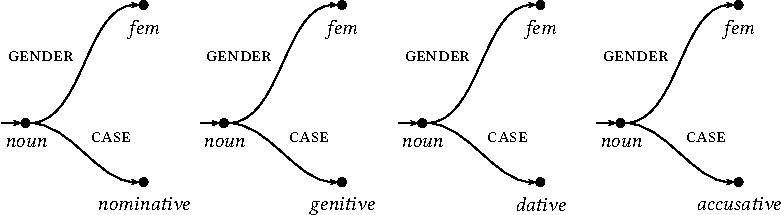
\includegraphics{Figures/frau-model-theoretic-cropped}
}
%%   \begin{pspicture}(-0.5,0.4)(2.8,4.1)
%% %\psgrid
%%      \psset{fillstyle=solid, fillcolor=black,radius=0.75mm}
%%      \pnode(-0.4,2){start1}
%%      \Cnode(0,2){noun1}
%%      \Cnode(2,4){fem1}
%%      \Cnode(2,1){nom1}
%% %
%%      \psset{fillstyle=none,nodesep=0pt,angleB=180,arrows=->} 
%% %
%%      \nccurve{start1}{noun1}
%%      \nccurve{noun1}{fem1}\naput{\textsc{gender}}
%%      \nccurve{noun1}{nom1}\naput{\textsc{case}}
%% %
%%      \nput{270}{noun1}{\type{noun}}
%%      \nput{270}{fem1}{\type{fem}}
%%      \nput{270}{nom1}{\type{nominative}}
%% \end{pspicture}
%% \begin{pspicture}(-0.5,0.4)(2.8,4.1)
%% %\psgrid
%% %
%%      \psset{fillstyle=solid, fillcolor=black,radius=0.75mm}
%%      \pnode(-0.4,2){start2}
%%      \Cnode(0,2){noun2}
%%      \Cnode(2,4){fem2}
%%      \Cnode(2,1){nom2}
%% %
%%      \psset{fillstyle=none,nodesep=0pt,angleB=180,arrows=->} 
%% %
%%      \nccurve{start2}{noun2}
%%      \nccurve{noun2}{fem2}\naput{\textsc{gender}}
%%      \nccurve{noun2}{nom2}\naput{~\textsc{case}}

%%      \nput{270}{noun2}{\type{noun}}
%%      \nput{270}{fem2}{\type{fem}}
%%      \nput{270}{nom2}{\type{genitive}}
%% \end{pspicture}
%% \begin{pspicture}(-0.5,0.4)(2.8,4.1)
%% %\psgrid
%%      \psset{fillstyle=solid, fillcolor=black,radius=0.75mm}
%%      \pnode(-0.4,2){start3}
%%      \Cnode(0,2){noun3}
%%      \Cnode(2,4){fem3}
%%      \Cnode(2,1){nom3}
%% %
%%      \psset{fillstyle=none,nodesep=0pt,angleB=180,arrows=->} 
%% %
%%      \nccurve{start3}{noun3}
%%      \nccurve{noun3}{fem3}\naput{\textsc{gender}}
%%      \nccurve{noun3}{nom3}\naput{\textsc{case}}
%% %
%%      \nput{270}{noun3}{\type{noun}}
%%      \nput{270}{fem3}{\type{fem}}
%%      \nput{270}{nom3}{\type{dative}}
%% \end{pspicture}
%% \begin{pspicture}(-0.5,0.4)(2.8,4.1)
%% %\psgrid
%%      \psset{fillstyle=solid, fillcolor=black,radius=0.75mm}
%%      \pnode(-0.4,2){start2}
%%      \Cnode(0,2){noun2}
%%      \Cnode(2,4){fem2}
%%      \Cnode(2,1){nom2}
%% %
%%      \psset{fillstyle=none,nodesep=0pt,angleB=180,arrows=->} 
%% %
%%      \nccurve{start2}{noun2}
%%      \nccurve{noun2}{fem2}\naput{\textsc{gender}}
%%      \nccurve{noun2}{nom2}\naput{\textsc{case}}
%% %
%%      \nput{270}{noun2}{\type{noun}}
%%      \nput{270}{fem2}{\type{fem}}
%%      \nput{270}{nom2}{\type{accusative}}
%% \end{pspicture}}
\caption{\label{abb-avm-frau}(\ref{avm-frau})中的Frau(女人)的特征结构描写}
%\caption{\label{abb-avm-frau}Feature structures for the description of \emph{Frau} `woman' in (\ref{avm-frau})}
\end{figure}%
%-----------------------------------------------------------------------------
\begin{figure}
%\oneline{%
\centerline{%
%% \begin{pspicture}(-0.5,0.4)(2.8,4.1)
%% %\psgrid
%% %
%% %
%%      \psset{fillstyle=solid, fillcolor=black,radius=0.75mm}
%%      \pnode(-0.4,2){start1}
%%      \Cnode(0,2){noun1}
%%      \Cnode(2,4){mas1}
%%      \Cnode(2,1){nom1}
%% %
%% %
%%      \psset{fillstyle=none,nodesep=0pt,angleB=180,arrows=->} 
%% %
%%      \nccurve{start1}{noun1}
%%      \nccurve{noun1}{mas1}\naput{\textsc{gender}}
%%      \nccurve{noun1}{nom1}\naput{\textsc{case}}
%% %
%%      \nput{270}{noun1}{\type{noun}}
%%      \nput{270}{mas1}{\type{mas}}
%%      \nput{270}{nom1}{\type{nominative}}
%% \end{pspicture}
%% \begin{pspicture}(-0.5,0.4)(2.8,4.1)
%% %\psgrid
%% %
%%      \psset{fillstyle=solid, fillcolor=black,radius=0.75mm}
%%      \pnode(-0.4,2){start2}
%%      \Cnode(0,2){noun2}
%%      \Cnode(2,4){mas2}
%%      \Cnode(2,1){nom2}
%% %
%% %
%%      \psset{fillstyle=none,nodesep=0pt,angleB=180,arrows=->} 
%% %
%%      \nccurve{start2}{noun2}
%%      \nccurve{noun2}{mas2}\naput{\textsc{gender}}
%%      \nccurve{noun2}{nom2}\naput{\textsc{case}}
%% %
%%      \nput{270}{noun2}{\type{noun}}
%%      \nput{270}{mas2}{\type{mas}}
%%      \nput{270}{nom2}{\type{dative}}
%% \end{pspicture}
%% \begin{pspicture}(-0.5,0.4)(2.8,4.1)
%% %\psgrid
%% %
%%      \psset{fillstyle=solid, fillcolor=black,radius=0.75mm}
%%      \pnode(-0.4,2){start2}
%%      \Cnode(0,2){noun2}
%%      \Cnode(2,4){mas2}
%%      \Cnode(2,1){nom2}
%% %
%% %
%%      \psset{fillstyle=none,nodesep=0pt,angleB=180,arrows=->} 
%% %
%%      \nccurve{start2}{noun2}
%%      \nccurve{noun2}{mas2}\naput{\textsc{gender}}
%%      \nccurve{noun2}{nom2}\naput{\textsc{case}}
%% %
%%      \nput{270}{noun2}{\type{noun}}
%%      \nput{270}{mas2}{\type{mas}}
%%      \nput{270}{nom2}{\type{accusative}}
%% \end{pspicture}
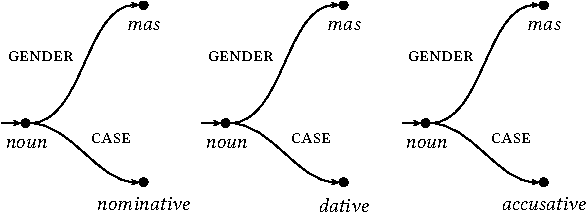
\includegraphics{Figures/mann-model-theoretic-crop}
}
\caption{\label{abb-avm-mann}(\ref{avm-mann})中的Mann(男人)的特征结构描写}
%\caption{\label{abb-avm-mann}Feature structures for the description of \emph{Mann} `man' in  (\ref{avm-mann})}
\end{figure}%
在这些表达式中,每个结点都有一定的类型(\type{名词}、\type{阴性}、\type{主格} \ldots),并且特征结构中的类型总是最具体的,即它们没有深层的次类型。总有一个入口结点(上例中的\type{名词})和其他用特征标签标注的用箭头连接起来的结点(“\textsc{性别}”、“\textsc{格}”)。
%In these representations, each node has a certain type (\type{noun}, \type{fem}, \type{nominative},
%\ldots) and the types in feature structures are always maximally specific, that is, they do not have
%any further subtypes. There is always an entry node (\type{noun} in the example above) and the other
%nodes are connected with arrows that are annotated with the feature labels (\textsc{gender}, \textsc{case}).

如果我们回到上面章节中人的例子,我们可以发现模型与描写之间的差异,如下所示:如果我们有一个人的模型,它包括名、姓、出生日期、性别和发色,那么它自然得到的结果是我们模拟的每个对象都会有生日。但是,如果这些信息在表示约束或构成搜索时没有发挥重要的作用时,我们可以在描写中省略这些细节。
%If we return to the example with people from the previous sections, we can capture the difference between a model and a description as %follows:
%if we have a model of people that includes first name, last name, date of birth, gender and hair color, then it follows that every object we %model also has a birthday.
%We can, however, decide to omit these details from our descriptions if they do not play a role for
%stating constraints or formulating searches.

\pagebreak
语言现象、模型和形式化理论之间的联系如图\vref{abb-modell}所示。
%The connection between linguistic phenomena, the model and the formal theory is shown in Figure~\vref{abb-modell}.
模型是用来模拟语言现象的。进而,它必须由我们的理论所允准。理论决定了模型并且对可能的现象进行预测。
%The model is designed to model linguistic phenomena. Furthermore, it must be licensed by our theory.
%The theory determines the model and makes predictions with regard to possible phenomena.
\begin{figure}
\centerline{%
%{
%% \begin{pspicture}(0,0)(9.4,4.2)
%% %\psgrid
%% \rput[Bl](0,0){%
%% \begin{tabular}[b]{@{}ccc@{}}
%% phenomenon && model\\
%% \rnode{phen}{\fbox{\begin{tabular}{c}
%% linguistic\\
%% objects\\
%% \end{tabular}}}&&\rnode{modell}{\fbox{\begin{tabular}{c}
%% feature\\
%% structures\\
%% \end{tabular}}}\\[10ex]
%% &\rnode{theorie}{\fbox{\begin{tabular}{c}
%% feature\\
%% descriptions\\
%% \end{tabular}}}\\
%% &formal theory\\
%% \end{tabular}}
%% %\anodeconnect[l]{modell}[r]{phen}%
%% \ncline{->}{modell}{phen}\nbput{models}
%% %\ncdiag[angleA=180,angleB=45]{->}{modell}{theorie}
%% \psline{<-}(5.4,1.6)(6,2.4)
%% \rput[Bl](6,2){licensed by the theory} % früher Erfüllung, jetzt FR Änderung
%% \psline{->}(5,1.7)(5.6,2.4)
%% \rput[Bl](3.4,2.0){determines}
%% %\nccurve{<-}{modell}{theorie}\nbput{legt fest}
%% \ncline{->}{theorie}{phen}\naput{predicts}%
%% %\aanodeconnect[b]{modell}[tr]{theorie}%
%% %\anodeconnect[tl]{theorie}[b]{phen}%
%\end{pspicture}
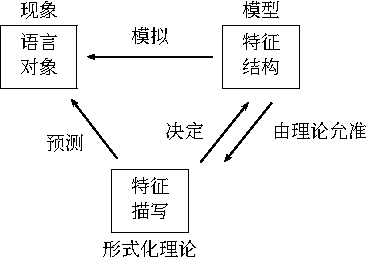
\includegraphics{Figures/model-theory-phenomenon-crop}
}
\caption{\label{abb-modell}现象、模型和形式化理论}
%\caption{\label{abb-modell}Phenomenon, model and formal theory}
\end{figure}%
\nocite{Netter98a}%S. 26
%\NOTE{WS: zwischen Modell und Theorie sollten zwei Pfeile sein.}
% ###########
% zwei Pfeile: Beschreibung legt Modell fest, um Rekursion zu erfassen (beschreibt geht wohl auch, ist aber sloppy)
%
% Modell wird von der formalen Theorie lizenziert. 
%
% Phänomen + Modell -> PS: modelliert -> lassen wir so.
%
\isce[|)]{模型}{model}\isce[|)]{理论}{theory}\isce[|)]{现象}{phenomenon}\isce[|)]{特征描写}{feature description}\isce[|)]{特征结构}{feature structure}

%\section*{思考题}
%\section*{Comprehension questions}

%\bigskip
\vfill
\questions{
\begin{enumerate}
\item 使用类型的原因是什么?
\item 什么是承继?多重承继有何特殊之处?
\item 下面的结构是相容的吗?也就是说,他们能用来描写相同的对象吗?
%\item What are the reasons for using types?
%\item What is inheritance? What is special about multiple inheritance?
%\item Are the following structures compatible, that is, can they be used to describe the same object? 
\ea
\onems{
名 \type{max}\\
姓  \type{meier}\\
父亲    \ms[人]{
              名  & peter\\
              姓  & meier
             }
}\hspace{0.5cm}\onems{
名  \type{max}\\
姓  \type{meier}\\
父亲   \ms[人]{
              名  & peter\\
             姓  & müller
             }
}
\z
\ea
\onems{
名   \type{max}\\
姓   \type{meier}\\
父亲     \ms[人]{
              名 & peter\\
              姓  & meier
             }
}\hspace{0.5cm}\onems{
名   \type{max}\\
姓   \type{meier}\\
母亲      \ms[人]{
              名  & ursula\\
              姓  & müller
             }
}
\z

\end{enumerate}
}
\largerpage

%\section*{练习题}
%\section*{Exercises}

\exercises{
\begin{enumerate}
\item 请设想如何通过特征描写来描写乐器。
%\item Think about how one could describe musical instruments using feature descriptions.
\item 请设计一个词类(\type{限定词}、\type{标句词}、\type{名词}、\type{动词}、\type{形容词}、\type{介词})的类型层级体系。请设想可以组织类型层级的方式,这样我们可以对第\pageref{Tabelle-Merkmalszerlegung-Wortarten}页的图\ref{Tabelle-Merkmalszerlegung-Wortarten}中的二元特征的概括进行表示。
%\item Come up with a type hierarchy for the word classes (\type{det}, \type{comp}, \type{noun}, \type{verb},
%      \type{adj}, \type{prep}). Think about the ways in which one can organize the type hierachy so that one
%	  can express the generalizations that where captured by the binary features in Table~\ref{Tabelle-Merkmalszerlegung-Wortarten} on page~%\pageref{Tabelle-Merkmalszerlegung-Wortarten}.
\item\label{ua-liste}在本章,我们介绍了列表。这看起来好像是形式化的扩展,但是它并不是,因为可以将列表标记转化为只需要特征-值偶对的标记。请思考如何做到这一点。
%\item\label{ua-liste} In this chapter, we introduced lists. This may look like an extension of the formalism, but it is not as it is possible to
%convert the list notation into a notation which only requires feature-value pairs. Think about how one could do this.
\item (附加练习)附加关系(append)\iscesub{关系}{relation}{附加关系}{\emph{append}}
  将在第\ref{Kapitel-HPSG}章发挥作用。该关系用来将两个列表组合成第三个列表。诸如附加(append)的关系约束实际上构成了形式化的一种扩展。使用关系约束可以将任意数量的特征值与其他值联系起来,即我们可以写出这样的程序,它根据其他值计算出具体的值。这就导致了一个问题,在语言学理论中我们是否需要如此强有力的描写工具,并且如果我们允许使用它们,我们将会承担什么样的复杂度的代价。可见,我们最好选择那些不需要关系约束的理论,而不是那些需要关系约束的理论(参见\citet[\S~20]{MuellerLehrbuch1}对相关理论的比较)。
%\item (Additional exercise) The relation \emph{append}\is{relation!\emph{append}} will play a role in Chapter~\ref{Kapitel-HPSG}. This relation %serves to
%combine two lists to form a third.
%Relational constraints such as \emph{append} do in fact constitute an expansion of the formalism. Using relational constraints, it is possible to %relate any number
%of feature values to other values, that is, one can write programs which compute a particular value depending on other values. 
%This poses the question as to whether one needs such powerful descriptive tools in a linguistic theory and if we do allow them, what kind of %complexity we afford them.
%A theory which can do without relational constraints should be preferred over one that uses
%relational constraints (see \citealp[Chapter~20]{MuellerLehrbuch1} for a comparison of theories).

\hspace{2em}
列表的串联可以在没有关系约束要求的特征结构中实现。请问这是如何做到的,并提供你的数据来源,记录下你找到解决方案的途径。
%For the concatenation of lists, there is a possible implementation in feature structures without
%recourse to relational constraints. Find out how this can be done. Give your sources and document
%how you went about finding the solution.

\end{enumerate}
}

\largerpage
%\section*{延伸阅读}
%\section*{Further reading}
\furtherreading{
本章为读者设计了简单易懂的有关类型特征结构的介绍。结构的数学属性、类型层级体系以及这些结构的组合性概率没有在这里进行详细说明,但是至少这些属性的一部分对于计算语言学的工作以及开发个人自己的分析来说都是非常重要的。更多的内容,我推荐感兴趣的读者阅读以下文献:
%This chapter was designed to give the reader an easy-to-follow introduction to typed feature structures. The mathematical properties of the %structures, type hierarchies and the
%combinatorial possibilities of such structures could not be discussed in detail here, but knowledge of
%at least part of these properties is important for work in computational linguistics and in
%developing one's own analyses. For more information, I refer the interested reader to the following publications: 
%
 \citet{Shieber86a}是对合一语法理论的简短介绍。它针对重要的语法类型给出了相对全面的综述,如DCG\isce{定子句文法}{Definite Clause Grammar (DCG)}、\lfgc、\gpsgc、HPSG、PATR-II\isce{PATR-II}{PATR-II}。
% \citet{Shieber86a} is a short introduction to the theory of Unification Grammar. It offers a relatively general overview followed by the %discussion of important grammar types
%such as DCG\is{Definite Clause Grammar (DCG)}, \lfg, \gpsg,
%HPSG, PATR-II\is{PATR-II}.
%
 \citet{Johnson88}按照数学的精确形式描述了非类型特征结构的形式化。
% \citet{Johnson88} describes the formalism of untyped feature structures in a mathematically precise way.
%
 \citet{Carpenter92a}重点分析了类型特征结构在数学上的表示。由 \citet{King99a-u}开发的HPSG-语法构成了 \citet{Richter2004a-u}的形式化的基础,该语法目前被看作是HPSG的标准形式化语法。
% \citet{Carpenter92a} goes into the detail about the mathematical aspects of typed feature structures. The formalism developed by 
% \citet{King99a-u} for HPSG-grammars forms the basis
%for the formalism by  \citet{Richter2004a-u}, which currently counts as the standard formalism for HPSG.
}


% lulu/wsun/sisi: DONE
%      <!-- Local IspellDict: en_US-w_accents -->

%% -*- coding:utf-8 -*-

\chapter{词汇功能语法}
%\chapter{Lexical Functional Grammar}
\label{Kapitel-LFG}

词汇功能语法(Lexical Functional Grammar,简称LFG)是上个世纪八十年代由Joan Bresnan和Ron Kaplan提出来的\citep{BK82a}。LFG是所谓的西海岸语言学的一个有机组成部分:不同于乔姆斯基任教的麻省理工学院,Joan Bresnan和Ron Kaplan在美国的西海岸工作(Joan Bresnan任教于斯坦福大学,而Ron Kaplan先后供职于帕罗奥图的施乐和加利福尼亚湾区Nuance的语言技术部门)。

 \citet{BK82a}视LFG为一种心理语言学角度来看合理的、可以替换转换机制的分析方法。
请参考\ref{Abschnitt-Diskussion-Performanz}以了解更多基于心理语言学的关于语言学理论合理性的讨论。 

想了解更多的基于LFG来分析德语的工作,可参阅 \citew{Berman96a-u,Berman2003a}和 \citew{Cook2001a}。

LFG有着设计良好的形式理论基础\citep{KB82a-u,Kaplan95a},正是基于这一点,LFG的早期应用很快就取得了不少成果
\citep*{FR83b,FR83a,Yasukawa1984a-u,BH86a-u,%
ED86a-u,% CHARON Parser
WA86a-u,%
Delmonte90a-u,% Italien
HHP91a-u,% Chinesisches kommerzielles System
Kohl92a-u,KGPRM92a-u,% ACORD project CHARON Generator
KM96a-u,%
Mayo97a-u,Mayo99a-u,%Konstanzer system
BS2005b-u,BSagot2005a-u,%SxLFG
Clement2009a-u,CK2001a-u% XLFG
}。

以下是一些已经用LFG完成了语段分割的语言:

\begin{itemize}
\item 阿拉伯语\il{Arabic}\citep{Attia2008a-u}、
\item 阿伦特语\il{Arrernte}\citep*{Dras2012a-u}、
\item 孟加拉语 \il{Bengali}\citep{SC97a-u}、
%\item Chinese\il{Mandarin Chinese}
\item 丹麦语\il{Danish}\citep{Oersnes2002b-u,OW2003a-u,OW2004a-u}、
\item 英语\il{English}\citep*{HHP91a-u,BDFK99a-u,RKKCMJ2002a-u,KM2007a-u}、
\item 法语\il{French}\citep*{Zweigenbaum91a-u,Frank96b-u,FZ2002a-u,BDFK99a-u,CK2001a-u,BSL2005a-u,SdA2016a-u,Alencar2017a-u}、
% Knueppel2001a-u
%
%
\item 格鲁吉亚语\il{Georgian}\citep{Meurer2009a-u}、
\item 德语\citep{Rohrer96a,Berman96a-u,KR97a-u,BDFK99a-u,Dipper2003a-u,RF2006a,Forst2006a-u,Frank2006a-u,FR2009a-u}、
%\item Griechisch\il{Griechisch}、
\item 匈牙利语\il{Hungarian}\citep{LRT2010a-u}、
\item 印度尼西亚语\il{Indonesian}\citep*{AADMS2009a-u}、
\item 意大利语\il{Italian}\citep*{Delmonte90a-u,Mayo99a-u,Quaglia2012a-u}、
\item 爱尔兰语\il{Irish}\citep{Sulger2009a-u,Sulger2010a-u}、
\item 日语\il{Japanese}\citep*{HHP91a-u,MO2003a-u,Umemoto2006a-u}、
\item 韩语\il{Korean}\citep*{HHP91a-u}、
\item 马达加斯加语\il{Malagasy}\citep*{Randriamasimanana2006a-u,DLM2006a-u}、
\item 现代汉语\il{Mandarin Chinese}\citep*{HHP91a-u,FK2007a-u}、
\item Murrinh-Patha语\il{Murrinh-Patha}\citep{SN2012a-u}、
\item 挪威语\il{Norwegian}\citep*{DMR2005a}、
\item 波兰语\il{Polish}\citep*{PP2012a-u}、
\item 葡萄牙语\il{Portuguese}\citep{Alencar2004a-u,Alencar2013a-u,Alencar2015a-u}、
\item 西班牙语\il{Spanish}\citep{Mayo99a-u}、
\item 提格里尼亚语\il{Tigrinya}\citep{Kifle2012a-u}、
\item 土耳其语\il{Turkish}\citep{CO2006a-u}、
\item 匈牙利语\il{Hungarian}\citep*{LRT2010a-u,RLC2011a-u}、
\item 乌尔都语/北印度语\il{Urdu}\il{Hindi}\citep*{BHKR2007a-u,BBS2008a-u}、
\item 威尔士语\il{Welsh}\citep{MS2005a-u}和
\item 沃洛夫语\il{Wolof}\citep{Dione2012b-u,Dione2013a-u}。
\end{itemize}
上述语法中很多都是基于ParGram开发的\footnote{%
  \url{http://pargram.b.uib.no/research-groups/}。\zhdate{2015/10/01}。
} \citep*{BKNS99a-ed,BDKMR02a-u}。 
除了上述语法,一个针对北梭托语\il{Northern Sotho}的语法也正在研发\citep{Faasz2010a-u}。

很多LFG系统除了使用以语言学为准的语法,还使用了统计学方法\isc{统计学}\is{statistics}。
这样可以帮助搜索一个句子最为倾向的解读分析。统计模块可以增强语言处理的效率,也可以增强系统鲁棒性\citep{KRKMVC2004a-u,RKKCMJ2002a-u}。
Josef van Genabith在都柏林的团队目前正在研究如何从语料中自动约归出LFG语法\citep{JGCCR99a-u,DBCGW2005a-u,CBFDRCW2005a-u,CG2006a-u,GWG2007a-u,CBDRGW2008a-u,SvG2009a-u}。

很多系统都提供在线测试功能,如:
\begin{itemize}
\item \url{http://iness.uib.no/xle-web/xle-web}

% Statistik Dublin
\item \url{http://lfg-demo.computing.dcu.ie/lfgparser.html}
\item \url{http://www.xlfg.org/}
\end{itemize}

\section{关于表示形式的一般说明}

\label{Abschnitt-Format-LFG}

LFG假设多层表征。\footnote{%
  本节中英语例句及其分析选自于 \citet{Dalrymple2001a-u}和 \citet{Dalrymple2006a}。
}
其中最重要的是c-结构\isc{c-结构}\is{c"=structure}和f-结构\isc{f-结构}\is{f"=structure}。c-结构是成分结构,需要被某个具体的短语结构语法允准。
对于适合用\xbarc~理论分析的语言,该短语结构语法即为\xbarc~理论。
f-结构意为功能结构。
功能结构包括了谓词的信息,以及一个具体的结构成分中出现的语法功能(主语、宾语等)的信息。
在不同表征层面之间需要设立它们的映射关系。

\subsection{功能结构}

在LFG中, 诸如主语和宾语这样的语法功能发挥着非常重要的作用。
不同于本书中讨论的大多数其他理论,它们是LFG理论中的基本元素。
一个句子,如(\mex{1}a),可被赋予如(\mex{1}b)所示的功能结构:

\eal
\ex{
\gll David devoured a sandwich. \\
     David 吞食 一 三明治。 \\
\mytrans{David吞食了一个三明治。}
}
\ex \lfgms{ pred & `DEVOUR\sliste{\lfgsubj, \lfgobj}'\\
         subj & \lfgms{ pred &  `DAVID' \\
                   }\\
         obj  & \lfgms{ spec & A\\
                     pred & `SANDWICH'\\
                   }\\
       }
\zl

\noindent
所有的产生语义的词汇项都贡献一个\textsc{pred}
\isfeat{pred}特征及其取值。
被一个中心词所管辖(此处管辖意为次范畴化)的语法功能将在\textsc{pred}的值中被详细列出\footnote{%
在(\mex{0}b)中, 紧跟在devour后面的\lfgsubj{}和\lfgobj{}即是整个结构中的\lfgsubj{}和\lfgobj{}。
出于紧凑表征的原因,这种同一关系并不在结构中进行显性表示。
}
这些功能被称为可被管辖的语法功能(\emph{governable grammatical functions})\isc{语法功能}\is{grammatical function!governable}。
表\ref{Tabelle-GOV}罗列了一些可被管辖的语法功能\citep{Dalrymple2006a}。
\begin{table}
\centering
\begin{tabular}[t]{@{}lp{26em}@{}} 
\lsptoprule
\textsc{subj}
\isfeat{subj}: & 主语 \\ 
%
\textsc{obj}
\isfeat{obj}: & 宾语\\ 
%
\textsc{comp}
\isfeat{comp}: & 小句类型补足语或自足型(非谓词性)不定式补足语\\
\textsc{xcomp}
\isfeat{xcomp}: & 非自足性(谓词性)补足语,经常为不定式,经常有一个外部的成分约束\isc{约束}\is{control}其\textsc{subj}\\
\objtheta: & 第二宾语功能,经常配置一些特定的且语言相关的语法角色。在英语中其为且仅为\objtheme。\\ 
%
\obltheta: & 一组题元受限的需要显性语法标记的语法功能,如{\obl\downlett{GOAL}}或{\obl\downlett{AGENT}}。
             它们经常对应于c-结构中的介词短语。\\
\lspbottomrule
\end{tabular}
\caption{\label{Tabelle-GOV}管辖语法功能}
\end{table}\todostefan{\objtheta im Deutschen?}%
\pred 约定对应于GB理论中的题元格\isc{θ-栅}\is{theta-grid@$\theta$-grid}。
中心词的配价\isc{价}\is{valence}信息也包含在\predvc 的约定信息中。

表\vref{Tabelle-NGOV}介绍了非管辖语法功能。
\begin{table}
\centering
\begin{tabular}[t]{@{}lp{26em}@{}} 
\lsptoprule
\textsc{adj}
\isfeat{adj}: & 附加语 \\ 
%
\textsc{topic}
\isfeat{topic}: & 语段的话题\\ 
%
\textsc{focus}
\isfeat{focus}: & 语段的焦点\\
\lspbottomrule
\end{tabular}
\caption{\label{Tabelle-NGOV}非管辖语法功能}
\end{table}%
话题\isc{话题|(}\is{topic|(}和焦点\isc{焦点|(}\is{focus|(}是信息结构(Information Structure)中的术语。
关于二者有一系列精确但相互之间并不完全相同的定义\citep[\page 253--254]{KruijffSteedman2003}。
宽泛地说,一个语段的焦点是新信息之所在,而话题则是旧有的、已知的信息。
 \citet[\page 97]{Bresnan2001a}使用如下的问句测试来区分话题与焦点。

\ea
\label{bsp-fronted-focus}
Q: What did you name your cat?\\
问: 你管你的猫叫什么?\\
A: Rosie I named her. (\emph{Rosie} = \textsc{focus})\\
答: Rosie,我叫她。
\z
\ea
\label{bsp-fronted-topic}
Q: What did you name your pets?\\
问: 你管你的宠物叫什么?\\
A: My dog, I named Harold. My cat, I named Rosie. (\emph{my dog}, \emph{my cat} = \textsc{topic})\\
答: 我的狗,我叫它Harold。我的猫,我叫它Rosie。
\z 
\isc{话题|)}\is{topic|)}
\isc{焦点|)}\is{focus|)}

\noindent
f-结构可以由功能描述(functional descriptions)来确立。
例如,我们可以通过下面的描述来确定一个功能结构$f$中的\textsc{tense}特征

\ea
($f$ \lfgtense)
\z

\noindent
可以在一个功能描述中去声明一个特征的具体取值。
下面的这个功能描述进一步说明了在$ f$中,其\lfgtense{}特征取值为\lfgpast。

\ea
($f$ \lfgtense) = \lfgpast
\z

\noindent
有时候一个特征的值为另一个f-结构。
(\mex{1})中的表达式声明了$ f$的\lfgsubj 取值为f-结构$g$:

\ea
\label{ex-LFG-constraint}
($f$ \lfgsubj) = $g$
\z

\noindent
对应于(\mex{1}a)中的分析,我们可以得到(\mex{1}b)中对值的限定:
\eal
\ex{
\gll David sneezed. \\
     David 打喷嚏\\
\mytrans{David打了个喷嚏。}
}
\ex
\begin{tabular}[t]{l}
($f$ \pred) = {\small `SNEEZE\arglist{\lfgsubj}'}\\
($f$ \lfgtense) = \lfgpast\\
($f$ \lfgsubj) = $g$\\
($g$ \pred) = {\small `DAVID'}
\end{tabular}
\zl

\noindent
(\mex{0}b)描述了下述结构:
\ea
$f$: \lfgms{ pred  & {\small `SNEEZE\arglist{\lfgsubj}'}\\
             tense & \lfgpast\\
             subj  & $g$: \onems{ pred {\small `DAVID'} }\\
        }
\z

\noindent
需注意的是(\mex{-1}b)同样也可以描写许多包含其它特征的其它结构。
在所有这些包括了功能结构的新结构中,我们仅仅关心那些包含特征描述提供信息的最简结构(minimal structures)。

(\mex{1})展示了c-结构中的结点是如何和f-结构联系起来的:

\ea
%\ex David sneezed。
%\ex 
%% \begin{tabular}[t]{@{}ll@{}}
%% \begin{tabular}[t]{@{}cc@{}}
%% \multicolumn{2}{c}{\rnode{ip}{IP}}\\[2ex]
%% \rnode{b}{\rnode{np}{NP}}       & \rnode{i1}{I$'$}\\[2ex]
%% \rnode{n1}{N$'$}     & \rnode{vp}{VP}\\[2ex]     
%% \rnode{n}{N}         & \rnode{v1}{V$'$}\\[2ex]   
%% \rnode{David}{David} & \rnode{v}{V}\\[2ex]       
%%                     & \rnode{sneezed}{sneezed}\\
%% \end{tabular}
%% &
%% \lfgms{
%% pred & `SNEEZE\arglist{\lfgsubj}'\\
%% tense & PAST\\
%% subj  & \rnode{i}{\lfgms{ pred & `DAVID' \\
%%                       }}\\
%% }\\
%% \ltor[-15]{b}[175]{i}
%% \Aput*{$\phi$}
%% \end{tabular}
\tree{IP}{%
  \tree[b]{NP}{\tree{N$'$}{\tree{N}{\le{David\\David}}}}
  \tree{I$'$}{\tree{VP}{\tree{V$'$}{\tree{V}{\le{sneezed\\打喷嚏}}}}}}%
\hspace*{4em}%
\raisebox{-2em}{\lfgms{
pred & {\small `SNEEZE\arglist{\lfgsubj}}'\\
tense & \lfgpast\\
subj  & \rnode{i}{\lfgms{ pred & {\small `DAVID'} \\
                      }}\\
}}\\
\ltor[-15]{b}[175]{i}
\Aput*{$\phi$}
\z
$\phi$指明了NP结点与其相对应的f-结构之间的映射关系,在图中用一个标有$\phi$的箭头进行表示。

一个短语和它的中心词一直对应于同一个f-结构。

\ea
\begin{tabular}[t]{@{}c@{}}
\rnode{a}{\rnode{v1}{V$'$}}\\[2em]
\rnode{b}{\rnode{v}{V}}\\[2em]
\rnode{sneezed}{\begin{tabular}{@{}c@{}}sneezed\\打喷嚏\end{tabular}}\\
\end{tabular}
\hspace*{4em}
\rnode{d}{\raisebox{-2em}{\lfgms{ pred & {\small `SNEEZE\arglist{\lfgsubj}'}\\
                                  tense & \lfgpast}}}
\ncline{v1}{v}\ncline{v}{sneezed}%
\ltor{a}{d}
\Aput*{$\phi$}
\ltor{b}{d}
\z

\noindent
在英语的LFG语法中,GB理论所提出的CP/IP分析仍然被采用。
IP、I$'$和I(亦包括VP)被映射到同一个f-结构上。

\eal
\ex{
  \gll David is yawning.\\
       David \textsc{aux} 打哈欠\\
  \mytrans{David正在打哈欠。}
}

\ex {\tree[a]{IP}{%
  \tree{NP}{\tree{N$'$}{%
    \tree{N}{\le{David\\David}}}}
  \tree[b]{I$'$}{%
    \tree[c]{I}{\le{is\\\textsc{aux}}}
    \tree[d]{VP}{\tree[e]{V$'$}{\tree[f]{V}{\le{yawning\\打哈欠}}}}}}}%
\hspace*{4em}%
{\rnode{o}{\raisebox{-2em}{\lfgms{ pred & {\small `YAWN\arglist{\lfgsubj}'}\\
                                   tense & \lfgpres\\
                                   subj  & \lfgms{ pred & {\small `DAVID'}}}}}}
\ltor{a}{o}
\ltor{b}{o}
\ltor[10]{c}{o}
\ltor{d}{o}
\ltor{e}{o}
\ltor{f}{o}
\zl

%% \subsubsection{Funktionale Eindeutigkeit ({\em Functional Uniqueness})}

%% {
%% {Funktionale Eindeutigkeit ({\em Functional Uniqueness})}

%% }

\noindent
f-结构需同时满足两个合格性的条件:它们必须同时完备(complete)且一致(coherent)。我们将在后续章节中继续讨论这两个条件。

\subsection{完备性}

每一个中心词都增加一个关于\textsc{pred}特征取值的限制。完备性若满足,则需要\textsc{pred}值所约束的语法功能要素全部实现。
在(\mex{1}b)中,\textsc{pred}所声明的\textsc{obj}在相应的f-结构中并未出现,因此(\mex{1}a)被LFG理论认为是不合语法的。

\eal
\ex[*]{
  \gll David devoured. \\
       David 吞食\\
}
\ex[]{
\lfgms{ pred & {\small `DEVOUR\sliste{\lfgsubj,\lfgobj}'}\\
         subj & \lfgms{ pred & {\small `DAVID'} \\
                   }\\
       }
}
\zl

\subsection{一致性}

一致性条件要求在一个给定的f-结构中,所有的论元功能都必须局部地被同一个\textsc{pred}特征的取值所声明。
例(\mex{1}a)的不合语法性即由此而来:\textsc{comp}并没有作为论元出现在devour的声明中。

\eal
\ex[*]{
\gll David devoured a sandwich that Peter sleeps. \\
     David 吞食 一 三明治 \textsc{comp} Peter 睡觉\\
  %\\
%`David verschlang ein Sandwich, daß Peter schläft.'
}
\ex[]{
\lfgms{ pred & {\small `DEVOUR\sliste{\lfgsubj,\lfgobj}'}\\
         subj & [ \textsc{pred} {\small `DAVID'} ] \\
         obj  & \lfgms{ spec &  A\\
                     pred & {\small `SANDWICH'}\\
                   }\\
         comp & \lfgms{ pred & {\small `SLEEP\sliste{\lfgsubj}'}\\
                        subj & \lfgms{ pred & {\small `PETER'}\\
                                     }\\
                   } 
       }
}
\zl

\noindent
完备性与一致性限制共同确保了仅有出现在\pred 声明中的论元被实现出来,且在\pred 声明中出现的全部论元都需要被实现出来。
这两条限制合在一起对应于GB理论中的题元准则\isc{$\theta$-准则@$\theta$-准则}\is{theta-criterion@Theta"=Criterion}(详见第\pageref{theta-Kriterium}页)\footnote{%
了解更多的关于LFG中的谓词论元结构与基于题元准则的深层结构之间的区别,可参阅 \citew[\page xxvi--xxviii]{BK82a}。
}。


\subsection{c-结构与f-结构之间的关系的限制}  

为了得到f-结构,可以给c-结构中的符号\isc{c-结构}\is{c"=structure|(}分配语法限制标注。
令`\up'\isc{$\uparrow$}\is{$\uparrow$}指示c-结构中的直接支配某结点的结点(即父结点)所对应的f-结构,`$\downarrow$'\isc{$\downarrow$}\is{$\downarrow$}指示当前结点所对应的f-结构。
`\up~=~\down'是一个普遍被采用的限制标注。
这个限制声明了父结点的f-结构和当前结点的f-结构同一。

\ea
V$'$ $\to$ \begin{tabular}[t]{@{}r@{~=~}l@{}}
           \multicolumn{2}{@{}l@{}}{\hspaceThis{f-structure of the mother~}V}\\ %TODO
           $\uparrow$ &  $\downarrow$\\ 
           父结点的f-结构 & 自身f-结构\\
           \end{tabular}
\z
`\up~=~\down'标注置于一个结构的中心词\isc{中心语}\is{head}之下。

在(\mex{0})中,
经过标注的c-结构所允准的短语可做如下表示:
\ea
\talltree[a]{V$'$}{\le[b]{V}}%
\hspace*{3em}%
\rnode{d}{[\ ]}
\ltor{a}{d}
\ltor{b}{d}
\z

\noindent
(\mex{1})展示了一条带有一个宾语的V$'$规则:
\ea
\phraserule{V$'$}{
\rulenode{V\\* \up~=~\down}
\rulenode{NP\\*(\up\ \lfgobj) = \down}}
\z
%
NP对应的标注声明了其父结点所对应的f-结构中的\textsc{obj}(即\mbox{(\up\ \lfgobj)}),其值为此NP所对应的f-结构,
亦即NP结点下方成分(\down)所对应的全部功能信息。
可视化展示见(\mex{1})中的图:
\ea
\talltree[a]{V$'$}{\le[b]{V} \le[c]{NP}}%
\hspace*{3em}%
\rnode{d}{\fd{\fdand{\feat{\lfgobj}{\rnode{e}{[\ ]}}}}}
\ltor{a}{d}
\ltor[20]{b}{d}
\ltor{c}[190]{e}
\z
在等式(\up\ \lfgobj) = \down{}中,箭头\up 和\down 对应于特征结构。
以(\ref{ex-LFG-constraint})为例,\up 和\down 分别代表了$f$和$g$。

(\mex{1})是一个不及物动词的例子,而(\mex{2})为对应的可视化展示:

\ea
\catlexentry{sneezed}{V}{(\up\ \pred) = {\small `SNEEZE\arglist{\lfgsubj}'}\\*
                     (\up\ \lfgtense) = \lfgpast}
\z

\ea
\tree{V}{\le{sneezed\\打喷嚏}}
\hspace*{4em}
\rnode{d}{\mbox{\lfgms{ pred & {\small `SNEEZE\arglist{\lfgsubj}'}\\
                        tense & \lfgpast}}}
\ltor{top}{d}
\z 
\isc{f-结构}\is{f"=structure|)}
\isc{c-结构}\is{c"=structure|)}\il{English|)}

\subsection{语义}
\label{lfg-semantics}
\label{glue-semantics}

依据 \citet[\page 90--92]{Dalrymple2006a},粘着语义学(\emph{glue semantics})\isc{粘着语义学|(}\is{glue semantics|(}是LFG的一个主流语义分析方法(\citealp*{DLS93a-u};\citealp[\S~8]{Dalrymple2001a-u})。
另有一些基于Kamp的篇章表示理论(discourse representation structures)\citep{KR93a}的分析方法\citep{FR83b,FR83a}。

接下来我们将讨论粘着语义学的一些细节\footnote{%
%The following section is a translation of the corresponding section in   \citew{Dalrymple2006a}。
下面的讨论对应于 \citew{Dalrymple2006a}的相关章节。
}。
在一个基于粘着的方法中,我们假设f-结构是服务于语义解释的核心句法表征。
不同于GB理论,语义组合的过程并不取决于论元在句法树中的位置,而是取决于诸如\lfgsubj 和\lfgobj 之类的功能关系。 
胶接语义学假设f-结构中的每一个子结构都对应一个语义资源(semantic resource),而整个结构的语义来自于子结构之和。
语义的组合集成要遵循一定的规则,这些规则以线性逻辑(linear logic)\isc{线性逻辑}\is{linear logic}的前提给出,在这种方法中,线性逻辑视为一种粘着语言(glue language)\isc{粘着语言}\is{glue language}。
语义的计算结果对应着通过逻辑推导出来的结论。

这样的结论是通过逻辑前提推导而得出的,这些前提来自于词也可能来自于一个句法构式(construction)本身。
而子部分语义进行组合以得到完整的语义的过程则是通过一种基于资源(resource)的逻辑——线性逻辑——进行约束的。
线性逻辑不同于经典逻辑,它不允许推导中出现不被使用的前提,也不允许一个前提被多次使用。
因此在线性逻辑中,前提是将要被使用的资源。
这直接对应于一个词在一个表达里的使用:词一次性服务于整个语义解释。
词既不能在语义解释中被忽略掉,也不可以在不同的部分多次贡献自己的力量。
句子Peter knocked twice.(Peter敲了两次)的意义并不等同于Peter knocked(Peter敲)。
词twice(两次)的语义必须被囊括到整个句子的完整语义中。
类似地,其句义也不同于Peter knocked twice twice.(Peter敲了两次两次),因为词twice的语义不可以被使用两次。

(\mex{1}b)展示了例句(\mex{1}a)的句法及语义分析:
%Figure~\vref{c-f-sem-david-yawned}:
\eal
\ex{
\gll David yawned. \\
     David 打哈欠\\
\mytrans{David打哈欠了。}
}
\ex ~\\[-\baselineskip]
\hspace*{-2em}
{\ctree[ip]{IP}{%
  \tree[b]{NP}{\tree[n]{N}{\le{David\\David}}}
  \tree[ii]{I$'$}{\tree[vp]{VP}{\tree[v]{V}{\le{yawned\\打哈欠}}}}}}%
\hspace*{3em}%
{\fd{\rnode{s}{\fdand{\feat{\pred}{\small `YAWN\arglist{\subj}'}
           \feat{\subj}{\rnode{i}{\fdand{\feat{\pred}{\small `DAVID'}}}}}}}}%
\hspace*{2em}%
\mt{\relation{yawn}(\relation{david})}{\rnode{x}{~[\ ]}}
\ltor{ip}{s}
\Aput*{$\phi$}
\ltord[-10]{s}[220]{x}
\Bput*{$\sigma$}
\zl
%% \begin{figure}
%% \centerline{%
%% {\ctree[ip]{IP}{%
%%   \tree[b]{NP}{\tree[n]{N}{\le{David}}}
%%   \tree[ii]{I$'$}{\tree[vp]{VP}{\tree[v]{V}{\le{yawned}}}}}}%
%% \hspace*{3em}%
%% {\rnode{s}{\lfgms{ pred & {\small `YAWN\arglist{\lfgsubj}'}\\
%%                    subj & \rnode{i}{[ \textsc{pred} {\small `DAVID'} ]}}}}%
%% \hspace*{2em}%
%% \mt{\relation{yawn}(\relation{david})}{\rnode{x}{\;[\ ]}}
%% \ltor{ip}{s}
%% \Aput*{$\phi$}
%% \ltord[-10]{s}[220]{x}
%% \Bput*{$\sigma$}
%% }
%% \caption{c-structure, f-structure and semantics of \emph{David yawned.}}\label{c-f-sem-david-yawned}
%% \end{figure}%
% 
这一例句的语义结构与f-结构之间的关联通过关联函数$\sigma$(见虚线)进行表示。
这个语义表示从动词yawned的词汇信息推导而得,见(\mex{1})。

\ea
\mt{\lambda x. \relation{yawn}(x)}{(\up\ \lfgsubj)_\sigma\ \linimp\ \ups}
\z

\noindent 
这个公式被称为语义构建器(meaning constructor)\isc{语义构建器}\is{meaning constructor}。
其功能是将yawned的语义——一个一元谓词$\lambda x. \relation{yawn}(x)$——和线性逻辑中的一个公式\isc{线性蕴含}\is{\linimp}
\mbox{$(\up\ \lfgsubj)_\sigma\ \linimp\ \ups$}组合起来。
这里,连接词\linimp 是线性逻辑中线性蕴涵的符号。
其意义为:一旦作为主语的语义资源$(\up\;\lfgsubj)_\sigma$可得,则必须为$\up_\sigma$产生一个新的语义资源,
这个新的语义资源对应于整个句子的语义。 
不同于经典逻辑里的蕴涵算子,线性蕴涵必须被消耗并产生新的语义资源:公式\mbox{$(\up\ \lfgsubj)_\sigma\ \linimp\ \ups$}
声明了如果发现了语义资源\mbox{$(\up\  \lfgsubj)_\sigma$},它将被消耗用以产生新的语义\ups。

此外,通常假设,像David这样的专有名词会贡献自己的语义结构作为语义资源。
以语段``David yawned''为例,David所对应的语义资源会被yawned所对应的语义资源消耗,
其原因在于yawned要求使用其\lfgsubj 的语义资源以产生整个句子的语义资源。
这在直觉上很容易理解:任给一个句子,其中的动词需要其所有论元的语义,籍此方可理解整个句子。
  
``David yawned''的f-结构以及其中的David和yawned的语义构建器如(\mex{1})所示:

\eanoraggedright
 ~\\[-\baselineskip]
\fd{$y:$\rnode{s}{\fdand{\feat{\textsc{pred}}{\small `YAWN\arglist{\lfgsubj}'}
           \feat{\textsc{subj}}{$d:$\fdand{\feat{\textsc{pred}}{\small `DAVID'}}}}}}~\\[1em]
{$\begin{array}[t]{lr@{\;:\;}l}
\BF{David}&{\relation{david}}&{d_\sigma}\\*[1ex]
\BF{yawn}&{\lambda x. \relation{yawn}(x)}&{d_\sigma \linimp\ y_\sigma}
\end{array}$}
\z

\noindent 
标示为\BF{David}的语义构建器的左部为专有名词David的语义,即\relation{david}。
而\BF{yawn}\linebreak{}这一语义构建器的左部为相对应的不及物动词的语义,即一个一元谓词$\lambda x. \relation{yawn}(x)$。
%The left side of the meaning constructor marked by \BF{David} is the meaning of the proper name %\emph{David}, \relation{david} to be precise. The left"=hand side of the
%meaning constructor \BF{yawn} is the meaning of the intransitive verb -- a one"=place predicate $%\lambda x. \relation{yawn}(x)$.

我们必须假定一些规则才能精确地确定(\mex{0})中语义构建器右部(即胶接部分)和其左部(即语义部分)之间的关系。
对于像(\mex{0})中\BF{David}这样的简单的、不包括逻辑蕴涵的语义构建器来说,
左部的语义等同于右侧的语义结构的语义。
而像\BF{yawn}这样的语义构建器,它们在左部包含一个$\lambda$"-表达式,它们必须同其它的表达式通过
函数应用(functional application,详见\ref{sec-PSG-Semantik})组合在一起。
而右部的线性蕴涵合并也必须同步进行。
(\mex{1})展示了这样的一个合并过程。
在得到yawned和David之后,通过$\beta$-规约,
我们得到了句子``David yawned''的合理的语义分析结果——$\relation{yawn}(\relation{david})$ 

\ea
\label{ex:curryhoward}
$\begin{array}[t]{r@{\;:\;}l}
{x} & {f_\sigma}  \\
{P} & {f_\sigma\ \linimp\ g_\sigma} \\
\hline
{P(x)} & {g_\sigma}
\end{array}$
\z
规则的右部对应于演绎推理(modus ponens)\isc{演绎推理}\is{modus ponens}规则。
结合线性逻辑里的表达式与语义本身,我们可以得到(\mex{1})中的语义分析。
这个语义分析基于 \citew[\page 92]{Dalrymple2006a}。
\begin{figure}[htb]
\ea
\label{ex:davidyawneddeduction}
\begin{tabular}[t]{r@{~:~}lp{18em}}
{\relation{david}} & $d_\sigma$ & 将语义\relation{david}分配给\lfgsubj 的语义结构$d_\sigma$.\\[1em] 
$\lambda x. \relation{yawn}(x)$ & $d_\sigma \linimp\ y_\sigma$ & 如果我们在粘着一侧找到了\lfgsubj 的语义资源$d_\sigma$,
这个语义资源将被消耗,然后产生整个句子的语义资源$y_\sigma$。
而在语义一侧,我们将函数$\lambda x. \relation{yawn}(x)$应用到语义$d_\sigma$上。\\[1em]
\hline\multicolumn{3}{c}{}\\
$\relation{yawn}(\relation{david})$ & $y_\sigma$ &
我们构建了整个句子的语义资源$y_\sigma$,相对应地得到了整个句子的语义\relation{yawn}(\relation{david})。
\end{tabular}
\z
\vspace{-\baselineskip}
\end{figure}%
%
%\noindent 

\citep{Dalrymple99a-ed}讨论了针对量化\isc{量化}\is{quantification}、修饰和其它现象的胶接语义分析。 
在针对语段中包含过多或过少语义资源的情形中,所讨论的这些方法会出现问题。
 \citet{Asudeh04a-u}着重讨论了这些问题
\isc{粘着语义学|)}\is{glue semantics|)}。

\subsection{附加语}
\label{Abschnitt-LFG-Adjunkte}

附加语\isc{附加语}\is{adjuncts}并不被中心词选择。\textsc{adj}
\isfeat{adj}这一语法功能是非管辖语法功能。
不同于语法功能只能实现一次的论元,一个句子可以包括多个附加语。
在一个f-结构中,\textsc{adj}特征的取值不能是一个单一的结构而应该是一个集合。
例如,(\mex{1}a)的f-结构包括一个\textsc{adj}集合,这个集合中有两个元素:
yesterday(昨天)和at noon(在中午)。
\eal
\ex{\label{ex-david-devoured-a-sandwich-at-noon-yesterday} 
\gll David devoured a sandwich at noon yesterday. \\
     David 吞食 一 三明治 \textsc{prep} 中午 昨天 \\ 
\mytrans{David昨天中午吞食了一个三明治。}
}
\ex\label{fstruc-david-devoured-a-sandwich-at-noon-yesterday} 
\lfgms{ pred & `DEVOUR\sliste{\lfgsubj,\lfgobj}'\\
         subj & \lfgms{ pred &  `DAVID' \\
                      }\\
         obj  & \lfgms{ spec & A\\
                        pred & `SANDWICH'\\
                      }\\
         adj & \menge{ \lfgms{ pred & `YESTERDAY' },
                        \lfgms{ \pred & `AT\arglist{\lfgobj}'\\
                                obj   & \lfgms{ pred & `NOON' }\\
                              } }\\
}
\zl
%
针对附加语的c-结构的标注要求附加语是其父结点的\textsc{adj}集合的一部分:
\ea
\phraserule{V$'$}{
\rulenode{V$'$\\* \up~=~\down}
\rulenode{PP\\*\hbox {$\downarrow$\kern .2em} $\in$ (\up\ \adj)}}
\z
将附加语表示为一个集合不足以表示包括域(\textsc{scope})信息的附加语,如第\pageref{bsp-absichtlich-nicht-anal}页中的例句(\ref{bsp-absichtlich-nicht-anal})中所涉及的否定。
为了确定域关系,我们必须参照附加语的在句子中的先后顺序,这就涉及了c-结构信息。
想了解更多的关于语序序列化的限制,可以参考 \citew{ZK95b}\isc{说明语}\is{adjunct}。

\section{被动}
\label{Abschnitt-LFG-Passiv}

%Banksy: "If you don't own a train company then you go and paint on one instead."
% Bindung in ein Kompositum hinein, aber sehr merkwürdig。
% en.wikipedia.org/wiki/Banksy 20.01.2013

\mbox{} \citet{BM95a}\isc{被动|(}\is{passive|(}\isc{形态|(}\is{morphology|(}讨论认为我们可以视词为构造句法结构的原子成分(词汇完整性\isc{词汇完整性}\is{lexical integrity}\footnote{%
 进一步了解词汇完整性(lexical integrity),可参阅 \citew[\page 84]{Anderson92a-u}。
})。

句法规则无法创造新的词,也无法引用词的内部结构信息。每一个终结结点(即树上的每一个叶子结点)均为词。
由此我们可以根据词汇完整性否定一些基于GB的分析,如 \citet{Pollock89a-u}提出的针对法语例句(\mex{1})的分析(见表\vref{abb-Pollock},该表选自\citealp[\page 617]{Kuhn2007a}):

% Felix sagt: So ist es richtig. Weicht von Jonas ab。
\ea
\gll Marie ne parlerait pas \\
     Marie \textsc{neg} 说话.\textsc{cond.3sg} \textsc{neg}\\
\mytrans{Marie不说话}
%     Marie \textsc{neg} speak.\textsc{cond.3sg} \textsc{neg}\\
%\mytrans{Marie would not speak.}
\z
%
在Pollock的分析中,不同的词素在树中的不同位置上,而且它们只有在移位之后才进行组合。
%In Pollock's analysis, the various morphemes are in specific positions in the tree and are combined %only after certain movements have been carried out.

\begin{figure}
\centerline{%
\begin{forest}
for tree={parent anchor=south, child anchor=north,align=center,base=bottom}
[AgrP
	[Spec-AgrP,name=specagr]
	[Agr$'$
		[Agr
			[\textit{-ait},name=ait]]
		[NegP
			[Spec-NegP
				[\textit{pas},name=pas]]
			[Neg$'$
				[Neg
					[\textit{ne},name=ne]]
				[TP
					[Spec-TP]
					[T$'$
						[T
							[\textit{-er-},name=er]]
						[VP
							[Spec-VP
								[\textit{Marie},name=marie]]
							[V$'$
								[V
									[\textit{parl-},name=parl]]]]]]]]]]
\begin{pgfinterruptboundingbox}% otherwise the picture gets larger due to the control points
\draw[->,dotted] (parl.south west) .. controls +(225:1cm) and +(south:0.4cm) .. (er.south);
\draw[->,dotted] (er.south west) .. controls +(left:1cm) and +(south:0.4cm) .. (ne.south);
\draw[->,dotted] (ne.south west) .. controls +(left:1cm) and +(south:0.4cm) .. (ait.south);
\draw[->,dotted] (marie.-90) .. controls +(225:6cm) and +(250:3cm) .. (specagr.-90);
\end{pgfinterruptboundingbox}
\end{forest}
}
\isc{范畴!表否定功能性范畴}\is{category!functional!Neg}
\isc{范畴!表时态功能性范畴}\is{category!functional!T}
\isc{范畴!表一致性功能性范畴}\is{category!functional!Agr}
\caption{\label{abb-Pollock}Pollock给出的针对Marie ne parlerait pas(Marie不说话)的分析,具体分析选自 \citet[\page 617]{Kuhn2007a}}
\end{figure}%
除了GB和最简方案之外,本书中讨论的所有理论均接受词汇完整性这一假设。
尽管如此,形式上来说,词汇完整性并不是必须满足的性质,像CG、GPSG、HPSG、CxG、DG和TAG的形式理论均允许将词素和复杂句法结构联系起来。
据我所知,目前还没有人提出过这种类型的分析。

%\subsection{Passiv als lexikalischer Prozeß}

Bresnan注意到,和动词的被动式一样,也有被动形式的形容词,这些形容词与过去分词的形态特征一致
(\citealp[\page 21]{Bresnan82a};\citealp[\page 31]{Bresnan2001a})。
(\mex{1})罗列了一些例子:

\eal
\label{ex-well-written}
\ex{
\gll a  well-written novel (write -- written) \\
     一 好-写         小说 \hspaceThis{(}写 {} 写好 \\
\mytrans{一本写得好的小说}
}
\ex{
  \gll a recently given talk (give -- given)\\
       一 最近 做完 演讲  \hspaceThis{(}做 {} 做完\\
  \mytrans{一场最近做完的演讲}
}
\ex{
  \gll my broken heart (break -- broken)\\
       我的 破碎的 心  \hspaceThis{(}打 {} 打破\\
  \mytrans{我的破碎的心} 
}
\ex{
  \gll an uninhabited island (inhabit -- inhabited) \\
       一 无人居住的 岛 \hspaceThis{(}居住 {} 居住的\\ 
  \mytrans{一个无人居住的岛} 
}
\ex{
  \gll split wood (split -- split)\\
       分开的 木头 \hspaceThis{(}分开 {} 分开的\\
  \mytrans{分开的木头} 
}
\zl
\il{English|)}

\noindent
如果我们假定词汇完整性,那么我们必须在词汇里去推导形容词。
如果动词的被动的生成不取决于词汇加工过程,而是一个短语结构,那么形式的同一性仍然得不到解释。\isc{形态}\is{morphology}\todostefan{wieso?}

在LFG中,语法功能\isc{语法功能}\is{grammatical function}是基础要素,换句话说它们不是通过句法树中的位置推导出来(如Subject = SpecIP)。
词(经过了完整屈折变化的词)决定了它的论元的语法功能。此外,语法功能还存在一个层级结构。
在分词形成的过程中,层级最高的动词性论元被抑制。
层级第二高的论元向上移动,进而会被实现为\textsc{subject}而不是\textsc{object}。
早期的工作明确地提出了上述分析方法\citep[\page 8]{Bresnan82a}:
\ea
被动规则:\\
\begin{tabular}{@{}l@{~$\mapsto$~}l@{}}
(\lfgsubj) & $\varnothing$/(\obl)\\
(\lfgobj)  & (\lfgsubj)
\end{tabular}
\z
第一条规则规定:主语要么实现为空($\varnothing$),要么实现为一个旁格成分(如英语里的由by来引导的介词短语)。
第二条规则规定:如果存在宾格形式的宾语,则其实现为主语。

在后来的研究中,
词汇映射理论(Lexical Mapping Theory)\isc{词汇映射理论(LMT)|(}\is{Lexical Mapping Theory (LMT)|(}\isc{联接|(}\is{linking|(}\label{page-LMT}成为语法功能的分配的主流理论
\LATER{\citep{Levin87a}}\citep{BresnanK89a-u}。 
按照假定,题元角色\isc{语义角色|(}\is{semantic role|(}会按照一个普遍语法意义下的层级结构进行排序(\citealp{BresnanK89a-u};\citealp[\page
307]{Bresnan2001a}): 施事
\isc{施事}\is{agent} $>$ 受益者
\isc{受益者}\is{beneficiary} $>$ 感知者/目标
\isc{感事}\is{experiencer}
\isc{目标}\is{goal} $>$ 工具
\isc{工具}\is{instrument} $>$ 受事/主题
\isc{受事}\is{patient}
\isc{客体}\is{theme} $>$ 方位格。
在相应的被称之为a-结构\isc{a-结构}\is{a"=structure}的表示体系中,受事类型会被标记为不受限([$-$r])。
第二受事类型的角色会被标记为宾语的([+o]),而所有的其它角色都会被标记为非宾语的([$-$o])。
对于德语及物动词schlagen(击打)而言,我们有如下分析:
\ea
\begin{tabular}[t]{@{}llll@{}}
           &          & 施事 & 受事 \\
a-结构 & \emph{schlagen} & $\langle$ x & y~~ $\rangle$\\
           &          & \hspaceThis{$\langle$}[$-$o]       & [$-$r] \\
\end{tabular}
\z

\noindent
%从a-结构到f-结构的映射要受到如下限制:
\eal\label{lmt}
\ex
\begin{sloppypar}
   主语"=映射"=原则:\isc{主语-映射}\is{principle!Subject"=Mapping} 标记为[$-$o]的最优先的角色如果是a-结构中的初始成分,则它被映射为\lfgsubj,
   否则,标记为[$-$r]的角色被映射为\lfgsubj。
\end{sloppypar}
\ex 论元角色与语法功能之间的对应关系如下表所示。未声明o与r取值的被认为是`+':

\begin{tabular}[t]{@{}lll@{}}
         & [$-$r] & [$+$r]\\
{}[$-$o] & \lfgsubj  & \obltheta\\
{}[$+$o] & \lfgobj   & \objtheta\\
\end{tabular}
\ex 功能-论元映射唯一性:每一个a-结构中的角色都必须关联到一个且仅此一个功能,反之亦然。
\zl
对于(\mex{-1})中的论元结构,原则(\mex{0}a)确保了施事x关联到语法功能\lfgsubj。
(\mex{0}b)增加了一个o-特征,且值为`+',所以受事y关联到了\lfgobj :
\ea
\begin{tabular}[t]{@{}llll@{}}
           &          & 施事 & 受事\\
a-结构 & \emph{schlagen} & $\langle$ x & y~~ $\rangle$\\
           &          & \hspaceThis{$\langle$}[$-$o]    & [$-$r] \\\cline{3-4}
           &          & \hspaceThis{$\langle$}\lfgsubj       & \lfgobj
\end{tabular}
\z

\noindent
在被动中,最突出的角色被抑制了,只有[$-$r]标记的受事被保留下来。
按照(\ref{lmt}a),这个角色将要被映射为主语。
\ea
\begin{tabular}[t]{@{}llll@{}}
           &          & 施事 & 受事\\
a-结构 & \emph{schlagen}  & $\langle$ x & y~~ $\rangle$\\
           &          & \hspaceThis{$\langle$}[$-$o]    & [$-$r] \\\cline{3-4}
           &          & \hspaceThis{$\langle$}$\varnothing$       & \lfgsubj
\end{tabular}
\z

\noindent
和及物动词的宾语不同,helfen(帮助)的宾语会被标记为[+o]\citep{Berman99a}。
因为该格(与事)与特定的语义角色相关联,因而宾语的词汇格\isc{词汇格}\is{case!lexical}在a-结构中给出\citep*[\page 465]{ZMT85a}。
相关的语义角色必须映射到语法功能\objtheta 上。
\ea
\begin{tabular}[t]{@{}llll@{}}
           &          & 施事 & 受益者\isc{受益者}\is{beneficiary}\\
a-结构 & \emph{helfen} & $\langle$ x & y~~ $\rangle$\\
           &          & \hspaceThis{$\langle$}[$-$o]    & [$+$o]/DAT \\\cline{3-4}
           &          & \hspaceThis{$\langle$}\lfgsubj       & \objtheta
\end{tabular}
\z
被动将会产生下述结果:
\ea
\begin{tabular}[t]{@{}llll@{}}
           &          & 施事 & 受益者\isc{受益者}\is{beneficiary}\\
a-结构 & \emph{helfen} & $\langle$ x & y~~ $\rangle$\\
           &          & \hspaceThis{$\langle$}[$-$o]    & [$+$o]/DAT \\\cline{3-4}
           &          & \hspaceThis{$\langle$}$\varnothing$       & \objtheta
\end{tabular}
\z
因为既没有[$-$o]类型论元,也没有[$-$r]类型论元,没有论元能够链接到主语上。
这导致了非人称被动式中的论元与语法功能的结合。

这些映射原则乍看很复杂,但它们在分析相关的语言现象时发挥了很大的作用,如非宾格结构\isc{非宾格动词}\is{verb!unaccusative}\citep{BZ90a}。
关于被动的分析,我们现在可以下这样的结论:被动抑制了层级最高的[$-$o]角色。
并且没有必要在被动规则中提及最终的宾语。
% 
\isc{词汇映射理论(LMT)|)}\is{Lexical Mapping Theory (LMT)|)}
\isc{联接|)}\is{linking|)}
\isc{被动}\is{passive}
\isc{语义角色|)}\is{semantic role|)}

\section{动词位置}
\label{Abschnitt-Verbstellung-LFG}

关于德语中的动词位置\isc{动词位置}\is{verb position}有两种可能的分析。
\begin{sloppypar}
\begin{itemize}
\item 在动词末位位置存在一个语迹(参见GB\indexgbc)(详见\citealp{Choi99a-u};\citealp[\S~2.1.4]{Berman96a-u}) 
\item 所谓的中心词的扩展域(详见\citealp{Berman2003a})
\end{itemize}
\end{sloppypar}

\noindent
在中心词的扩展域的分析中,动词只不过是从动词短语中省略掉了。下面的VP规则的基本变种很常见\footnote{%
 \citet[\page 110]{Bresnan2001a}和 \citet[\page 84]{Dalrymple2006a}讨论了在规则右部出现一个可选组成成分的规则。
}
\ea
\label{Regel-LFG-VP-alles-optional}
VP $\to$ (NP) (NP) (NP) (V)
\z
动词短语的所有组成部分都是可选的,注意括号表示可以出现也可以不出现。
和GB的分析一致,动词在动词前置的小句中属于C范畴,而并不假设范畴I存在投射(\citealp{Haider93a,Haider95b-u,Haider97a};\citealp[\S~IV.3]{Sternefeld2006a-u}),
这是出于对语言事实的考量\citep[\S~3.2.2]{Berman2003a}。动词会从C范畴位置提供f-结构信息。
图~\vref{Abb-Verbstellung-LFG}是 \citet[\page 41]{Berman2003a}提出的简化分析。
 
\begin{figure}
\centerline{%
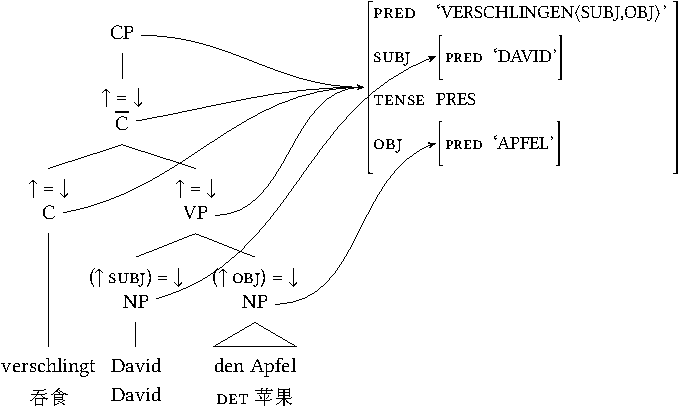
\includegraphics{Figures/verschlingt-david-den-apfel-lfg-lsp-crop}
}
\caption{\label{Abb-Verbstellung-LFG}遵循 \citet[\page 41]{Berman2003a}的动词位置分析}
\end{figure}%

%{\interfootnotelinepenalty=10%
\noindent
在了解了第\ref{Kapitel-PSG}章和第\ref{Kapitel-GPSG}章的短语结构规则后,允许动词短语确实看起来很不自然。
然而这对于LFG来说并不是一个问题,因为分析一个给定的句子,我们只需要保证所有必须要的成分(也只有这些成分)都出现。 
完备性\isc{完整性}\is{completeness}和一致性\isc{一致性}\is{coherence}的限制保证了这一点。究竟信息来自何方并不重要。
在图\ref{Abb-Verbstellung-LFG}中,动词信息并不来自于动词短语,而是C结点。
C$'$被下面的一个特殊规则所允准:
\ea
\phraserule{C$'$}{
\rulenode{C\\* \up~=~\down}
\rulenode{VP\\*\up~=~\down}}
\z
在LFG规则中,通常来说只对中心词这一个元素进行`\up~=~\down'标记。在(\mex{0})中,有两个这样的元素,这也是为什么二者同时为其父结点的f-结构提供信息的原因。
动词的中心词域被C扩展了。\lfgsubj 和\lfgobj 的信息来自于动词短语,而\pred 信息则来自于C。 
\isc{扩展的中心语范畴}\is{head domain!extended|)}
\isc{动词末位语言}\is{verb"=final language}

\section{局部语序重列}
\label{Abschnitt-LFG-Umstellung}

在前人的工作中已经讨论过两种\isc{成分序列|(}\is{constituent order|(}处理局部语序重列的方法\footnote{%
   \citet[\page 20--21]{Kaplan95a}讨论了如何在LFG中设计一个基于ID/LP\isc{ID/LP语法}\is{ID/LP grammar}形式的语法。
  而GPSG类型的组成成分顺序尚未在LFG框架中得以解决。%
}。
\begin{itemize}
\item 像GB\indexgbc 一样在基本结构中移动论元(详见\citealp{Choi99a-u})
\item 直接在短语规则中允准(详见Berman\citeyear[\S~2.1.3.1]{Berman96a-u};\citeyear{Berman2003a})
\end{itemize}

\noindent
如果我们假设语迹在给定结构的语义解释中是发挥作用的,则第一种分析和基于移动的GB分析有着一样的问题。
在\ref{sec-GB-lokale-Umstellung}中,我们已经讨论过这些问题了。

接下来,我讨论 \citet[\S~2.1.3]{Berman96a-u}提出的分析,在某种意义上来说我简化了表示。
动词论元的格和语法功能由词库所决定\citep[\page 22]{Berman96a-u}。
(\mex{1})展示了德语动词verschlingen(吞食)的词汇项信息:\footnote{%
  德语的四个格可以用两个二元特征——{\small GOV}和{\small OBL}——进行表示\citep[\page 22]{Berman96a-u}。
  主格的{\small GOV}为$-$,而{\small OBL}为$-$;宾格的{\small GOV}为$+$,而{\small OBL}为$-$。
  这种类型的表示法使得我们可以仅仅通过部分信息来描述一个格。
  如果我们没有声明{\small GOV}的值,则一个{\small OBL}为$-$的格描述既和主格也和宾格兼容。
  因为下面的讨论并没有使用到这种局部声明的好处,我接下来并没有使用特征分解而是直接使用格信息。
}$^,$\footnote{%
  作为一种替代性分析,也可以从格中推导出一个名词短语的语法功能(\citealp[\page 37]{Berman2003a}的德语分析;\citealp[\page 187, \page 201]{Bresnan2001a}的德语和俄语分析\il{Russian})。

\ea
\label{Kasus-Implikation-Berman}
\upshape      (\downsp \case) = \mdacc{} $\Rightarrow$ (\upsp \lfgobj) = \down{}
\z

\noindent
   \citet[\S~2.1]{Karttunen89a-u}在分析芬兰语的时候,基于范畴语法\indexcxgc 的框架提出了类似的分析。
  因为格并不总是非常可靠地与语法功能耦合在一起,因此类似的分析并非完全没有问题。
  在德语中,和时间宾格(ii.a)一样,有一些动词会有两个宾格宾语(ii.b--c)和谓词性宾格(ii.d)。

\eal
\ex 
\gll Er arbeitete den ganzen Tag.\\
%	 he worked the.\acc{} whole.\acc{} day\\
     他 工作 \textsc{det}.\acc{} 整个.\acc{} 一天\\
\ex 
\gll Er lehrte ihn den Ententanz.\\
% he taught him.\acc{} the.\acc{} duck.dance\\
     他 想 他.\acc{} \textsc{det}.\acc{} 鸭子.跳舞\\
\ex 
\gll Das kostet ihn einen Taler.\\
%	 that costs him.\acc{} a.\acc{} taler\\
     那 花费 他.\acc{} 一.\acc{} 泰勒\\
\ex 
\gll Sie nannte ihn einen Lügner.\\
%	 she called him.\acc{} a.\acc{} liar\\
     她 称 他.\acc{} 一.\acc{} 说谎者\\
\zl
所有的这些宾格都可以出现在长距离依存关系中(见\ref{Abschnitt-NLA-LFG}):

\ea
\gll Wen glaubst du, dass ich getroffen habe.\\
%    who believe you that I met have\\
    谁 相信 你 \textsc{comp}  我 会见 \textsc{aux} \\
\mytrans{你认为我和谁见面了?}
\z

\noindent
wen(谁)并不是glauben(会见)的宾语,因此并不在glauben的f-结构中。
必须对(i)中的蕴涵规则的右面部分进行修改,允许多种语法功能的析取,还需要解释宾格可以来自于一个嵌入得很深的f-结构这一语言事实。
}
\ea
\label{le-verschlingen}
\catlexentry{verschlingt}{V}{(\up\ \pred) = {\small `VERSCHLINGEN\arglist{\lfgsubj, \lfgobj}'}\\*
                             (\up\ \lfgsubj{} {\small AGR CAS}) = NOM\\*
                             (\up\ \lfgobj{} {\small AGR CAS}) = ACC\\*
                             (\up\ \lfgtense) = \small PRES}
\z

\noindent
Berman提出一种分析,在这一分析中,动词并不会和它的论元及附加语同时结合,就像GPSG\indexgpsgc 里分析的那样。
她的分析走向另一个极端,她假设动词并不是和附加语或者论元结合,而是直接形成动词短语。
相关的规则如(\mex{1})所示:
\ea
\label{LFG-v-vp}
\phraserule{VP}{
\rulenode{(V)\\* \up~=~\down}}
\z
乍一看来,这种分析非常奇怪,显然一个像devour一样的动词,它自身的分布与它和它论元加和之后的分布是并不相同的。
但是,我们应当回想一下保留下来的针对f-结构一致性与完备性的限制,它们仍然起作用,进而这个理论仍然不会做出错误的(针对语言现象的)预测。
%}% footnote breaks
% this bracket belonges to \interfootnotelinepenalty=10%

因为动词可以出现在初始位置,它在(\mex{0})规则里被标记为可选(见\ref{Abschnitt-Verbstellung-LFG})。

下面的规则可以用以进一步组合动词和它的主语或者宾语。
\ea
\label{lfg-vp-regel}
\phraserule{VP}{
\rulenode{NP\\* (\upsp \lfgsubj|\lfgobj|\objtheta) = \down}
\rulenode{VP\\* \up~=~\down}}
\z
这里的|\isc{$\vert$}\is{$\vert$}表示析取(disjunction\isc{析取}\is{disjunction}),也就是说,NP既可以是相应f-结构的主语也可以是宾语。
因为VP既出现在(\mex{0})中所示规则的左边也出现在其右边,它可以多次进行应用。
而这个规则并不完整。例如,我们还必须解释介词型宾语、小句型论元、形容词性论元和附加语。
参见第\pageref{fn-zp}页的脚注\ref{fn-zp}。

图\vref{Abb-SOV-LFG}展示了(\mex{1}a)的分析。 
\eal
\ex 
\gll {}[dass] David den Apfel verschlingt\\
%      \spacebr{}that David the apple devours\\
      \spacebr\textsc{comp} David \textsc{det} 苹果 吞食\\
%\mytrans{that David is devouring the apple}
\mytrans{David正在吞食苹果}
\ex 
\gll {}[dass] den Apfel David verschlingt\\
     %\spacebr{}that the apple David devours\\
     \spacebr\textsc{comp} \textsc{det} 苹果 David 吞食 \\
\zl
\begin{figure}
\centerline{%
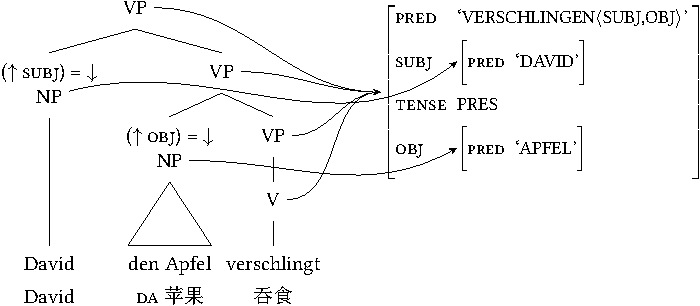
\includegraphics{Figures/david-den-apfel-verschlingt-lfg-lsp-crop}
}
\caption{\label{Abb-SOV-LFG}参考 \citet{Berman96a-u}的针对SOV语序的分析}
\end{figure}%
(\mex{0}b)的分析见图\vref{Abb-OSV-LFG}。
\begin{figure}
\centerline{%
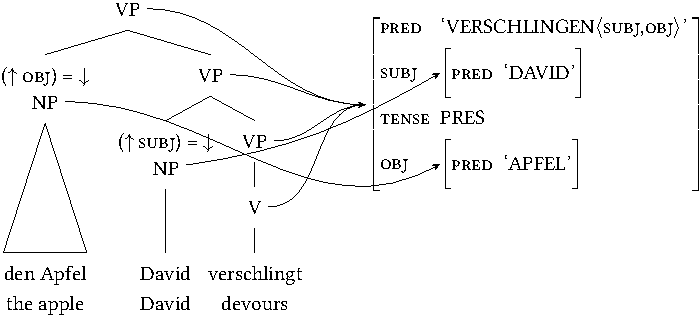
\includegraphics{Figures/den-apfel-david-verschlingt-lfg-lsp-crop}
}
\caption{\label{Abb-OSV-LFG}参考 \citet{Berman96a-u}的针对OSV语序的分析}
\end{figure}%
(\mex{0}b)的分析不同于(\mex{0}a)之处仅在于做主语的NP结点与做宾语的NP结点与VP结合的次序不同。\todostefan{fix the arrows, should not cross SUBJ and OBJ}

另外一个必须讨论的情况是:在规则(\ref{LFG-v-vp})中,动词是可选的。
如果它被删去,则VP为空。
这样一来,(\ref{lfg-vp-regel})中的VP规则则允许其右侧有一个空的VP。
这个VP同样可以被删去,尽管规则(\ref{lfg-vp-regel})中并没有做可选的标记。
也就是说,结合语法中其它的可与之交互的规则,相应的符号变成可选的。\isc{成分序列|)}\is{constituent order|)}  

\section{长距离依存和功能多变性}
\label{Abschnitt-NLA-LFG}

我们\isc{长距离依存}\is{long"=distance dependency|(}已经知道了LFG可以解释被动、局部语序重列、不基于转换的动词替换的语言现象。
在讨论GPSG的\ref{Kapitel-GPSG},我们已经看到了如何使用一个不基于转换的分析来处理长距离依存。
在LFG中, \citet{KZ89a}提出了另外一种不基于转换的长距离依存分析,接下来,我们对这种分析展开讨论。

在例(\mex{1})中,不出现的成分Chris(人名)有两个功能:
\ea
\label{ex-Chris-we-think}
\gll Chris, we think that David saw.\\
Chris 我们 认为 \textsc{comp} David  看见\\
\mytrans{Chris,我们认为David看见了。}
\z
首先,假定Chris出现在一个较为普通的句子中,它应该出现在一个不同的位置(前述例子中saw(看见)的\lfgobj 功能),此处,Chris也有这样的功能。
另外,它应该有一个篇章功能(discourse function):
这种构式中的一种特定的信息结构层面的状态(information"=structural status)信息(主句中的话题(\textsc{topic}))。
在LFG中,话题和焦点(\textsc{focus})是语法化的篇章功能(进一步说,\textsc{subj}被视为默认的篇章功能)。
只有语法化的篇章功能才能在f-结构中进行表示,也就是说,那些被特定的句法机制创造出来的并且和句法其它部分相交互的部分。

不像论元功能,篇章功能\textsc{topic}\isfeat{topic}\isc{话题}\is{topic}和\textsc{focus}
\isfeat{focus}\isc{焦点}\is{focus}都不是次范畴的内容,因此并不受完备性和一致性的约束。
像\textsc{topic}和\textsc{focus}篇章功能特征的取值由相应的f-结构的论元功能决定。
(\mex{1})给出了(\ref{ex-Chris-we-think})中的句子的f-结构:

\ea
\lfgms{ pred & `THINK\sliste{ \lfgsubj, \comp }' \\
        topic & \rnode{topic}{\lfgms{ pred & `CHRIS' \\
                                   }}\\[4mm]
        subj & \lfgms{ pred & `pro'\\
                     }\\
        comp & \lfgms{ pred & `SEE\sliste{ \lfgsubj, \lfgobj }'\\
                       subj & \lfgms{ pred & `DAVID' \\
                                    }\\
                       obj  & \rnode{obj}{}\\
                     }\\
      }
% todo \nodecurve[r]{topic}[r]{obj}{15em}
\nccurve[ncurv=2.2]{topic}{obj}
\z

\noindent
图中新的连线表示\textsc{topic}的取值和\textsc{comp$|$obj}的取值相等。
在\ref{chap-feature-descriptions}所采用的特征描写中,我用的是带有标号的方块表示特征共享,而不是连线,因为
方块是一种被不同的理论框架广泛采用的标记。
可以用形如(\mex{1})的f-结构限制来形式化如(\mex{0})中的结构共享。 
\ea
\label{Topic-Comp-Obj}
(\upsp  \textsc{topic}) = (\upsp \textsc{comp obj})
\z

\noindent
像(\ref{ex-Chris-we-think})中的前置现象可能发生在不同深度的子句嵌入中。
例(\mex{1}a)是子句嵌入得更浅的一个例子。
宾语和话题出现在同一个f-结构中。
但是(\ref{ex-Chris-we-think})中的宾语来自于think(想)里面的一个从句。

(\mex{1}a)所对应的f-结构如(\mex{1}b)所示:

\eal
\ex 
\gll Chris, we saw.\\
Chirs 我们 看见\\
\mytrans{Chirs,我们看见了。}
\ex 
\lfgms{ pred & `SEE\sliste{ \lfgsubj, \lfgobj }' \\
        topic & \rnode{topic}{\lfgms{ pred & `CHRIS' \\
                                   }}\\[4mm]
        subj & \lfgms{ pred & `pro'\\
                     }\\
        obj  & \rnode{obj}{}\\
      }
% todo \nodecurve[r]{topic}[r]{obj}{15em}
\nccurve[nodesepA=1pt,ncurv=2.2]{topic}{obj}
\zl

\noindent
这个例子中的\topic{}和\lfgobj 的同一性限制可以按照(\mex{1})来进行形式化:

\ea
\label{Topic-Obj}
(\upsp  \textsc{topic}) = (\upsp \textsc{obj})
\z

\noindent
例(\mex{1}a)是一个比(\ref{ex-Chris-we-think})嵌入程度更深的例子;
(\mex{1}b、c)是相应的f-结构和功能限制。

\eal
\ex 
\gll Chris, we think Anna claims that David saw.\\
Chirs 我们 认为 Anna 声称 \textsc{comp} David 看见\\
\mytrans{Chirs,我们认为Anna声称David看见了。}
\ex 
\lfgms{ pred & `THINK\sliste{ \lfgsubj, \comp }' \\
        topic & \rnode{topic}{\lfgms{ pred & `CHRIS' \\
                                   }}\\[4mm]
        subj & \lfgms{ pred & `pro'\\
                     }\\
        comp & \lfgms{ pred & `CLAIM\sliste{ \lfgsubj, \comp }\\
                       subj & \lfgms{ pred & `ANNA' \\
                                   }\\
                       comp & \lfgms{ pred & `SEE\sliste{ \lfgsubj, \lfgobj }\\
                                      subj & \lfgms{ pred & `DAVID' \\
                                                   }\\
                                      obj  & \rnode{obj}{}\\
                                    }\\
                     }\\
      }
% todo \nodecurve[r]{topic}[r]{obj}{15em}%
\nccurve[ncurv=2.2]{topic}{obj}
\ex\label{Topic-Comp-Comp-Obj}
(\upsp  \textsc{topic}) = (\upsp \textsc{comp comp obj})
\zl


\noindent
事实上,(\ref{Topic-Comp-Obj})、(\ref{Topic-Obj})以及(\ref{Topic-Comp-Comp-Obj})中的限制是针对c-结构的。
(\mex{1})是把(\ref{Topic-Comp-Obj})结合到c-结构后的示例:
\ea
\begin{tabular}[t]{@{}ccc@{~=~}lc@{}}
CP & $\rightarrow$ & \multicolumn{2}{l}{\hspaceThis{(\upsp \textsc{topic})}XP} & C$'$ \\
 & &  (\upsp \textsc{topic}) & \down & \up~=~\down \\
 & &  (\upsp \textsc{topic}) & (\upsp \textsc{comp obj})\\
\end{tabular}
\z
(\mex{0})声明了第一个组成成分所对应f-结构是其父结点所对应的\textsc{topic}特征的值,此外,这个话题特征的取值也是其补足语小句中的宾语。
我们同样可以找到嵌入深度不同的其他例子。
因此我们需要如(\mex{1})的各种功能限制: 
\eal
\ex (\upsp  \textsc{topic}) = (\upsp \textsc{obj})
\ex (\upsp  \textsc{topic}) = (\upsp \textsc{comp obj})
\ex (\upsp  \textsc{topic}) = (\upsp \textsc{comp comp obj})
\ex \ldots
\zl
可以用(\mex{1})表示这些等式的泛化:
\ea
(\upsp  \textsc{topic}) = (\upsp \textsc{comp* obj})
\z

\noindent
这里,*\isc{*}\is{*}表示\mbox{\small COMP}出现的次数不受限制。
这意味着篇章和语法功能的同一性关系尚待确定,这种性质称为功能多变性(functional uncertainty\isc{功能的不确定性}\is{functional uncertainty}),见 \citew{KZ89a}。

在第\pageref{bsp-fronted-focus}页的针对例(\ref{bsp-fronted-focus})和(\ref{bsp-fronted-topic})的讨论中,
我们知道在英语中并不是只有\textsc{topic}才能放到CP的指定语的位置,\focus 也可以。
我们可以在LFG等式中采用析取符号来表示这种条件:

\ea
(\upsp  \textsc{topic$|$focus}) = (\upsp \textsc{comp* obj})
\z
我们可以引入一个新的特殊符号来替代\textsc{topic$|$focus},表示的是篇章功能的析取:\textsc{df}
\isfeat{df}。
(\mex{0})就此可以简化为(\mex{1}):

\ea
(\upsp  \textsc{df}) = (\upsp \textsc{comp* obj})
\z

\noindent
用于构建英语中前置的c-结构规则最终可以表示如(\mex{1})所示:\footnote{%
  注意到\textsc{df}分别对应的这两个析取原则上是独立的。
  而我们并不希望这样。
  我们希望讨论的是父结点所对应的f-结构中的话题“或”焦点,而不是话题“和”焦点。
  所以需要额外的机制来确保\textsc{df}指的是同一个篇章功能。
}
\ea
\begin{tabular}[t]{@{}ccc@{~=~}lc@{}}
CP & $\rightarrow$ & \multicolumn{2}{l}{\hspaceThis{(\upsp \textsc{df})}XP} & C$'$ \\
 & &  (\upsp \textsc{df}) & \down & \up~=~\down \\
 & &  (\upsp \textsc{df}) & (\upsp \textsc{comp* obj})\\
\end{tabular}
\z
在德语中,和宾语一样,几乎任意一个成分(如主语、句子型补足语、附加语)都可以前置。 
而相应的c"=结构规则如(\mex{1})所示:\footnote{\label{fn-zp}%
  在(\mex{1})中, \citet{Berman96a-u}使用的是ZP而不是XP(\mex{1})。
  她形式化了ZP的各种短语结构规则,在这些规则中可以将ZP替换为NP、PP、AP以及各种各样的附加语。
  按照Berman的分析,ZP可以和中间动词结合。
  为了阐述方便,在\ref{Abschnitt-LFG-Umstellung}中,
  我对在VP规则(\ref{lfg-vp-regel})中使用ZP符号持保留态度,选择直接使用NP。
}
\ea
\begin{tabular}[t]{@{}ccc@{~=~}lc@{}}
CP & $\rightarrow$ & \multicolumn{2}{l}{\hspaceThis{(\upsp \textsc{df})}XP} & C$'$ \\
 & &  (\upsp \textsc{df}) & \down & \up~=~\down \\
 & &  (\upsp \textsc{df}) & (\upsp \textsc{comp* gf})\\
\end{tabular}
\z
这里,\textsc{gf}是语法功能的析取,可以出现在前域中。 
\isc{长距离依存}\is{long"=distance dependency|)}

\section{总结与分类}

LFG是一种基于限制的理论,采用了特征描写和短语结构规则。
语法功能被视为理论的原子概念,这一点也将LFG与本书中所介绍的其他理论区别开来。
语法功能并不是像GB那样通过结构关系来进行定义的。
LFG是一种词汇主义理论。像GPSG一样,LFG不需要转换。
影响到论元结构的过程,如被动等,是通过词汇规则进行分析的。
GPSG处理长距离依存是通过所谓的信息在句法树上向上传递进行的,而LFG使用功能多变性:f-结构中的一个部分可以和其内嵌不定深度的另一个f-结构同一。
一致性\isc{一致性}\is{coherence}和完备性\isc{完整性}\is{completeness}保证了长距离依存可以被正确消解,也就是说,它保证了一个前置的宾语并不会分配给
一个已经有了宾语或者并不允准宾语的f-结构。

尽管LFG包含一个短语结构模块,和其他语法模型相比,这个模块的作用要小一些。
有一些规则里所有的成分都是可选的。
为了处理一些语言,研究人员甚至提出了一些连成分范畴都不确定的规则(参见\ref{sec-Diskussion-X-Bar})。
在这些语法中,f-结构、一致性、完备性共同保证了语法只能允准良形式的结构。

LFG和诸如\hpsgc、\cxgc 的一些变体等理论不同之处在于特征结构并没有做类型化。
因此,无法通过类型层级表示泛化。
直到最近几年,基于继承关系(inheritance hierarchies\isc{承继}\is{inheritance})的知识层级化组织都不是理论分析的一部分。
在计算机实现中,虽然可以借助宏(macros\isc{宏语}\is{macro}),但这只是为一组限制提供一个简称的方式,没有任何理论模块与之相对应。
也可以将宏组织成一个层级结构, \citew*{DKK2004a}讨论了基于这种方式如何捕捉语言知识的泛化性质。
 \citet*{ADT2008a}则认为宏不仅可以用来组织词汇项,还可以捕捉c-结构上的增广标注的泛化性。
因为这些发展,LFG和诸如HPSG和CxG的其他理论有趋同发展的趋势。

 \citet{Williams84a}比较了GB和LFG中的分析。
他的研究表明很多分析本身是可以互相转化的:LFG中的f-结构的功能可以通过GB中的题元准则(Theta"=Criterion\isc{$\theta$-理论@$\theta$-理论}\is{theta-theory@$\theta$-Theory}\isc{$\theta$-准则@$\theta$-准则}\is{theta-criterion@Theta"=Criterion})和格理论(Case Theory\isc{格}\is{case}\isc{格语法}\is{Case Theory})进行分析处理。
LFG可以显性地区分主语和非主语。
在GB中则是区分外部\isc{外部论元}\is{argument!external}和内部\isc{内部论元}\is{argument!internal}论元(参见\citealp[\S~1.2]{Williams84a})。
对于GB的一些变体来说,和HPSG\indexhpsgc 以及CxG\indexcxgc 类似,带有主语性质的论元(如果有的话)要做显性标记\citep{Haider86,HM94a,Mueller2003e,MR2001a}。
这个特殊的论元被称之外指定的论元(designated argument\isc{指派论元}\is{argument!designated})。
在不定式中,主语经常在不定式短语的内部缺失。
尽管如此,没有表达出来的主语经常是和主句里的一个论元共指。

\eal
\ex 
\gll Er versucht, [das Buch zu lesen].\\
	 他 尝试 \spacebr{}\textsc{det} 书 \textsc{inf} 读\\
\mytrans{他试着读这本书。}
%	 he tries \spacebr{}the book to read\\
%\mytrans{He is trying to read the book.}
\ex 
\gll Er zwingt ihn, [das Buch zu lesen].\\
	 他 逼迫 他 \spacebr{}\textsc{det} 书 \textsc{inf} 读\\
\mytrans{他逼着他读这本书。}
%	 he forces him \spacebr{}the book to read\\
%\glt `He is forcing him to read the book.´
\zl 
这是一个所有理论都需要去捕捉的语言事实,也就是说每一种理论都必须区分主语和非主语。

参阅 \citew{Kuhn2007a}以了解更多的GB/Minimalism与LFG/HPSG的异同。

%\section*{思考题}

%\bigskip
\questions{
\begin{enumerate}
\item 术语“一致性”和“完备性”的具体含义是什么?
\item 什么是扩展的中心词域?
\item 词汇完整性(lexical integrity)的含义是什么? 
\end{enumerate}
}

%\section*{练习题}

\exercises{
\begin{enumerate}
\item 给出kannte(“知道”的过去式)的词汇项描写.
\item 如何分析下面的句子?
\ea
\gll Den Apfel verschlingt David.\\
	 \textsc{det} 苹果 吞食 David\\
\mytrans{David在吞食苹果。}
%	 the apple devours David\\
%\mytrans{David devours the apple.}
\z
提供必要的c-结构规则。
什么样的f-结构被允准?
画出句法树及其对应的f-结构。
对于前置的成分,仅需要画出NP而不需要扩展XP结点。
针对NP的c-结构规则同样可以省略,这样的省略可以在树上通过三角形进行表示。
\end{enumerate}
}

%\section*{延伸阅读}
\furtherreading{
\ref{Abschnitt-Format-LFG}的讨论主要基于 \citet{Dalrymple2001a-u,Dalrymple2006a}。
此外,我还从Jonas Kuhn2007年起使用的教学资料中选取了内容。
 \citew{Bresnan2001a}针对英语进行了全面讨论,适合有基础的读者。
 \citew{Berman96a-u,Berman2003a}针对德语做了更深入的LFG分析。
 \citew{SdA2016a-u}则使用法语例子对LFG进行了介绍。
作者们展示了如何使用XLE系统来开发一部法语\il{French}LFG语法。
这本参考书也讨论了如何使用XLE系统中的有限状态词法分析模块。

 \citet{Levelt89a}基于LFG提出了一个语言加工模型。
 \citet{Pinker84a-u}——语言习得领域最为知名的学者之一——使用LFG作为他习得理论的模型。
 \citew{Pienemann2005a}则针对第一语言与第二语言习得提出了另外一种LFG模型。 
}

%      <!-- Local IspellDict: en_US-w_accents -->

%% -*- coding:utf-8 -*-

\chapter{范畴语法}
%\chapter{Categorial Grammar}
\label{Kapitel-CG}\label{chap-CG}

在本书所讨论的所有方法中,范畴语法\isc{范畴语法(CG)|(}\is{Categorial Grammar (CG)|(}是第二古老的方法。
上个世纪三十年代波兰逻辑学家\href{http://en.wikipedia.org/wiki/Kazimierz_Ajdukiewicz}{Kazimierz Ajdukiewicz}提出了这种分析方法\citep{Ajdukiewicz35a-u}。
范畴语法备受逻辑学家和语义学家青睐,主要原因在于在范畴语法中,句法和语义描写紧密耦合,所有的句法组合都遵从语义组合。
语义研究中的一些典范工作使用了范畴语法,如Richard Montague\citeyearpar{Montague74a-u}的工作。
俄亥俄州哥伦比亚的David Dowty\citeyearpar{Dowty79a}、 
乌特勒支的Michael Moortgat\citeyearpar{Moortgat89a-u}、巴塞罗那的Glyn Morrill\citeyearpar{Morrill94a-u}、
纽约的Bob Carpenter\citeyearpar{Carpenter98a-u}和爱丁堡的Mark Steedman\citeyearpar{Steedman91a,Steedman97a,Steedman2000a-u}在这个领域都作出了重要贡献。
基于蒙太古语法的德语分析始于 \citew{Stechow79}。
曼海姆德语语言研究所(Institut für Deutsche Sprache)的2569页的德语语法\citep*{IDS97-not-crossreferenced}也包含范畴语法的重要分析。
 \citet{Fanselow81a-u}在蒙太古语法的框架下研究了词法形态学。
 \citet{Uszkoreit86d}、 \citet{Karttunen86a,Karttunen89a-u}和 \citet*{CKZ88a}结合了基于合一的方法与范畴语法两种分析手段,提出了新的分析方法。

在范畴语法中,组合语言单位的基本操作相当简单而且也容易理解,目前已经开发了很多可以编写范畴语法的平台,也有很多可以根据范畴语法进行分析的系统\citep*{YK90a-u,Carpenter1994a-u,BvN94a-u,Llore1995a-u,KoenigE99a-u,Moot2002a-u,WB2003a-u,BCPW2007a,Morrill2012a}。
这其中特别值得注意的是Mark Steedman课题组的工作(如\citealp*{CHS2002a-u,CC2007a-u})。

%% , aber auch in Deutschland gab und
%% gibt es computerlinguistische Gruppen, die in diesem theoretischen Rahmen arbeiten
%% \citep*{Uszkoreit86d,KoenigE99a-u,VHE2003a}.
%% MCGTOOLS: Llore1995a-u
下述语言已经有了一些有具体实现的语法片段:
\begin{itemize}
\item 德语\citep*{Uszkoreit86d,KoenigE99a-u,VHE2003a,VTBS2011a}
\item 英语\ilce{英语}{English} \citep{Villavicencio2002a,Baldridge2002a-u,Beavers2002a-u,Beavers2004a-u}
% CMZ86a ist ein Report, den gibt es aber nirgends
\item 芬兰语\ilce{芬兰语}{Finnish} \citep{Karttunen89a-u}
\item 法语\ilce{法语}{French} \citep*{BBCG87a-u}
\item 荷兰语\ilce{荷兰语}{Dutch} \citep{BvN94a-u,Baldridge2002a-u}
\item 塔加洛语\ilce{塔加洛语}{Tagalog} \citep{Baldridge2002a-u}
\item 土耳其语\ilce{土耳其语}{Turkish} \citep{Hoffmann95a-u,Baldridge2002a-u}
\end{itemize}
另外,\citet*[\page 15]{BCPW2007a}提到过一个针对古典阿拉伯语\ilce{阿拉伯语}{Arabic}的实现。

有些处理范畴语法的系统增加了概率\isc{统计学}\is{statistics}模块,所以处理结果的鲁棒性很高\citep*{OB97a,CHS2002a-u}。
有些系统采用了从(标注)语料中抽取词汇项的方法, \citet{Briscoe2000a}和 \citet{Villavicencio2002a}使用了一些统计信息,
这些信息来自于他们建立在普遍语法\isc{普遍语法(UG)}\is{Universal Grammar (UG)}的语言获取模型\isc{语言习得}\is{language acquisition}。

\section{表示形式概述}

接下来,我将介绍一些范畴语法中的基本假设。在此之后,我会讨论一些基于组合范畴语法的具体分析,这些分析选自\citet{Steedman97a}。
除了组合范畴语法之外,也有一些范畴语法的其他变体,如类型逻辑范畴语法\citep*{Morrill94a-u,Dowty97a-u,Moortgat2011a-u}。
在本书中对其他类型的范畴语法不再加以讨论。

\subsection{配价信息的表示}
\label{sec-forward-backward-application}

在\isc{价|(}\is{valence|(}范畴语法中,复杂范畴替换了GPSG\indexgpsgc 中的\textsc{subcat}特征来确保一个中心词只能使用适合的句法规则。
一些短语结构语法规则\isc{短语结构语法}\is{phrase structure grammar}可以用复杂范畴来替换:\isc{/|(}\is{/|(} 

\ea
\label{LE-CG}
\begin{tabular}[t]{@{}l@{\hspace{1cm}}l}
规则                              & 词库中的范畴\\
vp $\to$ v(ditrans) np~np         & (vp/np)/np  \\
vp $\to$ v(trans) np              & vp/np  \\
vp $\to$ v(np\_and\_pp) np~pp(to) & (vp/pp)/np  \\
\end{tabular}
\z
vp/np表示当前描写的语言单位需要一个名词短语用以形成一个动词短语。

范畴语法只包含几条非常抽象的规则。其中一条规则为前向应用,有时也称为乘法规则:
\ea
\label{vorwaertsapplikation}\label{forward-application}
前向应用
\isc{前向应用}\is{forward application}:\\
X/Y $*$ Y = X
\z
这条规则由两个范畴组成,其中之一为X/Y,意为向右寻找一个Y以便生成X,另一个则为X。
这个组合的结果是一个完整的X,不再需要Y。
称X/Y为“函子”
\isc{函子}\is{functor},而Y为函子的“变元”
\isc{变元}\is{argument}。

和GB理论一样,范畴语法中配价信息只在词库中出现一次。
在GPSG\indexgpsgc 中,配价信息同时体现在句法规则和词条的\textsc{subcat}特征中。

图\vref{abb-cg-transitives-Verb}展示了一个及物动词的词条是如何与它的宾语组合的。
\begin{figure}
\centerline{%
\deriv{2}{
%\begin{tabular}{@{}cc@{}}
chased       & Mary\\
\textrm{追} & \textup{Mary}\\
%\uline{1}    & \uline{1} \\
\hr & \hr\\
vp/np   & np\\
\multicolumn{2}{@{}c@{}}{\forwardapp} \\
\multicolumn{2}{@{}c@{}}{vp}\\
%\cgmc<2->{2}{vp}\\
%\end{tabular}
}
}
\caption{\label{abb-cg-transitives-Verb}动词及其宾语的组合(基本分析)}
\end{figure}%
CG中的一个推导可以视为一个二叉树。
一对儿范畴通过一个长箭头表示其通过一个组合规则进行组合的过程。
箭头的方向表示这个组合的方向。而组合的结果则置于箭头之下。
图\vref{Abb-CG-als-Baum}是与图\ref{abb-cg-transitives-Verb}相对应的树形。
\begin{figure}
\centerline{%
\begin{forest}
sn edges
[vp
	[vp/np
		[chased\\追]]
	[np
		[Mary\\Mary]]]
\end{forest}
}
\caption{\label{Abb-CG-als-Baum}图\ref{abb-cg-transitives-Verb}中推导的树形表示}
\end{figure}%

\noindent
对于`/',我们经常假设左向结合律
\isc{左向结合律}\is{left associativity},即(vp/pp)/np = vp/pp/np。
\is{/|)}

观察(\ref{LE-CG})中的词汇项,我们可以清楚看到范畴v是不存在的。
词库仅仅决定一个词条与什么样的论元结合以得到什么结果。
而符号vp也可以删去:一个(英语中的)vp是在其左侧提供一个名词短语便可以形成一个完整句子的语言成分。
这\isc{$\backslash$}\is{$\backslash$|(}通过s$\backslash$np进行表示。
使用后向应用规则,可以计算得到如图\vref{abb-the-cat-chased-Mary}所示的推导
\isc{价|)}\is{valence|)}。
\ea
后向应用
\isc{后向应用}\is{backward application}:\\
Y $*$ X$\backslash$Y = X 
\z

\begin{figure}
\centerline{%
\deriv{4}{
the  & cat & chased         & Mary\\
\textsc{art}.\textsc{def}  & \textrm{猫} & \textrm{追}         & \textup{Mary}\\
\hr  & \hr & \hr            & \hr \\
np/n & n   & (s\bs np)/np   & np\\
\multicolumn{2}{@{}c}{\forwardapp} & \multicolumn{2}{c@{}}{\forwardapp}\\
\multicolumn{2}{c}{{np}}             & \multicolumn{2}{c@{}}{{s\bs np}}\\
\multicolumn{4}{@{}c@{}}{\backwardapp}\\
\multicolumn{4}{c@{}}{{s}}\\
}}
\caption{\label{abb-the-cat-chased-Mary}含有一个及物动词的句子的分析。}
\end{figure}%

\noindent
范畴语法并不显性地区分短语与词:针对一个不及物动词和一个包含了一个宾语的动词短语的描写是一样的,同为s$\backslash$np。
同样道理,专有名词是完整的名词短语,视为np。
\isc{$\backslash$}
\is{$\backslash$|)}

\subsection{语义}

我们已经提到了因为句法组合总是可以推出相应的语义组合,所以范畴语法备受语义学家青睐。
这种组合的平行性不仅仅在语言单位的简单组合中如此,在复杂组合中亦然,我们可以精确地定义相应的语义组合过程,接下来我们将展开讨论。
我们的讨论基于 \citet[\S~2.1.2]{Steedman97a}的分析。

针对动词eats(吃),Steedman给出了下面的词汇项分析:\footnote{%
 我适当变换了分析的符号表示以和本书的表示一致。
}
\ea
eats := (s: \relation{eat}(x, y)\bs np\sub{3S}:x)/np:y
\z
在(\mex{0})中,每一个范畴的语义都在分号中表示。因为eat的论元的语义我们尚不清楚,因此用变量$x$和$y$表示。
当动词组合了一个名词短语,这个名词短语的指谓(denotation)会被带入到相应位置以替换相应的变量。
(\mex{1})为一个例子:\footnote{%
  我们假设apples(苹果)意为\relation{apples}而不是\relation{apples}(z),这里去掉量词以简化分析。
}
\ea
\deriv{2}{
(s: eat'(x, y)\bs np_{3S}:x)/np:y & np: apples'\\
\multicolumn{2}{@{}c@{}}{\forwardapp}\\
s: eat'(x, apples')\bs np_{3S}:x\\
}
\z
当组合一个函子和一个变元时,必须确保变元符合函子要求,也就是说二者必须可以合一
\isc{合一}\is{unification}(参见\ref{sec-unification}以了解合一运算)。
np:y和np: \relation{apples}的合一结果为np: \relation{apples},因为\relation{apples}比变量y更细化。
除了在项np:y中出现,y也出现在动词的描写中(s: \relation{eat}(x, y)\bs np\sub{3S}:x),因此动词论元的语义也得到了\relation{apples}这一语义解释。
因此,组合的结果为:\relation{eat}(x, \relation{apples})\bs np$_{3S}$:x,如(\mex{0})所示。

Steedman注意到这套符号的可读性随着推导的复杂而变得很差,因此使用了$\lambda$"=表示法:
\ea
eats := (s\bs np\sub{3S})/np: $\lambda y.\lambda x.\relation{eat}(x, y)$
\z
$\lambda$是用来获取复杂语义表征的开放性位置(参见\ref{sec-PSG-Semantik})。
$\lambda y.\lambda x.\relation{eat}(x, y)$这样的语义表征可以跟apples的表征相组合:去掉第一个$\lambda$,然后将apples的指谓带入到所有y变量的位置。
(参阅\ref{sec-PSG-Semantik}以了解更多细节):
\ea
$\lambda y.\lambda x.eat'(x, y)$ \relation{apples}\\
$\lambda x.eat'(x, apples')$
\z
这种$\lambda$表达式的约归称之为$\beta$"=约归
\isc{$\beta$-还原}\is{beta"=reduction@$\beta$"=reduction}\label{Seite-beta-Reduktion}。

如果采用(\mex{-1})中的符号,组合规则则可以修改为如下形式:
\ea
\begin{tabular}[t]{@{}l@{ * }l@{ = }c}
X/Y:f & Y:a & X: f a\\
Y:a & X\bs Y:f & X: f a\\ 
\end{tabular}
\z
在这样的规则中,论元(a)的语义写在函子的语义指谓之后。
函子语义指谓的开放位置用$\lambda$符号进行表示。变元可以和第一个$\lambda$表达式按照$\beta$-约归进行结合。

图\vref{Abb-Semantik-CG}展示了一个含有及物动词的句子的推导。在前向应用和后向应用中,直接使用了$\beta$"=约归。
\begin{figure}
\centerline{%
\deriv{3}{
Jacob & eats         & apples\\
\textup{Jacob} & \textrm{吃}         & \textrm{苹果}\\
\hr & \hr          & \hr \\
np:\relation{jacob}  & (s\bs np)/np: \lambda y.\lambda x.eat'(x, y) & np:apples'\\
         & \multicolumn{2}{c@{}}{\forwardapp}\\
         & \multicolumn{2}{c@{}}{\begin{tabular}[t]{@{}l@{~}l@{}}
                              $s\bs np$ &: $\lambda y.\lambda x.eat'(x, y)\; apples'$\\[4pt]
                                      &= $\lambda x.eat'(x, apples')$\\
                              \end{tabular}}\\
\multicolumn{3}{@{}c@{}}{\backwardapp}\\
\multicolumn{3}{c@{}}{\begin{tabular}[t]{@{}l@{~}l@{}}
                    $s$ &: $\lambda x.eat'(x, apples')\; jacob'$\\[4pt]
                      &= $eat'(jacob', apples')$\\
                              \end{tabular}}\\
}}
\caption{\label{Abb-Semantik-CG}范畴语法中的语义组合}
\end{figure}%

\subsection{附加语}

正如\ref{sec-intro-arg-adj}所讨论的
\isc{说明语|(}\is{adjunct|(},附加语是可选的。
在短语结构语法中很容易表示这种可选性,例如在产生式左端出现的元素(比如一个动词短语VP)也同时出现在产生式右端,而产生式右端还有一个额外的附加语。
因为产生式左端的符号也在右端出现,这条规则可以被应用任意次数。
(\mex{1})是这样的一个例子:
\eal
\ex VP $\to$ VP~PP
\ex Noun $\to$ Noun~PP
\zl
我们用上述规则分析动词短语或名词后面带有任意多项介词短语的语法现象。

范畴语法的分析中,附加语的范畴一般为X\bs X或X/X。
形容词是出现在名词前的修饰性成分。它们的范畴为n/n。
出现在名词后面的修饰性成分(如介词短语或关系从句)的范畴则为n\bs n。\footnote{%
  范畴语法中没有像\xbarc 一样的\xbarc 理论的间接投射范畴符号。
  所以CG使用n/n,而不是\nbarc/\nbarc。
  参见练习\ref{ue-Xbar-CG}。
} 
对于动词短语VP的修饰性成分,X被替换为VP的符号(s\bs np),这样一来会产生相对复杂的表达式(s\bs np)\bs (s\bs np)。
英语中的副词是VP的修饰性成分,因而具有上述范畴。介词需要一个名词短语才能形成一个完整的介词短语去修饰动词,因此其范畴应为
((s\bs np)\bs (s\bs np))/np。
图\vref{abb-CG-Adjunktion}是一个含有副词quickly(快速地)和介词round(环绕)的英语句子的分析。
%
\begin{figure}
\oneline{%
\deriv{9}{
The  & small & cat & chased       & Mary & quickly                & round                     & the & garden\\
\textsc{art}.\textsc{def}  & \textrm{小} & \textrm{猫} & \textrm{追}       & \textup{Mary} & \textrm{迅速地}                & \textrm{绕着}                     & \textsc{art}.\textsc{def}  & \textrm{花园}\\
\hr  & \hr   & \hr & \hr          & \hr  & \hr                    & \hr                       & \hr & \hr\\
np/n & n/n   & n   & (s\bs np)/np & np   & (s\bs np)\bs (s\bs np) & (s\bs np)\bs (s\bs np)/np & np/n & n\\
     & \multicolumn{2}{c}{\forwardapp} & \multicolumn{2}{c}{\forwardapp}\\
     & \multicolumn{2}{c}{n}           & \multicolumn{2}{c}{s\bs np}\\
\multicolumn{3}{@{}c}{\forwardapp}        & \multicolumn{3}{c}{\backwardapp}\\
\multicolumn{3}{@{}c}{np}                 & \multicolumn{3}{c}{s\bs np}\\
&&&&&&&\multicolumn{2}{c@{}}{\forwardapp}\\
&&&&&&&\multicolumn{2}{c@{}}{np}\\
&&&&&&\multicolumn{3}{c@{}}{\forwardapp}\\
&&&&&&\multicolumn{3}{c@{}}{(s\bs np)\bs (s\bs np)}\\
&&&\multicolumn{6}{c@{}}{\backwardapp}\\
&&&\multicolumn{6}{c@{}}{(s\bs np)}\\
\multicolumn{9}{@{}c@{}}{\backwardapp}\\
\multicolumn{9}{@{}c@{}}{s}\\
}}
\caption{\label{abb-CG-Adjunktion}基于CG的附加语分析实例}
\end{figure}%
注意到将round和the garden组合之后,会得到副词的范畴——(s\bs np)\bs (s\bs np)。
在GB理论中,副词和介词同样被置于单独的类中(参阅第\pageref{Seite-Adverbien-PP}页)。
这个包罗万象的类可根据元素的配价信息进一步分为两个子类。
\isc{说明语|)}\is{adjunct|)}

\section{被动}

在范畴语法中,被动\isc{被动|(}\is{passive|(}的分析采用了词汇规则(\citealp[\page412]{Dowty78a};\citealp[\S~3.4]{Dowty2003a})。
(\mex{1})是相关规则 \citep[\page 49]{Dowty2003a}:
\ea
\label{Lexikonregel-Passiv-CG}
\begin{tabular}[t]{@{}ll@{~$\to$~}l@{}}
句法:   & $\alpha \in$ (s\bs np)/np & PST-P一($\alpha$) $\in$ PstP/np$_{by}$\\
语义: & $\alpha'$                 & $\lambda y\lambda x \alpha'(y) (x)$
\end{tabular}
\z
这里的PstP表示过去分词(past participle),而np$_{by}$是形如vp\bs vp或(s\bs np)\bs (s\bs np)的动词短语修饰语的简写。
这条规则意为:如果一个词的范畴为(s\bs np)/np,则一个带有过去分词标记的词的范畴应为PstP/np$_{by}$。

(\mex{1}a)是及物动词touch(触摸)的词汇项,而(\mex{1}b)为应用了上述词汇规则之后的结果:
\eal
\ex touch:   (s\bs np)/np
\ex touched: PstP/np$_{by}$ 
\zl
助动词was有范畴(s\bs np)/PstP,而介词by有范畴np$_{by}$/np,或者是其原始形式((s\bs np)\bs (s\bs np))/np。
按照这样的分析,(\mex{1})的推导为图\vref{abb-CG-Passiv}所示。
\ea
\gll John was touched by Mary.\\
John \passivepst{} 触摸 \textsc{prep} Mary\\
\mytrans{John被Mary触碰了一下。}
\z
\begin{figure}
\centerline{%
\deriv{5}{%
John & was            & touched      & by         & Mary.\\
\textup{John} & \textrm{\passivepst{}}            & \textrm{触碰}      & \textsc{prep}         & \textup{Mary}\\
\hr  & \hr            & \hr_{\mathrm{LR}}  & \hr        & \hr\\
np   & (s\bs np)/\mathit{PstP} & \mathit{PstP}/np_{by} & np_{by}/np & np\\
     &                &              & \multicolumn{2}{c@{}}{\forwardapp}\\
     &                &              & \multicolumn{2}{c@{}}{np_{by}}\\
     &                & \multicolumn{3}{c@{}}{\forwardapp}\\
     &                & \multicolumn{3}{c@{}}{\mathit{PstP}}\\
     & \multicolumn{4}{c@{}}{\forwardapp}\\
     & \multicolumn{4}{c@{}}{s\bs np}\\
\multicolumn{5}{@{}c@{}}{\backwardapp}\\
\multicolumn{5}{@{}c@{}}{s}\\
}}
\caption{\label{abb-CG-Passiv}基于词汇规则的被动分析}
\end{figure}%

\noindent
而关于如何平行地分析(\mex{1})中的这对句子,这仍然是没有得到解决的问题。\footnote{%
  感谢Roland Sch\"{a}fer\aimention{Roland Sch{\"a}fer}(个人交流 \, 2009)为我提供上述数据。
}
\eal
\ex 
\gll He gave the book to Mary.\\
他 给 \textsc{art}.\textsc{def} 书 \textsc{prep} Mary\\
\mytrans{他把书给Mary。}
\ex 
\gll The book was given to Mary.\\
\textsc{art}.\textsc{def} 书  \passivepst{} 给 \textsc{prep} Mary\\
\mytrans{书被交给Mary了。}
\zl
gave(给)有范畴((s\bs np)/pp)/np,也就是说这个动词必须先结合一个名词短语NP the book(那本书)和一个介词短语to Mary(给Mary),最后再组合一个主语。
这样的句子无法分析的问题在于规则(\ref{Lexikonregel-Passiv-CG})无法应用于带有to-PP论元的gave,因为在范畴((s\bs np)/pp)/np中,pp夹在两个np中间。
我们需要扩展(\ref{Lexikonregel-Passiv-CG})的规则,并引入新的技术分析手段\footnote{%
  Baldridge\aimention{Jason Baldridge}(个人交流 \, 2010)建议在被动的词汇规则里使用正则表达式。
 }
或假设新的规则,如(\mex{0}b)。
\isc{被动|)}\is{passive|)}\todostefan{NW:
     \citew{Dowty97a-u} head wrapping does this.<alert>}

\section{动词位置}
\label{sec-Verbstellung-CG-Steedman}

\mbox{} \citet[\page 159]{Steedman2000a-u}
\isc{动词位置|(}\is{verb position|(}针对荷兰语\ilce{荷兰语}{Dutch}提出一种变分支分析,具体而言,at(吃)有两个词汇项:一个所有论元均在其右侧的前置位置项和一个所有论元都在其左侧的占据后置位置的项。

\eal
\ex at(吃)在动词后置位置:(s\sub{+SUB}$\backslash$np)$\backslash$np
\ex at(吃)在动词前置位置:(s\sub{$-$SUB}/np)/np
\zl
Steedman利用\textsc{sub}特征来区分从句和非从句的句子。这两个词汇项通过词汇规则进行关联。
\isc{词汇规则}\is{lexical rule}

在这里,我们应当注意到不同的名词短语在和动词结合时,它们的结合顺序是不同的。一般的顺序是:

\eal
\label{CG-Verbbewegung}
\ex 动词后置位置:(s\sub{+SUB}$\backslash$np[nom])$\backslash$np[acc]
\ex 动词前置位置:(s\sub{$-$SUB}/np[acc])/np[nom]
\zl
图\ref{Abbildung-CG-der-Mann-der-Frau-das-Buch-gibt}和图\ref{Abbildung-CG-gibt-der-Mann-der-Frau-das-Buch}是含有二价动词的德语句子的相关分析。

\begin{figure}
\centerline{%
\deriv{3}{%
er      & ihn   & isst\\
\textrm{他}      & \textrm{他}   & \textrm{吃}\\
\hr     & \hr   & \hr \\
np[nom] & np[acc]     & (s_{+\mathrm{SUB}}\bs np[nom]) \bs np[acc]\\
&\mc{2}{c@{}}{\backwardapp}\\
&\mc{2}{c@{}}{s_{+\mathrm{SUB}}\bs np[nom]}\\
\mc{3}{@{}c@{}}{\backwardapp}\\
\mc{3}{@{}c@{}}{s_{+\mathrm{SUB}}}\\
}}
\caption{\label{Abbildung-CG-der-Mann-der-Frau-das-Buch-gibt}遵循Steedman思想的动词后置句子的分析}
\end{figure}%
\begin{figure}
\centerline{%
\deriv{3}{%
isst & er  & ihn \\
\textrm{吃}      & \textrm{他}   & \textrm{他}\\
\hr  & \hr & \hr    \\
((s_{-\mathrm{SUB}}/np[acc])/np[nom]& np[nom]    & np[acc]      \\
\mc{2}{@{}c}{\forwardapp}\\
\mc{2}{@{}c}{s_{-\mathrm{SUB}}/np[acc]}\\
\mc{3}{@{}c@{}}{\forwardapp}\\
\mc{3}{@{}c@{}}{s_{-\mathrm{SUB}}}\\
}}
\caption{\label{Abbildung-CG-gibt-der-Mann-der-Frau-das-Buch}遵循Steedman思想的动词前置句子的分析}
\end{figure}%
在图\ref{Abbildung-CG-der-Mann-der-Frau-das-Buch-gibt}中,动词首先和一个带有宾格的宾语结合,而在图\ref{Abbildung-CG-gibt-der-Mann-der-Frau-das-Buch}中,
动词首先和主语结合。针对这种变分支分析也有反对意见,如 \citew{Netter92}和 \citew{Mueller2005c,MuellerGS}。

\citet{Jacobs91a}提出了一种对应于GB\indexgbc 的动词移位的分析。他假定动词后置,换句话说,针对动词存在一个词汇项,该词汇项允准论元在动词左侧与之相结合。
一个及物动词应该有如(\mex{1}a)中所示的范畴。
而允准动词前置结构的是一个语迹,它出现在最后,而动词的论元以及动词本身出现在前置的位置上。
(\mex{1}b)是动词语迹的范畴,它允许一个及物动词出现在前置位置:
\eal
\ex 动词后置:\\
    (s\bs np[nom])\bs np[acc]
\ex 动词前置中的动词语迹:\\
    ((s\bs ((s\bs np[nom])\bs np[acc]))\bs np[nom])\bs np[acc]
\zl
动词语迹的词汇项看起来非常复杂。而放到具体的分析中,就变得清晰明了,参见图\vref{Abbildung-CG-isst-der-junge-den-kuchen-jacobs}。

\begin{figure}
\oneline{%
%\begin{sideways}%
\deriv{4}{%
isst & er  & ihn & \_\\
\textrm{吃}      & \textrm{他}   & \textrm{他} & \\
\hr & \hr  & \hr & \hr \\
(s\bs np[nom]) \bs np[acc]    & np[nom] & np[acc]      & (((s\bs (s\bs np[nom]) \bs np[acc])\bs np[nom]) \bs np[acc]\\
&&\mc{2}{c@{}}{\backwardapp}\\
&&\mc{2}{c@{}}{(s\bs (s\bs np[nom]) \bs np[acc])\bs np[nom]}\\
&\mc{3}{c@{}}{\backwardapp}\\
&\mc{3}{c@{}}{s\bs ((s\bs np[nom]) \bs np[acc])}\\
\mc{4}{@{}c@{}}{\backwardapp}\\
\mc{4}{@{}c@{}}{s}\\
}
%\end{sideways}
}
\caption{\label{Abbildung-CG-isst-der-junge-den-kuchen-jacobs}遵循 \citet{Jacobs91a}的动词前置句子的分析}
\end{figure}%
语迹是整个分析的中心词:它首先和宾格宾语结合,之后和主语结合。在最后一步,它和一个及物动词在句首位置结合。\footnote{在HPSG\indexhpsgc 中也有类似分析,参见 \citew{Netter92}。
} 
这种分析存在一个问题:在(\mex{1})中,动词isst(吃)以及er(他)和ihn(他/它)都是动词语迹的论元。
\ea
\gll Morgen [isst [er [ihn \_]]]\\
%	 tomorrow \spacebr{}eats \spacebr{}he \spacebr{}him\\
     明天 \spacebr{}吃 \spacebr{}他 \spacebr{}他\\
%\mytrans{He will eat it/him tomorrow.}
\mytrans{他明天将要吃它/他。}
\z
在德语中,附加语可以出现在动词论元的前、后以及中间的位置,因此morgen(明天)可以出现在动词isst前,此时isst只不过是出现在后置位置的动词语迹的一个普通论元。
因为附加语并不改变其投射的范畴,因此短语morgen isst er ihn应该能够出现在跟isst er ihn相同的位置上。然而这并不符合语言事实。
如果在(\mex{1}a)中,将isst er ihn替换成morgen isst er ihn,将会得到一个不合语法的句子(\mex{1}b)。
\eal
\ex[]{
\gll Deshalb isst er ihn.\\
%     therefore eats he him\\
     因此 吃 他 他 \\
%\mytrans{Therefore he eats it/him.}
\mytrans{因此他吃它/他。}
}
\ex[*]{
\gll Deshalb morgen isst er ihn.\\
% therefore tomorrow eats he him\\
     因此 明天 吃 他 他 \\
}
\zl
%Normalerweise geht man davon aus, dass das \vf durch Voranstellung einer Konstituente besetzt wird
%und nicht durch ein
 \citet{KW91a}提出了一种可以避免这种问题的方法(参见\ref{Abschnitt-Verbstellung-HPSG})。
这里,他们假定存在一个前置动词,这个动词选择语迹的一个投射。
如果副词只是在后置位置和动词结合,那么morgen和isst er ihn会被排除在外。
如果我们假定第一个出现的动词是函子,那就有可能捕捉到标补语(complementizers)
\isc{标补语}\is{complementizer}和前置位置上的动词之间的这种平行性\citep{Hoehle97a}:出现在前置位置的定式动词
和标补语之间的差别仅仅在于其需要动词语迹的一个投射,而标补语需要显式动词的投射。
\eal
\ex 
\gll dass [er ihn isst]\\
%     that \spacebr{}he it eats\\
     \textsc{comp} \spacebr{}他 它 吃\\
\ex 
\gll Isst [er ihn \_ ]\\
%     eats \spacebr{}he it\\
     吃 \spacebr{}他 它 \\
\zl
关于德语动词位置的这种描述反应了\ref{Abschnitt-Verbstellung-GB}\isc{动词位置|)}\is{verb position|)}中介绍的基于GB的分析。

\section{局部语序重列}
\label{Abschnitt-CG-lokale-Umstellung}

到目前为止,
\isc{成分序列|(}\is{constituent order|(}我们看到了函子与变元的各种组合:变元可以出现在函子左侧也可以出现在右侧。
而变元的消去总是按照固定的顺序:最右侧的变元最先与函子结合,如(s\bs np)/pp首先与PP结合,该结合的结果再与NP结合。 

分析德语中的各种语序变化有很多可行的方法:
 \citet{Uszkoreit86b}提出基于词来分析可能的语序;也就是说每一种可行的语序都对应一个词汇项。
按照这种分析,一个双及物(ditransitive)动词,可能有至少六种词汇项。
 \citet[\page 257]{Briscoe2000a}和 \citet[\page 96--98]{Villavicencio2002a}基于这种分析提出了另外一种分析:变元的语序在句法过程中被修改,如一条句法规则可以将(S/PRT)/NP变为(S/NP)/PRT。

\citet{SB2006a-u}提出了一种新的分析。他们讨论了在不同语言中排列论元的各种可能。
这就包含了那些语序自由的语言,也包括那些组合方向自由的语言。
\isc{自由成分序列}\is{constituent order!free}
\isc{固定成分序列}\is{constituent order!fixed}
Steedman和Baldridge介绍了一些表示范畴的惯例:花括号中的元素可以按任意顺序删去,
使用“$|$”\isc{$\vert$}\is{$\vert$}而不是“$\backslash$”\isc{$\backslash$}\is{$\backslash$}以及“/”\isc{/}\is{/}来指示组合方向的任意性。(\mex{1})是一些实例原型:

\ea
\begin{tabular}[t]{@{}lll@{}}
英语\ilce{英语}{English}   & (S$\backslash$NP)/NP     & 主(谓宾)\\
拉丁语\ilce{拉丁语}{Latin}       & S\{$|$NP[nom], $|$NP[acc] \} & 自由语序\\
塔加洛语\ilce{塔加洛语}{Tagalog}     & S\{/NP[nom], /NP[acc] \} & 自由语序,动词前置\\
日语\ilce{日语}{Japanese} & S\{$\backslash$NP[nom], $\backslash$NP[acc] \} & 自由语序,动词后置\\
\end{tabular}
\z
 \citet[\S 3.1]{Hoffmann95a-u}针对土耳其语\ilce{土耳其语}{Turkish}提出了一种类似日语的分析,这种分析的思想也可以用于分析德语的动词位置。
这对应于\citet{Fanselow2001a}的GB/MP\indexgbc 分析,或是\ref{Abschnitt-HPSG-lokale-Umstellung}中的HPSG\indexhpsgc 的分析。
\isc{成分序列|}\is{constituent order|}

\section{长距离依存}
\label{Abschnitt-UDC-KG}\label{sce-nld-cg}

\mbox{} \citet[\S~1.2.4]{Steedman89a}
\isc{长距离依存}\is{long"=Distance dependency|(}针对长距离依存提出了一种新的分析,这种分析并不假借移位或是空语类。
像(\mex{1})中的例子,他假设Harry must have been eating和Harry devours的范畴都是s/np。\todostefan{CUP
  reviewer: No explanation of islands}
\eal
\ex\label{Bsp-these-apples}
\gll These apples, Harry must have been eating. \\
     这些 苹果 Harry 必须 \textsc{aux} \passive 吃\\
\mytrans{这些苹果,Harry一定已经吃过了。}
\ex 
\gll apples which Harry devours \\
     苹果 \textsc{rel} Harry 吞食 \\
\mytrans{Harry正在吞食的苹果}
\zl
在(\mex{0})的分析中,最前面的名词短语these apples和关系代词which都是函子,都以s/np为变元。
使用之前介绍的机制,我们无法将范畴s/np分配给词串Harry must have been eating和Harry devours,尽管直觉上Harry devours是一个缺少名词短语的句子。
我们需要在范畴语法的基础上增加两个新的扩展:
类型提升(type raising)
\isc{类型提升}\is{type raising}和前向组构(forward composition)
\isc{组构!前向}\is{composition!forward}/后向组构(backward composition)
\isc{组构!后向}\is{composition!backward}。
接下来我们介绍这几个新增加的运算操作。

\subsection{类型提升}

通过类型提升\isc{类型提升|(}\is{type raising|(}规则,范畴np可以变形为范畴(s/(s\bs np))。
如果我们将这个新范畴与(s\bs np)进行组合,该结果和我们用(\ref{vorwaertsapplikation})中的前向应用规则将np与(s\bs np)相组合的结果一致。 
(\mex{1}a)是将名词短语和动词短语(缺失了左边名词短语的句子)进行组合的示例。
经过类型提升的名词短语和动词短语的组合如(\mex{1}b)所示。
%\addlines[-1]
%The category np can be transformed into the category (s/(s\bs np)) by \emph{type raising}\is{type raising}. If we combine this category with (s\bs np), then we
%get the same result as if we had combined np and (s\bs np) with the forward application rule in (\ref{vorwaertsapplikation}). (\mex{1}a) shows the combination of an NP
%with a VP (a sentence missing an NP to its left). The combination of the type"=raised NP with the VP is given in (\mex{1}b).
\eal
\ex np $*$ s\bs np = s 
\ex s/(s\bs np) $*$ s\bs np = s
\zl
在(\mex{0}a)中,一个动词或动词短语在左侧选择一个名词短语。
在(\mex{0}b)中,一个名词短语经过类型提升之后,在右侧选择一个动词或动词短语,而这个动词或动词短语本身又在左侧选择一个名词短语。

类型提升仅仅置反了选择的方向:(\mex{0}a)中的动词短语是一个函子而名词短语是变元,而在(\mex{0}b)中经过类型提升的名词短语是函子而动词短语是变元。
这两种组合的结果是一样的。这种方向的选择乍一看是一个小技巧,但我们将会看到这个小技巧的大用处。
在展示类型提升的强大分析能力之前,我们先介绍一下前向和后向组合。 
\isc{类型提升|)}\is{type raising|)}

\subsection{前向与后向组合}
\label{Kategorialgrammatik-Komposition}

(\mex{1})
\isc{组构|(}\is{composition|(}是前向和后向组合规则。
\eal
\ex\label{Regel-Vorwaertskomposition}
 前向组合
\isc{组构!前向}
\is{composition!forward} (> B)\\
    X/Y $*$ Y/Z = X/Z 
\ex 后向组合
\isc{组构!后向}
\is{composition!backward} (< B)\\
    Y\bs Z $*$ X\bs Y = X\bs Z
\zl 
我们以前向组合为例来解释这些规则。
%(\mex{0}a)可以理解为:
X/Y大致可以理解为“如果我找到一个Y,则我就是一个完整的X”。
在组合规则中,X/Y和Y/Z组合。Y/Z意味着一个尚不完整独缺Z的一个Y。
而对于Z的这种需求被延迟了:我们假装Y是完整的并且直接使用它,只不过一直记得它实际上是缺少成分的。
因此,当我们组合X/Y和Y/Z时,我们自然得到一个缺少Z的X。 
\isc{组构|)}\is{composition|)} 

\subsection{长距离依存的分析}
\label{Abschnitt-CG-UDC}

通过前向组合,我们可以为Harry must have been eating分配范畴s/np。
图\vref{abb-CG-Komposition}是获取这种范畴的分析。
\begin{figure}
\centerline{%
\deriv{6}{
These\;apples  & Harry                & must & have & been & eating\\
\textrm{这些}\;\textrm{苹果}  & \textup{Harry}                & \textrm{必须} & \textsc{aux} & \textsc{aux} & \textrm{吃}\\
\hr           & \forwardt            & \hr  & \hr  & \hr  & \hr\\
%
%
np            & s/{(s\bs np)}        & {(s\bs np)}/vp & vp/vp\mathdash en & vp\mathdash en/vp\mathdash ing & vp\mathdash ing/np\\
              & \multicolumn{2}{c}{\forwardc}\\
              & \multicolumn{2}{c}{{{s}/vp}}\\
              & \multicolumn{3}{c}{\forwardc}\\
              & \multicolumn{3}{c}{{{s}/vp\mathdash en}}\\
              & \multicolumn{4}{c}{\forwardc}\\
              & \multicolumn{4}{c}{{{s}/vp\mathdash ing}}\\
              & \multicolumn{5}{c@{}}{\forwardc}\\
              & \multicolumn{5}{c@{}}{{{s}/np}}\\
}}
\caption{\label{abb-CG-Komposition}在动词短语链中分析前向组合}
\end{figure}%
must是一个需要无标记不定式作为论元的动词,have需要一个分词而been必须和一个现在分词结合。
在上图中,带有T的箭头表示类型提升,而带有B的箭头表示组合。
组合的方向由箭头的方向表示。

对于(\ref{Bsp-these-apples})的分析,我们仍然需要一个规则才能够把句首的名词短语变成一个需要s/np的函子。
一般的类型提升不能处理这种情况,因为类型提升的结果是s/(s\bs np)。

 \citet[\page 217]{Steedman89a}建议使用(\mex{1})中的规则:
\ea
\label{Regel-Topikalisierung}
话题化
\isc{话题化}\is{topicalization} ($\uparrow$\isc{$\uparrow$}\is{$\uparrow$}):\\
X $\Rightarrow$ st/(s/X)\\
其中,X $\in$ \{ np, pp, vp, ap, s$'$ \}
\z
st表示一类特殊的句子,即含有话题化现象的句子。
$\Rightarrow$表示我们可以对任意的X进行类型提升,得到st/(s/X). 

我们将X替换为np,则我们可以将these apples变成st/(s/np),进而可以得到如图\vref{abb-CG-UDC}所示的(\ref{Bsp-these-apples})的完整分析。

\begin{figure}
\centerline{%
\deriv{6}{
These\;apples  & Harry                & must & have & been & eating\\
\textrm{这些}\;\textrm{苹果}  & \textup{Harry}                & \textrm{必须} & \textsc{aux} & \textsc{aux} & \textrm{吃}\\
\forwardtop   & \forwardt            & \hr  & \hr  & \hr  & \hr\\
%
%
st/(s/np)\;\;     & s/{(s\bs np)}        & {(s\bs np)}/vp & vp/vp\mathdash en & vp\mathdash en/vp\mathdash ing & vp\mathdash ing/np\\
              & \multicolumn{2}{c}{\forwardc}\\
              & \multicolumn{2}{c}{{{s}/vp}}\\
              & \multicolumn{3}{c}{\forwardc}\\
              & \multicolumn{3}{c}{{{s}/vp\mathdash en}}\\
              & \multicolumn{4}{c}{\forwardc}\\
              & \multicolumn{4}{c@{}}{{{s}/vp\mathdash ing}}\\
              & \multicolumn{5}{c@{}}{\forwardc}\\
              & \multicolumn{5}{c@{}}{{{s}/np}}\\
\multicolumn{6}{@{}c@{}}{\forwardapp}\\
\multicolumn{6}{@{}c@{}}{{st}}\\
}}
\caption{\label{abb-CG-UDC}基于范畴语法的长距离依存的分析}
\end{figure}%

\noindent
上述分析也适用于跨小句的分析。
图\vref{abb-CG-UDC-lang}是(\mex{1})的相应分析。
\ea
\gll Apples, I believe that Harry eats.\\
     苹果 我 相信 \textsc{comp} Harry 吃\\
\mytrans{苹果,我相信Harry吃了。}
\z
\begin{figure}
\centerline{%
\deriv{6}{
Apples        & I             & believe        & that & Harry         & eats\\
\textrm{苹果}  & \textrm{我}               & \textrm{相信} & \textsc{comp} & \textup{Harry} & \textrm{吃}\\
\forwardtop   & \forwardt     & \hr            & \hr  & \forwardt           & \hr\\
%
%
st/(s/np)\;\;     & s/(s\bs np)  & (s\bs np)/s'    & s'/s & s/(s\bs np) & (s\bs np)/np\\
              & \multicolumn{2}{c@{}}{\forwardc}  &      & \multicolumn{2}{c@{}}{\forwardc}\\
              & \multicolumn{2}{c@{}}{{{s}/s'}}   &      & \multicolumn{2}{c@{}}{{{s}/np}}\\
              & \multicolumn{3}{c@{}}{\forwardc}\\
              & \multicolumn{3}{c@{}}{{{s}/s}}\\
              & \multicolumn{5}{c@{}}{\forwardc}\\
              & \multicolumn{5}{c@{}}{{{s}/np}}\\
\multicolumn{6}{@{}c@{}}{\forwardapp}\\
\multicolumn{6}{@{}c@{}}{{st}}\\
}}
\caption{\label{abb-CG-UDC-lang}基于范畴语法的跨小句长距离依存}
\end{figure}%
%
使用上述分析工具,我们只能描写前置成分本应该后置的提取结构。
也就是说,我们还不能将双宾动词的中间论元进行抽取\citep[\page 532]{Steedman85a-u}。
 \citet[\page 406]{Pollard88a}针对(\mex{1})给出了如图\vref{abb-CG-UDC-Ditrans}所示的推导。
\ea
\gll Fido we put downstairs. \\
     Fido 我们 放置 楼下 \\
\mytrans{Fido,我们把它放到楼下了。}
\z
\begin{figure}
\centerline{%
\deriv{4}{
Fido                 & we            & put        & downstairs\\
\textup{Fido}                 & \textrm{我们}            & \textrm{放置}        & \textrm{楼下}\\
\forwardtoptop       & \forwardt     & \hr        & \hr  \\
%
%
(st/pp)/((s/pp)/np)  & s/(s\bs np)  & ((s\bs np)/pp)/np    & pp\\
                     & \multicolumn{2}{c@{}}{\forwardczwei}  \\
                     & \multicolumn{2}{c@{}}{(s/pp)/np}   \\
%
\multicolumn{3}{@{}c@{}}{\forwardapp}  \\
\multicolumn{3}{@{}c@{}}{{st/pp}}   \\
\multicolumn{4}{@{}c@{}}{\forwardapp}\\
\multicolumn{4}{@{}c@{}}{{st}}\\
}}
\caption{\label{abb-CG-UDC-Ditrans}跨小句长距离依存的分析}
\end{figure}%
在这个分析中,我们无法用(\ref{Regel-Vorwaertskomposition})中的规则去组合we和put,因为在这个分析中我们不能直接获取s\bs np:
拆分((s\bs np)/pp)/np只能得到函子(s\bs np)/pp和变元np。
为了进一步处理这些情况,我们需要另一种组合规则:
\ea
针对n=2的前向组合规则 (> BB)\\
X/Y $*$ (Y/Z1)/Z2 = (X/Z1)/Z2
\z
在这个新规则之上,我们可以组合经过类型提升的we和put。而其结果为(s/pp)/np。
(\ref{Regel-Topikalisierung})中的话题化规则需要st的右侧有一个s/X。
而这并非图\ref{abb-CG-UDC-Ditrans}所示的情形。
对于名词短语Fido,我们需要一个函子类型的范畴以允准一个复杂的变元。
(\mex{1})给出了能够分析(\mex{-1})的规则。

\ea
\label{Regel-Topikalisierung-zwei}
针对n=2的话题化规则
\isc{话题化}\is{topicalization} ($\uparrow\uparrow$\isc{$\uparrow\uparrow$}\is{$\uparrow\uparrow$}):\\
X2 $\Rightarrow$ (st/X1)/((s/X1)/X2)\\
其中,X1, X2 $\in$ \{ NP, PP, VP, AP, S$'$ \}
\z

\noindent
如果我们假设动词最多可以含有四个论元(例如buy:购买者、出售者、商品、价格),
则我们必须进一步扩展组合以及话题化规则。
此外,我们还需要一个针对主语提取的话题化规则\citep[\page 405]{Pollard88a}。
Steedman针对上述讨论的规则提出了一种简洁的表示法,当然,当我们考虑这种简洁所表示的具体含义的时候仍然会回归到原始的规则。 
\isc{长距离依存}\is{long"=distance dependency|)}

\section{总结与分类}
\label{Abschnitt-Relativsaetze-CG}\label{Abschnitt-Ratte-CG}\label{sec-pied-piping-cg}

组合范畴语法的操作扩展了标准范畴语法的规则系统,增强了规则的灵活性,甚至是一些一般并不被视为组成成分的词串也可以得到范畴分析。
这对于分析并列结构是有好处的(参见\ref{Abschnitt-Koordination})。此外, \citet{Steedman91a}讨论认为语调数据也支持把这些字符串处理成组成成分。
在短语结构规则中,我们用GPSG的机制去把短语中的关系代词的信息在句法树上向上传递。
这些技术并没有被CG采用,这一点造成了需要大量的服务于话题化的重新次范畴化的规则,并且造成了对关系从句中的随迁(pied-piping)构式的描写不够充分。
我们已经在\ref{Abschnitt-UDC-KG}讨论了话题化的问题,因此此处我仅简要解释关系小句的问题。

 \citet[\page 614]{SB2006a-u}使用下面的关系小句(\mex{1})阐述了长距离依存的一种分析:
\ea
\gll the man  that Manny says Anna married \\
     \textsc{art}.\textsc{def} 男人 \textsc{rel} Manny 说 Anna 结婚 \\
\mytrans{Manny说Anna与之结婚的那个男人}
\z
这里的关系代词是married的宾语,但出现在了从句Anna married的外部。

Steedman假设关系代词的词汇信息为(\mex{1}):

\ea
\label{le-Relativpronomen-CG}
(n$\backslash$n)/(s/np)
\z
这意味着,如果关系代词的右侧有一个句子,这个句子中缺少一个NP,则关系代词可以和这个句子合并成一个名词性修饰语(n$\backslash$n)。
在这个分析中,关系代词是中心词(函子)。

使用额外的类型提升和组合规则,带有关系小句的例子可以有如图\vref{abb-CG-Relativsatz}所示的分析。
%
\begin{figure}
\centerline{%
\deriv{5}{
that                                & Manny                                                   & says                              & Anna                 & married\\
\textsc{rel}                                & \textup{Manny}                                                   & \textrm{说}                              & \textup{Anna}                 & \textrm{结婚}\\
\hr                                 & \forwardt                                               & \hr                               & \forwardt            & \hr \\
%
%
(n\bs n)/(s/np) & s/{(s\bs np)}                           & {(s\bs np)}/s     & s/{(s\bs np)} & {(s\bs np)}/np\\
                                    & \multicolumn{2}{c}{\forwardc} & \multicolumn{2}{c@{}}{\forwardc}\\
%
%
                                    & \multicolumn{2}{c}{{s/{s}}}                    & \multicolumn{2}{c@{}}{{{s}/np}}\\
                                    & \multicolumn{4}{c@{}}{\forwardc}\\
                                    & \multicolumn{4}{c@{}}{{{s/np}}}\\
\multicolumn{5}{c@{}}{\forwardapp}\\
\multicolumn{5}{c@{}}{{n\bs n}}\\
}}
\caption{\label{abb-CG-Relativsatz}带有长距离依存关系的关系从句的范畴语法分析}
\end{figure}%
%
动词的词汇项对应了我们已经讨论过的议题:married是一个普通的及物动词,says是一个需要小句型论元的动词。
say在结合了小句之后会形成一个VP,而这个VP在和一个NP组合之后会形成一个句子。
图\ref{abb-CG-Relativsatz}中的NP进行了类型提升。使用前向组合之后,可以将Anna和married合并以得到s/np。
这是一个预期的结果:一个缺少了右侧NP的句子。
Manny和says,然后是Manny says和Anna married都可以通过前向组合进行合并,其结果是我们可以将Manny says Anna married分析为s/np。
这个范畴和关系代词通过前向应用合并之后,我们可以得到n\bs n,而这正是一个后置名词性成分的修饰语的范畴。

但是,当我们进一步尝试分析更复杂的随迁\isc{随迁}\is{pied-piping}现象——如(\mex{1})——时,关系代词是中心词这个假设是有问题的。

\eal
\ex\label{Beispiel-Minister}
% TODO: Chinese translation
\gll Here's the         minister [[in                         [the                  middle [of [whose sermon]]]] the dog barked]. \\
     这里.\textsc{cop} \textsc{art}.\textsc{def} 牧师      \hspaceThis{[[}在 \spacebr \textsc{art}.\textsc{def} 中间     \spacebr\textsc{prep} \textsc{rel} 布道  \textsc{art}.\textsc{def} 狗 叫 \\
\mytrans{这有一位牧师,在他布道的过程中有只狗在叫。}\footnote{\citew[\page 212]{ps2}。}
\ex 
\gll Reports [the                 height of           the           lettering on            the          covers of which] the government prescribes should be abolished.\\
     报告     \spacebr \textsc{art}.\textsc{def} 高度   \textsc{prep}  \textsc{art}.\textsc{def} 印字       在……上  \textsc{art}.\textsc{def} 封面    \textsc{prep} \textsc{rel}  \textsc{art}.\textsc{def} 政府 规定 应该 \passive{} 废除 \\
\mytrans{那些政府规定了封面上印字高度的报告应该被废弃。}\label{Ross-reports}\footnote{\citew[\page 109]{Ross67}。\nocite{Ross86a-u}}
\zl
在(\mex{0})中, 关系代词嵌入了一个短语中,这个短语是从关系小句剩余部分中抽取出来的。
(\mex{0}a)中的关系代词是限定词sermon。根据这个分析,whose是短语whose sermon的中心词。
而这个名词短语又随of嵌入到短语of whose sermon中,这个大短语依赖于middle。
完整的名词短语the middle of the sermon是介词in的补足语。
在(\mex{0}a)中以whose为关系小句的中心词值得商榷。
(\mex{0}b)中的关系代词嵌入得更深。
 \citet[\page 50]{Steedman97a}针对who、whom和which给出了下列词汇项描写:
\eal
\label{le-relpron-Steedman}
\settowidth\jamwidth{(komplexe extrahierte NP-Relativphrase)}
\ex ((n$\backslash$n)/(s\bs np))\bs (np/np)       \jambox{(复杂的主语关系化短语)}
\ex ((n$\backslash$n)/(s/pp))$\backslash$(pp/np)  \jambox{(带有提取的PP关系化短语)}
\ex ((n$\backslash$n)/(s/np))$\backslash$(np/np)  \jambox{(带有提取的NP关系化短语)}
\zl
使用(\mex{0}b)和(\mex{0}c)可以分析(\mex{1}a)和(\mex{1}b):
\eal
\ex 
\gll a report the cover of which Keats (expects that Chapman) will design\\
一 报告 \textsc{art}.\textsc{def} 封面 \textsc{prep} \textsc{rel} Keats \hspaceThis{(}期待 \textsc{comp} Chapman 将 设计\\
\mytrans{一个Keats(以为Chapman)会设计的报告的封面}
\ex 
\gll a subject on which Keats (expects that Chapman) will speak\\
一 主题 \textsc{prep} \textsc{rel} Keats \hspaceThis{(}期待 \textsc{comp} Chapman 将 发言\\
\mytrans{一个Keats(以为Chapman)会发言的主题}
\zl
在针对(\mex{0}b)的分析中,which左侧需要一个介词(pp/np),用以形成范畴(n$\backslash$n)/(s/pp)。
想要形成一个后置名词性修饰成分(n$\backslash$n),这个范畴右侧还需要一个缺少PP的句子。
在针对(\mex{0}a)的分析中,the cover of通过组合规则变成了np/np,而which的词汇范畴(\mex{-1}c)可以结合左侧的the cover of。
组合的结果是范畴(n$\backslash$n)/(s/np),这个范畴的论元是缺少了一个NP的句子。

Ross的例子(\ref{Ross-reports})同样可以用(\mex{-1}c)进行分析:
%TODO: 书中有的错误,少了一个[
\ea
\gll [reports    [the height of the lettering on the covers of]\sub{np/np} which]\sub{(n$\backslash$n)/(s/np)} the government prescribes\\
     \spacebr{}报告 \spacebr\textsc{art}.\textsc{def} 高度 \textsc{prep} \textsc{art}.\textsc{def} 字体 \textsc{prep} \textsc{art}.\textsc{def} 封面 \textsc{prep} \textsc{rel} \textsc{art}.\textsc{def} 政府 规定\\
\mytrans{报告了政府规定的封面上字体的高度}
\z
复杂表达式the height of the lettering on the covers of在应用了组合规则之后形成np/np,而剩下的分析同(\mex{-1}a)的分析。

除了(\ref{le-relpron-Steedman})中的词汇项之外,我们还需要一些新的词汇项用以分析如(\mex{1})所示的句子,
在这个新问题中,关系短语是从小句的中间进行提取的(参见\citealp[\page 410]{Pollard88a}):
\ea
\gll Fido is the dog which we put downstairs. \\
     Fido \textsc{cop} \textsc{art}.\textsc{def} 狗 \textsc{rel} 我们 放置 楼下 \\
\mytrans{Fido是那条我们放到楼下的狗。}
\z
这里的问题和我们在话题化中遇到的问题很像:we put对应的范畴是(s/pp)/np而不是s/np,正因为这个原因我们无法直接将其与(\ref{le-Relativpronomen-CG})中的关系代词进行组合。

 \citet[\page 204]{Morrill95a}以(\mex{1})中的关系代词为例讨论了(\ref{le-relpron-Steedman}b)的这种分析:
\ea
\label{Beispiel-about-which}
\gll about which John talked \\
     关于 \textsc{rel} John 谈论 \\
\mytrans{John谈论过的}
\z
在词汇项(\ref{le-relpron-Steedman}b)中,which的左面需要一个语言单位,这个语言单位需要一个名词短语以形成一个完整的介词短语。
也就是说,which需选择一个介词。
Morrill注意到我们需要假定新的词汇项以解释如(\mex{1})中的现象:关系代词出现在相应短语的中间位置。
\ea
\gll the          contract [the                 loss of           which after so much wrangling] John would finally have to pay for \\
     \textsc{art}.\textsc{def} 合同      \spacebr\textsc{art}.\textsc{def} 损失 \textsc{prep} \textsc{rel} 在……后 如此 多 争论 John 将 最终 \textsc{aux} \textsc{inf} 赔偿 \textsc{prep}\\
\mytrans{其损失在经过如此多争论之后John最终必须赔偿的那个合同}
\z
上述现象可以通过增加词汇项描写来解决,另有一些其他现象也可以进行类似的处理。
Morrill提出了一种不同的分析思路——增加函子和变元组合的方式。Morrill允许函子B \up
\isc{$\uparrow$}\is{$\uparrow$} A在封装了变元A之后产生B,或者是A $\downarrow$
\isc{$\downarrow$}\is{$\downarrow$} B封装它的变元后产生B(见第190页)。
即便是引入了新的操作,他仍然需要两条词汇项,如(\mex{1})所示,来得到随迁(pied-piping)现象:
\eal
\ex (NP \up\ NP) $\downarrow$ (N$\backslash$N)/(S/NP)
\ex (PP \up\ NP) $\downarrow$ (N$\backslash$N)/(S/PP)
\zl
这些词汇项仍然无法完成充分的描写,以(\mex{0}b)为例,这里包含一个PP,但这个PP在(\ref{Beispiel-about-which})中对应于一个PP变元。 
为了分析(\ref{Beispiel-Minister})——这个例子中涉及一个PP附加语——我们需要假定介词短语in the middle of whose sermon具有范畴(s\bs np)/(s\bs np)。
因此我们同样需要对关系代词设立三个额外的词汇项。

通过引入新的操作,Morrill减少了which的词汇项;但是问题仍然存在:他需要为出现在随迁(pied-piping)构式中的关系代词设立范畴。

此外,关系小句包含一个关系代词以及一个缺少关系短语的句子,这一点被忽视了。
我们在GPSG\indexgpsgc 框架下进行的分析是,在关系短语中是否存在一个关系代词的信息会在句法树上向上传递,直到关系短语层。
关系小句可以分析为这样的一个组合,组合的一个成分是一个存在一个缺口(gap)的句子,另一个成分是关系短语。
相关的基于GB理论和HPSG/CxG理论的讨论,可以参阅\ref{Abschnitt-Relativ-Interrogativsaetze}。 
\isc{范畴语法(CG)|)}\is{Categorial Grammar (CG)|)}

%\section*{思考题}

%\bigskip
\questions{
\begin{enumerate}
\item 指出图\ref{abb-cg-transitives-Verb}和图\ref{abb-the-cat-chased-Mary}中的函子与变元。
\item 你知道哪些组合性操作?
\item 组合是用来做什么的?
\end{enumerate}
}

\exercises{
%\section*{练习题}

\begin{enumerate}
\item 分析下面的句子:
\ea
\gll The children in the room laugh loudly. \\
     \textsc{art}.\textsc{def} 孩子们 在……里 \textsc{art}.\textsc{def} 房间 笑 大声\\
\mytrans{那个房间里的孩子们笑得很大声。}
\z
\item\label{ue-Xbar-CG} 分析(\mex{1})中的名词短语:
\ea
\gll the picture of Mary \\
     \textsc{art}.\textsc{def} 照片 \textsc{prep} Mary \\
\mytrans{Mary的照片}
\z
比较你的分析结果和图\vref{Abbildung-NP-mit-PP-Argument}中的结构,思考\xbarc 句法中的范畴在范畴语法中是如何表示的。
\end{enumerate}
}

%\section*{延伸阅读}

\furtherreading{
\begin{sloppypar}
Mark Steedman在一系列的专著和论文中讨论了范畴语法的一种变体——组合范畴语法 \citep{Steedman91a,Steedman2000a-u,SB2006a-u}。
\end{sloppypar}
 \citet{Lobin2003a}比较了范畴语法和依存语法, \citet{PB93a}提出将依存语法与范畴语法相结合,得到了依存范畴语法(Dependency Categorial Grammar)
\isc{依存范畴语法}\is{Dependency Categorial Grammar}。 

基于范畴语法的框架, \citet{Briscoe2000a}和 \citet{Villavicencio2002a}讨论了基于普遍语法的语言习得模型。
}

% Yusuke Kubota ESSLLI 2013: Extraktion geht nicht, wenn etwas in der Mitte fehlt
% The book that he read _ yesterday.
% Grund: S/NP ist etwas, dem rechts was fehlt, nicht in der Mitte.

%      <!-- Local IspellDict: en_US-w_accents -->




%reports-Beispiel: be in should be abolished = AUX?

%% -*- coding:utf-8 -*-
%\renewcommand{\mytoday}{\number年\number月\number日}

\chapter{中心语驱动的短语结构语法}
%\chapter{Head-Driven Phrase Structure Grammar}
\label{Kapitel-HPSG}
\label{chap-HPSG}

中心语驱动的短语结构语法(Head-Driven Phrase Structure Grammar,HPSG)\isc{中心语驱动的短语结构语法|(}\is{Head-Driven Phrase Structure
  Grammar (HPSG)|(} 是由Carl Pollard和Ivan Sag于上世纪八十年代在斯坦福和Palo Alto的惠普研究实验室开发出来的\citep{ps,ps2}。与LFG一样,HPSG隶属于西海岸语言学。HPSG与LFG另一个相似之处在于其旨在提供一个语言运用与语言能力相互兼容的理论(\citealp{SW2011a,SW2015a},以及第\ref{Abschnitt-Diskussion-Performanz}章)。
%Head-Driven Phrase Structure Grammar (HPSG)\is{Head-Driven Phrase Structure
%  Grammar (HPSG)|(} was developed by Carl Pollard and
%Ivan Sag in the mid-80's in Stanford and in the Hewlett"=Packard research laboratories in Palo Alto
%\citep{ps,ps2}. Like LFG, HPSG is part of so"=called West Coast linguistics. Another similarity to
%LFG is that HPSG aims to provide a theory of competence which is compatible with performance
%(\citealp{SW2011a,SW2015a}, see also Chapter~\ref{Abschnitt-Diskussion-Performanz}).  

HPSG语法描写语言的形式化属性是很好理解的,而且我们有很多可以处理这种语法的系统
%The formal properties of the description language for HPSG grammars are well"=understood and there are
%many systems for processing such grammars
\citep*{DS91a,%STUF
%Emele94a-u,Zajac92a-u,%TFS
DD93a-u,%CUF
PV91a-u,%Logic Based Implementation
DISCO94,%
%
Erbach95a,%Profit
Schuetz96,STRD96a-u,%ALEP
SRTD96a,%LS-Gram
UBCCDDEEMMO-96a,Babel,Mueller2004b,%
CP96,PC99,% ALE
%NB97b-u,% HDRUG ist nur Visualisierung
GMG97a-u,% ConTroll
Copestake2002a,% LKB
Callmeier00a-u,% PET
Dahlloef2003a-u,% PETFSG-II.2
MPR2002a-u,Penn2004a-u,% TRALE
Mueller2007b,% Grammix
Sato2008a-u,%
Kaufmann2009a-u,% Java
Slayden2012a-u,% agree http://moin.delph-in.net/AgreeTop
Packard2015a-u% ACE http://moin.delph-in.net/AceTop
}。\footnote{%
 \citet{UBCCDDEEMMO-96a}和 \citet{Bolc:Czuba:ea:96a-u}比较了已有的和1990年代初开发的系统。 \citet{MelnikHandWritten}比较了LKB和 TRALE。也请参阅 \citew[\S~5.1]{MuellerCoreGram}。
}
%.\footnote{%
% \citet{UBCCDDEEMMO-96a} and  \citet{Bolc:Czuba:ea:96a-u} compare systems that were available or were
%developed at the beginnings of the 1990s.  \citet{MelnikHandWritten}
%compares LKB and TRALE. See also  \citew[Section~5.1]{MuellerCoreGram}.
%}
目前,Ann Copestake开发的LKB系统\isc{语言知识构建系统}\is{Linguistic Knowledge Builder (LKB)} 和Gerald Penn \citep*{MPR2002a-u,Penn2004a-u}开发的TRALE系统拥有最多的用户。DELPH"=IN联盟\isc{DELPH-IN联盟}\is{DELPH-IN}(它的语法片段是基于LKB的)和许多TRALE用户\isc{TRALE系统}\is{TRALE}已经针对许多不同语言开发了许多小型语法和一些大规模的语法片段。下面列出的就是在不同系统中实现的语言:
%Currently, the LKB system\is{Linguistic Knowledge Builder (LKB)} by Ann Copestake and the TRALE
%system, that was developed by Gerald Penn \citep*{MPR2002a-u,Penn2004a-u}, have the most users. The
%DELPH"=IN consortium\is{DELPH-IN} -- whose grammar fragments are based on the LKB -- and various TRALE users\is{TRALE} have %developed many small and some
%large grammar fragments of various languages. The following is a list of implementations in different systems:
\begin{itemize}
%
\item 阿拉伯语(Arabic)\il{Arabic} \citep*{HBZ2010a-u,Hahn2011a-u,MIRA2012a-u,BH2014a-u,LBL2015a-u,AHMW2015a-u},
\item 孟加拉语(Bengali)\il{Bengali} \citep*{Paul2004a-u,IHR2012a-u},
\item 保加利亚语(Bulgarian)\il{Bulgarian} \citep*{SOSK2004a-u,Osenova2010a-u,Osenova2010b-u,Osenova2011a-u},
\item 粤语(Cantonese)\il{Cantonese} \citep*{FSB2015a-u},
\item 丹麦语(Danish)\il{Danish} \citep{Oersnes95a,Oersnes2009a,NP2004a,MuellerPredication,MOe2011a,MuellerCopula,MOeDanish},
\item 德语(German)
\citep{%
Kiss91a,%
Netter93a-u,Netter96a,% DISCO
Meurers94,% ALE, Troll
HMRSW97a-ed,Kordoni99a-ed-not-crossreferenced,Tseng2000a-ed,% ConTroll
GK94-u,% STUF
Keller95,% CUF
Babel,Mueller99a,% Babel
%LKB
MK2000a,Crysmann2003b,Crysmann2005a-u,Crysmann2005c,%
MuellerLehrbuch1,%
KP2007a,KP2008a-u,Kaufmann2009a-u,Fokkens2011a}, 
\item 英语(English)\il{English} \citep*{CF2000a-u,FCS2000a,Flickinger2000a,Dahlloef2002a-u,Dahlloef2003a-u,dKM2003b,MdKM2003a,DKMM2004a-u}, 
\item 世界语(Esperanto)\il{Esperanto} \citep{Li96a-u},
\item 法语(French)\il{French} \citep*{Tseng2003b-u},
\item Ga语(Ga)\il{Ga} \citep*{KDHB2007a,Hellan2007a-u},
\item 格鲁吉亚语(Georgian)\il{Georgian} \citep{Abzianidze2011a-u},
\item 希腊语(Greek)\il{Greek} \citep{KN2005a-u},
{\sloppy
% needed for Herzig Shinfux 
\item 豪萨语(Hausa)\il{Hausa} \citep{Crysmann2005b-u,Crysmann2009a-u,Crysmann2011a-u,Crysmann2012a-u,Crysmann2016a},
\item 希伯来语(Hebrew)\il{Hebrew} \citep*{MelnikHandWritten,HMW2013a-u,AHMW2015a-u}, 
\item 印尼语(Indonesian)\il{Indonesian} \citep*{MBS2015a-u}
\item 日语(Japanese)\il{Japanese} \citep{Siegel2000a,SB2002a,BS2005a,SBB2016a}, 
}
\item 韩语(Korean)\il{Korean} \citep*{KY2003a-u,KY2004a-u,KY2006a,KY2009a-u,KSY2007a-u,SKBY2010a-u,KYSB2011a-u},
\item 马耳他语(Maltese)\il{Maltese} \citep{MuellerMalteseSketch},
\item 现代汉语(Mandarin Chinese)\il{Mandarin Chinese} 
\citep*{Liu97a,% PATR
Ng97a,% ALE
ML2009a,ML2013a,FSB2015a-u},
\item 荷兰语(Dutch)\il{Dutch} \citep*{NB94,BvNM2001a-u,Fokkens2011a},
\item 挪威语(Norwegian)\il{Norwegian} \citep{HH2004a-u,BH2004a-u,HB2006a-u,Haugereid2017a-u}, 
\item 波斯语(Persian)\il{Persian} \citep{MuellerPersian,MG2010a},
\item 波兰语(Polish)\il{Polish} \citep*{PKMM2002a-u,MMPK2003a-u}, % did not do any work ,Bolc2005a-u},
\item 葡萄牙语(Portuguese)\il{Portuguese} \citep{BC2008a-u,BC2008b-single-quotes,CB2010a-u},
\item 俄语(Russian)\il{Russian} \citep{AZ2009a-u}, %aus Korpora konvertiert ...
\item 萨哈泼丁语(Sahaptin)\il{Sahaptin} \citep{Drellishak2009a-u}, % auch NACL 2010
\item 西班牙语(Spanish)\il{Spanish}
  \citep*{PinedaMeza2005-u,PinedaMeza2005b-u,Bildhauer2008a,Marimon2013a-u% LKB
}, 
\item 手语(Sign Language)(德语\il{sign language!German}、法语\il{sign language!French}、英式英语\il{sign language!British}、希腊语\il{sign language!Greek})
% (German\il{sign language!German}, French\il{sign language!French}, British\il{sign language!British}, Greek!\il{sign language!Greek}) \citep{SM2002a-u,MS2004a-u,SG2010a-u},
\item 南美手语(South African Sign Language)\il{sign language!South African} \citep{Bungeroth2002a-u},
\item 土耳其语(Turkish)\il{Turkish} \citep*{FPB09a-u},
\item Wambaya语(Wambaya)\il{Wambaya} \citep{Bender2008b-u,Bender2008a,Bender2010a-u}.
\item 依地语(Yiddish)\il{Yiddish} \citep{MOe2011a},
\end{itemize}
第一个应用HPSG理论实现的语法是Palo Alto的惠普实验室开发的英语语法\citep*{FPW85a,Flickinger87}。德语语法是由海德堡、斯图加特和萨尔布吕肯的LILOG项目开发的。随后,在海德堡、萨尔布吕肯和斯坦福的\verbmobil 项目共同开发了德语、英语和日语的语法。\verbmobil 是在德国历时最长的人工智能项目。它是针对旅游计划和日程安排领域的口语的机器翻译项目\citep{Wahlster2000a-ed-not-crossreferenced}。
%The first implemented HPSG grammar was a grammar of English developed in the Hewlett"=Packard labs in Palo Alto
%\citep*{FPW85a,Flickinger87}. Grammars for German were developed in Heidelberg, Stuttgart and
%Saarbrücken in the LILOG project. Subsequently, grammars for German, English and Japanese were
%developed in Heidelberg, Saarbrücken and Stanford in the \verbmobil project. \verbmobil was the
%largest ever AI project in Germany. It was a machine translation project for spoken language in the
%domains of trip planning and appointment scheduling \citep{Wahlster2000a-ed-not-crossreferenced}.

目前,在语法开发方面有两大团体:DELPH-IN联盟(应用HPSG的深层语言处理)\footnote{%
  \url{http://www.delph-in.net/}。 \zhdate{2015/11/13}
} 和CoGETI\isc{CoGETI}\is{CoGETI}网络(基于约束的语法:经验、理论与实现)\footnote{%
\url{http://wwwuser.gwdg.de/~cogeti/}。 \zhdate{2015/11/13}. 由DFG基金(基金编号:HO3279/3-1)资助。}。
%Currently there are two larger groups that are working on the development of grammars: the DELPH-IN consortium (Deep Linguistic %Processing with HPSG)\footnote{%
%  \url{http://www.delph-in.net/}. 13.11.2015.
%} and the network CoGETI\is{CoGETI} (Constraintbasierte Grammatik: Empirie, Theorie und Implementierung)\footnote{%
%\url{http://wwwuser.gwdg.de/~cogeti/}. 13.11.2015. Supported by the DFG under the grant number HO3279/3-1.%
%}. 
上面列出的大部分语法片段是由DELPH-IN的成员开发的,其中有一些是基于语法矩阵(Grammar Matrix)的\isc{语法矩阵}\is{Grammar Matrix}。语法矩阵是为LKB开发的一个平台,它为语法编写者提供了一个类型学驱动的初始语法,该语法对应于所开发的语言的属性\citep*{BFO2002a-u}。核心语法工程(the CoreGram project)\isc{核心语法}\is{CoreGram}\footnote{\url{https://hpsg.hu-berlin.de/Projects/CoreGram.html}。 \mytodayc。
}
是一个在柏林自由大学开启的类似项目,目前该项目在柏林洪堡大学继续运行。它是针对德语\il{German}、丹麦语\il{Danish}、波斯语\il{Persian}、马耳他语\il{Maltese}、现代汉语\il{Mandarin Chinese}、西班牙语\il{Spanish}、法语\il{French}和印地语\il{Yiddish}的语法开发项目,这些语法都共享一个核心语法。针对所有语言的约束条件集中在一起,并且应用到所有语法中。而且,还有针对特定语言类型的限制,这些限制统一表示并且根据各自的语法来应用。所以,虽然语法矩阵是供个人语法编写者使用、调试和修正语法的语法开发平台,而核心语法是真正地针对不同语言的语法开发的,这些语法同步地进行开发,并且同步地进行维护。有关核心语法的介绍可以参考 \citew{MuellerCoreGramBrief,MuellerCoreGram}。
%Many of the grammar fragments that are listed above were developed by members of DELPH-IN and some
%were derived from the Grammar Matrix\is{Grammar Matrix} which was developed for the LKB to provide
%grammar writers with a typologically motivated initial grammar that corresponds to the properties of
%the language under development \citep*{BFO2002a-u}. The CoreGram project\is{CoreGram}\footnote{%
%\url{http://hpsg.fu-berlin.de/Projects/CoreGram.html}. \mytoday.
%} is a similar project that was started at the Freie Universität Berlin and which is now being run at the Humboldt- Universität zu Berlin. It is developing grammars for %German\il{German}, Danish\il{Danish},
%Persian\il{Persian}, Maltese\il{Maltese}, Mandarin Chinese\il{Mandarin Chinese},
%Spanish\il{Spanish}, French\il{French} and Yiddish\il{Yiddish} that share a common core. Constraints
%that hold for all languages are represented in one place and used by all grammars. Furthermore there are constraints that
%hold for certain language classes and again they are represented together and used by the respective
%grammars. So while the Grammar Matrix is used to derive grammars that individual grammar writers can use, adapt and modify to suit
%their needs, CoreGram really develops grammars for various languages that are used simultaneously
%and have to stay in sync. A description of the CoreGram can be found in  \citew{MuellerCoreGramBrief,MuellerCoreGram}.

还有些系统将语言学驱动的分析与统计模块结合起来\citep{Brew95a,MNT2005a-u,MT2008a-u},或者从语料库中学习语法和辞典\citep{Fouvry2003a-u,CZ2009a-u}。
%There are systems that combine linguistically motivated analyses with statistics components
%\citep{Brew95a,MNT2005a-u,MT2008a-u} or learn grammars or lexica from corpora \citep{Fouvry2003a-u,CZ2009a-u}. 

下面列出了两个可以对语法进行测试的网址:
%The following URLs point to pages on which grammars can be tested:
\begin{itemize}
\item \url{http://www.delph-in.net/erg/}
\item \url{https://hpsg.hu-berlin.de/Demos/}
% nicht wirklich HPSG
%http://www-tsujii.is.s.u-tokyo.ac.jp/enju/demo.html
\end{itemize}


\section{有关表示形式的一般说明}
%\section{General remarks on the representational format}

HPSG具有下述特征:它是基于词汇的理论,即大部分的语言约束位于词或词根的描写中。HPSG立足于索绪尔的符号论:语言符号的形式与意义总是一起表示的。类型特征结构被用于模拟所有相关的信息。\footnote{没有按照顺序阅读的读者和对类型特征描写不太熟悉的读者可以先参考第\ref{chap-feature-descriptions}章。
}这些结构可以跟(\mex{1})中的特征描写一起描述。词汇项、短语和原则都按照同样的形式化方法来模拟和描述。有关词类和规则模式的概括由承继层级体系来表示(请参阅\ref{sec-formalismus-typen})。语音、句法和语义在单一结构中表示。没有像管辖与约束理论中PF或LF这样单独的表示层次。(\mex{1})节录了Grammatik(语法)这个词的部分表示形式。
%HPSG has the following characteristics: it is a lexicon"=based theory, that is, the majority of
%linguistic constraints are situated in the descriptions of words or roots. HPSG is sign-based in the
%sense of Saussure \citeyearpar{Saussure16a-Fr}\nocite{Saussure16a}: the form and meaning of linguistic signs are always
%represented together. Typed feature structures are used to model all relevant information.\footnote{%
%Readers who read this book non-sequentially and who are unfamiliar with typed feature descriptions
%and typed feature structures should consult Chapter~\ref{chap-feature-descriptions} first.
%} These
%structures can be described with feature descriptions such as in (\mex{1}). Lexical entries, phrases
%and principles are always modeled and described with the same formal means.  Generalizations about
%word classes or rule schemata are captured with inheritance hierarchies (see Section~\ref{sec-formalismus-typen}). Phonology, syntax and
%semantics are represented in a single structure. There are no separate levels of representation such
%as PF or LF in Government \& Binding Theory.  (\mex{1}) shows an excerpt from the representation of
%a word such as \emph{Grammatik} `grammar'.

%\begin{figure}
\ea
\emph{Grammatik} (语法)的词汇项:\\
%Lexical item for the word \emph{Grammatik} `grammar':\\
\ms[word]{
phonology   & \phonliste{ Grammatik } \\[1mm]
syntax-semantics & \ldots \ms[local]{ category  & \ms[category]{ head & \ms[noun]{ case & \ibox{1}
                                                                                               }\\[3mm]
                                                                               subcat & \sliste{ Det[\textsc{case}~\ibox{1}] }\\[1mm]
                                                                             } \\[10mm]
                                          content & \ldots \ms[grammatik]{ inst & X 
                                                                                    }
            }
}
\z
%\vspace{-\baselineskip}
%\end{figure}%

我们可以看到这一特征描写包括词的语音、句法范畴和语义。为了简便,\textsc{phonology}(\phonc )的值大部分按照正字法来表示。在完整的理论中,\phonvc 是一个包括节律栅\isc{节律栅}\is{metrical grid}和轻重音\isc{轻重音}\is{accent}信息的复杂结构。请参阅 \citew{BK94b}、 \citew{Orgun96a}、 \citew{Hoehle99a-u}、 \citew{Walther99a-u}、 \citew[Chapter~6]{Crysmann2002a}和 \citew{Bildhauer2008a}在HPSG框架下关于语音学\isc{语音学}\is{phonology}的分析。针对(\mex{0})中表示的详细信息将在下面的章节中给予解释。
%One can see that this feature description contains information about the phonology, syntactic category and semantic content of the word
%\emph{Grammatik}. To keep things simple, the value of \textsc{phonology} (\phon) is mostly given as
%an orthographic representation. In fully fleshed-out
%theories, the \phonv is a complex structure that contains information about metrical grids\is{metrical grid} and weak or strong accents%\is{accent}.
%See  \citew{BK94b},  \citew{Orgun96a},  \citew{Hoehle99a-u},  \citew{Walther99a-u},
% \citew[Chapter~6]{Crysmann2002a}, and  \citew{Bildhauer2008a} for phonology\is{phonology} in the
%framework of HPSG. The details of the description in (\mex{0}) will be explained in the following sections.

HPSG从其他理论中借鉴了许多不同的思路,而且近期的分析受到了其他理论框架理论发展的影响。针对配价信息和功能组合\isc{功能组合}\is{function composition}处理的函子参数结构借鉴自范畴语法\indexcgc。函子构成在对德语和汉语这类语言的复杂动词结构的分析中起到了重要的作用。直接支配\isc{支配!直接支配}\is{dominance!immediate}/线性优先\isc{线性优先}\is{linear precedence}\isc{ID/LP语法}\is{ID/LP grammar}模式(ID/LP模式,请参阅第\ref{sec-IDLP-intro}节)和长距离依存(请参阅\ref{sec-nld-gpsg})的Slash机制来自GPSG\indexgpsgc。这里针对德语动词位置的分析受到管辖与约束理论\indexgbc 框架下开发的语法的启发(请参阅\ref{sec-verb-position-gb})。
%HPSG has adopted various insights from other theories and newer analyses have been influenced by developments in other theoretical %frameworks.
%Functor"=argument structures, the treatment of valence information and function
%composition\is{function composition} have been adopted from
%Categorial Grammar\indexcg. Function composition plays an important role in the analysis of verbal
%complexes in languages like German and Korean. The Immediate Dominance\is{dominance!immediate}/Linear Precedence\is{linear %precedence}\is{ID/LP grammar} format
%(ID/LP format, see Section~\ref{sec-IDLP-intro}) as well as the Slash mechanism for long"=distance
%dependencies (see Section~\ref{sec-nld-gpsg}) both come from GPSG\indexgpsg. The analysis assumed
%here for verb position in German is inspired by the one that was developed in the framework of Government \& Binding\indexgb
%(see Section~\ref{sec-verb-position-gb}).

\subsection{配价信息的表示}
%\subsection{Representation of valence information}

第\ref{Kapitel-PSG}章\isc{价|(}\is{valence|(}讨论的短语结构语法\isc{短语结构语法}\is{phrase structure grammar}的缺点是需要大量不同的规则来表示不同的配价类型。(\mex{1})给出了这类规则的一些例子以及相应的动词。
%The\is{valence|(} phrase structure grammars\is{phrase structure grammar} discussed in Chapter~\ref{Kapitel-PSG} have the disadvantage that
%one requires a great number of different rules for the various valence types. (\mex{1}) shows some examples of this kind of rules and the %corresponding
%verbs.
\ea
\label{psg-valenz}
%\oneline{%
\begin{tabular}[t]{@{}l@{~$\to$~}l@{\hspace{2em}}l@{}}
      S & NP[\type{nom}], V                             & \emph{X schläft}(X正在睡觉)\\
 %      `X is sleeping'\\
      S & NP[\type{nom}], NP[\type{acc}], V                         & \emph{X Y erwartet} (X在等Y)\\
 %     `X expects Y'\\
      S & NP[\type{nom}], PP[\type{über}], V           & \emph{X über Y spricht}(X在谈论Y) \\
 %     `X talks about Y'\\
      S & NP[\type{nom}], NP[\type{dat}], NP[\type{acc}], V                     & \emph{X Y Z gibt}(X把Z给Y) \\
%      `X gives Z to Y'\\
      S & NP[\type{nom}], NP[\type{dat}], PP[\type{mit}], V        & \emph{X Y mit Z dient} (X与Z一起服务Y)\\
 %     `X serves Y with Z'\\
      \end{tabular}
%}
\z
为了保证语法不制造出不正确的句子,我们必须要确保只根据合适的规则来使用动词。
%In order for the grammar not to create any incorrect sentences, one has to ensure that verbs are only used with appropriate rules.
\eal
\ex[*]{
\gll dass Peter das Buch schläft\\
	 \textsc{comp} Peter \textsc{det} 书 睡觉\\
%	 that Peter the book sleeps\\
}
\ex[*]{
\gll dass Peter erwartet\\
	 \textsc{comp}I Peter 等待\\
%	 that Peter expects\\
}
\ex[*]{
\gll dass Peter über den Mann erwartet\\
	 \textsc{comp} Peter 关于 \textsc{det} 人 等待\\
%	 that Peter about the man expects\\
}
\zl
因此,动词(和通常所说的中心语)必须分成不同的配价类型。然后,这些配价类型必须被分配给语法规则。接着,我们必须要进一步明确(\mex{-1})中及物动词的规则,如下所示:
%Therefore, verbs (and heads in general) have to be divided into valence classes. These valence classes have to then be assigned to %grammatical rules.
%One must therefore further specify the rule for transitive verbs in (\mex{-1}) as follows:
\ea
S $\to$ NP[\type{nom}], NP[\type{acc}], V[\type{nom\_acc}]
\z
这里,配价编码了两次。首先,我们说明了哪类成分可以或者必须发生,然后我们在词汇中说明动词所属的配价类型。在\ref{Abschnitt-Einordnung-GPSG},我们指出了屈折变化过程与配价信息是相关的。所以,我们需要从语法规则中去除多余的配价信息。基于这个原因,HPSG同范畴语法一样,在中心语所在的词汇项上表达中心语论元。\subcatfc 带有列表值,它包括为了得到一个完整短语必须要跟中心语组合的宾语的表示。(\mex{1})给出了(\ref{psg-valenz})中动词的例子:
%Here, valence has been encoded twice. First, we have said something in the rules about what kind of elements can or must occur, and then %we have stated
% in the lexicon which valence class the verb belongs to. In Section~\ref{Abschnitt-Einordnung-GPSG}, it was pointed out that morphological %processes
% need to refer to valence information. Hence, it is desirable to remove redundant valence information from grammatical rules. For this reason, %HPSG
% -- like Categorial Grammar --  includes descriptions of the arguments of a head in the lexical entry of that head. There is a feature with a list-%value,
% the \subcatf, which contains descriptions of the objects that must combine with a head in order to yield a complete phrase. (\mex{1})
%  gives some examples for the verbs in (\ref{psg-valenz}):
\ea
\begin{tabular}[t]{@{}lll}
      Verb             & \subcat\\
      schlafen(睡觉) 
%      `to sleep'
       & \sliste{ NP[\type{nom}] }\\
      erwarten (等待)
%      `to expect' 
      & \sliste{ NP[\type{nom}], NP[\type{acc}] }\\
      sprechen (说话)
%      `to speak' 
      & \sliste{ NP[\type{nom}], PP[\type{über}] }\\
      geben (给)
 %     `to give'    
      & \sliste{ NP[\type{nom}], NP[\type{dat}], NP[\type{acc}] }\\
      dienen (服务)
%      `to serve'   
      & \sliste{ NP[\type{nom}], NP[\type{dat}], PP[\type{mit}] }\\  
      \end{tabular}
\z
\subcatc\isfeat{subcat}是次范畴化的缩写。通常来说,中心语需要次范畴\isc{次范畴化}\is{subcategorization}的论元。请参阅第\pageref{Seite-Subkategoriesierung}页更多关于次范畴化(subcategorization)这个术语的内容。\isc{价|)}\is{valence|)}
%\subcat\isfeat{subcat} is an abbreviation for subcategorization. It is often said that a head subcategorizes\is{subcategorization} for
%certain arguments. See page~\pageref{Seite-Subkategoriesierung} for more on the term \emph{subcategorization}.\is{valence|)}

图\vref{abb-peter-schlaeft}给出了(\mex{1}a)的分析,而图\vref{abb-Peter-Maria-erwartet}给出了(\mex{1}b)的分析:
%Figure~\vref{abb-peter-schlaeft} shows the analysis for (\mex{1}a) and the analysis for (\mex{1}b) is in Figure~\vref{abb-Peter-Maria-erwartet}:

\begin{samepage}
\eal
\ex 
\gll {}[dass] Peter schläft\label{Bsp-Peter-schlaeft}\\
	{}\spacebr{}\textsc{comp} Peter 睡觉\\
%	{}\spacebr{}that Peter sleeps\\
\ex 
\gll {}[dass] Peter Maria erwartet\\
	{}\spacebr{}\textsc{comp} Peter Maria 等待\\
\mytrans{Peter在等Maria}
%	{}\spacebr{}that Peter Maria expects\\
%\mytrans{that Peter expects Maria}
\zl
\end{samepage}
%
\begin{figure}
\centering
\begin{forest}
sm edges
[V{[\subcat \eliste]}
	[{\ibox{1} NP[\type{nom}]}
		[Peter;Peter]]
	[V{[\subcat \sliste{ \ibox{1} }]}
		[schläft;睡觉]]]
%		[schläft;sleeps]]]
\end{forest}
\caption{\label{abb-peter-schlaeft}小句\emph{dass Peter schläft}(Peter在睡觉)内\emph{Peter schläft}(Peter睡觉)的分析}
%\caption{\label{abb-peter-schlaeft}Analysis of \emph{Peter schläft} `Peter sleeps' in \emph{dass
%    Peter schläft} `that Peter sleeps'}
\end{figure}%
在图\ref{abb-peter-schlaeft}和\ref{abb-Peter-Maria-erwartet}中,\subcatlc 中的一个元素在每个局部树中与其中心语相组合。与所选择的中心语相组合的元素不再出现在父结点的\subcatlc 中。V[\subcat \sliste{ }]对应于一个完整的短语(VP或S)。带有数字的框盒表示结构共享\isc{结构共享}\is{structure sharing}(请参阅\ref{sec-strukturteilung})。结构共享是HPSG中最为重要的表达手段。它在诸如配价、一致和长距离依存中发挥着重要的作用。在上面的例子中,\iboxt{1} 表示\subcatlc 中的描写与树中的另一个子结点是相同的。在配价列表中的描写通常是部分描写,也就是说,不是论元的所有属性都被穷尽地描写出来。所以说,有可能像schläft(睡觉)这样的动词可以跟不同种类的语言对象相组合:主语可以是一个代词、一个专有名词或是一个复杂的名词短语,唯一关键的地方是我们所说的语言对象要有一个空的\subcatlc,并且具有正确的格属性。\footnote{%
而且,它必须与动词保持一致。这里并没有显示出这一点。
}
%In Figures~\ref{abb-peter-schlaeft} and~\ref{abb-Peter-Maria-erwartet}, one element of the \subcatl is combined with its head in each
%local tree. The elements that are combined with the selecting head are then no longer present in the \subcatl of the mother node.
%V[\subcat \sliste{ }] corresponds to a complete phrase (VP or S). The boxes with numbers show the structure sharing (see Section~\ref{sec-%strukturteilung}).
%Structure sharing\is{structure sharing} is the most important means of expression in HPSG. It plays a central role for phenomena such as %valence, agreement
%and long"=distance dependencies. In the examples above, \iboxt{1} indicates that the description in
%the \subcatl is identical to another daughter in the tree.
%The descriptions contained in valence lists are usually partial descriptions, that is, not all properties of the argument are exhaustively %described. Therefore, it is
%possible that a verb such as \emph{schläft} `sleeps' can be combined with various kinds of linguistic objects: the subject can be a pronoun, a %proper name
%or a complex noun phrase, it only matters that the linguistic object in question has an empty \subcatl and bears the correct case.\footnote{%
%Furthermore, it must agree with the verb. This is not shown here.
%}
%
\begin{figure}
\centerline{%
\begin{forest}
sm edges
[V{[\subcat \eliste]}
	[{\ibox{1} NP[\type{nom}]}
		[Peter;Peter]]
	[V{[\subcat \sliste{ \ibox{1} }]}
		[{\ibox{2} NP[\type{acc}]}
			[Maria;Maria]]
		[V{[\subcat \sliste{ \ibox{1}, \ibox{2} }]}
			[erwartet;等]]]]
%			[erwartet;expects]]]]
\end{forest}}
\caption{\label{abb-Peter-Maria-erwartet}\emph{Peter Maria erwartet}(Peter在等Maria)的分析}
%\caption{\label{abb-Peter-Maria-erwartet}Analysis of \emph{Peter Maria erwartet} `Peter expects Maria.'}
\end{figure}%

\subsection{组成成分结构的表示}
%\subsection{Representation of constituent structure}
\label{sec-HPSG-constituent-structure}

正如我们已经指出的,HPSG中的特征表示是形态规则、词汇项和句法规则的唯一描写机制。我们目前已看到的树只是组成成分结构的可视化结果,他们并不具有任何理论地位。在HPSG中也有重写规则。\isc{短语结构语法}\is{phrase structure grammar}\footnote{%
但是,在某些HPSG的计算实现中应用了短语结构规则,这是为了提高处理的效率。
}
短语结构规则的工作由特征描写来处理。有关支配的信息通过\textsc{dtr}特征(中心语子结点和非中心语子结点)表示出来,有关优先顺序的信息在\phonc 中表示。(\mex{1})展示了特征表示中\phonvsc 是如何表示的,该特征表示对应于图\vref{fig-dem-mann-fs}中的树。
%As already noted, feature descriptions in HPSG serve as the sole descriptive inventory of morphological rules, lexical entries and syntactic %rules.
%The trees we have seen thus far are only visualizations of the constituent structure and do not have any theoretical status. There are also no
%rewrite rules in HPSG.\is{phrase structure grammar}\footnote{%
%	However, phrase structure rules are used in some computer implementations of HPSG in order to improve
 %       the efficiency of processing.}
%The job of phrase structure rules is handled by feature descriptions.
%Information about dominance is represented using \textsc{dtr} features (head daughter and non"=head daughter), information about p%recedence
%is implicitly contained in \phon. (\mex{1}) shows the representation of \phonvs in a feature description corresponding to the tree in Figure~
%\vref{fig-dem-mann-fs}.
\begin{figure}
\centering
\begin{forest}
sm edges
[NP
	[Det
		[dem;\textsc{det}]]
%		[dem;the]]
	[N
		[Mann;男人]]]
%		[Mann;man]]]
\end{forest}
\caption{\label{fig-dem-mann-fs}\emph{dem Mann}(这个男人)的分析}
%\caption{\label{fig-dem-mann-fs}Analysis of \emph{dem Mann} `the man'}
\end{figure}%
\ea
\ms{ 
  phon     & \phonliste{ dem Mann }\\[1mm]
  head-dtr & \onems{ phon \phonliste{ Mann }
                 }\\
  non-head-dtrs & \sliste{ \onems{ phon \phonliste{ dem }
                            }}
}
\z
在(\mex{0})中,只有一个中心语子结点(\textsc{head-dtr}\isfeat{head-dtr})。中心语子结点是包括中心语的子结点。在带有子结点das(这)和Bild von Maria(Maria的照片)的结构中,后者是中心语子结点。原则上,可以有多个非中心语子结点。如果我们假设带有及物动词的句子是一个平铺结构的话,如图\vref{er-das-buch-dem-mann-gibt-flat}所示,那么我们就有三个非中心语子结点。\isfeat{non-head-dtrs}我们也可以假设一个没有中心语的二叉结构(参阅\citealp[\S~11]{MuellerLehrbuch1}关于关系小句的分析)。在这类结构中,我们可以有不只一个非中心语子结点,具体来说是两个。
%In (\mex{0}), there is exactly one head daughter (\textsc{head-dtr}\isfeat{head-dtr}).
%The head daughter is always the daughter containing the head. In a structure with the daughters 
%\emph{das} `the' and \emph{Bild von Maria} `picture of Maria', the latter would be the head daughter. In principle, there can be
%multiple non"=head daughters. If we were to assume a flat structure for a sentence with a ditransitive verb, as in Figure~\vref{er-das-buch-%dem-mann-gibt-flat},
%we would have three non"=head daughters.\isfeat{non-head-dtrs} It also makes sense to assume binary
%branching structures without heads (see \citealp[Chapter~11]{MuellerLehrbuch1} for an analysis of
%relative clauses). In such structures we would also have more than one non"=head daughter, namely exactly two.

在我们展示只有那些论元与中心语的要求相匹配的中心语"=论元结构是如何被允准的之前,我将先说明HPSG中特征描写的一般结构。在本章开头给出的结构在这里的(\mex{1})重复显示出来,并且加上了目前讨论相关的所有细节:
%Before it is shown how it is ensured that only those head"=argument structures are licensed in which the argument matches the requirements %of the head, I will
%present the general structure of feature descriptions in HPSG. The structure presented at the start of this chapter is repeated in (\mex{1}) with %all the details
%relevant to the present discussion:
\ea
\label{LE-Grammatik}
\ms[word]{
phon   & \phonliste{ Grammatik } \\[1mm]
synsem & \ms{ loc & \ms[local]{ cat  & \ms[category]{ head & \ms[noun]{ case & \ibox{1}
                                                                      }\\[3mm]
                                                     subcat & \sliste{ Det[\textsc{case}~\ibox{1}] }\\[1pt] 
                                                    } \\[6mm]
                                cont & \ms[mrs]{
                                       ind & \ibox{2} \ms{ per & third\\
                                                           num & sg\\
                                                           gen & fem\\
                                                         }\\
                                       rels & \sliste{ \ms[grammatik]{ inst & \ibox{2} 
                                                                    } }
                                        }
                              }\\
               nonloc & \ms{ inher$|$slash   & \eliste{}\\
                             to-bind$|$slash & \eliste{}\\
                           }
            }
}
\z
外层有特征\phonc 和\synsemc。正如前面提到的,\phonc 包括语言对象的语音表示。\synsemc 的值是包括可以被其他中心语所选择的句法和语义信息的特征结构。短语符号的子结点在\synsemc 之外表示。这就确保了在选择中具有一定程度的局部性\isc{定域}\is{locality}:中心语不能进入它所选择的元素的内部结构(Pollard \& Sag\citeyear[\page 143--145]{ps},\citeyear[\page 23]{ps2})。也可以参考\ref{sec-mother}和\ref{sec-locality}关于局部性的讨论。在\synsemc 内部,有关于局部上下文的信息(\localc,简写为\loc
),也有长距离依存的信息(\textsc{nonlocal}或简写为\nonlocc)。局部相关的信息包括句法(\textsc{category}或\catc)和语义(\textsc{content}或\contc)信息。句法信息包括决定短语的核心属性的信息,即中心语信息。这在\headc 下面有所表示。更多细节将在\ref{Abschnitt-Kopfeigenschaften}讨论。此外,语言对象的词类属于短语的中心语属性。同样,\headc、\subcatc 属于\catc 内部的信息。符号的语义内容用\contc 来表示。\contc 值的类型是\type{mrs},即最小递归语义(Minimal Recursion Semantics)\indexmrsc
\citep*{CFPS2005a}。一个MRS结构包括一个索引和限制该索引的关系列表。在\textsc{nonlocal}特征中,这里只给出了\slasch 。还有处理关系小句\isc{关系小句}\is{relative clause}和疑问小句\isc{疑问小句}\is{interrogative clause}的特征(\citealp{ps2};\citealp{Sag97a};\citealp{GSag2000a-u};\citealp{Holler2005a-u}),不过不在这里讨论。
%In the outer layer, there are the features \phon and \synsem. As previously mentioned, \phon contains the phonological representation of a %linguistic
%object. The value of \synsem is a feature structure which contains syntactic and semantic information that can be selected by other heads.
%The daughters of phrasal signs are represented outside of \synsem. This ensures that there is a
%certain degree of locality\is{locality} involved in selection: a head cannot access the internal
%structure of the elements which it selects (Pollard und Sag \citeyear[\page 143--145]{ps};
%\citeyear[\page 23]{ps2}). See also Sections~\ref{sec-mother} and~\ref{sec-locality} for a
%discussion of locality. Inside \synsem, there is information relevant in local contexts (\local,
%abbreviated to \loc) as well as information important for long"=distance dependencies
%(\textsc{nonlocal} or \nonloc for short). Locally relevant information includes syntactic
%(\textsc{category} or \cat), and semantic (\textsc{content} or \cont) information. Syntactic
%information encompasses information that determines the central characteristics of a phrase, that
%is, the head information. This is represented under \head. Further details of this will be discussed in
% Section~\ref{Abschnitt-Kopfeigenschaften}. Among other things, the part of speech of a 
% linguistic object belongs to the head properties of a phrase. As well as \head, \subcat belongs to the information contained inside \cat. The %semantic content
% of a sign is present under \cont. The type of the \contv is \type{mrs}, which stands for \emph{Minimal Recursion
%Semantics}\indexmrs \citep*{CFPS2005a}. An MRS structure is comprised of an index and a list of
%relations which restrict this index. Of the \textsc{nonlocal} features, only \slasch is given here. There are further features for dealing with %relative\is{relative clause}
%and interrogative clauses\is{interrogative clause} (\citealp{ps2}; \citealp{Sag97a};
%\citealp{GSag2000a-u}; \citealp{Holler2005a-u}), which will not be discussed here.
%\pagebreak

正如我们看到的,Grammatik(语法)这个词的描写相对复杂。理论上,我们可以列出在一个单独的特征"=值偶对的列表中直接列出给定对象的所有属性。但是,这会带来一些问题,这些特征"=值偶对组的认定很难表示。应用(\mex{0})中的特征向量,我们表示这样的事实,在诸如(\mex{1})中的那些对称并列结构\isc{并列|(}\is{coordination|(}中,所有连词的\catvsc 是相同的。 \label{Seite-HPSG-Koordination}
%As can be seen, the description of the word \emph{Grammatik} `grammar' becomes relatively complicated. In theory, it would be possible to %list all properties
%of a given object directly in a single list of feature"=value pairs. This would, however, have the disadvantage that the identity of groups of %feature"=value pairs could not be
%expressed as easily. Using the feature geometry in (\mex{0}), one can express the fact that the \catvs of both conjuncts in symmetric %coordinations\is{coordination|)}
%such as those in (\mex{1}) are identical.\label{Seite-HPSG-Koordination}

\eal
\ex 
\gll {}[der Mann] und [die Frau]\\
	 {}\spacebr{}\textsc{det} 男人 和 \spacebr{}\textsc{det} 女人\\
%	 {}\spacebr{}the man and \spacebr{}the woman\\
\ex 
\gll Er [kennt] und [liebt] diese Schallplatte.\\
	 他.\nom{} \spacebr{}认识 和 \spacebr{}爱 这.\acc{} 专辑\\
%	 he.\nom{} \spacebr{}knows and \spacebr{}loves this.\acc{} record\\
\ex 
\gll Er ist [dumm] und [arrogant].\\
	他 \textsc{cop} \spacebr{}哑的 和 \spacebr{}傲慢\\
%	he is \spacebr{}dumb and \spacebr{}arrogant\\
\zl
(\mex{0}b)应该跟(\mex{1})中的例子相比较。在(\mex{1}a)中,动词分别选择了一个宾格宾语和一个与格宾语,并且在(\mex{1}b)中,动词选择了一个宾格宾语和一个介词宾语:
%(\mex{0}b) should be compared with the examples in (\mex{1}). In (\mex{1}a), the verbs select for an
%accusative and a dative object, respectively and in (\mex{1}b), the verbs select for an accusative
%and a prepositional object:
\eal
\ex[*]{
\gll Er kennt und hilft dieser Frau / diese Frau.\\
     他.\nom{} 认识 和 帮助 这.\dat{} 女人 {} 这.\acc{} 女人\\
\glt 想说:\quotetrans{他认识并帮助这个女人。}
%     he.\nom{} knows and helps this.\dat{} woman {} this.\acc{} woman\\
%\glt Intended: `He knows and helps this woman.'
}
\ex[*]{ 
\gll weil er auf Maria kennt und wartet\\
     因为 他 \textsc{prep} Maria 认识 和 等待\\
\glt 想说:\quotetrans{因为他认识Maria,并等她}
%     because he for Maria knows and waits\\
%\glt Intended: `because he knows Maria and waits for her'
}
\zl
不过,(\mex{0}a)的英文译文是合适的,因为knows和helps都带一个宾格宾语。而(\mex{0}a)是不合格的,因为kennt带一个宾格宾语,而hilft带一个与格宾语。相似地,(\mex{0}b)也是不合格的,因为kennt带一个宾格宾语,而wartet带一个包括介词auf的介词短语。
%While the English translation of (\mex{0}a) is fine, since both \emph{knows} and \emph{helps} take an
%accusative, (\mex{0}a) is out, since \emph{kennt} `knows' takes an accusative and \emph{hilft}
%`helps' a dative object. Similarly, (\mex{0}b) is out since \emph{kennt} `knows' selects an accusative object and
%\emph{wartet} `waits' selects for a prepositional phrase containing the preposition \emph{auf} `for'.

如果配价和词类信息没有在一个共同的子结构中表示的话,我们就需要分别说明,诸如(\mex{-1})的语段需要所有的连词具有相同的配价和词类信息。\isc{并列|)}\is{coordination|)}
%If valence and the part of speech information were not represented in one common sub-structure, we would
%have to state separately that utterances such as (\mex{-1}) require that both
%conjuncts have the same valence and part of speech.\is{coordination|)}

在介绍了特征向量之后,我们现在可以转向中心语"=论元范式\isc{范式!中心语-论元范式}\is{schema!head"=argument}的内容了:
%After this general introduction of the feature geometry that is assumed here, we can now turn to the head"=argument %schema\is{schema!head"=argument}:
\begin{schema}[中心语"=论元范式(二叉结构,初级版本)]
%\begin{schema}[Head-Argument Schema (binary branching, preliminary version)]
\label{schema-bin-prel}
~\\
\type{head-argument-phrase}\istype{head"=argument"=phrase} \impl\\
\onems{
      synsem$|$loc$|$cat$|$subcat \ibox{1} \\
      head-dtr$|$synsem$|$loc$|$cat$|$subcat \ibox{1} $\oplus$ \sliste{ \ibox{2} } \\
      non-head-dtrs \sliste{ [ \synsem \ibox{2} ] }
      }
\end{schema}
模式~\ref{schema-bin-prel}表明了具有类型\type{head"=argument"=phrase}的语言对象必须具有的属性。模式~\ref{schema-bin-prel}中的箭头\isc{\impl}\is{\impl}表示逻辑蕴涵\isc{蕴涵}\is{implication},并不是我们从短语结构语法中所知的重写规则的箭头。`$\oplus$'\isc{$\oplus$}\is{$\oplus$} (附加关系\isc{关系!附加关系}\is{relation!\emph{append}})是包括两个列表的关系。(\mex{1})显示了包括两个元素的列表的可能分叉结构:
%Schema~\ref{schema-bin-prel} states the properties a linguistic object of the type \type{head"=argument"=phrase} must have.
%The arrow\is{\impl} in Schema~\ref{schema-bin-prel} stands for a logical implication\is{implication} and not for the arrow of rewrite rules
%as we know it from phrase structure grammars. `$\oplus$'\is{$\oplus$}
%(\emph{append}\is{relation!\emph{append}}) is a relation which combines two lists. (\mex{1}) shows 
%possible splits of a list that contains two elements:
\ea
\begin{tabular}[t]{@{}l@{~}l@{}}
\phonliste{ x, y } = & \phonliste{ x } $\oplus$ \phonliste{ y } or\\
                     & \phonliste{} $\oplus$ \phonliste{ x, y } or\\
                     & \phonliste{ x, y } $\oplus$ \phonliste{}\\
\end{tabular}
\z
列表\phonliste{ x, y }可以进一步被划分为两个列表,每个列表包括一个元素,或者相反地被划分为空列表和\phonliste{ x, y }。
%The list \phonliste{ x, y } can be subdivided into two lists each containing one element, or alternatively into the empty list
%and \phonliste{ x, y }.

模式~\ref{schema-bin-prel}可以这样来解读:如果一个对象属于类型\type{head"=argument"=phrase},那么它必须具有蕴含右手边的属性。在具体的术语中,这意味着这些对象总是具有对应于\iboxt{1}的配价列表,他们具有一个中心语子结点,该子结点具有一个可以划分为两个子列表\ibox{1}和\sliste{ \ibox{2} }的配价列表,而且他们具有一个非中心语子结点,它的句法和语义属性(\synsemvc)与中心语子结点\iboxb{2}的\subcatlc 的最后一个元素是兼容的。(\mex{1})提供了与(\ref{Bsp-Peter-schlaeft})中的例子相对应的特征描写。
%Schema~\ref{schema-bin-prel} can be read as follows: if an object is of the type \type{head"=argument"=phrase} then it must have the %properties
%on the right"=hand side of the implication. In concrete terms, this means that these objects always have a valence list which corresponds to 
%\iboxt{1}, that they have a head daughter with a valence list that can be divided into two sublists  \ibox{1} and \sliste{ \ibox{2} } and
%also that they have a non"=head daughter whose syntactic and semantic properties (\synsemv) are compatible with the last element of the
%\subcatl of the head daughter \iboxb{2}. (\mex{1}) provides the corresponding feature description for the example in (\ref{Bsp-Peter-schlaeft}). 
\ea
\onems[head-argument-phrase]{
phon \phonliste{ Peter schläft }\\
synsem$|$loc$|$cat$|$subcat \eliste\\
head-dtr \onems{ phon \phonliste{ schläft }\\
                 synsem$|$loc$|$cat$|$subcat \sliste{ \ibox{1} NP[\type{nom}] }
               }\\
non-head-dtrs \sliste{ \onems{ phon \phonliste{ Peter }\\
                               \synsem \ibox{1}
                             } }
}
\z
% for the example on the next page
NP[\type{nom}]是复杂特征描写的缩写。模式~\ref{schema-bin-prel}将中心语子结点的\subcatlc 划分为一个单一元素列表和其他部分。由于schläft(睡觉)在它的\subcatlc 中只有一个元素,剩余的是空列表。这个剩余部分也是父结点的\subcatvc。
%NP[\type{nom}] is an abbreviation for a complex feature description. Schema~\ref{schema-bin-prel} divides the \subcatl of the head daughter %into
%a single"=element list and what is left. Since \emph{schläft} `sleeps' only has one element in its \subcatl, what remains is the empty list.
%This remainder is also the \subcatv of the mother.

\subsection{语序线性化规则}
%\subsection{Linearization rules}
\label{Abschnitt-LP-Regeln-HPSG}

支配模式并没有说明任何跟子结点顺序有关的问题\indexgpsgc。正如在GPSG中,语序规则被分开处理。语序规则可以借助子结点的属性,它们在模式中的功能(中心语\isc{中心语}\is{head}、论元\isc{论元}\is{argument}、附加语\isc{附加语}\is{adjunct} \ldots)或者两者都有。
%Dominance schemata do not say anything\indexgpsg about the order of the daughters. As in GPSG, linearization rules are specified %separately.
%Linearization rules can make reference to the properties of daughters, their function in a schema (head\is{head}, argument\is{argument},
%adjunct\is{adjunct}, \ldots) or both.
%% Does not fit the introductionary level here.
%% \footnote{%
%%   Note that rules like (\ref{lp-ini-arg}) refer to aspects of dependency, a point that was made
%%   explicit by  \citet[\page 183]{Hudson80a}, who discussed the question of whether dependency or
%%   constituency was primary and whether one could dispense with one of these concepts. See
%%   Section~\ref{sec-dependency-vs-constituency} for further discussion.
%% } 
如果我们假定所有的中心语具有特征\initial\isfeat{initial} ,那么位于他们所带论元之前的中心语的\initialvc 为 `$+$' ,而位于他们所带论元之后的中心语的值为 `--'。(\mex{1})中的线性顺序规则确保了诸如(\mex{2}b、d)的不合乎语法的顺序被规则排除了。\footnote{%
  名词短语会给(\mex{1})带来问题:截至目前,限定词被看作是论元,并且包括在中心语名词的\subcatlc 中。限定词在名词的左边出现,而名词的所有其他论元在右边出现。这个问题可以通过重新界定语序线性化规则\citep[\page 164--165]{Mueller99a}来解决,或者通过为限定词引入一个特殊的配价属性来解决\citep[\S~9.4]{ps2}。有关使用这一特征的方法,请参阅\ref{Abschnitt-Spr}。
}
%If we assume a feature \initial\isfeat{initial} for all heads, then heads which precede their arguments would have the \initialv `$+$' and heads %following their
%  arguments would have the value `--'. The linearization rules in (\mex{1}) ensure that ungrammatical orders such as (\mex{2}b,d) are
%  ruled out.\footnote{%
%  Noun phrases pose a problem for (\mex{1}): determiners have been treated as argument until now and were included in the \subcatl of the
%  head noun. Determiners occur to the left of noun, whereas all other arguments of the noun are to the right. This problem can be solved %either  by refining linearization rules \citep[\page
 % 164--165]{Mueller99a} or by introducing a special valence feature for determiners
%  \citep[Section~9.4]{ps2}. For an approach using such a
%  feature, see Section~\ref{Abschnitt-Spr}.%  
%}\LATER{Andrew McIntyre?: Problem goes away, if D is the head.}

\eal
\ex\label{lp-ini-arg} 
Head[\initial$+$] $<$ Argument
\ex 
Argument $<$ Head[\initial --]
\zl
介词的\initial 值为`$+$' ,而且必须位于论元的前面。位于末尾的动词的值为 `$-$',由此他们必须位于他们所带的论元后面。
%Prepositions have an \initialv `$+$' and therefore have to precede arguments. Verbs in final position bear the value `$-$' and have to follow
%their arguments.
\eal
\ex[]{
\gll {}[in [den Schrank]]\\
     \spacebr{}\textsc{prep} \spacebr{}\textsc{det} 壁橱\\
%     \spacebr{}in \spacebr{}the cupboard\\
}
\ex[*]{
\gll {}[[den Schrank] in]\\
     \hspaceThis{[[}\textsc{det} 壁橱 \textsc{prep}\\
%     \hspaceThis{[[}the cupboard in\\
}
\ex[]{
\gll {}dass [er [ihn umfüllt]]\\
     {}\textsc{comp} \spacebr{}他 \spacebr{}它 倒\\
%     {}that \spacebr{}he \spacebr{}it decants\\
}
\ex[*]{
\gll {}dass [er [umfüllt ihn]]\\
     {}\textsc{comp} \spacebr{}他 \spacebr{}倒 它\\
%     {}that \spacebr{}he \spacebr{}decants it\\
}
\zl

\subsection{中心语属性的投射}
%\subsection{Projection of head properties}
\label{Abschnitt-Kopfeigenschaften}

正如在\ref{Abschnitt-Kopf}所讨论的,中心语的某些属性对于整个短语的分布是非常重要的。比如说,动词形式是对于动词的投射分布重要的那些特征。某些动词要求带有特殊形式的动词性论元:
%As was explained in Section~\ref{Abschnitt-Kopf} certain properties of heads are important for the distribution of
%the whole phrase. For instance, the verb form belongs to the features that are important for the
%distribution of verbal projections. Certain verbs require a verbal argument with a particular form:
\eal
\label{bsp-projektion-v-merkmale}
\ex[]{
\gll {}[Dem Mann helfen] will er nicht.\\
 {}\spacebr{}\textsc{det} 男人 帮助 想 他 不\\
\mytrans{他不想帮助这个男人。}
% {}\spacebr{}the man help wants he not\\
%\mytrans{He doesn't want to help the man.}
}
\ex[]{
\gll {}[Dem Mann geholfen] hat er nicht.\\
{}\spacebr{}\textsc{det} 男人 帮助 \textsc{aux} 他 不\\
\mytrans{他没帮助这个男人。}
%{}\spacebr{}the man helped has he not\\
%\mytrans{He hasn't helped the man.}
}
\ex[*]{
\gll {}[Dem Mann geholfen] will er nicht.\\
{}\spacebr{}\textsc{det} 男人 帮助 想 他 不\\
%{}\spacebr{}the man helped wants he not\\
}
\ex[*]{
\gll{}[Dem Mann helfen] hat er nicht.\\
{}\spacebr{}\textsc{det} 男人 帮助 \textsc{aux} 他 不\\
%{}\spacebr{}the man help has he not\\
}
\zl
wollen(想)总是带一个不带zu的不定式,而haben则要求分词形式的动词。glauben(认为)可以与定式小句共现,但是不能跟不带zu的不定式共现:
%\emph{wollen} `to want' always requires an infinitive without \emph{zu} `to', while \emph{haben} `have' on the other hand requires a verb in %participle form.
%\emph{glauben} `believe' can occur with a finite clause, but not with an infinitive without \emph{zu}:
\eal
\ex[]{
\gll Ich glaube, Peter kommt morgen.\\
	 我 认为 Peter 来 明天\\
\mytrans{我认为Peter明天会来。}
%	 I believe Peter comes tomorrow\\
%\mytrans{I think Peter is coming tomorrow.}
}
\ex[*]{
\gll Ich glaube, Peter morgen kommen.\\
	 我 认为 Peter 明天 来\\
%	 I believe Peter tomorrow come\\
}
\ex[*]{
\gll Ich glaube, morgen kommen.\\
	我 认为 明天 来\\
%	I believe tomorrow come\\
}
\zl

\noindent
这说明动词的投射不能只包括词类的信息,也要包括动词形式的信息。图\vref{fig-projektion-head-feat}在定式动词gibt(给)的基础上说明了这一点。
%This shows that projections of verbs must not only contain information about the part of speech but also information
%about the verb form. Figure~\vref{fig-projektion-head-feat} shows
%this on the basis of the finite verb \emph{gibt} `gives'.
\begin{figure}
\settowidth{\offset}{V[\type{fi}}
\settowidth{\offsetup}{V[\type{fin}}
\centerline{
\begin{forest}
sm edges, for tree={l+=\baselineskip}
[V{[\type{fin}, \subcat \eliste]}, name=fin1
	[\ibox{1} NP{[\type{nom}]}
		[er;他]]
	[V{[\type{fin}, \subcat \sliste{ \ibox{1} }]}, name=fin2
		[\ibox{2} NP{[\textit{dat}]}
			[dem Mann;\textsc{det} 男人,roof]]
		[V{[\type{fin}, \subcat \sliste{ \ibox{1}, \ibox{2} }]}, name=fin3
			[\ibox{3} NP{[\textit{acc}]}
				[das Buch;\textsc{det} 书,roof]]
			[V{[\type{fin}, \subcat \sliste{ \ibox{1}, \ibox{2}, \ibox{3} }]}, name=fin4
				[gibt;给]]]]]	
tikz={\draw[<->] ($(fin1.south west)+(\offsetup,0)$) to ($(fin2.north west)+(\offset,0)$);
      \draw[<->] ($(fin2.south west)+(\offsetup,0)$) to ($(fin3.north west)+(\offset,0)$);
      \draw[<->] ($(fin3.south west)+(\offsetup,0)$) to ($(fin4.north west)+(\offset,0)$);}
\end{forest}
}
\caption{\label{fig-projektion-head-feat}动词的中心语特征的投射}
%\caption{\label{fig-projektion-head-feat}Projection of the head features of the verb}
\end{figure}%

GPSG\indexgpsgc 的中心语特征约规\isc{中心语特征约规}\is{Head Feature Convention (HFC)}确保了子结点的中心语特征与那些中心语子结点上的特征是一致的。HPSG语法有一个类似的规则。与GPSG不同的是,特征结构中的一组特征里明确地包含了中心语特征。他们被列于路径\textsc{synsem$|$loc$|$cat$|$head}下。(\mex{1})说明了词汇项gibt(给)的信息:
%GPSG\indexgpsg has the Head Feature Convention\is{Head Feature Convention (HFC)} that ensures that head features on the mother node %are identical to those on the node of the head daughter.
%In HPSG, there is a similar principle. Unlike GPSG, head features are explicitly contained as a group of features in the feature structures.
%They are listed under the path \textsc{synsem$|$loc$|$cat$|$head}. (\mex{1}) shows the lexical item
%for \emph{gibt} `gives':
\eas
\emph{gibt}(给):\\
%\emph{gibt} `gives':\\
\onems[word]{ 
     phon    \phonliste{ gibt }\\
     synsem$|$loc$|$cat \ms{ head   & \ms[verb]{ vform & fin} \\
                             subcat & \sliste{ NP[\type{nom}], NP[\type{dat}], NP[\type{acc}] }
                           }
}
\zs
中心语特征原则(Head Feature Principle)具有如下的形式:
%The \emph{Head Feature Principle} takes the following form:
\begin{principle-break}[中心语特征原则]\isc{原则!中心语特征原则}\is{principle!Head Feature}
%\begin{principle-break}[\emph{Head~Feature~Principle}]\is{principle!Head Feature}
\label{prinzip-hfp}
%In a structure with a head, the head features of the mother are identical to (share the same structure as) the head features
%of the head daughter.
任何中心语短语的\textsc{head}值与其中心语子结点的\textsc{head}值是结构共享的。
%The \textsc{head} value of any headed phrase is structure-shared with the \textsc{head} value of the head daughter.
\end{principle-break}
图\ref{fig-projektion-head-feat-ausf}是具有结构共享的图\ref{fig-projektion-head-feat}的变体。
%图\vref{fig-projektion-head-feat-ausf}是具有结构共享的图\ref{fig-projektion-head-feat}的变体。
%Figure~\vref{fig-projektion-head-feat-ausf} is a variant of Figure~\ref{fig-projektion-head-feat} with the structure sharing made
%explicit.
\begin{figure}
\centering
\begin{forest}
sm edges
[\ms{head & \ibox{1}\\
     subcat & \sliste{ }
     }
	[{\ibox{2} NP{[\type{nom}]}}
		[er;他]]
%		[er;he]]
	[\ms{
             head & \ibox{1}\\
             subcat & \sliste{ \ibox{2} }
             }
		[\ibox{3} NP{[\textit{dat}]}
			[dem Mann;\textsc{det} 男人, roof]]
%			[dem Mann;the man, roof]]
		[\ms{
                                                                                   head & \ibox{1}\\
                                                                                   subcat & \sliste{ \ibox{2}, \ibox{3} }
                                                                                    }
			[\ibox{4} NP{[\textit{acc}]}
				[das Buch;\textsc{det} 书, roof]]
%				[das Buch;the book, roof]]
			[\ms{
                                                                                   head & \ibox{1} \ms[verb]{
                                                                                                  vform & fin
                                                                                                  }\\
                                                                                   subcat & \sliste{ \ibox{2}, \ibox{3}, \ibox{4} }
                                                                                    }
				[gibt;给]]]]]	
%				[gibt;gives]]]]]
\end{forest}
\caption{\label{fig-projektion-head-feat-ausf}具有结构共享的动词的中心语特征投射}
%\caption{\label{fig-projektion-head-feat-ausf}Projection of head features of a verb with structure sharing}
\end{figure}%

%\noindent
下一节将说明如何对该原则进行形式化,以及它是如何整合进HPSG的理论框架之中的。
%The following section will deal with how this principle is formalized as well as how it can be integrated into the architecture of HPSG.

\subsection{承继层级体系与概括}
%\subsection{Inheritance hierarchies and generalizations}
\label{Abschnitt-Vererbung-HPSG}

截至目前,我们已经看到了支配模式的一个例子,在接下来的章节中会有更多的内容,比如说中心语"=附加语结构的模式,以及长距离依存问题的解决。中心语特征原则是一个普遍性的原则,所有模式所允准的结构必须满足其要求。正如上面所提及的,所有的结构都必须有一个中心语。在形式上,这可以通过将句法结构分成带有中心语和不带中心语两类来进行区分,并且将类型\type{headed"=phrase}赋予到那些具有中心语的结构上。类型\type{head"=argument"=phrase}(第\pageref{schema-bin-prel}页上的模式\ref{schema-bin-prel}的描写类型)是\type{headed"=phrase}的一个子类型。某个类型x的对象总是具有x的上位类型对象的所有属性。回想\ref{sec-formalismus-typen}所举的例子:类型\textit{female person}的宾语具有类型\textit{person}的所有属性。进而,类型\type{female person}的宾语具有额外的、不跟\type{person}的其他子类型共享的更为具体的属性。
%Up to now, we have seen one example of a dominance schema and more will follow in the coming sections, \eg schemata for head"=adjunct %structures as well
%as for the binding off of long"=distance dependencies. The Head Feature Principle is a general
%principle which must be met by all structures licensed by these schemata. As mentioned above, it must be met by all structures with a head. %Formally, this can be captured by categorizing syntactic structures into those with and those without
%heads and assigning the type \type{headed"=phrase} to those with a head.
%The type \type{head"=argument"=phrase} -- the type which the description in
%Schema~\ref{schema-bin-prel} on page~\pageref{schema-bin-prel} has -- is a subtype
%of \type{headed"=phrase}. Objects of a certain type x always have all properties that objects
%have that are supertypes of x. Recall the example from Section~\ref{sec-formalismus-typen}:
%an object of the type \textit{female person} has all the properties of the type
%\textit{person}. Furthermore, objects of type \type{female person} have additional, more specific properties not shared by other subtypes of %\type{person}.

如果我们在上位类型上进行约束,那么这会自动影响到它的所有下位类型。由此,中心语特征原则就按照下面的内容来表示:
%If one formulates a restriction on a supertype, this automatically affects all of its subtypes. The
%Head Feature Principle hence can be formalized as follows:
\ea
\type{headed"=phrase}\istype{headed"=phrase} \impl
\ms{ 
synsem$|$loc$|$cat$|$head \ibox{1}\\
head-dtr$|$synsem$|$loc$|$cat$|$head \ibox{1}\\
} 
\z
箭头\isc{\impl}\is{\impl}对应于上面提到的逻辑蕴涵\isc{蕴涵}\is{implication}。所以说,(\mex{0})可以这样来解读:
%The arrow\is{\impl} corresponds to a logical implication\is{implication}, as mentioned above. Therefore, (\mex{0}) can be read as follows:
如果一个结构属于类型\type{headed"=phrase},那么它必须满足这样的条件,\textsc{synsem$|$""loc$|$""cat$|$""head}的值与\textsc{head-dtr$|$""synsem$|$""loc$|$cat$|$head}的值是相同的。
%if a structure is of type \type{headed"=phrase}, then it must hold that the value of
%\textsc{synsem$|$""loc$|$""cat$|$""head} is identical to the value of \textsc{head-dtr$|$""synsem$|$""loc$|$cat$|$head}.

在\type{sign}下的类型层级的表示如图\vref{fig-type-sign}所示。  
%An extract from the type hierarchy under \type{sign} is given in Figure~\vref{fig-type-sign}.
\begin{figure}
\centering
\begin{forest}
typehierarchy
[\type{sign}
  [\type{word}]
  [\type{phrase} 
    [\type{non-headed-phrase}]
    [\type{headed-phrase} [\type{head-argument-phrase}]]]]
\end{forest}
\caption{\label{fig-type-sign}\type{sign}的类型层级:\type{headed"=phrase}的所有子类型都承袭了约束条件}
%\caption{\label{fig-type-sign}Type hierarchy for \type{sign}: all subtypes of \type{headed"=phrase} inherit constraints}
\end{figure}%

\noindent
\type{word}和\type{phrase}是语言符号的子类型。短语可以划分为带有中心语的短语(\type{headed"=phrase})和不带中心语的短语(\type{non"=headed"=phrase})。还有短语的子类型\type{non"=headed"=phrase}和\type{headed"=phrase}。我们已经讨论了\type{head"=argument"=phrase},还有\type{headed"=phrase}的其他子类型将在后面的章节中详细讨论。与\type{word}和\type{phrase}相似的是,类型\type{root}和\type{stem}也在词汇和形态\isc{形态}\is{morphology}的结构中起到了重要的作用。限于本书的篇幅,我们不可能在这里深入讨论这些类型,但是可以参考第\ref{Abschnitt-UG-mit-Hierarchie}章的内容。
%\type{word} and \type{phrase} are subclasses of linguistic signs. Phrases can be divided into phrases with heads (\type{headed"=phrase})
%and those without (\type{non"=headed"=phrase}). There are also subtypes for phrases of type \type{non"=headed"=phrase} and 
%\type{headed"=phrase}.
%We have already discussed \type{head"=argument"=phrase}, and other subtypes of \type{headed"=phrase} will be discussed in the later %sections.
%As well as \type{word} and \type{phrase}, there are the types \type{root} and \type{stem}, which play an important role for the structure of the
%lexicon and the morphological\is{morphology} component. Due to space considerations, it is not possible to further discuss these types here,
%but see Chapter~\ref{Abschnitt-UG-mit-Hierarchie}.

(\mex{1})中的描写显示了第\pageref{schema-bin-prel}页的中心语论元模式,还有从\type{headed"=phrase}承继而来的类型\type{head"=argument"=phrase}的限制。
%The description in (\mex{1}) shows the Head"=Argument Schema from page~\pageref{schema-bin-prel} together with the restrictions that the %type
%\type{head"=argument"=phrase} inherits from \type{headed"=phrase}.
\eas
\label{head-arg-schema-hfp}
中心语-论元模式 $+$ 中心语特征原则:\\
%Head-Argument Schema + Head Feature Principle:\\
\onems[head-argument-phrase~]{
synsem$|$loc$|$cat  \ms{ head   & \ibox{1} \\
                          subcat & \ibox{2}
                        }\\
head-dtr$|$synsem$|$loc$|$cat \ms{ head   & \ibox{1} \\
                                   subcat & \ibox{2} $\oplus$ \sliste{ \ibox{3} }
                                 } \\
non-head-dtrs   \sliste{ [ synsem \ibox{3} ] }
}
\zs
(\mex{1})给出了由模式\ref{schema-bin-prel}允准的结构的描写。与配价信息一样的是,中心语信息在(\mex{1})中得到了确认,而且中心语特征原则是如何确保特征的投射也是比较明显的:整个结构\iboxb{1}的中心语的值对应于动词gibt(给)的中心语的值。
%(\mex{1}) gives a description of a structure licensed by Schema~\ref{schema-bin-prel}.
%As well as valence information, the head information is specified in (\mex{1}) and it is also apparent how the Head Feature Principle
%ensures the projection of features: the head value of the entire structure \iboxb{1} corresponds to
%the head value of the verb \emph{gibt} `gives'.
\ea
\onems[head-argument-phrase~]{
      phon  \phonliste{ das Buch gibt }\\[1mm]
      synsem$|$loc$|$cat \ms{ head & \ibox{1}\\
                              subcat & \ibox{2} \sliste{ NP[\type{nom}], NP[\type{dat}] }\\[1pt]
                            }\\
      head-dtr \onems[word]{ phon \phonliste{ gibt }\\
                             synsem$|$loc$|$cat \ms{ head & \ibox{1} \ms[verb]{vform & fin
                                                                            }\\
                                                     subcat & \ibox{2}  $\oplus$ \sliste{ \ibox{3} }
                                                   }
                       } \\
      non-head-dtrs \sliste{ \onems{ 
                                        phon \phonliste{ das Buch }\\
                                        synsem \ibox{3} \onems{ loc$|$cat \ms{ head  & \ms[noun]{ cas & acc
                                                                                                } \\
                                                                               subcat &  \eliste
                                                                             }
                                                              }\\
                                        head-dtr \ldots\\
                                        non-head-dtrs \ldots
                                     }
                       }
}
\z

\noindent
对于整个句子er das Buch dem Mann gibt(他把这本书给这个男人)来说,我们得到了由例(\mex{1})描述的结构(在图\ref{fig-projektion-head-feat-ausf}中已经显示过了):
%For the entire sentence \emph{er das Buch dem Mann gibt} `he the book to the man gives', we arrive at a structure (already shown in Figure~%\ref{fig-projektion-head-feat-ausf}) 
%described by (\mex{1}):
\ea
\label{HPSG-Rootnode}
\ms{
synsem$|$loc$|$cat \ms{ head & \ms[verb]{vform & fin
                                       }\\
                        subcat & \eliste\\
                      }
}
\z
该描写对应于第\pageref{bsp-grammatik-psg}页的短语结构语法中的句子符号\isc{句子符号}\is{sentence symbol}S,但是(\mex{0})还额外地包括了动词形式的信息。
%This description corresponds to the sentence symbol\is{sentence symbol} S in the phrase structure grammar on page~\pageref{bsp-%grammatik-psg},
%however (\mex{0}) additionally contains information about the form of the verb.

我们将承继模式作为例子来说明我们是如何对语言对象进行概括的,但是,我们也想在理论的其他方面来捕捉这些信息:如范畴语法\indexcxgc、HPSG的词库\isc{词库}\is{lexicon}包括大量的信息。词汇项(根与词)可以被分成不同的类别,进而被赋予不同的类型。按照这一方式,我们可以描写所有的动词、不及物动词和及物动词具有的共同信息。请参阅第\pageref{Abbildung-Hierarchie}页的图\ref{Abbildung-Hierarchie}。
%Using dominance schemata as an example, we have shown how generalizations about linguistic objects
%can be captured, however, we also want to be able to capture generalizations in other areas of the
%theory: like Categorial Grammar\indexcxg, the HPSG lexicon\is{lexicon} contains a very large amount
%of information. Lexical entries (roots and words) can also be divided into classes, which can then
%be assigned types. In this way, it is possible to capture what all verbs, intransitive verbs and
%transitive verbs, have in common. See Figure~\ref{Abbildung-Hierarchie} on
%page~\pageref{Abbildung-Hierarchie}.

这里我们介绍了HPSG理论的一些基本概念,在下面的章节中,我们将分析词的语义是如何表示的,以及短语的意义是如何通过组合性原则来表示的。
%Now that some fundamental concepts of HPSG have been introduced, the following section will show how the semantic contribution of words %is represented and
%how the meaning of a phrase can be determined compositionally.

\subsection{语义}
%\subsection{Semantics}
\label{Abschnitt-HPSG-Semantik}

GB、LFG和TAG这些理论和HPSG与CxG这些理论的一个重要差别在于语言对象的语义内容是按照特征结构来模拟的,这跟所有其他的属性是一样的。正如前面提到的,语义信息在路径\textsc{synsem|""loc|""cont}下。(\mex{1})给出了Buch(书)的\contvc 的例子。这一表示是基于最简递归语义\indexmrsc (MRS)的:\footnote{%
  \citet{ps2}和 \citet{GSag2000a-u}利用了情景语义学\isc{情景语义学}\is{Situation Semantics}\citep*{BP83a,CMP90,Devlin92}\nocite{BP87a}。另一种已经在HPSG理论中应用的方法是词汇资源语法\isc{词汇资源语法}\is{Lexical Resource Semantics (LRS)}\citep{RS2004a-u}。有关HPSG理论中早期的未充分分析请参阅 \citew{Nerbonne93a}。
}
%An important difference between theories such as GB, LFG and TAG, on the one hand, and HPSG and CxG on the other is that the semantic %content of a linguistic
%object is modeled in a feature structure just like all its other properties. As previously mentioned, semantic information is found under the path
%\textsc{synsem|""loc|""cont}. (\mex{1}) gives an example of the \contv for \emph{Buch} `book'. The
%representation is based on Minimal Recursion Semantics\indexmrs (MRS):\footnote{%
%    \citet{ps2} and  \citet{GSag2000a-u} make use of Situation Semantics\is{Situation Semantics}  %\citep*{BP83a,CMP90,Devlin92}\nocite{BP87a}.
%   An alternative approach which has already been used in HPSG is Lexical Resource Semantics\is{Lexical Resource Semantics (LRS)} %\citep{RS2004a-u}.
%   For an early underspecification analysis in HPSG, see  \citew{Nerbonne93a}.
%}
\ea
\label{le-buch}
\ms[mrs]
           { ind & \ibox{1} \ms{ per & 3 \\
                                 num & sg \\
                                 gen & neu
                               } \\
             rels & \sliste{ \ms[buch]{ inst & \ibox{1} } }
           }
\z
\textsc{ind}表示标引,\textsc{rels}是关系的列表。诸如人称\isfeat{per}\isc{人称}、\is{Person}数\isfeat{num}和性\isfeat{gen}的特征是名词性标引的一部分。\isc{格}\is{case}\isc{性}\is{gender}\isc{数}\is{number}这些指标在决定指称或共指关系中是非常重要的。比如说,(\mex{1})中的sie(她)指称Frau(女人),但是不指Buch(书)。另一方面,es (它)不能指称Frau(女人)。
%\textsc{ind} stands for index and \textsc{rels} is a list of relations. Features such as person\isfeat{per},\is{Person} number\isfeat{num} and
%gender\isfeat{gen} are part of a nominal index.\is{case}\is{gender}\is{number} These are important
%in determining reference or coreference.
%For example, \emph{sie} `she' in (\mex{1}) can refer to \emph{Frau} `woman' but not to \emph{Buch} `book'. On the other hand, \emph{es} 
%`it' cannot refer to \emph{Frau} `woman'.
\ea
\gll Die Frau$_i$ kauft ein Buch$_j$. Sie$_i$ liest es$_j$.\\
	  \textsc{det} 女人 买 一 书 她 读 它\\
\mytrans{这个女人买了一本书。她在读它。}
%	 the woman buys a book she reads it\\
%\mytrans{The woman buys a book. She reads it.}
\z
通常来说,代词必须在人称、数和性上与其所指代的成分相一致。相应的标引需要保持一致。在HPSG中,这点通过结构共享来实现。也可以说是共指关系(\textit{coindexation})\isc{共指}\is{coindexation}。(\mex{1})给出了反身代词的共指关系的一些例子\isc{代词!反身代词}\is{pronoun!reflexive}:
%In general, pronouns have to agree in person, number and gender with the element they refer to. Indices are then identified accordingly.
%In HPSG, this is done by means of structure sharing. It is also common to speak of \textit{coindexation}\is{coindexation}.
%(\mex{1}) provides some examples of coindexation of reflexive pronouns\is{pronoun!reflexive}:
\eal
\ex
\gll Ich$_i$ sehe mich$_i$.\\
     我 看见 我自己\\
%     I see myself\\
\ex 
\gll Du$_i$ siehst dich$_i$.\\
     你 看见 你自己\\
%     you see yourself\\
\ex 
\gll Er$_i$ sieht sich$_i$.\\
     他 看见 他自己\\
%     he sees himself\\
\ex 
\gll Wir$_i$ sehen uns$_i$.\\
     我们      看见   我们自己\\
%     we      see   ourselves\\
\ex 
\gll Ihr$_i$ seht euch$_i$.\\
     你们 看见 你们自己\\
%     you see yourselves\\
\ex 
\gll Sie$_i$ sehen sich$_i$.\\
     他们 看见 他们自己\\
%     they see themselves\\
\zl
共指的哪个部分是可能的还是必须的这个问题是由约束理论决定的\isc{约束理论}\is{Binding Theory}。 \citet{PS92,ps2}指出,HPSG中的约束理论在实现约束关系时并没有像GB理论中关于树的构型问题那样引起许多的问题。但是,HPSG理论中的约束理论还是有一些待解决的问题的\citep[\S~20.4]{Mueller99a}。
%The question of which instances of coindexation are possible and which are necessary is determined by Binding Theory\is{Binding Theory}.
% \citet{PS92,ps2} have shown that Binding Theory in HPSG does not have many of the problems that arise when implementing binding in GB
%with reference to tree configurations. There are, however, a number of open questions for Binding Theory in HPSG \citep[Section~20.4]
%{Mueller99a}.

(\mex{1})给出了动词geben(给)的\contvc 的信息:
%(\mex{1}) shows the \contv for the verb \emph{geben} `give':
\ea
\label{mrs-geben}
\ms[mrs]
           { ind & \ibox{1} event \\
             rels & \sliste{ \ms[geben]{ event & \ibox{1} \\
                                        agent & index \\
                                        goal  & index \\
                                        theme & index } }
           } 
\z
一般认为,带有\type{event}类型的事件变量\isc{事件}\is{event}的动词是在\textsc{ind}下表示的,这跟名词对象的标引是一样的。 
%It is assumed that verbs have an event variable\is{event} of the type \type{event}, which is represented under \textsc{ind} just as with indices %for nominal objects.
\isc{联接|(}\is{linking|(}
截至目前,我们没有将配价列表\isc{价}\is{valence}中的元素指派给语义表示中的论元角色\isc{语义角色}\is{semantic role}。这一联系叫做联接(linking)。(\mex{1})说明了HPSG理论中,联接是如何运作的。名词短语论元的指称标引与中心语决定的语义角色关系中的一种情况是结构共享的。\isc{论元}\is{argument}
%Until now, we did not assign elements in the valence list\is{valence} to argument roles\is{semantic role} in the semantic representation. This %connection is referred to
%as \emph{linking}. (\mex{1}) shows how linking works in HPSG. The referential indices of the argument
%noun phrases are structure"=shared with one of the semantic roles of the relation contributed by the
%head.\is{argument}
\eas
\label{le-geben}
\emph{gibt}(给):\\
%\emph{gibt} `gives':\\
\ms
{ cat & \ms{ head & \ms[verb]
                     { vform & fin } \\
             subcat & \sliste{ NP[\type{nom}]\ind{1}, NP[\type{dat}]\ind{2}, NP[\type{acc}]\ind{3}   } \\
           } \\
  cont &  \ms[mrs]
           { ind & \ibox{4} event \\
             rels & \sliste{ \ms[geben]{ event & \ibox{4} \\
                                        agent & \ibox{1} \\
                                        goal  & \ibox{2} \\
                                        theme & \ibox{3}  } }
           }
}
\zs
因为我们使用诸如\textsc{agent}(施事)和\textsc{patient}(受事)这样的术语来表示论元角色,我们就可以说明配价类型的概况和论元角色的实现。比如说,我们将动词分成带有一个施事的动词、带有一个施事和主题的动词,以及带有施事和受事的动词等。这些不同的配价或联接模式可以在类型层级体系\isc{类型层级体系}\is{type hierarchy}中表示,而且这些类别可以被指派到具体的词汇项上,即我们可以让他们继承\isc{承继}\is{inheritance}各自类型的约束条件。带有施事、主题和目标的动词类型的约束条件可以按照(\mex{1})中的形式来表示:
%Since we use general terms such as \textsc{agent} and \textsc{patient} for argument roles, it is possible to state generalizations about %valence classes and
%the realization of argument roles. For example, one can divide verbs into verbs taking an agent, verbs with an agent and theme, verbs with %agent and patient etc.
%These various valence/linking patterns can be represented in type hierarchies\is{type hierarchy} and
%these classes can be assigned to the specific lexical entries, that is, one can have them inherit
%constraints from the respective types\is{inheritance}. A type constraint for verbs with agent, theme
%and goal takes the form of (\mex{1}):
\ea
\label{ex-agens-theme-goal-linking}
\onems
{ cat$|$subcat \sliste{ []\ind{1}, []\ind{2}, []\ind{3}  } \\[1mm]
  cont  \ms[mrs]
           { ind & \ibox{4} event \\
             rels & \sliste{ \ms[agent-goal-theme-rel~~]{ event & \ibox{4} \\
                                        agent & \ibox{1} \\
                                        goal  & \ibox{2} \\
                                        theme & \ibox{3} } }
           }
}
\z
[]\ind{1}表示带有标引\iboxt{1}的未被指定的句法范畴的对象。具有\relation{geben}关系的类型是\type{agent-goal-theme-rel}的一个子类型。在(\mex{0})中,是词geben(给)的词汇项或者说是词根\stem{geb}具有联接的范式。更多有关HPSG理论中的联接理论,请参阅 \citew{Davis96a-u}、 \citew{Wechsler91a-u}和 \citew{DK2000b-u}。
%[]\ind{1} stands for an object of unspecified syntactic category with the index
%\iboxt{1}. 
%The type for the relation \relation{geben} is a subtype of \type{agent-goal-theme-rel}.
%The lexical entry for the word \emph{geben} `give' or rather the root \stem{geb} has the linking pattern in (\mex{0}).
%
%For more on theories of linking in HPSG, see  \citew{Davis96a-u},  \citew{Wechsler91a-u} und  \citew{DK2000b-u}.
\isc{联接|)}\is{linking|)}

目前,我们只看到了词汇项的意义是如何表示的。语义原则\isc{原则!语义原则}\is{principle!Semantics}决定了短语语义的计算:整个表达式的标引对英语中心语子结点的标引,而且整个符号的\relsvc 对应于子结点的\relsvc 的加合,以及由支配模式引入的任何关系。最后一点很重要,这是因为假设模式可以对语义有所贡献可以说明某些情况下一个短语的整体意义不仅仅是其组成成分的简单加合。\isc{组构关系}\is{compositionality}与之相关的例子经常在构式语法中进行讨论\indexcxgc。HPSG中的语义组合理论这样组织就使得特定模式的语义可以整合进一段话语的整体意义之中。例子请参考\ref{Abschnitt-Phrasale-Konstruktionen}。
%Up to now, we have only seen how the meaning of lexical entries can be represented. The Semantics Principle\is{principle!Semantics}
%determines the computation of the semantic contribution of phrases: the index of the entire expression corresponds to the index of
%the head daughter, and the \relsv of the entire sign corresponds to the concatenation of the \relsvs of the daughters plus any relations
%introduced by the dominance schema. The last point is important because the assumption that schemata can add something to meaning can %capture
%the fact that there are some cases where the entire meaning of a phrase is more than simply the sum of its parts.\is{compositionality}
%Pertinent examples are often discussed as part of Construction Grammar\indexcxg. Semantic
%composition in HPSG is organized such that meaning components that are due to certain patterns can be integrated into the complete %meaning of an utterance. For examples, see Section~\ref{Abschnitt-Phrasale-Konstruktionen}.

动词及其论元的语义贡献之间的联系是在词汇项中建立起来的。这样,我们可以确保动词的论元角色被指派到句中正确的论元上面。但是,这并不是语义所担负的唯一责任。它必须能够生成不同的意义解读,这与量词辖域的歧义(请参阅第\pageref{Beispiel-Every-man-loves-a-woman}页),以及在其他谓词下面谓词的语义嵌套的处理是有关系的。所有这些要求都在MRS中得到满足。受限于篇幅,我们不展开说明。读者可以参考 \citet*{CFPS2005a}的文章,以及讨论部分中\ref{Abschnitt-leere-Elemente-Semantik}的内容。
%The connection between the semantic contribution of the verb and its arguments is established in the lexical entry.
%As such, we ensure that the argument roles of the verb are assigned to the correct argument in the sentence. This is, however, not the only
%thing that the semantics is responsible for. It has to be able to generate the various readings associated with quantifier s\textsc{cop}e ambiguities 
%(see page~\pageref{Beispiel-Every-man-loves-a-woman}) as well as deal with semantic embedding of predicates under other predicates. All %these
%requirements are fulfilled by MRS. Due to space considerations, we cannot go into detail here. The reader is referred to the article by
% \citet*{CFPS2005a} and to Section~\ref{Abschnitt-leere-Elemente-Semantik} in the discussion chapter.
\isc{语义学}\is{semantics}

\subsection{附加语}
%\subsection{Adjuncts}
\label{Abschnitt-HPSG-Adjunkte}\label{sec-adjuncts-hpsg}

与中心语通过\subcatc 来选择论元类似的是\isc{附加语|(}\is{adjunct|(},附加语也可以通过使用特征(\textsc{modified})来选择他们的中心语\isfeat{mod}。修饰名词和关系小句的形容词和介词短语选择一个几乎完整的名词性投射,即一个名词只需要与限定词相组合以构成一个完整的NP。(\mex{1})显示了每个\type{synsem}对象的描写。与\xbarc 理论中(请参阅\ref{sec-xbar})类似的符号\nbarc 表示这个特征描写的缩写形式。
%Analogous\is{adjunct|(} to the selection of arguments by heads via \subcat, adjuncts can also select their heads using a feature 
%(\textsc{modified})\isfeat{mod}.
%Adjectives, prepositional phrases that modify nouns, and relative clauses select an almost complete nominal projection, that is, a noun that %only still needs to
%be combined with a determiner to yield a complete NP. (\mex{1}) shows a description of the respective \type{synsem}
%object. The symbol \nbar, which is familiar from \xbart (see Section~\ref{sec-xbar}), is used as abbreviation
%for this feature description.

\ea
AVM被简写为\nbarc:\\*
%AVM that is abbreviated as \nbar:\\*
\ms{
  cat \ms{ head   & noun\\
           subcat & \sliste{ Det }\\
  }
}
\z
(\mex{1})显示了interessantes(有趣的)词汇项的部分信息:
%(\mex{1}) shows part of the lexical item for \emph{interessantes} `interesting':
\eas\isc{形容词}\is{adjective}
\label{le-interessantes}
interessantes(有趣的)\catvc:\\
%\catv for \emph{interessantes} `interesting':\\
\ms{ head & \ms[adj]{ %prd & $-$ \\
                        mod &  \nbar~~
                      } \\
              subcat & \sliste{}
}
\zs
interessantes(有趣的)是一个形容词,它不带任何论元成分,由此它有一个空的\subcatlc。诸如treu (忠诚的)这样的形容词在他们的\subcatlc 中会有一个与格NP。
%\emph{interessantes} is an adjective that does not take any arguments and therefore has an empty \subcatl. Adjectives such as \emph{treu} %`loyal' would
%have a dative NP in their \subcatl.
\ea
\gll ein dem König treues Mädchen\\
	一 \textsc{det}.\dat{} 国王 忠诚的 女孩\\
\mytrans{对国王忠诚的女孩儿}
%	a the.\dat{} king loyal girl\\
%\mytrans{a girl loyal to the king}
\z
在(\mex{1})中可以看到\catvc:
%The \catv is given in (\mex{1}):
\ea
\label{le-treue}
treues(忠诚的)的\cat 值:\\
%\catv for \emph{treues} `loyal':\\
\ms{ head & \ms[adj]{ %prd & $-$ \\
                        mod &  \nbar~~
                      } \\
              subcat & \sliste{ NP[\type{dat}] }
}
\z
dem König treues (对国王的忠诚)构成了一个形容词短语,它修饰Mädchen(女孩儿)这个词。
%\emph{dem König treues} `loyal to the king' forms an adjective phrase, which modifies \emph{Mädchen}.

与属于\textsc{cat}的选择性特征\subcatc 不同的是,\textsc{mod} 是一个中心语特征。原因是选择修饰中心语的特征必须在附加语的最大投射中出现。\nbarc{}-短语dem König treues(对国王的忠诚)必须包括在整个AP的表达式中,就像它在词汇层面的(\ref{le-interessantes})中的形容词的词汇项中出现一样。形容词短语dem König treues具有跟基本形容词interessantes (有趣的)一样的句法属性。
%Unlike the selectional feature \subcat that belongs to the features under \textsc{cat}, \textsc{mod} is a head feature.
%The reason for this is that the feature that selects the modifying head has to be present on the maximal projection of the adjunct. The  \nbar{}-%modifying property of the adjective
%phrase \emph{dem König treues} `loyal to the king' has to be included in the representation of the entire AP just as it is present in the lexical %entry for adjectives in (\ref{le-interessantes})
%at the lexical level. The adjectival phrase \emph{dem König treues} has the same syntactic
%properties as the basic adjective \emph{interessantes} `interesting':
\ea
\label{avm-dem-koenig-treues}
dem König treues的\catvc:\\
%\catv für \emph{dem König treues}:\\
\ms{ head & \ms[adj]{ %prd & $-$ \\
                        mod &  \nbar~~
                      } \\
              subcat & \eliste{ }
}
\z
因为\textsc{mod}是一个中心语特征,中心语特征原则(请看第~\pageref{prinzip-hfp}页)会保证整个投射的\modvc 与treues(忠诚的)的词汇项的\modvc 是一致的。
%Since \textsc{mod} is a head feature, the Head Feature Principle (see page~\pageref{prinzip-hfp}) ensures that the \modv of the entire %projection is identical
%to the \modv of the lexical entry for \emph{treues} `loyal'.

不同于假设修饰语选择中心语,我们可以把中心语所有可能的附加语的描写都纳入到中心语中。这一观点由 \citet[\page 161]{ps}提出。 \citet[\S~1.9]{ps2}对前面的分析进行了修订,因为不能说明修饰语的语义。\footnote{%
不过,可以参考 \citew*{BMS2001a}。 \citew*{BMS2001a}提出了一个整合的分析,其中附加语可以选择中心语,附加语也可以被中心语所选择。最简递归语义是支持这一分析的语义理论\indexmrsc。应用这种语义分析方法,就可以避免由 \citet*{ps}带来的修饰语的语义问题。
}
%As an alternative to the selection of the head by the modifier, one could assume a description of all possible adjuncts on the head itself. This %was suggested by
% \citet[\page 161]{ps}.  \citet[Section~1.9]{ps2} revised the earlier analysis since the semantics of
%modification could not be captured.\footnote{%
%		See  \citew*{BMS2001a}, however.  \citet*{BMS2001a} pursue a hybrid analysis where there are adjuncts which select heads and also %adjuncts that are selected
%		by a head. Minimal Recursion Semantics\indexmrs is the semantic theory underlying this analysis. Using this semantics, the problems
%		arising for  \citet*{ps} with regard to the semantics of modifiers are avoided.
%}

图\vref{fig-ha-selektion}表示了中心语"=附加语结构中的选择信息。
%Figure~\vref{fig-ha-selektion} demonstrates selection in head"=adjunct structures.
\begin{figure}
\centerline{%
\begin{forest}
sm edges
[\nbar
	[AP{[\textsc{head$|$mod} \ibox{1}]}
		[interessantes;有趣的]]
%		[interessantes;interesting]]
	[\ibox{1} \nbar
		[Buch;书]]]
%		[Buch;book]]]
\end{forest}}
\caption{\label{fig-ha-selektion}中心语"=附加语结构(选择)}
%\caption{\label{fig-ha-selektion}Head"=adjunct structure (selection)}
\end{figure}%

中心语"=附加语结构是由模式~\ref{ha-schema-prel}\isc{范式!中心语-附加语范式}\is{schema!head"=adjunct}所允准的。\istype{head"=adjunct"=phrase}
%Head"=adjunct structures are licensed by the Schema~\ref{ha-schema-prel}\is{schema!head"=adjunct}.\istype{head"=adjunct"=phrase}
%\begin{figure}
%\begin{samepage}
\begin{schema}[中心语-附加语模式]
%\begin{schema}[Head-Adjunct Schema]
\label{ha-schema-prel}
~\\
\type{head"=adjunct"=phrase} \impl\\
\onems{ 
head"=dtr$|$synsem \ibox{1} \\[2mm]
non-head"=dtrs \sliste{ \onems{ synsem$|$loc$|$cat \ms{ head$|$mod & \ibox{1} \\
                                                       subcat     & \sliste{}
                                                     }
                           } }
}
\end{schema}
%\end{samepage}
%\vspace{-\baselineskip}\end{figure}%

附加语\iboxb{1}的选择性特征的值与中心语子结点的\synsemc 值是相同的。这样就可以确保中心语子结点具有附加语所确定的属性。非中心语子结点的\subcatvc 是空列表,这也就是为什么只有完全饱和的附加语允许出现在中心语"=附加语结构中。这样,诸如(\mex{1}b)的短语就被规则排除出去了:
%The value of the selectional feature on the adjunct \iboxb{1} is identified with the \synsemv of the head daughter, thereby ensuring that the %head
%daughter has the properties specified by the adjunct. The  \subcatv of the non"=head daughter is the
%empty list, which is why only completely saturated adjuncts are allowed in head"=adjunct structures. Phrases such as (\mex{1}b) are %therefore correctly ruled out:
\eal
\ex[]{
\gll die Wurst in der Speisekammer\\
     \textsc{det} 香肠 \textsc{prep} \textsc{det} 食品箱\\
%     the sausage in the pantry\\
}
\ex[*]{
\gll die Wurst in\\
	 \textsc{det} 香肠 \textsc{prep}\\
%	 the sausage in\\
}
\zl
例(\mex{0}a)需要进一步的解释。如(\mex{0}a)中使用的介词in具有下面的\catvc:
%Example (\mex{0}a) requires some further explanation. The preposition \emph{in} (as used in (\mex{0}a)) has the following \catv:

\ea
in的\catvc:\\
%\catv of \emph{in}:\\
\ms{ head & \ms[prep]{
                   mod & \nbar~~
                   } \\
           subcat & \sliste{ NP[\type{dat}] }
}
\z
在将in和名词短语der Speisekammer(食品箱)相组合后,我们会得到:
%After combining \emph{in} with the nominal phrase \emph{der Speisekammer} `the pantry' one gets:

\eas
in der Speisekammer(在食品箱里)的\catvc:\\
%\catv for \emph{in der Speisekammer} `in the pantry':\\
\ms{
head & \ms[prep]{
       mod & \nbar~~
       } \\
subcat & \sliste{ }
}
\zs

\noindent
该表达式对应于形容词interessantes(有趣的),而且也可按照同样的方式来使用,如忽略PP的位置:PP修饰\nbarc。
%This representation corresponds to that of the adjective \emph{interessantes} `interesting' and can -- ignoring the position of the PP -- also be %used in the same way:
%the PP modifies a \nbar.

那些只能用作论元,不能修饰任何成分的中心语具有\type{none}的\modvc 值。这样,他们就不会出现在中心语附加语结构中的非中心语子结点的位置上了,因为中心语子结点的MOD值需要与中心语子结点的\synsemc 值兼容。
%Heads that can only be used as arguments but do not modify anything have a \modv of \type{none}.
%They can therefore not occur in the position of the non"=head daughter in head"=adjunct structures since the \modv of the non"=head %daughter has to be compatible
%with the \synsemv of the head daughter.
\isc{附加语|)}\is{adjunct|)}

\section{被动}
%\section{Passive}
\label{Abschnitt-HPSG-Passiv}\label{sec-hpsg-passive}

HPSG理论\isc{被动|(}\is{passive|(}遵循Bresnan的思想(请参阅\ref{Abschnitt-LFG-Passiv}),将被动放在词汇层面进行处理。
\footnote{%
有些例外是受到构式语法影响的一些分析,如 \citet{Tseng2007a}和 \citet{Haugereid2007a}。但是,这些方法是有问题的,因为他们无法解释Bresnan的形容词性被动。对于Haugereid的分析的其他问题,请参阅 \citew{Mueller2007d}和\ref{Abschnitt-Diskussion-Haugereid}。
}一条词汇规则\isc{词汇规则|(}\is{lexical rule|(}将词根作为输入,并允准了分词形式,并且最凸显的论元(所谓的指定论元\isc{论元!指定论元}\is{argument!designated})受到了抑制。\footnote{%
更多有关指定论元的内容请参阅 \citew{Haider86}。德语中被动的HPSG分析相当程度上受到了Haider的影响。Haider使用指定论元来模拟所谓的非宾格和非作格动词之间的区别\citep{Perlmutter78}:非宾格动词\isc{动词!非宾格动词}\is{verb!unaccusative}与非作格动词\isc{动词!非作格动词}\is{verb!unergative}和及物动词\isc{动词!及物动词}\is{verb!transitive}的区别在于他们没有一个指定的论元。我们在这里不列出非宾格方面的文献。读者可以去看Haider的原始研究以及 \citew{MuellerLehrbuch1}中与被动有关的内容。
}
%HPSG\is{passive|(} follows Bresnan's argumentation (see Section~\ref{Abschnitt-LFG-Passiv}) and takes care of the passive in the lexicon.
%\footnote{%
%	Some exceptions to this are analyses influenced by \cxg such as  \citet{Tseng2007a} and  \citet{Haugereid2007a}.
%	These approaches are problematic, however, as they cannot account for Bresnan's adjectival passives. For other problems with
%	Haugereid's analysis, see  \citew{Mueller2007d} and Section~\ref{Abschnitt-Diskussion-Haugereid}.%
%} A lexical rule\is{lexical rule|(} takes the verb stem as its input and licenses the participle form and the most prominent argument (the so-%called
%designated argument\is{argument!designated}) is suppressed.\footnote{%
%	For more on the designated argument, see  \citew{Haider86}. HPSG analyses of the passive in German have been considerably influenced %by Haider.
%	Haider uses the designated argument to model the difference between so-called unaccusative
 %       and unergative verbs \citep{Perlmutter78}: unaccusative verbs\is{verb!unaccusative} differ from unergatives\is{verb!unergative} and %transitives\is{verb!transitive} in that they do not have
%	a designated argument. We cannot go into the literature on unaccusativity here. The reader is referred to the original works by Haider and %the
%	chapter on the passive in  \citew{MuellerLehrbuch1}.
%}
因为语法功能\isc{语法功能}\is{grammatical function}并不是HPSG理论中的一部分,我们不需要任何映射的原则来将宾语映射到主语上。无论如何,我们还是要解释被动下格的变化。如果有人在词汇项中完整地区分了指定论元的格,那么这个人就需要确保及物动词的宾格论元在被动式中被实现为主格。(\mex{1})展示了这样的词汇规则是什么样子的:
%Since grammatical functions\is{grammatical function} are not part of theory in HPSG, we do not require any mapping principles that map %objects to subjects.
%Nevertheless, one still has to explain the change of case under passivization. If one fully
%specifies the case of a particular argument in the lexical entries, one has to ensure that the
%accusative argument of a transitive verb is realized as nominative in the passive. (\mex{1}) shows
%what the respective lexical rule would look like:

\ea
\label{pass-lr-mlr}
从 \citet{Kiss92}而来的人称被动的词汇规则:\\*
%Lexical rule for personal passives adapted from  \citet{Kiss92}:\\*
\onems[stem]{
  phon \ibox{1}\\
  synsem$|$loc$|$cat~ \ms{ head & verb  \\ 
                           subcat & \sliste{ NP[\type{nom}], NP[\type{acc}]$_{\ibox{2}}$ } $\oplus$ \ibox{3}
                         } 
} $\mapsto$ \\
\flushright\onems[word]{
  phon $f\iboxb{1}$\\
  synsem$|$loc$|$cat \ms{ head & \ms{ vform & passive-part } \\
                          subcat & \sliste{ NP[\type{nom}]$_{\ibox{2}}$ } $\oplus$ \ibox{3}
                        }
}
\z

\noindent
词汇规则将动词词根\footnote{%
术语\emph{stem}包括词根(\stem{helf},“帮助”)、派生词(\stem{besing},“唱”)和复合词。这样词汇规则就可以用在像\stem{helf}的词根和诸如\stem{besing}的派生形式之中了。
}作为它的输入,这就要求有一个主格论元、一个宾格论元以及其他可能的论元成分(如果\ibox{3}不是一个空列表的话),并且允准一个需要带有主格论元和\ibox{3}中可能论元成分的词汇项。\footnote{%
该规则假定了双及物动词的论元是按照主格、宾语和与格的顺序排列的。在本章中,我假设了主格、与格和宾格的顺序,这对应于德语论元的未标记语序。 \citet{Kiss2001a}指出,未标记语序的表示可以用来说明德语的辖域事实。而且,论元的顺序对应于英语的顺序,这在捕捉跨语言的共性方面是具有优势的。在早先的工作中,我认为语序是主格、宾格和与格这样排列的,因为这个顺序表示了凸现的层级体系,而这在德语语法的大部分方面都是具有相关性的。例子有:省略\isc{省略}\is{ellipsis} \citep{Klein85}、话题省略\isc{前场!省略}\is{prefield!ellipsis}\isc{话题脱落}\is{Topic Drop} \citep{Fries88b}、自由关系小句\isc{关系小句!自由关系小句}\is{relative clause!free} \citep{Bausewein90,Pittner95b,Mueller99b}、描述性次级谓词\isc{描述性谓词}\is{depictive predicate} \citep{Mueller2001c,Mueller2002b,Mueller2008a}、约束理论\isc{约束理论}\is{Binding Theory}(\citealp{Grewendorf85a};Pollard \& Sag: \citeyear{PS92},\citeyear[\S~6]{ps2})。这一语序也对应于 \citet{KC77a}和 \citet{Pullum77a}提出的旁格的层级体系\isc{旁格}\is{obliqueness}。为了说明这一层级体系,需要提出一个带有主格、宾格和与格语序的列表。
下面将要提出的被动规则与这两种论元语序都是相容的。
} 该词汇规则的输入指定了输出词的\vformvc。这是非常重要的,因为助动词和核心动词必须一起出现。比如说,不能用完成分词来取代被动分词,因为在Kiss的理论中,他们的格是不同的。
%This lexical rule takes a verb stem\footnote{%
%	The term \emph{stem} includes roots (\stem{helf} `help-'), products of derivation
%        (\stem{besing} `to sing about') and compounds. The lexical rule can therefore also be applied to
%        stems like \stem{helf} and derived forms such as \stem{besing}.%
%} as its input, which requires a nominative argument, an accusative argument and possibly further arguments (if \iboxt{3} is not the empty
%list) and licenses a lexical entry that requires a nominative argument and possibly the arguments in
%\ibox{3}.\footnote{%
%  This rule assumes that arguments of ditransitive verbs are in the order nominative, accusative,
%  dative. Throughout this chapter, I assume a nominative, dative, accusative order, which
%  corresponds to the unmarked order of arguments in the German clause.  \citet{Kiss2001a} argued that
%  a representation of the unmarked order is needed to account for s\textsc{cop}e facts in
%  German. Furthermore, the order of the arguments corresponds to the order one would assume for
%  English, which has the advantage that cross"=linguistic generalizations can be captured. In
%  earlier work I assumed that the order is nominative, accusative, dative since this order encodes a
%  prominence hierarchy that is relevant in a lot of areas in German grammar. Examples are: ellipsis\is{ellipsis} \citep{Klein85},
%  Topic Drop\is{prefield!ellipsis}\is{Topic Drop} \citep{Fries88b}, free relatives\is{relative clause!free}
% \citep{Bausewein90,Pittner95b,Mueller99b},
%% \item Passive\is{passive} \citep{KC77a}
%  depictive secondary predicates\is{depictive predicate} \citep{Mueller2001c,Mueller2002b,Mueller2008a},
 % Binding Theory\is{Binding Theory} (\citealp{Grewendorf85a}; Pollard und Sag: \citeyear{PS92};
%  \citeyear[Chapter~6]{ps2}). This order also corresponds to the Obliqueness
 % Hierarchy\is{obliqueness} suggested by  \citet{KC77a} and  \citet{Pullum77a}. In order to capture
%  this hierarchy, a special list with nominative, accusative, dative order would have to be assumed.

%  The version of the passive lexical rule that will be suggested below is compatible with both orders of arguments.
%} The output
%of the lexical rule specifies the \vformv of the output word. This is important as the auxiliary and
%the main verb must go together. For example, it is not possible to use the perfect participle instead of the passive participle since these differ
%in their valence in Kiss' approach:
\eal
\ex[]{
\gll Der Mann hat den Weltmeister geschlagen.\\
	   \textsc{det} 男人 \textsc{aux} \textsc{det} 世界.冠军 打\\
\mytrans{这个男人打了世界冠军。}
%	 the man has the world.champion beaten\\
%\mytrans{The man has beaten the world champion.}
}
\ex[*]{
\gll Der Mann wird den Weltmeister geschlagen.\\
	\textsc{det} 男人 \passiveprs{} \textsc{det} 世界.冠军 打\\
%	 the man is the world.champion beaten\\
}
\ex[]{
\gll Der Weltmeister wird geschlagen.\\
	 \textsc{det} 世界.冠军 \passiveprs{} 打\\
\mytrans{世界冠军被人打了。}
%	 the world.champion is beaten\\
%\mytrans{The world champion is (being) beaten.}
}
\zl

\noindent
词汇规则的解释有一些规定:在输入符号中没有提及的所有信息都被输入符号替代了。这样,动词的意义在被动规则中没有被提及,这就使得被动规则是一个保留意义的规则。输入和输出的\contvsc 没有在规则中提及,所以是相同的。这里重要的是它们保留的联接信息。比如说,以动词词根\stem{schlag}(打)所应用的规则为例:
%There are a few conventions for the interpretation of lexical rules: all information that is not mentioned
%in the output sign is taken over from the input sign. Thus, the meaning of the verb is not mentioned
%in the passive rule, which makes sense as the passive rule is a meaning preserving rule. The \contvs
%of the input and output are not mentioned in the rule and hence are identical. It is important here that the linking
%information its retained. As an example consider the application of the rule to the verb stem
%\stem{schlag} `beat': 
\eal
\label{lr-passiv-beispiel}
\ex 
\begin{tabular}[t]{@{}l@{}}
\stem{schlag}(打)的输入:\\
%Input \stem{schlag} `beat' :\\
\onems{
phon \phonliste{ schlag }\\[2mm]
synsem$|$loc \ms{ cat & \ms{ head   & verb\\
                             subcat & \sliste{ NP[\type{nom}]\ind{1}, NP[\type{acc}]\ind{2} } \\
                           }\\
                  cont & \ms{
                         ind & \ibox{3} event\\
                         rels & \sliste{ \ms[schlagen]{
                                         event   & \ibox{3}\\
                                         agent   & \ibox{1}\\
                                         patient & \ibox{2}
                                        } 
                                      }\\[-1ex]
                         }\\
                }\\
}
\end{tabular}
%\flushright sieht doof aus
%\mbox{}\hspace{1em}
\ex 
\begin{tabular}[t]{@{}l@{}}
\emph{geschlagen} (被打)的输出:\\
%Output \emph{geschlagen} `beaten':\\
\onems{
phon \phonliste{ geschlagen }\\[2mm]
synsem$|$loc \ms{ cat  & \ms{ head   & \ms[verb]{ vform & passive-part
                                                } \\
                              subcat & \sliste{ NP[\type{nom}]\ind{2} } \\
                            }\\
                  cont & \ms{
                         ind & \ibox{3} event\\
                         rels & \sliste{ \ms[schlagen]{
                                         event   & \ibox{3}\\
                                         agent   & \ibox{1}\\
                                         patient & \ibox{2}
                                        } 
                                      }
                         }
                }
}
\end{tabular}
\zl
施事的角色联接到\stem{schlag}的主语。在被动之后,主语受到抑制,联接到\stem{schlag}的受事角色上的论元成为分词的主语。论元联接没有受到这个影响,并且名词性论元被正确地指派到受事角色上。
%The agent role is connected to the subject of \stem{schlag}. After passivization, the subject is suppressed and the argument connected to
%the patient role of \stem{schlag} becomes the subject of the participle. Argument linking is not affected by this and thus the nominative %argument is
%correctly assigned to the patient role.

正如 \citet{Meurers2001a}所指出的,词汇规则也可以通过特征描写来进行表示。\label{pageref-lr-mit-dtr}(\mex{1})给出了(\ref{pass-lr-mlr})的特征描写表示。
%As  \citet{Meurers2001a} has shown, lexical rules can also be captured with feature
%descriptions.\label{pageref-lr-mit-dtr} (\mex{1}) shows the feature description representation of (\ref{pass-lr-mlr}).
\begin{figure}
\ea
\label{passiv-lr-mit-dtr}
\onems[acc-passive-lexical-rule]{
     phon $f\iboxb{1}$\\
     synsem$|$loc$|$cat \ms{ head & \ms{ vform & passive-part
                                       } \\
                             subcat & \sliste{ NP[\type{nom}]$_{\ibox{2}}$ } $\oplus$ \ibox{3} 
                           } \\
lex-dtr \onems[stem]{
        phon \ibox{1}\\
        synsem$|$loc$|$cat~ \ms{ head & verb \\ 
                  subcat & \sliste{ NP[\type{nom}], NP[\type{acc}]$_{\ibox{2}}$ } $\oplus$ \ibox{3}
                }
     }
}
\z
\vspace{-\baselineskip}
\end{figure}%
在(\ref{pass-lr-mlr})中规则的左手边囊括进了(\mex{0})中的\textsc{lex-dtr}值\isfeat{lex-dtr}。因为这类词汇规则被完整地整合到形式化系统中,对应于这些词汇规则的特征结构也有他们自己的类型。如果一个给定规则的应用结果是一个屈折变化的词,那么这个词汇规则的类型(我们所举的例子中的\type{acc-passive-lexical-rule})就是\type{word}的次类型。由于词汇规则具有类型,就可以对词汇规则进行概括。\isc{词汇规则|(}\is{lexical rule|(}
%What is on the left"=hand side of the rule in (\ref{pass-lr-mlr}), is contained in the value of \textsc{lex-dtr}\isfeat{lex-dtr} in (\mex{0}).
%Since this kind of lexical rule is fully integrated into the formalism, feature structures corresponding to these lexical rules also have their own
%type. If the result of the application of a given rule is an inflected word, then the type of the lexical rule (\type{acc-passive-lexical-rule} in our %example)
%is a subtype of \type{word}. Since lexical rules have a type, it is possible to state generalizations over lexical rules.\is{lexical rule|(}

目前我们讨论的词汇规则适用于人称被动。但是,对于非人称被动,我们就需要第二条词汇规则了。而且,我们需要针对被动和完成时准备两条不同的词汇项,尽管在德语中他们的形式是一样的。在下面,我将讨论被动的理论所需的基本假设,该假设可以充分地解释人称被动和非人称被动,并且只需要用分词形式的一个词汇项来说明就足够了。
%The lexical rules discussed thus far work well for the personal passive. For the impersonal passive,
%however, we would require a second lexical rule. Furthermore, we would have two different lexical
%items for the passive and the perfect, although the forms are always identical in German.  In the following,
%I will discuss the basic assumptions that are needed for a theory of the passive that can sufficiently
%explain both personal and impersonal passives and thereby only require one lexical item for the
%participle form.

\subsection{配价信息与格原则}
%\subsection{Valence information and the Case Principle}

在\isc{原则!格原则|(}\is{principle!Case|(}\ref{Abschnitt-struktureller-Kasus}中,结构格与结构之间是有差异的。在HPSG的文献中,一般按照 \citet{Haider86}的观点,认为与格是一个词汇格。对于带有词汇格标记的论元来说,他们的格的值直接在论元的描写中有所表示。带有结构格的论元也在词汇描写中说明了,他们带有结构格,只不过没有给出真正的格的值。为了保证语法不会得到任何错误的结论,它必须要确保结构格根据他们出现的语境而得到一个独一无二的值。这点由格原则来处理:\footnote{%
这里的格原则被简化了。所谓的“升”格\isc{提升}\is{raising}需要特殊的处理。更多细节可以参考 \citew{Meurers99b}、 \citew{Prze99b}和 \citew[\S~14,
    \S~17]{MuellerLehrbuch1}。这些著作中给出的格原则与 \citet*{YMJ87}提出的理论非常相似,由此该原则也可以解释他们的工作中所讨论的语言的格系统,尤其是爱尔兰语复杂的格系统。\isc{爱尔兰语的}\is{Icelandic}
}
%In\is{principle!Case|(} Section~\ref{Abschnitt-struktureller-Kasus}, the difference between structural
%and lexical case was motivated. In the HPSG literature, it is assumed following  \citet{Haider86}
%that the dative is a lexical case. For arguments marked with a lexical case, their case value is
%directly specified in the description of the argument. Arguments with structural case are also
%specified in the lexicon as taking structural case, but the actual case value is not provided. In
%order for the grammar not to make any false predictions, it has to be ensured that the structural
%cases receive a unique value dependent on their 
%environment. This is handled by the Case Principle:\footnote{%
%	The Case Principle has been simplified here. Cases of so-called `raising'\is{raising} require special treatment.
%	For more details, see  \citew{Meurers99b},  \citew{Prze99b} and  \citew[Chapter~14,
%    Chapter~17]{MuellerLehrbuch1}. The Case Principle given in these publications is very similar to the one proposed by  \citet*{YMJ87}
%	and can therefore also explain the case systems of the languages discussed in their work, notably the complicated
%	case system of Icelandic.\is{Icelandic}
%}
\begin{principle-break}[\hypertarget{case-p}{格原则}]
%\begin{principle-break}[\hypertarget{case-p}{Case Principle}]
\label{case-p}
\begin{itemize}
\item 在一个包括主语和补足语的动词中心语的列表中,第一个带有结构格的成分是主格。
\item 该列表中的所有其他带有结构格的成分是宾格。
\item 在主格的上下文中,带有结构格的成分被赋予了属格。\isc{格!属格}\is{case!genitive}.
%\item In a list containing the subject as well as complements of a verbal head, the first element with
%structural case receives nominative.
%\item All other elements in the list with structural case receive accusative.
%\item In nominal environments, elements with structural case are assigned genitive\is{case!genitive}.
\end{itemize}
\end{principle-break}

\noindent
例(\mex{1})给出了定式动词的原型配价列表:
%(\mex{1}) shows prototypical valence lists for finite verbs:
\ea
\label{ex-verben-active}
\begin{tabular}[t]{@{}l@{~}l@{~~}l}
a. & schläft(睡觉):       & \subcat \sliste{ NP[\type{str}]$_j$ }\\[1mm]
b. & unterstützt (支持): & \subcat \sliste{ NP[\type{str}]$_j$, NP[\type{str}]$_k$ }\\[1mm]
c. & hilft (帮助):          & \subcat \sliste{ NP[\type{str}]$_j$, NP[\type{ldat}]$_k$ }\\[1mm]
d. & schenkt (给):        & \subcat \sliste{ NP[\type{str}]$_j$, NP[\type{ldat}]$_k$, NP[\type{str}]$_l$ }\\
%a. & \emph{schläft} `sleeps':       & \subcat \sliste{ NP[\type{str}]$_j$ }\\
%b. & \emph{unterstützt} `supports': & \subcat \sliste{ NP[\type{str}]$_j$, NP[\type{str}]$_k$ }\\
%c. & \emph{hilft} `helps':          & \subcat \sliste{ NP[\type{str}]$_j$, NP[\type{ldat}]$_k$ }\\
%d. & \emph{schenkt} `gives':        & \subcat \sliste{ NP[\type{str}]$_j$, NP[\type{ldat}]$_k$, NP[\type{str}]$_l$ }\\
\end{tabular}
\z
\emph{str}表示词汇与格的\emph{structural}和\emph{ldat}。
%\emph{str} stands for \emph{structural} and \emph{ldat} for lexical dative. 
%% It is commonly assumed in HPSG that elements in the valence list
%% are ordered corresponding to the Obliqueness Hierarchy\is{obliqueness} in  \citet{KC77a} and  \citet{Pullum77a}:
%% \begin{table}[H]
%% \resizebox{\linewidth}{!}{%
%% \begin{tabular}{@{}l@{\hspace{1ex}}l@{\hspace{1ex}}l@{\hspace{1ex}}l@{\hspace{1ex}}l@{\hspace{1ex}}l@{}}
%% SUBJECT $=>$ & DIRECT $=>$ & INDIRECT $=>$ & OBLIQUES $=>$ & GENITIVES $=>$  & OBJECTS OF \\
%%              & OBJECT      & OBJECT        &               &                 & COMPARISON 
%% \end{tabular}%
%% }\label{page-obliquen-h}
%% \end{table}%
%%
%% \noindent
%% This hierarchy corresponds to the different syntactic activeness of grammatical functions.
%% Elements that occur further left tend to occur in specific syntactic constructions more often. Examples for
%% syntactic constructions where obliqueness plays a role are the following:
%% \begin{itemize}
%% \item Ellipsis\is{ellipsis} \citep{Klein85}
%% \item Topic Drop\is{prefield!ellipsis}\is{Topic Drop} \citep{Fries88b}
%% \item Free relatives\is{relative clause!free}
%%       \citep{Bausewein90,Pittner95b,Mueller99b}
%% \item Passive\is{passive} \citep{KC77a}
%% \item Depictive predicates\is{depictive predicate} \citep{Mueller2001c,Mueller2002b,Mueller2008a}
%% \item Binding Theory\is{Binding Theory} (\citealp{Grewendorf85a}; Pollard und Sag:
%%   \citeyear{PS92}; \citeyear[Chapter~6]{ps2})
%% \end{itemize}
%% \noindent
格原则确保了上面所列动词的主语实现为主格,而带有结构格的宾语被赋予了宾格。
%The Case Principle ensures that the subjects of the verbs listed above have to be realized in the nominative and also that objects with %structural case are assigned
%accusative.

对于结构格和词汇格之间的区别,我们可以构造一个被动-词汇规则来表示人称被动和非人称被动\isc{被动!非人称被动}\is{passive!impersonal}:
%With the difference between structural and lexical case, it is possible to formulate a passive-lexical rule that can account for both the personal %and the
%impersonal passive\is{passive!impersonal}:

\eas
\label{pass-lr-mlr-str}
人称被动和非人称被动的词汇规则(简化版):\\
%Lexical rule for personal and impersonal passive (simplified):\\
\onems[stem]{
  phon \ibox{1}\\
  synsem$|$loc$|$cat~ \ms{ head & verb  \\ 
                           subcat & \sliste{ NP[\type{str}] } $\oplus$ \ibox{2} \\
                         } 
} $\mapsto$ \\
\flushright\onems[word]{
  phon $f\iboxb{1}$\\
  synsem$|$loc$|$cat \ms{ head & \ms{ vform & ppp } \\
                          subcat & \ibox{2} \\
                        }
}
\zs

这条词汇规则真正做到了我们在被动的预备理论的方面上所期待的功能:它抑制了带有结构格的最凸显的论元,即对应于主动句的主语的论元。动词-助动词结构的标准分析认为主动词和助动词构成了一个动词性复杂结构\citep{HN94a,Pollard94a,Mueller99a,Mueller2002b,Meurers2000b,Kathol2000a}。嵌套的论元被助动词替代。在加入被动助动词分词后,我们可以得到如下的\subcatc 列表:
%This lexical rule does exactly what we expect it to do from a pretheoretical perspective on the passive: it suppresses the most prominent %argument with structural case, that is, the argument
%that corresponds to the subject in the active clause. The standard analysis of verb auxiliary
%constructions assumes that the main verb and the auxiliary forms a verbal complex
%\citep{HN94a,Pollard94a,Mueller99a,Mueller2002b,Meurers2000b,Kathol2000a}. The arguments of the
%embedded verb are taken over by the auxiliary.  After combining the participle with the passive auxiliary,
%we arrive at the following \subcat lists:
\ea
\begin{tabular}[t]{@{}l@{~}l@{~~}l}
a. & geschlafen wird (被睡觉):      & \subcat \sliste{ }\\[1mm]
b. & unterstützt wird (被支持): & \subcat \sliste{ NP[\type{str}]$_k$ }\\[1mm]
c. & geholfen wird(被帮助):        & \subcat \sliste{ NP[\type{ldat}]$_k$ }\\[1mm]
d. & geschenkt wird(被给):        & \subcat \sliste{ NP[\type{ldat}]$_k$, NP[\type{str}]$_l$ }\\
%a. & \emph{geschlafen wird} `slept is':      & \subcat \sliste{ }\\
%b. & \emph{unterstützt wird} `supported is': & \subcat \sliste{ NP[\type{str}]$_k$ }\\
%c. & \emph{geholfen wird}:  `helped is'      & \subcat \sliste{ NP[\type{ldat}]$_k$ }\\
%d. & \emph{geschenkt wird}: `given is'       & \subcat \sliste{ NP[\type{ldat}]$_k$, NP[\type{str}]$_l$ }\\
\end{tabular}
\z
(\mex{0})与(\ref{ex-verben-active})是不同的,因为首位的NP是不同的。如果NP具有结构格,它就会得到主格。如果没有带结构格的NP,如例(\mex{0}c)所示,那么格不会变化,即由词汇确定的。
%(\mex{0}) differs from (\ref{ex-verben-active}) in that a different NP is in first position. If this NP has structural case, it will receive nominative %case.
%If there is no NP with structural case, as in (\mex{0}c), the case remains as it was, that is,
%lexically specified.

我们在这儿无法得到完美的分析。不过,需要指出的是,对于与分词相同的词汇项被用于(\mex{1})。
%We cannot go into the analysis of the perfect here. It should be noted, however, that the same lexical
%item for the participle is
%used for (\mex{1}).
\eal
\ex 
\gll Er hat den Weltmeister geschlagen.\\
	 他 \textsc{aux} \textsc{det} 世界.冠军 打\\
\mytrans{他把世界冠军打了。}
%	 he has the world.champion beaten\\
%\mytrans{He has beaten the world champion.}
\ex 
\gll Der Weltmeister wurde geschlagen.\\
	 \textsc{det} 世界.冠军 \passivepst{} 打\\
\mytrans{世界冠军被打了。}
%	 the world.champion was beaten\\
%\mytrans{The world champion was beaten.}
\zl
助动词决定了哪些论元被实现了(\citealp{Haider86}、\citealp[\S~17]{MuellerLehrbuch1})。(\ref{pass-lr-mlr-str})中的词汇规则允准了可以用在被动和完成式中的形式。这样,\vformvc 属于\type{ppp},它表示完成式被动分词(participle perfect passive)。
%It is the auxiliary that determines which arguments are realized (\citealp{Haider86}; \citealp[Chapter~17]{MuellerLehrbuch1}).
%The lexical rule in (\ref{pass-lr-mlr-str}) licenses a form that can be used both in passive and perfect. Therefore, the
%\vformv is of \type{ppp}, which stands for \emph{participle perfect passive}.
\isc{原则!格原则|)}\is{principle!Case|)}

我们应该注意到,该分析适用于没有成分移动的被动。这里没有涉及GB分析中的问题\indexgbc。论元的重新排序(请参阅\ref{Abschnitt-HPSG-lokale-Umstellung})是独立于被动化的。与\gpsgc、\cgc 或Bresnan的LFG分析\indexlfgc 不同的是,在词汇映射理论\isc{词汇映射理论(LMT)}\is{Lexical Mapping Theory (LMT)}(请参阅第\pageref{page-LMT}页)引入之前完全没有提及宾格宾语。被动可以直接分析为主语的抑制。任何别的成分都与语法的其他原则具有互动关系。\isc{被动|(}\is{passive|(}
%One should note that this analysis of the passive works without movement of constituents. The problems with the GB analysis\indexgb do not %arise here.
%Reordering of arguments (see Section~\ref{Abschnitt-HPSG-lokale-Umstellung}) is independent of passivization. The accusative object is not %mentioned
%at all unlike in \gpsg, \cg or Bresnan's LFG analysis\indexlfg from before the introduction of
%Lexical Mapping Theory\is{Lexical Mapping Theory (LMT)} (see page~\pageref{page-LMT}). The passive can be analyzed directly as the %suppression of the subject. Everything else follows from interaction with other principles of grammar.\is{passive|(}

\section{动词位置}
%\section{Verb position}
\label{Abschnitt-Verbstellung-HPSG}

我这里要说明的动词位置分析是基于GB分析的\isc{动词位置|(}\is{verb position|(}。在HPSG中,有许多不同的方法来描述动词的位置,但是,依我看,GB分析的HPSG变体是唯一合适的\citep{Mueller2005c,Mueller2005d,MuellerGS}。(\mex{1})的分析可以总结如下:在动词首位的小句中,动词末位上有一个语迹。在首位的位置上有一个动词的特殊形式选择了动词语迹的投射。特殊的词汇项由词汇规则允准。动词和语迹之间的连接被看作是GPSG中的长距离依存问题,并通过树中的信息或特征结构(结构共享\isc{结构共享}\is{structure sharing})的识别来实现。
%The\is{verb position|(} analysis of verb position that I will present here is based on the GB"=analysis. In HPSG, there are a number of different %approaches
%to describe the verb position, however in my opinion, the HPSG variant of the GB analysis is the only adequate one 
%\citep{Mueller2005c,Mueller2005d,MuellerGS}.
%The analysis of (\mex{1}) can be summarized as follows: in the verb-initial clauses, there is a trace in verb-final position. There is a special %form of the 
%verb in initial position that selects a projection of the verb trace. This special lexical item is licensed by a lexical rule. The connection between %the
%verb and the trace is treated like long"=distance dependencies in GPSG via identification of information in the tree or feature structure 
%(structure sharing\is{structure sharing}).

\ea
\label{bsp-kennt-jeder-diesen-Mann}
\gll Kennt$_k$ jeder diesen Mann \_$_k$?\\
	认识 每人 这 男人\\
\mytrans{每个人都认识这个男人吗?}
%	knows everyone this man\\
%\mytrans{Does everyone know this man?}
\z
图\vref{Abbildung-Verbstellung-HPSG}给出了这一问题的整体情况。
%Figure~\vref{Abbildung-Verbstellung-HPSG} gives an overview of this.
\begin{figure}
\centering
\begin{forest}
sm edges
[VP
	[V \sliste{ VP//V }, name=vini
	   [V,name=vlast [kennt$_k$;认识]]]
%	   [V,name=vlast [kennt$_k$;knows]]]
	[VP//V, name=vp
	   [NP [jeder;每个人]]
%	   [NP [jeder;everyone]]
	   [V$'$//V, name=vbar
	     [NP [diesen Mann;这个 男人, roof]]
%	     [NP [diesen Mann;this man, roof]]
		[V//V,name=vtrace [ \trace$_k$]]]]]
%\draw[<->] (vone) to (vtwo);
%%\draw (-2,-5) to[grid with coordinates] (4,0.5);
%% \draw[<-] (3,-3.4) .. controls (3.2,-3.6) .. (3.5,-3.4)
%%                    .. controls ()         .. (;
\draw[<->] ($(vtrace.south)+(-.25,.1)$)    to [bend right=45]  ($(vtrace.south)+(.25,.1)$);
\draw[<->] (vtrace)                        to [out=45, in=0]  (vbar);
\draw[<->] ($(vbar.north east)+(-0.2,0)$)  to [out=80, in=0]  (vp);
\draw[<->] ($(vp.north east)+(-0.25,-.1)$)  to [out=145,in=35] ($(vini.north east)+(-.5,-.1)$);
\draw[<->] ($(vini.south east)+(-.45,.1)$) to [bend left=30] ($(vlast.north east)+(-.1,-.1)$);
\end{forest}
\caption{\label{Abbildung-Verbstellung-HPSG}HPSG中动词位置的分析}
%\caption{\label{Abbildung-Verbstellung-HPSG}Analysis of verb position in HPSG}
\end{figure}%
位于动词末位的动词语迹在句法和语义上跟动词非常相似。缺失动词的信息表示为特征\textsc{double slash}(缩写为:\textsc{dsl}\isfeat{dsl})的值。这是一个中心语特征,并且传递到了最大投射上(VP)。位于首位的动词其\subcatlc 中有一个缺失了动词(VP//V)的VP。词汇规则输入端的动词就是在一般情况下出现在末端位置的动词。在图\ref{Abbildung-Verbstellung-HPSG}中,有两个最大的动词投射:语迹充当中心语的jeder diesen Mann \_$_k$和kennt充当中心语的kennt jeder diesen Mann \_$_k$。
%The verb trace in final position behaves just like the verb both syntactically and semantically. The information about the missing word is %represented
%as the value of the feature \textsc{double slash} (abbreviated: \textsc{dsl}\isfeat{dsl}). This is a head feature and is therefore passed up to the %maximal projection
%(VP). The verb in initial position has a VP in its \subcatl which is missing a verb (VP//V). This is the same verb that was the input
%for the lexical rule and that would normally occur in final position. In
%Figure~\ref{Abbildung-Verbstellung-HPSG}, there are two maximal verb projections:
%\emph{jeder diesen Mann \_$_k$} with the trace as the head and \emph{kennt jeder diesen Mann \_$_k$} with \emph{kennt} as the head.

该分析将在下面的内容中得到更多细节上的解释。对于图\ref{Abbildung-Verbstellung-HPSG}中的语迹来说,我们需要假定(\mex{1})中的词汇项。
%This analysis will be explained in more detail in what follows. For the trace in Figure~\ref{Abbildung-Verbstellung-HPSG}, one could assume
%the lexical entry in (\mex{1}).
%\begin{figure}
\eas
kennt(认识)的动词语迹:\\
%Verb trace for \emph{kennt} `knows':\\
\onems{
phon \phonliste{}\\
synsem$|$loc \ms{ cat  & \ms{ head & \ms[verb]{ vform & fin
                                              }\\
                              subcat & \sliste{ \npnom\ind{1}, \npacc\ind{2} }
                            }\\
                  cont & \ms{
                         ind & \ibox{3}\\
                         rels & \sliste{ \ms[kennen]{
                                         event       & \ibox{3}\\
                                         experiencer & \ibox{1}\\
                                         theme       & \ibox{2}
                                         }
                                      }
                        }
                }
}
\zs
%\vspace{-\baselineskip}
%\end{figure}%
这个词汇项与普通动词kennt的区别只在于它的\phonvc。
%This lexical entry differs from the normal verb \emph{kennt} only in its \phonv.
%
带有语迹的分析的句法过程如图\vref{verb-movement-syn-simple}所示。
%The syntactic aspects of an analysis with this trace are represented in Figure~\vref{verb-movement-syn-simple}.

\begin{figure}
\centerline{%
\begin{forest}
sm edges
[V{[\subcat \eliste]}
	[V
		[kennt;认识]]
%		[kennt;knows]]
	[V{[\subcat \eliste]}
		[\ibox{3} NP{[\textit{nom}]}
			[jeder;每个人]]
%			[jeder;everyone]]
		[V{[\subcat \sliste{ \ibox{3} }]}
			[\ibox{4} NP{[\textit{acc}]}
				[diesen Mann;这个 男人, roof]]
%				[diesen Mann;this man, roof]]
			[{[V[\subcat \sliste{ \ibox{3}, \ibox{4} }]}
				[\trace]]]]]]
\end{forest}
}
\caption{\label{verb-movement-syn-simple}\emph{Kennt jeder diesen Mann?}(每个人都认识这个男人吗?)的分析}
%\caption{\label{verb-movement-syn-simple}Analysis of \emph{Kennt jeder diesen Mann?} `Does everyone know this man?'}
\end{figure}%
语迹与diesen Mann(这个男人)和jeder(每个人)的组合遵守了我们目前提到的规则与原则。这就要求我们立刻回答是什么允准了图\ref{verb-movement-syn-simple}中的动词以及它具有的地位。
%The combination of the trace with \emph{diesen Mann} `this man' and \emph{jeder} `everbody' follows the rules and principles that we have %encountered thus far.
%This begs the immediate question as to what licenses the verb \emph{kennt}
%in Figure~\ref{verb-movement-syn-simple} and what status it has.

如果我们想要捕捉到这样的事实,位于首位的定式动词像一个标补语的话\isc{标补语}\is{complementizer} \citep{Hoehle97a},那么就可以给予图\ref{verb-movement-syn-simple}中kennt以中心语地位,而且允许kennt选择一个饱和的、动词位于末位的动词投射。但是位于首位的定式动词与标补语是不同的,因为他们需要一个动词语迹的投射,而标补语需要显性动词的投射。
%If we want to capture the fact that the finite verb in initial position behaves like a complementizer\is{complementizer} \citep{Hoehle97a}, then it %makes sense to
%give head status to \emph{kennt} in Figure~\ref{verb-movement-syn-simple} and have \emph{kennt} select a saturated, verb-final verbal %projection.
%Finite verbs in initial position differ from complementizers in that they require a projection of a verb trace, whereas complementizers need %projections
%of overt verbs:
\eal
\ex 
\gll dass [jeder diesen Mann kennt]\\
     \textsc{comp} \spacebr{}每人 这 男人 认识\\
\mytrans{每个人都认识这个男人}
%     that \spacebr{}everybody this man knows\\
%\mytrans{that everybody knows this man}
\ex 
\gll Kennt [jeder diesen Mann \_ ]\\
	 认识 \spacebr{}每人 这 男人\\
\mytrans{每个人都认识这个男人吗?}
%	 knows \spacebr{}everybody this man\\
%\mytrans{Does everybody know this man?}
\zl

\noindent
通常来说,对于(\mex{0}b)中作为中心语的kennt的分析,仅仅限定kennen(认识)选择一个完整的句子并不是一个必要条件。进而,我们还需要确保与动词kennt组合的动词投射包括与kennt对应的动词语迹。如果不施加这一限制就会造成分析错误。例如,我们有可能错把例(\mex{1}b)这种不合法的句子分析为合法的句子:
%It is normally not the case that \emph{kennen} `know' selects a complete sentence and nothing else as would be necessary for the analysis of 
%\emph{kennt} as the head in (\mex{0}b). Furthermore, we must ensure that the verbal projection with which \emph{kennt} is combined %contains the verb trace belonging to
%\emph{kennt}. If it could contain a trace belonging to \emph{gibt} `gives', for example, we would be able to analyze sentences such as 
%(\mex{1}b):
\eal
\ex[]{
\gll Gibt [der Mann der Frau das Buch \_$_{gibt}$]?\\
	 给 \spacebr{}\textsc{det} 男人 \textsc{det} 女人 \textsc{det} 书\\
\mytrans{这个男人给这个女人书了吗?}
%	 gives \spacebr{}the man the woman the book\\
%\mytrans{Does the man give the woman the book?}
}
\ex[*]{
\label{bsp-kennt-gibt}
\gll Kennt [der Mann der Frau das Buch \_$_{gibt}$]?\\
	 认识 \spacebr{}\textsc{det} 男人 \textsc{det} 女人 \textsc{det} 书\\
%	 knows \spacebr{}the man the woman the book\\
}
\zl

\noindent
在前面的讨论中,前置动词和动词语迹的依存关系通过同指来表示。在HPSG中,同指总是由结构共享来实现的。这样,位于首位的动词必须要求语迹确切地具有动词位于末位所应具有的那些属性。由此,必须共享的信息都是局部相关的句法和语义信息,即在\localc 下的所有信息。因为\phonc 不是\localc 特征的一部分,它没有被共享,这就是为什么语迹的\phonc 值和动词的值可以不同的原因。截至目前,该分析中有一个重要的细节缺失了:语迹的\localc 值不能与首位动词的要求直接结构共享,因为动词kennt只能选择语迹的投射的属性,而被选择的投射的\subcatlc 是空列表。这就导致(\ref{bsp-kennt-gibt})的讨论中所指出的问题。由此,必须保证动词语迹的所有信息在它投射的最高点上是可获得的。这可以通过中心语特征的引入来获得,它的值与语迹的\localvc 是相同的。这个特征被称为\textsc{dsl}\isfeat{dsl}。正如在上面已经提及的,\textsc{dsl}表示双重斜杠(double slash)。它被这样称呼的原因是,它有一个跟\slashfc 相似的功能,我们可以在后面的章节中讲到这个功能。\footnote{%
特征\dslc 是由 \citet*{Jacobson87}在范畴语法\indexcgc 的框架下提出用来描写英语倒装\isc{助动词倒装}\is{auxiliary inversion}的中心语移动的。 \citet{Borsley89}采用了这一观点,并将其译为HPSG的术语,这样就可以看到,在CP/IP系统的HPSG变体中,中心语移位是如何用\textsc{dsl}模拟的。\textsc{dsl}特征在HPSG的中心语移位过程的引入是由这样的事实驱动的,与\ref{Abschnitt-Fernabhängigkeiten-HPSG}讨论的长距离依存\isc{长距离依存}\is{long"=distance dependency}不同的是,这类移位是局部的。
这种将动词语迹作为中心语的部分的信息的渗透来自于 \citet{Oliva92a}。
}
(\mex{1})显示了动词语迹的修订版本:
%In the preceding discussion, the dependency between the fronted verb and the verb trace was expressed by coindexation. In HPSG, identity %is always
%enforced by structure sharing. The verb in initial position must therefore require that the trace
%has exactly those properties of the verb that the verb would have had, were it in final
%position. The information that must be shared is therefore all locally relevant syntactic and
%semantic information, that is, all information under \local. Since \phon is not part of the \local features, it is not shared and this is why the 
%\phon values of the trace and verb can
%differ. Up to now, one crucial detail has been missing in the analysis: the \local value of the
%trace cannot be directly structure"=shared with a requirement of the initial verb since the verb
%\emph{kennt} can only select the properties of the projection of the trace and the \subcatl of the
%selected projection is the empty list. This leads us to the problem that was pointed out in the
%discussion of (\ref{bsp-kennt-gibt}). It must therefore be ensured that all information about the verb trace is available
%on the highest node of its projection. This can be achieved by introducing a head feature whose
%value is identical to the \localv of the trace. This feature is referred to as
%\textsc{dsl}\isfeat{dsl}. As was already mentioned above, \textsc{dsl} stands for \emph{double
%  slash}. It is called so because it has a similar function to the \slashf, which we will encounter in the following section.\footnote{%
%	The feature \dsl was proposed by  \citet*{Jacobson87} in the framework of Categorial Grammar\indexcg to describe head movement in %English\il{English}
%	inversions\is{auxiliary inversion}.  \citet{Borsley89} adopted this idea and translated it into HPSG terms, thereby showing how head %movement
%	in a HPSG variant of the CP/IP system can be modeled using \textsc{dsl}.
%	The introduction of the \textsc{dsl} feature to describe head movement processes in HPSG is
%        motivated by the fact that, unlike long"=distance dependencies\is{long"=distance dependency} as will be discussed in Section~%\ref{Abschnitt-Fernabhängigkeiten-HPSG}, this kind of movement is local.
	
%	The suggestion to percolate information about the verb trace as part of the head information comes from  \citet{Oliva92a}.%
%}
%(\mex{1}) shows the modified entry for the verb trace:

\eas
kennt的动词语迹(初级版本):\\
%Verb trace of \emph{kennt} (preliminary version):\\
\label{le-verbspur-kennt}%
\onems{
phon \phonliste{}\\
synsem$|$loc \ibox{1} \ms{ cat  & \ms{ head & \ms[verb]{ vform & fin\\
                                                dsl   & \ibox{1}
                                              }\\
                              subcat & \sliste{ \npnom\ind{2}, \npacc\ind{3} }
                            }\\
                  cont & \ms{
                         ind & \ibox{4}\\
                         rels & \sliste{ \ms[kennen]{
                                         event       & \ibox{4}\\
                                         experiencer & \ibox{2}\\
                                         theme       & \ibox{3}
                                         }
                                      }
                        }
                }
}
\zs
通过对(\mex{0})中的\localvc 和\dslc 值的共享,动词语迹的句法和语义信息在它的最大投射上表示出来,而且位于首位的动词可以核查这个语迹的投射是否是兼容的。\footnote{%
需要注意的是,(\mex{0})中的描写是循环的,因为标签\ibox{1}用于它自己内部。请参阅\ref{sec-cyclic-fd}关于循环特征描写的内容。循环描写是用来表示语言对象最为直接的方式,这个语言对象带有缺失的局部属性,并且将这些信息作为\dslfc 的值按照中心语路径传递上去。当我们看到第\pageref{le-verbspur}页上的(\ref{le-verbspur})的动词语迹的最终版本时,这种思路会显得更为清晰。
}
%Through sharing of the \localv and the \dsl value in (\mex{0}), the syntactic and semantic information of the verb trace
%is present at its maximal projection, and the verb in initial position can check whether the
%projection of the trace is compatible.\footnote{%
%  Note that the description in (\mex{0}) is cyclic since the tag \ibox{1} is used inside itself. See
%  Section~\ref{sec-cyclic-fd} on cyclic feature descriptions. This cyclic description is the most
%  direct way to express that a linguistic object with certain local properties is missing and to pass this
%  information on along the head path as the value of the \dslf. This will be even clearer when we look
%  at the final version of the verb trace in (\ref{le-verbspur}) on page~\pageref{le-verbspur}.%
%}%
\isc{语迹!动词语迹|(}\is{trace!verb|(}

对于动词位于首位的具体的词汇项由下面的词汇规则\isc{词汇规则!动词首位位置|(}\is{lexical rule!verb"=initial position|(}允准:\footnote{%
%The special lexical item for verb-initial position is licensed by the following lexical rule\is{lexical rule!verb"=initial position|(}:\footnote{%
% SvNMP90a
这个词汇规则分析不能解释(i)这类句子:
%	The lexical rule analysis cannot explain sentences such as (i):
\ea
\gll Karl kennt und liebt diese Schallplatte.\\
	 Karl 认识 和 爱 这 专辑\\
%	 Karl knows and loves this record\\
\z
这与词汇规则不能用于并列组合的结果是有关系的,它构成了一个复杂的句法对象。如果我们将词汇规则分别应用到每个动词上的话,那么我们会得到动词的不同类型,他们分别选择kennen(认识)和lieben(爱)的动词语迹。由于连词的\catvsc 在并列中互相指认,包括kennt和liebt的V1变体的并列可以被排除出去,因为被选择的VP的\dslvsc 包括各自动词的意义,而且是不兼容的\citep[\page 13]{Mueller2005c}。除了词汇规则,我们需要假定一个一元的句法规则,它应用到短语kennt und liebt(认识和爱)上。正如我们看到的,这里假定的HPSG形式化的词汇规则对应于一元规则,这样(\mex{1})和相应的句法规则的区别很大程度上是表达上的差异。
%This has to do with the fact that the lexical rule cannot be applied to the result of coordination, which constitutes a complex syntactic object.
%If we apply the lexical rule individually to each verb, then we arrive at variants of the verbs which would each select verb traces for 
%\emph{kennen} `to know' and \emph{lieben} `to love'. Since the \catvs of the conjuncts are identified with
%each other in coordinations, coordinations involving the V1 variants of  \emph{kennt} and
%\emph{liebt} would be ruled out since the \dslvs of the selected VPs contain the meaning of
%the respective verbs and are hence not compatible \citep[\page 13]{Mueller2005c}. Instead of a lexical rule, one must assume a unary %syntactic rule that applies to the phrase \emph{kennt und liebt} `knows and loves'.
%As we have seen, lexical rules in the HPSG formalization assumed here correspond to unary rules such that the difference between 
%(\mex{1}) and a corresponding syntactic rule is mostly a difference in representation.
}
\eas
\label{lr-verb-movement}
\begin{tabular}[t]{@{}l@{}}
位于首位的动词的词汇规则:\\
%Lexical rule for verbs in initial position:\\
\ms{
synsem$|$loc & \ibox{1} \ms{ cat$|$head & \ms[verb]{ vform & fin\\
                                                     initial & $-$
                                             }
                  }
} $\mapsto$\\
\hfill\ms{
synsem$|$loc$|$cat & \ms{ head & \ms[verb]{vform & fin\\
                                          initial & $+$\\
                                          dsl     & none
                                 }\\
                           subcat & \sliste{ \onems{ loc$|$cat \onems{ head  \ms[verb]{
                                                               dsl & \ibox{1}
                                                               }\\
                                                         subcat \eliste
                                                       }
                                              } }
                         }
}
\end{tabular}
\zs

\noindent
由这个词汇规则允准的动词选择了动词语迹的最大投射,它跟输入动词具有相同的局部属性。这是由输入动词的\localc 和选择的动词投射的\dslc 值的共指来实现的。只有末位(\textsc{initial}$-$)中的定式动词可以作为这一规则的输入。输出是位于首位(\textsc{initial}+)的动词。
%The verb licensed by this lexical rule selects a maximal projection of the verb trace which has the same local properties as the input verb.
%This is achieved by the coindexation of the \local values of the input verb and the \dsl values of the selected verb projection.
%Only finite verbs in final position (\textsc{initial}$-$) can be the input for this rule. The output
%is a verb in initial-position (\textsc{initial}+).
%
相应的扩展分析如图\vref{verb-movement-syn}所示。V1-LR表示动词首位的词汇规则。
%The corresponding extended analysis is given in Figure~\vref{verb-movement-syn}. V1-LR stands for the verb-initial lexical rule.
\begin{figure}
\centering
\begin{forest}
sm edges
[V{[\subcat \eliste]}
	[V{[\subcat \sliste{ \ibox{1} }]}
		[V{[\subcat \ibox{2}]}, tier=np,edge label={node[midway,right]{V1-LR}}
			[kennt;认识]]]
%			[kennt;knows]]]
	[\ibox{1} V{\feattab{
             \textsc{dsl$|$cat$|$subcat} \ibox{2},\\
             \textsc{subcat} \eliste }}
		[\ibox{3} NP{[\textit{nom}]}, tier=np
			[jeder;每个人]]
%			[jeder;everyone]]
		[V{\feattab{
                      \textsc{dsl$|$cat$|$subcat} \ibox{2},\\
                      \textsc{subcat} \sliste{ \ibox{3} } }}
			[\ibox{4} NP{[\textit{acc}]}
				[diesen Mann;这个 男人,roof]]
%				[diesen Mann;this man,roof]]
			[V{\feattab{
                              \textsc{dsl$|$cat$|$subcat} \ibox{2},\\
                              \textsc{subcat} \ibox{2} \sliste{ \ibox{3}, \ibox{4} } }}
				[\trace]]]]]
\end{forest}
\caption{\label{verb-movement-syn}\emph{Kennt jeder diesen Mann?}(每个人都认识这个男人吗?)的分析的可视化}
%\caption{\label{verb-movement-syn}Visualization of the analysis of \emph{Kennt jeder diesen Mann?} `Does everyone know this man?'}
\end{figure}%
%V1-LR steht für die Verberst"=Lexikonregel.

\noindent
(\mex{0})中的词汇规则允准了选择VP(图\ref{verb-movement-syn}中的\iboxt{1})的动词。这个VP的\dslvc 对应于词汇规则输入动词的\locvc。\dslvc 的部分也是图\ref{verb-movement-syn} \iboxb{2}中表示的配价信息。因为\dslc 是一个中心语特征,VP的\dslvc 与动词语迹是相同的,而且由于动词语迹的\locvc 与\dslvc 是相同的,动词kennen的\subcatc 信息在语迹中也是可获得的。语迹与其论元的组合跟普通动词相比是完全一样的。
%The lexical rule in (\mex{0}) licenses a verb that selects a VP (\iboxt{1} in
%Figure~\ref{verb-movement-syn}). The \dslv of this VP corresponds to the \locv of the verb that is the input of the lexical rule.
%Part of the \dslv is also the valence information represented in Figure \ref{verb-movement-syn} \iboxb{2}.
%Since \dsl is a head feature, the \dslv of the VP is identical to that of the verb trace and since the \locv of the verb trace is identified
%with the \dslv, the \subcat information of the verb \emph{kennen} is also available at the trace. The combination of the trace with its
%arguments proceeds exactly as with an ordinary verb.

如果我们必须为每个动词假定一个具体的语迹,这样就不令人满意了。幸运地是,这是不必要的,因为(\mex{1})中的一个普通的语迹对于带有动词移位的句子分析来说是足够的了。\isc{循环!特征描写中的循环}\is{cycle!in feature description}
%It would be unsatisfactory if we had to assume a special trace for every verb. Fortunately, this is not necessary as a general trace as
%in (\mex{1}) will suffice for the analysis of sentences with verb movement.\is{cycle!in feature description}

\eas
按照 \citew[\page 206--208]{Meurers2000b}的一般动词语迹:\isc{语迹!动词语迹|)}\is{trace!verb|)}\isc{空成分}\is{empty element}\\
%General verb trace following  \citew[\page 206--208]{Meurers2000b}:\is{trace!verb}\is{empty element}\\
\label{le-verbspur}
\onems{
phon \phonliste{}\\
synsem$|$loc   \ibox{1} \ms{ cat$|$head$|$dsl   & \ibox{1}\\
                   }\\
}
\zs
这乍看上去可能有些出人意料,但是如果我们仔细看词汇规则(\ref{lr-verb-movement})和树中\textsc{dsl}特征渗透的互动关系,那么动词投射的\dslvc 就更加清晰了,由此,动词语迹的\localvc 由输入动词的\localvc 决定。在图\ref{verb-movement-syn}中, kennt是动词移位词汇规则的输入。相应的结构共享可以确保,在(\ref{bsp-kennt-jeder-diesen-Mann})的分析中,动词语迹的\localvc 确切地对应于(\ref{le-verbspur-kennt})中给出的内容。
%This may seem surprising at first glance, but if we look closer at the interaction of the lexical rule (\ref{lr-verb-movement}) and the percolation %of the
%\textsc{dsl} feature in the tree, then it becomes clear that the \dslv of the verb projection and therefore the \localv of the verb trace is %determined by the \localv
%of the input verb. In Figure~\ref{verb-movement-syn}, \emph{kennt} is the input for the verb
%movement lexical rule. The relevant structure sharing ensures that, in
%the analysis of (\ref{bsp-kennt-jeder-diesen-Mann}), the \localv of the verb trace corresponds exactly to what is given in (\ref{le-verbspur-%kennt}).

我们将动词位置分析的最为重要的内容总结如下:
%The most important points of the analysis of verb position are summarized below:
\begin{itemize}
\item 词汇规则为每一个定式动词都允准了一个特殊词项。
\item 该词汇项占据了首位,并且要求它的论元是动词语迹的完整投射。
\item 动词语迹必须具有\dslvc,并且\dslvc 与词汇规则输入动词的\localvc 相同。
\item 由于\dslc 是一个中心语特征,被选择的\dslvc 也在语迹中表示。
\item 因为语迹的\dslvc 与其\localvc 是相同的,所以语迹的\localvc 与词汇规则输入动词的\localvc 相同。
%\item A lexical rule licenses a special lexical item for each finite verb.
%\item This lexical item occupies the initial position and requires as its argument a complete projection of a verb trace.
%\item The projection of the verb trace must have a \dslv corresponding to the \localv of the input verb of the lexical rule.
%\item Since \dsl is a head feature, the selected \dslv is also present on the trace.
%\item As the \dslv of the trace is identical to its \localv, the \localv of the trace is identical to the \localv of the input verb in the
%lexical rule.
\end{itemize}
\isc{词汇规则!动词首位位置|)}\is{lexical rule!verb"=initial position|)}

\noindent
在讨论完动词开头的句子之后,我们现在来看局部语序重列的内容。\isc{动词位置|(}\is{verb position|(}
%After discussing the analysis of verb-first sentences, we will now turn to local reordering.\is{verb position|(}

\section{局部语序重列}
%\section{Local reordering}
\label{sec-HPSG-lokale-Umstellung}
\label{Abschnitt-HPSG-lokale-Umstellung}

针对中场的语序分析有许多种可能性\isc{组成成分位置|(}\is{constituent position|(}:我们可以假定一个\gpsgc 中的平铺结构\citep{Kasper94a}、或者假定一个二叉结构,并且允许论元按照任意语序来填充。 \citet{Kathol2001a}和 \citet{Mueller99a,Mueller2002b,Mueller2004b}提出了一个折衷的看法:带有特殊列表的二叉结构,这个列表包括属于一个中心语的论元和附加语。论元和附加语在这些列表内部按照自由语序排列。请参阅 \citew{Reape94a}和本书的\ref{sec-discontinuous-constituents-HPSG}有关这些方法的形式化表示。所有这些平铺分析和折衷分析都被证明是错误的(请参阅\citealp{Mueller2005c,Mueller2004e}和\citealp[Section~9.5.1]{MuellerLehrbuch1}),由此,我只讨论二叉结构的分析。
%There are several possibilities for\is{constituent position|(} the analysis of constituent order in the middle field: one can assume completely flat %structures
%as in \gpsg \citep{Kasper94a}, or instead assume binary branching structures and allow for arguments to be saturated in any order.
%A compromise was proposed by  \citet{Kathol2001a} and  \citet{Mueller99a,Mueller2002b,Mueller2004b}:
%binary branching structures with a special list that contains the arguments and adjuncts belonging
%to one head. The arguments and adjuncts are allowed to be freely ordered inside such lists. See
% \citew{Reape94a} and Section~\ref{sec-discontinuous-constituents-HPSG} of this book for the formal details of these approaches. Both the
%completely flat analysis and the compromise have proved to be on the wrong track (see \citealp{Mueller2005c,Mueller2004e} and
%\citealp[Section~9.5.1]{MuellerLehrbuch1}) and therefore, I will only discuss the analysis with binary branching structures.

图\vref{Abbildung-Konstituentenstellung-HPSG-normal}表示了(\mex{1}a)的分析。
%Figure~\vref{Abbildung-Konstituentenstellung-HPSG-normal} shows the analysis of (\mex{1}a).

\eal
\ex 
\gll {}[weil] jeder diesen Mann kennt\\
	 {}\spacebr{}因为 每人 这 人 认识\\
%	 {}\spacebr{}because everyone this man knows\\
\ex 
\gll {}[weil] diesen Mann jeder kennt\\
	 {}\spacebr{}因为 这 人 每人 认识\\
\mytrans{因为每个人都认识这个男人}
%	 {}\spacebr{}because this man everyone knows\\
%\mytrans{because everyone knows this man}
\zl
%
\begin{figure}
\centering
\begin{forest}
sm edges
[V{[\subcat \sliste{}]}
	[\ibox{1} NP{[\type{nom}]}
		[jeder;每个人]]
%		[jeder;everybody]]
	[V{[\subcat \sliste{ \ibox{1} }]}
		[\ibox{2} NP{[\type{acc}]}
			[diesen Mann;这个 男人, roof]]
%			[diesen Mann;this man, roof]]
		[V{[\subcat \sliste{ \ibox{1}, \ibox{2} }]}
			[kennt;认识]]]]
%			[kennt;knows]]]]
\end{forest}
\caption{\label{Abbildung-Konstituentenstellung-HPSG-normal}HPSG中的成分序列分析:无标记语序}
%\caption{\label{Abbildung-Konstituentenstellung-HPSG-normal}Analysis of constituent order in HPSG: unmarked order}
\end{figure}%
正如\ref{sec-HPSG-constituent-structure}所解释的,动词首先跟其\subcatlc 上最后一个元素对应的论元组合。有标记语序的分析如图\vref{Abbildung-Konstituentenstellung-HPSG-markiert}所示。
%The arguments of the verb are combined with the verb starting with the last element of the \subcatl,
%as explained in Section~\ref{sec-HPSG-constituent-structure}. 
%The analysis of the marked order is shown in Figure~\vref{Abbildung-Konstituentenstellung-HPSG-markiert}. 
\begin{figure}
\centering
\begin{forest}
sm edges
[V{[\subcat \sliste{}]}
	[\ibox{2} NP{[\type{acc}]}
		[diesen Mann;这个 男人, roof]]
%		[diesen Mann;this man, roof]]
	[V{[\subcat \sliste{ \ibox{2} }]}
        	[\ibox{1} NP{[\type{nom}]}
	        	[jeder;每个人]]
%	        	[jeder;everybody]]
		[V{[\subcat \sliste{ \ibox{1}, \ibox{2} }]}
			[kennt;认识]]]]
%			[kennt;knows]]]]
\end{forest}
\caption{\label{Abbildung-Konstituentenstellung-HPSG-markiert}HPSG中成分序列的分析:有标记语序}
%\caption{\label{Abbildung-Konstituentenstellung-HPSG-markiert}Analysis of constituent order in
%  HPSG: marked order}
\end{figure}%
这两棵树的区别只在于从\subcatlc 中取走的成分的顺序:在图\ref{Abbildung-Konstituentenstellung-HPSG-normal}中,\subcatlc 的最后一个成分先被释放,而图\ref{Abbildung-Konstituentenstellung-HPSG-markiert}中是第一个成分。
%Both trees differ only in the order in which the elements are taken off from the \subcatl:
%in Figure~\ref{Abbildung-Konstituentenstellung-HPSG-normal}, the last element of the \subcatl is discharged first and in Figure~
%\ref{Abbildung-Konstituentenstellung-HPSG-markiert}
%the first one is.

下面的模式是中心语"=论元模式的修订版:
%The following schema is a revised version of the Head"=Argument Schema:
\begin{samepage}
\begin{schema}[中心语-论元模式(二叉结构)]
%\begin{schema}[Head-Argument Schema (binary branching)]
\label{schema-bin-prel2}
~\\
\type{head"=argument"=phrase}\istype{head"=argument"=phrase} \impl\\
\onems{
      synsem$|$loc$|$cat$|$subcat \ibox{1} $\oplus$ \ibox{3}\\
      head-dtr$|$synsem$|$loc$|$cat$|$subcat \ibox{1} $\oplus$ \sliste{ \ibox{2} } $\oplus$ \ibox{3}\\
      non-head-dtrs \sliste{ [ \textsc{synsem} \ibox{2} ] }\\
}
\end{schema}
\end{samepage}
在第一版的中心语"=论元模式中,总是\subcatlc 中的最后一个成分与中心语相组合,这里的\subcatlc 通过附加(append)被分成了三个部分\isc{关系!附加关系}\is{relation!\emph{append}}:一个任意长度的列表\iboxb{1}、一个只包括一个成分(\sliste{ \ibox{2} })的列表,以及另一个任意长度的列表\iboxb{3}。列表\ibox{1}和\iboxb{3}被组合起来,并且结果是父结点的\subcatvc。
%Whereas in the first version of the Head"=Argument Schema it was always the last element from the \subcatl that was combined with the %head,
%the \subcatl is divided into three parts using \emph{append}\is{relation!\emph{append}}: a list of arbitrary length \iboxb{1},
%a list consisting of exactly one element (\sliste{ \ibox{2} }) and a further list of arbitrary length \iboxb{3}. The lists \ibox{1} and \ibox{3}
%are combined and the result is the \subcatv of the mother node.
具有固定语序的语言\isc{成分序列!固定成分序列}\is{constituent order!fixed}\isc{成分序列!自由成分序列}\is{constituent
  order!free}(如英语)与德语这类语言是不同的,因为他们从一个方向开始释放论元(更多有关英语的主语的内容,请参阅\ref{Abschnitt-Spr}),而自由语序的语言可以按照任意顺序将动词与论元相组合。在固定语序的语言中,要么\ibox{1}要么\ibox{3}总是空列表。由于德语结构没有受到与\ibox{1}或\ibox{3}相关的限制,也就是\ibox{1}和\ibox{3}要么是空列表,要么包括某些成分,这一直觉是指自由语序的语言比固定语序的语言具有更少的限制。我们可以将这个与\ref{Abschnitt-Kaynesche-Modelle}的Kayne式\aimention{Richard S. Kayne}的分析相比较,这里它被认为是所有语言都是从基础语序 [specifier [head complement]]推导而来的(请参阅图\vref{Abbildung-Remnant-Movement-Satzstruktur}关于德语作为SVO语言的分析\citep{Laenzlinger2004a})。在这些分析中,像英语这种语言是最基本的情况,而自由语序的语言需要花费一些理论上的努力来得到正确的语序。与之相对比的是,这里提出的分析需要更多理论上的限制,如果这个语言在它的成分排列上具有更多的限制的话。被允准结构的复杂度在HPSG理论的方法下并没有语言与语言之间的区别。语言只是在他们所属的分支类型上是不同的。\footnote{%
这并没有排除这样的事实,我们讨论的这个结构具有不同的属性,只要把他们的处理度考虑进来的话。请参阅 \citew{Gibson98a,Hawkins99a}和第\ref{Abschnitt-Diskussion-Performanz}章。
}$^,$\footnote{%
 \citet[\page
  18]{Haider97c}指出,这里提出的这类分析中,VX语言的分支类型与XV语言的分支类型不同。这影响了c"=统制\isc{c-统制}\is{c"=command}关系,并且这样对GB/MP下的约束理论产生了影响。但是,分支的方向与HPSG的分析是无关的,因为约束原则被界定为使用了o"=统制\isc{o-统制}\is{o"=command}
    \citep[\S~6]{ps2},而o"=统制对应于旁格层级\isc{旁格}\is{Obliqueness},即\subcatlc 中元素的语序,而不是这些元素与中心语相组合的语序。
}
%Languages with fixed constituent order\is{constituent order!fixed}\is{constituent order!free} (such as English\il{English})
%differ from languages such as German in that they discharge the arguments starting from one side (for more on the subject in
%English, see Section~\ref{Abschnitt-Spr}), whereas languages with free constituent order can combine arguments with the verb
%in any order. In languages with fixed constituent order, either \ibox{1} or \ibox{3} is always the empty list. Since German structures are
%not restricted with regard to \ibox{1}
%or \ibox{3}, that is \ibox{1} and \ibox{3} can either be the empty list or contain elements, the
%intuition is captured that there are less restrictions in languages with free constituent order than in languages with fixed order.
%We can compare this to the Kayneian\aimention{Richard S. Kayne} analysis from Section~\ref{Abschnitt-Kaynesche-Modelle}, where it was %assumed
%that all languages are derived from the base order [specifier [head complement]] (see
%Figure~\vref{Abbildung-Remnant-Movement-Satzstruktur} for Laenzlinger's analysis of German as an
%SVO"=language \citep{Laenzlinger2004a}). In these kinds of analyses, languages such as English constitute the most basic case and %languages with
%free ordering require some considerable theoretical effort to get the order right. In comparison to that, the analysis proposed here
%requires more theoretical restrictions if the language has more restrictions on permutations of its constituents. The complexity of
%the licensed structures does not differ considerably from language to language under an HPSG approach. Languages differ only in the type
%of branching they have.\footnote{%
%This does not exclude that the structures in question have different properties as far as their
%processability by humans is concerned. See  \citew{Gibson98a,Hawkins99a} and
%  Chapter~\ref{Abschnitt-Diskussion-Performanz}.
%}$^,$\footnote{%
% \citet[\page 18]{Haider97c} has pointed out that the branching type of VX languages differs from
%those of XV languages in analyses of the kind that is proposed here. This affects the c"=command
%relations\is{c"=command} and therefore has implications for Binding Theory in GB/MP. However, the direction of branching is irrelevant for %HPSG analyses as
%Binding Principles are defined using o"=command\is{o"=command} \citep[Chapter~6]{ps2} and o"=command makes reference to the %Obliqueness 
%Hierarchy\is{Obliqueness}, that is, the order of elements in the \subcatl rather than the order in which these elements are combined with the %head.
%}

这里展示的分析应用了任意顺序的论元的组合,这与GB/MP框架下的 \citet{Fanselow2001a}的分析,以及 \citet[\S~3.1]{Hoffmann95a-u}和 \citet{SB2006a-u}的范畴语法的分析是很相似的。Gunji\nocite{Gunji86a}早在1986年就针对日语提出了类似的HPSG分析。
%The analysis presented here utilizing the combination of arguments in any order is similar to that of  \citet{Fanselow2001a} in the framework
%of GB/MP as well as the Categorial Grammar analyses of  \citet[Section~3.1]{Hoffmann95a-u} and  \citet{SB2006a-u}.
%Gunji\nocite{Gunji86a} proposed similar HPSG analyses for Japanese\il{Japanese} as early as 1986.
\isc{成分序列|)}\is{constituent order|)}

\section{长距离依存}
%\section{Long"=distance dependencies}
\label{Abschnitt-Fernabhängigkeiten-HPSG}\label{sec-nld-HPSG}

长距离依存\isc{长距离依存|(}\is{long"=distance dependency|(}分析应用了最初由GPSG中发展而来的技术:关于缺失成分的信息被传递到树上(或者特征结构中)。\footnote{%
在HPSG中,没有什么真正地在特征结构和树中按照字面意义“向上传递”。这可以看作是确定性理论(如HPSG理论)与像转换语法一样的推导性理论之间的最为重要的差别(请参阅第\ref{sec-dtc}节)。不过,它对于解释性这一目的是有意义的,它为了解释这个分析就好像这个结构是自底向上构建的,但是语言知识独立于处理的方向。在最近的计算实现中,结构的构建更多是自底向上的,但是还有其他自顶向下工作的系统。非局部依存的分析中唯一重要的事情是缺失成分的信息,这个成分在所有的中间结点上与填充语和空位的信息是一致的。
}
在前置成分通常应该出现的那个位置上有一个语迹。图\ref{Abbildung-Fernabhaengigkeiten-HPSG}表示了(\mex{1})的分析。
%图\vref{Abbildung-Fernabhaengigkeiten-HPSG}表示了(\mex{1})的分析。
%The\is{long"=distance dependency|(} analysis of long"=distance dependencies utilizes techniques that were originally developed in GPSG:
%information about missing constituents is passed up the tree (or feature structure).\footnote{%
%	In HPSG, nothing is actually `passed up' in a literal sense in feature structures or
%        trees. This could be seen as one of the most important differences between deterministic
 %       (\eg HPSG) and derivational theories like transformational grammars (see
 %       Section~\ref{sec-dtc}). Nevertheless, it makes sense for expository purposes to explain
%        the analysis as if the structure were built bottom"=up, but linguistic knowledge is independent of the direction
%	of processing. In recent computer implementations, structure building is mostly carried out
 %       bottom"=up but there were other systems which worked top"=down. The only thing that is
 %       important in the analysis of nonlocal dependencies is that the information about the missing
%	element on all intermediate nodes is identical to the information in the filler and the gap.
%}
%There is a trace at the position where the fronted element would normally occur. Figure~\vref{Abbildung-Fernabhaengigkeiten-HPSG} shows
%the analysis of (\mex{1}).
\ea
\label{Beispiel-Diesen-Mann-kent-jeder-HPSG}
\gll {}[Diesen Mann]$_j$ kennt$_i$ \_$_j$ jeder \_$_i$.\\
	 {}\spacebr{}这 男人 认识 {} 每人\\
\mytrans{每个人都认识这个男人。}
%	 {}\spacebr{}this man knows {} everyone\\
%\mytrans{Everyone knows this man.}
\z
\begin{figure}
\settowidth{\offset}{N}
\centering
\begin{forest}
sm edges
[VP
	[NP,name=np
		[diesen Mann$_i$;这个 男人,roof]]
%		[diesen Mann$_i$;this man,roof]]
	[VP/NP,name=vpnp2
		[V
			[V
				[kennt$_k$;认识]]]
%				[kennt$_k$;knows]]]
		[VP/NP,name=vpnp1
			[NP/NP, name=npnp
				[\trace$_i$]]
			[V$'$
				[NP
					[jeder;每个人]]
%					[jeder;everyone]]
				[V
				  [\trace$_k$]]]]]]
\draw[<->] ($(npnp.east)$)  to [bend right=45] ($(vpnp1.south east)+(-.25,.1)$);
\draw[<->] ($(vpnp1.north east)+(-.26,-.1)$)  to [bend right=45] ($(vpnp2.east)+(-0,0)$);
\draw[<->] ($(vpnp2.north)+(.26,-0)$) parabola[parabola height=5mm] ($(np.north)+(-.15,0)$);
\end{forest}
\caption{\label{Abbildung-Fernabhaengigkeiten-HPSG}HPSG中的长距离依存分析}
%\caption{\label{Abbildung-Fernabhaengigkeiten-HPSG}Analysis of long"=distance dependencies in HPSG}
\end{figure}%

原则上,我们也可以假定宾语是从未标记的位置上提取出来的(请参阅\ref{sec-GB-lokale-Umstellung}关于未标记位置的内容)。提取的语迹可以在主语后面:
%In principle, one could also assume that the object is extracted from its unmarked position (see
%Section~\ref{sec-GB-lokale-Umstellung} on the unmarked position). The extraction trace would then
%follow the subject:
\ea
\label{Beispiel-Diesen-Mann-kent-jeder-trace-follows-subjectHPSG}
\gll {}[Diesen Mann]$_j$ kennt$_i$ jeder \_$_j$  \_$_i$.\\
	 {}\spacebr{}这 男人 认识 每人 {}\\
\mytrans{每个人都认识这个男人。}
%	 {}\spacebr{}this man knows everyone {}\\
%\mytrans{Everyone knows this man.}
\z
 \citet{Fanselow2004c}认为,某些特定的短语可以处于前场,而不具有特殊的语用功能。比如说,主动句中的(虚位)主语(\mex{1}a)、时间副词(\mex{1}b)、句子副词(\mex{1}c)、心理动词的与格宾语(\mex{1}d),以及被动中的宾语(\mex{1}e)可以处于前场,即使他们既不是话题,也不是焦点。
% \citet{Fanselow2004c} argues that certain phrases can be placed in the Vorfeld without having a
%special pragmatic function. For instance, (expletive) subjects in active sentences (\mex{1}a),
%temporal adverbials (\mex{1}b), sentence adverbials (\mex{1}c), dative objects of psychological verbs (\mex{1}d) and objects in
%passives (\mex{1}e) can be placed in the Vorfeld, even though they are neither topic nor focus.
\eal
\ex
\gll Es regnet.\\
     \expl{} 下雨\\
\mytrans{下雨了。}
 %    it rains\\
%\mytrans{It rains.}
\ex 
\gll Am Sonntag hat ein Eisbär einen Mann gefressen.\\
     \textsc{prep} 星期天 \textsc{aux} 一 北极熊 一 人 吃\\
\mytrans{在星期天,有一头北极熊吃了一个人。}
%    on Sunday  has a   polar.bear a man eaten\\
%\mytrans{On Sunday, a polar bear ate a man.}
\ex 
\gll Vielleicht hat der Schauspieler seinen Text vergessen.\\
     也许    \textsc{aux} \textsc{det} 男演员 他的 台词 忘记\\
\mytrans{也许,这个男演员已经忘记他的台词了。}
%     perhaps    has the actor his text forgotten\\
%\mytrans{Perhaps, the actor has forgotton his text.}
\ex 
\gll Einem Schauspieler ist der Text entfallen.\\
     一.\dat{} 男演员 \textsc{aux} \textsc{det}.\nom{} 台词 忘记\\
\mytrans{一位男演员忘记台词了。}
%     a.\dat{} actor is the.\nom{} text forgotten\\
%\mytrans{An actor forgot the text.}
\ex
\gll Einem Kind wurde das Fahrrad gestohlen.\\
     一.\dat{} 孩子 \passivepst{} \textsc{det}.\nom{} 自行车 偷\\
\mytrans{一辆自行车从一个孩子那里被偷走了。}
 %    a.\dat{} child was the.\nom{} bike stolen\\
%\mytrans{A bike was stolen from a child.}
\zl
Fanselow认为信息结构的影响与中场的重新排序有关。所以通过(\mex{1})中宾格宾语的排序,我们可以得到特定的效果:
%Fanselow argues that information structural effects can be due to reordering in the Mittelfeld. So
%by ordering the accusative object as in (\mex{1}), one can reach certain effects:
\ea
\gll Kennt diesen Mann jeder?\\
     认识 这 男人 每人\\
\mytrans{每个人都认识这个男人吗?}
%     knows this man everybody\\
%\mytrans{Does everybody know this man?}
\z
如果有人认为有前置成分移到了\vfc,而且它们不具有粘附其上的信息结构的限制,而且这些信息结构的限制与中场的重新排序是有联系的,那么这个在中场的首位成分被前置的假设就解释了为什么(\mex{-1})中的例子没有在信息结构上进行标记。前场的成分在中场的首位也是没有标记的:
%If one assumes that there are frontings to the \vf that do not have information structural constraints
%attached to them and that information structural constraints are associated with reorderings in the
%Mittelfeld, then the assumption that the initial element in the Mittelfeld is fronted explains why the
%examples in (\mex{-1}) are not information structurally marked. The elements in the Vorfeld are
%unmarked in the initial position in the Mittelfeld as well:
\eal
\ex
\gll Regnet es?\\
     下雨 \expl\\
\mytrans{下雨了吗?}
%     rains it\\
%\mytrans{Does it rain?}
\ex 
\gll Hat am Sonntag ein Eisbär einen Mann gefressen?\\
     \textsc{aux} \textsc{prep} 星期天  一   北极熊 一 人 吃\\
\mytrans{一个北极熊在星期天吃了一个人吗?}
%     has on Sunday  a   polar.bear a man eaten\\
%\mytrans{Did a polar bear eat a man on Sunday?}
\ex 
\gll Hat vielleicht der Schauspieler seinen Text vergessen?\\
     \textsc{aux} 也许    \textsc{det} 男演员 他的 台词 忘记\\
\mytrans{这位男演员忘记他的台词了吗?}
%     has perhaps    the actor his text forgotten\\
%\mytrans{Has the actor perhaps forgotton his text?}
\ex 
\gll Ist einem Schauspieler der Text entfallen?\\
      \textsc{aux}  一.\dat{} 男演员     \textsc{det}.\nom{} 台词 忘记\\
\mytrans{一个男演员忘记台词了吗?}
 %    is  a.\dat{} actor     the.\nom{} text forgotten\\
%\mytrans{Did an actor forget the text?}
\ex
\gll Wurde einem Kind das Fahrrad gestohlen?\\
     \passivepst{} 一.\dat{} 孩子 \textsc{det}.\nom{} 自行车 偷\\
\mytrans{有辆自行车从孩子那里偷走了吗?}
 %    was a.\dat{} child the.\nom{} bike stolen\\
%\mytrans{Was a bike stolen from a child?}
\zl
所以,我认为前置论元的语迹在未标记的语序中不是中场"=首位的,而是最后与中心语相组合,正如\ref{sec-HPSG-lokale-Umstellung}所描述的那样。当然,这也同样适用于那些在未标记语序的中场"=首位的所有提取的论元:以(\mex{1})为例,语迹最后与中心语组合:
%So, I assume that the trace of a fronted argument that would not be Mittelfeld"=initial in the unmarked order is combined with
%the head last, as described in Section~\ref{sec-HPSG-lokale-Umstellung}. Of course, the same applies
%to all extracted arguments that would be Mittelfeld"=initial in the unmarked order anyway: the
%traces are combined last with the head as for instance in (\mex{1}):
\ea
\label{Beispiel-jeder-kennt-diesen-Mann-HPSG}
\gll {}[Jeder]$_j$ kennt$_i$ \_$_j$ diesen Mann \_$_i$.\\
	 {}\spacebr{}每人 认识 {} 这 男人\\
\mytrans{每个人都认识这个男人。}
%	 {}\spacebr{}everybody knows {} this man\\
%\mytrans{Everyone knows this man.}
\z
在介绍完基本思想之后,我们现在来看技术上的细节:与我们在\ref{Abschnitt-Verbstellung-HPSG}讨论的动词移位不同的是,成分移位是非局部的,这就是为什么两个移位类型按照不同的特征(\textsc{slash}\isfeat{slash} vs.\ \textsc{dsl}\isfeat{dsl})来模拟的原因。\textsc{dsl}是一个中心语特征,而且跟所有其他中心语特征一样,投射到投射层的最高点(更多有关中心语特征原则的内容,请参阅第\pageref{prinzip-hfp}页)。另一方面,\slaschc 是一个属于\textsc{synsem|nonloc}下表示的\textsc{nonloc}特征的特征。\nonlocc 特征的值是带有特征\textsc{inherited}(或者简写为\textsc{inher})和\textsc{to-bind}的结构。\textsc{inher}的值是一个包括长距离依存中成分信息的结构。(\mex{1})给出了 \citet[\page 163]{ps2}提出的结构:\footnote{%
Pollard \& Sag认为,\textsc{que}、\textsc{rel}和\slaschc 的值是集合,而不是列表。集合背后的数学原理更为复杂,这就是为什么我在这里假定是列表。
}
%After this rough characterization of the basic idea, we now turn to the technical details: unlike verb
%movement, which was discussed in Section~\ref{Abschnitt-Verbstellung-HPSG}, constituent movement is
%nonlocal, which is why the two movement types are modeled with different features (\textsc{slash}\isfeat{slash} vs.\ \textsc{dsl}\isfeat{dsl}).
%\textsc{dsl} is a head feature and, like all other head features, projects to the highest node of a projection (for more on the Head Feature %Principle,
%see page~\pageref{prinzip-hfp}). \slasch, on the other hand, is a feature that belongs to the \textsc{nonloc} features represented under %\textsc{synsem|nonloc}. The value of the \nonloc feature is a structure with the features \textsc{inherited} (or \textsc{inher} for short) and 
%\textsc{to-bind}. The value of \textsc{inher} is a structure containing information about elements involved in a long"=distance dependency.
%(\mex{1}) gives the structure assumed by  \citet[\page 163]{ps2}:\footnote{%
%  Pollard \& Sag assume that the values of \textsc{que}, \textsc{rel}, and \slasch are sets rather
%  than lists. The math behind sets is rather complicated, which is why I assume lists here.
%}
\ea
\ms[nonloc]{
 que & \type{list~of~npros} \\
 rel & \type{list~of~indices} \\
 slash & \type{list~of~local~structures}
 %extra & \ms[list~of~local~structures]{} \\
}
\z
\textsc{que}\isfeat{que}对于疑问句的分析是很重要的,就像 \textsc{rel}\isfeat{rel}对于关系小句的分析是非常重要的一样。由于这些内容不在本书的范围内,所以后面我们会省略这些内容。\textsc{slash}\isfeat{slash}的值是\type{local}对象的一个列表。
%\textsc{que}\isfeat{que} is important for the analysis of interrogative clauses as is \textsc{rel}\isfeat{rel} for the analysis of relative
%clauses. Since these will not feature in this book, they will be omitted in what follows. The value of \textsc{slash}\isfeat{slash}
%is a list of \type{local} objects.

正如\isc{语迹!提取语迹|(}\is{trace!extraction
    trace|(}动词移位的分析中,我们假定在宾格通常出现的位置上有一个语迹,而且这个语迹共享了那个宾语的属性。由此,动词可以在局部满足它的配价要求。动词是否已经和语迹组合而没与真正的论元组合这一信息,在复杂符号内部进行表示,并且在树上向上传递。这样,长距离依存的问题就可以通过树中更高的位于前场的成分得到解决。
%As\is{trace!extraction trace|(} with the analysis of verb movement, it is assumed that there is a
%trace in the position where the accusative object would normally occur and that this trace shares the properties of that object. The verb can %therefore satisfy its valence requirements locally. Information about whether
%there has been combination with a trace and not with a genuine argument is represented inside the complex sign and passed upward in the %tree.
%The long"=distance dependency can then be resolved by an element in the prefield higher in the tree.

长距离依存通过语迹而引入,它在其\slashlc 中有一个对应于必有论元的\localvc 的特征。(\mex{1})显示了对于(\ref{Beispiel-Diesen-Mann-kent-jeder-HPSG})的分析必需的语迹描述:
%Long"=distance dependencies are introduced by the trace, which has a feature corresponding to the \localv of the required argument in its %\slashl.
%(\mex{1}) shows the description of the trace as is required for the analysis of (\ref{Beispiel-Diesen-Mann-kent-jeder-HPSG}):

\eas
\label{le-spur-acc-o-kennen}
kennen的宾格宾语的语迹(初级版本):\\
%Trace of the accusative object of \emph{kennen} (preliminary):\\
\ms[word]{
 phon & \phonliste{} \\[2mm]
 synsem & \ms{ loc   & \ibox{1} \ms{ cat \ms{ head & \ms[noun]{
                                                     cas & acc
                                                     } \\
                                              subcat & \sliste{}
                                            } 
                                   }\\
nonloc & \ms{ inher$|$slash & \sliste{ \ibox{1} } \\
                                                %extra & \sliste{} \\
              to-bind$|$slash & \eliste
            } 
}
}
\zs

\noindent
由于语迹没有内部结构(没有子结点),他们属于类型\type{word}。语迹跟宾格宾语具有相同的属性。宾格宾语没在语迹占据的位置上出现的事实通过\slaschc 的值来表示。\isc{语迹!提取语迹|)}\is{trace!extraction trace|)} 
%Since traces do not have internal structure (no daughters), they are of type \type{word}.
%The trace has the same properties as the accusative object. The fact that the accusative object is not present at the position occupied by the %trace
%is represented by the value of \slasch.\is{trace!extraction trace|)} 
%

下面的原则用来确保\textsc{nonloc}的信息在树上向上进行传递。
%The following principle is responsible for ensuring that \textsc{nonloc} information is passed up the tree.

\begin{samepage}
\isc{原则!非局部@\textsc{非局部}}\is{principle!nonloc-@\textsc{nonloc}-}
\begin{principle-break}[非局部特征原则]
%\begin{principle-break}[Nonlocal Feature Principle]
\label{Prinzip-der-Nichtlokalen-Merkmale}
在中心语短语中,对于每个非局部特征来说,父结点的\textsc{inherited}值是一个列表,该列表是子结点的\textsc{inherited}值减去中心语子结点的\textsc{to-bind}列表中成分的连接。
%In a headed phrase, for each nonlocal feature, the \textsc{inherited} value of the mother is a list
%that is the concatenation of the \textsc{inherited} values of the daughters minus the elements in the
%\textsc{to-bind} list of the head daughter.
\end{principle-break}
\end{samepage}

\noindent
中心语"=填充语模式(模式\ref{hf-schemaa})允准了图\vref{Abbildung-Diesen-Mann-kennt-jeder}中的最高结点。
%The Head"=Filler Schema (Schema~\ref{hf-schemaa}) licenses the highest node in Figure~\vref{Abbildung-Diesen-Mann-kennt-jeder}.
%
\begin{figure}
\begin{schema}[中心语"=填充语模式]
%\begin{schema}[Head"=Filler Schema]
\label{hf-schemaa}\isc{程式!填充语-中心语程式}\is{schema!Filler"=Head}
~\\\samepage
\type{head-filler-phrase}\istype{head"=filler"=phrase} \impl\\
\onems{ 
%synsem$|$nonloc$|$slash  \eliste\\
head-dtr$|$synsem       \onems{ loc$|$cat \onems{ head \ms[verb]{vform & fin\\
                                                                 initial & \upshape $+$
                                                                }\\
                                                  subcat \sliste{}
                                               }\\
                             nonloc \ms{ inher$|$slash &  \sliste{ \ibox{1} }\\
                                         to-bind$|$slash &  \sliste{ \ibox{1} }
                                       }
                        }\\
non-head-dtrs  \sliste{ \onems{ synsem \onems{ loc \ibox{1}\\
                                           nonloc$|$inher$|$slash \sliste{}
                                 }} }
   }
\end{schema}
\vspace{-\baselineskip}
\end{figure}%
该模式将一个定式、动词居首的小句(\textsc{initial}+)与一个非中心子结点组合在一起。该小句的\textsc{slash}上有一个元素并且该\textsc{slash}元素与那个非中心子结点的\textsc{local}取值相同。在这个结构中,没有论元被满足。没有任何动词可以从填充语子结点本身提取出来,这通过非中心语子结点的\textsc{slash}值的确定而实现。图\ref{Abbildung-Diesen-Mann-kennt-jeder}给出了前置到前场的分析的具体变体。
%The schema combines a finite, verb-initial clause (\textsc{initial}+) that has an element in \textsc{slash} with a non"=head daughter whose
%\textsc{local} value is identical to the \textsc{slash} element.
%In this structure, no arguments are saturated. Nothing can be extracted from the filler daughter itself, which is ensured
%by the specification of the \textsc{slash} value of the non"=head daughter. Figure~\ref{Abbildung-Diesen-Mann-kennt-jeder} shows a more %detailed
%variant of the analysis of fronting to the prefield.
%
\begin{figure}
\centerfit{
\begin{forest}
sm edges
[V\feattab{\textsc{subcat} \eliste,\\ 
           \textsc{inher$|$slash} \eliste},s sep+=1em % increase the distance because otherwise we
                                % are in the roof
	[NP{[\loc \ibox{1} \textit{acc}]}
		[diesen Mann;这个 男人,roof]]
%		[diesen Mann;this man,roof]]
	[V\feattab{\textsc{subcat} \sliste{},\\
                   \textsc{inher$|$slash} \sliste{ \ibox{1} },\\
                   \textsc{to-bind$|$slash} \sliste{ \ibox{1} } }
		[V{[\subcat \sliste{ \ibox{2} }]},  l sep=2\baselineskip
			[V{[\subcat \sliste{ \ibox{3}, \ibox{4} }]},edge
                          label={node[midway,right]{V1-LR}}, tier=trace
				[kennt;认识]]]
%				[kennt;knows]]]
		[\ibox{2} V\feattab{\textsc{subcat} \sliste{}, %\\
                                    \textsc{inher$|$slash} \sliste{ \ibox{1} } }
			[\ibox{4} \feattab{\textsc{loc} \ibox{1},\\
                                           \textsc{inher$|$slash} \sliste{ \ibox{1} } }, tier=trace
				[\trace]]
			[V{[\subcat \sliste{ \ibox{4} }]},tier=trace
				[\ibox{3} NP{[\textit{nom}]}
					[jeder;每个人]]
%					[jeder;everyone]]
				[V{[\subcat \sliste{ \ibox{3}, \ibox{4} }]}
					[\trace]]]]]]
\end{forest}
}
\caption{\label{Abbildung-Diesen-Mann-kennt-jeder}针对动词首位语序的结合了动词移位分析的Diesen Mann kennt jeder.(每个人都认识这个男人。)的分析}
%\caption{\label{Abbildung-Diesen-Mann-kennt-jeder}Analysis of \emph{Diesen Mann kennt jeder.} `Everyone knows this man.' combined with %the verb movement analysis for verb-initial order}
\end{figure}%
%
kennt(认识)的动词移位语迹跟一个名词性NP和一个提取的语迹相组合。提取的语迹表示我们例子中的宾格宾语。宾格宾语在动词\iboxb{4}的\subcatlc 中有所描述。按照动词移位的机制,kennt的词汇项最初包括的配价信息(\sliste{ \ibox{3}, \ibox{4} })在动词语迹中有所表示。动词语迹的投射与提取语迹的组合跟非前置的论元具有相同的方式。提取语迹的\slashvc 被传递到树上,并且通过中心语"=补足语模式而完成。
%The verb movement trace for \emph{kennt} `knows' is combined with a nominative NP and an extraction trace.
%The extraction trace stands for the accusative object in our example. The accusative object is
%described in the \subcatl of the verb \iboxb{4}. Following the mechanism for verb movement, the valence information that was originally %contained
%in the entry for \emph{kennt} (\sliste{ \ibox{3}, \ibox{4} }) is present on the verb trace. The combination of the projection of the verb trace with
%the extraction trace works in exactly the same way as for non-fronted arguments. The \slashv of the extraction trace is passed up the tree
%and bound off by the Head"=Filler Schema.

(\ref{le-spur-acc-o-kennen})\isc{语迹!提取语迹|(}\is{trace!extraction trace|(}为语迹提供了词汇项,它可以用作kennen(认识)的宾格宾语。正如动词移位的分析,没有必要在词库中包括许多具有不同属性的提取语迹。一个更为普遍的词汇项将满足如下条件,如(\mex{1})中的例子所示:
%(\ref{le-spur-acc-o-kennen})\is{trace!extraction trace|(} provides the lexical entry for a trace
%that can function as the accusative object of \emph{kennen} `to know'. As with the analysis of verb movement, it is not necessary to have %numerous extraction traces with differing properties 
%listed in the lexicon. A more general entry such as the one in (\mex{1}) will suffice:

\eas
\label{le-extraktionsspur}
提取语迹:\\
%Extraction trace: \\
\ms[word]{
 phon & \phonliste{} \\[1mm]
 synsem & \ms{ loc   & \ibox{1}\\
               nonloc & \ms{ inher$|$slash & \sliste{ \ibox{1} } \\
                                                %extra & \sliste{} \\
                             to-bind$|$slash & \eliste
                           }
             }
}
\zs
这与这样的事实是有关系的,中心语可以令人满意地决定它所带论元的\textsc{local} 属性,而且也可以决定它需组合的语迹的局部属性。中心语的\subcatlc 中的元素和语迹的\synsemc 值是相等的,而这个语迹的信息又是和\textsc{slash}所关联的前置的元素的信息是相等的,这样就确保了前场中实现的元素符合中心语\subcatlc 中的描写。前置的状语也做同样的处理:因为通过\textsc{slash}特征使得前场内成分的\localvc 与语迹的\localvc 是一致的,那么就有足够的关于语迹的属性信息。\isc{语迹!提取语迹|)}\is{trace!extraction trace|)}
%This has to do with the fact that the head can satisfactorily determine the \textsc{local} properties of its arguments and therefore also the
%local properties of the traces that it combines with. The identification of the object in the \subcatl of the head with the \synsemv of the trace 
%coupled with the identification of the information in \textsc{slash} with information about the fronted element serves to ensure that the only %elements
%that can be realized in the prefield are those that fit the description in the \subcatl of the head. The same holds for fronted adjuncts: since the %\localv of the constituent 
%in the prefield is identified with the \localv of the trace via the \textsc{slash} feature, there is then sufficient information available about the %properties
%of the trace.\is{trace!extraction trace|)}

上述分析的核心观点可以总结如下:关于语迹的局部属性的信息属于语迹本身,然后出现在所有支配它的结点上,直到它到达了填充语。这一分析可以为所谓的提取路径标记\isc{提取路径标记}\is{extraction path marking}语言提供解释,这些语言的某些特定成分是否发生屈折变化取决于与这些成分相组合的成分是否在长距离依存中被提取出一些成分。 \citet*{BMS2001a}将\label{page-Irish-complementizers}爱尔兰语\il{Irish}、Chamorro语\il{Chamorro}、Palauan语\il{Palauan}、冰岛语\il{Icelandic}、Kikuyu语\il{Kikuyu}、Ewe语\il{Ewe}、Thompson Salish语\il{Thompson Salish}、Moore语\il{Moore}、法语\il{French}、西班牙语\il{Spanish}和依地语\il{Yiddish}这类语言作为例子,并且提供了相应的参考信息。由于在HPSG的分析中,信息是逐步传递的,所有参与到长距离依存的结点可以接触到那个依存关系里的成分。
%The central points of the preceding analysis can be summarized as follows: information about the local properties of a trace is contained in %the trace
%itself and then present on all nodes dominating it until one reaches the filler. This analysis can
%offer an explanation for so"=called extraction path marking languages\is{extraction path marking} where 
%certain elements show inflection depending on whether they are combined with a constituent out of which something has been extracted in a %long"=distance dependency.
% \citet*{BMS2001a} cite\label{page-Irish-complementizers}  Irish\il{Irish},
%Chamorro\il{Chamorro}, Palauan\il{Palauan}, Icelandic\il{Icelandic}, Kikuyu\il{Kikuyu},
%Ewe\il{Ewe}, Thompson Salish\il{Thompson Salish}, Moore\il{Moore}, French\il{French}, Spanish\il{Spanish}, and Yiddish\il{Yiddish} as %examples of such languages and provide corresponding references.
%Since information is passed on step"=by"=step in HPSG analyses, all nodes intervening in a long"=distance dependency can access the %elements
%in that dependency.%
\isc{长距离依存|)}\is{long"=distance dependency|)}

\section{新的进展与理论变体}
%\section{New developments and theoretical variants}

本节讨论\ref{Abschnitt-Arg-St}的配价信息表示的修订与完善,并且简短地提到了HPSG理论的重要变体,即\ref{sec-linearization-HPSG}的基于语序线性化的HPSG。
%This section discusses refinements of the representation of valence information in
%Subsection~\ref{Abschnitt-Arg-St} and briefly mentions an important variant of HPSG, namely
%Linearization"=based HPSG in Subsection~\ref{sec-linearization-HPSG}.

\subsection{限定语、补足语与论元结构}
%\subsection{Specifier, complements and argument structure}
\label{Abschnitt-Arg-St}
\label{Abschnitt-Spr}

在本章中,\subcatc 被认为是唯一的配价特征。这对应于 \citew[\S~1--8]{ps2}的理论主张。对于组成成分的组合,还需要至少一个额外的配价特征和一个对应的模式。这个额外的特征叫做限定语(\textsc{specifier},\textsc{spr}),它被用来表示英语\citep[\S~9]{ps2}和德语\citep[\S~9.3]{MuellerLehrbuch1}语法中限定词与名词的组合。一般认为,名词选择它的限定词。对于名词Zerstörung(毁坏)来说,我们有如下的\catvc:
%In this chapter, \subcat was assumed as the only valence feature. This corresponds to the state of theory in
% \citew[Chapter~1--8]{ps2}. It has turned out to be desirable to assume at least one additional valence feature and a
%corresponding schema for the combination of constituents. This additional feature is called \textsc{specifier}
%(\textsc{spr})\isfeat{spr} and is used in grammars of English \citep[Chapter~9]{ps2} and German
%\citep[Section~9.3]{MuellerLehrbuch1} for the combination of a determiner with a noun. It is assumed that the noun selects
%its determiner. For the noun \emph{Zerstörung} `destruction', we have the following \catv:
\ea
\ms{ head & \ms[noun]{ initial & \upshape $+$
                     }\\
     spr & \sliste{ Det }\\
           subcat & \sliste{ NP[\gen], PP[\type{durch}] }~\\[1mm]
         }
\z
模式~\ref{schema-spr-h}可以像中心语"=论元模式那样来将名词和限定语相组合。
%Schema~\ref{schema-spr-h} can be used just like the Head"=Argument Schema for the combination
%of noun and determiner.
\begin{schema}[限定语-中心语模式]\isc{程式!限定语-中心语-}\is{Schema!Specifier"=Head"=}
%\begin{schema}[Specifier-Head Schema]\is{Schema!Specifier"=Head"=}
\label{schema-spr-h}
~\\
\type{head-specifier"=phrase}\istype{head"=specifier"=phrase} \impl\\*
\onems{
      synsem$|$loc$|$cat$|$spr \ibox{1} \\
      head-dtr$|$synsem$|$loc$|$cat  \ms{ spr    & \ibox{1} $\oplus$ \sliste{ \ibox{2} } \\
                                          subcat & \eliste \\
                                        }\\
      non-head-dtrs \sliste{ [\synsem \ibox{2} ]}\\
      }
\end{schema}
应用限定语模式对(\mex{1})中NP的分析如图\ref{Abbildung-die-Zerstorung}所示。
%应用限定语模式对(\mex{1})中NP的分析如图\vref{Abbildung-die-Zerstorung}所示。
%The analysis of the NP in (\mex{1}) with the Specifier Schema is shown in 
%Figure~\vref{Abbildung-die-Zerstorung}.
\ea
\gll die          Zerstörung der          Stadt durch         die Soldaten\\
     \textsc{det} 毁灭        \textsc{det} 城市  \textsc{prep} \textsc{det} 士兵\\
%	 the destruction of.the city by the soldiers\\
\z
\begin{figure}
\centerfit{
\begin{forest}
sm edges
[N\feattab{\spr \sliste{  },\\
           \subcat \sliste{  } }
	[\ibox{1} Det
		[die;\textsc{det}]]
%		[die;the]]
			[N\feattab{\spr \sliste{ \ibox{1} },\\
                   \subcat \sliste{  } }
		[N\feattab{\spr \sliste{ \ibox{1} },\\
                   \subcat \sliste{ \ibox{2} } }
			[N\feattab{\spr \sliste{ \ibox{1} },\\
                                   \subcat \sliste{ \ibox{2}, \ibox{3} } }
				[Zerstörung;毁灭]]
%				[Zerstörung;destruction]]
			[\ibox{3} NP{[\type{gen}]}
				[der Stadt; \textsc{det} 城市,roof]]]
%				[der Stadt; of the city,roof]]]
		[\ibox{2} PP{[\type{durch}]}
			[durch die Soldaten; \textsc{prep} \textsc{det}士兵,roof]]]]
%			[durch die Soldaten; by the soldiers,roof]]]]
\end{forest}}
\caption{带有配价特征\sprc 的NP分析}\label{Abbildung-die-Zerstorung} 
%\caption{NP analysis with valence features \spr}\label{Abbildung-die-Zerstorung} 
\end{figure}%
根据\ref{Abschnitt-LP-Regeln-HPSG}讨论的语序线性化规则,可以保证名词在补足语之前,因为名词的\initialvc 是`$+$'。(\mex{1})中的LP"=规则规定了限定词位于名词的左边。
%Following the linearization rules discussed in Section~\ref{Abschnitt-LP-Regeln-HPSG}, it is ensured that the noun occurs before the %complements as the
%\initialv of the noun is `$+$'. The LP"=rule in (\mex{1}) leads to the determiner being ordered to the left of the noun.
\ea
限定语 $<$ 中心语
%specifier $<$ head
\z
%
%
在英语语法中,\sprc 特征也用来表示动词对主语的选择\citep*[\S~4.3]{SWB2003a}。在(\mex{1})这样的句子中,动词首先与它的所有补足语相组合(在较新的工作中\subcatc 和\compsc 中的成分),然后在第二步应用\ref{schema-spr-h}模式将主语组合进来。
%In grammars of English, the \sprf is also used for the selection of the subject of verbs \citep*[Section~4.3]{SWB2003a}.
%In a sentence such as (\mex{1}), the verb is first combined with all its complements (the elements in the \subcat or
%\comps in newer works) and is then combined with the subject in a second step by applying Schema~\ref{schema-spr-h}.
\ea
\gll Max likes ice cream.\\
Max 喜欢 冰 奶油\\
\mytrans{Max喜欢冰淇淋。}
\z
正如我们在\ref{Abschnitt-HPSG-lokale-Umstellung}看到的,在定式句子的分析中按照相同的配价列表来表示主语和论元是有意义的。按照这种方式,我们可以捕捉到这样的事实,动词与其论元组合的顺序不是固定的。虽然假设主语由\sprc 选择也能反映动词与其论元组合顺序不固定这一现象,但是置换现象以同样的方式影响所有论元,这一点无法通过基于\sprc 的分析反映。进而,主语的提取在英语这类语言中是不可能的,但是在德语中是可能的(相关参考资料和测试例子请参阅第\pageref{page-extraction-out-of-subjects}页)。我们可以通过假定英语中主语是通过\sprc 来选择的,而\sprlc 中成分的提取是被禁止的这样的观点来说明他们的不同之处。因为德语中主语是表示在\compslc 上的,这样就可以捕捉到他们与带有可能提取的宾语共存的事实。
%As we have seen in Section~\ref{Abschnitt-HPSG-lokale-Umstellung}, it makes sense to represent subjects and arguments in the same %valence list
%for the analysis of finite sentences. In this way, the fact can be captured that the order in which a verb is combined with its arguments is not
%fixed. While the different orders could also be captured by assuming that the subject is selected
%via \spr, the fact that scrambling is a phenomenon that affects all arguments in the same way would
%not be covered in a \spr"=based analysis. Furthermore, the extraction out of subjects is impossible
%in languages like English, but it is possible in German (for references and attested examples see p.\,\pageref{page-extraction-out-of-%subjects}). This difference can be captured by assuming
%that subjects are selected via \spr in English and that extraction out of elements in the \sprl is
%prohibited. Since subjects in German are represented on the \compsl, the fact that they pattern with
%the objects in terms of possible extractions is captured.

 \citew[\S~9]{ps2}提出的进一步的扩展是引入一个额外的列表,它在较新的研究中叫做\argst\isfeat{arg-st}。\argstc 表示论元结构。\argstlc 对应于我们在本章遇到的\subcatlc。它包括中心语的论元,它们按照旁格等级来确定顺序。这个列表中的成分连接到中心语的语义内容中的论元角色(请参阅\ref{Abschnitt-HPSG-Semantik})。约束理论应用于\argstlc。这一层次的表达可能对大部分语言来说都是一样的:每一种语言都有语义谓词和语义论元。大多数语言利用在选择中发挥作用的句法范畴,所以既有句法选择,也有语义选择。\footnote{%
 \citet{KM2012a}指出,奥奈达语\il{Oneida}(北易洛魁语\il{Iroquoian})的分析没有囊括句法配价的表示。如果这个分析是正确的,句法论元结构就不具有语言共性了,而是大部分语言的特征而已。
}
语言之间的区别在于这些论元是如何实现的。在英语中,配价列表中的第一个元素匹配到\sprlc 上,而剩余的论元匹配到\subcatc (和近期工作中所说的\compslc)上。在德语中,动词的\sprlc 一直是空的。(\mex{1})表示了德语和英语中相关的例子。
%A further expansion from  \citew[Chapter~9]{ps2} is the introduction of an additional list that is
%called \argst\isfeat{arg-st} in newer works. \argst stands for Argument Structure. The \argstl
%corresponds to what we encountered as \subcatl in this chapter.  It contains the arguments of a head
%in an order corresponding to the Obliqueness Hierarchy. The elements of the list are linked to
%argument roles in the semantic content of the head (see Section~\ref{Abschnitt-HPSG-Semantik}). Binding Theory operates on the \argstl. %This level of
%representation is probably the same for most languages: in every language there are semantic predicates and
%semantic arguments. Most languages make use of syntactic categories that play a role in
%selection, so there is both syntactic and semantic selection.\footnote{%
%   \citet{KM2012a} argue for an analysis of Oneida\il{Oneida} (a Northern Iroquoian\il{Iroquoian} language) that does not
%  include a representation of syntactic valence. If this analysis is correct, syntactic argument
%  structure would not be universal, but would be characteristic for a large number of languages.
%}
%Languages differ with regard to how these arguments are realized.  In English, the first
%element in the valence list is mapped to the \sprl and the remaining arguments to the \subcat (or
%\compsl in more recent work). In German, the \sprl of verbs remains empty. (\mex{1}) shows some relevant examples for
%German and English.

%\begin{figure}[htb]
\eal
\label{ex-schlagen-beat}
\ex
\onems{
phon \phonliste{ schlag }\\[2mm]
synsem$|$loc \ms{ cat & \ms{ head   & verb\\
                             spr    & \eliste \\
                             subcat & \ibox{1} \\
                             arg-st & \ibox{1} \sliste{ NP[\type{str}]\ind{2}, NP[\type{str}]\ind{3} }
                           }\\
                  cont & \ms{
                         ind & \ibox{4} event\\
                         rels & \sliste{ \ms[schlagen]{
                                         event   & \ibox{4}\\
                                         agent   & \ibox{2}\\
                                         patient & \ibox{3}
                                        }
                                      }
                         }
                }
}
\ex 
\onems{
phon \phonliste{ beat }\\[2mm]
synsem$|$loc \ms{ cat & \ms{ head   & verb\\
                             spr    & \sliste{ \ibox{1} } \\
                             subcat & \ibox{2} \\
                             arg-st & \sliste{ \ibox{1} NP[\type{str}]\ind{3}} $\oplus$ \ibox{2} \sliste{ NP[\type{str}]\ind{4} }
                           }\\
                  cont & \ms{
                         ind & \ibox{5} event\\
                         rels & \sliste{ \ms[beat]{
                                         event   & \ibox{5}\\
                                         agent   & \ibox{3}\\
                                         patient & \ibox{4}
                                        }
                                      }
                         }
                }
}
\zl
%\vspace{-\baselineskip}
%\end{figure}%

\noindent
我们可以将\argstlc 视为等同于\gbc 理论的深层结构\isc{深层结构}\is{Deep Structure}:语义角色按照这个列表来指派。区别在于这里没有经历转换过程\isc{转换}\is{transformation}的有序树。这样,有关所有的语言是从VO还是OV的语序生成而来的问题就变成无关的了。
%One can view the \argstl as the equivalent to Deep Structure\is{Deep Structure} in \gbt:
%semantic roles are assigned with reference to this list. The difference is that there is no ordered tree
%that undergoes transformations\is{transformation}. The question of whether all languages can be derived from either VO or OV order
%therefore becomes irrelevant. 

\subsection{基于线性顺序的HPSG理论}
%\subsection{Linearization"=based HPSG}
\label{sec-linearization-HPSG}

本章介绍的模式将邻接的成分组合起来。这里,有关邻接的假设可以被忽略,而非连续成分可以被允准。允许非连续成分的HPSG变体通常叫做基于语序线性化的HPSG理论(Linearization"=based HPSG)。最早的形式化体系是由Mike  \citet{Reape91,Reape92a,Reape94a}开发的。支持线性方法的学者有 \citet{Kathol95a,Kathol2000a,DS99a,RS99a,Crysmann2003c,BS2004a,Sato:06cluk,Wetta2011a}。我也提出了基于线性的分析\citep{Mueller99a,Mueller2002b},并在Reape思想的基础上实现了大规模的语法片段\citep{Babel}。基于线性的方法对于德语句子结构的分析与GPSG采用的方法是十分相似的,因为它认为动词、论元和附加语是相同线性范畴的成员,由此可以按照任意顺序来排列。比如说,动词可以位于论元和附加语的前面或后面。所以说,在动词位于末位的位置上没有空成分是十分必要的。如果我们允许在动词位置的分析中不带空成分的话,那么就不清楚明显的多重前置该怎么处理了,尽管这些数据可以在本章提出的方法中被直接地获得。整个问题在 \citew{MuellerGS}中有更为详细的讨论。我在这里不对Reape的形式化进行解释,但是会在\ref{sec-discontinuous-constituents-HPSG}中讨论,那里我们将对依存语法中非连续、非投射的结构与基于线性的HPSG理论进行对比。明显的多重前置以及他们对简单的基于线性的方法提出的挑战将在\ref{sec-dg-multiple-frontings}进行讨论。
%The schemata that were presented in this chapter combine adjacent constituents. The assumption of
%adjacency can be dropped and discontinuous constituents maybe permitted. Variants of HPSG that allow
%for discontinuous constituents are usually referred to as \emph{Linearization"=based HPSG}. The
%first formalization was developed by Mike  \citet{Reape91,Reape92a,Reape94a}. Proponents of linearization
%approaches are for instance
% \citet{Kathol95a,Kathol2000a,DS99a,RS99a,Crysmann2003c,BS2004a,Sato:06cluk,Wetta2011a}. I also
%suggested linearization"=based analyses \citep{Mueller99a,Mueller2002b} and implemented a
%large"=scale grammar fragment based on Reape's ideas \citep{Babel}. Linearization"=based approaches
%to the German sentence structure are similar to the GPSG approach in that it is assumed that verb
%and arguments and adjuncts are members of the same linearization domain and hence may be realized in
%any order. For instance, the verb may precede arguments and adjuncts or follow them. Hence, no empty element for the verb in
%final position is necessary. While this allows for grammars without empty elements for the analysis of the verb
%position, it is unclear how examples with apparent multiple frontings can be accounted for, while
%such data can be captured directly in the proposal suggested in this chapter. The
%whole issue is discussed in more detail in  \citew{MuellerGS}. I will not explain Reape's
%formalization here, but defer its discussion until Section~\ref{sec-discontinuous-constituents-HPSG}, where the discontinuous, %non"=projective
%structures of some Dependency Grammars are compared to linearization"=based HPSG
%approaches. Apparent multiple frontings and the problems they pose for simple linearization"=based
%approaches are discussed in Section~\ref{sec-dg-multiple-frontings}.


\section{总结}
%\section{Summary and classification}

在HPSG中,特征描写被用来为语言对象的所有属性建立模型:根、词、词汇规则和支配模式都用相同的形式工具来描写。与GPSG\indexgpsgc 和LFG\indexlfgc 不同的是,这里没有独立的短语结构规则。由此,尽管HPSG代表中心语驱动的短语结构语法,这里并没有短语结构语法。在HPSG的实现中,短语结构的支撑通常用来提高处理的效率。但是,这并不属于理论的一部分,而且在语言学上也不是必需的。
%In HPSG, feature descriptions are used to model all properties of linguistic objects: roots, words, lexical rules and dominance schemata are
%all described using the same formal tools. Unlike GPSG\indexgpsg and LFG\indexlfg, there are no separate phrase structure rules. Thus, %although
%HPSG stands for Head"=Driven Phrase Structure Grammar, it is not a phrase structure grammar. In HPSG implementations, a phrase %structure backbone
%is often used to increase the efficiency of processing. However, this is not part of the theory and
%linguistically not necessary.

HPSG与范畴语法的不同之处在于\indexcgc,它假定了更多的特征,也在于特征组合的方式在理论中起到了重要的作用。
%HPSG differs from Categorial Grammar\indexcg in that it assumes considerably more features and also in that the way in which features are %grouped plays
%an important role for the theory.

在HPSG中,长距离依存\isc{长距离依存}\is{long"=distance dependency}并没有像范畴语法那样用组合规则(composition)来分析,而是跟GPSG一样利用树间的信息渗透。按照这样的方式,我们可以分析\ref{Abschnitt-Ratte-CG}讨论的那些随迁结构(pied-piping constructions),这些结构中每个关系连词只有一个词汇项,而且相关的局部属性与指示代词的属性是相同的。(\mex{1})中的关系小句被分析为一个定式小句,其中PP被提取出来: 
%Long"=distance dependencies\is{long"=distance dependency} are not analyzed using function composition as in Categorial Grammar, but %instead
%as in GPSG by appealing to the percolation of information in the tree. In this way, it is possible to analyze pied-piping constructions such as %those
%discussed in Section~\ref{Abschnitt-Ratte-CG} with just one lexical item per relative pronoun, whose relevant local properties are identical to %those of the
%demonstrative pronoun. The relative clause in (\mex{1}) would be analyzed as a finite clause from which a PP has been extracted:
\ea
\gll der Mann, [\sub{RS} [\sub{PP} an den] [\sub{S/PP} wir gedacht haben]]\\
     \textsc{det} 男人   {}        {}        \textsc{prep} \textsc{rel}  {}          我们 想 \textsc{aux}\\
\mytrans{我们想起的那个男人}
%     the man   {}        {}        on who  {}          we  thought have\\
%\mytrans{the man we thought of}
\z
对于关系小句来说,我们要求第一个子结点包括一个关系代词。正如第\pageref{Beispiel-Minister}页的英语例子,这个代词事实上可以嵌套的非常深。关于an den(谁的)包括一个关系代词的信息的事实通过明确\textsc{nonloc$|$""inher$|$""rel}的值而表现在关系代词den的词汇项中。非局部特征原则将信息向上传递,这样有关关系代词的信息就包括在短语an den的表示中了。当关系小句完成组合的时候(\citealp[\S~5]{ps2};\citealp{Sag97a}),这个信息就完成使命了。与范畴语法的处理方式不同,我们在分析(\mex{0})和(\mex{1})的时候可以为den设置同一个词项,因为关系代词并不需要知道它能出现的上下文。
%For relative clauses, it is required that the first daughter contains a relative pronoun. This can, as shown in the English examples on page~
%\pageref{Beispiel-Minister},
%be in fact very deeply embedded. Information about the fact that \emph{an den} `of whom' contains a relative pronoun is provided in the %lexical entry for the relative
%pronoun \emph{den} by specifying the value of \textsc{nonloc$|$""inher$|$""rel}.
%The Nonlocal Feature Principle passes this information on upwards so that the information about the relative pronoun is contained in the %representation
%of the phrase \emph{an den}. This information is bound off when the relative clause is put together (\citealp[Chapter~5]{ps2}; 
%\citealp{Sag97a}).
%It is possible to use the same lexical entry for \emph{den} in the analyses of both (\mex{0}) and
%(\mex{1}) as -- unlike in Categorial Grammar -- the relative pronoun does not have to know anything about the contexts in which it can be %used.
\ea
\gll der Mann, [\sub{RS} [\sub{NP} den] [\sub{S/NP} wir kennen]]\\
	 \textsc{det} 男人 {} {} \textsc{rel} {} 我们 认识\\
\mytrans{我们认识的那个男人}
%	 the man {} {} that {} we know\\
%\mytrans{the man that we know}
\z
\begin{sloppypar}
\noindent
任何想要表示这里所述分析的理论必须要提供某种机制以使得在复杂短语中有关关系代词的信息是可获取的。如果在我们的理论中有这样一个机制,正如LFG和HPSG中的那样\indexlfgc,那么我们也可以将之用于长距离依存的分析。这样,诸如LFG和HPSG的理论在描述工具方面与其他理论相比就会显得有些吝啬,尤其是在针对关系短语的分析中。
%Any theory that wants to maintain the analysis sketched here will have to have some mechanism to make information available about the %relative pronoun
%in a complex phrase. If we have such a mechanism in our theory -- as is the case in LFG\indexlfg and HPSG -- then we can also use it for the %analysis
%of long"=distance dependencies. Theories such as LFG and HPSG are therefore more parsimonious with their descriptive tools than other %theories when it comes to
%the analysis of relative phrases.
\end{sloppypar}

在HPSG的第一个十年历史中(\citealp*{ps,ps2,NNP94a-ed-not-crossreferenced}),HPSG与范畴语法是非常相似的,即使这里已经提到了一些区别,这是因为它是一个强势的基于词汇的理论。短语的句法构造与语义内容都是由中心语决定的(所以叫做中心语驱动的)。一旦遇到无法直接进行中心语驱动的分析,因为所讨论的短语中没有中心语,那么通常的做法就是假定空中心语\isc{空成分}\is{empty
  element}。一个例子就是 \citet[\S~5]{ps2}中关系小句的分析。由于空中心语可以被指派给任意句法配价和任意的语义(关于这一点的讨论,请参阅第\ref{Abschnitt-Diskussion-leere-Elemente}章),我们并没有好的理由来解释人们为什么要假定空的中心语,比如说这个空位置可以在其他语境中得到实现。但是,为服务于理论假设而提出的空成分并不是这样(即空成分并不能在其它语境中出现)。基于此, \citet{Sag97a}提出了不用任何空成分的关系小句的分析。正如(\mex{-1})和(\mex{0})草拟的分析一样,关系小句是直接由分句组合而成的,以构成关系小句。对于英语中可观察到的不同类型的关系小句,Sag提出了不同的支配规则。他的分析偏离了强势的词汇主义:在 \citew{ps2}中,只有六条支配模式,而在 \citew{GSag2000a-u}中有23条。
%In the first decade of HPSG history (\citealp*{ps,ps2,NNP94a-ed-not-crossreferenced}), despite the differences already mentioned here, %HPSG was still very similar to Categorial Grammar
%in that it was a strongly lexicalized theory. The syntactic make-up and semantic content of a phrase was determined by the head (hence the %term \emph{head-driven}).
%In cases where head-driven analyses were not straight-forwardly possible, because no head could be identified in the phrase in question, %then it was commonplace to
%assume empty heads\is{empty element}. An example of this is the analysis of relative clauses in  \citet[Chapter~5]{ps2}.
%Since an empty head can be assigned any syntactic valence and an arbitrary semantics (for discussion
%of this point, see Chapter~\ref{Abschnitt-Diskussion-leere-Elemente}), one has not really explained
%anything as one needs very good reasons for assuming an empty head, for example that this empty
%position can be realized in other contexts. This is, however, not the case for empty heads that are only proposed in order to save theoretical %assumptions. Therefore,  \citet{Sag97a} developed
%an analysis of relative clauses without any empty elements. As in the analyses sketched for (\mex{-1}) and (\mex{0}), the relative phrases are %combined directly
%with the partial clause in order to form the relative clause. For the various observable types of relative clauses in English, Sag proposes %different dominance rules.
%His analysis constitutes a departure from strong lexicalism: in  \citew{ps2}, there are six dominance schemata, whereas there are 23 in 
% \citew{GSag2000a-u}. 

在最近的会议论文集中,也可以看到对于短语模式进行区分的倾向。提出的观点从对空元素的删除到激进地采取短语的分析都有。\footnote{%
更多讨论,请参阅 \citew{Mueller2007d}和\ref{Abschnitt-Diskussion-Haugereid}。
}
%The tendency to a differentiation of phrasal schemata can also be observed in the proceedings of
%recent conferences. The proposals range from the elimination of empty elements to radically phrasal analyses 
%\citep{Haugereid2007a,Haugereid2009a}.\footnote{%
%	For discussion, see   \citew{Mueller2007d} and Section~\ref{Abschnitt-Diskussion-Haugereid}.
%}

即使倾向于短语的分析会导致一些有问题的分析,事实上仍有一些语法的部分是需要短语分析的(请参阅\ref{Abschnitt-Phrasale-Konstruktionen})。对于HPSG来说,这意味着它不再是中心语驱动的,这样就既不是中心语驱动的,也不是短语结构语法。
%Even if this tendency towards phrasal analyses may result in some problematic analyses, it is indeed the case that there are areas of %grammar where
%phrasal analyses are required (see Section~\ref{Abschnitt-Phrasale-Konstruktionen}). For HPSG, this
%means that it is no longer entirely head-driven and is therefore neither Head-Driven nor Phrase Structure Grammar.

HPSG利用了类型特征描写来描述语言对象。概括可以通过带有多重承继的体系来表示。承继关系在构式语法\indexcxgc 中也起到了重要的作用。在诸如GPSG\indexgpsgc、范畴语法\indexcgc  和TAG\indextagc 中,它并不是理论解释的一部分。在实现中,宏语\isc{宏语}\is{macro}(macros)通常用来表示共现的特征值偶对\citep*{DKK2004a}。按照假定的构架,这类宏语不适合短语的描写,因为,在诸如GPSG\indexgpsgc 和LFG\indexlfgc 的理论中,短语结构规则的表达是不同于其他特征值偶对的(但是,请参阅 \citew*{ADT2008a,ADT2013a}用于c"=结构标记的宏和承继关系)。进而,在类型和宏之间还有更深的区别,这些区别具有更为正式的本质:在类型系统的,可以在一定条件下从具体特征和具体值的存在中推导出具体结构的类型。对于宏来说,并不是这样,因为它们只是简称。不过,由这个区别引起的语法分析的后果是微不足道的。
%HPSG makes use of typed feature descriptions to describe linguistic objects. Generalizations can be expressed by means of hierarchies with %multiple inheritance.
%Inheritance also plays an important role in Construction Grammar\indexcxg. In theories such as GPSG\indexgpsg, Categorial Grammar%\indexcg and TAG\indextag, it
%does not form part of theoretical explanations. In implementations, macros\is{macro} (abbreviations) are often used for co"=occurring %feature"=value pairs
%\citep*{DKK2004a}. Depending on the architecture assumed, such macros are not suitable for the description of phrases since, in theories %such as GPSG\indexgpsg
%and LFG\indexlfg, phrase structure rules are represented differently from other feature"=value pairs (however, see
% \citew*{ADT2008a,ADT2013a} for macros and inheritance used for c"=structure annotations). Furthermore, there are further differences %between types and macros, which are of a
%more formal nature: in a typed system, it is possible under certain conditions to infer the type of a particular structure from the presence
%of certain features and of certain values. With macros, this is not the case as they are only abbreviations. The consequences for linguistic %analyses made by this differences are, however, minimal.

HPSG理论不同于\gbtc 及其后续的变体,因为它并没有假定转换关系。在上世纪80年代,有一些GB的表示变体被提出来,即他们认为没有D"=结构\isc{D-结构}\is{D"=structure},S"=结构\isc{S-结构}\is{S"=structure}也不是从D"=结构通过同时对移位成分的原始位置进行标记而创造出来的。相反,有人直接假定带有语迹的S"=结构,而且连S"=结构到逻辑形式\isc{逻辑形式}\is{Logical Form
  (LF)}的映射也被放弃了(\citealp{Koster78b-u};\citealp[\S~1.4]{Haider93a};\citealp[\page 14]{Frey93a})。这个观点对应于HPSG理论中的观点,而且一个框架内的许多分析都可以翻译到对方的理论中。
%HPSG differs from \gbt and later variants in that it does not assume transformations. In the 80s, representational variants of GB were %proposed, that is,
%it was assumed that there was no D"=structure\is{D"=structure} from which an S"=structure\is{S"=structure} is created by simultaneous %marking of the original position of moved elements.
%Instead, one assumed the S"=structure with traces straight away and the assumption that there were further movements in the mapping of %S"=structure to Logical
%Form\is{Logical Form (LF)} was also abandoned (\citealp{Koster78b-u}; \citealp[Section~1.4]{Haider93a};
%\citealp[\page 14]{Frey93a}). This view corresponds to the view in HPSG and many of the analyses in one framework can be translated into %the other.

在\gbtc 中,术语主语\isc{主语}\is{subject}和宾语\isc{宾语}\is{object}没有起到直接的作用:我们可以用这些术语来进行描述,但是主语和宾语并没有根据特征或相似的机制来标记。无论如何,我们也是可以做出区分的,因为主语和宾语通常都实现在树中不同的位置上(主语位于IP的限定语位置上,而宾语作为动词的补足语)。在HPSG理论中,主语和宾语也不是理论的原始对象。因为配价列表是有序的,然而,这就意味着可以将\argstc 成分与语法功能联系起来:如果有一个主语,这发生在配价列表的第一个位置上,然后宾语紧随其后。\footnote{%
当构成复杂谓词时,宾语出现在第一个位置上。请参阅 \citew[\page 157]{Mueller2002b}关于带有erlauben(允许)这类动词的长被动\isc{被动!长被动}\is{passive!long}分析。通常来说具有下面的条件:主语是第一个带有结构格的论元。
} 
%In \gbt, the terms subject\is{subject} and object\is{object} do not play a direct role: one can use
%these terms descriptively, but subjects and objects are not marked by features or similar
%devices. Nevertheless it is possible to make the distinction since subjects and objects are usually
%realized in different positions in the trees (the subject in specifier position of IP and the object as the complement of the verb). In HPSG, %subject and object
%are also not primitives of the theory. Since valence lists (or \argst lists) are ordered, however,
%this means that it is possible to associate the \argst elements to grammatical functions:
%if there is a subject, this occurs in the first position of the valence list and objects follow.\footnote{%
%	When forming complex predicates, an object can occur in first position. See  \citew[\page
%          157]{Mueller2002b} for the long passive\is{passive!long} with verbs such as \emph{erlauben}
%          `allow'. In general, the following holds: the subject is the first argument with structural case.%
%} 
对于基于转换语法的(\mex{1}b)的分析来说,目标是为了连接(\mex{1}a)中的基本语序和(\mex{1}b)中的派生语序。一旦我们构造出了基本语法,那么什么是主语什么是宾语就非常清楚了。所以说,应用到(\mex{1}a)中的基础结构的转换是需要被反转的。
%For the analysis of (\mex{1}b)  in a transformation-based grammar, the aim is to connect the base order in (\mex{1}a) and the derived order in %(\mex{1}b).
%Once one has recreated the base order, then it is clear what is the subject and what is the object. Therefore, transformations applied to the %base
%structure in (\mex{1}a) have to be reversed.
\eal
\ex 
\gll {}[weil] jeder diesen Mann kennt\\
	 {}\spacebr{}因为 每人 这 男人 认识\\
\mytrans{因为每个人都认识这个男人}
%	 {}\spacebr{}because everyone this man knows\\
%\mytrans{because everyone knows this man}
\ex 
\gll {}[weil] diesen Mann jeder kennt\\
	 {}\spacebr{}因为 这 男人 每人 认识\\
%	 {}\spacebr{}because this man everyone knows\\
\zl
在HPSG和其他无转换的模型中,目标是为了将按照(\mex{0}b)中的顺序排列的论元指派到配价列表中的描写上。配价列表(或者新方法中的\argstc)对应于GB的深层结构(Deep Structure)\isc{深层结构}\is{Deep Structure}。不同之处在于,中心语本身没有被包括进论元结构中,而这就是D"=结构的情况。
%In HPSG and also in other transformation-less models, the aim is to assign arguments in the order in (\mex{0}b) to descriptions
%in the valence list. The valence list (or \argst in newer approaches) corresponds in a sense to Deep Structure\is{Deep Structure} in GB.
%The difference is that the head itself is not included in the argument structure, whereas this is the case with D"=structure.

 \citet{Bender2008a}\label{Seite-Bender-Wambaya}已经说明了如何借助中心语的论元结构来分析非构型语言(如Wambaya语)中的语言现象。在Wambaya语中,通常在英语或德语中算作是成分的词语可以非连续地出现,也就是说,一个在语义上属于名词短语并且与名词短语其余成分性\isc{性}\is{gender}、数\isc{数}\is{number}、格\isc{格}\is{case}一致的形容词可能跟名词短语的其余成分不相邻出现。 \citet{Nordlinger98a-u}在LFG\indexlfgc 的框架内分析相关语言现象。在她的分析中,成分的不同部分指向句子的f"=结构,并且直接保证了名词短语的所有部分都具有相同的格。Bender采用了HPSG的一个变体,其中在论元与其中心语组合后,其配价信息没有从配价列表中移除,而这个信息仍在配价列表中,并且朝向中心语的最大投射向上传递(\citealp{Meurers99b};\citealp{Prze99};\citealp[\S~17.4]{MuellerLehrbuch1})。 \citet[\page 560]{Higginbotham85a}和 \citet{Winkler97a}提出了GB理论相似的观点。通过对完整配价信息的投射,它在整个句子中都是可获得的,并且非连续的成分可以指向它(如通过\textsc{mod}),而且可以构建出各自的限制。\footnote{%
也请参阅 \citew{Mueller2008a}关于德语和英语中描写性谓词\isc{描写性谓词}\is{depictive predicate}的分析,他们分别指向中心语的实现的和未实现的论元列表。这一分析也可以在\ref{sec-locality}中得到解释。
}  
% \citet{Bender2008a}\label{Seite-Bender-Wambaya} has shown how one can analyze phenomena from non"=configurational languages such %as Wambaya\il{Wambaya}
%by referring to the argument structure of a head. In Wambaya, words that would normally be counted as constituents in English or German %can occur discontinuously, that
%is an adjective that semantically belongs to a noun phrase and shares the same case\is{case}, number\is{number} and gender\is{gender} %values with other parts of the noun
%phrase can occur in a position in the sentence that is not adjacent to the remaining noun phrase.  \citet{Nordlinger98a-u} has analyzed the %relevant data in LFG\indexlfg. In her analysis, the various parts
%of the constituent refer to the f"=structure of the sentence and thus indirectly ensure that all parts of the noun phrase have the same case.
%Bender adopts a variant of HPSG where valence information is not removed from the valence list after an argument has been combined with %its head, but rather
%this information remains in the valence list and is passed up towards the maximal projection of the head (\citealp{Meurers99b}; 
%\citealp{Prze99};
%\citealp[Section~17.4]{MuellerLehrbuch1}). Similar proposals were made in GB by  \citet[\page 560]{Higginbotham85a} and  \citet{Winkler97a}. 
%By projecting the complete valence information, it remains accessible in the entire sentence and discontinuous constituents can refer to it (\eg %via \textsc{mod})
%and the respective constraints can be formulated.\footnote{%
%	See also  \citew{Mueller2008a} for an analysis of depictive predicates\is{depictive predicate} in German and English\il{English} that makes %reference to the list of
%	realized or unrealized arguments of a head, respectively. This analysis is also explained in Section~\ref{sec-locality}.
%}  
在这个分析中, HPSG中的论元结构对应于LFG中的f"=结构。LFG\indexlfgc 的扩展的中心语范畴\isc{中心语范畴!扩展的中心语范畴}\is{head domain!extended}也可以在HPSG中来模拟,其中多重中心语可以共享相同的f"=结构。为此,我们可以利用函数组合\isc{函数组合}\is{function composition},因为它在有关范畴语法\indexcgc 那一章的内容中表示出来了(请参阅第\ref{Kategorialgrammatik-Komposition}章)。这点被译成HPSG理论的确切方式限于篇幅就不在这里解释了。读者可以参考 \citet{HN94a}的原始论文,以及 \citew[\S~15]{MuellerLehrbuch1}中的解释。
%In this analysis, the argument structure in HPSG corresponds to f"=structure in LFG. The extended head domains\is{head domain!extended} %of LFG\indexlfg, where
%multiple heads can share the same f"=structure, can also be modeled in HPSG. To this end, one can utilize function composition\is{function %composition}
%as it was presented in the chapter on Categorial Grammar\indexcg (see Chapter~\ref{Kategorialgrammatik-Komposition}). The exact way in %which this is
%translated into HPSG cannot be explained here due to space restrictions. The reader is referred to the original works by  \citet{HN94a} and the
%explanation in  \citew[Chapter~15]{MuellerLehrbuch1}.

配价信息在HPSG理论中发挥了重要的作用。动词的词汇项在原则上预先裁定了该词汇项可以出现的结构的集合。应用词汇规则,有可能将一个词汇项与其他词汇项联系起来。这些可以用在结构的其他集合中。所以我们可以看到在可能的结构的集合中建立联系的词汇规则的功能。词汇规则对应于转换语法中的转换。这点在\ref{Abschnitt-leere-Elemente-LRs-Transformations}有更为详细的讨论。词汇规则的效果也可以通过空成分来取得。这也将成为\ref{Abschnitt-leere-Elemente-LRs-Transformations}要讨论的内容。
%Valence information plays an important role in HPSG. The lexical item of a verb in principle
%predetermines the set of structures in which the item can occur.
%Using lexical rules, it is possible to relate one lexical item to other lexical items. These can be
%used in other sets of structures. So one can see the functionality of lexical rules in establishing
%a relation between sets of possible structures. Lexical rules correspond to transformations in Transformational Grammar. This point is %discussed in more detail in 
%Section~\ref{Abschnitt-leere-Elemente-LRs-Transformations}. The effect of lexical rules can also be achieved with empty elements. This will %also be
%the matter of discussion in Section~\ref{Abschnitt-leere-Elemente-LRs-Transformations}.

在GPSG中,元规则被用来允准那些为词汇中心语创造额外配价模式的规则。原则上,元规则也可以用于没有词汇中心语的规则。这点被 \citet{Flickinger83a-u}和 \citet[\page 59]{GKPS85a}通过特殊的限制而排除了。 \citet*[\page 265]{FPW85a}指出这类限制是不必要的,如果有人应用词汇规则而不是元规则的话,因为前者只能用于词汇中心语。
%In GPSG, metarules were used to license rules that created additional valence patterns for lexical heads. In principle, metarules could also be %applied
%to rules without a lexical head. This is explicitly ruled out by  \citet{Flickinger83a-u} and
% \citet[\page 59]{GKPS85a} using a  special constraint.
% \citet*[\page 265]{FPW85a} pointed out that this kind of constraint is unnecessary if one uses lexical rules rather than metarules since the %former can only
%be applied to lexical heads.

对于HPSG和Stabler\aimention{Edward P. Stabler}的最简语法\indexmgc 的比较,请参阅\ref{Abschnitt-MG}。
%For a comparison of HPSG and Stabler's\aimention{Edward P. Stabler} Minimalist Grammars\indexmg, see
%Section~\ref{Abschnitt-MG}.%
\isc{中心语驱动的短语结构语法|)}\is{Head-Driven Phrase Structure Grammar (HPSG)|)}


%\section*{思考题}
%\section*{Comprehension questions}

%\bigskip
\questions{
\begin{enumerate}
\item 在HPSG中,句法树的地位是什么?
\item 在例(\mex{1})的分析中,格指派是如何发生的??
%\item What status do syntactic trees have in HPSG?
%\item How does case assignment take place in the analysis of example (\mex{1})?
\ea
\gll Dem Mann wurde ein Buch geschenkt.\\
	 \textsc{det}.\dat{} 男人 \passivepst{} 一.\nom{} 书 给\\
\mytrans{这个男人被给了一本书。}
%	 the.\dat{} man was a.\nom{} book given\\
%\mytrans{The man was given a book.}
\z
\item 什么是联接(linking),它在HPSG中是如何表示的?
%\item What is \emph{linking} and how is it accounted for in HPSG?
\end{enumerate}
}

%\section*{练习题}
%\section*{Exercises}
\exercises{
\begin{enumerate}
\item 请给出(\mex{1})的特征描写,dass不用分析。
%\item Give a feature description for (\mex{1}) ignoring \emph{dass}.
\ea
\gll {}[dass] Max lacht\\
	 {}\spacebr{}\textsc{comp} Max 笑\\
%	 {}\spacebr{}that Max laughs\\
\z
\item \ref{Abschnitt-HPSG-Adjunkte}中有关名词和所修饰形容词的组合分析只是一个初步的分析。比如说,没有解释我们如何能够确定形容词和名词在格上保持一致。请思考一下如何扩展这个分析,这样就可以分析(\mex{1}a)中的形容词名词组合了,而不是(\mex{1}b)中的对象:
%\item The analysis of the combination of a noun with a modifying adjective in Section~\ref{Abschnitt-HPSG-Adjunkte} was just a sketch of an %analysis.
%It is, for example, not explained how one can ensure that the adjective and noun agree in case. Consider how it would be possible to expand %such an
%analysis so that the adjective"=noun combination in (\mex{1}a) can be analyzed, but not the one in (\mex{1}b):
\eal
\ex[]{
\gll eines interessanten Mannes\\
	 一.\gen{} 有趣的.\gen{} 男人.\gen{}\\
%	 an.\gen{} interesting.\gen{} man.\gen{}\\
}
\ex[*]{ 
\gll eines interessanter Mannes\\
 一.\gen{} 有趣的.\nom{} 男人.\gen{}\\
% an.\gen{} interesting.\nom{} man.\gen{}\\
}
\zl

\end{enumerate}
}

%\section*{延伸阅读}
%\section*{Further reading}
\furtherreading{
这里,理论各部分的表示跟其他理论一样都是相对来说比较简短的。对于HPSG理论更为全面的介绍,包括特征构架的动机,请参阅 \citew{MuellerLehrbuch1}。\nocite{Mueller99a,Mueller2002b}特别是,这里简略说明了被动的分析。更为全面的分析包括非宾格动词、形容词分词、情态不及物动词、不同的被动变体以及长被动\isc{被动!长被动}\is{passive!long},这些可以参考 \citew[\S~3]{Mueller2002b}和 \citew[\S~17]{MuellerLehrbuch1}。
%Here, the presentation of the individual parts of the theory was -- as with other theories -- kept relatively short. For a more comprehensive
%introduction to HPSG, including motivation of the feature geometry, see  \citew{MuellerLehrbuch1}.\nocite{Mueller99a,Mueller2002b}
%In particular, the analysis of the passive was sketched in brief here. The entire story including the analysis of unaccusative verbs, adjectival %participles,
%modal infinitives as well as diverse passive variants and the long passive\is{passive!long} can be found in 
% \citew[Chapter~3]{Mueller2002b} and  \citew[Chapter~17]{MuellerLehrbuch1}.

HPSG理论的综述可以参考 \citew{LM2006a}、 \citew{PK2006a-u}、 \citew{Bildhauer2014a-u}和 \citew{MuellerHPSGHandbook}。
%Overviews of HPSG can be found in  \citew{LM2006a},  \citew{PK2006a-u},  \citew{Bildhauer2014a-u} and  \citew{MuellerHPSGHandbook}.
}

% lulu DONE
% wsun DONE
%      <!-- Local IspellDict: en_US-w_accents -->



% transl of (62) missing
% einheitliche Behandlung von Relativpronomina


%% -*- coding:utf-8 -*-

\chapter{构式语法}
%\chapter{Construction Grammar}
\label{Kapitel-CxG}

% URL: fcg-net.
% Loreto Steels 2007 Emergence of language Nature Physics 3 (11) 758-760
%
% Vanessas Grammatik: wh-Fragen mit allen Fragepronomina, aber keine Fernabhängigkeit
% Deklarative Sätze nur mit Subjekt im VF
%
%
% Bybee2006:713
%
% 2002). Erman and Warren (2000) found that what they call prefabricated word combinations
% constitute about 55% of both spoken and written discourse. Speakers recognize prefabs as familiar,
% which indicates that these sequences of words are stored in memory despite being largely
% predictable in form and meaning.

与LFG和HPSG一样,构式语法(Construction Grammar\isc{构式语法(CxG)|(}\is{Construction Grammar (CxG)|(},简称为CxG)也是西海岸语言学的一部分。它深受Charles Fillmore、Paul Kay、George Lakoff(他们三人都在伯克利大学)和Adele Goldberg(她在伯克利大学完成了自己的博士学位,现在在普林斯顿大学工作)\citep*{Fillmore88a,FKoC88a,KF99a,Kay2002a,Kay2005a,Goldberg95a,Goldberg2006a}。
%Like LFG and HPSG, \emph{Construction Grammar}\is{Construction Grammar (CxG)|(} (CxG) forms part of West Coast linguistics.
%It has been influenced considerably by Charles Fillmore, Paul Kay and George Lakoff (all three at Berkeley) and Adele Goldberg
%(who completed her PhD in Berkeley and is now in Princeton)
%\citep*{Fillmore88a,FKoC88a,KF99a,Kay2002a,Kay2005a,Goldberg95a,Goldberg2006a}.

Fillmore、Kay、Jackendoff以及其他学者都指出:在很大程度上,语言包括无法用现有工具进行直接描写的复杂单位。在类似于GB理论这样的理论框架中,将核心语法\isc{核心语法}\is{core grammar}和边缘现象\isc{边缘现象}\is{periphery}作明确区分\citep[\page 8]{Chomsky81a},并且当构建一种普遍语法理论的时候,边缘现象几乎被认为是没有研究价值的。构式语法对于这一做法的批评是有理据的,因为什么是“边缘现象”有时候看起来是完全随意的\citep{MuellerKernigkeit},并且仅仅因其在某种程度上是不规则的就将很多语言现象排除在外并不会在理论建设上取得进步。
%Fillmore, Kay, Jackendoff and others have pointed out the fact that, to a large extent, languages consist of complex units that cannot straightforwardly
%be described with the tools that we have seen thus far. In frameworks such as GB, an explicit distinction is made between core grammar\is{core grammar}
%and the periphery\is{periphery} \citep[\page 8]{Chomsky81a}, whereby the periphery is mostly disregarded as uninteresting when formulating a theory
%of Universal Grammar. The criticism leveled at such practices by CxG is justified since what counts as the `periphery' sometimes seems completely
%arbitrary \citep{MuellerKernigkeit} and no progress is made by excluding large parts of the language
%from the theory just because they are irregular to a certain extent.

构式语法经常讨论熟语表达与常规表达之间的互动关系。\citet{KF99a}在他们的经典论文中研究了“What's X doing Y?”"=构式。(\mex{1})包含这一构式的一些实例:
%In Construction Grammar, idiomatic expressions are often discussed with regard to their interaction
%with regular areas of grammar. \citet{KF99a} studied the \emph{What's X doing Y?}"=construction in
%their classic essay. (\mex{1}) contains some examples of this construction: 
\eal
\ex 
\gll What is this scratch doing on the table?\\
      什么 \textsc{cop} \textsc{det} 擦痕 做 \textsc{prep} \textsc{det} 桌子\\
\glt `桌子上为什么有擦痕?'
\ex 
\gll What do you think your name is doing in my book?\\
      什么 \textsc{aux} 你 想 GEN 名字 \textsc{cop} 做 \textsc{prep} 我的 书\\
\glt `你觉得我书上为什么有你的名字?'
%\ex What is this scratch doing on the table?
%\ex What do you think your name is doing in my book?
\zl
这些例子表明该构式中do的意义不是其常规意义。在该构式中,do除了涉及语义淡化(semantic bleaching)之外,还必须满足特定的形态句法限制。动词do必须要出现,且以现在分词的形式出现。Kay和Fillmore分析了该构式,找到了WXDY"=构式与语法中其他构式之间的共同点。
%The examples show that we are clearly not dealing with the normal meaning of the verb \emph{do}. As well as the semantic bleaching here,
%there are particular morphosyntactic properties that have to be satisfied in this construction. The verb \emph{do} must always be present
%and also in the form of the present participle. Kay and Fillmore develop an analysis explaining this construction and also capturing some
%of the similarities between the WXDY"=construction and the rest of the grammar.
构式语法的变体有很多,主要有:
%There are a number of variants of Construction Grammar:
\begin{sloppypar}
\begin{itemize}
\item 伯克利构式语法 \citep{Fillmore88a,KF99a,FriedHSK}
\item Goldberg/Lakoff的构式语法 \citep{Lakoff87a-u,Goldberg95a,Goldberg2006a}
\item 认知语法\isc{认知语法}\is{Cognitive Grammar} \citep{Langacker87a-u,Langacker2000a,Langacker2008a-u,Dabrowska2004a}
\item 激进构式语法 \citep{Croft2001a}
\item 体验构式语法 \citep{BC2005a}
\item 动变构式语法 \citep{SDB2006a-u,SteelsFluid-ed-not-crossreferenced}
\item 基于符号的构式语法 \citep{Sag2010b,Sag2012a}
%\item Berkeley Construction Grammar \citep{Fillmore88a,KF99a,FriedHSK}
%\item Goldbergian/Lakovian Construction Grammar \citep{Lakoff87a-u,Goldberg95a,Goldberg2006a}
%\item Cognitive Grammar\is{Cognitive Grammar} \citep{Langacker87a-u,Langacker2000a,Langacker2008a-u,Dabrowska2004a}
%\item Radical Construction Grammar \citep{Croft2001a}
%\item Embodied Construction Grammar \citep{BC2005a}
%\item Fluid Construction Grammar \citep{SDB2006a-u,SteelsFluid-ed-not-crossreferenced}
%\item Sign-Based Construction Grammar \citep{Sag2010b,Sag2012a}
\end{itemize}
\end{sloppypar}

\noindent
构式语法的目标既全面描写语言,也在理论上探索语言。但是,实际上相比于GB理论中被描述为“核心语法”的现象,构式语法给予不规则现象更多的关注。构式语法经常将语言现象分析为短语模式。这些短语模式被表征为承继层级(\egc \citealp{Croft2001a,Goldberg2003a})。短语构式假设的一个例子就是Goldberg对于动结构式\isc{构式!动结构式}\is{construction!resultative}的分析。\citet{Goldberg95a}和\citet{GJ2004a}主张动结式是构式。按照他们的观点,例(\mex{1})中没有能够确定论元数量的中心语。
%The aim of Construction Grammar is to both describe and theoretically explore language in its entirety.
%In practice, however, irregularities in language are often given far more importance than the phenomena described
%as `core grammar' in GB. Construction Grammar analyses usually analyze phenomena as phrasal patterns.
%These phrasal patterns are represented in inheritance hierarchies (\eg \citealp{Croft2001a,Goldberg2003a}).
%
%An example for the assumption of a phrasal construction is Goldberg's analysis of resultative constructions\is{construction!resultative}.
%\citet{Goldberg95a} and \citet{GJ2004a} argue for the construction status of resultatives. In their view, there is no head
%in (\mex{1}) that determines the number of arguments.
\ea
\gll Willy watered the plants flat.\\
	 Willy 浇水 \textsc{det} 植物 平\\
\glt `Willy浇水把植物浇平了。'
%Willy watered the plants flat.
\z
相反,论元的数量由构式决定,也就是说,一个规则或者程式。这一规则或模式规定,主语、动词、宾语和一个述谓成分必须出现在一起并且整个复杂体(complex)有一定特定的意义。这一观点与GB理论\indexgbc(GB)、范畴语法\indexcgc(Categorial Grammar)、词汇功能语法\footnote{参看\citew{Alsina96a}和\citew*{ADT2008a,ADT2013a}。关于这一点更多的讨论参看\ref{sec-aspect-at-clause-level}和\ref{sec-phrasal-LI}。%
}\indexlfgc(LFG)和中心词驱动的短语结构语法\indexhpsgc(HPSG)中的分析有根本上的不同。在前述理论中,都假定论元是由词汇中心语选择的而不是由短语规则独立允准的。可以参看\citew{Simpson83a}, \citew{Neeleman94a}, \citew{Wunderlich97c}, \citew{Wechsler97a}和\citew{Mueller2002b}在LFG、GB中做的相应工作,Wunderlich的词汇分解语法\aimention{Dieter Wunderlich}\isc{词汇分解语法}\is{Lexical Decomposition Grammar}和HPSG的工作。
%The number of arguments is determined by the construction instead, that is, by a rule or schema saying that the subject, verb, object and a predicative
%element must occur together and that the entire complex has a particular meaning. This view is fundamentally different from analyses in GB\indexgb,
%Categorial Grammar\indexcg, LFG\footnote{%
%	See \citew{Alsina96a} and \citew*{ADT2008a,ADT2013a}, however. For more discussion of this point, see
%        Sections~\ref{sec-aspect-at-clause-level} and~\ref{sec-phrasal-LI}.%
%}\indexlfg and HPSG\indexhpsg.
%In the aforementioned theories, it is commonly assumed that arguments are always selected by lexical heads and not independently licensed by phrasal
%rules. See \citew{Simpson83a}, \citew{Neeleman94a}, \citew{Wunderlich97c}, \citew{Wechsler97a}, and
%\citew{Mueller2002b} for corresponding work in LFG, GB, Wunderlich's\aimention{Dieter Wunderlich}
%Lexical Decomposition Grammar\is{Lexical Decomposition Grammar} and HPSG. 

和第~\ref{Kapitel-GPSG}--\ref{Kapitel-HPSG}章中讨论的理论一样,CxG也是非转换\isc{转换}\is{transformation}理论。另外,该理论的大多数变体跟LFG和HPSG一样,都不假设空成分并且都保证词汇完整性。可以看到,这些假设跟动结构式\isc{构式!动结构式}\is{construction!resultative}的短语式分析并不相容(参看\ref{sec-phrasal-LI}和\citealp{Mueller2006d,Mueller2007d})。这一点这里不再展开。相反,我会讨论Fillmore和Kay的工作以使得读者能够去阅读原著和后续发表物。虽然构式语法的文献相对较多,但是关于基本形式化形式\isc{形式化}\is{formalization}假设或者精确形式化的分析几乎很少。更多形式化工作的例子可以参看\citew{KF99a}、\citet{Kay2002a}、\citew{MR2001a}和\citew{Goldberg2003a}。另外一个形式化方案由Jean-Pierre Koenig\citeyearpar{Koenig99a}(以前是伯克利大学的)提出的。这一工作虽然是在HPSG框架下训练的,但是深受CxG的影响。Fillmore、Kay和Ivan Sag密切合作,修订了之前的版本,形成了HPSG的另一个变体,称作基于符号的构式语法(SBCG)\citep{Sag2010b,Sag2012a}。进一步论述参看\ref{sec-SbCxG}。
%Like the theories discussed in Chapters~\ref{Kapitel-GPSG}--\ref{Kapitel-HPSG}, CxG is also a non"=transformational\is{transformation} theory.
%Furthermore, no empty elements\is{empty element} are assumed in most variants of the theory and the assumption of lexical integrity\is{lexical integrity} is maintained
% as in LFG and HPSG. 
%It can be shown that these assumptions are incompatible with phrasal analyses of resultative constructions\is{construction!resultative} (see
%Section~\ref{sec-phrasal-LI} and \citealp{Mueller2006d,Mueller2007d}). This point will not be explained further here. Instead, I will discuss the work of Fillmore and Kay to prepare the reader
%to be able to read the original articles and subsequent publications. Although the literature on Construction Grammar is now relatively vast, there is very
%little work on the basic formal\is{formalization} assumptions or analyses that have been formalized precisely.
%Examples of more formal works are \citew{KF99a}, \citet{Kay2002a}, \citew{MR2001a}, and
%\citew{Goldberg2003a}. Another formal proposal was developed by Jean-Pierre Koenig
%\citeyearpar{Koenig99a} (formerly Berkeley). This work is coached in the framework of \hpsg, but it has been heavily influenced by CxG. Fillmore and Kay's revisions of their earlier work
%took place in close collaboration with Ivan Sag. The result was a variant of HPSG known as Sign"=Based Construction Grammar (SBCG) \citep{Sag2010b,Sag2012a}.
%See Section~\ref{sec-SbCxG} for further discussion.

John Bryant\aimention{John Bryant}、Nancy Chang\aimention{Nancy Chang}和Eva Mok\aimention{Eva Mok}已经为体验构式语法\footnote{%
  参阅\url{http://www.icsi.berkeley.edu/~jbryant/old-analyzer.html}和\citew{Bryant2003a-u}。
}的实现开发了一个系统。Luc Steels正在致力于模拟语言演化\isc{语言演化}\is{language evolution}和语言习得\isc{语言习得}\is{language acquisition}\citep{Steels2003a}。Steels通过实验为交互人员的虚拟社团进行建模。除此之外,他还使用机器参与语言游戏的互动\citep{Steels2015a-u}。在个人交流时(p.\,c.\ 2007)时,Steels表示让机器人最终学会说话还有很长的路要走,但是现在的状态已经很好了。在模拟语言习得时,Steels可以使用拥有视觉系统(照相机和图像处理)的机器人,也可以使用与音频信息配对的视觉信息。\citew{SteelsFluid-ed-not-crossreferenced}和\citew{SteelsComputational-ed-not-crossreferenced}记录了动变构式语法的实施过程。第二本书包含对德语的研究,德语陈述句和w疑问句的运用通过拓扑场进行解释\citep{Micelli2012a}。很多关于FCG系统的文章和个案分析都可以在\url{http://www.fcg-net.org/}上面找到。\citet{Jurafsky96a}为英语\il{英语}\il{English}开发了一个配有概率统计\isc{统计}\is{statistics}组件的构式语法。他指出文献中讨论的很多语言运用\isc{语言运用}\is{performance}现象(参看第~\ref{Abschnitt-Diskussion-Performanz}章关于语言能力/语言运用差异的论述)可以求助于短语构式的概率以及词语的配价属性来解释。\citet*{BLT2009a}运用概率上下文无关文法\isc{上下文无关文法!概率上下文无关文法(PCFG)}\is{context"=free grammar!probabilistic(PCFG)}来为两到三岁孩子的语法知识进行建模。
%John Bryant\aimention{John Bryant}, Nancy Chang\aimention{Nancy Chang}, Eva Mok\aimention{Eva Mok}
%have developed a system for the implementation of Embodied Construction Grammar\footnote{%
%  See \url{http://www.icsi.berkeley.edu/~jbryant/old-analyzer.html} and \citew{Bryant2003a-u}.
%}.
%% , that 
%% entwickelt,
%% das unter anderem auch in Heidelberg und Bremen genutzt wird \citep{PMAZ2006a-u}.
%Luc Steels is working on the simulation of language evolution\is{language evolution} and language acquisition\is{language acquisition}
%\citep{Steels2003a}. Steels works experimentally modeling virtual communities of interacting
%agents. Apart from this he uses robots that interact in language games \citep{Steels2015a-u}.
%In personal communication (p.\,c.\ 2007) %200 Jahre
%Steels stated that is is a long way to go until robots finally will be able to learn to speak but the
%current state of the art is already impressive. Steels can use robots that have a visual system
%(camera and image processing) and use visual information paired with audio information in
%simulations of language acquisition. The implementation of Fluid Construction Grammar is documented in
%\citew{SteelsFluid-ed-not-crossreferenced} and \citew{SteelsComputational-ed-not-crossreferenced}. The second book contains parts about
%German, in which the implementation of German declarative clauses and \emph{w} interrogative clauses
%is explained with respect to topological fields \citep{Micelli2012a}. The FCG system, various
%publications and example analyses are available at: \url{http://www.fcg-net.org/}.
%\citet{Jurafsky96a} developed a Construction Grammar for English\il{English} that was paired with a
%probabilistic\is{statistics} component. He showed that many performance phenomena
%discussed in the literature\is{performance} (see Chapter~\ref{Abschnitt-Diskussion-Performanz} on
%the Competence/Performance Distinction) can be explained with recourse to probabilities of phrasal
%constructions and valence properties of words.
%\citet*{BLT2009a} use a probabilistic context"=free grammar\is{context"=free grammar!probabilistic
%  (PCFG)} to model grammatical knowledge of two and three year old children.

\section{表征格式的大致说明}
%\section{General remarks on the representational format}

在这一节,我将讨论伯克利构式语法(BCG)的机制。正如我在\citew{Mueller2006d}指出的,BCG的形式化有一些根本性的问题。。具体细节会在\ref{sec-formal-bcg}说明。虽然BCG的创立者Kay和Fillmore已经将BCG这一框架进一步发展到了基于符号的构式语法(参见\ref{sec-sbcg}),但是仍然有学者在原有的框架内工作(例如\citealp{Fried2013a-u})。所以,我会在这里说明其基本机制以便使得读者能够理解原始的观点并将它们放在一个更大的背景中。
%In this section, I will discuss the mechanisms of Berkeley Construction Grammar (BCG). As I pointed out in
%\citew{Mueller2006d}, there are fundamental problems with the formalization of BCG. The details will
%be given in Section~\ref{sec-formal-bcg}. While the framework was developed further into Sign-Based Construction Grammar (see Section~\ref{sec-sbcg}) by its creators Kay
%and Fillmore, there are still authors working in the original framework (for instance \citealp{Fried2013a-u}). I will therefore present the basic mechanisms here to make it possible
%to understand the original ideas and put them into a broader context.

正如\ref{sec-HPSG-constituent-structure}所述,在HPSG中,统制关系和语言学对象的其它属性一样,也用特征-值偶对来表示。总体上,CxG也用特征-值偶对描述语言学对象,但是统制关系用框盒进行表征\citep{KF99a,Goldberg2003a}。
%As we saw in Section~\ref{sec-HPSG-constituent-structure}, dominance relations in HPSG are modeled like other properties of linguistic objects using feature"=value
%pairs. In general, CxG uses feature"=value pairs to describe linguistic objects, but dominance relations are represented by boxes \citep{KF99a,Goldberg2003a}: 

\ea
\setlength{\fboxsep}{2mm}
\fbox{\begin{tabular}{@{}ll@{}}
\multicolumn{2}{@{}l@{}}{phon \phonliste{ the man }}\\[2mm]
%
% DTRS
% the
\fbox{\begin{tabular}[t]{@{}l@{}}
phon \phonliste{ the }
\end{tabular}}&%
% man
\fbox{\begin{tabular}[t]{@{}l@{}}
phon \phonliste{ man }
\end{tabular}}
\end{tabular}}
\z
这一结构可以用特征-值偶对写成如下形式:
%The structure can be written using feature"=value pairs as follows:

\ea
\ms{
phon & \phonliste{ the man }\\
dtrs & \sliste{ [ phon \phonliste{ the } ], [ phon \phonliste{ man } ] }
}
\z

\subsection{中心语"=补足语构式}
%\subsection{The head"=complement construction}

\citet{KF99a}为中心语与其补足语的组合设置了以下构式:
%\citet{KF99a} assume the following construction for the combination of heads with their complements:

\ea
中心语"=补足语构式(HC)\\
%Head plus Complements Construction (HC)\\
\setlength{\fboxsep}{2mm}
\fbox{\begin{tabular}[t]{@{}ll@{~}l@{}}
\fbox{\begin{tabular}[t]{@{}l@{~}l@{}}
role  & head\\
lex   & \upshape $+$
\end{tabular}} &%
%
\fbox{\begin{tabular}[t]{@{}l@{~}l@{}}
role  & filler\\
loc   & \upshape $+$   
\end{tabular}} &
\begin{tabular}[t]{@{}l@{}}\\[-2mm]
$+$\\
\end{tabular}
\end{tabular}}
\z
一个中心语最少与一个补足语组合(紧跟框盒的“+”表示至少有一个符号符合框盒中的描述)。\textsc{loc}+表示这一成分必须在局部实现。\textsc{role}的取值告诉我们一个特定成分在一个构式中充当的角色。不巧的是,这里的术语“填充项”\isc{填充项}\is{filler}与GPSG、HPSG中的用法不一致。填充项并不一定是指在长距离依存中与空位对应的成分。相反,“填充项”是填充中心语论元槽的一个成分。
%A head is combined with at least one complement (the `+' following the box stands for at least one sign that fits the description in that box).
% \textsc{loc}+ means that this element must be realized locally. The value of \textsc{role} tells us something about the role that a particular element
% plays in a construction. Unfortunately, here the term \emph{filler}\is{filler} is used somewhat differently than in GPSG and HPSG. Fillers are not necessarily elements
% that stand in a long"=distance dependency to a gap. Instead, a \emph{filler} is a term for a constituent that fills the argument slot of a head.

动词短语构式\isc{构式!动词短语}\is{construction!verb phrase}是中心语"=补足语构式的下位构式:
%The verb phrase construction\is{construction!verb phrase} is a sub-construction of the head"=complement construction:
 
\ea
动词短语构式:\\
%Verb phrase Construction:\\
\setlength{\fboxsep}{2mm}
\fbox{\begin{tabular}{@{}ll@{~}l@{}}
{cat v} & & \\[\fboxsep]
% DTRs
\fbox{\begin{tabular}[t]{@{}l@{~}l@{}}
role & head\\
lex  & \upshape $+$
\end{tabular}}
&%
\fbox{\begin{tabular}[t]{@{}l@{~}l@{}}
role         & filler   \\
loc          & \upshape $+$\\
{gf} & {$\neg$subj}\\
\end{tabular}} & \begin{tabular}[t]{@{}l@{}}
\\
$+$\\
\\
\end{tabular}
\end{tabular}}
\z

\noindent
整个构式的句法范畴是V。其补足语不能有主语\isc{主语}\is{subject}的语法功能\isc{语法功能}\is{grammatical function}。
%The syntactic category of the entire construction is V.
%Its complements cannot have the grammatical function\is{grammatical function} subject\is{subject}.

VP构式是中心语"=补足语构式的一个特定类型。从下面论述可以看出,VP构式与更加概括的中心语"=补足语构式有很多相似之处。
%The VP construction is a particular type of head"=complement construction. The fact that it has much in common with the more general
%head"=complement construction is represented as follows:

\ea
带有承继声明的动词短语构式\isc{承继}\is{inheritance}:\\
%Verb phrase Construction with inheritance statement\is{inheritance}:\\
\setlength{\fboxsep}{2mm}
\fbox{\begin{tabular}{@{}ll@{~}l@{}}
\multicolumn{2}{@{}l@{}}{INHERIT HC}\\[\fboxsep]
cat v &  \\[\fboxsep]
% Box 1
\fbox{\begin{tabular}[t]{@{}l@{}}
\hspace{3em}~\\
\end{tabular}}&%
% Box 2
\fbox{\begin{tabular}{@{}l@{~}l@{}}
gf   & $\neg$subj\\
\end{tabular}} & $+$\\
\end{tabular}}
\z
除了框盒标记法之外,这种表征方式与HPSG的差异只在于特征描述不是类型化的,因此在表征中必须明确地标明上位构式与下位构式之间的承继关系。除了程式之外,HPSG有独立的类型层级表明类型之间的承继关系。
%This representation differs from the one in HPSG, aside from the box notation, only in the fact that feature descriptions are not typed and as such
%it must be explicitly stated in the representation from which superordinate construction inheritance takes place.
%HPSG -- in addition to the schemata -- has separate type hierarchies specifying the inheritance relation between types.

\subsection{价信息的表征}
%\subsection{Representation of valence information}

在Kay和Fillmore的体系中,价信息在一个集合(\textsc{val}\isfeat{val})中表征。价原则(Valence Principle)规定局部填充项子节点一定要与父节点价集合中的一个元素一致。\footnote{%
  在BCG中集合的用法不同于HPSG。关于这一点的讨论可以参见\ref{sec-formal-bcg}。%
}子集合原则(Subset Principle)规定中心语子节点的集合值是父节点对应集合的子集。这一方法正好与范畴语法\indexcgc(Categorial Grammar)、中心词驱动的短语结构语法\indexhpsgc(HPSG)采用的方法相反。在HPSG中,父节点的价列表更加短,但是在现有的伯克利CxG中父节点与中心语子节点的价列表至少是一样长的。
%In Kay and Fillmore, valence information is represented in a set (\textsc{val}\isfeat{val}). The Valence Principle states that local filler"=daughters have to
%be identified with an element in the valence set of the mother.\footnote{%
%  Sets in BCG work differently from those used in HPSG. A discussion of this is deferred to Section~\ref{sec-formal-bcg}.%
%} The Subset Principle states that the set values of the head"=daughter are subsets of the
%corresponding sets of the mother. This is the exact opposite approach to the one taken in Categorial Grammar\indexcg and HPSG\indexhpsg. In HPSG
%grammars, valence lists at the mother nodes are shorter, whereas in Berkeley CxG at least as many elements are present on the mother
%node as on the head"=daughter.

\subsection{语义}
%\subsection{Semantics}

在CxG中语义的处理方式跟HPSG一样:语义信息与句法信息包含在同一个特征结构中。句法和语义之间的关系通过在句法和语义信息描述中使用同一个变量来表示。(\mex{1})包含了对动词arrive(到达)的特征描述:
%Semantics in CxG is handled exactly the same way as in HPSG: semantic information is contained in the same feature structure as syntactic information.
%The relation between syntax and semantics is captured by using the same variable in the syntactic and semantic description.
%(\mex{1}) contains a feature description for the verb \emph{arrive}:
\ea
根据\citew[\page 11]{KF99a}的arrive词条:\\
%Lexical entry for \emph{arrive} following \citew[\page 11]{KF99a}:\\
\begin{tabular}[t]{|l@{~}l|}\hline
cat & v\\
sem & \menge{ \ms{$^\mathrm{I}$ frame & \upshape ARRIVE\\
                 \hspaceThis{$^\mathrm{I}$} args  & \upshape \{ A \}\\
               } }\\[4mm]
val & \menge{ \textrm{ [ \textsc{sem} \{ A \} ] }}\\[2mm]\hline
\end{tabular}
\z
\citet[\page 9]{KF99a}将他们的语义表征看做是\citet*{CFPS2005a}最小递归语义\indexmrs(Minimal Recursion Semantics)的一个标记法上的变体。在后期论著中,Kay\citeyearpar{Kay2005a}明确使用最小递归语义。因为最小递归语义的基本要点已经在\ref{Abschnitt-HPSG-Semantik}中讨论过了,这里不再重复。关于MRS更多的内容,请参看\ref{Abschnitt-leere-Elemente-Semantik}。
%\citet[\page 9]{KF99a} refer to their semantic representations as a notational variant of the
%Minimal Recursion Semantics\indexmrs of \citet*{CFPS2005a}. In later works, Kay \citeyearpar{Kay2005a} explicitly uses
%MRS. As the fundamentals of MRS have already been discussed in Section~\ref{Abschnitt-HPSG-Semantik}, I will not repeat
%them here. For more on MRS, see Section~\ref{Abschnitt-leere-Elemente-Semantik}.

\subsection{附接语}
%\subsection{Adjuncts}

为了\isc{附接语|(}\is{adjunct|(}描述中心语与修饰语的组合,Kay和Fillmore假设了与之前讨论过的动词短语构式类似的其他短语构式,并且创建了中心语与修饰语之间的关系。Kay和Fillmore认为附接语也对父节点的\textsc{val}值有贡献。原则上,\textsc{val}只是句法树中所有非中心语子节点的集合。\isc{附接语|)}\is{adjunct|)}
%For\is{adjunct|(} the combination of heads and modifiers, Kay and Fillmore assume further phrasal constructions that
%are similar to the verb phrase constructions discussed above and create a relation between a head and a modifier.
%Kay and Fillmore assume that adjuncts also contribute something to the \textsc{val} value of the mother node.
%In principle, \textsc{val} is nothing more than the set of all non"=head daughters in a tree.
%\is{adjunct|)}

\section{被动}
%\section{Passive}
\label{Abschnitt-Passiv-CxG}\label{sec-passive-bcg}

在CxG中,被动\isc{被动|(}\is{passive|(}通过所谓的连接构式进行描述,连接构式\isc{构式!连接}\is{construction!linking}在承继\isc{承继|(}\is{inheritance|(}层级中与词项组合。在基础词库中,只列出一个动词的语义角色\isc{语义角色}\is{semantic role},语义角色的实现方式是由与词项组合的各自的连接构式\isc{连接|(}\is{linking|(}决定的。图~\vref{Abb-Passiv-Vererbung}给出了一个相关的承继层级的例子。
%The passive\is{passive} has been described in CxG by means of so"=called linking constructions\is{construction!linking}, which are combined with lexical
%entries in inheritance hierarchies\is{inheritance}. In the base lexicon, it is only listed which semantic roles\is{semantic role} a verb fulfils and
%the way in which these are realized is determined by the respective linking constructions\is{linking|(} with which the basic lexical entry is combined. Figure~\vref{Abb-Passiv-Vererbung}
%gives an example of a relevant inheritance hierarchy.
\begin{figure}
\centering
\begin{forest}
typehierarchy
[lexeme, for descendants={l sep+=5mm}
  [passive,name=passive,      [passive $\wedge$ read, name=pr]]
  [active, name=active,       [active $\wedge$  read,  name=ar]]
  [read,   name=read          [passive $\wedge$ eat,  name=pe, no edge]]
  [eat,    name=eat,          [active $\wedge$  eat,   name=ae]] ]
\draw (passive.south)--(pe.north)
      (active.south) --(ae.north)
      (read.south)   --(pr.north)
      (read.south)   --(ar.north)
      (eat.south)    --(pe.north);
\end{forest}
\caption{\label{Abb-Passiv-Vererbung}被动构式与连接构式}
%\caption{\label{Abb-Passiv-Vererbung}Passive and linking constructions}
\end{figure}%
图里有一个主动和被动的连接构式,以及read(阅读)和eat(吃)的词条。然后经过一个交叉分类得到每个动词的主动形式变体和被动形式变体。
%There is a linking construction for both active and passive as well as lexical entries for
%\emph{read} and \emph{eat}.
% There is then a cross"=classification resulting in an active and a passive variant of each verb.

这一分析背后的思想可以追溯到Fillmore和Kay1995年和1997年之间的工作\footnote{%
\url{http://www.icsi.berkeley.edu/~kay/bcg/ConGram.html}。\zhdate{2010/05/03}。
},但是\citew[第3章]{Koenig99a}和\citew[第4章]{MR2001a}的著作中最先发表了类似的分析论述。与此类似的提法也见于树邻接语法\indextagc(TAG)(\citealp{Candito96a}、\citealp[\page 188]{CK2003a-u}和\citealp[\page 171--172]{KO2012a})和中心语驱动的短语结构语法\indexhpsgc(HPSG)(\citealp{Koenig99a,DK2000b-u,Kordoni2001b-u})。
%The idea behind this analysis goes back to work by Fillmore and Kay between 1995 and 1997\footnote{%
%\url{http://www.icsi.berkeley.edu/~kay/bcg/ConGram.html}. 03.05.2010.
%}, but variants of this analysis were first published in \citew[Chapter~3]{Koenig99a} and \citew[Chapter~4]{MR2001a}.
%Parallel proposals have been made in TAG\indextag (\citealp{Candito96a}; \citealp[\page
%  188]{CK2003a-u}; \citealp[\page 171--172]{KO2012a}) and HPSG\indexhpsg
%(\citealp{Koenig99a,DK2000b-u,Kordoni2001b-u}). 

\citet[\page55--57]{MR2001a}提供了以下连接构式:\isc{连接}\is{linking}\footnote{%
	在(\ref{transitiv-Konstruktion})的及物构式的原始版本中,有一个特征$\theta$的取值是\textsc{da}$-$,但是\textsc{da}自身就是一个特征而$-$是取值。我已经在(\mex{1}a)中作了相应的修改。在下面的结构中,\textsc{gf}代表语法功能(grammatical function),\textsc{da}代表凸显论元\isc{论元!指定的}\is{argument!designated}。凸显论元经常对应于主动句中的主语。}
%\citet[\page55--57]{MR2001a} provide the following linking constructions:\is{linking}\footnote{%
%	In the original version of the transitive construction in (\ref{transitiv-Konstruktion}),
%        there is a feature $\theta$ that has the value \textsc{da}$-$, however, \textsc{da} is a
%        feature itself and $-$ is the value. I have corrected this in (\mex{1}a) accordingly.
	
%	In the following structures, \textsc{gf} stands for \emph{grammatical function} and \textsc{da} for \emph{distinguished argument}\is{argument!designated}. The distinguished argument usually corresponds to the subject in an active clause.%
%}
\eal
\label{linking-konstruktionen}
\ex\label{transitiv-Konstruktion}及物构式:\isc{构式!及物}\is{construction!transitive}\\
%\ex\label{transitiv-Konstruktion} \emph{Transitive Construction}:\is{construction!transitive}\\
\ms{
syn & \ms{ cat & v\\
           voice & active\\
       }\\
val & \menge{ \onems{ role \ms{ gf & obj \\
                                %$\theta$ & \textsc{da}$-$\\
                                \textsc{da} & $-$\\
                              }\\
                    }}\\
}
\ex 主语构式:\isc{构式!主语}\is{construction!subject}\\
%\ex the \emph{Subject Construction}:\is{construction!subject}\\
\ms{
syn & \ms{ cat & v\\
       }\\
val & \menge{ \onems{ role \onems{ gf \type{subj} } }}\\
}
\ex 
\begin{tabular}[t]{@{}l@{}}
被动构式:\isc{构式!被动}\is{construction!passive}\\
%the \emph{Passive Construction}:\is{construction!passive}\\
\ms{
syn & \ms{ cat  & v\\
           form & PastPart\\
       }\\
val & \menge{ \ms{ role & \ms{ gf & obl\\
                               da & \upshape $+$\\
                             }\\
                   syn  & {\upshape P[von]/}zero\\
                 }}\\
}
\end{tabular}
\zl
%% Diese Konstruktionen sind sehr nachlässig aufgeschrieben worden: Mal gibt es ein $\theta$"=Merkmal,
%% mal nicht, mal steht \textsc{gf} unter \textsc{role}, mal nicht. Man kann sich aber überlegen, wofür die
%% Strukturen stehen sollen: 
(\mex{0}a)中的结构表示及物构式所描写语言对象的价集必须包含一个元素其语法功能为宾语(object)并且其\textsc{da}取值是`$-$'。实现为主动小句中主语的论元其\textsc{da}取值是 `+',其余论元的\textsc{da}取值都是`$-$'。主语构式表明价的集合中的一个元素的语法功能是主语(subject)。在被动构式中,一定有一个元素其语法功能是旁格(oblique)且其\textsc{da}取值是`+'。在被动构式中,\textsc{da}取值为 `+' 的元素或者实现为by-PP或者实现为空(零成分)。
%The structure in (\mex{0}a) says that the valence set of a linguistic object that is described by the transitive construction has to contain an element
%that has the grammatical function \emph{object} and whose \textsc{da} value is `$-$'. The \textsc{da} value of the argument that would be the subject in an active
%clause is `+' and `$-$' for all other arguments. The subject construction states that an element of the valence set must have the grammatical function
%\emph{subject}. In the passive construction, there has to be an element with the grammatical
%function \emph{oblique} that also has the \textsc{da} value `+'.
%In the passive construction the element with the \textsc{da} value `+' is realized either as a
%\emph{by}-PP or not at all (\emph{zero}).

我们以动词schlagen(打)为基础来说明(\mex{0})中构式的互动:
%The interaction of the constructions in (\mex{0}) will be explained on the basis of the verb \emph{schlagen} `to beat':
\eas
\stem{schlag}(打)的词条:\\
%Lexical entry for \stem{schlag} `beat':\\
\ms{
syn & \ms{ cat & v\\
       }\\
val & \menge{ \onems{ role \ms{ $\theta$ & agent\\
                                da       & \upshape $+$\\
                              }\\
                    }, 
              \onems{ role \ms{ $\theta$ & patient\\
                              }\\
                    }}\\
}
\zs
如果我们将词项与及物构式和主语构式组合,按照Fillmore、Kay、Michaelis和Ruppenhofer的分析,我们可以得到(\mex{1}a)。如果将词项与主语构式和被动构式相组合,就会得到(\mex{1}b):\footnote{%
	这需要对集合合一有一种特殊的理解,对于这种观点的批评可以参看\ref{sec-formal-bcg}。
}
%If we combine this lexical entry with the transitive and subject constructions, we arrive at
%(\mex{1}a) following Fillmore, Kay, Michaelis, and Ruppenhofer,
%whereas combining it with the subject and passive construction yields (\mex{1}b):\footnote{%
%	This assumes a particular understanding of set unification. For criticism of this, see Section~\ref{sec-formal-bcg}.
%}
\eal
\label{ex-schlagen-linking}
\ex 
\label{ex-schlagen-transitive}
\begin{tabular}[t]{@{}l@{}}
\stem{schlag} $+$ 主语构式和及物构式:\\
%\stem{schlag} $+$ Subject and Transitive Construction:\\
\ms{
syn & \ms{ cat & v\\
           voice & active\\
       }\\
val & \menge{ \onems{ role \ms{ $\theta$ & agent\\
                                gf       & subj\\
                                da       & \upshape $+$\\
                              }\\
                    }, 
              \onems{ role \ms{ $\theta$ & patient\\
                                gf       & obj\\
                                da       & $-$\\
                              }\\
                    }}\\
}
\end{tabular}
\ex
\label{ex-schlagen-passive}
\begin{tabular}[t]{@{}l@{}}
\stem{schlag} $+$ 主语构式和被动构式:\\
%\stem{schlag} $+$ Subject and Passive Construction:\\
\ms{
syn & \ms{ cat & v\\
           form & PastPart\\
       }\\
val & \menge{ \ms{ role & \ms{ $\theta$ & agent\\
                                gf       & obl\\
                                da       & \upshape $+$\\
                              }\\
                   syn  & {\upshape P[von]/}zero\\
                  }, 
              \onems{ role \ms{ $\theta$ & patient\\
                                gf       & subj\\
                              }\\
                    }}\\
}
\end{tabular}
\zl
运用(\mex{0})中的词项,可以分析(\mex{1})中的句子:
%Using the entries in (\mex{0}), it is possible to analyze the sentences in (\mex{1}):
\eal
\label{ex-cxg-weltmeister}
\ex 
\gll Er schlägt den Weltmeister.\\
	 他 打 \textsc{det} 世界.冠军\\
\glt `他在打世界冠军。'
\ex 
\gll Der Weltmeister wird (von ihm) geschlagen.\\
     \textsc{det} 世界.冠军 \textsc{aux} \spacebr{}\textsc{prep} 他 打\\
\glt `世界冠军正在(被他)打。'
%\ex 
%\gll Er schlägt den Weltmeister.\\
%	 he beats the world.champion\\
%\glt `He is beating the world champion.'
%\ex 
%\gll Der Weltmeister wird (von ihm) geschlagen.\\
%	 the world.champion is \spacebr{}by him beaten\\
%\glt `The world champion is being beaten (by him).'
\zl

\noindent
这一分析在形式上前后不一致,因为集合合一不能像前述构式那样进行合一(\citealp{Mueller2006d};\citealp[\S~7.5.2]{MuellerLehrbuch1},也请参考下面的\ref{sec-formal-bcg})。但是,可以借助HPSG对集合的形式化体系来修正这一分析\citep{ps,PM90a}。主语、及物、被动构式都要进行修改以使得它们能够说明\textsc{val}中某一元素的特征,而不是说明一个单元素集合的\textsc{val}取值。
%This analysis is formally inconsistent as set unification cannot be formalized
%in such a way that the aforementioned constructions can be unified (\citealp{Mueller2006d};
%\citealp[Section~7.5.2]{MuellerLehrbuch1}, see also Section~\ref{sec-formal-bcg} below).
% \citet[\page 24]{Sag2011LectureCxG}
%It is, however, possible to fix this analysis by using the HPSG formalization of sets \citep{ps,PM90a}.
%The Subject, Transitive and Passive Constructions must then be modified such that they can say something about what
%an element in \textsc{val} looks like, rather than specifying the \textsc{val} value of a singleton set.

\ea
Pollard \& Moschier的集合定义下的主语构式:\\
%The \emph{Subject Construction} with Pollard \& Moschier's definition of sets:\\
\onems{
syn$|$cat v\\
val  \ibox{1}\\
} $\wedge$ \menge{ \onems{ role \onems{ gf \type{subj} } }} $\subset$ \ibox{1}
\z
(\mex{0})中的限制表明一个中心词的价集合一定要包括一个语法功能是主语的元素。通过这些方法,可以压缩论元(通过将\textsc{syn}指派为\type{zero}),但是无法向schlagen(打)已经固定的论元集合中增加额外的论元。\footnote{%
如果不像在HPSG中那样,要求schlagen(打)有两个论元,也可以像(\ref{ex-schlagen-transitive})那样,给主要词项假设限制。然后就可以要求schlagen(打)在其价集合中至少有两个成员。这会让一切都变得复杂,另外也不清楚(\mex{0})中所指的主语是不是(\ref{ex-schlagen-transitive})中schlagen(打)词项描述中的一个论元。}
%The restriction in (\mex{0}) states that the valence set of a head has to contain an element that has the grammatical function \emph{subj}.
%By these means, it is possible to suppress arguments (by specifying \textsc{syn} as \type{zero}),
%but it is not possible to add any additional arguments to the fixed set of arguments of
%\emph{schlagen} `to beat'.\footnote{%
%  Rather than requiring that \emph{schlagen} `to beat' has exactly two arguments as in HPSG, one could also assume that the constraint on the main lexical item would be of the kind in
%  (\ref{ex-schlagen-transitive}). One would then require that \emph{schlagen} has at least the two
%members in its valence set. This would complicate everything considerably and furthermore it would
%not be clear that the subject referred to in (\mex{0}) would be one of the arguments that are
%referred to in the description of the lexical item for \emph{schlagen} in (\ref{ex-schlagen-transitive}). 
%}
对于像(\mex{1})所示中动构式\isc{中动构式|(}\is{Middle Construction|(}的分析,基于承继的方法不能解决,因为没有合适的方法向价的集合中增加反身代词:\footnote{%
一个技术上可能的办法是:假设出现在中动构式中的动词在其价集中总是有一个反身代词。及物构式必须将反身代词的\textsc{syn}取值指定为\type{zero},那么另外的反身代词就不能在及物构式中实现。中动构式将压缩主语,但是实现为宾语和反身代词。这一方法不能用于我们将要遇到的递归过程,例如土耳其语的致使化,除非有人希望假设配价集合是无穷的。
}
%For the analysis of Middle Constructions\is{Middle Construction|(} such as (\mex{1}), inheritance-based approaches do not work as there is no
%satisfactory way to add the reflexive pronoun to the valence set:\footnote{%
%	One technically possible solution would be the following: one could assume that verbs that occur in middle constructions always have a description
%	of a reflexive pronoun in their valence set. The Transitive Construction would then have to
%        specify the \textsc{syn} value of the reflexive pronoun
%	as \type{zero} so that the additional reflexive pronoun is not realized in the Transitive Construction. The middle construction would suppress the subject,
%	but realizes the object and the reflexive.
%
%		This solution cannot be applied to the recursive processes we will encounter in a moment such as causativization in Turkish, unless one
%		wishes to assume infinite valence sets.
%}
\ea
\gll Das Buch liest sich gut.\\
	 \textsc{det} 书 读 \refl{} 好\\
\glt `这本书读起来很好/很容易读。'
%\gll Das Buch liest sich gut.\\
%	 the book reads \refl{} good\\
%\glt `The book reads well / is easy to read.'
\z

\noindent
如果我们要引入额外的论元,我们需要辅助特征。\citet{Koenig99a}建议利用辅助特征进行分析。因为有很多论元结构的改变过程以多种方式互相联系并且与特定语义副作用相联系,所以不可避免需要假设很多的句法语义附加特征。多种连接构式之间的互动变得如此复杂以至于分析变得认知上不可接受并且应该被认为技术上不可实现。关于这一观点更加详细的论述,可以参看\citew[\S~7.5.2]{MuellerLehrbuch1}。\isc{中动构式|)}\is{Middle Construction|)}
%If we want to introduce additional arguments, we require auxiliary features. An analysis using auxiliary features has been suggested by 
%\citet{Koenig99a}. Since there are many argument structure changing processes that interact in various ways and are linked to particular
%semantic side-effects, it is inevitable that one ends up assuming a large number of syntactic and semantic auxiliary features.
%The interaction between the various linking constructions becomes so complex that this analysis also becomes cognitively implausible
%and has to be viewed as technically unusable. For a more detailed discussion of this point, see \citew[Section~7.5.2]{MuellerLehrbuch1}.\is{Middle Construction|)}
下面的实际问题更加严重:像被动化、非人称化以及致使化可以组合运用或者甚至多次使用,但是如果一个特定论元的语法功能一次性由合一决定,那么额外的合一就不能改变原来的指派。我们首先看一下允许被动化和去人称化共同发生的语言,例如立陶宛语\citep[\S~5]{Timberlake82a}、爱尔兰语\citep{Noonan94a}和土耳其语 (\citealp{Ozkaragoez86a};\citealp[\S~2.3.3]{Knecht85a-u})。我用(\mex{1})Özkaragöz的土耳其语例子进行解释\citeyearpar[\page 77]{Ozkaragoez86a}。
%The following empirical problem is much more serious: some processes like passivization, impersonalization and
%causati\-vization can be applied in combination or even allow for multiple application, but if the grammatical function of a particular
%argument is determined once and for all by unification, additional unifications cannot change the
%initial assignment. 
%We will first look at languages which allow for a combination of passivization
%and impersonalization, such as Lithuanian \citep[Section~5]{Timberlake82a}, Irish \citep{Noonan94a}, and Turkish (\citealp{Ozkaragoez86a};
%\citealp[Section~2.3.3]{Knecht85a-u}).  I will use Özkaragöz's Turkish examples in (\mex{1}) for
%illustration \citeyearpar[\page 77]{Ozkaragoez86a}:\todostefan{PK: How do these correspond to the forms in the examples? Vowel harmony no doubt, but do you want your reader to spend time on figuring that out?}
\eal\label{ex-double-passivization}
\ex\label{ex-double-passivization-strangle}
\gll Bu şato-da boğ-ul-un-ur.\\
     \textsc{det} 城堡-\textsc{loc} 绞死-\textsc{pass}-\textsc{pass}-\textsc{aor}\\
\glt `某人在这座城堡中(被某人)绞死了。'
%\gll Bu şato-da boğ-ul-un-ur.\\
%     this château-\textsc{loc} strangle-\textsc{pass}-\textsc{pass}-\textsc{aor}\\
%\glt `One is strangled (by one) in this château.'
\ex\label{ex-double-passivization-hit}
\gll Bu oda-da döv-ül-ün-ür.\\
     \textsc{det} 房间-\textsc{loc} 击打-\textsc{pass}-\textsc{pass}-\textsc{aor}\\
\glt `某人在这座房间内(被某人)打。'
%\gll Bu oda-da döv-ül-ün-ür.\\
%     this room-\textsc{loc} hit-\textsc{pass}-\textsc{pass}-\textsc{aor}\\
%\glt `One is beaten (by one) in this room.'
\ex
\gll Harp-te vur-ul-un-ur.\\
     战争-\textsc{loc} 射死-\textsc{pass}-\textsc{pass}-\textsc{aor}\\
\glt `某人在战争中(被某人)射死。'
%\gll Harp-te vur-ul-un-ur.\\
%     war-\textsc{loc} shoot-\textsc{pass}-\textsc{pass}-\textsc{aor}\\
%\glt `One is shot (by one) in war.'
\zl
\suffix{In}、\suffix{n}和\suffix{Il} 都是被动/去人称化语素的变体。\footnote{按照Özkara\-göz的观点,这些现象最好通过假设被动应用于一个被动化及物动词并产生一个无人称被动式。引用的作者将他们的现象分析为双被动化,但是\citet{Blevins2003a}主张这些例子以及来自其它语言的类似的例子都是可以与人称被动式组合的无人称构式。}
%\suffix{In}, \suffix{n}, and \suffix{Il} are allomorphs of the passive/impersonal morpheme.\footnote{According to
%Özkara\-göz, the data is best captured by an analysis that assumes that the passive applies to a
%passivized transitive verb and hence results in an impersonal passive. The cited authors discussed their data as instances of double passivization, but it was
%argued by \citet{Blevins2003a} that these and similar examples from other languages are impersonal
%constructions that can be combined with personal passives.}

假设人称被动是一些普遍结构与一些被动特定结构的合一无法描写双被动化和被动化加去人称化,因为它们太早将自己固定于一些特定的结构。为被动规定一种句法结构,这种非变换方法的问题在于,这一结构一旦规定,就不能再修改。也就是说,我们说潜在的宾语在被动句中是主语。但是为了概括双被动化/被动化+去人称化,我们必须压缩这一论元。我们需要的是一种过程(或描述),这一过程产生一种表征并将这一表征与一个压缩主语的表征联系在一起。这一表征与第三个表征联系在一起,第三个表征再一次压缩了主语,产生一个去人称句子。为了实现这一点,就需要关系语法\citep{Timberlake82a,Ozkaragoez86a}中不同的层次(strata)、元规则\citep*{GKPS85a}、词汇规则(Dowty, \citeyear[\page412]{Dowty78a};\citeyear[\S~3.4]{Dowty2003a};\citealt{Bresnan82a,ps,Blevins2003a,Mueller2003e})、转换\citep{Chomsky57a},或者仅仅是一个基于语素的形态分析,当被动化语素与一个中心词组合的时候这一分析产生具有不同价属性的项目\citep{Chomsky81a}。
%Approaches that assume that the personal passive is the unification of some general structure with
%some passive"=specific structure will not be able to capture double passivization or passivization $+$
%impersonalization since they have committed themselves to a certain structure too early. The problem for
%nontransformational approaches that state syntactic structure for the passive is that such a
%structure, once stated, cannot be modified. That is, we said that the underlying object is the
%subject in the passive sentence. But in order to get the double passivization/passivization $+$
%impersonalization, we have to suppress this argument as well. What is needed is some sort of process
%(or description) that takes a representation and relates it to another representation with a
%suppressed subject. This representation is related to a third representation which again suppresses
%the subject resulting in an impersonal sentence. In order to do this one needs different strata as
%in Relational Grammar \citep{Timberlake82a,Ozkaragoez86a}, metarules \citep*{GKPS85a}, lexical
%rules (Dowty, \citeyear[\page412]{Dowty78a}; \citeyear[Section~3.4]{Dowty2003a};
%\citealt{Bresnan82a,ps,Blevins2003a,Mueller2003e}), transformations \citep{Chomsky57a}, or just a
%morpheme-based morphological analysis that results in items with different valence properties when
%the passivization morpheme is combined with a head \citep{Chomsky81a}.

要讨论的另外一组有问题的数据来自于土耳其语的致使化\citep[\page 146]{Lewis67a-u}:
%The second set of problematic data that will be discussed comes from causativization in Turkish \citep[\page 146]{Lewis67a-u}:
\ea
öl-dür-t-tür-t- \\
`去导致某人导致某人去导致某人去杀某人'\\
(杀死 = 导致某人去死)
%öl-dür-t-tür-t- \\
%`to cause someone to cause someone to cause someone to kill someone'\\
%(kill = cause someone to die)
\z
致使语素\suffix{t}与动词组合了四次(tür是致使语素的一个变体)。这一论元结构变化过程无法在承继层级中描述,因为如果我们说一个动词可以从致使构式\isc{致使构式}\is{causative construction}承继三次,我们得到的并不比一个词从致使构式承继一次得到的多。对于这种现象,我们需要规则将一个语言对象与另外一个更加复杂的对象联系起来,也就是说词汇规则(改变语言符号音系的单分支规则)或者将一个特定符号与一个派生\isc{派生}\is{derivation}语素联系起来的二叉规则。这些规则可以在语义上嵌套原始符号(如,向kill(杀死)中增加cause(导致)的语义)。\il{Turkish|)}
%The causative morpheme \suffix{t} is combined four times with the verb (\emph{tür} is an allomorph of the causative morpheme).
%This argument structure"=changing process cannot be modeled in an inheritance hierarchy since if we were to say that a word can
%inherit from the causative construction\is{causative construction} three times, we would still not
%have anything different to what we would have if the inheritance via the causative construction had
%applied only once. For this kind of phenomenon, we would require rules that relate a linguistic
%object to another, more complex object, that is, lexical rules (unary branching rules which change the
%phonology of a linguistic sign) or binary rules that combine a particular sign with a derivational
%morpheme\is{derivation}. These rules can semantically embed the original sign (that is, add
%\emph{cause} to \emph{kill}).\il{Turkish|)}  

致使化后缀的重复组合是一个更为广泛的问题的一个实例:派生形态学不能用承继关系解决这一问题,这一点\citet{KN93a}在论述preprepreversion(歪曲)这类例子的时候已经指出。
%The problem of repeated combination with causativization affixes is an instance of a more general
%problem: derivational morphology cannot be handled by inheritance as was already pointed out by
%\citet{KN93a} with respect to cases like \emph{preprepreversion}.

如果我们假设像被动、致使化和中动构式\isc{中动构式}\is{Middle Construction}这样的论元变换式要跨语言的使用同一方法进行描述,那么来自于立陶宛语和土耳其语的例子就提供了证据反对基于承继的分析方式来分析被动\citep{Mueller2006d,Mueller2007d,MWArgSt}。也可以参看\ref{sec-inheritance-passive-LFG}对于LFG利用基于承继方法分析被动的论述,\ref{sec-inheritance-passive-SimSyn}对于更简句法基于承继的方法的论述。\isc{承继|)}\isc{连接|)}\isc{被动|)}\is{inheritance|)}\is{linking|)}\is{passive|)}
%If we assume that argument alternations such as passive, causativization and the Middle Construction\is{Middle Construction} should be described with the same means
%across languages, then evidence from Lithuanian and Turkish form an argument against
%inheritance"=based analyses of the passive \citep{Mueller2006d,Mueller2007d,MWArgSt}. See also
%Section~\ref{sec-inheritance-passive-LFG} for the discussion of an inheritance"=based approach to passive in LFG and Section~\ref{sec-inheritance-passive-SimSyn}
%for the discussion of an inheritance"=based approach in Simpler Syntax.
%\is{inheritance|)}\is{linking|)}\is{passive|)}

\section{动词位置}
%\section{Verb position}

到现在为止\isc{动词位置|(}\is{verb position|(},我只知道一篇文章在CxG框架中处理德语中的句子结构。这就是Micelli \citeyearpar{Micelli2012a}的文章,在这篇文章里她描述了基于动变构式语法\indexfcgc(Fluid Construction Grammar)的一个德国语法的计算机应用。这一部分工作限于陈述V2句和wh问句。在她的分析中,中间区域形成一个成分包括两个成分(直接和间接宾语)。\footnote{%
  注意在\ref{sec-constituents}讨论的任何一种成分测试都不支持这种分析并且本书中的其它理论也都没有假设\mf (中场)是一个成分。%
} 右边句子括号和后面区域都是空的。长距离依存没有讨论。前面区域只允许左句子括号动词的论元出现。Micelli的工作是非常好的起点,但是当语法扩充时,她会如何修改,我们将拭目以待。
%At present\is{verb position|(}, I only know of one article in the framework of CxG that has dealt with the sentence structure
%in German. This is the article by Vanessa Micelli
%\citeyearpar{Micelli2012a}, where she describes a computer implementation of a German grammar in Fluid Construction Grammar\indexfcg.
%This fragment is restricted to declarative V2"=clauses and \emph{wh}"=questions. In her analysis, the middle field forms a constituent
%comprising exactly two constituents (the direct and indirect object).\footnote{%
%  Note that none of the constituent tests that were discussed in Section~\ref{sec-constituents}
%  justifies such an analysis and that no other theory in this book assumes the \mf to be a constituent.%
%} The right sentence bracket and the postfield are empty.
%Long"=distance dependencies are not discussed. It is only possible for arguments of the verb in the left sentence bracket to occur
%in the prefield. Micelli's work is an interesting starting point but one has to wait and see how the analysis will be  modified when
%the grammar fragment is expanded.

下面,我不进一步讨论Micelli的分析,而是探索原则上在CxG框架中分析德语句子结构的几种可能性。因为构式语法框架中没有空成分和转换,所以GB、HPSG的分析以及范畴语法的分析也被排除在外。仍有以下几种可能的选择:
%In the following, I will not discuss Micelli's analysis further, but instead explore some of the possibilities for analyzing German sentence
%structure that are at least possible in principle in a CxG framework. Since there are neither empty elements nor transformations, the GB and HPSG analyses
%as well as their variants in Categorial Grammar are ruled out.
%The following options remain:
\begin{itemize}
\item 一种类似于LFG的分析,设置一个可选动词\todostefan{discontinuous constituents}
\item 像GPSG所提出的完全扁平的分析;
\item 二叉结构分析但是动词的位置可以变化,正如\citet[\page 159]{Steedman2000a-u}的分析
%\item an analysis similar to LFG with an optional verb\todostefan{discontinuous constituents}
%\item  an entirely flat analysis as proposed in GPSG
%\item an analysis with binary branching but variable verb position like that of \citet[\page 159]{Steedman2000a-u}
\end{itemize}
%
CxG不同的变体对抽象构式的性质有不同的假设。在范畴语法中,我们有非常概括的组合规则能够将复杂符号组合起来而不增加意义(例如,可以参看第~\pageref{forward-application}页的规则(\ref{forward-application}))。 (\mex{1})展示了抽象规则的前向应用:
%Different variants of CxG make different assumptions about how abstract constructions can be.
%In Categorial Grammar, we have very general combinatorial rules which combine possibly complex signs without adding any meaning
%of their own (see rule (\ref{forward-application}) on page~\pageref{forward-application} for
%example). (\mex{1}) shows an example in which the abstract rule of forward application was used:
\ea
\gll {}[[[[Gibt] der Mann] der Frau] das Buch]\\
	 {}\spacebr{}\spacebr{}\spacebr{}\spacebr{}给 \textsc{det} 男人 \textsc{det} 女人 \textsc{det} 书\\
\glt `那个男人给那个女人书了吗?'
%\gll {}[[[[Gibt] der Mann] der Frau] das Buch]\\
%	 {}\spacebr{}\spacebr{}\spacebr{}\spacebr{}give the man the woman the book\\
%\glt `Does the man give the woman the book?'
\z
如果我们不希望使用这种抽象的组合规则,那么这种分析一定要排除。
%If we do not want these kinds of abstract combinatorial rules, then this analysis must be excluded.

按照CxG的观点,\ref{Abschnitt-Verbstellung-LFG}中LFG的分析可能也不会被接受,因为在这一分析中假设der Mann der Frau das Bush(男人、女人、书)仅仅依靠三个名词短语组成了一个动词短语。CxG没有\ref{Abschnitt-Verbstellung-LFG}中所展示的扩展中心词域的理论。
%The LFG analysis in Section~\ref{Abschnitt-Verbstellung-LFG} is probably also unacceptable on a CxG view as it is assumed in this analysis
%that \emph{der Mann der Frau das
%  Buch} forms a VP although only three NPs have been combined. CxG has nothing like the theory of extended head domains that was presented in 
%  Section~\ref{Abschnitt-Verbstellung-LFG}.

那么,两个二叉结构的变体都被排除了,只剩下了扁平结构分析。基于符号的CxG,是HPSG的一个变体\citep[\page 486]{Sag2010b},以及体验构式语法 \citep[\page 156]{BC2005a}允许直接统制\isc{统制!直接}\is{dominance!immediate}和线性顺序\isc{线性居前}\is{linear precedence}的分离,所以可以为及物动词设置一个构式对应(\mex{1})所示的统制规则:\footnote{%
	原则上,这也是Micelli的分析,但是她假设中场形成一个独立的成分。%
}
%Thus, both variants with binary"=branching structures are ruled out and only the analysis with flat branching structures remains.
%Sign"=based CxG, which is a variant of HPSG \citep[\page 486]{Sag2010b}, as well as Embodied Construction Grammar \citep[\page 156]{BC2005a} allow for
%a separation of immediate dominance\is{dominance!immediate} and linear order\is{linear precedence} so that it would be possible to
%formulate a construction which would correspond to the dominance rule in (\mex{1}) for transitive verbs:\footnote{%
%	In principle, this is also Micelli's analysis, but she assumed that the middle field forms a separate constituent.%
%}
\ea
S $\to$ V, NP, NP
\z
这里有一个问题,那就是在德语中附接语可以出现在任意两个论元中间。在GPSG中,附接语用元规则引入。在CxG的形式变体中,使用词汇规则而不是元规则。\footnote{\label{fn-allostructions}%
  \citet[\page 116]{Goldberg2014a}提到了一种类似于元规则的装置,并且参考了\citew{Cappelle2006a}。元规则和Cappelle以及Goldberg所想象的CxG变体的差异在于在CxG中相互连接的两个构式并没有说明哪一个是基础的哪一个是派生的。两个构式之间存在相互关系。%
} 如果不想扩展形式化体系以包含元规则,那么有三个选择:
%Here, we have the problem that adjuncts in German can occur between any of the arguments. In GPSG, adjuncts are introduced by metarules.
%In formal variants of CxG, lexical rules, but not metarules, are used.\footnote{\label{fn-allostructions}%
%  \citet[\page 116]{Goldberg2014a} mentions metarule-like devices and refers to
%  \citew{Cappelle2006a}. The difference between metarules and their CxG variant as envisioned by
%  Cappelle and Goldberg is that in CxG two
%  constructions are related without one construction being basic and the other one derived. Rather
%  there exists a mutual relation between two constructions.%
%} If one does not wish to expand the formalism to include metarules,
%then there are three options remaining:
\begin{itemize}
\item 附接语放在词库中\citep*{NB94,BMS2001a}并且在句法层上处理为论元;
\item 构式总是包含槽以便于容纳任意数量的附接语;
\item 构式可以是非连续的\isc{成分!非连续|(}\is{constituent!discontinuous|(}
%\item Adjuncts are introduced in the lexicon \citep*{NB94,BMS2001a} and treated as arguments in the syntax,
%\item Constructions always have slots available for an arbitrary number of adjuncts, or
%\item Constructions can be discontinuous\is{constituent!discontinuous|(}
\end{itemize}
\citet{Kasper94a}在HPSG框架里提出了第一个类型的分析:附接语与论元在一个扁平的结构中与中心词组合。这对应(\mex{1})中的统制规则,但是统制规则没有说明附接语的位置。
%\citet{Kasper94a} has proposed an analysis of the first type in HPSG: adjuncts and arguments are combined with the head in a flat structure.
%This corresponds to the dominance rule in (\mex{1}), where the position of adjuncts is not stated by the dominance rule.
\ea
S $\to$ V, NP, NP, Adj*
\z
如果我们想得到整个结构的意义,就需要将初始构式(上面例子中的及物构式)与每一个附接语的语义组合起来。这种组合的计算量并不小而且需要关联限制(小的计算机程序),如果有概念上更加简洁的方式来描述某一特定现象的话,应该避免这种处理方式。
%If we want to say something about the meaning of the entire construction, then one has to combine the original construction (transitive, in the above example)
%with the semantics contributed by each of the adjuncts. These computations are not trivial and require relational constraints (small computer programs), which
%should be avoided if there are conceptually simpler solutions for describing a particular phenomenon.

另外一种方式是使用非连续性构式。非连续性构式的处理方式在HPSG\citep{Reape94a}和体验构式语法\citep{BC2005a}框架中都有人提出过。如果我们使用Bergen和Chang的分析方式来分析德语,那么(\mex{1})中的斜体应该是双及物构式的一部分。
%The alternative would be to use discontinuous constructions. Analyses with discontinuous constituents have been proposed in both 
%HPSG \citep{Reape94a} and Embodied Construction Grammar \citep{BC2005a}. If we apply Bergen and Chang's analysis to German,
%the italicized words in (\mex{1}) would be part of a ditransitive construction.
\ea
\gll \emph{Gibt} \emph{der} \emph{Mann} morgen \emph{der} \emph{Frau} unter der Brücke \emph{das} \emph{Geld}?\\
	 给 \textsc{det} 男人 明天 \textsc{det} 女人 \textsc{prep} \textsc{det} 桥 \textsc{det} 钱\\
\glt `明天那个男人是不是将要在桥下给那个女人钱?'
%\gll \emph{Gibt} \emph{der} \emph{Mann} morgen \emph{der} \emph{Frau} unter der Brücke \emph{das} \emph{Geld}?\\
%	 gives the man tomorrow the woman under the bridge the money\\
%\glt `Is the man going to give the woman the money under the bridge tomorrow?'
\z
构式实现为非连续形式并且附接语插入到空位中。在这种分析方式中,仍然需要解释量词以及附接语的辖域\isc{辖域}\is{s\textsc{cop}e}是如何确定的。虽然这是可能的,但是这种方式并不明显而且至今没有在任何CxG方法中实现出来。对于允许不连续成分方法的进一步论述可以参看第~\ref{sec-discontinuous-constituents-HPSG}节。\isc{成分!非连续|)}\is{constituent!discontinuous|)}\isc{动词位置|)}\is{verb position|)}
%The construction has been realized discontinuously and the adjuncts are inserted into the gaps.
%In this kind of approach, one still has to explain how the s\textsc{cop}e\is{s\textsc{cop}e} of quantifiers and adjuncts is determined.
%While this may be possible, the solution is not obvious and has not been worked out in any of the
%CxG approaches to date. For further discussions of approaches that allow for discontinuous constituents see Section~\ref{sec-discontinuous-constituents-HPSG}.
%\is{constituent!discontinuous|)}\is{verb position|)}

\section{局部重新排序}
%\section{Local reordering}

如果\isc{成分序次|(}\is{constituent order|(}我们假设平铺分支结构,就可能运用GPSG分析\indexgpsgc 论元的顺序。但是,\citet{Kay2002a}为英语中的重NP后移\isc{重NP后移}\is{Heavy"=NP"=Shift}假设了一个短语构式,也就是说有一个新的规则服务于英语中重NP的重新排序而不是一个规则和两种方式来使得子节点线性化。
%If\is{constituent order|(} we assume flat branching structures, then it is possible to use the GPSG analysis\indexgpsg for the order of arguments.
%However, \citet{Kay2002a} assumes a phrasal construction for so"=called Heavy"=NP"=Shift\is{Heavy"=NP"=Shift} in English, which means that there is a new rule for
%the reordering of heavy NPs in English rather than one rule and two different ways to linearize the daughters.

在CxG中,经常说一些顺序的使用环境不同所以我们一定要处理不同的构式。相应的,必须假设六个构式来覆盖双及物动词居末的句子的顺序变体(也可以参看第~\pageref{Regeln-PSG-Abfolge}页)。另外一种方法是假设所有的顺序变体都有类似的结构并且信息结构属性依赖于各自结构中成分的位置(见\citealp{deKuthy2000a}对德语的分析和\citealp{Bildhauer2008a}对于西班牙语\il{西班牙语}\il{Spanish}的分析)\isc{成分序次|)}\is{constituent order|)}。
%In CxG, it is often argued that the usage contexts of certain orders differ and we therefore must be dealing with different constructions.
%Accordingly, one would have to assume six constructions to capture the ordering variants of
%sentences with ditransitive verbs in final position (see also page~\pageref{Regeln-PSG-Abfolge}). An alternative would be to assume that the ordering
%variants all have a similar structure and that the information"=structural properties are dependent
%on the position of constituents in the respective structure (see \citealp{deKuthy2000a} for German and \citealp{Bildhauer2008a}
%for Spanish\il{Spanish})\is{constituent order|)}.

\section{长距离依存}
%\section{Long"=distance dependencies}

\mbox{}\citet[\S~3.10]{KF99a}在他们的论文中讨论了\isc{长距离依存|(}\is{long"=distance dependency|(}长距离依存。因为论元的数目在动词短语构式中并没有说明,所以动词的论元可能不是局域性出现的。正如前面章节提到的LFG\indexlfgc(LFG)和GPSG的分析\indexgpsgc,在分析长距离依存的时候不假设空成分\isc{空成分}\is{empty element}。在允准整个句子的左孤立构式(Left Isolation Construction)中,有一个左子节点和一个右子节点。左子节点对应着从右子节点提取出来的任意成分。前置成分与其缺失的位置之间的关系用VAL算子来表示。VAL提供一个语言学对象的价的集合中的所有元素以及这些元素的价的集合中的所有元素等。因此可以获得任意深度嵌套的论元或附接语子节点,并且识别有一个开放价槽的前面的成分。\footnote{%
   需要再次注意,在Kay \& Fillmore的论文中将这一方案形式化是有问题的。由Andreas Kathol提供的VAL形式化好像要像HPSG那样预设集合的形式化,但是Fillmore \& Kay论文的其余部分假设了一个不同的形式化方法,这种形式化方法前后不一致。参看\ref{sec-formal-bcg}。
 }这一分析对应于\citet{KZ89a}基于功能不确定性\isc{功能不确定性}\is{functional uncertainty}的LFG分析。%
  \isc{长距离依存|)}\is{long"=distance dependency|)}
%\mbox{}\citet[Section~3.10]{KF99a} discuss\is{long"=distance dependency|(} long"=distance dependencies in their article.
%Since the number of arguments is not specified in the verb phrase construction, it is possible that an argument of the verb is not locally
%present. Like the LFG\indexlfg and GPSG analyses\indexgpsg in previous chapters, there are no empty elements\is{empty element} assumed
%for the analysis of long"=distance dependencies.
% In the \emph{Left Isolation Construction} that licenses the entire sentence, there is a left daughter and a right daughter.
% The left daughter corresponds to whatever was extracted from the right daughter. The connection between the fronted element
% and the position where it is missing is achieved by the operator VAL.
% VAL provides all elements of the valence set of a linguistic object as well as all elements in the valence set of these elements and so on.
% It is thereby possible to have unrestricted access to an argument or adjunct daughter of any depth of embedding, and then identify the fronted
% constituent with an open valence slot.\footnote{%
%   Note again, that there are problems with the formalization of this proposal in Kay \& Fillmore's
%   paper. The formalization of VAL, which was provided by Andreas Kathol, seems to presuppose a
%   formalization of sets as the one that is used in HPSG, but the rest of Fillmore \& Kay's paper
%   assumes a different formalization, which is inconsistent. See Section~\ref{sec-formal-bcg}.
% } This approach corresponds to the LFG analysis of \citet{KZ89a} based on functional uncertainty\is{functional
% uncertainty}.%
% \is{long"=distance dependency|)}

\section{新的发展以及理论变体}
%\section{New developments and theoretical variants}

伯克利构式语法已经在本章的主体部分讨论过了。形式基础的讨论延迟到理论变体部分进行讨论,是因为形式基础更加先进。在\citew[\page 858]{Mueller2006d}中我对集合合一作了一些评论,但是更长的评论只见于\citew[\S~7.5.2]{MuellerLehrbuch1},这本书是用德语写的。因此本书在这里引入\ref{sec-formal-bcg},更加详细地讨论伯克利构式语法的形式基础并且说明它们不适合他们想要做的事情。
%Berkeley Construction Grammar was already discussed in the main part of this chapter. The discussion
%of the formal underpinnings was deferred until the theoretical variants section, since it is more
%advanced. I made some comments on set unification in \citew[\page 858]{Mueller2006d}, but the longer
%discussion is only available in \citew[Section~7.5.2]{MuellerLehrbuch1}, which is in
%German. Therefore, I include Section~\ref{sec-formal-bcg} here, which discusses the formal
%underpinnings of Berkeley Construction Grammar in more detail and shows that they are not suited for what they were intended to do.

\ref{sec-sbcg}讨论基于符号的构式语法,这一语法是由Charles Fillmore,Paul Kay和Ivan Sag共同提出的。它吸取了BCG的观点避免了其形式上的缺陷。\ref{sec-ECG}介绍体验构式语法,这一语法基于Charles Fillmore,Paul Kay和George Lakoff的工作。\ref{sec-fcg}讲解动变构式语法。
%Section~\ref{sec-sbcg} discusses Sign"=Based Construction Grammar, which was developed in joint work
%by Charles Fillmore, Paul Kay and Ivan Sag. It embodies ideas from BCG without having its formal flaws. Section~\ref{sec-ECG} deals with
%Embodied Construction Grammar, which is based on work by Charles Fillmore, Paul Kay and George
%Lakoff. Section~\ref{sec-fcg} deals with Fluid Construction Grammar.

\subsection{伯克利构式语法}
%\subsection{Berkeley Construction Grammar}
\label{sec-formal-bcg}

\ref{sec-passive-bcg}讨论了BCG中的价表征以及主动/被动的连接构式。\citew{KF99a}在集合\isc{集合|(}\is{set|(}中表征价信息所以我将BCG中集合形式特征的讨论推迟到这一节。Fillmore和Kay对于集合合一的假设与HPSG有根本上的差异。Kay和Fillmore假设集合\{~a~\}和集合\mbox{\{ b \}}的合一(虽然两个集合并不合一)产生两个集合的组合,也就是\{~a, b~\}。因为对集合这一特殊的理解,可以通过合一操作来增加元素的数量。包含相容元素的两个集合合一的结果是减去包含各自相容元素合一的集合。这听起来很复杂,但是我们只关注一个特定案例:任意一个集合与一个单元素集合的合一。
%Section~\ref{sec-passive-bcg} discussed the valence representation in BCG and linking constructions for active and
%passive. \citew{KF99a} represent valence information in sets\is{set|(}
%% \footnote{%
%%   But see \citew[Abschnitt~4.1]{Kay2005a} and \citew{Michaelis2006a} for list-based approaches and
%%   linking constructions.
%% } 
%and I deferred the discussion of the formal properties of sets in BCG to this section.
%Fillmore and Kay's assumptions regarding set unification differ fundamentally from those that are
%made in HPSG. Kay and Fillmore assume that the unification of the set \{~a~\} with the set  \mbox{\{ b \}},
%where a and b do not unify, results in the union of the two sets, that is \{~a, b~\}. Due to this
%special understanding of sets it is possible to increase the number of elements in a set by means of
%unification. The unification of two sets that contain compatible elements is the disjunction of sets
%that contain the respective unifications of the compatible elements. This sounds complicated, but we
%are only interested in a specific case: the unification of an arbitrary set with a singleton set:
\ea
\{ NP[\type{nom}], NP[\type{acc}] \} $\wedge$ \{ NP[\type{nom}] \} = \{ NP[\type{nom}], NP[\type{acc}] \}
\z
按照Fillmore \& Kay的观点,一个集合与另外一个包含相容元素的集合合一并不会导致列表元素的增加。
%According to Fillmore \& Kay the unification of a set with another set that contains a compatible
%element does not result in an increase of the number of list elements.\pagebreak

\noindent
(\mex{1})展示了另外一个可能的案例:
%(\mex{1}) illustrates another possible case:
\ea
\{ NP, NP[\type{acc}] \} $\wedge$ \{ NP[\type{nom}] \} = \{ NP[\type{nom}], NP[\type{acc}] \}
\z
(\mex{0})中的第一个NP就格而言是未充分赋值的。在第二个集合中NP的格指派为主格。NP[\type{nom}]不与NP[\type{acc}]合一而与NP合一。
%The first NP in (\mex{0}) is underspecified with respect to its case. The case of the NP in the
%second set is specified as nominative. NP[\type{nom}] does not unify with NP[\type{acc}] but with NP.

这一合一的概念会带来很大的代价。合一通常被定义如下:
%This particular conception of unification has consequences. Unification is usually defined as follows:
\eanoraggedright
两个结构 FS$_1$和FS$_2$的合一\isc{合一}\is{unification}的结果是被FS$_1$和FS$_2$\isc{包含}\is{subsumption}共同包含的结构FS$_3$,并且没有另外的结构能够同时被FS$_1$、FS$_2$和FS$_3$所包含。
%The unification\is{unification} of two structures FS$_1$ and FS$_2$ is the structure FS$_3$ that is
%subsumed by both FS$_1$ and FS$_2$\is{subsumption} where there is no other structure that subsumes
%FS$_1$ and FS$_2$ and is subsumed by FS$_3$.
\z
一个结构FS$_1$包含FS$_3$,当且仅当FS$_3$包含所有特征值偶对,并且与FS$_1$结构共享。FS$_3$可能包含另外的特征值偶对或者结构共享。结果就是如果价集合的合一像(\mex{1}a)那样,(\mex{1}b、c)中的包含关系就成立。
%A structure FS$_1$ is said to subsume FS$_3$ iff FS$_3$ contains all feature value pairs and
%structure sharings from FS$_1$. FS$_3$ may contain additional feature value pairs or structure
%sharings. The consequence is that the subsumption relations in (\mex{1}b,c) have to hold if
%unification of valence sets works as in (\mex{1}a):
\ea
根据\citew{KF99a}的集合合一的属性:\\
%Properties of the set unification according to \citew{KF99a}:\\
\begin{tabular}{@{}l@{}}
a. \{ NP[\type{nom}] \} $\wedge$ \{ NP[\type{acc}] \} = \{ NP[\type{nom}], NP[\type{acc}] \}\\
b. \{ NP[\type{nom}] \} $\succeq$ \{ NP[\type{nom}], NP[\type{acc}] \}\\
c. \{ NP[\type{acc}] \} $\succeq$ \{ NP[\type{nom}], NP[\type{acc}] \}\\
\end{tabular}
\z
(\mex{0}b)意味着有一个仅包含NP[\type{nom}]集合的特征结构比包含NP[\type{nom}]和NP[\type{acc}]的特征结构更具有概括性。因此及物动词的集合是非及物动词集合的子集。这是非常反直觉的,但是却与Fillmore \& Kay用于允准论元的体系相容。但是,价指定与连接构式之间的互动也有问题,我们现在转向该问题。
%(\mex{0}b)  means that a feature structure with a valence set that contains just one NP[\type{nom}] is more
%general than a feature structure that contains both an NP[\type{nom}] and an NP[\type{acc}].
%Therefore the set of transitive verbs is a subset of the intransitive verbs. This is rather
%unintuitive, but compatible with Fillmore \& Kay's system for the licensing of arguments. However,
%there are problems with the interaction of valence specifications and linking constructions, which
%we turn to now.

我们在(\ref{ex-schlagen-transitive})和(\ref{ex-schlagen-passive})中看到了词项与连接构式组合的结果,但是这些结果是怎样得出的至今还没有解决。\citet{Kay2002a}假设了最大特定构式所有相容组合的自动计算。这一程序可以用于计算我们在\ref{sec-passive-bcg}看到的词汇表征并且这些可以用于分析(\ref{ex-cxg-weltmeister})中合乎语法的句子。
%We have seen the result of combining lexical items with linking constructions in (\ref{ex-schlagen-transitive}) and (\ref{ex-schlagen-passive}), but the question of how
%these results are derived has not been addressed so far. \citet{Kay2002a} suggests an automatic computation
%of all compatible combinations of maximally specific constructions. Such a procedure could be used
%to compute the lexical representations we saw in Section~\ref{sec-passive-bcg} and these could be
%then used to analyze the well"=formed sentences in (\ref{ex-cxg-weltmeister}).

但是,在处理如(\mex{1}b)中所示非合法句子的时候会出现问题。grauen(害怕)是一个无主语动词\isc{动词!无主语}\is{verb!subjectless}。如果简单将所有相容连接构式与grauen(害怕)组合,Kay \& Fillmore的集合合一概念就会将主语引入到grauen(害怕)的价集中。(\mex{1}b)就会被语法允准。
%However, problems would result for ungrammatical sentences like (\mex{1}b). \emph{grauen} `to dread' is a
%subjectless verb\is{verb!subjectless}. If one would simply combine all compatible linking
%constructions with \emph{grauen}, the Kay \& Fillmoreian conception of set unification would cause the
%introduction of a subject into the valence set of \emph{grauen}. (\mex{1}b) would be licensed by the grammar:
\eal
\ex[]{
\gll Dem Student graut vor der Prüfung.\\
     \textsc{det}.\dat{} 学生 害怕 \textsc{prep} \textsc{det} 考试\\
\glt `学生害怕考试。'
%\gll Dem Student graut vor der Prüfung.\\
%     the.\dat{} student dreads before the exam\\
%\glt `The student dreads the exam.'
}
\ex[*]{\label{ex-ich-graue}
\gll Ich graue dem Student vor der Prüfung.\\
     我 害怕   \textsc{det}.\dat{} 学生 \textsc{prep} \textsc{det} 考试\\
%\gll Ich graue dem Student vor der Prüfung.\\
%     I dread   the.\dat{} student before the exam\\
}
\zl
可以在grauen(害怕)的词项中指定一个元素具有主语的功能以解决这一问题。另外,要说明这一主语只能实现为明显或隐藏的虚位(隐藏虚位是 \textsc{syn} \type{zero})。对于隐藏虚位来讲,意味着既没有形式也没有意义。这种没有语音实现的虚位代词在构式语法中通常不被接受,更倾向于使用没有这类抽象实体的分析。
%One could solve this problem by specifying an element with the grammatical function \emph{subject}
%in the lexical entry of \emph{grauen} `to dread'. In addition, it would have to be stipulated that this subject
%can only be realized as an overt or covert expletive (The covert expletive would be \textsc{syn} \type{zero}). For the covert
%expletive, this means it has neither a form nor a meaning. Such expletive pronouns without
%phonological realization are usually frowned upon in Construction Grammar and analyses that can do
%without such abstract entities are to be preferred.
%Solcherart leere Elemente werden in der
%Konstruktionsgrammatik jedoch strikt abgelehnt \citep[\page49--50]{MR2001a}.

\citet{KF99a}\isc{被动|(}\is{passive|(} 也将符号的语义贡献表示为集合。这样就无法借助语义限制来避免不想要的连接构式的合一,因为我们就会得到跟价集合一样的效果:如果语义描述不相容,集合会扩展。这就意味着在自动合一计算中,所有动词都与(\ref{transitiv-Konstruktion})中的及物构式合一,并且这除了允准(\ref{ex-ich-graue})之外还会允准(\mex{1})的分析。
%\citet{KF99a}\is{passive|(} represent the semantic contribution of signs as sets as well. This excludes the
%possibility of preventing the unwanted unification of linking constructions by referring to semantic
%constraints since we have the same effect as we have with valence sets: if the semantic
%descriptions are incompatible, the set is extended. This means that in an automatic unification
%computation all verbs are compatible with the Transitive Construction in
%(\ref{transitiv-Konstruktion}) and this would license analyses for (\mex{1}) in addition to those of (\ref{ex-ich-graue}).
\eal
\ex[*]{
\gll Der Mann schläft das Buch.\\
     \textsc{det} 男人 睡觉 \textsc{det} 书\\
%\gll Der Mann schläft das Buch.\\
%     the man sleeps the book\\
}
\ex[*]{
\gll Der Mann denkt an die Frau das Buch.\\
     \textsc{det} 男人 想 \textsc{prep} \textsc{det} 女人 \textsc{det} 书\\
%\gll Der Mann denkt an die Frau das Buch.\\
%     the man thinks at the woman the book\\
}
\zl
在(\mex{0}a)的分析中一个不及物动词与及物构式合一而在 (\mex{0}b) 中一个带有介词宾语的动词也与及物构式合一。这就意味着类似于(\ref{ex-schlagen-linking}) 那样的表征就不能像\citet{Kay2002a}预期的那样自动计算。那么,就需要为每一个动词的所有论元结构可能性(主动、被动、中动,\ldots)指定次构式。这就无法概括这一事实:在获得新的动词之后说话者就可以构成被动式而不用知道新学得的动词可以组成被动式这样的事实。\isc{集合|)}\is{set|)}%
\isc{被动|)}\is{passive|)}%
%An intransitive verb was unified with the Transitive Construction in the analysis of (\mex{0}a) and
%in (\mex{0}b) a verb that takes a prepositional object was combined with the Transitive
%Construction. This means that representations like (\ref{ex-schlagen-linking}) cannot be computed
%automatically as was intended by \citet{Kay2002a}. Therefore one would have to specify subconstructions for all argument structure
%possibilities for every verb (active, passive, middle, \ldots). This does not capture the fact that
%speakers can form passives after acquiring new verbs without having to learn about the fact that the
%newly learned verb forms one. \is{set|)}%
%\is{passive|)}%

\citet{MR2001a} 没有用集合来表征语义信息。所以,他们可以在及物构式中用动词的语义限制。为此,需要向\ref{Abschnitt-HPSG-Semantik}所示的那样用特征描述来反映语义关联。使用这一表征,可以用一种抽象方式来讨论二元关系。参看第~\pageref{ex-agens-theme-goal-linking}页对(\ref{ex-agens-theme-goal-linking}) 的讨论。但是并不能借助语义来阻止与主语构式的合一,因为有所谓的提升动词,它们可以带主语但是不赋予主语语义角色。正如主语和动词的一致关系所证实的,du(你)是(\mex{1})的主语,但是主语并没有获得一个语义角色。du(你)的所指并不是seems(好像)的主语。
%\citet{MR2001a} do not use sets for the representation of semantic information. Therefore they could
%use constraints regarding the meaning of verbs in the Transitive Construction. To this end, one needs
%to represent semantic relations with feature descriptions as it was done in
%Section~\ref{Abschnitt-HPSG-Semantik}. Adopting such a representation, it is possible to talk about
%two-place relations in an abstract way. See for instance the discussion of
%(\ref{ex-agens-theme-goal-linking}) on page~\pageref{ex-agens-theme-goal-linking}.
%However, the unification with the Subject Construction cannot be blocked with reference to
%semantics since there exist so-called raising verbs that take a subject without assigning a semantic role to it.
%As is evidenced by subject verb agreement, \emph{du} `you' is the subject in (\mex{1}), but the
%subject does not get a semantic role. The referent of \emph{du} is not the one who \emph{seems}.
\ea
\gll Du scheinst gleich einzuschlafen.\\
     你 好像.2\sg{} 很快 \textsc{prep}.\textsc{prep}.睡觉\\
\glt `好像你很快就要睡觉了。'
%\gll Du scheinst gleich einzuschlafen.\\
%     you seem.2\sg{} soon in.to.sleep\\
%\glt `You seem like you will fall asleep soon.'
\z
这就意味着需要或者为像grauen(害怕)的动词假设一个空虚位主语或者明确指定什么样的动词能够承继主谓构式,而什么动词不能。
%This means that one is forced to either assume an empty expletive subject for verbs like
%\emph{grauen} or to specify explicitly which verbs may inherit from the subject construction and
%which may not.

除了(\mex{0}),还有带主格宾语的宾语提升构式可以在被动结构中上升为主语。被动构式中的主语没有从定式动词中获得一个语义角色:
%In addition to (\mex{0}), there exist object raising constructions with accusative objects that can
%be promoted to subject in passives. The subject in the passive construction does not get a semantic
%role from the finite verb:
\eal
\ex
\gll Richard lacht ihn an.\\
     Richard 笑 他 朝\\
\glt `Richard朝着他笑。'
%\gll Richard lacht ihn an.\\
%     Richard laughs him towards\\
%\glt `Richard smiles at him.'
\ex
\gll Richard fischt den Teich leer.\\
     Richard 钓鱼 \textsc{det} 池塘 空\\
%\gll Richard fischt den Teich leer.\\
%     Richard fishes the pond empty\\
\zl
 (\mex{0})中的宾语分别是an(向前)和leer(空)的论元,但并非分别是动词lacht(笑)和fischt(钓鱼)的宾语。如果想要解释这些主动形式并且通过 (\ref{linking-konstruktionen})中的连接构式获得对应的被动构式,就不能借助于动词的语义属性。因此,就需要为出现在主动、被动句中动词的所有可能形式设立词条。
% The objects in (\mex{0}) are semantic arguments of \emph{an} `towards' and \emph{leer} `empty', respectively, but not
% semantic arguments of the verbs \emph{lacht} `laughs' and \emph{fischt} `fishes', respectively.
% If one wants to explain these active forms and the corresponding passive forms via the linking
% constructions in (\ref{linking-konstruktionen}), one cannot refer to semantic properties of the
% verb. Therefore, one is forced to postulate specific lexical entries for all possible verb forms in
% active and passive sentences.

\subsection{基于符号的构式语法}
%\subsection{Sign"=Based Construction Grammar}
\label{sec-SbCxG}\label{sec-sbcg}\label{sec-SBCG}

在Fillmore、Kay、Michaelis \biband Sag更近的工作中,Kay \& Fillmore借助Kay \& Fillmore版本的用集合来描述价的形式化体系被抛弃了,转而支持HPSG的形式化体系(\citealp{Kay2005a,Michaelis2006a,Sag2012a};\citealp*[\page 10--11]{SBK2012a})。基于符号的构式语法发展自CxG的伯克利变体。基于符号的构式语法是HPSG的一个变体\citep[\page 486]{Sag2010b},并且因此运用HPSG的形式化手段(类型特征结构)。价和饱和的处理方式与标准HPSG的处理方式完全一致。价变化也像HPSG一样运用词汇规则 \citep*[\S~2.3]{SBK2012a}。对于长距离依存\isc{长距离依存} \is{long"=distance dependency} 的分析借鉴自HPSG(更确切地说是GPSG\indexgpsgc)。运用最小递归语义学(MRS\indexmrsc,\citealp*{CFPS2005a})描述语义内容。与标准HPSG的唯一差异就是特征结构中特征的安排。基于符号的构式语法引入了一个新的特征框架来排除那些描述子节点的子节点构式,所以与短语结构语法、LFG和GPSG中的规则相比有更大的局域性\isc{局域性|(}\is{locality|(}。我认为这一特征框架不是特别合乎情理,因为它可以很容易地被规避并且会使得理论变得复杂。这会在\ref{sec-mother}进行讨论。其余一些变化涉及到\localfc 和价特征省略。这些特征会在\ref{sec-sbcg-local-feature}和\ref{sec-valence-feature-sbcg}分别进行讨论。
%In more recent work by Fillmore, Kay, Michaelis \biband Sag, the Kay \& Fillmore formalization of the
%description of valence using the Kay \& Fillmore version of sets was abandoned in favor of the HPSG formalization
%(\citealp{Kay2005a,Michaelis2006a,Sag2012a}; \citealp*[\page 10--11]{SBK2012a}).
%Sign"=Based Construction Grammar was developed from the Berkeley variant of CxG.
%Sign"=Based Construction Grammar is a variant of HPSG \citep[\page 486]{Sag2010b} and as such uses the formal apparatus of HPSG (typed feature structures).
%Valence and saturation are treated in exactly the same way as in standard HPSG. Changes
%in valence are also analyzed as in HPSG using lexical rules \citep*[Section~2.3]{SBK2012a}.
%The analysis of long"=distance dependencies\is{long"=distance dependency} was adopted from HPSG (or
%rather GPSG\indexgpsg).
%Minimal Recursion Semantics (MRS\indexmrs; \citealp*{CFPS2005a}) is used for the description of semantic content.
%The only difference to works in standard HPSG is the organization of the features in feature structures.
%A new feature geometry was introduced to rule out constructions that describe daughters of
%daughters and therefore have a much larger locality domain\is{locality|(} in contrast to rules in
%phrase structure grammars, LFG, and GPSG. I do not view this new feature geometry as particularly
%sensible as it can be easily circumvented and serves to complicate the theory. This will be
%discussed in Section~\ref{sec-mother}. Other changes regard the omission of the \localf and the
%omission of valence features. These changes are discussed in Section~\ref{sec-sbcg-local-feature}
%and~\ref{sec-valence-feature-sbcg}, respectively.

%\subsubsection{Locality and \textsc{mother}}
\subsubsection{局域性与\textsc{mother}}
\label{sec-mother}

\mbox{}\citet*[475--489]{SWB2003a}和\citet{Sag2007a,Sag2012a}建议除了子特征之外使用\textsc{mother}特征。中心语"=补足语构式会呈现为(\mex{1}):
%\mbox{}\citet*[475--489]{SWB2003a} and \citet{Sag2007a,Sag2012a} suggest using a \textsc{mother} feature\isfeat{mother} in addition to
%daughter features. The Head"=Complement Construction would then have the form in (\mex{1}):

\eas
根据\citet*[481]{SWB2003a}的中心语"=补足语构式:\\
%Head"=Complement Construction following \citet*[481]{SWB2003a}:\\
\type{head"=comp"=cx}\istype{head"=comp"=cx} $\to$\\
\onems{
mother$|$syn$|$val$|$comps  \eliste\\
head-dtr \ibox{0} \ms[word]{
                  syn$|$val$|$comps & \ibox{A}
                  }\\
dtrs  \sliste{ \ibox{0} } $\oplus$ \ibox{A} \type{nelist} \\
}
\zs

\noindent
\comps\isfeat{comps}的取值是中心语补足语的列表(参看\ref{Abschnitt-Arg-St})。与标准HPSG\indexhpsgc 不一样,不是价列表选择的\type{synsem}对象,而是符号。对于短语“ate a pizza”的分析见(\mex{1})。\footnote{%
  SBCG除了使用\phonfc 之外,还使用了\formfc,该特征用于描述语音信息,这一点和HPSG早期版本的做法一样\citep[\S~3.1, \S~3.6]{Sag2012a}。\formfc 经常在例子分析中出现。
}
%The value of \comps\isfeat{comps} is then a list of the complements of a head (see Section~\ref{Abschnitt-Arg-St}).
%Unlike in standard HPSG\indexhpsg, it is not \type{synsem} objects that are selected with valence lists, but rather signs.
%The analysis of the phrase \emph{ate a pizza} takes the form in (\mex{1}).\footnote{%
%  SBCG uses a \formf in addition to the \phonf, which is used for phonological information as in
%  earlier versions of HPSG \citep[Section~3.1, Section~3.6]{Sag2012a}. The \formf is usually provided in example analyses.
%}
%\begin{figure}
\ea
\label{feat-geom-swb}
\ms[head-comp-cx]{
mother & \ms[phrase]{
         form  & \phonliste{ ate, a, pizza }\\
         syn   & \ms{ head  & verb\\
                      spr   & \sliste{ NP[\type{nom}] }\\
                      comps & \eliste\\
                    }\\
%         sem   & \ibox{2}\\
         sem   & \ldots
         }\\
head-dtr & \ibox{1} \ms[word]{
           form & \phonliste{ ate }\\
           syn & \ms{ head  & verb\\
                      spr   & \sliste{ NP[\type{nom}]} \\
                      comps & \sliste{ \ibox{2} NP[\type{acc}] }\\
                    }\\
           sem   & \ldots
           % sem   & \ibox{2} \ms[eat]{
           %         agens & \ibox{1}\\
           %         thema & \ibox{5}\\ 
           %         }\\
           }\\
dtrs & \sliste{ \ibox{1}, \ibox{2} }
}
\z
%\vspace{-\baselineskip}
%\end{figure}%
与\citet{ps2}版本的HPSG不同之处在于,对于Sag, Wasow \& Bender来说,符号没有子节点,因而不能选择子节点。因此,\synsemfc \isfeat{synsem}就变得多余了(在\citew*{SWB2003a}和\citew{Sag2012a}中,\phonvc 取值和新引入的\formfc 特征都可以选择)。有助于形成一个复杂符号的语言对象的所有信息都在结构的外部表征。\textsc{mother}下面表征的符号的类型都是\type{phrase},但是不包含任何子节点的信息。 (\mex{0})中描述的对象自然也是不同于短语或词汇符号的其他类型,可以作为其子节点。我们需要做以下的扩展,然后语法才能运作\citep*[\page  478]{SWB2003a}:\footnote{%
不那么形式化的版本由\citet[\page 105]{Sag2012a}以一种符号原则\isc{原则!符号}\is{principle!Sign}的形式给出:“每一个符号都要被例项式地或构式地允准。当一个符号满足某一例项要求就是例项式地允准,当一个符号是某一合乎语法的结构的父节点时,该符号就构式地允准。” 
}
%The difference to HPSG in the version of \citet{ps2} is that for Sag, Wasow \& Bender, signs do not have
%daughters and this makes the selection of daughters impossible.
%As a result, the \synsemf\isfeat{synsem} becomes superfluous (selection of the \phonv and of the
%value of the newly introduced \formf is allowed in \citew*{SWB2003a} and \citew{Sag2012a}).
%The information about the linguistic objects that contribute to a complex sign is only represented in the very outside of the structure.
%The sign represented under \textsc{mother} is of the type \type{phrase} but does not contain any
%information about the daughters.
%All the sound and meaning of the VP \emph{ate a pizza} is present in the mother sign; which parts are contributed by which daughter is not recorded there.
%The object described in (\mex{0}) is of course also of another type than the phrasal or lexical signs that can occur as its daughters.
%We therefore need the following extension so that the grammar will work \citep*[\page
%  478]{SWB2003a}:\footnote{%
%A less formal version of this constraint is given as the Sign Principle\is{principle!Sign} by
%\citet[\page 105]{Sag2012a}: ``Every sign must be listemically or constructionally licensed, where: a
%sign is listemically licensed only if it satisfies some listeme, and a sign is constructionally
%licensed if it is the mother of some well-formed construct.''
%}
\ea
\label{meta-construction-statemnet}
按照语法$G$,$\Phi$ 是一个合乎语法的结构,当且仅当:
%$\Phi$ is a Well"=Formed Structure according to a grammar $G$ if and only if:
\begin{enumerate}
\item $G$中有一个构式$C$;并且
%\item there is a construction $C$ in $G$, and
\item 存在一个特征结构$I$是$C$的实例,那么$\Phi$就是$I$的\textsc{mother}特征值。
%\item there is a feature structure $I$ that is an instantiation of $C$, such that
%      $\Phi$ is the value of the \textsc{mother} feature of $I$.
\end{enumerate}
\z

\noindent
为了对比, (\mex{1})中给出一个用\ref{Abschnitt-Spr}假设的描述体系的描述:
%For comparison, a description is given in (\mex{1}) with the feature geometry that was assumed in
%Section~\ref{Abschnitt-Spr}.
%\begin{figure}
\ea
\onems[head-complement-phrase]{
phon   \phonliste{ ate, a, pizza }\\
synsem$|$loc  \ms{ cat   & \ms{ head   & verb\\
                            spr & \sliste{ NP[\type{nom}] }\\
                            comps & \eliste
                          }\\
                    cont  & \ldots\\ %\ibox{2}\\
                  }\\
head-dtr  \onems[word]{
           phon \phonliste{ ate }\\ 
           synsem$|$loc \ms{ cat & \ms{ head  & verb\\
                                          spr   & \sliste{ NP[\type{nom}] }\\
                                          comps & \sliste{ \ibox{2} NP[\type{acc}] }
                                        }\\
                               cont & \ldots
% \ibox{2} \ms[essen]{
%                                       agens & \ibox{1}\\
%                                       thema & \ibox{3}\\ 
%                                       }\\
                             }
           }\\
non-head-dtrs  \sliste{ [ \textsc{synsem} \ibox{2} ] }
}
\z
%\vspace{-\baselineskip}
%\end{figure}%
在(\mex{0})中,\textsc{head-dtr}和\textsc{non-head-dtrs}特征都属于\type{head"=complement"=phrase}短语类型的短语所包含的特征。但是在 (\ref{feat-geom-swb})中,短语只对应于\textsc{mother}特征的取值,所以在符号自身没有表征子节点。在(\mex{0})中的特征结构中,原则上可以在\textsc{non-head-dtrs}列表中描述对宾语子节点的限制,但是在 (\ref{feat-geom-swb}) 中所假设的特征结构以及(\ref{meta-construction-statemnet})中的限制中这一限制会被完全排除。
%In (\mex{0}), the features \textsc{head-dtr} and \textsc{non-head-dtrs} belong to those features that phrases of type 
%\type{head"=complement"=phrase} have. In (\ref{feat-geom-swb}), however, the phrase corresponds only
%to the value of the \textsc{mother} feature and therefore has no daughters represented in the sign itself.
%Using the feature geometry in (\mex{0}), it is in principle possible to formulate restrictions on the daughters of the object
%in the \textsc{non-head-dtrs} list, which would be completely ruled out under the assumption of the
%feature geometry in (\ref{feat-geom-swb}) and the restriction in (\ref{meta-construction-statemnet}).

有很多证据反对这一特征设置,这些证据会在下面的小节中论述。第一个是一个现实问题:可能有跨越小句的熟语。第二个证据涉及到(\ref{meta-construction-statemnet})中的元论述的地位,第三个涉及到计算复杂性。
%There are several arguments against this feature geometry, which will be discussed in the following
%subsections. The first one is an empirical one: there may be idioms that span clauses. The second
%argument concerns the status of the meta statement in (\ref{meta-construction-statemnet}) and the
%third one computational complexity.

\subsubsubsection{跨越成分界限的习语}
%\subsubsubsection{Idioms that cross constituent boundaries}

在\citew[\S~12]{MuellerLehrbuch1}中,我推测局域性限制可能太强因为可能会有成语在描述时需要借助子节点的子节点。\citew{RS2009a}讨论了以下熟语作为例子:
%In \citew[Chapter~12]{MuellerLehrbuch1} I conjectured that the locality restrictions
%may be too strong since there may be idioms that require one to make reference to daughters of daughters for their description.  \citew{RS2009a} discuss the following idioms as examples:
\eal
\label{ex-idiom-non-nominative-external}
\ex 
\gll nicht wissen, wo    X\_Dat der Kopf steht\\
     \textsc{neg}   知道    \textsc{rel} X     一 中心语 站立\\
\glt `不知道X的中心语在哪里'
%\gll nicht wissen, wo    X\_Dat der Kopf steht\\
%     not   know    where X     the head stands\\
%\glt `to not know where x's head is at'
\ex\label{mich-tritt-ein-Pferd}
\gll glauben, X\_Acc tritt ein Pferd\\
     相信  X     击打 一 马\\
\glt `非常吃惊'
%\gll glauben, X\_Acc tritt ein Pferd\\
%     believe  X     kicks a horse\\
%\glt `be utterly surprised'
\ex 
\gll aussehen, als hätten X\_Dat die Hühner das Brot weggefressen\\
	 看 好像.如果 \textsc{aux} X 一 鸡肉 一 面包 \textsc{prep}.吃\\
\glt `看起来很疑惑/迷惑'
%\gll aussehen, als hätten X\_Dat die Hühner das Brot weggefressen\\
%	 look as.if had X the chicken the bread away.eaten\\
%\glt `to look confused/puzzled'
\ex
\label{ex-look-as-if-butter}

看 好像 如果 黄油 \textsc{aux}.\textsc{neg} 融化 [\textsc{prep} X的 嘴巴]
\glt '看起来好像完全无辜'
%look as if butter wouldn't melt [in X's mouth]
%\glt 'to look absolutely innocent'
\zl
在包含 (\mex{0}a--c)成语的句子中,X成分一定是指称主句主语的代词。如果不是这样,句子就会变得不合法或者失去熟语义。
%In sentences containing the idioms in (\mex{0}a--c), the X"=constituent has to be a pronoun that
%refers to the subject of the matrix clause. If this is not the case, the sentences become ungrammatical or lose their idiomatic meaning.
\eal
\ex[]{
\gll Ich glaube, mich      /  \# dich tritt ein Pferd.\\
     我   相信 我.\acc{} {} {} 你.\acc{} 击打 一 马\\
%\gll Ich glaube, mich      /  \# dich tritt ein Pferd.\\
%     I   believe me.\acc{} {} {} you.\acc{} kicks a horse\\
}
\ex[]{
\gll Jonas glaubt, ihn  tritt ein Pferd.\footnotemark\\
     Jonas 相信 他 击打 一 马\\
\footnotetext{%
  \url{http://www.machandel-verlag.de/der-katzenschatz.html}, 06.07.2015.
}
\glt `Jonas非常吃惊。'
%\gll Jonas glaubt, ihn  tritt ein Pferd.\footnotemark\\
%     Jonas believes him kicks a horse\\
%\footnotetext{%
%  \url{http://www.machandel-verlag.de/der-katzenschatz.html}, 06.07.2015.
%}
%\glt `Jonas is utterly surprised.'
}
\ex[\#]{
\gll Jonas glaubt, dich  tritt ein Pferd.\\
     Jonas 相信 你 击打 一 马\\
\glt `Jonas相信一匹马踢你。'
%\gll Jonas glaubt, dich  tritt ein Pferd.\\
%     Jonas believes you kicks a horse\\
%\glt `Jonas believes that a horse kicks you.'
}
\zl
为了强制这一同指,一个限制必须同时指向glauben(相信)的主语和treten(踢打)的宾语。在SBCG中,可以指向主语因为相关信息也在最大投射中(一个特殊特征(\textsc{xarg}\isfeat{xarg})的取值与中心主语的取值相同)。在(\mex{-1}a--c)中,我们处理主格和与格宾语。不是让一个论元的信息可以得到,而是要在最大投射中表征整个论元结构(正如一些HPSG版本所做的那样,参看第~\pageref{Seite-Bender-Wambaya}页和第~\pageref{page-Bender-Wambaya-two}--\pageref{page-non-cancellation-end}页)。这会消除选择的局域性,但是因为所有的中心语都投射其论元结构,那么可以通过看论元结构中出现的元素来确定论元的属性。那么,(\mex{1})中wissen(知道)的论元结构包括对dass小句的刻画。
%In order to enforce this co"=reference, a restriction has to be able to refer to both the subject of \emph{glauben} `believe' and the object
%of \emph{treten} `kick' at the same time. In SBCG, there is the possibility of referring to the subject since the relevant information
%is also available on maximal projections (the value of a special feature (\textsc{xarg}\isfeat{xarg}) is identical to the subject of
%a head). In (\mex{-1}a--c), we are dealing with accusative and dative objects. Instead of only making information about one argument accessible,
%one could represent the complete argument structure on the maximal projection (as is done in some
%versions of HPSG, see page~\pageref{Seite-Bender-Wambaya} and pages~\pageref{page-Bender-Wambaya-two}--\pageref{page-non-cancellation-end}). This would remove locality of selection, however,
%since if all heads project their argument structure, then it is possible to determine the properties of arguments of arguments by looking at the elements
%present in the argument structure. Thus, the argument structure of \emph{wissen} `to know' in (\mex{1})
%would contain the description of a \emph{dass} clause.
\ea
\gll Peter weiß, dass Klaus kommt.\\
	 Peter 知道 \textsc{conj} Klaus 来\\
\glt `Peter知道Klaus将要来。'
%\gll Peter weiß, dass Klaus kommt.\\
%	 Peter knows that Klaus comes\\
%\glt `Peter knows that Klaus is coming.'
\z
因为对于dass小句的描述包含dass的论元结构,所以可以得到dass的论元。wissen(知道)就可以得到Klaus kommt。所以,wissen就可以获得kommt(来)的论元结构,这就是为什么Klaus为什么能够得到wissen。但是,新的,具有更为严格限制条件的特征结构却排除了这种非局部的对于论元的获得。
%Since the description of the \emph{dass} clause contains the argument structure of \emph{dass}, it is possible to access the argument of \emph{dass}.
%\emph{wissen} `to know' can therefore access \emph{Klaus kommt}. As such, \emph{wissen}  also has access to the argument structure
%of \emph{kommt} `to come', which is why \emph{Klaus} is also accessible to \emph{wissen}. However,
%the purpose of the new, more restrictive feature geometry was to rule out such nonlocal access to
%arguments. 

\citet[\S~6]{KSF2015a}提供了另外一种投射完全论元结构的方式:不是假设在像 (\ref{ex-idiom-non-nominative-external})中那样的熟语构式中主语是\textsc{xarg},他们假设宾格或与格论元是\xargc。这是一个有趣的提法可以解决正在讨论的案例,但是问题是如果考虑到与其他现象的互动是不是数量会增加。例如,\citet{BF99a}在解释英语\il{英语}\il{English}中的疑问句尾时运用\xargc。所以,如果发现英语熟语需要在嵌套句中需要一个非主语的\xargc,同时允许嵌套句中的熟语部分能与疑问标记共现作为一个整句出现,这就会产生冲突,我们就必须为root和嵌套句设置不同的\xargc,这会使得这一版本的词汇理论十分不吸引人,因为我们需要为每一个动词设置两个词项。
%An alternative to projecting the complete argument structure was suggested by
%\citet[Section~6]{KSF2015a}: instead of assuming that the subject is the \textsc{xarg} in idiomatic
%constructions like those in (\ref{ex-idiom-non-nominative-external}), they assume that the
%accusative or dative argument is the \xarg. This is an interesting proposal that could be used to
%fix the cases under discussion, but the question is whether it scales up if interaction with other
%phenomena are considered. For instance, \citet{BF99a} use \xarg in their account of question tags in
%English\il{English}. So, if English idioms can be found that require a non-subject \xarg in embedded
%sentences while also admitting the idiom parts in the embedded sentence to occur as full clause with
%question tag, we would have conflicting demands and would have to assume different \xargs for root
%and embedded clauses, which would make this version of the lexical theory rather unattractive, since
%we would need two lexical items for the respective verb.

(\ref{ex-look-as-if-butter})非常有意思,因为在这里X所指熟语之外的成分是一个附接语。如果这样的案例存在的话,\xargc 机制就明显存在不足,因为\xargc 不能从附接语投射而来。但是,正如\citet{KSF2015a}所指出的那样X不一定非得是与主句中一个成分同指的代词。他们提供了以下例子:
%(\ref{ex-look-as-if-butter}) is especially interesting, since here the X that refers to material
%outside the idiom is in an adjunct. If such cases existed, the \xarg mechanism would be clearly
%insufficient since \xarg is not projected from adjuncts. However, as \citet{KSF2015a} point out the
%X does not necessarily have to be a pronoun that is coreferent with an element in a matrix
%clause. They provide the following example:
\ea
\gll Justin Bieber—Once upon a time ∅ butter wouldn't melt in little Justin's mouth. Now internationally famous for being a weapons-grade petulant brat\\    %\ldots
     Justin Bieber\hspaceThis{—}一次 \textsc{prep} 一 时间 {} 黄油 \textsc{aux}.\textsc{neg} 融化 \textsc{prep} 小 Justin的 嘴 现在 国际的 著名 \textsc{prep} \textsc{cop} 一 武器-级别 易怒的 小孩\\
\glt `Justin Bieber曾经非常天真无邪。现在因为其极其易怒而在国际上臭名昭著。'
%Justin Bieber—Once upon a time ∅ butter wouldn't melt in little Justin's mouth. Now internationally famous for being a weapons-grade petulant brat
\z
所以,每种类型的例子是否可以找到是一个开放性问题。
%So, whether examples of the respective kind can be found is an open question.

再回到我们的horse(马)的例子,\citet[\page 313]{RS2009a}认为只有受格代词在前并且嵌套句是V2的时候,该结构才会有熟语义。 (\mex{1})中的例子没有熟语义。
%Returning to our \emph{horse} examples, \citet[\page 313]{RS2009a} argue that the idiomatic reading
%is only available if the accusative pronouns is fronted and the embedded clause is V2. The examples
%in (\mex{1}) do not have the idiomatic reading:
\eal
\ex 
\gll Ich glaube, dass mich ein Pferd tritt.\\
     我 相信   \textsc{rel} 我   一 马   击打\\
\glt `我相信一匹马踢我。'
%\gll Ich glaube, dass mich ein Pferd tritt.\\
%     I believe   that me   a horse   kicks\\
%\glt `I believe that a horse kicks me.'
\ex 
\gll Ich glaube, ein Pferd tritt mich.\\
    我 相信   一 马   击打 我\\
\glt `我相信一匹马踢我。'
%\gll Ich glaube, ein Pferd tritt mich.\\
%     I believe   a horse   kicks me\\
%\glt `I believe that a horse kicks me.'
\zl
Richter \& Sailer为 (\ref{mich-tritt-ein-Pferd})中的X\_Acc tritt ein Pferd假设了一个结构,包括(\mex{1})中的限制。
%Richter \& Sailer assume a structure for \emph{X\_Acc tritt ein Pferd} in (\ref{mich-tritt-ein-Pferd}) that contains, among others,
%the constraints in (\mex{1}).

\begin{figure}
\eanoraggedright
\oneline{%
\onems[phrase]{
synsem$|$loc \ms{ cat$|$listeme & very-surprised\\
                  cont$|$main   & $\relation{surprised}(x\ind{2})$
                }\\
dtrs \onems{ filler-dtr  \ms[word]{ synsem$|$loc & \ibox{1}
                                  }\\
          h-dtr  \onems{ lf$|$exc  `\upshape a horse kicks x\ind{2}'\\
                             (dtrs$|$h-dtr)$^+$ \onems[word]{
                                                     synsem$|$loc$|$cat \ms{ head    & \ms{ tense & pres }\\
                                                                             listeme & treten
                                                                           }\\
                                                     arg-st \liste{ NP[\textsc{listeme} \type{pferd},
                                                         \textsc{def} $-$, \type{sg}],\\
                                                       \ms{ loc \ibox{1} \onems{ cat$|$head$|$case \type{acc}\\
                                                                                 cont \ms[ppro]{
                                                                                   index & \ibox{2}
                                                                                 }
                                                          } }}
                                                     }
                             }        
          }
}}
\z
\vspace{-\baselineskip}
\end{figure}%
虽然(\mex{0}) 中的特征结构与第~\ref{Kapitel-HPSG}章呈现的有一些不一样,但是这并不是我们所关注的。唯一重要的是整个短语的语义贡献是\relation{surprised}(x\ind{2})。下面就说一下这个短语的内部结构:它包含一个填充语子节点(一个提取的成分)和一个中心语子节点,这个中心语子节点对应着一个一些成分已经被提取的句子。中心语子节点的意义是“a horse kicks x\ind{2}”(一匹马踢x\ind{2})并且包含一个内部中心词,这一中心词的论元结构列表包含一个无定名词NP且Pferd(马)充当其中心词。论元结构中的第二个元素是受格代名词短语,其\localc 值与填充语\iboxb{1}的\localc 值相同。句子这一部分的整体意义就是 \relation{surprised}(x\ind{2}),其中\ibox{2}与代词的指称标引相同。除了(\mex{0})中的限制,还有别的限制以确保该部分小句与glauben(相信)或者denken(想)的相关形式共现。在这里具体细节并不重要。重要的是需要制定复杂句法成分的限制,也就是说可以指称子节点的子节点。在经典HPSG结构特征中是可能的,但是在SBCG中变得不可能了。关于局域性更为概括的讨论,参看\ref{Abschnitt-Diskussion-Lokalitaet}。
%The feature geometry in (\mex{0}) differs somewhat from what was presented in Chapter~\ref{Kapitel-HPSG} but that is not of interest here.
%It is only of importance that the semantic contribution of the entire phrase is \relation{surprised}(x\ind{2}).
%The following is said about the internal structure of the phrase: it consists of a filler"=daughter (an extracted element) and also
%of a head daughter corresponding to a sentence from which something has been extracted. The head
%daughter means `a horse kicks x\ind{2}' and has an internal head somewhere whose argument structure list contains an indefinite NP with the word
%  \emph{Pferd} `horse' as its head. The second element in the argument structure is a pronominal NP in the accusative whose \local value
%  is identical to that of the filler \iboxb{1}. The entire meaning of this part of the sentence is \relation{surprised}(x\ind{2}),
%  whereby \ibox{2} is identical to the referential index of the pronoun.
% In addition to the constraints in (\mex{0}), there are additional ones that ensure that the partial clause appears with the relevant
% form of \emph{glauben} `to believe' or \emph{denken} `to think'. The exact details are not that important here. What is important is that one can specify constraints
% on complex syntactic elements, that is, it must be possible to refer to daughters of
% daughters. This is possible with the classical HPSG feature geometry, but not with the feature
% geometry of SBCG. For a more general discussion of locality, see
% Section~\ref{Abschnitt-Diskussion-Lokalitaet}. 

但是, (\mex{0})中对于Pferd句的限制太严格了,因为有的熟语变体在\vfc 中没有受格代词:
%The restrictions on \emph{Pferd} clauses in (\mex{0}) are too strict, however, since there are
%variants of the idiom that do not have the accusative pronoun in the \vf:
\eal
\ex 
%Und von wegen, die dort lebende Menschen hätte keine Bedürfnisse wie Strassen, schulen,
%Krankenhäuser, 
\gll ich glaub es tritt mich ein Pferd wenn ich einen derartigen Unsinn lese.\footnotemark\\
     我 相信 \expl{} 击打 我 一 马 \textsc{conj} 我 一 \textsc{det} 胡说 读\\
\footnotetext{%
  \url{http://www.welt.de/wirtschaft/article116297208/Die-verlogene-Kritik-an-den-Steuerparadiesen.html},评论区,\zhdate{2015/12/10}。
}
\glt `当我读到这些无意义的东西的时候,我十分吃惊。'
%\gll ich glaub es tritt mich ein Pferd wenn ich einen derartigen Unsinn lese.\footnotemark\\
%     I believe \expl{} kicks me a horse when I a such nonsense read\\
%\footnotetext{%
%  \url{http://www.welt.de/wirtschaft/article116297208/Die-verlogene-Kritik-an-den-Steuerparadiesen.html},
%  commentary section, 10.12.2015.
%}
%\glt `I am utterly surprised when I read such nonsense.'
%\pagebreak
\ex 
\gll omg dieser xBluuR der nn ist wieder da ey nein ich glaub es tritt mich ein Pferd!!\footnotemark\\
    omg\textsc{det}   XBluuR 他  {} \textsc{cop}  再次 这里 {} \textsc{neg} 我 相信 \expl{} 击打 我 一 马\\
\footnotetext{%
  \url{http://forum.gta-life.de/index.php?user/3501-malcolm/},\zhdate{2015/12/10}。
}
\glt `我的天哪,这个xBluuR,这个nn,他再次在这里,我十分吃惊。'
%\gll omg dieser xBluuR der nn ist wieder da ey nein ich glaub es tritt mich ein Pferd!!\footnotemark\\
%    omg this   XBluuR he  {} is  again there {} no I believe \expl{} kicks me a horse\\
%\footnotetext{%
%  \url{http://forum.gta-life.de/index.php?user/3501-malcolm/},
%  10.12.2015.
%}
%\glt `OMG, this xBluuR, the nn, he is here again, no, I am utterly surprised.'
\ex 
\gll ich glaub jetzt tritt mich ein pferd\footnotemark\\
    我 相信 现在   击打 我 一 马\\
\footnotetext{%
  \url{http://www.castingshow-news.de/menowin-frhlich-soll-er-zum-islam-konvertieren-7228/},\zhdate{2015/12/10}。
}
\glt `我现在非常吃惊。'
%\gll ich glaub jetzt tritt mich ein pferd\footnotemark\\
%    I believe now   kicks me a horse\\
%\footnotetext{%
%  \url{http://www.castingshow-news.de/menowin-frhlich-soll-er-zum-islam-konvertieren-7228/},
%  10.12.2015.
%}
%\glt `I am utterly surprised now.'
\zl
在(\mex{1}a--b)中,\vfc 由一个虚位填充,在 (\mex{1}c)中一个副词填充了\vfc 的位置。虽然这些熟语真的很少见,但是是确实存在的,应该被熟语的描写所允许。所以,需要确定ein Pferd(一匹马)不前置,但是这一点可以在词项tritt(踢)中确定。这表明这些案例不能用于支持允许更多层嵌套树的表征,但是我仍然认为这样的成语是存在的。当然这是一个开放的经验性问题。
%In (\mex{1}a--b) the \vf is filled by an expletive and in (\mex{1}c) an adverb fills the \vf position.
%While these forms of the idiom are really rare, they do exist and should be allowed for by the
%description of the idiom. So, one would have to make sure that \emph{ein Pferd} `a horse' is not
%fronted, but this can be done in the lexical item of \emph{tritt} `kicks'. This shows that the cases
%at hand cannot be used to argue for models that allow for the representation of (underspecified)
%trees of depth greater one, but I still believe that such idioms can be found. Of course this is an
%open empirical question. 

但是,有一个不是开放的经验性问题的问题,那就是人类是否存储具有复杂内部结构的组块。很明显,我们人类能够存储具有复杂内部结构的组块,并且很多构式语法文献都强调这一点。构式化的HPSG可以表征这些组块,但是SBCG不能表征,因为语言符号没有子节点。所以构式化的HPSG以及TAG是能够表征包含具有内部结构的复杂组块的,但是另外的理论例如GB、最简方案、CG、LFG和DG不能。
%What is not an open empirical question though is whether humans store chunks with complex internal
%structure or not. It is clear that we do and much Construction Grammar literature emphasizes
%this. Constructional HPSG can represent such chunks, but SBCG cannot since linguistic signs do not
%have daughters. So here Constructional HPSG and TAG are the theories that can represent complex
%chunks of linguistic material with its internal structure, while other theories like GB,
%Minimalism, CG, LFG and DG can not.

%% \subsubsubsection{Sentential subjects and \textsc{xarg}}

%% \ea
%% Peter failing the exam surprised the instructor.
%% \z

\subsubsubsection{构式的复杂允准}
%\subsubsubsection{Complicated licensing of constructions}
  
除了这些实际问题,对于(\ref{meta-construction-statemnet})还有概念问题:(\ref{meta-construction-statemnet}) 并不是类型化特征结构描述体系的一部分而是一个元描述。因此,使用\label{page-sbcg-formalization}的语法不能在常规形式化描述体系中描述。\citet{Richter2004a-u}给出的形式化描述体系不能直接运用到SBCG中,这就意味着SBCG的形式化基础还需要再制作。\footnote{%
 这里需要注意一下,因为关于SBCG的形式化程度曾经有些误解:与本书中其它理论相比,SBCG是很好地形式化的(well-foramlized)。例如,很容易想出一个SBCG语法片段的计算机实现程序。我自己在TRALE系统中就实现了一个。读者可以参看\citet{Richter2004a-u}了解一下这里谈论的更深的形式化是什么。
}另外,(\ref{meta-construction-statemnet})试图解决的原始问题通过引入新的特征结构并没有得到解决。相反,问题被转移到另外一个层次,因为现在我们需要一个理论规定什么是一个允许的元规则,什么不是。因此,语法学家可以向元规则中增加一个条款以表明$\Phi$是一个合乎语法的结构,如果相关构式C的子节点是构式C$'$的\textsc{mother}的值是真的 。我们也可以在元规则中规定构式C$'$的限制或者在对应的特征结构中说明个体取值。如果按照这种方式,局域性就被抛弃了,因为我们需要指称子节点的子节点。假设(\ref{meta-construction-statemnet})这样的观点,理论代价变大了,但是解释力并没有增强。
%In addition to these empirical problems, there is a conceptual problem with (\ref{meta-construction-statemnet}):
%(\ref{meta-construction-statemnet}) is not part of the formalism of typed feature structures but
%rather a meta"=statement.
%% \footnote{%
%%   It seems to me that it could be formalized as a type constraint:
%% \ea
%% \type{structured-object} \impl\\
%% \ibox{1} $\wedge$ \ms[construction]{ mother & \ibox{1} \\}
%% \z
%% The type \type{structured-object} would be a supertype of all linguistic objects derived by
%% derivational constructions (lexical rules) and of the type \type{phrase}. \type{construction} would be the
%% supertype of derivational constructions and syntactic constructions. The details of this have to be
%% worked out. 
%% }
%Therefore,\label{page-sbcg-formalization} grammars which use (\ref{meta-construction-statemnet}) cannot be described with the normal formalism. The formalization given in
%\citet{Richter2004a-u} cannot be directly applied to SBCG, which means that the formal foundations
%of SBCG still have to be worked out.\footnote{%
%  A note of caution is necessary since there were misunderstandings in the past regarding the degree
%  of formalizations of SBCG: in comparison to most other theories discussed in this book,
%  SBCG is well-formalized. For instance it is easy to come up with a computer implementation of SBCG
%  fragments. I implemented one in the TRALE system myself. The reader is referred to \citet{Richter2004a-u} to get an idea what kind
%  of deeper formalization is talked about here.
%}
%Furthermore, the original problem that (\ref{meta-construction-statemnet}) was designed to solve is
%not solved by introducing the new feature geometry and the meta statement. Instead, the problem
%is just moved to another level since we now need a theory about what is a permissible meta"=statement and what is not. As such, a grammarian
%could add a further clause to the meta statement stating that $\Phi$ is only a well"=formed structure if it is true of the daughters of a relevant construction C
%that they are the \textsc{mother} value of a construction C$'$. It would be possible to formulate constraints in the meta"=statement about the construction C$'$ or individual
%values inside the corresponding feature structures.
%In this way, locality would have been abandoned since it is possible to refer to daughters of daughters.
%By assuming (\ref{meta-construction-statemnet}), the theoretical inventory has been increased without any explanatory gain.

\subsubsubsection{计算复杂性}
%\subsubsubsection{Computational complexity}

局部性限制背后的一个动因就是要减少形式化体系的计算复杂性(Ivan Sag, p.\,c.\,2011,请看第~\ref{sec-generative-capacity}章有关复杂性和生成力的论述)但是,SBCG的局域性限制可以很简单地通过结构共享而规避\citep[\S~9.6.1]{MuellerGTBuch2}。可以通过以下形式的构式来了解这一点:
%One motivation behind restrictions on locality was to reduce the computational complexity of the
%formalism (Ivan Sag, p.\,c.\,2011, See Chapter~\ref{sec-generative-capacity} on computational complexity and generative power).
%However, the locality restrictions of SBCG can be circumvented easily by structure sharing \citep[Section~9.6.1]{MuellerGTBuch2}. To see this consider a
%construction with the following form:
\ea
\ms{
mother & \ms[sign]{ phon & phonological-object\\
                    form & morphological-object\\
              syn  & syntactic information\\
              sem  & semantic information\\
              nasty & \ibox{1}
            }\\
dtrs & \ibox{1} list of signs
}
\z
\textsc{mother}符号中的\textsc{nasty}特征指示\textsc{dtrs}的取值,所以一个符号的所有内部结构都能被(\mex{0})中的构式化图式所允准。当然可以通过标记来排除这种现象——如果觉得这在事实上是足够的话,但是必须使用构式化HPSG\isc{中心语驱动的短语结构语法(HPSG)!构式}\is{Head-Driven Phrase Structure Grammar(HPSG)!Constructional} \citep{Sag97a}的特征结构,并且表明一下限制“不要向子节点内部看”。这一限制的例子在\citet[\page 143--144]{ps}的局部原则中用文字进行了说明。\isc{局域性|)}\is{locality|)}
%The feature \textsc{nasty} in the \textsc{mother} sign refers to the value of \textsc{dtrs} and hence all the
%internal structure of the sign that is licensed by the constructional schema in (\mex{0}) is
%available. Of course one could rule out such things by stipulation -- if one considered it
%to be empirically adequate, but then one could as well continue to use the feature geometry of
%Constructional HPSG\is{Head-Driven Phrase Structure Grammar (HPSG)!Constructional} \citep{Sag97a} and stipulate constraints like ``Do not look into the
%daughters.'' An example of such a constraint given in prose is the Locality Principle of \citet[\page 143--144]{ps}.
%\is{locality|)}

%\subsubsection{词汇抽取和\textsc{local}特征}
%\subsubsection{Lexical extraction and the \textsc{local} feature}
%\label{sec-sbcg-local-feature}

%Ivan Sag研究的一个重要主题就是要从语法中取消空成分\isc{空成分}\is{empty element}。他与人合作提出了一种不使用空成分来提取的基于词汇的分析\citep*{NB94,BMS2001a}。并非像早期HPSG版本那样假设一个语迹(参看%\ref{sec-nld-HPSG}),而是假设了一个词汇规则(词汇构式)或者列表值特征(例如\argstc 和\textsc{valence})之间的一个特殊映射,因此一个在\textsc{gap}列表(也就是HPSG早期版本中的\slaschc )中存在一个元素的词项可%以被允准。标准HPSG中的\localfc 值用于捆绑填充语和空位共享的信息。语迹的词条在第\pageref{le-extraktionsspur}页的 (\ref{le-extraktionsspur})给出,为了方便这里重新写为 (\mex{1})。
%A main theme in Ivan Sag's work was to eliminate empty elements\is{empty element} from grammar. He co-developed a
%lexical analysis of extraction that did not use empty elements \citep*{NB94,BMS2001a}. Rather than
%assuming a trace as in earlier versions of HPSG (see Section~\ref{sec-nld-HPSG}) a lexical rule
%(lexical construction) or a special mapping between list-valued features (for instance \argst and
%\textsc{valence}) is assumed so that a lexical item is licensed that has an element in the 
%\textsc{gap} list (\slasch in earlier versions of HPSG). The \localf in Standard HPSG is used to
%bundle all those information that is shared between a filler and the gap. The lexical entry for the
%trace was given as (\ref{le-extraktionsspur}) on page~\pageref{le-extraktionsspur} and is repeated
%as (\mex{1}) for convenience.
%\begin{figure}
%\eas
%\label{le-extraction-trace-two}
%Extraction trace: \\
%\ms[word]{
% phon & \phonliste{} \\[1mm]
% synsem & \ms{ loc   & \ibox{1}\\
%               nonloc & \ms{ inher$|$slash & \sliste{ \ibox{1} } \\
%                                                %extra & \liste{} \\
%                            to-bind$|$slash & \eliste
%                           } 
%             }
%}
%\zs
%\vspace{-2\baselineskip}
%\end{figure}%
%对于基于语迹的提取的分析,重要的是只有\textsc{category}和\contc 下面的信息被填充语和空位所共享。这些信息绑定在\localc 之下。填充项的子节点和音系信息并不共享。因为语迹是没有发音的,所以它们的\textsc{phonology}%值与填充项的任意\textsc{phonology}值都不兼容。
%For the trace-based analysis of extraction it is crucial that only information under
%\textsc{category} and \cont is shared between filler and gap. This information is bundled under
%\local. Information about daughters and phonology of the filler is not shared. Since traces are not
%pronounced, their \textsc{phonology} value would be incompatible with any \textsc{phonology} value of
%a filler.%\pagebreak

%在基于词汇的方法中,需要假设一个另外的词项,这个词项有一个元素在\slaschc 或\textsc{gap}中。
%In a lexical approach, one would assume an additional lexical item with an element in \slasch or
%\textsc{gap}.
%\ea
%根据\citet[\page 163]{Sag2012a}的非局部依存的词汇介入:\\*
%Lexical introduction of nonlocal dependencies %in SBCG
%according to \citet[\page 163]{Sag2012a}:\\*
%\ms{
%form & \phonliste{ like }\\
%arg-st & \liste{ \ibox{1} \ms{ NP\\
%                               gap & \eliste },  \ibox{2} \ms{ NP\\
 %                                                              gap & \eliste } 
%               }\\
%syn    & \ms{ val & \sliste{ \ibox{1} }\\
%              gap & \sliste{ \ibox{2} }
%}
%}
%\z
%(\mex{1}) 的分析就产生了一个语言对象,在这个语言对象里动词like(喜欢)\argstlc 列表中的第二个元素的\textsc{form}值是\phonliste{ bagels }。
%The analysis of (\mex{1}) then results in a linguistic object in which the second element of the
%\argstl of \emph{like} has the \textsc{form} value \phonliste{ bagels }.
%\ea
%Bagels, I like.
%\z
%在一个基于语迹的解释中,提取成分的\textsc{form}值是一个空列表。
%In a trace-based account, the \textsc{form} value of the extracted element would be the empty list.

%现在,问题是并非所有人都同意无界依存的无语迹分析。例如,\citet{LH2006a}写了一本专著来讨论各种版本的对于提取的无语迹解释并且反对它们。\citet{Chaves2009a}为一些疑问提供了解决方法,但是并没有完全解决它们。%虽然包括\localfc 特征的特征框架允许研究者假设基于语迹的分析,但是SBCG的特征框架使得这种方法不再可能。所以,在其理论中运用语迹的研究者永远不会接受SBCG特征框架。对空元素的更多讨论见第\ref{chap-empty}章。
%Now, the problem is that not everybody agrees with the traceless analysis of unbounded
%dependencies. For instance, \citet{LH2006a} wrote a monograph discussing various versions of
%traceless accounts of extraction and argue against them. \citet{Chaves2009a} suggested solutions to
%some of the puzzles, but does not solve them entirely. While feature geometries that include a
%\localf allow researchers to assume trace-based analyses, the SBCG geometry makes this
%impossible. So those who use traces in their theories will never adopt the SBCG geometry. See Section~\ref{chap-empty} for
%more on empty elements.

%在非局部依存中设置共享信息的另一个好处是通过指派一些信息在共享信息之外来排除这些信息。这种做法曾被\citet{Hoehle94a}、\citet{Mueller96a,Mueller2002b}和\citet{Meurers99a}用于解释德语中的部分动词短语前置现象。%德语中部分动词短语前置是指动词可以跟一些或所有宾语一起前置,即使该动词在其它环境中不形成VP。例如,(\mex{1}a) 中的erzählen(告诉)和wird(将要)通常构建一个复杂短语,这一短语不能通过将erzählen(告诉)的%投射置换到左边而分开。
%A further advantage of having a package of information that is shared in nonlocal dependencies is
%that some information can be excluded from sharing by specifying it outside of such a package. This
%was used by \citet{Hoehle94a}, \citet{Mueller96a,Mueller2002b}, and \citet{Meurers99a} to account for partial
%verb phrase fronting\is{partial verb phrase fronting} in German. The generalization about partial verb phrase fronting in German is
%that verbs can be fronted together with some or all of their objects even though the verb does not
%form a VP in other contexts. For instance, \emph{erzählen} `tell' and \emph{wird} `will' in
%(\mex{1}a) usually form a complex that may not be separated by scrambling a projection of
%\emph{erzählen} to the left.
%\eal
%\ex[]{
%\gll  dass er seiner Tochter ein Märchen erzählen wird\\
 %     \textsc{rel} 他 他的 女儿 一 仙女.故事 告诉 \textsc{aux}\\
%\glt `他会给他女儿讲一个童话故事这件事'  
%\gll  dass er seiner Tochter ein Märchen erzählen wird\\
%      that he his daughter a fairy.tale tell will\\
%\glt `that he will tell his daughter a fairy tale'  
%}
%\ex[*]{
%\gll dass er seiner Tochter ein Märchen erzählen nie wird\\
 %    \textsc{rel} 他 他的    女儿 一 仙女.故事 告诉 \textsc{neg} \textsc{aux}\\
%\gll dass er seiner Tochter ein Märchen erzählen nie wird\\
%     that he his    daughter a fairy.tale tell never will\\
%}
%\zl
%\citet{HN94a}解决这一问题是依赖于为动词性复杂体假设一个特殊图式并且假设这样的动词复杂体以某种方式标记(后来是用取值为“+”的\lexfc 来标记的)并且组成一个动词性复杂体的中心词选择具有合适标记的元素。所以在%(\mex{0}a) 的分析中wird(将要)选择\lexc+ 元素而动词erzählen(告诉)满足这一要求。
%\citet{HN94a} account for this by assuming a special schema for verbal complexes and by assuming
%that such verbal complexes are marked in a certain way (later this was encoded with the \lexf with
%the value `+') and that heads that form a verbal complex select for appropriately marked
%elements. So in the analysis of (\mex{0}a) \emph{wird} `will' selects a \lex+ element and the word
%\emph{erzählen} `tell' satisfies this requirement.

%很多非局部依存解释面临的问题是前置的成分并不一定是单一的动词:
%The problem for many accounts of nonlocal dependencies is that the fronted material is not necessarily a
%single verb:
%\eal
%\label{bsp-erzaehlen-wird}
%\ex
%\gll Erzählen wird er       seiner Tochter ein Märchen.\\
%     告诉     \textsc{aux} 他.\nom{} 他的.\dat{} 女儿   一.\acc{}   童话\\
%\glt `他会给他的女儿讲一个童话故事。'
%\gll Erzählen wird er       seiner Tochter ein Märchen.\\
%     tell      will he.\nom{} his.\dat{} daughter   a.\acc{}   fairytale\\
%\glt `He will tell his daughter a fairytale.'
%\ex
%\gll Ein Märchen        erzählen wird er       seiner Tochter.\\
%     一   童话.\acc{} 告诉      \textsc{aux} 他.\nom{} 他的.\dat{}    女儿\\
%\gll Ein Märchen        erzählen wird er       seiner Tochter.\\
%     a   fairytale.\acc{} tell      will he.\nom{} his.\dat{}    daughter\\
%\ex  
%\gll Seiner Tochter        erzählen wird er       das Märchen.\\
%     他的.\dat{}    女儿 告诉     \textsc{aux} 他.\nom{} 一.\acc{} 童话\\
%\gll Seiner Tochter        erzählen wird er       das Märchen.\\
%     his.\dat{}    daughter tell     will he.\nom{} the.\acc{} fairytale\\
%\ex  
%\gll Seiner Tochter        ein Märchen        erzählen wird er.\\
%     他的.\dat{}    女儿 一.\acc{}   童话 告诉      \textsc{aux} 他.\nom\\
%\gll Seiner Tochter        ein Märchen        erzählen wird er.\\
%     his.\dat{}    daughter a.\acc{}   fairytale tell      will he.\nom\\
%\zl
%如果wird(将要)的局部要求能在填充语和空位之间共享,(\mex{0}b)--(\mex{0}d)中的句子就会被排除,因为\vfc 的投射并非词汇元素而是取值为\lexc$-$ 的复杂短语投射。现在,正如上面提到的作者所指出的,如果并非所%有的信息都被填充语和空位共享,那么这就不是一个问题。如果\lexc 在\localc 外面,虽然对于提取成分的局部限制需要\lexvc $+$ ,但是填充项的取值可能是\lexc$-$ 。如果所有信息都像在SBCG中那样共享,这种方法是不可%能的。当然,如果坚持SBCG特征框架并且说并非整个\argstc 元素都与\textsc{gap}元素共享,但是那就需要在符号的最外层拥有一个所有特征的结构共享,也就是说,\textsc{phon}、\textsc{form}、\textsc{syn}、\textsc{sem}和%\textsc{cntxt}(这些特征可以参看\citealp[\page 98]{Sag2012a})\footnote{%
 % 注意,这些结构共享是必需的。不能不指定论元结构列表中这些特征的取值。因为我们有一种模型-理论的观点,所以不指定取值会导致相应的结构有无限的歧义,因为这些结构可能有无数种实例。%  
%}并且将这些特征分组的目的是避免多重单个结构共享,在多重单个结构共享中特征取值之间有系统性联系。
%If the local requirement of \emph{wird} would be shared between filler and gap, the sentences in
%(\mex{0}b)--(\mex{0}d) would be ruled out, since the projections in the \vf are not lexical elements
%but complex phrasal projections that are \lex$-$. Now, as pointed out by the authors mentioned
%above, this turns into a non-issue if not all information is shared between filler and gap. If \lex
%is outside \local, the filler maybe \lex$-$, while the local constraints on the extracted element
%require the \lexv $+$. If all information is shared as in SBCG, no such solution is possible. Of
%course one could stick to the SBCG feature geometry and say that not the entire \argst element is
%shared with the \textsc{gap} element, but then one would end up with single structure
%sharings\is{structure sharing} of all the features at the outermost level of a sign, that is, \textsc{phon}, \textsc{form}, \textsc{syn},
%\textsc{sem}, and \textsc{cntxt} (see \citealp[\page 98]{Sag2012a} for these features)\footnote{%
%  Note that these structure sharings are necessary. It is not an option to leave the values of these
%  features unspecified in the argument structure list. Since we have a model-theoretic view on
%  things, an unspecified value would make the respective structures infinitely ambiguous, since
%  infinitely many instantiation of these features are possible.%  
%} and the whole point of grouping features is to avoid such multiple
%individual structure sharings in situations in which there is a systematic relation between feature values.


%% \subsubsection{Raising and the \localf}
%%
%% There is a further problem with the elimination of the \localf. The lexical introduction of nonlocal
%% dependencies interacts with raising. SBCG follows \citet*{BMS2001a} in assuming that nonlocal
%% dependencies are introduced lexically \citep[\page 163--164]{Sag2012a}: elements from the \argstl
%% are either mapped to valence features or to the \gapf (renamed \slashf from earlier versions of
%% HPSG). The interaction of raising and extraction is problematic. To see this consider the following
%% representation of the \argstl of a raising lexeme, which is taken from \citew[\page 159]{Sag2012a}:
%% \ea
%% \sliste{ \ibox{1} NP, \ms{ VP\\
%%                            vf & inf\\
%%                            val & \sliste{ \ibox{1} }\\
%%                          } }
%% \z
%% If the subject is extracted
%%
%% This works in SBCG since elements that are extracted are GAP <> and hence the upper NP can be
%% extracted since it matches the non-extracted element in the VAL list.
%% Having extracted elements as GAP <> is a hack though.

\subsubsection{\phon 和\textsc{form}取值的选择}
%\subsubsection{Selection of \phon and \textsc{form} values}

在构式化HPSG的特征框架中, \phonvc 在\synsemc 之外。因此,动词可以选择它们论元的句法和语义属性而不选择其音系属性。例如,它们可以要求其宾语是受格而不能要求其宾语以元音开头。SBCG允许选择音系信息(这一特征在SBCG中称作\formc)。这一选择的一个例子是英语中的不定冠词,不定冠词可能是a或者an,这取决于与之搭配的名词或名词短语是否以元音开头(Flickinger发给HPSG邮件列表的邮件,\zhdate{2016/03/01}):
%The feature geometry of constructional HPSG has the \phonv outside of \synsem. Therefore verbs can
%select for syntactic and semantic properties of their arguments but not for their phonology. For
%example, they can require that an object has accusative case but not that it starts with a
%vowel. SBCG allows for the selection of phonological information (the feature is called \form here)
%and one example of such a selection is the indefinite article in English, which has to be either \emph{a} or
%\emph{an} depending on whether the noun or nominal projection it is combined with starts with a
%vowel or not (Flickinger, Mail to the HPSG mailing list, 01.03.2016):
\eal
\ex 
\gll an institute\\
     一 学院\\
\glt `一所学院'
%an institute
\ex 
\gll a  house\\
     一 房子\\
\glt `一所房子'
\zl
这一差别可以通过为限定语假设一个选择特征来模拟。 \footnote{%
  在标准HPSG中限定语和名词之间可以互相选择。名词通过\sprc 选择限定语,限定语通过\textsc{specified}\isfeat{specified}来选择名词。这一特征与\modfc 类似,这一特征在\ref{sec-adjuncts-hpsg}已经解释过。
}当然另外一个方法就是通过在短语层面对音系设置限制来获得所有的音系信息(见\citealp{BK94b}和\citealp{Walther99a-u}对于HPSG中音系的论述)。
%The distinction can be modeled by assuming a selection feature for determiners.\footnote{%
%  In Standard HPSG there is mutual selection between the determiner and the noun. The noun selects
%  the determiner via \spr and the determiner selects the noun via a feature called
%  \textsc{specified}\isfeat{specified}. This feature is similar to the \modf, which was explained in Section~\ref{sec-adjuncts-hpsg}.
%} An alternative would be of course to capture all phonological phenomena by formulating constraints on phonology on the
%phrasal level (see \citealp{BK94b} and \citealp{Walther99a-u} for phonology in HPSG).

还需要注意的是,在SBCG中对于提升和非局部依存的处理允许音系取值的非局部选择,因为填充语的\formvc 取值出现在中心词的\argstlc 中,从这一列表中论元得以提取。在HPSG早期版本中,只有\localc 信息可以共享,并且价列表中的元素没有\phonfc。原则上,SBCG可以用于模拟这样的语言,这种语言的填充语的音系对于与之搭配的中心词是相关的。例如在 (\mex{1})中likes可以看到bagels的音系特征:
%Note also that the treatment of raising and nonlocal dependencies in SBCG admits nonlocal selection of phonology
%values, since the \formv of the filler is present at the \argstl of the head from which the argument
%is extracted. In earlier HPSG versions only \local information is shared and elements in valence lists
%do not have a \phonf. In principle, SBCG could be used to model languages in which the phonology of
%a filler is relevant for a head from which it is extracted. So for instance \emph{likes} can see the
%phonology of \emph{bagels} in (\mex{1}):
\ea
\gll Bagels, I think that Peter likes.\\
     Bagels 我 认为 \textsc{conj} Peter 喜欢\\
\glt `Bagels,我认为Peter喜欢。'
%Bagels, I think that Peter likes.
\z
可以声明如下限制:填充语必须包含一个或两个元音或者必须以辅音结尾。另外,提取路径(that和think)上的所有元素都可以看到填充语的音系特征。虽然有语言标记提取路径,但是我怀疑是否有语言存在跨越长距离的音系限制。
%It would be possible to state constraints saying that the filler has to contain a vowel or two
%vowels or that it ends with a consonant. In addition all elements on the extraction path
%(\emph{that} and \emph{think}) can see the phonology of the filler as well. While there are
%languages that mark the extraction path, I doubt that there are languages that have phonological
%effects across long distances. 

与此类似,SBCG对提升的分析假设嵌套动词价列表中的元素与主句动词 \argstlc 列表中的元素是一致的\citep[\page 159]{Sag2012a}。因此,(\mex{1}) 中的两个动词都可以看见主语的音系信息:
%Similarly, the analysis of raising in SBCG assumes that the element on the valence list of the
%embedded verb is identical to an element in the \argstl of the matrix verb \citep[\page
%  159]{Sag2012a}. Hence, both verbs in (\mex{1}) can see the phonology of the subject:
\ea
\gll Kim can eat apples.\\
     Kim \textsc{aux} 吃 苹果\\
\glt `Kim能吃苹果。'
% Kim can eat apples.
\z
原则上,可能会有语言其下层动词的形式取决于主语音系结构中的第一个音素是不是辅音。英语允许提升动词长链,可以想象存在语言其提升路径上的所有动词都对主语的音系敏感。这样的语言可能不存在。
%In principle there could be languages in which the form of the downstairs verb depends on the
%presence of an initial consonant in phonology of the subject. English allows for long chains of
%raising verbs and one could imagine languages in which all the verbs on the way are sensitive to the
%phonology of the subject. Such languages probably do not exist.

那么,这是一个问题吗?对我来说不是,但是如果有人想提出一种普遍的计划,这种计划要排除世界语言中所有未经确认的东西(例如,论元对于论元的论元的选择),那么中心语可以看见非常远的元素的音系就是一个问题。
%Now, is this a problem? Not for me, but if one develops a general setup in a
%way to exclude everything that is not attested in the languages of the world (as for instance the
%selection of arguments of arguments of arguments), then it is a problem that heads can see the
%phonology of elements that are far away.

对于SBCG的推崇者来说有两个可能的结论:或者放弃\motherfc,因为同意不作出错误预测的理论就是受到充分限制的并且不需要明确说明语言中什么是不能出现的;或者应对音系值非局部选择的问题并且因此要假设\synsemc 或者\localfc 值,这两个值可以捆绑对于提升和非局部依存有用的信息,另外还不能包括音系特征。 \footnote{%
如果重新引入\synsemc,价列表中的元素可以是\type{synsem}类型。音系信息可以成为被选择成分描述的一部分。但是这并不能解决部分动词短语前置问题,因为\lexfc 虽然被选择(所以成为\synsemc 中的部分信息)但是并不与填充语共享。所以,除了\synsemc 之外,还需要\localfc。参看\ref{sec-sbcg-local-feature}。
}这两个结论都支持我在前面章节对于\motherc 和\localc 的评价。
%There are two possible conclusions for practitioners of SBCG: either the \motherf could be given up
%since one agrees that theories that do not make wrong predictions are sufficiently constraint and
%one does not have to explicitly state what cannot occur in languages or one would have to react to
%the problem with nonlocally selected phonology values and therefore assume a \synsem or \localf that
%bundles information that is relevant in raising and nonlocal dependencies and does not include the
%phonology.\footnote{%
%  If \synsem is reintroduced, the elements in the valence lists could be of type
%  \type{synsem}. Information about phonology would not be part of the description of the selected elements. This would not solve the problem
%  of partial verb phrase fronting though, since the \lexf is selected for (hence part of the
%  information under \synsem) but not shared with the filler. One would need a \localf in addition to \synsem. See Section~\ref{sec-sbcg-local-feature}.
%}
%This supports the arguments I made on \mother and
%\local in the previous subsections.

\subsubsection{价列表}
%\subsubsection{The \textsc{valence} list}
\label{sec-valence-feature-sbcg}

从构式化HPSG到SBCG的另外一个变化是运用一个价特征而不是三个特征\sprc、\subjc 和\compsc,这三个特征是由\citet{Borsley87}提出用以解决HPSG早期版本运用一个价特征(\subcatc) 带来的问题。Borseley的提法被\citet[\S~9]{ps2}所采纳,并且从那以后在HPSG的其他版本中以这样或那样的方式使用。
%Another change from Constructional HPSG to SBCG involves the use of a single valence feature rather
%then three features \spr, \subj and \comps that were suggested by \citet{Borsley87} to solve problems in
%earlier HPSG versions that used a single valence feature (\subcat). Borseley's suggestion was taken up by
%\citet[Chapter~9]{ps2} and has been used in some version or other in other HPSG versions since then. 

\citet[\page 85]{Sag2012a}提出,VPs按照下面的特征描写来表示:
%\citet[\page 85]{Sag2012a} assumes that VPs are described by the following
%feature description:
\ea
\ms{ syn & \ms{ val & \sliste{ NP } \\
              } \\
}
\z
这一方法的问题在于使得VP与其他短语投射不同,因为VP在其\textsc{valence}列表上有一个元素。AP、NP和(一些)PP的\textsc{valence}列表都为空。在HPSG的其他版本中补足语在\compslc 中表征,并且\compslc 完全饱和的短语的概括可以直接表征。这样一种概括是:具有一个空\compslc 的投射(NPs、PPs、VPs、副词、CPs)可以在德语中外置\citep[\S~13.1.2]{Mueller99a}。
%The problem with such an approach is that VPs differ from other phrasal projections in having an
%element on their \textsc{valence} list. APs, NPs, and (some) PPs have an empty \textsc{valence} list. In
%other versions of HPSG the complements are represented on the \compsl and generalizations about
%phrases with fully saturated \comps lists can be expressed directly. One such generalization is that
%projections with an empty \compsl (NPs, PPs, VPs, adverbs, CPs) can be extraposed in German \citep[Section~13.1.2]{Mueller99a}.

\subsubsection{小结}
%\subsubsection{Conclusion}

因为元表述的概念问题和相对简单的绕开局域限制的方式,特征(\textsc{mother} vs.\ \synsemc)的重新安排 没有带来任何好处。因为元限制的引入使得语法变得更加复杂,我们应该反对这一变化。\footnote{%
  在\citew[\page 253]{MuellerGTBuch2}中,我指出因为假设了\textsc{mother}特征,所以SBCG所用的特征数量比HPSG理论的其他变体多。正如\citet{VanEynde2015a}所指出的那样,对于HPSG理论更晚近的变体来讲情况不是这样,因为这些变体需要\textsc{synsem}特征,但是如果假设了\textsc{mother}特征,\textsc{synsem}特征就不需要了。(Van Eynde要借助\textsc{local}特征,但是\textsc{local}特征已经被取消了,因为基于词汇分析提取该特征就变得多余,参看\ref{sec-sbcg-local-feature})。如果忽略\textsc{mother}特征,SBCG就与HPSG1987年的版本\citep{ps}一样了,HPSG的这一版本也使用\textsc{syn}和\textsc{sem}特征。在某种程度上由于\textsc{synsem}特征的作用,局部选择可能会丢失\citep[\page 149]{Sag2012a}。需要注意的是被\textsc{synsem}特征强制的局部选择也可以通过使用关系限制来避免(见Frank Richter和Manfred Sailer对于搭配的研究\citep{RS99b-u,SS2003a})。所以原则上,我们在语法这一领域也以设计规范结束。%
} 特征框架中的其他变化(取消\localfc 和使用单个价特征)也是有问题的。但是,如果我们真的拒绝调整后的特征框架并且返回到以前使用的特征框架,那么\sbcgc 与构式化HPSG\citep{Sag97a}就几乎是无法区分的了。\isc{局域性}\is{locality}\isc{习语}\is{idiom}
%Due to the conceptual problems with meta"=statements and the relatively simple ways of getting
%around locality restrictions, the reorganization of features (\textsc{mother} vs.\ \synsem) does not bring with it any advantages. Since the grammar becomes more complex due to the meta"=constraint, we should
%reject this change.\footnote{%
%  In \citew[\page 253]{MuellerGTBuch2} I claimed that SBCG uses a higher number of features in comparison
%  to other variants of HPSG because of the assumption of the \textsc{mother} feature. As \citet{VanEynde2015a} points out this is not true for more recent variants of HPSG since
% they have the \textsc{synsem} feature, which is not needed if \textsc{mother} is assumed. (Van Eynde refers to the \textsc{local}
% feature, but the \textsc{local} feature was eliminated because it was considered superfluous
% because of the lexical analysis of extraction, see Section~\ref{sec-sbcg-local-feature}).
% If one simply omits the \textsc{mother} feature from SBCG one is back to
% the 1987 version of HPSG \citep{ps}, which also used a \textsc{syn} and a \textsc{sem} feature. What would be
% missing would be the locality of selection \citep[\page 149]{Sag2012a} that was enforced to some extent by the \textsc{synsem}
% feature. Note that the locality of selection that is enforced by \textsc{synsem} can be
% circumvented by the use of relational constraints as well (see Frank Richter and Manfred Sailer's work on
% collocations \citep{RS99b-u,SS2003a}). So in principle, we end up with style guides in this
% area of grammar as well.%
%} 
%Other changes in the feature geometry (elimination of the \localf and use of a single valence
%feature) are problematic as well. However, if we do reject the revised feature geometry and revert
%to the feature geometry that was used before, then \sbcg and Constructional HPSG \citep{Sag97a} are (almost) indistinguishable.
%\is{locality|)}\is{idiom|)}

\subsection{体验构式语法}
%\subsection{Embodied Construction Grammar}
\label{sec-ECG}

体验构式语法是由\citet{BC2005a}提出的,并且有一些德语的片段(fragmnts)是采用这种形式化方式的\citep{PMAZ2006a-u}。下面,我会用一构式为例来简单说明这种形式化描写体系。(\mex{1}) 是“限定语-名词”构式:
\footnote{%
  与此类似的一个构式,可以参看\citew[\page 162]{BC2005a}。
}
%Embodied Construction Grammar was developed by \citet{BC2005a}  and there are some implementations of fragments of German that use this
%format \citep{PMAZ2006a-u}. In the following, I will briefly present the formalism using an example construction.
%(\mex{1}) gives the DetNoun construction:\footnote{%
%  For a similar construction, see \citew[\page 162]{BC2005a}.
%}

\eas
\label{CxG-DetNoun}
\raisebox{2mm}{%
\setlength{\extrarowheight}{1pt}
\begin{tabular}[t]{|l@{}l@{~$\leftrightarrow$~}l|}\hline
\multicolumn{3}{|l|}{\textbf{Construction} DetNoun}\\
\hspace{1em}\mbox{}& \multicolumn{2}{@{}l|}{\textbf{subcase of} RefExp}\\
& \multicolumn{2}{@{}l|}{\textbf{constructional}}\\
& \multicolumn{2}{@{}l|}{d:Determiner}\\
& \multicolumn{2}{@{}l|}{c:CommonNoun}\\
& \textbf{self}.case   & d.case\\
& \textbf{self}.number & c.number\\
& d.gender    & c.gender\\
& d.case      & c.case \\
& d.number    & c.number\\
\multicolumn{3}{|l|}{\textbf{form}}\\
& \multicolumn{2}{@{}l|}{d.f \textbf{before} c.f}\\
\multicolumn{3}{|l|}{\textbf{meaning}}\\
& \textbf{self}.m  & c.m\\\hline
\end{tabular}}
\zs

\noindent
这一表征形式是旧版本的PATR-II语法\isc{PATR-II}\is{PATR-II}\citep*{SURT83a}:正如在PATR-II中,构式的子节点是有名字的。正如(\mex{0})所示,(\mex{0})包括c、d两个子节点。d是一个限定词,c是一个普通名词\isc{名词!普通}\is{noun!common}。可以通过对象\textbf{self}来指称该构式。构式(以及其子节点)都是用特征"=值偶对来描述的。结构共享用\isc{路径等式}\is{path equation}来表示。例如,d.性$\leftrightarrow$c.性 表示限定语的性与名词的性是一致的。正如对特征有限制一样,对形式也有限制。d.f \textbf{before} c.f 表示限定语一定要出现在名词之前。\citet{BC2005a} 区分了直接在前(用\textbf{meets}表示)和非直接在前(\textbf{before})。在f下面表示的信息是书写(orthographic)形式(f.orth)。承继关系的表示方式与 \citet{KF99a}的表示方式一致,都是明显的表示出来。
%This representational form is reminiscent of PATR-II grammars\is{PATR-II} \citep*{SURT83a}: as in PATR"=II, the daughters of a construction
%are given names. As such, (\mex{0}) contains the daughters c and d. d is a determiner and c is a common noun\is{noun!common}.
%It is possible to refer to the construction itself via the object \textbf{self}. Constructions (and also their daughters)
%are feature"=value descriptions. Structure sharing\is{structure sharing} is represented by path equations\is{path equation}.
%For example, d.gender $\leftrightarrow$ c.gender states that the value of the gender feature of the determiner is identical to the
%gender feature of the noun. As well as restrictions on features, there are restrictions on the form. d.f \textbf{before} c.f states
%that the form contribution of the determiner must occur before that of the noun.
%\citet{BC2005a} differentiate between immediate (\textbf{meets}) and non"=immediate precedence (\textbf{before}).
%Part of the information represented under f is the orthographic form (f.orth). The inheritance relation is given explicitly
%in the construction as in  \citet{KF99a}.

(\mex{0}) 中的构式可以用第~\ref{chap-feature-descriptions}\isc{构式!限定语名词}\is{construction!Determiner Noun}章所采用的形式化方式进行表征:例(\mex{1}) 展示了应该怎样做。
%The construction in (\mex{0}) can be represented in a similar way to the format used in
%Chapter~\ref{chap-feature-descriptions}:\is{construction!Determiner Noun} (\mex{1}) shows how this
%is done.
\begin{figure}
\ea
\label{AVM-DetNoun}
\ms[DetNoun]{
f|orth & \ibox{1} $\oplus$ \ibox{2}\\
case   & \ibox{3}\\
number & \ibox{4}\\
m      & \ibox{5}\\
dtrs   & \liste{ \ms[Determiner]{
                 f|orth & \ibox{1}~~\\
                 case   & \ibox{3}\\
                 number & \ibox{4}\\
                 gender & \ibox{6}
                 }, \ms[CommonNoun~~]{
                    f|orth & \ibox{2}\\
                    case   & \ibox{3}\\
                    number & \ibox{4}\\
                    gender & \ibox{6}\\
                    m      & \ibox{5}
                 } }
}
\z
\vspace{-\baselineskip}
\end{figure}%
%\noindent
例(\mex{0}) 中的结构对应着一个构式,其限定语与名词紧邻在前,因为限定语的形式与名词组合在一起。这一严格的邻接限制是有作用的,因为如果仅仅规定限定语一定要先于名词则限制性不够,因为(\mex{1}b) 这种不合法的例子会被允许。
%The structure in (\mex{0}) corresponds to a construction where the determiner directly precedes the noun because the form contribution of the determiner
%has been combined with that of the noun. This strict adjacency constraint makes sense as the claim that the determiner must precede the noun is not restrictive enough
%since sequences such as (\mex{1}b) would be allowed:
\eal
\label{ex-dass-die-frauen-tueren-oeffnen-disc}
\ex[]{
\gll [dass] die Frauen Türen öffnen\\
     \spacebr{}\textsc{conj} \textsc{det} 女人 门 开\\
\glt `女人开门'
%     \spacebr{}that the women  doors open\\
%\glt `that the woman open doors'
}
\ex[*]{
\begin{tabular}[t]{@{}lllll}
       die   &        & Türen & öffnen \\
             & Frauen\\
      \end{tabular}
}
\zl
如果允许不连续短语的话,die Turen(门)可以用限定语名词构式进行分析,虽然,另外一个名词短语插入在限定语和名词之间(Müller\citeyear[\page 424]{Mueller99a};\citeyear{Mueller99f})。 (\mex{0}b) 中的顺序就可以使用线性化限制或论元连续性限制来排除。如果我们想让构式要求限定语和名词是紧邻的,那么我们在描述该构式的时候就可以使用\textbf{meets}而不用\textbf{before}。
%If discontinuous phrases are permitted, \emph{die Türen} `the doors' can be analyzed with the DetNoun Construction although another noun phrase intervenes between the determiner and the noun
%(Müller \citeyear[\page 424]{Mueller99a}; \citeyear{Mueller99f}). The order in (\mex{0}b) can be ruled out by linearization constraints or constraints on the continuity of arguments.
%If we want the construction to require that the determiner and noun be adjacent, then we would simply use \textbf{meets} instead of \textbf{before} in the specification
%of the construction.

这一讨论说明 (\mex{-1}) 比 (\mex{-2})的限制性更强。但是,有些上下文中,大家可以想象使用(\mex{0}b)那样的非连续成分\isc{成分!非连续的}\is{constituent!discontinuous}。例如,为了描述动词复杂形式、动词性小词(particle verb)和一些并列结构,也提出了不连续成分\citep{Wells47a}。在HPSG\indexhpsgc 框架中使用非连续成分进行分析的例子有\citew{Reape94a}、\citew{Kathol95a}、\citew{Kathol2000a}、\citew{Crysmann2003c}和\citew{BS2004a}。 \footnote{%
Crysmann, Beaver \biband Sag分析了并列现象\isc{并列}\is{coordination}。关于在TAG\indextagc 框架内使用不连续成分分析并列现象,可以参看\citew{SJ96a}和\ref{Abschnitt-Koordination}。%
	}更加具体的讨论可以参见\ref{sec-discontinuous-constituents-HPSG} ,这些分析与前面所展示的方法的不同之处在于,它们使用\textsc{domain}特征而不用子节点特征,或者除了用子节点特征之外还使用\textsc{domain}特征。\textsc{domain}特征的取值是一个列表,包括中心语以及依赖于中心语的成分。这些元素并不一定非得在话段中邻接,也就是说,允许不连续成分。哪些元素以何种方式进入到这一列表是由语言学理论的一部分限制所支配的。这种方式与ECG中简单的\textbf{before}声明的不同之处在于,这种方式更加灵活而且可以限定一个特定元素可以排列的区域,因为元素可以自由地在区域内排列。
%This discussion has shown that (\mex{-1}) is more restrictive than (\mex{-2}). There are, however, contexts in which one could imagine using
%discontinuous constituents\is{constituent!discontinuous} such as the deviant one in (\mex{0}b). For example, discontinuous constituents have been
%proposed for verbal complexes, particle verbs and certain coordination data \citep{Wells47a}. 
%Examples for analyses with discontinuous constituents in the framework of HPSG\indexhpsg are
%\citew{Reape94a}, \citew{Kathol95a}, \citew{Kathol2000a}, \citew{Crysmann2003c}, and \citew{BS2004a}.\footnote{%
%	Crysmann, Beaver \biband Sag deal with coordination phenomena\is{coordination}. For an analysis of coordination in TAG\indextag that also makes use of
%	discontinuous constituents, see   \citew{SJ96a} and Section~\ref{Abschnitt-Koordination}.%
%} These analyses, which are discussed in Section~\ref{sec-discontinuous-constituents-HPSG} in more
%detail, differ from those previously presented in that they use a feature
%\textsc{domain} instead of or in addition to the daughters features. The value of the
%\textsc{domain} feature is a list containing the head and the elements dependent on it.
%The elements do not have to necessarily be adjacent in the utterance, that is, discontinuous constituents are permitted.
%Which elements are entered into this list in which way is governed by the constraints that are part of the linguistic theory.
%This differs from the simple \textbf{before} statement in ECG in that it is much more flexible and
%in that one can also restrict the area in which a given element can be ordered
%since elements can be freely ordered inside their domain only.

(\ref{CxG-DetNoun})的表征方式与一般HPSG的程式(schemata)之间的另外一个差异是:在ECG框架中,线性化要求是与构式连接的。在HPSG\indexhpsgc 和GPSG\indexgpsgc 中,假设线性化规则\isc{线性化规则}\is{linearization rule}是一般性的,也就是说,如果我们想假设(\mex{1})中的规则,那么我们不一定非得对每条规则都明确说明短NP倾向于出现在长NP前面,有生名词倾向于出现在非有生名词前面。
%There is a further difference between the representation in (\ref{CxG-DetNoun}) and the general HPSG
%schemata: in the ECG variant, linearization
%requirements are linked to constructions. In HPSG\indexhpsg and GPSG\indexgpsg, it is assumed that linearization rules\is{linearization rule}
%hold generally, that is, if we were to assume the rules in (\mex{1}), we would not have to state for each rule explicitly that shorter NPs tend to precede
%longer ones and that animate nouns tend to occur before inanimate ones.
%\todostefan{cite Exhaustive  Partial Ordering}
\eal
\ex S $\to$ NP[nom], NP[acc], V
\ex S $\to$ NP[nom], NP[dat], V
\ex S $\to$ NP[nom], NP[dat], NP[acc], V
\ex S $\to$ NP[nom], NP[acc], PP, V
\zl
在ECG框架中,如果想要获得这种一般性,就需要为更为普遍的构式说明线性化限制并且让更加具体的构式从一般性构式承继线性化限制。举例来说,可以参考\citet[\page 170]{BC2005a}讨论的主动及物\isc{构式!主动及物}\is{construction!Active Ditransitive}构式。
%It is possible to capture these generalizations in ECG if one specifies linearization constraints for more general constructions and more specific constructions
%inherit them from these. As an example, consider the Active"=Ditransitive Construction\is{construction!Active Ditransitive} discussed by
%\citet[\page 170]{BC2005a}:

%\noindent
%\begin{minipage}{\textwidth}
\begin{samepage}
\ea
~\\*[-1.5\baselineskip]
\label{CxG-Active-Ditransitive}
\setlength{\extrarowheight}{1pt}
\begin{tabular}[t]{|l@{}l@{~$\leftrightarrow$~}l|}\hline
\multicolumn{3}{|l|}{\textbf{Construction} Active-Ditransitive}\\
\hspace{1em}\mbox{}& \multicolumn{2}{@{}l|}{\textbf{subcase of} Pred-Expr}\\
& \multicolumn{2}{@{}l|}{\textbf{constructional}}\\
& \multicolumn{2}{@{}l|}{agent:Ref-Expr}\\
& \multicolumn{2}{@{}l|}{action:Verb}\\
& \multicolumn{2}{@{}l|}{recipient:Ref-Expr}\\
& \multicolumn{2}{@{}l|}{theme:Ref-Expr}\\
& \multicolumn{2}{l|}{\ldots}\\
\multicolumn{3}{|l|}{\textbf{form}}\\
& \multicolumn{2}{@{}l|}{agent.f \textbf{before} action.f}\\
& \multicolumn{2}{@{}l|}{action.f \textbf{meets} recipient.f}\\
& \multicolumn{2}{@{}l|}{recipient.f \textbf{meets} theme.f}\\
\multicolumn{3}{|l|}{\textbf{meaning}}\\
& \multicolumn{2}{l|}{\ldots}\\\hline
\end{tabular}\\
\z
\end{samepage}
%
这些限制允许 (\mex{1}a,b) 中的句子而排除 (\mex{1}c)中的句子:
%These restrictions allow the sentences in (\mex{1}a,b) and rule out those in (\mex{1}c):
\eal
\ex[]{
\gll Mary tossed me a drink.\\
     Mary 扔 我 一 饮料\\
\glt `Mary扔给我一瓶饮料。'
%Mary tossed me a drink.
}
\ex[]{
\gll Mary happily tossed me a drink.\\
     Mary 快乐地 扔 我 一 饮料\\
\glt `Mary快乐地扔给我一瓶饮料。'
%Mary happily tossed me a drink.
}
\ex[*]{
\gll Mary tossed happily me a drink.\\
     Mary 扔 快乐地 我 一 饮料\\
%Mary tossed happily me a drink.
}
\zl
agent.f \textbf{before} action.f这一限制强制主语出现在动词前面,但是也允许副词出现在主语和动词之间。对形式的其他限制决定了动词和其宾语的顺序:接受者一定与动词邻接并且主题一定要与接受者邻接。在主动式中,施事一定要出现在动词前面这一要求并非是双及物构式所特有点。这一限制因此可以以下面的方式总结出来:
%The restriction agent.f \textbf{before} action.f forces an order where the subject occurs before the verb but also allows for adverbs to occur between
%the subject and the verb.
%The other constraints on form determine the order of the verb and its object: the recipient must be adjacent to the verb and the theme must be
%adjacent to the recipient. The requirement that an agent in the active must occur before the verb is not specific to ditransitive constructions.
%This restriction could therefore be factored out as follows:

\ea
\label{CxG-Active-Agent-Verb}
~\\*[-1.5\baselineskip]
\setlength{\extrarowheight}{1pt}
\begin{tabular}[t]{|l@{}l@{~$\leftrightarrow$~}l|}\hline
\multicolumn{3}{|l|}{\textbf{Construction} Active-Agent-Verb}\\
\hspace{1em}\mbox{}& \multicolumn{2}{@{}l|}{\textbf{subcase of} Pred-Expr}\\
& \multicolumn{2}{@{}l|}{\textbf{constructional}}\\
& \multicolumn{2}{@{}l|}{agent:Ref-Expr}\\
& \multicolumn{2}{@{}l|}{action:Verb}\\
\multicolumn{3}{|l|}{\textbf{form}}\\
& \multicolumn{2}{@{}l|}{agent.f \textbf{before} action.f}\\\hline
% \multicolumn{3}{|l|}{\textbf{meaning}}\\
% & \multicolumn{2}{l|}{\ldots}\\\hline
\end{tabular}\\
\z
(\ref{CxG-Active-Ditransitive}) 中的主动及物构式可以从 (\mex{0})中承继相关信息。
%The Active-Ditransitive Construction in (\ref{CxG-Active-Ditransitive}) would then inherit the relevant information from (\mex{0}).

除了(\ref{CxG-DetNoun})中使用的描述方式,还有激活算子\isc{激活算子|(}\is{evokes operator|(}\citep[\page 151--152]{BC2005a}。一个有趣的例子是术语弦的表征:这一概念只能通过参照正三角形来解释\citep[Chapter~5]{Langacker87a-u}。 \citep[\S~5]{Langacker87a-u}给出了以下形式化描述:\isc{弦}\is{hypotenuse}
%In addition to the descriptive means used in (\ref{CxG-DetNoun}), there is the evokes operator\is{evokes operator|(} \citep[\page 151--152]{BC2005a}.
%An interesting example is the representation of the term hypotenuse: this concept can only be explained by making reference to a right"=angled
%triangle \citep[Chapter~5]{Langacker87a-u}. 
%Jerome Feldman\aimention{Jerome Feldman} (slides) 
%\citet[\page 67]{Chang2008a-u} gives the following formalization:\is{hypotenuse}
\ea
~\\*[-1.5\baselineskip]
\setlength{\extrarowheight}{1pt}
\begin{tabular}[t]{|l@{}l@{~$\leftrightarrow$~}l|}\hline
\multicolumn{3}{|l|}{\textbf{Schema} hypotenuse}\\
\hspace{1em}\mbox{}& \multicolumn{2}{@{}l|}{\textbf{subcase of} line-segment}\\
& \multicolumn{2}{@{}l|}{\textbf{evokes} right-triangle \textbf{as} rt}\\
%  ROLES  Comment inherited from line-segment
\multicolumn{3}{|l|}{\textbf{constraints}}\\
& \textbf{self}  & rt.long-side\\\hline
\end{tabular}\\
\z
这表明一个弦是一个特殊的线段,换句话说是一个正三角形的最长的边。正三角形的概念是通过激活算子激活的。激活产生一个特定类型对象的一个实例(在这个例子中,rt是\type{right-triangle})。那么在一个图式或构式中指称这一对象的属性就变得可能了。
%This states that a hypotenuse is a particular line segment, namely the longest side of a right"=angled triangle. The concept of a right"=angled triangle
%is activated by means of the evokes operator.
%Evokes creates an instance of an object of a certain type (in the example, \emph{rt} of type \type{right-triangle}).
%It is then possible to refer to the properties of this object in a schema or in a construction.

(\mex{1})中的特征描述使用了第~\ref{chap-feature-descriptions}章中的标注方式。它跟(\mex{0})是等同的。\isfeat{evokes}\isc{循环!在特征描述}\is{cycle!in feature description}
%The feature description in (\mex{1}) is provided in the notation from
%Chapter~\ref{chap-feature-descriptions}. It is the equivalent to
%(\mex{0}).\isfeat{evokes}\is{cycle!in feature description}
\ea
\ibox{1} \ms[hypotenuse]{
evokes & \liste{ \ms[right-triangle]{
                 long-side & \ibox{1}
                 } }
}
\z
类型\type{hypotenuse}是\type{line-segment}的下位类型。\textsc{evokes}的取值是一个列表,因为一个图式或构式可以激活不止一个概念。 (\mex{0})列表中的唯一元素是\type{right-triangle}类型的一个对象。\textsc{long-side}特征的取值与整个结构的取值一样。这意味着:作为一个弦,我是正三角形中的长边。\isc{激活算子|)}\is{evokes operator|)}
%The type \type{hypotenuse} is a subtype of \type{line-segment}.
%The value of \textsc{evokes} is a list since a schema or construction can evoke more than one concept. The only element in this list in (\mex{0})
%is an object of type \type{right-triangle}. The value of the feature \textsc{long-side} is identified with the entire structure. This essentially
%means the following: I, as a hypotenuse, am the long side of a right"=angled triangle.\is{evokes operator|)}

在转入下一节中的FCG之前,我们可以得出结论:ECG和HPSG是不同的符号变体。
%Before turning to FCG in the next subsection, we can conclude that ECG and HPSG are notational variants.

\subsection{动变构式语法}
%\subsection{Fluid Construction Grammar}
\label{sec-fcg}

\Citet{vanTrijp2013a,vanTrijp2014a}说SBCG和HPSG与动变构式语法(FCG)有根本上的不同。他说前两种方法是生成方法而后面这一种是认知-功能方法。我认为对于FCG 的所做的工作而言,得出这样的结论是不合理的。\footnote{\label{Steels-FCG-System}%
  \citet[\page 153]{Steels2013a}强调FCG是实现构式主义者想法的一个技术工具而不是一种理论框架。但是,在FCG框架内工作的学者有共同的特定的形式背景和语言学假设。所以这一节分析一下FCG重要的假设和机制。} 在这一节中,我会在多个地方对此进行评论。我首先介绍FCG中使用的表征方式,然后讨论论元结构构式,以及FCG中使用的组合机制融合以及混合,然后详细对比FCG和SBCG/HPSG。
%\Citet{vanTrijp2013a,vanTrijp2014a} claims that SBCG and HPSG are fundamentally
%different from Fluid Construction Grammar (FCG). He claims that the former approaches are generative ones while the latter is a
%cognitive-functional one. I think that it is not legitimate to draw these distinctions on the basis
%of what is done in FCG.\footnote{\label{Steels-FCG-System}%
%  \citet[\page 153]{Steels2013a} emphasizes the point that FCG is a technical tool for implementing constructionist ideas rather than
%  a theoretical framework of its own. However, authors working with the FCG system publish linguistic papers
%  that share a certain formal background and certain linguistic assumptions. So this section
%  addresses some of the key assumptions made and some of the mechanisms used.
%} I will comment on this at various places in this section. I first deal with
%the representations that are used in FCG, talk about argument structure constructions, the
%combination operations fusion and merging that are used in FCG and then provide a detailed comparison of FCG and
%SBCG/HPSG.

\subsubsection{对表征形式的一般说明}
%\subsubsection{General remarks on the representational format}

动变构式语法(FCG, \citealp{SteelsFluid-ed-not-crossreferenced})与HPSG相似,都使用属性值矩阵来表征语言学对象。但是,与LFG一样,这些属性值矩阵是非类型化的。因为没有类型,所以无法使用承继层级来获得概括,但是可以使用宏来达到相似的效果。构式可以参考更加概括的构式\citep[\page 105]{vanTrijp2013a}。每一个属性值矩阵都有一个名词并且可以描述如下:
%\Fluid Construction Grammar (FCG, \citealp{SteelsFluid-ed-not-crossreferenced}) is similar to HPSG in that it uses
%\attribute value matrices to represent linguistic objects. However, these AVMs are untyped as in
%\LFG. Since there are no types, there are no inheritance hierarchies that can be used to capture generalizations, but one can use macros to reach
%\similar effects. Constructions can refer to more general constructions \citep[\page 105]{vanTrijp2013a}. Every AVM
%\comes with a name and can be depicted as follows:
\ea
\fbox{
\begin{tabular}[t]{l}
\emph{unit-name}\\
\ms{ feature$_1$ & value$_1$\\
     \ldots\\
     feature$_n$ & value$_n$\\
}
\end{tabular}
}
\z
语言学对象包括一个形式极和一个意义极。这两个极可以使用一个\textsc{syn}和\textsc{sem}特征来组织放入一个特征描述当中,但是在FCG的论文中这两个极是分开表征并且通过一个双箭头进行连接的。如例 (\mex{1}) :
%Linguistic objects have a form and a meaning pole. The two poles could be organized into a single feature
%description by using a \textsc{syn} and a \textsc{sem} feature, but in FCG papers the two poles are
%presented separately and connected via a double arrow. (\mex{1}) is an example:
\ea
根据\citet[\page 99]{vanTrijp2013a}的姓名Kim:\\
%The name \emph{Kim} according to \citet[\page 99]{vanTrijp2013a}:\\
\begin{tikzpicture}
\node (sem) {\fbox{
\begin{tabular}[t]{l}
\emph{Kim-unit} (semantic pole) \\
\ms{ meaning & \ms{ individual & kim\\ }\\
     sem-cat & \ms{ class & person\\ }\\
}
\end{tabular}
}};
\node[below=2\baselineskip of sem] (syn) {\fbox{
\begin{tabular}[t]{l}
\emph{Kim-unit} (syntactic pole) \\
\ms{ form & \ms{ string & kim\\ }\\
     syn-cat & \ms{ lex-class & proper-noun\\ }\\
}
\end{tabular}
}};
\path[<->] (sem) edge (syn);
\end{tikzpicture}
\z
依赖词项所用的模式,句法极或语义极首先被应用。第一个处理步骤是一个匹配的短语,在这个短语里核查语义极(服务于生成)或者句法极(服务于句法分析)是否与当前建立的结构匹配。经历合一测试之后,真正的合一,这里叫融合就执行了。这一步骤完成后,另外一极(句法服务于生成,语义服务于句法分析)就融合了。可参见图\vref{fig-matching-merging-trijp}。
%Depending on the mode in which the lexical items are used, the syntactic pole or the semantic pole
%is used first. The first processing step is a matching phase in which it is checked whether the
%semantic pole (for generation) or the syntactic pole (for parsing) matches the structure that was
%build so far. After this test for unification, the actual unification, which is called merging, is
%carried out. After this step, the respective other pole (syntax for generation and semantics for
%parsing) is merged. This is illustrated in Figure~\vref{fig-matching-merging-trijp}.

\begin{figure}
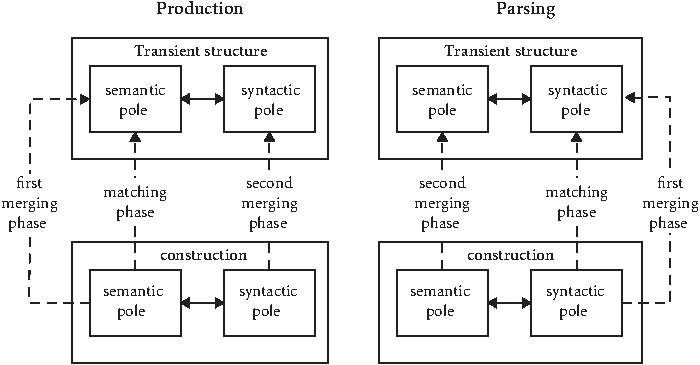
\includegraphics[width=.98\textwidth]{Figures/production-parsing-fcg.pdf}
\caption{\label{fig-matching-merging-trijp}FCG中的生成和句法分析\citep[\page 99]{vanTrijp2013a}}
%\caption{\label{fig-matching-merging-trijp}Generation and parsing in FCG \citep[\page 99]{vanTrijp2013a}}
\end{figure}%

\subsubsection{论元结构构式}
%\subsubsection{Argument Structure Constructions}

动变构式语法为论元结构假设了一个基于短语的处理方法,也就是说,假设词项进入一个能够提供独立意义的短语构造。\citep{vanTrijp2011a}。FCG方法是使用Goldberg插入方法分析论元结构构式的一个版本\citep{Goldberg95a}。Van Trijp认为每一个词项都能表征潜在的论元角色,如施事、受事、接受者和目标。短语论元结构构式与各自的词项结合并且实现部分论元角色,也就是说他们给这些论元角色一些语法功能。下一页中的图~\vref{fig-as-trijp}就展示了这样一个例子:动词sent(寄送)就有施事、受事、接受者和目标四个语义角色。基于被选择的论元结构构式,一些论元角色被选择实现。\footnote{%
这里值得注意的是,\citet[\page 141]{vanTrijp2011a}实际上提供了一个基于词汇的解释,因为每一个词项都通过同用(coapplication)连接来与不同短语构式连接。所以,每一个这样的词项和短语构式对都对应着词汇化树邻接语法(LTAG)中的一个词项。也参见\citew[\page 25]{MWArgSt}对于Goldberg的假设的评论,假设是每一个词项都有短语构式关联。
注意这种同用关系是必要的,因为没有它们的话,这一方法就无法解释这样的例子,即两个或多个论元角色只能一起实现但是不能单独实现或者与另外列举出的角色组合。
}
%Fluid Construction Grammar assumes a phrasal approach to argument structure, that is, it is assumed that lexical items enter
%into phrasal configurations that contribute independent meaning \citep{vanTrijp2011a}. The FCG
%approach is one version of implementing Goldberg's plugging approach to argument structure
%constructions \citep{Goldberg95a}. Van Trijp suggests that every lexical item comes with a representation of
%potential argument roles like Agent, Patient, Recipient, and Goal. Phrasal argument structure
%constructions are combined with the respective lexical items and realize a subset of the argument
%roles, that is they assign them to grammatical functions. Figure~\vref{fig-as-trijp} shows an
%example: the verb \emph{sent} has the semantic roles Agent, Patient, Recipient, and Goal  (upper left
%of the figure). Depending
%on the argument structure construction that is chosen, a subset of these roles is selected for
%realization.\footnote{%
%  It is interesting to note here that \citet[\page 141]{vanTrijp2011a} actually suggests a lexical
%  account since every lexical item is connected to various phrasal constructions via coapplication
%  links. So every such pair of a lexical item and a phrasal construction corresponds to a lexical
%  item in Lexicalized Tree Adjoining Grammar (LTAG). See also \citew[\page 25]{MWArgSt} on
%  Goldberg's assumption that every lexical item is associated with phrasal constructions.

%Note that such coapplication links are needed since without them the approach cannot account for
%cases in which two or more argument roles can only be realized together but not in isolation or in
%any other combination with other listed roles.
%}
%\todostefan{Are there Agent Goal verbs or Patient Recipient or Patient Goal verbs that allow for
%  patterns that are impossible for sent?}
这一表格展示了寄送者、寄送物、接受者之间的关系以及更加抽象的语义角色之间的关系,还有这些角色与 (\mex{1})中语法功能的关系:
%The figures show the relation between sender, sent, and sendee and more the more abstract semantic
%roles and the relation between these roles and grammatical functions for the sentences in (\mex{1}):
\eal
\ex 
\gll He sent her the letter.\\
     他 寄送 她 \textsc{det} 信\\
\glt `他寄给她信。'
%He sent her the letter.
\ex 
\gll He sent the letter.\\
     他 寄送 \textsc{det} 信\\
\glt `他寄信。'
%He sent the letter.
\ex 
\gll The letter was sent to her.\\
     一 信 \textsc{aux} 寄送 \textsc{prep} 她\\
\glt `这封信被寄送给她了。'
%The letter was sent to her.
\zl
虽然在 (\mex{0}a) 中,施事、受事和接受者都映射到语法功能上,但是在(\mex{0}b)中只有施事和受事映射到语法功能上。接受者被省略了。 (\mex{0}c)展示了一种论元实现,其中接受者实现为“to”短语。按照van Trijp,这一语义角色不是一个接受者而是一个目标。
%While in (\mex{0}a) the agent, the patient and the recipient are mapped to grammatical functions,
%only the agent and the patient are mapped to grammatical functions in (\mex{0}b). The recipient is
%left out. (\mex{0}c) shows an argument realization in which the sendee is realized as a \emph{to}
%  phrase. According to van Trijp this semantic role is not a recipient but a goal. 

\begin{figure}
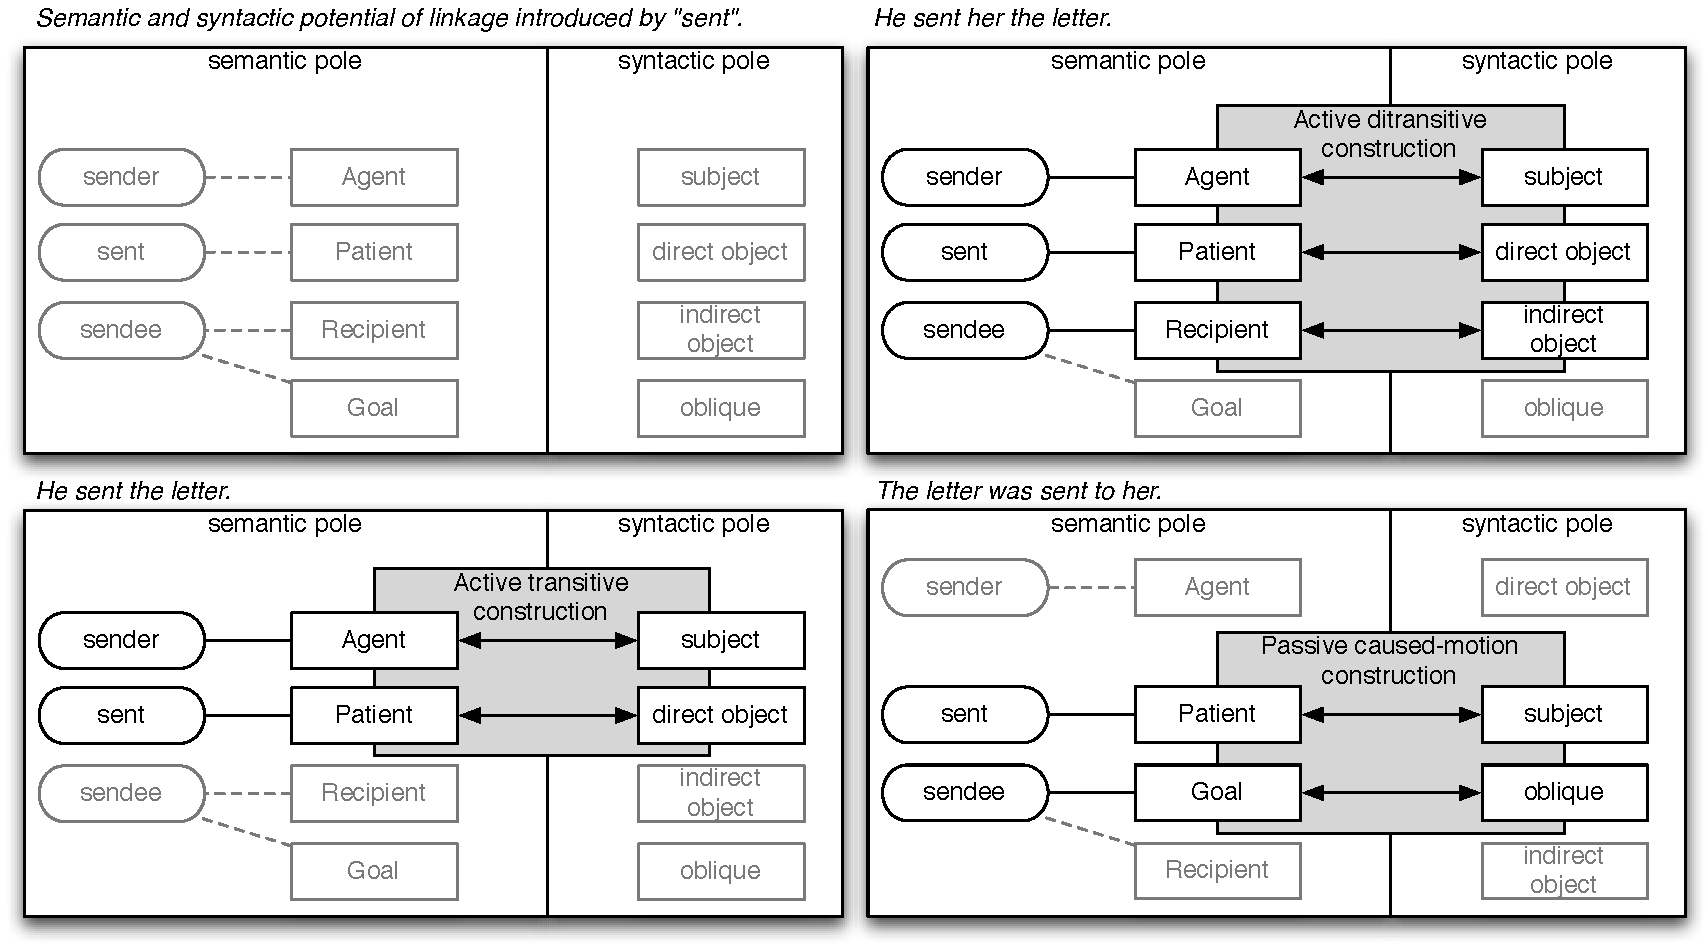
\includegraphics[width=\textwidth]{Figures/2011-van-Trijp.pdf}
\caption{\label{fig-as-trijp}词项和短语构式。图摘自\citew[\page 122]{vanTrijp2011a}}
%\caption{\label{fig-as-trijp}Lexical items and phrasal constructions. Figure %taken 
%from \citew[\page 122]{vanTrijp2011a}}
\end{figure}%

注意如果采用这一方法,就需要每一个主动构式都有一个被动变体。对于那些允许被动构式和无人称构式组合的语言来说,必须假设一个及物-被动-无人称构式。正如\citew[\S~2.6]{Mueller2006d}所说,德语中的自由与格(commodi/incommodi)可以加到几乎所有构式上去。它们与与格被动构式互动,所以应该被当做论元。所以,对于动结构式,我们需要一个主动变体,一个被动变体,一个有与格论元的变体,一个有与格论元和与格被动的变体,一个中动变体。虽然,在技术上我们可以列举出所有这些模式,也可以想象我们可以把所有这些信息储存在我们脑子里,问题是这些列举是否真的反映了我们的语言学知识。如果一个新的构式产生了,我们就谈谈德语中带有一个主格两个与格的主动句模式吧,那么该句子模式有被动形式吗?虽然在主动和被动构式之间建立联系的观点会预测该句子模式会有被动形式,但是实际上没有这种可能。
%Note that under such an approach, it is necessary to have a passive variant of every active
%construction. For languages that allow for the combination of passive and impersonal constructions,
%one would be forced to assume a transitive-passive-impersonal construction. As was argued in
%\citew[Section~2.6]{Mueller2006d} free datives (commodi/incommodi) in German can be added to almost
%any construction. They interact with the dative passive and hence should be treated as
%arguments. So, for the resultative construction one would need an active variant, a passive variant,
%a variant with dative argument, a variant with dative argument and dative passive, and a middle variant.
%While it is technically possible to list all these patterns and it is imaginable that we store all
%this information in our brains, the question is whether such listings really reflect our linguistic
%knowledge. If a new construction comes into existence, lets say an active sentence pattern with a
%nominative and two datives in German, wouldn't we expect that this pattern can be used in the
%passive? While proposals that establish relations between active and passive constructions would
%predict this, alternative proposals that just list the attested possibilities do not.

怎样获得这种概括应该与HPSG中词库的组织联系起来讨论\citep{Flickinger87,Meurers2001a}。在词库中,可以按照词的价对所有动词进行分类并且说loves是一个及物动词,而被动变体loved是一个不及物动词。很明显这种方式忽略了loved和given有相同之处:它们都与其主动形式以一种系统的方式发生联系。与垂直概括相比,这种概括叫做水平概括,垂直概括描述承继层级中的上位类型和下位类型之间的关系。
%The issue of how such generalizations should be captured was discussed in connection with the
%organization of the lexicon in HPSG \citep{Flickinger87,Meurers2001a}. In the lexical world, one could simply categorize all verbs according to their
%valence and say that \emph{loves} is a transitive verb and the passive variant \emph{loved} is an
%intransitive verb. Similarly \emph{gives} would be categorized as a ditransitive verb and
%\emph{given} as a strictly transitive one. Obviously this misses the point that \emph{loved} and \emph{given}
%share something: they both are related to their active form in a systematic way. This kind of
%generalization is captured by lexical rules that relate two lexical items. The respective
%generalizations that are captured by lexical rules are called a horizontal generalizations as compared to vertical generalizations, which
%describe relations between subtypes and supertypes in an inheritance hierarchy.

这种概括是独立于词汇知识组织的,它也可以应用于短语表征。短语构式可以在层级(垂直)中组织,但是一些变体之间的关系不能用这种方式概括。与基于词汇方法中词汇规则相对应的是基于短语方法中类似于GPSG的元规则。所以,FCG中好像丢失的是连接短语模式的动词,例如同-构式(allo-constructions)(\citealp{Cappelle2006a};\citealp[\page  116]{Goldberg2014a},也可以参见脚注~\ref{fn-allostructions})。
%The issue is independent of the lexical organization of knowledge, it can be applied to phrasal
%representations as well. Phrasal constructions can be organized in hierarchies (vertical), but the
%relation between certain variants is not covered by this. The analog to the lexical rules in a
%lexical approach are GPSG-like metarules in a phrasal approach. So what seems to be missing in FCG
%is something that relates phrasal patterns, \eg allo"=constructions (\citealp{Cappelle2006a}; \citealp[\page
%  116]{Goldberg2014a}, see also footnote~\ref{fn-allostructions}).

\subsubsection{溶合、匹配和合并}
% \subsubsection{Fusion, matching and merging}

正如\citet[\page 89--90]{Dowty89b-u}所指出的那样,在判断一个动词是否可以进入(或与之溶合)一个特定构式中时,仅仅核查语义兼容性是不够的。我们可以举出dine、eat和devour之间存在对立的例子。虽然吃的东西不一定与dine共现,但是可以与eat共现,并且一定要与devour共现。所以,词项一定要包含这些信息。
%As was pointed out by \citet[\page 89--90]{Dowty89b-u}, checking for semantic compatibility is not sufficient
%when deciding whether a verb may enter (or be fused with) a certain construction. The example is
%the contrast between \emph{dine}, \emph{eat}, and \emph{devour}. While the thing that is eaten may
%not be realized with \emph{dine}, its realization is optional with \emph{eat} and obligatory with
%\emph{devour}. So the lexical items have to come with some information about
%this. 

\Citet{vanTrijp2011a}和\citet{SvT2011a} 提出一个非常有趣的观点可以提供帮助:每一个动词都有一个潜在语义角色的列表,论元构式选择这些论元角色的字集(见图~\ref{fig-as-trijp})。这叫做匹配:不允许引入新的论元角色。这可以用来解释dine:我们可以说吃了某物,但是不存在题元角色可以与语法功能相连接。为了解释\isc{构式!致使-移动}\is{construction!Caused"=Motion}构式中出现的论元角色的扩展 \citep[\S~7]{Goldberg95a},\citet{SvT2011a} 提出了一个叫“合并”的过程。合并被看做是一个修正策略:如果一个话段涉及一个不及物动词和一些别的材料,这一话段只用匹配原则就不能处理。例如,当处理(\mex{1})中Goldberg举出的例子的时候,he sneezed可以分析,但是foam和off the cappuccino则无法结合。(见第~\ref{chap-phrasal}章对这一构式的进一步讨论)。
%\Citet{vanTrijp2011a} and \citet{SvT2011a} make an interesting suggestion that could help
%here: every verb comes with a list of potential roles and argument structure constructions can pick
%subsets of these roles (see Figure~\ref{fig-as-trijp}). This is called \emph{matching}: introducing new argument roles is not allowed. 
%This would make it possible to account for \emph{dine}: one could
%say that there is something that is eaten, but that no Theme role is made available for linking to
%the grammatical functions. This would be a misuse of thematic roles for syntactic purposes though
%since \emph{dine} is semantically a two-place predicate. To account for the extension of argument roles as it is observed in the
%Caused"=Motion Construction\is{construction!Caused"=Motion} \citep[Chapter~7]{Goldberg95a}, \citet{SvT2011a} suggest a process called \emph{merging}. Merging is seen
%as a repair strategy: if an utterance involves an intransitive verb and some other material, the
%utterance cannot be processed with matching alone. For example, when processing Goldberg's example
%in (\mex{1}), \emph{he sneezed} could be parsed, but \emph{the foam} and \emph{off the cappuccino}
%would be unintegrated (see Chapter~\ref{chap-phrasal} for an extended discussion of such constructions).
\ea
\gll He sneezed the foam off the cappuccino.\\
     他 打喷嚏 \textsc{det} 泡沫 \textsc{prep} \textsc{det}  卡布奇诺咖啡\\
\glt `他打喷嚏把泡沫从卡布奇诺咖啡上吹走了。'
%He sneezed the foam off the cappuccino.
\footnote{%
\citew[\page 42]{Goldberg2006a}.
}
\z
所以,\citet[\page 319--320]{SvT2011a}表明只有当常规构式不能应用的时候,才允许合并。这一方法的问题在于人类语言是高度歧义的并且在这种情况下这会导致一种状况,在这种状况中一个话段有一个意思,所以这一修复策略不会有效。考虑(\mex{1}):\footnote{%
  我为这些例子感到抱歉。 \ldots
}
%So, \citet[\page 319--320]{SvT2011a} suggest that only if regular constructions cannot apply, merging is
%allowed. The problem with this is that human language is highly ambiguous and in the case
%at hand this could result in situations in which there is a reading for an utterance, so that the
%repair strategy would never kick in. Consider (\mex{1}):\footnote{%
%  I apologize for these examples \ldots
%}
\ea
\label{ex-schlag-den-mann-tot}
\gll Schlag den Mann tot!\\
     击打   \textsc{det} 男人  死\\
\glt `把这个男人打死!' 或者 `打这个死人!'
%\gll Schlag den Mann tot!\\
%     beat   the man  dead\\
%\glt `Beat the man to death!' or `Beat the dead man!'
\z
(\mex{0}) 有两个意义:结果义,其中tot(死)表示打的结果;在另外一个意义中,tot是一个描述性谓词。第二种解释是不常见的,因为打已经死去的人这一活动是不常见的,但是这一结构与带有描述性谓词的句子是平行的。
%(\mex{0}) has two readings: the resultative reading in which \emph{tot} `dead' expresses the result of the
%beating and another reading in which \emph{tot} is a depictive predicate. The second reading is
%dispreferred, since the activity of beating dead people is uncommon, but the structure is parallel to
%other sentences with depictive predicates:
\ea
\gll Iss den Fisch roh!\\
     吃 \textsc{det} 鱼 生的\\
%\gll Iss den Fisch roh!\\
%     eat the fish raw\\
\z
可以让tot与一个不能理解为结果谓词的谓词并列来强制将tot理解为描述义:
%The depictive reading can be forced by coordinating \emph{tot} with a predicate that is not a
%plausible result predicate:
\ea
\gll Schlag ihn tot oder lebendig!\\
     击打   他 死 或者 活着\\
\glt `在他死之后或者还活着的时候打他!'
%\gll Schlag ihn tot oder lebendig!\\
%     beat   him dead or alive\\
%\glt `Beat him when he is dead or while he is alive!'
\z
所以,问题是(\ref{ex-schlag-den-mann-tot}) 含有一个意义不需要激活修复机制:schlug(击打)应用于一个及物构式而tot是一个附接语(参看\citealp{Winkler97a})。但是, (\ref{ex-schlag-den-mann-tot}) 更加可能的一个分析是结果分析,在这种分析中价框架通过一个旁格元素得到扩展。所以,这意味着我们必须允许合并操作独立于其他可能的操作。正如\citet[\page 320]{SvT2011a}指出的那样,如果合并不能自由使用,像(\mex{1}a)这种话段就不被允许,当然(\mex{1}b) 也是这样。
%So, the problem is that (\ref{ex-schlag-den-mann-tot}) has a reading which does not require the invocation of the repair mechanism: \emph{schlug} `beat' is used with the transitive
%construction and \emph{tot} is an adjunct (see \citealp{Winkler97a}). However, the more likely analysis of (\ref{ex-schlag-den-mann-tot}) is the one
%with the resultative analysis, in which the valence frame is extended by an oblique element. So this
%means that one has to allow the application of merging independent of other analyses that might be possible.
%As \citet[\page 320]{SvT2011a} note, if merging is allowed to apply freely, utterances like
%(\mex{1}a) will be allowed and of course (\mex{1}b) as well.
\eal
\ex[*]{
\gll She sneezed her boyfriend.\\  
    她 打喷嚏 她的 男朋友\\
%She sneezed her boyfriend.
}
\ex[*]{
\gll She dined a steak.\\  
    她 吃饭 一 牛排\\
%She dined a steak.
}
\zl
在(\mex{0}) 中,sneeze和dine都用于及物构式当中。
%In (\mex{0}) \emph{sneeze} and \emph{dined} are used in the transitive construction.

摆脱这一困境的方法是在词项中建立描述动词使用句法环境的信息。这种信息可以进行加权,例如dine用作及物动词的概率很低。Steels和van Trijp可能会通过所谓共用连接(coapplication)来联系词项与短语构式,并且dine和及物构式之间的连接强度会很低,sneeze和致使移动\isc{构式!致使-移动}\is{construction!Caused"=Motion}构式之间的连接强度会很高。这会解释这一现象(并且采用基于使用的方式),但是在CG、HPSG、SBCG和DG中将会使用一种词汇方法。
%The way out of this dilemma is to establish information in lexical items that specifies in which
%syntactic environments a verb can be used. This information can be weighted and for instance the
%probability of \emph{dine} to be used transitively would be extremely low. Steels and van Trijp
%would connect their lexical items to phrasal constructions via so-called coapplication links and the
%strength of the respective link would be very low for \emph{dine} and the transitive construction and
%reasonably high for \emph{sneeze} and the Caused"=Motion Construction\is{construction!Caused"=Motion}. This would explain the
%phenomena (and in a usage"=based way), but it would be a lexical approach, as it is common in CG, HPSG,
%SBCG, and DG.

\subsubsection{长距离依存}
%\subsubsection{Long-distance dependencies}
\label{sec-fcg-nld}

\Citet{vanTrijp2014a} 对比了GPSG、HPSG、SBCG中运用的基于\slaschc 的方法和他在FCG框架中使用的方法。他认为SBCG与FCG有根本上的差别,并且将SBCG归入生成语法的范畴,将FCG归入认知功能语法的范畴。他表明他的认知功能方法在完整性质、解释充分性和理论简约性上更有优势(第2页)。\citet{vanTrijp2014a}说明的基本上是\citet{Reape2000a}在一个未发表的的文章中的一个分析。(见\citew{Reape94a}一个发表的版本对基于线性化方法的论述以及\citew{Kathol2000a,Babel,Mueller99a,Mueller2002b}基于线性化的方法,这一方法虽然是基于线性化的,但是仍然为非局部依存假设了\slaschc 方法)。Van Trijp发展了一个语法模型,允许不连续成分并且只是将(\mex{1})所示句子中宾语的序列化看作另外的线性化选择。
%\Citet{vanTrijp2014a} compares the \slasch-based approaches that are used in GPSG, HPSG, and SBCG
%with the approach that he suggests within the framework of FCG. He claims that there are fundamental
%differences between SBCG and FCG and assigns SBCG to the class of generative grammars, while
%placing FCG in the class of cognitive"=functional approaches. He claims that his
%cognitive"=functional approach is superior in terms of completeness, explanatory adequacy, and
%theoretical parsimony (p.\,2). What \citet{vanTrijp2014a} suggests is basically an analysis that was
%suggested by \citet{Reape2000a} in unpublished work (see \citew{Reape94a} for a published version of
%an linearization"=based approach and \citew{Kathol2000a,Babel,Mueller99a,Mueller2002b} for
%linearization"=based approaches that despite of being linearization"=based assume the \slasch approach for nonlocal dependencies). Van Trijp
%develops a model of grammar that allows for discontinuous constituents and just treats the
%serialization of the object in sentences like (\mex{1}) as an alternative linearization option.
\eal
\ex 
\gll This book, I read.\\  
    \textsc{det} 书 我 读\\
\glt `这本书,我读。'
%This book, I read.
\ex 
\gll What did the boy hit?\\  
    什么 \textsc{aux} 一 男孩 击打\\
\glt `这个男孩击打了什么?'
%What did the boy hit?
\zl
Van Trijp的分析涉及到几种一般不会出现在短语结构语法中的单位,但是可以通过邻接限制来刻画或者表征要素之间的关系,这些关系在HPSG/SBCG中是词汇表征的一部分。一个例子是主语-动词锚位,这一锚位连接了主语和动词来表征这两个元素扮演重要的语法角色。图~\vref{fig-what-did-the-boy-hit}展示了对 (\mex{1})的分析。
%Van Trijp's analysis involves several units that do not normally exist in phrase structure grammars,
%but can be modeled via adjacency constraints or represent relations between items which are part
%of lexical representations in HPSG/SBCG anyway. An example is the subject-verb anchor that connects
%the subject and the verb to represent the fact that these two items play an important functional
%role. Figure~\vref{fig-what-did-the-boy-hit} shows the analysis of (\mex{1}).
\ea
\gll What did the boy hit?\\  
    什么 \textsc{aux} 一 男孩 击打\\
\glt `这个男孩在击打什么?'
%What did the boy hit?
\z
\begin{figure}
\begin{forest}
for tree={l sep+=5mm}
%l sep+=10mm
[TRANSITVE-CLAUSE-UNIT, name=tcu
  [NP-UNIT-1, name=np1
    [PRO [what]] ]
  [\textsc{aux},tier=det, no edge, name=aux [did] ]
  [NP-UNIT-2, name=np2
    [\textsc{det}, tier=det [the]]
    [N   [boy]] ]
  [VP-UNIT, name=vp
    [V [hit] ] ]
]
\draw (vp.south)--(aux.north);
\node (topic) [base left=of tcu]
    {
        TOPIC-UNIT
    };
\draw[dashed] (topic.south)--(np1.north);
\node (focus) [below=0mm of tcu.south west]
    {
        FOCUS-UNIT
    };
\draw[dashed] (focus.south)--(np1.north);
\draw[dashed] (focus.south)--(aux.north);
\node (sau) [base right= of tcu]
    {
        SV-ANCHOR-UNIT
    };
\draw[dashed] (sau.south)--(vp.north);
\draw[dashed] (sau.south)--(np2.north);
\end{forest}
\caption{\label{fig-what-did-the-boy-hit}根据\citet[\page 265]{vanTrijp2014a}的对“What did the boy hit?”的分析}
%\caption{\label{fig-what-did-the-boy-hit}The analysis of \emph{What did the boy hit?} according to
%  \citet[\page 265]{vanTrijp2014a}}
\end{figure}%
正如上表所示,van Trijp也借助了信息结构的术语,例如话题和焦点。这里需要注意的一点是,对于信息结构l\isc{信息结构} l\is{information structure}的分析在HPSG框架中有很长的历史\citep{EV96a, Kuhn95b,Kuhn96a,
GuntherMaienborn1999,Wilcock2001a,deKuthy2002a,Paggio2005a-u,Bildhauer2008a,BC2010a}。在 \citew{Sag2012a}等人探讨句法的论文中没有涉及信息结构并不意味着HPSG/SBCG理论忽略了信息结构或者认为信息结构应该被忽略。对于完整性来说这很重要。这一点对于解释充分性当然也是一样。这给予了理论简约性,但是在我们评论之前,我想先具体讨论一下van Trijp的分析以便于能显示他的很多观点在实践上都是有问题的,并且因此他的理论不具有解释力,因为实践上的正确性是解释充分性的前提。
%As can be seen in the figure, van Trijp also refers to information structural\is{information structure} terms
%like topic and focus. It should be noted here that the analysis of information structure has quite
%some history in the framework of HPSG  \citep{EV96a, 
%Kuhn95b,Kuhn96a, 
%GuntherMaienborn1999,
%Wilcock2001a, 
%deKuthy2002a,Paggio2005a-u, 
%\citet{Webelhuth2007a-u}, 
%Bildhauer2008a,BC2010a}. The fact that information structure is not talked about in syntax
%papers like \citew{Sag2012a} does not entail that information structure is ignored or should be
%ignored in theories like HPSG and SBCG. So much for completeness. The same holds of course for
%explanatory adequacy. This leaves us with theoretical parsimony, but before I comment on this, I
%want to discuss van Trijp's analysis in a little bit more detail in order to show that many of his claims
%are empirically problematic and that his theory therefore cannot be explanatory since empirical
%correctness is a precondition for explanatory adequacy.
Van Trijp表示英语中包含非局部依存构式的句子以话题开头。\footnote{%
\Citet[\page 256]{vanTrijp2014a}采用的话题和焦点的定义如下:“话题性(topicality)是从相关性的角度进行定义的:一个话段的话题就是这个话段相关的部分”。焦点性(focality)是从重要性的角度进行定义的并且是为凸显在当前交际语境中最重要的信息。
}Bresnan举出的例句(\ref{bsp-fronted-focus})、(\ref{bsp-fronted-topic}) 在第~\pageref{bsp-fronted-focus}页\citep[\page 97]{Bresnan2001a}已经讨论过了,为了方便这里重复如下:
%Van Trijp claims that sentences with nonlocal dependency constructions in English start with a
%topic.\footnote{%
%\Citet[\page 256]{vanTrijp2014a} uses the following definitions for topic and focus: ``Topicality is defined in terms of aboutness: the topic of an utterance
%is what the utterance is `about'. Focality is defined in terms of salience:
%focus is used for highlighting the most important information given the
%current communicative setting.''
%} Bresnan's sentences in (\ref{bsp-fronted-focus}) and (\ref{bsp-fronted-topic}) were discussed on page~\pageref{bsp-fronted-focus}
%\citep[\page 97]{Bresnan2001a} and are repeated below for convenience:
\ea
\label{bsp-fronted-focus-two}
\gll Q: What did you name your cat?\\  
     Q: 什么 \textsc{aux} 你 命名 你的 猫\\
\glt `你给你的猫取什么名?'

\gll A: Rosie I named her. \\
     A: Rosie 我 命名 她\\\jambox{(\emph{Rosie} = \textsc{focus})}
\glt `我叫她Rosie。'
%Q: What did you name your cat?\\
%A: Rosie I named her. (\emph{Rosie} = \textsc{focus})
\z
\ea
\label{bsp-fronted-topic-two}
\gll Q: What did you name your pets?\\    
     Q: 什么 \textsc{aux} 你 命名 你的 宠物\\
\glt `你叫你的宠物什么名字?' 

\gll A: My dog, I named Harold. My cat, I named Rosie.\\
     A: 我的 狗 我 命名 Harold 我的 猫 我 命名 Rosie\\\jambox{(\emph{my dog}, \emph{my cat} = \textsc{topic})}
\glt `我的狗,我叫他Harold。我的猫,我叫她Rosie。'
%Q: What did you name your pets?\\
%A: My dog, I named Harold. My cat, I named Rosie. (\emph{my dog}, \emph{my cat} = \textsc{topic})
\z
这些句子表明主语之前的位置既可能是话题也可能是焦点。所以,前置的成分就是话题这一说法在实践上是不对的。如果这一位置与信息结构功能联系起来的话,这一联系应该是一个析取式,允许话题成分和焦点成分。
%These sentences show that the pre-subject position is not unambiguously a topic or a focus
%position. So, a statement saying that the fronted element is a topic is empirically not correct. If this position is to be associated with an information structural function, this
%association has to be a disjunction admitting both topics and focused constituents.

Van Trijp分析的另外一个问题是,他假设助动词do是一个宾语标记(第10、22页) 或者是一个非主语标记(第23页)。(\mex{1}a)中的主语问句确实不需要do支撑,只有 (\mex{1}b)中的问句需要,但是这并不意味着do之后的所有元素都是宾语。
%A further problematic aspect of van Trijp's analysis is that he assumes that the auxiliary \emph{do}
%is an object marker (p.\,10, 22) or a non-subject marker (p.\,23). It is true that \emph{do} support is not necessary in subject questions like
%(\mex{1}a), but only in (\mex{1}b), but this does not imply that all items that are followed by
%\emph{do} are objects.
\eal
\ex 
\gll Who saw the man?\\  
     谁 看见 \textsc{det} 男人\\
\glt `谁看见了这个男人?'
%Who saw the man?
\ex 
\gll Who did John see?\\  
     谁 \textsc{aux} John 看见\\
\glt `John看见了谁?'
%Who did John see?
\zl
首先,do可以用于强调动词:
%First, \emph{do} can be used to emphasize the verb:
\ea
\gll Who \emph{did} see the man?\\  
     谁 \textsc{aux} 看见 \textsc{det} 男人\\
\glt `谁看见了这个男人?'
%Who \emph{did} see the man?
\z
其次,所有类型的其他语法词都可以出现在动词之前:
%Second, all types of other grammatical functions can precede the verb:
\eal
\settowidth\jamwidth{(prepositional object)}
\ex
\gll Where did you see the man?\\    
     哪里 \textsc{aux} 你 看见 \textsc{det} 男人\\\jambox{(adverbial)}
\glt `你在哪里看见了这个男人?'
%Where did you see the man? \jambox{(adverbial)}
\ex 
\gll How tall is the man?\\     
     怎样 高 \textsc{cop} A\textsc{det} 男人\\\jambox{(predicative)}
\glt `这个男人有多高?'
%How tall is the man? \jambox{(predicative)}
\ex
\gll What did John consider Peter?\\     
     什么 \textsc{aux} John 认为 Peter\\ \jambox{(predicative)}
\glt `John认为Peter是什么?'
%What did John consider Peter? \jambox{(predicative)}
\ex 
\gll What does this book cost?\\
     什么 \textsc{aux} 这 书 花费\\       \jambox{(adverbial)}
\glt `这本书花费了多少钱?'
%What does this book cost? \jambox{(adverbial)}
\ex 
\gll About what did you talk?\\       
     \textsc{prep} 什么 \textsc{aux} 你 说\\ \jambox{(prepositional object)}
\glt `你谈论了什么?'
%About what did you talk? \jambox{(prepositional object)}
\zl
最后,即便是主语也可以出现在do之前,只要这个主语是从其他小句提取出来的。
%And finally, even a subject can appear in front of \emph{do} if it is extracted from another clause:
\ea
\settowidth\jamwidth{(prepositional object)}
\gll Who does he think saw this man?\\   
     谁 \textsc{aux} 他 认为 看见 这 男人\\\jambox{(subject)}
\glt `他认为谁看见了这个男人?'
%Who does he think saw this man? \jambox{(subject)}
\z
%
% Auch die linke Peripherie kann man ja einfach als kontinuierlich einordnen. Brauche Beleg für
% Extraposition aus pränominalem Adjunkt. Das würde mögliche Diskontinuität zeigen.
%
%% Van Trijp does not address the issue of island constraints. Extraction islands are areas that nobody
%% can leave, that is, extraction is excluded. For instance, it is impossible to extract from the
%% prenominal area in English and German (Ross' Left Branch Condition).
%\ea
%der die Frau liebende Mann, die ... erfunden hat
%%  and it is also impossible to
%% extract out of a relative clause:
%% % Er könnte sagen, dass Relativsätze immer kontinuierlich sein müssen.
%% \ea
%% This man$_i$, I saw a women [who likes \_$_i$ ].
%% \z
%% \slasch"=based models assume that relative clauses involve internal nonlocal dependencies, but no
%% \slasch dependency leaves the relative clause. This is ensured by the schemata that combine the
%% relative pronoun and the remaining clause.

还有另外一个实践性问题:假设填充语与其来源存在联系的方法可以解决辖域歧义问题,这种辖域歧义只有当某一元素提取才会产生。例如,对比 (\mex{1}a) 中的句子与 (\mex{1}b, c)中的句子:虽然在 (\mex{1}a) 、(\mex{1}c)中oft(经常)与nicht(不)的顺序是一样的,(\mex{1}a) 存在歧义但是 (\mex{1}c) 不存在。
%There is a further empirical problem: approaches that assume that a filler is related to its origin
%can explain s\textsc{cop}e ambiguities that only arise when an element is extracted. Compare for instance the
%sentence in (\mex{1}a) with the sentences in (\mex{1}b, c): although the order of \emph{oft} `often' and
%\emph{nicht} `not' in (\mex{1}a) and (\mex{1}c) is the same, (\mex{1}a) is ambiguous but (\mex{1}c) is
%not.
\eal
\ex 
\gll Oft liest er das Buch nicht.\\
     经常 读 他 \textsc{det} 书 不\\
\glt `大多数情况下他不读这本书。' 或者 `他并非经常读这本书。'
%\gll Oft liest er das Buch nicht.\\
%     often reads he the book not\\
%\glt `It is often that he does not read the book.' or `It is not the case that he reads the book
%often.'
\ex
\gll dass er das Buch nicht oft liest\\
     \textsc{conj} 他 \textsc{det} 书 不 经常 读\\
\glt `他并非经常读这本书这件事'
%\gll dass er das Buch nicht oft liest\\
%     that he the book not often reads\\
%\glt `that it is not the case that he reads the book often'
\ex
\gll dass er das Buch oft nicht liest\\
     \textsc{conj} 他 \textsc{det} 书 经常 不 读\\
\glt `大多数情况下他并不读这本书这件事'
%\gll dass er das Buch oft nicht liest\\
%     that he the book often not reads\\
%\glt `that it is often that he does not read the book'
\zl
(\mex{0}a)有两个意义分别对应于(\mex{0}b) 和 (\mex{0}c)。一个纯粹基于线性化的方法难以解释这一问题。一个基于\slaschc 的方法可以假设 (\mex{0}a) 在oft位置(在 (\mex{0}b) 或者 (\mex{0}c))有一个缺位(或者一些类似的引入非局部依存的方法)。在意义组合过程中,缺位的信息应该将缺位的位置考虑在内。这就自动解释了观察到的意义。
%(\mex{0}a) has the two readings that correspond to (\mex{0}b) and (\mex{0}c). A purely
%linearization"=based approach probably has difficulties to explain this. A \slasch"=based approach
%can assume that (\mex{0}a) has a gap (or some similar means for the introduction of nonlocal
%dependencies) at the position of \emph{oft} in (\mex{0}b) or (\mex{0}c). The gap information is
%taken into account in the semantic composition at the site of the gap. This automatically accounts
%for the observed readings.

另外一个不得不解释的现实问题是存在标记提取路径\isc{提取路径标记}\is{extraction path marking}的语言。\citet*{BMS2001a}列出了大量语言,在这些语言里元素会因其所依附的成分是否有缺位而不同。例如,爱尔兰语有一种标补语,当其所依附小句含有被提取元素时是一种形式,当其所依附小句不含被提取元素时是另外一种形式。基于\slaschc 的方案可以直接解释这种现象:一个短语中缺少一个成分是在语迹的\slaschc 取值中表征并且这种信息可以上滤到树上去。所以即使复杂结构也包含它们当中丢失了一个成分这一信息。与句子组合的标补语因此可以选择带有与其屈折对应\slaschc 取值的句子。Van Trijp对于这一挑战的回答是所有的语言都是不同的\citep[\page 263]{vanTrijp2014a}并且源于一个语言的证据并不一定意味着对那一语言的分析也对另外一种语言适用。虽然我原则上同意这一观点(参看\ref{sec-syntactic-universals}),但是我认为提取是语言的一种根本属性并且对于具有非局部依存的语言来说,非局部依存应该用相同的方式分析。
%Another empirical problem that has to be solved is the existence of extraction path
%marking\is{extraction path marking}
%languages. \citet*{BMS2001a} list a number of languages in which elements vary depending on the
%existence or absence of a gap in a constituent they attach to. For instance, Irish has
%complementizers that have one form if the clause they attach to has an element extracted and another
%form if it does not. \slasch-based proposals can account for this in a straight-forward way: the
%fact that a constituent is missing in a phrase is represented in the \slashv of the trace and this
%information is percolated up the tree. So even complex structures contain the information that there
%is a constituent missing inside them. Complementizers that are combined with sentences therefore can
%select sentences with \slashvs that correspond to their inflection.
%Van Trijp's answer to this challenge is that all languages are different
%\citep[\page 263]{vanTrijp2014a} and that the evidence from one language does not necessarily mean that the analysis for that language is
%also appropriate for another language. While I agree with this view in principle (see
%Section~\ref{sec-syntactic-universals}), I do think that extraction is a rather fundamental property
%of languages and that nonlocal dependencies should be analyzed in parallel for those languages that
%have it.

\subsection{并列}
%\subsection{Coordination}
\label{sec-coordination}

非转换语法的一个成功案例是 \citet{Gazdar81}对于非局部依存的基于\slaschc 的分析。这一分析第一次解释了Ross提出的跨界抽取\isc{跨界抽取}\is{Across the Board Extraction}\citep{Ross67}。这些例子在第~\pageref{ex-atb-gazdar}页已经讨论过了,为了方便这里重复如下:
%One of the success stories of non-transformational grammar is the \slasch-based analysis of nonlocal dependencies
%by \citet{Gazdar81}. This analysis made it possible for the first time to explain Ross's Across the Board
%Extraction\is{Across the Board Extraction} \citep{Ross67}. The examples were already discussed on
%page~\pageref{ex-atb-gazdar} and are repeated here for convenience:
\eal\settowidth\jamwidth{(= S/NP \& S/NP)}
\label{ex-atb-gazdar-two}
\ex[]{ %The kennel     which Mary made and Fido sleeps in has been stolen.	 \jambox{(= S/NP \& S/NP)}
\gll The kennel     which Mary made and Fido sleeps in has been stolen.\\   
    \textsc{det}  狗窝 \textsc{rel} Mary 做 并且 Fido 睡 \textsc{prep} \textsc{aux} \textsc{aux} 偷\\\jambox{(= S/NP \& S/NP)}
\glt `Mary制作并且Fido在里面睡的那个狗窝被人偷走了。'
}
\ex[]{ %The kennel in which Mary keeps drugs and Fido sleeps has been stolen.	\jambox{(= S/PP \& S/PP)}
\gll The kennel in which Mary keeps drugs and Fido sleeps has been stolen.\\   
    \textsc{det}  狗窝 \textsc{prep} \textsc{rel} Mary 保持 药物 并且 Fido 睡 \textsc{aux} \textsc{aux} 偷\\\jambox{(= S/PP \& S/PP)}
\glt `Mary放药物并且Fido在里面睡的那个狗窝被人偷走了。'
}
\ex[*]{%The kennel (in) which Mary made and Fido sleeps has been stolen.     \jambox{(= S/NP \& S/PP)}
\gll The kennel (in) which Mary made and Fido sleeps has been stolen.\\     
    \textsc{det}  狗窝 \hspaceThis{(}\textsc{prep} \textsc{rel} Mary 做 并且 Fido 睡 \textsc{aux} \textsc{aux} 偷\\\jambox{(= S/NP \& S/PP)}
}
\zl
上面例子的共性是如果两个或多个成分有相同的句法范畴和相同的\slashvsc 取值的话,它们就可以并列。这就解释了(\mex{0}a、b)中的which和in which为什么可以在各自的小句中填充两个位置。那么,不采用\slashfc 来分析缺失成分信息弥散的理论就必须寻找另外的方式去确保所有的论元槽被填充并且被提取成分和相应的论元角色之间的关系是正确的。注意这一点在van Trijp提出的模型中并不直接,因为他必须允许介词in与它左边的一些成分组合,这些成分同时也是made的主语。通常一个NP不能简单地充当两个中心语的论元。见例(\mex{1}a):
%The generalization is that two (or more) constituents can be coordinated if they have identical
%syntactic categories and identical \slashvs. This explains why \emph{which} and \emph{in which} in
%(\mex{0}a,b) can fill two positions in the respective clauses. Now, theories that do not use a
%\slashf for the percolation of information about missing elements have to find different ways to
%make sure that all argument slots are filled and that the correct correspondence between extracted
%elements and the respective argument role is established. Note that this is not straightforward in
%models like the one suggested by van Trijp, since he has to allow the preposition \emph{in} to be
%combined with some material to the left of it that is simultaneously also the object of
%\emph{made}. Usually an NP cannot simply be used by two different heads as their argument. As an
%example consider (\mex{1}a):
\eal
\ex[*]{
\gll John said about the cheese that I like.\\
    John 说 \textsc{prep} \textsc{det} 奶酪 \textsc{conj} 我 喜欢\\
%John said about the cheese that I like.
}
\ex[]{
\gll John said about the cheese that I like it.\\
    John 说 \textsc{prep} \textsc{det} 奶酪 \textsc{conj} 我 喜欢 它\\
\glt `John谈论了我喜欢的那种奶酪。'
%John said about the cheese that I like it.
}
\zl
如果一个材料可以多次使用,那么 (\mex{0}a) 中的结构就是可能的,在这一结构中the cheese是介词about和动词like的宾语。但是,这个句子是完全不合法的:代词it必须要去填充宾语槽。
% (\mex{0}a) If it would be possible to use material several times, a structure for (\mex{0}a) would be possible
%in which \emph{the cheese} is the object of the preposition \emph{about} and of the verb
%\emph{like}. This sentence, however, is totally out: the pronoun \emph{it} has to be used to fill
%the object slot.

\subsection{不连续成分和语言使用模型}
%\subsection{Discontinuous constituents and performance models}

Van Trijp指出SBCG没有一个语言使用模型并且拿这一点与FCG进行对比。在第252页,他指出:

%Van Trijp points out that SBCG does not have a performance model and contrasts this with FCG. On
%page~252 he states:
\begin{quote}
所以,句法分析始于将话段分解为不同的形式,这些形式通过形态和词汇构式范畴化为单词,这些单词结合成短语(可以参见Steels, 2011b,看一下FCG中词库-短语处理的更细致的解释)。所以句法分析器会为所有四个话段寻找相似的成分,正如例(21-24)所示。因为在例(24)中助动词do不在VP的直接域之内,所以没有被识别为VP的一个成员。

所有这些短语都是没有联系的,这意味着语法仍然需要说明这些短语之间的关系。\citep[\page 252]{vanTrijp2014a}
%So parsing starts by segmenting the utterance
%into discrete forms, which are then categorized into words by morphological
%and lexical constructions, and which can then be grouped together as
%phrases (see Steels, 2011b, for a detailed account of lexico-phrasal
%processing in FCG). So the parser will find similar constituents for all
%four utterances, as shown in examples (21--24). Since auxiliary-\emph{do} in
%example (24) falls outside the immediate domain of the VP, it is not yet
%recognized as a member of the VP.

%All of these phrases are disconnected, which means that the grammar
%still has to identify the relations between the phrases. \citep[\page 252]{vanTrijp2014a}
\end{quote}
在 (21)--(24)中,van Trijp为主语和宾语提供了几个包含NP的树片段并且表明这些树片段必须组合在一起以便于分析他所讨论的句子。在实际处理中这是不够的:如果FCG没有区分语言能力/语言运用,那么话段分析的方式应该反映人类处理语言的方式(并且这也是FCG经常所标榜的)。但是,我们所知道的关于人类语言处理的一切都指向一个渐进式处理,也就是说,只要信息存在我们就处理它。我们开始处理第一个词语时考虑其所有相关方面(音系、重音、词类、语义和信息结构)并且提出关于话段应该如何处理的一种假设。只要我们处理了两个单词(实际上更早,在处理单词时整合已经发生)我们将第二个单词整合进我们已经知道的并且继续沿着我们的假设及逆行,或者修正它,或者失败。参看\ref{Abschnitt-Inkrementelle-Verarbeitung}获得处理的细节以及对于显示处理是渐进的实验的讨论。所以,我们说van Trijp的分析在实践层面上失败了:他对于语言使用层面的建模是不足的。
%In his (21)--(24), van Trijp provides several tree fragments that contain NPs for subject and object and states that
%these have to be combined in order to analyze the sentences he discusses. This is empirically
%inadequate: if FCG does not make the competence/performance distinction, then the way utterances are
%analyzed should reflect the way humans process language (and this is what is usually claimed about FCG). However, all we know about human language
%processing points towards an incremental processing, that is, we process information as soon as it
%is available. We start to process the first word taking into account all of the relevant aspects
%(phonology, stress, part of speech, semantics, information structure) and come up with an hypothesis
%about how the utterance could proceed. As soon as we have two
%words processed (in fact even earlier: integration already happens during the processing of words) we integrate the second word
%into what we know already and continue to follow our hypothesis, or revise it, or simply fail. See
%Section~\ref{Abschnitt-Inkrementelle-Verarbeitung} for details on processing and the discussion of
%experiments that show that processing is incremental. So, we have to say that van Trijp's analysis
%fails on empirical grounds: his modeling of performance aspects is not adequate.

Van Trijp所描述的分析方案与HPSG分析器十分相似,但是这些方案通常没有关于人类语言运用的任何说明。对语言运用进行建模十分复杂,因为很多因素都起作用。所以,合理的做法应该是像HPSG和FCG那样将语言运用和语言能力分开。这并不意味着语言运用方面不去建模,实际上运用HPSG的心理语言学模型过去曾经有人开发过\citep{Konieczny96a-u},但是发展出一个有很大覆盖性的语法以及与它组合的语言运用模型需要大量资源。
%The parsing scheme that van Trijp describes is pretty much similar to those of computational HPSG parsers, but
%these usually come without any claims about human performance. Modeling human performance is rather complex
%since a lot of factors play a role. It is therefore reasonable to separate competence and
%performance and continue to work the way it is done in HPSG and FCG. This does not mean that
%performance aspects should not be modeled, in fact psycholinguistic models using HPSG have been
%developed in the past \citep{Konieczny96a-u}, but developing both a grammar with large coverage and
%the performance model that combines with it demands a lot of resources.

\subsection{不连续性 vs.\ 主语-中心语和中心语-填充项程式}
%\subsection{Discontinuity vs.\ Subject-Head and Head-Filler Schema}

下面我们讨论一下简约性问题:van Trijp使用了一个将主语和主要动词组合在一起的主语-动词锚定构式。因为存在如例(\mex{1}) 的结构,所以必须允许不连续主语-动词构式存在 :\footnote{%
%I now turn to parsimony: van Trijp uses a subject-verb anchor construction that combines the subject
%and the main verb. Because of examples like (\mex{1}) it must be possible to have discontinuous subject-verb constructions:
除非情态和时助词也处理为主要动词(在英语中不应该这样处理),带有情态的构式应该是主语和主要动词不邻接的另外一种情况:
  \eal
  \ex 
\gll Peter will read the book.\\
    Peter \textsc{aux} 读 \textsc{det} 书\\
\glt `Peter将会读这本书。'
%Peter will read the book.
  \ex 
\gll Peter has read the book.\\
    Peter \textsc{aux} 读 \textsc{det} 书\\
\glt `Peter已经读过这本书了。'
%Peter has read the book.
  \zllast
} 
\ea
\gll Peter often reads books.\\
     Peter 经常 读 书\\
\glt `Peter经常读书。'
%Peter often reads books.
\z
如果这种构式可以不连续,那么一定要确定 (\mex{1}b) 不是主语-动词构式的一个实例。
%But if such constructions can be discontinuous one has to make sure that (\mex{1}b) cannot be an
%instantiation of the subject-verb construction:
\eal
\ex[]{
\gll The boy I think left.\\
     \textsc{det} 男孩 我 认为 离开\\
\glt `我认为那个男孩离开了。'
%The boy I think left.
}
\ex[*]{
\gll I the boy think left.\\
     我 \textsc{det} 男孩 认为 离开\\
%I the boy think left.
}
\zl
这里需要在主语和属于它的动词之间建立一些邻接,建模一些插入副词。这在含有VP节点的短语结构语法中可以得到很好的建模。不管这一VP节点的内部结构是什么,它一定要与上述  (\mex{-1}) 和 (\mex{0}a)句子中的主语邻接。这种脱位(dislocated)元素必须与包含主语和VP的复杂成分邻接。这正是HPSG和SBCG中填充项-中心语图式的作用。Van Trijp批评SBCG必须声明这样一个图式,但是我不知道他的语法怎样在没有一个声明来确定带有前者元素的句子元素正确顺序的情况下使得其语法完整。
%Here it is required to have some adjacency between the subject and the verb it belongs to, modulo
%some intervening adverbials. This is modelled quite nicely in phrase structure grammars that have a
%VP node. Whatever the internal structure of such a VP node may be, it has to be adjacent to the
%subject in sentences like  (\mex{-1}) and (\mex{0}a) above. The dislocated element has to be adjacent to the complex
%consisting of subject and VP. This is what the Filler-Head Schema does in HPSG and SBCG. Van Trijp
%criticizes SBCG for having to stipulate such a schema, but I cannot see how his grammar can be
%complete without a statement that ensures the right order of elements in sentences with fronted
%elements.

Van Trijp表明FCG与他称之为生成方法的不同之处在于它不仅希望只是描述语言中合法的话语。按照他的说法,在接受输入方面这一分析方向比其他理论更加自由。所以很可能他很高兴地为(76b)找到一个结构。但是要注意,这一点与van Trijp其他的声明并不兼容:他说FCG优于其他理论之处在于它有一个语言运用模型(或者根本没有将语言运用与语言能力分开)。但是,不管是基于语言能力还是语言运用,(76b)都是应该被拒绝的。它就是不可接受的,并且语言使用者无论如何都会拒绝它。
%Van Trijp stated that FCG differs from what he calls generative approaches in that it does not want
%to characterize only the well-formed utterances of a language. According to him, the parsing direction
% is much more liberal in accepting input than other theories. So it could well be that he
%is happy to find a structure for (\mex{0}b). Note though that this is incompatible with other claims
%made by van Trijp: he argued that FCG is superior to other theories in that it comes with a performance
%model (or rather in not separating competence from performance at all). But then (\mex{0}b) should be
%rejected both on competence and performance grounds. It is just unacceptable and speakers reject it
%for whatever reasons. Any sufficiently worked out theory of language has to account for this.

\subsection{限制不连续性}
%\subsection{Restricting discontinuity}
\label{sec-restricting-discont}

不连续性还有一个问题。如果不限制连续性,像(\mex{1}b) 这种元素顺序也会被语法接受:
%There is a further problem related to discontinuity. If one does not restrict continuity, then
%constituent orders like (\mex{1}b) are admitted by the grammar:
\eal
\ex[]{
\gll Deshalb klärt, dass Peter kommt, ob Klaus spielt.\\
     因此 决定 \textsc{conj} Peter 来 是否 Klaus 演奏\\
\glt `因此Pater的到来会决定Klaus是否会演奏。'
%\gll Deshalb klärt, dass Peter kommt, ob Klaus spielt.\\
%     therefore resolves that Peter comes whether Klaus plays\\
%\glt `Therefore that Peter comes resolves whether Klaus will play.'
}
\ex[*]{
\gll Deshalb klärt dass ob Peter Klaus kommt spielt.\\
     因此 决定 \textsc{conj} 是否 Peter Klaus 来 演奏\\
%\gll Deshalb klärt dass ob Peter Klaus kommt spielt.\\
%     therefore resolves that whether Peter Klaus comes plays\\
}
\zl
 (\mex{0}b)中的词沙拉(word salad)的有趣之处在于das小句和ob小句中的成分顺序是正确的。也就是说,标补语在主语之前,而主语又在动词之前。问题是两个小句成分的顺序混杂了。
%The interesting thing about the word salad in (\mex{0}b) is that the constituent order within the
%\emph{dass} clause and within the \emph{ob} clause is correct. That is, the complementizer precedes
%the subject, which in turn precedes the verb. The problem is that the constituents of the two
%clauses are mixed. 
%% Note that the clausal arguments can appear in both orders:
%% \ea
%% \gll Deshalb klärt, ob Klaus spielt, dass Peter kommt.\\
%%      therefore resolves whether Klaus comes that Peter comes\\
%% \z
%% Therefore 

在一个允许不连续成分的模型中,无法要求一个论元的所有部分都在另一个论元所有部分的后面,因为不连续性是用于解释非局部依存的。所以,一定要允许Klaus出现在其他论元(或者其它论元的一部分)之前,因为Klaus是可以被提取的。一个混合短语部分的例子如 (\mex{1}):
%In a model that permits discontinuous constituents, one cannot require that all parts of an argument have
%to be arranged after all parts that belong to another argument since discontinuity is used to
%account for nonlocal dependencies. So, it must be possible to have \emph{Klaus} before other
%arguments (or parts of other arguments) since \emph{Klaus} can be extracted. An example of mixing
%parts of phrases is given in (\mex{1}):
\ea
\gll Dieses Buch hat der Mann mir versprochen, seiner Frau zu geben, der gestern hier aufgetreten ist.\\
     这   书 \textsc{aux} \textsc{det} 男人  我  承诺     他的    妻子 \textsc{prep} 给   \textsc{rel} 昨天 这里 演奏 \textsc{aux}\\
\glt `昨天在这里演奏的那个男人向我承诺把这本书给他的妻子。'
%\gll Dieses Buch hat der Mann mir versprochen, seiner Frau zu geben, der gestern hier aufgetreten ist.\\
%     this   book has the man  me  promised     his    wife to give   who yesterday here performed is\\
%\glt `The man who performed here yesterday promised me to give this book to his wife.'
\z 
我们看到指向der Mann(男人)的成分,也就是关系小句der gestern hier aufgetreten ist(昨天在这里演奏的人)出现在右边。geben(给)的宾语,正常情况下是短语dieses Buch seiner Frau zu geben(这本书他妻子要给)出现在左边。所以,通常来讲,可以混合短语的部分,但是只是以一种非常受限的方式。一些依存一致扩展到一些单位的左边(前置),另外一些一直扩展到右边(外置)。外置是受限于小句的,但是提取则不是。在GPSG、HPSG和SBCG中,覆盖这些现象的方式是假设除了前置和外置的成分之外整个小句的成分是连续的。前置和外置的成分分别在\slaschc 和\extrac\citep{Keller95b,Mueller99a}中表征,而不是在价特征中表征,所以可以要求其价已经饱和的成分必须是连续的。
%We see that material that refers to \emph{der Mann} `the man', namely the relative clause \emph{der gestern
%  hier aufgetreten ist} `who performed here yesterday', appears to the right. And the object of
%\emph{geben} `to give', which would normally
%be part of the phrase \emph{dieses Buch seiner Frau zu geben} `this book his wife to give' appears to the left. So, in general it
%is possible to mix parts of phrases, but this is possible in a very restricted way only. Some
%dependencies extend all the way to the left of certain units (fronting) and others all the way to the right
%(extraposition). Extraposition is clause-bound, while extraction is not. In approaches like GPSG,
%HPSG and SBCG, the facts are covered by assuming that constituents for a complete clause are
%continuous apart from constituents that are fronted or extraposed. The fronted and extraposed
%constituents are represented in \slasch and \extra \citep{Keller95b,Mueller99a}, respectively, rather than in valence features,
%so that it is possible to require of constituents that have all their valents saturated to be
%continuous.

总结有关简约性的讨论,必须要说的是van Trijp应该提供连续性质是怎样确保的细节。这一问题的形式化不是小事并且只有在做完这一任务之后,FCG才能与基于\slaschc 的方法进行对比。
%Summing up the discussion of parsimony, it has to be said that van Trijp has to provide the details
%on how continuity is ensured. The formalization of this is not trivial and only after this is done
%can FCG be compared with the \slasch"=based approach.

除了到现在为止讨论的所有问题,在van Trijp的论述中还有一个逻辑上的漏洞。他表明:
%In addition to all the points discussed so far, there is a logical flaw in van Trijp's argumentation.
%He states that:
\begin{quote}
虽然填充语-空位分析不能解“为什么”do-支撑不能出现在主语已经被指派疑问焦点的wh问句中,这非常自然地遵循了本文方法中的不同语言学视角互动的观点。\citep[\page 263]{vanTrijp2014a}
%whereas the filler-gap analysis cannot explain \textsc{why} \emph{do}-support does not occur
%  in \emph{wh}-questions where the subject is assigned questioning focus, this follows naturally
%from the interaction of different linguistic perspectives in this paper's
%approach. \citep[\page 263]{vanTrijp2014a}
\end{quote}
这里的问题是到底是填充语-空位分析还是不连续成分分析更加适合于解释数据。反对填充语-空位分析的正确论证应该需要一个证据证明信息结构或者其他功能限制不能与这一分析组合。Van Trijp没有提供这一证据而且实际上我认为不可能提供这一证据,因为有方法可以整合信息结构。简单地指出一个理论不完整不能证明一个理论错误。这一观点已经在我对\citew{Boas2003a}的书评中提出了并且作为对\citet{Boas2014a}的一个回复。见\citew[655--656]{Mueller2005a}、\citew[Chapter~20]{MuellerLehrbuch1}和\citew[Footnote~15]{MWArgStReply}。
%The issue here is whether a filler-gap analysis or an analysis with discontinuous
%constituents is suited better for explaining the data. A correct argumentation against the filler-gap analysis would require a proof that information structural or other functional constraints
%cannot be combined with this analysis. This proof was not provided and in fact I think it cannot be
%provided since there are approaches that integrate information structure. Simply pointing out that a
%theory is incomplete does not falsify a theory. This point was already made in my review of
%\citew{Boas2003a} and in a reply to \citet{Boas2014a}. See \citew[655--656]{Mueller2005a},
%\citew[Chapter~20]{MuellerLehrbuch1}, and \citew[Footnote~15]{MWArgStReply}.

关于FCG对于非局部依存分析的结论是有些实际缺陷可以很容易修复或者一些假设可以简单地抛弃(do作为宾语标记的角色,英语最前面的位置是话题),一些实际缺点(并列,允许一些带有不连续成分的不合法话语),当分析扩展到其他语言时遇到的一些实际问题(德语附接语的辖域),分析的简约性实际上不具有可比性,因为没有给出关于连续性的限制(或者至少没有发表)。如果FCG对于连续性限制的形式化证明即便是与\citet{Reape2000a}提出的\footnote{%
  参见\citew{KP95a}对于外置基于线性化的分析。这一分析在\citep{Babel}系统(Muller1996c)中得到了实现。见\citep{Mueller99g} 对于非连续性的限制。基于线性化的分析方法被认为不能分析德语中非常明显的多重前置\citep{Mueller2005d,MuellerGS} ,所以基于线性化的方法被更加传统的只是允许连续成分的理论变体所取代。
}基于线性化的HPSG对于非局部依存(提取和外置)分析所需要的解释一半复杂的话,那么基于\slaschc 的分析更好。
%The conclusion about the FCG analysis of nonlocal dependencies is that there are some empirical
%flaws that can be easily fixed or assumptions that can simply be dropped (role of \emph{do} as object marker, claim that
%the initial position in English fronting construction is the topic), some empirical shortcomings
%(coordination, admittance of illformed utterances with discontinuous constituents), some empirical
%problems when the analysis is extended to other languages (s\textsc{cop}e of adjuncts in German), and the
%parsimony of the analyses is not really comparable since the restrictions on continuity are not
%really worked out (or at least not published). If the formalization of restrictions on continuity in FCG turns out to be even
%half as complex as the formalization that is necessary for accounts of nonlocal dependencies
%(extraction and extraposition) in linearization"=based HPSG that \citet{Reape2000a}
%suggested,\footnote{%
%  See \citew{KP95a} for a linearization"=based account of extraposition. This account is
%  implemented in the Babel System \citep{Babel}. See \citep{Mueller99g} on restricting
%  discontinuity. Linearization"=based approaches were argued to not be able to account for
%  apparent multiple frontings in German \citep{Mueller2005d,MuellerGS} and hence
%  linearization"=based approaches were replaced by more traditional variants that allow for
%  continuous constituents only.
%} the \slasch"=based analysis would be favorable.

在任何情况下,我没有看到非局部依存能够将SBCG和FCG分开。如果一定要考虑到功能的话,非局部依存在两种框架中都要建模。总体上来看,FCG应该比SBCG限制性更强,因为FCG生成要整合一个基于使用的模型,所以语言能力和语言运用限制都要起作用。在下面的章节中,我还会再讨论语言能力和语言运用的差异,这是SBCG和FCG一个更为一般性的对比。
%In any case, I do not see how nonlocal dependencies could be used to drive a wedge between SBCG and
%FCG. If there are functional considerations that have to be taken into account, they should be
%modeled in both frameworks. In general, FCG should be more restrictive than SBCG since FCG claims to
%integrate a performance model, so both competence and performance constraints should be operative. I
%will come back to the competence/""performance distinction in the following section, which is a more
%general comparison of SBCG and FCG.

\subsubsection{与基于符号的构式语法/HPSG进行对比}
%\subsubsection{Comparison to Sign-Based Construction Grammar/HPSG}

按照\indexhpsgstartc\indexsbcgstartc\citet{vanTrijp2013a},与基于符号的构式语法、HPSG相比,有如~\vref{table-differences-SBCG-FCG}所示的差异。这些差异会在下面的章节中讨论。
%According\indexhpsgstart\indexsbcgstart to \citet{vanTrijp2013a}, there are the differences shown in Table~\vref{table-differences-SBCG-FCG}.
%% \begin{itemize}
%% \item
%% \label{fcg-sbcg-generative} SBCG embraces a generative conception of linguistic theory, whereas FCG adopts a
%%   cognitive-functional approach (p.\,89)
%% \item
%% \end{itemize}
%
% moved to top
%These differences will be discussed in the following subsections.
\begin{table}
\caption{\label{table-differences-SBCG-FCG}根据\citet[\page 112]{vanTrijp2013a}的SBCG和FCG的差异}
%\caption{\label{table-differences-SBCG-FCG}Differences between SBCG and FCG according to \citet[\page 112]{vanTrijp2013a}}
\begin{tabular}{@{}lll@{}}\hline\hline
Scientific model    & Theoretical physics           & Evolutionary theory\\
                    & (abstract calculus)           &  (complex adaptive system)\\
Linguistic approach & Generative                    & Cognitive-functional\\
                    & (competence model)            & (parsing and production)\\
Formalization       & Mathematical                  & Computational\\ 
                    & (amenable for implementation) & (implemented)\\
Constructions       & Static type constraints       & Dynamic mappings\\
Constructicon       & Signature and grammar         & Open-ended inventory\\
Processing          & Assumption of processing-     & Bidirectional processing\\
                    & independence                  & model\\\hline\hline
\end{tabular}
\end{table}%

\subsubsubsection{语言能力/语言运用差异}
%\subsubsubsection{Competence/performance distinction}
\label{sec-performance-cxg}

对于\isc{语言能力|(}\is{competence|(}\isc{语言运用|(}\is{performance|(}语言学方法来讲,“生成”这一术语的使用是容易引起混淆的。Van Trijp的意思——也是在这篇论文中的用法——是指应该区分语言能力与语言运用。我们会在第~\ref{Abschnitt-Generativ-Modelltheoretisch}章更加详细地论述生成-枚举与基于限制的观点,会在第~\ref{Abschnitt-Diskussion-Performanz}章更加详细地论述语言能力/语言运用的差异。关于认知-功能方法,Trijp写到:
%As\is{competence|(}\is{performance|(} for the linguistic approach, the use of the term \emph{generative} is
%confusing. What van Trijp means -- and also explains in the paper -- is the idea that one should
%separate competence and performance. We will deal with both the generative-enumerative
%vs.\ constraint-based view and with the competence/performance distinction in more detail in the
%Chapters~\ref{Abschnitt-Generativ-Modelltheoretisch} and~\ref{Abschnitt-Diskussion-Performanz},
%respectively. Concerning the cognitive-functional approach, van Trijp writes:
\begin{quote}
另一方面,认知-功能语法的目标是解释说话者怎么样通过语言来表达他们对世界的概念化(也就是产生)以及听话者怎么样将话语分析为意义(也就是分析)。因此,认知-功能语法设置了一个语言能力模型和处理模型。 \citep[\page 90]{vanTrijp2013a}
%The goal of a cognitive-functional grammar, on the other hand, is to explain
%how speakers express their conceptualizations of the world through language
%(= \emph{production}) and how listeners analyze utterances into meanings (= \emph{parsing}).
%Cognitive-functional grammars therefore implement both a competence and a
%processing model. \citep[\page 90]{vanTrijp2013a}
\end{quote}
HPSG和SBCG确实区分了语言能力/语言运用\citep{SW2011a}。HPSG理论是关于话语结构的理论,这种话语是由分布证据驱动的。这些理论不包括关于脑激活、话语计划、话语处理的假设(花园幽径效应)以及类似的现象。实际上,本书讨论的所有的理论都没有包含一种清晰的理论来解释这些现象。我认为这种做法是完全合理的:完全可以研究词语的结构而不关心其语义和语用,完全可以去研究音系而不关心句法,完全可以处理具体的语义问题而不关心音系等,只要有途径可以将这些研究的成果汇总成一个整体。所以发展出像最简方案\indexmpc 最新版本中那样的模型(叫作生物语言学\isc{生物语言学}\is{Biolinguistics})是不对的,这种模型假设话语是共相\isc{相}\is{phase}派生的(NPs,CPs,依赖于这一理论的变体),然后输送到接口\isc{接口}\is{interface} (拼写和语义理解)。人类说话并不是这样(见第~\ref{Abschnitt-Diskussion-Performanz}章)\footnote{%
将最简方案与心理语言学发现结合起来的努力与最简方案一些核心原则不兼容,这些原则如\citet{Chomsky2008a}提出的\isc{无干扰条件 (NTC)}\is{No Tampering Condition (NTC)} 
}。但是,如果我们对这些问题保持中立,就很好。实际上,有心理语言学著作将HPSG语法与语言运用模型结合起来\citep{Konieczny96a-u},对于TAG也有类似的著作\citep{SJ93a,DK2008a-u}。
%It is true that HPSG and SBCG make a competence/performance distinction \citep{SW2011a}. HPSG
%theories are theories about the structure of utterances that are motivated by distributional
%evidence. These theories do not contain any hypothesis regarding brain activation, planning of
%utterances, processing of utterances (garden path effects) and similar things. In fact, none of the
%theories that are discussed in this book contains an explicit theory that explains all these
%things. I think that it is perfectly legitimate to work in this way: it is legitimate to study the
%structure of words without studying their semantics and pragmatics, it is legitimate to study
%phonology without caring about syntax, it is legitimate to deal with specific semantic problems
%without caring about phonology and so on, provided there are ways to integrate the results of such
%research into a bigger picture. In comparison, it is wrong to develop models like those developed in current
%versions of Minimalism\indexmp (called Biolinguistics\is{Biolinguistics}), where it is assumed that utterances are derived in
%phases\is{phase} (NPs, CPs, depending on the variant of the theory) and then shipped to the interfaces\is{interface} (spell
%out and semantic interpretation). This is not what humans do (see
%Chapter~\ref{Abschnitt-Diskussion-Performanz}).\footnote{%
%Attempts to integrate current Minimalist theories with psycholinguistic findings \citep{Phillips2003a} are
%incompatible with core principles of Minimalism like the \emph{No Tampering Condition}\is{No
%  Tampering Condition (NTC)} of \citet{Chomsky2008a}.
%}
%But if we are neutral with respect towards such
%issues, we are fine. In fact, there is psycholinguistic work that couples HPSG grammars to
%performance models \citep{Konieczny96a-u} and similar work exists for TAG \citep{SJ93a,DK2008a-u}. 

最后,构式语法中也有著作考虑到语言运用。例如,Adele Goldberg从\citeyear{Goldberg95a}以来的著作都没有离开语言运用事实。它包括语法功能与语义角色相互联系的套盒。所以,这一理论基本上也是一个语言能力理论。当然,关于这如何与心理语言学的发现结合起来也有论述,但是所有这些论述对于HPSG、SBCG和更简句法\citep[\page 600]{Jackendoff2011a}也都适用,这些理论都是明确区分语言能力/语言运用的。\isc{语言能力|)}\is{performance|)}\isc{语言运用|)}\is{performance|)}
%Finally, there is also work in Construction Grammar that abstracts away from performance
%considerations. For instance, Adele Goldberg's book from \citeyear{Goldberg95a} does
%not contain a worked out theory of performance facts. It contains boxes in which grammatical
%functions are related to semantic roles. So this basically is a competence theory as well. Of course
%there are statements about how this is connected to psycholinguistic findings, but this is also true
%for theories like HPSG, SBCG and Simpler Syntax \citep[\page 600]{Jackendoff2011a} that explicitly make the competence/performance distinction.\is{competence|)}\is{performance|)}

\subsubsubsection{数学形式化 vs.\ 实现}
%\subsubsubsection{Mathematical formalization vs.\ implementation}

区分数学和计算机形式化是一个非常奇怪的区分。我认为一个既形式又精确的描述是实现的前提条件(参看\ref{sec-formalization-gb}和\ref{sec-formalization-minimalism}的论述)。除此之外,在给定服务于处理HPSG语法的系统的情况下,SBCG的计算实现是非常简单的一件事。为了展示这一点,我想解决van Trijp讨论的一个问题。他表明SBCG不能直接被实现。下面就论述一下他引用 \citep[\S~4.2.2]{LM2006a}的限制解决复杂性的问题:
%The difference between mathematical and computational formalization is a rather strange distinction to make. I
%think that a formal and precise description is a prerequisite for implementation (see the discussion
%in Section~\ref{sec-formalization-gb} and Section~\ref{sec-formalization-minimalism}). Apart from this, a computer implementation of SBCG is
%trivial, given the systems that we have for processing HPSG grammars. In order to show this, I want
%to address one issue that van Trijp discusses. He claims that SBCG cannot be directly
%implemented. On issues of complexity of constraint solving systems he quotes \citep[Section~4.2.2]{LM2006a}:
\begin{quote}
HPSG真实的解决实现问题的典型办法是引导语言处理者运用一个(基于规则的)短语结构骨架,但是这一方法的缺点在于“语法的组织和形式化与语言学理论不一致”\citep[\S~4.2.2]{LM2006a}。\citep[\page 108]{vanTrijp2013a}。
%Actual implementations of HPSG typically handle the problem by guiding the linguistic processor
%using a (rule-based) phrase structure backbone, but the disadvantage of this approach is that the ``organization and formulation of the grammar is different from
%that of the linguistic theory'' \citep[Section~4.2.2]{LM2006a}. \citep[\page 108]{vanTrijp2013a}
\end{quote}
他得出结论:
%He concludes:
\begin{quote}
将所有这些观察运用到SBCG的操作化中,我们可以得出如下结论,SBCG语法因其形式上的清晰性可以与计算实现很好地兼容。现在至少有两个计算机平台,第一个几乎用于安装基于HPSG语法,HPSG语法的基本原则与SBCG的基础兼容,也就是LKB\citep{Copestake2002a}还有TRALE\isc{TRALE}\is{TRALE}(Richter 2006)。但是,没有一个平台可以直接支持实现作为一个普遍限制系统的SBCG语法,所以除非得到证明,否则SBCG的独立于语言运用的假设就仍然是一种猜测。
%Applying all these observations to the operationalization of SBCG, we can
%conclude that an SBCG grammar is certainly amenable for computational implementation because of its formal explicitness. There are at least two computational
%platforms available, mostly used for implementing HPSG-based grammars, whose
%basic tenets are compatible with the foundations of SBCG: LKB \citep{Copestake2002a}
%and TRALE\is{TRALE} (Richter 2006). However, none of these platforms supports a `direct'
%implementation of an SBCG grammar as a general constraint system, so SBCG's
%performance-independence hypothesis remains conjecture until proven otherwise.
\end{quote}
这里需要区分两个问题:效率和理论的忠实性。首先,正如Levine和Meurrers所指出的那样,在90年代初有很多限制解决系统(constraint solving systrems)。所以,有很多电脑系统可以而且确实用于实现和处理HPSG语法。这是非常有价值的,因为它们可以用于直接验证特定理论方案。正如Levine和Meurers所讨论的那样,解决限制而不用任何知道并非处理分析/生成问题的最有效的方式。所以,增加了额外的控制-结构。例如,这一控制结构可以用在一个句法分析器中来确定一个短语的句法结构并且只要有足够的信息其它限制就可以起作用。例如,一旦中心语的论元得到实现,结构格的指派就发生了。那么,有一个短语骨架是一件坏事儿吗?我们可以写下短语结构语法,这些短语结构语法使用的短语结构规则与HPSG语法通常使用的规则毫无关系。TRALE\citep*{MPR2002a-u,Penn2004a-u}和LKB会处理它们。但是不一定被强迫去做。例如,我为CoreGram工程(\citep{MuellerCoreGramBrief,MuellerCoreGram})设计的语法就跟语言学理论十分相近。为了说明事实确实是这样,我们来看一下中心语-论元程式。中心语-论元程式基本上就是中心语-论元-短语\type{head-argument-phrase} ,加上从其上位类型承继的一些类型限制。带有所有限制的类型在第~\pageref{head-arg-schema-hfp}页曾经给出,这里重复如(\mex{1}):
%There are two issues that should be kept apart here: efficiency and faithfulness to the
%theory. First, as Levine and Meurers point out, there were many constraint solving systems at the
%beginning of the 90's. So there are computer systems that can and have been used to implement
%and process HPSG grammars. This is very valuable since they can be used for direct verification of
%specific theoretical proposals. As was discussed by Levine and Meurers, trying to solve constraints
%without any guidance is not the most efficient way to deal with the parsing/generation
%problem. Therefore, additional control-structure was added. This control structure is used for
%instance in a parser to determine the syntactic structure of a phrase and other constraints will
%apply as soon as there is sufficient information available for them to apply. For instance, the
%assignment of structural case happens once the arguments of a head are realized. Now, is it bad to
%have a phrase structure backbone? One can write down phrase structure grammars that use phrase
%structure rules that have nothing to do with what HPSG grammars usually do. The systems TRALE \citep*{MPR2002a-u,Penn2004a-u} and
%LKB will process them. But one is not forced to do this. For instance, the grammars that I developed
%for the CoreGram project \citep{MuellerCoreGramBrief,MuellerCoreGram} are very close to the linguistic theory. To see that this is really the
%case, let us look at the Head-Argument Schema. The Head-Argument Schema is basically the type
%\type{head-argument-phrase} with certain type constraints that are partly inherited from its
%supertypes. The type with all the constraints was given on page~\pageref{head-arg-schema-hfp} and is
%repeated here as (\mex{1}):
\eas
\label{head-arg-schema-hfp-zwei}
\type{head-argument-phrase}的(句法)限制:\\
%(syntactic) constraints on \type{head-argument-phrase}:\\
\onems[head-argument-phrase~]{
synsem$|$loc$|$cat  \ms{ head   & \ibox{1} \\
                          subcat & \ibox{2}
                        }\\
head-dtr$|$synsem$|$loc$|$cat \ms{ head   & \ibox{1} \\
                                   subcat & \ibox{2} $\oplus$ \sliste{ \ibox{3} }
                                 } \\
non-head-dtrs   \sliste{ [ synsem \ibox{3} ] }
}
\zs
这可以直接转变为一个短语结构语法:
%This can be translated into a phrase structure grammar in a straight-forward way:
\eal
\ex \onems[head-argument-phrase~]{
synsem$|$loc$|$cat  \ms{ head   & \ibox{1} \\
                          subcat & \ibox{2}
                        }\\
head-dtr \ibox{4} $|$synsem$|$loc$|$cat \ms{ head   & \ibox{1} \\
                                   subcat & \ibox{2} $\oplus$ \sliste{ \ibox{3} }
                                 } \\
non-head-dtrs   \sliste{ \ibox{5} [ synsem \ibox{3} ] }
} $\to$ \ibox{4}, \ibox{5}
\ex \onems[head-argument-phrase~]{
synsem$|$loc$|$cat  \ms{ head   & \ibox{1} \\
                          subcat & \ibox{2}
                        }\\
head-dtr \ibox{4} $|$synsem$|$loc$|$cat \ms{ head   & \ibox{1} \\
                                   subcat & \ibox{2} $\oplus$ \sliste{ \ibox{3} }
                                 } \\
non-head-dtrs   \sliste{ \ibox{5} [ synsem \ibox{3} ] }
} $\to$ \ibox{5}, \ibox{4}
\zl
规则的左边是句法树的父亲节点,也就是说,被某一图式所允准的符号,同时子节点也出现在这一图式中。 (\mex{0}a) 的右边包括中心语子节点\iboxt{4} ,在中心语子节点之后是非中心语子节点\ibox{5} 。在 (\mex{0}b) 中两者的顺序正好相反,也就是说中心语子节点在非中心语子节点之后。这两种顺序对应着LP-规则允许的两种顺序:如果存在\textsc{initial}+标记,则中心语在其论元之前,如果存在\textsc{initial}$-$标记,则中心语在其论元之后。
%The left hand side of the rule is the mother node of the tree, that is, the sign that is licensed by
%the schema provided that the daughters are present. The right hand side in (\mex{0}a) consists of
%the head daughter \iboxt{4} followed by the non-head daughter \ibox{5}. We have the opposite order
%in (\mex{0}b), that is, the head daughter follows the non-head daughter. The two orders correspond
%to the two orders that are permitted by LP-rules: the head precedes its argument if it is marked
%\textsc{initial}+ and it follows it if it is marked \textsc{initial}$-$.

下面的代码展示了(\mex{0}b) 在TRALE中是怎样实现的:
%\The following code shows how (\mex{0}b) is implemented in TRALE:
\begin{verbatim}
arg_h rule (head_argument_phrase,
          synsem:loc:cat:head:initial:minus,
          head_dtr:HeadDtr,
          non_head_dtrs:[NonHeadDtr]
         )
  ===>
cat> NonHeadDtr,
cat> HeadDtr.
\end{verbatim}
由于技术原因,一条规则要以一个标记符开始。这一点很像在调试工具的分析过程中展示中间结构。标记符后面是对于父亲节点的描述,在箭头之后是子节点的列表,每一个子节点用算子 \verb+cat>+来引入。\footnote{%
  TRALE中也包含其它算子。例如\texttt{sem\_head}可用于导引生成器。这是控制信息,与语言学理论无关,与人类处理自然语言也不一定有关系。那里面也有一个\texttt{cats}算子,该算子出现在子节点列表之前。这一算子可以用于处理包含不止一个非中心语子节点的短语结构。%
}结构共享用大写字母的取值来标示。上述TRALE规则是(82b)计算机可读的变体,但是包含了INITIAL的具体取值。
%A rule starts with an identifier that is needed for technical reasons like displaying intermediate
%structures in the parsing process in debugging tools. A description of the mother node follows and
%after the arrow we find a list of daughters, each introduced by the operator \verb+cat>+.\footnote{%
%  Other operators are possible in TRALE. For instance, \texttt{sem\_head} can be used to guide the
%  generator. This is control information that has nothing to do with linguistic theory and not
%  necessarily with the way humans process natural language. There is also a \texttt{cats} operator,
%  which precedes lists of daughters. This can be used to implement phrase structures with more than
%  one non-head daughter.%
%}
%Structure sharing is indicated by values with capital letters. The above TRALE rule is a
%computer"=readable variant of (\mex{0}b), but includes the explicit specification of the value of {\initial}.  
现在,将使用 (\mex{1}a) 中那样的\textsc{mother}特征的平行图式转换成短语结构规则就像如下那么简单:
%cNow, the translation of a parallel schema using a \textsc{mother} feature like (\mex{1}a) into a phrase structure rule is almost as simple:
\eal
\ex \onems[head-argument-cx~]{
mother$|$synsem$|$loc$|$cat  \ms{ head   & \ibox{1} \\
                                  subcat & \ibox{2}
                        }\\
head-dtr \ibox{4} $|$synsem$|$loc$|$cat \ms{ head   & \ibox{1} \\
                                   subcat & \ibox{2} $\oplus$ \sliste{ \ibox{3} }
                                 } \\
non-head-dtrs   \sliste{ \ibox{5} [ synsem \ibox{3} ] }
}

\ex 
\ibox{6} $\to$ \ibox{4}, \ibox{5} where \onems[head-argument-cx~]{
mother \ibox{6} $|$synsem$|$loc$|$cat  \ms{ head   & \ibox{1} \\
                          subcat & \ibox{2}
                        }\\
head-dtr \ibox{4} $|$synsem$|$loc$|$cat \ms{ head   & \ibox{1} \\
                                             subcat & \ibox{2} $\oplus$ \sliste{ \ibox{3} }
                                 } \\
non-head-dtrs   \sliste{ \ibox{5} [ synsem \ibox{3} ] }
}
\zl
(\mex{0}b)只是对应于 (\mex{0}a)的两种短语结构规则中的一种,但是因为另外一种情况与 (\mex{0}b) 相比只是在\iboxt{4}和\iboxt{5}的顺序上存在差异,所以这里没有给出来。
%(\mex{0}b) is only one of the two phrase structure rules that correspond to (\mex{0}a), but since
%the other one only differs from (\mex{0}b) in the ordering of \iboxt{4} and \iboxt{5}, it is not
%given here.

对于那些元素的顺序对应于\textsc{dtrs}列表中子节点可观察顺序的语法,与短语结构规则的联系会更加简单:
%For grammars in which the order of the elements corresponds to the observable order of the
%daughters in a \textsc{dtrs} list, the connection to phrase structure rules is even simpler:
\ea 
\ibox{1} $\to$ \ibox{2} where \ms[construction~]{
mother & \ibox{1} \\
dtrs   & \ibox{2}
}
\z
\textsc{dtrs}的取值是一个列表,所以\iboxt{2} 也代表着处在短语结构规则右边的子节点的列表。类型\type{construction}是所有构式的上位类型,所以 (\mex{0}) 可以用于分析该语法所允准的所有短语。实际上,(\mex{0}) 是给 (\ref{meta-construction-statemnet})增加元限制的一种方式。
%\The value of \textsc{dtrs} is a list and hence \iboxt{2} stands for the list of daughters on the right
%\hand side of the phrase structure rule as well. The type \type{construction} is a supertype of all
%\constructions and hence (\mex{0}) can be used to analyze all phrases that are licensed by the
%\grammar. In fact, (\mex{0}) is one way to put the meta constraint in (\ref{meta-construction-statemnet}).

所以,这就表示,\citet{Sag2012a} 发展出来的SBCG版本可以直接在TRALE中应用。\footnote{%
一个英语的玩具系统运用了\textsc{mother} 特征以及运用了上述赋值的短语结构规则。这一系统可以从以下网址下载\url{https://hpsg.hu-berlin.de/Fragments/SBCG-TRALE/}。%
}仍然遗留的问题是:事情是不是如van Trijp所认为的那样,除非得到证明,否则“SBCG的独立于语言运用的假设仍然是一种猜测”。问题的答案是:这不是一个猜测,因为任意一个九十年代的老的解决限制的系统都可以用于处理SBCG。至于这种应用是否高效,这是一个工程问题,而与理论语言学完全没有关系。理论语言学关心人类语言以及人类怎样处理语言。所以,一些对人类语言处理无法施加影响的处理系统是否高效完全没有意义。因此,短语结构框架也没有意义,只要它们遵循理论研究中所描述的语法即可。
%So, this shows that the version of SBCG that has been developed by \citet{Sag2012a} has a
%straightforward implementation in TRALE.\footnote{%
%A toy fragment of English using a \textsc{mother} feature and phrase structure rules with specifications
%of the kind given above can be downloaded at \url{https://hpsg.hu-berlin.de/Fragments/SBCG-TRALE/}.%
%}
%The question remains whether \emph{SBCG's performance"=independence hypothesis remains conjecture until proven otherwise} as van Trijp sees
%it. The answer is: it is not a conjecture since any of the old constraint-solving systems of the
%nineties could be used to process SBCG. The question of whether this is efficient is an engineering
%problem that is entirely irrelevant for theoretical linguistics. Theoretical linguistics is
%concerned with human languages and how they are processed by humans. So whether some processing system
%that does not make any claims about human language processing is efficient or not is absolutely
%irrelevant. Phrase structure-based backbones are therefore irrelevant as well, provided they refer
%to the grammar as described in theoretical work.  

现在,问题就只剩下我们的论述是否存在矛盾了。在第~\pageref{page-sbcg-formalization}页,我指出在Richter的框架\citep{Richter2004a-u}中,SBCG缺乏形式化体系。Richter以及\citet{LM2006a}指出一些理论上可行的表达存在问题,而这些表达正是数学语言学家所关心的。所以,目标是要确定任何HPSG语法都要有一个意义并且要清楚意义是什么。因此,这一目标比为了一个语言的特定片段写一个单一的语法要更加基础。FCG没有这种基础性工作,因为FCG是一个特定的用于一系列语法的工具包。
%Now, this begs the question whether there is a contradiction in my claims. On
%page~\pageref{page-sbcg-formalization} I pointed out that SBCG is lacking a formalization in
%Richter's framework \citep{Richter2004a-u}. Richter and also \citet{LM2006a} pointed out that there are problems with
%certain theoretically possible expressions and it is these expressions that mathematical linguists care
%about. So the goal is to be sure that any HPSG grammar has a meaning and that it is clear what it
%is. Therefore, this goal is much more foundational than writing a single grammar for a particular fragment
%of a language. There is no such foundational work for FCG since FCG is a specific toolkit that has been used
%to implement a set of grammars.

\subsubsubsection{静态限制 vs.\ 动态映射以及符号 $+$ 语法 vs.\ 开放性}
%\subsubsubsection{Static constraints vs.\ dynamic mappings and signature $+$ grammar vs.\ open-endedness}


动变构式语法很精彩的一点是其流动性,也就是说,如果有压力其中的一些限制可以调整,理论的库藏是开放的,所以如果需要可以增加范畴和特征。
%On very interesting feature of Fluid Construction Grammar is its fluidity, that is there are certain
%constraints that can be adapted if there is pressure, the inventory of the theory is open-ended, so
%categories and features can be added if need be.

同样,这也不是HPSG/SBCG与FCG之间的根本上的差异。针对某一特定语言的HPSG语法片段是语言知识的一种声明的表征,因此当然只是展示了一些特定的片段而不包括关于这些限制怎样进化或怎样被说话者习得的信息。为了了解这种信息,我们需要关于语言进化/语言变化/语言习得的具体理论。这类似于我们对于语言能力/语言运用差异的论述,为了解释语言进化我们需要一些HPSG语法并且说明一种语法是怎样从另外一种语法发展而来的。这会涉及到带有权重的限制 ,也会涉及到语言项目以及很多其他方面的重新范畴化。\footnote{%
有一些系统运用了加权限制。我们现在已经在德语HPSG语法中有了加权限制的一个简单版本,这一德语HPSG语法是在\verbmobil 项目中开发的\citep{MK2000a}。对整合加权限制的另外的理论方法有\citew{Brew95a}和更近的\citew{Guzman-Naranjo2015a}。通常这种加权限制都不是理论论文的一部分,但是也有例外,例如Briscoe和Copestake关于词汇规则的论文\citep{BC99a}。  
%There are systems that use weighted constraints. We had a simple version of this in the
%  German HPSG grammar that was developed in \verbmobil project \citep{MK2000a} already. Further
%  theoretical approaches to integrate weighted constraints are \citew{Brew95a} and more recently
%  \citew{Guzman-Naranjo2015a}. Usually such weighted constraints are not part of theoretical papers,
%  but there are exceptions as for instance the paper by Briscoe and Copestake about lexical rules \citep{BC99a}.
}所以基本上HPSG需要扩展,需要与FCG一样有一个与语言进化配对的模型。
%Again, this is not a fundamental difference between HPSG/SBCG and FCG. An HPSG grammar fragment of a
%specific language is a declarative representation of linguistic knowledge and as such it of course
%just represents a certain fragment and does not contain any information how this set of constraints
%evolved or how it is acquired by speakers. For this we need specific theories about language
%evolution/"language change/"language acquisition. This is parallel to what we said about the
%competence/performance distinction, in order to account for language evolution we would have to have
%several HPSG grammars and say something about how one developed from the other. This will involve
%weighted constraints, it will involve recategorization of linguistic items and lots more.\footnote{%
%  There are systems that use weighted constraints. We had a simple version of this in the
%  German HPSG grammar that was developed in \verbmobil project \citep{MK2000a} already. Further
%  theoretical approaches to integrate weighted constraints are \citew{Brew95a} and more recently
%  \citew{Guzman-Naranjo2015a}. Usually such weighted constraints are not part of theoretical papers,
%  but there are exceptions as for instance the paper by Briscoe and Copestake about lexical rules \citep{BC99a}.
%} So basically HPSG has to be extended, has to be paired with a model about
%language evolution in the very same way as FCG is.

\subsubsubsection{理论物理学 vs.\ 达尔文进化论}

Van Trijp对比了SBCG和FCG并且说SBCG遵循理论物理学——像乔姆斯基一样,而FCG遵循达尔文的科学模型——像Croft一样,差异在于SBCG针对所有语言作出了一些假设,而FCG并没有先验的假设。这两种理论都承认的基本假设是我们处理的对象都应该用特征值偶对(triviality)进行描述。FCG假设总是存在句法和语义极(这是该系统最基本的假设),而在HPSG/SBCG框架中的学者则假设如果语言存在特定现象,这些现象可以用相似的方式分析。例如,如果一种语言有非局部依存,那么这些现象可以通过\slaschc 机制进行分析。但是,这并不意味着有人相信所有语言的语法都有一个\slaschc 特征。并且实际上,甚至有的语言没有价特征\citep{KM2010a-u},这对于FCG来说可能是一个问题,因为这一理论是基于SYN-极来实现匹配过程的。所以,就SBCG来讲,有极大的自由来选取在分析中起作用的特征,并且当然如果发现的一种语言能够提供证据的话,可以增加另外的特征和类型。Van Trijp所提供的限制中只有一例可能太强,这一例就是 \textsc{mother}特征所要求的局部限制。这一特征的内容是在一个更加非局部的环境中的任意起作用的动词都要明显地上传。这一特征是服务于非局部依存(通过 \slaschc)和涉及到PP(通过\textsc{pform}或更加新近的使用\formc)中介词的形式信息。一些动词要求介词宾语并且限制介词的形式。例如,wait一定要确认其介词宾语一定要有for在里面。因为这一信息通常只能在介词中有,所以信息需要上传到PP层,以期可以被支配动词直接选择。
%Van Trijp compares SBCG and FCG and claims that SBCG follows the model of theoretical physics --
%like Chomsky does --, while FCG adopts a Darwinian model of science -- like Croft does --, the difference
%being that SBCG makes certain assumptions that are true of all languages, while FCG does not make
%any a priori assumptions. The fundamental assumptions made in both theories are that the
%objects that we model are best described by feature value pairs (a triviality). FCG assumes that
%there is always a syntactic and a semantic pole (fundamental assumption in the system) and
%researchers working in HPSG/SBCG assume that if languages have certain phenomena, they will be
%analyzed in similar ways. For instance, if a language has nonlocal dependencies, these will be
%analyzed via the \slasch mechanism. However, this does not entail that one believes that grammars of
%all languages have a \slashf. And in fact, there may even be languages that do not have valence
%features \citep{KM2010a-u}, which may be a problem for FCG since it relies on the SYN-pole for the
%matching phase. So as far as SBCG is concerned, there is considerable freedom to choose features
%that are relevant in an analysis, and of course additional features and types can be assumed in case
%a language is found that provides evidence for this. The only example of a constraint provided by van Trijp that is possibly too strong
% is the locality constraint imposed by the \textsc{mother}
%feature. The idea about this feature is that everything that is of relevance in a more nonlocal
%context has to be passed up explicitly. This is done for nonlocal dependencies (via \slasch) and for instance also
%for information concerning the form of a preposition inside of a PP (via \textsc{pform} or more
%recently via \form). Certain verbs require prepositional objects and restrict
%the form of the preposition. For instance, \emph{wait} has to make sure that its prepositional
%object has the preposition \emph{for} in it. Since this information is usually available only at the
%preposition, it has to be passed up to the PP level in order to be directly selectable by the
%governing verb. 
\ea
\gll I am waiting for my man.\\
    我 \textsc{aux} 等待 \textsc{prep} 我的 人\\
\glt `我在等待我的人。'
%I am waiting for my man.
\z 
所以,假设选择限制的强局部性就要求所有无法在局部解决的现象都要通过上传信息来分析。
%So, assuming strict locality of selection requires that all phenomena that cannot be treated locally
%have to be analyzed by passing information up.
%% \footnote{%
%%   It should also be noted that \citet[\page 111]{vanTrijp2013a} draws hasty conclusions when he
%%   writes: \emph{the locality of SBCG constructions, which entails that all languages can best be
%% described as constraints on local trees.} Depending on the definition of tree 
%% }
假设严格局部性不会带来任何实际效果,只要它在原则上不能排除出任何语言或构式。它只是要求需要在更高节点可及的信息必须上传。正如我在\ref{sec-SbCxG}所展示的那样,即便是在SBCG理论框架中,局部限制也可以轻松被规避,并且为熟语的分析带来了不必要的复杂性并且违背直觉,所以我建议取消\textsc{mother}特征。但是,即便是保留\textsc{mother},也不能按照van Trijp的思路去区分SBCG和HPSG。
%Assuming strict locality is a design decision that does not have any empirical consequences, as far
%as it does not rule out any language or construction in principle. It just requires that information
%has to be passed up that needs to be accessed at higher nodes. As I have shown in Section~\ref{sec-SbCxG},
%the locality constraint is easily circumvented even within SBCG and it makes the analysis of idioms
%unnecessarily complicated and unintuitive, so I suggest dropping the \textsc{mother} feature. But even if \textsc{mother} is kept, it is not justified to draw a
%distinction between SBCG and FCG along the lines suggested by van Trijp. 

先不考虑\textsc{mother}的问题,在COreGram工程\citep{MuellerCoreGramBrief,MuellerCoreGram}的工作显示我们可以以一种自底向上的方式来概括出一般性,而不是以一种自顶向下的方式来给语法强加限制。后面一篇文章讨论的Croft的方法论思考,并且展示了方法论中的陷阱在工程中是怎样规避掉的。HPSG/SBCG研究与乔姆斯基框架研究的不同之处在于,不是想去显示所有的语言都像英语或罗曼语或德语或其他不管什么语言,而是在构式语法共同体中语言按照其本来面目进行处理。这并不意味着没有兴趣探索概括性和普遍性或者近乎普遍性或倾向,但是HPSG/SCBG的工作方式和原则通常与主流生成语法不一致。因此,我认为所谓的SBCG与FCG之间的差异是不存在的。
%Independent of the \textsc{mother} issue, the work done in the CoreGram project
%\citep{MuellerCoreGramBrief,MuellerCoreGram} shows that one can derive generalizations in a
%bottom-up fashion rather than imposing constraints on grammars in a top-down way. The latter paper
%discusses Croft's methodological considerations and shows how methodological pitfalls are
%circumvented in the project. HPSG/SBCG research differs from work in Chomskyan frameworks in not
%trying to show that all languages are like English or Romance or German or whatever, rather
%languages are treated on their own as it is common in the Construction Grammar community. This does
%not imply that there is no interest in generalizations and universals or near universals or tendencies, but again
%the style of working and the rhetoric in HPSG/SBCG is usually different from the ones in Mainstream
%Generative Grammar. Therefore, I think that the purported difference
%between SBCG and FCG does not exist.

\subsubsubsection{理论的许可性}
%\subsubsubsection{Permissiveness of the theories}

Van Trijp表明HPSG/SBCG是一个“生成语法”,因为其目的只是解释和允许合法的句子。与此相反,FCG更加具有容纳性并且尽力从输入中获取结构,即便这种结构是零碎的或者非法的(也可以参见\citealp[\page 166]{Steels2013a}。虽然可以分析不合法的输入是一种工程上的考虑——确实有一些系统可以实现HPSG语法的鲁棒性处理(\citep*{KKN2000a-u,Copestake2007a-u}),但是人类确实可以分析任何结构。人脑中存在很强的限制,一旦违背就会产生可以测量到的效果。这是一个语言模型(不管这个模型是否区分语言能力和语言使用)应该解释的问题。问题是导致偏差的原因是:是处理的复杂性吗?是范畴不匹配吗?是信息结构的冲突吗?所以,如果FCG允许母语者不能接受的结构并且这一结构不表示任何意义,那么就需要增加新的限制。如果没有增加这些限制,那么相应的FCG理论就是不完善的理论。进而,HPSG/SBCG与FCG之间就没有差别。
%Van Trijp claims that HPSG/SBCG is a ``generative grammar'' since its aim is to account for and admit only
%grammatical sentences. FCG on the other hand is more permissive and tries to get the most out of the
%input even if it is fragmentary or ungrammatical (see also \citealp[\page 166]{Steels2013a}). While it is an engineering decision to be able to parse ungrammatical input --  and 
% there are most certainly systems for the robust processing of HPSG grammars \citep*{KKN2000a-u,Copestake2007a-u}, it is also
%clear that humans cannot parse everything. There are strong constraints whose violations cause measurable
%effects in the brain. This is something that a model of language (that includes competence and
%performance factors or does not make the difference at all) has to explain. The question is
%what the cause of deviance is: is it processing complexity? Is it a category mismatch? A clash in
%information structure? So, if FCG
%permits structures that are not accepted by human native speakers and that do not make any sense
%whatsoever, additional constraints have to be added. If they are not added, the respective FCG
%theory is not an adequate theory of the language under consideration. Again, there is no difference
%between HPSG/SBCG and FCG.  

\subsubsubsection{关于工程应该说明的一点}
%\subsubsubsection{A note on engineering}

我认为FCG最大的问题是把语言学问题与工程问题混在一起了。\footnote{%
如果所有研究FCG的论文都被当做记录FCG系统的文章(参看第~\pageref{Steels-FCG-System}页的脚注~\ref{Steels-FCG-System} ) ,因为如果是那样的话,就需要包含这些技术细节。如果FCG论文要被当做描述某种构式语法理论语言学论文的话,Lisp表示以及安装细节就会带来阅读障碍。
}只对工程问题有用的一些特征出现在了语言学的论文中,一些为了使得句法分析器能够运行的技术假设与语言学限制混淆了。用于表征格信息的位向量编码成为了有趣的格系统论文的一部分。位向量编码没有任何错误。它也用于HPSG的实现中(\citealp[\page 55]{Reape91};\citealp[\page 269]{Babel}),但是这并没有混入到理论论文中。
%A problematic property of work done in FCG is that linguistic and engineering aspects are mixed.\footnote{%
%This is not a problem if all FCG papers are read as papers documenting the FCG-system (see
%Footnote~\ref{Steels-FCG-System} on page~\pageref{Steels-FCG-System}) since then it
%would be necessary to include these technical details. If the FCG papers are to be read as
%theoretical linguistics papers that document a certain Construction Grammar analysis, the Lisp statements
%and the implementational details are simply an obstacle.
%} Certain bookkeeping features that are needed only
%for technical reasons appear in linguistic papers, technical assumptions that are made to get a
%parser running are mixed with linguistic constraints. Bit vector\is{bit vector} encodings that are used to
%represent case information are part of papers about interesting case systems. There is certainly
%nothing wrong with bit vector encodings. They are used in HPSG implementations as well
%(\citealp[\page 55]{Reape91}; \citealp[\page 269]{Babel}), but this is
%not mixed into the theoretical papers. 

当理论语言学家与计算语言学家在80年代合作发展出独立于特定句法分析器的声明形式化体系和处理系统时,这是一个重大突破。这使得我们有可能融合很多语言学家的观点,这些语言学家不关心具体的实现,只是关心语言学的一般性和指定限制。因为FCG抛弃了这一观点,所以它仍然是一个工程项目而对普遍语言学家没有太大启发。
%It was a big breakthrough in the 80's when theoretical linguists and computational linguists started
%working together and developed declarative formalisms that were independent of specific parsers and
%processing systems. This made it possible to take over insights from a lot of linguists who were not
%concerned with the actual implementation but took care of finding linguistic generalizations and
%specifying constraints. Since this separation is given up in FCG, it will remain an engineering
%project without much appeal to the general linguist.%
\indexhpsgend\indexsbcgend

\section{总结与类别}
%\section{Summary and classification}

\begin{sloppypar}
构式语法现在有三种形式化框架:基于符号的构式语法,体验构式语法和动变构式语法。前两个框架可以看作是(构式化)HPSG\indexhpsgc  的符号变体(对于SBCG的这一点可以参见\citew[\page 411]{Sag2007a}和\citew[\page 486]{Sag2010b}),或者换个说法,是HPSG的姐妹理论。这一点对于FCG的大部分内容也适用,虽然\citet{vanTrijp2013a}花了25页的篇幅来来说明FCG与HPSG之间所谓的不同。正如我在\ref{sec-fcg}所说的那样,HPSG和FCG是非常相似的,所以我想说这些理论也是姐妹理论。
%There are currently three formalized variants of Construction Grammar: Sign"=Based Construction
%Grammar, Embodied Construction Grammar, and Fluid Construction Grammar. The first two variants can
%be viewed as notational variants of (Constructional) HPSG\indexhpsg (for SBCG with regard to this
%point, see \citew[\page 411]{Sag2007a} and \citew[\page 486]{Sag2010b}), or put differently, sister
%theories of HPSG. This is also true to a large extend for FCG, although \citet{vanTrijp2013a} spends
%25 pages working out the alleged differences. As I have shown in Section~\ref{sec-fcg}, HPSG and FCG are
%rather similar and I would say that these theories are sister theories as well. 
\end{sloppypar}

由于三种理论的来源不同,各自的分析差异可能很大:HPSG是一个强词汇化理论,在该理论中短语统制模式只是近十年在Ivan Sag \aimention{Ivan A. Sag}的影响下才不断增多。Ivan Sag在他文章中所用的短语统制模式基本上是早期版本HPSG中模式的修正。重要的是,所有与价互动的现象都接受了一种词汇分析\citep*[\S~2.3]{SBK2012a}。另外一方面,在CxG中,主要的基于短语的分析都是受到Adele Goldberg\aimention{Adele E.\ Goldberg}的影响才被接受的。
%Due to the origins of all three theories, respective analyses can differ quite considerably: HPSG is a strongly lexicalized theory, where
%phrasal dominance schemata have only been increasingly more used in the last ten years under the
%influence of Ivan Sag\aimention{Ivan A. Sag}. The phrasal dominance schemata that Ivan Sag uses in
%his work are basically refinements of schemata that were present in earlier versions of
%HPSG. Crucially, all phenomena that interact with valence receive a lexical analysis \citep*[Section~2.3]{SBK2012a}.
%In CxG, on the other hand, predominantly phrasal analyses are adopted due to the influence of Adele Goldberg\aimention{Adele E.\ Goldberg}.%

正如在第\ref{Kapitel-HPSG}章所强调的,这些只是一些理论倾向,也很难适用于所有在提到的理论中工作的学者。
%As already emphasized in Chapter~\ref{Kapitel-HPSG}, these are only tendencies that do not apply to all researchers working in the
%theories in question.

\bigskip
%\section*{练习题}
\exercises{
\begin{enumerate}
\item 找出三段话,其意义不能从单个词的意义推导而来。思考一下怎样用范畴语法来分析这三个例子(是的,范畴语法)。
%\item Find three examples of utterances whose meaning cannot be derived from the meaning of the individual words. Consider how
%one could analyze these examples in Categorial Grammar (yes, Categorial Grammar).
\end{enumerate}
}
%\section*{延伸阅读} 
%\section*{Further reading}
\furtherreading{
有两册书是用德语讨论构式语法的,分别是\citew{FS2006a-ed-not-crossreferenced}和\citew{SF2008a-ed}。\citet{Deppermann2006a}使用会话分析的观点讨论了构式语法。2009年发表的\textit{Zeitschrift für germanistische Linguistik}中的第37章第3节也是讨论构式语法的。\citew{Goldberg2003b}和\citew{Michaelis2006a}是两篇英语写的对于构式语法的综述文章。Goldberg的书\citeyearpar{Goldberg95a,Goldberg2006a,Goldberg2009a}对于构式语法作出了重要贡献。\citet{Goldberg95a}反驳了在GB、LFG、HPSG和DG中普遍采用的基于词汇的分析。但是,这些反驳的论据都可以被证明是无效的,可以参看\ref{sec-lr-phrasal-psycho}。\citet{Sag97a}、\citet{Borsley2006a}、\citet{Jacobs2008a}和\citet{ML2009a}给出了一些语言实例,如果在分析这些实例的时候不想假设空成分,就需要采用基于短语的分析。\citet{Jackendoff2008a}讨论了“名词-介词-名词”构式,这一构式只能分析为短语型构式(参看\ref{Abschnitt-Phrasale-Konstruktionen})。关于论元结构构式是应该基于短语还是基于词汇进行分析的讨论\citep{Goldberg95a,Goldberg2006a,Mueller2006d}汇集在一系列论文\citep{Goldberg2013a}和\citet{MWArgSt}在同一本书中的核心论文中。
%There are two volumes on Construction Grammar in German: \citew{FS2006a-ed-not-crossreferenced} and \citew{SF2008a-ed}.
%\citet{Deppermann2006a} discusses Construction Grammar from the point of view of conversational
%analysis.  The 37(3) volume of the \textit{Zeitschrift für germanistische Linguistik} from 2009 was
%also devoted to Construction Grammar.  \citew{Goldberg2003b} and \citew{Michaelis2006a} are overview
%articles in English. Goldberg's books constitute important contributions to Construction Grammar
%\citeyearpar{Goldberg95a,Goldberg2006a,Goldberg2009a}.  \citet{Goldberg95a} has argued against
%lexical analyses such as those common in GB, LFG, CG, HPSG, and DG. These arguments can be
%invalidated, however, as will be shown in Section~\ref{sec-lr-phrasal-psycho}.
%\citet{Sag97a}, \citet{Borsley2006a}, \citet{Jacobs2008a} and \citet{ML2009a} give examples of
%constructions that require a phrasal analysis if one wishes to avoid postulating empty elements.
%\citet{Jackendoff2008a} discusses the noun"=preposition"=noun construction that can only be properly
%analyzed as a phrasal construction (see Section~\ref{Abschnitt-Phrasale-Konstruktionen}). The
%discussion on whether argument structure constructions should be analyzed phrasally or lexically
%\citep{Goldberg95a,Goldberg2006a,Mueller2006d} culminated in a series of papers
%\citep{Goldberg2013a} and a target article by \citet{MWArgSt} with several responses in the same
%volume.

Tomasello关于语言习得的著作\citep{Tomasello2000a,Tomasello2003a,Tomasello2005a,Tomasello2006a}\nocite{Tomasello95a}提出了基于构式语法的语言习得理论,这一理论与基于原则 \& 参数理论的语言习得理论不同,它避免了P\&P分析中带有的很多问题(关于语言习得更多讨论,参看\ref{chap-acquisition})。关于语言习得和构式语法的更多讨论,参看\citew{Behrens2009a}。
%Tomasello's publications on language acquisition
%\citep{Tomasello2000a,Tomasello2003a,Tomasello2005a,Tomasello2006a}\nocite{Tomasello95a} constitute
%a Construction Grammar alternative to the Principle \& Parameters theory of acquisition as it does
%not have many of the problems that P\&P analyses have (for more on language acquisition, see
%Chapter~\ref{chap-acquisition}).  For more on language acquisition and Construction Grammar,
%see \citew{Behrens2009a}.

\citet{Dabrowska2004a}讨论了可能的语法理论的心理语言学限制。\is{Construction Grammar (CxG)} \isc{构式语法(CxG)}  
%\citet{Dabrowska2004a} looks at psycholinguistic constraints for possible grammatical theories.\is{Construction Grammar (CxG)|)}  
}
%      <!-- Local IspellDict: en_US-w_accents -->

% vanTrijp2014:7 FCG no locality of selection
% He seems to refer to discontinuity her, but this is independent


% weggefressen enthält keine PREP
% wouldn't = AUX.NEG?
% The kennel übersetzt mit a/one

%% -*- coding:utf-8 -*-
\chapter{依存语法}
%\chapter{Dependency Grammar}
\label{Kapitel-DG}

依存语法是本书介绍的最古老的一种语法理论。它的现代版本是由法国语言学家Lucien Tesnière(1893--1954)进一步发展而来的。他的奠基性著作《结构句法基础》(\emph{Eléments de syntaxe structurale})是在1938年完成的,这是在Ajdukiewicz发表范畴语法的论文的三年后\citeyearpar{Ajdukiewicz35a-u},但是真正的出版被推迟到1959年,也就是在他去世五年后\nocite{Tesniere59a-u}。因为配价是依存语法的核心,它有时也叫做配价语法。Tesnière的思想在今天广为流传。几乎所有的现代理论都有配价和依存的概念\citep[\page 262--263, 284]{AF2010a}。
%Dependency Grammar is the oldest framework described in this book. Its modern version was developed by %the
%French linguist Lucien Tesnière (1893--1954). His foundational work \emph{Eléments de syntaxe
%  structurale} `Elements of structural syntax' was basically finished in 1938 only three years after
%Ajdukiewicz's paper on \cg \citeyearpar{Ajdukiewicz35a-u}, but the publication
%was delayed until 1959, five years after his death\nocite{Tesniere59a-u}. Since valence is central
%in Dependency Grammar, it is sometimes also referred to as Valence Grammar. 
%Tesnière's ideas are wide-spread nowadays. The conceptions of valence and dependency are present in
%almost all of the current theories \citep[\page 262--263, 284]{AF2010a}.
% zitieren Schmidt

尽管有一些研究英语的文献\citep{Anderson71a-u,Hudson84a-u},依存语法在欧洲中部更为流行,尤其是在德国\citep[\page 56--57]{Engel96a}。 \citet[\page 250]{AF2010a}指出了一个可能的原因:\tes 的原始著作直到最近才有英译本\citep{Tesniere2015a-not-crossreferenced},但是德语译本都已经有35年了\citep{Tesniere80a-u}。由于依存语法的重点在于依存关系,而不是成分的线性顺序,通常认为它更适于分析自由语序的语言,这也是它在斯拉夫语\il{Slavic}的研究中比较流行的一个原因:在1960年开始的以Sgall、Hajičová和Panevova代表的新布拉格学派\isc{新布拉格学派}\is{New Prague School}深入发展了依存语法(全面的信息请参考\citealp{HS2003a-u})。Igor\,A.\ Meľčuk和A.\,K.\ Žolkovskij在1960年的苏联开始研究一个叫做\mttc 的模型,它也被用于机器翻译项目中\citep{Melcuk64a-u,Melcuk81a,Melcuk88a-u,Kahane2003a-u}。1970年,\mel 离开了苏联,前往加拿大,现在蒙特利尔工作。
%Although there is some work on English \citep{Anderson71a-u,Hudson84a-u}, Dependency Grammar is most popular in central Europe and especially %so in Germany \citep[\page
%  56--57]{Engel96a}.  \citet[\page 250]{AF2010a} identified a possible reason for this: \tes's
%original work was not available in English until very recently \citep{Tesniere2015a-not-crossreferenced}, but there has
%been a German translation for more than 35 years now \citep{Tesniere80a-u}. Since Dependency Grammar focuses on dependency relations rather %than
%linearization of constituents, it is often felt to be more appropriate for languages with freer
%constituent order, which is one reason for its popularity among researchers working on Slavic\il{Slavic}
%languages: the New Prague School\is{New Prague School} represented by Sgall, Hajičová and Panevova developed Dependency Grammar further,
%beginning in the 1960s (see \citealp{HS2003a-u} for an overview).  Igor\,A.\ Meľčuk and
%A.\,K.\ Žolkovskij started in the 1960s in the Soviet Union to work on a model called \mtt, which was also used in machine
%translation projects \citep{Melcuk64a-u,Melcuk81a,Melcuk88a-u,Kahane2003a-u}. \mel left the
%Soviet Union towards Canada in the 1970s and now works in Montréal. 

依存语法在德国及世界范围内的学者中广为流传。它在德语作为外语的教学中非常成功\citep{HB69a-u,HB98a}。在东德的莱比锡工作的Helbig和Buscha开始编纂配价辞典\citep{HS69a-u} ,之后的研究者在曼海姆的德语语法研究所(Institut für Deutsche Sprache)工作,他们也展开了类似的辞典编纂工程\citep{SKSR2004a-u}。
%Dependency Grammar is very wide-spread in Germany and among scholars of German linguistics
%worldwide. It is used very successfully for teaching German as a foreign language
%\citep{HB69a-u,HB98a}. Helbig and Buscha, who worked in Leipzig, East Germany, started to
%compile valence dictionaries \citep{HS69a-u} and later researchers working at the Institut für
%Deutsche Sprache (Institute for German Language) in Mannheim began similar lexicographic projects \citep{SKSR2004a-u}. 

下面列出的是可能在德国工作或工作过的语言学家的不完整列表:
%The following enumeration is a probably incomplete list of linguists who are/were based in Germany: 
Vilmos  \citet{Agel2000a-u}, 卡塞尔;
Klaus  \citet{Baumgaertner65a-u,Baumgaertner70a}, 莱比锡 之后是 斯图加特;
%Bernd Bohnet, Computer Science Stuttgart;
Ulrich  \citet{Engel77,Engel2014a}, IDS 曼海姆; 
Hans-Werner  \citet{Eroms85a,Eroms87b-u,Eroms2000a}, 帕绍; 
Heinz Happ, 图宾根;
Peter  \citet{Hellwig78a-u,Hellwig2003a}, 海德堡;
Jürgen  \citet{Heringer96a-u}, 奥格斯堡; 
Jürgen  \citet{Kunze68a-u,Kunze75a-u}, 柏林;
Henning  \citet{Lobin93a-u}, 基森;
Klaus  \citet{Schubert87a-u}, 希尔德斯海姆;
Heinz Josef  \citet{Weber97a}, 特里尔;
Klaus  \citet{Welke88a-u,Welke2011a-u}, 洪堡大学;
Edeltraud  \citet{Werner93a-u}, 哈雷-维滕贝格。
%\pagebreak
%Vilmos  \citet{Agel2000a-u}, Kassel; 
%Klaus  \citet{Baumgaertner65a-u,Baumgaertner70a}, Leipzig later Stuttgart;
%Bernd Bohnet, Computer Science Stuttgart;
%Ulrich  \citet{Engel77,Engel2014a}, IDS Mannheim; 
%Hans-Werner  \citet{Eroms85a,Eroms87b-u,Eroms2000a}, Passau; 
%Heinz Happ, Tübingen;
%Peter  \citet{Hellwig78a-u,Hellwig2003a}, Heidelberg;
%Jürgen  \citet{Heringer96a-u}, Augsburg; 
%Jürgen  \citet{Kunze68a-u,Kunze75a-u}, Berlin;
%Henning  \citet{Lobin93a-u}, Gießen;
%Klaus  \citet{Schubert87a-u}, Hildesheim;
%Heinz Josef  \citet{Weber97a}, Trier;
%Klaus  \citet{Welke88a-u,Welke2011a-u}, Humboldt University Berlin;
%Edeltraud  \citet{Werner93a-u}, Halle-Wittenberg.\pagebreak

尽管从1959年起的连续几十年间,许多国家都有相关的研究,但是阶段性的全球性会议直到2011年才开始举办。\footnote{%
  \href{http://depling.org/}{http://depling.org/}. \zhdate{2015/04/10}。
%  \url{http://depling.org/}. 10.04.2015.
}$^,$\footnote{%
  \mtt 的会议从2003年开始每两年举办一次。
}
%Although work has been done in many countries and continuously over the decades since 1959, a
%periodical international conference was established as late as 2011.\footnote{%
% \url is replaced here, since it does cruel things to (our) fonts, which means that the first footnote number
% comes out too high. 04.03.2016 bug 
%  \href{http://depling.org/}{http://depling.org/}. 10.04.2015.
%  \url{http://depling.org/}. 10.04.2015.
%}$^,$\footnote{%
%  A conference on \mtt has taken place biannually since 2003.
%}

依存语法很早就被用于计算项目中。Meľčuk在苏联研究机器翻译,而David G.\ Hays在美国研究机器翻译。Jürgen Kunze在东德的德国科学院任计算语言学主席,他从1960年也开始机器翻译的研究。 \citew{Kunze75a-u}这本书讲述了语言学研究的形式化背景。还有许多研究者从1973年到1986年在萨尔布吕肯的合作研究中心100-电子语言学研究(SFB 100, Elektronische Sprachforschung)工作。这个研究中心的主要内容也是机器翻译。这些工程研究了俄语\il{Russian}到德语、法语\il{French}到德语、英语\il{English}到德语以及世界语到德语的翻译。对于这一范围内萨尔布吕肯的工作,请参阅 \citew{Klein71a-u}、 \citew{Rothkegel76a-u}和 \citew{Weissgerber83a-u}。 \citet{MIF85a}在一个分析日语和生成英语的工程中使用了依存语法。Richard Hudson从1980年开始研究基于依存语法框架的词语法\indexwgc\citep{Hudson84a-u,Hudson2007a-u} ,而Sleator和Temperly从1990年开始研究链语法\isc{链语法}\is{Link Grammar}\citep{ST91a-u,GLS95a-u}。Fred Karlsson的约束语法\citeyearpar{Karlsson90a-u}被应用到许多语言中(可用的大规模的语法片段有丹麦语\il{Danish}、葡萄牙语\il{Portuguese}、西班牙语\il{Spanish}、英语\il{English}、瑞典语\il{Swedish}、挪威语\il{Norwegian}、法语\il{French}、德语\il{German}、世界语\il{Esperanto}、意大利语\il{Italian}和荷兰语\il{Dutch})和学校的教学、语料库标注\isc{语料库标注}\is{corpus annotation}和机器翻译\isc{机器翻译}\is{machine translation}中。在项目网站上可以观看在线的演示视频。\footnote{%
  \url{http://beta.visl.sdu.dk/constraint_grammar}. \zhdate{2015/07/24}.
}

%From early on, Dependency Grammar was used in computational projects. Meľčuk worked on machine
%translation in the Soviet Union \citep{Melcuk64a-u} and David G.\ Hays worked on machine translation
%in the United States \citep{HZ60a-u}. Jürgen Kunze, based in East Berlin at the German Academy of
%Sciences, where he had a chair for computational linguistics, also started to work on machine
%translation in the 1960s. A book that describes the formal background of the linguistic work was
%published as  \citew{Kunze75a-u}.  Various researchers worked in the Collaborative Research Center
%100 \emph{Electronic linguistic research} (SFB 100, Elektronische Sprachforschung) from 1973--1986
%in Saarbrücken. The main topic of this SFB was machine translation as well. There were projects on
%Russian\il{Russian} to German, French\il{French} to German, English\il{English} to German, and
%Esperanto to German translation. For work from Saarbrücken in
%this context see  \citew{Klein71a-u},  \citew{Rothkegel76a-u}, and  \citew{Weissgerber83a-u}.
% \citet{MIF85a} used Dependency Grammar in a project that analyzed Japanese\il{Japanese} and
%generated English\il{English}.
%Richard Hudson started to work in a dependency grammar-based framework called Word Grammar\indexwg
%in the 1980s \citep{Hudson84a-u,Hudson2007a-u} and Sleator and Temperly have been working on Link
%Grammar\is{Link Grammar} since the 1990s \citep{ST91a-u,GLS95a-u}.
%Fred Karlsson's Constraint Grammars \citeyearpar{Karlsson90a-u} are developed for many languages (bigger fragments are available
%for Danish\il{Danish}, Portuguese\il{Portuguese}, Spanish\il{Spanish}, English\il{English}, Swedish\il{Swedish}, Norwegian\il{Norwegian}, French%\il{French}, German\il{German}, Esperanto\il{Esperanto}, Italian\il{Italian}, and
%Dutch\il{Dutch}) and are used for school teaching,
%corpus annotation\is{corpus annotation} and machine translation\is{machine translation}. An online
%demo is available at the project website.\footnote{%
%  \url{http://beta.visl.sdu.dk/constraint_grammar}. 24.07.2015.
%}
%\todostefan{SK:  \citew{KP91a-u,IKKLP92a-u,Coch96a}} 
% Hays 1964
% Melcuk Machine Translation, Coch ist auch MTT
% Somers86a-u

% LR87a Englisch (und Französisch) nur Generierung, keine Fernabhängigkeiten
% Coch96a MTT, 
% IKKLP92a French English, MTT

% Baumgärtner, Heringer, Kunze



% Eroms2003a-u zur Geschichte in Deutschland

%% wikipedia: whose most distinctive characteristic is its use of dependency grammar, an approach to
%% syntax in which the sentence's structure is almost entirely contained in the information about
%% individual words, and syntax is seen as consisting primarily of principles for combining words. The
%% central syntactic relation is that of dependency between words; constituent structure is not
%% recognized except in the special case of coordinate structures.
%
%% wikipedia: Word grammar is an example of cognitive linguistics, which models language as part of general knowledge and not as a specialized mental faculty.[1] This is in contrast to the nativism of Noam Chomsky and his students.

%Osborne 23.11.2009
%The dependency grammar I am developing overlaps in important areas with HPSG.  It is nonderivational, monostratal, and strongly lexical.  My interest at present concerning HPSG is to determine the extent to which the HPSG understanding of the lexicon can be adopted as a basis for my dependency grammar.  The notion of lexical rules that relate lexical entries to each other seems promising to me. 


近年来,依存语法在计算语言学中越来越受到欢迎。原因是许多标注语料库(树库)都包括依存信息。\footnote{%
根据 \citet{Kay2000a-u},Hays开发的史上第一个树库就标注了依存关系。}统计分析器可以在这样的树库中进行训练\citep{YM2003a-u,Attardi2006a-u,Nivre2003a-u,KMcDN2009a-u,Bohnet2010a-u}。许多句法剖析器都适用于多种语言,因为它们采用的一般方法是独立于语言的。对依存关系进行一致的标注是较为容易的,因为分析的可能性是比较少的。
%In recent years, Dependency Grammar became more and more popular among computational linguists. The
%reason for this is that there are many annotated corpora (tree banks) that contain dependency
%information.\footnote{%
%  According to  \citet{Kay2000a-u}, the first treebank ever was developed by Hays and did
%  annotate dependencies.
%} Statistical parsers are trained on such tree banks \citep{YM2003a-u,Attardi2006a-u,Nivre2003a-u,KMcDN2009a-u,Bohnet2010a-u}. Many of
%the parsers work for multiple languages since the general approach is language independent. It is
%easier to annotate dependencies consistently since there are fewer possibilities to do
%so.
%% \todostefan{S: also because it is closer to semantics and clearly lexicalized (see Kahane 2000, introduction to TAL, written before the swing)
%% and it is easier to evaluate (see UAS and LAS)}
支持基于短语成分模型的句法学家会关心以下一些区别:二叉的分支结构还是平铺模型,附加语是高附加性还是低附加性,空成分的有无等等,并且会对这些问题进行激烈的讨论。与之相对,话语中的依存关系是比较清楚的。由此,我们可以很容易地保持标注的一致性,并在这些标注的语料上训练统计剖析器。
%While
%syntacticians working in constituency"=based models may assume binary branching or flat models, high
%or low attachment of adjuncts, empty elements or no empty elements and argue fiercely about this,
%it is fairly clear what the dependencies in an utterance are. Therefore it is easy to annotate
%consistently and train statistical parsers on such annotated data.

除了统计模型,还有所谓的深层处理系统,这些系统是依赖于手工构造的、语言学驱动的语法。我已经提到了Meľčuk在机器翻译方面做了一些工作; \citet{HZ60a-u}开发了针对俄语\il{Russian}的剖析器; \citet{SN86a}开发了一个使用英语\il{English}语法的句法剖析器, \citet*{JLV86a-u}开发了一个用芬兰语\il{Finnish}演示的剖析器, \citet{Hellwig86a-u,Hellwig2003a,Hellwig2006a}开发了英语\il{English}的词语法, \citet{Covington90a}开发了俄语\il{Russian}和拉丁语\il{Latin}的剖析器,这个系统可以剖析非连续的成分,还有 \citet{Menzel98a-u}实现了一个高质量的德语依存语法的剖析器。 \citet{Kettunen86a-u}、 \citet{Lehtola86a-u}和 \citet{MS98a-u}还提及了其他计算剖析器。下面列出了有依存语法的语法片段的若干种语言:
%Apart from statistical modeling, there are also so-called deep processing systems, that is, systems
%that rely on a hand-crafted, linguistically motivated grammar. I already mentioned Meľčuk's work in
%the context of machine translation;  \citet{HZ60a-u} had a parser for Russian\il{Russian};
% \citet{SN86a} developed a parser that was used with an English\il{English}
%grammar,  \citet*{JLV86a-u} developed a parser that was demoed with Finnish\il{Finnish},  \citet{Hellwig86a-u,Hellwig2003a,Hellwig2006a}
%implemented grammars of German in the framework of Dependency Unification Grammar,  \citet{Hudson89a}
%developed a Word Grammar for English\il{English},
% \citet{Covington90a} developed a parser for Russian\il{Russian} and Latin\il{Latin}, which can parse discontinuous constituents, and
% \citet{Menzel98a-u} implemented a robust parser of a Dependency Grammar of German.
%Other work on computational parsing to be mentioned is
% \citew*{Kettunen86a-u,Lehtola86a-u,MS98a-u}.
%The following is a list of languages for which Dependency Grammar
%fragments exist:
% Melcuk Machine Translation, Coch ist auch MTT
% Somers86a-u
% Baumgärtner, Heringer, Kunze

\begin{itemize}
\item 丹麦语(Danish)\il{丹麦语}       \citep{Bick2001a-u,BN2007a-u}
\item 英语(English)\il{英语}     \citep{MIF85a,SN86a,LR87a,Hudson89a,ST91a-u,VHA92a-u,IKKLP92a-u,Coch96a}
\item 世界语(Esperanto)\il{世界语} \citep{Bick2009a-u} 
\item 爱沙尼亚语(Estonian)\il{爱沙尼亚语}   \citep*{Mueuerisep99a-u,MPMKRU2003a-u}
\item 法罗语(Faroese)\il{法罗语}     \citep{Trosterud2009a-u}
\item 芬兰语(Finnish)\il{芬兰语}     \citep*{NJL84a-u,JLV86a-u}
\item 法语(French)\il{法语}       \citep{IKKLP92a-u,Coch96a,Bick2010a-u}
\item 德语(German)\il{德语}       \citep{Hellwig86a-u,Coch96a,HKMS98a-u,MS98c-u,Hellwig2003a,Hellwig2006a,GK2001a}
\item 爱尔兰语(Irish)\il{爱尔兰语}         \citep{DvG2006a-u}
\item 日语(Japanese)\il{日语}   \citep*{MIF85a}
\item 拉丁语(Latin)\il{拉丁语}         \citep{Covington90a}
\item 现代汉语(Mandarin Chinese)\il{现代汉语} \citep{LW2006a-u,Liu2009a-u}
\item 挪威语(Norwegian)\il{挪威语}               \citep*{HBN2000a-u},
\item 古冰岛语(Old Icelandic)\il{古冰岛语}       \citep{Maas77a}
\item 葡萄牙语(Portuguese)\il{葡萄牙语}             \citep{Bick2003a-u} 
\item 俄语(Russian)\il{俄语}                   \citep{HZ60a-u,Melcuk64a-u,Covington90a}
\item 西班牙语(Spanish)\il{西班牙语}                   \citep{Coch96a,Bick2006a-u}
\item 斯瓦希里语(Swahili)\il{斯瓦希里语}                   \citep{Hurskainen2006a-u}
%\item Danish\il{Danish}       \citep{Bick2001a-u,BN2007a-u}
%\item English\il{English}     \citep{MIF85a,SN86a,LR87a,Hudson89a,ST91a-u,VHA92a-u,IKKLP92a-u,Coch96a}
%\item Esperanto\il{Esperanto} \citep{Bick2009a-u} 
%\item Estonian\il{Estonian}   \citep*{Mueuerisep99a-u,MPMKRU2003a-u}
%\item Faroese\il{Faroese}     \citep{Trosterud2009a-u}
%\item Finnish\il{Finnish}     \citep*{NJL84a-u,JLV86a-u}
%\item French\il{French}       \citep{IKKLP92a-u,Coch96a,Bick2010a-u}
%\item German\il{German}       \citep{Hellwig86a-u,Coch96a,HKMS98a-u,MS98c-u,Hellwig2003a,Hellwig2006a,GK2001a}
%\item Irish\il{Irish}         \citep{DvG2006a-u}
%\item Japanese\il{Japanese}   \citep*{MIF85a}
%\item Latin\il{Latin}         \citep{Covington90a}
%\item Mandarin Chinese\il{Mandarin Chinese} \citep{LW2006a-u,Liu2009a-u}
%\item Norwegian\il{Norwegian}               \citep*{HBN2000a-u},
%\item Old Icelandic\il{Old Icelandic}       \citep{Maas77a}
%\item Portuguese\il{Portuguese}             \citep{Bick2003a-u} 
%\item Russian\il{Russian}                   \citep{HZ60a-u,Melcuk64a-u,Covington90a}
%\item Spanish\il{Spanish}                   \citep{Coch96a,Bick2006a-u}
%\item Swahili\il{Swahili}                   \citep{Hurskainen2006a-u}
\end{itemize}
约束语法的网页\footnote{%
  \url{http://beta.visl.sdu.dk/constraint_grammar_languages.html}
}另外列出的还有巴斯克语(Basque)\il{巴斯克语}、加泰罗尼亚语(Catalan)\il{加泰罗尼亚语}、英语(English)、芬兰语(Finnish)\il{芬兰语}、德语(German)\il{德语}、意大利语(Italian)\il{意大利语}、萨米语(Sami)\il{萨米语}和瑞典语(Swedish)\il{瑞典语}的语法。
%The Constraint Grammar webpage\footnote{%
%  \url{http://beta.visl.sdu.dk/constraint_grammar_languages.html}
%} additionally lists grammars for
%Basque\il{Basque},
%Catalan\il{Catalan},
%English,
%Finnish\il{Finnish},
%German\il{German},
%Italian\il{Italian},
%Sami\il{Sami}, and
%Swedish\il{Swedish}.
%
%Arppe, Antti (2000). "Developing a grammar checker for Swedish". In: Nordgård, T. (ed.) Nodalida'99 Proceedings. Department of Linguistics, University of Trondheim. pp. 13-27.
% Coch96a AlethGen uses MTT and generates English, French, Spanish, German
% KP91a   MTT, Paper fehlt
% IKKLP92a English, French
% LR87a Englisch (und Französisch) nur Generierung, keine Fernabhängigkeiten
% Coch96a MTT, 
% IKKLP92a French English, MTT
\LATER{Maybe it is worthy to add the following sentences in this section: 

还有基于依存树库的一些语言学研究。这些研究通过基于经验主义的数据的分析探讨了句法上的问题。
%Some linguistic studies based on dependency treebanks were also done. These studies begin to explore syntactic problems by empirical data.  

Liu, Haitao. Probability distribution of dependency distance. Glottometrics 15, 2007, 1-12. 
Liu, Haitao. The complexity of Chinese dependency syntactic networks. Physica A 387 (2008) 3048-3058. 
Liu, Haitao & Hu Fengguo. What role does syntax play in a language network? EPL (Europhysics Letters), 83 (2008) 18002.  
Liu, Haitao. Dependency distance as a metric of language comprehension difficulty. Journal of Cognitive Science. 2008, 9(2):159-191.
Liu, Haitao. Probability Distribution of Dependencies based on Chinese Dependency Treebank. Journal of Quantitative Linguistics. 2009, 16 (3): 256–273
Liu, Haitao, Richard Hudson, Zhiwei Feng. Using a Chinese treebank to measure dependency distance. Corpus Linguistics and Linguistic Theory. 2009, 5(2): 161-174. 
Liu, Haitao. Dependency direction as a means of word-order typology a method based on dependency treebanks. Lingua. 2010, 120(6): 1567-1578.
Liu, Haitao. Quantitative properties of English verb valency. Journal of Quantitative Linguistics. 2011, 18(3): 207-233.
Syntactic Variation in Chinese-English Code-switching. Lingua. 2013, (1): 58-73.
Liu, Haitao & Xu Chunshan. Quantitative typological analysis of Romance languages. Poznań Studies in Contemporary Linguistics. 2012, 48(4): 597-625. 
Liu, Haitao & Cong Jing. Empirical Characterization of Modern Chinese as a Multi-level System from the Complex Network Approach. Journal of Chinese Linguistics. 2014 (1): 1-38.
Jingyang Jiang and Haitao Liu*. The Effects of Sentence Length on Dependency Distance, Dependency Direction and the Implications - Based on a Parallel English-Chinese Dependency Treebank. Language Sciences. 2015, 50: 93-104.
}


% \citet{Starosta2003b-u} Lexicase Grammar aber keine Referenzen


%% Kim:
%% Tree banks = dependency tree banks

%% Statistische Systeme brauchen zum Lernen kohärente Analysen
%% Wenn arbiträre Strukturen gelernt werden hat der statistische Parser keine Chance
%% Phrasenstrukturfragen: 
%% VP vs flache Strukturen, binäre vs. flach, rechts- oder linksverzweigend
%% Als Zwischenstop zwischen Bedeutung und Text hat Dependenz weniger Überhang


%% \begin{itemize}

%% \item Menzel

%% \citep{YM2003a}

%% \citep{Attardi2006a-u}    DeSR A statistical shift/reduce dependency parser

%% \citep{Nivre2003a-u}    MaltParser A system for data-driven dependency parsing
%%     MST Parser A non-projective dependency parser that searches for maximum spanning trees over directed graphs
%%     Mate Parser Joint non-projective labeled dependency parser and part-of-speech tagger
%%     MST Parser (C\#) A non-projective dependency parser that searches for maximum spanning trees over directed graphs (C\# conversion of the Java code)
%%     RelEx An open source parser that generates a dependency parse for the English language, by applying graph rewriting to the output of the link grammar parser
%%     ClearParser A statistical, transition-based dependency parser.
%%     Stanford parser A statistical phrase-structure parser which provides a tool to convert the output into a form of dependency graph called "Stanford Dependencies"
%%     TULE A linguistic framework that takes a natural language sentence in input (Italian) and returns a full dependency tree describing its syntactic structure
%%     XDG Development Kit An integrated development environment for Extensible Dependency Grammar (XDG)

%% \end{itemize}

\section{有关表示形式的一般说明}
%\section{General remarks on the representational format}

\subsection{价、结与卫星结构}
%\subsection{Valence information, nucleus and satellites}

依存语法的核心概念是“价”(请参阅\ref{sec-intro-arg-adj})。这个概念的核心隐喻是稳定分子的信息,这在化学中解释为电子的层级关系。
%The central concept of Dependency Grammar is valence (see Section~\ref{sec-intro-arg-adj}). The
%central metaphor for this is the formation of stable molecules, which is explained in chemistry with
%reference to layers of electrons.
%\todostefan{Sylvain: Due to  \citet{Jespersen37a-u}} 
%
% Jespersen, O. (1937). Analytic syntax. London: Allen and Unwin.
%
% Tesnière, L. (1934). Comment construire une syntaxe. Bulletin de la Faculté des Lettres de
% Strasbourg 7–12iéme année (pp. 219–229).
%
化合物与语言结构之间的区别在于化合物是没有方向的,也就是说,我们说氧原子在构成水的过程中比氢原子更重要是没有道理的。与之相比,动词比跟它一起构成完整小句的名词短语更为重要。在诸如英语和德语的语言中,动词决定了它的依存成分的形式,比如说他们的格。
%A difference between chemical compounds and linguistic structures
%is that the chemical compounding is not directed, that is, it would not make sense to claim that oxygen is more
%important than hydrogen in forming water. In contrast to this, the verb is more important than
%the nominal phrases it combines with to form a complete clause. In languages like English and
%German, the verb determines the form of its dependents, for instance their case.
 
描述依存关系的一个方法如图\vref{fig-the-child-reads-the-book-dg}所示。
%One way to depict dependencies is shown in Figure~\vref{fig-the-child-reads-the-book-dg}.
% moved this on top of the figure
最高阶的结点是动词reads。它的价是一个主格NP(主语)和一个宾格NP(宾语)。
%The highest node is the verb \emph{reads}. Its valence is a nominative NP (the subject) and an
%accusative NP (an object). 
\begin{figure}
\centerline{%
\begin{forest}
dg edges
[V
  [N
    [D [the;\textsc{det}] ]
     [child;孩子] ]
  [reads;读]
  [N
    [D [a;一] ]
    [book;书] ] ]
\end{forest}
}
\caption{\label{fig-the-child-reads-the-book-dg}The child reads a book.的分析}
%\caption{\label{fig-the-child-reads-the-book-dg}Analysis of \emph{The child reads a book.}}
\end{figure}%

这通过在表示动词的结点和表示各自名词的结点之间的依存关系来描述。名词本身需要一个限定词,它是分别通过the和a的依存关系来表示的。需要注意的是,这里展示的分析对应于HPSG中假定的NP分析,即名词选择它的限定词(请参阅\ref{Abschnitt-Spr}节)。不过,需要指出的是,NP与DP分析哪一个更合理?这个问题在依存语法社团中也展开了讨论(\citealp[\page 90]{Hudson84a-u};\citealp{vanLangendonck94a,Hudson2004a})。请参阅 \citet{Engel77}关于N作为中心语的分析以及 \citet[\page 31]{Welke2011a-u}有关限定词作为中心语的分析。
%This is depicted by the dependency links between the node representing the verb and the
%nodes representing the respective nouns. The nouns themselves require a determiner, which again is shown by the dependency
%links to \emph{the} and \emph{a} respectively. Note that the analysis presented here corresponds to
%the NP analysis that is assumed in HPSG for instance, that is, the noun selects its specifier (see
%Section~\ref{Abschnitt-Spr}). It should be noted, though, that the discussion whether an NP or a DP
%analysis is appropriate also took place within the Dependency Grammar community
%(\citealp[\page 90]{Hudson84a-u}; \citealp{vanLangendonck94a,Hudson2004a}). See  \citet{Engel77} for
%an analysis with the N as head and  \citet[\page 31]{Welke2011a-u} for an analysis with the
%determiner as head.
% \citet[Section~8.2]{Eroms2000a} suggests an analysis where the relation between determiner
%and noun is marked to be special and neither depends on the other. Nevertheless he treats the noun
%as the head.

动词是小句的中心语,名词叫做从属词(dependants)。另一套针对中心语与从属语的术语是结(nucleus)\isc{结}\is{nucleus}与卫星结构(satellite)\isc{卫星结构}\is{satellite}。
%The verb is the head of the clause and the nouns are called \emph{dependents}. Alternative terms
%for head and dependent are \emph{nucleus}\is{nucleus} and \emph{satellite}\is{satellite}, respectively. 

依存语法的变体——词语法(word grammar)\indexwgc 使用另外一种描写依存关系的方法\citep{Hudson2007a-u},如图\vref{fig-the-child-reads-the-book-dg-sentence}所示。
%An alternative way to depict the dependencies, which is used in the Dependency Grammar variant Word Grammar\indexwg \citep{Hudson2007a-u}, is %provided in Figure~\vref{fig-the-child-reads-the-book-dg-sentence}.
% moved this on top of the figure
这张图显示了语法功能,而不是词类信息,但是除此以外,它与图\ref{fig-the-child-reads-the-book-dg}是一致的。图\ref{fig-the-child-reads-the-book-dg}中的最高结点被标记为图\ref{fig-the-child-reads-the-book-dg-sentence}中的\textsc{root}箭头。向下的关系是由箭头的方法来预测的。
%This graph displays the grammatical functions rather than information about part of speech, but apart
%from this it is equivalent to the representation in Figure~\ref{fig-the-child-reads-the-book-dg}. The highest node in Figure~\ref{fig-the-child-reads-the-%book-dg} is labeled with the \textsc{root}
%arrow in Figure~\ref{fig-the-child-reads-the-book-dg-sentence}. Downward links are indicated by the direction of the arrows.
\begin{figure}
%http://en.wikibooks.org/wiki/LaTeX/Linguistics#Syntactic_trees
\centerline{%
\begin{dependency}[theme = simple]
   \begin{deptext}[column sep=1em]
      The \& child \& reads \& a \& book. \\
   \end{deptext}
   \deproot{3}{ROOT}
   \depedge{2}{1}{\textsc{det}}
   \depedge{3}{2}{SBJ}
   \depedge{3}{5}{OBJ}
   \depedge{5}{4}{\textsc{det}}
\end{dependency}
}
\caption{\label{fig-the-child-reads-the-book-dg-sentence}The child reads a book.的分析的另一种表示形式}
%\caption{\label{fig-the-child-reads-the-book-dg-sentence}Alternative presentation of the analysis of \emph{The child reads a book.}}
\end{figure}%

第三种表示相同的依存关系的形式如图\vref{fig-the-child-reads-the-book-dg-words}所示,这里又有树格式了。如果我们将图中的根结点向上表示,就得到了这棵树。
%A third form of representing the same dependencies provided in Figure~\vref{fig-the-child-reads-the-book-dg-words} has the tree format again.
% moved this before the figure
%This tree results if we pull the root node in Figure~\ref{fig-the-child-reads-the-book-dg-sentence}
%upwards. 
%
\begin{figure}
%http://en.wikibooks.org/wiki/LaTeX/Linguistics#Syntactic_trees
\centerline{%
\begin{forest}
sm edges
[reads
  [child,edge label={node[midway,left,font=\scriptsize]{SBJ~~}} 
    [the,edge label={node[midway,left,font=\scriptsize]{\textsc{det}}}] ]
  [book,edge label={node[midway,right,font=\scriptsize]{~OBJ}} 
    [a,edge label={node[midway,right,font=\scriptsize]{\textsc{det}}}] ] ]
\end{forest}
}
\caption{\label{fig-the-child-reads-the-book-dg-words}The child reads a book.的分析的另一种表示形式}
%\caption{\label{fig-the-child-reads-the-book-dg-words}Alternative presentation of the analysis of \emph{The child reads a book.}}
\end{figure}%
由于我们对从属词上的结的依存关系有清晰的可视化表示,我们就不用箭头来表示这个信息了。但是,有些依存语法的变体,比如说\wg{},使用了相互依存关系。由此,比如说,有些理论认为在his child的分析中,his依存于child,而且child依存于his。如果必须要描述这种相互依存的关系,则需要对所有的依存关系使用箭头或者有些层级树中的依存关系用下划线表示,而其他依存关系用箭头表示。
%Since we have a clear visualization of the dependency relation that represents the nucleus
%above the dependents, we do not need to use arrows to encode this information. However, some
%variants of Dependency Grammar -- for instance \wg{} -- use mutual dependencies. So for instance, some
%theories assume that \emph{his} depends on \emph{child} and \emph{child} depends on
%\emph{his} in the analysis of \emph{his child}. If mutual
%dependencies have to be depicted, either arrows have to be used for all dependencies or some
%dependencies are represented by downward lines in hierarchical trees and other dependencies by arrows.

当然,词类信息也可以加进图\ref{fig-the-child-reads-the-book-dg-sentence}和图\ref{fig-the-child-reads-the-book-dg-words}中,语法功能标签可以加在图\ref{fig-the-child-reads-the-book-dg}中,而语序可以加在图\ref{fig-the-child-reads-the-book-dg-words}中。
%Of course part of speech information can be added to the Figures~\ref{fig-the-child-reads-the-book-dg-sentence}
%and~\ref{fig-the-child-reads-the-book-dg-words}, grammatical function labels could be added to
%Figure~\ref{fig-the-child-reads-the-book-dg}, and word order can be added to Figure~\ref{fig-the-child-reads-the-book-dg-words}.

上图描述了中心语与各自的从属词之间的依存关系。这可以按照$n$-ary规则\label{page-rule-format-dg}来表示得更为形式化,该规则与第\ref{Kapitel-PSG}章讨论的短语结构规则是十分类似的(\citealp[\page 305]{Gaifman65a};\citealp[\page 513]{Hays64a-u};\citealp[\page 61]{Baumgaertner70a};\citealp[\S~4.1]{Heringer96a-u})。比如说,Baumgärtner提出了(\mex{1})中的规则:
%The above figures depict the dependency relation that holds between a head and the respective
%dependents. This can be written down more formally as an $n$-ary rule\label{page-rule-format-dg} that is similar to phrase
%structure rules that were discussed in Chapter~\ref{Kapitel-PSG} (\citealp[\page 305]{Gaifman65a}; \citealp[\page 513]{Hays64a-u}; \citealp[\page 61]
%{Baumgaertner70a}; \citealp[Section~4.1]{Heringer96a-u}). For instance Baumgärtner suggests the
%rule in (\mex{1}):
\ea
$\chi \to \varphi_1 \ldots \varphi_i * \varphi_{i+2} \ldots \varphi_n, where~0 < i \leq n$
\z
(\mex{0})中的星号对应范畴$\chi$中的词。在我们的例子中,$\chi$可以是V,`$*$'的位置可以由\emph{reads}表示,而且$\varphi_1$和$\varphi_3$可以是N。与(\mex{1}b)中关于限定词—名词组合的规则一起,(\mex{1}a)中的规则可以允准图\ref{fig-the-child-reads-the-book-dg}中的依存树。
%The asterisk in (\mex{0}) corresponds to the word of the category $\chi$. In our example, $\chi$
%would be V, the position of the `$*$' would be taken by \emph{reads}, and $\varphi_1$ and
%$\varphi_3$ would be N. Together with the rule in (\mex{1}b) for the determiner-noun combination, the rule in (\mex{1}a) would license
%the dependency tree in Figure~\ref{fig-the-child-reads-the-book-dg}.%\pagebreak
\eal
\ex V $\to$ N $*$ N
\ex N $\to$ D $*$
\zl
%\pagebreak

\noindent
另外,许多二叉规则可以被看作是与它的主语、直接宾语或间接宾语的组合\citep{Kahane2009a}。我们会在\ref{sec-dependency-vs-constituency}详细讨论依存规则,以及依存语法与短语结构语法的对比。
%Alternatively, several binary rules can be assumed that combine a head with
%its subject, direct object, or indirect object \citep{Kahane2009a}. Dependency rules will be discussed in
%more detail in Section~\ref{sec-dependency-vs-constituency}, where dependency grammars are compared with phrase structure grammars.
%% \ea
%% $\chi (\varphi_1 \ldots \varphi_n), where~0 < n$
%% \z
%% $\chi$ and $\varphi_1 \ldots \varphi_n$ are the category labels of lexemes. An alternative way to
%% write this down is provided in (\mex{1}):
%% \ea
%% $\chi \to \varphi_1 \ldots \varphi_i * \varphi_{i+2} \ldots \varphi_n, where~0 < i \leq n$
%% \z
%% The asterisk in (\mex{0}) corresponds to the word of the category $\chi$.


% Linke/Nussbaumer/Portmann 1996, S.112


%% Nucleus/Kern: 
%% Element des Satzes, dass in einer Abhängigkeitsbeziehung zu einem anderen steht
%% Konnexion: 
%% Verbindung zweier Kerne, strukturelle Beziehung zwischen zwei Elementen 
%%  Abhängigkeitsbeziehung

%% Nexus/Knoten: 
%% Das Verb bildet den obersten Knoten, von dem alle Konstituenten des Satzes mittelbar oder unmittelbar abhängen (Dependentien)
%% Dependentien
%% Aktanten: Lebewesen oder Dinge, die aktiv oder passiv an durch das Verb beschriebenen Aktionen beteiligt sind (z.B. Subjekt, Objekt)
%% Angaben: zur näheren Bestimmung der Aktion (z.B. Adverbiale)
%% Indices: von Aktanten und Angaben abhängig (Artikel, Adjektive, Pronomina)

%% Regentien: Dependentien, die anderen Elementen übergeordnet sind
%% Junktive: quantitative Veränderung des Satzes (z.B. durch Konjunktionen)
%% Translative: qualitative Veränderung des Satzes durch (semantisch) „leere“ Wörter (Überführung einer Kategorie in eine andere)

\subsection{附加语}
%\subsection{Adjuncts}

\tes 使用的另一个隐喻是“小戏”。一个事件的核心参与者是行动元(actants)\isc{行动元}\is{actant} ,除此之外就是背景,即舞台,一般的布置。行动元这个概念在其他理论中是论元,而描述为舞台的实体被叫做场景(circumstants)。这些场景是修饰语和在本书介绍的其他理论中通常所说的附加语。在依存关系的表示中,依存语法的论元和附加语之间没有太大的区别。图\vref{fig-the-child-often-reads-the-book-slowly}表示了(\mex{1})的分析:
%Another metaphor that was used by \tes is the drama metaphor. The core participants of an event are
%the \emph{actants}\is{actant} and apart from this there is the background, the stage, the general setting. The actants
%are the arguments in other theories and the stage-describing entities are called
%\emph{circumstants}. These circumstants are modifiers and usually analyzed as adjuncts in the other
%theories described in this book. As far as the representation of dependencies is concerned, there is
%not much of a difference between arguments and adjuncts in Dependency Grammar.
%Figure~\vref{fig-the-child-often-reads-the-book-slowly} shows the analysis of (\mex{1}):
\ea
\gll The child often reads the book slowly.\\
\textsc{det} 孩子 经常 读 \textsc{det} 书 慢慢地\\
\mytrans{那个孩子经常慢慢地读书。}
\z
\begin{figure}
\centerline{%
    \begin{forest}
    dg edges
    [V,l sep=2\baselineskip
      [N
        [D [the;\textsc{det}] ]
         [child;孩子] ]
      [Adv,dg adjunct [often;经常]]
      [reads;读]
      [N
        [D [the;\textsc{det}] ]
        [book;书] ]
      [Adv,dg adjunct [slowly;慢慢地]] ]
    \end{forest}
}
\caption{\label{fig-the-child-often-reads-the-book-slowly}The child often reads the book slowly.的分析}
%\caption{\label{fig-the-child-often-reads-the-book-slowly}Analysis of \emph{The child often reads
%    the book slowly.}}
\end{figure}%
依存关系的标注使用了 \citet{Engel77}提出来的描写不同依存关系的技术手段:附加语用一条从附加语结点向上的额外的线来表示(也请参阅\citealp{Eroms2000a})。另一种区分论元/附加语,或者行动元/场景元的方法是作为论元和附加语的地位的明确的区别。所以我们可以使用针对附加语和论元的明确标记,就像在前面标记语法功能一样。德语语法和配价辞典经常使用标签E和A来分别表示Ergänzung(补足语)和Angabe(说明语)。
%The dependency annotation uses a technical device suggested by  \citet{Engel77} to depict
%different dependency relations: adjuncts are marked with an additional line upwards from the adjunct
%node (see also \citealp{Eroms2000a}). An alternative way to specify the argument/adjunct, or rather the actant/circumstant distinction, is of course an %explicit
%specification of the status as argument or adjunct. So one can use explicit labels for adjuncts and
%arguments as it was done for grammatical functions in the preceding. German grammars and valence dictionaries often
%use the labels E and A for \emph{Ergänzung} and \emph{Angabe}, respectively.


\subsection{语序次序化}
%\subsection{Linearization}
\label{sec-dg-linearization}

目前,我们已经看到了依存图,它们连接了按照一定线性顺序排列的词。不过,从属词的语序在原则上不是由依存关系决定的,由此依存语法必须使用额外的手段来表示语言对象(词根、形素、词)的合理语序。 \citet[\page 50]{Engel2014a}提出了针对(\mex{1})中的句子的依存图\vref{fig-ich-bei-tom-gestern}。\footnote{%
Engel使用E\sub{sub}来表示主语,还有E\sub{acc}、E\sub{dat}和E\sub{gen}来表示具有不同格的宾语。
}
%So
%% \todostefan{S: OK but you still don't have presented a DG. How a DG produce a dependency tree?
%% And in this paper you don't explain how DGs formalize the linearization. See Kahane 2001 for a detailled discussion.
%% And Gerdes \& Kahane 2001 or Debusmann \& Duchier 2001 for topological DG.}
%far we have seen dependency graphs that had connections to words that were linearized in a
%certain order. The order of the dependents, however, is in principle not determined by the dependency
%and therefore a Dependency Grammar has to contain additional statements that take care of the
%proper linearization of linguistic objects (stems, morphemes, words).  \citet[\page 50]{Engel2014a}
%assumes the dependency graph in Figure~\vref{fig-ich-bei-tom-gestern} for the sentences in
%(\mex{1}).\footnote{%
%  Engel uses E\sub{sub} for the subject and E\sub{acc}, E\sub{dat}, and E\sub{gen} for the objects
%  with respective cases.
%}
\eal
\label{ex-gestern-war-ich-bei-tom}
\ex 
\gll Gestern war ich bei Tom.\\
     昨天 \textsc{cop} 我 \textsc{prep} Tom\\
\mytrans{我昨天在Tom家。}
%     yesterday was I with Tom\\
%\mytrans{I was with Tom yesterday.}
\ex 
\gll Ich war gestern bei Tom.\\
     我   \textsc{cop} 昨天 \textsc{prep} Tom\\
%     I   was yesterday with Tom\\
\ex 
\gll Bei Tom war ich gestern.\\
     \textsc{prep} Tom  \textsc{cop} 我 昨天\\
%     with Tom  was I yesterday\\
\ex 
\gll Ich war bei Tom gestern.\\
     我 \textsc{cop} \textsc{prep} Tom 昨天\\
%     I was with Tom yesterday\\
\zl
\begin{figure}[htb]
\centerline{
\begin{forest}
[V\sub{fin, \sliste{ \normalfont sub, sit }}\\
 war\\
 \textsc{cop}
%  was
 [E\sub{sub}\\
  ich\\
  我]
%    I]
 [E\sub{sit}\\
  bei Tom\\
  \textsc{prep} Tom]
%    with Tom]
 [A\sub{temp}\\
  gestern\\
  昨天]]
%    yesterday]]
\end{forest}
}
\caption{\label{fig-ich-bei-tom-gestern}根据 \citet[\page 50]{Engel2014a}的ich、war、bei Tom和gestern(我昨天在Tom家。)的不同语序的依存图}
%\caption{\label{fig-ich-bei-tom-gestern}Dependency graph for several orders of \emph{ich},
%  \emph{war}, \emph{bei Tom}, and \emph{gestern} `I was with Tom yesterday.' according to
 %  \citet[\page 50]{Engel2014a}}
\end{figure}%
根据 \citet[\page 50]{Engel2014a},正确的语序是由表层句法规则决定的,比如说,证明在陈述性主句的前场位置总有一个成分的规则,以及在第二位是定式动词的规则。\footnote{\label{fn-Engel-linearization}%
``Die korrekte Stellung ergibt sich dann zum Teil aus oberflächensyntaktischen Regeln (zum Beispiel:
im Vorfeld des Konstativsatzes steht immer genau ein Element; das finite Verb steht an zweiter
Stelle) [\ldots]''
}$^,$\footnote{%
   \citet[\page 81]{Engel70a}针对\vfc 中只有一个成分的说法提出了反例。相关的例子将在\ref{sec-dg-multiple-frontings}讨论。
} 进而,还有关于语用属性的线性规则,比如说旧信息位于新信息之前。另一条规则保证了弱代词被置于前场或中场的开头。这一线性顺序的概念在经验与概念上都是有问题的,我们会在\ref{sec-linearization-problems-dg}再来讨论。这里需要指出的是,只处理依存关系的方法承认中心语和它的从属词的非连续的实现形式。除了任何更进一步的约束,依存语法还有一个在\ref{sec-ECG}的\pageref{ex-dass-die-frauen-tueren-oeffnen-disc}页中已经讨论过的有关嵌套构式语法以及\ref{sec-fcg-nld}关于流体构式语法的问题。其中,一个论元可以打断另一个论元,如图\vref{fig-dass-die-Frauen-Tueren-oeffnen-dg}所示。
%According to  \citet[\page 50]{Engel2014a}, the correct order is enforced by surface syntactic rules as for
%instance the rules that states that there is always exactly one element in the Vorfeld in
%declarative main clauses and that the finite verb is in second position.\footnote{\label{fn-Engel-linearization}%
%``Die korrekte Stellung ergibt sich dann zum Teil aus oberflächensyntaktischen Regeln (zum Beispiel:
%im Vorfeld des Konstativsatzes steht immer genau ein Element; das finite Verb steht an zweiter
%Stelle) [\ldots]''
%}$^,$\footnote{%
%   \citet[\page 81]{Engel70a} provides counterexamples to the claim that there is exactly one element
%  in the \vf. Related examples will be discussed in Section~\ref{sec-dg-multiple-frontings}.
%} Furthermore, there are linearization rules that concern pragmatic properties, as for instance
%given information before new information. Another rule ensures that weak pronouns are placed into the Vorfeld or at the beginning of the Mittelfeld.
%This conception of linear order is problematic both for empirical and conceptual reasons and we will
%turn to it again in Section~\ref{sec-linearization-problems-dg}. It should be noted here that approaches
%that deal with dependency alone admit discontinuous realizations of heads and their
%dependents. Without any further constraints, Dependency Grammars would share a problem that was
%already discussed on page~\pageref{ex-dass-die-frauen-tueren-oeffnen-disc} in Section~\ref{sec-ECG}
%on Embodied Construction Grammar and in Section~\ref{sec-fcg-nld} with respect to Fluid Construction Grammar: one argument could
%interrupt another argument as in Figure~\vref{fig-dass-die-Frauen-Tueren-oeffnen-dg}.
\begin{figure}
\centerline{%
\begin{forest}
dg edges
[V
  [N
    [D,no edge,name=die [die;\textsc{det}] ]
     [Frauen;女人] ]
%    [D,no edge,name=die [die;the] ]
%     [Frauen;women] ]
  [N,name=Türen
     [Türen;门] ] 
  [öffnen;开]
%     [Türen;doors] ] 
%  [öffnen;open]
]
\draw (Türen.south)--(die.north);
\end{forest}
}
\caption{\label{fig-dass-die-Frauen-Tueren-oeffnen-dg}dass die Frauen Türen
    öffnen(这个女人开门)的不想要的分析}
%\caption{\label{fig-dass-die-Frauen-Tueren-oeffnen-dg}Unwanted analysis of \emph{dass die Frauen Türen
%    öffnen} `that the women open doors'}
\end{figure}%
为了排除语言中的这种不可能的线性排列,有时会认为分析需要是可投射的\isc{可投射性}\is{projectivity},即如图\ref{fig-dass-die-Frauen-Tueren-oeffnen-dg}中交叉的分支是不被允许的。这实际上重新将直接成分的概念引入了框架中,因为这就意味着中心语的所有从属词都必须在中心语周边实现,除非故意使用特殊的机制(请参阅\ref{sec-nld-dg}关于非局部依存的例子)。\footnote{\label{fn-projective-dg-vs-constituents}%
尽管这可以得到短语结构语法中所谓的单位(unit),但这里也是有区别的:在短语结构语法中,单位具有功能标签(如NP),这在依存语法中是不同的。在依存语法中,我们只指出中心语的标签(如图\ref{fig-the-child-often-reads-the-book-slowly}中属于child的N)或者直接指出中心词(如图\ref{fig-the-child-reads-the-book-dg-words}中的词child)所以在依存语法表示中有更少的结点(但是请参阅\ref{sec-dg-is-simpler}的讨论)。
}有些作者明确地使用短语结构成分来构成成分的线性约束\citep{GK2001a,Hellwig2003a}。
%In order to exclude such linearizations in languages in which they are impossible, it is sometimes assumed that analyses have to be projective
%\is{projectivity},
%that is crossing branches like those in Figure~\ref{fig-dass-die-Frauen-Tueren-oeffnen-dg} are not
%allowed. This basically reintroduces the concept of constituency into the framework, since this
%means that all dependents of a head have to be realized close to the head unless special mechanisms for
%liberation are used (see for instance Section~\ref{sec-nld-dg} on nonlocal dependencies).\footnote{\label{fn-projective-dg-vs-constituents}%
%  While this results in units that are also assumed in phrase structure grammars, there is a
%  difference: the units have category labels in phrase structure grammars (for instance NP), which is not the case in
%  Dependency Grammars. In Dependency Grammars, one just refers to the label of the head (for instance
%  the N that belongs to \emph{child} in Figure~\ref{fig-the-child-often-reads-the-book-slowly}) or
%  one refers to the head word directly (for instance, the word \emph{child} in
 % Figure~\ref{fig-the-child-reads-the-book-dg-words}). So there are fewer nodes in Dependency
%  Grammar representations (but see the discussion in Section~\ref{sec-dg-is-simpler}).
%} Some
%authors explicitly use a phrase structure component to be able to formulate restrictions on
%serializations of constituents \citep{GK2001a,Hellwig2003a}. 

% HE2003a-u DG und lineare Ordnung

\subsection{语义}
%\subsection{Semantics}

\tes 已经按照后来理论中常见的语义角色区分了动词的参与者。他指出,第一个行动元是施事,第二个是受事,第三个是受益者\citep[\S~106]{Tesniere2015a-not-crossreferenced}。
%\tes already distinguished the participants of a verb in a way that was later common in theories of
%semantic roles. He suggested that the first actant is the agent, the second one a patient and the
%third a benefactive \citep[Chapter~106]{Tesniere2015a-not-crossreferenced}.
% \citealp[\page 258]{AF2010a}).
% \citet{Welke2003a-u} and  \citet{Fillmore2003a-u} discuss the assignment of semantic roles in
%overview articles on Dependency Grammar. 
考虑到依存语法是一个基于词汇的框架,所有关于论元连接的词汇化方法都可以被采用。但是,论元联接\isc{联接}\is{linking}与语义角色\isc{语义角色}\is{semantic role}指派只是当自然语言表达需要指派意义时亟需解决的一小部分问题。附加语和量词的辖域的问题是需要被解决的,而且很清楚的是没有考虑到用线性语序表示依存关系的依存图是不够的。一个没有排序的依存图将语法功能指派给中心语的从属词,并且它在很多方面都类似于\lfgc 的f"=结构。\footnote{%
Tim Osborne(p.\,c.\ 2015)提醒我,并非所有情况都是这样的:比如说非谓词性介词没有在f"=结构中显示,但是他们必然出现在依存图中。
} 对于第\pageref{ex-david-devoured-a-sandwich-at-noon-yesterday}页的(\ref{ex-david-devoured-a-sandwich-at-noon-yesterday})这类句子,这里重复为(\mex{1}),我们得到第\pageref{fstruc-david-devoured-a-sandwich-at-noon-yesterday}页的(\ref{fstruc-david-devoured-a-sandwich-at-noon-yesterday})中的f"=结构。这个f"=结构包括一个主语(David)、一个宾语(a sandwich),以及带有两个成分的附加语的集合(at noon和yesterday)。
%Given that Dependency Grammar is a lexical framework, all
%lexical approaches to argument linking\is{linking} can be adopted. However, argument linking and semantic
%role\is{semantic role} assignment are just a small part of the problem that has to be solved when natural language
%expressions have to be assigned a meaning. 
%Issues regarding the scope of adjuncts and quantifiers
%have to be solved and it is clear that dependency graphs representing dependencies without taking
%into account linear order are not sufficient. An unordered dependency graph assigns grammatical
%functions to a dependent of a head and hence it is similar in many respects to an \lfg
%f"=structure.\footnote{%
%Tim Osborne (p.\,c.\ 2015) reminds me that this is not true in all cases: for instance non"=predicative prepositions are not reflected in f"=structures, but %of course they are present in
%dependency graphs.
%} For a sentence
%like (\ref{ex-david-devoured-a-sandwich-at-noon-yesterday}) on page~\pageref{ex-david-devoured-a-sandwich-at-noon-yesterday}, repeated here as 
%(\mex{1}), one gets
%the f"=structure in (\ref{fstruc-david-devoured-a-sandwich-at-noon-yesterday}) on
%page~\pageref{fstruc-david-devoured-a-sandwich-at-noon-yesterday}. This f"=structure contains a
%subject (\emph{David}), an object (\emph{a sandwich}), and an adjunct set with two elements
%(\emph{at noon} and \emph{yesterday}).
\ea
\label{ex-david-devoured-a-sandwich-at-noon-yesterday-two}
\gll David devoured a sandwich at noon yesterday.\\
David 吞食 一 三明治 在 中午 昨天\\
\mytrans{David昨天中午狼吞虎咽地吃光了一个三明治。}
\z
这就是未排序的依存图中的编码形式。由于这个平行特征, \citet[\page 308]{Broeker2003a-u}针对依存语法也提出了粘着语义学就不足为奇了\isc{粘着语义学}\is{glue semantics}(\citealp*{DLS93a-u};\citealp[\S~8]{Dalrymple2001a-u})。我们在\ref{glue-semantics}已经介绍过粘着语义学了。
%This is exactly what is encoded in an unordered dependency graph. Because of this parallel it comes
%as no surprise that  \citet[\page 308]{Broeker2003a-u} suggested to use glue semantics\is{glue semantics}
%(\citealp*{DLS93a-u}; \citealp[Chapter~8]{Dalrymple2001a-u}) for Dependency
%Grammar as well. Glue semantics was already introduced in Section~\ref{glue-semantics}.

依存语法的有些变体对语义有明确的处理。一个例子是意义文本理论(\mttc)\citep{Melcuk88a-u}。词语法是另一个例子(Hudson \citeyear[\S~7]{Hudson91a-u};\citeyear[\S~5]{Hudson2007a-u})。我们不在这里介绍这些理论的概念。需要指出的是,像Hudson的词语法这类理论对线性顺序是十分严格的,而且并不认为(\ref{ex-gestern-war-ich-bei-tom})中的所有句子都具有相同的依存结构(请参阅\ref{sec-nld-dg})。词语法更接近于短语结构语法,并且具有跟基于成分的理论相同的成分序列与语义的互动关系。
%There are some variants of Dependency Grammar that have explicit treatments of
%semantics. One example is \mtt \citep{Melcuk88a-u}. Word Grammar is another one
%(Hudson \citeyear[Chapter~7]{Hudson91a-u}; \citeyear[Chapter~5]{Hudson2007a-u}). The notations of
%these theories cannot be introduced here. It should be noted though that theories like Hudson's Word
%Grammar are rather rigid about linear order and do not assume that all the sentences in
%(\ref{ex-gestern-war-ich-bei-tom}) have the same dependency structure (see Section~\ref{sec-nld-dg}). Word
%Grammar is closer to phrase structure grammar and therefore can have a semantics that interacts with
%constituent order in the way it is known from constituent"=based theories.

% Hudson2003b hat was

%% Broeker2003a-u: in fact, several dependency theories include
%% such semantic structures, either as
%% separate strata (Meaning-Text Theory,
%% Functional Generative Description) or as
%% part of the overall structure (Dependency
%% Unification Grammar, Word Grammar,
%% DACHS).

\section{被动}
%\section{Passive}
\label{Abschnitt-Passiv-DG}

依存\isc{被动|(}\is{passive|(}语法是一个基于词汇的理论,而且价是其核心概念。基于这个原因,采用基于词汇的方法分析被动就不足为奇了。也就是说,我们假定有一个被动分词,它具有与主动动词不同的配价需求(\citealp[\S~12]{Hudson90a-u};\citealp[\S~10.3]{Eroms2000a};\citealp[\page 53--54]{Engel2014a})。
%Dependency\is{passive|(} Grammar is a lexical theory and valence is the central concept. For this reason, it is not surprising that
%the analysis of the passive is a lexical one. That is, it is assumed that there is a passive
%participle that has a different valence requirement than the active verb
%(\citealp[Chapter~12]{Hudson90a-u}; \citealp[Section~10.3]{Eroms2000a}; \citealp[\page 53--54]{Engel2014a}).

(\mex{1})中的标准例子被分析为图\vref{fig-passive-dg}中所示的形式。
%Our standard example in (\mex{1}) is analyzed as shown in Figure~\vref{fig-passive-dg}.
\ea
\gll [dass] der Weltmeister geschlagen wird\\
     \spacebr{}\textsc{comp} \textsc{det} 世界.冠军 击败 \passiveprs{}\\
\mytrans{世界冠军被击败了} 
%     \spacebr{}that the world.champion beaten is\\
%\mytrans{that the world champion is (being) beaten} 
\z
\begin{figure}
\centering
\begin{forest}
dg edges
[V\sub{fin, \sliste{ \normalfont prt }}, s sep=8mm
  [V\sub{prt, \sliste{ \normalfont sub $\Rightarrow\varnothing$, akk $\Rightarrow$ sub}}
    [N
      [D [der;\textsc{det}] ]
      [Weltmeister;世界.冠军] ]
    [geschlagen;击败] ] 
  [wird;\passiveprs]]
%        [D [der;the] ]
%     [Weltmeister;world.champion] ]
%    [geschlagen;beaten] ] 
%  [wird;is]]
\end{forest}
\caption{\label{fig-passive-dg}[dass] der Weltmeister geschlagen wird(世界冠军被击败了)的分析类似于 \citet[\page 53--54]{Engel2014a}提出的分析}
%\caption{\label{fig-passive-dg}Analysis of [\emph{dass}] \emph{der Weltmeister geschlagen wird}
%  `that the world champion is (being) beaten' parallel to the analyses provided by  \citet[\page 53--54]{Engel2014a}}
\end{figure}%
这张图是针对被动结构的直觉上的描述。对于人称被动来说,其形式化很有可能会落实到词汇规则上。请参阅 \citew[\page 629--630]{Hellwig2003a}关于英语中被动分析的词汇规则的明确建议。
% This figure is an intuitive depiction of what is going on in passive constructions. A formalization would
% probably amount to a lexical rule for the personal passive. See  \citew[\page
%   629--630]{Hellwig2003a} for an explicit suggestion of a lexical rule for the analysis of the
% passive in English.

请注意,der Weltmeister(世界冠军)不是Engel的分析中被动助词wird的论元。这意味着主语--动词的一致关系不能受限于局部,而且我们需要为了一致关系\isc{主谓一致}\is{agreement}来开发一些精细化的机制。\footnote{%
这个问题对于所谓的远被动\isc{远被动}\is{remote passive}来说是更为迫切的问题:
%Note that \emph{der Weltmeister} `the world champion' is not an argument of the passive auxiliary
%\emph{wird} `is' in Engel's analysis. This means that subject--verb agreement\is{agreement} cannot be determined
%locally and some elaborated mechanism has to be developed for ensuring agreement.\footnote{%
%This problem would get even more pressing for cases of the so-called remote passive\is{remote passive}:
\eal
\ex
\gll weil der Wagen zu reparieren versucht wurde\\
     因为 \textsc{det}.\sg.\nom{} 汽车 \textsc{inf} 修理 尝试 \passivepst.\sg\\
\mytrans{因为试着修理这辆汽车}
%     because the.\sg.\nom{} car to repair tried was\\
%\mytrans{because it was tried to repair the car}
\ex
\gll weil die Wagen zu reparieren versucht wurden\\
     因为 \textsc{det}.\pl.\nom{} 汽车 \textsc{inf} 修理 尝试 \passivepst.\pl\\
\mytrans{因为试着修理这辆汽车}
%     because the.\pl.\nom{} cars to repair tried were\\
%\mytrans{because it was tried to repair the cars}
\zl
这里,zu reparieren的宾语与助动词wurde(单数)和wurden(复数)保持一致,这个宾语是嵌套在两层深的动词的宾语。但是,关于如何分析这些远被动的问题在Engel的系统中是有待解决的问题,而且这个问题的解决方法可能会包含HPSG中应用的机制:zu reparieren的论元被提升到统治动词versucht上,被动应用于这个动词,并将宾语转化为主语,这是通过助词提升的。这就解释了zu reparieren(修理)的隐含宾语与wurde(单数)之间的一致关系。 \citet{Hudson97a}在词语法的框架下提出了德语的动词性补足语的分析,这个分析包括了他所谓的概化提升(generalized raising)的过程。他指出,主语和补足语一起提升到了统治中心语中。请注意,这样包括概化提升的分析可以直接对(i)这类句子进行分析,因为宾语将依存于与主语相同的中心语上,即hat(\textsc{aux}),由此可以放在主语前。
%Here the object of \emph{zu reparieren}, which is the object of a verb which is embedded two levels deep,
%agrees with the auxiliaries \emph{wurde} `was' and \emph{wurden} `were'. However, the question how to analyze these remote
%passives is open in Engel's system anyway and the solution of this problem would probably involve the mechanism
%applied in HPSG: the arguments of \emph{zu reparieren} are raised to the governing verb
%\emph{versucht}, passive applies to this verb and turns the object into a subject which is then
%raised by the auxiliary. This explains the agreement between the underlying object of \emph{zu
%  reparieren} `to repair' and \emph{wurde} `was'.  \citet{Hudson97a}, working in the framework of \wg, suggests an analysis of verbal
%complementation in German that involves what he calls \emph{generalized raising}. He assumes
%that both subjects and complements may be raised to the governing head. Note that such an analysis
%involving generalized raising would make an analysis of sentences like (i) straightforward, since
%the object would depend on the same head as the subject, namely on \emph{hat} `has' and hence can be
%placed before the subject.
\ea
\label{ex-gestern-hat-sich-der-spieler-verletzt}
\gll Gestern hat sich der Spieler verletzt.\\
     昨天 \textsc{aux} 自己 \textsc{det} 选手 受伤\\
\mytrans{这个选手昨天伤到了自己。}
%     yesterday has self the player injured\\
%\mytrans{The player injured himself yesterday.}
\z
关于Groß \& Osborne对(\ref{ex-gestern-hat-sich-der-spieler-verletzt})的讨论,请参阅第\pageref{fig-gestern-hat-sich-der-spieler-verletzt-dg-rising}页。
%For a discussion of Groß \& Osborne's account of (\ref{ex-gestern-hat-sich-der-spieler-verletzt}) see page~\pageref{fig-gestern-hat-sich-der-spieler-%verletzt-dg-rising}.
} 
 \citet{Hudson90a-u}、 \citet[\S~5.3]{Eroms2000a}和 \citet{GO2009a}认为主语依存于助动词,而不是主动词。
% \citet{Hudson90a-u},  \citet[Section~5.3]{Eroms2000a} and  \citet{GO2009a} assume that subjects depend on auxiliaries
%rather than on the main verb.
\LATER{S: the classical ref for that is \mel 1988:129-144, who  gives a bunch of criteria.} 
% Silvain Kahane 11.04.2015
%% for the auxiliary as head Melcuk 1988, Hudson 1984, 1990, 2001, etc
%
%% for the participle as head:
%
%% Mertens, Piet (2008)
%% Factorisation des contraintes syntaxiques dans un analyseur de dépendance.
%% Actes du Congrès TALN 2008 (Traitement Automatique du Langage Naturel), Avignon, 9-13 juin 2008. PDF
%
%de Marneffe, M.-C., Manning D. (2008). Stanford typed dependencies manual. Technical report, Stanford University.
%
这需要范畴语法(请参阅\ref{Kategorialgrammatik-Komposition})和HPSG语法\citep{HN94a}中较为普遍的论元转换。更合适的分析是将分词的主语当作助词的主语,如图\vref{fig-passive-subj-raised-dg}所示。\isc{被动|)}\is{passive|)}
%This requires some argument transfer as it is common in \cg (see
%Section~\ref{Kategorialgrammatik-Komposition}) and%
%\hpsg \citep{HN94a}. The adapted analysis that
%treats the subject of the participle as a subject of the auxiliary is given in Figure~\vref{fig-passive-subj-raised-dg}.\is{passive|)}
\begin{figure}
\centering
\begin{forest}
dg edges
[V\sub{fin, \sliste{ \normalfont sub, prt }}, s sep=8mm
  [N
    [D [der; \textsc{det}] ]
    [Weltmeister;世界.冠军] ]
%    [D [der;the] ]
%    [Weltmeister;world.champion] ]
  [V\sub{prt, \sliste{ \normalfont sub $\Rightarrow\varnothing$, akk $\Rightarrow$ sub}}
    [geschlagen;击败] ] 
  [wird;\passiveprs{}]]
%    [geschlagen;beaten] ] 
%  [wird;is]]
\end{forest}
\caption{\label{fig-passive-subj-raised-dg}带有主语作为助词从属词的[dass] der Weltmeister geschlagen wird
(世界冠军被打了)的分析}
%\caption{\label{fig-passive-subj-raised-dg}Analysis of [\emph{dass}] \emph{der Weltmeister geschlagen wird}
%  `that the world champion is (being) beaten' with the subject as dependent of the auxiliary}
\end{figure}%

\section{动词位置}
%\section{Verb position}

在许多德语的依存语法的著作中,并没有处理线性顺序问题,而且作者只关注依存关系。动词及其论元之间的依存关系基本上等同于动词位于首位与动词位于末位的句子。如果我们比较图\ref{fig-vl-dg}和图\ref{fig-vi-dg}中给出的(\mex{1})中的例子的依存图的话,我们会看到只有动词的位置是不同的,但是依存关系就如他们应当的那样是相同的。\footnote{%
 \citet{Eroms2000a}用词性Pro来表示jeder(每人)这类代词。如果词类的信息在选择中发挥了重要的作用,这就使得管辖名词性表达的中心语的所有配价框架的析取的区分是十分必要的,因为他们要么跟带有内部结构的NP,要么跟带有介词的NP相组合。通过对代词赋予范畴N,我们可以避免这个析取的具体化的问题。代词跟名词的区别在于它的价(当名词需要限定词时,它是完全满足的),而不是它的词性。 \citet[\page 259]{EH2003a}使用符号N\_pro来表示代词。如果pro-部分被理解为带有词性的特殊属性对象,这就跟我们上面讲到的内容不一致了:中心语就可以选择N了。如果N\_pro和N被看作是不同的原子符号,问题还是存在的。

使用N而不是Pron作为代词的词性,这在依存语法的其他版本中是标准的表示,例如词语法 (\citealp[\page 167]{Hudson90a-u};\citealp[\page 190]{Hudson2007a-u})。也请参阅第\pageref{fn-np-pron-ps-rule}页的脚注\ref{fn-np-pron-ps-rule}关于短语结构语法中代词和NP的区别。
}
%In many Dependency Grammar publications on German, linearization issues are not dealt with and
%authors just focus on the dependency relations. The dependency relations between a verb
%and its arguments are basically the same in verb-initial and verb-final sentences. If we compare the
%dependency graphs of the sentences in (\mex{1}) given in
%\pagebreak[4] 
%the Figures~\ref{fig-vl-dg} and~\ref{fig-vi-dg}, we see that only the position of the verb is
%different, but the dependency relations are the same, as it should be.\footnote{%
%   \citet{Eroms2000a} uses the part of speech Pron for pronouns like \emph{jeder}
%  `everybody'. If information about part of speech plays a role in selection, this makes necessary a
 % disjunctive specification of all valence frames of heads that govern nominal expressions, since
 % they can either combine with an NP with internal structure or with a pronoun. By assigning
 % pronouns the category N, such a disjunctive specification is avoided. A pronoun differs from a noun
%  in its valence (it is fully saturated, while a noun needs a determiner), but not in its part of
 % speech.  \citet[\page 259]{EH2003a} use the symbol N\_pro for pronouns. If the pro-part is to be understood as
 % a special property of items with the part of speech N, this is compatible with what I have said
%  above: heads could then select for Ns. If N\_pro and N are assumed to be distinct, atomic symbols,
 % the problem remains.
%
%  Using N rather than Pron as part of speech for pronouns is standard in other versions of
 % Dependency Grammar, as for instance \wg (\citealp[\page 167]{Hudson90a-u}; \citealp[\page
 %   190]{Hudson2007a-u}).
%  See also footnote~\ref{fn-np-pron-ps-rule} on page~\pageref{fn-np-pron-ps-rule} on the distinction
%  of pronouns and NPs in phrase structure grammars.%
%}
\eal
\ex
\gll [dass] jeder diesen Mann kennt\\
     \spacebr{}\textsc{comp} 每人 这 男人 认识\\
\mytrans{每个人都认识这个男人}
%     \spacebr{}that everybody this man knows\\
%\mytrans{that everybody knows this man}
\ex
\gll Kennt jeder diesen Mann?\\
     认识 每人 这 男人\\
\mytrans{每个人都认识这个男人吗?}
%     knows everybody this man\\
%\mytrans{Does everybody know this man?}
\zl

\begin{figure}
\centerline{
\begin{forest}
dg edges
[V
  [N
    [jeder;每人] ]
%    [jeder;everybody ] ]
  [N
    [D [diesen;这] ]
    [Mann;男人] ]
  [kennt;认识] ]
%    [D [diesen;this] ]
%    [Mann;man] ]
%  [kennt;knows] ]
\end{forest}
}
\caption{\label{fig-vl-dg}[dass] jeder diesen Mann kennt(每个人都认识这个男人)的分析}
%\caption{\label{fig-vl-dg}Analysis of [\emph{dass}] \emph{jeder diesen Mann kennt} `that everybody knows this man'}
\end{figure}%
\begin{figure}
\centerline{
\begin{forest}
dg edges
[V
  [kennt;认识]
%  [kennt;knows]
  [N
    [jeder;每人 ] ]
%    [jeder;everybody ] ]
  [N
    [D [diesen;这] ]
    [Mann;男人] ] ]
%    [D [diesen;this] ]
%    [Mann;man] ] ]
\end{forest}
}
\caption{\label{fig-vi-dg}Kennt jeder diesen Mann?(每个人都认识这个男人吗?)的分析}
%\caption{\label{fig-vi-dg}Analysis of \emph{Kennt jeder diesen Mann?} `Does everybody know this
%    man?'}
\end{figure}%
带有论元和附加语的动词的正确的语序由线性约束条件来保证,这些条件与各自的空间位置是相关的。请参阅\ref{sec-dg-linearization}和\ref{sec-linearization-problems-dg}更多有关语序次序化的细节问题。
%The correct ordering of the verb with respect to its arguments and adjuncts is ensured by
%linearization constraints that refer to the respective topological fields. See Section~\ref{sec-dg-linearization} and
%Section~\ref{sec-linearization-problems-dg} for further details on linearization.

\section{局部重新排序}
%\section{Local reordering}

局部重新排序的情况是相同的。(\mex{1}b)中句子的依存关系如图\vref{fig-scrambling-dg}所示。(\mex{1}a)中带有正常语序的句子的分析已经在图\ref{fig-vl-dg}中给出了。
%The situation regarding local reordering is the same. The dependency relations of the sentence
%in (\mex{1}b) are shown in Figure~\vref{fig-scrambling-dg}. The analysis of the sentence with normal order in (\mex{1}a)
%has already been given in Figure~\ref{fig-vl-dg}.
%% Gross und Osborne haben eine
%%   Scrambling-Analyse für Perfektsätze, weil bei Ihnen das Subjekt vom Hilfsverb abhängt und das
%%   Objekt vom Partizip.
\eal
\ex
\gll [dass] jeder diesen Mann kennt\\
     \spacebr{}\textsc{comp} 每人 这 男人 认识\\
\mytrans{每个人都认识这个男人}
%     \spacebr{}that everybody this man knows\\
%\mytrans{that everybody knows this man}
\ex
\gll [dass] diesen Mann jeder kennt\\
     \spacebr{}\textsc{comp} 这 男人 每人 认识\\
\mytrans{每个人都认识这个男人}
%     \spacebr{}that this man everybody knows\\
%\mytrans{that everybody knows this man}
\zl

\begin{figure}
\centerline{
\begin{forest}
dg edges
[V
  [N
    [D [diesen;这个] ]
    [Mann;男人] ]
%    [D [diesen;this] ]
%    [Mann;man] ]
  [N
    [jeder;每人 ] ]
  [kennt;认识] ]
%    [jeder;everybody ] ]
%  [kennt;knows] ]
\end{forest}
}
\caption{\label{fig-scrambling-dg}[dass] diesen Mann jeder kennt (每个人都认识这个人)的分析}
%\caption{\label{fig-scrambling-dg}Analysis of [\emph{dass}] \emph{diesen Mann jeder kennt} `that everybody knows this man'}
\end{figure}%

\section{长距离依存}
%\section{Long"=distance dependencies}
\label{sec-nld-dg}

在\isc{长距离依存|(}\is{long"=Distance dependency|(}依存语法中有许多方法来分析非局部依存关系。最简单的方法我们已经在前面的章节中看到了。许多分析只关注依存关系,并且认为位于第二位的动词只是一种可能的语序次序化的方式(\citealp[\S~9.6.2]{Eroms2000a};\citealp{GO2009a})。图\vref{fig-diesen-mann-kennt-jeder-dg}展示了(\mex{1})的分析:
%There\is{long"=Distance dependency|(} are several possibilities to analyze nonlocal dependencies in Dependency
%Grammar. The easiest one is the one we have already seen in the previous sections. Many analyses just focus on the dependency relations
%and assume that the order with the verb in second position is just one of the possible
%linearization variants (\citealp[Section~9.6.2]{Eroms2000a}; \citealp{GO2009a}). Figure~\vref{fig-diesen-mann-kennt-jeder-dg} shows the analysis of
%(\mex{1}):
\ea
\label{ex-Diesen-Mann-kent-jeder-dg}
\gll {}[Diesen Mann] kennt jeder.\\
	 {}\spacebr{}这 男人 认识 每人\\
\mytrans{每个人都认识这个男人。}
%	 {}\spacebr{}this man knows everybody\\
%\mytrans{Everyone knows this man.}
\z
\begin{figure}
\centerline{
\begin{forest}
dg edges
[V
  [N
    [D [diesen;这] ]
    [Mann;男人] ]
  [kennt;认识] 
%    [D [diesen;this] ]
%    [Mann;man] ]
%  [kennt;knows] 
  [N
    [jeder;每人 ] ]
%    [jeder;everybody ] ]
]
\end{forest}
}
\caption{\label{fig-diesen-mann-kennt-jeder-dg}没有对前置进行特殊处理的Diesen Mann kennt jeder.(这个人,每个人都认识。)的分析}
%\caption{\label{fig-diesen-mann-kennt-jeder-dg}Analysis of \emph{Diesen Mann kennt jeder.} `This
%  man, everybody knows.' without special treatment of fronting}
\end{figure}%
现在,这是最简单的情况,所以让我们看看(\mex{1})中的例子,它确实包括了非局部(nonlocal)的依存关系:
%Now, this is the simplest case, so let us look at the example in (\mex{1}), which really involves a
%\emph{nonlocal} dependency:
\ea
\label{ex-wen-glaubst-du-dass-dg}
\gll Wen$_i$    glaubst        du,        daß  ich       \_$_i$ gesehen habe?\footnotemark\\
     谁.\acc{} 认为.2\sg{} 你.\nom{} \textsc{comp} 我.\nom{} {}      看见    \textsc{aux}\\
%     who.\acc{} believe.2\sg{} you.\nom{} that I.\nom{} {}      seen    have\\
\footnotetext{%
     \citew[\page84]{Scherpenisse86a}。
    }
\mytrans{你认为我看见了谁?}
%\mytrans{Who do you think I saw?}
\z
依存关系的描写如图\vref{fig-wen-glaubst-du-dass-dg}所示。
%The dependency relations are depicted in Figure~\vref{fig-wen-glaubst-du-dass-dg}.
%% \footnote{%
%%  \citet{GO2009a} assume that subjects depend on the auxiliary rather than on the main verb. I am
%% sticking to Engel's analysis here \citeyearpar[\page 49]{Engel2014a}, but this does not affect any of the points made here.
%% }
\begin{figure}
\centering
\begin{forest}
dg edges
[V
  [N,name=nacc,no edge,tier=mytier [wen;谁] ]
  [glaubst;认为] 
  [N [du;你] ]
%  [N,name=nacc,no edge,tier=mytier [wen;who] ]
%  [glaubst;believe] 
%  [N [du;you] ]
  [Subjunction
    [dass;\textsc{comp}]
%    [dass;that]
    [V\sub{fin, \sliste{ \normalfont sub, prt }}
      [N [ich;我 ] ]
%      [N [ich;I ] ]
      [V\sub{prt}, name=vprt
        [N,phantom,tier=mytier]
        [gesehen;看见] ]
      [habe;\textsc{aux}] ] ] ]
 %       [gesehen;seen] ]
%      [habe;have] ] ] ]
\draw (vprt.south)--(nacc.north);
\end{forest}
\caption{\label{fig-wen-glaubst-du-dass-dg}Wen glaubst du, dass ich gesehen habe?(你认为我看见了谁?)的非可投射分析}
%\caption{\label{fig-wen-glaubst-du-dass-dg}Non-projective analysis of \emph{Wen glaubst du, dass ich gesehen habe?}
%  `Who do you think I saw?'}
\end{figure}%%
这张图与我们之前看到的很多图不同,它不具有可投射性\isc{可投射性}\is{projectivity}。这意味着有交叉:对于wen(谁)的V\sub{prt}和N之间的联系与联接glaubst(认为)和du(你)以及他们的范畴符号的关系有所交叉。根据设想的依存语法的版本,这可以被认为是一个问题,或者不是。让我们来看一下两个选项:如果图\ref{fig-wen-glaubst-du-dass-dg}中给出的类型的非联系性被允许用在Heringer和Eroms的语法中(\citealp[\page 261]{Heringer96a-u};\citealp[\S~9.6.2]{Eroms2000a}),\footnote{%
但是,作者提到了将提取的成分向更高的结点提升的可能性。请参阅 \citew[\page 260]{EH2003a}。
}这就需要语法中有一些可以排除那些不合乎语法的非连续体。比如说,图\vref{fig-wen-glaubst-ich-du-dass-dg}中(\mex{1})的分析就应该被排除。
%This graph differs from most graphs we have seen before in not being projective\is{projectivity}. This means that
%there are crossing lines: the connection between V\sub{prt} and the N for \emph{wen} `who' crosses
%the lines connecting \emph{glaubst} `believe' and \emph{du} `you' with their category symbols. Depending on
%the version of Dependency Grammar assumed, this is seen as a problem or it is not. Let us
%explore the two options: if discontinuity of the type shown in
%Figure~\ref{fig-wen-glaubst-du-dass-dg} is allowed for as in Heringer's and Eroms' grammars
%(\citealp[\page 261]{Heringer96a-u}; \citealp[Section~9.6.2]{Eroms2000a}),\footnote{%
%  However, the authors mention the possibility of raising an extracted element to a higher node. See
%  for instance  \citew[\page 260]{EH2003a}.
%} there has to be something in the grammar
%that excludes discontinuities that are ungrammatical. For instance, an analysis of (\mex{1}) as in
%Figure~\vref{fig-wen-glaubst-ich-du-dass-dg} should be excluded.
\ea[*]{
\gll Wen        glaubst        ich      du, dass gesehen habe?\\
     谁.\acc{} 认为.2\sg{} 我.\nom{} 你.\nom{} \textsc{comp} 看见 \textsc{aux}\\
\glt 想说:\quotetrans{你认为我看见谁了?}
%     who.\acc{} believe.2\sg{} I.\nom{} you.\nom{} that seen have\\
%\glt Intended: `Who do you think I saw?'
}
\z
\begin{figure}
\centering
\begin{forest}
dg edges
[V
  [N,name=nacc,no edge,tier=mytier, [wen;谁] ]
  [glaubst;认为 ] 
  [N,name=nich,no edge,tier=vprt [ich;我 ] ]
  [N [du;你] ]
%  [N,name=nacc,no edge,tier=mytier, [wen;who] ]
%  [glaubst;believe] 
%  [N,name=nich,no edge,tier=vprt [ich;I ] ]
%  [N [du;you] ]
  [Subjunction
    [dass;\textsc{comp}]
%    [dass;that]
    [V\sub{fin, \sliste{ \normalfont sub, prt }}, name=vfin
      [V\sub{prt}, name=vprt,tier=vprt
        [N,phantom,tier=mytier]
        [gesehen;看见 ] ]
      [habe;\textsc{aux} ] ] ] ]
%        [gesehen;seen] ]
%      [habe;have] ] ] ]
\draw (vprt.south)--(nacc.north);
\draw (vfin.south)--(nich.north);
\end{forest}
\caption{\label{fig-wen-glaubst-ich-du-dass-dg}*\,Wen glaubst ich
    du, dass gesehen habe?(你认为我看见谁了)的不想得到的依存图}
%\caption{\label{fig-wen-glaubst-ich-du-dass-dg}Unwanted dependency graph of *\,\emph{Wen glaubst ich
%    du, dass gesehen habe?} `Who do you think I saw?'}
\end{figure}%
需要注意的是,(\mex{0})中成分的语序与提出的表示空间位置的观点是兼容的 \citet[\page 50]{Engel2014a}:有一个由wen(谁)填充的\vfc,有一个由glaubst(认为)填充的句子左边界,还有由ich(我)、du(你)和小句论元填充的\mf 。在\mf 有像ich(我)和du(你)这样的代词是完全正常的。问题在于这些代词属于不同的类型:du属于主动词glaubst(认为),而ich (我)依存于(gesehen(看见))habe(\textsc{aux})。一个理论需要覆盖的事实是,前置和外置分别瞄定小句的最左边和最右边。这可以直接按照基于成分的方法来模拟,正如我们在前几章所看到的。
%Note that the order of elements in (\mex{0}) is compatible with statements that refer to
%topological fields as suggested by  \citet[\page 50]{Engel2014a}: there is a \vf filled by \emph{wen}
%`who', there is a left sentence bracket filled by
%\emph{glaubst} `believe', and there is a \mf filled by \emph{ich} `I', \emph{du} `you' and the clausal argument. Having
%pronouns like \emph{ich} and \emph{du} in the \mf is perfectly normal. The problem is that these two
%pronouns come from different clauses: \emph{du} belongs to the matrix verb \emph{glaubst} `believe' while
%\emph{ich} `I' depends on (\emph{gesehen} `seen') \emph{habe} `have'. What has to be covered by a theory is the fact that fronting and
%extraposition target the left-most and right-most positions of a clause, respectively. This can be
%modeled in constituency"=based approaches in a straightforward way, as has been shown in the previous chapters.

作为另一种非连续成分,我们可以假定一个能够在结构中将嵌套的中心语的依存关系提高到更高的结点上的机制。这一分析由 \citet{Kunze68a-u}、 \citet{Hudson97a,Hudson2000a}、 \citet{Kahane97a}、 \citet{KNR98a}和 \citet{GO2009a}提出。
%As an alternative to discontinuous constituents, one could assume additional mechanisms that
%promote the dependency of an embedded head to a higher head in the structure. Such an analysis was
%suggested by  \citet{Kunze68a-u},  \citet{Hudson97a,Hudson2000a},  \citet{Kahane97a},  \citet{KNR98a},
%and  \citet{GO2009a}. 
%% \todostefan{S: This analysis has been proposed many times in DG. I think the first to consider that is Hudson. See his paper Discontinuity of 2000 (on his web page)
%% In Kahane, Nasr and Rambow 1998 (ACL) we formalized this operation and called it lifting.
%% This has been also described by Norbert Bröker (paper in the same issue of TAL) in a LFG style.
%% It has been implemented for German word order by Debusmann \& Duchier (ACL 2001)
%% I wrote dozen of papers on the formalization of extraction showing the link between such an idea,
%% functional uncertainty in LFG, HPSG and CG slash feature, etc.}
接下来,我会用 \citet{GO2009a}提出的有关这类分析的例子。Groß \& Osborne用图\vref{fig-wen-glaubst-du-dass-dg-rising}中的虚线描述了重新组织的依存关系。\footnote{%
 \citet[\page 260]{EH2003a}提出了类似的分析,但是没有说明任何形式化的细节。
}$^,$\footnote{%
需要注意的是, \citet{GO2009a}并没有针对简单和复杂的动词位于第二位的句子做出一个统一的分析。也就是说,对于可以解释为局部重新排序的情况,他们提出了没有提升的分析。他们对(\ref{ex-Diesen-Mann-kent-jeder-dg})的分析如图\ref{fig-diesen-mann-kennt-jeder-dg}所示。这就导致了\ref{sec-linearization-problems-dg}讨论过的问题。
}
%In what follows, I use the analysis by  \citet{GO2009a} as an example for such analyses. Groß \& Osborne depict the reorganized dependencies with a %dashed line as in
%Figure~\vref{fig-wen-glaubst-du-dass-dg-rising}.\footnote{%
%   \citet[\page 260]{EH2003a} make a similar suggestion but do not provide any formal details.%
%}$^,$\footnote{%
%Note that  \citet{GO2009a} do not assume a uniform analysis of simple and complex V2 sentences. That
%is, for cases that can be explained as local reordering they assume an analysis without
%rising. Their analysis of (\ref{ex-Diesen-Mann-kent-jeder-dg}) is the one depicted in
%Figure~\ref{fig-diesen-mann-kennt-jeder-dg}. This leads to problems which will be discussed in Section~\ref{sec-linearization-problems-dg}.
%}
\begin{figure}
\centering
\begin{forest}
dg edges
[V
  [N, edge=dashed [wen;谁] ] 
  [glaubst;认为] 
  [N [du;你] ]
%  [N, edge=dashed [wen;who] ] 
%  [glaubst;believe] 
%  [N [du;you] ]
  [Subjunction
    [dass;\textsc{comp}]
 %   [dass;that]
    [V\sub{fin, \sliste{ \normalfont sub, prt }}
      [N [ich;我 ] ]
%      [N [ich;I ] ]
      [V\sub{prt, g}, 
        [gesehen;看见] ]
      [habe;\textsc{aux}] ] ] ]
%        [gesehen;seen] ]
%      [habe;have] ] ] ]
\end{forest}
\caption{\label{fig-wen-glaubst-du-dass-dg-rising}包括提升的Wen glaubst du, dass
    ich gesehen habe?(你认为我看到了什么?)的可投射分析}
%\caption{\label{fig-wen-glaubst-du-dass-dg-rising}Projective analysis of \emph{Wen glaubst du, dass
%    ich gesehen habe?} `Who do you think I saw?' involving rising}
\end{figure}%%
依存关系(V\sub{prt})的源头被标记为一个g和一个从属词,这个从属词通过虚线连接到他提升\isc{提升}\is{rising}(最高的V)的结点上。除了在局部实现gesehen(看见)的宾格从属词之外,关于缺失成分的信息也传递到了更高的结点上并在那里得到实现。
%The origin of the dependency (V\sub{prt}) is marked with a \emph{g} and the dependent is connected
%to the node to which it has risen\is{rising} (the topmost V) by a dashed line. Instead of realizing the accusative dependent of \emph{gesehen}
%`seen' locally, information about the missing element is transferred to a higher node and
%realized there. 

 \citet{GO2009a}的分析并不是十分准确。这里有一个$g$和一条虚线,但是句子可能会包括多重非局部的依存关系。比如说,例(\mex{1})中,在关系小句den wir alle begrüßt haben(我们都打过招呼的那个人)和die noch niemand hier
  gesehen hat(还没有人在这见过的那个人)中有一个非局部的依存关系:关系代词在关系小句内被前置。短语dem Mann, den wir alle kennen(我们都认识的那个人)是gegeben(给)的前置的与格宾语,而且die noch niemand hier gesehen
  hat(还没有人在这见过的那个人)是从Frau (女人)为中心语的NP中外置而来的。
%The analysis of  \citet{GO2009a} is not very precise. There is a $g$ and there is a dashed line, but
%sentences may involve multiple nonlocal dependencies. In (\mex{1}) for instance, there is a nonlocal dependency
%in the relative clauses \emph{den wir alle begrüßt haben} `who we all greeted have' and \emph{die noch niemand hier
%  gesehen hat} `who yet nobody here seen has': the relative pronouns are fronted inside the relative clauses. The phrase \emph{dem Mann, den wir alle
%  kennen} `the man who we all know' is the fronted dative object of \emph{gegeben} `given' and \emph{die noch niemand hier gesehen
%  hat} `who yet nobody here seen has' is extraposed from the NP headed by \emph{Frau} `woman'.
\ea
\gll Dem Mann, den wir alle begrüßt haben, hat die Frau das Buch gegeben, die noch niemand hier gesehen hat.\\
     \textsc{det} 男人  \textsc{rel} 我们 都 打招呼 \textsc{aux}      \textsc{aux} \textsc{det} 女人 \textsc{det} 书 给 \textsc{rel} 但 没人 这里 看见 \textsc{aux}\\
\mytrans{这里还没有人见过的那个女人把这本书给了这个我们都打过招呼的男人。}
%     the man   who we all greeted have      has the woman the book given who yet nobody here seen has\\
%\mytrans{The woman  who nobody ever saw here gave the book to the man, who all of us greeted.}
\z
所以,这就意味着中心语和移位成分之间的联系(依存关系)已经说的很清楚的。这就是 \citet{Hudson97a,Hudson2000a}在他的词语法中对非局部依存关系的分析:除了连接词与它的主语、宾语和其他成分的依存关系,他还提出了提取成分的更深层次的依存关系。比如说,(\ref{ex-wen-glaubst-du-dass-dg})中的wen(谁),为了简便这里重复为(\mex{1}),是gesehen(看见)的宾语以及glaubst(认为)和dass(\textsc{comp})的提取。
%So this means that the connections (dependencies) between the head and the dislocated element have
%to be made explicit. This is what  \citet{Hudson97a,Hudson2000a} does in his Word
%Grammar\indexwg analysis of nonlocal dependencies: in addition to dependencies that relate a word to
%its subject, object and so on, he assumes further dependencies for extracted elements. For example,
%\emph{wen} `who' in (\ref{ex-wen-glaubst-du-dass-dg}) -- repeated here as (\mex{1}) for convenience -- is the object of \emph{gesehen} `seen' and the %extractee of
%\emph{glaubst} `believe' and \emph{dass} `that': 
\ea
\label{ex-wen-glaubst-du-dass-dg-two}
\gll Wen glaubst du, dass ich gesehen habe?\\
     谁 认为 你 \textsc{comp} 我 看见 \textsc{aux}\\
\mytrans{你认为我看见了谁?}
%     who believe you that I seen have\\
%\mytrans{Who do you believe that I saw?}
\z
Hudson证明了词语法\indexwgc 中多重依存关系的使用对应于HPSG\indexhpsgc 中的结构共享\isc{结构共享}\is{structure sharing}\citep[\page 15]{Hudson97a}。非局部依存关系被模拟为一系列局部依存关系,这跟\gpsgc 和\hpsgc 中所做的是一样的。这是重要的,因为它允许我们捕捉提取路径标记\isc{提取路径标记}\is{extraction path marking}的效果\citep*[\page 1--2, \S~3.2]{BMS2001a}:比如说,有的语言对有成分提取的句子使用一种特殊形式的补足语。图\vref{fig-wen-glaubst-du-dass-wg}给出了词语法中(\ref{ex-wen-glaubst-du-dass-dg-two})的分析。
%Hudson states that the use of multiple dependencies in Word Grammar\indexwg corresponds to structure
%sharing\is{structure sharing} in HPSG\indexhpsg \citep[\page 15]{Hudson97a}. Nonlocal dependencies are modeled as a series
%of local dependencies as it is done in \gpsg and \hpsg. This is important since it allows one to
%capture extraction path marking\is{extraction path marking} effects \citep*[\page 1--2, Section~3.2]{BMS2001a}: for instance,
%there are languages that use a special form of the complementizer for sentences from which an
%element is extracted. Figure~\vref{fig-wen-glaubst-du-dass-wg} shows the analysis of
%(\ref{ex-wen-glaubst-du-dass-dg-two}) in \wg.
\begin{figure}
    \begin{forest}
      wg
      [,phantom
       [wen]
       [glaubst]
       [du]
       [dass]
       [ich]
       [gesehen]
       [habe]
      ]
    % The root
    \draw[deparrow] ([xshift=-3pt,yshift=8ex]glaubst.north) to[out=south, in=north]          ([xshift=-3pt]glaubst.north);
    %
    % surface structure = above the words
\draw[deparrow] ([xshift= 3pt]glaubst.north) .. controls +(up:6mm)  and +(up:6mm)  .. node[above] {s}  ([xshift= 0pt]du.north);
\draw[deparrow] ([xshift= 0pt]glaubst.north) .. controls +(up:12mm) and +(up:12mm) .. node[above] {l} ([xshift=-3pt]dass.north);
%
%    \draw[deparrow] ([xshift= 3pt]glaubst.north) to[out=north, in=north] node[above] {s}     ([xshift= 0pt]du.north);
%    \draw[deparrow] ([xshift= 0pt]glaubst.north) to[out=north, in=north] node[above] {l}     ([xshift=-3pt]dass.north);
%
    \draw[deparrow] ([xshift= 3pt]dass.north)  .. controls +(up:18mm) and +(up:18mm) .. node[above] {c}     ([xshift= 3pt]habe.north);
    \draw[deparrow] ([xshift=-3pt]habe.north)  .. controls +(up:6mm)  and +(up:6mm)  .. node[above] {r}     ([xshift= 0pt]gesehen.north);
    \draw[deparrow] ([xshift= 0pt]habe.north)  .. controls +(up:12mm) and +(up:12mm) .. node[above] {s}     ([xshift= 0pt]ich.north);
    \draw[deparrow] ([xshift= -6pt]glaubst.north) to[out=north, in=north] node[above] {x$<$}  ([xshift= 0pt]wen.north);
    %
    % underground = bellow the words
    \draw[deparrow] ([xshift= 0pt]gesehen.south) to[out=south, in=south] node[below] {x$<$o} ([xshift=-3pt]wen.south);
    \draw[deparrow] ([xshift= 0pt]dass.south)    to[out=south, in=south] node[below] {x$<$}  ([xshift= 0pt]wen.south);
    \end{forest}
\caption{\label{fig-wen-glaubst-du-dass-wg}词语法中带有多重依存关系的Wen glaubst du, dass
    ich gesehen habe?(你认为我看见了谁?)的可投射分析}
%\caption{\label{fig-wen-glaubst-du-dass-wg}Projective analysis of \emph{Wen glaubst du, dass
%    ich gesehen habe?} `Who do you think I saw?' in Word Grammar involving multiple dependencies}
\end{figure}%
词上的连线是通常对主语、宾语和其他论元的依存连线(r是sharer的缩写,它指动词性补足语,l代表clausal complement),在词下的连线是针对提取成分的连线(x$<$)。从gesehen(看见)连到wen(谁)是特殊的,因为它既是一个宾语连线也是一个提取连线(x$<$o)。这个连线是对图\ref{fig-wen-glaubst-du-dass-dg-rising}中由虚线标记的小$g$和N的明确的说明。除了图\ref{fig-wen-glaubst-du-dass-dg-rising}中的情况,图\ref{fig-wen-glaubst-du-dass-wg}也有一个从dass(\textsc{comp})到wen(谁)的提取连线。我们可以用Engel、Eroms和Gross \& Osborne的图形表示法来表示词语法的依存关系:我们可以简单地从V$_{prt}$结点和从属词结点上加虚线到统治wen(谁)的N结点。
%The links above the words are the usual dependency links for subjects (s) and objects (o) and other
%arguments (r is an abbreviation for \emph{sharer}, which refers to verbal complements, l stands for
%\emph{clausal complement}) and the links below the words are links for extractees (x$<$). The link from \emph{gesehen}
%`seen' to \emph{wen} `who' is special since it is both an object link and an extraction link (x$<$o). This
%link is an explicit statement which corresponds to both the little $g$ and the N that is marked by the
%dashed line in Figure~\ref{fig-wen-glaubst-du-dass-dg-rising}. In addition to what is there in
%Figure~\ref{fig-wen-glaubst-du-dass-dg-rising}, Figure~\ref{fig-wen-glaubst-du-dass-wg} also has an
%extraction link from \emph{dass} `that' to \emph{wen} `who'. One could use the graphic representation of Engel,
%Eroms, and Gross \& Osborne to display the Word Grammar dependencies: one would simply add dashed
%lines from the V$_{prt}$ node and from the Subjunction node to the N node dominating \emph{wen}
%`who'.

尽管这看上去比较简单,但是我想指出的是,词语法还应用了其他原则来满足合乎语法的结构。在下面,我来解释无缠绕原则(No-tangling Principle)、不孤单原则(No-dangling Principle)和句子—根原则(Sentence-root Principle)。
%While this looks simple, I want to add that Word Grammar employs further principles that have to be
%fulfilled by well"=formed  structures. In the following I explain the \emph{No-tangling Principle},
%the \emph{No-dangling Principle} and the \emph{Sentence-root Principle}.
\begin{principle}[无缠绕原则]
%\begin{principle}[The No-tangling Principle]
依存箭头不能缠绕。
 % Dependency arrows must not tangle.
\end{principle}

\begin{principle}[不孤单原则]
%\begin{principle}[The No-dangling Principle]
每个词必须有一个母结点。
%Every word must have a parent.
\end{principle}

\begin{principle}[句子—根原则]
%\begin{principle}[The Sentence-root Principle]
在每一个非复合句中,只有一个词,它的母结点不是一个词,而是一个上下文的成分。
%In every non-compound sentence there is just one word whose parent
%is not a word but a contextual element.
\end{principle}

\noindent
非缠绕原则保证了没有交叉的依存线,即它保证了结构是可投射的\citep[\page 23]{Hudson2000a}。因为非局部依存关系是通过具体的依存机制确立的,有人想排除非可投射的分析。这一原则也排除了(\mex{1}b),这里green(绿色)依存于peas(豌豆),但是并不邻接于peas(豌豆)。由于on(\textsc{prep})选择了peas(豌豆),从on(\textsc{prep})到peas(豌豆)的箭头就会与从peas(豌豆)到green(绿色)的箭头交叉。
%The No-tangling Principle ensures that there are no crossing dependency lines, that is, it ensures
%that structures are projective \citep[\page 23]{Hudson2000a}. Since non-local dependency relations are established via the
%specific dependency mechanism, one wants to rule out the non"=projective analysis. This principle
%also rules out (\mex{1}b), where \emph{green} depends on \emph{peas} but is not adjacent to
%\emph{peas}. Since \emph{on} selects \emph{peas} the arrow from \emph{on} to \emph{peas} would cross
%the one from \emph{peas} to \emph{green}.
\eal
\ex[]{
\gll He lives on green peas.\\
他 生存 \textsc{prep} 绿色 豌豆\\
\mytrans{他靠绿色豌豆生存。}
}
\ex[*]{
\gll He lives green on peas.\\
他 生存 绿色 \textsc{prep} 豌豆\\
}
\zl
不孤单原则确保了没有单独的词组连接到结构的主要部分上。没有这条规则,(\mex{0}b)就会被分析为孤立的(green(绿色))\citep[\page 23]{Hudson2000a}。
%The No-dangling Principle makes sure that there are no isolated word groups that are not connected to the main part
%of the structure. Without this principle (\mex{0}b) could be analyzed with the isolated word
%\emph{green} \citep[\page 23]{Hudson2000a}.

句子—根原则需要用来排除那些不止有一个最高成分的结构。glaubst(认为)是图\ref{fig-wen-glaubst-du-dass-wg}中的根。没有其他词统治并选择了它。这个原则确保了没有其他的根。所以这个原则排除了那些短语中的所有成分都是根的情况,因为如果不这样的话,不孤单原则就会失去效力,因为它就会被平凡地实现\citep[\page 25]{Hudson2000a}。
%The Sentence-root Principle is needed to rule out structures with more than one highest
%element. \emph{glaubst} `believe' is the root in Figure~\ref{fig-wen-glaubst-du-dass-wg}. There is
%no other word that dominates it and selects for it. The principle makes sure that there is no other
%root. So the principle rules out situations in which all elements in a phrase are roots, since
%otherwise the No-dangling Principle would lose its force as it could be fulfilled trivially \citep[\page 25]{Hudson2000a}.

我这里加入了相当复杂的原则集合,是为了与基于短语结构的方法进行合理的比较。如果这里针对一般的短语提出一致性的话,就不需要这三个原则了。比如说,\lfgc 和\hpsgc 就不需要这样的原则。
%I added this rather complicated set of principles here in order to get a fair
%comparison with phrase structure"=based proposals. If continuity is assumed for phrases in general,
%the three principles do not have to be stipulated. So, for example, \lfg and \hpsg
%do not need these three principles.

需要注意的是 \citet[\page 16]{Hudson97a}认为\vfc 中的成分被提取出来了,即使是像(\ref{ex-Diesen-Mann-kent-jeder-dg}))这样简单的句子。我将在\ref{sec-linearization-problems-dg}说明为什么我认为这样的分析比那些分析更好,那些分析认为像(\ref{ex-Diesen-Mann-kent-jeder-dg})这样的简单句只是对应于动词位于首位或动词位于末位的语序变体。
%Note that  \citet[\page 16]{Hudson97a} assumes that the element in the \vf is extracted even for simple
%sentences like (\ref{ex-Diesen-Mann-kent-jeder-dg}). I will show in Section~\ref{sec-linearization-problems-dg} why I think that
%this analysis has to be preferred over analyses assuming that simple sentences like
%(\ref{ex-Diesen-Mann-kent-jeder-dg}) are just order variants of corresponding verb-initial or
%verb-final sentences.%
\isc{长距离依存|)}\is{long"=Distance dependency|)}

\section{新的发展与理论变体}
%\section{New developments and theoretical variants}

本节主要介绍\tes 的依存语法的变体。\ref{sec-tesniere-pos}介绍\tes 的词类系统,\ref{sec-connection-junction-transfer}描述由\tes 界定的语言对象的组合的模型。
%This section mainly deals with \tes's variant of Dependency Grammar. Section~\ref{sec-tesniere-pos}
%deals with \tes's part of speech system and Section~\ref{sec-connection-junction-transfer} describes the modes of combinations of
%linguistics objects assumed by \tes.

\subsection{\tes 的词类划分}
%\subsection{\tes's part of speech classification}
\label{sec-tesniere-pos}

正如在导言中提到的,\tes 是依存语法历史上的核心人物,因为他第一次开发了形式化模型\citep{Tesniere59a-u,Tesniere80a-u,Tesniere2015a-not-crossreferenced}。现今有许多依存语法的版本,而且大部分都用其他语言中使用的词类标签(N、P、A、V、Adv、Conj,\ldots)。\tes 的词类系统包括四个主要的范畴:名词、动词、形容词和副词。这些范畴的标签来自于用在世界语\il{Esperanto}的词尾,即分别是O、I、A和E。这些范畴按照语义来界定,如表\ref{table-pos-tesniere}所示。\footnote{%
正如 \citet[\page 77]{Weber97a}指出的,这个范畴不是没有问题的:根据什么说Angst(害怕)是一个实体呢?为什么glauben(认为)是一个具体的过程?也请参阅 \citet[\S~3.4]{Klein71a-u}关于schlagen(击打)和Schlag(击打)以及类似例子的讨论。即使我们认为Schlag是通过转移到范畴O而从\stem{schlag}实际的过程生成的, 这样的O表示实体的假设也是有问题的。
}
%As mentioned in the introduction, \tes is a central figure in the history of Dependency Grammar
%as it was him who developed the first formal model \citep{Tesniere59a-u,Tesniere80a-u,Tesniere2015a-not-crossreferenced}. There are many versions
%of Dependency Grammar today and most of them use the part of speech labels that are used in other
%theories as well (N, P, A, V, Adv, Conj, \ldots). \tes had a system of four major categories: noun,
%verb, adjective, and adverb. The labels for these categories were derived from the endings that are
%used in Esperanto\il{Esperanto}, that is, they are O, I, A, and E, respectively. These categories
%were defined semantically as specified in Table~\ref{table-pos-tesniere}.\footnote{%
%  As 
% \citet[\page ]{Klein71a-u} and 
% Klein hat Beispiele wie Schlag. Die würde Tesnière aber vielleicht als
% Translationen erklären.
% \citet[\page 77]{Weber97a} points out this categorization is not without problems: in what
%  sense is \emph{Angst} `fear' a substance? Why should \emph{glauben} `believe' be a concrete
%  process? See also  \citet[Section~3.4]{Klein71a-u} for the discussion of \emph{schlagen} `to beat' and
%  \emph{Schlag} `the beat' and similar cases. Even if one assumes that \emph{Schlag} is derived from
%  the concrete process \stem{schlag} by a transfer into the category O, the assumption that such
%  Os stand for concrete substances is questionable.
%}
\begin{table}
\begin{tabular}{lll}
\lsptoprule
         & 物质 & 过程\\
\midrule
具体 & 名词 & 动词 \\
抽象 & 形容词 & 副词\\
%         & substance & process\\
%\midrule
%concrete & noun & verb \\
%abstract & adjective & adverb\\
\lspbottomrule
\end{tabular}
\caption{\label{table-pos-tesniere}\tes 提出的语义驱动的词类类型}
%\caption{\label{table-pos-tesniere}Semantically motivated part of speech classification by \tes}
\end{table}%
\tes 认为这些范畴是普遍的,而且认为这些范畴互相依存的方式也是有限制的。
%\tes assumed these categories to be universal and suggested that there are constraints in which way these categories may
%depend on others.

根据\tes ,名词和副词可以依存于动词,形容词依存于名词,而副词依存于形容词或副词。
%According to \tes, nouns and adverbs may depend on verbs, adjectives may depend on nouns, and adverbs
%may depend on adjectives or adverbs.
%% \todostefan{S: This is a distributional definition of POS.
%% This is very good definition for this time, directly inspired by the definition of POS of Jespersen
%% 1924.} 
这个情景在图\vref{fig-tesniere-general-stemma}中的普通依存图中有所描述。`*' 表示Es中的依存关系的任意数量。
%This situation is depicted in the general dependency graph in
%Figure~\vref{fig-tesniere-general-stemma}. The `*' means that there can be an arbitrary number of
dependencies between Es.
\begin{figure}
\begin{forest}
[I [O 
     [A [E*]]]
   [E*]
]
\end{forest}
\caption{\label{fig-tesniere-general-stemma} 根据\tes 的依存关系的普遍配置\\(I = verb, O~=~noun, A = adjective, E = adverb)}
%\caption{\label{fig-tesniere-general-stemma}Universal configuration for dependencies according to
%  \tes\\(I = verb, O~=~noun, A = adjective, E = adverb)}
\end{figure}%
当然,要找到依存于动词的形容词和依存于名词的句子(动词)是比较容易的。这类情况在\tes 的系统中由所谓的转移(transfers)来处理。
%It is of course easy to find examples in which adjectives depend on verbs and sentences (verbs)
%depend on nouns. Such cases are handled via so-called \emph{transfers} in \tes's
%system.
%% \footnote{%
%%  \citet[\page 32]{Weber97a} assumes that the adjective \emph{schön} in (i) is an E, that is, an adverb.
%% \ea
%% \gll Das Buch ist schön.\\
%%      the book is nice\\
%% \mytrans{The book is nice.}  
%% \z
%% Even though \tes is using the E category for nominal
%% expressions like \emph{the whole day}, treating \emph{schön} as adverb seems inappropriate. Time
%% expressions like \emph{the whole day} are used adverbially, so \tes encodes grammatical functions in
%% his symbols. However, the grammatical function `adverbial´ is inappropriate for the adjective in (i),
%% rather it should be called a predicative element.
%% } 
而且,这个范畴的集合中没有连词、限定词和介词。对于这些成分与他们的从属词的组合来说,\tes 使用了特殊的组合性关系:联结和转移。我们将在下面介绍这些概念。
%Furthermore,
%conjunctions, determiners, and prepositions are missing from this set of categories. For the
%combination of these elements with their dependents \tes used special combinatoric relations:
%junction and transfer. We will deal with these in the following subsection.

\subsection{联系、联结与转用}
%\subsection{Connection, junction, and transfer}
\label{sec-connection-junction-transfer}

 \citet{Tesniere59a-u}提出了结点间的三个基本关系:联系、联结与转移。联系是我们在之前的章节中就介绍过的中心语与从属语之间的简单关系。联结是在并列分析中起到重要作用的特殊关系,而转移是允许我们变换词或短语的范畴的工具。
% \citet{Tesniere59a-u} suggested three basic relations between nodes: connection, junction, and
%transfer. Connection is the simple relation between a head and its dependents that we have already
%covered in the previous sections. Junction is a special relation that plays a role in the analysis
%of coordination and transfer is a tool that allows one to change the category of a lexical item
%or a phrase. 

\subsubsection{联结}
%\subsubsection{Junction}
\label{sec-dg-coordination}

图\vref{fig-dg-junction}说明了联结关系:两个并列成分John和Mary通过连词and连到了一起。
%Figure~\vref{fig-dg-junction} illustrates the junction relation: the two conjuncts \emph{John}
%and \emph{Mary} are connected with the conjunction \emph{and}.\LATER{read \citep{Osborne2006a-u}}
%
% moved to top.
有趣的是,并列成分都连接到中心语laugh上。
%It is interesting to note that both of the conjuncts are connected to the head \emph{laugh}. 
\begin{figure}
\begin{forest}
dg edges
[V 
      [N [John;John] ]
      [Conj,dg junction [and;和]]
      [N [Mary;Mary] ]
      [laugh;笑]]
\end{forest}
\caption{\label{fig-dg-junction}对并列应用特殊的联结(junction)关系的分析}
%\caption{\label{fig-dg-junction}Analysis of coordination using the special relation \emph{junction}}
\end{figure}%

对于两个并列名词的情况,我们得到图\vref{fig-dg-junction-all-girls-and-boys}中的依存图。
%In the case of two coordinated nouns we get dependency graphs like the one in Figure~\vref{fig-dg-junction-all-girls-and-boys}.
\begin{figure}
\begin{forest}
dg edges
[V 
      [N [Det,name=det [All;所有] ]
         [girls;女孩] ]
      [Conj,dg junction [and;和]]
      [N,name=n [boys;男孩] ]
      [dance;跳舞]]
\draw (n.south)--(det.north);
\end{forest}
\caption{\label{fig-dg-junction-all-girls-and-boys}对并列应用特殊的联结(junction)关系的分析}
%\caption{\label{fig-dg-junction-all-girls-and-boys}Analysis of coordination using the special relation \emph{junction}}
\end{figure}%
所有的名词都联接到支配动词上,而且所有的名词都支配相同的限定词。
%Both nouns are connected to the dominating verb and both nouns dominate the same determiner.

对并列的另一种分析方法是将连词看作是中心词,并列的成分看作是它的从属词。\footnote{%
我这里不用\tes 的范畴标签,这样读者就不用将I翻译成V,以及O翻译成N。}
这个方法的唯一问题是连词的范畴。它不能是Conj,因为支配动词不选择Conj,而是N。这里可以使用的方法基本上与范畴语法中使用的是一样的(请参阅\ref{sec-coordination-cg}):范畴语法中连词的范畴是(X\bs X)/X。我们有一个函数,它带有同样范畴的两个论元,这个组合的结果是一个跟这两个论元具有相同范畴的对象。要把这个方法翻译到依存语法中,我们就会得到图\vref{fig-dg-coordination-with-conjunction-as-head}中描述的分析,而不是图\ref{fig-dg-junction}和图\ref{fig-dg-junction-all-girls-and-boys}中的分析。
%An alternative to such a special treatment of coordination would be to treat the conjunction as the
%head and the conjuncts as its dependents.\footnote{%
%I did not use \tes's category labels here to spare the
%reader the work of translating I to V and O to N.}
%The only problem of such a proposal would be the
%category of the conjunction. It cannot be Conj since the governing verb does not select a Conj, but
%an N. The trick that could be applied here is basically the same trick as in Categorial Grammar (see
%Section~\ref{sec-coordination-cg}): the category of the conjunction in Categorial Grammar is (X\bs
%X)/X. We have a functor that takes two arguments of the same category and the result of the
%combination is an object that has the same category as the two arguments. Translating this approach
%to Dependency Grammar, one would get an analysis as the one depicted in
%Figure~\vref{fig-dg-coordination-with-conjunction-as-head} rather than the ones in
%Figure~\ref{fig-dg-junction} and Figure~\ref{fig-dg-junction-all-girls-and-boys}.
%\todostefan{Ist das
%  auch der Ansatz von  \citet[\page 625]{Hellwig2003a}?}
\begin{figure}
\hfill
\begin{forest}
dg edges
[V 
      [N [N [John;John] ]
         [and;和]
         [N [Mary;Mary] ] ]
      [laugh;笑]]
\end{forest}
\hfill
\begin{forest}
dg edges
[V 
      [N [Det,name=det [All;所有] ]
         [N [girls;女孩们] ]
            [and;和]
            [N [boys;男孩们] ] ]
      [dance;跳舞]]
\end{forest}
\hfill\mbox{}
\caption{\label{fig-dg-coordination-with-conjunction-as-head}无联结(junction)的将连词看作是中心语的并列的分析}
%\caption{\label{fig-dg-coordination-with-conjunction-as-head}Analysis of coordination without
%  \emph{junction} and the conjunction as head}
\end{figure}%
这个句子的图看起来太奇怪了,因为限定词和两个并列成分都依存于连词,但是由于这两个N选择了Det,并列的结果也是这样的。在范畴语法的概念中,连词的范畴应该是((NP\bs Det)\bs (NP\bs Det))/(NP\bs Det),因为X实例为具有范畴(NP\bs Det)的名词,在这个分析中名词是中心语,限定词是从属语。
%The figure for \emph{all girls and boys} looks rather strange
%% \todostefan{S: see  \citew{Kahane97a-u} and  \citew{Sangati2012a-u} for a formalization with a
%%   coordinative bubble.} 
%since both the determiner and the
%two conjuncts depend on the conjunction, but since the two Ns are selecting a Det, the same is true
%for the result of the coordination. In Categorial Grammar notation, the category of the conjunction
%would be ((NP\bs Det)\bs (NP\bs Det))/(NP\bs Det) since X is instantiated by the nouns which would
%have the category (NP\bs Det) in an analysis in which the noun is the head and the determiner is the
%dependent.

需要注意的是,这两种方法都需要给主语—动词的一致关系提供解释\isc{主谓一致}\is{agreement}。\tes 最开始的分析假定了动词和连词之间有两种依存关系。\footnote{%
 \citet[\page 467]{Eroms2000a}指出了这个一致性问题,并描述了事实。在他的分析中,他将第一个连词连接到统治中心语上,尽管看起来更合适的做法应该是假定一个内在构造的并列结构,然后连接到更高层的连词上。
}因为连词是单数的,动词是复数的,在这个方法中根据依存关系得到的模型无法模拟一致关系。
%Note that both approaches have to come up with an explanation of subject--verb agreement\is{agreement}. \tes's
%original analysis assumes two dependencies between the verb and the individual conjuncts.\footnote{%
%   \citet[\page 467]{Eroms2000a} notes the agreement problem and describes the facts. In his
%  analysis, he connects the first conjunct to the governing head, although it seems to be more
%  appropriate to assume an internally structured coordination structure and then connect the highest conjunction.
%} As the conjuncts are singular and the verb is plural, agreement cannot be modeled in tandem with dependency
%relations in this approach. 
%( \citet[\page 292]{Jung2003a} argues that subject-verb agreement should
%be handled as government relation and hence as a dependency.)  
如果第二种分析找到了描述联结中并列的一致属性,这样一致的事实就是算数的,而且没有任何问题。
%If the second analysis finds ways of specifying the agreement properties
%of the coordination in the conjunction, the agreement facts can be accounted for without problems.

与图\ref{fig-dg-coordination-with-conjunction-as-head}中描述的中心语方法相比的另一种方法是没有中心语的。在基于短语结构的框架下工作的几个作者提出了没有中心语的并列结构的分析。这类分析也在依存语法中被提及\citep{Hudson88a,Kahane97a}。 \citet{Hudson88a}和其他作出了相似假设的学者提出了一个针对并列的短语结构成分:
两个名词和连词被组合在一起构成一个更大的对象,它具有与任何一个组合词语不相对应的属性。
%The alternative to a headed approach as depicted in Figure~\ref{fig-dg-coordination-with-conjunction-as-head} is an unheaded one. Several authors
%working in phrase structure"=based frameworks suggested analyses of coordination without a
%head. Such analyses are also assumed in Dependency Grammar
%\citep{Hudson88a,Kahane97a}.  \citet{Hudson88a} and others who make similar assumptions assume a phrase structure component for
%coordination:\todostefan{Hudson: this is not constituent structure, since it covers non-constituent
%  coordination} 
%the two nouns and the conjunction are combined to form a larger object which has properties which
%do not correspond to the properties of any of the combined words.

相似地,基于联结的并列结构的分析为表达式的解读提出了问题。如果语义角色的指派在依存关系中发生,那么就会有如图\ref{fig-dg-junction}的图式的问题了。因为laugh的语义角色不能同时被John和Mary填充。相反,它由一个实体填充,即指向包括John和Mary的那个集合。这个语义表示属于短语John and Mary,而且在这个并列结构中,这个最高实体的自然候选者是and,因为它涵盖了John和Mary的意义:\relation{and}(\relation{John},~\relation{Mary})。
%Similarly, the junction"=based analysis of coordination poses problems for the interpretation of the
%representations. If semantic role assignment happens in parallel to dependency relations, there would be a
%problem with graphs like the one in Figure~\ref{fig-dg-junction}, since the semantic role of \emph{laugh} cannot be
%filled by \emph{John} and \emph{Mary} simultaneously. Rather it is filled by one entity, namely the
%one that refers to the set containing John and Mary. This semantic representation would belong to
%the phrase \emph{John and Mary} and the natural candidate for being the topmost entity in this
%coordination is \emph{and}, as it embeds the meaning of \emph{John} and the meaning of
%\emph{Mary}: \relation{and}(\relation{John},~\relation{Mary}).

这类联结也适用于动词的并列。但是,也不是没有问题的,因为附加语的辖域可以覆盖到离它最近的连词,或者是整个并列结构。例如下面 \citet[\page 217]{Levine2003a}中的句子:
%Such junctions are also assumed for the coordination of verbs. This is, however, not without problems,
%since adjuncts can have scope over the conjunct that is closest to them or over the whole
%coordination. An example is the following sentence from  \citet[\page 217]{Levine2003a}:
\ea
\gll Robin came in, found a chair, sat down, and whipped off her logging boots in exactly thirty seconds flat.\\
Robin 来 进 找到 一 椅子 坐 下 和 拿 开 她的 测井 靴子 在 确定地 三十 秒 干脆\\
\mytrans{Robin进来,找到了一把椅子,坐下来,并在三十秒内就把她的靴子脱下来了。}
\z
附加语in exactly thirty seconds flat可以指向(\mex{1}a)中的whipped off her logging boots,或者像(\mex{1}b))中那样覆盖所有三个连词:
%The adjunct \emph{in exactly thirty seconds flat} can refer either to \emph{whipped off her logging
%  boots} as in (\mex{1}a) or scope over all three conjuncts together as in (\mex{1}b):
\eal
\ex 
\gll Robin came in, found a chair, sat down, and [[pulled off her logging boots] in exactly thirty seconds flat].\\
     Robin 来   进   找到  一 椅子    坐  下    和  \hspaceThis{[[}拿 开 她的 测井 靴子 在 确定地 三十 秒 干脆\\
\mytrans{Robin进来,找到了一把椅子,坐下来,并在三十秒内就把她的靴子脱下来了。}
\ex\label{ex-Robin-flat-VP}
\gll Robin [[came in, found a chair, sat down, and pulled off her logging boots] in exactly thirty seconds flat].\\
     Robin \hspaceThis{[[}来 进 找到 一 椅子 坐 下 和 拿 开 她的 测井 靴子 在 确定地 三十 秒 干脆\\
\mytrans{Robin在三十秒内进来,找到了一把椅子,坐下来,并把她的靴子脱下来了。}
\zl
图\vref{fig-dg-adjunct-attachment-wrong}中的泰尼埃式的分析对应于(\mex{1}),而如图\vref{fig-dg-adjunct-attachment-right}中将连词作为中心语的分析对应于(\mex{0}b)。
%The Tesnièreian analysis in Figure~\vref{fig-dg-adjunct-attachment-wrong} corresponds to (\mex{1}), while an analysis that
%treats the conjunction as the head as in Figure~\vref{fig-dg-adjunct-attachment-right} corresponds
%to (\mex{0}b).
\ea
\gll Robin came in in exactly thirty seconds flat and Robin found a chair in exactly thirty seconds flat
and Robin pulled off her logging boots in exactly thirty seconds flat.\\
Robin 进 来 在 确定地 三十 秒 干脆 和 Robin 找到 一 椅子 在 确定地 三十 秒 干脆 和 Robin 拿 开 她的 测井 靴子 在 确定地 三十 秒 干脆\\
\mytrans{Robin在三十秒内进来,在三十秒内找到了一把椅子,并在三十秒内把她的靴子脱下来了。}
\z
当附加语分别指向每个连词的,而不是如(\ref{ex-Robin-flat-VP})中由动词短语表示的指向一个累积的事件的时候,就会得到(\mex{0})中的解读。
%The reading in (\mex{0}) results when an adjunct refers to each conjunct individually rather then referring to a
%cumulative event that is expressed by a verb phrase as in (\ref{ex-Robin-flat-VP}).
\begin{figure}
\vspace{-1cm}%
\begin{forest}
dg edges
[\phantom{V}
  [V, l sep+=2ex, name=v1, no edge
    [N,name=n1 [Robin;Robin]]
    [came;来]
    [Part [in;进] ] ]
  [Conj,dg junction [and;和]]
  [V, l sep+=2ex, name=v2, no edge [found;找到]
     [N 
       [Det [a;一]]
       [chair;椅子]]
     [P, dg adjunct, name=p [in;在]
        [N 
          [Det [thirty;三十]]
          [seconds;秒]]]
]]
\draw (v2.south)--(n1.north)
      (v1.south)--(p.north);
\end{forest}
\caption{\label{fig-dg-adjunct-attachment-wrong}带有联结关系的动词并列的分析}
%\caption{\label{fig-dg-adjunct-attachment-wrong}Analysis of verb coordination involving the junction relation}
\end{figure}%
\begin{figure}
\begin{forest}
dg edges
[V, 
  [N,name=n1 [Robin;Robin]]
  [V
    [came;来]
    [Part [in;在] ] ]
  [and;和]
  [V [found;找到]
     [N 
       [Det [a;一]]
       [chair;椅子]] ]
  [P, dg adjunct [in;在]
     [N 
       [Det [thirty;三十]]
       [seconds;秒]]]]
\end{forest}
\caption{\label{fig-dg-adjunct-attachment-right}带有联系关系的动词并列的分析}
%\caption{\label{fig-dg-adjunct-attachment-right}Analysis of verb coordination involving the connection relation}
\end{figure}%

 \citet[\page 217]{Levine2003a}讨论了连接到 \citet*{BMS2001a}提出的提取\isc{提取}\is{extraction}的\hpsgc 分析的这些句子。Bouma, Malouf \& Sag提出了,附加语作为中心语的从属语而从词汇的角度被引入的想法。因为附加语按照词汇的方法来引入,并列结构基本上与泰尼埃式的分析具有相同的结构。有可能会想到正确得到语义组成成分的方式,即使句法并不对应于语义依存关系(请参阅\citealp{Chaves2009a}的观点),但是清楚的是,针对语义中的情况,从句法结构得到语义是更简单的。
% \citet[\page 217]{Levine2003a} discusses these sentences in connection to the \hpsg analysis of
%extraction\is{extraction} by  \citet*{BMS2001a}. Bouma, Malouf \& Sag suggest an analysis in which adjuncts are
%introduced lexically as dependents of a certain head. Since adjuncts are introduced lexically, the
%coordination structures basically have the same structure as the ones assumed in a
%Tesnièreian analysis. It may be possible to come up with a way to get the semantic composition right
%even though the syntax does not correspond to the semantic dependencies (see \citealp{Chaves2009a} for
%suggestions), but it is clear that it is simpler to derive the semantics from a syntactic structure
%which corresponds to what is going on in semantics. 

\subsubsection{转用}
%\subsubsection{Transfer}
\label{sec-transfer-dg}

在\tes 的系统中,转用被用于主要范畴(如名词)中的中心语与次要范畴(如介词)的词相组合的词或短语。另外,转用可以在不需要任何其他词的参与下,变换词或短语的范畴。
%Transfers\todostefan{Liu Haitao: please refer to  \citew{Werner93a-u}.} are used in \tes's system for the combination of words or phrases with a head of %one of
%the major categories (for instance nouns) with words in minor categories (for instance
%prepositions). In addition, transfers can transfer a word or phrase into another category without
%any other word participating.

图\ref{fig-transfer-in-das-traumboot}就是转用的一个例子。
%Figure~\ref{fig-transfer-in-das-traumboot} shows an example of a transfer.
\begin{figure}
\begin{forest}
[steigt (I)\\
 进入\hspaceThis{(I)}
%enter\hspaceThis{(I)}
   [er (O)\\他\hspaceThis{(O)}]
%    [er (O)\\he\hspaceThis{(O)}]
   [E
     [in\\\textsc{prep}]
%       [in\\in]
     [Traumboot (O)\\梦.船\hspaceThis{(O)}
%        [Traumboot (O)\\dream.boat\hspaceThis{(O)}
       [das\\这]
%          [das\\das]
       [Liebe (O)\\爱\hspaceThis{(O)}
%            [Liebe (O)\\love\hspaceThis{(O)}
         [der\\\textsc{det}]]] ] ] 
%              [der\\the]]] ] ]
\end{forest}
%% \begin{forest}
%%     [un exemple
%%       [A
%%         [frapp]
%%          [ant, dg transfer] ] ]
%%     \end{forest}
\caption{\label{fig-transfer-in-das-traumboot}从 \citew[\page 83]{Weber97a}而来的转用的例子}
%\caption{\label{fig-transfer-in-das-traumboot}Transfer with an example adapted from
%   \citew[\page 83]{Weber97a}}
\end{figure}%
介词in引发了范畴的变化:由于Traumboot(梦船)是一个O(名词),介词与名词的组合是一个E。这个例子说明了\tes 使用了语法范畴来对语法功能进行编码。在HPSG这样的理论中,有一个清晰的区别:一方面,这里有关词性的信息,另一方面,也有作为修饰语和谓语的成分的函项。修饰语函项被编码为修饰性特征\textsc{mod},它是独立于词性的。由此,这就可以有修饰性和非修饰性的形容词、修饰性和非修饰性的介词短语,以及修饰性和非修饰性的名词短语等。对于手边的例子,我们可以假设一个带有方向性语义的介词选择了NP。介词是带有填充了\modvc 的PP的中心语。
%The preposition \emph{in} causes a category change: while \emph{Traumboot} `dream boat' is an O (noun), the
%combination of the preposition and the noun is an E. The example shows that \tes used the
%grammatical category to encode grammatical functions. In theories like HPSG there is a clear
%distinction: there is information about part of speech on the one hand and the function of elements as
%modifiers and predicates on the other hand. The modifier function is encoded by the selectional
%feature \textsc{mod}, which is independent of the part of speech. It is therefore possible to have modifying and
%non-modifying adjectives, modifying and non-modifying prepositional phrases, modifying and
%non-modifying noun phrases and so on. For the example at hand, one would assume a preposition with
%directional semantics that selects for an NP. The preposition is the head of a PP with a filled \modv.

使用转用的另一个方面是形态学。比如说,法语\il{French}frappant(惊人的)的派生是通过词根frapp加上后缀\suffix{ant}构成的,如图\vref{fig-transfer-frappant}所示。
%Another area in which transfer is used is morphology. For instance, the derivation of French\il{French}
%\emph{frappant} `striking' by suffixation of \suffix{ant} to the verb stem \emph{frapp} is shown in
%Figure~\vref{fig-transfer-frappant}.
\begin{figure}
\hfill
\begin{forest}
    [un exemple
      [A
        [frapp]
         [ant, dg transfer] ] ]
    \end{forest}
\hfill
\begin{forest}
dg edges
      [Adj
        [V [frapp]]
        [ant] ]
    \end{forest}
\hfill\mbox{}
\caption{\label{fig-transfer-frappant}形态学中的转用和作为正常依存的重新概念化}
%\caption{\label{fig-transfer-frappant}Transfer in morphology and its reconceptualization as
%  normal dependency}
\end{figure}%
这类转用可以被看作是普通连接关系,如果词缀被看作是中心语。在实现形态学和构式形态学领域的形态学家反对这类基于语素的分析,因为他们在会话中包括了很多空成分,如动词play到名词play的转化(请参阅图\vref{fig-transfer-play})。
%Such transfers can be subsumed under the general connection relation if the affix is treated as
%the head. Morphologists working in realizational morphology and construction morphology argue
%against such morpheme"=based analyses since they involve a lot of empty elements for conversions as
%for instance the conversion of the verb \emph{play} into the noun \emph{play} (see Figure~\vref{fig-transfer-play}). 
\begin{figure}
\hfill
\begin{forest}
      [O
        [play]
         [\_, dg transfer] ]
    \end{forest}
\hfill
\begin{forest}
dg edges
      [N
        [V [play]]
        [\trace] ]
    \end{forest}
\hfill\mbox{}
\caption{\label{fig-transfer-play}作为从I(动词)到O(实体)的转用和范畴N作为中心语的空成分的依存关系的转移}
%\caption{\label{fig-transfer-play}Conversion as transfer from I (verb) to O (substantive)
%  and as dependency with an empty element of the category N as head}
\end{figure}%
由此,词汇规则被用来表示HPSG这类理论中的派生与对话。HPSG的词汇规则基本上等同于一元分支规则(请参阅第\pageref{passiv-lr-mit-dtr}页有关\ref{passiv-lr-mit-dtr}的讨论和\ref{Abschnitt-leere-Elemente-LRs-Transformations})。词缀整合进词汇规则或者整合进区分项的形态形式的功能实现都是由词汇规则允准的。
%Consequently, lexical rules are assumed for derivations and conversions in theories like HPSG. HPSG lexical rules are basically equivalent to
%unary branching rules (see the discussion of (\ref{passiv-lr-mit-dtr}) on
%page~\pageref{passiv-lr-mit-dtr} and
%Section~\ref{Abschnitt-leere-Elemente-LRs-Transformations}). The affixes are integrated into the
%lexical rules or into realization functions that specify the morphological form of the item that is licensed by the lexical rule.

总结一下,这里所说的转用是指
%Concluding it can be said that transfer corresponds to 
\begin{itemize}
\item 如果一个词或者短语与另一个词相组合,那么就应用二叉的短语结构规则,
\item 如果一个短语没有通过任意一个额外的成分而转换到另一个范畴中,那么就应用一元的短语结构规则或者带有空中心语的二叉的短语结构规则,或者
\item 如果一个词或词根匹配到一个词或者词根上,那么就应用一个(一元)的词汇规则。
%\item binary"=branching phrase structure rules,
%if a word or phrase is combined with another word, 
%\item unary phrase structure rules or binary branching phrase structure rules together with an empty head if
%  a phrase is converted to another category without any additional element present or
%\item a (unary) lexical rule if a word or stem is mapped to a word or a stem.
\end{itemize}
关于\tes 的转用规则和短语成分规则的关系的进一步讨论请参阅 \citew[\S~4.9.1--4.9.2]{OK2015a}。Osborne \& Kahane指出,转用规则可以用来模拟离心结构,即那些没有中心语的结构。更多有关无中心语的构式内容请参阅\ref{sec-headless-constructions-dg}。
%For further discussion of the relation between \tes's transfer rules and constituency rules see
% \citew[Section~4.9.1--4.9.2]{OK2015a}. Osborne \& Kahane point out that transfer rules can be used
%to model exocentric constructions, that is, constructions in which there is no single part that
%could be identified as the head. For more on headless constructions see Section~\ref{sec-headless-constructions-dg}.

\subsection{辖域}
%\subsection{Scope}

正如 \citet[\page lix]{OK2015a}所指出的,\tes 使用了所谓的多图\isc{多图|(}\is{polygraph|(}来表示辖域关系。所以说,由于例(\mex{1})中的that you saw yesterday是指red cars,而不单是cars,这通过red和cars的联系而不是单个成分开始的线来表示\citep[\page 150, Stemma~149]{Tesniere2015a-not-crossreferenced}。
%As  \citet[\page lix]{OK2015a} point out, \tes uses so-called polygraphs\is{polygraph|(} to represent s\textsc{cop}al
%relations. So, since \emph{that you saw yesterday} in (\mex{1}) refers to \emph{red cars} rather
%than \emph{cars} alone, this is represented by a line that starts at the connection between
%\emph{red} and \emph{cars} rather than on one of the individual elements \citep[\page 150, Stemma~149]{Tesniere2015a-not-crossreferenced}.
\ea
\gll red cars that you saw yesterday\\
红色 汽车 \textsc{rel} 你 看见 昨天\\
\mytrans{你昨天看见的红色汽车}
\z
\tes 的分析如图\vref{fig-tesniere-scope}的左边表达式的描述。值得指出的是,这个表达式对应于图\ref{fig-tesniere-scope}右边的短语结构树。
%\tes's analysis is depicted in the left representation in Figure~\vref{fig-tesniere-scope}. It is worth noting that this representation
%corresponds to the phrase structure tree on the right of Figure~\ref{fig-tesniere-scope}.
\begin{figure}
\hfill
\begin{forest}
%baseline
[cars, l sep=9ex
  [red,edge label={node[midway,above,font=\small]{B~~~~~}}]
  [that you saw yesterday, no edge]]
%\draw (-2,-3) to[grid with coordinates] (3,1);
\draw (-.3,-1) -- (.6,-2)  node[font=\small,midway,above] {~~~A};
\end{forest}
\hfill
\begin{forest}
%baseline, 
word tier
[A
  [B
    [red]
    [cars] ]
  [that you saw yesterday]]
\end{forest}
\hfill\mbox{}
\caption{\label{fig-tesniere-scope}\tes 表示辖域的方式以及由 \citet[\page lix]{OK2015a}提出的基于短语结构分析的比较}
%\caption{\label{fig-tesniere-scope}\tes's way of representing scope and the comparison with phrase structure"=based analyses by  \citet[\page lix]%{OK2015a}}
\end{figure}%
%<HERE>
在red和cars之间的组合B对应于右手边图中的B结点,而且red cars和that you saw yesterday的组合A对应于A结点。所以说,在短语结构语法中被清晰表示并指派了名称的对象在\tes 的分析中是没有名字的,但是由于测谎仪的假说,可以指向这些组合。\isc{测谎仪}\is{polygraph}也请参阅图\ref{fig-small-children-are-playing-outside}的讨论,它显示出了Hudson为了模拟语义关系而提出的额外结点。
%The combination B between \emph{red} and \emph{cars} corresponds to the B node in the right-hand figure and the
%combination A of \emph{red cars} and \emph{that you saw yesterday} corresponds to the A node. So,
%what is made explicit and is assigned a name in phrase structure grammars remains nameless in \tes's
%analysis, but due to the assumption of polygraphs, it is possible to refer to the
%combinations.\is{polygraph|)} See also the discussion of Figure~\ref{fig-small-children-are-playing-outside}, which shows additional nodes
%that Hudson assumes in order to model semantic relations.
%
%% \subsection{Further issues}
%
% Da müsste man dann wohl A zu E werden lassen ...
%
%%  \citet[\page 42]{Weber92a} points out that embeddings cannot be depicted in \tes's system. The
%% example (\mex{1}a) has two adjectives that both depend on the noun. However, (\mex{1}b) is
%% different: Here \emph{alte} `old' depends on \emph{englische} `english'.
%% \eal
%% \ex 
%% \gll Pascal sammelt altes, gebrauchtes Geschirr.\\
%%      Pascal collects old used table.wear\\
%% \ex
%% \gll Pascal sammelt alte englische Kupferstiche.\\
%%      Pascal collects old English \textsc{cop}perplate.prints\\
%% \zl
%
%% \subsection{Topological Dependency Grammar}
%
%%  \citet{GK2001a}
%
%% \subsection{Unification Dependency Grammar}
%
%%  \citet{Hellwig86a-u,Hellwig2003a,Hellwig2006a}

\section{总结}
%\section{Summary and classification}
%
% Uzonyi2003a-u: Konstituenz vs. Dependenz: Zur Kompatibilität und Konvertierbarkeit der beiden Strukturprinzipien
%
% Es muss einen Valenzträger geben.

依存语法的支持者们强调的一点是依存语法比短语结构语法简单多了,因为它们有更少的结点,而且一般的概念更容易被捕捉到(比如说\citealp[\S~3.2, \S~7]{Osborne2014a-u})。这是事实:依存语法适用于导论课程中语法的讲解。但是,正如 \citet[\page 285]{SR2012a}在一篇相当具有一般性的讨论中所指出的,简单的句法的代价是复杂语义及其他成分的缺失。所以说,除了依存句法中描述的依存结构,人们还需要其他层面的信息。一个层面就是语义层,另一个是线性顺序。考虑到线性顺序,依存语法有两个选项:假设连续的成分,即可投射结构或者允许非连续成分。这些选项将在后面的章节中讨论。\ref{sec-dependency-vs-constituency}比较了依存语法和短语结构语法。它也指出了非可投射结构可以在HPSG这类理论中被模拟。语义的整合在\ref{sec-dg-daughters-mothers}进行了讨论,而且逐渐清楚的是,一旦考虑到其他层面,依存语法就不一定比短语结构语法简单了。
%Proponents of Dependency Grammar emphasize the point that Dependency Grammar is much simpler than
%phrase structure grammars, since there are fewer nodes and the general concept is more easy to
%grasp (see for instance \citealp[Section~3.2, Section~7]{Osborne2014a-u}). This is indeed true: Dependency Grammar is well-suited for teaching %grammar in
%introductory classes. However, as  \citet[\page 285]{SR2012a} point out in a rather general
%discussion, simple syntax has the price of complex semantics and vice versa. So, in addition to
%the dependency structure that is described in Dependency Syntax, one needs other levels. One level
%is the level of semantics and another one is linearization. As far as linearization is concerned,
%Dependency Grammar has two options: assuming continuous constituents, that is, projective structures,
%or allowing for discontinuous constituents. These options will be discussed in the following subsections.
%Section~\ref{sec-dependency-vs-constituency} compares dependency grammars with phrase structure
%grammars and shows that projective Dependency Grammars can be translated into phrase structure
%grammars. It also shows that non"=projective structures can be modeled in theories like HPSG.
%The integration of semantics is discussed in Section~\ref{sec-dg-daughters-mothers} and it will become clear that once other
%levels are taken into account, Dependency Grammars are not necessarily simpler than phrase structure grammars.

\subsection{次序化}
%\subsection{Linearization}
\label{sec-linearization-problems-dg}
\label{sec-dg-multiple-frontings}

我们在这一章看到了许多次序化的方法。许多人只提出了依存图和根据拓扑模型建立的一些次序化方法。正如在\ref{sec-nld-dg}所讨论的,允许中心语及其从属语的非连续排列好像打开了潘多拉的盒子。我已经讨论了 \citet{Kunze68a-u}、 \citet{Hudson97a,Hudson2000a}、 \citet*{KNR98a}和 \citet{GO2009a}提出的非局部依存的分析。
%We have seen several approaches to linearization in this chapter. Many just assume a dependency
%graph and some linearization according to the topological fields model. As has been argued in
%Section~\ref{sec-nld-dg}, allowing discontinuous serialization of a head and its dependents opens up
%Pandora's box. I have discussed the analysis of nonlocal dependencies by  \citet{Kunze68a-u},  \citet{Hudson97a,Hudson2000a},  \citet*{KNR98a},
%and  \citet{GO2009a}.
%\todostefan{S: rather Hudson 2000, Khanae et al. 1998,  \citew{DD2001a-u}, etc.} 
除了Hudson之外,其余学者都认为只有在为了避免非连续性的情况下才会假设中心语的依存成分上升到支配中心语的位置。但是,我们有理由认为前置应该按照特殊的机制来处理,即使在允许连续的序列化的情况下。比如说,例(\mex{1})中的例子是否有歧义就不能直接得到解释:
%With the exception of Hudson those authors assume that dependents of a head rise
%to a dominating head only in those cases in which a discontinuity would arise otherwise. However, there
%seems to be a reason to assume that fronting should be treated by special mechanisms even in cases
%that allow for continuous serialization. For instance, the ambiguity or lack of ambiguity of the
%examples in (\mex{1}) cannot be explained in a straightforward way:
\eal
\ex\label{ex-oft-liest-er-das-buch-nicht} 
\gll Oft liest er das Buch nicht.\\
     经常 读 他 \textsc{det}  书 不\\
\glt \quotetrans{经常的情况是他不读书。} 或者\\
     \quotetrans{他经常读书,事实不是这样的。}
%     often reads he the book not\\
%\mytrans{It is often that he does not read the book.' or\}
%     `It is not the case that he reads the book often.'
\ex
\gll dass er das Buch nicht oft liest\\
      \textsc{comp} 他 \textsc{det} 书 不 经常 读\\
\mytrans{他经常读书,事实不是这样的。}
 %    that he the book not often reads\\
%\mytrans{It is not the case that he reads the book often.}
\ex
\gll dass          er das          Buch oft nicht liest\\
     \textsc{comp} 他 \textsc{det} 书   经常  不    读\\
\mytrans{经常的情况是,他不读书。}
%     that he the book often not reads\\
%\mytrans{It is often that he does not read the book.}
\zl
这三个例子的情况是,只有(\mex{0}a)是有歧义的。即使(\mex{0}c)具有相同的语序,只要考虑到oft(经常)和nicht(不),这个句子就不是歧义的。所以,附加语的前置是歧义的原因。(\mex{0}a)的依存图如图\vref{fig-oft-liest-er-das-buch-nicht-dg}所示。
%The point about the three examples is that only (\mex{0}a) is ambiguous. Even though (\mex{0}c) has
%the same order as far as \emph{oft} `often' and \emph{nicht} `not' are concerned, the sentence is
%not ambiguous. So it is the fronting of an adjunct that is the reason for the ambiguity. The
%dependency graph for (\mex{0}a) is shown in Figure~\vref{fig-oft-liest-er-das-buch-nicht-dg}.
\begin{figure}
\centering
\begin{forest}
dg edges
[V
  [Adv, dg adjunct [oft;经常] ] 
  [liest;读] 
  [N [er;他] ]
  [N 
    [Det [das;\textsc{det}] ]
    [Buch;书] ]
  [Adv, dg adjunct [nicht;不]] ]
\end{forest}
\caption{\label{fig-oft-liest-er-das-buch-nicht-dg}\emph{Oft liest er das Buch nicht.}(他不经常读这本书)的依存图}
%\caption{\label{fig-oft-liest-er-das-buch-nicht-dg}Dependency graph for \emph{Oft liest er das Buch
%    nicht.} `He does not read the book often.'}
\end{figure}%
当然,(\mex{0}b)和(\mex{0}c)的依存关系不是不同的。图是相同的,只有语序序列是不同的。所以说,辖域的不同不能从依存关系中推导出来,而且像(\mex{1})的复杂声明是必要的:
%Of course the dependencies for (\mex{0}b) and (\mex{0}c) do not differ. The graphs would be the
%same, only differing in serialization. Therefore, differences in scope could not be derived from the
%dependencies and complicated statements like (\mex{1}) would be necessary:
\ea
如果从属语在\vfc 中次序化了,它可以跨域,而且位于它所从属的中心语的所有其他附加语下面。
%If a dependent is linearized in the \vf it can both scope over and under all other adjuncts of the
%head it is a dependent of.
\z
 \citet[\page 320]{Eroms85a}提出了否定的分析,其中否定被当作中心语来处理;也就是说,例(\mex{1})中的句子具有图\vref{dg-adv-head}中的结构。\footnote{%
但是请参阅 \citew[\S~11.2.3]{Eroms2000a}。
}
% \citet[\page 320]{Eroms85a} proposes an analysis of negation in which the negation is treated as the head;
%that is, the sentence in (\mex{1}) has the structure in Figure~\vref{dg-adv-head}.\footnote{%
%But see  \citew[Section~11.2.3]{Eroms2000a}.
%}
\ea
\gll Er kommt nicht.\\
     他 来 不\\
\mytrans{他没来。}
%     he comes not\\
%\mytrans{He does not come.}
\z
\begin{figure}
\begin{forest}
dg edges
[Adv 
  [V [N [er;他]]
     [kommt;来]]
  [nicht;不]] 
\end{forest}
\caption{\label{dg-adv-head}根据 \citet[\page 320]{Eroms85a}的否定的分析}
%\caption{\label{dg-adv-head}Analysis of negation according to  \citet[\page 320]{Eroms85a}}
\end{figure}%
% S:
%this clearly not a syntactic structure. You must use different conventions. See for instance the semantic graph of MTT.
%Moreover it is strange to propose a direct interface between semantics and word order. In mots DGs, semantics is lnked to an unordered dependency tree and this tree to the linear order.
%The necessary separation between the syntactic dependencies and the linear order is extensively discussed in the beginning of TEsnière's book.

这个分析对应于最简方案\indexmpc 中的NegP\isc{范畴!功能范畴!Neg}\is{category!functional!Neg},而且它有相同的问题:整个宾语的范畴是Adv,但是它应该是V。这是一个问题,因为更高层的谓词可以选择V,而不是Adv。\footnote{%
请参阅下面(\ref{ex-dass-er-nicht-singen-darf})中嵌套句的分析。
}
%This analysis is equivalent to analyses in the Minimalist Program\indexmp assuming a NegP\is{category!functional!Neg} and it
%has the same problem: the category of the whole object is Adv, but it should be V. This is a problem
%since higher predicates may select for a V rather than an Adv.\footnote{%
%See for instance the analysis of
%embedded sentences like (\ref{ex-dass-er-nicht-singen-darf}) below.
%}

对于成分否定或者带有成分的其他辖域来说也是一样的。比如说,例(\mex{1})的分析可以如图\vref{dg-alleged-murderer}所示。
%The same is true for constituent negation or other scope bearing elements. For example, the analysis of (\mex{1})
%would have to be the one in Figure~\vref{dg-alleged-murderer}.
\ea
\gll der angebliche Mörder\\
     \textsc{det} 被指控的 杀人犯\\
%     the alleged murderer\\
\z
\begin{figure}
\begin{forest}
dg edges
[Adj
    [Det, no edge, name=det, l+=3\baselineskip, [der;\textsc{det}] ]
  [angebliche;被指控的]
  [N, name=n [Mörder;杀人犯]]]
\draw (n.south)--(det.north);
\end{forest}
\caption{\label{dg-alleged-murderer}覆盖全域的附加语作为中心语所得到结果的分析}
%\caption{\label{dg-alleged-murderer}Analysis that would result if one considered all scope-bearing adjuncts
 % to be heads}
\end{figure}%
这个结构可能有非投射性的其他问题。\isc{可投射性}\is{projectivity} Eroms确实对限定词进行了不同的处理,所以这个非可投射性的类型对他来说不是一个问题。但是,否定的中心语分析会得到德语的所谓一致结构的非可投射性。例(\mex{1})中的句子有两种解读:在第一种解读中,否定的辖域包括singen(唱歌),而在第二种解读中包括singen darf(唱歌 允许)。
%This structure would have the additional problem of being non-projective.\is{projectivity} Eroms does treat the determiner
%differently from what is assumed here, so this type of non"=projectivity may not be a problem for
%him. However, the head analysis of negation would result in non"=projectivity in so"=called coherent
%constructions in German. The sentence in (\mex{1}) has two readings: in the first reading, the negation
%scopes over \emph{singen} `sing' and in the second one over \emph{singen darf} `sing may'.
\ea\label{ex-dass-er-nicht-singen-darf} 
\gll dass er nicht singen darf\\
     \textsc{comp} 他 不 唱歌 允许\\
\mytrans{他不被允许唱歌' 或 `他被允许不唱歌}
%     that he not sing may\\
%\mytrans{that he is not allowed to sing' or `that he is allowed not to sing}
\z
nicht(不)的辖域包括动词复杂形式的解读会得到图\vref{dg-nicht-singen-darf}中给出的非可投射结构。
%The reading in which \emph{nicht} `not' scopes over the whole verbal complex would result in the
%non-projective structure that is given in Figure~\vref{dg-nicht-singen-darf}.
\begin{figure}
\begin{forest}
dg edges
[Subjunction
  [dass;\textsc{comp}]
  [Adv
    [N, no edge, name=n, tier=n [er;他]]
    [nicht;不]
    [V,name=v 
      [V, tier=n [singen;唱歌]]
      [darf;允许]]]]
\draw (v.south)--(n.north);
\end{forest}
\caption{\label{dg-nicht-singen-darf}否定作为中心语的假说所得到结果的分析}
%\caption{\label{dg-nicht-singen-darf}Analysis that results if one assumes the negation to be a head}
\end{figure}%
Eroms还提出了一个分析,其中否定是一个词的一部分(``Wortteiläquivalent'')。但是,这里没有任何用处,因为首先否定和动词在(\ref{ex-oft-liest-er-das-buch-nicht})中的动词二位的语境中不是相邻的,而且即使在(\ref{ex-dass-er-nicht-singen-darf})中的动词末位的语境中也是不相邻的。Eroms不得不假设,依附到否定的宾语是整个动词的复杂形式singen darf(唱歌允许),即包括两个词的复杂宾语。
%Eroms also considers an analysis in which the negation is a word part (`Wortteiläquivalent'). This
%does, however, not help here since first the negation and the verb are not adjacent in V2 contexts like
%(\ref{ex-oft-liest-er-das-buch-nicht}) and even in verb"=final contexts like
%(\ref{ex-dass-er-nicht-singen-darf}). Eroms would have to assume that the object to which the negation
%attaches is the whole verbal complex \emph{singen darf} `sing may', that is, a complex object consisting of two
%words.

这就给我们留下了图\ref{fig-oft-liest-er-das-buch-nicht-dg}中的分析的一个问题,因为我们针对不同解释的两个可能的附加语实现形式只有一个结构。这不是通过将两个可能的线性顺序简单地作为另一种语序的分析所能得到的。
%This leaves us with the analysis provided in Figure~\ref{fig-oft-liest-er-das-buch-nicht-dg} and
%hence with a problem since we have one structure with two possible adjunct realizations that
%correspond to different readings. This is not predicted by an analysis that treats the two possible
%linearizations simply as alternative orderings.
% Eroms 2000: 159 nicht is an adjunct, später dann Ergänzungskanten

Thomas Groß(p.\,c.\ 2013)提出了一个分析,其中oft并不依存于动词,而是依存于否定。这对应于短语结构方法中的成分否定。依存图如图\vref{fig-oft-liest-er-das-buch-nicht-dg-constituent-negation}的左手边所示。
%Thomas Groß (p.\,c.\ 2013) suggested an analysis in which \emph{oft} does not depend on the verb but
%on the negation. This corresponds to constituent negation in phrase structure approaches. The
%dependency graph is shown on the left-hand side in Figure~\vref{fig-oft-liest-er-das-buch-nicht-dg-constituent-negation}.
\begin{figure}
\hfill
\begin{forest}
dg edges
[V
  [Adv, edge=dashed [oft;经常] ] 
  [liest;读] 
  [N [er;他] ]
  [N 
    [Det [das;\textsc{det}] ]
    [Buch;书] ]
  [Adv\sub{g}, dg adjunct [nicht;不]] ]
\end{forest}
\hfill
\begin{forest}
dg edges
[V, l sep+=5pt
  [N [er;他] ]
  [N 
    [Det [das;\textsc{det}] ]
    [Buch;书] ]
  [Adv, dg adjunct=4pt [nicht;不]
    [Adv [oft;经常] ] ] 
  [liest;读] ]
\end{forest}
\hfill\mbox{}
\caption{\label{fig-oft-liest-er-das-buch-nicht-dg-constituent-negation}根据Groß和动词末位变体的Oft liest er das Buch
    nicht.(他不经常读书。)的依存图}
%\caption{\label{fig-oft-liest-er-das-buch-nicht-dg-constituent-negation}Dependency graph for \emph{Oft liest er das Buch
%    nicht.} `He does not read the book often.' according to Groß and verb-final variant}
\end{figure}%
右手边的图显示了相应的动词末位句子的图。对应于成分否定的解读可以通过对比表达进行说明。但是在(\mex{1}a)中,只有oft(经常)是被否定的,oft gelesen(经常读)是在(\mex{1}b)的否定辖域中。
%The figure on the right-hand side shows the graph for the corresponding verb-final sentence. The
%reading corresponding to constituent negation can be illustrated with contrastive
%expressions. While in (\mex{1}a) it is only \emph{oft} `often' which is negated, it is \emph{oft
%  gelesen} `often read' that is in the scope of negation in (\mex{1}b).
\eal
\ex 
\gll Er hat das Buch nicht oft gelesen, sondern selten.\\
     他 \textsc{aux} \textsc{det} 书 不 经常 读     而是 很少\\
\mytrans{他不经常读书,而是偶尔读书。}
%     he has the book not often read     but seldom\\
%\mytrans{He did not read the book often, but seldom.}
\ex
\gll Er hat das Buch nicht oft gelesen, sondern selten gekauft.\\
     他 \textsc{aux} \textsc{det} 书 不 经常 读     而是 很少 买\\
\mytrans{他不经常读书,而是很少买书。}
%     he has the book not often read     but seldom bought\\
%\mytrans{He did not read the book often but rather bought it seldom.}
\zl
这两个解释对应于图\vref{fig-er-das-buch-nicht-oft-liest-psg}中的两个短语结构树。
%These two readings correspond to the two phrase structure trees in Figure~\vref{fig-er-das-buch-nicht-oft-liest-psg}.
\begin{figure}
\hfill
\begin{forest}
sm edges
  [V
    [N [er;他] ]
    [V
      [NP 
        [Det [das;\textsc{det}] ]
        [N [Buch;书] ] ]
      [V 
        [Adv [nicht;不]] 
        [V [Adv [oft;经常] ] 
           [V [liest;读] ] ] ] ] ]
\end{forest}
\hfill
\begin{forest}
sm edges
  [V
    [N [er;他] ]
    [V
      [NP 
        [Det [das;\textsc{det}] ]
        [N [Buch;书] ] ] 
      [V 
        [Adv 
           [Adv [nicht;不] ]
           [Adv [oft;经常] ] ]  
        [V [liest;读] ] ] ] ]
\end{forest}
\hfill\mbox{}
\caption{\label{fig-er-das-buch-nicht-oft-liest-psg}er das Buch nicht oft liest(他不经常读书)的可能句法分析}
%\caption{\label{fig-er-das-buch-nicht-oft-liest-psg}Possible syntactic analyses for \emph{er das
%    Buch  nicht oft liest} `he does not read the book often'}
\end{figure}%
需要注意的是,在HPSG的分析中,副词oft可以是短语nicht oft(不经常)的中心语。这区别于Groß提出的依存语法分析。进而,依存语法分析有两个结构:一个带依存于相同动词的所有副词的平铺结构,和一个依存于否定的oft。基于短语结构的分析有三个结构:一个结构的语序是oft在nicht之前,一个语序是nicht在oft之前,还有一个语序带有nicht和oft的直接组合。关于(\ref{ex-oft-liest-er-das-buch-nicht})中的例子的问题在于头两个结构的一个没有依存语法表示。这就可能使得它并非无法推导出语义,只是的确比基于组成成分的分析来得困难。
%Note that in an HPSG analysis, the adverb \emph{oft} would be the head of the phrase \emph{nicht oft}
%`not often'. This is different from the Dependency Grammar analysis suggested by Groß. Furthermore,
%the Dependency Grammar analysis has two structures: a flat one with all adverbs depending on the
%same verb and one in which \emph{oft} depends on the negation. The phrase structure"=based analysis
%has three structures: one with the order \emph{oft} before \emph{nicht}, one with the order
%\emph{nicht} before \emph{oft} and the one with direct combination of \emph{nicht} and
%\emph{oft}. The point about the example in (\ref{ex-oft-liest-er-das-buch-nicht}) is that one of the
%first two structures is missing in the Dependency Grammar representations. This probably does not make it
%impossible to derive the semantics, but it is more difficult than it is in constituent"=based approaches.

进而,需要注意的是,直接将依存图联系到拓扑场的模型不能解释例(\mex{1})的句子。
%Furthermore, note that models that directly relate dependency graphs to topological fields will not be able to
%account for sentences like (\mex{1}).
\ea
\gll Dem Saft eine kräftige Farbe geben Blutorangen.\footnotemark\\
     \textsc{det} 果汁 一   强烈   颜色 给 血.橙\\
%     the juice a   strong   color give blood.oranges\\
\footnotetext{%
 \citet{BC2010a}在曼海姆的德语系举办的\emph{Deutsches Referenzkorpus}(DeReKo)中发现了这个例子:\url{http://www.ids-mannheim.de/kl/projekte/korpora}
% \citet{BC2010a} found this example in the \emph{Deutsches Referenzkorpus} (DeReKo), hosted at Institut
%für Deutsche Sprache, Mannheim: \url{http://www.ids-mannheim.de/kl/projekte/korpora}
}
\mytrans{血橙给果汁一个强烈的颜色。}
%\mytrans{Blood oranges give a strong color to the juice.}
\z
这个句子的依存图如图\vref{fig-dem-saft-eine-kraeftige-farbe-dg}所示。
%The dependency graph of this sentence is given in Figure~\vref{fig-dem-saft-eine-kraeftige-farbe-dg}.
\begin{figure}[htb]
\centerline{
\begin{forest}
dg edges
[V
  [N [Det,tier=eine [dem;\textsc{det}]]
   [Saft;果汁] ]
  [N, l sep+=3pt 
      [Det,tier=eine [eine;一] ]
      [Adj, dg adjunct=4pt  [kräftige;强烈]]
      [Farbe;颜色]]
  [geben;给] 
  [N [Blutorangen;血.橙] ] ]
\end{forest}
}
\caption{\label{fig-dem-saft-eine-kraeftige-farbe-dg}Dem Saft eine kräftige Farbe geben Blutorangen.(血橙给果汁一个强烈的颜色。)的依存图}
%\caption{\label{fig-dem-saft-eine-kraeftige-farbe-dg}Dependency graph for \emph{Dem Saft eine kräftige Farbe geben Blutorangen.} `Blood oranges %give the juice a strong color.'}
\end{figure}%

这类明显的多重前置\isc{前置!显性多重前置}\is{fronting!apparent multiple}并不局限于NP。从属词的不同类型可以在\vfc 中被替换。针对数据的进一步讨论可以参考 \citew{Mueller2003b}。还有在“多重前置和信息结构”这个研究项目中收集了很多其他的数据\citep{Bildhauer2011a}。任何单独基于依存关系的理论以及不允许空成分的理论被迫放弃了动词二位(动词位于第二位)的语言分析中较为常见的限制。相较而言,像\gbc 的分析和那些假定空的动词中心语的\hpsgc
变体可以假设,这一动词中心语的一个投射占据了\vfc 的位置。这就解释了为什么\vfc 中的材料看上去像包括一个可见动词的动词性中心语:这个“前场”(Vorfelds)内部有结构区分。它们可以有一个填充的\nf,还有一个填充到句子右边界的助词。更多的数据、讨论和分析请参阅 \citew{Mueller2005d,MuellerGS}。在Gross \& Osborne的框架\citeyearpar{GO2009a}中的同等的分析可以是图\vref{fig-dem-saft-eine-kraeftige-farbe-empty-dg}中所示的图,但是需要注意的是 \citet[\page 73]{GO2009a}明确地反对空成分,而且在任何情况下就为了处理多重前置而提出一个空成分是十分特异的。\footnote{%
我在允许非连续成分的基于次序化的HPSG变体中提出了这样一个空成分\citep{Mueller2002c},但是后来进行了修改,这样只有连续成分才是可以的,动词位置被处理为中心语移位,以及动词移位分析中使用的包括相同空的动词中心语的多重前置\citep{Mueller2005d,MuellerGS}。
}
%Such apparent multiple frontings\is{fronting!apparent multiple} are not restricted to NPs. Various types of dependents can be
%placed in the \vf. An extensive discussion of the data is provided in  \citew{Mueller2003b}. Additional data
%have been collected in a research project on multiple frontings and information structure
%\citep{Bildhauer2011a}. Any theory based on dependencies alone and not allowing for
%empty elements is forced to give up the restriction commonly assumed in the analysis of V2 languages, namely that the verb is in second position. 
%In comparison, analyses like \gb and those \hpsg variants that assume an empty verbal head can
%assume that a projection of such a verbal head occupies the \vf. This explains why the material in
%the \vf behaves like a verbal projection containing a visible verb: such \emph{Vorfelds} are
%internally structured topologically. They may have a filled \nf and even a particle that fills the
%right sentence bracket. See  \citew{Mueller2005d,MuellerGS} for further data, discussion, and a
%detailed analysis. The equivalent of the analysis in Gross \& Osborne's framework \citeyearpar{GO2009a} would be something like the graph that is %shown
%in Figure~\vref{fig-dem-saft-eine-kraeftige-farbe-empty-dg}, but note that  \citet[\page 73]{GO2009a}
%explicitly reject empty elements, and in any case an empty element which is stipulated just to get the
%multiple fronting cases right would be entirely ad hoc.\footnote{%
%  I stipulated such an empty element in a linearization-based variant of HPSG allowing for
%  discontinuous constituents \citep{Mueller2002c},
%  but later modified this analysis so that only continuous constituents are allowed, verb
%  position is treated as head-movement and multiple frontings involve the same empty verbal head as
%  is used in the verb movement analysis \citep{Mueller2005d,MuellerGS}.
%}
\begin{figure}
\centerline{
\begin{forest}
dg edges
[V\sub{g}
  [V,edge=dashed [N [Det [dem;\textsc{det}]]
      [Saft;果汁] ]
     [N [Det [eine;一] ]
        [Adj, dg adjunct=4pt [kräftige;强烈]]
        [Farbe;颜色]]
     [ \trace ] ]
  [geben;给] 
  [N [Blutorangen;血.橙] ] ]
\end{forest}
}
\caption{\label{fig-dem-saft-eine-kraeftige-farbe-empty-dg}在\vfc 中带有空的动词中心语的Dem Saft eine
    kräftige Farbe geben Blutorangen.(血橙给果汁一个强烈的颜色。)的依存图}
%\caption{\label{fig-dem-saft-eine-kraeftige-farbe-empty-dg}Dependency graph for \emph{Dem Saft eine
 %   kräftige Farbe geben Blutorangen.} `Blood oranges give the juice a strong color.' with an empty
 % verbal head for the \vf}
\end{figure}%
需要指出的是,这个问题并没有通过简单地去除V2限制和允许定式动词的从属词在它的左边实现而得到解决,因为前置的成分并不必然依存于例(\mex{1})中所示的例子中的定式动词:
%It is important to note that the issue is not solved by simply dropping the V2 constraint and
%allowing dependents of the finite verb to be realized to its left, since the fronted constituents do
%not necessarily depend on the finite verb as the examples in (\mex{1}) show:
%\pagebreak
\eal
\ex
\label{ex-mehrfach-vf-adv-acc}
\gll [Gezielt] [Mitglieder] [im     Seniorenbereich]       wollen  die Kendoka~~~~~~ allerdings nicht werben.\footnotemark\\
    \spacebr{}特别地 \spacebr{}成员     \spacebr{}\textsc{prep}.\textsc{det} 高级.市民.选区 想要
    \textsc{det} 剑道家 但是    不   招募\\
\mytrans{但是,剑道家的会员招募策略并不想指向高级市民的选区。}%
%    \spacebr{}specifically \spacebr{}members     \spacebr{}in.the senior.citizens.sector want.to the Kendoka however    not   recruit\\
%\mytrans{However, the Kendoka do not intend to target the senior citizens sector with their member recruitment strategy.}%
\label{bsp-gezielt-mitglieder}
\footnotetext{%
        taz, \zhdate{1999/07/07},第18页。摘自 \citew{Mueller2002c}。
%        taz, 07.07.1999, p.\,18. Quoted from  \citew{Mueller2002c}.
      }
\ex 
\gll {}[Kurz] [die Bestzeit] hatte der Berliner Andreas Klöden [\ldots] gehalten.\footnotemark\\
	 \spacebr{}简短地 \spacebr{}\textsc{det} 最好.时光 \textsc{aux} \textsc{det} 柏林人 Andreas Klöden {} 拥有\\
%	 \spacebr{}briefly \spacebr{}the best.time had the Berliner Andreas Klöden {} held\\
\footnotetext{%
        Märkische Oderzeitung,2001年07月28日或29日,第28页。
}\label{bsp-kurz-die-bestzeit}     
\mytrans{来自柏林的Andreas Klöden拥有过简短的美好时光。}
%\mytrans{Andreas Klöden from Berlin had briefly held the record time.}
\zl
尽管相应的结构都有标记,但是这些多重前置\isc{前置!显性多重前置}\is{fronting!apparent multiple}还能够跨越小句的边界:
%And although the respective structures are marked, such multiple frontings\\is{fronting!apparent multiple} can even cross clause boundaries:
\ea 
\gll Der        Maria einen    Ring glaube  ich nicht, daß  er je   schenken wird.\footnotemark\\
     \textsc{det}.\dat{} Maria 一.\acc{} 戒指 相信 我   不    \textsc{comp} 他 曾经 给     将\\
%     the.\dat{} Maria a.\acc{} ring believe I   not    that he ever give     will\\
\footnotetext{%
 \citew[\page 67]{Fanselow93a}。
}
\mytrans{我不认为他曾经给了Maria一个戒指。}
%\mytrans{I don't think that he would ever give Maria a ring.}
\z
如果允许了这种依存关系,要限制它们就十分困难了。这里不便讨论细节问题,但是读者可以参考 \citew{Mueller2005d,MuellerGS}。
%If such dependencies are permitted it is really difficult to constrain them. The details cannot be
%discussed here, but the reader is referred to  \citew{Mueller2005d,MuellerGS}.

还需要指出的是,Engel有关德语句子的线性序列的说明\citeyearpar[\page 50]{Engel2014a},即指向定式动词前的一个成分(请参阅脚注\ref{fn-Engel-linearization})是十分不准确的。我们只能猜测词element想要表达什么意思。一个解释是它是基于成分语法的经典论断的连续成分。另一种方法是,一个中心语和一些从属语(没有必要是所有它的从属语)的连续实现。这一方法可以允许图\vref{fig-ein-junger-Kerl-stand-da}中描述的例(\mex{1})的非连续成分的外置\isc{外置}\is{extraposition}分析。
%Note also that Engel's statement regarding the linear order in German sentences \citeyearpar[\page
 % 50]{Engel2014a} referring to one element in front of the finite verb (see footnote~\ref{fn-Engel-linearization}) is very imprecise. One can only guess %what is
%intended by the word \emph{element}. One interpretation is that it is a continuous constituent in the classical sense of
%constituency"=based grammars. An alternative would be that there is a continuous realization of a
%head and some but not necessarily all of its dependents. This alternative would allow an analysis of extraposition\is{extraposition} with
%discontinuous constituents of (\mex{1}) as it is depicted in Figure~\vref{fig-ein-junger-Kerl-stand-da}.
\ea
\gll Ein junger Kerl stand da, mit langen blonden Haaren, die sein Gesicht einrahmten,   [\ldots]\footnotemark\\ 
     一 年轻 人 站 那儿 \textsc{prep} 长 金色 头发 \textsc{rel} 他的 脸 装框\\
\mytrans{一位脸旁镶满金发的年轻小伙子站在那儿} 
%     a young guy stood there with long blond hair that his face framed\\
%\mytrans{A young guy was standing there with long blond hair that framed his face} 
\footnotetext{%
	Charles Bukowski, \emph{Der Mann mit der Ledertasche}(《带皮包的男人》)。
      慕尼黑:德国平装书出版社,1994年,第201页,由Hans Hermann翻译。
%	Charles Bukowski, \emph{Der Mann mit der Ledertasche}.
%        München: Deutscher Taschenbuch Verlag, 1994, p.\,201,
%	translation by Hans Hermann.
}
\z
\begin{figure}
\centerline{
\begin{forest}
dg edges
[V
  [N,l sep+=2mm,name=n
    [Det [ein;一]]
    [Adj, dg adjunct,tier=adj [junger;年轻]]
    [Kerl;人] ]
  [stand;站]
  [Adv, dg adjunct [da;那儿]]
  [P, no edge,tier=adj,name=p [mit;\textsc{prep}]
    [N,l sep+=2mm
      [Adj, dg adjunct [langen;长] ]
      [Adj, dg adjunct [blonden;金色] ]
      [Haaren;头发] ] ] ]
\draw (n.south)--(p.north)-- +(0,6pt);
\end{forest}
}
\caption{\label{fig-ein-junger-Kerl-stand-da}在\vfc 中带有非连续成分的Ein junger Kerl stand da, mit langen blonden Haaren.(一位满头金发的小伙子站在那里。)的依存图}
%\caption{\label{fig-ein-junger-Kerl-stand-da}Dependency graph for \emph{Ein junger
%    Kerl stand da, mit langen blonden Haaren.} `A young guy was standing there with long blond hair.' with a discontinuous constituent in the \vf}
\end{figure}%
这一分析的形式化不是一个小问题,因为我们明确知道什么可以非连续地实现,以及依存关系的哪些部分一定可以连续地实现。
%A formalization of such an analysis is not trivial, since one has to be precise about what exactly can be
%realized discontinuously and which parts of a dependency must be realized
%continuously.
%% \todostefan{S: see also  \citew{GK2001a},  \citew{DD2001a-u}}\todostefan{DH: Word Grammar
%%   has both extraction and extraposition}
 \citet{KP95a}在\hpsgc 的框架下展开了外置的分析。也请参阅 \citew[Section~13.3]{Mueller99a}。我在下一节讨论了HPSG中这种次序化分析的基本机制。\LATER{Add a note on the right roof
  constraint and multiple extrapositions/or extrapositions from embedded clauses in the vorfeld}
% \citet{KP95a} developed such an analysis of extraposition in the framework of
%\hpsg. See also  \citew[Section~13.3]{Mueller99a}. I discuss the basic mechanisms for such
%linearization analyses in HPSG in the following section.\LATER{Add a note on the right roof
%  constraint and multiple extrapositions/or extrapositions from embedded clauses in the vorfeld}

\subsection{依存语法与短语结构语法}
%\subsection{Dependency Grammar vs.\ phrase structure grammar}
\label{sec-dependency-vs-constituency}
% Agel/Fischer 2010: 284 Nachteil PSG: Kopf muss ausgezeichnet werden.

本章探讨依存语法和短语结构语法之间的关系。我首先指出,可投射的依存语法可以译成短语结构语法(\ref{sec-dg-psg-translation})。然后,我将讨论带有非可投射的依存语法,并且说明他们是如何在基于次序化的HPSG理论中来表示的(\ref{sec-discontinuous-constituents-HPSG})。\ref{sec-dg-daughters-mothers}讨论了基于短语结构的理论中提出的额外结点,而且\ref{sec-headless-constructions-dg}讨论了无中心语的结构,这对于所有的依存语法都是一个问题。
%This section deals with the relation between Dependency Grammars and phrase structure grammars. I
%first show that projective Dependency Grammars can be translated into phrase structure grammars
%(Section~\ref{sec-dg-psg-translation}).
%I will then deal with non-projective DGs and show how they can be captured in linearization"=based
%HPSG (Section~\ref{sec-discontinuous-constituents-HPSG}). Section~\ref{sec-dg-daughters-mothers} argues for the additional nodes that are %assumed in phrase structure"=based
%theories and Section~\ref{sec-headless-constructions-dg} discusses headless constructions, which pose a problem for all Dependency
%Grammar accounts.

\subsubsection{将可投射性依存语法变为短语结构语法}
%\subsubsection{Translating projective Dependency Grammars into phrase structure grammars}

\label{sec-dg-psg-translation}

正如 \citet{Gaifman65a}、 \citet[\page 234]{Covington90a}、 \citet{Oliva2003a}和 \citet[\page 1093]{Hellwig2006a}\todostefan{S:  \citew{Robinson70a-u}}所指出的,某些可投射性中心语的短语结构语法可以通过将中心语移动到上一层来取代统治的结点以变成依存语法。所以在一个NP结构中,N变换到了NP的位置上,而且所有其他联系保持不变。如图\vref{fig-a-book-psg-dg}所示。
%As noted by  \citet{Gaifman65a},  \citet[\page 234]{Covington90a},  \citet{Oliva2003a} and  \citet[\page
 % 1093]{Hellwig2006a},\todostefan{S:  \citew{Robinson70a-u}} certain projective headed phrase structure grammars can be turned into
%Dependency Grammars by moving the head one level up to replace the dominating node. So in an NP
%structure, the N is shifted into the position of the NP and all other connections remain the
%same. Figure~\vref{fig-a-book-psg-dg} illustrates.
%\todostefan{S: the equivalence between flat headed
%  constituency trees (= PS) and DT has been stated by Lecerf 1960, 1961 (in French only). that's a different thing than the equivalence between grammatical formalisms}
\begin{figure}
\hfill%
\begin{forest}
sm edges
[NP
  [D [a;一] ]
  [N [book;书] ] ]
\end{forest}\hfill%
\begin{forest}
dg edges
[N
  [D [a;一] ]
  [book;书] ]
\end{forest}
\hfill\mbox{}
\caption{在短语结构语法和依存语法分析中的\label{fig-a-book-psg-dg}a book}
%\caption{\label{fig-a-book-psg-dg}\emph{a book} in a phrase structure and a
%  Dependency Grammar analysis}
\end{figure}%

当然,这个程序不能直接应用到所有的短语结构语法中,因为有些包括了更为精细的结构。比如说,规则S $\to$ NP, VP不能翻译成依存规则,因为NP和VP都属于复杂的范畴。
%Of course this procedure cannot be applied to all phrase structure grammars directly since some
%involve more elaborate structure. For instance, the rule S $\to$ NP, VP cannot be translated into a
%dependency rule, since NP and VP are both complex categories.

接下来,我想说明图\vref{fig-the-child-reads-the-book-dg}中的依存图是如何重新表示为允准了一个相似树的中心语的短语结构规则,即如图\vref{fig-the-child-reads-a-book-psg}所示。
%In what follows, I want to show how the dependency graph in Figure~\vref{fig-the-child-reads-the-book-dg} can be recast as headed phrase
%structure rules that license a similar tree, namely the one in Figure~\vref{fig-the-child-reads-a-book-psg}.
% Hellwig2006a: 1084, 1093
\begin{figure}
\centerline{%
\begin{forest}
sm edges
[V
  [N
    [D [the;\textsc{det}] ]
    [N [child;孩子] ] ]
  [V [reads;读]]
  [N
    [D [a;一] ]
    [N [book;书] ] ] ]
\end{forest}
}
\caption{\label{fig-the-child-reads-a-book-psg}带有平铺规则的短语结构的The child reads a book.的分析}
%\caption{\label{fig-the-child-reads-a-book-psg}Analysis of \emph{The child reads a book.} in a
%  phrase structure with flat rules}
\end{figure}%
我没有使用NP和VP的标签来保证两张图在最大程度上是相似的。NP和VP中的P部分是指可投射性的满足,并且经常在图中被忽视。请参阅第\ref{chap-HPSG}章有关HPSG的内容,比如说,允准了例(\mex{1})中给出的树的语法再次忽视了配价信息。
%I did not use the labels NP and VP to keep the two figures maximally similar. The P part of NP and
%VP refers to the saturation of a projection and is often ignored in figures. See Chapter~\ref{chap-HPSG} on HPSG, for example.
%The grammar that licenses the tree is given in (\mex{1}), again ignoring valence
%information.
\ea
%\label{bsp-grammatik-psg}
\begin{tabular}[t]{@{}l@{ }l}
{N} & {$\to$ D N}\\          
{V}  & {$\to$ N V N}
\end{tabular}\hspace{2cm}%
\begin{tabular}[t]{@{}l@{ }l}
{N} & {$\to$ child}\\
{N} & {$\to$ book}\\
\end{tabular}\hspace{8mm}
\begin{tabular}[t]{@{}l@{ }l}
{D}  & {$\to$ the}\\
{V} & {$\to$ reads}\\
\end{tabular}
\hspace{8mm}
\begin{tabular}[t]{@{}l@{ }l}
{D}  & {$\to$ a}\\
\end{tabular}
\z
如果我们在带有各自词汇项的例(\mex{0})中的两个最左边规则右手边替换N和V,我们就会去除允准了词语的规则,我们就会得到(\mex{1})中给出的语法的词汇化变体:
%If one replaces the N and V in the right-hand side of the two left-most rules in (\mex{0}) with the
%respective lexical items and then removes the rules that license the words, one arrives at the
%lexicalized variant of the grammar given in (\mex{1}):
\ea
%\label{bsp-grammatik-psg}
\begin{tabular}[t]{@{}l@{ }l}
{N} & {$\to$ D book}\\          
{N} & {$\to$ D child}\\          
{V}  & {$\to$ N reads N}
\end{tabular}\hspace{1.5cm}%
\begin{tabular}[t]{@{}l@{ }l}
{D}  & {$\to$ the}\\
{D}  & {$\to$ a}\\
\end{tabular}
\z
词汇化(Lexicalized)是指每一部分由语法允准的树都包括一个词汇成分。(\mex{0})中的语法允准了图\ref{fig-the-child-reads-the-book-dg}中的树。\footnote{\label{fn-flat-dg-rules}%
正如在第\pageref{page-rule-format-dg}页所提到的, \citet[\page 305]{Gaifman65a}、 \citet[\page 513]{Hays64a-u}、 \citet[\page 57]{Baumgaertner70a}和 \citet[\page 37]{Heringer96a-u}针对依存规则提出了一条普遍的规则,即它有一个特殊的标记(分别为`*'和`\textasciitilde')替代了(\mex{0})中的词汇词。Heringer的规则具有(\mex{1})中的形式:
%}
%\emph{Lexicalized}  means that every partial tree licensed by a grammar rule contains a lexical element.
%The grammar in (\mex{0}) licenses exactly the tree in
%Figure~\ref{fig-the-child-reads-the-book-dg}.\footnote{\label{fn-flat-dg-rules}%
%As mentioned on page~\pageref{page-rule-format-dg},  \citet[\page 305]{Gaifman65a},  \citet[\page
%  513]{Hays64a-u},  \citet[\page 57]{Baumgaertner70a} and  \citet[\page 37]{Heringer96a-u} suggest a
%general rule format for dependency rules that has a special marker (`*' and `\textasciitilde', respectively) in place of the lexical words in (\mex{0}). %Heringer's rules have the
%form in (\mex{1}):
\ea
X[Y1, Y2, \textasciitilde, Y3]
\z
X是中心语的范畴,Y1、Y2和Y3是中心语的从属语,而且“\textasciitilde”是中心语所插入的位置。
%X is the category of the head, Y1, Y2, and Y3 are dependents of the head and `\textasciitilde' is the position into
%which the head is inserted.
}

经典的短语结构语法和依存语法的一个重要的区别是短语结构规则给子结点强加了特定的语序。也就是说,(\mex{0})中的V规则暗示了第一个名词性投射、动词和第二个名词性投射必须按照规则表明的语序来出现。当然,这个语序限制可以松一些,正如GPSG中所作的。这基本上允准了规则右手边任意顺序的子结点。剩下的问题是附加语的整合。由于附加语也依存于中心语(请参阅图\vref{fig-the-child-often-reads-the-book-slowly}),可以提出一条规则来允准论元外的任意多的附加语。由此,(\mex{0})中的V规则应该变成(\mex{1})中的形式:\footnote{%
请参阅第\pageref{adv-metarule}页中\gpsgc 的相似规则,并且参考德语的HPSG理论的分析 \citet{Kasper94a},它提出了完全的平铺结构并且整合进了任意数量的附加语。
}
%One important difference between classical phrase structure grammars and Dependency Grammars is that the
%phrase structure rules impose a certain order on the daughters. That is, the V rule in (\mex{0})
%implies that the first nominal projection, the verb, and the second nominal projection have to
%appear in the order stated in the rule. Of course this ordering constraint can be relaxed as it is
%done in GPSG. This would basically permit any order of the daughters at the right hand side of
%rules.
%This leaves us with the integration of adjuncts. Since adjuncts depend on the head as well (see
%Figure~\vref{fig-the-child-often-reads-the-book-slowly}), a rule could be assumed that allows
%arbitrarily many adjuncts in addition to the arguments. So the V rule in (\mex{0}) would be changed
%to the one in (\mex{1}):\footnote{%
%  See page~\pageref{adv-metarule} for a similar rule in \gpsg and see  \citet{Kasper94a} for an HPSG
%analysis of German that assumes entirely flat structures and integrates an arbitrary number of adjuncts.
%}
\ea
V $\to$ N reads N Adv*
\z 

这种广义短语结构等同于可投射的依存语法。\footnote{\label{fn-dg-binary-branching}%
Sylvain Kahane(p.\,c.\, 2015)指出,二元性对于依存语法来说是非常重要的,因为主语只有一条规则,宾语只有一条规则,以及其他(比如说\citealp{Kahane2009a},这是在HPSG理论的形式框架下的依存语法的实现)。不过,我没有想到有任何原因需要反对平铺结构。比如说, \citet[\page 364]{GSag2000a-u}在HPSG理论中提出了主语助动词转换的平铺结构。在这类平铺规则中,限定语/主语和其他补足语在同一个目标下与动词组合在一起。这也适用于两个以上配价特征的语法功能范畴,如主语、直接宾语、间接宾语。也请参阅关于平铺规则的脚注\ref{fn-flat-dg-rules}。
}但是,正如我们看到的,一些研究人员对非连续的成分允许了交叉边的存在。接着,我来说明依存语法是如何在HPSG理论中被形式化的。
%Such generalized phrase structures would give us the equivalent of projective Dependency
%Grammars.\footnote{\label{fn-dg-binary-branching}%
%Sylvain Kahane (p.\,c.\, 2015) states that binarity is important for Dependency Grammars, since
%there is one rule for the subject, one for the object and so on (as for instance in
%\citealp{Kahane2009a}, which is an implementation of Dependency Grammar in the HPSG formalism). However, I do not see any reason
%to disallow for flat structures. For instance,  \citet[\page 364]{GSag2000a-u} assumed a flat rule for subject
%auxiliary inversion in HPSG. In such a flat rule the specifier/subject and the other complements are
%combined with the verb in one go. This would also work for more than two valence features that correspond
%to grammatical functions like subject, direct object, indirect object. See also
%Footnote~\ref{fn-flat-dg-rules} on flat rules.
%} However, as we have seen, some researchers allow for crossing edges, that is, for
%discontinuous constituents. In what follows, I show how such Dependency Grammars can be formalized in
%HPSG.

\subsubsection{非可投射的依存语法与带有非连续成分的短语结构语法}
%\subsubsection{Non-projective Dependency Grammars and phrase structure grammars with discontinuous constituents}
\label{sec-discontinuous-constituents-HPSG}

等同于非可投射的\isc{投射性|(}\is{projectivity|(}依存图的是短语结构语法中的非连续成分。接下来,我将给出允许非连续结构的基于短语结构的理论的一个例子。因为,正如我将展示的,非连续性也可以进行模拟,短语结构语法和依存语法之间的区别归结于词的单位是否被给予了标签(比如说NP)。
%The equivalent to non-projective\is{projectivity|(} dependency graphs are discontinuous constituents in phrase
%structure grammars. In what follows I want to provide one
%example of a phrase structure"=based theory that permits discontinuous structures. Since, as I
%will show, discontinuities can be modeled as well, the difference between phrase structure grammars
%and Dependency Grammars boils down to the question of whether units of words are given a label (for
%instance NP) or not.

在HPSG理论这类框架下来模拟非连续成分的技术最早追溯到Mike Reape针对德语所作的工作\citeyearpar{Reape91,Reape92a,Reape94a}。Reape使用了一个叫做\textsc{domain}的列表来表示按照话语表层出现顺序的符号的子结点。(\mex{1})给出了一个例子,其中,中心语短语的\domvc 从中心语的\domvc 和非中心语子结点的列表中计算出来。
%The technique that is used to model discontinuous constituents in frameworks like HPSG goes back to Mike Reape's work on German
%\citeyearpar{Reape91,Reape92a,Reape94a}. 
%Reape uses a list called \textsc{domain} to represent the daughters of a sign in the order in
%which they appear at the surface of an utterance. (\mex{1}) shows an example in which the \domv of a
%headed-phrase is computed from the \domv of the head and the list of non-head daughters.
\ea
\type{headed"=phrase} \impl
\ms{
  head-dtr$|$dom  & \ibox{1} \\
  non-head-dtrs   & \ibox{2} \\
  dom  & \ibox{1} $\bigcirc$ \ibox{2} \\
}
\z
符号“$\bigcirc$”\isc{$\bigcirc$}\is{$\bigcirc$}\isc{关系!$\bigcirc$}\is{relation!$\bigcirc$}\isrel{shuffle}\label{rel-shuffle}表示shuffle关系。shuffle连接了A、B和C三个列表,当且仅当C包括了A和B中的所有成分,而且A中成分的语序和B中成分的语序保存在C中。(\mex{1})分别显示了带有两个成分的两个集合的组合:
%The symbol `$\bigcirc$'\is{$\bigcirc$}\is{relation!$\bigcirc$}\isrel{shuffle}\label{rel-shuffle}
%stands for the \emph{shuffle} relation. \emph{shuffle} relates three lists A, B and C iff C
%contains all elements from A and B and the order of the elements in A and the order of the elements
%of B is preserved in C. (\mex{1}) shows the combination of two sets with two elements each:
\ea
$\phonliste{ a, b } \bigcirc \phonliste{ c, d } =
\begin{tabular}[t]{@{}l}
\phonliste{ a, b, c, d } $\vee$\\*[1mm]
\phonliste{ a, c, b, d } $\vee$\\*[1mm]
\phonliste{ a, c, d, b } $\vee$\\*[1mm]
\phonliste{ c, a, b, d } $\vee$\\*[1mm]
\phonliste{ c, a, d, b } $\vee$\\*[1mm]
\phonliste{ c, d, a, b }
\end{tabular}$
\z
结果是六个列表的析取。在所有这些列表中,a位于b的前面,c位于d的前面,因为在已经结合的\phonliste{ a, b }和\phonliste{ c, d }两个列表中也是这样的。但是,除了这种情况,b可以放在c和d的前面、中间和后面。每个词都带有一个域值,它是一个包括这个词本身的列表:
%The result is a disjunction of six lists. \emph{a} is ordered before \emph{b} and \emph{c} before
%\emph{d} in all of these lists, since this is also the case in the two lists \phonliste{ a, b } and
%\phonliste{ c, d } that have been combined. But apart from this, \emph{b} can be placed before, between or
%after \emph{c} and \emph{d}. Every word comes with a domain value that is a list that contains the
%word itself:
\ea
单个词的管辖范围,这里是gibt(给):\\
%Domain contribution of single words, here \emph{gibt} `gives':\\
\ibox{1} \ms{
phon & \phonliste{ gibt }\\
synsem & \ldots\\
dom  & \sliste{ \ibox{1} } \\
}
\z
(\mex{0})里的描述初看起来有些奇怪,因为它是循环的\isc{循环!特征描写中的循环}\is{cycle!in feature description},不过它理解为gibt将它自己合一到次序化域中出现的元素。
%The description in (\mex{0}) may seem strange at first glance, since it is cyclic\is{cycle!in
%  feature description}, but it can be understood as
%a statement saying that \emph{gibt} contributes itself to the items that occur in linearization domains.

(\mex{1})中的限制决定于短语的\phonvsc :
%The constraint in (\mex{1}) is responsible for the determination of the \phonvs of phrases:
\ea
\type{phrase} \impl
\ms{
 phon & \ibox{1} $\oplus$ \ldots{} $\oplus$ \ibox{n} \\ \\
     dom  & \liste{ \ms[sign]{ phon & \ibox{1} \\ }, \ldots, \ms[sign]{ phon & \ibox{n} \\ }
                  } \\
   }
\z
它证明了符号的\phonvc 是它的\textsc{domain}成分的\phonvsc 的合一。由于\textsc{domain}成分的语序对应于他们的表层语序,这是决定整个语言对象的\phonvc 的自然而然的方式。
%It states that the \phonv of a sign is the concatenation of the \phonvs of its \textsc{domain}
%elements. Since the order of the \textsc{domain} elements corresponds to their surface order, this is
%the obvious way to determine the \phonv of the whole linguistic object. 

图\vref{fig-the-child-reads-the-book-reape-binary}显示了这一机制是如何应用到带有非连续成分的二叉结构中的。
%Figure~\vref{fig-the-child-reads-the-book-reape-binary} shows how this machinery can be used to license binary
%branching structures with discontinuous constituents.
\begin{figure}
\centerline{%
\begin{forest}
sm edges
[{V[\dom \phonliste{ der Frau, ein Mann, das Buch, gibt }]}
  [{NP[\type{nom}, \dom \phonliste{ ein, Mann }]} [ein Mann;一 男人,roof]]
  [{V[\dom \phonliste{ der Frau, das Buch, gibt }]}
   [{NP[\type{dat}, \dom \phonliste{ der, Frau  }]} [der Frau;\textsc{det} 女人,roof] ]
   [{V[\dom \phonliste{ das Buch, gibt }]}
    [{~~~NP[\type{acc}, \dom \phonliste{ das, Buch }]} [das Buch;\textsc{det} 书,roof] ]
    [{V[\dom \phonliste{ gibt }]} [gibt;给] ] ] ] ]
%    [{NP[\type{nom}, \dom \phonliste{ ein, Mann }]} [ein Mann;a man,roof]]
%  [{V[\dom \phonliste{ der Frau, das Buch, gibt }]}
%   [{NP[\type{dat}, \dom \phonliste{ der, Frau  }]} [der Frau;the woman,roof] ]
%   [{V[\dom \phonliste{ das Buch, gibt }]}
%    [{~~~NP[\type{acc}, \dom \phonliste{ das, Buch }]} [das Buch;the book,roof] ]
%    [{V[\dom \phonliste{ gibt }]} [gibt;gives] ] ] ] ]
\end{forest}
\caption{\label{fig-the-child-reads-the-book-reape-binary}带有二叉结构和非连续成分的dass der Frau ein Mann das Buch gibt(一个男人给这个女人这本书)的分析}}
%roof\caption{\label{fig-the-child-reads-the-book-reape-binary}Analysis of \emph{dass der Frau ein Mann das Buch gibt} `that a man gives the woman %the book' with binary branching structures and discontinuous constituents}}
\end{figure}%%
由逗号分开的词或词的序列表示不同的域的对象,即\phonliste{ das, Buch }包括两个对象das和Buch,而且\phonliste{ das Buch, gibt }包括了两个对象das Buch和gibt。这里需要指出的很重要的是,跟中心语组合的论元按照宾语、与格、主格的语序排列,尽管短语序列域内成分是按照与格、主格和宾格的顺序排列的,而不是人们所期望的主格、与格、宾格。这是可能的,因为使用了shuffle 算子的\domvc 的计算的形成可以描写非连续成分。der Frau das Buch gibt(给这本书的这个女人)的结点是非连续的:ein Mann(一个男人)插入了der Frau(这个女人)和das Buch(这本书)的域内。这在图\vref{fig-the-child-reads-the-book-reape-binary-discont}中更为明显,它有着一个对应于他们语序的NP的次序化。
%Words or word sequences that are separated by commas stand for separate domain objects, that is,
%\phonliste{ das, Buch } contains the two objects \emph{das} and \emph{Buch} and \phonliste{ das
%  Buch, gibt } contains the two objects \emph{das Buch} and \emph{gibt}.
%The important point to note here is that the arguments are combined with the head in the order
%accusative, dative, nominative, although the elements in the constituent order domain are realized in
%the order dative, nominative, accusative rather than nominative, dative, accusative, as one would
%expect. This is possible since the formulation of the computation of the \domv using the shuffle
%operator allows for discontinuous constituents. The node for \emph{der Frau das Buch gibt} `the
%woman the book gives' is discontinuous: \emph{ein Mann} `a man' is inserted into the domain between
%\emph{der Frau} `the woman' and \emph{das Buch} `the book'.  This is more obvious in Figure~\vref{fig-the-child-reads-the-book-reape-binary-discont}, %which has a serialization of NPs that
%corresponds to their order.
\begin{figure}
\centerfit{%
\begin{forest}
sm edges
[{V[\dom \phonliste{ der Frau, ein Mann, das Buch, gibt }]}
  [{NP[\type{dat}, \dom \phonliste{ der, Frau  }]~~~~~~}, no edge, name=np-dat,tier=dat-tier, [der Frau;\textsc{det} 女人,roof] ]
  [{NP[\type{nom}, \dom \phonliste{ ein, Mann }]} [ein Mann;一 男人, roof]]
  [{V[\dom \phonliste{ der Frau, das Buch, gibt }]}, name=v
   [NP, phantom, tier=dat-tier ]
   [{V[\dom \phonliste{ das Buch, gibt }]}
    [{NP[\type{acc}, \dom \phonliste{ das, Buch }]} [das Buch;\textsc{det} 书,roof] ]
    [{V[\dom \phonliste{ gibt }]} [gibt;给] ] ] ] ]
%   [{NP[\type{dat}, \dom \phonliste{ der, Frau  }]~~~~~~}, no edge, name=np-dat,tier=dat-tier, [der Frau;the woman,roof] ]
%  [{NP[\type{nom}, \dom \phonliste{ ein, Mann }]} [ein Mann;a man, roof]]
%  [{V[\dom \phonliste{ der Frau, das Buch, gibt }]}, name=v
%   [NP, phantom, tier=dat-tier ]
%   [{V[\dom \phonliste{ das Buch, gibt }]}
%    [{NP[\type{acc}, \dom \phonliste{ das, Buch }]} [das Buch;the book,roof] ]
%    [{V[\dom \phonliste{ gibt }]} [gibt;gives] ] ] ] ]
\draw (v.south) -- (np-dat.north);
\end{forest}
}
\caption{\label{fig-the-child-reads-the-book-reape-binary-discont}具有二叉结构和显示出不一致的非连续成分的dass der Frau ein Mann das Buch gibt(一个男人给这个女人书)的分析}
% \caption{\label{fig-the-child-reads-the-book-reape-binary-discont}Analysis of \emph{dass der Frau ein Mann das Buch gibt} `that a man gives the woman the book' with binary branching structures and discontinuous constituents % showing the discontinuity}
\end{figure}% 

这种二元的分叉结构被 \citet{Kathol95a,Kathol2000a}和 \citet{Mueller95c,Babel,Mueller99a,Mueller2002b}用于对德语的分析,但是正如我们在现在这一章中看到的,依存语法提出了平铺的表示(但是请参阅第\pageref{fn-dg-binary-branching}页的脚注\ref{fn-dg-binary-branching})。模式\ref{schema-flat-prel}允准了在一个目标内实现的中心语的所有论元的结构。\footnote{我在这里提出包括在词汇中心语,而不是联系其中的\subcatlc 的所有论元成分。比如说, \citet[\page 339]{Borsley89}提出了英语\il{English}的助动词转换和威尔士语\il{Welsh}中动词位于首位的模式,它们指向主语和补足语的配价特征,并在同一平铺结构实现所有的成分。}
%Such binary branching structures were assumed for the analysis of German by  \citet{Kathol95a,Kathol2000a} and %% \citet{Mueller95c,Babel,Mueller99a,Mueller2002b}, but as we have seen throughout this chapter, Dependency Grammar assumes flat representations %(but see Footnote~\ref{fn-dg-binary-branching} on page~\pageref{fn-dg-binary-branching}). Schema~\ref{schema-flat-prel} licenses structures in which all %arguments of a head are realized in one go.\footnote{I assume here that all arguments are contained in the \subcatl of a
%lexical head, but nothing hinges on that. One could also assume several valence features and
%nevertheless get a flat structure. For instance,  \citet[\page 339]{Borsley89} suggests a schema for auxiliary inversion in English\il{English} and verb-%initial sentences in Welsh\il{Welsh} that refers to both the valence feature for subjects and for complements and realizes all elements in a flat structure.}
\begin{schema}[中心语-论元模式(平铺结构)]
%\begin{schema}[Head-Argument Schema (flat structure)]
\label{schema-flat-prel}
\type{head-argument-phrase}\istype{head"=argument"=phrase} \impl\\
\onems{
      synsem$|$loc$|$cat$|$subcat \eliste \\
      head-dtr$|$synsem$|$loc$|$cat$|$subcat \ibox{1} \\
      non-head-dtrs \ibox{1} \\
      }
\end{schema}
为了简化表达,我认为\subcatlc 包括了完整符号的描述。所以说,整个列表可以等同于非中心语子结点的列表。\footnote{%
除了这一假设,我们需要一个将类型\type{synsem}的描写的列表匹配到类型\type{sign}描写的列表的关系性限制。更多细节请参阅 \citew[\page 198]{Meurers99b}。
}
%To keep the presentation simple, I assume that the \subcatl contains descriptions of complete
%signs. Therefore the whole list can be identified with the list of non-head daughters.\footnote{%
%  Without this assumption one would need a relational constraint that maps a list with descriptions of type
%  \type{synsem} onto a list with descriptions of type \type{sign}. See  \citew[\page 198]{Meurers99b} for details.
%}
\domvc 的计算可以按照下面的方式来进行限制:
%The computation of the \domv can be constrained in the following way:
\ea
\type{headed"=phrase} \impl
\ms{
  head-dtr        & \ibox{1} \\
  non-head-dtrs   & \sliste{ \ibox{2}, \ldots, \ibox{n} } \\
  dom  & \sliste{ \ibox{1} } $\bigcirc$ \sliste{ \ibox{2} } $\bigcirc$ \ldots{} $\bigcirc$  \sliste{ \ibox{n} } \\
}
\z
这一限制是说\dom 的值是一个列表,它是变换每个包括一个子结点作为成分的单一列表的结果。这种变换操作的结果是所有子结点的所有可能的排列组合。这看起来超过了GPSG已经取得的成果,它通过将短语结构规则右手边的成分的序列抽象出来而得到。但是,需要注意的是这个机制可以用来表示更加自由的语序:通过指向子结点的\domvsc,而不是子结点本身,有可能将个别词插入\domlc 中。
%This constraint says that the value of \dom is a list which is the result of shuffling singleton
%lists each containing one daughter as elements. The result of such a shuffle operation is a
%disjunction of all possible permutations of the daughters. This seems to be overkill for something
%that GPSG already gained by abstracting away from the order of the elements on the right hand side
%of a phrase structure rule. Note, however, that this machinery can be used to reach even freer orders: by
%referring to the \domvs of the daughters rather than the daughters themselves, it is possible to insert
%individual words into the \doml.
\ea
\type{headed"=phrase} \impl
\ms{
  head-dtr$|$dom  & \ibox{1} \\
  non-head-dtrs   & \sliste{ [ dom \ibox{2} ] \ldots{} [ dom \ibox{n} ] } \\
  dom  & \sliste{ \ibox{1} } $\bigcirc$ \sliste{ \ibox{2} } $\bigcirc$ \ldots{} $\bigcirc$  \sliste{ \ibox{n} } \\
}
\z
应用这一限制,我们得到基本上按照任意排列组合的话语的所有词汇的\domvsc。我们得到的是一个不带有任何可投射限制的纯粹的依存语法。
%Using this constraint we have \domvs that basically contain all the words in an utterance in any
%permutation. What we are left with is a pure Dependency Grammar without any constraints on
%projectivity.
%\todostefan{S: ok but nobody in DG does that.
%There are plenty of works about how to relax the projectivity without suppressing it.}
根据这个语法,我们可以分析图\vref{fig-dass-die-Frauen-Tueren-oeffnen-dg}的非可投射结构以及更多的内容。针对域合并的分析如图\vref{fig-dass-die-Frauen-Tueren-oeffnen-domains}所示。
%With such a grammar we could analyze the non-projecting structure of Figure~\vref{fig-dass-die-Frauen-Tueren-oeffnen-dg} and much more. The %analysis in terms of domain union is shown in Figure~\vref{fig-dass-die-Frauen-Tueren-oeffnen-domains}. 
\begin{figure}
\centerline{%
\begin{forest}
sm edges
[{V[\dom \phonliste{ die, Frauen, Türen, öffnen }]}
  [{D[\dom \phonliste{ die }]},no edge,name=die,tier=det-n [die;\textsc{det}] ]
  % [{D[\dom \phonliste{ die }]},no edge,name=die,tier=det-n [die;the] ]
  [{NP[\dom \phonliste{ Frauen }]}
     [Frauen;女人] ]
     %    [Frauen;women] ]
  [{NP[\dom \phonliste{ die, Türen }]},name=Türen
    [Det, phantom ]
    [{N[\dom \phonliste{ Türen }]}, tier=det-n 
     [Türen;门] ] ]
     %   [Türen;doors] ] ]
  [{V[\dom \phonliste{ öffnen }]} 
    [öffnen;开] ]
 %   [öffnen;open] ]
]
\draw (Türen.south)--(die.north);
\end{forest}
}
\caption{\label{fig-dass-die-Frauen-Tueren-oeffnen-domains}使用Reape式短语成分域的dass die Frauen Türen öffnen(这个女人开门)不合适分析}
%\caption{\label{fig-dass-die-Frauen-Tueren-oeffnen-domains}Unwanted analysis of “dass die Frauen Türen %öffnen” `that the women open doors' using Reape-style constituent order domains}
\end{figure}%
很明显,我们不需要这样的不一致性。由此,我们需要有保证一致性的限制条件。一个限制条件就是要求具有投射性,这样就对应于我们上面讨论的短语结构语法。
%It is clear that such discontinuity is unwanted and hence one has to have restrictions that enforce %continuity. One possible restriction is to require projectivity and hence equivalence to phrase %structure grammars in the sense that was discussed above.
%
关于成分/""依存关系对于分析自然语言哪一个是首要/必须的这个问题是存在争议的: \citet{Hudson80a}和 \citet{Engel96a}认为依存关系是充分的,这被大部分依存语法学家所认可(根据\citealp{Engel96a}), \citet{Leiss2003a}认为不是这样的。为了解决这个问题,我们来看一些例子:
%There is some dispute going on about the question of whether constituency/""dependency is
%primary/necessary to analyze natural language: while % \citet[\page 83]{Korhonen77a}, 
% \citet{Hudson80a} and  \citet{Engel96a} claim that dependency is
%sufficient, a claim  that is shared by dependency grammarians (according to \citealp{Engel96a}),  \citet{Leiss2003a} claims
%that it is not. In order to settle the issue, let us take a look at some examples:
\ea
\gll Dass Peter kommt, klärt nicht, ob Klaus spielt.\\
     \textsc{comp} Peter 来    解决 不 是否 Klaus 玩\\
\mytrans{Peter来并不能解决Klaus是不是想玩儿这个问题。}
%     that Peter comes    resolves not whether Klaus plays\\
%\mytrans{That Peter comes does not resolve the question of whether Klaus will play.}
\z
如果我们知道话语的意义,我们可以赋予它一个依存图。让我们假设(\mex{0})的意义是像(\mex{1})这样的:
%If we know the meaning of the utterance, we can assign a dependency graph to it. Let us assume
%that
%\todostefan{S: This discussion does not make sense to me.}
%the meaning of (\mex{0}) is something like (\mex{1}):
\ea
$\neg$
\relation{resolve}(\relation{that}(\relation{come}(\relation{Peter})),\relation{whether}(\relation{play}(\relation{Klaus})))
\z
根据这个语义信息,我们当然可以给(\mex{-1})构成一个依存图。原因是依存关系在(\mex{0})的语义表达式中反应为双唯一的方式。
%With this semantic information, we can of course construct a dependency graph for (\mex{-1}). The
%reason is that the dependency relation is reflected in a bi"=unique way in the semantic representation in
%(\mex{0}). The respective graph is given in Figure~\vref{fig-dass-peter-kommt-klaert-nicht-ob}.
\begin{figure}
\centerline{%
\begin{forest}
dg edges
[V, l sep+=6pt
  [Subjunction
    [dass;\textsc{comp}]
    [V
      [N [Peter;Peter]]
      [kommt;来]]]
  [klärt;解决]
  [Adv, dg adjunct [nicht;不]]
  [Subjunction
    [ob;是否]
    [V
      [N [Klaus;Klaus]]
      [spielt;玩]]]]
\end{forest}
}
\caption{\label{fig-dass-peter-kommt-klaert-nicht-ob}能从语义表达式中推导出的Dass Peter kommt, klärt nicht, ob Klaus spielt.(Peter来并不能解决Klaus是不是想玩儿这个问题。)的依存图}
%\caption{\label{fig-dass-peter-kommt-klaert-nicht-ob}The dependency graph of \emph{Dass Peter kommt,
%    klärt nicht, ob Klaus spielt.} `That Peter comes does not resolve the question of whether Klaus
%  plays.' can be derived from the semantic representation.}
\end{figure}%
但是需要注意的是这对于普通的情况是不适用的。比如说(\mex{1})中的例子:
%But note that this does not hold in the general case. Take for instance the example in (\mex{1}):
\ea
\gll Dass Peter kommt, klärt nicht, ob Klaus kommt.\\
     \textsc{comp} Peter 来    解决 不 是否 Klaus 玩儿\\
\mytrans{Peter来并不解决Klaus是否来的问题。}
%     that Peter comes    resolves not whether Klaus plays\\
%\mytrans{That Peter comes does not resolve the question of whether Klaus comes.}
\z
这里,词kommt出现了两次。没有关于邻接、线性顺序和一致性的成分或限制的任何说明,我们不能无歧义地得到一个依存图。比如说,图\vref{fig-dass-peter-kommt-klaert-nicht-ob-non-projective}中的图完美地兼容了句子的语义:dass统治kommt,而且kommt统治Peter,而ob统治kommt,而且kommt统治Klaus。
%Here the word \emph{kommt} appears twice. Without any notion of constituency or
%restrictions regarding adjacency, linear order and continuity, we cannot assign a dependency graph
%unambiguously. For instance, the graph in Figure~\vref{fig-dass-peter-kommt-klaert-nicht-ob-non-projective} is perfectly compatible with the
%meaning of this sentence: \emph{dass} dominates \emph{kommt} and \emph{kommt} dominates
%\emph{Peter}, while \emph{ob} dominates \emph{kommt} and \emph{kommt} dominates \emph{Klaus}. 
\begin{figure}
\centerline{%
\begin{forest}
dg edges
[V, l sep+=6pt
  [Subjunction,name=subj1
    [dass;\textsc{comp}]
%      [dass;that]
    [V,name=v1,no edge
      [N,name=n1, no edge [Peter;Peter]]
      [kommt;来]]]
%           [kommt;comes]]]
  [klärt;解决]
%    [klärt;resolves]
  [Adv, dg adjunct [nicht;不]]
%    [Adv, dg adjunct [nicht;not]]
  [Subjunction,name=subj2
    [ob;是否]
  %      [ob;whether]
    [V,name=v2,no edge
      [N,name=n2, no edge [Klaus;Klaus]]
      [kommt;来]]]]
 %      [kommt;comes]]]]
\draw (subj1.south)--(v2.north);
\draw (subj2.south)--(v1.north);
\draw (v1.south)--(n2.north);
\draw (v2.south)--(n1.north);
\end{forest}
}
\caption{\label{fig-dass-peter-kommt-klaert-nicht-ob-non-projective}
Dass Peter kommt, klärt nicht, ob Klaus kommt.(Peter来并不能解决Klaus是否来的问题。)的依存图并不由语义来明确地决定。}
%  \caption{\label{fig-dass-peter-kommt-klaert-nicht-ob-non-projective}The dependency graph of
%  \emph{Dass Peter kommt, klärt nicht, ob Klaus kommt.} `That Peter comes does not resolve the
%  question of whether Klaus comes.' is not unambiguously determined by semantics.}
\end{figure}%
我在依存链中使用了错误的kommt,但是这是次序化的问题,而且不同于依存关系。一旦有人考虑到次序化的问题,图~\ref{fig-dass-peter-kommt-klaert-nicht-ob-non-projective}中的依存图就被排除了,这时因为ob(是否)并不前置于它的动词性依存成分kommt(来)。但是这个解释并不适用于图~\vref{fig-dass-die-Frauen-Tueren-oeffnen-dg}中的例子。这里,所有的依存成分都被正确地线性排列;只是die和Türen的非连续性是不合适的。如果要求die和Türen是连续的,我们基本上要求成分归位(请看第~\pageref{fn-projective-dg-vs-constituents}页的脚注~\ref{fn-projective-dg-vs-constituents})。相似地,有关连续性的没有任何限制的非投射性分析允准例(\mex{1}b)中的语词杂拌(word salad):
%I used the wrong \emph{kommt} in the dependency chains, but this is an issue of linearization and is
%independent of dependency. As soon as one takes linearization information into account, the %dependency graph in Figure~\ref{fig-dass-peter-kommt-klaert-nicht-ob-non-projective} is ruled out %since \emph{ob} `whether' does not precede its verbal dependent \emph{kommt} `comes'. But this %explanation does not work for the example in Figure~\vref{fig-dass-die-Frauen-Tueren-oeffnen-%dg}. Here, all dependents are linearized correctly; it is just the discontinuity of \emph{die} and 
%\emph{Türen} that is inappropriate. If it is required that \emph{die} and \emph{Türen} are %continuous, we have basically let constituents back in (see Footnote~\ref{fn-projective-dg-vs-%constituents} on page~\pageref{fn-projective-dg-vs-constituents}). 
%
%Similarly, non"=projective analyses without any constraints regarding continuity would permit the
%word salad in (\mex{1}b):
\eal
\ex[]{
\gll Deshalb klärt, dass Peter kommt, ob Klaus spielt.\\
     所以 解决 \textsc{comp} Peter 来 是否 Klaus 玩\\
%     therefore resolves that Peter comes whether Klaus plays\\
}
\ex[*]{
\gll Deshalb klärt dass ob Peter Klaus kommt spielt.\\
     所以 解决 \textsc{comp} 是否 Peter Klaus 来 玩\\
%     therefore resolves that whether Peter Klaus comes plays\\
}
%% Haider, das Beispiel ist vielleicht nicht so gut,
%% weil man argumentieren könnte, dass die Relativsätze in einer bestimmten Reihenfolge stehen
%% müssen, da die Bezugsnomen in einer bestimmten Reihenfolge stehen. 06.11.2014
%% Das andere Beispiel reicht ja auch.
%% \ex
%% \gll Sie hat keinem etwas gesagt, der ihr begegnete, was ihm nützte.\\
%%      she has nobody something said who her met       what him benefited\\
%% \mytrans{She not tell anybody who she met about something that benefited him.}
%% \ex
%% \gll Sie hat keinem etwas gesagt, der was ihr ihm begegnete nützte
\zl
(\mex{0}b)是(\mex{0}a)的一个变体,其中两个小句的论元的成分互相按照正确的语序排列,但是所有的小句都是非连续的,每个小句的成分都按照这个方式发生了变化。依存图如图\vref{fig-dass-ob-peter-klaus-kommt-spielt}所示。
%(\mex{0}b) is a variant of (\mex{0}a) in which the elements of the two clausal arguments are in
%correct order with respect to each other, but both clauses are discontinuous in such a way that the
%elements of each clause alternate. The dependency graph is shown in Figure~\vref{fig-dass-ob-peter-klaus-kommt-spielt}.
\begin{figure}
\centerline{%
\begin{forest}
dg edges
[V, l sep+=6pt
    [Adv, dg adjunct [deshalb;因此] ]
%        [Adv, dg adjunct [deshalb;therefore] ]
    [klärt;解决]
%        [klärt;resolves]
    [Subjunction, name=s1
        [dass;\textsc{comp}]]
%             [dass;that]]
    [Subjunction, name=s2
        [ob;是否]]
%             [ob;whether]]
    [hidden, phantom
        [hidden, phantom
            [N, name=n1
                [Peter;Peter]]]
        [hidden, phantom
            [N, name=n2[Klaus;Klaus]]]
        [V, name=v1
            [kommt;\strut 来]]]
%                   [kommt;\strut comes]]]
    [hidden, phantom
        [V, name=v2
            [spielt;玩]]]
%                      [spielt;plays]]]
]
\draw (s1.south)--(v1.north);
\draw (s2.south)--(v2.north);
\draw (v1.south)--(n1.north);
\draw (v2.south)--(n2.north);
\end{forest}
}
\caption{\label{fig-dass-ob-peter-klaus-kommt-spielt}Deshalb klärt dass ob Peter Klaus kommt spielt.(因此解决了Peter是否Klaus来玩)的语词杂拌的依存图由不限制非连续性的依存语法的非投射性所允准}
%\caption{\label{fig-dass-ob-peter-klaus-kommt-spielt}The dependency graph of the word salad
%  \emph{Deshalb klärt dass ob Peter Klaus kommt spielt.} `Therefore resolves that whether Peter
%  Klaus comes plays' which is admitted by non-projective Dependency Grammars that do not restrict discontinuity}
\end{figure}%
正如在第~\ref{sec-fcg-nld}节有关流变构式语法的非局部依存的分析中所解释的\indexfcgc,像英语和德语这类语言的语法必须按照这种方式来限制小句,除了向左前置的例外情况,它们都是连续的。我们可以在 \citew[\page 192]{Hudson80a}中找到类似的观点。Hudson也证明了,一个成分可以在英语\il{English}中前置,只要它的所有依存成分跟它一起前置(第184页)。这个“带有它的所有依存成分的成分”
就是基于组成成分的语法中的组成成分。区别在于,这个对象并没有一个明确的名字,并且不被看作是大部分依存语法中包含中心词和它的依存成分的不同实体。\footnote{%
不过,请参考 \citet{Hellwig2003a}的观点,即是有表示整个组成成分,而不仅仅是词的中心语的语言对象。 
}
%As was explained in Section~\ref{sec-fcg-nld} on the analysis of nonlocal dependencies in Fluid
%Construction Grammar\indexfcg, a grammar of languages like English and German has to %constrain the clauses in such a way that they are
%continuous with the exception of extractions to the left. A similar statement can be found in
% \citew[\page 192]{Hudson80a}. Hudson also states that an item can be fronted in English
%\il{English},
%provided all of its dependents are fronted with it (p.\,184). This ``item with all its dependents'' is the
%constituent in constituent"=based grammars. The difference is that this object is not given an
%explicit name and is not assumed to be a separate entity containing the head and its dependents %in
%most Dependency Grammars.\footnote{%
%See however  \citet{Hellwig2003a} for an explicit proposal that assumes that there is a linguistic
%object that represents the whole constituent rather than just the lexical head.
%}

现在总结下本节的主要内容,我给出了一个对应于依存语法的短语结构语法。我还展示了非连续成分是如何允准的。但是,还有未提及的问题:并不是某个短语具有的所有属性都跟词汇中心语一致,而且这些差异必须在某个地方表示。我将在下一小节讨论这个内容。
%Summing up what has been covered in this section so far, I have shown what a phrase structure
%grammar that corresponds to a certain Dependency Grammar looks like. I have also shown how %discontinuous
%constituents can be allowed for. However, there are issues that remained unaddressed so far: not %all
%properties that a certain phrase has are identical to its lexical head and the differences have to
%be represented somewhere. I will discuss this in the following subsection.
\isc{投射性|)}\is{projectivity|)} 

\subsubsection{在中心语和投射之间没有保持一致的特征}
%\subsubsection{Features that are not identical between heads and projections}
\label{sec-dg-daughters-mothers}
\label{sec-dg-is-simpler}
%
正如 \citet{Oliva2003a}指出的,依存语法和HPSG理论的相似之处仅限于\headvsc。
%As  \citet{Oliva2003a} points out, the equivalence of Dependency Grammar and HPSG only holds up as far as \headvs are concerned.
%\todostefan{S: many DG have several level of representations. You cannot compare HSG wioth %only one level of MTT. MTT has 7 level of %representations.} 
也就是,对应于HPSG理论中的\headvsc 的依存图的结点标签。但是,还有像\contc 这种表示语义的和\slaschc 这种表示非局部依存关系的额外特征。这些值通常在词汇中心语和它的短语投射之间有不同之处。为了说明这一情况,让我们看一下短语a book。词汇和完整短语的语义如(\mex{1})所示:\footnote{lambda表达式的内容请参阅\ref{sec-PSG-Semantik}。}
%That is, the node labels in dependency graphs correspond to the \headvs in
%an HPSG. There are, however, additional features like \cont for the semantics and \slasch for
%nonlocal dependencies. These values usually differ between a lexical head and its phrasal
%projections. For illustration, let us have a look at the phrase \emph{a book}. The semantics of the
%lexical material and the complete phrase is given in (\mex{1}):\footnote{%
%For lambda expressions see Section~\ref{sec-PSG-Semantik}.}
\eal
\ex \emph{a}: $\lambda P \lambda Q \exists x (P(x) \wedge Q(x))$
\ex \emph{book}: $\lambda y\;(\relation{book}(y))$
\ex \emph{a book}: $\lambda Q \exists x (\relation{book}(x) \wedge Q(x))$
\zl
现在,依存语法标记的问题是没有能够联系到a book的语义的NP结点(请参阅第\pageref{fig-a-book-psg-dg}页的图\ref{fig-a-book-psg-dg}),树中出现的唯一事物是词汇N的结点:book的结点。\footnote{\citet[\page 391--392]{Hudson2003a}\indexwgc 对此清楚地表述:“在依存分析中,从属词修饰中心语词的意义,所以后者带有整个短语的意义。例如,在\emph{long books about linguistics}中,由于从属词的修饰效应,词books表示‘关于语言学的长书’。”对于这个观点的具体实现请参阅图\vref{fig-wg-small-children-are-playing-outside}。另一种观点是在\mttc 中假定不同的表示层次\citep{Melcuk81a}。实际上,HPSG理论中的\contvc 也是一个不同的表示层。但是,这个表示层跟建立起来的其他结构是同步的。}不过,这不是一个大问题:词汇属性可以表示为作为不同特征值的最高结点的部分。那么,依存图中的N结点会有\contvc,它对应于完整短语的语义贡献以及对应于短语的词汇中心语的贡献的\textsc{lex-cont}值。所以对于a book来说,我们会得到下面的表达式:
%Now, the problem for the Dependency Grammar notation is that there is no NP node that could be
%associated with the semantics of \emph{a book} (see Figure~\ref{fig-a-book-psg-dg} on page~\pageref{fig-a-book-psg-dg}), the only thing present in the %tree is a node for the
%lexical N: the node for \emph{book}.\footnote{\citet[\page 391--392]{Hudson2003a}\indexwg is explicit about this: ``In dependency analysis, the %dependents modify the head word's meaning, so the latter carries the meaning of the whole phrase. For example, in  \emph{long books about %linguistics}, the word \emph{books} means `long books about linguistics' thanks to the modifying effect of the dependents.'' For a concrete %implementation of this idea see Figure~\vref{fig-wg-small-children-are-playing-outside}.An alternative is to assume different representational levels as in %\mtt \citep{Melcuk81a}. In fact the \contv in HPSG is also a different representational level. However, this representational level is in sync  with the other %structure that is build.} This is not a big problem, however: the lexical properties can be represented as part of the highest node as the value of a %separate feature. The N node in a dependency graph would then have a \contv that corresponds to the semantic contribution of the complete phrase %and a \textsc{lex-cont} value that corresponds to the contribution of the lexical head of the phrase. So for \emph{a book} we would get the following %representation:
\ea
\ms{
cont & $\lambda Q \exists x (\relation{book}(x) \wedge Q(x))$\\
lexical-cont & $\lambda y\;(\relation{book}(y))$
}
\z
使用这种表征方式就可以保证中心语与其依存成分的语义是其组成成分语义的函项。
%\textcolor{red}{译者注:这里英文是有问题的}。
%With this kind of representation one could maintain analyses in which the semantic contribution of a
%head together with its dependents is a function of the semantic contribution of the parts. 
%
%% 07.03.2015
%%
%% This could be done with a list with +/- REALIZED flags. The head could require everything to be
%% RELAIZED+ using a constraining equation.
%%
%% Now, there are probably further features in which lexical heads differ from their projections. For
%% instance a grammar has to distinguish between complete and incomplete linguistic objects. While
%% most heads select for complete linguistic objects there are some heads that are the result of
%% fusions and these select incomplete linguistic objects. For instance, the German preposition
%% \emph{vom} selects an NP that is still lacking a determiner:
%% \eal
%% \ex[]{
%% \gll von dem Hafen\\
%%      from the harbour\\
%% }
%% \ex[*]{
%% \gll von Hafen\\
%%      from harbour\\
%% }
%% \ex[]{
%% \gll vom Hafen\\
%%      from.the harbor\\
%% }
%% \ex[*]{
%% \gll vom dem Hafen\\
%%      from.the the harbour\\
%% }
%% \zl
%% Figure~\vref{fig-von-dem-vom-Hafen} shows the analysis of (\mex{0}a) and (\mex{0}c). If the node N
%% in the left has the same properties as the N node in the right figure, the grammar makes wrong predictions.
%% \begin{figure}
%% \hfill
%% \begin{forest}
%% dg edges
%% [P [von;from]
%%    [N 
%%      [Det [dem;the]]
%%      [Hafen;harbour]]]
%% \end{forest}
%% \hfill
%% \begin{forest}
%% dg edges
%% [P [vom;from.the]
%%    [N [Hafen;harbour]]]
%% \end{forest}
%% \hfill\mbox{}
%% \caption{\label{fig-von-dem-vom-Hafen}Dependency analysis with prepositions that are fused with a determiner}
%% \end{figure}%
%% What seems to be needed is a lexical valence feature and some indication which of the dependents are
%% realized. So \emph{Hafen} would select for a determiner and the N node in the left figure would mark
%% the determiner requirement as satisfied and the N node in the right figure would still have an
%% unsatisfied determiner requirement. Let us assume that such a feature 
%
现在,词汇中心与其投射之间还有更多的不同的特征。一个特征是\slaschc, 它用来表示HPSG理论中的非局部依存关系,并能在 \citet{GO2009a}方法中用来建立提升的元素和中心语之间的关系。当然,我们可以再次应用相同的策略。这样,我们会得到特征\textsc{lexical-slash}。但是,可以改进这种分析,而且词汇项的特征可以组织在一条路径下。这样,一般的架构如(\mex{1})所示:
%Now, there are probably further features in which lexical heads differ from their projections. 
%One such feature would be \slasch, which is used for nonlocal dependencies in HPSG and could be used to establish the relation between the risen %element and the head in an approach à la  \citet{GO2009a}. Of course we can apply the same trick again. We would then have a feature \textsc{lexical-%slash}. But this could be improved and the features of the lexical item could be grouped under one path. The general skeleton would then be (\mex{1}):
\ea
\ms{
cont & \\
slash & \\
lexical & \ms{ cont & \\
               slash & \\ }
}
\z
但是如果我们将\textsc{lexical}重新命名为\textsc{head-dtr},我们基本上会得到HPSG理论的表达式。
%But if we rename \textsc{lexical} to \textsc{head-dtr}, we basically get the HPSG
%representation. 
%
 \citet[\page 602]{Hellwig2003a}证明了他的依存语法的特殊版本叫做依存合一语法\isc{依存合一语法}\is{Dependency Unification Grammar (DUG)},他认为统治中心语选择了带有所有他们的子结点的完整结点。这些结点的属性与他们的中心语不同(第604页)。他们实际上是成分。所以这个依存语法的非常明晰和形式化的变体与HPSG理论十分相似,正如Hellwig他自己证明的(第603页)。Hudson的词语法也是明晰表示的,正如下面所示的,它与HPSG理论也是十分相似的。图\vref{fig-wg-small-children-are-playing-outside}中的表示是图\vref{fig-wg-small-children-are-playing-outside-abbreviated}表示的简缩版的详细描写。
% \citet[\page 602]{Hellwig2003a} states that his special version of Dependency Grammar,
%which he calls Dependency Unification Grammar\is{Dependency Unification Grammar (DUG)}, assumes that
%governing heads select complete nodes with all their daughters. These nodes may differ in their
%properties from their head (p.\,604). They are in fact constituents. So this very explicit and
%formalized variant of Dependency Grammar is very close to HPSG, as Hellwig states himself (p.\,603).
%
%Hudson's Word Grammar \citeyearpar{Hudson2017a} is also explicitly worked out and, as will be shown,
%it is rather similar to HPSG. The representation in
%Figure~\vref{fig-wg-small-children-are-playing-outside} is a detailed description of what the 
%abbreviated version in Figure~\vref{fig-wg-small-children-are-playing-outside-abbreviated} stands for.
\begin{figure}
\begin{forest}
  wg
  [were
    [children
      [
        [small]
        []
      ]
    ]
    [
      []
    ]
    [playing
      [
        []
        [outside]
      ]
    ]
  ]
  \draw[deparrow] (were'') to[out=west, in=north] (children'');
  \draw[deparrow] (children') to[out=west, in=north] (small);
  \draw[deparrow] (were') to[out=60, in=120] (playing'');
  \draw[deparrow] (playing'') to[out=220, in=east] (children');
  \draw[deparrow] (playing') to[out=east, in=north] (outside);
\end{forest}
\caption{\label{fig-wg-small-children-are-playing-outside}根据 \citet[\page 105]{Hudson2017a}的Small children were
    playing outside.的分析}
%\caption{\label{fig-wg-small-children-are-playing-outside}Analysis of \emph{Small children were
%    playing outside.} according to  \citet{Hudson2017a}}
\end{figure}%
\begin{figure}
\begin{forest}
  wg
  [,phantom
   [small]
   [children]
   [were]
   [playing]
   [outside]
  ]
%  \draw[deparrow] (were.north) [bend.left] to ([xshift=-10pt]children.north);(attemtion)
  \draw[deparrow] ([xshift=-3pt]were.north) to[out=north, in=north] ([xshift=5pt]children.north);
  \draw[deparrow] ([xshift=-3pt]children.north) to[out=north, in=north] (small);
  \draw[deparrow] ([xshift=3pt]were.north) to[out=north, in=north] ([xshift=-5pt]playing.north);
  \draw[deparrow] (playing.north) to[out=north, in=north] (children);
  \draw[deparrow] ([xshift=3pt]playing.north) to[out=north, in=north] (outside);
\end{forest}
\caption{\label{fig-wg-small-children-are-playing-outside-abbreviated}根据 \citet[\page 105]{Hudson2017a}的Small children were  playing outside.的简略分析}
%\caption{\label{fig-wg-small-children-are-playing-outside-abbreviated}Abbreviated analysis of \emph{Small children were  playing outside.} according to  \citet{Hudson2017a}}
\end{figure}%
在第一个图中显示的是两个结点的组合得到一个新结点。例如,playing和outside的组合得到playing$'$,small和children的组合得到children$'$,而且children$'$和playing$'$的组合得到playing$''$。were和playing$''$的组合得到were$'$,以及 children$''$和were$'$的组合得到were$''$。唯一剩下需要解释的是为什么有一个结点children,它不是两个结点的组合(即children$''$)的结果。顶点与底部的连线表示缺省的承继关系\isc{承继!缺省承继}\is{inheritance!default}。即,上层结点继承了缺省的底层结点的所有属性。缺省的可以被覆盖,即上层结点的信息会与统治结点的信息不同。这就使得按照语义的组合性的操作成为可能:两个结点组合的结果的那个结点的语义是两个组合的结点的意义的组合。再来看children,children$'$具有必须邻接到playing的属性,但是因为这个结构是一个升位结构,其中children提升到了were的主语位置上,这个属性被children的一个新的实例覆盖了,即children$''$。
%What is shown in the first diagram is that a combination of two nodes results in a new node. For
%instance, the combination of \emph{playing} and \emph{outside} yields \emph{playing}$'$, the
%combination of \emph{small} and \emph{children} yields \emph{children}$'$, and the combination of
%\emph{children}$'$ and \emph{playing}$'$ yields \emph{playing}$''$. The combination of \emph{were}
%and \emph{playing}$''$ results in \emph{were}$'$ and the combination of \emph{children}$''$ and
%\emph{were}$'$ yields \emph{were}$''$. The only thing left to explain is why there is a node for
%\emph{children} that is not the result of the combination of two nodes, namely
%\emph{children}$''$. The line with the roof at the bottom stands for default inheritance\is{inheritance!default}. That
%is, the upper node inherits all properties from the lower node by default. Defaults can be
%overridden, that is, information at the upper node may differ from information at the dominated
%node. This makes it possible to handle semantics compositionally: nodes that are the result of the
%combination of two nodes have a semantics that is the combination of the meaning of the two combined
%nodes. Turning to \emph{children} again, \emph{children}$'$ has the property that it must be adjacent to \emph{playing}, but since the
%structure is a raising structure in which \emph{children} is raised to the subject of \emph{were},
%this property is overwritten in a new instance of \emph{children}, namely \emph{children}$''$.
%
这里有趣的是我们几乎得到了一个名词性短语结构树,如果我们通过句法范畴替换图\ref{fig-wg-small-children-are-playing-outside}中的图的词的话。这个替换的结果如图\vref{fig-small-children-are-playing-outside}所示。
%The interesting point now is that we get almost a normal phrase structure tree if we replace the words in the diagram in
%Figure~\ref{fig-wg-small-children-are-playing-outside} by syntactic categories. The result of the
%replacement is shown in Figure~\vref{fig-small-children-are-playing-outside}.
\begin{figure}
\begin{forest}
  sm edges
  [V{[\emph{fin}]}$''$
    [N$''$
      [N$'$, tier=nbar, name=nbar, edge=dashed
        [Adj [small;小]]
        [N   [children;孩子们]] ] ]
    [V{[\emph{fin}]}$'$
      [V{[\emph{fin}]} [were;\textsc{aux}]]
      [V{[\emph{ing}]}$''$, name=ving, l sep+=2ex
        [V{[\emph{ing}]}$'$, tier=nbar
          [V{[\emph{ing}]} [playing;玩]]
          [Adv [outside;外面]] ] ] ]
  ]
  \draw[dashed] (ving.south)--(nbar.north);
\end{forest}
\caption{\label{fig-small-children-are-playing-outside}带有范畴符号的Small children are
   playing outside.的分析}
%\caption{\label{fig-small-children-are-playing-outside}Analysis of \emph{Small children are
%   playing outside.} with category symbols}
\end{figure}%
这张图(由虚线标记)中唯一不同的地方是N$'$与V{[ing]}$'$相组合,而且N$'$的母结点,即N$''$,与V{[fin]}$'$相组合。正如上面解释的,这依赖于词语法中升位的分析,它包括提升的项目和它的中心语之间的多重依存关系。在图\ref{fig-small-children-are-playing-outside}中有两个N结点(N$'$和N$''$),而且在图\ref{fig-wg-small-children-are-playing-outside}中有children的两个实例。除了这个,这个结构对应于HPSG语法可以允准的成分。Hudson范式中的在底部用线连接到顶端的结点与使用默认承继的子结点是相关的。这对于使用默认承继关系的HPSG的许多版本来说也是非常相似的。比如说, \citet[\page
33]{GSag2000a-u}使用了广义中心语特征原则\isc{原则!广义中心语特征原则}\is{principle!Generalized Head Feature},它默认将中心语子结点的所有特征投射到母结点上。
%The only thing unusual in this graph (marked by dashed lines) is that N$'$ is combined with V{[\emph{ing}]}$'$ and the mother
%of N$'$, namely N$''$, is combined with V{[\emph{fin}]}$'$. As explained
%above, this is due to the analysis of raising in Word Grammar,
%which involves multiple dependencies between a raised item and its heads. There are two N nodes
%(N$'$ and N$''$) in Figure~\ref{fig-small-children-are-playing-outside} and two instances of
%\emph{children} in Figure~\ref{fig-wg-small-children-are-playing-outside}. 
%Apart from this, the
%structure corresponds to what an HPSG grammar would license. The nodes in Hudson's diagram which are connected
%with lines with roofs at the bottom are related to their children using default
%inheritance. This too is rather similar to those versions of HPSG that use default inheritance. For
%instance,  \citet[\page 33]{GSag2000a-u} use a Generalized Head Feature
%Principle\is{principle!Generalized Head Feature} that projects all properties of
%the head daughter to the mother by default.
%
本节的结论是,短语结构语法和依存语法的唯一理论区别在于中间结构是如何假设的:是否存在没有主语的VP呢?附加语附加成分是否有中间结点呢?在没有涵盖了语义表示的全部可行的方案下回答这些问题是十分困难的。那些可行的方法,如Hudson和Hellwig的方法,提出了中间表达式,它使得这些方法跟基于短语结构的方法十分相似。如果我们将全部可行的依存语法的变体的结构与短语结构语法相比较的话,很清楚的是,依存语法更为简单这个观点是不受欢迎的。这个观点适用于图\ref{fig-wg-small-children-are-playing-outside-abbreviated}中的紧缩的范式的表示,但是它并不适用于全部可行的分析。
%The conclusion of this section is that the only principled difference between phrase structure grammars and Dependency Grammar is the question of %how much intermediate structure is assumed: is there a VP without the subject? Are there intermediate nodes for adjunct attachment? It is difficult to %decide these questions in the absence of fully worked out proposals that include semantic representations. Those proposals that are worked out -- like %Hudson's and Hellwig's -- assume intermediate representations, which makes these approaches rather similar to phrase structure-based approaches. If %one compares the structures of these fully worked out variants of Dependency Grammar with phrase structure grammars, it becomes clear that the %claim that Dependency Grammars are simpler is unwarranted. This claim holds for compacted schematic representations like Figure~\ref{fig-wg-small-%children-are-playing-outside-abbreviated} but it does not hold for fully worked out analyses.
%% \subsection{Extraction and coordination}
%% \label{sec-dg-coordination}
%
\subsubsection{非中心语构式}
%\subsubsection{Non-headed constructions}
\label{sec-headless-constructions-dg}
%
 \citet[\S~4.E]{Hudson80a}讨论了(\mex{1})中所示的无中心语的结构:
% \citet[Section~4.E]{Hudson80a} discusses headless constructions like those in (\mex{1}):
\eal
\ex 
\gll the rich\\
\textsc{det} 富有\\
\mytrans{富人们}
\ex 
\gll the biggest\\
\textsc{det} 最大\\
\mytrans{最大的东西}
\ex 
\gll the longer the stem\\
\textsc{det} 更长 \textsc{det} 茎\\
\mytrans{更长的茎}
\ex 
\gll (with) his hat over his eyes\\
     \hspaceThis{(}\textsc{prep} 他的 帽子 \textsc{prep} 他的 眼睛\\
\mytrans{他的帽子遮住了眼睛}
\zl
他认为,术语形容词(adjective)和名词(noun)应该属于术语实体(substantive),它包括这两个术语。然后他指出“如果一条规则需要覆盖传统上指称为带或者不带中心语的名词短语,它只称为‘名词’,而且这可以自动允许要么是实体要么是形容词作为中心语的结构。”(第195页)但是,这里需要提出的问题是,像the rich这样的实体性短语的内部依存结构是什么样的呢。连接这些项目的唯一方式看起来是假定限定词依存于形容词。但是这可以允许像the rich man的短语的两个结构:一个是限定词依存于形容词,另一个是它依存于名词。所以,词性的未分析不能解决这个问题。当然,所有无中心语的结构的所有问题都可以通过假定空成分来解决。\footnote{请参阅\ref{sec-psg-np}关于名词短语的短语结构语法中的空中心语的假设。}在\hpsgc 的关系小句的分析中是这样做的\citep[\S~5]{ps2}。英语和德语的关系小句包括一个短语,它包括一个关系词和一个句子,其中关系短语是缺失的。Pollard\& Sag提出了空关系代词,它选择关系小句以及带有空位的小句\citep[\page 216--217]{ps2}。相似的分析可以在依存语法中找到(\citealp[\page  291]{Eroms2000a})。\footnote{%
依存语法表示通常有一个\stem{d}成分作为关系小句的中心语。但是,由于关系代词也出现在小句中,而且由于\stem{d}没有被两次发音,假定一个额外的\stem{d}中心语基本上就是假定一个空的中心语。
%
另一个选择是假定具有多重功能的词汇:所以说,一个关系代词可以既是一个中心语,也同时是一个从属语(\citealp[\S 246, §8--11]{Tesniere2015a-not-crossreferenced};\citealp[\page xlvi]{OK2015a};\citealp[\page  129--130]{Kahane2009a})。至少Kahane的分析是\ref{Abschnitt-Relativsaetze-CG}讨论的范畴语法分析的一个例子,而且它具有相同的问题:如果关系代词是中心语,它选择了缺失关系代词的小句,不容易看到这个分析是如何扩展到(i)中的抽吸过程\isc{抽吸过程}\is{pied-piping}的,其中被提取的成分是一个包括关系代词,而不是代词本身的完整短语。
\ea
\gll die Frau, von deren Schwester ich ein Bild gesehen habe\\
     \textsc{det} 女人 \textsc{prep} \textsc{rel} 姐妹 我 一 图片 看见 \textsc{aux}\\
\mytrans{我在她的姐妹那里看到一张照片的那个女人}
\zlast
}
%He argues that the terms \emph{adjective} and \emph{noun} should be accompanied by the term
%\emph{substantive}, which subsumes both terms. Then he suggests that \emph{if a rule needs to cover the constructions traditionally referred to as %noun-phrases, with or without heads, it just refers to `nouns', and this will automatically allow the constructions to have either substantives or adjectives %as heads.} (p.\,195) The question that has to be asked here, however, is what the internal dependency structure of substantive phrases like \emph{the %rich} would be. The only way to connect the items seems to be to assume that the determiner is dependent on the adjective. But this would allow for %two structures of phrases like \emph{the rich man}: one in which the determiner depends on the adjective and one in which it depends on the noun. So %underspecification of part of speech does not seem to solve the problem. Of course all problems with non-headed constructions can be solved by assuming empty elements.\footnote{See Section~\ref{sec-psg-np} for the assumption of an empty head in a phrase structure grammar for noun phrases.}
%This has been done in \hpsg in the analysis of relative clauses \citep[Chapter~5]{ps2}. English and German relative clauses consist of a phrase that %contains a relative word and a sentence in which the relative phrase is missing. Pollard\& Sag assume an empty relativizer that selects for the relative %phrase and the clause with a gap \citep[\page 216--217]{ps2}. Similar analyses can be found in Dependency Grammar (\citealp[\page  291]%{Eroms2000a}).\footnote{The Dependency Grammar representations usually have a \stem{d} element as the head of the relative  clause. However, since the relative pronoun is also present in the clause and since the \stem{d}  is not pronounced twice, assuming an additional \stem{d} head is basically assuming an empty  head. 
%
%  Another option is to assume that words may have multiple functions: so, a relative pronoun may be
%  both a head and a dependent simultaneously (\citealp[Chapter 246, §8--11]{Tesniere2015a-not-crossreferenced}; \citealp[\page xlvi]{OK2015a}; %\citealp[\page  129--130]{Kahane2009a}). At least the analysis of Kahane is an instance of the Categorial  Grammar analysis that was discussed in %Section~\ref{Abschnitt-Relativsaetze-CG} and it suffers from the same problems: if the  relative pronoun is a head that selects for a clause that is %missing the relative pronoun, it is not easy to see how  this analysis extends to cases of pied-piping\is{pied-piping} like (i) in which the extracted %element is a complete phrase containing the relative pronoun rather than just the pronoun itself.
%\ea
%\gll die Frau, von deren Schwester ich ein Bild gesehen habe\\
%     the woman of whose sister I a picture seen have\\
%\mytrans{the woman of whose sister I saw a picture}
%\zlast
%}
现在,另一种分析空成分的方法是短语构式。\footnote{%
请参阅第\ref{Abschnitt-Diskussion-leere-Elemente}章关于空成分的一般分析和\ref{Abschnitt-Relativ-Interrogativsaetze}关于关系小句的特殊分析。
}\cite{Sag97a}研究了英语的关系小句,他提出了关系小句的短语分析,其中关系小句和它从新的短语中提取出的小句。 \citet{Babel}提出了一个相似的分析,并且记录在 \citew[\S~10]{Mueller99a}中。正如\ref{Abschnitt-Relativsaetze-CG}所讨论的,认为关系短语中的关系代词或者其他成分作为整个关系小句的中心语是不可行的,而且认为动词作为整个小句的中心语也是不可行的(Sag),因为关系小句修饰\nbar{}s,(定式)动词通常不会这样可投射的。
%Now, the alternative to empty elements are phrasal constructions.\footnote{%
%See Chapter~\ref{Abschnitt-Diskussion-leere-Elemente} on empty elements in general and
%Subsection~\ref{Abschnitt-Relativ-Interrogativsaetze} on relative clauses in particular.
%} \cite{Sag97a} working on relative clauses in
%English suggested a phrasal analysis of relative clauses in which the relative phrase and the clause
%from which it is extracted form a new phrase. A similar analysis was assumed by
% \citet{Babel} and is documented in  \citew[Chapter~10]{Mueller99a}. As was discussed in Section~\ref{Abschnitt-Relativsaetze-CG} it is
%neither plausible to assume the relative pronoun or some other element in the relative phrase to be the head of the entire relative clause, nor is it %plausible to assume the verb to be the head of the entire relative clause (pace Sag), since relative clauses modify \nbar{}s, something that projections
%of (finite) verbs usually do not do. 
%% Vielleicht ist das mit MRS kein Problem mehr. 27.11.2015
%% Furthermore, the semantics of verbal projections is verbal and
%% not the semantics that would be required for linguistic objects that modify nouns \citep[\page
%%   474]{Sag97a}.\footnote{%
%%    \citet[\page 474]{Sag97a} solves this problem by assuming a special Head-Adjunct Schema for
%%   relative clauses that modify nouns.%
%% }
所以说,假定一个空的中心语或者短语模式看起来是唯一的选择了。
%So assuming an empty head or a phrasal schema seems to be the only option.
%\todostefan{S: There is a third very interesting option considered by Tesnière 1959 (see our intro) and before by Sicard 1801 and maybe before and exploited in all my formalizations of extraction including the HPSG's one in Kahane 2009: the wh-word has a double position, it is both a complementizer and a pronoun.}
%
第\ref{Abschnitt-Phrasal-Lexikalisch}章致力于讨论某些语法现象是否应该分析为包括短语结构配置或者词汇分析更为合适或者更适合于模拟某些现象。我认为所有跟配价互动的现象都应该按照词汇的来处理。但是,除了配价互动现象之外还有其他现象需要用基于词汇的分析,为了分析所有语言学现象依存语法必须接受基于词汇的分析。
%Chapter~\ref{Abschnitt-Phrasal-Lexikalisch} is devoted to the discussion of whether
%certain phenomena should be analyzed as involving phrase structural configurations or whether
%lexical analyses are better suited in general or for modeling some phenomena. I argue there that all
%phenomena interacting with valence should be treated lexically. But there are other phenomena as
%well and Dependency Grammar is forced to assume lexical analyses for all linguistic
%phenomena.
%\todostefan{S: yes that's true.
%As the marker of the construction is the prep, we'll have a separate entry for each prep that
%allows this construction.} 
总有一些成分是其他成分所依存的。 \citet{Jackendoff2008a}\isc{构式!N-P-N|(}\is{construction!N-P-N|(}认为,像(\mex{1})中的N-P-N构式的一个成分作为中心语的观点是没有意义的。
%There always has to be some element on which others depend. It has been argued by
% \citet{Jackendoff2008a}\is{construction!N-P-N|(} that it does not make sense to assume that one of the elements in N-P-N constructions like those in %(\mex{1}) is the head.
\eal
\ex 
\gll day by day, paragraph by paragraph, country by country\\
天 \textsc{prep} 天 段落 \textsc{prep} 段落 国家 \textsc{prep} 国家\\
\mytrans{一天又一天,一段又一段,一个国家又一个国家}
\ex 
\gll dollar for dollar, student for student, point for point\\
美元 \textsc{prep} 美元 学生 \textsc{prep} 学生 点 \textsc{prep} 点\\
\mytrans{美元换美元,学生换学生,点换点}
\ex 
\gll face to face, bumper to bumper\\
脸 \textsc{prep} 脸 保险杠 \textsc{prep} 保险杠\\
\mytrans{脸对脸,保险杠对保险杠}
\ex 
\gll term paper after term paper, picture after picture\\
学期 试卷 \textsc{prep} 学期 试卷 图片 \textsc{prep} 图片\\
\mytrans{试卷接着试卷,图片接着图片}
\ex 
\gll book upon book, argument upon argument\\
书 \textsc{prep} 书 论点 \textsc{prep} 论点\\
\mytrans{书堆着书,论点叠着论点}
\zl
当然,有方法可以模拟所有可以在短语结构的框架下(如GPSG、CxG、HPSG或者简便句法:一个空中心语)模拟的现象。图\vref{fig-n-p-n}显示了student after student的分析。
%Of course there is a way to model all the phenomena that would be modeled by a phrasal construction in frameworks like GPSG, CxG, HPSG, or %Simpler Syntax: an empty head. Figure~\vref{fig-n-p-n} shows the analysis of \emph{student after student}.
\begin{figure}
\begin{forest}
dg edges
[N
  [\trace]
  [N [student;学生]]
  [P [after;\textsc{prep}]]
  [N [student;学生]]]
\end{forest}
\caption{\label{fig-n-p-n}带有空中心语的N-P-N构式的依存语法分析}
%\caption{\label{fig-n-p-n}Dependency Grammar analysis of the N-P-N Construction with empty head}
\end{figure}%
空N的词汇项是非常特殊的,因为没有相似的非空的词汇名词,即没有名词选了两个光杆N和一个P。
%The lexical item for the empty N would be very special, since there are no similar non-empty lexical
%nouns, that is, there is no noun that selects for two bare Ns and a P.
%% Note that the N-P-N construction is special in that Ns are combined rather than NPs. This means that
%% it must be possible that the selecting head selects for incomplete Ns. Hence, we have another
%% property that differs between words and full phrases. Again this seems to make it necessary to
%% distinguish between lexical and phrasal nodes (see Section~\ref{sec-dg-daughters-mothers}).
%
 \citet{Bargmann2015a}指出了N-P-N构式的另一使得事情更加复杂的方面。这个模式没有受限于两个名词。可以是任意数量的:
% \citet{Bargmann2015a} pointed out an additional aspect of the N-P-N construction, which makes things more complicated. The pattern is not restricted %to two nouns. There can be arbitrarily many of them:
\ea
\gll Day after day after day went by, but I never found the courage to talk to her.\\
天 \textsc{prep} 天 \textsc{prep} 天 过 \textsc{adv} 但是 我 从未 找到 \textsc{det} 勇气 \textsc{inf} 说话 \textsc{perp} 她\\
\mytrans{一天又一天过去了,但是我仍未找到勇气跟她说话。}
\z
所以说,Bargmann提出了(\mex{1})中的模式,而不是N-P-N范式,这里`+'\isc{$+$}\is{$+$}表示一个序列的至少一次重复。
%So rather than an N-P-N pattern Bargmann suggests the pattern in (\mex{1}), where `+'\is{$+$} stands for at least one repetition of a sequence.
\ea
\label{n-p-n-plus-cx}
N (P N)+
\z
现在,这种范式在基于选择的方法中是十分困难的,因为我们需要假设一个空的中心语或者选择相同介词、名词或名词性短语的任意数量对儿的名词。当然,我们可以假设P和N构成了某种成分,但是仍然有人需要确保使用了正确的介词,而且名词或者名词性投射具有正确的语音形式。另一种可能是要假设N-P-N中的第二个N可以是N-P-N,由此允许模式的循环。但是如果我们按照这个方法,核查这种限制就非常困难了,其中所包含的N应该具有相同或者至少类似的语音形式。
%Now, such patterns would be really difficult to model in selection"=based approaches, since one
%would have to assume that an empty head or a noun selects for an arbitrary number of pairs of the
%same preposition and noun or nominal phrase. Of course one could assume that P and N form some sort of constituent, but still one would have to %make sure that the right preposition is used and that the noun or nominal projection has the right phonology. Another possibility would be to assume %that the second N in N-P-N can be an N-P-N and thereby allow recursion in the pattern. But if one follows this approach it is getting really difficult to %check the constraint that the involved Ns should
%have the same or at least similar phonologies.
%
解决这些问题的一种方式当然可以是假定这里具有特殊的机制来指派一个新的范畴到一个或几个成分上。这在本质上可以是一个非中心语的短语结构规则,而且这是\tes 所提出的:转用规则(请参阅\ref{sec-transfer-dg})。但是,这当然是存粹的依存语法向混合模型的一个扩展。\isc{构式!N-P-N|)}\is{construction!N-P-N|)}
%One way out of these problems would of course be to assume that there are special combinatorial
%mechanisms that assign a new category to one or several elements. This would basically be an
%unheaded phrase structure rule and this is what \tes suggested: transfer rules (see
%Section~\ref{sec-transfer-dg}). But this is of course an extension of pure Dependency Grammar
%towards a mixed model.\is{construction!N-P-N|)}
%
请参阅\ref{sec-why-phrasal}有关深入问题的讨论,它对纯粹的基于选择的语法来说可能是有问题的。
%See Section~\ref{sec-why-phrasal} for the discussion of further cases which are probably problematic for purely selection"=based grammars.
%

%\bigskip
\exercisesfirst{
%\section*{练习题}
%\section*{Exercises}
%
请给出下面的三个句子的依存图:
%Provide the dependency graphs for the following three sentences:
\eal
\ex 
\gll Ich habe einen Mann getroffen, der blonde Haare hat.\\
     我 \textsc{aux} 一 男人 见面 \textsc{rel} 金色 头发 有\\
\mytrans{我跟一位有着金色头发的男士见面了。}
%     I have a man met who blond hair has\\
%\mytrans{I have met a man who has blond hair.}
\ex 
\gll Einen Mann getroffen, der blonde Haare hat, habe ich noch nie.\\
     一 男人 见面 \textsc{rel} 金色 头发 有 \textsc{aux} 我 还 从未\\
\mytrans{我从未见到过有着金色头发的男人。}
%     a man met who blond hair has have I yet never\\
%\mytrans{I have never met a man who has blond hair.}
\ex 
\gll Dass er morgen kommen wird, freut uns.\\
     \textsc{comp} 他 明天 来 将 愉悦 我们\\
\mytrans{他明天会来让我们很高兴。}
%     that he tomorrow come will pleases us\\
%\mytrans{That he will come tomorrow pleases us.}
\zl
你可以使用非可投射的依存关系。对于关系小句的分析,学者们通常提出一个抽象的实体,它的功能是可修饰名词的从属语,以及关系小句中的动词的中心语。
%You may use non-projective dependencies. For the analysis of relative clauses authors usually
%propose an abstract entity that functions as a dependent %of the modified noun and as a head of the
%verb in the relative clause.
}
%
%\section*{延伸阅读}
%\section*{Further reading}
\furtherreading{
%
在第\ref{chap-GB}章的延伸阅读部分,我推荐了\emph{Syntaktische Analyseperspektiven}(《句法分析的不同视角》)这本书。该书的各个章节是由不同理论的支持者所著,并且分析了相同的新闻语料。这本书还有 \citet{Engel2014a}写的一章,他提出了他的依存语法的版本,即从属动词语法(Dependent Verb Grammar)。
%In the section on further reading in Chapter~\ref{chap-GB}, I referred to the book called
%\emph{Syntaktische Analyseperspektiven} `Syntactic perspectives on analyses'. The chapters in this book have been written by proponents of various %theories and all analyze the same newspaper article. The book also contains a chapter by  \citet{Engel2014a}, assuming his version of Dependency %Grammar, namely \emph{Dependent Verb Grammar}.
%
 \citet*{AEEHHL2003a-ed-not-crossreferenced,AEEHHL2006a-ed-not-crossreferenced}出版了依存关系和配价手册,它讨论了依存语法涉及的所有方面。本章引用了其中的很多文献。对比依存语法和其他理论的文章在本书的语境下是尤为重要的: \citet{Lobin2003a}比较了依存语法和范畴语法, \citet{Oliva2003a}分析配价的表示和HPSG中的依存关系,而且 \citet*{BJR2003a-u}描述了配价和依存是如何覆盖在TAG中的。 \citet{Hellwig2006a}比较了基于规则的语法与依存语法,特别关注于计算程序的剖析。
% \citet*{AEEHHL2003a-ed-not-crossreferenced,AEEHHL2006a-ed-not-crossreferenced} published a handbook on dependency and valence that %discusses
%all aspects related to Dependency Grammar in any imaginable way. Many of the papers have been cited in this chapter. Papers comparing %Dependency Grammar with other theories are especially relevant in the context of this book:  \citet{Lobin2003a} compares Dependency Grammar and
%Categorial Grammar,  \citet{Oliva2003a} deals with the representation of valence and dependency in
%HPSG, and  \citet*{BJR2003a-u} describe how valence and dependency are covered in
%TAG.  \citet{Hellwig2006a} compares rule"=based grammars with Dependency Grammars with special consideration given to parsing by computer %programs.
%
 \citet{OG2012a-u}比较了依存语法和构式语法, \citet*{OPG2011a}认为某些最简方案的变体实际上是基于依存分析的重新发现。
% \citet{OG2012a-u} compare Dependency Grammar with Construction Grammar and  \citet*{OPG2011a} argue
%that certain variants of Minimalism are in fact reinventions of dependency"=based analyses.
%
 \citet{Tesniere59a-u}提出的依存语法的原始工作在德语\citep{Tesniere80a-u}中是部分可获得的,在英语中是全部可获得的\citep{Tesniere2015a-not-crossreferenced}。
%The original work on Dependency Grammar by  \citet{Tesniere59a-u} is also available in parts in German \citep{Tesniere80a-u} and in full in English %\citep{Tesniere2015a-not-crossreferenced}.
}
%
\if0
%
% todo: Kahane2003a-u,  BJR2003a-u
% Starosta2003a Dependency Grammar and Lexicalism -> Fernabhängigkeiten und Scrambling, Vergleich
% Minimalism & Passiv
% Hudson2003a-u bei Vererbung zitieren
% Limits: Gross2003a-u
% formal foundations: Diskontinuität, Semantics Broeker2003a-u
% Hoberg2006 63: Wortstellung
% Askedal2006 65 Infinitive
% Gross2003a: 341 Locality of Selection
% Colliander2003a:266 zur DP/NP-Diskussion Tesniere -> NP
% zitiert Lobin95a für vollständige Diskussion
%
% Lobin2003a:329  Zitiert Hudson und Pickering & Barry mit Konzepten, die mir der Catenae zu
% entsprechen scheinen
% Baumgärtner 1965, 1970
% Vennemann 77
% Vater 73
% Werner 73
% Leere Elemente für Relativsätze: Engel 1994, Eroms 2000
% S. Kahane:
%
The necessary separation between the syntactic dependencies and the linear order is extensively
discussed in the beginning of Tesniere's book.
%
Thomas Gross
Some Observations on the Hebrew Desiderative Construction – A Dependency-Based Account in Terms of Catenae
%
In the section 2.2 in the attached paper, I discuss the reasons why DG never succeeded in developing its own morphology. Section 2.3 gives a rough overview of my (and Tim's) notion of a dependency-based morphology.
%
While I believe that the catena makes a compelling contribution to the understanding of displacement, ellipsis, idioms, predicate-argument-structure, and all kinds of construction, its attraction is also in its flexibility. It allows a gradient approach to phenomena ranging from syntax to morphology. In a 2013 paper in ZfS, Tim and I make that case explicitly.
%
Liu Haitao:
%
Some possible references:
%
Baum, R. (1976) Dependenzgrammatik: Tesnières Modell der Sprachbeschreibung in wissenschaftsgeschichtlicher und kritischer Sicht. (Zeitschrift für romanische Philologie, Beiheft 151.) Tübingen: Max Niemeyer.
Groß, T. M. (1999). Theoretical Foundations of Dependency Syntax. München: iudicium.
Hudson. R. A. (2007) Language Networks: The New Word Grammar. Oxford University Press.
Hudson. R. A. (2010) An Introduction to Word Grammar. Cambridge University Press.
Liu, Haitao (2009) Dependency Grammar: from theory to practice. Beijing: Science Press. 
Melcuk, I. A. (1988) Dependency syntax: theory and practice. Albany: State University Press of New York.
Schubert, K. (1987) Metataxis: contrastive dependency syntax for machine translation. Dordrecht: Foris.
Starosta, S. (1988) The case for lexicase. London: Pinter.
Weber, H.J. (1997) Dependenzgrammatik. Ein interaktives Arbeitsbuch, Tübingen: Gunter Narr.
%
Within 60 years of the original French publication, there have been translations into German (1980), Russian (1988), Spanish (1994), Japanese (2007) and Italian (2008), referenced below.
%
Tesnière, Lucien. 1980. Grundzüge der strukturalen Syntax. Tr. Ulrich Engel. Stuttgart: Klett-Cotta. [German translation of Tesnière 1959]
Теньер, Люсьен. 1988. Основы структурного синтаксиса. Tr.  В. Г. Гака. Москва: Прогресс. [Russian translation of Tesnière 1959]
Tesnière, Lucien. 1994. Elementos de sintaxis estructural. Tr. Esther Diamante. Madrid: Editorial Gredos. [Spanish translation of Tesnière 1959]
ルシアン・テニエール. 2007. 構造統語論要説. Tr. 小泉保. 東京: 研究社. [Japanese translation of Tesnière 1959]
Tesnière, Lucien. 2008. Elementi di sintassi strutturale. Tr. Germano Proverbio & Anna Trocini Cerrina. Torino: Rosenberg & Sellier. [Italian translation of Tesnière 1959]
%
\fi
%
% lulu/wsun/sisi DONE
%      <!-- Local IspellDict: en_US-w_accents -->



%% -*- coding:utf-8 -*-

\chapter{树邻接语法}
\label{Kapitel-TAG}

\newcommand{\dotted}[0]{\makedash{2pt}}
\newcommand{\g}[1]{{\footnotesize $#1$}}

树邻接语法(TAG)
\isc{树邻接语法(TAG)|(}\is{Tree Adjoining Grammar (TAG)|(}
是美国宾夕法尼亚大学的Aravind Joshi提出来的一套语法理论\citep*{JLT75a-u}。
在宾夕法尼亚大学,Aravind Joshi和Anthony Kroch指导了几篇优秀的博士论文(如\citealp{Rambow94a})。
其他的重要的开展TAG研究的科研院所包括:巴黎第七大学(Anne Abeill\'{e})、美国的哥伦比亚大学(Owen Rambow)和德国杜塞尔多夫大学(Laura Kallmeyer)。
 \citew{Rambow94a}和 \citew{Gerdes2002b-u}针对德语展开的研究\footnote{%
  因为我对法语了解有限,所以此处我仅仅援引一些法语文献而不对其内容进行讨论。
}。
%Viola: \todostefan{leaves a little oder much - something wie als nettes Understatement im Deutschen passt hier leider nicht :-)}

从表示能力的角度来看,TAG和它的一些扩展性变体相对精确地展现了人类在理解和处理语言的时候做了什么,这也是这种语法理论能够吸引大量研究人员注意的主要原因。为了便于和上下文无关文法
\isc{上下文无关文法}\is{context"=free grammar}(Type-2 languages)形成对应,广义短语结构语法\indexgpsgc 在设计之初就对表示能力施加了很多限制,即便如此,事实上,GPSG在这方面仍然问题多多\citep{Shieber85a,Culy85a}\footnote{%
  参阅 \citet{Pullum86a}以了解关于复杂性的讨论,参阅G.\  \citew{GMueller2011a}以了解针对德语的非上下文无关性的讨论,
  这种分析和Culy分析N-P-N构式的工作具有一定的相似性。(参阅\ref{Abschnitt-NPN-Konstruktion})%
   }。像HPSG\indexhpsgc 和CxG\indexcxgc 这样的语法理论可以产生/描写所谓的0-型语言,相较于目前我们所假设的自然语言的复杂度,其描写能力过强。
目前通行的假设认为自然语言的复杂度位于上下文无关\isc{复杂类型}\is{complexity class}\isc{上下文无关文法}\is{context"=free grammar}和上下文相关\isc{上下文相关文法}\is{context"=sensitive grammar}(1-型)语言之间。这个类被称为“弱上下文相关”(mildly context sensitive)。\isc{弱上下文相关}\is{mildly context"=sensitive grammar}一些TAG变体处于这个语言类中,一种假设认为他们恰好产生出自然语言中的结构,不多也不少。
欲了解更多的关于复杂度的讨论,可以参见\ref{Abschnitt-Kompetenz-Performanz-TAG}和\ref{sec-generative-capacity}。

有各种各样的系统可以处理TAG语法\citep*{DHSSX2000a-u,PKMLD2008a-u,KLMPDE2008a-u,Koller2017a-u}。
TAG理论的研究人员针对下列语言也开发了或大或小的TAG语法片段:
\begin{itemize}
\item 阿拉伯语\il{Arabic} \citep*{ArabTAG2008a},
\item 德语\citep{Rambow94a,Gerdes2002a,KY2004b,Lichte2007a},
\item 英语\il{English} \citep{XTAG2001a,Frank2002a-u,KrochJoshi87a-u},
\item 法语\il{French} \citep{Abeille88a,Candito96a,Candito98a,Candito99a-u,Crabbe2005a-u},
\item 意大利语\il{Italian} \citep{Candito98a,Candito99a-u},%,Kinyon2003a}
\item 韩语\il{Korean} \citep*{HYKP2000a-u,KY2004b},
\item 越南语\il{Vietnamese} \citep*{VietnameseTAG2008a}
%\item Tagalog\il{Tagalog} \citep{MR2003a}
\end{itemize}
 \citet{Candito96a}开发了一个可以表示元语法(meta grammar)的系统,针对跨语言描写,它允许使用一个统一的规范。上述针对特定语言的语法,有一些是基于这个系统开发的。如 \citet*{KSYJ2006a}基于一个公共元语法得到了针对动词位于第二位语言(verb second languages)的语法。这其中就包括了第一个依地语(Yiddish\il{Yiddish})的TAG语法。

 \citet{Resnik92a}研究了如何将TAG和一个统计\isc{统计学}\is{statistics}模块耦合在一起。

\section{关于表示形式的一般说明}
\label{sec-tag-allgemein}

\subsection{配价信息的表示}

图\vref{abb-elementare-Baeume}
\isc{价|(}\is{valence|(}展示了被称之为基本树(elementary trees)
\isc{基本树}\is{elementary tree}的结构。
基本树出现在词典中,可以通过组合构建更大的树。
\begin{figure}
\hfill
\begin{forest}
tag
[NP
	[John;John]]
\end{forest}
\hfill
\begin{forest}
tag
[S
	[NP$\downarrow$]
	[VP
		[V
			[laughs;笑]]]]
\end{forest}
\hfill
\begin{forest}
tag
[VP
	[ADV
		[always;总是]]
	[VP*]]
\end{forest}
\hfill\mbox{}
\caption{\label{abb-elementare-Baeume}基本树}
\end{figure}%
%
待插入论元的结点用特殊标记进行标识(laugh树中的NP$\downarrow$\isc{$\downarrow$}\is{$\downarrow$})。
作为附加语插入的结点也用特殊标记进行标识(always树中的VP$^*$\isc{*}\is{*})。
如果语法中的每一个基本树都至少含有一个词的话,则称之为词汇化树邻接语法({Lexicalized Tree Adjoining Grammar},简称LTAG)。
\isc{价|)}\is{valence|)} 

\subsection{替换}

图\vref{abb-Substitution}
\isc{替换|(}\is{substitution|(}展示了如何进行结点的替换。
\begin{figure}
\centerline{%
\begin{forest}
tag
[S
	[NP$\downarrow$,
          [NP, substitution
            [John;John]]]
	[VP
		[V
			[laughs;笑]]]]
\end{forest}
\hspace{1em}
$\leadsto$
\hspace{1em}
\begin{forest}
tag
[S
	[NP
		[John;John]]
	[VP
		[V
			[laughs;笑]]]]
\end{forest}
}
\caption{\label{abb-Substitution}替换}
\end{figure}%
其它的子树必须插入待替换结点,如laughs子树中的NP结点。
在这个例子中,John的子树就插入到了相应的位置。
\isc{替换|)}\is{substitution|)}

\subsection{附加语}

图\vref{abb-Adjunktion}
\isc{附加|(}\is{adjunction|(}
\isc{附加语|(}\is{adjunct|(}展示了如何使用always的附加树(adjunction tree)。

%
\begin{figure}
\centerline{%
\begin{forest}
tag
[S
	[NP
		[John;John]]
	[VP
		[V
			[laughs;笑]]]]
\end{forest}
\hspace{0.5cm}
\begin{forest}
tag
[VP
	[ADV
		[always;总是]]
	[VP*]]
\end{forest}
\hspace{1em}
$\leadsto$
\hspace{1em}
\begin{forest}
tag
[S
	[NP
		[John;John]]
	[VP
		[ADV
			[always;总是]]
		[VP
			[V
				[laughs;笑]]]]]
\end{forest}
}
\caption{\label{abb-Adjunktion}附加}
\end{figure}%
附加树可以插入其它的树中。在插入时,目标结点(和标有`*'的结点一样的范畴)被附加树替换。
\isc{附加语|)}\is{adjunction|)}
\isc{附加|)}\is{adjunct|)}

TAG和我们之前在第\ref{Kapitel-PSG}章遇到的简单短语结构语法有一个显著的不同,即树的范围扩大了:例如,laugh树中有一个非动词兄弟结点的NP结点。在短语结构语法(当然包括了GB\indexgbc 和GPSG\indexgpsgc,因为这两个理论或多或少都依赖于短语结构语法)中,我们只能描写深度为一的子树。对于laughs的子树而言,相应的规则如(\mex{1})所示:
\ea
\begin{tabular}[t]{@{}l@{ }l}
S  & $\to$ NP VP\\
VP & $\to$ V\\
V  & $\to$ laughs\\
\end{tabular}
\z
在讨论TAG时,一个常常提及的概念是局部域({locality domains})
\isc{定域}\is{locality}。
扩展的局部域在分析习语时有着重要作用(参见\ref{Abschnitt-Diskussion-Lokalitaet})。

TAG和其它的语法理论不同的地方在于它允许结构被再次打散。
基于这种方式,我们可以使用附加操作在一个给定的树中不断添加新成分,其结果是原本邻接于一处的组成成分在最终所构造出来的树中可以相隔任意远。
我们将在\ref{TAG-Fernabh}中看到,这个特性对于脱离移位去分析长距离依存非常重要。

\subsection{语义}

基于TAG,处理句法语义接口有不同的方法。
既可以给树中的每一个结点都分配一个语义表征,也可以选择给每一棵基本树分配一个语义表征。
语义的构建过程利用的不是句法结构本身的信息而是关于句法结构是如何构造出来的信息。
这种方法首先由 \citet{CK98a}提出,而后 \citet{KJ2003a}继续研究了这种思路。
我们接下来介绍一下基本的处理机制。

%\begin{sloppypar}
讨论TAG的文献经常区分两种树——导出树与推导树
\isc{推导树}\is{derivation tree}。
导出树对应于组成成分结构(也就是图\ref{abb-Substitution}和\ref{abb-Adjunktion}中的John laughs以及John always laughs所对应的树)。
而推导树则包含了推导的历史,也就是如何将基本树组合在一起的信息。
推导树中的元素表示了谓词论元依存关系(predicate"=argument dependency),这也是为什么可以通过推导树进行语义推导的原因。
我们用例(\mex{1})来介绍这样的分析过程。
%\end{sloppypar}

\ea
\gll Max likes Anouk.\\
Max 喜欢 Anouk\\
\mytrans{Max喜欢Anouk。}
\z
(\mex{0})的基本树和导出树如图\vref{Abbildung-Max-likes-Anouk}所示。
\begin{figure}
\centering
\begin{forest}
tag
[S
	[NP$\downarrow$
          [NP,substitution [Max;Max]]]
	[VP
		[V
			[likes;喜欢]]
		[NP$\downarrow$
                  [NP,substitution [Anouk;Anouk] ]]]]
\end{forest}
\hspace{1em}
$\leadsto$
\hspace{1em}
\begin{forest}
tag
[S
	[NP
		[Max;Max]]
	[VP
		[V
			[likes;喜欢]]
		[NP
			[Anouk;Anouk]]]]
\end{forest}
\caption{\label{Abbildung-Max-likes-Anouk}Max likes Anouk.中的基本树与导出树}
\end{figure}%
树中的结点按照从上到下、从左到右的顺序进行编号。likes树中的结点按照这种方式编号后如图\vref{Abbildung-Knotenpositionen}所示。
树中最高的结点为S,其位置编号为0。在S之下有一个NP和一个VP结点。这些结点均从1开始计数。NP为位置1,而VP为2。VP结点同样有两个子结点:V和宾语NP。V编号1,而宾语NP为2。将这些编号组合起来,我们就可以无歧义地指称树中的任意独立元素。主语位置的NP为1,因为它是S的一个子结点且出现在第一的位置上。宾语位置的NP为2.2,因为它在S(0)之下的VP(S的第二个子结点,为2)中,且出现在第二的位置上(VP的第二个子结点,为2)。

%The nodes in trees are numbered from top to bottom and from left to right. The result of this %numbering of nodes for \emph{likes} 
%is shown in Figure~\vref{Abbildung-Knotenpositionen}. The topmost node in the tree for  %\emph{likes} is S and has the position 0.
%Beneath S, there is an NP and a VP node. These nodes are again numbered starting at
%1. NP has the position 1 and VP the position 2.
%The VP node has in turn two daughters: V and the object NP. V receives number 1 and the object %NP 2. This makes it possible to combine these numbers and then it is possible to unambiguously %access individual elements in the tree. The position for the subject NP
%is 1 since this is a daughter of S and occurs in first position. The object NP has the numeric
%sequence 2.2 since it is below the VP (the second daughter of S = 2) and occurs in second position
%(the second daughter of VP = 2)

\begin{figure}
\centerline{%
\begin{forest}
tag
[S {(0)}
	[NP$\downarrow$ {(1)}]
	[VP {(2)}
		[V {(2.1)}
			[likes;喜欢]]
		[NP$\downarrow$ {(2.2)}]]]
\end{forest}
}
  \caption{\label{Abbildung-Knotenpositionen}likes树中结点的位置}
\end{figure}%

有了这些位置,(\mex{0})的导出树就可以用图\vref{Abbildung-Ableitungsbaum}进行表示。
\begin{figure}
\centerline{%
\begin{forest}
[likes, l sep+=1em
	[Max,edge label={node[midway,left]{1~~}}]
	[Anouk,edge label={node[midway,right]{~2.2}}]]
\end{forest}
}
\caption{\label{Abbildung-Ableitungsbaum}Max likes Anouk.的推导树}
\end{figure}%
推导树表明了这样的事实:likes的基本树可以和两个论元相结合,这两个论元分别在位置00和011处做替换。
究竟是什么样的东西放置到了这两个结点上?推导树也包含了这个信息。

 \citet{KJ2003a}使用了一种最小递归语义\citep*{CFPS2005a}\indexmrsc 的变体作为他们的语义表征范式。
和对HPSG中的语义进行阐释时(\ref{Abschnitt-HPSG-Semantik})一样,我在这里将采用明确简化的表示方式。
对我们假定Max、likes和Anouk的基本树的语义表征为(\mex{1})。 
\ea
基本树的语义表征:\\*
\begin{tabular}[t]{|l|}\hline
max(x)\\\hline
arg: $-$\\\hline
\end{tabular}
\hfill
\begin{tabular}[t]{|l|}\hline
like(x$_1$, x$_2$)\\\hline
arg: \sliste{ x$_1$, 1 }, \sliste{ x$_2$, 2.2 }\\\hline
\end{tabular}
\hfill
\begin{tabular}[t]{|l|}\hline
anouk(y)\\\hline
arg: $-$\\\hline
\end{tabular}
\hfill\mbox{}
\z
在一个替换操作中,一个变量会被赋予一个值。例如,如果将Max的基本树插入到likes子树的主语位置,那么x$_1$就等于x。
同样道理,如果Anouk的树被插入到宾语位置,x$_2$等于y。
这些组合的结果如(\mex{1})所示:
\eas
基本树的语义的组合:\\
\begin{tabular}[t]{|l|}\hline
like(x, y)\\
max(x)\\
anouk(y)\\\hline
arg: $-$\\\hline
\end{tabular}
\zs

\noindent
多元成分LTAG(Multi-Component LTAG)
\isc{多成分树邻接语法}\is{Multi-Component TAG}是TAG的一个扩展, \citet{KJ2003a}展示了如何用LTAG
处理量词作用域\isc{辖域}\is{s\textsc{cop}e},他们也讨论了嵌入动词的复杂情况。感兴趣的读者可以阅读他们的原文。

\section{局部语序重列}
\label{Abschnitt-MC-TAG}\label{sec-ld-lp-tag}

\isc{成分序列|(}\is{constituent order|(}TAG中,每一个词都对应一族树。为了解释不同的语序,我们可以利用不同的树来对应不同的语序,如假定双宾及物动词对应于六棵子树,每棵子树都对应于一种不同的论元位置安排。我们可以通过词汇规则\isc{词汇规则}\is{lexical rule}来建立树之间的关联。这种基于词汇规则的分析类似 \citet{Uszkoreit86b}基于范畴语法的分析。

另外一种方法是参照我们在GPSG一章讨论过的ID/LF形式\isc{ID/LP语法}\is{ID/LP grammar}假设,为TAG设立类似的形式。 \citet{Joshi87b}把支配结构和序列线性化限制捆绑在一起,定义为一个基础结构。不同于GPSG,序列线性化规则仅仅对一部分支配结构起作用,并非对所有的支配规则都成立。这也类似我们在\ref{sec-ECG}里看到的体验构式语法分析。图\vref{Abbildung-TAG-S}是一个带有结点序的支配树。
\begin{figure}
\centerline{%
$\alpha$ = \begin{forest}
baseline, tag
[S$_0$
	[NP$_1$]
	[VP$_2$
		[V$_{2.1}$]
		[NP$_{2.2}$]]]
\end{forest}
}
\caption{\label{Abbildung-TAG-S}带有结点序的支配关系}
\end{figure}%
如果我们把支配关系和(\mex{1})中的线性化规则进行结合,便可以得到和一般的短语结构规则里一样的语序,即NP$_1$ V NP$_2$。
\ea
LP$^\alpha_1$ = \{ 1 $<$ 2, 2.1 $<$ 2.2 \}
\z
如果我们按照(\mex{1})来约束序列线性化,(\mex{2})中所有的语序都是被允准的,因为空集意味着我们没有施加任何限制。
\ea
LP$^\alpha_2$ = \{ \}
\z
\eal
\ex NP$_1$ V NP$_2$
\ex NP$_2$ V NP$_1$
\ex NP$_1$ NP$_2$ V 
\ex NP$_2$ NP$_1$ V
\ex V NP$_1$ NP$_2$
\ex V NP$_2$ NP$_1$ 
\zl
不考虑结构成分的层次性,即树中含有NP与VP一层,GPSG\indexgpsgc 的扁平句子规则所定义的全部语序都可以由上述TAG方法复现。
因为支配关系包括了更大的局部域,这样的语法也称为LD/LP语法(local dominance/linear precedence),而非ID/LP语法(immediate dominance/linear precedence)\citep*{JSW90a-u}。

\S \ref{sec-tag-allgemein}所介绍的简单的TAG变体无法处理被杂列的动词论元的语序问题,如(\mex{1})。
\ea
\label{ex-weil-ihm-das-Buch-jemand-zu-lesen-versprochen-hat-drei}
\gll weil    ihm das Buch jemand   zu lesen versprochen hat\footnotemark\\
%     because him.\dat{} the.\acc{} book somebody.\nom{} to read promised has\\
     因为 他.\dat{} \textsc{det}.\acc{} 书 有些人.\nom{} \textsc{inf} 读 保证 \textsc{aux} \\
\footnotetext{%
 \citew{Bech55a}介绍了更多的关于这种语言现象的例子。
}
%\mytrans{because somebody promised him to read the book}
\mytrans{因为有人向他保证读这本书}
\z
在(\mex{0})中, das Buch(这本书)是zu lesen(读)的宾语,ihm(他)和jemand(有个人)分别是
versprochen(保证)和hat(\textsc{aux})的依赖词。这些例子可以用 \citet{Joshi87b}提出来的LD/LP"=TAG进
行分析,也可以用自由序TAG(Free Order TAG,简称FO"=TAG\isc{TAG!自由语序树邻接语法(FO-TAG)}\is{TAG!Free Order (FO"=TAG)})\citep*[\page 21]{BJR91a}进行分析,二者都允许表示依存关系的边交叉。\isc{投射性}\is{projectivity}

因为某些限制在FO"=TAG中不能很好地表示\citep[\page 48--50]{Rambow94a},研究者又提出了多元成分TAG(Multi"=Component TAG)。%
\isc{多成分树邻接语法}\is{Multi-Component TAG}\isc{树邻接语法(TAG)!多成分树邻接语法(MC-TAG)|(}\is{Tree Adjoining Grammar (TAG)!Multi"=Component (MC-TAG)|(}
 \citet*{JBR2000a}用(\mex{1})中的例子阐释了简单的LTAG语法在处理(\mex{0})这样的句子时所存在的问题\footnote{%
  作者们采用了versprochen hat而不是versprach,这听起来好一些但却并没有对应到他们所使用的树上。
}:
\eal
\ex 
\gll \ldots{} daß  der        Detektiv  dem        Klienten [den Verdächtigen des Verbrechens zu überführen] versprach\\
%         {}   that the.\nom{} detective the.\dat{} client   \spacebr{}the.\acc{} suspect the.\gen{} crime to indict promised\\
{}  \textsc{comp}  \textsc{det}.\nom{} 探员 \textsc{det}.\dat{} 委托人   \spacebr{}\textsc{det}.\acc{} 嫌疑人 \textsc{det}.\gen{} 犯罪 \textsc{inf} 起诉 保证\\
%  \mytrans{that the detective promised the client to indict the suspect of the crime}
  \mytrans{探员向客户保证会起诉犯罪活动的嫌疑人}
\ex\label{Beispiel-Joshi-NP4} 
\gll \ldots{} daß  des        Verbrechens$_k$ der        Detektiv  den Verdächtigen$_j$~~~ dem         Klienten [\_$_j$ \_$_k$ zu überführen] versprach\\
{}     \textsc{comp}  \textsc{det}.\gen{} 犯罪           \textsc{det}.\nom{} 探员 \textsc{det}.\acc{} 嫌疑人   \textsc{det}.\dat{}  委托人   {}      {}     \textsc{inf} 起诉  保证\\
\zl
相关动词的LTAG基本树参见图\vref{Abbildung-Kontrollverben-TAG}。
\begin{figure}
\oneline{%
\begin{forest}
tag, baseline
[S
	[NP$_2^2\downarrow$]
	[S
		[NP$_2^1\downarrow$]
		[S
			[NP
				[PRO]]
			[VP
				[NP$_2^1$
					[e]]
				[NP$_2^2$
					[e]]
				[V$_2$
					[zu überführen;\textsc{inf} 起诉]]]]]]
%					[zu überführen;\textsc{inf} 起诉to indict]]]]]]
\end{forest}
\begin{forest}
tag, baseline
[S
	[NP$_1^1\downarrow$]
	[VP
		[NP$_1^2\downarrow$]
		[S*]
		[V$_1$
		[versprach;保证]]]]
%		[versprach;promised]]]]
\end{forest}
}
\caption{\label{Abbildung-Kontrollverben-TAG}一个不定式动词和一个控制动词的基本树} 
\end{figure}%
动词根据它嵌入的位置进行了标号。一个动词的NP论元和动词本身使用同样的下标索引,而上标索引用来区分不同的论元。
这个树和GB\indexgbc 中的树非常相像。特别是假设主语出现在VP的外侧。
对于不定式动词,假定主语由一个PRO
\isc{PRO}\is{PRO}来实现。PRO像\emph{e}一样,是一个语音形式为空的代词性范畴
\isc{PRO}\is{empty element!PRO|see{PRO}},它同样源自GB理论。
图\ref{Abbildung-Kontrollverben-TAG}左侧的树在论元的一般位置上包括了语迹,而在树的更高层的位置包括了相关的NP槽。
和其它理论相比,一个有趣的区别在于这些语迹\isc{空成分}\is{empty element}只存在于树上。
它们并没有单独的词典中的词汇项与之相对应,词典里的词汇项均只包含有语音形式的词及其基本树。

versprach(保证)的树可以被插入到zu überführen(起诉)树中的任意一个S结点,从而得到图\ref{Abbildung-TAG-Permutation-one}和\ref{Abbildung-TAG-Permutation-two}中的树。
%\thefiguresref{Abbildung-TAG-Permutation-one}{Abbildung-TAG-Permutation-two}.
\begin{figure}
\centerline{%
\begin{forest}
tag
[S
	[NP$_2^2\downarrow$]
	[S
		[NP$_2^1\downarrow$]
		[\textit{S}
			[NP$_1^1\downarrow$]
			[VP
				[NP$_1^2\downarrow$]
				[\textit{S}
					[NP
						[PRO]]
					[VP
						[NP$_2^1$
							[e]]
						[NP$_2^2$
							[e]]
						[V$_2$
							[zu überführen;\textsc{inf} 起诉]]]]
%							[zu überführen;to indict]]]]
				[V$_1$
					[versprach;保证]]]]]]
%					[versprach;promised]]]]]]
\end{forest}
}
\caption{针对语序NP$_2^2$ NP$_2^1$ NP$_1^1$ NP$_1^2$ V$_{2}$V$_{1}$的分析:附加操作施加于最低的S结点}\label{Abbildung-TAG-Permutation-one}
\end{figure}%
%
\begin{figure}
\centerline{%
\begin{forest}
tag
[S
	[NP$_2^2\downarrow$]
	[\textit{S}
		[NP$_1^1\downarrow$]
		[VP
			[NP$_1^2\downarrow$]
			[\textit{S}
				[NP$_2^1\downarrow$]
				[S
					[NP
						[PRO]]
					[VP
						[NP$_2^1$
							[e]]
						[NP$_2^2$
							[e]]
						[V$_2$
							[zu überführen;\textsc{inf} 起诉]]]]]
%							[zu überführen;to indict]]]]]
			[V$_1$
				[versprach;保证]]]]]
%				[versprach;promised]]]]]
\end{forest}
}
\caption{针对语序NP$_2^2$ NP$_1^1$ NP$_1^2$ NP$_2^1$ V$_{2}$V$_{1}$的分析:NP$_2^2$与NP$_2^1$之间的S结点上进行附接操作}\label{Abbildung-TAG-Permutation-two}
\end{figure}%

\noindent
在图\ref{Abbildung-TAG-Permutation-one}中,versprach的树被直接插入到PRO这个NP的上方,而在图\ref{Abbildung-TAG-Permutation-two}中,这棵树被插入到了NP$_2^1$的上方。

很明显,用这样的方式没有办法得到一棵überführen的论元出现在versprach的论元中间的情况。 \citet*{JBR2000a}因此建议扩展LTAG。在MC-TAG中,一个语法并不是直接由基本树组成,而是由基本树的有限集合组成。在每一步的推导中,一个集合被选择了就意味着这个集合里的全部基本树要同时添加到某棵树上。图\vref{Abbildung-MC-TAG-versprach}展示了versprach所包含的多元成分。
\begin{figure}
%% ~\\[2ex]
%% \centerline{%
%% \menge{
%% \forestset{begin draw/.code={\begin{tikzpicture}[baseline=(current bounding box.center)]}}
%% \hspace{2ex}
%% \begin{forest}
%% [S
%% 	[NP$_1^1\downarrow$]
%% 	[\subnode{s1}{S} ]]
%% \end{forest}
%% \hspace{1.5cm}
%% \begin{forest}
%% [\subnode{s2}{S}
%% 	[NP$_1^1$
%% 		[e]]
%% 	[VP
%% 		[NP$_1^2\downarrow$]
%% 		[S*]
%% 		[V$_1$
%% 			[versprach]]]]
%% \end{forest}
%% \hspace{2ex}
%% \begin{tikzpicture}[overlay,remember picture,out=-70,in=110,dashed]
%% \draw (s1) to (s2);
%% \end{tikzpicture}
%% }
%% }
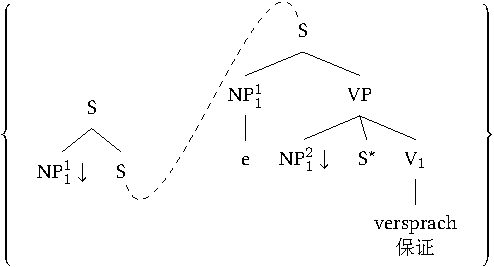
\includegraphics{Figures/tag-versprach-lsp-crop}
\caption{\label{Abbildung-MC-TAG-versprach}versprach的基本树集合包含了多元成分}
\end{figure}%
这棵树包括了一个被移动到左侧的NP$_1^1$的语迹,底部左侧的S结点和顶部右侧的S结点用虚线连接,表示支配关系。但我们并不要求直接支配关系,因此我们可以把这两棵子树分别插入到另外一棵树中,从而得到图\vref{Abbildung-TAG-Permutation3}中的语序。
\begin{figure}
\centerline{%
\begin{forest}
tag
[S
	[NP$_1^1\downarrow$]
	[S
		[NP$_2^2\downarrow$]
		[S
			[NP$_1^1$
				[e]]
			[VP
				[NP$_1^2\downarrow$]
				[S
					[NP$_2^1\downarrow$]
					[S
						[NP
							[PRO]]
						[VP
							[NP$_2^1$
								[e]]
							[NP$_2^2$
								[e]]
							[V$_2$
								[zu überführen;\textsc{inf} 起诉]]]]]
%								[zu überführen;to indict]]]]]
				[V$_1$
					[versprach;保证]]]]]]
%					[versprach;promised]]]]]]
\end{forest}
}
\caption{\label{Abbildung-TAG-Permutation3}针对语序NP$_1^1$ NP$_2^2$ NP$_1^2$ NP$_2^1$ V$_{2}$V$_{1}$的分析:附加操作作用于NP$_2^2$与NP$_2^1$之间的S结点}
\end{figure}%


\isc{多成分树邻接语法}\is{Multi-Component TAG}
\isc{树邻接语法(TAG)!多成分树邻接语法(MC-TAG)|)}\is{Tree Adjoining Grammar (TAG)!Multi"=Component (MC-TAG)|)} 
%Andere Varianten, die andere Konstituentenanordnungen zulassen sind V-TAG
其它允准上述结构成分语序的TAG变体包括V-TAG\isc{树邻接语法(TAG)!矢量树邻接语法(V-TAG)}\is{Tree Adjoining Grammar (TAG)!Vector (V-TAG)}\citep{Rambow94a}和TT-MC-TAG\citep{Lichte2007a}。\isc{树邻接语法(TAG)!树元组多成分树邻接语法(TT-MC-TAG)}\is{Tree Adjoining Grammar (TAG)!Tree Tuple MC-TAG (TT-MC-TAG)}\isc{成分序列|)}\is{constituent order|)}

\section{动词位置}

动词的位置\isc{动词位置|(}\is{verb position|(}可以做和GPSG并行的分析:在一个给定的序列线性化域(linearization domain)中,我们既可以让动词实现在前置位置上也可以实现在后置位置上。动词位置对小句的类型有影响,进而会影响到语义,因此基于词汇规则的分析也同样可行:可以让一条词汇规则将一棵在后置位置放置了动词的树变成一棵在前置位置放置了定式动词的树。这和GB、最简方案以及HPSG的分析是相似的。 
\isc{动词位置|)}\is{verb position|)}

\section{被动}

类似转换生成语法中的转换机制,我们可以设计一种分析方法来处理被动\isc{被动|(}\is{passive|(}:我们假设这样的词汇规则,它们将每一个词汇项的主动形式基本树变成相应的被动形式基本树\citep[\page 50--51]{KJ85a},这里的主动形式的词汇项指那些包含了主动形式的相应基本树的词汇项。

 \citet[\page 55]{KJ85a}提出了另一种方法以替代这种基于转换的分析,能够更好地处理被称之为“提升”
\isc{提升}\is{raising}的语言现象。他们的分析假定动词的论元都位列于子类框架(subcategorization)表中。如果一个动词匹配了某棵树相应的子类框架表,这个动词就可以进入到这棵树中。对应第\pageref{pass-lr-mlr}页讨论过的HPSG的词汇规则,Kroch和Joshi形式化得到了一条(TAG)词汇规则:该规则的输入端明确地提及一个宾格宾语。Kroch和Joshi针对非人称被动提出了一种复杂的分析,在不及物动词里没有实现出来的宾语,他们将其处理为语义为空的角色(第56页)。
这样的一种使用抽象的辅助实体的方式事实上是可以避免的:我们可以采纳始于 \citet{Haider86}的HPSG\indexhpsgc 分析,我们在\ref{Abschnitt-HPSG-Passiv}中讨论过这种分析。

也有人提议\isc{多重承继}\is{inheritance!multiple|(}使用承继关系来处理配价变化,被动仅仅被视为是一种特殊的配价变化现象(参见\citealp{Candito96a}及其扩展分析——\citealp*{KSYJ2006a})。正如我们在构式语法的相关讨论(见\ref{Abschnitt-Passiv-CxG})中所看到的,承继关系对于处理配价变化并不是理想的描写工具。这是因为这种处理手段在多个环节都存在句法和语义的交互(\citealp{Mueller2006d,Mueller2007d};\citeyear[\S~7.5.2]{MuellerLehrbuch1};\citeyear{MuellerUnifying};\citeyear{MWArgSt})。也请参见本书的\ref{relations-sec}了解更多的针对性讨论。 
\isc{多重承继}\is{inheritance!multiple|)}
\isc{被动|)}\is{passive|)}

\section{长距离依存}
\label{TAG-Fernabh}

\il{English|(}
\isc{长距离依存}\is{long"=distance dependency|(}TAG的长距离依存分析可以凭借其提供的标准工具——简单树可以插入到其它树的中间——进行分析。
图\vref{abb-nld-TAG}是(\mex{1})分析的一个实例:
\ea
\gll Who$_i$ did John tell Sam that Bill likes \_$_i$?\\
     谁 \textsc{aux} John 告诉 Sam \textsc{comp} Bill 喜欢 \\
\mytrans{John告诉Sam了,Bill喜欢谁?}
\z
%
\begin{figure}
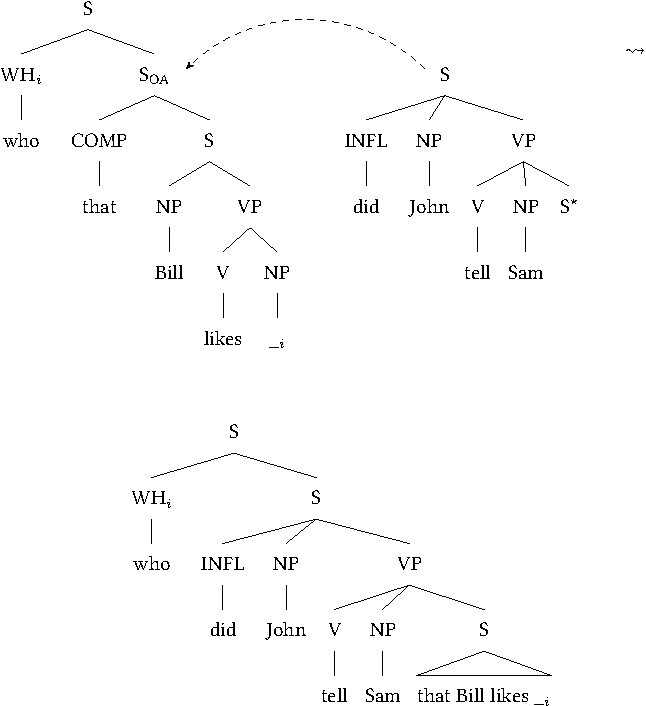
\includegraphics{Figures/tag-long-distance-dependencies-crop}
%%
%% Does not work with texlive 2015
%% %\oneline{%
%% \centerline{%
%% \begin{forest}
%% tag
%% [S
%% 	[WH$_i$
%% 		[who]]
%% 	[\tikzmark{soa}{S\sub{OA}}
%% 		[COMP
%% 			[that]]
%% 		[S
%% 			[NP
%% 				[Bill]]
%% 			[VP
%% 				[V
%% 					[likes]]
%% 				[NP
%% 					[\noexpand\_$_i$]]]]]]
%% \end{forest}
%% \hspace{0.5cm}
%% \begin{forest}
%% tag
%% [\tikzmark{s}{S}
%% 	[INFL
%% 		[did]]
%% 	[NP
%% 		[John]]
%% 	[VP
%% 		[V
%% 			[tell]]
%% 		[NP
%% 			[Sam]]
%% 		[S*]]]
%% \end{forest}
%% \qquad \raisebox{2cm}{$\rightsquigarrow$} \qquad
%% }\vspace{2\baselineskip}
%% \begin{forest}
%% tag
%% [S
%% 	[WH$_i$
%% 		[who]]
%% 	[S
%% 		[INFL
%% 			[did]]
%% 		[NP
%% 			[John]]
%% 		[VP
%% 			[V
%% 				[tell]]
%% 			[NP
%% 				[Sam]]
%% 			[S
%% 				[that Bill likes \noexpand\_$_i$, triangle]]]]]
%% \end{forest}
%% \begin{tikzpicture}[overlay,remember picture]
%% \draw[->, dashed, bend angle=45, bend right] ($(pic cs:s)+(-0.25,0.2)$) to($(pic cs:soa)+(0.8,.2)$);
%%
%% \end{tikzpicture}
%%
%% {%\dotted
%% % todo \anodecurve[l]{s4}[tr]{s2}{0.1in}[3ex]%
%% }
%% \hspace{1ex}
%% $\leadsto$
%}
\caption{\label{abb-nld-TAG}TAG中的长距离依存分析}
\end{figure}%
WH COMP NP likes \_$_i$的树属于likes的树族,因此包含在词典之中。
tell可以附加到这个树上,因为tell的这个树可以插入到who that Bill likes \_$_i$这棵树的中间位置。
这样一个插入性的操作可以重复很多次,所以在像(\mex{1})这样的句子中,who可以跨越多个小句边界移动到很远的位置:
\ea 
\gll Who$_i$ did John tell Sam that Mary said that Bill likes \_$_i$?\\
     谁      \textsc{aux} John 告诉 Sam \textsc{comp} Mary 说 \textsc{comp} Bill 喜欢\\
\mytrans{John告诉Sam,Mary说Bill喜欢谁?}
\z
%
还有一个很重要的细节:尽管(\mex{1})中的树包含范畴S,(\mex{1})并不是一个合语法的英语句子。
\ea[*]{
\gll who that          Bill likes\\
     谁  \textsc{comp} Bill 喜欢\\
}
\z
这一点必须在TAG语法中得到体现。在TAG中,额外OA符号可以用来标记一棵树的不完整性。如果一棵树包含了做了OA标识的结点,那么我们必须在这个结点处施加一次附加操作。
\isc{附加!附加的必要性|(}\is{adjunction!obligatory|(}
\il{English|)}
\isc{长距离依存|)}\is{long"=distance dependency|)} 

\section{新的发展和理论变体}

在\ref{Abschnitt-MC-TAG}中,我们介绍了多元成分TAG。事实上,存在很多不同的TAG变体,它们有着不同的形式性质。
 \citet[\page]{Rambow94a}总结了截止到1994年的各种TAG变体。接下来,我将讨论两个有趣的TAG变体:基于特征结构的TAG(Feature Structure-based TAG,简称FTAG\indexftagc,\citealp{VSJ88a})和基于向量的TAG(Vector-based TAG,简称V"=TAG,\citealp{Rambow94a})。

\subsection{FTAG}

在FTAG
\isc{树邻接语法(TAG)!基于特征结构的树邻接语法(FTAG)|(}\is{Tree Adjoining Grammar (TAG)!Feature Structure"=Based (FTAG)|(}中,结点并不是原子性的(N、NP、VP或S),而是包含有特征描写。
除了用于进行替换的结点之外,每一个结点都有一个顶结构、一个底结构。其中,顶结构说的是一棵树作为一个大的结构的一个子部分应该具有的属性,而底结构则说明了某一个结点下面的成分应该具有的属性。用于替换的结点只有一个顶结构。图\vref{Abbildung-FTAG-laughs}是laughs(笑)的树结构实例。\todostefan{geschwungenen Pfeil, alignierte Knoten}
\begin{figure}
\centerline{%
\begin{forest}
tag
[{\ms{
   cat & {\upshape S}\\
 }\\
\ms{
   cat & {\upshape S}
}}
  [\ms{
    cat & {\upshape NP}\\
    agr & \ibox{1}\\
   }
%
   [{[~]\\
    \ms{
       cat & {\upshape NP}\\
       agr & \ms{
              per & 3\\ 
              num & sing\\
             }\\
      }}, substitution,tier=2
      [John;John, tier=word] ] ]
  [{\ms{
     cat & {\upshape VP}\\
     agr & \ibox{1} \ms{
                    per & 3\\ 
                    num & sing\\
                    }\\
     }\\
     \ms{ 
     cat & {\upshape VP}\\
     }}
     [{\ms{
          cat & {\upshape V}\\
         }\\
       \ms{
          cat & {\upshape V}\\
       }}, tier=2
       [laughs;笑,tier=word]]]
] 
\end{forest}
}
\caption{\label{Abbildung-FTAG-laughs}John和laughs在FTAG中的基本树}
\end{figure}%
一个名词短语可以和图\ref{Abbildung-FTAG-laughs}中的laughs的子树组合。它的顶结构需要和laughs树中的NP结点一致。
组合的结果如图\vref{Abbildung-FTAG-John-laughs}所示。
\begin{figure}
\centerline{%
\begin{forest}
tag
[{\ms{
   cat & {\upshape S}\\
 }\\
\ms{
   cat & {\upshape S}
}}
  [{\ms{
    cat & {\upshape NP}\\
    agr & \ibox{1}\\
   }\\
    \ms{
       cat & {\upshape NP}\\
       agr & \ms{
              per & 3\\ 
              num & sing\\
             }\\
      }}
      [John;John, tier=word] ]
  [{\ms{
     cat & {\upshape VP}\\
     agr & \ibox{1} \ms{
                    per & 3\\ 
                    num & sing\\
                    }\\
     }\\
     \ms{ 
     cat & {\upshape VP}\\
     }}
     [{\ms{
          cat & {\upshape V}\\
         }\\
       \ms{
          cat & {\upshape V}\\
       }}
       [laughs;笑,tier=word]]]
] 
\end{forest}
}
\caption{\label{Abbildung-FTAG-John-laughs}John树与laughs树在FTAG中的组合}
\end{figure}%

在一棵完整的树中,所有的顶结构都需要和其所对应的底结构保持一致。在这种组合方式下,只有主语为第三人称单数形式的句子才能使用所给定的laughs的子树,也就是说动词的一致性特征(agreement feature)必须和主语一致。

对于附加语来说,待插入成分的顶结构必须和附加树的顶结构合一,而底结构必须和附加树上的标有`*'的结点(所谓的底部结点(foot node)
\isc{底部结点}\is{foot node})的底结构合一。

目前所讨论的基本树只包含顶结构部分和底结构部分匹配的那些结点。FTAG允许一种特殊的变体,即某些结点可以声明在这些结点的位置必须进行附加操作,只有这样,其推导才是合乎语法(well-formed)的。
图\vref{Obl-Adjunktion-FTAG}展示了laughing的树,这棵树上的VP结点有两个结构,它们的\textsc{mode}特征的值不一致。
\begin{figure}
\centerline{%
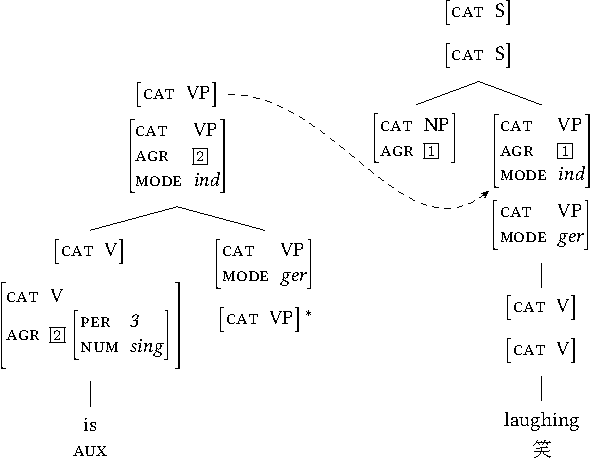
\includegraphics{Figures/tag-obl-adj-ftag-crop}
}
% This does not work with texlive 2015 use texlive 2013
%% \hfill
%% \begin{forest}
%% [{\subnode{vpone}{\ms{
%%    cat & {\upshape VP}\\
%%  }}\vspace{2mm}\\ 
%%  \ms{
%%        cat & {\upshape VP}\\
%%        agr & \ibox{2}\\ 
%%        mode & ind\\
%%  }}
%%   [{\ms{
%%        cat & {\upshape V}\\
%%       }\vspace{2mm}\\
%%     \ms{
%%       cat & {\upshape V}\\
%%       agr & \ibox{2} \ms{
%%                       per & 3\\ 
%%                       num & sing\\
%%                      }\\
%%        }} [is]]
%%   [{\ms{
%%        cat & {\upshape VP}\\ 
%%        mode & ger\\
%%       }\vspace{2mm}\\
%%     \ms{
%%        cat & {\upshape VP}\\
%%        }$^*$}]]
%% \end{forest}
%% %% %%% sings tree:
%% %% \hspace{-1em}
%% \hfill
%% \begin{forest}
%% [{\ms{ 
%%    cat & {\upshape S}\\
%%  }\vspace{2mm}\\
%%  \ms{
%%   cat & {\upshape S}\\ 
%%   }}
%%   [\ms{ cat & {\upshape NP}\\
%%         agr & \ibox{1}\\
%%       }]
%%   [{\subnode{vptwo}{\ms{
%%       cat  & {\upshape VP}\\
%%       agr  & \ibox{1}\\
%%       mode & ind\\
%%       }}\vspace{2mm}\\
%%      \ms{
%%      cat & {\upshape VP}\\ 
%%      mode & ger\\
%%      }}
%%      [{\ms{ cat & {\upshape V}\\
%%           }\vspace{2mm}\\
%%        \ms{
%%             cat & {\upshape V}\\
%%         }}
%%        [laughing]]]]
%% \end{forest}
%% \hfill\mbox{}
%% \begin{tikzpicture}[overlay,remember picture,out=0,in=220]
%% \draw[->, dashed] (vpone) to (vptwo);
%% \end{tikzpicture}
\caption{\label{Obl-Adjunktion-FTAG}FTAG中的强制附加}
\end{figure}%
为了将这棵树组成一个完整结构,必须添加另外一棵树以便将VP结点的两个部分分隔开来。这需要借助一棵附加树(如图\ref{Obl-Adjunktion-FTAG}中的附加树)来实现。附加树的最高位置的VP结点和laughing中VP结点,二者各自的顶结构需要合一。附加树中标有`*'号的结点和laughing中VP结点,二者的底结构合一。其结果如图\vref{Obl-Adjunktion-FTAG-Ergebnis}所示。
\begin{figure}
%%% is laughing tree:
\centerline{%
\begin{forest}
[{\ms{ 
   cat & {\upshape S}\\
 }\vspace{1mm}\\
  \ms{
   cat & {\upshape S}\\
  }}
  [{\ms{ cat & {\upshape NP}\\
         agr & \ibox{1}\\
   }}]
  [{\ms{
     cat  & {\upshape VP}\\
     agr  & \ibox{1}\\
     mode & ind\\
    }\vspace{1mm}\\
    \ms{
       cat & {\upshape VP}\\
       agr & \ibox{2}\\ 
       mode & ind\\
    }}
    [{\ms{
       cat & {\upshape V}\\
      }\vspace{1mm}\\
      \ms{
        cat & {\upshape V}\\
        agr & \ibox{2} \ms{
                per & 3\\ 
                num & sing\\
               }\\
         }} [is\\\textsc{aux}]]
     [{\ms{
        cat & {\upshape VP}\\ 
        mode & ger\\
      }\vspace{1mm}\\
      \ms{
       cat & {\upshape VP}\\ 
       mode & ger\\
      }}
      [{\ms{ cat & {\upshape V}\\
           }\vspace{1mm}\\
        \ms{
             cat & {\upshape V}\\
        }} [laughing\\\rule{0pt}{10pt}笑]]]]]
\end{forest}
}
  \caption{\label{Obl-Adjunktion-FTAG-Ergebnis}FTAG中强制附加的结果}
\end{figure}%

推导到最后所得到的那棵树,需要将所有结点各自的顶结构与底结构进行合一。图\ref{Obl-Adjunktion-FTAG-Ergebnis}中树的最高的VP结点其顶结构和底结构的\textsc{agr}特征值需要合一。正因为这个原因,只有和附加树中的\textsc{agr}特征取值一样的NP树才能插入当前树中的NP槽中。
%此处只能意义,原文若探究字面意义,不仅不通顺,还算是写错了。

这个例子展示了,我们在处理长距离依存时曾经采用过的强制附加\isc{附加!附加的必要性}\is{adjunction!obligatory}机制可以通过令顶结构和底结构特征取值不一致来实现。
如果一棵树中存在不兼容的顶结构与底结构,这棵树就不能是最终的导出树。%又一个错误
这意味着至少需要再进行一次附加操作才能得到合乎语法的树。
\isc{树邻接语法(TAG)!基于特征结构的树邻接语法(FTAG)|)}\is{Tree Adjoining Grammar (TAG)!Feature Structure"=Based (FTAG)|)}

\subsection{V"=TAG}
\label{sec-vtag}

V"=TAG
\isc{树邻接语法(TAG)!矢量树邻接语法(V-TAG)|(}\is{Tree Adjoining Grammar (TAG)!Vector (V-TAG)|(}是Owen \citet{Rambow94a}提出来的一种TAG变体,它同样包含了特征结构。
除此之外,和MC"=TAG一样,它假定以基本树的集合作为分析单元。图\vref{Abbildung-Lexical-Set-geben-V-TAG}是双宾动词geben(给)的基本词汇描写。
\begin{figure}
\vspace{4\baselineskip}
\menge{ 
\forestset{begin draw/.code={\begin{tikzpicture}[baseline=(current bounding box.center)]}}
    \hspace{1em}
    \begin{forest}
    [, phantom, for children={if n'=1{before computing xy={s*=1.25}}{}}
       %% This adjusts the relative position of the last child by zeroing its distance from the
       %% phantom root and increasing its distance from its sibling. This is delayed because 
       %% otherwise Forest will undo any changes when packing the tree.
      [VP
            [NP$\downarrow$]
            [VP, tikz+={\ignoreme\draw [densely dashed] ([yshift=2.5pt].south) [out=-75, in=-125] to ($(!u.north)!3/4!(!un.north)$) [out=55,in=100] to (!rl.north); }]]
    [VP
            [NP$\downarrow$]
            [VP, tikz+={\ignoreme\draw [densely dashed] ([yshift=2.5pt].south) [out=-75, in=-125] to ($(!u.north)!3/4!(!un.north)$) [out=55,in=100] to (!rl.north); }]]
    [VP
            [NP$\downarrow$]
            [VP, tikz+={\ignoreme\draw [densely dashed] ([yshift=2.5pt].south) [out=-75, in=-125] to ($(!u.north)!3/4!(!un.north)$) [out=55,in=100] to (!rl.north); }]]
    [VP
            [geben\\给]
%             [geben]
            [VP, tikz+={\ignoreme\draw [densely dashed] ([yshift=2.5pt].south) [out=-75, in=-125] to ($(!u.north)!3/4!(!un.north)$) [out=55,in=100] to (!rl.north); }]]
    [VP
            [$\epsilon$]]]
    \end{forest}
    \hspace{1em}
}
\vspace{.4\baselineskip}
  \caption{\label{Abbildung-Lexical-Set-geben-V-TAG}
    遵照 \citet[\page 6]{Rambow94a}的geben(给)在V"=TAG中的词汇描写
  }
\end{figure}%
这个词汇描写包括了给定动词的一棵树,一个范畴为VP的空成分,三棵用于将VP和NP结合起来的树。像MC"=TAG一样,对支配关系进行了声明。
图\ref{Abbildung-Lexical-Set-geben-V-TAG}中的支配限制要求每棵树中位于低处的VP结点都支配了最右侧的树的最高处的VP结点。动词论元的顺序以及动词的位置并没有给定。唯一限定的是:带有NP的树的低处的VP,以及geben(给)的低处的VP要支配空成分的VP。有了这一树集合,我们可以推出论元顺序的任意一种排列。Rambow同时也展示了如何利用词汇项来分析动词复合体。图\vref{Abbildung-zu-reparieren-versprochen-V-TAG}展示了由zu reparieren(修补)和versprochen(保证)组成的动词复合体的树集描写,其中包含了支配关系限制。
\begin{figure}
\vspace{4\baselineskip}
\oneline{%
\menge{%
  \begin{forest}
    [, phantom, for children={if n'=1{before computing xy={l=0pt, s*=1.25}}{}}
       %% This adjusts the relative position of the last child (n'=1) by zeroing its distance from the
       %% phantom root (l=0) and increasing its distance from its sibling. This is delayed because 
       %% otherwise Forest will undo any changes when packing the tree.
      [VP
        [NP$\downarrow$]
        [VP, tikz+={\ignoreme\draw [densely dashed] ([yshift=2.5pt].south) [out=-75, in=-125] to
            ($(!u.north)!3/4!(!un.north)$) %[out=55,in=181]  to ++(4cm,2cm) [out=-1,in=90] 
            [out=55,in=90] to (!rll.north); }]
        % the following line is ignored for space computation due to \ignoreme
        % the first VP node at the baseline is connected to a place between the dominating vp !u.north and the node to the
        % left of it !un.north (the second VP node on the second line). 3/4 specifies the position
        % between these nodes. It is more to the second VP. From there we go to rll, which is the
        % root node's (r) last child's (l) last child (l). Since the root node is our phantom node,
        % the rll node is the last VP in the second row.
        %
        % the yshift raises the beginning of the line so that it is not too far away from the node.
      ]
      [VP
        [NP$\downarrow$]
        [VP, tikz+={\draw [densely dashed] ([yshift=2.5pt].south) [out=-80, in=180] to ++(20mm,-15mm) [out=0, in=-90] to ($(!unn.north)!.7!(!unnn1.north)$) [out=90, in=180] to ++(3.5mm,5mm) [out=0, in=90] to (!rl1.north); }]
      ]
      [VP
        [NP$\downarrow$]
        [VP, tikz+={\draw [densely dashed] ([yshift=2.5pt].south) [out=-80, in=180] to ++(10mm,-10mm) [out=0, in=-90] to ($(!un.north)!.6!(!unn1.north)$) [out=90, in=180] to ++(5.5mm,6.5mm) [out=0, in=90] to (!rl1.north); }]
      ]
      [VP
        [NP$\downarrow$]
        [VP, tikz+={\draw [densely dashed] ([yshift=2.5pt].south) [out=-80, in=-105] to ($(!u.north)!1/3!(!un.north)$) [out=75,in=90] to (!rll.north); }]
      ]
      [VP
        [VP
          [$\epsilon$]
          [zu reparieren\\\textsc{inf} 修补]
%          [zu reparieren]
                  ]
        [VP, baseline
          [$\epsilon$]
          [versprochen\\保证]
%          [versprochen]
        ]
      ]
    ]
  \end{forest}
}
}
\vspace{2.5\baselineskip}
  \caption{\label{Abbildung-zu-reparieren-versprochen-V-TAG}V"=TAG中的动词复合体zu reparieren versprochen的分析}
\end{figure}%%
其中的两棵带有NP的树支配了versprochen,而另外两棵支配了zu reparieren。
带有NP的树的次序并没有被限制,因而这些NP间的任意排列都是被允准的。\pagebreak

这里有意思的是这种方法和 \citet[\S~2.1.3]{Berman96a-u}在LFG\indexlfgc 中的分析很像(参见\ref{Abschnitt-LFG-Umstellung}):
在Berman的分析中,动词直接投射(project)并形成VP,然后附加上论元。

有一点跟本书讨论的其它分析不同的是:不管动词位置如何,导出树中总是有一个空成分。
\isc{空成分}\is{empty element} 
\isc{树邻接语法(TAG)!矢量树邻接语法(V-TAG)|)}\is{Tree Adjoining Grammar (TAG)!Vector (V-TAG)|)}

\subsection{语言能力与语言运用的区分以及树本地化的MC"=LTAG的生成能力}
%\subsection{The competence"=performance distinction and the generative capacity of tree"=local MC"=LTAG}
\label{Abschnitt-Kompetenz-Performanz-TAG}

本书中\isc{语言能力|(}\is{competence|(}\isc{语言运用|(}\is{performance|(}讨论的很多理论都区分语言能力(competence)和语言运用(performance)\citep[\S~I.1]{Chomsky65a}。我们假定语言能力理论描写语言知识,而语言运用理论应该解释语言知识如何被使用以及为什么我们在使用和理解语言的过程中会产生错误等问题。参见\S \ref{chap-competence-performance}了解更多的讨论。 

 \citet*{JBR2000a}讨论了如(\mex{1}b)所示的关系从句的中心自嵌入问题(center self embedding),他们遵循 \citet[\page 286]{CM63a}的假定:这种嵌入最多只可能有三级的这一事实不应该在语法中进行描写,而应该归属于听者的加工问题,而这与语法的描写能力无关。
\eal
\label{TAG-Beispiel-Performanz}
\ex 
\gll dass der Hund bellt, der  die Katze jagt,  die  die Maus  gefangen hat\\
%    that the dog  barks  that the cat   chases that the mouse caught   has\\
%\mytrans{that the dog that chases the cat that caught the mouse barks}
     \textsc{comp} \textsc{det} 狗  叫  \textsc{rel} \textsc{det} 猫 追 \textsc{rel} \textsc{det} 老鼠 捉 \textsc{aux}   \\
\mytrans{追着那只捉老鼠的猫的那只狗在叫}
\ex 
\gll dass der Hund, [$_1$ der  die Katze, [$_2$ die  die Maus  gefangen hat,~$_2$] jagt~$_1$] bellt\\
     %that the dog   {}    that the cat    {}    that the mouse caught   has        chases    barks\\
     \textsc{comp} \textsc{det} 狗  {}  \textsc{rel} \textsc{det} 猫 {} \textsc{rel} \textsc{det} 老鼠 捉 \textsc{aux}   捉 叫 \\
\mytrans{追着那只捉老鼠的猫的那只狗在叫}
\zl

\noindent
这里有意思的是可以构建对于听者来说更为简单的中心嵌入(center embedding)的例子。基于这样的方式,我们可以构建一些可以被加工处理的具有更多中心嵌入的例子,从而说明了严格假定关系从句最多只能做两级中心嵌入的语法是错误的。以下是Hans Uszkoreit\aimention{Hans Uszkoreit}举的例子,它更容易被加工,因为所有被嵌入的关系从句都被隔离开来并且动词和更高层的小句也被隔离了。
\ea
\gll Die Bänke, [$_1$ auf denen damals die Alten des Dorfes, [$_2$ die allen Kindern, [$_3$~die vorbeikamen $_3$], freundliche Blicke zuwarfen $_2$], 
lange Stunden schweigend nebeneinander saßen $_1$], mussten im letzten Jahr einem~~~~~~~ Parkplatz weichen.\\
\textsc{det} 长椅 {} \textsc{prep} 那 当时 \textsc{det} 老.人 \textsc{det} 村庄 {} \textsc{rel} 所有 儿童 \hspaceThis{[$_3$~}\textsc{rel} 经过 {} 友好地 目光 给 {}
长 小时 安静 彼此相邻 坐 {} 必须 \textsc{prep}.\textsc{det} 上一个 年 一 停车场 让道\\
%the benches {} on which back.then the old.people of.the village {} that all children {} that came.by {} friendly glances gave {}
%long hours silent next.to.each.other sat {} must in.the last year a car.park give.way.to\\
\mytrans{村子里的那些本来安静地彼此相邻的、供老居民们互相友好地照看所有经过的孩子的长椅们在去年不得不给停车场让道了。}
%\mytrans{The benches on which the older residents of the village, who used to give friendly glances to all the children who came by, used to sit silently next %to one another had to give way to a car park last year.}
\z
参见 \citew{Gibson98a}以了解其它的会影响语言加工的因素。

 \citet{JBR2000a}讨论了动词复合体中的论元语序重列问题。他们所关注的模式如(\mex{1})所示:
\ea
$\sigma$(NP$_1$ NP$_2$ \ldots{} NP$_n$) V$_{n}$V$_{n-1}$ \ldots{} V$_{1}$
\z
这里,$\sigma$表示名词短语的任意一种排列,而V$_{1}$是定式动词。作者们探寻了与上述模式相关的词汇化树邻接语法(Lexicalized Tree Adjoining Grammar,简称LTAG)的性质,并注意到如果在考虑语义的情况下LTAG不能够分析这种语序。
\ea
NP$_2$ NP$_3$ NP$_1$ V$_{3}$V$_{2}$V$_{1}$
\z
德语中,例(\mex{1})是可以说的,由此可见,LTAG并不足以描写所有的语言。
\ea
\gll dass ihm$_2$ das Buch$_3$ niemand$_1$ zu lesen$_3$ versprechen$_2$ darf$_1$\\
%     that him     the book     nobody     to read      promise         be.allowed.to\\
%\mytrans{that nobody is allowed to promise him to read the book} 
     \textsc{comp} 他     \textsc{det} 书 没有人 \textsc{inf} 读 保证 被允许 \\
\mytrans{没有人被允许保证他读那本书}
\z
因此,他们提出扩展TAG,即所谓的树本地化多元成分LTAG(tree"=local multi"=component LTAG,简称为树本地化MC"=LTAG,或TL-MCTAG),参见\ref{Abschnitt-MC-TAG}的讨论。他们证明了基于正确的语义,TL-MCTAG可以分析(\mex{0})但不能分析(\mex{1})。他们声称在德语中不能出现这些语序,并且论证说这种例子不像关系从句的例子可以有两种选择(也就是说,或者否定这种模式基于语言运用的解释,又或者否定这种模式基于语言能力的解释)。
\ea
\label{ex-mc-ltag-fails}
NP$_2$ NP$_4$ NP$_3$ NP$_1$ V$_{4}$V$_{3}$V$_{2}$V$_{1}$
\z
如果我们视之为语言运用现象,则我们参考的是构造过程的复杂度以及随之而来的听者的加工问题。根据协同性(cooperativeness)
\isc{合作性}\is{cooperativeness}原则来解释为何语料中没有出现过这些语序。说话者通常希望自己被理解,因此会尽量按照听者可以理解的方式来明确表达出他们的句子。德语中包含超过四个动词的动词复合体很少见,因为可以通过外置(extraposing)
\isc{外置}\is{extraposition}操作来简化句子右侧有多个动词的复杂句子,从而避免歧义(\citealp[\page 262]{MuellerLehrbuch1})。

而另一种不同于语言运用解释的分析则使用具有更强能力的语法理论,这样的语法理论一方面允许两个动词的嵌入以及对它们的论元进行重排序,另一方面排除三个动词的嵌入与论元重排序。 \citet{JBR2000a}选择了这个解决方案,因此把(\mex{0})中所示语序的不合理性归结于语言能力。 

在HPSG(以及范畴语法\indexcgc 和一些GB分析\indexgbc)中,动词复合体通过论元组合进行解释\citep{HN89b,HN94a}。 在这种方法中,一个动词复合体的属性和一个简单动词完全一样,而所涉及到的动词的论元可以任意排列。语法并不限制用于组合的动词的数量,也不要求在一定层级之下禁止嵌入。接下来,我将论证许多种语序重列都是被交际规则排除掉的,这些交际规则甚至可以应用到只有两个动词的简单情况中。结论是无法嵌入四个或者更多的动词应该作为语言运用问题进行解释。

在介绍不同于基于语言能力去排除(\ref{ex-mc-ltag-fails})的观点之前, 我提出一个更具一般性的观点:
在这里语料无法帮助我们,因为没有谁找到了嵌入四个以及更多动词的实例。 \citet{Bech55a}提供了一个大量的实例集,但没有构造出任何包括四个嵌入动词的实例。 \citet[\page 94--95]{Meurers99c}给了一些造出来的嵌入五个动词的例子,这五个动词中包含多个助动词和情态词。
这些例子都很难被加工,也和我们这里的讨论没有关系,因为(\ref{ex-mc-ltag-fails})中的动词必须选择它们自己的论元。
因此就构造例子而言并没有那么多的可供选择动词。可以仅仅使用带有一个额外宾语的主语控制(subject control)动词(如versprechen(保证))、宾语控制动词或AcI动词(如sehen(看)和lassen(听))来构造例子。
在构造例子的过程中,很重要的是确保所有涉及到的名词尽量采用不同的格\isc{格}\is{case}和选择限制(selectional restrictions)\isc{选择限制}\is{selection!restriction}(如有生命/无生命),因为一个听者/读者可以用这些特征来将语序重列的论元匹配到它们的中心词上。
如果我们希望有(\ref{ex-mc-ltag-fails})中的那种四个NP带有不同格的例子,那么我们必须选择一个支配属格的动词。
德语中只有很少几个这样的动词。尽管 \citet{JBR2000a}在(\ref{Beispiel-Joshi-NP4})中构造的例子满足了这些要求,这仍然过于异常。
想在新闻文本中找到这样的例子,可能性极低,这一点十分清楚。这可能是因为只有很罕见的一些情境中,才能联想到这样的话语。
更进一步说,所有的控制动词(除了helfen(帮助))都需要一个带有zu的不定式,
并且也可以以内在并不一致的方式实现出来,也就是说通过包含一个外置的不定式附加语来消除动词复合体。
我们已经提到过,一个有合作精神的说话者/写者愿意用一个不那么复杂的构式,而这将进一步降低这种句子出现的可能性。

请注意,TL-MCLTAG并不限制一个句子中能出现多少个动词。这套理论本身允许任意多的动词。因此我们需要像其他语法理论一样需要在语言运用的限制上做假设,以此解释为何我们完全找不到带有五个甚至更多个动词的动词复合体。TL-MCLTAG可以预测论元语序重列的可能性。
我认为依赖语法形式模型的表达能力来对论元移位情况进行限制是不合理的,因为这些限制独立于动词复合体而存在,这些限制同样也可以在只包括两个论元的简单动词中出现。语序重列的问题在于仍然有可能将名词短语分配给它们所属的动词。如果这个分配导致歧义
\isc{歧义}\is{ambiguity},并且这种歧义无法通过格、选择限制、上下文知识或语调消解,则会选择无标记的成分语序。
 \citet*[\page 68]{Hoberg81a}论证了基于这一点可以很好地处理诸如下面实例的语言现象\footnote{%
Hoberg使用的是代词的所有格——ihr(她),而不是das(\textsc{det})。
这使得句子语义上更加通顺,但被约束的代词的序列线性化的要求可能干预相应的句法过程。因此,在这里我将代词换成了定冠词。
}:
\eal
\judgewidth{\#}
\ex[]{
\gll Hanna hat immer schon gewußt, daß das Kind sie verlassen will.\\
%	 Hanna has always already known that the child she leave wants\\
%\mytrans{Hanna has always known that the child wants to leave her.}
	 Hanna \textsc{aux} 总是 已经 知道 \textsc{comp} \textsc{det} 孩子 她 离开 希望 \\ 
\mytrans{Hanna一直都知道孩子希望离开她。}
}
\ex[\#]{
\gll Hanna hat immer schon gewußt, daß sie das Kind verlassen will.\\
%     Hanna has always already known that she the child  leave wants\\
%\glt Preferred reading: `Hanna has always known that she wants to leave the child.'
      Hanna \textsc{aux} 总是 已经 知道 \textsc{comp} 她 \textsc{det} 孩子 离开 希望 \\ 
\glt 倾向于解读为:\quotetrans{Hanna一直都知道她希望离开孩子。}
}
\ex[]{
%\raggedright
\gll Hanna hat immer schon gewußt, daß sie der Mann verlassen will.\\
%     Hanna has always already known that she the.\nom{} man leave wants.to\\
     Hanna \textsc{aux} 总是 已经 知道 \textsc{comp} 她 \textsc{det}.\nom{} 男人 离开 希望\\\hspace{-4pt}
\mytrans{Hanna一直都知道那个男人希望离开她。} 
%\mytrans{Hanna has always known that the man wants to leave her.}
}
\zl

\noindent
除非是对另外一种解读有很强的倾向性,否则不太可能将例(\mex{0}a)的语序换成例(\mex{0}b)中的语序。
这是因为无论sie(她)还是das Kind(孩子)都没有被无歧义地标示成主格或者宾格。(\mex{0}b)因此必须解读为Hanna是那个想要离开孩子的人。当然,如果至少一个论元被无歧义地做了格标记,这个语序重列也是可能的,就像例(\mex{0}c)那样。

对于由阴性可数名词组成的名词短语来说,主格和宾格的形式,属格和与格的形式相同。
对于不可数名词,情况更加糟糕。如果阴性不可数名词不加冠词,它们所有的格形式都是一样的,例如Milch(牛奶)。
阳性和中性词的属格也有类似之处。在下面 \citet[\page 45]{Wegener85b}的例子中,很难交换与事与宾格宾语的位置,而当名词像(\mex{1}c、d)样配有冠词时则可以做这种交换。

\eal
\ex 
\gll Sie mischt Wein Wasser bei.\\
%     she mixes wine water into\\
%\mytrans{She mixes water into the wine.}
     她 混合 酒 水 \textsc{prep} \\
\mytrans{她将水混到酒里。}
\ex 
\gll Sie mischt Wasser Wein bei.\\
%     she mixes water wine into\\
%\mytrans{She mixes wine into the water.}
     她 混合 水 酒 \textsc{prep} \\
\mytrans{她将酒混到水里。}
\ex 
\gll Sie mischt dem Wein das Wasser bei.\\
%     she mixes the.\dat{} wine the.\acc{} water into\\
%\mytrans{She mixes the water into the wine.}
     她 混合 \textsc{det}.\dat{} 酒 \textsc{det}.\acc{} 水 \textsc{prep} \\ 
\mytrans{她将水混到酒里。}
\ex 
\gll Sie mischt das Wasser dem Wein bei.\\
%    she mixes the.\acc{} water the.\dat{} wine into\\
     她 混合 \textsc{det}.\acc{} 水 \textsc{det}.\dat{} 酒 \textsc{prep} \\ 
%\mytrans{She mixes the water into the wine.}
\mytrans{她将水混到酒里。}
\zl
如果句子的意义在上下文中是清楚的(例如通过显性的否定),或者句子带有明确的语调,那么两个动词可以交换。

动词复合体的问题在于:如果我们不希望通过限制更少的动词支配所有格的话,四个名词短语中有两个几乎一直会有一样的格。
(\mex{1})是一个听起来有点别扭的例子,它通过形态变化来无歧义地标记了格:
\ea
\gll weil    er        den        Mann dem        Jungen des Freundes gedenken helfen lassen will\\
%     because he.\nom{} the.\acc{} man  the.\dat{} boy    of.the.\gen{} friend remember help let wants\\
%\mytrans{because he wants to let the man help the boy remember his friend}
     因为 他.\nom{} \textsc{det}.\acc{} 男人  \textsc{det}.\dat{} 男孩    \textsc{det}.\gen{} 朋友 记得 帮助 让 希望 \\
\mytrans{因为他希望让那个男人帮助那个男孩记得他的朋友} 
\z
另一个策略是控制动词对有生和无生宾语的选择,通过论元的生命度来辅助解释。
我构造了一个例子,在这个例子中,在深层位置嵌入的谓词是一个形容词而非动词。谓语leer fischen(钓光了)是一个结果构式,这个构式需要和动词复合体进行类比分析\citep[\S~5]{Mueller2002b}。
\ea
\gll weil niemand$_1$ [den Mann]$_2$ [der Frau]$_3$ [diesen Teich]$_4$  leer$_4$ fischen$_3$ helfen$_2$ sah$_1$\\
%     because nobody.\nom{} \spacebr{}the.\acc{} man \spacebr{}the.\dat{} woman \spacebr{}this.\acc{} pond empty fish help saw\\
     因为 没有人.\nom{} \spacebr{}\textsc{det}.\acc{} 男人 \spacebr{}\textsc{det}.\dat{} 女人 \spacebr{}这个.\acc{} 池塘 空 钓鱼 帮助 看见 \\
%\mytrans{because nobody saw the man help the woman fish the pond empty}
\mytrans{因为没有人看见那个男人帮助那个女人把池塘里的鱼钓光了} 
\z
阅读句子的时候带有相应的停顿可以使得句子的意义得到理解。有生的名词短语格可以被无歧义地标记格,我们的词汇知识可以帮助我们将diesen Teich(这个池塘)解释为leer(空)的论元。 

(\mex{0})中的句子可以通过一个适当的TL-MCLTAG进行分析,也可以通过动词复合体或结果构式的论元组合进行分析。(\mex{1})中的句子是对应于(\ref{ex-mc-ltag-fails})的模式并且类似(\mex{0})的例子:
\ea
\gll weil [der Frau]$_2$ [diesen Teich]$_4$ [den Mann]$_3$ niemand$_1$ leer$_4$ fischen$_3$ helfen$_2$ sah$_1$\\
% because \spacebr{}the.\dat{} woman \spacebr{}this.\acc{} pond \spacebr{}the.\acc{} man nobody.\nom{} empty fish help saw\\
  因为 \spacebr{}\textsc{det}.\dat{} 女人 \spacebr{}这个.\acc{} 池塘 \spacebr{}\textsc{det}.\acc{} 男人 没有人.\nom{} 空 钓鱼 帮助 看见 \\
\mytrans{因为没有人看见那个男人帮助那个女人把池塘里的鱼钓光了}
\z
(\mex{0})比(\mex{-1})的形式标记更多,不过总是针对局部重列的现象(Gisbert Fanselow\aimention{Gisbert Fanselow}, p.\,c.\ 2006)。
这个句子不应该被语法排除掉。导致这些标记的因素和简单动词论元的标记性是一样的。TL-MCLTAG无法正确地分析诸如(\mex{0})中的例子,这说明这种TAG变体并不适合分析自然语言。

什么应该被视为语言能力?什么应该被视为语言运用?不同的TAG研究者有不同的意见。如 \citet[\page 15]{Rambow94a}论证认为我们不应该排除那些语法或语法形式模型无法处理的语序重列。在第六章,他提出一个语言应用的理论,解释了为什么位于中间位置的动词的论元的语序重列问题比较难以处理。因此,我们应该选择像V-TAG\isc{树邻接语法(TAG)!矢量树邻接语法(V-TAG)}\is{Tree Adjoining Grammar (TAG)!Vector (V-TAG)}或TT-MC-TAG\isc{树邻接语法(TAG)!树元组多成分树邻接语法(TT-MC-TAG)}\is{Tree Adjoining Grammar (TAG)!Tree Tuple MC-TAG (TT-MC-TAG)}这样的TAG变体\citep{Lichte2007a},这些变体能够解释多种语序,然后可以使用语言运用模型来解释为什么句子可接受程度不同。

另一种寻找拥有最小表达能力的语法形式模型的思路是根本就不去限制形式模型的表达能力,而是去尽量限制语言学理论本身。在第\ref{sec-generative-capacity}章中,我们将展开更多的讨论。 
\isc{语言能力|)}\is{competence|)}
\isc{语言运用|)}\is{performance|)}

\section{总结与分类}

总的来说,LTAG是词汇化的理论,也就是说每棵树上都至少有一个词汇元素;没有树会对应像S $\to$ NP VP这样的规则,因为在这条规则中没有词出现。总有包含主语NP和VP的复杂的树。在VP内部会有必须的足够多的结构来确保树中包含动词。LTAG中的基本树总是包含中心词及其论元。对于及物动词,这意味着主语和宾语都必须成为基本树的成分。对于用于长距离依存分析的树,这也同样适用。正如图\ref{abb-nld-TAG}所示,宾语必须是树的一部分。宾语可以和动词之间可以间隔多个句子边界,这一点并没有在基本树中体现,也就是说,语法的递归性并没有在基本树中体现。相应的作用是通过附加操作来实现的,附加是指向树中间插入成分。用于抽取的基本树,如图\ref{abb-nld-TAG}所示,不同于用于解释普通SVO小句的基本树,如图\ref{Abbildung-Max-likes-Anouk}中的likes的基本树。 伴随likes的最小结构(如主语抽取、话题化、主语关系从句、宾语关系从句、被动等等)需要它们自己各自的基本树\citep[\page 10]{KJ2003a}。不同的基本树通过词汇规则
\isc{词汇规则}\is{lexical rule}联系在一起。这些词汇规则将一棵特定的树影射为其它的树。通过这种方式,可以从一个表示主动形式的树推出表示被动形式的树。这些词汇规则可以和转换语法中的转换规则
\isc{转换}\is{transformation}进行类比。 但必须强调一点,每个树中都有词汇元素,这使得整个语法和自由的转换相比更加受限。

和GB以及含有空成分的LFG、CG、HPSG变体的一个有意思的不同之处是这里介绍的TAG变体\footnote{%
  参见 \citew{Rambow94a}和 \citew[\page 194]{Kallmeyer2005a-u},以了解词典中带有空成分的TAG分析。
},其词典中并不包含空成分。空成分可以出现在树中,树再作为一个整体出现在词典中。

基本树的大小不受限制,这使得TAG在分析习语的时候特别方便(见第\ref{Abschnitt-Diskussion-Lokalitaet}节)。
因为递归从基本树中排除掉了,因此在导出树中距离特别远的元素可以包含在同一个基本树中(扩展的局域性\isc{定域}\is{locality})。

 \citet*{KKNV95a}论证了满足特定要求的HPSG语法可以转写为TAG语法。通过这种方式,我们可以得到一个计算复杂度
\isc{生成能力}\is{capacity!generative}更明确的语法。HPSG语法一般都是0-型文法,而不同的TAG变体可以用来刻画从2-型语言到弱上下文相关语言
\isc{弱上下文相关语言}\is{mildly context"=sensitive grammar}之间的不同语言\citep{Joshi85a-u}。 \citet*{YMTT2001a}提出了一个算法可以将FB"=LTAG语法翻译成弱上下文相关语言的HPSG文法。

%\section*{思考题}
%\bigskip
\questions{
\begin{enumerate}
\item TAG是如何分析长距离依存的?在分析长距离依存的时候是否需要空成分?
\item 是否有可能通过标准的TAG过程来分析多个动词的论元的语序重列问题?
\end{enumerate} 
}

%\section*{练习题}
\exercises{
\begin{enumerate}
\item 用LTAG分析下列词串:
\ea
\gll der dem König treue Diener\\
% the the.\dat{} king loyal servant\\
  \textsc{det} \textsc{det}.\dat{} 国王 皇家 雇工\\
\mytrans{国王的皇家雇工}
\z
\end{enumerate}
}

%\section*{延伸阅读}
\furtherreading{
重要的论文包括 \citew*{JLT75a-u}、 \citew{Joshi87a-u}和 \citew{JS97a}。很多更关心语言本体的读者并不会过多涉猎讨论TAG形式性质的论文。
 \citew{KJ85a}很好地总结了针对语言现象的分析。 针对TAG的语言学与计算语言学的论文可以在Abeill{\'e}和Rambow\nocite{AR2000a-ed-not-crossreferenced}所编辑的论文中找到。 \citet{Rambow94a}比较了他的TAG变体(V"=TAG\isc{树邻接语法(TAG)!矢量树邻接语法(V-TAG)}\is{Tree Adjoining Grammar (TAG)!Vector (V-TAG)})和Karttunen的激进词汇主义(Radical Lexicalism)方法、Uszkoreit的GPSG\indexgpsgc、组合范畴语法\indexcgc, HPSG\indexhpsgc 以及依存语法\indexdgc。 

 \citet{SJ93a}讨论了从心理语言学来说可行的加工模型,并且论证了基于TAG进行增量式句法分析的可行性。他们进一步提出了TAG的一种变体:同步TAG(synchronous TAG\indexstagc)。在这种TAG变体中,一棵句法树有一棵语义树与之相对应。当构建句法结构的时候,语义结构也同步构建起来。这个同步构建的结构对应于GB理论中通过转换
\isc{转换}\is{transformation}从表层结构中经由推导得到的逻辑形式(Logical Form\isc{逻辑形式(LF)}\is{Logical Form (LF)})。

 \citet[\S~6]{Rambow94a}展示了一个基于自动机的语言运用理论。他将这种理论应用到德语上并表示可以解释在对多个动词的论元进行重列加工时所遇到的困难。 
\isc{树邻接语法(TAG)|)}\is{Tree Adjoining Grammar (TAG)|)}

 \citet{KR2008a-u}基于FTAG展示了如何通过一棵推导树进行MRS的获取。每一个顶结点都引用了整个结构的语义内容,而每一个底结点都引用了所在结点之下的部分的语义内容。基于这种方式,当把形容词(如mutmaßlichen(被怀疑的))插入到NP树(如alle Mörder(全部凶手))时,可以确保形容词有超过名词性部分(Mörder(凶手))的作用域:当把形容词附加到N结点时,形容词可以获取名词的语义内容。mutmaßlichen的顶结点将成为mutmaßlichen Mörder(嫌疑人)这个组合的顶结点,而这保证了mutmaßlichen Mörder的语义可以正确地嵌入到全称量词中。
}

%      <!-- Local IspellDict: en_US-w_accents -->



% some chapters have english language names, others don't. LFG for instance
% semicolon in citations on the next line
% glosses of trees missing

\include{chapters/ot}

\part{讨论}\label{part-discussion}
%\part{General discussion}\label{part-discussion}

%% -*- coding:utf-8 -*-
\exewidth{(235)}%

\chapter{语言知识的天赋性}
%\chapter{The innateness of linguistic knowledge}
\label{Abschnitt-Angeborenheit}\label{chap-innateness}
%
% Haspelmath2010c:391 tendencies

如果我们试着将本书提到的诸多理论进行比较的话,我们会发现这些理论之间有很多相似之处。\footnote{\label{fn-ffs}%
我们需要区分理论(theory)和框架(framework)这两个术语。框架是指构建理论时使用的一组共同的假设和工具。在本书中,我讨论了德语的理论。这些理论是在特定框架(GB、GPSG、HPSG、LFG\ldots)下形成的,另外当然有其他语言的其他理论也遵循同样的基本假设。这些理论虽然不同于这里讨论的德语理论,但它们是在同一框架内形成的。 \citet{Haspelmath2010c}倡导一种无框架的语法理论。如果语法理论使用了不相容的工具,那么就难以展开语言的对比。所以针对英语的非局部依存关系所提出的转换假设跟为德语提出的\slaschc 机制之间就无法进行比较了。我同意Haspelmath所说的形式工具可能会导致偏见的观点,但是不管怎样语言事实终究需要描写。如果理论之间没有共性,我们得到的将是依据个人的框架得出的孤立的理论。如果一个框架具有共享的词汇和建立无框架语法理论的标准,那么这一框架就是无框架语法理论。进一步论述见 \citet{MuellerCoreGram}以及本书的第\ref{Abschnitt-UG-mit-Hierarchie}章。
}
%If we try and compare the theories presented in this book, we notice
%that there are a number of similarities.\footnote{\label{fn-ffs}%
%  The terms \emph{theory} and \emph{framework} may require clarification. A framework is a common
%  set of assumptions and tools that is used when theories are formulated. In this book, I discussed
%  theories of German. These theories were developed in certain frameworks (GB, GPSG, HPSG, LFG, \ldots) and of course there are
%  other theories of other languages that share the same fundamental assumptions. These theories
%  differ from the theories of German presented here but are formulated in the same
%  framework.  \citet{Haspelmath2010c} argues for framework-free grammatical theory. If grammatical
%  theories used incompatible tools, it would be difficult to compare languages. So assuming
%  transformations for English nonlocal dependencies and a \slasch mechanism for German would make
%  comparison impossible. I agree with Haspelmath that the availability of formal tools may lead to
%  biases, but in the end the facts have to be described somehow. If nothing is shared between
%  theories, we end up with isolated theories formulated in one man frameworks. If there \emph{is} shared
%  vocabulary and if there are standards for doing framework"=free grammatical theory, then the
%  framework is framework"=free grammatical theory. See
%   \citet{MuellerCoreGram} and Chapter~\ref{Abschnitt-UG-mit-Hierarchie} of this book for further discussion.
%}
在所有理论框架中都有利用属性"=值偶对来描述语言对象的理论变体。这些理论提出的句法结构有时是相似的。然而,有一些差异会引起不同流派之间的激烈争论。理论之间的差异在于它们是否会提出转换、空成分、基于短语或基于词的分析,二叉或扁平结构这样的假设。
%In all of the frameworks, there are variants of theories that use feature"=value pairs to describe linguistic objects.
%The syntactic structures assumed are sometimes similar. Nevertheless, there are some differences that have often led to fierce debates
%between members of the various schools. Theories differ with regard to whether they assume transformations, empty elements, phrasal or lexical analyses,
%binary branching or flat structures.

每一种理论不仅要描述自然语言,还要解释自然语言。为某一给定语言设定允准其结构的无穷多个语法是可行的(见第\pageref{ua-psg-eins}页的练习\ref{ua-psg-eins})。这些语法在观察上是充分的(observationally adequate)\isc{观察的充分性}\is{observational adequacy}。如果一种语法能够符合观察以及母语者语感的话,该语法就实现了描写的充分性(descriptive adequacy)\isc{描写的充分性}\is{descriptive adequacy}。\footnote{%
因为有主观因素的作用,所以这一术语有时不是特别有用。并不是每一个人都直觉地认为如下假设是正确的,即假设世界上语言的每一种所能观察到的语序都可以从共同的“限定语-中心语-补足语”的构型中推导出来,并且也只能通过移位移到左侧(见\ref{Abschnitt-Kaynesche-Modelle})。
}
%Every theory has to not only describe natural language, but also explain it. It is possible to
%formulate an infinite number of grammars that license structures for a given language (see Exercise~\ref{ua-psg-eins} on page~\pageref{ua-psg-eins}). These grammars are \emph{observationally adequate}\is{observational %adequacy}.
%A grammar achieves \emph{descriptive adequacy}\is{descriptive adequacy} if it corresponds to observations and the intuitions of native speakers.\footnote{%
%This term is not particularly useful as subjective factors play a role. Not everybody finds grammatical theories intuitively correct where it is assumed that every
%observed order in the languages of the world has to be derived from a common
%Specifier"=Head"=Complement configuration, and also only by movement to the left (see Section~\ref{Abschnitt-Kaynesche-Modelle} for the discussion of such proposals).
%}
如果一种语言学理论能够用于为每一种自然语言建立一个描写充分的语法,那么这种语言学理论就是描写充分的。但是,能够实现描写充分的语法不一定具有解释充分性( explanatory adequacy\isc{解释的充分性}\is{explanatory adequacy})。能够实现解释充分性的语法需要与语言习得\isc{语言习得}\is{language acquisition}的数据相符,这些数据就是那些貌似能被人类说话者习得的语法\citep[\page 24--25]{Chomsky65a}。
%A linguistic theory is descriptively adequate if it can be used to formulate a descriptively adequate grammar for every natural language. However, grammars achieving descriptive
%adequacy do not always necessarily reach \emph{explanatory adequacy}\is{explanatory adequacy}. Grammars that achieve explanatory adequacy are those that are compatible with
%acquisition data\is{language acquisition}, that is, grammars that could plausibly be acquired by human speakers \citep[\page
%  24--25]{Chomsky65a}.

 \citet[\page 25]{Chomsky65a}假设儿童已经具有语法在特定领域中原则上应该是怎样的知识,然后他们从语言输入中提取出一个特定语法事实上应该是怎样的信息。主流的生成语法(MGG)中最著名的习得理论变体就是原则和参数理论,它认为参数化的原则限定了可能的语法结构,并且儿童只需要在语言习得中设置参数(见\ref{Abschnitt-GB-Paramater})。
% \citet[\page 25]{Chomsky65a} assumes that children already have domain"=specific knowledge about what grammars could, in principle, look like and then extract information about what
%a given grammar actually looks like from the linguistic input. The most prominent variant of acquisition theory in Mainstream Generative Grammar (MGG) is the Principles \& Parameters
%theory, which claims that parametrized principles restrict the grammatical structures possible and
%children just have to set parameters during language acquisition
%(see Section~\ref{Abschnitt-GB-Paramater}).

这些年来,天赋性假说\isc{天赋论}\is{nativism}(也称作先天论)历经多次修改。尤其是关于先天语言知识组成部分的假设,即所谓的普遍语法(UG)\isc{普遍语法}\is{Universal Grammar (UG)},一直在变化。
%Over the years, the innateness hypothesis, also known as nativism\is{nativism}, has undergone a number of modifications.
%In particular, assumptions about exactly what forms part of the innate linguistic knowledge,
%so"=called Universal Grammar (UG)\is{Universal Grammar (UG)}, have often been subject to change.

先天论经常遭到构式语法\indexcxgc、认知语法\isc{认知语法}\is{Cognitive Grammar}的支持者以及其他理论学派研究人员的反对。其他的解释一般用来支持语法范畴、句法结构或者句法结构中语言对象关系具有天赋性的事实。受到批评的另外一点是,由于很多规定被简单化地假设为普遍语法的一部分,语法的实际复杂性被模糊掉了。下面是GB/最简方案分析中一些论证的基本程序。
%Nativism is often rejected by proponents of Construction Grammar\indexcxg, Cognitive
%Grammar\is{Cognitive Grammar} and by many other researchers working in other theories. Other
%explanations are offered for the facts normally used to argue for the innateness of grammatical
%categories, syntactic structures or relations between linguistic objects in syntactic structures.
%Another point of criticism is that the actual complexity of analyses is blurred by the fact that many of the stipulations are simply assumed to be part of UG.
%The following is a caricature of a certain kind of argumentation in GB/Minimalism analyses: 

\begin{enumerate}
\item 我已经为S语言中的P现象提供了一种分析;
%\item I have developed an analysis for the phenomenon P in the language S.
\item 这种分析是优雅的/概念上简洁的/我的\footnote{%
    参见
    \url{http://www.youtube.com/watch?v=cAYDiPizDIs}。 \zhdate{2015/12/01}。\nocite{Zappa86a}\aimention{Frank Zappa}
};
%\item The analysis is elegant/conceptually simple/mine\footnote{%
%    Also, see
%    \url{http://www.youtube.com/watch?v=cAYDiPizDIs}. 01.12.2015.\nocite{Zappa86a}\aimention{Frank Zappa}
%}.
\item 不可能去学习相关的结构或原则;
%\item There is no possibility to learn the relevant structures or principles.
\item 所以,这一分析中从A1到An的假设一定是说话者天赋知识的一部分。
%\item Therefore, the assumptions A$_1$ through A$_n$ that are made in this analysis must be part of the innate knowledge
%of speakers.
\end{enumerate}
通过向UG中随意增加假设,可以让其余的分析十分简单。
%By attributing arbitrary assumptions to UG, it is possible to keep the rest of the analysis very
%simple.

下面的章节会简要评价一些支持语言特有的天赋知识的证据。我们会发现所有证据都存在争议。在下面的章节中,我会讨论语法体系结构的一些基本问题,语言能力与语言运用之间的差异,如何为语言使用现象建模,语言习得理论以及其他存在争议的问题,例如,在语言表征中设置空成分是否理想以及语言是应该主要基于词的属性还是短语的模式进行解释。
%The following section will briefly review some of the arguments for language"=specific innate knowledge.
%We will see that none of these arguments are uncontroversial. In the following chapters, I will discuss fundamental
%questions about the architecture of grammar, the distinction between competence and performance and how to model
%performance phenomena, the theory of language acquisition as well as other controversial questions, \eg 
%whether it is desirable to postulate empty elements in linguistic representations and whether language should
%be explained primarily based on the properties of words or rather phrasal patterns.

在我们转向这些激烈争论的话题之前,我想先讨论一下争论最为激烈的一个话题,即天赋语言知识的问题。在文献中,有人找到了以下支持天赋知识的证据:
%Before we turn to these hotly debated topics, I want to discuss the one that is most fiercely
%debated, namely the question of innate linguistic knowledge. In the literature, one finds the
%following arguments for innate knowledge:

\begin{itemize}
\item 存在句法普遍性,
\item 习得的速度,
\item 语言习得存在一个“关键期”,
\item 所有儿童都可以习得语言,但是灵长类动物不可以,
\item 儿童会自发地将皮钦语规范化,
\item 语言处理位于大脑的特定部分,
\item 所谓的语言能力与普遍认知能力的分离:
%\item the existence of syntactic universals,
%\item the speed of acquisition,
%\item the fact that there is a `critical period' for language acquisition,
%\item the fact that all children learn a language, but primates do not,
%\item the fact that children spontaneously regularize pidgin languages, 
%\item the localization of language processing in particular parts of the brain,
%\item the alleged dissociation of language and general cognition:
\begin{itemize}
\item 威廉氏综合症,
\item FoxP2基因发生突变的KE氏家族,以及
%\item Williams Syndrome,
%\item the KE family with FoxP2 mutation and
\end{itemize}
\item 刺激贫乏论。
%\item the Poverty of the Stimulus Argument.
\end{itemize}
 \citet{Pinker94a}对这些证据作了很好的概述。 \citet{Tomasello95a}对这本书作了批评性评论。其中个别观点会在下面进行讨论。
% \citet{Pinker94a} offers a nice overview of these arguments.  \citet{Tomasello95a} provides a critical review of this book. The individual points will be discussed in what follows.

\section{句法普遍性}
%\section{Syntactic universals}
\label{sec-syntactic-universals}

句法\isc{普遍性|(}\is{universal|(}的普遍性被作为论据来证明语言知识的天赋性(如\citealp[\page 33]{Chomsky98a-u}、\citealp[\page 237--238]{Pinker94a})。在文献中,对于什么是普遍性的、什么是语言特定的有不同的看法。支持普遍性的突出代表有:\footnote{%
Frans Plank\aimention{Frans Plank}在康斯坦斯有一个关于什么是普遍性的存档文集\citep{PF2000a}:\url{http://typo.uni-konstanz.de/archive/intro/}。截至\zhdate{2015/12/23},一共有2029条记录。这些记录根据它们的质量来进行标注,结果发现,许多的普遍性具有统计上的普遍性,它们适用于绝大多数语言,但是有一些例外。一些普遍性被标记为绝对的,也就说,极少有例外。有1153条被标记为带有问号的绝对,有1021条被标记为不带问号的绝对值。许多普遍性是通过蕴含的普遍性\isc{普遍性!蕴涵的普遍性}\is{universal!implicational}捕捉到的,即,它们具有这样的形式:如果一种语言具有属性X,那么它也有属性Y。在存档文集中列出的普遍性部分上是非常具体的,而且指向具体语法属性的历时变化。比如说,第四条表示:“如果呼格的典型元素是一个前缀,那么这个前缀来自于第一人称领有者或第二人称主语。”
}\nocite{Harbour2011a}
%The\is{universal|(} existence of syntactic universals has been taken as an argument for the innateness of linguistic knowledge
%(\eg \citealp[\page 33]{Chomsky98a-u}; %\citealp[\page 46--47]{Chomsky88a-u}; %\citealp[\page 46--47]{Chomsky88a}, ist in Stanford falsch zitiert
%\citealp[\page 237--238]{Pinker94a}). There are varying claims in the literature with regard to what is universal and 
%language"=specific. The most prominent candidates for universals are:\footnote{%
%Frans Plank\aimention{Frans Plank} has an archive of universals in Konstanz \citep{PF2000a}:
%\url{http://typo.uni-konstanz.de/archive/intro/}. On 23.12.2015, it contained 2029 entries.
%The entries are annotated with regard to their quality, and it turns out that many of the universals
%are statistical universals, that is, they hold for the overwhelming majority of languages, but there are
%some exceptions. Some of the universals are marked as almost absolute, that is, very few exceptions are known.
%1153 were marked as absolute or absolute with a question mark. 1021 of these are marked as absolute without
%a question mark. Many of the universals captured are implicational universals\is{universal!implicational}, that is, they have the form:
%if a language has the property X, then it also has the property Y. The universals listed in the archive
%are, in part, very specific and refer to the diachronic development of particular grammatical
%properties. For example, the fourth entry states that: \emph{If the exponent of
%  vocative is a prefix, then this prefix has arisen from 1st person possessor or a 2nd person
%  subject.} 
%}\nocite{Harbour2011a}

\begin{itemize}
\item 中心语导向参数
\item \xbarc 结构
\item 语法功能(如主语或宾语)
\item 约束原则
\item 长距离依存的属性
\item 时、体、态的语法要素
\item 词性
\item 递归或自嵌套
%\item the Head Directionality Parameter
%\item \xbar structures
%\item grammatical functions such as subject or object
%\item binding principles
%\item properties of long"=distance dependencies
%\item grammatical morphemes for tense, mood and aspect
%\item parts of speech
%\item recursion or self"=embedding
\end{itemize}

\noindent
我们将在下面的内容中逐一讨论这些普遍性。应该强调的是,人们对于这些普遍性的认定并没有达成一致,而且这些观察到的属性实际上需要假定天赋的语言知识。
%These supposed universals will each be discussed briefly in what follows. One should emphasize that there is by no means
%a consensus that these are universal and that the observed properties actually require postulating innate linguistic
%knowledge.

\subsection{中心语导向参数}
%\subsection{Head Directionality Parameter}
\label{Abschnitt-Kopfstellungsparameter}

% a month ago -> head final
% counterexamples notwithstanding
\mbox{}\isc{参数!中心语导向参数|(}\is{parameter!head direction|(}%
中心语导向参数在第\ref{Abschnitt-GB-Paramater}节就已经介绍过了。第\pageref{Bsp-Kopfstellungsparameter}页(\ref{Bsp-Kopfstellungsparameter})中的例子在这里重复表示为下面的(\mex{1}),这些例子说明了日语的结构是英语结构的镜像:
%The Head Directionality Parameter was already introduced in Section~\ref{Abschnitt-GB-Paramater}. The examples in (\ref{Bsp-Kopfstellungsparameter}) on
%page~\pageref{Bsp-Kopfstellungsparameter}, repeated below as (\mex{1}), show that the structures in Japanese are the mirror image of the English structures:
\eal
\label{Bsp-Kopfstellungsparameter-zwei}
\ex 
be showing pictures of himself
\ex
\gll zibun  -no syasin-o mise-te iru\\
     他自己 \hspaceThis{-}\textsc{prep} 照片 显示 \textsc{cop}\\
%     himself \hspaceThis{-}of picture showing be\\
\zl
为了捕捉到这些事实,我们提出一个参数来表示中心语相对于其所带论元的位置(如Chomsky \citeyear[\page 146]{Chomsky86}、\citeyear[\page 70]{Chomsky88a-u})。
%In order to capture these facts, a parameter was proposed that is responsible for the position of the head relative to its
%arguments (\eg Chomsky \citeyear[\page 146]{Chomsky86}; \citeyear[\page 70]{Chomsky88a-u}). 

Radford (\citeyear[\page 60--61]{Radford90a-u}; \citeyear[\page 19--22]{Radford97a-u})、 \citet[\page 234, 238]{Pinker94a}、 \citet[\page 350]{Baker2003b}和其他作者声称,在假定了中心语导向性参数的基础上,在动词所管辖的方向和介词所管辖的方向之间具有某种外在或隐含的关系,也就是说,动词末位语序的语言具有后置词,或具有VO语序的语言具有前置词。这一观点可以通过英语\il{English}和日语\il{Japanese}这两种语言来验证,如例(\mex{0})所示:在介词短语中,no出现在代词的后面,名词syasin-o(图片)位于其所属的PP后面,主动词在它的宾语后面,助词iru位于主动词mise-te之后。具体的短语就是英语中各自短语的镜像。
%By assuming a Head Directionality Parameter, Radford (\citeyear[\page 60--61]{Radford90a-u}; \citeyear[\page 19--22]{Radford97a-u}),  \citet[\page 234, 238]{Pinker94a},  \citet[\page 350]{Baker2003b}
%and other authors claim, either explicitly or implicitly, that there is a correlation between the direction of government of verbs and that of adpositions, that is, languages
%with verb"=final order have postpositions and languages with VO order have prepositions. This claim
%can be illustrated with the language pair English\il{English}/""Japanese\il{Japanese} and the
%examples in (\mex{0}): the \emph{no} occurs after the pronoun in the prepositional phrase, the noun \emph{syasin-o} `picture' follows the PP belonging to it, the main verb follows its object and the
%auxiliary \emph{iru} occurs after the main verb \emph{mise-te}. The individual phrases are the exact mirror image of
%the respective phrases in English.

对此,一个反例足以说明这一说法是站不住脚的。实际上,像波斯语\il{Persian}这种语言是遵循动词末位的语序的,但它是有前置词的,如(\mex{1})所示:
%A single counterexample is enough to disprove a universal  claim and in fact, it is possible to
%find a language that has verb"=final order but nevertheless has prepositions.
%Persian\il{Persian} is such a language. An example is given in (\mex{1}):
\ea
\gll man ketâb-â-ro be Sepide dâd-am.\\
     我 书-\pl-\RA{} \textsc{prep} Sepide  给-1\sg\\
\mytrans{我把书给了Sepide。}
%     I book-\pl-\RA{} to Sepide gave-1\sg\\
%\mytrans{I gave the books to Sepide.}
\z
在\ref{Abschnitt-X-Bar}中,我们说明了德语不能简单地按照这一参数来描写:德语是动词位于末位的语言,但是它既有前置词,也有后置词。《语言结构的世界地图》这本书囊括了41种带有VO语序和后置词的语言,还有14种带有OV语序和前置词的语言\citep{wals-83,wals-85}。\footnote{%
  \url{http://wals.info/combinations/83A_85A\#2/15.0/153.0},\zhdate{2015/12/23}。
} \citet{Dryer92a}更早之前在小范围样本的语言研究中也指出,按照中心语导向参数所预测的结果是有例外的。
%In Section~\ref{Abschnitt-X-Bar}, it was shown that German cannot be easily described with this parameter: German is a verb"=final language but has both
%prepositions and postpositions. The World Atlas of Language Structures lists 41 languages with VO
%order and postpositions and 14 languages with OV order and prepositions \citep{wals-83,wals-85}.\footnote{%
%  \url{http://wals.info/combinations/83A_85A\#2/15.0/153.0}, 23.12.2015.
%} An earlier study by  \citet{Dryer92a} done with a smaller sample of languages also points out that
%there are exceptions to what the Head Directionality Parameter would predict. 

不仅如此, \citet[\page 422]{GW94a}指出,用一个参数来表示中心语的位置是不够的,因为英语和德语及荷兰语中标补语可以出现在他们的补足语前面;不过,英语是一个VO语序的语言,而德语和荷兰语是OV语序的语言。
%Furthermore,  \citet[\page 422]{GW94a} point out that a single parameter for the position of heads would not be enough since complementizers in both English and German/Dutch
%occur before their complements; however, English is a VO language, whereas German and Dutch count as OV languages.

如果我们希望通过句法范畴来决定管辖的方向(\citealp[\page 422]{GW94a};\citealp[\page 15]{Chomsky2005a}),那么我们就必须假设句法范畴属于普遍语法的一部分(更多内容参见\ref{Abschnitt-UG-Wortarten})。对于这类假设来说,前置词和后置词还是有问题的,因为它们通常都被指派给同一个范畴(P)。如果我们要为前置词和后置词引入特殊的范畴,那么像第\pageref{Tabelle-Merkmalszerlegung-Wortarten}页所示的词类的四分法就不管用了。相反,我们需要一个额外的二元特征,这样便会自动预测出八种范畴,虽然只有五种(四种常规的,加上一个额外的)是实际上需要的。
%If one wishes to determine the direction of government based on syntactic categories (\citealp[\page 422]{GW94a}, \citealp[\page 15]{Chomsky2005a}), then one has to assume
%that the syntactic categories in question belong to the inventory of Universal Grammar (see Section~\ref{Abschnitt-UG-Wortarten}, for more on this).
%Difficulties with prepositions and postpositions also arise for this kind of assumption as these are normally assigned to the same category (P).
%If we were to introduce special categories for both prepositions and postpositions, then a four"=way
%division of parts of speech like the one on page~\pageref{Tabelle-Merkmalszerlegung-Wortarten} would
%no longer be possible. One would instead require an additional binary feature and one would thereby
%automatically predict eight categories although only five (the four commonly assumed plus an extra one) are actually needed.

我们可以看到,Pinker作为普遍规则构建出的管辖方向之间的关系实际上在作为一种倾向性时才是正确的,而不是作为严格的规则。也就是说,有许多语言,其中前置词或后置词的使用与动词的位置之间具有相关性\citep[\page 83]{Dryer92a}。\footnote{%
 \citet[\page 234]{Pinker94a}在他的观点中使用了usually(通常)这个词。由此,他暗示了这里是有例外的,介词的顺序与动词管辖方向之间的关系实际上是一种倾向性,而不是一种具有普遍意义的可应用的规则。但是,在随后的内容中,他认为,中心语导向参数构成了天赋的语言知识的一部分。 \citet[\page
55]{Travis84a-u}讨论了现代汉语中一些跟她所提出的相关性不符的实例。之后她提出将中心语导向参数作为一种缺省的参数,这个参数可以被语言中的其他限制所覆盖。
} 
%One can see that the relation between direction of government that Pinker formulated as a universal
%claim is in fact correct but rather as a tendency than as a strict rule, that is, there are many languages where
%there is a correlation between the use of prepositions or postpositions and the position the verb
%\citep[\page 83]{Dryer92a}.\footnote{%
% \citet[\page 234]{Pinker94a} uses the word \emph{usually} in his formulation. He thereby implies
%that there are exceptions and that the correlation between the ordering of adpositions and the
%direction of government of verbs is actually a tendency rather than
%a universally applicable rule. However, in the pages that follow, he argues that the Head Directionality Parameter forms part of innate linguistic knowledge.
% \citet[\page 55]{Travis84a-u} discusses data from Mandarin Chinese that do not correspond to the correlations she assumes. She then proposes treating the Head Directionality Parameter
%as a kind of Default Parameter that can be overridden by other constraints in the language.
%} 

许多语言中,介词由动词演变而来。在现代汉语\isc{现代汉语}\is{Mandarin Chinese}语法中,有一类词通常被称作副动词\isc{副动词}\is{coverb}。这些词可以用作介词,也可以用作动词。如果我们历时地观察语言,那么我们就可以找到这些倾向性的解释,而不用参考天赋的语言学知识(参见\citealp[\page 445]{EL2009a})。
%In many languages, adpositions have evolved from verbs. In Chinese\is{Mandarin Chinese} grammar, it is commonplace to refer to a particular class of words as coverbs\is{coverb}.
%These are words that can be used both as prepositions and as verbs. If we view languages historically, then we can find explanations for these tendencies that do not have to make
%reference to innate linguistic knowledge (see \citealp[\page 445]{EL2009a}). 

进而,我们可以解释与语言处理的倾向性相关的一些事实:具有相同管辖方向的语言(图\ref{fig-head-position}a--b)与具有相反管辖方向的语言(图\ref{fig-head-position}c--d)相比,其动词和前/后置词之间的距离更小。
%Furthermore, it is possible to explain the correlations with reference to processing preferences: in languages with the same direction of government, the distance between the verb
%and the pre-/postposition is less (Figure~\ref{fig-head-position}a--b) than in languages with
%differing directions of government (Figure~\ref{fig-head-position}c--d).
\begin{figure}
\hfill
%\begin{tabular}{cc}
\subfloat[带有前置词的SVO(常见)]{
%\subfloat[SVO with prepositions (common)]{
\makebox[.4\textwidth]{
\begin{tikzpicture}
\tikzset{level 1+/.style={level distance=2\baselineskip}}
%\tikzset{frontier/.style={distance from root=24\baselineskip}}
\Tree[.IP NP
       [.VP \node(v){V}; NP [.PP \node(p){P}; NP ] 
       ]
]
\draw (v) |-  ([yshift=-5mm]v |- p) -| (p);
\end{tikzpicture}}}
\hfill
\subfloat[带有后置词的SOV(常见)]{
%\subfloat[SOV with postpositions (common)]{
\makebox[.4\textwidth]{
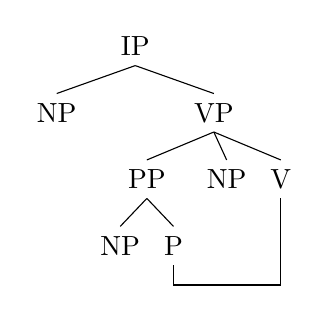
\begin{tikzpicture}
\tikzset{level 1+/.style={level distance=2\baselineskip}}
%\tikzset{frontier/.style={distance from root=24\baselineskip}}
\Tree[.IP NP
       [.VP [.PP NP \node(p){P}; ] NP \node(v){V};
       ]
]
\draw (v) |-  ([yshift=-5mm]v |- p) -| (p);
\end{tikzpicture}}}\hfill\mbox{}

\hfill
\subfloat[带有后置词的SOV(少见)]{
%\subfloat[SVO with postpositions (rare)]{
\makebox[.4\textwidth]{
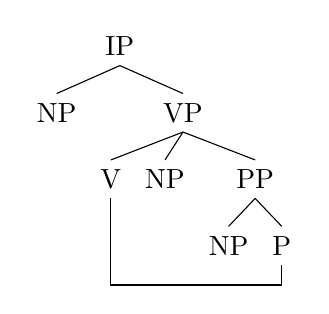
\begin{tikzpicture}
\tikzset{level 1+/.style={level distance=2\baselineskip}}
%\tikzset{frontier/.style={distance from root=24\baselineskip}}
\Tree[.IP NP
       [.VP \node(v){V}; NP [.PP NP \node(p){P}; ] 
       ]
]
\draw (v) |-  ([yshift=-5mm]v |- p) -| (p);
\end{tikzpicture}}}
\hfill
\subfloat[带有前置词的SOV(少见)]{
%\subfloat[SOV with prepositions (rare)]{
\makebox[.4\textwidth]{
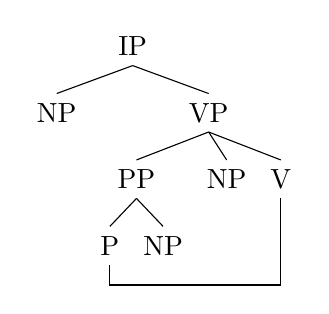
\begin{tikzpicture}
\tikzset{level 1+/.style={level distance=2\baselineskip}}
%\tikzset{frontier/.style={distance from root=24\baselineskip}}
\Tree[.IP NP
       [.VP [.PP \node(p){P}; NP ] NP \node(v){V};
       ]
]
\draw (v) |-  ([yshift=-5mm]v |- p) -| (p);
\end{tikzpicture}}}
\hfill\mbox{}
\caption{基于 \citet[\page 221]{Newmeyer2004b}的遵循不同的中心语语序的动词与介词之间的距离}\label{fig-head-position}
%\caption{Distance between verb and preposition for various head orders according to  \citet[\page 221]{Newmeyer2004b}}\label{fig-head-position}
\end{figure}%
从语言处理的角度来看,具有相同管辖方向的语言更易于被人们接受,因为他们允许听者更好地识别动词短语的组成部分( \citet[\page 219--221]{Newmeyer2004b}引用了 \citew[\page 32]{Hawkins2004a-u}有关一般处理的偏好的讨论,也可以参考 \citew[\page 131]{Dryer92a})。由此,这一倾向性可以解释为语言运用偏好的语法化(参见第\ref{Abschnitt-Diskussion-Performanz}章有关语言能力和语言运用的区分),而且这并不必然依赖于天赋的语言特有的知识。
%From the point of view of processing, languages with the same direction of government should be preferred since they allow the hearer to better identify the parts
%of the verb phrase ( \citet[\page 219--221]{Newmeyer2004b} cites  \citew[\page 32]{Hawkins2004a-u}
%with a relevant general processing preference, see also  \citew[\page 131]{Dryer92a}). This tendency can thus be explained as the
%grammaticalization of a performance preference (see Chapter~\ref{Abschnitt-Diskussion-Performanz}
%for the distinction between competence and performance) and recourse to innate language"=specific
%knowledge is not necessary.%
\isc{参数!中心语导向参数|)}\is{parameter!head direction|)}

\subsection{\xbar 结构}
%\subsection{\xbar structures}
\label{sec-Diskussion-X-Bar}

通常认为\isc{X理论@\xbar 理论|(}\is{X theory@\xbar theory|(},所有语言都有对应于\xbarc 模式的句法结构(参见\ref{sec-xbar})(\citealp[\page
238]{Pinker94a};\citealp[\page 11, 14]{Meisel95a};\citealp[\page 216]{PJ2005a})。但是,也有像迪尔巴尔语\il{Dyirbal}(澳大利亚)这种语言,其中句子是无法用层级结构来表示的。由此, \citet[\page 110]{Bresnan2001a}认为,他加禄语\il{Tagalog}、匈牙利语\il{Hungarian}、马拉雅拉姆语\il{Malayalam}、瓦勒皮里语\il{Warlpiri}、Jiwarli语\il{Jiwarli}、Wambaya语\il{Wambaya}、雅卡语\il{Jakaltek}和其他相应的语言没有VP节点,而是带有(\mex{1})这样格式的规则:
%It\is{X theory@\xbar theory|(} is often assumed that all languages have syntactic structures that
%correspond to the \xbar schema (see Section~\ref{sec-xbar}) (\citealp[\page
%238]{Pinker94a}; \citealp[\page 11, 14]{Meisel95a}; \citealp[\page 216]{PJ2005a}). There are, however, languages such as Dyirbal\il{Dyirbal} (Australia) where it does not seem
%to make sense to assume hierarchical structure for sentences.
%Thus,  \citet[\page 110]{Bresnan2001a} assumes that Tagalog\il{Tagalog}, Hungarian\il{Hungarian},
%Malayalam\il{Malayalam}, Warlpiri\il{Warlpiri}, Jiwarli\il{Jiwarli}, Wambaya\il{Wambaya},
%Jakaltek\il{Jakaltek}
%and other corresponding languages do not have a VP node, but rather a rule taking the form of (\mex{1}): 
\ea
S $\to$ C$^*$
\z
这里,C$^*$ 表示任意数目的短语成分,而且结构中没有中心语。其他不带中心语的结构的例子将在\ref{Abschnitt-Phrasale-Konstruktionen}讨论。
%Here, C$^*$ stands for an arbitrary number of constituents and there is no head in the structure.
%Other examples for structures without heads will be discussed in Section~\ref{Abschnitt-Phrasale-Konstruktionen}.

\xbarc 结构被用来限制可能规则的形式。相应假设是这些限制减少了我们可以构建的语法类别,并且,使得语言更容易被习得。但是正如 \citet{KP90a}所展示的,\xbarc 结构的假说不能限制可能语法的数量,如果我们允准空的中心语的话。管约论使用了很多空的中心语\isc{空成分}\is{empty element},而且在最简方案\indexmpc 中,它们还有显著数量的增加。比如说,(\mex{0})中的规则可以被重构为:
%\xbar structure was introduced to restrict the form of possible rules. The assumption was that these restrictions reduce the class
%of grammars one can formulate and thus -- according to the assumption -- make the grammars easier to
%acquire. But as  \citet{KP90a} have shown,
%the assumption of \xbar structures does not lead to a restriction with regard to the number of possible grammars if one allows for empty heads\is{empty element}.
%In GB, a number of null heads were used and in the Minimalist Program\indexmp, there has been a
%significant increase of these. For example, the rule in (\mex{0}) can be reformulated as follows:
\ea
V$'$ $\to$ \vnull C$^*$
\z
这里,\vnullc 是一个空的中心语。由于限定语是可选的,V$'$可以投射到VP上,这样我们就得到了一个对应于\xbarc 模式的结构。
%Here, \vnull is an empty head. Since specifiers are optional, V$'$ can be projected to VP and we arrive at a structure corresponding to
%the \xbar schema.

除了具有自由语序的语言带来的问题以外,附加结构还有一些问题:Chomsky在\xbarc 理论中有关形容词性结构的分析(\citealp[\page 210]{Chomsky70a};还可以参考本书\ref{sec-xbar},尤其是图\vref{Abbildung-AP})不能直接应用到德语,因为,与英语不同的是,德语中的形容词短语是中心语后置,并且程度修饰语必须直接位于形容词的前面:
%Apart from the problem with languages with very free constituent order, there are further problems with adjunction structures: Chomsky's analysis of adjective structure
%in \xbart (\citealp[\page 210]{Chomsky70a}; see also Section~\ref{sec-xbar} of this book, in
%particular Figure~\vref{Abbildung-AP}) is not straightforwardly applicable to German since, unlike
%English, adjective phrases in German are head"=final and degree modifiers must directly precede the
%adjective: 
\eal
\ex[]{
\gll der auf seinen Sohn sehr stolze Mann\\
	 \textsc{det} \textsc{prep} 他的 儿子 非常 骄傲 男人\\
\mytrans{对自己的儿子感到非常骄傲的男人}
%	 the of his son very proud man\\
%\mytrans{the man very proud of his son}
}
\ex[*]{
\gll der sehr auf seinen Sohn stolze Mann\\
	 \textsc{det} 非常 \textsc{prep} 他的 儿子 骄傲 男人\\
%	 the very of his son proud man\\
}
\ex[*]{
\gll der auf seinen Sohn stolze sehr Mann\\
	 \textsc{det} \textsc{prep} 他的 儿子 骄傲 非常 男人\\
%	 the of his son proud very man\\
}
\zl
根据\xbarc 模式,auf seinen Sohn必须与stolze相组合,而且只有这样才能得到与它的限定语相组合的\abarc 投射(参见图\vref{Abbildung-AP}中英语形容词性短语的结构)。这样就只可能推导出诸如(\mex{0}b)或(\mex{0}c)的语序。而这两个语序在德语中都是不可能的。如果我们假设德语跟英语完全一致,而且基于某种原因,形容词的补足语必须移到左边的话,这样才有可能拯救\xbarc 模式。如果我们允许这种补救措施,那么当然任何一种语言都可以用\xbarc 模式来进行描写。结果是我们必须针对许多语言提出巨量的移位规则,而这从心理语言学的角度来看是异常复杂和困难的。请看第\ref{Abschnitt-Diskussion-Performanz}章有关与语言运用相适应的语法讨论。 
%Following the \xbar schema, \emph{auf seinen Sohn} has to be combined with \emph{stolze} and only then can the
%resulting \abar projection be combined with its specifier (see Figure~\vref{Abbildung-AP} for the structure of adjective
%phrases in English). It is therefore only possible to derive orders such as (\mex{0}b) or (\mex{0}c). Neither of these
%is possible in German. It is only possible to rescue the \xbar schema if one assumes that German is
%exactly like English and, for some reason, the complements of adjectives must be moved to the left. If we allow this kind of repair
%approaches, then of course any language can be described using the \xbar schema. The result would be that one would have
%to postulate a vast number of movement rules for many languages and this would be extremely complex and difficult
%to motivate from a psycholinguistic perspective. See Chapter~\ref{Abschnitt-Diskussion-Performanz} for grammars compatible with performance.

\xbarc 理论的最严格形式的问题在\ref{sec-xbar}进行了说明,它是由hydra小句\isc{hydra小句}\is{hydra clause}引起的 \citep{PR70a,Link84a-u,Kiss2005a}:
%A further problem for \xbart in its strictest form as presented in Section~\ref{sec-xbar} is posed by so"=called hydra clauses\is{hydra clause} \citep{PR70a,Link84a-u,Kiss2005a}:
\eal
\ex {}
\gll [[der Kater] und [die Katze]], die einander lieben\\
     \spacebr{}\spacebr{}\textsc{det} 公猫 和 \textsc{det} 猫 \textsc{rel} 互相 爱\\
\mytrans{公猫和(母)猫相互爱慕}
%     \spacebr{}\spacebr{}the tomcat and the cat that each.other love\\
%\mytrans{the tomcat and the (female) cat that love each other}
\ex {}约会的[[男孩儿] 和 [女孩儿]]是我的朋友。 
%\ex {}[[The boy] and [the girl]] who dated each other are friends of mine. 
\zl
因为(\mex{0})中的关系从句指称一组对象,他们只能附加在并列的结果上。整个并列结构是一个NP,但是,附加语实际上应该附加在\xbarc 层面上。与德语和英语中的关系小句相反的情况是波斯语中的形容词: \citet{Samvelian2007a}提出的分析是,形容词直接与名词相组合,而且只有名词和形容词的组合才能与PP论元相组合。
%Since the relative clauses in (\mex{0}) refer to a group of referents, they can only attach to the result of the coordination.
%The entire coordination is an NP, however, and adjuncts should actually be attached at the \xbar level. The reverse case of relative clauses
%in German and English is posed by adjectives in Persian:  \citet{Samvelian2007a} argues for an analysis where adjectives are combined with nouns
%directly, and only the combination of nouns and adjectives is then combined with a PP argument.

关于德语和英语的讨论说明了限定语和附加语的导入不能在具体的投射层面进行约束,而且前面非构型语言(non"=configurational languages)的讨论已经显示了中间层的假设并不适用于每一种语言。
%The discussion of German and English shows that the introduction of specifiers and adjuncts cannot be restricted to particular projection levels, and
%the preceding discussion of non"=configurational languages has shown that the assumption of intermediate levels does not make sense for every language.

还需要指出的是,Chomsky本人在1970年提出,有的语言可以脱离\xbarc 模式\citeyearpar[\page 210]{Chomsky70a}。
%It should also be noted that Chomsky himself assumed in 1970 that languages can deviate from the \xbar
%schema \citeyearpar[\page 210]{Chomsky70a}.

如果我们希望把所有的信息编码在词汇中,那么我们就需要能够表示共性的极为抽象的组合规则。这种组合性规则的一个例子是范畴语法\isc{范畴语法}\is{Categorial Grammar (CG)} 的多重应用规则(参见第\ref{Kapitel-CG}章),以及最简方案\indexmpc 中的合并\isc{合并}\is{Merge}(参见\ref{Abschnitt-MP})。上面这些规则仅仅说明了两个语言学对象被组合在一起。这种组合性当然存在于每一种语言中。但是,对于完全词汇化的语法而言,只有我们允许空中心语并且提出某些特别的假设的话,才有可能来描写语言。这将在\ref{Abschnitt-Phrasale-Konstruktionen}具体讨论。\isc{X理论@\xbar 理论|)}\is{X theory@\xbar theory|)} 
%If one is willing to encode all information about combination in the lexicon, then one could get by with very abstract combinatorial rules that would hold universally.
%An example of this kind of combinatorial rules is the multiplication rules of Categorial Grammar\is{Categorial Grammar (CG)} (see Chapter~\ref{Kapitel-CG}) 
%as well as Merge\is{Merge} in the Minimalist Program\indexmp (see Section~\ref{Abschnitt-MP}).
%The rules in question simply state that two linguistic objects are combined. These kinds of
%combination of course exist in every language. With completely lexicalized grammars, however, it is only possible to describe languages
%if one allows for null heads and makes certain ad hoc assumptions. This will be discussed in
%Section~\ref{Abschnitt-Phrasale-Konstruktionen}.\is{X theory@\xbar theory|)} 

\subsection{主语和宾语的语法功能}
%\subsection{Grammatical functions such as subject and object}
\label{Abschnitt-UG-EPP}

\mbox{} \citet[\page xxv]{BK82a}、 \citet[\page 236--237]{Pinker94a}\isc{主语|(}\is{subject|(}\isc{宾语|(}\is{object|(}\isc{语法功能|(}\is{grammatical function|(}、 \citet[\page 349]{Baker2003b}和其他人认为所有的语言都有主语和宾语。为了说明这个观点到底意味着什么,我们必须探究这些术语。对于大多数的欧洲语言来说,很容易说明主语和宾语是什么(参见\ref{Abschnitt-GF});但是,并不是所有的语言都是这样的,或者说在有些语言中用这些术语是完全没有意义的(\LATER{\citealp{Durie85a};
}\citealp[\S~4]{Croft2001a}; \citealp[\S~4]{EL2009a})。
%\mbox{} \citet[\page xxv]{BK82a},  \citet[\page 236--237]{Pinker94a}\is{subject|(}\is{object|(}\is{grammatical function|(},  \citet[\page 349]{Baker2003b} 
%and others assume that all languages have subjects and objects. In order to determine what exactly this claim means, we have to explore the terms
%themselves. For most European languages, it is easy to say what a subject and an object is (see Section~\ref{Abschnitt-GF}); however,
%it has been argued that it is not possible for all languages or that it does not make sense to use
%these terms at all (\LATER{\citealp{Durie85a}; }\citealp[Chapter~4]{Croft2001a}; \citealp[Section~4]{EL2009a}).

在Pinker研究的LFG\indexlfgc{}这类理论中,语法功能扮演着重要的角色。事实上,是该把句子视为主语、宾语还是特殊定义的子句型论元(\xcompc)\citep*{DL2000a-u,Berman2003b-u,Berman2007a-u,AMM2005a-u,Forst2006a-u}仍然是有争议的。这就意味着当我们讨论语法功能如何分配给论元时是有一定自由度与灵活性的。由此,我们有可能在所有语言中找到一种将语法功能指派给函项论元的形式。
%In theories such as LFG\indexlfg{} -- the one in which Pinker worked -- grammatical functions play a primary role. The fact that it is still
%controversial whether one should view sentences as subjects, objects or as specially defined sentential arguments (\xcomp) \citep*{DL2000a-u,Berman2003b-u,Berman2007a-u,AMM2005a-%u,Forst2006a-u}
%serves to show that there is at least some leeway for argumentation when it comes to assigning
%grammatical functions to arguments. It is therefore likely that one can find an assignment of
%grammatical functions to the arguments of a functor in all languages. 

与LFG不同的是,语法功能在GB(请看\citealp{Williams84a,Sternefeld85a})和范畴语法\indexcgc 中是不重要的,在GB中语法功能只能间接地通过指向树的位置来决定。由此,在第\ref{Kapitel-GB}章讨论的方法中,主语是位于IP的限定语位置上的短语。
%Unlike LFG, grammatical functions are irrelevant in GB (see \citealp{Williams84a,Sternefeld85a}) and Categorial Grammar\indexcg. In GB, grammatical functions can only be
%determined indirectly by making reference to tree positions. Thus, in the approach discussed in
%Chapter~\ref{Kapitel-GB}, the subject is the phrase in the specifier position of IP.

在乔姆斯基式理论的后期,也有一些看起来对应于语法功能的功能性节点(AgrS\isc{范畴!功能范畴!AgrS}\is{category!functional!AgrS},
AgrO\isc{范畴!功能范畴!AgrO}\is{category!functional!AgrO}, AgrIO\isc{范畴!功能范畴!AgrIO}\is{category!functional!AgrIO}请看第\pageref{Seite-AgrO}页)。但是, \citet[\S~4.10.1]{Chomsky95a-u}指出,这些功能性范畴只是出于理论内部的原因而提出的,而且应该被排除在普遍语法的范畴之外。请看 \citew{Haider97a}和 \citew[\page 509--510]{Sternefeld2006a-u}对德语的描写,其中无功能性的投射不能被激发。
%In later versions of Chomskyan linguistics, there are functional nodes that seem to correspond to grammatical functions (AgrS\is{category!functional!AgrS},
%AgrO\is{category!functional!AgrO}, AgrIO\is{category!functional!AgrIO}, see
%page~\pageref{Seite-AgrO}). However,  \citet[Section~4.10.1]{Chomsky95a-u} remarks that these functional categories were only assumed for theory internal reasons
%and should be removed from the inventory of categories that are assumed to be part of UG. See  \citew{Haider97a} and  \citew[\page 509--510]{Sternefeld2006a-u} for a description of German that %does without functional projections
%that cannot be motivated in the language in question.

HPSG\indexhpsgc 所持的观点较为中立:它用一个特殊的配价特征来表示主语(在德语语法中,有一个中心语特征还可以对非定式动词的主语进行表征)。但是,\subjfc 的值是从更为普遍的理论性角度推导出来的:在德语中,带有结构格\isc{格!结构格}\is{case!structural}的层级最低的旁格\isc{旁格}\is{obliqueness}成分就是主语(Müller \citeyear[\page 153]{Mueller2002b}; \citeyear[\page 311]{MuellerLehrbuch1})。
%The position taken by HPSG\indexhpsg is somewhere in the middle: a special valence feature is used for subjects (in grammars of German, there is a head feature that contains a
%representation of the subject for non"=finite verb forms). However, the value of the \subjf is
%derived from more general theoretical considerations: in German, the least oblique\is{obliqueness}
%element with structural case\is{case!structural} is the subject (Müller \citeyear[\page 153]{Mueller2002b}; \citeyear[\page 311]{MuellerLehrbuch1}).

在\gbc 理论(扩展的投射原则,EPP\isc{扩展的投射原则}\is{Extended Projection Principle (EPP)}、 \citew[\page 10]{Chomsky82a-u})和LFG\indexlfg (主语条件\isc{主语条件}\is{Subject Condition})中,都有用来确保每个句子都有一个主语的原则。通常认为这些原则是具有语言共性的。\footnote{%
但是,  \citet[\page 27]{Chomsky81a}允许语言不带主语。他假设,这可以通过一个参数来解决。 \citet[\page 311]{Bresnan2001a}提出了主语条件,但是在脚注中指出,也许有必要将这一条件参数化,从而使得它适合于某些语言。%
} 
%In \gbt (Extended Projection Principle, EPP\is{Extended Projection Principle (EPP)},  \citew[\page 10]{Chomsky82a-u}) and also in LFG\indexlfg (Subject Condition\is{Subject Condition}), there are %principles
%ensuring that every sentence must have a subject. It is usually assumed that these principles hold universally.\footnote{%
%  However,  \citet[\page 27]{Chomsky81a} allows for languages not to have a subject. He assumes that this is handled by a parameter.
 % \citet[\page 311]{Bresnan2001a} formulates the Subject Condition, but mentions in a footnote that it might be necessary
%to parameterize this condition so that it only holds for certain languages.%
%} 
 
正如前面提到的, GB中没有语法功能,但是有对应于语法功能的结构位置。对应于主语的位置是IP的限定语。EPP说明了在SpecIP中必须有一个元素。如果我们假定这个原则具有语言共性,那么每一种语言都必须在这个位置有一个元素。正如我们看到的,这个普遍性假设是有反例的:德语。德语有无人称被动句(\mex{1}a),其中有无主语的动词(\mex{1}b、c)和形容词(\mex{1}d--f)。\footnote{%
	更多有关德语中无主语动词的讨论,请参考 \citew[\S~6.2.1, 6.5]{Haider93a}、 \citew{Fanselow2000b}、
    \citew[\page912]{Nerbonne86b}和 \citew[\S~3.2]{MuellerLehrbuch1}。
}
%As previously mentioned, there are no grammatical functions in GB, but there are structural positions that correspond to grammatical functions.
%The position corresponding to the subject is the specifier of IP. The EPP states that there must be an element in SpecIP. If we assume universality
%of this principle, then every language must have an element in this position. As we have already seen, there is a counterexample to this
%universal claim: German. German has an impersonal passive (\mex{1}a) and there are also subjectless verbs (\mex{1}b,c) and adjectives (\mex{1}d--f).\footnote{%
%	For further discussion of subjectless verbs in German, see  \citew[Sections~6.2.1, 6.5]{Haider93a},  \citew{Fanselow2000b},
%    \citew[\page912]{Nerbonne86b} and  \citew[Section~3.2]{MuellerLehrbuch1}.
%}
\eal
\ex 
\gll dass noch gearbeitet wird\\
	 \textsc{comp} 仍然 工作 \passiveprs{}\\
\mytrans{人们仍在工作}
%	 that still worked is\\
%\mytrans{that people are still working}
\ex 
\gll Ihm graut vor der Prüfung.\\
     他.\dat{} 害怕 \textsc{prep} \textsc{det} 考试\\
\mytrans{他怕考试。}
%     him.\dat{} dreads before the exam\\
%\mytrans{He dreads the exam.}
\ex 
\gll Mich friert.\\
	 我.\acc{} 冷\\
\mytrans{我冷死了。}
%	 me.\acc{} freezes\\
%\mytrans{I am freezing.}
\ex\label{ex-schulfrei}
\gll weil schulfrei ist\\
	 因为 假期 \textsc{cop}\\
\mytrans{因为今天不用上学}
%	 because school.free is\\
%\mytrans{because there is no school today}
\ex\label{ex-schlecht-ist}
\gll weil ihm schlecht ist\\
	 因为 他.\dat{} 生病 \textsc{cop}\\
\mytrans{因为他生病了}
%	 because him.\dat{} ill is\\
%\mytrans{because he is not feeling well}
\ex\label{ex-fuer-dich-ist-immer-offen}\iw{offen}
\gll Für dich ist immer offen.\footnotemark\\
	 对于 你 \textsc{cop} 总是 开放\\
%	 for you is always open\\
\footnotetext{%
  \citew[\page 18]{Haider86}。
}
\mytrans{我们一直为你敞开大门。}
%\mytrans{We are always open for you.}
\zl
大多数不带主语的谓词也可以带形式主语。如例(\mex{1})所示:
%Most of the predicates that can be used without subjects can also be used with an expletive
%subject. An example is given in (\mex{1}):
\ea
\gll dass es ihm vor der Prüfung graut\\
	 \textsc{comp} \expl{} 他 \textsc{prep} \textsc{det} 考试 害怕\\
\mytrans{他怕考试。}
%	 that \expl{} him before the exam dreads\\
%\mytrans{He dreads the exam.}
\z
但是,也有不能带形式主语es的动词,如 \citet[\page 185]{Reis82}提出的例(\mex{1}a)中的liegen(位于)。
%However, there are verbs such as \emph{liegen} `lie' in example (\mex{1}a) from  \citet[\page 185]{Reis82} that cannot occur with
%an \emph{es} `it'.

\eal
\ex[]{
\gll Mir liegt an diesem Plan.\\
	 我.\dat{} 位于 \textsc{prep} 这 计划\\
\mytrans{这个计划对我很重要。}
%	 me.\dat{} lies on this plan\\
%\mytrans{This plan matters a lot to me.}
}
\ex[*]{
\gll Mir liegt es an diesem Plan.\\
	 我.\dat{} 位于 it \textsc{prep} 这 计划\\
%	 me.\dat{} lies it on this plan\\
}
\zl

\noindent
尽管如此,EPP和主语条件也有时用在德语中。 \citet[\page 1311]{Grewendorf93}提出了一个空形式主语\isc{空成分}\is{empty element}\isc{代词!虚指代词}\is{pronoun!expletive}来填充到无主语结构的主语位置上。
%Nevertheless, the applicability of the EPP and the Subject Condition is sometimes also assumed for German.
%\todostefan{ \citet{JS89a-u}} \citet[\page 1311]{Grewendorf93}\todostefan{Safir85 cited by  \citet[\page 259]{Koster87a-u}}
%assumes that there is an empty expletive\is{empty element}\is{pronoun!expletive} that fills the subject position of subjectless constructions.

Berman(\citeyear[\page 11]{Berman99a}、
\citeyear[\S~4]{Berman2003a})在\lfgc 框架下提出,动词形态可以在德语中填充主语角色,这样即使在无主句中,主语位置也在f"=结构中被填充了。约束条件是所有不带\predvc 的f"=结构必须是第三人称单数才能应用到无主语的f"=结构中。定式动词的主谓一致信息必须匹配到无主语的f"=结构,这样无主语结构的动词屈折变化就被限制为第三人称单数\citep{Berman99a}。
%Berman (\citeyear[\page 11]{Berman99a};
%\citeyear[Chapter~4]{Berman2003a}), working in \lfg, assumes that verbal morphology can fulfill the subject role
%in German and therefore even in sentences where no subject is overtly present, the position for the subject is filled
%in the f"=structure. A constraint stating that all f"=structures without a \predv must be third
%person singular applies to the f"=structure of the unexpressed subject. The agreement information in
%the finite verb has to match the information in the f"=structure of the unexpressed subject and
%hence the verbal inflection in subjectless constructions is restricted to be 3rd person singular \citep{Berman99a}. 

正如我们在第\pageref{Seite-leeres-Objekt}页看到的,有些在最简方案下工作的研究人员甚至认为每个句子都有一个宾语(Stabler\aimention{Edward P. Stabler} 在
 \citet[\page 61, 124]{Veenstra98a}中这样引述)。单价动词的宾语被假定为一个空成分\isc{空成分}\is{empty element}。
%As we saw on page~\pageref{Seite-leeres-Objekt}, some researchers working in the Minimalist Program even
%assume that there is an object in every sentence (Stabler\aimention{Edward P. Stabler} quoted in
% \citet[\page 61, 124]{Veenstra98a}). Objects of monovalent verbs are assumed to be empty
%elements\is{empty element}.
 
如果我们允准这样的机制,当然就很容易维持许多普遍性的假设:我们假设一种语言X具有属性Y,然后假设结构性的成分是看不见而且没有意义的。这种分析只能用在理论内部以取得理论的一致性\isc{一致性}\is{uniformity}(参见\citealp[\S~2.1.2]{CJ2005a})。\footnote{%
 关于语言习得的内容,参见第\ref{chap-acquisition}章。
 }
%%If we allow these kinds of tools, then it is of course easy to maintain the existence of many universals: we claim that a language X has the property Y and then assume that
%the structural items are invisible and have no meaning. These analyses can only be justified theory"=internally with the goal of uniformity\is{uniformity}
%(see \citealp[Section~2.1.2]{CJ2005a}).\footnote{%
%	For arguments from language acquisition, see Chapter~\ref{chap-acquisition}.
%	}
\isc{主语|)}\is{subject|)}\isc{宾语|)}\is{object|)}\isc{语法功能|)}\is{grammatical function|)}

\subsection{约束原则}
%\subsection{Binding principles}

管辖代词约束\isc{约束理论|(}\is{Binding Theory|(}的原则也被看作是普遍语法的一部分(\citealp[\page 33]{Chomsky98a-u};\citealp*[\page 146]{CTK2009a};\citealp[\page 468]{Rizzi2009a})。\gbc 理论中的约束理论包括三条原则:原则A规定诸如sich或himself的反身代词指称某个局部域(约束域)内的一个成分(先行词)。简言之,我们可以这样说,一个反身代词必须要指称一个共指的论元成分。
%The principles\is{Binding Theory|(} governing the binding of pronouns are also assumed to be part of UG (\citealp[\page 33]{Chomsky98a-u}; \citealp*[\page 146]{CTK2009a}; 
%\citealp[\page 468]{Rizzi2009a}). Binding Theory in \gbt has three principles: principle A states that reflexives such as \emph{sich} or \emph{himself} refer to
%an element (antecedent) inside of a certain local domain (binding domain). Simplyfying a bit, one could say
%that a reflexive has to refer to a co-argument.
\ea
\gll Klaus$_i$ sagt, dass Peter$_j$ sich$_{*i/j}$ rasiert hat.\\
     Klaus     说 \textsc{comp} Peter 他自己 刮胡子 has\\
%     Klaus     says that Peter himself shaved has\\
\z
原则B是针对人称代词的,它规定人称代词不能指称它们的约束域内的成分。
%Principle B holds for personal pronouns and states that these cannot refer to elements inside of their
%binding domain.
\ea
\gll Klaus$_i$ sagt, dass Peter$_j$ ihn$_{i/*j}$ rasiert hat.\\
	 Klaus 说 \textsc{comp} Peter 他 刮胡子 has\\ 
%	 Klaus says that Peter him shaved has\\ 
\z
原则C规定了有指的表达式的指称内容。根据原则C,表达式A$_1$不能指称表达式A$_2$,如果A$_2$c"=统制\isc{c-统制}\is{c"=command} A$_1$的话。c"=统制被界定为话语的结构。对于c"=统制有许多不同的定义;一个简单的版本是:如果在短语成分结构中有一条路径从A向上直到下一个节点,然后只能往下到B,那么A c"=统制B。
%Principle C determines what referential expressions can refer to. According to Principle~C, an expression A$_1$ cannot refer to another expression
%A$_2$ if A$_2$ c"=commands\is{c"=command} A$_1$. c"=command is defined with reference to the structure of the utterance. There are various definitions
%of c"=command; a simple version states that A c"=commands B if there is a path in the constituent structure that goes upwards from A to the next branching
%node and then only downwards to B.

对于(\mex{1}a)中的例句来说,这就意味着Max和er(他)不能指称相同的个体,因为er c"=统制Max。
%For the example in (\mex{1}a), this means that \emph{Max} and \emph{er} `he' cannot refer to the same individual since \emph{er} c"=commands
%\emph{Max}.

\eal
\ex 
\gll Er sagt, dass Max Brause getrunken hat.\\
	 他 说 that Max 苏打水 喝 \textsc{aux}\\
\mytrans{他说Max喝了苏打水。}
%	 he says that Max soda drunk has\\
%\mytrans{He said that Max drank soda.}
\ex 
\gll Max sagt, dass er Brause getrunken hat.\\
	 Max 说 that 他 苏打水 喝 \textsc{aux}\\
\mytrans{Max说他喝了苏打水.}
%	 Max said that he soda drunk has\\
%\mytrans{Max said that he drank soda.}
\ex 
\gll Als er hereinkam, trank Max Brause.\\
	 当 他 进来 喝 Max 苏打水\\
\mytrans{当他进来的时候,Max正在喝苏打水。}
%	 as he came.in drank Max soda\\
%\mytrans{As he came in, Max was drinking soda.}
\zl
但是er和Max指称相同个体在(\mex{0}b)中却是可能的,因为它们没有c"=统制关系。对于er(他)来说,只有它在不指称动词getrunken(喝)的另一个论元的时候才具有c"=统制关系,而却是(\mex{0}b)中的情况。相似地,(\mex{0}c)的er(他)和Max之间也没有统制关系,因为代词er位于复杂结构中。 因此er(他)和Max可以指称相同或不同的个体,正如(\mex{0}b)和(\mex{0}c)所示。
%This is possible in (\mex{0}b), however, as there is no such c"=command relation. For \emph{er} `he', it must only be the case that it does not
%refer to another argument of the verb \emph{getrunken} `drunk' and this is indeed the case in (\mex{0}b). Similarly, there is no c"=command
%relation between \emph{er} `he' and \emph{Max} in (\mex{0}c) since the pronoun \emph{er} is inside a complex structure.
%\emph{er} `he' and \emph{Max} can therefore refer to the the same or different individuals in (\mex{0}b) and (\mex{0}c).

 \citet*[\page 147]{CTK2009a} 指出,(\mex{0}b、c)和对应的英语\il{English}例子是有歧义的,而(\mex{0}a)不是,这跟原则C有关。这意味着有一种含义是不适用的。为了获得正确的约束原则,学习者需要知道哪些意义是表达式不具备的。作者指出,儿童在三岁就已经熟练掌握了原则C,而且他们由此得到结论说,原则C貌似属于天赋的语言知识。(这是一个经典的论述。关于刺激贫乏论\isc{刺激贫乏论}\is{Poverty of the Stimulus},请看\ref{Abschnitt-PSA},而有关相反证据的更多内容请看\ref{Abschnitt-negative-Evidenz})。
% \citet*[\page 147]{CTK2009a} point out that (\mex{0}b,c) and the corresponding English\il{English} examples are ambiguous, whereas
%(\mex{0}a) is not, due to Principle C. This means that one reading is not available. In order to acquire the correct binding principles,
%the learner would need information about which meanings expressions do not have. The authors note that children already master Principle C
%at age three and they conclude from this that Principle C is a plausible candidate for innate linguistic knowledge. (This is a classic kind of argumentation.
%For Poverty of the Stimulus arguments\is{Poverty of the Stimulus}, see Section~\ref{Abschnitt-PSA} and for more on negative evidence, see Section~\ref{Abschnitt-negative-Evidenz}).

 \citet[\page 483]{EL2009b}指出,原则C具有很强的跨语言的倾向性,但还是有一些例外的。比如说,他们提到Abaza语\il{Abaza}中的相互表达式,其中表示each other(互相)的词缀出现在主语位置上,而不是宾语位置上,Guugu Yimidhirr语\il{Guugu Yimidhirr}也是这样,其中上层句可以跟从属句中的完全NP共指。
% \citet[\page 483]{EL2009b} note that Principle C is a strong cross"=linguistic tendency but
%it nevertheless has some exceptions. As an example, they mention both reciprocal expressions
%in Abaza\il{Abaza}, where affixes that correspond to \emph{each other} occur in subject position rather than object position as well as Guugu Yimidhirr\il{Guugu Yimidhirr}, where
%pronouns in a superordinate clause can be coreferent with full NPs in a subordinate clause.

此外, \citet[\page 351]{Fanselow92b}提出例(\mex{1})来说明原则C不是一个好的句法原则。
%Furthermore,  \citet[\page 351]{Fanselow92b} refers to the examples in (\mex{1}) that show that Principle C is a poor candidate for a syntactic
%principle.
\eal
\ex 
\gll Mord ist ein Verbrechen.\\
     谋杀 是 一 犯罪\\
%     murder is a crime\\
\ex 
\gll Ein gutes Gespräch hilft Probleme überwinden.\\
     一 好 谈话 帮助 问题 克服\\
\mytrans{一次好的交谈可以帮助解决问题。}
%     a good conversation helps problems overcome\\
%\mytrans{A good conversation helps to overcome problems.}
\zl
(\mex{0}a)是说当某人杀死他人时,这是一项犯罪,而(\mex{0}b)是倾向于跟他人聊天,而不是跟自己聊天。在这些句子中,名词化的Mord(谋杀)和Gespräch(谈话)使用时没有带上原始动词的任何论元成分。所以说,没有表示句法统制关系的任何论元成分。尽管如此,名词化的动词的论元不能互指。所以说,这样就有一条原则说明,谓词的论元槽上必须解释为非互指的,只要论元的指认没有通过语言手段明确地指出来。
%(\mex{0}a) expresses that it is a crime when somebody kills someone else, and (\mex{0}b) refers to conversations with another
%person rather than talking to oneself. In these sentences, the nominalizations \emph{Mord} `murder'
%and \emph{Gespräch} `conversation' are used without any arguments of the original verbs. So there
%aren't any arguments that stand in a syntactic command relation to one another. Nevertheless the arguments
%of the nominalized verbs cannot be coreferential. Therefore it seems that there is a principle at work that says that
%the argument slots of a predicate must be interpreted as non"=coreferential as long as the identity of the arguments is not explicitly expressed
%%by linguistic means.\todostefan{aber was hat das mit den Fällen zu tun, in denen die Sachen im Baum
 % realisiert sind. Noch mal Fanselow lesen}

综上所述,约束理论还有一些尚未解决的问题。英语中原则A--C的\hpsgc 理论变体不能用于德语\citep[\S~20]{Mueller99a}。在LFG理论框架下, \citet{Dalrymple93a}提出了一个约束理论的变体,其中代词性表达的约束属性在词汇中决定。按照这个方法,就可以描述具体语言的代词属性了。\isc{约束理论|)}\is{Binding Theory|)}
%In sum, one can say that there are still a number of unsolved problems with Binding Theory. The
%\hpsg variants of Principles A--C in English cannot
%even be applied to German \citep[Chapter~20]{Mueller99a}. Working in LFG,  \citet{Dalrymple93a} proposes a variant of Binding Theory where the binding
%properties of pronominal expressions are determined in the lexicon. In this way, the language"=specific properties of pronouns can be accounted for.\is{Binding Theory|)}

\subsection{长距离依存的属性}
%\subsection{Properties of long"=distance dependencies}
\label{Abschnitt-Fernabhängigkeiten}

在\isc{邻接|(}\is{subjacency|(}前面章节中讨论的长距离依存受限于某种条件。例如,在英语中,属于名词短语的句子中的任何成分都是无法被提取出来的。 \citet[\page
  70]{Ross67}把这个限制称为复杂NP限制(Complex NP Constraint\isc{复杂NP限制}\is{Complex NP
  Constraint})。在后面的研究中, \citet[\S~5.1.2]{Ross67}还构建了右界限制(Right Roof Constraint\isc{右界限制}\is{Right Roof Constraint})
。对此,有人倾向于把这些限制归纳为一个单一的、更具有普遍性的约束,即邻接原则(Chomsky \citeyear[\page 271]{Chomsky73a};\citeyear[\page 40]{Chomsky86b};\citealp{Baltin81a,Baltin2006a})。
邻接原则被认为是具有语言共性的。邻接限制规定移位操作可以跨越一个约束节点\isc{约束节点}\is{bounding node},而到底什么是约束节点,则取决于研究的语言(Baltin \citeyear[\page 262]{Baltin81a};\citeyear{Baltin2006a};\citealp[\page 57]{Rizzi82b};\citealp[\page 38--40]{Chomsky86b})。\LATER{ \citew{PB90a,Newmeyer91a}}\footnote{%
 \citet[\page 539--540]{Newmeyer2004a}指出了约束节点的不同语言差异的一个概念性的问题:邻接性是天赋的语言特有的原则,因为它太抽象了,说话者是无法学习的。但是,如果参数化需要说话者从语言输入中挑选一些范畴的话,那么相应的限制就必须从输入中推导出来,至少是有可能判断出所涵盖的范畴。这就导致一个问题,最初有关语言习得不可能性的论断是对的。请看\ref{Abschnitt-PSA}有关刺激缺乏论的内容,以及\ref{Abschnitt-PP}有关基于参数的语言习得的理论\isc{语言习得}\is{language acquisition}。

值得注意的是,具有某种词性的参数成分也要求在普遍语法中保有相应的词性信息。
}
%The\is{subjacency|(}\todostefan{\cite{Kroch89a-u,SWP2012a-u}} 
%long"=distance dependencies discussed in the preceding chapters are subject
%to some kind of restrictions. For example, nothing can be extracted out of sentences that are part of a noun phrase in English.  \citet[\page
%%  70]{Ross67} calls the relevant constraint the \emph{Complex NP Constraint}\is{Complex NP
 % Constraint}. In later work, the attempt was made to group this, and other constraints such as the
%\emph{Right Roof Constraint}\is{Right Roof Constraint} also formulated by   \citet[Section~5.1.2]{Ross67}, into a single, more general constraint, namely the Subjacency Principle
%	(Chomsky \citeyear[\page 271]{Chomsky73a}; \citeyear[\page 40]{Chomsky86b}; \citealp{Baltin81a,Baltin2006a}).
%Subjacency was assumed to hold universally.
%The Subjacency Constraint states that movement operations can cross at most one bounding node\is{bounding node}, whereby what exactly counts as a bounding node
%depends on the language in question (Baltin \citeyear[\page 262]{Baltin81a};
%\citeyear{Baltin2006a}; \citealp[\page 57]{Rizzi82b}; \citealp[\page 38--40]{Chomsky86b}).\LATER{ \citew{PB90a,Newmeyer91a}}\footnote{%
%	  \citet[\page 539--540]{Newmeyer2004a} points out a conceptual problem following from the language"=specific determination of bounding nodes: it is argued
%	 that subjacency is an innate language"=specific principle since it is so abstract that it is impossible for speakers to learn it. However, if parameterization
%	 requires that a speaker chooses from  a set of categories in the linguistic input, then the corresponding constraints must be derivable from the input at least to
%	 the degree that it is possible to determine the categories involved. This raises the question as to whether the original claim of the impossibility of acquisition
%	 is actually justified. See Section~\ref{Abschnitt-PSA} on the  \emph{Poverty of the Stimulus}\is{Poverty of the Stimulus}
%	 and Section~\ref{Abschnitt-PP} on parameter"=based theories of language
 %        acquisition\is{language acquisition}.

%         Note also that a parameter that has as the value a part of speech requires the respective
%         part of speech values to be part of UG.
%}

目前,对于邻接是否应该被看作是天赋的语言知识这个问题,在GB和最简方案中有不同的看法。 \citet*{HCF2002a}认为邻接并不属于天赋的语言能力的一部分,至少严格来说不是,而是广义上的跟语言相关的限制,这些限制可以从更为普遍的认知角度推导出来(请看第\pageref{Seite-Subjazenz-Performanz}页)。由于邻接在其他当代的文献(Newmeyer \citeyear[\page 15, 74--75]{Newmeyer2005a};\citeyear[\page 184]{Newmeyer2004b};\citealp{Baltin2006a}\footnote{%
不过,请参考 \citew[\page 552]{Baltin2004a}。
}、\citealp{Baker2009a}、\citealp{Freidin2009a}和\citealp{Rizzi2009a,Rizzi2009b})中还被看作是普遍语法原则的重要一环,我们在这里会对邻接原则进行更为详细的说明。
%Currently, there are varying opinions in the GB/Minimalism tradition with regard to the question of whether subjacency should be considered as part of innate linguistic knowledge.
% \citet*{HCF2002a} assume that subjacency does not form part of language"=specific abilities, at least not in the strictest sense, but rather is a linguistically relevant constraint
%in the broader sense that the constraints in question can be derived from more general cognitive ones (see
%p.\,\pageref{Seite-Subjazenz-Performanz}). Since subjacency still plays a role as a UG principle in other contemporary works (Newmeyer \citeyear[\page 15, 74--75]{Newmeyer2005a};
%\citeyear[\page 184]{Newmeyer2004b}; 
%\citealp{Baltin2006a}\footnote{%
%However, see  \citew[\page 552]{Baltin2004a}.
%}; \citealp{Baker2009a}; \citealp{Freidin2009a}; \citealp{Rizzi2009a,Rizzi2009b}), 
%the Subjacency Principle will be discussed here in some further detail.

我们可以区分两种移位:左向移位(通常叫做提取\isc{提取}\is{extraction})和右向移位(通常叫做外置\isc{外置}\is{extraposition})。所有的移位类型都构成长距离依存关系。在下面的章节中,我将讨论外置的一些限制。提取将在随后的\ref{Abschnitt-Subjazenz-Extraktion}详细讨论。
%It is possible to distinguish two types of movement: movement to the left (normally called extraction\is{extraction}) and movement to the right (normally referred to as
%extraposition\is{extraposition}). Both movement types constitute long"=distance dependencies.
%In the following section, I will discuss some of the restrictions on extraposition. Extraction will be discussed in Section~\ref{Abschnitt-Subjazenz-Extraktion} following it.

\subsubsection{外置}
%\subsubsection{Extraposition}

\mbox{} \citet{Baltin81a}\isc{外置|(}\is{Extraposition|(}和 \citet[\page 40]{Chomsky86b}声称,例(\mex{1})中的外置关系从句必须要根据嵌套的NP进行解释,即这些句子不匹配那些出现在t位置上的关系从句,而是对应于出现在t$'$位置上的例子。\il{English}
%\mbox{} \citet{Baltin81a}\is{Extraposition|(} and  \citet[\page 40]{Chomsky86b} claim that the extraposed relative clauses in (\mex{1}) have to be interpreted with
%reference to the embedding NP, that is, the sentences are not equivalent to those where the relative clause would occur in the position marked with t, but rather
%they correspond to examples where it would occur in the position of the t$'$.\il{English}
\eal
\label{ex-chomsky-sub}
\ex 
\gll {}[\sub{NP} Many books [\sub{PP} with         [stories      t]] t$'$]  were         sold [that I wanted to read].\\
     {}          许多 书     {}       \textsc{prep} \spacebr{}故事 {}  {}     \passivepst{} 卖   \spacebr\textsc{rel} 我 想 \textsc{inf} 读\\
\mytrans{有许多我想读的带故事的书都被卖了。}
\ex
\gll {}[\sub{NP} Many proofs [\sub{PP} of            [the theorem t]] t$'$] appeared [that I wanted to think about].\\
     {}          许多  证据    {}       \textsc{prep} \spacebr\textsc{det} 定理 {} {} 出现 \spacebr\textsc{rel} 我 想 \textsc{inf} 思考 \textsc{prep}.\\
\mytrans{我想思考的这个定理的许多证据都显现出来了。}    
\zl
这里,我们假定NP、PP、VP和AP(至少在英语中)都是右向移位的约束节点,这里所指的释义就被邻接原则排除了\citep[\page 262]{Baltin81a}。
%Here, it is assumed that NP, PP, VP and AP are bounding nodes for rightward movement (at least in English) and the interpretation in question here
%is thereby ruled out by the Subjacency Principle \citep[\page 262]{Baltin81a}. 

如果我们构建一个对应于(\mex{0}a)的德语例子,并且把嵌套的名词替换了,这样它就被规则排除了,或者不能作为所指,这样我们就得到了(\mex{1}):
%If we construct a German example parallel to (\mex{0}a) and replace the embedding noun so that it is ruled out or dispreferred as a referent, then we arrive at (\mex{1}):
\ea
\gll weil viele Schallplatten mit Geschichten verkauft wurden, die ich noch lesen wollte\\
	 因为 许多 唱片 \textsc{prep} 故事 卖 \passivepst{} \textsc{rel} 我 仍 读 想\\
\mytrans{因为很多带有我想读的故事的唱片被卖了}
%	 because many records with stories sold were that I still read wanted\\
%\mytrans{because many records with stories were sold that I wanted to read}
\z
这句话可以在这样的场景中使用,其中某人在一个唱片店中看到有些特殊的唱片,并且想起来他以前想读这些唱片上的童话故事。因为他并没有读这些唱片,附加到上位名词是不可能的,所以就附加到Geschichten(故事)上了。通过仔细地挑选名词,就有可能构建出诸如(\mex{1})的例子了,这些例子表示外置允许跨越多个NP节点:\footnote{%
请看 \citew[\page 211]{Mueller99a}和Müller (\citeyear{Mueller2004d};\citeyear[\S~3]{Mueller2007c})。相关的荷兰语\il{Dutch}的例子,请看 \citew[\page 52]{Koster78b-u}。
}
%This sentence can be uttered in a situation where somebody in a record store sees particular records and remembers that he had
%wanted to read the fairy tales on those records. Since one does not read records, adjunction to the superordinate noun is implausible
%and thus adjunction to \emph{Geschichten} `stories' is preferred. By carefully choosing the nouns, it is possible to construct examples such as
%(\mex{1}) that show that extraposition can take place across multiple NP nodes:\footnote{%
%  See  \citew[\page 211]{Mueller99a} and Müller (\citeyear{Mueller2004d};
%  \citeyear[Section~3]{Mueller2007c}). For parallel examples from
 % Dutch\il{Dutch}, see  \citew[\page 52]{Koster78b-u}.  
%}

\eal
\ex 
\gll Karl hat mir [ein Bild [einer Frau \_$_i$]] gegeben, [die schon lange tot ist]$_i$.\\
     Karl \textsc{aux} 我  \spacebr{}一 照片  \spacebr{}一 女人 {} 给 \spacebr{}\textsc{rel} \textsc{part} 长 死 is\\
\mytrans{Karl给了我一张死了一段时间的女人的照片。}
%	 Karl has me  \spacebr{}a picture  \spacebr{}a woman {} given \spacebr{}that PRT long dead is\\
%\mytrans{Karl gave me a picture of a woman that has been dead \erro{for} some time.}
\ex 
\gll Karl hat          mir [eine Fälschung [des Bildes                 [einer Frau \_$_i$]]] gegeben, [die schon lange tot ist]$_i$.\\
     Karl \textsc{aux} 我  \spacebr{}一 伪造 \spacebr{}\textsc{det} 照片 \spacebr{}一 女人 {} 给 \spacebr{}\textsc{rel} \textsc{part} 长 死 \textsc{cop}\\
\mytrans{Karl给了我一张伪造的死了一段时间的女人的照片。}
%	Karl has me \spacebr{}a forgery \spacebr{}of.the picture \spacebr{}of.a woman {} given \spacebr{}that PRT long dead is\\
%\mytrans{Karl gave me a forgery of the picture of a woman that has been dead for some time.}
\ex 
\gll Karl hat mir [eine Kopie [einer Fälschung [des Bildes [einer Frau \_$_i$]]]] gegeben, [die schon lange tot ist]$_i$.\\
	 Karl \textsc{aux} 我 \spacebr{}一 复制 \spacebr{}一 伪造 \spacebr{}\textsc{det} 照片 \spacebr{}一 女人 {} 给 \spacebr{}\textsc{rel} \textsc{part} 长 死 \textsc{cop}\\
\mytrans{Karl给了我一张复制的伪造的死了一段时间的女人的照片。}
%	 Karl has me \spacebr{}a \textsc{cop}y \spacebr{}of.a forgery \spacebr{}of.the picture \spacebr{}of.a woman {} given \spacebr{}that PRT long dead is\\
%\mytrans{Karl gave me a \textsc{cop}y of a forgery of the picture of a woman that has been dead for some time.}
\zl
这种嵌套可以无限地继续下去,只要能找到语义上可行的嵌套的名词。NP在德语中被看作是约束节点(Grewendorf \citeyear[\page 81]{Grewendorf88a};\citeyear[\page 17--18]{Grewendorf2002a};\citealp[\page 285]{Haider2001a})。这些例子说明右向的外置关系从句可以跨越任意数量的约束节点。
%This kind of embedding could continue further if one were to not eventually run out of nouns that
%allow for semantically plausible embedding.
%NP is viewed as a bounding node in German (Grewendorf \citeyear[\page 81]{Grewendorf88a};
%\citeyear[\page 17--18]{Grewendorf2002a}; \citealp[\page 285]{Haider2001a}). These examples show that it is possible for rightward extraposed relative clauses
%to cross any number of bounding nodes.

 \citet[\page 52--54]{Koster78b-u}讨论了例(\mex{0})中语言事实的一些可能的解释,其中关系从句被看作是移位到了NP/PP的边界,然后由此移向更远的位置(这种移位需要所谓的逃跑机制\isc{逃跑机制}\is{escape hatch}或者逃跑路径)。他认为,这些方法也适用于那些被邻接规则排除在外的句子,也就是说,那些像(\ref{ex-chomsky-sub})的例子。这就意味着,要么诸如(\ref{ex-chomsky-sub})的事实可以根据邻接原则来解释,则(\mex{0})中的句子是反例,要么存在一个逃跑机制,则(\ref{ex-chomsky-sub})中的例子是无关的,推导出的句子并不能用邻接原则进行解释。
% \citet[\page 52--54]{Koster78b-u} discusses some possible explanations for the data in (\mex{0}), where it is assumed that relative clauses move to the NP/PP border and are then
%moved on further from there (this movement requires so"=called escape hatches\is{escape hatch} or escape routes). He argues that
%these approaches will also work for the very sentences that should be ruled out by subjacency, that is, for examples such as (\ref{ex-chomsky-sub}). This means that either
%data such as (\ref{ex-chomsky-sub}) can be explained by subjacency and the sentences in (\mex{0})  are counterexamples, or there are escape hatches and the examples in
%(\ref{ex-chomsky-sub}) are irrelevant, deviant sentences that cannot be explained by subjacency.

在(\mex{0})的例句中,关系从句都被外置了。这些关系从句被看作是附加语,而且有人认为这些外置的附加语并不是移位而来的,而是在他们的位置上原位生成的,而且通过特殊的机制来表示共指关系\citep{Kiss2005a}。对于这类分析的支持者来说,(\mex{0})中的例句对邻接原则来说是无效的,因为邻接原则只对移位进行限制。但是,外置可以跨越短语的界限这一点并不局限于关系从句;句子的补足语也可以被外置:
%In the examples in (\mex{0}), a relative clause was extraposed in each case. These relative clauses
%are treated as adjuncts and there are analyses that assume that extraposed adjuncts are not moved but rather base"=generated in their position,
%and coreference/""coindexation is achieved by special mechanisms \citep{Kiss2005a}.
%For proponents of these kinds of analyses, the examples in (\mex{0}) would be irrelevant to the subjacency discussion as the Subjacency Principle
%only constrains movement. However, extraposition across phrase boundaries is not limited to relative clauses; sentential complements can also be extraposed:
\eal
\ex 
\gll Ich habe       [von                    [der                    Vermutung \_$_i$]] gehört, [dass es Zahlen gibt, die die folgenden Bedingungen erfüllen]$_i$.\\
     我 \textsc{aux} \spacebr{}\textsc{prep} \spacebr{}\textsc{det} 猜测 {} 听说 \spacebr{}\textsc{comp} \expl{} 数字 给 \textsc{rel} \textsc{det} 下面的 要求 满足\\
\mytrans{我听说了一种猜测,有能够满足如下要求的数字。}
%	 I have \spacebr{}from \spacebr{}the conjecture {} heard \spacebr{}that \expl{} numbers gives that the following requirements fulfill\\
%\mytrans{I have heard of the conjecture that there are numbers that fulfill the following requirements.}
\ex 
\gll Ich habe [von [einem Beweis [der Vermutung \_$_i$]]] gehört, [dass es Zahlen gibt, die die folgenden Bedingungen erfüllen]$_i$.\\
	我 \textsc{aux} \spacebr{}\textsc{prep} \spacebr{}一 证据 \spacebr{}\textsc{det} 猜测 {} 听说 \spacebr{}\textsc{comp} \expl{} 数字 给 \textsc{rel} \textsc{det} 下面的 要求 满足\\
\mytrans{我听说了猜测的证据,有能够满足如下要求的数字。}
%	I have \spacebr{}from \spacebr{}a proof \spacebr{}of.the conjecture {} heard \spacebr{}that \expl{} numbers give that the following requirements fulfill\\
%\mytrans{I have heard of the proof of the conjecture that there are numbers that fulfill the following requirements.}
\ex 
\gll Ich habe [von [dem Versuch [eines Beweises [der Vermutung \_$_i$]]]] gehört, [dass es Zahlen gibt, die die folgenden Bedingungen erfüllen]$_i$.\\
     我 \textsc{aux} \spacebr{}\textsc{prep} \spacebr{}\textsc{det} 尝试 \spacebr{}一 证据 \spacebr{}\textsc{det} 猜测 {} 听说 \spacebr{}\textsc{comp} \expl{} 数字 给 \textsc{rel} \textsc{det} 下面的 要求 满足\\
\mytrans{我听说了试图证明猜测的事情,有能够满足如下要求的数字。}
%     I have \spacebr{}from \spacebr{}the attempt \spacebr{}of.a proof \spacebr{}of.the conjecture {} heard \spacebr{}that \expl{} numbers gives that the following requirements fulfill\\
%\mytrans{I have heard of the attempt to prove the conjecture that there are numbers that fulfill the following requirements.}
\zl
由于有的名词选择带zu的不定式或介词短语,而且由于它们可以像上述句子一样被外置,就必须确保后置成分的句法范畴对应于名词所需要的范畴。这就意味着,管辖的名词和外置的成分之间必须存在某种关系。据此,(\mex{0})中的例句必须被分析为外置的例子,并且针对上述讨论的观点提供相反的证据。 
%Since there are nouns that select \emph{zu} infinitives or prepositional phrases and since these can
%be extraposed like the sentences above, it must be ensured that the syntactic category of the postposed element corresponds to the category required by the noun.
%This means that there has to be some kind of relation between the governing noun and the extraposed element. For this reason, the examples in
%(\mex{0}) have to be analyzed as instances of extraposition and provide counter evidence to the claims discussed above.

如果想要讨论循环嵌套的可能性,那么我们就必须想到如例(\mex{-1})中那些跨越几组句子的可能性,而例(\mex{0})是非常远的。但是,我们有可能找到深度嵌套的个例:
(\mex{1})给出了Tiger语料库\isc{Tiger语料库}\is{Tiger corpus}中找到的关系从句外置和补足语外置的一些例子\footnote{%
有关Tiger语料库的更多信息请参考 \citew{BDEHKLRSU2004a}。
}(\citealp[\page 78--79]{Mueller2007c};\citealp[\S~2.1]{MM2009a})。
%If one wishes to discuss the possibility of recursive embedding, then one is forced to refer to constructed examples as the likelihood of stumbling across groups of sentences
%such as those in (\mex{-1}) and (\mex{0}) is very remote. It is, however, possible to find some individual cases of deep embedding:
%(\mex{1}) gives some examples of relative clause extraposition and complement extraposition taken from the Tiger corpus\is{Tiger corpus}\footnote{%
%  See  \citew{BDEHKLRSU2004a} for more information on the Tiger corpus.
%} (\citealp[\page 78--79]{Mueller2007c}; \citealp[Section~2.1]{MM2009a}).
\eal
\ex 
\gll Der 43jährige will nach eigener Darstellung damit [\sub{NP} den Weg [\sub{PP}~für [\sub{NP} eine
  Diskussion [\sub{PP} über [\sub{NP} den künftigen Kurs [\sub{NP} der stärksten
  Oppositions\-gruppierung]]]]]] freimachen, [die aber mit 10,4 Prozent
  der Stimmen bei der Wahl im Oktober weit hinter den Erwartungen zurückgeblieben war]. (s27639)\\
  \textsc{det} 43岁 想要 \textsc{prep} 自己的 描述 那儿.\textsc{prep} {} \textsc{det} 道路 \hspaceThis{[\sub{PP}~}\textsc{prep} {} 一 讨论 {} 关于 {} \textsc{det} 未来 路线 {} \textsc{det} 强
  反对.派 自由.做 \spacebr{}\textsc{rel} 但是 \textsc{prep} 10.4 百分点
  \textsc{det} 选票 \textsc{prep} \textsc{det} 选举 \textsc{prep}.\textsc{det} 十月 远 \textsc{prep} \textsc{det} 预期 停留.回 \textsc{aux}\\
\mytrans{按照他自己的话来说,这位43岁的人想要为最强的反对派的有关未来路线的讨论扫清道路,但是,他的表现低于预期,在十月的选举中只得到了10.4个百分点。}
%\gll Der 43jährige will nach eigener Darstellung damit [\sub{NP} den Weg [\sub{PP}~für [\sub{NP} eine
%  Diskussion [\sub{PP} über [\sub{NP} den künftigen Kurs [\sub{NP} der stärksten
%  Oppositions\-gruppierung]]]]]] freimachen, [die aber mit 10,4 Prozent
%  der Stimmen bei der Wahl im Oktober weit hinter den Erwartungen zurückgeblieben war]. (s27639)\\
%  the 43.year.old wants after own depiction there.with {} the way \hspaceThis{[\sub{PP}~}for {} a discussion {} about {} the future course {} of.the strongest
%  opposition.group free.make \spacebr{}that however with 10.4 percent
%  of.the votes at the election in October far behind the expectations stayed.back was\\
%\mytrans{In his own words, the 43-year old wanted to clear the way for a discussion about the future course of the strongest opposition group that had, however, performed well below expectations %gaining only 10.4 percent of the votes at the election in October.}
\ex 
{\raggedright
\gll {}[\ldots] die Erfindung der Guillotine könnte [\sub{NP} die Folge [\sub{NP} eines verzweifelten
    Versuches des gleichnamigen Doktors] gewesen sein, [seine Patienten ein für allemal von
    Kopfschmerzen infolge schlechter Kissen zu befreien]. (s16977)\\
    {}  \textsc{det} 发明 \textsc{det} 断头台 能够 {} \textsc{det} 结果 {} 一 绝望 尝试 \textsc{det} 相同.名字 医生 \textsc{cop} \textsc{aux} \spacebr{}他的 病人
一次 \textsc{prep} 永远 \textsc{prep} 头疼 由于 坏 枕头 \textsc{inf} 解放\\
\par}
\mytrans{断头台的发明可能是由于与之同名的医生想要永远解除那些由于差枕头而导致头疼的病人的痛苦所做一种绝望的尝试。}
%{\raggedright
%\gll {}[\ldots] die Erfindung der Guillotine könnte [\sub{NP} die Folge [\sub{NP} eines verzweifelten
%    Versuches des gleichnamigen Doktors] gewesen sein, [seine Patienten ein für allemal von
%    Kopfschmerzen infolge schlechter Kissen zu befreien]. (s16977)\\
 %   {}  the invention of.the guillotine could {} the result {} of.a desperate attempt the same.name doctor have been \spacebr{}his patients
%once for all.time of headaches because.of bad pillows to free\\
%\par}
%\glt `The invention of the guillotine could have been the result of a desperate attempt of the
%eponymous doctor to rid his patients once and for all of headaches from bad pillows.'
\zl

\noindent
我们也可以造出违反邻接条件的英语句子。 \citet[\page 2333]{Uszkoreit90a}举出了下面的例子:
%It is also possible to construct sentences for English that violate the Subjacency Condition.
% \citet[\page 2333]{Uszkoreit90a} provides the following example:
\ea
\gll {}[\sub{NP} Only letters [\sub{PP} from          [\sub{NP} those people \_$_i$]]] remained unanswered [that had received our earlier reply]$_i$.\\
     {}          只有   信     {}        \textsc{prep} {}        那些   人     {}        保持      未回答的    \spacebr\textsc{rel} \textsc{aux} 收到 我们的 早些 回复\\
\mytrans{只有那些一直没有回答的人收到了我们的回信。}
\z
%
Jan Strunk\aimention{Jan Strunk} (p.\,c.\, 2008)找到了外置的例子,既包括跨越多重短语界限的限制性关系从句,也包括跨越多重短语界限的非限制性关系从句:
%Jan Strunk\aimention{Jan Strunk} (p.\,c.\, 2008) has found examples for extraposition of both restrictive and non"=restrictive relative clauses across
%multiple phrase boundaries:
\eal
\ex 
\gll For example, we understand that Ariva buses have won [\sub{NP} a number [\sub{PP} of [\sub{NP} contracts [\sub{PP} for [\sub{NP} routes in London \_$_i$ ]]]]] recently, [which will not be run by low floor accessible buses]$_i$.\\
     \textsc{prep} 例子 我们 理解 \textsc{comp} Ariva 巴士 \textsc{aux} 赢 {} 一 数字 {} \textsc{prep} {} 合同 {} \textsc{prep} {} 路线 \textsc{prep} 伦敦 {} {} 最近 \spacebr\textsc{rel} 将 不 \passive{} 运营 \textsc{prep} 低 层 可及的 巴士\\
\mytrans{例如,我们知道Ariva巴士最近已经取得了一些伦敦路线的合同,这些路线不会由低层的巴士运营了。'}\footnote{%
\url{http://www.publications.parliament.uk/pa/cm199899/cmselect/cmenvtra/32ii/32115.htm},
\zhdate{2007/02/24}.
%\url{http://www.publications.parliament.uk/pa/cm199899/cmselect/cmenvtra/32ii/32115.htm},
%24.02.2007.
}
\ex 
\gll I picked up [\sub{NP} a \textsc{cop}y of [\sub{NP} a book \_$_i$ ]] today, by a law professor, about law, [that is not assigned or in any way required to read]$_i$.\\
我 拾 起 {} 一 复印本 \textsc{prep} {} 一 书 {} {} 今天 \textsc{prep} 一 法律 教授 关于 法律 \spacebr\textsc{rel} \passive{} 不 指派 或者 \textsc{prep} 任何 方式 要求 \textsc{inf} 阅读\\
\mytrans{我拾起了一本今天法律教授讲的有关法律的一本书的复印本,不过这本书并没有被要求阅读。'}\footnote{%
\url{http://greyhame.org/archives/date/2005/09/}, \zhdate{2008/09/27}.
%\url{http://greyhame.org/archives/date/2005/09/}, 27.09.2008.
}
\ex 
\gll We drafted [\sub{NP} a list of [\sub{NP} basic demands \_$_i$ ]] that night [that had to be unconditionally met or we would stop making and delivering pizza and go on strike]$_i$.\\
我们 起草 {} 一 列表 \textsc{prep} {} 基本 需求  {} {} 那 晚上 \spacebr\textsc{rel} \textsc{aux} \textsc{inf} \passive{} 无条件地 满足 或者 我们 可以 停止 制作 和 递送 披萨 和 走 \textsc{prep} 罢工\\
\mytrans{我们那晚上起草了一个基本需求的清单,这些需求必须无条件地满足,不然我们就不再做披萨和运送披萨,而是继续罢工。'}\footnote{%
\url{http://portland.indymedia.org/en/2005/07/321809.shtml}, \zhdate{2008/09/27}.
%\url{http://portland.indymedia.org/en/2005/07/321809.shtml}, 27.09.2008.
}
\zl
 \citew[\page 111]{SS2013b-u}也引用过(\mex{0}a)。我们可以在这篇论文中找到更多的德语和英语的例子。
%(\mex{0}a) is also published in  \citew[\page 111]{SS2013b-u}. Further attested examples from German and
%English can be found in this paper.

上述分析表明,右向的邻接限制并不适用于英语或德语,由此不能被看作是具有语言普遍性的。我们只能简单地说NP和PP在英语或德语中不是约束节点。那么,这些外置的事实对于认定邻接原则的理论来说就不存在问题了。不过,邻接限制也被看作是左向移位。我们将在下一节来详细讨论。\isc{外置|)}\is{extraposition|)} 
%The preceding discussion has shown that subjacency constraints on rightward movement do not hold for English or German and thus cannot be
%viewed as universal. One could simply claim that NP and PP are not bounding nodes in English or German. Then, these extraposition data would
%no longer be problematic for theories assuming subjacency. However, subjacency constraints are also
%assumed for leftward movement. This is discussed in more detail in the following section.\is{extraposition|)} 

\subsubsection{提取}
%\subsubsection{Extraction}
\label{Abschnitt-Subjazenz-Extraktion}

在\isc{提取|(}\is{extraction|(}特定条件下,有些成分是不能左向移位的\citep{Ross67}。这些成分被称为提取的孤岛\isc{提取!提取的孤岛}\is{extraction!island}。 \citet[\S~4.1]{Ross67}构建了复杂NP限制\isc{复杂NP限制}\is{Complex NP
  Constraint} (CNPC),该限制表明复杂名词短语是无法提取的。比如说在一个名词短语内部的关系小句的提取就是不可行的: 
%Under\is{extraction|(} certain conditions, leftward movement is not possible from certain constituents \citep{Ross67}. 
%These constituents are referred to as islands for extraction\is{extraction!island}.  \citet[Section~4.1]{Ross67} formulated the \emph{Complex NP Constraint}\is{Complex NP
%  Constraint} (CNPC) that states that extraction is not possible from complex noun phrases. An example of extraction
%  from a relative clause inside a noun phrase is the following:

\ea
[*]{
\gll Who$_i$ did he just read [\sub{NP} the report [\sub{S} that was about \_$_i$]?\\
谁 \textsc{aux} 他 刚 读 {} \textsc{det} 报告 {} \textsc{rel} \textsc{cop} 关于\\
}
\z
尽管(\mex{0})在语义上是行得通的,这个句子仍是不合语法的。因为这里的疑问代词超越了关系小句的界限,也超越了NP的界限,由此它跨越了两个约束节点。有人认为,复杂NP限制适用于所有语言。但是,事实并非如此,因为在丹麦语\il{Danish} \citep[\page 55]{EL79a}、挪威语\il{Norwegian}、瑞典语\il{Swedish}、日语\il{Japanese}、韩语\il{Korean}、泰米尔语\il{Tamil}和库阿语\il{Akan}中是可以的(请看 \citew[\page 245, 262]{Hawkins99a}
和其中的参考文献)。由于复杂NP限制这个条件被整合进邻接原则中,相应地邻接原则并不具有普遍适用性,除非有人认为在分析的语言中,NP不是一个约束节点。然而,确实是大部分语言不允许复杂名词短语的提取。Hawkins基于处理难度来\isc{运用}\is{performance}分析与之相关的结构(\S~4.1)。他解释了允许这类提取的语言和不允许这类提取的语言之间的区别,这与各自语言中结构的不同处理容量是有关的,这些结构来自于与其他语法属性的提取的互动,如动词位置和其他约定的语法结构(\S~4.2)。
%Although (\mex{0}) would be a semantically plausible question, the sentence is still ungrammatical. This is explained by the fact that
%the question pronoun has been extracted across the sentence boundary of a relative clause and then across the NP boundary and has therefore
%crossed two bounding nodes. It is assumed that the CNPC holds for all languages. This is not the case, however, as the corresponding structures
%are possible in Danish\il{Danish} \citep[\page 55]{EL79a}, Norwegian\il{Norwegian},
%Swedish\il{Swedish}, Japanese\il{Japanese}, Korean\il{Korean}, Tamil\il{Tamil}
%and Akan\il{Akan} (see  \citew[\page 245, 262]{Hawkins99a} and references therein).
%Since the restrictions of the CNPC are integrated into the Subjacency Principle, it follows that the Subjacency Principle cannot be universally
%applicable unless one claims that NP is not a bounding node in the problematic languages. However, it seems
%indeed to be the case that the majority of languages do not allow extraction from complex noun phrases. Hawkins explains this on the basis of the processing difficulties\is{performance}
%associated with the structures in question (Section~4.1). He explains the difference between languages that allow this kind of extraction and languages that do not
%with reference to the differing processing load for structures that stem from the interaction of extraction with other grammatical properties such as verb position
%and other conventionalized grammatical structures in the respective languages (Section~4.2).

与复杂名词短语的提取不同的是,邻接原则并不排除跨越单句界限的提取,如(\mex{1})。
%Unlike extraction from complex noun phrases, extraction across a single sentence boundary (\mex{1}) is not ruled out by the Subjacency Principle.
\ea
\gll Who$_i$ did she think that he saw \_$_i$?\\
谁 \textsc{aux} 她 认为 \textsc{comp} 他 看见\\
\mytrans{她认为他看到的是谁?}
\z
正如在前面章节提到的,跨越多重句子边界的移位在转换理论中被叫做循环移位\isc{循环!转换的循环}\is{cycle!transformational}:疑问代词移到限定语位置,然后移到下一个最高的限定语上。这些移位步骤的每一步都受到邻接原则的限制。邻接原则一举排除了长距离移位。
%Movement across multiple sentence boundaries, as discussed in previous chapters, is explained by so"=called cyclic\is{cycle!transformational} movement
%in transformational theories: a question pronoun is moved to a specifier position and can then be
%moved further to the next highest specifier. Each of these
%movement steps is subject to the Subjacency Principle. The Subjacency Principle rules out
%long"=distance movement in one fell swoop.

邻接原则无法解释为什么嵌套在言说动词(\mex{1}a)或叙实动词(\mex{1}b)下的句子的提取是异常的\citep[\page 68--69]{EL79a}。
%The Subjacency Principle cannot explain why extraction from sentences embedded under verbs that specify the kind of utterance (\mex{1}a) or factive verbs (\mex{1}b)
%is deviant \citep[\page 68--69]{EL79a}. 
\eal
\ex[??]{
\gll Who$_i$ did she mumble that he saw \_$_i$?\\
谁 \textsc{aux} 她 咕哝 \textsc{comp} 他 看见\\
}
\ex[??]{
\gll Who$_i$ did she realize that he saw \_$_i$?\\
谁 \textsc{aux} 她 意识到 \textsc{comp} 他 看见\\
}
\zl
这些句子的结构看起来跟(\mex{-1})是一样的。在完整的句法理论中,有学者还试图将这些差异解释为邻接违反或对Ross限制的违反。由此,\citet[\page 401--402]{Stowell81a-u}认为,(\mex{0})中的句子与(\mex{-1})中的句子具有不同结构。
%The structure of these sentences seems to be the same as (\mex{-1}). In entirely syntactic approaches, it was also attempted to explain these differences as subjacency
%violations or as a violation of Ross' constraints. It has therefore been assumed \citep[\page 401--402]{Stowell81a-u} that the sentences in (\mex{0}) have a  structure different
%rom those in (\mex{-1}). 
Stowell将这些表示言说方式的动词的子句型论元看作是附加语。由于附加语从句对提取来说是孤岛条件,这就可以解释为什么(\mex{0}a)是标记性的了。附加语的分析也跟这些子句型论元是可以省略的事实是一致的。
%Stowell treats these sentential arguments of manner of speaking verbs as adjuncts. Since adjunct clauses are islands for extraction by assumption, this would explain why
%(\mex{0}a) is marked. The adjunct analysis is compatible with the fact that these sentential arguments can be omitted:
\eal
\ex 
\gll She shouted that he left.\\
她 大喊 \textsc{comp} 他 离开\\
\mytrans{她大喊着说他离开了。}
\ex 
\gll She shouted.\\
她 大喊\\
\mytrans{她大喊大叫。}
\zl
 \citet[\page 352]{AG2008a}指出,将这些从句看作是附加语的分析是不合理的,因为他们只跟非常有限的动词类别有关,即言说类动词和认为类动词。这一属性是论元的属性\isc{论元}\is{argument},不是附加语的属性\isc{附加语}\is{adjunct}。像地点修饰语这类附加语可以适用于很多动词类。而且,如果(\mex{0}b)中的句子论元被省略,它的含义也会发生改变:而(\mex{0}a)要求传达一些信息,而(\mex{0}b)并不需要。也可以像(\mex{1})那样用NP来替代句子论元,此时,我们一定不希望将它们处理为附加语。
% \citet[\page 352]{AG2008a} have pointed out that treating such clauses as adjuncts is not justified as they are only possible with a very restricted
%class of verbs, namely verbs of saying and thinking. This property is a property of arguments\is{argument} and not of adjuncts\is{adjunct}.
%Adjuncts such as place modifiers are possible with a wide number of verb classes. Furthermore, the meaning changes if the sentential argument is omitted as in (\mex{0}b):
%whereas (\mex{0}a) requires that some information is communicated, this does not have to be the case with (\mex{0}b). It is also possible to replace the sentential argument
%with an NP as in (\mex{1}), which one would certainly not want to treat as an adjunct.
\ea
\gll She shouted the remark/the question/something I could not understand.\\
她 大喊 \textsc{det} 话/\textsc{det} 问题/某事 我 能够 不 理解\\
\mytrans{她大喊着我听不懂的话/问题/某事}
\z
将这些句子论元归类为附加语不能扩展到叙实动词上,因为他们的句子论元不是可选的\citep[\page 352]{AG2008a}:
%The possibility of classifying sentential arguments as adjuncts cannot be extended to factive verbs
%as their sentential argument is not optional \citep[\page 352]{AG2008a}:

\eal
\judgewidth{??}
\ex[]{
\gll She realized that he left.\\
她 意识到 \textsc{comp} 他 离开\\
}
\ex[??]{
\gll She realized.\\
她 意识到\\
}
\zl

\noindent
 \citet{KK70a}针对叙实动词提出了一个带有名词性中心语的复杂名词短语。一个可选的“事实”删除"=转换\isc{转换!事实-删除@\emph{事实}-删除}\is{transformation!fact-Deletion@\emph{fact}"=Deletion}去掉了诸如(\mex{1}a)句中NP的中心语名词和限定语,从而推导出诸如(\mex{1}b)的句子(第159页)。
% \citet{KK70a} suggest an analysis of factive verbs that assumes a complex noun phrase with a nominal head. An optional
%\emph{fact} Deletion"=Transformation\is{transformation!fact-Deletion@\emph{fact}"=Deletion} removes the head noun and the determiner of the
%NP in sentences such as (\mex{1}a) to derive sentences such as (\mex{1}b) (page~159). 
\eal
\ex 
\gll She realized [\sub{NP} the fact [\sub{S} that he left]].\\
     她   意识到   {}         \textsc{det} 事实 {} \textsc{comp} 他 离开\\
\mytrans{她意识到他离开了的事实。}
\ex 
\gll She realized [\sub{NP} [\sub{S} that he left]].\\
她 意识到 {} {} \textsc{comp} 他 离开\\
\mytrans{她意识到他离开了。}
\zl
从这类句子中提取的不可能性可以通过假定两个约束节点有交叉来解释,这种交叉被认为是不可能的(有关结构的孤岛地位,请看\citealp[\S~4]{KK70a})。这个分析预测了从叙实动词的补足语从句中提取就跟在明显的NP论元中提取一样是不可行的,因为这两个结构是一样的。
%The impossibility of extraction out of such sentences can be explained by assuming that two boundary
%nodes were crossed, which was assumed to be impossible (on
%the island status of this construction, see \citealp[Section~4]{KK70a}). This analysis predicts that
%extraction from complement clauses of factive verbs should be just as bad as extraction from overt
%NP arguments since the structure for both is the same.
%\todostefan{Naja, ein Unterschied ist eben, ob
%  Material da ist, oder nicht.} 
但是,根据 \citet[\page 353]{AG2008a},事实并不是如此:
%According to  \citet[\page 353]{AG2008a}, this is, however, not the case: 
\eal
\judgewidth{??}
\ex[*]{
\gll Who did she realize the fact that he saw  \_$_i$?\\
谁 \textsc{aux} 她 意识到 \textsc{det} 事实 \textsc{comp} 他 看见\\
}
\ex[??]{
\gll Who did she realize that he saw  \_$_i$?\\
谁 \textsc{aux} 她 意识到 \textsc{comp} 他 看见\\
}
\zl

\noindent
跟 \citet{Erteschik81a}、 \citet{EL79a}、 \citet{Takami88a}\LATER{ \citet{Erteschik-Shir79a,Erteschik-Shir98a}}
和 \citet{vanValin98a}一样, \citet[\S~7.2]{Goldberg2006a}认为,空位一定属于可以潜在构成话语的焦点\isc{焦点}\is{focus}的那部分(请看 \citew{Cook2001a}、 \citew{deKuthy2002a},德语的请看
 \citew{Fanselow2003a})。这就意味着这个部分一定不能被预设\isc{预设}\is{presupposition}。\footnote{%
不管整句话是不是否定的,预设为真的仍为真。所以说,下面(i.a)和(i.b)都表明有一位法国国王。
  \eal
  \ex 
  \gll The King of France is bald.\\
  \textsc{det} 国王 \textsc{prep} 法国 \textsc{cop} 秃的\\
  \mytrans{法国国王是秃子。}
  \ex 
  \gll The King of France is not bald.\\
  \textsc{det} 国王 \textsc{prep} 法国 \textsc{cop} 不 秃的\\
  \mytrans{法国国王不是秃子。}
  \zllast
}
%Together with  \citet{Erteschik81a},  \citet{EL79a},  \citet{Takami88a}\LATER{ \citet{Erteschik-Shir79a,Erteschik-Shir98a}}
%and  \citet{vanValin98a},  \citet[Section~7.2]{Goldberg2006a} assumes that the gap must be in a part of the utterance
%that can potentially form the focus\is{focus} of an utterance (see  \citew{Cook2001a},  \citew{deKuthy2002a} and
% \citew{Fanselow2003a} for German). This means that this part must not be presupposed\is{presupposition}.\footnote{%
%  Information is presupposed if it is true regardless of whether the utterance is negated or not.
%  Thus, it follows from both (i.a) and (i.b) that there is a king of France.
%  \eal
%  \ex The King of France is bald.
%  \ex The King of France is not bald.
%  \zllast
%}
如果我们考虑这对邻接原则的事实意味着什么,那么我们就会注意到每个例子中,提取都发生在预设的材料中:
%If one considers what this means for the data from the subjacency discussion, then one notices that in each case extraction
%has taken place out of presupposed material:
\eal
\ex 复杂NP\\
%\ex Complex NP\\
\gll She didn't         see the          report that      was          about him. $\to$ The          report was         about him.\\
     她 \textsc{aux}.不 看见 \textsc{det} 报告 \textsc{rel} \textsc{cop} 关于 他     {}    \textsc{det} 报告   \textsc{cop} 关于 他\\
\mytrans{她没看见关于他的报告。$\to$ 报告是关于他的。}
\ex 认为动词或言说动词的补足语\\
%\ex Complement of a verb of thinking or saying\\
\gll She didn't whisper that he left. $\to$ He left.\\
她 \textsc{aux}.不 低声说 \textsc{comp} 他 离开 {} 他 离开\\
\mytrans{她没有低声说他离开了。$\to$ 他离开了。 }
\ex 叙实动词\\
%\ex Factive verb\\
\gll She didn't realize that he left. $\to$ He left.\\
她 \textsc{aux}.不 意识到 \textsc{comp} 他 离开 {} 他 离开\\
\mytrans{她没意识到他离开了。$\to$ 他离开了。}
\zl
Goldberg指出,属于背景信息的短语成分是孤岛(Backgrounded constructions are islands (BCI))。 \citet{AG2008a}对这个语义/""语用分析进行了实验测试,并且将之与纯粹的句法方法进行了比较。他们能够证明信息结构\isc{信息结构}\is{information structure}属性对于成分的提取能力发挥了重要的作用。 \citet[\S~3.H]{Erteschik73a-u}与 \citet[\page 375]{AG2008a}认为,不同语言为了排除提取,在有关多少成分必须属于背景信息方面是有差异的。任何情况下,我们不应该认为所有语言都应排除附加语的提取,因为像丹麦语\il{Danish}这些语言是可以从关系从句中进行提取的\isc{关系小句}\is{relative clause}。\footnote{%
在讨论基于普遍语法的方法是否是可被检验的问题时, \citet*[\page
  2669]{CKT2010a}声称是不可能从关系从句中进行提取的,而且这些语言的存在质疑了普遍语法这个概念。(“如果儿童习得任何语言时,都可以学会从关系从句中提取语言表达式,那么这就会对普遍语法的基本原则提出严重的质疑。”)由此,他们反驳了Evans和Levinson,以及Tomasello,后面的这些学者认为普遍语法方法是不可被检验的\isc{普遍语法!可证伪性}\is{Universal Grammar (UG)!falsifiability}。如果Crain、Khlentzos 和Thornton的观点是正确的,那么(\mex{1})就会证明普遍语法是假的,这样讨论就结束了。
}
%Goldberg assumes that constituents that belong to backgrounded information are islands (\emph{Backgrounded constructions are islands} (BCI)).
% \citet{AG2008a} have tested this semantic/""pragmatic analysis experimentally and compared it to a purely syntactic approach.
%They were able to confirm that information structural properties\is{information structure} play a significant role for the extractability
%of elements. Along with  \citet[Section~3.H]{Erteschik73a-u},  \citet[\page 375]{AG2008a} assume that languages differ with regard to how
%much constituents have to belong to background knowledge in order to rule out extraction.
%In any case we should not rule out extraction from adjuncts for all languages as there are languages such as Danish\il{Danish} where it is possible to
%extract from relative clauses\is{relative clause}.\footnote{%
%Discussing the question of whether UG"=based approaches are falsifiable,  \citet*[\page
%  2669]{CKT2010a} claim that it is not possible to extract from relative clauses and the existence
%of such languages would call into question the very concept of UG. (``If a child acquiring any language
%could learn to extract linguistic expressions from a relative clause, then this would seriously
%cast doubt on one of the basic tenets of UG.'') They thereby contradict Evans and Levinson as well as Tomasello, who claim that UG approaches are
%not falsifiable\is{Universal Grammar (UG)!falsifiability}. If the argumentation of Crain, Khlentzos and Thornton were correct, then (\mex{1}) would falsify
%UG and that would be the end of the discussion.
%}
 \citet[\page 61]{Erteschik73a-u}举出了如下的例子:
% \citet[\page 61]{Erteschik73a-u} provides the following examples, among others:
\eal
\label{Beispiel-Extraktion-Adjunkt}
\ex
\gll Det$_i$ er   der mange [der kan lide \_$_i$].\\
     \textsc{pron} \textsc{cop} 那  许多 \hspaceThis{[}\textsc{rel} 可以 喜欢\\
\mytrans{有许多喜欢那个的人。' (直译: `那个,有许多人喜欢。})
%     that are there  many \hspaceThis{[}that can like\\
%\mytrans{There are many who like that.' (lit.: `That, there are many who like.})
\ex
\gll Det    hus$_i$  kender jeg en    mand [som har købt \_$_i$].\\
     \textsc{det}   房子  认识  我 一 男人 \hspaceThis{[}\textsc{comp} \textsc{aux} 买\\
\mytrans{我认识一个买了那栋房子的人。' (直译: `这个房子,我认识一个买了它的人。})
%     that   house  know  I a man \hspaceThis{[}that has bought\\
%\mytrans{I know a man that has bought that house.' (lit.: `This house, I know a man that has bought.})
\zl

%\noindent 
Rizzi提出的有关邻接限制的参数化\isc{参数!邻接}\is{parameter!subjacency}在许多作品中被摒弃了,而且相关的效应被归为语法其他方面的差异\citep{Adams84a,CMC83a,Grimshaw86b,Kluender92a}。\il{English|)}
%Rizzi's parameterization\is{parameter!subjacency} of the subjacency restriction has been abandoned in many works, and the relevant effects have been
%ascribed to differences in other areas of grammar \citep{Adams84a,CMC83a,Grimshaw86b,Kluender92a}.\il{English|)}

在本小节,我们看到有一些不属于结构的句法属性因素,导致了左向移位可能受到了限制。除了信息结构的属性,语言处理方面的因素\label{Seite-Subjazenz-Performanz}\isc{运用}\is{performance}也起到了重要的作用\citep*{Grosu73a,EC2000a,Gibson98a,KK93a,Hawkins99a,SHS2007a}。所包括成分的长度,填充语和空位之间的距离、句法结构的复杂性,以及在填充语和空位之间的空间内相似的话语所指之间的干扰效应都是话语的可接受度的重要因素。由于不同语言在它们的句法结构方面是不同的,自然会有语言运用的不同效应,比如那些在外置和提取方面的差异。\isc{提取|)}\is{extraction|)}
%We have seen in this subsection that there are reasons other than syntactic properties of structure as to why leftward movement might be blocked.
%In addition to information structural properties, processing considerations\label{Seite-Subjazenz-Performanz}\is{performance}
%also play a role \citep*{Grosu73a,EC2000a,Gibson98a,KK93a,Hawkins99a,SHS2007a}.
%The length of constituents involved, the distance between filler and gap, definiteness, complexity of syntactic structure and
%interference effects between similar discourse referents in the space between the filler and gap are all important factors for
%the acceptability of utterances. Since languages differ with regard to their syntactic structure,
%varying effects of performance, such as the ones found for extraposition and extraction, are to be expected.\is{extraction|)} 

总而言之,我们可以说邻接限制不能说明德语和英语中的外置现象;另外,与使用邻接原则相比,借助信息结构和语言加工现象可以更好地解释提取限制。由此,假定邻接原则作为普遍的语法能力中的句法限制来解释语言事实就是不必要的了。
%In sum, we can say that subjacency constraints do not hold for extraposition in either German or English and furthermore that one can better
%explain constraints on extraction with reference to information structure and processing phenomena than with the Subjacency Principle.
%Assuming subjacency as a syntactic constraint in a universal competence grammar is therefore unnecessary to explain the facts.
\isc{邻接|)}\is{subjacency|)}

\subsection{表示时态、情态和体的语法语素}
%\subsection{Grammatical morphemes for tense, mood and aspect}

 \citet[\page 238]{Pinker94a}认为许多语言都有表示时体、情态、体、格和否定的语素的观点是正确的。但是,在关于一种语言中包括哪些语法属性以及他们是如何表达的方面是有着极大的差异的。
% \citet[\page 238]{Pinker94a} is correct in claiming that there are morphemes for tense, mood, aspect, case and negation in many languages. However, there is a great
%deal of variation with regard to which of these grammatical properties a language has and
%how they are expressed.

时态系统方面的差异的例子请看 \citew{wals-65,wals-66}。现代汉语\il{Mandarin Chinese}显然是一个例子:它几乎没有形态。在几乎每一种语言中,相同的语素可以按照一种或另一种形式出现的事实可以归结为某些事物需要被反复表达的事实,然后那些经常重复出现的事物就被语法化了。
%For examples of differences in the tense system see  \citew{wals-65,wals-66}. Mandarin
%Chinese\il{Mandarin Chinese} is a clear case: it has next to no morphology. The fact that the same morphemes occur in one form or another in almost every language
%can be attributed to the fact that certain things need to be expressed repeatedly and then things which are constantly repeated become grammaticalized.


\subsection{词类}
%\subsection{Parts of speech}
\label{Abschnitt-UG-Wortarten}

在第\ref{Abschnitt-neues-GB}节,我们提到了所谓的制图方法\isc{制图}\is{cartography},其中有些人提出了超过三十种功能范畴(请看第\pageref{Tabelle-Cinque}页有关Cinque\aimention{Guglielmo
  Cinque}的功能性中心语的表格\ref{Tabelle-Cinque}),并且认为这些范畴与相应固定的句法结构一起构成了普遍语法的一部分。 \citet[\page 55, 57]{CR2010a}甚至提出了超过400种被认为在所有语言的语法中起到了重要作用的功能范畴\isc{范畴!语法范畴}\is{category!functional}
。\footnote{%
问题是这些范畴到底是否属于普遍语法是不确定的。
}
%In Section~\ref{Abschnitt-neues-GB}, so"=called cartographic approaches\is{cartography} were mentioned, some of which assume over thirty functional categories
%(see Table~\ref{Tabelle-Cinque} on page~\pageref{Tabelle-Cinque} for Cinque's\aimention{Guglielmo
%  Cinque} functional heads) and assume that these categories form part of UG together with corresponding fixed syntactic structures.
% \citet[\page 55, 57]{CR2010a} even assume over 400 functional categories\is{category!functional}
%that are claimed to play a role in the grammars of all languages.\footnote{%
%	The question of whether these categories form part of UG is left open.
%}
再有,像\mbox{Infl}\isc{范畴!功能范畴!I}\is{category!functional!I}(屈折变化)和Comp\isc{范畴!功能范畴!C}\is{category!functional!C} (标补语)的特殊词类在构建所谓的普遍性的原则时也被提及了(Baltin \citeyear[\page
262]{Baltin81a};\citeyear{Baltin2006a};\citealp{Rizzi82b};\citealp[\page 38]{Chomsky86b};\citealp[\page 397]{Hornstein2013a})。
%Also, specific parts of speech such as \mbox{Infl}\is{category!functional!I} (inflection) and
%Comp\is{category!functional!C} (complementizer) are referred to when formulating principles that are assumed to be universal (Baltin \citeyear[\page
%262]{Baltin81a}; \citeyear{Baltin2006a}; \citealp{Rizzi82b}; \citealp[\page 38]{Chomsky86b};
%\citealp[\page 397]{Hornstein2013a}). 

Chomsky(\citeyear[\page 68]{Chomsky88a-u};\citeyear{Chomsky91a-u};\citeyear[\page 131]{Chomsky95a-u})、 \citet[\page 284, 286]{Pinker94a}、 \citet[\page 270]{Briscoe2000a}和 \citet[\page 621]{Wunderlich2004a}关于词类的天赋机制做了相对较少的假设:Chomsky认为所有的词汇范畴\isc{范畴!词汇范畴}\is{category!lexical}(动词\isc{动词}\is{verb}、名词\isc{名词}\is{noun}、形容词\isc{形容词}\is{adjective}和介词\isc{前置词}\is{adposition})都属于普遍语法,而语言具有处理他们的权利。Pinker、Briscoe和Wunderlich认为所有的语言都有名词和动词。再者,对普遍语法的批评提出了这样的疑问,我们能否在其他语言中找到这些句法范畴,并且它们具有诸如德语和英语这类语言中我们所熟知的形式。
%Chomsky (\citeyear[\page 68]{Chomsky88a-u}; \citeyear{Chomsky91a-u};
%\citeyear[\page 131]{Chomsky95a-u}),  \citet[\page 284, 286]{Pinker94a},  \citet[\page 270]{Briscoe2000a} and
% \citet[\page 621]{Wunderlich2004a} make comparatively fewer assumptions about the innate inventory of parts of speech:
%Chomsky assumes that all lexical categories\is{category!lexical} (verbs\is{verb},  nouns\is{noun},
%adjectives\is{adjective} and adpositions\is{adposition}) belong to UG and languages have these at their disposal.
%Pinker, Briscoe and Wunderlich assume that all languages have nouns and verbs.
%Again critics of UG raised the question as to whether these syntactic categories can be found in other languages in the form known to us from languages such as German and English.

 \citet[\page 72]{Braine87a}认为,诸如动词和名词的词类应该被看作是从像论元和谓词这样的基础概念推导而来的(请看 \citew[\page 257]{Wunderlich2008a})。这就意味着对于这些范畴的存在有一个独立的解释,他们并不是基于语言特有的天赋知识的。
% \citet[\page 72]{Braine87a} argues that parts of speech such as verb and noun should be viewed as derived from fundamental concepts like argument and predicate
%(see also  \citew[\page 257]{Wunderlich2008a}). This means that there is an independent explanation for the presence of these categories that is not
%based on innate language"=specific knowledge.

 \citet[\S~2.2.4]{EL2009a}讨论了类型学的文献,并且举出了缺少副词和形容词的语言的例子。作者引用了Straits Salish\il{Straits Salish}作为一种在动词和名词之间没有区别的语言的例子(请看 \citealp[\page 481]{EL2009b})。他们评论说,对于经常使用的排在前四位或前五位的非印欧语系的语言来说,是有必要增加额外的词类如状貌词\isc{状貌词}\is{ideophone}、方位词\isc{方位词}\is{positional}、副动词(coverb)\isc{副动词}\is{coverb}、量词\isc{量词}\is{classifier}等来分析这些语言。\footnote{%
相反的观点,请看 \citew[\page 465]{JP2009a}。
} 
% \citet[Section~2.2.4]{EL2009a} discuss the typological literature and give examples of languages which lack adverbs and adjectives.
%The authors cite Straits Salish\il{Straits Salish} as a language in which there may be no difference
%between verbs and nouns (see also \citealp[\page 481]{EL2009b}).
%They remark that it does make sense to assume the additional word classes ideophone\is{ideophone}, positional\is{positional}, coverb\is{coverb},
%classifier\is{classifier} for the analysis of non Indo"=European languages on top of the four or five normally used.\footnote{%
%	For the opposite view, see  \citew[\page 465]{JP2009a}.
%} 
如果我们认为语言可以从可能性的集合(工具包)\isc{普遍语法)!作为工具包的普遍语法}\is{Universal Grammar (UG)!as a toolkit}中进行选择且不会穷尽的话,这样对于基于UG的理论就不是问题了(\citealp[\page
263]{Jackendoff2002a-u};\citealp[\page 11]{Newmeyer2005a};\citealp*[\page 204]{FHC2005a};\citealp[\page 6--7]{Chomsky2007a};\citealp[\page 55, 58, 65]{CR2010a})。
但是,容忍这个观点是很武断的。我们可以针对至少一个语言去设定任意的一套词类系统,然后声称它是普遍语法的一部分,并进一步声明大部分(也许甚至是所有)语言并不会利用所有的词类。 \citet[\page 157]{Villavicencio2002a}就是这样认为的,他在范畴语法的框架下提出了范畴S、NP、N、PP和PRT。这种假设是不可证伪的\isc{普遍语法!可证伪性}\is{Universal Grammar (UG)!falsifiability}(关于相似情况的讨论以及更为普遍性的讨论参见\citealp[\page 436]{EL2009a}、\citealp[\page 471]{Tomasello2009a})。
%This situation is not a problem for UG"=based theories if one assumes that languages can choose from an inventory of possibilities (a toolkit)\is{Universal Grammar (UG)!as a toolkit}
%but do not have to exhaust it (\citealp[\page
%263]{Jackendoff2002a-u}; \citealp[\page 11]{Newmeyer2005a}; \citealp*[\page 204]{FHC2005a};
%\citealp[\page 6--7]{Chomsky2007a}; \citealp[\page 55, 58, 65]{CR2010a}). 
%However, if we condone this view, then there is a certain arbitrariness. It is possible to assume any parts of speech that one requires
%for the analysis of at least one language, attribute them to UG and then claim that most (or maybe even all) languages do not make use of
%the entire set of parts of speech. This is what is suggested by  \citet[\page 157]{Villavicencio2002a}, working in the framework
%of Categorial Grammar, for the categories S, NP, N, PP and PRT. This kind of assumption is not falsifiable\is{Universal Grammar (UG)!falsifiability} (see
%\citealp[\page 436]{EL2009a}; \citealp[\page 471]{Tomasello2009a} for a discussion of similar cases and a more general discussion).

而Evans和Levinson认为,我们需要其他范畴, \citet[\page
458]{Haspelmath2009a}和 \citet[\page 453]{Croft2009a}进而否定了跨语言共性的词类的存在。我认为这过于极端,我认为更好的研究策略是试图找到不同语言的共同点。\footnote{%
对比 \citew[\page 2]{Chomsky99a}:
“在缺乏相反的强有力的证据下,假定语言是统一的,带有简单可预测的话语属性的不同限制。”
} 
我们应该期待能够找到不能套用我们带有印欧语系偏见的语法概念的语言。
%Whereas Evans and Levinson assume that one needs additional categories,  \citet[\page
%458]{Haspelmath2009a} and  \citet[\page 453]{Croft2009a} go so far as to deny the existence of cross"=linguistic
%parts of speech. I consider this to be too extreme and believe that a better research strategy is to try and find commonalities between
%languages.\footnote{%
%  Compare  \citew[\page 2]{Chomsky99a}:
%``In the absence of compelling evidence to the contrary, assume languages to be uniform, with variety
%restricted to easily detectable properties of utterances.''
%} 
%One should, however, expect to find languages that do not fit into our Indo"=European"=biased conceptions of grammar.

\subsection{递归与无限}
%\subsection{Recursion and infinitude}
\label{Abschnitt-Rekursion}

在《科学》杂志的一篇文章上, \citet*{HCF2002a}进一步阐明了只有递归才具有具体领域的普遍性,“提供一个有限成分集合生成无限表达的能力”(请看第\pageref{NP-Regeln-Adj}页关于递归的短语结构规则的例子 (\ref{NP-Regeln-Adj}))。\footnote{%
在\emph{Cognition}中的一篇讨论性文章中, \citet*{FHC2005a}澄清了他们的观点,递归是唯一的针对具体语言和具体人类的属性,这是一个假设,而且可以根本就没有语言特有/种族特有的属性。然后,能力与属性的具体组合应该是人类特有的(第182--201页)。他们提出的另一个观点是,天赋的语言特有的知识具有对应于早期主流的生成语法所谓的复杂性(第182页)。
 \citet[\page 7]{Chomsky2007a}指出合并\isc{合并}\is{Merge}可以是非具体语言的操作,但是仍将之归为普遍语法。
}这个假设是具有争议的,而且既有理论模型的也有实证分析方面的反对理由。
%In an article in \emph{Science},  \citet*{HCF2002a} put forward the hypothesis that the only
%domain"=specific universal is recursion, ``providing the capacity to generate an infinite range of expressions from a finite set of elements'' (see (\ref{NP-Regeln-Adj}) on page~\pageref{NP-Regeln-%Adj} for an example of a
%recursive phrase structure rule).\footnote{%
%	In a discussion article in \emph{Cognition},  \citet*{FHC2005a} clarify that their claim that recursion is the only language"=specific and
%	human"=specific property is a hypothesis and it could be the case that are not any language"=specific/species"=specific properties at all.
%	Then, a particular combination of abilities and properties would be specific to humans
 %       (p.\,182--201). An alternative they consider is that innate language-specific knowledge has a complexity corresponding to what was assumed in earlier versions of Mainstream Generative %Grammar (p.\,182).
%
% removed paragraph because of layout
% \citet[\page 7]{Chomsky2007a} notes that Merge\is{Merge} could be a non language"=specific operation but still attributes it to UG.%
%} This assumption is controversial and there have been both formal and empirical objections to it.

\subsubsection{形式化的问题}
%\subsubsection{Formal problems}

语言能力是无限的这个观点是广为流传的,而且早在Humboldt的论著中就能够找到相关的说法:
%The claim that our linguistic capabilities are infinite is widespread and can already be found
%in Humboldt's work:\footnote{%
%The process of language is not simply one where an individual instantiation is created; at the same time it must allow for an
%indefinite set of such instantiations and must above all allow the expression of the conditions imposed by thought.
%Language faces an infinite and truly unbounded subject matter, the epitome of everything one can think of. Therefore, it must make
%infinite use of finite means and this is possible through the identity of the power that is
%responsible for the production of thought and language.
%}
\begin{quotation}
语言的生成并不是简单地创造一个话语的过程;与之同时,它还允许这类表达的无限集合,其中最为重要的是允许思想赋予表达的条件。语言面对着一个无限且真正没有边界的主观实在,一个人们可能想象的所有事情的缩影。由此,它必须能够利用有限的手段来表达无限的内容,而且这是可以通过负责思维和语言的生成的能力进行确认的。\citep[\page 108]{Humboldt88a-u}\footnote{%
Das Verfahren der Sprache ist aber nicht bloß ein solches, wodurch eine einzelne Erscheinung zustande kommt;
es muss derselben zugleich die Möglichkeit eröffnen, eine unbestimmbare Menge solcher Erscheinungen und unter allen,
ihr von dem Gedanken gestellten Bedingungen hervorzubringen.
Denn sie steht ganz eigentlich einem unendlichen und wahrhaft grenzenlosen Gebiete, dem Inbegriff alles
Denk\-baren gegenüber. Sie muss daher von endlichen Mitteln einen unendlichen Gebrauch machen, und
vermag dies durch die Identität der gedanken- und sprache\-erzeugenden Kraft.
}
\end{quotation}

\noindent
如果我们只看语言事实,我们能看到语句的长度是有上限的。这是因为特别长的语句无法处理,说话者需要睡觉或者最终会在某个时刻死去。如果我们设定一个长度为10万个语素的句子,然后假设一个语素库X,我们就可以构造出不到X$^{100,000}$个表达式。如果我们在每个100,000位置上使用每个语素的话,就会得到 X$^{100,000}$这个数。由于不是所有这些表达式都是合乎语法的,那么实际上是少于X$^{100,000}$个可能的表达式的(请看\citealp{Weydt72a}中类似的但是更为具体的说明)。这个数已经够大的了,但是仍是有限的。对于思维来说也是一样的:我们不需要无限多的思想(如果“无限”这个概念是按照这个词的数学含义来理解的话),尽管Humboldt和 \citet[\page 137]{Chomsky2008a}的观点是相反的。\footnote{%
 \citet{Weydt72a}讨论了Chomsky关于无限多句子的可能性的观点,以及Chomsky谈及Humboldt是否是合理的。Chomsky在《当下语言学理论的问题》\citep[\page 17]{Chomsky70b-ut}的引述中遗漏了下面这句话,即Denn sie steht ganz eigentlich einem unendlichen und
    wahrhaft grenzenlosen Gebiete, dem Inbegriff alles Denkbaren gegenüber。 \citet[\page 266]{Weydt72a}认为,Humboldt、Bühler\aimention{B{\"u}hler, Karl}和Martinet\aimention{Martinet, Andr{\'e}}声称有无限的思想可以被表达。Weydt认为这并不意味着句子可以有任意长度。相反,他认为文本的长度没有上限。这个论述是很有意思的,但我猜想文本只不过是更大的单位,而Weydt针对语言句子长度没有上限的说法也同样适用于文本。文本可以通过(i)中相当简化的规则生成,它将一个句子U和一个文本T组合成更大的文本T:
  \ea
  T $\to$ T U
  \z
U可以是一个文本的一个句子或者一个短语。如果我们准备好承认文本的长度没有上限的话,这就意味着句子的长度也没有上限,因为我们可以通过“和(and)”来将文本中所有的短语连接起来构成长句。这样的长句是将短句连接在一起的产物,它们跟乔姆斯基观点下所允准的非常长的句子在本质上是不同的,因为它们不包括一个任意深度(请看\ref{chap-competence-performance})的自我中心的嵌套\isc{自嵌套}\is{self"=embedding},但是无论如何从任意长度的文本造出的句子的数量是无限的。

对于任意长的文本来说,有一个有趣的问题:让我们来设想一个人造句并将这些句子加进一个现有的文本中。当这个人死了的时候,这项工作就被打断了。我们可以说另一个人可以接下这个文本,直到这个人去世,再这样继续下去。同样,问题是人们能否理解这个有几千万页的文本的意义和结构。如果这不足以成为一个问题,人们可以自问一直加句子到文本中直到2731年的这个人的语言还是不是在2015年开始这个文本的人的语言。如果这个问题的答案是否定的,那么这个文本就不是由一个语言L的句子构成的,而是由许多种语言构成的,这样就与争论的焦点无关了。
} 
%If we just look at the data, we can see that there is an upper bound for the length of utterances. This has to do with the fact that
%extremely long instances cannot be processed and that speakers have to sleep or will eventually die at some point.
%If we set a generous maximal sentence length at 100,000 morphemes and then assume a morpheme inventory of X then one can form less than
%X$^{100,000}$ utterances. We arrive at the number X$^{100,000}$ if we use each of the morphemes at each of the 100,000 positions.
%Since not all of these sequences will be well"=formed, then there are actually less than
%X$^{100,000}$ possible utterances (see also \citealp{Weydt72a} for a similar but more elaborate argument). This number
%is incredibly large, but still finite. The same is true of thought: we do not have infinitely many
%possible thoughts (if \emph{infinitely} is used in the mathematical sense of the word), despite
%claims by Humboldt and  \citet[\page 137]{Chomsky2008a} to the contrary.\footnote{%
%   \citet{Weydt72a} discusses Chomsky's statements regarding the existence of infinitely many
%  sentences and whether it is legitimate for Chomsky to refer to Humboldt. Chomsky's quote in
%  \emph{Current Issues in Linguistic Theory} \citep[\page 17]{Chomsky70b-ut} leaves out the sentence \emph{Denn sie steht ganz eigentlich einem unendlichen und
%    wahrhaft grenzenlosen Gebiete, dem Inbegriff alles Denkbaren gegenüber.}  \citet[\page 266]{Weydt72a} argues that
%  Humboldt, Bühler\aimention{B{\"u}hler, Karl} and Martinet\aimention{Martinet, Andr{\'e}} claimed that
%  there are infinitely many thoughts that can be expressed. Weydt
%  claims that it does not follow that sentences may be arbitrarily long. Instead he suggests that
%  there is no upper bound on the length of texts. This claim is interesting, but I guess texts are
%  just the next bigger unit and the argument that Weydt put forward against languages without an
%  upper bound for sentence length also applies to texts. A text can be generated by the rather
%  simplified rule in (i) that combines an utterance U with a text T resulting in a larger text T:
%  \ea
%  T $\to$ T U
%  \z
%  U can be a sentence or another phrase that can be part of a text. If one is ready to admit that
%  there is no upper bound on the length of texts, it follows that there cannot be an upper bound on
%  the length of sentences either, since one can construct long sentences by joining all phrases of a
%  text with \emph{and}. Such long sentences that are the product of conjoining short sentences are different in nature from very long sentences that are admitted under the
%  Chomskyan view in that they do not include center-self embeddings\is{self"=embedding} of an
%  arbitrary depth (see Section~\ref{chap-competence-performance}), but nevertheless the number of
%  sentences that can be produced from arbitrarily long texts is infinite.

%  As for arbitrarily long texts there is an interesting problem: Let us assume that a person
%  produces sentences and keeps adding them to an existing text. This enterprise will be interrupted
%  when the human being dies. One could say that another person could take up the text extension
%  until this one dies and so on. Again the question is whether one can understand the meaning and the structure
%  of a text that is several million pages long. 42. If this is not enough of a problem, one may ask
%  oneself whether the language of the person who keeps adding to the text in the year 2731 is still
%  the same that the person who started the text spoke in 2015. If the answer to this question is no,
%  then the text is not a document containing sentences from one language L but a mix from several
%  languages and hence irrelevant for the debate. 
%} 

在文献中,我们有时可以发现我们可以创造出无限长的句子的说法(请看 \citew*[\page 117]{NKN2001a}, \citew[\page 3]{KS2008a-u},以及 \citew{OW2012a}中Dan Everett的论述)。当然不是这样的。我们在第\ref{Kapitel-PSG}章提到的重写语法也不是这样的,这些语法允许无限句子的生成,因为规则右手边的符号集合被界定为有限的。但是,我们有可能生成无限数量的句子,句子本身不能是无限的,因为一个符号总是被无限多的其他符号所替代,由此会得到非有限符号的序列。
%In the literature, one sometimes finds the claim that it is possible to produce infinitely long
%sentences (see for instance  \citew*[\page 117]{NKN2001a} and  \citew[\page 3]{KS2008a-u} and Dan Everett in  \citew{OW2012a} at 25:19).
%This is most certainly not the case. It is also not the case that the rewrite grammars we encountered in
%Chapter~\ref{Kapitel-PSG} allow for the creation of infinite sentences as the set of symbols
%of the right"=hand side of the rule has to be finite by definition. While it is possible to derive
%an infinite number of sentences, the sentences themselves cannot be infinite, since it is always one
%symbol that is replaced by finitely many other symbols and hence no infinite symbol sequence may result.

 \citet[\S~I.1]{Chomsky65a}在 \citet{Saussure16a}\nocite{Saussure16a-Fr}影响下,区分语言能力\isc{语言能力}\is{competence}和语言运用\isc{语言运用}\is{performance}:语言能力是有关哪种语言结构是合乎语法的知识,而语言运用是对这种知识的应用(请看\ref{Abschnitt-Kompetenz-Performanz-TAG}和第\ref{Abschnitt-Diskussion-Performanz}章)。我们有限的大脑容量以及其他限制导致我们无法处理任意数量的嵌套,而且我们无法造出超过100,000个语素长度的句子。语言能力与语言运用之间的区分是有意义的,并且允许我们构造出对诸如(\mex{1})的句子的分析的规则:
% \citet[Section~I.1]{Chomsky65a} follows  \citet{Saussure16a}\nocite{Saussure16a-Fr} and draws a distinction between competence\is{competence} and performance\is{performance}:
%competence is the knowledge about what kind of linguistic structures are well"=formed, and performance is the application of this knowledge (see
%Section~\ref{Abschnitt-Kompetenz-Performanz-TAG} and Chapter~\ref{Abschnitt-Diskussion-Performanz}).
%Our restricted brain capacity as well as other constraints are responsible for the fact that we cannot deal with an arbitrary amount of embedding
%and that we cannot produce utterances longer than 100,000 morphemes. The separation between competence and performance makes sense and allows us to
%formulate rules for the analysis of sentences such as (\mex{1}):
\eal 
\label{Beispiel-Satzeinbettung}
\ex 
\gll Richard is sleeping.\\
Richard \textsc{aux} 睡觉\\
\mytrans{Richard在睡觉。}
\ex 
\gll Karl suspects that Richard is sleeping.\\
Karl 怀疑 \textsc{comp} Richard \textsc{aux} 睡觉\\
\mytrans{Karl怀疑Richard在睡觉。 }
\ex 
\gll Otto claims that Karl suspects that Richard is sleeping.\\
Otto 声称 \textsc{comp} Karl 怀疑 \textsc{comp} Richard \textsc{aux} 睡觉\\
\mytrans{Otto声称Karl怀疑Richard在睡觉。}
\ex 
\gll Julius believes that Otto claims that Karl suspects that Richard is sleeping.\\
Julius 认为 \textsc{comp} Otto 声称 \textsc{comp} Karl 怀疑 \textsc{comp} Richard \textsc{aux} 睡觉\\
\mytrans{Julius认为Otto声称Karl怀疑Richard在睡觉。}
\ex 
\gll Max knows that Julius believes that Otto claims that Karl suspects that Richard is sleeping.\\
Max 知道 \textsc{comp} Julius 认为 \textsc{comp} Otto 声称 \textsc{comp} Karl 怀疑 \textsc{comp} Richard \textsc{aux} 睡觉\\
\mytrans{Max 知道Julius认为Otto声称Karl怀疑Richard在睡觉。}
\zl
规则采用如下的形式:将一个名词短语跟某个类别的动词和一个从句相组合。通过连续地应用这条规则,就可以造出任意长度的字符串。 \citet{PS2010a}指出,我们必须把两件事区分开:语言是一个递归系统,还是我们能够设计的一种具体语言的最佳模型碰巧是递归的。更多有关这个方面和大脑处理的内容,请看 \citew{LL2011a}。当我们应用上面的系统来构造字符串时,我们不能说明(一个特别的)语言是无限的,即使通常是这样认为的(\citealp[\page 105--106]{Bierwisch66a};\citealp[\page 86]{Pinker94a};\citealp*[\page 1571]{HCF2002a}; \citealp[\page 1]{MuellerLehrbuch1};
\citealp*[\page 7]{HNG2005a};\citealp[\page 3]{KS2008a-u})。
%The rule takes the following form: combine a noun phrase with a verb of a certain class and a clause.
%By applying this rule successively, it is possible to form strings of arbitrary length.
% \citet{PS2010a} point out that one has to keep two things apart: the question of whether language
%is a recursive system and whether it is just the case that the best models that we can devise for a particular
%language happen to be recursive. For more on this point and on processing in the brain, see  \citew{LL2011a}.
%When constructing strings of words using the system above, it cannot be shown that (a particular) language is
%infinite, even if this is often claimed to be the case (\citealp[\page 105--106]{Bierwisch66a}; \citealp[\page 86]{Pinker94a}; \citealp*[\page 1571]{HCF2002a}; \citealp[\page 1]{MuellerLehrbuch1};
%\citealp*[\page 7]{HNG2005a}; \citealp[\page 3]{KS2008a-u}).

与证明没有最大自然数的证据相似的是,语言无限性的“证据”被看作是一个间接证据(\citealp[\page 105--106]{Bierwisch66a};\citealp[\page 86]{Pinker94a})。在自然数方面,是这样运作的:假设$x$是最大自然数。然后构造$x + 1$,因为这在定义上是一个自然数,我们现在找到一个比$x$更大的自然数。由此,我们说明了$x$是最大的数的假设导致了一个矛盾,所以说,就不可能有最大自然数这个说法。
%The ``proof'' of this infinitude of language is led as an indirect proof parallel to the proof that shows
%that there is no largest natural number (\citealp[\page 105--106]{Bierwisch66a}; \citealp[\page 86]{Pinker94a}). In the domain of natural numbers, this works
%as follows: assume $x$ is the largest natural number. Then form $x + 1$ and, since this is by
%definition a natural number, we have now found a natural number that is greater than $x$. We have
%therefore shown that the assumption that $x$ is the highest number leads to a contradiction and thus
%that there cannot be such a thing as the largest natural number. 

当我们把这个证据转化到自然语言领域,出现的问题是我们是否仍旧希望有一个1,000,000,000词的字符串作为我们想要描述的语言的一部分。如果我们还想这样做,那么这个证据就不能用了。
%When transferring this proof into the domain of natural language, the question arises as to whether one would still want to class 
%a string of 1,000,000,000 words as part of the language we want to describe. If we do not want this, then this proof will not work.

如果我们把语言看作是一个生物构造,那么我们就需要接受它是有限的事实。否则,我们必须要假定它是无限的,但是生物学上的真实个体的一个无限大的部分在生物学上是不存在的\citep[\page
111]{Postal2009a}。 \citet{LL2011a}将语言看作是物理学上不可数但是是字符串的有限集合。他们指出一定要做出这样的区分,即想象无限地扩展句子的能力,还是从一个不可数的字符串集合中拿出一个句子,然后真正地将之扩展的能力。我们具有第一种能力,不具有第二种。
%If we view language as a biological construct, then one has to accept the fact that it is finite. Otherwise, one is forced to assume
%that it is infinite, but that an infinitely large part of the biologically real object is not biologically real \citep[\page
%111]{Postal2009a}.  \citet{LL2011a} refer to languages as physically uncountable but finite sets of strings.
%They point out that a distinction must be made between the ability to imagine extending a sentence indefinitely and the ability
%to take a sentence from a non"=countable set of strings and really extend it. We possess the first ability but not the second.

为语言的无限性提供论据的一种可能是,认为只有创建了符合语法规则的话语集合的生成语法\isc{生成语法}\is{Generative Grammar}才适合于模拟语言,而且我们需要递归规则来捕捉语言事实,这就是为什么心智表达式具有递归机制,从而生成无限数量的表达式(Chomsky, \citeyear[\page 115]{Chomsky56a-u};\citeyear[\page
86--87]{Chomsky2002a-u}),然后这就暗示了语言包括无限多的表达式。 \citet{PS2010a}指出,这个论据有两个错误:即使我们认同生成语法,仍有可能是,即使有递归规则,对语境敏感的语法也只能生成有限的集合。 \citet[120--121]{PS2010a}引述了Andr{\'a}s Kornai\aimention{Andr{\'a}s Kornai}举的一个有趣的例子。
%One possibility to provide arguments for the infinitude of languages is to claim that only generative grammars\is{Generative Grammar},
%which create sets of well"=formed utterances, are suited to modeling language and that we need recursive rules to capture the data, which
%is why mental representations have a recursive procedure that generates infinite numbers of expressions (Chomsky, \citeyear[\page 115]{Chomsky56a-u}; \citeyear[\page
%86--87]{Chomsky2002a-u}), which then implies that languages consist of infinitely many expressions.
%There are two mistakes in this argument that have been pointed out by  \citet{PS2010a}: 
%even if one assumes generative grammars, it can still be the case that a context"=sensitive grammar can still only generate a finite set even with 
%recursive rules.  \citet[120--121]{PS2010a} give an interesting example from Andr{\'a}s Kornai\aimention{Andr{\'a}s Kornai}.

更为重要的问题是,没有必要假设语言生成集合。有三个明显的形式化的方案,但是只有第三种在这里提到了,即模型理论,也是基于约束的\isc{基于约束的语法}\is{constraint"=based grammar}方法\isc{模型理论的语法}\is{model"=theoretic grammar}(请看第\ref{Abschnitt-Generativ-Modelltheoretisch}章)。Johnson \& Postal的弧对语法\isc{弧对语法}\is{Arc Pair Grammar}
\citeyearpar{JP80a-u}、对 \citet{Kaplan95a}形式化的LFG\indexlfgc、对 \citet{Rogers97a}重新形式化的GPSG\indexgpsg,以及根据 \citet{King99a-u}假设的HPSG\indexhpsgc, \citet{Pollard99a}和 \citet{Richter2007a}采用的是模型理论的方法。在基于约束的理论中,我们可以分析像(\ref{Beispiel-Satzeinbettung})的例子,并且说特定的态度动词选择一个名词性NP和一个that从句,而且这些只能在特定的局部句法配置中出现,句法配置中所含成分之间具有特殊的关系。其中一种关系就是主谓一致。按照这个方式,我们可以表示诸如(\ref{Beispiel-Satzeinbettung})的表达式,并且不需要说明有多少句子是可以嵌套的。这就意味着基于约束的理论与结构的数量是有限还是无限这一问题的两个答案都兼容。通过使用按照这个方式构建出的语言能力语法,就有可能开发出语言使用的模型。它能够解释为什么有些字符串,比如说特别长的那些,是不可接受的(请看第\ref{Abschnitt-Diskussion-Performanz}章)。
%The more important mistake is that it is not necessary to assume that grammars generate
%sets. There are three explicitly formalized alternatives of which only the third is mentioned here,
%namely the model"=theoretic and therefore constraint"=based\is{constraint"=based grammar} approaches\is{model"=theoretic grammar} (see 
%Chapter~\ref{Abschnitt-Generativ-Modelltheoretisch}). Johnson \& Postal's Arc Pair Grammar\is{Arc Pair Grammar} \citeyearpar{JP80a-u}, LFG\indexlfg
%in the formalization of  \citet{Kaplan95a}, GPSG\indexgpsg in the reformalization of  \citet{Rogers97a} and HPSG\indexhpsg
%with the assumptions of  \citet{King99a-u},  \citet{Pollard99a} and  \citet{Richter2007a} are examples of model"=theoretic approaches.
%In constraint"=based theories, one would analyze an example like (\ref{Beispiel-Satzeinbettung}) saying that certain attitude verbs select a nominative NP and a 
%\emph{that} clause and that these can only occur in a certain local configuration where a particular relation holds between the elements involved.
%One of these relations is subject"=verb agreement. In this way, one can represent expressions such as (\ref{Beispiel-Satzeinbettung})
%and does not have to say anything about how many sentences can be embedded.
%This means that constraint"=based theories are compatible with both answers to the question of whether there is a finite or infinite number of structures.
%Using competence grammars formulated in the relevant way, it is possible to develop performance
%models that explain why certain strings -- for instance very long ones -- are unacceptable
%(see Chapter~\ref{Abschnitt-Diskussion-Performanz}).

\subsubsection{语言事实的问题}
%\subsubsection{Empirical problems}

有时人们认为所有的自然语言都是递归的,而且在所有语言中一个任意长度的句子是可能的(概述请看\citealp*[\page 7]{HNG2005a} ,更多内容请看 \citew[Section~2]{PS2010a})。当有人提到递归的时候,通常是指带有自我嵌套的结构,正如我们在(\ref{Beispiel-Satzeinbettung})的分析\citep{Fitch2010a}中所看到的。但是,有可能有的语言不允许自我嵌套。 \citet{Everett2005a-u}认为Pirah{\~a}\il{Pirah{\~a}}就是这样一种语言(但是,请看 \citew*{NPR2009a-u}和
 \citew{Everett2009a-u})。
没有递归的语言的另一个例子是Warlpiri\il{Warlpiri}语,它通常跟 \citew{Hale76a}一起引用。不过,Hale的规则针对带关系从句的句子的组合是递归的(第85页)。在第98页递归被明确地表示出来。\footnote{%
但是,他在第78页说明关系从句通过逗号跟包含中心语名词的句子区分开。Warlpiri语中的关系从句总是外围的,也就是说,它们出现在其所指名词的句子左边或右边。相似结构可以在德语中找到:
\ea
\gll Es war einmal ein Mann. Der hatte sieben Söhne.\\
	 那 \textsc{cop}  从前 一 男人 他 有 七 儿子\\
\mytrans{从前有个男人。他有七个儿子。}
\z
也有可能是我们在文本层\isc{文本}\is{text}处理句子的连接,而非带有递归的句子层。
} \citet[\page 131]{PS2010a}讨论了Hixkaryána\il{Hixkaryána}语,这是属于加勒比语族的亚马逊语,它与Pirah{\~a}语没有关系。这个语言有嵌套,但是嵌套的材料与其主句具有不同的形式。这些嵌套不能带有非限定性的特征。在Hixkaryána语中,也没有并列\isc{并列}\is{coordination}短语和从句( \citew[\page
45]{Derbyshire79a-u}援引 \citew[\page 131]{PS2010a}),这就是为什么这种语言中无法产生嵌套的句子。其他没有自嵌套的语言有Akkadian\il{Akkadian}语、Dyirbal\il{Dyirbal}语和原始"=Uralic\il{Proto"=Uralic}语。
%It is sometimes claimed that all natural languages are recursive and that sentences of an arbitrary
%length are possible in all languages (\citealp*[\page 7]{HNG2005a} for an overview, and see  \citew[Section~2]{PS2010a} for further references). When one speaks of recursion,
%what is often meant are structures with self"=embedding as we saw in the analysis of (\ref{Beispiel-Satzeinbettung}) \citep{Fitch2010a}. 
%However, it is possible that there are languages that do not allow self"=embedding.  \citet{Everett2005a-u} claims that
%Pirah{\~a}\il{Pirah{\~a}} is such a language (however, see  \citew*{NPR2009a-u} and
% \citew{Everett2009a-u}). 
%A further example of a language without recursion, which is sometimes cited with reference to  \citew{Hale76a}, is Warlpiri\il{Warlpiri}.
%Hale's rules for the combination of a sentence with a relative clause are recursive, however (page~85). This recursion is made
%explicit on page~98.\footnote{%
%	However, he does note on page~78 that relative clauses are separated from the sentence
%        containing the head noun by a pause. Relative clauses in Warlpiri are always peripheral, that is, they occur to the left or right of a sentence with the noun they refer to. Similar
%	constructions can be found in German:
%\ea
%\gll Es war einmal ein Mann. Der hatte sieben Söhne.\\
%	 there was once a man he had seven sons\\
%\mytrans{There once was a man. He had seven sons.}
%\z
%It could be the case that we are dealing with linking of sentences at text level\is{text} and not recursion at sentence level.
%}  \citet[\page 131]{PS2010a} discuss Hixkaryána\il{Hixkaryána}, an Amazonian language from the Caribbean language
%family that is not related to Pirah{\~a}. This language does have embedding, but the embedded
%material has a different form to that of the matrix clause. It could be the case that these embeddings cannot be carried out indefinitely. In Hixkaryána,
%there is also no possibility to coordinate\is{coordination} phrases or clauses ( \citew[\page
%45]{Derbyshire79a-u} cited by  \citew[\page 131]{PS2010a}), which is why this possibility of forming recursive sentence embedding does not
%exist in this language either. Other languages without self"=embedding seem to be Akkadian\il{Akkadian}, Dyirbal\il{Dyirbal} and Proto"=Uralic\il{Proto"=Uralic}.
	
当然,说所有语言都是递归的这个观点是有一定意义的:它们遵守这样的规则,一个具体数量的符号可以被组合以构成另一个符号。\footnote{%
 \citet[\page 11]{Chomsky2005a}认为归并\isc{合并}\is{Merge}组合了n个对象。一个特殊的例子是二元归并。\isc{分支!二叉}\is{branching!binary}
}
%There is of course a trivial sense in which all languages are recursive: they follow a rule that says that a particular number of symbols can be combined
%to form another symbol.\footnote{%
%   \citet[\page 11]{Chomsky2005a} assumes that Merge\is{Merge} combines n objects. A special instance of this is binary Merge.\is{branching!binary}
%}
\ea
X $\to$ X \ldots{} X
\z
据此,所有的自然语言都是递归的,而且简单符号的组合以构成更为复杂的符号是语言的一个基本属性\citep[\page
6]{Hockett60a}。关于Pirah{\~a}语的争论是如此的尖锐,这个事实可以说明这不是所谓的那种递归。另参见 \citet{Fitch2010a}。
%In this sense, all natural languages are recursive and the combination of simple symbols to more complex ones is a basic property of language \citep[\page
%6]{Hockett60a}. The fact that the debate about Pirah{\~a} is so fierce could go to show that this is not the kind of recursion that is meant.
%Also, see  \citet{Fitch2010a}.

同样也有人认为,范畴语法\indexcgc 的组合性规则也具有语言的普遍性。我们可以利用这些规则来将函项跟它的论元相组合(\mbox{X/Y $*$ Y = X})。这些规则跟(\mex{0})的规则几乎一样抽象。区别是其中一个成分必须是函项。在最简方案\indexmpc 中也有对应的限制,比如说选择性特征(请看\ref{Abschnitt-MG})和语义角色指派的限制。但是,是否是范畴语法允准了递归结构并不取决于普遍的组合模式,而是词汇项。使用(\mex{1})中的词汇项,只有可能分析两个句子,并且一定不会构建递归的结构。
%It is also assumed that the combinatorial rules of Categorial Grammar\indexcg hold universally. It is possible to use these rules to
%combine a functor with its arguments (\mbox{X/Y $*$ Y = X}). These rules are almost as abstract as the rules in (\mex{0}). The difference
%is that one of the elements has to be the functor. There are also corresponding constraints in the Minimalist Program\indexmp such
%as selectional features (see Section~\ref{Abschnitt-MG}) and restrictions on the assignment of
%semantic roles. However, whether or not a Categorial Grammar licenses recursive structures does not depend on the very general combinatorial schemata, but rather on the lexical entries.
%Using the lexical entries in (\mex{1}), it is only possible to analyze two sentences and certainly not to build recursive structures.

\eal
\ex the: np/n
\ex woman: n
\ex cat: n
\ex sees: (s\bs np)/np
\zl
如果我们扩展词汇来囊括范畴n/n的修饰语,范畴的连词(X\bs X)/X,那么我们就会得到一个递归语法。
%If we expand the lexicon to include modifiers of the category n/n or conjunctions of the category (X\bs X)/X, then we arrive at a recursive
%grammar.

 \citet*[\page 203]{FHC2005a}指出,不允准递归结构的语言事实对于基于普遍语法的理论来说并不是一个问题,因为并不是普遍语法的所有可能性都能够通过具体的语言来应用。按照这个观点,我们实际上跟词类一样面临同样的情况(参见\ref{Abschnitt-UG-Wortarten}),你可以提出任意数量属于普遍语法的属性,然后再根据它们是否发挥重要作用的语言基础来决定具体语言的情况。这个方法的一个极端的变体就是所有语言的语法变成了普遍语法中的一部分(也许带有诸如NP\sub{Spanish}、NP\sub{German}的不同符号)。这个针对语言的有关人类能力的基于普遍语法的变体事实上是不可证伪的\isc{普遍语法!可证伪性}\is{Universal Grammar (UG)!falsifiability}(\citealp[\page 436, 443]{EL2009a};\citealp[\page 471]{Tomasello2009a})。
% \citet*[\page 203]{FHC2005a} note that the existence of languages that do not license recursive structures is not a problem for UG"=based theories
%as not all the possibilities in UG have to be utilized by an individual language.
%With this view, we have actually the same situation as with parts of speech (see
%Section~\ref{Abschnitt-UG-Wortarten}) that you can posit any number of properties belonging to UG
%and then decide on a language by language basis whether they play a role or not. An extreme variant of this approach would be that grammars of all languages become part of 
%UG (perhaps with different symbols such as NP\sub{Spanish}, NP\sub{German}). This variant of a UG"=based theory of the human capacity for language
%would be truly unfalsifiable\is{Universal Grammar (UG)!falsifiability} (\citealp[\page 436, 443]{EL2009a}; \citealp[\page 471]{Tomasello2009a}).

\subsubsection{在认知的其他领域中的递归}
%\subsubsection{Recursion in other areas of cognition}

在语言领域之外也有可以用递归规则描写的现象: \citet*[\page 1571]{HCF2002a}提到了导航、家族关系和计数系统。\footnote{\label{fn-Rekursion-Mathematik}%
但是, \citet[\page 230]{PJ2005a}指出,导航与Chomsky描述的递归系统不同,递归不是在所有的文化中都是计数系统的一部分。他们认为,那些发展出无限计数系统的文化可以这么做(译者注:将递归作为计数系统的一部分),因为他们有语言能力。 \citet*[\page 203]{FHC2005a}也这样认为。后者认为在其他领域中的递归的所有形式都取决于语言。关于这一点,更多内容请参考 \citew[\page 7--8]{Chomsky2007a}。 \citet{LL2011a}指出,自然数被界定为是递归的,但是数学定义并不必然对人类采用的数学运算发挥重要的作用。
}
%There are also phenomena in domains outside of language that can be described with recursive rules:
% \citet*[\page 1571]{HCF2002a} mention navigation, family relations and counting systems.\footnote{\label{fn-Rekursion-Mathematik}%
%   \citet[\page 230]{PJ2005a} note, however, that navigation differs from the kind of recursive system described by Chomsky and that recursion
 % is not part of counting systems in all cultures. They assume that those cultures that have developed
%  infinite counting systems could do this because of their linguistic capabilities. This is also assumed by  \citet*[\page 203]{FHC2005a}.
%  The latter authors claim that all forms of recursion in other domains depend on language. For more on this point, see
%   \citew[\page 7--8]{Chomsky2007a}.  \citet{LL2011a} note that natural numbers are defined
%  recursively, but the mathematical definition does not necessarily play a role for the kinds of arithmetic operations carried out by humans.
%}
我们也可以认为,相关的能力是后来习得的,更高水平的数学属于个人成就,跟大多数人的认知能力是无关的,但是即使是3岁9个月的小孩儿都已经可以产出递归的结构了:
%One could perhaps argue that the relevant abilities are acquired late and that higher mathematics is a matter of individual accomplishments that do not
%have anything to do with the cognitive capacities of the majority, but even children at the age of 3
%years and 9 months are already able to produce recursive structures:
%\todostefan{M: Is this true also  for children of nonlinguists?}
2008年,有篇新闻报道说从一架飞机上拍到了一个土生土长的巴西部落。我把这张照片给我儿子\aimention{Max M{\"u}ller}看,并告诉他土著美洲人用弓和箭射飞机。然后他问我那是哪种飞机。我告诉他你看不到,因为拍照片的人坐在飞机里。然后,他就说,如果你要拍下既有这架飞机,也有土著美洲人的照片的话,你就需要另一架飞机。他对他的主意感到很开心,然后他说“然后又有一架。然后又有一架。一架接着一架。”据此,他一定可以想象出嵌套的结果。
%In 2008, there were newspaper reports about an indigenous Brazilian tribe that was photographed from
%a plane. I showed this picture to my son\aimention{Max M{\"u}ller} and told him that Native Americans shot at the plane with a bow and arrow. He then asked me what kind of plane it was. I told %him that you cannot 
%see that because the people
%who took the photograph were sitting in the plane. He then answered that you would then need another
%plane if you wanted to take a photo that contained both the plane and the Native Americans. He was
%pleased with his idea and said ``And then another one. And then another one. One after the
%other''. He was therefore very much able to imagine the consequence of embeddings.

 \citet[\page 113--114]{CJ2005a}讨论了感知\isc{视觉感知}\is{visual perception}和音乐\isc{音乐}\is{music}作为独立于语言的递归系统。 \citet{Jackendoff2011a}将这个讨论扩展到视觉感知和音乐,并加上了程式域(以做咖啡为例)和无词的连环画。 \citet[\page 7--8]{Chomsky2007a}声称,视觉感知的例子是无关的,但是之后承认构建递归结构的能力可以属于更为普遍的认知能力(第8页)。他还是把这个能力归结为普遍语法。他把普遍语法看作是语言能力的一个子集,也就是说,作为语言需要的非特定域能力(广义的语言官能\isc{语言官能!广义的语言官能}\is{Faculty of Language! in the Broad Sense (FLB)})和特定域能力(狭义的语言官能\isc{语言官能!狭义的语言官能}\is{Faculty of
  Language! in the Narrow Sense (FLN)})的一个子集。
% \citet[\page 113--114]{CJ2005a} discuss visual perception\is{visual perception} and music\is{music} as recursive systems that are
%independent of language.  \citet{Jackendoff2011a} extends the discussion of visual perception and
%music and adds the domains of planning (with the example of making coffee) and wordless comic strips.
% \citet[\page 7--8]{Chomsky2007a} claims that examples from visual perception are irrelevant but then admits that the ability to build up recursive structures
%could belong to general cognitive abilities (p.\,8).
%He still attributes this ability to UG. He views UG as a subset of the Faculty of Language, that is, as a subset of non domain"=specific abilities
%(Faculty of Language in the Broad Sense = FLB\is{Faculty of Language! in the Broad Sense (FLB)}) and the domain"=specific abilities (Faculty of Language in the Narrow Sense = FLN\is{Faculty %of
%  Language! in the Narrow Sense (FLN)}) required for language.

\subsection{小结}
%\subsection{Summary}
\label{Abschnitt-Universalien-Zusammenfassung}

综上所述,我们可以说,已经发现的语言上的共性并未让人们就以下观点达成一致:一定要假设特定领域的天赋知识来解释语言上的共性。在2008年召开的“德国语言学学会”会议上,Wolfgang Klein\aimention{Wolfgang Klein}承诺,如果有人能够指出所有语言共享的不平凡的属性,他就奖励给他100欧元(请参考\citealp{Klein2009a})。这就涉及到对“平凡”的界定。看上去很清楚的是,所有语言都共享谓词论元结构\isc{谓词论元结构}\is{predicate"=argument structure}和某些意义上(\citealp[]{Hudson2010a};\citealp[\page 2701]{LR2010a})的依存关系\isc{依存}\is{dependency},而且,所有语言都有可以根据组合关系构成的复杂表达式(由于Manfred Krifka\aimention{Manfred Krifka}提出了组合性\isc{组合性}\is{compositionality},被允诺了20欧)。但是,正如在很多地方所提到的,普遍性绝不意味着天赋性(\citealp[\page 189]{Bates84a};\citealp[\page 205]{Newmeyer2005a}):Newmeyer举例说,表示太阳和月亮的词几乎在所有的语言中都有。这跟天体在每个人的生活中起到的重要作用的事实有关系,所以人们需要用词来指称它们。不能由此来下结论说相应的概念是天赋的。相似地,用来表示两个物体之间的关系的词(如“接”)必须按照明显的方式与描述这两个物体的词(“我”、“大象”)有联系。但是,这并不必然说明语言的这个属性是天赋的。
%In sum, we can say that there are no linguistic universals for which there is a consensus that one
%has to assume domain"=specific innate knowledge to explain them.  At the 2008 meeting of the
%\emph{Deutsche Gesellschaft für Sprachwissenschaft}, Wolfgang Klein\aimention{Wolfgang Klein}
%promised \euro~100 to anyone who could name a non"=trivial property that all languages share
%(see \citealp{Klein2009a}). This begs the question of what is meant by `trivial'. It seems clear
%that all languages share predicate"=argument structures\is{predicate"=argument structure} and
%dependency relations\is{dependency} in some sense (\citealp[]{Hudson2010a}; \citealp[\page
%  2701]{LR2010a}) and, all languages have complex expressions whose meaning can be determined compositionally (Manfred Krifka\aimention{Manfred Krifka} was promised
%20\,\euro{} for coming up with compositionality\is{compositionality}). However, as has been noted at various
%points, universality by no means implies innateness (\citealp[\page 189]{Bates84a};
%\citealp[\page 205]{Newmeyer2005a}): Newmeyer gives the example that words for sun and moon probably
%exist in all languages. This has to do with the fact that these celestial bodies play an important
%role in everyone's lives and thus one needs words to refer to them.  It cannot be concluded from
%this that the corresponding concepts have to be innate. Similarly, a word that is used to express a
%relation between two objects (\eg \emph{catch}) has to be connected to the words describing both of
%these objects (\emph{I}, \emph{elephant}) in a transparent way. However, this does not necessarily entail that this property of language is innate.

即使我们可以找到所有语言共享的结构属性,我们仍然无法证明天赋语言知识的存在,因为这些相似性可以被追溯到其他因素上。有人认为,所有语言都必须按照这个方式以使得少量的有限资源能够被儿童习得(\citealp[\S~10.7.2]{Hurford2002a};\citealp[\page 433]{Behrens2009a})。按照这种说法,在它发展的相关阶段,我们的大脑就是一个限制因素。语言需要适合我们的大脑,而因为我们的大脑是相似的,语言也在某些方面是相似的(请参考\citealp[\page 251]{Kluender92a})。
%Even if we can find structural properties shared by all languages, this is still not proof of innate linguistic knowledge, as these similarities could
%be traced back to other factors. It is argued that all languages must be made in such a way as to be acquirable with the paucity of resource available to small
%children (\citealp[Section~10.7.2]{Hurford2002a}; \citealp[\page 433]{Behrens2009a}).
%It follows from this that, in the relevant phases of its development, our brain is a constraining factor.
%Languages have to fit into our brains and since our brains are similar, languages are also similar
%in certain respects (see \citealp[\page 251]{Kluender92a}).
\isc{普遍性|)}\is{universal|)}

\section{语言习得的速度}
%\section{Speed of language acquisition}
\label{Abschnitt-Geschwindigkeit-Spracherwerb}

通常\isc{习得!习得速度|(}\is{acquisition!speed|(}认为,儿童学习语言异常快,而这只能是因为他们已经掌握了不需要习得的关于语言的知识(如\citealp[\page 144]{Chomsky76c-u};\citealp[\page
395]{Hornstein2013a})。为了让这个论述更为严谨,它必须证明复杂度相当的其他方面的知识需要更长的习得时间\citep[\page 214--218]{Sampson89a}。但还没有看到相关的证据。语言习得跨越了多年的时间,而且不可能简单地证明语言是通过“短暂地接触”而习得的。Chomsky将语言学跟物理学相比,并指出我们要习得物理学的知识更为困难。但是, \citet[\page 215]{Sampson89a}指出,人们在学校或大学习得的物理学知识并不能构成比较的基础,相反,人们应该考虑我们每天身处的物理世界的知识的习得。比如说,我们想要将液体倒进容器、用跳绳跳的那种知识,或者物体的弹道性能的知识。为了对语言习得进行说明,需要对这些领域的知识进行对比,其复杂性并非微不足道。对于这方面的深入讨论,请参考 \citew[\page 214--218]{Sampson89a}。 \citet[\page 1]{MR98a-u}指出,六岁的儿童可以理解23,700个词汇,并会运用5000多个。据此,在四年半的时间里,他们平均每天学14个新词。这确实是令人惊叹的,但是不能作为天赋的语言知识的论据,因为所有习得的理论都认为词是通过语言事实学习的,而不是由基因确定的普遍句法先天决定的。任何情况下,基因编码的假设对于新造词来说都是不太可能的,如fax(传真)、iPod、 e-mail(电子邮件)、Tamagotchi\isc{电子鸡}\is{Tamagotchi}(电子鸡)。
%It\is{acquisition!speed|(} is often argued that children learn language extraordinarily quickly and
%this can only be explained by assuming that they already possess knowledge about language that does
%not have to be acquired (\eg \citealp[\page 144]{Chomsky76c-u}; \citealp[\page
%  395]{Hornstein2013a}).  In order for this argument to hold up to closer scrutiny, it must be demonstrated
%that other areas of knowledge with a comparable degree of complexity require longer to acquire
%\citep[\page 214--218]{Sampson89a}. This has not yet been shown.  Language acquisition spans several
%years and it is not possible to simply state that language is acquired following \emph{brief
%exposure}.  Chomsky compares languages to physics and points out that it is considerably more
%difficult for us to acquire knowledge about physics.   \citet[\page 215]{Sampson89a} notes, however,
%that the knowledge about physics one acquires at school or university is not a basis for comparison
%and one should instead consider the acquisition of everyday knowledge about the physical world around
%us.  For example, the kind of knowledge we need when we want to pour liquids into a container, skip
%with a skipping rope or the knowledge we have about the ballistic properties of objects. The
%complexity in comparing these domains of knowledge in order to be able to make claims about language
%acquisition may turn out to be far from trivial.  For an in-depth discussion of this aspect, see
% \citew[\page 214--218]{Sampson89a}.   \citet[\page 1]{MR98a-u} point out that children at the age of
%six can understand 23,700 words and use over 5000.  It follows from this that, in the space of four
%and a half years, they learn on average 14 new words every day. This is indeed an impressive
%feat, but cannot be used as an argument for innate linguistic knowledge as all theories of
%acquisition assume that words have to be learned from data rather than being predetermined by a
%genetically"=determined Universal Grammar. In any case the assumption of genetic encoding would be highly
%implausible for newly created words such as \emph{fax}, \emph{iPod}, \emph{e-mail}, \emph{Tamagotchi}\is{Tamagotchi}.

此外,跟第二语言习得\isc{习得!第二语言习得}\is{acquisition!second language}相比,第一语言习得是毫不费力且迅速的这个说法是错误的,正如 \citet[\page 9]{Klein86a-u}的估算所显示的:如果我们假设儿童每天听五个小时的语言会话(保守估计),那么在他们生命中的头五年中,他们有9100小时的语言训练。但是到五岁的时候,他们仍没有习得所有的复杂结构。相比较而言,第二语言学习者,假设有必要的动机,可以在为期六周每天十二个小时(总共500小时)的集训课上学会一门语言的语法。\isc{习得!习得速度|)}\is{acquisition!speed|)}
%Furthermore, the claim that first language acquisition is effortless and rapid when compared to second language acquisition\is{acquisition!second language} is a myth
%as has been shown by estimations by  \citet[\page 9]{Klein86a-u}: if we assume that children hear linguistic utterances for five hours a day (as a conservative
%estimate), then in the first five years of their lives, they have 9100 hours of linguistic training. But at the age of five, they have still not acquired all complex constructions.
%In comparison, second"=language learners, assuming the necessary motivation, can learn the grammar of a language rather well in a six-week crash course with
%twelve hours a day (500 hours in total).\is{acquisition!speed|)}

\section{习得的关键期}
%\section{Critical period for acquisition}

鸭子具有关键期\isc{关键期|(}\is{critical period|(}\isc{习得|(}\is{acquisition|(},期间它们受到父母行为的显著影响。通常,小鸭子跟随它们的妈妈。但是,如果在这个特殊的时期,有一个人出现,而不是它们的妈妈,这些鸭子就会跟着这个人。过了关键期后,这种对它们行为的影响就不存在了\citep{Lorenz70a-u}。这种关键期在其他动物和其他认知领域中也可以被发现,例如灵长类动物的视觉能力的习得。特定的能力在特定的时间框架下习得,而相关输入的存在对决定这个时间框架的开始阶段是重要的。
%Among ducks\is{critical period|(}\is{acquisition|(}, there is a critical phase in which their
%behavior towards parent figures is influenced significantly. Normally,
%baby ducks follow their mother. If, however, a human is present rather than the mother during a particular time span, the ducks will follow the human.
%After the critical period, this influence on their behavior can no longer be identified \citep{Lorenz70a-u}. This kind of critical period can also be identified
%in other animals and in other areas of cognition, for example the acquisition of visual abilities among primates.
%Certain abilities are acquired in a given time frame, whereby the presence of the relevant input is important for determining the start of this
%time frame.\todostefan{ \citew{Hurford91a-u} diskutieren}

 \citet{Lenneberg64a}认为,语言习得只持续到12岁,并且从儿童可以比大人学语言学得更好这点得出结论,这也有赖于关键期,而且语言习得一定具有跟鸭子的印随行为相似的属性,所以说,语言习得的特质必须是天赋的\citep[\S~4]{Lenneberg67a-u}。
% \citet{Lenneberg64a} claims that language acquisition is only possible up to the age of twelve and concludes from the fact that children can learn
%language much better than adults that this is also due to a critical period and that language acquisition must have similar properties to
%the behavior of ducks and hence, the predisposition for language acquisition must be innate \citep[Chapter~4]{Lenneberg67a-u}.

对于关键期的长度的假说有相当大的分歧。有人认为是5年,有人认为是6年、12年,甚至是15年\citep[\page 31]{HBW2003a}。另一种跟关键期相关的假说是假定习得语言的能力随着时间持续减弱。
%The assumptions about the length of the critical period for language acquisition vary considerably. It is possible to find suggestions for 5, 6, 12 and even 15 years
%\citep[\page 31]{HBW2003a}. An alternative assumption to a critical period would be to assume that the ability to acquire languages decreases continuously
%over time. 
 \citet{JN89a}试图判断出第二语言习得\isc{习得}\is{acquisition}的关键期,并且认为第二语言的学习从15岁开始变得尤为糟糕。\nocite{Sorace2003a}
% \citet{JN89a} tried to determine a critical period for second"=language acquisition\is{acquisition} and they claim that a second language is learned
%significantly worse from the age of 15.\nocite{Sorace2003a}
但是, \citet*[\page]{EBJKSPP96a}指出,Johnson和Newport的数据有一个不同的曲线,更适合于个人数据。另一个曲线表明学习语言的能力没有突然的变化,而是一个稳定的下降过程,因此没有证据证明关键期带来的影响。
% \citet*[\page]{EBJKSPP96a} have, however, pointed out that there is a different curve for Johnson and Newport's data that fits the individual data better. The alternative curve
%shows no abrupt change but rather a steady decrease in the ability to learn language and therefore offers no proof of an effect created by a critical period.

 \citet*{HBW2003a}评估了移民到美国的2,016,317位讲西班牙语\il{Spanish}的移民和324,444位讲汉语\il{Mandarin Chinese}的移民所做的调查问卷的数据。他们调查了他们的年龄、移民时间点、教育水平和他们习得的英语水平\il{English}。他们无法确定出从何时开始语言习得受到了严重的限制。相反,随着年龄的增长,他们的学习能力有着稳定的下降过程。这也可以在其他领域中被观察到:比如说,越晚学开车就越难。
% \citet*{HBW2003a} evaluate data from a questionnaire of 2,016,317 Spanish speakers\il{Spanish} and 324,444 speakers of Mandarin Chinese\il{Mandarin Chinese}
%that immigrated to the United States. They investigated which correlations there were between age, the point at immigration, the general level of education of the speakers
%and the level of English they acquired\il{English}.
%They could not identify a critical point in time after which language acquisition was severely restricted.
%Instead, there is a steady decline in the ability to learn as age increases. This can also be observed in other
%domains: for example, learning to drive at an older age is much harder.

由此可见,没有证据证明第二语言习得存在关键期。有时,有人认为第二语言习得不是由天赋的普遍语法驱动的,而实际上是一个在关键期就已经接触知识的学习过程\citep[\page 176]{Lenneberg67a-u}。由此,我们可以说第一语言习得有关键期。但是,出于伦理学的原因,我们不能直接地用实验来控制输入量。我们不能说,找20个孩子,然后让他们在没有语言输入的环境中长到3岁、4岁、5岁、6岁……或15岁,然后比较结果。这种研究有赖于非常少见的出于被忽视的案例。比如说, \citet{Curtiss77a-u}研究了一个叫Genie的女孩儿。那时,Genie13岁,并且一直在隔离的环境中长大。她也被叫做野孩。\isc{野孩}\is{feral child}正如Curtiss所介绍的,她没能再学会特定的语言规则。为了进行客观的比较,我们还需要其他的没有在完全隔离和非人环境中成长的被试的测试数据。唯一收集相关实验数据的可能性是研究到一定年龄还没有接受过任何手语输入的聋儿。 \citet[\page 63]{JN89a}用美国手语\il{sign language!American (ASL)}做了一些相关的试验。试验也表明在学习能力方面有一个线性的下降过程,但是语言习得并没有从某个年龄就突然下降或者能力完全丧失。\isc{关键期|)}\is{critical period|)}\isc{习得|)}\is{acquisition|)}
%Summing up, it seems to be relatively clear that a critical period cannot be proven to exist for second"=language acquisition. Sometimes, it is assumed anyway that second"=language acquisition
%is not driven by an innate UG, but is in fact a learning process that accesses knowledge already
%acquired during the critical period \citep[\page 176]{Lenneberg67a-u}.
%One would therefore have to show that there is a critical period for first"=language
%acquisition. This is, however, not straightforward as, for ethical reasons, one cannot experimentally
%manipulate the point at which the input is available. We cannot, say, take 20 children and let them grow up without linguistic input to the age
%of 3, 4, 5, 6, \ldots{} or 15 and then compare the results. This kind of research is dependent on thankfully very rare cases of neglect. For example,  \citet{Curtiss77a-u}
%studied a girl called Genie. At the time, Genie was 13 years old and had grown up in isolation. She is a so"=called feral child.\is{feral child}
%As Curtiss showed, she was no longer able to learn certain linguistic rules. For an objective comparison, one would need other test subjects that had not grown up
%in complete isolation and in inhumane conditions. The only possibility of gaining relevant
%experimental data is to study deaf subjects that did not receive any input from a sign language up to a certain age.  \citet[\page
%63]{JN89a} carried out relevant experiments with learners of American Sign Language\il{sign language!American (ASL)}. It was also shown here that there is a linear
%decline in the ability to learn, however nothing like a sudden drop after a certain age or even a complete loss of the ability to acquire language.\is{critical period|)}\is{acquisition|)}

\section{非人类灵长动物的习得缺乏}
%\section{Lack of acquisition among non"=human primates}

非人类的灵长动物不能学会自然语言的事实被当作我们的语言能力由基因决定的证据。所有的科学家都认同这样的事实,人类和灵长类动物之间的差异是由基因决定的,而且这跟语言能力是相关的。
%The fact that non-human primates cannot learn natural language is viewed as evidence for the genetic determination of our linguistic ability. All scientists agree on the fact that there are %genetically"=determined
%differences between humans and primates and that these are relevant for linguistic ability.
 \citet{Friederici2009a}对文献进行了综述,并提出,在大猩猩\isc{大猩猩}\is{chimpanzee}和猕猴\isc{猕猴}\is{macaque}(以及儿童)中,它们大脑各部分之间的连接不如成年人的发达。大脑的相连区域一起负责词汇"=语义知识的处理,并且可以构成语言发展的重要前提(第179页)。
% \citet{Friederici2009a} offers an overview of the literature that claims that in chimpanzees\is{chimpanzee} and macaques\is{macaque} (and small children),
%the connections between parts of the brain are not as developed as in adult humans. The connected regions of the brain are together responsible for
%the processing of lexical"=semantic knowledge and could constitute an important prerequisite for the development of language (p.\,179).

但问题是,我们与其他灵长类动物的区别是在于我们具有针对语言的特殊认知能力,还是因为我们在认知的领域一般性(domain-general)方面与灵长类动物不同,由此我们才具备了掌握语言的能力?不过, \citet[\S~2]{Fanselow92b}认为人类特有的形式能力不必然是针对语言的。相似地, \citet[\page 7--8]{Chomsky2007a}考虑归并\isc{合并}\is{Merge}(按照他的观点,这是唯一的构建结构的操作)是否属于语言特有的天赋能力,还是人类特有的一般能力(但是,参见\ref{Abschnitt-Rekursion},尤其是脚注\ref{fn-Rekursion-Mathematik})。
%The question is, however, whether we differ from other primates in having special cognitive
%capabilities that are specific to language or whether our capability to acquire languages is due to
%domain-general differences in cognition.  \citet[Section~2]{Fanselow92b} speaks of a human"=specific formal competence that does not necessarily
%have to be specific to language, however. Similarly,  \citet[\page 7--8]{Chomsky2007a} has considered whether Merge\is{Merge} (the only structure"=building
%operation, in his opinion), does not belong to language"=specific innate abilities, but rather to general human"=specific competence (see, however,
%Section~\ref{Abschnitt-Rekursion}, in particular footnote~\ref{fn-Rekursion-Mathematik}).  

我们可以确知的是非人类灵长动物不懂得特殊的指示手势。人类喜欢模仿。其他灵长类动物也模仿,不过,不是出于社会因素\citep[\page 9--10]{Tomasello2006c}。根据 \citet[\page 676]{TCCBM2005a},只有人类具有能力和动力按照共同的目标和社会合作的行动计划来施行合作的活动。灵长类动物懂得意向性的动作,但是,只有人类在大脑中带着共同的目标进行行动,即共享意识(shared intentionality)。
只有人类使用和懂得手语\citep[\page 685, 724, 726]{TCCBM2005a}。语言在更高的层面进行合作:符号被用来指称物体,并且有时也指向说话者或听话者。为了能够使用这种交流系统,我们必须能够在交谈中设身处地为他人着想,并且发展出共同的期待和目标\citep[\page 683]{TCCBM2005a}。
这样,非人类的灵长动物缺乏语言的社会和认知的前提条件,也就是说人类和其他灵长类动物之间的区别不必用天赋的语言学知识来解释(\citealp[\S~8.1.2]{Tomasello2003a};\citealp{TCCBM2005a})。
%One can ascertain that non"=human primates do not understand particular pointing gestures. Humans like to imitate things. Other primates also imitate, however, not
%for social reasons \citep[\page 9--10]{Tomasello2006c}. According to  \citet[\page 676]{TCCBM2005a}, only humans have the ability and motivation to
%carry out coordinated activities with common goals and socially"=coordinated action plans. Primates do understand intentional actions, however, only humans
%act with a common goal in mind (\emph{shared intentionality}).
%Only humans use and understand hand gestures \citep[\page 685, 724, 726]{TCCBM2005a}. Language is collaborative to a high degree: symbols
%are used to refer to objects and sometimes also to the speaker or hearer. In order to be able to use this kind of communication system, one has to be able to
%put oneself in the shoes of the interlocutor and develop common expectations and goals \citep[\page 683]{TCCBM2005a}.
%Non"=human primates could thus lack the social and cognitive prerequisites for language, that is, the difference between humans and other primates does not have
%to be explained by innate linguistic knowledge (\citealp[Section~8.1.2]{Tomasello2003a};
%\citealp{TCCBM2005a}).

\section{克里奥尔语和手语}
%\section{Creole and sign languages}

当\isc{克里奥尔语|(}\is{creole language|(}\il{sign language|(}说话者没有一个共同语可以互相交流的时候,他们就会发展出所谓的皮钦语\isc{皮钦语}\is{pidgin language}。这些语言使用有限的词汇和非常基础的语法。需要指出的是,这些说皮钦语的人的后代会对这些语言进行规范化,创造一种带有独立语法的语言。这些语言被叫做克里奥尔语(creole languages)。有一种假说认为,从克里奥尔语发展出的语言形式受到天赋的普遍语法的限制\citep{Bickerton84a}.。一般认为,克里奥尔语的参数设置对应于参数的默认值\isc{参数}\is{parameters}(Bickerton \citeyear[\page 217]{Bickerton84b};\citeyear[\page 178]{Bickerton84a}),也就是说,在出生时参数就拥有值,而且这些对应于克里奥尔语具有的值。这些默认的值在学习其他语言的时候需要进行调节。\footnote{%
对于默认值假说带来的问题,请参考 \citew[\page 17]{Meisel95a}。 \citet[\page 56, fn.\,13]{Bickerton97a}不同意克里奥尔语具有默认的参数值的说法。
} 
Bickerton认为克里奥尔语包括语言学习者无法从输入中习得的成分,即从皮钦语中获得。他的论断是经典的刺激贫乏论\isc{刺激贫乏论}\is{Poverty of the Stimulus}的变体,我们将在\ref{Abschnitt-PSA}中具体讨论。
%When\is{creole language|(}\il{sign language|(} speakers that do not share a common language wish to communicate with each other, they develop so"=called
%pidgin languages\is{pidgin language}. These are languages that use parts of the vocabularies of the languages involved but have a very rudimentary
%grammar. It has been noted that children of pidgin speakers regularize these languages. The next generation of speakers creates a new language with an independent
%grammar. These languages are referred to as \emph{creole languages}.
%One hypothesis is that the form of languages that develop from creolization is restricted by an innate UG \citep{Bickerton84a}. It is assumed that
%the parameter setting of creole languages corresponds to the default values of parameters\is{parameters} (Bickerton \citeyear[\page 217]{Bickerton84b};
%\citeyear[\page 178]{Bickerton84a}), that is, parameters already have values at birth and these
%correspond to the values that creole languages have. These default values would have to be modified when learning other languages.\footnote{%
%	For problems that can arise from the assumption of defaults values, see   \citew[\page
%  17]{Meisel95a}.  \citet[\page 56, fn.\,13]{Bickerton97a} distances himself from the claim that creole languages have
%  the default values of parameters.
%} 
%Bickerton claims that creole languages contain elements that language learners could not have
%acquired from the input, that is from the pidgin languages. His argumentation is a variant of the classic Poverty of the Stimulus Argument\is{Poverty of the Stimulus} that will be discussed in more %detail in Section~\ref{Abschnitt-PSA}.

Bickerton的观点倍受争议,因为它无法证实儿童是否从成人的个体语言中得到输入(\citealp[\page 207]{Samarin84a};\citealp[\page 209]{Seuren84a})。考虑到证据缺乏,我们只能说有一些人口统计学上的事实显示,至少对一些克里奥尔语来说是这样的\citep{Arends2008a}。
这意味着儿童接受到的输入不仅包括来自皮钦语的字符串(string)输入,还有来自父母及周围其他人的个人语言中的句子输入。许多研究克里奥尔语的人认为成人对新涌现的语言贡献了具体的语法形式。例如,在夏威夷克里奥尔英语\il{Hawaiian Creole English}中,人们观察到,它受到使用者母语的影响:说日语的人既使用SOV语序,也使用SVO语序,而说菲律宾语的人既使用VOS语序,也使用SVO语序。总之,在语言中有相当多的变体可以追溯到个别说话者的不同母语上。
%Bickerton's claims have been criticized as it cannot be verified whether children had input in the individual languages
%of the adults (\citealp[\page 207]{Samarin84a}; \citealp[\page 209]{Seuren84a}).\todostefan{M: more recent work: Arends, Mufwene, Parkvall} All that can be said considering this lack of evidence %is that there are a number
%of demographic facts that suggest that this was the case for at least some creole languages
%\citep{Arends2008a}.
%This means that children did not only have the strings from the pidgin languages as an input but
%also sentences from the individual languages spoken by parents and others around them. Many creolists assume that adults contribute specific grammatical forms to the emerging language. For %example, in the case of Hawaiian Creole English\il{Hawaiian Creole English}
%one can observe that there are influences from the mother tongues of the speakers involved: Japanese speakers use SOV order as well as SVO and Philippinos use VOS order as well
%as SVO order. In total, there is quite a lot of variation in the language that can be traced back to the various native languages of the individual speakers.

我们也可以不用语言特有的天赋知识的假说来解释克里奥尔语化的效应:儿童规范语言的事实可以归功于语言之外的现象。在实验中,给参与者看两个灯泡,然后被试必须预测哪个灯泡接下来会亮。如果其中一个灯泡70\%的时间都是亮的,参与者也会70\%的时间选择这个(如果他们总是选择有70\%的概率会亮的那个灯泡,实际上可以有更高的成功率)。这个行为被称作概率匹配(Probability Matching)\isc{概率匹配}\is{Probability
Matching}。如果我们再加一个灯泡,然后在70\%的情况下把这个灯泡点亮,再将其他两个灯泡各点亮15\%的时间,然后被试在80--90\%的情况下会选择更频繁地被点亮的灯泡。可见,他们在最为常见的情况的方向上进行规范\citep{Gardener57a,Weir64a}。
%It is also possible to explain the effects observed for creolization without the assumption of innate language"=specific knowledge:
%the fact that children regularize language can be attributed to a phenomenon independent of language. In experiments, participants were shown two
%light bulbs and the test subjects had to predict which of the light bulbs would be turned on next. If one of the bulbs was switched on 70\% of the
%time, the participants also picked this one 70\% of the time (although they would have actually had a higher success rate if they had always chosen
%the bulb turned on with 70\% probability). This behavior is known as \emph{Probability Matching}\is{Probability
%Matching}. If we add another light bulb to this scenario and then turn this lamp on in 70\% of cases and the other two each 
%15\% of the time, then participants choose the more frequently lit one 80--90\% of the time, that is, they regularize in the direction of
%the most frequent occurrence \citep{Gardener57a,Weir64a}.

儿童比成人更多地进行规范化\citep{HudsonN99a,HKN2005a},这个事实跟儿童有限的脑容量有关(“更少就是更多”—假说,\citealp{Newport90a,Elman93a})。
%Children regularize more than adults \citep{HudsonN99a,HKN2005a}, a fact that can be traced back to their
%limited brain capacity (``less is more''-hypothesis, \citealp{Newport90a,Elman93a}). 

跟克里奥尔语一样,我们可以在手语\isc{手语}\is{sign language}习得的某些社会环境中找到类似的情境: \citet{SN2004a}的研究显示,一个学习美国手语(ASL)\isc{手语!美国手语}\is{sign language!American (ASL)}的孩子(Simon)比他的父母犯的错误少很多。他的父母是在15或16岁第一次学习美国手语的,并且只有在70\%的时间才执行特定规定性的动作。Simon则90\%的时间都做了这些动作。他把从他的父母那里得到的输入规范化了,其中形式"=意义对儿的持续使用发挥了重要的作用,也就是说,他没有简单地使用概率匹配,而是有选择地学习。 \citet[\page 401]{SN2004a}怀疑,这种规范化在克里奥尔语和手语的涌现过程中也起到了重要的作用。但是,我们还没有可以证明这个假说的相关的统计学数据。
%Like creolization, a similar situation can be found in certain social contexts with the acquisition of sign language\is{sign language}:
% \citet{SN2004a} have shown that a child (Simon) that learned American Sign Language (ASL)\is{sign language!American (ASL)} makes considerably
%less mistakes than his parents. The parents first learned ASL at the age of 15 or 16 and performed particular obligatory movements only
%70\% of the time. Simon made these movements 90\% of the time. He regularized the input from his parents, whereby the consistent use
%of form"=meaning pairs plays an important role, that is, he does not simply use Probability Matching, but learns selectively.
%  \citet[\page 401]{SN2004a} suspect that these kinds of regularizations also play a role for the emergence of creole and sign languages.
%However, the relevant statistical data that one would need to confirm this hypothesis are not available.
\isc{克里奥尔语|)}\is{creole language|)}\il{sign language|)}


\section{大脑部位的定位}
%\section{Localization in special parts of the brain}

通过在语言生成或处理阶段测量大脑的活动,以及探查有脑损伤的病人,我们可以辨认出大脑的某些部分(布洛卡区\isc{布洛卡区}\is{Broca's area}和维尼克区\isc{维尼克区}\is{Wernicke's area})在语言生成和处理中发挥了重要的作用(有关目前研究的概况,请参考 \citew{Friederici2009a})。Chomsky认为有一个语言中心,他甚至把它比作一个器官(\emph{organ}\isc{器官}\is{organ})(\citealp[\page 164]{Chomsky77c-u};\citealp[\page 1]{Chomsky2005a};\citealp[\page 133]{Chomsky2008a})。这种定位(localization)被当作是我们的语言知识具有先天基础的证据(另可参考\citealp[\page 297--314]{Pinker94a})。
%By measuring brain activity during speech production/processing and also by investigating patients with brain damage, one can identify
%special parts of the brain (Broca's area\is{Broca's area} and
%Wernicke's area\is{Wernicke's area}) that play an important role for language production and processing (see  \citew{Friederici2009a} for a current overview).
%Chomsky talks about there being a center of language and even calls this (metaphorically) an
%\emph{organ}\is{organ} (\citealp[\page 164]{Chomsky77c-u}; \citealp[\page 1]{Chomsky2005a}; \citealp[\page 133]{Chomsky2008a}).
%This localization was seen as evidence for the innate basis for our linguistic knowledge (see also \citealp[\page 297--314]{Pinker94a}). 

但是,如果这些部位被损坏了,大脑的其他区域可以接管相应的功能。如果损害发生在幼儿早期,即使没有这些大脑部位,语言也可以被学得(相关资源,参见\citealp[\S~4.1]{Dabrowska2004a})。
%However, it is the case that if these parts are damaged, other areas of the brain can take over the relevant
%functions. If the damage occurs in early childhood, language can also be learned without these special areas
%of the brain (for sources, see \citealp[Section~4.1]{Dabrowska2004a}).

除此之外,也可以观察到,大脑的某个特定部位在阅读时会被激活。可以得出这样的推论,在大脑的某个特定部位进行处理的定位会引发语言知识的天赋机制,如果说这一推论是合理的,那么在阅读时,大脑某些部位的激活就会让我们得出这样的结论,阅读的能力是天赋的(\citealp[\page ]{EBJKSPP96a};\citealp[\page 57]{Bishop2002a})。但是,并没有这样的假设(也请参考\citealp*[\page 196]{FHC2005a})。
%Apart from that, it can also be observed that a particular area of the brain is activated when reading. If the conclusion about the localization of processing 
%in a particular part of the brain leading to the innateness of linguistic knowledge were valid, then the activation of certain
%areas of the brain during reading should also lead us to conclude that the ability to read is innate (\citealp[\page ]{EBJKSPP96a};
%\citealp[\page 57]{Bishop2002a}). This is, however, not assumed (see also \citealp*[\page 196]{FHC2005a}). 

还应当指出的是,语言处理影响大脑的好几个区域,不只是布洛卡区和维尼克区(\citealp[\page
11]{FM2005a};\citealp{Friederici2009a})。另一方面,布罗卡区和维尼克区在非语言的任务中也是活跃的,如模仿、运动协调和音乐处理\isc{音乐}\is{music}\citep{MKGF2001a}。相关概述和更多资源,请参考 \citew{FM2005a}。
%It should also be noted that language processing affects several areas of the brain and not just Broca's and Wernicke's areas (\citealp[\page
%11]{FM2005a}; \citealp{Friederici2009a}). On the other hand, Broca's and Wernicke's areas are also active during non"=linguistic tasks
%such as imitation, motoric coordination and processing of music\is{music} \citep{MKGF2001a}. For an overview and further sources,
%see  \citew{FM2005a}.

 \citet{MMGRRBW2003a}考察了第二语言习得中的大脑活动。他们给德语母语者提供意大利语\il{Italian}和日语\il{Japanese}的语料,然后发现布洛卡区被激活。然后,他们将这种情况与使用意大利语和日语词创造的人工语言进行对比,这些人工语言并不符合作者假定的普遍语法的原则。比如说,在他们的人工语言中有这样一种处理,如例(\mex{1})所示,通过调换语序形成问句。
% \citet{MMGRRBW2003a} investigated brain activity during second"=language acquisition. They gave German native speakers data from Italian and Japanese and noticed
%that there was activation in Broca's area. They then compared this to artificial languages that used Italian\il{Italian} and Japanese\il{Japanese} words but did
%not correspond to the principles of Universal Grammar as assumed by the authors. An example of the processes assumed in their artificial language is the formation
%of questions by reversing of word order as shown in (\mex{1}).
\eal
\ex 
\gll This is a statement.\\
这 \textsc{cop} 一 声明\\
\mytrans{这是一个声明。}
\ex 
\gll Statement a is this?\\
     声明 一 \textsc{cop} 这\\
\mytrans{这是一个声明吗?}
\zl
然后作者观察发现大脑在学习人工语言时不同的区域被激活。这是一个有趣的结果,但是不能说明我们具有天赋的语言知识。它只说明了在我们处理我们的自然语言时活跃的区域在学习其他语言时也是活跃的,而且像调换词序这种玩词游戏也会影响大脑的其他区域。
%The authors then observed that different areas of the brain were activated when learning this artificial language. This is an interesting result, but does not show
%that we have innate linguistic knowledge. It only shows that the areas that are active when processing our native languages are also active when we learn other
%languages and that playing around with words such as reversing the order of words in a sentence affects other areas of the brain.

关于大脑特殊部位的语言定位的详细讨论可以参考 \citew[\S~4]{Dabrowska2004a}。
%A detailed discussion of localization of languages in particular parts of the brain can be found
%in  \citew[Chapter~4]{Dabrowska2004a}.

\section{语言跟一般认知的区别}
%\section{Differences between language and general cognition}

不认同天赋的语言知识的学者们认为语言可以通过一般的认知手段来获得。如果可以证明带有严重认知缺陷的人仍能获得正常的语言能力或者具有正常智力水平的人的语言能力十分有限的话,那么我们就可以说明语言和一般的认知是没有关系的。
%Researchers who believe that there is no such thing as innate linguistic knowledge assume that language can be acquired with general cognitive
%means. If it can be shown that humans with severely impaired cognition can still acquire normal linguistic abilities or that there are people
%of normal intelligence whose linguistic ability is restricted, then one can show that language and general cognition are independent.

\subsection{威廉综合症}
%\subsection{Williams Syndrome}

有\isc{威廉综合症|(}\is{Williams Syndrome|(}一些人智商(IQ\isc{IQ}\is{IQ})特别低,但是能说出合法的句子。这些人当中有的人有威廉综合症(关于威廉综合症患者能力的讨论,请参考 \citew*{BLJLG2000a})。 \citet{Yamada81a}将这些案例作为证据来证明存在一个独立于其他智力的语法模型。
%There\is{Williams Syndrome|(} are people with a relatively low IQ\is{IQ}, who can nevertheless produce grammatical utterances.
%Among these are people with Williams Syndrome (see  \citew*{BLJLG2000a} for a discussion of the abilities of people with
%Williams Syndrome).  \citet{Yamada81a} takes the existence of such cases as evidence for a separate module of grammar, independent
%of the remaining intelligence.

IQ由智力测验(心理年龄)中根据生理年龄划分的分数决定。被研究的青少年都有相当于四到六岁儿童的心理年龄。不过这个年龄的儿童在很多方面已经接近成年人的语言能力。 \citet*[\page 295]{GSP94a}研究表明具有威廉综合症的儿童确实展现出语言缺陷,并且他们的语言能力跟他们的心理年龄相称。对于威廉综合症患者在形态句法方面的问题,可参考 \citew{KGBDHU97a}。有关威廉综合症的讨论, \citew{Karmiloff-Smith98a}做了很好的总结。
%IQ is determined by dividing a score in an intelligence test (the mental age) by chronological age. The teenagers that were studied
%all had a mental age corresponding to that of a four to six year-old child. Yet children at this age already boast impressive
%linguistic ability that comes close to that of adults in many respects.  \citet*[\page 295]{GSP94a} have shown that children
%with Williams Syndrome do show a linguistic deficit and that their language ability corresponds to what would be expected
%from their mental age. For problems of sufferers of Williams Syndrome in the area of morphosyntax, see  \citew{KGBDHU97a}.
%The discussion about Williams Syndrome is summarized nicely in  \citew{Karmiloff-Smith98a}.
\isc{威廉综合症|)}\is{Williams Syndrome|)}

\subsection{带有FoxP2基因突变的KE家族}
%\subsection{KE family with FoxP2 mutation}

这\isc{FoxP2|(}\is{FoxP2|(}\isc{基因|(}\is{gene|(}是一个有语言问题的英国家庭,即所谓的KE家族。这个备受语言问题困扰的家族成员具有基因缺陷。 \citet{FVKWMP98a}和 \citet{LFHVM2001a}发现,这跟FoxP2基因(FoxP2表示\emph{Forkhead-Box P2})的变异有关。 \citet{GC91a}从形态方面的问题遗传于基因缺陷这样的事实中推断,一定有负责某个具体的语法模型(形态\isc{形态}\is{morphology})的基因。但是, \citet[\page 930]{VKWAFP95a}证明,KE家族不只在形态句法上有问题:受到影响的家庭成员在智力、语言、以及面部肌肉运动上都有问题。由于面部肌肉的运动非常受限,可想而知,他们的语言困难也来自运动问题\citep[\page 285]{Tomasello2003a}。不过,KE家族的语言问题不仅限于语言生成的问题,也有语言理解的问题\citep[\page 58]{Bishop2002a}。尽管如此,我们不能将语言缺陷直接联系到FoxP2上,因为还有一些其他能力也受到FoxP2变异的影响:除了发音、形态和句法受阻以外,FoxP2还对非语言智商、面部肌肉运动以及非语言任务处理有影响\citep{VKWAFP95a}。
%There\is{FoxP2|(}\is{gene|(} is a British family -- the so"=called KE family -- that has problems with language.
%The members of this family who suffer from these linguistic problems have a genetic defect.  \citet{FVKWMP98a} and  \citet{LFHVM2001a}
%discovered that this is due to a mutation of the FoxP2 gene (FoxP2 stands for \emph{Forkhead-Box P2}).
% \citet{GC91a} conclude from the fact that deficits in the realm of morphology are inherited with genetic defects that
%there must be a gene that is responsible for a particular module of grammar (morphology\is{morphology}).
% \citet[\page 930]{VKWAFP95a} have demonstrated, however, that the KE family did not just have problems with morphosyntax:
%the affected family members have intellectual and linguistic problems together with motoric problems with facial muscles.
%Due to the considerably restricted motion in their facial muscles, it would make sense to assume that their linguistic difficulties also
%stem from motory problems \citep[\page 285]{Tomasello2003a}. The linguistic problems in the KE family are not just limited
%to production problems, however, but also comprehension problems \citep[\page 58]{Bishop2002a}.
%Nevertheless, one cannot associate linguistic deficiencies directly with FoxP2 as there are a number of other abilities that
%are affected by the FoxP2 mutation: as well as hindering pronunciation, morphology and syntax, it also has an effect on
%non"=verbal IQ and motory problems with the facial muscles, dealing with non-linguistic tasks, too \citep{VKWAFP95a}.

%% Furthermore, FoxP2 also occurs in animals. For example, the human gene differs from the analogous
%% gene of a mouse\is{mouse} in only three amino acid positions, and from those of
%% chimpanzees\is{chimpanzee}, gorillas\is{gorilla} and rhesus apes\is{rhesus ape} by only two
%% positions \citep{EPFLWKMP2002a}.
%
%In addition, 
此外,FoxP2也出现在其他身体组织上:它是决定肺、心脏、肠以及大脑许多区域发展的重要因素\citep{MF2003a}。 \citet[\page
260--261]{MF2003a}指出,FoxP2也许对器官以及器官局部的发展没有直接影响,而是规范了一串不同的基因。因此,FoxP2不能被称作语言基因,它只是一个以复杂方式跟其他基因相互影响的基因。只不过,跟其它基因相比,它对我们的语言能力十分重要,但是,称FoxP2为语言基因是不正确的,就像没人会因为肌病不能直立行走,就将遗传的肌肉功能失调跟“行走基因”联系起来\citep[\page 58]{Bishop2002a}。 \citet[\page
  392]{Karmiloff-Smith98a}也有相似的观点:
  有一种基因缺陷导致有些人在十岁开始失去听力,并在三十岁时彻底变聋。这个基因缺陷导致耳朵内部用来助听的毛发发生了变化。这种情况下,人们也不愿意说“听觉基因”这样的词。
%Furthermore, FoxP2 also occurs in other body tissues: it is also responsible for the development of
%the lungs, the heart, the intestine and various regions of the brain \citep{MF2003a}.  \citet[\page
%  260--261]{MF2003a} point out that FoxP2 is probably not directly responsible for the development
%of organs or areas of organs but rather regulates a cascade of different genes. FoxP2 can therefore
%not be referred to as the language gene, it is just a gene that interacts with other genes in
%complex ways.  It is, among other things, important for our language ability, however, in the same
%way that it does not make sense to call FoxP2 a language gene, nobody would connect a hereditary
%muscle disorder with a `walking gene' just because this myopathy prevents upright walking
%\citep[\page 58]{Bishop2002a}.  A similar argument can be found in  \citet[\page
%  392]{Karmiloff-Smith98a}: 
%there is a genetic defect that leads some people to begin to lose their hearing from the age of ten
%and become completely deaf by age thirty. This genetic defect
%causes changes in the hairs inside the ear that one requires for hearing. In this case, one would
%also not want to talk about a `hearing gene'.

 \citet*[\page 190]{FHC2005a}也认为FoxP2不是决定语言知识的根源。对这个话题的概述,请参考 \citew{Bishop2002a}和 \citew[\S~6.4.2.2]{Dabrowska2004a},一般意义上的基因问题,请参考 \citew{FM2005a}。
% \citet*[\page 190]{FHC2005a} are also of the opinion that FoxP2 cannot be responsible for linguistic knowledge. For an overview of this topic,
%see  \citew{Bishop2002a} and  \citew[Section~6.4.2.2]{Dabrowska2004a} and for genetic questions in general, see  \citew{FM2005a}. 
\isc{FoxP2|)}\is{FoxP2|)}\isc{基因|)}\is{gene|)}

\section{刺激贫乏}
%\section{Poverty of the Stimulus}
\label{Abschnitt-PSA}

关于\isc{刺激贫乏论|(}\is{Poverty of the Stimulus|(}\isc{习得|(}\is{acquisition|(}语言知识的天赋机制的一个重要证据是所谓的刺激贫乏论(PSA)\citep[\page 34]{Chomsky80b-u}。在文献中可以找到不同的版本, \citet{PS2002a}对此进行了详细的讨论。在讨论这些变体之后,他们总结了论证的逻辑结构,如下所示(第18页):
%An\is{Poverty of the Stimulus|(}\is{acquisition|(} important argument for the innateness of the linguistic knowledge is the so"=called
%Poverty of the Stimulus Argument (PSA) \citep[\page 34]{Chomsky80b-u}. Different versions of it can be found in the literature and have been carefully discussed
%by  \citet{PS2002a}. After discussing these variants, they summarize the logical structure of the
%argument as follows (p.\,18):
\eal
\ex 人类儿童学习第一语言时,要么采用数据驱动的学习方法,要么采用天赋知识支持学习的方法(假说的选言前提)
\ex 如果儿童学习第一语言是通过数据驱动的方法,那么他们就无法习得他们没有得到必要证据的任何知识(数据驱动学习的定义)
\ex 但是,儿童确实会学会那些不具有关键性证据(实证前提)的事情。
\ex 因此,儿童不是通过数据驱动来学习第一语言的。( b和c的拒取式(modus tollens)) 
\ex 结论:儿童学习语言是通过天赋知识支持的学习过程。(a和d的析取结论)
%\ex Human children learn their first language either by data"=driven learning or by learning supported by innate knowledge (a disjunctive premise by assumption)
%\ex If children learn their first language by data"=driven learning, then they could not acquire anything for which they did not have the necessary evidence
%(the definition of data"=driven learning)
%\ex However, children do in fact learn things that they do not seem to have decisive evidence for (empirical prerequisite)
%\ex Therefore, children do not learn their first language by data"=driven learning. (\emph{modus tollens} of b and c)
%\ex Conclusion: children learn language through a learning process supported by innate knowledge. (disjunctive syllogism of a and d)
\zl
Pullum和Scholz随后讨论了被作为天赋语言知识证据的四种现象。它们有英语复合词开头部分的复数\citep{Gordon86a}、英语助动词的顺序\citep{Kimball73b-u}、英语回指的one\citep{Baker78a-u} ,以及英语助动词的位置\citep[\page 29--33]{Chomsky71a-u}。在\ref{PSA-cases}分析这些问题之前,我将讨论一个PSA的变体,并将之作为短语结构语法的形式属性。
%Pullum and Scholz then discuss four phenomena that have been claimed to constitute evidence for there being innate linguistic knowledge.
%These are plurals as initial parts of compounds in English \citep{Gordon86a}, sequences of auxiliaries in English
%\citep{Kimball73b-u}, anaphoric \emph{one} in English \citep{Baker78a-u} and the position of auxiliaries in English \citep[\page 29--33]{Chomsky71a-u}.
%Before I turn to these cases in Section~\ref{PSA-cases}, I will discuss a variant of the PSA that refers to the formal properties of
%phrase structure grammars.

\subsection{Gold定理}
%\subsection{Gold's Theorem}
\label{Abschnitt-Golds-Theorem}

在形式语言理论中\isc{语言!形式语言}\is{language!formal},语言被看作是包括这门语言的所有表达式的集合。这种集合可以通过各种复杂的重写文法\isc{重写文法}\is{rewrite grammar}来获得。在第\ref{Kapitel-PSG}章,我们介绍了一种重写文法,即上下文无关文法。在上下文无关文法\isc{上下文无关文法}\is{context"=free grammar}中,在规则的左边总是有一个符号(所谓的非终结符),而在规则的右边有更多的符号。在右边可以有符号(所谓的非终结符\isc{符号!非终结符}\is{symbol!non-terminal})或所描写语言的词/语素(所谓的终结符\isc{符号!终结符}\is{symbol!terminal})。语法中的词也叫做词汇(V)。形式语法的一部分是一个起始符,它通常是S。在文献中,这点备受争议,因为不是所有的表达式都是句子(请看\citealp[\page 44]{Deppermann2006a})。但是,这样假设是没有必要的。我们可以用话语(Utterance)作为起始符,然后界定生成S、NP、VP的规则或区分出我们希望区分的话语(utterance)。\footnote{%
在第\pageref{HPSG-Rootnode}页,我讨论了短语结构语法中属于S符号的描写。如果我们在这个描写中省略中心语特征的说明,那么就会得到所有完整短语的描述,即the man(男人)或 now(现在)。
}
%In theories of formal languages\is{language!formal}, a language is viewed as a set containing all
%the expressions belonging to a particular language. This kind of set can be captured using various
%complex rewrite grammars. A kind of rewrite grammar\is{rewrite grammar} -- so"=called context"=free 
%grammars\is{context"=free grammar} -- was presented in Chapter~\ref{Kapitel-PSG}.
%In context"=free grammars, there is always exactly one symbol on the left"=hand side of the rule
%(a so"=called non"=terminal symbol) and there can be more of these on the right"=hand side of the
%rule. On the right side there can be symbols (so"=called non"=terminal symbols\is{symbol!non-terminal}) or words/morphemes
%of the language in question (so"=called terminal symbols\is{symbol!terminal}). The words in a grammar are also referred to as vocabulary (V). Part of a formal grammar is
%a start symbol, which is usually S. In the literature, this has been criticized since not all expressions
%are sentences (see \citealp[\page 44]{Deppermann2006a}). It is, however, not necessary to assume
%this. It is possible to use Utterance as the start symbol and define rules that derive S, NP, VP or whatever else
%one wishes to class as an utterance from Utterance.\footnote{%
%	On page~\pageref{HPSG-Rootnode}, I discussed a description that corresponds to the
%	S symbol in phrase structure grammars. If one omits the specification of head features
%	in this description, then one gets a description of all complete	phrases, that is,
%	also \emph{the man} or \emph{now}.
%}

从起始符开始,我们可以在一个文法中应用短语结构规则,直到我们得到只包括词(终结符)的序列。我们能够生成的所有序列的集合属于该文法所允准的语言表达式。这个集合是任意组合可以得到的所有词或语素序列的子集。包含所有可能序列的集合叫做V$^*$。
%Beginning with the start symbol, one can keep applying phrase structure rules in a grammar  
%until one arrives at sequences that only contain words (terminal symbols). The set of all sequences
%that one can generate are the expressions that belong to the language that is licensed by the grammar.
%This set is a subset of all sequences of words or morphemes that can be created by arbitrary 
%combination. The set that contains all possible sequences is referred to as V$^*$.   
  
\cite{Gold67a}证明,在环境E下,只给出有限的语言输入,且没有额外的知识,是不可能解决从特定语言类型中识别出任意一种语言的问题的。Gold关心从给定的语言类型中对一种语言的识别。当在t$_n$时间内的某个点上,学习者可以认定语言L是当下的语言,而且不会改变这个看法的话,这门语言L就算被识别出来了。不过,这个时间点不是提前定好的,识别总要在某个时刻实现。Gold将之称作“受限的识别”(identification in the limit\isc{受限的识别|(}\is{identification in the limit|(})。
环境是任意无限的句子序列\phonliste{ a$_1$, a$_2$, a$_3$,
\ldots },其中,语言中的每个句子都至少在这个序列中出现一次。为了说明即使针对非常简单的语言类型,识别问题也无法被解决,Gold认为包括词表V中所有可能的词的序列的语言类别会有一个序列:V是词表,x$_1$, x$_2$, x$_3$, \ldots{}是出自这个词表的词语序列。出自这个词表的所有字符串的集合是V$^*$。对于例(\mex{1})中的语言类型来说,除了一个序列以外,它包括V中所有可能的成分序列,我们可以证明人们是如何从文本中学会这些语言的。
%\cite{Gold67a} has shown that in an environment E, it is not possible to solve the identification
%problem for any language from particular languages classes, given a finite amount of linguistic input, without additional knowledge. Gold is concerned
%with the identification of a language from a given class of languages. A language L counts as identified if at a given point in time
%t$_n$, a learner can determine that L is the language in question and does not change this hypothesis.
%This point in time is not determined in advance, however, identification has to take place at some point.
%Gold calls this \emph{identification in the limit}\is{identification in the limit|(}.
%The environments are  arbitrary infinite sequences of sentences \phonliste{ a$_1$, a$_2$, a$_3$,
%\ldots }, whereby each sentence in the language must occur at least once in this sequence. In order
%to show that the identification problem cannot be solved for even very simple language classes, Gold
%considers the class of languages that contain all possible sequences of words from the vocabulary V expect
%for one sequence: let V be the vocabulary and x$_1$, x$_2$, x$_3$, \ldots{} the sequences of words from this vocabulary.
%The set of all strings from this vocabulary is V$^*$. For the class of languages in (\mex{1}), which consist of all possible
%sequences of elements in V with the exception of one sequence, it is possible to state a process of how one could
%learn these languages from a text.
\ea
L$_1$ = V$^* - x_1$, L$_2$ = V$^* - x_2$, L$_3$ = V$^* - x_3$, \ldots
\z

\noindent
在每次输入后,我们可以猜想语言是V$^* - \sigma$,其中$\sigma$表示按照字母顺序排列的长度最短,但是还没有看到的序列。如果这个序列后来出现了,那么这个假说就被相应地修正了。按照这个方式,我们最终会得到正确的语言。
%After every input, one can guess that the language is V$^* - \sigma$, where $\sigma$ stands for the alphabetically first
%sequence with the shortest length that has not yet been seen. If the sequence in question occurs later, then this hypothesis
%is revised accordingly. In this way, one will eventually arrive at the correct language.

如果我们将必须从中选择的V$^*$语言的集合进行扩展,那么我们的学习过程就不再起作用了,因为,如果V$^*$是目标语,那么猜想最终会得到错误的结果。如果有一个能够学会这种语言类型的程序,那么它就必须在一些输入后正确地识别出V$^*$。让我们假定,这个输入是x$_k$。学习的过程如何能够告诉我们在这点上,我们要找的语言不是V$^* - x_j$($j \neq k$)?如果x$_k$导致人们猜出了错误的语法V$^*$,那么随后的每个输入会跟正确结果(V$^* - x_j$)和错误结果(V$^*$)都兼容。因为我们只有正向的数据,没有数据输入允许我们在这些假说之间进行区分,并给出我们所寻找的语言的超集信息。Gold指出,没有一种形式语言理论(比如说,正则文法\isc{正则语言}\is{regular language}、上下文无关文法\isc{上下文无关文法}\is{context"=free
grammar}和上下文相关文法\isc{上下文相关文法}\is{context"=sensitive grammar})假定的语法类型可以在有一些例句的文本的输入后按照有限的步骤识别出来。这对包括所有有限语言和至少一种无限语言的所有类型来说都是正确的。如果正向证据和负向证据\isc{负向证据}\is{negative
evidence}都被用来学习,而不是文本的话,情况会有不同。
%If we expand the set of languages from which we have to choose by V$^*$, then our learning process will no longer work since, if
%V$^*$ is the target language, then the guessing will perpetually yield incorrect results.
%If there were a procedure capable of learning this language class, then it would have to correctly identify V$^*$ after a certain
%number of inputs. Let us assume that this input is x$_k$. How can the learning procedure tell us at this point that the language
%we are looking for is not V$^* - x_j$ for $j \neq k$? If x$_k$ causes one to guess the wrong grammar
%V$^*$, then every input that comes after that will be compatible
%with both the correct (V$^* - x_j$) and incorrect (V$^*$) result. Since we only have positive
%data, no input allows us to distinguish between either of the
%hypotheses and provide the information that we have found a superset of the language we are looking for.
%Gold has shown that none of the classes of grammars assumed in the theory of formal languages (for example, regular\is{regular language}, context"=free\is{context"=free
%grammar} and context"=sensitive\is{context"=sensitive grammar} languages) can be identified after a finite amount of steps given the input of a text with example utterances.
%This is true for all classes of languages that contain all finite languages and at least one infinite language. The situation is different if positive and negative data\is{negative
%evidence}
%are used for learning instead of text.

从Gold的结果中得出的结论是,对于语言习得来说,人们需要帮助他们从最开始就避免特殊假说的知识。 \citew{Pullum2003a}批评了将Gold的发现作为语言知识必须是天赋的证据。他列出了为了得到Gold的结果与自然语言习得相关的一些观点。然后,他证明其中每一条都不是没有争议的。
%The conclusion that has been drawn from Gold's results is that, for language acquisition, one requires knowledge that helps to avoid particular hypotheses from the start.
% \citew{Pullum2003a} criticizes the use of Gold's findings as evidence for the fact that linguistic knowledge must be innate. He lists a number of assumptions that have
%to be made in order for Gold's results to be relevant for the acquisition of natural languages. He then shows that each of these is not uncontroversial.

\begin{enumerate}
\item 自然语言可以属于可学习的文本的类型,这跟上文提到的上下文无关语法相反。
%\item Natural languages could belong to the class of text-learnable languages as opposed to the class of context"=free grammars mentioned above.

\item 学习者能知道哪些词语序列是不合语法的(请看第453--454页Gold的文章中相似的观点)。正如在那之后展示的,儿童确实有直接的负向证据\isc{负向证据}\is{negative evidence},而且也有非直接的负向证据(请看\ref{Abschnitt-negative-Evidenz})。
%\item Learners could have information about which sequences of words are not grammatical (see p.\,453--454 of Gold's essay for a similar
%conjecture). As has been shown since then, children do have direct negative evidence\is{negative evidence} and there is also indirect
%negative evidence (see Section~\ref{Abschnitt-negative-Evidenz}).

\item 学习者是否将他们自己限制到一个文法中是不清楚的。 \citet{Feldman72a}开发了一个学习程序,淘汰了在某方面所有不正确的文法,而且是无穷多次正确的,但是并不总是需要选择一个正确的文法,然后坚持相应的假说。
  应用这个程序,我们就有可能学会所有的递归可枚举语言\isc{递归可枚举语言}\is{recursively enumerable language},也就是说,所有的语言都有一个生成语法。Pullum指出,即使Feldman的学习机制也能证明是过于具有限制性的。它需要学习者花费整整一生的时间去追求正确的文法,而且他们在这个过程中还会有不正确的、但是越来越好的假说。
%\item It is not clear whether learners really restrict themselves to exactly one grammar.  \citet{Feldman72a} has developed a learning procedure that
%eliminates all incorrect grammars at some point and is infinitely many times correct but it does not have to always choose one correct grammar
%and stick to the corresponding hypothesis.
%Using this procedure, it is possible to learn all recursively enumerable languages\is{recursively enumerable language}, that is, all languages
%for which there is a generative grammar. Pullum notes that even Feldman's learning procedure could prove to be too restrictive. It could take an entire
%lifetime for a learner to reach the correct grammar and they could have incorrect yet increasingly better hypotheses along the way.

\item 学习者可以在改进的条件下学习。如果人们允许某种程度的容忍,那么习得就会更为简单,而且它还会有可能学会递归可枚举语言的类型\citep{Wharton74a}。
%\item Learners could work in terms of improvements. If one allows for a certain degree of tolerance, then acquisition is easier and it even becomes
%possible to learn the class of recursively enumerable languages  \citep{Wharton74a}.

\item 语言习得并不必然构成关于序列的特定集合的知识的习得,也就是说,生成语法的习得可以创造出这个集合。如果文法被看作是部分描写语言结构的约束的集合,而不必要是语言结构的唯一集合的话,情况就完全不同了(关于这点的更多内容,请看\ref{sec-modelle-theorien}和第\ref{Abschnitt-Generativ-Modelltheoretisch}章)。
%\item Language acquisition does not necessarily constitute the acquisition of knowledge about a particular set of sequences, that is, the acquisition
%of a generative grammar capable of creating this set. The situation is completely different if grammars are viewed as a set of constraints that
%partially describe linguistic structures, but not necessarily a unique set of linguistic structures (for more on this point, see
%      Section~\ref{sec-modelle-theorien} and Chapter~\ref{Abschnitt-Generativ-Modelltheoretisch}).
\end{enumerate}

\noindent
此外,Pullum指出,也有可能在有限步骤内使用正向输入的Gold的程序来学习上下文相关文法的类型,当规则的数量有一个上限$k$的时候,其中$k$是一个任意数。
有可能$k$特别大,以至于人类大脑的认知能力不能使用比其有更多规则的文法了。
因为一般认为自然语言可以根据上下文相关语法\isc{上下文相关文法}\is{context"=sensitive grammar}来描述,所以它可以显示出Gold意义上的自然语言的句法可以通过文本来学习(也请看\citealp[\page 195--196]{SP2002b})。
%Furthermore, Pullum notes that it is also possible to learn the class of context"=sensitive grammars
%with Gold's procedure with positive input only in a finite number of steps if there is an upper
%bound $k$ for the number of rules, where $k$ is an arbitrary number.
%It is possible to make $k$ so big that the cognitive abilities of the human brain would not be able to use a grammar with more rules than this.
%Since it is normally assumed that natural languages can be described by context"=sensitive grammars\is{context"=sensitive grammar}, it can therefore
%be shown that the syntax of natural languages in Gold's sense can be learned from texts (see also \citealp[\page 195--196]{SP2002b}).  

 \citet{Johnson2004a}补充说,在有关语言习得的讨论中还有一个重要方面被忽略了。Gold的识别问题跟先天论大讨论中起到重要作用的语言习得的问题是不同的。为了让区别明晰化,Johnson区分了(Gold意义上的)识别能力和语言习得意义上的先天主义。对于语种类型C的识别意味着必须有一个函项$f$,当目标语处于有限时间内时,对于每个环境$E$,$C$中的每一种语言$L$永远集中到假说$L$。
% \citet{Johnson2004a} adds that there is another important point that has been overlooked in the discussion about language acquisition. Gold's problem
%of identifiability is different from the problem of language acquisition that has played an important role in the nativism debate.
%In order to make the difference clear, Johnson differentiates between identifiability (in the Goldian sense) and learnability in the sense of
%language acquisition. Identifiability for a language class C means that there must be a function $f$ that for each environment $E$ for each
%language $L$ in $C$ permanently converges on hypothesis $L$ as the target language in a finite amount of time.

Johnson对学习力(learnability\isc{学习力}\is{learnability})(第585页)做了如下的界定:
“自然语言的类型$C$是可以学习的,当且仅当,任何一个普通的人类儿童和$C$的任意一种语言$L$的几乎任何正常的语言环境下,儿童会在1岁到5岁间把$L$(或某种足够类似于$L$的语言)作为母语来习得。”Johnson补充道,这个定义跟心理语言学中的学习能力理论没有关系,而是在习得的现实概念上的一个暗示。
%Johnson proposes the following as the definition of \emph{learnability}\is{learnability} (p.\,585):
%\emph{A class $C$ of natural languages is learnable iff, given almost any normal human child and almost any
%normal linguistic environment for any language $L$ in $C$, the child will acquire $L$ (or something sufficiently similar to $L$) as a native language
%between the ages of one and five.} Johnson adds the caveat that this definition does not correspond to
%any theory of learnability in psycholinguistics, but rather it is a hint in the direction of a
%realistic conception of acquisition.

Johnson指出,在大部分对Gold理论的解读中,识别力和学习力被当作同一回事,而这在逻辑上是不正确的:这两个概念的主要区别在于两个量词的使用。对于属于类型$C$中的“一”种语言$L$的识别需要学习者在有限时间内在每个环境中集中到$L$上。这个时间在不同的环境中的区别可以非常大。
这还不是时间的上限。
对于语言$L$,我们可以直接构造出环境的序列$E_1$, $E_2$, \ldots{},这样在环境$E_i$中的学习者不会在早于时间$t_i$前猜出$L$。与识别力不同,学习力是指在每个正常环境中一个时间点之后,“每个”正常的孩子都可以收敛到正确的语言上。这就意味着儿童是在特定的时间段之后习得语言的。
 Johnson引用了 \citet[\page 352]{Morgan89a}的话,他说,儿童在大约听到4,280,000个句子后学会他们的母语。如果我们假设学习力的概念对于可能时间有一个有限的上限的话,那么很少的语言类型会在限制内被识别出。Johnson是这样说明的:让$C$是包括$L$和$L'$语言的类型,其中$L$和$L'$有一些共同的成分。我们有可能构造出这样的文本,其中第一个句子在$L$和$L'$中都有。
如果学习者将$L$当作是工作假说,那么继续属于$L'$的句子的文本,如果他将$L'$作为他的假说,则继续属于$L$的句子。每一种情况下,学习者都在$n$个步骤后得到一个错误的假说。这就意味着识别力不是语言习得的一个貌似正确的模型。
%Johnson notes that in most interpretations of Gold's theorem, identifiability and learnability are viewed as one and the same
%and shows that this is not logically correct: the main difference between the two depends on the use of two quantifiers.
%Identifiability of  \emph{one} language $L$ from a class $C$ requires that the learner converges on $L$ in \emph{every} environment
%after a finite amount of time. This time can differ greatly from environment to environment.
%There is not even an upper bound for the time in question.
%It is straightforward to construct a sequence of environments $E_1$, $E_2$, \ldots{} for $L$, so that a learner in the environment $E_i$ will not
%guess $L$ earlier than the time  $t_i$. Unlike identifiability, learnability means that there is a point in time after which in every
%normal environment, \emph{every} normal child has converged on the correct language. This means that children acquire their language
%after a particular time span.
% Johnson quotes  \citet[\page 352]{Morgan89a} claiming that children learn their native language after they have heard approximately
% 4,280,000 sentences. If we assume that the concept of learnability has a finite upper"=bound for available time, then very few language
% classes can be identified in the limit. Johnson has shown this as follows: let $C$ be a class of languages containing $L$ and $L'$, where
% $L$ and $L'$ have some elements in common. It is possible to construct a text such that the first $n$ sentences are contained both in
% $L$ and in $L'$.
%If the learner has $L$ as its working hypothesis  then continue the text with sentences from $L'$, if he has $L'$ as his hypothesis,
%then continue with sentences from $L$. In each case, the learner has entertained a false hypothesis after $n$ steps. This means that identifiability
%is not a plausible model for language acquisition.

除了识别能力不具备心理现实性的事实外,它跟学习能力也不相容\citep[\page 586]{Johnson2004a}。对于识别能力来说,只需要找到一个学习者(上面提到的功能$f$),但是,学习能力对(几乎)所有正常的孩子都适用。如果我们让所有的因素都保持不变,那么相比于学习力,更容易证明语言类型的识别力。
%Aside from the fact that identifiability is psychologically unrealistic, it is not compatible with learnability \citep[\page 586]{Johnson2004a}.
%For identifiability, only one learner has to be found (the function $f$ mentioned above), learnability, however, quantifies over
%(almost) all normal children. If one keeps all factors constant, then it is easier to show the identifiability of a language class rather than
%its learnability.
一方面,识别能力普遍地满足所有环境的要求,不管这些是不是看起来很奇怪或者它们会有多少重复。另一方面,学习能力(几乎)只满足于正常环境的一般要求。所以说,跟识别能力相比,学习能力涉及更少的环境,这样就导致有问题的文本作为输入以使得语言是不可学习的可能性更少。进而,学习能力是这样界定的,学习者不需要真正地学习$L$,而是学会某种相似的识别能力。关于这方面,学习能力跟识别能力相比,它是语言类型的一种较弱的属性。所以说,学习能力不在识别能力之后,反之亦然。\isc{受限的识别|)}\is{identification in the limit|)}
%On the one hand, identifiability quantifies universally over all environments, regardless of whether these may seem odd or of how many repetitions these may contain.
%Learnability, on the other hand, has (almost) universal quantification exclusively over normal environments. Therefore, learnability refers to fewer environments
%than identifiability, such that there are less possibilities for problematic texts that could occur as an input and render a language unlearnable.
%Furthermore, learnability is defined in such a way that the learner does not have to learn $L$ exactly, but rather learn something sufficiently similar
%to $L$. With respect to this aspect, learnability is a weaker property of a language class than
%identifiability. Therefore, learnability does not follow from identifiability nor the reverse.\is{identification in the limit|)}

最后,Gold分析了没有考虑语义信息的句法知识的习得。但是,儿童在学习语言时,从上下文中获得了大量的信息\citep{TCCBM2005a}。 正如 \citet[\page 44]{Klein86a-u}指出的,如果把人放在屋子中,并给他们播放汉语\isc{现代汉语}\is{Mandarin Chinese}句子的话,他们是学不会汉语的。语言是在社会和文化语境中习得的。
%Finally, Gold is dealing with the acquisition of syntactic knowledge without taking semantic knowledge into consideration.  
%However, children possess a vast amount of information from the context that they employ when acquiring a language \citep{TCCBM2005a}.
%As pointed out by  \citet[\page 44]{Klein86a-u}, humans do not learn anything if they are placed in a room and sentences in
%Mandarin Chinese\is{Mandarin Chinese} are played to them. Language is acquired in a social and cultural context.
 
总之,我们应该指出,天赋的语言知识的存在性不能从关于语言可学性的数学发现上推导出来。 
%In sum, one should note that the existence of innate linguistic knowledge cannot be derived from mathematical
%findings about the learnability of languages.  

\subsection{四个案例}
%\subsection{Four case studies}
\label{PSA-cases}

\mbox{} \citet{PS2002a}深入地探讨了刺激贫乏论的四个著名例子。我们将在下面讨论这些内容。Pullum和Scholz的文章收录在一本讨论性的文集中。由 \citet{SP2002b}发表的反对他们观点的文章也收录在这本文集中。 \citet{Eisenberg92b}反驳了 \citet{Chomsky86}和德语文献中有关PoS论元的观点。
%\mbox{} \citet{PS2002a} have investigated four prominent instances of the Poverty of the Stimulus Argument in more detail.
%These will be discussed in what follows. Pullum and Scholz's article appeared in a discussion volume. Arguments against their
%article are addressed by  \citet{SP2002b} in the same volume. Further PoS arguments from  \citet{Chomsky86} and
%from literature in German have been disproved by  \citet{Eisenberg92b}.

\subsubsection{名名组合的复数}
%\subsubsection{Plurals in noun-noun compounding}

\mbox{} \citet{Gordon86a}\il{English|(}提出,英语中的复合词\isc{组构}\is{composition}只允许不规则的复数变化,如mice-eater,而不是\noword{rats-eater}。Gordon认为,以不规则的复数作为开头成分的复合词非常少见,以致于儿童不能仅从语言数据中学会这样的复合词。
%\mbox{} \citet{Gordon86a}\il{English|(} claims that compounds\is{composition} in English only allow
%irregular plurals in compounds, that is, \emph{mice-eater} but ostensibly not
%\noword{rats-eater}. Gordon claims that compounds with irregular plurals as first element are so rare that children could not have learned the fact that such
%compounds are possible purely from data.

在第25--26页,Pullum和Scholz讨论了英语中的数据,并且说明规则的复数形式确实可以在复合词的第一个成分中出现(chemicals-maker、forms-reader、generics-maker、securities-dealer、drinks trolley、rules committee、publications
  catalogue)。\footnote{%
也可以参考 \citew[\page 7]{Abney96a}摘自《华尔街日报》中的例子。
}
这说明,所谓的没有从语言事实中学习实际上在语言学上是不充分的理由,所以不能用来解释习得。\il{English|)}
%On pages 25--26, Pullum and Scholz discuss data from English that show that regular plurals can
%indeed occur as the first element of a compound (\emph{chemicals-maker}, \emph{forms-reader}, \emph{generics-maker},
%\emph{securities-dealer}, \emph{drinks trolley}, \emph{rules committee}, \emph{publications
%  catalogue}).\footnote{%
%  Also, see  \citew[\page 7]{Abney96a} for examples from the Wall Street Journal.
%}
%This shows that what could have allegedly not been learned from data is in fact not linguistically adequate and one therefore does not have to explain 
%its acquisition.\il{English|)}

\subsubsection{助动词的位置}
%\subsubsection{Position of auxiliaries}

第二项\il{English|(}研究分析情态动词\isc{动词!情态动词}\is{verb!modal}和助动词\isc{动词!助动词}\is{verb!auxiliary}的位置。 \citet[\page 73--75]{Kimball73b-u}讨论了例(\mex{1})中的数据和(\mex{2})中的规则,该规则类似于 \citet[\page 39]{Chomsky57a}提出的一种规则,并且用来描述下面的语言事实:
%The\il{English|(} second study deals with the position of modal\is{verb!modal} and auxiliary verbs\is{verb!auxiliary}.  \citet[\page
%  73--75]{Kimball73b-u} discusses the data in (\mex{1}) and the rule in (\mex{2}) that is similar to one of the rules suggested by
%  \citet[\page 39]{Chomsky57a} and is designed to capture the following data: 
\eal
\label{Aux-Beispiele}
\ex 
\gll It rains.\\
     \expl{} 下雨\\
\mytrans{下雨了。}
\ex\label{It-may-rain} 
\gll It may rain.\\
     \expl{} 会 下雨\\
\mytrans{会下雨。}
\ex 
\gll It may have rained.\\
     \expl{} 会 \textsc{aux} 下雨\\
\mytrans{可能已经下雨了。}
\ex 
\gll It may be raining.\\
     \expl{} 会 \textsc{aux} 下雨\\
\mytrans{可能正在下雨。}
\ex 
\gll It has rained.\\
     \expl{} \textsc{aux} 下雨\\
\mytrans{已经下雨了。}
\ex 
\gll It has been raining.\\
     \expl{} \textsc{aux} \textsc{aux} 下雨\\
\mytrans{一直在下雨。}
\ex 
\gll It is raining.\\
     \expl{} \textsc{aux} 下雨\\
\mytrans{正在下雨。}
\ex\label{It-may-have-been-raining} 
\gll It may have been raining.\\
     \expl{} 会 \textsc{aux} \textsc{aux} 下雨\\
\mytrans{有可能一直在下雨。}
\zl
\ea
\label{Regel-Aux}
Aux $\to$ T(M)(have+en)(be+ing)
\z
T表示时态,M代表情态动词,en代表分词语素(been/seen/\ldots{}中的\suffix{en}和rained中的\suffix{ed})。这里的括弧表明了表达式的可选择性。Kimball指出,如果(\mex{-1}h)是合乎语法的,就只能构造出这个规则。如果不是这样,那么我们就必须识别出规则中的材料,这样才能覆盖(M)(have+en)、(M)(be+ing)和(have+en)(be+ing)这三种情况。
Kimball假定,儿童掌握了复杂的规则,因为他们知道诸如(\mex{-1}h)这样的句子是合乎语法的,以及他们知道情态动词和助动词必须出现的位次。Kimball认为,儿童对于(\mex{-1}h)的语序没有正向的证据,并由此得出结论说,关于(\mex{0})的规则的知识必须是天赋的。
%T stands for tense, M for a modal verb and \emph{en} stands for the participle morpheme (\suffix{en} in
%\emph{been}/\emph{seen}/\ldots{} and \suffix{ed} in \emph{rained}). The brackets here indicate the optionality
%of the expressions. Kimball notes that it is only possible to formulate this rule if (\mex{-1}h) is well"=formed.
%If this were not the case, then one would have to reorganize the material in rules such that the three cases
%(M)(have+en), (M)(be+ing) and (have+en)(be+ing) would be covered.
%Kimball assumes that children master the complex rule since they know that sentences such as
%(\mex{-1}h) are well-formed and since
%they know the order in which modal and auxiliary verbs must occur. Kimball assumes that children do not have positive
%evidence for the order in (\mex{-1}h) and concludes from this that the knowledge about the rule in (\mex{0}) must
%be innate.

Pullum和Scholz指出了这个刺激贫乏论的两个问题:首先,他们找到了上百个例子,其中有些是来源于儿童故事的,所以Kimball的观点是,诸如(\mex{-1}h)的句子“非常少见”,它们应该被纳入研究的范围。对于PSA来说,我们至少应该说明多少情况是被允许的,如果我们仍然希望说明没有什么能够从中学到的话\citep[\page
  29]{PS2002a}。
%Pullum and Scholz note two problems with this Poverty of the Stimulus Argument: first, they have found hundreds of examples, among them some from
%children's stories, so that the Kimball's claim that sentences such as (\mex{-1}h) are ``vanishingly rare'' should
%be called into question. For PSA arguments, one should at least specify how many occurrences there are allowed to be if one still wants to claim
%that nothing can be learned from them \citep[\page
%  29]{PS2002a}. 

  第二个问题是,认为(\mex{-1}h)的规则在我们的语言知识中发挥了作用是讲不通的。语言事实方面的发现表明这个规则在描写上是不充分的。如果(\ref{Regel-Aux})中的规则在描写上不充分,那么它就不具备解释上的充分性,也就不能解释它是如何获得的。
%The second problem is that it does not make sense to assume that the rule in  (\mex{-1}h) plays a role in our linguistic knowledge.
%Empirical findings have shown that this rule is not descriptively adequate. If the rule in (\ref{Regel-Aux}) is not descriptively
%adequate, then it cannot achieve explanatory adequacy and therefore, one no longer has to explain how it can be acquired.

除了(\ref{Regel-Aux})的规则之外,这里所有的理论都认为助动词或情态动词嵌套了一个短语,即没有包括所有助动词和情态动词的Aux节点,但是有像下面这样的(\ref{It-may-have-been-raining})的结构:
%Instead of a rule such as (\ref{Regel-Aux}), all theories discussed here currently assume that auxiliary or modal verbs embed a phrase, that is,
%one does not have an Aux node containing all auxiliary and modal verbs, but rather a structure for (\ref{It-may-have-been-raining}) that looks
%as follows:
\ea
\gll It [may [have [been raining]]].\\
     \expl{} \spacebr{}会 \spacebr\textsc{aux} \spacebr\textsc{aux} 下雨\\
\mytrans{有可能一直在下雨。}
\z
这里,助动词和情态动词总是选择嵌套的短语。现在,习得问题看起来完全不同了:说话者必须学会动词投射中选择助动词或情态动词的中心语动词的形式。如果这个信息学会了,那么嵌套的动词性投射有多复杂就是无关的了:may可以跟非定式词汇动词(\ref{It-may-rain})或非定式助动词(\ref{Aux-Beispiele}c、d)相组合。\il{English|)}
%Here, the auxiliary or modal verb always selects the embedded phrase. The acquisition problem now looks completely different: a speaker has to learn the form
%of the head verb in the verbal projection selected by the auxiliary or modal verb. If this information has been learned, then it is irrelevant
%how complex the embedded verbal projections are: \emph{may} can be combined with a non"=finite lexical verb (\ref{It-may-rain}) or a non"=finite
%auxiliary (\ref{Aux-Beispiele}c,d).\il{English|)}

\subsubsection{one的指称}
%\subsubsection{Reference of \emph{one}}

Pullum和Scholz调查的第三个方面\il{English|(}是英语的代词one。
 \citet[\page 413--425, 327--340]{Baker78a-u}认为,儿童学不会one可以指代比单个词大的成分,如例(\mex{1})。
%The\il{English|(} third case study investigated by Pullum and Scholz deals with the pronoun \emph{one} in English.
% \citet[\page 413--425, 327--340]{Baker78a-u} claims that children cannot learn that \emph{one} can refer to constituents
%larger than a single word as in (\mex{1}).
\eal
\ex 
\gll I would like to tell you another funny story, but I've already told you the only \emph{one} I
know.\\
我 要 喜欢 \textsc{inf} 告诉 你 另一个 有趣的 故事 但是 我.\textsc{aux} 已经 告诉 你 \textsc{det} 唯一 \textsc{pron} 我 知道\\
\mytrans{我想给您讲另一个有趣的故事,但是我已经给你讲了我唯一知道的一个。}
\ex 
\gll The old man from France was more erudite than the young \emph{one}.\\
\textsc{det} 老 人 从 法国 \textsc{aux} 更加 博学 比 \textsc{det} 年轻 \textsc{pron}\\
\mytrans{从法国来的那位年长的男人比那位年轻的更加博学。}
\zl
Baker(第416--417页)认为,one决不能指代NPs内部的单个名词,并且以(\mex{1})中的例句作为证据:
%Baker (\page 416--417) claims that \emph{one} can never refer to single nouns inside of NPs and supports this
%with examples such as (\mex{1}):
\ea[*]{
\gll The student of chemistry was more thoroughly prepared than the one of physics.\\
\textsc{det} 学生 \textsc{prep} 化学 \textsc{cop} 更加 全看 准备 比 \textsc{det} \textsc{pron} \textsc{prep} 物理学\\
\mytrans{化学专业的那个同学比物理学专业的同学准备更为充分。}
}
\z
按照Baker的观点,学习者需要负向数据\isc{负向证据}\is{negative evidence}来获得不合乎语法的知识。根据他的推论,由于学习者从没有接触过负向证据,他们就不可能学会相关的知识,因此一定是已经掌握了。
%According to Baker, learners would require negative data\is{negative evidence} in order to acquire this knowledge about ungrammaticality.
%Since learners -- following his argumentation -- never have access to negative evidence, they cannot possibly have learned the relevant
%knowledge and must therefore already possess it.

 \citet[\page 33]{PS2002a}指出,有带有相同结构的可以接受的例子,如(\mex{0})中的例子所示:
% \citet[\page 33]{PS2002a} point out that there are acceptable examples with the same structure as
%the examples in (\mex{0}): 
\eal
\ex 
\gll I'd rather teach linguistics to a student of mathematics than to
one of any discipline in the humanities.\\
我.\textsc{aux} 更 教 语言学 \textsc{inf} 一 学生 \textsc{prep} 数学 比 \textsc{inf} \textsc{pron} \textsc{prep}  任何 专业 \textsc{prep} \textsc{det} 人文学科\\
\mytrans{我更愿意给数学专业的学生教语言学,而不是人文学科的学生。}
\ex 
\gll An advocate of Linux got into a heated discussion with one of Windows NT and the rest of the evening was nerd talk.\\
一 支持者 \textsc{prep} Linux 卷 进 一 热烈的 讨论 \textsc{prep} \textsc{pron} \textsc{prep} Windows NT 和 \textsc{det} 剩余的 \textsc{prep} \textsc{det} 晚上 \textsc{cop} 书呆子 谈话\\
\mytrans{一位Linux系统的支持者被卷进了一场跟Windows NT操作系统的支持者的热烈的讨论之中,晚上的剩余时间就成了书呆子间的讨论。}
\zl
这意味着,关于(\mex{-1})中结构的合格性,没有什么是要学习的。
而且,要获得one可以指代更大的成分这个事实的数据并不像Baker(第416页)声称的那样毫无希望:有例子表明,只有在one指代一个更大的字符串时是可以解释的。Pullum和Scholz从各种语料中寻找例子。他们也从CHILDES语料库\isc{CHILDES语料库}\is{CHILDES}中找到了例子,CHILDES语料库是一个包括了儿童的交流语言的语料库\citep{MacWhinny95a-u}。下面的例子选自一档日间电视节目:
%This means that there is nothing to learn with regard to the well"=formedness of the structure in (\mex{-1}).
%Furthermore, the available data for acquiring the fact that \emph{one} can refer to larger constituents is not as hopeless
%as Baker (p.\,416) claims: there are examples that only allow an interpretation where \emph{one} refers to a larger
%string of words. Pullum and Scholz offer examples from various corpora. They also provide examples from the CHILDES corpus\is{CHILDES},
%a corpus that contains communication with children \citep{MacWhinny95a-u}. The following example is from a daytime TV show:
\eanoraggedright
\begin{tabular}[t]{@{}l@{~}p{10.9cm}}
A: & ``Do you think you will ever remarry again? I don't.''\\
   & “你认为你还会再婚吗?我不会。”\\
B: & ``Maybe I will, someday. But he'd have to be somebody very special. Sensitive and supportive, giving. Hey, wait a minute, where
   do they make guys like this?''\\
   & “也许有一天我会。但是他必须是非常特别的人。既感性又支持我,还乐于奉献。哎,稍等一下,上哪儿去找这样的人呢?”\\
A: & \begin{minipage}[t]{10.9cm}
\gll ``I don't know. I've never seen one up close.''\\
     \hspaceThis{``}我 \textsc{aux.neg} 知道 我.\textsc{aux} 从未 看见 \textsc{pron} 上 近\\
\mytrans{我不知道。我身边从没见过这样的人。}
\end{minipage}
\end{tabular}
\z
显然,这里的one不能指代guys,因为A当然看到过guys。
相反,它指代guys like this,即感性又愿意提供帮助的人。
%Here, it is clear that \emph{one}  cannot refer to \emph{guys} since A has certainly already seen \emph{guys}.
%Instead, it refers to \emph{guys like this}, that is, men who are sensitive and supportive.   

问题又出现了。学习者需要听到多少个例子才能算作PSA理论支持者眼中认可的证据。\il{English|)}
%Once again, the question arises here as to how many instances a learner has to hear for it to count as evidence in the eyes
%of proponents of the PSA.\il{English|)}

\subsubsection{极性问句中助动词的位置}
%\subsubsection{Position of auxiliaries in polar questions}
\label{Abschnitt-Hilfsverbumstellung}

Pullum\isc{助动词倒装|(}\is{auxiliary inversion|(}\il{English|(}和Scholz提出的PoS的第四个问题源自Chomsky,它是关于英语助动词在极性问句中的位置的。正如在第\pageref{Seite-GB-Entscheidungsfragen-Englisch}页所展现的,在\gbtc 中,极性问句是由助动词从句中I位置移到起始位置C而生成的。在转换语法的早期版本中,确切的分析是不同的,但是主要的观点还是最高阶的助动词被移到了从句的开头。
  \citet[\page 29--33]{Chomsky71a-u}讨论了(\mex{1})中的句子,并且认为,儿童知道他们必须移动最高阶的助动词,即使没有正向的证据。\footnote{%
 助动词变换的例子也用在最近的PoS观点中,如 \citew*{BPYC2011a}和 \citew[\page 39]{Chomsky2013a}。 \citet{Bod2009a}的工作并没有得到讨论。更多有关Bod的方法,请看\ref{Abschnitt-UDOP}。
 }比如说,如果他们乐于提出这样的观点,简单地将第一个助动词放在句子的开头的话,那么这个假说就会针对(\mex{1}a)而得到正确的结果(\mex{1}b),而不是针对(\mex{1}c)的,因为极性问句应该是(\mex{1}d),而不是(\mex{1}e)。
%The\is{auxiliary inversion|(}\il{English|(} fourth PoS argument discussed by Pullum and Scholz comes from Chomsky and pertains to the
%position of the auxiliary in polar interrogatives in English. As shown on page~\pageref{Seite-GB-Entscheidungsfragen-Englisch},
%it was assumed in \gbt that a polar question is derived by movement of the auxiliary from the I position to the initial position C of
%the sentence. In early versions of Transformational Grammar, the exact analyses were different, but the main point was that the
%highest auxiliary is moved to the beginning of the clause. 
%  \citet[\page 29--33]{Chomsky71a-u}
%discusses the sentences in (\mex{1}) and claims that children know that they have to move the highest auxiliary verb even without having
%positive evidence for this.\footnote{%
%	Examples with auxiliary inversion are used in more recent PoS arguments too, for example in 
%   \citew*{BPYC2011a} and  \citew[\page 39]{Chomsky2013a}. Work by  \citet{Bod2009a} is not discussed by the authors.
%  For more on Bod's approach, see Section~\ref{Abschnitt-UDOP}.% 
%} If, for example, they entertained the hypothesis that one simply places the first auxiliary at the beginning of the sentence, then
%this hypothesis would deliver the correct result (\mex{1}b) for (\mex{1}a), but not for (\mex{1}c) since the polar question should
%be (\mex{1}d) and not (\mex{1}e).
\eal
\ex[]{
\gll The dog in the corner is hungry.\\
\textsc{det} 狗 在 \textsc{det} 角落 \textsc{cop} 饿\\
\mytrans{在角落里的狗饿了。}
}
\ex[]{
\gll Is the dog in the corner hungry?\\
\textsc{cop} \textsc{det} 狗 在 \textsc{det} 角落 饿\\
\mytrans{在角落里的狗饿了吗?}
}
\ex[]{
\gll The dog that is in the corner is hungry.\\
\textsc{det} 狗 \textsc{rel} \textsc{cop} 在 \textsc{det} 角落 \textsc{cop} 饿\\
\mytrans{在角落里的那只狗饿了。}
}
\ex[]{\label{Hilfsverbinversion-mit-RS}
\gll Is the dog that is in the corner hungry?\\
\textsc{cop} \textsc{det} 狗 \textsc{rel} \textsc{cop} 在 \textsc{det} 角落 饿\\
\mytrans{在角落里的那只狗饿了吗?}
}
\ex[*]{\label{Hilfsverbinversion-ungrammatisch}
\gll Is the dog that in the corner is hungry?\\
\textsc{cop} \textsc{det} 狗 \textsc{rel} 在 \textsc{det} 角落 \textsc{cop} 饿\\
}
\zl
Chomsky表示,儿童没有任何证据说明这样的事实,简单地把第一个助动词线性地提前是错的,这就是为什么他们可以按照数据驱动的学习过程来验证这个观点。他甚至进一步提出,说英语的人只是很少,甚至是从未生成过(\ref{Hilfsverbinversion-mit-RS})这样的例子( \citew[\page 114--115]{Piattelli-Palmarini80a-u})。
在语料库数据和貌似真实的构造出的例子的帮助下, \citet{Pullum96a}证明了这个观点明显是错误的。
  \citet{Pullum96a}在《华尔街日报》中找到了例子,并且 \citet{PS2002a}更为细致地讨论了相关的例子,并且加上CHILDES语料库\isc{CHILDES语料库}\is{CHILDES}中的例子,一同说明成年人不能只造出相关类型的句子,而是他们也出现在儿童的输入中。\footnote{%
 关于这方面的更多信息,请参考 \citew[\page 223]{Sampson89a}。Sampson引用了英语学校教学使用的William Blake的诗的一部分,以及一本儿童百科全书。这些例子当然在助动词位置的习得中没有起到重要的作用,因为这个语序是在3岁2个月时学会的,也就是说,在孩子们达到上学的年龄时早就已经学会了。
 }
CHILDES\isc{CHILDES语料库}\is{CHILDES}语料库中的例子反驳了第一助动词需要前置的假说,如(\mex{1})所示:\footnote{%
请参考 \citew{LE2001a}。语言习得方面的研究者认同,在跟孩子们的交谈中,这类句子出现的频率实际上是非常低的。请参考 \citew[\page 223]{ARP2008a}。
 }
%Chomsky claims that children do not have any evidence for the fact that the hypothesis that one
%simply fronts the linearly first auxiliary is wrong, which is why they could pursue this hypothesis in a data"=driven learning process. He even goes so
%far as to claim that speakers of English only rarely or even never produce examples such as (\ref{Hilfsverbinversion-mit-RS})
%(Chomsky in
% \citew[\page 114--115]{Piattelli-Palmarini80a-u}). 
%With the help of corpus data and plausibly constructed examples,  \citet{Pullum96a} has shown that this claim is clearly wrong.
%  \citet{Pullum96a} provides examples from the Wall Street Journal and  \citet{PS2002a} discuss the relevant examples in more detail
% and add to them with examples from the CHILDES corpus\is{CHILDES} showing  that adult speakers cannot only produce the relevant
% kinds of sentences, but also that these occur in the child's input.\footnote{%
%For more on this point, see  \citew[\page 223]{Sampson89a}. Sampson cites part of a poem by William Blake, that is studied in English schools, as well as
%a children's encyclopedia. These examples surely do not play a role in acquisition of auxiliary position since this order is learned at the age of
%3;2, that is, it has already been learned by the time children reach school age.%
%}
%Examples from CHILDES\is{CHILDES} that disprove the hypothesis that the first auxiliary has to be fronted are given in (\mex{1}):\footnote{%
%  See  \citew{LE2001a}. Researchers on language acquisition agree that the frequency of this kind of examples in communication with children is in fact
%  very low. See  \citew[\page 223]{ARP2008a}.
%}
\eal
\label{aux-fronting-childes}
\ex 
\gll Is the ball you were speaking of in the box with the bowling pin?\\
\textsc{cop} \textsc{det} 球 你 \textsc{aux} 谈 \textsc{prep} 在 \textsc{det} 盒子 \textsc{prep} \textsc{det} 保龄球 瓶\\
\mytrans{你说的盒子里的那个球是保龄球瓶吗?}
\ex 
\gll Where's          this little boy who's                     full of smiles?\\
     哪儿.\textsc{cop} 这   小     男孩 \textsc{rel}.\textsc{cop} 充满 \textsc{prep} 笑容\\
\mytrans{这个满脸笑容的小男孩哪儿去了?}
\ex\label{aux-fronting-Adjunktsatz} 
\gll While you're sleeping, shall I make the breakfast?\\
当 你.\textsc{aux} 睡觉 可以 我 做 \textsc{det} 早饭\\
\mytrans{在你睡觉的时候,我能做早饭吗?}
\zl

\noindent
Pullum和Scholz指出,如果我们认为诸如(\mex{0}b)的wh"=问句是从极性问句派生而来的(请看本书第\pageref{Seite-GB-Entscheidungsfragen-Englisch}页),如果我们希望说明儿童是如何学会结构相关性假说的,那么它们也是相关的。这可以通过(\mex{1})中的例子来解释:(\mex{1}a)被派生出的基础形式是(\mex{1}b)。如果我们要把(\mex{1}b)中的第一个助动词前置,那么我们就会得到(\mex{1}c)。
%Pullum and Scholz point out that \emph{wh}"=questions such as (\mex{0}b) are also relevant if one assumes that these are derived from
%polar questions (see page~\pageref{Seite-GB-Entscheidungsfragen-Englisch} in this book) and if one wishes to show how the child can
%learn the structure"=dependent hypothesis. This can be explained with the examples in (\mex{1}): the
%base form from which (\mex{1}a) is derived is (\mex{1}b). If we were to front the first auxiliary in (\mex{1}b), we would produce (\mex{1}c).
\eal
\ex[]{
\gll Where's the application Mark promised to fill out?\\
哪儿.\textsc{cop} \textsc{det} 申请表 Mark 承诺 \textsc{inf} 填 \textsc{adv}\\
\mytrans{Mark承诺要填的表在哪儿呢?'}\footnote{%
  译自CHILDES语料库中的一档电视节目\isc{CHILDES语料库}\is{CHILDES}。
}
%Where's the application Mark promised to fill out?\footnote{%
%  From the transcription of a TV program in the CHILDES corpus\is{CHILDES}.
%}
}
\ex[]{
\gll the          application Mark [\sub{\textsc{aux}} PAST] promised to            fill out          [\sub{\textsc{aux}} is] there\\
     \textsc{det} 申请表       Mark {}                  过去]  承诺      \textsc{inf} 填   \textsc{adv} {}                  \textsc{cop} 那儿\\
\mytrans{Mark承诺要填的表在那儿}
}
\ex[*]{
\gll Where did the application Mark promised to fill out is?\\
哪儿 \textsc{aux} \textsc{det} 申请表 Mark 承诺 \textsc{inf} 填 \textsc{adv} \textsc{cop}\\
}
\zl
但是,(\mex{0}c)是不正确的证据也可以在跟孩子有关的语言中找到。
Pullum和Scholz举出了(\mex{1})中的例句:\footnote{%
这些句子选自NINA05。CHA in DATABASE/ENG/SUPPES/。
}
%Evidence for the fact that (\mex{0}c) is not correct can, however, also be found in language addressed to children.
%Pullum and Scholz provide the examples in (\mex{1}):\footnote{%
%	These sentences are taken from NINA05.CHA in DATABASE/ENG/SUPPES/.
%}
\eal
\label{wh-Fragen-Hilfsverbinversion}
\ex 
\gll Where's the little blue crib that was in the house before?\\
哪儿.\textsc{cop} \textsc{det} 小 蓝色 螃蟹 \textsc{rel} \textsc{cop} \textsc{prep} \textsc{det} 房子 以前\\
\mytrans{以前房子里的小蓝螃蟹在哪儿?}
\ex 
\gll Where's the other dolly that was in here?\\
哪儿.\textsc{cop} \textsc{det} 另一个 娃娃  \textsc{rel} \textsc{cop} \textsc{prep} 这儿\\
\mytrans{原来在这儿的另一个娃娃在哪儿?}
\ex 
\gll Where's the other doll that goes in there?\\
哪儿.\textsc{cop} \textsc{det} 另一个 娃娃 \textsc{rel} 走 在 那儿 \\
\mytrans{放在那儿的另一个娃娃在哪儿?}
\zl
这些问句具有Where's NP?这样的形式,其中NP包含一个关系从句。
%These questions have the form \emph{Where's NP?}, where NP contains a relative clause.

在(\ref{aux-fronting-Adjunktsatz})中,有另一个从句位于实际的疑问句的前面,一个包括助动词的状语从句。这个句子就可以证明线性上第一位助动词必须前置的假说是错误的\citep[\page 223]{Sampson89a}。
%In (\ref{aux-fronting-Adjunktsatz}), there is another clause preceding the actual interrogative, an adjunct clause containing an
%auxiliary as well. This sentence therefore provides evidence for falsehood of the hypothesis that the linearly first auxiliary must be fronted
%\citep[\page 223]{Sampson89a}. 

总之,在儿童的语言输入中,有许多可验证的句子类型允许他们在两种假说中选择。问题还是,有多少证据可以被认为是足够的呢?
%In total, there are a number of attested sentence types in the input of children that would allow them to choose between the two
%hypotheses. Once again, the question arises as to how much evidence should be viewed as sufficient.

 \citet{LU2002a}和 \citet{LY2002a}批评了Pullum和Scholz的文章。Lasnik和Uriagereka论证道,习得问题要比Pullum和Scholz提出的大得多,因为当一个学习者不知道他要习得语言的任何知识时,这个学习者不能只有我们已经讨论过的(\mex{1})中的假说,还应该有(\mex{2})中的其他假说:
%Pullum und Scholz's article has been criticized by  \citet{LU2002a} and  \citet{LY2002a}. Lasnik and Uriagereka argue that the acquisition
%problem is much bigger than presented by Pullum and Scholz since a learner without any knowledge about the language he was going to acquire
%could not just have the hypothesis in (\mex{1}) that were discussed already but also the additional hypotheses in (\mex{2}):
\eal
\label{Hilfsverbhypothesen}
\ex 将第一个助动词放在从句的开头。
%\ex Place the first auxiliary at the front of the clause.
\ex\label{Hypothese-I-C} 
将第一个助动词放在从句的开头的matrix-Infl上。
%\ex\label{Hypothese-I-C} 
%Place the first auxiliary in matrix-Infl at the front of the clause.
\zl
\eal
\ex 将任意一个助动词放在从句的开头。
\ex 将任意一个定式的助动词放在从句的开头。
%\ex Place any auxiliary at the front of the clause.
%\ex Place any finite auxiliary at the front of the clause.
\zl
(\mex{0})中的所有假说都可以通过(\mex{1})中的句子得到许可:
%Both hypotheses in (\mex{0}) would be permitted by the sentences in (\mex{1}):
\eal
\ex[]{
\gll Is the dog in the corner hungry?\\
\textsc{cop} \textsc{det} 狗 \textsc{prep} \textsc{det} 角落 饿\\
\mytrans{在角落里的狗饿吗?}
}
\ex[]{
\gll Is the dog that is in the corner hungry?\\
\textsc{cop} \textsc{det} 狗 \textsc{rel} \textsc{cop} \textsc{prep} \textsc{det} 角落 饿\\
\mytrans{在角落里的那只狗饿吗?}
}
\zl
但是,他们也可以允准(\mex{1})中的句子:
%They would, however, also allow sentences such as  (\mex{1}):
\ea[*]{
\gll Is the dog that in the corner is hungry?\\
\textsc{cop} \textsc{det} 狗 \textsc{rel} \textsc{prep} \textsc{det} 角落 \textsc{cop} 饿\\
}
\z
必须要指出的问题是为什么所有允准(\mex{0})的假说应该被丢弃,这么问是因为学习者在他们的自然语言的输入中并没有关于(\mex{0})是不可能的任何信息。他们缺乏负向证据。\isc{负向证据}\is{negative evidence}如果(\mex{-1}b)跟正向证据一起出现,那么这就绝对没有暗示(\ref{Hypothese-I-C})中的假说必然是正确的了。Lasnik和Uriagereka提出了跟(\mex{-1}b)也相容的假说,如下所示:
%The question that must now be addressed is why all hypotheses that allow (\mex{0}) should be discarded since the learners do
%not have any information in their natural"=linguistic input about the fact that (\mex{0}) is not possible. They are lacking
%negative evidence.\is{negative evidence} If (\mex{-1}b) is present as positive evidence, then this by no means implies
%that the hypothesis in (\ref{Hypothese-I-C}) has to be the correct one. Lasnik and Uriagereka present the following hypotheses
%that would also be compatible with (\mex{-1}b):
\eal
\ex 将第一个助动词放在首位(随后会有声调上的变化)。
\ex 将第一个助动词放在首位(随后是第一个完整的成分)。
\ex 将第一个助动词放在首位(随后是第一个剖析的语义单位)。
%\ex Place the first auxiliary in initial position (that follows a change in intonation).
%\ex Place the first auxiliary in initial position (that follows the first complete constituent).
%\ex Place the first auxiliary in initial position (that follows the first parsed semantic unit).
\zl
这些假说不能说明像(\mex{1})这样包括连词的句子:
%These hypotheses do not hold for sentences such as (\mex{1}) that contain a conjunction:
\ea[]{
\label{Beispiel-Hilfsverbvoranstellung-Koordination}
\gll Will those who are coming and those who are not coming raise their hands?\\
将 那些 \textsc{rel} \textsc{aux} 来 和 那些 \textsc{rel} \textsc{aux} 不 来 举起 他们的 手\\
\mytrans{来的和不来的能举起手吗?}
}
\z
(\mex{-1})中的假说也可以允准诸如(\mex{1})的句子:
%The hypotheses in (\mex{-1}) would also allow for sentences such as (\mex{1}):
\ea[*]{
\gll Are those who are coming and those who not coming will raise their hands?\\
\textsc{aux} 那些 \textsc{rel} \textsc{aux} 来 和 那些 \textsc{rel} 将 不 来 举起 他们的 手\\
}
\z
听者听到(\mex{-1})这样的句子时会反对假说(\mex{-2}),并由此排除(\mex{0})。但是,仍有可能想到一个跟之前讨论的所有数据兼容的看似正确的假说。
%Speakers hearing sentences such as (\mex{-1}) can reject the hypotheses (\mex{-2}) and thereby rule out (\mex{0}), however, it is still possible
%to think of analogous implausible hypotheses that are compatible with all data previously discussed.

 \citet{LY2002a}接受了Pullum和Scholz的挑战,并明确表示要习得一个特定的现象,人们需要多少次重现。
他们这样写道:
% \citet{LY2002a} take up the challenge of Pullum and Scholz and explicitly state how many occurrences one needs to acquire a particular phenomenon.
%They write the following:

\begin{quotation}
   假设我们有两个不同的习得问题,P$_1$和P$_2$,其中每个问题都包括一个二元决策。对于P$_1$来说,假设F$_1$是可以设法确定P$_1$的一个数据频率,F$_2$是P$_2$的频率。再进一步假设,儿童在几乎相同的发展阶段成功地习得了P$_1$和P$_2$。那么,在任何有关语言发展的定量研究的理论中,我们期望F$_1$和F$_2$也大体是一致的。相反,如果F$_1$和F$_2$的结果非常不同,那么P$_1$和P$_2$就必须表示性质不同的学习问题。 

现在,假设P$_1$是助动词变换的问题。两个选项是基于结构的假说(3b-i)和第一助动词假说(3a-i)。\citep[\page 155]{LY2002a}\footnote{%
   Suppose we have two independent problems of acquisition, P$_1$ and P$_2$, each
of which involves a binary decision. For P$_1$, let F$_1$ be the frequency of the
data that can settle P$_1$ one way or another, and for P$_2$, F$_2$. Suppose further
that children successfully acquire P$_1$ and P$_2$ at roughly the same developmental
stage. Then, under any theory that makes quantitative predictions of language
development, we expect F$_1$ and F$_2$ to be roughly the same. Conversely, if F$_1$ and
F$_2$ turn out significantly different, then P$_1$ and P$_2$ must represent qualitatively
different learning problems.

   Now let P$_1$ be the auxiliary inversion problem. The two choices are the
structure-dependent hypothesis (3b-i) and the first auxiliary hypothesis (3a-i). 
}
\end{quotation}

\noindent
有关英语中助动词的位置的知识是在儿童3岁2个月时习得的。根据Legate和Yang,我们需要另一个在3岁2个月时学会的习得现象来进行比较。作者重点讨论了主语脱落问题\isc{参数!pro-脱落参数|(}\is{parameter!pro"=drop|(}\footnote{%
这个现象也叫做pro"=脱落(pro"=drop)。关于pro"=脱落参数的更为详细的讨论请看\ref{sec-pro-drop}。
},该现象是在36个月时学会的(比助动词变换早两个月)。根据作者的观点,习得问题包括一个二元决策过程:在第一种情况下,我们需要在(\ref{Hilfsverbhypothesen})中的两个假说中进行选择。在第二种情况下,学习者需要决定一种语言是否使用显性主语。作者认为,像there的虚位词\isc{代词!虚指代词}\is{pronoun!expletive}的使用,可以用来证明学习者所学习的语言并不是可以带可选主语的那种语言。然后,他们在CHILDES语料库\isc{CHILDES语料库}\is{CHILDES}中计算了包括there"=主语的句子,并且估算了学习者听到的1,2\,\%的句子的F$_2$。按照他们的观点,由于我们这里处理的是相同难度的现象,助动词变换要是能够可以学会的话,诸如(\ref{Hilfsverbinversion-mit-RS})和(\ref{wh-Fragen-Hilfsverbinversion})的句子就应该包括1.2\,\%的输入。
%The position of auxiliaries in English is learned by children at the age of 3;2. According to Legate
%and Yang, another acquisition phenomenon that is learned at the age of 3;2 is needed for
%comparison. The authors focus on subject drop\is{parameter!pro"=drop}\footnote{%
%  This phenomenon is also called \emph{pro"=drop}. For a detailed discussion of the pro"=drop
%  parameter see Section~\ref{sec-pro-drop}.
%}, that is learned
%at 36 months (two months earlier than auxiliary inversion). According to the authors, acquisition problems involve a binary decision:
%in the first case, one has to choose between the two hypotheses in (\ref{Hilfsverbhypothesen}). In the second case, the learner has to determine
%whether a language uses overt subjects. The authors assume that the use of expletives\is{pronoun!expletive} such as \emph{there} serves as
%evidence for learners that the language they are learning is not one with optional subjects. They then count the sentences in the CHILDES corpus\is{CHILDES}
%that contain \emph{there}"=subjects and estimate F$_2$ at 1,2\,\% of the sentences heard by the learner.
%Since, in their opinion, we are dealing with equally difficult phenomena here, sentences such as (\ref{Hilfsverbinversion-mit-RS}) and (\ref{wh-Fragen-Hilfsverbinversion})
%should constitute 1.2\,\% of the input in order for auxiliary inversion to be learnable.

然后,作者检索了Nina和Adam的语料(都属于CHILDES\isc{CHILDES语料库}\is{CHILDES}),并注意到0,068\,\%到0,045\,\%的语料具有(\ref{wh-Fragen-Hilfsverbinversion})的形式,而没有语料具有(\ref{Hilfsverbinversion-mit-RS})的形式。他们总结道,这个数字不足以作为正向证据。
%The authors then searched in the Nina and Adam corpora (both part of CHILDES\is{CHILDES}) and note that 0,068 to 0,045\,\% of utterances have the form of
%(\ref{wh-Fragen-Hilfsverbinversion}) and none have the form of (\ref{Hilfsverbinversion-mit-RS}). They conclude that this number is not sufficient as positive evidence.

在指出Pullum和Scholz从《华尔街日报》上得到的数据不必然跟语言习得相关这点上,Legate和Yang是正确的。而且,他们还指出了在数据中没有发现带有复杂主语名词短语的例子,或者至少是可以忽略不计的。但是,他们的论述有三个严重的问题:首先,在虚位主语和pro"=脱落语言的属性之间没有关系:加利西亚语\il{Galician} \citep[\S~2.5]{RU90a-u}是带有虚位代词的pro"=脱落语言。意大利语有一个存在虚位成分ci,\footnote{%
不过,并不是所有人都把ci看作是虚位成分。相关的概述请看 \citew{Remberger2009a}。
} 尽管意大利语\il{Italian}可以算作是pro"=脱落语言, \citet{Franks95a-u}把上索布语\il{Sorbian!Upper}和下索布语\il{Sorbian!Lower}列为pro"=脱落语言,它们的主语位置有虚位成分。
因此,由于虚位代词跟pro"=脱落参数没有关系,它们的出现频率就跟参数值的习得无关。如果在省略主语的可能性和主语虚位的出现频率之间有关系的话,那么说挪威语和丹麦语\il{Danish}的儿童就应该比说英语的儿童更早学会他们的语言必须要有主语,因为虚位成分在丹麦语和挪威语\il{Norwegian}中的出现频率更高\citep[\page 220]{SP2002b}。
在丹麦语中,对应于英语there"=结构的结构,其出现频率是英语的两倍。目前,在习得比率上是否真的存在差异仍是不清楚的\citep[\page 246]{Pullum2009a}。
%Legate and Yang are right in pointing out that Pullum and Scholz's data from the Wall Street Journal are not necessarily relevant for language acquisition and also in pointing
%out that examples with complex subject noun phrases do not occur in the data or at least to a
%negligible degree. There are, however, three serious problems with their argumentation: first, there
%is no correlation between the occurrence of expletive subjects and the property of being a pro"=drop
%language: Galician\il{Galician} \citep[Section~2.5]{RU90a-u} is a pro"=drop language with subject
%expletive pronouns, in Italian\il{Italian} there is an existential expletive \emph{ci},\footnote{%
%	However, \emph{ci} is not treated as an expletive by all authors. See  \citew{Remberger2009a} for an overview.
%} even though Italian counts as a pro"=drop language,  \citet{Franks95a-u} lists Upper\il{Sorbian!Upper} and Lower Sorbian\il{Sorbian!Lower} as pro"=drop languages
% that have expletives in subject position.
%Since therefore expletive pronouns have nothing to do with the pro"=drop parameter, their frequency is irrelevant for the acquisition of a parameter value. If there were a correlation
%between the possibility of omitting subjects and the occurrence of subject expletives, then Norwegian and Danish\il{Danish} children should learn that there has to be a subject
%in their languages earlier than children learning English since expletives occur a higher percentage of the time in Danish and Norwegian\il{Norwegian} \citep[\page 220]{SP2002b}.
%In Danish, the constructions corresponding to \emph{there}"=constructions in English are twice as frequent. It is still unclear whether there are actually differences in
%rate of acquisition \citep[\page 246]{Pullum2009a}.

第二,在构造他们的刺激贫乏论时,Legate和Yang认为是有天赋的语言知识的(pro"=脱落参数\isc{参数!pro-脱落参数|)}\is{parameter!pro"=drop|)})。
这样,他们就陷入了循环论证,因为它应该表明天赋的语言知识的假说是不可缺少的。\citep[\page 220]{SP2002b}。
%Second, in constructing their Poverty of the Stimulus argument, Legate and Yang assume that there is innate linguistic knowledge (the pro"=drop parameter\is{parameter!pro"=drop|)}).
%Therefore their argument is circular since it is supposed to show that the assumption of innate linguistic knowledge is indispensable \citep[\page 220]{SP2002b}. 

Legate和Yang的观点的第三个问题是,他们认为转换分析是唯一可能的分析。下面的引述清楚地说明了这一点\citep[\page 153]{LY2002a}:
%The third problem in Legate and Yang's argumentation is that they assume that a transformational analysis is the only possibility. This becomes clear
%from the following citation \citep[\page 153]{LY2002a}:
\begin{quotation}
当然,构成问句的正确操作是基于结构的:它包括将句子分析为结构化组织的短语,并将位于主语NP后的助词前置,主语NP可以是任意长度的 :\footnote{%
The correct operation for question formation is, of course, structure dependent: it involves parsing
the sentence into structurally organized phrases, and fronting the auxiliary that follows the
subject NP, which can be arbitrarily long:
}
\begin{exe}
\exi{(4)}
\begin{xlist}
\ex 
\gll Is [the woman who is singing] e happy?\\
\textsc{cop} \spacebr\textsc{det} 女人 \textsc{rel} \textsc{aux} 唱歌 {} 高兴\\
\mytrans{唱歌的女人高兴吗?}
\ex 
\gll Has [the man that is reading a book] e eaten supper?\\
\textsc{aux} \spacebr\textsc{det} 人 \textsc{rel} \textsc{aux} 读 一 书 {} 吃 晚饭\\
\mytrans{看书的那个人吃晚饭了吗?}
\end{xlist}
\end{exe}
\end{quotation}

\noindent
由Chomsky推进的这个分析是基于转换\isc{转换}\is{transformation}的(请看第\pageref{Seite-GB-Entscheidungsfragen-Englisch}页),也就是说,学习者需要按照Legate和Yang所描述的学习:助动词必须移到主语名词短语的前面。不过,还有其他分析认为不需要变换或其他等价的机制。
如果我们的语言知识不包括任何有关变换的信息,那么他们关于需要学习什么的观点就是错误的。例如,我们可以假设,正如范畴语法\isc{范畴语法}\is{Categorial Grammar (CG)}所主张的,助动词构成了一组具有特殊分布属性的词类。一种可能的布局是疑问句中所观察到的首位,另一种是在主语后\citep[\page 104]{Villavicencio2002a}。
这样就需要习得主语是在中心语的左边还是右边实现的信息。除了这个基于词汇的分析,另一种方法是,我们可以采用构式语法\isc{构式语法}\is{Construction Grammar (CxG)}(Fillmore \citeyear[\page44]{Fillmore88a};\citeyear{Fillmore99a};\citealp[\page 18]{KF99a})、认知语法\isc{认知语法}\is{Cognitive Grammar} \citep[\S~9]{Dabrowska2004a}或HPSG理论\indexhpsg \citep{GSag2000a-u}来分析。在这些框架中,只有两种模式\footnote{%
	 \citet{Fillmore99a}提出了主语助动词变换构式的次类型,因为这类变换并不只在问句中出现。
}来分析两种序列,这两种序列根据动词和主语的语序来赋予不同的意义。习得的问题随之变为学习者需要在输入中识别相应的短语范式。他们需要认识到Aux NP VP在英语中是合乎语法的,并且有疑问的语义。
构式语法导向的文献对习得的相关理论作了非常好的论述(请看\ref{Abschnitt-musterbasiert}和\ref{Abschnitt-Selektionsbasierter-Spracherwerb})。基于构式的习得理论也被我们所能看到的频率效应这样的事实所支持,即助词变换首先由儿童用在一些助词上,而且只在发展的后期,才扩展到所有的助动词上。如果说话者学会助词构式具有Aux NP
VP的范式,那么Lasnik和Uriagereka在(\ref{Beispiel-Hilfsverbvoranstellung-Koordination})中提出的并列数据不再是问题了。这是因为,如果我们只将第一个并列成分指派到范式Aux NP VP的NP上,那么并列结构(and those who are not coming)中剩下的部分还是未分析的,而且不能被整合进整个句子中。由此,听者被迫修改他的假设,即will those who are coming对应于Aux NP VP中Aux NP的序列,然后使用整个NP成分those who are coming and those who are not coming。
%The analysis put forward by Chomsky (see page~\pageref{Seite-GB-Entscheidungsfragen-Englisch}) is a transformation"=based\is{transformation} one, that is, a learner
%has to learn exactly what Legate and Yang describe: the auxiliary must move in front of the subject noun phrase. There are, however, alternative analyses that
%do not require transformations or equivalent mechanisms.
%If our linguistic knowledge does not contain any information about transformations, then their claim about what has to be learned is wrong.
%For example, one can assume, as in Categorial Grammar\is{Categorial Grammar (CG)}, that auxiliaries form a word class with particular distributional properties.
%One possible placement for them is initial positions as observed in questions, the alternative is after the subject \citep[\page 104]{Villavicencio2002a}.
%There would then be the need to acquire information about whether the subject is realized to the
%left or to the right of its head. As an alternative to this lexicon"=based analysis,
%one could pursue a Construction Grammar\is{Construction Grammar (CxG)} (Fillmore \citeyear[\page44]{Fillmore88a};
%\citeyear{Fillmore99a}; \citealp[\page 18]{KF99a}), Cognitive Grammar\is{Cognitive Grammar} \citep[Chapter~9]{Dabrowska2004a}, or HPSG\indexhpsg \citep{GSag2000a-u} approach.
%In these frameworks, there are simply two\footnote{%
%	 \citet{Fillmore99a} assumes subtypes of the Subject Auxiliary Inversion Construction since this kind of inversion does not
%	only occur in questions.
%}
%schemata for the two sequences that assign different meanings according to the order of verb and subject. The acquisition problem is then that the learners have
%to identify the corresponding phrasal patterns in the input. They have to realize that Aux NP VP is a well"=formed structure in English that has interrogative
%semantics.
%The relevant theories of acquisition in the Construction Grammar"=oriented literature have been very well worked out (see Section~\ref{Abschnitt-musterbasiert} and
%\ref{Abschnitt-Selektionsbasierter-Spracherwerb}). Construction"=based theories of acquisition are also supported by the fact that one can see that there are
%frequency effects, that is, auxiliary inversion is first produced by children for just a few auxiliaries and only in later phases of development is it then extended to
%all auxiliaries. If speakers have learned that auxiliary constructions have the pattern Aux NP VP, then the coordination data provided by Lasnik and Uriagereka in 
%(\ref{Beispiel-Hilfsverbvoranstellung-Koordination}) no longer pose a problem since, if we only assign the first conjunct to the NP in the pattern Aux NP VP, then
%the rest of the coordinate structure (\emph{and those who are not coming}) remains unanalyzed and cannot be incorporated into the entire sentence.
%The hearer is thereby forced to revise his assumption that \emph{will those who are coming} corresponds to the sequence Aux NP in Aux NP VP and instead to
%use the entire NP \emph{those who are coming and those who are not coming}.
因此,对于习得英语来说,先学习一些助动词的范式是Aux NP VP,然后再了解到所有助动词都符合这个模式,这样就足够了。 \citet{LE2001a}也证明了这个观点,他训练了一个神经网络\isc{神经网络|(}\is{neural network|(},其中使用了助动词构式中不包括带有关系从句的NP的数据。但是,关系小句在其他结构中会出现。训练语料的复杂度一点一点增加,就像儿童接收语言输入一样\citep{Elman93a}。\footnote{%
  这里有文化差异。在一些文化中,成年人不跟还没掌握全部语言能力的儿童讲话\citep{Ochs82a,OS85a}(也请参考\ref{Abschnitt-negative-Evidenz})。由此,儿童就必须从环境中学习,即他们听到的句子反映了语言的全部复杂性。
} 神经网络可以预测一个词语序列的下一个符号。对于带有疑问语序的句子来说,预测的结果是正确的。即使是(\mex{1})中的关系代词也被预测到了,尽管序列Aux Det N Relp在训练语料中并没有出现。
%For acquisition, it is therefore enough to simply learn the pattern Aux NP VP first for some and then eventually for all auxiliaries in English.
%This has also been shown by  \citet{LE2001a}, who trained a neural network\is{neural network|(} exclusively with data that did not contain NPs with relative
%clauses in auxiliary constructions. Relative clauses were, however, present in other structures. The complexity of the training material was increased bit
%by bit just as is the case for the linguistic input that children receive
%\citep{Elman93a}.\footnote{%
%	There are cultural differences. In some cultures, adults do not talk to children that have not attained
%	full linguistic competence \citep{Ochs82a,OS85a} (also see
%  Section~\ref{Abschnitt-negative-Evidenz}). Children have to therefore learn the language from their environment, that is, the sentences that
%  they hear reflect the full complexity of the language.
%} The neural network can predict the next symbol after a sequence of words. For sentences with interrogative word order, the predictions are correct.
%Even the relative pronoun in (\mex{1}) is predicted despite the sequence Aux Det N Relp never occurring in the training material.
\ea
\gll Is the boy who is smoking crazy?\\
\textsc{cop} \textsc{det} 男孩 \textsc{rel} \textsc{aux} 抽烟 疯狂\\
\mytrans{抽烟的那个男孩疯狂吗?}
\z
此外,如果这个网络出现了不合乎语法的句子(\mex{1}),那么系统就会给出一个出错的信号:
%Furthermore, the system signals an error if the network is presented with the ungrammatical sentence (\mex{1}):
\ea[*]{
\gll Is the boy who smoking is crazy?\\
\textsc{aux} \textsc{det} 男孩 \textsc{rel} 抽烟 \textsc{cop} 疯狂\\
}
\z
关系代词后面不应该是动名词,应该是定式动词。目前构建的神经网络当然还无法对人类语言习得和言语生成时的大脑活动进行充分模拟。\footnote{%
请看 \citet[\page 324]{Hurford2002a}和 \citet[\S~6.2]{Jackendoff2007a}有关神经网络的特定类型带来的问题,以及 \citet{Pulvermueller2003a,Pulvermueller2010a}提出的不具有这些问题的另一种观点。
}但是,实验表明,学习者接收到的输入包括可以用来习得语言的丰富的统计\isc{统计学}\is{statistics}信息。\isc{神经网络|)}\is{neural network|)}Lewis和Elman指出,输入中词的分布的统计信息不是说话者的唯一信息。除了关于分布的信息,他们也暴露在上下文\isc{上下文}\is{context}的信息中,而且可以利用词在语音上的相似性。
%A gerund is not expected after the relative pronoun, but rather a finite verb. The constructed neural network is of course not yet an adequate model of what is
%going on in our heads during acquisition and speech production.\footnote{%
%  See  \citet[\page 324]{Hurford2002a} and  \citet[Section~6.2]{Jackendoff2007a} for problems that arise for certain kinds of neural
%  networks and  \citet{Pulvermueller2003a,Pulvermueller2010a} for an alternative
%  architecture that does not have these problems.
%} The experiment shows, however, that the input that the learner receives contains rich statistical\is{statistics} information that can be
%used when acquiring language.\is{neural network|)} Lewis and Elman point out that the statistical information about the distribution of words in the input
%is not the only information that speakers have. In addition to information about distribution, they are also exposed to information about the context\is{context}
%and can make use of phonological similarities in words.

跟(\mex{0})中的不合乎语法的句子有关的是,有人认为,事实上,我们永远不会产出此类句子,这说明儿童已经知道语法操作是基于结构的,而且这就是为什么他们不会有这样的想法,即只有线性上第一个动词移位了\citep{CN87a-u}。这个观点并不易于验证,因为儿童一般不说相应的复杂句子。因此,唯一可能的办法是通过实验诱发他们产出可能会犯相关错误的话语。 \citet{CN87a-u}做了这样的实验。他们的研究受到了 \citet*{ARP2008a}的批评,因为这些作者可以证明儿童真的会在对助动词前置的时候犯错误。作者将Crain和Nakayama的第一次研究结果的不同归因于Crain和Nakayama的研究中助动词的错误选择。由于助动词is的使用,不合乎语法的例子具有从不或很少互相挨着出现的词对儿(\mex{1}a中的who running)。
%In connection to the ungrammatical sentences in (\mex{0}), it has been claimed that the fact that such sentences can never be produced shows
%that children already know that grammatical operations are structure"=dependent and this is why they do not entertain the hypothesis that it is simply
%the linearly first verb that is moved \citep{CN87a-u}. The claim simply cannot be verified since children do not normally form the relevant complex
%utterances. It is therefore only possible to experimentally illicit utterances where they could make the relevant mistakes.
% \citet{CN87a-u} have carried out such experiments. Their study has been criticized by  \citet*{ARP2008a} since these authors could show that children
%do really make mistakes when fronting auxiliaries. The authors put the difference to the results of the first study by Crain and Nakayama down to unfortunate choice
%of auxiliary in Crain and Nakayama's study. Due to the use of the auxiliary \emph{is}, the ungrammatical examples had pairs of words that never or only
%very rarely occur next to each other (\emph{who running} in (\mex{1}a)). 
\eal
\ex 
\gll  \hspaceThis{*~} The boy who is running fast can jump high. \\
%\gll \hspaceThis{*~} The boy who is running fast can jump high. \\
      {}              \textsc{det} 男孩 \textsc{rel} \textsc{aux} 跑 快 能 跳 高\\
\glt \hspaceThis{*~}\quotetrans{跑得快的那个男孩跳得高。}\\
$\to$\\
 {}* \gll Is the boy who running fast can jump high?\\
          \textsc{aux} \textsc{det} 男孩 \textsc{rel} 跑 快 能 跳 高\\
\ex 
\gll \hspaceThis{*~} The boy who can run fast can jump high. \\
     {}              \textsc{det} 男孩 \textsc{rel} \textsc{aux} 跑 快 能 跳 高\\
\glt \hspaceThis{*~}\quotetrans{跑得快的男孩跳得高。}\\
$\to$\\
 {}* \gll Can the boy who run fast can jump high?\\
          \textsc{aux} \textsc{det} 男孩 \textsc{rel} 跑 快 能 跳 高\\
\zl
如果我们使用助动词can,这个问题就消失了,因为who和run一定是一起出现的。然后这就导致儿童实际上会犯他们不应该犯的错误,因为不正确的句子确实违反了理应属于天赋语言知识的那部分。
%If one uses the auxiliary \emph{can}, this problem disappears since \emph{who} and \emph{run} certainly do appear together. This then leads to the children
%actually making mistakes that they should not have, as the incorrect utterances actually violate a constraint that is supposed to be part of innate
%linguistic knowledge.

 \citet{Estigarribia2009a}具体调查了英语的极性问句。他指出,孩子们输入的具有Aux NP VP形式的极性问句连一半都不到(第74页)。相反,父母会用简化的方式跟孩子沟通,并且使用如下的的句子:
% \citet{Estigarribia2009a} investigated English polar questions in particular. He shows that not even half of the polar questions in children's input have
% the form Aux NP VP (p.\,74).
%Instead, parents communicated with their children in a simplified form and used sentences such as:
\eal
\ex 
\gll That your tablet?\\
那 你的 药片\\
\mytrans{那是你的药片?}
\ex 
\gll He talking?\\
他 说话\\
\mytrans{他在说话?}
\ex 
\gll That taste pretty good?\\
\textsc{det} 品尝 特别 好\\
\mytrans{那个尝起来特别好吃?}
\zl
Estigarribia将不同的范式分成复杂的类型,如下所示:
%Estigarribia divides the various patterns into complexity classes of the following kind:
\textsc{frag}
(fragmentary)、\textsc{spred} (subject predicate) 和 \textsc{aux-in} (auxiliary
  inversion)。(\mex{1})指出了相应的例子:
%(\emph{fragmentary}), \textsc{spred} (\emph{subject predicate}) and \textsc{aux-in} (\emph{auxiliary
%  inversion}). (\mex{1}) shows corresponding examples:
\eal\settowidth\jamwidth{(\textsc{aux-in})}
\ex 
\gll coming tomorrow?         \jambox{(\textsc{frag})}\\
来 明天\\
\mytrans{明天来吗?}
\ex 
\gll you coming tomorrow?     \jambox{(\textsc{spred})}\\
你 来 明天\\
\mytrans{你明天来吗?}
\ex 
\gll Are you coming tomorrow? \jambox{(\textsc{aux-in})}\\
\textsc{aux} 你 来 明天\\
\mytrans{你明天来吗?}
\zl
我们看到的是,复杂度一类比一类高。Estigarribia提出了一种语言习得的系统,其中更简单的类型在更为复杂的类型之前习得,而后者从更为简单的类型的外围修饰成分发展而来(第76页)。他认为,问句形式是从右到左学习的(right to left elaboration\isc{右向左的精细化}\is{right to left
  elaboration}),也就是说,先学(\mex{0}a),然后再在(\mex{0}a)的基础上学习包含主语的(\mex{0}b)的范式,再然后,在第三步,才出现附加的助动词模式(\mex{0}c)(第82页)。
在这种学习过程中,没有包括助动词的变换。这个观点跟基于约束的分析是一致的,如 \citet{GSag2000a-u}。 \citet*{FPAG2007a}提出的一个类似的方法将在\ref{Abschnitt-musterbasiert}讨论。
%What we see is that the complexity increases from class to class. Estigarribia suggests a system of language
%acquisition where simpler classes are acquired before more complex ones and the latter ones develop from peripheral
%modifications of more simple classes
%(p.\,76). He assumes that question forms are learned from right to left
% (\emph{right to left elaboration}\is{right to left
%  elaboration}), that is, (\mex{0}a) is learned first, then the pattern in (\mex{0}b) containing a subject in addition to the material in (\mex{0}a), and
% then in a third step, the pattern (\mex{0}c) in which an additional auxiliary occurs (p.\,82). 
%In this kind of learning procedure, no auxiliary inversion is involved. This view is compatible with constraint"=based analyses such as that of
%  \citet{GSag2000a-u}. 
%A similar approach to acquisition by  \citet*{FPAG2007a} will be discussed in Section~\ref{Abschnitt-musterbasiert}.

 \citet{Bod2009a}提出了一项更为有趣的研究。他指出,如果我们假设带有任意种类分叉的树的话,是有可能学会助动词变换的,即使在输入中没有复杂名词短语的助动词变换。他使用的分析策略和他得到的结果非常有趣,我们将在第\ref{Abschnitt-UDOP}节来详细探讨。
%A further interesting study has been carried out by  \citet{Bod2009a}. He shows that it is possible to learn auxiliary inversion
%assuming trees with any kind of branching even if there is no auxiliary inversion with complex noun phrases present
%in the input. The procedure he uses as well as the results he gains are very interesting and will be discussed 
%in Section~\ref{Abschnitt-UDOP} in more detail.

总之,我们可以说儿童在助动词位置的使用上是会犯错误的,而如果这些相关的知识是天赋的话,这些错误就不应该犯。关于输入中词的分布的统计信息足以学会输入中实际不带这种复杂句子的复杂句子的结构。
%In conclusion, we can say that children do make mistakes with regard to the position of auxiliaries that they
%probably should not make if the relevant knowledge were innate. Information about the statistical
%distribution of words in the input is enough to learn the structures of complex sentences without
%actually having this kind of complex sentences in the input.% 
\isc{助动词倒装|)}\is{auxiliary inversion|)}\il{English|)}

\subsubsection{小结}
%\subsubsection{Summary}

\mbox{} \citet[\page 19]{PS2002a}提出,刺激贫乏论(APS)应按照下面的结构来表示:
%\mbox{} \citet[\page 19]{PS2002a} show what an Argument from Poverty of the Stimulus (APS) would have to look like if it were
%constructed correctly:
\ea
\begin{tabular}[t]{@{}l@{~~}p{10.8cm}@{}}
\multicolumn{2}{@{}l@{}}{APS的具体策略:}\\
a. & 习得特征:详细描述应该知道的知识。\\
b. & 缺陷规范:识别出学习者必须接触到的句子的集合,如果学习者有机会接触到它们,这样关于习得的数据驱动学习就会得到支持。\\
c. & 不可或缺论:给出理由说明如果学习是数据驱动的,那么在没有接触到缺陷的句子的时候,习得就不会发生。\\
d. & 不可及证据:证明有缺陷的句子的类例在习得过程中对学习者来说是不可及的观点。\\
e. & 习得证据:给出理由以使人相信习得实际上在童年时期就被学习者熟知了。\\
%\multicolumn{2}{@{}l@{}}{APS specification schema:}\\
%a. & ACQUIRENDUM CHARACTERIZATION: describe in detail what is alleged to be known.\\
%b. & LACUNA SPECIFICATION: identify a set of sentences such that if the learner had access to them, the claim of data-driven learning
%of the acquirendum would be supported.\\
%c. & INDISPENSABILITY ARGUMENT: give reason to think that if
%learning were data-driven, then the acquirendum could not be
%learned without access to sentences in the lacuna.\\
%d. & INACCESSIBILITY EVIDENCE: support the claim that tokens of sentences in the lacuna were not available to the learner during the acquisition process.\\
%e. & ACQUISITION EVIDENCE: give reason to believe that the acquirendum does in fact become known to learners during childhood.\\
\end{tabular}
\z
正如上面四个个案研究所示,有许多反对习得论的理由。如果没有必要获得习得,那么就没有任何天赋语言知识的证据了。
习得论必须至少是描写充分的。这是语言学家可以回答的经验性的问题。在Pullum和Scholz讨论的四个刺激贫乏论中的三个观点中,都有没有被充分描写的部分。在前面的章节中,我们已经接触到了其他的刺激贫乏论,其中一些断言(如邻接原则)在语言材料上无法得到经验方面的支持。
对于(\mex{0})中其余的观点,需要跨学科的研究工作:缺陷的具体化要落实到形式语言\isc{形式语言}\is{formal language}的理论中(话语集合的具体化),不可或缺论是一个学习理论\isc{学习理论}\is{learning theory}领域中的数学任务,不可及的证据是一个语言事实方面的问题,可以通过语料库获得,习得的证据是实验发展心理学的问题\citep[\page 19--20]{PS2002a}。
%As the four case studies have shown, there can be reasons for rejecting the acquirendum. If the acquirendum does not have to be acquired, than there is no
%longer any evidence for innate linguistic knowledge.
%The acquirendum must at least be descriptively adequate. This is an empirical question that can be answered by linguists. In three of the four PoS arguments discussed
%by Pullum and Scholz, there were parts which were not descriptively adequate. In previous sections, we already encountered other PoS arguments that involve
%claims regarding linguistic data that cannot be upheld empirically (for example, the Subjacency Principle). 
%For the remaining points in (\mex{0}), interdisciplinary work is required: the specification of the lacuna falls into the theory of formal language\is{formal language}
%(the specification of a set of utterances), the argument of indispensability is a mathematical task
%from the realm of learning theory\is{learning theory}, the evidence for inaccessibility is an
%empirical question that can be approached by using corpora, and finally the evidence for acquisition
%is a question for experimental developmental psychologists \citep[\page 19--20]{PS2002a}. 

 \citet[\page 46]{PS2002a}指出了关于(\mex{0}c)的一个有趣的悖论:没有关于学习的数学理论的结果,我们就无法获得(\mex{0}c)。如果我们希望提出有效的刺激贫乏理论,这就会自动引发学习理论的提高,也就是说,有可能比之前认为的学得更多。
% \citet[\page 46]{PS2002a} point out an interesting paradox with regard to (\mex{0}c):
%without results from mathematical theories of learning, one cannot achieve (\mex{0}c). If one wishes to provide a valid
%Poverty of the Stimulus Argument, then this should automatically lead to improvements in theories of learning, that is, it is possible
%to learn more than was previously assumed.

\subsection{无指导的数据导向的剖析(U-DOP)}
%\subsection{Unsupervised Data-Oriented Parsing (U-DOP)}
\label{Abschnitt-UDOP}

\mbox{} \citet{Bod2009a}\isc{助动词倒装|(}\is{auxiliary inversion|(}\isc{统计学|(}\is{statistics|(}\isc{无监督的面向数据的句法分析(U-DOP)|(}\is{Unsupervised Data-Oriented Parsing (U-DOP)|(}开发了一套不需要任何有关句中词类或词间关系信息的程序。
唯一需要做的假设是,存在着某种结构。这个程序包括三个步骤:
%\mbox{} \citet{Bod2009a}\is{auxiliary inversion|(}\is{statistics|(}\is{Unsupervised Data-Oriented Parsing (U-DOP)|(} 
%has developed a procedure that does not require any information about word classes or relations between words
%contained in utterances.\todostefan{Integrate  \citew{CL2011a-u,CL2013a-u,CL2012a-u,LS2007a-u}}
%The only assumption that one has to make is that there is some kind of structure. The procedure consists of three steps:
\begin{enumerate}
\item 针对给定的句子集合计算所有可能的(不带范畴符号的)(二叉)树\isc{分支!二叉}\is{branching!binary}。
\item 将这些树分成子树。
\item 计算出每个句子的理想树。
%\item Compute all possible (binary"=branching) trees\is{branching!binary} (without category symbols) for a set
%of given sentences.
%\item Divide these trees into sub"=trees.
%\item Compute the ideal tree for each sentence.
\end{enumerate}
这个过程可以解释(\mex{1})中的句子:
%This process will be explained using the sentences in  (\mex{1}):
\eal
\ex 
\gll Watch the dog.\\
小心 \textsc{det} 狗\\
\mytrans{小心狗。}
\ex 
\gll The dog barks.\\
\textsc{det} 狗 叫\\
\mytrans{狗叫。}
\zl
指派给这些语句的树只使用了范畴符号X,因为相关短语的范畴还未知。为了让例子具有可读性,这些词本身不会被给予范畴X,尽管我们当然可以这样做。图\vref{Abbildung-unlabeled-trees}展示了(\mex{0})的树。
%The trees that are assigned to these utterances only use the category symbol X since the categories for the relevant phrases
%are not (yet) known. In order to keep the example readable, the words themselves will not be given the category X, although
%one can of course do this. Figure~\vref{Abbildung-unlabeled-trees} shows the trees for (\mex{0}).
\begin{figure}
\hfill
\begin{forest}
sn edges
[X
	[X
		[watch\\
		 看]
		[the\\
		\textsc{det}]]
	[dog\\
	 狗]]
\end{forest}
\hfill
\begin{forest}
sn edges
[X
	[watch\\
	  看]
	[X
		[the\\
		\textsc{det}]
		[dog\\
		 狗]]]
\end{forest}
\hfill\mbox{}
\\[3ex]
\hfill\begin{forest}
sn edges
[X
	[X
		[the\\
		\textsc{det}]
		[dog\\
		狗]]
	[barks\\
	叫]]
\end{forest}
\hfill
\begin{forest}
sn edges
[X
	[the\\
	\textsc{det}]
	[X
		[dog\\
		狗]
		[barks\\
		叫]]]
\end{forest}
\hfill\mbox{}
\caption{\label{Abbildung-unlabeled-trees}Watch the
    dog和The dog barks的可能的二叉树结构.}
%\caption{\label{Abbildung-unlabeled-trees}Possible binary"=branching structures for \emph{Watch the
%    dog} and \emph{The dog barks}.}
%\vspace{-\baselineskip}
\end{figure}%
%%
%%
下一步,这些树被分成了子树。图\ref{Abbildung-unlabeled-trees}中的树具有图\vref{Abbildung-Teilbaume}所示的子树。
%In the next step, the trees are divided into subtrees. The trees in Figure~\ref{Abbildung-unlabeled-trees} have the subtrees that can be seen in Figure~\vref{Abbildung-Teilbaume}.
\begin{figure}
\hfill\begin{forest}
sn edges
[X
	[X
		[watch\\
		看]
		[the\\
		\textsc{det}]]
	[dog\\
	狗]]
\end{forest}
\hfill
\begin{forest}
sn edges
[X
	[X [,phantom ]]
	[dog\\
	狗]]
\end{forest}
\hfill
\begin{forest}
[X
	[watch\\
	看]
	[the\\
	\textsc{det}]]
\end{forest}\hfill\mbox{}
\\[3ex]
\hfill\begin{forest}
sn edges
[X
	[watch\\
	看]
	[X
		[the\\
		\textsc{det}]
		[dog\\
		狗]]]
\end{forest}
\hfill
\begin{forest}
sn edges
[X
	[watch\\
	看]
	[X [,phantom ]]]
\end{forest}
\hfill
\begin{forest}
[X
	[the\\
	\textsc{det}]
	[dog\\
	狗]]
\end{forest}\hfill\mbox{}
\\[3ex]
\hfill\begin{forest}
sn edges
[X
	[X
		[the\\
		\textsc{det}]
		[dog\\
		狗]]
	[barks\\
	叫]]
\end{forest}
\hfill
\begin{forest}
sn edges
[X
	[X [,phantom ]]
	[barks\\
	叫]]
\end{forest}
\hfill
\begin{forest}
[X
	[the\\
	\textsc{det}]
	[dog\\
	狗]]
\end{forest}\hfill\mbox{}
\\[3ex]
\hfill\begin{forest}
sn edges
[X
	[the\\
	\textsc{det}]
	[X
		[dog\\
		狗]
		[barks\\
		叫]]]
\end{forest}
\hfill
\begin{forest}
sn edges
[X
	[the\\
	\textsc{det}]
	[X [,phantom ]]]
\end{forest}
\hfill
\begin{forest}
[X
	[dog\\
	狗]
	[barks\\
	叫]]
\end{forest}
\hfill\mbox{}
\caption{\label{Abbildung-Teilbaume}图\ref{Abbildung-unlabeled-trees}中的树的子树}
%\caption{\label{Abbildung-Teilbaume}Subtrees for the trees in Figure~\ref{Abbildung-unlabeled-trees}}
\end{figure}%
第三步,我们现在需要计算每个语句的最优树。对于The dog
  barks.来说,子树的集合中有两棵树完全对应于这个语句。但是,也可以从子树中构造结构。因此,针对The dog
  barks.这句话,就有多重推导的可能性,它们都使用了图\ref{Abbildung-Teilbaume}中的树:
  一方面是使用了整棵树的许多小的推导过程,另一方面是从小的子树构建树的推导过程。图\ref{Abbildung-Analyse}展现了这些子树是如何构造的。
%In the third step, we now have to compute the best tree for each utterance. For \emph{The dog
%  barks.}, there are two trees in the set of the subtrees that correspond exactly to this utterance.
%But it is also possible to build structures out of subtrees. There are therefore multiple derivations possible
%for \emph{The dog
 % barks.} all of which use the trees in Figure~\ref{Abbildung-Teilbaume}: 
%  one the one hand, trivial derivations that use the entire tree, and on the other, derivations that
%  build trees from smaller subtrees.
%Figure~\ref{Abbildung-Analyse} gives an impression of how this construction of subtrees happens.
\begin{figure}
\hfill
\adjustbox{valign=c}{%
\scalebox{.9}{%
\begin{forest}
sn edges
[X
	[the\\
	\textsc{det}]
	[X
		[dog\\
		狗]
		[barks\\
		叫]]]
\end{forest}}}
由
%is created by
\adjustbox{valign=c}{%
\scalebox{.9}{%
\begin{forest}
sn edges
[X
	[the\\
	\textsc{det}]
	[X
		[dog\\
		狗]
		[barks\\
		叫]]]
\end{forest}}}
和
%and
\adjustbox{valign=c}{%
\scalebox{.9}{%
\begin{forest}
sn edges
[X
	[the\\
	\textsc{det}]
	[X [,phantom ]]]
\end{forest}}}
$\circ$
\adjustbox{valign=c}{%
\scalebox{.9}{%
\begin{forest}
[X
	[dog\\
	狗]
	[barks\\
	叫]]
\end{forest}}}\hfill\mbox{}
生成
\\[3ex]
\hfill\adjustbox{valign=c}{%
\scalebox{.9}{%
\begin{forest}
sn edges
[X
	[X
		[the\\
		\textsc{det}]
		[dog\\
		  狗]]
	[barks\\
	 叫]]
\end{forest}}}
由
%is created by
\adjustbox{valign=c}{%
\scalebox{.9}{%
\begin{forest}
sn edges
[X
	[X
		[the\\
		\textsc{det}]
		[dog\\
		狗]]
	[barks\\
	叫]]
\end{forest}}}
和
\adjustbox{valign=c}{%
\scalebox{.9}{%
\begin{forest}
sn edges
[X
	[X [,phantom ]]
	[barks\\
	叫]]
\end{forest}}}
$\circ$
\adjustbox{valign=c}{%
\scalebox{.9}{%
\begin{forest}
[X
	[the\\
	\textsc{det}]
	[dog\\
	狗]]
\end{forest}}}
生成
\hfill\mbox{}
\caption{\label{Abbildung-Analyse}应用图\ref{Abbildung-Teilbaume}中的子树的The dog barks的分析}
%\caption{\label{Abbildung-Analyse}Analysis of \emph{The dog barks} using subtrees from Figure~\ref{Abbildung-Teilbaume}}
\end{figure}%
如果我们现在想判断(\mex{1})中的哪个分析是最优的,我们就必须要计算每棵树的概率。
%If we now want to decide which of the analyses in (\mex{1}) is the best, then we have to compute the probability of each tree.
\eal
\ex \gll {}[[the dog] barks]\\
\hspaceThis{[[}\textsc{det} 狗 叫\\
\mytrans{狗叫}
\ex \gll {}[the [dog barks]]\\
         \spacebr\textsc{det} \spacebr{}狗 叫\\
\mytrans{狗叫}
\zl
一棵树的概率是它的所有分析的可能性的总和。
我们可以在图\ref{Abbildung-Analyse}中找到(\mex{0}b)的两种分析。(\mex{0}b)的第一种分析的可能性对应于从所有子树的集合中选择[the [dog barks]]的完整树的概率。因为有十二棵子树,选择这个完整树的概率是1/12。第二个分析的概率是组合子树的概率的结果,因此是1/12 $\times$ 1/12 = 1/144。(\mex{0}b)的分析的概率就是1/12 $+$ (1/12 $\times$ 1/12) = 13/144。
我们可以就此按照相同方式计算(\mex{0}a)中的树的概率。这里唯一的区别是[the dog]的树在子树集合中出现了两次。因此,它的概率是2/12。[[the dog] barks]这棵树的概率就是:1/12 $+$ (1/12 $\times$ 2/12) = 14/144。这样,我们就从语料中提取了貌似正确的结构知识。这个知识也可以在人们听到一个没有完整树的新的语句时使用。然后,就有可能使用已经知道的子树来计算这个新语句的可能分析的概率了。
Bod的模型也考虑了权重:那些说话者很长时间以前听到的句子会得到较低的权重。据此,我们也可以解释这样的事实,即儿童听过的所有句子并不能同时可及。
这个扩展使得UDOP模型对于语言习得\isc{习得}\is{acquisition}来说更为可信了。
%The probability of a tree is the sum of the probabilities of all its analyses.
%There are two analyses for (\mex{0}b), which can be found in Figure~\ref{Abbildung-Analyse}.
%The probability of the first analysis of (\mex{0}b) corresponds to the probability of choosing exactly the complete tree for [the [dog barks]] from
%the set of all subtrees. Since there are twelve subtrees, the probability of choosing that one is 1/12. The probability of the second
%analysis is the product of the probabilities of the subtrees that are combined and is therefore 1/12 $\times$ 1/12 = 1/144.
%The probability of the analysis in (\mex{0}b) is therefore 1/12 $+$ (1/12 $\times$ 1/12) = 13/144.
%One can then calculate the probability of the tree in (\mex{0}a) in the same way. The only difference here is that the tree for
%[the dog] occurs twice in the set of subtrees. Its probability is therefore
% 2/12. The probability of the tree [[the dog] barks] is therefore:
% 1/12 $+$ (1/12 $\times$ 2/12) = 14/144. We have thus extracted knowledge about plausible structures from the corpus. This knowledge can
%also  be applied whenever one hears a new utterance for which there is no complete tree. It is then possible to use already known
% subtrees to calculate the probabilities of possible analyses of the new utterance.
%Bod's model can also be combined with weights: those sentences that were heard longer ago by the speaker, will receive a lower weight.
%One can thereby also account for the fact that children do not  have all sentences that they have ever heard available simultaneously. 
%This extension makes the UDOP model more plausible for language acquisition\is{acquisition}.

在上面的例子中,我们没有给词指派范畴信息。如果我们这么做了,就会得到图\vref{Abbildung-diskontinuierlich}中的树作为子树。
%In the example above, we did not assign categories to the words. If we were to do this, then we
%would get the tree in Figure~\vref{Abbildung-diskontinuierlich} as a possible subtree.
\begin{figure}
\centering
\begin{forest}
[X
	[X
		[watch\\
		看,tier=word]]
	[X
		[X]
		[X
			[dog\\
			 狗,tier=word]]]]
\end{forest}
\caption{\label{Abbildung-diskontinuierlich}非连续的部分树}
%\caption{\label{Abbildung-diskontinuierlich}Discontinuous partial tree}
\end{figure}%
如果我们想获得在给定树的不同子树间出现成分的依存关系,这些非连续的子树是很重要的。比如说下面的句子:
%These kinds of discontinuous subtrees are important if one wants to capture dependencies between elements that occur in different subtrees
%of a given tree. Some examples are the following sentences:

\eal
\ex 
\gll BA carried \emph{more} people \emph{than} cargo in 2005.\\
波音 运载 更多 人 比 货 在 2005\\
\mytrans{在2005年,波音公司运载的人比货多。}
\ex 
\gll \emph{What's} this scratch \emph{doing} on the table?\\
什么.\textsc{aux} 这 划痕 做 \textsc{prep} \textsc{det} 桌子\\
\mytrans{桌子上怎么有个划痕?}
\ex 
\gll Most software \emph{companies} in Vietnam \emph{are} small sized.\\
大多数 软件 公司 在 越南 \textsc{cop} 小 型号\\
\mytrans{大多数越南的软件公司都是小型的。}
\zl

\noindent
然后,也有可能用这些非连续的树来学习英语的助动词变换。为了能得到正确的句子(\mex{2}a),而不是错误的句子(\mex{2}b),我们所需要的是(\mex{1})中的两个句子的树结构。
%It is then also possible to learn auxiliary inversion in English with these kinds of discontinuous
%trees. All one needs are tree structures for the two sentences in (\mex{1}) in order to prefer the correct sentence (\mex{2}a) over the incorrect one (\mex{2}b).

\eal
\label{Beispiel-Inversion}
\ex 
\gll The man who is eating is hungry.\\
\textsc{det} 人 \textsc{rel} \textsc{aux} 吃 \textsc{cop} 饿\\
\mytrans{正吃东西的那个人饿了。}
\ex 
\gll Is the boy hungry?\\
\textsc{cop} \textsc{det} 男孩 饿\\
\mytrans{男孩饿了吗?}
\zl

\eal
\ex[]{\label{Bsp-Is-the-man-who-is-eating-hungry}
\gll Is the man who is eating hungry?\\
\textsc{cop} \textsc{det} 人 \textsc{rel} \textsc{aux} 吃 饿\\
\mytrans{吃东西的那个人饿了吗?}
}
\ex[*]{
\gll Is the man who eating is hungry?\\
\textsc{aux} \textsc{det} 人 \textsc{rel} 吃 \textsc{cop} 饿\\
}
\zl

\noindent
U-DOP可以从(\mex{1})中的句子学会图\vref{Abbildung-Strukturen-fuer-Fragen-und-RS}中(\mex{-1})的结构。
%U-DOP can learn the structures for (\mex{-1}) in Figure~\vref{Abbildung-Strukturen-fuer-Fragen-und-RS} from the sentences in (\mex{1}):

\eal
\label{Hilfsverbinversion-Input}
\ex\label{Bsp-The-man-who-is-eatin-mumbled}
\gll The man who is eating mumbled.\\
\textsc{det} 人 \textsc{rel} \textsc{aux} 吃 嘟囔\\
\mytrans{正吃东西的那个人嘟囔了。}
\ex \gll The man is hungry.\\
\textsc{det} 人 \textsc{cop}  饿\\
\mytrans{那个人饿了。}
\ex \gll The man mumbled.\\
\textsc{det} 人 嘟囔\\
\mytrans{那个人嘟囔了。}
\ex \gll The boy is eating.\\
\textsc{det} 男孩 \textsc{aux} 吃\\
\mytrans{男孩正在吃。}
\zl

\noindent
请注意这些句子不包括(\mex{-1}a)中的任何结构的实例。
%Note that these sentences do not contain any instance of the structure in (\mex{-1}a).
\begin{figure}
\hfill
\scalebox{.9}{\begin{forest}
sn edges
[X
	[X
		[X
			[X
				[the\\
				\textsc{det}]]
			[X
				[man\\
				人]]]
		[X
			[X
				[who\\
				\textsc{rel}]]
			[X
				[X
					[is\\
					\textsc{aux}]]
				[X
					[eating\\
					 吃]]]]]
	[X
		[X
			[is\\
			\textsc{cop}]]
		[X
			[hungry\\
			饿]]]]
\end{forest}}
\hfill
\scalebox{.9}{%
\begin{forest}
sn edges
[X
	[X
		[is\\
		\textsc{cop}]]
	[X
		[X
			[X
				[the\\
				\textsc{det}]]
			[X
				[boy\\
				男孩]]]
		[X
			[hungry\\
			饿]]]]
\end{forest}}
\hfill\mbox{}
\caption{\label{Abbildung-Strukturen-fuer-Fragen-und-RS}从(\ref{Beispiel-Inversion})和(\ref{Hilfsverbinversion-Input})中的例子学会的U-DOP的结构}
%\caption{\label{Abbildung-Strukturen-fuer-Fragen-und-RS}Structures that U-DOP learned from the examples in (\ref{Beispiel-Inversion}) and (\ref{Hilfsverbinversion-Input})}
\end{figure}%
根据这里学会的结构,有可能证明助动词的位置的最短推导过程也有可能是正确的:正确的语序是Is the man who is eating
  hungry?只需要图\vref{Abbildung-Kombination-fuer-grammatischen-Satz}中的部分被组合起来,而*Is the man who eating is hungry?的结构需要将图\ref{Abbildung-Strukturen-fuer-Fragen-und-RS}中的至少四棵子树互相组合起来,如图\vref{Abbildung-Kombination-fuer-ungrammatischen-Satz}所示。
%With the structures learned here, it is possible to show that the shortest possible derivation for
%the position of the auxiliary is also the correct one: the correct order
%\emph{Is the man who is eating
 % hungry?} only requires that the fragments in Figure~\vref{Abbildung-Kombination-fuer-grammatischen-Satz} are combined, whereas the structure for
%  * \emph{Is the man who eating is hungry?} requires  at least four subtrees from Figure~\ref{Abbildung-Strukturen-fuer-Fragen-und-RS} to be combined
 % with each other. This is shown by Figure~\vref{Abbildung-Kombination-fuer-ungrammatischen-Satz}.

\begin{figure}
\hfill
\adjustbox{valign=c}{%
\begin{forest}
[X
	[X
		[is\\
		\textsc{cop},tier=word]]
	[X
		[X]
		[X
			[hungry\\
			饿,tier=word]]]]
\end{forest}
}
\hfill
$\circ$
\hfill
\hspace{5mm}\adjustbox{valign=c}{%
\begin{forest}
sn edges
[X
	[X
		[X
			[the\\
			\textsc{det}]]
		[X
			[man\\
			人]]]
	[X
		[X
			[who\\
			\textsc{rel}]]
		[X
			[X
				[is\\
				\textsc{aux}]]
			[X
				[eating\\
				吃]]]]]
\end{forest}}
\hfill\mbox{}
\caption{\label{Abbildung-Kombination-fuer-grammatischen-Satz}使用图\ref{Abbildung-Strukturen-fuer-Fragen-und-RS}中的两棵子树的助词组合的正确结构的推导过程}
%\caption{\label{Abbildung-Kombination-fuer-grammatischen-Satz}Derivation of the correct structure for combination with an auxiliary using two subtrees from
%Figure~\ref{Abbildung-Strukturen-fuer-Fragen-und-RS}}
\end{figure}%
%
%
%
%
\begin{figure}
\hfill
\adjustbox{valign=c}{%
\begin{forest}
empty nodes
[X
	[X
	      [
        	[is\\
	\textsc{cop}]] ]
	[X
		[X]
		[X]]]
\end{forest}}
\hfill
$\circ$
\hfill
\adjustbox{valign=c}{%
\begin{forest}
[X
	[X
		[X
			[the\\
			\textsc{det},tier=word]]
		[X
			[man\\
			人,tier=word]]]
	[X
		[X
			[who\\
			\textsc{rel},tier=word]]
		[X]]]
\end{forest}}
\hfill
$\circ$
\hfill
\adjustbox{valign=c}{%
\begin{forest}
sn edges
[X
	[eating\\
	吃]]
\end{forest}}
\hfill
$\circ$
\hfill
\adjustbox{valign=c}{%
\begin{forest}
sn edges
[X
	[X
		[is\\
		\textsc{cop}]]
	[X
		[hungry\\
		 饿]]]
\end{forest}}
\hfill\mbox{}
\caption{\label{Abbildung-Kombination-fuer-ungrammatischen-Satz}使用图\ref{Abbildung-Strukturen-fuer-Fragen-und-RS}中的两棵子树的助词组合的错误结构的推导过程}
%\caption{\label{Abbildung-Kombination-fuer-ungrammatischen-Satz}Derivation of the incorrect structure
%for the combination with an auxiliary using two subtrees from Figure~\ref{Abbildung-Strukturen-fuer-Fragen-und-RS}}
\end{figure}%

我们总是选择那些包括最少子树的动机是因为我们要对已知材料进行最大化类比。
%The motivation for always taking the derivation that consists of the least subparts is that one maximizes similarity to already known material.

包括一个助动词的(\mex{1})的树也可以从只有两棵子树(带有[\sub{X} is\sub{X} X]的树和The man who is eating is hungry的整棵树)的图\ref{Abbildung-Strukturen-fuer-Fragen-und-RS}中得到。
%The tree for (\mex{1}) containing one auxiliary too many can also be created from Figure~\ref{Abbildung-Strukturen-fuer-Fragen-und-RS} with just two subtrees 
%(with the tree [\sub{X} is\sub{X} X] and the entire tree for \emph{The man who is eating is hungry}).
\ea[*]{
\gll Is the man who is eating is hungry?\\
\textsc{cop}/\textsc{aux} \textsc{det} 人 \textsc{rel} \textsc{aux} 吃 \textsc{cop} 饿\\
}
\z
有趣的是,儿童确实会造出这类错误的句子(\citealp[\page 530]{CN87a-u};\citealp*{ARP2008a})。
但是,如果我们考虑到子树的概率以及所组合子部分的数量,我们就会得到正确的结果,即(\ref{Bsp-Is-the-man-who-is-eating-hungry}),而不是(\mex{0})。
这是因为the man who is eating在语料库中出现了两次,一次是在(\ref{Bsp-Is-the-man-who-is-eating-hungry})中,一次是在(\ref{Bsp-The-man-who-is-eatin-mumbled})中。
所以,the man who is eating的概率跟the man who is eating is hungry的概率一样高,这样就得到图\ref{Abbildung-Kombination-fuer-grammatischen-Satz}中的推导式,而不是(\mex{0})中的推导式。
这种情况适用于本书这里构建的例子,但是,我们可以想象在一个真实的语料库中,具有the man who is eating形式的序列比具有更多词的序列更为常用,因为the man who is eating也可以在其他语境中出现。
Bod将这个过程用到了成人语言的语料库(英语\il{English}、德语\il{German}和汉语\il{Mandarin Chinese})上,也用到了CHILDES语料库\isc{CHILDES语料库}\is{CHILDES}的Eve语料上,他这样做是为了考察类比构造\isc{类比}\is{analogy}是否构成了人类语言习得的模型\isc{习得}\is{acquisition}。他可以证明,我们上面展示的例子也适用于大规模的自然语言的语料库:尽管在Eve语料中没有跨越复杂NP的助词移位的例子,有可能通过类比来学会复杂NP内的助词是不能前置的。
%Interestingly, children do produce this kind of incorrect sentences (\citealp[\page 530]{CN87a-u}; \citealp*{ARP2008a}). 
%However, if we consider the probabilities of the subtrees in addition to the the number of combined
%subparts, we get the correct result, namely (\ref{Bsp-Is-the-man-who-is-eating-hungry}) and not (\mex{0}).
%This is due to the fact that \emph{the man who is eating} occurs in the corpus twice, in (\ref{Bsp-Is-the-man-who-is-eating-hungry}) and in
%(\ref{Bsp-The-man-who-is-eatin-mumbled}).
%Thus, the probability of \emph{the man who
%  is eating} is just as high as the probability of \emph{the man who is eating is hungry} and thus derivation in Figure~\ref{Abbildung-Kombination-fuer-grammatischen-Satz} 
%  is preferred over the one for (\mex{0}).
%This works for the constructed examples here, however one can imagine that in a realistic corpus, sequences of the form \emph{the man who is eating} are more frequent
%than sequences with further words since \emph{the man who is eating} can also occur in other contexts.
%Bod has applied this process to corpora of adult language (English\il{English}, German\il{German} and Chinese\il{Mandarin Chinese}) as well as
%applying it to the Eve corpus from the CHILDES database\is{CHILDES} in order to see whether analogy formation\is{analogy} constitutes a plausible model
%for human acquisition of language\is{acquisition}. He was able to show that what we demonstrated for
%the sentences above also works for a larger corpus of
%naturally occurring language: although there were no examples for movement of an auxiliary across a complex NP in the Eve corpus, it is possible to learn
%by analogy that the auxiliary from a complex NP cannot be fronted.

这样就有可能从没有关于词类或语言的抽象属性的先验知识的语料库中学会句法结构。
Bod所作的唯一一个假设是,(二叉)\isc{分支!二叉}\is{branching!binary}结构是存在的。二叉性的假设并不是必要的。但是如果我们将平铺分叉结构囊括进计算中,树的集合就会变得相当大。因此,Bod在他的实验中只使用了二叉结构。在他的树中,X包括两个其他的X's或一个词。因此我们是在处理递归\isc{递归}\is{recursion}结构。因此,Bod的研究提出的是一个只需要递归的句法结构的习得理论,而递归被 \citet*{HCF2002a}看作是语言的基本属性。
%It is therefore possible to learn syntactic structures from a corpus without any prior knowledge
%about parts of speech or abstract properties of language.
%The only assumption that Bod makes is that there are (binary"=branching)\is{branching!binary} structures. The assumption of binarity is not really
%necessary. But if one includes flat branching structures into the computation, the set of trees will
%become considerably bigger. Therefore, Bod only used binary"=branching structures in his
%experiments. In his trees, X consists of two other X's or a word. We are therefore dealing with
%recursive\is{recursion} structures. Therefore, Bod's work proposes a theory of the acquisition of
%syntactic structures that only requires recursion, something that is viewed by  \citet*{HCF2002a} as a basic property of language.

正如在\ref{Abschnitt-Rekursion}展示的,有证据显示递归并不限于语言,这样我们就可以得出结论,为了能够从给定输入中学会句法结构,我们没有必要假设天赋的语言学知识。
%As shown in Section~\ref{Abschnitt-Rekursion}, there is evidence that recursion is not restricted to language and thus one can conclude that it is not 
%necessary to assume innate linguistic knowledge in order to be able to learn syntactic structures from the given input.

尽管如此,这里有必要指出的是:Bod证明的是句法结构是可以学习的。在他的结构中还没有被包括的每个词的词性信息也可以用统计\isc{统计学}\is{statistics}的方法推导出来\citep{RCF98a,Clark2000a}。\footnote{%
用来区分词类的计算语言学的算法是考察整个语料的。但是儿童总是处理其中的一部分。那么,相应的学习过程也一定会包括一个记忆的曲线。请参考 \citew[\page
  67]{Braine87a}。
}
%Nevertheless, it is important to point out something here: what Bod shows is that syntactic structures can be learned.
%The information about the parts of speech of each word involved which are not yet included in his structures can also be derived using
%statistical\is{statistics} methods \citep{RCF98a,Clark2000a}.\footnote{%
%	Computational linguistic algorithms for determining parts of speech often look at an entire corpus. But children are always
%	dealing with just a particular part of it. The corresponding learning process must then also include a
%	curve of forgetting. See  \citew[\page
 % 67]{Braine87a}. 
%} 
在所有的可能性中,可以学习的结构对应于表层导向的语言学理论也会假设的结构。但是,并不是所有的语言学分析都是必要的。Bod的模型只考察了结构中词的出现情况。
没有说明词之间是否具有一个具体的常规关系(例如,连接被动分词和完成时分词的词汇规则)。此外,没有说明表达式的意义是如何表示的(它们是按照构式语法所说的整体含义还是从词汇中投射的?)。这些问题仍旧是理论语言学家所关心的问题(参见第\ref{Abschnitt-Phrasal-Lexikalisch}章)有关的问题,并且不能直接从词的统计分布以及由其计算出的结构中推导出来(关于这方面的更多内容请看\ref{Abschnitt-U-Dop-phrasal})。\isc{助动词倒装|)}\is{auxiliary inversion|)}
%In all probability, the structures that can be learned correspond to structures that surface"=oriented linguistic theories would also assume. However, not
%all aspects of the linguistic analysis are acquired. In Bod's model, only occurrences of words in structures are evaluated.
%Nothing is said about whether words stand in a particular regular relationship to one another or not (for example, a lexical rule connecting a passive
%participle and perfect participle). Furthermore, nothing is said about how the meaning of expressions arise (are they rather  holistic in the sense of Construction
%Grammar or projected from the lexicon?). These are questions that still concern theoretical linguists (see Chapter~\ref{Abschnitt-Phrasal-Lexikalisch}) 
%and cannot straightforwardly be derived from the statistic distribution of words and the structures computed from them (see Section~\ref{Abschnitt-U-Dop-phrasal}
%for more on this point).\is{auxiliary inversion|)}

还需要指出的是:我们已经看到统计信息可以用来推导出复杂的语言表达式的结构。现在,问题是这跟乔姆斯基早期反对的统计学方法有什么关系(\citealp[\page 16]{Chomsky57a})。 \citet[\S~4.2]{Abney96a}详细地讨论了这点。乔姆斯基的早期观点的问题是他讨论的是马尔科夫模型\isc{马尔科夫模型}\is{Markov model}。这是有限状态自动机的统计版本。有限状态自动机\isc{自动机!有限状态自动机}\is{automaton!finite}只能描写3型语言\isc{复杂类型}\is{complexity class},这样就不适合分析自然语言了。但是,Chomsky的评论不能适用于普遍的统计学方法。\isc{统计学|)}\is{statistics|)}\isc{无监督的面向数据的句法分析(U-DOP)|)}\is{Unsupervised Data-Oriented Parsing (U-DOP)|)}
%A second comment is also needed: we have seen that statistical information can be used to derive the structure of complex linguistic expressions. This now
%begs the question of how this relates to Chomsky's earlier argumentation against statistical approaches
%(\citealp[\page 16]{Chomsky57a}).  \citet[Section~4.2]{Abney96a} discusses this in detail. The problem with his earlier argumentation is that Chomsky referred
 %to Markov models\is{Markov model}. These are statistical versions of finite automatons. Finite automatons\is{automaton!finite} can only describe
%type 3 languages\is{complexity class} and are therefore not appropriate for analyzing natural
%language. However, Chomsky's criticism cannot be applied to statistical methods
%in general.\is{statistics|)}\is{Unsupervised Data-Oriented Parsing (U-DOP)|)}

\subsection{负向证据}
%\subsection{Negative evidence}
\label{Abschnitt-negative-Evidenz}

在\isc{负向证据|(}\is{negative evidence|(}一些支持天赋语言知识的研究中,他们提出儿童接触不到负向证据,即没有人告诉他们诸如(\ref{Hilfsverbinversion-ungrammatisch})\isc{助动词倒装}\is{auxiliary inversion}的句子——这里重复为(\mex{1})——是不合乎语法的(\citealp[\page 42--52]{BH70a};\citealp{Marcus93a})。
%In\is{negative evidence|(} a number of works that assume innate linguistic knowledge, it is claimed that children do not have access to negative evidence, that is,
%nobody tells them that sentences such as (\ref{Hilfsverbinversion-ungrammatisch})\is{auxiliary inversion} -- repeated here as (\mex{1})
%-- are ungrammatical (\citealp[\page 42--52]{BH70a}; \citealp{Marcus93a}). 
\ea[*]{\label{Hilfsverbinversion-ungrammatisch-zwei}
\gll Is the dog that in the corner is hungry?\\
\textsc{cop} \textsc{det} 狗 \textsc{rel} \textsc{prep} \textsc{det} 角落 \textsc{cop} 饿\\
}
\z
确实是,大人们不会用不合乎语法的句子来每天叫醒他们的孩子,但是,儿童实际上能够接触到不同类型的负向证据。例如, \citet{CC2003a}指出,说英语\il{English}和法语\il{French}的父母会纠正孩子们不合乎语法的句子。
例如,他们会重复那些没有对动词正确变位的句子。儿童可以从话语被重复以及重复中有变化的事实中推断他们犯了错误,并且Chouinard和Clark也证实了,他们确实是这样做的。作者们观察了五个儿童的数据,他们的父母都有学术背景。他们还讨论了其它文化中父母和子女之间的关系(相关概述请参考 \citew{Ochs82a,OS85a}和 \citew[\page 71]{Marcus93a}),并且涉及了社会经济阶层较低的美国家庭的情况(第660页)。
%It is indeed correct that adults do not wake up their children with the ungrammatical sentence of the day, however, children do in fact have access
%to negative evidence of various sorts. For example,  \citet{CC2003a} have shown that English\il{English} and French speaking\il{French} parents
%correct the utterances of their children that are not well"=formed.
%For example, they repeat utterances where the verb was inflected incorrectly. Children can deduce from the fact that the utterance was repeated and from what was changed
%in the repetition that they made a mistake and Chouinard and Clark also showed that they actually do this. The authors looked at data from five children whose
%parents all had an academic qualification. They discuss the parent"=child relationship in other cultures, too (see  \citew{Ochs82a,OS85a} and  \citew[\page 71]{Marcus93a}
%for an overview) and refer to studies of America families with lower socio"=economic status (page~660). 

负向证据的另外一种形式是间接的负向证据\isc{证据!负向证据!间接负向证据}\is{evidence!negative!indirect}, \citet[\page 9]{Chomsky81a}认为它们也可以在习得中起作用。 \citet[\S~5.2]{Goldberg95a}举出(\mex{1}a)中的句子作为例子:\footnote{%
也请参考 \citew[\page 277]{Tomassello2006b-u}。
}
%A further form of negative evidence is indirect negative evidence\is{evidence!negative!indirect}, which  \citet[\page 9]{Chomsky81a} also assumes could play a role
%in acquisition.  \citet[Section~5.2]{Goldberg95a} gives the utterance in (\mex{1}a) as an example:\footnote{%
%Also, see  \citew[\page 277]{Tomassello2006b-u}.
%}
\eal
\ex[]{
\gll Look! The magician made the bird disappear.\\
看 \textsc{det} 魔术师 使得 \textsc{det} 鸟 消失\\
\mytrans{看!魔术师把鸟变没了。}
}
\ex[*]{
\gll The magician disappeared the bird.\\
\textsc{det} 魔术师 消失 \textsc{det} 鸟\\
}
\zl
儿童可以从成人使用包含make的更加复杂的致使结构这一现象得出以下结论:与其它动词(例如,melt)不同,动词disappear不能用作及物动词。证明间接负向证据起到作用的直接例子来自形态学。有一些产生式规则无论如何无法使用,如果有词限制\isc{限制}\is{blocking}了这个规则的应用的话。一个例子是德语中的名词化\isc{名词化}\is{nominalization}后缀\suffix{er}。通过在动词词干上加\suffix{er},我们可以得到一个名词,它用于指称(通常是习惯上)采取某种行动的人,如Raucher(吸烟者)、Maler(画家)、Sänger(歌手)、Tänzer(舞者)。但是,Stehler(小偷)是非常特殊的。Stehler(小偷)的构成被Dieb(贼)的存在限制住了。由此,语言学习者必须从Stehler(小偷)的缺失中推导出名词化规则并不适用于stehlen(偷)。
%The child can conclude from the fact that adults use a more involved causative construction with \emph{make}
%that the verb \emph{disappear}, unlike other verbs such as \emph{melt}, cannot be used transitively. 
%An immediately instructive example for the role played by indirect negative evidence comes from morphology.
%There are certain productive rules that can however still not be applied if there is a word that blocks\is{blocking}
%the application of the rule. An example is the \suffix{er} nominalization\is{nominalization} suffix in German.
%By adding an \suffix{er} to a verb stem, one can derive a noun that refers to someone who carries out a particular
%action (often habitually) (\emph{Raucher} `smoker', \emph{Maler} `painter', \emph{Sänger} `singer', \emph{Tänzer} `dancer').
%However, \emph{Stehler} `stealer' is very unusual. The formation of \emph{Stehler} is blocked by the existence of \emph{Dieb} `thief'.
%Language learners therefore have to infer from the non"=existence of \emph{Stehler} that the nominalization rule does not apply to \emph{stehlen} `to steal'.

相似地,一位对英语\il{English}方式副词的句法位置缺乏任何限制的学习者会认为例(\mex{1})中的两种语序都是可能的\citep[\page 206]{SP2002b}:
%Similarly, a speaker with a grammar of English\il{English} that does not have any restrictions on
%the position of manner adverbs would expect that both orders in (\mex{1}) are possible \citep[\page 206]{SP2002b}:
\eal
\ex[]{
\gll call the police immediately\\
叫 \textsc{det} 警察 马上\\
\mytrans{马上叫警察}
}
\ex[*]{
\gll call immediately the police\\
叫 马上 \textsc{det} 警察\\
}
\zl
学习者可以从诸如(\mex{0}b)这样的动词短语(几乎)从不出现在输入中这一情况间接推断出它们可能不是语言的一部分。这可以用相关的统计学习的算法进行模拟。
%Learners can conclude indirectly from the fact that verb phrases such as (\mex{0}b) (almost) never occur in the input that these are probably not part
%of the language. This can be modeled using the relevant statistical learning algorithms.

截至目前,为证明负向证据提供的例子更多的是貌似正确的论断。
 \citet{Stefanowitsch2008a}\isc{统计学|(}\is{statistics|(}将语料库语言学\isc{语料库语言学}\is{corpus linguistics}将语料库语言学关于统计分布的研究与可接受性实验进行了融合,并且证明了从预期频率中获得的负向证据与说话者的可接受性判断相关。下面我们简短地讨论一下这个过程:Stefanowitsch提出了下面的原则:
%The examples for the existence of negative evidence provided so far are more arguments from plausibility.
% \citet{Stefanowitsch2008a}\is{statistics|(} has combined corpus linguistic\is{corpus linguistics} studies
%on the statistical distribution with acceptability experiments and has shown that negative evidence gained from
%expected frequencies correlates with acceptability judgments of speakers. This process will be discussed now briefly: Stefanowitsch
%assumes the following principle:
\ea
根据语言特征或要素出现的个体频率来预期它们的共现频率,并且根据共现的实际频率来核查预期频率。\citep[\page 518]{Stefanowitsch2008a}
%Form expectations about the frequency of co"=occurrence of linguistic features or elements on the basis of their individual frequency of occurrence
%and check these expectations against the actual frequency of co"=occurrence. \citep[\page 518]{Stefanowitsch2008a}
\z
Stefanowitsch研究的是收录了英式英语的英语国际语料库(International Corpus of English\il{English},ICE-GB)。在这个语料库中,动词say出现了3,333次,带有双及物动词的句子(Subj Verb Obj Obj)出现了1,824次。数据库中动词的总数达136,551个。如果所有的动词在所有类型的句子中以相同的频率出现的话,那么我们会预期得到这样的结果,say在双及物构式中出现了44.52次(X / 1,824 = 3,333 / 136,551 所以 X = 1,824 $\times$ 3,333 / 136,551)。但是,这个表达式出现的实际数量是0,跟(\mex{1}b)不同,说英语的人不使用(\mex{1}a)这样的句子。
%Stefanowitsch works with the part of the \emph{International Corpus of English} that contains British English\il{English} (ICE-GB). In this corpus, the
%verb \emph{say} occurs 3,333 times and sentences with ditransitive verbs (Subj Verb Obj Obj) occur 1,824 times. The entire total of verbs in the corpus
%is 136,551. If all verbs occurred in all kinds of sentences with the same frequencies, then we would expect \emph{say} to occur 44.52 times
%(X / 1,824 = 3,333 / 136,551 and hence X = 1,824 $\times$ 3,333 / 136,551) in the ditransitive construction. But the number of actual
%occurrences is actually 0 since, unlike (\mex{1}b), sentences such as (\mex{1}a) are not used by
%speakers of English. 
\eal
\ex[*]{
\gll Dad said Sue something nice.\\
爸爸 说 Sue 某事 好\\
}
\ex[]{
\gll Dad said something nice to Sue.\\
爸爸 说 某事 好 \textsc{prep} Sue\\
\mytrans{爸爸跟Sue说了某件好事。}
}
\zl

Stefanowitsch证明了双及物句式中say没有出现是非常重要的。此外,他还考察了可接受性判断是如何跟特定构式中动词出现和不出现的频率相比较的。在第一个实验中,他能够证明特殊构式中不出现要素的频率与说话者的可接受性判断有关,而跟构式中动词的出现频率无关。\isc{统计学|)}\is{statistics|)}
%Stefanowitsch shows that the non"=occurrence of \emph{say} in the ditransitive sentence pattern is significant. Furthermore, he investigated how acceptability
%judgments compare to the frequent occurrence or non"=occurrence of verbs in certain constructions. 
%In a first experiment, he was able to show that the frequent non"=occurrence of elements in particular constructions correlates with the acceptability judgments of speakers, whereas
%this is not the case for the frequent occurrence of a verb in a construction.\is{statistics|)}

总之,我们可以说间接的负向证据可以从语言输入中推导出来,而且它在语言习得中起到了重要的作用。
%In sum, we can say that indirect negative evidence can be derived from linguistic input and that it
%seems to play an important role in language acquisition.
\isc{负向证据|)}\is{negative evidence|)}% 

\section{总结}
%\section{Summary}

综上所述,没有一个支持天赋语言知识的论断是没有争议的。
这当然不会排除有天赋语言知识的可能性,但是那些希望将这个假说整合进理论的学者们要比之前更加小心了,之前想证明的是他们所假设的天赋性实际上是我们语言知识的一部分,而且它是不能仅仅通过语言输入来学得的。
%It follows from all this that not a single one of the arguments in favor of innate linguistic knowledge remains uncontroversial.
%This of course does not rule out there still being innate linguistic knowledge but those who wish to incorporate
%this assumption into their theories have to take more care than was previously the case to prove that what they assume to be innate
%is actually part of our linguistic knowledge and that it cannot be learned from the linguistic input alone.%
\isc{刺激贫乏论|)}\is{Poverty of the Stimulus|)}%
\isc{习得|)}\is{acquisition|)}


%\section*{思考题}
%\section*{Comprehension questions}

%\bigskip
\pagebreak
%~\newline\vspace*{-9mm}
\questions{
\begin{enumerate}
\item 哪些学说假设了天赋的语言学知识?
%Which arguments are there for the assumption of innate linguistic knowledge?
\end{enumerate} 
}


%\section*{延伸阅读}
%\section*{Further reading}

\furtherreading{
Pinker的\citeyearpar{Pinker94a}这本书是关于语言的天赋模型的最好的一本书。
%Pinker's book \citeyearpar{Pinker94a} is the best written book arguing for nativist models of language.

 \citet*{EBJKSPP96a}讨论了支持天赋语言知识的所有观点,并且证明了相关的现象可以有不同的解释。作者们采用了联结主义的观点。他们用神经网络进行研究,神经网络被认为是相对准确地模拟我们大脑工作过程的方法。这本书也包括了遗传学的基本知识和大脑结构的章节内容,并深入讨论了为什么将语言知识直接编码进我们的基因组是不可能的。
% \citet*{EBJKSPP96a} discuss all the arguments that have been proposed in favor of innate linguistic knowledge and show
%that the relevant phenomena can be explained differently. The authors adopt a connectionist view. They work with neuronal
%networks, which are assumed to model what is happening in our brains relatively accurately.
%The book also contains chapters about the basics of genetics and the structure of the brain, going into detail about why
%a direct encoding of linguistic knowledge in our genome is implausible. 

有些使用了神经网络的方法遭到了批评,这是因为他们无法捕捉到人类能力的某些方法,如递归或者话语中相同词的多次使用。
  \citet{Pulvermueller2010a}讨论了一个具有记忆的架构,并且使用它来分析递归结构。在他的概述性文章中,引用了一些研究来证明许多更为抽象的规则或理论语言学中认为理所当然的模式都可以在神经层面进行证明。但是,Pulvermüller并不认为语言知识是内在的(第173页)。
%Certain approaches using neuronal networks have been criticized because they cannot capture certain aspects of human abilities
%such as recursion or the multiple usage of the same words in an utterance.
%  \citet{Pulvermueller2010a} discusses an architecture that has memory and uses this to analyze recursive structures. In his overview article,
% certain works are cited that show that the existence of more abstract rules or schemata of the kind theoretical linguists take for granted
% can be demonstrated on the neuronal level. Pulvermüller does not, however, assume that linguistic knowledge is innate (p.\,173).

Pullum和Scholz详细地分析了刺激贫乏论\citep{PS2002a,SP2002b}。
%Pullum and Scholz have dealt with the Poverty"=of"=the"=Stimulus argument in detail
% \citep{PS2002a,SP2002b}.

 \citet{Goldberg2006a}和 \citet{Tomasello2003a}是最为著名的构式语法学家,构式语法明确地不支持天赋语言知识的假说。
% \citet{Goldberg2006a} and  \citet{Tomasello2003a} are the most prominent proponents of Construction Grammar, a theory that explicitly tries
%to do without the assumption of innate linguistic knowledge.
}

% lulu/wsun/sisi: DONE
%      <!-- Local IspellDict: en_US-w_accents -->

%% -*- coding:utf-8 -*-

\chapter{生成"=枚举方法 vs.\ 模型论方法}
%\chapter{Generative"=enumerative vs.\ model-theoretic approaches}
\label{Abschnitt-Generativ-Modelltheoretisch}

生成"=枚举方法\isc{模型论语法|(}\is{model"=theoretic grammar|(}假设语法生成一个符号序列的集合(词串)。这就是生成语法\isc{生成语法}\is{Generative Grammar}这一术语的由来。所以,可以利用第~\pageref{bsp-grammatik-psg}页的语法,在这里重写为(\mex{1}),得出词串er das Buch dem Mann gibt(他 \textsc{det} 书 \textsc{det} 男人 给)。
%Generative"=enumerative\is{model"=theoretic grammar|(} approaches assume that a grammar generates a set of sequences of symbols (strings of words).
%This is where the term Generative Grammar\is{Generative Grammar} comes from. Thus, it is possible to use the grammar on
%page~\pageref{bsp-grammatik-psg}, repeated here as (\mex{1}), to derive the string \emph{er das Buch dem Mann gibt}
%`he the book the man gives'.
\ea
\label{bsp-grammatik-psg-zwei}
\begin{tabular}[t]{@{}l@{ }l}
{NP} & {$\to$ D, N}\\          
{S}  & {$\to$ NP, NP, NP, V}
\end{tabular}\hspace{2cm}%
\begin{tabular}[t]{@{}l@{ }l}
{NP} & {$\to$ er}\\
{D}  & {$\to$ das}\\
{D}  & {$\to$ dem}\\
\end{tabular}\hspace{8mm}
\begin{tabular}[t]{@{}l@{ }l}
{N} & {$\to$ Buch}\\
{N} & {$\to$ Mann}\\
{V} & {$\to$ gibt}\\
\end{tabular}
\z
从起始符(S)开始,符号不断被替换,直到变成一个只包含词的序列。以这种方式得出的所有字符串就是该语法所描述的语言。
%Beginning with the start symbol (S), symbols are replaced until one reaches a sequence of symbols only containing words.
%The set of all strings derived in this way is the language described by the grammar.

下面的方法都是生成"=枚举方法:
%The following are classed as generative"=enumerative approaches:
\begin{itemize}
\item 所有的短语结构语法\isc{短语结构语法}\is{phrase structure grammar}
%\item all phrase structure grammars\is{phrase structure grammar}
\item 转换语法的所有变体\isc{转换语法}\is{Transformational Grammar}
%\item Transformational Grammars in almost all variants\is{Transformational Grammar}
\item  \citet*{GKPS85a}提出的\gpsgc 
%\item \gpsg in the formalism of  \citet*{GKPS85a}
\item 范畴语法\indexcgc(Categorial Grammar)的很多变体
%\item many variants of Categorial Grammar\indexcg
\item 树邻接语法\indextagc(TAG)的很多变体
%\item many variants of TAG\indextag
\item Chomsky的最简语法
%\item Chomsky's Minimalist Grammars
\end{itemize}
\lfg 最初设计目的也是生成语法。
%\lfg was also originally designed to be a generative grammar.

与这些语法理论相对的是模板理论或基于限制的方法(MTA)。MTAs为语法描述的表达提供合法的条件。在\ref{sec-modelle-theorien}中,我们已经讨论过一种运用特征结构来刻画现象的模板理论方法。为了解释这一观点,我将讨论另外一个HPSG的例子:(\mex{1})展示了kennst(知道)的词项。
%The opposite of such theories of grammar are model-theoretic or constraint"=based approaches (MTA).
%MTAs formulate well"=formedness conditions on the expressions that the grammar describes.
%In Section~\ref{sec-modelle-theorien}, we already discussed a model"=theoretic approach for theories that use
%feature structures to model phenomena. To illustrate this point, I will discuss another HPSG example:
%(\mex{1}) shows the lexical item for \emph{kennst} `know'. %in second person singular.
\begin{figure}
\eas
kennst的词汇项:\\
%Lexical item for \emph{kennst}:\\
\label{le-kennst-mts}%
\onems{
phon \phonliste{ kennst }\\
synsem \onems{ loc  \ms{ cat  & \ms{ head & \ms[verb]{ vform & fin\\
                                                     dsl   & none\\
                                              }\\
                                   subcat & \sliste{ \npnom\ind{1}\sub{[\type{second},\type{sg}]}, \npacc\ind{2} }\\
                     }\\
                  cont & \ms{
                         ind & \ibox{3}\\
                         rels & \liste{ \ms[kennen]{
                                         event       & \ibox{3}\\
                                         experiencer & \ibox{1}\\
                                         theme       & \ibox{2}\\
                                         }\\
                                      }\\
                        }\\
                }\\
              nonloc  \ldots
            }
}
\zs
\vspace{-\baselineskip}
\end{figure}
(\mex{0})的描述中,确保相关语言学符号的\phonvc 取值是\phonliste{ kennst } ,也就是说,\phonc 的取值是得到限定的。 (\mex{0})中给定的特征有类似的限制:给出了\synsemvc。在\synsemc 中,\textsc{loc}和\nonlocvc 都有限制。在\textsc{cat}中,对于\headc 和\subcatc 都有各自的限制。\subcatc 的取值是对依存成分的描述列表。在这里特征描述是采用了简写的方式,实际上代表了同样包含特征"=值偶对的复杂特征描述。对于kenenst的第一个论元,类型\type{noun}需要一个\headvc,语义索引中的\textsc{per}取值必须是\type{second},\textsc{num}的取值必须是\type{sg}。(\mex{0})中的结构共享是一种特殊的限制。词项中没有说明的取值可以在类型系统给出的特征结构范围内取值。在(\mex{0})中,主格NP和受格NP的\slashvc 取值都没给出。这意味着\slaschc 的取值可以是空列表也可以是非空列表。
%In the description of (\mex{0}), it is ensured that the \phonv of the relevant linguistic sign is
%\phonliste{ kennst }, that is, this value of \phon is constrained. There are parallel restrictions for the features given in (\mex{0}): the \synsemv
%is given. In \synsem, there are restrictions on the \textsc{loc} and \nonlocv. In \textsc{cat}, there are
%individual restrictions for \head and \subcat. The value of \subcat is a list with descriptions of dependent
%elements. The descriptions are given as abbreviations here, which actually stand for complex feature descriptions that also
%consist of feature"=value pairs. For the first argument of \emph{kennst}, a \headv of type 
%\type{noun} is required, the \textsc{per} value in the semantic index has to be \type{second} and the
% \textsc{num} value has to be \type{sg}. The structure sharings in (\mex{0}) are a special kind of constraint. Values that
% are not specified in the descriptions of lexical entries can vary in accordance with the feature geometry given by the type
% system. In (\mex{0}), neither the \slashv of the nominative NP nor the one of the accusative NP is fixed. This means that \slasch can
% either be an empty or non"=empty list.

(\mex{0})中给出的对词项的限制与\type{phrase}类型进一步的限制发生互动。例如,在中心语"=论元结构中,非中心语子节点必须对应于中心语子节点\subcatlc 中的一个元素。
%The constraints in lexical items such as (\mex{0}) interact with further constraints that hold for the signs of type
%\type{phrase}. For instance, in head"=argument structures, the non"=head daughter must correspond to an element from the \subcatl of
%the head daughter.

生成"=枚举方法和模型论方法从不同侧面来观察同一个问题:生成方法只允许经由一套特定规则生成的语言现象,而模型论方法允许所有没有被限制所排除的语言现象。\footnote{%
可以将这一差异比作一个古老的笑话:在独裁国家,所有不被允许的都是被禁止的,在民主国家,所有不被禁止的都是允许的,而在法国,所有被禁止的都是被允许的。生成"=枚举方法对应于独裁国家,模型论方法对应民主国家,而法国在语言学中没有对应。
}
%Generative"=enumerative and model"=theoretic approaches view the same problem from different sides: the generative side only
%allows what can be generated by a given set of rules, whereas the model"=theoretic approach allows everything that is not ruled out
%by constraints.\footnote{%
%Compare this to an old joke: in dictatorships, everything that is not allowed is banned, in democracies, everything
%that is not banned is allowed and in France, everything that is banned is allowed. Generative"=enumerative approaches correspond
%to the dictatorships, model"=theoretic approaches are the democracies and France is something that has no correlate in linguistics.
%}

 \citet[\page 19--20]{PS2001a}和 \citet{Pullum2007a}列出了下面的模型论方法:\footnote{%
可以参见 \citew{Pullum2007a}对模型论句法(MTS)的历史发展的述评和更多的参考文献。  
}
% \citet[\page 19--20]{PS2001a} and  \citet{Pullum2007a} list the following model"=theoretic approaches:\footnote{%
%  See  \citew{Pullum2007a} for a historical overview of Model Theoretic Syntax (MTS) and for further references.
%}
\begin{itemize}
\item Lakoff\aimention{George Lakoff}提出的转换语法\isc{转换语法}\is{Transformational Grammar}的非程序性变体,这种理论为潜在的树序列提供了限制,
%\item the non"=procedural variant of Transformational Grammar\is{Transformational Grammar} of Lakoff\aimention{George Lakoff}, that formulates
%constraints on potential tree sequences,
\item Johnson和Postal形式化的关系语法\isc{关系语法}\is{Relational Grammar}\citeyearpar{JP80a-u},
%\item Johnson and Postal's formalization of Relational Grammar\is{Relational Grammar} \citeyearpar{JP80a-u}, 
\item 由 \citet{GPCKHL88a}、 \citet{BGM93a-u}和 \citet{Rogers97a}的变体发展出的GPSG\indexgpsgc,
%\item GPSG\indexgpsg in the variants developed by  \citet{GPCKHL88a},  \citet{BGM93a-u} and  \citet{Rogers97a},
\item  \citet{Kaplan95a}形式化的LFG\indexlfgc \footnote{%
 按照 \citet[\S~3.2]{Pullum2013a}所谓限制性等式(constraining equations)的模型论形式化体制似乎存在一个问题。
}以及
%\item LFG\indexlfg in the formalization of  \citet{Kaplan95a}\footnote{%
%  According to  \citet[Section~3.2]{Pullum2013a}, there seems to be a problem for model"=theoretic formalizations of so"=called
%  \emph{constraining equations}.
%} and   
\item  \citet{King99a-u}形式化的HPSG\indexhpsgc 。
%\item HPSG\indexhpsg in the formalization of  \citet{King99a-u}.
\end{itemize}
范畴语法\indexcgc\citep{BvN94a-u}、树邻接语法\indextagc\citep{RVS94a-u}和最简方案\indexmpc\citep{Veenstra98a}都可以用模型论术语进行形式化。
%Categorial Grammars\indexcg \citep{BvN94a-u}, TAG\indextag \citep{RVS94a-u} and
%Minimalist\indexmp approaches \citep{Veenstra98a} can be formulated in model"=theoretic terms.

 \citet{PS2001a} 指出了这三种观点的多种差异。在下面的章节中,我会着重论述其中两种差异。 \footnote{%
	在这里读者应该注意:关于生成"=枚举和MTRS模型应该怎样最好地被形式化有不同的意见,并且并非这里讨论的所有假设都与每一个形式化体系相互兼容。下面的章节只是宽泛地反映了重要的观点。%
}\ref{Abschnitt-MTS-ten-Hacken}解决了Hacken对于模型论观点的反驳。
% \citet{PS2001a} point out various differences between these points of view. In the following sections, I will focus on two of these differences.\footnote{%
%	The reader should take note here: there are differing views with regard to how generative"=enumerative and MTS models are best formalized and not
%	all of the assumptions discussed here are compatible with every formalism. The following sections mirror the important points in the general discussion.%
%} Section~\ref{Abschnitt-MTS-ten-Hacken} deals with ten Hacken's objection to the model"=theoretic view.

\section{分级的可接受性}
%\section{Graded acceptability}

生成"=枚举方法\isc{分级性|(}\is{gradability|(}与模型论方法的差异之一在于它们怎么处理话语的不同程度的可接受性。在生成"=枚举方法中,一个特定的词串,要么是合法的表达,要么不是。这就意味着无法直接描述异常的程度:(\mex{1})中的第一个句子是合乎语法的,而下面的三句都是不合乎语法的。
%Generative"=enumerative\is{gradability|(} approaches differ from model"=theoretic approaches in how they deal with the varying degrees of acceptability
%of utterances. In generative"=enumerative approaches, a particular string is either included in the set of well"=formed expressions or it is not.
%This means that it is not straightforwardly possible to say something about the degree of deviance: the first sentence in (\mex{1}) is judged grammatical
%and the following three are equally ungrammatical.
\eal
\ex[]{
\gll Du kennst diesen Aufsatz.\\
	 你 知道.\textsc{2sg} \textsc{det}.\acc{} 文章\\
%\gll Du kennst diesen Aufsatz.\\
%	 you know.\textsc{2sg} this.\acc{} essay\\
}
\ex[*]{
\gll Du kennen diesen Aufsatz.\\
	你 知道.\textsc{3pl} \textsc{det}.\acc{} 文章\\
%\gll Du kennen diesen Aufsatz.\\
%	you know.\textsc{3pl} this.\acc{} essay\\
}
\ex[*]{
\gll Du kennen dieser Aufsatz.\\
你 知道.\textsc{3pl} \textsc{det}.\nom{} 文章\\
%\gll Du kennen dieser Aufsatz.\\
%you know.\textsc{3pl} this.\nom{} essay\\
}
\ex[*]{
\gll Du kennen Aufsatz dieser.\\
你 知道.\textsc{3pl} 文章 \textsc{det}.\nom{}\\
%\gll Du kennen Aufsatz dieser.\\
%you know.\textsc{3pl} essay this.\nom{}\\
}
\zl
对于这一点,批评者指出实际上可以决定(\mex{0}b--d)的可接受程度:在(\mex{0}b)中,主语和动词之间没有一致关系,在(\mex{0}c)中,dieser Aufsatz(这 文章)除了主谓不一致之外,格关系也不对,在(\mex{0}d)中,Aufsatz(文章)和dieser(这)的语序也不对。另外,(\mex{1})中的句子违反了德语的语法规则,但是仍然是可以理解的。
%At this point, critics of this view raise the objection that it is in fact possible to determine degrees of acceptability
%in (\mex{0}b--d): in (\mex{0}b), there is no agreement between the subject and the verb, in
%(\mex{0}c),  \emph{dieser Aufsatz} `this essay'  has the wrong case in addition, and in (\mex{0}d),
%\emph{Aufsatz} `essay' and \emph{dieser} `this' occur in the wrong order. Furthermore,
% the sentence in (\mex{1}) violates grammatical rules of German, but is nevertheless still interpretable.
\ea
\gll Studenten stürmen mit Flugblättern und Megafon die Mensa und rufen alle auf zur Vollversammlung in der Glashalle \emph{zum} \emph{kommen}. \emph{Vielen} bleibt das Essen im Mund stecken und \emph{kommen} \emph{sofort} \emph{mit}.\footnotemark\\
学生 风暴 \textsc{prep} 飞行员 和 扩音器 \textsc{det} 餐馆 并且 号召 所有的 \textsc{prep} \textsc{prep}.\textsc{det} 全体.会议 \textsc{prep} \textsc{det} 玻璃.大厅 \textsc{prep}.\textsc{det} 来 很多.\dat{} 停留 \textsc{det} 食物 \textsc{prep}.\textsc{det} 嘴巴 塞 并且 来 立即 \textsc{part}\\
\footnotetext{%
  Streikzeitung der Universität Bremen,\zhdate{2003/12/04},第2页。强调部分是我加的。 
}
\mytrans{学生们与飞行员涌入学校餐厅并用扩音器叫每个人去参加在玻璃大厅召开的全体会议。很多学生嘴里塞满食物就立即加入了他们。}
%\gll Studenten stürmen mit Flugblättern und Megafon die Mensa und rufen alle auf zur Vollversammlung in der Glashalle \emph{zum} \emph{kommen}. \emph{Vielen} bleibt das Essen im Mund stecken und \emph{kommen} \emph{sofort} \emph{mit}.\footnotemark\\
%students storm with flyers and megaphone the canteen and call all up to plenary.meeting in the glass.hall to.the come many.\dat{} stays the food in.the mouth stick and come immediately with\\
%\footnotetext{%
%  Streikzeitung der Universität Bremen, 04.12.2003, p.\,2. The emphasis is mine.
%}
%\glt `Students stormed into the university canteen with flyers and a megaphone calling for everyone to come to a plenary meeting
%in the glass hall. For many, the food stuck in their throats and they immediately joined them.'
\z
Chomsky(\citeyear[\S~5]{Chomsky75a};\citeyear{Chomsky64a})尝试用一个串距离函数来决定话语的相对可接受性。这一函数将不合语法的词串与合法表达相比较,并按照一定的标准给出不合乎语法对分数1、2或3。但是,这一处理并不完备,因为在接受性上仍然存在很多细颗粒度的差异,而词串距离函数无法做出正确预测。这一问题以及计算这一函数的技术问题可以参见 \citew[\page 29]{PS2001a}。
%Chomsky (\citeyear[Chapter~5]{Chomsky75a}; \citeyear{Chomsky64a}) tried to use a string distance function to determine the relative
%acceptability of utterances. This function compares the string of an ungrammatical expression with that of a grammatical expression
%and assigns an ungrammaticality score of 1, 2 or 3 according to certain criteria. This treatment is not adequate, however, as there
%are much more fine"=grained differences in acceptability and the string distance function also makes incorrect predictions.
%For examples of this and technical problems with calculating the function, see  \citew[\page 29]{PS2001a}.

在模型论方法中,语法被理解为一个合法条件系统。一个表达违反的合法条件越多,它越不合法\citep[\page 26--27]{PS2001a}。在(\mex{-1}b)中,动词kennst的词项的人称和数约束都被违反了。另外,在(\mex{-1}c)中,宾语的格要求也没有得到满足。在(\mex{-1}d)中,名词短语的线性化规则也被违反了。
%In model"=theoretic approaches, grammar is understood as a system of well"=formedness conditions. An expression becomes worse, the
%more well"=formedness conditions it violates \citep[\page 26--27]{PS2001a}. In (\mex{-1}b), the person and number requirements of
%the lexical item for the verb \emph{kennst} are violated. In addition, the case requirements for the object have not been fulfilled in
%(\mex{-1}c). There is a further violation of a linearization rule for the noun phrase in (\mex{-1}d).

合法条件在解释为什么有的违反会比其他违反导致更加严重的异常。另外,语言运用因素在判断一个句子是否合法的时候也起作用(关于语言运用和语言能力之间的差异可以参见第\ref{Abschnitt-Diskussion-Performanz}章)。在第\ref{Abschnitt-Diskussion-Performanz}章,同样可以看到,基于限制的方法作为与语言运用兼容的语法模型运行良好。如果我们将相关语法理论与语言运用模型组合,我们就可以解释由于语言运用因素导致的可接受性差异。\isc{分级性|)}\is{gradability|)}
%Well"=formedness conditions can be weighted in such a way as to explain why certain violations lead to more severe deviations than
%others. Furthermore, performance factors also play a role when judging sentences (for more on the distinction between performance
%and competence, see Chapter~\ref{Abschnitt-Diskussion-Performanz}). As we will see in Chapter~\ref{Abschnitt-Diskussion-Performanz},
%constraint"=based approaches work very well as performance"=compatible grammar models. If we combine the relevant grammatical theory
%with performance models, we will arrive at explanations for graded acceptability differences owing to performance factors.
%\is{gradability|)}

\section{话段}
%\section{Utterance fragments}

\mbox{} \citet[\S~3.2]{PS2001a}指出生成"=枚举理论无法给片段分配结构。例如,and of the话段和the of and话段都没有结构,因为这两个序列作为一个话语都不合法,所以它们不是语法产生的序列集合中的成员。但是,and of the可以作为PPs并列的一部分出现在类似于(\mex{1})的句子中,并且这些例子有一定的结构,例如在下一页中图~\vref{fig-and-of-the}给出的例子。
%\mbox{} \citet[Section~3.2]{PS2001a} point out that generative"=enumerative theories do not assign structure to fragments.
%For instance, neither the string \emph{and of the} nor the string \emph{the of and} would receive a
%structure since none of these sequences is well-formed as an utterance and they are therefore not elements of the set of sequences generated by the grammar. However, \emph{and of the}
%can occur as part of the coordination of PPs in sentences such as (\mex{1}) and would therefore have some structure in these cases,
%for example the one given in Figure~\vref{fig-and-of-the}.%
\ea
\gll That cat is afraid of the dog and of the parrot.\\
	 那 猫 \textsc{cop} 害怕 \textsc{prep} \textsc{det} 狗 和 \textsc{prep} \textsc{det} 鹦鹉\\
\mytrans{那只猫害怕狗和鹦鹉。}
%That cat is afraid of the dog and of the parrot.
\z
\begin{figure}
\centering
%%\begin{tikzpicture}
%%\tikzset{level 1+/.style={level distance=3\baselineskip}}
%%%\tikzset{frontier/.style={distance from root=23\baselineskip}}
%%\Tree[.PP
%%        PP
%%        [.{PP[\textsc{coord} \emph{and} ]}
%%          [.Conj and ]
%%          [.{PP} 
%%            [.P of ]
 %%           [.NP 
%%              [.Det the ]
 %%             {\nbar}  ] ] ] 
%%]
%%\end{tikzpicture}
\begin{forest}
%sm edges
[PP
  [PP]
  [{PP[\textsc{coord} \emph{and} ]}
    [Conj [and\\和]]
    [PP
      [P [of\\\textsc{prep}]]
      [NP
        [Det [the\\\textsc{det}]]
        [\nbar]]]]]
\end{forest}
\caption{\label{fig-and-of-the} \citew[\page 32]{PS2001a}给出的and of the的结构}
%\caption{\label{fig-and-of-the}Structure of the fragment \emph{and of the} following
%   \citew[\page 32]{PS2001a}}
\end{figure}%
在基于限制的语法中,由于不同限制的互动,the是NP的一部分,并且这一NP是of的论元,进一步and与相关的PP组合。在对称的并列中,第一个连词与第二个连词有相同的句法属性,这就是为什么and of the的部分结构就可以使得我们就连词的范畴得出结论,虽然它不是词串的一部分。
%As a result of the interaction of various constraints in a constraint"=based grammar, it emerges that \emph{the}
%is part of an NP and this NP is an argument of \emph{of} and furthermore \emph{and} is combined with the relevant
%\emph{of}-PP. In symmetric coordination, the first conjunct has the same syntactic properties as the second, which
%is why the partial structure of \emph{and of the} allows one to draw conclusions about the category of the conjunct
%despite it not being part of the string.

Ewan Klein\aimention{Ewan Klein}指出范畴语法\indexcgc 和最简方案,这两种语法都从简单表达推导出更加复杂的表达,可以产生这类片段\citep[\page 507]{Pullum2013a}。对于运用了组合规则的范畴语法来说,确实是这样,它允许将词的任意序列相组成以构成成分。如果将派生看做逻辑证据(logical proofs),这一点在范畴语法的一些变体中很常见,那么真正的派生就不重要了。重要的是证据是否可以找到。但是,如果对于派生结构有兴趣,那么Pullum和Scholz提出的论据则仍然有效。对于一些基于韵律\isc{韵律}\is{prosody}和信息结构特征来推动原则组合的范畴语法变体\citep[\S~3]{Steedman91a},问题仍然存在,因为话段所具有的结构独立于整个话语的结构并且其信息结构独立于其整个结构的信息结构。话段的这一结构就无法运用类型上升规则和组合规则来分析。
%Ewan Klein\aimention{Ewan Klein} noted that Categorial Grammar\indexcg and Minimalist Grammars, which build up more complex
%expressions from simpler ones, can sometimes create this kind of fragments \citep[\page 507]{Pullum2013a}.
%This is certainly the case for Categorial Grammars with composition rules, which allow one to
%combine any sequence of words to form a constituent. If one views derivations as logical proofs, as
%is common in some variants of Categorial Grammar, then the actual derivation is irrelevant. What matters is whether a
%proof can be found or not. However, if one is interested in the derived structures, then the argument brought forward by Pullum and Scholz is still
%valid. For some variants of Categorial Grammar that motivate the combination of constituents based on their prosodic\is{prosody}
%and information"=structural properties \citep[Section~3]{Steedman91a}, the problem persists since fragments have
%a structure independent of the structure of the entire utterance and independent of their
%information"=structural properties within this complete structure. This structure of the fragment
%can be such that it is not possible to analyze it with type"=raising rules and composition
%rules.

无论如何,这一论据对于最简方案都是一种挑战,因为最简方案\isc{最简方案(MP)}\is{Minimalist Program (MP)}不可能允许the与这样的名词性成分相组合,即这一成分尚未通过合并从词语材料中构建而来。
%In any case, this argument holds for Minimalist\is{Minimalist Program (MP)} theories since it is not possible to have a combination
%of \emph{the} with a nominal constituent if this constituent was not already built up from lexical
%material by Merge.

\section{模型论方法的一个问题?}
%\section{A problem for model"=theoretic approaches?}
\label{Abschnitt-MTS-ten-Hacken}

\mbox{}\Citet[\page 237--238]{TenHacken2007a}讨论了HPSG\indexhpsgc 的形式化设想。在HPSG中,特征描述用于描述特征结构。特征结构一定要包含某一个特定类型结构的所有特征。另外,特征必须有一个最大化"=特定取值(见\ref{sec-modelle-theorien})。Ten Hacken讨论了英语名词cousin的性\isc{性|(}\is{gender|(}属性。在英语中,性对于确定代词正确的限制是非常重要的(见第~\pageref{le-buch}页对于德语的论述):
%\mbox{}\Citet[\page 237--238]{TenHacken2007a} discusses the formal assumptions of HPSG\indexhpsg. In HPSG, feature descriptions are used to describe feature
%structures. Feature structures must contain all the features belonging to a structure of a certain
%type. Additionally, the features have to have a maximally"=specific value (see
%Section~\ref{sec-modelle-theorien}). Ten Hacken discusses gender properties\is{gender|(} of the
%English noun \emph{cousin}. In English, gender is important in order to ensure the correct binding
%of pronouns (see page~\pageref{le-buch} for German): 
\eal
\ex 
\gll The man$_i$ sleeps. He$_i$ snores.\\
	 \textsc{det} 男人 睡觉 他  打呼噜\\
\mytrans{那个男人睡觉。他打呼噜。}
%\ex The man$_i$ sleeps. He$_i$ snores.
\ex 
\gll The woman$_i$ sleeps. He$_{*i}$ snores.\\
	 \textsc{det} 女人 睡觉 他  打呼噜\\
\mytrans{那个女人睡觉。他打呼噜。}
%\ex The woman$_i$ sleeps. He$_{*i}$ snores.
\zl
因为在(\mex{0}a)中he可以指称man,所以woman不可能是先行语。Ten Hacken提出的问题是cousin没有标注性的取值。因此,可能用其来指称男性或女性关系。正如我们在\ref{sec-modelle-theorien}中对于Frau(女人)的格取值的讨论,在描述中一个取值可以不被指定。因此,在相关的特征结构中,任意合适和最大化特定的取值都是可以的。所以,在实际特征结构中,Frau的格可以是主格、属格、与格或受格。相似地,对应于(\mex{1})中的用法,cousin有两个可能的性取值。
%While \emph{he} in (\mex{0}a) can refer to \emph{man}, \emph{woman} is not a possible antecedent. Ten Hacken's problem is that \emph{cousin}
%is not marked with respect to gender. Thus, it is possible to use it to refer to both male and female relatives.
%As was explained in the discussion of the case value of \emph{Frau} `woman' in Section~\ref{sec-modelle-theorien}, it is possible for a
%value in a description to remain unspecified. Thus, in the relevant feature structures, any
%appropriate and maximally specific value is possible. The case of \emph{Frau} can therefore be nominative, genitive, dative or accusative in an actual feature structure.
%Similarly, there are two possible genders for \emph{cousin} corresponding to the usages in (\mex{1}).
\eal
\ex 
\gll I have a cousin$_i$. He$_i$ is very smart.\\
	 我 有 一 表兄 他 \textsc{cop} 非常 聪明\\
\mytrans{我有一个表兄。他非常聪明。}
%\ex I have a cousin$_i$. He$_i$ is very smart.
\ex 
\gll I have a cousin$_i$. She$_i$ is very smart.\\
	 我 有 一 表兄 她 \textsc{cop} 非常 聪明\\
\mytrans{我有一个表兄。她非常聪明。}
%\ex I have a cousin$_i$. She$_i$ is very smart.
\zl

\noindent
Ten Hacken认为类似于例(\mex{1})的例子都是有问题的:
%Ten Hacken refers to examples such as (\mex{1}) and claims that these are problematic:
\eal
\ex 
\gll Niels has two cousins.\\
	 Niels 有 两 表亲\\
\mytrans{我有两个表亲。}
%\ex Niels has two cousins.
\ex 
\gll How many cousins does Niels have?\\
	\textsc{que} 很多 表亲 \textsc{aux} Niels 有\\
\mytrans{Niels有多少表亲?}
%\ex How many cousins does Niels have?
\zl
在复数用法中,不可能假设cousins是阴性或阳性,因为关系集合可以包含女性或男性。值得注意的是在英语中,(\mex{1}a)是合法的,但是在德语中要表达相似的意义需要强制使用(\mex{1}b)。
%In plural usage, it is not possible to assume that \emph{cousins} is feminine or masculine since the set of relatives can contain
%either women or men. It is interesting to note that (\mex{1}a) is possible in English, whereas German is forced to use (\mex{1}b)
%to express the same meaning.
\eal
\ex 
\gll Niels and Odette are cousins.\\
	Niels 和 Odette \textsc{cop} 表亲\\
\mytrans{Niels 和 Odette是表亲?}
%\ex Niels and Odette are cousins.
\ex 
\gll Niels und Odette sind Cousin und Cousine.\\
	 Niels 和 Odette \textsc{cop} 表亲.\mas{} 和 表亲.\fem\\
%\gll Niels und Odette sind Cousin und Cousine.\\
%	 Niels and Odette are cousin.\mas{} and cousin.\fem\\
\zl
Ten Hacken得出结论,性取值一定要保持是未指定的,按照他的观点,这显示模行论分析不适合描述语言。
%Ten Hacken concludes that the gender value has to remain unspecified and this shows, in his opinion, that model"=theoretic analyses
%are unsuited to describing language.

如果我们思考一下Ten Hacken所观察的现象,我们就知道如何用模型论方法来解释这一现象:Ten Hacken声称对于cousin的复数形式的确定性取值没有意义。按照模型论方法,这一点可以用两种方式来解决。第一种方法是假设复数形式的指称标引没有性特征,或者可以增加一个复数名词能够具有的性取值。
%If we consider what exactly ten Hacken noticed, then it becomes apparent how one can account for this in a model"=theoretic approach:
%Ten Hacken claims that it does not make sense to specify a gender value for the plural form of \emph{cousin}. In a model"=theoretic approach, this can be captured
% in two ways. One can either assume that there are no gender features for referential indices in the
%plural, or that one can add a gender value that plural nouns can have.

第一种方法由以下事实支持,代词复数形式没有屈折变化来表示性范畴。因此,没有理由区分复数形式的性范畴。
%The first approach is supported by the fact that there are no inflectional differences between the
%plural forms of pronouns with regard to gender. There is therefore no reason to distinguish genders
%in the plural.
\eal
\ex 
\gll Niels and Odette are cousins. They are very smart.\\
	Niels 和 Odette \textsc{cop} 表亲 他们 \textsc{cop} 非常 聪明\\
\mytrans{Niels 和 Odette是表亲。他们非常聪明。}
%\ex Niels and Odette are cousins. They are very smart.
\ex 
\gll The cousins/brothers/sisters are standing over there. They are very smart.\\
	\textsc{det} 表/兄弟/姐妹 \textsc{cop} 站 \textsc{prep} 那里 他们 \textsc{cop} 非常 聪明\\
\mytrans{那些表/兄弟/姐妹正站在那边。他们非常聪明。}
%\ex The cousins/brothers/sisters are standing over there. They are very smart.
\zl
当涉及到名词性屈折(brothers、sisters、books)时,复数形式没有差异。德语的情况却不是这样。当涉及到所指的性别时,名词性屈折和一些名词短语的指称存在一些差异。这一现象最常提到的例子就是Cousin(表兄弟)和Cousine(表姐妹)以及带有\suffix{in} 后缀的Kindergärtnerin(女护士)。但是,性通常是与性别无关的语法概念。例如,中性名词Mitglied(成员),可以指女人,也可以指男人。
%No distinctions are found in plural when it comes to nominal inflection (\emph{brothers},
%\emph{sisters}, \emph{books}). In German, this is different. There are differences with both nominal
%inflection and the reference of (some) noun phrases 
%with regard to the sexus of the referent.
%Examples of this are the previously mentioned examples \emph{Cousin} `male cousin' and
%\emph{Cousine} `female cousin' as well as forms with the suffix \suffix{in} as in \emph{Kindergärtnerin} `female nursery teacher'.
%However, gender is normally a grammatical notion that has nothing to do with sexus\is{sexus}.
%An example is the neuter noun \emph{Mitglied} `member', which can refer to both female and male persons.

当讨论Ten Hacken的问题时需要问的一个问题是:性范畴对于德语的代词约束起作用吗?如果不是这样,那么性特征只是在形态成分中起作用,那么性取值就是在词库中由特定的名词所决定。对于人称代词的约束,德语中没有性差异。
%The question that one has to ask when discussing Ten Hacken's problem is the following: does gender play a role for pronominal binding
%in German? If this is not the case, then the gender feature is only relevant within the morphology
%component, and here the gender value is determined for each noun in the lexicon. For the binding of personal pronouns, there is no gender difference in German. 
\ea
\gll Die Schwestern / Brüder / Vereinsmitglieder / Geschwister stehen dort.~~~~~~ Sie lächeln.\\
     \textsc{det} 姐妹.\fem{} {} 兄弟.\mas{} {} 俱乐部.成员.\neu{} {} 兄弟姐妹 站 那里 他们 笑\\
\mytrans{那些姐妹/兄弟/俱乐部成员/兄弟姐妹正站在那边。他们在笑。}
%\gll Die Schwestern / Brüder / Vereinsmitglieder / Geschwister stehen dort.~~~~~~ Sie lächeln.\\
%     the sisters.\fem{} {} brothers.\mas{} {} club.members.\neu{} {} siblings stand there they smile.\\
%\mytrans{The sisters/brothers/club members/siblings are standing there. They are smiling.}
\z
但是,在德语中存在副词与其所指称名词的性一致\citep[\S~6]{Hoehle83}:
%Nevertheless, there are adverbials in German that agree in gender with the noun to which they refer \citep[Chapter~6]{Hoehle83}:
\eal
\label{Beispiel-einer-nach-dem-anderen}
\ex
\gll Die Fenster wurden eins nach dem anderen geschlossen.\\
	 \textsc{det} 窗户.\neu{}  \passivepst{} 一.\neu{} \textsc{prep} \textsc{det} 其他 \textsc{ptcp}.关.\textsc{ptcp}\\
\mytrans{窗户一个接一个地被关上了。}
%\gll Die Fenster wurden eins nach dem anderen geschlossen.\\
%	 the windows.\neu{} were one.\neu{} after the other closed\\
%\mytrans{The windows were closed one after the other.}
\ex 
\gll Die Türen wurden eine nach der anderen geschlossen.\\
	\textsc{det} 门.\fem{} \passivepst{} 一.\fem{} \textsc{prep} \textsc{det} 其他 \textsc{ptcp}.关.\textsc{ptcp}\\
\mytrans{门被一个接一个地关上了。}
%\gll Die Türen wurden eine nach der anderen geschlossen.\\
%	the doors.\fem{} were one.\fem{} after the other closed\\
%\mytrans{The doors were closed one after the other.}
\ex 
\gll Die Riegel wurden einer nach dem anderen zugeschoben.\\
	 \textsc{det} 门闩.\mas{} \passivepst{} 一.\mas{} \textsc{prep} \textsc{det} 其他 \textsc{inf}.\textsc{ptcp}.关.\textsc{ptcp}\\
\mytrans{门闩被一个接一个地关上了。}
%\gll Die Riegel wurden einer nach dem anderen zugeschoben.\\
%	 the bolts.\mas{} were one.\mas{} after the other closed\\
%\mytrans{The bolts were closed one after the other.}
\zl
对于有生名词,可以不用正被讨论的名词的性并采用一个副词的形式,而且这一副词与生物性相对应:
%For animate nouns, it is possible to diverge from the gender of the noun in question and use a form of
%the adverbial that corresponds to the biological sex:
\eal
\ex 
\gll Die Mitglieder des Politbüros wurden eines / einer nach dem anderen aus dem Saal getragen.\\
	 \textsc{det} 成员.\neu{} \textsc{det} 政治局 \passivepst{} 一.\neu{} {} 一.\mas{} \textsc{prep} \textsc{det} 其他 \textsc{prep} \textsc{det} 大厅 运送\\
\mytrans{政治局的成员一个接一个地被排挤出去。}
%\gll Die Mitglieder des Politbüros wurden eines / einer nach dem anderen aus dem Saal getragen.\\
%	 the members.\neu{} of.the politburo were one.\neu{} {} one.\mas{} after the other out.of the hall carried\\
%\mytrans{The members of the politburo were carried out of the hall one after the other.}
\ex 
\gll Die Mitglieder des Frauentanzklubs verließen eines / eine nach dem / der anderen im Schutze der Dunkelheit den
Keller.\\
\textsc{det} 成员.\neu{} \textsc{det} 女子.跳舞.俱乐部 离开 一.\neu{} {} 一.\fem{} \textsc{prep} \textsc{det}.\neu{} {} \textsc{det}.\fem{} 其他 \textsc{prep}.\textsc{det} 保护 \textsc{det} 黑暗的 \textsc{det}
地下室\\
\mytrans{女子舞蹈俱乐部的成员在黑暗的掩护下一个接一个地离开了地下室。}
%\gll Die Mitglieder des Frauentanzklubs verließen eines / eine nach dem / der anderen im Schutze der Dunkelheit den
%Keller.\\
%the members.\neu{} of.the women's.dance.club left one.\neu{} {} one.\fem{} after the.\neu{} {} the.\fem{} other in.the protection of.the dark the
%basement\\
%\mytrans{The members of the women's dance club left the basement one after the other under cover of darkness.}
\zl
在带有类似于Weib(女人) (贬义词) 和Mädchen(女孩)名词的人称或关系化小句中,也可以看见偏离性范畴而使用生物性别的情况。
%This deviation from gender in favor of sexus can also be seen with binding of personal and relative pronouns with nouns such as
%\emph{Weib} `woman' (pej.) and \emph{Mädchen} `girl':
\eal
\ex 
\gll "`Farbe bringt die meiste Knete!"' verriet ein 14jähriges~~~ türkisches~~ \emph{Mädchen}, \emph{die} die Mauerstückchen am      Nachmittag am Checkpoint Charlie an Japaner und US-Bürger verkauft.\footnotemark\\
\hspaceThis{"`}颜色 带来 \deter~ 最多 钱 揭露 \deter~ 14-岁  土耳其 女孩.\neu{} \textsc{rel}.\fem{} \textsc{det} 墙.碎片
\textsc{prep}.\textsc{det} 下午 在 检查站 查理 \textsc{prep} 日本 和 美国-国民 卖\\  
\footnotetext{%
        taz, \zhdate{1990/06/04},第6页。
      }
\mytrans{\,“彩色的最贵”,一个在查理检查站向日本人和美国人出售墙碎片的14岁土耳其小女孩说。}
%\gll "`Farbe bringt die meiste Knete!"' verriet ein 14jähriges türkisches {\em Mädchen\/}, {\em die\/} die Mauerstückchen am
%      Nachmittag am Checkpoint Charlie an Japaner und US-Bürger verkauft.\footnotemark\\
%\hspaceThis{"`}color brings the most money revealed a 14-year.old Turkish girl.\neu{} who.\fem{} the wall.pieces
%in.the afternoon at Checkpoint Charlie at Japanese and US-citizens sells\\  
%\footnotetext{%
%        taz, 14.06.1990, p.\,6.
%      }
%\mytrans{\,``Color gets the most money'} said a 14-year old Turkish girl who sells pieces of the wall to Japanese and American citizens
%at Checkpoint Charlie.'
\ex 
{\raggedright
\gll Es ist ein junges {\em Mädchen\/}, {\em die\/} auf der Suche nach CDs bei Bolzes reinschaut.\footnotemark\\
	 他 \textsc{cop} 一 年轻的 女孩.\neu{} \textsc{rel}.\fem{} \textsc{prep} \textsc{det} 寻找 \textsc{prep} CDs \textsc{prep} Bolzes 进入.看\\
\footnotetext{%
        taz,\zhdate{1996/03/13},第11页。
      }
\par}
\mytrans{有一个寻找CD的小女孩在Bolzes停下了。} 
%\gll Es ist ein junges {\em Mädchen\/}, {\em die\/} auf der Suche nach CDs bei Bolzes reinschaut.\footnotemark\\
%	 it is a young girl.\neu{} who.\fem{} on the search for CDs at Bolzes stops.by\\
%\footnotetext{%
%        taz, 13.03.1996, p.\,11.
%      }
%\par}
%\mytrans{It is a young girl looking for CDs that stops by Bolzes.} 
\zl
关于来自于Goethe、Kafka和Thomas Mann的例子,可以参见 \citew[\page 417--418]{Mueller99a}。
%For examples from Goethe, Kafka and Thomas Mann, see  \citew[\page 417--418]{Mueller99a}. 

对于(\mex{-2})中的非生名词,一致性是必须的。所以就德语分析来说,在复数形式中是需要性特征的。我们可以因此假设复数标引语没有性特征或性特征是空。在后一种情况下,特征可以有一个取值并且因此满足形式要求。(\mex{1})展示了第一种解决方式:复数标引语通过\type{pl-ind}类型的特征结构来刻画,而\textsc{gender}特征对于这样的对象来说是不合适的。
%For inanimate nouns such as those in (\mex{-2}), agreement is obligatory. For the analysis of
%German, one therefore does in fact require a gender feature in the plural. In English, this is not
%the case since there are no parallel examples with pronouns inflecting for gender. One can therefore
%either assume that plural indices do not have a gender feature or that the gender value is
%\emph{none}. In the latter case, the feature would have a value and hence fulfill the formal requirements.
%(\mex{1}) shows the first solution: plural indices are modeled by feature structures of
%type \type{pl-ind} and the \textsc{gender} feature is just not appropriate for such objects.

\ea
\begin{tabular}[t]{@{}l@{~~}l@{\hspace{2cm}}l@{~~}l}
a.& 单数标引语: &
b.& 复数标引语:\\
%a.& singular index: &
%b.& plural index:\\
  &\ms[sg-ind]{
    per & per\\
    num & sg\\
    gen & gender\\
    }
&&\ms[pl-ind]{
    per & per\\
    num & pl\\
    }\vspace{\baselineskip}~
\end{tabular}
\z
第二种解决方式是采用下一页图~\vref{fig-typehierarchy-gender-ten-Hacken}所示的包含\type{gender}次类型的类型层级。按照这一类型层级,特征\textsc{gen}的取值有可能是\type{none},而且不会出现任何问题。
%The second solution requires the type hierarchy in Figure~\vref{fig-typehierarchy-gender-ten-Hacken} for the subtypes of \type{gender}.
% moved above the figure
%With such a type hierarchy \type{none} is a possible value of the \textsc{gen} feature and no
%problem will arise.%
\is{gender|)}
\begin{figure}
\begin{forest}
typehierarchy
[ gender
   [fem] [mas] [neu] [none] ]
\end{forest}
\caption{\label{fig-typehierarchy-gender-ten-Hacken}Ten Hacken问题的一种解决方式的类型层级}
%\caption{\label{fig-typehierarchy-gender-ten-Hacken}Type hierarchy for one of the solutions of ten Hacken's problem}
\end{figure}%

总的来说,很明显Ten Hacken所提出的情况永远不会成为一个问题,因为或者存在一个起作用的取值,或者存在环境使得没有取值能够起作用,因而不需要这一特征。
%In general, it is clear that cases such as the one constructed by ten Hacken will never be a problem since there are either
%values that make sense, or there are contexts for which there is no value that makes sense and one therefore does not require
%the features.

所以,虽然Ten Hacken所提的问题不是一个问题,但是仍然存在更偏向于技术本质的问题。我曾经在 \citew[\S~14.4]{Mueller99a}中提出过一个这种技术问题。我指出了当消解了双特征的取值(\textsc{flip})时,会造成德语中动词复合短语的伪歧义\isc{歧义!伪歧义}\is{ambiguity!spurious}。我也指出如何通过在特定环境中使用一个值的复杂规定来避免这一问题。
\isc{模型论语法|)}\is{model"=theoretic grammar|)}
%So, while ten Hacken's problem is a non-issue, there are certain problems of a more technical
%nature. I have pointed out one such technical problem in  \citew[Section~14.4]{Mueller99a}. I show
%that spurious ambiguities\is{ambiguity!spurious} arise for a particular analysis of verbal complexes in German when one
%resolves the values of a binary feature (\textsc{flip}).  I also show how this problem can be
%avoided by the complicated stipulation of a value in certain contexts.%
%\is{model"=theoretic grammar|)}


%      <!-- Local IspellDict: en_US-w_accents -->

%% -*- coding:utf-8 -*-

\chapter{语言能力/语言运用的差异}
%\chapter{The competence/performance distinction}
\label{Abschnitt-Diskussion-Performanz}\label{chap-competence-performance}

\begin{sloppypar}
语言能力\nocite{VL2006a}与语言运用\isc{语言能力|(}\is{competence|(}\isc{语言运用|(}\is{performance|(}之间的差异\citep[\S~1.1]{Chomsky65a},很多语法理论都假设这一差异,我们已经在\ref{Abschnitt-Kompetenz-Performanz-TAG}中讨论如何在TAG中分析置换和动词性复杂短语时谈论过。语言能力理论致力于描述语言学知识,而语言运用理论致力于解释语言知识是如何使用的以及在语言产生和理解过程中为什么会产生错误。在语言能力/语言运用讨论中的一个经典例子是中心自我嵌套\isc{自嵌套}\is{self"=embedding}问题。 \citet[\page 286]{CM63a}讨论了如下递归性\isc{递归}\is{recursion}嵌套关系小句\isc{关系小句}\is{relative clause}的例子:
%The distinction\nocite{VL2006a} between competence and performance\is{competence|(}\is{performance|(}
%\citep[Section~1.1]{Chomsky65a}, which is assumed by several theories of grammar, was already
%discussed in Section~\ref{Abschnitt-Kompetenz-Performanz-TAG} about the analysis of scrambling and
%verbal complexes in TAG. Theories of competence are
%intended to describe linguistic knowledge and performance theories are assigned the task of
%explaining how linguistic knowledge is used as well as why mistakes are made in speech production
%and comprehension. A classic example in the competence/""performance discussion are cases of
%center self"=embedding\is{self"=embedding}.  \citet[\page 286]{CM63a} discuss the following example with
%recursively\is{recursion} embedded relative clauses\is{relative clause}: 
\end{sloppypar}
\ea
\gll (the rat (the cat (the dog chased) killed) ate the malt)\\
     \hspaceThis{(}\textsc{det} 老鼠 \hspaceThis{(}\textsc{det} 猫 \hspaceThis{(}\textsc{det} 狗 追逐 杀死 吃 \textsc{det} 麦芽\\
\mytrans{那只狗追逐的那只猫杀死了的那只老鼠吃了麦芽。}
%(the rat (the cat (the dog chased) killed) ate the malt)
\z
(\mex{1}b)是德语中对应的例子:
%(\mex{1}b) is a corresponding example in German:
\eal
\ex 
\gll dass der Hund bellt, der die Katze jagt, die die Maus kennt, die im Keller lebt\\
    \textsc{comp} \textsc{det} 狗.\mas{} 叫 \textsc{rel}.\mas{} \textsc{det} 猫 追逐 \textsc{rel}.\fem{} \textsc{det} 老鼠 知道 \textsc{rel}.\fem{} \textsc{prep}.\textsc{det} 地下室 居住\\
\mytrans{那只追逐那只知道那只住在地下室的老鼠的狗正在叫}
%\gll dass der Hund bellt, der die Katze jagt, die die Maus kennt, die im Keller lebt\\
%     that the dog.\mas{} barks that.\mas{} the cat chases that.\fem{} the mouse knows who in.the basement lives\\
%\mytrans{that the dog that chases the cat that knows the mouse who is living in the basement is barking}
\ex\label{Bsp-Selbsteinbettung} 
\gll dass          der          Hund, [$_1$ der                 die       Katze, [$_2$ die                 die         Maus, [$_3$ die                 im                          Keller lebt,  $_3$] kennt, $_2$] jagt $_1$] bellt\\
     \textsc{comp} \textsc{det} 狗     {}   \textsc{rel}.\mas{} \textsc{det} 猫 {}     \textsc{rel}.\fem{} \textsc{det} 老鼠   {}   \textsc{rel}.\fem{} \textsc{prep}.\textsc{det} 地下室 居住 {} 知道 {} 追逐 {} 叫\\
%\gll dass er Hund, [$_1$ der die Katze, [$_2$ die die Maus, [$_3$ die im Keller lebt,  $_3$] kennt, $_2$] jagt $_1$] bellt\\
%     that the dog {} that the cat {} that the mouse      {}    who in.the basement lives {} knows {} chases {} barks\\
\zl
%
例(\mex{-1})和 (\mex{0}b)中的例子对于大多数人来说都是完全无法理解的。若将上述两句中的元素稍加重组,则有可能处理并理解这个句子的意义。 \footnote{%
 (\mex{0}a) 中的句子可以按照用于产生该句的模式继续延长。例如,可以加上die unter Treppe lebte, die meine Freunde repariert(住在我朋友所修楼梯间的猫)。这说明依赖于同一个中心的元素的成分应该限定在七个以内这一限制\citep[\page 322]{Leiss2003a}不会限制一个语法产生或允准的句子集合是有限的。在(\mex{0}a)中,一个中心语最多有两个依存成分。关系小句的外置允许听话者将材料分组为可以处理和分解的语言块,这会降低语言处理时的认知负担。  
正如 \citet[\page 322]{Leiss2003a}所主张的那样,这意味着将依存成分限制在七个之内并没导致递归的停止(``Ver\-end\-lichung von Rekursivität\isc{递归}\is{recursion}'') 。Leiss主张Miller不能采用其关于短时记忆的观点,因为他是在转换语法\isc{转换语法}\is{Transformational Grammar}框架内而不是在\dgc 框架内进行工作的。这一讨论显示了依存扮演着重要角色,但是线性顺序也对处理有重要作用。
}对于类似(\mex{0}b)中的句子,通常认为它们在我们的语法能力处理范围之内,也就是说,我们拥有用以分析这些句子结构的知识,虽然处理类似 (\mex{0}b) 中的句子不仅仅需要我们大脑具有独立于语言的能力。为了成功处理(\mex{0}b),我们必须记住前五个名词短语和有关句子进一步进程的对应假设,并且只有当动词出现时才能开始组合句法材料。我们的大脑处理这一任务会崩溃掉。在分析 (\mex{0}a)时则不会遇到这些问题,因为可以立即开始将名词短语组合成为一个更大的单位。
%The examples in (\mex{-1}) and (\mex{0}b) are entirely incomprehensible for most people.
%If one rearranges the material somewhat, it is possible to process the sentences and assign a
%meaning to them.\footnote{%
%  The sentence in (\mex{0}a) can be continued following the pattern that was used to create the
%  sentence. For instance by adding \emph{die unter der
%    Treppe lebte, die meine Freunde repariert haben} `who lived under the staircase which my
%  friends repaired'. This shows that a restriction of the number of elements that depend on one head
%to seven  \citep[\page 322]{Leiss2003a} does not restrict the set of the sentences that are
%generated or licensed by a grammar to be finite. There are at most two dependents of each head in
%(\mex{0}a). The extraposition of the relative clauses allows the hearer to group material into
%processable and reducible chunks, which reduces the cognitive burden during processing.

%  This means that the restriction to seven dependents does not cause a finitization of recursion
%  (``Ver\-end\-lichung von Rekursivität\is{recursion}'') as was claimed by  \citet[\page 322]{Leiss2003a}.
%  Leiss argued that Miller could not use his insights regarding short term memory, since he worked
%  within Transformational Grammar\is{Transformational Grammar} rather than in \dg. The discussion
%  shows that dependency plays an important role, but that linear order is also important for processing.
%}
%For sentences such as (\mex{0}b), it is often assumed that they fall within our grammatical competence, that is, we possess
%the knowledge required to assign a structure to the sentence, although the processing of utterances such as (\mex{0}b) exceeds
%language"=independent abilities of our brain.
%In order to successfully process (\mex{0}b), we would have to retain the first five noun phrases and corresponding hypotheses
%about the further progression of the sentence in our heads and could only begin to combine syntactic material when the verbs appear.
%Our brains become overwhelmed by this task. These problems do not arise when analyzing (\mex{0}a) as it is possible
%to immediately begin to integrate the noun phrases into a larger unit.

但是,关系小句的中心自我嵌套可以以这种方式被建构,因此我们的大脑就可以处理它们。Hans Uszkoreit\aimention{Hans Uszkoreit}(p.\,c.\ 2009)给出了以下例子:
%Nevertheless, center self"=embedding of relative clauses can also be constructed in such a way that our brains can handle them. Hans
%Uszkoreit\aimention{Hans Uszkoreit} (p.\,c.\ 2009)
% ??? lecture notes?
%gives the following example:
\ea
\label{Bsp-Selbsteinbettung-Uszkoreit}
\gll Die Bänke, [$_1$ auf denen damals die Alten des Dorfes, [$_2$ die allen Kindern, [$_3$~die vorbeikamen $_3$], freundliche Blicke zuwarfen $_2$], 
lange Stunden schweigend nebeneinander saßen $_1$], mussten im letzten Jahr einem Parkplatz weichen.\\
\textsc{det} 长椅 {} \textsc{prep} 那 当时 \textsc{det} 老.人 \textsc{det} 村庄 {} \textsc{rel} 所有 儿童 \hspaceThis{[$_3$~}\textsc{rel} 经过 {} 友好地 目光 给 {}
长 小时 安静的 彼此相邻 坐 {} 必须 \textsc{prep}.\textsc{det} 上一个 年 一 停车场 让道\\
\mytrans{村子里的那些本来安静地彼此相邻的、供老居民们互相友好地照看所有经过的孩子的长椅们在去年不得不给停车场让道了。}
%\gll Die Bänke, [$_1$ auf denen damals die Alten des Dorfes, [$_2$ die allen Kindern, [$_3$ die vorbeikamen $_3$], freundliche Blicke zuwarfen $_2$], 
%lange Stunden schweigend nebeneinander saßen $_1$], mussten im letzten Jahr einem~~~~~~~~ Parkplatz weichen.\\
%the benches {} on which back.then the old.people of.the village {} that all children {} that came.by {} friendly glances gave {}
%long hours silent next.to.each.other sat {} must in.the last year a car.park give.way.to\\
%\glt `The benches on which the older residents of the village, who used to give friendly glances to all the children who came by, used to sit silently next to one 
%another for hours had to give way to a car park last year.'
\z
因此,不能在语法知识描述中包含:关系小句不允许自嵌套,如 (\ref{Bsp-Selbsteinbettung})  所示;因为如果是这样的话,就会将 (\ref{Bsp-Selbsteinbettung-Uszkoreit})所示的句子也排除在外。
%Therefore, one does not wish to include in the description of our grammatical knowledge that
%relative clauses are not allowed to be included inside each other as in (\ref{Bsp-Selbsteinbettung})  
%as this would also rule out (\ref{Bsp-Selbsteinbettung-Uszkoreit}).

我们很容易接受以下事实:我们的大脑无法处理超过一定程度复杂性的结构,并且对应的话语就会变得无法接受。下面例子展示的对立显得更加有吸引力:\footnote{%
参看 \citew[\page 227]{GT99a}。 \citet[\page 178]{Frazier85a-u}将此类句子的发现归功于Janet Fodor\aimention{Janet Dean Fodor}。
}
%We can easily accept the fact that our brains are not able to process structures past a certain degree of complexity and also that corresponding utterances then become unacceptable.
%The contrast in the following examples is far more fascinating:\footnote{%
%See  \citew[\page 227]{GT99a}.  \citet[\page 178]{Frazier85a-u} 
%attributes the discovery of this kind of sentences to Janet Fodor\aimention{Janet Dean Fodor}.
%}
\eal
\ex[\#]{
\gll The         patient [ who           the         nurse [ who          the           clinic had       hired ] admitted ] met Jack.\\
    \textsc{det} 病人    {} \textsc{rel} \textsc{det} 护士  {} \textsc{rel} \textsc{det} 诊所 \textsc{aux} 雇佣  {} 允许     {} 遇见 Jack\\
%The patient [ who the nurse [ who the clinic had hired ] admitted ] met Jack.
}
\ex[*]{
\gll The patient who the nurse who the clinic had hired met Jack.\\
    \textsc{det} 病人 \textsc{rel} \textsc{det} 护士 \textsc{rel} \textsc{det} 诊所 \textsc{aux} 雇佣 遇见  Jack\\
%The patient who the nurse who the clinic had hired met Jack.
}
\zl
虽然 (\mex{0}a) 在句法上是合乎语法的,而 (\mex{0}b)存在问题,但\citet{GT99a}却可以证明说话人认为(\mex{0}b) 比(\mex{0}a)更好。对于一些人来说,并非整个VP都丢失了。对于这一现象有很多解释,所有这些解释都以某种方式表示当听到新的词语之后前面听到的词语就被忘记了并且超越了特定程度的复杂性(\citealp[\page 178]{Frazier85a-u};\citealp{GT99a})。
%Although (\mex{0}a)  is syntactically well"=formed and (\mex{0}b) is not,  \citet{GT99a} were able to
%show that (\mex{0}b) is rated better by speakers than (\mex{0}a). It does not occur to some people that an entire
%VP is missing\is{Missing VP effect}. There are a number of explanations for this fact, all of which in
%some way make the claim that previously heard words are forgotten as soon as new words are heard and
%a particular degree of complexity is exceeded (\citealp[\page 178]{Frazier85a-u}; \citealp{GT99a}). 

与发展出将(\ref{Bsp-Selbsteinbettung})和(\mex{0}a)认定为不可接受,将(\ref{Bsp-Selbsteinbettung-Uszkoreit})和(\mex{0}b)认定为可以接受的语法理论不同,已经开发出可以平等地允准(\ref{Bsp-Selbsteinbettung})、(\ref{Bsp-Selbsteinbettung-Uszkoreit})和(\mex{0}a)(语言能力模型)的描述,并且额外研究了话语处理的方式来探寻我们的大脑可以处理哪些类型的结构,不能处理哪些类型的结构。这一研究的结果就是语言运用模型(例如,可参见 \citew{Gibson98a})。这并不排除存在语言特定的差异影响语言处理。例如, \citet*{VSLK2010a}已经展示了德语的中心自我嵌套结构中出现的效应与 (\mex{0})中的英语对应案例所出现的效应存在差异:因为动词末位结构在德语中高频出现,所以德语母语者可以更好地将关于将要出现动词的预测储存在工作记忆中(第558页)。
%Instead of developing grammatical theories that treat (\ref{Bsp-Selbsteinbettung}) and (\mex{0}a) as
%unacceptable and (\ref{Bsp-Selbsteinbettung-Uszkoreit}) and (\mex{0}b) as acceptable, descriptions
%have been developed that equally allow (\ref{Bsp-Selbsteinbettung}),
%(\ref{Bsp-Selbsteinbettung-Uszkoreit}), and (\mex{0}a) (competence models) and then additionally
%investigate the way utterances are processed in order to find out what kinds of structures our
%brains can handle and what kinds of structures it cannot.
%The result of this research is then a performance model (see  \citew{Gibson98a}, for example).
%This does not rule out that there are language"=specific differences affecting language processing.
%For example,  \citet*{VSLK2010a} have shown that the effects that arise in center self"=embedding structures in German are different from those
%that arise in the corresponding English cases such as (\mex{0}):
%due to the frequent occurrence of verb"=final structures in German, speakers of German were able to better store predictions about the
%anticipated verbs into their working memory (p.\,558).

在范畴语法\isc{范畴语法}\is{Categorial Grammar (CG)}、GB\indexgbc、\lfgc、\gpsgc 和 \hpsgc 框架中的理论都是关于我们语言能力的理论。 \footnote{%
有关句法分析等同于UG的方法可以参见 \citew[\S~3.4]{AC86a}。有关基于语言运用的最简方案的变体可以参见 \citew{Phillips2003a}。

在构式语法\indexcxgc 中,是否存在语言能力与语言运用的差异这一问题正在激烈争论当中(见\ref{sec-performance-cxg})。 \citet*{FSCK99a}也提供了一个模型-虽然原因不同-在这一模型中语法属性能严重影响处理属性。前面所述的作者从事优选论工作并且展示了他们提出的优选论限制能够解释句法分析的优先性。优选论\indexotc 本身不是一个语法理论而更像是一个元理论。这一理论假设由一个成分GEN可以产生一个候选项集合。另外一个成分EVAL从这一集合中选择最优候选者。GEN包含我们本书中论述的一个生成语法。通常情况下,假设GP/MP变体\indexgbc  或者LFG\indexlfgc 作为基本语法。如果假设了一个转换理论,就会自动遇到复杂性的推导理论\isc{复杂性的推导理论(DTC)}\is{Derivational Theory of Complexity (DTC)}的问题,这一问题我们会在下面的章节中遇到。如果希望发展优选句法分析模型,必须向前述作者那样参考GB的表征变体。
}
如果我们想提出一种能直接反映我们认知能力的句法理论,那么就需要一个与特定语言能力模型对应的语言运用模型。在下面两个小节中,我会详细说明 \citet{SW2011a}的一些论述来支持基于限制的理论,比如GPSG、LFG和HPSG。
%Theories in the framework of Categorial Grammar\is{Categorial Grammar (CG)},
%GB\indexgb, \lfg, \gpsg and \hpsg are theories about our linguistic competence.\footnote{%
%  For an approach where the parser is equated with UG, see  \citew[Section~3.4]{AC86a}.
%  For a performance"=oriented variant of Minimalism, see  \citew{Phillips2003a}.

%  In Construction Grammar\indexcxg, the question of whether a distinction between competence and
%  performance would be justified at all is controversially discussed (see Section~\ref{sec-performance-cxg}).
%   \citet*{FSCK99a} also suggest a model -- albeit for different reasons -- where grammatical properties considerably affect
%  processing properties. The aforementioned authors work in the framework of Optimality Theory\indexot and show that the OT constraints that
%  they assume can explain parsing preferences. OT is not a grammatical theory on its own but rather a meta theory.
%  It is assumed that there is a component GEN that creates a set of candidates. A further component EVAL then chooses the most optimal candidate from this set
%  of candidates. GEN contains a generative grammar of the kind that we have seen in this book. Normally, a GP/MP variant\indexgb or also LFG\indexlfg is assumed
%  as the base grammar. If one assumes a transformational theory, then one automatically has a
%  problem with the Derivational Theory of Complexity\is{Derivational Theory of Complexity (DTC)} that
%  we will encounter in the following section. If one wishes to develop OT parsing models, then one has to make reference to representational variants of GB
%  as the aforementioned authors seem to.%
%}
%If we want to develop a grammatical theory that directly reflects our cognitive abilities, then there should also be a corresponding performance model to go with
%a particular competence model. In the following two sections, I will recount some arguments from  \citet{SW2011a} in favor of constraint"=based theories such as
%GPSG, LFG and HPSG.

\section{复杂性的推导理论}
%\section{The derivational theory of complexity}
\label{sec-dtc}

 \citet{SW2011a}讨论的第一个问题就是复杂性的推导理论。在\isc{复杂性的推导理论(DTC)|(}\is{Derivational Theory of Complexity (DTC)|(}\isc{转换|(}\is{transformation|(}转换语法早期,假设转换在认知上是真实存在的,也就是说,可以衡量转换所消耗的资源。如果分析一个句子时需要的转换越多,那么人类处理起来就越困难。相对应的理论被称为复杂性的推导理论(DTC)并且早期的实验似乎也证实了这一点\citep{MMK64a,SP65a,CO66a},所以乔姆斯基在1968年仍假设复杂性的推导理论实际上是正确的\citep[\page 249--250]{Chomsky76b-u}。 \footnote{%
在转换语法的文献中,转换后来被看作是一个隐喻概念(\citealp[\page 170]{Lohnstein2014a};\citealp[Footnote~4]{Chomsky2001a-u}中也有类似观点)。也就是说,不再假设转换有心理语言学上的现实性。在《语段推导》(\emph{Derivation by phase})和《论语段》(\emph{On phases})中,乔姆斯基再一次谈及了类似于计算和记忆\isc{记忆}\is{memory}负担等处理的方面(Chomsky \citeyear[\page 11, 12,15]{Chomsky2001a-u};\citeyear[\page 3, 12]{Chomsky2007a};\citeyear[\page 138, 145, 146, 155]{Chomsky2008a})。也可以参见 \citew[\page 440]{Marantz2005a}和 \citew{Richards2015a}。

结构构件操作起始于词继之以转换,正如最简方案所提出的那样,这对心理语言学层面上的句子分析是不合理的。更多关于逐步处理的知识可以参见 \citew{Labelle2007a}和本书\ref{Abschnitt-Inkrementelle-Verarbeitung}。

 \citet[\page 6]{Chomsky2007a}(著于《论语段》之后)好像接受了基于限制的观点。他写道:“一个基于合并的系统涉及并行操作”,并用证据对比了话段的分析,并且明确提到了语言能力/语言运用的差异。 %
} 但是几年之后,大部分心理语言学家拒绝了DTC。有关反对DTC理论的几个实验的讨论可以参见 \citew*[\page 320--328]{FBG74a-u}。DTC无法做出正确预测的一系列现象是省略\isc{省略}\is{ellipsis}构式,例如\citep*[\page 324]{FBG74a-u}:在省略构式中,话语的一些特定部分被省略或被助动词代替。在基于转换的方法中,假设(\mex{1}b) 是从(\mex{1}a)通过删除\isc{删除}\is{deletion}swims派生而来,而(\mex{1}c)则是由(\mex{1}b)通过插入do得来。
%The first point discussed by  \citet{SW2011a} is the Derivational Theory of Complexity.
%In\is{Derivational Theory of Complexity (DTC)|(}\is{transformation|(}  the early days of Transformational Grammar,
%it was assumed that transformations were cognitively real, that is, it is possible to measure the consumption of resources
%that transformations have.
%A sentence that requires more transformations than the analysis of another sentence should therefore also be more difficult for humans
%to process. The corresponding theory was dubbed the \emph{Derivational Theory of Complexity} (DTC) and initial experiments
%seemed to confirm it \citep{MMK64a,SP65a,CO66a}, so that in 1968 Chomsky still assumed that the
%\pagebreak
%Derivational Theory of Complexity was in fact correct
%\citep[\page 249--250]{Chomsky76b-u}.\footnote{%
%In the Transformational Grammar literature, transformations were later viewed as a metaphor
%(\citealp[\page 170]{Lohnstein2014a}, also in \citealp[Footnote~4]{Chomsky2001a-u}), that is,
%it was no longer assumed to have psycholinguistic reality. In \emph{Derivation by phase} and
%\emph{On phases}, Chomsky refers once again to processing aspects such as computational and memory load\is{memory} (Chomsky \citeyear[\page 11, 12,
%   15]{Chomsky2001a-u}; \citeyear[\page 3, 12]{Chomsky2007a}; \citeyear[\page 138, 145, 146,
%   155]{Chomsky2008a}). See also  \citew[\page 440]{Marantz2005a} and  \citew{Richards2015a}.
%
%  A structure building operation that begins with words and is followed by transformations, as recently assumed by theories in the Minimalist Program,
%  is psycholinguistically implausible for sentence parsing. See  \citew{Labelle2007a} and Section~\ref{Abschnitt-Inkrementelle-Verarbeitung} for
%  more on incremental processing.

%   \citet[\page 6]{Chomsky2007a} (written later than \emph{On phases}) seems to adopt a constraint"=based view. He writes that ``a Merge-based system involves parallel operations''
%  and compares the analysis of an utterance with a proof and explicitly mentions the competence/performance distinction.
%
%} 
%Some years later, however, most psycholinguists rejected the DTC. For discussion of several experiments that testify against
%the DTC, see  \citew*[\page 320--328]{FBG74a-u}. One set of phenomena where the DTC makes incorrect predictions for respective analyses is that of elliptical\is{ellipsis} constructions, for example
%\citep*[\page 324]{FBG74a-u}: in elliptical constructions, particular parts of the utterance are left out or replaced by auxiliaries.
%In transformation"=based approaches, it was assumed that (\mex{1}b) is derived from (\mex{1}a) by means of deletion\is{deletion} of
%\emph{swims} and (\mex{1}c) is derived from (\mex{1}b) by inserting \emph{do}.
\eal
\ex 
\gll John swims faster than Bob swims.\\
    John 游泳 更快 \textsc{conj} Bob 游泳\\
\mytrans{John比Bob游得更快。}
%\ex John swims faster than Bob swims.
\ex 
\gll John swims faster than Bob.\\
    John 游泳 更快 \textsc{conj} Bob \\
\mytrans{John比Bob游得更快。}
%\ex John swims faster than Bob.
\ex 
\gll John swims faster than Bob does.\\
    John 游泳 更快 \textsc{conj} Bob \textsc{prep}\\
\mytrans{John比Bob游得更快。}
%\ex John swims faster than Bob does.
\zl
DTC理论预测,处理(\mex{0}b)应该比处理(\mex{0}a)花得时间更多,因为分析(\mex{0}b)首先需要建立(\mex{0}a)中的结构然后删除swims。这一预测并未得到验证。
%The DTC predicts that (\mex{0}b) should require more time to process than (\mex{0}a),
%since the analysis of (\mex{0}b) first requires to build up the structure in (\mex{0}a) and then delete \emph{swims}. This prediction was not confirmed.

相似的,(\mex{1})和(\mex{2})中的句子对也无法找到差异,虽然其中一个句子遵循相关理论假设,派生自基础结构需要更多的转换\citep*[\page 324]{FBG74a-u}。
%Similarly, no difference could be identified for the pairs in (\mex{1}) and (\mex{2}) even though one of the sentences, given the relevant theoretical
%assumptions, requires more
%transformations for the derivation from a base structure \citep*[\page 324]{FBG74a-u}.
\eal
\ex 
\gll John phoned up the girl.\\
    John 打电话 \textsc{part} \textsc{det} 女孩\\
\mytrans{John给那个女孩打电话。}
%\ex John phoned up the girl.
\ex 
\gll John phoned the girl up.\\
    John 打电话 \textsc{det} 女孩 \textsc{part}\\
\mytrans{John给那个女孩打电话。}
%\ex John phoned the girl up.
\zl
\eal
\ex 
\gll The bus driver was nervous after the wreck.\\
    \textsc{det} 公共汽车 司机 \textsc{cop} 紧张 \textsc{prep} \textsc{det} 车祸\\
\mytrans{公共汽车司机在车祸之后很紧张。}
%\ex The bus driver was nervous after the wreck.
\ex 
\gll The bus driver was fired after the wreck.\\
    \textsc{det} 公共汽车 司机 \passivepst{} 解雇 \textsc{prep} \textsc{det} 车祸\\
\mytrans{公共汽车司机在车祸之后被解雇了。}
%\ex The bus driver was fired after the wreck.
\zl
在(\mex{-1})中,我们将域内小品词\isc{动词!小词}\is{verb!particle}和宾语重新排序。(\mex{0}b)包含了一个被动句,按照转换语法的假设,被动句从一个主动句\isc{被动}\is{passive}派生而来。如果我们将该句子与一个带有一个形容词的同等长度的句子相比,像(\mex{0}a),被动句应该更加难以处理,但是,事实并不是这样。
%In (\mex{-1}), we are dealing with local reordering of the particle\is{verb!particle} and the object. (\mex{0}b) contains a passive clause that
%should be derived from an active clause\is{passive} under Transformational Grammar assumptions. If we compare this sentence with an equally long sentence
%with an adjective, like (\mex{0}a), the passive clause should be more difficult to process. This is, however, not the case.

我们需要给Sag~\& Wasow的观点增加两个限制:如果有实验数据证明在一个特定分析中DTC作出了错误的预测,这并不一定意味着DTC遭到了推翻。因为我们可以为这一现象提供一个不同的分析。例如,与采用一个转换式删除成分相反,在分析省略构式时还可以假设空成分直接插入一个结构而不删除任何成分(参看第~\pageref{np-epsilon}页有关为德语中包含名词省略的结构假设一个空名词中心语的内容)。那么(\mex{-2})中的数据就与讨论无关了。 
\footnote{%
 \citet[\S~1, \S~7]{CJ2005a}认为应该将省略视为一个语义或语用现象而不是一个句法现象。 
} 但是,像(\mex{-1}b)中的语序重列和(\mex{0}b)中的被动形式都是通常使用转换来解释的现象。
%It is necessary to add two qualifications to Sag~\& Wasow's claims: if one has experimental data that show that the DTC makes incorrect predictions for a particular
%analysis, this does not necessarily mean that the DTC has been disproved. One could also try to find a different analysis for the phenomenon in question.
%For example, instead of a transformation that deletes material, one could assume empty elements for the analysis of elliptical structures that are inserted
%directly into the structure without deleting any material (see page~\pageref{np-epsilon} for the
%assumption of an empty nominal head in structures with noun ellipsis in German). Data such as (\mex{-2}) would then be irrelevant to the discussion.\footnote{%
%   \citet[Chapters~1 and ~7]{CJ2005a} argue in favor of analyzing ellipsis as a semantic or pragmatic phenomenon rather than a syntactic
%  one anyway.
%} 
%However, reordering such as (\mex{-1}b) and the passive in (\mex{0}b) are the kinds of phenomena that are typically explained using transformations.

第二个限制有关分析时的一个表征变体问题:经常有人说转换只是一个简单的隐喻(Jackendoff \citeyear[\page 22--23]{Jackendoff2000a};\citeyear[\page 5, 20]{Jackendoff2007a}):例如,我们看到用转换语法分析的提取现象不如\hpsgc。表~\vref{Abbildung-zyklisch-Perkolation}展示了\gbc 理论中循环移位\isc{循环!转换}\is{cycle!transformational}与对应的\hpsgc 分析的对比。
%The second qualification pertains to analyses for which there is a representational variant: it is often said that transformations are simply
%metaphors (Jackendoff \citeyear[\page
%22--23]{Jackendoff2000a}; \citeyear[\page 5, 20]{Jackendoff2007a}): for example, we have seen that extractions with a transformational grammar yield structures that
%are similar to those assumed in \hpsg. Figure~\vref{Abbildung-zyklisch-Perkolation} shows cyclic\is{cycle!transformational} movement in \gbt compared
%to the corresponding \hpsg analysis.
\begin{figure}
\hfill%
\adjustbox{valign=c}{%
\begin{forest}
[CP
	[NP
		[\_$_ i$]]
	[C$'$
		[C]
		[VP
			[NP]
			[V$'$
				[V]
				[NP
					[\_$_ i$]]]]]]
\end{forest}}
\hfill
\adjustbox{valign=c}{%
\begin{forest}
[CP/NP
	[C]
	[VP/NP
		[NP]
		[V$'$/NP
			[V]
			[NP/NP
				[\_$_ i$]]]]]
\end{forest}}
\hfill\mbox{}%
\caption{循环移位 vs.\ 特征上滤}\label{Abbildung-zyklisch-Perkolation}
%\caption{Cyclic movement vs.\ feature percolation}\label{Abbildung-zyklisch-Perkolation}
\end{figure}%

在GB理论中,一个成分可以移动到CP(SpecCP)的限定语位置,然后可以继续移位到一个更高的SpecCP位置。
%In GB, an element is moved to the specifier position of CP (SpecCP) and can then be moved from there to the next higher SpecCP position.
\eal\settowidth\jamwidth{(HPSG)}
\ex
\gll Chris$_i$, we think [\sub{CP} \_$_i$ Anna claims [\sub{CP} \_$_i$ that David saw \_$_i$]].\\
    Chris 我们 认为 {} {} Anna 声称 {} {} \textsc{rel} David 看见\\\jambox{(GB)}
\mytrans{Chris,我们认为Anna声称David见到过。}
%Chris$_i$, we think [\sub{CP} \_$_i$ Anna claims [\sub{CP} \_$_i$ that David saw \_$_i$]].\jambox{(GB)}
\ex
\gll Chris$_i$, we think [\sub{CP/NP} Anna claims [\sub{CP/NP} that David saw \_$_i$]].\\
    Chris 我们 认为 {} Anna 声称 {} \textsc{rel} David 看见\\\jambox{(HPSG)}
\mytrans{Chris,我们认为Anna声称David见到过。}
%Chris$_i$, we think [\sub{CP/NP} Anna claims [\sub{CP/NP} that David saw \_$_i$]].\jambox{(HPSG)}
\zl
在HPSG中,相似的效应是通过结构共享\isc{结构共享}\is{structure sharing}实现的。长距离依存的信息不是储存在限定语结点而是储存在投射父结点自身上。在\ref{Abschnitt-Eleminierung-leerer-Elemente}中,我会讨论各种能把空成分排除出语法的方法。如果我们将这些技术应用于类似于图~\ref{Abbildung-zyklisch-Perkolation}中的GB结构,那么在我们得到的结构中,丢失成分的信息就整合进入了父结点(CP)上,而且SpecCP的位置没有填满。这大致对应于图~\ref{Abbildung-zyklisch-Perkolation}中的HPSG结构。\footnote{%
在图~\ref{Abbildung-zyklisch-Perkolation}中,另外,在句法上中从C’到CP的右分支省略了,因此C直接与VP/NP组合形成CP/NP。%
}
由此推知,有一类现象可用转换加以分析,但在对比非转换方法时却未料到其在语言运用上存在实际差异。
但是,需要特别注意的是,我们在处理图~\ref{Abbildung-zyklisch-Perkolation}中的左"=分支中的S结构。一旦假设这一结构是通过从其他结构中移出成分而派生来的,方法上的等价性就消失了。\isc{转换|)}\is{transformation|)}\isc{复杂性的推导理论(DTC)|)}\is{Derivational Theory of Complexity (DTC)|)}

%In HPSG, the same effect is achieved by structure sharing\is{structure sharing}. Information about a long"=distance dependency
%is not located in the specifier node but rather in the mother node of the projection itself. In Section~\ref{Abschnitt-Eleminierung-leerer-Elemente},
%I will discuss various ways of eliminating empty elements from grammars. If we apply these techniques to structures such as the GB structure
%in Figure~\ref{Abbildung-zyklisch-Perkolation}, then we arrive at structures where information about missing elements is integrated into the
%mother node (CP) and the position in SpecCP is unfilled. This roughly corresponds to the HPSG structure in Figure~\ref{Abbildung-zyklisch-Perkolation}.\footnote{%
%In Figure~\ref{Abbildung-zyklisch-Perkolation}, additionally the unary branching of C$'$ to CP was omitted in the tree on the right so that C combines directly with VP/NP
%to form CP/NP.%
%}
%It follows from this that there are classes of phenomena that
% \todoandrew{changed `for' to
  % `about'. OK?} 
%can be spoken about in terms of transformations without expecting empirical differences with regard to
%performance when compared to transformation"=less approaches.
%However, it is important to note that we are dealing with an S"=structure in the left"=hand tree in Figure~\ref{Abbildung-zyklisch-Perkolation}. As soon as one assumes
%that this is derived by moving constituents out of other structures, this equivalence of approaches disappears.
%\is{transformation|)}\is{Derivational Theory of Complexity (DTC)|)}

\section{逐步处理}
%\section{Incremental processing}
\label{Abschnitt-Inkrementelle-Verarbeitung}

 \citet{SW2011a} 提到的下一个重要观点,是语言的理解和处理都是逐步发生的。一旦我们开始听见或读到哪怕是第一个单词,我们就开始赋予其意义并产生结构。以同样的方式,我们有时在还没有想好整个话语的时候就开始说话了。这体现在说话同时伴随的打断和自我修正\citep{CW98a,CFT2002a}。处理口语对话时, \citet{TSKES96a}表明,一旦我们听到一个单词的一部分我们就可以处理它(也可以参见\citealp{Marslen-Wilson75a})。这一研究的作者做了一个实验,在实验中,实验参与者被要求从一个网格中挑出特定的物体并且重新组合它们。借助眼动仪,Tanehaus和同事证明了,如果单词开头的语音序列是没有歧义的,会比那些开头语音能够出现在多个单词中的单词识别得更早。一个例子是,candle和candy的组成:candy和candle都是以can开头,所以一听到这一语音序列说话者并不能决定选择是哪一个词项。所以,与那些单词开头语音序列不会出现在其他单词中的单词相比,这些单词就会出现一些延迟。\citep[\page 1633]{TSKES95a}
%The next important point mentioned by  \citet{SW2011a} is the fact that both comprehension and production of language take places incrementally.
%As soon as we hear or read even the beginning of a word, we begin to assign meaning and to create structure.
%In the same way, we sometimes start talking before we have finished planning the entire utterance.
%This is shown by interruptions and self"=correction in spontaneous speech \citep{CW98a,CFT2002a}.
%When it comes to processing spoken speech,  \citet{TSKES96a} have shown that we access a word as soon
%as we have heard a part of it (see also \citealp{Marslen-Wilson75a}).  The authors of the study carried out an experiment where participants were instructed
%to pick up particular objects on a grid and reorganize them. Using eye"=tracking measurements,
%Tanenhaus and colleagues could then show that the participants could identify the object in question
%earlier if the sound sequence at the beginning of the word was unambiguous than in cases 
%where the initial sounds occurred in multiple words. An example for this is a configuration with a candle and candy: \emph{candy} and \emph{candle}
%both begin with \emph{can} such that speakers could not yet decide upon hearing this sequence which lexical entry should be accessed. Therefore, there
%was a slight delay in accessing the lexical entry when compared to words where the objects in question did not contain the same segment at the
%start of the word \citep[\page 1633]{TSKES95a}.

如果在指令中用到复杂名词短语(Touch the starred yellow square),相比于无歧义的识别,参与者的注视所谈论对象的时间会晚250ms。这就意味着,如果那里只有一个带星星的对象,那么他们会在他们听到“带星”的时候就看它。在那里既有黄色方块和圆形的时候,他们只有在处理完“方”这一词之后才会看方块\citep[\page 1632]{TSKES95a}。注视的计划和激发需要持续200ms。从这一现象就可以得出结论,听话者一旦获得充足的信息就直接组装单词,他们产生足够的结构来获取一个表达(潜在)的意义并且相应地作出反应。这一发现与以下模型不相容:假设人一定要听完一个整个名词短语甚至是一个更加复杂的完整话语才能得到一个短语/话语的所有意义。特别是,最简方案\indexmpc 的分析,它假设只有整个短语或者所谓的语\isc{语段/阶段/相}\is{phase}\footnote{%
     通常只有CP和VP被当做语段。
}才能被理解(参见\citealp{Chomsky99a},以及\citealp[\page 441]{Marantz2005a},他明确赞成MP\indexmpc,反对范畴语法\indexcgc),这样从心理语言学的角度来看就是不完备的。\footnote{%
% 74
 \citet[\page 729--730]{Sternefeld2006a-u}指出,在最简方案理论中,不可解释特征的普遍假设是完全站不住脚的。Chomsky假设在派生过程中有一些特征一定要被删除,因为这些特征只是对句法有作用。如果不被检查,派生就会在与语义接口处失败。依据这一假设,NP不应该在这些理论的假设下可以被解释,因为他们包含一系列与语义不相关的特征并且必须因此被删除(见这本书的\ref{sec-features-minimalism}和\citealp{Richards2015a})。正如我们所见,这些理论与这些事实不相兼容。
}$^,$\footnote{%
有时候会声称现在的最简方案更加适于解释生成而不是理解(分析)。但是这些模型对于生成和分析一样无效。原因是该理论假设存在一个句法部分产生结构然后被移送到接口部分。但是,这并不是生成的真实过程。通常,说话者知道他们想说什么(至少部分知道),也就是说,他们从语义开始。
}
%If complex noun phrases were used in the instructions (\emph{Touch the starred yellow
%  square}), the participants' gaze fell on the object in question 250ms after it was unambiguously identifiable.
%  This means that if there was only a single object with stars on it, then they looked at it after they heard
%  \emph{starred}. In cases where there were starred yellow blocks as well as squares, they looked at the square
%  only after they had processed the word \emph{square} \citep[\page 1632]{TSKES95a}.
%The planning and execution of a gaze lasts 200ms. From this, one can conclude that hearers combine words directly
%and as soon as enough information is available, they create sufficient structure in order to capture
%the (potential) meaning of an expression and react accordingly.
%This finding is incompatible with models that assume that one must have heard a complete noun phrase or even a complete utterance
%of even more complexity before it is possible to conclude anything about the meaning of a phrase/utterance. 
%In particular, analyses in the Minimalist Program\indexmp which assume that only entire phrases or so"=called phases\is{phase}\footnote{%
%     Usually, only CP and vP are assumed to be phases.
%}
%are interpreted (see \citealp{Chomsky99a} and also \citealp[\page 441]{Marantz2005a}, who explicitly contrasts the
%MP\indexmp to Categorial Grammar\indexcg) must therefore be rejected as inadequate from a psycholinguistic perspective.\footnote{%
% 74
% \citet[\page 729--730]{Sternefeld2006a-u} points out that in theories in the Minimalist Program, the common assumption of uninterpretable
%features is entirely unjustified. Chomsky assumes that there are features that have to be deleted in the course of a derivation
%since they are only relevant for syntax. If they are not checked, the derivation crashes at the interface to semantics.
%It follows from this that NPs should not be interpretable under the assumptions of these theories since they contain a number of features
%that are irrelevant for the semantics and have to therefore be deleted (see
%Section~\ref{sec-features-minimalism} of this book and \citealp{Richards2015a}).
%As we have seen, these kinds of theories are incompatible with the facts.
%}$^,$\footnote{%
%  It is sometimes claimed that current Minimalist theories are better suited to explain production (generation)
%  than perception (parsing). But these models are as implausible for generation as they are for parsing. The
%  reason is that it is assumed that there is a syntax component that generates structures that are
%  then shipped to the interfaces. This is not what happens in generation though. Usually speakers
%  know what they want to say (at least partly), that is, they start with semantics.
%}

当在复杂名词短语中单个形容词带有对比\isc{对比}\is{contrast}重音\isc{韵律}\is{prosody}时(例如,the BIG blue triangle),听话者会认为一定存在与所指对象对应的事物,例如,一个小的蓝色的三角形。 \citet{TSKES96a}所做的实验显示考虑到这一类信息会使得对象识别加快。
%With contrastive\is{contrast} emphasis\is{prosody} of individual adjectives in complex noun phrases
%(\eg \emph{the BIG blue triangle}), hearers assumed that there must be a corresponding counterpart to the reference object, \eg a small blue triangle.
%The eye"=tracking studies carried out by  \citet{TSKES96a} have shown that taking this kind of information into account
%results in objects being identified more quickly.

相似地, \citet{ATAF2004a}也是使用眼球追踪仪显示,如果交谈者用um或者uh打断他们的谈话,听话者倾向于注视以前没有提到的对象。这一现象可以回溯到以下假设:听话者认为描述前面没有提到的对象会比描述已经谈论过的对象更为复杂。说话者可以通过使用um或uh为自己提供更多的时间。
%Similarly,  \citet{ATAF2004a} have shown, also using eye"=tracking studies, that hearers tend to direct their gaze
%to previously unmentioned objects if the interlocutor interrupts their speech with \emph{um} or \emph{uh}.
%This can be traced back to the assumption that hearers assume that describing previously unmentioned objects is more
%complex than referring to objects already under discussion. The speaker can create more time for himself
%by using \emph{um}
%or \emph{uh}.

上述那些例子都为以下方法提供了证据,该方法假设当处理语言时,来自所有现有渠道的信息都会使用,而且一旦可用就立即使用,而不是一定等到整个话语或整个短语被构建之后。实验研究因此证明,语言知识严格模块化\isc{模块性}\is{modularity}组织一定会遭到反对。这一假设的支持者假设一个模块的输出可以充当另一模块的输入,而既有模块不用接触那一模块的内部状态或过程。例如,形态模块可以为句法提供输入然后再被语义模块处理。语言知识这一组织方式的经常被引用的证据就是所谓的花园幽径句,例如 (\mex{1}):
%Examples such as those above constitute evidence for approaches that assume that when processing language, information from all available
%channels is used and that this information is also used as soon as it is available and not only after the structure of the entire utterance or
%complete phrase has been constructed.
%The results of experimental research therefore show that the hypothesis of a strictly modular\is{modularity} organization
%of linguistic knowledge must be rejected.
%Proponents of this hypothesis assume that the output of one module constitutes the input of another without a given module having access
%to the inner states of another module or the processes taking place inside it.
%For example, the morphology module could provide the input for syntax and then this would be
%processed later by the semantic module. One kind of evidence for this kind of organization of linguistic knowledge that is often cited
%are so"=called \emph{garden path sentences} such as (\mex{1}):
\eal
\ex\label{bsp-horse-past-barn} 
\gll The horse raced past the barn fell.\\
    \textsc{det} 马 跑 \textsc{prep} \textsc{det} 谷仓 倒下\\
%The horse raced past the barn fell.
\ex 
\gll The boat floated down the river sank.\\
    \textsc{det} 小船 漂浮 \textsc{prep} \textsc{det} 河 沉\\
%\ex The boat floated down the river sank.
\zl
大部分英语母语者在处理这些句子的时候都很费劲,因为当他们为(\mex{1}a)和 (\mex{1}b)构建一个完整结构的时候,他们的句法分析被引入了一个花园路径;也只有在构建完整结构之后才发现另外一个动词不能被整合进入这一结构。
%The vast majority of English speakers struggle to process these sentences since their parser is led down a garden path
%as it builds up a complete structure for (\mex{1}a) or (\mex{1}b) only then to realize that there is another
%verb that cannot be integrated into this structure.
\eal
\ex 
\gll The horse raced past the barn.\\
    \textsc{det} 马 跑 \textsc{prep} \textsc{det} 谷仓\\
\mytrans{那匹马跑过了谷仓。}
%\ex The horse raced past the barn.
\ex 
\gll The boat floated down the river.\\
    \textsc{det} 船 漂浮 \textsc{prep} \textsc{det} 河\\
\mytrans{那条船沉入了河水。}
%\ex The boat floated down the river.
\zl
但是,(\mex{-1})的真实结构包含了一个降级关系小句(raced past the barn 或者 floated down the river)。也就是说,(\ref{bsp-horse-past-barn})中的句子在意义上与(\mex{1})中的句子相同:
%However, the actual structure of (\mex{-1}) contains a reduced relative clause (\emph{raced past
%  the barn} or \emph{floated down the river}). That is the sentences in (\ref{bsp-horse-past-barn})
%are semantically equivalent to the sentences in (\mex{1}):
\eal
\ex 
\gll The horse that was raced past the barn fell.\\
    \textsc{det} 马 \textsc{rel} \textsc{cop} 跑 \textsc{prep} \textsc{det} 谷仓 倒下\\
\mytrans{被赶过谷仓的马跌倒了。}
%\ex The horse that was raced past the barn fell.
\ex 
\gll The boat that was floated down the river sank.\\
    \textsc{det} 船 \textsc{rel} \textsc{cop} 漂浮 \textsc{prep} \textsc{det} 河 沉\\
\mytrans{沿河水顺流而下的船沉没了。}
%\ex The boat that was floated down the river sank.
\zl
对于这些案例分析的失败进行解释时假设从VP和NP构建一个句子与其他限制是独立的。但是,正如 \citet{CS85a}和其他人所显示的那样,有一些数据使得这一解释显得不太合理:如果(\ref{bsp-horse-past-barn})是在一个相关的语境中说出,分析者就不会被误导。在 (\mex{1})中,有很多马正在讨论中,并且每一个NP都用一个关系化小句清楚地区分。听话者就会准备一个关系化小句并且可以处理降级关系化小句而不被引入花园路径,对于说话也是一样。
%The failure of the parser in these cases was explained by assuming that syntactic processing
%such as constructing a sentence from NP and VP take place independently of the processing of other constraints.
%As  \citet{CS85a} and others have shown, yet there are data that make this explanation seem less plausible: 
%if (\ref{bsp-horse-past-barn}) is uttered in a relevant context, the parser is not misled.
%In (\mex{1}), there are multiple horses under discussion and each NP is clearly identified by a relative
%clause. The hearer is therefore prepared for a relative clause and can process the reduced relative clause
%without being led down the garden path, so to speak.
\ea
\gll The horse that they raced around the track held up fine. The horse that was raced down the road faltered a bit. And the horse raced past the barn fell.\\
    \textsc{det} 马 \textsc{rel} 他们 跑 \textsc{prep} \textsc{det} 轨道 握住 \textsc{prep} 好 \textsc{det} 马 \textsc{rel} \textsc{cop} 跑 \textsc{prep} \textsc{det} 路 颤抖 一 点儿 而且 \textsc{det} 马 跑 \textsc{prep} \textsc{det}  谷仓 跌倒\\
\mytrans{沿着跑道跑的马跑得很好。沿着小路跑的马跑得有点不稳。而跑过谷仓的马跌倒了。}
%The horse that they raced around the track held up fine. The horse that was raced down
%    the road faltered a bit. And the horse raced past the barn fell.
\z

\noindent
通过更换词汇材料,也可以修饰(\ref{bsp-horse-past-barn})以确保处理该句没有问题并且不需要增加额外的语境。我们需要选择一种词汇材料以使得将名词解释为降级关系小句动词的主语这一可能性被排除。据此,(\mex{1})中的evidence指称一个无生名词。因此它不可能是examined的一个施事。因此,在分析这一句子的时候,evidence绝对不可能被分析为examined的施事\citep{SW2011a}。
%By exchanging lexical material, it is also possible to modify (\ref{bsp-horse-past-barn}) in such way as to
%ensure that processing is unproblematic without having to add additional context. It is necessary
%to choose the material so that the interpretation of the noun as the subject of verb in the reduced
%relative clause is ruled out. Accordingly, \emph{evidence} in (\mex{1}) refers to an inanimate noun.
%It is therefore not a possible agent of \emph{examined}. A hypothesis with \emph{evidence} as the
%agent of \emph{examined} is therefore never created when processing this sentence
%\citep{SW2011a}.\todostefan{Trueswell, Ferreira and Clifton zitieren  \citet{TTG94a,FC86a}}
\ea
\gll The evidence examined by the judge turned out to be unreliable.\\
    \textsc{det} 证据 检查 \textsc{prep} \textsc{det} 法官 转变 \textsc{part} \textsc{inf} \textsc{cop}  不可信\\
\mytrans{被法官检查的证据变得不可信了。}
%The evidence examined by the judge turned out to be unreliable.
\z
因为,处理是逐步进行的,所以有时假设实现语法需要立即为以前听到的材料建立一个成分结构\citep{AS82a,Hausser92a-u}。每当一个词语与前面的材料形成一个单位,这一观点的支持者就要为其假设一个结构:
%Since processing proceeds incrementally, it is sometimes assumed that realistic grammars should be obliged to immediately assign a constituent structure to previously heard
%material \citep{AS82a,Hausser92a-u}.
%Proponents of this view would assume a structure for the following sentence where every word forms a constituent with the
%preceding material:

\ea
\gll {}[[[[[[[[[[[[[[Das britische] Finanzministerium] stellt] dem] angeschlagenen] Bankensystem] des] Landes] mindestens] 200] Milliarden] Pfund] zur]~~~~~~~~~ Verfügung].\\
{}\spacebr{}\spacebr{}\spacebr{}\spacebr{}\spacebr{}\spacebr{}\spacebr{}\spacebr{}\spacebr{}\spacebr{}\spacebr{}\spacebr{}\spacebr{}\spacebr{}\textsc{det} 英国的 金库 提供 \textsc{det}
残废的 银行.系统 \textsc{det} 国家 至少 200 亿 英镑 \textsc{prep}.\textsc{det} 使用\\
\mytrans{英国国库为这个瘫痪的银行系统至少要留出200亿英镑。}
%\gll {}[[[[[[[[[[[[[[Das britische] Finanzministerium] stellt] dem] angeschlagenen] Bankensystem] des] Landes] mindestens] 200] Milliarden] Pfund] zur]~~~~~~~~~ Verfügung].\\
%{}\spacebr{}\spacebr{}\spacebr{}\spacebr{}\spacebr{}\spacebr{}\spacebr{}\spacebr{}\spacebr{}\spacebr{}\spacebr{}\spacebr{}\spacebr{}\spacebr{}the British treasury provides the
%crippled banking.system of.the country at.least 200 billion pounds to use\\
%\glt 'The British Treasury is making at least 200 billion pounds available to the crippled banking system.'
\z
但是, \citet{Pulman85a}、 \citet{Stabler91a}和 \citet[\page 301--308]{SJ93a}都显示,可以使用我们在第~\ref{Kapitel-PSG}章中遇到的那种短语结构语法来逐步建立语义结构。这意味着,在(\mex{0})中词串das britiche(\textsc{det} 英国)的部分语义表征就可以计算而不必非得假设两个单词组成一个单位。因此,就不一定需要一种允准单词直接组合的语法。另外,  \citew{SJ93a}指出,从一个纯技术的角度来看,同步处理比异步处理花销更大,因为同步处理为了同步化需要另外的机制,但是异步处理一旦信息存在就进行逆行处理(第297--298页)。Shieber和Johnson并没有说明这一点是否也适用于句法和语义信息的同步/异步处理。逐步处理和Steedman的范畴语法\indexcgc 和TAG\indextagc 的对比,可以参见 \citew{SJ93a}。
% \citet{Pulman85a},  \citet{Stabler91a} and  \citet[\page 301--308]{SJ93a} have shown, however, that it is possible to build semantic structures incrementally,
%using the kind of phrase structure grammars we encountered in Chapter~\ref{Kapitel-PSG}. This means that a partial semantic representation for the
%string \emph{das britische} `the British' can be computed without having to assume that the two words form a constituent in (\mex{0}).
%Therefore, one does not necessarily need a grammar that licenses the immediate combination of words directly.
%Furthermore,  \citew{SJ93a} point out that from a purely technical point of view, synchronous processing is more costly than asynchronous processing since
%synchronous processing requires additional mechanisms for synchronization whereas asynchronous processing processes information as soon as it
%becomes available (p.\,297--298). Shieber and Johnson do not clarify whether this also applies to synchronous/""asynchronous processing of syntactic and semantic
%information. See  \citew{SJ93a} for incremental processing and for a comparison of Steedman's Categorial Grammar\indexcg and TAG\indextag.

从现有讨论我们可以得出什么结论?是否有进一步非数据可以帮助决定一个理论应该具有什么属性以使得在心理语言学上有效? \citet*{SWB2003a}和 \citet{SW2011a,SW2015a}列出了以下一个跟语言运用兼容的语言能力语法应该具有的属性:\footnote{%
也可以参见 \citew{Jackendoff2007a}对一个基于规则的、面向表层的语言学理论的语言运用模型的思考。  
}
%What kind of conclusions can we draw from the data we have previously discussed? Are there further data that can help to determine the kinds
%of properties a theory of grammar should have in order to count as psycholinguistically plausible?  \citet*{SWB2003a} and  \citet{SW2011a,SW2015a}
%list the following properties that a performance"=compatible competence grammar should have:\footnote{%
%  Also, see  \citew{Jackendoff2007a} for reflections on a performance model for a constraint"=based, surface"=oriented linguistic
%  theory.
%}
\begin{itemize}
\item 面向表层
%\item surface"=oriented
\item 模型理论并且因此是基于约束的
%\item model"=theoretic and therefore constraint"=based
\item 基于符号的组织
%\item sign-based organization
\item 严格词汇主义的
%\item strictly lexicalist
\item 语义信息的不完全赋值
%\item representational underspecification of semantic information
\end{itemize}

\noindent
像CG\indexcgc、GPSG\indexgpsgc、LFG\indexlfgc、HPSG\indexhpsgc、CxG\indexcxgc 和TAG\indextagc 等方法都是基于表层结构的,因为他们不假设基础结构,其他结构通过转换从基础结构派生而来。但是,转换方法需要另外的假设。\footnote{%
	转换方法中的一个例外是 \citew{Phillips2003a}。Phillips认为与省略\isc{省略}\is{ellipsis}、并列\isc{并列}\is{coordination}和前置相关的结构都是逐步构建的。这些成分是在后面通过转换重新排序的。例如,在分析(i)时,词串Wallace saw Gromit in组成一个成分,其中in由一个包含标签P(P)的结点统制的。这一结点在后续的步骤中转换成一个PP(第43--44页)。
\ea
\gll Wallace saw Gromit in the kitchen.\\
    Wallace 看 Gromit \textsc{prep} \textsc{det} 厨房\\
\mytrans{Wallace看到Gromit在厨房。}
%Wallace saw Gromit in the kitchen.
\z
虽然这一方法是基于转换的,但是这里这种转换是非常奇怪的,并且与其它理论变体都不相同。特别是,在进行转换时,成分的改变违背了 \citet{Chomsky2008a}提出的结构保持\isc{结构保持}\is{Structure Preservation}和无干扰条件\isc{无干扰条件(NTC)}\is{No Tampering Condition (NTC)}。另外,像Wallace saw Gromit in这种不完整词串组成一个成分的条件并不完全清楚。%
}这一点会在下面简单论述。在第~\ref{Abschnitt-GB-CP-IP-System-Englisch}节中,我们遇到了如下对英语疑问句的分析:
%Approaches such as CG\indexcg, GPSG\indexgpsg, LFG\indexlfg, HPSG\indexhpsg, CxG\indexcxg and TAG\indextag are surface"=oriented
%since they do not assume a base structure from which other structures are derived via transformations. Transformational\is{transformation}
%approaches, however, require additional assumptions.\footnote{%
%	An exception among transformational approaches is  \citew{Phillips2003a}. Phillips assumes that structures relevant for phenomena such as ellipsis\is{ellipsis},
%	coordination\is{coordination} and fronting
%	are built up incrementally. These constituents are then reordered in later steps by transformations. For example, in the analysis of (i), the string
%	\emph{Wallace saw Gromit in} forms a constituent where \emph{in} is dominated by a node with the label P(P). This node is then turned into a PP
%	in a subsequent step (p.\,43--44).
%\ea
%Wallace saw Gromit in the kitchen.
%\z
%While this approach is a transformation"=based approach, the kind of transformation here is very idiosyncratic and incompatible with other
%variants of the theory. In particular, the modification of constituents contradicts the assumption of Structure Preservation\is{Structure Preservation}
%when applying transformations as well as the \emph{No Tampering Condition}\is{No Tampering Condition (NTC)} of  \citet{Chomsky2008a}. 
%Furthermore, the conditions under which an incomplete string such as \emph{Wallace saw Gromit in} forms a constituent are not
%entirely clear.
%
%} 
%This will be briefly illustrated in what follows.
%In Section~\ref{Abschnitt-GB-CP-IP-System-Englisch}, we encountered the following analysis of English interrogatives:
\ea
\gll {}[\sub{CP} What$_i$ [\sub{C$'$} will$_k$ [\sub{IP} Ann [\sub{I$'$} \_$_k$ [\sub{VP} read \_$_i$]]]]].\\
{}\spacebr{}{} 什么 \spacebr{} 将 \spacebr{} Ann \spacebr{} {} \spacebr{}{} 读\\
\mytrans{Ann将会读什么?}
\z
该结构从(\mex{1}a)通过两次转换(使用了两次\moveac)得来:
%This structure is derived from (\mex{1}a) by two transformations (two applications of \movea):
\eal
\ex[]{
\gll Ann will read what?\\
    Ann 将 读 什么\\
\mytrans{Ann将会读什么?}
%Ann will read what?
}
\ex[*]{
\gll Will Ann read what\\
   将 Ann 读 什么\\
%Will Ann read what
}
\zl
第一次转换从(\mex{0}a)产生了(\mex{0}b) 中的语序,第二次转换从(\mex{0}b)产生了(\mex{-1})。
%The first transformation creates the order in (\mex{0}b) from (\mex{0}a), and the second creates (\mex{-1}) from 
%(\mex{0}b).

当听话人处理 (\mex{-1})中的句子时,他从听到第一个单词起就开始构建结构。但是,转换只有在听到整个话语之后才会开始。当然,也可以假设听话人处理表层结构。但是,正如我们所见,因为他们早就开始将语义知识纳入话语,所以这就完全回避了我们需要一个深层结构的原因。
%When a hearer processes the sentence in (\mex{-1}), he begins to build structure as soon as he hears the first word.
%Transformations can, however, only be carried out when the entire utterance has been heard.
%One can, of course, assume that hearers process surface structures. However, since  -- as we have seen -- they begin to access semantic knowledge
%early into an utterance, this begs the question of what we need a deep structure for at all.

在类似于(\mex{-1})这种分析中,深层结构是多余的,因为相关信息可以从语迹中重构。文献中(见\pageref{Seite-Representationelle-GB}页)也提到了GB方案中对应的解决方案。它们与基于表层的要求相符。Chomsky(\citeyear[\page 181]{Chomsky81a};\citeyear[\page 49]{Chomsky86b})和 \citet[\page 59--60]{LS92a-u}提出了一种语迹可以删除的分析。在这些分析中,深层结构无法直接从表层结构中重构,所以需要转换来连接二者。如果我们假设转换在话语分析中是“在线的”,那么这就是意味着听话人不得不在其工作记忆中保存自其前面所听到材料推导的结构和可能转换式的列表。在基于限制的语法中,我们不需要考虑那些潜在的将要出现转换步骤的假设,因为只有一个表层结构可以直接处理。现在,仍然不清楚是否可以在实践上区分这些模型。但是对于需要大量移位的最简方案(例如,参见第~\pageref{Abbildung-Remnant-Movement-Satzstruktur}页上的图~\ref{Abbildung-Remnant-Movement-Satzstruktur})来说,很清楚他们是不可行的,因为需要大量的储存空间来指称这些移位假设,而我们知道对于人类来讲这种短期记忆是非常受限的。
%In analyses such as those of (\mex{-1}), deep structure is superfluous since the relevant information can be reconstructed
%from the traces. Corresponding variants of GB have been proposed in the literature (see page~\pageref{Seite-Representationelle-GB}).
%They are compatible with the requirement of being surface"=oriented.
% Chomsky (\citeyear[\page 181]{Chomsky81a}; \citeyear[\page 49]{Chomsky86b}) and
% \citet[\page 59--60]{LS92a-u} propose analyses where traces can be deleted. In these analyses,
%the deep structure cannot be directly reconstructed from the surface structure and one requires transformations
%in order to relate the two.
%If we assume that transformations are applied `online' during the analysis of utterances, then this would mean that the
%hearer would have to keep a structure derived from previously heard material as well as a list of possible transformations
%during processing in his working memory. In constraint"=based grammars, entertaining hypotheses about potential upcoming transformation steps is not
%necessary since there is only a single surface structure that is processed directly.
%At present, it is still unclear whether it is actually possible to distinguish between these models empirically.
%But for Minimalist models with a large number of movements (see Figure~\ref{Abbildung-Remnant-Movement-Satzstruktur}
%on page~\pageref{Abbildung-Remnant-Movement-Satzstruktur}, for example), it should be clear that
%they are unrealistic since storage space is required to manage the hypotheses regarding such
%movements and we know that such short-term memory is very limited in humans.

 \citet[\page 27]{FC96a-u}认为基于转换的语言能力语法不如带有提前-编译好规则或者模板(这些规则或模板可以运用后面的句法分析)的语法。所以,派生自UG的原理是用于句法分析的而不是直接用于UG的公理的。 \citet{Johnson89a}最早也设计了一个运用来自GB分支理论限制的句法分析系统。这意味着虽然他确实假设D结构、S结构、LF和PF等表征层面,但是他将相关限制(\xbartc,Theta理论\isc{theta理论@$\theta$-理论}\is{theta-theory@$\theta$-Theory},格理论 \ldots)指定为可以重新组织的逻辑条件,然后可以通过一个不同的但是逻辑上等价的顺序进行评价并且用于结构构建。\footnote{%
 \citet[\S~15.7]{Stabler92a-u}也考虑了一个基于限制的观点,但得出的结论是句法分析以及其它语言学任务需要用语言能力理论的结构层。这也给DTC提出了问题。
}
 \citet[\page 6]{Chomsky2007a}也对比了人的分析与通过求证进行的分析,在这种分析中,求证的每一步都可以用不同的顺序进行。这一观点在处理语言时并没有假设语法表征各层面的现实性,但是简单假设了当涉及习得\isc{习得}\is{acquisition}时原则和结构会起作用。正如我们所见,我们是否需要UG去解释语言习得还没有得到有利于基于UG方法的答案。相反,现有证据似乎都指向对UG不利的方面。但是,即便是内在语言知识确实存在,那么存在一个问题,为什么人类会将内在语言知识表征为借助转换而连接的多个结构,而这些结构在处理语言时很明显不会为人类(特别是学习者)提供好处。使用更少技术手段(例如,不用转换)来表示这些知识的方法更加受到青睐。有关这一点的更多知识,可以参见 \citew[\page 615]{Kuhn2007a}。
% \citet[\page 27]{FC96a-u} assume that a transformation"=based competence grammar yields a grammar with pre"=compiled
%rules or rather templates that is then used for parsing.
%Therefore, theorems derived from UG are used for parsing and not axioms of UG directly.
% \citet{Johnson89a} also suggests a parsing system that applies constraints from different sub"=theories of GB as early as possible.
%This means that while he does assume the levels of representation D"=Structure, S"=Structure, LF and PF, he specifies the relevant
%constraints (\xbart, Theta"=Theory\is{theta-theory@$\theta$-Theory}, Case Theory, \ldots) as logical
%conditions that can be reorganized, then be evaluated in a different but logically
%equivalent order and be used for structure building.%
%\footnote{%
% \citet[Section~15.7]{Stabler92a-u} also considers a constraint"=based view, but arrives at the conclusion that parsing and other linguistic
%tasks should use the structural levels of the competence theory. This would again pose problems for the DTC.%
%}
% \citet[\page 6]{Chomsky2007a} also compares human parsing to working through a proof, where each step of the proof can be carried out in different
%orders. This view does not assume the psychological reality of levels of grammatical representation when processing language, but simply assumes
%that principles and structures play a role when it comes to language acquisition\is{acquisition}. 
%As we have seen, the question of whether we need UG to explain language acquisition was not yet decided in favor of UG"=based approaches.
%Instead, all available evidence seems to point in the opposite direction. However, even if innate linguistic knowledge does exist, the
%question arises as to why one would want to represent this as several structures linked via transformations when it is clear that these do not play
%a role for humans (especially language learners) when processing language.
%Approaches that can represent this knowledge using fewer technical means, \eg without
%transformations, are therefore preferable. For more on this point, see  \citew[\page 615]{Kuhn2007a}.

要求使用基于约束的语法可以得到逐步处理和从前面已经听到的材料推导出将要出现的成分的能力的支持。\cite{Stabler91a}已经指出Steedman的\aimention{Mark J. Steedman}关于逐步处理语法的观点是错误的,并且相反开始支持语法的模块化。Stabler已经发展出一个基于约束的语法,其中句法和语义知识可以在任何时候获取。他将句法结构和附加于句法结构的语义表征模式化为结合的限制,并且提出了一个基于句法语义知识可得部分来处理结构的处理系统。Stabler反对那些假设一定要在语义限制之前使用所有句法限制的语言运用模型。如果放弃了这一模块性的严格观点,那么我们就得到了类似于(\mex{1})的形式:
%The requirement for constraint"=based grammars is supported by incremental processing and also by
%the ability to deduce what will follow from previously heard material. \cite{Stabler91a} has pointed
%out that Steedman's\aimention{Mark J. Steedman} argumentation with regard to incrementally
%processable grammars is incorrect, and instead argues for maintaining a modular view of
%grammar. Stabler has developed a constraint"=based grammar where syntactic and semantic
%knowledge can be accessed at any time. He formulates both syntactic structures and the semantic
%representations attached to them as conjoined constraints and then presents a processing system
%that processes structures based on the availability of parts of syntactic and semantic
%knowledge. Stabler rejects models of performance that assume that one must first apply all syntactic
%constraints before the semantic ones can be applied. If one abandons this strict view of modularity,
%then we arrive at something like (\mex{1}):

\ea
(Syn$_1$ $\wedge$ Syn$_2$ $\wedge$ \ldots $\wedge$ Syn$_n$) $\wedge$ (Sem$_1$ $\wedge$ Sem$_2$ $\wedge$ \ldots $\wedge$ Sem$_n$)
\z
Syn$_1$--Syn$_n$代表句法规则或者约束,Sem$_1$--Sem$_n$代表语义规则或约束。如果有人想的话,可以把括号内的表达当做模块。由于我们可以任意地对结合的表达式进行重新排序,所以可以假设语言运用模型,首先从句法模块使用一些规则,当提供了充足的信息,再使用来自于语义模块的相应规则。处理顺序因此可以是(\mex{1}),例如:
%Syn$_1$--Syn$_n$ stand for syntactic rules or constraints and Sem$_1$--Sem$_n$ stand for semantic rules or constraints.
%If one so desires, the expressions in brackets can be referred to as modules. Since it is possible
%to randomly reorder conjoined expressions, one can imagine performance models that first apply some
%rules from the syntax module and then, when enough information is present, respective rules from the
%semantic module. The order of processing could therefore be as in (\mex{1}), for example: 
\ea
Syn$_2$ $\wedge$ Sem$_1$ $\wedge$ Syn$_1$ $\wedge$ \ldots $\wedge$ Syn$_n$ $\wedge$ Sem$_2$ $\wedge$ \ldots $\wedge$ Sem$_n$
\z

\noindent
如果同意模块\isc{模块}\is{module}观,那么像HPSG或CxG也有一个模块化结构。在 \citet{ps}的HPSG变体提出的表征以及基于符号的构式语法中(见\ref{sec-SbCxG}),\textsc{syn}的取值可以对应于句法模块,\textsc{sem}的取值对应于语义模块,\textsc{phon}的取值对应于音系模块。如果想要移除词项/支配规则的其他相应部分,那么就会剩下准确对应所谈表征层面的理论部分。\footnote{%
在最简方案的近期理论中,分析中包含越来越多的形态的、句法的、语义的和信息结构的信息(见\ref{Abschnitt-MP-funktionale-Projektionen})。虽然也有人建议使用特征"=值偶对\citep[\page 290--291]{SE2002a},像GPSG\indexgpsgc、LFG\indexlfgc、HPSG\indexhpsgc、CxG\indexcxgc 以及CG\indexcgc 和TAG\indextagc 变体的那种严格的信息结构化还没有出现。这意味着存在句法层、音系形式和逻辑形式层,但是这些层面的相关信息是句法的非结构化的部分,混乱分布在句法树上的。  
} \citew{Jackendoff2000a}赞成这种形式的模块性,它包含着音系、句法、语义和来自于认知其他方面的模块的接口。假设这些模块的好处,以及怎样实际验证这些模块,对于我来说都还不清楚。关于模块概念的批评,可以参见 \citew[\page 22,27]{Jackendoff2000a}。关于接口和HPSG\indexhpsgc、LFG\indexlfgc 等理论中的模块化的更多信息,可以参见 \citew{Kuhn2007a}。
%If one subscribes to this view of modularity\is{module}, then theories such as HPSG or CxG also have a modular structure.
%In the representation assumed in the HPSG variant of  \citet{ps} and Sign-Based CxG (see Section~\ref{sec-SbCxG}),
%the value of \textsc{syn} would correspond to the syntax module, the value of \textsc{sem} to the semantic module and the value of \textsc{phon}  to the phonology module. If one were to
%remove the respective other parts of the lexical entries/dominance schemata, then one would
% be left with the part of the theory corresponding exactly to the level of representation in question.\footnote{%
%  In current theories in the Minimalist Program, an increasing amount of morphological, syntactic, semantic and 
%  information"=structural information is being included in analyses (see Section~\ref{Abschnitt-MP-funktionale-Projektionen}).
%  While there are suggestions for using feature"=value pairs \citep[\page 290--291]{SE2002a}, a strict structuring of information
%  as in GPSG\indexgpsg, LFG\indexlfg, HPSG\indexhpsg, CxG\indexcxg and variants of
%  CG\indexcg and TAG\indextag is not present. This means that there are the levels for syntax, Phonological Form and Logical Form,
%  but the information relevant for these levels is an unstructured part of syntax, smeared all over
%  syntactic trees.
%} 
%  \citew{Jackendoff2000a} argues for this form of modularity with the relevant interfaces between the modules for phonology, syntax, semantics and further modules from other areas of cognition. 
%Exactly what there is to be gained from assuming these modules and how these could be proved empirically remains somewhat unclear to me. For skepticism with regard to the very concept of modules, see
% \citew[\page 22,27]{Jackendoff2000a}. For more on interfaces and modularization in theories such as LFG\indexlfg and HPSG\indexhpsg, see  \citew{Kuhn2007a}.

另外, \citet[\page 53--54]{SW2015a}指出听话者在处理话语自身或环境时经常在获得充足信息之前会让语义解释不完全赋值。他们不会过早认定某一特定意义而进入花园路径或回溯到其他语义。运用不完全赋值语义学变体的理论会恰当描述这一点。一个不完全赋值语义的例子可以见\ref{sec-MRS-wieder}。
%Furthermore,  \citet[\page 53--54]{SW2015a} argue that listeners often leave semantic
%interpretation underspecified until enough information is present either in the utterance itself or
% the context. They do not commit to a certain reading early and run into garden paths or backtrack
%to other readings. This is modeled appropriately by theories that use a variant of underspecified
%semantics. For a concrete example of underspecification in semantics see Section~\ref{sec-MRS-wieder}.

所以,我们可以说基于表层,像CG、LFG、GPSG、HPSG、CxG的模型理论和强词汇主义的语法理论和相对应的GB/MP的变体(与合适的语义表征相配对)貌似可以跟处理模型相容,但是对于大部分GB/MP理论却不是这样。\isc{语言能力|)}\is{competence|)}\isc{语言运用|)}\is{performance|)}
%In conclusion, we can say that surface"=oriented, model"=theoretic and strongly lexicalist
%grammatical theories such as CG, LFG, GPSG, HPSG, CxG and the corresponding GB/MP variants (paired with appropriate semantic representations) can plausibly be combined with processing
%models, while this is not the case for the overwhelming majority of GB/MP theories.
%\is{competence|)}\is{performance|)}


%      <!-- Local IspellDict: en_US-w_accents -->

%% -*- coding:utf-8 -*-
\chapter{语言习得}
%\chapter{Language acquisition}
\label{chap-acquisition}

语言学家\isce[|(]{习得}{acquisition}和哲学家皆热衷于了解人类语言习得的能力。假设在儿童时期有相关输入的话,语言习得通常都是毫不费力就能获得的能力。 \citet[\page  24--25]{Chomsky65a}提出一个条件,也就是语法理论一定要能提供语言习得的模型,否则,语法理论最多只停留在描述的阶段。这一章里,我们将从一些不同的理论角度来讨论语言习得。
%Linguists\is{acquisition|(} and philosophers are fascinated by the human ability to acquire language. Assuming the relevant input during childhood,
%language acquisition normally takes place completely effortlessly.
% \citet[\page  24--25]{Chomsky65a} put forward the requirement that a grammatical theory must provide a plausible model of language acquisition.
%Only then could it actually explain anything and would otherwise remain descriptive at best. In this section, we will discuss
%theories of acquisition from a number of theoretical standpoints.

\section{原则 {\normalfont \&} 参数}
%\section{Principles \& Parameters}
\label{Abschnitt-PP}\label{sec-pro-drop}

\largerpage
关于语言习得的一个非常具有影响力的解释是Chomsky\citeyearpar{Chomsky81a}的原则与参数模型\isce[|(]{参数}{parameter}\isce[|(]{原则 \& 参数}{Principles \& Parameters}。Chomsky假设有一个内在的普遍语法,它涵盖跟所有语言都相关的知识。语言以特定的方式存在差异。在核心语法\isce{核心语法}{core grammar}领域,语言之间的每个差异都存在一个具有特定值的特征。参数的取值通常是二元的,也就是说,取值或者是“+”或者是“$-$”。依赖于参数的设定,一种语言会有一些特定的属性,即设置一个属性会决定一种语言是否属于语言的一个特定类型。假设参数可以同时影响语法的多种属性\citep[\page 6]{Chomsky81a}。例如, \citet{Rizzi86a}指出,pro-脱落参数\isce{参数}{parameter}{pro-脱落}{pro-drop}影响指称主语是否可以省略,虚位是否可以不出现,主语\iscesub{提取}{extraction}{主语}{subject}是否可以从带有标补词(that-t环境\isce{that-t环境}{that-t})的从句或疑问句中提取以及是否可以在VO语言中将主语置于动词之后(见\citealp[\S~4.3]{Chomsky81a};\citealp[\page 12]{Meisel95a})。我们已经发现所有假设的关联都存在反例。\footnote{%
\label{fn-Expletiva-Pro-Drop}%
见 \citew{Haider94c-u}和 \citew[\S~2.2]{Haider2001a}的综述。Haider认为虚位主语不出现与pro-脱落之间至少存在一种关联。但是,加利西亚语\ilce{加利西亚语}{Galician}是一个带有虚位主语代词的pro-脱落语言\citep[\S~2.5]{RU90a-u}。 \citet[\page 314]{Franks95a-u}指出上索布语\il{索布语 Sorbian!上索布语 Upper}和下索布语\il{索布语 Sorbian!下索布语 Lower}是带有虚位主语的pro-脱落语言。 \citet[\page 218]{SP2002b}指出在现代意大利语\ilce{意大利语}{Italian}中有一个虚位代词ci,虽然意大利语\ilce{意大利语}{Italian}是一种pro-脱落语。  
}另一个参数的例子是\ref{Abschnitt-Kopfstellungsparameter}中讨论的中心语指向(Head Directionality)参数。正如所示,有的语言其中心语具有不同的支配方向。在其综述文章中, \citet{Haider2001a}仍然提到了参数化邻接原则\iscesub{参数}{parameter}{邻接}{subjacency},但是指出邻接在较新的理论版本中不再是一个原则(关于邻接更多的信息,见\ref{Abschnitt-Subjazenz-Extraktion})。
%A\is{parameter|(}\is{Principles \& Parameters|(} very influential explanation of language acquisition is Chomsky's Principles \& Parameters model
%\citeyearpar{Chomsky81a}. Chomsky assumes that there is an innate Universal Grammar that contains knowledge that is equally relevant for all languages.
%Languages can then vary in particular ways. For every difference between languages in the area of core grammar\is{core grammar}, there is a feature with a specific
%value. Normally, the value of a parameter is binary, that is, the value is either `+' or `$-$'.
%Depending on the setting of a parameter, a language will have certain properties, that is, setting a parameter determines whether
%a language belongs to a particular class of languages.
%Parameters are assumed to influence multiple properties of a grammar simultaneously \citep[\page 6]{Chomsky81a}. For example,  \citet{Rizzi86a} claims
%that the pro-drop parameter\is{parameter!pro-drop} affects whether referential subjects can be omitted, the absence of expletives, subject
%extraction\is{extraction!subject} from clauses with complementizers (\emph{that}-t contexts\is{that-t}) and interrogatives and
%finally the possibility of realizing the subject postverbally in VO-languages (see
%\citealp[Section~4.3]{Chomsky81a}; \citealp[\page 12]{Meisel95a}). It has been noted that there are counter-examples to all the correlations assumed.\footnote{%
%\label{fn-Expletiva-Pro-Drop}%
%  See  \citew{Haider94c-u} and  \citew[Section~2.2]{Haider2001a} for an overview. Haider assumes that there is at least a correlation
%  between the absence of expletive subjects and pro-drop. However, Galician\il{Galician} is a pro-drop language with expletive subject
%  pronouns \citep[Section~2.5]{RU90a-u}.  \citet[\page 314]{Franks95a-u} cites Upper\il{Sorbian!Upper} and Lower Sorbian\il{Sorbian!Lower} as pro-drop
%  languages with expletive subjects.  \citet[\page 218]{SP2002b} point out that there is an expletive pronoun \emph{ci} in modern Italian\il{Italian}
%  although Italian\il{Italian} is classed as a pro-drop language.}
%Another example of a parameter is the Head Directionality Parameter discussed in Section~\ref{Abschnitt-Kopfstellungsparameter}.
%As was shown, there are languages where heads govern in different directions. In his overview article,  \citet{Haider2001a} still mentions
%the parametrized Subjacency Principle\is{parameter!subjacency} but notes that subjacency\is{subjacency} is no longer assumed as a principle
%in newer versions of the theory (see Section~\ref{Abschnitt-Subjazenz-Extraktion} for more on subjacency).

\citet{Snyder2001a}发现了很多现象与能产的词根式复合构词具有相关性,正如两个名词复合的表现。他认为复杂谓词结构的习得与复合结构的习得相关联,并且有一个参数对这一类复合起作用,同时对以下现象也起作用:
% \citet{Snyder2001a} discovered a correlation of various phenomena with productive root compounding
%as it is manifested for instance in compounding of two nouns. He argues that the acquisition of
%complex predicate formation is connected to the acquisition of compound structures and that there is
%a parameter that is responsible for this type of compounding and simultaneously for the following set of
%phenomena:
\eal\settowidth\jamwidth{(double-object dative)}
\ex 
\gll John painted the house red. \\
     John 粉刷 \defart{} 房子 红\\              \jambox{(动结构式)\isce{动结构式}{resultative construction}}
\mytrans{John把房子粉刷成红色。} 
%\ex John painted the house red.                 \jambox{(resultative\is{resultative construction})}
\ex 
\gll Mary picked the book up/picked up the book. \\           
     Mary 拾 \defart{} 书 \textsc{part}/拾 \textsc{part} \defart{} 书\\ \jambox{(动词—小品词)\iscesub{动词}{verb}{小品词}{particle}}
\mytrans{Mary把书拾起来。} 
%\ex Mary picked the book up/picked up the book. \jambox{(verb-particle\is{verb!particle})}
\ex 
\gll Fred made Jeff leave. \\
    Fred 做 Jeff 离开\\              \jambox{(make—使役构式)}
\mytrans{Fred让Jeff离开。}  
%\ex Fred made Jeff leave.                       \jambox{(\emph{make}-causative)}
\ex 
\gll Fred saw Jeff leave.\\ 
    Fred 看见 Jeff 离开\\             \jambox{(感知表达构式)}
\mytrans{Fred看见Jeff离开了。}  
%\ex Fred saw Jeff leave.                        \jambox{(perceptual report)}
\ex 
\gll Bob put the book on the table. \\
    Bob 放置 \defart{} 书 \textsc{prep} \defart{} 桌子\\               \jambox{(put—处所构式)}
\mytrans{Bob把书放在桌子上了。}  
%\ex Bob put the book on the table.              \jambox{(\emph{put}-locative)}
\ex 
\gll Alice sent the letter to Sue.  \\
    Alice 寄 \defart{} 信 \textsc{prep} Sue\\             \jambox{(to—与格构式)}
\mytrans{Alice寄信给Sue。}  
%\ex Alice sent the letter to Sue.               \jambox{(\emph{to}-dative)}
\ex 
\gll Alice sent Sue the letter.\\ 
    Alice 寄 Sue \defart{} 信\\           \jambox{(双宾与格构式)\iscesub{动词}{verb}{双及物}{ditransitive}}
\mytrans{Alice寄给Sue信。}  
%\ex Alice sent Sue the letter.                  \jambox{(double-object dative\is{verb!ditransitive})}
\zl 
\addlines
Snyder检验了来自多个语系的语言:亚非语系、奥斯特罗-亚细亚语系、奥斯特罗西亚语系、芬兰--乌戈尔语族、印欧语系(德语,罗曼语系,斯拉夫语系),日语-韩语,尼日尔-科尔多凡语系(班图语系)和汉藏语系以及美国手语\ilcesub{手语}{sign language}{美国手语}{American (ASL)}和孤立语巴斯克语。这些被检验的语言或者具有所有这些现象或者一个也没有。这都是经过各自语言的母语者验证过的。另外,对于英语来说,只要名名复合词被大量使用,这些现象就会被习得,这一论断也用CHILDES数据验证过了。这一结果是积极的,只有双宾构式是一个例外,对此也找到了解释。(\mex{0})中现象之间的关联非常有趣,并曾被视为存在某种参数的证据,该参数可以关联几种语言现象。但是, \citet{Son2007a}和 \citet{SonS2008a}表明Synder对于日语\ilce{日语}{Japanese}的论断是错误的,还有其他语言,如韩语\ilce{韩语}{Korean}、希伯来语\ilce{希伯来语}{Hebrew}、捷克语\ilce{捷克语}{Czech}、马拉雅拉姆语\ilce{马拉雅拉姆语}{Malayalam}和\ilce{爪哇语}{Javanese},在这些语言中有些现象并没有联系。
%Snyder examined languages from various language groups: Afroasiatic, Austroasiatic, Austronesian,
%Finno-Ugric, Indo-European (Germanic, Romance, Slavic), Japanese-Korean, Niger-Kordofanian (Bantu),
%and Sino-Tibetan, as well as American Sign\il{sign language!American (ASL)} Language and the language isolate Basque\il{Basque}. The languages
%that were examined either had all of these phenomena or none. This was tested with native speakers
%of the respective languages. In addition the claim that these phenomena are acquired once noun-noun
%compounds are used productively was tested for English using CHILDES data. The result was positive
%with the exception of the double object construction, for which an explanation was provided. The
%correlation of the phenomena in (\mex{0}) is interesting and was interpreted as proof of the
%existence of a parameter that correlates several phenomena in a language. However,  \citet{Son2007a}
%and  \citet{SonS2008a} showed that Snyder's claims for Japanese\il{Japanese} were wrong and that there
%are further languages like Korean\il{Korean}, Hebrew\il{Hebrew}, Czech\il{Czech},
%Malayalam\il{Malayalam}, Javanese\il{Javanese}  in which some of the phenomena show no correlations. 
%%  \citet[\page 395]{SonS2008a} conclude that language-wide parameters of the type
%% discussed here do never partition the world languages into two sets and that all parameters that
%% were suggested in the past had to be subdivided into smaller ones. They therefore suggest that parametric variation
%% is confined to lexical items.

 \citet{GW94a}讨论了成分序列的习得,并且假设了涉及动词相对主语位置(SV vs.\ VS)\iscesub{参数}{parameter}{SV}{SV}、相对宾语位置(VO vs.\ OV)\iscesub{参数}{parameter}{V2}{V2}以及V2属性的三个参数。至于哪些参数决定了语言的结构,文献中还没有达成一致(有关综述和批判性的讨论见\citet[\S~3.2]{Newmeyer2005a}和\citet{Haspelmath2008a})。 \citet[\page 346--347]{Fodor98a}假设有20到30个参数, \citet[\page 408]{GW94a}认为是40个, \citet[\page 349]{Baker2003b}认为是10到20个,  \citet[\page 541]{RH2005a}认为是50到100个。在文献中还没有达成共识,应该假设哪些参数,它们怎么相互作用以及它们能预测什么。但是,可以仔细考虑怎么样通过设置需要的参数从UG中派生出一个特定语言的语法。Chomsky最初的想法\citeyearpar[\S~3.5.1]{Chomsky86}是,一旦从语言输入中获取相关数据,儿童就会基于语言输入为参数设置取值(也可以参见\citet*{GW94a,NKN2001a})。在一个特定的给定事件中,学习者就有一个带有相关参数设定的语法,这一语法对应于当前的输入。为了完全习得一个语法,所有参数都必须被设置一个取值。理论上,30个语句就足以获得一个带有30个参数的语法,如果这些句子为一个特定参数值提供没有歧义的证据的话。
% \citet{GW94a} discuss the acquisition of constituent order and assume three parameters that concern the
%position of the verb relative to the subject (SV vs.\ VS)\is{parameter!SV} and relative to the
%object (VO vs.\ OV)\is{parameter!V2} as well as the V2-property\is{parameter!V2}. There is no consensus in the literature about which
%parameters determine the make-up of languages (see \citealp[Section~3.2]{Newmeyer2005a} and \citealp{Haspelmath2008a}
%for an overview and critical discussion).
% \citet[\page 346--347]{Fodor98a} assumes that there are 20 to 30 parameters,  \citet[\page 408]{GW94a}
%mention the number 40,  \citet[\page 349]{Baker2003b} talks of 10 to 20 and  \citet[\page 541]{RH2005a}
%of 50 to 100. There is no consensus in the literature as to which parameters one should assume, how they interact
%and what they predict. However, it is nevertheless possible to contemplate how a grammar of an individual language
%could be derived from a UG with parameters that need to be set.
%Chomsky's original idea \citeyearpar[Section~3.5.1]{Chomsky86} was that the child sets the value of
%a parameter based on the language input as soon as the relevant evidence is present from the input
%(see also \citealp*{GW94a,NKN2001a}). At a given point in time, the learner has a grammar with certain parameter
% settings that correspond to the input seen so far. In order to fully acquire a grammar, all parameters must be assigned a value. In theory,
% thirty utterances should be enough to acquire a grammar with thirty parameters if these utterances
% provide unambiguous evidence for a particular parameter value.

这一方法经常遭受批评。如果设定一个参数就会导致学习者使用一个不同的语法,那么可以预见语言学行为上会发生突变。但是,事实并非如此 (\citealp[\page 731]{Bloom93a})。 \citet[\page 343--344]{Fodor98a} 也注意到了下面三个问题:1)参数可以影响无法从可见的成分序列中观察到的东西。2)许多句子在设定了一个特定参数的情况下都是有歧义的,也就是说,有时候存在与一个语句兼容的参数的多重组合\citep{BN96a,Fodor98b}。3)参数间的互动也存在一个问题。通常情况下,在一个语句中有多种参数起作用,所以很难确定某个参数有何作用,以及怎样决定参数的取值\nocite{Pullum83a}。
%This approach has often been criticized. If setting a parameter leads to a learner using a
%different grammar, one would expect sudden changes in linguistic behavior. This is, however,
%not the case (\citealp[\page 731]{Bloom93a}).  \citet[\page 343--344]{Fodor98a} also notes
%the following three problems: 1) Parameters can affect things that are not visible from the
%perceptible constituent order. 2) Many sentences are ambiguous with regard to the setting of a particular
%parameter, that is, there are sometimes multiple combinations of parameters compatible with one
%utterance. Therefore, the respective utterances cannot be used to set any parameters \citep{BN96a,Fodor98b}. 3) There is a problem with the interaction of parameters.
%Normally multiple parameters play a role in an utterance such that it can be difficult to determine
%which parameter contributes what and thus how the values should be determined.\nocite{Pullum83a}

1)和2)可以运用Gibson \& Wexler提出的成分序列参数进行解释:假设一个儿童听到了(\mex{1})中所示的英语\ilce{英语}{English}和德语的例子:
%Points 1) and 2) can be explained using the constituent order parameters of Gibson \& Wexler:\il{English}
%imagine a child hears sentences such as the English and the German examples in (\mex{1}):
\eal
\ex 
\gll Daddy drinks juice.\\  
    爸爸 喝 果汁\\
\mytrans{爸爸喝果汁。}  
%\ex Daddy drinks juice.
\ex 
\gll Papa trinkt Saft.\\
     爸爸 喝 果汁\\
\mytrans{爸爸喝果汁。}  
%\gll Papa trinkt Saft.\\
%     daddy drinks juice\\
\zl
即便这两个句子结构迥异,但是两者看起来完全一样。按照当前讨论的理论,英语句子的结构见第\pageref{Abb-GB-englischer-Satz-ohne-Hilfsverb}页的图\ref{Abb-GB-englischer-Satz-ohne-Hilfsverb},(\mex{1}a)是其简化形式。而德语句子的结构见第\pageref{Abb-GB-Vorfeldbesetzung}页的图\ref{Abb-GB-Vorfeldbesetzung} ,对应着这里的 (\mex{1}b):
%These sentences look exactly the same, even though radically different structures are assumed for each.
%According to the theories under discussion, the English sentence has the structure shown in Figure~\ref{Abb-GB-englischer-Satz-ohne-Hilfsverb} on
%page~\pageref{Abb-GB-englischer-Satz-ohne-Hilfsverb} given in abbreviated form in (\mex{1}a).
%The German sentence, on the other hand, has the structure in Figure~\ref{Abb-GB-Vorfeldbesetzung} 
%on page~\pageref{Abb-GB-Vorfeldbesetzung} corresponding to (\mex{1}b):
\eal
\ex 
\gll {}[\sub{IP} [Daddy [\sub{I$'$} \_$_k$ [\sub{VP} drinks$_k$ juice]]].\\  
       {}        \spacebr{}爸爸 \spacebr{} {} {} 喝$_k$ 果汁\\
%\ex {}[\sub{IP} [Daddy [\sub{I$'$} \_$_k$ [\sub{VP} drinks$_k$ juice]]].
\mytrans{爸爸喝果汁。}
\ex 
\gll {}[\sub{CP} Papa$_i$ [\sub{C$'$} trinkt$_k$ [\sub{IP} \_$_i$ [\sub{I$'$} [\sub{VP} Saft \_$_k$] \_$_k$]]]].\\  
   {} 爸爸 {} 喝 {} {} {} {} 果汁\\
   \mytrans{爸爸喝果汁。}
%\ex {}[\sub{CP} Papa$_i$ [\sub{C$'$} trinkt$_k$ [\sub{IP} \_$_i$ [\sub{I$'$} [\sub{VP} Saft \_$_k$] \_$_k$]]]].
\zl
英语有基本的SVO\isce{SVO}{SVO}语序。动词与宾语组合成一个组成成分(VP)然后再跟主语进行组合。所以参数设定一定是SV,VO和$-$V2。与此不同的是,德语是一个动词居末和动词二位的语言,所以参数取值应该是SV,OV和$+$V2。如果我们分析 (\mex{-1})中的句子,我们看到两个句子就动词及其论元次序而言,二者是一致的。
%English has the basic constituent order SVO\is{SVO}. The verb forms a constituent with the object (VP) and this
%is combined with the subject. The parameter setting must therefore be SV, VO and $-$V2. German,
%on the other had, is analyzed as a verb-final and verb-second language and the parameter values
%would therefore have to be SV, OV and $+$V2. If we consider the sentences in (\mex{-1}), we see that
%both sentences do not differ from one another with regard to the order of the verb and its arguments.

 \citet{Fodor98a,Fodor98b}由此得出结论,为了搞清楚语法允准的结构到底属于哪个语法类首先需要建立结构,因为首先需要 (\mex{0}b)中的结构才能知道部分成分中的动词在其VP(Saft \_$_k$)中的论元之后。现在的问题是怎样获得结构。具有30个参数的UG对应着2$^{30}$=1,073,741,824种完全实现的语法。假设儿童要同时或依次尝试这么多语法并不现实。
% \citet{Fodor98a,Fodor98b} concludes from this that one first has to build a structure in order to see
%what grammatical class the grammar licensing the structure belongs to since one first needs the structure
%in (\mex{0}b) in order to be able to see
%that the verb in the partial constituent occurs after its argument in the VP (Saft \_$_k$). The question is now how one achieves
%this structure. A UG with 30 parameters corresponds to 2$^{30}$ = 1,073,741,824 fully instantiated grammars.
%It is an unrealistic assumption that children try out these grammars successively or simultaneously.

\citet{GW94a}为这个问题提出了多种解决方式:参数有一个缺省取值\iscesub{参数}{parameter}{缺省值}{default value},学习者只需要改变一个参数就可以分析先前无法分析的句子(贪心性约束\isce{贪心性约束}{Greediness Constraint})。按照这一程序,一次只能改变一个参数(单一取值限制\isce{单一取值限制}{Single Value Constraint}),这一限制是为了排除大的跳跃,这种大的跳跃会导致十分不同的语法(见\citet[\page 612--613]{BN96a})。这就降低了处理要求,虽然有40个参数,但是面对40个参数,最坏的情况仍是学习者一一测试这些参数,即尝试使用40种不同的语法来分析一个句子。这一处理任务仍然是不现实的,所以 \citet[\page 442]{GW94a}还猜想一个输入句只检验一个假设,并假设特定参数只有在儿童成熟\isce{成熟}{maturation}之后才会起作用。在一个特定的时间点,只需要设置少数可及的参数。在设置完这些参数之后,新的参数也就开始起作用了。
% \citet{GW94a} discuss a number of solutions for this problem: parameters have a default value\is{parameter!default value}
%and the learner can only change a parameter value if a sentence that could previously not be analyzed
%can then be analyzed with the new parameter setting (\emph{Greediness Constraint}\is{Greediness Constraint}).
%In this kind of procedure, only one parameter can be changed at a time
%(\emph{Single Value Constraint}\is{Single Value Constraint}),
%which aims at ruling out great leaps leading to extremely different grammars (see \citealp[\page 612--613]{BN96a}, however).
%This reduces the processing demands, however with 40 parameters, the worst case could still be that
%one has to test 40 parameter values separately, that is, try to parse a sentence with 40 different
%grammars. This processing feat is still unrealistic, which is why  \citet[\page 442]{GW94a} additionally
%assume that one hypothesis is tested per input sentence.
%A further modification of the model is the assumption that certain parameters only begin to play a role
%during the maturation\is{maturation} of the child. At a given point in time, there could be only a few accessible parameters
%that also need to be set. After setting these parameters, new parameters could become available.

Gibson \& Wexler的文章论证了输入与参数设定之间的互动绝对是非常重要的。在他们给出的有三个参数的例子中,会出现以下情况:学习者为了分析一个新的句子而设定一个参数,但是设定这一参数会导致目标语法无法习得,因为一次只能修改一个取值并且只有在能够分析更多句子的情况下才能改变取值。学习者在这些问题案例中,达到了一种所谓的局部最大值(local maximum)\footnote{%
如果假设习得过程是爬山,那么贪心性约束\isce{贪心性约束}{Greediness Constraint}就确保了只能向上爬。但是,可能存在以下情况:某人开始爬错了山并且不能再爬回山下了。 
}。Gibson \& Wexler又提出要为特定参数设置缺省值,缺省值可以让学习者避免有问题的情况。对于V2参数\iscesub{参数}{parameter}{V2}{V2},他们假设缺省值\iscesub{参数}{parameter}{缺省值}{default value}是“$-$”。
%In their article, Gibson \& Wexler show that the interaction between input and parameter setting is in no way trivial.
%In their example scenario with three parameters, a situation can arise in which a learner sets a parameter in order to analyze
%a new sentence, however setting this parameter leads to the fact that the target grammar cannot be acquired because only one value can
%be changed at a time and changes can only be made if more sentences can be analyzed than before. The learner reaches a so-called
%local maximum\is{local maximum} in these problematic cases.\footnote{%
%	If one imagines the acquisition process as climbing a hill, then the Greediness Constraint\is{Greediness Constraint} ensures
%	that one can only go uphill. It could be the case, however, that one begins to climb the wrong hill and can no longer get back down.}
%Gibson \& Wexler then suggest assigning a default value to particular parameters, whereby the default value is the one that will cause the learner
%to avoid problematic situations. For the V2 parameter\is{parameter!V2}, they assume `$-$' as the default value\is{parameter!default value}.

\citet{BN96a}认为Gibson \& Wexler错误地计算了有问题的条件,并且如果有人同意他们的假设就更有可能形成一种参数组合,而从这种参数组合中并不能通过改变单个参数取值来获得目标语法。他们指出Gibson \& Wexler没有解决的一个问题是$-$V2(第609页),并且给参数赋予缺省值的假设没有解决这一问题,因为“+”和“-”都有可能导致参数的错误组合。 \footnote{%
   \citet{Kohl99a,Kohl2000a}曾经用12个参数来分析这一习得模型。如果为参数设置最佳初始值的话,4096种可能的语法中,将有2336种(57\%)不可能被学会。
}Berwick和Niyogi在他们的文章中指出在上述例子(带有三个参数)中,如果放弃贪心性约束\isce{贪心性约束}{Greediness Constraint}或者单一取值\isce{单一取值限制}{Single Value Constraint}限制,学习者可以更快地学会目标语法。他们假设了一个过程,当句子无法分析时,只需随机地改变一个参数(随机步骤\isce{随机步骤}{Random Step},第615--616页)。两位作者指出,这一方法没有遇到Gibson \& Wexler所遇到的局部最大值\isce{局部最大值}{local maximum}问题,且能比他们的方法更快地达到目标。但是随机步骤(Ramdom Step)能够更快收敛这一事实与参数空间的质量有关(第618页)。因为学界对于参数尚未达成一致意见,所以不可能评估整个系统是如何工作的。
% \citet{BN96a} show that Gibson \& Wexler calculated the problematic conditions incorrectly and
%that, if one shares their assumptions, it is even more frequently possible
%to arrive at parameter combinations from which it is not possible to reach the target grammar by changing individual parameter values.
%They show that one of the problematic cases not addressed by Gibson \& Wexler is $-$V2 (p.\,609) and that the assumption of a default value
%for a parameter does not solve the problem as both `+' and `--' can lead to problematic combinations of parameters.\footnote{%
%   \citet{Kohl99a,Kohl2000a} has investigated this acquisition model in a case with twelve parameters. Of the 4096 possible grammars,
%  2336 (57\%) are unlearnable if one assumes the best initial values for the parameters.
%}
%In their article, Berwick and Niyogi show that learners in the example scenario above (with three
%parameters) learn the target grammar faster if one abandons the Greediness\is{Greediness Constraint} 
%or else the Single Value Constraint\is{Single Value Constraint}.
%They suggest a process that simply randomly changes one parameter if a sentence cannot be analyzed (\emph{Random Step}\is{Random Step}, p.\,615--616).
%The authors note that this approach does not share the problems with the local maxima\is{local maximum} that Gibson \& Wexler had in their example and that it also reaches its goal faster
%than theirs. However, the fact that \emph{Random Step} converges more quickly has to do with the quality of the parameter space (p.\,618).
%Since there is no consensus about parameters in the literature, it is not possible to assess how the entire system works.

 \citet[\page 453]{Yang2004a}批评了经典的原则 \& 参数模型,因为无法观察到设定参数后语法之间的急剧变化。相反,他提出了以下学习机制:
% \citet[\page 453]{Yang2004a} has criticized the classic Principles \& Parameters model since abrupt switching between grammars after setting
%a parameter cannot be observed. Instead, he proposes the following learning mechanism:
\ea
对于输入句子$s$,儿童:(i)选择语法G$_i$的概率为P$_i$ ,(ii)用G$_i$来分析句子$s$,(iii)如果成功,通过提升P$_i$来奖励语法G$_i$,否则通过降低P$_i$来惩罚G$_i$。
%For an input sentence, $s$, the child:
%(i) with probability P$_i$ selects a grammar G$_i$, (ii) analyzes $s$ with G$_i$, (iii) if successful, reward G$_i$ by increasing P$_i$,
%otherwise punish G$_i$ by decreasing P$_i$.
\z
Yang讨论了pro-脱落\iscesub[|(]{参数}{parameter}{pro-脱落}{pro-drop}和话题省略参数\iscesub{参数}{parameter}{话题省略}{topic drop}。在pro-脱落语言中(如意大利语\ilce[|(]{意大利语}{Italian}),可以省略主语;在话题省略语言(\egc 现代汉语\ilce{现代汉语}{Mandarin Chinese})中,充当话题的主语和宾语都可以省略。Yang对比了说英语\ilce[|(]{英语}{English}和说汉语\ilce{现代汉语}{Mandarin Chinese}的儿童,发现说英语的儿童在很早的语言阶段就省略了主语和宾语。他认为造成这一现象的原因是说英语的儿童从使用汉语语法开始。
%Yang discusses the example of the pro-drop\is{parameter!pro-drop|(} and topic drop parameters\is{parameter!topic drop}. In pro-drop languages (\eg Italian\il{Italian|}),
%it is possible to omit the subject and in topic drop languages (\eg Mandarin Chinese\il{Mandarin Chinese}), it possible to omit both the subject and the object if it is
%a topic. Yang compares English-speaking\il{English|(} and Chinese-speaking\il{Mandarin Chinese} children noting that English children omit both subjects and objects
%in an early linguistic stage. He claims that the reason for this is that English-speaking children start off using the Chinese grammar.

pro-脱落参数是原则 \& 参数理论讨论最广泛的参数之一,所以这里将进行更细致地讨论。假设说英语的人必须学会英语中所有的句子都需要一个主语,而说意大利语的人必须学会主语是可以省略的。可以观察到,既学习英语\ilce{英语}{English}又学习意大利语\ilce{意大利语}{Italian}的儿童也会省略主语(实际上德国儿童也是如此)。省略宾语的情况比省略主语的情况更常见。对于这种现象有两种可能的解释:一是基于语言能力\isce{语言能力}{competence}的,一是基于语言运用\isce{语言运用}{performance}的。在基于语言能力的方法中,假设儿童使用一种语法,允许他们省略主语并且后来才习得正确的语法(通过设置参数或者增加规则装置)。相反,在基于语言运用的方法中,主语的省略可被归因于这样的事实,由于大脑容量有限,儿童还不能规划和产出长句。因为在话段之初,认知需求是最大的,这就导致主语越来越多地被省略。  \citet{Valian91a}调查了这些不同的假设,并证明学习英语和学习意大利语的孩子省略主语的概率是不同的。主语比宾语更经常被省略。她因此得出结论:基于语言能力的解释是不充分的。主语的省略更多地应该看做是一种语言运用现象(也可以参见 \citealp{Bloom93a})。支持语言运用因素的影响的另一个证据是:主语的冠词比宾语的冠词更经常被省略(31\% vs.\ 18\%,参见 \citet[\page  440]{Gerken91a})。正如 Bloom指出的,至今还没有提出主语冠词脱落参数\iscesub{参数}{parameter}{主语冠词脱落}{subject article drop}。如果我们将这种现象解释为一种语言运用现象,那么也可以假设完整主语的省略也是由语言运用因素造成的。\ilce[|)]{意大利语}{Italian}\ilce[|)]{英语}{English}
%The pro-drop parameter is one of the most widely discussed parameters in the context of Principles \& Parameters theory and it will
%therefore be discussed in more detail here. It is assumed that speakers of English have to learn that all sentences in English require
%a subject, whereas speakers of Italian learn that subjects can be omitted.
%One can observe that children learning both English\il{English} and Italian\il{Italian} omit subjects (German children too in fact).
%Objects are also omitted notably more often than subjects.
%There are two possible explanations for this: a competence-based\is{competence} one and a performance-based\is{performance} one.
%In competence-based approaches, it is assumed that children use a grammar that allows them to omit subjects and then only later acquire
%the correct grammar (by setting parameters or increasing the rule apparatus). In performance-based approaches, by contrast, the omission of subjects
%is traced back to the fact that children are not yet capable of planning and producing long utterances due to their limited brain capacity.
%Since the cognitive demands are greatest at the beginning of an utterance, this leads to subjects beings increasingly left out.
%  \citet{Valian91a} investigated these various hypotheses and showed that the frequency with which children learning English and Italian respectively omit subjects
% is not the same. Subjects are omitted more often than objects. She therefore concludes that competence-based explanations are
% not empirically adequate.\todostefan{hier fehlt irgendwie was bei den Details} The omission of
% subjects should then be viewed more as a performance phenomenon (see also \citealp{Bloom93a}). 
% Another argument for the influence of performance factors is the fact that articles of subjects are
% left out more often than articles of objects (31\% vs.\ 18\%, see \citealp[\page
%   440]{Gerken91a}). As Bloom notes, no subject article-drop parameter has been proposed so
% far\is{parameter!subject article drop}. If we explain this phenomenon as a performance phenomenon, then it is also plausible to assume that
%the omittance of complete subjects is due to performance issues.\il{Italian|)}\il{English|)}

\citet{Gerken91a}展示了话段的节律属性也起到一定作用:在一个儿童必须重复句子的实验中,这些儿童省略主语/冠词比省略宾语/冠词更为常见。这里,语调模式是抑扬的\isce{抑扬}{iambus}(弱-强)或者扬抑的\isce{扬抑}{trochee}(强-弱)。甚至可以发现以轻音节开头的单词比轻音节在词尾的单词更容易被省略。因此,比较起来,giRAFFE更容易省略为RAFFE,而MONkey不容易省略为MON。 Gerken为话段假设了以下节律\isce{节律}{metrics}结构:
% \citet{Gerken91a} shows that the metrical properties of utterances also play a role: in experiments where children had to repeat sentences,
%they omitted the subject/article of the subject more often  than the object/article of the object. Here, it made a difference whether the intonation pattern
%was iambic\is{iambus} (weak-strong) or trochaic\is{trochee} (strong-weak). It can even be observed with individual words that children leave out
%weak syllables at the beginning of words more often than at the end of the word. Thus, it is more probable that ``giRAFFE'' is reduced to ``RAFFE'' than
%``MONkey'' to ``MON''. Gerken assumes the following for the metrical\is{metrics} structure of utterances:
\begin{enumerate}
\item 一个音步且只包含一个重读音节。
%\item A metrical foot contains one and only one strong syllable.
\item 最大限度地构造出二元的左--到--右音步。
%\item Create maximally binary left-to-right feet.
\item 韵律结构独立于句法结构。
%\item Metrical structure is independent of syntactic structure.
\end{enumerate}
在英语中,主语代词在句首与重读的动词组成了抑扬格,如 (\mex{1}a)所示。但是,宾语代词充当扬抑格中的弱音节,如(\mex{1}b)所示。
%Subject pronouns in English are sentence-initial and form a iambic foot with the following strongly emphasized verb as in (\mex{1}a).
%Object pronouns, however, can form the weak syllable of a trochaic foot as in (\mex{1}b). 
\eal
\ex 
\gll she KISSED $+$ the DOG\\  
     她 亲吻 {} \defart{} 狗\\
\mytrans{她亲吻了这只狗。}  
%\ex she KISSED $+$ the DOG
\ex 
\gll the DOG $+$ KISSED her\\  
    \defart{} 狗 {} 亲吻 她\\
\mytrans{这只狗亲吻了她。}  
%\ex the DOG $+$ KISSED her
\ex 
\gll PETE $+$ KISSED the $+$ DOG\\  
    Pete {} 亲吻 \defart{} {} 狗\\
\mytrans{Pete亲吻了这只狗。}  
%\ex PETE $+$ KISSED the $+$ DOG
\zl
另外,(\mex{0}a)中处在扬抑音步中的冠词和(\mex{0}b)中的主语比(\mex{0}c)中处在抑扬音步中的宾语更加容易省略。
%Furthermore, articles in iambic feet as in the object of (\mex{0}a) and the subject of (\mex{0}b) are omitted more often
%than in trochaic feet such as with the object of (\mex{0}c).

由此看出,有多重因素影响着成分的省略并且不能仅仅以儿童的行为作为在两种语法之间进行转换的证据。
%It follows from this that there are multiple factors that influence the omission of elements and that one cannot simply take the behavior
%of children as evidence for switching between two grammars.

除了上述讨论之外,pro-脱落参数之所以有趣还有另外的原因:当涉及设置该参数时有一个问题。标准的解释是学习者认识到在所有英语句子中都要有主语,这一点可以从输入中会出现虚位代词\iscesub{代词}{pronoun}{虚位}{expletive}看出。
%Apart from what has been discussed so far, the pro-drop parameter is of interest for another reason: there is a problem when it comes to setting parameters. The standard explanation is
%that learners identify that a subject must occur in all English sentences, which is suggested by the appearance of expletive pronouns\is{pronoun!expletive} in 
%the input.

正如第\pageref{fn-Expletiva-Pro-Drop}页所述,pro-脱落属性与语言中是否出现虚位代词没有关系。因为pro-脱落属性与其他任意假设的属性也没有关系,只有输入中有缺少主语的句子才能证明应该设置一个参数。问题是还有没有可见主语的语法表达。这些例子主要有祈使句,见例(\mex{1});省略主语的陈述句,见例(\mex{2}a);甚至是没有虚位的陈述句,见例(\mex{2}b),该例句是 \citet[\page 32]{Valian91a}在《纽约时报》中找到的。
%As discussed on page~\pageref{fn-Expletiva-Pro-Drop}, there is no relation between the pro-drop property and the presence of expletives
%in a language. Since the pro-drop property does not correlate with any of the other putative properties either, only the existence
%of subject-less sentences in the input constitutes decisive evidence for setting a parameter. The problem is that there are grammatical utterances
%where there is no visible subject. Examples of this are imperatives such as (\mex{1}), declaratives
%with a dropped subject as in (\mex{2}a) and even declarative sentences without an expletive such as the  
%example in (\mex{2}b) found by  \citet[\page 32]{Valian91a} in the New York Times.
\eal
\label{Beispiel-Imperativ-Englisch}
\ex 
\gll Give me the teddy bear!\\  
    给 我 \defart{} 泰迪 熊\\
\mytrans{给我这只泰迪熊!}  
%\ex Give me the teddy bear!
\ex 
\gll Show me your toy!\\  
    展示 我 \defart{} 玩具\\
\mytrans{给我看看你的玩具!}  
%\ex Show me your toy!
\zl
\eal
\ex\label{ex-sings-like-a-dream} 
\gll She'll be a big hit. Sings like a dream.\\
    她.将 \textsc{cop} 一 大 击打 唱 像 一 梦\\
\mytrans{她将会大受欢迎的。歌声像梦一样。}  
%\ex She'll be a big hit. Sings like a dream.\label{ex-sings-like-a-dream}
\ex 
\gll Seems like she always has something twin-related perking.\\  
    好像 像 她 总是 有 一些东西 双-相关  振作\\
\mytrans{好像她总是有些让人振奋的相关东西。}  
%\ex Seems like she always has something twin-related perking.
%TODO: not sure about the meaning.
\zl
下面引述的涅槃乐队\isce{涅槃乐队}{Nirvana}的歌曲题目也来自于Valian的文章:
%The following title of a Nirvana\is{Nirvana} song also comes from the same year as Valian's article:
\ea
\gll Smells like Teen Spirit.\\  
    闻 像 Teen Spirit\\
\mytrans{闻起来像Teen Spirit。}  
%Smells like Teen Spirit.\\
\z
Teen Spirit指的是一种除臭剂而smell是一个动词,在德语和英语中都需要一个指称性主语,但是也可以是一个虚位it作主语。但是,例(\mex{0})没有主语,Kurt Cobain心里想的用法无法被重建\footnote{%
 参见 \url{http://de.wikipedia.org/wiki/Smells_Like_Teen_Spirit},\zhdate{2016/03/06}。
},。祈使句确实会出现在儿童的输入中,所以对习得是有作用的。 \citet[\page 33]{Valian91a}这样说:
%Teen Spirit refers to a deodorant and \emph{smell} is a verb that, both in German and English, requires a referential subject but can also be used with an expletive \emph{it} as subject.
%The usage that Kurt Cobain had in mind cannot be reconstructed\footnote{%
%  See \url{http://de.wikipedia.org/wiki/Smells_Like_Teen_Spirit}. 06.03.2016.
%}, independent of the intended meaning, however, the subject in (\mex{0}) is missing.
%Imperatives do occur in the input children have and are therefore relevant for acquisition.
% \citet[\page 33]{Valian91a} says the following about them:
\begin{quotation}
成人语言社团中可以接受的表达构成了儿童的语言输入,它们也是儿童必须掌握的部分。这里所说的“可以接受”并不合乎英语语法(因为英语没有小代语主语,也无法被描述为一个简单VP)。这些句子缺少主语,因此违背了我们所假设的扩展的投射原则\isce{扩展的投射原则(EPP)}{Extended Projection Principle (EPP)}\citep{Chomsky81a}。

儿童也可以接触到完全合法的不带主语的表达,即祈使句。他们也可以接触到可以接受但不完全合乎语法的表达,例如 [(\ref{ex-sings-like-a-dream})]以及类似于Want lunch now?的表达。美国儿童在长大成人之后一定要知道显性的主语在语法上是必需的,也要知道主语什么时候可以被省略。儿童不仅必须掌握正确的语法,还要掌握使得语法可以变通的语篇条件。 \citep[\page 33]{Valian91a}\footnote{%
What is acceptable in the adult community forms part of the child's input, and
is also part of what children must master. The utterances that I have termed
``acceptable'' are not grammatical in English (since English does not have pro
subjects, and also cannot be characterized as a simple VP). They lack subjects
and therefore violate the extended projection principle \citep{Chomsky81a}, which we are assuming.

   Children are exposed to fully grammatical utterances without subjects, in the
form of imperatives. They are also exposed to acceptable utterances which are
not fully grammatical, such as [(\ref{ex-sings-like-a-dream})], as well as forms like, ``Want lunch now?'' The
American child must grow into an adult who not only knows that overt subjects
are grammatically required, but also knows when subjects can acceptably be
omitted. The child must not only acquire the correct grammar, but also master
the discourse conditions that allow relaxation of the grammar.}
\end{quotation}
这一段将语法理论与语法现象之间的关系搞反了:如果一个特定的语法理论不能涵盖一些语言现象,我们不能得出结论:这些语言现象不应该用该理论来描写。而是应该修改这个不兼容的语法,或者如果无法修改的话,就应该放弃该理论。因为祈使句是完全规则的,所以没有理由将其认定为不遵守语法规则的表达。上述引文要求学习者习得两种语法:一种语法对应天赋的语法,另一种语法部分地压缩了天赋语法的规则也增加了一些额外的规则。
%This passage turns the relations on their head: we cannot conclude from the fact that a particular grammatical
%theory is not compatible with certain data, 
%that these data should not be described by this theory, instead we should modify the incompatible
%grammar or, if this is not possible, we should reject it.
%Since utterances with imperatives are entirely regular, there is no reason to categorize them as utterances that
%do not follow grammatical rules. The quotation above represents a situation where a learner has to acquire two
%grammars: one that corresponds to the innate grammar and a second that partially suppresses the rules of innate grammar
%and also adds some additional rules.

我们会针对该观点提出以下问题:儿童怎样区分他所听到的句子对应于两种语法中的哪一种呢?\iscesub[|)]{参数}{parameter}{pro-脱落}{pro-drop}
%The question we can pose at this point is: how does a child distinguish which of the data it hears are relevant for which of the two grammars?
%\is{parameter!pro-drop|)}

 \citet[\page 347]{Fodor98a}追求另外一种不同的解释,这种解释不会遇到上述问题。该分析不是假设一个学习者从很多语法中寻找对的那一种语法,而是假设儿童使用包含所有可能性的单一的语法。她提出使用部分树(小树)而不是参数。这些小树也可以不充分赋值,而且在极端情况下一个小树可以包含单一特征\citep[\page 6]{Fodor98b}。一个语言学习者可以从一个特定小树的使用来推断一种语言是否有一种给定属性。她举出了一个VP小树的例子,该VP包含一个动词和一个介词短语。这一小树必须用于分析出现在Look at the frog中的VP。相似地,在分析带有前置who的疑问句时,也必须用到一个小树,该小树需要在补足语中有一个wh-NP充当限定语。(见第\pageref{Abb-GB-Wh}页的图\ref{Abb-GB-Wh})。在Fodor版的\pptc 中,该小树将是允准(显性的)语法中wh-移位的参数。Fodor假设,即便是没有设定或只设定了极少的参数,也有缺省值\iscesub{参数}{parameter}{缺省值}{default value}允许学习者分析一个句子。这反之也让学习者能从他无法使用的表达中学习语法,因为这些表达有很多种分析的可能性。假设一个缺省值可能会导致错误分析,但是:因为一个缺省值,就可以设定第二个参数,因为一个表达就可以使用t$_1$和t$_3$进行分析。但是t$_1$不适用于正在研究的某一特定语言,那么话段就要用非缺省小树t$_2$和小树t$_{17}$进行分析。因此,在这一习得模型中,必须要有可以纠正参数设定过程中的错误决定的可能性。Fodor因此假设参数有一个基于频率的激活度(第365页):在分析中经常使用的有高的激活度,而不经常使用的则激活度较低。以这种方式,在排除其他参数时就不需要假设一个特定参数了。
% \citet[\page 347]{Fodor98a} pursues a different analysis that does not suffer from many of the aforementioned problems.
% Rather than assuming that learners try to find a correct grammar among a billion others, she instead assumes that
% children work with a single grammar that contains all possibilities.
%She suggests using parts of trees (\emph{treelets}) rather than parameters. These treelets can also be underspecified and
%in extreme cases, a treelet can consist of a single feature \citep[\page 6]{Fodor98b}.
%A language learner can deduce whether a language has a given property from the usage of a particular treelet.
%As an example, she provides a VP treelet consisting of a verb and a prepositional phrase. 
%This treelet must be used for the analysis of the VP occurring in \emph{Look at the
%  frog}. Similarly, the analysis of an interrogative clause with a fronted \emph{who} would make use
%of a treelet with a \emph{wh}-NP in the specifier of a complementizer phrase (see Figure~\ref{Abb-GB-Wh} on page~\pageref{Abb-GB-Wh}).
%In Fodor's version of \ppt, this treelet would be the parameter that licenses \emph{wh}-movement in (overt) syntax.
%Fodor assumes that there are defaults\is{parameter!default value} that allow a learner to parse a sentence even when no or very few
%parameters have been set. This allows one to learn from utterances that one would have not otherwise been able to use since there would have
%been multiple possible analyses for them. Assuming a default can lead to misanalyses, however: due to a default value, a second
%parameter could be set because an utterance was analyzed with a treelet t$_1$ and t$_3$, for example, but t$_1$ was not suited to the particular
%language in question and the utterance should have instead been analyzed with the non-default treelet t$_2$ and the treelet t$_{17}$.
%In this acquisition model, there must therefore be the possibility to correct wrong decisions in the parameter setting process. 
%Fodor therefore assumes that there is a frequency-based degree of activation for parameters (p.\,365): treelets that are often
%used in analyses have a high degree of activation, whereas those used less often have a lower degree of activation.
%In this way, it is not necessary to assume a particular parameter value while excluding others.

另外,Fodor提出参数应该按照层级进行组织,也就是说只有当一个参数有一个特定取值时,去思考指定的其他参数值才会有意义。
%Furthermore, Fodor proposes that parameters should be structured hierarchically, that is, only if a parameter has a particular value
%does it then make sense to think about specific other parameter values.

Fodor的分析⸺正如其自己所说的那样\citep[\page 385]{Fodor2001a}⸺与HPSG\indexhpsg 和TAG\indextag 等理论兼容。 \citet[\page 147]{ps}将UG描述为所有普遍可用原则的交集。
%Fodor's analysis is -- as she herself notes \citep[\page 385]{Fodor2001a} -- compatible with theories such as HPSG\indexhpsg and TAG\indextag.
% \citet[\page 147]{ps} characterize UG as the conjunction of all universally applicable principles:
\ea
UG = P$_1$ $\wedge$ P$_2$ $\wedge$ \ldots{} $\wedge$ P$_n$
\z
正如原则可以适用于所有的语言,也存在其他原则适用于一种特定语言或一类语言。Pollard \& Sag给出了只适用于英语的成分排序原则。如果假设P$_{n + 1}$--P$_m$是针对特定语言的原则,L$_{1}$--L$_p$是词项的完整列表,R$_{1}$--R$_q$是支配程式(dominance schemata)的完整列表,那么英语\ilce{英语}{English}就可以描述如下:
%As well as principles that hold universally, there are other principles that are specific to a particular language
%or a class of languages. Pollard \& Sag give the example of the constituent ordering principle that only holds for English.
%English\il{English} can be characterized as follows if one assumes that P$_{n + 1}$--P$_m$ are language-specific principles,  
%L$_{1}$--L$_p$ a complete list of lexical entries and R$_{1}$--R$_q$ a list of dominance schemata relevant for English.
\ea
English = P$_1$ $\wedge$ P$_2$ $\wedge$ \ldots{} $\wedge$ P$_m$ $\wedge$ (L$_{1}$ $\vee$ \ldots{}
$\vee$ L$_p$ $\vee$ R$_{1}$ $\vee$ \ldots{} $\vee$  R$_q$)
\z
在Pollard \& Sag的概念体系中,只有适用于所有语言的语言属性才是UG的一部分。 Pollard \& Sag并不把支配规则当做UG的一部分。但是,也可以将UG描述如下:
%In Pollard \& Sag's conception, only those properties of language that equally hold for all languages are
%part of UG. Pollard \& Sag do not count the dominance schemata as part of this. However, one can indeed also describe
%UG as follows:
\ea
%UG = P$_1$ $\wedge$ P$_2$ $\wedge$ \ldots{} $\wedge$ P$_n$ $\wedge$ (R$_{en\mbox{-}1}$ $\vee$ \ldots{} $\vee$
%R$_{en\mbox{-}q}$  $\vee$ R$_{de\mbox{-}1}$ $\vee$ \ldots{} $\vee$ R$_{de\mbox{-}r}$ $\vee$ \ldots )
$
\mathrm{UG} = 
  \mathrm{P}_1 
  \wedge 
  \mathrm{P}_2 
  \wedge 
  \ldots 
  \wedge 
  \mathrm{P}_n 
  \wedge
              (\mathrm{R}_{\mathrm{en}\mathdash1} 
              \vee 
              \ldots 
              \vee 
              \mathrm{R}_{\mathrm{en}\mathdash q} 
              \vee  
              \mathrm{R}_{\mathrm{de}\mathdash1} 
              \vee 
              \ldots 
              \vee 
              \mathrm{R}_{\mathrm{de}\mathdash r}
	      \vee 
	      \ldots)
$
\z
和前文所述一样,P$_1$--P$_n$是普遍适用的原则,$\mathrm{R}_{\mathrm{en}\mathdash1}$--$\mathrm{R}_{\mathrm{en}\mathdash q}$是英语的(核心)支配规则,$\mathrm{R}_{\mathrm{de}\mathdash1}$--$\mathrm{R}_{\mathrm{de}\mathdash r}$是德语的支配规则。(\mex{0})中的支配规则是通过析取方式组合起来的,也就是说,并非所有项都要在具体语言中实现。原则可以适用于词项的特定属性而排除特定短语实现。如果一种语言只包括能出现在句末的中心语,那么需要一个出现在句首中心语的句法规则就永远无法与这些中心语及其投射组合。另外,有一个类型系统的理论也与Fodor的语言习得方法兼容,因为约束易于被不完全赋值。因此,UG中的限制不必约束语法规则中的所有属性:原则可以指向特征取值,针对特定语言的取值自身并不一定得是UG中现有的。相似地,如果一个上位类型描述具有相似但具有特定语言实现的支配原则,该上位类型也可以包括在UG中,但是针对特定语言的细节仍然是开放的,并且学习者一分析就可以推断出来(见\citet[\S~9.2]{AW98a})。Fodor假设的激活方面的差异可以通过为限制加权来获得: $\mathrm{R}_{\mathrm{en}\mathdash1}$--$\mathrm{R}_{\mathrm{en}\mathdash q}$等支配规则是特征取值的集合也是路径等式的集合。正如第\ref{Abschnitt-Diskussion-Performanz}章所解释的,既可以给这些限制加权也可以给限制集合加权。在Fodor的习得模型中,给定一个德语输入,英语规则的权重就会减少,德语规则的权重就会上升。不像Fodor的模型,Pollard \& Sag的习得模型并没有参数设定的激发词\isce{激发词}{trigger}。另外,以前析取作为UG一部分的属性现在可以直接习得。使用小树t$_{17}$(或者一个可能不充分赋值的支配规则),并不是用取值“+”给参数P$_5$进行设定,而使t$_{17}$的激活潜力提升了,所以t$_{17}$在未来的分析中就会优先使用。
\isce[|)]{参数}{parameter}\isce[|)]{原则 \& 参数}{Principles \& Parameters}
%P$_1$--P$_n$ are, as before, universally applicable principles and
%$\mathrm{R}_{\mathrm{en}\mathdash1}$--$\mathrm{R}_{\mathrm{en}\mathdash q}$ are the
%(core) dominance schemata of English and $\mathrm{R}_{\mathrm{de}\mathdash1}$--$\mathrm{R}_{\mathrm{de}\mathdash r}$ are the dominance schemata in
%German. The dominance schemata in (\mex{0}) are combined by means of disjunctions, that is, not every disjunct needs to have a realization in a specific language. Principles can make reference
%to particular properties of lexical entries and rule out certain phrasal configurations.
%If a language only contains heads that are marked for final-position in the lexicon, then grammatical rules that
%require a head in initial position as their daughter can never be combined with these heads or their projections.
%Furthermore, theories with a type system are compatible with Fodor's approach to language acquisition because 
%constraints can easily be underspecified. As such, constraints in UG do not have to make reference to all properties
%of grammatical rules: principles can refer to feature values, the language-specific values themselves do not have to
%already be contained in UG. Similarly, a supertype describing multiple dominance schemata that have
%similar but language-specific instantiations can also be part of UG, however the language-specific details remain open and are then deduced by the learner
%upon parsing (see \citealp[Section~9.2]{AW98a}). The differences in activation assumed by Fodor can be captured
%by weighting the constraints: the dominance schemata $\mathrm{R}_{\mathrm{en}\mathdash1}$--$\mathrm{R}_{\mathrm{en}\mathdash q}$ etc.\ are sets of
%feature-value pairs as well as path equations. As explained in Chapter~\ref{Abschnitt-Diskussion-Performanz}, 
%weights can be added to such constraints and also to sets of constraints. In Fodor's acquisition model, given a German input, the weights for the rules
%of English would be reduced and those for the German rules would be increased. Note that in Pollard
%\& Sag's acquisition scenario, there are no triggers\is{trigger} for parameter
%setting unlike in Fodor's model.
%Furthermore, properties that were previously disjunctively specified as part of UG will now be
%acquired directly. Using the treelet t$_{17}$ (or rather a possibly underspecified dominance
%schema), it is not the case that the value `+' is set for a parameter P$_5$  but rather the activation
%potential of t$_{17}$ is increased such that t$_{17}$ will be prioritized for future
%analyses.
%\is{parameter|)}\is{Principles \& Parameters|)}

\section{原则和词库}
%\section{Principles and the lexicon}

UG理论驱动的语言习得理论会假设,原则是普遍的适用于所有语言的,并且单个语言只是在词库上存在差异。原则是指组合实体的属性。参数因此从原则转移到词库\citep[\page 2]{Chomsky99a}。参见 \citet{MR2010a}以这一模型对罗曼语系语言进行研究以及前面章节讨论的 \citet[\page 395]{SonS2008a}对Snyder例子的分析。
%A variant of the UG-driven theory of language acquisition would be to assume that principles are so general that they hold
%for all languages and individual languages simply differ with regard to their lexicon.
%Principles then refer to properties of combined entities. Parameters therefore migrate from principles into the lexicon
%\citep[\page 2]{Chomsky99a}. See  \citet{MR2010a} for a study of Romance languages in this model and
% \citet[\page 395]{SonS2008a} for an analysis of Snyder's examples that were discussed in the
%previous subsection.

在这一点上,可以发现很多方法都有相似之处:这里讨论的大多数理论都为中心语与其论元组合假设了一个非常通用的结构。例如,在范畴语法和最简方案中,总是有二元的函数-变元组合。在一种特定语言中,成分的序列取决于构成元素的词汇属性。
%At this point, one can observe an interesting convergence in these approaches: most of the theories discussed here assume a very
%general structure for the combination of heads with their arguments. For example, in Categorial Grammar and the Minimalist Program,
%these are always binary functor-argument combinations. The way in which constituents can be ordered in a particular language depends
%on the lexical properties of the combined elements.

现在激烈争论的问题是词汇属性束是否由UG决定\citep[\page 6--7]{Chomsky2007a},以及是否语言的所有方面都可以用同样的组合可能性来描述(见\ref{Abschnitt-Phrasale-Konstruktionen}对于短语构式的论述)。
%The question that is being discussed controversially at present is whether the spectrum of lexical properties is determined by UG 
%\citep[\page 6--7]{Chomsky2007a} and whether all areas of the language can be described with the same general combinatorial possibilities (see Section~\ref{Abschnitt-Phrasale-Konstruktionen} on phrasal constructions).

在\ref{Abschnitt-PP}中,我已经展示了假设天赋语言特定知识的习得理论是什么样的,以及这类习得理论的变体跟我们已经讨论的所有理论兼容。在讨论时,应该记住这一问题:假设英国儿童在其习得英语过程中会使用一部分汉语语法这一说法是否有意义(正如\citet[\page 453]{Yang2004a}所提出的那样),或者相关现象是否可以用别的方式解释。下面我将展示一些其他方法,这些方法没有预设天赋语言的特定知识,但是假设语言可以仅从输入中习得。下面的章节将会处理基于模型的方法,\ref{Abschnitt-Selektionsbasierter-Spracherwerb}会讨论基于输入语言习得的以词汇为导向的变体。
%In Section~\ref{Abschnitt-PP}, I have shown what theories of acquisition assuming innate language
%specific knowledge can look like and also that variants of such acquisition theories are compatible
%with all the theories of grammar we have discussed.  During this discussion, one should bear in
% mind the question of whether it makes sense at all to assume that English children
%use parts of a Chinese grammar during some stages of their acquisition process (as suggested by
%\citealp[\page 453]{Yang2004a}), or whether the relevant phenomena can be explained in different ways.
%In the following, I will present some alternative approaches that do not presuppose innate language
%specific knowledge, but instead assume that language can simply be acquired from the input. The
%following section will deal with pattern-based approaches and
%Section~\ref{Abschnitt-Selektionsbasierter-Spracherwerb} will discuss the lexically-oriented variant
%of input-based language acquisition.

\section{基于模式的方法}
%\section{Pattern-based approaches}
\label{Abschnitt-musterbasiert}

\mbox{}\citet[\page 7--8]{Chomsky81a}提出语言可以分为核心\isce{核心语法}{core grammar}和边缘\isce{边缘现象}{periphery}两种。核心现象包含语言所有规则的方面。一种语言的核心语法可以看作是UG的实现。熟语\isce{习语}{idiom}和语言中其他不规则的部分是边缘现象。原则 \& 参数理论模型的批评者指出,熟语性以及不规则结构构成了我们语言中相当大的一部分,而且核心与边缘的区分是可变并且任意的,是一种理论内部的划分(\citealp[\S~7]{Jackendoff97a};\citealp{Culicover99a-u};\citealp[\page 5]{GSag2000a-u};\citealp[\page 48]{Newmeyer2005a};\citealp[\page 619]{Kuhn2007a})。例如,可以发现很多熟语与句法之间存在互动\citep*{NSW94a}。德语中包含动词成分的熟语大部分都允许动词移动到句首位置,见例 (\mex{1}b);有些熟语允许熟语的一部分前置,见例 (\mex{1}c),有些熟语可被动化,见(\mex{1}d)。
%\citet[\page 7--8]{Chomsky81a} proposed that languages can be divided into a core
%area\is{core grammar} and a periphery\is{periphery}. The core contains all regular aspects of
%language. The core grammar of a language is seen as an instantiation of UG. Idioms\is{idiom} and
%other irregular parts of language are then part of the periphery.  Critics of the Principles \&
%Parameters model have pointed out that idiomatic and irregular constructions constitute a relatively
%large part of our language and that the distinction, both fluid and somewhat arbitrary, is only
%motivated theory-internally (\citealp[Chapter~7]{Jackendoff97a}; \citealp{Culicover99a-u};
%\citealp[\page 5]{GSag2000a-u}; \citealp[\page 48]{Newmeyer2005a}; \citealp[\page 619]{Kuhn2007a}).
%For example, it is possible to note that there are interactions between various idioms and syntax
%\citep*{NSW94a}.  Most idioms in German with a verbal component allow the verb to be moved to
%initial position (\mex{1}b), some allow that parts of idioms can be fronted (\mex{1}c) and some can
%undergo passivization (\mex{1}d).

\eal
\ex 
\gll dass er ihm den Garaus macht\\
     \textsc{comp} 他 他 \defart{} \textsc{garaus} 做\\
\mytrans{他结束了他(杀了他)}
%\gll dass er ihm den Garaus macht\\
%	 that he him the \textsc{garaus} makes\\
%\mytrans{that he finishes him off (kills him)}
\ex 
\gll Er macht ihm den Garaus.\\
	 他 做 他 \defart{} \textsc{garaus}\\
\mytrans{他结束了他。}
%\gll Er macht ihm den Garaus.\\
%	 he makes him the \textsc{garaus}\\
%\mytrans{He finishes him off.}
\ex
%In Amerika sagte man der Kamera nach, die größte Kleinbildkamera der Welt zu sein. Sie war laut
%Schleiffer am Ende der Sargnagel der Mühlheimer Kameraproduktion.\\
\gll 
\emph{Den} \emph{Garaus} \emph{machte} ihr die Diskussion um die Standardisierung des 16-Millimeter-Filmformats,
an dessen Ende die DIN-Norm 19022 (Patrone mit Spule für 16-Millimeter-Film) stand, die im März 1963
zur Norm wurde.\footnotemark\\
\defart{} \textsc{garaus} 做 她
\defart{} 讨论 \textsc{prep} \defart{} 标准化 \defart{} 16-毫米-胶片.版式 \textsc{prep} 谁的 结束 \defart{} DIN-标准 19022
\spacebr{}墨盒 \textsc{prep} 盘 \textsc{prep} 16-毫米-胶片 站 \textsc{rel} \textsc{prep}.\defart{} 三月 1963 \textsc{prep}.\defart{} 规范
变成\\
\footnotetext{%
《法兰克福评论报》(\emph{Frankfurter Rundschau}),\zhdate{1997/06/28},第2页。 %, Ressort: LOKAL-RUNDSCHAU; Fotoapparatesammler Karl-Christian Schelzke regt Ausstellungen an
}
\mytrans{
%在美国,有人说这种相机是世界上最大的袖珍相机。按照Schleiffer的说法,这种相机是导致Mühlheim生产相机的最终决定因素。
结束它生产的是有关标准的16毫米版式的讨论,这催生了DIN标准19022(适用于16毫米胶片的带油的墨盒),它在1963年3月成为规范。}
%\gll 
%\emph{Den} \emph{Garaus} \emph{machte} ihr die Diskussion um die Standardisierung des 16-Millimeter-Filmformats,
%an dessen Ende die DIN-Norm 19022 (Patrone mit Spule für 16-Millimeter-Film) stand, die im März 1963
%zur Norm wurde.\footnotemark\\
%the \textsc{garaus} made her
%the discussion around the standardization of.the 16-millimeter-film.format at whose end the DIN-norm 19022
%\spacebr{}cartridge with coil for 16-millimeter-film stood that in March 1963 to.the norm
%became\\
%\footnotetext{%
%Frankfurter Rundschau, 28.06.1997, p.\,2. %, Ressort: LOKAL-RUNDSCHAU; Fotoapparatesammler Karl-Christian Schelzke regt Ausstellungen an
%}
%\glt `In America, one says that this camera was the biggest compact camera in the world. According to Schleiffer, it was the
%last nail in the coffin for camera production in Mühlheim. What finished it off was the discussion about standardizing
%the 16 millimeter format, which resulted in the DIN-Norm 19022 (cartridge with coil for 16 millimeter film) that became
%the norm in March 1963.'
\ex
\gll in Heidelberg wird "`parasitären Elementen"' unter den Professoren \emph{der} \emph{Garaus} \emph{gemacht}\footnotemark\\
	 \textsc{prep} 海德堡 \passiveprs{} \hspaceThis{"`}寄生的 成分 \textsc{prep} \defart{} 教授 \defart{} \textsc{garaus} 做\\
\footnotetext{%
《曼海姆晨报》(\emph{Mannheimer Morgen}), \zhdate{1999/06/28}。
%运动;光凭螺丝钉是不够的。%%M99/906.41526 Mannheimer
}
\mytrans{在海德堡,教授中的‘寄生虫们’正在被一个接一个地杀死。}
%\gll in Heidelberg wird "`parasitären Elementen"' unter den Professoren \emph{der} \emph{Garaus} \emph{gemacht}\footnotemark\\
%	 in Heidelberg are \hspaceThis{"`}parasitic elements among the professors the \textsc{garaus} made\\
%\footnotetext{%
%Mannheimer Morgen, 28.06.1999, Sport; Schrauben allein genügen nicht.%%M99/906.41526 Mannheimer
%}
%\mytrans{In Heidelberg, ``parasitic elements'' among professors are being killed off.}
\zl
\noindent
有人假设边缘成分和词库不是UG的组成部分(\citealp[\page 150--151]{Chomsky86};\citealp[\page 343]{Fodor98a}),而是利用其他学习方法习得的⸺换句话说直接从输入归纳而来。批评者提出的问题是为什么这些方法对语言中的规则方面没起作用(\citealp[\page 20]{Abney96a};\citealp[\page 222]{Goldberg2003b};\citealp[\page 100]{Newmeyer2005a};Tomasello\citeyear[\page 36]{Tomasello2006a};\citeyear[\page 20]{Tomasello2006c})。所谓的核心部分比边缘成分更加规则,所以应该更容易学习。
%It is assumed that the periphery and lexicon are not components of UG (\citealp[\page 150--151]{Chomsky86}; \citealp[\page 343]{Fodor98a})
%but rather are acquired using other learning methods -- namely inductively directly from the input. The question posed by critics is now why these methods should not work for regular aspects of the language as well (\citealp[\page 20]{Abney96a}; 
% steht da nicht \citealp[\page 9]{Culicover99a-u};\note{check, zitiert nach Newmeyer2005} 
%\citealp[\page 222]{Goldberg2003b}; \citealp[\page
%100]{Newmeyer2005a}; Tomasello \citeyear[\page 36]{Tomasello2006a}; \citeyear[\page
%20]{Tomasello2006c}): the areas of the so-called `core' are by definition more regular then components of the periphery, which is why
%they should be easier to learn.

 \citet{Tomasello2000a,Tomasello2003a}曾指出,基于原则 \& 参数理论的语言习得模型与观察到的现象不相符。\pptc 预测,一旦儿童正确设定了某一特定参数,那么他们就不会在语法的特定领域犯错了(见\citet[\page 146]{Chomsky86}、\citet[\page 21--22]{Radford90a-u}和\citet[\page175]{Lightfoot97a})。另外,还假设一个参数会对语法非常不同的部分起作用(见\ref{Abschnitt-PP}对于pro-脱落参数的论述)。当一个参数值设定完成之后,大量现象都会有突然的提升\citep[\page 174]{Lightfoot97a}。但是,实际上不是这样。相反,儿童从输入的话段中学习语言并且从一个特定的年纪开始概括。依赖于输入,他们可以重新对一些助动词而不对其他的助动词进行排序,虽然在英语\ilce{英语}{English}中助动词移位\isce{助动词倒装}{auxiliary inversion}是强制的。\footnote{%
这里,Yang建议将语法与特定概率结合起来对于解决问题并没有帮助,因为必须假设儿童为不同的助动词采用了不同的语法,这是极不可能的。
}一个反对这类基于输入的理论的论述是儿童可以产生很多输入中并没有的话语。这类现象中被经常讨论的是所谓的主句不定式\isce{主句不定式}{root Infinitive}(RI)和非强制不定式\isce{非强制不定式}{optional infinitive}(OI)\citep{Wexler98a}。\ilce[|(]{英语}{English}存在一些不定形式而非限定动词可以出现在非嵌套句(主句)中。非强制不定式是指儿童既使用一个限定式(见例 (\mex{1}a)),也使用一个非限定式(见\mex{1}b)\citep[\page 59]{Wexler98a}:
% \citet{Tomasello2000a,Tomasello2003a}\todostefan{ \citet{Behrens2009a}} has pointed out that a Principles \& Parameters model of language acquisition
%is not compatible with the observable facts. The \ppt predicts that children should no longer make mistakes in a particular area of grammar once they have set
%a particular parameter correctly (see \citealp[\page 146]{Chomsky86}, \citealp[\page 21--22]{Radford90a-u} and \citealp[\page
%175]{Lightfoot97a}).
%Furthermore, it is assumed that a parameter is responsible for very different areas of grammar (see the discussion of the pro-drop parameter in
%Section~\ref{Abschnitt-PP}). When a parameter value is set, then there should be sudden developments with regard to a number
%of phenomena \citep[\page 174]{Lightfoot97a}. This is, however, not the case. Instead, children acquire language from utterances in their input
%and begin to generalize from a certain age. Depending on the input, they can reorder certain auxiliaries and not others, although
%movement of auxiliaries\is{auxiliary inversion} is obligatory in English\il{English}.\footnote{%
%	Here, Yang's suggestion to combine grammars with a particular probability does not help since one
%	would have to assume that the child uses different grammars for different auxiliaries, which
%        is highly unlikely.
%}
%One argument put forward against these kinds of input-based theories is that children produce utterances that cannot be observed
%to a significant frequency in the input. One much discussed phenomenon of this kind are so called \emph{root infinitives}\is{root Infinitive} (RI) or \emph{optional
%  infinitives}\is{optional infinitive} (OI) \citep{Wexler98a}.\il{English|(} These are infinitive forms that can be used in non-embedded clauses (\emph{root sentences})
%instead of a finite verb. Optional infinitives are those where children use both a finite (\mex{1}a) and non-finite (\mex{1}b) form \citep[\page 59]{Wexler98a}:
\eal
\ex 
\gll Mary likes ice cream.\\
	 Mary 喜欢 冰 奶油\\
\mytrans{Mary喜欢冰淇淋。}
%\ex Mary likes ice cream.
\ex 
\gll Mary like ice cream.\\
	 Mary 喜欢 冰 奶油\\
\mytrans{Mary喜欢冰淇淋。}
%\ex Mary like ice cream.
\zl
 \citet*[\page 656]{WKG2001a}展示了荷兰\ilce[|(]{荷兰语}{Dutch}儿童使用双词短语时,90\,\%的情况下使用宾语--不定式的顺序,而在这些儿童的母语中包含动词的情况下使用这种顺序只有不到10\,\%的几率。如例 (\mex{1})所示的情态词位于首位的复合动词形式也是这一范式的例子,这种包含动词的输入只有30\,\%\citep*[\page 647]{WKG2001a}的几率。
% \citet*[\page 656]{WKG2001a} showed that Dutch\il{Dutch|(} children use the order object infinitive 90\,\% of the time during the two-word phase although
%these orders occur in less than 10\,\% of their mother's utterances that contained a verb.
%Compound verb forms, \eg with a modal in initial position as in (\mex{1}) that contain another instance of this pattern only occurred in 30\,\% of the input containing
%a verb \citep*[\page 647]{WKG2001a}.
\ea
\gll Willst du Brei essen?\\
     想   你 粥 吃\\
\mytrans{你想喝粥吗?}
%\gll Willst du Brei essen?\\
%     want   you porridge eat\\
%\mytrans{Do you want to eat porridge?}
\z
初看好像输入与儿童的表达之间存在矛盾。但是,这一偏差也可以通过学习中的话段-居末偏向\isce{偏见}{bias}来解释(\citealp{WKG2001a};\citealp*{FPG2006a})。很多因素对于动词末位这一特点起作用:1)婴幼儿的大脑限制。研究显示,人类(包括儿童和成人)在话段中会忘记单词,也就是说激活潜力会逐渐降低。因为儿童认知能力的限制,所以为何话段末位的成分有重要意义,这就显而易见了。2)话段的末位成分更容易被切分\isce{切分}{segmentation}。在话段的最后,对于听话者来说部分切分任务消失了:听话者首先要将音素序列切分为单个单词,然后才能理解它们,并将它们组合产生更大的句法实体。在话语最后,切分任务更加简单,因为词语界限已经由话语结尾给出了。另外,按照 \citet*[\page 637]{WKG2001a}的说法,话语末尾的单词语音更长并且有一个频率重音。这一效应在儿童语言中更常见。
%At first glance, there seems to be a discrepancy between the input and the child's utterances.
%However, this deviation could also be explained by an utterance-final bias\is{bias} in learning (\citealp{WKG2001a}; \citealp*{FPG2006a}).
%A number of factors can be made responsible for the salience of verbs at the end of an utterance:
%1) restrictions of the infant brain. It has been shown that humans (both children and adults) forget words during the course of an
%utterance, that is, the activation potential decreases. Since the cognitive capabilities of small children are restricted,
%it is clear why elements at the end of an utterance have an important status. 2) Easier segmentation\is{segmentation} at
%the end of an utterance. At the end of an utterance, part of the segmentation problem for hearers disappears:
%the hearer first has to divide a sequence of phonemes into individual words before he can understand them and
%combine them to create larger syntactic entities.
%This segmentation is easier at the end of an utterance since the word boundary is already given by the end of the utterance.
%Furthermore according to  \citet*[\page 637]{WKG2001a}, utterance-final words have an above average length and do bear a pitch
%accent. This effect occurs more often in language directed at children.

\citet*{FPAG2007a}已经为英语\ilce{英语}{English}、德语、荷兰语\\ilce{荷兰语}{Dutch}和西班牙语\ilce[|(]{西班牙语}{Spanish}的语言习得建立了模型。这一电脑模型可以基于输入来重建这些语言之间的差异。初看起来,令人吃惊的是,德语和荷兰语之间,英语和西班牙语之间在不定式使用方面甚至存在差异。因为德语和荷兰语的句法十分相似(都是SOV+V2)。与之相似,英语和西班牙语都是SVO语言。但是,学习英语的儿童会犯OI错误,而学习西班牙语的儿童则几乎不会犯这种错误。
% \citet*{FPAG2007a} have modeled language acquisition for English\il{English}, German, Dutch\il{Dutch}, and Spanish\il{Spanish|(}.
%The computer model could reproduce differences between these languages based on input. At first glance, it
%is surprising that there are even differences between German and Dutch and between English and Spanish with regard to the use of infinitives as
%German and Dutch have a very similar syntax (SOV+V2). Similarly, English and Spanish are both languages with SVO order.
%Nevertheless, children learning English make OI mistakes, whereas this is hardly ever the case for children learning Spanish.

\citet*{FPAG2007a}将出错频率的差异归因于不同语言中的分布差异:他们注意到英语中75\,\%动词居末短语\footnote{%
对于英语来说,作者只是统计了主语是第三人称单数的情况,因为只有在这种情况下限定和不定的形态差异才会比较清楚。%
}都包含复合动词(有定动词$+$依存动词,例如,Can he go?),但是荷兰语中只有30\,\%的动词居末短语包含复合动词。
% \citet*{FPAG2007a} trace the differences in error frequencies back to the distributional differences in each language:
%the authors note that 75\,\% of verb-final utterances\footnote{%
%	For English, the authors only count utterances with a subject in third person singular since it is only in these cases
%	that a morphological difference between the finite and infinitive form becomes clear.%
%}
%in English consist of compound verbs (finite verb $+$ dependent verb, \eg \emph{Can he go?}), whereas this is only the case
%30\,\% of the time in Dutch.

在话段末位不定式的数量方面,德语也与荷兰语存在差异。荷兰语有一种进行形式,而标准德语中没有:
%German also differs from Dutch with regard to the number of utterance-final infinitives. Dutch has a progressive form
%that does not exist in Standard German:
\ea
\gll Wat ben je aan het doen?\\
     什么 \textsc{cop} 你 \textsc{prep} 它 做.\textsc{inf}\\
\mytrans{你在做什么?}
%\gll Wat ben je aan het doen?\\
%     what are you on it do.\textsc{inf}\\
%\mytrans{What are you doing?}
\z
另外,像zitten(去做)、lopen(去跑)和staan(去站)可以与不定式并列使用来描述发生在那一时刻的事件:
%Furthermore, verbs such as \emph{zitten} `to sit', \emph{lopen} `to run' and \emph{staan}
%`to stand' can be used in conjunction with the infinitive to describe events happening in that moment:
\ea
\gll Zit je te spelen?\\
     坐 你 \textsc{inf} 玩耍\\
\mytrans{你要坐下来玩耍吗?} 
%\gll Zit je te spelen?\\
%     sit you to play\\
%\mytrans{Are you sitting and playing?} 
\z
另外,荷兰语还有一种由ga(走)构成的将来\isce{将来式}{future}式。这些因素使得荷兰语比德语多20\,\%的话段末尾不定式。
%Furthermore, there is a future form\is{future} in Dutch that is formed with \emph{ga} `go'. These factors
%contribute to the fact that Dutch has 20\,\% more utterance-final infinitives than German.

西班牙语与英语的差异在于它有宾语附着\isce{附着}{clitic}形式:
%Spanish differs from English in that it has object clitics\is{clitic}:
\ea
\gll (Yo) Lo quiero.\\
     \hspaceThis{(}我 它 想\\
\mytrans{我想要它。}
%\gll (Yo) Lo quiero.\\
%     \hspaceThis{(}I it want\\
%\mytrans{I want it.}
\z
例(\mex{0})中的短代词lo在定式动词之前出现,所以动词出现在句末。但是,在英语中宾语在动词之后。另外,英语输入中复合动词形式的出现频率(70\,\%)远远高于西班牙语(25\,\%)。这是因为英语中的进行体\isce{进行体}{progressive}出现频率高而且问句形式中会出现do支撑\isceat{do-支撑}{\emph{do}-支撑}{do-Support}{\emph{do}-Support}。\ilce[|)]{西班牙语}{Spanish}
%Short pronouns such as \emph{lo} in (\mex{0}) are realized in front of the finite verb so that the verb
%appears in final position. In English, the object follows the verb, however. Furthermore, there are
%a greater number of compound verb forms in the English input (70\,\%) than in Spanish (25\,\%).
%This is due to the higher frequency of the progressive\is{progressive} in English and the
%presence of \emph{do}-support\is{do-Support@\emph{do}-Support} in question formation.\il{Spanish|)}

这里提出的习得模型可以很好地反映不定式的相关分布差异,但是其他的假设儿童拥有成人语法但是用不定式代替定式形式的方法不能解释这一现象的渐进性质。
%The relevant differences in the distribution of infinitives are captured correctly by the proposed acquisition model,
%whereas alternative approaches that assume that children possess an adult grammar but use infinitives
%instead of the finite forms cannot explain the gradual nature of this phenomenon.

\citet*{FPG2009a}甚至指出,就NP短语和不定式的分布而言,基于输入学习比其他解释更有说服力。它们可以解释在德语\ilce{德语}{German}和荷兰语\ilce{荷兰语}{Dutch}中为什么这一语序经常用于情态义(例如,to want)\iscesub{动词}{verb}{情态}{modal}\citep{IT96a}。在这些语言中,在相应疑问句中不定式与情态动词共现。其他方法认为,当前研究的语言结构和成人的语言结构相似,差别只在于一个情态动词不发音。这种方法不能解释为什么学习德语和荷兰语的儿童说出的所有语句并不都有情态义。另外,对于英语来说最大的差异不能解释:在英语中情态义的数量少得多。基于输入的模型可以很好地预测这一点,因为英语可以使用形式动词do来组成问句:
% \citet*{FPG2009a} could even show that input-based learning is superior to other explanations for the distribution of
%NPs and infinitives. They can explain why this order is often used with a modal meaning (\eg \emph{to want})\is{verb!modal}
%in German\il{German} and Dutch\il{Dutch} \citep{IT96a}. 
%In these languages, infinitives occur with modal verbs in the corresponding interrogative clauses. Alternative approaches that
%assume that the linguistic structures in question correspond to those of adults and only differ from them in that a modal verb
%is not pronounced cannot explain why not all utterances of object and verb done by children learning German and Dutch do have a modal meaning.
%Furthermore, the main difference to English cannot be accounted for: in English, the number of modal meanings is considerably
%less. Input-based models predict this exactly since English can use the dummy verb \emph{do} to form questions:
\eal
\ex 
\gll Did he help you?\\
     \textsc{aux} 他 帮助 你\\
\mytrans{他帮助你了吗?} 
%\ex Did he help you?
\ex 
\gll Can he help you?\\
      能够 他 帮助 你\\
\mytrans{他会帮助你吗?} 
%\ex Can he help you?
\zl
如果更大的实体从语句的末端习得,那么he help you必须要有一个情态和一个非情态语境。因为德语和荷兰语通常不会使用助动词tun(做),所以相关的语句末尾总是与情态语境相联系。这就可以解释为什么德语和荷兰语的不定式表达更是常有情态义。\ilce[|)]{英语}{English}\ilce[|)]{荷兰语}{Dutch} 
%If larger entities are acquired from the end of an utterance, then there would be both a modal and non-modal
%context for \emph{he help you}. Since German and Dutch normally do not use the auxiliary \emph{tun} `do', 
%the relevant endings of utterances are always associated with modals contexts.  One can thereby explain
%why infinitival expressions have a modal meaning significantly more often in German and Dutch than in English.\il{English|)}\il{Dutch|)} 

根据这个反对基于输入习得理论的论据,我要转向Tomasello的基于模式的方法\indexcxgstart。按照 \citet[\S~4.2.1]{Tomasello2003a}的说法,儿童听到诸如例(\mex{1})的句子,并认识到特定的槽位可被随意填充(也可以参见 \citew{Dabrowska2001a}在认知语法\isce{认知语法}{Cognitive Grammar}框架中提出的相似方案)。
%Following this discussion of the arguments against input-based theories of acquisition, I will turn to Tomasello's pattern-based approach\indexcxgstart.
%According to  \citet[Section~4.2.1]{Tomasello2003a}, a child hears a sentence such as (\mex{1}) and realizes that particular slots can
%be filled freely (see also  \citew{Dabrowska2001a} for analogous suggestions in the framework of Cognitive Grammar\is{Cognitive Grammar}).
\eal
\ex 
\gll Do you want more juice / milk?\\
     \textsc{aux} 你 想 更多的 果汁 {} 牛奶\\
\mytrans{你想要更多的果汁/牛奶吗?} 
%\ex Do you want more juice/milk?
\ex 
\gll Mommy is gone.\\
    妈妈 \textsc{aux} 不见了\\
\mytrans{妈妈不见了。} 
%\ex Mommy is gone.
\zl
从这些表达中,就可以推导出所谓的轴心图式\isce{轴心图式}{pivot schema},正如例(\mex{1})所示,词语可以插入其中。
%From these utterances, it is possible to derive so-called pivot schemata\is{pivot schema} such as those in (\mex{1}) into which words
%can then be inserted:
\eal
\ex 
\gll  more \_\_\_ $\to$ more juice / milk\\
     更多的 {} {} 更多的 果汁 {} 牛奶\\
%\ex more \_\_\_ $\to$ more juice/milk
\ex 
\gll  \_\_\_ gone $\to$ mommy / juice gone\\
     {} 不见了 {} 妈妈 {} 果汁 不见了\\
%\ex \_\_\_ gone $\to$ mommy/juice gone
\zl
在这一发展阶段(22个月),儿童并不会使用这些图式进行概括,这些图式是构式岛并且没有任何句法 \citep{TADR97a}。在SVO语序中将之前不知道的动词与主语、宾语一同使用,在三岁到四岁之间习得很慢\citep[\page 128--129]{Tomasello2003a}。更加复杂的句法和语义关系只会随时间慢慢浮现:当多次遇到及物构式后,儿童就能概括这一构式了:
%In this stage of development (22 months), children do not generalize using these schemata, these schemata are instead construction islands
%and do not yet have any syntax \citep{TADR97a}. The ability to use previously unknown verbs with a subject and an object in an SVO order
%is acquired slowly between the age of three and four \citep[\page 128--129]{Tomasello2003a}.
%More abstract syntactic and semantic relations only emerge with time: when confronted with multiple instantiations of the transitive construction,
%the child is then able to generalize:
\eal
\label{Beispiele-fuer-Transitivkonstruktion}
\ex
\gll  {}[\sub{S} [\sub{NP} The man / the woman] sees  [\sub{NP} the dog / the rabbit / it]].\\
     {} {} \defart{} 男士 {} \defart{} 女士 看  {} \defart{} 狗 {} \defart{} 兔子 {} 它\\
%\ex {}[\sub{S} [\sub{NP} The man/the woman] sees  [\sub{NP} the dog/the rabbit/it]].
\mytrans{男人/女人看见狗/兔子/它。}
\ex 
\gll  {}[\sub{S} [\sub{NP} The man / the woman] likes [\sub{NP} the dog / the rabbit / it]].\\
     {} {} \defart{} 男士 {} \defart{} 女士 喜欢 {} \defart{} 狗 {} \defart{} 兔子 {} 它\\
%\ex {}[\sub{S} [\sub{NP} The man/the woman] likes [\sub{NP} the dog/the rabbit/it]].
\mytrans{男人/女人喜欢狗/兔子/它。}
\ex 
\gll  {}[\sub{S} [\sub{NP} The man / the woman] kicks [\sub{NP} the dog / the rabbit / it]].\\
     {} {} \defart{} 男士 {} \defart{} 女士 踢 {} \defart{} 狗 {} \defart{} 兔子 {} 它\\
%\ex {}[\sub{S} [\sub{NP} The man/the woman] kicks [\sub{NP} the dog/the rabbit/it]].
\mytrans{男人/女人踢狗/兔子/它。}
\zl
按照 \citet[\page 107]{Tomasello2003a}的观点,这一抽象结构(abstraction)的形式是[Sgj TrVerb Obj],Tomasello的方法可以立即奏效,因为人可以认识到抽象结构是怎样工作的:它是反复出现的模型的概括。每一个模式被分配一个语义解释。这些概括可以通过承继层级来获得(见~\pageref{Seite-Typhierarchie}页)\citep[\page  26]{Croft2001a}。但是,这一方法的问题在于,不能解释语言现象不同部分之间的互动:这一方法可以表征例(\mex{0})中所使用的及物动词简单模式,但是不能表征及物动词与语法其余部分之间的互动,例如与否定的互动。如果想要将带有否定的及物动词与及物构式联系起来,那么就会遇到一个问题,因为在承继层级中不能实现这一点。
%According to  \citet[\page 107]{Tomasello2003a}, this abstraction takes the form [Sbj TrVerb Obj]. 
%Tomasello's approach is immediately plausible since one can recognize how abstraction works:
%it is a generalization about reoccurring patterns. Each pattern is then assigned a semantic contribution.
%These generalizations can be captured in inheritance hierarchies (see page~\pageref{Seite-Typhierarchie}) \citep[\page
%  26]{Croft2001a}.
%The problem with this kind of approach, however, is that it cannot explain the interaction between different areas of phenomena in the
%language: it is possible to represent simple patterns such as the use of transitive verbs in
%(\mex{0}), but transitive verbs interact with other areas of the grammar such as negation. If one wishes to connect the construction one assumes for the negation
%of transitive verbs with the transitive construction, then one arrives at a problem since this is not possible in
%inheritance hierarchies.
\ea
\gll The woman did not kick the dog.\\
    \defart{} 女士 \textsc{aux} \textsc{neg} 踢 \defart{} 狗\\
\mytrans{这位女士并没有踢这只狗。} 
%The woman did not kick the dog.
\z
问题是及物构式有一个特定的语义,但是否定及物构式的意义与之相反。\textsc{sem}特征的取值因此会相反。虽然有技术技巧可以避免这一问题,但是因为语言中存在大量类似的句法和语义之间的互动,从认知的角度来看,这种技术方法十分不可行\citep{Mueller2006d,Mueller2007d,MuellerLehrbuch1,MuellerPersian,MWArgSt}。对于Croft方法的讨论,参见\ref{Abschnitt-Croft}。
%The problem is that the transitive construction has a particular semantic contribution but that
%negated transitive construction has the opposite meaning. The values of \textsc{sem} features would
%therefore be contradictory. There are technical tricks to avoid this problem, however, since there
%are a vast number of these kinds of interactions between syntax and semantics, this kind of
%technical solution will result in something highly implausible from a cognitive perspective
%\citep{Mueller2006d,Mueller2007d,MuellerLehrbuch1,MuellerPersian,MWArgSt}. 
%For discussion of Croft's analysis, see Section~\ref{Abschnitt-Croft}.

就这一问题,基于模式分析的支持者会极力争论说这类问题完全是形式框架\isce{形式化}{formalization}不完备造成的,如果不进行形式化就不会有这类问题\citep[\S~5]{Goldberg2009a}。但是,这一观点并不能帮助解决这个问题,因为问题不在于形式框架本身,而是形式框架让人更好地看清楚问题。
%At this point, proponents of pattern-based analyses might try and argue that these kinds of problems are only
%the result of a poor/inadequate formalization\is{formalization} and would rather do without a formalization
%\citep[Section~5]{Goldberg2009a}. However, this does not help here as the problem is not the formalization itself, rather
%the formalization allows one to see the problem more clearly.

\begin{sloppypar}
与完全建立在承继上的方法不同,有一种类似于TAG的方法允许向短语构式中插入句法成分。这个方法可以参见\ref{sec-ECG}。动变构式语法流派的 \citet[\page
  170]{BC2005a}提出了一个主动-双及物构式,形式为\mbox{[RefExpr Verb RefExpr RefExpr]},其中RefExpr代表一个指称表达,第一个RefExpr和动词可能不邻接。以这种方式,就可以分析(\mex{1}a,b),并排除(\mex{1}c):
%An alternative to an approach built entirely on inheritance is a TAG-like approach that allows one to insert syntactic material
%into phrasal constructions. Such a proposal was discussed in Section~\ref{sec-ECG}.  \citet[\page
%  170]{BC2005a} working in Embodied
%Construction Grammar suggest an Active-Ditransitive Construction with the form \mbox{[RefExpr Verb
%RefExpr RefExpr]}, where RefExpr stands for a referential expression and the first RefExpr and the
%verb may be non-adjacent. In this way, it is possible to analyze (\mex{1}a,b), while ruling out
%(\mex{1}c):
\end{sloppypar}
\eal
\ex[]{
\gll Mary tossed me a drink.\\
    Mary 扔 我 一 饮料\\
\mytrans{Mary扔给我一瓶饮料。} 
%Mary tossed me a drink.
}
\ex[]{
\gll Mary happily tossed me a drink.\\
    Mary 高兴地 扔 我 一 饮料\\
\mytrans{Mary高兴地扔给我一瓶饮料。} 
%Mary happily tossed me a drink.
}
\ex[*]{
\gll Mary tossed happily me a drink.\\
    Mary 扔 高兴地 我 一 饮料\\
%Mary tossed happily me a drink.
}
\zl
虽然强制要求动词和宾语邻接的条件正确地预测出(\mex{0}c)被排除了,但是对应限制同时也排除了(\mex{1})所示的并列\isce{并列}{coordination}结构:
%While the compulsory adjacency of the verb and the object correctly predicts that (\mex{0}c) is
%ruled out, the respective constraint also rules out coordinate structures\is{coordination} such as (\mex{1}):
\ea
\gll Mary tossed me a juice and Peter a water.\\
    Mary 扔 我 一 果汁 并且 Peter 一 水\\
\mytrans{Mary扔给我一瓶果汁并且扔给Peter一瓶水。} 
%Mary tossed me a juice and Peter a water.
\z
这个句子的部分意义对应双及物构式赋予Mary tossed Peter a water的意义。但是tossed和Peter间有个空位。同样,可以造出双及物构式两个宾语之间存在空位的例子:
%Part of the meaning of this sentence corresponds to what the ditransitive construction contributes to
%\emph{Mary tossed Peter a water}. There is, however, a gap between \emph{tossed} and \emph{Peter}.
%Similarly, one can create examples where there is a gap between both objects of a ditransitive construction:
\ea
\gll He showed me and bought for Mary the book that was recommended in the Guardian last week.\\
    他 展示 我 并且 买 \textsc{prep} Mary \defart{} 书 \textsc{rel} \passivepst{} 推荐 \textsc{prep} \defart{} 《卫报》 上一个 周\\
\mytrans{他向我展示并且为Mary买了那本上周《卫报》推荐的书。} 
%He showed me and bought for Mary the book that was recommended in the Guardian last week.
\z
在例 (\mex{0})中,me与the book \ldots{}并不邻接,这里我的目的不是想要一个并列分析。并列结构是一个非常复杂的现象,大部分理论对此都没有一个直观的分析(见\ref{Abschnitt-Koordination})。相反,我想指出以下事实:构式可以不连续实现, 这一事实给那些声称语言习得完全基于模式的方法提出了一个问题。观点如下:为了理解语言中的并列现象,说话者必须知道有论元在句中实现的动词与这些论元组合有特定的意义。但是,实际模式[Sbj V Obj1 Obj2]可以在任何位置插入成分。除了并列现象,还有可能将成分从模板中移出,移到左边或右边。总之,我们可以说语言学习者必须习得函数与其变元之间有关系。这是基于模式的方法剩下的所有内容,但我们将在下一节讨论的基于选择的方法也涵盖了这一点。
%In (\mex{0}), \emph{me} is not adjacent to \emph{the book \ldots}. It is not my aim here to request a coordination
%analysis. Coordination is a very complex phenomenon for which most theories do not have a straightforward analysis (see Section~\ref{Abschnitt-Koordination}).
%Instead, I would simply like to point out that the fact that constructions can be realized discontinuously poses a problem for approaches that claim that language acquisition is exclusively
%pattern-based. The point is the following: in order to understand coordination data in a language, a speaker must learn that a verb which has its arguments somewhere in the sentence has
%a particular meaning together with these arguments. The actual pattern [Sbj V Obj1 Obj2] can, however, be interrupted in all positions.
%In addition to the coordination examples, there is also the possibility of moving elements out of the pattern either to the left or the right.
%In sum, we can say that language learners have to learn that there is a relation between functors and their arguments. This is all that is left of
%pattern-based approaches but this insight is also covered by the selection-based approaches that we will discuss in the following section.

基于模式方法的支持者可能会反对说:有一个相关构式可以处理例 (\mex{0}) ,将所有语料组合在一起。这意味着有一个构式,其形式是[Sbj V Obj1 Conj V PP Obj2]。这需要实验或者语料库研究来证明这一方式是否有效。语言学家做出的概括是,具有相同句法属性的范畴可以并列(N, \nbar, NP, V, \vbar, VP, \ldots)。对于动词或动词性投射的并列来说,并列短语需要相同的论元:
%A defender of pattern-based approaches could perhaps object that there is a relevant construction for (\mex{0}) that combines
%all material. This means that one would have a construction with the form [Sbj V Obj1 Conj V PP Obj2].
%It would then have to be determined experimentally or with corpus studies whether this actually makes sense.
%The generalization that linguists have found is that categories with the same syntactic properties can be coordinated 
%(N, \nbar, NP, V, \vbar, VP, \ldots).\todostefan{Bei DG diskutieren} For the coordination of verbs or verbal projections, it must hold that the coordinated
%phrases require the same arguments:
\eal
\ex 
\gll Er [arbeitet] und [liest viele Bücher].\\
     他 \spacebr{}工作 并且 \spacebr{}阅读 很多 书\\
%\gll Er [arbeitet] und [liest viele Bücher].\\
%     he \spacebr{}works and \spacebr{}reads many books\\
\mytrans{他工作而且读很多书。}
\ex 
\gll Er [kennt und liebt] diese Schallplatte.\\
     他 \spacebr{}知道 并且 喜欢 \defart{} 唱片\\
%\gll Er [kennt und liebt] diese Schallplatte.\\
%     he \spacebr{}knows and loves this record\\
\mytrans{他知道并且喜欢这张唱片。}
\ex 
\gll Er [zeigt dem Jungen] und [gibt der Frau] die Punk-Rock-CD.\\
     他 \spacebr{}展示 \defart{} 男孩 并且 \spacebr{}给 \defart{} 女士 \defart{} {朋克 摇滚 CD}\\
%\gll Er [zeigt dem Jungen] und [gibt der Frau] die Punk-Rock-CD.\\
%     he \spacebr{}shows the boy and \spacebr{}gives the woman the {punk rock CD}\\
\mytrans{他给男孩看,并送给这位女士这张朋克摇滚CD。}
\ex 
\gll Er [liebt diese Schallplatte] und [schenkt ihr ein Buch].\\
     他 \spacebr{}喜欢 \defart{} 唱片 并且 \spacebr{}给 她 一 书\\
%\gll Er [liebt diese Schallplatte] und [schenkt ihr ein Buch].\\
%     he \spacebr{}loves this record and \spacebr{}gives her a book\\
\mytrans{他喜欢这张唱片,并送给她一本书。}
\zl
在一个只包含模式的方法中,必须要假设大量的构式,迄今为止我们只是考虑了包含两个并列项的并列式。但是,上面讨论的现象不仅限于两个元素的并列。如果我们不想放弃语言能力\isce{语言能力}{competence}和语言运用\isce{语言运用}{performance}的差异(参见第~\ref{Abschnitt-Diskussion-Performanz}章),那么并列项的数量是完全没有限制的(按照能力语法):
%In an approach containing only patterns, one would have to assume an incredibly large number of constructions and so far we are
%only considering coordinations that consist of exactly two conjuncts. However, the phenomenon discussed above is not only restricted
%to coordination of two elements. If we do not wish to abandon the distinction between competence and performance\is{competence}\is{performance}
%(see Chapter~\ref{Abschnitt-Diskussion-Performanz}), then the number of conjuncts is not constrained at all (by the competence grammar):
\ea
\gll Er [kennt, liebt und verborgt] diese Schallplatte.\\
	 他 \spacebr{}知道 喜欢 并且 借出.\textsc{prep} \defart{} 唱片\\
%\gll Er [kennt, liebt und verborgt] diese Schallplatte.\\
%	 he \spacebr{}knows loves and lends.out this record\\
\mytrans{他知道、喜欢并且借了这张唱片。}
\z
所以学习者不太可能在输入中获得所有可能的现象。更加有可能的情况是:学习者像语言学家那样从他们接触到的语言现象中得出概括:具有相同句法属性的词或短语可以并列。
如果这一点是真的的话,那么基于模式的方法剩下的就只是构式可以不连续实现的假设,以及不邻接成分之间也存在依存关系这一假设。习得问题就与基于选择的方法(将在下一章节讨论)一样:最终必须学习的是元素之间的依存或者说是配价关系(见 \citew[\page 439]{Behrens2009a},作者在考虑了多种因素之后得到了相似的结论)。%
\indexcxgend
%It is therefore extremely unlikely that learners have patterns for all possible cases in their input. It is much more likely that they draw
%the same kind of generalizations as linguists from the data occurring in their input: words and phrases with the same syntactic
%properties can be coordinated. 
%If this turns out to be true, then all that is left for pattern-based approaches is the assumption of discontinuously realized constructions
%and thus a dependency between parts of constructions that states that they do not have to be immediately adjacent to one another.
%The acquisition problem is then the same as for selection-based approaches that will be the topic of the following section: what ultimately has
%to be learned are dependencies between elements or valences (see  \citew[\page 439]{Behrens2009a}, the author reaches the same conclusion
%following different considerations).%
%\indexcxgend

\section{基于选择的方法}
%\section{Selection-based approaches}
\label{Abschnitt-Selektionsbasierter-Spracherwerb}

我将不同于基于模式的方法称作“基于选择的方法”。基于选择的方法是由 \citet{Green-Grammar-Growth}提出的。
%I will call the alternative to pattern-based approaches \emph{selection-based}. A selection-based approach has
%been proposed by  \citet{Green-Grammar-Growth}.  

例(\ref{Beispiele-fuer-Transitivkonstruktion}) 中模式的概括与动词的配价类别有关。在范畴语法中,模式[Sbj TrVerb Obj]对应着词条(s\bs np)/np(关于用这类词条推导出句子的内容可参见\pageref{abb-the-cat-chased-Mary}页的图~\ref{abb-the-cat-chased-Mary})。第\pageref{Abbildung-Max-likes-Anouk}页给出了likes的一棵TAG树。在这里,可以很清楚地看到在这些模型中词项决定了句子的结构。不像基于模式的方法,这些分析为语义嵌套提供了足够的空间:范畴语法中的词项可以与附加语组合,在TAG中初级树也允许附加到相关结点上。
%The generalizations about the pattern in (\ref{Beispiele-fuer-Transitivkonstruktion}) pertain to the valence class of the verb.
%In Categorial Grammar, the pattern [Sbj TrVerb Obj] corresponds to the lexical entry (s\bs np)/np (for the derivation of a sentence
%with this kind of lexical entry, see Figure~\ref{abb-the-cat-chased-Mary} on page~\pageref{abb-the-cat-chased-Mary}).
%A TAG tree for \emph{likes} was given on page~\pageref{Abbildung-Max-likes-Anouk}.
%Here, one can see quite clearly that lexical entries determine the structure of sentences in these models. Unlike pattern-based approaches, these analyses allow
%enough room for semantic embedding: the lexical entries in Categorial Grammar can be combined with adjuncts, and elementary trees in TAG also allow for adjunction
%to the relevant nodes.

现在,我们面对的问题是,从轴心图式向一个带有一个论元结构的词项的跳跃是怎样发生的。在Tomasello的方法中,两者之间没有停顿。轴心图式是短语模式而[Sbj TrVerb Obj]也是一个短语模式。两种模式都有空位允许一些特定成分插入。在基于选择的方法中,情形是类似的:在基于选择的方法中,轴心图式的固定部分是函数\isce{函数}{functor}。 \citet{Green-Grammar-Growth}在HPSG框架中提出了一种习得理论,这种理论可以在不使用UG的情况下起作用。对于双词短语,她假设where’s是例(\mex{1}) 中一个表达的中心语并且where’s选择Robin作为其变元。
%Now, we face the question of how the jump from a pivot schema to a lexical entry with an argument structure takes place. In Tomasello's approach, there is no break between them. Pivot schemata
%are phrasal patterns and [Sbj TrVerb Obj] is also a phrasal pattern. Both schemata have open slots into which certain elements can be inserted.
%In selection-based approaches, the situation is similar: the elements that are fixed in the pivot schema are functors\is{functor} in the selection-based approach.
% \citet{Green-Grammar-Growth} proposes a theory of acquisition in HPSG that can do without UG. For the two-word phase, she assumes that  \emph{where's} is the head
%of an utterance such as (\mex{1}) and that \emph{where's} selects \emph{Robin} as its argument.
\ea
\gll Where's Robin?\\
    哪里\textsc{cop} Robin\\
\mytrans{Robin在哪里?} 
%Where's Robin?
\z
这意味着,她不假设存在一个包含可容纳一人或一物的空位X的短语模式Where’s X?;而是假设存在一个词项where’s,该词项包括它与另外一个成分组合的信息。同样,需要学习的是:存在一个特定的成分,其必须与其他成分一起才能形成一个完整的表达。
%This means that, rather than assuming that there is a phrasal pattern \emph{Where's} X? with an empty slot X for a person
%or thing, she assumes that there is a lexical entry \emph{where's}, which contains the information that it  needs to be combined
%with another constituent. What needs to be acquired is the same in each case: there is particular material that has to be combined
%with other material in order to yield a complete utterance.

在她的文章中,Green展示了长距离依存关系和英语助动词怎样在发展的后期习得的。语法的习得是单调递增的,也就是说新的知识在增加⸺例如,成分可以在局域语境之外实现⸺以前的知识不必修正。在她的模型中,习得过程中的错误实际上是给词项分配配价类型时产生的错误。这些错误必须是可以纠正的。
%In her article, Green shows how long-distance dependencies and the position of English auxiliaries can be acquired in later stages of development.
%The acquisition of grammar proceeds in a monotone fashion, that is, knowledge is added -- for example, knowledge about the fact that
%material can be realized outside of the local context -- and previous knowledge does not have to be revised.
%In her model, mistakes in the acquisition process are in fact mistakes in the assignment of lexical
%entries to valence classes. These mistakes have to be correctable. 

总之,可以说Tomasello所有的观点都可以直接运用到基于选择的方法上,基于模式方法遇到的问题在基于选择的方法中没有显现出来。这里必须要再次清楚地指出一点,这里讨论的基于选择的方法也是一种基于构式的方法。构式是词汇性的而非短语性的。重要的一点是:在两种方法中,词和更加复杂的短语都是形式和意义的配对,而且都可以这样习得。
%In sum, one can say that all of Tomasello's insights can be applied directly to selection-based approaches and the problems with pattern-based
%approaches do not surface with selection-based approaches. It is important to point out explicitly once again here that the selection-based approach
%discussed here also is a construction-based approach. Constructions are just lexical and not phrasal.
%The important point is that, in both approaches, words and also more complex phrases are pairs of form and meaning and can be acquired as such.

在第\ref{Abschnitt-Phrasal-Lexikalisch}章,我们将进一步讨论基于模式的方法并将进一步探索需要假设短语模式的语法领域。
%In Chapter~\ref{Abschnitt-Phrasal-Lexikalisch}, we will discuss pattern-based approaches further
%and we will also explore areas of the grammar where phrasal patterns should be assumed.

%\section{Summary}
\section{总结}

我们可以从上述讨论得出以下结论:假设一种语法是从一系列通过设置二元参数的语法中选择出来的语言习得模型实际上是不够好的。所有借助参数的理论都是假设,因为并不存在这一模型支持者能达成一致的重要的参数集合。实际上甚至并不存在一个不重要的参数集合。
%We should take from the preceding discussion that models of language acquisition that assume that a grammar is chosen
%from a large set of grammars by setting binary parameters are in fact inadequate.
%All theories that make reference to parameters have in common that they are purely hypothetical since there is no
%non-trivial set of parameters that all proponents of the model equally agree on. In fact there is
%not even a trivial one.

在多个实验中,Tomasello及其同事都表明,最初形式的原则 \& 参数理论作出的预测有误,而且相比P\&P分析的支持者所认为的,语言学习更多还是基于模式的。句法能力从动词岛开始。有赖于输入的频率,某些动词构式可以被掌握,即便是带有较低频率动词的同一构式并没有被习得。
%In a number of experiments, Tomasello and his colleagues have shown that, in its original form, the Principles \& Parameters model makes incorrect
%predictions and that language acquisition is much more pattern-based than assumed by proponents of P\&P analyses.
%Syntactic competence develops starting from verb islands. Depending on the frequency of the input, certain verbal constructions can be
%mastered even though the same construction has not yet been acquired with less frequent verbs.

与语法其余部分的交互对于基于模式的方法来说仍然有问题:在大量著作中,可以看到在复杂表达中这一现象的交互实际上不能用短语模式来解释,因为嵌套无法用承继层级来表示。而使用基于选择的方式就不存在这一问题。但是,Tomasello的所有实验结果和观点都可以成功扩展到基于选择的方法上去。
\isce[|)]{习得}{acquisition}
%The interaction with other areas of grammar still remains problematic for pattern-based approaches: in a number of publications, it has been shown
%that the interaction of phenomena that one can observe in complex utterances can in fact not be explained with phrasal patterns since
%embedding cannot be captured in an inheritance hierarchy. This problem is not shared by selection-based approaches. All experimental results and insights
%of Tomasello can, however, be successfully extended to selection-based approaches.%
%\is{acquisition|)}

%\section*{延伸阅读}
%\section*{Further reading}
%\bigskip
\furtherreading{
\citet{Meisel95a}很好地综述了基于原则 \& 参数理论的语言习得模型。
% \citet{Meisel95a} gives a very good overview of theories of acquisition in the Principles \& Parameters model.

Adele Goldberg和Michael Tomasello是最著名的构式语法的支持者,构式语法尽力摆脱天赋语言知识假说。他们发表了很多关于构式语法和语言习得的文章和专著。最重要的专著可能是 \citew{Goldberg2006a}和 \citew{Tomasello2003a}。
%Adele Goldberg and Michael Tomasello are the most prominent proponents of Construction Grammar, a theory that explicitly tries
%to do without the assumption of innate linguistic knowledge. They published many papers and books
%about topics related to Construction Grammar and acquisition. The most important books probably are  \citew{Goldberg2006a} and  \citew{Tomasello2003a}.

用德文写成的对于不同语言习得理论的综述可参见 \citet{KD2008a} ,英文写成的综述有 \citew{AL2011a-u}。
%An overview of different theories of acquisition in German can be found in  \citet{KD2008a} an
%English overview is  \citew{AL2011a-u}.
}

%      <!-- Local IspellDict: en_US-w_accents -->

%% -*- coding:utf-8 -*-

\chapter{生成能力与语法的形式化}
%\chapter{Generative capacity and grammar formalisms}
\label{sec-generative-capacity}

前面\iscesub[|(]{能力}{capacity}{生成能力}{generative}\isce[|(]{复杂性类}{complexity class}有几章曾提到过形式语言的复杂性等级。最简单的语言是所谓的正则语言\isce{正则语言}{regular language}(3型),比正则语言更复杂的是上下文无关文法\isce{上下文无关文法}{context-free grammar}(2型),比上下文无关文法更复杂的是上下文相关文法\isce{上下文相关文法}{context-sensitive grammar}(1型),最复杂的是无限制语法\isce{无限制语法}{unrestricted grammars}(0型)。无限制语法可以产生递归可枚举语言(recursively enumerable languages)。在提出理论时,大家都有意识地努力采用能与自然语言真实现象相符的形式手段。由此放弃了无限制转换语法(unrestricted Transformational Grammars),因为该语法的生成能力相当于0型语法(参见第~\pageref{page-TG-Typ0}页)。GPSG只能分析上下文无关语言,不能分析生成能力更强的语言。80年代中期,研究发现自然语言的复杂性高于上下文无关语言\citep{Shieber85a,Culy85a}。现在都认为弱上下文相关文法(mildly context sensitive grammars)足以分析自然语言。在树邻接语法\indextag (TAG)框架中工作的学者正致力于提出这种类型的树邻接语法\indextag (TAG)方案。与此相似,研究发现Stabler最简语法(Minimalist Grammars)\indexmg (参见\ref{Abschnitt-MG}和\citet{Stabler2001a,Stabler2010b})的不同变体都有弱上下文相关能力\citep{Michaelis2001a-u}。Peter Hellwig的依存合一语法\isce{依存合一语法}{Dependency Unification Grammar (DUG)}也是弱上下文相关的\citep[\page 595]{Hellwig2003a}。现在的问题是:理想的目标是不是要寻找一种描述性的语言,这种语言与其所描述的对象具有完全相同的能力。Carl  \citet{Pollard96a}曾经说过,如果仅仅因为某些物理学理论采用的数学工具过于强大,而断言这些物理学理论不够完备,这种断言是非常奇怪的。\dotfootnote{% 
如果物理学家要求形式描述来约束理论的话:\\
\begin{tabular}{@{}l@{~}p{10.8cm}}
编辑:     & Einstein教授,我恐怕不能接收你在广义相对论方面的论文。\\
Einstein: & 为什么呢?难道方程式是错的?\\
编辑:     & 不,但是我们注意到你的微分方程式是用集合论中的一阶语言表达的。这是一个完全不受限制的形式描述!为什么这样做呢?你本可以写出任意集合微分方程式的! \citep{Pollard96a}
\end{tabular}
}
\largerpage
不是描述性语言应该约束理论,而是理论包含了必须适用于研究对象的限制。这是 \citet[\page 277, 280]{Chomsky81b}所持的观点。也可以参见 \citew[\S~4]{Berwick82a-u}和 \citew[\S~8]{KB82a-u}对于LFG的论述以及 \citew[\S~3.5]{Johnson88}对于LFG中离线句法分析能力限制\isce{离线句法分析能力限制}{Off-Line Parsability}(Off-Line Parsability Constraint)的论述和对于属性-值语法的总体论述。
%In\is{capacity!generative|(}\is{complexity class|(} several of the preceding chapters,
%the complexity hierarchy for formal languages was mentioned. The simplest languages are so-called regular languages\is{regular language} (Type-3),
%they are followed by those described as context-free grammars\is{context-free grammar} (Type-2), then those grammars which are 
%context-sensitive\is{context-sensitive grammar} (Type-1) and finally we have unrestricted grammars\is{unrestricted grammars} (Type-0) that
%create recursively enumerable languages, which are the most complicated class. In creating theories, a conscious effort was made to
%use formal means that correspond to what one can actually observe in natural language.
%This led to the abandonment of unrestricted Transformational Grammar since this has generative power of Type-0 (see page~\pageref{page-TG-Typ0}).
%GPSG was deliberately designed in such a way as to be able to analyze just the context-free
%languages and not more. In the mid-80s, it was shown that natural languages have a higher complexity
%than context-free languages \citep{Shieber85a,Culy85a}. It is now assumed that so-called
%\emph{mildly context sensitive} grammars are sufficient for analyzing natural languages. Researchers
%working on TAG\indextag are working on developing variants of TAG\indextag that fall into exactly
%this category. Similarly, it was shown for different variants of Stabler's \emph{Minimalist
%  Grammars}\indexmg (see Section~\ref{Abschnitt-MG} and \citealp{Stabler2001a,Stabler2010b}) that they
%have a mildly context-sensitive capacity \citep{Michaelis2001a-u}. Peter Hellwig's Dependency
%Unification Grammar\is{Dependency Unification Grammar (DUG)} is also mildly context-sensitive
%\citep[\page 595]{Hellwig2003a}. 
%LFG\indexlfg and HPSG\indexhpsg, as well as Chomsky's theory in \emph{Aspects}, fall into the class of Type-0 languages \citep{Berwick82a-u,Johnson88}.
%The question at this point is whether it is an ideal goal to find a descriptive language that has exactly the same power as the object it describes.
%Carl  \citet{Pollard96a} once said that it would be odd to claim that certain theories in physics were not adequate simply because they make use of tools
%from mathematics that are too powerful.\footnote{% 
%If physicists required the formalism to constrain the theory:\\
%\begin{tabular}{@{}l@{~}p{11cm}}
%Editor:   & Professor Einstein, I'm afraid we can't accept this manuscript of yours on general relativity.\\
%Einstein: & Why? Are the equations wrong?\\
%Editor:   & No, but we noticed that your differential equations are
%    expressed in the first-order language of set theory. This is
%    a totally unconstrained formalism! Why, you could have written
%    down ANY set of differential equations! \citep{Pollard96a}
%\end{tabular}
%}
%It is not the descriptive language that should constrain the theory but rather the theory contains the restrictions
%that must hold for the objects in question. This is the view that  \citet[\page 277, 280]{Chomsky81b} takes. Also, see 
% \citew[Section~4]{Berwick82a-u},
% \citew[Section~8]{KB82a-u} on LFG and  \citew[Section~3.5]{Johnson88} on the \emph{Off-Line Parsability Constraint}\is{Off-Line Parsability}
%in LFG and attribute-value grammars in general.

当然,在条件允许的情况下选择复杂性最低的语法也有技术方面的原因:我们知道对于计算机来说处理复杂性较低的语法更加容易。要获知一个任务的复杂性,就需要确定相关计算的所谓“最坏情况”,即确定一个程序在最差情况下使用某种语法处理一定长度输入时需要多长时间。但是,我们不禁提出这样一个问题:最差情况对确定任务复杂性是否真的有用。例如,一些允许非连续成分的语法在最差情况下比那些只允许连续字符串组合的常规短语结构语法表现更差\citep[\S~8]{Reape91}。正如我在 \citew{Mueller2004b}所指出的那样:从单词出发构建更大单位的句法分析器\isce{句法分析器}{parser}(一个自底向上的句法分析器在处理假设动词移位分析的语法时,比处理假设非连续成分的语法更为低效。这与动词语迹没有语音形式有关,由于动词语迹没有语音形式所以句法分析器需要借助其他机制来锁定它们。因此,需要假设动词语迹可以出现在字符串的任意位置,并且在大多数情况下这些语迹对于完整输入的分析不起任何作用。因为动词语迹没有指定其价(valence)信息,所以能与句子中任意成分进行组合,这造成了很大的计算负担。相反,如果允许不连续成分,那么就可以放弃使用动词语迹,计算负担因此降低了。但是,由于语言上的原因,使用非连续成分的分析最终被放弃了\citep{Mueller2005c,Mueller2005d,MuellerLehrbuch1,MuellerGS}。尽管如此,研究两种语法的句法分析行为仍然具有价值。因为这种研究显示最差情况对确定任务复杂性并非总是有效。
%There is of course a technical reason to look for a grammar with the lowest level of complexity possible:
%we know that it is easier for computers to process grammars with lower complexity than more
%complex grammars. To get an idea about the complexity of a task, the so-called `worst case' for the
%relevant computations is determined, that is, it is determined how long a program needs for an input
%of a certain length in the least favorable case to get a result for a grammar from a certain class. This begs the question if the worst case is actually relevant. 
%For example, some grammars that allow discontinuous constituents perform less favorably in the worst case than normal phrase structure grammars 
%that only allow for combinations of continuous strings \citep[Section~8]{Reape91}.
%As I have shown in  \citew{Mueller2004b}, a parser\is{parser} that builds up larger units starting from words (a bottom-up parser) is far less
%efficient when processing a grammar assuming a verb movement analysis than is the case for a bottom-up parser that allows for discontinuous constituents.
%This has to do with the fact that verb traces do not contribute any phonological material and a parser cannot locate them without further machinery.
%It is therefore assumed that a verb trace exists in every position in the string and in most cases
%these traces do not contribute to an analysis of the complete input.
%Since the verb trace is not specified with regard to its valence information, it can be combined
%with any material in the sentence, which results in an enormous computational load.
%On the other hand, if one allows discontinuous constituents, then one can do without verb traces and the computational load is thereby reduced.
%In the end, the analysis using discontinuous constituents was eventually discarded for linguistic reasons \citep{Mueller2005c,Mueller2005d,MuellerLehrbuch1,MuellerGS},
%however, the investigation of the parsing behavior of both grammars is still interesting as it shows that worst case properties are not always
%informative.

下面我将讨论另外一个例子来说明特定语言的限制会限制语法的复杂性: \citet[\S~3.2]{GM2007a}认为Stabler提出的增加了后附加(late adjunction)和外置的最简语法\indexmg(参见\ref{Abschnitt-MG})比弱上下文相关文法的生成力更强。如果一种语法禁止从附加语位置提取成分\iscesub{提取}{extraction}{从附加语}{from adjuncts}(\citealp[\page46]{FG2002a})并且认同最短移位限制\isce{最短移位限制}{Shortest Move Constraint (SMC)}(参见第\pageref{Fn-SMC}页脚注~\ref{Fn-SMC}),那么该语法就是弱上下文相关文法\citep[\page 178]{GM2007a}。包含最短移位限制并限制从限定语位置提取成分的语法也是弱上下文相关文法。
%I will discuss another example of the fact that language-specific restrictions can restrict the complexity of a grammar:
% \citet[Section~3.2]{GM2007a} assume that Stabler's Minimalist Grammars\indexmg (see
%Section~\ref{Abschnitt-MG}) with extensions for late adjunction and extraposition are actually more powerful than mildly context-sensitive.
%If one bans extraction from adjuncts\is{extraction!from adjuncts} (\citealp[\page
%46]{FG2002a}) and also assumes the Shortest Move Constraint\is{Shortest Move Constraint (SMC)} (see footnote~\ref{Fn-SMC} on page~\pageref{Fn-SMC}), then one arrives at a grammar that is mildly-context sensitive
%\citep[\page 178]{GM2007a}.
%The same is true of grammars with the Shortest Move Constraint and a constraint for extraction from specifiers.

是否能从限定语位置提取成分取决于所讨论的语法的组织。在一些语法中,所有论元都可充当限定语\isce{限定语}{specifier}(\citealp[\page 120--123]{Kratzer96a},也可以参见第\pageref{Abbildung-Kratzer}页的图\ref{Abbildung-Kratzer})。在这些语法中,禁止从限定语位置提取成分意味着提取论元是不可能的。当然,总体来说这是不对的。通常情况下,主语被当作限定语(\citet[\page 44]{FG2002a}也这样认为)。主语经常被认为是阻碍提取的岛(参见\citet[\page 35, \page 41]{Grewendorf89a}、G.\ Müller(\citeyear[\page 220]{GMueller96b}; \citeyear[\page 32, \page 163]{GMueller98a})、\citet[\page 98]{Sabel99a}和\citet[\page 422]{Fanselow2001a})。但是,有些\label{page-extraction-out-of-subjects}研究者发现在德语中可以从主语位置提取成分(参见 \citet[\page 25]{Duerscheid89a}、\citet*[\page 173]{Haider93a}、\citet{Pafel93b-u}、\citet[\page 27]{Fortmann96a-u}、\citet[\page 320]{Suchsland97a}、\citet[\page 87]{VS98a}、\citet[\page 2066]{Ballweg97a}、\citet[\page 100--101]{Mueller99a}、\citet[\page 7]{deKuthy2002a})。下面是经过验证的例子:
%Whether extraction takes place from a specifier or not depends on the organization of the particular grammar in question.
%In some grammars, all arguments are specifiers\is{specifier} (\citealp[\page 120--123]{Kratzer96a}, also see
%Figure~\ref{Abbildung-Kratzer} on page~\pageref{Abbildung-Kratzer}). A ban on extraction\is{extraction!from specifier} from
%specifiers would imply that extraction out of arguments would be impossible. This is, of course, not
%true in general. Normally, subjects are treated as specifiers (also by \citealp[\page 44]{FG2002a}). It is often claimed that subjects
%are islands for extraction (see \citealp[\page 35, \page
%41]{Grewendorf89a}; G.\ Müller %\citeyear{GMueller91a-u}; \citeyear[\page 36]{GMueller94a}; \citeyear[\page ??]{GMueller95a};
%\citeyear[\page 220]{GMueller96b}; \citeyear[\page 32, \page 163]{GMueller98a};
% Müller hat dann sowas wie anti-freezing, das dann wie Focus-Movement funktioniert
%
%für transitive und nicht-ergative intransitive Verben und
%\citealp[\page 98]{Sabel99a}; \citealp[\page 422]{Fanselow2001a}).
%Several\label{page-extraction-out-of-subjects} authors have noted, however, that extraction from subjects is possible in German (see \citealp[\page 25]{Duerscheid89a}; \citealp*[\page 173]{Haider93a};
%\citealp{Pafel93b-u}; \citealp[\page 27]{Fortmann96a-u}; \citealp[\page 320]{Suchsland97a};
%\citealp[\page 87]{VS98a}; \citealp[\page 2066]{Ballweg97a}; \citealp[\page 100--101]{Mueller99a}; \citealp[\page 7]{deKuthy2002a}).
%The following data are attested examples:%\todoandrew{gloss und translation}
\begin{sloppypar}
\eal
\ex 
\gll {}[Von den übrigbleibenden Elementen]$_i$ scheinen [die Determinantien \_$_i$] die wenigsten Klassifizierungsprobleme aufzuwerfen.\footnotemark\\
     \spacebr{}……中的 \defart{} 剩下的.剩余的 成分 好像 \spacebr{}\defart{} 决定因素 {} \defart{} 最少 分类.问题 出.\textsc{inf}.抛\\
\footnotetext{%
      在 \citew[\page 102]{Engel70a}的正文中。
}
\mytrans{在剩余成分中,决定因素在分类方面提出的问题最少。}
\ex\label{bsp-von-den-gefangenen} 
\gll {}[Von den Gefangenen]$_i$ hatte eigentlich [keine \_$_i$] die Nacht der Bomben überleben sollen.\footnotemark\\
	 {}\spacebr{}……中的 \defart{} 罪犯 \textsc{aux} 其实 \spacebr{}没有一个 {} \defart{} 夜晚 \defart{} 爆炸 存活 应该.\textsc{inf}\\
\footnotetext{%
        本哈德 $\cdot$ 施林克(Bernhard Schlink), 《朗读者》(\emph{Der Vorleser}),第欧根尼平装书 22953, 苏黎世:第欧根尼出版社,1997年,第102页。
    }
\mytrans{所有罪犯都不应该从那晚的爆炸中存活下来。}
\ex 
\gll {}[Von der HVA]$_i$ hielten sich [etwa 120 Leute \_$_i$] dort in ihren Gebäuden auf.\footnotemark\\
	 {}\spacebr{}来自……的 \defart{} HVA 容纳 \refl{} \spacebr{}大约 120 人 {} 那里 \textsc{prep} 他们的 建筑 \prt{}\\
\footnotetext{%
       《镜报》(\emph{Spiegel}),1999年第3卷,第42页。
     }
\mytrans{大约120名来自HVA的人都待在他们的房子里。}
\ex 
\gll {}[Aus dem "`Englischen Theater"']$_i$ stehen [zwei Modelle \_$_i$] in den Vitrinen.\footnotemark\hspace{-3pt}\\
	 {}\spacebr{}来自 \defart{} \hspaceThis{"`}英语 剧场 站 \spacebr{}两个 模特 {} 在……里 \defart{} 包厢\\
\footnotetext{%
        《法兰克福评论报》(\emph{Frankfurter Rundschau}),摘自 \citew[\page 52]{deKuthy2001a}。
      }
\mytrans{来自`英语剧场'的两个模特都在包厢里。}
%Auch er fühlt sich nicht nur daheim im Saarland, sondern bei der Mehrheit der Bevölkerung aufgehoben. "Hier im politischen Berlin ist man manchmal isoliert", gibt Schreiner zu. Dennoch besteht er darauf: 
\largerpage
\ex 
\gll {}[Aus der Fraktion]$_i$ stimmten ihm [viele \_$_i$] zu darin, dass die Kaufkraft der Bürger gepäppelt werden müsse, nicht die gute Laune der Wirtschaft.\footnotemark\\
	 {}\spacebr{}来自 \defart{} 派系 同意 他 \spacebr{}很多 {} \prt{} 在这点上 \textsc{comp} \defart{} 购买.能力 \defart{} 市民 增加 变得 应该 \textsc{neg} \defart{} 好的 情绪 \defart{} 经济\\
\footnotetext{%
        《日报》(\emph{taz}),\zhdate{2003/10/16},第5页。%  taz Themen des Tages 282 Zeilen, ULRIKE WINKELMANN S. 5
}
\mytrans{很多派系都同意他的观点,即应该提升市民的购买能力,而非经济情绪。}
\ex\label{bsp-von-erzbischof-bilder} 
\gll {}[Vom Erzbischof Carl Theodor Freiherr von Dalberg]$_i$ gibt es beispielsweise [ein Bild \_$_i$]
        im Stadtarchiv.\footnotemark\\
	{}\spacebr{}从.\defart{} 大主教 Carl Theodor Freiherr von Dalberg 给 \expl{} 例如 \spacebr{}一 图画 {} 在.\defart{} 城市.档案\\
\footnotetext{%
        《法兰克福评论报》(\emph{Frankfurter Rundschau}),摘自 \citew[\page 7]{deKuthy2002a}。
}
\mytrans{例如,在城市档案馆中,有一幅大主教Carl Theodor Freiherr von Dalberg的画像。}
\ex 
\gll {}[Gegen die wegen Ehebruchs zum Tod durch Steinigen verurteilte Amina Lawal]$_i$ hat gestern in Nigeria
    [der zweite Berufungsprozess \_$_i$] begonnen.\footnotemark\\
	{}\spacebr{}反对 \defart{} 因为.\textsc{prep} 私通 为了.\defart{} 死亡 通过 石刑 判处 Amina Lawal \textsc{aux} 昨天 在 Nigeria \spacebr{}\defart{} 第二 上诉.过程 {} 开始\\
\footnotetext{%
        《日报》(\emph{taz}),\zhdate{2003/08/28},第2页。
    }
\mytrans{控诉Amina Lawal的第二次上诉昨天开始,她因为私通而被判处石刑。}
\ex 
\gll {}[Gegen                  diese        Kahlschlagspolitik]$_i$ finden derzeit bundesweit                     [Proteste und Streiks \_$_i$ ] statt.\footnotemark\\
     {}\spacebr{}反对 \defart{} 秃的.打.政治    发生   现在 \spacebr{}全国 \spacebr{}抗议 和 罢工 {} {} \prt{}\\
\footnotetext{%
        《罢工号召》(\emph{Streikaufruf}),不莱梅大学(Universität Bremen),\zhdate{2003/12/03},第1页。
    }
\mytrans{此时,有遍及全国的抗议和罢工来反对破坏性政治。}
\ex 
\gll {}[Von den beiden, die hinzugestoßen sind], hat [einer        \_$_i$ ] eine Hacke, der andere einen Handkarren.\footnotemark\\
	 {}\spacebr{}……中的 \defart{} 两个 \textsc{rel} 参加 \textsc{cop} \textsc{aux} \spacebr{}一 {}    {}  一 镐   \defart{} 另外的 \defart{} 手推车\\
\footnotetext{%
        村上春树(Haruki Murakami),《世界尽头与冷酷仙境》(\emph{Hard-boiled Wonderland und das Ende der Welt}),Annelie Ortmanns和Jürgen Stalph译,苏尔坎普出版社平装书 3197,2000年,第414页。
}
\mytrans{两个参与者,其中一个有镐,一个有手推车。}
% Funktionsverbgefüge
% \ex {}"`Gehen Sie nur. [Um mich] brauchen Sie sich keine Sorgen zu machen."'\footnote{%
%         Murakami Haruki, \emph{Hard-boiled Wonderland und das Ende der Welt}, suhrkamp taschenbuch, 3197, 2000,
%         Übersetzung Annelie Ortmanns und Jürgen Stalph, p.\,377
% }
%% Aus der großen Schar der Athleten sind es nur Einzelne, die das Talent mitbringen, das Glück haben
%% und i, entscheidenden Moment die Nerven, um tatsächlich eine Medaille zu gewinnen.\footnote{%
%%   Dieter Baumann, taz, 26.08.2004, p.\,14
%}
\ex 
\gll ein Plan, [gegen den]$_i$ sich nun [ein Proteststurm \_$_i$ ] erhebt\footnotemark\\
     一 计划 \spacebr{}反对 \textsc{rel} \refl{} 现在 \spacebr{}一 抗议.风暴 {} {} 升起\\
\footnotetext{%
  《日报》(\emph{taz}),\zhdate{2004/12/30},第6页。
}
\mytrans{一场反对计划的抗议风暴形成了。}
\ex 
\gll {}Dagegen$_i$ jedoch regt sich jetzt [Widerstand \_$_i$ ]: [\ldots]\footnotemark\\
	{}这个.反对 但是 出台 \refl{} 现在 \spacebr{}反对 {}\\
\footnotetext{%
  《日报》(\emph{taz}),\zhdate{2005/09/02},第18页。%
}
\mytrans{但是,对于这件事的反抗正在升级。}
\ex
\gll {}[Aus der Radprofiszene]$_i$ kennt ihn [keiner \_$_i$ ] mehr.\footnotemark\\
	 {}\spacebr{}在……中 \defart{} 骑行.专业.场景 知道 他 \spacebr{}没有人 {} {} 今后\\
\footnotetext{%
 《日报》(\emph{taz}),\zhdate{2005/07/04},第5页。
}
% Nobody from the professional cycling scene has heard of him anymore.
\mytrans{专业骑行圈中再也没人听说过他。'}\todostefan{check
  once taz archive gets online again}
\ex 
\gll {}[Über das chinesische Programm der Deutschen Welle] tobt dieser Tage [ein heftiger Streit \_$_i$ ].\footnotemark\\
     \spacebr{}关于 \defart{} 中国的 项目 \defart{} 德国 电波 肆虐 这些 天 \spacebr{}一 强烈的 争论\\
\footnotetext{%
 《日报》(\emph{taz}),\zhdate{2008/10/21},第12页。
}
\mytrans{最近,《德国之声》的中文节目引起了很多争议。}
\zl
\end{sloppypar}

\noindent
这意味着禁止从限定语位置提取成分对于德语来说并不适用。因此,对于所有语言来说禁止从限定语\isce{限定语}{specifier}位置提取成分\iscesub{提取}{extraction}{从限定语}{from specifier}也不对。


%\begin{sloppypar}
%\eal
%\ex 
%\gll {}[Von den übrigbleibenden Elementen]$_i$ scheinen [die Determinantien \_$_i$] die wenigsten Klassifizierungsprobleme aufzuwerfen.\footnotemark\\
%     \spacebr{}of the left.over elements seem \spacebr{}the determinants {} the fewest classification.problems to.throw.up\\
%\footnotetext{%
%      In the main text of  \citew[\page 102]{Engel70a}.
%}
%\mytrans{Of the remaining elements, the determinants seem to pose the fewest problems for classification.}
%\ex\label{bsp-von-den-gefangenen} 
%\gll {}[Von den Gefangenen]$_i$ hatte eigentlich [keine \_$_i$] die Nacht der Bomben überleben sollen.\footnotemark\\
%	 {}\spacebr{}of the prisoners had actually \spacebr{}none {} the night of.the bombs survive should\\
%\footnotetext{%
%        Bernhard Schlink, \emph{Der Vorleser}, Diogenes Taschenbuch 22953, Zürich: Diogenes Verlag, 1997, p.\,102.
%    }
%\mytrans{None of the prisoners should have actually survived the night of the bombings.}
%\ex 
%\gll {}[Von der HVA]$_i$ hielten sich [etwa 120 Leute \_$_i$] dort in ihren Gebäuden auf.\footnotemark\\
%	 {}\spacebr{}of the HVA held \refl{} \spacebr{}around 120 people {} there in their buildings \prt{}\\
%\footnotetext{%
%       Spiegel, 3/1999, p.\,42.
%     }
%\mytrans{Around 120 people from the HVA stayed there inside their buildings.}
%\ex 
%\gll {}[Aus dem "`Englischen Theater"']$_i$ stehen [zwei Modelle \_$_i$] in den Vitrinen.\footnotemark\hspace{-3pt}\\
%	 {}\spacebr{}from the \hspaceThis{"`}English theater stand \spacebr{}two models {} in the cabinets\\
%\footnotetext{%
%        Frankfurter Rundschau, quoted from  \citew[\page 52]{deKuthy2001a}.
%      }
%\mytrans{Two models from the `English Theater' are in the cabinets.}
%Auch er fühlt sich nicht nur daheim im Saarland, sondern bei der Mehrheit der Bevölkerung aufgehoben. "Hier im politischen Berlin ist man manchmal isoliert", gibt Schreiner zu. Dennoch besteht er darauf: 
%\ex 
%\gll {}[Aus der Fraktion]$_i$ stimmten ihm [viele \_$_i$] zu darin, dass die Kaufkraft der Bürger gepäppelt werden müsse, nicht die gute Laune der Wirtschaft.\footnotemark\\
%	 {}\spacebr{}from the faction agreed him \spacebr{}many {} \prt{} there.in that the buying.power of.the citizens boosted become must not the good mood of.the economy\\
%\footnotetext{%
%        taz, 16.10.2003, p.\,5.%  taz Themen des Tages 282 Zeilen, ULRIKE WINKELMANN S. 5
%}
%\mytrans{Many of the fraction agreed with him that it is the buying power of citizens that needed to be increased, not the good spirits of the economy.}
%\ex\label{bsp-von-erzbischof-bilder} 
%\gll {}[Vom Erzbischof Carl Theodor Freiherr von Dalberg]$_i$ gibt es beispielsweise [ein Bild \_$_i$]
%        im Stadtarchiv.\footnotemark\\
%	{}\spacebr{}from archbishop Carl Theodor Freiherr from Dalberg gives it for.example \spacebr{}a picture {} in.the city.archives\\
%\footnotetext{%
%        Frankfurter Rundschau, quoted from  \citew[\page 7]{deKuthy2002a}.
%}
%\mytrans{For example, there is a picture of archbishop Carl Theodor Freiherr of Dalberg in the city archives.}
%\ex 
%\gll {}[Gegen die wegen Ehebruchs zum Tod durch Steinigen verurteilte Amina Lawal]$_i$ hat gestern in Nigeria
%    [der zweite Berufungsprozess \_$_i$] begonnen.\footnotemark\\
%	{}\spacebr{}against the because.of adultery to.the death by stoning sentenced Amina Lawal has yesterday in Nigeria \spacebr{}the second appeal.process {} begun\\
%\footnotetext{%
%        taz, 28.08.2003, p.\,2.
%    }
%\mytrans{The second appeal process began yesterday against Amina Lawal, who was sentenced to death by stoning for adultery.}
%\ex 
%\gll {}[Gegen diese Kahlschlagspolitik]$_i$ finden derzeit bundesweit [Proteste und Streiks \_$_i$ ] statt.\footnotemark\\
%	 {}\spacebr{}against this clear.cutting.politics happen at.the.moment statewide \spacebr{}protests and strikes {} {} \prt{}\\
%\footnotetext{%
%        Streikaufruf, Universität Bremen, 03.12.2003, p.\,1.
%    }
%\mytrans{At the moment, there are state-wide protests and strikes against this destructive politics.}
%\ex 
%\gll {}[Von den beiden, die hinzugestoßen sind], hat [einer        \_$_i$ ] eine Hacke, der andere einen Handkarren.\footnotemark\\
%	 {}\spacebr{}of the both that joined are has \spacebr{}one {}    {}  a pickaxe   the other a handcart\\
%\footnotetext{%
%        Haruki Murakami, \emph{Hard-boiled Wonderland und das Ende der Welt}, suhrkamp taschenbuch, 3197, 2000,
%        Translation by Annelie Ortmanns and Jürgen Stalph, p.\,414.
%}
%\mytrans{Of the two that joined, one had a pickaxe and the other a handcart.}
% Funktionsverbgefüge
% \ex {}"`Gehen Sie nur. [Um mich] brauchen Sie sich keine Sorgen zu machen."'\footnote{%
%         Murakami Haruki, \emph{Hard-boiled Wonderland und das Ende der Welt}, suhrkamp taschenbuch, 3197, 2000,
%         Übersetzung Annelie Ortmanns und Jürgen Stalph, p.\,377
% }
%% Aus der großen Schar der Athleten sind es nur Einzelne, die das Talent mitbringen, das Glück haben
%% und i, entscheidenden Moment die Nerven, um tatsächlich eine Medaille zu gewinnen.\footnote{%
%%   Dieter Baumann, taz, 26.08.2004, p.\,14
%}
%\ex 
%\gll ein Plan, [gegen den]$_i$ sich nun [ein Proteststurm \_$_i$ ] erhebt\footnotemark\\
%     a plan \spacebr{}against which \refl{} now \spacebr{}a storm.of.protests {} {} rises\\
%\footnotetext{%
%  taz, 30.12.2004, p.\,6.
%}
%\mytrans{a plan against which a storm of protests has now risen}
%\ex 
%\gll {}Dagegen$_i$ jedoch regt sich jetzt [Widerstand \_$_i$ ]: [\ldots]\footnotemark\\
%	{}against however rises \refl{} now \spacebr{}resistance {}\\
%\footnotetext{%
%  taz, 02.09.2005, p.\,18.%
%}
%\mytrans{Resistance to this is now rising, however:}
%\ex
%\gll {}[Aus der Radprofiszene]$_i$ kennt ihn [keiner \_$_i$ ] mehr.\footnotemark\\
%	 {}\spacebr{}from the cycling.professional.scene knows him \spacebr{}nobody {} {} anymore\\
%\footnotetext{%
%  taz, 04.07.2005, p.\,5.
%}
% Nobody from the professional cycling scene has heard of him anymore.
%\mytrans{Nobody from the professional cycling scene acts like they know him anymore.'}todostefan{check
%  once taz archive gets online again}
%\ex 
%\gll {}[Über das chinesische Programm der Deutschen Welle] tobt dieser Tage [ein heftiger Streit \_$_i$ ].\footnotemark\\
%     \spacebr{}about the Chinese program of.the Deutsche Welle rages these days \spacebr{}a hefty controversy\\
%\footnotetext{%
% taz, 21.10.2008, p.\,12.
%}
%\mytrans{Recently, there has been considerable controversy about the Chinese program by the Deutsche Welle.}
%\zl
%\end{sloppypar}

%\noindent
%This means that a ban on extraction from specifiers cannot hold for German. As such, it cannot be true for all languages.
我们的这个情况与允许不连续成分的语法相似:因为不能将禁止提取整合到语法形式描述中,所以语法形式还是比描述自然语言所需语法的生成能力强。但是,真实语法中的限制⸺在当前研究中,是相关语言中对从限定语位置提取成分的限制⸺能确保相应具体语言语法的生成能力与弱上下文相关文法相同。\iscesub[|)]{能力}{capacity}{生成能力}{generative}\isce[|)]{复杂性类}{complexity class}
%We have a situation that is similar to the one with discontinuous constituents: since it is not possible to integrate
%the ban on extraction discussed here into the grammar formalism, it is more powerful than what is required
%for describing natural language. However, the restrictions in actual grammars -- in this case, the restrictions on
%extraction from specifiers in the relevant languages -- ensure that the respective language-specific grammars have a mildly context-sensitive
%capacity.\is{capacity!generative|)}\is{complexity class|)}



%      <!-- Local IspellDict: en_US-w_accents -->

%% -*- coding:utf-8 -*-

\chapter{二叉、局部性和递归性}
%\chapter{Binary branching, locality, and recursion}
\label{Kapitel-Binarybranching-locality-recursion}

这一章讨论三个问题:\ref{sec-branching}解决是否所有语言结构都应该是二叉的。\ref{sec-locality}讨论什么信息可以用于选择,即支配中心语是否可以选择被选择成分的内部结构,或是否所有的成分都要限于局部选择。最后,\ref{sec-recursion}讨论了递归性和本书讨论的不同的语法理论是否实现了递归性,以及怎样实现递归性的。
%This chapter discusses three points: section~\ref{sec-branching} deals with the question of whether all
%linguistic structures should be binary branching or not. Section~\ref{sec-locality} discusses the
%question what information should be available for selection, that is, whether governing heads can
%access the internal structure of selected elements or whether everything should be restricted to
%local selection. Finally, Section~\ref{sec-recursion} discusses recursion and how/whether it is
%captured in the different grammar theories that are discussed in this book.

%% -*- coding:utf-8 -*-

\section{二叉}
%\section{Binary branching}
\label{sec-branching}

我们\isc{分支!二叉|(}\is{branching!binary|(}已经看到这类分支问题在不同的理论中的处理方式不同。经典\xbartc 认为一个动词可以与其所有补语组合。在GB后来的变体中,所有结构都严格限制为二叉的。其余理论框架在处理分支这一问题时采取的方式有所不同:有的理论坚持二叉结构,而其它理论框架选择平铺结构。
%We\is{branching!binary|(} have seen that the question of the kind of branching structures assumed has received differing treatments in various theories.
%Classical \xbart assumes that a verb is combined with all its complements. In later variants of GB, all structures are strictly binary branching.
%Other frameworks do not treat the question of branching in a uniform way: there are proposals that assume binary branching structures and others
%that opt for flat structures.

\citet[Section~2.5]{Haegeman94a-u}使用学习能力论据\isc{语言习得}\is{language acquisition} (习得等级,见\ref{Abschnitt-Geschwindigkeit-Spracherwerb}对于这一问题的论述)。她讨论了例(\mex{1})中的例子并且表示如果自然语言中允许平铺结构的话,语言学习者必须从八种结构中选择其中一种。另一方面,如果语言中只有二叉结构,那么首先例(\mex{1})中的句子就不能有图~\vref{Abbildung-Haegmann-flach}中的结构,所以学习者就不必排除对应的假设。
%\citet[Section~2.5]{Haegeman94a-u} uses learnability arguments\is{language acquisition} (rate of acquisition, see Section~\ref{Abschnitt-Geschwindigkeit-Spracherwerb}
%on this point).
%She discusses the example in (\mex{1}) and claims that language learners have to choose one of eight structures if flat-branching structures can occur in natural
%language. If, on the other hand, there are only binary-branching structures, then the sentence in (\mex{1}) cannot have the structures in
%Figure~\vref{Abbildung-Haegmann-flach} to start with, and therefore a learner would not have to rule out the corresponding hypotheses.
\ea 
\gll Mummy must leave now.\\
妈妈 必须 离开 现在\\
\glt `妈妈必须现在离开。'
\z
\begin{figure}
\begin{forest}
sm edges, empty nodes
[{}
 [{} [Mummy]]
 [{} [must]]
 [{} [leave]]
 [{} [now]]]
\end{forest}

\hfill
\begin{forest}
sm edges, empty nodes
[{} 
 [{} [{} [Mummy]]
     [{} [must]]
     [{} [leave]]]
 [{} [now]]]
\end{forest}
\hfill
\begin{forest}
sm edges, empty nodes
[{} 
 [{} [Mummy]]
 [{} 
     [{} [must]]
     [{} [leave]]
     [{} [now]]]]
\end{forest}
%\caption{\label{Abbildung-Haegmann-flach}Structures with partial flat-branching}
\caption{\label{Abbildung-Haegmann-flach}部分平铺结构}
\end{figure}%

\noindent
但是,\citet[\page 88]{Haegeman94a-u}提供了证据证明例(\mex{0})的结构如(\mex{1})所示:
%However, \citet[\page 88]{Haegeman94a-u} provides evidence for the fact that (\mex{0}) has the structure in (\mex{1}):
\ea
{}[Mummy [must [leave now]]]
\z
证明这一点的相关测试包括省略构式\isc{省略}\is{ellipsis},换句话说,可以用代词指称(\mex{0})中的成分。这意味着确实有证据支持语言学家假设的例(\mex{-1})的结构,因此我们不必假设只允许二叉结构是在我们大脑中根深蒂固的。\citet[\page 143]{Haegeman94a-u}提到了二叉假设的后果:如果所有的结果都是二叉的,那么在\xbartc 中不可能直接解释包含双及物动词的句子。在\xbartc 中,假设一个中心语与其所有补语同时组合(见\ref{sec-xbar})。所以,为在\xbartc 中解释双及物动词,就必须假设一个空成分\isc{空成分}\is{empty element}(\littlevc )(见\ref{sec-little-v})。
%The relevant tests showing this include elliptical constructions\is{ellipsis}, that is, the fact that it is possible to
%refer to the constituents in (\mex{0}) with pronouns. This means that there is actually evidence for
%the structure of (\mex{-1}) that is assumed by linguists and we therefore do not have to assume that
%it is just hard-wired in our brains that only binary-branching structures are allowed. \citet[\page
%  143]{Haegeman94a-u} mentions a consequence of the binary branching hypothesis: if all structures are
%binary-branching, then it is not possible to straightforwardly account for sentences with
%ditransitive verbs in \xbart. In \xbart, it is assumed that a head is combined with all its
%complements at once (see Section~\ref{sec-xbar}). So in order to account for ditransitive verbs in
%\xbart, an empty element\is{empty element} (\littlev) has to be assumed (see Section~\ref{sec-little-v}).

在\ref{Abschnitt-PSA}讨论刺激贫乏论的过程中我们就应该清楚,假设只允许二叉结构是我们天赋语言知识的一部分只是一种猜想。Haegeman没有为这一假设提供任何证据。在我们所见各种理论的讨论中,可以用平铺结构来描述数据。例如,可以假设,在英语中动词与其论元用一个平铺结构来组合\citep[\page 39]{ps2}。有时候有一些理论内部的原因使得选择其中一种分支或另外一种,但是对于其它理论并非总是可行。例如,\gbtc 中的约束理论\isc{约束理论}\is{Binding Theory}是通过句法树中的统制关系来实现的(\citep[\page 188]{Chomsky81a})。如果假设句法结构对于代词约束有重要作用的话(见第~\pageref{Seite-Bindungstheorie}页),那么就可以根据可见的约束关系来就句法结构做出假设(也可以参看\ref{sec-little-v})。但是,约束现象在不同理论中受到了不同对待。在LFG\indexlfgc 中,对于f"=结构\isc{f"=结构}\is{f"=structure}的限制用于约束理论\citep{Dalrymple93a},但是在HPSG\indexhpsgc 理论中约束理论用论元结构列表\isfeat{arg-st}(以一种特定顺序排列的价信息,见\ref{Abschnitt-Arg-St})来操作。
%It should have become clear in the discussion of the arguments for the Poverty of the Stimulus in Section~\ref{Abschnitt-PSA} that
%the assumption that only binary-branching structures are possible is part of our innate linguistic knowledge is nothing more than pure
%speculation. Haegeman offers no kind of evidence for this assumption. As shown in the discussions of the various theories we have seen,  
%it is possible to capture the data with flat structures. For example, it is possible to assume that, in English, the verb
%is combined with its complements in a flat structure \citep[\page 39]{ps2}. There are sometimes theory-internal reasons for
%deciding for one kind of branching or another, but these are not always applicable to other theories. For example, Binding Theory\is{Binding Theory}
%in \gbt is formulated with reference to dominance relations in trees \citep[\page 188]{Chomsky81a}. If one assumes that syntactic structure plays
%a crucial role for the binding of pronouns (see page~\pageref{Seite-Bindungstheorie}), then it is possible to make assumptions about syntactic
%structure based on the observable binding relations  (so also Section~\ref{sec-little-v}). Binding data have, however, received a very different treatment in various theories.
%In LFG\indexlfg, constraints on f"=structure\is{f"=structure} are used for Binding Theory \citep{Dalrymple93a}, whereas Binding Theory
%in HPSG\indexhpsg operates on argument structure lists\isfeat{arg-st} (valence information that are ordered in a particular way,
%see Section~\ref{Abschnitt-Arg-St}).
 
与Haegeman观点相反的是\citeyearpar[\S~1.6.2]{Croft2001a}提出了支持平铺结构。在其\indexcxgc 激进构式语法(Radical Construction Grammar)FAQ中,Croft注意到像(\mex{1}a) 中所示的短语构式可以被转换成(\mex{1}b)所指的范畴语法的词项\indexcgc。
%The opposite of Haegeman's position is the argumentation for flat structures put forward by Croft
%\citeyearpar[Section~1.6.2]{Croft2001a}. In his\indexcxg Radical Construction Grammar FAQ, Croft observes that
%a phrasal construction such as the one in (\mex{1}a) can be translated into a Categorial Grammar
%lexical entry\indexcg like (\mex{1}b).
\eal
\ex {}[\sub{VP} V NP ]
\ex VP/NP
\zl
他认为范畴语法的一个劣势在于它只允许二叉结构,而确实存在包含多于两个部分的构式(第49页)。但是他没有揭示这为什么这是一个问题。他甚至自己也承认在范畴语法中可以用多于两个论元的方式来表示构式。对于一个双及物动词,英语范畴语法中的词项应该如 (\mex{1})所示:
%He claims that a disadvantage of Categorial Grammar is that it only allows for binary-branching structures and yet there exist constructions
%with more than two parts (p.\,49). The exact reason why this is a problem is not explained, however. He even acknowledges himself that
%it is possible to represent constructions with more than two arguments in Categorial Grammar. For a ditransitive verb, the entry in Categorial
%Grammar of English would take the form of (\mex{1}):
\ea
((s\bs np)/np)/np
\z
如果我们考虑图~\vref{Abbildung-TAG-flach-binaer}所示的TAG初级树,就清楚向平铺树和二叉树中融入语义信息都是可行的。二叉树对应范畴语法中的派生树。
%If we consider the elementary trees for TAG in Figure~\vref{Abbildung-TAG-flach-binaer}, it becomes clear that it is equally possible
%to incorporate semantic information into a flat tree and a binary-branching tree.
\begin{figure}
\hfill
\adjustbox{valign=c}{%
\begin{forest}
tag
[S
	[NP$\downarrow$]
	[VP
		[V
			[gives]]
		[NP$\downarrow$]
		[NP$\downarrow$]]]
\end{forest}
}
\hfill
\adjustbox{valign=c}{%
\begin{forest}
tag
[S
	[NP$\downarrow$]
	[VP
		[V$'$
			[V
				[gives]]
			[NP$\downarrow$]]
		[NP$\downarrow$]]]
\end{forest}}
\hfill\mbox{}
\caption{\label{Abbildung-TAG-flach-binaer}平铺和二叉的基本树}
%	\caption{\label{Abbildung-TAG-flach-binaer}Flat and binary-branching elementary trees}
\end{figure}%
在图~\ref{Abbildung-TAG-flach-binaer}的两种分析中,都要赋予带有多个论元的中心语一个意义。最后,需要的结构取决于希望刻画的结构的限制的种类。在本书中,这种限制没有论及,但是我们可以看到一些理论借助树结构来刻画约束关系\isc{约束理论}\is{Binding Theory}。反身代词\isc{代词!反身}\is{pronoun!reflexive}必须限制在树的一个特定局域中。在LFG\indexlfgc 和HPSG\indexhpsgc 等理论中,这些约束限制没有借助树来刻画。这意味着来自于图~\ref{Abbildung-TAG-flach-binaer}某一结构(或其它树结构)的约束现象的证据只是一种理论内部的证据。
%The binary-branching tree corresponds to a Categorial Grammar derivation. In both analyses in 
%Figure~\ref{Abbildung-TAG-flach-binaer}, a meaning is assigned to a head that occurs with a certain
%number of arguments. Ultimately, the exact structure required depends on the kinds of restrictions on structures
%that one wishes to formulate.
%In this book, such restrictions are not discussed, but as explained above some theories model binding relations\is{Binding Theory}
%with reference to tree structures. Reflexive pronouns\is{pronoun!reflexive} must be bound within a particular local domain inside the
%tree. In theories such as LFG\indexlfg and HPSG\indexhpsg, these binding restrictions are formulated
%without any reference to trees.
%\todostefan{Das stand irgendwie schon oben. Vielleicht ist aber ein
%  bisschen Redundanz auch OK.}
%This means that evidence from binding data for one of the structures in Figure~\ref{Abbildung-TAG-flach-binaer} (or for
%other tree structures) constitutes nothing more than theory-internal evidence.

%\largerpage[2]
假设句法树有多种结构的另一个动因是可以在任意节点插入附接语\isc{附接语}\is{adjunct}。在第\ref{Kapitel-HPSG}章中,给出了一个基于HPSG的假设双分支结构的分析。有了这一分析,就可能将一个附接语附接到任意节点,并借此解释附接语在中间区域的自由顺序:
%Another reason to assume trees with more structure is the possibility to insert adjuncts\is{adjunct} on any node.
%In Chapter~\ref{Kapitel-HPSG}, an HPSG analysis for German that assumes binary-branching structures was proposed.
%With this analysis, it is possible to attach an adjunct to any node and thereby explain the free ordering of adjuncts
%in the middle field:
\eal
\ex 
\gll {}[weil] der Mann der Frau das Buch \emph{gestern} gab\\
	 {}\spacebr{}因为 DET 男人 DET 女人 DET 书 昨天 给\\
\glt `因为这个男人昨天给这个女人这本书'	 
%	 {}\spacebr{}because the man the woman the book yesterday gave\\
%\glt `because the man gave the woman the book yesterday'
\ex 
\gll {}[weil] der Mann der Frau \emph{gestern} das Buch gab\\
	 {}\spacebr{}因为 DET 男人 DET 女人 昨天 DET 书 给\\
%	 {}\spacebr{}because the man the woman yesterday the book gave\\
\ex 
\gll {}[weil] der Mann \emph{gestern} der Frau das Buch gab\\
	 {}\spacebr{}因为 DET 男人 昨天 DET 女人 DET 书 给\\
%	 {}\spacebr{}because the man yesterday the woman the book gave\\
\ex 
\gll {}[weil] \emph{gestern} der Mann der Frau das Buch gab\\
	 {}\spacebr{}因为 昨天 DET 男人 DET 女人 DET 书 给\\
%	 {}\spacebr{}because yesterday the man the woman the book gave\\
\zl
但是这一分析并不是唯一的可能。还可以假设一个完全平铺的结构,在这一结构中论元和附接语由一个节点统制。\citet{Kasper94a}在\hpsgc 理论框架中给出了这样一种分析(也可以参见\ref{Abschnitt-Adjunkte-GPSG}中GPSG分析使用元规则\isc{元规则}\is{metarule}来引入附接语)。Kapser需要复杂关系限制来产生句法树中元素之间的句法关系,并且使用动词和附接语来计算整个成分的语义贡献。使用二叉结构的分析比使用复杂关系限制的方法更加简单并且——关于平铺结构缺少理论外部的证据——应该优先于使用平铺结构的分析。关于这一点,有人可能会反对说英语的附接语不能出现在论元之间的所有位置上,所以借助二叉的范畴语法分析和图~\ref{Abbildung-TAG-flach-binaer}中的TAG分析都是错误的。但是,这是不对的,因为指定附接语的附接位置在范畴语法中是非常重要的。一个副词有范畴 (s\bs np)\bs (s\bs np) 或 (s\bs np)/(s\bs np) ,所以只能与图~\ref{Abbildung-TAG-flach-binaer}所示的VP节点对应的成分组合。以同样的方式,在TAG中一个副词的初级树也只能附加到VP节点上(见第~\pageref{abb-Adjunktion}页的图~\ref{abb-Adjunktion} )。所以,就英语中附接语的处理而言,二叉结构因此不会得出任何错误预测。
\isc{分支!二叉|)}\is{branching!binary|)}
%This analysis is not the only one possible, however. One could also assume an entirely flat structure where arguments
%and adjuncts are dominated by one node. \citet{Kasper94a} suggests this kind of analysis in
%\hpsg (see also Section~\ref{Abschnitt-Adjunkte-GPSG} for GPSG analyses that make use of metarules\is{metarule} for the introduction of adjuncts). Kasper requires complex relational constraints\is{relation} that
%create syntactic relations between elements in the tree and also compute the semantic contribution of the entire constituent using the meaning
%of both the verb and the adjuncts. The analysis with binary-branching structures is simpler than those with complex relational constraints and --
%in the absence of theory-external evidence for flat structures -- should be preferred to the analysis with flat structures.
%At this point, one could object that adjuncts in English cannot occur in all positions between arguments and therefore the binary-branching
%Categorial Grammar analysis and the TAG analysis in Figure~\ref{Abbildung-TAG-flach-binaer} are wrong. This is not correct, however, as it is
%the specification of adjuncts with regard to the adjunction site that is crucial in Categorial Grammar.
%An adverb has the category (s\bs np)\bs (s\bs np) or (s\bs np)/(s\bs np) and can therefore only be combined with constituents that correspond to the VP node in
%Figure~\ref{Abbildung-TAG-flach-binaer}. In the same way, an elementary tree for an adverb in TAG
%can only attach to the VP node (see Figure~\ref{abb-Adjunktion} on
%page~\pageref{abb-Adjunktion}). For the treatment of adjuncts in English, binary-branching
%structures therefore do not make any incorrect predictions.
%\is{branching!binary|)}


%      <!-- Local IspellDict: en_US-w_accents -->

%% -*- coding:utf-8 -*-

\section{局部性}
%\section{Locality}
\label{Abschnitt-Diskussion-Lokalitaet}\label{sec-locality}

就\isce[|(]{局部性}{locality}信息局部可及这个问题,本书中论及的不同理论有不同的处理方式。在大部分理论中,都尽力让短语的内部结构对于邻接或者更高的中心语不可及,也就是说(\mex{1})中的glaubt(相信)可以选择一个句子论元但是不能选择句子内部的论元。
%The\is{locality|(} question of local accessibility of information has been treated in various ways by the theories
%discussed in this book. In the majority of theories, one tries to make information about the inner workings of phrases inaccessible
%for adjacent or higher heads, that is, \emph{glaubt} `believe' in (\mex{1}) selects a sentential argument but it cannot ``look
%inside'' this sentential argument.
\eal
\ex 
\gll Karl glaubt, dass morgen seine Schwester kommt.\\
	 Karl 相信 \textsc{comp} 明天 他的 姐姐 来\\
\mytrans{Karl相信他的姐姐明天将会来。}
%\gll Karl glaubt, dass morgen seine Schwester kommt.\\
%	 Karl believes that tomorrow his sister comes\\
%\mytrans{Karl believes that his sister is coming tomorrow.}
\ex 
\gll Karl glaubt, dass seine Schwester morgen kommt.\\
	 Karl 相信 \textsc{comp} 他的 姐姐 明天 来\\
%\gll Karl glaubt, dass seine Schwester morgen kommt.\\
%	 Karl believes that his sister tomorrow comes\\
\zl
所以,例如glauben不能确保动词的主语以辅音开头或者标句词必须与一个以附加语开头的动词性投射组合。在\ref{Abschnitt-Kopf}中,我们看到根据成分的分布而不是其内部结构对其进行分类是一种很好的做法。如果我们讨论一个NP框,那么这个NP框里具体包含什么并不重要。唯一重要的是一个给定中心语要与一个带有特定格标记的NP组合。这就叫做选择的局部性。
%Thus for example, \emph{glauben} cannot enforce that the subject of the verb has to begin with a consonant or that the complementizer
%has to be combined with a verbal projection starting with an adjunct.
%In Section~\ref{Abschnitt-Kopf}, we saw that it is a good idea to classify constituents in terms of their distribution and
%independent of their internal structure. If we are  talking about an NP box, then it is not important what this NP box actually
%contains. It is only of importance that a given head wants to be combined with an NP with a
%particular case marking. This is called \emph{locality of selection}.

很多语言学理论都试图实现选择的局部性。使用局部性最简单的形式就是第\ref{Kapitel-PSG}章讨论的短语结构语法所使用的形式。在第\pageref{ditrans-schema}页规则 (\ref{ditrans-schema})——这里重复写成(\mex{1})——规定一个双及物动词可以与三个名词短语组合,每一个名词短语都带有一个相关格:
%Various linguistic theories have tried to implement locality of selection. The simplest form of this implementation is shown by
%phrase structure grammars of the kind discussed in Chapter~\ref{Kapitel-PSG}. The rule in (\ref{ditrans-schema}) on
%page~\pageref{ditrans-schema}, repeated here as (\mex{1}), states that a ditransitive verb can occur with three noun phrases, each
%with the relevant case:
\ea
\begin{tabular}[t]{@{}l@{ }l@{ }l}
S  & $\to$ & NP({Per1},{Num1},{nom}) \\
   &       & NP(Per2,Num2,{dat})\\
   &       & NP(Per3,Num3,{acc})\\
   &       & V({Per1},{Num1},ditransitive)\\
\end{tabular}
\z
例如,因为NP没有内部结构,所以动词不能要求NP内部有一个关系小句。NP的内部属性对于外部不可见。但是,我们在第\ref{Kapitel-PSG}章看到,短语的一些属性必须对于外部可见。这就是写在框自身上的信息。对于名词短语,至少需要人称、数和格信息以便能说明它们与中心语的关系。在德语中,性的取值也很重要,因为副词短语,像einer nach dem anderen(一个接一个)必须与它所指称的名词的性\isce{性}{gender}是一致的(见第\pageref{Beispiel-einer-nach-dem-anderen}页的例(\ref{Beispiel-einer-nach-dem-anderen}))。除此之外,名词短语的长度信息也是必需的,用于确定它们在句子中的顺序。重的成分通常出现在较轻的成分之后,并经常会外置(参见Behaghel提出的“成分上升率”(Gesetz der wachsenden Glieder)\isce{成分上升率}{Gesetz der wachsenden Glieder}(\citeyear[\page 139]{Behaghel09};\citeyear[\page 86]{Behaghel30})。 
%Since the symbols for NPs do not have any further internal structure, the verb cannot require that there has to be a relative
%clause in an NP, for example. The internal properties of the NP are not visible to the outside.
%We have already seen in the discussion in Chapter~\ref{Kapitel-PSG}, however, that certain properties of phrases have to be outwardly
%visible. This was the information that was written on the boxes themselves. For noun phrases, at least information about
%person, number and case are required in order to correctly capture their relation to a head.
%The gender value is important in German as well, since adverbial phrases such as \emph{einer nach
%  dem anderen} `one after the other' have to agree in gender\is{gender} with the noun they refer to
%(see example (\ref{Beispiel-einer-nach-dem-anderen}) on
%page~\pageref{Beispiel-einer-nach-dem-anderen}). Apart from that, information about the length of
%the noun phrases is required, in order to determine their order in a clause. Heavy constituents are normally ordered after lighter ones, and are also often
%extraposed (cf.\ Behaghel's \textit{Gesetz der wachsenden Glieder}\is{Gesetz der wachsenden Glieder} `Law of increasing constituents' (\citeyear[\page
%139]{Behaghel09}; \citeyear[\page 86]{Behaghel30})). 

力求尽可能严格地遵守局域性的理论必须创立这样的机制,即允许成分只能获得解释成分分布所需的信息。这一点通常通过向短语的父结点投射一定属性来完成。在\xbartc 中,中心语的词性信息会上传到最大投射上:例如,如果中心语是一个N,那么最大投射就是一个NP。在GPSG、HPSG和CxG的部分变体中,都有中心语特征原则(Head Feature Principles)用于特征投射。中心语特征原则确保一整组特征,所谓的中心语特征,显示在中心语的最大投射中。另外,任意一个理论都能表示以下现象:一个成分可以缺少一部分并且这一部分可以通过长距离依存在句子的另外一个位置实现。正如前面在第\pageref{page-Irish-complementizers}页所讨论的那样,存在一些语言其标句词的屈折取决于其补足语是否丢失成分。这意味着这一属性必须以某种方式可及。在GPSG、HPSG和CxG的一些变体中,存在另外的特征集合出现在长距离依存填充语、空位之间的任意一个结点上。在LFG中,用f"=结构来表示。利用功能不确定性(Functiional Uncertainty),我们在f"=结构\isc{f-结构}\is{f"=structure}中可以找到特定成分在什么位置丢失。在\gbtc 中,移位是循环\iscesub{循环}{cycle}{转换}{transformational}进行的,也就是说,一个成分移动到一个CP的限定语,然后从那里可以移动到下一个最高的CP。在\gbtc 中,中心语可以看到论元的内部,至少可以看到限定语位置的成分。如果标句词能达到相关的限定语位置,那么就可以决定是否有成分从嵌套短语中丢失。在\gbtc 中,也可以分析不定构式中的格指派问题,在这种构式中,格指派动词支配被嵌套短语并且为\mbox{SpecIP}中的成分指派格。图\ref{Abbildung-ECM}显示了来自于 \citew[\page 170]{Haegeman94a-u}的相关结构。
%Theories that strive to be as restrictive as possible with respect to locality therefore have to develop mechanisms that allow one to only
%access information that is required to explain the distribution of constituents.
%This is often achieved by projecting certain properties to the mother node of a phrase. In \xbart, the part of speech a head belongs to is
%passed up to the maximal projection: if the head is an N, for example, then the maximal projection is an NP. In GPSG, HPSG and variants
%of CxG, there are Head Feature Principles responsible for the projection of features. Head Feature Principles ensure that an entire group of
%features, so"=called head features, are present on the maximal projection of a head.
%Furthermore, every theory has to be capable of representing the fact that a constituent can lack one of its parts and this part is then realized via a long"=distance
%dependency in another position in the clause.
%As previously discussed on page~\pageref{page-Irish-complementizers}, there are languages in which complementizers inflect depending on whether their
%complement is missing a constituent or not. This means that this property must be somehow accessible. In GPSG, HPSG and variants of CxG, there are additional
%groups of features that are present at every node between a filler and a gap in a long"=distance dependency.
%In LFG, there is f"=structure\is{f"=structure} instead. Using Functional Uncertainty, one can look for the position in the f"=structure where a particular
%constituent is missing. In \gbt, movement proceeds cyclically\is{cycle!transformational}, that is, an element is moved into the specifier of CP and can
%be moved from there into the next highest CP. It is assumed in \gbt that heads can look inside their arguments, at least they can see the elements in the
%specifier position. If complementizers can access the relevant specifier positions, then they can
%determine whether something is missing from an embedded phrase or not. In \gbt, there was also an analysis of case
%assignment in infinitive constructions in which the case"=assigning verb governs into the embedded
%phrase and assigns case to the element in \mbox{SpecIP}. Figure~\ref{Abbildung-ECM} shows the
%relevant structure taken from  \citew[\page 170]{Haegeman94a-u}.
\begin{figure}
\centering
\scalebox{.98}{%
\begin{forest}
sm edges
[IP
	[NP
		[John;John]]
	[I$'$
		[I
			[-s;-\textsc{3sg}]]
		[VP
			[V$'$
				[V
					[believe;相信]]
				[IP
					[NP
						[him;他]]
					[I$'$
						[I
							[to;\textsc{inf}]]
						[VP
							[V$'$
								[V
									[be;\textsc{cop}]]
								[NP
									[a liar;一 \, 骗子,roof]]]]]]]]]]
\end{forest}
}
\caption{\label{Abbildung-ECM}带有例外格标记的AcI构式的分析}
%\caption{\label{Abbildung-ECM}Analysis of the AcI construction with \emph{Exceptional Case Marking}}
\end{figure}%
因为格指派原则(Case Principle)是以这一原则定义的,所以只有定式I可以给主语指派格(参见第\pageref{Kasusprinzip-GB}页),him并没有从I获得格指派。相反,他认为动词believe给内嵌的不定式主语指派了格。
%Since the Case Principle is formulated in such a way that only finite I can assign case to the subject
%(cf.\ page~\pageref{Kasusprinzip-GB}), \emph{him} does not receive case from I. Instead, it is assumed that
%the verb \emph{believe} assigns case to the subject of the embedded infinitive.

可以跨越短语边界指派格的动词叫做ECM动词,其中,ECM表示例外格标记(Exceptional Case Marking,简称ECM)\isc{例外格标记(ECM)}\is{Exceptional Case Marking (ECM)}。正如名称所示,这种向短语中进行格指派被看作是一种例外。在这一理论的最新版本中(\egc \citealp[\page 120--123]{Kratzer96a}),所有格都可以指派到限定语位置。例如,图\vref{Abbildung-Kratzer}的Voice\isc{范畴!功能!态}\is{category!functional!Voice}中心语给VP限定语的DP指派了一个受格。
%Verbs that can assign case across phrase boundaries are referred to as ECM verbs, where ECM stands for
%\emph{Exceptional Case Marking}\is{Exceptional Case Marking (ECM)}. As the name suggests, this instance of case assignment into a phrase was viewed as an
%exception. In newer versions of the theory (\eg \citealp[\page 120--123]{Kratzer96a}), all case assignment
%is to specifier positions. For example, the Voice\is{category!functional!Voice} head in Figure~\vref{Abbildung-Kratzer} assigns
%accusative to the DP in the specifier of VP.
\begin{figure}
\centering
\begin{forest}
sm edges
[VoiceP
	[DP
		[Mittie;Mittie]]
	[Voice$'$
		[Voice
			[agent;施事]]
		[VP
			[DP
				[the dog;\textsc{art}.\textsc{def} 狗,roof]]
			[V$'$
				[V
					[feed;喂]]]]]]
\end{forest}
\caption{\label{Abbildung-Kratzer}根据Kratzer的带及物动词的结构分析}
%\caption{\label{Abbildung-Kratzer}Analysis of structures with a transitive verb following Kratzer}
\end{figure}%
因为Voice中心语约束VP中的成分,在该理论中给普通宾语进行格指派也是例外格指派。这一点在Adger版本的最简方案中也是如此,见第\ref{chap-mp}章的讨论。 \citet{Adger2010a}声称他的理论比LFG和HPSG更加严格,因为在他的理论中只能选择单个特征,但是在LFG和HPSG中还可以选择特征束。但是,这类局部约束的强度就被一致\isce{一致}{Agree}操作削弱了,该操作允许非局部特征核查。在Kratzer的方案中,格只能借助\littlevc 来局部地指派给VP内部的宾语(参见\ref{sec-case-mp})。
%Since the Voice head governs into the VP, case assignment to a run"=of"=the"=mill object in this theory
%is an instance of exceptional case assignment as well. The same is true in Adger's version of
%Minimalism, which was discussed in Chapter~\ref{chap-mp}:  \citet{Adger2010a} argues that
%his theory is more restrictive than LFG or HPSG since it is only one feature that can be selected by
%a head, whereas in LFG and HPSG complex feature bundles are selected. However, the strength of
%this kind of locality constraint is weakened by the operation Agree\is{Agree}, which allows for
%nonlocal feature checking. As in Kratzer's proposal, case is assigned nonlocally by \littlev to
%the object inside the VP (see Section~\ref{sec-case-mp}). 

Adger讨论depend这一类动词的PP论元并且注意到这些动词需要特定的PPs,即PP中的介词形式必须是可选的。虽然在依存语法中这很容易做到,在该理论中介词可以直接被选择;在HPSG等理论中对应信息会被投射然后在PP结点上被选择。但是,这要求支配动词能决定被选择成分的至少两个属性:其词类以及介词的形式。这一点在Adger的系统中不可能实现,他将这一问题留待以后研究。当然,可能假设一个onP(包含“on”范畴的介词on的投射)。最简方案中也提出过类似的方法(见\ref{sec-functional-projections-minimalism}的功能投射),但是这一方法很明显没有反映所有介词短语有共性这一现象,这些共性无法反映在使用词特定原子范畴的系统中。
%Adger discusses PP arguments of verbs like \emph{depend} and notes that these verbs need specific
%PPs, that is, the form of the preposition in the PP has to be selectable. While this is trivial in
%Dependency Grammar, where the preposition is selected right away, the respective information is
%projected in theories like HPSG and is then selectable at the PP node. However, this requires that
%the governing verb can determine at least two properties of the selected element: its part of speech
%and the form of the preposition. This is not possible in Adger's system and he left this for further
%research. Of course it would be possible to assume an onP (a phrasal projection of \emph{on} that
%has the category `on'). Similar solutions have been proposed in Minimalist theories (see
%Section~\ref{sec-functional-projections-minimalism} on functional projections), but such a solution would obviously
%miss the generalization that all prepositional phrases have something in common, which would not be
%covered in a system with atomic categories that are word specific.

在LFG\indexlfgc 和HPSG\indexhpsgc 等理论中,格指派在构式中只能局部实现,见例(\mex{1}):
%In theories such as LFG\indexlfg and HPSG\indexhpsg, case assignment takes place locally in constructions
%such as those in (\mex{1}):

\eal
\ex 
\gll John believes him to be a liar.\\
	 John 认为 他 \textsc{inf} \textsc{cop} 一 骗子\\
\mytrans{John认为他是个骗子。}
%John believes him to be a liar.
\ex 
\gll Ich halte ihn für einen Lügner.\\
	我 认为 他 \textsc{prep} 一.\acc{} 骗子\\
\mytrans{我觉得他是个骗子。}
%\gll Ich halte ihn für einen Lügner.\\
%	 I hold him for a.\acc{} liar\\
%\mytrans{I take him to be a liar.}
\ex 
\gll Er scheint ein Lügner zu sein.\\
	 他 看来 一.\nom{} 骗子 \textsc{inf} \textsc{cop}\\
\mytrans{他似乎是个骗子。}	 
%\gll Er scheint ein Lügner zu sein.\\
%	 he seems a.\nom{} liar to be\\
%\mytrans{He seems to be a liar.}	 
\ex 
\gll Er fischt den Teich leer.\\
	 他 钓鱼 \textsc{art}.\textsc{def}.\acc{} 池塘 空\\
\mytrans{他(钓鱼,直到)把池塘钓空了。}
%\gll Er fischt den Teich leer.\\
%	 he fishes the.\acc{} pond empty\\
%\mytrans{He fishes (in) the pond (until it is) empty.}
\zl
虽然ihn(他)、er(他)和den Teich(池塘)不是定式动词的语义论元,但是它们是句法论元(它们被提升\isce{提升}{raising}了),所以可以在局部被指派格 。参见 \citew[\page 348--349, \S~8.2]{Bresnan82c}和 \citew[\S~3.5]{ps2}在LFG\indexlfgc 和HPSG\indexhpsgc 中对提升的分析。参见 \citew{Meurers99b}、 \citew{Prze99}和 \citew[\S~17.4]{MuellerLehrbuch1}在HPSG理论中对格指派和格指派与提升的互动分析。
%Although \emph{him}, \emph{ihn} `him', \emph{er} `he' and \emph{den Teich} `the pond' are not semantic arguments of the finite verbs, they are syntactic arguments
%(they are raised\is{raising}) and can therefore be assigned case locally. See  \citew[\page 348--349 and Section~8.2]{Bresnan82c} and  \citew[Section~3.5]{ps2}
%for an analysis of raising in LFG\indexlfg and HPSG\indexhpsg respectively. See  \citew{Meurers99b},  \citew{Prze99}, and
% \citew[Section~17.4]{MuellerLehrbuch1} for case assignment in HPSG and for its interaction with raising.

有很多现象与严格局部性不相容并且需要至少投射一些信息。例如,在英语\ilce{英语}{English}中附加疑问句的附加部分\isce{附加疑问句}{question tag}必须与其所搭配小句的主语匹配:
%There are various phenomena that are incompatible with strict locality and require the projection of at least some information.
%For example, there are question tags\is{question tag} in English\il{English} that must match the subject of the clause with which
%they are combined:
\eal
\ex 
\gll She is very smart, isn't she / * he?\\
     她 \textsc{cop} 非常 聪明 \textsc{cop}.\textsc{neg} 她 {} {} 他\\
\mytrans{她很聪明,不是吗?}
%She is very smart, isn't she / * he?
\ex 
\gll They are very smart, aren't they?\\
     他们 \textsc{cop} 非常 聪明 \textsc{cop}.\textsc{neg} 他们\\
\mytrans{他们很聪明,不是吗?}
%They are very smart, aren't they?
\zl
 \citet{BF99a}、 \citet{FB2003a}因此提出在句子结点上给出主语\isce{主语}{subject}一致或者指称索引信息 。\footnote{%
  也可以参见 \citew[\page 89]{SP91a-u}。
}在 \citet{Sag2007a}中,所有主语的语音、句法和语义信息都用\textsc{xarg}\isfeat{xarg} (即外部论元(\textsc{external argument}))特征的取值来表示。这里,外部论元与\gbtc 中的含义不一样,应该作宽泛的理解。例如,该属性使得领属代词在整个NP结点上可及。 \citet{Sag2007a}表示需要该属性来确保英语\ilce{英语}{English}熟语\isce[|(]{熟语}{idiom}中的同指现象:
% \citet{BF99a},  \citet{FB2003a} therefore propose making information about agreement or the referential index of the subject\is{subject}
%available on the sentence node.\footnote{%
%  See also  \citew[\page 89]{SP91a-u}.
%}
%In  \citet{Sag2007a}, all information about phonology, syntax and semantics of the subject is represented as the value of a feature \textsc{xarg}\isfeat{xarg} (\textsc{external argument}).
%Here, \emph{external argument} does not stand for what it does in \gbt, but should be understood in a more general sense. For example, it makes the possessive pronoun
%accessible on the node of the entire NP.  \citet{Sag2007a} argues that this is needed to force coreference in English\il{English} idioms\is{idiom|(}:
\eal
\ex 
\gll He$_i$ lost [his$_i$ / *her$_j$ marbles].\\
     他      丢失 \spacebr{}他的 {} \hspaceThis{*}她的 大理石\\
\mytrans{他失去了理智。}
%He$_i$ lost [his$_i$ / *her$_j$ marbles].
\ex 
\gll They$_i$ kept / lost [their$_i$ / *our$_j$ cool].\\
     他们     保持  {} 丢失 \spacebr{}他们的 {} \hspaceThis{*}我们的 凉爽的\\
\mytrans{他们保持/失去了理智。}
%They$_i$ kept/lost [their$_i$ / *our$_j$ cool].
\zl
\textsc{xarg}特征的用法很像我们讨论的GB理论中可及的限定语位置。但是波兰语\ilce{波兰语}{Polish}中介词的补语也可以借助\textsc{xarg}特征变得可及,因为有现象表明更高的中心语可以限制PP内部的成分\citep[\S~5.4.1.2]{Prze99b}。
%The use of the \textsc{xarg} feature looks like an exact parallel to accessing the specifier position as we saw in the discussion of GB. However, Sag proposes that complements of prepositions
%in Polish\is{Polish} are also made accessible by \textsc{xarg} since there are data suggesting that higher heads can access elements inside PPs \citep[Section~5.4.1.2]{Prze99b}.

在\ref{sec-SbCxG}讨论基于符号的构式语法时,我们已经看到如果一个理论只是借助一个论元可以在投射的最高结点的话,那么无法分析例(\mex{1})所示的熟语。这是因为主语可以被动词中心语选择,但是在例 (\mex{1})中是宾语需要被选择。这意味着必须能够描述影响句法结构更大部分的约束。
%In Section~\ref{sec-SbCxG} about Sign-based Construction Grammar, we already saw that a theory that only makes the reference to one
%argument available on the highest node of a projection cannot provide an analysis for idioms of the
%kind given in (\mex{1}). This is because the subject is made available with verbal heads, however,
%it is the object that needs to be accessed in sentences such as (\mex{1}). This means that one has
%to be able to formulate constraints affecting larger portions of syntactic structure.
\eal
\ex[]{\label{ex-ich-glaube-mich-tritt-ein-Pferd}
\gll Ich glaube, mich / \# dich tritt ein Pferd.\footnotemark\\
     我   相信 我   {} {} 你 踢 一 马\\
\footnotetext{%
   \citew[\page 311]{RS2009a}。
}
\mytrans{我十分吃惊。}
%\gll Ich glaube, mich / \# dich tritt ein Pferd.\footnotemark\\
%     I   believes me   {} {} you kicks a horse\\
%\footnotetext{%
%   \citew[\page 311]{RS2009a}.
%}
%\mytrans{I am utterly surprised.}
}
\ex[]{
\gll Jonas glaubt, ihn  tritt ein Pferd.\footnotemark\\
     Jonas 相信 他 踢 一 马\\
\footnotetext{%
  \url{http://www.machandel-verlag.de/der-katzenschatz.html},\zhdate{2015/07/06}。 
}
\mytrans{Jonas非常吃惊。}
%\gll Jonas glaubt, ihn  tritt ein Pferd.\footnotemark\\
%     Jonas believes him kicks a horse\\
%\footnotetext{%
%  \url{http://www.machandel-verlag.de/der-katzenschatz.html},\zhdate{2015/07/06}。 
%}
%\mytrans{Jonas is utterly surprised.}
}
\ex[\#]{
\gll Jonas glaubt, dich  tritt ein Pferd.\\
     Jonas 相信 你 踢 一 马\\
\mytrans{Jonas相信马会踢你。}
%\gll Jonas glaubt, dich  tritt ein Pferd.\\
%     Jonas believes you kicks a horse\\
%\mytrans{Jonas believes that a horse kicks you.}
}
\zl
具有扩展局部区域的理论在解决这类问题时没有任何问题 。\footnote{%
或者更准确地说:他们不会有任何严重问题,因为从各个角度来处理熟语都是非常简单的\citep{Sailer2000a}。
}TAG就是这种理论。在TAG中,可以说明句法树的具体大小\citep{Abeille88a,AS89a}。熟语中的所有成分都可以在初级树中简单地确定。图\vref{Abbildung-kick-the-bucket-TAG}展示了(\mex{1}a)中kick the bucket的句法树。
%Theories of grammar with extended locality domains do not have any problems with this kind of data.\footnote{%
%Or more carefully put: they do not have any serious problems since the treatment of idioms in all their
%many aspects is by no means trivial \citep{Sailer2000a}.
%} An example for this kind of theory is TAG. In TAG, one can specify trees of exactly the right size \citep{Abeille88a,AS89a}.
%All the material that is fixed in an idiom is simply determined in the elementary tree. Figure\vref{Abbildung-kick-the-bucket-TAG} shows
%the tree for \emph{kick the bucket} as it is used in (\mex{1}a).
\eal
\ex 
\gll The cowboys kicked the bucket.\\
	 \textsc{art}.\textsc{def} 牛仔 踢 \textsc{art}.\textsc{def} 桶\\
\mytrans{牛仔们死了。}
%The cowboys kicked the bucket.
\ex 
\gll The cowboys often kicked the bucket.\\
	 \textsc{art}.\textsc{def} 牛仔 经常 踢 \textsc{art}.\textsc{def} 桶\\
\mytrans{牛仔们通常会死。}
%Cowboys often kick the bucket.
\ex 
\gll He kicked the proverbial bucket.\\
	 他 踢 \textsc{art}.\textsc{def} 众所周知的 桶\\
\mytrans{他大限已到。}
%He kicked the proverbial bucket.
\zl
\begin{figure}
\centering
\begin{forest}
tag
[S
	[NP$\downarrow$]
	[VP
		[V
			[kicked;踢]]
		[NP
			[D
				[the;\textsc{art}.\textsc{def}]]
			[N
				[bucket;桶]]]]]
\end{forest}
\caption{\label{Abbildung-kick-the-bucket-TAG}kick the bucket的基本树}
%\caption{\label{Abbildung-kick-the-bucket-TAG}Elementary tree for \emph{kick the bucket}}
\end{figure}%
因为TAG树可以被附加语分开,所以有可能在(\mex{0}b、c)所示的熟语中插入成分,也由此可以解释熟语在附加和嵌套方面的灵活性 。\footnote{%
有趣的是,体验构式语法(Embodied CxG)与TAG惊人地相似。在第\pageref{CxG-Active-Ditransitive}页讨论的双及物构式允许主语和动词之间插入别的成分。
	语义构式方面存在的问题也相似。 \citet[\page 9]{AS89a}认为,John kicked the proverbial bucket的语义从其组成部分\relation{John}、\relation{kick-the-bucket}和\relation{proverbial}的语义计算得出,即增加的修饰语的辖域可以覆盖整个熟语。这一点并不能解释所有的熟语\citep{FK96a}:
\ea
\gll Er band ihr einen großen Bären auf.\\
	 他 系住 她 一 大的 熊 \textsc{prep}\\
\mytrans{他狠狠地欺骗了她。}
%\gll Er band ihr einen großen Bären auf.\\
%	 he tied her a big bear on\\
%\mytrans{He pulled (a lot of) wool over her eyes.}
\z
在(i)中的熟语,Bär(熊)实际是指lie(撒谎),形容词也必须做相应地解释。相关句法树因此应该包含结点来提供相应语义信息并且也应该说明这些特征的组合。
同样,当在TAG和体验构式语法中计算名词短语的语义时,需要注意与不连续NP构式(见第\pageref{CxG-DetNoun}页)或者NP树组合的形容词对名词的辖域可以取窄域(all alleged murderers)。
}熟语是否可以出现在相关变体中,取决于是否可以使用针对被动和长距离依存的词汇规则。
%Since TAG trees can be split up by adjunction, it is possible to insert elements between the parts of an idiom as in (\mex{0}b,c) and thus
%explain the flexibility of idioms with regard to adjunction and embedding.\footnote{%
%	Interestingly, variants of Embodied CxG are strikingly similar to TAG. The Ditransitive
%        Construction that was discussed	on page~\pageref{CxG-Active-Ditransitive} allows for additional material to occur between the subject and the verb.
	
%	The problems that arise for the semantics construction are also similar.  \citet[\page
%9]{AS89a} assume that the semantics of \emph{John kicked the proverbial bucket} is computed
%from the parts \relation{John}, \relation{kick-the-bucket} and \relation{proverbial}, that is, the added modifiers
%always have s\textsc{cop}e over the entire idiom. This is not adequate for all idioms \citep{FK96a}:
%\ea
%\gll Er band ihr einen großen Bären auf.\\
%	 he tied her a big bear on\\
%\mytrans{He pulled (a lot of) wool over her eyes.}
%\z
%In the idiom in (i), \emph{Bär} `bear' actually means `lie' and the adjective has to be interpreted accordingly.
%The relevant tree should therefore contain nodes that contribute semantic information and also say something
%about the composition of these features.

%In the same way, when computing the semantics of noun phrases in TAG and Embodied Construction Grammar, one should bear in mind that the adjective
%that is combined with a discontinuous NP Construction (see page~\pageref{CxG-DetNoun}) or an NP tree can have narrow s\textsc{cop}e over the noun
%(\emph{all alleged murderers}).
%} Depending on whether the lexical rules for the passive\is{passive} and long"=distance dependencies can be applied, the idiom can occur
%in the relevant variants.

当整个熟语或熟语的一部分是固定的时候,可能会排除向熟语句法树结点的附加操作。图\vref{Abbildung-take-into-account-TAG}展示了一个来自于 \citet[\page 7]{AS89a}的相关例子。禁止附加\iscesub{附加}{adjunction}{禁止}{ban}操作用NA下标来表示。
%In cases where the entire idiom or parts of the idiom are fixed, it is possible to rule out adjunction to the nodes of the idiom
%tree. Figure~\vref{Abbildung-take-into-account-TAG} shows a pertinent example from
% \citet[\page 7]{AS89a}. The ban on adjunction\is{adjunction!ban} is marked by a subscript NA.
\begin{figure}
\centering
\begin{forest}
tag
[S
	[NP$\downarrow$]
	[VP
		[V
			[takes;拿]]
		[NP$\downarrow$]
		[PP$_{{\mathrm{NA}}}$
			[P
				[into;进入]]
			[NP$_{\mathrm{NA}}$
				[N$_{\mathrm{NA}}$
					[account;解释]]]]]]
\end{forest}
\caption{\label{Abbildung-take-into-account-TAG}take into account的基本树}
%\caption{\label{Abbildung-take-into-account-TAG}Elementary tree for \emph{take into account}}
\end{figure}%

其他理论也存在的问题是所有确保局部性的努力是否都应该被放弃。在\ref{Abschnitt-Kopf}中我们讨论的框盒模型中,放弃局部性就意味着所有的框盒都是透明的。因为塑料框盒(plastic box)并不允许所有的光线通过,包含在多层盒子中的物体不如最外面的框盒中的物体看得清楚(功能不确定性\isce{功能不确定性}{functional uncertainty}路径更长)。这也等同于 \citet{KF99a}在CxG\indexcxgc 框架中所提出的建议。Kay和Fillmore在父结点明确表征短语内部结构的所有信息,因此在他们的理论中完全没有局部性限制。原则上,可以赞成这一理论,就像第\ref{sec-generative-capacity}章所提出的那样。那里的论据主要是语法形式化体系的复杂性:语言描述中这种复杂性并不重要,重要的是学者用这种复杂性来干什么。以同样的方式,学者可以说某种信息在原则上是可及的,但是如果不允许这种信息就不可及。这就是 \citet[\page143--145]{ps}所采用的方法。
%The question that also arises for other theories is whether the efforts that have been made to enforce locality should be abandoned altogether.
%In our box model in Section~\ref{Abschnitt-Kopf}, this would mean that all boxes were transparent. Since plastic boxes do not allow
%all of the light through, objects contained in multiple boxes cannot be seen as clearly as those in the topmost box (the path
%of Functional Uncertainty\is{functional uncertainty} is longer). This is parallel to a suggestion made by
% \citet{KF99a} in CxG\indexcxg. Kay and Fillmore explicitly represent all the information about the internal structure of a phrase on the mother
%node and therefore have no locality restrictions at all in their theory. In principle, one can
%motivate this kind of theory in parallel to the argumentation in Chapter~\ref{sec-generative-capacity}. The argument
%there made reference to the complexity of the grammatical formalism: the kind of complexity that the
%language of description has is unimportant, it is only important what one does with it. In the same way, one can say that regardless of what kind of information
%is  in principle accessible, it is not accessed if this is not permitted. This was the approach taken by  \citet[\page
%143--145]{ps}.

也\label{page-Bender-Wambaya-two}可以假设一种世界,其中所有的框盒都包含透明的部分,可以看到框盒中的部分内容。这就是LFG\indexlfgc 采用的方法:所有嵌套层面的包括在f"=结构\isc{f-结构}\is{f"=structure}中的信息对内对外都可见。我们已经在第300页讨论了Nordlinger\citeyearpar{Nordlinger98a-u}使用LFG理论对于万巴亚语\ilce{万巴亚语}{Wambaya}进行的分析。在Wambaya语中,组成名词短语的词可以分布在整个句子中。例如,指向名词的一个形容词可以出现在离名词很远的地方。Nordlinger为刻画这一现象假设形容词可以在f"=结构中修饰论元并且可以在性、数、格上与之保持一致。 \citet{Bender2008a}认为这个分析可以转化成HPSG\indexhpsgc:不同于不再当论元与中心语组合之后就在父结点上表征它,将论元简单地标注为已经实现的允许我们将其保存在表征中 (\citealp{Meurers99b};\citealp{Prze99};\citealp[\S~17.4]{MuellerLehrbuch1})。Detmar Meurers\aimention{Walt Detmar  Meurers} 通过一个购物清单来对比两种HPSG方法的不同工作方式:在 \citet{ps2}所采用的标准方法中,当找到相关物品时就将购物清单上对应的部分划掉。在其他情况下,列表上的相关项目被划掉。在购物结束后,就剩下一个标注了所买东西的列表,以及已购买的东西。
%It\label{page-Bender-Wambaya-two} is also possible to assume a world in which all the boxes contain transparent areas where it is possible to see parts of their contents.
%This is more or less the LFG world\indexlfg: the information about all levels of embedding contained in the f"=structure\is{f"=structure} is
%visible to both the inside and the outside. We have already discussed Nordlinger's \citeyearpar{Nordlinger98a-u} LFG analysis of Wambaya\il{Wambaya} 
%on page~\pageref{Seite-Bender-Wambaya}.
%In Wambaya, words that form part of a noun phrase can be distributed throughout the clause. For example, an adjective that refers to a noun
%can occur in a separate position from it. Nordlinger models this by assuming that an adjective can make reference to an argument in the f"=structure
%and then agrees with it in terms of case, number and gender.  \citet{Bender2008a} has shown that this analysis can be transferred to HPSG\indexhpsg:
%instead of no longer representing an argument on the mother node after it has been combined with a head, simply marking the argument as realized
%allows us to keep it in the representation (\citealp{Meurers99b}; \citealp{Prze99};
%\citealp[Section~17.4]{MuellerLehrbuch1}). Detmar Meurers\aimention{Walt Detmar
%  Meurers} compares both of these HPSG approaches to different ways of working through a shopping list: in the standard approach taken by  \citet{ps2},
%one tears away parts of the shopping list once the relevant item has been found. In the other case, the relevant item on the list is crossed out.
%At the end of the shopping trip, one ends up with a list of what has been bought as well as the items themselves.
  
在处理德语和英语中的描述性谓词\isce[|(]{描述性谓词}{depictive predicate}时我就提出了划掉(crossing-out)式分析\citep{Mueller2004c,Mueller2008a}。描述性谓词描述了人或物体在动词表达的事件中所处的状态:
%I have proposed the crossing"=out analysis for depictive predicates\is{depictive predicate|(} in German and English 
%\citep{Mueller2004c,Mueller2008a}. Depictive predicates say something about the state of a person or object during the event
%expressed by a verb:
\eal
\ex 
\gll Er sah sie nackt.\footnotemark\\
	他 看 他 裸露的\\
%\gll Er sah sie nackt.\footnotemark\\
%	 he saw her naked\\
\footnotetext{%
   \citew[\page 94]{Haider85b}。
}
\ex 
%He saw her naked.
\gll He saw her naked.\\
	他 看见 他 裸露的\\
\zl
在(\mex{0})中,描述性形容词既可以指向主语也可以指向宾语。但是,有一个很强的倾向性,即先行语名词出现在描述性谓词之前\citep[\page 208]{Loetscher85}。图~\vref{anal-er-die-frau-nackt-sieht}展示了对例(\mex{1})的分析:
%In (\mex{0}), the depictive adjective can either refer to the subject or the object. However, there is a strong preference for readings where
%the antecedent noun precedes the depictive predicate
%\citep[\page 208]{Loetscher85}. Figure~\vref{anal-er-die-frau-nackt-sieht} shows analyses for the
%sentences in (\mex{1}):
\eal
\ex 
\gll dass er$_i$ die Äpfel$_j$ ungewaschen$_{i/j}$ isst\\
	 \textsc{comp} 他 \textsc{art}.\textsc{def} 苹果 没洗的 吃\\
\mytrans{他吃没洗的苹果}
%\gll dass er$_i$ die Äpfel$_j$ ungewaschen$_{i/j}$ isst\\
%	 that he the apples unwashed eats\\
%\mytrans{that he eats the apples unwashed}
\ex 
\gll dass er$_i$ ungewaschen$_{i/*j}$ die Äpfel$_j$ isst\\
	 \textsc{comp} 他 没洗的 \textsc{art}.\textsc{def} 苹果 吃\\
\mytrans{他没洗澡(时)吃苹果}
%\gll dass er$_i$ ungewaschen$_{i/*j}$ die Äpfel$_j$ isst\\
%	 that he unwashed the apples eats\\
%\mytrans{that he eats the apples (while he is) unwashed}
\zl
\begin{figure}
%\hfill
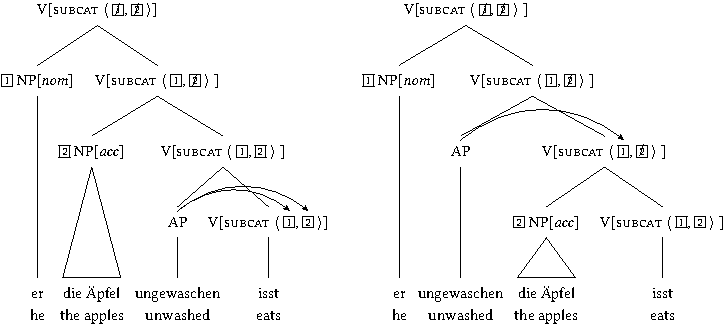
\includegraphics[width=\textwidth]{Figures/depictives-lsp-cropped.pdf}
%%  \resizebox{\linewidth}{!}{%
%% \begin{forest}
%% sm edges, for tree={l sep= 6ex}
%% [V{[\subcat \sliste{ \spirit{1}, \spirit{2} }]}
%% 	[\ibox{1} NP{[\textit{nom}]}
%% 		[er;he]]
%% 	[V{[\subcat \sliste{ \ibox{1}, \spirit{2} } ]}
%% 		[\ibox{2} NP{[\textit{acc}]}
%% 			[die Äpfel;the apples,triangle]]
%% 		[V{[\subcat \sliste{ \ibox{1}, \ibox{2} } ]}
%% 			[\subnode{ap1}{AP}
%% 				[ungewaschen;unwashed]]
%% 			[V{[\subcat \sliste{ \subnode{arg11}{\ibox{1}}, \subnode{arg12}{\ibox{2}} }]}
%% 				[isst;eats]]]]]
%% \end{forest}
%% \hspace{1em}
%% \begin{forest}
%% sm edges, for tree={l sep= 6ex}
%% [V{[\subcat \sliste{ \spirit{1}, \spirit{2} } ]}
%% 	[\ibox{1} NP{[\textit{nom}]}
%% 		[er;he]]
%% 	[V{[\subcat \sliste{ \ibox{1}, \spirit{2} } ]}
%% 		[\subnode{ap2}{AP}
%% 			[ungewaschen;unwashed]]
%% 		[V{[\subcat \sliste{ \subnode{arg21}{\ibox{1}}, \spirit{2} } ]}
%% 			[\ibox{2} NP{[\textit{acc}]}
%% 				[die Äpfel;the apples,triangle]]
%% 			[V{[\subcat \sliste{ \ibox{1}, \ibox{2} } ]}
%% 				[isst;eats]]]]]
%% \end{forest}
%% % This has to be inside of the scaling
%%     %% \begin{tikzpicture}[overlay,remember picture]
%%     %% %% this works with tikzmark
%%     %% \draw[->, bend angle=40, bend left] ($(pic cs:ap1)+(1ex,2ex)$) to($(pic cs:arg11)+(1ex,2.5ex)$);
%%     %% \draw[->, bend angle=40, bend left] ($(pic cs:ap1)+(1ex,2ex)$) to($(pic cs:arg12)+(1ex,2.5ex)$); % 1ex links, 2ex hoch
%%     %% %
%%     %% \draw[->, bend angle=40, bend left] ($(pic cs:ap2)+(1ex,2ex)$) to($(pic cs:arg21)+(1ex,2.5ex)$);
%%     %% \end{tikzpicture}
%% % somehow it stopped working
%% %% this used to work with subnode in texlive 2013 but is broken now
%% \begin{tikzpicture}[overlay,remember picture] 
%% \draw[->, bend angle=40, bend left] (ap1.north) to (arg11.north);
%% \draw[->, bend angle=40, bend left] (ap1.north) to (arg12.north); 
%% %
%% \draw[->, bend angle=40, bend left] (ap2.north) to (arg21.north);
%% \end{tikzpicture}
%}
%\hfill\mbox{}
\caption{dass er die Äpfel ungewaschen isst(\textsc{comp} 他 \textsc{art}.\textsc{def} 苹果 \, 没洗的 \, 吃)和dass er ungewaschen die Äpfel isst(\textsc{comp} 他 \, 没洗的 \textsc{art}.\textsc{def} 苹果 \, 吃)的分析}\label{anal-er-die-frau-nackt-sieht}
%\caption{Analysis of \emph{dass er die Äpfel ungewaschen isst} `that he the apples unwashed eats' and \emph{dass er ungewaschen die
%    Äpfel isst} `that he unwashed the apples eat'}\label{anal-er-die-frau-nackt-sieht}
\end{figure}%
已经实现的论元仍然在上面的结点上,但是它们已经被划掉了,因此被标注为realized(实现)。在德语中,要描述这个先行语名词的偏向可以通过假设一个限制,该限制的内容是先行语名词必须没有实现。
%Arguments that have been realized are still represented on the upper nodes, however, they are crossed"=out and thereby marked as ``realized''.
%In German, this preference for the antecedent noun can be captured by assuming a restriction that states that the antecedent noun must not yet have been
%realized.

在英语\ilce{英语}{English}中,普遍假设附加语与VP组合。
%It is commonly assumed for English\il{English} that adjuncts are combined with a VP.
\eal
\ex 
\gll John [[\sub{VP} ate the apples$_i$] unwashed$_i$].\\
	John {} 吃 \textsc{art}.\textsc{def} 苹果 没洗的\\
\mytrans{John吃了没洗的苹果。}
%John [[\sub{VP} ate the apples$_i$] unwashed$_i$].
\ex 
\gll You can't [[\sub{VP} give them$_i$ injections] unconscious$_i$].\\
	你 能.不 {} 给 他们 注射 无意识的\\
\mytrans{你不能无意识地给他们注射。}
%You can't [[\sub{VP} give them$_i$ injections] unconscious$_i$].
\footnote{%
 \citew[\page 17]{Simpson2003a}。
}
\zl
如果有一个方法允许VP结点中动词的论元是可及的,那么即使是先行语名词在VP之后,也可以在描述性谓词和论元之间建立关系。英语与德语的不同之处在于:描述性谓词可以指向已经实现的论元,如例 (\mex{0}b)中的them,以及尚未实现的论元,如例(\mex{0}b)中的you。
%In approaches where the arguments of the verb are accessible at the VP node, it is possible to establish a relation between
%the depictive predicate and an argument although the antecedent noun is inside the VP.
%English differs from German in that depictives can refer to both realized (\emph{them} in (\mex{0}b))
%and unrealized (\emph{you} in (\mex{0}b)) arguments.

 \citet[\page 560]{Higginbotham85a}和 \citet{Winkler97a}在\gbtc 中提出了对应的非"=划掉(non-cancellation)方法。在最简理论中也有类似的方法:已经检查过的特征不会被删除,但是会被标注为已经核查\citep[\page 14]{Stabler2010b}。但是,这些特征仍然被看作不可及。\label{page-non-cancellation-end}
% \citet[\page 560]{Higginbotham85a} and  \citet{Winkler97a} have proposed corresponding non"=cancellation approaches in \gbt.
%There are also parallel suggestions in Minimalist theories: checked features are not deleted, but instead marked as already
%checked \citep[\page 14]{Stabler2010b}. However, these features are still viewed as inaccessible.\label{page-non-cancellation-end}

取决于投射信息的精细程度,可以在嵌套结构中看到附加语和论元以及它们的语义、句法和语义特征。在Kay和Fillmore提出的CxG变体中,所有的信息都是可及的。在LFG中,关于语法功能、格和相近特征的信息是可及的。但是,词性并不包含在f"=结构中。如果词性与语法功能不是一一对应的关系,那么就不能用f"=结构来限制。语音信息也不在f"=结构中完全表征。如果对熟语的分析需要非局部地获取语音信息或词性信息,那么就必须明确地编码在f"=结构中(关于更多熟语的问题可以参见 \citew[\page 46--50]{Bresnan82a})。
%Depending on how detailed the projected information is, it can be possible to see adjuncts and argument in embedded structures as well as their
%phonological, syntactic and semantic properties. In the CxG variant proposed by Kay and Fillmore, all information is available. In LFG,
%information about grammatical function, case and similar properties is accessible. However, the part of speech is not contained in the f"=structure.
%If the part of speech does not stand in a one"=to"=one relation to grammatical function, it cannot be restricted using selection via f"=structure.
%Nor is phonological information represented completely in the f"=structure. If the analysis of idioms requires nonlocal access to phonological
%information or part of speech, then this has to be explicitly encoded in the f"=structure (see  \citew[\page 46--50]{Bresnan82a} for more on idioms). 

在我采用的HPSG版本中,只有论元的信息是可以投射的。因为论元一直通过类型\type{synsem}的描述来表征,所以无法保证其语音实现的信息。但是,在结构中有子结点,仍然可能像在TAG和构式语法中制定熟语的限制条件(参见 \citew{RS2009a}对(\ref{ex-ich-glaube-mich-tritt-ein-Pferd})中horse例子的分析)。这看起来多少有点像过度描述:我们仍然投射已经实现了的论元信息(不幸的是这些也包含论元的信息等)。就这点而言,有人可能更加倾向于TAG或者LFG,因为这些理论只是对局部性进行了部分扩展:TAG使用了任意大小或者更加准确地说是所需大小的树,而LFG使用完全f"=结构。但是事情好像没有这么简单:如果想在TAG中将描述性谓词与论元结合时创建与论元之间的关系,那么就需要所有可能的先行语的列表。句法因素(例如,关于与格 vs. 宾格名词短语,论元 vs.附加语,动词的并列 vs.名词的并列)在决定指称名词时非常重要,它无法通过语义关系来决定。与之相似,对于不同种类的熟语有不同的限制,并且这些都不能通过f"=结构的限制来描述,因为f"=结构不包括词性信息。\isce[|)]{描述性谓词}{depictive predicate}
%In the HPSG variant that I adopt, only information about arguments is projected. Since arguments are always represented by descriptions of type
%\type{synsem}, no information about their phonological realization is present. However, there are daughters in the structure so that it is still
%possible to formulate restrictions for idioms as in TAG or Construction Grammar (see  \citew{RS2009a}
%for an analysis of the `horse' example in (\ref{ex-ich-glaube-mich-tritt-ein-Pferd})).
%This may seem somewhat like overkill: although we already have the tree structure, we are still projecting information about arguments
%that have already been realized (unfortunately these also contain information about their arguments and so on). At this point, one could be inclined
%to prefer TAG or LFG since these theories only make use of one extension of locality: TAG uses trees
%of arbitrary or rather exactly the necessary size and LFG makes reference to a complete
%f"=structure. However, things are not quite that simple: if one wants to create a relation to an
%argument when adjoining a depictive predicate in TAG, then one requires a list of
%possible antecedents. Syntactic factors (\eg reference to dative vs.\ accusative noun phrases, to argument vs.\ adjuncts,
%coordination of verbs vs.\ nouns) play a role in determining the referent noun, this cannot be reduced to semantic relations.
%Similarly, there are considerably different restrictions for different kinds of idioms and these cannot all be formulated in terms of restrictions
%on f"=structure since f"=structure does not contain information about parts of speech.\is{depictive predicate|)}

需要注意很多现象需要借助更大的单位。大部分现象可以通过中心语统制或者扩展中心语统制,但是有熟语超越句子层面。每个理论都要或多或少地解释这个问题。\isce[|)]{局部性}{locality}\isce[|)]{习语}{idiom}
%One should bear in mind that some phenomena require reference to larger portions of structure. The majority of phenomena can be treated in terms of head
%domains and extended head domains, however, there are idioms that go beyond the sentence level. Every theory has to account for this somehow.
%\is{locality|)}\is{idiom|)}



%      <!-- Local IspellDict: en_US-w_accents -->

%% -*- coding:utf-8 -*-
\section{递归性}
%\section{Recursion}
\label{sec-recursion}

正如\isce[|(]{递归}{recursion}本书第\pageref{ex-that-max-thinks-that-recursion}页所述,本书中所有的理论都可以解决语言中的自我嵌套问题。例(\ref{ex-that-max-thinks-that-recursion})在这里重复为例(\mex{1}):
%Every\is{recursion|(} theory in this book can deal with self-embedding in language as it was
%discussed on page~\pageref{ex-that-max-thinks-that-recursion}. The example
%(\ref{ex-that-max-thinks-that-recursion}) is repeated here as (\mex{1}):
\ea
\label{ex-that-max-thinks-that-recursion-two}
\gll that Max thinks [that Julia knows [that Otto claims [that Karl suspects [that Richard confirms [that Friederike is laughing]]]]]\\
	\textsc{comp} Max 认为 \spacebr\textsc{comp} Julia 知道 \spacebr\textsc{comp} Otto 声称 \spacebr\textsc{comp} Karl 怀疑 \spacebr\textsc{comp} Richard 确认 \spacebr\textsc{comp} Friederike \textsc{aux} 笑\\
\mytrans{Max认为Julia知道Otto声称Karl怀疑Richard确认Friederike正在笑}
%that Max thinks [that Julia knows [that Otto claims [that Karl
%suspects [that Richard confirms [that Friederike is laughing]]]]]
\z
大部分理论通过嵌套短语结构规则或者统制图式来直接描述这一递归性。但是TAG\indextag 在处理递归性方面是特殊的,因为递归性被排除出了句法树。对应的效应是通过附加操作完成的,这种附加操作允许任意数量的成分插入到句法树中。有时会说构式语法\indexcxg 不能描述自然语言中存在的递归性(\egc \citealp[\page 269]{Leiss2009a})。对构式语法有这样的印象是可以理解的,因为很多分析都是表层导向的。例如,有人会经常谈到[Sbj TrVerb Obj]构式。但是,我们正谈论的构式只要包含句子嵌套或关系小句构式就会变得可以描述递归性了。一个句子嵌套构式可以有以下形式[Sbj that-Verb that-S],其中that-动词可以带句子型补足语,that-S代表相应的补语。that-小句就可以插入到that-S槽中。因为这个that小句也可以是使用这一构式的结果,所以语法也可以产生例(\mex{1})所示的句子:
%Most theories
%capture this directly with recursive phrase structure rules or dominance schemata. TAG\indextag is
%special with regard to recursion since recursion is factored out of the trees. The corresponding
%effects are created by an adjunction operation that allows any amount of material to be inserted
%into trees.  It is sometimes claimed that Construction Grammar\indexcxg cannot capture the existence
%of recursive structure in natural language (\eg \citealp[\page 269]{Leiss2009a}).  This impression
%is understandable since many analyses are extremely surface-oriented. For example, one often talks
%of a [Sbj TrVerb Obj] construction. However, the grammars in question also become recursive as soon
%as they contain a sentence embedding or relative clause construction. A sentence embedding
%construction could have the form [Sbj that-Verb that-S], where a that-Verb is one that can take
%a sentential complement and that-S stands for the respective complement. A \emph{that}-clause can then be inserted
%into the that-S slot. Since this \emph{that}-clause can also be the result of the application of
%this construction, the grammar is able to produce recursive structures such as those in (\mex{1}):

\ea
\gll Otto claims [\sub{that-S} that Karl suspects [\sub{that-S} that Richard sleeps]].\\
	Otto 声称 {} \textsc{comp} Karl 怀疑 {} \textsc{comp} Richard 睡觉\\
\mytrans{Otto声称Karl怀疑Richard睡觉。}
%Otto claims [\sub{that-S} that Karl suspects [\sub{that-S} that Richard sleeps]].
\z
在(\mex{0})中,Karl suspects that Richard sleeps和整个句子都是[Sbj that-Verb that-S]构式的实例。整个句子因此包含一个嵌套的子部分,这一子部分也被同样的构式允准。例 (\mex{0})也包含一个that-S范畴的成分,该成分嵌套在that-S中。关于构式语法中递归和自嵌套\isce{自嵌套}{self-embedding}的更多信息,可以参见 \citew{Verhagen2010a}。
%In (\mex{0}), both \emph{Karl suspects that Richard sleeps} and the entire clause are instances of the [Sbj
%that-Verb that-S] construction. The entire clause therefore contains an embedded subpart that is licensed by
%the same construction as the clause itself. (\mex{0}) also contains a constituent of the category
%\emph{that}-S that is embedded inside of \emph{that}-S. For more on recursion and self-embedding\is{self-embedding} in Construction Grammar, see  \citew{Verhagen2010a}.

与之相似,每一个允许名词与一个属格\iscesub{格}{case}{属格}{genitive}名词短语组合的构式语法也允许递归结构。相关构式可以有[DetNNP[gen]]或[NNP[gen]]形式。[DetNNP[gen]]构式允准例(\mex{1})所示的例子:
%Similarly, every Construction Grammar that allows a noun to combine with a genitive\is{genitive} noun phrase also allows
%for recursive structures. The construction in question could have the form [Det N
%NP[gen] ] or [ N NP[gen] ]. The [Det N NP[gen] ] construction licenses structures such as (\mex{1}):
\ea
\gll [\sub{NP} des Kragens [\sub{NP} des Mantels [\sub{NP} der Vorsitzenden]]]\\
	{} \defart{} 衣领 {} \defart{} 大衣 {} \defart{} 女主席\\
\mytrans{这位女主席的大衣的衣领}
%\gll [\sub{NP} des Kragens [\sub{NP} des Mantels [\sub{NP} der Vorsitzenden]]]\\
%	{} the collar {} of.the coat {} of.the chairwoman\\
%\mytrans{the collar of the coat of the chairwoman}
\z
 \citet{Jurafsky96a}和 \citet*{BLT2009a}使用概率上下文无关文法\iscesub{上下文无关文法}{context-free grammar}{概率上下文无关文法(PCFG)}{probabilistic (PCFG)} (PCFG)来构建一个聚焦于心理语言学可行性和习得模拟的构式语法分析器。上下文无关文法处理例(\mex{0}) 所示的自我嵌套\isce{自嵌套}{self-embedding}结构时没有问题,因此这类构式语法在处理自我嵌套时不会遇到任何问题。
% \citet{Jurafsky96a} and  \citet*{BLT2009a} use probabilistic context-free grammars\is{context-free grammar!probabilistic (PCFG)} (PCFG) for a Construction Grammar parser
%with a focus on psycholinguistic plausibility and modeling of acquisition. Context-free grammars
%have no problems with self-embedding\is{self-embedding} structures like those in (\mex{0}) and thus this kind
%of Construction Grammar itself does not encounter any problems with self-embedding.

 \citet[\page 192]{Goldberg95a}认为英语\ilce{英语}{English}的动结构式\iscesub{构式}{construction}{动结}{resultative}有以下形式:
% \citet[\page 192]{Goldberg95a} assumes that the resultative construction\is{construction!resultative} for English\il{English} has the following
%form:
\ea
{}[SUBJ [V OBJ OBL]] 
\z
这对应着TAG中基本树的复杂结构。LTAG与Goldberg的方法的差异在于每一个结构都需要一个词汇锚位,也就是说,例 (\mex{0})在LTAG中动词应该是固定的。但是在Goldberg的分析中,动词可以独立插入存在的构式中(见\ref{Abschnitt-Stoepselei})。在TAG的相关文献中,经常会强调初级树不包括任何递归。但是整个语法是递归的,因为其他成分可以通过附加插入到句法树中⸺正如例(\mex{-2})和(\mex{-1}) 所示⸺插入到替换项结点也可以产生递归结构。
\isce[|)]{递归}{recursion}
%This corresponds to a complex structure as assumed for elementary trees in TAG. LTAG differs from Goldberg's approach in that every structure requires a lexical
%anchor, that is, for example (\mex{0}), the verb would have to be fixed in LTAG. But in Goldberg's analysis, verbs can be inserted into independently
%existing constructions (see Section~\ref{Abschnitt-Stoepselei}). In TAG publications, it is often emphasized that elementary trees do not contain any recursion.
%The entire grammar is recursive however, since additional elements can be added to the tree using adjunction and -- as (\mex{-2}) and
%(\mex{-1}) show -- insertion into substitution nodes can also create recursive structures.
%\is{recursion|)}



%      <!-- Local IspellDict: en_US-w_accents -->


%% -*- coding:utf-8 -*-

\chapter{空成分}
%\chapter{Empty elements}
\label{Abschnitt-Diskussion-leere-Elemente}
\label{chap-empty}

这一章处理空成分,我首先讨论一下不同研究传统对于空成分的总体态度,然后再说明一下空成分怎样能从语法中取消(\ref{Abschnitt-Eleminierung-leerer-Elemente})。\ref{Abschnitt-leere-Elemente-Semantik}讨论了为有助于语义解释设置的空成分。\ref{Abschnitt-Evidenz-leere-Elemente}主要从跨语言对比的角度讨论了设置空成分的动因。最后,\ref{Abschnitt-leere-Elemente-LRs-Transformations}介绍了一些有关转换、词汇规则和空成分可以相互转换的观点。
%This chapter deals with empty elements, I first discuss the general attitude of various research
%traditions towards empty elements and then show how they can be eliminated from grammars
%(Section~\ref{Abschnitt-Eleminierung-leerer-Elemente}). Section~\ref{Abschnitt-leere-Elemente-Semantik} discusses empty elements that
%have been suggested in order to facilitate semantic
%interpretation. Section~\ref{Abschnitt-Evidenz-leere-Elemente} discusses possible motivation for
%empty elements with a special focus on cross"=linguistic comparison and the final Section~\ref{Abschnitt-leere-Elemente-LRs-Transformations} shows
%that certain accounts with transformations, lexical rules, and empty elements can be translated into each other.

\section{有关空成分的观点}
%\section{Views on empty elements}

本书\isc{空成分|(}\is{empty element|(}讨论的理论的支持者特别具有争议的一个问题是是否需要假设空成分。关于空成分的讨论由来已久:在1961年已经有关于短语结构语法\isc{短语结构语法}\is{phrase structure grammar}的研究\citep*{BHPS61a}。关于空成分地位的讨论从那时候就开始了(例如,可以参见\citealp*{Loebner86a,Wunderlich87d,Wunderlich89,Stechow89,Haider97a,Sag2000a,BMS2001a,LH2006a,Mueller2004e,AS2015a})。有时候假设空成分和不假设空成分的分析还存在实际语料上的差异(\citep{AS2015a}),但是通常情况下不是这样。因为空成分经常用作证据来支持或反对某些理论,这里我会更加详细地介绍它们是怎样运用的。
%One\is{empty element|(} point that is particularly controversial among proponents of the theories discussed in this book is the question of whether
%one should assume empty elements or not.\todostefan{Add arguments from wanna contraction} The discussion of empty elements is quite old: there was already some investigation in 1961 with reference
%to phrase structure grammars\is{phrase structure grammar} \citep*{BHPS61a}.
%The discussion of the status of empty elements has carried on ever since (see
%\citealp*{Loebner86a,Wunderlich87d,Wunderlich89,Stechow89,Haider97a,Sag2000a,BMS2001a,LH2006a,Mueller2004e,AS2015a}, for example). 
%There are sometimes empirical differences between analyses that assume empty elements and those that
%do not \citep{AS2015a}, but often this is not the case. Since empty elements often feature prominently in the argumentation for or against particular theories, I will discuss
%how they have been used in somewhat more detail here.

在\gbtc 中,空成分用于解释移位遗留下来的语迹(动词移位和短语前置)以及省略\isc{省略}\is{ellipsis}构式中删除的成分。从\citet{Larson88a}的分析开始,越来越多的空中心语被引入用于确保结构以及一些语义解释的一致性\isc{一致性}\is{uniformity} (约束\isc{约束理论}\is{Binding Theory}和辖域\isc{辖域}\is{s\textsc{cop}e},见\ref{sec-little-v}对于\littlevc 的论述)。其它用于确保特定概括的空成分还有\citet[\page 734]{Coopmans-89a-u}和\citet[Chapter~1]{Postal2004a-u}提出的虚位\isc{代词!虚位}\is{pronoun!expletive}。这些空成分填充了英语\il{英语}\il{English}中倒置\isc{倒置}\is{inversion}结构的主语位置,动词之前的位置被一个PP而不是一个明显的主语NP占据。与此相似,\citet[\page 1311]{Grewendorf93}认为无人称被动句\isc{被动句!无人称的}\is{passive!impersonal}和没有主语移位的被动句中的主语位置实际上都是由一个空虚位所占据。也可以参见\citew[\page 91]{Newmeyer2005a}和\citet[\page 180]{Lohnstein2014a}采用同样假设对于德语被动句的分析。\citet[\S~II.3.3.3]{Sternefeld2006a-u}认为在例(\mex{1})中,无人称被动句和无主语句都有一个空虚位。
%In \gbt, empty elements were assumed for traces of movement (verb movement and fronting of phrases) as well as for deleted elements in 
%elliptical\is{ellipsis} constructions. Starting with the analysis of \citet{Larson88a}, more and more empty heads have been introduced to ensure uniformity\is{uniformity} of structures and 
%certain semantic interpretations (binding\is{Binding Theory}
%and s\textsc{cop}e\is{s\textsc{cop}e}, see Section~\ref{sec-little-v} on \littlev). Other examples of an empty element that was introduced in order to maintain particular generalizations are the empty expletives\is{pronoun!expletive}
%of \citet[\page 734]{Coopmans-89a-u} and \citet[Chapter~1]{Postal2004a-u}. These fill the subject
%position in inversion\is{inversion} structures in English\il{English}, where the position preceding
%the verb is occupied by a PP and not by an overt subject NP. Similarly, \citet[\page
%  1311]{Grewendorf93} assumes that the subject position in impersonal
%passives\is{passive!impersonal} and passives without subject movement is in fact occupied by an
%empty expletive. Also, see
%\citew[\page 91]{Newmeyer2005a} and \citet[\page 180]{Lohnstein2014a} for this assumption with regard to the passive
%in German. \citet[Section~II.3.3.3]{Sternefeld2006a-u} assumes that there is an empty expletive subject in impersonal passives and subjectless sentences such as (\mex{1}).
\eal
\ex 
\gll Mir graut.\\
	 我.\dat{} 惊吓\\
\glt `我受到惊吓。'
%\gll Mir graut.\\
%	 me.\dat{} scares\\
%\glt `I am scared.'
\ex 
\gll Mich dürstet.\\
	我.\acc{} \textsc{cop}.渴\\
\glt `我渴。'
%\gll Mich dürstet.\\
%	 me.\acc{} is.thirsty\\
%\glt `I am thirsty.'
\zl

\noindent
在第~\pageref{Beispiel-leeres-Element-intransitive-Verben}页,我们讨论了Stabler对于包含不及物动词句子的分析。因为,按照\citet[\page 146]{Chomsky2008a},首先与中心语组合的是补语,不及物动词对该理论提出了挑战。Stabler通过假设不及物动词与一个空宾语组合解决了这一问题\citep[\page 61,124]{Veenstra98a}。因为这些不发音的成分对某一表达的意义没有贡献,所以我们也处理了虚位代词。
%On page~\pageref{Beispiel-leeres-Element-intransitive-Verben}, we discussed Stabler's proposal for the analysis of sentences with intransitive
%verbs. Since, following  \citet[\page 146]{Chomsky2008a}, the element that first merges with a head is the complement, intransitive verbs pose a problem for the
%theory. This problem is solved by Stabler by assuming that intransitive verbs are combined with an empty object \citep[\page 61,
%124]{Veenstra98a}. Since these silent elements do not contribute to the meaning of an expression, we are also dealing with empty expletive pronouns.

\addlines
在其他理论中,有人研究反对空成分也有人赞成空成分。在范畴语法\indexcgc 中,Steedman提出了一种不借助空成分的方式来分析非局部依存(见\ref{sce-nld-cg}),但是正如\citet{Pollard88a}指出的那样,Steedman的分析需要为NP提供多种类型提升\isc{类型提升}\is{type raising}或者需要为关系代词\isc{代词!关系}\is{pronoun!relative}提供一个相比大量的复杂词项(见\ref{Abschnitt-CG-UDC})。另一方面,\citet{KoenigE99a-u}使用语迹。在\ref{Abschnitt-GPSG-Fernabhaengigkeiten},我们曾经讨论过,在GPSG\indexgpsgc 中,\citet[\page 76--77]{Uszkoreit87a}提出了一个不用语迹的对于提取\isc{提取}\is{extraction}的分析,但是\citet*[\page 143]{GKPS85a}的分析却使用语迹。在LFG\indexlfgc 中,也有人用语迹\citep[\page 67]{Bresnan2001a},也有人不用(\ref{Abschnitt-Verbstellung-LFG}和\ref{Abschnitt-NLA-LFG})。HPSG\indexhpsgc 中的很多短语分析都起源于避免使用空成分(见\ref{Abschnitt-Phrasale-Konstruktionen})。例如,\citet{Sag97a}对关系小句的分析,该分析用相应的短语规则代替了\citew{ps2}所用的空关系化标记。在另一方面,\citew{Bender2000a}和\citew*[\page 464]{SWB2003a}却假设了一个空系词\isc{系词}\is{\textsc{cop}ula}。另外一个想要从HPSG中清除空成分的例子是用词库而不是语迹来描写长距离依存\citep*{BMS2001a}。但是,正如 \citet{LH2006a}所展示的,用词汇手段引入长距离依存的提取理论在处理并列结构的语义解释时有问题。关于如何解决这一问题,见\citew{Chaves2009a}。有很多TAG分析\indextagc 没有在词库中包含空成分(例如,可以参见\ref{TAG-Fernabh}和\citew{Kroch87a}),但是也存在\citet[\page 194]{Kallmeyer2005a-u}的TAG分析,假设一个语迹来给包含动词复杂体的句子中的成分进行重新排序。\citet[\page 10--11]{Rambow94a}假设每一个动词短语中都有一个空动词(见\ref{sec-vtag}对于V"=TAG\isc{树邻接语法 (TAG)!向量 (V-TAG)}\is{Tree Adjoining Grammar (TAG)!Vector (V-TAG)}的论述) 。\footnote{
注意TAG中的空成分与其它理论中的空成分有细微差异。在TAG中,空成分通常是初级树的一部分,即它们不与其它成分组合。  
}在依存语法中,\mel (\citeyear[\page 303]{Melcuk88a-u};\citeyear[\page 219]{Melcuk2003a-u})、\citet[\page 253]{Starosta88a-u}、\citet[\page 471--472]{Eroms2000a}、Hudson(\citeyear[\S~3.7]{Hudson2007a-u}、\citeyear[\page 166]{Hudson2010b-u})和\citet{Engel2014a}为指定语、名词、省略、祈使句、控制不定式和并列结构假设了空成分,但是\citet[\page 73]{GO2009a}反对空成分(省略现象是例外\citealp{Osborne2016a-u})。
%In other theories, there are researchers that reject empty elements as well as those who assume them.
%In Categorial Grammar\indexcg, Steedman suggests an analysis of nonlocal dependencies that does
%without empty elements (see Section~\ref{sce-nld-cg}), but as \citet{Pollard88a} has shown,
%Steedman's analysis requires various kinds of type raising\is{type raising}
%for NPs or a correspondingly high number of complex lexical items for relative pronouns\is{pronoun!relative} (see Section~\ref{Abschnitt-CG-UDC}). On the other hand,
%\citet{Koenig99a-u} uses\todostefan{andere Quellen?}
%traces. In GPSG\indexgpsg, there is the trace"=less analysis of extraction\is{extraction} by \citet[\page 76--77]{Uszkoreit87a} that we discussed in 
%Section~\ref{Abschnitt-GPSG-Fernabhaengigkeiten}, but there is also the analysis of \citet*[\page 143]{GKPS85a} that uses traces. In LFG\indexlfg, there are both analyses with
%traces \citep[\page 67]{Bresnan2001a} and those without (see Section~\ref{Abschnitt-Verbstellung-LFG} and Section~\ref{Abschnitt-NLA-LFG}). 
%Many of the phrasal analyses in HPSG\indexhpsg are born out of the wish to avoid empty elements (see Section~\ref{Abschnitt-Phrasale-Konstruktionen}). 
%An example for this is the relative clause analysis by \citet{Sag97a} that replaces the empty
%relativizer in \citew{ps2} with a corresponding phrasal rule. On the other hand we have
%\citew{Bender2000a} and \citew*[\page 464]{SWB2003a}, who assume a silent \textsc{cop}ula\is{\textsc{cop}ula}. Another attempt to eliminate empty elements from HPSG was to handle
%long"=distance dependencies not by traces but rather in the lexicon \citep*{BMS2001a}. As \citet{LH2006a} could show, however, theories of extraction that
%introduce long"=distance dependencies lexically have problems with the semantic interpretation of coordinate structures. For a suggestion of how to solve these problems,
%see \citew{Chaves2009a}. There are many TAG analyses\indextag without silent elements in the lexicon (see Section~\ref{TAG-Fernabh} and \citew{Kroch87a}, for example),
%however there are variants of TAG such as that of \citet[\page 194]{Kallmeyer2005a-u}, where a trace is assumed for the reordering of constituents in sentences with
%a verbal complex. \citet[\page 10--11]{Rambow94a} assumes an empty head in every verb
%phrase (see Section~\ref{sec-vtag} on V"=TAG\is{Tree Adjoining Grammar (TAG)!Vector (V-TAG)}).\footnote{
%  Note that empty elements in TAG are slightly different from empty elements in other theories. In
%  TAG the empty elements are usually part of elementary trees, that is, they are not lexical items that are
%  combined with other material.
%}
%In Dependency Grammar, \mel (\citeyear[\page 303]{Melcuk88a-u}; \citeyear[\page 219]{Melcuk2003a-u}),
%\todostefan{S: It is possible to introduce empty nodes in a DT if you want. It has been done for
%  gapping by Tesnière or for agreement by Melcuk (1988:303)}
%\todostefan{O: Starosta 1988:253, Eroms 2000:472, Melcuk 2003:219, Hudson (2007:172-182, 2010)}
%\citet[\page 253]{Starosta88a-u}, \citet[\page 471--472]{Eroms2000a}, Hudson (\citeyear[Section~3.7]{Hudson2007a-u}; \citeyear[\page 166]{Hudson2010b-u}) and
%\citet{Engel2014a} assume empty elements for determiners, nouns, ellipsis, imperatives, controlled infinitives, and for coordinate
%structures, but \citet[\page 73]{GO2009a} reject empty elements (with the exception of ellipsis, \citealp{Osborne2016a-u}).

构式语法中不假设空成分\indexcxgc\label{Seite-leere-Elemente-CxG} (\citealp[\page 49--50]{MR2001a};\citealp[\page 219]{Goldberg2003b};\citealp[\page 10]{Goldberg2006a}),相关的更简语法\citep{CJ2005a}也不假设空成分,认知语法\isc{认知语法}\is{Cognitive Grammar}也不假设空成分 。\footnote{
  但是,Fillmore(1988:5)并没有排除空成分。
}不假设空成分主要有以下几点原因:
%No empty elements are assumed in Construction Grammar\indexcxg\label{Seite-leere-Elemente-CxG} (\citealp[\page 49--50]{MR2001a}; \citealp[\page
%219]{Goldberg2003b}; \citealp[\page 10]{Goldberg2006a}), the related Simpler Syntax \citep{CJ2005a} as well as in Cognitive Grammar\is{Cognitive Grammar}.\footnote{
% However, \citet[\page 51]{Fillmore88a} did not rule them out.
%} 
%The argumentation against empty elements runs along the following lines:
\begin{enumerate}
\item 没有证据可以证明不可见的对象。
%\item There is no evidence for invisible objects.
\item 没有天赋语言学知识。
%\item There is no innate linguistic knowledge.
\item 因此,关于空成分的知识不能被习得,所以不能假设它们是语法的一部分。
%\item Therefore, knowledge about empty elements cannot be learned, which is why they cannot be assumed
%as part of our grammar.
\end{enumerate}
这取决于得出结论的所有前提是不是正确。如果我们考虑例(\mex{1})所示的省略构式,很清楚这里省略了一个名词:
%This begs the question of whether all the premises on which the conclusion is based actually hold. If we consider an elliptical
%construction such as (\mex{1}), then it is clear that a noun has been omitted:
\ea
\gll Ich nehme den roten Ball und du den blauen.\\
	 我 拿 \textsc{det}.\acc{} 红的.\acc{} 球 并且 你 \textsc{det}.\acc{} 蓝.\acc{}\\
\glt `我将拿这个红色的球,你拿这个蓝色的。'
%\gll Ich nehme den roten Ball und du den blauen.\\
%	 I take the.\acc{} red.\acc{} ball and you the.\acc{} blue.\acc{}\\
%\glt `I'll take the red ball and you take the blue one.'
\z
虽然在den blauen(蓝色的)中没有名词,但是这组词在句法和语义上都像一个名词短语。当然(\mex{0})不一定是存在空成分的证据,因为完全可以简单地说den blauen(蓝色的)是一个包含一个冠词和一个形容词的名词短语\citep{Wunderlich87d}。
%Despite there being no noun in \emph{den blauen} `the blue', this group of words behaves both syntactically and semantically just like a noun
%phrase. (\mex{0}) is of course not necessarily evidence for there being empty elements, because one could simply say that \emph{den blauen}
%is a noun phrase consisting only of an article and an adjective \citep{Wunderlich87d}. 

与可以理解(\mex{0})中丢失了一个名词这一事实一样,说英语的人知道like(喜欢)后面也丢失了一些成分:
%Similar to the fact that it is understood that a noun is missing in (\mex{0}), speakers of English know that something is missing after
%\emph{like}: 
\ea
%Bagels, I like.
\gll Bagels, I like.\\
	 Bagels 我 喜欢\\
\glt `Bagels,我喜欢。'
\z
每一种语法理论或多或少地都要解释这些事实。必须用某种方式来表征(\mex{0})中的like(喜欢)的行为就像一个丢失了某些成分的动词短语。其中一种可能是使用语迹。\citet*[\page 153, \S~4.1]{BHPS61a}展示出,可以将带有空成分的短语结构语法转变成没有空成分的样子。在很多情况下,同样的技术可以用于这里展示的其它理论,我们会在下面的小节详细讨论这一点。
%Every theory of grammar has to somehow account for these facts. It must be represented in some way that \emph{like} in (\mex{0}) behaves
%just like a verb phrase that is missing something. One possibility is to use traces. \citet*[\page 153, Lemma~4.1]{BHPS61a} 
%have shown that it is possible to turn phrase structure grammars with empty elements into those without any.
%In many cases, the same techniques can be applied to the theories presented here and we will therefore discuss the point in more detail
%in the following section.

\section{从语法中取消空成分}
%\section{Eliminating empty elements from grammars}
\label{Abschnitt-Eleminierung-leerer-Elemente}

我们可以通过以下方式来将带有空成分(也叫epsilon\isc{epsilon}\is{epsilon})的语法转变成没有空成分的语法。需要去掉每一条规则中所有可以用空成分重写的范畴,并且向语法中增加没有空成分的相应规则。下面的例子就有一条为np写的空成分规则。所以需要用没有np符号的新规则来代替所有包含np符号的规则。(\mex{2})显示了(\mex{1})中语法转变的结果:
%It is possible to turn a grammar with empty elements (also called \emph{epsilon}\is{epsilon}) into a
%grammar without these by removing all categories that can be rewritten by an epsilon in every rule
%that uses such categories and then add the respective rules without the empty elements to the grammar. The following example has an epsilon rule for np. One therefore has to
%replace all rules containing the symbol np with new rules without this np symbol. (\mex{2}) shows
%the result of this conversion of the grammar in (\mex{1}):

\ea
\label{ex-grammar-eps-head}
\begin{tabular}[t]{@{}l@{~$\to$~}l@{}}
\baro{v}   & \mbox{np}, v\\
\baro{v}   & \mbox{np}, pp, v\\
np & $\epsilon$\\
\end{tabular}
\z

\ea
\label{ex-grammar-head}
\begin{tabular}[t]{@{}l@{~$\to$~}l@{}}
\baro{v}   & \mbox{np}, v\\
\baro{v}   & v\\
\baro{v}   & \mbox{np}, pp, v\\
\baro{v}   & \mbox{pp}, v\\
\end{tabular}
\z
这也可能导致一条规则右手边的所有成分都被移除。那么,做的事实际上是产生一个新的空范畴,然后必须再次使用各自替换过程。我们一会会看一个这种例子。看(\mex{-1})--(\mex{0})这一对语法,很清楚虽然两者允准相同的符号序列,但是相比于(\mex{-1}), (\mex{0})的规则数量更多。NP论元可以省略这一事实在(\mex{0})中没有直接表现出来,而是包含在两条规则中。
%This can also lead to cases where all elements on the right"=hand side of a rule are removed. Thus,
%what one has done is actually create a new empty category and then one has to apply the respective
%replacement processes again. We will see an example of this in a moment. Looking at the pair of
%grammars in (\mex{-1})--(\mex{0}), it is clear that the number of rules has increased in (\mex{0})
%compared to (\mex{-1}) despite the grammars licensing the same sequences of symbols. The fact that
%an NP argument can be omitted is not expressed directly in (\mex{0}) but instead is implicitly contained in two rules. 

如果将这一程序应用于第\ref{Kapitel-HPSG}章中的HPSG\indexhpsgc 语法,那么语迹就不会有一个像NP一样的具体范畴。语迹只会与一个非中心语子节点兼容。正如例(\mex{1})所示,附接语、论元和动词复杂成分的一部分都可以被提取。
%If one applies this procedure to the HPSG\indexhpsg grammar in Chapter~\ref{Kapitel-HPSG}, then the
%trace does not have a specific category such as NP. The trace simply has to be compatible with a
%non"=head daughter. As the examples in (\mex{1}) show, adjuncts, arguments and parts of verbal
%complexes can be extracted.
\eal
\ex 
\gll Er$_i$ liest t$_i$ die Berichte.\\
	 他 读 {}    \textsc{det} 报告\\
%\gll Er$_i$ liest t$_i$ die Berichte.\\
%	 he reads {}    the reports\\
\ex 
\gll Oft$_i$ liest er die Berichte t$_i$ nicht.\\
	 经常 读 他 \textsc{det} 报告 {} NEG\\
\glt `他经常不读报告。'
%\gll Oft$_i$ liest er die Berichte t$_i$ nicht.\\
%	 often reads he the reports {} not\\
%\glt `Often, he does not read the reports.'
\ex 
\gll Lesen$_i$ wird er die Berichte t$_i$ müssen.\\
	 读书 \textsc{aux} 他 \textsc{det} 报告 {} \textsc{aux}\\
\glt `他将必须阅读这些报告。'
%\gll Lesen$_i$ wird er die Berichte t$_i$ müssen.\\
%	 read will he the reports {} must\\
%\glt `He will have to read the reports.'
\zl

\noindent
相关成分在一个特定模式(中心语-论元模式、中心语-附接语模式、谓词复杂形式模式)中与它们的中心语组合。最前面两个模式可以参见第\ref{Kapitel-HPSG}章;谓词复杂图式的具体动因见 Müller (\citeyear[\S~2]{Mueller2002b};\citeyear[\S~15]{MuellerLehrbuch1})。如果想要不使用语迹,那么需要描述附接语、论元和谓词复杂形式的部分前置需要另外的模式。图~\vref{Abbildung-Kopf+Spur}给出了中心语与语迹结合的例子。图~\vref{Abbildung-Kopf-ohne-Spur}展示了没有语迹的分析。
%The relevant elements are combined with their head in a specific schema (Head"=Argument Schema, Head"=Adjunct Schema,
%Predicate Complex Schema). See Chapter~\ref{Kapitel-HPSG} for the first two schemata; the Predicate Complex Schema is
%motivated in detail in Müller (\citeyear[Chapter~2]{Mueller2002b};
%\citeyear[Chapter~15]{MuellerLehrbuch1}). If one wishes to do without traces, then one needs further additional schemata for the fronting of adjuncts, of arguments and of parts of predicate
%complexes. The combination of a head with a trace is given in Figure~\vref{Abbildung-Kopf+Spur}. The
%trace"=less analysis is shown in Figure~\vref{Abbildung-Kopf-ohne-Spur}.
\begin{figure}
\centering
\begin{forest}
sm edges
[ V\feattab{\subcat \sliste{ NP[\type{nom}] },\\
             \textsc{inher$|$slash} \sliste{ \ibox{1} }}\\
  [{\ibox{4} \feattab{
                \textsc{loc} \ibox{1},\\
                \textsc{inher$|$slash} \sliste{ \ibox{1} }}} [\trace]]
  [V\feattab{
                \subcat \sliste{ NP[\type{nom}], \ibox{4} NP[\type{acc}] }} [liest;reads]]]
\end{forest}
\caption{\label{Abbildung-Kopf+Spur}使用语迹分析长距离依存的信息介绍}
%\caption{\label{Abbildung-Kopf+Spur}Introduction of information about long"=distance dependencies with a trace}
\end{figure}%
在\ref{Abbildung-Kopf+Spur}中,kennen的\subcatlc 的成分与语迹\ibox{4}的\synsemvc  取值一致。语迹的词项指定语迹的\locvc 取值应该与\textsc{inher$|$slash}列表中元素一致。
%In Figure~\ref{Abbildung-Kopf+Spur}, the element in the \subcatl of \emph{kennen} is identified with the \synsemv of the trace \ibox{4}.
%The lexical entry of the trace prescribes that the \locv of the trace should be identical to  the element in the \textsc{inher$|$slash} list.

非局部特征原则(第~\pageref{Prinzip-der-Nichtlokalen-Merkmale}页)确保\slaschc 信息可以在父节点表征。因为一个论元位置在中心语-论元结构中达到饱和,受格宾语就不再包含在父节点的\subcatlc 列表中。
%The Non"=Local Feature Principle (page~\pageref{Prinzip-der-Nichtlokalen-Merkmale}) ensures that the \slasch information is present on the
%mother node. Since an argument position gets saturated in Head"=Argument structures, the accusative object is no longer contained in the
%\subcatl of the mother node.
图~\ref{Abbildung-Kopf-ohne-Spur}展示了等同于没有语迹的结构。
%Figure~\ref{Abbildung-Kopf-ohne-Spur} shows the parallel trace"=less structure.
\begin{figure}
\centering
\begin{forest}
sm edges
[{V\feattab{
                                    \subcat \sliste{ NP[\type{nom}] },\\
                                    \textsc{inher$|$slash} \sliste{ \ibox{1} } }}\\
    [V\feattab{
                                             \subcat \sliste{ NP[\type{nom}], NP\ibox{1}[\type{acc}] }}\\
          [liest;reads]]]
\end{forest}
\caption{\label{Abbildung-Kopf-ohne-Spur}使用单分支投射分析长距离依存的信息介绍}
%\caption{\label{Abbildung-Kopf-ohne-Spur}Introduction of information about long"=distance dependencies using a unary projection}
\end{figure}%
在中心语"=论元结构中,在论元位置组合一个语迹产生的效应可以在图~\ref{Abbildung-Kopf-ohne-Spur}中的父节点表征:受格宾语的 \locvc 与父节点\textsc{inher$|$slash}中的成分一致并且受格宾语不再出现在价列表上。
%The effect that one gets by combining a trace in argument position in Head"=Argument structures is represented directly
%on the mother node in Figure~\ref{Abbildung-Kopf-ohne-Spur}: the \locv of the accusative object was identified with the element in
%\textsc{inher$|$slash} on the mother node and the accusative object does not occur in the valence list any more.

\largerpage
第\ref{Kapitel-HPSG}章所呈现的语法包含另外一个空成分:一个动词语迹。这一语迹也必须要消除。
%The grammar presented in Chapter~\ref{Kapitel-HPSG} contains another empty element: a verb trace. This would then also have to be
%eliminated.

\eal
\ex 
\gll Er$_i$ liest$_j$ t$_i$ die Berichte t$_j$.\\
	 他 读 {}    \textsc{det} 报告\\
%\gll Er$_i$ liest$_j$ t$_i$ die Berichte t$_j$.\\
%	 he reads {}    the reports\\
\ex 
\gll Oft$_i$ liest$_j$ er die Berichte t$_i$ nicht t$_j$.\\
	经常 读 他 \textsc{det} 报告 {} NEG\\
\glt `他经常不读这些报告。'
%\gll Oft$_i$ liest$_j$ er die Berichte t$_i$ nicht t$_j$.\\
%	 often reads he the reports {} not\\
%\glt `Often, he does not read the reports.'
\ex 
\gll Lesen$_i$ wird$_j$ er die Berichte t$_i$ müssen t$_j$.\\
	 读 \textsc{aux} 他 \textsc{det} 报告 {} \textsc{aux}\\
\glt `他将必须读这些报告。'
%\gll Lesen$_i$ wird$_j$ er die Berichte t$_i$ müssen t$_j$.\\
%	 read will he the reports {} must\\
%\glt `He will have to read the reports.'
\zl

\noindent
图~\vref{Abbildung-Kopf+Verbspur}展示了一个动词语迹与一个受格宾语的组合。
%Figure~\vref{Abbildung-Kopf+Verbspur} shows the combination of a verb trace with an accusative object.
\begin{figure}
\centering
\begin{forest}
sm edges
[V\feattab{
                                    \textsc{head$|$dsl} \ibox{1},\\
                                    \subcat \ibox{2} }
   [{\ibox{3} NP[\type{acc}]}
     [ die Berichte;the reports, roof] ]
   [V\ibox{1}\feattab{
                    \textsc{head$|$dsl} \ibox{1},\\
                    \subcat \ibox{2} $\oplus$ \sliste{ \ibox{3} NP[\type{acc}] }} 
     [\trace]]]
\end{forest}
\caption{\label{Abbildung-Kopf+Verbspur}使用动词语迹对动词位置展开的分析}
%\caption{\label{Abbildung-Kopf+Verbspur}Analysis of verb position with verb trace}
\end{figure}%
动词语迹被指定了,所以\dslvc 与语迹的\locvc 是一致的(见第\pageref{le-verbspur} 页)。因为\dslc 是一个中心语特征,所以相应取值也可以出现在父节点上。图~\vref{Abbildung-Kopf-ohne-Verbspur}展示了一个我们省略了空节点得到的结构。
%The verb trace is specified such that the \dslv is identical to the \locv of the trace (see
%p.\,\pageref{le-verbspur}). Since \dsl is a head feature, the corresponding value is also present on
%the mother node. Figure~\vref{Abbildung-Kopf-ohne-Verbspur} shows the structures that we get by omitting the empty node.
\begin{figure}
\centering
\begin{forest}
sm edges, for tree={l sep= 5ex}
[ V\feattab{
     \textsc{head$|$dsl} V[\subcat \ibox{2} $\oplus$ \sliste{ \ibox{3} NP[\type{acc}] }],\\
     \subcat \ibox{2}} 
   [{\ibox{3} NP[\type{acc}]}
      [die Berichte;the reports, roof]]]
\end{forest}
\caption{\label{Abbildung-Kopf-ohne-Verbspur}使用单分支投射对动词位置进行的分析}
%\caption{\label{Abbildung-Kopf-ohne-Verbspur}Analysis of verb position using a unary projection}
\end{figure}%
这个结构初看起来可能会有点奇怪,因为一个名词短语投射成为一个动词(见第~\pageref{Abb-Verbstellung-LFG}页,相似的LFG\indexlfgc 中没有动词的结构)。在这一结构中丢失了一个动词这一事实可以包括在这一结构中,就像带有动词语迹的结构一样。\dslvc 确定了图~\ref{Abbildung-Kopf-ohne-Verbspur}结构能够出现的语境。这一取值与图~\ref{Abbildung-Kopf+Verbspur}中的取值是一致的,并且包括以下信息:需要一个受格宾语的动词在当前论述的结构中丢失了。到现在为止,我们已经看到提取语迹可以通过设定三条额外的规则而取消。相似地,对于动词语迹来说需要三条新规则。不幸的是,问题到这里还没解决,因为提取语迹和中心语移位也可以互动。例如,图~\ref{Abbildung-Kopf-ohne-Verbspur}中的句法树中的NP可以是一个提取语迹。因此,语迹的组合可以产生更多的空成分,这些空成分也必须消除。因为我们有三条新的模式,所以如果我们将非中心语子节点与一个提取语迹组合以及一个中心语子节点与一个动词语迹组合的话就会有三个新的空成分。(\mex{1}) 展示了这些情况:
%This structure may look odd at first sight since a noun phrase is projected to a verb (see page~\pageref{Abb-Verbstellung-LFG} 
%for similar verb"=less structures in LFG\indexlfg). The information about the fact that a verb is missing in the structure
%is equally contained in this structure as in the structure with the verb trace. It is the \dslv that is decisive for the contexts in which
%the structure in Figure~\ref{Abbildung-Kopf-ohne-Verbspur} can appear. This is identical to the value in Figure~\ref{Abbildung-Kopf+Verbspur} and contains
%the information that a verb that requires an accusative object is missing in the structure in question.
%Until now, we have seen that extraction traces can be removed from the grammar by stipulating three additional rules. Similarly, three new rules
%are needed for the verb trace. Unfortunately, it does not stop here as the traces for extraction and
%head movement can also interact. For example, the NP in the tree in 
%Figure~\ref{Abbildung-Kopf-ohne-Verbspur} could be an extraction trace. Therefore, the combination of traces can result in more empty elements that then
%also have to be eliminated. Since we have three schemata, we will have three new empty elements if we combine the non"=head daughter with an extraction
%trace and the head daughter with a verb trace. (\mex{1}) shows these cases:
\eal\settowidth\jamwidth{(Extraction trace (argument) $+$ verb trace)}
\ex 
\gll Er$_i$    [schläft$_j$ t$_i$ t$_j$].\\
	 他 \spacebr{}睡\\  \jambox{(提取语迹 (论元) $+$ 动词语迹)}
\glt `他正在睡觉。'
%\gll Er$_i$    [schläft$_j$ t$_i$ t$_j$].\\
%	 he \spacebr{}sleeps\\  \jambox{(Extraction trace (argument) $+$ verb trace)}
%\glt `He is sleeping.'
\ex 
\gll Jetzt$_i$ [schlaf$_j$ t$_i$ t$_j$]!\\
	 现在 \spacebr{}睡觉\\   \jambox{(提取语迹 (附接语)  $+$ 动词语迹)}
\glt `现在去睡觉!'
%\gll Jetzt$_i$ [schlaf$_j$ t$_i$ t$_j$]!\\
%	 now \spacebr{}sleep\\   \jambox{(Extraction trace (adjunct)  $+$ verb trace)}
%\glt `Go to sleep now!'
\ex 
\gll Geschlafen$_i$ [wird$_j$ t$_i$ t$_j$]! \\
	 睡觉 \spacebr{}\textsc{aux}\\\jambox{(提取语迹 (复杂) $+$ 动词语迹)}
\glt `现在是时候去睡觉了!'
%\gll Geschlafen$_i$ [wird$_j$ t$_i$ t$_j$]! \\
%	 slept \spacebr{}is\\\jambox{(Extraction trace (complex) $+$ verb trace)}
%\glt `Now is time to sleep!'
\zl
这三个新语迹可以作为非中心语子节点出现在中心语"=论元模式中,并且因此需要为中心语"=论元结构设置三个新的模式。使用这些模式,就可以分析(\mex{0})中的句子。
%These three new traces can occur as non"=head daughters in the Head"=Argument Schema and thus one would require
%three new schemata for Head"=Argument structures. Using these schemata, it then becomes possible to analyze
%the sentences in (\mex{0}).

为了描述(\mex{1})和(\mex{2})中的例子,需要另外6条模式,因为这三个新语迹都可以作为中心语出现在中心语"=论元结构 (\mex{1})和中心语"=附接语结构(\mex{2})中:
%Six further schemata are required for the examples in (\mex{1}) and (\mex{2}) since the three new traces can each occur
%as heads in Head"=Argument structures (\mex{1}) and Head"=Adjunct structures (\mex{2}):
\eal
\ex 
\gll Den Aufsatz$_i$ liest$_j$ [er t$_i$ t$_j$].\\
	\textsc{det} 散文 读 \spacebr{}他\\
\glt `他正在读这篇散文。'
%\gll Den Aufsatz$_i$ liest$_j$ [er t$_i$ t$_j$].\\
%	 the essay reads \spacebr{}he\\
%\glt `He is reading the essay.'
\ex 
\gll Oft$_i$ liest$_j$ er [ihn t$_i$ t$_j$].\\
	 经常 读 他 \spacebr{}它\\
\glt `他经常读它。He often reads it.'
%\gll Oft$_i$ liest$_j$ er [ihn t$_i$ t$_j$].\\
%	 often reads he \spacebr{}it\\
%\glt `He often reads it.'
\ex 
\gll Lesen$_i$ wird$_j$ er [ihn t$_i$ t$_j$].\\
	读 \textsc{aux} 他 \spacebr{}它\\
\glt `他将会读它。'
%\gll Lesen$_i$ wird$_j$ er [ihn t$_i$ t$_j$].\\
%	 read will he \spacebr{}it\\
%\glt `He will read it.'
\zl
\eal
\ex 
\gll Den Aufsatz$_i$ liest$_j$ er [nicht t$_i$ t$_j$].\\
	\textsc{det} 散文 读 他 \spacebr{}NEG\\
\glt `他现在没有读这篇散文。'
%\gll Den Aufsatz$_i$ liest$_j$ er [nicht t$_i$ t$_j$].\\
%	 the essay reads he \spacebr{}not\\
%\glt `He isn't reading the essay.'
\ex 
\gll Oft$_i$ liest$_j$ er ihn [nicht t$_i$ t$_j$].\\
	 经常 读 他 它 \spacebr{}not\\
\glt `他经常不读它。'
%\gll Oft$_i$ liest$_j$ er ihn [nicht t$_i$ t$_j$].\\
%	 often reads he it \spacebr{}not\\
%\glt `He often doesn't read it'
\ex 
\gll Lesen$_i$ wird$_j$ er ihn [nicht t$_i$ t$_j$].\\
	 读 \textsc{aux} 他 它 \spacebr{}NEG\\
\glt `他不会读它。'
%\gll Lesen$_i$ wird$_j$ er ihn [nicht t$_i$ t$_j$].\\
%	 reads will he it \spacebr{}not\\
%\glt `He won't read it.'
\zl
\largerpage
两个空成分的取消导致了增加十二个新规则。这些规则并不是完全透明,并且不是非常明显为什么父节点描述了一种遵循普遍语法规律的语言对象。例如,遵循图~\ref{Abbildung-Kopf-ohne-Verbspur}模式的结构中没有中心语。因为有12条其他模式的理论和带有两个空成分的理论之间没有经验上的差异,一般会偏向于假设较少的理论(奥卡姆剃刀原则),所以会选择带有两个空成分的理论。
%Eliminating two empty elements therefore comes at the price of twelve new rules. These rules are not particularly transparent and it is not immediately
%obvious why the mother node describes a linguistic object that follows general grammatical laws. For example, there are no heads in the structures following
%the pattern in Figure~\ref{Abbildung-Kopf-ohne-Verbspur}. Since there is no empirical difference between the theoretical variant with twelve
%additional schemata and the variant with two empty elements, one should prefer the theory that makes fewer assumptions (Occam's Razor) and that
%is the theory with two empty elements.

有人可能会认为这里讨论的问题只是HPSG\indexlfgstartc 理论所特有的,第\ref{Abschnitt-NLA-LFG}讨论的LFG
方法的没有语迹的分析就不会有这一问题。如果我们更加仔细地看一下\citet[\page 84]{Dalrymple2006a}提出的规则,我们就可以发现在LFG语法中,问题是完全一样的。范畴标签周围的括号表示它们可有可无。PP后面的星号表示任意数量(零或者更多)的PP可以出现在这一位置。
%One might think that the problem discussed here is just a problem specific to HPSG not shared by trace"=less analyses such as the LFG\indexlfgstart approach
%that was discussed in Section~\ref{Abschnitt-NLA-LFG}. If we take a closer look at the rule
%proposed by \citet[\page 84]{Dalrymple2006a}, we see that the situation in LFG grammars is entirely
%parallel. The brackets around the category symbols mark their optionality. The asterisk following
%the PP means that any number of PPs (zero or more) can occur in this position.
\ea
V$'$ $\to$ (V) (NP) PP*
\z
这意味着(\mex{0})是(\mex{1})中规则的简版:
%This means that (\mex{0}) is a shorthand for rules such as those in (\mex{1}):
\eal
\ex V$'$ $\to$ V
\ex V$'$ $\to$ V NP
\ex V$'$ $\to$ V NP PP
\ex V$'$ $\to$ V NP PP PP
\ex \ldots
\ex V$'$ $\to$ NP
\ex V$'$ $\to$ NP PP
\ex V$'$ $\to$ NP PP PP
\ex \ldots
\zl
因为规则右边的所有成分都是可有可无的,所以(\mex{-1})中的规则也可以代表(\mex{1})中的规则:
%Since all the elements on the right"=hand side of the rule are optional, the rule in (\mex{-1}) also stands for (\mex{1}):
\ea
V$'$ $\to$ $\epsilon$
\z
\addlines
所以,虽然空成分没有明确列在词库中,但是该理论其实包含一个空成分。这一点来源于规则右边的所有成分都可以省略。(\mex{-1}f)中的规则对应图~\ref{Abbildung-Kopf-ohne-Verbspur}结构中允准的模式。在允准的LFG结构中,也不存在中心语。另外,该理论还有大量规则对应于我们从HPSG语法中取消空成分时产生的那些规则。但是,这一事实隐藏在LFG规则的表征模式之中。LFG的规则模式允许一些大规模的规则集合(甚至是使用*的无限集合)进行便捷地简写\indexlfgendc。
%Thus, one does in fact have an empty element in the grammar although the empty element is not explicitly listed in the lexicon.
%This follows from the optionality of all elements on the right"=hand side of a rule. The rule in (\mex{-1}f) corresponds
%to the schema licensed by the structure in Figure~\ref{Abbildung-Kopf-ohne-Verbspur}. In the licensed LFG structure, there is 
%also no head present. Furthermore, one has a large number of rules that correspond to exactly the schemata that we get when
%we eliminate empty elements from an HPSG grammar. This fact is, however, hidden in the representational format of the LFG rules.
%The rule schemata of LFG allow for handy abbreviations of sometimes huge sets of rules (even infinite sets when using `*').\indexlfgend

\citet{Pollard88a}证明Steedman对于长距离依存的无语迹分析不是没有问题的。在\ref{Abschnitt-CG-UDC}中,需要大量为关系代词提供大量再范畴化的规则或者词项。
%\citet{Pollard88a} has shown that Steedman's trace"=less analysis of long"=distance dependencies is not without its problems.
%As discussed in Section~\ref{Abschnitt-CG-UDC}, a vast number of recategorization rules or lexical entries for
%relative pronouns are required.

\section{空成分和语义解释}
%\section{Empty elements and semantic interpretation}
\label{Abschnitt-leere-Elemente-Semantik}
\label{sec-MRS-wieder}

在这一节,我们讨论一种通过假设空成分来得出特定句子多种意义的分析。然后我展示怎样通过使用所谓的不完全赋值方法来实现不带空成分的分析。
%In this section, I discuss an analysis that assumes empty elements in order to allow for different readings of particular sentences. I then show how
%one can use so"=called underspecification approaches to do without empty elements.

例(\mex{1})中的句子非常有意思,因为它们有多种理解(参看\citealp[\S~5.6]{Dowty79a}),而我们并不明确这些意义是如何推导出来的。
%Sentences such as (\mex{1}) are interesting since they have multiple readings (see \citealp[Section~5.6]{Dowty79a}) and it is not obvious
%how these can be derived.
\ea
\label{ex-alle-wieder}
\gll dass Max alle Fenster wieder öffnete\\
	 REL Max \textsc{det} 窗户 再次 打开\\
\glt `Max再次打开所有窗户这件事'
%\gll dass Max alle Fenster wieder öffnete\\
%	 that Max all windows again opened\\
%\glt `that Max opened all the windows again'
\z
重复性\isc{重复性}\is{repetitive}解释与恢复性\isc{恢复性}\is{restitutive}解释之间存在差异:例(\mex{0})的重复性定义是Max必须在以前至少每次开一个窗户,但是恢复性解释只需要所有窗户在某一点打开,即这些窗户可以是被别人打开的。
%There is a difference between a repetitive\is{repetitive} and a restitutive\is{restitutive} reading: for the repetitive reading of
%(\mex{0}), Max has to have opened every window at least once before, whereas the restitutive reading only requires that all windows were open
%at some point, that is, they could have been opened by someone else.

这些不同的意义可以通过将谓词open(打开)分解为至少两个次谓词。\citet{Egg99a}建议分解为CAUSE(致使)\isc{致使}\is{CAUSE}和\relation{open}:
%These different readings are explained by decomposing the predicate \relation{open} into at least two sub"=predicates.
%\citet{Egg99a} suggests the decomposition into CAUSE\is{CAUSE} and \relation{open}:
\ea
CAUSE(x, \relation{open}(y))
\z
这意味着存在一个CAUSE算子,其辖域覆盖\relation{open}。使用这一类分解,就可以描述wieder(再次)的不同辖域:在其中一种语义解释中,wieder(再次)的辖域高于CAUSE,并且高于\relation{open},但是在另外一种解释中低于CAUSE。如果我们假设öffnen在例(\mex{0})中有意义,那么我们还必须解释副词如何修饰词语意义的成分,即wieder(再次)怎样指称\relation{open}。\Citet[\page 93]{Stechow96a}提出了图~\vref{Abbildung-wieder-oeffnen-Stechow}所示的分析。
%This means that there is a CAUSE operator that has s\textsc{cop}e over the relation \relation{open}.
%Using this kind of decomposition, it is possible to capture the varying s\textsc{cop}e of \emph{wieder} `again':
%in one of the readings, \emph{wieder} s\textsc{cop}es over CAUSE and it s\textsc{cop}es over \relation{open} but below
%CAUSE in the other. If we assume that \emph{öffnen} has the meaning in (\mex{0}), then we still have to explain how the adverb
%can modify elements of a word's meaning, that is, how \emph{wieder} `again' can refer to \relation{open}.
%\Citet[\page 93]{Stechow96a} developed the analysis in Figure~\vref{Abbildung-wieder-oeffnen-Stechow}.
\begin{figure}
\centering
\begin{forest}
no word baseline
[AgrSP
	[DP
		[Max$_ i$;Max,tier=word]]
	[AgrS$'$
		[TP
			[AgrOP
				[DP
					[alle Fenster$_ j$;all windows,roof,tier=word]]
				[AgrO$'$
					[VoiceP
						[DP
							[t$_i$,tier=word]]
						[Voice$'$
							[Voice
								[CAUSE,tier=word]]
							[VP
								[XP
									[t$_j$,tier=word]
									[offen;open,tier=word]]
								[V
									[BECOME,tier=word]]]]]
					[AgrO]]]
			[T]]
		[AgrS]]]
\end{forest}
\caption{\label{Abbildung-wieder-oeffnen-Stechow}句法结构中的分解}
%\caption{\label{Abbildung-wieder-oeffnen-Stechow}Decomposition in syntactic structures}
\end{figure}%
Agrs\isc{范畴!功能性的!AgrS}\is{category!functional!AgrS}和AgrO\isc{范畴!功能性的!AgrO}\is{category!functional!AgrO}是为了描述巴斯克语等语言中主宾语的一致\isc{一致!宾语}\is{agreement!object}而提出的,现在也用于分析德语(见\ref{Abschnitt-neues-GB})。名词短语必须从VoiceP\isc{范畴!功能性的!态}\is{category!functional!Voice}移位到Agrs和AgrO中心语的指定语位置以便获得格指派。T\isc{范畴!功能性的!时}\is{category!functional!T}代表时,并且对应\gbtc 中的Infl(见\ref{sec-GB-CP-IP-System-English}和\ref{sec-CP-TP-vP-VP})。重要的是,存在一个Voice中心语和一个offen(打开)的分离表征作为其自身短语的中心语。在图中,Voice$'$下面的所有成分都对应动词öffnen。通过假设一个表示致使意义的Voice中心语,就可以在句法层面推导出两种意义:在wieder(再次)取窄辖域时,副词附接到XP,并且其辖域高于open(X)。在wieder取宽辖域时,副词附加到VoiceP上或者更高的短语上,所以其辖域高于CAUSE(BECOME(open(x)))。
%AgrS\is{category!functional!AgrS} and AgrO\is{category!functional!AgrO} are functional heads
%proposed for subject and object agreement\is{agreement!object} in languages like Basque\il{Basque} and
%have been adopted for German (see Section~\ref{Abschnitt-neues-GB}). Noun phrases have to be moved from the VoiceP\is{category!functional!Voice} into the specifier
%position of the AgrS and AgrO heads in order to receive case.
%T\is{category!functional!T} stands for Tense and corresponds to Infl in the \gbt (see
%Section~\ref{sec-GB-CP-IP-System-English} and Section~\ref{sec-CP-TP-vP-VP}). 
%What is important is that there is the Voice head and the separate representation of \emph{offen} `open' as the head of its
%own phrase. In the figure, everything below Voice$'$ corresponds to the verb \emph{öffnen}. By assuming a separate Voice head that
%contributes causative meaning, it becomes possible to derive both readings in syntax: in the reading with narrow s\textsc{cop}e of \emph{wieder} `again',
%the adverb is adjoined to the XP and has s\textsc{cop}e over open(x). In the reading with wide s\textsc{cop}e, the adverb attaches to VoiceP or some higher phrase
%and therefore has s\textsc{cop}e over CAUSE(BECOME(open(x))).

\citet{JB2003a-u}指出这一分析预测(\mex{1})中的句法只有重复意义,即在该意义中,wieder(再次)的辖域高于CAUSE。
%\citet{JB2003a-u} point out that this analysis predicts that sentences such as (\mex{1}) only have the repetitive reading, that is, the reading where 
%\emph{wieder} `again' has s\textsc{cop}e over CAUSE.
\ea
\label{ex-wieder-alle}
\gll dass Max wieder alle Fenster öffnete\\
    REL Max 再次 \textsc{det} 窗户 打开\\
%\gll dass Max wieder alle Fenster öffnete\\
%     that Max again all windows opened\\
\z
这是因为wieder在alle Fenster之前,所以也处在所有VoiceP内部的中心语之前。因此,wieder只能与AgrOP或者更高的短语组合,所以也有宽辖域。但是(\mex{0})确实有恢复语义:所有的窗户在之前都已经打开了,Max恢复了这一状态。
%This is because \emph{wieder} precedes \emph{alle Fenster} and therefore all heads that are inside VoiceP. Thus, \emph{wieder} can only
%be combined with AgrOP or higher phrases and therefore has (too) wide s\textsc{cop}e. (\mex{0}) does permit a restitutive reading, however:
%all windows were open at an earlier point in time and Max reestablishes this state.

\citet{Egg99a}使用描写Lambda"=结构的约束语言(CLLS)\isc{描写Lambda-结构的约束语言(CLLS)}\is{Constraint Language for Lambda"=Structures (CLLS)}为wieder案例提出了一种分析。CLLS是一种不完全赋值\isc{不完全赋值}\is{underspecification}的形式体系,即没有给出逻辑公式而是给出了逻辑公式的描述。使用这种表达,就可以让辖域关系不完全赋值。我在本书的多个章节已经提到过最小递归语义(MRS)\indexmrsc\citep*{CFPS2005a}。与CLLS、MRS和不完全赋值话题表征理论\isc{不完全赋值话题表征理论(UDRT)}\is{Underspecified Discourse Representation Theory (UDRT)}  \citep{Reyle93b-u,FR95a-u}和Hole语义学\isc{Hole语义学}\is{Hole Semantics}\citep{Bos96a-u,BB2005a}都属于不完全赋值形式化体系。范畴语法\indexcgc 中的不完全赋值分析可以参见 \citew{BK2002a-u},HPSG\indexhpsgc 中早期的不完全赋值分析可以参见\citew{Nerbonne93a}。下面,我将重复Egg用MRS标记法进行的分析。
%\citet{Egg99a} develops an analysis for these \emph{wieder} cases using Constraint
%  Language for Lambda"=Structures (CLLS)\is{Constraint Language for Lambda"=Structures (CLLS)}.
%CLLS is an underspecification formalism\is{underspecification}, that is, no logical formulae are given but instead expressions that
%describe logical formulae. Using this kind of expressions, it is possible to leave s\textsc{cop}e relations underspecified. I have already mentioned Minimal Recursion
%Semantics (MRS)\indexmrs \citep*{CFPS2005a} in several chapters of this book. As well as CLLS, MRS
%together with Underspecified Discourse Representation Theory\is{Underspecified Discourse Representation Theory (UDRT)}
%  \citep{Reyle93b-u,FR95a-u} and Hole Semantics\is{Hole Semantics} \citep{Bos96a-u,BB2005a} all belong to the class
%  of underspecification formalisms. See  \citew{BK2002a-u} for an underspecification analysis in Categorial Grammar\indexcg and 
%\citew{Nerbonne93a} for an early underspecification analysis in HPSG\indexhpsg. In the following, I
%will reproduce Egg's analysis in an MRS"=like notation.\todostefan{Kallmeyer: MRS erlaubt nur Quantoren in qeq-Ausdrücken, d.h. im strengen Sinne
%    ist das hier keine MRS.}

\addlines
在我们研究(\ref{ex-alle-wieder})和 (\ref{ex-wieder-alle})之前,我们先考虑一下例(\mex{1})中比较简单的句子:
%Before we turn to (\ref{ex-alle-wieder}) and (\ref{ex-wieder-alle}), let us consider the simpler sentence in (\mex{1}):
\ea
\gll dass Max alle Fenster öffnete\\
	 REL Max \textsc{det} 窗户 打开\\
\glt `Max打开所有这些窗户'
%\gll dass Max alle Fenster öffnete\\
%	 that Max all windows opened\\
%\glt `that Max opened all the windows'
\z
这一句子可以表示在一个特定的情况下,确实是Max打开了所有的门。一个比较难想到的意义是Max导致所有的窗户都开了。如果通过语境信息排除第一种意义,那么就可能强制得出这一意义\citep{Egg99a}:
%This sentence can mean that in a particular situation, it is true of all windows that Max opened them.
%A less readily accessible reading is the one in which Max causes all of the windows to be open. It is possible
%to force this reading if one rules out the first reading through contextual information \citep{Egg99a}:
\ea
\gll Erst war nur die Hälfte der Fenster im Bus auf, aber dann öffnete Max alle Fenster.\\
     第一 \textsc{cop} 只有 \textsc{det} 一半 \textsc{prep}.\textsc{det} 窗户 \textsc{prep}.\textsc{det} 公共汽车 打开 但是 然后 打开 Max \textsc{det} 窗户\\
\glt `刚开始,公共汽车上的窗户只有一半是打开的,但是Max后来打开了所有的窗子。'
%\gll Erst war nur die Hälfte der Fenster im Bus auf, aber dann öffnete Max alle Fenster.\\
%     first was only the half of.the windows in.the bus open but then opened Max all windows\\
%\glt `At first, only half of the windows in the bus were open, but then Max opened all of the windows.'
\z
这里讨论的两种意义在全称量词的辖域方面存在差异。Max自己打开了所有的窗户对应宽辖域,见例(\mex{1}a)。一些窗户可能已经被打开对应窄辖域,见(\mex{1}b):
%Both readings under discussion here differ with regard to the s\textsc{cop}e of the universal quantifier. The reading where
%Max opens all the windows himself corresponds to wide s\textsc{cop}e in (\mex{1}a). The reading where some windows could
%have already been open corresponds to (\mex{1}b):
\eal
\ex $\forall$ x \relation{window}(x) $\to$ CAUSE(\relation{max}, \relation{open}(x))
\ex CAUSE(\relation{max}, $\forall$ x \relation{window}(x) $\to$ \relation{open}(x))
\zl
使用不完全赋值,两种意义都可以在一种统制模中表征,见图~\vref{Abbildung-Max-alle-Fenster-oeffnete}。
%Using underspecification, both of these readings can be represented in one dominance graph such as
%the one given in Figure~\vref{Abbildung-Max-alle-Fenster-oeffnete}.
\begin{figure}
\centering
%% broken with texlive 2015
%% \begin{tabular}{@{}ccc@{}}
%%                                & \mysubnode{h0}{h0}                & \\[8ex]
%% \mynode{h1}{h1:every(x, \mynode{h2}{h2}, \mynode{h3}{h3})}      &                              & \mynode{h6}{h6:CAUSE(max, \mynode{h7}{h7})}\\[8ex]
%% \mynode{h4}{h4:window(x)}           &          & \\[6ex]
%%                                & \mynode{h5}{h5:open(x)}\\
%% \end{tabular}
%% \begin{tikzpicture}[overlay,remember picture,dashed]
%% \draw(h0.south)--(h1.north); 
%% \draw(h0.south)--(h6.north);
%% \draw(h2.south)--(h4.north);
%% \draw(h3.south)--(h5.north);
%% \draw(h7.south)--(h5.north);
%% \end{tikzpicture}
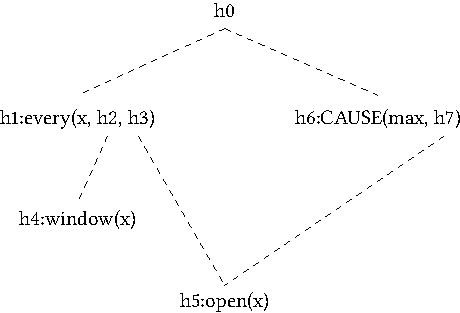
\includegraphics{Figures/max-alle-fenster-oeffnete-mrs-cropped.pdf}
\caption{\emph{Max alle Fenster öffnete}的支配图\label{Abbildung-Max-alle-Fenster-oeffnete}}
%\caption{Dominance graph for \emph{Max alle Fenster öffnete}\label{Abbildung-Max-alle-Fenster-oeffnete}}
\end{figure}%
图~\ref{Abbildung-Max-alle-Fenster-oeffnete}中的每个关系都有一个名词,可以用于指称关系或“抓住”它。这些名词被称作手柄(handle)。这一统制图表明$h0$统制$h1$和$h6$、$h2$统制$h4$、$h3$统制$h5$、$h7$ 统制$h5$ 。具体的辖域关系不完全赋值:全称量词可以管辖CAUSE,CAUSE也可以管辖全称量词。图~\ref{fig-alle-cause}和图\ref{fig-cause-alle}描述了辖域值确定的两个变体。
%Each relation in Figure~\ref{Abbildung-Max-alle-Fenster-oeffnete} has a name that one can use to refer to the relation or ``grasp'' it.
%These names are referred to as \emph{handle}. The dominance graph states that $h0$ dominates both $h1$ and $h6$ and that
%$h2$ dominates $h4$, $h3$ dominates $h5$, and $h7$ dominates $h5$. The exact s\textsc{cop}al relations are underspecified: the universal quantifier can have s\textsc{cop}e over
%CAUSE or CAUSE can have s\textsc{cop}e over the universal quantifier. Figures~\ref{fig-alle-cause} and
%\ref{fig-cause-alle} show the variants of the graph with resolved s\textsc{cop}e.
\begin{figure}
\centering
%% \begin{tabular}{@{}ccc@{}}
%%                                & \mybox[h0]{h0}                & \\[8ex]
%% \mybox[h1]{h1:every(x, \mybox[h2]{h2}, \mybox[h3]{h3})}      &                              & \mybox[h6]{h6:CAUSE(max, \mybox[h7]{h7})}\\[8ex]
%% \mybox[h4]{h4:window(x)}           &         & \\[6ex]
%%                                & \mybox[h5]{h5:open(x)}\\
%% \end{tabular}

%% \begin{tikzpicture}[overlay,remember picture] 
%% \draw(h0.south)--(h1.north); 
%% \draw(h2.south)--(h4.north);
%% \draw(h3.south) .. controls +(0,-1) and +(-1,1)..  (h6.north);
%% \draw(h7.south)--(h5.north);
%% \end{tikzpicture}
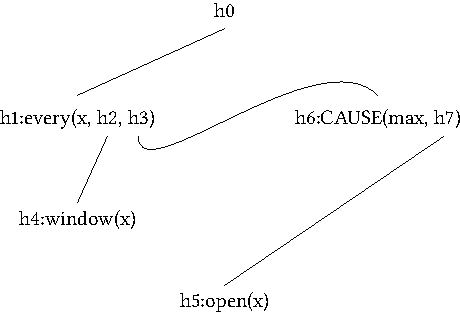
\includegraphics{Figures/solution-mrs-all-cause-open-cropped.pdf}
\caption{$\forall$ x window(x) $\to$ CAUSE(max,open(x))意义的支配图\label{fig-alle-cause}}
%\caption{Dominance graph for the reading $\forall$ x window(x) $\to$ CAUSE(max,open(x)).\label{fig-alle-cause}}
\end{figure}%
\begin{figure}
\centering
%% \begin{tabular}{@{}ccc@{}}
%%                                & \mybox[h0]{h0}                & \\[8ex]
%% \mybox[h1]{h1:every(x, \mybox[h2]{h2}, \mybox[h3]{h3})}      &                              & \mybox[h6]{h6:CAUSE(max, \mybox[h7]{h7})}\\[8ex]
%% \mybox[h4]{h4:window(x)}           &          & \\[6ex]
%%                                & \mybox[h5]{h5:open(x)}\\
%% \end{tabular}

%% \begin{tikzpicture}[overlay,remember picture] 
%% \draw(h0.south)--(h6.north); 
%% \draw(h7.south) .. controls +(0,-1) and +(-1,1)..  (h1.north);
%% \draw(h2.south)--(h4.north);
%% \draw(h3.south)--(h5.north);
%% \end{tikzpicture}
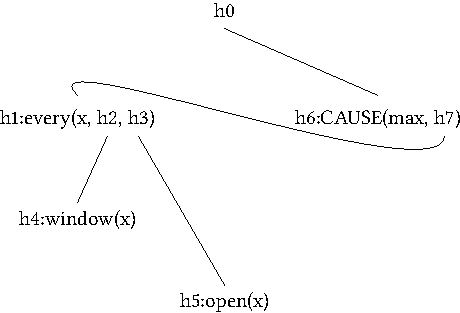
\includegraphics{Figures/solution-mrs-cause-all-open-cropped.pdf}
\caption{ CAUSE(max, $\forall$ x window(x) $\to$ open(x))意义的支配图\label{fig-cause-alle}}
%\caption{Graph for te reading CAUSE(max, $\forall$ x window(x) $\to$ open(x)).\label{fig-cause-alle}}
\end{figure}%
图~\ref{Abbildung-Max-alle-Fenster-oeffnete}中的不完全赋值图没有说明$h3$和$h6$之间的关系。它表明的唯一的信息是:$h3$以某种方式统制$h5$ 。在图~\ref{fig-alle-cause}中,每一个($h3$)统制CAUSE ($h6$) 并且CAUSE统制open($h5$) 。所以,\relation{every}间接统制\relation{open}。在图~\ref{fig-cause-alle}中,CAUSE统制\relation{every},并且\relation{every}统制\relation{open}。图~\ref{Abbildung-Max-alle-Fenster-oeffnete}再一次说明了限制,但是$h7$只是间接统制$h5$ 。
%The underspecified graph in Figure~\ref{Abbildung-Max-alle-Fenster-oeffnete} does not say anything
%about the relation between $h3$ and $h6$. The only thing it says is that $h3$ somehow has to dominate
%$h5$. In Figure~\ref{fig-alle-cause} every ($h3$) dominates CAUSE ($h6$) and CAUSE dominates open
%($h5$). So, \relation{every} dominates \relation{open} indirectly. In Figure~\ref{fig-cause-alle}, CAUSE
%dominates \relation{every} and \relation{every} dominates \relation{open}. Again the constraints of
%Figure~\ref{Abbildung-Max-alle-Fenster-oeffnete} are fulfilled, but $h7$ dominates $h5$ only indirectly.

量词统制$h4$这一事实是由量词的词项决定的。量词统制$h5$在分析中不用明显说明,因为量词在属于$h5$的关系中约束一个变量,即x。$h7$和$h5$之间的统制关系总是在词库中决定的,因为CAUSE和\relation{open}都属于一个单独词项的语义。
%The fact that the quantifier dominates $h4$ is determined by the lexical entry of the quantifier. The fact that
%the quantifier dominates $h5$ does not have to be made explicit in the analysis since the quantifier binds a variable
%in the relation belonging to $h5$, namely x. The dominance relation between $h7$ and $h5$ is always determined in the lexicon
%since CAUSE and \relation{open}  both belong to the semantic contribution of a single lexical entry.

这一分析具体采用什么句法理论到最后并不是很重要。在这里我选择HPSG理论。正如图~\vref{Abbildung-Fenster-oeffnete-MRS}所示,alle Fenster öffnet的分析包括一个带有动词和宾语的简单结构。
%The exact syntactic theory that one adopts for this analysis is, in the end, not of great importance.
%I have chosen HPSG here. As Figure~\vref{Abbildung-Fenster-oeffnete-MRS} shows, the analysis of \emph{alle Fenster öffnet}
%contains a simple structure with a verb and an object.
\begin{figure}
%\begin{sideways}
\oneline{%
\begin{forest}
sm edges, for tree={l sep= 4ex}
[V$'$\feattab{
    \subcat \sliste{ NP\ind{y} },\\
    \rels \relliste{ h1:every(x, h2, h3), h4:window(x), h6:CAUSE(y,h7), h5:open(x) },\\
    \hcons \relliste{ h0 \qeq h1, h2 \qeq h4, h0 \qeq h6, h7 \qeq h5 }    }
  [\ibox{2} NP\ind{x}\feattab{
    \rels \relliste{ h1:every(x, h2, h3), h4:window(x) },\\
    \hcons \relliste{ h0 \qeq h1, h2 \qeq h4 } } 
    [Det\feattab{
    \rels \relliste{ h1:every(x, h2, h3) },\\
    \hcons \relliste{ h0 \qeq h1, h2 \qeq h4  } } [alle] ]
    [N\feattab{
    \rels \relliste{ h4:window(x) },\\
    \hcons \relliste{ } } [Fenster] ] ]
  [V\feattab{
                                           \subcat \sliste{ NP\ind{y}, \ibox{2} },\\
                                           \rels \relliste{ h6:CAUSE(y,h7), h5:open(x) },\\
                                           \hcons \relliste{ h0 \qeq h6, h7 \qeq h5 } } [öffnete] ]
]
\end{forest}
}
%\end{sideways}
\caption{\label{Abbildung-Fenster-oeffnete-MRS}alle Fenster öffnete的MRS分析}
%\caption{\label{Abbildung-Fenster-oeffnete-MRS}MRS analysis of \emph{alle Fenster öffnete}}
\end{figure}%
这一结构并不区别于为alle Kinder kennt (所有儿童都知道)所假设的结构,涉及语义上简单的动词kennen(知道)。唯一的差异来源于涉及的具体动词。正如~\ref{Abschnitt-HPSG-Semantik}所示,词之间的关系向上传递。辖域限制也是如此。这些信息都在列表中表征。\hcons 代表手柄约束(handle constraints)。\qeq in h0 \qeq h6 代表模(modulo)数量词辖域相同。
%This structure does not differ from the one that would be assumed for \emph{alle Kinder kennt} `all
%children know', involving the semantically simplex verb \emph{kennen} `to know'.
%The only difference comes from the meaning of the individual words involved.
%As shown in Section~\ref{Abschnitt-HPSG-Semantik}, relations between individual words are passed on upwards.
%The same happens with s\textsc{cop}al restrictions. These are also represented in lists. \hcons stands for \emph{handle constraints}.
%\qeq in h0 \qeq h6 stand for the equality \emph{modulo} quantifier s\textsc{cop}e.

Egg为例 (\ref{ex-wieder-alle}) 中的句子列出了以下意义——重复写在 (\mex{1})中:
%Egg lists the following readings for the sentence in (\ref{ex-wieder-alle}) -- repeated here as (\mex{1}):
\ea
\label{ex-wieder-alle-zwei}
\gll dass Max wieder alle Fenster öffnete\\
	 REL Max 再次 \textsc{det} 窗子 打开\\
\glt `Max再次打开了所有这些窗子这件事'
%\gll dass Max wieder alle Fenster öffnete\\
%	 that Max again all windows opened\\
%\glt `that Max opened all the windows again'
\z
\begin{enumerate}
\item Max打开了每一个窗子,并且他已经对每一个窗子都至少都打开了一次 (\relation{again}($\forall$(CAUSE(open)));重复性)
%\item Max opened every window and he had already done that at least once for each window
%      (\relation{again}($\forall$(CAUSE(open))); repetitive)
\item Max致使每一个窗子都开了,并且他已经对每一个窗子都打开了一次 (\relation{again}(CAUSE($\forall$(open)));重复性)
%\item Max caused every window to be open and he had done that at least once before 
%      (\relation{again}(CAUSE($\forall$(open))); repetitive)
\item 在更早的某一个时间,所有窗子同时开着,并且Max将所有窗子回复到开着的状态(CAUSE(\relation{again}($\forall$(open))); 恢复性)
%\item At some earlier point in time, all windows were simultaneously open and Max re-established this state
%      (CAUSE(\relation{again}($\forall$(open))); restitutive)
\end{enumerate}

\noindent
这些意义对应下一页图~\vref{Abbildung-Max-wieder-alle-Fenster-oeffnete}中支配图的意义。
%These readings correspond to the dominance graph in Figure~\vref{Abbildung-Max-wieder-alle-Fenster-oeffnete}.
\begin{figure}
\centering
%%   \begin{tabular}{@{}ccc@{}}
%%   & \mybox[h0]{h0}                       & \\[4ex]
%%     \mybox[h8]{h8:again}\mybox[h9]{(h9)}  \\[4ex]
%%     \mybox[h1]{h1:every(x, \mybox[h2]{h2}, \mybox[h3]{h3})}      &                              & \mybox[h6]{h6:CAUSE(max, \mybox[h7]{h7})}\\[8ex]
%%   \mybox[h4]{h4:window(x)}           &          & \\[6ex]
%%                            & \mybox[h5]{h5:open(x)}\\
%%   \end{tabular}

%% \begin{tikzpicture}[overlay,remember picture,dashed] 
%% \draw(h0.south)--(h8.north); 
%% \draw(h0.south)--(h6.north);
%% \draw(h9.south)--(h1.north);
%% \draw(h2.south)--(h4.north);
%% \draw(h3.south)--(h5.north);
%% \draw(h7.south)--(h5.north);
%% \end{tikzpicture}
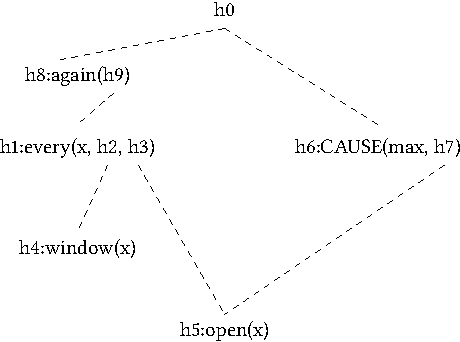
\includegraphics{Figures/mrs-max-wieder-alle-fenster-oeffnete-cropped.pdf}
\caption{“Max wieder alle Fenster öffnete”(Max再次打开了所有这些窗子这件事)\label{Abbildung-Max-wieder-alle-Fenster-oeffnete}的支配图}
%\caption{Dominance graph for \emph{Max wieder alle Fenster öffnete} `that Max opened all the
%  windows again'\label{Abbildung-Max-wieder-alle-Fenster-oeffnete}}
\end{figure}%
图~\vref{Abbildung-Max-alle-Fenster-wieder-oeffnete} 展示了 (\ref{ex-alle-wieder})的图——重复写成(\mex{1}):
%Figure~\vref{Abbildung-Max-alle-Fenster-wieder-oeffnete} shows the graph for (\ref{ex-alle-wieder})
%-- repeated here as (\mex{1}):\todostefan{Skopus hinzufügen?}
\ea
\label{ex-alle-wieder-zwei}
\gll dass Max alle Fenster wieder öffnete\\
	 REL Max \textsc{det} 窗子 再次 打开\\
%\gll dass Max alle Fenster wieder öffnete\\
%	 that Max all windows again opened\\
\z
\begin{figure}
\centering
%% \begin{tabular}{@{}ccc@{}}
%%                                & \mybox[h0]{h0}                & \\[8ex]
%% \mybox[h1]{h1:every(x, \mybox[h2]{h2}, \mybox[h3]{h3})}      &                              &                               \mybox[h6]{h6:CAUSE(max, \mybox[h7]{h7})}\\[4ex]
%%                                                               \multicolumn{2}{c}{\hspace{3em}\mybox[h8]{h8:again(\mybox[h9]{h9})}}\\[4ex]
%% \mybox[h4]{h4:window(x)}           &          & \\[6ex]
%%                                & \mybox[h5]{h5:open(x)}\\
%% \end{tabular}
%% \begin{tikzpicture}[overlay,remember picture,dashed] 
%% \draw(h0.south)--(h1.north); 
%% \draw(h0.south)--(h6.north);
%% \draw(h2.south)--(h4.north);
%% \draw(h3.south)--(h8.north);
%% \draw(h9.south)--(h5.north);
%% \draw(h7.south)--(h5.north);
%% \end{tikzpicture}
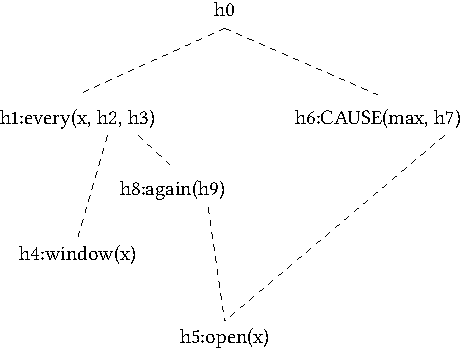
\includegraphics{Figures/mrs-max-alle-fenster-wieder-oeffnete-cropped.pdf}
\caption{“Max alle Fenster wieder öffnete”(Max再次打开所有这些窗子这件事)的支配图\label{Abbildung-Max-alle-Fenster-wieder-oeffnete}}
%\caption{Dominance graph for \emph{Max alle Fenster wieder öffnete} `that Max opened all the
%  windows again'\label{Abbildung-Max-alle-Fenster-wieder-oeffnete}}
\end{figure}%
从这些没有wieder(再次)的例句中推导出这些统制图,需要做的只是增加表达式h8:again(h9)和支配要求,要求$h9$统制出现在wieder右边的量词,要求h9被wieder左边的量词统制。
%To derive these dominance graphs from the ones without \emph{wieder} `again', all one has to do is add the expression h8:again(h9)
%and the dominance requirements that demand that $h9$ dominates quantifiers occurring to the right of \emph{wieder} and that it
%is dominated by quantifiers to the left of \emph{wieder}.

所以可以很轻易地在不借助为CAUSE和BECOME设置空成分的前提下,就可以推导出wieder所修饰的相关意义。词语öffnen的意义以相似的方式被分解,但是被分解的意义被指派到一个单独的成分上,即动词。通过在词库中不完全赋值的辖域关系,相关意义都可以推导出来。
%It is therefore unproblematic to derive the relevant readings for modification by \emph{wieder}
%without empty elements for CAUSE and BECOME. The meaning of the word \emph{öffnen} is decomposed in a similar way but the
%decomposed meaning is assigned to a single element, the verb. By underspecification of the s\textsc{cop}al
%relations in the lexicon, the relevant readings can then be derived. 


%% Shravan sagt nee, wahrscheinlich nicht. 24.06.2008
%% Unterspezifikation ist auch psycholinguistisch plausibler als die explizite Ableitung aller Skopus:
%% Es ist unwahrscheinlich, dass Menschen für normale Sätze jeweils Tausende Repräsentationen
%% verwenden, die sich nur in verschiedenen Skopus unterscheiden. Stattdessen lassen sie wahrscheinlich
%% die Bedeutung weitestgehend unterspezifiziert und lösen sie dann bei ausreichendem Kontextwissen
%% weiter auf.

\section{空成分的证据}
%\section{Evidence for empty elements}
\label{Abschnitt-Evidenz-leere-Elemente}

正如前面所讨论的,语法学家同意语言学家和说话者都能注意到一个词串中什么时候会缺少一个成分。对于那些是否假设语迹没有实际语料上的差别的现象,可以假设空成分。但是,构式语法学家提出的学习力的论据还有些说服力:如果假设没有天赋语言学知识或者天赋语言学知识很少的话,那么就不能用来自其他语言的语料来证明空成分的存在。这意味着因为巴斯克语\il{巴斯克语}\il{Basque}有宾语一致性\isc{一致!宾语}\is{agreement!object}问题,这并不意味着可以在德语语法中为宾语一致(AgrO\isc{范畴!功能性的!AgrO}\is{category!functional!AgrO})假设一个空中心语,正如\citet{Stechow96a}和\citet{Meinunger2000a}所做的那样。因为德语中没有宾语一致问题,儿童没有办法学习存在一个AgrO中心语。因此,关于AgrO的知识必须是天赋的。因为天赋知识的假设存在争议(见第\ref{chap-innateness})章),任何使用跨语言现象来支持使用空成分的理论,其基础都不稳固。
%As previously discussed, grammarians agree that both linguists and speakers notice when there is a constituent missing from a
%string of words. For cases where it can be shown that analyses with or without traces are indistinguishable empirically,
%then one can assume empty elements. Nevertheless, the learnability argument put forward by
%Construction Grammarians has some validity: if one assumes that there is no or little innate linguistic knowledge, then it is not possible to motivate empty elements
%with data from other languages. This means that just because Basque\il{Basque} shows object agreement\is{agreement!object},
%this does not mean that one can assume an empty head for object agreement
%(AgrO\is{category!functional!AgrO}) in a grammar of German as
%for instance \citet{Stechow96a} and \citet{Meinunger2000a} do. Since there is no object agreement in German, there
%would be no way for the child to learn the fact that there is an AgrO head. Knowledge about AgrO
%must therefore be innate. Since the assumption of innate linguistic knowledge is controversial (see
%Chapter~\ref{chap-innateness}), any theory that uses cross"=linguistic data to motivate the use of empty elements is on shaky ground.

只有在多种分析方法之间没有实际差异并且当前研究的语言能够被驱动时,才能使用跨语言的现象。在这一点上,应该遵循奥卡姆剃刀原则,并且选择与其它语言分析兼容的分析(见\citealp{MuellerCoreGram}和第\ref{sec-develop-theories-coregram}章)。
\isc{空成分|)}\is{empty element|)}
%Cross"=linguistic considerations can only be drawn upon if there are no empirical differences between multiple alternative
%analyses compatible and motivated by the language under consideration. In this case, one should follow Occam's Razor and choose the analysis which is compatible with analyses of
%other languages (see \citealp{MuellerCoreGram} and Chapter~\ref{sec-develop-theories-coregram}).
%\is{empty element|)}

\section{转换,词汇规则和空成分}
%\section{Transformations, lexical rules, and empty elements}
\label{Abschnitt-leere-Elemente-LRs-Transformations}

在\isc{空成分|(}\is{empty element|(}\isc{词汇规则|(}\is{lexical rule|(}\isc{转换|(}\is{transformation|(}TAG框架内对被动\isc{被动}\is{passive}的讨论中,我们已经清楚的是词汇规则对应特定的转换式,即那些与一个词项有关的转换式(词汇管辖的转换式,\citealp{Dowty78a};关于转换式和词汇规则的讨论,可以参见\citew{Bresnan78a}和\citew{BK82a})。在TAG\indextagc 各自的变体中,词汇规则在一个词项的主动句法树和被动句法树之间建立联系。主动句法树和被动句法树都可以通过附接进行扩展。
%In\is{empty element|(}\is{lexical rule|(}\is{transformation|(} the discussion of the passive\is{passive} in the framework of TAG, it became clear that lexical rules
%correspond to particular transformations, namely those which have some relation to a lexical item (lexically governed transformations, \citealp{Dowty78a}; 
%for the discussion of transformations and lexical rules, see \citew{Bresnan78a} and \citew{BK82a}). In the respective variants of TAG\indextag, lexical rules establish a relation
%between a lexical item for an active tree with a lexical item of a passive tree. Both the active and passive tree can be extended by adjunction.

在范畴语法\indexcgc 等理论中,情况是一样的:因为一个功能符预期去寻找其论元的方向在英语这种语言中是固定的,所以词项代表整个句法树。只有附接语的附加没有在词项中说明。附接语可以出现在句法树的什么位置取决于附接语的属性。在\ref{Abschnitt-CG-lokale-Umstellung}中,我们已经看到处理自由成分序列的语言的方案。如果组合的方向没有在词库中确定,那么词项就可以出现在多个树中。如果我们对比用于这类词项的词汇规则和转换,我们也看到在不同句法树集合中产生关系的词汇规则。
%In theories such as Categorial Grammar\indexcg, the situation is similar: since the direction in which a functor expects to find its argument is fixed
%for languages such as English, the lexical item stands for an entire tree. Only the attachment of
%adjuncts is not yet specified in lexical items. The positions in the
%tree where the adjuncts can occur depend on the properties of the adjuncts. In Section~\ref{Abschnitt-CG-lokale-Umstellung},
%we have seen suggestions for treatments of languages with free constituent order. If the direction of combination is not fixed in the lexicon, then the lexical item
%can occur in a number of trees. If we compare lexical rules that can be applied to this kind of lexical items with transformations, we see that lexical rules create relations
%between different sets of trees.

在HPSG\hpsgc 分析\indexhpsgc 中,工作方式相似:词汇规则将价属性不同的词项互相联系起来。在英语\il{英语}\il{English}的HPSG语法中,通常有一个模式允准一个VP,该VP包括动词和其所有补语;还有一个模式将主语和这一VP连接起来\citep[\page 39]{ps2}。在定式动词的词项中,已经确定了句法树最后的样子。与在范畴语法中一样,HPSG中的附接语可以与多种中间投射组合。基于在特定语法中使用的统制模式,词项会决定词项能够出现的成分结构和允许出现的多重结构。在第\ref{Kapitel-HPSG}章提出的德语语法中,可以使用双及物动词词项来分析六种不同的序列,即,词项可以 -- 不考虑附接语 -- 出现在六种动词居末的结构中。两种序列可以用被动词项来分析,该词项只有两个论元。正如在范畴语法中一样,被允准的结构的集合与其它被允准结构的集合相互联系。在HPSG理论和构式语法中,曾努力用其它机制来代替词汇规则,因为词汇规则“的地位是含糊的,并且与其它分析的互动是存在争议的”\citep*[\page 19]{BMS2001a}。\citet{BMS2001a} 为提取提出了一个分析,这一分析不是将具有不同价列表的词项连接起来,而是在同一个词项中一个列表的次集合和另外一个列表之间建立联系。两种分析方法的结果分别见(\mex{1})和(\mex{2}):
%In \hpsg analyses\indexhpsg, this works in a similar way: lexical rules relate lexical items with differing valence properties to each other. In HPSG grammars of English\il{English},
%there is normally a schema that licenses a VP containing the verb and all its complements as well as a schema that connects the subject to the VP 
%\citep[\page 39]{ps2}. In the lexical items for finite verbs, it is already determined what the tree will look like in the end. As in Categorial Grammar, adjuncts in HPSG can
%be combined with various intermediate projections. Depending on the dominance schemata used in a particular grammar, the lexical item will determine the constituent structure
%in which it can occur or allow for multiple structures. In the grammar of German proposed in Chapter~\ref{Kapitel-HPSG}, it is possible to analyze six different sequences with a lexical
%item for a ditransitive verb, that is, the lexical item can -- putting adjuncts aside -- occur in six different structures with verb"=final order. Two sequences can be analyzed
%with the passive lexical item, which only has two arguments.
%As in Categorial Grammar, sets of licensed structures are related to other sets of licensed structures. In HPSG theorizing and also in Construction Grammar, there have been
%attempts to replace lexical rules with other mechanisms since their ``status is dubious and their interaction with other analyses is controversial''
%\citep*[\page 19]{BMS2001a}. \citet{BMS2001a} propose an analysis for extraction
%that, rather than connecting lexical items with differing valence lists, establishes a relation between a subset of a particular list in a lexical item and another
%list in the same lexical item. The results of the two alternative analyses are shown in (\mex{1})
%and (\mex{2}), respectively:
\eal
\ex \ms{ subcat & \sliste{ NP[\type{nom}], NP[\type{acc}] }\\
         slash  & \eliste\\
       }
\ex \ms{ subcat & \sliste{ NP[\type{nom}] }\\
         slash  & \sliste{ NP[\type{acc}] }\\
       }
\zl
\addlines
在(\mex{0})中,(\mex{0}a)是一个基本词项而(\mex{0}b)通过一个词汇规则与 (\mex{0}a)联系。另外的分析只是说明了\textsc{arg-st}特征\isfeat{arg-st}的合适取值\footnote{
\argstc 代表论元结构。\argstc 的取值是一个列表,包含一个中心语的所有论元。关于\argstc 更多的信息,可以参见\ref{Abschnitt-Arg-St}。
}而\subcatc 和\slashvc 都是通过相关限制从\argstvc 推导而来。(\mex{1})显示了两个被允准的词项。
%In (\mex{0}), (\mex{0}a) is the basic entry and (\mex{0}b) is related to (\mex{0}a) via a lexical
%rule. The alternative analysis would only involve specifying the appropriate value
%of the \textsc{arg-st} feature\footnote{
%\argst stands for \emph{Argument Structure}. The value of \argst is a list containing all the arguments
%of a head. For more on \argst, see Section~\ref{Abschnitt-Arg-St}.
%}\isfeat{arg-st} and the \subcat and \slashv is then derived from the \argstv using the relevant constraints.
%(\mex{1}) shows two of the licensed lexical items.
\eal
\ex \ms{ arg-st & \sliste{ NP[\type{nom}], NP[\type{acc}] }\\
         subcat & \sliste{ NP[\type{nom}], NP[\type{acc}] }\\
         slash  & \eliste\\
       }
\ex \ms{ arg-st & \sliste{ NP[\type{nom}], NP[\type{acc}] }\\
         subcat & \sliste{ NP[\type{nom}] }\\
         slash  & \sliste{ NP[\type{acc}] }\\
       }
\zl
如果我们想以这种方式完全取消词汇规则,那么我们需要为每一种变化设置另外的特征。 \footnote{
换一种方式,可以假设一个非常复杂的关系来联系\argstc 和\subcatc。但是这必须传送一系列现象互动的结果,并且这些现象的互动无法用一种明显的方式表征。%
} 因为有很多交互的变价过程,所以需要标明很多助动词特征。假设这种分析的结果在\citew[\S~7.5.2.2]{MuellerLehrbuch1}中已经详细讨论过了。这里产生的问题与基于承继的方法解决论元结构变化过程遇到的问题一样:这种分析也需要助动词特征,因为不可能用承继来刻画论元信息的嵌套和多重改变。见\ref{Abschnitt-Passiv-CxG}。
%If we want to eliminate lexical rules entirely in this way, then we would require an additional feature for each change.\footnote{
%Alternatively, one could assume a very complex relation that connects \argst and \subcat. But this would then have to deliver
%the result of an interaction of a number of phenomena and the interaction of these phenomena would not be captured in a transparent way.%
%} Since there are many interacting valence"=changing processes, things only work out with the stipulation of a large number of auxiliary
%features. The consequences of assuming such analyses have been discussed in detail in
%\citew[Section~7.5.2.2]{MuellerLehrbuch1}. The problems that arise are parallel for
%inheritance"=based approaches for argument structure"=changing processes: they also require
%auxiliary features since it is not possible to model embedding and multiple changes of valence information with inheritance. See Section~\ref{Abschnitt-Passiv-CxG}.

另外,词汇规则的地位很模糊这一观点应该遭到反对:因为有很多成型的词汇规则形式化体系\citep{Meurers2001a,CB92a,LC99a},并且它们与其他分析的互动也不存在争议。大多数HPSG装置都使用词汇规则,并且大量词汇规则和约束可以通过已经安装了语法片段来确认。
%Furthermore, the claim that the status of lexical rules is dubious must be rejected: there are worked"=out formalizations of lexical rules \citep{Meurers2001a,CB92a,LC99a}
%and their interaction with other analyses is not controversial. Most HPSG implementations make use of lexical rules and the interaction of a number of rules and
%constraints can be easily verified by experiments with implemented fragments.

\citet{Jackendoff75a}给出了词汇规则的两个可能的概念:在一个概念中,词库包含一个给定语言中的所有词,并且只有冗余规则来说词项的一些属性与另外一些词项的属性如何表现。例如,les(读)和lesbar(可读的)在词库中有相同的地位。词汇规则的另外一个概念是,有一些基本词项,并且其余的词项是借助词汇规则从这些基本词项推导出来的。词干les是基本词项,并且lesbar是从它推导出来的。在HPSG中,常常使用第二种定义。这等同于单分支规则假设。在第~\pageref{Abbildung-Verbstellung-HPSG}页的图~\ref{Abbildung-Verbstellung-HPSG},就是如此展示的:动词kennt(知道)通过一个词汇规则映射到一个动词,该动词选择一个空动词中心语的投射。借助词汇规则,可以通过假设有一个空中心语的二叉结构而不是单分支规则来把词汇规则从语法中清除出去。例如,在HPSG对于结果构式\isc{结果构式}\is{resultative construction}\isc{构式!结果|(}\is{construction!resultative|(}的分析中,如(\mex{1})就提出了词汇规则 (\citealp{Verspoor97a};\citealp{Wechsler97a};\citealp{WN2001a};\citealp[\S~5]{Mueller2002b})。
%\citet{Jackendoff75a} presents two possible conceptions of lexical rules: in one variant, the lexicon contains all words in a given language and there
%are just redundancy rules saying something about how certain properties of lexical entries behave with regard to properties of other lexical entries. For example,  \stem{les} `read-' and \emph{lesbar}
%`readable' would both have equal status in the lexicon. In the other way of thinking of lexical
%rules, there are a few basic lexical entries and the others are derived
%from these using lexical rules. The stem  \stem{les} `read-' would be the basic entry and \emph{lesbar} would be derived from it.
%In HPSG, the second of the two variants is more often assumed. This is equivalent to the assumption of unary rules. In Figure~\ref{Abbildung-Verbstellung-HPSG} on
%page~\pageref{Abbildung-Verbstellung-HPSG}, this has been shown accordingly: the verb \emph{kennt}
%`knows' is mapped by a lexical rule to a verb that selects the projection of an
%empty verbal head. With this conception of lexical rules, it is possible to remove lexical rules from the grammar by assuming binary"=branching structures with an
%empty head rather than unary rules. For example, in HPSG analyses of resultative constructions\is{resultative construction}\is{construction!resultative|(}
%such as (\mex{1}), lexical rules have been proposed (\citealp{Verspoor97a}; \citealp{Wechsler97a}; \citealp{WN2001a}; \citealp[Chapter~5]{Mueller2002b}).
\ea
\gll [dass] Peter den Teich leer fischt\\
	 \spacebr{}REL Peter \textsc{det} 池塘 空 钓鱼\\
\glt `Peter把池塘里的鱼都钓光了这件事'
%\gll [dass] Peter den Teich leer fischt\\
%	 \spacebr{}that Peter the pond empty fishes\\
%\glt `that Peter fishes the pond empty'
\z
在我的分析中,词汇规则将一个不及物动词跟一个选择一个受格宾语和一个谓词的动词连接。图~\vref{Abbildung-Resultativ-LR}展示了对应的句法树。
%In my own analysis, a lexical rule connects a verb used intransitively to a verb that selects an accusative object and a predicate.
%Figure~\vref{Abbildung-Resultativ-LR} shows the corresponding tree.
\begin{figure}
\centering
\begin{forest}
sm edges
[V{[\subcat \eliste]}
	[NP{[\type{nom}]}
		[Peter;Peter]]
	[V{[\subcat \sliste{ NP[\type{nom}] }]}
		[NP{[\type{acc}]}
			[den Teich;the pond, roof]]
		[V{[\subcat \sliste{ NP[\type{nom}], NP[\type{acc}] } ]}
			[Adj
				[leer;empty]]
			[V{[\subcat \sliste{ NP[\type{nom}], NP[\type{acc}], Adj } ]}
				[V{[\subcat \sliste{ NP[\type{nom}]} ]}
					[fischt;fishes]]]]]]
\end{forest}
\caption{\label{Abbildung-Resultativ-LR}使用词汇规则对结果构式进行的分析}
%\caption{\label{Abbildung-Resultativ-LR}Analysis of the resultative construction with a lexical rule}
\end{figure}%
如果我们考虑一下(\mex{0}) 的意思,就可以发现钓鱼行为导致鱼塘变干。这一致使关系没有包括在(\mex{0})中词语的任意一个词项中。为了将这一信息放在整个表达的表征中,就需要通过词汇规则来增加。词汇规则规定:如果一个动词选择限制一个另外的谓词和受格宾语,那么整个构式有一种致使意义。
%If we consider what (\mex{0}) means, then we notice that the fishing act causes the pond to become empty.
%This causation is not contained in any of the basic lexical items for the words in (\mex{0}).
%In order for this information to be present in the semantic representation of the entire expression, it has
%to be added by means of a lexical rule. The lexical rule says: if a verb is used with an additional predicate and accusative
%object, then the entire construction has a causative meaning.

图~\vref{Abbildung-Resultativ-leer}展示了怎样用一个空中心语替代一个词汇规则。
%Figure~\vref{Abbildung-Resultativ-leer} shows how a lexical rule can be replaced by an empty head.
\begin{figure}
\centering
\begin{sideways}
%\scalebox{0.9}{%
\begin{forest}
sm edges
[V{[\subcat \eliste]}
	[{NP[\type{nom}]}
		[Peter;Peter]]
	[{V[\subcat \sliste{ NP[\type{nom}] }]}
		[{NP[\type{acc}]}
			[den Teich;the pond,roof]]
		[{V[\subcat \sliste{ NP{[\type{nom}]}, NP{[\type{acc}]} }]}
			[Adj
				[leer;empty]]
			[{[\subcat \sliste{ NP{[\type{nom}]}, NP{[\type{acc}]}, Adj }]}
				[{V[\subcat \sliste{ NP{[\type{nom}]} }]}
					[fischt;fishes]]
				[{V[\subcat \sliste{ NP{[\type{nom}]}, NP{[\type{acc}]}, Adj, V{[\subcat \sliste{ NP{[\type{nom}]} }]} }]}
					[\trace]]]]]]
\end{forest}
%}
\end{sideways}
\caption{\label{Abbildung-Resultativ-leer}使用空中心语对结果构式进行的分析}
%\caption{\label{Abbildung-Resultativ-leer}Analysis of the resultative construction with an empty head}
\end{figure}%
空中心语需要一个不及物动词、一个形容词、一个受格宾语和一个主语。Fischt(钓鱼)的主语当然要与fischt与空中心语组合的主语一致。这一点没有呈现在图中。但是,可以建立这一等同性(参见\citealp{HN94a})。在这一分析中,致使语义是由空中心语贡献的。这里使用的技巧正是在\ref{Abschnitt-Eleminierung-leerer-Elemente}所使用的,只是方向相反:在前面章节中,带有空子节点的二叉结构被单分支结构所提点。在这一节中,我们用带有空子节点的二叉结构代替单分支结构。\footnote{
这里,我们讨论词汇规则,但是这一转换技巧也可以运用到其它单分支规则。语义学家经常用这种规则来完成类型转换\isc{类型提升}\is{type raising}。例如,一个规则将一个指称性NP(例如,i.a中的a trickster)转变为一个谓词性成分(i.b)\citep{Partee87a-u}。
\eal
\ex 
\gll A trickster laughs.\\
\textsc{art} 骗子 大笑\\
\glt `一个骗子在大笑。'
\ex 
\gll He is a trickster.\\
他 \textsc{cop} \textsc{art} 骗\\
\glt `他是一个骗子。'
\zl
这些转变可以通过作用于一个NP的单分支规则或者一个以NP作为其论元的特殊的空中心语完成。在现在最简方案\indexmpc 中,使用空中心语\citep[\page 370]{Ramchand2005a},在范畴语法\indexcgc 和HPSG\indexhpsgc 中单分支规则更加常见 (\citealp[\page 91--92]{Flickinger2008a};\citealp{MuellerPredication,MuellerCopula}).
}\isc{空成分|)}\is{empty element|)}\isc{词汇规则|)}\is{lexical rule|)}\isc{转换|)}\is{transformation|)}\isc{构式!结果|)}\is{construction!resultative|)}
%The empty head requires the intransitive verb and additionally an adjective, an accusative object and a subject.
%The subject of \emph{fischt} `fishes' must of course be identical to the subject that is selected by the combination
%of \emph{fischt} and the empty head. This is not shown in the figure.
%It is possible, however, to establish this identity (see \citealp{HN94a}). The causative semantics is contributed by
%the empty head in this analysis. The trick that is being implemented here is exactly what was done in Section~\ref{Abschnitt-Eleminierung-leerer-Elemente},
%just in the opposite direction: in the previous section, binary"=branching structures with an empty daughter were replaced by unary"=branching structures.
%In this section, we have replaced unary"=branching structures with binary"=branching structures with an empty daughter.\footnote{
%	Here, we are discussing lexical rules, but this transformation trick can also be applied to
%        other unary rules. Semanticists often use such rules for type shifting\is{type raising}. For
%        example, a rule that turns a referential NP such as \emph{a trickster} in (i.a) into a
%        predicative one (i.b) \citep{Partee87a-u}.
%\eal
%\ex A trickster laughs.
%\ex He is a trickster.
%\zl
%These changes can be achieved by a unary rule that is applied to an NP or with a special empty head that takes an NP as its argument. In current Minimalist\indexmp approaches,
%empty heads are used \citep[\page 370]{Ramchand2005a}, in Categorial Grammar\indexcg and HPSG\indexhpsg unary"=branching rules are more common (\citealp[\page
%    91--92]{Flickinger2008a}; \citealp{MuellerPredication,MuellerCopula}).
%}\is{empty element|)}\is{lexical rule|)}\is{transformation|)}\is{construction!resultative|)}

\largerpage
我们已经看到一些转换可以被词汇规则替换并且一些词汇规则可以被空中心语替换。下面的章节解决以下问题:提取、置换、被动等现象是不是应该像在GB/最简方案中统一描述或者像在LFG和HPSG中用不同的工具描述。
%We have therefore seen that certain transformations can be replaced by lexical rules and also that
%lexical rules can be replaced by empty heads. 
%The following chapter
%will deal with the question of whether meaning is contributed by lexical heads or rather holistically by phrasal configurations.
%deals with the question of whether phenomena like extraction, scrambling, and passive should be
%described with the same tool as in GB/Minimalism or with different tools as in LFG and HPSG.


%      <!-- Local IspellDict: en_US-w_accents -->

%% -*- coding:utf-8 -*-
\chapter{提取,杂序和被动:是一种还是几种不同的描写装置?}
%\chapter{Extraction, scrambling, and passive: one or several descriptive devices?}
\label{chap-scrambling-extraction-passive}

一位匿名审稿人建议讨论一下转换理论与LFG、HPSG等理论的差异在哪里。这位审稿人指出转换语法只用一种工具就可以描述主动/被动变换、杂序和提取,但是LFG、HPSG等理论要用三种不同的技术来描述三种现象。如果这一观点是正确的并且分析能够做出正确的预测,相应的GB/最简方案理论会比其它理论更好,因为科学中最宽泛的目的就是提出需要最少假设的理论。我已经在\ref{sec-passive-gb}讨论了GB理论如何分析被动,但是这里我想将上述讨论扩展一下,并且包括最简方案的分析以及来自于依存语法的分析。
%An anonymous reviewer suggested discussing one issue in which transformational theories differ from
%theories like LFG and HPSG. The reviewer claimed that Transformational Grammars use just one tool
%for the description of active/passive alternations, scrambling, and extraction, while theories like
%LFG and HPSG use different techniques for all three phenomena. If this claim were correct and if
%the analyses made correct predictions, the respective GB/Minimalism theories would be better
%than their competitors, since the general aim in science
%is to develop theories that need a minimal set of assumptions. I already commented on the analysis of
%passive in GB in Section~\ref{sec-passive-gb}, but I want to extend this discussion here and include
%a Minimalist analysis and one from Dependency Grammar. 

被动分析的任务就是解释例(\mex{1})中所示的论元实现的差异:
%The task of any passive analysis is to explain the difference in argument realization in examples
%like (\mex{1}):
\eal
\ex\label{ex-she-beats-him}
\gll She beats him.\\
     她 打 他\\
\glt `她打他。'
%She beats him.
\ex\label{ex-he-was-beaten}
\gll He was beaten.\\
     他 \textsc{aux} 打\\
\glt `他被打了。'
%He was beaten.
\zl
在这些关于下棋的例子中,beat的受格宾语在(\mex{0}b)中就会实现为主格。另外,可以观察到成分的位置是不同的:虽然him在 (\mex{0}a)中出现在动词之后宾语位置上,在(\mex{0}b)中出现在动词之前。在GB中这一现象通过移位来解释。GB理论认为宾语在被动构式中没有获得格指派所以必须移位到主语位置上,在主语位置上可以由定式动词指派格。这一分析也可以见于最简方案的分析中,如David Adger的教材\citeyearpar{Adger2003a}。图~\vref{fig-passive-mp}展示了他对例 (\mex{1})的分析:
%In these examples about chess, the accusative object of \emph{beat} is realized as the nominative
%in (\mex{0}b). In addition, it can be observed that the position of the elements is different: while
%\emph{him} is realized postverbally in object position in (\mex{0}a), it is realized preverbally in
%(\mex{0}b). In GB this is explained by a movement analysis. It is assumed that the object does not
%get case in passive constructions and hence has to move into the subject position where case is
%assigned by the finite verb. This analysis is also assumed in Minimalist work as in
%David Adger's textbook \citeyearpar{Adger2003a}, for instance. Figure~\vref{fig-passive-mp} shows his analysis
%of (\mex{1}):
\ea
\gll Jason was killed.\\
     Jason \textsc{aux} 杀\\
\glt `Jason被杀了。'
%Jason was killed.
\z
\begin{figure}
\centerfit{
\begin{forest}
for tree={fit=rectangle}
[TP
  [Jason]
  [{\tbar[\st{\textit{u}N*}]}
     [{T[past,\st{nom}]}
       [be{[Pass,\st{\textit{u}Infl}:past*]}]
       [{T[past]}]]
     [PassP
       [\phonliste{be}]
       [\vP
         [\textit{v}
           [\textit{kill}]
           [{\textit{v}[\st{\textit{u}Infl}:Pass]}]]
         [VP
           [\phonliste{kill}]
           [\phonliste{Jason}]]]]]]
]
\end{forest}
}
\caption{\label{fig-passive-mp}Adger在最简方案框架内基于移位对于被动的分析(第231页)}
%\caption{\label{fig-passive-mp}Adger's Minimalist movement-based analysis of the passive (p.\,231)}
\end{figure}%
TP代表时短语并且对应我们在第\ref{chap-GB}章中讨论的IP。PassP是被动\isc{范畴!功能性的!PassP}\is{category!functional!PassP}的一个功能中心语。\vPc\isc{范畴!功能性的!v@\textit{v}}\is{category!functional!v@\textit{v}}是为了分析动词短语的特殊范畴,该范畴最初用于分析双及物动词\citep{Larson88a}。VP是一个包含动词及其宾语的常规VP。在Adger的分析中,动词kill从VP的动词位置移位到\textit{v}的中心语位置,被动助动词be从PassP的中心语位置移位到时短语的中心语位置。像Infl一样的特征在与这些移位组合时被“核查”。这些核查和赋值操作的具体实现在这里并不重要。重要的是Jason从宾语位置移位到一个曾经被认为是T的指定语的位置(见第~\pageref{fn-Chomsky-on-Specifiers}页的脚注~\ref{fn-Chomsky-on-Specifiers}参看指定语的概念)。所有这些分析都假设小词不能给其宾语指派受格,所以宾语必须移位到另外一个位置获得格指派或特征核查。在GB的文献中,很少清楚地说明具体怎样形式化地表征小词不能指派格这一事实。下面是在文献中可以找到的一些观点:
%TP stands for Tense Phrase and corresponds to the IP that was discussed in
%Chapter~\ref{chap-GB}. PassP is a functional head for passives\is{category!functional!PassP}. \vP\is{category!functional!v@\textit{v}} is
%a special category for the analysis of verb phrases that was originally introduced for the analysis
%of ditransitives \citep{Larson88a}
%; \citealp[\page 315]{Chomsky95a}) auch für transitive Verben
%and VP is the normal VP that consists of verb and object. In Adger's analysis, the
%verb \emph{kill} moves from the verb position in VP to the head position of \textit{v}, the
%passive auxiliary \emph{be} moves from the head position of PassP to the head position of the Tense
%Phrase. Features like Infl are `checked' in combination with such movements. The exact implementation
%of these checking and valuing operations does not matter here. What is important is that
%\emph{Jason} moves from the object position to a position that was formerly known as the specifier
%position of T (see Footnote~\ref{fn-Chomsky-on-Specifiers} on
%page~\pageref{fn-Chomsky-on-Specifiers} on the notion of specifier). All these analyses assume that
%the participle cannot assign accusative to its object and that the object has to move to another
%position to get case or check features.
%How exactly one can formally represents the fact that the participle cannot assign case is hardly ever made explicit in the GB literature.\todostefan{Baker, Johnson, Roberts 1989 sagen, dass der akkusativ dem pro externen Argument zugewiesen wird}
%The following is a list of statements that can be found in the literature:
\eal
\ex 我们应该假设,被动化的动词失去了在其补足语位置上指派宾格的能力。\footnote{
We shall assume that a passivized verb loses the ability to assign structural ACCUSATIVE case to
its complement.}\citep[\page 183]{Haegeman94a-u}
%\ex We shall assume that a passivized verb loses the ability to assign structural ACCUSATIVE case to
%its complement. \citep[\page 183]{Haegeman94a-u}

\ex 主动句的宾语变成被动式的主语,因为被动不能管辖宾格(宾格的丧失)。\footnote{
das Objekt des Aktivsatzes wird zum Subjekt des Passivsatzes, weil die passivische Verbform
keinen Akkusativ"=Kasus regieren kann (Akk"=Kasus"=Absorption).}\citep[\page 172]{Lohnstein2014a} 
%\ex das Objekt des Aktivsatzes wird zum Subjekt des Passivsatzes, weil die passivische Verbform
%keinen Akkusativ"=Kasus regieren kann (Akk"=Kasus"=Absorption). \citep[\page 172]{Lohnstein2014a} 
\zl
另外,有时候会说外部题元角色被动词的形态吸收了(\citealp{Jaeggli86a};\citealp[\page 183]{Haegeman94a-u}) 。现在,如果我们将在这一点表示清楚,这将意味着什么?针对beat这样的动词有一些词项。主动形式有能力将受格指派给宾语,但是被动形式不能。因为这是所有及物动词共有的属性(按照及物动词的定义),这是应该被记住的一些规律。表征这一规律的一种方法是假设一个特殊的被动语素,该语素可以抑制施事,并且在指定它所附加的词干的格时会改变一些东西。这是怎样工作从来没有说清楚过。让我们来对比一下基于语素的分析与基于词汇规则的分析:正如我们在\ref{Abschnitt-leere-Elemente-LRs-Transformations}所解释的,在那些输入、输出的语音形式没有差别的现象中,可以使用空中心语而不使用词汇规则。所以,例如,正如在结果构式中允准而外论元的词汇规则可以被空中心语代替。但是,正如在\ref{Abschnitt-HPSG-Passiv}所解释的,词汇规则也可以用于刻画形态。这一点对于构式语法\indexcxgc 也是对的(见Gert Booij在构式形态学方面的工作\citeyearpar{Booij2010a},该工作在很多方面与Riehemann在HPSG方面的工作相似\citeyearpar{Riehemann93a,Riehemann98a})。在被动词汇规则的案例中,小词形态与词干组合并且主语被抑制到相应的价列表中。这一点在GB/MP文献中描述过。用于分析ge-lieb-t(被爱)的词汇规则见图~\vref{fig-morpheme-vs-lexical-rule}左边。
%In addition, it is sometimes said that the external theta"=role is absorbed by the verb morphology
%(\citealp{Jaeggli86a}; 
%\citealp[]{Roberts87a}; 
%\citealp[\page 183]{Haegeman94a-u}). Now, what would it entail if we made this explicit? There is some
%lexical item for verbs like \emph{beat}. The active form has the ability to assign accusative to its
%object, but the passive form does not. Since this is a property that is shared by all transitive
%verbs (by definition of the term transitive verb), this is some regularity that has to be
%captured. One way to capture this is the assumption of a special passive morpheme that suppresses
%the agent and changes something in the case specification of the stem it attaches too. How this
%works in detail was never made explicit.
%Let us compare this morpheme"=based analysis with lexical rule"=based analyses: as was explained in
%Section~\ref{Abschnitt-leere-Elemente-LRs-Transformations}, empty heads can be used instead of
%lexical rules in those cases in which the phonological form of the input and the output do not
%differ. So for example, lexical rules that license additional arguments as in
%resultative constructions, for instance, can be replaced by an empty head. However, as was explained in Section~\ref{Abschnitt-HPSG-Passiv}, lexical 
%rules are also used to model morphology. This is also true for Construction Grammar\indexcxg (see
%Gert Booij's work on Construction Morphology \citeyearpar{Booij2010a}, which is in many ways similar to Riehemann's work in
%HPSG \citeyearpar{Riehemann93a,Riehemann98a}). In the case of the passive lexical rule, the participle
%morphology is combined with the stem and the subject is suppressed in the corresponding valence
%list. This is exactly what is described in the GB/MP literature. The respective lexical rule for the
%analysis of \emph{ge-lieb-t} `loved' is depicted in Figure~\vref{fig-morpheme-vs-lexical-rule} to
%the left.
\begin{figure}
\hfill
\begin{forest}
[{[ \phon \phonliste{ ge } $\oplus$ \ibox{1} $\oplus$ \phonliste{ t } ]}
   [ {[ \phon \ibox{1} ]}   ]]
\end{forest}
\hfill
\begin{forest}
[V
  [V-Aff [ge]]
  [V-Stem]
  [V-Aff [t]]]
\end{forest}
\hfill\mbox{}
\caption{\label{fig-morpheme-vs-lexical-rule}基于词汇规则/构式主义  vs.\ 基于语素的分析}
%\caption{\label{fig-morpheme-vs-lexical-rule}Lexical rule"=based/constructionist
%  vs.\ morpheme"=based analysis}
\end{figure}%
基于语素的分析见右边。为了简单起见,我假设了一个平铺分析,但是那些坚持二叉结构的人必须想出办法来决定是\prefix{ge}还是\suffix{t}首先与词干组合,并且特征选择和特征渗透以何种方式进行。独立于如何描述形态学,屈折形式(在两个图中的最高节点)比词干有不同的属性这一事实需要以某种方式表征。在基于语素的理论中,语素用于抑制施事并且改变格指派属性。在词汇规则/构式理论中通过相应的词汇规则来完成这些任务。在需要的工具和需要的说明方面不存在差异。
%The morpheme"=based analysis is shown to the right. To keep things simple, I assume a flat analysis,
%but those who insist on binary branching structures would have to come up with a way of deciding
%whether the \prefix{ge} or the \suffix{t} is combined first with the stem and in which way selection
%and percolation of features takes place. Independent of how morphology is done, the fact  that the inflected form (the top node in both figures) has different properties than the
%verb stem has to be represented somehow. In the morpheme"=based world, the morpheme is responsible for suppressing the agent and
%changing the case assignment properties, in the lexical rule/construction world this is done by the
%respective lexical rule. There is no difference in terms of needed tools and necessary stipulations.

在最简方案理论中情形有一点不同。例如,\citep[\page 229,  231]{Adger2003a}如此写道:
%The situation in Minimalist theories is a little bit different. For instance, \citep[\page 229,
%  231]{Adger2003a} writes the following:
\begin{quote}
被动与非受格类似,因为它们都不向它们的宾语指派格,并且它们不需要有一个题元主语, [\ldots]。另外,助动词的功能是选择非受格小\vPc 这一观点同时解释了缺乏受格和缺乏题元主语\citep[\page 229, 231]{Adger2003a}。
%Passives are akin to unaccusatives, in that they do not assign accusative case to their object,
%and they do not appear to have a thematic subject. [\ldots] Moreover, the idea that the function of
%this auxiliary is to select an unaccusative little \vP simultaneously explains the lack of
%accusative case and the lack of a thematic subject. \citep[\page 229, 231]{Adger2003a}  
\end{quote}
所以这是一个明确的表述。在GB分析中假设的词干与一个被动小词形式之间的关系是一个与两种不同版本\littlevc 组合的动词词干。选择哪一个\textit{v}取决于管辖中心语,一个功能性的Perf\isc{范畴!功能性的!Perf}\is{category!functional!Perf}中心语或者一个Pass\isc{范畴!功能性的!Pass}\is{category!functional!Pass}中心语。这可以在图~\vref{fig-Pass-vs-Perf-and-little-v}中描述。
%So this is an explicit statement. The relation between a stem and a passive participle form that was
%assumed in GB analyses is now a verb stem that is combined with two different versions of
%\littlev. Which \textit{v} is chosen is determined by the governing head, a functional
%Perf\is{category!functional!Perf} head or a Pass\is{category!functional!Pass} head. This can be
%depicted as in Figure~\vref{fig-Pass-vs-Perf-and-little-v}.
\begin{figure}
\hfill
\begin{forest}
[\vP
     [DP]
     [\littlevbar
       [\textit{v}{[\st{\textit{u}D}]}]
       [VP
         [\textit{kill} {[V, \st{\textit{u}D}]}]
         [DP ]]]]
\end{forest}
\hfill
\begin{forest}
[\vP
       [\textit{v}]
       [VP
         [\textit{kill} {[V, \st{\textit{u}D}]}]
         [DP ]]]
\end{forest}
\hfill\mbox{}
\caption{\label{fig-Pass-vs-Perf-and-little-v}在最简理论框架内使用两种不同的\littlevc 对被动以及完成时进行的分析}
%\caption{\label{fig-Pass-vs-Perf-and-little-v}Analysis of the passive and the perfect and the
%  passive in a Minimalist theory involving two different versions of \littlev}
%\caption{\label{fig-Pass-vs-Perf-and-little-v}Analysis of the passive and the perfect and the
%  passive in a Minimalist theory involving two different versions of \littlev}
\end{figure}%
当kill在完成体或被动时,拼写方式killed。如果用在主动态与第三人称单数主语中,就拼写为kills。这可以与一个词汇分析进行对比,例如HPSG中假设的一种。这一分析参见图~\vref{fig-LR-passive-HPSG}。
%When \emph{kill} is used in the perfect or the passive, it is spelled out as \emph{killed}. If it
%is used in the active with a 3rd person singular subject it is spelled out as \emph{kills}. This can
%be compared with a lexical analysis, for instance the one assumed in HPSG. The analysis
%is shown in Figure~\vref{fig-LR-passive-HPSG}.
\begin{figure}
\hfill
\begin{forest}
[V\feattab{\spr   \sliste{ \ibox{1} },\\
           \comps \sliste{ \ibox{2} },\\
           \argst \sliste{ \ibox{1} NP[\str], \ibox{2} NP[\str] }}
 [V\feattab{
           \argst \sliste{ \ibox{1} NP[\str], \ibox{2} NP[\str] }}]]
\end{forest}
\hfill
\begin{forest}
[V\feattab{\spr   \sliste{ \ibox{2} },\\
           \comps \sliste{ },\\
           \argst \sliste{ \ibox{2} NP[\str] }}
 [V\feattab{
           \argst \sliste{ \ibox{1} NP[\str], \ibox{2} NP[\str] }}]]
\end{forest}
\hfill\mbox{}
\caption{\label{fig-LR-passive-HPSG}在HPSG框架中基于词汇规则对于完成时的分析}
%\caption{\label{fig-LR-passive-HPSG}Lexical rule"=based analysis of the perfect and the passive in HPSG}
\end{figure}%
左边图展示了被一个词汇规则允准的词项,该词汇规则作用于词干kill-。该词干在其论元结构列表上有两个元素并且对于主动形式来说完整论元结构列表对于被允准的词项和词干是一样的。\argstlc 的第一个成分会映射到\sprc,另外的成分会映射到\compsc(在英语中)。被动在右图描述:带有结构格的\argstc 的第一个成分被抑制,因为在词干\iboxb{2}的\argstlc 上第二个成分就变成了第一个成分,这一成分映射到\sprc。参见\ref{sec-hpsg-passive}来看HPSG对被动的分析以及\ref{Abschnitt-Arg-St}对\argstc 以及德语和英语\il{英语}\il{English}之间的差异的评论。
%The left figure shows a lexical item that is licensed by a lexical rule that is applied to the stem
%\stem{kill}. The stem has two elements in its argument structure list and for the active forms the
%complete argument structure list is shared between the licensed lexical item and the stem. The first
%element of the \argstl is mapped to \spr and the other elements to \comps (in English). Passive is
%depicted in the right figure: the first element of the \argst with structural case is suppressed and
%since the element that was the second element in the \argstl of the stem \iboxb{2} is now the first element,
%this item is mapped to \spr. See Section~\ref{sec-hpsg-passive} for passive in HPSG and Section~\ref{Abschnitt-Arg-St} for comments on
%\argst and the differences between German and English\il{English}. 

对于图~\ref{fig-Pass-vs-Perf-and-little-v}和~\ref{fig-LR-passive-HPSG}的讨论是对\ref{Abschnitt-leere-Elemente-LRs-Transformations}提出的问题的进一步解释:词汇规则可以被空中心语替代,反之亦然。HPSG认为有跟屈折相关并且对应于论元以某种形式实现的屈折的词根,最简方案却假设了\littlevc 的两个变体,这两个变体在论元选择方面存在差异。现在,问题是这两种方法之间存在实际差异吗?我们如果考虑语言习得问题,那么就会存在差异。儿童可以从语料中获得的是有很多以某种方式相互关联的屈折形式。仍然存在疑问的是他们是否针对可以侦测到空小\textit{v}s 。当然可以说儿童操作图~\ref{fig-Pass-vs-Perf-and-little-v}所指的结构块。但是,那么一个动词就会只是一个组块,包含一个\littlevc 和V,并且包含一些开放的槽。这与HPSG分析所假设的并无差异。
%The discussion of Figures~\ref{fig-Pass-vs-Perf-and-little-v} and~\ref{fig-LR-passive-HPSG} are
%a further illustration of a point made in Section~\ref{Abschnitt-leere-Elemente-LRs-Transformations}:
%lexical rules can be replaced by empty heads and vice versa. While HPSG says there are stems that
%are related to inflected forms and corresponding to the inflection the arguments are realized in a
%certain way, Minimalist theories assume two variants of \littlev that differ in their selection of
%arguments. Now, the question is: are there empirical differences between the two approaches? I think
%there are differences if one considers the question of language acquisition. What children can
%acquire from data is that there are various inflected forms and that they are related somehow. What
%remains questionable is whether they really would be able to detect empty little \textit{v}s. One
%could claim of course that children operate with chunks of structures such as the ones in
%Figure~\ref{fig-Pass-vs-Perf-and-little-v}. But then a verb would be just a chunk consisting of
%\littlev and V and having some open slots. This would be indistinguishable from what the HPSG
%analysis assumes.

就“词汇规则作为附加的工具”这一侧面而言,讨论是封闭的,但是注意标准GB/最简方案的分析与LFG和HPSG的分析以另外一种方式存在差异,因为他们假设被动与移位相关,即他们假设相同的机制用于非局部依存。\footnote{
在最简理论中有另外一个选择。因为一致\isc{一致}\is{Agree}可以非局部核查特征,T可以将主格指派给嵌套元素。所以,原则上宾语可以不用移位到T,而可以在VP中获得主格。但是,\citet[\page 368]{Adger2003a}假设德语在T上有一个很强的EPP特征,所以底层的宾语必须移位到T的指定语。这基本上是GB理论对于德语被动的分析,带有其概念上的问题和短处。  
}这一分析对于英语等语言有用,在这些语言中宾语在主动态中出现在动词之后,被动态中出现在动词之前,但是对于德语这种语言没有用,因为在德语中成分的顺序更加自由。\citet[\S~4.4.3]{Lenerz77}讨论了第~\pageref{ex-passive-German-no-movement}页中的例 (\ref{ex-passive-German-no-movement}) ,为了方便这些例子重复写在例(\ref{ex-passive-German-no-movement-two})中:
%As far as the ``lexical rules as additional tool'' aspect is concerned, the discussion is closed, but
%note that the standard GB/Minimalism analyses differ in another way from LFG and HPSG analyses,
%since they assume that passive has something to do with movement, that is, they assume that the same mechanisms
%are used that are used for nonlocal dependencies.\footnote{
%  There is another option in Minimalist theories. Since Agree\is{Agree} can check features
%  nonlocally, T can assign nominative to an embedded element. So, in principle the object may get
%  nominative in the VP without moving to T. However, \citet[\page 368]{Adger2003a} assumes that German has a
%  strong EPP feature on T, so that the underlying object has to move to the specifier of T. This is
%  basically the old GB analysis of passive in German with all its conceptual problems and disadvantages.
%}
%This works for languages like English in which
%the object has to be realized in postverbal position in the active and in preverbal position in the
%passive, but it fails for languages like German in which the order of constituents is more free.
%\citet[Section~4.4.3]{Lenerz77} discussed the examples in (\ref{ex-passive-German-no-movement}) on
%page~\pageref{ex-passive-German-no-movement} -- which are repeated here as
%(\ref{ex-passive-German-no-movement-two}) for convenience:
\eal
\label{ex-passive-German-no-movement-two}
\ex 
\gll weil das Mädchen dem Jungen den Ball schenkt\\
     因为 \textsc{det} 女孩 \textsc{det}.\dat{} 男孩 \textsc{det}.\acc{} 球 给\\
\glt `因为这个女孩把球给了这个男孩'
%\gll weil das Mädchen dem Jungen den Ball schenkt\\
%     because the girl the.\dat{} boy the.\acc{} Ball gives\\
%\glt `because the girl gives the ball to the boy'
\ex 
\gll weil dem Jungen der Ball geschenkt wurde\\
     因为 \textsc{det}.\dat{} 男孩 \textsc{det}.\nom{} 球 给 \textsc{aux}\\
%\gll weil dem Jungen der Ball geschenkt wurde\\
%     because the.\dat{} boy the.\nom{} ball given was\\
\ex 
\gll weil der Ball dem Jungen geschenkt wurde\\
     因为 \textsc{det}.\nom{} 球 \textsc{det}.\dat{} 男孩 给 \textsc{aux}\\
\glt `因为这个球被人给了这个男孩'
%\gll weil der Ball dem Jungen geschenkt wurde\\
%     because the.\nom{} ball the.\dat{} boy given was\\
%\glt `because the ball was given to the boy'
\zl
虽然(\mex{0}b)和(\mex{0}c)中的语序都是可能的,但是(\mex{0}b)中的与格--主格顺序是无标记的情况。在德语中有一个非常强力的显性化倾向,要求有生的NP出现在无生的NP之前\citep[\page 46]{Hoberg81a}。这一线性化规则不受被动化影响。假设被动是一种移位的理论或者必须假设(\mex{0}a)的被动是(\mex{0}c),并且(\mex{0}b)是通过一个重新排序操作从(\mex{0}c)推导出来的(这应该是不可行的,因为通常假设越是标记的构式需要越多的转换),或者必须想出别的方法来解释被动句的主语和主动句的宾语出现在相同的位置。正如在\ref{sec-passive-gb}解释的那样,一种这样的解释是假设一个空的虚位主语,该虚位主语处于可以被指派主格的位置,并且以某种方式将该虚位主语与宾语位置的主语联系起来。虽然这一点多少起作用,但是应该清楚的是挽救基于移位的对被动的分析,代价是非常高的:必须假设一个空虚位成分,即一个既没有形式也没有意义的成分。存在这样一个宾语不能从输入中推断出来,除非假设结构是给定的。所以,必须要假设一个更加丰富的UG\indexugc。
%While both orders in (\mex{0}b) and (\mex{0}c) are possible, the one with dative--nominative order
%in (\mex{0}b) is the unmarked one. There is a strong linearization preference in German demanding that
%animate NPs be serialized before inanimate ones \citep[\page 46]{Hoberg81a}. This linearization rule is
%unaffected by passivization. 
%Theories that assume that passive is movement either have to
%assume that the passive of (\mex{0}a) is (\mex{0}c) and (\mex{0}b) is derived from (\mex{0}c) by a
%further reordering operation (which would be implausible since usually one assumes that more marked
%constructions require more transformations), or they would have to come up with other
%explanations for the fact that the subject of the passive sentence has the same position as the
%object in active sentences. As was already explained in Section~\ref{sec-passive-gb}, one such explanation is to
%assume an empty expletive subject that is placed in the position where nominative is assigned and
%to somehow connect this expletive element to the subject in object position. While this somehow
%works, it should be clear that the price for rescuing a movement"=based analysis of passive is rather
%high: one has to assume an empty expletive element, that is, something that neither has a form nor a
%meaning. The existence of such an object could not be inferred from the input unless it is assumed
%that the structures in which it is assumed are given. Thus, a rather rich UG\indexug would have to be
%assumed. 

这里需要问的一个问题是:为什么基于移位的分析有这么多问题,为什么基于价的分析没有这些问题?该问题的原因是被动的分析融合了两件事:像英语这种SVO语言用位置编码主语,主语在被动中被抑制了。如果这两件事被分开那么就没问题了。(\ref{ex-she-beats-him})中主动句的宾语在(\ref{ex-he-was-beaten}) 中可以实现为主语。这一点可以通过假设处在论元结构列表上带有结构格的第一个NP可以实现为主语并且映射到相应的论元特征:英语中的\sprc。这种映射是针对特定语言的(参见\ref{Abschnitt-Arg-St}和\citew{MuellerGermanic},在该文中我讨论了冰岛语\il{冰岛语}\il{Icelandic},该语言是一种SVO语言,其主语有词汇格)。
%The question one needs to ask here is: why does the movement"=based analysis have these problems and why
%does the valence"=based analysis not have them? The cause of the problem is that the analysis
%of the passive mixes two things: the fact that SVO languages like English encode subjecthood
%positionally, and the fact that the subject is suppressed in passives. If these two things are
%separated the problem disappears. The fact that the object of the active sentence in (\ref{ex-she-beats-him}) is
%realized as the subject in (\ref{ex-he-was-beaten}) is explained by the assumption that the first NP on the
%argument structure list with structural case is realized as subject and mapped to the respective valence feature: \spr in
%English. Such mappings can be language specific (see Section~\ref{Abschnitt-Arg-St} and
%\citew{MuellerGermanic} where I discuss Icelandic\il{Icelandic}, which is an SVO language with
%subjects with lexical case).

下面,我将讨论另外一组经常被当做基于移位分析的证据的例子。(\mex{1})中例子就是所谓的深远被动句\isc{被动!深远}\is{passive!remote}\citep[\page 175--176]{Hoehle78a}。\footnote{
参见\citew[\S~3.1.4.1]{Mueller2002b}和\citew{Wurmbrand2003a}的语料库例子。
}
%In what follows, I discuss another set of examples that are sometimes seen as evidence for a
%movement"=based analysis. The examples in (\mex{1}) are instances of the so"=called remote passive\is{passive!remote}
%\citep[\page 175--176]{Hoehle78a}.\footnote{
%  See \citew[Section~3.1.4.1]{Mueller2002b} and \citew{Wurmbrand2003a} for corpus examples.
%}
\eal
\ex\iw{versuchen|(}
\gll daß er auch von mir zu überreden versucht wurde\footnotemark\\
     REL 他.\nom{} 也 \textsc{prep} 我 \textsc{inf} 说服 尝试 \textsc{aux}\\
\footnotetext{
        \citew*[\page 212]{Oppenrieder91a}\ia{Oppenrieder}.%
}
\glt `我也曾努力去说服他这件事'
%\gll daß er auch von mir zu überreden versucht wurde\footnotemark\\
%     that he.\nom{} also from me to persuade tried got\\
%\footnotetext{
%        \citew*[\page 212]{Oppenrieder91a}\ia{Oppenrieder}.%
%}
%\glt `that an attempt to persuade him was also made by me'
\ex 
\gll weil    der Wagen oft zu reparieren versucht wurde\\
     因为 \textsc{det} 车.\nom{}   经常 \textsc{inf} 修理   尝试  \textsc{aux}\\
\glt `因为为了修这辆车已经做了很多尝试'\label{bsp-zu-reparieren-versucht-wurde}
%\gll weil    der Wagen oft zu reparieren versucht wurde\\
%     because the car.\nom{}   often to repair   tried     was\\
%\glt `because many attempts were made to repair the car'\label{bsp-zu-reparieren-versucht-wurde}
\zl
这些例子的有趣之处在于主语是深层嵌套动词的底层宾语。这好像意味着宾语是从动词短语中提取出来的。所以对(\mex{0}b)的分析应该是(\mex{1}):
%What is interesting about these examples is that the subject is the underlying object of a deeply
%embedded verb. This seems to suggest that the object is extracted out of the verb phrase. So the
%analysis of (\mex{0}b) would be (\mex{1}):
\ea
\gll weil    [\sub{IP} der Wagen$_i$ [\sub{VP} oft   [\sub{VP} [\sub{VP} [\sub{VP} \_$_i$ zu reparieren] versucht] wurde]\\
     因为 {}        \textsc{det} 车.\nom{} {}        经常 {}        {}        {}        {}    \textsc{inf} 修理       尝试     \textsc{aux}\\
%\gll weil    [\sub{IP} der Wagen$_i$ [\sub{VP} oft   [\sub{VP} [\sub{VP} [\sub{VP} \_$_i$ zu reparieren] versucht] wurde]\\
%     because {}        the car.\nom{} {}        often {}        {}        {}        {}    to repair       tried     was\\
\z
虽然这一方法直接地解释了(\ref{bsp-zu-reparieren-versucht-wurde}) 合法这一事实,但是也存在另外一种解释。在HPSG理论对于德语(和丹麦语\il{丹麦语}\il{Dutch})的分析中,假设(\ref{bsp-zu-reparieren-versucht-wurde}) 中的动词可以组成一个动词性复杂体,即zu reparieren versucht wurde(去修尝试\textsc{cop})组成一个单位。当两个或更多动词组成一个复杂体时,最高点的动词就会从它嵌套的动词中吸引论元\citep{HN89a,HN94a,BvN98}。像versuchen(去尝试)一样的动词选择一个主语、一个带有zu (去)的不定式以及所有被该不定式选择的补语。在例(\mex{1})的分析中,versuchen(去尝试)选择其主语、reparieren(去修理)的宾语以及动词zu reparieren(去修理)。
%While this is a straight-forward explanation of the fact that
%(\ref{bsp-zu-reparieren-versucht-wurde}) is grammatical, another explanation is possible as well. In
%the HPSG analysis of German (and Dutch\il{Dutch}) it is assumed that verbs like those in
%(\ref{bsp-zu-reparieren-versucht-wurde}) form a verbal complex, that is, \emph{zu reparieren
%  versucht wurde} `to repair tried was' forms one unit. When two or more verbs form a complex, the
%highest verb attracts the arguments from the verb it embeds \citep{HN89a,HN94a,BvN98}. A verb like
%\emph{versuchen} `to try'
%selects a subject, an infinitive with \emph{zu} `to' and all complements that are selected by this
%infinitive. In the analysis of (\mex{1}), \emph{versuchen} `to try' selects for its subject, the
%object of \emph{reparieren} `to repair' and for the verb \emph{zu reparieren} `to repair'.
\ea
\gll weil er den Wagen zu reparieren versuchen will\\
     因为 他.\nom{} \textsc{det}.\acc{} 车 \textsc{inf} 修理 尝试 想\\
\glt `因为他想尽力修好这辆车'
%\gll weil er den Wagen zu reparieren versuchen will\\
%     because he.\nom{} the.\acc{} car to repair try wants\\
%\glt `because he wants to try to repair the car'
\z
现在,如果被动词汇规则应用于\stem{versuch},它就会抑制\stem{versuch}的带有结构格的第一个论元,该论元在句法上实现为\stem{versuch}的主语。\stem{versuch}的下一个论元是zu reparieren的宾语。因为这一成分是第一个带有结构格的NP,所以它是主格,见例(\ref{bsp-zu-reparieren-versucht-wurde})。所以,这可以显示存在不依赖移位来解释深层被动的方法。因为基于移位的分析有问题,并且因为如果没有移位仍然可以解释所有现象,所以没有移位的方法更好。
%Now if the passive lexical rule applies to \stem{versuch}, it suppresses the first argument of
%\stem{versuch} with structural case, which is the subject of \stem{versuch}. The next argument of
%\stem{versuch} is the object of \emph{zu reparieren}. Since this element is the first NP with
%structural case, it gets nominative as in (\ref{bsp-zu-reparieren-versucht-wurde}). So, this shows
%that there is an analysis of the remote passive that does not rely on movement. Since
%movement"=based analyses were shown to be problematic and since there are no data that cannot be
%explained without movement, analyses without movement have to be preferred.

下面就剩下用基于移位的方式来解释局部重新排序(杂序)了。审稿人指出,杂序、被动和非局部提取可以用同一个机制解释。长期以来一直认为,辖域问题使得用基于移位的方法来分析杂序是必要的,但是\citew[\page 146]{Kiss2001a}和\citew[\S~2.6]{Fanselow2001a}指出事实正好相反:对杂序基于移位的分析在现有量词辖域方面得出来了错误的推测。我已经在\ref{sec-GB-lokale-Umstellung}讨论了相关的例子,这里不再重复。从这里得出的结论是:被动、杂序和长距离提取是三种不同的现象应该不同对待。在HPSG理论中采用的对被动的分析是基于\citet{Haider86}的分析,他的分析是在GB框架中展开的。HPSG中使用的分析局部重新排序的“杂序-作为-基础生成”的方法刚开始也被很多GB/最简方案的支持者所接受,如\citet{Fanselow2001a}。
%This leaves us with movement"=based accounts of local reordering (scrambling). The reviewer
%suggested that scrambling, passive, and nonlocal extraction may be analyzed with the same
%mechanism. It was long thought that s\textsc{cop}e facts made the assumption of movement"=based analyses of
%scrambling necessary, but it was pointed out by \citew[\page 146]{Kiss2001a} and
%\citew[Section~2.6]{Fanselow2001a} that the reverse is true: movement"=based accounts of scrambling
%make wrong predictions with regard to available quantifier s\textsc{cop}ings. I discussed the respective
%examples in Section~\ref{sec-GB-lokale-Umstellung} already and will not repeat the discussion
%here. The conclusion that has to be drawn from this is that passive, scrambling, and long distance
%extraction are three different phenomena that should be treated differently. The solution for the
%analysis of the passive that is adopted in HPSG is based on an analysis by \citet{Haider86}, who
%worked within the GB framework. The ``scrambling-as-base generation'' approach to local reordering
%that was used in HPSG right from the beginning \citep{Gunji86a} is also adopted by some practitioners
%of GB/Minimalism, \eg \citet{Fanselow2001a}.

已经讨论了GB/最简方案的分析,我们现在讨论一下依存语法的分析。\citet{GO2009a}认为w-前置、话题化、杂序、外置、分裂和深远被动应该用它所谓的上升\isc{上升}\is{rising}进行分析。上升的概念已经在第~\ref{sec-nld-dg}节解释过。图~\ref{fig-die-idee-wird-jeder-verstehen-dg-rising}和图~\ref{fig-gestern-hat-sich-der-spieler-verletzt-dg-rising}显示了宾语前置和宾语杂序的例子。
%Having discussed the analyses in GB/Minimalism, I now turn to Dependency Grammar. 
%\citet{GO2009a} suggest that \emph{w}-fronting, topicalization, scrambling, extraposition,
%splitting, and also the remote passive should be analyzed by what they call
%\emph{rising}\is{rising}. The concept was already explained in Section~\ref{sec-nld-dg}. The
%Figures~\ref{fig-die-idee-wird-jeder-verstehen-dg-rising}
%and~\ref{fig-gestern-hat-sich-der-spieler-verletzt-dg-rising} show examples for the fronting and the scrambling of an object.
\begin{figure}
\centering
\begin{forest}
dg edges
[V
  [N, edge=dashed 
    [Det [die;\textsc{det}] ]
    [Idee;想法]] 
  [wird;将] 
  [N [jeder;每个人] ]
  [V$_g$ [verstehen;理解]]]
     %[Det [die;the] ]
    %[Idee;idea]] 
  %[wird;will] 
  %[N [jeder;everybody] ]
  %[V$_g$ [verstehen;understand]]]
\end{forest}
\caption{\label{fig-die-idee-wird-jeder-verstehen-dg-rising}使用提升来分析“Die Idee wird jeder verstehen.”(每个人都会理解这一观点。)}
%\caption{\label{fig-die-idee-wird-jeder-verstehen-dg-rising}Analysis of \emph{Die Idee wird jeder
%    verstehen.} `Everybody will understand the idea.' involving rising}
\end{figure}%%
\begin{figure}
\centering
\begin{forest}
dg edges
[V
  [Adv [Gestern;昨天] ]
  [hat;\textsc{aux}] 
  [N, edge=dashed [sich;他自己] ]
  [N
    [Det [der;\textsc{det}]]
    [Spieler;球员]]
  [V$_g$ [verletzt;弄伤]]]
%    [Adv [Gestern;yesterday] ]
%  [hat;has] 
%  [N, edge=dashed [sich;himself] ]
%  [N
%    [Det [der;the]]
%    [Spieler;player]]
%  [V$_g$ [verletzt;injured]]]
\end{forest}
\caption{\label{fig-gestern-hat-sich-der-spieler-verletzt-dg-rising}通过提升主要动词verletzt(弄伤)的宾语对“Gestern hat sich der Spieler verletzt.”(昨天,那个球员弄伤了自己。)的分析}
%\caption{\label{fig-gestern-hat-sich-der-spieler-verletzt-dg-rising}Analysis of \emph{Gestern hat
%    sich der Spieler verletzt.} `Yesterday, the player injured himself.' involving rising of the object of the main
%  verb \emph{verletzt} `injured'}
\end{figure}%%
Groß和Osborne认为宾语依存于带有助动词的句子中的主要动词,主语依存于助动词。已因此,宾语die Idee(想法)和宾语sich(REFL)都必须上升到下一个更高的动词,以便于使得结构能投射\isc{投射性}\is{projectivity}。图~\vref{fig-dass-der-wagen-zu-reparieren-versucht-wurde-dg-rising}展示了对深远被动的分析。
%Groß and Osborne assume that the object depends on the main verb in sentences with auxiliary verbs,
%while the subject depends on the auxiliary. Therefore, the object \emph{die Idee} `the idea' and
%the object \emph{sich} `himself' have to rise to the next higher verb in order to keep the
%structures projective\is{projectivity}.
%Figure~\vref{fig-dass-der-wagen-zu-reparieren-versucht-wurde-dg-rising} shows the analysis of the
%remote passive.
\begin{figure}
\centering
\begin{forest}
dg edges
[Subjunction
  [dass;REL]
  [V
    [N, edge=dashed
      [Det [der;\textsc{det}]]
      [Wagen;汽车]]
    [V
      [V$_g$ [zu reparieren;\textsc{inf} 修理]]
      [versucht;尝试]]
    [wurde;\textsc{aux}]]]
%      [dass;that]
%  [V
%    [N, edge=dashed
%      [Det [der;the]]
%      [Wagen;car]]
%    [V
%      [V$_g$ [zu reparieren;to repair]]
%      [versucht;tried]]
%    [wurde;was]]]
\end{forest}
\caption{\label{fig-dass-der-wagen-zu-reparieren-versucht-wurde-dg-rising}使用提升对深远被动句“dass der Wagen zu reparieren versucht wurde”(尽力去修理这辆车这件事)的分析}
%\caption{\label{fig-dass-der-wagen-zu-reparieren-versucht-wurde-dg-rising}Analysis of the remote
%  passive \emph{dass der Wagen zu reparieren versucht wurde} `that it was tried to repair the car' involving rising}
\end{figure}%%
zu reparieren(去修理)的宾语上升到助动词wurde(\textsc{aux})处。
%The object of \emph{zu reparieren} `to repair' rises to the auxiliary \emph{wurde} `was'.

Groß和Osborne使用相同的机制来处理所有这些现象,但是应该清楚的是,在精确使用时,三者还是存在差异的。Groß和Osborne认为英语中没有杂序,但是德语中有。如果想说明这一点,就必须要用某种方式来区分两种现象,因为如果不能展示两种现象的差异的话,就会推测出英语中也有杂序,因为德语和英语中都允许长距离前置。\citet[\page 58]{GO2009a}假设发生上升的宾语名词一定要是主格。但是,如果它们为深远被动假设的这种上升与他们为杂序假设的上升相同的话,就会预测在例(\mex{1})中den Wagen也获得主格:
%Groß and Osborne use the same mechanism for all these phenomena, but it should be clear that there
%have to be differences in the exact implementation. Groß and Osborne say that English does not have
%scrambling, while German does. If this is to be captured, there must be a way to distinguish the two
%phenomena, since if this were not possible, one would predict that English has scrambling as well,
%since both German and English allow long distance fronting. \citet[\page 58]{GO2009a} assume
%that object nouns that rise must take the nominative. But if the kind of rising that they assume
%for remote passives is identical to the one that they assume for scrambling, they would predict that
%\emph{den Wagen} gets nominative in (\mex{1}) as well:
\ea
\gll dass den Wagen niemand repariert hat\\
     REL \textsc{det}.\acc{} 车 没有人.\nom{} 修理 \textsc{aux}\\
\glt `没有人修理这辆车这件事'
%\gll dass den Wagen niemand repariert hat\\
%     that the.\acc{} car nobody.\nom{} repaired has\\
%\glt `that nobody repaired the car'
\z
因为den Wagen(车)和repariert(被修理)并不相邻,den Wagen必须上升到下一个更高的中心语以便能允许成分的投射性实现。所以,为了适当地指派格,必须考虑一个特定成分移至中心语所管辖的论元。因为助动词hat (\textsc{aux})已经管辖主格,NP den Wagen必须实现为受格。在(\mex{0})中假设主格和受格都依存于hat(\textsc{aux})的分析都基本上是HPSG和一些GB理论所假设的动词复杂体分析。
%Since \emph{den Wagen} `the car' and \emph{repariert} `repaired' are not adjacent, \emph{den Wagen} has to rise to the
%next higher head in order to allow for a projective realization of elements. So in order to assign
%case properly, one has to take into account the arguments that are governed by the head to which a
%certain element rises. Since the auxiliary \emph{hat} `has' already governs a nominative, the NP \emph{den
%  Wagen} has to be realized in the accusative. An analysis that assumes that both the accusative and
%nominative depend on \emph{hat} `has' in (\mex{0}) is basically the verbal complex analysis
%assumed in HPSG and some GB variants.

但是,要注意,这一点没有扩展到非局部依存。格可以通过动词或动词复杂体来局部指派,但是不能指派到原来的成分上。NPs长距离提取在德语的西部变体中更加常见,并且只有一少部分动词不是自己带主格论元。下面的例子涉及dünken(去想)该词管辖一个受格和一个句子宾语和scheinen(好像),该词管辖一个与格和一个句子宾语。如果(\mex{1}a)用den Wagen 上升到dünkt来分析,就会期望den Wagen ‘the car’获得主格,因为没有其它成分得到主格。但是(\mex{0}b)就被排除了。
%Note, however, that this does not extend to nonlocal dependencies. Case is assigned locally by verbs or
%verbal complexes, but not to elements that come from far away. The long distance extraction of
%NPs is more common in southern variants of German and there are only a few verbs that do not take a
%nominative argument themselves. The examples below involve \emph{dünken} `to think', which governs an
%accusative and a sentential object and \emph{scheinen} `to seem', which governs a dative and a
%sentential object. If (\mex{1}a) is analyzed with \emph{den Wagen} rising to
%\emph{dünkt}, one might expect that \emph{den Wagen} `the car' gets nominative since there is no other element
%in the nominative. However, (\mex{0}b) is entirely out.

\eal
\ex[]{ 
\gll Den Wagen dünkt mich, dass er repariert.\\
    \textsc{det}.\acc{} 车 认为 我.\acc{}     REL 他.\nom{} 修理\\
\glt `我认为他修理了这辆车。'
%\gll Den Wagen dünkt mich, dass er repariert.\\
%     the.\acc{} car thinks me.\acc{}     that he.\nom{} repairs\\
%\glt `I think that he repairs the car'
}
\ex[*]{
\gll Der Wagen dünkt mich, dass er repariert.\\
    \textsc{det}.\nom{} 车 认为 我.\acc{}     REL 他.\nom{} 修理\\
%\gll Der Wagen dünkt mich, dass er repariert.\\
%     the.\nom{} car thinks me.\acc{}     that he.\nom{} repairs\\
}
\zl

与之相似,前置成分和它所依附的动词之间没有一致关系:
%Similarly there is no agreement between the fronted element and the verb to which it attaches:
\eal
\ex[]{
\gll Mir scheint, dass die Wagen ihm gefallen.\\
     我.\dat.1\pl{} 好像.3\sg{} REL \textsc{det} 车.3\pl{} 他 取悦.3\pl{} \\
\glt `在我看来,他喜欢这辆车。'
%\gll Mir scheint, dass die Wagen ihm gefallen.\\
%     me.\dat.1\pl{} seems.3\sg{} that the cars.3\pl{} him please.3\pl{} \\
%\glt `He seems to me to like the cars.'
}
%% \ex 
%% \gll Der Wagen scheint mir, dass ihm gefällt.\\
%%      the car   seems   me   that him pleases\\
\ex[]{
\gll Die Wagen scheint mir, dass ihm gefallen.\\
     \textsc{det} 车.3\pl{}  好像.3\sg{}     我.\dat{}   REL 他 取悦.3\pl{}\\
\glt `这辆车,在我看来他喜欢。'
%\gll Die Wagen scheint mir, dass ihm gefallen.\\
%     the cars.3\pl{}  seem.3\sg{}     me.\dat{}   that him please.3\pl{}\\
%\glt `The cars, he seems to me to like.'
}

\ex[*]{
\gll  Die Wagen scheinen mir, dass ihm gefällt.\\
      \textsc{det} 车.3\pl{}  好像.3\pl{}     我.\dat{}   REL 他 取悦.3\sg{}\\
%\gll  Die Wagen scheinen mir, dass ihm gefällt.\\
%      the cars.3\pl{}  seem.3\pl{}     me.\dat{}   that him pleases.3\sg{}\\
}
\ex[*]{
\gll Die Wagen scheinen mir, dass ihm gefallen.\\
     \textsc{det} 车.3\pl{}  好像.3\pl{}     我.\dat{}   REL 他 取悦.3\pl{}\\
%\gll Die Wagen scheinen mir, dass ihm gefallen.\\
%     the cars.3\pl{}  seem.3\pl{}     me.\dat{}   that him please.3\pl{}\\
}
\zl
这显示杂序/深远被动和提取不能用相同的机制来处理,或者如果它们用相同的机制来处理,就要确保有该机制的特定变体将这些差异考虑进去。我想Groß和Osborne所为是简单地重新编码了一下短语结构语法的关系。在图~\ref{fig-die-idee-wird-jeder-verstehen-dg-rising}中的die Idee(想法)和wird jeder verstehen(\textsc{aux} 每个人理解)有一些关系,正如在GB、LFG、GPSG、HPSG等其它相似框架中一样。在HPSG中,die Idee(想法)是填充语-中心语构式中的填充语。深远被动和助动词论元的局部重新排序、情态动词和其它行为相似的动词都用动词复杂体来解释,其中所有非-动词论元都依赖于最高动词\citep{HN94a}。
%This shows that scrambling/remote passive and extraction should not be dealt with by the same mechanism or if they
%are dealt with by the same mechanism one has to make sure that there are specialized variants of the
%mechanism that take the differences into account. 
%I think what Groß and Osborne did is simply recode the attachment relations of phrase structure
%grammars. \emph{die Idee} `the idea' has some relation to \emph{wird jeder verstehen} `will
%everybody understand' in Figure~\ref{fig-die-idee-wird-jeder-verstehen-dg-rising}, as it does in GB, LFG, GPSG, HPSG, and
%other similar frameworks. In HPSG, \emph{die Idee} `the idea' is the filler in a filler-head configuration. The remote
%passive and local reorderings of arguments of auxiliaries, modal verbs, and other verbs that behave similarly
%are explained by verbal complex formation where all non-verbal arguments depend on the highest verb \citep{HN94a}.

这一章可以总结如下,局部重新排序和长距离依存是两种不同的现象,应该用不同的工具来描述(或者当使用一种工具时,要有进一步的限制来区分各自现象)。与之相似,对于被动基于移位的解释是有问题的,因为被动并不一定包含重新排序。
%Concluding this chapter, it can be said that local reorderings and long"=distance dependencies are two
%different things that should be described with different tools (or there should be further
%constraints that differ for the respective phenomena when the same tool is used). Similarly, movement"=based analyses
%of the passive are problematic since passive does not necessarily imply reordering. 


%      <!-- Local IspellDict: en_US-w_accents -->

%% -*- coding:utf-8 -*-
\chapter{基于短语的分析 vs.\ 基于词的分析}
\label{Abschnitt-Phrasal-Lexikalisch}\label{chap-phrasal}

\chaptersubtitle{与Stephen Wechsler合著}
当我们比较本书所述的各种理论时,会发现一个重要的问题:价和句子结构(或者更加宽泛地来说句法结构)是由词汇信息决定的;还是句法结构有独立的地位和意义,词项只是插入到句法结构中?大致说来,管约论/最简方案、词汇功能语法、范畴语法、中心语驱动的短语结构语法和依存语法等框架都是基于词汇的,而广义的短语结构语法和构式语法(\citealp{Goldberg95a,Goldberg2003b,Tomasello2003a,Tomasello2006c,Croft2001a})都是基于短语的方法。然而,这只是一种大致的分类,因为最简方案(Borer的外骨架方法,\citeyear{Borer2003a-u})和词汇功能语法(\citealp{Alsina96a};\citealp{ADT2008a,ADT2013a})阵营中也有非-词汇的方法,而构式语法阵营中也有词汇方法(基于符号的构式语法,参见~\ref{sec-SBCG})。在认知语法(\citealp{Dabrowska2001a};\citealp[\page 169]{Langacker2009a})和更简句法\citep{CJ2005a,Jackendoff2008a}等理论框架中也广泛使用基于短语的方法。本书不对这两种框架做进一步的介绍。
%This section deals with a rather crucial aspect when it comes to the comparison of the theories
%described in this book: valence and the question whether sentence structure, or rather syntactic
%structure in general, is determined by lexical information or whether syntactic structures have an
%independent existence (and meaning) and lexical items are just inserted into them. Roughly speaking,
%frameworks like GB/Minimalism, LFG, CG, HPSG, and DG are lexical, while GPSG and Construction
%Grammar (\citealp{Goldberg95a,Goldberg2003b,Tomasello2003a,Tomasello2006c,Croft2001a}) are
%phrasal approaches. This categorization reflects tendencies, but there are non-lexical 
%approaches in Minimalism (Borer's exoskeletal approach, \citeyear{Borer2003a-u}) and LFG
%(\citealp{Alsina96a}; \citealp{ADT2008a,ADT2013a}) and there are lexical approaches in Construction
%Grammar (Sign"=Based Construction Grammar, see Section~\ref{sec-SBCG}). The phrasal approach is
%wide"=spread also in frameworks like Cognitive Grammar (\citealp{Dabrowska2001a}; \citealp[\page 169]{Langacker2009a})
%and Simpler Syntax \citep{CJ2005a,Jackendoff2008a} that could not be discussed in this book.
上述问题用实例来说就是:(\mex{1}a)的语义来源于动词give(给)并且NP和动词组合在一起的结构没有贡献任何意义;或者短语模式[X Verb Y Z]贡献了某种“双及物意义”。\footnote{%
注意该结构的原型意义是领有权的转移,即Y从X那里获得Z。但是领有权也可以反向转移,例如(i.b):
%The question is whether the meafning of an utterance like (\mex{1}a) is contributed by the verb
%\emph{give} and the structure needed for the NPs occurring together with the verb does not contribute any meaning
%or whether there is a phrasal pattern [X Verb Y Z] that contributes some ``ditransitive meaning''
%whatever this may be.\footnote{%
%Note that the prototypical meaning is a transfer of possession in which Y receives Z from X, but the
%reverse holds in (i.b):
\eal
\ex 
\gll Er gibt ihr den Ball.\\
     他.\nom{} 给 她.\dat{} \textsc{det}.\acc{} 球\\
%     \gll Er gibt ihr den Ball.\\
%     he.\nom{} gives her.\dat{} the.\acc{} ball\\
\ex
\gll Er stiehlt ihr den Ball.\\
     他.\nom{} 偷  她.\dat{} \textsc{det}.\acc{} 球\\
\mytrans{他从她那儿偷了球。}
%\gll Er stiehlt ihr den Ball.\\
%     he.\nom{} steals  her.\dat{} the.\acc{} ball\\
%\mytrans{He steals the ball from her.}
\zllast
}
\eal
\ex 
\gll Peter gives Mary the book.\\
      Peter 给 Mary \textsc{det} 书\\
\mytrans{Peter给Mary这本书。}      
\ex 
\gll Peter fishes the pond empty.\\
Peter 钓鱼 \textsc{det} 池塘 空\\
\mytrans{Peter把池塘里的鱼都钓光了。}   
\zl
%\eal
%\ex Peter gives Mary the book.
%\ex Peter fishes the pond empty.
%\zl
另一个问题是:(\mex{0}b)中的成分是怎样获得允准的。这个例句非常值得我们注意,因为该句子有一种结果义,而这种结果义并不是动词fish(钓鱼)意义的一部分。整个句子的意思是:Peter钓鱼使得整个鱼塘里都没有鱼了。这种结果义也不是句子中其它成分的意义。如果采用基于词汇的方法,那么就需要假设一个词汇规则,该词汇规则允准一个词项选择Peter、the pond(池塘)和empty(空)。并且该词项贡献结果义。如果采用基于短语的方法,那么就需要假设一个短语模板[Subj V Obj Obl]。这一模板贡献结果义,而插入该模板的动词只是贡献其原型义,该意义与fish(钓鱼)在不及物结构中贡献的意义相同。我将这种基于短语的方法称作“插入方法”(plugging approaches),因为在这种方法中,词项插入到预先存在的结构中,而该结构承担大部分分析任务。
%Similarly, there is the question of how the constituents in (\mex{0}b) are licensed. This sentence is
%interesting since it has a resultative meaning that is not part of the meaning of the verb
%\emph{fish}: Peter's fishing causes the pond to become empty. Nor is this additional meaning part of
%the meaning of any other item in the sentence. On the lexical account,
%there is a lexical rule that licenses a lexical item that selects for \emph{Peter}, \emph{the pond},
%and \emph{empty}. This lexical item also contributes the resultative meaning. On the phrasal
%approach, it is assumed that there is a pattern [Subj V Obj Obl]. This pattern contributes the
%resultative meaning, while the verb that is inserted into this pattern just contributes its
%prototypical meaning, \eg the meaning that \emph{fish} would have in an
%intransitive construction. I call such phrasal approaches \emph{plugging approaches}, since lexical
%items are plugged into ready"=made structures that do most of the work.
    下面,我将更加仔细地检验这些方法,并且论证用基于词汇的方法来处理价是正确的。下面的讨论基于我更早的工作\citep{Mueller2006d,Mueller2007d,MuellerPersian}以及我与Steve Wechsler共同进行的工作\citep{MWArgSt,MWArgStReply}。 \citet{MWArgSt}中的一些章节最初翻译自 \citet{MuellerGTBuch2},但是经过与Steve Wechsler的大量讨论,我们将材料进行了重新组织和调整。所以,这里我没有使用 \citew{MuellerGTBuch2}的第11.11节而是使用了 \citew{MWArgSt}的一部分,并且增加了因空间限制而未收入该文的一些小章节(\ref{Abschnitt-Diskussion-Haugereid}和\ref{sec-neuro-linguistics})。因为曾经有过误解(例如, \citew{Boas2014a}, 参见  \citew{MWArgStReply}),所以这里需要声明一下:这一节并不是反对构式语法\indexcxgc(Construction Grammar)。正如我前文所述,基于符号的构式语法是构式的语法阵营中使用基于词汇的方法的一种理论,该理论与我所坚持的方法是兼容的。这一节也不是反对基于短语的方法,因为有些现象看起来用基于短语的方法来概括最为合适。这些现象在\ref{Abschnitt-Phrasale-Konstruktionen}中具体讨论。在下面的章节中,我反对的是基于短语方法中的一种特殊类型,即短语论元结构构式(phrasal argument structure constructions,phrasal ASCs)。我认为与价和价交替有关的现象都应该用基于词汇的方法来处理。
%In what follows I will examine these proposals in more detail and argue that the lexical approaches
%to valence are the correct ones. The discussion will be based on earlier work of mine
%\citep{Mueller2006d,Mueller2007d,MuellerPersian} and work that I did together with Steve Wechsler
%\citep{MWArgSt,MWArgStReply}. Some of the sections in  \citet{MWArgSt} started out as translations of
% \citet{MuellerGTBuch2}, but the material was reorganized and refocused due to intensive discussion
%with Steve Wechsler. So rather than using a translation of Section~11.11 of  \citew{MuellerGTBuch2},
%I use parts of  \citew{MWArgSt} here and add some subsections that had to be left out of the article
%due to space restrictions (Subsections~\ref{Abschnitt-Diskussion-Haugereid} and~\ref{sec-neuro-linguistics}).
%Because there have been misunderstandings in the past (\eg  \citew{Boas2014a}, see  \citew{MWArgStReply}), a disclaimer is necessary
%here: this section is not an argument against Construction Grammar\indexcxg. As was mentioned above
%Sign"=Based Construction Grammar is a lexical variant of Construction Grammar and hence compatible
%with what I believe to be correct. This section is also not against phrasal constructions in
%general, since there are phenomena that seem to be best captured with phrasal constructions. These are
%discussed in detail in Subsection~\ref{Abschnitt-Phrasale-Konstruktionen}. What I will argue against in
%the following subsections is a special kind of phrasal construction, namely phrasal argument
%structure constructions (phrasal ASCs). I believe that all phenomena that have to do with valence and valence
%alternations should be treated lexically.

\section{一些所谓的基于短语的模型所具有的优势}
%\section{Some putative advantages of phrasal models}
\label{Abschnitt-Stoepselei}
%
%The previous section reviewed earlier
%arguments for needing lexical representations of valence.  In this section we present more detailed
%arguments specifically directed against the claim that lexical valence representations
%(i.\,e.\ predicate argument structures) can or should be replaced by what we call a plugging proposal,
%that is, a system in which a verb or other predicator is plugged into a meaningful construction.

%As noted in Section~\ref{PAS-sec} above, we believe that grammars include meaningful phrasal
%constructions.  Our purpose is not to argue against their existence, but rather to argue that they
%cannot replace lexical valence representations.  So the existence of such phrasal constructions does not bear
%on the issue at stake here.  
    在这一节中,我们考察一些认为基于短语的构式语法比词汇规则更优的观点。在下面一节中,我将讨论支持词汇规则的论点。
%In this section we examine certain claims to purported advantages of phrasal versions of Construction Grammar over lexical rules.  
%Then in the following section, we will turn to positive arguments for lexical rules. 

\subsection{基于使用的理论}\label{usage-based-sec}
%\subsection{Usage-based theories}\label{usage-based-sec}
    对于构式语法的很多支持者来说,他们研究句法的方法都深深植根于语言是基于使用(usage-based)的理论\citep{Langacker87a-u, Goldberg95a,Croft2001a, Tomasello2003a}的本体论的局限中。支持基于使用理论的学者反对以下观点,“语言规则是将符号组合在一起的代数程序,其自身不贡献意义”\citep[\page 99]{Tomasello2003a}。所有语言学实体都是外延域中事物的符号化:“所有语言学实体都有交际功能,因为他们都直接来源于语言使用”(同上)。虽然语言的构形成分可能非常抽象,但是它们决不能与其作为一种交际工具这一最初的功能来源分离。构式的这一基于使用的观点在下面的引文中得到了很好地总结:
\begin{quotation}
最重要的一点是:构式就是使用模式,如果这些模式包含很多不同种类的具体语言符号,这些模式就会变得比较抽象。但是它们绝不是没有语义内容和交际功能的空规则。\citep[\page 100]{Tomasello2003a}\footnote{%
The most important point is that constructions are nothing more or less than patterns of usage,
which may therefore become relatively abstract if these patterns include many different kinds of
specific linguistic symbols.  But never are they empty rules devoid of semantic content or
communicative function.
}
\end{quotation}

%For many practitioners of Construction Grammar, their approach to syntax is deeply rooted in the
%ontological strictures of \emph{usage-based} theories of language \citep{Langacker87a-u, Goldberg95a,
%Croft2001a, Tomasello2003a}.  Usage-based theorists oppose the notion of ``linguistic rules conceived
%of as algebraic procedures for combining symbols that do not themselves contribute to meaning''
%\citep[\page 99]{Tomasello2003a}. All linguistic entities are symbolic of things in the realm of denotations;
%``all have communicative significance because they all derive directly from language use'' (\emph{ibid}). Although the formatives of language may be rather abstract, they can never be divorced
%from their functional origin as a tool of communication.  The usage-based view of constructions is
%summed up well in the following quote:
%\begin{quotation}
%The most important point is that constructions are nothing more or less than patterns of usage,
%which may therefore become relatively abstract if these patterns include many different kinds of
%specific linguistic symbols.  But never are they empty rules devoid of semantic content or
%communicative function. \citep[\page 100]{Tomasello2003a}
%\end{quotation}

\noindent 
因此构式与语法规则有两点不同:构式必须有意义,构式相当直接地反映了实际的“使用模式”。
%Thus constructions are said to differ from grammatical rules in two ways: they must carry meaning;
%and they reflect the actual ``patterns of usage'' fairly directly.
首先考虑第一个限制,语法的所有成分都必须有意义,我称这种观点为符号宣言(semiotic dictum)。基于词汇的理论和基于短语的理论两者之间的差异是否跟这一宣言联系最为紧密?范畴语法,一种词汇理论范式(参看第\ref{chap-CG}章),可以证明这一点。范畴语法包括有意义的词以及一些非常抽象的组合规则,例如X/Y*Y=X。根据规则-对-规则假设,组合规则指定结构整体的意义是组成部分意义的函项。虽然不清楚规则是否具有Tomasello所说的意义。
%Consider first the constraint that every element of the grammar must carry meaning, which we call
%the \emph{semiotic dictum}.  Do lexical or phrasal theories hew the most closely to this dictum?
%Categorial Grammar, the paradigm of a lexical theory (see Chapter~\ref{chap-CG}), is a strong
%contender: it consists of meaningful words, with only a few very general combinatorial rules such as
%X/Y $*$ Y = X.  Given the rule-to-rule assumption, those combinatorial rules specify the meaning of the
%whole as a function of the parts.  Whether such a rule counts as meaningful in itself in Tomasello's
%sense is not clear.
但是构式语法的组合规则,如Goldberg提出的将动词和构式组合在一起的对应原则(Correspondence Principle)\citeyearpar[\page 50]{Goldberg95a},与范畴语法中的组合规则有相同的地位。
%What does seem clear is that the combinatorial rules of Construction Grammar, such as Goldberg's
%Correspondence Principle for combining a verb with a construction \citeyearpar[\page 50]{Goldberg95a},
%have the same status as those combinatorial rules:

%\begin{quotation}
\ea
对应原则:在词汇上凸显和表达的任意一个参与者都必须与构式中一个凸显的论元融合。如果一个动词有三个凸显的参与者,那么其中一个就可能与构式中一个不凸显的论元角色融合。\citep[\page 50]{Goldberg95a}\footnote{%
The Correspondence Principle:  each participant that is lexically profiled and expressed must be
fused with a profiled argument role of the construction.  If a verb has three profiled participant
roles, then one of them may be fused with a non-profiled argument role of a construction. 
}\label{tcp}
\z
%The Correspondence Principle:  each participant that is lexically profiled and expressed must be
%fused with a profiled argument role of the construction.  If a verb has three profiled participant
%roles, then one of them may be fused with a non-profiled argument role of a construction. \citep[\page 50]{Goldberg95a}\label{tcp}
%\z
%\end{quotation}
动词和构式都指定了参与者角色,其中一些角色是凸显的(profiled)。对于动词来说,论元凸显是“由词决定的并且是高度规约化的”\citep[\page 46]{Goldberg95a}。构式中得到凸显的论元角色直接投射到语法成分,例如主语、直接宾语或间接宾语。按照对应原则,词汇上得到凸显的论元角色一定要直接投射为语法成分;除非一个动词有三个论元角色,在这种情况下,其中一个论元角色就不能直接投射为语法成分。\footnote{我们认为(\ref{tcp})中的第二句说的是第一句覆盖不了的例外情况。}就符号宣言而言,对应原则与范畴语法中的组合规则有相同的地位:即一种自身不携带意义却可以说明有意义成分的组合方式的代数规则。
%Both verbs and constructions are specified for participant roles, some of which are \emph{profiled}.
%Argument profiling for verbs is ``lexically determined and highly conventionalized''
%\citep[\page 46]{Goldberg95a}.  Profiled argument roles of a construction are mapped to direct
%grammatical functions, i.\,e., SUBJ, OBJ, or OBJ2.  By the Correspondence Principle the lexically profiled argument
%roles must be direct, unless there are three of them, in which case one may be indirect.\footnote{We
%  assume that the second sentence of (\ref{tcp}) provides for exceptions to the first sentence.}
%With respect to the semiotic dictum, the Correspondence Principle has the same status as the
%Categorial Grammar combinatorial rules: a meaningless algebraic rule that specifies the way to
%combine meaningful items.   
    下面开始论述我们赞成的词汇主义学者的句法研究方法,其中一些成分遵循符号格言,另外一些并不遵循。分析及物或不及物VP的短语结构规则(或者相应的HPSG ID程式)都不遵循符号格言。词汇价结构很明显携带意义,因为它们与特定的动词相联系。在英语双及物结构中,第一个宾语是第二个宾语所指物的“有意接受者”。所以,“他为她雕刻了一个玩具”(He carved her a toy)蕴含着他在雕刻玩具时希望她会接受。所以,向动词增加一个受益接受者论元的词汇规则会增加意义。与此相对的其他方法可能是:假设一个贡献“接受者”意义的短语性双及物构式。\footnote{%
在~\ref{coordination-sec},我们认为接受者应该借助一个词汇论元结构来增加,而不是通过一个短语构式。我们可以参考Wechsler (\citeyear[\page 111--113]{Wechsler91a-u};\citeyear[\page 88--89]{Wechsler95a-u})是如何用基于构式的和基于词汇的方法来分析英语双及物结构的。Wechsler的分析是基于Kiparsky提出的题元限制位置链接器(thematically restricted positional linker)(\citeyear{Kiparsky87a-u, Kiparsky88a-u})。我们认为哪种结构有意义不是一个理论层面上的问题。
}
%Turning now to the lexicalist syntax we favor, some elements abide by the semiotic dictum while
%others do not.  Phrase structure rules for intransitive and transitive VPs (or the respective HPSG ID schema)
%do not.  Lexical valence structures clearly carry meaning since they are associated with particular
%verbs.  In an English ditransitive, the first object expresses the role of ``intended recipient'' of
%the referent of the second object.
%Hence \emph{He carved her a toy} entails that he carved a toy with the intention that she receive
%it.  So the lexical rule that adds a benefactive recipient argument to a verb adds meaning.  Alternatively, a phrasal ditransitive construction might
%contribute that ``recipient'' meaning.\footnote{%
%In Section~\ref{coordination-sec} we argue that the
  %recipient should be added in the lexical argument structure, not through a phrasal construction.
  %See Wechsler (\citeyear[\page 111--113]{Wechsler91a-u}; \citeyear[\page 88--89]{Wechsler95a-u}) for an
  %analysis of English ditransitives with elements of both constructional and lexical approaches.  It
  %is based on Kiparsky's notion of a \emph{thematically
    %restricted positional linker} (\citeyear{Kiparsky87a-u, Kiparsky88a-u}).}  Which structures have
%meaning is an empirical question for us. 
然而,构式语法“所有构式都有意义”的看法是一个先验假设(a priori)。虽然双及物构式确实贡献意义,但是到现在为止还没有发现不及物构式或及物构式有什么真值—条件语义。很显然,构式语法学家证明“一些”像双及物构式这样的构式具有意义的证据并不能证明“所有”的短语构式都有意义。所以,就符号宣言而言,基于词汇和基于短语的方法似乎是相似的。
%In Construction Grammar, however, meaning is assumed for all constructions  \emph{a priori}.  But
%while the ditransitive construction plausibly contributes meaning, no truth-conditional meaning has
%yet been discovered for either the intransitive or bivalent transitive constructions.  Clearly the
%constructionist's evidence for the meaningfulness of \emph{certain} constructions such as the
%ditransitive does not constitute evidence that \emph{all} phrasal constructions have meaning.  So
%the lexical and phrasal approaches seem to come out the same, as far as the semiotic dictum is
%concerned.
    我们现在考虑一下基于使用理论的第二个宣言,即“语法的成分直接反映使用模式”。我们将这一宣言称作透明性宣言(the transparency dictum)。构式语法文献经常用一种非形式化的方法来呈现构式,这种呈现方式看似表征了表面成分的顺序模式:及物构式的形式是“[X VERB Y]”(Tomasello)或者“[Subj V Obj]”\citep{Goldberg95a,Goldberg2006a}\footnote{%
   \citet[\page 300]{GCS2004a}报告了一个涉及SOV模式的语言习得实现。该报告明确提到SOV语序,并将其作为构式的一部分。
};被动构式的形式是“X was VERB-ed by Y”\citep[\page 100]{Tomasello2003a}或者“Subj aux Vpp (PPby)”\citep[\page 5]{Goldberg2006a}。但是Müller (\citeyear[\S~2]{Mueller2006d})仔细考察并反对包含表面模式构式的理论。因为这种理论没有真正地反映Goldberg的实际的理论。\footnote{%
这仅仅适用于论元结构构式。在Goldberg的一些论文中,她认为非常具体的短语结构也属于构式。例如,在她论述波斯语中复杂谓词的论文\citep{Goldberg2003a}中,她就指派了\vnullc 和\vbarc 范畴。对这一分析的批评可以参看 \citew[\S~4.9]{MuellerPersian}
}如果更加细致地表征论元结构构式(argument structure constructions),就会发现论元结构构式更加抽象并且非常像词汇主义学者提出的语法成分(或者可能是LFG中的f-结构):及物构式像一条及物价结构(不包括动词本身);被动构式像被动词汇规则。
%Now consider the second usage-based dictum, that the elements of the grammar directly reflect
%patterns of usage, which we call \emph{the transparency dictum}.  The Construction Grammar
%literature often presents their constructions informally in ways that suggest that they represent
%surface constituent order patterns: the transitive construction is ``[X VERB Y]'' (Tomasello) or ``[Subj V Obj]''
%\citep{Goldberg95a,Goldberg2006a}\footnote{%
 %  \citet[\page 300]{GCS2004a} report about a language acquisition experiment that involves an SOV
 % pattern. The SOV order is mentioned explicitly and seen as part of the construction.
%}; the passive construction is ``X \emph{was} VERB\emph{ed by} Y''
%\citep[\page 100]{Tomasello2003a} or ``Subj aux Vpp (PPby)'' \citep[\page 5]{Goldberg2006a}.  But a theory
%in which constructions consist of surface patterns was considered in detail and rejected by
%Müller (\citeyear[Section~2]{Mueller2006d}), and does not accurately reflect Goldberg's actual
%theory.\footnote{%
 % This applies to argument structure constructions only. In some of her papers Goldberg assumes that
  %very specific phrase structural configurations are part of the constructions. For instance in her
  %paper on complex predicates in Persian \citep{Goldberg2003a} she assigns \vnull and \vbar categories. See
  % \citew[Section~4.9]{MuellerPersian} for a critique of that analysis.} 
%The more detailed discussions present \emph{argument structure
 % constructions}, which are more abstract and rather like the lexicalists' grammatical elements (or
%perhaps an LFG f-structure): the transitive construction resembles a transitive valence structure
%(minus the verb itself); the passive construction resembles the passive lexical rule.
    就满足基于使用理论的要求而言,我们没有发现非词汇方法与词汇方法之间的重大差异。
%With respect to fulfilling the desiderata of usage-based theorists, we do not find 
%any significant difference between the
%non-lexical and lexical approaches.  

\subsection{压制}
%\subsection{Coercion}
\label{coercion-sec}
    采用插入方法的学者经常将压制作为短语构式有用的一个证据。例如,Anatol Stefanowitsch在\emph{Algorithmen und Muster –-
  Strukturen in der Sprache}演讲集(2009)中的一篇演讲讨论了(\mex{1})中的例子:\ea
Das Tor zur Welt Hrnglb öffnete sich ohne Vorwarnung
und verschlang [sie] \ldots{} die Welt Hrnglb wird von Magiern
erschaffen, die Träume zu Realität formen können, aber
nicht in der Lage sind zu träumen. Haltet aus, Freunde.
Und ihr da draußen, bitte träumt ihnen ein Tor.\footnote{%
%\href{http://www.elbenwaldforum.de/showflat.php?Cat=&Board=Tolkiens_Werke&Number=1457418&page=3&view=collapsed&sb=5&o=&fpart=16}{\nolinkurl{http://www.elbenwaldforum.de/showflat.php?Cat=&Board=Tolkiens_Werke&}}
%\href{http://www.elbenwaldforum.de/showflat.php?Cat=&Board=Tolkiens_Werke&Number=1457418&page=3&view=collapsed&sb=5&o=&fpart=16}{\nolinkurl{Number=1457418&page=3&view=collapsed&sb=5&o=&fpart=16}}. 27.02.2010.
\url{http://www.elbenwaldforum.de/showflat.php?Cat=&Board=Tolkiens_Werke&Number=1457418&page=3&view=collapsed&sb=5&o=&fpart=16},\zhdate{2010/02/27}。
“Hrnglb世界的大门在没有警告的情况下打开了并且将他们吞入。Hrnglb世界是巫师创造的,这些巫师能将梦想变为现实,但是他们自己却不能做梦。等一下,朋友们!你们正好在那里,请为他们梦一个门吧。”
}
\z
%Researchers working with plugging proposals usually take coercion as an indication of the usefulness of phrasal
%constructions. For instance, Anatol Stefanowitsch (Lecture in the lecture series \emph{Algorithmen und Muster –-
%  Strukturen in der Sprache}, 2009) discussed the example in (\mex{1}):
%\ea
%Das Tor zur Welt Hrnglb öffnete sich ohne Vorwarnung
%und verschlang [sie] \ldots{} die Welt Hrnglb wird von Magiern
%erschaffen, die Träume zu Realität formen können, aber
%nicht in der Lage sind zu träumen. Haltet aus, Freunde.
%Und ihr da draußen, bitte träumt ihnen ein Tor.\footnote{%
%\href{http://www.elbenwaldforum.de/showflat.php?Cat=&Board=Tolkiens_Werke&Number=1457418&page=3&view=collapsed&sb=5&o=&fpart=16}{\nolinkurl{http://www.elbenwaldforum.de/showflat.php?Cat=&Board=Tolkiens_Werke&}}
%\href{http://www.elbenwaldforum.de/showflat.php?Cat=&Board=Tolkiens_Werke&Number=1457418&page=3&view=collapsed&sb=5&o=&fpart=16}{\nolinkurl{Number=1457418&page=3&view=collapsed&sb=5&o=&fpart=16}}. 27.02.2010.
%\url{http://www.elbenwaldforum.de/showflat.php?Cat=&Board=Tolkiens_Werke&Number=1457418&page=3&view=collapsed&sb=5&o=&fpart=16}, 27.02.2010.

%`The gate to the world Hrnglb opened without warning and swallowed them. The world Hrnglb is created
%by magicians that can form reality from dreams but cannot dream themselves. Hold out, friends! And
%you out there, please, dream a gate for them.'
%}
%\z
在句子中重要的部分是bitte träumt ihnen ein Tor(为他们梦一个门)。动词träumen(梦)本来是一个不及物动词,在这种艺术化语境中,被强制纳入到一个及物构式中,因而具有了及物动词的意义。构式对动词的这种强制对应着重写或者扩展该动词的属性。
%The crucial part is \emph{bitte träumt ihnen ein Tor} `Dream a gate for them'. In this fantasy
%context the word \emph{träumen}, which is intransitive, is forced into the ditransitive construction
%and therefore gets a certain meaning. This forcing of a verb corresponds to overwriting or rather extending properties
%of the verb by the phrasal construction.

%But it is possible to find other explanations for such cases. Instead of forcing an object into a
%hole in which it does not fit one could adapt the object and insert it then. The second proposal can
%be modeled by lexical rules, that is, 
    在那些插入方法认为动词信息得到重写或扩展的案例中,基于词汇的方法假设调节规则。 \citet[\S~4]{BC99a}已经详细提出一种词汇方法。\footnote{\citet{Kay2005a}在构式语法框架下展开研究,同样也提出单分支结构。}他们讨论了(\mex{1})中的例句,这些例句或者对应于典型的双及物构式(\mex{1}a)或者以多种方式从典型双及物构式衍生而来。
\eal
\ex 
\gll Mary gave Joe a present.\\
Mary 给 Joe 一 礼物\\
\mytrans{Mary给Joe了一个礼物。}  
%\ex Mary gave Joe a present.
\ex\label{paint} 
\gll Joe painted Sally a picture.\\
Joe 画画 Sally 一 画\\
\mytrans{Joe给Sally画了一幅画。}  
%\ex\label{paint} Joe painted Sally a picture.
\ex 
\gll Mary promised Joe a new car.\\
Mary 承诺 Joe 一 新 车\\
\mytrans{Mary承诺给Joe买一辆新车。}  
%\ex Mary promised Joe a new car.
\ex 
\gll He tipped Bill two pounds.\\
他 给小费 Bill 两 英镑\\
\mytrans{他给了Bill两英镑小费。}  
%\ex He tipped Bill two pounds.
\ex 
\gll The medicine brought him relief.\\
\textsc{det} 药 带来 他 缓解\\
\mytrans{这药缓解了他的痛苦。}  
%\ex The medicine brought him relief.
\ex 
\gll The music lent the party a festive air.\\
\textsc{det} 音乐 借 \textsc{det} 聚会 一 节日 气氛\\
\mytrans{音乐给聚会带来了节日气氛。}  
%\ex The music lent the party a festive air.
\ex 
\gll Jo gave Bob a punch.\\
Jo 给 Bob 一 拳\\
\mytrans{Jo 给了Bob一拳。}  
%\ex Jo gave Bob a punch.
\ex 
\gll He blew his wife a kiss.\\
他 吹 他的 妻子 一 吻\\
\mytrans{他给了他妻子一个飞吻。}  
%\ex He blew his wife a kiss.
\ex\label{ex-smiled-herself-an-upgrade} 
\gll She smiled herself an upgrade.\\
她 笑  \textsc{refl} 一 升舱\\
\mytrans{她的微笑给自己赢得了一次升舱的机会。}  
%\ex\label{ex-smiled-herself-an-upgrade} She smiled herself an upgrade.
\zl
对于这些非典型的例句,他们假设了词汇规则将及物动词paint(画)、不及物动词smile(笑)与双及物构式联系起来并且提供相应的语义信息或者相应的隐喻扩展。(\ref{ex-smiled-herself-an-upgrade})中的例子与上文讨论的träumen(做梦)相当相似,也用词汇规则分析 (第509页)。Briscoe和Copestake注意到这一词汇规则比他们提出的其它词汇规则在能产性上更加受限。因此,他们提出了一种新的表征方式,在这种表征方式中词项(包括通过词汇规则衍生出来的词项)与概率相联,所以不同模式能产性上的差异就可以表示了。
%In cases in which the plugging proposals assume that
%information is overwritten or extended, lexical approaches assume mediating lexical
%rules.  \citet[Section~4]{BC99a} have worked out a lexical approach in detail.\footnote{%
% \citet{Kay2005a}, working in the framework of CxG, also suggests unary constructions.}
%They discuss the ditransitive sentences in (\mex{1}), which either correspond to the prototypical
%ditransitive construction (\mex{1}a) or deviate from it in various ways.
%\eal
%\ex Mary gave Joe a present.
%\ex\label{paint} Joe painted Sally a picture.
%\ex Mary promised Joe a new car.
%\ex He tipped Bill two pounds.
%\ex The medicine brought him relief.
%\ex The music lent the party a festive air.
%\ex Jo gave Bob a punch.
%\ex He blew his wife a kiss.
%\ex\label{ex-smiled-herself-an-upgrade} She smiled herself an upgrade.
%\zl
%For the non-canonical examples they assume lexical rules that relate transitive (\emph{paint}) and intransitive (\emph{smile}) 
%verbs to ditransitive ones and contribute the respective semantic information or the respective
%metaphorical extension. The example in (\ref{ex-smiled-herself-an-upgrade}) is rather similar to the
%\emph{träumen} example discussed above and is also analyzed with a lexical rule (page~509). Briscoe
%and Copestake note that this lexical rule is much more restricted in its productivity than the other lexical
%rules they suggest. They take this as motivation for developing a representational
%format in which lexical items (including those that are derived by lexical rules) are
%associated with probabilities, so that differences in productivity of various patterns can be captured.
    仅仅考虑这些案例的话,我们很难找到坚实的理由从基于短语的或基于词汇的分析中作出选择。但是如果我们扩大我们的考察范围,就会发现词汇规则方法有更加广泛的应用。压制是一个非常宽泛的语用过程,可以出现在很多构式无法起作用的环境中\citep{Nunberg95a-u}。Nunberg引用了很多案例,例如餐馆服务员的问句“Who is the ham sandwich?”(谁点了火腿三明治?)\citep[\page 115]{Nunberg95a-u}。 \citet[\page 116]{CB92a}讨论了动物名称转换成物质名词的现象(也可以参看 \citet[\page 36--43]{CB95a-u})。(\mex{1})是关于一种物质而不是关于一只可爱的兔子。
\ea
\gll After several lorries had run over the body, there was rabbit splattered all over the road.\\
     在之后 几辆 货车 \textsc{aux} 行驶 \textsc{prep} \textsc{det} 身体 \expl{} \textsc{cop} 兔子 散布 全部 \textsc{prep} \textsc{det} 路\\
\mytrans{在几辆货车驶过之后,路上散布着兔子肉。}
%After several lorries had run over the body, there was rabbit splattered all over the road.
\z
作者假设了一条词汇规则,该词汇规则将可数名词投射为一个物质名词。 \citet[\page 114--115]{Fillmore99a}提出了相同的分析。这种压制可以独立于任何句法环境而存在:可以用一个词Rabbit(兔子)来回答问题“What's that stuff on the road?”(路上是什么东西?)和问题“What are you eating?”(你在吃什么东西?)。一些压制恰巧影响了动词的补语结构,但是这仅仅是一个更加概括现象的一个特例,这种概括的现象可以通过系统多义规则来分析。
%Looking narrowly at such cases, it is hard to see any rational grounds for choosing between the phrasal analysis and the lexical rule.  But if we broaden our view, the lexical rule approach can be seen to have a much wider application. 
%Coercion is a very general pragmatic process, occurring in many contexts where no construction seems
%to be responsible  \citep{Nunberg95a-u}.  Nunberg cites many cases such as the restaurant waiter
%asking \emph{Who is the ham sandwich?} \citep[\page 115]{Nunberg95a-u}.  
% \citet[\page 116]{CB92a} discuss the conversion of terms for animals to mass nouns (see also  \citet[\page 36--43]{CB95a-u}). Example (\mex{1}) is about a substance, not about a cute bunny.
%\ea
%After several lorries had run over the body, there was rabbit splattered all over the road.
%\z
%The authors suggest a lexical rule that maps a count noun onto a mass noun. This analysis is also
%assumed by  \citet[\page 114--115]{Fillmore99a}.
%Such coercion can occur without any syntactic context: one can answer the question \emph{What's that
%  stuff on the road?} or \emph{What are you eating?} with the one-word utterance \emph{Rabbit.}
%Some coercion happens to affect the complement structure of a verb, but this is simply a special
%case of a more general phenomenon that has been analyzed by rules of systematic polysemy.      

\subsection{体是一种句子层面的现象}
%\subsection{Aspect as a clause level phenomenon}
\label{sec-aspect-at-clause-level}

     \citet{Alsina96a}在词汇功能语法\indexlfgc 框架内工作,赞成一种基于句子体属性的短语方法来分析结果构式,因为体\isc{体}\is{aspect}通常被当做由句子句法决定的属性。像bark(狗叫)这样的不及物动词表示一种活动\isc{活动}\is{activity},但是包含这一动词的结果构式却代表一种完结\isc{完结}\is{accomplishment}(一种扩展的状态变化\isc{状态变化}\is{change of state})。Alsina用下面的例子来支持这一观点:
\eal
\judgewidth{(*)}
\ex[(*)]{
\gll The dog barked in five minutes.\\
\textsc{det} 狗 叫 在 五 分钟\\
\mytrans{狗叫了五分钟。}  
%The dog barked in five minutes.
}
\ex[]{
\gll The dog barked the neighbors awake in five minutes.\\
\textsc{det} 狗 叫 \textsc{det} 邻居 醒来 在 五 分钟\\
\mytrans{狗在五分钟之后将邻居叫醒了。}  
%The dog barked the neighbors awake in five minutes.
}
\zl
后一句的意思是barking(狗叫)这一事件在五分钟之后完成。(\mex{0}a)没有“狗叫”这一事件延续五分钟这一意义。如果(\mex{0}a)是合乎语法的,那么该句的意思是说明了事件开始的时间框架。
% \citet{Alsina96a}, working in the framework of LFG\indexlfg, argues for a phrasal analysis of resultative constructions based on the aspectual properties
%of sentences, since aspect\is{aspect} is normally viewed as a property that is determined by the sentence syntax. Intransitive verbs such as \emph{bark}
%refer to activities\is{activity}, a resultative construction with the same verb, however, stands for an accomplishment\is{accomplishment} (an extended
%change of state\is{change of state}).
%Alsina supports this with the following data:
%\eal
%\judgewidth{(*)}
%\ex[(*)]{
%The dog barked in five minutes.
%}
%\ex[]{
%The dog barked the neighbors awake in five minutes.
%}
%\zl
%The latter sentence means that the \emph{barking} event was completed after five minutes. A reading referring to the time span of the event
%is not available for (\mex{0}a). If (\mex{0}a) is grammatical at all, then a claim is being made about the time frame in which the event begun.
如果考虑(\mex{1}c)中的例子,会发现Alsina的论证就不再有说服力了,因为结果义已经出现在名词化中,即结果义存在于词层面上。正如(\mex{1})所示,这一对立可以出现在名词性结构中,因而是独立于句子句法存在的:
\eal
\judgewidth{\#}
\ex[]{
\gll weil sie die Nordsee in fünf Jahren leer fischten\\
	 因为 他们 \textsc{det} 北海 在 五 年 空 钓鱼\\
\mytrans{因为他们五年内就把北海里的鱼全部钓光了}
}
\ex[\#]{
\gll weil sie in fünf Jahren fischten\\
     因为 他们 在 五 年 钓鱼\\     
}
\ex[]{
\gll das Leerfischen der Nordsee in fünf Jahren\\
     \textsc{det} 空.钓鱼 \textsc{det} 北海 在 五 年\\
}
\ex[\#]{
\gll das Fischen in fünf Jahren\\
     \textsc{det} 钓鱼 在 五 年\\
}
\zl
%If we now consider examples such as (\mex{1}c), however, we see that Alsina's argumentation is not cogent since the resultative
%meaning is already  present at the word"=level in nominalizations. As the examples in (\mex{1}) show, this contrast can be observed in nominal constructions
%and is therefore independent of the sentence syntax:
%\eal
%\judgewidth{\#}
%\ex[]{
%\gll weil sie die Nordsee in fünf Jahren leer fischten\\
%	 because they the North.Sea in five years empty fished\\
%\mytrans{because they fished the North Sea (until it was) empty in five years}
%}
%\ex[\#]{
%\gll weil sie in fünf Jahren fischten\\
%     because they in five years fished\\
%}
%\ex[]{
%\gll das Leerfischen der Nordsee in fünf Jahren\\
%     the empty.fishing of.the North.Sea in five years\\
%}
%\ex[\#]{
%\gll das Fischen in fünf Jahren\\
%     the fishing in five years\\
%}
%\zl
%
    在一个基于词汇的方法中,会有一个词干选择两个NP和一个结果谓词。这一词干有合适的意义并且可以屈折或者经历派生和连续的取值。在这两个例子中,我们都可以获得包含结果义的动词,因此可以与相应副词兼容。
%In a lexical approach there is a verb stem selecting for two NPs and a resultative predicate. This
%stem has the appropriate meaning and can be inflected or undergo derivation und successive
%inflection. In both cases we get words that contain the resultative semantics and hence are
%compatible with respective adverbials. 

\subsection{简洁性和多义}
%\subsection{Simplicity and polysemy}
\label{polysemy-subsec}

    插入方法的很多直觉上的优势来源于这种方法相对于词汇规则方法有明显的简洁性。但是,认为构式语法更简洁的观点出自对词汇规则和构式语法(尤其是Goldberg\citeyearpar{Goldberg95a,Goldberg2006a}的构式语法)的误解。这一观点在错误的地方寻找差异而且忽略了两种方法真正的差异。构式语法更加简洁这一观点经常被提到,所以很有必要理解这一观点为什么是错误的。
%Much of the intuitive appeal of the plugging approach stems from its apparent simplicity relative to
%the use of lexical rules.  But the claim to greater simplicity for Construction Grammar is based on
%misunderstandings of both lexical rules and Construction Grammar (specifically of Goldberg's \citeyearpar{Goldberg95a,Goldberg2006a} version).   It draws the distinction in the wrong place and misses the real differences
%between these approaches.  This argument from simplicity is often repeated and so it is important to
%understand why it is incorrect.    
%\NOTE{Is this too combative?  maybe need to tone it down}
     \citet{Tomasello2003a}论述如下。在讨论词汇规则方法时, \citet[\page 160]{Tomasello2003a}写道:   
% \citet{Tomasello2003a} presents the argument as follows.  Discussing first the lexical rules approach,  \citet[\page 160]{Tomasello2003a} writes that 

\begin{quotation}
这一观点的隐含义是动词必须在词库中列出该动词在其所有可能出现的构式中的意义[\ldots]。例如,虽然cough(咳嗽)的原型意义只涉及一个参与者,即“咳嗽的人”;但是我们可以说He coughed her his cold(他咳嗽将感冒传染给她了),在该句中有三个核心参与者。如果采用词汇规则方法,为了产生这一表达,儿童的词库中必须有一个双及物动词词项cough(咳嗽)。\citep[\page 160]{Tomasello2003a}\footnote{%
One implication of this view is that a verb must have listed in the lexicon a different meaning for
virtually every different construction in which it participates [\ldots].  For example, while the
prototypical meaning of \emph{cough} involves only one participant, the cougher, we may say such
things as \emph{He coughed her his cold}, in which there are three core participants.  In the
lexical rules approach, in order to produce this utterance the child's lexicon must have as an entry
a ditransitive meaning for the verb \emph{cough}.
}
\end{quotation}
 \citet[\page 160]{Tomasello2003a}又引用了 \citet{FKoC88a}、 \citet{Goldberg95a}和 \citet{Croft2001a}来比较构式语法方法。他得出如下结论:
% \citet[\page 160]{Tomasello2003a} then contrasts a Construction Grammar approach, citing  \citet{FKoC88a},  \citet{Goldberg95a}, and  \citet{Croft2001a}.  He concludes as follows:

\begin{quotation}
主要观点是如果我们认为构式具有其自身的意义,并且这种意义是独立于出现于构式之中的动词的,那么我们就不需要为我们在日常生活中使用的动词在词库中列举不合理的意义。假设构式具有意义的构式语法因此比词汇规则方法更加简单并且更加合理。\citep[\page 161]{Tomasello2003a}\footnote{%
The main point is that if we grant that constructions may have meaning of their own, in relative
independence of the lexical items involved, then we do not need to populate the lexicon with all
kinds of implausible meanings for each of the verbs we use in everyday life.  The construction
grammar approach in which constructions have meanings is therefore both much simpler and much more plausible than the lexical rules approach.}
\end{quotation}

\noindent
这反映了对词汇规则的一种误解,正如它们通常被理解的那样。词库中不会有大量不合理的意义。解释He coughed her his cold(他咳嗽将感冒传染给她了)的词汇规则表示,当动词cough(咳嗽)与两个宾语组合时,整个复杂体有一定的意义(参看\citealp[\page 876]{Mueller2006d})。另外,我们区分了列举的成分(词条)和推导的成分。两者统称为词项(lexical item)。
%This reflects a misunderstanding of lexical rules, as they are normally understood.  There is no implausible sense populating the lexicon.
%The lexical rule approach to \emph{He coughed her his cold} states that when the word \emph{coughed} appears with
%two objects, the whole complex has a certain meaning (see \citealp[\page 876]{Mueller2006d}). Furthermore we explicitly distinguish between listed elements
%(lexical entries) and derived ones. The general term subsuming both is \emph{lexical item}.

%Adopting lexical rules does not mean that we `populate the
%lexicon with all kinds of implausible meanings'; quite the contrary.  
%that could not otherwise be expressed by means of forms listed in the
%lexicon.  Tomasello seems to be confusing simplicity of the grammar with simplicity of the language
%licensed by the grammar.\NOTE{St.Mü.: I do not understand this.}  (By the same flawed reasoning one could complain that every grammar is
%populated with infinitely many sentences with all kinds of implausible meanings.)   
    简洁性这一论述也是基于对于Tomasello所支持理论(即 \citet{Goldberg95a, Goldberg2006a}所提出理论)的误解。为了让他的理论成立,Tomasello必须隐含地假设动词可以与动词自由组合,即语法对于这种组合不规定任何外部限制。如果需要说明哪些动词可以出现在哪些构式中,那么更加简洁这一论述就不成立了:词汇规则方法中带有“不合理意义”的每一个词项变体都对应短语方法下一个动词—加—构式组合。
%The simplicity argument also relies on a misunderstanding of a theory Tomasello advocates, namely the
%theory due to  \citet{Goldberg95a, Goldberg2006a}.  For his argument to go through, Tomasello must tacitly assume
%that verbs can combine freely with constructions, that is, that the grammar does not place extrinsic
%constraints on such combinations.  If it is necessary to also stipulate which verbs can appear in
%which constructions, then the claim to greater simplicity collapses: each variant lexical item with
%its ``implausible meaning'' under the lexical rule approach corresponds to a verb-plus-construction
%combination under the phrasal approach. 
    下面的论述看似可以说明动词与构式可以自由组合:\footnote{这些引文的语境很清楚,动词和论元结构都被当做构式。参看 \citet[\page 21, ex.~(2)]{Goldberg2006a}。} 
%Passages such as the following may suggest that verbs and constructions are assumed to combine
%freely:\footnote{The context of these quotes makes clear that the verb and the argument structure construction are considered 
%constructions.  See  \citet[\page 21, ex.~(2)]{Goldberg2006a}.} 

%\begin{quotation}
%Constructions are combined freely to form actual expressions as long
%as they are not in conflict.  Unresolved conflicts result in judgments
%of ill-formedness.  (Goldberg 2006, p.\,10)
%\end{quotation}

\begin{quotation}
构式可以自由组合并组成真实表达,只要它们在组配(construal)时不会出现冲突(引入组配这一概念是为了允许调整和强制过程)
[\ldots]
允许构式自由组织只要它们不相互冲突,使语言具有无限生成潜力。[\ldots]也就是说,只要构式之间不存在冲突,说话者就可以自由地创造性地组合这些构式来合适地表达想要表达的信息。\citep[\page 22]{Goldberg2006a}\footnote{%
Constructions are combined freely to form actual expressions as long
as they can be construed as not being in conflict (invoking the notion
of construal is intended to allow for processes of accommodation or
coercion). 
[\ldots] 
Allowing constructions to combine freely as long as there are no
conflicts, allows for the infinitely creative potential of language.
[\ldots] That is, a speaker is free to creatively combine constructions as
long as constructions exist in the language that can be combined
suitably to categorize the target message, given that there is no
conflict among the constructions.
} 
\end{quotation}

\noindent
    但是实际上,Goldberg并不假设自由组合,而是认为动词“与构式的连接是约定俗成的” \citep[\page 50]{Goldberg95a}:动词说明了它们的参与者角色以及哪些参与者角色是强制直接论元(按照Goldberg的术语是凸显的(profiled))。其实,Goldberg自己\citeyearpar[\page 211]{Goldberg2006a}是反对Borer的假定存在的自由组合的\citeyearpar{Borer2003a-u}。理由是Borer无法解释dine(吃饭)(不及物动词)、eat(吃)(非强制及物动词)、devour(吃掉)(强制性及物动词)之间的差异。\footnote{Goldberg批评的是Borer2001年的一篇报告,该报告与 \citew{Borer2003a-u}同名。参看~\ref{sec-idiosyncratic-case-and-PP}以了解更多对该问题的讨论。就我们所知,dine / eat / devour(吃饭/吃/吃掉)这一最小对比对最初来源于 \citet[\page 89--90]{Dowty89b-u}。}Tomasello上文的论述并不能证明构式语法比词汇规则语法更加简洁。
%But in fact Goldberg does not assume free combination, but rather that a verb is ``conventionally
%associated with a construction'' \citep[\page 50]{Goldberg95a}: verbs specify their participant roles and which
%of those are obligatory direct arguments (\emph{profiled}, in Goldberg's terminology).  In fact, Goldberg herself \citeyearpar[\page 211]{Goldberg2006a}
%argues against Borer's putative assumption of free combination \citeyearpar{Borer2003a-u} on the grounds that Borer is
%unable to account for the difference between \emph{dine} (intransitive), \emph{eat} (optionally
%transitive), and \emph{devour} (obligatorily transitive).\footnote{Goldberg's critique cites a 2001
%  presentation by Borer with the same title as  \citew{Borer2003a-u}.  See
%  Section~\ref{sec-idiosyncratic-case-and-PP} for more discussion of this issue.  As far as
%we know, the \emph{dine / eat / devour} minimal triplet originally came from  \citet[\page 89--90]{Dowty89b-u}. }
%Despite Tomasello's comment above,
%Construction Grammar is no simpler than the lexical rules.   
    结果构式经常用于解释简洁性这一观点。例如, \citet[\S~7]{Goldberg95a}认为(\mex{1}a)和(\mex{1}b)中的动词sneeze(打喷嚏)是相同的,只是插入了不同的构式当中:
\eal
\ex 
\gll He sneezed.\\
他 打喷嚏\\
\mytrans{他打喷嚏。}  
%He sneezed.
\ex 
\gll He sneezed the napkin off the table.\\
他 打喷嚏 \textsc{det} 餐巾 \textsc{prep} \textsc{det} 桌子 \\
\mytrans{他打喷嚏把餐巾从桌子上吹下去了。}  
%He sneezed the napkin off the table.
\zl
(\mex{0}a)的意义大致对应于动词的意义,因为动词出现在不及物构式中。但是(\mex{0}b)中的致使"=移动构式\isc{构式!致使-移动}\is{construction!Caused"=Motion}提供了致使和移动的语义信息:他打喷嚏导致纸巾从桌子上掉下来。sneeze(打喷嚏)插入到致使"=移动构式中,该构式允准动词sneeze(打喷嚏)的主语并另外提供了两个槽:一个是主题napkin(纸巾),一个是目标off the table(从桌子上掉下来)。词汇方法与此方法基本相同,不同之处仅在于词汇规则可以进行另外的词汇过程,例如被动化The napkin was sneezed off the table(他打喷嚏使得纸巾被吹下桌子)和向名词或形容词转变(参看\ref{sec-val-morph}和\ref{sec-acquisition})。   
%The resultative construction is often used to illustrate the simplicity argument.  For example,  
% \citet[Chapter~7]{Goldberg95a} assumes that the same lexical item for the verb \emph{sneeze}
%is used in (\mex{1}a) and (\mex{1}b). It is simply inserted into different constructions:
%\eal
%\ex He sneezed.
%\ex He sneezed the napkin off the table.
%\zl
%The meaning of (\mex{0}a) corresponds more or less to the verb meaning, since the verb is used in
%the Intransitive Construction. But the Caused"=Motion Construction\is{construction!Caused"=Motion} in (\mex{0}b) contributes
%additional semantic information concerning the causation and movement: his sneezing caused the
%napkin to move off the table.  \emph{sneeze} is plugged into the Caused"=Motion Construction, which
%licenses the subject of \emph{sneeze} and additionally provides two slots: one for the theme
%(\emph{napkin}) and one for the goal (\emph{off the table}).  The lexical approach is essentially parallel,
%except that the lexical rule can feed further lexical processes like passivization (\emph{The napkin
%  was sneezed off the table}), and conversion to nouns or adjectives (see Sections
%\ref{sec-val-morph} and \ref{sec-acquisition}).   

    在另外一个有细微差异的比较中, \citet[\page 139--140]{Goldberg95a}再次考虑了Mary kicked Joe the ball (Mary将球踢给了Joe)中增加的接受者论元,在该句中kick(踢)是一个二价动词。她指出按照构式的观点“涉及动词和构式的合成结构储存在记忆中”。动词自身仍然保留其作为二价动词原来的意义,所以“我们不用为动词假设‘通过踢导致收到’这个不合理的意义”的观点似乎是说:相反地,基于词汇的方法必须承认这种不合理的动词意义,因为一个动词规则增加了第三个论元。
%In a nuanced comparison of the two approaches,  \citet[\page 139--140]{Goldberg95a}
%considers again the added recipient argument in \emph{Mary kicked Joe the ball}, where \emph{kick}
%is lexically a 2-place verb.  She notes that on the constructional view, ``the composite fused
%structure involving both verb and construction is stored in memory''.  
%The verb itself retains its original meaning as a 2-place verb, so that ``we
%avoid implausible verb senses such as `to cause to receive by kicking'.''  The idea seems to be that
%the lexical approach, in contrast, must countenance such implausible verb senses since a lexical
%rule adds a third argument.  
    但是基于词汇和基于短语的方法在这一点上实际上是没有差别的。词汇规则并不产生一个有(\mex{1}a)中那种“不合理意义”的动词。相反,词汇规则产生(\mex{1}b)中所示的意义:
\eal
\ex cause-to-receive-by-kicking(x, y, z) 
\ex cause(kick(x, y),receive(z,y))
\zl
两种方法都假设“合成结构”。就语义结构而言,意义的数量和合理性以及语义关系的多元性是相同的。两者的主要差异在于如何将这种表征与更大的句法理论相融合。这两种方法还有另外一个差异,即按照基于词汇的观点,派生的三价结构与语音串kicked(踢)联系。下面我们将证明这一点。
%But the lexical and constructional approaches are actually indistinguishable on this point.  The lexical rule does not
%produce a verb with the ``implausible sense'' in (\mex{1}a).  Instead it produces the sense in (\mex{1}b):
%\eal
%\ex cause-to-receive-by-kicking(x, y, z) 
%\ex cause(kick(x, y),receive(z,y))
%\zl
%The same sort of ``composite fused structure'' is assumed under either view.  
%With respect to the semantic structure, the number and plausibility of senses, and the polyadicity of the semantic relations, the two
%theories are identical.  They mainly differ in the way this representation fits into the larger theory of syntax.  
%They also differ in another respect: on the lexical view, the derived three"=argument valence
%structure is associated with the phonological string
%\emph{kicked}.  Next, we present evidence for this claim.
 
\section{基于词汇的方法的证据}
%\section{Evidence for lexical approaches}
\subsection{价和并列}
%\subsection{Valence and coordination}
\label{coordination-sec}
    按照基于词汇的方法,(\ref{paint})中的动词paint(粉刷)是一个二价动词,并且在单分支规则中它的直接上位节点是一个三价动词。从构式的视角来看,并不存在一个需要三个论元且只统制一个动词的谓词。并列现象为基于词汇的解释提供了证据。
%On the lexical account, the verb \emph{paint} in (\ref{paint}), for example, is lexically a
%2"=argument verb, while the unary branching node immediately dominating it is effectively a
%3"=argument verb.  On the constructional view there is no such   predicate seeking three arguments
%that dominates only the verb.  Coordination provides evidence for the lexical account.
    对于并列的概括是,如果两个成分有相容的句法属性,那么它们就可以并列,并且并列得出的成分具有组成成分的属性。这一点反应在范畴语法中就是为并列假设了一个(X\bs X)/X范畴:并列将第一个X放在左边,第二个X放在右边,结果是X。
%A generalization about coordination is that two constituents which have compatible syntactic
%properties can be coordinated and that the result of the coordination is an object that has the
%syntactic properties of each of the conjuncts. This is reflected by the
%Categorial Grammar analysis which assumes the category (X\bs X)/X for the conjunction: the
%conjunction takes an X to the right, an X to the left and the result is an X.
    例如,(\mex{1}a)就是两个动词并列的例子。并列结构know and like(知道并且喜欢)的句法表现与参与并列的简单动词一致,即该并列结构带一个主语和一个宾语。与此相似,在(\mex{1}b)中两个省略宾语的句子并列,并且结果是一个省略宾语的句子。
\eal
\ex[]{
\gll I know and like this record.\\
我 知道 并且 喜欢 \textsc{det} 唱片\\
\mytrans{我知道并且喜欢这一唱片。} 
%I know and like this record.
}
\ex[]{
\gll Bagels, I like and Ellison hates.\\
百吉饼 我 喜欢 并且 Ellison 讨厌\\
\mytrans{我喜欢但是Ellison讨厌百吉饼。}  
%Bagels, I like and Ellison hates.
}
\zl
%For example, in (\mex{1}a) we have a case of the coordination of two lexical
%verbs. The coordination \emph{know and like} behaves like the coordinated simplex verbs: it takes a
%subject and an object. Similarly, two sentences with a missing object are coordinated in (\mex{1}b)
%and the result is a sentence with a missing object. 
%\eal
%\ex[]{
%I know and like this record.
%}
%\ex[]{
%Bagels, I like and Ellison hates.
%}
%\zl
    (\mex{1})中的德语例子显示参与并列的动词必须满足格要求。在(\mex{1}b、c)中,参与并列的动词分别要求宾语是宾格和与格,但是因为例句中的名词都无法满足这一格要求,所以这两个例句都是不合法的。
\eal
\ex[]{
\gll Ich kenne und unterstütze diesen      Mann.\\
     我   知道  并且 支持     \textsc{det}.\acc{} 男人\\
\mytrans{我知道并且支持这个男人。}  
%\gll Ich kenne und unterstütze diesen      Mann.\\
%     I   know  and support     this.\acc{} man\\
}
\ex[*]{
\gll Ich kenne und helfe diesen      Mann.\\
     我   知道  并且 帮助  \textsc{det}.\acc{} 男人\\
%\gll Ich kenne und helfe diesen      Mann.\\
%     I   know  and help  this.\acc{} man\\
}
\ex[*]{
\gll Ich kenne und helfe diesem      Mann.\\
     我   知道  并且 帮助  \textsc{det}.\dat{} 男人\\
%\gll Ich kenne und helfe diesem      Mann.\\
%     I   know  and help  this.\dat{} man\\
}
\zl
%The German examples in (\mex{1}) show that the case requirement of the involved verbs has to be
%respected. In (\mex{1}b,c) the coordinated verbs require accusative and dative respectively and since
%the case requirements are incompatible with unambiguously case marked nouns both of these examples are out.
%\eal
%\ex[]{
%\gll Ich kenne und unterstütze diesen      Mann.\\
%     I   know  and support     this.\acc{} man\\
%}
%\ex[*]{
%\gll Ich kenne und helfe diesen      Mann.\\
%     I   know  and help  this.\acc{} man\\
%}
%\ex[*]{
%\gll Ich kenne und helfe diesem      Mann.\\
%     I   know  and help  this.\dat{} man\\
%}
%\zl

\noindent
    值得注意的是,基础双及物动词可以与通过词汇规则跟增加了额外论元的动词并列。(\mex{1})提供了英语的例子,(\mex{1}b)中的德语的例子引自 \citew[\page 420]{MuellerGTBuch2}:
\eal
\label{promise-make}
\ex 
\gll She then offered and made me a wonderful espresso -- nice.\\
     她  然后 提供 并 做 我 一 极好的 浓咖啡 {} 好\\
\mytrans{她为我提供并做了一杯极好的浓咖啡。}  
\footnote{%
\url{http://www.thespinroom.com.au/?p=102}, \zhdate{2012/07/07}。
}
%She then offered and made me a wonderful espresso -- nice.\footnote{%
%\url{http://www.thespinroom.com.au/?p=102} 07.07.2012}
\ex 
\label{ex-gebacken-und-gegeben}
\gll ich hab ihr jetzt diese Ladung Muffins mit den Herzchen drauf gebacken und gegeben.\footnotemark\\
     我 \textsc{aux} 她 现在 \textsc{det} 装载 松饼 \textsc{prep} \textsc{det} 小.心 在......上 烤 并且 给\\
\footnotetext{%
\url{http://www.musiker-board.de/diverses-ot/35977-die-liebe-637-print.html}, \zhdate{2012/06/08}。
}
\mytrans{我已经烤好并且把大量顶端有一个小心的松饼给她了。}
%\gll ich hab ihr jetzt diese Ladung Muffins mit den Herzchen drauf gebacken und gegeben.\footnotemark\\
%     I have her now this load Muffins with the little.heart there.on~~~~ baked and given\\
%\footnotetext{%
%\url{http://www.musiker-board.de/diverses-ot/35977-die-liebe-637-print.html}. 08.06.2012
%}
%\mytrans{I have now baked and given her this load of muffins with the little heart on top.}
\zl
\noindent
这些例子显示,两个动词都是在$V^0$层面有三个论元,因为它们参与了$V^0$层的并列:
\ea
\gll 
{}[\sub{\vnull} offered and made] [\sub{NP} me]    [\sub{NP} a wonderful espresso] \\
{}\spacebr{} 提供 并 做 \spacebr{} 我 \spacebr{} 一 极好的 浓咖啡\\
\mytrans{为我提供并做了一杯极好的浓咖啡}
\z
这一现象可以在词汇分析中得到预测而不能在非词汇分析中得到预测。\footnote{%
有人会说这些句子是否是并列VP的右节点提升现象(Right Node Raising,RNR)\citep{Bresnan74a-u, Abbott76a-u}: 
\ea \label{rnr}
\gll
She $[$ offered  \_\_\_  $]$ and $[$ made me \_\_\_ $]$  a wonderful espresso. \\
她 \spacebr{} 提供 {} \spacebr{} 并 \spacebr{} 做 我 {} \spacebr{} 一 极好的 浓咖啡\\
\mytrans{她为我提供并做了一杯极好的浓咖啡。}
\z
但这是不对的。按照这一分析,第一个动词必须没有受益格或接受者宾语。但是,me(我)应该理解为“给予”和“制作”的接受者。第二,第二个宾语可以是一个非重读的代词,即She offered and made me it(她为我提供并制作),这在RNR中是不可能出现的。注意,offered and made(提供和制作)的意义不可能是伪-并列语义offered to make(提供为了制作)。这种意义只能出现在一些动词(例如try)的词干形式中。
}  
%Interestingly, it is possible to coordinate basic ditransitive verbs with verbs that have
%additional arguments licensed by the lexical rule. (\mex{1}) provides examples in English and German
%((\mex{1}b) is quoted from  \citew[\page 420]{MuellerGTBuch2}):
%\NOTE{TL: \emph{offer} as transitive verb}

%\eal
%\label{promise-make}
%\ex She then offered and made me a wonderful espresso -- nice.\footnote{%
%\url{http://www.thespinroom.com.au/?p=102} 07.07.2012}
%\ex 
%\label{ex-gebacken-und-gegeben}
%\gll ich hab ihr jetzt diese Ladung Muffins mit den Herzchen drauf gebacken und gegeben.\footnotemark\\
%     I have her now this load Muffins with the little.heart there.on~~~~ baked and given\\
%\footnotetext{%
%\url{http://www.musiker-board.de/diverses-ot/35977-die-liebe-637-print.html}. 08.06.2012
%}
%\mytrans{I have now baked and given her this load of muffins with the little heart on top.}
%\zl
%\noindent
%These sentences show that both verbs are 3"=argument verbs at the $V^0$ level, since they involve $V^0$ coordination: 
%\ea
%{}[\sub{\vnull} offered and made] [\sub{NP} me]    [\sub{NP} a wonderful espresso] 
%\z

%\noindent
%This is expected under the lexical rule analysis but not the non-lexical constructional one.\footnote{%
%One might wonder whether these sentences could be instances of Right Node Raising (RNR) out of coordinated VPs \citep{Bresnan74a-u, Abbott76a-u}:  
%\ea \label{rnr}
%She $[$ offered  \_\_\_  $]$ and $[$ made me \_\_\_ $]$  a wonderful espresso. 
%\z
%But this cannot be correct.  
%Under such an analysis the first verb has been used without a
%benefactive or recipient object.  But \emph{me} is interpreted as the recipient of both the offering and making.
%Secondly, the second object can be an unstressed pronoun (\emph{She offered and made me it}), which is not possible in RNR.  Note that \emph{offered and made} cannot be a pseudo-coordination meaning `offered to make'.  This is possible only with stem forms of certain verbs such as \emph{try}.}  
%Also the verb \emph{offer} without the recipient (\emph{?She offered
%  a special sauce}) is somewhat more awkward than the sentences in (\ref{promise-make}).
    总结一下并列结构的论述:能并列的动词总体上来说应该有相容的句法属性,例如价属性。这意味着,例如在(\ref{promise-make}b)中,gebacken(烤)和gegeben(给)有相同的价属性。按照基于词汇的方法,制作动词gebacken(烤)与词汇规则结合可以允准双及物动词。所以可以与gegeben(给)并列。但是,按照短语方法,动词gebacken(烤)只有两个论元角色与动词gegeben(给)不兼容,因为动词gegeben(给)有三个论元角色。按照短语方法,gebacken(烤)只有出现在双及物短语构式或论元结构构式中时才能实现三个论元。但是在(\ref{promise-make})这种句子中,不是gebacken(烤)自己而是gebacken(烤)和gegeben(给)的组合出现在短语句法中。按照这一观点,就语义角色来讲这两个动词是不兼容的。
%Summarizing the coordination argument:  coordinated verbs generally must have compatible syntactic properties like valence properties.  This means that in (\ref{promise-make}b), for example,
%\emph{gebacken} `baked' and \emph{gegeben} `given' have the same valence properties. 
%On the lexical approach the creation verb
%\emph{gebacken}, together with a lexical rule, licenses a ditransitive verb.  It can therefore be coordinated with \emph{gegeben}. On the phrasal
%approach however, the verb \emph{gebacken} has two argument roles and is not compatible with the verb
%\emph{gegeben}, which has three argument roles. In the phrasal model, \emph{gebacken} can only realize three arguments when it
%enters the ditransitive phrasal construction or argument structure construction.  But in sentences like (\ref{promise-make}) it is not
%\emph{gebacken} alone that enters the phrasal syntax, but rather the combination of \emph{gebacken} and
%\emph{gegeben}. On this view, the verbs are incompatible as far as the semantic roles are concerned. 
    按照构式方法要解决这一问题,可以提出一种机制使得组成并列短语的动词具有与并列短语baked and given(被烤和被给)相同的语义角色,这样两个并列动词就兼容了。但是,这就是相当于动词baked(烤)有多个动词义项,而这一点是反对-词汇主义的学者极力避免的,这一点将在下一节论述。
%To fix this under the phrasal approach, one could posit a mechanism such that the semantic roles that are required for the coordinate phrase \emph{baked and
%  given} %percolate down to 
%  are shared by each of its conjunct verbs and that they are therefore compatible.  But this would
%  amount to saying that there are several verb senses for \emph{baked}, something that the
%  anti-lexicalists claim to avoid, as discussed in the next section.

%A reviewer of Theoretical Linguistics suggested an approach in which lexical items are
%underspecified with regard to their valence structure.  The valence information is added by the
%phrasal construction and the coordination construction has to make sure that the valence information
%on the conjuncts matches. This is an interesting suggestion but it requires the introduction of
%valence representations into the phrasal approach that are not needed for other reasons than the analysis of
%coordination. This seems to be an unwanted consequence of the phrasal analysis.
    《理论语言学》(Theoretical Linguistics)的一位审稿人正确地指出:一种(短语)论元结构构式方法可以像我们的词汇分析一样工作。我们的双及物词汇规则只是简单地被重新处理为“双及物论元结构构式”。这一构式可以与baked(烤)组合,因此可以在跟gave(给)组合之前增加第三个论元。只要这一论元结构构式方法与词汇规则方法的差异仅仅是表示方法的不同,那么就会与词汇规则以同样的方法工作。但是,论元结构构式方法的文献都将它作为与词汇规则极其不同的一种方法,在这种方法中构式通过承继层级组合而不是允许词汇规则在与其它词或短语组合之前先改变动词的论元结构。
%A reviewer of Theoretical Linguistics correctly observes that a version of the (phrasal) ASC approach could work in the exactly same way as our lexical analysis.  
%Our ditransitive lexical rule would simply be rechristened as a ``ditransitive ASC''.  This construction would combine with \emph{baked}, thus adding the
%third argument, prior to its coordination with \emph{gave}.  As long as the ASC approach is a non-distinct notational
%variant of the lexical rule approach then of course it works in exactly the same way.  But the literature on the ASC approach represents
%it as a radical alternative to lexical rules, in which constructions are combined through inheritance hierarchies, instead of allowing lexical rules 
%to alter the argument structure of a verb prior to its syntactic combination with the other words and phrases.  
    这个评论家还指出(\mex{1})中的例子显示受益论元必须在短语层面上引入。
\ea
\gll I designed and built him a house.\\
     我  设计 并且 建造 他 一 房子\\
\mytrans{我为他设计并建造了一座房子。}  
%I designed and built him a house.
\z
designed(设计)和built(建造)都是二价动词并且him(他)是让designed(设计)和built(建造)的论元扩展的受益格。但是,我们认为(\mex{0})中的句子可以看做两个词项的组合,这两个词项都由引入受益论元的词汇规则允准。即,受益论元是在并列之前引入的。
%The reviewer also remarked that examples like (\mex{1}) show that the benefactive argument has to be
%introduced on the phrasal level.
%\ea
%I designed and built him a house.
%\z
%Both \emph{designed} and \emph{built} are bivalent verbs and \emph{him} is the benefactive that
%extends both \emph{designed} and \emph{built}. However, we assume that sentences like (\mex{0}) can
%be analyzed as coordination of two verbal items that are licensed by the lexical rule that
%introduces the benefactive argument. That is, the benefactive is introduced before the coordination.
    并列现象展示了一个更为普遍的观点。正如分析(\ref{ex-gebacken-und-gegeben})中的gebacken(烤)的词汇规则那样,词汇规则的输出只是一个词(一个\xzeroc),所以与同类非派生词有相同的句法属性和价特征。这一重要的概括性解释是基于词汇方法的,但是按照基于短语的观点,这一点顶多是难以理解的。这一点可以从以下规则看出(反对-词汇主义的学者十分想取消这些词汇规则来支持短语构式)。例如,主动动词和被动动词可以并列,只要两者有相同的价属性,正如瑞典语所示:
\ea
{\raggedright
\gll Golfklubben beg\"arde och beviljade-s marklov f\"or banbygget efter en hel del f\"orhandlingar och kompromisser med L\"ansstyrelsen och 
Naturv\aa rdsverket.\footnotemark\\
高尔夫.俱乐部.\textsc{def} 要求 并且 授予-\textsc{pass} 土地.允许 \textsc{prep} 小路.建设.\textsc{def} \textsc{prep} 一 整个 部分 谈判 并且 妥协 \textsc{prep} 国家.董事会.\textsc{def} 和 自然.保护.机构.\textsc{def} \\
\footnotetext{\url{http://www.lyckselegolf.se/klubben/kort-historik/}, \zhdate{2018/04/25}。}
\par}
\mytrans{高尔夫俱乐部要求并且在跟国家机构和环境保护机构进行了大量协商和妥协之后被授予了构建场地的土地许可证。}
%\gll Golfklubben beg\"arde och beviljade-s marklov f\"or banbygget efter en hel del f\"orhandlingar och kompromisser %med L\"ansstyrelsen och 
%Naturv\aa rdsverket.\footnotemark\\
%golf.club.\textsc{def} requested and granted-\textsc{pass} ground.permit for track.build.\textsc{def} after a whole part %negotiations and compromises with county.board.\textsc{def} and nature.protection.agency.\textsc{def} \\
%\footnotetext{http://www.lyckselegolf.se/index.asp?Sida=82}
%\par}
%\mytrans{The golf club requested and was granted a ground permit for fairlane construction after a lot of negotiations and %compromises with the County Board and the Environmental Protection Agency.}
\z
\noindent
(英语中也有相同的现象,正如上述句子的英语译文所示)。双及物动词bevilja(给予)的被动形式只保留一个宾语,所以可以非常简洁地变成及物动词并且与主动及物动词beg\"ara(要求)并列。
%The coordination facts illustrate a more general point.  The output of a lexical rule such as the one that would
%apply in the analysis of \emph{gebacken} in (\ref{ex-gebacken-und-gegeben}) is just a word (an
%\xzero), so it has the same syntactic distribution as an underived word with the same category and
%valence feature.  This important generalization follows from the lexical account while on the
%phrasal view, it is mysterious at best.  The point can be shown with any of the lexical rules that
%the anti-lexicalists are so keen to eliminate in favor of phrasal constructions.  For example,
%active and passive verbs can be coordinated, as long as they have the same valence properties, as in
%this Swedish example: 

%\ea
%{\raggedright
%\gll Golfklubben beg\"arde och beviljade-s marklov f\"or banbygget efter en hel del f\"orhandlingar och kompromisser med L\"ansstyrelsen och 
%Naturv\aa rdsverket.\footnotemark\\
%golf.club.\textsc{def} requested and granted-\textsc{pass} ground.permit for track.build.\textsc{def} after a whole part negotiations and compromises with county.board.\textsc{def} and nature.protection.agency.\textsc{def} \\
%\footnotetext{http://www.lyckselegolf.se/index.asp?Sida=82}
%\par}
%\mytrans{The golf club requested and was granted a ground permit for fairlane construction after a lot of negotiations and compromises with the County Board and the Environmental Protection Agency.}
%\z
%\noindent
%(English works the same way, as shown by the grammatical translation line.)  
%The passive of the ditransitive verb \emph{bevilja} `grant' retains one object, so it is effectively
%transitive and can be coordinated with the active transitive \emph{beg\"ara} `request'. 
    另外,英语被动动词形式是一个分词,可以成为从动词派生出形容词词汇规则的输入。所有类型的英语分词都可以转换为形容词(Bresnan, \citeyear{Bresnan82a};\citeyear[\S~3]{Bresnan2001a}):
\eal
\ex 主动 现在 分词(即,叶子正在落下):the falling leaf
\ex 主动 过去 分词(即,叶子已经落下了):the fallen leaf
\ex 被动 分词(即,玩具被孩子弄坏了。):the broken toy
%\ex active present participles (cf.\,The leaf is falling): \emph{the falling leaf} 
%\ex active past participles (cf.\,The leaf has fallen): \emph{the fallen leaf} 
%\ex passive participles (cf.\,The toy is being broken (by the child).): \emph{the broken toy} 
\zl

\noindent
派生形式是形容词而不是动词,这一点可以从一系列属性得到证实。这些属性包括:添加否定前缀un后(形式为unbroken)意义是not broken(不是坏的)。而否定前缀un出现在动词之前不是表否定而是表示相反的动作,例如untie(解开)(Bresnan, \citeyear[\page 21]{Bresnan82a};\citeyear[\S~3]{Bresnan2001a})。充当谓语的形容词其主体是其主语,而充当修饰语的形容词其主体是被修饰的名词(The toy remained (un-)broken(玩具仍然完好无损);the broken toy(损坏了的玩具))。因为这些形容词是$A^0$,所以这种形式可以与另外一个$A^0$并列,如下所示:
\eal
\ex 
\gll The suspect should be considered [armed and dangerous].\\
    \textsc{det} 嫌疑犯 \textsc{aux} \textsc{aux} 认为 携带武器的 并且 危险的\\
\mytrans{我们应该认为这一嫌疑犯是携带武器并且是危险的。} 
%The suspect should be considered [armed and dangerous].
\ex 
\gll any [old, rotting, or broken] toys\\
    任意 \spacebr{}旧的 腐烂的 或者 坏的 玩具\\
\mytrans{任意旧的、腐烂或者坏的玩具} 
%any [old, rotting, or broken] toys
\zl

\noindent
在(\mex{0}b)中,三个形容词并列,其中一个是非派生的,即old(老),一个派生自现在分词,即rotting(腐烂的),一个来自被动分词,即broken(坏的)。按照词汇理论,这种现象是非常寻常的。每一个\azeroc 并列项的价特征(在HPSG中这可能是谓词的\textsc{spr}属性或者是名词前修饰语的\textsc{mod}属性)都与并列结构母节点的价属性相同。但是短语(或者是论元结构构式)理论反对词语有这种价特征。
%Moreover, the English passive verb form, being a participle, can feed a second lexical rule deriving
%adjectives from verbs.  All categories of English participles can be converted to adjectives
%(Bresnan, \citeyear{Bresnan82a}, \citeyear[Chapter~3]{Bresnan2001a}):

%\eal
%\ex active present participles (cf.\,The leaf is falling): \emph{the falling leaf} 
%\ex active past participles (cf.\,The leaf has fallen): \emph{the fallen leaf} 
%\ex passive participles (cf.\,The toy is being broken (by the child).): \emph{the broken toy} 
%\zl

%\noindent
%That the derived forms are adjectives, not verbs, is shown by a host of properties, including
%negative \emph{un-} prefixation: \emph{unbroken} means `not broken', just as \emph{unkind} means
%`not kind', while the \emph{un-} appearing on verbs indicates, not negation, but action reversal, as
%in \emph{untie} (Bresnan, \citeyear[\page 21]{Bresnan82a}, \citeyear[Chapter~3]{Bresnan2001a}).  Predicate adjectives preserve the subject of predication of the verb and for
%prenominal adjectives the rule is simply that the role that would be assigned to the subject goes to
%the modified noun instead (\emph{The toy remained (un-)broken.}; \emph{the broken toy}).  Being an
%$A^0$, such a form can be coordinated with another $A^0$, as in the following:

%\eal
%\ex The suspect should be considered [armed and dangerous].
%\ex any [old, rotting, or broken] toys
%\zl

%\noindent
%In (\mex{0}b), three adjectives are coordinated, one underived (\emph{old}), one derived from a
%present participle (\emph{rotting}), and one from a passive participle (\emph{broken}).  Such
%coordination is completely mundane on a lexical theory.  Each \azero conjunct has a valence feature
%(in HPSG it would be the \textsc{spr} feature for predicates or the \textsc{mod} feature for the prenominal
%modifiers), which is shared with the mother node of the coordinate structure.  But the point of the
%phrasal (or ASC) theory is to deny that words have such valence features.   
    价结构的词汇派生不同于短语组合得到了来自于动源名词化证据的进一步支持\citep{Wechsler2008a}。从动词派生出名词,-ing后缀可以能产地应用于所有可以屈折的动词(例如the shooting of the prisoner(囚犯的射击))。很多其它词缀,例如-(a)tion(例如*\,the shootation of the prisoner(囚犯的射击))的能产性就非常受限。所以像destruction(破坏)和distribution(分配)这种词只能储存在心理词典中,而通过附加ing构成的名词,例如,looting(抢劫)或growing(成长)都可以,(对于少数动词或者新词)只能通过词汇规则从动词或词根派生而来\citep{Zucchi93a-u}。这一差异就解释了为什么带ing的名词保留了同源动词的论元结构而其它形式则显示了一些差异。一个非常著名的例子是名词growth(种植)缺少施事论元而名词growing(种植)则保留了施事论元:试比较*\,John's growth of tomatoes(John种植马铃薯)和John's growing of tomatoes(John种植马铃薯)\citep{Chomsky70a}。\footnote{进一步的讨论可以参看~\ref{deverbal-sec}。} 
%The claim that lexical derivation of valence structure is distinct from phrasal combination is
%further supported with evidence from deverbal nominalization \citep{Wechsler2008a}.  To derive nouns
%from verbs, \emph{-ing} suffixation productively applies to all inflectable verbs (\emph{the shooting
%  of the prisoner}), while morphological productivity is severely limited for various other suffixes
%such as \emph{-(a)tion} (\emph{*\,the shootation of the prisoner}).  So forms such as \emph{destruction}
%and \emph{distribution} must be retrieved from memory while \emph{-ing} nouns such as \emph{looting} or
%\emph{growing} could be (and in the case of rare verbs or neologisms, must be) derived from the verb
%or the root through the application of a rule \citep{Zucchi93a-u}.  
%This difference explains why \emph{-ing} nominals always retain the argument structure of the cognate verb, while other forms show
%some variation.  A famous example is the lack of the agent argument for the noun \emph{growth} versus
%its retention by the noun \emph{growing}: \emph{*\,John's growth of tomatoes} versus \emph{John's growing
%  of tomatoes} \citep{Chomsky70a}.\footnote{See Section~\ref{deverbal-sec} for further discussion.} 
    但是,派生出了带ing名词的是词汇规则还是短语结构?在Marantz的\citeyearpar{Marantz97a}短语分析中,一个短语构式(表示成\vPc)负责为带ing的名词,例如growing(种植),指派施事角色。按照他的观点,这些词都没有直接通过它们的论元结构来选择施事。ing可以出现在\vPc 构式中,该构式云允准领属施事。非ing名词,像destruction(破坏)和growth(生长)不能出现在\vPc 中。这些词是否允许施事表达取决于词的语义和语用属性:destruction(破坏)涉及外部致使所以允许一个施事,而growth(种植)涉及内部致使所以不允许施事。
%But what sort of rule derives the \emph{-ing} nouns, a lexical rule or a phrasal one?  
%In Marantz's \citeyearpar{Marantz97a} phrasal analysis,  a phrasal
%construction (notated as \vP) is responsible for assigning the agent role 
%of  \emph{-ing} nouns such as \emph{growing}.  For him, none of the words directly selects an agent via its argument structure.
%The \emph{-ing} forms are
%permitted to appear in the \vP construction, which licenses the possessive agent.  
%Non-\emph{ing} nouns such as \emph{destruction} and  \emph{growth} do not appear in \vP.  Whether they allow
%expression of the agent depends on semantic and pragmatic properties of the word: \emph{destruction} involves external 
%causation so it does allow an agent, while \emph{growth} involves internal causation so it does not allow an agent.
    然而,Marantz的分析存在一个问题,那就是两种类型的名词可以并列并且共有依存成分,例(\mex{1}a)引自 \citew[\S~7]{Wechsler2008a}:
%However, a problem for Marantz is that these two types of nouns can coordinate and share dependents (example
%(\mex{1}a) is from  \citew[Section~7]{Wechsler2008a}): 

\eal
\ex 
\gll With nothing left after the soldier's [destruction and looting] of their home, they reboarded their coach and set out for the port of Calais.\\
    \textsc{prep} 没有东西 留下 \textsc{prep} \textsc{det} 士兵的 \spacebr{}破坏 和 抢劫 \textsc{prep} 他们的 家 他们 重新上 他们的 马车 和 出发 \textsc{adv} \textsc{prep} \textsc{det} 港口 \textsc{prep} 加来\\
\mytrans{在士兵破坏和抢劫之后,没有任何东西留下,他们回到他们的车上向加来港口出发。} 
%With nothing left after the soldier's [destruction and looting] of their home, they reboarded
%their coach and set out for the port of Calais.\footnote{\url{http://www.amazon.com/review/R3IG4M3Q6YYNFT}, %21.07.2012}
\ex  
\gll The [cultivation, growing or distribution] of medical marijuana within the County shall at all times occur within a secure, locked, and fully enclosed structure, including a ceiling, roof or top, and shall meet the following requirements.\\
    \textsc{det}  耕作 种植 或者 分发 \textsc{prep} 医用的 大麻 \textsc{prep} \textsc{det} 国家 \textsc{aux} 在 所有的 时间 发生 \textsc{prep} 一 安全的 封锁的 并且 全部 封闭的 结构 包括 一 天花板 屋顶 或者 顶部 并且 \textsc{aux} 达到 \textsc{det} 下面的 要求\\
\mytrans{国内医用大麻的栽培、种植或者分配都应该总是在一个安全、封锁、完全封闭的结构中进行,这一结构包括顶部等;并且需要达到以下要求。} 
%The [cultivation, growing or distribution] of medical marijuana within the County shall at all
%times occur within a secure, locked, and fully enclosed structure, including a ceiling, roof or top,
%and shall meet the following
%requirements.\footnote{%
%\href{http://www.scribd.com/doc/64013640/Tulare-County-medical-cannabis-cultivation-ordinance}{http://%www.scribd.com/doc/64013640/Tulare-County-medical-cannabis-cultivation-ordinance}, 05.03.2016}  
\zl
%\ex I believe it is time in the USA voting population to have the opportunity to vote on adding an
%amendment to the Bill of Rights to legalize the [use, growth and selling] of
%marijuana.\footnote{\url{http://signon.org/sign/constitutional-amendment-28}} 
    按照短语分析,名词looting(抢劫)和growing(种植)出现在一种句法环境(即\vPc 中),而destruction(破坏)、cultivation(栽培)和distribution(分布)出现在另外一个不同的句法环境中。这就给(\mex{0})所示的并列结构提出了矛盾的要求。 \citet{Wechsler2008a}提出的这一问题和其它问题都尚未有支持用短语理论分析论元结构的学者解决。
%On the phrasal analysis, the nouns \emph{looting} and \emph{growing} occur in one type
%of syntactic environment (namely \vP), while forms \emph{destruction}, \emph{cultivation}, 
% and \emph{distribution} occur in a different syntactic environment.  This places contradictory
%demands on the structure of coordinations like those in (\mex{0}).  As far as we know, neither this problem nor
%the others raised by  \citet{Wechsler2008a} have even been addressed by advocates of the phrasal theory of
%argument structure.    
    我们来看最后一个例子。在一个非常有影响力的短语分析中,Hale和Keyser(\citeyear{HK93a-u})通过名词合并从类似于[PUT a saddle ON x]的结构中派生出名源动词,例如,to saddle(给……装马鞍)。同样,有这种假想派生过程的动词也可以很正常地与其它类型的动词并列并且共享依存成分:
\ea
\gll Realizing the dire results of such a capture and that he was the only one to prevent it, he quickly [saddled and mounted] his trusted horse and with a grim determination began a journey that would become legendary.\\
    实现 \textsc{det} 悲惨的 结果 \textsc{prep} 这样 一 捕获 和 \textsc{comp} 他 \textsc{cop} \textsc{det} 唯一 一个 \textsc{inf} 阻止 它 他 很快地 \spacebr{}装马鞍 并 骑上 他的 值得信任的 马 并且 \textsc{prep} 一 残忍的 决定 开始 一 旅程 \textsc{rel} \textsc{aux} 变成 传奇\\
\mytrans{意识到被捕后的悲惨下场以及他是唯一可以阻止这一结果的人,他给自己忠诚的马装上马鞍,并骑上这匹马,带着坚定的决心,开始了一场注定成为传奇的旅程。} 
\footnote{\url{http://www.jouetthouse.org/index.php?option=com_content&view=article&id=56&Itemid=63},
  \zhdate{2012/07/12}。}  
%Realizing the dire results of such a capture and that he was the only one to prevent it, he quickly
%[saddled and mounted] his trusted horse and with a grim determination began a journey that would
%become legendary.\footnote{\url{http://www.jouetthouse.org/index.php?%option=com_content&view=article&id=56&Itemid=63},
%  21.07.2012}  
\z

\noindent
正如所有这些\xnullc 并列案例所示,按照短语分析,两个动词都会给单个短语结构提出矛盾的要求。
%Consider one last example.  In an influential phrasal analysis, Hale and Keyser (\citeyear{HK93a-u})
%derived denominal verbs like \emph{to saddle} through noun incorporation out of a structure akin to
%[PUT a saddle ON x].  Again, verbs with this putative derivation routinely coordinate and share
%dependents with verbs of other types: 

%\ea
%Realizing the dire results of such a capture and that he was the only one to prevent it, he quickly
%[saddled and mounted] his trusted horse and with a grim determination began a journey that would
%become legendary.\footnote{\url{http://www.jouetthouse.org/index.php?option=com_content&view=article&id=56&Itemid=63},
%  21.07.2012}  
%\z

%\noindent
%As in all of these \xnull coordination cases, under the phrasal analysis the two verbs place
%contradictory demands on a single phrase structure.   
    一个词汇价结构是对动词能出现的多种句法环境的一种抽象和概括。诚然,价结构的一个关键用处是说明动词必须(或者可能)与什么种类的短语组合以及语义组合的结果。如果这是词汇价结构的全部作用,那么短语理论也是切实可行的。但是事实并非如此。事实证明,这一词汇价结构,一旦抽象出来,就可以与其它具有相似价结构的动词并列;或者可以作为词汇规则的输入,这种词汇规则可以说明产生的词语与输入有系统的联系。并列和词汇派生来源于基于词汇的观点,但是基于短语的理论最多把这些事实当做是难以理解的,在最坏的情况下导致短语结构不可调和的矛盾。
%A lexical valence structure is an abstraction or generalization over various occurrences of the verb
%in syntactic contexts.  To be sure, one key use of that valence structure is simply to indicate what
%sort of phrases the verb must (or can) combine with, and the result of semantic composition; if that
%were the whole story then the phrasal theory would be viable.  But it is not.  As it turns out, this
%lexical valence structure, once abstracted, can alternatively be used in other ways: among other
%possibilities, the verb (crucially including its valence structure) can be coordinated with other
%verbs that have similar valence structures; or it can serve as the input to lexical rules
%specifying a new word bearing a systematic relation to the input word.  The coordination and lexical
%derivation facts follow from the lexical view, while the phrasal theory at best leaves these facts
%as mysterious and at worst leads to irreconcilable contradictions for the phrase structure.   
%In Section~\ref{relations-sec} we consider what the phrasal analysis replace lexical rules.  

%The passive is not a syntactic construction, but rather a verbal valence pattern.  Passive verbs appear in many contexts:
%
%\eal
%\ex Fred got kicked by the mule.
%\ex Nina got Bill elected to the committee.
%\ex Sharon had the carpet cleaned.
%\ex Smith wants the picture removed from the office.
%\ex George saw his brother beaten by the soldiers.
%\ex Any boy handed a worm would scream.
%\ex Handed a worm, the boy screamed.
%\zl
%(examples a-e from Baker 1995, 259)
%
%If we posit many constructions then the fact that they all share the same valence structure, as well as the same morphological form, becomes a highly improbable coincidence.  A super-type construction for passive, with sub-types for get, have, want, etc, would be equivalent to a verb's valence structure.  
%
%passivization of expletives:  thus no fixed semantic content of the 'construction'

\subsection{价和派生形态}
%\subsection{Valence and derivational morphology}
\label{sec-val-morph}\label{sec-phrasal-LI}\label{sec-inheritance-passive-LFG}
 \citet{GJ2004a}、 \citet{Alsina96a}和 \citet*{ADT2008a,ADT2013a}提出将结果构式和(或)致使"=移动构式\isc{构式!致使-移动}\is{construction!Caused"=Motion}分析为短语构式。\footnote{%
 \citet[\S~2.3]{AT2014a}表示他们的分析不是构式的。如果说构式是一种形式—意义偶对的话,那么他们的分析是构式的,因为一个C"=结构与一个语义配对。 \citet[\S~2.2]{AT2014a}将他们的方法与他们认为是构式方法的方法进行了对比,这些方法包括构式化HPSG\citep{Sag97a}和基于符号的构式语法(参看~\ref{sec-SBCG})。这些方法与Asudeh, Dalrymple \& Toivonen提出的方法之间的唯一差异是:基于HPSG的理论是使用类型来组织的,所以构式都有名称。%
}正如我在 \citew{Mueller2006d}中所述,这一分析不符合词汇完整性(lexical integrity)假设。词汇完整性是指构词在句法之前完成并且形态结构不受句法过程影响\citep{BM95a}。\footnote{%
   \citet[\page 14]{ADT2013a} 认为瑞典语有向移动构式(Directed Motion Construction)与派生形态之间不存在互动。但是,相对应的德语的构式就与派生形态互动。瑞典语缺少这种互动可以通过瑞典语\il{瑞典语}\il{Swedish}语法的其它因素来解释。鉴于此,我认为更合适的做法是提出一种能同时适用于德语和瑞典语的分析方法。%
}我们来看一个实例,例如(\mex{1}):
% \citet{GJ2004a},  \citet{Alsina96a}, and  \citet*{ADT2008a,ADT2013a} suggest analyzing resultative
%constructions and/or caused"=motion constructions\is{construction!Caused"=Motion} as phrasal constructions.\footnote{%
% \citet[Section~2.3]{AT2014a} argue that their account is not constructional. If a construction is a
%form-meaning pair, their account is constructional, since a certain c"=structure is paired with a
%semantic contribution.  \citet[Section~2.2]{AT2014a} compare their approach with approaches in Constructional
%HPSG \citep{Sag97a} and Sign"=Based Construction Grammar (see Section~\ref{sec-SBCG}), which they term constructional. The only difference
%between these approaches and the approach by Asudeh, Dalrymple \& Toivonen is that the constructions in the HPSG"=based theories are modeled using types and
%hence have a name.%
%} As was argued in
% \citew{Mueller2006d} this is incompatible with the assumption of lexical integrity. Lexical
%integrity means that word formation happens before syntax and that the morphological structure is inaccessible to
%syntactic processes \citep{BM95a}.\footnote{%
%   \citet[\page 14]{ADT2013a} claim that the Swedish Directed Motion Construction does not interact
%  with derivational morphology. However, the parallel German construction does interact with
%  derivational morphology. The absence of this interaction in Swedish can be explained by other
%  factors of Swedish\il{Swedish} grammar and given this I believe it to be more appropriate to assume an
%  analysis that captures both the German and the Swedish data in the same way.%
%}
% \eal
% \ex
% \gll Er fährt den Wagen zu Schrott.\\
%      he drives the car to scrap.metal\\
% \mytrans{He drives the car to a wreck.}
% \ex
% \gll der zu Schrott gefahrene Wagen\\
%      the to scrap.metal driven car\\ 
% \mytrans{the car that was driven to a wreck}
% % Blood Red Shoes - der Name bezieht sich auf die blutig getanzten Schuhe Ginger Rogers
% \zl
%Let us consider a concrete example, such as (\mex{1}):
\eal
\label{ex-tanzt-schuhe-blutig}
\ex[]{
\gll Er tanzt die Schuhe blutig / in Stücke.\\
     他 跳舞 \textsc{det} 鞋子 带血的 {} \textsc{prep} 碎片\\
\mytrans{他跳舞把鞋都跳成了碎片/他跳舞把鞋里跳得都是血.}
%\gll Er tanzt die Schuhe blutig / in Stücke.\\
%     he dances the shoes bloody {} into pieces\\
}
\ex[]{
\gll die in Stücke / blutig getanzten Schuhe\\
     \textsc{det} \textsc{prep} 碎片 {} 带血的 跳舞 鞋子\\
\mytrans{跳舞跳成了碎片的鞋子/跳舞跳得都是血的鞋子.}
%\gll die in Stücke / blutig getanzten Schuhe\\
%     the into pieces {} bloody danced shoes\\
}
\ex[*]{
\gll die getanzten Schuhe\\
     \textsc{det} 跳舞的    鞋子\\
%\gll die getanzten Schuhe\\
%     the danced    shoes\\
}
\zl
    Schuhe(鞋)不是tanzt(跳舞)的语义论元 。但是,(\mex{0}a)中受格NP所指正是(\mex{0}b)中形容词分词的陈述对象。(\mex{0}b)中的这种形容词分词派生自管辖受事宾语的动词。如果受事宾语由(\mex{0}a)所示结构允准的话,就无法解释为什么分词getanzten(跳舞)在没有受格宾语实现的情况下也可以成立。结果构式和形态之间互动的更多的例子可以参看 \citew[\S~5]{Mueller2006d}。70年代末80年代初 \citet[\page 412]{Dowty78a}和 \citet[\page 21]{Bresnan82a}得出的结论是能进行形态学变化的现象应该在词的层面上处理。中心语驱动的短语结构语法、范畴语法、构式语法和词汇功能语法等框架中的解释都是假设词汇规则来允准结果构式。在这些框架中的一些基于词汇的分析可以参看 \citew{Verspoor97a}、 \citew{Wechsler97a}、 \citew{WN2001a}、Wunderlich (\citeyear[\page
  45]{Wunderlich92a-u-kopiert};\citeyear[\page 120--126]{Wunderlich97c})、 \citew{KW98a}、 \citew[\S~5]{Mueller2002b}、 \citew{Kay2005a}和 \citew{Simpson83a}。
%The shoes are not a semantic argument of \emph{tanzt}. Nevertheless the referent of the NP that is realized as
%accusative NP in (\mex{0}a) is the element the adjectival participle in (\mex{0}b) predicates
%over. Adjectival participles like the one in (\mex{0}b) are derived from a passive participle of a
%verb that governs an accusative object. If the accusative object is licensed phrasally by
%configurations like the one in (\mex{0}a), then it is not possible to explain why the participle \emph{getanzten}
%can be formed despite the absence of an accusative object in the valence specification of the verb. See  \citew[Section~5]{Mueller2006d} for
%further examples of the interaction of resultatives and morphology.
% Other valence-dependent derivations are the \bard (\suffix{able}). Resultatives appear in
% German \bards: \emph{leerfischbar} `empty.fishable' and \emph{Leerfischbarkeit}
% `empty.fishability'. The object of \emph{leer fischen} `to fish empty' is not the object of
% \emph{fischen} and hence it cannot be explained why \emph{fischbar}
%The conclusion drawn by  \citet[\page 412]{Dowty78a}
%and  \citet[\page 21]{Bresnan82a} in the late 70s and early 80s is that phenomena which feed morphology should be treated
%lexically. The natural analysis in frameworks like HPSG, CG, CxG, and LFG is therefore one that assumes
%a lexical rule for the licensing of resultative constructions. See
% \citew{Verspoor97a},  \citew{Wechsler97a},  \citew{WN2001a}, Wunderlich (\citeyear[\page
%  45]{Wunderlich92a-u-kopiert}; \citeyear[\page 120--126]{Wunderlich97c}),  \citew{KW98a},
%  \citew[Chapter~5]{Mueller2002b},  \citew{Kay2005a}, and  \citew{Simpson83a} for lexical proposals in some of
% these frameworks. 
    这一论述与\ref{sec-derivation-GPSG}所述的一种分析方法相似,这一方法与广义短语结构语法对价的表征方法有关。这种表征方式是:形态过程一定要能与发生形态变化的成分的价建立联系。这不同于在发生形态变化之后再由短语结构引入论元。
%This argument is similar to the one that was discussed in connection with the GPSG representation of
%valence in Section~\ref{sec-derivation-GPSG}: morphological processes have to be able to see the valence of the element
%they apply to. This is not the case if arguments are introduced by phrasal configurations after the
%level of morphology.

Asudeh, Dalrymple \& Toivonen的论文讲述了词汇完整性和构式。 \citet{AT2014a}回应了我们的争议论文并且(再次)指出他们的模板方法可以统一指定词和短语的功能结构。在他们的原始论文中,他们讨论了瑞典词vägen(路),这是väg(路)的有定形式。他们展示了这两个词的f"=结构与英语短语the way(路)的f"=结构是相同的。在我们的回应\citeyearpar{MWArgStReply}中,我认为我们过早地放弃了自己的立场,因为关键问题不是是否能够提供词的f"=结构,关键问题是形态,即用LFG的术语是如何通过形态分析来派生出f"=结构的。更加概括地说,学者是想派生出相应动词的所有属性,即价、语义以及语义和依存成分之间的联系。我们论述(\ref{ex-tanzt-schuhe-blutig})中例子所用的方法与 Bresnan(\citeyear[\page 21]{Bresnan82a};\citeyear[\page 31]{Bresnan2001a})使用词汇方法对被动进行分析的经典论述所用的方法是一样的。所以,要么Bresnan(和我们)的论述是不成立的,要么Bresnan(和我们)的论述都成立,而Asudeh, Dalrymple \& Toivonen的方法甚至是整个短语分析方法都是有问题的。下面我将讨论另外一个例子,该例子在 \citew[\page 869]{Mueller2006d}中讨论过,但是由于篇幅原因在 \citew{MWArgSt}中没有讨论。我将首先讨论为什么用短语分析法分析该例子是有问题的,然后解释为什么仅仅能够给词语指派f"=结构是不够的:在(\mex{1}a)中,我们将处理一个结果构式\isc{构式!结果构式|(}\is{construction!resultative|(}。按照插入方法,结果意义是由一个短语构式提供的,动词fischt(钓鱼)插入到该构式中。不用假设一个词项要求一个结果谓词作为其论元。如果没有这样的词项的话,很难说清楚如何建立(\mex{1}a)和(\mex{1}b)之间的联系:
%Asudeh, Dalrymple \& Toivonen's papers are about the concept of lexical integrity and about
%constructions.  \citet{AT2014a} replied to our target article and pointed out (again) that their
%template approach makes it possible to specify the functional structure of words and phrases
%alike. In the original paper they discussed the Swedish word \emph{vägen}, which is the definite
%form of \emph{väg} `way'. They showed that the f"=structure is parallel to the f"=structure for the
%English phrase \emph{the way}. 
%In our reply \citeyearpar{MWArgStReply}, we gave in too early, I believe. Since the point is
%not about being able to provide the f"=structure of words, the point is about morphology, that is
%-- in LFG terms -- about deriving the f"=structure by a morphological analysis. More generally
%speaking, one wants to derive all properties of the involved words, that is, their valence, their
%meaning, and the linking of this meaning to their dependents. What we used in our argument based on
%the sentences in (\ref{ex-tanzt-schuhe-blutig}) was parallel to what Bresnan (\citeyear[\page
%  21]{Bresnan82a}; \citeyear[\page 31]{Bresnan2001a}) used in her classical argument for a lexical
%treatment of the passive. So either Bresnan's argument (and ours) is invalid or both arguments are valid and there is a problem
%for Asudeh, Dalrymple \& Toivonen's approach and for phrasal approaches in general. I want to
%give another example that was already discussed in  \citew[\page 869]{Mueller2006d} but was omitted in
% \citew{MWArgSt} due to space limitations. I will first point out why this example is problematic for
%phrasal approaches and then explain why it is not sufficient to be able to assign certain
%f"=structures to words: in (\mex{1}a), we are dealing with a resultative construction\is{construction!resultative|(}.
%According to the plugging approach, the resultative meaning is contributed by a phrasal construction into which the
%verb \emph{fischt} is inserted. There is no lexical item that requires a resultative predicate as
%its argument. If no such lexical item exists, then it is unclear how the relation between (\mex{1}a)
%and (\mex{1}b) can be established: 

\eal
\ex 
\gll {}[dass] jemand die Nordsee leer fischt\\
     {}\spacebr{}\textsc{comp} 某人 \textsc{det} 北.海 空 钓鱼\\
\mytrans{某人钓鱼把北海的鱼都钓光了这件事}
%\gll {}[dass] jemand die Nordsee leer fischt\\
%     {}\spacebr{}that somebody the North.Sea empty fishes\\
%\mytrans{that somebody fishes the North Sea empty}
\ex\label{bsp-leerfischung}
\gll wegen      der \emph{Leerfischung}  der    Nordsee\footnotemark\\
     因为 \textsc{det} 空.钓鱼 \textsc{det} 北.海\\
\footnotetext{%
        taz,\zhdate{1996/06/20},第6页。%
}
\mytrans{因为导致北海鱼都没有了的钓鱼行为}
%\gll wegen      der \emph{Leerfischung}  der    Nordsee\footnotemark\\
 %    because of.the empty.fishing of.the North.Sea\\
%\footnotetext{%
%        taz, 20.06.1996, p.\,6.%
%}
%\mytrans{because of the fishing that resulted in the North Sea being empty}
\zl
    如图~\vref{Abbildung-Resultativkonstruktion-Nominalisierung}所示,中心语选择的论元和结构都是完全不同的。在(\mex{0}a)中充当主语的成分在(\mex{0}b)中并没有实现。正如常规名词化现象一样,可以借助介词durch(被)将该成分在一个PP中实现。
%As Figure~\vref{Abbildung-Resultativkonstruktion-Nominalisierung} shows, both the arguments selected by the heads and the structures are completely different.
%In (\mex{0}b), the element that is the subject of the related construction in (\mex{0}a) is not realized. As is normally the case in nominalizations,
%it is possible to realize it in a PP with the preposition \emph{durch} `by':
\ea
\gll wegen der Leerfischung der Nordsee durch die Anrainerstaaten\\
     因为 \textsc{det} 空.钓鱼 \textsc{det} 北.海 \textsc{prep} \textsc{det} 邻近的.州\\
\mytrans{因为邻近州导致北海的鱼消失的钓鱼行为}
%\gll wegen der Leerfischung der Nordsee durch die Anrainerstaaten\\
%     because of.the empty.fishing of.the North.Sea by the neighboring.states\\
%\mytrans{because of the fishing by the neighboring states that resulted in the North Sea being empty}
\z
%
\begin{figure}
%\hfill
\begin{forest}
sm edges
[S
	[NP{[\textit{nom}]}
		[jemand;某人]]
	[NP{[\textit{acc}]}
		[die Nordsee;\textsc{det} 北.海, roof]]
	[Adj
		[leer;空]]
	[V
		[fischt;钓鱼]]]
\end{forest}
\hfill
\begin{forest}
sm edges
[NP
	[Det
		[die;\textsc{det}]]
	[N$'$
		[N
			[Leerfischung;空.钓鱼]]
		[NP{[\textit{gen}]}
			[der Nordsee;\textsc{det} 北.海, roof]]]]
\end{forest}
%\hfill\mbox{}
\caption{\label{Abbildung-Resultativkonstruktion-Nominalisierung}结果构式和名词化}
\end{figure}%
%
    如果有人假设结果义来自于动词所在的一个特定的结构,那么就无法解释(\mex{-1}b),因为在这一例子的分析中并不涉及动词。当然还可以假设在(\mex{-1}a)和(\mex{-1}b)中都是动词词干插入构式。如果是这样的话,屈折语素\suffix{t}和派生语素\suffix{ung}和空名词性屈折语素都会成为独立的句法成分。但是, \citet[\page 119]{Goldberg2003a}和 \citet{ADT2013a}都认同词汇完整性,只有完整的词才能插入到构式之中所以他们不会采用这种方式来分析结果构式的名词化。
%If one assumes that the resultative meaning comes from a particular configuration in which a verb
%is realized, there would be no explanation for (\mex{-1}b) since no verb is involved in the analysis
%of this example. One could of course assume that a verb stem is inserted into a construction both in
%(\mex{-1}a) and (\mex{-1}b). The inflectional morpheme \suffix{t} and the derivational
%morpheme \suffix{ung} as well as an empty nominal inflectional morpheme would then be independent syntactic
%components of the analysis. However, since  \citet[\page 119]{Goldberg2003a} and  \citet{ADT2013a}
%assume lexical integrity, only entire words can be inserted into syntactic constructions and hence
%the analysis of the nominalization of resultative constructions sketched here is not an option for them.
    有人可能会尽力用承继\isc{承继}\is{inheritance}来解释(\mex{-1})中短语的相似之处。使用承继的方法会假设一个概括的结果构式,并且该结果构式与中心语为动词的结果构式以及名词化构式都有承继关系。我已经在 \citew[\S~5.3]{Mueller2006d}详细讨论过这种方案。这种方案并不可行,因为派生形态需要嵌套操作,而嵌套操作无法用承继层级来模拟 ( \citew{KN93a},详细讨论也可以参看 \citew{Mueller2006d})。
%One might be tempted to try and account for the similarities between the phrases in (\mex{-1}) using
%inheritance\is{inheritance}. One would specify a general resultative construction standing in an inheritance relation
%to the resultative construction with a verbal head and the nominalization construction. I have discussed this proposal in more detail in
% \citew[Section~5.3]{Mueller2006d}. It does not work as one needs embedding for derivational morphology and this cannot be modeled
%in inheritance hierarchies ( \citew{KN93a}, see also  \citew{Mueller2006d} for a detailed discussion).
    当然也可以假设(\mex{1})中的两个构式(当然也必须假设它们的结构如跟图~\ref{Abbildung-Resultativkonstruktion-Nominalisierung}一样)通过元规则相连。
%It would also be possible to assume that both constructions  in (\mex{1}), for which structures such as those in
%Figure~\ref{Abbildung-Resultativkonstruktion-Nominalisierung} would have to be assumed, are connected via metarules.
\footnote{%
  Goldberg (p.\,c.\ 2007, 2009)提出使用像广义短语结构语法元规则那样的方式将一些构式连接起来。 \citet[\page 51]{Deppermann2006a}更加赞同Croft对于构式语法的观点,他反对这种方案。他支持主动/被动\isc{被动}\is{passive}交替,并且认为被动结构有其它的信息结构\isc{信息结构}\is{information structure}属性。也要注意,广义短语结构语法元规则联系短语结构规则,即局部句法树。但是,图~\ref{Abbildung-Resultativkonstruktion-Nominalisierung-Construction}中的结构是非常复杂的。
% Goldberg (p.\,c.\ 2007, 2009) suggests connecting certain constructions using GPSG"=like metarules.
%   \citet[\page 51]{Deppermann2006a}, who has a more Croftian view of CxG, rules this out.
% He argues for active/passive\is{passive} alternations that the passive construction has other information
%structural\is{information structure} properties.  Note also that GPSG metarules relate phrase
%structure rules, that is, local trees. The structure in
%Figure~\ref{Abbildung-Resultativkonstruktion-Nominalisierung-Construction}, however, is highly complex.
}$^,$\footnote{%
(\mex{1}b)中的结构违反了词汇功能语法\indexlfgc 普遍假设的词完整性的严格定义。但是, \citet{Booij2005a,Booij2009a}在构式语法\indexcxgc 框架中展开研究,遵循一个较弱的定义。
% The structure in (\mex{1}b) violates a strict interpretation of lexical integrity as is commonly assumed in
%  LFG\indexlfg.  \citet{Booij2005a,Booij2009a}, working in Construction Grammar\indexcxg, subscribes to a somewhat
%  weaker version, however.%
}
\eal
\ex {}[ Sbj Obj Obl V ]
\ex {}[ Det [ [ Adj V -ung ] ] NP[\type{gen}] ]
\zl
(\mex{0}b)中的构式对应于图~\vref{Abbildung-Resultativkonstruktion-Nominalisierung-Construction}。
%The construction in (\mex{0}b) corresponds to
%Figure~\vref{Abbildung-Resultativkonstruktion-Nominalisierung-Construction}.
\footnote{%
  我并没有为屈折假设零词缀。在图~\ref{Abbildung-Resultativkonstruktion-Nominalisierung-Construction}中相应的词缀只是为了说明那里有一个结构。当然也可以假设一个单分支规则或构式,这在中心语驱动的短语结构语法或构式形态学中都很常见。
 % I do not assume zero affixes for inflection. The respective affix in
 % Figure~\ref{Abbildung-Resultativkonstruktion-Nominalisierung-Construction} is there to show that
  %there is structure. Alternatively one could assume a unary branching rule/construction as is
  %common in HPSG/Construction Morphology.
}
\begin{figure}
\centering
\scalebox{.98}{%
\begin{forest}
%sm edges
for tree={fit=rectangle}
[NP
	[Det]
	[N$'$
		[N 
                   [N-Stem
			[Adj]
			[V-Stem]
			[-ung] ]
                   [N-Affix [\trace] ]]
		[{NP[\textit{gen}]}] ] ]
\end{forest}
}
\caption{\label{Abbildung-Resultativkonstruktion-Nominalisierung-Construction}结果构式和名词化}
%\caption{\label{Abbildung-Resultativkonstruktion-Nominalisierung-Construction}Resultative construction and nominalization}
\end{figure}%
领属性NP是形容词的一个论元。它必须与形容词的主语位置在语义上发生联系。当然,也可以假设构式只包含[Adj V \suffix{ung}],即不包含领属性NP。还可以假设结果构式的动词性变体的形式为[OBL V],Sbj和Obj只是出现在价列表中。但是,这样一来,这几乎就是一种词汇分析。
%The genitive NP is an argument of the adjective. It has to be linked semantically to the subject slot of the adjective.
%Alternatively, one could assume that the construction only has the form [Adj V \suffix{ung}], that
%is, that it does not include the genitive NP. But then one could also assume that the verbal variant
%of the resultative construction has the form [OBL V] and that Sbj and Obj are only represented in
%the valence lists. This would almost be a lexical analysis, however.
    再回到词语完整性问题,我想指出的是Asudeh \& Toivonen可以做的是给图~\ref{Abbildung-Resultativkonstruktion-Nominalisierung-Construction}结构中的N指派某一f"=结构。但是,真正需要的是有力地解释这一f"=结构是怎样产生的以及它如何与句子层面的结果构式发生联系的。
%Turning to lexical integrity again, I want to point out that all that Asudeh \& Toivonen can do is
%assign some f"=structure to the N in
%Figure~\ref{Abbildung-Resultativkonstruktion-Nominalisierung-Construction}. What is needed, however,
%is a principled account of how this f"=structure comes about and how it is related to the
%resultative construction on the sentence level.

%% They could assume allo-constructions and make both c"=structures inherit from the same super construction.
%%
    在转入下一节有关论元结构的极端不充分赋值方法之前,我想评论一下 \citet*{AGT2014a}最近的一篇文章。该文章讨论了用短语结构的方法引入同源宾语和受益格\isc{受益格|(}\is{benefactive|(}。后者的例子见(\mex{1}a)。
%Before I turn to approaches with radical underspecification of argument structure in the next
%section, I want to comment on a more recent paper by  \citet*{AGT2014a}. The authors discuss the
%phrasal introduction of cognate objects and benefactives\is{benefactive|(}. (\mex{1}a) is an example of the latter construction. 
\eal
\ex 
\gll The performer sang the children a song.\\
     \textsc{det} 歌手 唱歌 \textsc{det} 孩子们 一 歌曲\\
\mytrans{这个歌手给孩子们唱了一首歌。}
%The performer sang the children a song.
\ex 
\gll The children were sung a song.\\
     \textsc{det} 孩子们 \textsc{aux} 唱歌 一 歌曲\\
\mytrans{这些孩子被唱了一首歌。}
%The children were sung a song. 
\zl
按照作者的观点,名词短语the children(儿童们)不是sing(唱)的论元,而是非强制性允准受益格的c"=结构规则贡献的。
%According to the authors, the noun phrase \emph{the children} is not an argument of \emph{sing} but
%contributed by the c"=structure rule that optionally licenses a benefactive.
\ea\label{c-struc-vp-benefactive}
\phraserule{V$'$}{
\rulenode{V\\* \up~=~\down\\*( @\textsc{Benefactive} )}
\rulenode{DP\\*(\up\ \lfgobj) = \down}
\rulenode{DP\\*(\up\ \objtheta) = \down}
}
\z
每当该规则被激活时,模板\textsc{Benefactive}会增加一个受益格角色并且相应语义也会与插入结构中的动词兼容。作者展示了如何利用映射来解释(\mex{-1}b)中的被动\isc{被动|(}\is{passive|(}例句,但是没有提供允准这些例句的c"=结构。为了分析这些例句,需要一个分析被动VPs的c"=结构规则并且这一规则可以允许一个受益格。所以情况会是:
%Whenever this rule is evoked, the template \textsc{Benefactive} can add a benefactive role and the
%respective semantics of this is compatible with the verb that is inserted into the structure. The
%authors show how the mappings for the passive\is{passive|(} example in (\mex{-1}b) work, but they do not provide
%the c"=structure that licenses such examples. In order to analyze these examples one would need a
%c"=structure rule for passive VPs and this rule has to license a benefactive as well. So it would
%be:
\todostefan{Is it \objtheta or \lfgobj? If it could be \lfgobj, the verb would have to be marked
  passive, since otherwise the benefactive could be introduced on intransitive verbs He laughed the children.}
\ea\label{c-struc-vp-benefactive-passive}
\phraserule{V$'$}{
\rulenode{V[pass]\\* \up~=~\down\\*( @\textsc{Benefactive} )}
\rulenode{DP\\*(\up\ \objtheta) = \down}
}
\z
注意并非任意动词都可以增加一个受益格:如(\mex{1}a)所示,向一个不及物动词增加受益格是不合乎语法的,(\mex{1}a)的被动形式也是不合乎语法的,如(\mex{1}b)所示:
%Note that a benefactive cannot be added to any verb: adding a benefactive to an intransitive verb as
%in (\mex{1}a) is out and the passive that would correspond to (\mex{1}a) is ungrammatical as well,
%as (\mex{1}b) shows:
\eal
\ex[*]{
\gll He laughed the children.\\
     他 笑 \textsc{det} 孩子们\\
%He laughed the children.
}
\ex[*]{
\gll The children were laughed.\\
     \textsc{det} 孩子们 \textsc{aux} 笑\\
%The children were laughed.
}
\zl
所以,不能仅仅假设所有c"=结构规则都非强制地引入一个受益格论元。(\ref{c-struc-vp-benefactive})和(\ref{c-struc-vp-benefactive-passive})中的两条规则都有不正常的地方。问题在于两者之间没有联系。这正是 \citet[\page 43]{Chomsky57a}在1957年所批评的,也是引入转换的原因(参看本书~\ref{Abschnitt-Transformationen})。Bresnan式LFG理论通过词汇规则后通过词汇映射理论(Lexical Mapping Theory)反映概括。但是如果在词汇表征之外增加成分,增加成分的地方的表征也应该联系起来。有人可能会说从1957年起我们关于形式工具的知识改变了。我们现在可以使用承继层级来表示概括。所以可以假设一个类型(或者一个模板),该模板是所有引入受格c"=结构的上位类型。但是,因为并非所有的规则都允许引入受格成分,这相当于说:c"=结构规则A、B、C允许引入一个受格。比较起来,基于词汇规则的方法有一个表述引入受益格。词汇规则说明什么动词适于引入一个受益格而句法规则不受影响。\isc{被动|)}\is{passive|)}
%So one could not just claim that all c"=structure rules optionally introduce a benefactive
%argument. Therefore there is something special about the two rules in (\ref{c-struc-vp-benefactive})
%and (\ref{c-struc-vp-benefactive-passive}). The problem is that there is no relation between these
%rules. They are independent statements saying that there can be a benefactive in the active and that
%there can be one in the passive. This is what  \citet[\page 43]{Chomsky57a} criticized in 1957 and
%this was the reason for the introduction of transformations (see
%Section~\ref{Abschnitt-Transformationen} of this book). Bresnan"=style LFG captured the
%generalizations by lexical rules and later by Lexical Mapping Theory. But if elements are added
%outside the lexical representations, the representations where these elements are added 
%have to be related too. One could say that our knowledge about formal tools has changed since
%1957. We now can use inheritance hierarchies to capture generalizations. So one can assume a type
%(or a template) that is the supertype of all those c"=structure rules that introduce a
%benefactive. But since not all rules allow for the introduction of a benefactive element, this
%basically amounts to saying: c"=structure rule A, B, and C allow for the introduction of a
%benefactive. In comparison, lexical rule"=based approaches have one statement introducing the
%benefactive. The lexical rule states what verbs are appropriate for adding a benefactive and
%syntactic rules are not affected.\is{passive|)}
    在 \citet{MWArgSt}中,我们指出 \citet{ADT2008a,ADT2013a}提出的分析瑞典语致使"=移动构式\isc{构式!致使-移动}\is{construction!Caused"=Motion}的方法无法用于分析德语,因为德语的致使"=移动构式与派生形态相互作用。 \citet{AT2014a}认为瑞典语不同于德语,所以适用于瑞典语的分析方法不适用于德语并不是一个问题。但是就受益格构式而言,情况则不同。虽然英语和德语在很多方面都存在差异,但是都有相似的与格构式:
%In  \citet{MWArgSt} we argued that the approach to Swedish Caused"=Motion Constructions\is{construction!Caused"=Motion} in
% \citet{ADT2008a,ADT2013a} would not carry over to German since the German construction interacts with derivational
%morphology.  \citet{AT2014a} argued that Swedish is different from German and hence there would not
%be a problem. However, the situation is different with the benefactive constructions. Although
%English and German do differ in many respects, both languages have similar dative constructions:
\eal
\ex 
\gll He baked her a cake.\\
     他 烤面包 她 一 蛋糕\\
\mytrans{他给她烤了一个蛋糕。}
%He baked her a cake.
\ex
\label{ex-er-buk-ihr-einen-kuchen} 
\gll Er buk   ihr        einen Kuchen.\\
     他 烤 她.\dat{} 一.\acc{} 蛋糕cake\\
\mytrans{他给她烤了一个蛋糕。}
%\gll Er buk   ihr        einen Kuchen.\\
%     he baked her.\dat{} a.\acc{} cake\\
\zl
现在,成分排列顺序自由这一问题可以通过假设双分支结构(在这种结构中,VP节点与它的一个论元或附接语组合)来分析(参看~\ref{Abschnitt-LFG-Umstellung})。(\mex{1})再次给出了c"=结构规则:
%Now, the analysis of the free constituent order was explained by assuming binary branching
%structures in which a VP node is combined with one of its arguments or adjuncts (see
%Section~\ref{Abschnitt-LFG-Umstellung}). The c"=structure rule is repeated in (\mex{1}):
\ea
\label{lfg-vp-regel-two}
\phraserule{VP}{
\rulenode{NP\\* (\upsp \lfgsubj|\lfgobj|\objtheta) = \down}
\rulenode{VP\\* \up~=~\down}}
\z
依存成分提供了动词的f"=结构而一致/完整性确保动词所有的论元都出现。可以向规则右边的节点增加受益格论元。但是,(\ref{ex-er-buk-ihr-einen-kuchen})的动词末位的变体会有(\mex{1})所示的结构,所以会产生伪歧义\isc{伪歧义}\is{ambiguity!spurious},因为受益格可以在任何节点引入。
%The dependent elements contribute to the f"=structure of the verb and coherence/""completeness ensure that all
%arguments of the verb are present. One could add the introduction of the benefactive argument to
%the VP node of the right-hand side of the rule. However, since the verb-final variant of
%(\ref{ex-er-buk-ihr-einen-kuchen}) would have the structure in (\mex{1}), one would get spurious
%ambiguities\is{ambiguity!spurious}, since the benefactive could be introduced at every node:
\ea
\gll weil    [\sub{VP} er [\sub{VP} ihr [\sub{VP} einen Kuchen [\sub{VP} [\sub{V} buk]]]]]\\
     因为 {}        他 {}        她 {}        一 蛋糕       {}        {}       烤\\
\mytrans{因为他为她烤了一个蛋糕。}
%\gll weil    [\sub{VP} er [\sub{VP} ihr [\sub{VP} einen Kuchen [\sub{VP} [\sub{V} buk]]]]]\\
%     because {}        he {}        her {}        a cake       {}        {}       baked\\
\z
所以唯一的选择好像是在能让嵌套继续的规则处引入受益格,即能将动词投射到VP层面上的那一规则。为了方便,在(\ref{LFG-v-vp-two})重新写下引自~\pageref{LFG-v-vp}页的(\ref{LFG-v-vp})规则:
%So the only option seems to be to introduce the benefactive at the rule that got the recursion
%going, namely the rule that projected the lexical verb to the VP level. The rule (\ref{LFG-v-vp})
%from page~\pageref{LFG-v-vp} is repeated as (\ref{LFG-v-vp-two}) for convenience.
\ea
\label{LFG-v-vp-two}
\phraserule{VP}{
\rulenode{(V)\\* \up~=~\down}}
\z
注意受益与格也可以出现在形容词环境中,如(\mex{1})所示:
%Note also that benefactive datives appear in adjectival environments as in (\mex{1}):
\eal
\ex
\gll der seiner Frau einen Kuchen backende Mann\\
     \textsc{det} 他的.\dat{} 妻子 一.\acc{} 蛋糕 烤 人\\
\mytrans{那个为她烤蛋糕的人}
%\gll der seiner Frau einen Kuchen backende Mann\\
%     the his.\dat{} wife a.\acc{} cake baking man\\
%\mytrans{the man who is baking a cake for her}
\ex
\gll der einen Kuchen seiner Frau backende Mann\\
     \textsc{det} 一.\acc{} 蛋糕  他的.\dat{} 妻子 烤 人\\
\mytrans{那个为她烤蛋糕的人}
%\gll der einen Kuchen seiner Frau backende Mann\\
%     the a.\acc{} cake  his.\dat{} wife baking man\\
%\mytrans{the man who is baking a cake for her}
\zl
为了解释这些与格,就必须假设与(\ref{LFG-v-vp-two})对应的形容词"=到"=AP规则引入与格。受益格模板的语义必须确保受益格不能加到不及物动词,如lachen(笑)或者分词形式,如lachende(笑)。虽然这可能可行,但是我认为整个方法并不好。首先,这种方法与最初的构式方案并没有任何关系,只是说明受益格可以在多个句法位置引入;第二,单分支句法规则用于一个词项,所以这一点与词汇规则十分相似;第三这种分析并没有获得构式的跨语言的共性。在基于词汇规则的方法中,如 \citet[Section~5]{BC99a}所提出的方案,受益格论元可以附加到部分动词并且词汇规则在所有有这种现象的语言中是一样的。相应语言的差异仅仅在于论元的实现方式。在有形容词分词的语言里,这些分词来源于相应的动词词干。形态规则是一致的并且独立于受益论元,另外形容词短语的句法规则不必提到受益论元。\isc{受益格|)}\is{benefactive|)}
%In order to account for these datives one would have to assume that the adjective"=to"=AP rule that
%would be parallel to (\ref{LFG-v-vp-two}) introduces the dative. The semantics of the benefactive
%template would have to somehow make sure that the benefactive argument is not added to intransitive
%verbs like \emph{lachen} `to laugh' or participles like \emph{lachende} `laughing'. While this may
%be possible, I find the overall approach unattractive. First it does not have anything to do with
%the original constructional proposal but just states that the benefactive may be introduced at
%several places in syntax, second the unary branching syntactic rule is applying to a lexical
%item and hence is very similar to a lexical rule and third the analysis does not capture cross"=linguistic commonalities of the
%construction. In a lexical rule"=based approach as the one that was suggested by  \citet[Section~5]{BC99a}, a benefactive argument is added to certain verbs
%and the lexical rule is parallel in all languages that have this phenomenon. The respective
%languages differ simply in the way the arguments are realized with respect to their heads. In languages
%that have adjectival participles, these are derived from the respective verbal stems. The
%morphological rule is the same independent of benefactive arguments and the syntactic rules for
%adjectival phrases do not have to mention benefactive arguments.\is{benefactive|)}

\section{极端不充分赋值:论元结构的终结?}
\label{radical-sec}

\subsection{新戴维森主义}

在上一节,我们检验了一些方案,这些方案假设动词有一些论元角色,并且动词插入到预先指定的能够提供额外意义的结构中。虽然我们已经指出这些方法并非没有问题,但是有更加激进的方案假设构式增加所有施事论元甚至所有论元。施事论元由动词提供这一观点是由 \citet{Marantz84a, Marantz97a}、 \citet{Kratzer96a}和 \citet{Embick2004a}等人提出的。另外有人提出所有的论元都不是由动词选择限制的。 \citet{Borer2003a-u}将这种方案称作外骨架(exoskeletal),因为句子的结构不是由谓词决定的,即动词没有投射到小句的内部“骨架”。与这种方案相对的是内骨架(endoskeletal)方法,依据这种方法句子的结构是由动词决定的,即基于词汇到方法。激进外骨架方法主要是在主流生成语法\citep{Borer94a-u,Borer2003a-u,Borer2005a-u,Schein93a-u,HK97a-u,Lohndal2012a}中提出的,但是也可以在HPSG\citep{Haugereid2009a}方法中见到。这里我们不详细讨论这种方法,但是我们会评论这种方法在分析词汇论元结构时讨论的主要问题。
%In the last section we examined proposals that assume that verbs come with certain argument roles
%and are inserted into prespecified structures that may contribute additional arguments. While we
%showed that this is not without problems, there are even more radical proposals that the
%construction adds all agent arguments, or even all arguments.  The notion that the agent argument
%should be severed from its verbs is put forth by  \citet{Marantz84a, Marantz97a},  \citet{Kratzer96a},
% \citet{Embick2004a} and others.  Others suggest that no arguments are selected by the verb.
% \citet{Borer2003a-u} calls such proposals \emph{exoskeletal} since the structure of the clause is
%not determined by the predicate, that is, the verb does not project an inner ``skeleton'' of the
%clause.  Counter to such proposals are \emph{endoskeletal} approaches, in which the structure of the
%clause is determined by the predicate, that is, lexical proposals.  The radical exoskeletal
%approaches are mainly proposed in Mainstream Generative Grammar
%\citep{Borer94a-u,Borer2003a-u,Borer2005a-u,Schein93a-u,HK97a-u,Lohndal2012a} but can also be found
%in HPSG \citep{Haugereid2009a}.  We will not discuss these proposals in detail here, but we review
%the main issues insofar as they relate to the question of lexical argument structure.
\footnote{%
对于Haugereid方法的详细讨论可以参看 \citew[\S~11.11.3]{MuellerGTBuch1}。%
%  See  \citew[Section~11.11.3]{MuellerGTBuch1} for a detailed discussion of Haugereid's approach.%
}我们的结论是现有实际现象表明词汇论元结构比其它的方法更好。 
%We conclude that the available empirical evidence favors the lexical argument structure approach over such
%alternatives.
外骨架方法通常是新戴维森主义的某种版本。 \citet{Davidson67a-u}主张在动作句中设立一个事件变量(\mex{1}a)。 \citet{Dowty89b-u}将(\mex{1}b)中的变体称作新戴维森式的(neo-Davidsonian),在这种方法中动词变成事件的一个属性,主语和补语依存成分变成次级谓词的论元,这些论元的角色是施事(agent)和主题(theme)。\footnote{%
 \citet{Dowty89b-u}称(\mex{1}a)是一种有序论元系统(ordered argument system)。
}  \citet{Kratzer96a}进一步注意到可以将两种方法融合起来,例如(\mex{1}c),其中施事(主语)论元由\relation{kill}关系提供,但是主题(宾语)论元仍然是\relation{kill}关系的论元。\footnote{%
事件变量是受限的,这一点和Davidson的最初解释是一致的。如下面所述,在Kratzer的分析中,事件变量是受lambda算子约束的。} 
%Exoskeletal approaches usually assume some version of Neo-Davidsonianism.  \citet{Davidson67a-u}
%argued for an event variable in the logical form of action sentences (\mex{1}a).
% \citet{Dowty89b-u} coined the term \emph{neo-Davidsonian} for the variant in (\mex{1}b), in which
%the verb translates to a property of events, and the subject and complement dependents are
%translated as arguments of secondary predicates such as \emph{agent} and
%\emph{theme}.\footnote{%
% \citet{Dowty89b-u} called the system in (\mex{1}a) an \emph{ordered argument system}.
%}  \citet{Kratzer96a} further noted the possibility of mixed accounts such as (\mex{1}c),
%in which the agent (subject) argument is severed from the \relation{kill} relation, but the theme (object) remains an
%argument of the \relation{kill} relation.\footnote{%
%  The event variable is shown as existentially bound, as in Davidson's original account.  
%  As discussed below, in Kratzer's version it must be bound by a lambda operator instead.} 

\eal\settowidth\jamwidth{(neo-Davidsonian)} \label{neokill1}
\ex \emph{kill}: $\lambda y\lambda x\exists e[kill(e, x, y)]$  \jambox{(Davidsonian)}
\ex \emph{kill}: $\lambda y\lambda x\exists e[kill(e) \wedge agent(e, x) \wedge theme(e, y)]$ \jambox{(neo-Davidsonian)}
\ex \emph{kill}: $\lambda y\lambda x\exists e[kill(e,y) \wedge agent(e, x)]$ \jambox{(mixed)}
\zl
 \citet{Kratzer96a}观察到戴维森、新戴维森和混合方法的差异可以“在句法层面”或者“在概念结构层面”上反映\citep[\page 110--111]{Kratzer96a}。例如,按照我们支持的基于的词汇方法,(\mex{0})中的三种方法都可以反映在动词kill(杀死)的语义内容中。按照混合模型,kill(杀死)的词项如(\ref{kill-argst-two})所示:
% \citet{Kratzer96a} observed that a distinction between Davidsonian, neo-Davidsonian and mixed can be
%made either ``in the syntax'' or ``in the conceptual structure'' \citep[\page 110--111]{Kratzer96a}.  For
%example, on a lexical approach of the sort we advocate here, any of the three alternatives in
%(\mex{0}) could be posited as the semantic content of the verb \emph{kill}.  A lexical entry for
%\emph{kill} in the mixed model is given in (\ref{kill-argst-two}). 

\ea\label{kill-argst-two}
\ms{
phon & \phonliste{ kill }\\[1mm]
%head & verb\\
arg-st & \liste{ NP$_x$, NP$_y$ }\\[2mm]
content  & kill(e, y) $\wedge$ agent(e, x)\\ 
}
\z
换句话说,词汇方法在可能事件的“概念结构”这一问题上持中立态度,正如~\ref{polysemy-subsec}一个不同连接中所说的那样。由于这一原因,很多支持新-戴维森主义方法的语义论据,例如 \citet[\S~4]{Schein93a-u}和 \citet{Lohndal2012a}提出的那些论据,就我们所见,并没有直接触及到词汇主义的核心问题。
%In other words, the lexical approach is neutral on the question of the ``conceptual structure'' of eventualities, as noted already in a different connection in 
%Section~\ref{polysemy-subsec}.  For this reason, certain semantic arguments for the neo-Davidsonian approach, such as those put forth by   \citet[Chapter~4]{Schein93a-u} 
%and  \citet{Lohndal2012a}, do not directly bear upon the issue of lexicalism, as far as we can tell.  

    但是 \citet{Kratzer96a}还有其他人,沿着这一思路更进一步并且提出了另外一种解释,新戴维森主义(或者更确切地说是混合方法)是“在句法层面上”。Kratzer认为动词仅仅指定了内部论元,如 (\mex{1}a)或(\mex{1}b)所示;而施事(外部论元)角色是由短语结构指派的。按照“新戴维斯在句法层面”上这一观点,除了事件变量,动词的词汇表征就完全没有论元,如 (\mex{1}c)所示:
%But  \citet{Kratzer96a}, among others, has gone further and argued for an account that is neo-Davidsonian (or rather, mixed) ``in the syntax''.  
%Kratzer's claim is that the verb specifies only the internal argument(s), as in (\mex{1}a) or (\mex{1}b), while the agent (external argument) role is assigned by the phrasal structure.  
%On the ``neo-Davidsonian in the syntax'' view, the lexical representation of the verb has no arguments at all, except the event variable, as shown in (\mex{1}c).

\eal
\label{neokill}\settowidth\jamwidth{(all arguments severed)}
\ex \emph{kill}: $\lambda y\lambda e[kill(e, y)]$                         \jambox{(agent is severed)}
\ex \emph{kill}: $\lambda y\lambda e[kill(e) \wedge theme(e, y)]$ \jambox{(agent is severed)}
\ex \emph{kill}: $\lambda e[kill(e))]$                                  \jambox{(all arguments severed)}
\zl
按照这些解释,动词剩余的依存成分从无声次级谓词获得语义角色,而次级谓词在短语结构中通常占据功能中心语的位置。事件识别规则可以识别动词的事件变量和无声轻动词\citep[\page 22]{Kratzer96a}:所以(\ref{neokill1})中的存在量词在(\ref{neokill})变成了lambda算子。指派施事的无生谓词称作“小动词”\isc{范畴!功能范畴!v@\textit{v}|(}\is{category!functional!v@\textit{v}|(}(参看~\ref{sec-little-v}对小动词的论述)。这些词汇外的依存成分等同于构式语法提出的构式。
%On such accounts, the remaining dependents of the verb receive their semantic roles from silent secondary predicates,
%which are usually assumed to occupy the positions of functional heads in the phrase structure.  An
%Event Identification rule identifies the event variables of the verb and the silent light verb
%\citep[\page 22]{Kratzer96a}; this is why the existential quantifiers in (\ref{neokill1}) have been
%replaced with lambda operators in  (\ref{neokill}).  A standard term for the agent-assigning silent
%predicate is ``little \emph{v}''\is{category!functional!v@\textit{v}|(} (see
%Section~\ref{sec-little-v} on \littlev).  These extra-lexical dependents are the analogs of the ones
%contributed by the constructions in Construction Grammar.   

    在下面的章节中,我重点分析支持“小动词”假设的各种论据,主要包括:习语不对称性(~\ref{idiom-asym})、动转名词(~\ref{deverbal-sec})。我们认为这些证据实际上支持词汇观点。然后我们论述外骨架方法,包括:特异句法选择(~\ref{sec-idiosyncratic-case-and-PP})和虚位 (~\ref{sec-expletives})。我们最后讨论Borer使用外骨架理论对特异性句法选择的分析 (~\ref{sec-borer}),最后是总结(~\ref{sec-underspec-summary})。
%In the following subsections we address arguments that have been put forth in favor of the \littlev
%hypothesis, from idiom asymmetries (Section~\ref{idiom-asym}) and deverbal nominals
%(Section~\ref{deverbal-sec}).  We argue that the evidence actually favors the lexical view.  Then we
%turn to problems for exoskeletal approaches, from idiosyncratic syntactic selection
%(Section~\ref{sec-idiosyncratic-case-and-PP}) and expletives (Section~\ref{sec-expletives}).  We
%conclude with a look at the treatment of idiosyncratic syntactic selection under Borer's exoskeletal theory (Section~\ref{sec-borer}), and a summary
%(Section~\ref{sec-underspec-summary}).

\subsection{小动词和习语不对称性}
\label{idiom-asym}

\mbox{} \citet{Marantz84a}和 \citet{Kratzer96a}根据假定的习语不对称性主张从(\mex{0}a)所示的论元结构提供施事。 \citet{Marantz84a}观察到虽然英语有很多习语并且动词有很多特定的意义,但是在这些习语中内部论元都是固定部分,外部论元都是可变部分,相反的情况很少见。换句话说,主语论元扮演角色的性质通常取决于宾语位置的填充项,但是相反却不成立。下面是\citep[\page 114]{Kratzer96a}举出的例子:
%\mbox{} \citet{Marantz84a} and  \citet{Kratzer96a} argued for severing the agent from the argument structure as in (\mex{0}a), on the basis of putative idiom asymmetries.
% \citet{Marantz84a} observed that while English has many idioms and specialized meanings for verbs in
%which the internal argument is the fixed part of the idiom and the external argument is free, the
%reverse situation is considerably rarer. To put it differently, the nature of the role played by the
%subject argument often depends on the filler of the object position, but not vice versa. To take
%Kratzer's examples \citep[\page 114]{Kratzer96a}: 

\eal
\ex 
\gll kill a cockroach\\
     杀死 一 蟑螂\\
\mytrans{杀死一只蟑螂}
%kill a cockroach
\ex 
\gll kill a conversation\\
    杀死 一 谈话\\
\mytrans{结束一次谈话}
%kill a conversation
\ex 
\gll kill an evening watching TV\\
     杀死 一 夜晚 看 电视\\
\mytrans{看电视来消磨一个晚上}
%kill an evening watching TV 
\ex 
\gll kill a bottle (i.e. empty it) \\
     杀死 一 瓶子\\
\mytrans{喝光一瓶饮料}
%kill a bottle (i.e. empty it) 
\ex 
\gll kill an audience (i.e., wow them) \\
     使笑死 一 观众(例如,博得......的称赞 他们)\\
\mytrans{让观众笑死了(例如,博得他们的称赞)}
%kill an audience (i.e., wow them)
\zl
另一方面,很难找到动词的特殊意义与主语的选择相关联,让宾语位置开放(下面是来自 \citew[\page 26]{Marantz84a}的例子):
%On the other hand, one does not often find special meanings of a verb associated with the choice of subject, leaving the object position open (examples from  \citew[\page 26]{Marantz84a}):

\eal
\ex 
\gll Harry killed NP.\\
     Hary 杀死 NP\\
\mytrans{Hary杀死NP。}
%Harry killed NP.
\ex 
\gll Everyone is always killing NP.\\
     每个人 \textsc{cop} 总是 杀死 NP\\
\mytrans{每个人总是在杀死NP。}
%Everyone is always killing NP. 
\ex 
\gll The drunk refused to kill NP.\\
     \textsc{det} 喝醉的 拒绝 \textsc{inf} 杀死 NP\\
\mytrans{这个醉汉拒绝杀死NP。}
%The drunk refused to kill NP. 
\ex 
\gll Silence certainly can kill NP.\\
     沉默 当然 \textsc{aux} 杀死 NP\\
\mytrans{沉默当然可以杀死NP。}
%Silence certainly can kill NP.
\zl
Kratzer观察到(\mex{1}a)所示的kill(杀死)的混合表征允许我们去指定动词随其唯一NP论元变化而变化的意义。
%Kratzer observes that a mixed representation of \emph{kill} as in (\mex{1}a) allows us to specify varying meanings that depend upon its sole NP argument.  

\eal
\ex \emph{kill}: $\lambda y\lambda e[kill(e, y)]$ 
\ex If $a$ is a time interval, then $kill(e, a) = truth$ if $e$ is an event of wasting \emph{a} \\
If $a$ is animate, then $kill(e, a) = truth$ if $e$ is an event in which $a$ dies \\
\ldots{} etc.
\zl
按照多元函数(戴维森)理论,同样可以依据施事角色的填充项来表征动词的语义。按照多元函数观点,对于(\mex{0}b)所示的那些情况“不会有技术障碍”\citep[\page 116]{Kratzer96a},除非情况相反,所以是施事角色的填充项而非主题角色决定动词的语义。但是,她写道:如果施事不是动词的一个论元,情况就不是这样。按照Kratzer的观点,提供施事的表征(例如 (\mex{0}a))不允许对取决于施事的意义提供限制,因此捕捉到了习语的不对称性。
%On the polyadic (Davidsonian) theory, the meaning could similarly be made to depend upon the filler of the agent role.  On the polyadic view, ``there is no technical obstacle'' \citep[\page 116]{Kratzer96a} to conditions like those in (\mex{0}b), except reversed, so that it is the filler of the agent role instead of the theme role that affects the meaning.  But, she writes, this could not be done if the agent is not an argument of the verb.  According to Kratzer, the agent-severed representation (such as (\mex{0}a)) disallows similar constraints on the meaning that depend upon the agent, thereby capturing the idiom asymmetry.  
    但是正如 \citet{Wechsler2005a}所指出的,即便是如Kratzer提出的那样施事从动词提供,指定依存于施事的语义也“没有技术障碍”。(\mex{0}a)确实没有施事变量。但是有一个事件变量e,而且说话者想要理解这一句子必须能够识别e的施事。所以如果在(\mex{0}b)表达中用“e的施事”来替代变量a,就可以产生违背习语不对称性的动词。
%But as noted by  \citet{Wechsler2005a}, ``there is no technical obstacle'' to specifying
%agent-dependent meanings even if the Agent has been severed from the verb as Kratzer proposes.  It
%is true that there is no variable for the agent in (\mex{0}a).  But there is an event variable
%\emph{e}, and the language user must be able to identify the agent of \emph{e} in order to interpret
%the sentence.  So one could replace the variable \emph{a} with ``the agent of \emph{e}'' in the
%expressions in (\mex{0}b), and thereby create verbs that violate the idiom asymmetry.
虽然好像看起来这只是一个技术上或者是一个无关紧要的问题,但是实际上这一点非常重要。假设我们尝试通过增加一个假设来修补Kratzer的论述:多义动词意义的改变只取决于动词表示的关系(relation)的论元,而不是事件的其它参与者。有了这一额外假设,施事是否由词项提供就不重要了。例如,我们来看下面kill(杀死)这个词项中语义内容的(混合)新-戴维森主义的表示。
%While this may seem to be a narrow technical or even pedantic point, it is nonetheless crucial.  Suppose we try to repair Kratzer's argument with an additional assumption: that modulations in the meaning of a polysemous verb can only depend upon arguments of the \emph{relation} denoted by that verb, and not on other participants in the event.  Under that additional assumption, it makes no difference whether the agent is severed from the lexical entry or not.   For example, consider the following (mixed) neo-Davidsonian representation of the semantic content in the lexical entry of \emph{kill}:    
\ea 
\emph{kill}: $\lambda y\lambda x\lambda e[kill(e,y) \wedge agent(e, x)]$ 
\z
假设意义调整只能由{kill(e,y)}关系的论元决定,即便是(\mex{0})是kill(杀死)的词项,我们也能推导出习语不对称性。所以假设我们尝试使用一个不同的假设来修改Kratzer的论述:一个多义动词的意义的调整只是取决于词汇决定的功能的一个论元。Kratzer在(\ref{neokill}a)中的“新戴维森在句法层面”的词项缺少施事论元,但是(\mex{0})中的词项却明显有一个施事论元。但是,Kratzer的词项仍然无法预测不对称性,因为正如上面所述,该词项有一个e论元,所以意义调整取决于“e的施事”。正如上面所述,那个事件论元不能删除(例如通过存现量词),因为在事件识别引入施事的无声轻动词中需要该事件论元\citep[\page 22]{Kratzer96a}。
%Assuming that sense modulations can only be affected by arguments of the \emph{kill(e,y)} relation,
%we derive the idiom asymmetry, even if (\mex{0}) is the lexical entry for \emph{kill}.  So suppose
%that we try to fix Kratzer's argument with a different assumption: that modulations in the meaning
%of a polysemous verb can only depend upon an argument of the lexically denoted function.  Kratzer's
%``neo-Davidsonian in the syntax'' lexical entry in (\ref{neokill}a) lacks the agent argument, while
%the lexical entry in (\mex{0}) clearly has one.  But Kratzer's entry still fails to predict the
%asymmetry because, as noted above, it has the \emph{e} argument and so the sense modulation can be
%conditioned on the ``agent of \emph{e}''.  As noted above, that event argument cannot be eliminated
%(for example through existential quantification) because it is needed in order to undergo event
%identification with the event argument of the silent light verb that introduces the agent
%\citep[\page 22]{Kratzer96a}.
    另外,用词汇主义的术语重新表示Kratzer的解释允许动词发生变化。这是一个重要优势,因为所谓不对称性只是一个倾向。下面的例子中主语都是习语的固定部分而非主语部分都是带有空槽的:
%Moreover, recasting Kratzer's account in lexicalist terms allows for verbs to vary.  This is an
%important advantage, because the putative asymmetry is only a tendency.  The following are examples
%in which the subject is a fixed part of the idiom and there are open slots for
%non-subjects:
\footnote{%
(\mex{1}a)引自 \citew*[\page 526]{NSW94a},(\mex{1}b)引自 \citew[\page349--350]{Bresnan82c}而(\mex{1}c)引自 \citew[\page349--350]{Bresnan82c}。
%\mex{1}a) is from  \citew*[\page 526]{NSW94a}, (\mex{1}b) from  \citew[\page349--350]{Bresnan82c}, and
%  (\mex{1}c) from  \citew[\page349--350]{Bresnan82c}.%
}
\eal
\ex\label{bird}
\gll A little bird told X that S.\\
     一 小 鸟 告诉 X \textsc{comp} S\\
\mytrans{X听到了传言S.}
 %A little bird told X that S.
%\mytrans{X heard the rumor that S.}
\ex\label{cat-tounge}
\gll The cat's got X's tongue.\\
     一 猫.\textsc{aux} 获得 X.\textsc{poss} 舌头\\
\mytrans{X无法说话.}   
%The cat's got X's tongue.
%\mytrans{X cannot speak.}   
\ex\label{what-is-eating-x}
\gll What's eating X?.\\
     什么.\textsc{aux} 吃 X\\
\mytrans{什么事让X不开心了?}
%What's eating X?
%\mytrans{Why is X so galled?}
\zl
更多有关英语和德语中主语习语的例子和讨论参看 \citew[\S~3.2.1]{MuellerLehrbuch1}。
%Further data and discussion of subject idioms in English and German can be found in  \citew[Section~3.2.1]{MuellerLehrbuch1}.
%the Appendix below.  

主语—宾语不对称性取向有着独立的解释。 \citet*{NSW94a}认为主语-宾语不对称性是由有生不对称性决定的。习语的槽倾向于是有生的,而固定的位置倾向于是非有生的。 \citet{NSW94a}从隐喻产生的习语的比喻和言语性质概括出来的。如果这种倾向可以找到独立的解释,那么词汇主义语法就可以使用混合新-戴维森词汇分解方法来编码这些模式,正如上文所解释的那样(参看 \citet{Wechsler2005a}使用这种词汇方法来分析动词buy(买)和sell(卖))。但是小动词假设严格预测所有施事动词都有这种不对称性,这种预测并不准确。\isc{范畴!功能范畴!v@\textit{v}|)}\is{category!functional!v@\textit{v}|)}
%The tendency towards a subject-object asymmetry plausibly has an independent explanation.
% \citet*{NSW94a} argue that the subject-object asymmetry is a side-effect of an animacy asymmetry.
%The open positions of idioms tend to be animate while the fixed positions tend to be inanimate.
% \citet{NSW94a} derive these animacy generalizations from the figurative and proverbial nature of the
%metaphorical transfers that give rise to idioms.  If there is an independent explanation for this
%tendency, then a lexicalist grammar successfully encodes those patterns, perhaps with a mixed
%neo-Davidsonian lexical decomposition, as explained above (see  \citet{Wechsler2005a} for such a
%lexical account of the verbs \emph{buy} and \emph{sell}).  But the \littlev hypothesis rigidly
%predicts this asymmetry for all agentive verbs, and that prediction is not borne out.
%\is{category!functional!v@\textit{v}|)}

\subsection{动转名词}
\label{deverbal-sec}

反对词汇论元结构的一个有影响的论述涉及英语中的动转名词和致使变换式。这一论述最早由 \citet{Chomsky70a}提出, \citet{Marantz97a}将该论述发展得更加详细;也可以参看 \citet{Pesetsky96a-u}和 \citet{HN2000a}。虽然该论述不断被重复,但是事实证明该论述的事实证据是不对的,并且语言事实正好相反,支持词汇论元结构\citep{Wechsler2008b, Wechsler2008a}。
%An influential argument against lexical argument structure involves English deverbal nominals and
%the causative alternation.  It originates from a mention in  \citet{Chomsky70a}, and is developed in
%detail by  \citet{Marantz97a}; see also  \citet{Pesetsky96a-u} and  \citet{HN2000a}.  The argument is
%often repeated, but it turns out that the empirical basis of the argument is incorrect, and the
%actual facts point in the opposite direction, in favor of lexical argument structure
%\citep{Wechsler2008b, Wechsler2008a}.

一些英语致使变换式动词允许施事论元的选择性省略(\ref{grow1}),但是同源名词却不允许施事论元的出现(\ref{growth1}):
%Certain English causative alternation verbs allow optional omission of the agent argument  (\ref{grow1}), while the cognate nominal disallows expression of the agent (\ref{growth1}):

\eal
\label{grow1}
\ex[]{
\gll that John grows tomatoes\\
     \textsc{comp} John 种植 西红柿\\
\mytrans{John种植西红柿这件事}
%that John grows tomatoes
}
\ex[]{
\gll that tomatoes grow\\
     \textsc{comp} 西红柿 生长\\
\mytrans{西红柿生长这件事}
%that tomatoes grow
}
\zl

\eal
\label{growth1}
\ex[*]{
\gll John's growth of tomatoes\\
     John.\textsc{poss} 种植 \textsc{prep} 西红柿\\
%John's growth of tomatoes
}
\ex[]{
\gll the tomatoes' growth, the growth of the tomatoes\\
     \textsc{det} 西红柿.\textsc{poss} 生长 \textsc{det} 生长 \textsc{prep} \textsc{det} 西红柿\\
\mytrans{西红柿的生长,西红柿的生长}
%the tomatoes' growth, the growth of the tomatoes
}
\zl
%
相反,从强制性不及物动词派生的名词,如destroy(摧毁),却允许施事论元出现,见(\ref{destruc1}a):
%In contrast, nominals derived from obligatorily transitive verbs such as \emph{destroy} allow expression of the agent, as shown in (\ref{destruc1}a):  

\eal
\label{destroy1}
\ex[]{
\gll that the army destroyed the city\\
     \textsc{comp} \textsc{det} 军队 破坏 \textsc{det} 城市\\
\mytrans{军队破坏这座城市这件事}
%that the army destroyed the city
}
\ex[*]{
\gll that the city destroyed\\
     \textsc{comp} \textsc{det} 城市 破坏\\
%that the city destroyed
}
\zl

\eal
\label{destruc1}
\ex[]{
\gll the army's destruction of the city\\
     \textsc{det} 军队.\textsc{poss} 破坏 \textsc{prep} \textsc{det} 城市\\
\mytrans{军队破坏这座城市}
%the army's destruction of the city
}
\ex[]{
\gll the city's destruction\\
     \textsc{det} 城市.\textsc{poss} 破坏\\
\mytrans{城市的破坏}
%the city's destruction
}
\zl

\noindent
沿用 \citet{Chomsky70a}的观点, \citet{Marantz97a}基于这些现象认为词项中不包含施事角色。在(\ref{grow1})和(\ref{destroy1})所示的动词性投射中,施事角色是在句法层面上由小动词(小v)指派的。(\ref{growth1})和(\ref{destruc1})所示的名词性投射缺少小动词。相反,语用因素决定哪种施事可以被领属短语所表达:领属短语可以表达“有外部致使而不是内部致使的事件的施事”,因为只有前者可以“被简单地重构”(引自 \citet[\page 218]{Marantz97a})。城市的毁坏有一个城市之外的致使因素,而西红柿生长是由西红柿内部致使的\citep{Smith70a-u}。Marantz指出,如果名词派生自一个其论元结构已经制定其施事论元的动词,这一解释就不成立,因为动转名词要从其致使变换动词承继施事论元。
%Following a suggestion by  \citet{Chomsky70a},  \citet{Marantz97a} argued on the basis of these data
%that the agent role is lacking from lexical entries. In verbal projections like (\ref{grow1}) and
%(\ref{destroy1}) the agent role is assigned in the syntax by little \emph{v}.  Nominal projections
%like (\ref{growth1}) and (\ref{destruc1}) lack little  \emph{v}.  Instead, pragmatics takes over to
%determine which agents can be expressed by the possessive phrase: the possessive can express ``the
%sort of agent implied by an event with an external rather than an internal cause'' because only the
%former can ``easily be reconstructed'' (quoted from  \citet[\page 218]{Marantz97a}).
%The destruction of a city has a cause external to the city, while the growth of tomatoes is
%internally caused by the tomatoes themselves \citep{Smith70a-u}.  Marantz points out that this
%explanation is unavailable if the noun is derived from a verb with an argument structure specifying
%its agent, since the deverbal nominal would inherit the agent of a causative alternation verb.   

这一论述的事实根据是推定的动转名词是否允许施事论元表达:动词,如grow(种植),允许施事论元表达,但是同源名词,如growth(种植),不允许。但是,事实证明,grow/growth同源对是很少见的。大多数动转名词在是否能允许施事论元出现方面与同源动词一样。另外,对于grow/growth这种例外情况,也有很好的解释\citep{Wechsler2008a}。首先考虑一下非—转换只有主题的不及物动词(非受格\isc{非受格}\is{verb!unaccusative}),如(\ref{arrive1})所示;以及非—转换及物动词,如(\ref{trans})所示。模式很清晰:如果动词没有施事论元,那么名词也没有:
%The empirical basis for this argument is the putative mismatch between the allowability of agent
%arguments, across some verb-noun cognate pairs: \eg \emph{grow} allows the agent but \emph{growth}
%does not.  But it turns out that the \emph{grow}/""\emph{growth} pattern is rare. Most deverbal nominals
%precisely parallel the cognate verb: if the verb has an agent, so does the noun.  Moreover, there is
%a ready explanation for the exceptional cases that exhibit the \emph{grow}/""\emph{growth} pattern
%\citep{Wechsler2008a}.  First consider non-alternating theme-only intransitives
%(unaccusatives\is{verb!unaccusative}), as in (\ref{arrive1}) and non-alternating transitives as in
%(\ref{trans}).  The pattern is clear: if the verb is agentless, then so is the noun:  

\begin{exe}\ex
\label{arrive1} 
arriv(al)、disappear(ance)、fall等:
%\emph{arriv(al), disappear(ance), fall} etc.:
\begin{xlist}[iv.]
\ex[]{
\gll A letter arrived.\\
     一 信 到达\\
\mytrans{一封信到达了}
%A letter arrived.
}
\ex[]{
\gll the arrival of the letter\\
     \textsc{det} 到达 \textsc{prep} \textsc{det} 信\\
\mytrans{信的到达}
%the arrival of the letter
}
\ex[*]{
\gll The mailman arrived a letter.\\
     \textsc{det} 邮递员 到达 一 信\\
%The mailman arrived a letter.
}
\ex[*]{
\gll the mailman's arrival of the letter\\
     \textsc{det} 邮递员.\textsc{poss} 到达 \textsc{prep} \textsc{det} 信\\
%the mailman's arrival of the letter
}
\zl

\begin{exe}\ex
\label{trans}
destroy/destruction、construct(ion)、creat(ion)、assign(ment)等:
%\emph{destroy/destruction, construct(ion), creat(ion), assign(ment)} etc.:
\begin{xlist}[iv.]
\ex 
\gll The army is destroying the city.\\
     \textsc{det} 军队 \textsc{aux} 破坏 \textsc{det} 城市\\
\mytrans{军队正在破坏这座城市}
%The army is destroying the city.
\ex 
\gll the army's destruction of the city\\
     \textsc{det} 军队.\textsc{poss} 破坏 \textsc{prep} \textsc{det} 城市\\
\mytrans{军队对这座城市的破坏}
%the army's destruction of the city
\zl

\noindent
这些现象支持了以下观点:名词承继了动词的词汇论元结构。对于反对词汇主义的学者来说,(\ref{arrive1}c)和(\ref{arrive1}d)的不合语法需要各自独立的解释。例如,按照Harley和Noyer\citeyear{HN2000a}的方案,词根ARRIVE的一个特征阻止它出现在小动词的环境中,而(\ref{arrive1}d)之所以不合法是因为到达这一事件的致使事件不容易从世界知识重建出来。在语言系统两个分离部分中的重复要在所有非—变换不及物和及物动词中复制,是很不合理的。
%This favors the view that the noun inherits the lexical argument structure of the verb.  For the
%anti-lexicalist, the badness of (\ref{arrive1}c) and (\ref{arrive1}d), respectively, would have to
%receive independent explanations.  For example, on Harley and Noyer's \citeyear{HN2000a} proposal,
%(\ref{arrive1}c) is disallowed because a feature of the root ARRIVE prevents it from appearing in
%the context of \emph{v}, but (\ref{arrive1}d) is instead ruled out because the cause of an event of
%arrival cannot be easily reconstructed from world knowledge.  This exact duplication in two separate
%components of the linguistic system would have to be replicated across all non-alternating
%intransitive and transitive verbs, a situation that is highly implausible.

现在开始论述致使变换动词,Marantz的论述基于没明确说明的概括:致使变换动词的同源名词(典型情况下)都缺少施事论元。但是,除了grow/growth这一案例之外,类似案例很少。除了grow(th)之外, \citet[examples (7c) and (8c)]{Chomsky70a}提到了两个体验者动词amuse(逗乐)和interest(使……产生兴趣):John amused (interested) the children with his stories(John讲故事逗乐了孩子)成立,而John's amusement (interest) of the children with his stories(John讲故事逗乐孩子这件事)不成立。 \citet{Rappaport83a-u}和 \citet{Dowty89b-u}指出这种现象可以从体方面得到独立的解释。像amusement(逗乐)和interest(使……感兴趣)这种动转体验者名词表示一种心理状态,对应的动词表示产生或导致这种状态产生的事件。这种结果名词不仅缺少施事论元而且缺少动词的所有事件论元,因为它们不指称事件。如果这些名词可以理解为表示一种事件的话,施事论元就可以表达了。
%Turning to causative alternation verbs, Marantz's argument is based on the implicit generalization
%that noun cognates of causative alternation verbs (typically) lack the agent argument.  But apart
%from the one example of \emph{grow/growth}, there do not seem to be any clear cases of this pattern.
%Besides \emph{grow(th)},  \citet[examples (7c) and (8c)]{Chomsky70a} cited two experiencer
%predicates, \emph{amuse} and \emph{interest}:  \emph{John amused (interested) the children with his
%  stories}  versus  \emph{*\,John's amusement (interest) of the children with his stories}.   But this
%was later shown by  \citet{Rappaport83a-u} and  \citet{Dowty89b-u} to have an
%independent aspectual explanation.  Deverbal experiencer nouns like \emph{amusement} and
%\emph{interest} typically denote a mental state, where the corresponding verb denotes an event in
%which such a mental state comes about or is caused.   These result nominals lack not only the agent
%but all the eventive arguments of the verb, because they do not refer to events.  Exactly to the
%extent that such nouns can be construed as representing events, expression of the agent becomes
%acceptable.   
为了回应 \citew{Chomsky70a}时,Carlota Smith(\citeyear{Smith72a-u})调查了Webster的词典,但是并没有发现支持Chomsky观点的例证,Chomsky的观点是:动转名词并不从致使变换动词承继施事论元。她列出了很多反例,包括:explode(爆炸)、divide(分开)、accelerate(加速)、expand(扩展)、neutralize(中和)、conclude(得出结论)、unify(统一)等,\citep[\page 137]{Smith72a-u}。Harley和Noyer(\citeyear{HN2000a})也注意到很多“例外”,包括explode(爆炸)、accumulate(堆积)、separate(分离)、unify(统一)、disperse(散布)、transform(转换)、dissolve/dissolution(溶解)、detach(ment)(拆开)、disengage-(ment)(分开)等。事实是,这些现象不是例外。因为并不存在一种概括,使得这些现象可以称之为例外。这一长串动词代表了一种常规,特别是通过加后缀形成的名词(后缀包括\suffix{tion}、\suffix{ment}等)。很多从变换动词派生的名词也允许施事表达,例如change、release和use。例如,my constant change of mentors from 1992--1997(从1991到1997年我频繁换顾问)、the frequent release of the prisoners by the governor(政府频繁释放囚犯)和the frequent use of sharp tools by underage children(未成年儿童频繁使用尖锐工具)(例子引自 \citet[fn.\,13]{Borer2003a-u})。\footnote{\citet[\page 79, ex.~(231)]{Pesetsky96a-u}给句子the thief's return of the money(盗贼归还了钱)标记了星号,但是对于很多人来说这句话是可以接受的。《牛津英语词典》为名词return(归还)列出了一个及物意义(义项11a)并且像her return of the spoils(她归还了赃物)这种句子在语料库中也不难找到。}   
%In a response to  \citew{Chomsky70a}, Carlota Smith (\citeyear{Smith72a-u}) surveyed
%Webster's dictionary and found no support for Chomsky's claim that deverbal nominals do not inherit
%agent arguments from causative alternation verbs.  She listed many counterexamples, including
%``\emph{explode}, \emph{divide}, \emph{accelerate}, \emph{expand}, \emph{repeat}, \emph{neutralize}, \emph{conclude}, \emph{unify}, and so on at
%length.'' \citep[\page 137]{Smith72a-u}.  Harley and Noyer (\citeyear{HN2000a}) also noted many so-called
%``exceptions'':  \emph{explode, accumulate, separate, unify, disperse, transform,
%  dissolve/dissolution, detach(ment), disengage-(ment)}, and so on.  The simple fact is that these are not
%exceptions because there is no generalization to which they can be exceptions.  These long lists of
%verbs represent the norm, especially for suffix-derived nominals (in \suffix{tion}, \suffix{ment}, etc.).
%Many zero-derived nominals from alternating verbs also allow the agent, such as  \emph{change,
%  release}, and \emph{use}: \emph{my constant change of mentors from 1992--1997}; \emph{the frequent
%  release of the prisoners by the governor};  \emph{the frequent use of sharp tools by underage children}
%(examples from \citet[fn.\,13]{Borer2003a-u}).\footnote{\citet[\page 79, ex.~(231)]{Pesetsky96a-u} assigns a star
%to \emph{the thief's return of the money}, but it is acceptable to many speakers. The \emph{Oxford
%  English Dictionary} lists a transitive sense for the noun \emph{return} (definition 11a), and
%corpus examples like \emph{her return of the spoils} are not hard to find.}   

就像上面提及的体验者名词一样,很多零派生名词都缺少事件义。一些名词拒绝同源事件动词的所有论元,而不仅仅是施事论元:例如the freeze of the water(水结冰)和the break of the window(窗子打碎)都不成立。按照Stephen Wechsler的观点,his drop of the ball(他抛下球)有一点奇怪,the drop of the ball(球掉下来)同样奇怪。a drop in temperature(温度下降)和The temperature dropped(温度下降了)相互匹配。并且动词和名词形式都不允许施事论元:The storm
  dropped the temperature(风暴使温度降低)和the storm's drop of the temperature(风暴使得温度降低)都不成立。简而言之,事实与再三提及的反对词汇价的论述正好相反。除了孤例grow/growth之外,所有表示事件的动转名词都承继动词的论元结构。
%Like the experiencer nouns mentioned above, many zero-derived nominals lack event readings.  Some
%reject all the arguments of the corresponding eventive verb, not just the agent: \emph{*\,the freeze
%  of the water}, \emph{*\,the break of the window}, and so on.  According to Stephen Wechsler,
%\emph{his drop of the ball} is slightly odd, but \emph{the drop of the ball} has exactly the same
%degree of oddness.  The locution \emph{a drop in temperature} matches the verbal one \emph{The
%  temperature dropped}, and both verbal and nominal forms disallow the agent: \emph{*\,The storm
%  dropped the temperature.} \emph{*\,the storm's drop of the temperature}.  In short, the facts seem to point
%in exactly the opposite direction from what has been assumed in this oft-repeated argument against
%lexical valence.  Apart from the one isolated case of \emph{grow/growth}, event-denoting deverbal
%nominals match their cognate verbs in their argument patterns.

现在讨论一下grow/growth本身,对于它们的非常规表现,我们找到了一个简单的解释\citep{Wechsler2008a}。当名词growth进入英语时,致使(及物)动词grow还不存在。《牛津英语词典》提供了grow和growth的实例最早出现的时间:
%Turning to \emph{grow/growth} itself, we find a simple explanation for its unusual behavior \citep{Wechsler2008a}.  When the noun \emph{growth} entered the English language,  causative (transitive)  \emph{grow} did not exist.  The OED provides these dates of the earliest attestations of \emph{grow} and \emph{growth}:	

\ea
\label{oed}
\begin{tabular}[t]{@{}l@{~}lrl@{}} 
a. & 不及物动词 grow: &  c725	& “翠绿的”\ldots{} “生长” (不及物)\\
b. & 名词 growth:   &  1587	& “生长”(不及物)\\
c. & 及物动词 grow:   &  1774	& “种植”(庄稼)\\
%a. & intransitive \emph{grow}: &  c725	& `be verdant' \ldots{} `increase' (intransitive)\\
%b. & the noun \emph{growth}:   &  1587	& `increase' (intransitive)\\
%c. & transitive \emph{grow}:   &  1774	& `cultivate (crops)'\\
\end{tabular}
\z

\noindent
因此,growth进入语言时,及物动词grow还不存在。其论元结构和语义承继自其来源动词,并且保留在现代英语中。如果正如我们主张的,动词有词汇论元结构的话,就非常有意义。因为在英语中通过加-th后缀进行名词化并不具有能产性,所以growth应该放在词库中。为了解释growth缺少施事论元这一现象,我们只需要假设一个词项的谓词性论元结构决定其是否能携带一个施事论元。所以,即便是这一现象也可以为词汇论元结构提供证据。
%Thus \emph{growth} entered the language at a time when transitive \emph{grow} did not exist. The argument structure and meaning were inherited by the noun from its source verb, and then preserved into present-day English.  This makes perfect sense if, as we claim, words have predicate argument structures.  Nominalization by \emph{-th} suffixation is not productive in English, so \emph{growth} is listed in the lexicon.  To explain why \emph{growth} lacks the agent we need only assume that a lexical entry's predicate argument structure dictates whether it takes an agent argument or not.   So even this one word provides evidence for lexical argument structure.  

\subsection{特异性句法选择}
\label{sec-idiosyncratic-case-and-PP}

%As was mentioned at the beginning of this section, proponents of so-called neo-constructivist
%approaches assume that roots are stored in the lexicon and connected to encyclopedic knowledge that
%helps to determine which arguments may be or have to be present. The arguments are licensed by
%functional projections that may contribute meaning to the core meaning contributed by the
%root or in Haugereid's proposal by binary branching ID schemata that license an argument that fills
%one of five argument roles. 

词汇价结构概念可以直接解释为什么论元实现模式与选择这些论元的特定词汇中心语密切相关。如果词项中不包含价信息,而依靠句法或者世界知识是不足以决定论元实现的,因为并非所有的关联模式都由意义决定。介宾结构的介词形式有时跟意义有松散的关系,有时候跟动词意义的关系是任意的。例如,英语动词depend(依靠)的价结构表明它选择一个带on的PP来表达它的一个语义论元:
%The notion of lexical valence structure immediately explains why the argument realization patterns
%are strongly correlated with the particular lexical heads selecting those arguments.  
%It is not sufficient to have general lexical items without valence information
%and let the syntax and world knowledge decide about argument realizations, 
%We show that such
%approaches are not sufficient for describing language in total and that 
%The concept of valence is needed, 
%because not all 
%realizational patterns are determined by the meaning. 
%The form of the preposition of a prepositional object is sometimes loosely semantically motivated but in
%other cases arbitrary.  For example, the valence structure of the English verb \emph{depend} captures the fact that it selects an \emph{on}-PP to express one of its semantic arguments: 

\eal\label{depends-on-ex}
\ex 
\gll John depends on Mary.  (\emph{counts, relies,} etc.)\\
     John 依靠 \textsc{prep} Mary(指望、仰仗等)\\
\mytrans{John依赖Mary。}
%John depends on Mary.  (\emph{counts, relies,} etc.)
\ex 
\gll John trusts (*on) Mary.\\
     John 相信 \textsc{prep} Mary\\
\mytrans{John相信Mary。} 
%John trusts (*on) Mary.  
\ex 
\ms{
phon & \phonliste{ depend }\\[1mm]
arg-st & \liste{ NP$_x$, PP[\type{on}]$_y$ }\\[2mm]
content  & depend\textrm{(}x,y\textrm{)}\\ 
}
\zl
这种特异性词汇选择在人类语言中是完全普遍存在的。动词或其它谓项经常决定是选择直接形态还是旁格形态,对于旁格来说,又可以决定是选择介词还是其它旁格。在一些语言(例如,冰岛语)中,即使是主语的格也由动词决定 \citep*{ZMT85a}。
%Such idiosyncratic lexical selection is utterly pervasive in human language.  The verb or other
%predicator often determines the choice between direct and oblique morphology, and for obliques, it
%determines the choice of adposition or oblique case.  In some languages such as Icelandic even the
%subject case can be selected by the verb \citep*{ZMT85a}.

论元选择是由特定语言决定的。英语的动词wait(等)选择for(德语的für),而德语的动词warten(等待)选择auf(即英语的on),然后再加一个受格宾语。
%Selection is language-specific.  English \emph{wait} selects \emph{for} (German \emph{für}) while German \emph{warten} selects \emph{auf} `on' with an accusative object:
\eal \label{loureed}
\ex 
\gll I am waiting for my man.\\
     我 \textsc{aux} 等待 \textsc{prep} 我的 男人\\
\mytrans{我正在等待我的男人。}
%I am waiting for my man.
\ex 
\gll Ich warte auf meinen Mann.\\
     我   等待  \textsc{prep}  我的     男人.\acc\\
\mytrans{我等待我的男人。}
%\gll Ich warte auf meinen Mann.\\
%     I   wait  on  my     man.\acc\\
\zl
%A learner has to acquire that \emph{warten}
%has to be used with \emph{auf} + accusative and not with other prepositions or other
%case. 
通常不可能找到格的语义动因。在德语中有一种倾向,用(\mex{1}b)所示的与格代替(\mex{1}a)所示的领属格,但是这种倾向没有明显的语义动因。
%It is often impossible to find semantic motivation for case.  In German there is a
%tendency to replace genitive (\mex{1}a) with dative (\mex{1}b) with no apparent semantic motivation:  
%Instead of the genitive as in
%(\mex{1}a) one also finds examples with the dative as in (\mex{1}b):
\eal
\ex 
\gll dass der Opfer gedacht werde\\
     \textsc{comp} \textsc{det} 受害者.\gen{} 铭记 \textsc{aux}\\
\mytrans{受害者将会被铭记}
%\gll dass der Opfer gedacht werde\\
%     that the victims.\gen{} remembered is\\
%\mytrans{that the victims would be remembered}
\ex 
\gll daß auch hier den Opfern des Faschismus gedacht werde [\ldots]\footnotemark\\
     \textsc{comp} 也 这里 \textsc{det} 受害者.\dat{} \textsc{det} 法西斯 铭记 \textsc{aux}\\
\mytrans{法西斯的受害者在这里也将会被铭记}
\footnotetext{%
《法兰克福评论报》(Frankfurter Rundschau),\zhdate{1997/11/07},第6页。
}
%\gll daß auch hier den Opfern des Faschismus gedacht werde [\ldots]\footnotemark\\
%     that also here the victims.\dat{} of.the fascism remembered is\\
%\mytrans{that the victims of fascism would be remembered here too}
%\footnotetext{%
%Frankfurter Rundschau, 07.11.1997, p.\,6.
%}
\zl
近义词treffen和begegnen(去见)约束不同的格(例子引自 \citet[\page 126]{ps})。
%The synonyms \emph{treffen} and \emph{begegnen} `to meet' govern different cases (example from  \citet[\page 126]{ps}).
%\eal
%\ex 
%\gll Er unterstützt ihn.\\
%     he supports him.\acc\\
%\ex 
%\gll Er hilft ihm.\\
%     he helps him.\dat{}\\
%\zl
\eal
\ex 
\gll Er traf den Mann.\\
     他.\nom{} 见 \textsc{det}.\acc{} 男人\\
\mytrans{他见了这个男人。}
%\gll Er traf den Mann.\\
%     he.\nom{} met the.\acc{} man\\
\ex 
\gll Er begegnete dem Mann.\\
     他.\nom{} 见 \textsc{det}.\dat{} 男人\\
\mytrans{他见了这个男人。}
%\gll Er begegnete dem Mann.\\
%     he.\nom{} met the.\dat{} man\\
\zl
%Similarly, \emph{helfen} `to help' governs dative while and \emph{unterstützen} `to support' governs accusative.
%In order to avoid that the verb \emph{helfen} appears in the syntactic environment that licenses (\mex{0}a)
%and that the verb \emph{unterstützen} appears in the construction that licenses (\mex{0}b), 
这就需要在动词的词项中指定相应动词的格要求。\footnote{%
  或者至少要说明在德语中,treffen宾语的格就是通常指派给宾语的缺省格,而begegnen的宾语是与格。参看 \citew{Haider85b}、 \citew{HM94a}和 \citew{Mueller2001a}对结构和词汇格的论述。.
}
%One has to specify the case that the respective verbs require in the lexical items of the verbs.\footnote{%
 % Or at least mark the fact that \emph{treffen} takes an object with the default case for
  %objects and \emph{begegnen} takes a dative object in German. See  \citew{Haider85b},  \citew{HM94a}, and
  % \citew{Mueller2001a} on structural and lexical case.
%}
% PS87: S. 126
% Wem begegneten Sie / Wen trafen Sie? -> nicht auf Semantik reduzierbar
%
%Without any semantic motivation one verb takes an accusative object and the other one takes a dative.

 \citet{Haugereid2009a}曾提出一种激进的插入方法。\footnote{%
  Haugereid方法的技术方面将在~\ref{Abschnitt-Diskussion-Haugereid}讨论。
}Haugereid(第12--13页)认为句法决定动词与五种不同的论元角色中的一种或几种任意组合。哪些论元可以与动词组合并非由动词的词项决定。\footnote{%
  Haugereid 可以对动词进行价限制,但是他声称他用这种方法只是为了让自己的计算程序运作更有效(第13页)。
}
这种观点的一个问题是一个多义动词的意义有时会取决于它的哪些论元实现了。德语动词borgen有两个意义“借入”和“借出”,两者是同一事件的两种不同叙述角度(参看 \citew{Kunze91,Kunze93}对于领属关系交换动词的更多的论述)。值得注意的是,只有“借出”意义强制要求要有一个与格宾语。\citep[\page403]{MuellerGTBuch1}:
%A radical variant of the plugging approach is suggested by  \citet{Haugereid2009a}.\footnote{%
 % Technical aspects of Haugereid's approach are discussed in Section~\ref{Abschnitt-Diskussion-Haugereid}.
%} Haugereid
%(pages\,12--13) assumes that the syntax combines a verb with an arbitrary combination of a subset of
%five different argument roles. Which arguments can be combined with a verb is not restricted by the
%lexical item of the verb.\footnote{%
 % Haugereid has the possibility to impose valence restrictions on verbs, but he claims that he uses
 % this possibility just in order to get a more efficient processing of his computer implementation (p.\,13).
%}
%\settowidth\jamwidth{(Max, 4;9)}
%A problem for such views is that the meaning of an ambiguous verb sometimes depends on which of its
%arguments are expressed.  The German verb \emph{borgen} has the two translations `borrow' and
%`lend', which basically are two different perspectives on the same event (see
% \citew{Kunze91,Kunze93} for an extensive discussion of verbs of exchange of possession).
%Interestingly, the dative object is obligatory only with the `lend' reading \citep[\page
%  403]{MuellerGTBuch1}: 
\eal
\ex 
\gll Ich borge ihm das Eichhörnchen.\\
     我   借  他 \textsc{det} 松鼠皮\\
\mytrans{我借松鼠皮给他。}
%\gll Ich borge ihm das Eichhörnchen.\\
%     I   lend  him the squirrel\\
%\mytrans{I lend the squirrel to him.}
\ex 
\gll Ich borge (mir) das Eichhörnchen.\\
     我 借 \hspaceThis{(}我 \textsc{det} 松鼠皮\\
\mytrans{我借了这张松鼠皮。}
%\gll Ich borge (mir) das Eichhörnchen.\\
%     I borrow \hspaceThis{(}me the squirrel\\
%\mytrans{I borrow the squirrel.}
\zl
如果忽略这一点,我们就只能得到“借入”义。所以语法必须为特定动词指定一个特定动词意义或者对事件的特定角度需要特定的论元。
%If we omit it, we get only the `borrow' reading. 
%So, instead of (\ref{max-lend-borrow}), Max should have
%uttered (\mex{1}a) or (\mex{1}b):
%\eal
%\ex 
%\gll Ich verspreche dir, das niemandem zu borgen.\\
%     I promise you it nobody to lend\\
%\ex 
%\gll Ich verspreche dir, das nicht zu verborgen.\\
%     I promise you it not to lend.out\\
%\zl
%It follows that all theories have to have a place where it is fixed that
%So the grammar must specify for specific verbs that certain arguments are
%necessary for a certain verb meaning or a certain perspective on an event.

具有不同价实现模式的近义词包括前面说过的最小对比三元组:dine是强制不及物动词(或者带一个on-PP),devour是一个及物动词,而eat可以用作及物动词也可以用作不及物动词\citep[\page 89--90]{Dowty89b-u}。更多例子可以参看 \citet{Levin93a-u}和 \citet{LRH2005a-u}。
%Synonyms with differing valence specifications include the minimal triplet mentioned earlier: \emph{dine} is obligatorily intransitive (or takes an \emph{on-}PP), \emph{devour} is transitive, and \emph{eat} can be used either intransitively or transitively \citep[\page 89--90]{Dowty89b-u}.  Many other examples are given in   \citet{Levin93a-u} and  \citet{LRH2005a-u}.
%Here, we have another example of different valence
%frames, without there being any possibility to reduce this to a semantic contrast with regard to the
%core meaning of the involved predicates: all three involve an eating frame.
%
%The problem of the argument realization in the triplet \emph{dine}, \emph{devour}, and \emph{eat}
%and other examples by  \citet{LRH2005a-u} that show that certain arguments are obligatory is sometimes noted in the literature, but they are simply ignored. 

按照短语构式主义方法,必须假设带有介词或格的短语模式,并允许英语动词插入其中。对于(\ref{loureed}b),模式包括一个带auf的介词宾语和一个受格NP,以及一个warten词项说明该词可以插入到这一结构中(参看 \citew[\S~5.2]{KJ85a}是如何在TAG框架中实现这一方案的)。因为就带有这种价表征的动词有很多的概括,所以需要有两个承继层级:一个是带有价属性的词项,另一个是具体短语模式,这些词项可以插入的具体构式需要这些具体短语模式。
%In a phrasal constructionist approach one would have to assume
%phrasal patterns with the preposition or case, into which the verb is inserted.  For (\ref{loureed}b), the pattern includes a prepositional object with \emph{auf} and an
%accusative NP, plus an entry for \emph{warten} specifying that it can be inserted into such a structure (see  \citew[Section~5.2]{KJ85a} for such a proposal in the framework of TAG). Since there are 
%generalizations regarding verbs with such valence representations, one would be forced
%to have two inheritance hierarchies: one for lexical entries with their valence properties and
%another one for specific phrasal patterns that are needed for the specific constructions in which
%these lexical items can be used.  

更多的时候,新-构式主义方法的支持者或者提出了很难与词汇价结构区分的方案(参看下面~\ref{sec-borer})或者简单地拒绝解决这一问题。例如, \citet{Lohndal2012a}写道:
%More often, proponents of neo-constructionist approaches either 
%make proposals that are difficult to distinguish from lexical valence structures (see Section~\ref{sec-borer} below)
%or simply decline to address the problem.  For instance,  \citet{Lohndal2012a} writes:
\begin{quotation}
这一理论中未回答的一个问题是,我们如何确保功能中心语与相关词项或词根出现在一起。对于格由功能中心语指派这一观点来说,这是一个宽泛的问题,而这里我们对此什么也不想说。\citep{Lohndal2012a}\footnote{%
An unanswered question on this story is how we ensure that the functional heads occur together with
the relevant lexical items or roots. This is a general problem for the view that Case is assigned by
functional heads, and I do not have anything to say about this issue here.
}
% p.\,18
\end{quotation}
我们认为能够在简单句中保证正确的格指派,而不产生大量过度概括或者不合法的词序,是对语言学理论的最低要求。
%We think that 
%this view is  inadequate given 
%the current state of linguistics.  
%getting case assignment
%right in simple sentences, without vast overgeneration of ill-formed word sequences, is a minimal
%requirement for a linguistic theory.  % that is asked to be taken seriously.

\subsection{虚位}
\label{sec-expletives}

最后一个用于说明价与语义之间非还原性的例子是德语中选择虚位和固有自反动词中自反论元的动词:
%A final example for the irreducibility of valence to semantics are verbs that select for expletives
%and reflexive arguments of inherently reflexive verbs in German:
\eal
\ex 
\gll weil es regnet\\
     因为 \expl{} 下雨\\
%\gll weil es regnet\\
%     because it rains\\
\ex 
\gll weil (es) mir (vor der Prüfung) graut\\
     因为 \hspaceThis{(}\expl{} 我.\dat{} \hspaceThis{(}在之前 \textsc{det} 考试 恐惧\\\\
\mytrans{因为我很害怕考试。}
%\gll weil (es) mir (vor der Prüfung) graut\\
%     because \hspaceThis{(}\textsc{expl} me.\dat{} \hspaceThis{(}before the exam dreads\\
%\mytrans{because I am dreading the exam}
\ex\label{ex-zum-Professor}
\gll weil er es bis zum Professor bringt\\
     因为 他 \textsc{expl} 直到 \textsc{prep}.\textsc{det} 教授 带来\\
\mytrans{因为他赶上了教授。}
%\gll weil er es bis zum Professor bringt\\
%     because he \textsc{expl} until to.the professor brings\\
%\mytrans{because he made it to professor}
\ex 
\gll weil es sich um den Montag handelt\\
     因为 \textsc{expl} \textsc{refl} \textsc{prep} \textsc{det} 周一 交易\\
\mytrans{因为这是关于周一的。}
%\gll weil es sich um den Montag handelt\\
%     because \textsc{expl} \textsc{refl} around the Monday trades\\
%\mytrans{because it is about the Monday}
\ex 
\gll weil ich mich (jetzt) erhole\\
     因为 我 REFL \hspaceThis{(}现在 再创造\\
\mytrans{因为我正在放松自己。}
%\gll weil ich mich (jetzt) erhole\\
%     because I myself \hspaceThis{(}now recreate\\
%\mytrans{because I am relaxing now}
\zl
(\mex{0})中的词汇中心语需要包含没有论元角色的虚位主语/宾语或反身代词。注意德语允许无主语谓词,所以虚位主语的出现并不遵循普遍原则。(\ref{ex-zum-Professor})是带有一个虚位宾语的例子。适用于主语强制出现的解释对于这种例子一定不适用。另外,必须确保erholen不能出现在[Sbj IntrVerb]结构中(该结构是最简方案为不及物动词或相应功能范畴设立的),尽管\relation{erholen}(\relation{relax})是一个一元动词,由此,erholen在语义上与这种构式兼容。
%The lexical heads in (\mex{0}) need to contain information about the expletive subjects/""objects and/""or
%reflexive pronouns that do not fill semantic roles. Note that German allows for subjectless
%predicates and hence the presence of expletive subjects cannot be claimed to follow from general
%principles. (\ref{ex-zum-Professor}) is an example with an expletive object. Explanations referring
%to the obligatory presence of a subject would fail on such examples in any case. Furthermore it has
%to be ensured that \emph{erholen} is not realized in the [Sbj IntrVerb] construction for
%intransitive verbs or respective functional categories in a Minimalist setting although the relation
%\relation{erholen} (\relation{relax}) is a one-place predicate and hence \emph{erholen} is
%semantically compatible with the construction.  

% Note also that the psychological predicate \emph{fürchten} `to dread' is semantically similar to
% \emph{grauen} `to dread'. A grammar has to account for the fact that neither verb can be used in a
% different frame:
% \eal
% \ex[]{
% Ich fürchte mich (vor der Prüfung).
% }
% \ex[*]{
% Mir fürchtet (es) (vor der Prüfung).
% }
% Das gibt es ...
% \ex[]{
% Ich graue mich (vor der Prüfung).
% }
% \zl

\subsection{一种外骨架方法}
\label{Abschnitt-Diskussion-Haugereid}

%% During the past years the phrasal analyses that were common in GPSG are reappearing in several
%% frameworks (almost all versions of Construction Grammar, some versions of LFG, Simpler Syntax). This
%% section discusses an extreme variant of HPSG, namely one that assumes that lexical items do not contain
%% valence information \citep{Haugereid2007a}. Conceptionally, such approaches are much nearer to Borer's exoskeletal approach
%% \citeyearpar{Borer2005a-u} than to HPSG, which is a strongly lexicallized theory.
%% There are many high-level

下面我将更加详细地讨论Haugereid的方案\citeyearpar{Haugereid2007a}。他的分析有上文提到的所有高层次的问题,但是因为他的方法比较详细地实现了,所以了解其假说还是很有价值的。
%In what follows I discuss Haugereid's proposal \citeyearpar{Haugereid2007a} in more detail. His analysis has all the
%high"=level problems that were mentioned in the previous subsections, but since it is worked out in
%detail it is interesting to see its predictions.

\mbox{} \citet{Haugereid2007a}在HPSG框架内,延续 \citet{Borer2005a-u}的思路提出了一种分析,在这种分析中,一个表达的意义取决于出现的论元。他认为有五种论元槽可以被指派意义角色\isc{语义角色}\is{semantic role},语义角色如下:\todostefan{Das gibt irgendwie einen Bruch, weil das so Kleinkram ist.}
%\mbox{} \citet{Haugereid2007a}, working in the framework of HPSG, suggests an analysis along the lines of  \citet{Borer2005a-u} where the meaning of an expression is defined as depending
%on the arguments that are present. He assumes that there are five argument slots that are assigned to semantic roles\is{semantic role}
%as follows:\todostefan{Das gibt irgendwie einen Bruch, weil das so Kleinkram ist.}
\begin{itemize}
\item Arg1:施事或来源
\item Arg2:受事
\item Arg3:受益者或接受者
\item Arg4:目标
\item Arg5:先行语
%\item Arg1: agent or source
%\item Arg2: patient
%\item Arg3: benefactive or recipient
%\item Arg4: goal
%\item Arg5: antecedent
\end{itemize}
在这里,先行语是一个更加概括的语义角色,代表工具、伴随格、方式和来源。Arg1--Arg3对应着主语和宾语。Arg4是路径终点的结果谓词。Arg4可以实现为PP、AP或者NP。(\mex{1})给出了Arg4实现的例子:
%Here, antecedent is a more general role that stands for instrument, comitative, manner and source.
%The roles Arg1--Arg3 correspond to subject and objects. Arg4 is a resultative predicate of the end of a path.
%Arg4 can be realized by a PP, an AP or an NP. (\mex{1})
%gives examples for the realization of Arg4:
\eal
\ex 
\gll John smashed the ball \emph{out} \emph{of} \emph{the} \emph{room}.\\
     John 猛击 \textsc{det} 球 \textsc{prep} \textsc{prep} \textsc{det} 房间\\
\mytrans{John将球扣出了房间。}
%John smashed the ball \emph{out of the room}.
\ex 
\gll John hammered the metal \emph{flat}.\\
     John 锤击 \textsc{det} 铁 平\\
\mytrans{John将铁打平了。}
%John hammered the metal \emph{flat}.
\ex 
\gll He painted the car \emph{a} \emph{brilliant} \emph{red}.\\
     他 喷漆 \textsc{det} 车 一 亮 红\\
\mytrans{他将车子喷成亮红色。}
%He painted the car \emph{a brilliant red}.
\zl
虽然Arg4在事件致使链中位于其它参与者之后,但是先行语在事件序列中先于受事。该角色实现为PP。(\mex{1})是Arg5实现的例子:
%Whereas Arg4 follows the other participants in the causal chain of events, the antecedent precedes the patient in the order of
%events. It is realized as a PP.
%(\mex{1}) is an example of the realization of Arg5:
\ea
\gll John punctured the balloon \emph{with} \emph{a} \emph{needle}.\\
     他 刺穿 \textsc{det} 气球 \textsc{prep} 一 针\\
\mytrans{他用针将这个气球刺破了。}
%John punctured the balloon \emph{with a needle}.
\z

\noindent
Haugereid认为论元框架包含这些语义角色。他给出了(\mex{1})中的例子:
%Haugereid now assumes that argument frames consist of these roles. He provides the examples in 
%(\mex{1}):
\eal
\settowidth\jamwidth{(arg12345-frame)}
\ex 
\gll John smiles.           \\
     John 笑\\\jambox{(arg1-frame)}
\mytrans{John笑。}
%John smiles.           \jambox{(arg1-frame)}
\ex 
\gll John smashed the ball. \\
     John 打碎 \textsc{det} 球\\\jambox{(arg12-frame)}
\mytrans{John打碎了这只球。}
%John smashed the ball. \jambox{(arg12-frame)}
\ex 
\gll The boat arrived.      \\
     \textsc{det} 小船 到达\\\jambox{(arg2-frame)}
\mytrans{这只小船到达了。}
%The boat arrived.      \jambox{(arg2-frame)}
\ex
\gll John gave Mary a book. \\
     John 给 Mary 一 书\\\jambox{(arg123-frame)}
\mytrans{John给Mary一本书。}
%John gave Mary a book. \jambox{(arg123-frame)}
\ex 
\gll John gave a book to Mary.\\
     John 给 一 书 \textsc{prep} Mary\\ \jambox{(arg124-frame)}
\mytrans{John把一本书给了Mary。}
%John gave a book to Mary. \jambox{(arg124-frame)}
\ex
\gll John punctured the ball with a needle. \\
     John 刺破 \textsc{det} 球 \textsc{prep} 一 针\\\jambox{(arg125-frame)}
\mytrans{John用针把这只球刺破了。} 
%John punctured the ball with a needle. \jambox{(arg125-frame)}
\zl

\noindent
Haugereid指出多个动词可以出现在多个论元框架中。他就动词drip(使滴下)提供了如(\mex{1})所示的例子:
%Haugereid points out that multiple verbs can occur in multiple argument frames. He provides the variants in (\mex{1})
%for the verb \emph{drip}:
\eal
\settowidth\jamwidth{(arg12345-frame)}
\ex
\gll The roof drips.                    \\
     \textsc{det} 屋顶 滴下\\\jambox{(arg1-frame)}
\mytrans{屋顶在滴水。} 
%The roof drips.                    \jambox{(arg1-frame)}
\ex
\gll The doctor drips into the eyes.    \\
     \textsc{det} 医生 滴下 \textsc{prep} \textsc{det} 眼睛\\\jambox{(arg14-frame)}
\mytrans{医生将水滴到眼睛里。} 
%The doctor drips into the eyes.    \jambox{(arg14-frame)}
\ex
\gll The doctor drips with water.       \\
     \textsc{det} 医生 滴下 \textsc{prep} 水\\\jambox{(arg15-frame)}
\mytrans{医生用水滴。} 
%The doctor drips with water.       \jambox{(arg15-frame)}
\ex
\gll The doctor drips into the eyes with water. \\
     \textsc{det} 医生 滴下 \textsc{prep} \textsc{det} 眼睛 \textsc{prep} 水\\\jambox{(arg145-frame)}
\mytrans{医生用水往眼睛里滴。} 
%The doctor drips into the eyes with water. \jambox{(arg145-frame)}
\ex
\gll The roof drips water.                      \\
     \textsc{det} 屋顶 滴下 水\\\jambox{(arg12-frame)}
\mytrans{屋顶往下滴水。} 
%The roof drips water.                      \jambox{(arg12-frame)}
\ex
\gll The roof drips water into the bucket.      \\
     \textsc{det} 屋顶 滴下 水 \textsc{prep} \textsc{det} 桶\\\jambox{(arg124-frame)}
\mytrans{屋顶往桶里滴水。} 
%The roof drips water into the bucket.      \jambox{(arg124-frame)}
\ex
\gll The doctor dripped the eyes with water.    \\
     \textsc{det} 医生 滴下 \textsc{det} 眼睛 \textsc{prep} 水\\\jambox{(arg125-frame)}
\mytrans{医生用水滴眼睛。}
%The doctor dripped the eyes with water.    \jambox{(arg125-frame)}
\ex
\gll The doctor dripped into the eyes with water. \\
     \textsc{det} 医生 滴下 \textsc{prep} \textsc{det} 眼睛 \textsc{prep} 水\\\jambox{(arg145-frame)}
\mytrans{医生用水往眼睛里滴。} 
%The doctor dripped into the eyes with water. \jambox{(arg145-frame)}
\ex
\gll John dripped himself two drops of water.     \\
     John 滴下 REFL 两 滴 \textsc{prep} 水\\\jambox{(arg123-frame)}
\mytrans{John给自己滴了两滴水。} 
%John dripped himself two drops of water.     \jambox{(arg123-frame)}
\ex
\gll John dripped himself two drops of water into his eyes. \\
     John 滴下 REFL 两 滴 \textsc{prep} 水 \textsc{prep} 他的 眼睛\\\jambox{(arg1234-frame)}
\mytrans{John给自己往眼睛里滴了两滴水。} 
%John dripped himself two drops of water into his eyes. \jambox{(arg1234-frame)}
\ex
\gll John dripped himself two drops of water into his eyes with a drop counter. \jambox{(arg12345-frame)}\\
     John 滴下 REFL 两 滴 \textsc{prep} 水 \textsc{prep} 他的 眼睛 \textsc{prep} 一 滴 计数器\\
\mytrans{John用滴计数器给自己往眼睛里滴了两滴水。} 
%John dripped himself two drops of water into his eyes with a drop counter. \jambox{(arg12345-frame)}
\ex
\gll Water dripped. \\
     水 滴下\\\jambox{(arg2-frame)}
\mytrans{水滴下了。} 
%Water dripped. \jambox{(arg2-frame)}
\ex
\gll It drips. \\
     \expl{} 滴下\\\jambox{(arg0-frame)}
\mytrans{在滴水。} 
%It drips. \jambox{(arg0-frame)}
\zl
他提出了图~\ref{Abbildung-Haugereid}所示的承继层级来表征所有可能的论元组合。出于空间考虑Arg5这一语义角色省略了。
%He proposes the inheritance hierarchy in Figure~\ref{Abbildung-Haugereid} in order to represent all
%possible argument combinations. The Arg5 role is omitted due to space considerations.

\begin{figure}
\oneline{%
\begin{tabular}{@{}cccccccc@{}}
\multicolumn{8}{c}{\mynode{link}{link}}\\[6ex]
\mynode{arg1p}{arg1$+$} & \mynode{arg4p}{arg4$+$} & \mynode{arg2p}{arg2$+$} & \mynode{arg3p}{arg3$+$} & \mynode{arg3m}{arg3$-$} & \mynode{arg4m}{arg4$-$} & \mynode{arg1m}{arg1$-$} & \mynode{arg2m}{arg2$-$}\\[8ex]
\mynode{arg12123124}{arg12-123-124} & \mynode{arg12124224}{arg12-124-2-24} & \mynode{arg112}{arg1-12} & \mynode{arg1223}{arg12-23} & \mynode{arg02}{arg0-2}\\[8ex]
\mynode{arg124}{arg124} & \mynode{arg123}{arg123} & \mynode{arg12}{arg12} & \mynode{arg24}{arg24} & \mynode{arg1}{arg1} & \mynode{arg2}{arg2} & \mynode{arg23}{arg23} & \mynode{arg0}{arg0}\\
\end{tabular}
% todo put south and north into a style
\begin{tikzpicture}[overlay,remember picture,shorten <=2pt,shorten >=2pt] 
\draw (link.south)--(arg1p.north)
(link.south)--(arg4p.north)
(link.south)--(arg2p.north)
(link.south)--(arg3p.north)
(link.south)--(arg3m.north)
(link.south)--(arg4m.north)
(link.south)--(arg1m.north)
(link.south)--(arg2m.north)
(arg1p.south)--(arg12123124.north)
(arg1p.south)--(arg112.north)
(arg4p.south)--(arg124.north)
(arg4p.south)--(arg24.north)
(arg2p.south)--(arg12123124.north)
(arg2p.south)--(arg12124224.north)
(arg2p.south)--(arg1223.north)
(arg3p.south)--(arg123.north)
(arg3p.south)--(arg23.north)
(arg3m.south)--(arg12124224.north)
(arg3m.south)--(arg112.north)
(arg3m.south)--(arg24.north)
(arg3m.south)--(arg02.north)
(arg4m.south)--(arg112.north)
(arg4m.south)--(arg1223.north)
(arg4m.south)--(arg02.north)
(arg1m.south)--(arg24.north)
(arg1m.south)--(arg02.north)
(arg1m.south)--(arg23.north)
(arg2m.south)--(arg1.north)
(arg2m.south)--(arg0.north)
(arg12123124.south)--(arg124.north)
(arg12123124.south)--(arg123.north)
(arg12123124.south)--(arg12.north)
(arg12124224.south)--(arg124.north)
(arg12124224.south)--(arg12.north)
(arg12124224.south)--(arg24.north)
(arg12124224.south)--(arg2.north)
(arg112.south)--(arg1.north)
(arg112.south)--(arg12.north)
(arg1223.south)--(arg12.north)
(arg1223.south)--(arg23.north)
(arg02.south)--(arg0.north)
(arg02.south)--(arg2.north);
\end{tikzpicture}

}
\caption{\label{Abbildung-Haugereid} \citet{Haugereid2007a}的论元框架层级}
%\caption{\label{Abbildung-Haugereid}Hierarchy of argument frames following  \citet{Haugereid2007a}}
\end{figure}%
Haugereid假设了二叉\isc{分支!二叉}\is{branching!binary}结构,在二叉结构中论元可以以任意顺序与中心语组合。对于每一个论元角色都有一个统制图式。实现论元角色~3的图式提供了一个连接取值\type{arg3$+$}。如果另外一个图式提供论元角色~2,那么就可以得到\type{arg23}。对于非作格不及物动词来说,可以确定它有论元框架\type{arg1}。这一框架只与\type{arg1$+$}、\type{arg2$-$}、\type{arg3$-$}和\type{arg4$-$}兼容。按照Haugereid的观点,具有可选宾语的动词被指派\type{arg1-12}。这一类型允许以下组合:\type{arg1$+$}、\type{arg2$+$}、\type{arg3$-$}和\type{arg4$-$}。
%Haugereid assumes binary"=branching\is{branching!binary} structures where arguments can be combined with a head in any order.
%There is a dominance schema for each argument role. The schema realizing the argument role~3 provides a link value \type{arg3$+$}.
%If the argument role~2 is provided by another schema, we arrive at the frame
%\type{arg23}. For unergative intransitive verbs, it is possible to determine that it has an argument frame of 
%\type{arg1}. This frame is only compatible with the types \type{arg1$+$}, \type{arg2$-$},
%\type{arg3$-$} and \type{arg4$-$}. Verbs that have an optional object are assigned to \type{arg1-12} according to Haugereid.
%This type allows for the following combinations: \type{arg1$+$}, \type{arg2$-$},
%\type{arg3$-$} and \type{arg4$-$} such as \type{arg1$+$}, \type{arg2$+$}, \type{arg3$-$} and \type{arg4$-$}.

这一方法与Goldberg的观点非常相似:动词就它们能出现的句子结构是不完全指定的,并且只有在句子中论元的实际实现才能决定哪些论元组合能实现。需要注意的是,图~\ref{Abbildung-Haugereid}中的层级对应着大量析取:它列出了论元所有组合模式。如果我们说essen(吃)有\type{arg1-12},那么这对应着析取\type{arg1}\,~$\vee$\,\type{arg12}。除了层级上的信息之外,还需要论元句法属性方面的信息(格、介词的形式、动词性补语中动词的形式)。因为这些信息一部分是由每一个动词决定的(参看~\ref{Abschnitt-Stoepselei}),这些信息无法在统制图式中表征,只能在每一个词项中列举。对于词项warten auf(等待),必须要有以下信息:主语是一个NP而介词宾语是一个带有受格的auf-PP。使用类型层级可以很简洁地表示以下事实:介词宾语是可有可无的。这种方法与(\mex{1})所示的析取指定的SUBCAT列表仅仅是形式上的差异。
%This approach comes very close to an idea by Goldberg: verbs are underspecified with regard to the sentence structures in which they occur and
%it is only the actual realization of arguments in the sentence that decides which combinations of arguments are realized.
%One should bear in mind that the hierarchy in Figure~\ref{Abbildung-Haugereid} corresponds to a considerable disjunction:
%it lists all possible realizations of arguments. If we say that \emph{essen} `to eat' has the type \type{arg1-12}, then this
%corresponds to the disjunction \type{arg1}\,~$\vee$\,\type{arg12}. In addition to the information in the hierarchy above, one also requires information about the syntactic properties of
%the arguments (case, the form of prepositions, verb forms in verbal complements). Since this information is in part specific to each verb
%(see Section~\ref{Abschnitt-Stoepselei}), it cannot be present in the dominance schemata and must instead be listed in each individual
%lexical entry. For the lexical entry for \emph{warten auf} `wait for', there must be information about the fact that the subject has to be an
%NP and that the prepositional object is an \emph{auf}-PP with accusative. The use of a type hierarchy then allows one to elegantly encode
%the fact that the prepositional object is optional. The difference to a disjunctively specified
%\subcatl with the form of (\mex{1}) is just a matter of formalization.
\ea
\subcat \sliste{ NP[\str] } $\vee$ \sliste{ NP[\str], PP[\type{auf}, \type{acc}] }
\z
%
因为Haugereid假设的结构是二叉的,所以可以派生出论元的所有序列,见(\mex{1}a--b);附接语可以附加到任意分支节点上,见(\mex{1}c--d)。
%Since Haugereid's structures are binary"=branching, it is possible to derive all permutations of arguments (\mex{1}a--b), and adjuncts can be
%attached to every branching node (\mex{1}c--d). 
\eal
\ex 
\gll dass [\sub{arg1} keiner [\sub{arg2} Pizza isst]]\\
     \textsc{comp} {} 没有人 {} 披萨 吃\\
\mytrans{没人吃披萨这件事}
%\gll dass [\sub{arg1} keiner [\sub{arg2} Pizza isst]]\\
%     that {} nobody {} pizza eats\\
%\mytrans{that nobody eats pizza}
\ex 
\gll dass [\sub{arg2} Pizza [\sub{arg1} keiner isst]]\\
	 \textsc{comp} {} 披萨 {} 没有人 吃\\
%\gll dass [\sub{arg2} Pizza [\sub{arg1} keiner isst]]\\
%	 that {} pizza {} nobody eats\\
\ex 
\gll dass [\sub{arg1} keiner [gerne [\sub{arg2} Pizza isst]]]\\
	 \textsc{comp} {} 没有人 \spacebr{}高兴地 {} 披萨 吃\\
\mytrans{没人会高兴地吃披萨这件事}
%\gll dass [\sub{arg1} keiner [gerne [\sub{arg2} Pizza isst]]]\\
%	 that {} nobody \spacebr{}gladly {} pizza eats\\
%\mytrans{that nobody eats pizza gladly}
\ex 
\gll dass [[hier              [\sub{arg1} keiner [\sub{arg2} Pizza isst]]]\\
     \textsc{comp} \hspaceThis{[[}这里 {}          没有人 {} 披萨 吃\\
\mytrans{这里没人吃披萨这件事}
%\gll dass [[hier              [\sub{arg1} keiner [\sub{arg2} Pizza isst]]]\\
%     that \hspaceThis{[[}here {}          nobody {} pizza eats\\
%\mytrans{that nobody eats pizza here}
\zl
所以,Haugereid解决了一些 \citew{Mueller2006d}指出的Goldberg分析中存在的问题。但是,他的分析中有大量其它问题,我会在下面讨论。在Haugereid的分析中,没有提到意义的组合问题。他表示遵循所谓的新"=戴维斯方法。按照这种方法,动词的论元并不直接在动词上表征。相反,动词通常有一个事件论元,并且属于这一事件的论元角色由一个独立的谓词决定。(\mex{1})展示了两种其它的方法,其中e代表事件变量。
%Haugereid has therefore found solutions for some of the problems in Goldberg's analysis that were
%pointed out in  \citew{Mueller2006d}.
%Nevertheless, there are a number of other problems, which I will discuss in what follows.
%In Haugereid's approach, nothing is said about the composition of meaning. He follows the so"=called Neo"=Davidsonian\is{Neo-Davidsonian semantics} approach.
%In this kind of semantic representation, arguments of the verb are not directly represented on the verb.
%Instead, the verb normally has an event argument and the argument roles belonging to the event in question are determined in a separate predication.
%(\mex{1}) shows two alternative representations, where \emph{e} stands for the event variable.
\eal
\ex 
\gll Der Mann isst eine Pizza.\\
	 \textsc{det} 男人 吃 一 披萨\\
\mytrans{这个男人正在吃披萨。}
%\gll Der Mann isst eine Pizza.\\
%	 the man eats a pizza\\
%\mytrans{The man is eating a pizza}
\ex \relation{eat}(e, x, y) $\wedge$ \relation{man}(x) $\wedge$ \relation{pizza}(y)
\ex \relation{eat}(e) $\wedge$ \type{agent}(e,x) $\wedge$ \type{theme}(e,y) $\wedge$ \relation{man}(x) $\wedge$ \relation{pizza}(y)
\zl
Haugereid采用了最小递归语义(MRS)\indexmrsc 作为其语义形式化表征手段(也可以参看~\ref{Abschnitt-HPSG-Semantik}和~\ref{Abschnitt-leere-Elemente-Semantik})。论元属于一个特定谓词这一事实通过相关谓词有相同句柄来表征。(\mex{0}c)的表征对应于(\mex{1}):
%Haugereid adopts Minimal Recursion Semantics (MRS)\indexmrs as his semantic formalism (see also Section~\ref{Abschnitt-HPSG-Semantik} and~\ref{Abschnitt-leere-Elemente-Semantik}). 
%The fact that arguments belong to a particular predicate is represented by the fact that the relevant predicates have the same handle. The representation in (\mex{0}c) corresponds
%to (\mex{1}):
\ea
h1:\relation{essen}(e), h1:\type{arg1}(x), h1:\type{arg2}(y), h2:\relation{mann}(x), h3:\relation{pizza}(y)
\z
这一分析概括了Goldberg的主要观点,意义来源于与一个中心语共同实现的特定成分。
%This analysis captures Goldberg's main idea: meaning arises from particular constituents being realized together with a head.

对于\isc{提升|(}\is{raising|(} (\mex{1}a)中的句子,Haugereid(2007, p.\,c.)给出如(\mex{1}b)所示的语义表征:\footnote{%
  参看 \citew[\page 165]{Haugereid2009a}来了解对(i)中挪威语例子的分析。
\ea
\gll Jon maler veggen rød.\\
     Jon 刷 墙.\defsc{} 红色\\
\mytrans{Jon把墙刷成红色。}
%\gll Jon maler veggen rød.\\
%     Jon paints wall.\defsc{} red\\
%\mytrans{Jon paints the wall red.}
\zlast
}\isc{构式!结果构式|(}\is{construction!resultative|(}
%For\is{raising|(} the sentence in (\mex{1}a), Haugereid (2007, p.\,c.) assumes the semantic representation in (\mex{1}b):\footnote{%
%  See  \citew[\page 165]{Haugereid2009a} for an analysis of the Norwegian examples in (i).
%\ea
%\gll Jon maler veggen rød.\\
%     Jon paints wall.\defsc{} red\\
%\mytrans{Jon paints the wall red.}
%\zlast
%}\is{construction!resultative|(}
\eal
\ex 
\gll der Mann den Teich leer fischt\\
	 \textsc{det} 男人 \textsc{det} 池塘 空 钓鱼\\
%\gll der Mann den Teich leer fischt\\
%	 the man the pond empty fishes\\
\ex h1:\relation{mann}(x), h2:\relation{teich}(y), h3:\relation{leer}(e),\\
    h4:\relation{fischen}(e2), h4:\type{arg1}(x), h4:\type{arg2}(y), h4:\type{arg4}(h3)
\zl
在(\mex{0}b)中,\type{arg1}、\type{arg2}和\type{arg4}关系有相同的句柄\relation{fischen}。按照Haugereid的定义,这表示\type{arg2}是事件的受事。在(\mex{0}a)中,这带来了错误的预测,因为受格成分并不是主要动词的语义论元。它是次级谓词leer(空)的语义论元并且被提升到结果构式的宾语位置。按照Haugereid的分析,受格宾语要么是动词要么是形容词的句法论元,但是它绝不可能是动词的语义论元。除了这一问题外,(\mex{0}b)中的表征并没有表示leer(空)可以支配宾语。Haugereid(2007, p.c.)表示这一点隐含在表征当中并且遵循所有\type{arg4}s支配\type{arg2}s的事实。与Haugereid的分析不同,使用词汇规则连接动词词项与带有结果义的词项的分析可以精确指定概括谓词之间关系的语义表征。另外,基于词汇规则的分析可以允准不在受事宾语和动词之间建立联系的词项(\citealp{Wechsler97a,WN2001a};\citealp[Chapter~5]{Mueller2002b})。\isc{提升|)}\is{raising|)}\isc{构式!结果构式|)}\is{construction!resultative|)}
%In (\mex{0}b), the \type{arg1}, \type{arg2} and \type{arg4} relations have the same handle as \relation{fischen}. 
%Following Haugereid's definitions, this means that \type{arg2} is the patient of the event. In the case of
%(\mex{0}a), this makes incorrect predictions since the accusative element is not a semantic argument of the main
%verb. It is a semantic argument of the secondary predicate \emph{leer} `empty' and has been raised to the object
%of the resultative construction. Depending on the exact analysis assumed, the accusative object is either a syntactic
%argument of the verb or of the adjective, however, it is never a semantic argument of the verb. In addition to this problem,
%the representation in (\mex{0}b) does not capture the fact that \emph{leer} `empty' predicates over the object. Haugereid (2007, p.c.) suggests
%that this is implicit in the representation and follows from the fact that all \type{arg4}s predicate over all \type{arg2}s.
%Unlike Haugereid's analysis, analyses using lexical rules that relate a lexical item of a verb to
%another verbal item with a resultative meaning allow for a precise specification of the semantic representation
%that then captures the semantic relation between the predicates involved. In addition, the lexical
%rule"=based analysis makes it possible to license lexical items  that do not establish a semantic relation between the accusative object and the verb
%(\citealp{Wechsler97a,WN2001a};
%\citealp[Chapter~5]{Mueller2002b}).\is{raising|)}\is{construction!resultative|)}

Haugereid大致分析了一下德语的句法并且解决了主动/被动变换问题。但是语法的某些方面并没有具体地阐述。尤其是,没有说明包含AcI动词,如sehen(看)和lassen(出租),的复杂句怎样分析。在这些结构中,嵌套和被嵌套动词的论元可以交替。 Haugereid(2007, p.\,c.)假设了特殊的规则允许渗透嵌套更深的动词,例如一条特殊规则可以让一个论元的\type{arg2}论元与动词组合。例如,为了能够在(\mex{1})中的句子中将das Nilpferd和nicht füttern helfen lässt组合起来,他假设了一条规则将双层嵌套动词的论元与另外一个动词进行组合:
%Haugereid sketches an analysis of the syntax of the German clause and tackles active/passive alternations.
%However, certain aspects of the grammar are not elaborated on. In particular, it remains unclear how complex clauses containing AcI verbs such as
%\emph{sehen} `to see' and \emph{lassen} `to let' should be analyzed. Arguments of embedded and embedding verbs can be permuted in
%these constructions. Haugereid (2007, p.\,c.) assumes special rules that allow to saturate arguments of more deeply embedded verbs, for example,
%a special rule that combines an \type{arg2} argument of an argument with a verb. In order to combine \emph{das Nilpferd} and \emph{nicht füttern helfen
%  lässt} in sentences such as (\mex{1}), he is forced to assume a special grammatical rule that combines an argument of a doubly embedded verb with another verb:
\ea
\label{ex-nilpferd-fuettern-helfen-laesst}
\gll weil    Hans Cecilia John das Nilpferd nicht füttern helfen lässt\\
     因为 Hans Cecilia John \textsc{det} 河马 \textsc{neg} 喂 帮助 让\\
\mytrans{因为Hans不让Cecilia帮助John喂养河马。}
%\gll weil    Hans Cecilia John das Nilpferd nicht füttern helfen lässt\\
%     because Hans Cecilia John the hippo not feed help let\\
%\mytrans{because Hans is not letting Cecilia help John feed the hippo.}
\z
在 \citet[\page 220]{Mueller2004b}中,我曾经指出过在复杂形式谓词中的嵌套只是受到语言运用\isc{语言运用}\is{performance}因素的约束(也可以参看~\ref{Abschnitt-Kompetenz-Performanz-TAG})。在德语中,包含四个以上动词的动词复杂体\isc{动词复杂体}\is{verbal complex}很少见。 \citet[\page 58--59]{Evers75a}指出,在荷兰语\il{荷兰语}\il{Dutch}中情况有所不同,因为荷兰语的动词复杂体的句法分支不同于德语:在荷兰语中,包含五个以上动词的动词复杂体是存在的。Evers将这种差异归结于德语动词复杂体需要更大的处理负担(也可以参看\citealp[\S~3.7]{Gibson98a})。Haugereid不得不假设荷兰语比德语有更多的规则。按照这一方式,他就会放弃语言运用与语言能力之间的差异并且将语言运用限制直接纳入到语法中。如果他要保持两者的差异,就需要假设无限的图式或者具有功能不确定性\isc{功能不确定性}\is{functional uncertainty}的规则,因为嵌套深度只由语言运用因素限制\citep{HN94a}。因为不管怎样,对于宾语提升来说需要这种提升分析(正如上面所讨论的),我们需要对这些问题予以重视。
%In  \citet[\page 220]{Mueller2004b}, I have argued that embedding under complex"=forming predicates is only constrained by performance\is{performance} factors
%(see also Section~\ref{Abschnitt-Kompetenz-Performanz-TAG}). In German, verbal complexes\is{verbal complex} with more than four verbs are barely acceptable.
% \citet[\page 58--59]{Evers75a} has pointed out, however, that the situation in Dutch\il{Dutch} is different since Dutch verbal complexes have a different branching:
%in Dutch, verbal complexes with up to five verbs are possible. Evers attributes this difference to a greater processing load for German verbal complexes
%(see also \citealp[Section~3.7]{Gibson98a}). Haugereid would have to assume that there are more rules
%for Dutch than for German. In this way, he would give up the distinction between competence and
%performance and incorporate performance restrictions directly into the grammar. If he wanted to maintain a distinction between the two, then Haugereid would
%be forced to assume an infinite number of schemata or a schema with functional uncertainty\is{functional uncertainty} since depth of embedding is only
%constrained by performance factors. Existing HPSG approaches to the analysis of verbal complexes do
%without functional uncertainty \citep{HN94a}.
%Since such raising analyses are required for object raising anyway (as discussed above), they should be given preference.

总结来说,我们必须承认Haugereid的外骨架方法解决了论元不同排序的问题,但是他没有得出正确的语义表征也不能解决论元特异性选择和虚位选择的问题。
%Summing up, it must be said that Haugereid's exoskeletal approach does account for different
%orderings of arguments, but it neither derives the correct semantic representations nor does it offer a
%solution for the problem of idiosyncratic selection of arguments and the selection of expletives.

\subsection{有没有词汇价结构的替代方法?}
\label{sec-borer}

反对价结构的理论存在的问题在于其替代理论是如何解释特异性的词汇选择的。 \citet{Borer2005a-u}在她的外骨架方法中明确反对词汇价结构。但是她设置了后-句法解释规则,而这些规则很难与词价结构区分。为了解释depend(依靠)与一个带on-PP之间的联系,她设置了以下解释规则\citep[Vol.\ II, p.\,29]{Borer2005a-u}:
%The question for theories denying the existence of valence structure is what replaces it to explain
%idiosyncratic lexical selection.  In her exoskeletal approach,  \citet{Borer2005a-u} explicitly
%rejects lexical valence structures.  But she posits post-syntactic interpretive rules that are
%difficult to distinguish from them.  To explain the correlation of \emph{depend} with an
%\emph{on}-PP, she posits the following interpretive rule \citep[Vol.\ II, p.\,29]{Borer2005a-u}:

\ea
MEANING $\Leftrightarrow$ $\pi_9 + [ \langle e^{on} \rangle ]$  
\z
Borer将所有这些特异性选择案例当做习语。在如(\mex{0})所示的规则中,“意义是相关习语的意义”\citep[Vol.\ II, p.\,27]{Borer2005a-u}。在(\mex{0})中,$\pi_9$是动词depend(依靠)的“音系索引”,而$e^{on}$“对应着一个由f-morph on指派范围的开放值”\citep[Vol.\ II, p.\,29]{Borer2005a-u},f-morphs是功能词或语素。所以这种规则跟(\ref{depends-on-ex}c)所示的词汇价结构表达了相同的信息。在讨论这种“习语”规则时,Borer写道:
%Borer refers to all such cases of idiosyncratic selection as idioms.  In a rule such as (\mex{0}),
%``MEANING is whatever the relevant idiom means'' \citep[Vol.\ II, p.\,27]{Borer2005a-u}.  In (\mex{0}),
%$\pi_9$ is the ``phonological index'' of the verb \emph{depend} and $e^{on}$ ``corresponds to an open
%value that must be assigned range by the f-morph \emph{on}'' \citep[Vol.\ II, p.\,29]{Borer2005a-u}, where f-morphs are function
%words or morphemes.  Hence this rule brings together much the same information as the lexical
%valence structure in (\ref{depends-on-ex}c).  Discussing such ``idiom'' rules, Borer writes  

\begin{quotation}
虽然按照假设一个例项不能与任何语法属性发生关联,但是本研究中的一项工具可以让我们解决这一假设施加在语法上的约束,这种工具是构成习语。 [\ldots] 这些习语性指定不仅能潜在地用于arrive(到达)和depend on(依赖),对于强制性及物动词[\ldots],对于强制带处所的动词,例如put(放置),以及带句子补语的动词都有用。

读者可能会反对说次范畴化在这里偷偷地引入进来了,通过引入所谓的“习语”(idiom)来代替词汇句法表示方法,习语实际上做了与词汇句法表示法相同的工作。当然这种反对也有一定道理,在本文的当前状态,引入习语代表着一种程度上的迁就。
  \\ \citep[Vol. II, p.\,354--355]{Borer2005a-u}\footnote{%
Although by assumption a listeme cannot be associated with any grammatical properties, one device used in this work has allowed us to get around the formidable restrictions placed on the grammar by such a constraint\,--\,the formation of idioms.  [\ldots] 
Potentially, then, within the system developed here, any syntactic or morphological property which does not reduce directly to some formal computational principle is to be captured by classifying the relevant item as an idiom\,--\,a partial representation of a phonological index with some functional value. \ldots 
Such idiomatic specification could be utilized, potentially, not just for \emph{arrive} and \emph{depend on}, but also for obligatorily transitive verbs [\ldots], for verbs such as \emph{put}, with their obligatory locative, and for verbs which require a sentential complement.

The reader may object that subcategorization, of sorts, is introduced here through the back door, with the introduction, in lieu of lexical syntactic annotation, of an articulated listed structure, called an \emph{idiom}, which accomplishes, de facto, the same task.  The objection of course has some validity, and at the present state of the art, the introduction of idioms may represent somewhat of a concession. 
\ldots  On the positive side, we note that to the extent that the existence of idioms is costly, we have attempted to put in place here a system which at least potentially extricates from the costly component of language all properties of listemes which are otherwise derivable from the structure.
}
\end{quotation}
Borer继续提出了很多问题留待以后研究,这些工作与限制可能的习语的种类有关。就这一研究模式而言,应该注意的是:词汇主义者的研究主要焦点在于缩小次范畴化的类别并且将能够推导的属性从次范畴化中提取出来。那些就是HPSG词汇层级的功能。
%Borer goes on to pose various questions for future research, related to constraining the class of
%possible idioms.   With regard to that research program it should be noted that a major focus of lexicalist research has been narrowing the class of subcategorization and extricating derivable properties from idiosyncratic subcategorization.  Those
%are the functions of HPSG lexical hierarchies, for example.  
%Whether future research within the
%exoskeletal approach can improve upon the past research in the lexical approach remains to be seen.
%\NOTE{SW:This is a bit obnoxious but I couldn't figure out how else to say it.}  
%
%The valence structure is more explicit about the linking between argument roles and complements, but this linking must be assumed on either theory.  The lexical theory of complement selection is very well-developed and well-understood, and we are unaware of any problems with it that Borer's alternative addresses.\footnote{There are some differences.  The phonological index $\pi$ is not itself a phonological representation such as a sequence of phonemes or a phonological feature matrix, but rather an abstract pointer to the phonological representation of the word.  Supposing for the sake of argument that the structure of that phonological representation is irrelevant to the rules of complement selection, then one way to capture that (hypothetical) generalization is to use the phonological index.  Another way is to posit actual phonological structure in the rule but exclude conditions relating phonological structure to complement selection from the grammar.   In any case, this issue is orthogonal to the question of lexical valence structure because either approach is consistent with the assumption of lexical valence structure, since one could posit either a phonological representation or a phonological index as the value of \textsc{phon}.}  

\subsection{小结}
\label{sec-underspec-summary}

在\ref{idiom-asym}--\ref{sec-expletives}中,我们展示了哪种论元可以在句子中实现不能归结于语义和世界知识或者主语的概括事实。结果就是价信息必须与词项联系起来。所以,要么按照\citeyearpar{Croft2003a}提出的方法或者LTAG的方法假设词项和特定短语结构之间存在关系,要么假设词汇理论。在最简方案里,设置正确的特征集合必须在词汇层面上以保证格指派正确的功能中心语。这与我们这里主张的词汇价结构相似,只不过这种方法会不必要地引入很多问题,如\ref{coordination-sec}提出的并列问题。
%In Sections~\ref{idiom-asym}--\ref{sec-expletives} we showed that the question of which
%arguments must be realized in a sentence cannot be reduced to semantics and world knowledge or to
%general facts about subjects. The consequence is that valence information has to be connected to
%lexical items. One therefore must either assume a connection between a lexical item and a certain phrasal
%configuration as in Croft's approach \citeyearpar{Croft2003a} and in LTAG or assume our lexical
%variant. In a Minimalist setting the right set of features must be specified lexically to
%ensure the presence of the right case assigning functional heads. This is basically %equivalent 
%similar to the lexical valence structures we are proposing here, except that it needlessly introduces  
%various problems discussed above, such as the problem of coordination raised in Section~\ref{coordination-sec}. 

\section{构式之间的关系}
\label{relations-sec}
按照词汇规则方法,词形式是通过词汇规则联系起来的:一个动词词干可以与一个带有定式屈折的动词和动词被动形式联系在一起;动词可以转换为形容词或名词;等等。词汇论元结构记录在词项中并且可以通过词汇规则进行调整。在这一节中,我将考察一下在短语或论元结构构式方法理论框架中什么方法可以替代词汇规则。
%On the lexical rules approach, word forms are related by lexical rules: a verb
%stem can be related to a verb with finite inflection and to a passive verb form; verbs can be converted
%to adjectives or nouns; and so on.  The lexical argument structure accompanies the word and can be manipulated by the lexical rule.  
%In Section~\ref{lex-deriv-sec} we briefly review this approach and the classic arguments for lexicalism that motivate it.  
%In this section we consider what can replace such rules within a phrasal or ASC approach.  

\subsection{构式之间的承继层级}
\label{inheritance-sec}
\label{Abschnitt-Croft}

对于词汇主义者将其与词根例项(及物,双及物等)联系的每一个价结构,短语方法都需要多个短语构式,一个短语构式代替一个词汇规则或者代替多个词汇规则的组合。以双及物结构为例,短语方法需要一个主动-双及物构式、一个被动-双及物构式等来代替每个适用于双及物动词的每条词汇规则或者词汇规则的组合。(所以 \citew[\page 169--170]{BC2005a}假设了一个主动-双及物构式和一个被动-双及物构式, \citew[\page 171--172]{KO2012a}假设了及物构式的主动和被动变体。)按照这一观点,德语的一些主动构式会是:
%For each valence structure that the lexicalist associates with a root lexeme (transitive, ditransitive, etc.), 
%the phrasal approach requires multiple phrasal constructions, one to replace each lexical rule or combination of lexical rules that can apply to the word.  
%Taking ditransitives, for example, the phrasal approach requires an active-ditransitive construction, a passive-ditransitive construction, and 
%so on, to replace the output of every lexical rule or combination of lexical rules applied to a ditransitive verb.  
%(Thus  \citew[\page 169--170]{BC2005a} assume an active-ditransitive and a
%passive-ditransitive construction and  \citew[\page 171--172]{KO2012a} assume active and passive
%variants of the transitive construction.)  On that view some of the active voice constructions for German would be:

\eal
\label{ex-active-valence}
\ex {}Nom V
\ex {}Nom Acc V
\ex {}Nom Dat V
\ex {}Nom Dat Acc V
\zl 
与(\mex{0})对应的被动构式是:
%The passive voice constructions corresponding to (\mex{0}) would be:
\eal
\label{ex-passive-valence}
\ex {}V V-Aux
\ex {}Nom V V-Aux
\ex {}Dat V V-Aux
\ex {}Dat Nom V V-Aux
\zl  

\noindent
仅仅列举所有这些构式不仅不经济而且不能表示出主动构式和被动构式之间明显的系统性关系。因为短语主义者反对词汇规则和转换,所以他们需要借助另外的方式来将构式关联起来并且借以反应主动和被动之间的常规关系。迄今为止,涉及到这一点的只有承继层级的使用,所以让我们考察一下它们。
%Merely listing all these constructions is not only uneconomical but fails to capture the obvious
%systematic relation between active and passive constructions.  Since phrasalists reject both lexical rules and transformations, they need an alternative way to relate phrasal configurations and thereby explain the regular relation between active and passive.  
%The only proposals to date involve the use of inheritance hierarchies, so let us examine them.

在不同理论框架中工作的研究者,包括支持词汇主义和短语主义的学者,都尽力发展出基于承继的方法来表示(\mex{-1})和(\mex{0})所示的价模式之间的关系(如可以参考\citealp[\page 12]{KF99a}、\citealp[\S~4]{MR2001a}、\citealp{Candito96a}、\citealp[\page 188]{CK2003a-u}、\citealp[\page 171--172]{KO2012a}、\citealp[\S~3]{Koenig99a}和\citealp{DK2000b-u,Kordoni2001b-u}在构式语法、范畴语法和HPSG理论中提出的方法)。他们的观点是单个表征(词汇或短语,到底是什么取决于具体的理论)可以从多个构式承继特征。按照短语的方法,(\mex{-1}b)中的模式可以从及物和主动构式承继特征;(\mex{0}b)中的模式可以从及物和被动构式承继特征。图~\vref{fig-passive-inheritance}展示了基于承继的词汇方法:像read(读书)和eat(吃饭)这种动词词项可以与主动或被动表征组合。主动和被动表征分别负责论元表达。
%Researchers working in various frameworks, both with lexical and phrasal orientation, have tried to develop inheritance-based analyses that could
%capture the relation between valence patterns such as those in (\mex{-1}) and (\mex{0}) (see for instance
%\citealp[\page 12]{KF99a}; \citealp[Chapter~4]{MR2001a};
%\citealp{Candito96a}; \citealp[\page 188]{CK2003a-u}; \citealp[\page 171--172]{KO2012a};
%\citealp[Chapter~3]{Koenig99a}; \citealp{DK2000b-u,Kordoni2001b-u} for proposals in CxG, TAG, and HPSG).  The idea
%is that a single representation (lexical or phrasal, depending on the theory) can inherit properties from multiple constructions.  
%So \emph{She hammered the metal flat} inherits from the resultative construction, \emph{The metal was hammered} inherits from the passive construction, and \emph{The metal was hammered flat} inherits from both constructions.  
%In a phrasal approach the description of the pattern in (\mex{-1}b) inherits from the transitive and
%the active construction and the description of (\mex{0}b) inherits from both the transitive and the
%passive constructions.  Figure~\vref{fig-passive-inheritance} illustrates the inheritance"=based
%lexical approach: a lexical entry for a verb such as \emph{read} or \emph{eat} is combined with either an active
%or passive representation. The respective representations for the active and passive are responsible
%for the expression of the arguments. 
\begin{figure}
\centering
\begin{forest}
typehierarchy
[lexeme, for descendants={l sep+=5mm}
  [passive,name=passive, [passive $\wedge$ read, name=pr]]
  [active, name=active,  [active $\wedge$  read,  name=ar]]
  [read,   name=read     [passive $\wedge$ eat,  name=pe, no edge]]
  [eat,    name=eat,     [active $\wedge$  eat,   name=ae]] ]
\draw (passive.south)--(pe.north)
      (active.south) --(ae.north)
      (read.south)   --(pr.north)
      (read.south)   --(ar.north)
      (eat.south)    --(pe.north);
\end{forest}
\caption{\label{fig-passive-inheritance}主动和被动的承继层级}
%\caption{\label{fig-passive-inheritance}Inheritance Hierarchy for active and passive}
\end{figure}%
%

正如我在\ref{sec-passive-bcg}指出的那样,基于承继的方法不能解释价的多重改变,例如被动和无人称构式,这种现象可见于立陶宛语\il{立陶宛语}\il{Lithuanian}\citep[Section~5]{Timberlake82a}、爱尔兰语\il{爱尔兰语}\il{Irish}\citep{Noonan94a}和土耳其语\il{土耳其语}\il{Turkish}\citep{Ozkaragoez86a}。Özkaragöz举出的土耳其语的例子重复写在这里,仍保留原有的标注方法,见(\ref{ex-double-passivization-two}):
%As was already discussed in Section~\ref{sec-passive-bcg}, inheritance"=based analyses cannot
%account for multiple changes in valence as for instance the combination of passive and impersonal
%construction that can be observed in languages like Lithuanian\il{Lithuanian}
%\citep[Section~5]{Timberlake82a}, Irish\il{Irish} \citep{Noonan94a}, and Turkish\il{Turkish}
%\citep{Ozkaragoez86a}. Özkaragöz's Turkish examples are repeated here with the original glossing as
%(\ref{ex-double-passivization-two}) for convenience:
\eal\label{ex-double-passivization-two}
\ex\label{ex-double-passivization-strangle-two}
\gll Bu şato-da boğ-ul-un-ur.\\
     \textsc{det} 城堡-\textsc{loc} 绞死-\textsc{pass}-\textsc{pass}-\textsc{aor}\\\hfill(Turkish)
\mytrans{某人在这座城堡中(被人)绞死了。}
%\gll Bu şato-da boğ-ul-un-ur.\\
%     this château-\textsc{loc} strangle-\textsc{pass}-\textsc{pass}-\textsc{aor}\\\hfill(Turkish)
%\mytrans{One is strangled (by one) in this château.}
\ex\label{ex-double-passivization-hit-two}
\gll Bu oda-da döv-ül-ün-ür.\\
     \textsc{det} 房间-\textsc{loc} 击打-\textsc{pass}-\textsc{pass}-\textsc{aor}\\
\mytrans{某人在这座房间例(被人)殴打。}
%\gll Bu oda-da döv-ül-ün-ür.\\
%     this room-\textsc{loc} hit-\textsc{pass}-\textsc{pass}-\textsc{aor}\\
%\mytrans{One is beaten (by one) in this room.}
\ex
\gll Harp-te vur-ul-un-ur.\\
     战争-\textsc{loc} 射杀-\textsc{pass}-\textsc{pass}-\textsc{aor}\\
\mytrans{某人在这场战争中被射杀了。}
%\gll Harp-te vur-ul-un-ur.\\
%     war-\textsc{loc} shoot-\textsc{pass}-\textsc{pass}-\textsc{aor}\\
%\mytrans{One is shot (by one) in war.}
\zl
\ref{sec-passive-bcg}中另外一个不能用承继方式解决的例子是土耳其语中的多重致使化。土耳其语允许双甚至三次致使化\citep[\page 146]{Lewis67a-u}:
%Another example from Section~\ref{sec-passive-bcg} that cannot be handled with inheritance is multiple causativization in
%Turkish. Turkish allows double and even triple causativization \citep[\page 146]{Lewis67a-u}: 
\ea
Öl-dür-t-tür-t- \hfill(Turkish)\\
`导致某人去导致某人去杀某人。' 
%`to cause somebody to cause somebody to kill somebody' 
\z 
对于这种现象,基于承继的分析不会起作用,因为多次承继同一种信息不会增加任何新的东西。 \citet{KN93a}在谈及派生形态学案例,如preprepreversion:前缀pre两次或三次地承继信息,但是并没有增加任何新信息。
%An inheritance"=based analysis would not work, since inheriting the same information several times
%does not add anything new.  \citet{KN93a} make the same point with respect to derivational morphology
%in cases like \emph{preprepreversion}: inheriting information about the prefix \prefix{pre} twice or
%more often, does not add anything.

所以,如果假设短语模型,那么唯一反映(\ref{ex-active-valence})与(\ref{ex-passive-valence})之间概括的方式就是假设类似于GPSG元规则的规则来将(\ref{ex-active-valence})和 (\ref{ex-passive-valence})中的构式联系起来。如果构式如LTAG那样在词汇层面上联系起来,那么相应的映射规则都是词汇规则。对于将LTAG与Goldberg的观点结合起来的方法,例如 \citet{KO2012a}所提出的那种,就必须要有扩展的树家族来反映有另外论元可能性并且确保正确形态形式插入相应的句法树。形态学规则会独立于派生动词性词项使用的句法结构。所以需要两种独立类型的规则:作用于句法树的GPSG式的元规则和作用于词干和词的形态学规则。我认为这是一种不必要的麻烦,而且除了麻烦之外,按照构式语法的定义这些形态学规则不会被认为是形式-意义偶对,因为形式的一方面(即需要另外的论元)没有反映在这些形态学规则中。如果这些形态学规则也可以被认为是合适的构式,那么就没有理由要求论元出现在构式中来让其可以被识别,那么词汇规则方法就可以接受了。\footnote{%
与下面(\ref{ex-tot-schiessen})中的对于Totschießen(射死)的讨论作对比。%
}
%So assuming phrasal models, the only way to capture the generalization with regard to (\ref{ex-active-valence}) and
%(\ref{ex-passive-valence}) seems to be to assume GPSG-like metarules that relate the constructions
%in (\ref{ex-active-valence}) to the ones in (\ref{ex-passive-valence}). If the constructions are
%lexically linked as in LTAG, the respective mapping rules would be lexical rules. For approaches
%that combine LTAG with the Goldbergian plugging idea such as the one by  \citet{KO2012a} one would have to
%have extended families of trees that reflect the possibility of having additional arguments and
%would have to make sure that the right morphological form is inserted into the respective trees. The
%morphological rules would be independent of the syntactic structures in which the derived verbal
%lexemes could be used. One would have to assume two independent types of rules: GPSG-like metarules
%that operate on trees and morphological rules that operate on stems and words. We believe that this
%is an unnecessary complication and apart from being complicated the morphological rules would not
%be acceptable as form-meaning pairs in the CxG sense since one aspect of the form namely that additional
%arguments are required is not captured in these morphological rules. If such morphological rules
%were accepted as proper constructions then there would not be any reason left to require that the
%arguments have to be present in a construction in order for it to be recognizable, and hence, the
%lexical approach would be accepted.\footnote{%
%Compare the discussion of \emph{Totschießen} `shoot dead' in
%example (\ref{ex-tot-schiessen}) below.%
%}

承继层级是Croft激进构式语法的主要解释工具\citep{Croft2001a}\isc{构式语法(CxG)|(}\is{Construction Grammar(CxG)|(}\isc{承继|(}\is{inheritance|(}。他也假设了短语构式并且主张将在一个分类框架(一个承继层级)中表征这些构式。他认为在这种网络中,一个语言表达的每种特异性都表征在它自己的节点中。图~\vref{Abbildung-Vererbungshierarchie-Croft}展示了他为句子假设的层级的一部分。
%Inheritance hierarchies are the main explanatory device in Croft's Radical Construction Grammar
%\citep{Croft2001a}\is{Construction Grammar(CxG)|(}\is{inheritance|(}. He also assumes phrasal constructions and suggests representing these in a taxonomic network (an inheritance hierarchy).
%He assumes that every idiosyncrasy of a linguistic expression is represented on its own node in this kind of network. Figure~\vref{Abbildung-Vererbungshierarchie-Croft} 
%shows part of the hierarchy he assumes for sentences.
\begin{figure}
\centering
\begin{forest}
for tree={draw,          % to get the boxes
          fit=rectangle, % tree layout with more space
          l+=5mm}
[Clause
  [Sbj IntrVerb
    [Sbj sleep]
    [Sbj run]]
  [Sbj TrVerb Obj
    [Sbj kick Obj
      [Sbj kick the bucket]
      [Sbj kick the habit]]
    [Sbj kiss Obj]]]
\end{forest}
\caption{\label{Abbildung-Vererbungshierarchie-Croft} \citew[\page 26]{Croft2001a}中短语模板的分类}
%\caption{\label{Abbildung-Vererbungshierarchie-Croft}Classification of phrasal patterns in  \citew[\page 26]%{Croft2001a}}
\end{figure}
这里面有包含不及物动词的句子以及包含及物动词的句子。形式为[Sbj kiss Obj]的句子是构式[Sbj TrVerb Obj]的特殊实例。[Sbj kick Obj]构式也包含次构式,即构式[Sbj kick the bucket]和构式[Subj kick the habit]。因为构式总是形式和意义的配对体,这就产生了一个问题:在包含kick(踢)的常规句子中,主语和kick(踢)的宾语之间确实存在一个“踢”的关系。但是对于kick(踢)的习语用法来说就不是这样,如(\mex{1})所示:
%There are sentences with intransitive verbs and sentences with transitive verbs. Sentences with the form
%[Sbj kiss
 % Obj] are special instances of the construction [Sbj TrVerb Obj]. The [Sbj kick Obj] construction also has further
%sub"=constructions, namely the constructions [Sbj kick the bucket] and [Subj
 % kick the habit]. 
%Since constructions are always pairs of form and meaning, this gives rise to a problem: in a normal sentence with \emph{kick}, there is a kicking relation between the subject and the
%object of\is{idiom} \emph{kick}. This is not the case for the idiomatic use of \emph{kick} in   
%(\mex{1}):
\ea
\gll He kicked the bucket.\\
     他 踢 \textsc{det} 水桶\\
\mytrans{他死了。}
%He kicked the bucket.
\z
这意味着[Sbj kick Obj]和[Sbj kick the bucket]构式之间没有常规的承继关系。相反,只有部分信息可以从[Sbj kick Obj]构式承继。其余信息由这一次构式重新定义。这种承继被称作缺省承继\isc{承继!缺省承继}\is{inheritance!default}。
%This means that there cannot be a normal inheritance relation between the [Sbj kick Obj] and the
%[Sbj kick the bucket] construction. Instead, only parts of the information may be inherited from the [Sbj kick Obj] construction. The other parts
%are redefined by the sub"=construction. This kind of inheritance is referred to as \emph{default inheritance}\is{inheritance!default}.

kick the bucket(死)是一个相对凝固的表达,即不可能在不丧失习语义的前提下将其被动化或者将其中的某些部分前置\citep*[\page 508]{NSW94a}。但是,并非所有的习语都是如此。正如 \citet*[\page 510]{NSW94a}指出的那样,有的习语可以被动化(\mex{1}a),并且有的习语的一部分可以在句子之外实现(\mex{1}b)。
%\emph{kick the bucket} is a rather fixed expression, that is, it is not possible to passivize it or front parts of it without losing
%the idiomatic reading \citep*[\page 508]{NSW94a}. However, this is not true for all idioms. As
% \citet*[\page 510]{NSW94a} have shown, there are idioms that can be passivized (\mex{1}a) as well as
%realizations of idioms where parts of idioms occur outside of the clause (\mex{1}b). 
\eal
\ex 
\gll The beans were spilled by Pat.\\
     \textsc{det} 豆 \textsc{aux} 溢出 \textsc{prep} Pat\\
\mytrans{秘密被Pat泄漏了。}
%The beans were spilled by Pat.
\ex 
\gll The strings [that Pat pulled] got Chris the job.\\
     \textsc{det} 绳子 \spacebr{}\textsc{comp} Pat 拉 获得 Chris \textsc{det} 工作\\
\mytrans{Pat走后门让Chris找到了工作。}
%The strings [that Pat pulled] got Chris the job.
\zl
%
%
现在的问题是必须在承继层级中为能够被动化的习语设置两个节点,因为在习语的主动形式和被动形式中成分的实现是存在差异的,但是意义仍然是特异的。主动形式与被动形式之间的关系就不能表示出来。 \citet{Kay2002a}曾经提出一种算法来计算能够允准主动和被动形式的层级中的对象(类似于构式的对象,简写为 CLOs)。正如我在 \citet[\S~3]{Mueller2006d}中提出的,这一算法无法得出正确的结果,并且现在很难看出怎样改进它以使其能够真正地工作。即便是接受我对承继层级的改进,仍然有现象无法使用承继层级来处理(参看本书~\ref{Abschnitt-Passiv-CxG})。
%The problem is now that one would have to assume two nodes in the inheritance hierarchy for idioms
%that can undergo passivization since the realization of the constituents is different in active and
%passive variants but the meaning is nevertheless idiosyncratic. The relation between the active and passive form would not be captured.
% \citet{Kay2002a} has proposed an algorithm for computing objects (Construction"=like objects = CLOs) from hierarchies that then license active and passive variants. As I
%have shown in  \citet[Section~3]{Mueller2006d}, this algorithm does not deliver the desired results and it is far from straightforward to improve it to the point
%that it actually works. Even if one were to adopt the changes I proposed, there are still phenomena that cannot be described using inheritance hierarchies
%(see Section~\ref{Abschnitt-Passiv-CxG} in this book).

另外一个值得注意的问题是动词必须明确在构式中列出。这就引出了另外一个问题:如果动词在构式中有不同用法,那么怎样来表征构式。如果为(\mex{1})中那样的案例在分类框架中设置一个节点,那么Goldberg对于词汇分析的批评就可以用在这里(Goldberg对词汇分析的批评是,词汇分析要为出现在不同构式中的同一个动词设置多个词项)\footnote{%
    注意我在这里使用的是术语“词条”(lexical entry),而不是“词项”(lexical item)。HPSG分析用词汇规则对应Goldberg的模板。Goldberg批评的是联系词条的词汇规则,而不是允准新词项的词汇规则,词项可以被储存也可以不储存。HPSG将后者当做词汇规则。参看~\ref{sec-hpsg-passive}。%
} :构式语法需要为每一个动词或者动词的每一个可能的用法设置一个构式。
%A further interesting point is that the verbs have to be explicitly listed in the constructions. This begs the question of how constructions should be represented where the verbs
%are used differently. If a new node in the taxonomic network is assumed for cases like (\mex{1}),
%then Goldberg's criticism of lexical analyses that assume several lexical entries for a verb that
%can appear in various constructions\footnote{%
%  Note the terminology: I used the word \emph{lexical entry} rather than \emph{lexical item}. The
%  HPSG analysis uses lexical rules that correspond to Goldberg's templates. What Goldberg criticizes
%  is lexical rules that relate lexical entries, not lexical rules that licence new lexical items,
%  which may be stored or not. HPSG takes the latter approach to lexical rules. See
%  Section~\ref{sec-hpsg-passive}.%
%} will be applicable here: one would have to
%assume constructions for every verb and every possible usage of that verb.
\ea
\gll He kicked the bucket into the corner.\\
     他 踢 \textsc{det} 桶 \textsc{prep} \textsc{det} 角落\\
\mytrans{他将桶踢到了角落里。}
%He kicked the bucket into the corner.
\z
%
%
对于否定句,Croft假设了带有多重承继的层级,如图~\vref{Abbildung-Vererbungshierarchie-mehrfach-Croft}所示。
%For sentences with negation, Croft assumes the hierarchy with multiple inheritance given in Figure~\vref{Abbildung-Vererbungshierarchie-mehrfach-Croft}. 
\begin{figure}
\centering
\begin{forest}
% we have to mention the style here, since we are overriding the global defaults for anchoring
.style={for tree={parent anchor=north, child anchor=south,grow=north,
          draw,          % to get the boxes
          fit=rectangle, % tree layout with more space
          l+=2mm}}
[I didn't sleep
%\\我 \textsc{aux}.\textsc{neg} 睡觉
  [Sbj IntrVerb]
  [Sbj Aux-n't Verb]]
\end{forest}
\caption{\label{Abbildung-Vererbungshierarchie-mehrfach-Croft} \citew[\page 26]{Croft2001a}中短语模式的互动}
%\caption{\label{Abbildung-Vererbungshierarchie-mehrfach-Croft}Interaction of phrasal patterns following  \citew[\page 26]{Croft2001a}}
\end{figure}%
这种表征方法的问题在于它仍然没有说清楚在否定句中动词语义的语义嵌套怎样表征。如果所有的构式都是形式与意义的配对体,那么必须要有[Sbj IntrVerb]结构的语义表征(\contvc\isfeat{cont}或者\textsc{sem}值\isfeat{sem})。与此相似,[Sbj Aux-n't Verb]也需要有意义。这时问题就出现了,[Sbj IntrVerb]的意义必须嵌套在否定意义之下,而这一点无法通过承继直接得出,因为X和非X是不兼容的。使用助动词特征解决这一问题有一种技术上的解决手段。因为自然语言的语法中有很多互动,那么如果假设特征是语言学对象可观察属性的直接反映的话,这种分析是不合理的。关于短语模式分类方法更详细的讨论,参看 \citew{MuellerPersian}和 \citew[\S~18.3.2.2]{MuellerLehrbuch1}。对于助动词特征在词汇基于承继的分析中的使用,参看 \citew[\S~7.5.2.2]{MuellerLehrbuch1}。\isc{承继|)}\is{inheritance|)}
%The problem with this kind of representation is that it remains unclear as to how the semantic embedding of the verb meaning under negation can
%be represented. If all constructions are pairs of form and meaning, then there would have to be a semantic representation for [Sbj IntrVerb]
%(\contv\isfeat{cont} or \textsc{sem} value\isfeat{sem}). Similarly, there would have to be a meaning for [Sbj Aux-n't Verb].
%The problem now arises that the meaning of [Sbj IntrVerb] has to be embedded under the meaning of the negation and this cannot be achieved directly
%using inheritance since X and not(X) are incompatible. There is a technical solution to this problem using auxiliary features. Since there are a number
%of interactions in grammars of natural languages, this kind of analysis is highly implausible if one claims that features are a direct reflection of
%observable properties of linguistic objects. For a more detailed discussion of approaches with classifications of phrasal patterns, see  \citew{MuellerPersian} as well as
% \citew[Section~18.3.2.2]{MuellerLehrbuch1} and for the use of auxiliary features in inheritance"=based analyses of the lexicon, see
%  \citew[Section~7.5.2.2]{MuellerLehrbuch1}.\is{inheritance|)}

\subsection{不同表征层面之间的映射}
\label{sec-mapping-between-levels}\label{sec-inheritance-passive-SimSyn}

 \citet[Chapter~6.3]{CJ2005a}认为被动应该分析为从语法功能层到表层论元实现几种可能映射之间的一个映射。指称论元实现在表层上有一定的格、一定的一致属性或者处在相应的位置上。虽然将具有不同属性的成分映射到不同的表层上的分析方式在LFG和HPSG理论\citep*{Koenig99a,BMS2001a}中都很常见,但是这种理论的总体特点是每一种互动现象都需要一层表征(Koenig方案中的\argstc、\textsc{sem-arg}、\textsc{add-arg},Bouma, Malouf \biband Sag方案中的\argstc、\textsc{deps}、\sprc、\compsc)。 \citew[\S~7.5.2.2]{MuellerLehrbuch1}充分讨论了Koenig分析方法所需要的扩展。
% \citet[Chapter~6.3]{CJ2005a} suggest that passive should be analyzed as one of several possible mappings from the
%Grammatical Function tier to the surface realization of arguments. Surface realizations of
%referential arguments can be NPs in a certain case, with certain agreement properties, or in a certain position. While such analyses that work by
%mapping elements with different properties onto different representations are common in theories
%like LFG and HPSG \citep*{Koenig99a,BMS2001a}, a general property of these analyses is that one
%needs one level of representation per interaction of phenomena (\argst, \textsc{sem-arg}, \textsc{add-arg}
%in Koenig's proposal, \argst, \textsc{deps}, \spr, \comps in Bouma, Malouf \biband Sag's proposal). This
%was discussed extensively in  \citew[Section~7.5.2.2]{MuellerLehrbuch1} with respect to extensions
%that would be needed for Koenig's analysis. 

因为Culicover和Jackendoff主张短语模型,我们这里讨论一下他们的方案。 Culicover和Jackendoff提出了一种多层模型,其中语义表征与语法功能联系在一起,语法功能与树上的位置相联系。图~\ref{fig-jackendoff-linking-active}是主动句的例子。
%Since Culicover and Jackendoff argue for a phrasal
%model, we will discuss their proposal here. Culicover and Jackendoff assume a multilayered model in
%which semantic representations are linked to grammatical functions, which are linked to tree
%positions. Figure~\ref{fig-jackendoff-linking-active} shows an example for an active sentence.
\begin{figure}
\centering
%\scalebox{.7}
{%
\begin{tabular}{ccccc}
DESIRE(&{~\mynode{b}{BILL$_2$}}, && & ~{\mynode{sw}{[SANDWICH; DEF]$_3$}})\\
\\[1ex]
       &{\mynode{gf2}{GF$_2$}}    && & {\mynode{gf3}{GF$_3$}}~\\
\\[1ex]
~~~~~~~~~\hfill{}[\sub{S} & {\mynode{np2}{NP$_2$}}  & [\sub{VP} & V$_1$ & ~~{\mynode{np3}{NP$_3$}}]] \\
\\
              & Bill           &  & desires & the sandwich.\\
              & Bill           &  & 想要 & \textsc{det} 三明治\\
\end{tabular}
\begin{tikzpicture}[overlay,remember picture] 
\draw (b)--(gf2)
      (gf2)--(np2)
      (sw)--(gf3)
      (gf3)--(np3);
\end{tikzpicture}
}
\caption{\label{fig-jackendoff-linking-active}将语法功能与树节点位置联系起来:主动}
%\caption{\label{fig-jackendoff-linking-active}Linking grammatical functions to tree positions: active}
\end{figure}%
GF代表语法功能。 \citet[\page 204]{CJ2005a}明确避免使用像主语、宾语这种名词,因为这对于他们分析被动运作非常重要。他们认为括号之后的第一个GF是括号对应的小句的主语(第195--196页),所以在英语中应该映射到合适的句法树位置上。注意语法功能和旁格的这一观点不能解释一些语言中可能有的无主语句,例如德语。\footnote{%
  当然也可以假设一个空虚位主语,正如 \citet[\page 1311]{Grewendorf93},但是空成分和特别是没有意义的空成分在构式主义文献中是尽量避免的。进一步讨论可以参看 \citew[\S~3.4, \S~11.1.1.3]{MuellerGTBuch1}。
}
%GF stands for Grammatical Function.  \citet[\page 204]{CJ2005a} explicitly avoid names like Subject and
%Object since this is crucial for their analysis of the passive to work. They assume that the first GF
%following a bracket is the subject of the clause the bracket corresponds to (p.\,195--196) and hence has to be mapped to an appropriate tree position in
%English. Note that this view of grammatical functions and obliqueness 
%is too simplistic since it cannot 
%does not account for subjectless sentences that are possible in some languages, for instance in
%German.\footnote{%
%  Of course one could assume empty expletive subjects, as was suggested by  \citet[\page
%    1311]{Grewendorf93}, but empty elements and especially those without meaning are generally
%  avoided in the constructionist literature. See  \citew[Section~3.4, Section~11.1.1.3]{MuellerGTBuch1} for further
%  discussion.
%}

关于被动,作者写道:
%Regarding the passive, the authors write:

\begin{quotation}
我们不想把被动当做一种删除或改变论元结构部分的操作,而想把被动当做独立存在的一种结构并且可以与句子的其它独立成分合一。合一的结果是允准句法和语义之间关系的另一种方法。\citep[\page 203]{CJ2005a}\footnote{%
we wish to formulate the passive not as an operation that deletes or alters part of the argument
structure, but rather as a piece of structure in its own right that can be unified with the other
independent pieces of the sentence. The result of the unification is an alternative licensing
relation between syntax and semantics.
}
\end{quotation}
他们提出了以下方式来表征被动:
%They suggest the following representation of the passive:
\ea
\label{constraint-CJ-passive}
{}\emph{[GF}$_i$ > [\emph{GF} \ldots]\emph{]}$_k$ $\Leftrightarrow$ \emph{[} \ldots V$_k$ $+$ pass \ldots (by NP$_i$) \ldots \emph{]}$_k$
\z
斜体部分是句子的常规结构而非斜体部分是常规结构的附加物,即适用于被动句的额外限制。
%The italicized parts are the normal structure of the sentence and the non-italicized parts are an
%overlay on the normal structure, that is, additional constraints that have to hold in passive
%sentences. 
图~\ref{fig-jackendoff-linking-passive}展示了上文讨论的对应于被动的例子的映射。
%Figure~\ref{fig-jackendoff-linking-passive} shows the mapping of the example discussed above that
%corresponds to the passive.

\begin{figure}
\centering
%\scalebox{.7}
{%
\begin{tabular}{ccccc}
DESIRE(&~{\mynode{b}{BILL$_2$},} & & & ~{}{\mynode{sw}{[SANDWICH; DEF]$_3$}})\\
\\[1ex]
       &{\mynode{gf2}{GF$_2$}}    &&  & {\mynode{gf3}{GF$_3$}}\\
\\[1ex]
~~~~~~~~~\hfill{}[\sub{S} & {\mynode{np3}{NP$_3$}}  & [\sub{VP} & V$_1$  & by {\mynode{np2}{NP$_2$}}]] \\
\\
              & the sandwich             & & is desired & by Bill.\\
              & \textsc{det} 三明治             & & \textsc{aux} 想要 & \textsc{prep} Bill.\\
\end{tabular}
\begin{tikzpicture}[overlay,remember picture] 
\draw (b)--(gf2)
      (gf2.south)--(np2.north)
      (sw)--(gf3)
      (gf3.south)--(np3.north);
\end{tikzpicture}
}
\caption{\label{fig-jackendoff-linking-passive}将语法功能与树节点位置连接起来:被动}
%\caption{\label{fig-jackendoff-linking-passive}Linking grammatical functions to tree positions: passive}
\end{figure}%

虽然Culicover和Jackendoff强调他们的方法与关系语法\citep{Perlmutter83a-ed}很相似,但是两者之间存在这样一个重要的差别:在关系语法中,如果需要另外的再映射,可以表示另外的层次(strata)。但是在Culicover和Jackendoff方案中,不存在另外的层次。这就导致了在分析允许多重论元交替的语言时会出现问题。来自于土耳其语的例子见(\ref{ex-double-passivization-two})。如果一种方法认为人称被动是一个概括结构和一个被动-特定结构合一的结果,那么就不能反映这一特点,因为它们过早地与一定结构组合了。主张被动的句法结构的方法存在的问题是,这种结构一旦声明就不能再被修饰了。Culicover和Jackendoff的方案就在这一层面运作,因为在(\ref{constraint-CJ-passive})中限制的右边没有很强的限制。但是还有一个不同的问题:当进行第二次被动化时,需要使用最里面的括号,即使用(\ref{constraint-CJ-passive})的结果是:
%Although Culicover and Jackendoff emphasize the similarity between their approach and Relational
%Grammar \citep{Perlmutter83a-ed}, there is an important difference: in Relational Grammar additional levels (strata) can be stipulated
%if additional remappings are needed. In Culicover and Jackendoff's proposal there is no additional
%level. This causes problems for the analysis of languages which allow for multiple argument alternations. Examples from Turkish were provided in
%(\ref{ex-double-passivization-two}). Approaches that assume that the personal passive is the unification
%of a general structure with a passive-specific structure will not be able to capture this, since they committed
%to a certain structure too early. The problem for approaches that state syntactic structure for the
%passive is that such a structure, once stated, cannot be modified. Culicover and Jackendoff's 
% proposal works in this respect since there are no strong constraints in the
%right-hand side of their constraint in (\ref{constraint-CJ-passive}). But there is a different
%problem: when passivization is applied the second time, it has to apply to the innermost bracket,
%that is, the result of applying (\ref{constraint-CJ-passive}) should be:
\ea
{}\emph{[GF}$_i$ > [\emph{GF}$_j$ \ldots]\emph{]}$_k$ $\Leftrightarrow$ \emph{[} \ldots V$_k$ $+$ pass \ldots (by NP$_i$) \ldots (by NP$_j$) \ldots\emph{]}$_k$
\z
这一点无法通过合一达到,因为合一需要检查兼容性,因为第一次使用被动是可以的,那么第二次使用被动也是可以的。表征中的点总是危险的,并且在当前的例子中,必须确保NP$_i$和NP$_j$是不同的,因为(\ref{constraint-CJ-passive})中的表述只是说句子中某处必须要是一个by-PP。真正需要的是带有GF表征的某物并且寻找最外层的括号,然后将括号放在下一个GF的左边。但是,这基本上是从一种表征映射到另外一种表征的规则,正如词汇规则所起到的作用。
%This cannot be done with unification, since unification checks for compatibility and since the first
%application of passive was possible it would be possible for the second time as well. Dots in
%representations are always dangerous and in the example at hand one would have to make sure that
%NP$_i$ and NP$_j$ are distinct, since the statement in (\ref{constraint-CJ-passive}) just says there
%has to be a \emph{by}-PP somewhere. What is needed instead of unification would be something that takes a GF representation
%and searches for the outermost bracket and then places a bracket to the left of the next GF. But
%this is basically a rule that maps one representation onto another one, just like lexical rules do.

如果Culicover和Jackendoff想要坚持映射分析,分析这种数据唯一的选择就是为无人称被动假设另外的层次,并且从该层次完成向短语结构的映射。在(\mex{1})所示的土耳其语的句子中,该句是人称被动,向这一层面的投射具有相同的功能。
%If Culicover and Jackendoff want to stick to a mapping analysis, the only option to analyze the data
%seems to be to assume an additional level for impersonal passives from which the mapping to phrase
%structure is done. In the case of Turkish sentences like (\mex{1}), which is a personal passive, the mapping
%to this level would be the identity function.   
%% \ea
%% \gll Arkada-şım bu   şato-da           boğ-ul-ur.\\
%%      friend-my this chateau-\textsc{loc} strangle-\textsc{pass}-\textsc{aor}\\
%% \mytrans{My friend is strangled (by one) in this chateau.}
%% \z
\ea
\gll Arkadaş-ım bu oda-da döv-ül-dü.\\
     朋友-我的  \textsc{det}   房间-\textsc{loc} 击打-\textsc{pass}-\textsc{aor}\\
\mytrans{我的朋友在这个房间中被人打。}%
%\gll Arkadaş-ım bu oda-da döv-ül-dü.\\
%     friend-my  this   room-\textsc{loc} hit-\textsc{pass}-\textsc{aor}\\
%\mytrans{My friend is beaten (by one) in this room.}
\z

\noindent
在被动化+无人称构式中,正确的映射将通过三个层面之间的两次映射,最后形成(\ref{ex-double-passivization-hit-two})所示的结构,为了方便在这里重复写成(\mex{1})。 
%In the case of passivization + impersonal construction, the correct mappings would be implemented by two mappings between the three levels
%that finally result in a mapping as the one that is seen in (\ref{ex-double-passivization-hit-two}),
%repeated here as (\mex{1}) for convenience.
\ea
\label{ex-double-passivization-hit-three}
\gll Bu oda-da döv-ül-ün-ür.\\
     \textsc{det} 房间-\textsc{loc} 击打-\textsc{pass}-\textsc{pass}-\textsc{aor}\\
\mytrans{某人在这间房中被人打死。}
%\gll Bu oda-da döv-ül-ün-ür.\\
%     this room-\textsc{loc} hit-\textsc{pass}-\textsc{pass}-\textsc{aor}\\
%\mytrans{One is beaten (by one) in this room.}
\z
注意被动化+无人称构式对于纯基于承继的方法都有问题。所有这些方法提出的都是他们只是记录了论元结构与短语结构之间四种不同的关系:主动、被动、无人称构式、被动+无人称构式。但是这种做法忽略了(\ref{ex-double-passivization-hit-three})是(\mex{-1})中被动的无人称形式。
%Note that passivization + impersonal construction is also problematic for purely inheritance based approaches. What
%all these approaches can suggest though is that they just stipulate four different relations between
%argument structure and phrase structure: active, passive, impersonal construction, passive + impersonal construction. But this misses the fact
%that (\ref{ex-double-passivization-hit-three}) is an impersonal variant of the passive in (\mex{-1}).

相反, \citet{Mueller2003e}提出的基于词汇规则的方法对于这种多重变换没有任何问题:被动化词汇规则的使用压制了最少的旁格论元并且提供了一个带有人称被动论元结构的词项。然后无人称词汇规则的使用压制了眼下的最少旁格论元(主动句的宾语)。结果是如(\ref{ex-double-passivization-hit-three})所示的没有任何论元的无人称构式。
%In contrast, the lexical rule-based approach suggested by
% \citet{Mueller2003e} does not have any problems with such multiple alternations:
%the application of the passivization lexical rule suppresses the least oblique argument and
%provides a lexical item with the argument structure of a personal passive. Then the impersonal
%lexical rule applies and suppresses the now least oblique argument (the object of the active
%clause). The result is impersonal constructions without any arguments as the one in (\ref{ex-double-passivization-hit-three}).

\subsection{有词汇规则的替代方法吗?}
 
在本节中,我们分析了想要用联系构式的方法来代替词汇规则所做的尝试。按照我们的评定,这些尝试都是失败的。我们相信这些方法的主要问题在于无法表示特定动词形式之间的派生特征。被动态和致使形态学如果当做词汇价结构中的操作的话,会是非常简单和规则的,词汇价结构是从词的短语环境中抽象而来。但是,在短语结构层面中非转换的规则或者系统会遇到非常严重的尚未解决的问题。
%In this section we have reviewed the attempts to replace lexical rules with methods of relating
%constructions.  These attempts have not been successful, in our assessment.  We believe that the
%essential problem with them is that they fail to capture the derivational character of the
%relationship between certain word forms.  Alternations signaled by passive voice and causative
%morphology are relatively simple and regular when formulated as operations on lexical valence
%structures that have been abstracted from their phrasal context.  But non-transformational rules or
%systems formulated on the phrasal structures encounter serious problems that have not yet been
%solved.

\section{基于短语的方法的其他问题}

 \citet{Mueller2006d}讨论了认为短语构式是邻接成分的固定形式的方案共有的问题,这种方法如 \citet{GJ2004a}。我已经展示过很多论元结构构式在组成成分的顺序方面有很大的灵活性。我讨论过结果构式与自由与格、被动和其它变价现象的互动并且展示出对于所有这些需要互动允准的构式,构式的组成部分都可以置换,动词可以出现在不同的位置,论元可以被抽取等。下面的小节将讨论小词动词现象,那些认为短语构式中动词和小词顺序固定的方法在解释这一现象时都会遇到困难。
% \citet{Mueller2006d} discussed the problems shared by proposals that assume phrasal constructions to
%be a fixed configuration of adjacent material as for instance the one by  \citet{GJ2004a}. I showed that many
%argument structure constructions allow great flexibility as far as the order of their parts is
%concerned. Back then I discussed resultative constructions in their interaction with free datives,
%passive and other valence changing phenomena and showed that for all these constructions licensed by such interactions the construction parts can be scrambled, the verb can appear in different positions,
%arguments can be extracted and so on. The following subsection discusses particle verbs, which pose
%similar problems for theories that assume a phrasal construction with fixed order of verb and particle.

\subsection{小词动词及其受到短语结构构型的约束}
\label{sec-particle-verbs-phrasal}

假设短语结构构型与语义匹配的方法存在一个普遍的问题,即构式可能出现在很多不同的环境中:构式的组成部分可能会涉及到派生形态(正如前面章节所谈到的)或者构式组成部分可能会涉及到成分分裂。后一种类型的一个例子是Booij(\citeyear[\S~2]{Booij2002a};\citeyear{Booij2012a-u})和 \citet{Blom2005a}(他们分别在构式语法\indexcxgc(Construction Grammar)和词汇功能语法\indexlfgc(LFG)框架内工作)用短语性分析来分析小词动词现象。研究丹麦语\il{丹麦语}\il{Dutch}的学者认为小词动词由短语构式(短语结构的一部分),其中第一个槽由小词占据。
%A general problem of approaches that assume phrase structure configurations paired with meaning is
%that the construction may appear in different contexts: the construction parts may be involved in
%derivational morphology (as discussed in the previous subsection) or the construction parts may be
%involved in dislocations. A clear example of the latter type is the phrasal analysis of particle
%verbs that was suggested by Booij (\citeyear[Section~2]{Booij2002a}; \citeyear{Booij2012a-u}) and   \citet{Blom2005a}, working in the
%frameworks of Construction Grammar\indexcxg and LFG\indexlfg, respectively. The authors working on Dutch\il{Dutch} and German assume that particle verbs are licensed by
%phrasal constructions (pieces of phrase structure) in which the first slot is occupied by the particle. 
\ea
{}[ X [~]\sub{V} ]\sub{V$'$} where X = P, Adv, A, or N
\z
丹麦语构式的具体例子有:
%Examples for specific Dutch constructions are:
\eal
\label{particle-konstruktionen}
\ex {}[ af   [~]\sub{V} ]\sub{V$'$}
\ex {}[ door [~]\sub{V} ]\sub{V$'$}
\ex {}[ op   [~]\sub{V} ]\sub{V$'$}
\zl 
这一分析方法基于小词不能前置这一观点。这一观点经常在文献中提及,但是这一观点是基于内省的并且对于丹麦语\il{丹麦语}\il{Dutch}和德语等语言并不适用。关于丹麦语参看 \citew[\page19]{Hoeksema91a},关于德语参看 \citew{Mueller2002b,Mueller2002d,Mueller2003a,Mueller2007c}。\footnote{%
关于小词动词内省和语料库更加根本的一些观点可以参看 \citew{Mueller2007c}和 \citew{MM2009a}。
} 
%This suggestion comes with the claim that particles cannot be fronted.  This claim is made
%frequently in the literature, but it is based on introspection and wrong for languages like Dutch\il{Dutch} and German. On Dutch see  \citew[\page19]{Hoeksema91a}, on German,
% \citew{Mueller2002b,Mueller2002d,Mueller2003a,Mueller2007c}.\footnote{%
%Some more fundamental remarks on
%introspection and corpus data with relation to particle verbs can also be found in
% \citew{Mueller2007c} and  \citew{MM2009a}.
%} 
(\mex{1})中是一个德语的例子;在引用的文献中可以看到几页经过验证的例句并且更复杂的例子也将会在第~\pageref{ex-complex-vf}页的~\ref{sec-neuro-linguistics}进行讨论。
%A German example is given in (\mex{1}); several pages of attested examples can be found in the cited references and some more complex examples will
%also be discussed in Section~\ref{sec-neuro-linguistics} on page~\pageref{ex-complex-vf}.
\ea\label{bsp-los-damit-zwei}
\gll \emph{Los} damit \emph{geht} es schon am 15. April.\footnotemark\\
      \textsc{part} \textsc{adv} 走 \expl{} 已经 \textsc{prep}.\textsc{det} 15 4月\\%
\footnotetext{%
        taz, \zhdate{2002/03/01},第8页,也可以参看 \citew[\page313]{Mueller2005d}。%
    }%
\mytrans{已经在4月15日开始了。}
%\gll \emph{Los} damit \emph{geht} es schon am 15. April.\footnotemark\\
%     \textsc{part} there.with goes it already at.the 15 April\\%
%\footnotetext{%
%        taz, 01.03.2002, p.\,8, see also  \citew[\page313]{Mueller2005d}.%
%    }%
%\mytrans{It already starts on April the 15th.}
\z
小词动词是小-习语。所以可以得出以下结论:在语序上具有一定灵活性的习语性表达不应该被表征为描述邻接成分的短语构型。对于一些习语,按照 \citew{Sag2007a}的研究思路好像是需要的。\footnote{也需要注意德语的例子最好也描述为在定式动词之前有一个复杂内部结构成分的句子,并且基于线性的方法是很令人怀疑的,如 \citew [\page244--248]{Kathol95a}或 \citew{Wetta2011a}是否可以概括这种现象。可以参看~\ref{sec-dg-multiple-frontings},与依存语法有关联的多重前置\isc{前置!多重前置}\is{fronting!apparent multiple}的讨论。
}
%Particle verbs are mini-idioms. So the conclusion is that idiomatic expressions that 
%allow for a certain flexibility in order should not be represented as phrasal configurations describing adjacent
%elements. For some idioms, a lexical analysis along the lines of  \citew{Sag2007a} seems to be
%required.\footnote{Note also that the German example is best described as a clause with a complex internally 
%  structured constituent in front of the finite verb and it is doubtful whether linearization-based
%  proposals like the ones in  \citew [\page244--248]{Kathol95a} or  \citew{Wetta2011a} can capture
%  this. See also the discussion of multiple frontings\is{fronting!apparent multiple} in connection to Dependency Grammar in Section~\ref{sec-dg-multiple-frontings}.
%}
小词动词问题会在~\ref{sec-neuro-linguistics}再次提到,那里我们将讨论来自神经科学方面的支持/反对短语分析的证据。
%The issue of particle verbs will be taken up in Section~\ref{sec-neuro-linguistics} again, where we
%discuss evidence for/against phrasal analyses from neuroscience.

\section{来自语言习得的证据} 
\label{sec-acquisition}

语言习得是基于模式的吗?如果是的话就可以作为证据来证明基于短语的方法。这一问题在\ref{Abschnitt-musterbasiert}和\ref{Abschnitt-Selektionsbasierter-Spracherwerb}已经提到过。构式在并列结构中可以不连续实现,所以必须习得的是依存的概念;习得简单的连续模式是不够的。
%The question whether language acquisition is pattern"=based and hence can be seen as evidence for
%the phrasal approach has already been touched upon in the Sections~\ref{Abschnitt-musterbasiert}
%and~\ref{Abschnitt-Selektionsbasierter-Spracherwerb}. It was argued that constructions can be
%realized discontinuously in coordinations and hence it is the notion of
%dependency that has to be acquired; acquiring simple continuous patterns is not sufficient.

因为目前关于短语方法和词汇方法的讨论跟具体的方案相关,我想增加另外两个特殊的小节:\ref{sec-recognizability-of-constructions}分析构式的可辨认性,\ref{Abschnitt-Koordination-diskont}讨论并列的具体处理方法,来说明各种理论框架是如何处理构式的非连续实现的。
%Since the present discussion about phrasal and lexical approaches deals with specific proposals, I would like
%to add two more special subsections: Section~\ref{sec-recognizability-of-constructions} deals with
%the recognizability of constructions and Section~\ref{Abschnitt-Koordination-diskont} discusses specific approaches to coordination
%in order to demonstrate how frameworks deal with the discontinuous realization of constructions.

\subsection{构式的可辨认性}
\label{sec-recognizability-of-constructions}
 
我认为纯基于模式的方法难以解释(\mex{1})所示的例子:
%I think that a purely pattern-based approach is weakened by the existence of examples like (\mex{1}):
\eal
\ex 
\gll John tried to sleep.\\
     John 努力 \textsc{inf} 睡觉\\
\mytrans{John努力去入睡。}
%John tried to sleep.
\ex
\gll John tried to be loved.\\
     John 努力 \textsc{inf} \textsc{aux} 爱\\
\mytrans{John努力被爱。} 
%John tried to be loved.
\zl
虽然在短语to sleep(去睡觉)中,sleep(睡觉)的一个论元都没有出现;在短语to be loved(被爱)中,没有出现主语和宾语,但是两个短语分别被识别为包含一个不及物动词和及物动词的短语。\footnote{%
构式主义理论不假设空成分。当然,在GB理论框架中,主语可以被实现为空成分。所以,虽然没有语音形式,但是仍然可以出现在该结构中。%
}  
%Although no argument of \emph{sleep} is present in the phrase \emph{to sleep} and neither a subject
%nor an object is realized in the phrase \emph{to be loved}, both phrases are recognized as phrases
%containing an intransitive and a transitive verb, respectively.\footnote{%
%Constructionist theories do not assume empty elements. Of course, in the GB framework the subject
%would be realized by an empty element. So it would be in the structure, although inaudible.%
%}  
这同样适用于短语构式引入/允准的论元:在(\mex{1})中,结果构式经历了被动化并且嵌套在一个控制动词下,导致在局部小句中只有结果谓词tot(死)和母句动词geschossen(射击)被明显地实现,这里用括号括起来了:
%The same applies to arguments that are supposed to be introduced/licensed by a phras\-al construction:
%in (\mex{1}) the resultative construction is passivized and then embedded under a control
%verb, resulting in a situation in which only the result predicate (\emph{tot} `dead') and the matrix verb (\emph{geschossen} `shot') are
%realized overtly within the local clause, bracketed here:
\ea
\gll Der kranke Mann wünschte sich,   [totgeschossen zu werden].\footnotemark\\
     \textsc{det} 生病的   人  希望   \self{} \spacebr{}死.射杀      \textsc{inf} \textsc{aux}\\
\footnotetext{%
 \citew[\page 387]{Mueller2007d}。
}
\mytrans{这个病人希望被射杀。}
%\gll Der kranke Mann wünschte sich,   [totgeschossen zu werden].\footnotemark\\
%     the sick   man  wished   \self{} \spacebr{}dead.shot      to be\\
%\footnotetext{%
% \citew[\page 387]{Mueller2007d}.
%}
%\mytrans{The sick man wanted to be shot dead.}
% replaced "ill" by "sick" after submission
\z
当然被动化和控制导致了这些结果,但是这里重要的一点是论元可以保持不表达或隐含,但是经常与论元明显实现形式连接的意义仍然存在\citep[Section~4]{Mueller2007d}。所以,语言学习者必须习得的是什么时候一个结果谓词和一个主要动词会同时实现,两者产生结果义。再举另外一个例子,通常在主动结果构式中实现的NP论元在如(\mex{1})所示的名词化现象中,仍然可以隐含。
%Of course passivization and control are responsible for these occurrences, but the important point
%here is that arguments can remain unexpressed or implicit and nevertheless a meaning usually
%connected to some overt realization of arguments is present \citep[Section~4]{Mueller2007d}. So,
%what has to be acquired by the language learner is that when a result predicate and a main verb are
%realized together, they contribute the resultative meaning.  
%To take another example, NP arguments that are usually realized in active resultative constructions may remain implicit
%in nominalizations like the ones in (\mex{1}):
\eal
\label{ex-tot-schiessen}
\ex 
\gll dann scheint uns das Totschießen mindestens ebensoviel Spaß zu machen\footnotemark\\
     那么 看起来 我们  \textsc{det} 死-射击 最少 一样多地 乐趣 \textsc{inf} 制造\\
\footnotetext{%
  \href{https://www.elitepartner.de/forum/wie-gehen-die-maenner-mit-den-veraenderten-anspruechen-der-frauen-um-26421-6.html}{https://www.elitepartner.de/forum/wie-gehen-die-maenner-mit-den-veraenderten-anspruechen-der-}
  \href{https://www.elitepartner.de/forum/wie-gehen-die-maenner-mit-den-veraenderten-anspruechen-der-frauen-um-26421-6.html}{frauen-um-26421-6.html}。\zhdate{2012/03/26}。
}
\mytrans{那么射杀人对于我们来说能带来最少的乐趣。}
%\gll dann scheint uns das Totschießen mindestens ebensoviel Spaß zu machen\footnotemark\\
%     then seems   us  the dead-shooting at.least as.much    fun to make\\
%\footnotetext{%
%  \href{https://www.elitepartner.de/forum/wie-gehen-die-maenner-mit-den-veraenderten-anspruechen-der-frauen-um-26421-6.html}{https://www.elitepartner.de/forum/wie-gehen-die-maenner-mit-den-veraenderten-anspruechen-der-}
%  \href{https://www.elitepartner.de/forum/wie-gehen-die-maenner-mit-den-veraenderten-anspruechen-der-frauen-um-26421-6.html}{frauen-um-26421-6.html}. 26.03.0212.
%}
%\mytrans{then the shooting dead seems to us to be as least as much fun}
% added "to us" after submission
\ex
\gll Wir lassen heut das Totgeschieße,\\                   
我们  让    今天 \textsc{det} 死.射击\\
%\gll Wir lassen heut das Totgeschieße,\\                   
%we  let    today the annoying.repeated.shooting.dead\\\\
\gll  Weil  man sowas heut nicht tut.\\
      因为 某人 这种.事情 今天 \textsc{neg} \textsc{aux}\\
%\gll  Weil  man sowas heut nicht tut.\\
%      since one such.thing today not does\\\\
\gll Und wer einen Tag sich ausruht,\\
     并且 \textsc{rel} 一 天 \textsc{self} 休息\\
%\gll Und wer einen Tag sich ausruht,\\
%     and who a day \textsc{self} rests\\\\
\gll Der schießt morgen doppelt gut.\footnotemark\\
\textsc{rel} 射击 明天 两次 好\\
\footnotetext{%
  Gedicht für den Frieden, Oliver Kalkofe, 
  \url{http://www.golyr.de/oliver-kalkofe/songtext-gedicht-fuer-den-frieden-417329.html}。\zhdate{2016/03/04}。
} 
\mytrans{今天我们不射杀任何人,这是因为今天不做这件事,而那些今天休息的人明天要射杀两次。}
%\gll Der schießt morgen doppelt gut.\footnotemark\\
%this shoots tomorrow twice good\\
%\footnotetext{%
%  Gedicht für den Frieden, Oliver Kalkofe, 
%  \url{http://www.golyr.de/oliver-kalkofe/songtext-gedicht-fuer-den-frieden-417329.html}. 04.03.2016.
%} 
%\glt `We do not shoot anybody today, since one does not do this today, and those who rest a day shoot
%twice as well tomorrow.'
\zl
对应着动词受事的论元(被射杀的人)因为名词化的句法限制,可以保持不实现。结果意义仍然可以理解,这就证明结果义并不依赖于涉及Subj、V、Obj、和Obl的结果构式的出现。
%The argument corresponding to the patient of the verb (the one who is shot) can remain unrealized,
%because of the syntax of nominalizations.  The resultative meaning is still understood, which shows
%that it does not depend upon the presence of a resultative construction involving Subj V Obj and Obl.  

\subsection{并列和不连续结构}
\label{Abschnitt-Koordination}
\label{Abschnitt-Koordination-diskont}\label{sec-coordination-cg}

本小节讨论本书论述的各种理论框架是如何分析并列结构的。这一节的目的是想展示在并列结构中简单短语模式必须分开。这一点在\ref{Abschnitt-musterbasiert}已经提及,但是为了说得更清楚,就看一下具体的方案。
%The following subsection deals with analyses of coordination in some of the frameworks that were
%introduced in this book. The purpose of the section is to show that simple phrasal patterns have to
%be broken up in coordination structures. This was already mentioned in Section~\ref{Abschnitt-musterbasiert}, but I think it
%is illuminative to have a look at concrete proposals.

范畴语法对并列有非常好的处理(参看\citealp{Steedman91a})。对称并列指的是具有相同句法属性的两个对象组成一个具有那些句法属性的对象。在第~\pageref{Seite-HPSG-Koordination}页讨论HPSG中使用特征表征方式动因时,曾经谈及相关数据。例子的英文版在这里重复表示为(\mex{1}):
%In Categorial Grammar, there is a very elegant treatment of coordination (see \citealp{Steedman91a}). 
%A generalization with regard to so"=called symmetric coordination is that two objects with the same syntactic properties are combined to an object
%with those properties. We have already encountered the relevant data in the discussion of the motivation for feature geometry in HPSG on
%page~\pageref{Seite-HPSG-Koordination}. Their English versions are repeated below as (\mex{1}):
\eal
\ex 
\gll the man and the woman\\
     \textsc{det} 男人 和 \textsc{det} 女人\\
\mytrans{男人和女人}
%the man and the woman
\ex 
\gll He knows and loves this record.\\
     他 知道 并且 喜欢 \textsc{det} 唱片\\
\mytrans{他知道并喜欢这一唱片。}
%He knows and loves this record.
\ex 
\gll He is dumb and arrogant.\\
     他 \textsc{cop} 哑 并且  傲慢\\
\mytrans{他哑巴并且傲慢。}
%He is dumb and arrogant.
\zl
 \citet{Steedman91a}用一条规则来分析(\mex{0})所示的例子:
% \citet{Steedman91a} analyzes examples such as those in (\mex{0}) with a single rule:
\ea
X conj X $\Rightarrow$ X
\z
这条规则将两个同种类的范畴用一个连接词连接起来组成一个与并列成分同类的范畴。\footnote{%
另外,我们可以为连词and(和)设立一个词项来分析所有这三个例子:and(和)是一个功能符,在其右边与任意范畴的词或短语组合。在组合之后,就需要其左边的成分与组合后的成分范畴一致。这意味着and(和)的范畴的形式是(X\bs X)/X。
这一分析不需要任何并列规则。如果假设每一个结构都有一个中心,像在\indexgbc 管辖约束理论(GB)/最简方案(MP)\indexmpc 中普遍要求的那样,那么像(\mex{0})所示的那样为并列假设一个特殊规则的无中心语的分析就会被排除。
}
%This rule combines two categories of the same kind with a conjunction in between to form a category that has the same category as the conjuncts.\footnote{%
%Alternatively, one could analyze all three examples using a single lexical entry for the conjunction
%\emph{and}: \emph{and} is a functor that takes a word or phrase
%of any category to its right and after this combination then needs to be combined with an element of the same category to its left in order to form the relevant
%category after combining with this second element. This means that the category for \emph{und} would have the form (X\bs X)/X. 
%This analysis does not require any coordination rules. If one wants to assume, as is common in\indexgb GB/MP\indexmp, that every structure has a head, then a headless
%analysis that assumes a special rule for coordination like the one in (\mex{0}) would be ruled out.
%}
图~\vref{Abb-cg-np-koordination}展示了对(\mex{-1}a)的分析,图~\vref{Abb-CG-Koordination-V}给出了跟(\mex{-1}b)相对应的英语\il{英语}\il{English}例子的分析。
%Figure~\vref{Abb-cg-np-koordination} shows the analysis of (\mex{-1}a) and
%Figure~\vref{Abb-CG-Koordination-V} gives an analysis of the corresponding English\il{English} example of
%(\mex{-1}b).
\begin{figure}
\centerline{%
\deriv{5}{
the & man & and        & the  & woman\\
\textsc{det} & \textrm{男人} & \textrm{和}        & \textsc{det}  & \textrm{女人}\\
\hr & \hr  & \hr        & \hr & \hr \\
np/n & n   & conj       & np/n & n\\
\multicolumn{2}{@{}c@{}}{\forwardapp} &  & \multicolumn{2}{c@{}}{\forwardapp} \\
\multicolumn{2}{@{}c@{}}{np}          &  & \multicolumn{2}{c@{}}{np}\\
\multicolumn{5}{@{}c@{}}{\conjapp}\\
\multicolumn{5}{@{}c@{}}{np}\\
}
}
\caption{\label{Abb-cg-np-koordination}范畴语法中两个NP并列}
%\caption{\label{Abb-cg-np-koordination}Coordination of two NPs in Categorial Grammar}
\end{figure}%

\begin{figure}
\centerline{%
\deriv{6}{
he  & knows        & and        & loves        & this  & record\\
\textrm{他}  & \textrm{知道}        & \textrm{和}        & \textrm{喜欢}        & \textrm{这个}  & \textrm{唱片}\\
\hr & \hr          & \hr        & \hr          & \hr   & \hr         \\
np  & (s\bs np)/np & conj & (s\bs np)/np & n/np  & n\\
    &              &      &              & \multicolumn{2}{c@{}}{\forwardapp}\\
    &              &      &              & \multicolumn{2}{@{}c@{}}{np}\\
    & \multicolumn{3}{c@{}}{\conjapp}\\
    & \multicolumn{3}{c@{}}{(s\bs np)/np}\\
    & \multicolumn{5}{c@{}}{\forwardapp} \\
    & \multicolumn{5}{c@{}}{s\bs np}\\
\multicolumn{6}{@{}c@{}}{\backwardapp}\\
\multicolumn{6}{@{}c@{}}{s}\\
}
}
\caption{\label{Abb-CG-Koordination-V}范畴语法中两个及物动词的并列}
%\caption{\label{Abb-CG-Koordination-V}Coordination of two transitive verbs in Categorial Grammar}
\end{figure}%

如果我们对比一下该分析与传统短语结构语法假设的分析就可以发现优势在哪里:传统的短语结构语法需要一条规则来分析NP并列,其中两个NP并列起来形成一个新的NP;对于V并列结构又需要另外一条规则。从技术的角度来看,这种做法是不好的,也没有反应对称并列的属性:两个句法范畴相同的符号互相组合。 
%If we compare this analysis to the one that would have to be assumed in traditional phrase structure grammars, it becomes apparent
%what the advantages are: one rule was required for the analysis of NP coordination where two NPs are coordinated to form an NP and another was required
%for the analysis of V coordination. This is not only undesirable from a technical point of view, neither does it capture the basic property of symmetric coordination:
%two symbols with the same syntactic category are combined with each other.

值得注意的是:这种方法还可以分析(\mex{1})所示的短语:
%It is interesting to note that it is possible to analyze phrases such as (\mex{1}) in this way:
\ea
\label{Beispiel-Gapping-Steedman}
\gll give George a book and Martha a record\\
     给 George 一 书 和 Martha 一 唱片\\
\mytrans{给George一本书给Martha一张唱片}
%give George a book and Martha a record
\z
在\ref{Abschnitt-K-Tests-Koordination},我们已经看到这种句子无法通过成分测试。但是,在范畴语法中,如果像 \citet{Dowty88a-u}和 \citet{Steedman91a}那样接受类型提升规则和组合规则,也可以很好地分析这些现象。在\ref{Abschnitt-UDC-KG},我们已经看到了向前类型提升和向后组合。为了分析(\mex{0}),就需要(\mex{1})所示的向后类型提升规则和(\mex{2})所示的向后组合规则:
%In Section~\ref{Abschnitt-K-Tests-Koordination}, we have seen that this kind of sentences is problematic for constituent tests. However, in Categorial Grammar, it is possible to
%analyze them without any problems if one adopts rules for type raising and composition as  \citet{Dowty88a-u} and  \citet{Steedman91a} do.
%In Section~\ref{Abschnitt-UDC-KG}, we have already seen forward type raising as well as forward and backward composition. In order to analyze
%(\mex{0}), one would require backward type raising repeated in (\mex{1}) and backward composition repeated in
%(\mex{2}):
\ea
向后类型提升\isc{类型提升!向后}\is{type raising!backward} (< T)\\
X $\Rightarrow$ T\bs (T/X)
\z
\ea
向后组合\isc{组合!向后}\is{composition!backward} (< B)\\
    Y\bs Z $*$ X\bs Y = X\bs Z
\z

\noindent
Dowty对(\mex{-2})的分析见图~\ref{Abb-CG-Gapping},vp代表s\bs np。
%Dowty's analysis of (\mex{-2}) is given in Figure~\ref{Abb-CG-Gapping}. vp stands for s\bs np.
% vref loopt
\begin{figure}
\oneline{%
\deriv{6}{
give       & George                  & a\;book            & and        & Martha                  & a\;record  \\
\textrm{给}         & George                  & \textrm{一书}              & \textrm{和}         & Martha                    & \textrm{一唱片}  \\
\hr        & \backwardt               & \backwardt         & \hr        & \backwardt               & \backwardt    \\
(vp/np)/np & (vp/np)\bs ((vp/np)/np) & vp\bs (vp/np)     & conj & (vp/np)\bs ((vp/np)/np) & vp\bs (vp/np)\\
           & \multicolumn{2}{c@{}}{\backwardc}        &      &  \multicolumn{2}{c@{}}{\backwardc}\\
           & \multicolumn{2}{c@{}}{vp\bs ((vp/np)/np)}&      & \multicolumn{2}{@{}c@{}}{vp\bs ((vp/np)/np)}\\
    & \multicolumn{5}{c@{}}{\conjapp}\\
    & \multicolumn{5}{c@{}}{vp\bs ((vp/np)/np)}\\
\multicolumn{6}{@{}c@{}}{\backwardapp} \\
\multicolumn{6}{@{}c@{}}{vp}\\
}
}
\caption{\label{Abb-CG-Gapping}范畴语法中的空位}
%\caption{\label{Abb-CG-Gapping}Gapping in Categorial Grammar}
\end{figure}%
这种类型提升分析经常受到批评,这是因为提升范畴会导致简单句有很多种不同的分析可能性。例如,可以首先将被类型提升的主语与动词组合然后将结果成分与宾语组合。这意味着我们除了标准的[S [V O]]分析之外,还有一个[[S V]O]分析。 \citet{Steedman91a}主张两种分析在信息结构方面存在差异,所以为正在讨论的句子假设不同的结构是合理的。
%This kind of type"=raising analysis was often criticized because raising categories leads to many different analytical possibilities
%for simple sentences. For example, one could first combine a type"=raised subject with the verb and then combine the resulting constituent
%with the object. This would mean that we would have a [[S V]
%O] in addition to the standard [S [V O]] analysis.
% \citet{Steedman91a} argues that both analyses differ in terms of information structure and it is therefore valid to assume different structures
%for the sentences in question.

这里我不想再进一步讨论这些观点。我想对比一下Steedman的词汇方法与短语性分析:所有用连续模式处理双及物模式的方法在分析上面讨论的例子时都会遇到严重问题。这一点可以通过考察 \citet{SJ96a}提出的对于并列的词汇功能语法分析\indextagc(TAG分析)得到最好的解释。如果假设[Sbj TransVerb Obj]或者[S [V O]]是一个固定的单位,那么图\vref{Abbildung-knows-loves}所示的句法树就构成分析并列的起点。
%I will not go into these points further here. However, I would like to compare Steedman's lexical approach to phrasal analyses: all approaches
%that assume that the ditransitive construction represents a continuous pattern encounter a serious problem with the examples discussed above. This
%can be best understood by considering the TAG analysis\indextag of coordination proposed by  \citet{SJ96a}.
%If one assumes that [Sbj TransVerb Obj] or [S [V O]] constitutes a fixed unit, then the trees in
%Figure~\vref{Abbildung-knows-loves} form the starting point for the analysis of coordination. 

\begin{figure}
\hfill
\begin{forest}
tag
[S
	[NP$\downarrow$]
	[VP
		[V
			[knows;知道]]
		[NP$\downarrow$]]]
\end{forest}
\hfill
\begin{forest}
tag
[S
	[NP$\downarrow$]
	[VP
		[V
			[loves;喜欢]]
		[NP$\downarrow$]]]
\end{forest}
\hfill\mbox{}
\caption{\label{Abbildung-knows-loves}“知道”和“喜欢”的基础树}
%\caption{\label{Abbildung-knows-loves}Elementary trees for \emph{knows} and \emph{loves}}
\end{figure}%

如果想要使用这些句法树/构式来分析(\mex{1}),那么原则上有两种可能性:一是假设两个完整的句子并列或者假设一些节点在并列结构中是共享的。
%If one wants to use these trees/constructions for the analysis of (\mex{1}), there are in principle
%two possibilities: one assumes that two complete sentences are coordinated or alternatively, one
%assumes that some nodes are shared in a coordinated structure.  
\ea
\label{Beispiel-he-knows-and-loves}
\gll He knows and loves this record.\\
     他 知道 并且 喜欢 \textsc{det} 唱片\\
\mytrans{他知道并且喜欢这张唱片。}
%He knows and loves this record.
\z
%
% Diese Argumentationen sind wohl allesamt gegen Old-School Transformationsanalysen.
% Wenn man nur eine Variable hat, dann kriegt man auch die falschen Lesarten nicht.
% St. Mü. 30.05.2010
%
% Ansätze zur Behandlung der Koordination, die Beispiele wie (\mex{0}) auf zwei vollständige
% koordinierte Sätze zurückführen, wären auch nicht auf alle
% Koordinationsdaten anwendbar, wie bereits  \citet[\page 102]{BV72},  \citet[\page 143]{Dowty79a},
%  \citet[\page 104--105]{denBesten83a},  \citet[\page 8--9]{Klein85} und  \citet{Eisenberg94a} festgestellt haben.
% %siehe auch deGeest70a:40
% Das Problem ist, dass die beiden folgenden Sätze nicht bedeutungsgleich sind:
% \eal
% \ex[]{
% Ein Mädchen stand an der Ecke und winkte mir über die Straße.
% }
% \ex[]{
% Ein Mädchen stand an der Ecke und ein Mädchen winkte mir über die Straße.
% }
% \zl
% Der erste Satz ist wahr, wenn es ein Mädchen gibt, dass sowohl an der Ecke steht als auch winkt,
% der zweite Satz wäre auch wahr, wenn es zwei Mädchen gäbe, von denen das eine an der Ecke steht und
% das andere winkt.
%
 \citet{Abeille2006a}已经证明如果假设(\mex{0})所示的那些并列例子总是涉及两个完整句子的并列,那么不可能概括所有的现象。也需要允许Steedman分析(也可以参看\ref{Abschnitt-Spezfikatoren-MP})中使用的词汇并列。 \citet{SJ96a}提出了一种词汇功能语法分析\indextagc(TAG analysis),其中节点可以在并列结构中共享。(\ref{Beispiel-he-knows-and-loves})的分析可以见图~\vref{Abbildung-He-knows-and-loves-this-record-TAG}。
% \citet{Abeille2006a} has shown that it is not possible to capture all the data if one assumes that cases of coordination such as  those in
%(\mex{0}) always involve the coordination of two complete clauses. It is also necessary to allow for lexical coordination of the kind we saw
%in Steedman's analysis (see also Section~\ref{Abschnitt-Spezfikatoren-MP}).
% \citet{SJ96a} develop a TAG analysis\indextag in which nodes are shared in coordinate structures.
%The analysis of (\ref{Beispiel-he-knows-and-loves}) can be seen in Figure~\vref{Abbildung-He-knows-and-loves-this-record-TAG}.
%vref loopt hier
\begin{figure}
\centering
\begin{forest}
sm edges
[\phantom{S}
  [S, no edge
	[NP,name=np11
		[he;他]]
	[VP, name=vp1
          [V,name=v1    [knows;知道]]]]
  [S, no edge, name=s2
        [V, name=vcoord, no edge [and, name=and, no edge]]
        [VP
           [V,name=v2 [loves;喜欢]]
           [NP, name=np22 [this record;这 唱片, roof]]]]]
\draw (s2.south)--(np11.north)
      (vp1.south)--(np22.north);
\draw[thick] (vcoord.south)--(v1.north)
             (vcoord.south)--(v2.north)
             (vcoord.south)--(and.north);
\end{forest}
\caption{\label{Abbildung-He-knows-and-loves-this-record-TAG}TAG对于“He knows and
    loves this record.”的分析}
%\caption{\label{Abbildung-He-knows-and-loves-this-record-TAG}TAG analysis of \emph{He knows and
%    loves this record.}}
\end{figure}%
在这个图中,主语和宾语节点都只出现一次。两个基础句法树的S节点都统制he(他)NP。同样,宾语NP节点属于两个VP。连接词连接用粗线标志的两个动词。Sarkar和Joshi提供了一种算法来决定哪些节点可以共享。这一结构初看起来可能有点奇怪,但是对于树邻接语法而言,这并不是派生结果树,相对而言派生过程树是重要的,因为要用派生过程树来计算语义。作者展示了为当前讨论的例子以及更加复杂的例子都可以正确地构建派生过程树。
%The subject and object nodes are only present once in this figure. The S nodes of both elementary trees both dominate the \emph{he} NP.
%In the same way, the object NP node belongs to both VPs. The conjunction connects two verbs indicated by the thick lines. Sarkar and Joshi provide an
%algorithm that determines which nodes are to be shared. The structure may look strange at first, but for TAG purposes, it is not the derived tree but rather the derivation tree that is important, since this is the one that is used to compute the semantic interpretation. The authors show that the derivation trees
%for the example under discussion and even more complex examples can be constructed correctly.

在中心语驱动的短语结构语法\indexhpsgc(HPSG)和词汇功能语法\indexlfgc(LFG)中,如在范畴语法中一样,结构构建是由价驱动的,分析上述例句没有问题;两个动词结合,然后结合之后的成分像简单动词一样。这一分析见图~\vref{Abbildung-He-knows-and-loves-this-record-HPSG}。这一分析与图~\ref{Abb-CG-Koordination-V}所示的范畴语法的分析相似。\footnote{%
在依存语法\indexdgc(Dependency Grammar)中也可以有相对应的分析。虽然\tes 最初的分析并不相同。参看\ref{sec-dg-coordination}的讨论。
}
%In theories such as HPSG\indexhpsg and LFG\indexlfg where structure building is, as in Categorial Grammar, driven by valence, the above sentence is unproblematic:
%both verbs are conjoined and then the combination behaves like a simple verb. The analysis of this is given in Figure~\vref{Abbildung-He-knows-and-loves-this-record-HPSG}. 
%This analysis is similar to the Categorial Grammar analysis in
%Figure~\ref{Abb-CG-Koordination-V}.\footnote{%
%  A parallel analysis in Dependency Grammar\indexdg is possible as well. \tes's original analysis
%  was different though. See Section~\ref{sec-dg-coordination} for discussion.
%}
\begin{figure}
\centering
\begin{forest}
sm edges
[S
	[NP
		[he;他]]
	[VP
		[V
			[V
				[knows;知道]]
			[and;和]
			[V
				[loves;喜欢]]]
		[NP
			[this record;这 唱片,roof]]]]
\end{forest}
\caption{\label{Abbildung-He-knows-and-loves-this-record-HPSG}基于选择的方式对于“He knows and
    loves this record.”的分析}
%\caption{\label{Abbildung-He-knows-and-loves-this-record-HPSG}Selection"=based analysis of \emph{He knows and
%    loves this record.} in tree notation}
\end{figure}%
按照Goldberg的插入分析,也可以接受这种方法来分析并列。knows(知道)和loves(喜欢)可以首先被插入到并列构式中,然后结果再被插入到及物构式中。具体来说,knows and loves(知道并且喜欢)的语义如何跟及物构式的意义组合还不清楚,因为这一短语的意义有点像\relation{and}(\relation{know}(x, y), \relation{love}(x, y)),即一个复杂事件带有至少两个开放论元槽x和y(并且有可能另外一个事件和一个取决于所用语义理论的世界变量)。Goldberg可能会接受图~\ref{Abbildung-He-knows-and-loves-this-record-TAG}所示的分析,来确保插入分析。
%With Goldberg's plugging analysis one could also adopt this approach to coordination: here, \emph{knows}
%and \emph{loves} would first be plugged into a coordination construction and the result would then be plugged into the transitive construction.
%Exactly how the semantics of \emph{knows and loves} is combined with that of the transitive construction is unclear since the meaning of this phrase
%is something like \relation{and}(\relation{know}(x, y), \relation{love}(x, y)), that is, a complex event with at least two open argument slots x and y 
%(and possibly additionally an event and a world variable depending on the semantic theory that is used). Goldberg would probably have to adopt an analysis such as the one in 
%Figure~\ref{Abbildung-He-knows-and-loves-this-record-TAG} in order to maintain the plugging analysis.

Croft一定必须采用TAG分析,因为动词已经出现在构式当中。对于(\ref{Beispiel-Gapping-Steedman})中的例子,Goldberg和Croft可能会采用图~\vref{Abbildung-He-gave-george-a-book-and-martha-a-record-TAG}所示的TAG分析:
%Croft would definitely have to adopt the TAG analysis since the verb is already present in his constructions. For the example in (\ref{Beispiel-Gapping-Steedman}),
%both Goldberg and Croft would have to draw from the TAG analysis in Figure~\vref{Abbildung-He-gave-george-a-book-and-martha-a-record-TAG}.
\begin{figure}
\centering
\begin{forest}
sm edges
[\phantom{S}
  [S, no edge
	[NP, name=np11
		[he;他]]
	[VP, name=vp1
		[V, name=v1 [gave;给]]
		[NP [George;George]]
	        [NP [a book;一 书,roof]]]]
  [VP,name=vpcoord, no edge [and, name=and, no edge]]
  [S, name=s2, no edge
    [VP, name=vp2
      [NP [Martha;Martha]]
      [NP [a record;一 唱片,roof]]]]]
\draw (s2.south)--(np11.north)
      (vp2.south)--(v1.north);
\draw[thick] (vpcoord.south)--(vp1.north)
             (vpcoord.south)--(vp2.north)
             (vpcoord.south)--(and.north);
\end{forest}
\caption{\label{Abbildung-He-gave-george-a-book-and-martha-a-record-TAG}TAG对于“He
    gave George a book and Martha a record.”的分析}
%\caption{\label{Abbildung-He-gave-george-a-book-and-martha-a-record-TAG}TAG analysis of \emph{He
%    gave George a book and Martha a record.}}
\end{figure}%

\noindent
这一分析的结果是需要引入不连续\isc{成分!不连续}\is{constituent!discontinuous}成分。因为并列允许很多变体,所以构式的所有论元之间都可以有空位。一个包含及物动词的例子见(\mex{1}):
%The consequence of this is that one requires discontinuous\is{constituent!discontinuous} constituents. Since coordination allows a considerable number
%of variants, there can be gaps between all arguments of constructions. An example with a ditransitive verb is given in (\mex{1}):
\ea
\gll He gave George and sent Martha a record.\\
     他 给 George 并且 寄给 Marhta 一 唱片\\
\mytrans{他给George一张唱片并且寄给Martha一张唱片。}
%He gave George and sent Martha a record.
\z
参看 \citew{Crysmann2003c}和 \citew{BS2004a}为特定并列结构假设不连续成分的中心语驱动的短语结构语法分析\indexhpsgc。
%See  \citew{Crysmann2003c} and  \citew{BS2004a} for HPSG analyses\indexhpsg that assume discontinuous constituents for particular
%coordination structures.

这些分析得出的结论是,特定成分紧邻出现并且这种紧邻出现与特定的意义相联系这一论述被很大程度上削弱了。说话者真正习得的能力是中心语必须与处在句子中某处的论元共现并且中心语涉及的所有要求都必须满足($\theta$"=准则, 一致/完整性,空\subcatlc)。中心语自身并不一定与它们的论元紧邻出现。参看\ref{Abschnitt-musterbasiert}关于语言习得基于模式模型的讨论。
%The result of these considerations is that the argument that particular elements occur next to each
%other and that this occurrence is associated with a particular meaning is considerably
%weakened. What competent speakers do acquire is the knowledge that heads must occur with their
%arguments somewhere in the utterance and that all the requirements of the heads involved have to
%somehow be satisfied ($\theta$"=Criterion, coherence/completeness, empty \subcatl).  The heads
%themselves need not necessarily occur directly adjacent to their arguments. See the discussion in
%Section~\ref{Abschnitt-musterbasiert} about pattern"=based models of language acquisition.

计算图~\ref{Abbildung-He-gave-george-a-book-and-martha-a-record-TAG}所示复杂结构的语义贡献不可能非常简单。在树邻接语法\indextagc(TAG)中,除了派生过程树之外还有派生结果树用于计算语言对象的语义。构式语法没有这种分层表征。这里讨论的句子的意义怎样从它们的组成部分派生出来对于短语方法来说仍然是开放的。
%The computation of the semantic contribution of complex structures such as those in
%Figure~\ref{Abbildung-He-gave-george-a-book-and-martha-a-record-TAG} is by no means trivial. In
%TAG\indextag, there is the derivation tree in addition to the derived tree that can then be used to
%compute the semantic contribution of a linguistic object. Construction Grammar does not have this
%separate level of representation. The question of how the meaning of the sentences discussed here is
%derived from their component parts still remains open for phrasal approaches.

总结关于语言习得的这一节,我们认为价表征是语言习得的结果,因为在话语中各种可能的构型对于构建依存关系是必须的。也可以参看 \citew[\page 439]{Behrens2009a}相似的结论。
%Concluding the section on language acquisition, we assume that a valence representation is the
%result of language acquisition, since this is necessary for establishing the dependency relations in
%various possible configurations in an utterance. See also  \citew[\page 439]{Behrens2009a} for a similar conclusion. 

\section{来自心理语言学和神经语言学的证据}

这一节包括三个部分:第一个部分比较用词汇规则、不完全赋值、用短语方法析取来分析价交替。在\ref{sec-psycho-lv}中,我们讨论了解释轻动词构式的方法,\ref{sec-neuro-linguistics}讨论神经语言学的发现。
%This section has three parts: in the first part we compare approaches which assume that valence
%alternations are modeled by lexical rules, underspecification, or disjunctions with phrasal
%approaches. In Subsection~\ref{sec-psycho-lv} part we discuss approaches to light verb constructions and Subsection~\ref{sec-neuro-linguistics}
%is devoted to neurolinguistic findings.

\subsection{词汇规则 vs.\ 短语结构}
\label{sec-lr-phrasal-psycho}
\mbox{} \citet[\S~1.4.5]{Goldberg95a}使用来自心理语言学实验的证据来反对词汇方法使用词汇规则来说明论元结构的交替: \citet{CT88a}展示(\mex{1})所示的带有真正词汇歧义的句子与包含具有相同核心语义的动词的句子具有不同的处理时间。
%\mbox{} \citet[Section~1.4.5]{Goldberg95a} uses evidence from psycholinguistic experiments to argue against lexical
%approaches that use lexical rules to account for argument structure alternations:  \citet{CT88a}
%showed that sentences with true lexical ambiguity like those in (\mex{1}) and sentences with two
%verbs with the same core meaning have different processing times.
\eal
\ex
\gll Bill set the alarm clock onto the shelf.\\
     Bill 放置 \textsc{det} 闹铃 钟表 \textsc{prep} \textsc{det} 书架\\
\mytrans{Bill将闹钟放置在书架上。} 
%Bill set the alarm clock onto the shelf.
\ex
\gll Bill set the alarm clock for six.\\
     BIll 设置 \textsc{det} 闹铃 钟表 \textsc{prep} 六\\
\mytrans{Bill将闹铃设为六点。} 
%Bill set the alarm clock for six.
\zl
\eal
\ex
\gll Bill loaded the truck onto the ship.\\
     Bill 装车 \textsc{det} 卡车 \textsc{prep} \textsc{det} 轮船\\
\mytrans{Bill将卡车装在轮船上。} 
%Bill loaded the truck onto the ship.
\ex
\gll Bill loaded the truck with bricks.\\
     Bill 装车 \textsc{det} 卡车 \textsc{prep} 砖\\
\mytrans{Bill将卡车装满了砖。} 
%Bill loaded the truck with bricks.
\zl
词汇歧义造成的错误比使用同一个动词所犯的错误会使得处理时间增加得更多。实验证明,(\mex{-1})中两个句子处理时间差异比(\mex{0})中两个句子处理时间差异更大。(\mex{0}a)和(\mex{0}b)中句子处理时间差异可以通过使用不同的短语构式来解释。在基于词库的方法中,要解释这种差异,就需要假设其中一个词项更加基础,即储存在心理词典中,而另外一个是从储存的词项派生而来的。使用词汇规则会花费时间,但是因为词项是相互联系的,所以花费的总时间比处理两个没有联系的词项更短\citep[\page 405]{Mueller2002b}。
%Errors due to lexical ambiguity cause a bigger increase in processing time than errors in the use of
%the same verb. Experiments showed that there was a bigger difference in processing times for the
%sentences in (\mex{-1}) than for the sentences in (\mex{0}). The difference in processing times
%between (\mex{0}a) and (\mex{0}b) would be explained by different preferences for phrasal
%constructions. In a lexicon-based approach one could explain the difference by assuming that one
%lexical item is more basic, that is, stored in the mental dictionary and the other is derived from
%the stored one. The application of lexical rules would be time consuming, but since the lexical
%items are related, the overall time consumption is smaller than the time needed to process
%two unrelated items \citep[\page 405]{Mueller2002b}.

换一种方法,可以假设这两种价模式的词项都是词汇规则作用的结果。与短语构式一样,词汇规则也会有不同的偏向。这就显示,词汇方法也可以很好地解释实验结果,所以这并不能促使我们选择短语方法。
%Alternatively one could assume that the lexical items for both valence patterns are the result of
%lexical rule applications. As with the phrasal constructions, the lexical rules would have different
%preferences. This shows that the lexical approach can explain the experimental results as well, so
%that they do not force us to prefer phrasal approaches.

 \citet[\page 18]{Goldberg95a}认为词汇方法必须假设load(装车)有两个不同的意义,所以load(装车)所在的变换式会与具有完全不同意义的两个动词所在的句子表现相同。上面讨论的实验显示这种预测是不对的,所以词汇分析就证明是错的。但是,正如 \citew[\S~11.11.8.2]{MuellerGTBuch1}所指出的那样,这一论述有两个漏洞:我们假设允准(\mex{0}a)构式的意义是 C$_1$,而允准(\mex{0}b)构式的意义是 C$_2$。按照这一假设,按照词汇分析方法,两个词项的语义应该如(\mex{1})所示。load(\ldots)是短语分析方法假设的动词的语义贡献。
% \citet[\page 18]{Goldberg95a} claims that lexical approaches have to assume two variants of \emph{load}
%with different meaning and that this would predict that \emph{load} alternations would behave like
%two verbs that really have absolutely different meanings. The experiments discussed above show that
%such predictions are wrong and hence lexical analyses would be falsified. However, as was shown in
% \citew[Section~11.11.8.2]{MuellerGTBuch1}, the argumentation contains two flaws: let's assume that the construction
%meaning of the construction that licenses (\mex{0}a) is C$_1$ and the construction meaning of the
%construction that licenses (\mex{0}b) is C$_2$. Under such assumptions the semantic contribution of
%the two lexical items in the lexical analysis would be (\mex{1}). load(\ldots) is the contribution
%of the verb that would be assumed in phrasal analyses.
\ea
\begin{tabular}[t]{@{}l@{~}l@{~}l@{}}
a. & load (onto): & C$_1$ $\wedge$ load(\ldots)\\
b. & load (with): & C$_2$ $\wedge$ load(\ldots)\\
\end{tabular}
\z
(\mex{0})显示了,词项的部分意义相同。所以,我们预测load非偏向论元实现的处理会比set非偏向语义的处理更加简单:在后一个例子中,需要激活一个全新的动词;而在第一个案例中,部分意义已经被激活了。\footnote{%
   也可以参看 \citew[\page 64--65]{Croft2003a}针对Goldberg对这里对实验结果的解读的简短反驳。%
}
%(\mex{0}) shows that the lexical items partly share their semantic contribution. We hence predict
%that the processing of the dispreferred argument realization of \emph{load} is simpler than the
%dispreferred meaning of \emph{set}: in the latter case a completely new verb has to be activated
%while in the first case parts of the meaning are activated already.\footnote{%
%   See also  \citew[\page 64--65]{Croft2003a} for a brief rejection of Goldberg's interpretation of the
%   experiment that corresponds to what is said here.%
%}
 \citet[\page 107]{Goldberg95a}对于(\mex{1})所示的处所变换式\isc{处所变换式}\is{locative alternation}反对使用基于词汇规则的方法,因为按照她的观点,基于词汇规则的方法必须假设其中一个词汇形式更加基础。
% \citet[\page 107]{Goldberg95a} argues against lexical rule-based approaches for locative
%alternations\is{locative alternation} like (\mex{1}), since according to her such approaches have to assume that one of the verb forms has to be the more
%basic form.
\eal
\ex
\gll He loaded hay onto the wagon.\\
     他 装车 干草 \textsc{prep} \textsc{det} 货车\\
\mytrans{他往货车中装干草。} 
%He loaded hay onto the wagon.
\ex
\gll He loaded the wagon with hay.\\
     他 装车 \textsc{det} 卡车 \textsc{prep} 干草\\
\mytrans{他将卡车装满了}
%He loaded the wagon with hay.
\zl
她认为这是有问题的,因为我们对于哪一个是基础的哪一个是派生的并没有明显的语感。她认为短语方法的优势在于很多构式可以不用假设哪一个更加基础而联系在一起。存在两个短语模式,动词可以在其中一个构式中出现。这一批评可以通过两种方式来解决:第一可以向类型层级中引入两个词汇类型(\type{onto-verb}和\type{with-verb}) 。这两个类型对应着用于分析(\mex{0}a)和(\mex{0}b)的价框架。这些类型可以有一个共同的与所有spray(喷洒)/load(装车)动词相关的上位类型 (\type{onto-with-verb})。其中一个下位类型或者动词的相应词项就是偏向的成员。这对应着词库中的析取,不同之处在于短语方法在短语构式集合中假设了析取。
%She remarks that this is problematic since we do not have clear intuitions about what the basic and
%what the derived forms are. She argues that the advantage of phrasal approaches is that various
%constructions can be related to each other without requiring the assumption that one of the
%constructions is more basic than the other. There are two phrasal patterns and the verb is used in
%one of the two patterns. This criticism can be addressed in two ways: first one could introduce two
%lexical types (for instance \type{onto-verb} and \type{with-verb}) into a type hierarchy. The two
%types correspond to two valence frames that are needed for the analysis of (\mex{0}a) and
%(\mex{0}b). These types can have a common supertype (\type{onto-with-verb}) which is relevant for all
%\emph{spray}/\emph{load} verbs. One of the subtypes or the respective lexical item of the verb is
%the preferred one. This corresponds to a disjunction in the lexicon, while the phrasal approach
%assumes a disjunction in the set of phrasal constructions. 
%BCPW2005 nehmen eine Familie von Lexikoneinträgen an.

这种方法的一种变体是假设load(装车)的词汇描述只是包含描述所有spray(喷洒)/load(装车)动词的上位类型。因为模板理论方法假设是话语模板的所有结构只包含最为具体的类型(参看 \citew{King99a-u}和 \citew[\page 21]{ps2}),所以说明具有\type{onto-with-verb}类型的像load(装车)一样的动词就足够了。因为这一类型有两个下位类型,所以在真实模型中,load必须是\type{onto-verb}或\type{with-verb}。\footnote{%
	这一分析并不允许对于其中一种模板实现指定具体偏向动词,因为词库只包括概括的类型。
}
%A variant of this approach is to assume that the lexical description of \emph{load} just contains
%the supertype describing all \emph{spray}/\emph{load} verbs. Since model theoretic approaches
%assume that all structures that are models of utterances contain only maximally specific types (see
%for instance  \citew{King99a-u} and  \citew[\page 21]{ps2}), it is sufficient to say about verbs like
%\emph{load} that they are of type \type{onto-with-verb}. As this type has exactly two subtypes,
%\emph{load} has to be either \type{onto-verb} or \type{with-verb} in an actual model.\footnote{%
%  This analysis does not allow the specification of verb specific preferences for one of the realization
%  patterns since the lexicon contains the general type only.
%}

第二种方法是坚持词汇规则并且为列举在词库中的动词的词干假设一个单一的表征。另外,假设两个词汇规则将基本词项映射到另外的经过屈折之后可以在句法中使用的另外的词项。这两个词汇规则可以通过一个类型层级中的类型描述,从而有一个共同的上位类型。这就可以描述词汇规则之间的共同点。因此,我们就可以达到与短语构式相同的效果(两个词汇规则vs.\ 两个短语构式)。唯一的差异是在词汇方法中,动作在一个更深的层级上,即词库\citep[\page 405--406]{Mueller2002b}。
%A second option is to stick with lexical rules and to assume a single representation for the root of
%a verb that is listed in the lexicon. In addition, one assumes two lexical rules that map this basic
%lexical item onto other items that can be used in syntax after being inflected. The two lexical
%rules can be described by types that are part of a type hierarchy and that have a common
%supertype. This would capture commonalities between the lexical rules. We therefore have the same
%situation as with phrasal constructions (two lexical rules vs.\ two phrasal constructions). The only
%difference is that the action is one level deeper in the lexical approach, namely in the lexicon \citep[\page 405--406]{Mueller2002b}. 

关于(\mex{1}c)所示结果构式的处理是平行的:
%The argumentation with regard to the processing of resultative constructions like (\mex{1}c) is parallel:
\eal
\ex
\gll He drinks.\\
     他 喝酒\\
\mytrans{他喝酒。} 
%He drinks.
\ex
\gll He drinks the milk.\\
     他 喝 \textsc{det} 牛奶\\
\mytrans{他喝牛奶。} 
%He drinks the milk.
\ex
\gll He drinks the pub empty.\\
     他 喝酒 \textsc{det} 酒馆 空\\
\mytrans{他把酒馆里的酒都喝光了。} 
%He drinks the pub empty.
\zl
当人类分析一个句子时,他们逐步构建结构。如果听到与当前假设不兼容的词,句法分析过程就会终止或者当前假设就会修改。在(\mex{0}c)中,the pub并不对应着drink的常规及物用法,所以相应的假设就会需要修改。在短语方法中,就会使用结果构式而非及物构式。在词汇分析中,就会使用结果词汇规则允准的词项而不是二价的词项。一般而言,建立句法结构和词库会为我们的处理能力提出不同要求。但是,当分析(\mex{0}c)时,drink(喝)的词项已经被激活了,我们只能使用另外一个。对于我们来说,还不清楚心理语言学实验是否可以区分这两种方法,但是好像不太可能。
%When humans parse a sentence they build up structure incrementally. If one hears a word that is
%incompatible with the current hypothesis, the parsing process breaks down or the current hypothesis
%is revised. In (\mex{0}c) \emph{the pub} does not correspond to the normal transitive use of
%\emph{drink}, so the respective hypothesis has to be revised. In the phrasal approach the resultative
%construction would have to be used instead of the transitive construction. In the lexical analysis
%the lexical item that is licensed by the resultative lexical rule would have to be used rather than
%the bivalent one. Building syntactic structure and lexicon access in general place different
%demands on our processing capacities. However, when (\mex{0}c) is parsed, the lexical items for
%\emph{drink} are active already, we only have to use a different one. It is currently unclear to us
%whether psycholinguistic experiments can differentiate between the two approaches, but it seems to
%be unlikely.

\subsection{轻动词}
\label{sec-psycho-lv}

 \citet*{WJKP2014a}报告了很多验证处理轻动词构式不同方法假设的实验。(\mex{1}a)展示了一个典型的轻动词构式:take是一个与名词组合的轻动词,该名词充当主要的谓项。
% \citet*{WJKP2014a} report on a number of experiments that test predictions made by
%various approaches to light verb constructions. (\mex{1}a) shows a typical light verb construction:
%\emph{take} is a light verb that is combined with the nominal that provides the main
%predication. 
\eal
\ex 
\gll take a walk to the park\\
     带走 一 散步 \textsc{prep} \textsc{det} 公园\\
\mytrans{散步到公园}
%take a walk to the park
\ex
\gll walk to the park\\
     散步 \textsc{prep} \textsc{det} 公园\\
\mytrans{散步到公园} 
%walk to the park
\zl
%%  \citet{HK93a-u} assume that (\mex{1}b) is derived from (\mex{1}a).
%% 
%% The structure they assume for the light verb construction is more complex than the one for the non-light verb in (\mex{0}b). This is due
%% to the fact that it is assumed that the noun \emph{walk} incorporates into a v node by
%% head-movement. As  \citet{WJKP2014a} point out, this makes wrong predictions as far as processing is concerned. This
%% approach predicts that light verb constructions should be easier to process, which is not borne
%% out. Furthermore, head-movement approaches assume that the light verb constructions differ in their
%% underlying and surface structure from the non-light verb constructions. However, to the extent that
%% structural priming reflects syntactic structure, data from priming experiments suggest that the
%% light verb constructions and non-light verb constructions share the same kind of syntax
%% \citep{Wittenberg:2012mz}.  

%% Therefore there remain two classes of approaches as psycholinguistically plausible candidates
%% \citep{WP2011a}
 \citet{WP2011a}考察了两个在心理学上合理的轻动词构式分析理论。短语方法认为轻动词构式是与语义联系的需要储存的对象\citep{Goldberg2003a}。另外一种组合的观点认为结构的语义是事件名词的语义和轻动词的语义的组合\citep{Grimshaw97a-u,Butt2003a-u,Jackendoff2002a-u,CJ2005a,MuellerPersian,BPW2008a-u}。因为轻动词构式非常常见(\citealp*{Pinango:2006qy};\citealp[\page 399]{WP2011a}),所以认为轻动词构式是需要存储的单位并且动词和宾语都是固定的短语方法推测轻动词构式会比(\mex{1})所示的非轻动词构式获取得更快\citep[\page 396]{WP2011a}。
% \citet{WP2011a} examined two psychologically plausible theories of light verb constructions.  The phrasal approach 
% assumes that light verb constructions are stored objects associated with semantics \citep{Goldberg2003a}.
%The alternative compositional view assumes that the semantics is computed as a fusion of the
%semantics of the event noun and the semantics of the
%light verb \citep{Grimshaw97a-u,Butt2003a-u,Jackendoff2002a-u,CJ2005a,MuellerPersian,BPW2008a-u}.  
%Since light verb constructions are extremely frequent (\citealp*{Pinango:2006qy};
%\citealp[\page 399]{WP2011a}), the phrasal approaches assuming that
%light verb constructions are stored items with the object and verb fixed predict that light verb
%constructions should be retrievable faster than non-light verb constructions like (\mex{1}) \citep[\page
%  396]{WP2011a}. 
\ea
\gll take a frisbee to the park\\
     带走 一 飞盘 \textsc{prep} \textsc{det} 公园\\
\mytrans{带个飞盘去公园}
%take a frisbee to the park
\z
但是不是这样的。正如Wittenberg和Piñango发现的那样,在一定的允准条件下,处理方面没有差异(像英语一样的VO语言中的名词,以及像德语一样OV语言中的动词)。
%This is not the case. As Wittenberg and Piñango found, there is no difference in processing at the licensing
%condition (the noun in VO languages like English and the verb in OV languages like German). 

但是, \citet{WP2011a}发现在轻动词构式处理“之后”有一个增加的处理负担300ms。他们认为在句法组合之后名词与动词发生语义组合。虽然句法组合很快,但是语义计算需要另外的资源,这些资源大约需要300ms。动词提供体信息并且整合名词成分的语义。语义角色融合了。如果说整个轻动词构式是一个需要储存的与整体意义联系的单位的话,资源花费效应就不会出现(第404页)。我们可以得出结论,Wittenberg和Piñango的结论与词汇方案兼容,而与短语观点不兼容。
%However,  \citet{WP2011a} found an increased processing load 300ms \emph{after} the light verb construction is
%processed. The authors explain this by assuming that semantic integration of the noun with the
%verbal meaning takes place after the syntactic
%combination. While the syntactic combination is rather fast, the semantic computation takes
%additional resources and this is measurable at 300ms. The verb contributes aspectual information and integrates
%the meaning of the nominal element. The semantic roles are fused. The resource consumption effect
%would not be expected if the complete light verb construction were a stored item that is
%retrieved together with the complete meaning (p.\,404). We can conclude that Wittenberg and
%Piñango's results are compatible with the lexical proposal, but are
%incompatible with the phrasal view. % suggested by  \citet{Goldberg2003a}. 

\subsection{来自神经语言学的证据}
\label{sec-neuro-linguistics}

%\subsection{Particle Verbs}
\mbox{} \citet*{PCShandbookCxG}讨论了神经语言学事实并将其与CxG语法理论联系在一起。一个重要的发现是错误的词(词项)导致的大脑反应与不正确的词串(即句法组合)导致的大脑反应存在差异。这表明存在一个经验性的基础来决定这一问题。
%\mbox{} \citet*{PCShandbookCxG} discuss neurolinguistic facts and relate them to the CxG view of grammar
%theory. One important finding is that deviant words (lexical items) cause brain responses that differ in polarity
%from brain responses on incorrect strings of words, that is, syntactic combinations. This suggests
%that there is indeed an empirical basis for deciding the issue.

就(\mex{1})所示的致使移动构式\isc{构式!致使移动构式}\is{construction!Caused"=Motion}的标准例子,作者写道:
%Concerning the standard example of the Caused"=Motion Construction\is{construction!Caused"=Motion} in (\mex{1}) the authors write the
%following:
\ea
\gll She sneezed the foam off the cappuccino.\\
     她 打喷嚏 \textsc{det} 泡沫 \textsc{prep} \textsc{det} 卡布奇诺\\
\mytrans{她打喷嚏将泡沫从卡布奇诺咖啡上吹下来。}
%She sneezed the foam off the cappuccino.
\footnote{%
 \citew[\page 42]{Goldberg2006a}。
}
\z
\begin{quotation}
  这一连串大脑活动可能最初会导致动词sneeze(打喷嚏)与blow(吹风)的DCNA同时激活,并且因此与提到的句子共同激活。最终,一个一价动词和与另外动词联系的DCNA可能会导致前一个一价动词被归入到三价动词的范畴和DCNA集合中,在laugh NP off the stage(将NP笑下台阶)中的动词laugh也完成了相同的过程。\citep*{PCShandbookCxG}\footnote{%
  this constellation of brain activities may initially lead to the co"=activation of the verb \emph{sneeze}
  with the DCNAs for \emph{blow} and thus to the sentence mentioned. Ultimately, such co-activation of a
  one-place verb and DCNAs associated with other verbs may result in the former one-place verb being
  subsumed into a three-place verb category and DCNA set, a process which arguably has been
  accomplished for the verb \emph{laugh} as used in the sequence \emph{laugh NP off the stage}. 
  }
\end{quotation}
一个DCNA是一个分离的组合神经集合。关于DCNA的特征,作者写道:
%A DCNA is a discrete combinatorial neuronal assembly. Regarding the specifics of DCNAs the authors write that 
\begin{quotation}
除了将范畴连接起来,典型的DCNA还建立了范畴成分之间的时间顺序。不对时间顺序提出要求的DCNA(所以,原则上,相当于两个成分的AND单位)会组合顺序自由或允许置换的成分。\citep*[\page 404]{PCShandbookCxG}\footnote{%
Apart from linking categories together, typical DCNAs establish a temporal order between the
category members they bind to. DCNAs that do not impose temporal order (thus acting, in principle,
as AND units for two constituents) are thought to join together constituents whose sequential order
is free or allow for scrambling.
}
% allow for scrambling steht wirklich so im quote
\end{quotation}
我认为这一观点与上面所述的词汇观点完全兼容:词项或者DCNA需要特定论元出现。存在一条词汇规则,允准某个不及物动词在blow(吹风)价框架的允准条件下进入致使移动构式\isc{构式!致使移动构式}\is{construction!Caused"=Motion}中。
%I believe that this view is entirely compatible with the lexical view outlined above: the lexical
%item or DCNA requires certain arguments to be present. A lexical rule that relates an intransitive verb
%to one that can be used in the Caused"=Motion Construction\is{construction!Caused"=Motion} is an
%explicit representation of what it means to activate the valence frame of \emph{blow}.

作者引用了他们早期的成果\citep*{CSP2010a}并且主张小词动词是词汇单位,允许不连续实现(第21页)。他们将论述限定在经常出现的小词动词上。这一论述当然与我们这里的假设兼容,但是当涉及到小词动词完全能产的用法时大脑活动方面的差异非常值得注意。例如,在德语中任何语义合适的单价动词可以与体小词los(开始)组合:lostanzen(开始跳舞)、loslachen(开始笑)、lossingen(开始唱歌)\ldots。与此相似,单价动词与an组合在一起表示“方向朝向”(directed-towards)也是能产的:anfahren(驶向)、laugh in the direction of(朝着某个方向笑)、ansegeln(航向)\ldots{}(参看 \citew{Stiebels96a}对多种能产模式的讨论)
%The authors cite earlier work \citep*{CSP2010a} and argue that particle verbs are lexical objects,
%admitting for a discontinuous realization despite their lexical status
%(p.\,21). They restrict their claim to frequently occurring particle verbs. This claim is of course
%compatible with our assumptions here, but the differences in brain behavior are interesting when it
%comes to fully productive uses of particle verbs. For instance any semantically appropriate monovalent verb in German can
%be combined with the aspectual particle \emph{los}: \emph{lostanzen} `start to dance',
%\emph{loslachen} `start to laugh', \emph{lossingen} `start to sing', \ldots. Similarly, the
%combination of monovalent verbs with the particle \emph{an} with the reading \emph{directed-towards} is
%also productive: \emph{anfahren} `drive towards', \emph{anlachen} `laugh in the direction of',
%\emph{ansegeln} `sail towards', \ldots{} (see  \citew{Stiebels96a} on various productive
%patterns). 
%As was argued in Section~\label{sec-bar-derivation}, this pattern of particle verb formation
%interacts with derivational morphology.
值得注意的问题是遵循这种模式但是出现频率比较低的小词动词表现如何。就实验证据而言,这仍然是一个开放的问题,但是正如我下面要进行论证的, \citet{Mueller2003a}提出的对于小词动词的词汇方案跟两种结果都兼容。
%The interesting question is how particle verbs behave that follow these patterns but occur with low
%frequency. This is still an open question as far as the experimental evidence is concerned, but as
%I argue below lexical proposals to particle verbs as the one suggested by  \citet{Mueller2003a} are
%compatible with both possible outcomes.

总结一下迄今为止的讨论,词汇方法与搜集到的神经生物学的证据都兼容并且就小词动词而言词汇方法似乎比 \citet[\S~2]{Booij2002a}和 \citet{Blom2005a}提出的短语方法(参看\ref{sec-particle-verbs-phrasal}的讨论)更加适合。但是,总体上来说,一个不连续词项到底意味着什么仍然是一个开放的问题。不连续词这个概念的历史很悠久\citep{Wells47a},但是就该观点并没有很多的形式框架。 \citet*{NSW94a}在基于线性化的框架内提出了一种表征方式,这种表征方式由 \citet{Reape94a}和 \citet*[\page 244--248]{Kathol95a}指出, \citet{Crysmann2002a}将这种分析详细地呈现出来。Kathol为aufwachen(醒来)设置的词项如(\mex{1})所示:
%Summarizing the discussion so far, lexical approaches are compatible with the accumulated neurobiological evidence 
%and as far as particle verbs are concerned they seem to be better suited than the phrasal proposals
%by  \citet[Section~2]{Booij2002a} and  \citet{Blom2005a} (See Section~\ref{sec-particle-verbs-phrasal}
%for discussion). However, in general, it remains an open question what 
%it means to be a discontinuous lexical item. The idea of discontinuous words is pretty old
%\citep{Wells47a}, but there have not been many formal accounts of this idea.  \citet*{NSW94a} suggest
%a representation in a linearization-based framework of the kind that was proposed by
% \citet{Reape94a} and  \citet*[\page 244--248]{Kathol95a} and  \citet{Crysmann2002a} worked out such
%analyses in detail. Kathol's lexical item for \emph{aufwachen} `to wake up' is given in (\mex{1}):
\eas
\label{le-aufwachen-Kathol}
\mbox{aufwachen (根据\citealp[\page 246]{Kathol95a}):}\\
%\mbox{\emph{aufwachen} (following \citealp[\page 246]{Kathol95a}):}\\
\begin{tabular}{@{}l@{}}
\onems{
\ldots$|$head   \ibox{1} \type{verb}\\
\ldots$|$vcomp  \eliste\\
dom \liste{ \onems{ \phonliste{ wachen }\\
                      \ldots$|$head  \ibox{1}\\
                      \ldots$|$vcomp \sliste{ \ibox{2} }\\
                    }} $\bigcirc$
    \liste{ \onems[vc]{ \phonliste{ auf\/ }\\
                      synsem \ibox{2} \ms{ \ldots$|$head \onems[sepref~]{flip $-$\\
                                                                     }\\
                                         }\\
                    }
            }\\
}
\end{tabular}
\zs
词汇表征包含取值为列表的特征\textsc{dom},该特征包含对于主要动词和小词的描述(参见\ref{sec-discontinuous-constituents-HPSG}的具体论述)。\domlc 是一个包含中心语依存成分的列表。只要不违背线性化规则,依存成分可以以任何顺序排列\citep{Reape94a}。小词和主要动词之间的依存是通过特征\vcompc 的取值来描写的,该特征是一个论元选择的价特征,该论元可以与其中心语组成一个复杂谓项。shuffle算子$\bigcirc$会将两个列表组合起来而不限定两个列表中元素的顺序,即“wachen,auf”和“auf,wachen”都是可能的。小标记\type{vc}是在句子中指派一个拓扑场。
%The lexical representation contains the list-valued feature \textsc{dom} that contains a description of the
%main verb and the particle (see Section~\ref{sec-discontinuous-constituents-HPSG} for details). The \doml is a list that contains the dependents of a head. The
%dependents can be ordered in any order provided no linearization rule is violated
%\citep{Reape94a}. The dependency between the particle and the main verb was characterized 
%by the value of the \vcomp feature, which is a valence feature for the selection of arguments that
%form a complex predicate with their head. The shuffle operator $\bigcirc$ concatenates two lists
%without specifying an order between the elements of the two lists, that is, both \emph{wachen},
%\emph{auf} and \emph{auf}, \emph{wachen} are possible. The little marking \type{vc} is an assignment
%to a topological field in the clause.

我批评这种基于线性化的方案,因为这种方案没有说清,声称小词只是在其动词域内线性化的分析怎样解释(\mex{1})所示的涉及复杂句法结构的句子\citep{Mueller2007d}。德语是一种V2语言并且一个成分前置到限定动词的前面位置通常被描述为一种非局部依存现象:即,即便是赞成基于线性化分析的学者也不认为句首位置是由成分的简单排序来填充的\citep{Kathol2000a,Mueller99a,Mueller2002b,TBjerre2006a}。\footnote{%
  在中心语驱动的短语结构语法\indexhpsgc(HPSG)框架内工作的 \citet[\S~6.3]{Kathol95a}曾经为简单句提出过这种分析,但是后来放弃了这一观点。同样在HPSG框架内工作的 \citet{Wetta2011a}提出了一个纯粹的基于线性化的方法。与此相似,在依存语法\indexdgc(Dependency Grammar)中工作的 \citet{GO2009a}也认为在简单句中有一个简单依存结构,而需要一个特殊机制来解释嵌套句的提取。在 \citew{MuellerGS}中,我反驳了该方案的\isc{辖域}\is{s\textsc{cop}e}问题、简单句与复杂句并列的问题、跨界抽取\isc{跨界抽取}\is{Across the Board Extraction}以及明显的多重前置\isc{前置!明显多重前置}\is{fronting!apparent multiple}。也可以参见\ref{sec-linearization-problems-dg}。
}

%I criticized such linearization-based proposals since it is unclear how
%analyses that claim that the particle is just linearized in the domain of its verb can account for
%sentences like (\mex{1}), in which complex syntactic structures are involved \citep{Mueller2007d}. German is a V2 language
%and the fronting of a constituent into the position before the finite verb is usually described as
%some sort of nonlocal dependency; that is, even authors who favor linearization-based analyses do
%not assume that the initial position is filled by simple reordering of material
%\citep{Kathol2000a,Mueller99a,Mueller2002b,TBjerre2006a}.\footnote{%
%   \citet[Section~6.3]{Kathol95a} working in HPSG\indexhpsg suggested such an analysis for simple sentences, but later
%  changed his view.  \citet{Wetta2011a} also working in HPSG assumes a purely linearization-based
%  approach. Similarly  \citet{GO2009a} working in  Dependency Grammar\indexdg assume that there is a
%  simple dependency structure in simple sentences while there are special mechanisms to account for
%  extraction out of embedded clauses. I argue against such proposals in  \citew{MuellerGS} referring
%  to the s\textsc{cop}e\is{s\textsc{cop}e} of adjuncts, coordination of simple with complex sentences and Across the Board
%  Extraction\is{Across the Board Extraction} and apparent multiple frontings\is{fronting!apparent
%    multiple}. See also Section~\ref{sec-linearization-problems-dg}.
%}
\eal
\label{ex-complex-vf}
\ex
\gll {}[\sub{vf} [\sub{mf} Den Atem]  [\sub{vc} an]] hielt die ganze Judenheit.\footnotemark\\
       {}        {}        \textsc{det} 呼吸 {}    \partic{}  屏住  \textsc{det} 所有 犹太.社团\\
%       {}        {}        the breath {}    \partic{}  held  the whole Jewish.community\\
\mytrans{所有的犹太人都屏住了呼吸。}
%\mytrans{The whole Jewish community held their breath.}
\footnotetext{%
Lion Feuchtwanger, \emph{Jud Süß},第276页,摘自 \citew[\page 56]{Grubacic65a}。
}
\ex\label{bsp-wieder-an-tritt-zwei}
\gll {}[\sub{vf} [\sub{mf} Wieder] [\sub{vc} an]] treten auch die beiden Sozialdemokraten.\footnotemark\\
      {}         {}        再   {}        \partic{} 踢 也 \textsc{det} 两 社会.民主党\\
%      {}         {}        again   {}        \partic{} kick also the two Social.Democrats\\
\footnotetext{%
  taz, bremen, \zhdate{2004/05/24},第21页。
}
\mytrans{两个社会民主党的成员也再次参选公职了。} % check
%\mytrans{The two Social Democrats are also running for office again.} % check

\ex
\gll {}[\sub{vf} [\sub{vc} Los]        [\sub{nf} damit]]    geht es schon   am 15. April.\footnotemark\\
       {}        {}        \textsc{part}  {}        \textsc{adv} 开始 \expl{} 已经 \textsc{prep}.\textsc{det} 15 四月\\%
%       {}        {}        \textsc{part}  {}        there.with went it already at.the 15 April\\%
\footnotetext{%
        taz, \zhdate{2002/03/01},第8页。%
    }%
\mytrans{在四月十五日就已经开始了。}
%\mytrans{It already starts on April the 15th.}
\zl
从(\mex{0})所示的例子可以得出的结论是小词以复杂的方式与句子句法进行交互。这一现象可以通过 \citew[Chapter~6]{Mueller2002b}和 \citew{Mueller2003a}介绍的词汇方法来描写:主要动词选择动词性小词。通过假设wachen选择auf,就可以表征动词和小词之间的紧密联系。\footnote{%
   \citet[\page 197]{CSP2010a}写道:“结果提供了神经语言学的证据,证明短语动词是词项。实际上,我们发现的相对于不恰当的组合,存在的短语动词有更高的激活性,表明一个动词与其小词共同组成一个词汇表征,即一个单独词位,并且该词位对应着一个统一的皮层记忆电路,这一点与编码一个单独单词相近。”我认为我的分析与这一观点兼容。
}这一词汇分析提供了一种容易的方式来解释完全不透明的小词动词,例如an-fangen(开始)。但是,我们也主张用词汇的方法来解释透明小词动词,例如losfahren(开始驾驶)和jemanden/etwas anfahren(向什么人或物体开去)。这一分析涉及一个允准动词词项选择附接语小词的词汇规则。小词an和los可以修饰动词并且提供论元(例如an)和小词语义。这一分析显示可以与神经机制发现兼容:如果即便是低频透明的小词动词组合都作为一个单位储存,那么我在上面提到的著作中的相对概括的词汇规则就概括了大量词汇小词动词和它们相应的主要动词之间的关系。单个的小词动词将是一种特殊实现,其形式与不透明小词动词(例如anfangen)一致。如果真的发现低频的带有小词动词的组合引起大脑中的句法反应,这也可以解释:词汇规则允准一个可以选择一个副词性成分的词项。这种选择关系与NP“der Mut”(勇气)中限定词与名词之间的关系平行, \citet[\page 191]{CSP2010a}将这种组合当做句法组合来讨论。注意这一分析也与 \citet*{SPP2005a-u}所做的观察兼容:形态学词缀也会导致词汇反应。在我的分析中,主要动词的词干与另外一个选择小词的词干关联。这一词干与导致大脑中词汇激活模式的(派生或屈折)的形态学词缀组合。在这一组合之后,动词与小词组合,并且这种依存可以是词汇的或句法的,具体是词汇还是句法的取决于将来实验的结果。这一分析与两种结果都兼容。
%The conclusion that has to be drawn from examples like (\mex{0}) is that particles interact in
%complex ways with the syntax of sentences. This is captured by the lexical treatment that was
%suggested in  \citew[Chapter~6]{Mueller2002b} and  \citew{Mueller2003a}: the main verb selects for the verbal
%particle. By assuming that \emph{wachen} selects for \emph{auf}, the tight connection between verb
%and particle is represented.\footnote{%
% \citet[\page 197]{CSP2010a} write: ``the results provide neurophysiological evidence that
%  phrasal verbs are lexical items. Indeed, the increased activation that we found for existing
%  phrasal verbs, as compared to infelicitous combinations, suggests that a verb and its particle
%  together form one single lexical representation, i.\,e.\ a single lexeme, and that a unified
%  cortical memory circuit exists for it, similar to that encoding a single word''.
%I believe that my analysis is compatible with this statement.
%} Such a lexical analysis provides an easy way to account for fully
%nontransparent particle verbs like \emph{an-fangen} `to begin'. However, I also argued for a
%lexical treatment of transparent particle verbs like \emph{losfahren} `to start to drive' and
%\emph{jemanden/etwas anfahren} `drive directed towards somebody/something'. The
%analysis involves a lexical rule that licenses a verbal item selecting for an adjunct
%particle. The particles \emph{an} and \emph{los} can modify verbs and contribute arguments (in the
%case of \emph{an}) and the particle semantics. This analysis can be shown to be compatible with the
%neuro"=mechanical findings: if it is the case that even transparent particle verb combinations with
%low frequency are stored, then the rather general lexical rule that I suggested in the works cited above is the
%generalization of the relation between a large amount of lexical particle verb items and their respective main
%verb. The individual particle verbs would be special instantiations that have the form of the
%particle specified as it is also the case for non-transparent particle verbs like \emph{anfangen}.
%If it should turn out that productive combinations with particle verbs of low
%frequency cause syntactic reflexes in the brain, this could be explained as well: the lexical rule
%licenses an item that selects for an adverbial element. This selection would then be seen as
%parallel to the relation between the determiner and the noun in the NP \emph{der Mut} `the
%courage', which  \citet[\page 191]{CSP2010a} discuss as an example of a syntactic combination. Note
%that this analysis is also compatible with another observation made by  \citet*{SPP2005a-u}:
%morphological affixes also cause the lexical reflexes. In my analysis the stem of the main
%verb is related to another stem that selects for a particle. This stem can be combined with
%(derivational and inflectional) morphological affixes causing the lexical activation pattern in the
%brain. After this combination the verb is combined with the particle and the dependency can be
%either a lexical or a syntactic one, depending on the results of the experiments to be carried
%out. The analysis is compatible with both results.
% CSP2010:198 say they have to check less frequent items.

注意我的分析可以确保词汇完整性原则。所以我不同意 \citet*[\page 198]{CSP2010a}的观点,他认为他们“提供了证据证明潜在可分解的多词项自己可以像词一样,所以可以反对一个已被广泛接受的语言学原则,即词汇完整性原则。”我同意非透明的小词动词是多词词位,但是多次词位的存在并不能证明句法可以达到词内部形态学结构。 \citew{Mueller2002b,Mueller2002d}中曾经论及小词动词与明显短语习语具有相似性;并且得出结论,习语地位与词的地位并不相关。如(\mex{1})中的例子所示,因为明显短语习语与派生形态学并不强制语法学家放弃词汇完整性,所以可以得出结论的是小词动词并非是让人放弃词汇完整性原则的有说服力的证据。\footnote{%
  但是,参看 \citew{Booij2009a}针对词汇完整性提出的一些挑战。
}
%Note that my analysis allows the principle of lexical integrity to be maintained. I therefore do
%not follow  \citet*[\page 198]{CSP2010a}, who claim that they ``provide proof that potentially
%  separable multi-word items can nonetheless be word-like themselves, and thus against the validity
%  of a once well-established linguistic principle, the Lexical Integrity Principle''. I agree that
%non-transparent particle verbs are multi-word lexemes, but the existence of multi-word lexemes does
%not show that syntax has access to the word"=internal morphological structure. The parallel between
%particle verbs and clearly phrasal idioms was discussed in  \citew{Mueller2002b,Mueller2002d} and it
%was concluded that idiom"=status is irrelevant for the question of wordhood. Since the interaction of
%clearly phrasal idioms with derivational morphology as evidenced by examples like (\mex{1}) did not
%force grammarians to give up on lexical integrity, it can be argued that particle verbs are not
%convincing evidence for giving up the Lexical Integrity Principle either.\footnote{%
%  However, see  \citew{Booij2009a} for some challenges to lexical integrity.
%}
\eal
\ex
\gll Er hat ins Gras gebissen.\\
     他 \textsc{aux} \textsc{prep}.\textsc{det} 草地 一点\\
\mytrans{他战死沙场。}
%\gll Er hat ins Gras gebissen.\\
%     he has in.the grass bit\\
%\mytrans{He bit the dust.}
\ex 
\gll "`Heath Ledger"' kann ich nicht einmal schreiben, ohne dass mir sein ins Gras-Gebeiße wieder so
wahnsinnig leid tut% -- Den hatte ich so gerne.
\footnotemark\\
    \spacebr{}Heath Ledger \textsc{aux} 我 \textsc{neg} 甚至 写 \textsc{prep} \textsc{comp} 我 他的 \textsc{prep}.\textsc{det} 草地.一点 再次 这样
    疯狂 悲伤 做\\
\footnotetext{%
\url{http://www.coffee2watch.at/egala}. \zhdate{2012/03/23} 
}
\mytrans{写下“Heath Ledger”时,连我也无法不再次为其战死沙场而悲伤。}
%\gll "`Heath Ledger"' kann ich nicht einmal schreiben, ohne dass mir sein ins Gras-Gebeiße wieder so
%wahnsinnig leid tut% -- Den hatte ich so gerne.
%\footnotemark\\
%    \spacebr{}Heath Ledger can I not even write without that me his in.the grass.biting again so
%    crazy sorrow does\\
%\footnotetext{%
%\url{http://www.coffee2watch.at/egala}. 23.03.2012 
%}
%\mytrans{I cannot even write ``Heath Ledger'' without being sad again about his biting the dust.}
\zl
(\mex{0}b)中的例子涉及到环缀\gee 的不连续派生(\citealp[\S~3.4.3]{Luedeling2001a};\citealp[\page 324--327, 372--377]{Mueller2002b};\citealp[\S~2.2.1, \S~5.2.1]{Mueller2003a})。习语ins Gras beiß-(战死沙场)存在并且有习语义。参看 \citew{Sag2007a}可以解释(\mex{0})所示例子的词汇方法。
%The example in (\mex{0}b) involves the discontinuous derivation with the circumfix \gee
%(\citealp[Section~3.4.3]{Luedeling2001a}; \citealp[\page 324--327, 372--377]{Mueller2002b};
%\citealp[Section~2.2.1, Section~5.2.1]{Mueller2003a}). Still the parts of the idiom \emph{ins Gras
%  beiß-} `bite the dust' are present and with them the idiomatic reading. See  \citew{Sag2007a} for a lexical analysis of idioms that can
%explain examples like (\mex{0}).

% As was shown in  \citew{Mueller2002b,Mueller2002d,Mueller2003a,Mueller2006c} (German) particle verbs
% pattern in many respects with verbal complexes, resultative predicates, and other predicative
% constructions like \textsc{cop}ula constructions and \emph{consider} type predications.

% In our model the verb selects for a particle and then the two parts can be realized discontinuously.

% We think that further experiments are needed in order to establish what exactly has been
% measured. The authors mention on page 21--22 that morphologically complex structures also cause a
% lexical response in the brain. This is interesting since clearly syntactic constructions as (\ref)
% repeated here as (\mex{1}) interact with morphology. So it would be interesting to see the
% neuro-imaging results and respective explanations.
% \ea
% \gll die in Stücke / blutig getanzten Schuhe\\
%      the into pieces {} bloody danced shoes\\
% \mytrans{the shoes that were danced bloody / into pieces}
% \z

%% Eva Witttenberg noted several problems with this paper.
%% \subsection{Light Verb Constructions}

%% The last subsection showed that certain results from neuro linguistics are compatible with both the
%% lexicalist and the phrasal constructionalist view. This subsection briefly discusses results of
%% research on light verb constructions.  \citet{BBRBWA2009a} examined lightverb constructions
%% entertaining the hypotheis of  \citet{Butt2010a} that the lightverb is underspecified with regard to
%% its meaning and that the argument roles are (partly) contributed by the non-verbal element (see also
%% Section~\ref{sec-psycho-lv}). This is in contrast with a view by  \citet{Goldberg2003a} in which the
%% lightverb construction is a phrasal construction into which normal verbs are inserted and which
%% contributes the meaning.

%% The authors of the study examined MGG data of verbs that could be used in both light/non-light
%% constructions and verbs that are unambiguously non-light verbs. They examined the verbs in
%% isolation, in minimal context and in sentence context. They found that there are different
%% activations for light verbs and heavy verbs without any context (p.\,177). They interpreted their
%% findings as support for the lexical analysis suggested by  \citet{Butt2010a}. This is also the
%% analysis that we assume \citep{MuellerPersian}.

所以,虽然我认为中心语用不同价模式现象无法分出词汇方法和短语方法孰优孰劣(\ref{sec-lr-phrasal-psycho}),但是好像有方法可以验证,高频使用并且强组合的模式是应该分析为有一个固定形式和意义的固定块,还是应该被分析为组合性的。
%So, while I think that it is impossible to distinguish phrasal and lexical approaches for phenomena
%where heads are used with different valence patterns (Section~\ref{sec-lr-phrasal-psycho}), there seem to be ways to test whether patterns
%with high frequency and strong collocations should be analyzed as one fixed chunk of material with a
%fixed form and a fixed meaning or whether they should be analyzed compositionally.

\section{来自统计分析的证据}
\label{stat-sec}

在这一节,我们想来看一下声称支持短语观点的来自统计学的证据。我们首先看一下面向数据的分析技术, \citet{Bod2009a}曾用这种技术来为语言习得构建模型,然后讨论一下 \citet{SG2009a}提出的搭配构式分析。最后,我们认为这些分布分析不能够解决论元结构构式是用短语方法还是词汇方法进行分析的问题。
%In this section, we want to look at arguments from statistics that have been claimed to support a phrasal
%view.  We first look at data-oriented parsing, a technique that was successfully used by
% \citet{Bod2009a} to model language acquisition and then we turn to the collostructional analysis by
% \citet{SG2009a}.  Lastly, we argue that these distributional analyses cannot decide the question
%whether argument structure constructions are phrasal or lexical.

\subsection{无监督面向数据分析技术}
\label{Abschnitt-U-Dop-phrasal}

在\isc{统计学|(}\is{statistics|(}\isc{无监督的面向数据的句法分析(U-DOP)|(}\is{Unsupervised Data-Oriented Parsing (U-DOP)|(} 第~\ref{Abschnitt-UDOP}节,我们论述了Bod针对自然语言话语的结构化所采用的方法\citeyearpar{Bod2009a}。如果假设语言是从语言输入而来的,并不借助天赋语言知识,Bob从词语分布提取出来的结构,儿童也需要学习(词类、语义以及包括的语境)。这些结构也需要包含在语言学理论当中。因为Bob没有足够的数据,他的实验基于二叉树假设,并且因为这一原因,就无法从其结论中得出规则是否可以允准平铺或二叉结构。将来,这一问题很有可能有合适的答案。在基于分布的分析中不能确定的是具体在句法树的哪一个节点上引入意义。 \citet[\page 132]{Bod2009b}表明他的方法在Goldberg的意义层面上构建了“一个可验证的构式语法实现”,但是他构建的句法树不能帮助我们决定短语、词汇还是带有空成分\isc{空成分}\is{empty element}的分析更好。这些分析方法如图~\vref{Abbildung-DOP-Resultatives}所示。
%In\is{statistics|(}\is{Unsupervised Data-Oriented Parsing (U-DOP)|(} Section~\ref{Abschnitt-UDOP},
%we saw Bod's approach to the structuring of natural language utterances \citeyearpar{Bod2009a}.
%If one assumes that language is acquired from the input without innate knowledge, the structures
%that Bod extracts from the distribution of words would have to be the ones that children also learn
%(parts of speech, meaning, and context would also have to be included). These structures would then
%also have to be the ones assumed in linguistic theories. Since Bod does not have enough data, he
%carried out experiments under the assumption of binary"=branching trees and, for this reason, it is
%not possible to draw any conclusions from his work about whether rules license flat or
%binary"=branching structures. There will almost certainly be interesting answers to this question in
%the future. What can certainly not be determined in a distribution"=based analysis is the exact node
%in the tree where meaning is introduced.  \citet[\page 132]{Bod2009b} claims that his approach
%constitutes ``a testable realization of CxG'' in the Goldbergian sense, but the trees that he can
%construct do not help us to decide between phrasal or lexical analyses or analyses with empty
%heads\is{empty element}. These alternative analyses are represented in
%Figure~\vref{Abbildung-DOP-Resultatives}.
\footnote{%
如果假设平铺结构的话,讨论起来会更加容易。
%The discussion is perhaps easier to follow if one assumes flat structures rather than binary"=branching ones.\\

\raisebox{2\baselineskip}{\begin{forest}
[X
       [X [er;他] ]
       [X [ihn;他] ]
       [X [leer;空] ]
       [X [fischt;钓] ]
]
\end{forest}}\hfill
\begin{forest}
[X
       [X [er;他] ]
       [X [ihn;他] ]
       [X [leer;空] ]
       [X [X [fischt;钓] ] ]
]
\end{forest}
\hfill
\begin{forest}
[X
       [X [er;他] ]
       [X [ihn;他] ]
       [X [leer;空] ]
       [X [X [fischt;钓] ] 
           [X [\trace{}] ]]
]
\end{forest}

\noindent
第一个图对应着Goldberg所说的短语构式,其中动词插入到构式中并且意义是最顶端的节点上。在第二个图中,有一个词汇规则提供结果义和相应的价信息。在第三个分析中,存在一个空中心语与动词组合,其效果与词汇规则的效果一致。
%The first figure corresponds to the Goldbergian view of phrasal constructions where the verb is inserted into the construction
%and the meaning is present at the topmost node. In the second figure, there is a lexical rule that provides the resultative semantics
%and the corresponding valence information. In the third analysis, there is an empty head that combines with the verb and has ultimately
%the same effect as the lexical rule.
}
\begin{figure}
\hfill
\begin{forest}
sm edges
[X
	[X
		[er;他]]
	[X
		[X
			[ihn;他]]
		[X
			[X
				[leer;空]]
			[X
				[fischt;钓]]]]]
\end{forest}
\hfill
\begin{forest}
sm edges
[X
	[X
		[er;他]]
	[X
		[X
			[ihn;他]]
		[X
			[X
				[leer;空]]
			[X
				[X
					[fischt;钓]]]]]]
\end{forest}
\hfill
\begin{forest}
sm edges
[X
	[X
		[er;他]]
	[X
		[X
			[ihn;他]]
		[X
			[X
				[leer;空]]
			[X
				[X
					[fischt;钓]]
				[X
					[\trace]]]]]]
\end{forest}
%
\hfill\mbox{}
\caption{\label{Abbildung-DOP-Resultatives}结果构式三种可能的分析方式:完全基于构式、词汇规则和空中心语}
%\caption{\label{Abbildung-DOP-Resultatives}Three possible analyses for resultative construction: holistic construction,
%lexical rule, empty head}
\end{figure}%
第一个图代表一个复杂构式贡献整个结构的意义。第二个图对应词汇规则分析方法,第三个图对应着带有空中心语的分析。一个分布分析不能决定这些方案中的哪一个更好。分布是参照词进行计算的:并没有考虑词语的意义。所以,只能说词fischt(钓鱼)出现在一个特定的话语中,但是不可能知道该词是否包含结果义。相似的,一个分布分析无法帮助区分包含以及不包含词汇中心的理论分析。空中心语在这种分析中是不可见的。这是一种理论建构,正如我们在\ref{Abschnitt-leere-Elemente-LRs-Transformations}所示,可以将使用空中心语的分析转换成词汇规则方法。对于当前的例子,对于某一特定分析的所有论证都完全是理论内部的。
%The first figure stands for a complex construction that contributes the meaning as a whole. The second figure corresponds to the analysis
%with a lexical rule and the third corresponds to the analysis with an empty head. A distributional analysis cannot decide between these theoretical
%proposals.
%Distribution is computed with reference to words; what the words actually mean is not taken into account. As such, it is only possible to say
%that the word \emph{fischt} `fishes' occurs in a particular utterance, however it is not possible to see if this word contains resultative semantics or not. 
%Similarly, a distributional analysis does not help to distinguish between theoretical analyses with or without a lexical head.
%The empty head is not perceptible in the signal. It is a theoretical construct and, as we have seen in Section~\ref{Abschnitt-leere-Elemente-LRs-Transformations},
%it is possible to translate an analysis using an empty head into one with a lexical rule. For the present example, any argumentation for a particular analysis will 
%be purely theory"=internal.

虽然无监督面向数据技术分析不能帮助我们决定使用哪种分析方式,但是仍然有语法的某些方面,这些结构可以提供信息:在二分结构假设之下,也可以有不同的分支的可能性,这一点取决于是否假设带有动词移位的分析。这意味着虽然没有在输入中假设一个空成分,但是在统计上的派生结果树中仍然有反映。图~\vref{Abbildung-DOP-Verbbewegung}中左边的树展示了一个遵循 \citew[\page 159]{Steedman2000a-u}观点的分析,参看\ref{sec-Verbstellung-CG-Steedman}。右边的树展示了来自GB类型动词移位的分析(参看\ref{Abschnitt-Verbstellung-GB})。
%Although Unsupervised Data-Oriented Parsing (U"=DOP) cannot help us to decide between analyses, there are areas of grammar for which these structures are of interest: under the assumption of
%binary"=branching structures, there are different branching possibilities depending on whether one assumes an analysis with verb movement or not. This means that
%although one does not see an empty element in the input, there is a reflex in statistically"=derived trees. The left tree in
%Figure~\vref{Abbildung-DOP-Verbbewegung} shows a structure that one would expect from an analysis following
% \citew[\page 159]{Steedman2000a-u}, see Section~\ref{sec-Verbstellung-CG-Steedman}. The tree on the right shows a structure that would be expected
%from a GB"=type verb movement analysis (see Section~\ref{Abschnitt-Verbstellung-GB}). 
\begin{figure}
\hfill%
\begin{forest}
sm edges
[X
	[X
		[X
			[kennt;认识]]
		[X
			[er;他]]]
	[X
		[ihn;他]]]
\end{forest}
\hfill
\begin{forest}
sm edges
[X
	[X
		[kennt;认识]]
	[X
		[X
			[er;他]]
		[X
			[ihn;他]]]]
\end{forest}
\hfill\mbox{}
\caption{\label{Abbildung-DOP-Verbbewegung}带有动词移位和不带动词移位的结构}
%\caption{\label{Abbildung-DOP-Verbbewegung}Structures corresponding to analyses with or without verb movement}
\end{figure}% 
但是,现在就这一问题没有清晰的发现(Bod, p.\,c.\ 2009)。\todostefan{ask again}在U"=DOP树中有很多变化。分配给一个话语的结构取决于动词(Bod,参考《华尔街日报》)。这里,看一下这一点是否会因为更多的数据而发生变化。在任何情况下,看一下所有动词或者某些类别的动词表现如何都是非常有价值的。U"=DOP流程适用于包含至少一个词的树。如果另外考虑词类的话,就会产生我们在前面章节看到的结构。例如,次句法树就不会有X作为其女儿节点,而是会以NP和V作为其女儿节点。也可以用这种次句法树进行统计工作并且在计算中使用词的词类信息(非终结符)而不是使用词自身。例如,可以获得符号V的句法树而不是特定动词的很多的句法树。所以不是为动词küssen(吻)、kennen(知道)和sehen(看)分析出不同的句法树,而是应该为对应于及物动词所需句法树的“动词”这一词性提供三个相同的句法树。V句法树的频率因此会高于具体动词句法树的频率。因此,需要一个更好的数据去计算图~\ref{Abbildung-DOP-Verbbewegung}所示的话语结构。我想在未来会有更多的这一方面的研究成果。\isc{无监督的面向数据的句法分析(U-DOP)|)}\is{Unsupervised Data-Oriented Parsing (U-DOP)|)}
%But at present, there is no clear finding in this regard (Bod, p.\,c.\ 2009).\todostefan{ask again} There is a great deal of variance in the U"=DOP trees.
%The structure assigned to an utterance depends on the verb (Bod, referring to the Wall Street Journal). 
%Here, it would be interesting to see if this changes with a larger data sample.
%In any case, it would be interesting to look at how all verbs as well as particular verb classes behave. The U"=DOP procedure
%applies to trees containing at least one word each. If one makes use of parts of speech in addition, this results in structures that correspond to
%the ones we have seen in the preceding chapters.
%Sub"=trees would then not have two Xs as their daughters but rather NP and V, for example. It is
%also possible to do statistic work with this kind of subtrees and use the part of speech symbols of
%words (the preterminal symbols) rather than the words themselves in the computation. For example, one would get trees for the symbol V instead of many trees for
%specific verbs. So instead of having three different trees for \emph{küssen} `kiss', \emph{kennen} `know' and
%\emph{sehen} `see', one would have three identical trees for the part of speech ``verb'' that corresponds to the
%trees that are needed for transitive verbs. The probability of the V tree is therefore higher than
%the probabilities of the trees for the individual verbs. Hence one would have a better set of data
%to compute structures for utterances such as those in Figure~\ref{Abbildung-DOP-Verbbewegung}. 
%I believe that there are further results in this area to be found in the years to come.\is{Unsupervised Data-Oriented Parsing (U-DOP)|)}

总结一下本节,我们认为Bod的文章在刺激贫乏论这一问题上是一个里程碑式的研究,但是它还能不能证明构式主义理论中的即基于短语的方法这一特定版本是对的。
%Concluding this subsection, we contend that Bod's paper is a milestone in the Poverty of the
%Stimulus debate, but it does not and cannot show that a particular version of constructionist
%theories, namely the phrasal one, is correct.

\subsection{搭配构式}

\mbox{} \citet[\S~5]{SG2009a}提出了一种插入分析:“如果词的意义与构式匹配,则词语出现在一个给定构式(提供的槽)中”。作者声称他们的“搭配构式分析已经从多个角度验证了插入分析”。 Stefanowitsch和Gries可以展示特定动词多半出现在特定构式中,而其它动词从不出现在相应构式中。例如,give(给)、tell(告诉)、send(寄送)、offer(提供)、show(展示)可以出现在双及物构式中,而make(制作)和do(做)则不能出现在该构式中,即就动词在语料库中出现的总频率来讲,它们比预期出现的频率低得多。就这一分布,作者写道:
%\mbox{} \citet[Section~5]{SG2009a} assume a plugging analysis: ``words
%  occur in (slots provided by) a given   construction if their meaning matches that of the
%  construction''. The authors claim that their \emph{collostructional analysis has confirmed}
%  [\emph{the plugging analysis}] \emph{from various perspectives}. Stefanowitsch and Gries are able to show that certain verbs occur more often
%than not in particular constructions, while other verbs never occur in the respective
%constructions. For instance, \emph{give}, \emph{tell}, \emph{send}, \emph{offer} and \emph{show} are
%attracted by the Ditransitive Construction, while \emph{make} and \emph{do} are repelled by this
%construction, that is they occur significantly less often in this construction than what would be
%expected given the overall frequency of verbs in the corpus. Regarding this distribution the authors write:
\begin{quotation}
这些结构对于搭配词位分析很典型,因为它们说明了两件事。首先,实际上词项和语法结构之间具有重要的联系。第二,这些联系为语义一致提供了清晰的证据:被强吸引的组合词位都涉及“转移”概念,或者是字面上的或者是隐喻的,对于双及物结构来说这都很典型。这种结果足够典型来支持一个概括观点,搭配构式分析实际上可以用于首先识别语法构式的意义。\citep[\page 943]{SG2009a}\footnote{%
  These results are typical for collexeme analysis in that they show two things. First, there are
  indeed significant associations between lexical items and grammatical structures. Second, these
  associations provide clear evidence for semantic coherence: the strongly attracted collexemes all
  involve a notion of `transfer', either literally or metaphorically, which is the meaning typically
  posited for the ditransitive. This kind of result is typical enough to warrant a general claim
  that collostructional analysis can in fact be used to identify the meaning of a grammatical
  construction in the first place.
  }
\end{quotation}

% SW: many 'latinate' verbs of transfer like donate, distribute, contribute, etc.-- do not occur in the double object construction.  Stefanowitsch and Gries miss this fact since they only look at the verbs that DO occur. (this is true even when they compare NP-NP to NP-PPto (Table 43.12): they only look at verbs that occur in both).  So their data do not support CG as they define it:
% Stefanowitsch and Gries, p. 941:  "According to Construction Grammar, this relationship 
% [between lexis and grammatical structure] is determined by semantic compatibility: words occur in 
% (slots provided by) a given construction if their meaning matches that of the construction."  
% This 'strong version' of CG is a myth.  Adele knows it doesn't work, as she noted already in
% 1995.  You have to stipulate which words go in which constructions.  
% p. 946:  "...clear evidence for the associations between words and constructions and for semantic compatibility as the main principle governing these associations." This is vaguer: "the main principle" rather than the conditional implication stated above.

\noindent
我们希望前面的讨论已经清楚说明词在语料库中的分布无法看做支持短语分析的证据。语料库的研究表明give(给)经常出现在一个容纳三个论元的模式中(Subject Verb Object1 Object2),并且该动词与其它动词构成一个聚合体并且具有转移义。但是这一语料库库数据不能说明这一意义是短语模式还是词汇词项提供的。
%We hope that the preceding discussion has made clear that the distribution of words in a corpus cannot
%be seen as evidence for a phrasal analysis. The corpus study shows that \emph{give} usually is used
%with three arguments in a certain pattern that is typical for English (Subject Verb Object1 Object2)
%and that this verb forms a cluster with other verbs that have a transfer component in their meaning.
%The corpus data do not show whether this meaning is contributed by a phrasal pattern or by lexical
%entries that are used in a certain configuration.

\section{结论}

%We have shown in this paper that there are no compelling arguments for assuming phrasal argument structure
%constructions, but that there are several arguments against them. Assuming a lexical or\,--\,in the
%terminology of  \citet{Goldberg2013a}\,--\,template-based view solves all the problems that arise for
%phrasal approaches.
%
%Furthermore we showed that radically underspecified approaches in the sense of  \citet{Borer2005a-u},
% \citet{Haugereid2007a}, and  \citet{Lohndal2012a} are not restricted enough. The only way to establish
%the necessary restrictions is a lexical representation, since the information that has to be
%captured is in part lexeme dependent.

词汇观点的核心是一个动词要储存其价结构,价结构记录了动词如何与其依存成分在句法和语义上组合。重要的是,价结构是从动词词例真实句法环境中抽象出来的。一旦提出出来之后,价结构可以满足除了允准该动词最直接编码的短语结构之外的其它方面:可以作为词汇规则的输入,这些词汇规则可以以一种系统的方式来支配该动词;可以与另一谓词的价结构组合;可以与相似动词并列;等。这种抽象可以非常简单地解释大量鲁棒的复杂的语言学现象。我们考察了很多反对词汇规则方法赞成短语模式方式的证据。我们发现用短语方法来表征论元结构都没有说服力:没有强有力的证据来支持这些方法,并且引出了大量问题:
%The essence of the lexical view is that a verb is stored with a valence structure indicating how it
%combines semantically and syntactically with its dependents.  Crucially, that structure is
%abstracted from the actual syntactic context of particular tokens of the verb.  Once abstracted,
%that valence structure can meet other fates besides licensing the phrasal structure that it most
%directly encodes: it can undergo lexical rules that manipulate that structure in systematic ways; it
%can be composed with the valence structure of another predicate; it can be coordinated with similar
%verbs; and so on.  Such an abstraction allows for simple explanations of a wide range of
%robust, complex linguistic phenomena.  We have surveyed the arguments against the lexical valence
%approach and in favor of a phrasal representation instead.  We find the case for a phrasal
%representation of argument structure to be unconvincing: there are no compelling arguments in favor
%of such approaches, and they introduce a number of problems:
\begin{itemize}
\item 无法解释价改变过程与派生形态学的互动。
\item 无法解释价改变过程的重复发生。
\item 会过度生成,除非假设词项与短语构式之间具有联系。
\item 无法解释部分前置例子中的论元分布。
%\item They offer no account for the interaction of valence changing processes and derivational morphology.
%\item They offer no account for the interaction of valence changing processes and coordination of words.
%\item They offer no account for the iteration of valence changing processes.
%\item They overgenerate, unless a link between lexical items and phrasal constructions is assumed.
%\item They offer no account for distribution of arguments in partial fronting examples.
\end{itemize}
假设词汇价结构可以解决所有短语方法遇到的问题。
%Assuming a lexical valence structure
%allows us to solve all the problems that arise with phrasal approaches.

\section{为什么要选择(短语)构式?}
\label{Abschnitt-Phrasale-Konstruktionen}\label{sec-why-phrasal}

在前面的章节中,我们反对在语法描写中假设太多的短语结构。如果想要避免使用用于从单个基本结构派生交替模式的转换并且仍然坚持词汇完整性,那么在分析价变化与派生形态互动的现象时,短语分析就会是不成立的。但是,在很多方面这两者之间并不发生互动关系。在这些案例中,就需要在空中心语和短语结构之间进行选择。在这一节中,我们会讨论一些这样的案例。
%In previous sections, I have argued against assuming too much phrasality in grammatical descriptions.
%If one wishes to avoid transformations in order to derive alternative patterns from a single base structure, while still maintaining lexical integrity,
%then phrasal analyses become untenable for analyzing all those phenomena where changes in valence and derivational morphology interact. There are, however, some areas
%in which these two do not interact. In these cases, there is mostly a choice between analyses with silent heads and those with phrasal constructions. In this section,
%I will discuss some of these cases.

\subsection{无动词指令语}
\label{Abschnitt-Phrasale-Konstruktionen-Jacobs}

\exewidth{(135)}
 \citet{Jacobs2008a}展示了有一些语言学现象,在一组单词中假设一个中心语是没有意义的。这种结构最好描述为短语结构,在这种结构中特定成分连接形成一种无法从其组成成分推导出的完整的意义。Jacobs认为是短语模板的例子见(\mex{1}),无动词指定语\isc{指定语}\is{directive}见(\ref{Beispiel-Direktiva}):
% \citet{Jacobs2008a} showed that there are linguistic phenomena where it does not make sense to assume that there is a head
%in a particular group of words. These configurations are best described as phrasal constructions, in which the adjacency of particular
%constituents leads to a complete meaning that goes beyond the sum of its parts. Examples of the
%phenomena that are discussed by Jacobs are phrasal templates such as those in (\mex{1})
%and verbless directives\is{directive} as in (\ref{Beispiel-Direktiva}):
\begin{exe}
%\ex Pro\sub{1/2pers} N                          \jambox{Ich Idiot!, Du Armer!, \ldots}
%% \begin{tabular}[t]{@{}l@{~}ll@{}}
%% a. & Pro\sub{+w,kaus/fin} NP      & Wozu Konstruktionen?, Warum ich?, \ldots\\
%%    &                              & `Why constructions?, Why me?'\\
%% b. & NP\sub{akk} Y\sub{PP/A/Adv}  & Den Hut in der Hand (kam er ins Zimmer).\\
%%    &                              & `(he came into the room) hat in hand'\\
%% \end{tabular}
\ex Pro\sub{+w,caus/purp} NP
\begin{xlist}
\ex
\gll  Wozu Konstruktionen?\\
      为什么 构式\\
\mytrans{为什么是构式?}
%\gll  Wozu Konstruktionen?\\
%      why constructions\\
%\mytrans{Why constructions?}
\ex 
\gll Warum ich?\\
     为什么 我\\
\mytrans{为什么是我?}
%\gll Warum ich?\\
%     why I\\
%\mytrans{Why me?}
\end{xlist}
\end{exe}
\ea
NP\sub{acc} Y\sub{PP/A/Adv}\\
\gll Den Hut in der Hand (kam er ins Zimmer).\\
     \textsc{det} 帽子 \textsc{prep} \textsc{det} 手 \hspaceThis{(}来 他 \textsc{prep}.\textsc{det} 房间\\
\mytrans{(他进入房间)拿着一顶帽子。}
%\gll Den Hut in der Hand (kam er ins Zimmer).\\
%     the hat in the hand \hspaceThis{(}came he into.the room\\
%\mytrans{(He came into the room) hat in hand.}

\z
在(\mex{-1})中,我们分析简缩问句:
%In (\mex{-1}), we are dealing with abbreviated questions:
\eal
\ex 
\gll Wozu braucht man Konstruktionen? / Wozu sollte man Konstruktionen annehmen?\\
     为什么 需要 某人 构式 {} 为什么 应该 某人 构式 假设\\
\mytrans{我们为什么需要构式?' / `我们为什么应该假设构式?}
%\gll Wozu braucht man Konstruktionen? / Wozu sollte man Konstruktionen annehmen?\\
%     to.what needs one constructions {} to.what should one constructions assume\\
%\mytrans{Why do we need constructions?' / `Why should we assume constructions?}
\ex 
\gll Warum soll ich das machen? / Warum wurde ich ausgewählt? / Warum passiert mir sowas?\\
	 为什么 应该 我 这 做 {} 为什么 \textsc{aux} 我 选择 {} 为什么 发生 我 这种.事情\\
\mytrans{我为什么应该做那件事?' / `为什么我被选中了?' / `为什么那种事情会发生在我身上?}
%\gll Warum soll ich das machen? / Warum wurde ich ausgewählt? / Warum passiert mir sowas?\\
%	 why should I that do {} why was I chosen {} why happens me something.like.that\\
%\mytrans{Why should I do that?' / `Why was I chosen?' / `Why do things like that happen to me?}
\zl
例(\mex{-1})省略了一个分词:
%In (\mex{-1}), a participle has been omitted:
\ea
\gll Den Hut in der Hand haltend kam er ins Zimmer.\\
	 \textsc{det} 帽子.\acc{} \textsc{prep} \textsc{det} 手 抓着 来 他 \textsc{prep}.\textsc{det} 房间\\
\mytrans{他拿着一顶帽子进入房间。}
%\gll Den Hut in der Hand haltend kam er ins Zimmer.\\
%	 the hat.\acc{} in the hand holding came he in.the room\\
%\mytrans{He came into the room hat in hand.}
\z
(\mex{-2})所示案例可以使用一个空中心语\isc{空中心语}\is{empty head}来分析,该空中心语对应haltend(持握)。对于(\mex{-3})可以或者假设一个带有多个空成分的句法结构,或者一个能够选择构式两个部分并且提供(\mex{-1})所示意义的空中心语。如果采用第一种方法,假设一些空中心语,那么就需要解释为什么这些空中心语不能出现在其它构式中。例如,需要假设一个与man(一个/你)对应的空成分。但是,这样一个空成分决不能出现在嵌套句中,因为在嵌套句中主语不能简单地省略:
%Cases such as (\mex{-2}) can be analyzed with an empty head\is{empty head} that corresponds to \emph{haltend} `holding'.
%For (\mex{-3}), on the other hand, one would require either a syntactic structure with multiple empty elements, or an empty head that
%selects both parts of the construction and contributes the components of meaning that are present in (\mex{-1}).
%If one adopts the first approach with multiple silent elements, then one would have to explain why these elements cannot occur in other
%constructions. For example, it would be necessary to assume an empty element corresponding to
%\emph{man} `one'/""`you'. But such an empty element could never occur in embedded clauses since subjects cannot simply be omitted there:
\ea[*]{
\gll weil dieses Buch gerne liest\\
	 因为 这 书 高兴地 阅读\\
\glt 想说:\quotetrans{因为他/她/它喜欢读这本书。}
%\gll weil dieses Buch gerne liest\\
%	 because this book gladly reads\\
%\glt Intended: `because he/she/it likes to read this book'
}
\z
如果想要采用第二种方法,就必须假设一个意义非常怪异的空中心语。
%If one were to follow the second approach, one would be forced to assume an empty head with particularly odd semantics.

(\mex{1})和(\mex{2})中的指令语存在相似的问题(英语\il{英语}\il{English}中对应的例子可以参看 \citew[\page 220]{JP2005a-u}):
%The directives in (\mex{1}) and (\mex{2}) are similarly problematic (see also  \citew[\page
%  220]{JP2005a-u} for parallel examples in English\il{English}):
\eal
\label{Beispiel-Direktiva}
\ex 
\gll Her  mit  dem Geld   / dem gestohlenen Geld!\\
     到这里来 \textsc{prep} \textsc{det} 钱 {} \textsc{det} 被偷的 钱\\
\mytrans{将偷的钱拿过来!}
%\gll Her  mit  dem Geld   / dem gestohlenen Geld!\\
%     here with the money {} the stolen money\\
%\mytrans{Hand over the (stolen) money!}
\ex 
\gll Weg  mit  dem Krempel / dem alten Krempel!\\
     丢掉 \textsc{prep} \textsc{det} 废品   {} \textsc{det} 旧 废品\\
\mytrans{丢掉这件(旧)废品!}
%\gll Weg  mit  dem Krempel / dem alten Krempel!\\
%     away with the junk   {} the old junk\\
%\mytrans{Get rid of this (old) junk!}
\ex 
\gll Nieder mit den Studiengebühren / den sozialfeindlichen Studiengebühren!\\
     降低 \textsc{prep} \textsc{det} 学费.费用  {} \textsc{det} 反社会的 学费.费用\\
\mytrans{降低(反社会)学费!}
%\gll Nieder mit den Studiengebühren / den sozialfeindlichen Studiengebühren!\\
%     down with the tuition.fees  {} the antisocial tuition.fees\\
%\mytrans{Down with (antisocial) tuition fees!}
\zl
\eal
\ex 
\gll In den Müll mit diesen Klamotten!\\
     \textsc{prep} \textsc{det} 垃圾 \textsc{prep} 这 衣服\\
\mytrans{将这些衣服扔到垃圾里!}
%\gll In den Müll mit diesen Klamotten!\\
%     in the trash with these clothes\\
%\mytrans{Throw these clothes into the trash!}
\ex 
\gll Zur Hölle mit dieser Regierung!\\
	 \textsc{prep}.\textsc{det} 地狱 \textsc{prep} 这 政府\\
\mytrans{这个政府见鬼去吧!}
%\gll Zur Hölle mit dieser Regierung!\\
%	 to.the hell with this government\\
%\mytrans{To hell with this government!}
\zl
这里也无法简单地识别出一个省略\isc{省略}\is{ellipsis}动词。当然,可以假设一个空中心语,该空中心语选择一个副词或者一个mit-PP,但是这是“特设的”。
%Here, it is also not possible to simply identify an
%elided\is{ellipsis} verb. It is, of course, possible to assume an empty head that selects an adverb or a 
%\emph{mit}-PP, but this would be \emph{ad hoc}.
% Dann ist es ja nicht schlimm:
% (und ansonsten äquivalent zur phrasalen Analyse, siehe Abschnitt~\ref). 
另外,还可以假设(\mex{-1})中的副词选择mit-PP。如果是这样的话,就必须忽略一个事实:副词通常是不带论元的。(\mex{0})中Jacob的例子也是如此。对于这些例子,必须假设in和zur(\textsc{prep}.\textsc{det})分别充当中心语。每一个介词都必须选择一个名词短语和一个mit-PP。虽然这在技术上是可行的,但是这种方案是不好的,正如范畴语法要为随迁(pied"=piping)构式假设多个词项一样(参看\ref{Abschnitt-Relativsaetze-CG})。
%Alternatively, it would be possible to assume that adverbs in (\mex{-1}) select the \emph{mit}-PP. Here, one would have to disregard the fact that adverbs
%do not normally take any arguments. The same is true of Jacobs's examples in (\mex{0}). For these,
%one would have to assume that \emph{in} and \emph{zur} `to the' are the respective heads. Each of
%the prepositions would then have to select a noun phrase and a \emph{mit}-PP. While this is technically possible, it is as unattractive
%as the multiple lexical entries that Categorial Grammar has to assume for pied"=piping constructions (see Section~\ref{Abschnitt-Relativsaetze-CG}). 

G.\  \citet{GMueller2009a}曾经提出过一个更加复杂的分析。Müller 将无动词指令语处理为逆被动构式\isc{逆被动|(}\is{antipassive|(}。逆被动构式或者涉及指令宾语的完全压缩或者实现为旁格成分(PP)。动词上也可能有形态标记。虽然通常主语不会受到逆被动的影响,但是会因为宾语实现上的变化而在作格系统中的得到一个不同的格。根据G.\ Müller\aimention{Gereon M{\"u}ller}的观点,(\mex{1}a)和(\mex{1}b)之间的关系与主动-被动之间的关系类似:
%A considerably more complicated analysis has been proposed by G.\  \citet{GMueller2009a}. Müller treats verbless directives as antipassive constructions\is{antipassive|(}. 
%Antipassive constructions involve either the complete suppression of the direct object or its realization as an oblique element (PP). There
%can also be morphological marking on the verb. The subject is normally not affected by the antipassive but can, however, receive a different case
%in ergative case systems due to changes in the realization of the object. According to
%G.\ Müller\aimention{Gereon M{\"u}ller}, there is a relation between (\mex{1}a) and (\mex{1}b) that is similar to active"=passive pairs:

\eal
\ex 
\gll {}[dass] jemand diese Klamotten in den Müll schmeißt\\
     {}\spacebr{}\textsc{comp} 某人 这 衣服 \textsc{prep} \textsc{det} 垃圾 扔\\
\mytrans{某人将这些衣服扔到垃圾里这件事}     
%\gll {}[dass] jemand diese Klamotten in den Müll schmeißt\\
%     {}\spacebr{}that somebody these clothes in the trash throws\\
%\mytrans{that somebody throws these clothes into the thrash}     
\ex\label{in-den-Muell-mit} 
\gll In den Müll mit diesen Klamotten!\\
     \textsc{prep} \textsc{det} 垃圾 \textsc{prep} 这 衣服\\
\mytrans{将这些衣服扔到垃圾中!}
%\gll In den Müll mit diesen Klamotten!\\
%     in the trash with these clothes\\
%\mytrans{Throw these clothes into the trash!}
\zl
一个空被动语素吸收了动词指派受格的能力(也可以参看\ref{Abschnitt-GB-Passiv}管辖约束理论对于被动的分析)。因此,宾语必须实现为PP或者完全不实现。这遵循Burzio概说\isc{Burzio概说}\is{Burzio's Generalization}:当受格宾语被压缩时,就不会存在外部论元。像很多分布形态学\isc{分布形态学}\is{Distributed Morphology}的支持者(\egc \citealp{Marantz97a})\todostefan{Halle Marantz 93/94}那样,G.\,Müller\aimention{Gereon M{\"u}ller}假设词项在句法之后插入到完全句法树中。逆被动语素在相关句法树节点产生一个特征结构束,该句法树节点与德语的一些动词不兼容,如schmeißen(扔),这就是为什么只有带有对应指定的空动词才能插入。能够触动方向PP移位的机制在这里不能进一步展开论述。逆被动语素强制要求动词重新排序到句首位置(到C,参看\ref{Abschnitt-Verbstellung-GB}和\ref{sec-verb-position-MP})。按照规定,前场的填充只在C位置被可见动词填充的句子才是可能的,这也是为什么G.\,Müller的分析只能派生出V1小句。这些句子被分析为祈使句或极性问句。图~\vref{abb-in-den-Muell-Gereon}给出了对(\mex{0}b)的分析。
%An empty passive morpheme absorbs the capability of the verb to assign accusative (see also Section~\ref{Abschnitt-GB-Passiv} 
%on the analysis of the passive in \gbt). The object therefore has to be realized as a PP or not at all. It follows from Burzio's
%Generalization\is{Burzio's Generalization} that as the accusative object has been suppressed, there cannot be an external argument.
%G.\,Müller\aimention{Gereon M{\"u}ller} assumes, like proponents of Distributed Morphology\is{Distributed Morphology} (\eg \citealp{Marantz97a})\todostefan{Halle
%  Marantz 93/94}, that lexical entries are inserted into complete trees post"=syntactically. The antipassive morpheme creates a feature bundle in the relevant
%  tree node that is not compatible with German verbs such as \emph{schmeißen} `throw' and this is why only a null verb with the corresponding specifications can be
%  inserted. Movement of the directional PP is triggered by mechanisms that cannot be discussed further here. The antipassive morpheme forces an obligatory
%reordering of the verb\is{verb position} in initial position (to C, see
%Section~\ref{Abschnitt-Verbstellung-GB} and Section~\ref{sec-verb-position-MP}). By stipulation, filling the prefield is only possible in sentences where the C position is filled by a visible verb and this is why
%G.\,Müller's analysis does only derive V1 clauses. These are interpreted as imperatives or polar questions. Figure~\vref{abb-in-den-Muell-Gereon}
%gives the analysis of (\mex{0}b).
\begin{figure}
\centering
\begin{forest}
[CP
	[C
		[v $+$ APASS
			[V, name=v1]
			[v $+$ APASS
				[$\varnothing$, name=zero, tier=word]]]
		[C]]
	[vP
		[PP$_2$
			[in den Müll;\textsc{prep} \textsc{det} 垃圾,tier=word,roof]]
		[v$'$
			[VP
				[DP$_1$
					[(mit) diesen Klamotten;(\textsc{prep})这 衣服,roof]]
				[V$'$
					[t$_2$]
					[t$_V$, tier=word]]]
			[v
				[t$_v$, tier=word]]]]]
\draw (v1.south)--(zero.north);
\end{forest}
\caption{G.\, \citet{GMueller2009a}}\label{abb-in-den-Muell-Gereon}将In den Müll mit diesen Klamotten(在有这些衣服的垃圾箱中)分析为一个逆被动构式
%\caption{\emph{In den Müll mit diesen Klamotten} `in the trash with these clothes' as an antipassive following G.\, \citet{GMueller2009a}}\label{abb-in-den-Muell-Gereon}
\end{figure}%
%\noindent
 \citet{Budde2010a}和 \citet{Mache2010a}注意到上述数据的讨论忽略了这种构式也可以出现在疑问句中这一事实:
% \citet{Budde2010a} and  \citet{Mache2010a} note that the discussion of the data has neglected the fact that there are also interrogative variants
%of the construction:
\eal
\ex 
\gll Wohin mit den Klamotten?\\
	 到哪儿 \textsc{prep} \textsc{det} 衣服\\
\mytrans{这些衣服应该去哪儿?}
%\gll Wohin mit den Klamotten?\\
%	 where.to with the clothes\\
%\mytrans{Where should the clothes go?}
\ex 
\gll Wohin mit dem ganzen Geld?\\
	 到哪儿 \textsc{prep} \textsc{det} 整个 钱\\
\mytrans{所有这些钱应该去哪里?}
%\gll Wohin mit dem ganzen Geld?\\
%	 where.to with the entire money\\
%\mytrans{Where should all this money go?}
\zl
因为这些问题对应着V2句子,所以不能要求如果C位置被填充了,前场只能被填充。
%Since these questions correspond to V2 sentences, one does not require the constraint that the prefield can only be filled if the C position
%is filled. 
% Das sind eigene Konstruktionen
%% Such a constraint would be problematic in any case since
%% there are sentences without \textsc{cop}ula\is{\textsc{cop}ula} (Müller:
%% \citeyear[\page 73--74]{Mueller2002b}; \citeyear{Mueller2004e}).

这一分析的一个主要优势是它能够派生出与这一类构式有关的不同的句子类型:带有V1的变体对应着极性问句和祈使句,而带有疑问词的V2变体对应着wh-问句。G.\,Müller\aimention{Gereon M{\"u}ller}提出的方法的一个进一步的结果是不需要另外解释与语法的其他互动。例如,构式与副词互动的方式遵循这一分析:
%One major advantage of this analysis is that it derives the different sentence types that are possible with this kind of construction:
%the V1"=variants correspond to polar questions and imperatives, and the V2"=variants with a question word correspond to \emph{wh}"=questions.
%A further consequence of the approach pointed out by G.\,Müller\aimention{Gereon M{\"u}ller} is that no further explanation is required for
%other interactions with the grammar. For example, the way in which the constructions interact with adverbs follows from the analysis:
{\judgewidth{?*}
\eal
\ex[]{
\gll Schmeiß den Krempel weg!\\
	 扔 \textsc{det} 垃圾 丢掉\\
%\gll Schmeiß den Krempel weg!\\
%	 throw the junk away\\
}
\ex[]{
\gll Schmeiß den Krempel schnell weg!\\
	 扔 \textsc{det} 垃圾 快 丢掉\\
%\gll Schmeiß den Krempel schnell weg!\\
%	 throw the junk quickly away\\
}
\ex[?*]{
\gll Schmeiß den Krempel sorgfältig weg!\\
	  扔 \textsc{det} 垃圾 仔细地 丢掉\\
%\gll Schmeiß den Krempel sorgfältig weg!\\
%	 throw the junk carefully away\\
}
\zl
\eal
\ex[]{
\gll Weg mit dem Krempel!\\
	丢掉 \textsc{prep} \textsc{det} 垃圾\\
%\gll Weg mit dem Krempel!\\
%	 away with the junk\\
}
\ex[]{
\gll Schnell weg mit dem Krempel!\\
	 快 丢掉 \textsc{prep} \textsc{det} 垃圾\\
%\gll Schnell weg mit dem Krempel!\\
%	 quickly away with the junk\\
}
\ex[?*]{
\gll Sorgfältig weg mit dem Krempel!\\
	 仔细地 丢掉 \textsc{prep} \textsc{det} 垃圾\\
%\gll Sorgfältig weg mit dem Krempel!\\
%	 carefully away with the junk\\
}
\zl}

\noindent
但是仍然应该记住该分析的代价:它假设了一个德语中其它现象都不需要的空逆被动语素。该语素只能用于这里讨论的这种构式。这一语素与任意动词都不兼容并且会激发强制的动词移位,这是其它构成动词要素的语素所不具有的。
%Nevertheless one should still bear the price of this analysis in mind: it assumes an empty antipassive morpheme that is otherwise not
%needed in German. It would only be used in constructions of the kind discussed here. This morpheme is not compatible with
%any verb and it also triggers obligatory verb movement, which is something that is not known from any other morpheme used
%to form verb diatheses.
% Imperativ?

如果假设人类已经有了这一逆被动语素,即这一语素是天赋普遍语法\indexugc(Universal Grammar)的一部分,那么这一分析的代价就会降低。但是,如果遵循这一章前面小节的论述,那么只有在别的解释都行不通的情况下才会假设天赋语言学知识。
%The costs of this analysis are, of course, less severe if one assumes that humans already have this antipassive morpheme anyway, that is, this morpheme
%is part of our innate Universal Grammar\indexug. But if one follows the argumentation from the earlier sections of this chapter, then one should only assume
%innate linguistic knowledge if there is no alternative explanation\aimention{Gereon M{\"u}ller}.

G.\ Müller的分析可以被转换为HPSG的表示,如(\mex{1})所示:
%G.\ Müller's analysis can be translated into HPSG. The result is given in (\mex{1}):
\ea
\oneline{%
\onems[verb-initial-lr]{
%synsem$|$loc$|$cat$|$subcat \sliste{ [ nonloc$|$inher$|$slash \eliste ] }\\
rels \relliste{ \ms[imperative-or-interrogative]{
                  event & \ibox{2}\\
                  } } $\oplus$ \etag\\[2mm]
lex-dtr  \onems{
          phon \eliste\\
          ss$|$loc \onems{ cat   \onems{ head$|$mod \type{none}\\
                                           subcat     \sliste{ XP[\textsc{mod} \ldots{}  ind \ibox{1}], (PP[\type{mit}]\ind{1}) }\\
                                         }\\
                            cont  \ms{
                                   ind & \ibox{2}\\
                                   rels & \liste{ \ms[directive]{
                                                  event       & \ibox{2}\\
                                                  patient    & \ibox{1}\\
                                                  }\\
                                                 }\\
                                      }\\
                          }\\
}\\
}}
\z
(\mex{0})包含了出现在动词居首\isc{动词居首}\is{verb position}位置空动词的一个词项。\relation{directive}是一个更概括关系的占位符,该关系应该被视作这一构式所有可能意义的一个上位类型。这些语义包括schmeißen(去扔)和Monika Budde向我指出的案例,例如(\mex{1}):
%(\mex{0}) contains a lexical entry for an empty verb in verb"=initial position.\is{verb position} \relation{directive}
%is a placeholder for a more general relation that should be viewed as a supertype of all possible meanings of this
%construction. These subsume both \emph{schmeißen} `to throw' and cases such as (\mex{1}) that were pointed out to me by Monika Budde:
\ea
\label{Klavier-durch-die-Tuer}
\gll Und mit dem Klavier ganz langsam durch die Tür!\\
	 并且 \textsc{prep} \textsc{det} 钢琴 非常 慢 \textsc{prep} \textsc{det} 门\\
\mytrans{很慢地搬着钢琴通过门!}
%\gll Und mit dem Klavier ganz langsam durch die Tür!\\
%	 and with the piano very slowly through the door\\
%\mytrans{Carry the piano very slowly through the door!}
\z
因为在这一构式中,只允许动词首位和动词二位,所以为动词居首位置(参看第~\pageref{lr-verb-movement}页)使用词汇规则是强制的。这一点可以通过以下途径实现:将词汇使用的结果写在词库中,而不将词汇规则作用的对象出现在词库中。 \citet[\S~3.4.2, 5.3]{Koenig99a}举出了英语\il{英语}\il{English}中类似的rumored(谣言)“it is rumored that \ldots”(谣言说……)和aggressive(有攻击性的)。动词rumored(谣言)没有主动形式,这一事实可以通过以下假设来解释:只有使用被动词汇规则的结果才会出现在词库中。派生出分词的实际的动词或者动词词干只能充当词汇规则的子节点而不是独立的语言学单位。相似的,动词*aggress只能充当能允准aggressive(有攻击性的)的(没有能产性的)形容词规则以及允准agreession(攻击性)的名词化规则的子节点。
%Since only verb"=initial and verb"=second orders are possible in this construction, the application of the lexical rule for verb"=initial position
%(see page~\pageref{lr-verb-movement}) is obligatory. This can be achieved by writing the result of the application of this lexical rule into the lexicon, without
%having the object to which the rule should have applied actually being present in the lexicon itself. 
% \citet[Section~3.4.2, 5.3]{Koenig99a} proposed something similar for English\il{English} \emph{rumored} `it is rumored that \ldots' and \emph{aggressive}. 
%There is no active variant of the verb \emph{rumored}, a fact that can be captured by the assumption that only the result of applying a passive lexical rule
%is present in the lexicon. The actual verb or verb stem from which the participle form has been
%derived exists only as the daughter of a lexical rule but not as an independent linguistic
%object. Similarly, the verb \noword{aggress} only exists as the daughter of a (non"=productive)
%adjective rule that licenses \emph{aggressive} and a nominalization rule licensing \emph{aggression}.

mit-PP的可选择性用(\mex{-1})中的括号来表示。如果加上从SYNSEM下\type{verb-initial-lr}中的承继的信息,那么结果见(\mex{1})。
%The optionality of the \emph{mit}-PP is signaled by the brackets in (\mex{-1}). If one adds the information inherited from the type \type{verb-initial-lr}
%under \synsem, then the result is (\mex{1}).
%\vpageref{in-den-muell-lexical}.
%\begin{figure}[hbp]
\ea
\label{in-den-muell-lexical}
\oneline{%
\onems[verb-initial-lr]{
synsem$|$loc \ms{ head & \ms[verb]{vform & fin\\
                                          initial & $+$\\
                                          dsl     & none\\
                                 }\\
                           subcat & \sliste{ \onems{ loc$|$cat \onems{ head  \ms[verb]{
                                                               dsl & \ibox{3}\\
                                                               }\\
                                                         subcat \eliste\\
                                                       }
                                              }}\\
                         }\\
rels \relliste{ \ms[imperative-or-interrogative]{
                  event & \ibox{2}\\
                  } } $\oplus$ \ibox{4}\\[5mm]
lex-dtr  \onems{
          phon \eliste\\
          ss$|$loc \ibox{3} \onems{ cat   \onems{ head$|$mod \type{none}\\
                                           subcat     \sliste{ XP[\textsc{mod} \ldots{}  ind \ibox{1}], (PP[\type{mit}]\ind{1}) }\\
                                         }\\
                            cont  \ms{
                                   ind & \ibox{2}\\
                                   rels & \ibox{4} \liste{ \ms[directive]{
                                                  event       & \ibox{2}\\
                                                  patient    & \ibox{1}\\
                                                  }\\
                                                 }\\
                                      }\\
                          }\\
}\\
}}
\z
%\vspace{-\baselineskip}
%\end{figure}%
%
(\mex{0})中空动词的价属性很大程度上取决于限定动词居首顺序的词汇规则:V1"=LR允准一个动词性中心语,该中心语需要一个VP在其右边,并且该VP丢失一个带有局部属性\textsc{lex-dtr} \iboxb{3}的动词。
%The valence properties of the empty verb in (\mex{0}) are to a large extent determined by the lexical rule for verb"=initial order: the V1"=LR licenses a verbal head
%that requires a VP to its right that is missing a verb with the local properties of the \textsc{lex-dtr} \iboxb{3}.
% Außerdem wird
% von der selegierten VP verlangt, dass sie eine leere \slashl hat. Daraus ergibt sich, dass kein
% Element aus der VP extrahiert werden darf, weshalb mit dem Eintrag in (\mex{0}) ausschließlich
% Verberstsätze abgeleitet werden können. 

取决于句子类型(陈述、其实或疑问)的语义信息是在V1"=LR中由动词的形态组成和被选择VP的\slashv 取值所决定的(参看 Müller\citeyear[\S~10.3]{MuellerLehrbuch1};\citeyear{MuellerSatztypen};\citeyear{MuellerGS})。为\type{祈使-或-疑问}赋予语义排除了“陈述”,如V2"=小句所示。这一类型是朝“祈使”或“疑问”方向分解最终取决于话语的其他属性,例如语调或疑问代词。
%Semantic information dependent on sentence type (assertion, imperative or question) is determined inside the V1"=LR depending on the morphological
%make"=up of the verb and the \slashv of the selected VP (see Müller
%\citeyear[Section~10.3]{MuellerLehrbuch1}; \citeyear{MuellerSatztypen}; \citeyear{MuellerGS}).
%Setting the semantics to \type{imperative-or-interrogative}  rules out \emph{assertion} as it occurs in V2"=clauses.
%Whether this type is resolved in the direction of \type{imperative} or
%\type{interrogative} is ultimately decided by further properties of the utterance such as intonation or the use of interrogative pronouns.

(\mex{0})中词汇子节点的价以及与语义角色的连接(与受事角色的连接)被很简单地标注出来。每一种方法都必须标注动词的论元实现为mit-PP。因为德语中没有逆被动\isc{逆被动|)}\is{antipassive|)},应该由(\mex{0})中逆被动词汇规则达到的效应被简单地写成了动词移位规则的\textsc{lex-dtr}。
%The valence of the lexical daughters in (\mex{0}) as well as the connection to the semantic role (the linking to the patient role) are simply stipulated.
%Every approach has to stipulate that an argument of the verb has to be expressed as a \emph{mit}-PP. Since there is no antipassive\is{antipassive|)} in German,
%the effect that could be otherwise achieved by an antipassive lexical rule in (\mex{0}) is simply written into the \textsc{lex-dtr} of the verb movement rule.

\textsc{lex-dtr}的\subcatlc 包含一个修饰语(副词或方向PP)和一个mit-PP。这一mit-PP与\relation{指令}是同指的并且修饰语指称mit-PP的指称对象。\relation{指令}的施事是尚未指定的,因为它取决于语境(说话者,听话者,第三者)。
%The \subcatl of \textsc{lex-dtr} contains a modifier (adverb, directional PP) and the 
%\emph{mit}-PP. This \emph{mit}-PP is co"=indexed with the patient of \relation{directive} and the modifier refers to the referent of the \emph{mit}-PP. The agent
%of \relation{directive} is unspecified since it depends on the context (speaker, hearer, third person).

该分析见图~\vref{verb-movement-muell}。
%This analysis is shown in Figure~\vref{verb-movement-muell}.
\begin{figure}
\oneline{%
\begin{forest}
sm edges
[V{[\subcat \sliste{}]}
	[V{[\subcat \sliste{ \ibox{1} [\textsc{head$|$dsl} \ibox{2}] }]}
		[V{[\textsc{loc} \ibox{2} ]}, tier=pp, edge label={node[midway,right]{V1-LR}}
			[\trace]]]
	[\ibox{1} V\feattab{
                        \textsc{head$|$dsl} \ibox{2},\\
                        \subcat \sliste{} }
		[\ibox{3} PP, tier=pp
			[in den Müll;\textsc{prep} \textsc{det} 车库,roof]]
			%[in den Müll;in the garbage,roof]]
		[V\feattab{
                         \textsc{head$|$dsl} \ibox{2},\\
                         \subcat \sliste{ \ibox{3} }}
			[\ibox{4} PP{[\type{mit}]}
				[mit diesen Klamotten;\textsc{prep} 这些 衣服,roof]]
				%[mit diesen Klamotten;with these clothes,roof]]
			[V\ibox{2}\feattab{ \textsc{head$|$dsl} \ibox{2},\\
                                            \subcat \sliste{ \ibox{3}, \ibox{4} }}
				[\trace]]]]]
\end{forest}
}
\caption{\label{verb-movement-muell}利用HPSG分析“In den Müll mit diesen Klamotten!/?”}
%\caption{\label{verb-movement-muell}HPSG variant of the analysis of \emph{In den Müll mit diesen Klamotten!/?}}
\end{figure}%
在这里,V[\textsc{loc} \ibox{2}]对应着(\mex{0})中的\textsc{lex-dtr}。V1-LR允准一个需要带有\dslvc \ibox{2}的最大动词投射的成分。因为\dslc 是一个中心语特征,所以信息在中心语路径上出现。\dslvc 与动词移位语迹上的\localvc(图~\ref{verb-movement-muell}中\iboxt{2})同指(请看第~\pageref{le-verbspur}页)。这就确保在句子末尾的空成分与(\mex{0})中\textsc{lex-dtr}所具有的局部属性是完全相同的。因此,正确的句法和语义信息都出现在动词语迹上并且涉及动词语迹的结构构建遵循通常的原则。这一结构对应着我们在第~\ref{Kapitel-HPSG}章为德语假设的结构。因此,对于融合附接语有通常的可能性。语义的正确派生,特别是在祈使和疑问语义下的嵌套,随后自动进行(对于与动词位置连接的附接语的语义,可以参看 \citew[\S~9.4]{MuellerLehrbuch1})。带有方向(\ref{Klavier-durch-die-Tuer})前的mit-PP以及在mit-PP(\ref{in-den-Muell-mit})之前的方向的序列变体就遵循常规机制。
%Here, V[\textsc{loc} \ibox{2}] corresponds to the \textsc{lex-dtr} in (\mex{0}). The V1-LR licenses an element that requires a maximal verb projection
%with that exact \dslv \ibox{2}. Since \dsl is a head feature, the information is present along the head path. The \dslv is identified with the \localv
%(\iboxt{2} in Figure~\ref{verb-movement-muell}) in the verb movement trace (see page~\pageref{le-verbspur}). 
%This ensures that the empty element at the end of sentence has exactly the same local properties that the \textsc{lex-dtr} in (\mex{0}) has.
%Thus, both the correct syntactic and semantic information is present on the verb trace and structure
%building involving the verb trace follows the usual principles.
%The structures correspond to the structures that were assumed for German sentences in Chapter~\ref{Kapitel-HPSG}.
%Therefore, there are the usual possibilities for integrating adjuncts. The correct derivation of the semantics, in particular embedding under
%imperative or interrogative semantics, follows automatically (for the semantics of adjuncts in conjunction with verb position, see   \citew[Section~9.4]{MuellerLehrbuch1}). 
%Also, the ordering variants with the \emph{mit}-PP preceding the direction (\ref{Klavier-durch-die-Tuer}) and direction preceding the 
%\emph{mit}-PP (\ref{in-den-Muell-mit}) follow from the usual mechanisms.

如果反对当前的分析,剩余的唯一的方法就是短语结构或者连接构式组成部分并提供相应语义的统制图式。确实,怎样以一种非标记方式来讲附接语融入到短语构式中仍然是一个悬而未决的问题,但是Jakob  \citet{Mache2010a}已经做出了初步成果,即只要假设一个合适的短语图式,指令仍然可以插入到整个语法当中。
%If one rejects the analyses discussed up to this point, then one is only really left with phrasal constructions or dominance schemata that connect parts
%of the construction and contribute the relevant semantics. Exactly how one can integrate adjuncts into the phrasal construction in a non"=stipulative way
%remains an open question; however, there are already some initial results by Jakob  \citet{Mache2010a} suggesting that directives can still be sensibly integrated into
%the entire grammar provided an appropriate phrasal schema is assumed.

\subsection{连动式}
有些语言\isc{动词!连动式|(}\is{verb!serial|(}\il{现代汉语|(}\il{Mandarin Chinese|(}有所谓的连动式。例如,在现代汉语中可以构成只有一个主语和几个动词短语的句子\citep[\S~21]{LT81a}。连动式有多种意义,具体意义是什么取决于VP当中体标记的分布:\footnote{%
  详细论述和更多的参考文献可以参看 \citew{ML2009a}。
} 
如果第一个VP包含一个完成体标记,那么连动式的意义是“VP1为了达到VP2”(\mex{1}a)。如果第二个VP包含一个完成体标记,那么整个结构的意义是“因为VP1而VP2”,如果第一个VP包含一个延续体标记和动词hold(持)或use(使用),那么整个结构的意义是“VP2使用VP1”(\mex{1}c)。
%There\is{verb!serial|(}\il{Mandarin Chinese|(} are languages with so"=called serial verbs. For example, it is possible to form sentences in Mandarin Chinese where there is only one subject
%and several verb phrases \citep[Chapter~21]{LT81a}. There are multiple readings depending on the
%distribution of aspect marking inside the VP:\footnote{%
%  See  \citew{ML2009a} for a detailed discussion and further references.
%} if the first VP contains a perfect marker, then we have
%the meaning `VP1 in order to do/achieve VP2' (\mex{1}a). If the second VP contains a perfect marker, then the entire construction means `VP2 because VP1' (\mex{1}b), and if the
%first VP contains a durative marker and the verb \emph{hold} or \emph{use}, then the entire construction means `VP2 using VP1' (\mex{1}c). 
\eal
\ex
     他取了钱去逛街 \\
%\mytrans{他取了钱去商店。}
%\gll Ta1 qu3 le qian2 qu4 guang1jie1. \\
%     he withdraw \textsc{prf} money go shop \\
%\mytrans{He withdrew money to go shopping.}

\ex
     他到中国学会了汉语 \\
%\mytrans{他学习汉语因为他住在中国。}
%\gll Ta1 zhu4 Zhong1guo2 xue2 le Han4yu3. \\
%     he  live China learn \textsc{prf} Chinese \\
%\mytrans{He learned Chinese because he lived in China.}

\ex
%\gll Ta1 na2 zhe kuai4zi chi1 fan4.\\
     他拿着筷子吃饭 \\
%\mytrans{他用筷子吃饭。}
%\gll Ta1 na2 zhe kuai4zi chi1 fan4.\\
%     he  take \textsc{dur} chopsticks eat food \\
%\mytrans{He eats with chopsticks.}
\zl
如果我们分析这些句子,我们只能看到两个毗邻的VP。但是,整个句子的意义不能从其组成成分完全推导得出。基于不同种类的体标记,我们可以得到不同的意义。正如我们在译文中所见,英语中有时会用连词来表示两个小句或动词短语之间的关系。
%If we consider the sentences, we only see two adjacent VPs. The meanings of the entire sentences, however, contain parts of meaning that go beyond the meaning
%of the verb phrases. Depending on the kind of aspect marking, we arrive at different interpretations with regard to the semantic combination of verb phrases.
%As can be seen in the translations, English sometimes uses conjunctions in order to express relations between clauses or verb phrases.

总共有三种可能的方式来概括这些例子:
%There are three possible ways to capture these data:
\begin{enumerate}
\item 可以认为汉语母语者简单地从语境中推导出两个VP之间的关系,
%\item One could claim that speakers of Chinese simply deduce the relation between the VPs from the context,
\item 可以认为汉语中有对应于because(因为)或to(为了)的空中心语,
%\item one could assume that there are empty heads in Chinese corresponding to \emph{because} or \emph{to}, or
\item 为连动式假设一个短语结构,来解释整个构式的意义因VP中的体标记不同而不同。
%\item one could assume a phrasal construction for serial verbs that contributes the correct semantics for the complete
%meaning depending on the aspect marking inside the VPs.
\end{enumerate}
第一种方法不能令人满意,因为构式的意义并非是任意的。确实存在一个语法理论应该概括的语法规约性。第二种方法有一种标记特征,所以如果要避免空成分,只能选取第三种方法。 \citet{ML2009a}就提供了一种对应的分析。\isc{动词!连动式|)}\is{verb!serial|)}\il{现代汉语|)}\il{Mandarin Chinese|)}
%The first approach is unsatisfactory because the meaning does not vary arbitrarily. There are grammaticalized conventions that
%should be captured by a theory. The second solution has a stipulative character and thus, if one wishes to avoid empty elements, only
%the third solution remains.  \citet{ML2009a} have presented a corresponding analysis.\is{verb!serial|)}\il{Mandarin Chinese|)}

\subsection{关系小句和疑问小句}
\label{Abschnitt-Relativ-Interrogativsaetze}
\mbox{} \citet{Sag97a}\isc{关系小句|(}\is{relative clause|(}\isc{疑问小句|(}\is{interrogative clause|(}为\il{英语|(}\il{English|(}关系小句提出了一种短语分析, \citet{GSag2000a-u}也为疑问小句提供了一种短语分析。关系小句和疑问小句包含一个前置的短语和一个丢失前置短语的小句或动词短语。前置的短语包含一个关系代词或疑问代词。
%\mbox{} \citet{Sag97a}\is{relative clause|(}\is{interrogative clause|(}
%develops a phrasal analysis of English\il{English|(} relative clauses as have  \citet{GSag2000a-u} for interrogative clauses.
%Relative and interrogative clauses consist of a fronted phrase and a clause or a verb phrase missing the fronted phrase.
%The fronted phrase contains a relative or interrogative pronoun.
\eal
\ex
\gll the man [who] sleeps\\
     \textsc{det} 男人 \spacebr{}\textsc{rel} 睡觉\\
\mytrans{睡觉的男人} 
%the man [who] sleeps
\ex
\gll the man [who] we know\\
     \textsc{det} 男人 \spacebr{}\textsc{rel} 我们 知道\\
\mytrans{我们知道的那个男人} 
%the man [who] we know
\ex
\gll the man [whose mother] visited Kim\\
     \textsc{det} 男人 \spacebr{}\textsc{rel} 母亲 探望 Kim\\
\mytrans{他母亲探望Kim的那个男人} 
%the man [whose mother] visited Kim
\ex
\gll a house [in which] to live\\
     一 房子 \spacebr{}\textsc{prep} \textsc{rel} \textsc{prep} 住\\
\mytrans{将要有人入住的房子} 
%a house [in which] to live
\zl
\eal
\ex
\gll I wonder [who] you know.\\
     我 猜想 \spacebr{}谁 你 知道\\
\mytrans{我猜想你知道谁} 
%I wonder [who] you know.
\ex
\gll  I want to know [why] you did this.\\
     我 想 \textsc{inf} 知道 \spacebr{}为什么 你 做 这\\
\mytrans{我想知道你为什么做这件事。} 
%I want to know [why] you did this.
\zl
对于关系小句的GB分析已经在图~\ref{Abbildung-GB-Relativsatz}中给出了。在该分析中,C位置上有一个空成分\isc{空成分}\is{empty element}并且一个成分从IP移位到指定语。%
%The GB analysis of relative clauses is given in Figure~\ref{Abbildung-GB-Relativsatz}.
%In this analysis, an empty head\is{empty element} is in the C position and an element from the IP is moved
%to the specifier position.%
\begin{figure}
\centering
\begin{forest}
sm edges, for tree={fit=rectangle}
[CP{[\type{rel}]}
	[NP
		[whose remarks;谁的 意见,roof]]
	[\cbar{[\type{rel}]}
		[\cnull{[\type{rel}]}
			[\trace]]
		[IP,l sep+=\baselineskip
			[they seemed to want to object to;他们 看起来 \textsc{inf} 想要 \textsc{inf} 反对 \textsc{inf},roof]]]]
\end{forest}
\caption{\label{Abbildung-GB-Relativsatz}对\gbc 理论中结果小句的分析 }
%\caption{\label{Abbildung-GB-Relativsatz}Analysis of relative clauses in \gbt }
\end{figure}%

%\noindent
与此相对的分析可以参看图~\vref{Abbildung-HPSG-Relativsatz},该分析将各个成分直接组合起来形成一个关系小句。
%The alternative analysis shown in Figure~\vref{Abbildung-HPSG-Relativsatz} involves combining the subparts directly
%in order to form a relative clause.
\begin{figure}
\begin{forest}
sm edges, for tree={fit=rectangle}
[S{[\type{rel}]}
	[NP
		[whose remarks;谁的 意见,roof]]
	[S,l sep+=\baselineskip
		[they seemed to want to object to;他们 看起来 \textsc{inf} 想要 \textsc{inf} 反对 \textsc{inf},roof]]]
\end{forest}
\caption{\label{Abbildung-HPSG-Relativsatz} \citew{Sag97a}中使用HPSG对关系小句的分析}
%\caption{\label{Abbildung-HPSG-Relativsatz}Analysis of relative clauses in HPSG following  \citew{Sag97a}}
\end{figure}%
 \citet{Borsley2006a}指出如果想要用词汇的方法处理英语中不同类型的关系小句,就必须假设六个空中心语。这些空中心语可以用对应的图式来规避和替代(参看\ref{chap-empty}对于空成分的论述)。在 \citet{Webelhuth2011a}中也可以发现类似的对德语的论述:德语语法也需要为相关类型的关系小句假设六个空中心语。%
% \citet{Borsley2006a} has shown that one would require six empty heads in order to capture the
%various types of relative clauses possible in English if one wanted to analyze them lexically. These heads can be avoided and replaced by corresponding schemata
%(see Chapter~\ref{chap-empty} on empty elements). A parallel argument can also be found in  \citet{Webelhuth2011a}
%for German: grammars of German would also have to assume six empty heads for the relevant types of relative clause.%
\nocite{Borsley2007a}
% Generalisierungen über verschieden Relativsatzkonstruktionen kann man in Vererbungshierarchien
% erfassen. Natürlich könnte man genauso die Generalisierungen in Bezug auf die Eigenschaften der
% leeren Köpfe in Vererbungshierarchien erfassen.

与我们已经讨论过的结果构式不同,疑问小句和关系小句组成成分的顺序不会改变。不存在价改变\isc{价!价改变}\is{valence!change}和与派生形态\isc{形态}\is{morphology}的互动。因此,没有证据反对短语分析。
%Unlike the resultative constructions that were already discussed, there is no variability among interrogative and relative clauses with regard to the order of
%their parts. There are no changes in valence\is{valence!change} and no interaction with derivational morphology\is{morphology}. Thus, nothing speaks against a phrasal
%analysis.
% Aber spricht auch etwas dafür? Sag weißt auf folgende Daten aus
% dem Koreanischen\il{Koreanisch} hin. Im Beispiel (\mex{1}b) kommt das Verb \emph{legen} in einem
% Relativsatz vor. Es ist besonders flektiert, \dash, es ist für die Verwendung in Relativsätzen
% ausgezeichnet. 
% \eal
% \ex 
% \gll John-i chayk-ul ku sangca-ey neh-ess-ta.\\
%      John-nom Buch-acc die Schachtel-loc legen-past-decl\\
% \mytrans{John legte das Buch in die Schachtel.}
% \ex 
% \gll {}[[John-i chayk-ul neh-un] sangca-ka] khu-ta.\\
%        \hspaceThis{[[}John-nom Buch-acc legen-rel Schachtel-nom groß-decl\\
% \mytrans{Die Schachtel, in die John das Buch gelegt hat, ist groß.}
% \zl
% % Wenn man das komplett parallel machen wollte, müsste man für das Englische eine disjunktive
% % Spezifikation von MOD-Werten und entsprechendem semantischen Beitrag annehmen. In einem Fall
% % handelt es sich um das normale Verb und im anderen Fall um des Relativsatz-Verb mit nominaler Semantik.
% Allgemein gilt, dass immer das höchste Verb des Relativsatzes flektiert wird. Das kann man gut
% erklären, wenn man annimmt, dass dieses Verb der Kopf des Relativsatzes ist.
如果想要避免假设空中心语,那么就应该选择Sag提出的对于关系小句的分析,或者Müller(\citeyear[Chapter~10]{Mueller99a};\citeyear[Chapter~11]{MuellerLehrbuch1})提出的相似的分析。后一种分析方法不用为名词-关系小句组合提供一个特殊的图式,因为关系小句的语义内容是由关系小句图式提供的。%
%If one wishes to avoid the assumption of empty heads, then one should opt for the analysis of relative clauses 
%by Sag, or the variant in Müller (\citeyear[Chapter~10]{Mueller99a}; \citeyear[Chapter~11]{MuellerLehrbuch1}). The latter analysis does without a special schema
%for noun"=relative clause combinations since the semantic content of the relative clause is provided by the relative clause
%schema.%

 \citet{Sag2010b}讨论了英语\il{英语}\il{English}中的长距离依存现象,这些现象在管辖约束理论和最简方案\indexmpc(Minimalist Program)中被归入wh移位。他展示了这并非是一种统一的现象。他研究了wh疑问句(\mex{1})、wh感叹句\isc{wh-感叹句@\emph{wh}-感叹句}\is{wh-exclamative@\emph{wh}"=exclamative}(\mex{2})、话题化\isc{话题化}\is{topicalization}(\mex{3})、wh关系化小句\isc{关系小句}\is{relative clause}(\mex{4})和the小句\isc{the-小句@\emph{the}-小句}\is{the-clause@\emph{the}-clause}(\mex{5}):
% \citet{Sag2010b} discusses long"=distance dependencies in English\il{English} that are subsumed
%under the term \emph{wh}"=movement in \gbt and the Minimalist Program\indexmp. He shows that this is by no means a
%uniform phenomenon.  He investigates \emph{wh}"=questions (\mex{1}),
%\emph{wh}"=exclamatives\is{wh-exclamative@\emph{wh}"=exclamative} (\mex{2}),
%topicalization\is{topicalization} (\mex{3}), \emph{wh}"=relative clauses\is{relative clause}
%(\mex{4}) and \emph{the}"=clauses\is{the-clause@\emph{the}-clause} (\mex{5}):
\eal
\ex
\gll How foolish is he?\\
     \textsc{adv} 傻 \textsc{cop} 他\\
\mytrans{他有多么傻?} 
%How foolish is he?
\ex
\gll I wonder \emph{how} \emph{foolish} \emph{he} \emph{is}.\\
     我 猜想 \textsc{adv} 傻 他 \textsc{cop}\\
\mytrans{我猜想他有多么傻。}
%I wonder \emph{how foolish he is}.
\zl

\eal
\ex
\gll What a fool he is!\\
     \textsc{adv} 一 傻 他 \textsc{cop}\\
\mytrans{他这个傻瓜!}
%What a fool he is!
\ex
\gll It's amazing \emph{how} \emph{odd} \emph{it} \emph{is}.\\
     \textsc{expl}.\textsc{cop} 惊奇 \textsc{adv} 奇怪 它 \textsc{cop}\\
\mytrans{它那么奇怪真是令人吃惊!} 
%It's amazing \emph{how odd it is}.
\zl
\ea
\gll The bagels, I like.\\
     \textsc{det} 百吉饼 我 喜欢\\
\mytrans{百吉饼,我喜欢。}
%The bagels, I like.
\z
\eal
\ex
\gll I met the person \emph{who} \emph{they} \emph{nominated}.\\
     我 见 \textsc{det} 人 \textsc{rel} 他们 任命\\
\mytrans{我会见了他们任命的人。} 
%I met the person \emph{who they nominated}.
\ex
\gll I'm looking for a bank \emph{in} \emph{which} \emph{to} \emph{place} \emph{my} \emph{trust}.\\
     我.\textsc{cop} 找 \textsc{prep} 一 银行 \textsc{prep} \textsc{rel} \textsc{inf} 放置 我的 基金\\
\mytrans{我正在寻找一个银行来储存我的基金。} 
%I'm looking for a bank \emph{in which to place my trust}.
\zl
\eal
\ex
\gll The more people I met, \emph{the} \emph{happier} \emph{I} \emph{became}.\\
     \textsc{det} 更多 人 我 见 \textsc{det} 更高兴 我 变得\\
\mytrans{我见的人越多我越高兴。} 
%The more people I met, \emph{the happier I became}.
\ex 
\gll \emph{The} \emph{more} \emph{people} \emph{I} \emph{met}, the happier I became.\\
     \textsc{det} 更多 人 我 见 \textsc{det} 更高兴 我 变得\\
\mytrans{我见的人越多我越高兴。}
%\emph{The more people I met}, the happier I became.
\zl
这些构式在很多方面都有差异。Sag列出了每一个构式都需要回答的问题:
%These individual constructions vary in many respects. Sag lists the following questions that have to be answered
%for each construction:
\begin{itemize}
\item 在填充项子节点上有没有一特殊的wh"=成分,如果有的话,是什么类型的成分?
%\item Is there a special \emph{wh}"=element in the filler daughter and, if so, what kind of element is it?
\item 填充项子节点可以哪种句法范畴?
%\item Which syntactic categories can the filler daughters have?
%\item Welche syntaktischen Kategorien kann die Kopf"|tochter haben?
\item 中心语子节点可以倒置吗?是限定的吗?是强制的吗?
%\item Can the head"=daughter be inverted or finite? Is this obligatory?
\item 父节点的语义和/或句法范畴是什么?
%\item What is the semantic and/or syntactic category of the mother node?
\item 中心语子节点的语义和/或句法范畴是什么?
%\item What is the semantic and/or syntactic category of the head"=daughter?
\item 句子是一个岛吗?一定是一个独立小句吗?
%\item Is the sentence an island? Does it have to be an independent clause?
\end{itemize}
在这些方面存在的差异需要在语法理论中反映出来。Sag用多种图式的分析方式确保父节点的范畴和语义与两个子节点的属性对应。两类构式所有限制都反映在一个承继\isc{承继}\is{inheritance}层级中,所以构式之间的相似点可以得到解释。这一分析当然也可以在GB理论中用空中心语\isc{空中心语}\is{empty head}来实现。还必须找到某种方法来反映这些构式之间的相同点。可以将对于空中心语的限制放在承继层级中。那么,不同分析方法只是表示方法的不同。如果想要在语法中避免空成分,那么短语方法是很好的。\isc{关系小句|)}\is{relative clause|)}\isc{疑问小句|)}\is{interrogative clause|)}\il{英语|)}\il{English|)}
%The variation that exists in this domain has to be captured somehow by a theory of grammar. Sag develops an analysis with multiple schemata
%that ensure that the category and semantic contribution of the mother node correspond to the properties of both daughters. The constraints for both classes of
%constructions and specific constructions are represented in an inheritance hierarchy\is{inheritance} so that the similarities between the constructions can be
%accounted for. The analysis can of course also be formulated in a GB"=style using empty heads\is{empty head}. One would then have to find some way of capturing
%the generalizations pertaining to the construction. This is possible if one represents the constraints on empty heads in an inheritance hierarchy. Then, the approaches
%would simply be notational variants of one another. If one wishes to avoid empty elements in the grammar, then the phrasal approach would be preferable.
%\is{relative clause|)}\is{interrogative clause|)}\il{English|)}

\subsection{N-P-N构式}
\label{Abschnitt-NPN-Konstruktion}

\mbox{} \citet{Jackendoff2008a}\isc{构式!N-P-N|(}\is{construction!N-P-N|(}讨论了英语的N-P-N构式。这种构式的例子见(\mex{1}):
%\mbox{} \citet{Jackendoff2008a}\is{construction!N-P-N|(} discusses the English N-P-N construction. Examples of this construction are given in (\mex{1}):
\eal
\ex 
\gll day by day, paragraph by paragraph, country by country\\
     天 \textsc{prep} 天 段 \textsc{prep} 段 国 \textsc{prep} 国\\
\mytrans{一天天,一段段,一国国}
%day by day, paragraph by paragraph, country by country
\ex
\gll dollar for dollar, student for student, point for point\\
     美元 \textsc{prep} 美元 学生 \textsc{prep} 学生 点 \textsc{prep} 点\\
\mytrans{一美元一美元,一个学生一个学生,一点一点} 
%dollar for dollar, student for student, point for point
\ex 
\gll face to face, bumper to bumper\\
     脸 \textsc{prep} 脸 满杯 \textsc{prep} 满杯\\
\mytrans{面对面,杯对杯}
%face to face, bumper to bumper
\ex
\gll term paper after term paper, picture after picture\\
     学期 论文 \textsc{prep} 学期 论文 图 \textsc{prep} 图\\
\mytrans{一篇学期论文接一篇学期论文,一幅画接一幅画} 
%term paper after term paper, picture after picture
\ex 
\gll book upon book, argument upon argument\\
     书籍 \textsc{prep} 书籍 论据 \textsc{prep} 论据\\
\mytrans{一本书接着一本书,一段评论接着一段评论}
%book upon book, argument upon argument
\zl
该构式相当受限:带冠词名词或者复数名词都不能出现在该构式中。在该构式中第一个名词和第二个名词的语音形式必须相同。德语中也有相似的构式:
%This construction is relatively restricted: articles and plural nouns are not allowed. The phonological content of the first noun has to correspond to that
%of the second. There are also similar constructions in German:
\eal
% Und du läufst Rüssel an Schwanz hinterher
%\ex Sie lagen Gesicht an Gesicht im Bett.
\ex 
\gll Er hat Buch um Buch verschlungen.\\
	 他 \textsc{aux} 书 \textsc{prep} 书 吞咽\\
\mytrans{他疯狂地一本接一本地读书。}
%\gll Er hat Buch um Buch verschlungen.\\
%	 he has book around book swallowed\\
%\mytrans{He binge-read book after book.}
\ex 
\gll Zeile für Zeile\footnotemark\\
	 行 \textsc{prep} 行\\
\mytrans{一行接一行}
%\gll Zeile für Zeile\footnotemark\\
%	 line for line\\
%\mytrans{line by line}
\footnotetext{%
  \emph{Zwölf Städte}. Einstürzende Neubauten. Fünf auf der nach oben offenen Richterskala, 1987.
}
\zl
确定这种N-P-N构式的意义并不简单。Jackendoff大致总结出了这一构式的意义,即“很多X连续地出现”。
%Determining the meaning contribution of this kind of N-P-N construction is by no means trivial. Jackendoff suggests the meaning
%\emph{many Xs in succession} as an approximation.

Jackendoff从句法的角度来解释该构式会存在问题,因为很难简单地确定哪个成分是中心语。另外,如果遵循\xbarc 理论的假设,也无法确定剩余部分的结构是什么。如果假设介词um是中心语,那么该构式应该与NP组合,但是事实并非如此:
%Jackendoff points out that this construction is problematic from a syntactic perspective since it is not possible
%to determine a head in a straightforward way. It is also not clear what the structure of the remaining material is if one is working under assumptions of
%\xbart. If the preposition \emph{um} were the head in (\mex{0}a), then one would expect that it is combined with an NP, however this is not possible:
\eal
\ex[*]{
\gll Er hat dieses Buch um jenes Buch verschlungen.\\
	 他 \textsc{aux} 这 书 \textsc{prep} \textsc{det} 书 吞咽\\
%\gll Er hat dieses Buch um jenes Buch verschlungen.\\
%	 he has this book around this book swallowed\\
} 
\ex[*]{
\gll Er hat ein Buch um ein Buch verschlungen.\\
	 他 \textsc{aux} 一 书 \textsc{prep} \textsc{det} 书 吞咽\\
%\gll Er hat ein Buch um ein Buch verschlungen.\\
%	 he has a book around a book swallowed\\
}
\zl
% Sie lagen sein Gesicht an ihrem Gesicht im Bett.
对于这种结构,需要假设一个介词在其右边选择一个名词,并且该介词如果真的在其右边选择一个名词的话,就必须在其左边选择一个同形的名词。对于N-um-N和N-für-N来说,完全不清楚整个构式与单个介词有什么关系。当然也可以为这种现象提出一种词汇分析,但是情况与结果构式不同,在结果构式中简单动词的语义扮演重要角色。另外,与结果构式不同,构式N-P-N中各成分的顺序是固定不变的。不可能提取一个名词或者将介词放在两个名词之前。从句法上来讲,一些N-P-N组合很像一个NP\citep[\page 9]{Jackendoff2008a}:
%For this kind of structures, it would be necessary to assume that a preposition selects a noun to its right and, if it find this, it then requires
%a second noun of this exact form to its left. For N-\emph{um}-N and N-\emph{für}-N, it is not entirely clear  what the entire construction has to do with
%the individual prepositions. One could also try to develop a lexical analysis for this phenomenon, but the facts are different to those for resultative constructions:
%in resultative constructions, the semantics of simplex verbs clearly plays a role. Furthermore, unlike with the resultative construction, the order of the component
%parts of the construction is fixed in the N-P-N construction. It is not possible to extract a noun or place the preposition in front of both nouns. Syntactically,
%the N-P-N combination with some prepositions behaves like an NP \citep[\page 9]{Jackendoff2008a}:
\ea
\gll Student after/upon/*by student flunked.\\
	 学生 \textsc{prep} {} \textsc{prep} {} \hspaceThis{*}\textsc{prep} 学生 退学\\
\mytrans{学生一个接一个地退学}
%Student after/upon/*by student flunked.
\z
如果将介词看作是构式的中心语,这一点也非常奇怪。
%This is also strange if one wishes to view the preposition as the head of the construction.

与词汇分析相反,Jackendoff为N-after-N组合提出了下面的短语构式方法:
%Instead of a lexical analysis, Jackendoff proposes the following phrasal construction for N-\emph{after}-N combinations:
\ea
\begin{tabular}[t]{@{}ll@{}}
意义:& 许多 X$_i$s 相连 [或者不管它是如何编码的]\\
句法:& [\sub{NP} N$_i$ P$_j$ N$_i$]\\
语音:& Wd$_i$ after$_j$ Wd$_i$\\
%Meaning: & MANY X$_i$s IN SUCCESSION [or however it is encoded]\\
%Syntax:  & [\sub{NP} N$_i$ P$_j$ N$_i$]\\
%Phonology: & Wd$_i$ after$_j$ Wd$_i$\\
\end{tabular}
\z
% Nimmt man die Merkmalsgeometrie von  \citet{ps2} an, so kann man eine lexikalische Analyse nicht
% formulieren, da Köpfe die phonologischen Eigenschaften ihrer Argumente nicht selegieren
% können.\footnote{%
%   Eine lexikalische Analyse wird doch möglich, wenn m
%
整个结构的意义以及N-P-N构式具有NP的句法属性都反映在构式层面上。
%The entire meaning as well as the fact that the N-P-N has the syntactic properties of an NP would be captured on the construction level.

我已经在\ref{sec-headless-constructions-dg}讨论了 \citet{Bargmann2015a}提出的例子,这些例子显示N-P-N构式后面还可以附加P-N组合:
%I already discussed examples by  \citet{Bargmann2015a} in Section~\ref{sec-headless-constructions-dg}
%that show that N-P-N constructions may be extended by further P-N combinations:
\ea
\gll Day after day after day went by, but I never found the courage to talk to her.\\
	 天 \textsc{prep} 天 \textsc{prep} 天 走 \textsc{prep} 但是 我 从未 找到 \textsc{det} 勇气 \textsc{inf} 说话 \textsc{prep} 她\\
\mytrans{日子一天一天一天地过去了,但是我始终没有鼓起勇气跟她说话。}
%Day after day after day went by, but I never found the courage to talk to her.
\z
所以,并非假设N-P-N模式,Bargmann假设了(\mex{1})所示的模式,其中`+'\is{$+$}代表某个序列至少重复一次。
%So rather than an N-P-N pattern Bargmann suggests the pattern in (\mex{1}), where `+'\is{$+$} stands for at
%least one repetition of a sequence.
\ea
N (P N)+
\z
正如我在第~\pageref{n-p-n-plus-cx}页指出的那样,该模式在基于选择的方法中很难实现。虽然可以假设一个N可以携带任意数量的P-N结构,但是这对于中心语来说是不常见的。与此相反,可以假设一种嵌套,那么N就可以与一个P组合然后再跟一个N-P-N组合,最终得到N-P-N-P-N组合。但是这种方法很难确保整个构式中的名词形式一致。为了限制这种一致性,与N-P-N组合的N必须能够限制深层嵌套在N-P-N对象中的名词(也可以参看\ref{sec-locality})。
%As was pointed out on page~\pageref{n-p-n-plus-cx} this pattern is not easy to cover in
%selection"=based approaches. One could assume that an N takes arbitrarily many P-N combinations,
%which would be very unusual for heads. Alternatively, one could assume recursion, so N would be
%combined with a P and with an N-P-N to yield N-P-N-P-N. But such an analysis would make it
%really difficult to enforce the restrictions regarding the identity of the nouns in the complete
%construction. In order to enforce such an identity the N that is combined with N-P-N would have to
%impose constraints regarding deeply embedded nouns inside the embedded N-P-N object (see also Section~\ref{sec-locality}).

G.\  \citet{GMueller2011a}为N-P-N构式提出了一种词汇分析。他假设介词可以有一个特征\textsc{redup}。在Buch um Buch(一本书接一本书)分析中,介词与右边名词组合um Buch。就语音形式而言,“Buch”(书)的重叠由\textsc{redup}特征激发,因此产生了Buch um Buch(一本书接一本书)。这一分析也有Jackendoff指出的问题:为了推导出构式的语义,语义必须储存在重复介词的词项中(或者在解释句法的相关后续部分中)。另外,也不清楚这一重复分析如何处理Bargmann提出的例子。
%G.\  \citet{GMueller2011a} proposes a lexical analysis of the N-P-N construction. He assumes that prepositions can have a feature \textsc{redup}.
%In the analysis of \emph{Buch um Buch} `book after book', the preposition is combined with the right noun \emph{um Buch}. In the phonological component, reduplication of \emph{Buch} is triggered
%  by the \textsc{redup} feature, thereby yielding \emph{Buch um Buch}.
%This analysis also suffers from the problems pointed out by Jackendoff: in order to derive the semantics of the construction, the semantics would have to be present
%in the lexical entry of the reduplicating preposition (or in a relevant subsequent component that
%interprets the syntax).  Furthermore it is unclear how a reduplication analysis would deal with the
%Bargmann data.
% Zwar ist es richtig, dass
% Präpositionen im Deutschen auch ohne Artikel verwendet werden können, aber 
\isc{构式!N-P-N|)}\is{construction!N-P-N|)}
\isc{构式语法(CxG)|)}\is{Construction Grammar (CxG)|)}


\if 0

Draußen, auf der regennassen Friedrichstraße, quietschten die Straßenbahnen um die Kurve am
Oranienburger Tor.

Olaf Schwarzbach Forelle Grau: Die Geschichte von OL. Berlin: Berlin Verlag, 2015, S.287.

\fi
%      <!-- Local IspellDict: en_US-w_accents -->

%% -*- coding:utf-8 -*-

\chapter[普遍语法与没有普遍语法的比较语言学]{普遍语法与不以(强)普遍语法为先验假设的比较语言学研究}
%\chapter[Universal Grammar and comparative linguistics without UG]{Universal Grammar and doing comparative linguistics without an a priori assumption of a (strong) UG}
\label{Abschnitt-UG-mit-Hierarchie}

下面两节讨论我认为获取概括所需的方法以及可以推导出这种概括的方式。
%The following two sections deal with the tools that I believe to be necessary to capture
%generalizations and the way one can derive such generalizations.

\section{获取概括的形式化方法}
%\section{Formal tools for capturing generalizations}

在第\ref{chap-innateness}章,我们看到以前提出的所有支持天赋语言学知识的证据实际上都是存在争议的。有些情况下,事实与讨论无关;其他情况下,事实可以用其他方式解释。有时,论证过程不符合逻辑或者大前提得不到支持。在其他情况下,论证绕圈子无解。所以,是否有天赋的知识至今仍没有答案。所有以天赋知识存在为前提的理论假设性都非常强。正如 \citet{Kayne94a-u}指出,如果假设所有的语言都有底层结构[限定语[中心语 补语]],并且移位全部向左,那么这两个基本假设必须是天赋语言知识的一部分。因为没有证据证明所有自然语言中的表达都有Kayne所说的结构。例如,读者可以检查Laenzlinger\citeyearpar[\page 224]{Laenzlinger2004a}给德语提出的方案,这一方案见第\pageref{Abbildung-Remnant-Movement-Satzstruktur}页的图\ref{Abbildung-Remnant-Movement-Satzstruktur}。按照Laenzlinger,(\mex{1}a)从(\mex{1}b)所示的底层结构推导而来:
%In Chapter~\ref{chap-innateness}, it was shown that all the evidence that has previously been
%brought forward in favor of innate linguistic knowledge is in fact controversial. In some cases, the
%facts are irrelevant to the discussion and in other cases, they could be explained in other
%ways. Sometimes, the chains of argumentation are not logically sound or the premises are not
%supported. In other cases, the argumentation is circular. As a result, the question of whether there
%is innate linguistic knowledge still remains unanswered. All theories that presuppose the existence
%of this kind of knowledge are making very strong assumptions. If one assumes, as  \citet{Kayne94a-u}
%for example, that all languages have the underlying structure [specifier [head complement]] and that
%movement is exclusively to the left, then
%, while it is possible to develop a very elegant system,
%these two basic assumptions must be part of innate linguistic knowledge since there is no evidence for the
%assumption that utterances in all natural languages have the structure that Kayne suggests. As an
%example, the reader may check Laenzlinger's proposal for German \citeyearpar[\page 224]{Laenzlinger2004a}, which is depicted in
%Figure~\ref{Abbildung-Remnant-Movement-Satzstruktur} on
%page~\pageref{Abbildung-Remnant-Movement-Satzstruktur}. According to Laenzlinger, (\mex{1}a) is derived from the underlying
%structure in (\mex{1}b):
\eal
\ex[]{
\gll weil der Mann wahrscheinlich diese Sonate nicht oft gut gespielt hat\hspace{-2pt}\\
     因为 \defart{} 男人 可能 这 奏鸣曲 \textsc{neg} 经常 好 演奏 \textsc{aux}\hspace{-2pt}\\
\mytrans{因为这个男人可能并没有经常演奏这首奏鸣曲}
%\gll weil der Mann wahrscheinlich diese Sonate nicht oft gut gespielt hat\hspace{-2pt}\\
%     because the man probably this sonata not often well played has\hspace{-2pt}\\
%\mytrans{because the man probably had not played this sonata well often}
}
\ex[*]{
\gll weil der Mann wahrscheinlich nicht oft gut hat gespielt diese Sonate\\
     因为 \defart{} 男人 可能 \textsc{neg} 经常 好 \textsc{aux} 演奏 这 奏鸣曲\\ 
%\gll weil der Mann wahrscheinlich nicht oft gut hat gespielt diese Sonate\\
%     because the man probably not often well has played this sonata\\ 
}
\zl

\noindent
(\mex{0}b) 完全不能解释,所以对应结构不能从输入中获得,所以允准该现象的原则和规则必须是天赋的。
%(\mex{0}b) is entirely unacceptable, so the respective structure cannot be acquired from input and hence the
%principles and rules that license it would have to be innate.

正如我们所见,与转换语法的大多数变体相比,有很多其他理论更趋向于表层导向的。就我们在前面章节讨论过的特定假设方面,这些其他理论间彼此也存在差异。例如,范畴语法中,在处理导致词项数量增加的长距离依存方面存在差异(见\ref{sec-pied-piping-cg})。正如 \citet{Jacobs2008a}、 \citet{Jackendoff2008a}和其他学者所展示的那样,像范畴语法这种假设每一个短语必须有一个功能符/中心语的方法不能以合适的方式来解释特定构式。有些基于承继的短语分析只是在词库中列出带有核心意义的中心语,并且让中心语出现的构式决定一个复杂表达的意义,这些方法在处理派生形态和解释论元实现的不同方式时会出现问题(见\ref{sec-val-morph}、\ref{inheritance-sec}和\ref{sec-mapping-between-levels})。因此,我们需要一种理论能够在词库中处理论元结构改变过程,并且还需要一些短语结构和相关模式。有些GB/MP的变体以及LFG、HPSG、TAG和CxG的一些变体都属于这种理论。当然这些理论中,只有HPSG和CxG的一些变体使用相同的描述方案⸺即(类型化)特征描述⸺来描述词根、词干、词、词汇规则和短语。通过使用统一的描述体系来描述所有这些对象,可以获得所有这些对象的概括。因此就可以描述特定词语与词汇规则或短语存在共同点。例如,-bar(“可……的”)的推导\isce{形态}{morphology}对应于一个带有情态词的复杂被动\isce{被动}{passive}构式。见(\mex{1}):
%As we have seen, there are a number of alternative theories that are much more surface-oriented than
%most variants of Transformational Grammar. These alternative theories often differ with
%regard to particular assumptions that have been discussed in the preceding sections. For example, there are differences in the treatment of long-distance dependencies that
%have led to a proliferation of lexical items in Categorial Grammar (see Section~\ref{sec-pied-piping-cg}). As has been shown by  \citet{Jacobs2008a},  \citet{Jackendoff2008a}
%and others, approaches such as Categorial Grammar that assume that every phrase must have a functor/""head cannot explain certain constructions in a plausible way.
%Inheritance-based phrasal analyses that only list heads with a core meaning in the lexicon and have the constructions in which the heads occur determine the meaning
%of a complex expression turn out to have difficulties with derivational morphology and with
%accounting for alternative ways of argument realization (see Section~\ref{sec-val-morph},
%\ref{inheritance-sec}, and~\ref{sec-mapping-between-levels}).
%We therefore need a theory that handles argument structure changing processes in the lexicon and still has some kind of phrase structure or relevant schemata. Some variants
%of GB/MP as well as LFG, HPSG, TAG and variants of CxG are examples of this kind of theory. Of these
%theories, only HPSG and some variants of CxG make use of the same descriptive tools ((typed) feature
%descriptions) for roots, stems, words, lexical rules and phrases. By using a uniform description for
%all these objects, it is possible to formulate generalizations over the relevant objects. It is therefore
%possible to capture what particular words have in common with lexical rules or phrases.
%For example, the \bard\is{morphology} corresponds to a complex passive\is{passive} construction with
%a modal verb. (\mex{1}) illustrates.
\eal
\ex 
\gll Das Rätsel ist lösbar.\\
    \defart{} 谜语 \textsc{cop} 可以解决的\\
    \mytrans{这个谜题是可以解开的。}
%\gll Das Rätsel ist lösbar.\\
%     the puzzle is solvable\\
\ex 
\gll Das Rätsel kann gelöst werden.\\
     \defart{} 谜语 可以 解决 \passive\\
\mytrans{这个谜题可以被解开。}
%\gll Das Rätsel kann gelöst werden.\\
%     the puzzle can solved be\\
%\mytrans{The puzzle can be solved.}
\zl
通过使用相同的描述体系来描述句法和形态,就有可能获得跨语言的概括:因为在一种语言中的屈折/派生形式,在另一种语言中可能是句法。
%By using the same descriptive inventory for syntax and morphology, it is possible to capture
%cross-linguistic generalizations: something that is inflection/derivation in one language can be syntax in another.

建构对词语和短语都相通的原则是可能的,此外,跨语言的概括或者某些语言群组的概括,都是可能的。例如,语言可以分为具有固定语序的语言以及具有更加灵活语序或者语序完全自由的语言。对应的类型可以通过在一个类型层级中的约束来表征。不同的语言可以用层级的一部分并且可以刻画每一种类型的不同约束(见\citet[第9.2节]{AW98a})。HPSG\indexhpsg 与LFG\indexlfg 和TAG\indextag 等其他理论不同,因为在本体论上短语与单词没有区别。这意味着不存在特殊的c-结构或者树结构。对于复杂短语的描述只是简单地包含附加的特征来说明它们的子结点的信息。以这种方式,就有可能形成关于统制模式的跨语言学概括。在LFG中,c-结构规则通常针对不同的语言而不同。用统一描述体系的另外一个优势还在于可以获得词和短语规则以及词和短语之间的相似点。例如,dass (\textsc{comp})这样的标补词跟简单动词或者处在前面的并列动词有很多相同的属性:
%It is possible to formulate principles that hold for both words and phrases and furthermore, it is possible to capture
%cross-linguistic generalizations or generalizations that hold for certain groups of languages. For example, languages can be divided
%into those with fixed constituent order and those with more flexible or completely free constituent order. The corresponding types can be represented
%with their constraints in a type hierarchy. Different languages can use a particular part of the hierarchy and also formulate
%different constraints for each of the types (see \citealp[Section~9.2]{AW98a}).
%HPSG\indexhpsg differs from theories such as LFG\indexlfg and TAG\indextag in that phrases are not
%ontologically different from words. This means that there are no special c-structures or tree structures. Descriptions of complex phrases simply have additional
%features that say something about their daughters. In this way, it is possible to formulate cross-linguistic generalizations
%about dominance schemata. In LFG, the c-structure rules are normally specified separately for each language.
% Allerdings
% lässt sich auch hier eine Konversion der Ansätze feststellen:  \citet*{ADT2008a} zeigen, wie man
% Vererbungshierarchien für c-Strukturannotationen verwenden kann.
%Another advantage of consistent description is that one can capture similarities between words and
%lexical rules, as well as between words and phrases. For example, a complementizer such as \emph{dass} `that' shares a number of
%properties with a simple verb or with coordinated verbs in initial position:
\eal
\ex
\gll {}[dass] Maria die Platte kennt und liebt\\
	 {}\spacebr{}\textsc{comp} Maria \defart{} 唱片 知道 并且 喜欢\\
\mytrans{Maria知道并且喜欢这张唱片}
%\gll {}[dass] Maria die Platte kennt und liebt\\
%	 {}\spacebr{}that Maria the record knows and loves\\
%\mytrans{that Maria knows and loves the record}
\ex 
\gll {}[Kennt und liebt] Maria die Platte?\\
	 {}\spacebr{}知道 并且 喜欢 Maria \defart{} 唱片\\
\mytrans{Maria知道并且喜欢这张唱片吗?}
%\gll {}[Kennt und liebt] Maria die Platte?\\
%	 {}\spacebr{}knows and loves Maria the record\\
%\mytrans{Does Mary know and love the record?}
\zl
这两种语言学对象的差异主要在于它们能选择的短语类型的差异:标补词需要一个带有可见定式动词的句子,但是处于句首的动词需要一个没有可见定式动词的句子。
%The difference between the two linguistic objects mainly lies in the kind of phrase they select: the complementizer requires a sentence
%with a visible finite verb, whereas the verb in initial position requires a sentence without a visible finite verb.

\ref{Abschnitt-Vererbung-HPSG}呈现了一小部分承继层级。该部分包含可能在所有自然语言中都能发挥作用的类型:在每种语言中都有中心语-论元组合。如果没有这类组合操作,就不可能在两个概念之间建立联系。但是,建立联系是语言的一个基本属性。
%In Section~\ref{Abschnitt-Vererbung-HPSG}, a small part of an inheritance hierarchy was
%presented. This part contains types
%that probably play a role in the grammars of all natural languages: there are head-argument combinations in every language. Without this
%kind of combinatorial operation, it would not be possible to establish a relation between two concepts. The ability to create relations, however, is
%one of the basic properties of language.

除了更加概括的类型,一种特定语言的类型层级包含语言特定的类型或者那些针对特定语言类别的类型。所有语言都可以假设有一阶和二阶谓词,并且对于大多数语言(如果不是全部的话)来说,谈论动词\isce{动词}{verb}都是有意义的,之后就可以讨论一阶和二阶动词。这些动词再根据语言区分为不及物和及物动词。为各种类型制定的约束条件可以针对一般的语言或者针对特定语言。在英语\ilce{英语}{English}中,动词必须出现在补足语之前,因此是\initialv $+$ ;但是德语中的动词是\initialv $-$ ,并且是起始位置的词汇规则允准了具有\initialv $+$ 的动词。
%In addition to more general types, the type hierarchy of a particular language contains language-specific types or those specific to a particular class
%of languages. All languages presumably have one and two-place predicates and for most languages (if not all), it makes sense to talk about verbs\is{verb}.
%It is then possible to talk about one and two-place verbs. Depending on the language, these can then be subdivided into intransitive and transitive.
%Constraints are formulated for the various types that can either hold generally or be language-specific.
%In English\il{English}, verbs have to occur before their complements and therefore have the
%\initialv $+$, whereas verbs in German have the \initialv $-$ and it is the lexical rule for initial
%position that licenses a verb with an \initialv $+$.

对于德语和英语\initialvc 的不同设定让人想起了GB理论中的参数\isce{参数}{parameter}\isce[|(]{习得}{acquisition}。但是,这两者之间存在一个很大的差异:并没有假设一种语言的学习者一次性地为所有的中心语设置\initialvc 取值。使用一个\initialvc 取值与假设学习者利用词的位置信息来学习单个词的习得模型是兼容的。对于相应词语来说,可能针对一个特定特征展示出不同的取值。全部词类位置信息的概括只有在习得过程的后面才会习得。\isce[|)]{习得}{acquisition}
%The differing settings of the \initialv for German and English is reminiscent of
%parameters\is{parameter}\is{acquisition|(} from GB-Theory. There is one crucial difference,
%however: it is not assumed that a language learner sets the \initialv for all
%heads once and for all. The use of an \initialv is compatible with models of acquisition that assume that learners
%learn individual words with their positional properties. It is certainly possible for the respective
%words to exhibit different values for a particular feature. Generalizations about the position of
%entire word classes are only learned at a later point in the acquisition process.\is{acquisition|)}

图~\vref{Abbildung-Hierarchie}给出了类似于Croft(见\ref{Abschnitt-Croft})提出的层级。
%A hierarchy analogous to the one proposed by Croft (see Section~\ref{Abschnitt-Croft}) is given in Figure~\vref{Abbildung-Hierarchie}.
\begin{figure}
\centerfit{%
\begin{forest}
type hierarchy
[sign
  [stem
    [root
      [noun-root]
      [verb-root
        [intransitive-verb
          [strict-intransitive-verb
            [schlaf-\\睡觉, instance]]]
        [transitive-verb
          [strict-transitive-verb
            [lieb-\\爱, instance]]
          [ditransitive-verb
            [geb-\\给, instance]]]]]
    [complex-stem]]
  [word]
  [phrase
    [headed-phrase
      [head-argument-phrase]]]] 
\end{forest}
}
\caption{\label{Abbildung-Hierarchie}反映词汇项与支配模式承继层级的部分}
%\caption{\label{Abbildung-Hierarchie}Section of an inheritance hierarchy with lexical entries and dominance schemata}
\end{figure}%
对于屈折词,相关词根\isce{词根}{root}在词库中。例如,schlaf-(睡觉)、lieb-(爱)和geb-(给)。在图\ref{Abbildung-Hierarchie}中,有\type{root}的不同次类型,词根的概括类型:例如,\type{intrans-verb}代表不及物动词,\type{trans-verb} 代表及物动词。及物动词可以进一步划分为严格及物动词(带有主格和宾格论元)和双及物动词(带有主格和宾格和与格论元)。上述层级当然必须需要大幅改进,因为及物和不及物动词都会有进一步的分类。例如,不及物动词可以分为非宾格\iscesub{动词}{verb}{非宾格}{unaccusative}和非作格\iscesub{动词}{verb}{非作格}{unergative}动词,并且即便是严格的及物动词也可以进一步区分出小类(见\citealp[第2节]{Welke2009a})。
%For inflected words, the relevant roots\is{root} are in the lexicon. Examples of this are \stem{schlaf} `sleep', \stem{lieb} `love' and \stem{geb}
%`give'. In Figure~\ref{Abbildung-Hierarchie}, there are different subtypes of \type{root}, the
%general type for roots: \eg \type{intrans-verb} for intransitive
%verbs and \type{trans-verb} for transitive verbs. Transitive verbs can be further subdivided into strictly transitive verbs (those with nominative and accusative
%arguments) and ditransitive verbs (those with nominative and both accusative and dative arguments). The hierarchy above would of course have to be refined considerably
%as there are even further sub-classes for both transitive and intransitive verbs. For example, one can divide intransitive verbs into unaccusative\is{verb!unaccusative}
%and unergative\is{verb!unergative} verbs and even strictly transitive verbs would have to be divided into further sub-classes (see \citealp[Section~2]{Welke2009a}).\pagebreak

除了词根类型之外,上图还包含词干\isce{词干}{stem}和词语\isce{词语}{word}的类型。复杂词根派生自简单词根,但是仍然必须是屈折的(\stem{lesbar}(可读的)、\stem{besing}(唱关于))。词语是不会屈折的对象。词语的例子是代词\isce{代词}{pronoun}er(他)、sie(她)等,还有介词。一个屈折\isce{屈折}{inflection}形式可以来自于一个动词词干,如geliebt(被爱)、besingt(唱关于)。屈折词和(复杂)词干可以再次通过派生\isce{派生}{derivation}规则来建立联系。以这种方式,geliebt(被爱)可以重新范畴化为形容词词干,该词干必须与形容词词尾组合(geliebt-e)。复杂词干/词的相关描述是\type{complex-stem}或者\type{word}的子类型。这些子类型描述了像geliebte这种复杂词必须有的形式。关于这一技术的使用,见 \citew[第3.2.7节]{Mueller2002b}。使用统制模式,所有的词都可以组合成短语。这里给出的层级肯定不是完整的。有很多其他的价类,并且可以假设更加概括的类型来简单地描述一阶、二阶或三阶谓词。这些类型可能对于描述其他语言可行。这里,我们只是处理了类型层级的一小部分以便能与Croft的层级进行对比:在图\ref{Abbildung-Hierarchie}中,没有为形式为[Sbj IntrVerb]的句模提供类型,但是有为了一个特定价的词汇对象的类型(V[\subcat \sliste{ NP[\str] }])。然后,词汇规则就可以用于相关词汇对象,该词汇对象允准带有其他价或引入关于屈折信息的对象。完整的词可以在句法上使用相对概括的规则以完成组合,例如在中心语-论元结构中。纯粹短语方法遇到的问题因此就可以被避免了。但是,词位类型的概括和可以组合的表达就可以在层级中表示。
%In addition to a type for roots, the above figure contains types for stems\is{stem} and words\is{word}. Complex stems are complex objects that are
%derived from simple roots but still have to be inflected (\stem{lesbar} `readable', \stem{besing}
%`to sing about'). Words are objects that do not inflect. Examples of these
%are the pronouns\is{pronoun} \emph{er} `he', \emph{sie} `she' etc.\ as well as prepositions. An inflected\is{inflection} form can be formed from a verbal stem
%(\emph{geliebt} `loved', \emph{besingt} `sings about'). Relations between inflected words and (complex) stems can be formed again using derivation\is{derivation} rules. 
%In this way, \emph{geliebt} `loved' can be recategorized as an adjective stem that must then be combined with adjectival endings (\emph{geliebt-e}).
%The relevant descriptions of complex stems/words are subtypes of \type{complex-stem}
%or \type{word}. These subtypes describe the form that complex words such as \emph{geliebte} must have. For a technical implementation of this, see
% \citew[Section~3.2.7]{Mueller2002b}. Using dominance schemata, all words can be combined to form phrases. The hierarchy given here is of course by no means complete.
%There are a number of additional valence classes and one could also assume more general types that simply describe one, two and three-place predicates. 
%Such types are probably plausible for the description of other languages. Here, we are only dealing with a small part of the type hierarchy in order to have
%a comparison to the Croftian hierarchy: in Figure~\ref{Abbildung-Hierarchie}, there are no types for
%sentence patterns with the form
%[Sbj IntrVerb], but rather types for lexical objects with a particular valence
%(V[\subcat \sliste{ NP[\str] }]). Lexical rules can then be applied to the relevant lexical objects that license objects with another valence or introduce
%information about inflection. Complete words can be combined in the syntax with relatively general rules, for example in head-argument structures. The problems
%from which purely phrasal approaches suffer are thereby avoided. Nevertheless generalizations about lexeme classes and the utterances that can be formed can be
%captured in the hierarchy.

除了承继层级之外,还有其他原则:\ref{Abschnitt-HPSG-Semantik}展示的语义原则\iscesub{原则}{principle}{语义}{Semantics}适用于所有语言。我们也看到格原则\iscesub{原则}{principle}{格}{Case}只能用于特定类别的语言,即主格-宾格\iscesub{格}{case}{主格}{nominative}\iscesub{格}{case}{宾格}{accusative}语言。其他语言有一个作格-通格\iscesub{格}{case}{作格}{ergative}\iscesub{格}{case}{通格}{absolutive}系统。
%There are also principles in addition to inheritance hierarchies: the Semantics Principle\is{principle!Semantics} presented in Section~\ref{Abschnitt-HPSG-Semantik} holds
%for all languages. The Case Principle\is{principle!case} that we also saw is a constraint that only applies to a particular
%class of languages, namely nominative-accusative languages\is{case!nominative}\is{case!accusative}.
%Other languages have an ergative-absolutive system\is{case!ergative}\is{case!absolutive}.

这里所说的语言学理论不需要假设天赋的语言知识。正如第\ref{chap-innateness}章所述,是否存在这种知识还没有定论。即便是这类语言真的存在,什么是天赋,仍是个问题。我们可以合理地假设,与所有语言都相关的承继层级部分和相关原则都是天赋的(例如,中心语-论元结构和语义原则)。然而,情况也有可能是,有效类型和原则的某部分才是天赋的,因为,有一些天赋知识的存在,并不意味它们一定在所有语言中普遍存在(也可以参见\ref{Abschnitt-Universalien-Zusammenfassung})。
%The assumption of innate linguistic knowledge is not necessary for the theory of language sketched
%here. As the discussion in Section~\ref{chap-innateness} has shown, the question of whether this kind of knowledge
%exists has still not been answered conclusively. Should it turn out that this knowledge actually exists, the question arises of what exactly is innate. It would be a plausible assumption
%that the part of the inheritance hierarchy that is relevant for all languages is innate together
%with the relevant principles (\eg the constraints on Head-Argument structures and the Semantics Principle). It could, however, also be the case that only a part of the more generally
%valid types and principles is innate since something being innate does not follow from the fact that
%it is present in all languages (see also Section~\ref{Abschnitt-Universalien-Zusammenfassung}).\todostefan{Hier vielleicht noch etwas zur Variation sagen. Warum können benachbarte Dialekte nicht wild variieren?}

总之,最适用于比较语言之间相似处的方法,是使用统一的描述体系,并且使用承继层级获取概括。另外,就天赋知识是否存在的问题来说,无论答案是肯定的还是否定的,这种理论都是相容的。
%In sum, one can say that theories that describe linguistic objects using a consistent descriptive inventory and make use of inheritance hierarchies to capture
%generalizations are the ones best suited to represent similarities between languages. Furthermore,
%this kind of theory is compatible with both a positive and a negative
%answer to the question of whether there is innate linguistic knowledge.\il{German|)}

\section{如何发展获得跨语言概括的语言学理论}
%\section{How to develop linguistic theories that capture cross-linguistic generalizations}
\label{sec-develop-theories-coregram}

在上一节中,我建议,表征语言概括的好方法,是先统一所有描述层面的语言学知识与层级。本节将探索,如何由多种语言内的事实,来驱动语法的发展。
%In the previous section I argued for a uniform representation of linguistic knowledge at all
%descriptive levels and for type hierarchies as a good tool for representing generalizations. This
%section explores a way to develop grammars that are motivated by facts from several languages.

若我们看一下多种语言学流派的研究方式,可以发现,当今语言研究有两种极端方式。一方面,有主流的生成语法(Mainstream Generative Grammar,简称MGG)阵营并且,在另一方面,有构式语法/认知语法阵营。我在此很快地解释一下,这里所声明的只适用于极端案例,并非适用于以上这些流派里的所有语法。我们可以幽默的举例:一位MGG语言学家的目标是寻找底层结构。而既然所有语言的底层结构都相同(缺乏语言刺激),那他只需要研究一种语言,例如英语就够了。这种研究策略的结果是得到了一个最有影响力的英语语言学家提出的模型,其他学者就尽力去调整其他语言。因为英语有NP VP结构,所以所有语言都要有这个结构。因为英语在被动句中重新调整成分的顺序,被动是一种移位现象,所以所有语言必须这样运作。我在\ref{sec-case-assignment}和第\ref{chap-scrambling-extraction-passive}章都特别仔细地讨论了用该方法分析德语的效果,并且指出被动是移位这个假设对德语会产生错误的预测,因为德语被动句的主语仍然在宾语位置上。另外,这个分析需要假设不可见的虚位,即既看不见也没有任何意义的实体。
%If one looks at the current practice in various linguistic schools one finds two extreme ways of
%approaching language. On the one hand, we have the Mainstream Generative Grammar (MGG) camp and, on the
%other hand, we have the Construction Grammar/Cognitive Grammar camp. I hasten to say that what I state
%here does not hold for all members of these groups, but for the extreme cases. The caricature of the
%MGG scientist is that he is looking for underlying structures. Since these have to be the same for
%all languages (poverty of the stimulus), it is sufficient to look at one language, say English. The
%result of this research strategy is that one ends up with models that were suggested by the most
%influential linguist for English and that others then try to find ways to accommodate other
%languages. Since English has an NP VP structure, all languages have to have it. Since English reorders
%constituents in passive sentences, passive is movement and all languages have to work this way. I
%discussed the respective analyses of German in more detail in Section~\ref{sec-case-assignment}
%and in Chapter~\ref{chap-scrambling-extraction-passive} and showed that the assumption that passive is movement
%makes unwanted predictions for German, since the subject of passives stays in the object
%position in German. Furthermore, this analysis requires the assumption of invisible expletives, that is,
%entities that cannot be seen and do not have any meaning.

另一个极端是在构式语法或没有理论框架下进行工作的学者(相关讨论参见第\ref{fn-ffs}页的脚注\ref{fn-ffs})。他们认为所有语言是那么不同,以至于我们不能用相同的方式去分析它们。另外,在语言当中,有太多的对象以至于不可能(或太早)去表述任何概括。我这里描述的是极端的观点和陈旧的看法。
%On the other extreme of the spectrum we find people working in Construction Grammar or without any
%framework at all (see footnote~\ref{fn-ffs} on page~\ref{fn-ffs} for discussion) who claim that all languages are so different that we cannot even use the same
%vocabulary to analyze them. Moreover, within languages, we have so many different objects that it is impossible (or too early) to state any
%generalizations. Again, what I describe here are extreme positions and clichés.

\addlines
在下面,我们描述一下我们在核心语法工程\footnote{%
\url{https://hpsg.hu-berlin.de/Projects/CoreGram.html},\mytodayc。
}\citep{MuellerCoreGramBrief,MuellerCoreGram}中使用的程序。在核心语法项目中我们平行处理了类型不同的语言:
%In what follows, I sketch the procedure that we apply in the CoreGram project\footnote{%
%\url{https://hpsg.hu-berlin.de/Projects/CoreGram.html}, \today.
%} \citep{MuellerCoreGramBrief,MuellerCoreGram}. In the CoreGram project we work on a set of
%typologically diverse languages in parallel:
\begin{itemize}
\item 德语\ilce{德语}{German}  \citep{MuellerLehrbuch1,MuellerPredication,MuellerCopula,MOe2011a,MOe2013a,MuellerArten,MuellerGS}
%\item German\il{German}  \citep{MuellerLehrbuch1,MuellerPredication,MuellerCopula,MOe2011a,MOe2013a,MuellerArten,MuellerGS}
\item 丹麦语  \citep{Oersnes2009a,MuellerPredication,MuellerCopula,MOe2011a,MOe2013a,MOe2013b,MOeDanish}
%\item Danish  \citep{Oersnes2009a,MuellerPredication,MuellerCopula,MOe2011a,MOe2013a,MOe2013b,MOeDanish}
\item 波斯语\ilce{波斯语}{Persian} \citep*{MuellerPersian,MG2010a}
%\item Persian\il{Persian} \citep*{MuellerPersian,MG2010a}
\item 马耳他语\ilce{马耳他语}{Maltese} \citep{MuellerMalteseSketch}
%\item Maltese\il{Maltese} \citep{MuellerMalteseSketch}
\item 现代汉语\ilce{现代汉语}{Mandarin Chinese} \citep{Lipenkova2009a,ML2009a,ML2013a,MLChinese}
%\item Mandarin Chinese\il{Mandarin Chinese} \citep{Lipenkova2009a,ML2009a,ML2013a,MLChinese}
\item 依地语\ilce{依地语}{Yiddish} \citep{MOe2011a}
%\item Yiddish\il{Yiddish} \citep{MOe2011a}
\item 英语\ilce{英语}{English} \citep{MuellerPredication,MuellerCopula,MOe2013a}
%\item English\il{English} \citep{MuellerPredication,MuellerCopula,MOe2013a}
\item 印地语
%\item Hindi
\item 西班牙语\ilce{西班牙语}{Spanish} \citep{Machicao-y-Priemer2015a}
%\item Spanish\il{Spanish} \citep{Machicao-y-Priemer2015a}
\item 法语\ilce{法语}{French}
%\item French\il{French}
\end{itemize}

\noindent
	这些语言属于不同的语系(印欧语系、亚非语系、汉藏语系),并且印欧语系中的语言属于不同的语族(日耳曼、罗曼、印度--伊朗语族)。图\ref{fig-lang-fams}提供了一个概要。我们在带有语义内容的HPSG\indexhpsg 理论框架内写出了完全形式化的、计算机可处理的语法模块。在这里不会讨论细节,但是有兴趣的读者可以参考 \citew{MuellerCoreGram}。
%These languages belong to diverse language families 
%(Indo-European, % Germanic: German, Danish, Yiddish, English, Romance: Spanish, French,
                % Indo-Iranian: Hindi, Persian
                % Slavic: Czech
% Afro-Asiatic,  % Semitic: Maltese, Hebrew
% Sino-Tibetan) % Sinitic: Mandarin Chinese, 
%and among the Indo-European languages the languages belong to different groups (Germanic, Romance,
%Indo-Iranian). Figure~\ref{fig-lang-fams} provides an overview.
%
% moved above the figure
%We work out fully formalized, computer-processable grammar fragments in the framework of
%HPSG\indexhpsg that have a semantics component. The details will not be discussed here, but the
%interested reader is referred to  \citew{MuellerCoreGram}. 
\begin{figure}
\centerfit{
\begin{forest}
[语言
        [印欧语系
          [日耳曼语族 [丹麦语] [英语] [德语] [依地语] ]
          [罗曼语族 [法语] [西班牙语] ] 
          [印度伊朗语族 [印地语] [波斯语] ] ]
        [亚非语系 
          [闪语族 [马耳他语] ] ]
        [汉藏语系 
          [汉语族 [现代汉语] ] ] ]
%[Languages
%        [Indo-European
%          [Germanic [Danish] [English] [German] [Yiddish] ]
%          [Romance [French] [Spanish] ] 
%          [Indo-Iranian [Hindi] [Persian] ] ]
%        [Afro-Asiatic 
%          [Semitic [Maltese] ] ]
%        [Sino-Tibetan 
%          [Sinitic [Mandarin Chinese] ] ] ]
\end{forest}
}
\caption{核心语法项目涵盖的语系和语支}\label{fig-lang-fams}
%\caption{Language families and groups of the languages covered in the CoreGram project}\label{fig-lang-fams}
\end{figure}%

正如前面章节所述,关于天赋的具体语言知识的假设应该减到最少。Chomsky在其最简方案中也持这个观点。甚至,特定语言的天赋知识,可能根本不存在。构式语法/认知语法都持这个观点。所以,不应该将来自于一种语言的约束强加于其他语言,一种自底向上的方法似乎更加合适:研究个别语言的语法,应发自此语言的内部。具有特定相同属性的语言应该被归为一类。这可以获得不同组语言或者自然语言本身的概括。让我们以一些语言为例:德语、荷兰语、丹麦语、英语和法语。如果开始为德语和荷兰语制定语法,我们就会发现这两种语言有很多相同的属性:例如,都是SOV和V2语言,并且都有动词性复杂体。最大的差异在于动词复杂体中成分的顺序。这种情况可以表示为图\vref{fig-german-dutch}。
%As was argued in previous sections, the assumption of innate language-specific knowledge should be
%kept to a minimum. This is also what Chomsky suggested in his Minimalist Program. There may even be no language-specific innate knowledge at all, a view taken in Construction
%Grammar/Cognitive Grammar. So, instead of imposing constraints from one language onto other languages, a bottom-up approach seems
%to be more appropriate: grammars for individual languages should be motivated language-internally. Grammars that share certain properties can be grouped in classes. This makes it possible
%to capture generalizations about groups of languages and natural language as such. Let us consider a
%few example languages: German, Dutch, Danish, English and French. If we start developing grammars for German and
%Dutch, we find that they share a lot of properties: for instance, both are SOV and V2 languages and both have a
%verbal complex. One main difference is the order of elements in the verbal complex. The situation
%can be depicted as in Figure~\vref{fig-german-dutch}.
\begin{figure}
\centering
\begin{tikzpicture}
    \tikzset{level 1+/.style={level distance=5\baselineskip}}%
    \tikzset{sibling distance=18pt}
%    \tikzset{frontier/.style={distance from root=10\baselineskip}}%
    \tikzset{every tree node/.style={
                          %  The shape:
                          rectangle,minimum size=6mm,rounded corners=3mm,
                          %  The rest
                          very thick,draw=black!50,
                          top color=white,bottom color=black!20,
                          font=\ttfamily},node distance=2mm}
    \Tree[.\node (Set3) { ~集合 3~ };
                  \node (Set1) { ~集合 1~ }; \node (Set2) { ~集合 2~ }; ]  

    \node [below=of Set1] {德语}; \node [below=of Set2] {荷兰语}; 
%    \node [below=of Set1] {German}; \node [below=of Set2] {Dutch}; 
%    \node [left=of Set5] {V2};
     \node [left=of Set3] {\begin{tabular}{@{}c@{}}Arg St\\V2\\SOV\\VC\end{tabular}};
%    \node [right=of Set11] {SVO};

     \end{tikzpicture}
\caption{\label{fig-german-dutch}德语和荷兰语共有的属性}
%\caption{\label{fig-german-dutch}Shared properties of German and Dutch}
\end{figure}%
有很多属性是德语和丹麦语所共有的(集合3)。例如,集合3包括词项的论元结构,一个包含论元句法和语义属性描述以及这些论元与词项意义联系的列表。除了SOV型语言的约束,集合3还包括动词的位置和V2小句中成分的前置。相应的约束为两种语法所共有。虽然这些集合在图\ref{fig-german-dutch}中也安排在一个层级当中,但是该图与前面章节所论述的类型层级没有关系。这些类型层级是我们语言学理论的一部分,并且这些层级的很多部分可以在不同集合中:那些与更加宽泛的方面有关的类型层级部分可见于图\ref{fig-german-dutch}中的集合3,荷兰语或德语特有的部分可以在相应的其他集合中。当我们增加其他语言时,例如丹麦语,我们又有了新的差异。虽然德语和荷兰语是SOV型,但是丹麦语是SVO型语言。图\vref{fig-german-dutch-danish}展示了增加语言之后的情况:最高的结点表征了对所有语言都适用的约束(例如,论元结构约束、联系和V2),该结点下面的结点(集合4)包含了只适用于德语和丹麦语的约束。\dotfootnote{%
原则上,会有适用于荷兰语和丹麦语的约束,但是不适用于德语或者适用于德语和丹麦语但是不适用于荷兰语。这些约束应该分别从集合1和集合2移出并插入更高的约束集合。这些集合没有出现在该图上,我仍然用来自于图\ref{fig-german-dutch}的集合1和集合2来称说德语和荷兰语的约束集合。  
} 例如,集合4包括关于动词复杂体和SOV语序的约束。集合4和集合5的合并是图\ref{fig-german-dutch}的集合3。
%There are some properties that are shared between German and Dutch (Set 3). For instance, the
%argument structure of lexical items, a list containing descriptions of syntactic and semantic properties of
%arguments and the linking of these arguments to the meaning of the lexical items, is contained in Set 3. In
%addition to the constraints for SOV languages, the verb position and the fronting of a
%constituent in V2 clauses are contained in Set 3. The respective constraints are shared between the
%two grammars. Although these sets are arranged in a hierarchy in Figure~\ref{fig-german-dutch} and
%the following figures this has nothing to do with the type hierarchies that have been discussed in the previous subsection. These type
%hierarchies are part of our linguistic theories and various parts of such hierarchies can be in different
%sets: those parts of the type hierarchy that concern more general aspects can be in Set~3 in
%Figure~\ref{fig-german-dutch} and those that are specific to Dutch or German are in the respective
%other sets. When we add another language, say Danish, we get further differences. While German and Dutch are SOV, Danish
%is an SVO language. Figure~\vref{fig-german-dutch-danish} shows the resulting situation: the
%topmost node represents constraints that hold for all the languages considered so far (for instance the argument
%structure constraints, linking and V2) and the node below it (Set~4) contains
%constraints that hold for German and Dutch only.\footnote{%
%  In principle, there could be constraints that hold for Dutch and Danish, but not for German or for
%  German and Danish, but not for Dutch. These constraints would be removed from Set 1 and Set 2,
%  respectively, and inserted into another constraint set higher up in the hierarchy. These sets are not
%  illustrated in the figure and I keep the names Set~1 and Set~2 from Figure~\ref{fig-german-dutch} for the constraint sets for German
%  and Dutch.
%} For instance, Set~4 contains constraints regarding verbal complexes and SOV order.
% moved on top of the figure
%The union of Set 4 and Set 5 is Set 3 of Figure~\ref{fig-german-dutch}.
\begin{figure}
\centering
\begin{tikzpicture}
    \tikzset{level 1+/.style={level distance=5\baselineskip}}%
    \tikzset{sibling distance=18pt}
    \tikzset{frontier/.style={distance from root=10\baselineskip}}%
    \tikzset{every tree node/.style={
                          %  The shape:
                          rectangle,minimum size=6mm,rounded corners=3mm,
                          %  The rest
                          very thick,draw=black!50,
                          top color=white,bottom color=black!20,
                          font=\ttfamily},node distance=2mm}
    \Tree[.\node (Set5) { ~集合 5~ };
               [.\node (Set4) { ~集合 4~ };
                  \node (Set1) { ~集合 1~ }; \node (Set2) { ~集合 2~ }; ] \node (Set6) { ~集合 6~ }; ] 

    \node [below=of Set1] {德语}; \node [below=of Set2] {荷兰语};  \node [below=of Set6] {丹麦语};
%    \node [below=of Set1] {German}; \node [below=of Set2] {Dutch};  \node [below=of Set6] {Danish};
    \node [left=of Set5] {\begin{tabular}{@{}c@{}}Arg Str\\V2\end{tabular}};
    \node [left=of Set4] {\begin{tabular}{@{}c@{}}SOV\\VC\end{tabular}};
%    \node [right=of Set11] {SVO};

     \end{tikzpicture}
\caption{\label{fig-german-dutch-danish}德语、荷兰语和丹麦语共有的属性}
%\caption{\label{fig-german-dutch-danish}Shared properties of German, Dutch, and Danish}
\end{figure}%

如果我们增加更多的语言,就需要区分更多的约束集合。图\vref{fig-german-dutch-danish-english-french}展示了如果增加英语和法语会得到的结果。
%If we add further languages, further constraint sets will be
%distinguished. Figure~\vref{fig-german-dutch-danish-english-french} shows the situation that results
%when we add English and French.
\begin{figure}
\centering
\begin{tikzpicture}
    \tikzset{level 1+/.style={level distance=5\baselineskip}}%
    \tikzset{sibling distance=18pt}
    \tikzset{frontier/.style={distance from root=15\baselineskip}}%
    \tikzset{every tree node/.style={
                          %  The shape:
                          rectangle,minimum size=6mm,rounded corners=3mm,
                          %  The rest
                          very thick,draw=black!50,
                          top color=white,bottom color=black!20,
                          font=\ttfamily},node distance=2mm}
    \Tree[.\node (Set8) { ~集合 8~ };
            [.\node (Set7) { ~集合 7~ };
               [.\node (Set4) { ~集合 4~ };
                  \node (Set1) { ~集合 1~ }; \node (Set2) { ~集合 2~ }; ] \node (Set6) { ~集合 6~ }; ] 
               [.\node (Set11) { ~集合 11~ }; \node (Set12) { ~集合 12~ };  \node (Set13) { ~集合 13~ }; ] 
    ]
    \node [below=of Set1] {德语}; \node [below=of Set2] {荷兰语};  \node [below=of Set6] {丹麦语};
    \node [below=of Set12] {英语}; \node [below=of Set13] {法语}; 
%    \node [below=of Set1] {German}; \node [below=of Set2] {Dutch};  \node [below=of Set6] {Danish};
%    \node [below=of Set12] {English}; \node [below=of Set13] {French}; 
    \node [left=of Set8] {Arg Str};
    \node [left=of Set7] {V2};
    \node [left=of Set4] {\begin{tabular}{@{}c@{}}SOV\\VC\end{tabular}};
    \node [right=of Set11] {SVO};

    \draw (Set11.south) -- (Set6.north);
    \end{tikzpicture}

\caption{\label{fig-german-dutch-danish-english-french}语言和语言分组}
%\caption{\label{fig-german-dutch-danish-english-french}Languages and language classes}
\end{figure}%
当然,图是不全的,因为有约束为丹麦语和英语所共享,但是法语没有。但是总体观点应该是清楚的:按照这种系统性方式,我们可以得到一套约束集合,对应于类型学文献的研究结果。
%Again, the picture is not complete since there are constraints that are shared by Danish and English
%but not by French, but the general idea should be clear: by systematically working this way, we should
%arrive at constraint sets that directly correspond to those that have been established in the typological
%literature.

有趣的问题是如果我们考察足够多的语言,最高点集合应该是什么呢。初看起来,可能会认为所有的语言都有价表征以及价与词项语义之间的联系(即在HPSG理论中的论元结构列表)。但是, \citet{KM2012a}提出了一种针对奥奈达语\ilce{奥奈达语}{Oneida}(一种南部易洛族语言)的分析,这种分析不包括句法价的表征。如果这个分析是正确的,那么句法论元结构就不是普遍的。当然,这可能是大量语言的特点,但并不是最高点集合的一部分。那么唯一一个可能成为句法域中最高点集合的是:允准两种或多种语言学对象组合的约束。这基本上就是Chomsky的不带二叉\iscesub{分支}{branching}{二叉}{binary}约束的外部合并\iscesub{合并}{Merge}{外部}{External}原则。\dotfootnote{%
注意二叉结构比平铺结构更加严格:有一个额外的约束让某一成分必须有两个子结点。正如\ref{Abschnitt-NPN-Konstruktion}所论述的,需要多于两个成分的短语构式。  
} 另外,最高点集合当然应该包括基础的装置来表征音系和语义。
%The interesting question is what will be the topmost set if we consider enough languages. At
%first glance, one would expect that all languages have valence representations and linkings between
%these and the semantics of lexical items (argument structure lists in the HPSG framework). However,
% \citet{KM2012a} argue for an analysis of Oneida\il{Oneida} (a Northern Iroquoian language) that does not
%include a representation of syntactic valence. If this analysis is correct, syntactic argument
%structure would not be universal. It would, of course, be characteristic of a large number of
%languages, but it would not be part of the topmost set. So this leaves us with just one candidate
%for the topmost set from the area of syntax: the constraints that license the combination of two or more linguistic
%objects. This is basically Chomsky's External Merge\is{Merge!External} without the binarity restriction\is{branching!binary}\footnote{%
%  Note that binarity is more restrictive than flat structures: there is an additional constraint
%  that there have to be exactly two daughters. As was argued in Section~\ref{Abschnitt-NPN-Konstruktion} one needs phrasal
%  constructions with more than two constituents.
%}. In addition, the topmost set would, of course, contain the basic machinery for representing phonology and semantics.  

前述内容也让我们清楚,用这种方式做研究的学者,目标都是发现概括,并使用这些既有理论结构来描述新的语言。但是,正如上面所解释的,研究个别语言的语法,应该着重此语言内的现象,而非发自其他语言。若语言X的语言现象分析,得出一种以上的分析结果,这时,用同种架构分析语言Y能得到的结果就很有用,因为这种情况下,语言Y的分析结果可助评断语言X的多种结果。我将这种方法称为作弊的自底向上的方法:除非存在矛盾的证据,我们可以重新使用为其他语言发展出的分析。
%It should be clear from what has been said so far that the goal of every scientist who works this
%way is to find generalizations and to describe a new language in a way that reuses theoretical constructs
%that have been found useful for a language that is already covered. However, as was explained above,
%the resulting grammars should be motivated by data of the respective languages and not by facts from
%other languages. In situations where more than one analysis would be compatible with a given dataset
%for language X, the evidence from language Y with similar constructs is most welcome and can be used
%as evidence in favor of one of the two analyses for language X. I call this approach the
%\emph{bottom-up approach with cheating}: unless there is contradicting evidence, we can reuse
%analyses that have been developed for other languages.  

注意这一方法与 \citet{Haspelmath2010a}、 \citet{Dryer97a-u}、 \citet[第1.4.2节--第1.4.3节]{Croft2001a}等其他人所支持的不可知论是兼容的,他们认为描述范畴应该是针对特定语言的,例如他加禄语的主语概念应该与英语的主语概念是不同的,英语中的名词概念与波斯语的名词概念是不同的。即便是遵循这样极端的观点,我们仍可以就成分结构、中心语-论元关系等等,来推导出概括。但是,我相信有些范畴是可以跨语言广泛使用的;如果不具有普遍性,也至少能对一类语言有用。正如 \citet[\page 692]{Newmeyer2010a}就主语概念所指出的那样:在同一种语言中,叫两个成分为主语并不意味着这二者有相同的属性。对于来自于不同语言的两种语言成分也是一样:称一个波斯语成分叫主语并不意味着它跟英语中称为主语的语言成分有相同的属性。当然,这一点对于其他范畴和关系也是对的,例如词类:波斯语中的名词并不一定跟英语中的名词有完全相同的属性。\dotfootnote{%
注意使用波斯语名词和英语名词这种标签(例如,参见\citet[第2节]{Haspelmath2010a}关于格的这个建议,例如俄语与格,韩语与格\ldots)或多或少有些奇怪,因为这意味着波斯语名词和英语名词都或多或少是名词。与使用波斯语名词这个范畴不同,可以将相应类别的对象归入名词并且增加一个\textsc{language}特征,该特征的取值是\type{persian}。这一简单的技巧可以使得波斯语名词的类型和英语名词的类型的对象都属于名词类并且说明了两者存在的差异。当然,没有理论语言学家会引用\textsc{language}特征来区分波斯语名词和英语名词,但是在各自语言中的名词有别的特征将两者区分开来。所以像名词这种词类分类是多种语言中名词的一种概括,并且波斯语名词和英语名词范畴是包含进一步、语言特定信息的特征束。  
} \citet[\page 697]{Haspelmath2010b}:生成语法学家在描述单个语言时尽力使用尽可能多的跨语言范畴,这通常会导致不可克服的问题。如果假设一个范畴导致了问题,这些问题必须被解决。如果无法通过既定集合的范畴/特征来解决,就必须假设新的范畴/特征。这并不是方法论的劣势,反过来才是正确的:如果我们发现一些现象不能很好地融入我们已经有的理论框架中,这意味着我们发现了新的和令人兴奋的现象。如果我们坚持语言特定的范畴和特征,会更难注意到其中有特殊现象,因为所有的范畴和特征都是针对特定语言的。注意并非一种语言社团的所有语言都有完全相同的范畴。如果将语言特有范畴坚持到极致的话,就会得到说话人特有的范畴,例如Klaus--英语--名词。
%Note that this approach is compatible with the rather agnostic view advocated by
% \citet{Haspelmath2010a},  \citet{Dryer97a-u},  \citet[Section~1.4.2--1.4.3]{Croft2001a}, and others, who argue that descriptive categories should be
%language-specific, that is, the notion of \emph{subject} for Tagalog is different from the one for English,
%the category \emph{noun} in English is different from the category \emph{noun} in Persian and so on. Even if one
%follows such extreme positions, one can still derive generalizations regarding constituent structure,
%head-argument relations and so on. However, I believe that some categories can fruitfully be used
%cross-linguistically; if not universally, then at least for language classes. As  \citet[\page
%  692]{Newmeyer2010a} notes with regard to the notion of \emph{subject}: calling two items \emph{subject}
%in one language does not entail that they have identical properties. The same is true for two
%linguistic items from different languages: calling a Persian linguistic item \emph{subject} does not entail
%that it has exactly the same properties as an English linguistic item that is called
%\emph{subject}. The same is, of course, true for all other categories and relations, for instance, parts of speech:
%Persian nouns do not share all properties with English nouns.\footnote{%
%  Note that using labels like \emph{Persian Noun} and \emph{English Noun} (see for instance
%  \citealp[Section~2]{Haspelmath2010a} for such a suggestion regarding case, \eg Russian Dative,
%  Korean Dative, \ldots) is somehow strange since
%  it implies that both Persian nouns and English nouns are somehow nouns. Instead of using the
%  category \emph{Persian Noun} one could assign objects of the respective class to the class
%  \emph{noun} and add a feature \textsc{language} with the value \type{persian}. This simple trick
%  allows one to assign both objects of the type \emph{Persian Noun} and objects of the type
%  \emph{English Noun} to the class \emph{noun} and still maintain the fact that there are
%  differences. Of course, no theoretical linguist would introduce the \textsc{language} feature to
%  differentiate between Persian and English nouns, but nouns in the respective languages have other features that
%  make them differ. So the part of speech classification as noun is a generalization over nouns in
%  various languages and the categories \emph{Persian Noun} and \emph{English Noun} are feature
%  bundles that contain further, language-specific information.

  %%  \citet[\page 31]{Croft2001a} points out that it depends on the criteria that are chosen by the linguist
  %% whether languages like Makah have a Noun-Verb distinction or not. This is true, but as a result of
  %% the choice
%}
% \citet[\page 697]{Haspelmath2010b} writes: ``Generative linguists try to use as many crosslinguistic
%  categories in the description of individual languages as possible, and this often leads to
%  insurmountable problems.'' If the assumption of a category results in problems, they have to be
%solved. If this is not possible with the given set of categories/features, new ones have to be
%assumed. This is not a drawback of the methodology, quite the opposite is true: if we have found
%something that does not integrate nicely into what we already have, this is a sign that we have discovered
%something new and exciting. %For instance, 
%If we stick to language-particular categories and features, it is much
%harder to notice that a special phenomenon is involved, since all categories and features are
%specific to one language anyway. Note also that not all speakers of a language community have
%exactly the same categories. If one were to take the idea of language-particular category symbols to
%an extreme, one would end up with person specific category symbols like \emph{Klaus-English-noun}.

2013年我在MIT做完报告之后,语言学系的成员反对我们在核心语法工程中使用的方法,并且声称就可能/不可能的语言而言,这种方法不能做出任何预测。关于预测需要说明两点:一是,预测是基于特定语言的。我们以 \citet{Netter91}中的句子作为例子:
%After my talk at the MIT in 2013, members of the linguistics department objected to the
%approach taken in the CoreGram project and claimed that it would not make any predictions as far as possible/impossible languages
%are concerned. Regarding predictions two things must be said: firstly, predictions are being made on a
%language particular basis. As an example consider the following sentences from  \citet{Netter91}:

\eal
\ex 
\gll {}[Versucht, zu lesen], hat er das Buch nicht.\\
       \spacebr{}尝试 \textsc{inf} 读 \textsc{aux} 他.\nom{} \defart.\acc{} 书 \textsc{neg}\\
\mytrans{他并不想尝试读这本书。}
%\gll {}[Versucht, zu lesen], hat er das Buch nicht.\\
%       \spacebr{}tried to read has he.\nom{} the.\acc{} book not\\
%\mytrans{He did not try to read the book.}
\ex 
\gll {}[Versucht, einen Freund vorzustellen], hat er ihr noch nie.\\
       \spacebr{}尝试 一.\acc{} 朋友 介绍.\textsc{inf} \textsc{aux} 他.\nom{} 她.\dat{} 尚未 从不\\
\mytrans{他从未尝试介绍一个朋友给她。}
%\gll {}[Versucht, einen Freund vorzustellen], hat er ihr noch nie.\\
%       \spacebr{}tried a.\acc{} friend to.introduce has he.\nom{} her.\dat{} yet never\\
%\mytrans{He never before tried to introduce a friend to her.}
\zl
当我第一次读到这些句子时,我不知道它们的结构。我打开电脑并将它们输入,在很短时间内便获得了这些句子的分析,并且通过检查这些结构,我意识到这些句子是部分动词短语前置\isce{部分动词短语前置}{partial verb phrase fronting}和所谓的第三构式\isce{第三构式}{third construction}的组合\citep[\page 439]{Mueller99a}。我以前曾经实现过这两种现象的分析,但是从来没想过两种现象的交互。语法预测像(\mex{0}) 这种例子是合法的。相似的,语法的约束可相互作用以排除某些结构。所以也可以对不合法/不可能结构做出预测。
%When I first read these sentences I had no idea about their structure. I switched on my computer and typed them
%in and within milliseconds I got an analysis of the sentences and by inspecting the result I realized
%that these sentences are combinations of partial verb phrase fronting\is{partial verb phrase fronting} and the so-called third
%construction\is{third construction} \citep[\page 439]{Mueller99a}. I had previously implemented analyses of both phenomena
%but had never thought about the interaction of
%the two. The grammar predicted that examples like (\mex{0}) are grammatical. Similarly the
%constraints of the grammar can interact to rule out certain structures. So predictions about
%ungrammaticality/impossible structures are in fact made as well.

第二,最高约束集合对于至今考察的所有语言都适用。存在所有语言都有的属性可以看做是一个假设。这个约束集合包括句法和信息结构之间关系的约束,以及允许V2语言但是排除动词处在倒数第二位置的语言(参见\citet[\page 50]{Kayne94a-u},看其说明,这种语言是不存在的。Kayne发展出了一种复杂的句法系统来预测这个事实。)当然,如果发现一种语言将动词放在倒数第二个位置来编码句子类型或者其他交际效应,就需要定义一个更加概括的最高点集合。但是这一点是与最简理论平行的:如果语言发现与基本假设不兼容,基本假设就应该修改。与特定语言约束相同,最高点结合的约束预测了什么可能存在,什么不可能存在。
%Secondly, the topmost constraint set holds for all languages seen so far. It can be regarded as a
%hypothesis about properties that are shared by all languages. This constraint set contains
%constraints about the connection between syntax and information structure and such constraints allow
%for V2 languages but rule out languages with the verb in penultimate position (see \citealp[\page
%  50]{Kayne94a-u} for the claim that such languages do not exist. Kayne develops a complicated
%syntactic system that predicts this). Of course, if a language is found that places the verb in penultimate
%position for the encoding of sentence types or some other communicative effect, a more
%general topmost set has to be defined. But this is parallel for Minimalist theories: if languages
%are found that are incompatible with basic assumptions, the basic assumptions have to be revised. As
%with the language particular constraints, the constraints in the topmost set make certain
%predictions about what can be and what cannot be found in languages.

常被拿来讨论的例子有,有些语言通过颠倒词语在词串中的顺序来构成疑问句\citep{MMGRRBW2003a},这种情况不用语法来排除,因为这种现象被语言的外部限制排除了:我们缺乏做这种复杂计算的工作记忆\isce{语言运用}{performance}。
%Frequently discussed examples such as those languages that form questions by reversing the order of the words in a
%string \citep{MMGRRBW2003a} need not be ruled out by the grammar, since they are ruled out by
%language external constraints: we simply lack the working memory to do such complex computations\is{performance}.

这个观点的另一个版本来自David Pesetsky\ia{Pesetsky, David},这是他在Facebook上讨论Paul Ibbotson\ia{Ibbotson, Paul}和Michael Tomasello\ia{Tomasello, Michael}发表在卫报上一篇文章时提出的\footnote{%
《语言的根源:是什么让我们异于其他动物?》(\emph{The roots of language: What makes us different from other animals?}),发表于\zhdate{2015/11/05}。
\url{http://www.theguardian.com/science/head-quarters/2015/nov/05/roots-language-what-makes-us-different-animals}, \zhdate{2018/04/25}。
}。Pesetsky指出,Tomasello关于语言习得的理论不能解释为什么我们发现了V2语言却没有发现V3语言。首先,我不知道在现在的最简理论中有什么约束可以阻碍V3语言的产生。所以本质上不存在V3语言这个事实不能用于支持任何方法。当然,我们可以问以下问题:是不是V3模式对于我们达到交际目的更加有用,或者是否它更加容易习得。现在,使用V2作为一种模式,很清楚我们有一个位置可以用于V2句(话题或焦点)特殊的目的。对于一价和二价动词,我们有一种论元可以放在句首位置。这个情况与假想的V3语言不同:如果我们有像sleep这样的一价动词,那么第二个位置就什么也没有了。正如Pesetsky在回应我对一个博客发布的观点所表示的那样,语言通过虚位来解决这种问题。例如,有些语言插入虚位来标记在嵌套问句中的主语提取,因为不然的话,对于听话者来说,主语提取这一点不容易识别。所以,虚位有助于让结构更加明晰。如果说话者想要避免某成分出现在一个特殊的、指定的位置,那么V2语言就会使用虚位去填充句首位置。
%A variant of this argument comes from David Pesetsky\ia{David Pesetsky} and was raised in Facebook discussions of an
%article by Paul Ibbotson\ia{Paul Ibbotson} and Michael Tomasello\ia{Michael Tomasello}
%published in The Guardian\footnote{%
%\emph{The roots of language: What makes us different from other animals?} Published 05.11.2015. \url{http://www.theguardian.com/science/head-quarters/2015/nov/05/roots-language-what-makes-us-different-animals}
%}. 
%% how [Tomasello's] `prefabricated phrases' proposal could scale up so these kids end up speaking a verb-second language (when and how do they learn a structure-dependent rule that moves a particular verb and something else to designated positions) — and how he [Tomasello] would explain the frequent appearance of verb-second vs. the non-existence of obligatory verb-third crosslinguistically.
%Pesetsky claimed that Tomasello's theory of language
%acquisition could not explain why we find V2 languages but no V3 languages. First, I do not know of
%anything that blocks V3 languages in current Minimalist theories. So per se the fact that V3
%languages may not exist cannot be used to support any of the competing approaches. Of course, the
%question could be asked whether the V3 pattern would be useful for reaching our communicative goals
%and whether it can be easily acquired. Now, with V2 as a pattern it is clear that we have exactly
%one position that can be used for special purposes in the V2 sentence (topic or focus). For monovalent and bivalent verbs we
%have an argument that can be placed in initial position. The situation is different for the
%hypothetical V3 languages, though: If we have monovalent verbs like \emph{sleep}, there is nothing
%for the second position. As Pesetsky pointed out in the answer to my comment on a blog post, languages solve such
%problems by using expletives. For instance some languages insert an expletive to mark subject
%extraction in embedded interrogative sentences, since otherwise the fact that the subject is
%extracted would not be recognizable by the hearer. So the expletive helps to make the structure
%transparent. V2 languages also use expletives to fill the initial position if speakers want to avoid
%something in the special, designated position:
\ea
\gll Es kamen drei Männer zum Tor hinein.\\
     \expl{} 来 三 男人 \textsc{prep}.\defart{} 门 进入\\
\mytrans{三个男人通过门进来了。}
%\gll Es kamen drei Männer zum Tor hinein.\\
%     \expl{} came three man to.the gate in\\
%\mytrans{Three man came through the gate.}
\z
为了达到在V2语言中相同的效果,V3语言必须在动词之前放置两个虚位成分。所以看起来V3有很多V2所没有的劣势,所以V3语言更加难以出现。如果它们真的存在,它们也会在时间发展过程中发生变化;例如,省略带有不及物动词的虚位,带有及物动词的V2可有可无,最后大致是V2。随着新的语言习得模拟技术和基于智能体的社区仿真技术的发展,有可能真的可以模拟这种过程,并且我猜想在未来的几年,我们会看到这一领域会有令人兴奋的进展。
%In order to do the same in V3 languages one would have to put two expletives in front of the
%verb. So there seem to be many disadvantages of a V3 system that V2 systems do not have and hence
%one would expect that V3 systems are less likely to come into existence. If they existed, they would
%be expected to be subject to change in the course of time; \eg omission of the expletive with
%intransitives, optional V2 with transitives and finally V2 in general. With the new modeling
%techniques for language acquisition and agent-based community simulation one can actually simulate
%such processes and I guess in the years to come, we will see exciting work in this area. 

\largerpage
\citew[\page 106]{Cinque99a-u}提出了一系列功能投射来解释世界语言中重复出现的语序问题。他假设了详细的树结构,该结构对所有语言的所有句子的分析都有作用,即便是没有证据来证明特定语言中相应的形态句法差异(也见\citealp[\page 55]{CR2010a})。在后一种情况中,Cinque假设相应的树结点是空的。Cinque的结果可以融入到这里支持的模型当中。我们会在最高点集合定义词类范畴和形态句法特征,并且说明线性化约束来要求Cinque在其树结构中直接编码的顺序。在这些范畴没有通过词汇材料来展示的语言中,这些约束永远不会起作用。空成分和详细树结构都不需要。所以,Cinque的数据可以在一个带有丰富UG的HPSG中得到更好地概括。但是,我还是避免向所有的语言理论中引入400个范畴(或者特征),并且,我再次指出,从基因的\isce{基因}{gene}观点来看,这样一个丰富的且针对特定语言的UG是不可行的。所以,我在等待其他跟Cinque的数据有关的解释(可能是功能的)。
% \citew[\page 106]{Cinque99a-u} suggested a cascade of functional projections to account for
%reoccurring orderings in the languages of the world. He assumes elaborate tree structures to play a
%role in the analysis of all sentences in all languages even if there is no evidence for respective
%morphosyntactic distinctions in a particular language (see also \citealp[\page 55]{CR2010a}). In the
%latter case, Cinque assumes that the respective tree nodes are empty. Cinque's results could be
%incorporated in the model advocated here. We would define part of speech categories and
%morpho-syntactic features in the topmost set and state linearization constraints that enforce the
%order that Cinque encoded directly in his tree structure. In languages in which such categories are
%not manifested by lexical material, the constraints would never apply. Neither empty elements nor
%elaborate tree structures would be needed. Thus Cinque's data could be
%covered in a better way in an HPSG with a rich UG but I, nevertheless, refrain from introducing 400 categories (or
%features) into the theories of all languages and, again, I point out that such a rich and
%language-specific UG is implausible from a genetic\is{gene} point of view. Therefore, I wait for other, probably functional, explanations of the Cinque data.

注意蕴含的普遍性\iscesub{普遍性}{universal}{蕴含的普遍性}{implicational}可以从正如这里提出的层级安排的约束集合中推导出来。例如,可以从图\ref{fig-german-dutch-danish-english-french}中推导出蕴涵关系,所有的SVO语言都是V2语言,因为不存在一种语言包含集合4中的约束,但是不包含集合7中的约束。当然,这一蕴涵表述是错误的,因为有很多SOV语言,但是只有很少的V2语言。所以,只要我们增加其他语言,例如波斯语或日语,这张图就变了。
%Note also that implicational universals\is{universal!implicative} can be derived from hierarchically organized constraint sets
%as the ones proposed here. For instance, one
%can derive from Figure~\ref{fig-german-dutch-danish-english-french} the implicational statement that
%all SVO languages are V2 languages, since there is no language that has constraints from Set~4 that
%does not also have the constraints of Set~7. Of course, this implicational statement is wrong, since there are
%lots and lots of SOV languages and just exceptionally few V2 languages. So, as soon as we add other
%languages as for instance Persian or Japanese, the picture will change.

这里所提出的方法论与MGG提出的方法论不同,因为MGG认为概括的约束是基于对所有语言都适用的概括假设。最好的情况是,这些普遍假设经过不同语言和语法经验的检验,最差的情况是它们来源于从一种或更多印欧语总结出来的观点。通常情况下,一些表面观察出的现象,常被用来激发深远的基本设计决策\citep{Fanselow2009a,SR2012a,Haider2016a}。值得注意的是,这正是MGG阵营为什么反对类型学家的原因。 \citet{EL2009a}指出,很多可以验证的普遍性都可以找到反例。对于这一点经常的回应是,未经分析的现象不能推翻语法假设(例如,可以参见\citealp[\page 454]{Freidin2009a})。与此相似,有人说未加分析的现象不应用于建立理论(Fanselow2009)。在核心语法工程中,我们尝试为多种语言提出覆盖范围广的语法,所以充当最高点的那些约束不是基于对语言不明确的知识得出的。
%The methodology suggested here differs from what is done in MGG, since MGG stipulates the general
%constraints that are supposed to hold for all languages on the basis of general specualtions about
%language. In the best case, these general assumptions are fed by a lot of experience with different
%languages and grammars, in the worst case they are derived from insights gathered from one or more
%Indo-European languages. Quite often impressionistic data is used to motivate rather far-reaching
%fundamental design decisions \citep{Fanselow2009a,SR2012a,Haider2016a}. It is interesting to note
%that this is exactly what members of the MGG camp reproach typologists for.  \citet{EL2009a} pointed out
%that counterexamples can be found for many alleged universals. A frequent response to this is that
%unanalyzed data cannot refute grammatical hypotheses (see, for instance, \citealp[\page
%  454]{Freidin2009a}). In the very same way it has to be said that unanalyzed data should not be
%used to build theories on \citep{Fanselow2009a}. In the CoreGram project, we aim to develop
%broad-coverage grammars of several languages, so those constraints that make it to the top node are
%motivated and not stipulated on the basis of intuitive implicit knowledge about language.

因为此研究方法是着重于语言现象而不是预先假设天赋语言知识的存在,该研究策略与构式语法(\citet[\page 481]{Goldberg2013b}有详细的论述)兼容,并且在某种程度上与最简方案兼容。
%Since it is data-oriented and does not presuppose innate language-specific knowledge, this research strategy is compatible with work carried out in Construction Grammar (see
%\citealp[\page 481]{Goldberg2013b} for an explicit statement to this end) and in any case it should also be compatible with the Minimalist
%world.


%      <!-- Local IspellDict: en_US-w_accents -->

%% -*- coding:utf-8 -*-
\chapter{结论}
%\chapter{Conclusion}

本书讨论的分析都呈现出了一些相似性。所有框架都使用了复杂范畴来描述语言对象。这在GPSG\indexgpsgc、
LFG\indexlfgc、HPSG\indexhpsgc、CxG\indexcxgc 和FTAG\indextagc 中尤为明显。不过,GB/最简方案和范畴语法也将第三人称单数作为语言对象来描写,跟描写这些语言对象相关的词类、人称和数的特征就构成了复杂范畴。GB理论中,有带二元值的特征N和V\citep[\page 199]{Chomsky70a}, \citet[\page
119]{Stabler92a-u}用特征值偶对构成“语障”(Barriers),并且 \citet[\page
290--291]{SE2002a}主张在最简方案\indexmpc 中使用特征值偶对。同样,参见 \citet{Veenstra98a}使用类型特征描写构建的基于约束的最简分析。依存语法的变体,如Hellwig的依存合一语法\isc{依存合一语法}\is{Dependency Unification Grammar (DUG)},也使用了特征值偶对\citep[\page 612]{Hellwig2003a}。
%The analyses discussed in this book show a number of similarities. All frameworks use complex
%categories to describe linguistic objects. This is most obvious for GPSG\indexgpsg,
%LFG\indexlfg, HPSG\indexhpsg, CxG\indexcxg and FTAG\indextag, however, GB/Minimalism and Categorial Grammar also talk about NPs in third person singular and the relevant features for part %of
%speech, person and number form part of a complex category. In GB, there are the feature N and V with binary values \citep[\page 199]{Chomsky70a},  \citet[\page
%119]{Stabler92a-u} formalizes \emph{Barriers} with feature"=value pairs and  \citet[\page
%290--291]{SE2002a} argue for the use of feature"=value pairs in a Minimalist theory\indexmp. Also, see  \citet[\page]{Veenstra98a} for a constraint"=based formalization
%of a Minimalist analysis using typed feature descriptions. Dependency Grammar dialects like
%Hellwig's Dependency Unification Grammar\is{Dependency Unification Grammar (DUG)} also use feature"=value
%pairs \citep[\page 612]{Hellwig2003a}.

再者,所有当代理论框架(除了构式语法和依存语法)在分析德语句子结构时都体现出了一致性:德语是一个SOV和V2型语言。在结构上,动词首位的小句语序跟动词末位的小句语序是一致的。定式动词要么移位(GB),要么位于跟动词末位位置有关的成分上(HPSG)。动词第二位的小句由动词首位的小句构成,其中有一个成分被提取出了。可以看到,被动的分析也趋于一致:HPSG采用了 \citet{Haider84b,Haider85b,Haider86}最早在GB框架下构建的思想。构式语法的一些变体也利用了特殊标记的“指定论元”\isc{论元!指定论元}\is{argument!designated} \citep[\page55--57]{MR2001a}。
%Furthermore, there is a consensus in all current frameworks (with the exception of Construction
%Grammar and Dependency Grammar) about how the sentence structure of German should
%be analyzed: German is an SOV and V2 language. Clauses with verb"=initial order resemble verb"=final ones in terms of structure. The finite verb is
%either moved (GB) or stands in a relation to an element in verb"=final position (HPSG). Verb"=second
%clauses consist of  verb"=initial clauses out of which one constituent has been extracted. It is also possible to see some convergence with regard to the analysis of the passive: some ideas %originally formulated
%by  \citet{Haider84b,Haider85b,Haider86} in the framework of GB have been adopted by HPSG. Some
%variants of Construction Grammar also make use of a specially marked `designated
%argument'\is{argument!designated} \citep[\page55--57]{MR2001a}.

个别理论框架的新发展很清楚地显示,其所提出的分析的性质常有极大的差异。而CG、LFG、HPSG和CxG都是表层导向的,有时在最简方案中会提出非常抽象的结构,而在有些情况下,有人试图将所有语言都归结于一个基本结构(普遍性本质假说\isc{普遍性本质假说}\is{Universal Base Hypothesis})。\footnote{%
需要指出的是,现在有很多子变体和最简方案研究人员的个别观点,所以只能像CxG那样讨论倾向性。
}只有我们认为所有语言共享的基本结构和生成表层结构那些必要操作的天赋语言知识是存在的,这种方法才有意义。正如在第\ref{chap-innateness}章所展示的,所有支持天赋语言知识的假说要么是站不住脚的,要么至少是有争议的。语言能力的习得可以在很大程度上得到基于输入的解释(\ref{Abschnitt-UDOP}、\ref{Abschnitt-musterbasiert}和\ref{Abschnitt-Selektionsbasierter-Spracherwerb})。不是所有关于习得的问题都被一次性解决,但是,对于那些对天赋的语言知识持谨慎态度的人来说,基于输入的方法至少貌似正确。
%If we consider new developments in the individual frameworks, it becomes clear that the nature of the proposed analyses can sometimes differ drastically.
%Whereas CG, LFG, HPSG and CxG are surface"=oriented, sometimes very abstract structures are assumed in Minimalism and in some cases, one tries to trace all languages back
%to a common base structure (Universal Base Hypothesis\is{Universal Base Hypothesis}).\footnote{%
%  It should be noted that there are currently many subvariants and individual opinions in the Minimalist community so that it
%  is only possible -- as with CxG -- to talk about tendencies.%
%} This kind of approach only makes sense if one assumes that there is innate linguistic knowledge about this base structure
%common to all languages as well as about the operations necessary to derive the surface structures.
%As was shown in Chapter~\ref{chap-innateness}, all arguments for the assumption of innate linguistic knowledge are either not tenable
%or controversial at the very least.
%The acquisition of linguistic abilities can to a large extent receive an input"=based explanation
%(Section~\ref{Abschnitt-UDOP}, Section~\ref{Abschnitt-musterbasiert} and
%Section~\ref{Abschnitt-Selektionsbasierter-Spracherwerb}). Not all questions about acquisition have
%been settled once and for all, but input"=based approaches are at least plausible enough for one to be very cautious about any assumption of innate linguistic knowledge.
% \citep[\page 4]{Chomsky2007a}

诸如LFG、CG、HPSG、CxG和TAG的模型都符合语言运用的数据,而这些数据在特定的基于转换的方法中是不可能的,这种基于转换的方法被看作是语言能力的理论,而不是语言运用的理论。MGG认为还有其他机制作用于语言知识,如结合“组块”(语言材料的片段)的机制。如果我们想做出这些假设,那么就需要解释组块和组块的处理是如何获得的,而不是转换的复杂系统和转换对比的限制是如何获得的。这就意味着语言习得的问题会非常不同。如果我们认同基于组块的方法,那么关于普遍的转换基础的天赋知识就只能被用来生成表层导向的语法。那么,这就引出了描写语言能力的语法中转换的证据到底是什么的问题,而且是不是应该直接认为描写语言能力的语法属于LFG、CG、HPSG、CxG或TAG所假设的类型。由此,我们可以总结出这样的结论,基于约束的分析与允许基于约束的重新理论建构的转换方法的类型是跟现在的语言事实唯一兼容的方法,而其他所有的分析都需要额外的理论假设。
%Models such as LFG, CG, HPSG, CxG and TAG are compatible with performance data, something that is
%not true of certain transformation"=based approaches, which are viewed as theories of competence
%that do not make any claims about performance. In MGG, it is assumed that there are other mechanisms
%for working with linguistic knowledge, for example, mechanisms that combine `chunks' (fragments of linguistic material). If one wishes to make these assumptions,
%then it is necessary to explain how chunks and the processing of chunks are acquired and not how a complex system of transformations and transformation"=comparing
%constraints is acquired. This means that the problem of language acquisition would be a very different one. If one assumes a chunk"=based approach, then the innate
%knowledge about a universal transformational base would only be used to derive a surface"=oriented grammar. This then poses the question of what exactly the evidence
%for transformations in a competence grammar is and if it would not be preferable to simply assume that the competence grammar is of the kind assumed by LFG, CG, HPSG,
%CxG or TAG. One can therefore conclude that constraint"=based analyses and the kind of
%transformational approaches that allow a constraint"=based reformulation are the only approaches that are compatible with the current facts, whereas all other analyses require additional %assumptions.

最简方案的一些研究区别于其他框架下的研究,因为他们认为结构只能从其他语言的事实所激发。这就可以简化生成不同结构的整个机制,但是这个方法的所有代价并没有减少:有些代价只是被转化为UG的组成部分。他们得到的抽象语法是无法从输入学会的。
%A number of works in Minimalism differ from those in other frameworks in that they assume structures (sometimes also invisible structures) that can only be motivated
%by evidence from other languages. This can streamline the entire apparatus for deriving
%different structures, but the overall costs of the approach are not reduced: some amount of the
%cost is just transferred to the UG component. The abstract grammars that result cannot be learned from the input.

我们可以从这个讨论获知,只有基于约束的、表层导向的模型是合适的且具有解释力的:它们也符合心理语言学的事实,并且从习得的角度来看也是合理的。
%One can take from this discussion that only constraint"=based, surface"=oriented models are adequate
%and explanatory: they are also compatible with psycholinguistic facts and plausible from the point of view of acquisition.

如果我们现在比较这些方法,我们会发现一些分析可以互相转换。LFG(以及CxG与DG的一些变体)与其他所有理论不同的地方在于,它将主语和宾语这类语法功能\isc{语法功能}\is{grammatical function}看作是基本类型。如果我们不想这样分析,那么就可以将这些标签替换为论元1、论元2等。论元的数量对应于它们相对的旁格性。这样,LFG就会更像HPSG了。另外,我们可以在HPSG和CxG中根据语法功能来标记论元。在被动分析中就是这样做的(“指定的论元”)。
%If we now compare these approaches, we see that a number of analyses can be translated into one
%another. LFG (and some variants of CxG and DG) differ from all other theories in that grammatical
%functions\is{grammatical function} such as subject and object are primitives of the theory. If one does not want this, then it is possible to replace these labels with Argument1, Argument2,
%etc. The numbering of arguments would correspond to their relative obliqueness. LFG would then move
%closer to HPSG. Alternatively, one could mark arguments in HPSG and CxG with regard to their grammatical function additionally. This is what is done for the analysis of the passive 
%(\textsc{designated argument}).

LFG、HPSG、CxG和范畴语法的变体\citep{MCKRZ89a-u,Briscoe2000a,Villavicencio2002a}有对知识进行层级式组织的方式\isc{承继}\is{inheritance},这对普遍规律的捕捉是非常重要的。当然,可以按照这个方式来扩展其他任何的框架,但是除了计算机的应用之外,这从未被明确地表示出来,而且承继层级体系在其他框架的理论构建方面没有起到积极的作用。
% Word Grammar auch Hudson90
%LFG, HPSG, CxG and variants of Categorial Grammar \citep{MCKRZ89a-u,Briscoe2000a,Villavicencio2002a}
%possess means for the hierarchical organization of knowledge\is{inheritance}, which is important for capturing generalizations.
%It is, of course, possible to expand any other framework in this way, but this has never been done
%explicitly, except in computer implementations and inheritance hierarchies do not play an active role in theorizing in the other frameworks.

在HPSG和CxG中,词根、词干、词、形态规则和句法规则都是可以按照相同方式来描述的对象。这就允许我们总结出影响不同对象的普遍规律(见第\ref{Abschnitt-UG-mit-Hierarchie}章)。
在LFG中,c"=结构被认为在根本上是不同的,这就是为什么这种普遍化是不可能的。在跨语言的研究中,有一种在f"=结构中捕捉相似性的尝试,c"=结构不太重要,甚至在一些研究中都没有被提及。再者,针对不同语言的计算实现有较大的差异。基于此,我个人倾向于使用相同方式描写所有语言对象的理论框架,即HPSG和CxG。形式上,使用特征值偶对对LFG语法的c"=结构进行描写并没有什么障碍,所以在可预见的未来,理论之间会有更多的地方趋于一致。例如,有关HPSG和LFG的混合形式参见 \citew{AW98a}和 \citew{HH2004a-u}。
%In HPSG and CxG, roots, stems, words, morphological and syntactic rules are all objects that can be
%described with the same means. This then allows one to make generalizations that affect very
%different objects (see Chapter~\ref{Abschnitt-UG-mit-Hierarchie}).   
%In LFG, c"=structures are viewed as something fundamentally different, which is why this kind of generalization is not possible. In cross"=linguistic
%work, there is an attempt to capture similarities in the f"=structure, the c"=structure is less important and is not even discussed in a number of
%works. Furthermore, its implementation from language to language can differ enormously. For this reason, my personal preference is for frameworks
%that describe all linguistic objects using the same means, that is, HPSG and CxG. Formally, nothing stands in the way of a description of the c"=structure
%of an LFG grammar using feature"=value pairs so that in years to come there could be even more
%convergence between the theories. For hybrid forms of HPSG and LFG, see  \citew{AW98a} and  \citew{HH2004a-u}, for example.

如果我们比较CxG和HPSG,CxG研究中形式化的程度明显是相对较低的,而且有一些问题没有得到解答。CxG(除了动变构式语法)中较为形式化的方法是HPSG的变体。构式语法中相对来说有较少的精细化构造的分析,而且没有针对德语的描写,这点是无法跟本书中介绍的其他方法相比的。公平来说,必须要指出的是,构式语法是这里讨论的理论中最为年轻的。它对语言学理论的重要贡献被整合进了HPSG和LFG这类理论框架中。
%If one compares CxG and HPSG, it becomes apparent that the degree of formalization in CxG works is relatively low and a number of questions remain
%unanswered. The more formal approaches in CxG (with the exception of Fluid Construction Grammar) are variants of HPSG. There are relatively few precisely worked"=out analyses in %Construction Grammar
%and no description of German that would be comparable to the other approaches presented in this
%book. To be fair, it must be said that Construction Grammar
%is the youngest of the theories discussed here. Its most important contributions to linguistic theory have been integrated into frameworks such as HPSG and LFG.

未来的理论将是表层导向、基于约束和模型论方法的整合,诸如CG\indexcgc、LFG\indexlfgc、HPSG\indexhpsgc 和构式语法\indexcxgc 的模型论方法,以及TAG\indextagc 和GB/最简方案\indexgbc \indexmpc 的相关变体将会变革为基于约束的方法。最简方案(的变体)和构式语法(的变体)是目前最为广泛采用的方法。实际上,我猜想真相就介于二者之间。未来的语言学将是数据驱动的。内省式\isc{内省}\is{introspection}的方法作为唯一的数据搜集的方法被证明是不可靠的\citep{Mueller2007c,MM2009a},而且更多地需要辅以实验和基于语料库\isc{语料库语言学}\is{corpus linguistics}的分析。
%The theories of the future will be a fusion of surface"=oriented, constraint"=based and
%model"=theoretic approaches like CG\indexcg, LFG\indexlfg, HPSG\indexhpsg,
%Construction Grammar\indexcxg, equivalent variants of TAG\indextag and GB/Minimalist\indexgb\indexmp approaches that will be reformulated as constraint"=based.
%(Variants of) Minimalism and (variants of) Construction Grammar are the most widely adopted approaches at present. I actually suspect the truth to lie somewhere
%in the middle. The linguistics of the future will be data"=oriented. Introspection\is{introspection} as the sole method of data collection
%has proven unreliable \citep{Mueller2007c,MM2009a} and is being increasingly complemented by experimental and corpus"=based\is{corpus linguistics} analyses.\todostefan{AL 16.05.2010: zur %grammatikalität finde ich ja den aufsatz 'grammar without grammaticality' von sampson im CLLt gut (und auch die anderen Artikel im selben heft, die sich darauf beziehen)}

统计信息和统计程序在机器翻译中发挥了重要的作用,而且在狭义的语言学方面变得更重要了\citep{Abney96a}。我们已经看到,统计信息在习得过程中是非常重要的,而且Abney讨论了语言的其他方面,如语言变化、句法分析倾向性和合格性判断递差。
随着统计程序越来越受到重视,现在计算语言学面临着向混合形式的转向,\footnote{%
有关HPSG语法的话语识别器的混合请参考 \citew{KP2007a}和 \citew{Kaufmann2009a-u}。
}
因为有研究发现仅仅通过统计方法无法超越某种质量水平\citep{Steedman2011a,Church2011a,Kay2011a}。
跟前述一样的是:真相位于二者之间,即整合的系统。为了整合,相关的语言学理论首先需要进一步发展。正如Manfred Pinkal所说的:“我们不可能在没有了解语言的情况下构造出理解语言的系统。”
%Statistical information and statistical processes play a very important role in machine translation and are becoming more important
%for linguistics in the narrow sense
%\citep{Abney96a}. We\todostefan{AL 16.05.2010: müsste man hier nicht unbedingt Bod/Hay/Jannedy Probabilistic linguistics zitieren? }
%have seen that statistical information is important in the acquisition process and Abney discusses cases of other
%areas of language such as language change, parsing preferences and gradience with grammaticality judgments.
%Modelle wie GB \citep{FC94a}, TAG \citep{Resnik92a}, HPSG \citep{Brew95a}, LFG \citep{HK2007a-u}
%und CG \citep*{OB97a,CHS2002a-u} werden auch mit statistischen Elementen kombiniert.
%Following a heavy focus on statistical procedures, there is now a transition to hybrid forms in computational linguistics,\footnote{%
%See  \citew{KP2007a} and  \citew{Kaufmann2009a-u} for the combination of a speech recognizer with a HPSG grammar.
%}
%since it has been noticed that it is not possible to exceed certain levels of quality with statistical methods alone \citep{Steedman2011a,Church2011a,Kay2011a}. 
%The same holds here as above: the truth is somewhere in between, that is, in combined systems. In order to have something to combine, the relevant linguistic theories first
%need to be developed. As Manfred Pinkal said: ``It is not possible to build systems that understand language without understanding language.''


% lulu/wsun/sisi: DONE
%      <!-- Local IspellDict: en_US-w_accents -->

%% -*- coding:utf-8 -*-
\chapter{练习题答案}
%\chapter{Solutions to the exercises}

\section{导言与术语}
%\section{Introduction and basic terms}

\eal
\ex \field{Karl}{VF} \field{isst}{LS}.
\ex \field{Der Mann}{VF} \field{liebt}{LS} \field{eine Frau}{MF}, \field{\field{den}{VF} \field{Peter}{MF} \field{kennt}{RS}}{NF}.
\ex \field{Der Mann}{VF} \field{liebt}{LS} \field{eine Frau, \field{die}{VF} \field{Peter}{MF} \field{kennt}{RS}}{MF}.
%\ex \field{Die Studenten}{VF} \field{behaupten}{LS}, \field{\field{nur wegen der Hitze}{MF} \field{einzuschlafen}{RS}}{MF}.
\ex \field{Die Studenten}{VF} \field{haben}{LS} \field{behauptet}{RS}, \field{\field{nur wegen der Hitze}{MF} \field{einzuschlafen}{RS}}{NF}.
\ex \field{\field{Dass}{LS} \field{Peter nicht}{MF} \field{kommt}{RS}}{VF}, \field{ärgert}{LS} \field{Klaus}{MF}.
\ex \field{\field{Einen Mann}{MF} \field{küssen}{RS}, \field{\field{der}{VF} \field{ihr nicht}{MF} \field{gefällt}{RS}}{NF}}{VF}, \field{würde}{LS} \field{sie nie}{MF}.
\zl
对于(\mex{0}c)而言:理论上,这也可以是关系小句外置到后场的一个例子。因为eine Frau, die Peter kennt (Peter认识的一个女人)是一个组成成分,不过,一般认为这个关系小句并没有重新排序。相反,我们有一个更简单的结构,它把eine Frau, die Peter kennt作为一个完整的NP放在中场的位置上。
%On (\mex{0}c): theoretically, this could also be a case of extraposition of the relative clause to
%the postfield. Since \emph{eine Frau, die Peter kennt} is a constituent, however, it is assumed that
%no reordering of the relative clause has taken place. Instead, we have a simpler structure with
%\emph{eine Frau, die Peter kennt} as a complete NP in the middle field.


\section{短语结构语法}
%\section{Phrase structure grammars}

\begin{enumerate}
\item 任何一种文法都有可能提出额外的符号和规则,可能是会生成多余的结构,或者是根本没用过,因为规则的右手边没有能够使用的词或短语。比如说,如果我们在文法中加入下面的规则,我们需要一个仍能分析这个相同的语言片段的更为复杂的文法。
%\item For any grammar, it is possible to assume additional symbols and rules that create unnecessary structure or are simply
%never used because there are no words or phrases that could be used on the right-hand side of the rule. If we were to add
%the following rule to our grammar, for example, we would have a more complex grammar that can still analyze the same fragment
%of the language.
\ea
Tralala $\to$ Trulla Trololo
\z
% \item Stellen Sie Überlegungen dazu an, wie man ermitteln kann, welche der unendlich vielen Grammatiken
%       die beste ist bzw.\ welche der Grammatiken die besten sind.
\item 一般认为,有着最少规则的文法是最好的。这样,我们可以拒用那些像(\mex{0})一样包括不必要规则的文法。
%\item In general, it is assumed that the grammar with the fewest rules is the best one. Therefore, we can reject grammars that
%contain unnecessary rules such as (\mex{0}).

\par\setlength\parindent{2em}
我们需要牢记,文法理论的目的是什么。如果我们的目标是为了描写人类的语言能力,那么有着更多规则的文法就比那些具有较少规则的文法要好。这是因为心理语言学的研究显示我们的大脑易储存高频的单位,而且并不是每次都由它们的个别部分构成,尽管我们当然有能力这么做。
%One should bear in mind what the aim of a theory of grammar is. If our goal is to describe the human
%language capacity, then a grammar with more rules could be better than other grammars with less
%rules. This is because psycholinguistic research has shown that highly-frequent units are simply
%stored in our brains and not built up from their individual parts each time, although we would of
%course be able to do this.\todostefan{Quelle und Beispiel}

\item 这里的问题是有可能生成一个完整的空名词短语(见图\vref{Abbildung-leere-NP})。
%\item The problem here is the fact that it is possible to derive a completely empty noun phrase
% (see Figure~\vref{Abbildung-leere-NP}). 
\begin{figure}
\centering
\begin{forest}
sm edges
[NP
  [Det [\trace]]
  [\nbar
    [N [\trace]]]]
\end{forest}
\caption{\label{Abbildung-leere-NP}不带限定词和名词的名词短语}
%\caption{\label{Abbildung-leere-NP}Noun phrases without a visible determiner and noun}
\end{figure}%
这个名词短语可以被插进填充的NP所在的所有位置上。那么,我们可以分析例(\mex{1})这样的词的序列,其中schläft(睡觉)的主语被实现为一个空NP:
%This noun phrase could be inserted in all positions where an otherwise filled NP would have to stay. Then, we would
%be able to analyze sequences of words such as (\mex{1}), where the subject of \emph{schläft} `sleeps' is realized
%by an empty NP:
\ea[*]{
\gll Ich glaube, dass schläft.\\
     我 认为 \textsc{comp} 睡觉\\
%     I believe that sleeps\\
}
\z
\par\setlength\parindent{2em}
这个问题可以使用一个特征来解决,这个特征决定了\nbar 的左边界是否是空的。至少带一个形容词的可见的N和\nbar 具有“--” 值,其他的是“+”。空限定语就只能跟具有“--” 值的\nbar{}相组合。参见 \citew{Netter94}。
%This problem can be solved using a feature that determines whether the left periphery of the \nbar is empty.
%Visible Ns and \nbar with at least an adjective would have the value `--' and all others `+'. Empty determiners
%could then only be combined with \nbar{}s that have the value `--'. See  \citew{Netter94}.

\item 如果Bücher(书)在词库中是一个名词,那么为了使得诸如(\mex{1})的短语是可分析的,interessant(有趣的)这类形容词就需要修饰NPs。
%\item %Überlegen Sie, warum es nicht sinnvoll ist, \emph{Bücher} als NP ins Lexikon zu schreiben.
%If \emph{Bücher} `books' were an NP in the lexicon, then adjectives such as \emph{interessant} `interesting' would have to modify
%NPs in order for phrases such as (\mex{1}) to be analyzed.
\ea
\gll interessante Bücher\\
     有趣的 书\\
%     interesting books\\
\mytrans{有趣的书}
\z
\par\setlength\parindent{2em}
不过,如果形容词跟名词短语组合,仍要解释例(\mex{1})为什么是不合乎语法的。
%If adjectives are combined with NPs, however, it still has to be explained why (\mex{1}) is ungrammatical.
\ea[*]{
\gll interessante die Bücher\\
     有趣的 \defart{} 书\\
%     interesting the books\\
}
\z
\par\setlength\parindent{2em}
有关这个话题的详细讨论,见 \citew[\S~6.6.2]{MuellerLehrbuch1}。\nocite{MuellerLehrbuch1}
%For a detailed discussions of this topic, see  \citew[Section~6.6.2]{MuellerLehrbuch1}.\nocite{MuellerLehrbuch1}

\item %% Überlegen Sie, warum es auch nicht sinnvoll ist, die folgende Regel für Nomina wie \emph{Bücher} anzunehmen:
%% \ea
%% NP $\to$ Modifikator* Bücher Modifkator*
%% \z

这类规则不能分析(\mex{1})中的那些名词短语:
%This kind of rule cannot analyze noun phrases such as those in (\mex{1}):
\eal
\ex 
\gll interessante [Aufsätze und Bücher]\\
     有趣的 \spacebr{}文章 和 书\\
%     interesting \spacebr{}essays and books\\
\mytrans{有趣的文章和书}
\ex 
\gll interessante [Aufsätze und Bücher aus Stuttgart]\\
     有趣的 \spacebr{}文章 和 书 来自 斯图加特\\
%     interesting \spacebr{}essays and books from Stuttgart\\
\mytrans{有趣的来自斯图加特的文章和书}
\zl
\par\setlength\parindent{2em}
由于形容词只能跟名词直接组合,这些短语就是无法分析的。Bücher(书)或Bücher aus Stuttgart(来自斯图加特的书)就是完整的名词短语了。因为一般认为并列成分要求具有相同的句法范畴,所以Aufsätze(文章)就应该是一个名词短语。Aufsätze und Bücher(文章和书)和Aufsätze und Bücher aus
  Stuttgart(来自斯图加特的文章和书)也应该是名词短语,这样还是没有解释为什么形容词跟这个名词组合。因为(\mex{-1})的关系,我们必须排除那些假定完整的名词短语跟形容词组合的分析。
%Since adjectives can only be combined directly with nouns, these phrases cannot be analyzed. 
 %\emph{Bücher} `books' or \emph{Bücher aus Stuttgart} `books from Stuttgart' would be complete NPs.
% Since it is assumed that coordinated elements always have the same syntactic category, then \emph{Aufsätze} `essays'
% would have to be an NP. \emph{Aufsätze und Bücher} and \emph{Aufsätze und Bücher aus
%  Stuttgart} would then also be NPs and it remains unexplained how an adjective can be combined with this NP.
%Because of (\mex{-1}), we must rule out analyses that assume that full NPs combine with adjectives.

\par\setlength\parindent{2em}
关于空成分的概括性论述见第\ref{chap-empty}章。
%See Chapter~\ref{chap-empty} for a general discussion of empty elements.

\item 如果某个冠词或者任何一个冠词都要跟一个形容词组合以构成一个完整的名词短语,就没有地儿给后置修饰语了,如修饰属格、介词短语和关系从句的修饰语。对于介词短语和关系从句来说,分析认为这些后置修饰语附加在完整的名词短语上\citep{Kiss2005a},但是修饰性属格通常附加在更小的单位上。但是即使我们承认后置修饰语附加在完整的名词短语上,我们无法解释形容词的重叠,以及依存于省略名词的论元。
%\item 
% NP $\to$ the Adj
%If a specific determiner or just any determiner were to be combined with an adjective to form a
%complete NP, there would be no room for the integration of postnominal modifiers like modifying
%genitives, PPs and relative clauses. For PPs and relative clauses, analyses have been suggested in
%which these postnominal modifiers attach to complete NPs \citep{Kiss2005a}, but modifying genitives usually attach to
%smaller units. But even if one admits postnominal modifiers to attach to complete NPs, one cannot
%account for the iteration of adjectives and for arguments that depend on the elided noun.
 
\par\setlength\parindent{2em}
所以,最简单的处理德语的方法就是提出空名词的假设。或者,我们可以假设形容词直接投射到\nbar 上。这个\nbar 就被形容词和后置形容词修饰。跟冠词组合构成一个完整的\nbar 。对于包括省略的关系名词短语来说,我们必须要假设vom Gleimtunnel(属于格莱姆隧道的)这样的论元投射到\nbar 上。\nbar 就可以进一步被修饰或者直接跟冠词组合。
%So, the simplest way to \textsc{cop}e with the German data is the assumption of an empty noun. Alternatively
%one could assume that an adjective is directly projected to an \nbar. This \nbar then can be
%modified by further adjectives or postnominal modifiers. The \nbar is combined with a determiner to
%form a full NP. For phrases that involve elided relational nouns, one would have to assume the projection of an argument like \emph{vom Gleimtunnel} `of the
%Gleimtunnel' to  \nbar. The \nbar could be further modified or combined with a determiner directly.

%\item Überlegen Sie sich, warum die \xbart mit deutschen Adjektivphrasen nicht ohne Zusatzannahmen
%klarkommt.
\item 我们无法分析(\mex{1})中的那些形容词短语,因为程度修饰语位于补足语和形容词之间:
%\item Adjective phrases such as those in (\mex{1}) cannot be analyzed since the degree modifier
%occurs between the complement and the adjective:
\ea
\gll der auf seinen Sohn sehr stolze Vater\\
	 \defart{} \textsc{prep} 他的 儿子 非常 骄傲 父亲\\
\mytrans{对儿子感到非常骄傲的父亲}
%	 the on his son very proud father\\
%\mytrans{the father very proud of his son}
\z
\par\setlength\parindent{2em}
我们要么允准限定语跟他们的中心语组合位于补足语前,要么允准树的交叉。另一个假设是德语像英语一样,不过形容词性补足语就需要强制地位于它们的限定语前面。有关这类重新排序的描写,参见第\ref{Kapitel-GB}章。\ref{sec-Diskussion-X-Bar}是关于\xbar -理论的讨论。
%One would either have to allow for specifiers to be combined with their heads before complements or allow crossing lines in trees. Another assumption
%could be that German is like English, however then adjectival complements would have to be obligatorily reordered before their specifier. For
%a description of this kind of reordering, see Chapter~\ref{Kapitel-GB}. See Section~\ref{sec-Diskussion-X-Bar} for a discussion of \xbar-Theory.

\item 请写一段能够分析例(\mex{1})中句子的短语结构文法,但是不要允准(\mex{2})那样的词串。
%\item Write a phrase structure grammar that can analyze the sentences in (\mex{1}), but does not allow the strings of words in (\mex{2}).
      \eal
      \ex[]{
      \gll Der Mann hilft der Frau.\\
           \defart.\nom{} 男人 帮助 \defart.\dat{} 女人\\
      \mytrans{这个男人帮助这个女人。}
%           the.\nom{} man helps the.\dat{} woman\\
%      \mytrans{The man helps the woman.}
      }
      \ex[]{
      \gll Er gibt ihr das Buch.\\
           他.\nom{} 给 她.\dat{} \defart.\acc{} 书\\
      \mytrans{他给她这本书。}
%           he.\nom{} gives her.\dat{} the.\acc{} book\\
%      \mytrans{He gives her the book.}
      }
      \ex[]{
      \gll Er wartet auf ein Wunder.\\
	   他.\nom{} 等 \textsc{prep} 一 奇迹.\acc{}\\
      \mytrans{他在等一个奇迹。}
%	   he.\nom{} waits on a miracle.\acc{}\\
%      \mytrans{He is waiting for a miracle.}
      }
%       \ex[]{
%       Er wartet neben dem Bushäuschen auf ein Wunder.
%       }
      \zl
      \eal
      \ex[*]{
        \gll Der Mann hilft er.\\
             \defart.\nom{} 男人 帮助 他.\nom{}\\
%             the.\nom{} man helps he.\nom{}\\
      }
      \ex[*]{
       \gll Er gibt ihr den Buch.\\
	    他.\nom{} 给 她.\dat{} \defart.\acc{} 书\\
%	    he.\nom{} gives her.\dat the.\acc{} book\\
      }
      \zl
      
\par\setlength\parindent{2em}
为了排除后面两个句子,文法必须要包括格的信息。下面的文法就可以解决这个问题:
%In order to rule out the last two sentences, the grammar has to contain information about case. The following grammar will do the job:
\eal
\ex s $\to$ np(nom) v(nom\_dat), np(dat)
\ex s $\to$ np(nom), v(nom\_dat\_acc), np(dat), np(acc)
\ex s $\to$ np(nom), v(nom\_pp\_auf), pp(auf,acc)
\ex pp(Pform,Case) $\to$ p(Pform,Case), np(Case)
\ex np(Case) $\to$ d(Case), n(Case)
\ex v(nom\_dat) $\to$ hilft
\ex v(nom\_dat\_acc) $\to$ gibt
\ex v(nom\_pp\_auf) $\to$ wartet
\ex np(nom) $\to$ er
\ex np(dat) $\to$ ihr
\ex d(nom) $\to$ der
\ex d(dat) $\to$ der
\ex d(acc) $\to$ das
\ex d(acc) $\to$ ein
\ex n(nom) $\to$ Mann
\ex n(dat) $\to$ Frau
\ex n(acc) $\to$ Buch
\ex n(acc) $\to$ Wunder
\ex p(auf,acc) $\to$ auf
\zl

% \item Installieren Sie ein Prolog-System (\zb SWI-Prolog\footnote{%
% \url{http://www.swi-prolog.org/}
% }) und probieren Sie Ihre Grammatik aus.
\end{enumerate}



\section{转换语法-管辖与约束理论}
%\section{Transformational Grammar -- Government \& Binding}

% \ex dass die Frau den Mann liebt
% \ex dass der Mann geliebt wird
% \ex Der Mann wird geliebt.
% \ex dass der Mann der Frau hilft
% \ex Der Mann hilft der Frau.

\begin{figure}[H]
\centering
\scalebox{.9}{%
\begin{forest}
sm edges
[CP
[\hspaceThis{$'$}C$'$
	[C[dass;\textsc{comp}]]
%	[C$^0$[dass;that]]
	[IP
		[NP [die Frau;\textsc{da} 女人,roof]]
%		[NP [die Frau;the woman,roof]]
		[\hspaceThis{$'$}I$'$
			[VP
				[\hspaceThis{$'$}V$'$
					[NP[den Mann;\textsc{da} 男人, roof]]
%					[NP[den Mann;the man, roof]]
					[V[\trace$_j$]]]]
			[I[lieb-$_j$ -t;爱- -\textsc{3sg}]]]]]]
%			[I$^0$[lieb-$_j$ -t;love- -s]]]]]]
\end{forest}
}
%\end{figure}%
\hfill
% dass der Mann geliebt wird
%\begin{figure}[H]
\scalebox{.9}{
\begin{forest}
sm edges
[CP
[\hspaceThis{$'$}C$'$
	[C[dass;\textsc{comp}]]
%	[C$^0$[dass;that]]
        [IP
           [NP, [der Mann$_i$;\textsc{da} 男人,roof]]
%        [NP, [der Mann$_i$;the man, roof]]
        [\hspaceThis{$'$}I$'$
	   [VP
		[\hspaceThis{$'$}V$'$
	           [NP,   [\_$_i$]]
		   [V,[geliebt \trace$_j$;爱, roof]]]]
%		   [V$^0$,[geliebt \trace$_j$;loved, roof]]]]
	   [I, name=Infl [wir-$_j$ -d;\passive{} -\textsc{prs.3s}]]]]]]
\end{forest}
}
\end{figure}%


% der Mann wird geliebt
\begin{figure}[H]
\scalebox{.9}{%
\begin{forest}
sm edges
[CP
   [NP, [der Mann$_i$;\textsc{da} 男人, roof]]
%    [NP, [der Mann$_i$;the man, roof]]
   [\hspaceThis{$'$}C$'$
	[C[ (wir-$_j$ -d)$_k$;\passive{} -\textsc{prs.3s}]]
%	[C$^0$[ (wir-$_j$ -d)$_k$;is]]
        [IP
        [NP, [\trace$_i$]]
        [\hspaceThis{$'$}I$'$
	   [VP
		[\hspaceThis{$'$}V$'$
	           [NP,   [\_$_i$]]
		   [V,[geliebt \trace$_j$;爱, roof]]]]
%		   [V$^0$,[geliebt \trace$_j$;loved, roof]]]]
	   [I, name=Infl [\trace$_k$]]]]]]
\end{forest}
}
%\end{figure}%
\hfill
% \ex dass der Mann der Frau hilft
%\begin{figure}[H]
%\centering
\scalebox{.9}{%
\begin{forest}
sm edges
[CP
[\hspaceThis{$'$}C$'$
	[C[dass;\textsc{comp}]]
%	[C$^0$[dass;that]]
	[IP
		[NP [der Mann;\textsc{da} 男人, roof]]
%		[NP [der Mann;the man, roof]]
		[\hspaceThis{$'$}I$'$
			[VP
				[\hspaceThis{$'$}V$'$
					[NP[der Frau;\textsc{da} 女人, roof]]
%					[NP[der Frau;the woman, roof]]
					[V[\trace$_j$]]]]
			[I[hilf-$_j$ -t;帮助- -\textsc{3sg}]]]]]]
%			[I$^0$[hilf-$_j$ -t;help- -s]]]]]]
\end{forest}
}
\end{figure}%

% \ex Der Mann hilft der Frau.
\begin{figure}[H]
\centering
\begin{forest}
sm edges
[CP
[NP [der Mann$_i$;\textsc{da} 男人, roof]]
%[NP [der Mann$_i$;the man, roof]]
[\hspaceThis{$'$}C$'$
	[C [(hilf-$_j$ -t)$_k$;帮助- -\textsc{3sg}]]
%	[C$^0$ [(hilf-$_j$ -t)$_k$;help- -s]]
	[IP
		[NP [\trace$_i$]]
		[\hspaceThis{$'$}I$'$
			[VP
				[\hspaceThis{$'$}V$'$
					[NP [der Frau;\textsc{da} 女人, roof]]
%					[NP [der Frau;the woman, roof]]
					[V[\trace$_j$]]]]
			[I [\trace$_k$]]]]]]
\end{forest}
\end{figure}%

%\clearpage

\section{广义短语结构语法}
%\section{Generalized Phrase Structure Grammar}

为了分析例(\mex{1})中的句子,我们需要一条及物动词规则和一条成分提取的元规则。进而,还需要名词短语内成分的组合规则。
%In order to analyze the sentences in (\mex{1}), one requires a rule for transitive verbs and a metarule for the extraction of an element.
%Furthermore, rules for the combination of elements in the noun phrase are required.
\eal
\label{Aufgabe-GPSG-Grammatik}
\ex 
\gll {}[dass] der Mann ihn liest\\
	 {}\spacebr{}\textsc{comp} \defart{} 男人 它 读\\
\mytrans{这个男人读它}
%	 {}\spacebr{}that the man it reads\\
%\mytrans{that the man reads it}
\ex 
\gll {}[dass] ihn der Mann liest\\
	{}\spacebr{}\textsc{comp} 它 \defart{} 男人 读\\
\mytrans{这个男人读它}
%	{}\spacebr{}that it the man reads\\
%\mytrans{that the man reads it}
%\ex {}[dass] er gelesen wurde
\ex\label{Aufgabe-GPSG-Grammatik-extraction}
\gll Der Mann liest ihn.\\
     \defart{} 男人 读 它\\
\mytrans{这个男人读它。}
%     the man reads it\\
%\mytrans{The man reads it.}
\zl

\noindent
(\mex{0}a,b)中的句子可以用(\mex{1})中的规则和(\mex{2})中的词汇项来分析。
%It is possible to analyze the sentences in (\mex{0}a,b) using the rules in (\mex{1}) and the lexical entries in (\mex{2}).
\eal
\ex V3 $\to$ H[6], N2[\textsc{case} nom], N2[\textsc{case} acc] 
\ex N2 $\to$ Det[\textsc{case} CAS], H1[\textsc{case} CAS]
\ex N1 $\to$ H[27]
\zl

\eal
\ex Det[\textsc{case} nom] $\to$ der
\ex N[27] $\to$ Mann
\ex V[6, $+$\textsc{fin}] $\to$ liest
\ex N2[\textsc{case} acc] $\to$ ihn
\zl

\noindent
规则(\mex{-1}b,c)对应于我们在\ref{sec-psg-np}中讲到的\xbar--规则。它们跟这些规则的不同之处在于没有在规则的右边给出中心语的词类。词类是通过中心语特征原则决定的。中心语的词类跟规则左边成分的词类保持一致,即它必须是(\mex{-1}b,c)中的N。它也从中心语特征原则得出,整个NP具有跟中心语一样的格,这样就不必在上面的规则中额外提及了。27是一个次范畴。这个数字是任意的。
%The rules (\mex{-1}b,c) correspond to \xbar-rules that we encountered in Section~\ref{sec-psg-np}. They only differ from these rules
%in that the part of speech of the head is not given on the right-hand side of the rule. The part of speech is determined by
%the Head Feature Convention. The part of speech of the head is identical to that on the left-hand
%side of the rule, that is, it must be N in (\mex{-1}b,c). It also follows from the Head Feature Convention that the
%whole NP has the same case as the head and therefore does not have to be mentioned additionally in
%the rule above. 27 is the \subcatv. This number is arbitrary. 

为了让动词出现在正确的位置上,我们需要线性化规则:
%In order for the verb to appear in the correction position, we need linearization rules:
\ea
\begin{tabular}[t]{@{}l@{~$<$~}l@{}}
V[+\textsc{mc}]  & X\\
X       & V[$-$\textsc{mc}]\\
\end{tabular}
\z
\par\setlength\parindent{2em}
冠词前置于名词的事实通过下面的LP-规则来实现:
%The fact that the determiner precedes the noun is ensured by the following LP-rule:
\ea
{}Det $<$ X
\z
%\pagebreak
\par\setlength\parindent{2em}
为了分析(\ref{Aufgabe-GPSG-Grammatik-extraction}),(\mex{1})中的提取元规则是必需的:
%The Extraction Metarule in (\mex{1}) is required in order to analyze (\ref{Aufgabe-GPSG-Grammatik-extraction}):
\ea
V3  $\to$ W, X $\mapsto$\\
V3/X  $\to$ W
\z
其中,这条元规则允准了针对(\mex{-4}a)的规则(\mex{1}):
%Among others, this metarule licenses the rule in (\mex{1}) for (\mex{-4}a):
\ea
V3/N2[\textsc{case} nom]  $\to$ H[6],  N2[\textsc{case} acc] 
\z

%\noindent
\par\setlength\parindent{2em}
规则(\mex{1})被用来描写长距离依存。
%The rule in (\mex{1}) is used to bind off long-distance dependencies.
\ea
V3[+\textsc{fin}] $\to$ X[+\textsc{top}], V3[+\textsc{mc}]/X
\z
\par\setlength\parindent{2em}
下面的线性规则确保$+$\textsc{top}--成分位于缺少它的句子前面:
%The following linearization rule ensures that the $+$\textsc{top}-constituent precedes the sentence in which it is missing:
\ea
{}[+\textsc{top}] $<$ X
\z
\begin{figure}
\centering
\begin{forest}
sm edges
[{V3[+\textsc{fin}, $+$\textsc{mc}]}
   [{N2[nom, $+$\textsc{top}]} [der Mann;\textsc{da} 男人, roof]]
   [{V3[+\textsc{mc}]/N2[nom]}
     [{V[6, $+$\textsc{mc}]} [liest;读]]
     [{N2[acc]} [ihn;他]]]]
\end{forest}
\caption{\label{fig-der-mann-liest-ihn}Der Mann liest ihn.(这个男人读它。)的分析}
%\caption{\label{fig-der-mann-liest-ihn}Analysis of \emph{Der Mann liest ihn.} `The man reads it.'}
\end{figure}%
\noindent
图\vref{fig-der-mann-liest-ihn}展示了该语法允准的结构。
%Figure~\vref{fig-der-mann-liest-ihn} shows the structure licensed by the grammar.
%\par\setlength\parindent{2em}
总之,我们可以说允准例(\ref{Aufgabe-GPSG-Grammatik})中的句子的文法应该(至少)包括下面这几个部分:
%In sum, one can say that the grammar that licenses the sentences in (\ref{Aufgabe-GPSG-Grammatik}) should have (at least) the following
%parts:

\begin{enumerate}
\item ID规则:
%\item ID rules:
\eal
\ex V3 $\to$ H[6], N2[\textsc{case} nom], N2[\textsc{case} acc] 
\ex N2 $\to$ Det[\textsc{case} CAS], H1[\textsc{case} CAS]
\ex N1 $\to$ H[27]
\zl
\item LP规则:
%\item LP rules:
\ea
\begin{tabular}[t]{@{}l@{~$<$~}l@{}}
V[+\textsc{mc}]  & X\\
X       & V[$-$\textsc{mc}]\\
Det     & X\\
{}[+\textsc{top}] & X\\
\end{tabular}
\z
%\pagebreak
\item 元规则:
%\item Metarules:
\ea
V3  $\to$ W, X $\mapsto$\\
V3/X  $\to$ W
\z


\item 词汇项
%\item Lexical entries
\eal
\ex Det[\textsc{case} nom] $\to$ der
\ex N[27] $\to$ Mann
\ex V[6, $+$\textsc{fin}] $\to$ liest
\ex N2[\textsc{case} acc] $\to$ ihn
\zl

\end{enumerate}

\section{特征描写}
%\section{Feature descriptions}

\begin{enumerate}
%% \item Geben Sie eine Typhierarchie für Wortarten (\type{det}, \type{comp}, \type{noun}, \type{verb},
%%       \type{adj}, \type{prep}) an. Überlegen Sie, wie man die Typhierarchie so
%%       formulieren kann, dass sie es ermöglicht, die Generalisierungen auszudrücken, die man auch mit
%%       der Merkmalszerlegung in Tabelle~\ref{Tabelle-Merkmalszerlegung-Wortarten} auf
%%       Seite~\pageref{Tabelle-Merkmalszerlegung-Wortarten} ausdrücken kann.

\item 对于[+V]类来说,类型\type{verbal}被当作是跟\type{adjective}和\type{verb}一起使用的。对于[$-$V]类来说,有类型\type{non-verbal}和它的子类型\type{noun}和\type{preposition}。这跟N的值是相似的。相应的层级体系如下图所示:
%\item For\todostefan{Musikinstrumente fehlt noch}
% the class [+V], the type \type{verbal} is assumed with the subtypes \type{adjective} and
%  \type{verb}. For the class [$-$V] there is the type \type{non-verbal} and its subtypes \type{noun} and
%  \type{preposition}. This is analogous for the N values. The corresponding hierarchy is given in the following
%  figure:
\begin{figure}[H]
\centering
\begin{forest}
type hierarchy
[p-o-s, for descendants={l sep+=5mm}
  [nominal,     name=nominal,        [adjective,   name=adjective]]
  [non-nominal, name=nonnominal,     [verb,        name=verb]]
  [verbal,      name=verbal,         [noun,        name=noun, no edge]]
  [non-verbal,  name=nonverbal,      [preposition, name=preposition]] ]
\draw (nominal.south)    --(noun.north)
      (nonnominal.south) --(preposition.north)
      (verbal.south)     --(adjective.north)
      (verbal.south)     --(verb.north)
      (nonverbal.south)  --(noun.north);
\end{forest}
\end{figure}%

\item 列表\isce{列表}{list}可以通过包括列表开头和其余部分的递归结构来描写。其余成分可以是一个非空列表(\type{ne\_list})或空列表(\type{e\_list})。列表\relliste{ \type{a}, \type{b}, \type{c} } 可以按照下面这样表示:
%\item Lists\is{list} can be described using recursive structures that consist of both a list beginning and a rest. The rest can either
%be a non-empty list (\type{ne\_list}) or the empty list (\type{e\_list}). The list \relliste{ \type{a}, \type{b}, \type{c} } can be represented as follows:
\ea
\ms[ne\_list]{
first & a\\
rest  & \ms[ne\_list]{
        first & b\\
        rest  & \ms[ne\_list]{
                first & c\\
                rest & e\_list\\
                }\\
        }\\
}
\z
\item 如果我们通过两个额外特征来扩展(\mex{0})的数据结构,就有可能不用append。关键词是“差异表”(difference list)\iscesub{列表}{list}{差异表}{difference}。差异表包括一个列表和指向这个列表末端的指针。
%\item If we extend the data structure in (\mex{0}) by two additional features, it is possible to do without
%  \emph{append}. The keyword is  \emph{difference list}\is{list!difference}. A difference list consists of a list
 % and a pointer to the end of the list.
\ea
\ms[diff-list]{
list & \ms[ne\_list]{
       first & a\\
       rest  & \ms[ne\_list]{
               first & b\\
               rest  & \ibox{1} list\\
               }\\
       } \\
last & \ibox{1}\\
}
\z

与(\mex{-1})中的列表的表示不同,这个列表末尾的\textsc{rest}值不是\type{e\_list},而是\type{list}。这就有可能通过在它结束的指针处加上另一个列表来对它进行扩展。(\mex{0})和(\mex{1}a)的联结是(\mex{1}b)。
%Unlike the list representation in (\mex{-1}), the \textsc{rest} value of the end of the list is not \type{e\_list}, but rather
%simply \type{list}. It is then possible to extend a list by adding another list to the point where it ends. The concatenation of 
%(\mex{0}) and (\mex{1}a) is (\mex{1}b).
\eal
\ex 
\ms[diff-list]{
list & \ms[ne\_list]{
       first & c\\
       rest  & \ibox{2} list\\
       } \\
last & \ibox{2}\\
}
\ex
\ms[diff-list]{
list & \ms[ne\_list]{
       first & a\\
       rest  & \ms[ne\_list]{
               first & b\\
               rest  & \ms[ne\_list]{
                       first & c\\
                       rest  & \ibox{2} list\\
                       }\\
               }\\
       } \\
last & \ibox{2}\\
}
\zl
为了整合列表,第二个列表的\textsc{list}值必须跟第一个列表的{\sc last}值相同。所得到列表的\textsc{last}值就对应于第二个列表(例子中的\ibox{2})的\textsc{last}值。
%%In order to combine the lists, the \textsc{list} value of the second list has to be identified with the {\sc
  %last} value of the first list. The \textsc{last} value of the resulting list then corresponds to the
%  \textsc{last} value of the second list (\ibox{2} in the example.)
\par\setlength\parindent{2em}
不同列表的编码信息可以通过搜索关键词list、append和feature structure得到。在搜索结果中,我们可以找到解释不同列表的正在开发文法的网页。
%Information about the encoding of difference lists can be found by searching for the keywords  \emph{list}, \emph{append}, and
%\emph{feature structure}. In the search results, one can find pages on developing grammars that explain
%difference lists.
\end{enumerate}



\section{词汇功能语法}
%\section{Lexical Functional Grammar}

\begin{enumerate}
\item kannte(认识)是一个及物动词: 
%\item \emph{kannte} `knew' is a transitive verb:
\ea
\catlexentry{kannte}{V}{(\up\ \pred) = {\small `KENNEN\arglist{\subj, \obj}'}\\*
                        (\up\ \subj{} {\small AGR CAS} = NOM)\\*
                        (\up\ \obj{} {\small AGR CAS} = ACC)\\*
                        (\up\ \lfgtense) = \small PAST}
\z

\item 在例(\mex{1})中,verschlingen(吞)的宾语位于前场。
%\item In the sentence (\mex{1}), the object of \emph{verschlingen} `devour' is in the prefield.
\ea
\gll Den Apfel verschlingt David.\\
	 \defart.\acc{} 苹果 吞 David.\nom\\
\mytrans{David在狼吞虎咽地吃苹果。}
%	 the.\acc{} apple devours David.\nom\\
%\mytrans{David is devouring the apple.}
\z
%\par\setlength\parindent{2em}
该分析是图\vref{Abb-Verbstellung-LFG}中的分析和\ref{Abschnitt-NLA-LFG}所示的长距离依存分析的组合。宾语不在VP内部实现,而是在前场实现。
%The analysis is a combination of the analysis in Figure~\vref{Abb-Verbstellung-LFG} and the analysis of long-distance
%dependencies that was presented in Section~\ref{Abschnitt-NLA-LFG}. The object is not realized inside the VP, but rather
%in the prefield.
\par\setlength\parindent{2em}
必要的c-结构规则如(\mex{1})所示:
%The necessary c-structure rules are given in (\mex{1}):
\eal
\ex 
\phraserule{VP}{
\rulenode{NP\\* (\up \subj|\obj) = \down}
\rulenode{VP\\* \up = \down}}
\ex
\phraserule{VP}{
\rulenode{(V)\\* \up = \down}}
\ex
\phraserule{C$'$}{
\rulenode{C\\* \up = \down}
\rulenode{VP\\* \up = \down}}
\ex 
% \phraserule{CP}{
% \rulenode{XP\\* (\up \textsc{df}) = \down\\* (\up \textsc{df}) = (\up \textsc{comp obj}) }
% \rulenode{C$'$\\* \up = \down}}
%
\begin{tabular}[t]{@{}ccc@{~=~}lc@{}}
CP & $\rightarrow$ & \multicolumn{2}{l}{\hspaceThis{(\up \textsc{df})}XP} & C$'$ \\
 & &  (\up \textsc{df}) & \down & \up=\down \\
 & &  (\up \textsc{df}) & (\up \textsc{comp* gf})\\
\end{tabular}
\zl

\noindent
这些规则允准了这里所述例子的两个f-结构:其中一个NP,即den
  Apfel(苹果),它是话题,另一个NP是焦点。图\ref{Abbildung-V2-LFG}显示了前场中话题化成分的分析。
%These rules allow two f-structures for the example in question: one in which the NP \emph{den
%  Apfel} `the apple' is the topic and another in which this NP is the focus. Figure~\ref{Abbildung-V2-LFG} 
%shows the analysis with a topicalized constituent in the prefield.\todostefan{Dreieck für den Apfel}

\begin{figure}
\centerline{%
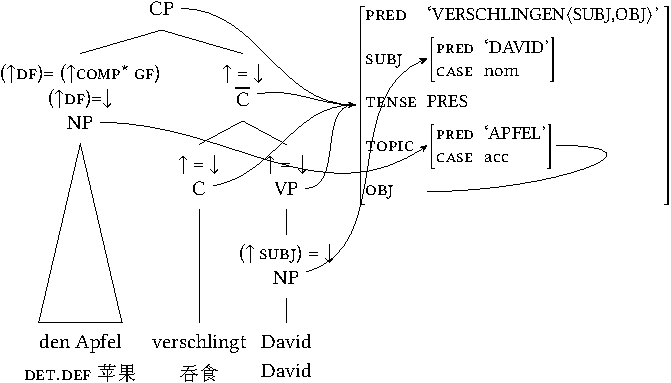
\includegraphics{Figures/den-apfel-verschlingt-david-lfg-lsp-crop}
}
\caption{\label{Abbildung-V2-LFG}动词二位的分析}
%\caption{\label{Abbildung-V2-LFG}Analysis of verb second}
\end{figure}%
\end{enumerate}

%\pagebreak
\section{范畴语法}
%\section{Categorial Grammar}

%\largerpage
\begin{enumerate}
\item The children in the room laugh loudly.的分析如图~\ref{Abbildung-CG-Kinder-lachen-laut}所示。
%\item The analysis of \emph{The children in the room laugh loudly.} is given in Figure~\ref{Abbildung-CG-Kinder-lachen-laut}.
\begin{figure}[H]
\centerline{%
\deriv{7}{
the   & children  & in  & the      & room                 & laugh & loudly\\
\defart{}   & \textrm{孩子们}  & \textsc{prep}  & \defart{}    & \textrm{房间}   & \textrm{笑} & \textrm{大声}\\
\hr   & \hr       & \hr & \hr      & \hr                    & \hr     & \hr \\
%
%
np/n  & n       & (n\bs n)/np & np/n & n                & s\bs np  & (s\bs np)\bs (s\bs np)\\
      &         &             & \multicolumn{2}{c}{\forwardapp} & \multicolumn{2}{c@{}}{\backwardapp}\\
      &         &             & np\\
      &         & \multicolumn{3}{c}{\forwardapp}  & \multicolumn{2}{c@{}}{s\bs np}\\
%
%
      &         & \multicolumn{3}{c}{n\bs n} \\  
      & \multicolumn{4}{c}{\backwardapp}\\
      & \multicolumn{4}{c}{{{n}}}\\
%
\multicolumn{5}{@{}c}{\forwardapp}\\
\multicolumn{5}{@{}c}{{np}}\\
%
\multicolumn{7}{@{}c@{}}{\backwardapp}\\
\multicolumn{7}{@{}c@{}}{{s}}\\
}}
\caption{\label{Abbildung-CG-Kinder-lachen-laut}The children in
    the room laugh loudly.的范畴语法分析}
%\caption{\label{Abbildung-CG-Kinder-lachen-laut}Categorial Grammar analysis of \emph{The children in
%    the room laugh loudly.}}
\end{figure}%

\item the picture of Mary的分析如图\vref{Abbildung-CG-das-Bild-von-Maria}所示。n/pp对应于\nnull,n对应于\nbar ,而np对应于NP。
%\item The analysis of \emph{the picture of Mary} is given in
%  Figure~\vref{Abbildung-CG-das-Bild-von-Maria}. n/pp corresponds to \nnull, n corresponds to \nbar
%  and np corresponds to NP.
\begin{figure}[H]
\centerline{%
\deriv{4}{
the & picture & of & Mary\\
\defart{} & \textrm{照片}  & \textsc{prep} & Mary\\
\hr   & \hr     & \hr        & \hr\\
np/n  & n/pp    & pp/np      & np\\
%
      &         & \multicolumn{2}{c@{}}{\forwardapp}\\
      &         & \multicolumn{2}{c@{}}{pp}\\
%
      & \multicolumn{3}{c@{}}{\forwardapp}\\
      & \multicolumn{3}{c@{}}{n}\\
%
\multicolumn{4}{@{}c@{}}{\forwardapp}\\
\multicolumn{4}{@{}c@{}}{np}\\
}}
\caption{the picture of Mary\label{Abbildung-CG-das-Bild-von-Maria}的范畴语法分析}
%\caption{Categorial Grammar analysis of \emph{the picture of Mary}\label{Abbildung-CG-das-Bild-von-Maria}}
\end{figure}%
\end{enumerate}

%\pagebreak

\section{中心语驱动的短语结构语法}
%\section{Head-Driven Phrase Structure Grammar}

%\largerpage
\begin{enumerate}
\item 答案是:\\[1mm]
%\item The solution is:\\[1mm]
%\vpageref{avm-max-lacht}.
%\begin{figure}
\oneline{%
\onems[head-argument-phrase~]{
      phon  \phonliste{ Max lacht }\\
      synsem$|$loc \ms{ cat \ms{ head & \ibox{1}\\
                                 subcat & \ibox{2} \eliste \\
                               }\\
                        cont \ms{ ind & \ibox{3}  \\
                                       rels & \relliste{ \ibox{4}, \ibox{5} } \\
                                     }\\
                      }\\
      head-dtr \onems[word]{ phon \phonliste{ lacht }\\
                             synsem$|$loc  \ms{ cat & \ms{ head   & \ibox{1} \ms[verb]{ initial & $-$\\
                                                                                        vform   & fin \\
                                                                                   }\\
                                                            subcat & \ibox{2}  $\oplus$ \sliste{ \ibox{6} }  \\
                                                        }\\
                                                 cont & \ms{ ind & \ibox{3} event \\
                                                                  rels & \liste{ \ibox{4} \ms[lachen]{ event & \ibox{3} \\
                                                                                                       agens & \ibox{7} \\ }} \\
                                                                }
                                               }\\
                       } \\
      non-head-dtrs \liste{ \onems[word]{ 
                                        phon \phonliste{ Max }\\
                                        synsem \ibox{6} \onems{ loc \ms{ cat & \ms{ head   & \ms[noun]{ cas & nom\\
                                                                                                      } \\
                                                                                    subcat &  \eliste \\
                                                                                }\\
                                                                         cont & \ms{ ind & \ibox{7} \ms{ per & 3 \\
                                                                                                              num & sg \\
                                                                                                              gen & mas \\
                                                                                                            } \\
                                                                                          rels & \liste{
                                                                                                  \ibox{5} \ms[named]{ name & max    \\
                                                                                                                       inst & \ibox{7} \\ }} \\
                                                                                         } \\
                                                                        }\\
                                                              }\\
                                   } 
                           } \\
}}
\label{avm-max-lacht}
%\end{figure}%
\item 对于例(\mex{1})中的最小差比对儿的分析需要捕捉到这样的事实,形容词的格需要与名词的格保持一致。在(\mex{1}a)中,我们使用了interessant(有趣的)的属格形式,而(\mex{1}b)包含的形式是与属格的单数不相容的形式。
%\item An analysis of the difference in (\mex{1}) has to capture the fact that the case of the adjective has to %agree with that of the noun. In (\mex{1}a),
%the genitive form of \emph{interessant} `interesting' is used, whereas (\mex{1}b) contains a form that is %incompatible with the genitive singular.
\eal
\ex[]{
\gll eines interessanten Mannes\\ 
     一.\gen{} 有趣的.\gen{} 男人.\gen{}\\
%     one.\gen{} interesting.\gen{} man.\gen{}\\
\mytrans{一个有趣的男人}
}
\ex[*]{ 
\gll eines interessanter Mannes\\
     一.\gen{} 有趣的.\nom{} 男人.\gen{}\\
%     one.\gen{} interesting.\nom{} man.\gen{}\\
}
\zl
\par\setlength\parindent{2em}
(\mex{1})说明了interessanten的\catvc 。 
%(\mex{1}) shows the \catv of \emph{interessanten}.

\eas
带有格信息的interessanten(有趣的)的\catvc  :\\
%\catv of \emph{interessanten} `interesting' with case information:\\
\ms{ head & \ms[adj]{ %prd & $-$ \\
                      mod  & {\upshape \nbar[\textsc{case} \ibox{1}]}\\
                      case & \ibox{1} gen\\
                    } \\
              subcat & \liste{} \\
}
\zs
\textsc{mod}下形容词的格取值与\nbar 的格取值的结构共享决定了名词和形容词的格取值。由此,interessanten可以跟Mannes组合,但是不能跟Mann组合。类似地,interessanter只能跟主格的Mann组合,而不能跟属格的Mannes组合。
%The structure sharing of the case value of the adjective with the case value of the \nbar under \textsc{mod}
%identifies the case values of the noun and the adjective. \emph{interessanten} can therefore be combined with 
%\emph{Mannes}, but not with \emph{Mann}. Similarly, \emph{interessanter}
%can only be combined with the nominative \emph{Mann}, but not with the genitive \emph{Mannes}. 
\par\setlength\parindent{2em}
对于名词短语内部一致关系的改进,参见 \citew[\S~13.2]{MuellerLehrbuch1}。
%For a refinement of the analysis of agreement inside the noun phrase, see  \citew[Abschnitt~13.2]
%{MuellerLehrbuch1}.
\end{enumerate}


\section{构式语法}
%\section{Construction Grammar}

熟语可以通过仔细阅读报纸来获得。稍微枯燥的方法是查找熟语词典,如“熟语与短语免费辞典”\footnote{%
\url{http://idioms.thefreedictionary.com/},\zhdate{2015/03/04}。
}。
%Idioms can be found by reading the newspaper carefully. The less exciting method is to look them up a %dictionary of
%idioms such as the Free Dictionary of Idioms and Phrases\footnote{%
%\url{http://idioms.thefreedictionary.com/}, 04.03.2015.
%}.


\section{依存语法}
%\section{Dependency Grammar}

\begin{figure}[H]
\centering
\scalebox{.9}{%
\begin{forest}
dg edges
[V
  [N [ich;我]]
  [habe;\textsc{aux}]
  [N,name=n
    [Det,tier=det [einen;一个]]
    [Mann;男人]]
  [V [getroffen;遇见]]
  [Rel,no edge, tier=det,name=rel [\trace]
      [V
        [N [der;\textsc{rel}]]
        [N [Adj, dg adjunct [blonde;金色]]
           [Haare;头发]]
        [hat;有]]]]
\draw (n.south)--(rel.north)-- +(0,6pt);
\end{forest}
}
\end{figure}%

\begin{figure}[H]
\centering
\scalebox{.9}{%
\begin{forest}
dg edges
[V
  [Subjunction
    [dass;\textsc{comp}]
    [V, l sep+=15pt
      [N [er;他]]
      [Adv, dg adjunct [morgen;明天]]
      [V [kommen;来]]
      [wird;将]]]
  [freut;高兴]
  [N [uns;我们]]]
\end{forest}
}
\end{figure}%

\begin{figure}[H]
\centering
\scalebox{.9}{
\begin{forest}
dg edges
[V
  [V [N,name=n
       [Det,tier=det [einen;一个]]
       [Mann;男人]]
    [getroffen;遇见]]
  [Rel,no edge, tier=det,name=rel [\trace]
      [V
        [N [der;\textsc{rel}]]
        [N [Adj, dg adjunct [blonde;金色]]
           [Haare;头发]]
        [hat;有]]]
  [habe;\textsc{aux}]
  [N [ich;我]]
  [Adv [noch;还]]
  [Adv [nie;从不]]]
\draw (n.south)--(rel.north)-- +(0,6pt);
\end{forest}
}
\end{figure}%






\section{树邻接语法}
%\section{Tree Adjoining Grammar}

(\mex{1})的分析需要图\vref{TAG-Elementarbaeume-dem-Koenig-treue}中的基本树。
%The elementary trees in Figure~\vref{TAG-Elementarbaeume-dem-Koenig-treue} are needed for the analysis of (\mex{1}).
\ea
\gll der        dem        König treue Diener\\
     \defart.\nom{} \defart.\dat{} 国王  忠诚 仆人\\
\mytrans{对国王忠诚的仆人}
%     the.\nom{} the.\dat{} king  loyal servant\\
%\mytrans{the servant loyal to the king}
\z

\begin{figure}
\hfill
\scalebox{.9}{
\begin{forest}
tag
[Det [der;\textsc{da}]]
\end{forest}
}
\hfill
\scalebox{.9}{
\begin{forest}
tag
[Det [dem;\textsc{da}]]
\end{forest}
}
\hfill
\scalebox{.9}{
\begin{forest}
tag
[NP
  [Det$\downarrow$]
  [\hspaceThis{$'$}N$'$
    [N [König;国王]]]]
\end{forest}
}
%
\hfill
%
\scalebox{.9}{
\begin{forest}
tag
[\hspaceThis{$'$}N$'$
  [AP
    [\hspaceThis{$'$}A$'$
      [NP$\downarrow$]
      [A [treue;忠诚]]]]
  [~~~N$'$*]]
\end{forest}
}
%
\hfill
%
\scalebox{.9}{
\begin{forest}
tag
[NP
  [Det$\downarrow$]
  [\hspaceThis{$'$}N$'$
    [N [Diener;仆人]]]]
\end{forest}
}
\hfill\mbox{}
\caption{\label{TAG-Elementarbaeume-dem-Koenig-treue}der dem König treue Diener的基本树}
%\caption{\label{TAG-Elementarbaeume-dem-Koenig-treue}Elementary trees for \emph{der dem König treue Diener}}
\end{figure}%

%\noindent
%\par\setlength\parindent{2em}
通过在替换结点König(国王)替换dem的树,我们会得到一个完整的NP。然后,这就可以插进treue(忠诚的)的替换结点中。相似地, der的树可以跟Diener的树组合。然后,我们就得到图\vref{TAG-substituiert}中的两棵树了。
%By substituting the tree for \emph{dem} `the' in the substitution node of \emph{König} `king', one then arrives at a full NP.
%This can then be inserted into the substitution node of \emph{treue} `loyal'. Similarly, the tree
%for \emph{der} `the' can be combined with the one for \emph{Diener}. One then has both of the trees in Figure~\vref{TAG-substituiert}.

\begin{figure}
\hfill
\scalebox{.9}{
\begin{forest}
tag
[\hspaceThis{$'$}N$'$
  [AP
    [\hspaceThis{$'$}A$'$
      [NP
        [Det [dem;\textsc{da}]]
        [\hspaceThis{$'$}N$'$
          [N [König;国王]]]]
      [A [treue;忠诚]]]]
  [~~~N$'$*]]
\end{forest}
}
%
\hfill
\scalebox{.9}{
\begin{forest}
tag
  [NP
     [Det [der;\textsc{da}]]
     [\hspaceThis{$'$}N$'$
        [N [Diener;仆人]]]]
\end{forest}
}
\hfill\mbox{}
\caption{\label{TAG-substituiert}替换后的der dem König treue树和der Diener树}
%\caption{\label{TAG-substituiert}Trees for \emph{der dem König treue} and \emph{der Diener} after substitution}
\end{figure}%
\par\setlength\parindent{2em}
形容词树可以连接到der Diener的N$'$-n结点上,并得到图\vref{TAG-Baeume-nach-Adjunktion}中的结构。
%The adjective tree can then be adjoined to the N$'$-node of \emph{der Diener}, which yields the structure in Figure~\vref{TAG-Baeume-nach-Adjunktion}.
\begin{figure}
\centering
%\scalebox{.9}{
\begin{forest}
tag
  [NP
     [Det [der;\textsc{da}]]
     [\hspaceThis{$'$}N$'$
       [AP
         [\hspaceThis{$'$}A$'$
           [NP
             [Det [dem;\textsc{da}]]
             [\hspaceThis{$'$}N$'$
               [N [König;国王]]]]
           [A [treue;忠诚]]]]
       [\hspaceThis{$'$}N$'$
         [N [Diener;仆人]]]]]
\end{forest}
%}
\caption{\label{TAG-Baeume-nach-Adjunktion}将AP附加到N$'$-结点的结果}
%\caption{\label{TAG-Baeume-nach-Adjunktion}Result of adjunction of the AP to the N$'$-node}
\end{figure}%




%      <!-- Local IspellDict: en_US-w_accents -->


\backmatter
\bookmarksetup{startatroot}

% for PoD with two volumes
%\ifoot{}\ofoot{}

% authorindex needs bib-file
\bibliography{gt}
%\input grammatical-theory-bib-final
\clearpage

\small
   

\phantomsection%this allows hyperlink in ToC to work
\addcontentsline{toc}{chapter}{索引} 
%\addcontentsline{toc}{chapter}{Index} 
\addcontentsline{toc}{section}{人名索引}
\ohead{人名索引}
%\addcontentsline{toc}{section}{Name index}
%\ohead{Name index}
%with biblatex
%\printindex
%without it 
\sloppy
\printindex 
  
\phantomsection%this allows hyperlink in ToC to work
\addcontentsline{toc}{section}{语言索引}
\ohead{语言索引} 
%\addcontentsline{toc}{section}{Language index}
%\ohead{Language index} 
\printindex[lan] 
  
\phantomsection%this allows hyperlink in ToC to work
\addcontentsline{toc}{section}{术语索引}
\ohead{术语索引}
%\addcontentsline{toc}{section}{Subject index}
%\ohead{Subject index}
\printindex[sbj]


\phantomsection%this allows hyperlink in ToC to work
\addcontentsline{toc}{section}{中文术语索引}
\ohead{中文术语索引}
%\addcontentsline{toc}{section}{Subject index Chinese}
%\ohead{Subject index Chinese}
\printindex[sbc]


\end{document}
